\documentclass{book}
\usepackage[a4paper,top=2.5cm,bottom=2.5cm,left=2.5cm,right=2.5cm]{geometry}
\usepackage{makeidx}
\usepackage{natbib}
\usepackage{graphicx}
\usepackage{multicol}
\usepackage{float}
\usepackage{listings}
\usepackage{color}
\usepackage{ifthen}
\usepackage[table]{xcolor}
\usepackage{textcomp}
\usepackage{alltt}
\usepackage{ifpdf}
\ifpdf
\usepackage[pdftex,
            pagebackref=true,
            colorlinks=true,
            linkcolor=blue,
            unicode
           ]{hyperref}
\else
\usepackage[ps2pdf,
            pagebackref=true,
            colorlinks=true,
            linkcolor=blue,
            unicode
           ]{hyperref}
\usepackage{pspicture}
\fi
\usepackage[utf8]{inputenc}
\usepackage{mathptmx}
\usepackage[scaled=.90]{helvet}
\usepackage{courier}
\usepackage{sectsty}
\usepackage[titles]{tocloft}
\usepackage{doxygen}
\lstset{language=C++,inputencoding=utf8,basicstyle=\footnotesize,breaklines=true,breakatwhitespace=true,tabsize=8,numbers=left }
\makeindex
\setcounter{tocdepth}{3}
\renewcommand{\footrulewidth}{0.4pt}
\renewcommand{\familydefault}{\sfdefault}
\hfuzz=15pt
\setlength{\emergencystretch}{15pt}
\hbadness=750
\tolerance=750
\begin{document}
\hypersetup{pageanchor=false,citecolor=blue}
\begin{titlepage}
\vspace*{7cm}
\begin{center}
{\Large D\-O\-S\-Box-\/\-X }\\
\vspace*{1cm}
{\large Generated by Doxygen 1.8.0}\\
\vspace*{0.5cm}
{\small Tue Oct 1 2019 18:06:35}\\
\end{center}
\end{titlepage}
\clearemptydoublepage
\pagenumbering{roman}
\tableofcontents
\clearemptydoublepage
\pagenumbering{arabic}
\hypersetup{pageanchor=true,citecolor=blue}
\chapter{D\-O\-S\-Box-\/\-X emulation}
\label{index}\hypertarget{index}{}\hypertarget{index_i}{}\section{Introduction}\label{index_i}
\hypertarget{index_f}{}\section{Features}\label{index_f}
\begin{DoxyItemize}
\item Accurate x86 emulation \end{DoxyItemize}

\chapter{-\/ framework-\/agnostic C++ G\-U\-I toolkit}
\label{gui::tk}
\hypertarget{gui::tk}{}
\hypertarget{index_i}{}\section{Introduction}\label{index_i}
gui\-::tk is a simple one-\/file C++ \hyperlink{namespaceGUI}{G\-U\-I} toolkit for use with arbitrary memory framebuffers.\hypertarget{index_f}{}\section{Features}\label{index_f}
\begin{DoxyItemize}
\item small source and binary code size \item reasonable performance and memory usage \item comfortable usage \item suitable for embedded usage\-: integer math only \item extensibility via O\-O \item non-\/intrusive\-: can be integrated with any event mechanism of your liking \item no dependencies apart from standards-\/conformant A\-N\-S\-I C++ (including a little S\-T\-L) \item support for different encodings, single-\/ and multibyte \item flexible font support\end{DoxyItemize}
\hypertarget{gui_1_1tk_o}{}\section{Overview}\label{gui_1_1tk_o}
The toolkit draws on a surface you provide, using any size or pixel format. Create a \hyperlink{classGUI_1_1Screen}{G\-U\-I\-::\-Screen} with the buffer to draw on, then pass that object (or a \hyperlink{classGUI_1_1Window}{G\-U\-I\-::\-Window} created from it) to all other widgets' constructors.

It doesn't provide an own event loop. Instead, it relies on you passing events and updating the screen regularly. This way, it can easily be integrated with any event loop available (S\-D\-L, Qt, glib, X11, Win32, selfmade, ...)

Many functions and concepts were taken from other well-\/known toolkits, so if you know Qt, Java or wx\-Windows, you may encounter (intentional) similarities. However, simplicity of code has been given priority over maximum optimization and pixel-\/exact replication of their appearance.

A note about font support and encodings\-: All text-\/related functions use templates to support any encoding. Fonts define the charset.\hypertarget{gui_1_1tk_g}{}\section{Getting Started}\label{gui_1_1tk_g}
gui\-::tk contains an S\-D\-L adapter, so if your program is already using S\-D\-L, things are really easy. The rough sequence to get up and running is\-:


\begin{DoxyCode}
 // setup a suitable video mode with SDL
 SDL_surface *screen = SDL_SetVideoMode(640, 480, 32, SDL_SWSURFACE);

 // add a default font, you will most probably need it
 GUI::Font::addFont("default",new GUI::BitmapFont(testfont,14,10));

 // create the root-level screen object, the parent of all top-level windows
 GUI::ScreenSDL guiscreen(screen);

 // create any amount of toplevel windows you like
 GUI::ToplevelWindow *frame = new GUI::ToplevelWindow(&guiscreen, 205, 100, 380
      , 250, "gui::tk example");

 // add some GUI elements to the toplevel window
 GUI::Button *b = new GUI::Button(frame,8,20,"Quit");

 // Define and add an event handler
 struct quit : public GUI::ActionEventSource_Callback {
     void actionExecuted(GUI::ActionEventSource *b, const GUI::String &arg) {
         exit(0);
     }
 } ex;
 b->addActionHandler(&ex);

 // Enter an event loop, calling update() regularly.
 SDL_Event event;
 while (1) {
     while (SDL_PollEvent(&event)) {
         if (!guiscreen.event(event)) { // gui::tk didn't handle that event
             if (event.type == SDL_QUIT) exit(0);
         }
     }

     guiscreen.update(4); // 4 ticks = 40ms
     SDL_UpdateRect(screen, 0, 0, screen->w, screen->h);

     SDL_Delay(40); // wait 40ms
 }
\end{DoxyCode}


Look at \hyperlink{gui__tk_8h}{gui\-\_\-tk.\-h} for more detailed documentation and reference of all classes.

A test program that shows off the capabilities of gui\-::tk is available as part of \hyperlink{gui__tk_8cpp}{gui\-\_\-tk.\-cpp}.\hypertarget{gui_1_1tk_l}{}\section{License}\label{gui_1_1tk_l}
Copyright (C) 2005-\/2007 Jörg Walter

gui\-::tk is free software; you can redistribute it and/or modify it under the terms of the G\-N\-U General Public License as published by the Free Software Foundation; either version 3 of the License, or (at your option) any later version.

gui\-::tk is distributed in the hope that it will be useful, but W\-I\-T\-H\-O\-U\-T A\-N\-Y W\-A\-R\-R\-A\-N\-T\-Y; without even the implied warranty of M\-E\-R\-C\-H\-A\-N\-T\-A\-B\-I\-L\-I\-T\-Y or F\-I\-T\-N\-E\-S\-S F\-O\-R A P\-A\-R\-T\-I\-C\-U\-L\-A\-R P\-U\-R\-P\-O\-S\-E. See the G\-N\-U General Public License for more details.

You should have received a copy of the G\-N\-U General Public License along with this program. If not, see \href{http://www.gnu.org/licenses/}{\tt http\-://www.\-gnu.\-org/licenses/} 
\chapter{Namespace Index}
\section{Namespace List}
Here is a list of all documented namespaces with brief descriptions\-:\begin{DoxyCompactList}
\item\contentsline{section}{\hyperlink{namespaceGUI}{G\-U\-I} \\*This namespace contains all \hyperlink{namespaceGUI}{G\-U\-I} toolkit classes, types and functions }{\pageref{namespaceGUI}}{}
\item\contentsline{section}{\hyperlink{namespaceGUI_1_1Color}{G\-U\-I\-::\-Color} \\*Collection of all color-\/related constants and functions }{\pageref{namespaceGUI_1_1Color}}{}
\end{DoxyCompactList}

\chapter{Class Index}
\section{Class Hierarchy}
This inheritance list is sorted roughly, but not completely, alphabetically\-:\begin{DoxyCompactList}
\item \contentsline{section}{\-\_\-\-\_\-\-C\-O\-E\-F\-P\-A\-I\-R}{\pageref{struct____COEFPAIR}}{}
\item \contentsline{section}{\-\_\-\-A\-D\-P\-C\-M}{\pageref{struct__ADPCM}}{}
\item \contentsline{section}{\-\_\-attotime}{\pageref{struct__attotime}}{}
\item \contentsline{section}{\-\_\-dac\-\_\-channel}{\pageref{struct__dac__channel}}{}
\item \contentsline{section}{\-\_\-dac\-\_\-state}{\pageref{struct__dac__state}}{}
\item \contentsline{section}{\-\_\-fbi\-\_\-state}{\pageref{struct__fbi__state}}{}
\item \contentsline{section}{\-\_\-fifo\-\_\-state}{\pageref{struct__fifo__state}}{}
\item \contentsline{section}{\-\_\-\-F\-M\-T\-I\-M\-E\-R}{\pageref{struct__FMTIMER}}{}
\item \contentsline{section}{\-\_\-getsnd}{\pageref{struct__getsnd}}{}
\item \contentsline{section}{\-\_\-\-Log\-Group}{\pageref{struct__LogGroup}}{}
\item \contentsline{section}{\-\_\-ncc\-\_\-table}{\pageref{struct__ncc__table}}{}
\item \contentsline{section}{\-\_\-\-O\-P\-N\-G\-E\-N}{\pageref{struct__OPNGEN}}{}
\item \contentsline{section}{\-\_\-\-P\-C98\-Raw\-Partition}{\pageref{struct__PC98RawPartition}}{}
\item \contentsline{section}{\-\_\-pci\-\_\-state}{\pageref{struct__pci__state}}{}
\item \contentsline{section}{\-\_\-\-P\-C\-M86}{\pageref{struct__PCM86}}{}
\item \contentsline{section}{\-\_\-\-P\-C\-M\-M\-I\-X}{\pageref{struct__PCMMIX}}{}
\item \contentsline{section}{\-\_\-\-P\-F\-I\-L\-E\-H}{\pageref{struct__PFILEH}}{}
\item \contentsline{section}{\-\_\-poly\-\_\-extent}{\pageref{struct__poly__extent}}{}
\item \contentsline{section}{\-\_\-poly\-\_\-extra\-\_\-data}{\pageref{struct__poly__extra__data}}{}
\item \contentsline{section}{\-\_\-poly\-\_\-param\-\_\-extent}{\pageref{struct__poly__param__extent}}{}
\item \contentsline{section}{\-\_\-poly\-\_\-vertex}{\pageref{struct__poly__vertex}}{}
\item \contentsline{section}{\-\_\-\-P\-S\-G\-G\-E\-N}{\pageref{struct__PSGGEN}}{}
\item \contentsline{section}{\-\_\-raster\-\_\-info}{\pageref{struct__raster__info}}{}
\item \contentsline{section}{\-\_\-rectangle}{\pageref{struct__rectangle}}{}
\item \contentsline{section}{\-\_\-rgba}{\pageref{struct__rgba}}{}
\item \contentsline{section}{\-\_\-\-R\-H\-Y\-T\-H\-M}{\pageref{struct__RHYTHM}}{}
\item \contentsline{section}{\-\_\-setup\-\_\-vertex}{\pageref{struct__setup__vertex}}{}
\item \contentsline{section}{\-\_\-stats\-\_\-block}{\pageref{struct__stats__block}}{}
\item \contentsline{section}{\-\_\-\-T\-M\-S3631}{\pageref{struct__TMS3631}}{}
\item \contentsline{section}{\-\_\-tmu\-\_\-shared\-\_\-state}{\pageref{struct__tmu__shared__state}}{}
\item \contentsline{section}{\-\_\-tmu\-\_\-state}{\pageref{struct__tmu__state}}{}
\item \contentsline{section}{\-\_\-tri\-\_\-extent}{\pageref{struct__tri__extent}}{}
\item \contentsline{section}{\-\_\-tri\-\_\-work\-\_\-unit}{\pageref{struct__tri__work__unit}}{}
\item \contentsline{section}{\-\_\-voodoo\-\_\-reg}{\pageref{union__voodoo__reg}}{}
\item \contentsline{section}{\-\_\-voodoo\-\_\-state}{\pageref{struct__voodoo__state}}{}
\item \contentsline{section}{\-\_\-\-W\-A\-V\-E\-W\-R}{\pageref{struct__WAVEWR}}{}
\item \contentsline{section}{D\-O\-S\-Box\-Menu\-:\-:accelerator}{\pageref{structDOSBoxMenu_1_1accelerator}}{}
\item \contentsline{section}{G\-U\-I\-:\-:Action\-Event\-Source}{\pageref{classGUI_1_1ActionEventSource}}{}
\begin{DoxyCompactList}
\item \contentsline{section}{G\-U\-I\-:\-:Button}{\pageref{classGUI_1_1Button}}{}
\item \contentsline{section}{G\-U\-I\-:\-:Checkbox}{\pageref{classGUI_1_1Checkbox}}{}
\item \contentsline{section}{G\-U\-I\-:\-:Frame}{\pageref{classGUI_1_1Frame}}{}
\item \contentsline{section}{G\-U\-I\-:\-:Input}{\pageref{classGUI_1_1Input}}{}
\begin{DoxyCompactList}
\item \contentsline{section}{Input\-With\-Enter\-Key}{\pageref{classInputWithEnterKey}}{}
\end{DoxyCompactList}
\item \contentsline{section}{G\-U\-I\-:\-:Menu}{\pageref{classGUI_1_1Menu}}{}
\item \contentsline{section}{G\-U\-I\-:\-:Menubar}{\pageref{classGUI_1_1Menubar}}{}
\item \contentsline{section}{G\-U\-I\-:\-:Radiobox}{\pageref{classGUI_1_1Radiobox}}{}
\end{DoxyCompactList}
\item \contentsline{section}{G\-U\-I\-:\-:Action\-Event\-Source\-\_\-\-Callback}{\pageref{structGUI_1_1ActionEventSource__Callback}}{}
\begin{DoxyCompactList}
\item \contentsline{section}{G\-U\-I\-:\-:Frame}{\pageref{classGUI_1_1Frame}}{}
\item \contentsline{section}{G\-U\-I\-:\-:Menubar}{\pageref{classGUI_1_1Menubar}}{}
\item \contentsline{section}{G\-U\-I\-:\-:Toplevel\-Window}{\pageref{classGUI_1_1ToplevelWindow}}{}
\begin{DoxyCompactList}
\item \contentsline{section}{Autoexec\-Editor}{\pageref{classAutoexecEditor}}{}
\item \contentsline{section}{Configuration\-Window}{\pageref{classConfigurationWindow}}{}
\item \contentsline{section}{G\-U\-I\-:\-:Message\-Box2}{\pageref{classGUI_1_1MessageBox2}}{}
\begin{DoxyCompactList}
\item \contentsline{section}{Help\-Window}{\pageref{classHelpWindow}}{}
\end{DoxyCompactList}
\item \contentsline{section}{Save\-Dialog}{\pageref{classSaveDialog}}{}
\item \contentsline{section}{Save\-Lang\-Dialog}{\pageref{classSaveLangDialog}}{}
\item \contentsline{section}{Section\-Editor}{\pageref{classSectionEditor}}{}
\item \contentsline{section}{Set\-Cycles}{\pageref{classSetCycles}}{}
\item \contentsline{section}{Set\-Local\-Size}{\pageref{classSetLocalSize}}{}
\item \contentsline{section}{Set\-Vsyncrate}{\pageref{classSetVsyncrate}}{}
\end{DoxyCompactList}
\item \contentsline{section}{Property\-Editor}{\pageref{classPropertyEditor}}{}
\begin{DoxyCompactList}
\item \contentsline{section}{Property\-Editor\-Bool}{\pageref{classPropertyEditorBool}}{}
\item \contentsline{section}{Property\-Editor\-Float}{\pageref{classPropertyEditorFloat}}{}
\item \contentsline{section}{Property\-Editor\-Hex}{\pageref{classPropertyEditorHex}}{}
\item \contentsline{section}{Property\-Editor\-Int}{\pageref{classPropertyEditorInt}}{}
\item \contentsline{section}{Property\-Editor\-String}{\pageref{classPropertyEditorString}}{}
\end{DoxyCompactList}
\end{DoxyCompactList}
\item \contentsline{section}{I\-P\-X\-Header\-:\-:transport\-:\-:addrtype}{\pageref{unionIPXHeader_1_1transport_1_1addrtype}}{}
\item \contentsline{section}{transport\-:\-:addrtype}{\pageref{uniontransport_1_1addrtype}}{}
\item \contentsline{section}{A\-D\-P\-C\-M\-C\-F\-G}{\pageref{structADPCMCFG}}{}
\item \contentsline{section}{A\-D\-P\-C\-M\-R\-E\-G}{\pageref{structADPCMREG}}{}
\item \contentsline{section}{allpass}{\pageref{classallpass}}{}
\item \contentsline{section}{A\-M\-D98}{\pageref{structAMD98}}{}
\item \contentsline{section}{M\-T32\-Emu\-:\-:A\-Reverb\-Settings}{\pageref{structMT32Emu_1_1AReverbSettings}}{}
\item \contentsline{section}{Autoexec\-Object}{\pageref{classAutoexecObject}}{}
\item \contentsline{section}{avi\-\_\-writer}{\pageref{structavi__writer}}{}
\item \contentsline{section}{avi\-\_\-writer\-\_\-stream}{\pageref{structavi__writer__stream}}{}
\item \contentsline{section}{avi\-\_\-writer\-\_\-stream\-\_\-index}{\pageref{structavi__writer__stream__index}}{}
\item \contentsline{section}{Bad\-Conversion}{\pageref{classBadConversion}}{}
\item \contentsline{section}{Batch\-File}{\pageref{classBatchFile}}{}
\begin{DoxyCompactList}
\item \contentsline{section}{Virtual\-Batch}{\pageref{classVirtualBatch}}{}
\end{DoxyCompactList}
\item \contentsline{section}{bitop\-:\-:bitseqlengthandpos\-\_\-ret\-\_\-t}{\pageref{classbitop_1_1bitseqlengthandpos__ret__t}}{}
\item \contentsline{section}{Region\-Alloc\-Tracking\-:\-:Block}{\pageref{classRegionAllocTracking_1_1Block}}{}
\item \contentsline{section}{boot\-Sector}{\pageref{unionbootSector}}{}
\item \contentsline{section}{bootstrap}{\pageref{structbootstrap}}{}
\item \contentsline{section}{M\-T32\-Emu\-:\-:B\-Reverb\-Settings}{\pageref{structMT32Emu_1_1BReverbSettings}}{}
\item \contentsline{section}{Builtin\-File\-Blob}{\pageref{structBuiltinFileBlob}}{}
\item \contentsline{section}{button\-\_\-event}{\pageref{structbutton__event}}{}
\item \contentsline{section}{bx\-\_\-ne2k\-\_\-c}{\pageref{classbx__ne2k__c}}{}
\item \contentsline{section}{bx\-\_\-ne2k\-\_\-t}{\pageref{structbx__ne2k__t}}{}
\item \contentsline{section}{fmath\-:\-:local\-:\-:C$<$ E\-X\-P\-\_\-\-N, L\-O\-G\-\_\-\-N, E\-X\-P\-D\-\_\-\-N $>$}{\pageref{structfmath_1_1local_1_1C}}{}
\item \contentsline{section}{Cache\-Block}{\pageref{classCacheBlock}}{}
\item \contentsline{section}{C\-A\-L\-L\-B\-A\-C\-K\-\_\-\-Handler\-Object}{\pageref{classCALLBACK__HandlerObject}}{}
\item \contentsline{section}{Adlib\-:\-:Capture}{\pageref{classAdlib_1_1Capture}}{}
\item \contentsline{section}{C\-Bind}{\pageref{classCBind}}{}
\begin{DoxyCompactList}
\item \contentsline{section}{C\-J\-Axis\-Bind}{\pageref{classCJAxisBind}}{}
\item \contentsline{section}{C\-J\-Button\-Bind}{\pageref{classCJButtonBind}}{}
\item \contentsline{section}{C\-J\-Hat\-Bind}{\pageref{classCJHatBind}}{}
\item \contentsline{section}{C\-Key\-Bind}{\pageref{classCKeyBind}}{}
\end{DoxyCompactList}
\item \contentsline{section}{C\-Bind\-Group}{\pageref{classCBindGroup}}{}
\begin{DoxyCompactList}
\item \contentsline{section}{C\-Key\-Bind\-Group}{\pageref{classCKeyBindGroup}}{}
\item \contentsline{section}{C\-Stick\-Bind\-Group}{\pageref{classCStickBindGroup}}{}
\begin{DoxyCompactList}
\item \contentsline{section}{C4\-Axis\-Bind\-Group}{\pageref{classC4AxisBindGroup}}{}
\item \contentsline{section}{C\-C\-H\-Bind\-Group}{\pageref{classCCHBindGroup}}{}
\item \contentsline{section}{C\-F\-C\-S\-Bind\-Group}{\pageref{classCFCSBindGroup}}{}
\end{DoxyCompactList}
\end{DoxyCompactList}
\item \contentsline{section}{C\-B\-U\-S4\-P\-O\-R\-T}{\pageref{structCBUS4PORT}}{}
\item \contentsline{section}{C\-Button}{\pageref{classCButton}}{}
\begin{DoxyCompactList}
\item \contentsline{section}{C\-Caption\-Button}{\pageref{classCCaptionButton}}{}
\item \contentsline{section}{C\-Text\-Button}{\pageref{classCTextButton}}{}
\begin{DoxyCompactList}
\item \contentsline{section}{C\-Bind\-Button}{\pageref{classCBindButton}}{}
\item \contentsline{section}{C\-Check\-Button}{\pageref{classCCheckButton}}{}
\item \contentsline{section}{C\-Event\-Button}{\pageref{classCEventButton}}{}
\end{DoxyCompactList}
\end{DoxyCompactList}
\item \contentsline{section}{C\-Direct3\-D}{\pageref{classCDirect3D}}{}
\item \contentsline{section}{C\-D\-R\-O\-M\-\_\-\-Interface}{\pageref{classCDROM__Interface}}{}
\begin{DoxyCompactList}
\item \contentsline{section}{C\-D\-R\-O\-M\-\_\-\-Interface\-\_\-\-Fake}{\pageref{classCDROM__Interface__Fake}}{}
\item \contentsline{section}{C\-D\-R\-O\-M\-\_\-\-Interface\-\_\-\-Image}{\pageref{classCDROM__Interface__Image}}{}
\item \contentsline{section}{C\-D\-R\-O\-M\-\_\-\-Interface\-\_\-\-S\-D\-L}{\pageref{classCDROM__Interface__SDL}}{}
\end{DoxyCompactList}
\item \contentsline{section}{C\-Event}{\pageref{classCEvent}}{}
\begin{DoxyCompactList}
\item \contentsline{section}{C\-Continuous\-Event}{\pageref{classCContinuousEvent}}{}
\begin{DoxyCompactList}
\item \contentsline{section}{C\-J\-Axis\-Event}{\pageref{classCJAxisEvent}}{}
\end{DoxyCompactList}
\item \contentsline{section}{C\-Triggered\-Event}{\pageref{classCTriggeredEvent}}{}
\begin{DoxyCompactList}
\item \contentsline{section}{C\-Handler\-Event}{\pageref{classCHandlerEvent}}{}
\item \contentsline{section}{C\-J\-Button\-Event}{\pageref{classCJButtonEvent}}{}
\item \contentsline{section}{C\-J\-Hat\-Event}{\pageref{classCJHatEvent}}{}
\item \contentsline{section}{C\-Key\-Event}{\pageref{classCKeyEvent}}{}
\item \contentsline{section}{C\-Mod\-Event}{\pageref{classCModEvent}}{}
\end{DoxyCompactList}
\end{DoxyCompactList}
\item \contentsline{section}{D\-O\-S\-\_\-\-Drive\-\_\-\-Cache\-:\-:C\-File\-Info}{\pageref{classDOS__Drive__Cache_1_1CFileInfo}}{}
\item \contentsline{section}{Property\-:\-:Changeable}{\pageref{structProperty_1_1Changeable}}{}
\item \contentsline{section}{D\-B\-O\-P\-L\-:\-:Channel}{\pageref{structDBOPL_1_1Channel}}{}
\item \contentsline{section}{C\-H\-A\-R\-M\-A\-P}{\pageref{structCHARMAP}}{}
\item \contentsline{section}{Adlib\-:\-:Chip}{\pageref{structAdlib_1_1Chip}}{}
\item \contentsline{section}{D\-B\-O\-P\-L\-:\-:Chip}{\pageref{structDBOPL_1_1Chip}}{}
\item \contentsline{section}{Clock\-Domain}{\pageref{classClockDomain}}{}
\item \contentsline{section}{C\-Mscdex}{\pageref{classCMscdex}}{}
\item \contentsline{section}{Codec\-Inst}{\pageref{classCodecInst}}{}
\item \contentsline{section}{comb}{\pageref{classcomb}}{}
\item \contentsline{section}{Command\-Line}{\pageref{classCommandLine}}{}
\item \contentsline{section}{Command\-Tail}{\pageref{structCommandTail}}{}
\item \contentsline{section}{M\-T32\-Emu\-:\-:Timbre\-Param\-:\-:Common\-Param}{\pageref{structMT32Emu_1_1TimbreParam_1_1CommonParam}}{}
\item \contentsline{section}{Config}{\pageref{classConfig}}{}
\item \contentsline{section}{M\-T32\-Emu\-:\-:Control\-R\-O\-M\-Map}{\pageref{structMT32Emu_1_1ControlROMMap}}{}
\item \contentsline{section}{M\-T32\-Emu\-:\-:Control\-R\-O\-M\-P\-C\-M\-Struct}{\pageref{structMT32Emu_1_1ControlROMPCMStruct}}{}
\item \contentsline{section}{copysource}{\pageref{structcopysource}}{}
\item \contentsline{section}{C\-Parallel}{\pageref{classCParallel}}{}
\begin{DoxyCompactList}
\item \contentsline{section}{C\-File\-L\-P\-T}{\pageref{classCFileLPT}}{}
\item \contentsline{section}{C\-Printer\-Redir}{\pageref{classCPrinterRedir}}{}
\end{DoxyCompactList}
\item \contentsline{section}{C\-P\-U\-\_\-\-Regs}{\pageref{structCPU__Regs}}{}
\item \contentsline{section}{C\-P\-U\-Block}{\pageref{structCPUBlock}}{}
\item \contentsline{section}{bx\-\_\-ne2k\-\_\-t\-:\-:C\-R\-\_\-t}{\pageref{structbx__ne2k__t_1_1CR__t}}{}
\item \contentsline{section}{Cross}{\pageref{classCross}}{}
\item \contentsline{section}{C\-Serial}{\pageref{classCSerial}}{}
\begin{DoxyCompactList}
\item \contentsline{section}{C\-Serial\-Dummy}{\pageref{classCSerialDummy}}{}
\item \contentsline{section}{C\-Serial\-Log}{\pageref{classCSerialLog}}{}
\item \contentsline{section}{C\-Serial\-Mouse}{\pageref{classCSerialMouse}}{}
\end{DoxyCompactList}
\item \contentsline{section}{D88\-H\-E\-A\-D}{\pageref{structD88HEAD}}{}
\item \contentsline{section}{D88\-S\-E\-C}{\pageref{structD88SEC}}{}
\item \contentsline{section}{bx\-\_\-ne2k\-\_\-t\-:\-:D\-C\-R\-\_\-t}{\pageref{structbx__ne2k__t_1_1DCR__t}}{}
\item \contentsline{section}{Delay\-Entry}{\pageref{structDelayEntry}}{}
\item \contentsline{section}{Dentry}{\pageref{structDentry}}{}
\item \contentsline{section}{Descriptor}{\pageref{classDescriptor}}{}
\begin{DoxyCompactList}
\item \contentsline{section}{T\-S\-S\-\_\-\-Descriptor}{\pageref{classTSS__Descriptor}}{}
\end{DoxyCompactList}
\item \contentsline{section}{Descriptor\-Table}{\pageref{classDescriptorTable}}{}
\begin{DoxyCompactList}
\item \contentsline{section}{G\-D\-T\-Descriptor\-Table}{\pageref{classGDTDescriptorTable}}{}
\end{DoxyCompactList}
\item \contentsline{section}{fmath\-:\-:local\-:\-:di}{\pageref{unionfmath_1_1local_1_1di}}{}
\item \contentsline{section}{dir\-\_\-struct}{\pageref{structdir__struct}}{}
\item \contentsline{section}{direntry}{\pageref{structdirentry}}{}
\item \contentsline{section}{disk\-Geo}{\pageref{structdiskGeo}}{}
\item \contentsline{section}{D\-O\-S\-Box\-Menu\-:\-:displaylist}{\pageref{classDOSBoxMenu_1_1displaylist}}{}
\item \contentsline{section}{Dma\-Channel}{\pageref{classDmaChannel}}{}
\item \contentsline{section}{Dma\-Controller}{\pageref{classDmaController}}{}
\item \contentsline{section}{D\-O\-S\-\_\-\-Block}{\pageref{structDOS__Block}}{}
\item \contentsline{section}{D\-O\-S\-\_\-\-Date}{\pageref{structDOS__Date}}{}
\item \contentsline{section}{D\-O\-S\-\_\-\-Drive}{\pageref{classDOS__Drive}}{}
\begin{DoxyCompactList}
\item \contentsline{section}{fat\-Drive}{\pageref{classfatDrive}}{}
\item \contentsline{section}{iso\-Drive}{\pageref{classisoDrive}}{}
\item \contentsline{section}{local\-Drive}{\pageref{classlocalDrive}}{}
\begin{DoxyCompactList}
\item \contentsline{section}{cdrom\-Drive}{\pageref{classcdromDrive}}{}
\item \contentsline{section}{physfs\-Drive}{\pageref{classphysfsDrive}}{}
\begin{DoxyCompactList}
\item \contentsline{section}{physfscdrom\-Drive}{\pageref{classphysfscdromDrive}}{}
\end{DoxyCompactList}
\end{DoxyCompactList}
\item \contentsline{section}{Virtual\-\_\-\-Drive}{\pageref{classVirtual__Drive}}{}
\end{DoxyCompactList}
\item \contentsline{section}{D\-O\-S\-\_\-\-Drive\-\_\-\-Cache}{\pageref{classDOS__Drive__Cache}}{}
\item \contentsline{section}{D\-O\-S\-\_\-\-File}{\pageref{classDOS__File}}{}
\begin{DoxyCompactList}
\item \contentsline{section}{D\-O\-S\-\_\-\-Device}{\pageref{classDOS__Device}}{}
\begin{DoxyCompactList}
\item \contentsline{section}{device\-\_\-\-C\-O\-M}{\pageref{classdevice__COM}}{}
\item \contentsline{section}{device\-\_\-\-C\-O\-N}{\pageref{classdevice__CON}}{}
\item \contentsline{section}{device\-\_\-\-E\-M\-M}{\pageref{classdevice__EMM}}{}
\item \contentsline{section}{device\-\_\-\-L\-P\-T}{\pageref{classdevice__LPT}}{}
\item \contentsline{section}{device\-\_\-\-M\-S\-C\-D\-E\-X}{\pageref{classdevice__MSCDEX}}{}
\item \contentsline{section}{device\-\_\-\-N\-U\-L}{\pageref{classdevice__NUL}}{}
\item \contentsline{section}{device\-\_\-\-P\-R\-N}{\pageref{classdevice__PRN}}{}
\end{DoxyCompactList}
\item \contentsline{section}{fat\-File}{\pageref{classfatFile}}{}
\item \contentsline{section}{iso\-File}{\pageref{classisoFile}}{}
\item \contentsline{section}{local\-File}{\pageref{classlocalFile}}{}
\item \contentsline{section}{Virtual\-\_\-\-File}{\pageref{classVirtual__File}}{}
\end{DoxyCompactList}
\item \contentsline{section}{D\-O\-S\-\_\-\-Get\-Mem\-Log\-\_\-\-Entry}{\pageref{structDOS__GetMemLog__Entry}}{}
\item \contentsline{section}{D\-O\-S\-\_\-\-Table\-Case}{\pageref{structDOS__TableCase}}{}
\item \contentsline{section}{D\-O\-S\-\_\-\-Version}{\pageref{structDOS__Version}}{}
\item \contentsline{section}{dosbox\-\_\-int\-\_\-saved\-\_\-state}{\pageref{structdosbox__int__saved__state}}{}
\item \contentsline{section}{D\-O\-S\-Box\-Menu}{\pageref{classDOSBoxMenu}}{}
\item \contentsline{section}{D\-O\-S\-D\-A\-T\-E}{\pageref{structDOSDATE}}{}
\item \contentsline{section}{D\-O\-S\-T\-I\-M\-E}{\pageref{structDOSTIME}}{}
\item \contentsline{section}{G\-U\-I\-:\-:Drawable}{\pageref{classGUI_1_1Drawable}}{}
\begin{DoxyCompactList}
\item \contentsline{section}{G\-U\-I\-:\-:S\-D\-L\-\_\-\-Drawable}{\pageref{classGUI_1_1SDL__Drawable}}{}
\end{DoxyCompactList}
\item \contentsline{section}{Drive\-Manager}{\pageref{classDriveManager}}{}
\item \contentsline{section}{Dta\-Result}{\pageref{structDtaResult}}{}
\item \contentsline{section}{Dynamic\-\_\-\-Functionality}{\pageref{structDynamic__Functionality}}{}
\item \contentsline{section}{E\-C\-B\-Class}{\pageref{classECBClass}}{}
\item \contentsline{section}{E\-M\-M\-\_\-\-Handle}{\pageref{structEMM__Handle}}{}
\item \contentsline{section}{E\-M\-M\-\_\-\-Mapping}{\pageref{structEMM__Mapping}}{}
\item \contentsline{section}{boot\-Sector\-:\-:entries}{\pageref{structbootSector_1_1entries}}{}
\item \contentsline{section}{entries}{\pageref{structentries}}{}
\item \contentsline{section}{Envelope\-Generator}{\pageref{classEnvelopeGenerator}}{}
\item \contentsline{section}{E\-X\-E\-\_\-\-Header}{\pageref{structEXE__Header}}{}
\item \contentsline{section}{fmath\-:\-:local\-:\-:Expd\-Var$<$ sbit\-\_\- $>$}{\pageref{structfmath_1_1local_1_1ExpdVar}}{}
\item \contentsline{section}{fmath\-:\-:local\-:\-:Exp\-Var$<$ N $>$}{\pageref{structfmath_1_1local_1_1ExpVar}}{}
\item \contentsline{section}{External\-Filter}{\pageref{classExternalFilter}}{}
\item \contentsline{section}{fmath\-:\-:local\-:\-:fi}{\pageref{unionfmath_1_1local_1_1fi}}{}
\item \contentsline{section}{M\-T32\-Emu\-:\-:File}{\pageref{classMT32Emu_1_1File}}{}
\begin{DoxyCompactList}
\item \contentsline{section}{M\-T32\-Emu\-:\-:File\-Stream}{\pageref{classMT32Emu_1_1FileStream}}{}
\end{DoxyCompactList}
\item \contentsline{section}{File\-Stat\-\_\-\-Block}{\pageref{structFileStat__Block}}{}
\item \contentsline{section}{Filter}{\pageref{classFilter}}{}
\item \contentsline{section}{F\-L\-I\-N\-F\-O}{\pageref{structFLINFO}}{}
\item \contentsline{section}{Floppy\-Device}{\pageref{classFloppyDevice}}{}
\item \contentsline{section}{G\-U\-I\-:\-:Font}{\pageref{classGUI_1_1Font}}{}
\begin{DoxyCompactList}
\item \contentsline{section}{G\-U\-I\-:\-:Bitmap\-Font}{\pageref{classGUI_1_1BitmapFont}}{}
\end{DoxyCompactList}
\item \contentsline{section}{F\-P\-U\-\_\-\-P\-\_\-\-Reg}{\pageref{structFPU__P__Reg}}{}
\item \contentsline{section}{F\-P\-U\-\_\-rec}{\pageref{structFPU__rec}}{}
\item \contentsline{section}{F\-P\-U\-\_\-\-Reg}{\pageref{unionFPU__Reg}}{}
\item \contentsline{section}{F\-P\-U\-\_\-\-Reg\-\_\-32}{\pageref{unionFPU__Reg__32}}{}
\item \contentsline{section}{F\-P\-U\-\_\-\-Reg\-\_\-64}{\pageref{unionFPU__Reg__64}}{}
\item \contentsline{section}{F\-P\-U\-\_\-\-Reg\-\_\-80}{\pageref{unionFPU__Reg__80}}{}
\item \contentsline{section}{fragment\-Descriptor}{\pageref{structfragmentDescriptor}}{}
\item \contentsline{section}{Full\-Data}{\pageref{structFullData}}{}
\item \contentsline{section}{Function\-\_\-wrapper}{\pageref{structFunction__wrapper}}{}
\item \contentsline{section}{G\-\_\-\-Descriptor}{\pageref{structG__Descriptor}}{}
\item \contentsline{section}{G\-C\-C\-\_\-\-A\-T\-T\-R\-I\-B\-U\-T\-E}{\pageref{structGCC__ATTRIBUTE}}{}
\item \contentsline{section}{Gen\-Reg}{\pageref{classGenReg}}{}
\item \contentsline{section}{Gen\-Reg32}{\pageref{unionGenReg32}}{}
\item \contentsline{section}{G\-F\-Gus}{\pageref{structGFGus}}{}
\item \contentsline{section}{G\-F\-X\-\_\-\-Pal\-Entry}{\pageref{structGFX__PalEntry}}{}
\item \contentsline{section}{gsm610waveformat\-\_\-tag}{\pageref{structgsm610waveformat__tag}}{}
\item \contentsline{section}{Guest\-Page\-Fault\-Exception}{\pageref{classGuestPageFaultException}}{}
\item \contentsline{section}{gus\-\_\-cs4231}{\pageref{structgus__cs4231}}{}
\item \contentsline{section}{gus\-\_\-\-I\-C\-S2101}{\pageref{structgus__ICS2101}}{}
\item \contentsline{section}{G\-U\-S\-Channels}{\pageref{classGUSChannels}}{}
\item \contentsline{section}{G\-F\-Gus\-:\-:Gus\-Timer}{\pageref{structGFGus_1_1GusTimer}}{}
\item \contentsline{section}{Adlib\-:\-:Handler}{\pageref{classAdlib_1_1Handler}}{}
\begin{DoxyCompactList}
\item \contentsline{section}{D\-B\-O\-P\-L\-:\-:Handler}{\pageref{structDBOPL_1_1Handler}}{}
\item \contentsline{section}{Nuked\-O\-P\-L\-:\-:Handler}{\pageref{structNukedOPL_1_1Handler}}{}
\item \contentsline{section}{O\-P\-L2\-:\-:Handler}{\pageref{structOPL2_1_1Handler}}{}
\item \contentsline{section}{O\-P\-L3\-:\-:Handler}{\pageref{structOPL3_1_1Handler}}{}
\end{DoxyCompactList}
\item \contentsline{section}{H\-D\-I\-H\-D\-R}{\pageref{structHDIHDR}}{}
\item \contentsline{section}{Hex}{\pageref{classHex}}{}
\item \contentsline{section}{I\-D\-E\-Device}{\pageref{classIDEDevice}}{}
\begin{DoxyCompactList}
\item \contentsline{section}{I\-D\-E\-A\-T\-A\-Device}{\pageref{classIDEATADevice}}{}
\item \contentsline{section}{I\-D\-E\-A\-T\-A\-P\-I\-C\-D\-R\-O\-M\-Device}{\pageref{classIDEATAPICDROMDevice}}{}
\end{DoxyCompactList}
\item \contentsline{section}{ima\-\_\-adpcmwaveformat\-\_\-tag}{\pageref{structima__adpcmwaveformat__tag}}{}
\item \contentsline{section}{image\-Disk}{\pageref{classimageDisk}}{}
\begin{DoxyCompactList}
\item \contentsline{section}{image\-Disk\-D88}{\pageref{classimageDiskD88}}{}
\item \contentsline{section}{image\-Disk\-El\-Torito\-Floppy}{\pageref{classimageDiskElToritoFloppy}}{}
\item \contentsline{section}{image\-Disk\-Memory}{\pageref{classimageDiskMemory}}{}
\item \contentsline{section}{image\-Disk\-V\-F\-D}{\pageref{classimageDiskVFD}}{}
\item \contentsline{section}{image\-Disk\-V\-H\-D}{\pageref{classimageDiskVHD}}{}
\item \contentsline{section}{Q\-Cow2\-Disk}{\pageref{classQCow2Disk}}{}
\end{DoxyCompactList}
\item \contentsline{section}{bx\-\_\-ne2k\-\_\-t\-:\-:I\-M\-R\-\_\-t}{\pageref{structbx__ne2k__t_1_1IMR__t}}{}
\item \contentsline{section}{Int10\-Data}{\pageref{structInt10Data}}{}
\item \contentsline{section}{Intel8255}{\pageref{classIntel8255}}{}
\begin{DoxyCompactList}
\item \contentsline{section}{P\-C98\-\_\-\-Mouse\-\_\-8255}{\pageref{classPC98__Mouse__8255}}{}
\item \contentsline{section}{P\-C98\-\_\-\-System\-\_\-8255}{\pageref{classPC98__System__8255}}{}
\end{DoxyCompactList}
\item \contentsline{section}{Internal\-Program\-Entry}{\pageref{classInternalProgramEntry}}{}
\item \contentsline{section}{I\-O\-\_\-\-Base}{\pageref{classIO__Base}}{}
\begin{DoxyCompactList}
\item \contentsline{section}{I\-O\-\_\-\-Callout\-Object}{\pageref{classIO__CalloutObject}}{}
\item \contentsline{section}{I\-O\-\_\-\-Read\-Handle\-Object}{\pageref{classIO__ReadHandleObject}}{}
\item \contentsline{section}{I\-O\-\_\-\-Write\-Handle\-Object}{\pageref{classIO__WriteHandleObject}}{}
\end{DoxyCompactList}
\item \contentsline{section}{I\-O\-\_\-callout\-\_\-vector}{\pageref{classIO__callout__vector}}{}
\item \contentsline{section}{I\-P\-X\-Header}{\pageref{structIPXHeader}}{}
\item \contentsline{section}{I\-S\-A\-P\-N\-P\-\_\-\-Sys\-Dev\-Node}{\pageref{classISAPNP__SysDevNode}}{}
\item \contentsline{section}{I\-S\-A\-Pn\-P\-Device}{\pageref{classISAPnPDevice}}{}
\begin{DoxyCompactList}
\item \contentsline{section}{I\-S\-A\-Pn\-P\-Integration\-Device}{\pageref{classISAPnPIntegrationDevice}}{}
\item \contentsline{section}{Vi\-B\-R\-A\-\_\-\-Pn\-P}{\pageref{classViBRA__PnP}}{}
\end{DoxyCompactList}
\item \contentsline{section}{iso\-Dir\-Entry}{\pageref{structisoDirEntry}}{}
\item \contentsline{section}{iso\-P\-V\-D}{\pageref{structisoPVD}}{}
\item \contentsline{section}{bx\-\_\-ne2k\-\_\-t\-:\-:I\-S\-R\-\_\-t}{\pageref{structbx__ne2k__t_1_1ISR__t}}{}
\item \contentsline{section}{D\-O\-S\-Box\-Menu\-:\-:item}{\pageref{classDOSBoxMenu_1_1item}}{}
\item \contentsline{section}{Joy\-Stick}{\pageref{structJoyStick}}{}
\item \contentsline{section}{G\-U\-I\-:\-:Key}{\pageref{classGUI_1_1Key}}{}
\item \contentsline{section}{Key\-Block}{\pageref{structKeyBlock}}{}
\item \contentsline{section}{keyboard\-\_\-layout}{\pageref{classkeyboard__layout}}{}
\item \contentsline{section}{M\-T32\-Emu\-:\-:L\-A32\-Partial\-Pair}{\pageref{classMT32Emu_1_1LA32PartialPair}}{}
\item \contentsline{section}{M\-T32\-Emu\-:\-:L\-A32\-Ramp}{\pageref{classMT32Emu_1_1LA32Ramp}}{}
\item \contentsline{section}{M\-T32\-Emu\-:\-:L\-A32\-Utilites}{\pageref{classMT32Emu_1_1LA32Utilites}}{}
\item \contentsline{section}{M\-T32\-Emu\-:\-:L\-A32\-Wave\-Generator}{\pageref{classMT32Emu_1_1LA32WaveGenerator}}{}
\item \contentsline{section}{Lazy\-Flags}{\pageref{structLazyFlags}}{}
\item \contentsline{section}{L\-O\-G}{\pageref{classLOG}}{}
\begin{DoxyCompactList}
\item \contentsline{section}{\-\_\-\-L\-O\-G}{\pageref{class__LOG}}{}
\end{DoxyCompactList}
\item \contentsline{section}{M\-T32\-Emu\-:\-:Log\-Sample}{\pageref{structMT32Emu_1_1LogSample}}{}
\item \contentsline{section}{fmath\-:\-:local\-:\-:Log\-Var$<$ N $>$}{\pageref{structfmath_1_1local_1_1LogVar}}{}
\item \contentsline{section}{G\-U\-I\-:\-:Font\-:\-:ltstr}{\pageref{structGUI_1_1Font_1_1ltstr}}{}
\item \contentsline{section}{G\-U\-I\-:\-:Timer\-:\-:ltuint}{\pageref{structGUI_1_1Timer_1_1ltuint}}{}
\item \contentsline{section}{G\-U\-I\-:\-:ltvoid}{\pageref{structGUI_1_1ltvoid}}{}
\item \contentsline{section}{M\-E\-M\-\_\-callout\-\_\-vector}{\pageref{classMEM__callout__vector}}{}
\item \contentsline{section}{M\-E\-M\-\_\-\-Callout\-Object}{\pageref{classMEM__CalloutObject}}{}
\item \contentsline{section}{M\-T32\-Emu\-:\-:Memory\-Region}{\pageref{classMT32Emu_1_1MemoryRegion}}{}
\begin{DoxyCompactList}
\item \contentsline{section}{M\-T32\-Emu\-:\-:Display\-Memory\-Region}{\pageref{classMT32Emu_1_1DisplayMemoryRegion}}{}
\item \contentsline{section}{M\-T32\-Emu\-:\-:Patches\-Memory\-Region}{\pageref{classMT32Emu_1_1PatchesMemoryRegion}}{}
\item \contentsline{section}{M\-T32\-Emu\-:\-:Patch\-Temp\-Memory\-Region}{\pageref{classMT32Emu_1_1PatchTempMemoryRegion}}{}
\item \contentsline{section}{M\-T32\-Emu\-:\-:Reset\-Memory\-Region}{\pageref{classMT32Emu_1_1ResetMemoryRegion}}{}
\item \contentsline{section}{M\-T32\-Emu\-:\-:Rhythm\-Temp\-Memory\-Region}{\pageref{classMT32Emu_1_1RhythmTempMemoryRegion}}{}
\item \contentsline{section}{M\-T32\-Emu\-:\-:System\-Memory\-Region}{\pageref{classMT32Emu_1_1SystemMemoryRegion}}{}
\item \contentsline{section}{M\-T32\-Emu\-:\-:Timbres\-Memory\-Region}{\pageref{classMT32Emu_1_1TimbresMemoryRegion}}{}
\item \contentsline{section}{M\-T32\-Emu\-:\-:Timbre\-Temp\-Memory\-Region}{\pageref{classMT32Emu_1_1TimbreTempMemoryRegion}}{}
\end{DoxyCompactList}
\item \contentsline{section}{M\-T32\-Emu\-:\-:Mem\-Params}{\pageref{structMT32Emu_1_1MemParams}}{}
\item \contentsline{section}{Mem\-Struct}{\pageref{classMemStruct}}{}
\begin{DoxyCompactList}
\item \contentsline{section}{D\-O\-S\-\_\-\-Device\-Header}{\pageref{classDOS__DeviceHeader}}{}
\item \contentsline{section}{D\-O\-S\-\_\-\-D\-T\-A}{\pageref{classDOS__DTA}}{}
\item \contentsline{section}{D\-O\-S\-\_\-\-F\-C\-B}{\pageref{classDOS__FCB}}{}
\item \contentsline{section}{D\-O\-S\-\_\-\-Info\-Block}{\pageref{classDOS__InfoBlock}}{}
\item \contentsline{section}{D\-O\-S\-\_\-\-M\-C\-B}{\pageref{classDOS__MCB}}{}
\item \contentsline{section}{D\-O\-S\-\_\-\-Param\-Block}{\pageref{classDOS__ParamBlock}}{}
\item \contentsline{section}{D\-O\-S\-\_\-\-P\-S\-P}{\pageref{classDOS__PSP}}{}
\item \contentsline{section}{D\-O\-S\-\_\-\-S\-D\-A}{\pageref{classDOS__SDA}}{}
\end{DoxyCompactList}
\item \contentsline{section}{M\-E\-N\-U\-\_\-\-Block}{\pageref{structMENU__Block}}{}
\item \contentsline{section}{Message\-Block}{\pageref{structMessageBlock}}{}
\item \contentsline{section}{midi\-\_\-state\-\_\-t\-:\-:midi\-\_\-state\-\_\-sysex\-\_\-t}{\pageref{structmidi__state__t_1_1midi__state__sysex__t}}{}
\item \contentsline{section}{Midi\-Handler}{\pageref{classMidiHandler}}{}
\begin{DoxyCompactList}
\item \contentsline{section}{Midi\-Handler\-\_\-alsa}{\pageref{classMidiHandler__alsa}}{}
\item \contentsline{section}{Midi\-Handler\-\_\-coreaudio}{\pageref{classMidiHandler__coreaudio}}{}
\item \contentsline{section}{Midi\-Handler\-\_\-coremidi}{\pageref{classMidiHandler__coremidi}}{}
\item \contentsline{section}{Midi\-Handler\-\_\-oss}{\pageref{classMidiHandler__oss}}{}
\item \contentsline{section}{Midi\-Handler\-\_\-synth}{\pageref{classMidiHandler__synth}}{}
\item \contentsline{section}{Midi\-Handler\-\_\-win32}{\pageref{classMidiHandler__win32}}{}
\end{DoxyCompactList}
\item \contentsline{section}{gus\-\_\-\-I\-C\-S2101\-:\-:mixcontrol}{\pageref{structgus__ICS2101_1_1mixcontrol}}{}
\item \contentsline{section}{mixed\-Fraction}{\pageref{structmixedFraction}}{}
\item \contentsline{section}{Mixer\-Channel}{\pageref{classMixerChannel}}{}
\item \contentsline{section}{Mixer\-Object}{\pageref{classMixerObject}}{}
\item \contentsline{section}{M\-M\-X\-\_\-reg}{\pageref{unionMMX__reg}}{}
\item \contentsline{section}{M\-O\-D\-E\-\_\-\-I\-N\-F\-O}{\pageref{structMODE__INFO}}{}
\item \contentsline{section}{Module\-\_\-base}{\pageref{classModule__base}}{}
\begin{DoxyCompactList}
\item \contentsline{section}{Adlib\-:\-:Module}{\pageref{classAdlib_1_1Module}}{}
\item \contentsline{section}{A\-U\-T\-O\-E\-X\-E\-C}{\pageref{classAUTOEXEC}}{}
\item \contentsline{section}{B\-I\-O\-S}{\pageref{classBIOS}}{}
\item \contentsline{section}{C\-M\-S}{\pageref{classCMS}}{}
\item \contentsline{section}{C\-P\-U}{\pageref{classCPU}}{}
\item \contentsline{section}{D\-I\-S\-N\-E\-Y}{\pageref{classDISNEY}}{}
\item \contentsline{section}{D\-O\-N\-G\-L\-E}{\pageref{classDONGLE}}{}
\item \contentsline{section}{D\-O\-S}{\pageref{classDOS}}{}
\item \contentsline{section}{D\-O\-S\-\_\-\-Keyboard\-Layout}{\pageref{classDOS__KeyboardLayout}}{}
\item \contentsline{section}{E\-M\-S}{\pageref{classEMS}}{}
\item \contentsline{section}{Floppy\-Controller}{\pageref{classFloppyController}}{}
\item \contentsline{section}{G\-U\-S}{\pageref{classGUS}}{}
\item \contentsline{section}{I\-D\-E\-Controller}{\pageref{classIDEController}}{}
\item \contentsline{section}{I\-N\-N\-O\-V\-A}{\pageref{classINNOVA}}{}
\item \contentsline{section}{J\-O\-Y\-S\-T\-I\-C\-K}{\pageref{classJOYSTICK}}{}
\item \contentsline{section}{M\-I\-D\-I}{\pageref{classMIDI}}{}
\item \contentsline{section}{M\-P\-U401}{\pageref{classMPU401}}{}
\item \contentsline{section}{P\-A\-R\-P\-O\-R\-T\-S}{\pageref{classPARPORTS}}{}
\item \contentsline{section}{P\-C\-S\-P\-E\-A\-K\-E\-R}{\pageref{classPCSPEAKER}}{}
\item \contentsline{section}{P\-S1\-S\-O\-U\-N\-D}{\pageref{classPS1SOUND}}{}
\item \contentsline{section}{S\-B\-L\-A\-S\-T\-E\-R}{\pageref{classSBLASTER}}{}
\item \contentsline{section}{S\-E\-R\-I\-A\-L\-P\-O\-R\-T\-S}{\pageref{classSERIALPORTS}}{}
\item \contentsline{section}{T\-A\-N\-D\-Y\-S\-O\-U\-N\-D}{\pageref{classTANDYSOUND}}{}
\item \contentsline{section}{V\-O\-O\-D\-O\-O}{\pageref{classVOODOO}}{}
\item \contentsline{section}{X\-M\-S}{\pageref{classXMS}}{}
\end{DoxyCompactList}
\item \contentsline{section}{Move\-Region}{\pageref{structMoveRegion}}{}
\item \contentsline{section}{M\-U\-S\-I\-C\-G\-E\-N}{\pageref{structMUSICGEN}}{}
\item \contentsline{section}{My\-Fifo}{\pageref{classMyFifo}}{}
\item \contentsline{section}{G\-U\-I\-:\-:String\-:\-:Native}{\pageref{classGUI_1_1String_1_1Native}}{}
\begin{DoxyCompactList}
\item \contentsline{section}{G\-U\-I\-:\-:String\-:\-:Native\-Array$<$ S\-T\-R $>$}{\pageref{classGUI_1_1String_1_1NativeArray}}{}
\item \contentsline{section}{G\-U\-I\-:\-:String\-:\-:Native\-Object$<$ S\-T\-R $>$}{\pageref{classGUI_1_1String_1_1NativeObject}}{}
\end{DoxyCompactList}
\item \contentsline{section}{G\-U\-I\-:\-:Native\-String$<$ S\-T\-R $>$}{\pageref{classGUI_1_1NativeString}}{}
\item \contentsline{section}{G\-U\-I\-:\-:Native\-String$<$ std\-:\-:string $\ast$ $>$}{\pageref{classGUI_1_1NativeString_3_01std_1_1string_01_5_01_4}}{}
\begin{DoxyCompactList}
\item \contentsline{section}{G\-U\-I\-:\-:Native\-String$<$ const std\-:\-:string $\ast$ $>$}{\pageref{classGUI_1_1NativeString_3_01const_01std_1_1string_01_5_01_4}}{}
\end{DoxyCompactList}
\item \contentsline{section}{G\-U\-I\-:\-:Native\-String$<$ std\-:\-:string $>$}{\pageref{classGUI_1_1NativeString_3_01std_1_1string_01_4}}{}
\begin{DoxyCompactList}
\item \contentsline{section}{G\-U\-I\-:\-:Native\-String$<$ const std\-:\-:string $>$}{\pageref{classGUI_1_1NativeString_3_01const_01std_1_1string_01_4}}{}
\end{DoxyCompactList}
\item \contentsline{section}{G\-U\-I\-:\-:Native\-String$<$ S\-T\-R $\ast$ $>$}{\pageref{classGUI_1_1NativeString_3_01STR_01_5_01_4}}{}
\begin{DoxyCompactList}
\item \contentsline{section}{G\-U\-I\-:\-:Native\-String$<$ const S\-T\-R $\ast$ $>$}{\pageref{classGUI_1_1NativeString_3_01const_01STR_01_5_01_4}}{}
\item \contentsline{section}{G\-U\-I\-:\-:Native\-String$<$ const S\-T\-R\mbox{[}N\mbox{]}$>$}{\pageref{classGUI_1_1NativeString_3_01const_01STR[N]_4}}{}
\item \contentsline{section}{G\-U\-I\-:\-:Native\-String$<$ S\-T\-R\mbox{[}N\mbox{]}$>$}{\pageref{classGUI_1_1NativeString_3_01STR[N]_4}}{}
\end{DoxyCompactList}
\item \contentsline{section}{node\-Type}{\pageref{structnodeType}}{}
\item \contentsline{section}{N\-P2\-C\-F\-G}{\pageref{structNP2CFG}}{}
\item \contentsline{section}{N\-S\-Application}{\pageref{classNSApplication}}{}
\item \contentsline{section}{N\-S\-Application(D\-O\-S\-Box\-X)}{\pageref{interfaceNSApplication_07DOSBoxX_08}}{}
\item \contentsline{section}{Op\-Code}{\pageref{structOpCode}}{}
\item \contentsline{section}{D\-B\-O\-P\-L\-:\-:Operator}{\pageref{structDBOPL_1_1Operator}}{}
\item \contentsline{section}{operator\-\_\-struct}{\pageref{structoperator__struct}}{}
\item \contentsline{section}{O\-P\-L2\-:\-:operator\-\_\-struct}{\pageref{structOPL2_1_1operator__struct}}{}
\item \contentsline{section}{O\-P\-L3\-:\-:operator\-\_\-struct}{\pageref{structOPL3_1_1operator__struct}}{}
\item \contentsline{section}{opl3\-\_\-channel}{\pageref{structopl3__channel}}{}
\item \contentsline{section}{opl3\-\_\-chip}{\pageref{structopl3__chip}}{}
\item \contentsline{section}{opl3\-\_\-slot}{\pageref{structopl3__slot}}{}
\item \contentsline{section}{O\-P\-N\-\_\-\-T}{\pageref{structOPN__T}}{}
\item \contentsline{section}{O\-P\-N\-C\-F\-G}{\pageref{structOPNCFG}}{}
\item \contentsline{section}{O\-P\-N\-C\-H}{\pageref{structOPNCH}}{}
\item \contentsline{section}{O\-P\-N\-S\-L\-O\-T}{\pageref{structOPNSLOT}}{}
\item \contentsline{section}{Packed\-I\-P}{\pageref{structPackedIP}}{}
\item \contentsline{section}{M\-T32\-Emu\-:\-:Mem\-Params\-:\-:Padded\-Timbre}{\pageref{structMT32Emu_1_1MemParams_1_1PaddedTimbre}}{}
\item \contentsline{section}{Page\-Handler}{\pageref{classPageHandler}}{}
\begin{DoxyCompactList}
\item \contentsline{section}{Code\-Page\-Handler}{\pageref{classCodePageHandler}}{}
\item \contentsline{section}{Exception\-Page\-Handler}{\pageref{classExceptionPageHandler}}{}
\item \contentsline{section}{Illegal\-Page\-Handler}{\pageref{classIllegalPageHandler}}{}
\item \contentsline{section}{New\-Init\-Page\-Handler}{\pageref{classNewInitPageHandler}}{}
\item \contentsline{section}{Page\-Foil\-Handler}{\pageref{classPageFoilHandler}}{}
\item \contentsline{section}{R\-A\-M\-Page\-Handler}{\pageref{classRAMPageHandler}}{}
\begin{DoxyCompactList}
\item \contentsline{section}{R\-O\-M\-Page\-Handler}{\pageref{classROMPageHandler}}{}
\end{DoxyCompactList}
\item \contentsline{section}{R\-O\-M\-Alias\-Page\-Handler}{\pageref{classROMAliasPageHandler}}{}
\item \contentsline{section}{Unmapped\-Page\-Handler}{\pageref{classUnmappedPageHandler}}{}
\item \contentsline{section}{V\-G\-A\-\_\-\-A\-M\-S\-\_\-\-Handler}{\pageref{classVGA__AMS__Handler}}{}
\item \contentsline{section}{V\-G\-A\-\_\-\-C\-G\-A\-T\-E\-X\-T\-\_\-\-Page\-Handler}{\pageref{classVGA__CGATEXT__PageHandler}}{}
\item \contentsline{section}{V\-G\-A\-\_\-\-Chained\-V\-G\-A\-\_\-\-Slow\-\_\-\-Handler}{\pageref{classVGA__ChainedVGA__Slow__Handler}}{}
\item \contentsline{section}{V\-G\-A\-\_\-\-Empty\-\_\-\-Handler}{\pageref{classVGA__Empty__Handler}}{}
\item \contentsline{section}{V\-G\-A\-\_\-\-E\-T4000\-\_\-\-Chained\-V\-G\-A\-\_\-\-Slow\-\_\-\-Handler}{\pageref{classVGA__ET4000__ChainedVGA__Slow__Handler}}{}
\item \contentsline{section}{V\-G\-A\-\_\-\-H\-E\-R\-C\-\_\-\-Handler}{\pageref{classVGA__HERC__Handler}}{}
\item \contentsline{section}{V\-G\-A\-\_\-\-L\-F\-B\-\_\-\-Handler}{\pageref{classVGA__LFB__Handler}}{}
\item \contentsline{section}{V\-G\-A\-\_\-\-Map\-\_\-\-Handler}{\pageref{classVGA__Map__Handler}}{}
\item \contentsline{section}{V\-G\-A\-\_\-\-M\-M\-I\-O\-\_\-\-Handler}{\pageref{classVGA__MMIO__Handler}}{}
\item \contentsline{section}{V\-G\-A\-\_\-\-P\-C98\-\_\-\-Page\-Handler}{\pageref{classVGA__PC98__PageHandler}}{}
\item \contentsline{section}{V\-G\-A\-\_\-\-P\-C\-J\-R\-\_\-\-Handler}{\pageref{classVGA__PCJR__Handler}}{}
\item \contentsline{section}{V\-G\-A\-\_\-\-Slow\-\_\-\-C\-G\-A\-\_\-\-Handler}{\pageref{classVGA__Slow__CGA__Handler}}{}
\item \contentsline{section}{V\-G\-A\-\_\-\-T\-A\-N\-D\-Y\-\_\-\-Page\-Handler}{\pageref{classVGA__TANDY__PageHandler}}{}
\item \contentsline{section}{V\-G\-A\-\_\-\-Unchained\-V\-G\-A\-\_\-\-Handler}{\pageref{classVGA__UnchainedVGA__Handler}}{}
\item \contentsline{section}{Voodoo\-\_\-\-Page\-Handler}{\pageref{classVoodoo__PageHandler}}{}
\item \contentsline{section}{Weitek\-\_\-\-Page\-Handler}{\pageref{classWeitek__PageHandler}}{}
\end{DoxyCompactList}
\item \contentsline{section}{Paging\-Block}{\pageref{structPagingBlock}}{}
\item \contentsline{section}{M\-T32\-Emu\-:\-:Part}{\pageref{classMT32Emu_1_1Part}}{}
\begin{DoxyCompactList}
\item \contentsline{section}{M\-T32\-Emu\-:\-:Rhythm\-Part}{\pageref{classMT32Emu_1_1RhythmPart}}{}
\end{DoxyCompactList}
\item \contentsline{section}{M\-T32\-Emu\-:\-:Partial}{\pageref{classMT32Emu_1_1Partial}}{}
\item \contentsline{section}{M\-T32\-Emu\-:\-:Partial\-Manager}{\pageref{classMT32Emu_1_1PartialManager}}{}
\item \contentsline{section}{M\-T32\-Emu\-:\-:Timbre\-Param\-:\-:Partial\-Param}{\pageref{structMT32Emu_1_1TimbreParam_1_1PartialParam}}{}
\item \contentsline{section}{part\-Table}{\pageref{structpartTable}}{}
\item \contentsline{section}{M\-T32\-Emu\-:\-:Patch\-Cache}{\pageref{structMT32Emu_1_1PatchCache}}{}
\item \contentsline{section}{M\-T32\-Emu\-:\-:Patch\-Param}{\pageref{structMT32Emu_1_1PatchParam}}{}
\item \contentsline{section}{M\-T32\-Emu\-:\-:Mem\-Params\-:\-:Patch\-Temp}{\pageref{structMT32Emu_1_1MemParams_1_1PatchTemp}}{}
\item \contentsline{section}{pc98\-\_\-egc\-\_\-shifter}{\pageref{structpc98__egc__shifter}}{}
\item \contentsline{section}{P\-C98\-\_\-\-G\-D\-C\-\_\-state}{\pageref{structPC98__GDC__state}}{}
\item \contentsline{section}{pc98\-\_\-tile}{\pageref{unionpc98__tile}}{}
\item \contentsline{section}{P\-C\-I\-\_\-\-Device}{\pageref{classPCI__Device}}{}
\begin{DoxyCompactList}
\item \contentsline{section}{P\-C\-I\-\_\-\-S\-S\-T\-Device}{\pageref{classPCI__SSTDevice}}{}
\item \contentsline{section}{P\-C\-I\-\_\-\-V\-G\-A\-Device}{\pageref{classPCI__VGADevice}}{}
\end{DoxyCompactList}
\item \contentsline{section}{P\-C\-M86\-C\-F\-G}{\pageref{structPCM86CFG}}{}
\item \contentsline{section}{M\-T32\-Emu\-:\-:P\-C\-M\-Wave\-Entry}{\pageref{structMT32Emu_1_1PCMWaveEntry}}{}
\item \contentsline{section}{P\-F\-\_\-\-Entry}{\pageref{structPF__Entry}}{}
\item \contentsline{section}{P\-F\-T\-B\-L}{\pageref{structPFTBL}}{}
\item \contentsline{section}{P\-I\-C\-\_\-\-Controller}{\pageref{structPIC__Controller}}{}
\item \contentsline{section}{P\-I\-C\-Entry}{\pageref{structPICEntry}}{}
\item \contentsline{section}{P\-I\-T\-\_\-\-Block}{\pageref{structPIT__Block}}{}
\item \contentsline{section}{M\-T32\-Emu\-:\-:Timbre\-Param\-:\-:Partial\-Param\-:\-:Pitch\-Env\-Param}{\pageref{structMT32Emu_1_1TimbreParam_1_1PartialParam_1_1PitchEnvParam}}{}
\item \contentsline{section}{M\-T32\-Emu\-:\-:Timbre\-Param\-:\-:Partial\-Param\-:\-:Pitch\-L\-F\-O\-Param}{\pageref{structMT32Emu_1_1TimbreParam_1_1PartialParam_1_1PitchLFOParam}}{}
\item \contentsline{section}{P\-M\-I\-X\-D\-A\-T}{\pageref{structPMIXDAT}}{}
\item \contentsline{section}{P\-M\-I\-X\-H\-D\-R}{\pageref{structPMIXHDR}}{}
\item \contentsline{section}{P\-M\-I\-X\-T\-R\-K}{\pageref{structPMIXTRK}}{}
\item \contentsline{section}{Point\-Plotter$<$ F $>$}{\pageref{classPointPlotter}}{}
\item \contentsline{section}{M\-T32\-Emu\-:\-:Poly}{\pageref{classMT32Emu_1_1Poly}}{}
\item \contentsline{section}{M\-T32\-Emu\-:\-:Poly\-List}{\pageref{classMT32Emu_1_1PolyList}}{}
\item \contentsline{section}{Potentiometer}{\pageref{classPotentiometer}}{}
\item \contentsline{section}{fmath\-:\-:Pow\-Generator}{\pageref{classfmath_1_1PowGenerator}}{}
\item \contentsline{section}{Program}{\pageref{classProgram}}{}
\begin{DoxyCompactList}
\item \contentsline{section}{A20\-G\-A\-T\-E}{\pageref{classA20GATE}}{}
\item \contentsline{section}{B\-O\-O\-T}{\pageref{classBOOT}}{}
\item \contentsline{section}{C\-G\-A\-S\-N\-O\-W}{\pageref{classCGASNOW}}{}
\item \contentsline{section}{C\-O\-N\-F\-I\-G}{\pageref{classCONFIG}}{}
\item \contentsline{section}{D\-O\-S\-\_\-\-Shell}{\pageref{classDOS__Shell}}{}
\item \contentsline{section}{I\-M\-G\-M\-A\-K\-E}{\pageref{classIMGMAKE}}{}
\item \contentsline{section}{I\-M\-G\-M\-O\-U\-N\-T}{\pageref{classIMGMOUNT}}{}
\item \contentsline{section}{I\-N\-T\-R\-O}{\pageref{classINTRO}}{}
\item \contentsline{section}{K\-E\-Y\-B}{\pageref{classKEYB}}{}
\item \contentsline{section}{L\-D\-G\-F\-X\-R\-O\-M}{\pageref{classLDGFXROM}}{}
\item \contentsline{section}{L\-O\-A\-D\-F\-I\-X}{\pageref{classLOADFIX}}{}
\item \contentsline{section}{M\-I\-X\-E\-R}{\pageref{classMIXER}}{}
\item \contentsline{section}{M\-O\-D\-E}{\pageref{classMODE}}{}
\item \contentsline{section}{M\-O\-U\-N\-T}{\pageref{classMOUNT}}{}
\item \contentsline{section}{M\-O\-U\-S\-E}{\pageref{classMOUSE}}{}
\item \contentsline{section}{N\-M\-I\-T\-E\-S\-T}{\pageref{classNMITEST}}{}
\item \contentsline{section}{P\-C98\-U\-T\-I\-L}{\pageref{classPC98UTIL}}{}
\item \contentsline{section}{R\-E\-D\-O\-S}{\pageref{classREDOS}}{}
\item \contentsline{section}{R\-E\-S\-C\-A\-N}{\pageref{classRESCAN}}{}
\item \contentsline{section}{S\-H\-O\-W\-G\-U\-I}{\pageref{classSHOWGUI}}{}
\item \contentsline{section}{V\-F\-R\-C\-R\-A\-T\-E}{\pageref{classVFRCRATE}}{}
\end{DoxyCompactList}
\item \contentsline{section}{Property}{\pageref{classProperty}}{}
\begin{DoxyCompactList}
\item \contentsline{section}{Prop\-\_\-bool}{\pageref{classProp__bool}}{}
\item \contentsline{section}{Prop\-\_\-double}{\pageref{classProp__double}}{}
\item \contentsline{section}{Prop\-\_\-hex}{\pageref{classProp__hex}}{}
\item \contentsline{section}{Prop\-\_\-int}{\pageref{classProp__int}}{}
\item \contentsline{section}{Prop\-\_\-multival}{\pageref{classProp__multival}}{}
\begin{DoxyCompactList}
\item \contentsline{section}{Prop\-\_\-multival\-\_\-remain}{\pageref{classProp__multival__remain}}{}
\end{DoxyCompactList}
\item \contentsline{section}{Prop\-\_\-string}{\pageref{classProp__string}}{}
\begin{DoxyCompactList}
\item \contentsline{section}{Prop\-\_\-path}{\pageref{classProp__path}}{}
\end{DoxyCompactList}
\end{DoxyCompactList}
\item \contentsline{section}{P\-S1\-A\-U\-D\-I\-O}{\pageref{structPS1AUDIO}}{}
\item \contentsline{section}{ps2mouse}{\pageref{structps2mouse}}{}
\item \contentsline{section}{P\-S\-G\-G\-E\-N\-C\-F\-G}{\pageref{structPSGGENCFG}}{}
\item \contentsline{section}{P\-S\-G\-N\-O\-I\-S\-E}{\pageref{structPSGNOISE}}{}
\item \contentsline{section}{P\-S\-G\-R\-E\-G}{\pageref{structPSGREG}}{}
\item \contentsline{section}{P\-S\-G\-T\-O\-N\-E}{\pageref{structPSGTONE}}{}
\item \contentsline{section}{Q\-Cow2\-Image\-:\-:Q\-Cow2\-Header}{\pageref{structQCow2Image_1_1QCow2Header}}{}
\item \contentsline{section}{Q\-Cow2\-Image}{\pageref{classQCow2Image}}{}
\item \contentsline{section}{Adlib\-:\-:Raw\-Header}{\pageref{structAdlib_1_1RawHeader}}{}
\item \contentsline{section}{bx\-\_\-ne2k\-\_\-t\-:\-:R\-C\-R\-\_\-t}{\pageref{structbx__ne2k__t_1_1RCR__t}}{}
\item \contentsline{section}{Region\-Alloc\-Tracking}{\pageref{classRegionAllocTracking}}{}
\item \contentsline{section}{Render\-\_\-t}{\pageref{structRender__t}}{}
\item \contentsline{section}{Render\-Pal\-\_\-t}{\pageref{structRenderPal__t}}{}
\item \contentsline{section}{M\-T32\-Emu\-:\-:Report\-Handler}{\pageref{classMT32Emu_1_1ReportHandler}}{}
\item \contentsline{section}{M\-T32\-Emu\-:\-:Reverb\-Model}{\pageref{classMT32Emu_1_1ReverbModel}}{}
\begin{DoxyCompactList}
\item \contentsline{section}{M\-T32\-Emu\-:\-:A\-Reverb\-Model}{\pageref{classMT32Emu_1_1AReverbModel}}{}
\item \contentsline{section}{M\-T32\-Emu\-:\-:B\-Reverb\-Model}{\pageref{classMT32Emu_1_1BReverbModel}}{}
\item \contentsline{section}{M\-T32\-Emu\-:\-:Delay\-Reverb}{\pageref{classMT32Emu_1_1DelayReverb}}{}
\item \contentsline{section}{M\-T32\-Emu\-:\-:Freeverb\-Model}{\pageref{classMT32Emu_1_1FreeverbModel}}{}
\end{DoxyCompactList}
\item \contentsline{section}{revmodel}{\pageref{classrevmodel}}{}
\item \contentsline{section}{R\-G\-B\-Entry}{\pageref{structRGBEntry}}{}
\item \contentsline{section}{R\-H\-Y\-T\-H\-M\-C\-F\-G}{\pageref{structRHYTHMCFG}}{}
\item \contentsline{section}{M\-T32\-Emu\-:\-:Mem\-Params\-:\-:Rhythm\-Temp}{\pageref{structMT32Emu_1_1MemParams_1_1RhythmTemp}}{}
\item \contentsline{section}{riff\-\_\-chunk}{\pageref{structriff__chunk}}{}
\item \contentsline{section}{R\-I\-F\-F\-\_\-\-H\-E\-A\-D\-E\-R}{\pageref{structRIFF__HEADER}}{}
\item \contentsline{section}{riff\-\_\-stack}{\pageref{structriff__stack}}{}
\item \contentsline{section}{riff\-\_\-wav\-\_\-writer}{\pageref{structriff__wav__writer}}{}
\item \contentsline{section}{Ring\-Buffer}{\pageref{classRingBuffer}}{}
\item \contentsline{section}{M\-T32\-Emu\-:\-:Ring\-Buffer}{\pageref{classMT32Emu_1_1RingBuffer}}{}
\begin{DoxyCompactList}
\item \contentsline{section}{M\-T32\-Emu\-:\-:Allpass\-Filter}{\pageref{classMT32Emu_1_1AllpassFilter}}{}
\item \contentsline{section}{M\-T32\-Emu\-:\-:Allpass\-Filter}{\pageref{classMT32Emu_1_1AllpassFilter}}{}
\item \contentsline{section}{M\-T32\-Emu\-:\-:Comb\-Filter}{\pageref{classMT32Emu_1_1CombFilter}}{}
\begin{DoxyCompactList}
\item \contentsline{section}{M\-T32\-Emu\-:\-:Delay\-With\-Low\-Pass\-Filter}{\pageref{classMT32Emu_1_1DelayWithLowPassFilter}}{}
\item \contentsline{section}{M\-T32\-Emu\-:\-:Tap\-Delay\-Comb\-Filter}{\pageref{classMT32Emu_1_1TapDelayCombFilter}}{}
\end{DoxyCompactList}
\item \contentsline{section}{M\-T32\-Emu\-:\-:Comb\-Filter}{\pageref{classMT32Emu_1_1CombFilter}}{}
\end{DoxyCompactList}
\item \contentsline{section}{M\-T32\-Emu\-:\-:R\-O\-M\-Image}{\pageref{classMT32Emu_1_1ROMImage}}{}
\item \contentsline{section}{M\-T32\-Emu\-:\-:R\-O\-M\-Info}{\pageref{structMT32Emu_1_1ROMInfo}}{}
\item \contentsline{section}{bx\-\_\-ne2k\-\_\-t\-:\-:R\-S\-R\-\_\-t}{\pageref{structbx__ne2k__t_1_1RSR__t}}{}
\item \contentsline{section}{S\-\_\-\-Descriptor}{\pageref{structS__Descriptor}}{}
\item \contentsline{section}{S\-A\-A1099}{\pageref{structSAA1099}}{}
\item \contentsline{section}{saa1099\-\_\-channel}{\pageref{structsaa1099__channel}}{}
\item \contentsline{section}{saa1099\-\_\-noise}{\pageref{structsaa1099__noise}}{}
\item \contentsline{section}{S\-B\-\_\-\-I\-N\-F\-O}{\pageref{structSB__INFO}}{}
\item \contentsline{section}{Scaler\-Complex\-Block\-\_\-t}{\pageref{structScalerComplexBlock__t}}{}
\item \contentsline{section}{Scaler\-Simple\-Block\-\_\-t}{\pageref{structScalerSimpleBlock__t}}{}
\item \contentsline{section}{scaler\-Source\-Cache\-\_\-t}{\pageref{unionscalerSourceCache__t}}{}
\item \contentsline{section}{Scaling\-Effect}{\pageref{classScalingEffect}}{}
\item \contentsline{section}{X\-G\-A\-Status\-:\-:scissorreg}{\pageref{structXGAStatus_1_1scissorreg}}{}
\item \contentsline{section}{S\-Ctrl}{\pageref{structSCtrl}}{}
\item \contentsline{section}{D\-O\-S\-\_\-\-Device\-Header\-:\-:s\-Device\-Header}{\pageref{structDOS__DeviceHeader_1_1sDeviceHeader}}{}
\item \contentsline{section}{D\-O\-S\-\_\-\-Info\-Block\-:\-:s\-D\-I\-B}{\pageref{structDOS__InfoBlock_1_1sDIB}}{}
\item \contentsline{section}{S\-D\-L\-\_\-\-Block}{\pageref{structSDL__Block}}{}
\item \contentsline{section}{C\-Mscdex\-:\-:S\-Drive\-Info}{\pageref{structCMscdex_1_1SDriveInfo}}{}
\item \contentsline{section}{Section}{\pageref{classSection}}{}
\begin{DoxyCompactList}
\item \contentsline{section}{Section\-\_\-line}{\pageref{classSection__line}}{}
\item \contentsline{section}{Section\-\_\-prop}{\pageref{classSection__prop}}{}
\end{DoxyCompactList}
\item \contentsline{section}{Segment}{\pageref{structSegment}}{}
\item \contentsline{section}{Segments}{\pageref{structSegments}}{}
\item \contentsline{section}{S\-E\-N\-S\-E\-\_\-\-D\-A\-T\-A\-\_\-\-F\-M\-T}{\pageref{structSENSE__DATA__FMT}}{}
\item \contentsline{section}{D\-O\-S\-\_\-\-Param\-Block\-:\-:s\-Exec}{\pageref{structDOS__ParamBlock_1_1sExec}}{}
\item \contentsline{section}{S\-H\-A1}{\pageref{classSHA1}}{}
\item \contentsline{section}{S\-H\-E\-L\-L\-\_\-\-Cmd}{\pageref{structSHELL__Cmd}}{}
\item \contentsline{section}{Shift\-J\-I\-S\-Decoder}{\pageref{structShiftJISDecoder}}{}
\item \contentsline{section}{S\-I\-D2}{\pageref{classSID2}}{}
\item \contentsline{section}{S\-M\-S\-F}{\pageref{structSMSF}}{}
\item \contentsline{section}{S\-N76496}{\pageref{structSN76496}}{}
\item \contentsline{section}{S\-O\-U\-N\-D\-C\-F\-G}{\pageref{structSOUNDCFG}}{}
\item \contentsline{section}{S\-O\-U\-N\-D\-R\-O\-M}{\pageref{structSOUNDROM}}{}
\item \contentsline{section}{D\-O\-S\-\_\-\-Param\-Block\-:\-:s\-Overlay}{\pageref{structDOS__ParamBlock_1_1sOverlay}}{}
\item \contentsline{section}{S\-R\-B}{\pageref{structSRB}}{}
\item \contentsline{section}{S\-R\-B\-\_\-\-Abort}{\pageref{structSRB__Abort}}{}
\item \contentsline{section}{S\-R\-B\-\_\-\-Bus\-Device\-Reset}{\pageref{structSRB__BusDeviceReset}}{}
\item \contentsline{section}{S\-R\-B\-\_\-\-Exec\-S\-C\-S\-I\-Cmd}{\pageref{structSRB__ExecSCSICmd}}{}
\item \contentsline{section}{S\-R\-B\-\_\-\-G\-D\-E\-V\-Block}{\pageref{structSRB__GDEVBlock}}{}
\item \contentsline{section}{S\-R\-B\-\_\-\-Get\-Disk\-Info}{\pageref{structSRB__GetDiskInfo}}{}
\item \contentsline{section}{S\-R\-B\-\_\-\-Get\-Set\-Timeouts}{\pageref{structSRB__GetSetTimeouts}}{}
\item \contentsline{section}{S\-R\-B\-\_\-\-H\-A\-Inquiry}{\pageref{structSRB__HAInquiry}}{}
\item \contentsline{section}{S\-R\-B\-\_\-\-Rescan\-Port}{\pageref{structSRB__RescanPort}}{}
\item \contentsline{section}{S\-I\-D2\-:\-:State}{\pageref{classSID2_1_1State}}{}
\item \contentsline{section}{D\-O\-S\-Box\-Menu\-:\-:item\-:\-:status}{\pageref{structDOSBoxMenu_1_1item_1_1status}}{}
\item \contentsline{section}{M\-T32\-Emu\-:\-:Stereo\-Volume}{\pageref{structMT32Emu_1_1StereoVolume}}{}
\item \contentsline{section}{G\-U\-I\-:\-:String}{\pageref{classGUI_1_1String}}{}
\item \contentsline{section}{S\-V\-G\-A\-\_\-\-Driver}{\pageref{structSVGA__Driver}}{}
\item \contentsline{section}{S\-V\-G\-A\-\_\-\-E\-T3\-K\-\_\-\-D\-A\-T\-A}{\pageref{structSVGA__ET3K__DATA}}{}
\item \contentsline{section}{S\-V\-G\-A\-\_\-\-E\-T4\-K\-\_\-\-D\-A\-T\-A}{\pageref{structSVGA__ET4K__DATA}}{}
\item \contentsline{section}{S\-V\-G\-A\-\_\-\-P\-V\-G\-A1\-A\-\_\-\-D\-A\-T\-A}{\pageref{structSVGA__PVGA1A__DATA}}{}
\item \contentsline{section}{M\-T32\-Emu\-:\-:Synth}{\pageref{classMT32Emu_1_1Synth}}{}
\item \contentsline{section}{M\-T32\-Emu\-:\-:Mem\-Params\-:\-:System}{\pageref{structMT32Emu_1_1MemParams_1_1System}}{}
\item \contentsline{section}{M\-T32\-Emu\-:\-:Tables}{\pageref{classMT32Emu_1_1Tables}}{}
\item \contentsline{section}{tag\-\_\-\-A\-S\-P\-I32\-B\-U\-F\-F}{\pageref{structtag__ASPI32BUFF}}{}
\item \contentsline{section}{Task\-State\-Segment}{\pageref{classTaskStateSegment}}{}
\item \contentsline{section}{bx\-\_\-ne2k\-\_\-t\-:\-:T\-C\-R\-\_\-t}{\pageref{structbx__ne2k__t_1_1TCR__t}}{}
\item \contentsline{section}{Ticker\-Block}{\pageref{structTickerBlock}}{}
\item \contentsline{section}{M\-T32\-Emu\-:\-:Timbre\-Param}{\pageref{structMT32Emu_1_1TimbreParam}}{}
\item \contentsline{section}{G\-U\-I\-:\-:Timer}{\pageref{classGUI_1_1Timer}}{}
\item \contentsline{section}{Adlib\-:\-:Timer}{\pageref{structAdlib_1_1Timer}}{}
\item \contentsline{section}{G\-U\-I\-:\-:Timer\-\_\-\-Callback}{\pageref{structGUI_1_1Timer__Callback}}{}
\begin{DoxyCompactList}
\item \contentsline{section}{G\-U\-I\-:\-:Input}{\pageref{classGUI_1_1Input}}{}
\end{DoxyCompactList}
\item \contentsline{section}{tm\-\_\-unz\-\_\-s}{\pageref{structtm__unz__s}}{}
\item \contentsline{section}{tm\-\_\-zip\-\_\-s}{\pageref{structtm__zip__s}}{}
\item \contentsline{section}{T\-M\-S3631\-C\-F\-G}{\pageref{structTMS3631CFG}}{}
\item \contentsline{section}{T\-M\-S\-C\-H}{\pageref{structTMSCH}}{}
\item \contentsline{section}{T\-O\-C}{\pageref{structTOC}}{}
\item \contentsline{section}{T\-O\-C\-\_\-\-T\-R\-A\-C\-K}{\pageref{structTOC__TRACK}}{}
\item \contentsline{section}{G\-U\-I\-:\-:Toplevel\-Window\-\_\-\-Callback}{\pageref{structGUI_1_1ToplevelWindow__Callback}}{}
\begin{DoxyCompactList}
\item \contentsline{section}{G\-U\-I\-:\-:Transient\-Window}{\pageref{classGUI_1_1TransientWindow}}{}
\begin{DoxyCompactList}
\item \contentsline{section}{G\-U\-I\-:\-:Menu}{\pageref{classGUI_1_1Menu}}{}
\end{DoxyCompactList}
\end{DoxyCompactList}
\item \contentsline{section}{transport}{\pageref{structtransport}}{}
\item \contentsline{section}{I\-P\-X\-Header\-:\-:transport}{\pageref{structIPXHeader_1_1transport}}{}
\item \contentsline{section}{truespeechwaveformat\-\_\-tag}{\pageref{structtruespeechwaveformat__tag}}{}
\item \contentsline{section}{bx\-\_\-ne2k\-\_\-t\-:\-:T\-S\-R\-\_\-t}{\pageref{structbx__ne2k__t_1_1TSR__t}}{}
\item \contentsline{section}{T\-S\-S\-\_\-16}{\pageref{structTSS__16}}{}
\item \contentsline{section}{T\-S\-S\-\_\-32}{\pageref{structTSS__32}}{}
\item \contentsline{section}{M\-T32\-Emu\-:\-:T\-V\-A}{\pageref{classMT32Emu_1_1TVA}}{}
\item \contentsline{section}{M\-T32\-Emu\-:\-:Timbre\-Param\-:\-:Partial\-Param\-:\-:T\-V\-A\-Param}{\pageref{structMT32Emu_1_1TimbreParam_1_1PartialParam_1_1TVAParam}}{}
\item \contentsline{section}{M\-T32\-Emu\-:\-:T\-V\-F}{\pageref{classMT32Emu_1_1TVF}}{}
\item \contentsline{section}{M\-T32\-Emu\-:\-:Timbre\-Param\-:\-:Partial\-Param\-:\-:T\-V\-F\-Param}{\pageref{structMT32Emu_1_1TimbreParam_1_1PartialParam_1_1TVFParam}}{}
\item \contentsline{section}{M\-T32\-Emu\-:\-:T\-V\-P}{\pageref{classMT32Emu_1_1TVP}}{}
\item \contentsline{section}{unz64\-\_\-file\-\_\-pos\-\_\-s}{\pageref{structunz64__file__pos__s}}{}
\item \contentsline{section}{unz\-\_\-file\-\_\-info64\-\_\-s}{\pageref{structunz__file__info64__s}}{}
\item \contentsline{section}{unz\-\_\-file\-\_\-info\-\_\-s}{\pageref{structunz__file__info__s}}{}
\item \contentsline{section}{unz\-\_\-file\-\_\-pos\-\_\-s}{\pageref{structunz__file__pos__s}}{}
\item \contentsline{section}{unz\-\_\-global\-\_\-info64\-\_\-s}{\pageref{structunz__global__info64__s}}{}
\item \contentsline{section}{unz\-\_\-global\-\_\-info\-\_\-s}{\pageref{structunz__global__info__s}}{}
\item \contentsline{section}{Value}{\pageref{classValue}}{}
\item \contentsline{section}{vdraw}{\pageref{structvdraw}}{}
\item \contentsline{section}{vec2f}{\pageref{structvec2f}}{}
\item \contentsline{section}{vec3f}{\pageref{structvec3f}}{}
\item \contentsline{section}{Vector2}{\pageref{structVector2}}{}
\item \contentsline{section}{image\-Disk\-V\-F\-D\-:\-:vfdentry}{\pageref{structimageDiskVFD_1_1vfdentry}}{}
\item \contentsline{section}{image\-Disk\-D88\-:\-:vfdentry}{\pageref{structimageDiskD88_1_1vfdentry}}{}
\item \contentsline{section}{V\-F\-I\-L\-E\-\_\-\-Block}{\pageref{structVFILE__Block}}{}
\item \contentsline{section}{V\-G\-A\-\_\-\-A\-M\-S\-T\-R\-A\-D}{\pageref{structVGA__AMSTRAD}}{}
\item \contentsline{section}{V\-G\-A\-\_\-\-Attr}{\pageref{structVGA__Attr}}{}
\item \contentsline{section}{V\-G\-A\-\_\-\-Changes}{\pageref{structVGA__Changes}}{}
\item \contentsline{section}{V\-G\-A\-\_\-\-Config}{\pageref{structVGA__Config}}{}
\item \contentsline{section}{V\-G\-A\-\_\-\-Crtc}{\pageref{structVGA__Crtc}}{}
\item \contentsline{section}{V\-G\-A\-\_\-\-Dac}{\pageref{structVGA__Dac}}{}
\item \contentsline{section}{V\-G\-A\-\_\-\-Draw}{\pageref{structVGA__Draw}}{}
\item \contentsline{section}{V\-G\-A\-\_\-\-Gfx}{\pageref{structVGA__Gfx}}{}
\item \contentsline{section}{V\-G\-A\-\_\-\-H\-E\-R\-C}{\pageref{structVGA__HERC}}{}
\item \contentsline{section}{V\-G\-A\-\_\-\-H\-W\-C\-U\-R\-S\-O\-R}{\pageref{structVGA__HWCURSOR}}{}
\item \contentsline{section}{V\-G\-A\-\_\-\-Internal}{\pageref{structVGA__Internal}}{}
\item \contentsline{section}{V\-G\-A\-\_\-\-Latch}{\pageref{unionVGA__Latch}}{}
\item \contentsline{section}{V\-G\-A\-\_\-\-L\-F\-B}{\pageref{structVGA__LFB}}{}
\item \contentsline{section}{V\-G\-A\-\_\-\-Memory}{\pageref{structVGA__Memory}}{}
\item \contentsline{section}{V\-G\-A\-\_\-\-Mode\-Extra\-Data}{\pageref{structVGA__ModeExtraData}}{}
\item \contentsline{section}{V\-G\-A\-\_\-\-O\-T\-H\-E\-R}{\pageref{structVGA__OTHER}}{}
\item \contentsline{section}{V\-G\-A\-\_\-\-S3}{\pageref{structVGA__S3}}{}
\item \contentsline{section}{V\-G\-A\-\_\-\-Seq}{\pageref{structVGA__Seq}}{}
\item \contentsline{section}{V\-G\-A\-\_\-\-S\-V\-G\-A}{\pageref{structVGA__SVGA}}{}
\item \contentsline{section}{V\-G\-A\-\_\-\-T\-A\-N\-D\-Y}{\pageref{structVGA__TANDY}}{}
\item \contentsline{section}{V\-G\-A\-\_\-\-Type}{\pageref{structVGA__Type}}{}
\item \contentsline{section}{Video\-Codec}{\pageref{classVideoCodec}}{}
\item \contentsline{section}{Video\-Mode\-Block}{\pageref{structVideoModeBlock}}{}
\item \contentsline{section}{V\-M\-Dispatch\-State}{\pageref{classVMDispatchState}}{}
\item \contentsline{section}{Voice}{\pageref{classVoice}}{}
\item \contentsline{section}{gus\-\_\-\-I\-C\-S2101\-:\-:volpair}{\pageref{structgus__ICS2101_1_1volpair}}{}
\item \contentsline{section}{vsync\-\_\-state}{\pageref{structvsync__state}}{}
\item \contentsline{section}{W\-A\-V\-E\-\_\-\-H\-E\-A\-D\-E\-R}{\pageref{structWAVE__HEADER}}{}
\item \contentsline{section}{W\-A\-V\-E\-\_\-\-I\-N\-F\-O\-S}{\pageref{structWAVE__INFOS}}{}
\item \contentsline{section}{W\-A\-V\-E\-\_\-\-M\-S\-A\-\_\-\-I\-N\-F\-O}{\pageref{structWAVE__MSA__INFO}}{}
\item \contentsline{section}{Waveform\-Generator}{\pageref{classWaveformGenerator}}{}
\item \contentsline{section}{M\-T32\-Emu\-:\-:Timbre\-Param\-:\-:Partial\-Param\-:\-:W\-G\-Param}{\pageref{structMT32Emu_1_1TimbreParam_1_1PartialParam_1_1WGParam}}{}
\item \contentsline{section}{G\-U\-I\-:\-:Window}{\pageref{classGUI_1_1Window}}{}
\begin{DoxyCompactList}
\item \contentsline{section}{G\-U\-I\-:\-:Bordered\-Window}{\pageref{classGUI_1_1BorderedWindow}}{}
\begin{DoxyCompactList}
\item \contentsline{section}{G\-U\-I\-:\-:Button}{\pageref{classGUI_1_1Button}}{}
\item \contentsline{section}{G\-U\-I\-:\-:Checkbox}{\pageref{classGUI_1_1Checkbox}}{}
\item \contentsline{section}{G\-U\-I\-:\-:Frame}{\pageref{classGUI_1_1Frame}}{}
\item \contentsline{section}{G\-U\-I\-:\-:Radiobox}{\pageref{classGUI_1_1Radiobox}}{}
\item \contentsline{section}{G\-U\-I\-:\-:Toplevel\-Window}{\pageref{classGUI_1_1ToplevelWindow}}{}
\end{DoxyCompactList}
\item \contentsline{section}{G\-U\-I\-:\-:Input}{\pageref{classGUI_1_1Input}}{}
\item \contentsline{section}{G\-U\-I\-:\-:Label}{\pageref{classGUI_1_1Label}}{}
\item \contentsline{section}{G\-U\-I\-:\-:Menubar}{\pageref{classGUI_1_1Menubar}}{}
\item \contentsline{section}{G\-U\-I\-:\-:Screen}{\pageref{classGUI_1_1Screen}}{}
\begin{DoxyCompactList}
\item \contentsline{section}{G\-U\-I\-:\-:Screen\-R\-G\-B32le}{\pageref{classGUI_1_1ScreenRGB32le}}{}
\end{DoxyCompactList}
\item \contentsline{section}{G\-U\-I\-:\-:Transient\-Window}{\pageref{classGUI_1_1TransientWindow}}{}
\item \contentsline{section}{Property\-Editor}{\pageref{classPropertyEditor}}{}
\end{DoxyCompactList}
\item \contentsline{section}{G\-U\-I\-:\-:Window\-\_\-\-Callback}{\pageref{structGUI_1_1Window__Callback}}{}
\begin{DoxyCompactList}
\item \contentsline{section}{G\-U\-I\-:\-:Transient\-Window}{\pageref{classGUI_1_1TransientWindow}}{}
\end{DoxyCompactList}
\item \contentsline{section}{windows\-\_\-\-D\-V\-I\-N\-F\-O}{\pageref{structwindows__DVINFO}}{}
\item \contentsline{section}{Value\-:\-:Wrong\-Type}{\pageref{classValue_1_1WrongType}}{}
\item \contentsline{section}{X86\-\_\-\-Page\-Entry\-Block}{\pageref{structX86__PageEntryBlock}}{}
\item \contentsline{section}{X86\-Page\-Entry}{\pageref{unionX86PageEntry}}{}
\item \contentsline{section}{X\-G\-A\-Status\-:\-:X\-G\-A\-\_\-\-Wait\-Cmd}{\pageref{structXGAStatus_1_1XGA__WaitCmd}}{}
\item \contentsline{section}{X\-G\-A\-Status}{\pageref{structXGAStatus}}{}
\item \contentsline{section}{X\-M\-S\-\_\-\-Block}{\pageref{structXMS__Block}}{}
\item \contentsline{section}{X\-M\-S\-\_\-\-Mem\-Move}{\pageref{structXMS__MemMove}}{}
\item \contentsline{section}{zip\-\_\-fileinfo}{\pageref{structzip__fileinfo}}{}
\item \contentsline{section}{zlib\-\_\-filefunc64\-\_\-32\-\_\-def\-\_\-s}{\pageref{structzlib__filefunc64__32__def__s}}{}
\item \contentsline{section}{zlib\-\_\-filefunc64\-\_\-def\-\_\-s}{\pageref{structzlib__filefunc64__def__s}}{}
\item \contentsline{section}{zlib\-\_\-filefunc\-\_\-def\-\_\-s}{\pageref{structzlib__filefunc__def__s}}{}
\end{DoxyCompactList}

\chapter{Class Index}
\section{Class List}
Here are the classes, structs, unions and interfaces with brief descriptions\-:\begin{DoxyCompactList}
\item\contentsline{section}{\hyperlink{struct____COEFPAIR}{\-\_\-\-\_\-\-C\-O\-E\-F\-P\-A\-I\-R} }{\pageref{struct____COEFPAIR}}{}
\item\contentsline{section}{\hyperlink{struct__ADPCM}{\-\_\-\-A\-D\-P\-C\-M} }{\pageref{struct__ADPCM}}{}
\item\contentsline{section}{\hyperlink{struct__attotime}{\-\_\-attotime} }{\pageref{struct__attotime}}{}
\item\contentsline{section}{\hyperlink{struct__dac__channel}{\-\_\-dac\-\_\-channel} }{\pageref{struct__dac__channel}}{}
\item\contentsline{section}{\hyperlink{struct__dac__state}{\-\_\-dac\-\_\-state} }{\pageref{struct__dac__state}}{}
\item\contentsline{section}{\hyperlink{struct__fbi__state}{\-\_\-fbi\-\_\-state} }{\pageref{struct__fbi__state}}{}
\item\contentsline{section}{\hyperlink{struct__fifo__state}{\-\_\-fifo\-\_\-state} }{\pageref{struct__fifo__state}}{}
\item\contentsline{section}{\hyperlink{struct__FMTIMER}{\-\_\-\-F\-M\-T\-I\-M\-E\-R} }{\pageref{struct__FMTIMER}}{}
\item\contentsline{section}{\hyperlink{struct__getsnd}{\-\_\-getsnd} }{\pageref{struct__getsnd}}{}
\item\contentsline{section}{\hyperlink{class__LOG}{\-\_\-\-L\-O\-G} }{\pageref{class__LOG}}{}
\item\contentsline{section}{\hyperlink{struct__LogGroup}{\-\_\-\-Log\-Group} }{\pageref{struct__LogGroup}}{}
\item\contentsline{section}{\hyperlink{struct__ncc__table}{\-\_\-ncc\-\_\-table} }{\pageref{struct__ncc__table}}{}
\item\contentsline{section}{\hyperlink{struct__OPNGEN}{\-\_\-\-O\-P\-N\-G\-E\-N} }{\pageref{struct__OPNGEN}}{}
\item\contentsline{section}{\hyperlink{struct__PC98RawPartition}{\-\_\-\-P\-C98\-Raw\-Partition} }{\pageref{struct__PC98RawPartition}}{}
\item\contentsline{section}{\hyperlink{struct__pci__state}{\-\_\-pci\-\_\-state} }{\pageref{struct__pci__state}}{}
\item\contentsline{section}{\hyperlink{struct__PCM86}{\-\_\-\-P\-C\-M86} }{\pageref{struct__PCM86}}{}
\item\contentsline{section}{\hyperlink{struct__PCMMIX}{\-\_\-\-P\-C\-M\-M\-I\-X} }{\pageref{struct__PCMMIX}}{}
\item\contentsline{section}{\hyperlink{struct__PFILEH}{\-\_\-\-P\-F\-I\-L\-E\-H} }{\pageref{struct__PFILEH}}{}
\item\contentsline{section}{\hyperlink{struct__poly__extent}{\-\_\-poly\-\_\-extent} }{\pageref{struct__poly__extent}}{}
\item\contentsline{section}{\hyperlink{struct__poly__extra__data}{\-\_\-poly\-\_\-extra\-\_\-data} }{\pageref{struct__poly__extra__data}}{}
\item\contentsline{section}{\hyperlink{struct__poly__param__extent}{\-\_\-poly\-\_\-param\-\_\-extent} }{\pageref{struct__poly__param__extent}}{}
\item\contentsline{section}{\hyperlink{struct__poly__vertex}{\-\_\-poly\-\_\-vertex} }{\pageref{struct__poly__vertex}}{}
\item\contentsline{section}{\hyperlink{struct__PSGGEN}{\-\_\-\-P\-S\-G\-G\-E\-N} }{\pageref{struct__PSGGEN}}{}
\item\contentsline{section}{\hyperlink{struct__raster__info}{\-\_\-raster\-\_\-info} }{\pageref{struct__raster__info}}{}
\item\contentsline{section}{\hyperlink{struct__rectangle}{\-\_\-rectangle} }{\pageref{struct__rectangle}}{}
\item\contentsline{section}{\hyperlink{struct__rgba}{\-\_\-rgba} }{\pageref{struct__rgba}}{}
\item\contentsline{section}{\hyperlink{struct__RHYTHM}{\-\_\-\-R\-H\-Y\-T\-H\-M} }{\pageref{struct__RHYTHM}}{}
\item\contentsline{section}{\hyperlink{struct__setup__vertex}{\-\_\-setup\-\_\-vertex} }{\pageref{struct__setup__vertex}}{}
\item\contentsline{section}{\hyperlink{struct__stats__block}{\-\_\-stats\-\_\-block} }{\pageref{struct__stats__block}}{}
\item\contentsline{section}{\hyperlink{struct__TMS3631}{\-\_\-\-T\-M\-S3631} }{\pageref{struct__TMS3631}}{}
\item\contentsline{section}{\hyperlink{struct__tmu__shared__state}{\-\_\-tmu\-\_\-shared\-\_\-state} }{\pageref{struct__tmu__shared__state}}{}
\item\contentsline{section}{\hyperlink{struct__tmu__state}{\-\_\-tmu\-\_\-state} }{\pageref{struct__tmu__state}}{}
\item\contentsline{section}{\hyperlink{struct__tri__extent}{\-\_\-tri\-\_\-extent} }{\pageref{struct__tri__extent}}{}
\item\contentsline{section}{\hyperlink{struct__tri__work__unit}{\-\_\-tri\-\_\-work\-\_\-unit} }{\pageref{struct__tri__work__unit}}{}
\item\contentsline{section}{\hyperlink{union__voodoo__reg}{\-\_\-voodoo\-\_\-reg} }{\pageref{union__voodoo__reg}}{}
\item\contentsline{section}{\hyperlink{struct__voodoo__state}{\-\_\-voodoo\-\_\-state} }{\pageref{struct__voodoo__state}}{}
\item\contentsline{section}{\hyperlink{struct__WAVEWR}{\-\_\-\-W\-A\-V\-E\-W\-R} }{\pageref{struct__WAVEWR}}{}
\item\contentsline{section}{\hyperlink{classA20GATE}{A20\-G\-A\-T\-E} }{\pageref{classA20GATE}}{}
\item\contentsline{section}{\hyperlink{classGUI_1_1ActionEventSource}{G\-U\-I\-::\-Action\-Event\-Source} \\*Event class for action events }{\pageref{classGUI_1_1ActionEventSource}}{}
\item\contentsline{section}{\hyperlink{structGUI_1_1ActionEventSource__Callback}{G\-U\-I\-::\-Action\-Event\-Source\-\_\-\-Callback} \\*Callback for action events }{\pageref{structGUI_1_1ActionEventSource__Callback}}{}
\item\contentsline{section}{\hyperlink{unionIPXHeader_1_1transport_1_1addrtype}{I\-P\-X\-Header\-::transport\-::addrtype} }{\pageref{unionIPXHeader_1_1transport_1_1addrtype}}{}
\item\contentsline{section}{\hyperlink{uniontransport_1_1addrtype}{transport\-::addrtype} }{\pageref{uniontransport_1_1addrtype}}{}
\item\contentsline{section}{\hyperlink{structADPCMCFG}{A\-D\-P\-C\-M\-C\-F\-G} }{\pageref{structADPCMCFG}}{}
\item\contentsline{section}{\hyperlink{structADPCMREG}{A\-D\-P\-C\-M\-R\-E\-G} }{\pageref{structADPCMREG}}{}
\item\contentsline{section}{\hyperlink{classallpass}{allpass} }{\pageref{classallpass}}{}
\item\contentsline{section}{\hyperlink{classMT32Emu_1_1AllpassFilter}{M\-T32\-Emu\-::\-Allpass\-Filter} }{\pageref{classMT32Emu_1_1AllpassFilter}}{}
\item\contentsline{section}{\hyperlink{structAMD98}{A\-M\-D98} }{\pageref{structAMD98}}{}
\item\contentsline{section}{\hyperlink{classMT32Emu_1_1AReverbModel}{M\-T32\-Emu\-::\-A\-Reverb\-Model} }{\pageref{classMT32Emu_1_1AReverbModel}}{}
\item\contentsline{section}{\hyperlink{structMT32Emu_1_1AReverbSettings}{M\-T32\-Emu\-::\-A\-Reverb\-Settings} }{\pageref{structMT32Emu_1_1AReverbSettings}}{}
\item\contentsline{section}{\hyperlink{classAUTOEXEC}{A\-U\-T\-O\-E\-X\-E\-C} }{\pageref{classAUTOEXEC}}{}
\item\contentsline{section}{\hyperlink{classAutoexecEditor}{Autoexec\-Editor} }{\pageref{classAutoexecEditor}}{}
\item\contentsline{section}{\hyperlink{classAutoexecObject}{Autoexec\-Object} }{\pageref{classAutoexecObject}}{}
\item\contentsline{section}{\hyperlink{structavi__writer}{avi\-\_\-writer} }{\pageref{structavi__writer}}{}
\item\contentsline{section}{\hyperlink{structavi__writer__stream}{avi\-\_\-writer\-\_\-stream} }{\pageref{structavi__writer__stream}}{}
\item\contentsline{section}{\hyperlink{structavi__writer__stream__index}{avi\-\_\-writer\-\_\-stream\-\_\-index} }{\pageref{structavi__writer__stream__index}}{}
\item\contentsline{section}{\hyperlink{classBadConversion}{Bad\-Conversion} }{\pageref{classBadConversion}}{}
\item\contentsline{section}{\hyperlink{classBatchFile}{Batch\-File} }{\pageref{classBatchFile}}{}
\item\contentsline{section}{\hyperlink{classBIOS}{B\-I\-O\-S} }{\pageref{classBIOS}}{}
\item\contentsline{section}{\hyperlink{classGUI_1_1BitmapFont}{G\-U\-I\-::\-Bitmap\-Font} \\*A bitmap font. This is a font which is defined by a binary bit map. Each bit in the bitmap defines one pixel. Bits may be arranged in various common patterns }{\pageref{classGUI_1_1BitmapFont}}{}
\item\contentsline{section}{\hyperlink{classRegionAllocTracking_1_1Block}{Region\-Alloc\-Tracking\-::\-Block} }{\pageref{classRegionAllocTracking_1_1Block}}{}
\item\contentsline{section}{\hyperlink{classBOOT}{B\-O\-O\-T} }{\pageref{classBOOT}}{}
\item\contentsline{section}{\hyperlink{unionbootSector}{boot\-Sector} }{\pageref{unionbootSector}}{}
\item\contentsline{section}{\hyperlink{structbootstrap}{bootstrap} }{\pageref{structbootstrap}}{}
\item\contentsline{section}{\hyperlink{classGUI_1_1BorderedWindow}{G\-U\-I\-::\-Bordered\-Window} \\*Internal class for windows whose child content should not span the entire area }{\pageref{classGUI_1_1BorderedWindow}}{}
\item\contentsline{section}{\hyperlink{classMT32Emu_1_1BReverbModel}{M\-T32\-Emu\-::\-B\-Reverb\-Model} }{\pageref{classMT32Emu_1_1BReverbModel}}{}
\item\contentsline{section}{\hyperlink{structMT32Emu_1_1BReverbSettings}{M\-T32\-Emu\-::\-B\-Reverb\-Settings} }{\pageref{structMT32Emu_1_1BReverbSettings}}{}
\item\contentsline{section}{\hyperlink{structBuiltinFileBlob}{Builtin\-File\-Blob} }{\pageref{structBuiltinFileBlob}}{}
\item\contentsline{section}{\hyperlink{classGUI_1_1Button}{G\-U\-I\-::\-Button} \\*A push button }{\pageref{classGUI_1_1Button}}{}
\item\contentsline{section}{\hyperlink{structbutton__event}{button\-\_\-event} }{\pageref{structbutton__event}}{}
\item\contentsline{section}{\hyperlink{classbx__ne2k__c}{bx\-\_\-ne2k\-\_\-c} }{\pageref{classbx__ne2k__c}}{}
\item\contentsline{section}{\hyperlink{structbx__ne2k__t}{bx\-\_\-ne2k\-\_\-t} }{\pageref{structbx__ne2k__t}}{}
\item\contentsline{section}{\hyperlink{structfmath_1_1local_1_1C}{fmath\-::local\-::\-C$<$ E\-X\-P\-\_\-\-N, L\-O\-G\-\_\-\-N, E\-X\-P\-D\-\_\-\-N $>$} }{\pageref{structfmath_1_1local_1_1C}}{}
\item\contentsline{section}{\hyperlink{classC4AxisBindGroup}{C4\-Axis\-Bind\-Group} }{\pageref{classC4AxisBindGroup}}{}
\item\contentsline{section}{\hyperlink{classCacheBlock}{Cache\-Block} }{\pageref{classCacheBlock}}{}
\item\contentsline{section}{\hyperlink{classCALLBACK__HandlerObject}{C\-A\-L\-L\-B\-A\-C\-K\-\_\-\-Handler\-Object} }{\pageref{classCALLBACK__HandlerObject}}{}
\item\contentsline{section}{\hyperlink{classAdlib_1_1Capture}{Adlib\-::\-Capture} }{\pageref{classAdlib_1_1Capture}}{}
\item\contentsline{section}{\hyperlink{classCBind}{C\-Bind} }{\pageref{classCBind}}{}
\item\contentsline{section}{\hyperlink{classCBindButton}{C\-Bind\-Button} }{\pageref{classCBindButton}}{}
\item\contentsline{section}{\hyperlink{classCBindGroup}{C\-Bind\-Group} }{\pageref{classCBindGroup}}{}
\item\contentsline{section}{\hyperlink{structCBUS4PORT}{C\-B\-U\-S4\-P\-O\-R\-T} }{\pageref{structCBUS4PORT}}{}
\item\contentsline{section}{\hyperlink{classCButton}{C\-Button} }{\pageref{classCButton}}{}
\item\contentsline{section}{\hyperlink{classCCaptionButton}{C\-Caption\-Button} }{\pageref{classCCaptionButton}}{}
\item\contentsline{section}{\hyperlink{classCCHBindGroup}{C\-C\-H\-Bind\-Group} }{\pageref{classCCHBindGroup}}{}
\item\contentsline{section}{\hyperlink{classCCheckButton}{C\-Check\-Button} }{\pageref{classCCheckButton}}{}
\item\contentsline{section}{\hyperlink{classCContinuousEvent}{C\-Continuous\-Event} }{\pageref{classCContinuousEvent}}{}
\item\contentsline{section}{\hyperlink{classCDirect3D}{C\-Direct3\-D} }{\pageref{classCDirect3D}}{}
\item\contentsline{section}{\hyperlink{classCDROM__Interface}{C\-D\-R\-O\-M\-\_\-\-Interface} }{\pageref{classCDROM__Interface}}{}
\item\contentsline{section}{\hyperlink{classCDROM__Interface__Fake}{C\-D\-R\-O\-M\-\_\-\-Interface\-\_\-\-Fake} }{\pageref{classCDROM__Interface__Fake}}{}
\item\contentsline{section}{\hyperlink{classCDROM__Interface__Image}{C\-D\-R\-O\-M\-\_\-\-Interface\-\_\-\-Image} }{\pageref{classCDROM__Interface__Image}}{}
\item\contentsline{section}{\hyperlink{classCDROM__Interface__SDL}{C\-D\-R\-O\-M\-\_\-\-Interface\-\_\-\-S\-D\-L} }{\pageref{classCDROM__Interface__SDL}}{}
\item\contentsline{section}{\hyperlink{classcdromDrive}{cdrom\-Drive} }{\pageref{classcdromDrive}}{}
\item\contentsline{section}{\hyperlink{classCEvent}{C\-Event} }{\pageref{classCEvent}}{}
\item\contentsline{section}{\hyperlink{classCEventButton}{C\-Event\-Button} }{\pageref{classCEventButton}}{}
\item\contentsline{section}{\hyperlink{classCFCSBindGroup}{C\-F\-C\-S\-Bind\-Group} }{\pageref{classCFCSBindGroup}}{}
\item\contentsline{section}{\hyperlink{classDOS__Drive__Cache_1_1CFileInfo}{D\-O\-S\-\_\-\-Drive\-\_\-\-Cache\-::\-C\-File\-Info} }{\pageref{classDOS__Drive__Cache_1_1CFileInfo}}{}
\item\contentsline{section}{\hyperlink{classCFileLPT}{C\-File\-L\-P\-T} }{\pageref{classCFileLPT}}{}
\item\contentsline{section}{\hyperlink{classCGASNOW}{C\-G\-A\-S\-N\-O\-W} }{\pageref{classCGASNOW}}{}
\item\contentsline{section}{\hyperlink{classCHandlerEvent}{C\-Handler\-Event} }{\pageref{classCHandlerEvent}}{}
\item\contentsline{section}{\hyperlink{structProperty_1_1Changeable}{Property\-::\-Changeable} }{\pageref{structProperty_1_1Changeable}}{}
\item\contentsline{section}{\hyperlink{structDBOPL_1_1Channel}{D\-B\-O\-P\-L\-::\-Channel} }{\pageref{structDBOPL_1_1Channel}}{}
\item\contentsline{section}{\hyperlink{structCHARMAP}{C\-H\-A\-R\-M\-A\-P} }{\pageref{structCHARMAP}}{}
\item\contentsline{section}{\hyperlink{classGUI_1_1Checkbox}{G\-U\-I\-::\-Checkbox} \\*A checkbox }{\pageref{classGUI_1_1Checkbox}}{}
\item\contentsline{section}{\hyperlink{structAdlib_1_1Chip}{Adlib\-::\-Chip} }{\pageref{structAdlib_1_1Chip}}{}
\item\contentsline{section}{\hyperlink{structDBOPL_1_1Chip}{D\-B\-O\-P\-L\-::\-Chip} }{\pageref{structDBOPL_1_1Chip}}{}
\item\contentsline{section}{\hyperlink{classCJAxisBind}{C\-J\-Axis\-Bind} }{\pageref{classCJAxisBind}}{}
\item\contentsline{section}{\hyperlink{classCJAxisEvent}{C\-J\-Axis\-Event} }{\pageref{classCJAxisEvent}}{}
\item\contentsline{section}{\hyperlink{classCJButtonBind}{C\-J\-Button\-Bind} }{\pageref{classCJButtonBind}}{}
\item\contentsline{section}{\hyperlink{classCJButtonEvent}{C\-J\-Button\-Event} }{\pageref{classCJButtonEvent}}{}
\item\contentsline{section}{\hyperlink{classCJHatBind}{C\-J\-Hat\-Bind} }{\pageref{classCJHatBind}}{}
\item\contentsline{section}{\hyperlink{classCJHatEvent}{C\-J\-Hat\-Event} }{\pageref{classCJHatEvent}}{}
\item\contentsline{section}{\hyperlink{classCKeyBind}{C\-Key\-Bind} }{\pageref{classCKeyBind}}{}
\item\contentsline{section}{\hyperlink{classCKeyBindGroup}{C\-Key\-Bind\-Group} }{\pageref{classCKeyBindGroup}}{}
\item\contentsline{section}{\hyperlink{classCKeyEvent}{C\-Key\-Event} }{\pageref{classCKeyEvent}}{}
\item\contentsline{section}{\hyperlink{classClockDomain}{Clock\-Domain} }{\pageref{classClockDomain}}{}
\item\contentsline{section}{\hyperlink{classCModEvent}{C\-Mod\-Event} }{\pageref{classCModEvent}}{}
\item\contentsline{section}{\hyperlink{classCMS}{C\-M\-S} }{\pageref{classCMS}}{}
\item\contentsline{section}{\hyperlink{classCMscdex}{C\-Mscdex} }{\pageref{classCMscdex}}{}
\item\contentsline{section}{\hyperlink{classCodecInst}{Codec\-Inst} }{\pageref{classCodecInst}}{}
\item\contentsline{section}{\hyperlink{classCodePageHandler}{Code\-Page\-Handler} }{\pageref{classCodePageHandler}}{}
\item\contentsline{section}{\hyperlink{classcomb}{comb} }{\pageref{classcomb}}{}
\item\contentsline{section}{\hyperlink{classMT32Emu_1_1CombFilter}{M\-T32\-Emu\-::\-Comb\-Filter} }{\pageref{classMT32Emu_1_1CombFilter}}{}
\item\contentsline{section}{\hyperlink{classCommandLine}{Command\-Line} }{\pageref{classCommandLine}}{}
\item\contentsline{section}{\hyperlink{structCommandTail}{Command\-Tail} }{\pageref{structCommandTail}}{}
\item\contentsline{section}{\hyperlink{structMT32Emu_1_1TimbreParam_1_1CommonParam}{M\-T32\-Emu\-::\-Timbre\-Param\-::\-Common\-Param} }{\pageref{structMT32Emu_1_1TimbreParam_1_1CommonParam}}{}
\item\contentsline{section}{\hyperlink{classCONFIG}{C\-O\-N\-F\-I\-G} }{\pageref{classCONFIG}}{}
\item\contentsline{section}{\hyperlink{classConfig}{Config} }{\pageref{classConfig}}{}
\item\contentsline{section}{\hyperlink{classConfigurationWindow}{Configuration\-Window} }{\pageref{classConfigurationWindow}}{}
\item\contentsline{section}{\hyperlink{structMT32Emu_1_1ControlROMMap}{M\-T32\-Emu\-::\-Control\-R\-O\-M\-Map} }{\pageref{structMT32Emu_1_1ControlROMMap}}{}
\item\contentsline{section}{\hyperlink{structMT32Emu_1_1ControlROMPCMStruct}{M\-T32\-Emu\-::\-Control\-R\-O\-M\-P\-C\-M\-Struct} }{\pageref{structMT32Emu_1_1ControlROMPCMStruct}}{}
\item\contentsline{section}{\hyperlink{structcopysource}{copysource} }{\pageref{structcopysource}}{}
\item\contentsline{section}{\hyperlink{classCParallel}{C\-Parallel} }{\pageref{classCParallel}}{}
\item\contentsline{section}{\hyperlink{classCPrinterRedir}{C\-Printer\-Redir} }{\pageref{classCPrinterRedir}}{}
\item\contentsline{section}{\hyperlink{classCPU}{C\-P\-U} }{\pageref{classCPU}}{}
\item\contentsline{section}{\hyperlink{structCPU__Regs}{C\-P\-U\-\_\-\-Regs} }{\pageref{structCPU__Regs}}{}
\item\contentsline{section}{\hyperlink{structCPUBlock}{C\-P\-U\-Block} }{\pageref{structCPUBlock}}{}
\item\contentsline{section}{\hyperlink{structbx__ne2k__t_1_1CR__t}{bx\-\_\-ne2k\-\_\-t\-::\-C\-R\-\_\-t} }{\pageref{structbx__ne2k__t_1_1CR__t}}{}
\item\contentsline{section}{\hyperlink{classCross}{Cross} }{\pageref{classCross}}{}
\item\contentsline{section}{\hyperlink{classCSerial}{C\-Serial} }{\pageref{classCSerial}}{}
\item\contentsline{section}{\hyperlink{classCSerialDummy}{C\-Serial\-Dummy} }{\pageref{classCSerialDummy}}{}
\item\contentsline{section}{\hyperlink{classCSerialLog}{C\-Serial\-Log} }{\pageref{classCSerialLog}}{}
\item\contentsline{section}{\hyperlink{classCSerialMouse}{C\-Serial\-Mouse} }{\pageref{classCSerialMouse}}{}
\item\contentsline{section}{\hyperlink{classCStickBindGroup}{C\-Stick\-Bind\-Group} }{\pageref{classCStickBindGroup}}{}
\item\contentsline{section}{\hyperlink{classCTextButton}{C\-Text\-Button} }{\pageref{classCTextButton}}{}
\item\contentsline{section}{\hyperlink{classCTriggeredEvent}{C\-Triggered\-Event} }{\pageref{classCTriggeredEvent}}{}
\item\contentsline{section}{\hyperlink{structbx__ne2k__t_1_1DCR__t}{bx\-\_\-ne2k\-\_\-t\-::\-D\-C\-R\-\_\-t} }{\pageref{structbx__ne2k__t_1_1DCR__t}}{}
\item\contentsline{section}{\hyperlink{structDelayEntry}{Delay\-Entry} }{\pageref{structDelayEntry}}{}
\item\contentsline{section}{\hyperlink{classMT32Emu_1_1DelayReverb}{M\-T32\-Emu\-::\-Delay\-Reverb} }{\pageref{classMT32Emu_1_1DelayReverb}}{}
\item\contentsline{section}{\hyperlink{classMT32Emu_1_1DelayWithLowPassFilter}{M\-T32\-Emu\-::\-Delay\-With\-Low\-Pass\-Filter} }{\pageref{classMT32Emu_1_1DelayWithLowPassFilter}}{}
\item\contentsline{section}{\hyperlink{structDentry}{Dentry} }{\pageref{structDentry}}{}
\item\contentsline{section}{\hyperlink{classDescriptor}{Descriptor} }{\pageref{classDescriptor}}{}
\item\contentsline{section}{\hyperlink{classDescriptorTable}{Descriptor\-Table} }{\pageref{classDescriptorTable}}{}
\item\contentsline{section}{\hyperlink{classdevice__COM}{device\-\_\-\-C\-O\-M} }{\pageref{classdevice__COM}}{}
\item\contentsline{section}{\hyperlink{classdevice__CON}{device\-\_\-\-C\-O\-N} }{\pageref{classdevice__CON}}{}
\item\contentsline{section}{\hyperlink{classdevice__EMM}{device\-\_\-\-E\-M\-M} }{\pageref{classdevice__EMM}}{}
\item\contentsline{section}{\hyperlink{classdevice__LPT}{device\-\_\-\-L\-P\-T} }{\pageref{classdevice__LPT}}{}
\item\contentsline{section}{\hyperlink{classdevice__MSCDEX}{device\-\_\-\-M\-S\-C\-D\-E\-X} }{\pageref{classdevice__MSCDEX}}{}
\item\contentsline{section}{\hyperlink{classdevice__NUL}{device\-\_\-\-N\-U\-L} }{\pageref{classdevice__NUL}}{}
\item\contentsline{section}{\hyperlink{classdevice__PRN}{device\-\_\-\-P\-R\-N} }{\pageref{classdevice__PRN}}{}
\item\contentsline{section}{\hyperlink{unionfmath_1_1local_1_1di}{fmath\-::local\-::di} }{\pageref{unionfmath_1_1local_1_1di}}{}
\item\contentsline{section}{\hyperlink{structdir__struct}{dir\-\_\-struct} }{\pageref{structdir__struct}}{}
\item\contentsline{section}{\hyperlink{structdirentry}{direntry} }{\pageref{structdirentry}}{}
\item\contentsline{section}{\hyperlink{structdiskGeo}{disk\-Geo} }{\pageref{structdiskGeo}}{}
\item\contentsline{section}{\hyperlink{classDISNEY}{D\-I\-S\-N\-E\-Y} }{\pageref{classDISNEY}}{}
\item\contentsline{section}{\hyperlink{classMT32Emu_1_1DisplayMemoryRegion}{M\-T32\-Emu\-::\-Display\-Memory\-Region} }{\pageref{classMT32Emu_1_1DisplayMemoryRegion}}{}
\item\contentsline{section}{\hyperlink{classDmaChannel}{Dma\-Channel} }{\pageref{classDmaChannel}}{}
\item\contentsline{section}{\hyperlink{classDmaController}{Dma\-Controller} }{\pageref{classDmaController}}{}
\item\contentsline{section}{\hyperlink{classDONGLE}{D\-O\-N\-G\-L\-E} }{\pageref{classDONGLE}}{}
\item\contentsline{section}{\hyperlink{classDOS}{D\-O\-S} }{\pageref{classDOS}}{}
\item\contentsline{section}{\hyperlink{structDOS__Block}{D\-O\-S\-\_\-\-Block} }{\pageref{structDOS__Block}}{}
\item\contentsline{section}{\hyperlink{structDOS__Date}{D\-O\-S\-\_\-\-Date} }{\pageref{structDOS__Date}}{}
\item\contentsline{section}{\hyperlink{classDOS__Device}{D\-O\-S\-\_\-\-Device} }{\pageref{classDOS__Device}}{}
\item\contentsline{section}{\hyperlink{classDOS__DeviceHeader}{D\-O\-S\-\_\-\-Device\-Header} }{\pageref{classDOS__DeviceHeader}}{}
\item\contentsline{section}{\hyperlink{classDOS__Drive}{D\-O\-S\-\_\-\-Drive} }{\pageref{classDOS__Drive}}{}
\item\contentsline{section}{\hyperlink{classDOS__Drive__Cache}{D\-O\-S\-\_\-\-Drive\-\_\-\-Cache} }{\pageref{classDOS__Drive__Cache}}{}
\item\contentsline{section}{\hyperlink{classDOS__DTA}{D\-O\-S\-\_\-\-D\-T\-A} }{\pageref{classDOS__DTA}}{}
\item\contentsline{section}{\hyperlink{classDOS__FCB}{D\-O\-S\-\_\-\-F\-C\-B} }{\pageref{classDOS__FCB}}{}
\item\contentsline{section}{\hyperlink{classDOS__File}{D\-O\-S\-\_\-\-File} }{\pageref{classDOS__File}}{}
\item\contentsline{section}{\hyperlink{structDOS__GetMemLog__Entry}{D\-O\-S\-\_\-\-Get\-Mem\-Log\-\_\-\-Entry} }{\pageref{structDOS__GetMemLog__Entry}}{}
\item\contentsline{section}{\hyperlink{classDOS__InfoBlock}{D\-O\-S\-\_\-\-Info\-Block} }{\pageref{classDOS__InfoBlock}}{}
\item\contentsline{section}{\hyperlink{classDOS__KeyboardLayout}{D\-O\-S\-\_\-\-Keyboard\-Layout} }{\pageref{classDOS__KeyboardLayout}}{}
\item\contentsline{section}{\hyperlink{classDOS__MCB}{D\-O\-S\-\_\-\-M\-C\-B} }{\pageref{classDOS__MCB}}{}
\item\contentsline{section}{\hyperlink{classDOS__ParamBlock}{D\-O\-S\-\_\-\-Param\-Block} }{\pageref{classDOS__ParamBlock}}{}
\item\contentsline{section}{\hyperlink{classDOS__PSP}{D\-O\-S\-\_\-\-P\-S\-P} }{\pageref{classDOS__PSP}}{}
\item\contentsline{section}{\hyperlink{classDOS__SDA}{D\-O\-S\-\_\-\-S\-D\-A} }{\pageref{classDOS__SDA}}{}
\item\contentsline{section}{\hyperlink{classDOS__Shell}{D\-O\-S\-\_\-\-Shell} }{\pageref{classDOS__Shell}}{}
\item\contentsline{section}{\hyperlink{structDOS__TableCase}{D\-O\-S\-\_\-\-Table\-Case} }{\pageref{structDOS__TableCase}}{}
\item\contentsline{section}{\hyperlink{structDOS__Version}{D\-O\-S\-\_\-\-Version} }{\pageref{structDOS__Version}}{}
\item\contentsline{section}{\hyperlink{structdosbox__int__saved__state}{dosbox\-\_\-int\-\_\-saved\-\_\-state} }{\pageref{structdosbox__int__saved__state}}{}
\item\contentsline{section}{\hyperlink{structDOSDATE}{D\-O\-S\-D\-A\-T\-E} }{\pageref{structDOSDATE}}{}
\item\contentsline{section}{\hyperlink{structDOSTIME}{D\-O\-S\-T\-I\-M\-E} }{\pageref{structDOSTIME}}{}
\item\contentsline{section}{\hyperlink{classGUI_1_1Drawable}{G\-U\-I\-::\-Drawable} \\*A drawable represents a rectangular off-\/screen drawing area }{\pageref{classGUI_1_1Drawable}}{}
\item\contentsline{section}{\hyperlink{classDriveManager}{Drive\-Manager} }{\pageref{classDriveManager}}{}
\item\contentsline{section}{\hyperlink{structDtaResult}{Dta\-Result} }{\pageref{structDtaResult}}{}
\item\contentsline{section}{\hyperlink{structDynamic__Functionality}{Dynamic\-\_\-\-Functionality} }{\pageref{structDynamic__Functionality}}{}
\item\contentsline{section}{\hyperlink{classECBClass}{E\-C\-B\-Class} }{\pageref{classECBClass}}{}
\item\contentsline{section}{\hyperlink{structEMM__Handle}{E\-M\-M\-\_\-\-Handle} }{\pageref{structEMM__Handle}}{}
\item\contentsline{section}{\hyperlink{structEMM__Mapping}{E\-M\-M\-\_\-\-Mapping} }{\pageref{structEMM__Mapping}}{}
\item\contentsline{section}{\hyperlink{classEMS}{E\-M\-S} }{\pageref{classEMS}}{}
\item\contentsline{section}{\hyperlink{structbootSector_1_1entries}{boot\-Sector\-::entries} }{\pageref{structbootSector_1_1entries}}{}
\item\contentsline{section}{\hyperlink{structentries}{entries} }{\pageref{structentries}}{}
\item\contentsline{section}{\hyperlink{classEnvelopeGenerator}{Envelope\-Generator} }{\pageref{classEnvelopeGenerator}}{}
\item\contentsline{section}{\hyperlink{classExceptionPageHandler}{Exception\-Page\-Handler} }{\pageref{classExceptionPageHandler}}{}
\item\contentsline{section}{\hyperlink{structEXE__Header}{E\-X\-E\-\_\-\-Header} }{\pageref{structEXE__Header}}{}
\item\contentsline{section}{\hyperlink{structfmath_1_1local_1_1ExpdVar}{fmath\-::local\-::\-Expd\-Var$<$ sbit\-\_\- $>$} }{\pageref{structfmath_1_1local_1_1ExpdVar}}{}
\item\contentsline{section}{\hyperlink{structfmath_1_1local_1_1ExpVar}{fmath\-::local\-::\-Exp\-Var$<$ N $>$} }{\pageref{structfmath_1_1local_1_1ExpVar}}{}
\item\contentsline{section}{\hyperlink{classExternalFilter}{External\-Filter} }{\pageref{classExternalFilter}}{}
\item\contentsline{section}{\hyperlink{classfatDrive}{fat\-Drive} }{\pageref{classfatDrive}}{}
\item\contentsline{section}{\hyperlink{classfatFile}{fat\-File} }{\pageref{classfatFile}}{}
\item\contentsline{section}{\hyperlink{unionfmath_1_1local_1_1fi}{fmath\-::local\-::fi} }{\pageref{unionfmath_1_1local_1_1fi}}{}
\item\contentsline{section}{\hyperlink{classMT32Emu_1_1File}{M\-T32\-Emu\-::\-File} }{\pageref{classMT32Emu_1_1File}}{}
\item\contentsline{section}{\hyperlink{structFileStat__Block}{File\-Stat\-\_\-\-Block} }{\pageref{structFileStat__Block}}{}
\item\contentsline{section}{\hyperlink{classMT32Emu_1_1FileStream}{M\-T32\-Emu\-::\-File\-Stream} }{\pageref{classMT32Emu_1_1FileStream}}{}
\item\contentsline{section}{\hyperlink{classFilter}{Filter} }{\pageref{classFilter}}{}
\item\contentsline{section}{\hyperlink{structFLINFO}{F\-L\-I\-N\-F\-O} }{\pageref{structFLINFO}}{}
\item\contentsline{section}{\hyperlink{classFloppyController}{Floppy\-Controller} }{\pageref{classFloppyController}}{}
\item\contentsline{section}{\hyperlink{classFloppyDevice}{Floppy\-Device} }{\pageref{classFloppyDevice}}{}
\item\contentsline{section}{\hyperlink{classGUI_1_1Font}{G\-U\-I\-::\-Font} \\*A variable-\/ or fixed-\/width fixed-\/size \hyperlink{classGUI_1_1Font}{Font} }{\pageref{classGUI_1_1Font}}{}
\item\contentsline{section}{\hyperlink{structFPU__P__Reg}{F\-P\-U\-\_\-\-P\-\_\-\-Reg} }{\pageref{structFPU__P__Reg}}{}
\item\contentsline{section}{\hyperlink{structFPU__rec}{F\-P\-U\-\_\-rec} }{\pageref{structFPU__rec}}{}
\item\contentsline{section}{\hyperlink{unionFPU__Reg}{F\-P\-U\-\_\-\-Reg} }{\pageref{unionFPU__Reg}}{}
\item\contentsline{section}{\hyperlink{unionFPU__Reg__32}{F\-P\-U\-\_\-\-Reg\-\_\-32} }{\pageref{unionFPU__Reg__32}}{}
\item\contentsline{section}{\hyperlink{unionFPU__Reg__64}{F\-P\-U\-\_\-\-Reg\-\_\-64} }{\pageref{unionFPU__Reg__64}}{}
\item\contentsline{section}{\hyperlink{unionFPU__Reg__80}{F\-P\-U\-\_\-\-Reg\-\_\-80} }{\pageref{unionFPU__Reg__80}}{}
\item\contentsline{section}{\hyperlink{structfragmentDescriptor}{fragment\-Descriptor} }{\pageref{structfragmentDescriptor}}{}
\item\contentsline{section}{\hyperlink{classGUI_1_1Frame}{G\-U\-I\-::\-Frame} \\*A rectangular 3\-D sunken frame }{\pageref{classGUI_1_1Frame}}{}
\item\contentsline{section}{\hyperlink{classMT32Emu_1_1FreeverbModel}{M\-T32\-Emu\-::\-Freeverb\-Model} }{\pageref{classMT32Emu_1_1FreeverbModel}}{}
\item\contentsline{section}{\hyperlink{structFullData}{Full\-Data} }{\pageref{structFullData}}{}
\item\contentsline{section}{\hyperlink{structFunction__wrapper}{Function\-\_\-wrapper} }{\pageref{structFunction__wrapper}}{}
\item\contentsline{section}{\hyperlink{structG__Descriptor}{G\-\_\-\-Descriptor} }{\pageref{structG__Descriptor}}{}
\item\contentsline{section}{\hyperlink{structGCC__ATTRIBUTE}{G\-C\-C\-\_\-\-A\-T\-T\-R\-I\-B\-U\-T\-E} }{\pageref{structGCC__ATTRIBUTE}}{}
\item\contentsline{section}{\hyperlink{classGDTDescriptorTable}{G\-D\-T\-Descriptor\-Table} }{\pageref{classGDTDescriptorTable}}{}
\item\contentsline{section}{\hyperlink{classGenReg}{Gen\-Reg} }{\pageref{classGenReg}}{}
\item\contentsline{section}{\hyperlink{unionGenReg32}{Gen\-Reg32} }{\pageref{unionGenReg32}}{}
\item\contentsline{section}{\hyperlink{structGFGus}{G\-F\-Gus} }{\pageref{structGFGus}}{}
\item\contentsline{section}{\hyperlink{structGFX__PalEntry}{G\-F\-X\-\_\-\-Pal\-Entry} }{\pageref{structGFX__PalEntry}}{}
\item\contentsline{section}{\hyperlink{structgsm610waveformat__tag}{gsm610waveformat\-\_\-tag} }{\pageref{structgsm610waveformat__tag}}{}
\item\contentsline{section}{\hyperlink{classGuestPageFaultException}{Guest\-Page\-Fault\-Exception} }{\pageref{classGuestPageFaultException}}{}
\item\contentsline{section}{\hyperlink{classGUS}{G\-U\-S} }{\pageref{classGUS}}{}
\item\contentsline{section}{\hyperlink{structgus__cs4231}{gus\-\_\-cs4231} }{\pageref{structgus__cs4231}}{}
\item\contentsline{section}{\hyperlink{structgus__ICS2101}{gus\-\_\-\-I\-C\-S2101} }{\pageref{structgus__ICS2101}}{}
\item\contentsline{section}{\hyperlink{classGUSChannels}{G\-U\-S\-Channels} }{\pageref{classGUSChannels}}{}
\item\contentsline{section}{\hyperlink{structGFGus_1_1GusTimer}{G\-F\-Gus\-::\-Gus\-Timer} }{\pageref{structGFGus_1_1GusTimer}}{}
\item\contentsline{section}{\hyperlink{structOPL2_1_1Handler}{O\-P\-L2\-::\-Handler} }{\pageref{structOPL2_1_1Handler}}{}
\item\contentsline{section}{\hyperlink{structOPL3_1_1Handler}{O\-P\-L3\-::\-Handler} }{\pageref{structOPL3_1_1Handler}}{}
\item\contentsline{section}{\hyperlink{structNukedOPL_1_1Handler}{Nuked\-O\-P\-L\-::\-Handler} }{\pageref{structNukedOPL_1_1Handler}}{}
\item\contentsline{section}{\hyperlink{classAdlib_1_1Handler}{Adlib\-::\-Handler} }{\pageref{classAdlib_1_1Handler}}{}
\item\contentsline{section}{\hyperlink{structDBOPL_1_1Handler}{D\-B\-O\-P\-L\-::\-Handler} }{\pageref{structDBOPL_1_1Handler}}{}
\item\contentsline{section}{\hyperlink{structHDIHDR}{H\-D\-I\-H\-D\-R} }{\pageref{structHDIHDR}}{}
\item\contentsline{section}{\hyperlink{classHelpWindow}{Help\-Window} }{\pageref{classHelpWindow}}{}
\item\contentsline{section}{\hyperlink{classHex}{Hex} }{\pageref{classHex}}{}
\item\contentsline{section}{\hyperlink{classIDEATADevice}{I\-D\-E\-A\-T\-A\-Device} }{\pageref{classIDEATADevice}}{}
\item\contentsline{section}{\hyperlink{classIDEATAPICDROMDevice}{I\-D\-E\-A\-T\-A\-P\-I\-C\-D\-R\-O\-M\-Device} }{\pageref{classIDEATAPICDROMDevice}}{}
\item\contentsline{section}{\hyperlink{classIDEController}{I\-D\-E\-Controller} }{\pageref{classIDEController}}{}
\item\contentsline{section}{\hyperlink{classIDEDevice}{I\-D\-E\-Device} }{\pageref{classIDEDevice}}{}
\item\contentsline{section}{\hyperlink{classIllegalPageHandler}{Illegal\-Page\-Handler} }{\pageref{classIllegalPageHandler}}{}
\item\contentsline{section}{\hyperlink{structima__adpcmwaveformat__tag}{ima\-\_\-adpcmwaveformat\-\_\-tag} }{\pageref{structima__adpcmwaveformat__tag}}{}
\item\contentsline{section}{\hyperlink{classimageDisk}{image\-Disk} }{\pageref{classimageDisk}}{}
\item\contentsline{section}{\hyperlink{classimageDiskElToritoFloppy}{image\-Disk\-El\-Torito\-Floppy} }{\pageref{classimageDiskElToritoFloppy}}{}
\item\contentsline{section}{\hyperlink{classimageDiskMemory}{image\-Disk\-Memory} }{\pageref{classimageDiskMemory}}{}
\item\contentsline{section}{\hyperlink{classimageDiskVFD}{image\-Disk\-V\-F\-D} }{\pageref{classimageDiskVFD}}{}
\item\contentsline{section}{\hyperlink{classIMGMAKE}{I\-M\-G\-M\-A\-K\-E} }{\pageref{classIMGMAKE}}{}
\item\contentsline{section}{\hyperlink{classIMGMOUNT}{I\-M\-G\-M\-O\-U\-N\-T} }{\pageref{classIMGMOUNT}}{}
\item\contentsline{section}{\hyperlink{structimproperFraction}{improper\-Fraction} }{\pageref{structimproperFraction}}{}
\item\contentsline{section}{\hyperlink{structbx__ne2k__t_1_1IMR__t}{bx\-\_\-ne2k\-\_\-t\-::\-I\-M\-R\-\_\-t} }{\pageref{structbx__ne2k__t_1_1IMR__t}}{}
\item\contentsline{section}{\hyperlink{classINNOVA}{I\-N\-N\-O\-V\-A} }{\pageref{classINNOVA}}{}
\item\contentsline{section}{\hyperlink{classGUI_1_1Input}{G\-U\-I\-::\-Input} \\*A single-\/line text input }{\pageref{classGUI_1_1Input}}{}
\item\contentsline{section}{\hyperlink{structInt10Data}{Int10\-Data} }{\pageref{structInt10Data}}{}
\item\contentsline{section}{\hyperlink{classIntel8255}{Intel8255} }{\pageref{classIntel8255}}{}
\item\contentsline{section}{\hyperlink{classInternalProgramEntry}{Internal\-Program\-Entry} }{\pageref{classInternalProgramEntry}}{}
\item\contentsline{section}{\hyperlink{classINTRO}{I\-N\-T\-R\-O} }{\pageref{classINTRO}}{}
\item\contentsline{section}{\hyperlink{classIO__Base}{I\-O\-\_\-\-Base} }{\pageref{classIO__Base}}{}
\item\contentsline{section}{\hyperlink{classIO__callout__vector}{I\-O\-\_\-callout\-\_\-vector} }{\pageref{classIO__callout__vector}}{}
\item\contentsline{section}{\hyperlink{classIO__CalloutObject}{I\-O\-\_\-\-Callout\-Object} }{\pageref{classIO__CalloutObject}}{}
\item\contentsline{section}{\hyperlink{classIO__ReadHandleObject}{I\-O\-\_\-\-Read\-Handle\-Object} }{\pageref{classIO__ReadHandleObject}}{}
\item\contentsline{section}{\hyperlink{classIO__WriteHandleObject}{I\-O\-\_\-\-Write\-Handle\-Object} }{\pageref{classIO__WriteHandleObject}}{}
\item\contentsline{section}{\hyperlink{structIPXHeader}{I\-P\-X\-Header} }{\pageref{structIPXHeader}}{}
\item\contentsline{section}{\hyperlink{classISAPNP__SysDevNode}{I\-S\-A\-P\-N\-P\-\_\-\-Sys\-Dev\-Node} }{\pageref{classISAPNP__SysDevNode}}{}
\item\contentsline{section}{\hyperlink{classISAPnPDevice}{I\-S\-A\-Pn\-P\-Device} }{\pageref{classISAPnPDevice}}{}
\item\contentsline{section}{\hyperlink{classISAPnPIntegrationDevice}{I\-S\-A\-Pn\-P\-Integration\-Device} }{\pageref{classISAPnPIntegrationDevice}}{}
\item\contentsline{section}{\hyperlink{structisoDirEntry}{iso\-Dir\-Entry} }{\pageref{structisoDirEntry}}{}
\item\contentsline{section}{\hyperlink{classisoDrive}{iso\-Drive} }{\pageref{classisoDrive}}{}
\item\contentsline{section}{\hyperlink{classisoFile}{iso\-File} }{\pageref{classisoFile}}{}
\item\contentsline{section}{\hyperlink{structisoPVD}{iso\-P\-V\-D} }{\pageref{structisoPVD}}{}
\item\contentsline{section}{\hyperlink{structbx__ne2k__t_1_1ISR__t}{bx\-\_\-ne2k\-\_\-t\-::\-I\-S\-R\-\_\-t} }{\pageref{structbx__ne2k__t_1_1ISR__t}}{}
\item\contentsline{section}{\hyperlink{structJoyStick}{Joy\-Stick} }{\pageref{structJoyStick}}{}
\item\contentsline{section}{\hyperlink{classJOYSTICK}{J\-O\-Y\-S\-T\-I\-C\-K} }{\pageref{classJOYSTICK}}{}
\item\contentsline{section}{\hyperlink{classGUI_1_1Key}{G\-U\-I\-::\-Key} \\*Identifies a keyboard key }{\pageref{classGUI_1_1Key}}{}
\item\contentsline{section}{\hyperlink{classKEYB}{K\-E\-Y\-B} }{\pageref{classKEYB}}{}
\item\contentsline{section}{\hyperlink{structKeyBlock}{Key\-Block} }{\pageref{structKeyBlock}}{}
\item\contentsline{section}{\hyperlink{classkeyboard__layout}{keyboard\-\_\-layout} }{\pageref{classkeyboard__layout}}{}
\item\contentsline{section}{\hyperlink{classMT32Emu_1_1LA32PartialPair}{M\-T32\-Emu\-::\-L\-A32\-Partial\-Pair} }{\pageref{classMT32Emu_1_1LA32PartialPair}}{}
\item\contentsline{section}{\hyperlink{classMT32Emu_1_1LA32Ramp}{M\-T32\-Emu\-::\-L\-A32\-Ramp} }{\pageref{classMT32Emu_1_1LA32Ramp}}{}
\item\contentsline{section}{\hyperlink{classMT32Emu_1_1LA32Utilites}{M\-T32\-Emu\-::\-L\-A32\-Utilites} }{\pageref{classMT32Emu_1_1LA32Utilites}}{}
\item\contentsline{section}{\hyperlink{classMT32Emu_1_1LA32WaveGenerator}{M\-T32\-Emu\-::\-L\-A32\-Wave\-Generator} }{\pageref{classMT32Emu_1_1LA32WaveGenerator}}{}
\item\contentsline{section}{\hyperlink{classGUI_1_1Label}{G\-U\-I\-::\-Label} \\*A text label }{\pageref{classGUI_1_1Label}}{}
\item\contentsline{section}{\hyperlink{structLazyFlags}{Lazy\-Flags} }{\pageref{structLazyFlags}}{}
\item\contentsline{section}{\hyperlink{classLDGFXROM}{L\-D\-G\-F\-X\-R\-O\-M} }{\pageref{classLDGFXROM}}{}
\item\contentsline{section}{\hyperlink{classLOADFIX}{L\-O\-A\-D\-F\-I\-X} }{\pageref{classLOADFIX}}{}
\item\contentsline{section}{\hyperlink{classlocalDrive}{local\-Drive} }{\pageref{classlocalDrive}}{}
\item\contentsline{section}{\hyperlink{classlocalFile}{local\-File} }{\pageref{classlocalFile}}{}
\item\contentsline{section}{\hyperlink{classLOG}{L\-O\-G} }{\pageref{classLOG}}{}
\item\contentsline{section}{\hyperlink{structMT32Emu_1_1LogSample}{M\-T32\-Emu\-::\-Log\-Sample} }{\pageref{structMT32Emu_1_1LogSample}}{}
\item\contentsline{section}{\hyperlink{structfmath_1_1local_1_1LogVar}{fmath\-::local\-::\-Log\-Var$<$ N $>$} }{\pageref{structfmath_1_1local_1_1LogVar}}{}
\item\contentsline{section}{\hyperlink{structGUI_1_1Font_1_1ltstr}{G\-U\-I\-::\-Font\-::ltstr} \\*Compare two strings for 'less-\/than' }{\pageref{structGUI_1_1Font_1_1ltstr}}{}
\item\contentsline{section}{\hyperlink{structGUI_1_1Timer_1_1ltuint}{G\-U\-I\-::\-Timer\-::ltuint} \\*Compare two integers for 'less-\/than' }{\pageref{structGUI_1_1Timer_1_1ltuint}}{}
\item\contentsline{section}{\hyperlink{structGUI_1_1ltvoid}{G\-U\-I\-::ltvoid} \\*'less-\/than' comparison between pointer addresses }{\pageref{structGUI_1_1ltvoid}}{}
\item\contentsline{section}{\hyperlink{classMEM__callout__vector}{M\-E\-M\-\_\-callout\-\_\-vector} }{\pageref{classMEM__callout__vector}}{}
\item\contentsline{section}{\hyperlink{classMEM__CalloutObject}{M\-E\-M\-\_\-\-Callout\-Object} }{\pageref{classMEM__CalloutObject}}{}
\item\contentsline{section}{\hyperlink{classMT32Emu_1_1MemoryRegion}{M\-T32\-Emu\-::\-Memory\-Region} }{\pageref{classMT32Emu_1_1MemoryRegion}}{}
\item\contentsline{section}{\hyperlink{structMT32Emu_1_1MemParams}{M\-T32\-Emu\-::\-Mem\-Params} }{\pageref{structMT32Emu_1_1MemParams}}{}
\item\contentsline{section}{\hyperlink{classMemStruct}{Mem\-Struct} }{\pageref{classMemStruct}}{}
\item\contentsline{section}{\hyperlink{classGUI_1_1Menu}{G\-U\-I\-::\-Menu} \\*A popup menu }{\pageref{classGUI_1_1Menu}}{}
\item\contentsline{section}{\hyperlink{structMENU__Block}{M\-E\-N\-U\-\_\-\-Block} }{\pageref{structMENU__Block}}{}
\item\contentsline{section}{\hyperlink{classGUI_1_1Menubar}{G\-U\-I\-::\-Menubar} \\*A menu bar at the top of a \hyperlink{classGUI_1_1ToplevelWindow}{Toplevel\-Window} }{\pageref{classGUI_1_1Menubar}}{}
\item\contentsline{section}{\hyperlink{structMessageBlock}{Message\-Block} }{\pageref{structMessageBlock}}{}
\item\contentsline{section}{\hyperlink{classGUI_1_1MessageBox2}{G\-U\-I\-::\-Message\-Box2} \\*A message box with a single \char`\"{}\-Close\char`\"{} button }{\pageref{classGUI_1_1MessageBox2}}{}
\item\contentsline{section}{\hyperlink{classMIDI}{M\-I\-D\-I} }{\pageref{classMIDI}}{}
\item\contentsline{section}{\hyperlink{structmidi__state__t_1_1midi__state__sysex__t}{midi\-\_\-state\-\_\-t\-::midi\-\_\-state\-\_\-sysex\-\_\-t} }{\pageref{structmidi__state__t_1_1midi__state__sysex__t}}{}
\item\contentsline{section}{\hyperlink{classMidiHandler}{Midi\-Handler} }{\pageref{classMidiHandler}}{}
\item\contentsline{section}{\hyperlink{classMidiHandler__alsa}{Midi\-Handler\-\_\-alsa} }{\pageref{classMidiHandler__alsa}}{}
\item\contentsline{section}{\hyperlink{classMidiHandler__coreaudio}{Midi\-Handler\-\_\-coreaudio} }{\pageref{classMidiHandler__coreaudio}}{}
\item\contentsline{section}{\hyperlink{classMidiHandler__coremidi}{Midi\-Handler\-\_\-coremidi} }{\pageref{classMidiHandler__coremidi}}{}
\item\contentsline{section}{\hyperlink{classMidiHandler__oss}{Midi\-Handler\-\_\-oss} }{\pageref{classMidiHandler__oss}}{}
\item\contentsline{section}{\hyperlink{classMidiHandler__synth}{Midi\-Handler\-\_\-synth} }{\pageref{classMidiHandler__synth}}{}
\item\contentsline{section}{\hyperlink{classMidiHandler__win32}{Midi\-Handler\-\_\-win32} }{\pageref{classMidiHandler__win32}}{}
\item\contentsline{section}{\hyperlink{structgus__ICS2101_1_1mixcontrol}{gus\-\_\-\-I\-C\-S2101\-::mixcontrol} }{\pageref{structgus__ICS2101_1_1mixcontrol}}{}
\item\contentsline{section}{\hyperlink{classMIXER}{M\-I\-X\-E\-R} }{\pageref{classMIXER}}{}
\item\contentsline{section}{\hyperlink{classMixerChannel}{Mixer\-Channel} }{\pageref{classMixerChannel}}{}
\item\contentsline{section}{\hyperlink{classMixerObject}{Mixer\-Object} }{\pageref{classMixerObject}}{}
\item\contentsline{section}{\hyperlink{unionMMX__reg}{M\-M\-X\-\_\-reg} }{\pageref{unionMMX__reg}}{}
\item\contentsline{section}{\hyperlink{classMODE}{M\-O\-D\-E} }{\pageref{classMODE}}{}
\item\contentsline{section}{\hyperlink{structMODE__INFO}{M\-O\-D\-E\-\_\-\-I\-N\-F\-O} }{\pageref{structMODE__INFO}}{}
\item\contentsline{section}{\hyperlink{classAdlib_1_1Module}{Adlib\-::\-Module} }{\pageref{classAdlib_1_1Module}}{}
\item\contentsline{section}{\hyperlink{classModule__base}{Module\-\_\-base} }{\pageref{classModule__base}}{}
\item\contentsline{section}{\hyperlink{classMOUNT}{M\-O\-U\-N\-T} }{\pageref{classMOUNT}}{}
\item\contentsline{section}{\hyperlink{classMOUSE}{M\-O\-U\-S\-E} }{\pageref{classMOUSE}}{}
\item\contentsline{section}{\hyperlink{structMoveRegion}{Move\-Region} }{\pageref{structMoveRegion}}{}
\item\contentsline{section}{\hyperlink{classMPU401}{M\-P\-U401} }{\pageref{classMPU401}}{}
\item\contentsline{section}{\hyperlink{structMUSICGEN}{M\-U\-S\-I\-C\-G\-E\-N} }{\pageref{structMUSICGEN}}{}
\item\contentsline{section}{\hyperlink{classMyFifo}{My\-Fifo} }{\pageref{classMyFifo}}{}
\item\contentsline{section}{\hyperlink{classGUI_1_1String_1_1Native}{G\-U\-I\-::\-String\-::\-Native} \\*Simple pointer encapsulation class for memory management }{\pageref{classGUI_1_1String_1_1Native}}{}
\item\contentsline{section}{\hyperlink{classGUI_1_1String_1_1NativeArray}{G\-U\-I\-::\-String\-::\-Native\-Array$<$ S\-T\-R $>$} \\*Simple pointer encapsulation class for memory management }{\pageref{classGUI_1_1String_1_1NativeArray}}{}
\item\contentsline{section}{\hyperlink{classGUI_1_1String_1_1NativeObject}{G\-U\-I\-::\-String\-::\-Native\-Object$<$ S\-T\-R $>$} }{\pageref{classGUI_1_1String_1_1NativeObject}}{}
\item\contentsline{section}{\hyperlink{classGUI_1_1NativeString}{G\-U\-I\-::\-Native\-String$<$ S\-T\-R $>$} \\*Converts between strings of various types and \hyperlink{classGUI_1_1String}{String} objects }{\pageref{classGUI_1_1NativeString}}{}
\item\contentsline{section}{\hyperlink{classGUI_1_1NativeString_3_01const_01std_1_1string_01_5_01_4}{G\-U\-I\-::\-Native\-String$<$ const std\-::string $\ast$ $>$} }{\pageref{classGUI_1_1NativeString_3_01const_01std_1_1string_01_5_01_4}}{}
\item\contentsline{section}{\hyperlink{classGUI_1_1NativeString_3_01const_01std_1_1string_01_4}{G\-U\-I\-::\-Native\-String$<$ const std\-::string $>$} }{\pageref{classGUI_1_1NativeString_3_01const_01std_1_1string_01_4}}{}
\item\contentsline{section}{\hyperlink{classGUI_1_1NativeString_3_01const_01STR_01_5_01_4}{G\-U\-I\-::\-Native\-String$<$ const S\-T\-R $\ast$ $>$} }{\pageref{classGUI_1_1NativeString_3_01const_01STR_01_5_01_4}}{}
\item\contentsline{section}{\hyperlink{classGUI_1_1NativeString_3_01const_01STR[N]_4}{G\-U\-I\-::\-Native\-String$<$ const S\-T\-R\mbox{[}\-N\mbox{]}$>$} }{\pageref{classGUI_1_1NativeString_3_01const_01STR[N]_4}}{}
\item\contentsline{section}{\hyperlink{classGUI_1_1NativeString_3_01std_1_1string_01_5_01_4}{G\-U\-I\-::\-Native\-String$<$ std\-::string $\ast$ $>$} }{\pageref{classGUI_1_1NativeString_3_01std_1_1string_01_5_01_4}}{}
\item\contentsline{section}{\hyperlink{classGUI_1_1NativeString_3_01std_1_1string_01_4}{G\-U\-I\-::\-Native\-String$<$ std\-::string $>$} }{\pageref{classGUI_1_1NativeString_3_01std_1_1string_01_4}}{}
\item\contentsline{section}{\hyperlink{classGUI_1_1NativeString_3_01STR_01_5_01_4}{G\-U\-I\-::\-Native\-String$<$ S\-T\-R $\ast$ $>$} }{\pageref{classGUI_1_1NativeString_3_01STR_01_5_01_4}}{}
\item\contentsline{section}{\hyperlink{classGUI_1_1NativeString_3_01STR[N]_4}{G\-U\-I\-::\-Native\-String$<$ S\-T\-R\mbox{[}\-N\mbox{]}$>$} }{\pageref{classGUI_1_1NativeString_3_01STR[N]_4}}{}
\item\contentsline{section}{\hyperlink{classNewInitPageHandler}{New\-Init\-Page\-Handler} }{\pageref{classNewInitPageHandler}}{}
\item\contentsline{section}{\hyperlink{classNMITEST}{N\-M\-I\-T\-E\-S\-T} }{\pageref{classNMITEST}}{}
\item\contentsline{section}{\hyperlink{structnodeType}{node\-Type} }{\pageref{structnodeType}}{}
\item\contentsline{section}{\hyperlink{structNP2CFG}{N\-P2\-C\-F\-G} }{\pageref{structNP2CFG}}{}
\item\contentsline{section}{\hyperlink{structOpCode}{Op\-Code} }{\pageref{structOpCode}}{}
\item\contentsline{section}{\hyperlink{structDBOPL_1_1Operator}{D\-B\-O\-P\-L\-::\-Operator} }{\pageref{structDBOPL_1_1Operator}}{}
\item\contentsline{section}{\hyperlink{structOPL2_1_1operator__struct}{O\-P\-L2\-::operator\-\_\-struct} }{\pageref{structOPL2_1_1operator__struct}}{}
\item\contentsline{section}{\hyperlink{structOPL3_1_1operator__struct}{O\-P\-L3\-::operator\-\_\-struct} }{\pageref{structOPL3_1_1operator__struct}}{}
\item\contentsline{section}{\hyperlink{structoperator__struct}{operator\-\_\-struct} }{\pageref{structoperator__struct}}{}
\item\contentsline{section}{\hyperlink{structopl3__channel}{opl3\-\_\-channel} }{\pageref{structopl3__channel}}{}
\item\contentsline{section}{\hyperlink{structopl3__chip}{opl3\-\_\-chip} }{\pageref{structopl3__chip}}{}
\item\contentsline{section}{\hyperlink{structopl3__slot}{opl3\-\_\-slot} }{\pageref{structopl3__slot}}{}
\item\contentsline{section}{\hyperlink{structOPN__T}{O\-P\-N\-\_\-\-T} }{\pageref{structOPN__T}}{}
\item\contentsline{section}{\hyperlink{structOPNCFG}{O\-P\-N\-C\-F\-G} }{\pageref{structOPNCFG}}{}
\item\contentsline{section}{\hyperlink{structOPNCH}{O\-P\-N\-C\-H} }{\pageref{structOPNCH}}{}
\item\contentsline{section}{\hyperlink{structOPNSLOT}{O\-P\-N\-S\-L\-O\-T} }{\pageref{structOPNSLOT}}{}
\item\contentsline{section}{\hyperlink{structPackedIP}{Packed\-I\-P} }{\pageref{structPackedIP}}{}
\item\contentsline{section}{\hyperlink{structMT32Emu_1_1MemParams_1_1PaddedTimbre}{M\-T32\-Emu\-::\-Mem\-Params\-::\-Padded\-Timbre} }{\pageref{structMT32Emu_1_1MemParams_1_1PaddedTimbre}}{}
\item\contentsline{section}{\hyperlink{classPageFoilHandler}{Page\-Foil\-Handler} }{\pageref{classPageFoilHandler}}{}
\item\contentsline{section}{\hyperlink{classPageHandler}{Page\-Handler} }{\pageref{classPageHandler}}{}
\item\contentsline{section}{\hyperlink{structPagingBlock}{Paging\-Block} }{\pageref{structPagingBlock}}{}
\item\contentsline{section}{\hyperlink{classPARPORTS}{P\-A\-R\-P\-O\-R\-T\-S} }{\pageref{classPARPORTS}}{}
\item\contentsline{section}{\hyperlink{classMT32Emu_1_1Part}{M\-T32\-Emu\-::\-Part} }{\pageref{classMT32Emu_1_1Part}}{}
\item\contentsline{section}{\hyperlink{classMT32Emu_1_1Partial}{M\-T32\-Emu\-::\-Partial} }{\pageref{classMT32Emu_1_1Partial}}{}
\item\contentsline{section}{\hyperlink{classMT32Emu_1_1PartialManager}{M\-T32\-Emu\-::\-Partial\-Manager} }{\pageref{classMT32Emu_1_1PartialManager}}{}
\item\contentsline{section}{\hyperlink{structMT32Emu_1_1TimbreParam_1_1PartialParam}{M\-T32\-Emu\-::\-Timbre\-Param\-::\-Partial\-Param} }{\pageref{structMT32Emu_1_1TimbreParam_1_1PartialParam}}{}
\item\contentsline{section}{\hyperlink{structpartTable}{part\-Table} }{\pageref{structpartTable}}{}
\item\contentsline{section}{\hyperlink{structMT32Emu_1_1PatchCache}{M\-T32\-Emu\-::\-Patch\-Cache} }{\pageref{structMT32Emu_1_1PatchCache}}{}
\item\contentsline{section}{\hyperlink{classMT32Emu_1_1PatchesMemoryRegion}{M\-T32\-Emu\-::\-Patches\-Memory\-Region} }{\pageref{classMT32Emu_1_1PatchesMemoryRegion}}{}
\item\contentsline{section}{\hyperlink{structMT32Emu_1_1PatchParam}{M\-T32\-Emu\-::\-Patch\-Param} }{\pageref{structMT32Emu_1_1PatchParam}}{}
\item\contentsline{section}{\hyperlink{structMT32Emu_1_1MemParams_1_1PatchTemp}{M\-T32\-Emu\-::\-Mem\-Params\-::\-Patch\-Temp} }{\pageref{structMT32Emu_1_1MemParams_1_1PatchTemp}}{}
\item\contentsline{section}{\hyperlink{classMT32Emu_1_1PatchTempMemoryRegion}{M\-T32\-Emu\-::\-Patch\-Temp\-Memory\-Region} }{\pageref{classMT32Emu_1_1PatchTempMemoryRegion}}{}
\item\contentsline{section}{\hyperlink{structpc98__egc__shifter}{pc98\-\_\-egc\-\_\-shifter} }{\pageref{structpc98__egc__shifter}}{}
\item\contentsline{section}{\hyperlink{structPC98__GDC__state}{P\-C98\-\_\-\-G\-D\-C\-\_\-state} }{\pageref{structPC98__GDC__state}}{}
\item\contentsline{section}{\hyperlink{classPC98__Mouse__8255}{P\-C98\-\_\-\-Mouse\-\_\-8255} }{\pageref{classPC98__Mouse__8255}}{}
\item\contentsline{section}{\hyperlink{classPC98__System__8255}{P\-C98\-\_\-\-System\-\_\-8255} }{\pageref{classPC98__System__8255}}{}
\item\contentsline{section}{\hyperlink{unionpc98__tile}{pc98\-\_\-tile} }{\pageref{unionpc98__tile}}{}
\item\contentsline{section}{\hyperlink{classPC98UTIL}{P\-C98\-U\-T\-I\-L} }{\pageref{classPC98UTIL}}{}
\item\contentsline{section}{\hyperlink{classPCI__Device}{P\-C\-I\-\_\-\-Device} }{\pageref{classPCI__Device}}{}
\item\contentsline{section}{\hyperlink{classPCI__SSTDevice}{P\-C\-I\-\_\-\-S\-S\-T\-Device} }{\pageref{classPCI__SSTDevice}}{}
\item\contentsline{section}{\hyperlink{classPCI__VGADevice}{P\-C\-I\-\_\-\-V\-G\-A\-Device} }{\pageref{classPCI__VGADevice}}{}
\item\contentsline{section}{\hyperlink{structPCM86CFG}{P\-C\-M86\-C\-F\-G} }{\pageref{structPCM86CFG}}{}
\item\contentsline{section}{\hyperlink{structMT32Emu_1_1PCMWaveEntry}{M\-T32\-Emu\-::\-P\-C\-M\-Wave\-Entry} }{\pageref{structMT32Emu_1_1PCMWaveEntry}}{}
\item\contentsline{section}{\hyperlink{classPCSPEAKER}{P\-C\-S\-P\-E\-A\-K\-E\-R} }{\pageref{classPCSPEAKER}}{}
\item\contentsline{section}{\hyperlink{structPF__Entry}{P\-F\-\_\-\-Entry} }{\pageref{structPF__Entry}}{}
\item\contentsline{section}{\hyperlink{structPFTBL}{P\-F\-T\-B\-L} }{\pageref{structPFTBL}}{}
\item\contentsline{section}{\hyperlink{classphysfscdromDrive}{physfscdrom\-Drive} }{\pageref{classphysfscdromDrive}}{}
\item\contentsline{section}{\hyperlink{classphysfsDrive}{physfs\-Drive} }{\pageref{classphysfsDrive}}{}
\item\contentsline{section}{\hyperlink{structPIC__Controller}{P\-I\-C\-\_\-\-Controller} }{\pageref{structPIC__Controller}}{}
\item\contentsline{section}{\hyperlink{structPICEntry}{P\-I\-C\-Entry} }{\pageref{structPICEntry}}{}
\item\contentsline{section}{\hyperlink{structPIT__Block}{P\-I\-T\-\_\-\-Block} }{\pageref{structPIT__Block}}{}
\item\contentsline{section}{\hyperlink{structMT32Emu_1_1TimbreParam_1_1PartialParam_1_1PitchEnvParam}{M\-T32\-Emu\-::\-Timbre\-Param\-::\-Partial\-Param\-::\-Pitch\-Env\-Param} }{\pageref{structMT32Emu_1_1TimbreParam_1_1PartialParam_1_1PitchEnvParam}}{}
\item\contentsline{section}{\hyperlink{structMT32Emu_1_1TimbreParam_1_1PartialParam_1_1PitchLFOParam}{M\-T32\-Emu\-::\-Timbre\-Param\-::\-Partial\-Param\-::\-Pitch\-L\-F\-O\-Param} }{\pageref{structMT32Emu_1_1TimbreParam_1_1PartialParam_1_1PitchLFOParam}}{}
\item\contentsline{section}{\hyperlink{structPMIXDAT}{P\-M\-I\-X\-D\-A\-T} }{\pageref{structPMIXDAT}}{}
\item\contentsline{section}{\hyperlink{structPMIXHDR}{P\-M\-I\-X\-H\-D\-R} }{\pageref{structPMIXHDR}}{}
\item\contentsline{section}{\hyperlink{structPMIXTRK}{P\-M\-I\-X\-T\-R\-K} }{\pageref{structPMIXTRK}}{}
\item\contentsline{section}{\hyperlink{classPointPlotter}{Point\-Plotter$<$ F $>$} }{\pageref{classPointPlotter}}{}
\item\contentsline{section}{\hyperlink{classMT32Emu_1_1Poly}{M\-T32\-Emu\-::\-Poly} }{\pageref{classMT32Emu_1_1Poly}}{}
\item\contentsline{section}{\hyperlink{classMT32Emu_1_1PolyList}{M\-T32\-Emu\-::\-Poly\-List} }{\pageref{classMT32Emu_1_1PolyList}}{}
\item\contentsline{section}{\hyperlink{classPotentiometer}{Potentiometer} }{\pageref{classPotentiometer}}{}
\item\contentsline{section}{\hyperlink{classfmath_1_1PowGenerator}{fmath\-::\-Pow\-Generator} }{\pageref{classfmath_1_1PowGenerator}}{}
\item\contentsline{section}{\hyperlink{classProgram}{Program} }{\pageref{classProgram}}{}
\item\contentsline{section}{\hyperlink{classProp__bool}{Prop\-\_\-bool} }{\pageref{classProp__bool}}{}
\item\contentsline{section}{\hyperlink{classProp__double}{Prop\-\_\-double} }{\pageref{classProp__double}}{}
\item\contentsline{section}{\hyperlink{classProp__hex}{Prop\-\_\-hex} }{\pageref{classProp__hex}}{}
\item\contentsline{section}{\hyperlink{classProp__int}{Prop\-\_\-int} }{\pageref{classProp__int}}{}
\item\contentsline{section}{\hyperlink{classProp__multival}{Prop\-\_\-multival} }{\pageref{classProp__multival}}{}
\item\contentsline{section}{\hyperlink{classProp__multival__remain}{Prop\-\_\-multival\-\_\-remain} }{\pageref{classProp__multival__remain}}{}
\item\contentsline{section}{\hyperlink{classProp__path}{Prop\-\_\-path} }{\pageref{classProp__path}}{}
\item\contentsline{section}{\hyperlink{classProp__string}{Prop\-\_\-string} }{\pageref{classProp__string}}{}
\item\contentsline{section}{\hyperlink{classProperty}{Property} }{\pageref{classProperty}}{}
\item\contentsline{section}{\hyperlink{classPropertyEditor}{Property\-Editor} }{\pageref{classPropertyEditor}}{}
\item\contentsline{section}{\hyperlink{classPropertyEditorBool}{Property\-Editor\-Bool} }{\pageref{classPropertyEditorBool}}{}
\item\contentsline{section}{\hyperlink{classPropertyEditorFloat}{Property\-Editor\-Float} }{\pageref{classPropertyEditorFloat}}{}
\item\contentsline{section}{\hyperlink{classPropertyEditorHex}{Property\-Editor\-Hex} }{\pageref{classPropertyEditorHex}}{}
\item\contentsline{section}{\hyperlink{classPropertyEditorInt}{Property\-Editor\-Int} }{\pageref{classPropertyEditorInt}}{}
\item\contentsline{section}{\hyperlink{classPropertyEditorString}{Property\-Editor\-String} }{\pageref{classPropertyEditorString}}{}
\item\contentsline{section}{\hyperlink{structPS1AUDIO}{P\-S1\-A\-U\-D\-I\-O} }{\pageref{structPS1AUDIO}}{}
\item\contentsline{section}{\hyperlink{classPS1SOUND}{P\-S1\-S\-O\-U\-N\-D} }{\pageref{classPS1SOUND}}{}
\item\contentsline{section}{\hyperlink{structps2mouse}{ps2mouse} }{\pageref{structps2mouse}}{}
\item\contentsline{section}{\hyperlink{structPSGGENCFG}{P\-S\-G\-G\-E\-N\-C\-F\-G} }{\pageref{structPSGGENCFG}}{}
\item\contentsline{section}{\hyperlink{structPSGNOISE}{P\-S\-G\-N\-O\-I\-S\-E} }{\pageref{structPSGNOISE}}{}
\item\contentsline{section}{\hyperlink{structPSGREG}{P\-S\-G\-R\-E\-G} }{\pageref{structPSGREG}}{}
\item\contentsline{section}{\hyperlink{structPSGTONE}{P\-S\-G\-T\-O\-N\-E} }{\pageref{structPSGTONE}}{}
\item\contentsline{section}{\hyperlink{classQCow2Disk}{Q\-Cow2\-Disk} }{\pageref{classQCow2Disk}}{}
\item\contentsline{section}{\hyperlink{structQCow2Image_1_1QCow2Header}{Q\-Cow2\-Image\-::\-Q\-Cow2\-Header} }{\pageref{structQCow2Image_1_1QCow2Header}}{}
\item\contentsline{section}{\hyperlink{classQCow2Image}{Q\-Cow2\-Image} }{\pageref{classQCow2Image}}{}
\item\contentsline{section}{\hyperlink{classGUI_1_1Radiobox}{G\-U\-I\-::\-Radiobox} \\*A radio box }{\pageref{classGUI_1_1Radiobox}}{}
\item\contentsline{section}{\hyperlink{classRAMPageHandler}{R\-A\-M\-Page\-Handler} }{\pageref{classRAMPageHandler}}{}
\item\contentsline{section}{\hyperlink{structAdlib_1_1RawHeader}{Adlib\-::\-Raw\-Header} }{\pageref{structAdlib_1_1RawHeader}}{}
\item\contentsline{section}{\hyperlink{structbx__ne2k__t_1_1RCR__t}{bx\-\_\-ne2k\-\_\-t\-::\-R\-C\-R\-\_\-t} }{\pageref{structbx__ne2k__t_1_1RCR__t}}{}
\item\contentsline{section}{\hyperlink{classREDOS}{R\-E\-D\-O\-S} }{\pageref{classREDOS}}{}
\item\contentsline{section}{\hyperlink{classRegionAllocTracking}{Region\-Alloc\-Tracking} }{\pageref{classRegionAllocTracking}}{}
\item\contentsline{section}{\hyperlink{structRender__t}{Render\-\_\-t} }{\pageref{structRender__t}}{}
\item\contentsline{section}{\hyperlink{structRenderPal__t}{Render\-Pal\-\_\-t} }{\pageref{structRenderPal__t}}{}
\item\contentsline{section}{\hyperlink{classMT32Emu_1_1ReportHandler}{M\-T32\-Emu\-::\-Report\-Handler} }{\pageref{classMT32Emu_1_1ReportHandler}}{}
\item\contentsline{section}{\hyperlink{classRESCAN}{R\-E\-S\-C\-A\-N} }{\pageref{classRESCAN}}{}
\item\contentsline{section}{\hyperlink{classMT32Emu_1_1ResetMemoryRegion}{M\-T32\-Emu\-::\-Reset\-Memory\-Region} }{\pageref{classMT32Emu_1_1ResetMemoryRegion}}{}
\item\contentsline{section}{\hyperlink{classMT32Emu_1_1ReverbModel}{M\-T32\-Emu\-::\-Reverb\-Model} }{\pageref{classMT32Emu_1_1ReverbModel}}{}
\item\contentsline{section}{\hyperlink{classrevmodel}{revmodel} }{\pageref{classrevmodel}}{}
\item\contentsline{section}{\hyperlink{structRGBEntry}{R\-G\-B\-Entry} }{\pageref{structRGBEntry}}{}
\item\contentsline{section}{\hyperlink{structRHYTHMCFG}{R\-H\-Y\-T\-H\-M\-C\-F\-G} }{\pageref{structRHYTHMCFG}}{}
\item\contentsline{section}{\hyperlink{classMT32Emu_1_1RhythmPart}{M\-T32\-Emu\-::\-Rhythm\-Part} }{\pageref{classMT32Emu_1_1RhythmPart}}{}
\item\contentsline{section}{\hyperlink{structMT32Emu_1_1MemParams_1_1RhythmTemp}{M\-T32\-Emu\-::\-Mem\-Params\-::\-Rhythm\-Temp} }{\pageref{structMT32Emu_1_1MemParams_1_1RhythmTemp}}{}
\item\contentsline{section}{\hyperlink{classMT32Emu_1_1RhythmTempMemoryRegion}{M\-T32\-Emu\-::\-Rhythm\-Temp\-Memory\-Region} }{\pageref{classMT32Emu_1_1RhythmTempMemoryRegion}}{}
\item\contentsline{section}{\hyperlink{structriff__chunk}{riff\-\_\-chunk} }{\pageref{structriff__chunk}}{}
\item\contentsline{section}{\hyperlink{structRIFF__HEADER}{R\-I\-F\-F\-\_\-\-H\-E\-A\-D\-E\-R} }{\pageref{structRIFF__HEADER}}{}
\item\contentsline{section}{\hyperlink{structriff__stack}{riff\-\_\-stack} }{\pageref{structriff__stack}}{}
\item\contentsline{section}{\hyperlink{structriff__wav__writer}{riff\-\_\-wav\-\_\-writer} }{\pageref{structriff__wav__writer}}{}
\item\contentsline{section}{\hyperlink{classRingBuffer}{Ring\-Buffer} }{\pageref{classRingBuffer}}{}
\item\contentsline{section}{\hyperlink{classMT32Emu_1_1RingBuffer}{M\-T32\-Emu\-::\-Ring\-Buffer} }{\pageref{classMT32Emu_1_1RingBuffer}}{}
\item\contentsline{section}{\hyperlink{classROMAliasPageHandler}{R\-O\-M\-Alias\-Page\-Handler} }{\pageref{classROMAliasPageHandler}}{}
\item\contentsline{section}{\hyperlink{classMT32Emu_1_1ROMImage}{M\-T32\-Emu\-::\-R\-O\-M\-Image} }{\pageref{classMT32Emu_1_1ROMImage}}{}
\item\contentsline{section}{\hyperlink{structMT32Emu_1_1ROMInfo}{M\-T32\-Emu\-::\-R\-O\-M\-Info} }{\pageref{structMT32Emu_1_1ROMInfo}}{}
\item\contentsline{section}{\hyperlink{classROMPageHandler}{R\-O\-M\-Page\-Handler} }{\pageref{classROMPageHandler}}{}
\item\contentsline{section}{\hyperlink{structbx__ne2k__t_1_1RSR__t}{bx\-\_\-ne2k\-\_\-t\-::\-R\-S\-R\-\_\-t} }{\pageref{structbx__ne2k__t_1_1RSR__t}}{}
\item\contentsline{section}{\hyperlink{structS__Descriptor}{S\-\_\-\-Descriptor} }{\pageref{structS__Descriptor}}{}
\item\contentsline{section}{\hyperlink{structSAA1099}{S\-A\-A1099} }{\pageref{structSAA1099}}{}
\item\contentsline{section}{\hyperlink{structsaa1099__channel}{saa1099\-\_\-channel} }{\pageref{structsaa1099__channel}}{}
\item\contentsline{section}{\hyperlink{structsaa1099__noise}{saa1099\-\_\-noise} }{\pageref{structsaa1099__noise}}{}
\item\contentsline{section}{\hyperlink{classSaveDialog}{Save\-Dialog} }{\pageref{classSaveDialog}}{}
\item\contentsline{section}{\hyperlink{classSaveLangDialog}{Save\-Lang\-Dialog} }{\pageref{classSaveLangDialog}}{}
\item\contentsline{section}{\hyperlink{structSB__INFO}{S\-B\-\_\-\-I\-N\-F\-O} }{\pageref{structSB__INFO}}{}
\item\contentsline{section}{\hyperlink{classSBLASTER}{S\-B\-L\-A\-S\-T\-E\-R} }{\pageref{classSBLASTER}}{}
\item\contentsline{section}{\hyperlink{structScalerComplexBlock__t}{Scaler\-Complex\-Block\-\_\-t} }{\pageref{structScalerComplexBlock__t}}{}
\item\contentsline{section}{\hyperlink{structScalerSimpleBlock__t}{Scaler\-Simple\-Block\-\_\-t} }{\pageref{structScalerSimpleBlock__t}}{}
\item\contentsline{section}{\hyperlink{unionscalerSourceCache__t}{scaler\-Source\-Cache\-\_\-t} }{\pageref{unionscalerSourceCache__t}}{}
\item\contentsline{section}{\hyperlink{classScalingEffect}{Scaling\-Effect} }{\pageref{classScalingEffect}}{}
\item\contentsline{section}{\hyperlink{structXGAStatus_1_1scissorreg}{X\-G\-A\-Status\-::scissorreg} }{\pageref{structXGAStatus_1_1scissorreg}}{}
\item\contentsline{section}{\hyperlink{classGUI_1_1Screen}{G\-U\-I\-::\-Screen} \\*A \hyperlink{classGUI_1_1Screen}{Screen} represents the framebuffer that is the final destination of the \hyperlink{namespaceGUI}{G\-U\-I} }{\pageref{classGUI_1_1Screen}}{}
\item\contentsline{section}{\hyperlink{classGUI_1_1ScreenRGB32le}{G\-U\-I\-::\-Screen\-R\-G\-B32le} \\*A 24 bit per pixel R\-G\-B framebuffer aligned to 32 bit per pixel }{\pageref{classGUI_1_1ScreenRGB32le}}{}
\item\contentsline{section}{\hyperlink{structSCtrl}{S\-Ctrl} }{\pageref{structSCtrl}}{}
\item\contentsline{section}{\hyperlink{structDOS__DeviceHeader_1_1sDeviceHeader}{D\-O\-S\-\_\-\-Device\-Header\-::s\-Device\-Header} }{\pageref{structDOS__DeviceHeader_1_1sDeviceHeader}}{}
\item\contentsline{section}{\hyperlink{structDOS__InfoBlock_1_1sDIB}{D\-O\-S\-\_\-\-Info\-Block\-::s\-D\-I\-B} }{\pageref{structDOS__InfoBlock_1_1sDIB}}{}
\item\contentsline{section}{\hyperlink{structSDL__Block}{S\-D\-L\-\_\-\-Block} }{\pageref{structSDL__Block}}{}
\item\contentsline{section}{\hyperlink{classGUI_1_1SDL__Drawable}{G\-U\-I\-::\-S\-D\-L\-\_\-\-Drawable} \\*Internal class that handles different screen bit depths and layouts the S\-D\-L way }{\pageref{classGUI_1_1SDL__Drawable}}{}
\item\contentsline{section}{\hyperlink{structCMscdex_1_1SDriveInfo}{C\-Mscdex\-::\-S\-Drive\-Info} }{\pageref{structCMscdex_1_1SDriveInfo}}{}
\item\contentsline{section}{\hyperlink{classSection}{Section} }{\pageref{classSection}}{}
\item\contentsline{section}{\hyperlink{classSection__line}{Section\-\_\-line} }{\pageref{classSection__line}}{}
\item\contentsline{section}{\hyperlink{classSection__prop}{Section\-\_\-prop} }{\pageref{classSection__prop}}{}
\item\contentsline{section}{\hyperlink{classSectionEditor}{Section\-Editor} }{\pageref{classSectionEditor}}{}
\item\contentsline{section}{\hyperlink{structSegment}{Segment} }{\pageref{structSegment}}{}
\item\contentsline{section}{\hyperlink{structSegments}{Segments} }{\pageref{structSegments}}{}
\item\contentsline{section}{\hyperlink{structSENSE__DATA__FMT}{S\-E\-N\-S\-E\-\_\-\-D\-A\-T\-A\-\_\-\-F\-M\-T} \\*$\backslash$/$\backslash$/$\backslash$/$\backslash$/$\backslash$/$\backslash$/$\backslash$/$\backslash$/$\backslash$/$\backslash$/$\backslash$/$\backslash$/$\backslash$/$\backslash$/$\backslash$/$\backslash$/$\backslash$/$\backslash$/$\backslash$/$\backslash$/$\backslash$/$\backslash$/$\backslash$/$\backslash$/$\backslash$/$\backslash$/$\backslash$/$\backslash$/$\backslash$/$\backslash$/$\backslash$/$\backslash$/$\backslash$/$\backslash$/$\backslash$/$\backslash$/$\backslash$/ }{\pageref{structSENSE__DATA__FMT}}{}
\item\contentsline{section}{\hyperlink{classSERIALPORTS}{S\-E\-R\-I\-A\-L\-P\-O\-R\-T\-S} }{\pageref{classSERIALPORTS}}{}
\item\contentsline{section}{\hyperlink{classSetCycles}{Set\-Cycles} }{\pageref{classSetCycles}}{}
\item\contentsline{section}{\hyperlink{classSetLocalSize}{Set\-Local\-Size} }{\pageref{classSetLocalSize}}{}
\item\contentsline{section}{\hyperlink{classSetVsyncrate}{Set\-Vsyncrate} }{\pageref{classSetVsyncrate}}{}
\item\contentsline{section}{\hyperlink{structDOS__ParamBlock_1_1sExec}{D\-O\-S\-\_\-\-Param\-Block\-::s\-Exec} }{\pageref{structDOS__ParamBlock_1_1sExec}}{}
\item\contentsline{section}{\hyperlink{classSHA1}{S\-H\-A1} }{\pageref{classSHA1}}{}
\item\contentsline{section}{\hyperlink{structSHELL__Cmd}{S\-H\-E\-L\-L\-\_\-\-Cmd} }{\pageref{structSHELL__Cmd}}{}
\item\contentsline{section}{\hyperlink{structShiftJISDecoder}{Shift\-J\-I\-S\-Decoder} }{\pageref{structShiftJISDecoder}}{}
\item\contentsline{section}{\hyperlink{classSHOWGUI}{S\-H\-O\-W\-G\-U\-I} }{\pageref{classSHOWGUI}}{}
\item\contentsline{section}{\hyperlink{classSID2}{S\-I\-D2} }{\pageref{classSID2}}{}
\item\contentsline{section}{\hyperlink{structSMSF}{S\-M\-S\-F} }{\pageref{structSMSF}}{}
\item\contentsline{section}{\hyperlink{structSN76496}{S\-N76496} }{\pageref{structSN76496}}{}
\item\contentsline{section}{\hyperlink{structSOUNDCFG}{S\-O\-U\-N\-D\-C\-F\-G} }{\pageref{structSOUNDCFG}}{}
\item\contentsline{section}{\hyperlink{structSOUNDROM}{S\-O\-U\-N\-D\-R\-O\-M} }{\pageref{structSOUNDROM}}{}
\item\contentsline{section}{\hyperlink{structDOS__ParamBlock_1_1sOverlay}{D\-O\-S\-\_\-\-Param\-Block\-::s\-Overlay} }{\pageref{structDOS__ParamBlock_1_1sOverlay}}{}
\item\contentsline{section}{\hyperlink{structSRB}{S\-R\-B} }{\pageref{structSRB}}{}
\item\contentsline{section}{\hyperlink{structSRB__Abort}{S\-R\-B\-\_\-\-Abort} }{\pageref{structSRB__Abort}}{}
\item\contentsline{section}{\hyperlink{structSRB__BusDeviceReset}{S\-R\-B\-\_\-\-Bus\-Device\-Reset} }{\pageref{structSRB__BusDeviceReset}}{}
\item\contentsline{section}{\hyperlink{structSRB__ExecSCSICmd}{S\-R\-B\-\_\-\-Exec\-S\-C\-S\-I\-Cmd} }{\pageref{structSRB__ExecSCSICmd}}{}
\item\contentsline{section}{\hyperlink{structSRB__GDEVBlock}{S\-R\-B\-\_\-\-G\-D\-E\-V\-Block} }{\pageref{structSRB__GDEVBlock}}{}
\item\contentsline{section}{\hyperlink{structSRB__GetDiskInfo}{S\-R\-B\-\_\-\-Get\-Disk\-Info} }{\pageref{structSRB__GetDiskInfo}}{}
\item\contentsline{section}{\hyperlink{structSRB__GetSetTimeouts}{S\-R\-B\-\_\-\-Get\-Set\-Timeouts} }{\pageref{structSRB__GetSetTimeouts}}{}
\item\contentsline{section}{\hyperlink{structSRB__HAInquiry}{S\-R\-B\-\_\-\-H\-A\-Inquiry} }{\pageref{structSRB__HAInquiry}}{}
\item\contentsline{section}{\hyperlink{structSRB__RescanPort}{S\-R\-B\-\_\-\-Rescan\-Port} }{\pageref{structSRB__RescanPort}}{}
\item\contentsline{section}{\hyperlink{classSID2_1_1State}{S\-I\-D2\-::\-State} }{\pageref{classSID2_1_1State}}{}
\item\contentsline{section}{\hyperlink{structMT32Emu_1_1StereoVolume}{M\-T32\-Emu\-::\-Stereo\-Volume} }{\pageref{structMT32Emu_1_1StereoVolume}}{}
\item\contentsline{section}{\hyperlink{classGUI_1_1String}{G\-U\-I\-::\-String} \\*Simple S\-T\-L-\/based string class }{\pageref{classGUI_1_1String}}{}
\item\contentsline{section}{\hyperlink{structSVGA__Driver}{S\-V\-G\-A\-\_\-\-Driver} }{\pageref{structSVGA__Driver}}{}
\item\contentsline{section}{\hyperlink{structSVGA__ET3K__DATA}{S\-V\-G\-A\-\_\-\-E\-T3\-K\-\_\-\-D\-A\-T\-A} }{\pageref{structSVGA__ET3K__DATA}}{}
\item\contentsline{section}{\hyperlink{structSVGA__ET4K__DATA}{S\-V\-G\-A\-\_\-\-E\-T4\-K\-\_\-\-D\-A\-T\-A} }{\pageref{structSVGA__ET4K__DATA}}{}
\item\contentsline{section}{\hyperlink{structSVGA__PVGA1A__DATA}{S\-V\-G\-A\-\_\-\-P\-V\-G\-A1\-A\-\_\-\-D\-A\-T\-A} }{\pageref{structSVGA__PVGA1A__DATA}}{}
\item\contentsline{section}{\hyperlink{classMT32Emu_1_1Synth}{M\-T32\-Emu\-::\-Synth} }{\pageref{classMT32Emu_1_1Synth}}{}
\item\contentsline{section}{\hyperlink{structMT32Emu_1_1MemParams_1_1System}{M\-T32\-Emu\-::\-Mem\-Params\-::\-System} }{\pageref{structMT32Emu_1_1MemParams_1_1System}}{}
\item\contentsline{section}{\hyperlink{classMT32Emu_1_1SystemMemoryRegion}{M\-T32\-Emu\-::\-System\-Memory\-Region} }{\pageref{classMT32Emu_1_1SystemMemoryRegion}}{}
\item\contentsline{section}{\hyperlink{classMT32Emu_1_1Tables}{M\-T32\-Emu\-::\-Tables} }{\pageref{classMT32Emu_1_1Tables}}{}
\item\contentsline{section}{\hyperlink{structtag__ASPI32BUFF}{tag\-\_\-\-A\-S\-P\-I32\-B\-U\-F\-F} }{\pageref{structtag__ASPI32BUFF}}{}
\item\contentsline{section}{\hyperlink{classTANDYSOUND}{T\-A\-N\-D\-Y\-S\-O\-U\-N\-D} }{\pageref{classTANDYSOUND}}{}
\item\contentsline{section}{\hyperlink{classMT32Emu_1_1TapDelayCombFilter}{M\-T32\-Emu\-::\-Tap\-Delay\-Comb\-Filter} }{\pageref{classMT32Emu_1_1TapDelayCombFilter}}{}
\item\contentsline{section}{\hyperlink{classTaskStateSegment}{Task\-State\-Segment} }{\pageref{classTaskStateSegment}}{}
\item\contentsline{section}{\hyperlink{structbx__ne2k__t_1_1TCR__t}{bx\-\_\-ne2k\-\_\-t\-::\-T\-C\-R\-\_\-t} }{\pageref{structbx__ne2k__t_1_1TCR__t}}{}
\item\contentsline{section}{\hyperlink{structTickerBlock}{Ticker\-Block} }{\pageref{structTickerBlock}}{}
\item\contentsline{section}{\hyperlink{structMT32Emu_1_1TimbreParam}{M\-T32\-Emu\-::\-Timbre\-Param} }{\pageref{structMT32Emu_1_1TimbreParam}}{}
\item\contentsline{section}{\hyperlink{classMT32Emu_1_1TimbresMemoryRegion}{M\-T32\-Emu\-::\-Timbres\-Memory\-Region} }{\pageref{classMT32Emu_1_1TimbresMemoryRegion}}{}
\item\contentsline{section}{\hyperlink{classMT32Emu_1_1TimbreTempMemoryRegion}{M\-T32\-Emu\-::\-Timbre\-Temp\-Memory\-Region} }{\pageref{classMT32Emu_1_1TimbreTempMemoryRegion}}{}
\item\contentsline{section}{\hyperlink{structAdlib_1_1Timer}{Adlib\-::\-Timer} }{\pageref{structAdlib_1_1Timer}}{}
\item\contentsline{section}{\hyperlink{classGUI_1_1Timer}{G\-U\-I\-::\-Timer} \\*Timing service. Time is measured in ticks. A tick is about 10 msec }{\pageref{classGUI_1_1Timer}}{}
\item\contentsline{section}{\hyperlink{structGUI_1_1Timer__Callback}{G\-U\-I\-::\-Timer\-\_\-\-Callback} \\*\hyperlink{classGUI_1_1Timer}{Timer} callback type }{\pageref{structGUI_1_1Timer__Callback}}{}
\item\contentsline{section}{\hyperlink{structtm__unz__s}{tm\-\_\-unz\-\_\-s} }{\pageref{structtm__unz__s}}{}
\item\contentsline{section}{\hyperlink{structtm__zip__s}{tm\-\_\-zip\-\_\-s} }{\pageref{structtm__zip__s}}{}
\item\contentsline{section}{\hyperlink{structTMS3631CFG}{T\-M\-S3631\-C\-F\-G} }{\pageref{structTMS3631CFG}}{}
\item\contentsline{section}{\hyperlink{structTMSCH}{T\-M\-S\-C\-H} }{\pageref{structTMSCH}}{}
\item\contentsline{section}{\hyperlink{structTOC}{T\-O\-C} }{\pageref{structTOC}}{}
\item\contentsline{section}{\hyperlink{structTOC__TRACK}{T\-O\-C\-\_\-\-T\-R\-A\-C\-K} }{\pageref{structTOC__TRACK}}{}
\item\contentsline{section}{\hyperlink{classGUI_1_1ToplevelWindow}{G\-U\-I\-::\-Toplevel\-Window} \\*An actual decorated window }{\pageref{classGUI_1_1ToplevelWindow}}{}
\item\contentsline{section}{\hyperlink{structGUI_1_1ToplevelWindow__Callback}{G\-U\-I\-::\-Toplevel\-Window\-\_\-\-Callback} \\*Callbacks for window events }{\pageref{structGUI_1_1ToplevelWindow__Callback}}{}
\item\contentsline{section}{\hyperlink{classGUI_1_1TransientWindow}{G\-U\-I\-::\-Transient\-Window} \\*A floating temporary window that is not restricted by it's parent's area }{\pageref{classGUI_1_1TransientWindow}}{}
\item\contentsline{section}{\hyperlink{structtransport}{transport} }{\pageref{structtransport}}{}
\item\contentsline{section}{\hyperlink{structIPXHeader_1_1transport}{I\-P\-X\-Header\-::transport} }{\pageref{structIPXHeader_1_1transport}}{}
\item\contentsline{section}{\hyperlink{structtruespeechwaveformat__tag}{truespeechwaveformat\-\_\-tag} }{\pageref{structtruespeechwaveformat__tag}}{}
\item\contentsline{section}{\hyperlink{structbx__ne2k__t_1_1TSR__t}{bx\-\_\-ne2k\-\_\-t\-::\-T\-S\-R\-\_\-t} }{\pageref{structbx__ne2k__t_1_1TSR__t}}{}
\item\contentsline{section}{\hyperlink{structTSS__16}{T\-S\-S\-\_\-16} }{\pageref{structTSS__16}}{}
\item\contentsline{section}{\hyperlink{structTSS__32}{T\-S\-S\-\_\-32} }{\pageref{structTSS__32}}{}
\item\contentsline{section}{\hyperlink{classTSS__Descriptor}{T\-S\-S\-\_\-\-Descriptor} }{\pageref{classTSS__Descriptor}}{}
\item\contentsline{section}{\hyperlink{classMT32Emu_1_1TVA}{M\-T32\-Emu\-::\-T\-V\-A} }{\pageref{classMT32Emu_1_1TVA}}{}
\item\contentsline{section}{\hyperlink{structMT32Emu_1_1TimbreParam_1_1PartialParam_1_1TVAParam}{M\-T32\-Emu\-::\-Timbre\-Param\-::\-Partial\-Param\-::\-T\-V\-A\-Param} }{\pageref{structMT32Emu_1_1TimbreParam_1_1PartialParam_1_1TVAParam}}{}
\item\contentsline{section}{\hyperlink{classMT32Emu_1_1TVF}{M\-T32\-Emu\-::\-T\-V\-F} }{\pageref{classMT32Emu_1_1TVF}}{}
\item\contentsline{section}{\hyperlink{structMT32Emu_1_1TimbreParam_1_1PartialParam_1_1TVFParam}{M\-T32\-Emu\-::\-Timbre\-Param\-::\-Partial\-Param\-::\-T\-V\-F\-Param} }{\pageref{structMT32Emu_1_1TimbreParam_1_1PartialParam_1_1TVFParam}}{}
\item\contentsline{section}{\hyperlink{classMT32Emu_1_1TVP}{M\-T32\-Emu\-::\-T\-V\-P} }{\pageref{classMT32Emu_1_1TVP}}{}
\item\contentsline{section}{\hyperlink{classUnmappedPageHandler}{Unmapped\-Page\-Handler} }{\pageref{classUnmappedPageHandler}}{}
\item\contentsline{section}{\hyperlink{structunz64__file__pos__s}{unz64\-\_\-file\-\_\-pos\-\_\-s} }{\pageref{structunz64__file__pos__s}}{}
\item\contentsline{section}{\hyperlink{structunz__file__info64__s}{unz\-\_\-file\-\_\-info64\-\_\-s} }{\pageref{structunz__file__info64__s}}{}
\item\contentsline{section}{\hyperlink{structunz__file__info__s}{unz\-\_\-file\-\_\-info\-\_\-s} }{\pageref{structunz__file__info__s}}{}
\item\contentsline{section}{\hyperlink{structunz__file__pos__s}{unz\-\_\-file\-\_\-pos\-\_\-s} }{\pageref{structunz__file__pos__s}}{}
\item\contentsline{section}{\hyperlink{structunz__global__info64__s}{unz\-\_\-global\-\_\-info64\-\_\-s} }{\pageref{structunz__global__info64__s}}{}
\item\contentsline{section}{\hyperlink{structunz__global__info__s}{unz\-\_\-global\-\_\-info\-\_\-s} }{\pageref{structunz__global__info__s}}{}
\item\contentsline{section}{\hyperlink{classValue}{Value} }{\pageref{classValue}}{}
\item\contentsline{section}{\hyperlink{structvdraw}{vdraw} }{\pageref{structvdraw}}{}
\item\contentsline{section}{\hyperlink{structvec2f}{vec2f} }{\pageref{structvec2f}}{}
\item\contentsline{section}{\hyperlink{structvec3f}{vec3f} }{\pageref{structvec3f}}{}
\item\contentsline{section}{\hyperlink{structimageDiskVFD_1_1vfdentry}{image\-Disk\-V\-F\-D\-::vfdentry} }{\pageref{structimageDiskVFD_1_1vfdentry}}{}
\item\contentsline{section}{\hyperlink{structVFILE__Block}{V\-F\-I\-L\-E\-\_\-\-Block} }{\pageref{structVFILE__Block}}{}
\item\contentsline{section}{\hyperlink{classVFRCRATE}{V\-F\-R\-C\-R\-A\-T\-E} }{\pageref{classVFRCRATE}}{}
\item\contentsline{section}{\hyperlink{classVGA__AMS__Handler}{V\-G\-A\-\_\-\-A\-M\-S\-\_\-\-Handler} }{\pageref{classVGA__AMS__Handler}}{}
\item\contentsline{section}{\hyperlink{structVGA__AMSTRAD}{V\-G\-A\-\_\-\-A\-M\-S\-T\-R\-A\-D} }{\pageref{structVGA__AMSTRAD}}{}
\item\contentsline{section}{\hyperlink{structVGA__Attr}{V\-G\-A\-\_\-\-Attr} }{\pageref{structVGA__Attr}}{}
\item\contentsline{section}{\hyperlink{classVGA__CGATEXT__PageHandler}{V\-G\-A\-\_\-\-C\-G\-A\-T\-E\-X\-T\-\_\-\-Page\-Handler} }{\pageref{classVGA__CGATEXT__PageHandler}}{}
\item\contentsline{section}{\hyperlink{classVGA__ChainedEGA__Handler}{V\-G\-A\-\_\-\-Chained\-E\-G\-A\-\_\-\-Handler} }{\pageref{classVGA__ChainedEGA__Handler}}{}
\item\contentsline{section}{\hyperlink{classVGA__ChainedVGA__Handler}{V\-G\-A\-\_\-\-Chained\-V\-G\-A\-\_\-\-Handler} }{\pageref{classVGA__ChainedVGA__Handler}}{}
\item\contentsline{section}{\hyperlink{classVGA__ChainedVGA__Slow__Handler}{V\-G\-A\-\_\-\-Chained\-V\-G\-A\-\_\-\-Slow\-\_\-\-Handler} }{\pageref{classVGA__ChainedVGA__Slow__Handler}}{}
\item\contentsline{section}{\hyperlink{structVGA__Changes}{V\-G\-A\-\_\-\-Changes} }{\pageref{structVGA__Changes}}{}
\item\contentsline{section}{\hyperlink{structVGA__Config}{V\-G\-A\-\_\-\-Config} }{\pageref{structVGA__Config}}{}
\item\contentsline{section}{\hyperlink{structVGA__Crtc}{V\-G\-A\-\_\-\-Crtc} }{\pageref{structVGA__Crtc}}{}
\item\contentsline{section}{\hyperlink{structVGA__Dac}{V\-G\-A\-\_\-\-Dac} }{\pageref{structVGA__Dac}}{}
\item\contentsline{section}{\hyperlink{structVGA__Draw}{V\-G\-A\-\_\-\-Draw} }{\pageref{structVGA__Draw}}{}
\item\contentsline{section}{\hyperlink{classVGA__Empty__Handler}{V\-G\-A\-\_\-\-Empty\-\_\-\-Handler} }{\pageref{classVGA__Empty__Handler}}{}
\item\contentsline{section}{\hyperlink{classVGA__ET4000__ChainedVGA__Handler}{V\-G\-A\-\_\-\-E\-T4000\-\_\-\-Chained\-V\-G\-A\-\_\-\-Handler} }{\pageref{classVGA__ET4000__ChainedVGA__Handler}}{}
\item\contentsline{section}{\hyperlink{classVGA__ET4000__ChainedVGA__Slow__Handler}{V\-G\-A\-\_\-\-E\-T4000\-\_\-\-Chained\-V\-G\-A\-\_\-\-Slow\-\_\-\-Handler} }{\pageref{classVGA__ET4000__ChainedVGA__Slow__Handler}}{}
\item\contentsline{section}{\hyperlink{structVGA__Gfx}{V\-G\-A\-\_\-\-Gfx} }{\pageref{structVGA__Gfx}}{}
\item\contentsline{section}{\hyperlink{structVGA__HERC}{V\-G\-A\-\_\-\-H\-E\-R\-C} }{\pageref{structVGA__HERC}}{}
\item\contentsline{section}{\hyperlink{classVGA__HERC__Handler}{V\-G\-A\-\_\-\-H\-E\-R\-C\-\_\-\-Handler} }{\pageref{classVGA__HERC__Handler}}{}
\item\contentsline{section}{\hyperlink{structVGA__HWCURSOR}{V\-G\-A\-\_\-\-H\-W\-C\-U\-R\-S\-O\-R} }{\pageref{structVGA__HWCURSOR}}{}
\item\contentsline{section}{\hyperlink{structVGA__Internal}{V\-G\-A\-\_\-\-Internal} }{\pageref{structVGA__Internal}}{}
\item\contentsline{section}{\hyperlink{unionVGA__Latch}{V\-G\-A\-\_\-\-Latch} }{\pageref{unionVGA__Latch}}{}
\item\contentsline{section}{\hyperlink{structVGA__LFB}{V\-G\-A\-\_\-\-L\-F\-B} }{\pageref{structVGA__LFB}}{}
\item\contentsline{section}{\hyperlink{classVGA__LFB__Handler}{V\-G\-A\-\_\-\-L\-F\-B\-\_\-\-Handler} }{\pageref{classVGA__LFB__Handler}}{}
\item\contentsline{section}{\hyperlink{classVGA__LIN4__Handler}{V\-G\-A\-\_\-\-L\-I\-N4\-\_\-\-Handler} }{\pageref{classVGA__LIN4__Handler}}{}
\item\contentsline{section}{\hyperlink{classVGA__Map__Handler}{V\-G\-A\-\_\-\-Map\-\_\-\-Handler} }{\pageref{classVGA__Map__Handler}}{}
\item\contentsline{section}{\hyperlink{structVGA__Memory}{V\-G\-A\-\_\-\-Memory} }{\pageref{structVGA__Memory}}{}
\item\contentsline{section}{\hyperlink{classVGA__MMIO__Handler}{V\-G\-A\-\_\-\-M\-M\-I\-O\-\_\-\-Handler} }{\pageref{classVGA__MMIO__Handler}}{}
\item\contentsline{section}{\hyperlink{structVGA__ModeExtraData}{V\-G\-A\-\_\-\-Mode\-Extra\-Data} }{\pageref{structVGA__ModeExtraData}}{}
\item\contentsline{section}{\hyperlink{structVGA__OTHER}{V\-G\-A\-\_\-\-O\-T\-H\-E\-R} }{\pageref{structVGA__OTHER}}{}
\item\contentsline{section}{\hyperlink{classVGA__PC98__PageHandler}{V\-G\-A\-\_\-\-P\-C98\-\_\-\-Page\-Handler} }{\pageref{classVGA__PC98__PageHandler}}{}
\item\contentsline{section}{\hyperlink{classVGA__PCJR__Handler}{V\-G\-A\-\_\-\-P\-C\-J\-R\-\_\-\-Handler} }{\pageref{classVGA__PCJR__Handler}}{}
\item\contentsline{section}{\hyperlink{structVGA__S3}{V\-G\-A\-\_\-\-S3} }{\pageref{structVGA__S3}}{}
\item\contentsline{section}{\hyperlink{structVGA__Seq}{V\-G\-A\-\_\-\-Seq} }{\pageref{structVGA__Seq}}{}
\item\contentsline{section}{\hyperlink{classVGA__Slow__CGA__Handler}{V\-G\-A\-\_\-\-Slow\-\_\-\-C\-G\-A\-\_\-\-Handler} }{\pageref{classVGA__Slow__CGA__Handler}}{}
\item\contentsline{section}{\hyperlink{structVGA__SVGA}{V\-G\-A\-\_\-\-S\-V\-G\-A} }{\pageref{structVGA__SVGA}}{}
\item\contentsline{section}{\hyperlink{structVGA__TANDY}{V\-G\-A\-\_\-\-T\-A\-N\-D\-Y} }{\pageref{structVGA__TANDY}}{}
\item\contentsline{section}{\hyperlink{classVGA__TANDY__PageHandler}{V\-G\-A\-\_\-\-T\-A\-N\-D\-Y\-\_\-\-Page\-Handler} }{\pageref{classVGA__TANDY__PageHandler}}{}
\item\contentsline{section}{\hyperlink{classVGA__TEXT__PageHandler}{V\-G\-A\-\_\-\-T\-E\-X\-T\-\_\-\-Page\-Handler} }{\pageref{classVGA__TEXT__PageHandler}}{}
\item\contentsline{section}{\hyperlink{structVGA__Type}{V\-G\-A\-\_\-\-Type} }{\pageref{structVGA__Type}}{}
\item\contentsline{section}{\hyperlink{classVGA__UnchainedEGA__Handler}{V\-G\-A\-\_\-\-Unchained\-E\-G\-A\-\_\-\-Handler} }{\pageref{classVGA__UnchainedEGA__Handler}}{}
\item\contentsline{section}{\hyperlink{classVGA__UnchainedRead__Handler}{V\-G\-A\-\_\-\-Unchained\-Read\-\_\-\-Handler} }{\pageref{classVGA__UnchainedRead__Handler}}{}
\item\contentsline{section}{\hyperlink{classVGA__UnchainedVGA__Handler}{V\-G\-A\-\_\-\-Unchained\-V\-G\-A\-\_\-\-Handler} }{\pageref{classVGA__UnchainedVGA__Handler}}{}
\item\contentsline{section}{\hyperlink{classViBRA__PnP}{Vi\-B\-R\-A\-\_\-\-Pn\-P} }{\pageref{classViBRA__PnP}}{}
\item\contentsline{section}{\hyperlink{classVideoCodec}{Video\-Codec} }{\pageref{classVideoCodec}}{}
\item\contentsline{section}{\hyperlink{structVideoModeBlock}{Video\-Mode\-Block} }{\pageref{structVideoModeBlock}}{}
\item\contentsline{section}{\hyperlink{classVirtual__Drive}{Virtual\-\_\-\-Drive} }{\pageref{classVirtual__Drive}}{}
\item\contentsline{section}{\hyperlink{classVirtual__File}{Virtual\-\_\-\-File} }{\pageref{classVirtual__File}}{}
\item\contentsline{section}{\hyperlink{classVirtualBatch}{Virtual\-Batch} }{\pageref{classVirtualBatch}}{}
\item\contentsline{section}{\hyperlink{classVMDispatchState}{V\-M\-Dispatch\-State} }{\pageref{classVMDispatchState}}{}
\item\contentsline{section}{\hyperlink{classVoice}{Voice} }{\pageref{classVoice}}{}
\item\contentsline{section}{\hyperlink{structgus__ICS2101_1_1volpair}{gus\-\_\-\-I\-C\-S2101\-::volpair} }{\pageref{structgus__ICS2101_1_1volpair}}{}
\item\contentsline{section}{\hyperlink{classVOODOO}{V\-O\-O\-D\-O\-O} }{\pageref{classVOODOO}}{}
\item\contentsline{section}{\hyperlink{classVoodoo__PageHandler}{Voodoo\-\_\-\-Page\-Handler} }{\pageref{classVoodoo__PageHandler}}{}
\item\contentsline{section}{\hyperlink{structvsync__state}{vsync\-\_\-state} }{\pageref{structvsync__state}}{}
\item\contentsline{section}{\hyperlink{structWAVE__HEADER}{W\-A\-V\-E\-\_\-\-H\-E\-A\-D\-E\-R} }{\pageref{structWAVE__HEADER}}{}
\item\contentsline{section}{\hyperlink{structWAVE__INFOS}{W\-A\-V\-E\-\_\-\-I\-N\-F\-O\-S} }{\pageref{structWAVE__INFOS}}{}
\item\contentsline{section}{\hyperlink{structWAVE__MSA__INFO}{W\-A\-V\-E\-\_\-\-M\-S\-A\-\_\-\-I\-N\-F\-O} }{\pageref{structWAVE__MSA__INFO}}{}
\item\contentsline{section}{\hyperlink{classWaveformGenerator}{Waveform\-Generator} }{\pageref{classWaveformGenerator}}{}
\item\contentsline{section}{\hyperlink{classWeitek__PageHandler}{Weitek\-\_\-\-Page\-Handler} }{\pageref{classWeitek__PageHandler}}{}
\item\contentsline{section}{\hyperlink{structMT32Emu_1_1TimbreParam_1_1PartialParam_1_1WGParam}{M\-T32\-Emu\-::\-Timbre\-Param\-::\-Partial\-Param\-::\-W\-G\-Param} }{\pageref{structMT32Emu_1_1TimbreParam_1_1PartialParam_1_1WGParam}}{}
\item\contentsline{section}{\hyperlink{classGUI_1_1Window}{G\-U\-I\-::\-Window} \\*A \hyperlink{classGUI_1_1Window}{Window} is a rectangular sub-\/area of another window }{\pageref{classGUI_1_1Window}}{}
\item\contentsline{section}{\hyperlink{structGUI_1_1Window__Callback}{G\-U\-I\-::\-Window\-\_\-\-Callback} \\*Callback for window events }{\pageref{structGUI_1_1Window__Callback}}{}
\item\contentsline{section}{\hyperlink{structwindows__DVINFO}{windows\-\_\-\-D\-V\-I\-N\-F\-O} }{\pageref{structwindows__DVINFO}}{}
\item\contentsline{section}{\hyperlink{classValue_1_1WrongType}{Value\-::\-Wrong\-Type} }{\pageref{classValue_1_1WrongType}}{}
\item\contentsline{section}{\hyperlink{structX86__PageEntryBlock}{X86\-\_\-\-Page\-Entry\-Block} }{\pageref{structX86__PageEntryBlock}}{}
\item\contentsline{section}{\hyperlink{unionX86PageEntry}{X86\-Page\-Entry} }{\pageref{unionX86PageEntry}}{}
\item\contentsline{section}{\hyperlink{structXGAStatus_1_1XGA__WaitCmd}{X\-G\-A\-Status\-::\-X\-G\-A\-\_\-\-Wait\-Cmd} }{\pageref{structXGAStatus_1_1XGA__WaitCmd}}{}
\item\contentsline{section}{\hyperlink{structXGAStatus}{X\-G\-A\-Status} }{\pageref{structXGAStatus}}{}
\item\contentsline{section}{\hyperlink{classXMS}{X\-M\-S} }{\pageref{classXMS}}{}
\item\contentsline{section}{\hyperlink{structXMS__Block}{X\-M\-S\-\_\-\-Block} }{\pageref{structXMS__Block}}{}
\item\contentsline{section}{\hyperlink{structXMS__MemMove}{X\-M\-S\-\_\-\-Mem\-Move} }{\pageref{structXMS__MemMove}}{}
\item\contentsline{section}{\hyperlink{structzip__fileinfo}{zip\-\_\-fileinfo} }{\pageref{structzip__fileinfo}}{}
\item\contentsline{section}{\hyperlink{structzlib__filefunc64__32__def__s}{zlib\-\_\-filefunc64\-\_\-32\-\_\-def\-\_\-s} }{\pageref{structzlib__filefunc64__32__def__s}}{}
\item\contentsline{section}{\hyperlink{structzlib__filefunc64__def__s}{zlib\-\_\-filefunc64\-\_\-def\-\_\-s} }{\pageref{structzlib__filefunc64__def__s}}{}
\item\contentsline{section}{\hyperlink{structzlib__filefunc__def__s}{zlib\-\_\-filefunc\-\_\-def\-\_\-s} }{\pageref{structzlib__filefunc__def__s}}{}
\end{DoxyCompactList}

\chapter{File Index}
\section{File List}
Here is a list of all documented files with brief descriptions\-:\begin{DoxyCompactList}
\item\contentsline{section}{include/{\bfseries 8255.\-h} }{\pageref{8255_8h}}{}
\item\contentsline{section}{include/{\bfseries bios.\-h} }{\pageref{bios_8h}}{}
\item\contentsline{section}{include/{\bfseries bios\-\_\-disk.\-h} }{\pageref{bios__disk_8h}}{}
\item\contentsline{section}{include/{\bfseries bitmapinfoheader.\-h} }{\pageref{bitmapinfoheader_8h}}{}
\item\contentsline{section}{include/{\bfseries bitop.\-h} }{\pageref{bitop_8h}}{}
\item\contentsline{section}{include/{\bfseries build\-\_\-timestamp.\-h} }{\pageref{build__timestamp_8h}}{}
\item\contentsline{section}{include/{\bfseries builtin.\-h} }{\pageref{builtin_8h}}{}
\item\contentsline{section}{include/{\bfseries byteorder.\-h} }{\pageref{byteorder_8h}}{}
\item\contentsline{section}{include/{\bfseries callback.\-h} }{\pageref{callback_8h}}{}
\item\contentsline{section}{include/{\bfseries clockdomain.\-h} }{\pageref{clockdomain_8h}}{}
\item\contentsline{section}{include/{\bfseries control.\-h} }{\pageref{control_8h}}{}
\item\contentsline{section}{include/{\bfseries cp437\-\_\-uni.\-h} }{\pageref{cp437__uni_8h}}{}
\item\contentsline{section}{include/{\bfseries cp932\-\_\-uni.\-h} }{\pageref{cp932__uni_8h}}{}
\item\contentsline{section}{include/{\bfseries cpu.\-h} }{\pageref{cpu_8h}}{}
\item\contentsline{section}{include/{\bfseries cross.\-h} }{\pageref{cross_8h}}{}
\item\contentsline{section}{include/{\bfseries crypt.\-h} }{\pageref{crypt_8h}}{}
\item\contentsline{section}{include/{\bfseries debug.\-h} }{\pageref{debug_8h}}{}
\item\contentsline{section}{include/{\bfseries dma.\-h} }{\pageref{dma_8h}}{}
\item\contentsline{section}{include/{\bfseries dos\-\_\-inc.\-h} }{\pageref{dos__inc_8h}}{}
\item\contentsline{section}{include/{\bfseries dos\-\_\-system.\-h} }{\pageref{dos__system_8h}}{}
\item\contentsline{section}{include/{\bfseries dosbox.\-h} }{\pageref{dosbox_8h}}{}
\item\contentsline{section}{include/{\bfseries fpu.\-h} }{\pageref{fpu_8h}}{}
\item\contentsline{section}{include/{\bfseries hardware.\-h} }{\pageref{hardware_8h}}{}
\item\contentsline{section}{include/{\bfseries ide.\-h} }{\pageref{ide_8h}}{}
\item\contentsline{section}{include/{\bfseries informational.\-h} }{\pageref{informational_8h}}{}
\item\contentsline{section}{include/{\bfseries inout.\-h} }{\pageref{inout_8h}}{}
\item\contentsline{section}{include/{\bfseries ioapi.\-h} }{\pageref{ioapi_8h}}{}
\item\contentsline{section}{include/{\bfseries iowin32.\-h} }{\pageref{iowin32_8h}}{}
\item\contentsline{section}{include/{\bfseries ipx.\-h} }{\pageref{ipx_8h}}{}
\item\contentsline{section}{include/{\bfseries ipxserver.\-h} }{\pageref{ipxserver_8h}}{}
\item\contentsline{section}{include/{\bfseries joystick.\-h} }{\pageref{joystick_8h}}{}
\item\contentsline{section}{include/{\bfseries keyboard.\-h} }{\pageref{keyboard_8h}}{}
\item\contentsline{section}{include/{\bfseries keymap.\-h} }{\pageref{keymap_8h}}{}
\item\contentsline{section}{include/{\bfseries logging.\-h} }{\pageref{logging_8h}}{}
\item\contentsline{section}{include/{\bfseries mapper.\-h} }{\pageref{mapper_8h}}{}
\item\contentsline{section}{include/{\bfseries mem.\-h} }{\pageref{mem_8h}}{}
\item\contentsline{section}{include/{\bfseries menu.\-h} }{\pageref{menu_8h}}{}
\item\contentsline{section}{include/{\bfseries menudef.\-h} }{\pageref{menudef_8h}}{}
\item\contentsline{section}{include/{\bfseries mixer.\-h} }{\pageref{mixer_8h}}{}
\item\contentsline{section}{include/{\bfseries mmx.\-h} }{\pageref{mmx_8h}}{}
\item\contentsline{section}{include/{\bfseries modules.\-h} }{\pageref{modules_8h}}{}
\item\contentsline{section}{include/{\bfseries mouse.\-h} }{\pageref{mouse_8h}}{}
\item\contentsline{section}{include/{\bfseries mztools.\-h} }{\pageref{mztools_8h}}{}
\item\contentsline{section}{include/{\bfseries ne2000.\-h} }{\pageref{ne2000_8h}}{}
\item\contentsline{section}{include/{\bfseries np2glue.\-h} }{\pageref{np2glue_8h}}{}
\item\contentsline{section}{include/{\bfseries paging.\-h} }{\pageref{paging_8h}}{}
\item\contentsline{section}{include/{\bfseries parport.\-h} }{\pageref{parport_8h}}{}
\item\contentsline{section}{include/{\bfseries pc98\-\_\-cg.\-h} }{\pageref{pc98__cg_8h}}{}
\item\contentsline{section}{include/{\bfseries pc98\-\_\-dac.\-h} }{\pageref{pc98__dac_8h}}{}
\item\contentsline{section}{include/{\bfseries pc98\-\_\-gdc.\-h} }{\pageref{pc98__gdc_8h}}{}
\item\contentsline{section}{include/{\bfseries pc98\-\_\-gdc\-\_\-const.\-h} }{\pageref{pc98__gdc__const_8h}}{}
\item\contentsline{section}{include/{\bfseries pci\-\_\-bus.\-h} }{\pageref{pci__bus_8h}}{}
\item\contentsline{section}{include/{\bfseries pic.\-h} }{\pageref{pic_8h}}{}
\item\contentsline{section}{include/{\bfseries programs.\-h} }{\pageref{programs_8h}}{}
\item\contentsline{section}{include/{\bfseries ptrop.\-h} }{\pageref{ptrop_8h}}{}
\item\contentsline{section}{include/{\bfseries qcow2\-\_\-disk.\-h} }{\pageref{qcow2__disk_8h}}{}
\item\contentsline{section}{include/{\bfseries rawint.\-h} }{\pageref{rawint_8h}}{}
\item\contentsline{section}{include/{\bfseries regionalloctracking.\-h} }{\pageref{regionalloctracking_8h}}{}
\item\contentsline{section}{include/{\bfseries regs.\-h} }{\pageref{regs_8h}}{}
\item\contentsline{section}{include/{\bfseries render.\-h} }{\pageref{render_8h}}{}
\item\contentsline{section}{include/{\bfseries resource.\-h} }{\pageref{include_2resource_8h}}{}
\item\contentsline{section}{include/{\bfseries sdlmain.\-h} }{\pageref{sdlmain_8h}}{}
\item\contentsline{section}{include/{\bfseries selftest.\-h} }{\pageref{selftest_8h}}{}
\item\contentsline{section}{include/{\bfseries serialport.\-h} }{\pageref{serialport_8h}}{}
\item\contentsline{section}{include/{\bfseries setup.\-h} }{\pageref{setup_8h}}{}
\item\contentsline{section}{include/{\bfseries shell.\-h} }{\pageref{shell_8h}}{}
\item\contentsline{section}{include/{\bfseries shiftjis.\-h} }{\pageref{shiftjis_8h}}{}
\item\contentsline{section}{include/{\bfseries support.\-h} }{\pageref{include_2support_8h}}{}
\item\contentsline{section}{include/{\bfseries timer.\-h} }{\pageref{timer_8h}}{}
\item\contentsline{section}{include/{\bfseries uint64\-\_\-const.\-h} }{\pageref{uint64__const_8h}}{}
\item\contentsline{section}{include/{\bfseries unzip.\-h} }{\pageref{unzip_8h}}{}
\item\contentsline{section}{include/{\bfseries util\-\_\-pointer.\-h} }{\pageref{util__pointer_8h}}{}
\item\contentsline{section}{include/{\bfseries util\-\_\-units.\-h} }{\pageref{util__units_8h}}{}
\item\contentsline{section}{include/{\bfseries vga.\-h} }{\pageref{vga_8h}}{}
\item\contentsline{section}{include/{\bfseries video.\-h} }{\pageref{video_8h}}{}
\item\contentsline{section}{include/{\bfseries voodoo.\-h} }{\pageref{voodoo_8h}}{}
\item\contentsline{section}{include/{\bfseries wave\-\_\-mmreg.\-h} }{\pageref{wave__mmreg_8h}}{}
\item\contentsline{section}{include/{\bfseries waveformatex.\-h} }{\pageref{waveformatex_8h}}{}
\item\contentsline{section}{include/{\bfseries zip.\-h} }{\pageref{zip_8h}}{}
\item\contentsline{section}{include/\hyperlink{zipcrc_8h}{zipcrc.\-h} }{\pageref{zipcrc_8h}}{}
\item\contentsline{section}{include/{\bfseries zipfile.\-h} }{\pageref{zipfile_8h}}{}
\item\contentsline{section}{src/{\bfseries dosbox.\-cpp} }{\pageref{dosbox_8cpp}}{}
\item\contentsline{section}{src/{\bfseries resource.\-h} }{\pageref{src_2resource_8h}}{}
\item\contentsline{section}{src/{\bfseries winres.\-h} }{\pageref{winres_8h}}{}
\item\contentsline{section}{src/aviwriter/{\bfseries avi.\-h} }{\pageref{avi_8h}}{}
\item\contentsline{section}{src/aviwriter/{\bfseries avi\-\_\-rw\-\_\-iobuf.\-cpp} }{\pageref{avi__rw__iobuf_8cpp}}{}
\item\contentsline{section}{src/aviwriter/{\bfseries avi\-\_\-rw\-\_\-iobuf.\-h} }{\pageref{avi__rw__iobuf_8h}}{}
\item\contentsline{section}{src/aviwriter/{\bfseries avi\-\_\-writer.\-cpp} }{\pageref{avi__writer_8cpp}}{}
\item\contentsline{section}{src/aviwriter/{\bfseries avi\-\_\-writer.\-h} }{\pageref{avi__writer_8h}}{}
\item\contentsline{section}{src/aviwriter/{\bfseries guid.\-cpp} }{\pageref{guid_8cpp}}{}
\item\contentsline{section}{src/aviwriter/{\bfseries guid.\-h} }{\pageref{guid_8h}}{}
\item\contentsline{section}{src/aviwriter/{\bfseries ksdataformat.\-cpp} }{\pageref{ksdataformat_8cpp}}{}
\item\contentsline{section}{src/aviwriter/{\bfseries ksdataformat.\-h} }{\pageref{ksdataformat_8h}}{}
\item\contentsline{section}{src/aviwriter/{\bfseries riff.\-cpp} }{\pageref{riff_8cpp}}{}
\item\contentsline{section}{src/aviwriter/{\bfseries riff.\-h} }{\pageref{riff_8h}}{}
\item\contentsline{section}{src/aviwriter/{\bfseries riff\-\_\-wav\-\_\-writer.\-cpp} }{\pageref{riff__wav__writer_8cpp}}{}
\item\contentsline{section}{src/aviwriter/{\bfseries riff\-\_\-wav\-\_\-writer.\-h} }{\pageref{riff__wav__writer_8h}}{}
\item\contentsline{section}{src/builtin/{\bfseries 25\-\_\-com.\-cpp} }{\pageref{25__com_8cpp}}{}
\item\contentsline{section}{src/builtin/{\bfseries 28\-\_\-com.\-cpp} }{\pageref{28__com_8cpp}}{}
\item\contentsline{section}{src/builtin/{\bfseries 50\-\_\-com.\-cpp} }{\pageref{50__com_8cpp}}{}
\item\contentsline{section}{src/builtin/{\bfseries append\-\_\-exe.\-cpp} }{\pageref{append__exe_8cpp}}{}
\item\contentsline{section}{src/builtin/{\bfseries buffers\-\_\-com.\-cpp} }{\pageref{buffers__com_8cpp}}{}
\item\contentsline{section}{src/builtin/{\bfseries copy\-\_\-exe.\-cpp} }{\pageref{copy__exe_8cpp}}{}
\item\contentsline{section}{src/builtin/{\bfseries cwsdpmi\-\_\-exe.\-cpp} }{\pageref{cwsdpmi__exe_8cpp}}{}
\item\contentsline{section}{src/builtin/{\bfseries debug\-\_\-exe.\-cpp} }{\pageref{debug__exe_8cpp}}{}
\item\contentsline{section}{src/builtin/{\bfseries device\-\_\-com.\-cpp} }{\pageref{device__com_8cpp}}{}
\item\contentsline{section}{src/builtin/{\bfseries dos32a\-\_\-exe.\-cpp} }{\pageref{dos32a__exe_8cpp}}{}
\item\contentsline{section}{src/builtin/{\bfseries dos4gw\-\_\-exe.\-cpp} }{\pageref{dos4gw__exe_8cpp}}{}
\item\contentsline{section}{src/builtin/{\bfseries dosidle\-\_\-exe.\-cpp} }{\pageref{dosidle__exe_8cpp}}{}
\item\contentsline{section}{src/builtin/{\bfseries dsxmenu\-\_\-exe\-\_\-pc.\-cpp} }{\pageref{dsxmenu__exe__pc_8cpp}}{}
\item\contentsline{section}{src/builtin/{\bfseries dsxmenu\-\_\-exe\-\_\-pc98.\-cpp} }{\pageref{dsxmenu__exe__pc98_8cpp}}{}
\item\contentsline{section}{src/builtin/{\bfseries edit\-\_\-com.\-cpp} }{\pageref{edit__com_8cpp}}{}
\item\contentsline{section}{src/builtin/{\bfseries fcbs\-\_\-com.\-cpp} }{\pageref{fcbs__com_8cpp}}{}
\item\contentsline{section}{src/builtin/{\bfseries find\-\_\-exe.\-cpp} }{\pageref{find__exe_8cpp}}{}
\item\contentsline{section}{src/builtin/{\bfseries hexmem16\-\_\-exe.\-cpp} }{\pageref{hexmem16__exe_8cpp}}{}
\item\contentsline{section}{src/builtin/{\bfseries hexmem32\-\_\-exe.\-cpp} }{\pageref{hexmem32__exe_8cpp}}{}
\item\contentsline{section}{src/builtin/{\bfseries lastdriv\-\_\-com.\-cpp} }{\pageref{lastdriv__com_8cpp}}{}
\item\contentsline{section}{src/builtin/{\bfseries mem\-\_\-com.\-cpp} }{\pageref{mem__com_8cpp}}{}
\item\contentsline{section}{src/builtin/{\bfseries move\-\_\-exe.\-cpp} }{\pageref{move__exe_8cpp}}{}
\item\contentsline{section}{src/builtin/{\bfseries tree\-\_\-exe.\-cpp} }{\pageref{tree__exe_8cpp}}{}
\item\contentsline{section}{src/builtin/{\bfseries xcopy\-\_\-exe.\-cpp} }{\pageref{xcopy__exe_8cpp}}{}
\item\contentsline{section}{src/cpu/{\bfseries callback.\-cpp} }{\pageref{callback_8cpp}}{}
\item\contentsline{section}{src/cpu/{\bfseries core\-\_\-dyn\-\_\-x86.\-cpp} }{\pageref{core__dyn__x86_8cpp}}{}
\item\contentsline{section}{src/cpu/{\bfseries core\-\_\-full.\-cpp} }{\pageref{core__full_8cpp}}{}
\item\contentsline{section}{src/cpu/{\bfseries core\-\_\-normal.\-cpp} }{\pageref{core__normal_8cpp}}{}
\item\contentsline{section}{src/cpu/{\bfseries core\-\_\-normal\-\_\-286.\-cpp} }{\pageref{core__normal__286_8cpp}}{}
\item\contentsline{section}{src/cpu/{\bfseries core\-\_\-normal\-\_\-8086.\-cpp} }{\pageref{core__normal__8086_8cpp}}{}
\item\contentsline{section}{src/cpu/{\bfseries core\-\_\-prefetch.\-cpp} }{\pageref{core__prefetch_8cpp}}{}
\item\contentsline{section}{src/cpu/{\bfseries core\-\_\-simple.\-cpp} }{\pageref{core__simple_8cpp}}{}
\item\contentsline{section}{src/cpu/{\bfseries cpu.\-cpp} }{\pageref{cpu_8cpp}}{}
\item\contentsline{section}{src/cpu/{\bfseries flags.\-cpp} }{\pageref{flags_8cpp}}{}
\item\contentsline{section}{src/cpu/{\bfseries instructions.\-h} }{\pageref{instructions_8h}}{}
\item\contentsline{section}{src/cpu/{\bfseries lazyflags.\-h} }{\pageref{lazyflags_8h}}{}
\item\contentsline{section}{src/cpu/{\bfseries mmx.\-cpp} }{\pageref{mmx_8cpp}}{}
\item\contentsline{section}{src/cpu/{\bfseries modrm.\-cpp} }{\pageref{modrm_8cpp}}{}
\item\contentsline{section}{src/cpu/{\bfseries modrm.\-h} }{\pageref{modrm_8h}}{}
\item\contentsline{section}{src/cpu/{\bfseries paging.\-cpp} }{\pageref{paging_8cpp}}{}
\item\contentsline{section}{src/cpu/core\-\_\-dyn\-\_\-x86/{\bfseries cache.\-h} }{\pageref{cache_8h}}{}
\item\contentsline{section}{src/cpu/core\-\_\-dyn\-\_\-x86/{\bfseries decoder.\-h} }{\pageref{decoder_8h}}{}
\item\contentsline{section}{src/cpu/core\-\_\-dyn\-\_\-x86/{\bfseries dyn\-\_\-fpu.\-h} }{\pageref{dyn__fpu_8h}}{}
\item\contentsline{section}{src/cpu/core\-\_\-dyn\-\_\-x86/{\bfseries dyn\-\_\-fpu\-\_\-dh.\-h} }{\pageref{dyn__fpu__dh_8h}}{}
\item\contentsline{section}{src/cpu/core\-\_\-dyn\-\_\-x86/{\bfseries helpers.\-h} }{\pageref{core__dyn__x86_2helpers_8h}}{}
\item\contentsline{section}{src/cpu/core\-\_\-dyn\-\_\-x86/{\bfseries mmx\-\_\-gen.\-h} }{\pageref{mmx__gen_8h}}{}
\item\contentsline{section}{src/cpu/core\-\_\-dyn\-\_\-x86/{\bfseries risc\-\_\-x86.\-h} }{\pageref{risc__x86_8h}}{}
\item\contentsline{section}{src/cpu/core\-\_\-dyn\-\_\-x86/{\bfseries string.\-h} }{\pageref{core__dyn__x86_2string_8h}}{}
\item\contentsline{section}{src/cpu/core\-\_\-full/{\bfseries ea\-\_\-lookup.\-h} }{\pageref{ea__lookup_8h}}{}
\item\contentsline{section}{src/cpu/core\-\_\-full/{\bfseries load.\-h} }{\pageref{load_8h}}{}
\item\contentsline{section}{src/cpu/core\-\_\-full/{\bfseries loadwrite.\-h} }{\pageref{loadwrite_8h}}{}
\item\contentsline{section}{src/cpu/core\-\_\-full/{\bfseries op.\-h} }{\pageref{op_8h}}{}
\item\contentsline{section}{src/cpu/core\-\_\-full/{\bfseries optable.\-h} }{\pageref{optable_8h}}{}
\item\contentsline{section}{src/cpu/core\-\_\-full/{\bfseries save.\-h} }{\pageref{save_8h}}{}
\item\contentsline{section}{src/cpu/core\-\_\-full/{\bfseries string.\-h} }{\pageref{core__full_2string_8h}}{}
\item\contentsline{section}{src/cpu/core\-\_\-full/{\bfseries support.\-h} }{\pageref{src_2cpu_2core__full_2support_8h}}{}
\item\contentsline{section}{src/cpu/core\-\_\-normal/{\bfseries helpers.\-h} }{\pageref{core__normal_2helpers_8h}}{}
\item\contentsline{section}{src/cpu/core\-\_\-normal/{\bfseries prefix\-\_\-0f.\-h} }{\pageref{prefix__0f_8h}}{}
\item\contentsline{section}{src/cpu/core\-\_\-normal/{\bfseries prefix\-\_\-0f\-\_\-mmx.\-h} }{\pageref{prefix__0f__mmx_8h}}{}
\item\contentsline{section}{src/cpu/core\-\_\-normal/{\bfseries prefix\-\_\-66.\-h} }{\pageref{prefix__66_8h}}{}
\item\contentsline{section}{src/cpu/core\-\_\-normal/{\bfseries prefix\-\_\-66\-\_\-0f.\-h} }{\pageref{prefix__66__0f_8h}}{}
\item\contentsline{section}{src/cpu/core\-\_\-normal/{\bfseries prefix\-\_\-none.\-h} }{\pageref{prefix__none_8h}}{}
\item\contentsline{section}{src/cpu/core\-\_\-normal/{\bfseries string.\-h} }{\pageref{core__normal_2string_8h}}{}
\item\contentsline{section}{src/cpu/core\-\_\-normal/{\bfseries support.\-h} }{\pageref{src_2cpu_2core__normal_2support_8h}}{}
\item\contentsline{section}{src/cpu/core\-\_\-normal/{\bfseries table\-\_\-ea.\-h} }{\pageref{table__ea_8h}}{}
\item\contentsline{section}{src/cpu/core\-\_\-normal/{\bfseries table\-\_\-ea\-\_\-8086.\-h} }{\pageref{table__ea__8086_8h}}{}
\item\contentsline{section}{src/debug/{\bfseries debug.\-cpp} }{\pageref{debug_8cpp}}{}
\item\contentsline{section}{src/debug/{\bfseries debug\-\_\-disasm.\-cpp} }{\pageref{debug__disasm_8cpp}}{}
\item\contentsline{section}{src/debug/{\bfseries debug\-\_\-gui.\-cpp} }{\pageref{debug__gui_8cpp}}{}
\item\contentsline{section}{src/debug/{\bfseries debug\-\_\-inc.\-h} }{\pageref{debug__inc_8h}}{}
\item\contentsline{section}{src/debug/{\bfseries debug\-\_\-win32.\-cpp} }{\pageref{debug__win32_8cpp}}{}
\item\contentsline{section}{src/debug/{\bfseries disasm\-\_\-tables.\-h} }{\pageref{disasm__tables_8h}}{}
\item\contentsline{section}{src/dos/{\bfseries cdrom.\-cpp} }{\pageref{cdrom_8cpp}}{}
\item\contentsline{section}{src/dos/{\bfseries cdrom.\-h} }{\pageref{cdrom_8h}}{}
\item\contentsline{section}{src/dos/{\bfseries cdrom\-\_\-aspi\-\_\-win32.\-cpp} }{\pageref{cdrom__aspi__win32_8cpp}}{}
\item\contentsline{section}{src/dos/{\bfseries cdrom\-\_\-image.\-cpp} }{\pageref{cdrom__image_8cpp}}{}
\item\contentsline{section}{src/dos/{\bfseries cdrom\-\_\-ioctl\-\_\-linux.\-cpp} }{\pageref{cdrom__ioctl__linux_8cpp}}{}
\item\contentsline{section}{src/dos/{\bfseries cdrom\-\_\-ioctl\-\_\-os2.\-cpp} }{\pageref{cdrom__ioctl__os2_8cpp}}{}
\item\contentsline{section}{src/dos/{\bfseries cdrom\-\_\-ioctl\-\_\-win32.\-cpp} }{\pageref{cdrom__ioctl__win32_8cpp}}{}
\item\contentsline{section}{src/dos/{\bfseries dev\-\_\-con.\-h} }{\pageref{dev__con_8h}}{}
\item\contentsline{section}{src/dos/{\bfseries dos.\-cpp} }{\pageref{dos_8cpp}}{}
\item\contentsline{section}{src/dos/{\bfseries dos\-\_\-classes.\-cpp} }{\pageref{dos__classes_8cpp}}{}
\item\contentsline{section}{src/dos/{\bfseries dos\-\_\-codepages.\-h} }{\pageref{dos__codepages_8h}}{}
\item\contentsline{section}{src/dos/{\bfseries dos\-\_\-devices.\-cpp} }{\pageref{dos__devices_8cpp}}{}
\item\contentsline{section}{src/dos/{\bfseries dos\-\_\-execute.\-cpp} }{\pageref{dos__execute_8cpp}}{}
\item\contentsline{section}{src/dos/{\bfseries dos\-\_\-files.\-cpp} }{\pageref{dos__files_8cpp}}{}
\item\contentsline{section}{src/dos/{\bfseries dos\-\_\-ioctl.\-cpp} }{\pageref{dos__ioctl_8cpp}}{}
\item\contentsline{section}{src/dos/{\bfseries dos\-\_\-keyboard\-\_\-layout.\-cpp} }{\pageref{dos__keyboard__layout_8cpp}}{}
\item\contentsline{section}{src/dos/{\bfseries dos\-\_\-keyboard\-\_\-layout\-\_\-data.\-h} }{\pageref{dos__keyboard__layout__data_8h}}{}
\item\contentsline{section}{src/dos/{\bfseries dos\-\_\-memory.\-cpp} }{\pageref{dos__memory_8cpp}}{}
\item\contentsline{section}{src/dos/{\bfseries dos\-\_\-misc.\-cpp} }{\pageref{dos__misc_8cpp}}{}
\item\contentsline{section}{src/dos/{\bfseries dos\-\_\-mscdex.\-cpp} }{\pageref{dos__mscdex_8cpp}}{}
\item\contentsline{section}{src/dos/{\bfseries dos\-\_\-network.\-h} }{\pageref{dos__network_8h}}{}
\item\contentsline{section}{src/dos/{\bfseries dos\-\_\-network2.\-h} }{\pageref{dos__network2_8h}}{}
\item\contentsline{section}{src/dos/{\bfseries dos\-\_\-programs.\-cpp} }{\pageref{dos__programs_8cpp}}{}
\item\contentsline{section}{src/dos/{\bfseries dos\-\_\-tables.\-cpp} }{\pageref{dos__tables_8cpp}}{}
\item\contentsline{section}{src/dos/{\bfseries drive\-\_\-cache.\-cpp} }{\pageref{drive__cache_8cpp}}{}
\item\contentsline{section}{src/dos/{\bfseries drive\-\_\-fat.\-cpp} }{\pageref{drive__fat_8cpp}}{}
\item\contentsline{section}{src/dos/{\bfseries drive\-\_\-iso.\-cpp} }{\pageref{drive__iso_8cpp}}{}
\item\contentsline{section}{src/dos/{\bfseries drive\-\_\-local.\-cpp} }{\pageref{drive__local_8cpp}}{}
\item\contentsline{section}{src/dos/{\bfseries drive\-\_\-virtual.\-cpp} }{\pageref{drive__virtual_8cpp}}{}
\item\contentsline{section}{src/dos/{\bfseries drives.\-cpp} }{\pageref{drives_8cpp}}{}
\item\contentsline{section}{src/dos/{\bfseries drives.\-h} }{\pageref{drives_8h}}{}
\item\contentsline{section}{src/dos/{\bfseries scsidefs.\-h} }{\pageref{scsidefs_8h}}{}
\item\contentsline{section}{src/dos/{\bfseries wnaspi32.\-h} }{\pageref{wnaspi32_8h}}{}
\item\contentsline{section}{src/fpu/{\bfseries fpu.\-cpp} }{\pageref{fpu_8cpp}}{}
\item\contentsline{section}{src/fpu/{\bfseries fpu\-\_\-instructions.\-h} }{\pageref{fpu__instructions_8h}}{}
\item\contentsline{section}{src/gui/{\bfseries bitop.\-cpp} }{\pageref{bitop_8cpp}}{}
\item\contentsline{section}{src/gui/{\bfseries dosbox.\-cga640.\-bmp.\-h} }{\pageref{dosbox_8cga640_8bmp_8h}}{}
\item\contentsline{section}{src/gui/{\bfseries dosbox.\-vga16.\-bmp.\-h} }{\pageref{dosbox_8vga16_8bmp_8h}}{}
\item\contentsline{section}{src/gui/{\bfseries dosbox\-\_\-logo.\-h} }{\pageref{dosbox__logo_8h}}{}
\item\contentsline{section}{src/gui/{\bfseries menu.\-cpp} }{\pageref{menu_8cpp}}{}
\item\contentsline{section}{src/gui/{\bfseries menu\-\_\-osx.\-mm} }{\pageref{menu__osx_8mm}}{}
\item\contentsline{section}{src/gui/{\bfseries midi.\-cpp} }{\pageref{midi_8cpp}}{}
\item\contentsline{section}{src/gui/{\bfseries midi\-\_\-alsa.\-h} }{\pageref{midi__alsa_8h}}{}
\item\contentsline{section}{src/gui/{\bfseries midi\-\_\-coreaudio.\-h} }{\pageref{midi__coreaudio_8h}}{}
\item\contentsline{section}{src/gui/{\bfseries midi\-\_\-coremidi.\-h} }{\pageref{midi__coremidi_8h}}{}
\item\contentsline{section}{src/gui/{\bfseries midi\-\_\-mt32.\-h} }{\pageref{midi__mt32_8h}}{}
\item\contentsline{section}{src/gui/{\bfseries midi\-\_\-oss.\-h} }{\pageref{midi__oss_8h}}{}
\item\contentsline{section}{src/gui/{\bfseries midi\-\_\-synth.\-h} }{\pageref{midi__synth_8h}}{}
\item\contentsline{section}{src/gui/{\bfseries midi\-\_\-timidity.\-h} }{\pageref{midi__timidity_8h}}{}
\item\contentsline{section}{src/gui/{\bfseries midi\-\_\-win32.\-h} }{\pageref{midi__win32_8h}}{}
\item\contentsline{section}{src/gui/{\bfseries ptrop.\-cpp} }{\pageref{ptrop_8cpp}}{}
\item\contentsline{section}{src/gui/{\bfseries render.\-cpp} }{\pageref{render_8cpp}}{}
\item\contentsline{section}{src/gui/{\bfseries render\-\_\-loops.\-h} }{\pageref{render__loops_8h}}{}
\item\contentsline{section}{src/gui/{\bfseries render\-\_\-scalers.\-cpp} }{\pageref{render__scalers_8cpp}}{}
\item\contentsline{section}{src/gui/{\bfseries render\-\_\-scalers.\-h} }{\pageref{render__scalers_8h}}{}
\item\contentsline{section}{src/gui/{\bfseries render\-\_\-simple.\-h} }{\pageref{render__simple_8h}}{}
\item\contentsline{section}{src/gui/{\bfseries render\-\_\-templates.\-h} }{\pageref{render__templates_8h}}{}
\item\contentsline{section}{src/gui/{\bfseries render\-\_\-templates\-\_\-hq.\-h} }{\pageref{render__templates__hq_8h}}{}
\item\contentsline{section}{src/gui/{\bfseries render\-\_\-templates\-\_\-hq2x.\-h} }{\pageref{render__templates__hq2x_8h}}{}
\item\contentsline{section}{src/gui/{\bfseries render\-\_\-templates\-\_\-hq3x.\-h} }{\pageref{render__templates__hq3x_8h}}{}
\item\contentsline{section}{src/gui/{\bfseries render\-\_\-templates\-\_\-sai.\-h} }{\pageref{render__templates__sai_8h}}{}
\item\contentsline{section}{src/gui/{\bfseries sdl\-\_\-gui.\-cpp} }{\pageref{sdl__gui_8cpp}}{}
\item\contentsline{section}{src/gui/{\bfseries sdl\-\_\-mapper.\-cpp} }{\pageref{sdl__mapper_8cpp}}{}
\item\contentsline{section}{src/gui/{\bfseries sdlmain.\-cpp} }{\pageref{sdlmain_8cpp}}{}
\item\contentsline{section}{src/gui/{\bfseries sdlmain\-\_\-linux.\-cpp} }{\pageref{sdlmain__linux_8cpp}}{}
\item\contentsline{section}{src/gui/\hyperlink{zipcrc_8c}{zipcrc.\-c} }{\pageref{zipcrc_8c}}{}
\item\contentsline{section}{src/gui/{\bfseries zipfile.\-cpp} }{\pageref{zipfile_8cpp}}{}
\item\contentsline{section}{src/hardware/{\bfseries 8255.\-cpp} }{\pageref{8255_8cpp}}{}
\item\contentsline{section}{src/hardware/{\bfseries adlib.\-cpp} }{\pageref{adlib_8cpp}}{}
\item\contentsline{section}{src/hardware/{\bfseries adlib.\-h} }{\pageref{adlib_8h}}{}
\item\contentsline{section}{src/hardware/{\bfseries cmos.\-cpp} }{\pageref{cmos_8cpp}}{}
\item\contentsline{section}{src/hardware/{\bfseries dbopl.\-cpp} }{\pageref{dbopl_8cpp}}{}
\item\contentsline{section}{src/hardware/{\bfseries dbopl.\-h} }{\pageref{dbopl_8h}}{}
\item\contentsline{section}{src/hardware/{\bfseries disney.\-cpp} }{\pageref{disney_8cpp}}{}
\item\contentsline{section}{src/hardware/{\bfseries dma.\-cpp} }{\pageref{dma_8cpp}}{}
\item\contentsline{section}{src/hardware/{\bfseries dongle.\-cpp} }{\pageref{dongle_8cpp}}{}
\item\contentsline{section}{src/hardware/{\bfseries floppy.\-cpp} }{\pageref{floppy_8cpp}}{}
\item\contentsline{section}{src/hardware/{\bfseries gameblaster.\-cpp} }{\pageref{gameblaster_8cpp}}{}
\item\contentsline{section}{src/hardware/{\bfseries gus.\-cpp} }{\pageref{gus_8cpp}}{}
\item\contentsline{section}{src/hardware/{\bfseries hardopl.\-cpp} }{\pageref{hardopl_8cpp}}{}
\item\contentsline{section}{src/hardware/{\bfseries hardware.\-cpp} }{\pageref{hardware_8cpp}}{}
\item\contentsline{section}{src/hardware/{\bfseries ide.\-cpp} }{\pageref{ide_8cpp}}{}
\item\contentsline{section}{src/hardware/{\bfseries innova.\-cpp} }{\pageref{innova_8cpp}}{}
\item\contentsline{section}{src/hardware/{\bfseries iohandler.\-cpp} }{\pageref{iohandler_8cpp}}{}
\item\contentsline{section}{src/hardware/{\bfseries ipx.\-cpp} }{\pageref{ipx_8cpp}}{}
\item\contentsline{section}{src/hardware/{\bfseries ipxserver.\-cpp} }{\pageref{ipxserver_8cpp}}{}
\item\contentsline{section}{src/hardware/{\bfseries joystick.\-cpp} }{\pageref{joystick_8cpp}}{}
\item\contentsline{section}{src/hardware/{\bfseries keyboard.\-cpp} }{\pageref{keyboard_8cpp}}{}
\item\contentsline{section}{src/hardware/{\bfseries memory.\-cpp} }{\pageref{memory_8cpp}}{}
\item\contentsline{section}{src/hardware/{\bfseries mixer.\-cpp} }{\pageref{mixer_8cpp}}{}
\item\contentsline{section}{src/hardware/{\bfseries mpu401.\-cpp} }{\pageref{mpu401_8cpp}}{}
\item\contentsline{section}{src/hardware/{\bfseries ne2000.\-cpp} }{\pageref{ne2000_8cpp}}{}
\item\contentsline{section}{src/hardware/{\bfseries nukedopl.\-cpp} }{\pageref{nukedopl_8cpp}}{}
\item\contentsline{section}{src/hardware/{\bfseries nukedopl.\-h} }{\pageref{nukedopl_8h}}{}
\item\contentsline{section}{src/hardware/{\bfseries opl.\-cpp} }{\pageref{opl_8cpp}}{}
\item\contentsline{section}{src/hardware/{\bfseries opl.\-h} }{\pageref{opl_8h}}{}
\item\contentsline{section}{src/hardware/{\bfseries pc98.\-cpp} }{\pageref{pc98_8cpp}}{}
\item\contentsline{section}{src/hardware/{\bfseries pc98\-\_\-fm.\-cpp} }{\pageref{pc98__fm_8cpp}}{}
\item\contentsline{section}{src/hardware/{\bfseries pci\-\_\-bus.\-cpp} }{\pageref{pci__bus_8cpp}}{}
\item\contentsline{section}{src/hardware/{\bfseries pci\-\_\-devices.\-h} }{\pageref{pci__devices_8h}}{}
\item\contentsline{section}{src/hardware/{\bfseries pcspeaker.\-cpp} }{\pageref{pcspeaker_8cpp}}{}
\item\contentsline{section}{src/hardware/{\bfseries pic.\-cpp} }{\pageref{pic_8cpp}}{}
\item\contentsline{section}{src/hardware/{\bfseries ps1\-\_\-sound.\-cpp} }{\pageref{ps1__sound_8cpp}}{}
\item\contentsline{section}{src/hardware/{\bfseries sblaster.\-cpp} }{\pageref{sblaster_8cpp}}{}
\item\contentsline{section}{src/hardware/{\bfseries sn76496.\-h} }{\pageref{sn76496_8h}}{}
\item\contentsline{section}{src/hardware/{\bfseries tandy\-\_\-sound.\-cpp} }{\pageref{tandy__sound_8cpp}}{}
\item\contentsline{section}{src/hardware/{\bfseries timer.\-cpp} }{\pageref{timer_8cpp}}{}
\item\contentsline{section}{src/hardware/{\bfseries vga.\-cpp} }{\pageref{vga_8cpp}}{}
\item\contentsline{section}{src/hardware/{\bfseries vga\-\_\-attr.\-cpp} }{\pageref{vga__attr_8cpp}}{}
\item\contentsline{section}{src/hardware/{\bfseries vga\-\_\-crtc.\-cpp} }{\pageref{vga__crtc_8cpp}}{}
\item\contentsline{section}{src/hardware/{\bfseries vga\-\_\-dac.\-cpp} }{\pageref{vga__dac_8cpp}}{}
\item\contentsline{section}{src/hardware/{\bfseries vga\-\_\-draw.\-cpp} }{\pageref{vga__draw_8cpp}}{}
\item\contentsline{section}{src/hardware/{\bfseries vga\-\_\-gfx.\-cpp} }{\pageref{vga__gfx_8cpp}}{}
\item\contentsline{section}{src/hardware/{\bfseries vga\-\_\-memory.\-cpp} }{\pageref{vga__memory_8cpp}}{}
\item\contentsline{section}{src/hardware/{\bfseries vga\-\_\-misc.\-cpp} }{\pageref{vga__misc_8cpp}}{}
\item\contentsline{section}{src/hardware/{\bfseries vga\-\_\-other.\-cpp} }{\pageref{vga__other_8cpp}}{}
\item\contentsline{section}{src/hardware/{\bfseries vga\-\_\-paradise.\-cpp} }{\pageref{vga__paradise_8cpp}}{}
\item\contentsline{section}{src/hardware/{\bfseries vga\-\_\-pc98\-\_\-cg.\-cpp} }{\pageref{vga__pc98__cg_8cpp}}{}
\item\contentsline{section}{src/hardware/{\bfseries vga\-\_\-pc98\-\_\-crtc.\-cpp} }{\pageref{vga__pc98__crtc_8cpp}}{}
\item\contentsline{section}{src/hardware/{\bfseries vga\-\_\-pc98\-\_\-dac.\-cpp} }{\pageref{vga__pc98__dac_8cpp}}{}
\item\contentsline{section}{src/hardware/{\bfseries vga\-\_\-pc98\-\_\-egc.\-cpp} }{\pageref{vga__pc98__egc_8cpp}}{}
\item\contentsline{section}{src/hardware/{\bfseries vga\-\_\-pc98\-\_\-gdc.\-cpp} }{\pageref{vga__pc98__gdc_8cpp}}{}
\item\contentsline{section}{src/hardware/{\bfseries vga\-\_\-s3.\-cpp} }{\pageref{vga__s3_8cpp}}{}
\item\contentsline{section}{src/hardware/{\bfseries vga\-\_\-seq.\-cpp} }{\pageref{vga__seq_8cpp}}{}
\item\contentsline{section}{src/hardware/{\bfseries vga\-\_\-tseng.\-cpp} }{\pageref{vga__tseng_8cpp}}{}
\item\contentsline{section}{src/hardware/{\bfseries vga\-\_\-xga.\-cpp} }{\pageref{vga__xga_8cpp}}{}
\item\contentsline{section}{src/hardware/{\bfseries voodoo.\-cpp} }{\pageref{voodoo_8cpp}}{}
\item\contentsline{section}{src/hardware/{\bfseries voodoo\-\_\-data.\-h} }{\pageref{voodoo__data_8h}}{}
\item\contentsline{section}{src/hardware/{\bfseries voodoo\-\_\-def.\-h} }{\pageref{voodoo__def_8h}}{}
\item\contentsline{section}{src/hardware/{\bfseries voodoo\-\_\-emu.\-cpp} }{\pageref{voodoo__emu_8cpp}}{}
\item\contentsline{section}{src/hardware/{\bfseries voodoo\-\_\-emu.\-h} }{\pageref{voodoo__emu_8h}}{}
\item\contentsline{section}{src/hardware/{\bfseries voodoo\-\_\-interface.\-cpp} }{\pageref{voodoo__interface_8cpp}}{}
\item\contentsline{section}{src/hardware/{\bfseries voodoo\-\_\-interface.\-h} }{\pageref{voodoo__interface_8h}}{}
\item\contentsline{section}{src/hardware/{\bfseries voodoo\-\_\-opengl.\-cpp} }{\pageref{voodoo__opengl_8cpp}}{}
\item\contentsline{section}{src/hardware/{\bfseries voodoo\-\_\-opengl.\-h} }{\pageref{voodoo__opengl_8h}}{}
\item\contentsline{section}{src/hardware/{\bfseries voodoo\-\_\-types.\-h} }{\pageref{voodoo__types_8h}}{}
\item\contentsline{section}{src/hardware/{\bfseries voodoo\-\_\-vogl.\-cpp} }{\pageref{voodoo__vogl_8cpp}}{}
\item\contentsline{section}{src/hardware/{\bfseries voodoo\-\_\-vogl.\-h} }{\pageref{voodoo__vogl_8h}}{}
\item\contentsline{section}{src/hardware/parport/{\bfseries directlpt\-\_\-linux.\-cpp} }{\pageref{directlpt__linux_8cpp}}{}
\item\contentsline{section}{src/hardware/parport/{\bfseries directlpt\-\_\-linux.\-h} }{\pageref{directlpt__linux_8h}}{}
\item\contentsline{section}{src/hardware/parport/{\bfseries directlpt\-\_\-win32.\-cpp} }{\pageref{directlpt__win32_8cpp}}{}
\item\contentsline{section}{src/hardware/parport/{\bfseries directlpt\-\_\-win32.\-h} }{\pageref{directlpt__win32_8h}}{}
\item\contentsline{section}{src/hardware/parport/{\bfseries filelpt.\-cpp} }{\pageref{filelpt_8cpp}}{}
\item\contentsline{section}{src/hardware/parport/{\bfseries filelpt.\-h} }{\pageref{filelpt_8h}}{}
\item\contentsline{section}{src/hardware/parport/{\bfseries parport.\-cpp} }{\pageref{parport_8cpp}}{}
\item\contentsline{section}{src/hardware/parport/{\bfseries printer.\-cpp} }{\pageref{printer_8cpp}}{}
\item\contentsline{section}{src/hardware/parport/{\bfseries printer.\-h} }{\pageref{printer_8h}}{}
\item\contentsline{section}{src/hardware/parport/{\bfseries printer\-\_\-charmaps.\-cpp} }{\pageref{printer__charmaps_8cpp}}{}
\item\contentsline{section}{src/hardware/parport/{\bfseries printer\-\_\-charmaps.\-h} }{\pageref{printer__charmaps_8h}}{}
\item\contentsline{section}{src/hardware/parport/{\bfseries printer\-\_\-if.\-h} }{\pageref{printer__if_8h}}{}
\item\contentsline{section}{src/hardware/parport/{\bfseries printer\-\_\-redir.\-cpp} }{\pageref{printer__redir_8cpp}}{}
\item\contentsline{section}{src/hardware/parport/{\bfseries printer\-\_\-redir.\-h} }{\pageref{printer__redir_8h}}{}
\item\contentsline{section}{src/hardware/re\-S\-I\-D/{\bfseries envelope.\-cpp} }{\pageref{envelope_8cpp}}{}
\item\contentsline{section}{src/hardware/re\-S\-I\-D/{\bfseries envelope.\-h} }{\pageref{envelope_8h}}{}
\item\contentsline{section}{src/hardware/re\-S\-I\-D/{\bfseries extfilt.\-cpp} }{\pageref{extfilt_8cpp}}{}
\item\contentsline{section}{src/hardware/re\-S\-I\-D/{\bfseries extfilt.\-h} }{\pageref{extfilt_8h}}{}
\item\contentsline{section}{src/hardware/re\-S\-I\-D/{\bfseries filter.\-cpp} }{\pageref{filter_8cpp}}{}
\item\contentsline{section}{src/hardware/re\-S\-I\-D/{\bfseries filter.\-h} }{\pageref{filter_8h}}{}
\item\contentsline{section}{src/hardware/re\-S\-I\-D/{\bfseries pot.\-cpp} }{\pageref{pot_8cpp}}{}
\item\contentsline{section}{src/hardware/re\-S\-I\-D/{\bfseries pot.\-h} }{\pageref{pot_8h}}{}
\item\contentsline{section}{src/hardware/re\-S\-I\-D/{\bfseries sid.\-cpp} }{\pageref{sid_8cpp}}{}
\item\contentsline{section}{src/hardware/re\-S\-I\-D/{\bfseries sid.\-h} }{\pageref{sid_8h}}{}
\item\contentsline{section}{src/hardware/re\-S\-I\-D/{\bfseries siddefs.\-h} }{\pageref{siddefs_8h}}{}
\item\contentsline{section}{src/hardware/re\-S\-I\-D/{\bfseries spline.\-h} }{\pageref{spline_8h}}{}
\item\contentsline{section}{src/hardware/re\-S\-I\-D/{\bfseries version.\-cpp} }{\pageref{version_8cpp}}{}
\item\contentsline{section}{src/hardware/re\-S\-I\-D/{\bfseries voice.\-cpp} }{\pageref{voice_8cpp}}{}
\item\contentsline{section}{src/hardware/re\-S\-I\-D/{\bfseries voice.\-h} }{\pageref{voice_8h}}{}
\item\contentsline{section}{src/hardware/re\-S\-I\-D/{\bfseries wave.\-cpp} }{\pageref{wave_8cpp}}{}
\item\contentsline{section}{src/hardware/re\-S\-I\-D/{\bfseries wave.\-h} }{\pageref{wave_8h}}{}
\item\contentsline{section}{src/hardware/re\-S\-I\-D/{\bfseries wave6581\-\_\-\-\_\-\-S\-T.\-cpp} }{\pageref{wave6581____ST_8cpp}}{}
\item\contentsline{section}{src/hardware/re\-S\-I\-D/{\bfseries wave6581\-\_\-\-P\-\_\-\-T.\-cpp} }{\pageref{wave6581__P__T_8cpp}}{}
\item\contentsline{section}{src/hardware/re\-S\-I\-D/{\bfseries wave6581\-\_\-\-P\-S\-\_\-.\-cpp} }{\pageref{wave6581__PS___8cpp}}{}
\item\contentsline{section}{src/hardware/re\-S\-I\-D/{\bfseries wave6581\-\_\-\-P\-S\-T.\-cpp} }{\pageref{wave6581__PST_8cpp}}{}
\item\contentsline{section}{src/hardware/re\-S\-I\-D/{\bfseries wave8580\-\_\-\-\_\-\-S\-T.\-cpp} }{\pageref{wave8580____ST_8cpp}}{}
\item\contentsline{section}{src/hardware/re\-S\-I\-D/{\bfseries wave8580\-\_\-\-P\-\_\-\-T.\-cpp} }{\pageref{wave8580__P__T_8cpp}}{}
\item\contentsline{section}{src/hardware/re\-S\-I\-D/{\bfseries wave8580\-\_\-\-P\-S\-\_\-.\-cpp} }{\pageref{wave8580__PS___8cpp}}{}
\item\contentsline{section}{src/hardware/re\-S\-I\-D/{\bfseries wave8580\-\_\-\-P\-S\-T.\-cpp} }{\pageref{wave8580__PST_8cpp}}{}
\item\contentsline{section}{src/hardware/serialport/{\bfseries directserial.\-cpp} }{\pageref{directserial_8cpp}}{}
\item\contentsline{section}{src/hardware/serialport/{\bfseries directserial.\-h} }{\pageref{directserial_8h}}{}
\item\contentsline{section}{src/hardware/serialport/{\bfseries libserial.\-cpp} }{\pageref{libserial_8cpp}}{}
\item\contentsline{section}{src/hardware/serialport/{\bfseries libserial.\-h} }{\pageref{libserial_8h}}{}
\item\contentsline{section}{src/hardware/serialport/{\bfseries misc\-\_\-util.\-cpp} }{\pageref{misc__util_8cpp}}{}
\item\contentsline{section}{src/hardware/serialport/{\bfseries misc\-\_\-util.\-h} }{\pageref{misc__util_8h}}{}
\item\contentsline{section}{src/hardware/serialport/{\bfseries nullmodem.\-cpp} }{\pageref{nullmodem_8cpp}}{}
\item\contentsline{section}{src/hardware/serialport/{\bfseries nullmodem.\-h} }{\pageref{nullmodem_8h}}{}
\item\contentsline{section}{src/hardware/serialport/{\bfseries serialdummy.\-cpp} }{\pageref{serialdummy_8cpp}}{}
\item\contentsline{section}{src/hardware/serialport/{\bfseries serialdummy.\-h} }{\pageref{serialdummy_8h}}{}
\item\contentsline{section}{src/hardware/serialport/{\bfseries seriallog.\-cpp} }{\pageref{seriallog_8cpp}}{}
\item\contentsline{section}{src/hardware/serialport/{\bfseries seriallog.\-h} }{\pageref{seriallog_8h}}{}
\item\contentsline{section}{src/hardware/serialport/{\bfseries serialmouse.\-cpp} }{\pageref{serialmouse_8cpp}}{}
\item\contentsline{section}{src/hardware/serialport/{\bfseries serialmouse.\-h} }{\pageref{serialmouse_8h}}{}
\item\contentsline{section}{src/hardware/serialport/{\bfseries serialport.\-cpp} }{\pageref{serialport_8cpp}}{}
\item\contentsline{section}{src/hardware/serialport/{\bfseries softmodem.\-cpp} }{\pageref{softmodem_8cpp}}{}
\item\contentsline{section}{src/hardware/serialport/{\bfseries softmodem.\-h} }{\pageref{softmodem_8h}}{}
\item\contentsline{section}{src/hardware/snd\-\_\-pc98/cbus/{\bfseries amd98.\-c} }{\pageref{amd98_8c}}{}
\item\contentsline{section}{src/hardware/snd\-\_\-pc98/cbus/{\bfseries amd98.\-h} }{\pageref{amd98_8h}}{}
\item\contentsline{section}{src/hardware/snd\-\_\-pc98/cbus/{\bfseries board118.\-c} }{\pageref{board118_8c}}{}
\item\contentsline{section}{src/hardware/snd\-\_\-pc98/cbus/{\bfseries board118.\-h} }{\pageref{board118_8h}}{}
\item\contentsline{section}{src/hardware/snd\-\_\-pc98/cbus/{\bfseries board14.\-c} }{\pageref{board14_8c}}{}
\item\contentsline{section}{src/hardware/snd\-\_\-pc98/cbus/{\bfseries board14.\-h} }{\pageref{board14_8h}}{}
\item\contentsline{section}{src/hardware/snd\-\_\-pc98/cbus/{\bfseries board26k.\-c} }{\pageref{board26k_8c}}{}
\item\contentsline{section}{src/hardware/snd\-\_\-pc98/cbus/{\bfseries board26k.\-h} }{\pageref{board26k_8h}}{}
\item\contentsline{section}{src/hardware/snd\-\_\-pc98/cbus/{\bfseries board86.\-c} }{\pageref{board86_8c}}{}
\item\contentsline{section}{src/hardware/snd\-\_\-pc98/cbus/{\bfseries board86.\-h} }{\pageref{board86_8h}}{}
\item\contentsline{section}{src/hardware/snd\-\_\-pc98/cbus/{\bfseries boardpx.\-c} }{\pageref{boardpx_8c}}{}
\item\contentsline{section}{src/hardware/snd\-\_\-pc98/cbus/{\bfseries boardpx.\-h} }{\pageref{boardpx_8h}}{}
\item\contentsline{section}{src/hardware/snd\-\_\-pc98/cbus/{\bfseries boardspb.\-c} }{\pageref{boardspb_8c}}{}
\item\contentsline{section}{src/hardware/snd\-\_\-pc98/cbus/{\bfseries boardspb.\-h} }{\pageref{boardspb_8h}}{}
\item\contentsline{section}{src/hardware/snd\-\_\-pc98/cbus/{\bfseries boardx2.\-c} }{\pageref{boardx2_8c}}{}
\item\contentsline{section}{src/hardware/snd\-\_\-pc98/cbus/{\bfseries boardx2.\-h} }{\pageref{boardx2_8h}}{}
\item\contentsline{section}{src/hardware/snd\-\_\-pc98/cbus/{\bfseries cbuscore.\-c} }{\pageref{cbuscore_8c}}{}
\item\contentsline{section}{src/hardware/snd\-\_\-pc98/cbus/{\bfseries cbuscore.\-h} }{\pageref{cbuscore_8h}}{}
\item\contentsline{section}{src/hardware/snd\-\_\-pc98/cbus/{\bfseries cs4231io.\-c} }{\pageref{cs4231io_8c}}{}
\item\contentsline{section}{src/hardware/snd\-\_\-pc98/cbus/{\bfseries cs4231io.\-h} }{\pageref{cs4231io_8h}}{}
\item\contentsline{section}{src/hardware/snd\-\_\-pc98/cbus/{\bfseries pc9861k.\-c} }{\pageref{pc9861k_8c}}{}
\item\contentsline{section}{src/hardware/snd\-\_\-pc98/cbus/{\bfseries pc9861k.\-h} }{\pageref{pc9861k_8h}}{}
\item\contentsline{section}{src/hardware/snd\-\_\-pc98/cbus/{\bfseries pcm86io.\-c} }{\pageref{pcm86io_8c}}{}
\item\contentsline{section}{src/hardware/snd\-\_\-pc98/cbus/{\bfseries pcm86io.\-h} }{\pageref{pcm86io_8h}}{}
\item\contentsline{section}{src/hardware/snd\-\_\-pc98/common/{\bfseries parts.\-c} }{\pageref{parts_8c}}{}
\item\contentsline{section}{src/hardware/snd\-\_\-pc98/common/{\bfseries parts.\-h} }{\pageref{parts_8h}}{}
\item\contentsline{section}{src/hardware/snd\-\_\-pc98/common/{\bfseries profile.\-h} }{\pageref{profile_8h}}{}
\item\contentsline{section}{src/hardware/snd\-\_\-pc98/common/{\bfseries wavefile.\-h} }{\pageref{wavefile_8h}}{}
\item\contentsline{section}{src/hardware/snd\-\_\-pc98/generic/{\bfseries keydisp.\-c} }{\pageref{keydisp_8c}}{}
\item\contentsline{section}{src/hardware/snd\-\_\-pc98/generic/{\bfseries keydisp.\-h} }{\pageref{keydisp_8h}}{}
\item\contentsline{section}{src/hardware/snd\-\_\-pc98/sound/{\bfseries adpcm.\-h} }{\pageref{adpcm_8h}}{}
\item\contentsline{section}{src/hardware/snd\-\_\-pc98/sound/{\bfseries adpcmc.\-c} }{\pageref{adpcmc_8c}}{}
\item\contentsline{section}{src/hardware/snd\-\_\-pc98/sound/{\bfseries adpcmg.\-c} }{\pageref{adpcmg_8c}}{}
\item\contentsline{section}{src/hardware/snd\-\_\-pc98/sound/{\bfseries fmboard.\-c} }{\pageref{fmboard_8c}}{}
\item\contentsline{section}{src/hardware/snd\-\_\-pc98/sound/{\bfseries fmboard.\-h} }{\pageref{fmboard_8h}}{}
\item\contentsline{section}{src/hardware/snd\-\_\-pc98/sound/{\bfseries fmtimer.\-c} }{\pageref{fmtimer_8c}}{}
\item\contentsline{section}{src/hardware/snd\-\_\-pc98/sound/{\bfseries fmtimer.\-h} }{\pageref{fmtimer_8h}}{}
\item\contentsline{section}{src/hardware/snd\-\_\-pc98/sound/{\bfseries opngen.\-h} }{\pageref{opngen_8h}}{}
\item\contentsline{section}{src/hardware/snd\-\_\-pc98/sound/{\bfseries opngenc.\-c} }{\pageref{opngenc_8c}}{}
\item\contentsline{section}{src/hardware/snd\-\_\-pc98/sound/{\bfseries opngeng.\-c} }{\pageref{opngeng_8c}}{}
\item\contentsline{section}{src/hardware/snd\-\_\-pc98/sound/{\bfseries pcm86.\-h} }{\pageref{pcm86_8h}}{}
\item\contentsline{section}{src/hardware/snd\-\_\-pc98/sound/{\bfseries pcm86c.\-c} }{\pageref{pcm86c_8c}}{}
\item\contentsline{section}{src/hardware/snd\-\_\-pc98/sound/{\bfseries pcm86g.\-c} }{\pageref{pcm86g_8c}}{}
\item\contentsline{section}{src/hardware/snd\-\_\-pc98/sound/{\bfseries psggen.\-h} }{\pageref{psggen_8h}}{}
\item\contentsline{section}{src/hardware/snd\-\_\-pc98/sound/{\bfseries psggenc.\-c} }{\pageref{psggenc_8c}}{}
\item\contentsline{section}{src/hardware/snd\-\_\-pc98/sound/{\bfseries psggeng.\-c} }{\pageref{psggeng_8c}}{}
\item\contentsline{section}{src/hardware/snd\-\_\-pc98/sound/{\bfseries rhythm.\-h} }{\pageref{rhythm_8h}}{}
\item\contentsline{section}{src/hardware/snd\-\_\-pc98/sound/{\bfseries rhythmc.\-c} }{\pageref{rhythmc_8c}}{}
\item\contentsline{section}{src/hardware/snd\-\_\-pc98/sound/{\bfseries s98.\-c} }{\pageref{s98_8c}}{}
\item\contentsline{section}{src/hardware/snd\-\_\-pc98/sound/{\bfseries s98.\-h} }{\pageref{s98_8h}}{}
\item\contentsline{section}{src/hardware/snd\-\_\-pc98/sound/{\bfseries sndcsec.\-c} }{\pageref{sndcsec_8c}}{}
\item\contentsline{section}{src/hardware/snd\-\_\-pc98/sound/{\bfseries sndcsec.\-h} }{\pageref{sndcsec_8h}}{}
\item\contentsline{section}{src/hardware/snd\-\_\-pc98/sound/{\bfseries sound.\-c} }{\pageref{sound_8c}}{}
\item\contentsline{section}{src/hardware/snd\-\_\-pc98/sound/{\bfseries sound.\-h} }{\pageref{sound_8h}}{}
\item\contentsline{section}{src/hardware/snd\-\_\-pc98/sound/{\bfseries soundrom.\-c} }{\pageref{soundrom_8c}}{}
\item\contentsline{section}{src/hardware/snd\-\_\-pc98/sound/{\bfseries soundrom.\-h} }{\pageref{soundrom_8h}}{}
\item\contentsline{section}{src/hardware/snd\-\_\-pc98/sound/{\bfseries tms3631.\-h} }{\pageref{tms3631_8h}}{}
\item\contentsline{section}{src/hardware/snd\-\_\-pc98/sound/{\bfseries tms3631c.\-c} }{\pageref{tms3631c_8c}}{}
\item\contentsline{section}{src/hardware/snd\-\_\-pc98/sound/{\bfseries tms3631g.\-c} }{\pageref{tms3631g_8c}}{}
\item\contentsline{section}{src/hardware/snd\-\_\-pc98/sound/getsnd/{\bfseries getsmix.\-c} }{\pageref{getsmix_8c}}{}
\item\contentsline{section}{src/hardware/snd\-\_\-pc98/sound/getsnd/{\bfseries getsnd.\-c} }{\pageref{getsnd_8c}}{}
\item\contentsline{section}{src/hardware/snd\-\_\-pc98/sound/getsnd/{\bfseries getsnd.\-h} }{\pageref{getsnd_8h}}{}
\item\contentsline{section}{src/hardware/snd\-\_\-pc98/sound/getsnd/{\bfseries getwave.\-c} }{\pageref{getwave_8c}}{}
\item\contentsline{section}{src/hardware/snd\-\_\-pc98/x11/{\bfseries dosio.\-c} }{\pageref{dosio_8c}}{}
\item\contentsline{section}{src/hardware/snd\-\_\-pc98/x11/{\bfseries dosio.\-h} }{\pageref{dosio_8h}}{}
\item\contentsline{section}{src/ints/{\bfseries bios.\-cpp} }{\pageref{bios_8cpp}}{}
\item\contentsline{section}{src/ints/{\bfseries bios\-\_\-disk.\-cpp} }{\pageref{bios__disk_8cpp}}{}
\item\contentsline{section}{src/ints/{\bfseries bios\-\_\-keyboard.\-cpp} }{\pageref{bios__keyboard_8cpp}}{}
\item\contentsline{section}{src/ints/{\bfseries bios\-\_\-memdisk.\-cpp} }{\pageref{bios__memdisk_8cpp}}{}
\item\contentsline{section}{src/ints/{\bfseries bios\-\_\-vhd.\-cpp} }{\pageref{bios__vhd_8cpp}}{}
\item\contentsline{section}{src/ints/{\bfseries ems.\-cpp} }{\pageref{ems_8cpp}}{}
\item\contentsline{section}{src/ints/{\bfseries int10.\-cpp} }{\pageref{int10_8cpp}}{}
\item\contentsline{section}{src/ints/{\bfseries int10.\-h} }{\pageref{int10_8h}}{}
\item\contentsline{section}{src/ints/{\bfseries int10\-\_\-char.\-cpp} }{\pageref{int10__char_8cpp}}{}
\item\contentsline{section}{src/ints/{\bfseries int10\-\_\-memory.\-cpp} }{\pageref{int10__memory_8cpp}}{}
\item\contentsline{section}{src/ints/{\bfseries int10\-\_\-misc.\-cpp} }{\pageref{int10__misc_8cpp}}{}
\item\contentsline{section}{src/ints/{\bfseries int10\-\_\-modes.\-cpp} }{\pageref{int10__modes_8cpp}}{}
\item\contentsline{section}{src/ints/{\bfseries int10\-\_\-pal.\-cpp} }{\pageref{int10__pal_8cpp}}{}
\item\contentsline{section}{src/ints/{\bfseries int10\-\_\-put\-\_\-pixel.\-cpp} }{\pageref{int10__put__pixel_8cpp}}{}
\item\contentsline{section}{src/ints/{\bfseries int10\-\_\-vesa.\-cpp} }{\pageref{int10__vesa_8cpp}}{}
\item\contentsline{section}{src/ints/{\bfseries int10\-\_\-video\-\_\-state.\-cpp} }{\pageref{int10__video__state_8cpp}}{}
\item\contentsline{section}{src/ints/{\bfseries int10\-\_\-vptable.\-cpp} }{\pageref{int10__vptable_8cpp}}{}
\item\contentsline{section}{src/ints/{\bfseries mouse.\-cpp} }{\pageref{mouse_8cpp}}{}
\item\contentsline{section}{src/ints/{\bfseries qcow2\-\_\-disk.\-cpp} }{\pageref{qcow2__disk_8cpp}}{}
\item\contentsline{section}{src/ints/{\bfseries xms.\-cpp} }{\pageref{xms_8cpp}}{}
\item\contentsline{section}{src/ints/{\bfseries xms.\-h} }{\pageref{xms_8h}}{}
\item\contentsline{section}{src/libs/gui\-\_\-tk/\hyperlink{gui__tk_8cpp}{gui\-\_\-tk.\-cpp} \\*Implementation file for gui\-\_\-tk }{\pageref{gui__tk_8cpp}}{}
\item\contentsline{section}{src/libs/gui\-\_\-tk/\hyperlink{gui__tk_8h}{gui\-\_\-tk.\-h} \\*Header file for gui\-::tk }{\pageref{gui__tk_8h}}{}
\item\contentsline{section}{src/libs/porttalk/{\bfseries porttalk.\-cpp} }{\pageref{porttalk_8cpp}}{}
\item\contentsline{section}{src/libs/porttalk/{\bfseries porttalk.\-h} }{\pageref{porttalk_8h}}{}
\item\contentsline{section}{src/libs/porttalk/{\bfseries Port\-Talk\-\_\-\-I\-O\-C\-T\-L.\-h} }{\pageref{PortTalk__IOCTL_8h}}{}
\item\contentsline{section}{src/libs/zmbv/{\bfseries drvproc.\-cpp} }{\pageref{drvproc_8cpp}}{}
\item\contentsline{section}{src/libs/zmbv/{\bfseries resource.\-h} }{\pageref{src_2libs_2zmbv_2resource_8h}}{}
\item\contentsline{section}{src/libs/zmbv/{\bfseries zmbv.\-cpp} }{\pageref{zmbv_8cpp}}{}
\item\contentsline{section}{src/libs/zmbv/{\bfseries zmbv.\-h} }{\pageref{zmbv_8h}}{}
\item\contentsline{section}{src/libs/zmbv/{\bfseries zmbv\-\_\-vfw.\-cpp} }{\pageref{zmbv__vfw_8cpp}}{}
\item\contentsline{section}{src/libs/zmbv/{\bfseries zmbv\-\_\-vfw.\-h} }{\pageref{zmbv__vfw_8h}}{}
\item\contentsline{section}{src/misc/{\bfseries cross.\-cpp} }{\pageref{cross_8cpp}}{}
\item\contentsline{section}{src/misc/{\bfseries messages.\-cpp} }{\pageref{messages_8cpp}}{}
\item\contentsline{section}{src/misc/{\bfseries programs.\-cpp} }{\pageref{programs_8cpp}}{}
\item\contentsline{section}{src/misc/{\bfseries regionalloctracking.\-cpp} }{\pageref{regionalloctracking_8cpp}}{}
\item\contentsline{section}{src/misc/{\bfseries setup.\-cpp} }{\pageref{setup_8cpp}}{}
\item\contentsline{section}{src/misc/{\bfseries shiftjis.\-cpp} }{\pageref{shiftjis_8cpp}}{}
\item\contentsline{section}{src/misc/{\bfseries support.\-cpp} }{\pageref{support_8cpp}}{}
\item\contentsline{section}{src/mt32/{\bfseries A\-Reverb\-Model.\-cpp} }{\pageref{AReverbModel_8cpp}}{}
\item\contentsline{section}{src/mt32/{\bfseries A\-Reverb\-Model.\-h} }{\pageref{AReverbModel_8h}}{}
\item\contentsline{section}{src/mt32/{\bfseries B\-Reverb\-Model.\-cpp} }{\pageref{BReverbModel_8cpp}}{}
\item\contentsline{section}{src/mt32/{\bfseries B\-Reverb\-Model.\-h} }{\pageref{BReverbModel_8h}}{}
\item\contentsline{section}{src/mt32/{\bfseries Delay\-Reverb.\-cpp} }{\pageref{DelayReverb_8cpp}}{}
\item\contentsline{section}{src/mt32/{\bfseries Delay\-Reverb.\-h} }{\pageref{DelayReverb_8h}}{}
\item\contentsline{section}{src/mt32/{\bfseries File.\-cpp} }{\pageref{File_8cpp}}{}
\item\contentsline{section}{src/mt32/{\bfseries File.\-h} }{\pageref{File_8h}}{}
\item\contentsline{section}{src/mt32/{\bfseries File\-Stream.\-cpp} }{\pageref{FileStream_8cpp}}{}
\item\contentsline{section}{src/mt32/{\bfseries File\-Stream.\-h} }{\pageref{FileStream_8h}}{}
\item\contentsline{section}{src/mt32/{\bfseries Freeverb\-Model.\-cpp} }{\pageref{FreeverbModel_8cpp}}{}
\item\contentsline{section}{src/mt32/{\bfseries Freeverb\-Model.\-h} }{\pageref{FreeverbModel_8h}}{}
\item\contentsline{section}{src/mt32/{\bfseries L\-A32\-Ramp.\-cpp} }{\pageref{LA32Ramp_8cpp}}{}
\item\contentsline{section}{src/mt32/{\bfseries L\-A32\-Ramp.\-h} }{\pageref{LA32Ramp_8h}}{}
\item\contentsline{section}{src/mt32/{\bfseries L\-A32\-Wave\-Generator.\-cpp} }{\pageref{LA32WaveGenerator_8cpp}}{}
\item\contentsline{section}{src/mt32/{\bfseries L\-A32\-Wave\-Generator.\-h} }{\pageref{LA32WaveGenerator_8h}}{}
\item\contentsline{section}{src/mt32/{\bfseries Legacy\-Wave\-Generator.\-cpp} }{\pageref{LegacyWaveGenerator_8cpp}}{}
\item\contentsline{section}{src/mt32/{\bfseries Legacy\-Wave\-Generator.\-h} }{\pageref{LegacyWaveGenerator_8h}}{}
\item\contentsline{section}{src/mt32/{\bfseries mmath.\-h} }{\pageref{mmath_8h}}{}
\item\contentsline{section}{src/mt32/{\bfseries mt32emu.\-h} }{\pageref{mt32emu_8h}}{}
\item\contentsline{section}{src/mt32/{\bfseries Part.\-cpp} }{\pageref{Part_8cpp}}{}
\item\contentsline{section}{src/mt32/{\bfseries Part.\-h} }{\pageref{Part_8h}}{}
\item\contentsline{section}{src/mt32/{\bfseries Partial.\-cpp} }{\pageref{Partial_8cpp}}{}
\item\contentsline{section}{src/mt32/{\bfseries Partial.\-h} }{\pageref{Partial_8h}}{}
\item\contentsline{section}{src/mt32/{\bfseries Partial\-Manager.\-cpp} }{\pageref{PartialManager_8cpp}}{}
\item\contentsline{section}{src/mt32/{\bfseries Partial\-Manager.\-h} }{\pageref{PartialManager_8h}}{}
\item\contentsline{section}{src/mt32/{\bfseries Poly.\-cpp} }{\pageref{Poly_8cpp}}{}
\item\contentsline{section}{src/mt32/{\bfseries Poly.\-h} }{\pageref{Poly_8h}}{}
\item\contentsline{section}{src/mt32/{\bfseries R\-O\-M\-Info.\-cpp} }{\pageref{ROMInfo_8cpp}}{}
\item\contentsline{section}{src/mt32/{\bfseries R\-O\-M\-Info.\-h} }{\pageref{ROMInfo_8h}}{}
\item\contentsline{section}{src/mt32/{\bfseries Structures.\-h} }{\pageref{Structures_8h}}{}
\item\contentsline{section}{src/mt32/{\bfseries Synth.\-cpp} }{\pageref{Synth_8cpp}}{}
\item\contentsline{section}{src/mt32/{\bfseries Synth.\-h} }{\pageref{Synth_8h}}{}
\item\contentsline{section}{src/mt32/{\bfseries Tables.\-cpp} }{\pageref{Tables_8cpp}}{}
\item\contentsline{section}{src/mt32/{\bfseries Tables.\-h} }{\pageref{Tables_8h}}{}
\item\contentsline{section}{src/mt32/{\bfseries T\-V\-A.\-cpp} }{\pageref{TVA_8cpp}}{}
\item\contentsline{section}{src/mt32/{\bfseries T\-V\-A.\-h} }{\pageref{TVA_8h}}{}
\item\contentsline{section}{src/mt32/{\bfseries T\-V\-F.\-cpp} }{\pageref{TVF_8cpp}}{}
\item\contentsline{section}{src/mt32/{\bfseries T\-V\-F.\-h} }{\pageref{TVF_8h}}{}
\item\contentsline{section}{src/mt32/{\bfseries T\-V\-P.\-cpp} }{\pageref{TVP_8cpp}}{}
\item\contentsline{section}{src/mt32/{\bfseries T\-V\-P.\-h} }{\pageref{TVP_8h}}{}
\item\contentsline{section}{src/mt32/freeverb/{\bfseries allpass.\-cpp} }{\pageref{allpass_8cpp}}{}
\item\contentsline{section}{src/mt32/freeverb/{\bfseries allpass.\-h} }{\pageref{allpass_8h}}{}
\item\contentsline{section}{src/mt32/freeverb/{\bfseries comb.\-cpp} }{\pageref{comb_8cpp}}{}
\item\contentsline{section}{src/mt32/freeverb/{\bfseries comb.\-h} }{\pageref{comb_8h}}{}
\item\contentsline{section}{src/mt32/freeverb/{\bfseries denormals.\-h} }{\pageref{denormals_8h}}{}
\item\contentsline{section}{src/mt32/freeverb/{\bfseries revmodel.\-cpp} }{\pageref{revmodel_8cpp}}{}
\item\contentsline{section}{src/mt32/freeverb/{\bfseries revmodel.\-h} }{\pageref{revmodel_8h}}{}
\item\contentsline{section}{src/mt32/freeverb/{\bfseries tuning.\-h} }{\pageref{tuning_8h}}{}
\item\contentsline{section}{src/mt32/sha1/{\bfseries sha1.\-cpp} }{\pageref{sha1_8cpp}}{}
\item\contentsline{section}{src/mt32/sha1/{\bfseries sha1.\-h} }{\pageref{sha1_8h}}{}
\item\contentsline{section}{src/output/{\bfseries output\-\_\-direct3d.\-cpp} }{\pageref{output__direct3d_8cpp}}{}
\item\contentsline{section}{src/output/{\bfseries output\-\_\-direct3d.\-h} }{\pageref{output__direct3d_8h}}{}
\item\contentsline{section}{src/output/{\bfseries output\-\_\-opengl.\-cpp} }{\pageref{output__opengl_8cpp}}{}
\item\contentsline{section}{src/output/{\bfseries output\-\_\-opengl.\-h} }{\pageref{output__opengl_8h}}{}
\item\contentsline{section}{src/output/{\bfseries output\-\_\-surface.\-cpp} }{\pageref{output__surface_8cpp}}{}
\item\contentsline{section}{src/output/{\bfseries output\-\_\-surface.\-h} }{\pageref{output__surface_8h}}{}
\item\contentsline{section}{src/output/{\bfseries output\-\_\-surface\-\_\-sdl.\-cpp} }{\pageref{output__surface__sdl_8cpp}}{}
\item\contentsline{section}{src/output/{\bfseries output\-\_\-surface\-\_\-sdl2.\-cpp} }{\pageref{output__surface__sdl2_8cpp}}{}
\item\contentsline{section}{src/output/{\bfseries output\-\_\-tools.\-cpp} }{\pageref{output__tools_8cpp}}{}
\item\contentsline{section}{src/output/{\bfseries output\-\_\-tools.\-h} }{\pageref{output__tools_8h}}{}
\item\contentsline{section}{src/output/{\bfseries output\-\_\-tools\-\_\-xbrz.\-cpp} }{\pageref{output__tools__xbrz_8cpp}}{}
\item\contentsline{section}{src/output/{\bfseries output\-\_\-tools\-\_\-xbrz.\-h} }{\pageref{output__tools__xbrz_8h}}{}
\item\contentsline{section}{src/output/direct3d/{\bfseries d3d\-\_\-components.\-h} }{\pageref{d3d__components_8h}}{}
\item\contentsline{section}{src/output/direct3d/{\bfseries direct3d.\-cpp} }{\pageref{direct3d_8cpp}}{}
\item\contentsline{section}{src/output/direct3d/{\bfseries direct3d.\-h} }{\pageref{direct3d_8h}}{}
\item\contentsline{section}{src/output/direct3d/{\bfseries hq2x\-\_\-d3d.\-cpp} }{\pageref{hq2x__d3d_8cpp}}{}
\item\contentsline{section}{src/output/direct3d/{\bfseries hq2x\-\_\-d3d.\-h} }{\pageref{hq2x__d3d_8h}}{}
\item\contentsline{section}{src/output/direct3d/{\bfseries Scaling\-Effect.\-cpp} }{\pageref{ScalingEffect_8cpp}}{}
\item\contentsline{section}{src/output/direct3d/{\bfseries Scaling\-Effect.\-h} }{\pageref{ScalingEffect_8h}}{}
\item\contentsline{section}{src/shell/{\bfseries shell.\-cpp} }{\pageref{shell_8cpp}}{}
\item\contentsline{section}{src/shell/{\bfseries shell\-\_\-batch.\-cpp} }{\pageref{shell__batch_8cpp}}{}
\item\contentsline{section}{src/shell/{\bfseries shell\-\_\-cmds.\-cpp} }{\pageref{shell__cmds_8cpp}}{}
\item\contentsline{section}{src/shell/{\bfseries shell\-\_\-misc.\-cpp} }{\pageref{shell__misc_8cpp}}{}
\item\contentsline{section}{src/x\-B\-R\-Z/{\bfseries xbrz.\-cpp} }{\pageref{xbrz_8cpp}}{}
\item\contentsline{section}{src/x\-B\-R\-Z/{\bfseries xbrz.\-h} }{\pageref{xbrz_8h}}{}
\item\contentsline{section}{src/x\-B\-R\-Z/{\bfseries xbrz\-\_\-config.\-h} }{\pageref{xbrz__config_8h}}{}
\item\contentsline{section}{src/x\-B\-R\-Z/{\bfseries xbrz\-\_\-tools.\-h} }{\pageref{xbrz__tools_8h}}{}
\end{DoxyCompactList}

\chapter{Namespace Documentation}
\hypertarget{namespaceGUI}{\section{G\-U\-I Namespace Reference}
\label{namespaceGUI}\index{G\-U\-I@{G\-U\-I}}
}


This namespace contains all \hyperlink{namespaceGUI}{G\-U\-I} toolkit classes, types and functions.  


\subsection*{Namespaces}
\begin{DoxyCompactItemize}
\item 
namespace \hyperlink{namespaceGUI_1_1Color}{Color}
\begin{DoxyCompactList}\small\item\em Collection of all color-\/related constants and functions. \end{DoxyCompactList}\end{DoxyCompactItemize}
\subsection*{Classes}
\begin{DoxyCompactItemize}
\item 
class \hyperlink{classGUI_1_1SDL__Drawable}{S\-D\-L\-\_\-\-Drawable}
\begin{DoxyCompactList}\small\item\em Internal class that handles different screen bit depths and layouts the S\-D\-L way. \end{DoxyCompactList}\item 
class \hyperlink{classGUI_1_1Key}{Key}
\begin{DoxyCompactList}\small\item\em Identifies a keyboard key. \end{DoxyCompactList}\item 
class \hyperlink{classGUI_1_1NativeString}{Native\-String}
\begin{DoxyCompactList}\small\item\em Converts between strings of various types and \hyperlink{classGUI_1_1String}{String} objects. \end{DoxyCompactList}\item 
class \hyperlink{classGUI_1_1NativeString_3_01STR_01_5_01_4}{Native\-String$<$ S\-T\-R $\ast$ $>$}
\item 
class \hyperlink{classGUI_1_1NativeString_3_01STR[N]_4}{Native\-String$<$ S\-T\-R\mbox{[}\-N\mbox{]}$>$}
\item 
class \hyperlink{classGUI_1_1NativeString_3_01const_01STR[N]_4}{Native\-String$<$ const S\-T\-R\mbox{[}\-N\mbox{]}$>$}
\item 
class \hyperlink{classGUI_1_1NativeString_3_01const_01STR_01_5_01_4}{Native\-String$<$ const S\-T\-R $\ast$ $>$}
\item 
struct \hyperlink{structGUI_1_1ltvoid}{ltvoid}
\begin{DoxyCompactList}\small\item\em 'less-\/than' comparison between pointer addresses \end{DoxyCompactList}\item 
class \hyperlink{classGUI_1_1Refcount}{Refcount}
\item 
class \hyperlink{classGUI_1_1RefcountAuto}{Refcount\-Auto}
\item 
class \hyperlink{classGUI_1_1String}{String}
\begin{DoxyCompactList}\small\item\em Simple S\-T\-L-\/based string class. \end{DoxyCompactList}\item 
class \hyperlink{classGUI_1_1NativeString_3_01std_1_1string_01_5_01_4}{Native\-String$<$ std\-::string $\ast$ $>$}
\item 
class \hyperlink{classGUI_1_1NativeString_3_01const_01std_1_1string_01_5_01_4}{Native\-String$<$ const std\-::string $\ast$ $>$}
\item 
class \hyperlink{classGUI_1_1NativeString_3_01std_1_1string_01_4}{Native\-String$<$ std\-::string $>$}
\item 
class \hyperlink{classGUI_1_1NativeString_3_01const_01std_1_1string_01_4}{Native\-String$<$ const std\-::string $>$}
\item 
struct \hyperlink{structGUI_1_1Window__Callback}{Window\-\_\-\-Callback}
\begin{DoxyCompactList}\small\item\em Callback for window events. \end{DoxyCompactList}\item 
class \hyperlink{classGUI_1_1Window}{Window}
\begin{DoxyCompactList}\small\item\em A \hyperlink{classGUI_1_1Window}{Window} is a rectangular sub-\/area of another window. \end{DoxyCompactList}\item 
class \hyperlink{classGUI_1_1Screen}{Screen}
\begin{DoxyCompactList}\small\item\em A \hyperlink{classGUI_1_1Screen}{Screen} represents the framebuffer that is the final destination of the \hyperlink{namespaceGUI}{G\-U\-I}. \end{DoxyCompactList}\item 
struct \hyperlink{structGUI_1_1Timer__Callback}{Timer\-\_\-\-Callback}
\begin{DoxyCompactList}\small\item\em \hyperlink{classGUI_1_1Timer}{Timer} callback type. \end{DoxyCompactList}\item 
class \hyperlink{classGUI_1_1Timer}{Timer}
\begin{DoxyCompactList}\small\item\em Timing service. Time is measured in ticks. A tick is about 10 msec. \end{DoxyCompactList}\item 
class \hyperlink{classGUI_1_1ScreenRGB32le}{Screen\-R\-G\-B32le}
\begin{DoxyCompactList}\small\item\em A 24 bit per pixel R\-G\-B framebuffer aligned to 32 bit per pixel. \end{DoxyCompactList}\item 
class \hyperlink{classGUI_1_1Drawable}{Drawable}
\begin{DoxyCompactList}\small\item\em A drawable represents a rectangular off-\/screen drawing area. \end{DoxyCompactList}\item 
class \hyperlink{classGUI_1_1Font}{Font}
\begin{DoxyCompactList}\small\item\em A variable-\/ or fixed-\/width fixed-\/size \hyperlink{classGUI_1_1Font}{Font}. \end{DoxyCompactList}\item 
class \hyperlink{classGUI_1_1BitmapFont}{Bitmap\-Font}
\begin{DoxyCompactList}\small\item\em A bitmap font. This is a font which is defined by a binary bit map. Each bit in the bitmap defines one pixel. Bits may be arranged in various common patterns. \end{DoxyCompactList}\item 
struct \hyperlink{structGUI_1_1ActionEventSource__Callback}{Action\-Event\-Source\-\_\-\-Callback}
\begin{DoxyCompactList}\small\item\em Callback for action events. \end{DoxyCompactList}\item 
class \hyperlink{classGUI_1_1ActionEventSource}{Action\-Event\-Source}
\begin{DoxyCompactList}\small\item\em Event class for action events. \end{DoxyCompactList}\item 
class \hyperlink{classGUI_1_1BorderedWindow}{Bordered\-Window}
\begin{DoxyCompactList}\small\item\em Internal class for windows whose child content should not span the entire area. \end{DoxyCompactList}\item 
class \hyperlink{classGUI_1_1Label}{Label}
\begin{DoxyCompactList}\small\item\em A text label. \end{DoxyCompactList}\item 
class \hyperlink{classGUI_1_1Input}{Input}
\begin{DoxyCompactList}\small\item\em A single-\/line text input. \end{DoxyCompactList}\item 
struct \hyperlink{structGUI_1_1ToplevelWindow__Callback}{Toplevel\-Window\-\_\-\-Callback}
\begin{DoxyCompactList}\small\item\em Callbacks for window events. \end{DoxyCompactList}\item 
class \hyperlink{classGUI_1_1ToplevelWindow}{Toplevel\-Window}
\begin{DoxyCompactList}\small\item\em An actual decorated window. \end{DoxyCompactList}\item 
class \hyperlink{classGUI_1_1TransientWindow}{Transient\-Window}
\begin{DoxyCompactList}\small\item\em A floating temporary window that is not restricted by it's parent's area. \end{DoxyCompactList}\item 
class \hyperlink{classGUI_1_1Menu}{Menu}
\begin{DoxyCompactList}\small\item\em A popup menu. \end{DoxyCompactList}\item 
class \hyperlink{classGUI_1_1Button}{Button}
\begin{DoxyCompactList}\small\item\em A push button. \end{DoxyCompactList}\item 
class \hyperlink{classGUI_1_1Menubar}{Menubar}
\begin{DoxyCompactList}\small\item\em A menu bar at the top of a \hyperlink{classGUI_1_1ToplevelWindow}{Toplevel\-Window}. \end{DoxyCompactList}\item 
class \hyperlink{classGUI_1_1Checkbox}{Checkbox}
\begin{DoxyCompactList}\small\item\em A checkbox. \end{DoxyCompactList}\item 
class \hyperlink{classGUI_1_1Radiobox}{Radiobox}
\begin{DoxyCompactList}\small\item\em A radio box. \end{DoxyCompactList}\item 
class \hyperlink{classGUI_1_1Frame}{Frame}
\begin{DoxyCompactList}\small\item\em A rectangular 3\-D sunken frame. \end{DoxyCompactList}\item 
class \hyperlink{classGUI_1_1MessageBox2}{Message\-Box2}
\begin{DoxyCompactList}\small\item\em A message box with a single \char`\"{}\-Close\char`\"{} button. \end{DoxyCompactList}\end{DoxyCompactItemize}
\subsection*{Typedefs}
\begin{DoxyCompactItemize}
\item 
\hypertarget{namespaceGUI_aeafd135255365f3584da0e982fc79466}{typedef uint32\-\_\-t \hyperlink{namespaceGUI_aeafd135255365f3584da0e982fc79466}{R\-G\-B}}\label{namespaceGUI_aeafd135255365f3584da0e982fc79466}

\begin{DoxyCompactList}\small\item\em A\-R\-G\-B 24-\/bit color value\-: (a$<$$<$24)$|$(r$<$$<$16)$|$(g$<$$<$8)$|$(b) \end{DoxyCompactList}\item 
\hypertarget{namespaceGUI_a10b6232e08729baa0bd211a86a69ce36}{typedef unsigned int \hyperlink{namespaceGUI_a10b6232e08729baa0bd211a86a69ce36}{Size}}\label{namespaceGUI_a10b6232e08729baa0bd211a86a69ce36}

\begin{DoxyCompactList}\small\item\em A type which holds size values that can be very large. \end{DoxyCompactList}\item 
\hypertarget{namespaceGUI_af6b04b46d40197b4f00e553d7d1a3e4c}{typedef uint32\-\_\-t \hyperlink{namespaceGUI_af6b04b46d40197b4f00e553d7d1a3e4c}{Char}}\label{namespaceGUI_af6b04b46d40197b4f00e553d7d1a3e4c}

\begin{DoxyCompactList}\small\item\em A type which holds a single character. Large enough for Unicode. \end{DoxyCompactList}\item 
\hypertarget{namespaceGUI_af396fee5d5c26b98218f5803f85e3b65}{typedef unsigned int \hyperlink{namespaceGUI_af396fee5d5c26b98218f5803f85e3b65}{Ticks}}\label{namespaceGUI_af396fee5d5c26b98218f5803f85e3b65}

\begin{DoxyCompactList}\small\item\em A type which holds a number of timer ticks. \end{DoxyCompactList}\end{DoxyCompactItemize}
\subsection*{Enumerations}
\begin{DoxyCompactItemize}
\item 
enum \hyperlink{namespaceGUI_ad06082a7b02aa73697f39eb8e0856de9}{Mouse\-Button} \{ \\*
{\bfseries No\-Button}, 
{\bfseries Left}, 
{\bfseries Right}, 
{\bfseries Middle}, 
\\*
{\bfseries Wheel\-Up}, 
{\bfseries Wheel\-Down}, 
{\bfseries Wheel\-Left}, 
{\bfseries Wheel\-Right}
 \}
\begin{DoxyCompactList}\small\item\em Identifies a mouse button. \end{DoxyCompactList}\end{DoxyCompactItemize}


\subsection{Detailed Description}
This namespace contains all \hyperlink{namespaceGUI}{G\-U\-I} toolkit classes, types and functions. 
\hypertarget{namespaceGUI_1_1Color}{\section{G\-U\-I\-:\-:Color Namespace Reference}
\label{namespaceGUI_1_1Color}\index{G\-U\-I\-::\-Color@{G\-U\-I\-::\-Color}}
}


Collection of all color-\/related constants and functions.  


\subsection*{Variables}
\begin{DoxyCompactItemize}
\item 
\hypertarget{namespaceGUI_1_1Color_a9411bb6ede072fe74ca0814196fa4285}{\hyperlink{namespaceGUI_aeafd135255365f3584da0e982fc79466}{R\-G\-B} \hyperlink{namespaceGUI_1_1Color_a9411bb6ede072fe74ca0814196fa4285}{Background3\-D} = 0xffc0c0c0}\label{namespaceGUI_1_1Color_a9411bb6ede072fe74ca0814196fa4285}

\begin{DoxyCompactList}\small\item\em Background color for 3\-D effects. May be customized. \end{DoxyCompactList}\item 
\hypertarget{namespaceGUI_1_1Color_ab04c614b1d207805cc3c42993c1d595d}{\hyperlink{namespaceGUI_aeafd135255365f3584da0e982fc79466}{R\-G\-B} \hyperlink{namespaceGUI_1_1Color_ab04c614b1d207805cc3c42993c1d595d}{Light3\-D} = 0xfffcfcfc}\label{namespaceGUI_1_1Color_ab04c614b1d207805cc3c42993c1d595d}

\begin{DoxyCompactList}\small\item\em Light highlight color for 3\-D effects. May be customized. \end{DoxyCompactList}\item 
\hypertarget{namespaceGUI_1_1Color_a7869e5355c31f7a2e140c68bb8f8c478}{\hyperlink{namespaceGUI_aeafd135255365f3584da0e982fc79466}{R\-G\-B} \hyperlink{namespaceGUI_1_1Color_a7869e5355c31f7a2e140c68bb8f8c478}{Shadow3\-D} = 0xff808080}\label{namespaceGUI_1_1Color_a7869e5355c31f7a2e140c68bb8f8c478}

\begin{DoxyCompactList}\small\item\em Dark highlight color (shadow) for 3\-D effects. May be customized. \end{DoxyCompactList}\item 
\hypertarget{namespaceGUI_1_1Color_a0b26ea3c319efb85bedea9981b333db1}{\hyperlink{namespaceGUI_aeafd135255365f3584da0e982fc79466}{R\-G\-B} \hyperlink{namespaceGUI_1_1Color_a0b26ea3c319efb85bedea9981b333db1}{Border} = 0xff000000}\label{namespaceGUI_1_1Color_a0b26ea3c319efb85bedea9981b333db1}

\begin{DoxyCompactList}\small\item\em Generic border color for highlights or similar. May be customized. \end{DoxyCompactList}\item 
\hypertarget{namespaceGUI_1_1Color_a03dba52f1c021d6f5a95ffee044dd839}{\hyperlink{namespaceGUI_aeafd135255365f3584da0e982fc79466}{R\-G\-B} \hyperlink{namespaceGUI_1_1Color_a03dba52f1c021d6f5a95ffee044dd839}{Text} = 0xff000000}\label{namespaceGUI_1_1Color_a03dba52f1c021d6f5a95ffee044dd839}

\begin{DoxyCompactList}\small\item\em Foreground color for regular content (mainly text). May be customized. \end{DoxyCompactList}\item 
\hypertarget{namespaceGUI_1_1Color_ade933a9bcf40d19ecca6c9e3aa14d568}{\hyperlink{namespaceGUI_aeafd135255365f3584da0e982fc79466}{R\-G\-B} \hyperlink{namespaceGUI_1_1Color_ade933a9bcf40d19ecca6c9e3aa14d568}{Background} = 0xffc0c0c0}\label{namespaceGUI_1_1Color_ade933a9bcf40d19ecca6c9e3aa14d568}

\begin{DoxyCompactList}\small\item\em Background color for inactive areas. May be customized. \end{DoxyCompactList}\item 
\hypertarget{namespaceGUI_1_1Color_acd1c45ebe6ed223b5483e6417bc2f807}{\hyperlink{namespaceGUI_aeafd135255365f3584da0e982fc79466}{R\-G\-B} \hyperlink{namespaceGUI_1_1Color_acd1c45ebe6ed223b5483e6417bc2f807}{Selection\-Background} = 0xff000080}\label{namespaceGUI_1_1Color_acd1c45ebe6ed223b5483e6417bc2f807}

\begin{DoxyCompactList}\small\item\em Background color for selected areas. May be customized. \end{DoxyCompactList}\item 
\hypertarget{namespaceGUI_1_1Color_a013ebd992ca4dc356806cb3976ed388b}{\hyperlink{namespaceGUI_aeafd135255365f3584da0e982fc79466}{R\-G\-B} \hyperlink{namespaceGUI_1_1Color_a013ebd992ca4dc356806cb3976ed388b}{Selection\-Foreground} = 0xffffffff}\label{namespaceGUI_1_1Color_a013ebd992ca4dc356806cb3976ed388b}

\begin{DoxyCompactList}\small\item\em Foreground color for selected areas. May be customized. \end{DoxyCompactList}\item 
\hypertarget{namespaceGUI_1_1Color_a23978d94f571c0cd450447099f05b740}{\hyperlink{namespaceGUI_aeafd135255365f3584da0e982fc79466}{R\-G\-B} \hyperlink{namespaceGUI_1_1Color_a23978d94f571c0cd450447099f05b740}{Editable\-Background} = 0xffffffff}\label{namespaceGUI_1_1Color_a23978d94f571c0cd450447099f05b740}

\begin{DoxyCompactList}\small\item\em Background color for inputs / application area. May be customized. \end{DoxyCompactList}\item 
\hypertarget{namespaceGUI_1_1Color_ad920563eb1961c9b846af6daa8e5f8c7}{\hyperlink{namespaceGUI_aeafd135255365f3584da0e982fc79466}{R\-G\-B} \hyperlink{namespaceGUI_1_1Color_ad920563eb1961c9b846af6daa8e5f8c7}{Titlebar} = 0xffa4c8f0}\label{namespaceGUI_1_1Color_ad920563eb1961c9b846af6daa8e5f8c7}

\begin{DoxyCompactList}\small\item\em Title bar color for windows. May be customized. \end{DoxyCompactList}\item 
\hypertarget{namespaceGUI_1_1Color_abae1054f06525ac5741b40bffe83fdbf}{\hyperlink{namespaceGUI_aeafd135255365f3584da0e982fc79466}{R\-G\-B} \hyperlink{namespaceGUI_1_1Color_abae1054f06525ac5741b40bffe83fdbf}{Titlebar\-Text} = 0xff000000}\label{namespaceGUI_1_1Color_abae1054f06525ac5741b40bffe83fdbf}

\begin{DoxyCompactList}\small\item\em Title bar text color for windows. May be customized. \end{DoxyCompactList}\item 
\hypertarget{namespaceGUI_1_1Color_a73892e5f611b394cf296220a48154093}{\hyperlink{namespaceGUI_aeafd135255365f3584da0e982fc79466}{R\-G\-B} \hyperlink{namespaceGUI_1_1Color_a73892e5f611b394cf296220a48154093}{Titlebar\-Inactive} = 0xffffffff}\label{namespaceGUI_1_1Color_a73892e5f611b394cf296220a48154093}

\begin{DoxyCompactList}\small\item\em Title bar color for windows. May be customized. \end{DoxyCompactList}\item 
\hypertarget{namespaceGUI_1_1Color_a9ea5ec7a1ac3f8a8deefc8de7d45a5bf}{\hyperlink{namespaceGUI_aeafd135255365f3584da0e982fc79466}{R\-G\-B} \hyperlink{namespaceGUI_1_1Color_a9ea5ec7a1ac3f8a8deefc8de7d45a5bf}{Titlebar\-Inactive\-Text} = 0xff000000}\label{namespaceGUI_1_1Color_a9ea5ec7a1ac3f8a8deefc8de7d45a5bf}

\begin{DoxyCompactList}\small\item\em Title bar text color for windows. May be customized. \end{DoxyCompactList}\item 
\hypertarget{namespaceGUI_1_1Color_a7ec3cc2d0178f404a31dac73d2048a10}{const \hyperlink{namespaceGUI_aeafd135255365f3584da0e982fc79466}{R\-G\-B} \hyperlink{namespaceGUI_1_1Color_a7ec3cc2d0178f404a31dac73d2048a10}{Transparent} = 0x00ffffff}\label{namespaceGUI_1_1Color_a7ec3cc2d0178f404a31dac73d2048a10}

\begin{DoxyCompactList}\small\item\em A fully transparent pixel. \end{DoxyCompactList}\item 
\hypertarget{namespaceGUI_1_1Color_acd1c748baf35a0185c7afec4c6103485}{const \hyperlink{namespaceGUI_aeafd135255365f3584da0e982fc79466}{R\-G\-B} \hyperlink{namespaceGUI_1_1Color_acd1c748baf35a0185c7afec4c6103485}{Black} = 0xff000000}\label{namespaceGUI_1_1Color_acd1c748baf35a0185c7afec4c6103485}

\begin{DoxyCompactList}\small\item\em A fully opaque black pixel. \end{DoxyCompactList}\item 
\hypertarget{namespaceGUI_1_1Color_a829219859d7031df61c849c3369c30b7}{const \hyperlink{namespaceGUI_aeafd135255365f3584da0e982fc79466}{R\-G\-B} \hyperlink{namespaceGUI_1_1Color_a829219859d7031df61c849c3369c30b7}{White} = 0xffffffff}\label{namespaceGUI_1_1Color_a829219859d7031df61c849c3369c30b7}

\begin{DoxyCompactList}\small\item\em A fully opaque white pixel. \end{DoxyCompactList}\item 
\hypertarget{namespaceGUI_1_1Color_ad2e772cc50a52cf43d541d300e03beef}{const \hyperlink{namespaceGUI_aeafd135255365f3584da0e982fc79466}{R\-G\-B} \hyperlink{namespaceGUI_1_1Color_ad2e772cc50a52cf43d541d300e03beef}{Alpha\-Mask} = 0xff000000}\label{namespaceGUI_1_1Color_ad2e772cc50a52cf43d541d300e03beef}

\begin{DoxyCompactList}\small\item\em Alpha mask. \end{DoxyCompactList}\item 
\hypertarget{namespaceGUI_1_1Color_a559580c60a210ffb89b29b90fc7021a0}{const int \hyperlink{namespaceGUI_1_1Color_a559580c60a210ffb89b29b90fc7021a0}{Alpha\-Shift} = 24}\label{namespaceGUI_1_1Color_a559580c60a210ffb89b29b90fc7021a0}

\begin{DoxyCompactList}\small\item\em Offset of alpha value. \end{DoxyCompactList}\item 
\hypertarget{namespaceGUI_1_1Color_a956f63d5af7b9da4fabc98dd25739097}{const \hyperlink{namespaceGUI_aeafd135255365f3584da0e982fc79466}{R\-G\-B} \hyperlink{namespaceGUI_1_1Color_a956f63d5af7b9da4fabc98dd25739097}{Red\-Mask} = 0x00ff0000}\label{namespaceGUI_1_1Color_a956f63d5af7b9da4fabc98dd25739097}

\begin{DoxyCompactList}\small\item\em Red mask. \end{DoxyCompactList}\item 
\hypertarget{namespaceGUI_1_1Color_afd75fd1adfed0ee6c8a9d0b6dae17067}{const \hyperlink{namespaceGUI_aeafd135255365f3584da0e982fc79466}{R\-G\-B} \hyperlink{namespaceGUI_1_1Color_afd75fd1adfed0ee6c8a9d0b6dae17067}{Red} = \hyperlink{namespaceGUI_1_1Color_acd1c748baf35a0185c7afec4c6103485}{Black}$|$\hyperlink{namespaceGUI_1_1Color_a956f63d5af7b9da4fabc98dd25739097}{Red\-Mask}}\label{namespaceGUI_1_1Color_afd75fd1adfed0ee6c8a9d0b6dae17067}

\begin{DoxyCompactList}\small\item\em Full-\/intensity red. \end{DoxyCompactList}\item 
\hypertarget{namespaceGUI_1_1Color_a22677cf9623a8332338fa472b7962096}{const int \hyperlink{namespaceGUI_1_1Color_a22677cf9623a8332338fa472b7962096}{Red\-Shift} = 16}\label{namespaceGUI_1_1Color_a22677cf9623a8332338fa472b7962096}

\begin{DoxyCompactList}\small\item\em Offset of red value. \end{DoxyCompactList}\item 
\hypertarget{namespaceGUI_1_1Color_a37d5ca764bcbe72a6ed40e1da616ed14}{const \hyperlink{namespaceGUI_aeafd135255365f3584da0e982fc79466}{R\-G\-B} \hyperlink{namespaceGUI_1_1Color_a37d5ca764bcbe72a6ed40e1da616ed14}{Green\-Mask} = 0x0000ff00}\label{namespaceGUI_1_1Color_a37d5ca764bcbe72a6ed40e1da616ed14}

\begin{DoxyCompactList}\small\item\em Green mask. \end{DoxyCompactList}\item 
\hypertarget{namespaceGUI_1_1Color_abd1f60be48e0a52e65f77405e024ecf0}{const \hyperlink{namespaceGUI_aeafd135255365f3584da0e982fc79466}{R\-G\-B} \hyperlink{namespaceGUI_1_1Color_abd1f60be48e0a52e65f77405e024ecf0}{Green} = \hyperlink{namespaceGUI_1_1Color_acd1c748baf35a0185c7afec4c6103485}{Black}$|$\hyperlink{namespaceGUI_1_1Color_a37d5ca764bcbe72a6ed40e1da616ed14}{Green\-Mask}}\label{namespaceGUI_1_1Color_abd1f60be48e0a52e65f77405e024ecf0}

\begin{DoxyCompactList}\small\item\em Full-\/intensity green. \end{DoxyCompactList}\item 
\hypertarget{namespaceGUI_1_1Color_a973e690384cb47da7641f0084558f084}{const int \hyperlink{namespaceGUI_1_1Color_a973e690384cb47da7641f0084558f084}{Green\-Shift} = 8}\label{namespaceGUI_1_1Color_a973e690384cb47da7641f0084558f084}

\begin{DoxyCompactList}\small\item\em Offset of green value. \end{DoxyCompactList}\item 
\hypertarget{namespaceGUI_1_1Color_a1a7b369a341d09a8169b0cee7dd84133}{const \hyperlink{namespaceGUI_aeafd135255365f3584da0e982fc79466}{R\-G\-B} \hyperlink{namespaceGUI_1_1Color_a1a7b369a341d09a8169b0cee7dd84133}{Blue\-Mask} = 0x000000ff}\label{namespaceGUI_1_1Color_a1a7b369a341d09a8169b0cee7dd84133}

\begin{DoxyCompactList}\small\item\em Blue mask. \end{DoxyCompactList}\item 
\hypertarget{namespaceGUI_1_1Color_a2962590709a4f8b8723e6933a23170aa}{const \hyperlink{namespaceGUI_aeafd135255365f3584da0e982fc79466}{R\-G\-B} \hyperlink{namespaceGUI_1_1Color_a2962590709a4f8b8723e6933a23170aa}{Blue} = \hyperlink{namespaceGUI_1_1Color_acd1c748baf35a0185c7afec4c6103485}{Black}$|$\hyperlink{namespaceGUI_1_1Color_a1a7b369a341d09a8169b0cee7dd84133}{Blue\-Mask}}\label{namespaceGUI_1_1Color_a2962590709a4f8b8723e6933a23170aa}

\begin{DoxyCompactList}\small\item\em Full-\/intensity blue. \end{DoxyCompactList}\item 
\hypertarget{namespaceGUI_1_1Color_a526c57bd78f8511202a52ba2b96d8699}{const int \hyperlink{namespaceGUI_1_1Color_a526c57bd78f8511202a52ba2b96d8699}{Blue\-Shift} = 0}\label{namespaceGUI_1_1Color_a526c57bd78f8511202a52ba2b96d8699}

\begin{DoxyCompactList}\small\item\em Offset of blue value. \end{DoxyCompactList}\item 
\hypertarget{namespaceGUI_1_1Color_aedc6779fc4b4b18e32761a6b150e1164}{const \hyperlink{namespaceGUI_aeafd135255365f3584da0e982fc79466}{R\-G\-B} \hyperlink{namespaceGUI_1_1Color_aedc6779fc4b4b18e32761a6b150e1164}{Magenta} = \hyperlink{namespaceGUI_1_1Color_afd75fd1adfed0ee6c8a9d0b6dae17067}{Red}$|$\hyperlink{namespaceGUI_1_1Color_a2962590709a4f8b8723e6933a23170aa}{Blue}}\label{namespaceGUI_1_1Color_aedc6779fc4b4b18e32761a6b150e1164}

\begin{DoxyCompactList}\small\item\em Full-\/intensity Magenta. \end{DoxyCompactList}\item 
\hypertarget{namespaceGUI_1_1Color_a1fab3ae9fd6de826b83c73d73e999ff4}{const \hyperlink{namespaceGUI_aeafd135255365f3584da0e982fc79466}{R\-G\-B} \hyperlink{namespaceGUI_1_1Color_a1fab3ae9fd6de826b83c73d73e999ff4}{Magenta\-Mask} = \hyperlink{namespaceGUI_1_1Color_a956f63d5af7b9da4fabc98dd25739097}{Red\-Mask}$|$\hyperlink{namespaceGUI_1_1Color_a1a7b369a341d09a8169b0cee7dd84133}{Blue\-Mask}}\label{namespaceGUI_1_1Color_a1fab3ae9fd6de826b83c73d73e999ff4}

\begin{DoxyCompactList}\small\item\em Magenta mask. \end{DoxyCompactList}\item 
\hypertarget{namespaceGUI_1_1Color_a5d5e01a014f3c2c89bcfcb693e92996e}{const \hyperlink{namespaceGUI_aeafd135255365f3584da0e982fc79466}{R\-G\-B} \hyperlink{namespaceGUI_1_1Color_a5d5e01a014f3c2c89bcfcb693e92996e}{Cyan} = \hyperlink{namespaceGUI_1_1Color_abd1f60be48e0a52e65f77405e024ecf0}{Green}$|$\hyperlink{namespaceGUI_1_1Color_a2962590709a4f8b8723e6933a23170aa}{Blue}}\label{namespaceGUI_1_1Color_a5d5e01a014f3c2c89bcfcb693e92996e}

\begin{DoxyCompactList}\small\item\em Full-\/intensity Cyan. \end{DoxyCompactList}\item 
\hypertarget{namespaceGUI_1_1Color_ad233d44685af13a03c83b1961c34faac}{const \hyperlink{namespaceGUI_aeafd135255365f3584da0e982fc79466}{R\-G\-B} \hyperlink{namespaceGUI_1_1Color_ad233d44685af13a03c83b1961c34faac}{Cyan\-Mask} = \hyperlink{namespaceGUI_1_1Color_a37d5ca764bcbe72a6ed40e1da616ed14}{Green\-Mask}$|$\hyperlink{namespaceGUI_1_1Color_a1a7b369a341d09a8169b0cee7dd84133}{Blue\-Mask}}\label{namespaceGUI_1_1Color_ad233d44685af13a03c83b1961c34faac}

\begin{DoxyCompactList}\small\item\em Cyan mask. \end{DoxyCompactList}\item 
\hypertarget{namespaceGUI_1_1Color_a815c879bb314db89c874f7f83a019dea}{const \hyperlink{namespaceGUI_aeafd135255365f3584da0e982fc79466}{R\-G\-B} \hyperlink{namespaceGUI_1_1Color_a815c879bb314db89c874f7f83a019dea}{Yellow} = \hyperlink{namespaceGUI_1_1Color_afd75fd1adfed0ee6c8a9d0b6dae17067}{Red}$|$\hyperlink{namespaceGUI_1_1Color_abd1f60be48e0a52e65f77405e024ecf0}{Green}}\label{namespaceGUI_1_1Color_a815c879bb314db89c874f7f83a019dea}

\begin{DoxyCompactList}\small\item\em Full-\/intensity Yellow. \end{DoxyCompactList}\item 
\hypertarget{namespaceGUI_1_1Color_a6736b5c88370e3e99dd48702bb1ee90d}{const \hyperlink{namespaceGUI_aeafd135255365f3584da0e982fc79466}{R\-G\-B} \hyperlink{namespaceGUI_1_1Color_a6736b5c88370e3e99dd48702bb1ee90d}{Yellow\-Mask} = \hyperlink{namespaceGUI_1_1Color_a956f63d5af7b9da4fabc98dd25739097}{Red\-Mask}$|$\hyperlink{namespaceGUI_1_1Color_a37d5ca764bcbe72a6ed40e1da616ed14}{Green\-Mask}}\label{namespaceGUI_1_1Color_a6736b5c88370e3e99dd48702bb1ee90d}

\begin{DoxyCompactList}\small\item\em Yellow mask. \end{DoxyCompactList}\item 
\hypertarget{namespaceGUI_1_1Color_a58c34a779d4e96011115e6715156700e}{const \hyperlink{namespaceGUI_aeafd135255365f3584da0e982fc79466}{R\-G\-B} \hyperlink{namespaceGUI_1_1Color_a58c34a779d4e96011115e6715156700e}{Grey50} = 0xff808080}\label{namespaceGUI_1_1Color_a58c34a779d4e96011115e6715156700e}

\begin{DoxyCompactList}\small\item\em 50\% grey \end{DoxyCompactList}\end{DoxyCompactItemize}


\subsection{Detailed Description}
Collection of all color-\/related constants and functions. 
\chapter{Class Documentation}
\hypertarget{struct____COEFPAIR}{\section{\-\_\-\-\_\-\-C\-O\-E\-F\-P\-A\-I\-R Struct Reference}
\label{struct____COEFPAIR}\index{\-\_\-\-\_\-\-C\-O\-E\-F\-P\-A\-I\-R@{\-\_\-\-\_\-\-C\-O\-E\-F\-P\-A\-I\-R}}
}
\subsection*{Public Attributes}
\begin{DoxyCompactItemize}
\item 
\hypertarget{struct____COEFPAIR_a8315a67f431721a182404c078b28ee70}{S\-I\-N\-T16 {\bfseries Coef1}}\label{struct____COEFPAIR_a8315a67f431721a182404c078b28ee70}

\item 
\hypertarget{struct____COEFPAIR_ab9ecdf962adee4661fc0382d04771148}{S\-I\-N\-T16 {\bfseries Coef2}}\label{struct____COEFPAIR_ab9ecdf962adee4661fc0382d04771148}

\end{DoxyCompactItemize}


\subsection{Detailed Description}


Definition at line 145 of file getwave.\-c.



The documentation for this struct was generated from the following file\-:\begin{DoxyCompactItemize}
\item 
src/hardware/snd\-\_\-pc98/sound/getsnd/getwave.\-c\end{DoxyCompactItemize}

\hypertarget{struct__ADPCM}{\section{\-\_\-\-A\-D\-P\-C\-M Struct Reference}
\label{struct__ADPCM}\index{\-\_\-\-A\-D\-P\-C\-M@{\-\_\-\-A\-D\-P\-C\-M}}
}
\subsection*{Public Attributes}
\begin{DoxyCompactItemize}
\item 
\hypertarget{struct__ADPCM_ac312507a5ca0653b3a3e7e9e8dc423b4}{\hyperlink{structADPCMREG}{A\-D\-P\-C\-M\-R\-E\-G} {\bfseries reg}}\label{struct__ADPCM_ac312507a5ca0653b3a3e7e9e8dc423b4}

\item 
\hypertarget{struct__ADPCM_a8f6d17fe1b2c28b9b1ab2dee3f2eb383}{U\-I\-N\-T32 {\bfseries pos}}\label{struct__ADPCM_a8f6d17fe1b2c28b9b1ab2dee3f2eb383}

\item 
\hypertarget{struct__ADPCM_ae6730e8f88b7a9fb0951cc118afa9f23}{U\-I\-N\-T32 {\bfseries start}}\label{struct__ADPCM_ae6730e8f88b7a9fb0951cc118afa9f23}

\item 
\hypertarget{struct__ADPCM_ac4c44c7c8154a03cc5e94d7f3341f370}{U\-I\-N\-T32 {\bfseries stop}}\label{struct__ADPCM_ac4c44c7c8154a03cc5e94d7f3341f370}

\item 
\hypertarget{struct__ADPCM_a17d011b6f3eb2d3ef499eb2ebea7eb04}{U\-I\-N\-T32 {\bfseries limit}}\label{struct__ADPCM_a17d011b6f3eb2d3ef499eb2ebea7eb04}

\item 
\hypertarget{struct__ADPCM_a381f2ddafdbde4ffa227ad52fd530f8b}{S\-I\-N\-T32 {\bfseries level}}\label{struct__ADPCM_a381f2ddafdbde4ffa227ad52fd530f8b}

\item 
\hypertarget{struct__ADPCM_aae3b2edacf74cbf0305e90fd62a3d22e}{U\-I\-N\-T32 {\bfseries base}}\label{struct__ADPCM_aae3b2edacf74cbf0305e90fd62a3d22e}

\item 
\hypertarget{struct__ADPCM_a1668a7f9ad021f4a9b01be2d59619801}{S\-I\-N\-T32 {\bfseries samp}}\label{struct__ADPCM_a1668a7f9ad021f4a9b01be2d59619801}

\item 
\hypertarget{struct__ADPCM_a4bc9dcb9256bbf7e69a20813b5ade007}{S\-I\-N\-T32 {\bfseries delta}}\label{struct__ADPCM_a4bc9dcb9256bbf7e69a20813b5ade007}

\item 
\hypertarget{struct__ADPCM_a79936386b6a668cefbb9e6857eace441}{S\-I\-N\-T32 {\bfseries remain}}\label{struct__ADPCM_a79936386b6a668cefbb9e6857eace441}

\item 
\hypertarget{struct__ADPCM_a697d1e4f1e68ea73258baa7a17520349}{S\-I\-N\-T32 {\bfseries step}}\label{struct__ADPCM_a697d1e4f1e68ea73258baa7a17520349}

\item 
\hypertarget{struct__ADPCM_a3275326cdbf2dd2511d36352a783ce45}{S\-I\-N\-T32 {\bfseries out0}}\label{struct__ADPCM_a3275326cdbf2dd2511d36352a783ce45}

\item 
\hypertarget{struct__ADPCM_a5779ccf713e33cf58d18cd34b37e8145}{S\-I\-N\-T32 {\bfseries out1}}\label{struct__ADPCM_a5779ccf713e33cf58d18cd34b37e8145}

\item 
\hypertarget{struct__ADPCM_a6297e26aeb2593842e987e0645ec559a}{S\-I\-N\-T32 {\bfseries fb}}\label{struct__ADPCM_a6297e26aeb2593842e987e0645ec559a}

\item 
\hypertarget{struct__ADPCM_addfc0d834ed3d9ce5d47ba0a63ea81e3}{S\-I\-N\-T32 {\bfseries pertim}}\label{struct__ADPCM_addfc0d834ed3d9ce5d47ba0a63ea81e3}

\item 
\hypertarget{struct__ADPCM_a9c1872d90916142588bfae05cea67c5e}{U\-I\-N\-T8 {\bfseries status}}\label{struct__ADPCM_a9c1872d90916142588bfae05cea67c5e}

\item 
\hypertarget{struct__ADPCM_a55aed9be77bbbdb50b393106b07bc694}{U\-I\-N\-T8 {\bfseries play}}\label{struct__ADPCM_a55aed9be77bbbdb50b393106b07bc694}

\item 
\hypertarget{struct__ADPCM_ad05410326c8275239751205220986bd2}{U\-I\-N\-T8 {\bfseries mask}}\label{struct__ADPCM_ad05410326c8275239751205220986bd2}

\item 
\hypertarget{struct__ADPCM_a48b0cc4409d126890411a23546db3d2e}{U\-I\-N\-T8 {\bfseries fifopos}}\label{struct__ADPCM_a48b0cc4409d126890411a23546db3d2e}

\item 
\hypertarget{struct__ADPCM_ad746de1f271117168a81cb6b25ec3ad8}{U\-I\-N\-T8 {\bfseries fifo} \mbox{[}2\mbox{]}}\label{struct__ADPCM_ad746de1f271117168a81cb6b25ec3ad8}

\item 
\hypertarget{struct__ADPCM_a6fe9d712b93ed199e129f868c51ae0b2}{U\-I\-N\-T8 {\bfseries padding} \mbox{[}2\mbox{]}}\label{struct__ADPCM_a6fe9d712b93ed199e129f868c51ae0b2}

\item 
\hypertarget{struct__ADPCM_ac3a760cb2ddb16c6efe4d12143ea9bf2}{U\-I\-N\-T8 {\bfseries buf} \mbox{[}0x40000\mbox{]}}\label{struct__ADPCM_ac3a760cb2ddb16c6efe4d12143ea9bf2}

\end{DoxyCompactItemize}


\subsection{Detailed Description}


Definition at line 27 of file adpcm.\-h.



The documentation for this struct was generated from the following file\-:\begin{DoxyCompactItemize}
\item 
src/hardware/snd\-\_\-pc98/sound/adpcm.\-h\end{DoxyCompactItemize}

\hypertarget{struct__attotime}{\section{\-\_\-attotime Struct Reference}
\label{struct__attotime}\index{\-\_\-attotime@{\-\_\-attotime}}
}
\subsection*{Public Attributes}
\begin{DoxyCompactItemize}
\item 
\hypertarget{struct__attotime_a11b4303253273b8b7dc5fc82147da80c}{seconds\-\_\-t {\bfseries seconds}}\label{struct__attotime_a11b4303253273b8b7dc5fc82147da80c}

\item 
\hypertarget{struct__attotime_af7ee9274078646aaf976eddd087c3beb}{attoseconds\-\_\-t {\bfseries attoseconds}}\label{struct__attotime_af7ee9274078646aaf976eddd087c3beb}

\end{DoxyCompactItemize}


\subsection{Detailed Description}


Definition at line 75 of file voodoo\-\_\-types.\-h.



The documentation for this struct was generated from the following file\-:\begin{DoxyCompactItemize}
\item 
src/hardware/voodoo\-\_\-types.\-h\end{DoxyCompactItemize}

\hypertarget{struct__dac__channel}{\section{\-\_\-dac\-\_\-channel Struct Reference}
\label{struct__dac__channel}\index{\-\_\-dac\-\_\-channel@{\-\_\-dac\-\_\-channel}}
}
\subsection*{Public Attributes}
\begin{DoxyCompactItemize}
\item 
\hypertarget{struct__dac__channel_ad93de6df3037bfceab20c548b21b9a75}{Bit8u {\bfseries buffer} \mbox{[}D\-I\-S\-N\-E\-Y\-\_\-\-S\-I\-Z\-E\mbox{]}}\label{struct__dac__channel_ad93de6df3037bfceab20c548b21b9a75}

\item 
\hypertarget{struct__dac__channel_a78be02739aed0060b758ee15809a84fc}{Bitu {\bfseries used}}\label{struct__dac__channel_a78be02739aed0060b758ee15809a84fc}

\item 
\hypertarget{struct__dac__channel_a7d0f38594438a2cc9bce52868bc70c2d}{double {\bfseries speedcheck\-\_\-sum}}\label{struct__dac__channel_a7d0f38594438a2cc9bce52868bc70c2d}

\item 
\hypertarget{struct__dac__channel_a8ba9bef4214ecacfe36a5db9bdb50e87}{double {\bfseries speedcheck\-\_\-last}}\label{struct__dac__channel_a8ba9bef4214ecacfe36a5db9bdb50e87}

\item 
\hypertarget{struct__dac__channel_a777f347b3b4f8ccffb1ca7fcdf424ed7}{bool {\bfseries speedcheck\-\_\-failed}}\label{struct__dac__channel_a777f347b3b4f8ccffb1ca7fcdf424ed7}

\item 
\hypertarget{struct__dac__channel_aa0475c376f0d89f426ea1a708c74d84a}{bool {\bfseries speedcheck\-\_\-init}}\label{struct__dac__channel_aa0475c376f0d89f426ea1a708c74d84a}

\end{DoxyCompactItemize}


\subsection{Detailed Description}


Definition at line 37 of file disney.\-cpp.



The documentation for this struct was generated from the following file\-:\begin{DoxyCompactItemize}
\item 
src/hardware/disney.\-cpp\end{DoxyCompactItemize}

\hypertarget{struct__dac__state}{\section{\-\_\-dac\-\_\-state Struct Reference}
\label{struct__dac__state}\index{\-\_\-dac\-\_\-state@{\-\_\-dac\-\_\-state}}
}
\subsection*{Public Attributes}
\begin{DoxyCompactItemize}
\item 
\hypertarget{struct__dac__state_a1e4884b61290d29896d708cb51eb259a}{U\-I\-N\-T8 {\bfseries reg} \mbox{[}8\mbox{]}}\label{struct__dac__state_a1e4884b61290d29896d708cb51eb259a}

\item 
\hypertarget{struct__dac__state_ab575d8963291df88531e3300c4ab342e}{U\-I\-N\-T8 {\bfseries read\-\_\-result}}\label{struct__dac__state_ab575d8963291df88531e3300c4ab342e}

\end{DoxyCompactItemize}


\subsection{Detailed Description}


Definition at line 692 of file voodoo\-\_\-data.\-h.



The documentation for this struct was generated from the following file\-:\begin{DoxyCompactItemize}
\item 
src/hardware/voodoo\-\_\-data.\-h\end{DoxyCompactItemize}

\hypertarget{struct__fbi__state}{\section{\-\_\-fbi\-\_\-state Struct Reference}
\label{struct__fbi__state}\index{\-\_\-fbi\-\_\-state@{\-\_\-fbi\-\_\-state}}
}
\subsection*{Public Attributes}
\begin{DoxyCompactItemize}
\item 
\hypertarget{struct__fbi__state_a1dc3b6dd14b4c1cbb6fa16437e0a6b6f}{U\-I\-N\-T8 $\ast$ {\bfseries ram}}\label{struct__fbi__state_a1dc3b6dd14b4c1cbb6fa16437e0a6b6f}

\item 
\hypertarget{struct__fbi__state_af0ffbdd689abb95932a5d6994f532129}{U\-I\-N\-T32 {\bfseries mask}}\label{struct__fbi__state_af0ffbdd689abb95932a5d6994f532129}

\item 
\hypertarget{struct__fbi__state_a57b0b74dae3ca14a34cb9fb583e3d022}{U\-I\-N\-T32 {\bfseries rgboffs} \mbox{[}3\mbox{]}}\label{struct__fbi__state_a57b0b74dae3ca14a34cb9fb583e3d022}

\item 
\hypertarget{struct__fbi__state_ad2662e23e3e4ee2ca9e3d14f6fcf82f4}{U\-I\-N\-T32 {\bfseries auxoffs}}\label{struct__fbi__state_ad2662e23e3e4ee2ca9e3d14f6fcf82f4}

\item 
\hypertarget{struct__fbi__state_a62838c94817fda2ded8c68c84e956966}{U\-I\-N\-T8 {\bfseries frontbuf}}\label{struct__fbi__state_a62838c94817fda2ded8c68c84e956966}

\item 
\hypertarget{struct__fbi__state_abacda58490db51500ac379629ec393cb}{U\-I\-N\-T8 {\bfseries backbuf}}\label{struct__fbi__state_abacda58490db51500ac379629ec393cb}

\item 
\hypertarget{struct__fbi__state_af2945254aa88f79af8ee5f58ac5b182f}{U\-I\-N\-T32 {\bfseries yorigin}}\label{struct__fbi__state_af2945254aa88f79af8ee5f58ac5b182f}

\item 
\hypertarget{struct__fbi__state_a082ff1aba7bdbedd010d488e7b49ae39}{U\-I\-N\-T32 {\bfseries width}}\label{struct__fbi__state_a082ff1aba7bdbedd010d488e7b49ae39}

\item 
\hypertarget{struct__fbi__state_ad8eabe976324b9df8e05eb64da68fd46}{U\-I\-N\-T32 {\bfseries height}}\label{struct__fbi__state_ad8eabe976324b9df8e05eb64da68fd46}

\item 
\hypertarget{struct__fbi__state_a2fd03e8500557dd87a65ebe50baf9633}{U\-I\-N\-T32 {\bfseries rowpixels}}\label{struct__fbi__state_a2fd03e8500557dd87a65ebe50baf9633}

\item 
\hypertarget{struct__fbi__state_aa5d1b02e6605092aa8669b634e86680b}{U\-I\-N\-T32 {\bfseries tile\-\_\-width}}\label{struct__fbi__state_aa5d1b02e6605092aa8669b634e86680b}

\item 
\hypertarget{struct__fbi__state_a9735f2fefa249a2c57fbe15ea17e933d}{U\-I\-N\-T32 {\bfseries tile\-\_\-height}}\label{struct__fbi__state_a9735f2fefa249a2c57fbe15ea17e933d}

\item 
\hypertarget{struct__fbi__state_aa5905f505591439a981934a05345c5c2}{U\-I\-N\-T32 {\bfseries x\-\_\-tiles}}\label{struct__fbi__state_aa5905f505591439a981934a05345c5c2}

\item 
\hypertarget{struct__fbi__state_a52a2430b586f0acb8d25e4b7f5d93389}{U\-I\-N\-T8 {\bfseries vblank}}\label{struct__fbi__state_a52a2430b586f0acb8d25e4b7f5d93389}

\item 
\hypertarget{struct__fbi__state_ade6fd6a3b9a7d15df3726d94bc397e68}{bool {\bfseries vblank\-\_\-dont\-\_\-swap}}\label{struct__fbi__state_ade6fd6a3b9a7d15df3726d94bc397e68}

\item 
\hypertarget{struct__fbi__state_ac5443643475befb335cef6c357bbb5b8}{bool {\bfseries vblank\-\_\-flush\-\_\-pending}}\label{struct__fbi__state_ac5443643475befb335cef6c357bbb5b8}

\item 
\hypertarget{struct__fbi__state_aafefb205875285da5bcaec97e99a6f45}{I\-N\-T16 {\bfseries ax}}\label{struct__fbi__state_aafefb205875285da5bcaec97e99a6f45}

\item 
\hypertarget{struct__fbi__state_ab51e8bd6e008ec38ad327580556cd499}{I\-N\-T16 {\bfseries ay}}\label{struct__fbi__state_ab51e8bd6e008ec38ad327580556cd499}

\item 
\hypertarget{struct__fbi__state_aaf0122406372f727ef1c311a1237452c}{I\-N\-T16 {\bfseries bx}}\label{struct__fbi__state_aaf0122406372f727ef1c311a1237452c}

\item 
\hypertarget{struct__fbi__state_a4eee1ce7c5d49e6f3c1006ba1ecb90fd}{I\-N\-T16 {\bfseries by}}\label{struct__fbi__state_a4eee1ce7c5d49e6f3c1006ba1ecb90fd}

\item 
\hypertarget{struct__fbi__state_a629c2ca29fd9e4e23d0a070b36a4eee6}{I\-N\-T16 {\bfseries cx}}\label{struct__fbi__state_a629c2ca29fd9e4e23d0a070b36a4eee6}

\item 
\hypertarget{struct__fbi__state_af9e8fe7eaf729d8b0df6af962de8e762}{I\-N\-T16 {\bfseries cy}}\label{struct__fbi__state_af9e8fe7eaf729d8b0df6af962de8e762}

\item 
\hypertarget{struct__fbi__state_abda82c38311719f15c9105063bfc3830}{I\-N\-T32 {\bfseries startr}}\label{struct__fbi__state_abda82c38311719f15c9105063bfc3830}

\item 
\hypertarget{struct__fbi__state_a3d219416c2096511a34fdf92ecb49d83}{I\-N\-T32 {\bfseries startg}}\label{struct__fbi__state_a3d219416c2096511a34fdf92ecb49d83}

\item 
\hypertarget{struct__fbi__state_a4af27903cd604d2f74f7f92e4a7a2ec2}{I\-N\-T32 {\bfseries startb}}\label{struct__fbi__state_a4af27903cd604d2f74f7f92e4a7a2ec2}

\item 
\hypertarget{struct__fbi__state_a3965dde3e0954e3397fb4550cd57fa15}{I\-N\-T32 {\bfseries starta}}\label{struct__fbi__state_a3965dde3e0954e3397fb4550cd57fa15}

\item 
\hypertarget{struct__fbi__state_a43a1d6fccd5a43d708d86d2d586ccf18}{I\-N\-T32 {\bfseries startz}}\label{struct__fbi__state_a43a1d6fccd5a43d708d86d2d586ccf18}

\item 
\hypertarget{struct__fbi__state_ae34e7bfcebaa681606ca850dcbdfbef6}{I\-N\-T64 {\bfseries startw}}\label{struct__fbi__state_ae34e7bfcebaa681606ca850dcbdfbef6}

\item 
\hypertarget{struct__fbi__state_af850afbb5f5509cb1525a5d74a4b110e}{I\-N\-T32 {\bfseries drdx}}\label{struct__fbi__state_af850afbb5f5509cb1525a5d74a4b110e}

\item 
\hypertarget{struct__fbi__state_aacb3bee440da67c26ef1d7058260a6e2}{I\-N\-T32 {\bfseries dgdx}}\label{struct__fbi__state_aacb3bee440da67c26ef1d7058260a6e2}

\item 
\hypertarget{struct__fbi__state_a01aceb2f40e571b999b00b7da5e6835d}{I\-N\-T32 {\bfseries dbdx}}\label{struct__fbi__state_a01aceb2f40e571b999b00b7da5e6835d}

\item 
\hypertarget{struct__fbi__state_a4345b26e9a92ed768e2c5a0860f76ea5}{I\-N\-T32 {\bfseries dadx}}\label{struct__fbi__state_a4345b26e9a92ed768e2c5a0860f76ea5}

\item 
\hypertarget{struct__fbi__state_aaf00569bacf7970f97efb0c362e418bc}{I\-N\-T32 {\bfseries dzdx}}\label{struct__fbi__state_aaf00569bacf7970f97efb0c362e418bc}

\item 
\hypertarget{struct__fbi__state_a0322213c3be893104031a5665a22219d}{I\-N\-T64 {\bfseries dwdx}}\label{struct__fbi__state_a0322213c3be893104031a5665a22219d}

\item 
\hypertarget{struct__fbi__state_a399d87b841a0cabb062a9e3f794071b5}{I\-N\-T32 {\bfseries drdy}}\label{struct__fbi__state_a399d87b841a0cabb062a9e3f794071b5}

\item 
\hypertarget{struct__fbi__state_a4914cc4053eb34921cec5a08c5f56ae1}{I\-N\-T32 {\bfseries dgdy}}\label{struct__fbi__state_a4914cc4053eb34921cec5a08c5f56ae1}

\item 
\hypertarget{struct__fbi__state_a3cfcef2376e85a8a7adf1e746f9d1be4}{I\-N\-T32 {\bfseries dbdy}}\label{struct__fbi__state_a3cfcef2376e85a8a7adf1e746f9d1be4}

\item 
\hypertarget{struct__fbi__state_aac713e12ad206598fde30c267341c099}{I\-N\-T32 {\bfseries dady}}\label{struct__fbi__state_aac713e12ad206598fde30c267341c099}

\item 
\hypertarget{struct__fbi__state_a59fadcf22ae8eaa689f8464466f30eb8}{I\-N\-T32 {\bfseries dzdy}}\label{struct__fbi__state_a59fadcf22ae8eaa689f8464466f30eb8}

\item 
\hypertarget{struct__fbi__state_a72df58066b2341950dd851bc186094af}{I\-N\-T64 {\bfseries dwdy}}\label{struct__fbi__state_a72df58066b2341950dd851bc186094af}

\item 
\hypertarget{struct__fbi__state_a1d465503bb6754e8a0a1707510dfb6ac}{\hyperlink{struct__stats__block}{stats\-\_\-block} {\bfseries lfb\-\_\-stats}}\label{struct__fbi__state_a1d465503bb6754e8a0a1707510dfb6ac}

\item 
\hypertarget{struct__fbi__state_a960b04e25e88d80c62af1afc6be0624c}{U\-I\-N\-T8 {\bfseries sverts}}\label{struct__fbi__state_a960b04e25e88d80c62af1afc6be0624c}

\item 
\hypertarget{struct__fbi__state_a3b6fb61aa6914282d9eda86e9a5d60c1}{\hyperlink{struct__setup__vertex}{setup\-\_\-vertex} {\bfseries svert} \mbox{[}3\mbox{]}}\label{struct__fbi__state_a3b6fb61aa6914282d9eda86e9a5d60c1}

\item 
\hypertarget{struct__fbi__state_ad3a68c4725e83f6b7bf4d1b1aa0002f7}{\hyperlink{struct__fifo__state}{fifo\-\_\-state} {\bfseries fifo}}\label{struct__fbi__state_ad3a68c4725e83f6b7bf4d1b1aa0002f7}

\item 
\hypertarget{struct__fbi__state_a1f3e60e9b3fe9660c79dd41c8d781627}{U\-I\-N\-T8 {\bfseries fogblend} \mbox{[}64\mbox{]}}\label{struct__fbi__state_a1f3e60e9b3fe9660c79dd41c8d781627}

\item 
\hypertarget{struct__fbi__state_aba86620bccb8c8436944eace32f6d077}{U\-I\-N\-T8 {\bfseries fogdelta} \mbox{[}64\mbox{]}}\label{struct__fbi__state_aba86620bccb8c8436944eace32f6d077}

\item 
\hypertarget{struct__fbi__state_a225bf096fa11d32f29adb6f9b3ede5d4}{U\-I\-N\-T8 {\bfseries fogdelta\-\_\-mask}}\label{struct__fbi__state_a225bf096fa11d32f29adb6f9b3ede5d4}

\end{DoxyCompactItemize}


\subsection{Detailed Description}


Definition at line 636 of file voodoo\-\_\-data.\-h.



The documentation for this struct was generated from the following file\-:\begin{DoxyCompactItemize}
\item 
src/hardware/voodoo\-\_\-data.\-h\end{DoxyCompactItemize}

\hypertarget{struct__fifo__state}{\section{\-\_\-fifo\-\_\-state Struct Reference}
\label{struct__fifo__state}\index{\-\_\-fifo\-\_\-state@{\-\_\-fifo\-\_\-state}}
}
\subsection*{Public Attributes}
\begin{DoxyCompactItemize}
\item 
\hypertarget{struct__fifo__state_a11a3e7e8c12d18bed4dc999576aa2164}{I\-N\-T32 {\bfseries size}}\label{struct__fifo__state_a11a3e7e8c12d18bed4dc999576aa2164}

\end{DoxyCompactItemize}


\subsection{Detailed Description}


Definition at line 540 of file voodoo\-\_\-data.\-h.



The documentation for this struct was generated from the following file\-:\begin{DoxyCompactItemize}
\item 
src/hardware/voodoo\-\_\-data.\-h\end{DoxyCompactItemize}

\hypertarget{struct__FMTIMER}{\section{\-\_\-\-F\-M\-T\-I\-M\-E\-R Struct Reference}
\label{struct__FMTIMER}\index{\-\_\-\-F\-M\-T\-I\-M\-E\-R@{\-\_\-\-F\-M\-T\-I\-M\-E\-R}}
}
\subsection*{Public Attributes}
\begin{DoxyCompactItemize}
\item 
\hypertarget{struct__FMTIMER_a7253630f3d266e29275f8b92a716a724}{U\-I\-N\-T16 {\bfseries timera}}\label{struct__FMTIMER_a7253630f3d266e29275f8b92a716a724}

\item 
\hypertarget{struct__FMTIMER_a29cfdff1f4123c88d5b5b01d75d07adc}{U\-I\-N\-T8 {\bfseries timerb}}\label{struct__FMTIMER_a29cfdff1f4123c88d5b5b01d75d07adc}

\item 
\hypertarget{struct__FMTIMER_aee54f52775aaf13ef6d6bd89284dc78c}{U\-I\-N\-T8 {\bfseries status}}\label{struct__FMTIMER_aee54f52775aaf13ef6d6bd89284dc78c}

\item 
\hypertarget{struct__FMTIMER_aeb0154242b075647598585e5f674465f}{U\-I\-N\-T8 {\bfseries reg}}\label{struct__FMTIMER_aeb0154242b075647598585e5f674465f}

\item 
\hypertarget{struct__FMTIMER_a867dd9ab469fde1ff1733f85a5e0b433}{U\-I\-N\-T8 {\bfseries intr}}\label{struct__FMTIMER_a867dd9ab469fde1ff1733f85a5e0b433}

\item 
\hypertarget{struct__FMTIMER_a4ca5ef67d7a359cf86afd7b21ad80c30}{U\-I\-N\-T8 {\bfseries irq}}\label{struct__FMTIMER_a4ca5ef67d7a359cf86afd7b21ad80c30}

\item 
\hypertarget{struct__FMTIMER_ab024217aca07c3f0cd58517695870d05}{U\-I\-N\-T8 {\bfseries intdisabel}}\label{struct__FMTIMER_ab024217aca07c3f0cd58517695870d05}

\end{DoxyCompactItemize}


\subsection{Detailed Description}


Definition at line 2 of file fmtimer.\-h.



The documentation for this struct was generated from the following file\-:\begin{DoxyCompactItemize}
\item 
src/hardware/snd\-\_\-pc98/sound/fmtimer.\-h\end{DoxyCompactItemize}

\hypertarget{struct__getsnd}{\section{\-\_\-getsnd Struct Reference}
\label{struct__getsnd}\index{\-\_\-getsnd@{\-\_\-getsnd}}
}
\subsection*{Public Attributes}
\begin{DoxyCompactItemize}
\item 
\hypertarget{struct__getsnd_add10e3d97e7ccbd90cfb368832e51bf1}{U\-I\-N\-T8 $\ast$ {\bfseries work}}\label{struct__getsnd_add10e3d97e7ccbd90cfb368832e51bf1}

\item 
\hypertarget{struct__getsnd_a38104ba5e8649a70d13655c1d8c6a77d}{U\-I\-N\-T8 $\ast$ {\bfseries buffer}}\label{struct__getsnd_a38104ba5e8649a70d13655c1d8c6a77d}

\item 
\hypertarget{struct__getsnd_a8faab42938b6054823e024ba84e7ecc4}{void $\ast$ {\bfseries buf}}\label{struct__getsnd_a8faab42938b6054823e024ba84e7ecc4}

\item 
\hypertarget{struct__getsnd_a5fdeabf8e8d79721986fdcca33408b94}{U\-I\-N\-T {\bfseries remain}}\label{struct__getsnd_a5fdeabf8e8d79721986fdcca33408b94}

\item 
\hypertarget{struct__getsnd_afbeaf317ab8843a26ad099806bf7fceb}{long {\bfseries mrate}}\label{struct__getsnd_afbeaf317ab8843a26ad099806bf7fceb}

\item 
\hypertarget{struct__getsnd_a59b63135c8ae4486c69567f30ffab7f4}{long {\bfseries rem}}\label{struct__getsnd_a59b63135c8ae4486c69567f30ffab7f4}

\item 
\hypertarget{struct__getsnd_ae83b0cec6f9e8dcba1c64b42b5e4e76e}{long {\bfseries pcml}}\label{struct__getsnd_ae83b0cec6f9e8dcba1c64b42b5e4e76e}

\item 
\hypertarget{struct__getsnd_abf5a3f017fd6bad7bd4ed2313ab3aa75}{long {\bfseries pcmr}}\label{struct__getsnd_abf5a3f017fd6bad7bd4ed2313ab3aa75}

\item 
\hypertarget{struct__getsnd_ad4a16bb85b4836cd9966090593c728fe}{U\-I\-N\-T8 $\ast$ {\bfseries datptr}}\label{struct__getsnd_ad4a16bb85b4836cd9966090593c728fe}

\item 
\hypertarget{struct__getsnd_a905df1b38a1ca896d17944493f3852be}{U\-I\-N\-T {\bfseries datsize}}\label{struct__getsnd_a905df1b38a1ca896d17944493f3852be}

\item 
\hypertarget{struct__getsnd_acb268f642f71e9d3392510007f575dd2}{void $\ast$ {\bfseries snd}}\label{struct__getsnd_acb268f642f71e9d3392510007f575dd2}

\item 
\hypertarget{struct__getsnd_a17f0c515384018ea5d23d7798415d93c}{G\-S\-D\-E\-C {\bfseries dec}}\label{struct__getsnd_a17f0c515384018ea5d23d7798415d93c}

\item 
\hypertarget{struct__getsnd_a7e28927e7c2d7085a1ad2c91c87bf956}{G\-S\-D\-E\-C\-E\-N\-D {\bfseries decend}}\label{struct__getsnd_a7e28927e7c2d7085a1ad2c91c87bf956}

\item 
\hypertarget{struct__getsnd_aa4d6b73ec8a3b9e6915aae70905bdb2c}{G\-S\-C\-N\-V {\bfseries cnv}}\label{struct__getsnd_aa4d6b73ec8a3b9e6915aae70905bdb2c}

\item 
\hypertarget{struct__getsnd_af8d8a3433c4bc9540741f4ddb00eca15}{U\-I\-N\-T {\bfseries samplingrate}}\label{struct__getsnd_af8d8a3433c4bc9540741f4ddb00eca15}

\item 
\hypertarget{struct__getsnd_a8ecaa25d2d2d13ae56b0a51e38291b9e}{U\-I\-N\-T {\bfseries channels}}\label{struct__getsnd_a8ecaa25d2d2d13ae56b0a51e38291b9e}

\item 
\hypertarget{struct__getsnd_ae3af2b180a963000380bc1e6ee56fb75}{U\-I\-N\-T {\bfseries bit}}\label{struct__getsnd_ae3af2b180a963000380bc1e6ee56fb75}

\item 
\hypertarget{struct__getsnd_a80b80851fa5883af86e2be77c3445f89}{U\-I\-N\-T {\bfseries blocksamples}}\label{struct__getsnd_a80b80851fa5883af86e2be77c3445f89}

\item 
\hypertarget{struct__getsnd_a7f45cc2c7baf6f2df9f40e70c2d412ef}{U\-I\-N\-T {\bfseries blocksize}}\label{struct__getsnd_a7f45cc2c7baf6f2df9f40e70c2d412ef}

\end{DoxyCompactItemize}


\subsection{Detailed Description}


Definition at line 23 of file getsnd.\-h.



The documentation for this struct was generated from the following file\-:\begin{DoxyCompactItemize}
\item 
src/hardware/snd\-\_\-pc98/sound/getsnd/getsnd.\-h\end{DoxyCompactItemize}

\hypertarget{class__Iconv__CommonBase}{\section{\-\_\-\-Iconv\-\_\-\-Common\-Base Class Reference}
\label{class__Iconv__CommonBase}\index{\-\_\-\-Iconv\-\_\-\-Common\-Base@{\-\_\-\-Iconv\-\_\-\-Common\-Base}}
}
Inheritance diagram for \-\_\-\-Iconv\-\_\-\-Common\-Base\-:\begin{figure}[H]
\begin{center}
\leavevmode
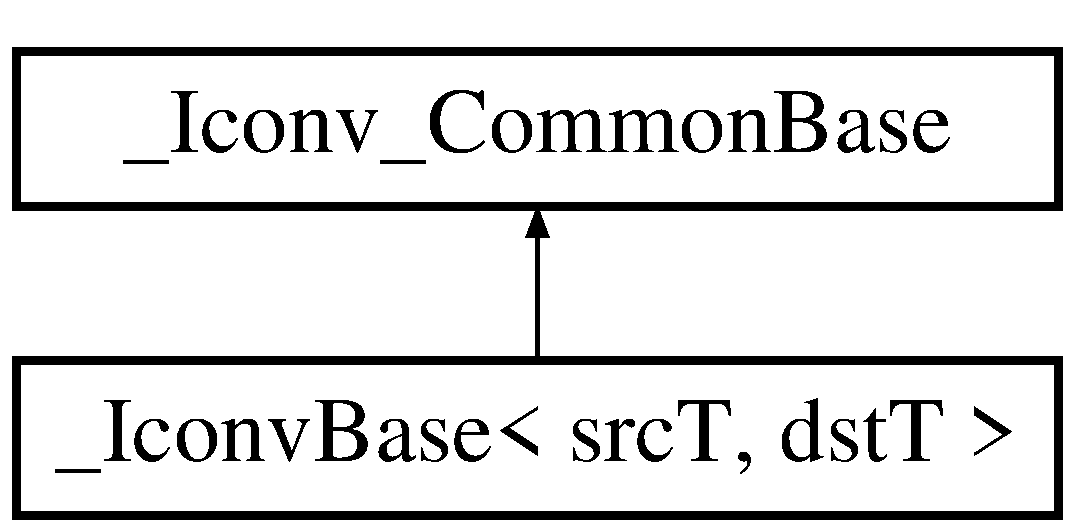
\includegraphics[height=2.000000cm]{class__Iconv__CommonBase}
\end{center}
\end{figure}
\subsection*{Public Member Functions}
\begin{DoxyCompactItemize}
\item 
\hypertarget{class__Iconv__CommonBase_a2b6552340dacdac4931258c0619fbad7}{size\-\_\-t {\bfseries get\-\_\-src\-\_\-last\-\_\-read} (void) const }\label{class__Iconv__CommonBase_a2b6552340dacdac4931258c0619fbad7}

\item 
\hypertarget{class__Iconv__CommonBase_a1d27d7277cdd8e141be41d9736259b3e}{size\-\_\-t {\bfseries get\-\_\-dest\-\_\-last\-\_\-written} (void) const }\label{class__Iconv__CommonBase_a1d27d7277cdd8e141be41d9736259b3e}

\end{DoxyCompactItemize}
\subsection*{Static Public Member Functions}
\begin{DoxyCompactItemize}
\item 
\hypertarget{class__Iconv__CommonBase_a23c056db5ca345b36c6b3009ad42c2bd}{static const char $\ast$ {\bfseries errstring} (int x)}\label{class__Iconv__CommonBase_a23c056db5ca345b36c6b3009ad42c2bd}

\end{DoxyCompactItemize}
\subsection*{Public Attributes}
\begin{DoxyCompactItemize}
\item 
\hypertarget{class__Iconv__CommonBase_a3a66ec3098bcffce87630aa12779ca4b}{size\-\_\-t {\bfseries dst\-\_\-adv} = 0}\label{class__Iconv__CommonBase_a3a66ec3098bcffce87630aa12779ca4b}

\item 
\hypertarget{class__Iconv__CommonBase_a509e7fa90fd90ea5aeb5da85c17ed470}{size\-\_\-t {\bfseries src\-\_\-adv} = 0}\label{class__Iconv__CommonBase_a509e7fa90fd90ea5aeb5da85c17ed470}

\end{DoxyCompactItemize}
\subsection*{Static Public Attributes}
\begin{DoxyCompactItemize}
\item 
\hypertarget{class__Iconv__CommonBase_ac183b286144487de81bfb67ec2c9cfd8}{static constexpr int {\bfseries err\-\_\-noinit} = -\/E\-B\-A\-D\-F}\label{class__Iconv__CommonBase_ac183b286144487de81bfb67ec2c9cfd8}

\item 
\hypertarget{class__Iconv__CommonBase_a332a8f594844739240ef5d09d4b19c16}{static constexpr int {\bfseries err\-\_\-noroom} = -\/E2\-B\-I\-G}\label{class__Iconv__CommonBase_a332a8f594844739240ef5d09d4b19c16}

\item 
\hypertarget{class__Iconv__CommonBase_a537ebd79d1d436d8708c65933573d00d}{static constexpr int {\bfseries err\-\_\-notvalid} = -\/E\-I\-L\-S\-E\-Q}\label{class__Iconv__CommonBase_a537ebd79d1d436d8708c65933573d00d}

\item 
\hypertarget{class__Iconv__CommonBase_ad772ecac58b2dc2919e0fe1004ea2240}{static constexpr int {\bfseries err\-\_\-incomplete} = -\/E\-I\-N\-V\-A\-L}\label{class__Iconv__CommonBase_ad772ecac58b2dc2919e0fe1004ea2240}

\end{DoxyCompactItemize}
\subsection*{Static Protected Member Functions}
\begin{DoxyCompactItemize}
\item 
\hypertarget{class__Iconv__CommonBase_a95f5a6378298edd22b538941006dab63}{static constexpr bool {\bfseries big\-\_\-endian} (void)}\label{class__Iconv__CommonBase_a95f5a6378298edd22b538941006dab63}

\end{DoxyCompactItemize}


\subsection{Detailed Description}


Definition at line 39 of file iconvpp.\-hpp.



The documentation for this class was generated from the following files\-:\begin{DoxyCompactItemize}
\item 
include/iconvpp.\-hpp\item 
src/misc/iconvpp.\-cpp\end{DoxyCompactItemize}

\hypertarget{class__IconvBase}{\section{\-\_\-\-Iconv\-Base$<$ src\-T, dst\-T $>$ Class Template Reference}
\label{class__IconvBase}\index{\-\_\-\-Iconv\-Base$<$ src\-T, dst\-T $>$@{\-\_\-\-Iconv\-Base$<$ src\-T, dst\-T $>$}}
}
Inheritance diagram for \-\_\-\-Iconv\-Base$<$ src\-T, dst\-T $>$\-:\begin{figure}[H]
\begin{center}
\leavevmode
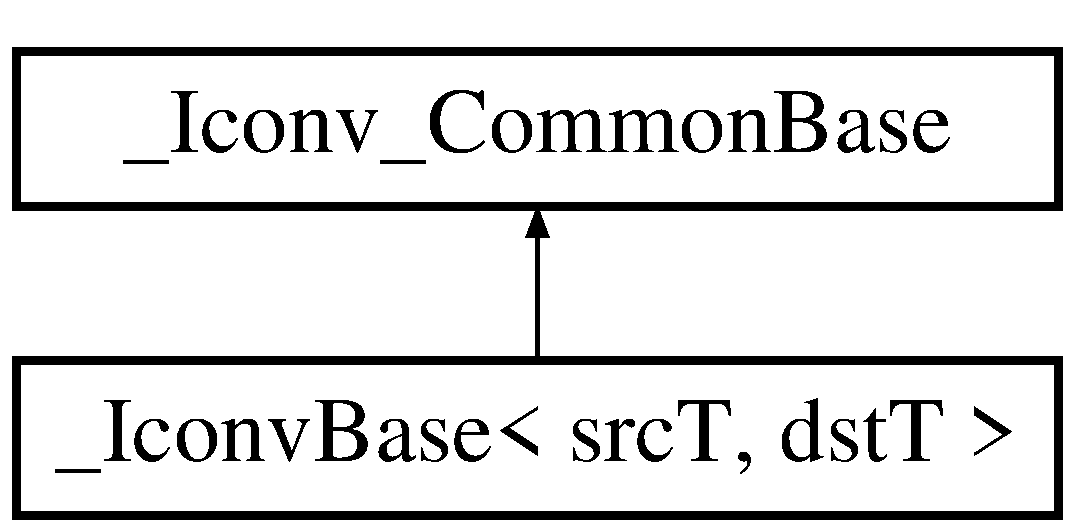
\includegraphics[height=2.000000cm]{class__IconvBase}
\end{center}
\end{figure}
\subsection*{Public Types}
\begin{DoxyCompactItemize}
\item 
\hypertarget{class__IconvBase_ad2246cfd9c3024b0cea9cd951e1ec16f}{typedef std\-::basic\-\_\-string$<$ src\-T $>$ {\bfseries src\-\_\-string}}\label{class__IconvBase_ad2246cfd9c3024b0cea9cd951e1ec16f}

\item 
\hypertarget{class__IconvBase_a6780fadf8fe4b1f828c4e431937d788e}{typedef std\-::basic\-\_\-string$<$ dst\-T $>$ {\bfseries dst\-\_\-string}}\label{class__IconvBase_a6780fadf8fe4b1f828c4e431937d788e}

\end{DoxyCompactItemize}
\subsection*{Public Member Functions}
\begin{DoxyCompactItemize}
\item 
\hypertarget{class__IconvBase_abebdb5e31f925e2080f443cb03ea5750}{void {\bfseries finish} (void)}\label{class__IconvBase_abebdb5e31f925e2080f443cb03ea5750}

\item 
\hypertarget{class__IconvBase_a07528597df9f80af3591a76a35431dff}{void {\bfseries set\-\_\-dest} (dst\-T $\ast$const dst, dst\-T $\ast$const dst\-\_\-fence)}\label{class__IconvBase_a07528597df9f80af3591a76a35431dff}

\item 
\hypertarget{class__IconvBase_a1e833fe93b08d8799573f886a0675935}{void {\bfseries set\-\_\-dest} (dst\-T $\ast$const dst, const size\-\_\-t len)}\label{class__IconvBase_a1e833fe93b08d8799573f886a0675935}

\item 
\hypertarget{class__IconvBase_a6f439ed27777d11448780dcc13cccf79}{void {\bfseries set\-\_\-dest} (dst\-T $\ast$const dst)}\label{class__IconvBase_a6f439ed27777d11448780dcc13cccf79}

\item 
\hypertarget{class__IconvBase_ab2db6d95cded73ba095d44571c346cf8}{void {\bfseries set\-\_\-src} (const src\-T $\ast$const src, const src\-T $\ast$const src\-\_\-fence)}\label{class__IconvBase_ab2db6d95cded73ba095d44571c346cf8}

\item 
\hypertarget{class__IconvBase_aa9eb45893208a6f7fb88cca6dc4842d3}{void {\bfseries set\-\_\-src} (const src\-T $\ast$const src, const size\-\_\-t len)}\label{class__IconvBase_aa9eb45893208a6f7fb88cca6dc4842d3}

\item 
\hypertarget{class__IconvBase_ad1be8ade68f5237d19772cb32c79568e}{void {\bfseries set\-\_\-src} (const src\-T $\ast$const src)}\label{class__IconvBase_ad1be8ade68f5237d19772cb32c79568e}

\item 
\hypertarget{class__IconvBase_a4c30cea323d75fe35cac7d8502e9f2f1}{virtual int {\bfseries \-\_\-do\-\_\-convert} (void)}\label{class__IconvBase_a4c30cea323d75fe35cac7d8502e9f2f1}

\item 
\hypertarget{class__IconvBase_a3e8eccc864673fcd724409b1a15f9bcc}{int {\bfseries string\-\_\-convert} (dst\-\_\-string \&dst, const src\-\_\-string \&src)}\label{class__IconvBase_a3e8eccc864673fcd724409b1a15f9bcc}

\item 
\hypertarget{class__IconvBase_a15ebe33d9db523d45b089bbd071defd0}{int {\bfseries string\-\_\-convert} (void)}\label{class__IconvBase_a15ebe33d9db523d45b089bbd071defd0}

\item 
\hypertarget{class__IconvBase_a8b4d9bff7f360968bfa1bb49c6090ec4}{int {\bfseries string\-\_\-convert\-\_\-dest} (dst\-\_\-string \&dst)}\label{class__IconvBase_a8b4d9bff7f360968bfa1bb49c6090ec4}

\item 
\hypertarget{class__IconvBase_a5aabb4b963aa3e2fa2b02f6cf7aa3b86}{int {\bfseries string\-\_\-convert\-\_\-src} (const src\-\_\-string \&src)}\label{class__IconvBase_a5aabb4b963aa3e2fa2b02f6cf7aa3b86}

\item 
\hypertarget{class__IconvBase_a46f70058431a83c02044a79c7ef52c35}{dst\-\_\-string {\bfseries string\-\_\-convert} (const src\-\_\-string \&src)}\label{class__IconvBase_a46f70058431a83c02044a79c7ef52c35}

\item 
\hypertarget{class__IconvBase_a1c05d5709f78c6d85a8f27126af7ab23}{bool {\bfseries eof} (void) const }\label{class__IconvBase_a1c05d5709f78c6d85a8f27126af7ab23}

\item 
\hypertarget{class__IconvBase_a5a7f48aae6aaf8812453fd04b777e173}{bool {\bfseries eof\-\_\-dest} (void) const }\label{class__IconvBase_a5a7f48aae6aaf8812453fd04b777e173}

\item 
\hypertarget{class__IconvBase_a6d79b9fbf4b0a7b626b4e108a886566a}{const src\-T $\ast$ {\bfseries get\-\_\-srcp} (void) const }\label{class__IconvBase_a6d79b9fbf4b0a7b626b4e108a886566a}

\item 
\hypertarget{class__IconvBase_a224ff7851493aa43f6fcee32a939d875}{const dst\-T $\ast$ {\bfseries get\-\_\-destp} (void) const }\label{class__IconvBase_a224ff7851493aa43f6fcee32a939d875}

\end{DoxyCompactItemize}
\subsection*{Protected Member Functions}
\begin{DoxyCompactItemize}
\item 
\hypertarget{class__IconvBase_af3d2f37c0dd5666cb0fec34b248d9106}{void {\bfseries set\-\_\-dest} (dst\-\_\-string \&dst)}\label{class__IconvBase_af3d2f37c0dd5666cb0fec34b248d9106}

\item 
\hypertarget{class__IconvBase_a30599161ba99c6a7b12e1a34f56fe1c8}{void {\bfseries set\-\_\-src} (const src\-\_\-string \&src)}\label{class__IconvBase_a30599161ba99c6a7b12e1a34f56fe1c8}

\end{DoxyCompactItemize}
\subsection*{Static Protected Member Functions}
\begin{DoxyCompactItemize}
\item 
\hypertarget{class__IconvBase_a59942f22d0735b2efc9760f6c6af6eaa}{static size\-\_\-t {\bfseries my\-\_\-strlen} (const char $\ast$s)}\label{class__IconvBase_a59942f22d0735b2efc9760f6c6af6eaa}

\item 
\hypertarget{class__IconvBase_a34e86742a8a9793cdf465bfb83907a83}{static size\-\_\-t {\bfseries my\-\_\-strlen} (const wchar\-\_\-t $\ast$s)}\label{class__IconvBase_a34e86742a8a9793cdf465bfb83907a83}

\item 
\hypertarget{class__IconvBase_a502c66b6a9a9931c254d428bfe8eeb80}{{\footnotesize template$<$typename X $>$ }\\static size\-\_\-t {\bfseries my\-\_\-strlen} (const X $\ast$s)}\label{class__IconvBase_a502c66b6a9a9931c254d428bfe8eeb80}

\end{DoxyCompactItemize}
\subsection*{Protected Attributes}
\begin{DoxyCompactItemize}
\item 
\hypertarget{class__IconvBase_a270820579d56ecaea184558e02adc223}{dst\-T $\ast$ {\bfseries dst\-\_\-ptr} = N\-U\-L\-L}\label{class__IconvBase_a270820579d56ecaea184558e02adc223}

\item 
\hypertarget{class__IconvBase_aa8d5c19c830379bb0c444e0670ec8563}{dst\-T $\ast$ {\bfseries dst\-\_\-ptr\-\_\-fence} = N\-U\-L\-L}\label{class__IconvBase_aa8d5c19c830379bb0c444e0670ec8563}

\item 
\hypertarget{class__IconvBase_a94abad0bc45ec272f1fd4fb8a04454fd}{const src\-T $\ast$ {\bfseries src\-\_\-ptr} = N\-U\-L\-L}\label{class__IconvBase_a94abad0bc45ec272f1fd4fb8a04454fd}

\item 
\hypertarget{class__IconvBase_aa8951f9f61d96c2a85e7dc496393ba51}{const src\-T $\ast$ {\bfseries src\-\_\-ptr\-\_\-fence} = N\-U\-L\-L}\label{class__IconvBase_aa8951f9f61d96c2a85e7dc496393ba51}

\item 
\hypertarget{class__IconvBase_ae589184e65d0add0c22795faa6720ac6}{friend {\bfseries \-\_\-\-Iconv$<$ src\-T, dst\-T $>$}}\label{class__IconvBase_ae589184e65d0add0c22795faa6720ac6}

\end{DoxyCompactItemize}


\subsection{Detailed Description}
\subsubsection*{template$<$typename src\-T, typename dst\-T$>$class \-\_\-\-Iconv\-Base$<$ src\-T, dst\-T $>$}



Definition at line 65 of file iconvpp.\-hpp.



The documentation for this class was generated from the following file\-:\begin{DoxyCompactItemize}
\item 
include/iconvpp.\-hpp\end{DoxyCompactItemize}

\hypertarget{class__LOG}{\section{\-\_\-\-L\-O\-G Class Reference}
\label{class__LOG}\index{\-\_\-\-L\-O\-G@{\-\_\-\-L\-O\-G}}
}
Inheritance diagram for \-\_\-\-L\-O\-G\-:\begin{figure}[H]
\begin{center}
\leavevmode
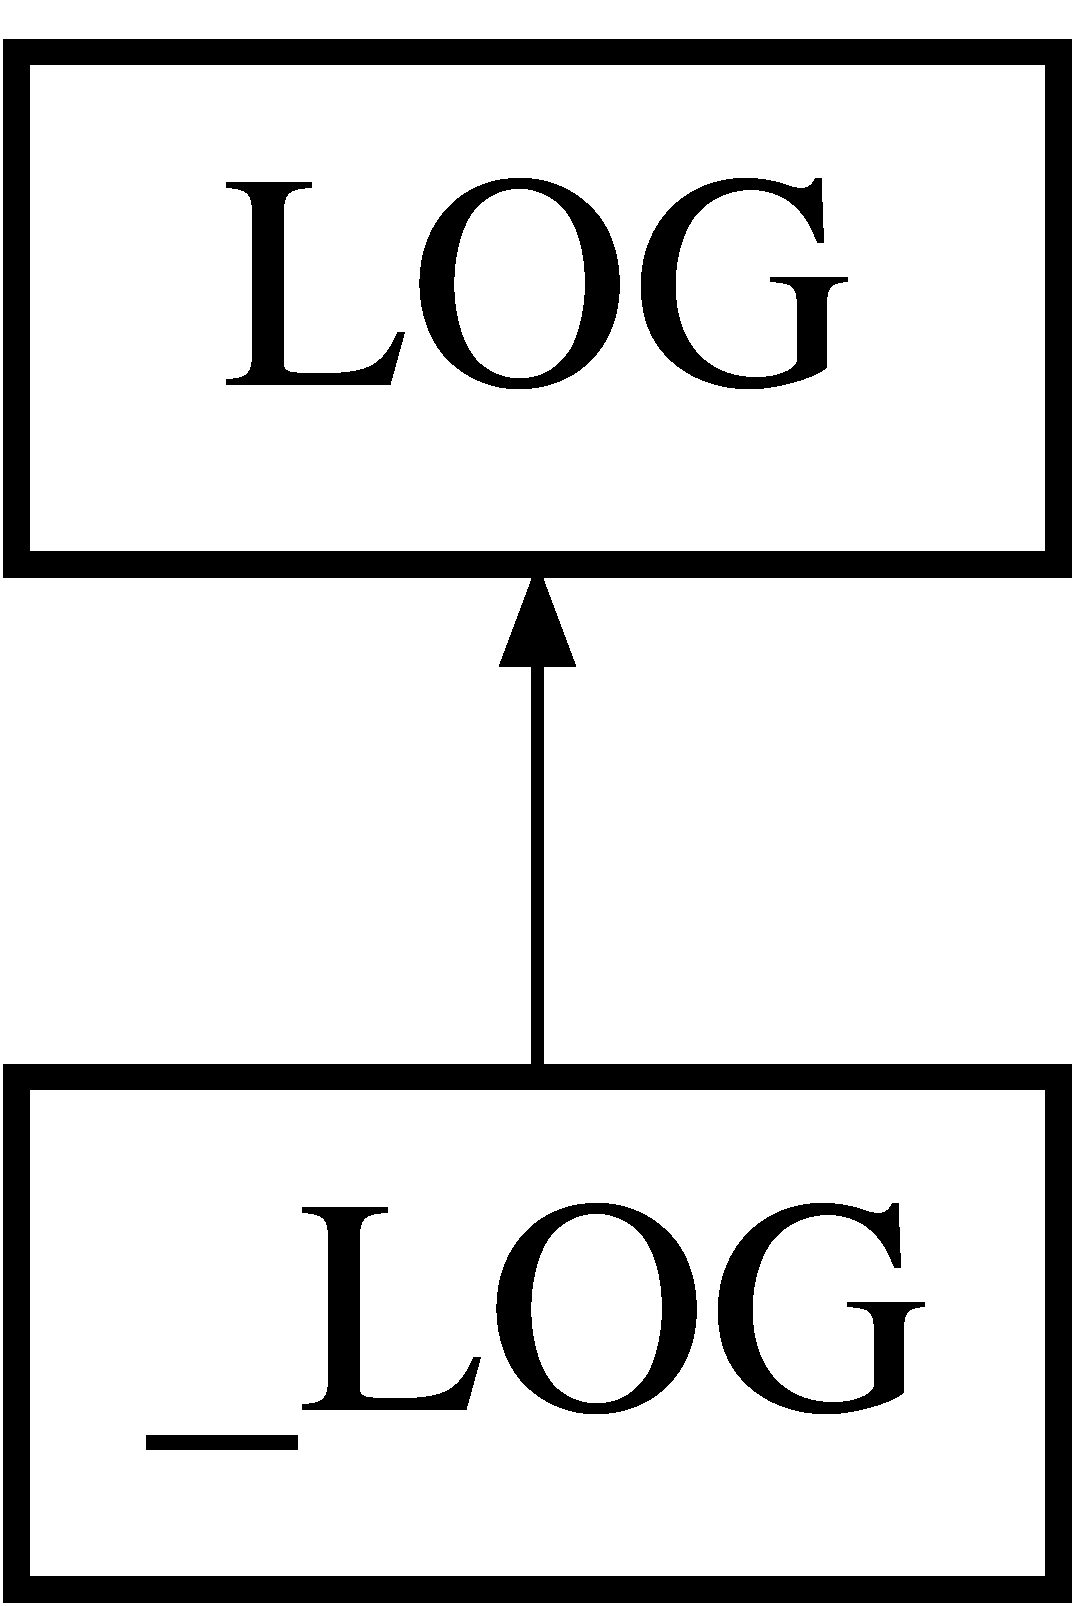
\includegraphics[height=2.000000cm]{class__LOG}
\end{center}
\end{figure}
\subsection*{Public Member Functions}
\begin{DoxyCompactItemize}
\item 
\hypertarget{class__LOG_ab6d547f5964f90ac3e7dbbb4cbf46713}{{\bfseries \-\_\-\-L\-O\-G} (L\-O\-G\-\_\-\-T\-Y\-P\-E\-S type, L\-O\-G\-\_\-\-S\-E\-V\-E\-R\-I\-T\-I\-E\-S severity)}\label{class__LOG_ab6d547f5964f90ac3e7dbbb4cbf46713}

\end{DoxyCompactItemize}


\subsection{Detailed Description}


Definition at line 50 of file cpu.\-cpp.



The documentation for this class was generated from the following file\-:\begin{DoxyCompactItemize}
\item 
src/cpu/cpu.\-cpp\end{DoxyCompactItemize}

\hypertarget{struct__LogGroup}{\section{\-\_\-\-Log\-Group Struct Reference}
\label{struct__LogGroup}\index{\-\_\-\-Log\-Group@{\-\_\-\-Log\-Group}}
}
\subsection*{Public Attributes}
\begin{DoxyCompactItemize}
\item 
\hypertarget{struct__LogGroup_a249a516d2e658850d9679acabd230757}{char const $\ast$ {\bfseries front}}\label{struct__LogGroup_a249a516d2e658850d9679acabd230757}

\item 
\hypertarget{struct__LogGroup_a3f555f56df0a10dcaaa3f977f3ed589a}{enum L\-O\-G\-\_\-\-S\-E\-V\-E\-R\-I\-T\-I\-E\-S {\bfseries min\-\_\-severity}}\label{struct__LogGroup_a3f555f56df0a10dcaaa3f977f3ed589a}

\end{DoxyCompactItemize}


\subsection{Detailed Description}


Definition at line 48 of file logging.\-h.



The documentation for this struct was generated from the following file\-:\begin{DoxyCompactItemize}
\item 
include/logging.\-h\end{DoxyCompactItemize}

\hypertarget{struct__ncc__table}{\section{\-\_\-ncc\-\_\-table Struct Reference}
\label{struct__ncc__table}\index{\-\_\-ncc\-\_\-table@{\-\_\-ncc\-\_\-table}}
}
\subsection*{Public Attributes}
\begin{DoxyCompactItemize}
\item 
\hypertarget{struct__ncc__table_a5bc2ad57271aad7ccd0448f3e9693b99}{bool {\bfseries dirty}}\label{struct__ncc__table_a5bc2ad57271aad7ccd0448f3e9693b99}

\item 
\hypertarget{struct__ncc__table_a445f947bdff8a0631ccbdcaf5e08457e}{\hyperlink{union__voodoo__reg}{voodoo\-\_\-reg} $\ast$ {\bfseries reg}}\label{struct__ncc__table_a445f947bdff8a0631ccbdcaf5e08457e}

\item 
\hypertarget{struct__ncc__table_a0e34bc2db5172865c9a512ec6d625335}{I\-N\-T32 {\bfseries ir} \mbox{[}4\mbox{]}}\label{struct__ncc__table_a0e34bc2db5172865c9a512ec6d625335}

\item 
\hypertarget{struct__ncc__table_ac5ecd4e0cf19cb167c53516cc809ebc1}{I\-N\-T32 {\bfseries ig} \mbox{[}4\mbox{]}}\label{struct__ncc__table_ac5ecd4e0cf19cb167c53516cc809ebc1}

\item 
\hypertarget{struct__ncc__table_aed726ffbb7f1b379a4f85f548fedeb7e}{I\-N\-T32 {\bfseries ib} \mbox{[}4\mbox{]}}\label{struct__ncc__table_aed726ffbb7f1b379a4f85f548fedeb7e}

\item 
\hypertarget{struct__ncc__table_afd1ba88293fcd14013dad692537e1c68}{I\-N\-T32 {\bfseries qr} \mbox{[}4\mbox{]}}\label{struct__ncc__table_afd1ba88293fcd14013dad692537e1c68}

\item 
\hypertarget{struct__ncc__table_a28e1a35fcd9297b9740c09dad56f52f0}{I\-N\-T32 {\bfseries qg} \mbox{[}4\mbox{]}}\label{struct__ncc__table_a28e1a35fcd9297b9740c09dad56f52f0}

\item 
\hypertarget{struct__ncc__table_a93f92b8a736e19e49b1ead006fbecdf2}{I\-N\-T32 {\bfseries qb} \mbox{[}4\mbox{]}}\label{struct__ncc__table_a93f92b8a736e19e49b1ead006fbecdf2}

\item 
\hypertarget{struct__ncc__table_a5425d681052597a7560a2b29d8adbf89}{I\-N\-T32 {\bfseries y} \mbox{[}16\mbox{]}}\label{struct__ncc__table_a5425d681052597a7560a2b29d8adbf89}

\item 
\hypertarget{struct__ncc__table_a6b6f14d4928d745162c3642b957fc252}{rgb\-\_\-t $\ast$ {\bfseries palette}}\label{struct__ncc__table_a6b6f14d4928d745162c3642b957fc252}

\item 
\hypertarget{struct__ncc__table_a86323735621b1c4f700bb2bd533b04e4}{rgb\-\_\-t $\ast$ {\bfseries palettea}}\label{struct__ncc__table_a86323735621b1c4f700bb2bd533b04e4}

\item 
\hypertarget{struct__ncc__table_af09b7338fd237526e17f0d5065d354a9}{rgb\-\_\-t {\bfseries texel} \mbox{[}256\mbox{]}}\label{struct__ncc__table_af09b7338fd237526e17f0d5065d354a9}

\end{DoxyCompactItemize}


\subsection{Detailed Description}


Definition at line 556 of file voodoo\-\_\-data.\-h.



The documentation for this struct was generated from the following file\-:\begin{DoxyCompactItemize}
\item 
src/hardware/voodoo\-\_\-data.\-h\end{DoxyCompactItemize}

\hypertarget{struct__OPNGEN}{\section{\-\_\-\-O\-P\-N\-G\-E\-N Struct Reference}
\label{struct__OPNGEN}\index{\-\_\-\-O\-P\-N\-G\-E\-N@{\-\_\-\-O\-P\-N\-G\-E\-N}}
}
\subsection*{Public Attributes}
\begin{DoxyCompactItemize}
\item 
\hypertarget{struct__OPNGEN_a7a4c6eb6791a37b2722aeec8b57f0dad}{U\-I\-N\-T {\bfseries playchannels}}\label{struct__OPNGEN_a7a4c6eb6791a37b2722aeec8b57f0dad}

\item 
\hypertarget{struct__OPNGEN_abf3b5a75403fdabce2e338b9ec29ea80}{U\-I\-N\-T {\bfseries playing}}\label{struct__OPNGEN_abf3b5a75403fdabce2e338b9ec29ea80}

\item 
\hypertarget{struct__OPNGEN_a61168de058d2106894234de2c057c6d6}{S\-I\-N\-T32 {\bfseries feedback2}}\label{struct__OPNGEN_a61168de058d2106894234de2c057c6d6}

\item 
\hypertarget{struct__OPNGEN_aa401c1dbbe54ea2873e22049c214c6d4}{S\-I\-N\-T32 {\bfseries feedback3}}\label{struct__OPNGEN_aa401c1dbbe54ea2873e22049c214c6d4}

\item 
\hypertarget{struct__OPNGEN_a6b7abec957d35c0537ce6f9a15b9fff1}{S\-I\-N\-T32 {\bfseries feedback4}}\label{struct__OPNGEN_a6b7abec957d35c0537ce6f9a15b9fff1}

\item 
\hypertarget{struct__OPNGEN_a718a38eff2b02de98c64c297746f3b5f}{S\-I\-N\-T32 {\bfseries outdl}}\label{struct__OPNGEN_a718a38eff2b02de98c64c297746f3b5f}

\item 
\hypertarget{struct__OPNGEN_a6fa5dc7bae0ee8d43245560e711d8e74}{S\-I\-N\-T32 {\bfseries outdc}}\label{struct__OPNGEN_a6fa5dc7bae0ee8d43245560e711d8e74}

\item 
\hypertarget{struct__OPNGEN_afb24e9ad8b2aea71739bc261ac2e8bc2}{S\-I\-N\-T32 {\bfseries outdr}}\label{struct__OPNGEN_afb24e9ad8b2aea71739bc261ac2e8bc2}

\item 
\hypertarget{struct__OPNGEN_ac8a99804ed01608d4256a4db8eb0db81}{S\-I\-N\-T32 {\bfseries calcremain}}\label{struct__OPNGEN_ac8a99804ed01608d4256a4db8eb0db81}

\item 
\hypertarget{struct__OPNGEN_afe966ddd855baecef40143a3ad1a6130}{U\-I\-N\-T8 {\bfseries keyreg} \mbox{[}O\-P\-N\-C\-H\-\_\-\-M\-A\-X\mbox{]}}\label{struct__OPNGEN_afe966ddd855baecef40143a3ad1a6130}

\end{DoxyCompactItemize}


\subsection{Detailed Description}


Definition at line 136 of file opngen.\-h.



The documentation for this struct was generated from the following file\-:\begin{DoxyCompactItemize}
\item 
src/hardware/snd\-\_\-pc98/sound/opngen.\-h\end{DoxyCompactItemize}

\hypertarget{struct__PC98RawPartition}{\section{\-\_\-\-P\-C98\-Raw\-Partition Struct Reference}
\label{struct__PC98RawPartition}\index{\-\_\-\-P\-C98\-Raw\-Partition@{\-\_\-\-P\-C98\-Raw\-Partition}}
}
\subsection*{Public Attributes}
\begin{DoxyCompactItemize}
\item 
\hypertarget{struct__PC98RawPartition_a11364eb647ed5b49da2fbde838899af6}{uint8\-\_\-t {\bfseries mid}}\label{struct__PC98RawPartition_a11364eb647ed5b49da2fbde838899af6}

\item 
\hypertarget{struct__PC98RawPartition_a6ef573976fcf9c37da1cb83a7bff3504}{uint8\-\_\-t {\bfseries sid}}\label{struct__PC98RawPartition_a6ef573976fcf9c37da1cb83a7bff3504}

\item 
\hypertarget{struct__PC98RawPartition_aa9a08aebb717ea8e3a3bda8c446414f3}{uint8\-\_\-t {\bfseries dum1}}\label{struct__PC98RawPartition_aa9a08aebb717ea8e3a3bda8c446414f3}

\item 
\hypertarget{struct__PC98RawPartition_a206633cc145e41c668ff94fba41f25e7}{uint8\-\_\-t {\bfseries dum2}}\label{struct__PC98RawPartition_a206633cc145e41c668ff94fba41f25e7}

\item 
\hypertarget{struct__PC98RawPartition_ad0a47db588d137186139edb44a0ee31a}{uint8\-\_\-t {\bfseries ipl\-\_\-sect}}\label{struct__PC98RawPartition_ad0a47db588d137186139edb44a0ee31a}

\item 
\hypertarget{struct__PC98RawPartition_a0cadc4b2a81b4998b4b55a2da3a5521e}{uint8\-\_\-t {\bfseries ipl\-\_\-head}}\label{struct__PC98RawPartition_a0cadc4b2a81b4998b4b55a2da3a5521e}

\item 
\hypertarget{struct__PC98RawPartition_add9f2479cfb1ba1691819b353e00dc8f}{uint16\-\_\-t {\bfseries ipl\-\_\-cyl}}\label{struct__PC98RawPartition_add9f2479cfb1ba1691819b353e00dc8f}

\item 
\hypertarget{struct__PC98RawPartition_a5a4e4ddcebc9c8d77b31f839ce54e782}{uint8\-\_\-t {\bfseries sector}}\label{struct__PC98RawPartition_a5a4e4ddcebc9c8d77b31f839ce54e782}

\item 
\hypertarget{struct__PC98RawPartition_a159d590fdf1918ef8ba4fa37ffbb896d}{uint8\-\_\-t {\bfseries head}}\label{struct__PC98RawPartition_a159d590fdf1918ef8ba4fa37ffbb896d}

\item 
\hypertarget{struct__PC98RawPartition_ac1a8dc3e314587ea5bceb09b1d960643}{uint16\-\_\-t {\bfseries cyl}}\label{struct__PC98RawPartition_ac1a8dc3e314587ea5bceb09b1d960643}

\item 
\hypertarget{struct__PC98RawPartition_ae9213f512993e8dd4fdbe2409ef3a402}{uint8\-\_\-t {\bfseries end\-\_\-sector}}\label{struct__PC98RawPartition_ae9213f512993e8dd4fdbe2409ef3a402}

\item 
\hypertarget{struct__PC98RawPartition_ad005cde8a52522ccc7efc9e7aa97db80}{uint8\-\_\-t {\bfseries end\-\_\-head}}\label{struct__PC98RawPartition_ad005cde8a52522ccc7efc9e7aa97db80}

\item 
\hypertarget{struct__PC98RawPartition_a23df046ffa51a15203ef87662debd38b}{uint16\-\_\-t {\bfseries end\-\_\-cyl}}\label{struct__PC98RawPartition_a23df046ffa51a15203ef87662debd38b}

\item 
\hypertarget{struct__PC98RawPartition_ac3401e613d79b53415085b2a53c34fab}{char {\bfseries name} \mbox{[}16\mbox{]}}\label{struct__PC98RawPartition_ac3401e613d79b53415085b2a53c34fab}

\end{DoxyCompactItemize}


\subsection{Detailed Description}


Definition at line 656 of file drive\-\_\-fat.\-cpp.



The documentation for this struct was generated from the following file\-:\begin{DoxyCompactItemize}
\item 
src/dos/drive\-\_\-fat.\-cpp\end{DoxyCompactItemize}

\hypertarget{struct__pci__state}{\section{\-\_\-pci\-\_\-state Struct Reference}
\label{struct__pci__state}\index{\-\_\-pci\-\_\-state@{\-\_\-pci\-\_\-state}}
}
\subsection*{Public Attributes}
\begin{DoxyCompactItemize}
\item 
\hypertarget{struct__pci__state_ab7424427a466f808c1740b6a25206cac}{\hyperlink{struct__fifo__state}{fifo\-\_\-state} {\bfseries fifo}}\label{struct__pci__state_ab7424427a466f808c1740b6a25206cac}

\item 
\hypertarget{struct__pci__state_a2dd58b63b4d56512132776f3a1e2a790}{U\-I\-N\-T32 {\bfseries init\-\_\-enable}}\label{struct__pci__state_a2dd58b63b4d56512132776f3a1e2a790}

\item 
\hypertarget{struct__pci__state_a8127a09374816a0e7266b527a1fa0d2e}{bool {\bfseries op\-\_\-pending}}\label{struct__pci__state_a8127a09374816a0e7266b527a1fa0d2e}

\end{DoxyCompactItemize}


\subsection{Detailed Description}


Definition at line 547 of file voodoo\-\_\-data.\-h.



The documentation for this struct was generated from the following file\-:\begin{DoxyCompactItemize}
\item 
src/hardware/voodoo\-\_\-data.\-h\end{DoxyCompactItemize}

\hypertarget{struct__PCM86}{\section{\-\_\-\-P\-C\-M86 Struct Reference}
\label{struct__PCM86}\index{\-\_\-\-P\-C\-M86@{\-\_\-\-P\-C\-M86}}
}
\subsection*{Public Attributes}
\begin{DoxyCompactItemize}
\item 
\hypertarget{struct__PCM86_ae0685bb8018bef996cc3ccf82bf3d86f}{S\-I\-N\-T32 {\bfseries divremain}}\label{struct__PCM86_ae0685bb8018bef996cc3ccf82bf3d86f}

\item 
\hypertarget{struct__PCM86_a7887b6970692862202c57c8dc62eb766}{S\-I\-N\-T32 {\bfseries div}}\label{struct__PCM86_a7887b6970692862202c57c8dc62eb766}

\item 
\hypertarget{struct__PCM86_a4c3ca77071861f6d53e43f2b48427cba}{S\-I\-N\-T32 {\bfseries div2}}\label{struct__PCM86_a4c3ca77071861f6d53e43f2b48427cba}

\item 
\hypertarget{struct__PCM86_abd633af0d6033bdef5186f9ca68afc52}{S\-I\-N\-T32 {\bfseries smp}}\label{struct__PCM86_abd633af0d6033bdef5186f9ca68afc52}

\item 
\hypertarget{struct__PCM86_a7915b4591dc21da4d612919f5f8f854c}{S\-I\-N\-T32 {\bfseries lastsmp}}\label{struct__PCM86_a7915b4591dc21da4d612919f5f8f854c}

\item 
\hypertarget{struct__PCM86_a8401927d6651b7f6d226790dcb18886f}{S\-I\-N\-T32 {\bfseries smp\-\_\-l}}\label{struct__PCM86_a8401927d6651b7f6d226790dcb18886f}

\item 
\hypertarget{struct__PCM86_a8fc7e6d9047d8230d3245dda15660934}{S\-I\-N\-T32 {\bfseries lastsmp\-\_\-l}}\label{struct__PCM86_a8fc7e6d9047d8230d3245dda15660934}

\item 
\hypertarget{struct__PCM86_a8588cf566a7d614ef94fd403dc10e4b5}{S\-I\-N\-T32 {\bfseries smp\-\_\-r}}\label{struct__PCM86_a8588cf566a7d614ef94fd403dc10e4b5}

\item 
\hypertarget{struct__PCM86_a693e88c04ad9d7a6fbcf1d3aaee7c692}{S\-I\-N\-T32 {\bfseries lastsmp\-\_\-r}}\label{struct__PCM86_a693e88c04ad9d7a6fbcf1d3aaee7c692}

\item 
\hypertarget{struct__PCM86_ac8a0a564182c4e07a36d85181a205abe}{U\-I\-N\-T32 {\bfseries readpos}}\label{struct__PCM86_ac8a0a564182c4e07a36d85181a205abe}

\item 
\hypertarget{struct__PCM86_ae6465959b16fbc959bf298f76d3bedfb}{U\-I\-N\-T32 {\bfseries wrtpos}}\label{struct__PCM86_ae6465959b16fbc959bf298f76d3bedfb}

\item 
\hypertarget{struct__PCM86_af8239e7e3f714d5f3acb2156a1280d6d}{S\-I\-N\-T32 {\bfseries realbuf}}\label{struct__PCM86_af8239e7e3f714d5f3acb2156a1280d6d}

\item 
\hypertarget{struct__PCM86_adcdf6a337d3af067da5f86f2a552b2f5}{S\-I\-N\-T32 {\bfseries virbuf}}\label{struct__PCM86_adcdf6a337d3af067da5f86f2a552b2f5}

\item 
\hypertarget{struct__PCM86_a800a98d504564472301a5936d5746936}{S\-I\-N\-T32 {\bfseries rescue}}\label{struct__PCM86_a800a98d504564472301a5936d5746936}

\item 
\hypertarget{struct__PCM86_abdc15b29ee3f19448e377be92788e139}{S\-I\-N\-T32 {\bfseries fifosize}}\label{struct__PCM86_abdc15b29ee3f19448e377be92788e139}

\item 
\hypertarget{struct__PCM86_ae4d390cea92819d1d5cb7e368bc09536}{S\-I\-N\-T32 {\bfseries volume}}\label{struct__PCM86_ae4d390cea92819d1d5cb7e368bc09536}

\item 
\hypertarget{struct__PCM86_a8735b8606c3c63261c26f408ad5aefe3}{S\-I\-N\-T32 {\bfseries vol5}}\label{struct__PCM86_a8735b8606c3c63261c26f408ad5aefe3}

\item 
\hypertarget{struct__PCM86_a4d6cd532b8c66a27e8d8c81789e75089}{U\-I\-N\-T32 {\bfseries lastclock}}\label{struct__PCM86_a4d6cd532b8c66a27e8d8c81789e75089}

\item 
\hypertarget{struct__PCM86_a3b924dc779032707370cce3d2adc5de6}{U\-I\-N\-T32 {\bfseries stepclock}}\label{struct__PCM86_a3b924dc779032707370cce3d2adc5de6}

\item 
\hypertarget{struct__PCM86_a7793e3746b058d75d51b9970863c104b}{U\-I\-N\-T {\bfseries stepmask}}\label{struct__PCM86_a7793e3746b058d75d51b9970863c104b}

\item 
\hypertarget{struct__PCM86_a7e9d306be6c7183d68b643f935f52fa6}{U\-I\-N\-T8 {\bfseries fifo}}\label{struct__PCM86_a7e9d306be6c7183d68b643f935f52fa6}

\item 
\hypertarget{struct__PCM86_a5ece966a5489dbf1b15dc0cbb63897e7}{U\-I\-N\-T8 {\bfseries extfunc}}\label{struct__PCM86_a5ece966a5489dbf1b15dc0cbb63897e7}

\item 
\hypertarget{struct__PCM86_aff2b2d0951ef324dffaa06ba69b1bad5}{U\-I\-N\-T8 {\bfseries dactrl}}\label{struct__PCM86_aff2b2d0951ef324dffaa06ba69b1bad5}

\item 
\hypertarget{struct__PCM86_ab71218d2300ebad20757b1da2f1111b4}{U\-I\-N\-T8 {\bfseries \-\_\-write}}\label{struct__PCM86_ab71218d2300ebad20757b1da2f1111b4}

\item 
\hypertarget{struct__PCM86_ab4702ad5ca23061433f4e61c8283d28b}{U\-I\-N\-T8 {\bfseries stepbit}}\label{struct__PCM86_ab4702ad5ca23061433f4e61c8283d28b}

\item 
\hypertarget{struct__PCM86_a009f7d3e9a6d92202e356f92c8777001}{U\-I\-N\-T8 {\bfseries reqirq}}\label{struct__PCM86_a009f7d3e9a6d92202e356f92c8777001}

\item 
\hypertarget{struct__PCM86_a36b505198123a3b7b456d3a4b6fe2d6f}{U\-I\-N\-T8 {\bfseries irqflag}}\label{struct__PCM86_a36b505198123a3b7b456d3a4b6fe2d6f}

\item 
\hypertarget{struct__PCM86_aab0394943031486b24fe2b11e8e55201}{U\-I\-N\-T8 {\bfseries padding} \mbox{[}1\mbox{]}}\label{struct__PCM86_aab0394943031486b24fe2b11e8e55201}

\item 
\hypertarget{struct__PCM86_a8c7d96d00bf3d0b6b168cadc033d4f7c}{U\-I\-N\-T8 {\bfseries buffer} \mbox{[}P\-C\-M86\-\_\-\-B\-U\-F\-S\-I\-Z\-E\mbox{]}}\label{struct__PCM86_a8c7d96d00bf3d0b6b168cadc033d4f7c}

\end{DoxyCompactItemize}


\subsection{Detailed Description}


Definition at line 23 of file pcm86.\-h.



The documentation for this struct was generated from the following file\-:\begin{DoxyCompactItemize}
\item 
src/hardware/snd\-\_\-pc98/sound/pcm86.\-h\end{DoxyCompactItemize}

\hypertarget{struct__PCMMIX}{\section{\-\_\-\-P\-C\-M\-M\-I\-X Struct Reference}
\label{struct__PCMMIX}\index{\-\_\-\-P\-C\-M\-M\-I\-X@{\-\_\-\-P\-C\-M\-M\-I\-X}}
}
\subsection*{Public Attributes}
\begin{DoxyCompactItemize}
\item 
\hypertarget{struct__PCMMIX_a79455310cc3efe4775ea726025ed2f22}{\hyperlink{structPMIXHDR}{P\-M\-I\-X\-H\-D\-R} {\bfseries hdr}}\label{struct__PCMMIX_a79455310cc3efe4775ea726025ed2f22}

\item 
\hypertarget{struct__PCMMIX_ade057861097db5440cc4b1f14925a989}{\hyperlink{structPMIXTRK}{P\-M\-I\-X\-T\-R\-K} {\bfseries trk} \mbox{[}1\mbox{]}}\label{struct__PCMMIX_ade057861097db5440cc4b1f14925a989}

\end{DoxyCompactItemize}


\subsection{Detailed Description}


Definition at line 75 of file sound.\-h.



The documentation for this struct was generated from the following file\-:\begin{DoxyCompactItemize}
\item 
src/hardware/snd\-\_\-pc98/sound/sound.\-h\end{DoxyCompactItemize}

\hypertarget{struct__PFILEH}{\section{\-\_\-\-P\-F\-I\-L\-E\-H Struct Reference}
\label{struct__PFILEH}\index{\-\_\-\-P\-F\-I\-L\-E\-H@{\-\_\-\-P\-F\-I\-L\-E\-H}}
}
\subsection*{Public Attributes}
\begin{DoxyCompactItemize}
\item 
\hypertarget{struct__PFILEH_ada5746ec01406a5fc0911c681761ad34}{O\-E\-M\-C\-H\-A\-R $\ast$ {\bfseries buffer}}\label{struct__PFILEH_ada5746ec01406a5fc0911c681761ad34}

\item 
\hypertarget{struct__PFILEH_ad4270e654472f9f3ad6fc2aa75f3b551}{U\-I\-N\-T {\bfseries buffers}}\label{struct__PFILEH_ad4270e654472f9f3ad6fc2aa75f3b551}

\item 
\hypertarget{struct__PFILEH_ab8b3fcc19ae48939210743e92275c73e}{U\-I\-N\-T {\bfseries size}}\label{struct__PFILEH_ab8b3fcc19ae48939210743e92275c73e}

\item 
\hypertarget{struct__PFILEH_a08cd29edcecb0a516033a7520907f51e}{U\-I\-N\-T8 {\bfseries hdr} \mbox{[}4\mbox{]}}\label{struct__PFILEH_a08cd29edcecb0a516033a7520907f51e}

\item 
\hypertarget{struct__PFILEH_a7c774742dbc57f905745cfdd154285c1}{U\-I\-N\-T {\bfseries hdrsize}}\label{struct__PFILEH_a7c774742dbc57f905745cfdd154285c1}

\item 
\hypertarget{struct__PFILEH_a52c69a90e0b580b506defa1a49c16bbb}{U\-I\-N\-T {\bfseries flag}}\label{struct__PFILEH_a52c69a90e0b580b506defa1a49c16bbb}

\item 
\hypertarget{struct__PFILEH_adce6da4b3d5252ff4f45f549ff0b149c}{O\-E\-M\-C\-H\-A\-R {\bfseries path} \mbox{[}M\-A\-X\-\_\-\-P\-A\-T\-H\mbox{]}}\label{struct__PFILEH_adce6da4b3d5252ff4f45f549ff0b149c}

\end{DoxyCompactItemize}


\subsection{Detailed Description}


Definition at line 24 of file profile.\-h.



The documentation for this struct was generated from the following file\-:\begin{DoxyCompactItemize}
\item 
src/hardware/snd\-\_\-pc98/common/profile.\-h\end{DoxyCompactItemize}

\hypertarget{struct__poly__extent}{\section{\-\_\-poly\-\_\-extent Struct Reference}
\label{struct__poly__extent}\index{\-\_\-poly\-\_\-extent@{\-\_\-poly\-\_\-extent}}
}
\subsection*{Public Attributes}
\begin{DoxyCompactItemize}
\item 
\hypertarget{struct__poly__extent_aa2bb43196a899de281f15cee50fe834d}{I\-N\-T32 {\bfseries startx}}\label{struct__poly__extent_aa2bb43196a899de281f15cee50fe834d}

\item 
\hypertarget{struct__poly__extent_a7b9660b72517d1e35eea12c389dcafb0}{I\-N\-T32 {\bfseries stopx}}\label{struct__poly__extent_a7b9660b72517d1e35eea12c389dcafb0}

\item 
\hypertarget{struct__poly__extent_afc41f768d5582011a779bbec4a6f417d}{\hyperlink{struct__poly__param__extent}{poly\-\_\-param\-\_\-extent} {\bfseries param} \mbox{[}M\-A\-X\-\_\-\-V\-E\-R\-T\-E\-X\-\_\-\-P\-A\-R\-A\-M\-S\mbox{]}}\label{struct__poly__extent_afc41f768d5582011a779bbec4a6f417d}

\end{DoxyCompactItemize}


\subsection{Detailed Description}


Definition at line 102 of file voodoo\-\_\-types.\-h.



The documentation for this struct was generated from the following file\-:\begin{DoxyCompactItemize}
\item 
src/hardware/voodoo\-\_\-types.\-h\end{DoxyCompactItemize}

\hypertarget{struct__poly__extra__data}{\section{\-\_\-poly\-\_\-extra\-\_\-data Struct Reference}
\label{struct__poly__extra__data}\index{\-\_\-poly\-\_\-extra\-\_\-data@{\-\_\-poly\-\_\-extra\-\_\-data}}
}
\subsection*{Public Attributes}
\begin{DoxyCompactItemize}
\item 
\hypertarget{struct__poly__extra__data_a264ded6e87ed6b3531bd56dadf809af1}{\hyperlink{struct__voodoo__state}{voodoo\-\_\-state} $\ast$ {\bfseries state}}\label{struct__poly__extra__data_a264ded6e87ed6b3531bd56dadf809af1}

\item 
\hypertarget{struct__poly__extra__data_a699a0eb70973f604118f1e252b2efead}{\hyperlink{struct__raster__info}{raster\-\_\-info} $\ast$ {\bfseries info}}\label{struct__poly__extra__data_a699a0eb70973f604118f1e252b2efead}

\item 
\hypertarget{struct__poly__extra__data_a5c4b20c95068eaaa4d9a76c49b0da5f2}{I\-N\-T16 {\bfseries ax}}\label{struct__poly__extra__data_a5c4b20c95068eaaa4d9a76c49b0da5f2}

\item 
\hypertarget{struct__poly__extra__data_adb58950449a55a23992d2832af64cc53}{I\-N\-T16 {\bfseries ay}}\label{struct__poly__extra__data_adb58950449a55a23992d2832af64cc53}

\item 
\hypertarget{struct__poly__extra__data_a1eee6382b487d9d7f504d404a617b331}{I\-N\-T32 {\bfseries startr}}\label{struct__poly__extra__data_a1eee6382b487d9d7f504d404a617b331}

\item 
\hypertarget{struct__poly__extra__data_acd176799f876571009d76891469647f9}{I\-N\-T32 {\bfseries startg}}\label{struct__poly__extra__data_acd176799f876571009d76891469647f9}

\item 
\hypertarget{struct__poly__extra__data_ae4f234a141158626a3845767265f35c2}{I\-N\-T32 {\bfseries startb}}\label{struct__poly__extra__data_ae4f234a141158626a3845767265f35c2}

\item 
\hypertarget{struct__poly__extra__data_a2a40f6a5ea33c511ca17d2800126d093}{I\-N\-T32 {\bfseries starta}}\label{struct__poly__extra__data_a2a40f6a5ea33c511ca17d2800126d093}

\item 
\hypertarget{struct__poly__extra__data_ae920737f52e27449edc9e29ea60f9f3b}{I\-N\-T32 {\bfseries startz}}\label{struct__poly__extra__data_ae920737f52e27449edc9e29ea60f9f3b}

\item 
\hypertarget{struct__poly__extra__data_a11979cc3af97f6609f0e9270edbd20c7}{I\-N\-T64 {\bfseries startw}}\label{struct__poly__extra__data_a11979cc3af97f6609f0e9270edbd20c7}

\item 
\hypertarget{struct__poly__extra__data_ab1c369c269e40786c98963075968c649}{I\-N\-T32 {\bfseries drdx}}\label{struct__poly__extra__data_ab1c369c269e40786c98963075968c649}

\item 
\hypertarget{struct__poly__extra__data_a2968cbe80dccf8a54bc13d7f29ea4fcb}{I\-N\-T32 {\bfseries dgdx}}\label{struct__poly__extra__data_a2968cbe80dccf8a54bc13d7f29ea4fcb}

\item 
\hypertarget{struct__poly__extra__data_acc8499b300ed9b20cc20532efc3a76f1}{I\-N\-T32 {\bfseries dbdx}}\label{struct__poly__extra__data_acc8499b300ed9b20cc20532efc3a76f1}

\item 
\hypertarget{struct__poly__extra__data_a7c0aac0467249e31242863538a069262}{I\-N\-T32 {\bfseries dadx}}\label{struct__poly__extra__data_a7c0aac0467249e31242863538a069262}

\item 
\hypertarget{struct__poly__extra__data_a7eb74da57f4011f24a209de6696e9fae}{I\-N\-T32 {\bfseries dzdx}}\label{struct__poly__extra__data_a7eb74da57f4011f24a209de6696e9fae}

\item 
\hypertarget{struct__poly__extra__data_a1c8c75c7e3ea9b347a4092cf25690fb7}{I\-N\-T64 {\bfseries dwdx}}\label{struct__poly__extra__data_a1c8c75c7e3ea9b347a4092cf25690fb7}

\item 
\hypertarget{struct__poly__extra__data_ac94300f6e7e3f6cb50e26e4172558022}{I\-N\-T32 {\bfseries drdy}}\label{struct__poly__extra__data_ac94300f6e7e3f6cb50e26e4172558022}

\item 
\hypertarget{struct__poly__extra__data_a37b3b5d0f84e6235a21d99408630c8ca}{I\-N\-T32 {\bfseries dgdy}}\label{struct__poly__extra__data_a37b3b5d0f84e6235a21d99408630c8ca}

\item 
\hypertarget{struct__poly__extra__data_a44163f89b4bbcd3058df04c6d44406f4}{I\-N\-T32 {\bfseries dbdy}}\label{struct__poly__extra__data_a44163f89b4bbcd3058df04c6d44406f4}

\item 
\hypertarget{struct__poly__extra__data_ac28fc2c292974749104316024db69a55}{I\-N\-T32 {\bfseries dady}}\label{struct__poly__extra__data_ac28fc2c292974749104316024db69a55}

\item 
\hypertarget{struct__poly__extra__data_ab13f06c6c9b12ad18971179b7ccccc68}{I\-N\-T32 {\bfseries dzdy}}\label{struct__poly__extra__data_ab13f06c6c9b12ad18971179b7ccccc68}

\item 
\hypertarget{struct__poly__extra__data_acaba37924607ac356c6586c6325fdfc0}{I\-N\-T64 {\bfseries dwdy}}\label{struct__poly__extra__data_acaba37924607ac356c6586c6325fdfc0}

\item 
\hypertarget{struct__poly__extra__data_a5dd1842ce7bcfbdd9ca025a39fd98820}{I\-N\-T64 {\bfseries starts0}}\label{struct__poly__extra__data_a5dd1842ce7bcfbdd9ca025a39fd98820}

\item 
\hypertarget{struct__poly__extra__data_aceb1e73dc6ff87a4ea50b1bbdc440976}{I\-N\-T64 {\bfseries startt0}}\label{struct__poly__extra__data_aceb1e73dc6ff87a4ea50b1bbdc440976}

\item 
\hypertarget{struct__poly__extra__data_a1939ea430fc65e39a264f965854f7feb}{I\-N\-T64 {\bfseries startw0}}\label{struct__poly__extra__data_a1939ea430fc65e39a264f965854f7feb}

\item 
\hypertarget{struct__poly__extra__data_a3e7442d1e24b1c67cb674528d0148aa5}{I\-N\-T64 {\bfseries ds0dx}}\label{struct__poly__extra__data_a3e7442d1e24b1c67cb674528d0148aa5}

\item 
\hypertarget{struct__poly__extra__data_a8408fcb58cebff5ba81abd797c22eb0b}{I\-N\-T64 {\bfseries dt0dx}}\label{struct__poly__extra__data_a8408fcb58cebff5ba81abd797c22eb0b}

\item 
\hypertarget{struct__poly__extra__data_a1bc83836ff718685c2e3b5a488734bd0}{I\-N\-T64 {\bfseries dw0dx}}\label{struct__poly__extra__data_a1bc83836ff718685c2e3b5a488734bd0}

\item 
\hypertarget{struct__poly__extra__data_ad205e41fe4ac2574a95318c0db1bccaf}{I\-N\-T64 {\bfseries ds0dy}}\label{struct__poly__extra__data_ad205e41fe4ac2574a95318c0db1bccaf}

\item 
\hypertarget{struct__poly__extra__data_a9e8c34d9938e87288bc7789dd7437381}{I\-N\-T64 {\bfseries dt0dy}}\label{struct__poly__extra__data_a9e8c34d9938e87288bc7789dd7437381}

\item 
\hypertarget{struct__poly__extra__data_a79145707290ace919f08ec59d4b10077}{I\-N\-T64 {\bfseries dw0dy}}\label{struct__poly__extra__data_a79145707290ace919f08ec59d4b10077}

\item 
\hypertarget{struct__poly__extra__data_abf15f85575a4c7e67578077a5e77570d}{I\-N\-T32 {\bfseries lodbase0}}\label{struct__poly__extra__data_abf15f85575a4c7e67578077a5e77570d}

\item 
\hypertarget{struct__poly__extra__data_abadf0ec08dfee47590524c7649b29262}{I\-N\-T64 {\bfseries starts1}}\label{struct__poly__extra__data_abadf0ec08dfee47590524c7649b29262}

\item 
\hypertarget{struct__poly__extra__data_aee19b2246ab1d4406c61f338d34a228e}{I\-N\-T64 {\bfseries startt1}}\label{struct__poly__extra__data_aee19b2246ab1d4406c61f338d34a228e}

\item 
\hypertarget{struct__poly__extra__data_aef7cfdb2bd567a5ba862b41c5c343257}{I\-N\-T64 {\bfseries startw1}}\label{struct__poly__extra__data_aef7cfdb2bd567a5ba862b41c5c343257}

\item 
\hypertarget{struct__poly__extra__data_af1b4d6f8d15a2423b58d1989079149c6}{I\-N\-T64 {\bfseries ds1dx}}\label{struct__poly__extra__data_af1b4d6f8d15a2423b58d1989079149c6}

\item 
\hypertarget{struct__poly__extra__data_ad988bec120d02d727a7eef5ded2254ca}{I\-N\-T64 {\bfseries dt1dx}}\label{struct__poly__extra__data_ad988bec120d02d727a7eef5ded2254ca}

\item 
\hypertarget{struct__poly__extra__data_a99ff0321fec12722c18a076fd29dd476}{I\-N\-T64 {\bfseries dw1dx}}\label{struct__poly__extra__data_a99ff0321fec12722c18a076fd29dd476}

\item 
\hypertarget{struct__poly__extra__data_aa2e50bd808160402aa105897210a3d7e}{I\-N\-T64 {\bfseries ds1dy}}\label{struct__poly__extra__data_aa2e50bd808160402aa105897210a3d7e}

\item 
\hypertarget{struct__poly__extra__data_a3edcc2ca7f520d30285c4f891be02b18}{I\-N\-T64 {\bfseries dt1dy}}\label{struct__poly__extra__data_a3edcc2ca7f520d30285c4f891be02b18}

\item 
\hypertarget{struct__poly__extra__data_ae9964a2de861f953dcd85bc401e09bc3}{I\-N\-T64 {\bfseries dw1dy}}\label{struct__poly__extra__data_ae9964a2de861f953dcd85bc401e09bc3}

\item 
\hypertarget{struct__poly__extra__data_a978cde56d266c77581a88c1d22d448a3}{I\-N\-T32 {\bfseries lodbase1}}\label{struct__poly__extra__data_a978cde56d266c77581a88c1d22d448a3}

\item 
\hypertarget{struct__poly__extra__data_ac4ebc768c0c15ad0f96f0d9a67406a62}{U\-I\-N\-T16 {\bfseries dither} \mbox{[}16\mbox{]}}\label{struct__poly__extra__data_ac4ebc768c0c15ad0f96f0d9a67406a62}

\item 
\hypertarget{struct__poly__extra__data_aafe60fcb1a440e0629f3513d14d121c0}{Bitu {\bfseries texcount}}\label{struct__poly__extra__data_aafe60fcb1a440e0629f3513d14d121c0}

\item 
\hypertarget{struct__poly__extra__data_a9da4778248791a7fae6cd2ac74d31eff}{Bitu {\bfseries r\-\_\-fbz\-Color\-Path}}\label{struct__poly__extra__data_a9da4778248791a7fae6cd2ac74d31eff}

\item 
\hypertarget{struct__poly__extra__data_a58c1591281c85eb2cfb422bd0c79b870}{Bitu {\bfseries r\-\_\-fbz\-Mode}}\label{struct__poly__extra__data_a58c1591281c85eb2cfb422bd0c79b870}

\item 
\hypertarget{struct__poly__extra__data_a008fd452346c60ee6384d524faec8e85}{Bitu {\bfseries r\-\_\-alpha\-Mode}}\label{struct__poly__extra__data_a008fd452346c60ee6384d524faec8e85}

\item 
\hypertarget{struct__poly__extra__data_a93f1bd6c1be17582a30416844df4762f}{Bitu {\bfseries r\-\_\-fog\-Mode}}\label{struct__poly__extra__data_a93f1bd6c1be17582a30416844df4762f}

\item 
\hypertarget{struct__poly__extra__data_a3fdff38fa77a154a59e4f072de79f3cd}{I\-N\-T32 {\bfseries r\-\_\-texture\-Mode0}}\label{struct__poly__extra__data_a3fdff38fa77a154a59e4f072de79f3cd}

\item 
\hypertarget{struct__poly__extra__data_a19811380eda6c18cbe1ae53b5cbeab84}{I\-N\-T32 {\bfseries r\-\_\-texture\-Mode1}}\label{struct__poly__extra__data_a19811380eda6c18cbe1ae53b5cbeab84}

\end{DoxyCompactItemize}


\subsection{Detailed Description}


Definition at line 723 of file voodoo\-\_\-data.\-h.



The documentation for this struct was generated from the following file\-:\begin{DoxyCompactItemize}
\item 
src/hardware/voodoo\-\_\-data.\-h\end{DoxyCompactItemize}

\hypertarget{struct__poly__param__extent}{\section{\-\_\-poly\-\_\-param\-\_\-extent Struct Reference}
\label{struct__poly__param__extent}\index{\-\_\-poly\-\_\-param\-\_\-extent@{\-\_\-poly\-\_\-param\-\_\-extent}}
}
\subsection*{Public Attributes}
\begin{DoxyCompactItemize}
\item 
\hypertarget{struct__poly__param__extent_a2403a4fb32e2ccf4b77f2592d2b4397d}{float {\bfseries start}}\label{struct__poly__param__extent_a2403a4fb32e2ccf4b77f2592d2b4397d}

\item 
\hypertarget{struct__poly__param__extent_a3a79a91ca5822b5833fbbf344e90755f}{float {\bfseries dpdx}}\label{struct__poly__param__extent_a3a79a91ca5822b5833fbbf344e90755f}

\end{DoxyCompactItemize}


\subsection{Detailed Description}


Definition at line 91 of file voodoo\-\_\-types.\-h.



The documentation for this struct was generated from the following file\-:\begin{DoxyCompactItemize}
\item 
src/hardware/voodoo\-\_\-types.\-h\end{DoxyCompactItemize}

\hypertarget{struct__poly__vertex}{\section{\-\_\-poly\-\_\-vertex Struct Reference}
\label{struct__poly__vertex}\index{\-\_\-poly\-\_\-vertex@{\-\_\-poly\-\_\-vertex}}
}
\subsection*{Public Attributes}
\begin{DoxyCompactItemize}
\item 
\hypertarget{struct__poly__vertex_a79d1b9f7c3c483ac7151ba71bf167742}{float {\bfseries x}}\label{struct__poly__vertex_a79d1b9f7c3c483ac7151ba71bf167742}

\item 
\hypertarget{struct__poly__vertex_ab155c82fd034de40f0338d4bbac24f88}{float {\bfseries y}}\label{struct__poly__vertex_ab155c82fd034de40f0338d4bbac24f88}

\item 
\hypertarget{struct__poly__vertex_ac1bbba54729c29fdce4b03c56f7c7ac5}{float {\bfseries p} \mbox{[}M\-A\-X\-\_\-\-V\-E\-R\-T\-E\-X\-\_\-\-P\-A\-R\-A\-M\-S\mbox{]}}\label{struct__poly__vertex_ac1bbba54729c29fdce4b03c56f7c7ac5}

\end{DoxyCompactItemize}


\subsection{Detailed Description}


Definition at line 349 of file voodoo\-\_\-types.\-h.



The documentation for this struct was generated from the following file\-:\begin{DoxyCompactItemize}
\item 
src/hardware/voodoo\-\_\-types.\-h\end{DoxyCompactItemize}

\hypertarget{struct__PSGGEN}{\section{\-\_\-\-P\-S\-G\-G\-E\-N Struct Reference}
\label{struct__PSGGEN}\index{\-\_\-\-P\-S\-G\-G\-E\-N@{\-\_\-\-P\-S\-G\-G\-E\-N}}
}
\subsection*{Public Attributes}
\begin{DoxyCompactItemize}
\item 
\hypertarget{struct__PSGGEN_ac2d74232a0c9185c28201e1ff25a22af}{\hyperlink{structPSGTONE}{P\-S\-G\-T\-O\-N\-E} {\bfseries tone} \mbox{[}3\mbox{]}}\label{struct__PSGGEN_ac2d74232a0c9185c28201e1ff25a22af}

\item 
\hypertarget{struct__PSGGEN_aaefe056d981363dde58f164d8747d35f}{\hyperlink{structPSGNOISE}{P\-S\-G\-N\-O\-I\-S\-E} {\bfseries noise}}\label{struct__PSGGEN_aaefe056d981363dde58f164d8747d35f}

\item 
\hypertarget{struct__PSGGEN_adc215970aff164bed472f92823b13d2c}{\hyperlink{structPSGREG}{P\-S\-G\-R\-E\-G} {\bfseries reg}}\label{struct__PSGGEN_adc215970aff164bed472f92823b13d2c}

\item 
\hypertarget{struct__PSGGEN_a7fd55f217173999c9999fbbaf10f045e}{U\-I\-N\-T16 {\bfseries envcnt}}\label{struct__PSGGEN_a7fd55f217173999c9999fbbaf10f045e}

\item 
\hypertarget{struct__PSGGEN_a0922b687a634055a08f80c9bf724813a}{U\-I\-N\-T16 {\bfseries envmax}}\label{struct__PSGGEN_a0922b687a634055a08f80c9bf724813a}

\item 
\hypertarget{struct__PSGGEN_a5b016b908fc67600a87fa8e146b8cadb}{U\-I\-N\-T8 {\bfseries mixer}}\label{struct__PSGGEN_a5b016b908fc67600a87fa8e146b8cadb}

\item 
\hypertarget{struct__PSGGEN_a0e714d9a17eef5c2a4aab4f52f5089d3}{U\-I\-N\-T8 {\bfseries envmode}}\label{struct__PSGGEN_a0e714d9a17eef5c2a4aab4f52f5089d3}

\item 
\hypertarget{struct__PSGGEN_ade5e9f54f27ea0b9eb05d0863698ae58}{U\-I\-N\-T8 {\bfseries envvol}}\label{struct__PSGGEN_ade5e9f54f27ea0b9eb05d0863698ae58}

\item 
\hypertarget{struct__PSGGEN_a38419e8ed312023e8d630b4a06f094da}{S\-I\-N\-T8 {\bfseries envvolcnt}}\label{struct__PSGGEN_a38419e8ed312023e8d630b4a06f094da}

\item 
\hypertarget{struct__PSGGEN_a1bbb6d7af11d1bf1e89c8c3abab69cad}{S\-I\-N\-T32 {\bfseries evol}}\label{struct__PSGGEN_a1bbb6d7af11d1bf1e89c8c3abab69cad}

\item 
\hypertarget{struct__PSGGEN_a3493079bd0e64475e2503d32ce884598}{U\-I\-N\-T {\bfseries puchicount}}\label{struct__PSGGEN_a3493079bd0e64475e2503d32ce884598}

\end{DoxyCompactItemize}


\subsection{Detailed Description}


Definition at line 40 of file psggen.\-h.



The documentation for this struct was generated from the following file\-:\begin{DoxyCompactItemize}
\item 
src/hardware/snd\-\_\-pc98/sound/psggen.\-h\end{DoxyCompactItemize}

\hypertarget{struct__raster__info}{\section{\-\_\-raster\-\_\-info Struct Reference}
\label{struct__raster__info}\index{\-\_\-raster\-\_\-info@{\-\_\-raster\-\_\-info}}
}
\subsection*{Public Attributes}
\begin{DoxyCompactItemize}
\item 
\hypertarget{struct__raster__info_a61651bfed29ab0312c3fe68a359ff391}{struct \hyperlink{struct__raster__info}{\-\_\-raster\-\_\-info} $\ast$ {\bfseries next}}\label{struct__raster__info_a61651bfed29ab0312c3fe68a359ff391}

\item 
\hypertarget{struct__raster__info_a823bf5b1e293720f3e523de29cf44afa}{poly\-\_\-draw\-\_\-scanline\-\_\-func {\bfseries callback}}\label{struct__raster__info_a823bf5b1e293720f3e523de29cf44afa}

\item 
\hypertarget{struct__raster__info_acf1e6e260048f94854bf126c98854ae0}{bool {\bfseries is\-\_\-generic}}\label{struct__raster__info_acf1e6e260048f94854bf126c98854ae0}

\item 
\hypertarget{struct__raster__info_a6cff03227e5a74203b60bef17f51e262}{U\-I\-N\-T8 {\bfseries display}}\label{struct__raster__info_a6cff03227e5a74203b60bef17f51e262}

\item 
\hypertarget{struct__raster__info_a0249c21b537e59f9f47f9b77437e4376}{U\-I\-N\-T32 {\bfseries hits}}\label{struct__raster__info_a0249c21b537e59f9f47f9b77437e4376}

\item 
\hypertarget{struct__raster__info_a0a09de384966a90de43e8c96bb0eeb11}{U\-I\-N\-T32 {\bfseries polys}}\label{struct__raster__info_a0a09de384966a90de43e8c96bb0eeb11}

\item 
\hypertarget{struct__raster__info_a83a4a66e01490271e69d346e4ce10a43}{U\-I\-N\-T32 {\bfseries eff\-\_\-color\-\_\-path}}\label{struct__raster__info_a83a4a66e01490271e69d346e4ce10a43}

\item 
\hypertarget{struct__raster__info_a299dd9db8c5b0e0ce270cda7893f282f}{U\-I\-N\-T32 {\bfseries eff\-\_\-alpha\-\_\-mode}}\label{struct__raster__info_a299dd9db8c5b0e0ce270cda7893f282f}

\item 
\hypertarget{struct__raster__info_ad5d1026bf0cc5bdfe7e4a091c327afdb}{U\-I\-N\-T32 {\bfseries eff\-\_\-fog\-\_\-mode}}\label{struct__raster__info_ad5d1026bf0cc5bdfe7e4a091c327afdb}

\item 
\hypertarget{struct__raster__info_a08870fd7370927e4cab6cbef9184cb4f}{U\-I\-N\-T32 {\bfseries eff\-\_\-fbz\-\_\-mode}}\label{struct__raster__info_a08870fd7370927e4cab6cbef9184cb4f}

\item 
\hypertarget{struct__raster__info_ad1965927f9c3c4888ca80cd9ac439105}{U\-I\-N\-T32 {\bfseries eff\-\_\-tex\-\_\-mode\-\_\-0}}\label{struct__raster__info_ad1965927f9c3c4888ca80cd9ac439105}

\item 
\hypertarget{struct__raster__info_acb15e44ddef2d6150173f5ae61eb945b}{U\-I\-N\-T32 {\bfseries eff\-\_\-tex\-\_\-mode\-\_\-1}}\label{struct__raster__info_acb15e44ddef2d6150173f5ae61eb945b}

\item 
\hypertarget{struct__raster__info_a6c46fc6eb2c16a5693b51de1562e3d68}{bool {\bfseries shader\-\_\-ready}}\label{struct__raster__info_a6c46fc6eb2c16a5693b51de1562e3d68}

\item 
\hypertarget{struct__raster__info_a4cf2d94156a3d4a2cdff2ac3c4dfee1e}{U\-I\-N\-T32 {\bfseries so\-\_\-shader\-\_\-program}}\label{struct__raster__info_a4cf2d94156a3d4a2cdff2ac3c4dfee1e}

\item 
\hypertarget{struct__raster__info_aaa3d2c76a770b550d9d2b4239e45275f}{U\-I\-N\-T32 {\bfseries so\-\_\-vertex\-\_\-shader}}\label{struct__raster__info_aaa3d2c76a770b550d9d2b4239e45275f}

\item 
\hypertarget{struct__raster__info_a1f77e3342860812b6263a3cef2766dc0}{U\-I\-N\-T32 {\bfseries so\-\_\-fragment\-\_\-shader}}\label{struct__raster__info_a1f77e3342860812b6263a3cef2766dc0}

\item 
\hypertarget{struct__raster__info_ac29587f2f87117302f5a56363c3cb5a2}{I\-N\-T32 $\ast$ {\bfseries shader\-\_\-ulocations}}\label{struct__raster__info_ac29587f2f87117302f5a56363c3cb5a2}

\end{DoxyCompactItemize}


\subsection{Detailed Description}


Definition at line 700 of file voodoo\-\_\-data.\-h.



The documentation for this struct was generated from the following file\-:\begin{DoxyCompactItemize}
\item 
src/hardware/voodoo\-\_\-data.\-h\end{DoxyCompactItemize}

\hypertarget{struct__rectangle}{\section{\-\_\-rectangle Struct Reference}
\label{struct__rectangle}\index{\-\_\-rectangle@{\-\_\-rectangle}}
}
\subsection*{Public Attributes}
\begin{DoxyCompactItemize}
\item 
\hypertarget{struct__rectangle_a400c0b48f38a20fbbd24c3af6a170715}{int {\bfseries min\-\_\-x}}\label{struct__rectangle_a400c0b48f38a20fbbd24c3af6a170715}

\item 
\hypertarget{struct__rectangle_ac58c3f724e76d841fecac3c0ed9cc1ec}{int {\bfseries max\-\_\-x}}\label{struct__rectangle_ac58c3f724e76d841fecac3c0ed9cc1ec}

\item 
\hypertarget{struct__rectangle_a5e0444616b00dffe8b1414aaed7fefde}{int {\bfseries min\-\_\-y}}\label{struct__rectangle_a5e0444616b00dffe8b1414aaed7fefde}

\item 
\hypertarget{struct__rectangle_abb40004a804c33419a4b45a12430f59d}{int {\bfseries max\-\_\-y}}\label{struct__rectangle_abb40004a804c33419a4b45a12430f59d}

\end{DoxyCompactItemize}


\subsection{Detailed Description}


Definition at line 237 of file voodoo\-\_\-types.\-h.



The documentation for this struct was generated from the following file\-:\begin{DoxyCompactItemize}
\item 
src/hardware/voodoo\-\_\-types.\-h\end{DoxyCompactItemize}

\hypertarget{struct__rgba}{\section{\-\_\-rgba Struct Reference}
\label{struct__rgba}\index{\-\_\-rgba@{\-\_\-rgba}}
}
\subsection*{Public Attributes}
\begin{DoxyCompactItemize}
\item 
\hypertarget{struct__rgba_a9beda6f3a6c9f89fd354d5d322696a41}{U\-I\-N\-T8 {\bfseries b}}\label{struct__rgba_a9beda6f3a6c9f89fd354d5d322696a41}

\item 
\hypertarget{struct__rgba_acb2cb9901aeb26dccd5a4735b367c665}{U\-I\-N\-T8 {\bfseries g}}\label{struct__rgba_acb2cb9901aeb26dccd5a4735b367c665}

\item 
\hypertarget{struct__rgba_a954228f57987281eef6280cb156bb3bd}{U\-I\-N\-T8 {\bfseries r}}\label{struct__rgba_a954228f57987281eef6280cb156bb3bd}

\item 
\hypertarget{struct__rgba_a29db039a53ec497c40b6f9f11161f7b5}{U\-I\-N\-T8 {\bfseries a}}\label{struct__rgba_a29db039a53ec497c40b6f9f11161f7b5}

\end{DoxyCompactItemize}


\subsection{Detailed Description}


Definition at line 501 of file voodoo\-\_\-data.\-h.



The documentation for this struct was generated from the following file\-:\begin{DoxyCompactItemize}
\item 
src/hardware/voodoo\-\_\-data.\-h\end{DoxyCompactItemize}

\hypertarget{struct__RHYTHM}{\section{\-\_\-\-R\-H\-Y\-T\-H\-M Struct Reference}
\label{struct__RHYTHM}\index{\-\_\-\-R\-H\-Y\-T\-H\-M@{\-\_\-\-R\-H\-Y\-T\-H\-M}}
}
\subsection*{Public Attributes}
\begin{DoxyCompactItemize}
\item 
\hypertarget{struct__RHYTHM_a12128f9bf695c8169ceeaec1858d3e5b}{\hyperlink{structPMIXHDR}{P\-M\-I\-X\-H\-D\-R} {\bfseries hdr}}\label{struct__RHYTHM_a12128f9bf695c8169ceeaec1858d3e5b}

\item 
\hypertarget{struct__RHYTHM_ab7a544b57e99acaf414eb847476dc15a}{\hyperlink{structPMIXTRK}{P\-M\-I\-X\-T\-R\-K} {\bfseries trk} \mbox{[}6\mbox{]}}\label{struct__RHYTHM_ab7a544b57e99acaf414eb847476dc15a}

\item 
\hypertarget{struct__RHYTHM_a82d0398c7c408620db1954ad2ec5e4e6}{U\-I\-N\-T {\bfseries vol}}\label{struct__RHYTHM_a82d0398c7c408620db1954ad2ec5e4e6}

\item 
\hypertarget{struct__RHYTHM_ae6dc34f8868cc782c2e705e3519ef3a0}{U\-I\-N\-T8 {\bfseries trkvol} \mbox{[}8\mbox{]}}\label{struct__RHYTHM_ae6dc34f8868cc782c2e705e3519ef3a0}

\end{DoxyCompactItemize}


\subsection{Detailed Description}


Definition at line 2 of file rhythm.\-h.



The documentation for this struct was generated from the following file\-:\begin{DoxyCompactItemize}
\item 
src/hardware/snd\-\_\-pc98/sound/rhythm.\-h\end{DoxyCompactItemize}

\hypertarget{struct__setup__vertex}{\section{\-\_\-setup\-\_\-vertex Struct Reference}
\label{struct__setup__vertex}\index{\-\_\-setup\-\_\-vertex@{\-\_\-setup\-\_\-vertex}}
}
\subsection*{Public Attributes}
\begin{DoxyCompactItemize}
\item 
\hypertarget{struct__setup__vertex_a0d774e0d02faa617b267b88b2e95000b}{float {\bfseries x}}\label{struct__setup__vertex_a0d774e0d02faa617b267b88b2e95000b}

\item 
\hypertarget{struct__setup__vertex_a8ed9c94da4b077ff65c0ea725d03d8c4}{float {\bfseries y}}\label{struct__setup__vertex_a8ed9c94da4b077ff65c0ea725d03d8c4}

\item 
\hypertarget{struct__setup__vertex_ab43777819afddf00f71224c74051cc59}{float {\bfseries a}}\label{struct__setup__vertex_ab43777819afddf00f71224c74051cc59}

\item 
\hypertarget{struct__setup__vertex_afbfefd58773c431388358a2202c726e5}{float {\bfseries r}}\label{struct__setup__vertex_afbfefd58773c431388358a2202c726e5}

\item 
\hypertarget{struct__setup__vertex_a8d89b65e5b73188f7ebf822748ca8163}{float {\bfseries g}}\label{struct__setup__vertex_a8d89b65e5b73188f7ebf822748ca8163}

\item 
\hypertarget{struct__setup__vertex_af3efcc0d2812c2477b6d80cb963f9b77}{float {\bfseries b}}\label{struct__setup__vertex_af3efcc0d2812c2477b6d80cb963f9b77}

\item 
\hypertarget{struct__setup__vertex_a63e1dfdae9282101093c56b2ee8645cf}{float {\bfseries z}}\label{struct__setup__vertex_a63e1dfdae9282101093c56b2ee8645cf}

\item 
\hypertarget{struct__setup__vertex_a704213403296a444f40d240c0ef5cef5}{float {\bfseries wb}}\label{struct__setup__vertex_a704213403296a444f40d240c0ef5cef5}

\item 
\hypertarget{struct__setup__vertex_aec1c281e24c60f3cf887f35a0327c7eb}{float {\bfseries w0}}\label{struct__setup__vertex_aec1c281e24c60f3cf887f35a0327c7eb}

\item 
\hypertarget{struct__setup__vertex_a6ccc1fdc7116fbdeb9f4672cd39b0e8a}{float {\bfseries s0}}\label{struct__setup__vertex_a6ccc1fdc7116fbdeb9f4672cd39b0e8a}

\item 
\hypertarget{struct__setup__vertex_acbc3cadd1fe4e37377966054072a315b}{float {\bfseries t0}}\label{struct__setup__vertex_acbc3cadd1fe4e37377966054072a315b}

\item 
\hypertarget{struct__setup__vertex_a7e64c083cfbb501bf04c3c511e94a5bb}{float {\bfseries w1}}\label{struct__setup__vertex_a7e64c083cfbb501bf04c3c511e94a5bb}

\item 
\hypertarget{struct__setup__vertex_aa6217f047e6679ea5f1e1e121ef4ae03}{float {\bfseries s1}}\label{struct__setup__vertex_aa6217f047e6679ea5f1e1e121ef4ae03}

\item 
\hypertarget{struct__setup__vertex_a0c96492280733b050bccc74d2f6c1d1e}{float {\bfseries t1}}\label{struct__setup__vertex_a0c96492280733b050bccc74d2f6c1d1e}

\end{DoxyCompactItemize}


\subsection{Detailed Description}


Definition at line 625 of file voodoo\-\_\-data.\-h.



The documentation for this struct was generated from the following file\-:\begin{DoxyCompactItemize}
\item 
src/hardware/voodoo\-\_\-data.\-h\end{DoxyCompactItemize}

\hypertarget{struct__stats__block}{\section{\-\_\-stats\-\_\-block Struct Reference}
\label{struct__stats__block}\index{\-\_\-stats\-\_\-block@{\-\_\-stats\-\_\-block}}
}
\subsection*{Public Attributes}
\begin{DoxyCompactItemize}
\item 
\hypertarget{struct__stats__block_a537fba6ea181dca53e08f5ce00f00864}{I\-N\-T32 {\bfseries pixels\-\_\-in}}\label{struct__stats__block_a537fba6ea181dca53e08f5ce00f00864}

\item 
\hypertarget{struct__stats__block_adc9fb7b9c25ed8d1a59eacf9d42d3fc0}{I\-N\-T32 {\bfseries pixels\-\_\-out}}\label{struct__stats__block_adc9fb7b9c25ed8d1a59eacf9d42d3fc0}

\item 
\hypertarget{struct__stats__block_a9b32f2bbc8fa370a41e15a6481c3c559}{I\-N\-T32 {\bfseries chroma\-\_\-fail}}\label{struct__stats__block_a9b32f2bbc8fa370a41e15a6481c3c559}

\item 
\hypertarget{struct__stats__block_aa53075d8fedd98acb483ba40fd0822e8}{I\-N\-T32 {\bfseries zfunc\-\_\-fail}}\label{struct__stats__block_aa53075d8fedd98acb483ba40fd0822e8}

\item 
\hypertarget{struct__stats__block_a9c21d6e47b2d8d318e1389ac16eed0e6}{I\-N\-T32 {\bfseries afunc\-\_\-fail}}\label{struct__stats__block_a9c21d6e47b2d8d318e1389ac16eed0e6}

\item 
\hypertarget{struct__stats__block_a4c87f23e26b31ae127b108b01a8f8692}{I\-N\-T32 {\bfseries clip\-\_\-fail}}\label{struct__stats__block_a4c87f23e26b31ae127b108b01a8f8692}

\item 
\hypertarget{struct__stats__block_ab45e05cc6b83769613f283cea7939066}{I\-N\-T32 {\bfseries stipple\-\_\-count}}\label{struct__stats__block_ab45e05cc6b83769613f283cea7939066}

\item 
\hypertarget{struct__stats__block_ae3295406d1900245daaa3c1b9ab751ef}{I\-N\-T32 {\bfseries filler} \mbox{[}64/4-\/7\mbox{]}}\label{struct__stats__block_ae3295406d1900245daaa3c1b9ab751ef}

\end{DoxyCompactItemize}


\subsection{Detailed Description}


Definition at line 526 of file voodoo\-\_\-data.\-h.



The documentation for this struct was generated from the following file\-:\begin{DoxyCompactItemize}
\item 
src/hardware/voodoo\-\_\-data.\-h\end{DoxyCompactItemize}

\hypertarget{struct__TMS3631}{\section{\-\_\-\-T\-M\-S3631 Struct Reference}
\label{struct__TMS3631}\index{\-\_\-\-T\-M\-S3631@{\-\_\-\-T\-M\-S3631}}
}
\subsection*{Public Attributes}
\begin{DoxyCompactItemize}
\item 
\hypertarget{struct__TMS3631_a3595e2e2becc3e958048dfeab737fc24}{\hyperlink{structTMSCH}{T\-M\-S\-C\-H} {\bfseries ch} \mbox{[}8\mbox{]}}\label{struct__TMS3631_a3595e2e2becc3e958048dfeab737fc24}

\item 
\hypertarget{struct__TMS3631_a778a39005f0dde45e75745e045883616}{U\-I\-N\-T {\bfseries enable}}\label{struct__TMS3631_a778a39005f0dde45e75745e045883616}

\end{DoxyCompactItemize}


\subsection{Detailed Description}


Definition at line 7 of file tms3631.\-h.



The documentation for this struct was generated from the following file\-:\begin{DoxyCompactItemize}
\item 
src/hardware/snd\-\_\-pc98/sound/tms3631.\-h\end{DoxyCompactItemize}

\hypertarget{struct__tmu__shared__state}{\section{\-\_\-tmu\-\_\-shared\-\_\-state Struct Reference}
\label{struct__tmu__shared__state}\index{\-\_\-tmu\-\_\-shared\-\_\-state@{\-\_\-tmu\-\_\-shared\-\_\-state}}
}
\subsection*{Public Attributes}
\begin{DoxyCompactItemize}
\item 
\hypertarget{struct__tmu__shared__state_afd23aa3522bf61a2b7647ff1544c1854}{rgb\-\_\-t {\bfseries rgb332} \mbox{[}256\mbox{]}}\label{struct__tmu__shared__state_afd23aa3522bf61a2b7647ff1544c1854}

\item 
\hypertarget{struct__tmu__shared__state_acfed5231164433d58158609af07b0843}{rgb\-\_\-t {\bfseries alpha8} \mbox{[}256\mbox{]}}\label{struct__tmu__shared__state_acfed5231164433d58158609af07b0843}

\item 
\hypertarget{struct__tmu__shared__state_ae4d7d8419af702418f8d16fef75f991a}{rgb\-\_\-t {\bfseries int8} \mbox{[}256\mbox{]}}\label{struct__tmu__shared__state_ae4d7d8419af702418f8d16fef75f991a}

\item 
\hypertarget{struct__tmu__shared__state_ac2a13a82bbb9321d4cd2876ab82bcf3e}{rgb\-\_\-t {\bfseries ai44} \mbox{[}256\mbox{]}}\label{struct__tmu__shared__state_ac2a13a82bbb9321d4cd2876ab82bcf3e}

\item 
\hypertarget{struct__tmu__shared__state_a18b14769bd0204c40df404dfe1d38a7b}{rgb\-\_\-t {\bfseries rgb565} \mbox{[}65536\mbox{]}}\label{struct__tmu__shared__state_a18b14769bd0204c40df404dfe1d38a7b}

\item 
\hypertarget{struct__tmu__shared__state_ac7b744f64de937db8c0ae36a9696cc5e}{rgb\-\_\-t {\bfseries argb1555} \mbox{[}65536\mbox{]}}\label{struct__tmu__shared__state_ac7b744f64de937db8c0ae36a9696cc5e}

\item 
\hypertarget{struct__tmu__shared__state_a6e29cc58ba3eb5d28c396a6389d53995}{rgb\-\_\-t {\bfseries argb4444} \mbox{[}65536\mbox{]}}\label{struct__tmu__shared__state_a6e29cc58ba3eb5d28c396a6389d53995}

\end{DoxyCompactItemize}


\subsection{Detailed Description}


Definition at line 611 of file voodoo\-\_\-data.\-h.



The documentation for this struct was generated from the following file\-:\begin{DoxyCompactItemize}
\item 
src/hardware/voodoo\-\_\-data.\-h\end{DoxyCompactItemize}

\hypertarget{struct__tmu__state}{\section{\-\_\-tmu\-\_\-state Struct Reference}
\label{struct__tmu__state}\index{\-\_\-tmu\-\_\-state@{\-\_\-tmu\-\_\-state}}
}
\subsection*{Public Attributes}
\begin{DoxyCompactItemize}
\item 
\hypertarget{struct__tmu__state_acb39e0e0f079b1c3539d0611812e2ce2}{U\-I\-N\-T8 $\ast$ {\bfseries ram}}\label{struct__tmu__state_acb39e0e0f079b1c3539d0611812e2ce2}

\item 
\hypertarget{struct__tmu__state_a157f2ec536c7f1d546eef41261f4d1b7}{U\-I\-N\-T32 {\bfseries mask}}\label{struct__tmu__state_a157f2ec536c7f1d546eef41261f4d1b7}

\item 
\hypertarget{struct__tmu__state_aed0778b097c904934273eba35a98df3d}{\hyperlink{union__voodoo__reg}{voodoo\-\_\-reg} $\ast$ {\bfseries reg}}\label{struct__tmu__state_aed0778b097c904934273eba35a98df3d}

\item 
\hypertarget{struct__tmu__state_acdb912f7aefc1f30cf2fb33b04bb7ddf}{bool {\bfseries regdirty}}\label{struct__tmu__state_acdb912f7aefc1f30cf2fb33b04bb7ddf}

\item 
\hypertarget{struct__tmu__state_a7e13a806ef4cd760684d9e7b5451e26b}{U\-I\-N\-T32 {\bfseries texaddr\-\_\-mask}}\label{struct__tmu__state_a7e13a806ef4cd760684d9e7b5451e26b}

\item 
\hypertarget{struct__tmu__state_a7d775c0987da123700f4e5db22327a79}{U\-I\-N\-T8 {\bfseries texaddr\-\_\-shift}}\label{struct__tmu__state_a7d775c0987da123700f4e5db22327a79}

\item 
\hypertarget{struct__tmu__state_afaaa7f3489dceb21b602166144768af8}{I\-N\-T64 {\bfseries starts}}\label{struct__tmu__state_afaaa7f3489dceb21b602166144768af8}

\item 
\hypertarget{struct__tmu__state_a79d2da894ef6e4491457645bedae493a}{I\-N\-T64 {\bfseries startt}}\label{struct__tmu__state_a79d2da894ef6e4491457645bedae493a}

\item 
\hypertarget{struct__tmu__state_a7b6d9a4ff5fbda0d5a70e2bc4e4b1d03}{I\-N\-T64 {\bfseries startw}}\label{struct__tmu__state_a7b6d9a4ff5fbda0d5a70e2bc4e4b1d03}

\item 
\hypertarget{struct__tmu__state_a2689e383d790ee48bc3b3dc2a1fe2f9d}{I\-N\-T64 {\bfseries dsdx}}\label{struct__tmu__state_a2689e383d790ee48bc3b3dc2a1fe2f9d}

\item 
\hypertarget{struct__tmu__state_a7fcf537a8204a6fc2898c1ca1fdee625}{I\-N\-T64 {\bfseries dtdx}}\label{struct__tmu__state_a7fcf537a8204a6fc2898c1ca1fdee625}

\item 
\hypertarget{struct__tmu__state_a3e1d8c65caa0c9ffbd4803ccc6bcd5e9}{I\-N\-T64 {\bfseries dwdx}}\label{struct__tmu__state_a3e1d8c65caa0c9ffbd4803ccc6bcd5e9}

\item 
\hypertarget{struct__tmu__state_a352e4e939026bd752b54209e6bb7e9e7}{I\-N\-T64 {\bfseries dsdy}}\label{struct__tmu__state_a352e4e939026bd752b54209e6bb7e9e7}

\item 
\hypertarget{struct__tmu__state_ab824d00f8b0a8e2cb128cac3cc1fa94a}{I\-N\-T64 {\bfseries dtdy}}\label{struct__tmu__state_ab824d00f8b0a8e2cb128cac3cc1fa94a}

\item 
\hypertarget{struct__tmu__state_a13fbfd14e4f72f5a8746c7c0d6e96e90}{I\-N\-T64 {\bfseries dwdy}}\label{struct__tmu__state_a13fbfd14e4f72f5a8746c7c0d6e96e90}

\item 
\hypertarget{struct__tmu__state_a0b019e8b537c970cc08a89a460d6e232}{I\-N\-T32 {\bfseries lodmin}}\label{struct__tmu__state_a0b019e8b537c970cc08a89a460d6e232}

\item 
\hypertarget{struct__tmu__state_a4422626f349da1c23d42c007712e297d}{I\-N\-T32 {\bfseries lodmax}}\label{struct__tmu__state_a4422626f349da1c23d42c007712e297d}

\item 
\hypertarget{struct__tmu__state_ade7303f2a3155b30087f77f17fbcc002}{I\-N\-T32 {\bfseries lodbias}}\label{struct__tmu__state_ade7303f2a3155b30087f77f17fbcc002}

\item 
\hypertarget{struct__tmu__state_acfc3f03f1b73ddf65a2d55ec98db8f19}{U\-I\-N\-T32 {\bfseries lodmask}}\label{struct__tmu__state_acfc3f03f1b73ddf65a2d55ec98db8f19}

\item 
\hypertarget{struct__tmu__state_afbb9339aad8ea7730a84c9ec0a29e455}{U\-I\-N\-T32 {\bfseries lodoffset} \mbox{[}9\mbox{]}}\label{struct__tmu__state_afbb9339aad8ea7730a84c9ec0a29e455}

\item 
\hypertarget{struct__tmu__state_ad90c951f1c4d21bf8a36fc9be58b6593}{I\-N\-T32 {\bfseries detailmax}}\label{struct__tmu__state_ad90c951f1c4d21bf8a36fc9be58b6593}

\item 
\hypertarget{struct__tmu__state_ad4694b7ea0b04e36bed5380fec50a455}{I\-N\-T32 {\bfseries detailbias}}\label{struct__tmu__state_ad4694b7ea0b04e36bed5380fec50a455}

\item 
\hypertarget{struct__tmu__state_a5ab7017cda5415b820eae9bb6b080eba}{U\-I\-N\-T8 {\bfseries detailscale}}\label{struct__tmu__state_a5ab7017cda5415b820eae9bb6b080eba}

\item 
\hypertarget{struct__tmu__state_ae194029504246e5e64a2323326db842e}{U\-I\-N\-T32 {\bfseries wmask}}\label{struct__tmu__state_ae194029504246e5e64a2323326db842e}

\item 
\hypertarget{struct__tmu__state_acf3f002a07d36ecb4c8153997a1af257}{U\-I\-N\-T32 {\bfseries hmask}}\label{struct__tmu__state_acf3f002a07d36ecb4c8153997a1af257}

\item 
\hypertarget{struct__tmu__state_a1f9afa573178c89fcc6a1fcaea04e8dd}{U\-I\-N\-T8 {\bfseries bilinear\-\_\-mask}}\label{struct__tmu__state_a1f9afa573178c89fcc6a1fcaea04e8dd}

\item 
\hypertarget{struct__tmu__state_a4c73b11bdcae9d608721ddb0a863d583}{\hyperlink{struct__ncc__table}{ncc\-\_\-table} {\bfseries ncc} \mbox{[}2\mbox{]}}\label{struct__tmu__state_a4c73b11bdcae9d608721ddb0a863d583}

\item 
\hypertarget{struct__tmu__state_a7f508045ede276daaf1d78faeb5e264e}{rgb\-\_\-t $\ast$ {\bfseries lookup}}\label{struct__tmu__state_a7f508045ede276daaf1d78faeb5e264e}

\item 
\hypertarget{struct__tmu__state_a5c7fe774e15bde25b79567fd432da493}{rgb\-\_\-t $\ast$ {\bfseries texel} \mbox{[}16\mbox{]}}\label{struct__tmu__state_a5c7fe774e15bde25b79567fd432da493}

\item 
\hypertarget{struct__tmu__state_a60139f04a54ab4fa996748a14c0e9c32}{rgb\-\_\-t {\bfseries palette} \mbox{[}256\mbox{]}}\label{struct__tmu__state_a60139f04a54ab4fa996748a14c0e9c32}

\item 
\hypertarget{struct__tmu__state_af8aa9290f0c61371c5c55465054836e1}{rgb\-\_\-t {\bfseries palettea} \mbox{[}256\mbox{]}}\label{struct__tmu__state_af8aa9290f0c61371c5c55465054836e1}

\end{DoxyCompactItemize}


\subsection{Detailed Description}


Definition at line 570 of file voodoo\-\_\-data.\-h.



The documentation for this struct was generated from the following file\-:\begin{DoxyCompactItemize}
\item 
src/hardware/voodoo\-\_\-data.\-h\end{DoxyCompactItemize}

\hypertarget{struct__tri__extent}{\section{\-\_\-tri\-\_\-extent Struct Reference}
\label{struct__tri__extent}\index{\-\_\-tri\-\_\-extent@{\-\_\-tri\-\_\-extent}}
}
\subsection*{Public Attributes}
\begin{DoxyCompactItemize}
\item 
\hypertarget{struct__tri__extent_a2c707a9bda2f0115a12c3a53c9052003}{I\-N\-T16 {\bfseries startx}}\label{struct__tri__extent_a2c707a9bda2f0115a12c3a53c9052003}

\item 
\hypertarget{struct__tri__extent_aa222c97d69971ca936c10ed592981b7b}{I\-N\-T16 {\bfseries stopx}}\label{struct__tri__extent_aa222c97d69971ca936c10ed592981b7b}

\end{DoxyCompactItemize}


\subsection{Detailed Description}


Definition at line 358 of file voodoo\-\_\-types.\-h.



The documentation for this struct was generated from the following file\-:\begin{DoxyCompactItemize}
\item 
src/hardware/voodoo\-\_\-types.\-h\end{DoxyCompactItemize}

\hypertarget{struct__tri__work__unit}{\section{\-\_\-tri\-\_\-work\-\_\-unit Struct Reference}
\label{struct__tri__work__unit}\index{\-\_\-tri\-\_\-work\-\_\-unit@{\-\_\-tri\-\_\-work\-\_\-unit}}
}
\subsection*{Public Attributes}
\begin{DoxyCompactItemize}
\item 
\hypertarget{struct__tri__work__unit_a2f9d80656d7b28f082c345d5a6f5a299}{\hyperlink{struct__tri__extent}{tri\-\_\-extent} {\bfseries extent} \mbox{[}8\mbox{]}}\label{struct__tri__work__unit_a2f9d80656d7b28f082c345d5a6f5a299}

\end{DoxyCompactItemize}


\subsection{Detailed Description}


Definition at line 366 of file voodoo\-\_\-types.\-h.



The documentation for this struct was generated from the following file\-:\begin{DoxyCompactItemize}
\item 
src/hardware/voodoo\-\_\-types.\-h\end{DoxyCompactItemize}

\hypertarget{union__voodoo__reg}{\section{\-\_\-voodoo\-\_\-reg Union Reference}
\label{union__voodoo__reg}\index{\-\_\-voodoo\-\_\-reg@{\-\_\-voodoo\-\_\-reg}}
}
\subsection*{Public Attributes}
\begin{DoxyCompactItemize}
\item 
\hypertarget{union__voodoo__reg_a63f2da448ca88c6c214cf5abf4df7778}{I\-N\-T32 {\bfseries i}}\label{union__voodoo__reg_a63f2da448ca88c6c214cf5abf4df7778}

\item 
\hypertarget{union__voodoo__reg_a921ea78859953f332cbd4f9f7291f4f4}{U\-I\-N\-T32 {\bfseries u}}\label{union__voodoo__reg_a921ea78859953f332cbd4f9f7291f4f4}

\item 
\hypertarget{union__voodoo__reg_a404d1c418bc264b40db5138829ef469e}{float {\bfseries f}}\label{union__voodoo__reg_a404d1c418bc264b40db5138829ef469e}

\item 
\hypertarget{union__voodoo__reg_a354c97e535735c9587507c3beb081be2}{\hyperlink{struct__rgba}{rgba} {\bfseries rgb}}\label{union__voodoo__reg_a354c97e535735c9587507c3beb081be2}

\end{DoxyCompactItemize}


\subsection{Detailed Description}


Definition at line 512 of file voodoo\-\_\-data.\-h.



The documentation for this union was generated from the following file\-:\begin{DoxyCompactItemize}
\item 
src/hardware/voodoo\-\_\-data.\-h\end{DoxyCompactItemize}

\hypertarget{struct__voodoo__state}{\section{\-\_\-voodoo\-\_\-state Struct Reference}
\label{struct__voodoo__state}\index{\-\_\-voodoo\-\_\-state@{\-\_\-voodoo\-\_\-state}}
}
\subsection*{Public Attributes}
\begin{DoxyCompactItemize}
\item 
\hypertarget{struct__voodoo__state_a05793b79aa7f3aea8bd0ea991f824542}{U\-I\-N\-T8 {\bfseries type}}\label{struct__voodoo__state_a05793b79aa7f3aea8bd0ea991f824542}

\item 
\hypertarget{struct__voodoo__state_a7bfbe20fbc4278aa25cd0ed7762c327a}{U\-I\-N\-T8 {\bfseries chipmask}}\label{struct__voodoo__state_a7bfbe20fbc4278aa25cd0ed7762c327a}

\item 
\hypertarget{struct__voodoo__state_adb4bb4113e0ce165d28fc2b6f9b0409d}{\hyperlink{union__voodoo__reg}{voodoo\-\_\-reg} {\bfseries reg} \mbox{[}0x400\mbox{]}}\label{struct__voodoo__state_adb4bb4113e0ce165d28fc2b6f9b0409d}

\item 
\hypertarget{struct__voodoo__state_a37e22a36cde1d58601d67b2dd1de414d}{const U\-I\-N\-T8 $\ast$ {\bfseries regaccess}}\label{struct__voodoo__state_a37e22a36cde1d58601d67b2dd1de414d}

\item 
\hypertarget{struct__voodoo__state_a035503886a891bf136c3fe882e5eb411}{const char $\ast$const $\ast$ {\bfseries regnames}}\label{struct__voodoo__state_a035503886a891bf136c3fe882e5eb411}

\item 
\hypertarget{struct__voodoo__state_a2a1dd0a967c04dad81519d1bafe500ae}{bool {\bfseries alt\-\_\-regmap}}\label{struct__voodoo__state_a2a1dd0a967c04dad81519d1bafe500ae}

\item 
\hypertarget{struct__voodoo__state_a458e129a7ec6e7be5bddbb5350798a38}{\hyperlink{struct__pci__state}{pci\-\_\-state} {\bfseries pci}}\label{struct__voodoo__state_a458e129a7ec6e7be5bddbb5350798a38}

\item 
\hypertarget{struct__voodoo__state_a10cedffb6f1065e4a204e5d2d8889746}{\hyperlink{struct__dac__state}{dac\-\_\-state} {\bfseries dac}}\label{struct__voodoo__state_a10cedffb6f1065e4a204e5d2d8889746}

\item 
\hypertarget{struct__voodoo__state_a9d94f4ddd141199bcf68d54dfec7b612}{\hyperlink{struct__fbi__state}{fbi\-\_\-state} {\bfseries fbi}}\label{struct__voodoo__state_a9d94f4ddd141199bcf68d54dfec7b612}

\item 
\hypertarget{struct__voodoo__state_a89cb4b022d083053f2c48b95c9ee871a}{\hyperlink{struct__tmu__state}{tmu\-\_\-state} {\bfseries tmu} \mbox{[}M\-A\-X\-\_\-\-T\-M\-U\mbox{]}}\label{struct__voodoo__state_a89cb4b022d083053f2c48b95c9ee871a}

\item 
\hypertarget{struct__voodoo__state_af04cfddcd46121b54f710e22b575c2d5}{\hyperlink{struct__tmu__shared__state}{tmu\-\_\-shared\-\_\-state} {\bfseries tmushare}}\label{struct__voodoo__state_af04cfddcd46121b54f710e22b575c2d5}

\item 
\hypertarget{struct__voodoo__state_a7b8873ac07cb3b74c7f7a5c1154bffa2}{\hyperlink{struct__stats__block}{stats\-\_\-block} $\ast$ {\bfseries thread\-\_\-stats}}\label{struct__voodoo__state_a7b8873ac07cb3b74c7f7a5c1154bffa2}

\item 
\hypertarget{struct__voodoo__state_a650ed616295323d7ba313d887c04d0f1}{int {\bfseries next\-\_\-rasterizer}}\label{struct__voodoo__state_a650ed616295323d7ba313d887c04d0f1}

\item 
\hypertarget{struct__voodoo__state_ad29d317d76341b5ccd3cad07dbdfe294}{\hyperlink{struct__raster__info}{raster\-\_\-info} {\bfseries rasterizer} \mbox{[}M\-A\-X\-\_\-\-R\-A\-S\-T\-E\-R\-I\-Z\-E\-R\-S\mbox{]}}\label{struct__voodoo__state_ad29d317d76341b5ccd3cad07dbdfe294}

\item 
\hypertarget{struct__voodoo__state_a28e0422c3399f33fda74a9b020fe1227}{\hyperlink{struct__raster__info}{raster\-\_\-info} $\ast$ {\bfseries raster\-\_\-hash} \mbox{[}R\-A\-S\-T\-E\-R\-\_\-\-H\-A\-S\-H\-\_\-\-S\-I\-Z\-E\mbox{]}}\label{struct__voodoo__state_a28e0422c3399f33fda74a9b020fe1227}

\item 
\hypertarget{struct__voodoo__state_a7f0bd4ed2292b0dde15c05795fc842ea}{bool {\bfseries send\-\_\-config}}\label{struct__voodoo__state_a7f0bd4ed2292b0dde15c05795fc842ea}

\item 
\hypertarget{struct__voodoo__state_abd42743829b26e495b699ca8d6cac044}{U\-I\-N\-T32 {\bfseries tmu\-\_\-config}}\label{struct__voodoo__state_abd42743829b26e495b699ca8d6cac044}

\item 
\hypertarget{struct__voodoo__state_a7558084b25ab2048a48f25d57f091d0d}{bool {\bfseries ogl}}\label{struct__voodoo__state_a7558084b25ab2048a48f25d57f091d0d}

\item 
\hypertarget{struct__voodoo__state_ad37253ccf3f4edcd5809454a0e20b6d9}{bool {\bfseries ogl\-\_\-dimchange}}\label{struct__voodoo__state_ad37253ccf3f4edcd5809454a0e20b6d9}

\item 
\hypertarget{struct__voodoo__state_a50d6ce4c83a4db5585b97853bec06339}{bool {\bfseries clock\-\_\-enabled}}\label{struct__voodoo__state_a50d6ce4c83a4db5585b97853bec06339}

\item 
\hypertarget{struct__voodoo__state_a607b8b821a1288b44a6768dc34c04893}{bool {\bfseries output\-\_\-on}}\label{struct__voodoo__state_a607b8b821a1288b44a6768dc34c04893}

\item 
\hypertarget{struct__voodoo__state_a3b211bb03f09c2035bb6537e950b68c2}{bool {\bfseries active}}\label{struct__voodoo__state_a3b211bb03f09c2035bb6537e950b68c2}

\end{DoxyCompactItemize}


\subsection{Detailed Description}


Definition at line 768 of file voodoo\-\_\-data.\-h.



The documentation for this struct was generated from the following file\-:\begin{DoxyCompactItemize}
\item 
src/hardware/voodoo\-\_\-data.\-h\end{DoxyCompactItemize}

\hypertarget{struct__WAVEWR}{\section{\-\_\-\-W\-A\-V\-E\-W\-R Struct Reference}
\label{struct__WAVEWR}\index{\-\_\-\-W\-A\-V\-E\-W\-R@{\-\_\-\-W\-A\-V\-E\-W\-R}}
}
\subsection*{Public Attributes}
\begin{DoxyCompactItemize}
\item 
\hypertarget{struct__WAVEWR_a0d15f9cb8ce3a0772daa05d8fdd5947f}{long {\bfseries fh}}\label{struct__WAVEWR_a0d15f9cb8ce3a0772daa05d8fdd5947f}

\item 
\hypertarget{struct__WAVEWR_ae2cc568f47db7c9bcd02253916f81e66}{U\-I\-N\-T {\bfseries rate}}\label{struct__WAVEWR_ae2cc568f47db7c9bcd02253916f81e66}

\item 
\hypertarget{struct__WAVEWR_afa1825ce9c33dcb90e6d766190e46537}{U\-I\-N\-T {\bfseries bits}}\label{struct__WAVEWR_afa1825ce9c33dcb90e6d766190e46537}

\item 
\hypertarget{struct__WAVEWR_af1c15426779e7b14b267d086685d58f6}{U\-I\-N\-T {\bfseries ch}}\label{struct__WAVEWR_af1c15426779e7b14b267d086685d58f6}

\item 
\hypertarget{struct__WAVEWR_aabdba6fe21ead74f2a3634dd8251a17f}{U\-I\-N\-T {\bfseries size}}\label{struct__WAVEWR_aabdba6fe21ead74f2a3634dd8251a17f}

\item 
\hypertarget{struct__WAVEWR_ab727b253362b5def2136444ed5d3b0eb}{U\-I\-N\-T8 $\ast$ {\bfseries ptr}}\label{struct__WAVEWR_ab727b253362b5def2136444ed5d3b0eb}

\item 
\hypertarget{struct__WAVEWR_ac2bf883262e3d45fe5ca59b1549ec07e}{U\-I\-N\-T {\bfseries remain}}\label{struct__WAVEWR_ac2bf883262e3d45fe5ca59b1549ec07e}

\item 
\hypertarget{struct__WAVEWR_ac6607bbb72e95ff3c1dfb13ecd69eb28}{U\-I\-N\-T8 {\bfseries buf} \mbox{[}4096\mbox{]}}\label{struct__WAVEWR_ac6607bbb72e95ff3c1dfb13ecd69eb28}

\end{DoxyCompactItemize}


\subsection{Detailed Description}


Definition at line 35 of file wavefile.\-h.



The documentation for this struct was generated from the following file\-:\begin{DoxyCompactItemize}
\item 
src/hardware/snd\-\_\-pc98/common/wavefile.\-h\end{DoxyCompactItemize}

\hypertarget{classA20GATE}{\section{A20\-G\-A\-T\-E Class Reference}
\label{classA20GATE}\index{A20\-G\-A\-T\-E@{A20\-G\-A\-T\-E}}
}


A20\-G\-A\-T\-E.\-C\-O\-M built-\/in command on drive Z\-:  


Inheritance diagram for A20\-G\-A\-T\-E\-:\begin{figure}[H]
\begin{center}
\leavevmode
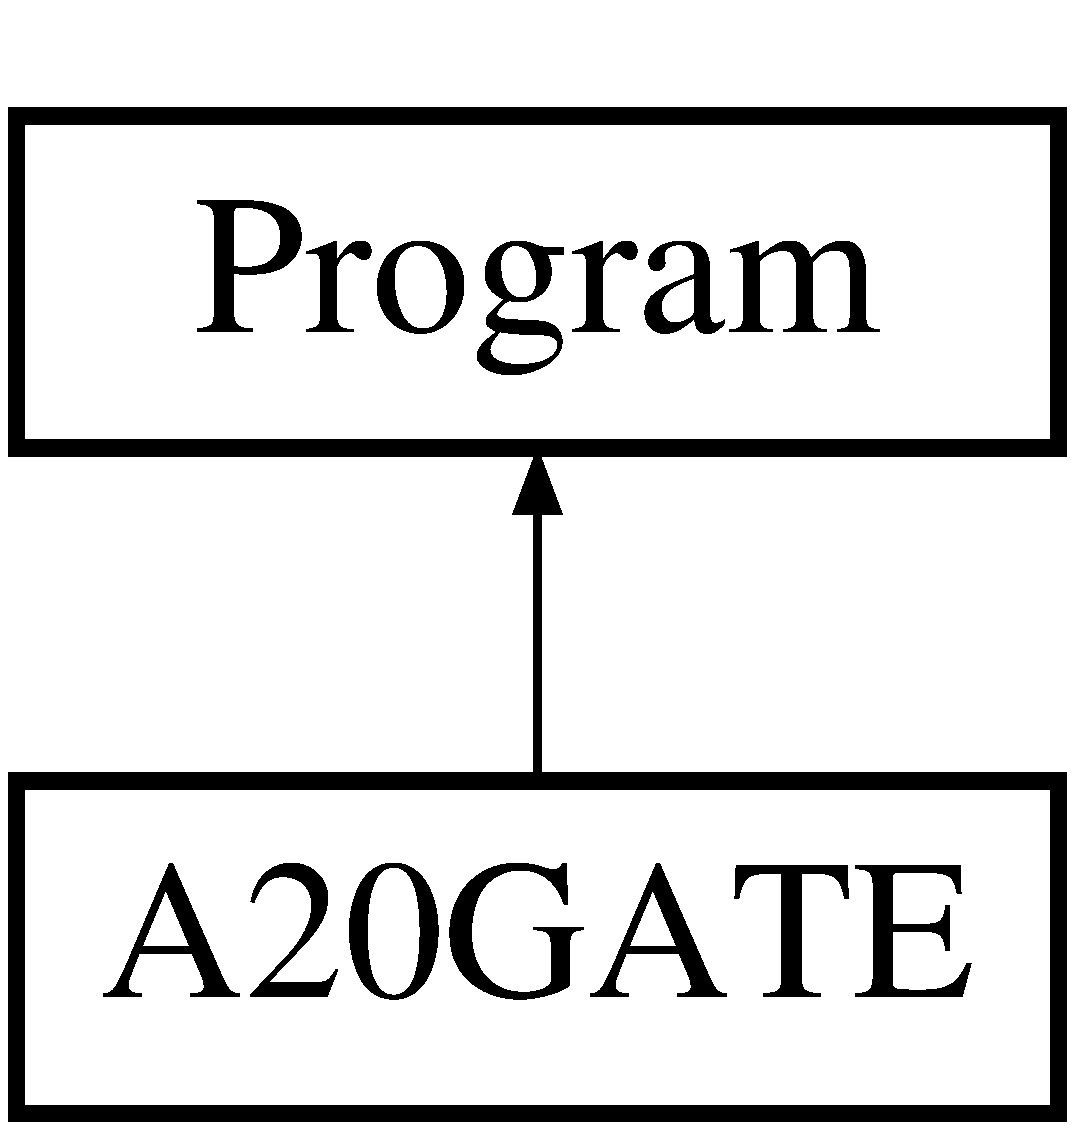
\includegraphics[height=2.000000cm]{classA20GATE}
\end{center}
\end{figure}
\subsection*{Public Member Functions}
\begin{DoxyCompactItemize}
\item 
\hypertarget{classA20GATE_a7d53ddb7d6453f710b7e829b5c0f6ca3}{void \hyperlink{classA20GATE_a7d53ddb7d6453f710b7e829b5c0f6ca3}{Run} (void)}\label{classA20GATE_a7d53ddb7d6453f710b7e829b5c0f6ca3}

\begin{DoxyCompactList}\small\item\em \hyperlink{classProgram}{Program} entry point, when the command is run. \end{DoxyCompactList}\end{DoxyCompactItemize}


\subsection{Detailed Description}
A20\-G\-A\-T\-E.\-C\-O\-M built-\/in command on drive Z\-: 

Utility command for the user to set/view the A20 gate state 

Definition at line 1589 of file memory.\-cpp.



The documentation for this class was generated from the following file\-:\begin{DoxyCompactItemize}
\item 
src/hardware/memory.\-cpp\end{DoxyCompactItemize}

\hypertarget{structDOSBoxMenu_1_1accelerator}{\section{D\-O\-S\-Box\-Menu\-:\-:accelerator Struct Reference}
\label{structDOSBoxMenu_1_1accelerator}\index{D\-O\-S\-Box\-Menu\-::accelerator@{D\-O\-S\-Box\-Menu\-::accelerator}}
}
\subsection*{Public Member Functions}
\begin{DoxyCompactItemize}
\item 
\hypertarget{structDOSBoxMenu_1_1accelerator_aa61f9898a302bd155bfe72cd04a93d33}{{\bfseries accelerator} (char \-\_\-key, unsigned char \-\_\-instance=0)}\label{structDOSBoxMenu_1_1accelerator_aa61f9898a302bd155bfe72cd04a93d33}

\end{DoxyCompactItemize}
\subsection*{Public Attributes}
\begin{DoxyCompactItemize}
\item 
\hypertarget{structDOSBoxMenu_1_1accelerator_a84a5ea4d13efd91652a5030c4fa354f2}{char {\bfseries key} = 0}\label{structDOSBoxMenu_1_1accelerator_a84a5ea4d13efd91652a5030c4fa354f2}

\item 
\hypertarget{structDOSBoxMenu_1_1accelerator_a14373aa330474bfbe946ad600aadc3b2}{unsigned char {\bfseries key\-\_\-instance} = 0}\label{structDOSBoxMenu_1_1accelerator_a14373aa330474bfbe946ad600aadc3b2}

\end{DoxyCompactItemize}


\subsection{Detailed Description}


Definition at line 180 of file menu.\-h.



The documentation for this struct was generated from the following file\-:\begin{DoxyCompactItemize}
\item 
include/menu.\-h\end{DoxyCompactItemize}

\hypertarget{classGUI_1_1ActionEventSource}{\section{G\-U\-I\-:\-:Action\-Event\-Source Class Reference}
\label{classGUI_1_1ActionEventSource}\index{G\-U\-I\-::\-Action\-Event\-Source@{G\-U\-I\-::\-Action\-Event\-Source}}
}


Event class for action events.  




{\ttfamily \#include $<$gui\-\_\-tk.\-h$>$}

Inheritance diagram for G\-U\-I\-:\-:Action\-Event\-Source\-:\begin{figure}[H]
\begin{center}
\leavevmode
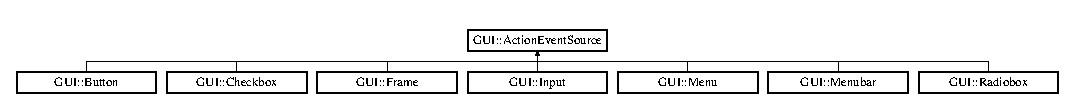
\includegraphics[height=1.548387cm]{classGUI_1_1ActionEventSource}
\end{center}
\end{figure}
\subsection*{Public Member Functions}
\begin{DoxyCompactItemize}
\item 
\hypertarget{classGUI_1_1ActionEventSource_a635659bd7a7964d6d1b450d1d353736e}{{\footnotesize template$<$typename S\-T\-R $>$ }\\\hyperlink{classGUI_1_1ActionEventSource_a635659bd7a7964d6d1b450d1d353736e}{Action\-Event\-Source} (const S\-T\-R \hyperlink{classGUI_1_1ActionEventSource_ab494e66ccff6518e1cabe747df2173f8}{name})}\label{classGUI_1_1ActionEventSource_a635659bd7a7964d6d1b450d1d353736e}

\begin{DoxyCompactList}\small\item\em Create a named event source. \end{DoxyCompactList}\item 
\hypertarget{classGUI_1_1ActionEventSource_affe36df419783630e2b3ddd8440cb213}{virtual \hyperlink{classGUI_1_1ActionEventSource_affe36df419783630e2b3ddd8440cb213}{$\sim$\-Action\-Event\-Source} ()}\label{classGUI_1_1ActionEventSource_affe36df419783630e2b3ddd8440cb213}

\begin{DoxyCompactList}\small\item\em Dummy destructor. \end{DoxyCompactList}\item 
\hypertarget{classGUI_1_1ActionEventSource_afe087d143e90df22003cafb7b278315e}{void \hyperlink{classGUI_1_1ActionEventSource_afe087d143e90df22003cafb7b278315e}{add\-Action\-Handler} (\hyperlink{structGUI_1_1ActionEventSource__Callback}{Action\-Event\-Source\-\_\-\-Callback} $\ast$handler)}\label{classGUI_1_1ActionEventSource_afe087d143e90df22003cafb7b278315e}

\begin{DoxyCompactList}\small\item\em Add a button press event handler. \end{DoxyCompactList}\item 
\hypertarget{classGUI_1_1ActionEventSource_a9b075e6c866d20cd5872b2c1af99472a}{void \hyperlink{classGUI_1_1ActionEventSource_a9b075e6c866d20cd5872b2c1af99472a}{remove\-Action\-Handler} (\hyperlink{structGUI_1_1ActionEventSource__Callback}{Action\-Event\-Source\-\_\-\-Callback} $\ast$handler)}\label{classGUI_1_1ActionEventSource_a9b075e6c866d20cd5872b2c1af99472a}

\begin{DoxyCompactList}\small\item\em Remove a button press event handler. \end{DoxyCompactList}\item 
\hypertarget{classGUI_1_1ActionEventSource_ad5e551aabc4e837d2e461eddf0307d7c}{{\footnotesize template$<$typename S\-T\-R $>$ }\\void \hyperlink{classGUI_1_1ActionEventSource_ad5e551aabc4e837d2e461eddf0307d7c}{set\-Name} (const S\-T\-R \hyperlink{classGUI_1_1ActionEventSource_ab494e66ccff6518e1cabe747df2173f8}{name})}\label{classGUI_1_1ActionEventSource_ad5e551aabc4e837d2e461eddf0307d7c}

\begin{DoxyCompactList}\small\item\em Set the name of this event source. \end{DoxyCompactList}\item 
\hypertarget{classGUI_1_1ActionEventSource_af15ccb79f3b89dd16c872184c150c373}{const \hyperlink{classGUI_1_1String}{String} \& \hyperlink{classGUI_1_1ActionEventSource_af15ccb79f3b89dd16c872184c150c373}{get\-Name} () const }\label{classGUI_1_1ActionEventSource_af15ccb79f3b89dd16c872184c150c373}

\begin{DoxyCompactList}\small\item\em Get the name of this event source. \end{DoxyCompactList}\item 
\hypertarget{classGUI_1_1ActionEventSource_a13d6f184c4e7b52ba4081810f95ac92f}{void \hyperlink{classGUI_1_1ActionEventSource_a13d6f184c4e7b52ba4081810f95ac92f}{execute\-Action} (const \hyperlink{classGUI_1_1String}{String} \&arg)}\label{classGUI_1_1ActionEventSource_a13d6f184c4e7b52ba4081810f95ac92f}

\begin{DoxyCompactList}\small\item\em Execute handlers. \end{DoxyCompactList}\item 
\hypertarget{classGUI_1_1ActionEventSource_af0750d285ae79d15436f6288705e42b4}{void \hyperlink{classGUI_1_1ActionEventSource_af0750d285ae79d15436f6288705e42b4}{execute\-Action} ()}\label{classGUI_1_1ActionEventSource_af0750d285ae79d15436f6288705e42b4}

\begin{DoxyCompactList}\small\item\em Execute handlers. \end{DoxyCompactList}\end{DoxyCompactItemize}
\subsection*{Protected Attributes}
\begin{DoxyCompactItemize}
\item 
\hypertarget{classGUI_1_1ActionEventSource_a9cd3562084ba5fa2b3d9d72ac3fa1baa}{std\-::list\\*
$<$ \hyperlink{structGUI_1_1ActionEventSource__Callback}{Action\-Event\-Source\-\_\-\-Callback} $\ast$ $>$ \hyperlink{classGUI_1_1ActionEventSource_a9cd3562084ba5fa2b3d9d72ac3fa1baa}{action\-Handlers}}\label{classGUI_1_1ActionEventSource_a9cd3562084ba5fa2b3d9d72ac3fa1baa}

\begin{DoxyCompactList}\small\item\em List of registered action handlers. \end{DoxyCompactList}\item 
\hyperlink{classGUI_1_1String}{String} \hyperlink{classGUI_1_1ActionEventSource_ab494e66ccff6518e1cabe747df2173f8}{name}
\begin{DoxyCompactList}\small\item\em This event source's name. \end{DoxyCompactList}\end{DoxyCompactItemize}


\subsection{Detailed Description}
Event class for action events. 

Action events are events generated by \hyperlink{namespaceGUI}{G\-U\-I} elements like Buttons, Menus and by pressing Enter in an \hyperlink{classGUI_1_1Input}{Input}. All of these are handled similarly\-: The source of such an event has a name, and the Event may also be connected with a \hyperlink{classGUI_1_1String}{String} describing what was executed, like the name of the \hyperlink{classGUI_1_1Menu}{Menu} entry or the contents of the \hyperlink{classGUI_1_1Input}{Input}. 

Definition at line 1413 of file gui\-\_\-tk.\-h.



\subsection{Member Data Documentation}
\hypertarget{classGUI_1_1ActionEventSource_ab494e66ccff6518e1cabe747df2173f8}{\index{G\-U\-I\-::\-Action\-Event\-Source@{G\-U\-I\-::\-Action\-Event\-Source}!name@{name}}
\index{name@{name}!GUI::ActionEventSource@{G\-U\-I\-::\-Action\-Event\-Source}}
\subsubsection[{name}]{\setlength{\rightskip}{0pt plus 5cm}{\bf String} {\bf G\-U\-I\-::\-Action\-Event\-Source\-::name}\hspace{0.3cm}{\ttfamily  \mbox{[}protected\mbox{]}}}}\label{classGUI_1_1ActionEventSource_ab494e66ccff6518e1cabe747df2173f8}


This event source's name. 

The name is primarily meant for your own purposes, for example identification of the activated element. One exception are Menubars, which display the name of their Menus. 

Definition at line 1421 of file gui\-\_\-tk.\-h.



Referenced by G\-U\-I\-::\-Checkbox\-::execute(), execute\-Action(), and get\-Name().



The documentation for this class was generated from the following file\-:\begin{DoxyCompactItemize}
\item 
src/libs/gui\-\_\-tk/\hyperlink{gui__tk_8h}{gui\-\_\-tk.\-h}\end{DoxyCompactItemize}

\hypertarget{structGUI_1_1ActionEventSource__Callback}{\section{G\-U\-I\-:\-:Action\-Event\-Source\-\_\-\-Callback Struct Reference}
\label{structGUI_1_1ActionEventSource__Callback}\index{G\-U\-I\-::\-Action\-Event\-Source\-\_\-\-Callback@{G\-U\-I\-::\-Action\-Event\-Source\-\_\-\-Callback}}
}


Callback for action events.  




{\ttfamily \#include $<$gui\-\_\-tk.\-h$>$}

Inheritance diagram for G\-U\-I\-:\-:Action\-Event\-Source\-\_\-\-Callback\-:\begin{figure}[H]
\begin{center}
\leavevmode
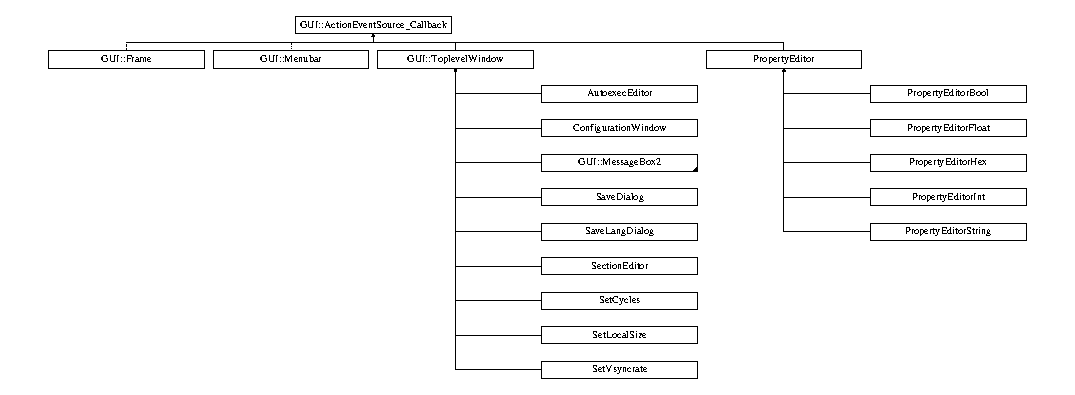
\includegraphics[height=4.865719cm]{structGUI_1_1ActionEventSource__Callback}
\end{center}
\end{figure}
\subsection*{Public Member Functions}
\begin{DoxyCompactItemize}
\item 
virtual void \hyperlink{structGUI_1_1ActionEventSource__Callback_a36df23a424558a83b45e3e3d5c175cf2}{action\-Executed} (\hyperlink{classGUI_1_1ActionEventSource}{Action\-Event\-Source} $\ast$source, const \hyperlink{classGUI_1_1String}{String} \&arg)=0
\begin{DoxyCompactList}\small\item\em Handler with optional \hyperlink{classGUI_1_1String}{String} argument. \end{DoxyCompactList}\end{DoxyCompactItemize}


\subsection{Detailed Description}
Callback for action events. 

Definition at line 1299 of file gui\-\_\-tk.\-h.



\subsection{Member Function Documentation}
\hypertarget{structGUI_1_1ActionEventSource__Callback_a36df23a424558a83b45e3e3d5c175cf2}{\index{G\-U\-I\-::\-Action\-Event\-Source\-\_\-\-Callback@{G\-U\-I\-::\-Action\-Event\-Source\-\_\-\-Callback}!action\-Executed@{action\-Executed}}
\index{action\-Executed@{action\-Executed}!GUI::ActionEventSource_Callback@{G\-U\-I\-::\-Action\-Event\-Source\-\_\-\-Callback}}
\subsubsection[{action\-Executed}]{\setlength{\rightskip}{0pt plus 5cm}virtual void {\bf G\-U\-I\-::\-Action\-Event\-Source\-\_\-\-Callback\-::action\-Executed} (
\begin{DoxyParamCaption}
\item[{{\bf Action\-Event\-Source} $\ast$}]{source, }
\item[{const {\bf String} \&}]{arg}
\end{DoxyParamCaption}
)\hspace{0.3cm}{\ttfamily  \mbox{[}pure virtual\mbox{]}}}}\label{structGUI_1_1ActionEventSource__Callback_a36df23a424558a83b45e3e3d5c175cf2}


Handler with optional \hyperlink{classGUI_1_1String}{String} argument. 

If the event source doesn't provide an additional argument, the name will be used. 

Implemented in \hyperlink{classGUI_1_1Frame_ad1e2d887bb7c22a47ca447fd5c6baaaf}{G\-U\-I\-::\-Frame}, \hyperlink{classGUI_1_1Menubar_af4c7d2663455b31660110c53c3d604e5}{G\-U\-I\-::\-Menubar}, \hyperlink{classGUI_1_1ToplevelWindow_a6b87e7cc4f8d21d661d29250d6899434}{G\-U\-I\-::\-Toplevel\-Window}, \hyperlink{classConfigurationWindow_a2dac96be9ab39e51f0eabec372406664}{Configuration\-Window}, \hyperlink{classSetLocalSize_ab71c2d90d683ddc1fdd31ee3fe972fa0}{Set\-Local\-Size}, \hyperlink{classSetVsyncrate_a7cb5a521b9e9c28bfc78d0820a2901a3}{Set\-Vsyncrate}, \hyperlink{classSetCycles_af44270f3268432309501b4918facf28a}{Set\-Cycles}, \hyperlink{classSaveLangDialog_aebf160f57b67dce3f0dc2ebac87e9f27}{Save\-Lang\-Dialog}, \hyperlink{classSaveDialog_af7dc3bd044aa8a69ae430faf64430058}{Save\-Dialog}, \hyperlink{classAutoexecEditor_a5103a2bb5e750230a808ce091448ed05}{Autoexec\-Editor}, \hyperlink{classSectionEditor_affef3df8632e3d7cef272a5cbcd4728f}{Section\-Editor}, and \hyperlink{classPropertyEditor_a216c28dd01d93a55fbd7523c1924d4c7}{Property\-Editor}.



Referenced by G\-U\-I\-::\-Menubar\-::action\-Executed(), and G\-U\-I\-::\-Action\-Event\-Source\-::execute\-Action().



The documentation for this struct was generated from the following file\-:\begin{DoxyCompactItemize}
\item 
src/libs/gui\-\_\-tk/\hyperlink{gui__tk_8h}{gui\-\_\-tk.\-h}\end{DoxyCompactItemize}

\hypertarget{uniontransport_1_1addrtype}{\section{transport\-:\-:addrtype Union Reference}
\label{uniontransport_1_1addrtype}\index{transport\-::addrtype@{transport\-::addrtype}}
}
\subsection*{Public Attributes}
\begin{DoxyCompactItemize}
\item 
\hypertarget{uniontransport_1_1addrtype_aaf06327a5a6219ca8de597b347a253f9}{\hyperlink{structnodeType}{node\-Type} {\bfseries by\-Node}}\label{uniontransport_1_1addrtype_aaf06327a5a6219ca8de597b347a253f9}

\item 
\hypertarget{uniontransport_1_1addrtype_a2d47a585adde032fc91a64b33efb9b07}{\hyperlink{structPackedIP}{Packed\-I\-P} {\bfseries by\-I\-P}}\label{uniontransport_1_1addrtype_a2d47a585adde032fc91a64b33efb9b07}

\end{DoxyCompactItemize}


\subsection{Detailed Description}


Definition at line 106 of file ipx.\-h.



The documentation for this union was generated from the following file\-:\begin{DoxyCompactItemize}
\item 
include/ipx.\-h\end{DoxyCompactItemize}

\hypertarget{unionIPXHeader_1_1transport_1_1addrtype}{\section{I\-P\-X\-Header\-:\-:transport\-:\-:addrtype Union Reference}
\label{unionIPXHeader_1_1transport_1_1addrtype}\index{I\-P\-X\-Header\-::transport\-::addrtype@{I\-P\-X\-Header\-::transport\-::addrtype}}
}
\subsection*{Public Attributes}
\begin{DoxyCompactItemize}
\item 
\hypertarget{unionIPXHeader_1_1transport_1_1addrtype_a5fce07a2e927d3a62a0695a613ce1a41}{\hyperlink{structnodeType}{node\-Type} {\bfseries by\-Node}}\label{unionIPXHeader_1_1transport_1_1addrtype_a5fce07a2e927d3a62a0695a613ce1a41}

\item 
\hypertarget{unionIPXHeader_1_1transport_1_1addrtype_a6cf399bf24cf5f4a69d4daf7fd115ce9}{\hyperlink{structPackedIP}{Packed\-I\-P} {\bfseries by\-I\-P}}\label{unionIPXHeader_1_1transport_1_1addrtype_a6cf399bf24cf5f4a69d4daf7fd115ce9}

\end{DoxyCompactItemize}


\subsection{Detailed Description}


Definition at line 92 of file ipx.\-h.



The documentation for this union was generated from the following file\-:\begin{DoxyCompactItemize}
\item 
include/ipx.\-h\end{DoxyCompactItemize}

\hypertarget{structADPCMCFG}{\section{A\-D\-P\-C\-M\-C\-F\-G Struct Reference}
\label{structADPCMCFG}\index{A\-D\-P\-C\-M\-C\-F\-G@{A\-D\-P\-C\-M\-C\-F\-G}}
}
\subsection*{Public Attributes}
\begin{DoxyCompactItemize}
\item 
\hypertarget{structADPCMCFG_ad2d8d42e7b3015d17f9b33d23f787517}{U\-I\-N\-T {\bfseries rate}}\label{structADPCMCFG_ad2d8d42e7b3015d17f9b33d23f787517}

\item 
\hypertarget{structADPCMCFG_a0afa31b835a1dd6ae514388bc0444b44}{U\-I\-N\-T {\bfseries vol}}\label{structADPCMCFG_a0afa31b835a1dd6ae514388bc0444b44}

\end{DoxyCompactItemize}


\subsection{Detailed Description}


Definition at line 52 of file adpcm.\-h.



The documentation for this struct was generated from the following file\-:\begin{DoxyCompactItemize}
\item 
src/hardware/snd\-\_\-pc98/sound/adpcm.\-h\end{DoxyCompactItemize}

\hypertarget{structADPCMREG}{\section{A\-D\-P\-C\-M\-R\-E\-G Struct Reference}
\label{structADPCMREG}\index{A\-D\-P\-C\-M\-R\-E\-G@{A\-D\-P\-C\-M\-R\-E\-G}}
}
\subsection*{Public Attributes}
\begin{DoxyCompactItemize}
\item 
\hypertarget{structADPCMREG_a08eb565121ea289faf0bb15db1eebf9e}{U\-I\-N\-T8 {\bfseries ctrl1}}\label{structADPCMREG_a08eb565121ea289faf0bb15db1eebf9e}

\item 
\hypertarget{structADPCMREG_aa8c4243b39403a669ec3c11c6e06c5a8}{U\-I\-N\-T8 {\bfseries ctrl2}}\label{structADPCMREG_aa8c4243b39403a669ec3c11c6e06c5a8}

\item 
\hypertarget{structADPCMREG_a49fc7d504a03a2fc995f65937e7a3875}{U\-I\-N\-T8 {\bfseries start} \mbox{[}2\mbox{]}}\label{structADPCMREG_a49fc7d504a03a2fc995f65937e7a3875}

\item 
\hypertarget{structADPCMREG_accdb48d3e698d946c4858c25f0c612c3}{U\-I\-N\-T8 {\bfseries stop} \mbox{[}2\mbox{]}}\label{structADPCMREG_accdb48d3e698d946c4858c25f0c612c3}

\item 
\hypertarget{structADPCMREG_a20a7e10ee5cead353dd8683126bb1abd}{U\-I\-N\-T8 {\bfseries reg06}}\label{structADPCMREG_a20a7e10ee5cead353dd8683126bb1abd}

\item 
\hypertarget{structADPCMREG_a22945b67fea1a23b61bb4640eff8d55a}{U\-I\-N\-T8 {\bfseries reg07}}\label{structADPCMREG_a22945b67fea1a23b61bb4640eff8d55a}

\item 
\hypertarget{structADPCMREG_a90bbafae370b28864d984837e228fd3f}{U\-I\-N\-T8 {\bfseries data}}\label{structADPCMREG_a90bbafae370b28864d984837e228fd3f}

\item 
\hypertarget{structADPCMREG_abb4ebdf85f84e034f9c9d9943a707c14}{U\-I\-N\-T8 {\bfseries delta} \mbox{[}2\mbox{]}}\label{structADPCMREG_abb4ebdf85f84e034f9c9d9943a707c14}

\item 
\hypertarget{structADPCMREG_af1e08f76c07f276d9331eb882a25ebd9}{U\-I\-N\-T8 {\bfseries level}}\label{structADPCMREG_af1e08f76c07f276d9331eb882a25ebd9}

\item 
\hypertarget{structADPCMREG_a02d755b5279ce5ec9204810ff64f38e1}{U\-I\-N\-T8 {\bfseries limit} \mbox{[}2\mbox{]}}\label{structADPCMREG_a02d755b5279ce5ec9204810ff64f38e1}

\item 
\hypertarget{structADPCMREG_a7193e33412e88e7cb5148a1e18e8a5b8}{U\-I\-N\-T8 {\bfseries reg0e}}\label{structADPCMREG_a7193e33412e88e7cb5148a1e18e8a5b8}

\item 
\hypertarget{structADPCMREG_ae0b34a1a40b93549109fcb37a57249e5}{U\-I\-N\-T8 {\bfseries reg0f}}\label{structADPCMREG_ae0b34a1a40b93549109fcb37a57249e5}

\item 
\hypertarget{structADPCMREG_a5af727701531b3c4abf4b24ca0acd754}{U\-I\-N\-T8 {\bfseries flag}}\label{structADPCMREG_a5af727701531b3c4abf4b24ca0acd754}

\item 
\hypertarget{structADPCMREG_ab52d85d5497e83367d906284317bc32a}{U\-I\-N\-T8 {\bfseries reg11}}\label{structADPCMREG_ab52d85d5497e83367d906284317bc32a}

\item 
\hypertarget{structADPCMREG_a1c4186c4490c34b600b9d3f7b100077c}{U\-I\-N\-T8 {\bfseries reg12}}\label{structADPCMREG_a1c4186c4490c34b600b9d3f7b100077c}

\item 
\hypertarget{structADPCMREG_ad3d5de02dd0c6820a71970b04d98b744}{U\-I\-N\-T8 {\bfseries reg13}}\label{structADPCMREG_ad3d5de02dd0c6820a71970b04d98b744}

\end{DoxyCompactItemize}


\subsection{Detailed Description}


Definition at line 8 of file adpcm.\-h.



The documentation for this struct was generated from the following file\-:\begin{DoxyCompactItemize}
\item 
src/hardware/snd\-\_\-pc98/sound/adpcm.\-h\end{DoxyCompactItemize}

\hypertarget{classallpass}{\section{allpass Class Reference}
\label{classallpass}\index{allpass@{allpass}}
}
\subsection*{Public Member Functions}
\begin{DoxyCompactItemize}
\item 
\hypertarget{classallpass_ae107adccefebabb0578dc5b9ad89c5d7}{void {\bfseries setbuffer} (float $\ast$buf, int size)}\label{classallpass_ae107adccefebabb0578dc5b9ad89c5d7}

\item 
\hypertarget{classallpass_a00c687ab45146279654ded860474e368}{void {\bfseries deletebuffer} ()}\label{classallpass_a00c687ab45146279654ded860474e368}

\item 
\hypertarget{classallpass_a72ef1d44f5807011889020f2c316cc32}{float {\bfseries process} (float inp)}\label{classallpass_a72ef1d44f5807011889020f2c316cc32}

\item 
\hypertarget{classallpass_af93a4f1d4dcc544323978031cb234aa6}{void {\bfseries mute} ()}\label{classallpass_af93a4f1d4dcc544323978031cb234aa6}

\item 
\hypertarget{classallpass_ad636d830e21de3dd61928875db95c899}{void {\bfseries setfeedback} (float val)}\label{classallpass_ad636d830e21de3dd61928875db95c899}

\item 
\hypertarget{classallpass_a19e2ab2745647005ce06366b7da64b45}{float {\bfseries getfeedback} ()}\label{classallpass_a19e2ab2745647005ce06366b7da64b45}

\item 
\hypertarget{classallpass_a7110b02ca70f6a56e4d9b11339783b17}{void {\bfseries save\-State} (std\-::ostream \&stream)}\label{classallpass_a7110b02ca70f6a56e4d9b11339783b17}

\item 
\hypertarget{classallpass_a1bcb9cc1309ac57a8eee87ffe4080ce5}{void {\bfseries load\-State} (std\-::istream \&stream)}\label{classallpass_a1bcb9cc1309ac57a8eee87ffe4080ce5}

\end{DoxyCompactItemize}
\subsection*{Public Attributes}
\begin{DoxyCompactItemize}
\item 
\hypertarget{classallpass_a4aff3bfeba72ac4b1ce0ced6618ee77c}{float {\bfseries feedback}}\label{classallpass_a4aff3bfeba72ac4b1ce0ced6618ee77c}

\item 
\hypertarget{classallpass_aa6b769510364da1d9481948d4a154f8b}{float $\ast$ {\bfseries buffer}}\label{classallpass_aa6b769510364da1d9481948d4a154f8b}

\item 
\hypertarget{classallpass_a0156b24446b810952ae1df1accb8318f}{int {\bfseries bufsize}}\label{classallpass_a0156b24446b810952ae1df1accb8318f}

\item 
\hypertarget{classallpass_a662a39221d0880b3f99e3ec40e302d4c}{int {\bfseries bufidx}}\label{classallpass_a662a39221d0880b3f99e3ec40e302d4c}

\end{DoxyCompactItemize}


\subsection{Detailed Description}


Definition at line 12 of file allpass.\-h.



The documentation for this class was generated from the following files\-:\begin{DoxyCompactItemize}
\item 
src/mt32/freeverb/allpass.\-h\item 
src/mt32/freeverb/allpass.\-cpp\end{DoxyCompactItemize}

\hypertarget{classMT32Emu_1_1AllpassFilter}{\section{M\-T32\-Emu\-:\-:Allpass\-Filter Class Reference}
\label{classMT32Emu_1_1AllpassFilter}\index{M\-T32\-Emu\-::\-Allpass\-Filter@{M\-T32\-Emu\-::\-Allpass\-Filter}}
}
Inheritance diagram for M\-T32\-Emu\-:\-:Allpass\-Filter\-:\begin{figure}[H]
\begin{center}
\leavevmode
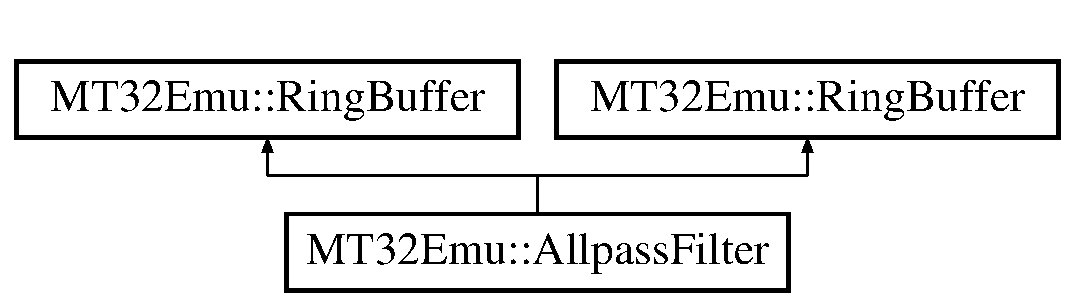
\includegraphics[height=2.000000cm]{classMT32Emu_1_1AllpassFilter}
\end{center}
\end{figure}
\subsection*{Public Member Functions}
\begin{DoxyCompactItemize}
\item 
\hypertarget{classMT32Emu_1_1AllpassFilter_a53ff10b78ac88570a86e8b0a45e5a56b}{{\bfseries Allpass\-Filter} (const Bit32u size)}\label{classMT32Emu_1_1AllpassFilter_a53ff10b78ac88570a86e8b0a45e5a56b}

\item 
\hypertarget{classMT32Emu_1_1AllpassFilter_a6241e1826d39ac1978d0ee8bac331710}{float {\bfseries process} (const float in)}\label{classMT32Emu_1_1AllpassFilter_a6241e1826d39ac1978d0ee8bac331710}

\item 
\hypertarget{classMT32Emu_1_1AllpassFilter_a53ff10b78ac88570a86e8b0a45e5a56b}{{\bfseries Allpass\-Filter} (const Bit32u size)}\label{classMT32Emu_1_1AllpassFilter_a53ff10b78ac88570a86e8b0a45e5a56b}

\item 
\hypertarget{classMT32Emu_1_1AllpassFilter_a77022f6804451a2b071df08c59016ee1}{Bit32s {\bfseries process} (const Bit32s in)}\label{classMT32Emu_1_1AllpassFilter_a77022f6804451a2b071df08c59016ee1}

\end{DoxyCompactItemize}


\subsection{Detailed Description}


Definition at line 48 of file A\-Reverb\-Model.\-h.



The documentation for this class was generated from the following files\-:\begin{DoxyCompactItemize}
\item 
src/mt32/A\-Reverb\-Model.\-h\item 
src/mt32/B\-Reverb\-Model.\-h\item 
src/mt32/A\-Reverb\-Model.\-cpp\end{DoxyCompactItemize}

\hypertarget{structAMD98}{\section{A\-M\-D98 Struct Reference}
\label{structAMD98}\index{A\-M\-D98@{A\-M\-D98}}
}
\subsection*{Public Attributes}
\begin{DoxyCompactItemize}
\item 
\hypertarget{structAMD98_ae1660f80d0e5bf974bd54c351a7d4998}{U\-I\-N\-T16 {\bfseries port}}\label{structAMD98_ae1660f80d0e5bf974bd54c351a7d4998}

\item 
\hypertarget{structAMD98_a697736e61055d562bdc4b3f65246724d}{U\-I\-N\-T8 {\bfseries psg3reg}}\label{structAMD98_a697736e61055d562bdc4b3f65246724d}

\item 
\hypertarget{structAMD98_a42aa7bc0a53e7edd63bd57ed5dee73b9}{U\-I\-N\-T8 {\bfseries rhythm}}\label{structAMD98_a42aa7bc0a53e7edd63bd57ed5dee73b9}

\end{DoxyCompactItemize}


\subsection{Detailed Description}


Definition at line 28 of file fmboard.\-h.



The documentation for this struct was generated from the following file\-:\begin{DoxyCompactItemize}
\item 
src/hardware/snd\-\_\-pc98/sound/fmboard.\-h\end{DoxyCompactItemize}

\hypertarget{classMT32Emu_1_1AReverbModel}{\section{M\-T32\-Emu\-:\-:A\-Reverb\-Model Class Reference}
\label{classMT32Emu_1_1AReverbModel}\index{M\-T32\-Emu\-::\-A\-Reverb\-Model@{M\-T32\-Emu\-::\-A\-Reverb\-Model}}
}
Inheritance diagram for M\-T32\-Emu\-:\-:A\-Reverb\-Model\-:\begin{figure}[H]
\begin{center}
\leavevmode
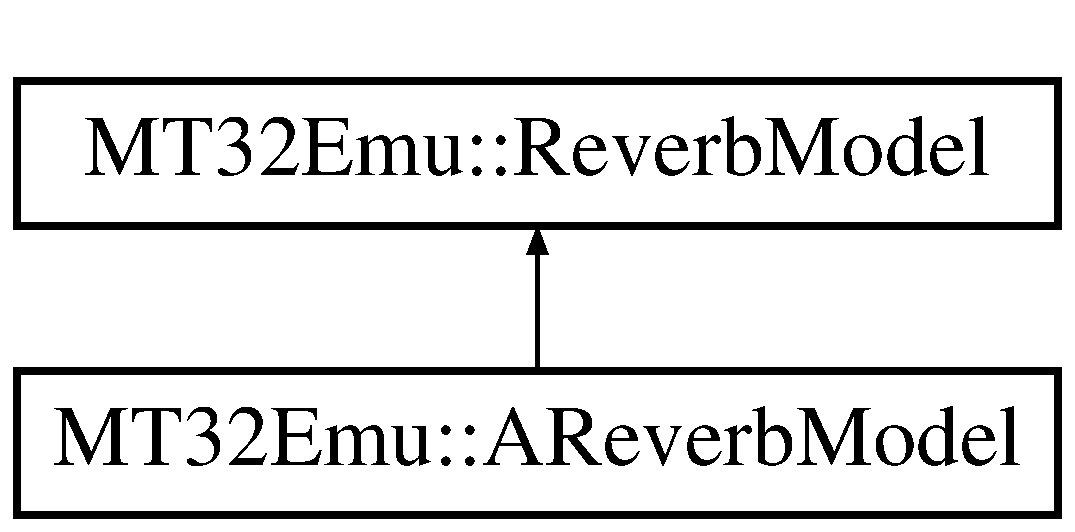
\includegraphics[height=2.000000cm]{classMT32Emu_1_1AReverbModel}
\end{center}
\end{figure}
\subsection*{Public Member Functions}
\begin{DoxyCompactItemize}
\item 
\hypertarget{classMT32Emu_1_1AReverbModel_af353d5c272bf6a08c244b9450c8c0fb6}{{\bfseries A\-Reverb\-Model} (const Reverb\-Mode mode)}\label{classMT32Emu_1_1AReverbModel_af353d5c272bf6a08c244b9450c8c0fb6}

\item 
\hypertarget{classMT32Emu_1_1AReverbModel_a415f3e6d6bcdcdd92c181194ed07ff36}{void {\bfseries open} ()}\label{classMT32Emu_1_1AReverbModel_a415f3e6d6bcdcdd92c181194ed07ff36}

\item 
\hypertarget{classMT32Emu_1_1AReverbModel_a4f2ee90b54a28533aee857bf718dcbdf}{void {\bfseries close} ()}\label{classMT32Emu_1_1AReverbModel_a4f2ee90b54a28533aee857bf718dcbdf}

\item 
\hypertarget{classMT32Emu_1_1AReverbModel_a3e9dafba76c81fa753dfd67508cfb826}{void {\bfseries set\-Parameters} (Bit8u time, Bit8u level)}\label{classMT32Emu_1_1AReverbModel_a3e9dafba76c81fa753dfd67508cfb826}

\item 
\hypertarget{classMT32Emu_1_1AReverbModel_ac4600ff6b73541c3a424dd0dd9f5c14b}{void {\bfseries process} (const float $\ast$in\-Left, const float $\ast$in\-Right, float $\ast$out\-Left, float $\ast$out\-Right, unsigned long num\-Samples)}\label{classMT32Emu_1_1AReverbModel_ac4600ff6b73541c3a424dd0dd9f5c14b}

\item 
\hypertarget{classMT32Emu_1_1AReverbModel_a4789d6f78a8e518eaa3338a09d1c4293}{bool {\bfseries is\-Active} () const }\label{classMT32Emu_1_1AReverbModel_a4789d6f78a8e518eaa3338a09d1c4293}

\end{DoxyCompactItemize}


\subsection{Detailed Description}


Definition at line 66 of file A\-Reverb\-Model.\-h.



The documentation for this class was generated from the following files\-:\begin{DoxyCompactItemize}
\item 
src/mt32/A\-Reverb\-Model.\-h\item 
src/mt32/A\-Reverb\-Model.\-cpp\end{DoxyCompactItemize}

\hypertarget{structMT32Emu_1_1AReverbSettings}{\section{M\-T32\-Emu\-:\-:A\-Reverb\-Settings Struct Reference}
\label{structMT32Emu_1_1AReverbSettings}\index{M\-T32\-Emu\-::\-A\-Reverb\-Settings@{M\-T32\-Emu\-::\-A\-Reverb\-Settings}}
}
\subsection*{Public Attributes}
\begin{DoxyCompactItemize}
\item 
\hypertarget{structMT32Emu_1_1AReverbSettings_a0e48689b578aa7de420d43ca393e3493}{const Bit32u $\ast$const {\bfseries allpass\-Sizes}}\label{structMT32Emu_1_1AReverbSettings_a0e48689b578aa7de420d43ca393e3493}

\item 
\hypertarget{structMT32Emu_1_1AReverbSettings_ab055a1bf6c36fe4364e019fe44b25b91}{const Bit32u $\ast$const {\bfseries comb\-Sizes}}\label{structMT32Emu_1_1AReverbSettings_ab055a1bf6c36fe4364e019fe44b25b91}

\item 
\hypertarget{structMT32Emu_1_1AReverbSettings_ad631c59231e2703abd09af7e82656082}{const Bit32u $\ast$const {\bfseries out\-L\-Positions}}\label{structMT32Emu_1_1AReverbSettings_ad631c59231e2703abd09af7e82656082}

\item 
\hypertarget{structMT32Emu_1_1AReverbSettings_a0401bf71604f968d4d804c0815536f11}{const Bit32u $\ast$const {\bfseries out\-R\-Positions}}\label{structMT32Emu_1_1AReverbSettings_a0401bf71604f968d4d804c0815536f11}

\item 
\hypertarget{structMT32Emu_1_1AReverbSettings_a6bf6a62465af9e2d29a2d266772d9797}{const Bit32u $\ast$const {\bfseries filter\-Factor}}\label{structMT32Emu_1_1AReverbSettings_a6bf6a62465af9e2d29a2d266772d9797}

\item 
\hypertarget{structMT32Emu_1_1AReverbSettings_ad5d0d4136dae254d8ee4cc48f50ff1f2}{const Bit32u $\ast$const {\bfseries decay\-Times}}\label{structMT32Emu_1_1AReverbSettings_ad5d0d4136dae254d8ee4cc48f50ff1f2}

\item 
\hypertarget{structMT32Emu_1_1AReverbSettings_a5df064b718491b6a60f80536080e87c7}{const Bit32u $\ast$const {\bfseries wet\-Levels}}\label{structMT32Emu_1_1AReverbSettings_a5df064b718491b6a60f80536080e87c7}

\item 
\hypertarget{structMT32Emu_1_1AReverbSettings_ad539826807fd10b2edcc6b7454c5dbe8}{const Bit32u {\bfseries lpf\-Amp}}\label{structMT32Emu_1_1AReverbSettings_ad539826807fd10b2edcc6b7454c5dbe8}

\end{DoxyCompactItemize}


\subsection{Detailed Description}


Definition at line 23 of file A\-Reverb\-Model.\-h.



The documentation for this struct was generated from the following file\-:\begin{DoxyCompactItemize}
\item 
src/mt32/A\-Reverb\-Model.\-h\end{DoxyCompactItemize}

\hypertarget{structattotime}{\section{attotime Struct Reference}
\label{structattotime}\index{attotime@{attotime}}
}
\subsection*{Static Public Member Functions}
\begin{DoxyCompactItemize}
\item 
\hypertarget{structattotime_a79c6fbc999e30d5002d9d5a99676b287}{static \hyperlink{structattotime}{attotime} {\bfseries from\-\_\-hz} (int hz)}\label{structattotime_a79c6fbc999e30d5002d9d5a99676b287}

\end{DoxyCompactItemize}
\subsection*{Public Attributes}
\begin{DoxyCompactItemize}
\item 
\hypertarget{structattotime_a4aa7fd0f746f87097d28c1678e5f21b5}{int {\bfseries whatever}}\label{structattotime_a4aa7fd0f746f87097d28c1678e5f21b5}

\end{DoxyCompactItemize}


\subsection{Detailed Description}


Definition at line 75 of file emu.\-h.



The documentation for this struct was generated from the following file\-:\begin{DoxyCompactItemize}
\item 
src/hardware/mame/emu.\-h\end{DoxyCompactItemize}

\hypertarget{classAUTOEXEC}{\section{A\-U\-T\-O\-E\-X\-E\-C Class Reference}
\label{classAUTOEXEC}\index{A\-U\-T\-O\-E\-X\-E\-C@{A\-U\-T\-O\-E\-X\-E\-C}}
}
Inheritance diagram for A\-U\-T\-O\-E\-X\-E\-C\-:\begin{figure}[H]
\begin{center}
\leavevmode
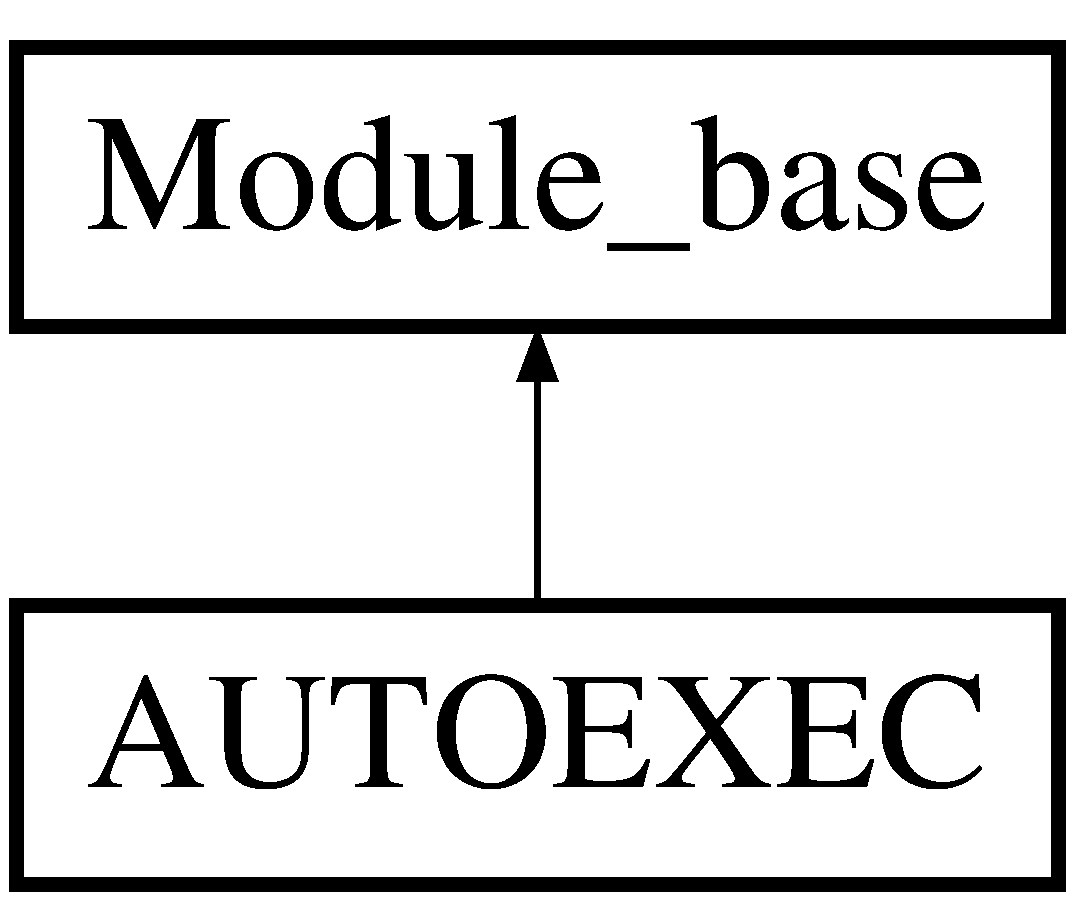
\includegraphics[height=2.000000cm]{classAUTOEXEC}
\end{center}
\end{figure}
\subsection*{Public Member Functions}
\begin{DoxyCompactItemize}
\item 
\hypertarget{classAUTOEXEC_a0c36ab7cc15d2e8ed2fc590cafc89672}{{\bfseries A\-U\-T\-O\-E\-X\-E\-C} (\hyperlink{classSection}{Section} $\ast$configuration)}\label{classAUTOEXEC_a0c36ab7cc15d2e8ed2fc590cafc89672}

\end{DoxyCompactItemize}


\subsection{Detailed Description}


Definition at line 417 of file shell.\-cpp.



The documentation for this class was generated from the following file\-:\begin{DoxyCompactItemize}
\item 
src/shell/shell.\-cpp\end{DoxyCompactItemize}

\hypertarget{classAutoexecEditor}{\section{Autoexec\-Editor Class Reference}
\label{classAutoexecEditor}\index{Autoexec\-Editor@{Autoexec\-Editor}}
}
Inheritance diagram for Autoexec\-Editor\-:\begin{figure}[H]
\begin{center}
\leavevmode
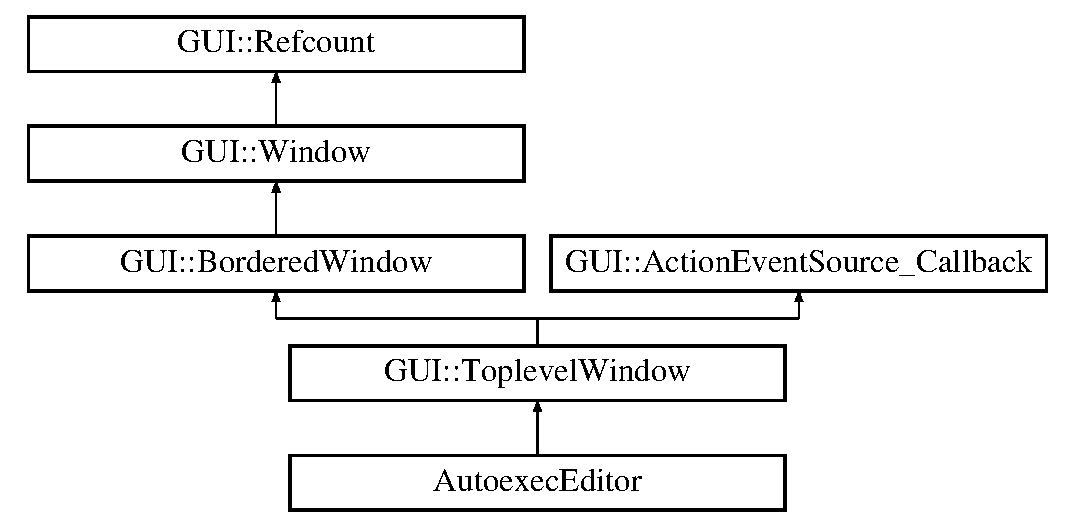
\includegraphics[height=5.000000cm]{classAutoexecEditor}
\end{center}
\end{figure}
\subsection*{Public Member Functions}
\begin{DoxyCompactItemize}
\item 
\hypertarget{classAutoexecEditor_ae2c55e6e3715432d9c394f1dec2f4255}{{\bfseries Autoexec\-Editor} (\hyperlink{classGUI_1_1Screen}{G\-U\-I\-::\-Screen} $\ast$\hyperlink{classGUI_1_1Window_a2e593ff65e7702178d82fe9010a0b539}{parent}, int \hyperlink{classGUI_1_1Window_a6ca6a80ca00c9e1d8ceea8d3d99a657d}{x}, int \hyperlink{classGUI_1_1Window_a0ee8e923aff2c3661fc2e17656d37adf}{y}, \hyperlink{classSection__line}{Section\-\_\-line} $\ast$section)}\label{classAutoexecEditor_ae2c55e6e3715432d9c394f1dec2f4255}

\item 
\hypertarget{classAutoexecEditor_a5103a2bb5e750230a808ce091448ed05}{void \hyperlink{classAutoexecEditor_a5103a2bb5e750230a808ce091448ed05}{action\-Executed} (\hyperlink{classGUI_1_1ActionEventSource}{G\-U\-I\-::\-Action\-Event\-Source} $\ast$b, const \hyperlink{classGUI_1_1String}{G\-U\-I\-::\-String} \&arg)}\label{classAutoexecEditor_a5103a2bb5e750230a808ce091448ed05}

\begin{DoxyCompactList}\small\item\em Menu callback function. \end{DoxyCompactList}\item 
\hypertarget{classAutoexecEditor_ac0720e029f17584c845af698f3c72ceb}{virtual bool \hyperlink{classAutoexecEditor_ac0720e029f17584c845af698f3c72ceb}{key\-Down} (const \hyperlink{classGUI_1_1Key}{G\-U\-I\-::\-Key} \&key)}\label{classAutoexecEditor_ac0720e029f17584c845af698f3c72ceb}

\begin{DoxyCompactList}\small\item\em Key was pressed. Returns true if event was handled. \end{DoxyCompactList}\item 
\hypertarget{classAutoexecEditor_a6c9f4c06e4f6e8e92f6d40e4b0d0eec6}{virtual bool \hyperlink{classAutoexecEditor_a6c9f4c06e4f6e8e92f6d40e4b0d0eec6}{key\-Up} (const \hyperlink{classGUI_1_1Key}{G\-U\-I\-::\-Key} \&key)}\label{classAutoexecEditor_a6c9f4c06e4f6e8e92f6d40e4b0d0eec6}

\begin{DoxyCompactList}\small\item\em Key was released. Returns true if event was handled. \end{DoxyCompactList}\end{DoxyCompactItemize}
\subsection*{Public Attributes}
\begin{DoxyCompactItemize}
\item 
\hypertarget{classAutoexecEditor_af1d96f7032869aac93bba3fae830c902}{std\-::vector$<$ \hyperlink{namespaceGUI_af6b04b46d40197b4f00e553d7d1a3e4c}{G\-U\-I\-::\-Char} $>$ {\bfseries cfg\-\_\-sname}}\label{classAutoexecEditor_af1d96f7032869aac93bba3fae830c902}

\end{DoxyCompactItemize}


\subsection{Detailed Description}


Definition at line 835 of file sdl\-\_\-gui.\-cpp.



The documentation for this class was generated from the following file\-:\begin{DoxyCompactItemize}
\item 
src/gui/sdl\-\_\-gui.\-cpp\end{DoxyCompactItemize}

\hypertarget{classAutoexecObject}{\section{Autoexec\-Object Class Reference}
\label{classAutoexecObject}\index{Autoexec\-Object@{Autoexec\-Object}}
}
\subsection*{Public Member Functions}
\begin{DoxyCompactItemize}
\item 
\hypertarget{classAutoexecObject_a30b975e4cf89783c6e56025c60479ca1}{void {\bfseries Install} (std\-::string const \&in)}\label{classAutoexecObject_a30b975e4cf89783c6e56025c60479ca1}

\item 
\hypertarget{classAutoexecObject_a006d09ad8eef5bc34e1d72778a96cce6}{void {\bfseries Install\-Before} (std\-::string const \&in)}\label{classAutoexecObject_a006d09ad8eef5bc34e1d72778a96cce6}

\item 
\hypertarget{classAutoexecObject_a62d93cd9fdbf05b70f05410ae7bb73df}{void {\bfseries Uninstall} ()}\label{classAutoexecObject_a62d93cd9fdbf05b70f05410ae7bb73df}

\end{DoxyCompactItemize}


\subsection{Detailed Description}


Definition at line 292 of file shell.\-h.



The documentation for this class was generated from the following files\-:\begin{DoxyCompactItemize}
\item 
include/shell.\-h\item 
src/shell/shell.\-cpp\end{DoxyCompactItemize}

\hypertarget{structavi__writer}{\section{avi\-\_\-writer Struct Reference}
\label{structavi__writer}\index{avi\-\_\-writer@{avi\-\_\-writer}}
}
\subsection*{Public Attributes}
\begin{DoxyCompactItemize}
\item 
\hypertarget{structavi__writer_aac95a9730f68b423547b938ebcb8cad6}{int {\bfseries fd}}\label{structavi__writer_aac95a9730f68b423547b938ebcb8cad6}

\item 
\hypertarget{structavi__writer_ad9e6b7e8487dc55b3099360f9aac08ab}{int {\bfseries own\-\_\-fd}}\label{structavi__writer_ad9e6b7e8487dc55b3099360f9aac08ab}

\item 
\hypertarget{structavi__writer_a5cb2edfa610bfa579783b4135469a7b8}{\hyperlink{structriff__stack}{riff\-\_\-stack} $\ast$ {\bfseries riff}}\label{structavi__writer_a5cb2edfa610bfa579783b4135469a7b8}

\item 
\hypertarget{structavi__writer_ae4c26345232fe2ffcebf5ad659f23d6d}{\hyperlink{structriff__chunk}{riff\-\_\-chunk} {\bfseries movi}}\label{structavi__writer_ae4c26345232fe2ffcebf5ad659f23d6d}

\item 
\hypertarget{structavi__writer_a6346fa58152b7e21d7a5c29d9c2931c0}{\hyperlink{structriff__chunk}{riff\-\_\-chunk} {\bfseries avih}}\label{structavi__writer_a6346fa58152b7e21d7a5c29d9c2931c0}

\item 
\hypertarget{structavi__writer_a9ad50465180ee0cb7a1f365852f82db3}{int {\bfseries state}}\label{structavi__writer_a9ad50465180ee0cb7a1f365852f82db3}

\item 
\hypertarget{structavi__writer_aa75f9c8fe6c68b60880a55662c2ee52c}{int {\bfseries avi\-\_\-stream\-\_\-max}}\label{structavi__writer_aa75f9c8fe6c68b60880a55662c2ee52c}

\item 
\hypertarget{structavi__writer_ab6f4d53c8b39385097169a910e9fe8b7}{int {\bfseries avi\-\_\-stream\-\_\-alloc}}\label{structavi__writer_ab6f4d53c8b39385097169a910e9fe8b7}

\item 
\hypertarget{structavi__writer_a55f25ac16fdee1b49b9f3d7c5945b4e1}{\hyperlink{structavi__writer__stream}{avi\-\_\-writer\-\_\-stream} $\ast$ {\bfseries avi\-\_\-stream}}\label{structavi__writer_a55f25ac16fdee1b49b9f3d7c5945b4e1}

\item 
\hypertarget{structavi__writer_ae45d37b94f464140c7b72d34afc6872f}{riff\-\_\-avih\-\_\-\-A\-V\-I\-M\-A\-I\-N\-H\-E\-A\-D\-E\-R {\bfseries main\-\_\-header}}\label{structavi__writer_ae45d37b94f464140c7b72d34afc6872f}

\item 
\hypertarget{structavi__writer_a86bcbf4355e480c468d022a242c409cd}{unsigned char {\bfseries enable\-\_\-opendml\-\_\-index}}\label{structavi__writer_a86bcbf4355e480c468d022a242c409cd}

\item 
\hypertarget{structavi__writer_a6d6f583c63a41c8bdafab08917be0502}{unsigned char {\bfseries enable\-\_\-avioldindex}}\label{structavi__writer_a6d6f583c63a41c8bdafab08917be0502}

\item 
\hypertarget{structavi__writer_a20a72d9c0c02aad7e29d990a95bbd6ee}{unsigned char {\bfseries enable\-\_\-opendml}}\label{structavi__writer_a20a72d9c0c02aad7e29d990a95bbd6ee}

\item 
\hypertarget{structavi__writer_a782cf8d91dbac349e50a41d235992981}{unsigned char {\bfseries enable\-\_\-stream\-\_\-writing}}\label{structavi__writer_a782cf8d91dbac349e50a41d235992981}

\item 
\hypertarget{structavi__writer_a6aef002eb800b9bc3f8c46514d3a643f}{unsigned char {\bfseries wrote\-\_\-idx1}}\label{structavi__writer_a6aef002eb800b9bc3f8c46514d3a643f}

\item 
\hypertarget{structavi__writer_a67dd537f434d6ed39afce1674de95b34}{unsigned int {\bfseries group}}\label{structavi__writer_a67dd537f434d6ed39afce1674de95b34}

\end{DoxyCompactItemize}


\subsection{Detailed Description}


Definition at line 56 of file avi\-\_\-writer.\-h.



The documentation for this struct was generated from the following file\-:\begin{DoxyCompactItemize}
\item 
src/aviwriter/avi\-\_\-writer.\-h\end{DoxyCompactItemize}

\hypertarget{structavi__writer__stream}{\section{avi\-\_\-writer\-\_\-stream Struct Reference}
\label{structavi__writer__stream}\index{avi\-\_\-writer\-\_\-stream@{avi\-\_\-writer\-\_\-stream}}
}
\subsection*{Public Attributes}
\begin{DoxyCompactItemize}
\item 
\hypertarget{structavi__writer__stream_a721b5b94ce37f8700e4058ea1ae0b1da}{int {\bfseries index}}\label{structavi__writer__stream_a721b5b94ce37f8700e4058ea1ae0b1da}

\item 
\hypertarget{structavi__writer__stream_ac32becbec8a943e82a8c5a395c0de94a}{riff\-\_\-strh\-\_\-\-A\-V\-I\-S\-T\-R\-E\-A\-M\-H\-E\-A\-D\-E\-R {\bfseries header}}\label{structavi__writer__stream_ac32becbec8a943e82a8c5a395c0de94a}

\item 
\hypertarget{structavi__writer__stream_a5ee57c2278d8bf29ccb3fbd909b8dc8d}{riff\-\_\-indx\-\_\-\-A\-V\-I\-S\-U\-P\-E\-R\-I\-N\-D\-E\-X {\bfseries superindex}}\label{structavi__writer__stream_a5ee57c2278d8bf29ccb3fbd909b8dc8d}

\item 
\hypertarget{structavi__writer__stream_a4c2f39d0e88506acab9bbc1e8fe227dc}{const char $\ast$ {\bfseries name}}\label{structavi__writer__stream_a4c2f39d0e88506acab9bbc1e8fe227dc}

\item 
\hypertarget{structavi__writer__stream_a4ff77d296a5cbcdb4ab0c17a43e115a4}{void $\ast$ {\bfseries format}}\label{structavi__writer__stream_a4ff77d296a5cbcdb4ab0c17a43e115a4}

\item 
\hypertarget{structavi__writer__stream_a60e7211eace59072d4dcdb195df7a1a5}{size\-\_\-t {\bfseries format\-\_\-len}}\label{structavi__writer__stream_a60e7211eace59072d4dcdb195df7a1a5}

\item 
\hypertarget{structavi__writer__stream_a3af9876066c58d9682621c80357a76fe}{\hyperlink{structriff__chunk}{riff\-\_\-chunk} {\bfseries strh}}\label{structavi__writer__stream_a3af9876066c58d9682621c80357a76fe}

\item 
\hypertarget{structavi__writer__stream_a94250d9c3b4a0b091c15517f9c34ca7f}{\hyperlink{structriff__chunk}{riff\-\_\-chunk} {\bfseries indx}}\label{structavi__writer__stream_a94250d9c3b4a0b091c15517f9c34ca7f}

\item 
\hypertarget{structavi__writer__stream_adc1650f5039e6d87ef33f84d57739ce9}{\hyperlink{structriff__chunk}{riff\-\_\-chunk} {\bfseries indx\-\_\-junk}}\label{structavi__writer__stream_adc1650f5039e6d87ef33f84d57739ce9}

\item 
\hypertarget{structavi__writer__stream_a18738c93a85edc6497654199fc81997e}{\hyperlink{structavi__writer__stream__index}{avi\-\_\-writer\-\_\-stream\-\_\-index} $\ast$ {\bfseries sample\-\_\-index}}\label{structavi__writer__stream_a18738c93a85edc6497654199fc81997e}

\item 
\hypertarget{structavi__writer__stream_a5672a6f4945d3e0545dafaaf3ba1d3f7}{unsigned int {\bfseries sample\-\_\-index\-\_\-alloc}}\label{structavi__writer__stream_a5672a6f4945d3e0545dafaaf3ba1d3f7}

\item 
\hypertarget{structavi__writer__stream_a2f2db114c19282db775e8177c4fa673c}{unsigned int {\bfseries sample\-\_\-index\-\_\-max}}\label{structavi__writer__stream_a2f2db114c19282db775e8177c4fa673c}

\item 
\hypertarget{structavi__writer__stream_a37a1288dab4d9920d6c0962d67dfbdb8}{unsigned int {\bfseries sample\-\_\-write\-\_\-offset}}\label{structavi__writer__stream_a37a1288dab4d9920d6c0962d67dfbdb8}

\item 
\hypertarget{structavi__writer__stream_a0cafa8bf0bf8e256f9dd32987f6725f6}{unsigned int {\bfseries sample\-\_\-write\-\_\-chunk}}\label{structavi__writer__stream_a0cafa8bf0bf8e256f9dd32987f6725f6}

\item 
\hypertarget{structavi__writer__stream_af7a35387b24037cb6eccb73acb09e314}{unsigned int {\bfseries indx\-\_\-entryofs}}\label{structavi__writer__stream_af7a35387b24037cb6eccb73acb09e314}

\item 
\hypertarget{structavi__writer__stream_a64edeb191346191c6c068b5be816644c}{uint32\-\_\-t {\bfseries chunk\-\_\-fourcc}}\label{structavi__writer__stream_a64edeb191346191c6c068b5be816644c}

\item 
\hypertarget{structavi__writer__stream_aff1250ebfae2dfd37438753fe460b1ca}{uint32\-\_\-t {\bfseries group0\-\_\-len}}\label{structavi__writer__stream_aff1250ebfae2dfd37438753fe460b1ca}

\end{DoxyCompactItemize}


\subsection{Detailed Description}


Definition at line 39 of file avi\-\_\-writer.\-h.



The documentation for this struct was generated from the following file\-:\begin{DoxyCompactItemize}
\item 
src/aviwriter/avi\-\_\-writer.\-h\end{DoxyCompactItemize}

\hypertarget{structavi__writer__stream__index}{\section{avi\-\_\-writer\-\_\-stream\-\_\-index Struct Reference}
\label{structavi__writer__stream__index}\index{avi\-\_\-writer\-\_\-stream\-\_\-index@{avi\-\_\-writer\-\_\-stream\-\_\-index}}
}
\subsection*{Public Attributes}
\begin{DoxyCompactItemize}
\item 
\hypertarget{structavi__writer__stream__index_a1c8b47e3bf026a2354d09a2c1ab6b76e}{uint64\-\_\-t {\bfseries stream\-\_\-offset}}\label{structavi__writer__stream__index_a1c8b47e3bf026a2354d09a2c1ab6b76e}

\item 
\hypertarget{structavi__writer__stream__index_abd702cfd30345692d1216b135bc8f0dd}{uint64\-\_\-t {\bfseries offset}}\label{structavi__writer__stream__index_abd702cfd30345692d1216b135bc8f0dd}

\item 
\hypertarget{structavi__writer__stream__index_ac7814b7351c96b888ccad5eb5f1b6858}{uint32\-\_\-t {\bfseries length}}\label{structavi__writer__stream__index_ac7814b7351c96b888ccad5eb5f1b6858}

\item 
\hypertarget{structavi__writer__stream__index_aee37c3956ae6bf797f45d39beaaafa76}{uint32\-\_\-t {\bfseries dw\-Flags}}\label{structavi__writer__stream__index_aee37c3956ae6bf797f45d39beaaafa76}

\end{DoxyCompactItemize}


\subsection{Detailed Description}


Definition at line 14 of file avi\-\_\-writer.\-h.



The documentation for this struct was generated from the following file\-:\begin{DoxyCompactItemize}
\item 
src/aviwriter/avi\-\_\-writer.\-h\end{DoxyCompactItemize}

\hypertarget{classBadConversion}{\section{Bad\-Conversion Class Reference}
\label{classBadConversion}\index{Bad\-Conversion@{Bad\-Conversion}}
}
\subsection*{Public Member Functions}
\begin{DoxyCompactItemize}
\item 
\hypertarget{classBadConversion_acf304d65e2a3f8a7ff2aa489ca3f28d6}{{\bfseries Bad\-Conversion} (const std\-::string \&s)}\label{classBadConversion_acf304d65e2a3f8a7ff2aa489ca3f28d6}

\end{DoxyCompactItemize}


\subsection{Detailed Description}


Definition at line 494 of file sdl\-\_\-gui.\-cpp.



The documentation for this class was generated from the following file\-:\begin{DoxyCompactItemize}
\item 
src/gui/sdl\-\_\-gui.\-cpp\end{DoxyCompactItemize}

\hypertarget{classBatchFile}{\section{Batch\-File Class Reference}
\label{classBatchFile}\index{Batch\-File@{Batch\-File}}
}
Inheritance diagram for Batch\-File\-:\begin{figure}[H]
\begin{center}
\leavevmode
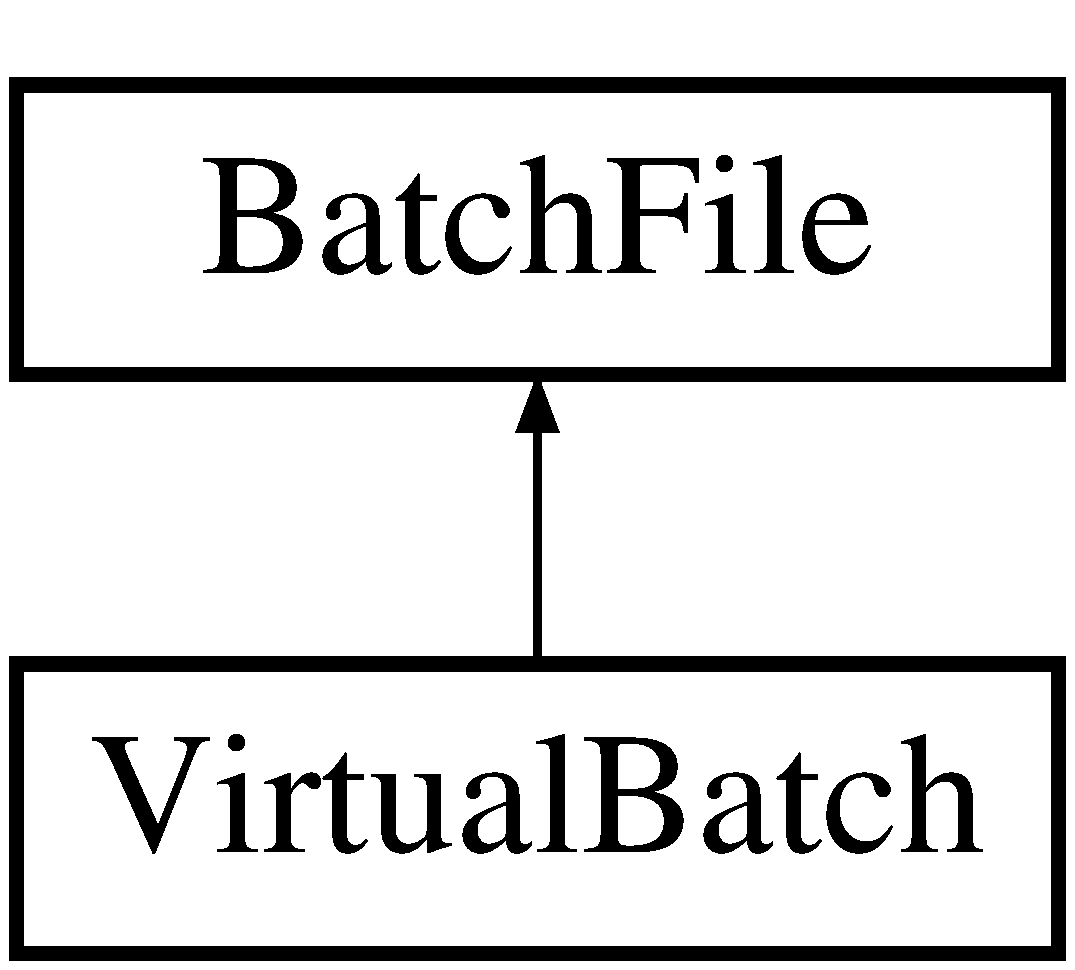
\includegraphics[height=2.000000cm]{classBatchFile}
\end{center}
\end{figure}
\subsection*{Public Member Functions}
\begin{DoxyCompactItemize}
\item 
\hypertarget{classBatchFile_a775abb3eea26411ba33361cc2cc24a5e}{{\bfseries Batch\-File} (\hyperlink{classDOS__Shell}{D\-O\-S\-\_\-\-Shell} $\ast$host, char const $\ast$const resolved\-\_\-name, char const $\ast$const entered\-\_\-name, char const $\ast$const cmd\-\_\-line)}\label{classBatchFile_a775abb3eea26411ba33361cc2cc24a5e}

\item 
\hypertarget{classBatchFile_ae7aff09b12fefc85bdd3004af1346abd}{virtual bool {\bfseries Read\-Line} (char $\ast$line)}\label{classBatchFile_ae7aff09b12fefc85bdd3004af1346abd}

\item 
\hypertarget{classBatchFile_ad0c27c1a7b4a3d48f0b7a456efaeda43}{bool {\bfseries Goto} (char $\ast$where)}\label{classBatchFile_ad0c27c1a7b4a3d48f0b7a456efaeda43}

\item 
\hypertarget{classBatchFile_a41d411d2ace578a96093aefcac40f8d3}{void {\bfseries Shift} (void)}\label{classBatchFile_a41d411d2ace578a96093aefcac40f8d3}

\end{DoxyCompactItemize}
\subsection*{Public Attributes}
\begin{DoxyCompactItemize}
\item 
\hypertarget{classBatchFile_a0e668547306df551eb7e70baa98241e9}{Bit16u {\bfseries file\-\_\-handle}}\label{classBatchFile_a0e668547306df551eb7e70baa98241e9}

\item 
\hypertarget{classBatchFile_aa9209ce7918ced6ce1a2fc59fff4b0c9}{Bit32u {\bfseries location}}\label{classBatchFile_aa9209ce7918ced6ce1a2fc59fff4b0c9}

\item 
\hypertarget{classBatchFile_ac6faaf367cb17424acd15724a58448ab}{bool {\bfseries echo}}\label{classBatchFile_ac6faaf367cb17424acd15724a58448ab}

\item 
\hypertarget{classBatchFile_a739d699f3d7abf36ae6e85ebe80d80b0}{\hyperlink{classDOS__Shell}{D\-O\-S\-\_\-\-Shell} $\ast$ {\bfseries shell}}\label{classBatchFile_a739d699f3d7abf36ae6e85ebe80d80b0}

\item 
\hypertarget{classBatchFile_a6369bd4d3b07b7661e49aaf43f4ed622}{\hyperlink{classBatchFile}{Batch\-File} $\ast$ {\bfseries prev}}\label{classBatchFile_a6369bd4d3b07b7661e49aaf43f4ed622}

\item 
\hypertarget{classBatchFile_a2b1bcf8ea0fb7f71633708a9886e67ee}{\hyperlink{classCommandLine}{Command\-Line} $\ast$ {\bfseries cmd}}\label{classBatchFile_a2b1bcf8ea0fb7f71633708a9886e67ee}

\item 
\hypertarget{classBatchFile_a2deea964df7496637a1843c66d174189}{std\-::string {\bfseries filename}}\label{classBatchFile_a2deea964df7496637a1843c66d174189}

\end{DoxyCompactItemize}


\subsection{Detailed Description}


Definition at line 44 of file shell.\-h.



The documentation for this class was generated from the following files\-:\begin{DoxyCompactItemize}
\item 
include/shell.\-h\item 
src/shell/shell\-\_\-batch.\-cpp\end{DoxyCompactItemize}

\hypertarget{classBIOS}{\section{B\-I\-O\-S Class Reference}
\label{classBIOS}\index{B\-I\-O\-S@{B\-I\-O\-S}}
}
Inheritance diagram for B\-I\-O\-S\-:\begin{figure}[H]
\begin{center}
\leavevmode
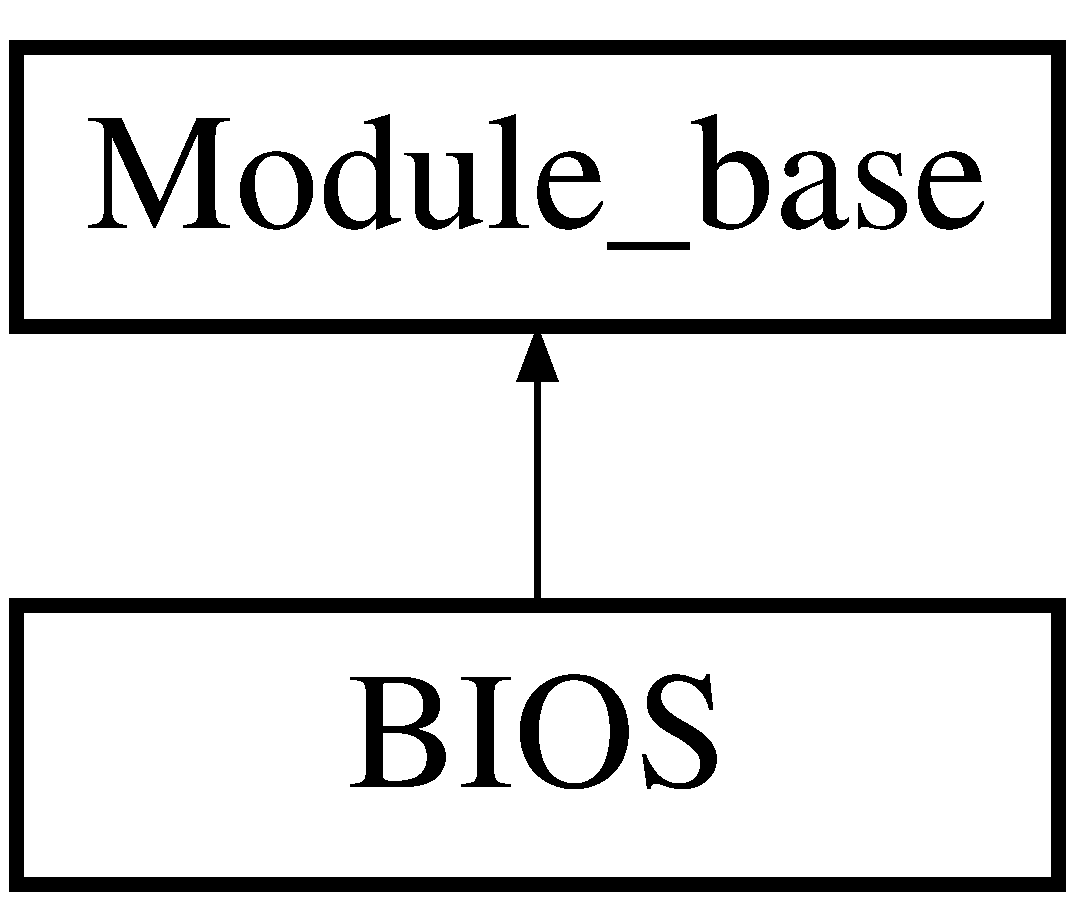
\includegraphics[height=2.000000cm]{classBIOS}
\end{center}
\end{figure}
\subsection*{Public Member Functions}
\begin{DoxyCompactItemize}
\item 
\hypertarget{classBIOS_ae2cf67c9872366656b32695ce56b3c0a}{void {\bfseries write\-\_\-\-F\-F\-F\-F\-\_\-signature} ()}\label{classBIOS_ae2cf67c9872366656b32695ce56b3c0a}

\item 
\hypertarget{classBIOS_a04ed247011d175b84c556487820fd64c}{{\bfseries B\-I\-O\-S} (\hyperlink{classSection}{Section} $\ast$configuration)}\label{classBIOS_a04ed247011d175b84c556487820fd64c}

\end{DoxyCompactItemize}


\subsection{Detailed Description}


Definition at line 6897 of file bios.\-cpp.



The documentation for this class was generated from the following file\-:\begin{DoxyCompactItemize}
\item 
src/ints/bios.\-cpp\end{DoxyCompactItemize}

\hypertarget{classGUI_1_1BitmapFont}{\section{G\-U\-I\-:\-:Bitmap\-Font Class Reference}
\label{classGUI_1_1BitmapFont}\index{G\-U\-I\-::\-Bitmap\-Font@{G\-U\-I\-::\-Bitmap\-Font}}
}


A bitmap font. This is a font which is defined by a binary bit map. Each bit in the bitmap defines one pixel. Bits may be arranged in various common patterns.  




{\ttfamily \#include $<$gui\-\_\-tk.\-h$>$}

Inheritance diagram for G\-U\-I\-:\-:Bitmap\-Font\-:\begin{figure}[H]
\begin{center}
\leavevmode
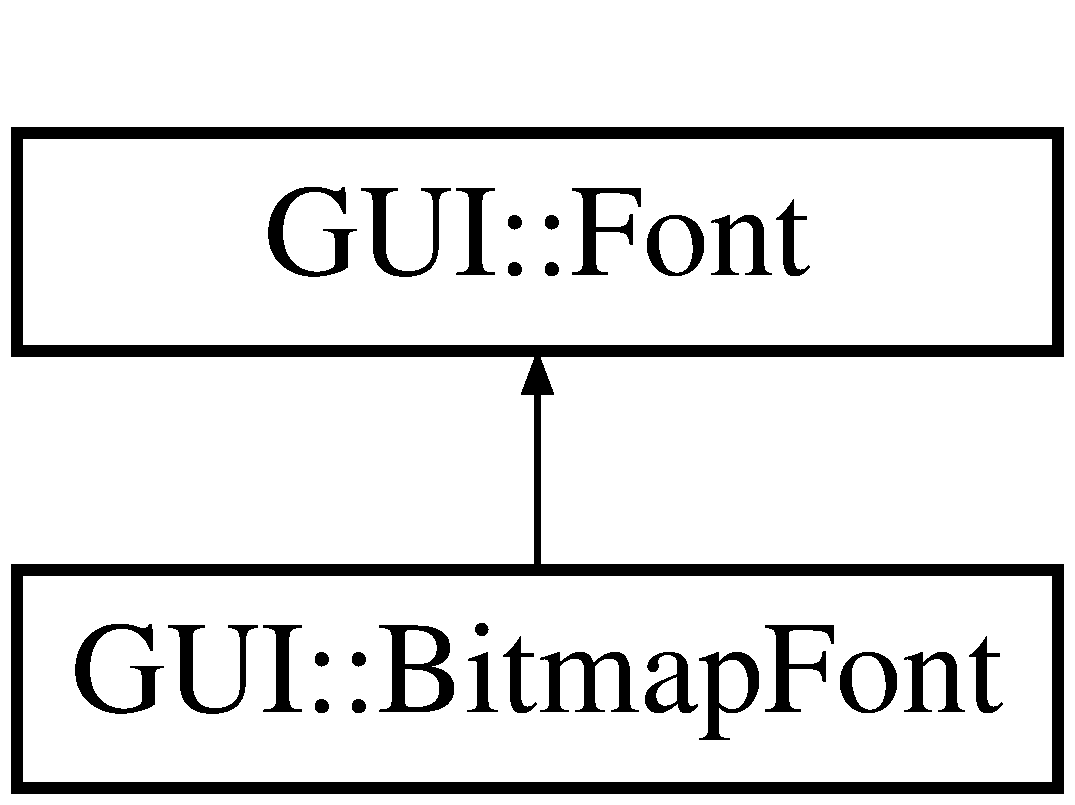
\includegraphics[height=2.000000cm]{classGUI_1_1BitmapFont}
\end{center}
\end{figure}
\subsection*{Public Member Functions}
\begin{DoxyCompactItemize}
\item 
\hyperlink{classGUI_1_1BitmapFont_a110d5562ff912779a85c909cc8d41a04}{Bitmap\-Font} (const unsigned char $\ast$data, int \hyperlink{classGUI_1_1BitmapFont_af24866e4d54b86619d792901e2b86f94}{height}, int \hyperlink{classGUI_1_1BitmapFont_a9a80fabdb72d8e9e289109d1fd41dec7}{ascent}, bool \hyperlink{classGUI_1_1BitmapFont_ac50042f33fedf2c8516294780ed6f128}{owner}=false, int \hyperlink{classGUI_1_1BitmapFont_a0b9e1113ed04f7d766aeb961b64ab0c3}{width}=8, bool \hyperlink{classGUI_1_1BitmapFont_acd705cf60d73c04dd028828a7b5c1da3}{background\-\_\-set}=false, int \hyperlink{classGUI_1_1BitmapFont_ac2fab3c605018ebaa18ff59c54f29e1b}{col\-\_\-step}=-\/1, int \hyperlink{classGUI_1_1BitmapFont_aff605105bf7cffd78dfce7dc24f701ac}{row\-\_\-step}=8, int \hyperlink{classGUI_1_1BitmapFont_a27146558fd76b2ac1c2dc7133b23f4ce}{character\-\_\-step}=0, \hyperlink{namespaceGUI_af6b04b46d40197b4f00e553d7d1a3e4c}{Char} \hyperlink{classGUI_1_1BitmapFont_a3c992d29bbd0d35087365a8e5474686c}{last}=256, const int $\ast$\hyperlink{classGUI_1_1BitmapFont_a3b38670c62db18777d86dc9dac7d8b20}{widths}=N\-U\-L\-L, const int $\ast$\hyperlink{classGUI_1_1BitmapFont_ade167bd18d25f17f944c94f9c1333082}{ascents}=N\-U\-L\-L, const unsigned char $\ast$const $\ast$\hyperlink{classGUI_1_1BitmapFont_a95cd04a0232cd076fcb3021e85d0043b}{char\-\_\-position}=N\-U\-L\-L, const \hyperlink{classGUI_1_1Font_af3c234cd3febe27dbe9c76e6cc5cad3a}{Special\-Char} $\ast$\hyperlink{classGUI_1_1BitmapFont_a46f912c496e902dfc614e25261599718}{special}=N\-U\-L\-L)
\begin{DoxyCompactList}\small\item\em Constructor. \end{DoxyCompactList}\item 
\hypertarget{classGUI_1_1BitmapFont_aa6d1d93bb3c19cca85d49e1d10cd2d7d}{virtual int \hyperlink{classGUI_1_1BitmapFont_aa6d1d93bb3c19cca85d49e1d10cd2d7d}{get\-Height} () const }\label{classGUI_1_1BitmapFont_aa6d1d93bb3c19cca85d49e1d10cd2d7d}

\begin{DoxyCompactList}\small\item\em Retrieve total height of font in pixels. \end{DoxyCompactList}\item 
\hypertarget{classGUI_1_1BitmapFont_abc2f11b1e2cedf4494d7d7ab8db81e09}{virtual int \hyperlink{classGUI_1_1BitmapFont_abc2f11b1e2cedf4494d7d7ab8db81e09}{get\-Ascent} () const }\label{classGUI_1_1BitmapFont_abc2f11b1e2cedf4494d7d7ab8db81e09}

\begin{DoxyCompactList}\small\item\em Retrieve the ascent, i.\-e. the number of pixels above the base line. \end{DoxyCompactList}\item 
\hypertarget{classGUI_1_1BitmapFont_a9929de2620d992dae0acd404a9ccdbea}{virtual int \hyperlink{classGUI_1_1BitmapFont_a9929de2620d992dae0acd404a9ccdbea}{get\-Width} (\hyperlink{namespaceGUI_af6b04b46d40197b4f00e553d7d1a3e4c}{Char} c= 'M') const }\label{classGUI_1_1BitmapFont_a9929de2620d992dae0acd404a9ccdbea}

\begin{DoxyCompactList}\small\item\em Retrieve width of a character. \end{DoxyCompactList}\item 
\hypertarget{classGUI_1_1BitmapFont_ac864500d84219f8818f0741d65194a61}{virtual \hyperlink{classGUI_1_1Font_af3c234cd3febe27dbe9c76e6cc5cad3a}{Special\-Char} \hyperlink{classGUI_1_1BitmapFont_ac864500d84219f8818f0741d65194a61}{to\-Special} (\hyperlink{namespaceGUI_af6b04b46d40197b4f00e553d7d1a3e4c}{Char} c) const }\label{classGUI_1_1BitmapFont_ac864500d84219f8818f0741d65194a61}

\begin{DoxyCompactList}\small\item\em Convert a character to an equivalent Special\-Char. See Font\-::to\-Special(\-Char c) \end{DoxyCompactList}\item 
\hypertarget{classGUI_1_1BitmapFont_a38227a28f83e1c3e0fc01f26161c74ed}{virtual \hyperlink{namespaceGUI_af6b04b46d40197b4f00e553d7d1a3e4c}{Char} \hyperlink{classGUI_1_1BitmapFont_a38227a28f83e1c3e0fc01f26161c74ed}{from\-Special} (\hyperlink{classGUI_1_1Font_af3c234cd3febe27dbe9c76e6cc5cad3a}{Special\-Char} c) const }\label{classGUI_1_1BitmapFont_a38227a28f83e1c3e0fc01f26161c74ed}

\begin{DoxyCompactList}\small\item\em Convert a character to an equivalent character. See Font\-::from\-Special(\-Special\-Char c). \end{DoxyCompactList}\end{DoxyCompactItemize}
\subsection*{Protected Member Functions}
\begin{DoxyCompactItemize}
\item 
virtual void \hyperlink{classGUI_1_1BitmapFont_a46ad991d5469877c111726f535095017}{draw\-Char} (\hyperlink{classGUI_1_1Drawable}{Drawable} $\ast$d, const \hyperlink{namespaceGUI_af6b04b46d40197b4f00e553d7d1a3e4c}{Char} c) const 
\begin{DoxyCompactList}\small\item\em Draw character to a drawable at the current position. \end{DoxyCompactList}\end{DoxyCompactItemize}
\subsection*{Protected Attributes}
\begin{DoxyCompactItemize}
\item 
\hypertarget{classGUI_1_1BitmapFont_a23417d7e1828ded4b965f6a6670322fa}{const unsigned char $\ast$const \hyperlink{classGUI_1_1BitmapFont_a23417d7e1828ded4b965f6a6670322fa}{bitmap}}\label{classGUI_1_1BitmapFont_a23417d7e1828ded4b965f6a6670322fa}

\begin{DoxyCompactList}\small\item\em The actual font data. \end{DoxyCompactList}\item 
\hypertarget{classGUI_1_1BitmapFont_a0b9e1113ed04f7d766aeb961b64ab0c3}{const int \hyperlink{classGUI_1_1BitmapFont_a0b9e1113ed04f7d766aeb961b64ab0c3}{width}}\label{classGUI_1_1BitmapFont_a0b9e1113ed04f7d766aeb961b64ab0c3}

\begin{DoxyCompactList}\small\item\em Width of a character cell. \end{DoxyCompactList}\item 
\hypertarget{classGUI_1_1BitmapFont_af24866e4d54b86619d792901e2b86f94}{const int \hyperlink{classGUI_1_1BitmapFont_af24866e4d54b86619d792901e2b86f94}{height}}\label{classGUI_1_1BitmapFont_af24866e4d54b86619d792901e2b86f94}

\begin{DoxyCompactList}\small\item\em Height of all characters. \end{DoxyCompactList}\item 
\hypertarget{classGUI_1_1BitmapFont_a9a80fabdb72d8e9e289109d1fd41dec7}{const int \hyperlink{classGUI_1_1BitmapFont_a9a80fabdb72d8e9e289109d1fd41dec7}{ascent}}\label{classGUI_1_1BitmapFont_a9a80fabdb72d8e9e289109d1fd41dec7}

\begin{DoxyCompactList}\small\item\em Ascent of all characters. \end{DoxyCompactList}\item 
\hypertarget{classGUI_1_1BitmapFont_a3b38670c62db18777d86dc9dac7d8b20}{const int $\ast$const \hyperlink{classGUI_1_1BitmapFont_a3b38670c62db18777d86dc9dac7d8b20}{widths}}\label{classGUI_1_1BitmapFont_a3b38670c62db18777d86dc9dac7d8b20}

\begin{DoxyCompactList}\small\item\em Array of character widths. If font is fixed-\/width, this is N\-U\-L\-L and {\itshape width\/} is used. \end{DoxyCompactList}\item 
const int $\ast$const \hyperlink{classGUI_1_1BitmapFont_ade167bd18d25f17f944c94f9c1333082}{ascents}
\begin{DoxyCompactList}\small\item\em Array of character ascents. If this is N\-U\-L\-L, {\itshape ascent\/} is used for all characters. \end{DoxyCompactList}\item 
\hypertarget{classGUI_1_1BitmapFont_acd705cf60d73c04dd028828a7b5c1da3}{const bool \hyperlink{classGUI_1_1BitmapFont_acd705cf60d73c04dd028828a7b5c1da3}{background\-\_\-set}}\label{classGUI_1_1BitmapFont_acd705cf60d73c04dd028828a7b5c1da3}

\begin{DoxyCompactList}\small\item\em True if set bits are background, false otherwise. \end{DoxyCompactList}\item 
\hypertarget{classGUI_1_1BitmapFont_ac2fab3c605018ebaa18ff59c54f29e1b}{const int \hyperlink{classGUI_1_1BitmapFont_ac2fab3c605018ebaa18ff59c54f29e1b}{col\-\_\-step}}\label{classGUI_1_1BitmapFont_ac2fab3c605018ebaa18ff59c54f29e1b}

\begin{DoxyCompactList}\small\item\em Number of bits added to get from a column to the next column. \end{DoxyCompactList}\item 
\hypertarget{classGUI_1_1BitmapFont_aff605105bf7cffd78dfce7dc24f701ac}{const int \hyperlink{classGUI_1_1BitmapFont_aff605105bf7cffd78dfce7dc24f701ac}{row\-\_\-step}}\label{classGUI_1_1BitmapFont_aff605105bf7cffd78dfce7dc24f701ac}

\begin{DoxyCompactList}\small\item\em Distance between 2 rows of a character, or 0 for variable-\/width rows. \end{DoxyCompactList}\item 
const int \hyperlink{classGUI_1_1BitmapFont_a27146558fd76b2ac1c2dc7133b23f4ce}{character\-\_\-step}
\begin{DoxyCompactList}\small\item\em Distance of two characters in the bitmap in bits. \end{DoxyCompactList}\item 
\hypertarget{classGUI_1_1BitmapFont_a95cd04a0232cd076fcb3021e85d0043b}{const unsigned char $\ast$const $\ast$const \hyperlink{classGUI_1_1BitmapFont_a95cd04a0232cd076fcb3021e85d0043b}{char\-\_\-position}}\label{classGUI_1_1BitmapFont_a95cd04a0232cd076fcb3021e85d0043b}

\begin{DoxyCompactList}\small\item\em Array of pointers to font data. If set, neither {\itshape bitmap\/} nor {\itshape character\-\_\-step\/} are used. \end{DoxyCompactList}\item 
const \hyperlink{classGUI_1_1Font_af3c234cd3febe27dbe9c76e6cc5cad3a}{Special\-Char} $\ast$const \hyperlink{classGUI_1_1BitmapFont_a46f912c496e902dfc614e25261599718}{special}
\begin{DoxyCompactList}\small\item\em Array of Special\-Char equivalents. \end{DoxyCompactList}\item 
\hypertarget{classGUI_1_1BitmapFont_ac50042f33fedf2c8516294780ed6f128}{const bool \hyperlink{classGUI_1_1BitmapFont_ac50042f33fedf2c8516294780ed6f128}{owner}}\label{classGUI_1_1BitmapFont_ac50042f33fedf2c8516294780ed6f128}

\begin{DoxyCompactList}\small\item\em If {\ttfamily true}, then all arrays are freed on destruction. \end{DoxyCompactList}\item 
\hypertarget{classGUI_1_1BitmapFont_a3c992d29bbd0d35087365a8e5474686c}{const \hyperlink{namespaceGUI_af6b04b46d40197b4f00e553d7d1a3e4c}{Char} \hyperlink{classGUI_1_1BitmapFont_a3c992d29bbd0d35087365a8e5474686c}{last}}\label{classGUI_1_1BitmapFont_a3c992d29bbd0d35087365a8e5474686c}

\begin{DoxyCompactList}\small\item\em Last defined character. Characters above this will be ignored. \end{DoxyCompactList}\end{DoxyCompactItemize}


\subsection{Detailed Description}
A bitmap font. This is a font which is defined by a binary bit map. Each bit in the bitmap defines one pixel. Bits may be arranged in various common patterns. 

Encoding free, character size depends on number of characters in the font. 

Definition at line 1214 of file gui\-\_\-tk.\-h.



\subsection{Constructor \& Destructor Documentation}
\hypertarget{classGUI_1_1BitmapFont_a110d5562ff912779a85c909cc8d41a04}{\index{G\-U\-I\-::\-Bitmap\-Font@{G\-U\-I\-::\-Bitmap\-Font}!Bitmap\-Font@{Bitmap\-Font}}
\index{Bitmap\-Font@{Bitmap\-Font}!GUI::BitmapFont@{G\-U\-I\-::\-Bitmap\-Font}}
\subsubsection[{Bitmap\-Font}]{\setlength{\rightskip}{0pt plus 5cm}{\bf G\-U\-I\-::\-Bitmap\-Font\-::\-Bitmap\-Font} (
\begin{DoxyParamCaption}
\item[{const unsigned char $\ast$}]{data, }
\item[{int}]{height, }
\item[{int}]{ascent, }
\item[{bool}]{owner = {\ttfamily false}, }
\item[{int}]{width = {\ttfamily 8}, }
\item[{bool}]{background\-\_\-set = {\ttfamily false}, }
\item[{int}]{col\-\_\-step = {\ttfamily -\/1}, }
\item[{int}]{row\-\_\-step = {\ttfamily 8}, }
\item[{int}]{character\-\_\-step = {\ttfamily 0}, }
\item[{{\bf Char}}]{last = {\ttfamily 256}, }
\item[{const int $\ast$}]{widths = {\ttfamily NULL}, }
\item[{const int $\ast$}]{ascents = {\ttfamily NULL}, }
\item[{const unsigned char $\ast$const $\ast$}]{char\-\_\-position = {\ttfamily NULL}, }
\item[{const {\bf Special\-Char} $\ast$}]{special = {\ttfamily NULL}}
\end{DoxyParamCaption}
)}}\label{classGUI_1_1BitmapFont_a110d5562ff912779a85c909cc8d41a04}


Constructor. 

The default values provide an 8 bit wide fixed-\/width pixel layout with each byte a row, arranged top-\/to-\/bottom just like a P\-C's V\-G\-A font. See the individual member documentation for details on the parameters. 

Definition at line 508 of file gui\-\_\-tk.\-cpp.



\subsection{Member Function Documentation}
\hypertarget{classGUI_1_1BitmapFont_a46ad991d5469877c111726f535095017}{\index{G\-U\-I\-::\-Bitmap\-Font@{G\-U\-I\-::\-Bitmap\-Font}!draw\-Char@{draw\-Char}}
\index{draw\-Char@{draw\-Char}!GUI::BitmapFont@{G\-U\-I\-::\-Bitmap\-Font}}
\subsubsection[{draw\-Char}]{\setlength{\rightskip}{0pt plus 5cm}void {\bf G\-U\-I\-::\-Bitmap\-Font\-::draw\-Char} (
\begin{DoxyParamCaption}
\item[{{\bf Drawable} $\ast$}]{d, }
\item[{const {\bf Char}}]{c}
\end{DoxyParamCaption}
) const\hspace{0.3cm}{\ttfamily  \mbox{[}protected, virtual\mbox{]}}}}\label{classGUI_1_1BitmapFont_a46ad991d5469877c111726f535095017}


Draw character to a drawable at the current position. 

{\ttfamily d's} current position is advanced to the position of the next character. The y coordinate is located at the baseline before and after the call. 

Implements \hyperlink{classGUI_1_1Font_af7fc4fc46ef57e722d6025cdb481da18}{G\-U\-I\-::\-Font}.



Definition at line 419 of file gui\-\_\-tk.\-cpp.



References ascent, ascents, background\-\_\-set, bitmap, char\-\_\-position, character\-\_\-step, col\-\_\-step, G\-U\-I\-::\-Drawable\-::get\-X(), G\-U\-I\-::\-Drawable\-::get\-Y(), G\-U\-I\-::\-Drawable\-::goto\-X\-Y(), height, last, row\-\_\-step, width, and widths.



\subsection{Member Data Documentation}
\hypertarget{classGUI_1_1BitmapFont_ade167bd18d25f17f944c94f9c1333082}{\index{G\-U\-I\-::\-Bitmap\-Font@{G\-U\-I\-::\-Bitmap\-Font}!ascents@{ascents}}
\index{ascents@{ascents}!GUI::BitmapFont@{G\-U\-I\-::\-Bitmap\-Font}}
\subsubsection[{ascents}]{\setlength{\rightskip}{0pt plus 5cm}const int$\ast$ const {\bf G\-U\-I\-::\-Bitmap\-Font\-::ascents}\hspace{0.3cm}{\ttfamily  \mbox{[}protected\mbox{]}}}}\label{classGUI_1_1BitmapFont_ade167bd18d25f17f944c94f9c1333082}


Array of character ascents. If this is N\-U\-L\-L, {\itshape ascent\/} is used for all characters. 

This allows character data to be flush to the top or bottom of it's bitmap area. 

Definition at line 1233 of file gui\-\_\-tk.\-h.



Referenced by draw\-Char().

\hypertarget{classGUI_1_1BitmapFont_a27146558fd76b2ac1c2dc7133b23f4ce}{\index{G\-U\-I\-::\-Bitmap\-Font@{G\-U\-I\-::\-Bitmap\-Font}!character\-\_\-step@{character\-\_\-step}}
\index{character\-\_\-step@{character\-\_\-step}!GUI::BitmapFont@{G\-U\-I\-::\-Bitmap\-Font}}
\subsubsection[{character\-\_\-step}]{\setlength{\rightskip}{0pt plus 5cm}const int {\bf G\-U\-I\-::\-Bitmap\-Font\-::character\-\_\-step}\hspace{0.3cm}{\ttfamily  \mbox{[}protected\mbox{]}}}}\label{classGUI_1_1BitmapFont_a27146558fd76b2ac1c2dc7133b23f4ce}


Distance of two characters in the bitmap in bits. 

This is calculated as abs(row\-\_\-step$\ast$height) unless explicitly specified. 

Definition at line 1246 of file gui\-\_\-tk.\-h.



Referenced by draw\-Char().

\hypertarget{classGUI_1_1BitmapFont_a46f912c496e902dfc614e25261599718}{\index{G\-U\-I\-::\-Bitmap\-Font@{G\-U\-I\-::\-Bitmap\-Font}!special@{special}}
\index{special@{special}!GUI::BitmapFont@{G\-U\-I\-::\-Bitmap\-Font}}
\subsubsection[{special}]{\setlength{\rightskip}{0pt plus 5cm}const {\bf Special\-Char}$\ast$ const {\bf G\-U\-I\-::\-Bitmap\-Font\-::special}\hspace{0.3cm}{\ttfamily  \mbox{[}protected\mbox{]}}}}\label{classGUI_1_1BitmapFont_a46f912c496e902dfc614e25261599718}


Array of Special\-Char equivalents. 

If unset, encoding is assumed A\-S\-C\-I\-I-\/like for the first 32 characters 

Definition at line 1253 of file gui\-\_\-tk.\-h.



Referenced by from\-Special(), and to\-Special().



The documentation for this class was generated from the following files\-:\begin{DoxyCompactItemize}
\item 
src/libs/gui\-\_\-tk/\hyperlink{gui__tk_8h}{gui\-\_\-tk.\-h}\item 
src/libs/gui\-\_\-tk/\hyperlink{gui__tk_8cpp}{gui\-\_\-tk.\-cpp}\end{DoxyCompactItemize}

\hypertarget{classbitop_1_1bitseqlengthandpos__ret__t}{\section{bitop\-:\-:bitseqlengthandpos\-\_\-ret\-\_\-t Class Reference}
\label{classbitop_1_1bitseqlengthandpos__ret__t}\index{bitop\-::bitseqlengthandpos\-\_\-ret\-\_\-t@{bitop\-::bitseqlengthandpos\-\_\-ret\-\_\-t}}
}
\subsection*{Public Member Functions}
\begin{DoxyCompactItemize}
\item 
\hypertarget{classbitop_1_1bitseqlengthandpos__ret__t_ac5bb5423694a5b3c4ccb7d096b47a1e1}{{\bfseries bitseqlengthandpos\-\_\-ret\-\_\-t} (const unsigned int \-\_\-start, const unsigned int \-\_\-length)}\label{classbitop_1_1bitseqlengthandpos__ret__t_ac5bb5423694a5b3c4ccb7d096b47a1e1}

\item 
\hypertarget{classbitop_1_1bitseqlengthandpos__ret__t_aa01c0991734ca8f3d725995a9bf32869}{bool {\bfseries operator==} (const \hyperlink{classbitop_1_1bitseqlengthandpos__ret__t}{bitseqlengthandpos\-\_\-ret\-\_\-t} \&n) const }\label{classbitop_1_1bitseqlengthandpos__ret__t_aa01c0991734ca8f3d725995a9bf32869}

\item 
\hypertarget{classbitop_1_1bitseqlengthandpos__ret__t_a9eff391ef9964c4f387912dd2ec6a5a9}{bool {\bfseries empty} (void) const }\label{classbitop_1_1bitseqlengthandpos__ret__t_a9eff391ef9964c4f387912dd2ec6a5a9}

\end{DoxyCompactItemize}
\subsection*{Public Attributes}
\begin{DoxyCompactItemize}
\item 
\hypertarget{classbitop_1_1bitseqlengthandpos__ret__t_af31d1189102270d27e299c752407399b}{unsigned int {\bfseries start}}\label{classbitop_1_1bitseqlengthandpos__ret__t_af31d1189102270d27e299c752407399b}

\item 
\hypertarget{classbitop_1_1bitseqlengthandpos__ret__t_abc61247669dc39db345d2ca4500789a1}{unsigned int {\bfseries length}}\label{classbitop_1_1bitseqlengthandpos__ret__t_abc61247669dc39db345d2ca4500789a1}

\end{DoxyCompactItemize}


\subsection{Detailed Description}


Definition at line 346 of file bitop.\-h.



The documentation for this class was generated from the following file\-:\begin{DoxyCompactItemize}
\item 
include/bitop.\-h\end{DoxyCompactItemize}

\hypertarget{classRegionAllocTracking_1_1Block}{\section{Region\-Alloc\-Tracking\-:\-:Block Class Reference}
\label{classRegionAllocTracking_1_1Block}\index{Region\-Alloc\-Tracking\-::\-Block@{Region\-Alloc\-Tracking\-::\-Block}}
}
\subsection*{Public Attributes}
\begin{DoxyCompactItemize}
\item 
\hypertarget{classRegionAllocTracking_1_1Block_a72ed7f684a1bb49327fa4b8f109ddfc9}{std\-::string {\bfseries who}}\label{classRegionAllocTracking_1_1Block_a72ed7f684a1bb49327fa4b8f109ddfc9}

\item 
\hypertarget{classRegionAllocTracking_1_1Block_a310d3de7018492b64fd7bac4cb640fb0}{Bitu {\bfseries start}}\label{classRegionAllocTracking_1_1Block_a310d3de7018492b64fd7bac4cb640fb0}

\item 
\hypertarget{classRegionAllocTracking_1_1Block_ab8aa00f0ccd051668d60b36b69f9477e}{Bitu {\bfseries end}}\label{classRegionAllocTracking_1_1Block_ab8aa00f0ccd051668d60b36b69f9477e}

\item 
\hypertarget{classRegionAllocTracking_1_1Block_a10cc004ce165b0bf7c42acd50419c9fd}{bool {\bfseries free}}\label{classRegionAllocTracking_1_1Block_a10cc004ce165b0bf7c42acd50419c9fd}

\end{DoxyCompactItemize}


\subsection{Detailed Description}


Definition at line 13 of file regionalloctracking.\-h.



The documentation for this class was generated from the following files\-:\begin{DoxyCompactItemize}
\item 
include/regionalloctracking.\-h\item 
src/misc/regionalloctracking.\-cpp\end{DoxyCompactItemize}

\hypertarget{classBOOT}{\section{B\-O\-O\-T Class Reference}
\label{classBOOT}\index{B\-O\-O\-T@{B\-O\-O\-T}}
}


B\-O\-O\-T.\-C\-O\-M utility to boot a floppy or hard disk device.  


Inheritance diagram for B\-O\-O\-T\-:\begin{figure}[H]
\begin{center}
\leavevmode
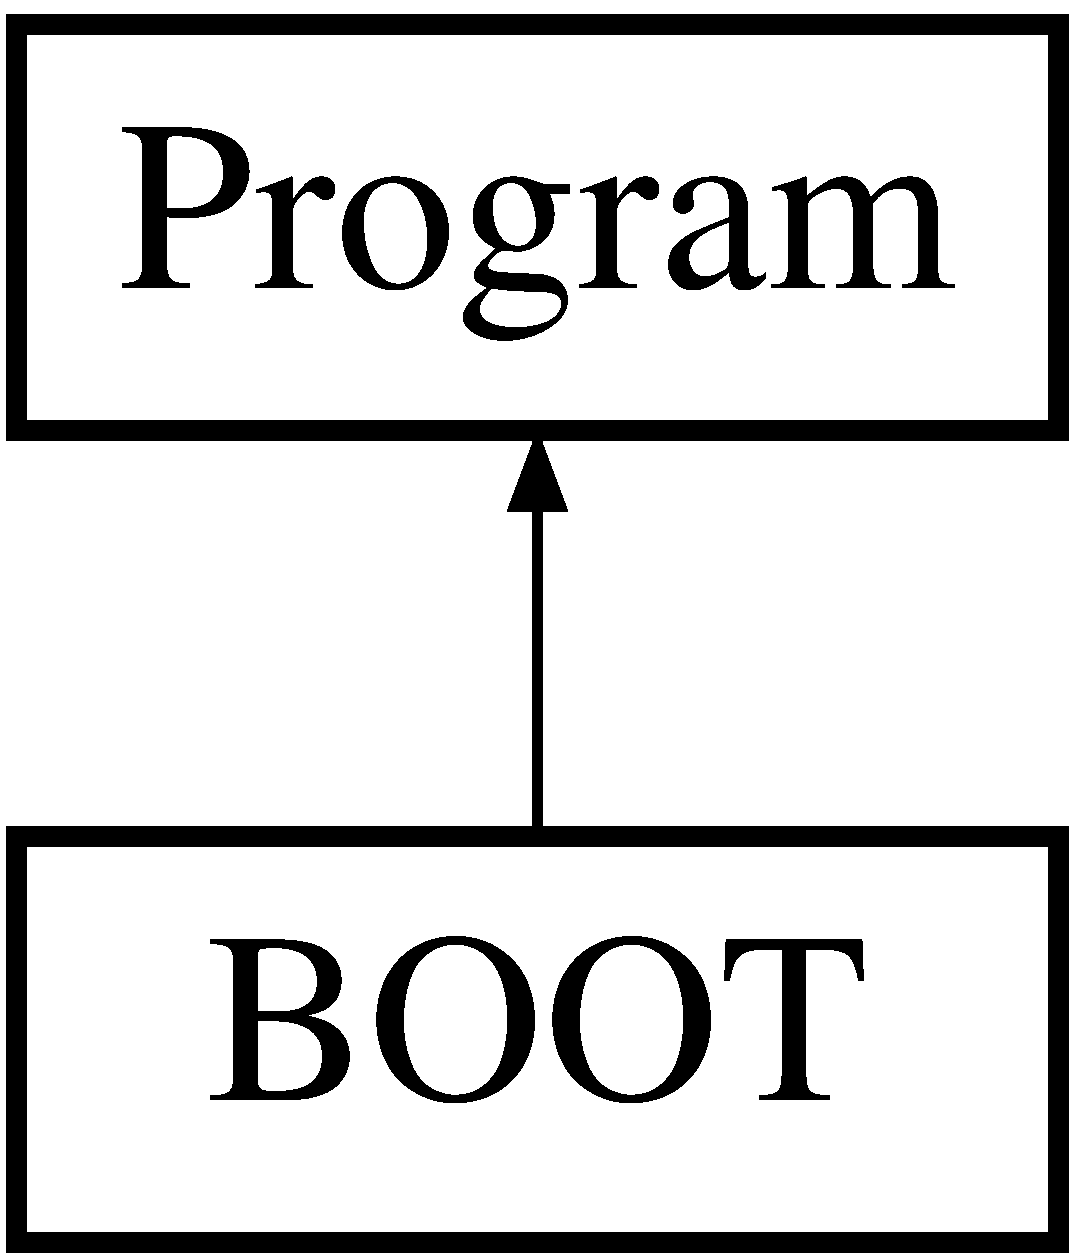
\includegraphics[height=2.000000cm]{classBOOT}
\end{center}
\end{figure}
\subsection*{Public Member Functions}
\begin{DoxyCompactItemize}
\item 
\hypertarget{classBOOT_a246ff7f80fc219360cdef4c3faa93d40}{void \hyperlink{classBOOT_a246ff7f80fc219360cdef4c3faa93d40}{Run} (void)}\label{classBOOT_a246ff7f80fc219360cdef4c3faa93d40}

\begin{DoxyCompactList}\small\item\em \hyperlink{classProgram}{Program} entry point, when the command is run. \end{DoxyCompactList}\end{DoxyCompactItemize}
\subsection*{Public Attributes}
\begin{DoxyCompactItemize}
\item 
\hypertarget{classBOOT_ab165a586fbff98d26e21fba090440209}{\hyperlink{classimageDisk}{image\-Disk} $\ast$ \hyperlink{classBOOT_ab165a586fbff98d26e21fba090440209}{new\-Disk\-Swap} \mbox{[}M\-A\-X\-\_\-\-S\-W\-A\-P\-P\-A\-B\-L\-E\-\_\-\-D\-I\-S\-K\-S\mbox{]}}\label{classBOOT_ab165a586fbff98d26e21fba090440209}

\begin{DoxyCompactList}\small\item\em Array of disk images to add to floppy swaplist. \end{DoxyCompactList}\end{DoxyCompactItemize}


\subsection{Detailed Description}
B\-O\-O\-T.\-C\-O\-M utility to boot a floppy or hard disk device. 

Users will use this command to boot a guest operating system from a disk image. Options are provided to specify the device to boot from (if the image is already assigned) or a floppy disk image specified on the command line. 

Definition at line 707 of file dos\-\_\-programs.\-cpp.



The documentation for this class was generated from the following file\-:\begin{DoxyCompactItemize}
\item 
src/dos/dos\-\_\-programs.\-cpp\end{DoxyCompactItemize}

\hypertarget{unionbootSector}{\section{boot\-Sector Union Reference}
\label{unionbootSector}\index{boot\-Sector@{boot\-Sector}}
}
\subsection*{Classes}
\begin{DoxyCompactItemize}
\item 
struct \hyperlink{structbootSector_1_1entries}{entries}
\end{DoxyCompactItemize}
\subsection*{Public Attributes}
\begin{DoxyCompactItemize}
\item 
\hypertarget{unionbootSector_a830dde936204711342d54f9150fedeaf}{struct \hyperlink{structbootSector_1_1entries}{boot\-Sector\-::entries} {\bfseries bootdata}}\label{unionbootSector_a830dde936204711342d54f9150fedeaf}

\item 
\hypertarget{unionbootSector_a12f04513323fa2f1f73ce3deb4814732}{Bit8u {\bfseries rawdata} \mbox{[}S\-E\-C\-T\-O\-R\-\_\-\-S\-I\-Z\-E\-\_\-\-M\-A\-X\mbox{]}}\label{unionbootSector_a12f04513323fa2f1f73ce3deb4814732}

\end{DoxyCompactItemize}


\subsection{Detailed Description}


Definition at line 94 of file dos\-\_\-inc.\-h.



The documentation for this union was generated from the following file\-:\begin{DoxyCompactItemize}
\item 
include/dos\-\_\-inc.\-h\end{DoxyCompactItemize}

\hypertarget{structbootstrap}{\section{bootstrap Struct Reference}
\label{structbootstrap}\index{bootstrap@{bootstrap}}
}
\subsection*{Public Attributes}
\begin{DoxyCompactItemize}
\item 
\hypertarget{structbootstrap_a4d3dd1d9f5ec3e9eff1c874421438173}{Bit8u {\bfseries nearjmp} \mbox{[}3\mbox{]}}\label{structbootstrap_a4d3dd1d9f5ec3e9eff1c874421438173}

\item 
\hypertarget{structbootstrap_a8aef6f58e9ebb01bd6f7233fd33be9e9}{Bit8u {\bfseries oemname} \mbox{[}8\mbox{]}}\label{structbootstrap_a8aef6f58e9ebb01bd6f7233fd33be9e9}

\item 
\hypertarget{structbootstrap_ae063d08a0a2dccb40e5ae77bd986482b}{Bit16u {\bfseries bytespersector}}\label{structbootstrap_ae063d08a0a2dccb40e5ae77bd986482b}

\item 
\hypertarget{structbootstrap_ab0352d5c720223de89bc8fbb809f4ae3}{Bit8u {\bfseries sectorspercluster}}\label{structbootstrap_ab0352d5c720223de89bc8fbb809f4ae3}

\item 
\hypertarget{structbootstrap_ab794dde7b24a9ec4ca2c34469b4b1d4f}{Bit16u {\bfseries reservedsectors}}\label{structbootstrap_ab794dde7b24a9ec4ca2c34469b4b1d4f}

\item 
\hypertarget{structbootstrap_a5ceb31d111b08ac4214c1a7606ad1d02}{Bit8u {\bfseries fatcopies}}\label{structbootstrap_a5ceb31d111b08ac4214c1a7606ad1d02}

\item 
\hypertarget{structbootstrap_a773f97403e5b3057af09a8c90c195183}{Bit16u {\bfseries rootdirentries}}\label{structbootstrap_a773f97403e5b3057af09a8c90c195183}

\item 
\hypertarget{structbootstrap_a5b06af93872b88cce48f470280da3b7c}{Bit16u {\bfseries totalsectorcount}}\label{structbootstrap_a5b06af93872b88cce48f470280da3b7c}

\item 
\hypertarget{structbootstrap_a37d83b4ae3c1105b1cb5ceb6776ea3ab}{Bit8u {\bfseries mediadescriptor}}\label{structbootstrap_a37d83b4ae3c1105b1cb5ceb6776ea3ab}

\item 
\hypertarget{structbootstrap_a7abc121ee5cf0179d37f1cdb98391a41}{Bit16u {\bfseries sectorsperfat}}\label{structbootstrap_a7abc121ee5cf0179d37f1cdb98391a41}

\item 
\hypertarget{structbootstrap_a868404e778a74493156b30630a9b48e6}{Bit16u {\bfseries sectorspertrack}}\label{structbootstrap_a868404e778a74493156b30630a9b48e6}

\item 
\hypertarget{structbootstrap_a4f7f6491de73e87af208aab298c9136b}{Bit16u {\bfseries headcount}}\label{structbootstrap_a4f7f6491de73e87af208aab298c9136b}

\item 
\hypertarget{structbootstrap_abc6f5f20e1679a4f501abe1ef798b9f0}{Bit32u {\bfseries hiddensectorcount}}\label{structbootstrap_abc6f5f20e1679a4f501abe1ef798b9f0}

\item 
\hypertarget{structbootstrap_ad300f887cdb08ab96b6801d200917f06}{Bit32u {\bfseries totalsecdword}}\label{structbootstrap_ad300f887cdb08ab96b6801d200917f06}

\item 
\hypertarget{structbootstrap_a72cba09bab10bb5d38fd8f64eb1a7c75}{Bit8u {\bfseries bootcode} \mbox{[}474\mbox{]}}\label{structbootstrap_a72cba09bab10bb5d38fd8f64eb1a7c75}

\item 
\hypertarget{structbootstrap_a1811d90a55c9d108cc2c0d9d46193903}{Bit8u {\bfseries magic1}}\label{structbootstrap_a1811d90a55c9d108cc2c0d9d46193903}

\item 
\hypertarget{structbootstrap_abdbe4c43e70a69b62efde13144ef8241}{Bit8u {\bfseries magic2}}\label{structbootstrap_abdbe4c43e70a69b62efde13144ef8241}

\end{DoxyCompactItemize}


\subsection{Detailed Description}


Definition at line 137 of file drives.\-h.



The documentation for this struct was generated from the following file\-:\begin{DoxyCompactItemize}
\item 
src/dos/drives.\-h\end{DoxyCompactItemize}

\hypertarget{classGUI_1_1BorderedWindow}{\section{G\-U\-I\-:\-:Bordered\-Window Class Reference}
\label{classGUI_1_1BorderedWindow}\index{G\-U\-I\-::\-Bordered\-Window@{G\-U\-I\-::\-Bordered\-Window}}
}


Internal class for windows whose child content should not span the entire area.  




{\ttfamily \#include $<$gui\-\_\-tk.\-h$>$}

Inheritance diagram for G\-U\-I\-:\-:Bordered\-Window\-:\begin{figure}[H]
\begin{center}
\leavevmode
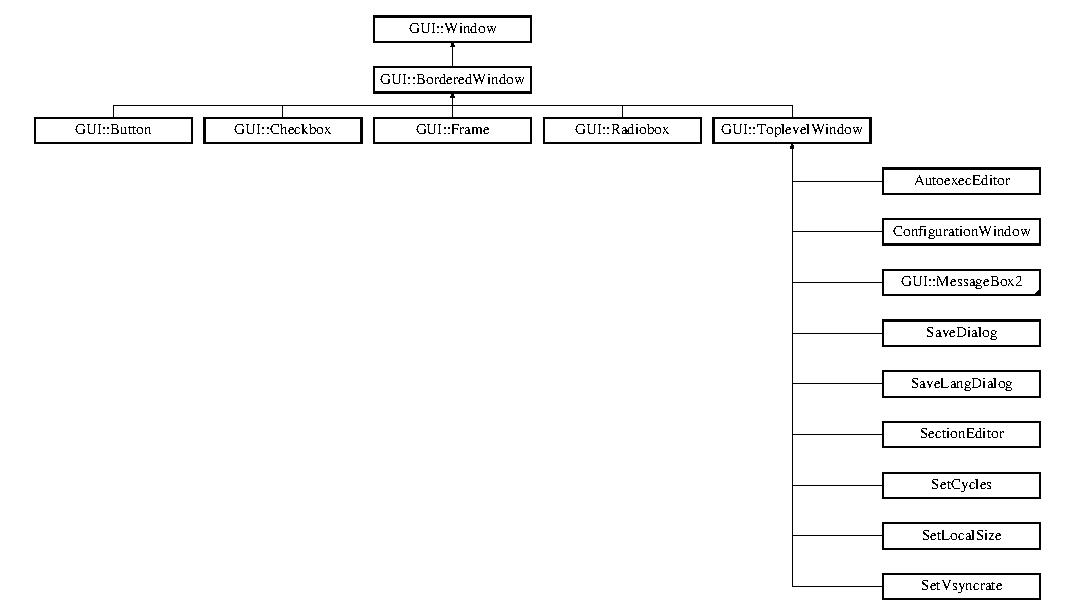
\includegraphics[height=7.832168cm]{classGUI_1_1BorderedWindow}
\end{center}
\end{figure}
\subsection*{Public Member Functions}
\begin{DoxyCompactItemize}
\item 
\hypertarget{classGUI_1_1BorderedWindow_a5bd1d017806dd127e04e56a12edf383f}{virtual void \hyperlink{classGUI_1_1BorderedWindow_a5bd1d017806dd127e04e56a12edf383f}{paint\-All} (\hyperlink{classGUI_1_1Drawable}{Drawable} \&d) const }\label{classGUI_1_1BorderedWindow_a5bd1d017806dd127e04e56a12edf383f}

\begin{DoxyCompactList}\small\item\em Draw this window's content including all children. \end{DoxyCompactList}\item 
\hypertarget{classGUI_1_1BorderedWindow_ac56e468bfc1e51da8761335171e0d2c0}{virtual bool \hyperlink{classGUI_1_1BorderedWindow_ac56e468bfc1e51da8761335171e0d2c0}{mouse\-Moved} (int \hyperlink{classGUI_1_1Window_a6ca6a80ca00c9e1d8ceea8d3d99a657d}{x}, int \hyperlink{classGUI_1_1Window_a0ee8e923aff2c3661fc2e17656d37adf}{y})}\label{classGUI_1_1BorderedWindow_ac56e468bfc1e51da8761335171e0d2c0}

\begin{DoxyCompactList}\small\item\em Mouse was moved. Returns true if event was handled. \end{DoxyCompactList}\item 
\hypertarget{classGUI_1_1BorderedWindow_ad7de10ea96395869897b62c31caaa81b}{virtual bool \hyperlink{classGUI_1_1BorderedWindow_ad7de10ea96395869897b62c31caaa81b}{mouse\-Down} (int \hyperlink{classGUI_1_1Window_a6ca6a80ca00c9e1d8ceea8d3d99a657d}{x}, int \hyperlink{classGUI_1_1Window_a0ee8e923aff2c3661fc2e17656d37adf}{y}, \hyperlink{namespaceGUI_ad06082a7b02aa73697f39eb8e0856de9}{Mouse\-Button} button)}\label{classGUI_1_1BorderedWindow_ad7de10ea96395869897b62c31caaa81b}

\begin{DoxyCompactList}\small\item\em Mouse was pressed. Returns true if event was handled. \end{DoxyCompactList}\item 
\hypertarget{classGUI_1_1BorderedWindow_a677a5300915ac73413831f3ad9c1d676}{virtual bool \hyperlink{classGUI_1_1BorderedWindow_a677a5300915ac73413831f3ad9c1d676}{mouse\-Dragged} (int \hyperlink{classGUI_1_1Window_a6ca6a80ca00c9e1d8ceea8d3d99a657d}{x}, int \hyperlink{classGUI_1_1Window_a0ee8e923aff2c3661fc2e17656d37adf}{y}, \hyperlink{namespaceGUI_ad06082a7b02aa73697f39eb8e0856de9}{Mouse\-Button} button)}\label{classGUI_1_1BorderedWindow_a677a5300915ac73413831f3ad9c1d676}

\begin{DoxyCompactList}\small\item\em Mouse was moved while a button was pressed. Returns true if event was handled. \end{DoxyCompactList}\item 
\hypertarget{classGUI_1_1BorderedWindow_a360d2ae9d3ebff67bab02a1855b9f0ee}{virtual int \hyperlink{classGUI_1_1BorderedWindow_a360d2ae9d3ebff67bab02a1855b9f0ee}{get\-Screen\-X} () const }\label{classGUI_1_1BorderedWindow_a360d2ae9d3ebff67bab02a1855b9f0ee}

\begin{DoxyCompactList}\small\item\em Return this window's contents' X position relative to the screen's top left corner. \end{DoxyCompactList}\item 
\hypertarget{classGUI_1_1BorderedWindow_a79e2b435d5e2e3fc3f97c4d2d783df1d}{virtual int \hyperlink{classGUI_1_1BorderedWindow_a79e2b435d5e2e3fc3f97c4d2d783df1d}{get\-Screen\-Y} () const }\label{classGUI_1_1BorderedWindow_a79e2b435d5e2e3fc3f97c4d2d783df1d}

\begin{DoxyCompactList}\small\item\em Return this window's contents' Y position relative to the screen's top left corner. \end{DoxyCompactList}\end{DoxyCompactItemize}
\subsection*{Protected Member Functions}
\begin{DoxyCompactItemize}
\item 
\hypertarget{classGUI_1_1BorderedWindow_a6e2e1cbbc8a073b4ddac62086e003d46}{\hyperlink{classGUI_1_1BorderedWindow_a6e2e1cbbc8a073b4ddac62086e003d46}{Bordered\-Window} (\hyperlink{classGUI_1_1Window}{Window} $\ast$\hyperlink{classGUI_1_1Window_a2e593ff65e7702178d82fe9010a0b539}{parent}, int \hyperlink{classGUI_1_1Window_a6ca6a80ca00c9e1d8ceea8d3d99a657d}{x}, int \hyperlink{classGUI_1_1Window_a0ee8e923aff2c3661fc2e17656d37adf}{y}, int w, int h, int bl, int bt, int br, int bb)}\label{classGUI_1_1BorderedWindow_a6e2e1cbbc8a073b4ddac62086e003d46}

\begin{DoxyCompactList}\small\item\em Create a bordered window. \end{DoxyCompactList}\end{DoxyCompactItemize}
\subsection*{Protected Attributes}
\begin{DoxyCompactItemize}
\item 
\hypertarget{classGUI_1_1BorderedWindow_aee7cb08a129656be54ca7c80f6a1e773}{int \hyperlink{classGUI_1_1BorderedWindow_aee7cb08a129656be54ca7c80f6a1e773}{border\-\_\-left}}\label{classGUI_1_1BorderedWindow_aee7cb08a129656be54ca7c80f6a1e773}

\begin{DoxyCompactList}\small\item\em Borders. \end{DoxyCompactList}\item 
\hypertarget{classGUI_1_1BorderedWindow_ae68c7db90609df20c166ccff4fedcbd4}{int {\bfseries border\-\_\-top}}\label{classGUI_1_1BorderedWindow_ae68c7db90609df20c166ccff4fedcbd4}

\item 
\hypertarget{classGUI_1_1BorderedWindow_a3d1e6ac0d63e78e79900129f6e6a07c3}{int {\bfseries border\-\_\-right}}\label{classGUI_1_1BorderedWindow_a3d1e6ac0d63e78e79900129f6e6a07c3}

\item 
\hypertarget{classGUI_1_1BorderedWindow_a2daa40a7c446a6753d39f5a3096546b9}{int {\bfseries border\-\_\-bottom}}\label{classGUI_1_1BorderedWindow_a2daa40a7c446a6753d39f5a3096546b9}

\end{DoxyCompactItemize}


\subsection{Detailed Description}
Internal class for windows whose child content should not span the entire area. 

Definition at line 1359 of file gui\-\_\-tk.\-h.



The documentation for this class was generated from the following files\-:\begin{DoxyCompactItemize}
\item 
src/libs/gui\-\_\-tk/\hyperlink{gui__tk_8h}{gui\-\_\-tk.\-h}\item 
src/libs/gui\-\_\-tk/\hyperlink{gui__tk_8cpp}{gui\-\_\-tk.\-cpp}\end{DoxyCompactItemize}

\hypertarget{classMT32Emu_1_1BReverbModel}{\section{M\-T32\-Emu\-:\-:B\-Reverb\-Model Class Reference}
\label{classMT32Emu_1_1BReverbModel}\index{M\-T32\-Emu\-::\-B\-Reverb\-Model@{M\-T32\-Emu\-::\-B\-Reverb\-Model}}
}
Inheritance diagram for M\-T32\-Emu\-:\-:B\-Reverb\-Model\-:\begin{figure}[H]
\begin{center}
\leavevmode
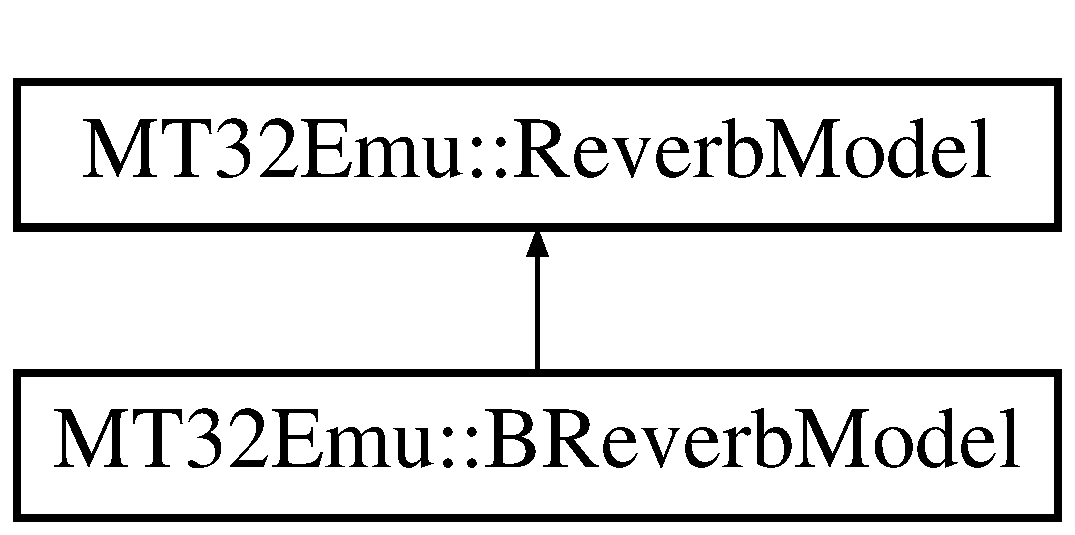
\includegraphics[height=2.000000cm]{classMT32Emu_1_1BReverbModel}
\end{center}
\end{figure}
\subsection*{Public Member Functions}
\begin{DoxyCompactItemize}
\item 
\hypertarget{classMT32Emu_1_1BReverbModel_a77a30b58bd0456a3ea2c268e8a07a8cd}{{\bfseries B\-Reverb\-Model} (const Reverb\-Mode mode)}\label{classMT32Emu_1_1BReverbModel_a77a30b58bd0456a3ea2c268e8a07a8cd}

\item 
\hypertarget{classMT32Emu_1_1BReverbModel_a5d223616b9927f46b1bbd34b75964c13}{void {\bfseries open} ()}\label{classMT32Emu_1_1BReverbModel_a5d223616b9927f46b1bbd34b75964c13}

\item 
\hypertarget{classMT32Emu_1_1BReverbModel_ab678b930206e8968a8ab1d36fb844f7e}{void {\bfseries close} ()}\label{classMT32Emu_1_1BReverbModel_ab678b930206e8968a8ab1d36fb844f7e}

\item 
\hypertarget{classMT32Emu_1_1BReverbModel_ab47b581462e43b3b2f45f30e7d7b86ca}{void {\bfseries set\-Parameters} (Bit8u time, Bit8u level)}\label{classMT32Emu_1_1BReverbModel_ab47b581462e43b3b2f45f30e7d7b86ca}

\item 
\hypertarget{classMT32Emu_1_1BReverbModel_a107f65efcfda9cb25dc71777914f32e5}{void {\bfseries process} (const float $\ast$in\-Left, const float $\ast$in\-Right, float $\ast$out\-Left, float $\ast$out\-Right, unsigned long num\-Samples)}\label{classMT32Emu_1_1BReverbModel_a107f65efcfda9cb25dc71777914f32e5}

\item 
\hypertarget{classMT32Emu_1_1BReverbModel_a4ff8c21629ea768b495c89b7e2a04996}{bool {\bfseries is\-Active} () const }\label{classMT32Emu_1_1BReverbModel_a4ff8c21629ea768b495c89b7e2a04996}

\end{DoxyCompactItemize}


\subsection{Detailed Description}


Definition at line 90 of file B\-Reverb\-Model.\-h.



The documentation for this class was generated from the following file\-:\begin{DoxyCompactItemize}
\item 
src/mt32/B\-Reverb\-Model.\-h\end{DoxyCompactItemize}

\hypertarget{structMT32Emu_1_1BReverbSettings}{\section{M\-T32\-Emu\-:\-:B\-Reverb\-Settings Struct Reference}
\label{structMT32Emu_1_1BReverbSettings}\index{M\-T32\-Emu\-::\-B\-Reverb\-Settings@{M\-T32\-Emu\-::\-B\-Reverb\-Settings}}
}
\subsection*{Public Attributes}
\begin{DoxyCompactItemize}
\item 
\hypertarget{structMT32Emu_1_1BReverbSettings_a21773838b12169d909fa94c0324654c6}{const Bit32u {\bfseries number\-Of\-Allpasses}}\label{structMT32Emu_1_1BReverbSettings_a21773838b12169d909fa94c0324654c6}

\item 
\hypertarget{structMT32Emu_1_1BReverbSettings_aeb6f59ff13b351ea0e6d7be0185850ff}{const Bit32u $\ast$const {\bfseries allpass\-Sizes}}\label{structMT32Emu_1_1BReverbSettings_aeb6f59ff13b351ea0e6d7be0185850ff}

\item 
\hypertarget{structMT32Emu_1_1BReverbSettings_acf8c4ddadbb8d80aed4ca91f1ba08d98}{const Bit32u {\bfseries number\-Of\-Combs}}\label{structMT32Emu_1_1BReverbSettings_acf8c4ddadbb8d80aed4ca91f1ba08d98}

\item 
\hypertarget{structMT32Emu_1_1BReverbSettings_af76c18d2fb394f483e28892cb6b6435a}{const Bit32u $\ast$const {\bfseries comb\-Sizes}}\label{structMT32Emu_1_1BReverbSettings_af76c18d2fb394f483e28892cb6b6435a}

\item 
\hypertarget{structMT32Emu_1_1BReverbSettings_a3850bda62199a68aed6087ed4e56e293}{const Bit32u $\ast$const {\bfseries out\-L\-Positions}}\label{structMT32Emu_1_1BReverbSettings_a3850bda62199a68aed6087ed4e56e293}

\item 
\hypertarget{structMT32Emu_1_1BReverbSettings_a0323eba12c08ce5269789038968f7706}{const Bit32u $\ast$const {\bfseries out\-R\-Positions}}\label{structMT32Emu_1_1BReverbSettings_a0323eba12c08ce5269789038968f7706}

\item 
\hypertarget{structMT32Emu_1_1BReverbSettings_a8953715288bb0cba12698e296d3ecb87}{const Bit32u $\ast$const {\bfseries filter\-Factors}}\label{structMT32Emu_1_1BReverbSettings_a8953715288bb0cba12698e296d3ecb87}

\item 
\hypertarget{structMT32Emu_1_1BReverbSettings_a9dcdc476774c91347d8ca421f50aac11}{const Bit32u $\ast$const {\bfseries feedback\-Factors}}\label{structMT32Emu_1_1BReverbSettings_a9dcdc476774c91347d8ca421f50aac11}

\item 
\hypertarget{structMT32Emu_1_1BReverbSettings_ad939fe9174e4076790327c769abcfbfc}{const Bit32u $\ast$const {\bfseries dry\-Amps}}\label{structMT32Emu_1_1BReverbSettings_ad939fe9174e4076790327c769abcfbfc}

\item 
\hypertarget{structMT32Emu_1_1BReverbSettings_abbbcdfb7ec16be3091379fe4c2b2863d}{const Bit32u $\ast$const {\bfseries wet\-Levels}}\label{structMT32Emu_1_1BReverbSettings_abbbcdfb7ec16be3091379fe4c2b2863d}

\item 
\hypertarget{structMT32Emu_1_1BReverbSettings_a3a6033b17c239c17a689acd9130a82a6}{const Bit32u {\bfseries lpf\-Amp}}\label{structMT32Emu_1_1BReverbSettings_a3a6033b17c239c17a689acd9130a82a6}

\end{DoxyCompactItemize}


\subsection{Detailed Description}


Definition at line 23 of file B\-Reverb\-Model.\-h.



The documentation for this struct was generated from the following file\-:\begin{DoxyCompactItemize}
\item 
src/mt32/B\-Reverb\-Model.\-h\end{DoxyCompactItemize}

\hypertarget{structBuiltinFileBlob}{\section{Builtin\-File\-Blob Struct Reference}
\label{structBuiltinFileBlob}\index{Builtin\-File\-Blob@{Builtin\-File\-Blob}}
}
\subsection*{Public Attributes}
\begin{DoxyCompactItemize}
\item 
\hypertarget{structBuiltinFileBlob_a27257011b2929bc931106342ddf8caed}{const char $\ast$ {\bfseries recommended\-\_\-file\-\_\-name}}\label{structBuiltinFileBlob_a27257011b2929bc931106342ddf8caed}

\item 
\hypertarget{structBuiltinFileBlob_a2c78c750b9f6453cd12af48ab7d8c4be}{const unsigned char $\ast$ {\bfseries data}}\label{structBuiltinFileBlob_a2c78c750b9f6453cd12af48ab7d8c4be}

\item 
\hypertarget{structBuiltinFileBlob_add502835899f037bce20bc3ce28b7f30}{size\-\_\-t {\bfseries length}}\label{structBuiltinFileBlob_add502835899f037bce20bc3ce28b7f30}

\end{DoxyCompactItemize}


\subsection{Detailed Description}


Definition at line 51 of file dos\-\_\-inc.\-h.



The documentation for this struct was generated from the following file\-:\begin{DoxyCompactItemize}
\item 
include/dos\-\_\-inc.\-h\end{DoxyCompactItemize}

\hypertarget{classGUI_1_1Button}{\section{G\-U\-I\-:\-:Button Class Reference}
\label{classGUI_1_1Button}\index{G\-U\-I\-::\-Button@{G\-U\-I\-::\-Button}}
}


A push button.  




{\ttfamily \#include $<$gui\-\_\-tk.\-h$>$}

Inheritance diagram for G\-U\-I\-:\-:Button\-:\begin{figure}[H]
\begin{center}
\leavevmode
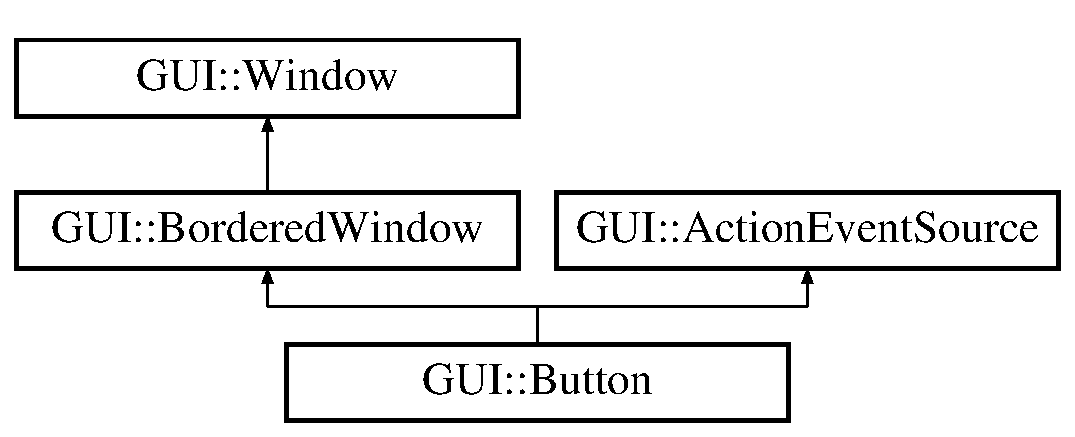
\includegraphics[height=4.000000cm]{classGUI_1_1Button}
\end{center}
\end{figure}
\subsection*{Public Member Functions}
\begin{DoxyCompactItemize}
\item 
\hypertarget{classGUI_1_1Button_aed8c4c6050d6dc28984f6406263543b6}{\hyperlink{classGUI_1_1Button_aed8c4c6050d6dc28984f6406263543b6}{Button} (\hyperlink{classGUI_1_1Window}{Window} $\ast$\hyperlink{classGUI_1_1Window_a2e593ff65e7702178d82fe9010a0b539}{parent}, int \hyperlink{classGUI_1_1Window_a6ca6a80ca00c9e1d8ceea8d3d99a657d}{x}, int \hyperlink{classGUI_1_1Window_a0ee8e923aff2c3661fc2e17656d37adf}{y}, int w, int h)}\label{classGUI_1_1Button_aed8c4c6050d6dc28984f6406263543b6}

\begin{DoxyCompactList}\small\item\em Create a button with given position and size. \end{DoxyCompactList}\item 
{\footnotesize template$<$typename T $>$ }\\\hyperlink{classGUI_1_1Button_ae926c70573aa8418b56810689470d2b3}{Button} (\hyperlink{classGUI_1_1Window}{Window} $\ast$\hyperlink{classGUI_1_1Window_a2e593ff65e7702178d82fe9010a0b539}{parent}, int \hyperlink{classGUI_1_1Window_a6ca6a80ca00c9e1d8ceea8d3d99a657d}{x}, int \hyperlink{classGUI_1_1Window_a0ee8e923aff2c3661fc2e17656d37adf}{y}, const T text, int w=-\/1, int h=-\/1)
\begin{DoxyCompactList}\small\item\em Create a text button. \end{DoxyCompactList}\item 
\hypertarget{classGUI_1_1Button_a1cdd40f407ae7629533ec4db2c3d60e0}{virtual void \hyperlink{classGUI_1_1Button_a1cdd40f407ae7629533ec4db2c3d60e0}{paint} (\hyperlink{classGUI_1_1Drawable}{Drawable} \&d) const }\label{classGUI_1_1Button_a1cdd40f407ae7629533ec4db2c3d60e0}

\begin{DoxyCompactList}\small\item\em Paint button. \end{DoxyCompactList}\item 
\hypertarget{classGUI_1_1Button_a944916852caa22ff81139fff0ca0335a}{virtual bool \hyperlink{classGUI_1_1Button_a944916852caa22ff81139fff0ca0335a}{mouse\-Down} (int \hyperlink{classGUI_1_1Window_a6ca6a80ca00c9e1d8ceea8d3d99a657d}{x}, int \hyperlink{classGUI_1_1Window_a0ee8e923aff2c3661fc2e17656d37adf}{y}, \hyperlink{namespaceGUI_ad06082a7b02aa73697f39eb8e0856de9}{Mouse\-Button} button)}\label{classGUI_1_1Button_a944916852caa22ff81139fff0ca0335a}

\begin{DoxyCompactList}\small\item\em Press button. \end{DoxyCompactList}\item 
\hypertarget{classGUI_1_1Button_a49f6da9536005b08a02678209378b11e}{virtual bool \hyperlink{classGUI_1_1Button_a49f6da9536005b08a02678209378b11e}{mouse\-Up} (int \hyperlink{classGUI_1_1Window_a6ca6a80ca00c9e1d8ceea8d3d99a657d}{x}, int \hyperlink{classGUI_1_1Window_a0ee8e923aff2c3661fc2e17656d37adf}{y}, \hyperlink{namespaceGUI_ad06082a7b02aa73697f39eb8e0856de9}{Mouse\-Button} button)}\label{classGUI_1_1Button_a49f6da9536005b08a02678209378b11e}

\begin{DoxyCompactList}\small\item\em Release button. \end{DoxyCompactList}\item 
\hypertarget{classGUI_1_1Button_a88a1ed778b528d75a55351f2e3a00cf1}{virtual bool \hyperlink{classGUI_1_1Button_a88a1ed778b528d75a55351f2e3a00cf1}{mouse\-Clicked} (int \hyperlink{classGUI_1_1Window_a6ca6a80ca00c9e1d8ceea8d3d99a657d}{x}, int \hyperlink{classGUI_1_1Window_a0ee8e923aff2c3661fc2e17656d37adf}{y}, \hyperlink{namespaceGUI_ad06082a7b02aa73697f39eb8e0856de9}{Mouse\-Button} button)}\label{classGUI_1_1Button_a88a1ed778b528d75a55351f2e3a00cf1}

\begin{DoxyCompactList}\small\item\em Handle mouse activation. \end{DoxyCompactList}\item 
\hypertarget{classGUI_1_1Button_a0eafdb8f5c02244701ff27d9e1ca2337}{virtual bool \hyperlink{classGUI_1_1Button_a0eafdb8f5c02244701ff27d9e1ca2337}{key\-Down} (const \hyperlink{classGUI_1_1Key}{Key} \&key)}\label{classGUI_1_1Button_a0eafdb8f5c02244701ff27d9e1ca2337}

\begin{DoxyCompactList}\small\item\em Handle keyboard input. \end{DoxyCompactList}\item 
\hypertarget{classGUI_1_1Button_a211b435d6d91e11ff1e778b9ee6c9c73}{virtual bool \hyperlink{classGUI_1_1Button_a211b435d6d91e11ff1e778b9ee6c9c73}{key\-Up} (const \hyperlink{classGUI_1_1Key}{Key} \&key)}\label{classGUI_1_1Button_a211b435d6d91e11ff1e778b9ee6c9c73}

\begin{DoxyCompactList}\small\item\em Handle keyboard input. \end{DoxyCompactList}\item 
\hypertarget{classGUI_1_1Button_ada8368b22e9bfcfa7ba9199f9ea3f7cc}{{\footnotesize template$<$typename S\-T\-R $>$ }\\{\bfseries Button} (\hyperlink{classGUI_1_1Window}{Window} $\ast$\hyperlink{classGUI_1_1Window_a2e593ff65e7702178d82fe9010a0b539}{parent}, int \hyperlink{classGUI_1_1Window_a6ca6a80ca00c9e1d8ceea8d3d99a657d}{x}, int \hyperlink{classGUI_1_1Window_a0ee8e923aff2c3661fc2e17656d37adf}{y}, const S\-T\-R text, int w, int h)}\label{classGUI_1_1Button_ada8368b22e9bfcfa7ba9199f9ea3f7cc}

\end{DoxyCompactItemize}
\subsection*{Protected Attributes}
\begin{DoxyCompactItemize}
\item 
\hypertarget{classGUI_1_1Button_aec37fa9a4a6ea6d1e0e2788d42d67ee1}{bool \hyperlink{classGUI_1_1Button_aec37fa9a4a6ea6d1e0e2788d42d67ee1}{pressed}}\label{classGUI_1_1Button_aec37fa9a4a6ea6d1e0e2788d42d67ee1}

\begin{DoxyCompactList}\small\item\em {\ttfamily true}, if button is currently pressed down. \end{DoxyCompactList}\end{DoxyCompactItemize}


\subsection{Detailed Description}
A push button. 

Buttons have 3\-D appearance and can have any child widget as content. There are convenience constructors for common forms of buttons. 

Definition at line 2178 of file gui\-\_\-tk.\-h.



\subsection{Constructor \& Destructor Documentation}
\hypertarget{classGUI_1_1Button_ae926c70573aa8418b56810689470d2b3}{\index{G\-U\-I\-::\-Button@{G\-U\-I\-::\-Button}!Button@{Button}}
\index{Button@{Button}!GUI::Button@{G\-U\-I\-::\-Button}}
\subsubsection[{Button}]{\setlength{\rightskip}{0pt plus 5cm}template$<$typename T $>$ {\bf G\-U\-I\-::\-Button\-::\-Button} (
\begin{DoxyParamCaption}
\item[{{\bf Window} $\ast$}]{parent, }
\item[{int}]{x, }
\item[{int}]{y, }
\item[{const T}]{text, }
\item[{int}]{w = {\ttfamily -\/1}, }
\item[{int}]{h = {\ttfamily -\/1}}
\end{DoxyParamCaption}
)}}\label{classGUI_1_1Button_ae926c70573aa8418b56810689470d2b3}


Create a text button. 

If a size is specified, text is centered. Otherwise, button size is adjusted for the text. 

The documentation for this class was generated from the following files\-:\begin{DoxyCompactItemize}
\item 
src/libs/gui\-\_\-tk/\hyperlink{gui__tk_8h}{gui\-\_\-tk.\-h}\item 
src/libs/gui\-\_\-tk/\hyperlink{gui__tk_8cpp}{gui\-\_\-tk.\-cpp}\end{DoxyCompactItemize}

\hypertarget{structbutton__event}{\section{button\-\_\-event Struct Reference}
\label{structbutton__event}\index{button\-\_\-event@{button\-\_\-event}}
}
\subsection*{Public Attributes}
\begin{DoxyCompactItemize}
\item 
\hypertarget{structbutton__event_a793d0b44cf9339bd85bd3d571830fa51}{Bit8u {\bfseries type}}\label{structbutton__event_a793d0b44cf9339bd85bd3d571830fa51}

\item 
\hypertarget{structbutton__event_abacaa182c19fa91de5e17ee325f6fe88}{Bit8u {\bfseries buttons}}\label{structbutton__event_abacaa182c19fa91de5e17ee325f6fe88}

\end{DoxyCompactItemize}


\subsection{Detailed Description}


Definition at line 111 of file mouse.\-cpp.



The documentation for this struct was generated from the following file\-:\begin{DoxyCompactItemize}
\item 
src/ints/mouse.\-cpp\end{DoxyCompactItemize}

\hypertarget{classbx__ne2k__c}{\section{bx\-\_\-ne2k\-\_\-c Class Reference}
\label{classbx__ne2k__c}\index{bx\-\_\-ne2k\-\_\-c@{bx\-\_\-ne2k\-\_\-c}}
}
\subsection*{Public Member Functions}
\begin{DoxyCompactItemize}
\item 
\hypertarget{classbx__ne2k__c_ae7dce10cbb81edb33cd4079159432732}{virtual void {\bfseries init} (void)}\label{classbx__ne2k__c_ae7dce10cbb81edb33cd4079159432732}

\item 
\hypertarget{classbx__ne2k__c_a304c7130e8fdb026351c4b57e11cb70d}{virtual void {\bfseries reset} (unsigned type)}\label{classbx__ne2k__c_a304c7130e8fdb026351c4b57e11cb70d}

\item 
\hypertarget{classbx__ne2k__c_a369a3b1b0ee2d349c7e19a565a0b1b2b}{B\-X\-\_\-\-N\-E2\-K\-\_\-\-S\-M\-F Bit32u {\bfseries read\-\_\-cr} (void)}\label{classbx__ne2k__c_a369a3b1b0ee2d349c7e19a565a0b1b2b}

\item 
\hypertarget{classbx__ne2k__c_a00b04f4ca72d07587393521b1e8b23c6}{B\-X\-\_\-\-N\-E2\-K\-\_\-\-S\-M\-F void {\bfseries write\-\_\-cr} (Bit32u value)}\label{classbx__ne2k__c_a00b04f4ca72d07587393521b1e8b23c6}

\item 
\hypertarget{classbx__ne2k__c_a54933d27a5dcc2812e966b483d4eac88}{B\-X\-\_\-\-N\-E2\-K\-\_\-\-S\-M\-F Bit32u {\bfseries chipmem\-\_\-read} (Bit32u address, unsigned io\-\_\-len)}\label{classbx__ne2k__c_a54933d27a5dcc2812e966b483d4eac88}

\item 
\hypertarget{classbx__ne2k__c_a40a8406ca2769e994100fa756c2f93d6}{B\-X\-\_\-\-N\-E2\-K\-\_\-\-S\-M\-F Bit32u {\bfseries asic\-\_\-read} (Bit32u offset, unsigned io\-\_\-len)}\label{classbx__ne2k__c_a40a8406ca2769e994100fa756c2f93d6}

\item 
\hypertarget{classbx__ne2k__c_a27b4f6d9ea2ee6c205eb829ba44296f9}{B\-X\-\_\-\-N\-E2\-K\-\_\-\-S\-M\-F Bit32u {\bfseries page0\-\_\-read} (Bit32u offset, unsigned io\-\_\-len)}\label{classbx__ne2k__c_a27b4f6d9ea2ee6c205eb829ba44296f9}

\item 
\hypertarget{classbx__ne2k__c_a3bc0414bfaaee20882fc9325345026c2}{B\-X\-\_\-\-N\-E2\-K\-\_\-\-S\-M\-F Bit32u {\bfseries page1\-\_\-read} (Bit32u offset, unsigned io\-\_\-len)}\label{classbx__ne2k__c_a3bc0414bfaaee20882fc9325345026c2}

\item 
\hypertarget{classbx__ne2k__c_a41f6b52287a9b604abb9a113320c09f1}{B\-X\-\_\-\-N\-E2\-K\-\_\-\-S\-M\-F Bit32u {\bfseries page2\-\_\-read} (Bit32u offset, unsigned io\-\_\-len)}\label{classbx__ne2k__c_a41f6b52287a9b604abb9a113320c09f1}

\item 
\hypertarget{classbx__ne2k__c_a5d5d20295c90622630582646f6dd7c85}{B\-X\-\_\-\-N\-E2\-K\-\_\-\-S\-M\-F Bit32u {\bfseries page3\-\_\-read} (Bit32u offset, unsigned io\-\_\-len)}\label{classbx__ne2k__c_a5d5d20295c90622630582646f6dd7c85}

\item 
\hypertarget{classbx__ne2k__c_a2ef4a2eabd25fbe86580a88ed07d907b}{B\-X\-\_\-\-N\-E2\-K\-\_\-\-S\-M\-F void {\bfseries chipmem\-\_\-write} (Bit32u address, Bit32u value, unsigned io\-\_\-len)}\label{classbx__ne2k__c_a2ef4a2eabd25fbe86580a88ed07d907b}

\item 
\hypertarget{classbx__ne2k__c_ae4a9493baea04f813f7af049f0cea4ee}{B\-X\-\_\-\-N\-E2\-K\-\_\-\-S\-M\-F void {\bfseries asic\-\_\-write} (Bit32u address, Bit32u value, unsigned io\-\_\-len)}\label{classbx__ne2k__c_ae4a9493baea04f813f7af049f0cea4ee}

\item 
\hypertarget{classbx__ne2k__c_a2ec128e132867de075b33f521f6966e5}{B\-X\-\_\-\-N\-E2\-K\-\_\-\-S\-M\-F void {\bfseries page0\-\_\-write} (Bit32u address, Bit32u value, unsigned io\-\_\-len)}\label{classbx__ne2k__c_a2ec128e132867de075b33f521f6966e5}

\item 
\hypertarget{classbx__ne2k__c_a071c0490d1c7e4b520c8b99db450986c}{B\-X\-\_\-\-N\-E2\-K\-\_\-\-S\-M\-F void {\bfseries page1\-\_\-write} (Bit32u address, Bit32u value, unsigned io\-\_\-len)}\label{classbx__ne2k__c_a071c0490d1c7e4b520c8b99db450986c}

\item 
\hypertarget{classbx__ne2k__c_a696814dd7e45cd97fc87c9129e478424}{B\-X\-\_\-\-N\-E2\-K\-\_\-\-S\-M\-F void {\bfseries page2\-\_\-write} (Bit32u address, Bit32u value, unsigned io\-\_\-len)}\label{classbx__ne2k__c_a696814dd7e45cd97fc87c9129e478424}

\item 
\hypertarget{classbx__ne2k__c_a0b3925c293544d2288ccf6e1c81f5d87}{B\-X\-\_\-\-N\-E2\-K\-\_\-\-S\-M\-F void {\bfseries page3\-\_\-write} (Bit32u address, Bit32u value, unsigned io\-\_\-len)}\label{classbx__ne2k__c_a0b3925c293544d2288ccf6e1c81f5d87}

\item 
\hypertarget{classbx__ne2k__c_a95fc7395914b4793e1e74b830662a6b7}{B\-X\-\_\-\-N\-E2\-K\-\_\-\-S\-M\-F void {\bfseries tx\-\_\-timer} (void)}\label{classbx__ne2k__c_a95fc7395914b4793e1e74b830662a6b7}

\item 
\hypertarget{classbx__ne2k__c_a5f688a5d84b134997d011dcc8db8504e}{B\-X\-\_\-\-N\-E2\-K\-\_\-\-S\-M\-F unsigned {\bfseries mcast\-\_\-index} (const void $\ast$dst)}\label{classbx__ne2k__c_a5f688a5d84b134997d011dcc8db8504e}

\item 
\hypertarget{classbx__ne2k__c_aa5d314861515c0d6353aa9f4b56405ea}{B\-X\-\_\-\-N\-E2\-K\-\_\-\-S\-M\-F void {\bfseries rx\-\_\-frame} (const void $\ast$buf, unsigned io\-\_\-len)}\label{classbx__ne2k__c_aa5d314861515c0d6353aa9f4b56405ea}

\item 
\hypertarget{classbx__ne2k__c_a57e42d07a6bb408f428a3eace15921ff}{Bit32u {\bfseries read} (Bit32u address, unsigned io\-\_\-len)}\label{classbx__ne2k__c_a57e42d07a6bb408f428a3eace15921ff}

\item 
\hypertarget{classbx__ne2k__c_aa2a39611a06e9111e5218aa3e7dc0dd3}{void {\bfseries write} (Bit32u address, Bit32u value, unsigned io\-\_\-len)}\label{classbx__ne2k__c_aa2a39611a06e9111e5218aa3e7dc0dd3}

\end{DoxyCompactItemize}
\subsection*{Static Public Member Functions}
\begin{DoxyCompactItemize}
\item 
\hypertarget{classbx__ne2k__c_a096b6d391193d92950820c928bfc9d2b}{static void {\bfseries tx\-\_\-timer\-\_\-handler} (void $\ast$)}\label{classbx__ne2k__c_a096b6d391193d92950820c928bfc9d2b}

\item 
\hypertarget{classbx__ne2k__c_a99b4d7ac6e2e072e1d5b5ba762eede3d}{static void {\bfseries rx\-\_\-handler} (void $\ast$arg, const void $\ast$buf, unsigned len)}\label{classbx__ne2k__c_a99b4d7ac6e2e072e1d5b5ba762eede3d}

\item 
\hypertarget{classbx__ne2k__c_a3576daab1d71db4fc5f067d4a81dff6f}{static Bit32u {\bfseries read\-\_\-handler} (void $\ast$this\-\_\-ptr, Bit32u address, unsigned io\-\_\-len)}\label{classbx__ne2k__c_a3576daab1d71db4fc5f067d4a81dff6f}

\item 
\hypertarget{classbx__ne2k__c_a9f56ef73311b2366b135c3edacf048fc}{static void {\bfseries write\-\_\-handler} (void $\ast$this\-\_\-ptr, Bit32u address, Bit32u value, unsigned io\-\_\-len)}\label{classbx__ne2k__c_a9f56ef73311b2366b135c3edacf048fc}

\end{DoxyCompactItemize}
\subsection*{Public Attributes}
\begin{DoxyCompactItemize}
\item 
\hypertarget{classbx__ne2k__c_af542f5a2962236245c66a3a7c11612a7}{\hyperlink{structbx__ne2k__t}{bx\-\_\-ne2k\-\_\-t} {\bfseries s}}\label{classbx__ne2k__c_af542f5a2962236245c66a3a7c11612a7}

\end{DoxyCompactItemize}


\subsection{Detailed Description}


Definition at line 203 of file ne2000.\-h.



The documentation for this class was generated from the following file\-:\begin{DoxyCompactItemize}
\item 
include/ne2000.\-h\end{DoxyCompactItemize}

\hypertarget{structbx__ne2k__t}{\section{bx\-\_\-ne2k\-\_\-t Struct Reference}
\label{structbx__ne2k__t}\index{bx\-\_\-ne2k\-\_\-t@{bx\-\_\-ne2k\-\_\-t}}
}
\subsection*{Classes}
\begin{DoxyCompactItemize}
\item 
struct \hyperlink{structbx__ne2k__t_1_1CR__t}{C\-R\-\_\-t}
\item 
struct \hyperlink{structbx__ne2k__t_1_1DCR__t}{D\-C\-R\-\_\-t}
\item 
struct \hyperlink{structbx__ne2k__t_1_1IMR__t}{I\-M\-R\-\_\-t}
\item 
struct \hyperlink{structbx__ne2k__t_1_1ISR__t}{I\-S\-R\-\_\-t}
\item 
struct \hyperlink{structbx__ne2k__t_1_1RCR__t}{R\-C\-R\-\_\-t}
\item 
struct \hyperlink{structbx__ne2k__t_1_1RSR__t}{R\-S\-R\-\_\-t}
\item 
struct \hyperlink{structbx__ne2k__t_1_1TCR__t}{T\-C\-R\-\_\-t}
\item 
struct \hyperlink{structbx__ne2k__t_1_1TSR__t}{T\-S\-R\-\_\-t}
\end{DoxyCompactItemize}
\subsection*{Public Member Functions}
\begin{DoxyCompactItemize}
\item 
\hypertarget{structbx__ne2k__t_a92f7d0dca08d8ba53094c5e4abeb0aaa}{void {\bfseries register\-\_\-state} (bx\-\_\-param\-\_\-c $\ast$list\-\_\-p)}\label{structbx__ne2k__t_a92f7d0dca08d8ba53094c5e4abeb0aaa}

\end{DoxyCompactItemize}
\subsection*{Public Attributes}
\begin{DoxyCompactItemize}
\item 
\hypertarget{structbx__ne2k__t_aacf3c8b7a025d23d6b012727f21b2322}{struct \hyperlink{structbx__ne2k__t_1_1CR__t}{bx\-\_\-ne2k\-\_\-t\-::\-C\-R\-\_\-t} {\bfseries C\-R}}\label{structbx__ne2k__t_aacf3c8b7a025d23d6b012727f21b2322}

\item 
\hypertarget{structbx__ne2k__t_a0c62e51031a83b5d81c7e9f22c70ecfa}{struct \hyperlink{structbx__ne2k__t_1_1ISR__t}{bx\-\_\-ne2k\-\_\-t\-::\-I\-S\-R\-\_\-t} {\bfseries I\-S\-R}}\label{structbx__ne2k__t_a0c62e51031a83b5d81c7e9f22c70ecfa}

\item 
\hypertarget{structbx__ne2k__t_a981fc04e92816382ccc9ada966c2ed3e}{struct \hyperlink{structbx__ne2k__t_1_1IMR__t}{bx\-\_\-ne2k\-\_\-t\-::\-I\-M\-R\-\_\-t} {\bfseries I\-M\-R}}\label{structbx__ne2k__t_a981fc04e92816382ccc9ada966c2ed3e}

\item 
\hypertarget{structbx__ne2k__t_ab71f64e9d3f2686bce731e9d9b11ccc5}{struct \hyperlink{structbx__ne2k__t_1_1DCR__t}{bx\-\_\-ne2k\-\_\-t\-::\-D\-C\-R\-\_\-t} {\bfseries D\-C\-R}}\label{structbx__ne2k__t_ab71f64e9d3f2686bce731e9d9b11ccc5}

\item 
\hypertarget{structbx__ne2k__t_ad39980db8f4d0fa9e6ad44657e22daaf}{struct \hyperlink{structbx__ne2k__t_1_1TCR__t}{bx\-\_\-ne2k\-\_\-t\-::\-T\-C\-R\-\_\-t} {\bfseries T\-C\-R}}\label{structbx__ne2k__t_ad39980db8f4d0fa9e6ad44657e22daaf}

\item 
\hypertarget{structbx__ne2k__t_a35df597cb9434a041aa937d4e5d7c0c0}{struct \hyperlink{structbx__ne2k__t_1_1TSR__t}{bx\-\_\-ne2k\-\_\-t\-::\-T\-S\-R\-\_\-t} {\bfseries T\-S\-R}}\label{structbx__ne2k__t_a35df597cb9434a041aa937d4e5d7c0c0}

\item 
\hypertarget{structbx__ne2k__t_acdd24d383bd19e83118c92ec930e612c}{struct \hyperlink{structbx__ne2k__t_1_1RCR__t}{bx\-\_\-ne2k\-\_\-t\-::\-R\-C\-R\-\_\-t} {\bfseries R\-C\-R}}\label{structbx__ne2k__t_acdd24d383bd19e83118c92ec930e612c}

\item 
\hypertarget{structbx__ne2k__t_a3b4668f758d8777324407d2bc3c2480b}{struct \hyperlink{structbx__ne2k__t_1_1RSR__t}{bx\-\_\-ne2k\-\_\-t\-::\-R\-S\-R\-\_\-t} {\bfseries R\-S\-R}}\label{structbx__ne2k__t_a3b4668f758d8777324407d2bc3c2480b}

\item 
\hypertarget{structbx__ne2k__t_a6102e298ca7673a8b9aa81df2227fd05}{Bit16u {\bfseries local\-\_\-dma}}\label{structbx__ne2k__t_a6102e298ca7673a8b9aa81df2227fd05}

\item 
\hypertarget{structbx__ne2k__t_ac26959c41a2c2e9fde6c37b83ed4ba39}{Bit8u {\bfseries page\-\_\-start}}\label{structbx__ne2k__t_ac26959c41a2c2e9fde6c37b83ed4ba39}

\item 
\hypertarget{structbx__ne2k__t_a0253f70c01ffbbb3b5651f13bf5c9958}{Bit8u {\bfseries page\-\_\-stop}}\label{structbx__ne2k__t_a0253f70c01ffbbb3b5651f13bf5c9958}

\item 
\hypertarget{structbx__ne2k__t_ad4e54de069dbb1037c753e467eba098e}{Bit8u {\bfseries bound\-\_\-ptr}}\label{structbx__ne2k__t_ad4e54de069dbb1037c753e467eba098e}

\item 
\hypertarget{structbx__ne2k__t_a48569f063d33bb2d0c77cb6f4362960d}{Bit8u {\bfseries tx\-\_\-page\-\_\-start}}\label{structbx__ne2k__t_a48569f063d33bb2d0c77cb6f4362960d}

\item 
\hypertarget{structbx__ne2k__t_a96385f1855d9785b7723e570514b4753}{Bit8u {\bfseries num\-\_\-coll}}\label{structbx__ne2k__t_a96385f1855d9785b7723e570514b4753}

\item 
\hypertarget{structbx__ne2k__t_afa612754f310d55164b5348b706b7e36}{Bit16u {\bfseries tx\-\_\-bytes}}\label{structbx__ne2k__t_afa612754f310d55164b5348b706b7e36}

\item 
\hypertarget{structbx__ne2k__t_a610820c3ff4158db13fb5d7e301c2a1e}{Bit8u {\bfseries fifo}}\label{structbx__ne2k__t_a610820c3ff4158db13fb5d7e301c2a1e}

\item 
\hypertarget{structbx__ne2k__t_ac05be0cc9150ce371c80db648a810614}{Bit16u {\bfseries remote\-\_\-dma}}\label{structbx__ne2k__t_ac05be0cc9150ce371c80db648a810614}

\item 
\hypertarget{structbx__ne2k__t_ac38312c32c1ed64bc269cd83a3e8c78f}{Bit16u {\bfseries remote\-\_\-start}}\label{structbx__ne2k__t_ac38312c32c1ed64bc269cd83a3e8c78f}

\item 
\hypertarget{structbx__ne2k__t_af0de682f7b95dae6f64a37dbf6499ff1}{Bit16u {\bfseries remote\-\_\-bytes}}\label{structbx__ne2k__t_af0de682f7b95dae6f64a37dbf6499ff1}

\item 
\hypertarget{structbx__ne2k__t_a6989e12689187270994db779e098e21c}{Bit8u {\bfseries tallycnt\-\_\-0}}\label{structbx__ne2k__t_a6989e12689187270994db779e098e21c}

\item 
\hypertarget{structbx__ne2k__t_aa5a4d42cd798eccddb07c77c9f87681c}{Bit8u {\bfseries tallycnt\-\_\-1}}\label{structbx__ne2k__t_aa5a4d42cd798eccddb07c77c9f87681c}

\item 
\hypertarget{structbx__ne2k__t_a7834320833d22dad791c188cb552d5d2}{Bit8u {\bfseries tallycnt\-\_\-2}}\label{structbx__ne2k__t_a7834320833d22dad791c188cb552d5d2}

\item 
\hypertarget{structbx__ne2k__t_ae521ed3b7bec8f2d486f40f95be87f25}{Bit8u {\bfseries physaddr} \mbox{[}6\mbox{]}}\label{structbx__ne2k__t_ae521ed3b7bec8f2d486f40f95be87f25}

\item 
\hypertarget{structbx__ne2k__t_a82be35de94a3df6ced540b7b93719008}{Bit8u {\bfseries curr\-\_\-page}}\label{structbx__ne2k__t_a82be35de94a3df6ced540b7b93719008}

\item 
\hypertarget{structbx__ne2k__t_aecf655a226989f43a526b60c5a1e0cc9}{Bit8u {\bfseries mchash} \mbox{[}8\mbox{]}}\label{structbx__ne2k__t_aecf655a226989f43a526b60c5a1e0cc9}

\item 
\hypertarget{structbx__ne2k__t_a0ff3e10991fa4dd79c1680ea74691e89}{Bit8u {\bfseries rempkt\-\_\-ptr}}\label{structbx__ne2k__t_a0ff3e10991fa4dd79c1680ea74691e89}

\item 
\hypertarget{structbx__ne2k__t_a8b3b2f3c78383063ffaf8d07dd5d7d70}{Bit8u {\bfseries localpkt\-\_\-ptr}}\label{structbx__ne2k__t_a8b3b2f3c78383063ffaf8d07dd5d7d70}

\item 
\hypertarget{structbx__ne2k__t_aefeb6ce32d4e190c9b0d692631198aa6}{Bit16u {\bfseries address\-\_\-cnt}}\label{structbx__ne2k__t_aefeb6ce32d4e190c9b0d692631198aa6}

\item 
\hypertarget{structbx__ne2k__t_a23f1582fadde9a00e44aff940b0f4053}{Bit8u {\bfseries macaddr} \mbox{[}32\mbox{]}}\label{structbx__ne2k__t_a23f1582fadde9a00e44aff940b0f4053}

\item 
\hypertarget{structbx__ne2k__t_a2bf148389a3a4e0baf7670efaa3b4a5f}{Bit8u {\bfseries mem} \mbox{[}B\-X\-\_\-\-N\-E2\-K\-\_\-\-M\-E\-M\-S\-I\-Z\mbox{]}}\label{structbx__ne2k__t_a2bf148389a3a4e0baf7670efaa3b4a5f}

\item 
\hypertarget{structbx__ne2k__t_a719b2634928ebaff42e46b3e4034b373}{Bit32u {\bfseries base\-\_\-address}}\label{structbx__ne2k__t_a719b2634928ebaff42e46b3e4034b373}

\item 
\hypertarget{structbx__ne2k__t_a508544f77999904326d460e986f9ba7a}{int {\bfseries base\-\_\-irq}}\label{structbx__ne2k__t_a508544f77999904326d460e986f9ba7a}

\item 
\hypertarget{structbx__ne2k__t_a19f9672f0a9e220d0b62b1131dba7d91}{int {\bfseries tx\-\_\-timer\-\_\-index}}\label{structbx__ne2k__t_a19f9672f0a9e220d0b62b1131dba7d91}

\item 
\hypertarget{structbx__ne2k__t_adf0099d6d61dbc0fa33b6d091680cc4e}{int {\bfseries tx\-\_\-timer\-\_\-active}}\label{structbx__ne2k__t_adf0099d6d61dbc0fa33b6d091680cc4e}

\end{DoxyCompactItemize}


\subsection{Detailed Description}


Definition at line 54 of file ne2000.\-h.



The documentation for this struct was generated from the following file\-:\begin{DoxyCompactItemize}
\item 
include/ne2000.\-h\end{DoxyCompactItemize}

\hypertarget{classC4AxisBindGroup}{\section{C4\-Axis\-Bind\-Group Class Reference}
\label{classC4AxisBindGroup}\index{C4\-Axis\-Bind\-Group@{C4\-Axis\-Bind\-Group}}
}
Inheritance diagram for C4\-Axis\-Bind\-Group\-:\begin{figure}[H]
\begin{center}
\leavevmode
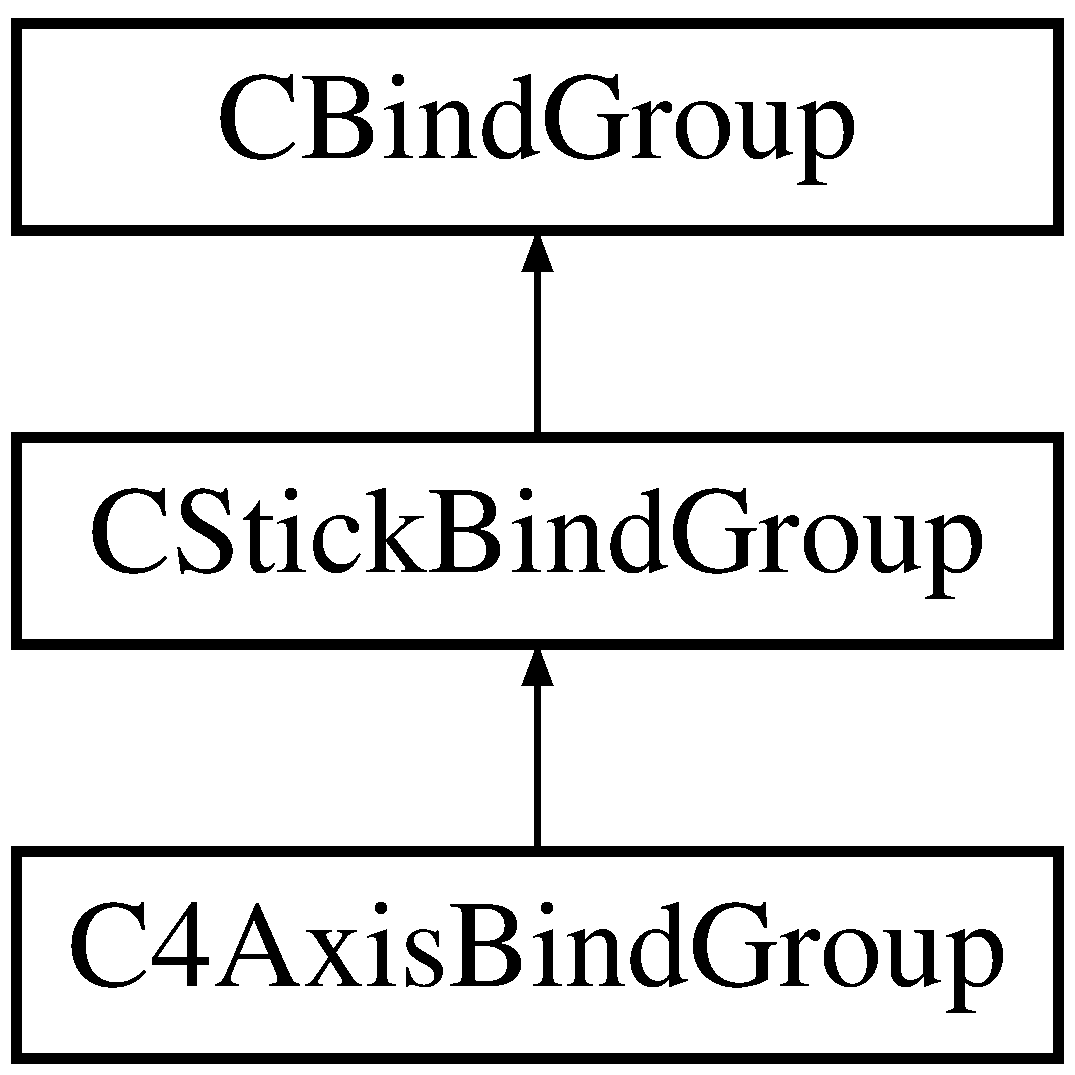
\includegraphics[height=3.000000cm]{classC4AxisBindGroup}
\end{center}
\end{figure}
\subsection*{Public Member Functions}
\begin{DoxyCompactItemize}
\item 
\hypertarget{classC4AxisBindGroup_a18f535cb78f267a882176039fa912394}{{\bfseries C4\-Axis\-Bind\-Group} (Bitu \-\_\-stick, Bitu \-\_\-emustick)}\label{classC4AxisBindGroup_a18f535cb78f267a882176039fa912394}

\item 
\hypertarget{classC4AxisBindGroup_a895bb30dd9adc0b2a704e30d954b7f5e}{bool {\bfseries Check\-Event} (S\-D\-L\-\_\-\-Event $\ast$event)}\label{classC4AxisBindGroup_a895bb30dd9adc0b2a704e30d954b7f5e}

\item 
\hypertarget{classC4AxisBindGroup_a2de71ed1c0b11f15403f1a63ea7f9169}{virtual void {\bfseries Update\-Joystick} ()}\label{classC4AxisBindGroup_a2de71ed1c0b11f15403f1a63ea7f9169}

\end{DoxyCompactItemize}


\subsection{Detailed Description}


Definition at line 1659 of file sdl\-\_\-mapper.\-cpp.



The documentation for this class was generated from the following file\-:\begin{DoxyCompactItemize}
\item 
src/gui/sdl\-\_\-mapper.\-cpp\end{DoxyCompactItemize}

\hypertarget{classCacheBlockDynRec}{\section{Cache\-Block\-Dyn\-Rec Class Reference}
\label{classCacheBlockDynRec}\index{Cache\-Block\-Dyn\-Rec@{Cache\-Block\-Dyn\-Rec}}
}
\subsection*{Public Member Functions}
\begin{DoxyCompactItemize}
\item 
\hypertarget{classCacheBlockDynRec_aeaec04cb3b9ca0df1959427c02336208}{void {\bfseries Clear} (void)}\label{classCacheBlockDynRec_aeaec04cb3b9ca0df1959427c02336208}

\item 
\hypertarget{classCacheBlockDynRec_a1ff5bf4d36b3565a3fdab67d8e1167b8}{void {\bfseries Link\-To} (Bitu index, \hyperlink{classCacheBlockDynRec}{Cache\-Block\-Dyn\-Rec} $\ast$toblock)}\label{classCacheBlockDynRec_a1ff5bf4d36b3565a3fdab67d8e1167b8}

\end{DoxyCompactItemize}
\subsection*{Public Attributes}
\begin{DoxyCompactItemize}
\item 
\hypertarget{classCacheBlockDynRec_a0ce9d7ec629d0f27d768d9a2e4732162}{\begin{tabbing}
xx\=xx\=xx\=xx\=xx\=xx\=xx\=xx\=xx\=\kill
struct \{\\
\>Bit16u {\bfseries start}\\
\>Bit16u {\bfseries end}\\
\>\hyperlink{classCodePageHandlerDynRec}{CodePageHandlerDynRec} $\ast$ {\bfseries handler}\\
\} {\bfseries page}}\label{classCacheBlockDynRec_a0ce9d7ec629d0f27d768d9a2e4732162}
\\

\end{tabbing}\item 
\hypertarget{classCacheBlockDynRec_aa9d933f69290edd10fff0fdf512f03a0}{\begin{tabbing}
xx\=xx\=xx\=xx\=xx\=xx\=xx\=xx\=xx\=\kill
struct \{\\
\>Bit8u $\ast$ {\bfseries start}\\
\>Bitu {\bfseries size}\\
\>\hyperlink{classCacheBlockDynRec}{CacheBlockDynRec} $\ast$ {\bfseries next}\\
\>Bit8u $\ast$ {\bfseries wmapmask}\\
\>Bit16u {\bfseries maskstart}\\
\>Bit16u {\bfseries masklen}\\
\} {\bfseries cache}}\label{classCacheBlockDynRec_aa9d933f69290edd10fff0fdf512f03a0}
\\

\end{tabbing}\item 
\hypertarget{classCacheBlockDynRec_aad144fabf34a958d811b3faf170769c4}{\begin{tabbing}
xx\=xx\=xx\=xx\=xx\=xx\=xx\=xx\=xx\=\kill
struct \{\\
\>Bitu {\bfseries index}\\
\>\hyperlink{classCacheBlockDynRec}{CacheBlockDynRec} $\ast$ {\bfseries next}\\
\} {\bfseries hash}}\label{classCacheBlockDynRec_aad144fabf34a958d811b3faf170769c4}
\\

\end{tabbing}\item 
\hypertarget{classCacheBlockDynRec_ac048cd8d535c09ddd950f1b5dfd8a375}{\begin{tabbing}
xx\=xx\=xx\=xx\=xx\=xx\=xx\=xx\=xx\=\kill
struct \{\\
\>\hyperlink{classCacheBlockDynRec}{CacheBlockDynRec} $\ast$ {\bfseries to}\\
\>\hyperlink{classCacheBlockDynRec}{CacheBlockDynRec} $\ast$ {\bfseries next}\\
\>\hyperlink{classCacheBlockDynRec}{CacheBlockDynRec} $\ast$ {\bfseries from}\\
\} {\bfseries link} \mbox{[}2\mbox{]}}\label{classCacheBlockDynRec_ac048cd8d535c09ddd950f1b5dfd8a375}
\\

\end{tabbing}\item 
\hypertarget{classCacheBlockDynRec_a39b601447e834e93b7f97aa6bb7df55f}{\hyperlink{classCacheBlockDynRec}{Cache\-Block\-Dyn\-Rec} $\ast$ {\bfseries crossblock}}\label{classCacheBlockDynRec_a39b601447e834e93b7f97aa6bb7df55f}

\end{DoxyCompactItemize}


\subsection{Detailed Description}


Definition at line 23 of file cache.\-h.



The documentation for this class was generated from the following file\-:\begin{DoxyCompactItemize}
\item 
src/cpu/core\-\_\-dynrec/cache.\-h\end{DoxyCompactItemize}

\hypertarget{classCALLBACK__HandlerObject}{\section{C\-A\-L\-L\-B\-A\-C\-K\-\_\-\-Handler\-Object Class Reference}
\label{classCALLBACK__HandlerObject}\index{C\-A\-L\-L\-B\-A\-C\-K\-\_\-\-Handler\-Object@{C\-A\-L\-L\-B\-A\-C\-K\-\_\-\-Handler\-Object}}
}
\subsection*{Public Member Functions}
\begin{DoxyCompactItemize}
\item 
\hypertarget{classCALLBACK__HandlerObject_af226371a5aa8f9b18d8ffd5fdec5e839}{void {\bfseries Install} (Call\-Back\-\_\-\-Handler handler, Bitu type, const char $\ast$description)}\label{classCALLBACK__HandlerObject_af226371a5aa8f9b18d8ffd5fdec5e839}

\item 
\hypertarget{classCALLBACK__HandlerObject_a3ed2e7ffbce75489eab79c5e3a4903c1}{void {\bfseries Install} (Call\-Back\-\_\-\-Handler handler, Bitu type, Phys\-Pt addr, const char $\ast$description)}\label{classCALLBACK__HandlerObject_a3ed2e7ffbce75489eab79c5e3a4903c1}

\item 
\hypertarget{classCALLBACK__HandlerObject_a7155b838519155e526839d960c2ab984}{void {\bfseries Uninstall} ()}\label{classCALLBACK__HandlerObject_a7155b838519155e526839d960c2ab984}

\item 
\hypertarget{classCALLBACK__HandlerObject_ac8b4fa624c28592a6b9b89a31c1d4589}{void {\bfseries Allocate} (Call\-Back\-\_\-\-Handler handler, const char $\ast$description=0)}\label{classCALLBACK__HandlerObject_ac8b4fa624c28592a6b9b89a31c1d4589}

\item 
\hypertarget{classCALLBACK__HandlerObject_a88c44d8f9d2c06850e7a1e529654df73}{Bit16u {\bfseries Get\-\_\-callback} ()}\label{classCALLBACK__HandlerObject_a88c44d8f9d2c06850e7a1e529654df73}

\item 
\hypertarget{classCALLBACK__HandlerObject_a6a9275192b60c2968f2525755c916fac}{Real\-Pt {\bfseries Get\-\_\-\-Real\-Pointer} ()}\label{classCALLBACK__HandlerObject_a6a9275192b60c2968f2525755c916fac}

\item 
\hypertarget{classCALLBACK__HandlerObject_a4f0eaae05d1bce0df9c0b9dfd2b8fcdc}{void {\bfseries Set\-\_\-\-Real\-Vec} (Bit8u vec, bool reinstall=false)}\label{classCALLBACK__HandlerObject_a4f0eaae05d1bce0df9c0b9dfd2b8fcdc}

\end{DoxyCompactItemize}


\subsection{Detailed Description}


Definition at line 84 of file callback.\-h.



The documentation for this class was generated from the following files\-:\begin{DoxyCompactItemize}
\item 
include/callback.\-h\item 
src/cpu/callback.\-cpp\end{DoxyCompactItemize}

\hypertarget{classCAPMOUSE}{\section{C\-A\-P\-M\-O\-U\-S\-E Class Reference}
\label{classCAPMOUSE}\index{C\-A\-P\-M\-O\-U\-S\-E@{C\-A\-P\-M\-O\-U\-S\-E}}
}
Inheritance diagram for C\-A\-P\-M\-O\-U\-S\-E\-:\begin{figure}[H]
\begin{center}
\leavevmode
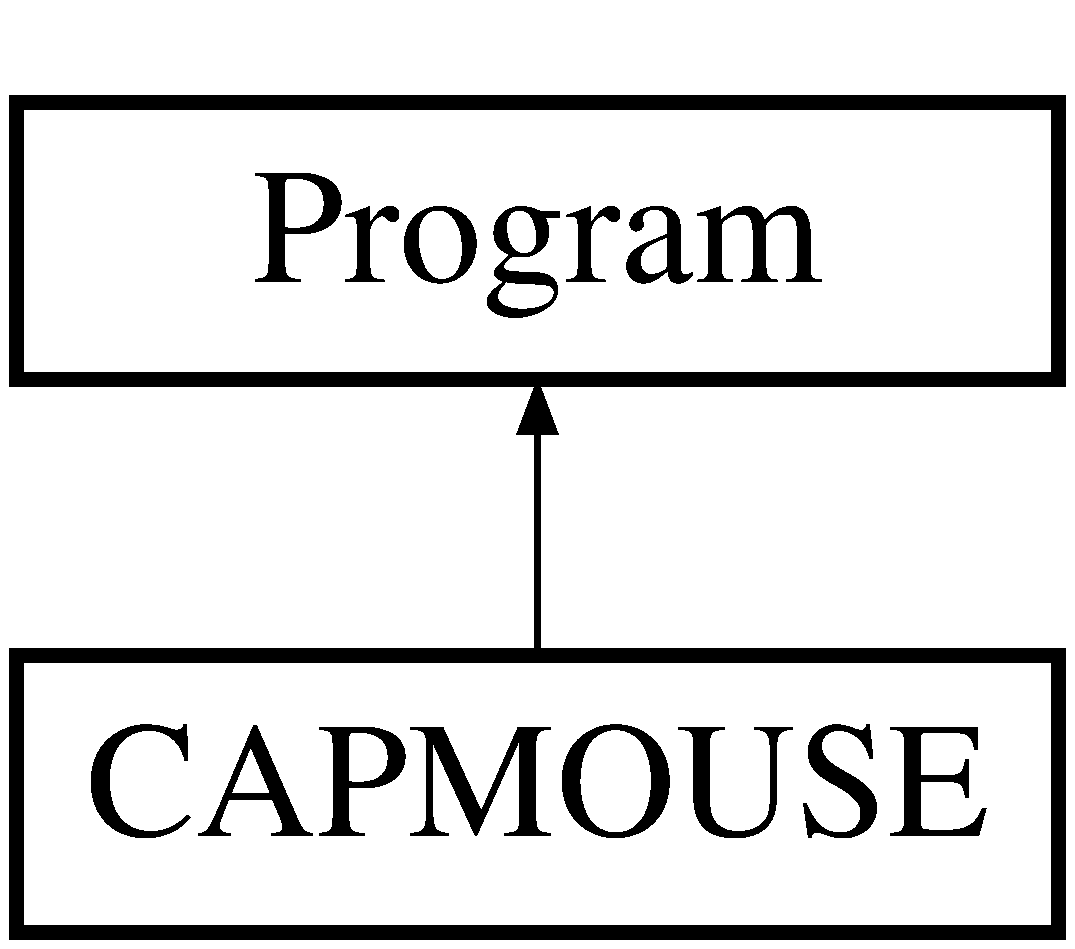
\includegraphics[height=2.000000cm]{classCAPMOUSE}
\end{center}
\end{figure}
\subsection*{Public Member Functions}
\begin{DoxyCompactItemize}
\item 
\hypertarget{classCAPMOUSE_a40f8a87bf9027081766fb5e0fc74149a}{void \hyperlink{classCAPMOUSE_a40f8a87bf9027081766fb5e0fc74149a}{Run} () override}\label{classCAPMOUSE_a40f8a87bf9027081766fb5e0fc74149a}

\begin{DoxyCompactList}\small\item\em \hyperlink{classDOS}{D\-O\-S} kernel \hyperlink{classProgram}{Program} \hyperlink{structSegment}{Segment} Prefix associated with this program at runtime. \end{DoxyCompactList}\end{DoxyCompactItemize}


\subsection{Detailed Description}


Definition at line 4126 of file dos\-\_\-programs.\-cpp.



The documentation for this class was generated from the following file\-:\begin{DoxyCompactItemize}
\item 
src/dos/dos\-\_\-programs.\-cpp\end{DoxyCompactItemize}

\hypertarget{classAdlib_1_1Capture}{\section{Adlib\-:\-:Capture Class Reference}
\label{classAdlib_1_1Capture}\index{Adlib\-::\-Capture@{Adlib\-::\-Capture}}
}
\subsection*{Public Member Functions}
\begin{DoxyCompactItemize}
\item 
\hypertarget{classAdlib_1_1Capture_a2bc4e88dfc7ead50b3cd50fded3cfbaa}{bool {\bfseries Do\-Write} (Bit32u reg\-Full, Bit8u val)}\label{classAdlib_1_1Capture_a2bc4e88dfc7ead50b3cd50fded3cfbaa}

\item 
\hypertarget{classAdlib_1_1Capture_a42d440dbc3803819534a51e9434c8f4e}{{\bfseries Capture} (Register\-Cache $\ast$\-\_\-cache)}\label{classAdlib_1_1Capture_a42d440dbc3803819534a51e9434c8f4e}

\end{DoxyCompactItemize}


\subsection{Detailed Description}


Definition at line 172 of file adlib.\-cpp.



The documentation for this class was generated from the following file\-:\begin{DoxyCompactItemize}
\item 
src/hardware/adlib.\-cpp\end{DoxyCompactItemize}

\hypertarget{classCBind}{\section{C\-Bind Class Reference}
\label{classCBind}\index{C\-Bind@{C\-Bind}}
}


Base C++ class for a binding assigned in the mapper interface (or by default settings)  


Inheritance diagram for C\-Bind\-:\begin{figure}[H]
\begin{center}
\leavevmode
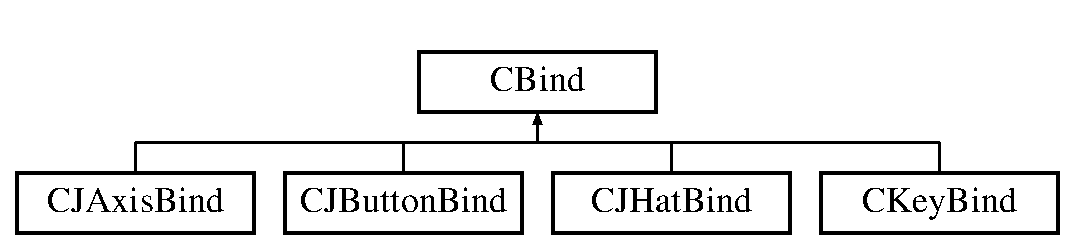
\includegraphics[height=2.000000cm]{classCBind}
\end{center}
\end{figure}
\subsection*{Public Types}
\begin{DoxyCompactItemize}
\item 
enum \hyperlink{classCBind_a6bd04329a3b3b8673f7bd4469f92eb61}{C\-Bind\-Type} \{ {\bfseries bind\-\_\-t} = 0, 
{\bfseries keybind\-\_\-t}
 \}
\begin{DoxyCompactList}\small\item\em Bind class type, for runtime detection. \end{DoxyCompactList}\end{DoxyCompactItemize}
\subsection*{Public Member Functions}
\begin{DoxyCompactItemize}
\item 
\hypertarget{classCBind_a4b69039bdd127345de22a16ef38843e9}{\hyperlink{classCBind_a4b69039bdd127345de22a16ef38843e9}{C\-Bind} (C\-Bind\-List $\ast$\-\_\-list, enum \hyperlink{classCBind_a6bd04329a3b3b8673f7bd4469f92eb61}{C\-Bind\-Type} \-\_\-type=bind\-\_\-t)}\label{classCBind_a4b69039bdd127345de22a16ef38843e9}

\begin{DoxyCompactList}\small\item\em Constructor, to define the binding and type. This constructor adds the \hyperlink{classCBind}{C\-Bind} object itself to the list. \end{DoxyCompactList}\item 
\hypertarget{classCBind_ab383a16224dba3e1963700a8be1f951d}{virtual std\-::string \hyperlink{classCBind_ab383a16224dba3e1963700a8be1f951d}{Get\-Modifier\-Text} (void)}\label{classCBind_ab383a16224dba3e1963700a8be1f951d}

\begin{DoxyCompactList}\small\item\em Get modifier text. \end{DoxyCompactList}\item 
\hypertarget{classCBind_aad93548b92bf6b2bb83eee35b7f15d5d}{virtual std\-::string \hyperlink{classCBind_aad93548b92bf6b2bb83eee35b7f15d5d}{Get\-Bind\-Menu\-Text} (void)}\label{classCBind_aad93548b92bf6b2bb83eee35b7f15d5d}

\begin{DoxyCompactList}\small\item\em Get binding text, for display in the menu item. \end{DoxyCompactList}\item 
\hypertarget{classCBind_aa0773aea4c2324cb3557bf543f8e26de}{void \hyperlink{classCBind_aa0773aea4c2324cb3557bf543f8e26de}{Add\-Flags} (char $\ast$buf)}\label{classCBind_aa0773aea4c2324cb3557bf543f8e26de}

\begin{DoxyCompactList}\small\item\em Append modifier text to a string, for use in recording bindings to the mapper file. \end{DoxyCompactList}\item 
\hypertarget{classCBind_a1ef5657b830e007e1391e3dd2e24bc4e}{void \hyperlink{classCBind_a1ef5657b830e007e1391e3dd2e24bc4e}{Set\-Flags} (char $\ast$buf)}\label{classCBind_a1ef5657b830e007e1391e3dd2e24bc4e}

\begin{DoxyCompactList}\small\item\em Read modifier flags from a string, for use in parsing bindings from the mapper file. \end{DoxyCompactList}\item 
\hypertarget{classCBind_a5df3eeb06c5b662c47a8fa3e104fe6dd}{virtual void \hyperlink{classCBind_a5df3eeb06c5b662c47a8fa3e104fe6dd}{Activate\-Bind} (Bits \-\_\-value, bool ev\-\_\-trigger, bool skip\-\_\-action=false)}\label{classCBind_a5df3eeb06c5b662c47a8fa3e104fe6dd}

\begin{DoxyCompactList}\small\item\em Activate bindings. \end{DoxyCompactList}\item 
\hypertarget{classCBind_a5fcbf42fb58070fd1a81bf892dc73e1c}{void \hyperlink{classCBind_a5fcbf42fb58070fd1a81bf892dc73e1c}{De\-Activate\-Bind} (bool ev\-\_\-trigger)}\label{classCBind_a5fcbf42fb58070fd1a81bf892dc73e1c}

\begin{DoxyCompactList}\small\item\em Deactivate bindings. \end{DoxyCompactList}\item 
\hypertarget{classCBind_a231fb0c4cc20ee05607f1e11b8b1189f}{virtual void \hyperlink{classCBind_a231fb0c4cc20ee05607f1e11b8b1189f}{Config\-Name} (char $\ast$buf)=0}\label{classCBind_a231fb0c4cc20ee05607f1e11b8b1189f}

\begin{DoxyCompactList}\small\item\em Get configuration name, for use in writing the mapper file. \end{DoxyCompactList}\item 
\hypertarget{classCBind_aa9f00238cab696c93603043ca48d456e}{virtual void \hyperlink{classCBind_aa9f00238cab696c93603043ca48d456e}{Bind\-Name} (char $\ast$buf)=0}\label{classCBind_aa9f00238cab696c93603043ca48d456e}

\begin{DoxyCompactList}\small\item\em Get binding name, for display in the mapper U\-I. \end{DoxyCompactList}\end{DoxyCompactItemize}
\subsection*{Public Attributes}
\begin{DoxyCompactItemize}
\item 
\hypertarget{classCBind_a91f9c2be14e33caf50f7be9157e67cc8}{Bitu \hyperlink{classCBind_a91f9c2be14e33caf50f7be9157e67cc8}{mods}}\label{classCBind_a91f9c2be14e33caf50f7be9157e67cc8}

\begin{DoxyCompactList}\small\item\em Modifiers (shift, ctrl, alt) \end{DoxyCompactList}\item 
\hypertarget{classCBind_a3d65630e149aa1df6f84cc78851f4d6c}{Bitu \hyperlink{classCBind_a3d65630e149aa1df6f84cc78851f4d6c}{flags}}\label{classCBind_a3d65630e149aa1df6f84cc78851f4d6c}

\begin{DoxyCompactList}\small\item\em Flags (hold) \end{DoxyCompactList}\item 
\hypertarget{classCBind_afff7b6160648ad63671611c53b1b6a7e}{Bit16s \hyperlink{classCBind_afff7b6160648ad63671611c53b1b6a7e}{value}}\label{classCBind_afff7b6160648ad63671611c53b1b6a7e}

\begin{DoxyCompactList}\small\item\em Binding value (T\-O\-D\-O?) \end{DoxyCompactList}\item 
\hypertarget{classCBind_a5a1677133911a7bc26357f56acc9f4dd}{\hyperlink{classCEvent}{C\-Event} $\ast$ \hyperlink{classCBind_a5a1677133911a7bc26357f56acc9f4dd}{event}}\label{classCBind_a5a1677133911a7bc26357f56acc9f4dd}

\begin{DoxyCompactList}\small\item\em Event object this binding is bound to (for visual U\-I purposes) \end{DoxyCompactList}\item 
\hypertarget{classCBind_a8adfc03bb65f5a8637d2c35c0b604822}{C\-Bind\-List $\ast$ \hyperlink{classCBind_a8adfc03bb65f5a8637d2c35c0b604822}{list}}\label{classCBind_a8adfc03bb65f5a8637d2c35c0b604822}

\begin{DoxyCompactList}\small\item\em List that this object is part of. \end{DoxyCompactList}\item 
\hypertarget{classCBind_ae469e84d9c8d985542ff5a65d6c86810}{bool \hyperlink{classCBind_ae469e84d9c8d985542ff5a65d6c86810}{active}}\label{classCBind_ae469e84d9c8d985542ff5a65d6c86810}

\begin{DoxyCompactList}\small\item\em Active status. \end{DoxyCompactList}\item 
\hypertarget{classCBind_a4a0d6d7650d3a24cc0bc68c985d26ade}{bool \hyperlink{classCBind_a4a0d6d7650d3a24cc0bc68c985d26ade}{holding}}\label{classCBind_a4a0d6d7650d3a24cc0bc68c985d26ade}

\begin{DoxyCompactList}\small\item\em Holding status. \end{DoxyCompactList}\item 
\hypertarget{classCBind_a9e5121ab697c2c56cb20a20bd151ac45}{enum \hyperlink{classCBind_a6bd04329a3b3b8673f7bd4469f92eb61}{C\-Bind\-Type} \hyperlink{classCBind_a9e5121ab697c2c56cb20a20bd151ac45}{type}}\label{classCBind_a9e5121ab697c2c56cb20a20bd151ac45}

\begin{DoxyCompactList}\small\item\em Binding type. \end{DoxyCompactList}\end{DoxyCompactItemize}


\subsection{Detailed Description}
Base C++ class for a binding assigned in the mapper interface (or by default settings) 

Definition at line 502 of file sdl\-\_\-mapper.\-cpp.



The documentation for this class was generated from the following file\-:\begin{DoxyCompactItemize}
\item 
src/gui/sdl\-\_\-mapper.\-cpp\end{DoxyCompactItemize}

\hypertarget{classCBindButton}{\section{C\-Bind\-Button Class Reference}
\label{classCBindButton}\index{C\-Bind\-Button@{C\-Bind\-Button}}
}
Inheritance diagram for C\-Bind\-Button\-:\begin{figure}[H]
\begin{center}
\leavevmode
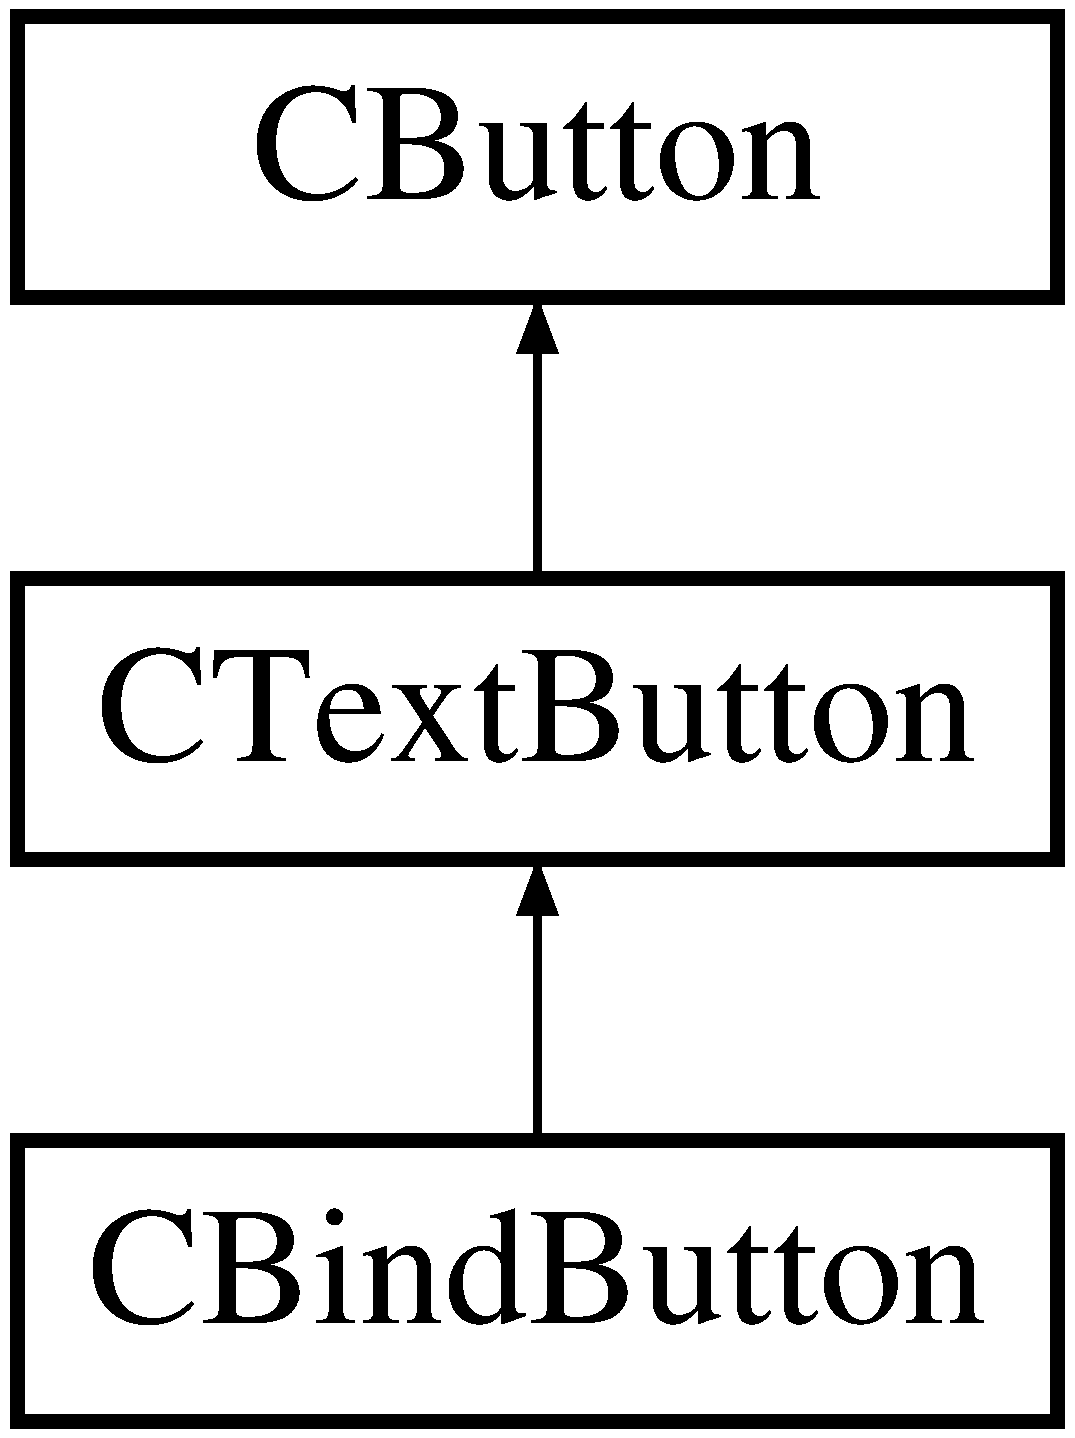
\includegraphics[height=3.000000cm]{classCBindButton}
\end{center}
\end{figure}
\subsection*{Public Member Functions}
\begin{DoxyCompactItemize}
\item 
\hypertarget{classCBindButton_ac88961b71a1666452f4d848f851259d9}{{\bfseries C\-Bind\-Button} (Bitu \-\_\-x, Bitu \-\_\-y, Bitu \-\_\-dx, Bitu \-\_\-dy, const char $\ast$\-\_\-text, B\-B\-\_\-\-Types \-\_\-type)}\label{classCBindButton_ac88961b71a1666452f4d848f851259d9}

\item 
\hypertarget{classCBindButton_a62e84c58b256b4b9f82d6ad1ca32be45}{void {\bfseries Click} (void)}\label{classCBindButton_a62e84c58b256b4b9f82d6ad1ca32be45}

\end{DoxyCompactItemize}
\subsection*{Protected Attributes}
\begin{DoxyCompactItemize}
\item 
\hypertarget{classCBindButton_a6d3fe3711c3f57f5e2ec7a2311408795}{B\-B\-\_\-\-Types {\bfseries type}}\label{classCBindButton_a6d3fe3711c3f57f5e2ec7a2311408795}

\end{DoxyCompactItemize}


\subsection{Detailed Description}


Definition at line 2065 of file sdl\-\_\-mapper.\-cpp.



The documentation for this class was generated from the following file\-:\begin{DoxyCompactItemize}
\item 
src/gui/sdl\-\_\-mapper.\-cpp\end{DoxyCompactItemize}

\hypertarget{classCBindGroup}{\section{C\-Bind\-Group Class Reference}
\label{classCBindGroup}\index{C\-Bind\-Group@{C\-Bind\-Group}}
}
Inheritance diagram for C\-Bind\-Group\-:\begin{figure}[H]
\begin{center}
\leavevmode
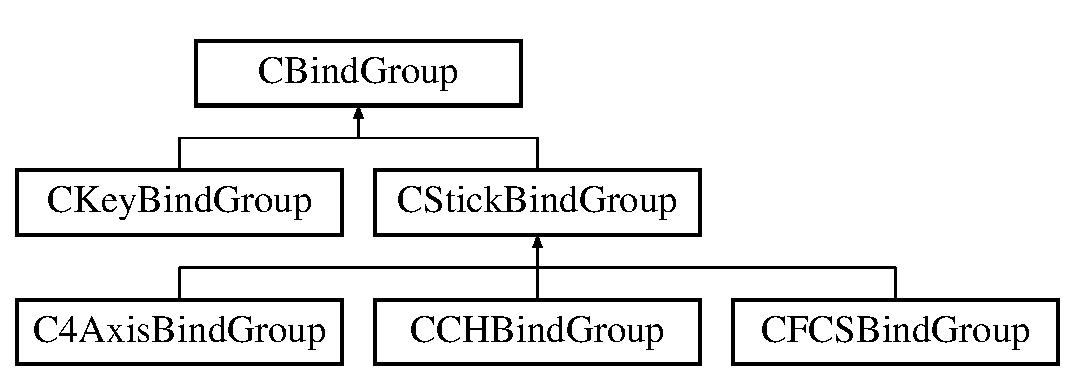
\includegraphics[height=3.000000cm]{classCBindGroup}
\end{center}
\end{figure}
\subsection*{Public Member Functions}
\begin{DoxyCompactItemize}
\item 
\hypertarget{classCBindGroup_a3b5ce6e0f8d7b2305b5038e050126314}{void {\bfseries Activate\-Bind\-List} (C\-Bind\-List $\ast$list, Bits value, bool ev\-\_\-trigger)}\label{classCBindGroup_a3b5ce6e0f8d7b2305b5038e050126314}

\item 
\hypertarget{classCBindGroup_ae60d18174ee4b6c9087ae167aeeb2f12}{void {\bfseries Deactivate\-Bind\-List} (C\-Bind\-List $\ast$list, bool ev\-\_\-trigger)}\label{classCBindGroup_ae60d18174ee4b6c9087ae167aeeb2f12}

\item 
\hypertarget{classCBindGroup_a5a8bf8b22df1d052fc7c3b78b04ffc27}{virtual \hyperlink{classCBind}{C\-Bind} $\ast$ {\bfseries Create\-Config\-Bind} (char $\ast$\&buf)=0}\label{classCBindGroup_a5a8bf8b22df1d052fc7c3b78b04ffc27}

\item 
\hypertarget{classCBindGroup_a716bd1ffed3fb274b87b8c7d99952cdd}{virtual \hyperlink{classCBind}{C\-Bind} $\ast$ {\bfseries Create\-Event\-Bind} (S\-D\-L\-\_\-\-Event $\ast$event)=0}\label{classCBindGroup_a716bd1ffed3fb274b87b8c7d99952cdd}

\item 
\hypertarget{classCBindGroup_abf8f699abfcce73950da882f21d9fbd2}{virtual bool {\bfseries Check\-Event} (S\-D\-L\-\_\-\-Event $\ast$event)=0}\label{classCBindGroup_abf8f699abfcce73950da882f21d9fbd2}

\item 
\hypertarget{classCBindGroup_a197ef5cc8af11acc04667d6838b171c9}{virtual const char $\ast$ {\bfseries Config\-Start} (void)=0}\label{classCBindGroup_a197ef5cc8af11acc04667d6838b171c9}

\item 
\hypertarget{classCBindGroup_a737ef10817e0deb3df1eb83bfa42d838}{virtual const char $\ast$ {\bfseries Bind\-Start} (void)=0}\label{classCBindGroup_a737ef10817e0deb3df1eb83bfa42d838}

\end{DoxyCompactItemize}


\subsection{Detailed Description}


Definition at line 533 of file sdl\-\_\-mapper.\-cpp.



The documentation for this class was generated from the following file\-:\begin{DoxyCompactItemize}
\item 
src/gui/sdl\-\_\-mapper.\-cpp\end{DoxyCompactItemize}

\hypertarget{structCBUS4PORT}{\section{C\-B\-U\-S4\-P\-O\-R\-T Struct Reference}
\label{structCBUS4PORT}\index{C\-B\-U\-S4\-P\-O\-R\-T@{C\-B\-U\-S4\-P\-O\-R\-T}}
}
\subsection*{Public Attributes}
\begin{DoxyCompactItemize}
\item 
\hypertarget{structCBUS4PORT_acdfa7680ca648b64bae4afc5b7ccf8a6}{I\-O\-I\-N\-P {\bfseries inp}}\label{structCBUS4PORT_acdfa7680ca648b64bae4afc5b7ccf8a6}

\item 
\hypertarget{structCBUS4PORT_ad38129fe2ce76c6bd2e1f1e6cd7948b3}{I\-O\-O\-U\-T {\bfseries out}}\label{structCBUS4PORT_ad38129fe2ce76c6bd2e1f1e6cd7948b3}

\end{DoxyCompactItemize}


\subsection{Detailed Description}


Definition at line 111 of file pc98\-\_\-fm.\-cpp.



The documentation for this struct was generated from the following file\-:\begin{DoxyCompactItemize}
\item 
src/hardware/pc98\-\_\-fm.\-cpp\end{DoxyCompactItemize}

\hypertarget{classCButton}{\section{C\-Button Class Reference}
\label{classCButton}\index{C\-Button@{C\-Button}}
}
Inheritance diagram for C\-Button\-:\begin{figure}[H]
\begin{center}
\leavevmode
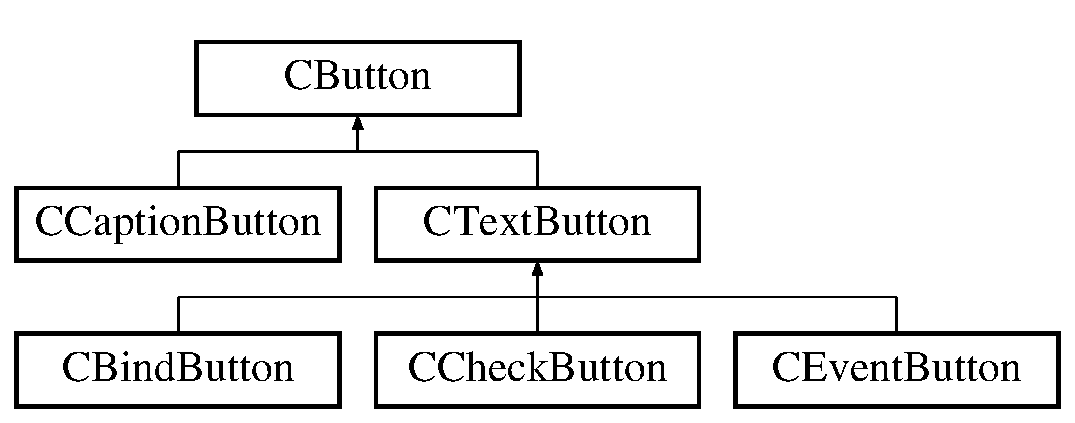
\includegraphics[height=3.000000cm]{classCButton}
\end{center}
\end{figure}
\subsection*{Public Member Functions}
\begin{DoxyCompactItemize}
\item 
\hypertarget{classCButton_acb852749fa38d2484ca1de00df13bcf4}{{\bfseries C\-Button} (Bitu \-\_\-x, Bitu \-\_\-y, Bitu \-\_\-dx, Bitu \-\_\-dy)}\label{classCButton_acb852749fa38d2484ca1de00df13bcf4}

\item 
\hypertarget{classCButton_a78a06b7c9e6994399c993f1af9ee38b8}{virtual void {\bfseries Draw} (void)}\label{classCButton_a78a06b7c9e6994399c993f1af9ee38b8}

\item 
\hypertarget{classCButton_a9eee48a08f92ab14f41d4a62f1bfb1d4}{virtual bool {\bfseries On\-Top} (Bitu \-\_\-x, Bitu \-\_\-y)}\label{classCButton_a9eee48a08f92ab14f41d4a62f1bfb1d4}

\item 
\hypertarget{classCButton_aa31add179ce4c1b0c2efb99cf7da5678}{virtual void {\bfseries Bind\-Color} (void)}\label{classCButton_aa31add179ce4c1b0c2efb99cf7da5678}

\item 
\hypertarget{classCButton_ae56bdd7d3c4fb7e2e1f0634e5dbe1cc7}{virtual void {\bfseries Click} (void)}\label{classCButton_ae56bdd7d3c4fb7e2e1f0634e5dbe1cc7}

\item 
\hypertarget{classCButton_ab1661c655cd9ba77065f7944f89c162c}{void {\bfseries Enable} (bool yes)}\label{classCButton_ab1661c655cd9ba77065f7944f89c162c}

\item 
\hypertarget{classCButton_a44707745a86d060e0891f0d8b55c243a}{void {\bfseries Set\-Invert} (bool inv)}\label{classCButton_a44707745a86d060e0891f0d8b55c243a}

\item 
\hypertarget{classCButton_a3530826dc5f15b557074560e255d6672}{void {\bfseries Set\-Color} (Bit8u \-\_\-col)}\label{classCButton_a3530826dc5f15b557074560e255d6672}

\end{DoxyCompactItemize}
\subsection*{Protected Attributes}
\begin{DoxyCompactItemize}
\item 
\hypertarget{classCButton_a31c9a5bc0e54382407372236ef0fce68}{Bitu {\bfseries x}}\label{classCButton_a31c9a5bc0e54382407372236ef0fce68}

\item 
\hypertarget{classCButton_a6be6467fc0eb283d33caa042c6c2bfbe}{Bitu {\bfseries y}}\label{classCButton_a6be6467fc0eb283d33caa042c6c2bfbe}

\item 
\hypertarget{classCButton_a0d46295304a83ce1a81fc42056ae3959}{Bitu {\bfseries dx}}\label{classCButton_a0d46295304a83ce1a81fc42056ae3959}

\item 
\hypertarget{classCButton_a6bb4df5cec766a3675bf3365927ff45f}{Bitu {\bfseries dy}}\label{classCButton_a6bb4df5cec766a3675bf3365927ff45f}

\item 
\hypertarget{classCButton_acf415cea0b3968f10393d204a0c4f4ec}{Bit8u {\bfseries color}}\label{classCButton_acf415cea0b3968f10393d204a0c4f4ec}

\item 
\hypertarget{classCButton_a34acf521fa23393acf3aa72b627489e6}{Bit8u {\bfseries bkcolor}}\label{classCButton_a34acf521fa23393acf3aa72b627489e6}

\item 
\hypertarget{classCButton_a8b3db5e11eaef4d5b539493abfcf0db9}{bool {\bfseries invert}}\label{classCButton_a8b3db5e11eaef4d5b539493abfcf0db9}

\item 
\hypertarget{classCButton_a4037c6c6e9cce44e38d21c4f87925193}{bool {\bfseries enabled}}\label{classCButton_a4037c6c6e9cce44e38d21c4f87925193}

\end{DoxyCompactItemize}


\subsection{Detailed Description}


Definition at line 1870 of file sdl\-\_\-mapper.\-cpp.



The documentation for this class was generated from the following file\-:\begin{DoxyCompactItemize}
\item 
src/gui/sdl\-\_\-mapper.\-cpp\end{DoxyCompactItemize}

\hypertarget{classCCaptionButton}{\section{C\-Caption\-Button Class Reference}
\label{classCCaptionButton}\index{C\-Caption\-Button@{C\-Caption\-Button}}
}
Inheritance diagram for C\-Caption\-Button\-:\begin{figure}[H]
\begin{center}
\leavevmode
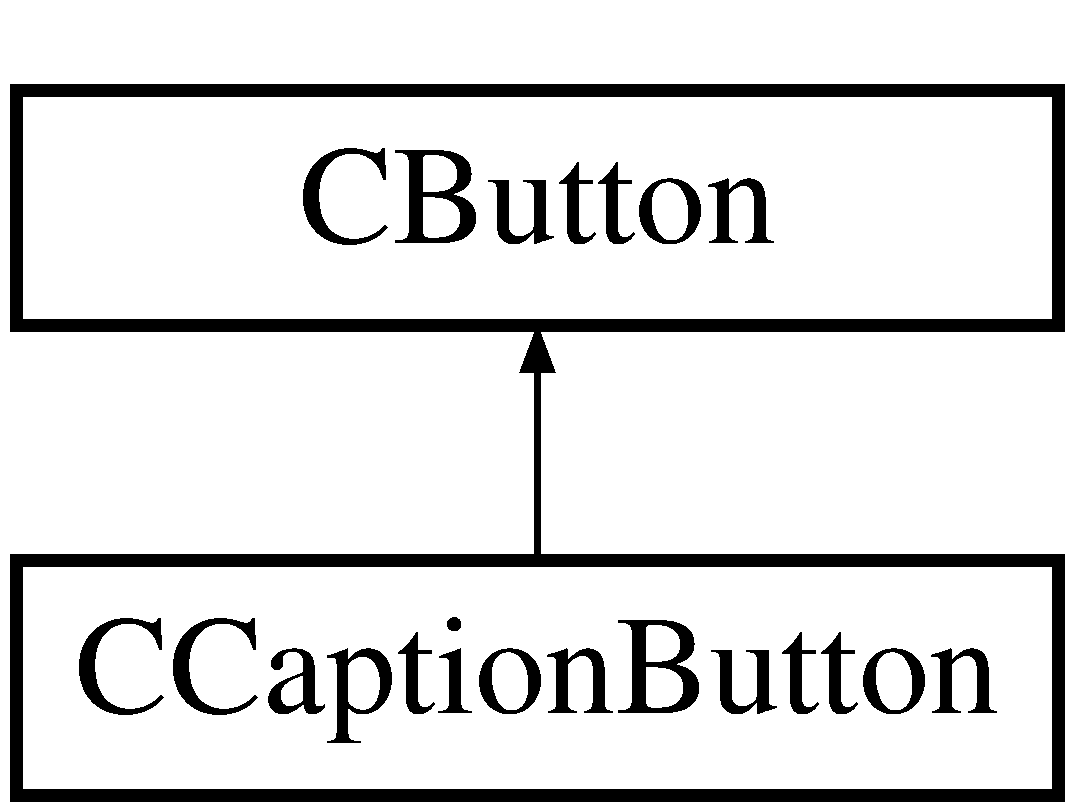
\includegraphics[height=2.000000cm]{classCCaptionButton}
\end{center}
\end{figure}
\subsection*{Public Member Functions}
\begin{DoxyCompactItemize}
\item 
\hypertarget{classCCaptionButton_ab3693869d536d69e5a5c206f22865583}{{\bfseries C\-Caption\-Button} (Bitu \-\_\-x, Bitu \-\_\-y, Bitu \-\_\-dx, Bitu \-\_\-dy)}\label{classCCaptionButton_ab3693869d536d69e5a5c206f22865583}

\item 
\hypertarget{classCCaptionButton_a497661808a80201830f2241f75750e90}{void {\bfseries Change} (const char $\ast$format,...) \hyperlink{structGCC__ATTRIBUTE}{G\-C\-C\-\_\-\-A\-T\-T\-R\-I\-B\-U\-T\-E}(\-\_\-\-\_\-format\-\_\-\-\_\-(\-\_\-\-\_\-printf\-\_\-\-\_\-}\label{classCCaptionButton_a497661808a80201830f2241f75750e90}

\item 
\hypertarget{classCCaptionButton_a953f5b12ba13b61bc373fc3d25295079}{void void {\bfseries Draw} (void)}\label{classCCaptionButton_a953f5b12ba13b61bc373fc3d25295079}

\end{DoxyCompactItemize}
\subsection*{Protected Attributes}
\begin{DoxyCompactItemize}
\item 
\hypertarget{classCCaptionButton_a6e015cc9759137aa04d7c54bd936233b}{char {\bfseries caption} \mbox{[}128\mbox{]}}\label{classCCaptionButton_a6e015cc9759137aa04d7c54bd936233b}

\end{DoxyCompactItemize}


\subsection{Detailed Description}


Definition at line 2041 of file sdl\-\_\-mapper.\-cpp.



The documentation for this class was generated from the following file\-:\begin{DoxyCompactItemize}
\item 
src/gui/sdl\-\_\-mapper.\-cpp\end{DoxyCompactItemize}

\hypertarget{classCCHBindGroup}{\section{C\-C\-H\-Bind\-Group Class Reference}
\label{classCCHBindGroup}\index{C\-C\-H\-Bind\-Group@{C\-C\-H\-Bind\-Group}}
}
Inheritance diagram for C\-C\-H\-Bind\-Group\-:\begin{figure}[H]
\begin{center}
\leavevmode
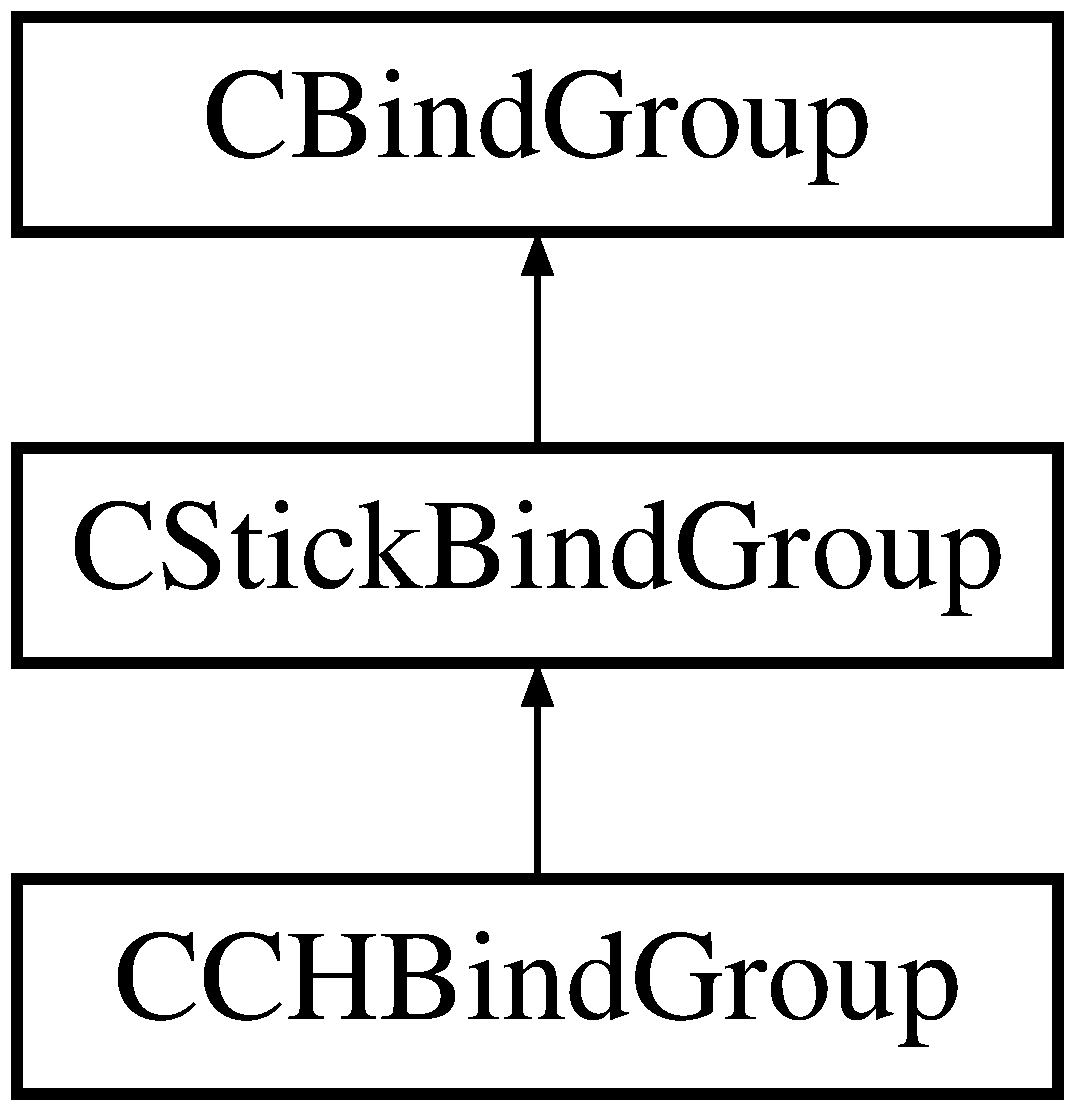
\includegraphics[height=3.000000cm]{classCCHBindGroup}
\end{center}
\end{figure}
\subsection*{Public Member Functions}
\begin{DoxyCompactItemize}
\item 
\hypertarget{classCCHBindGroup_a86bb3a7458f395324aae896cbe02f4dd}{{\bfseries C\-C\-H\-Bind\-Group} (Bitu \-\_\-stick, Bitu \-\_\-emustick)}\label{classCCHBindGroup_a86bb3a7458f395324aae896cbe02f4dd}

\item 
\hypertarget{classCCHBindGroup_a33b9f9ced9bf284c83219c33aa81bfe0}{bool {\bfseries Check\-Event} (S\-D\-L\-\_\-\-Event $\ast$event)}\label{classCCHBindGroup_a33b9f9ced9bf284c83219c33aa81bfe0}

\item 
\hypertarget{classCCHBindGroup_a11232134bcf2b6f8257f8103d34d2a13}{void {\bfseries Update\-Joystick} ()}\label{classCCHBindGroup_a11232134bcf2b6f8257f8103d34d2a13}

\end{DoxyCompactItemize}
\subsection*{Protected Attributes}
\begin{DoxyCompactItemize}
\item 
\hypertarget{classCCHBindGroup_a0d3a52894ed32833a5942a5b0e507c56}{Bit16u {\bfseries button\-\_\-state}}\label{classCCHBindGroup_a0d3a52894ed32833a5942a5b0e507c56}

\end{DoxyCompactItemize}


\subsection{Detailed Description}


Definition at line 1750 of file sdl\-\_\-mapper.\-cpp.



The documentation for this class was generated from the following file\-:\begin{DoxyCompactItemize}
\item 
src/gui/sdl\-\_\-mapper.\-cpp\end{DoxyCompactItemize}

\hypertarget{classCCheckButton}{\section{C\-Check\-Button Class Reference}
\label{classCCheckButton}\index{C\-Check\-Button@{C\-Check\-Button}}
}
Inheritance diagram for C\-Check\-Button\-:\begin{figure}[H]
\begin{center}
\leavevmode
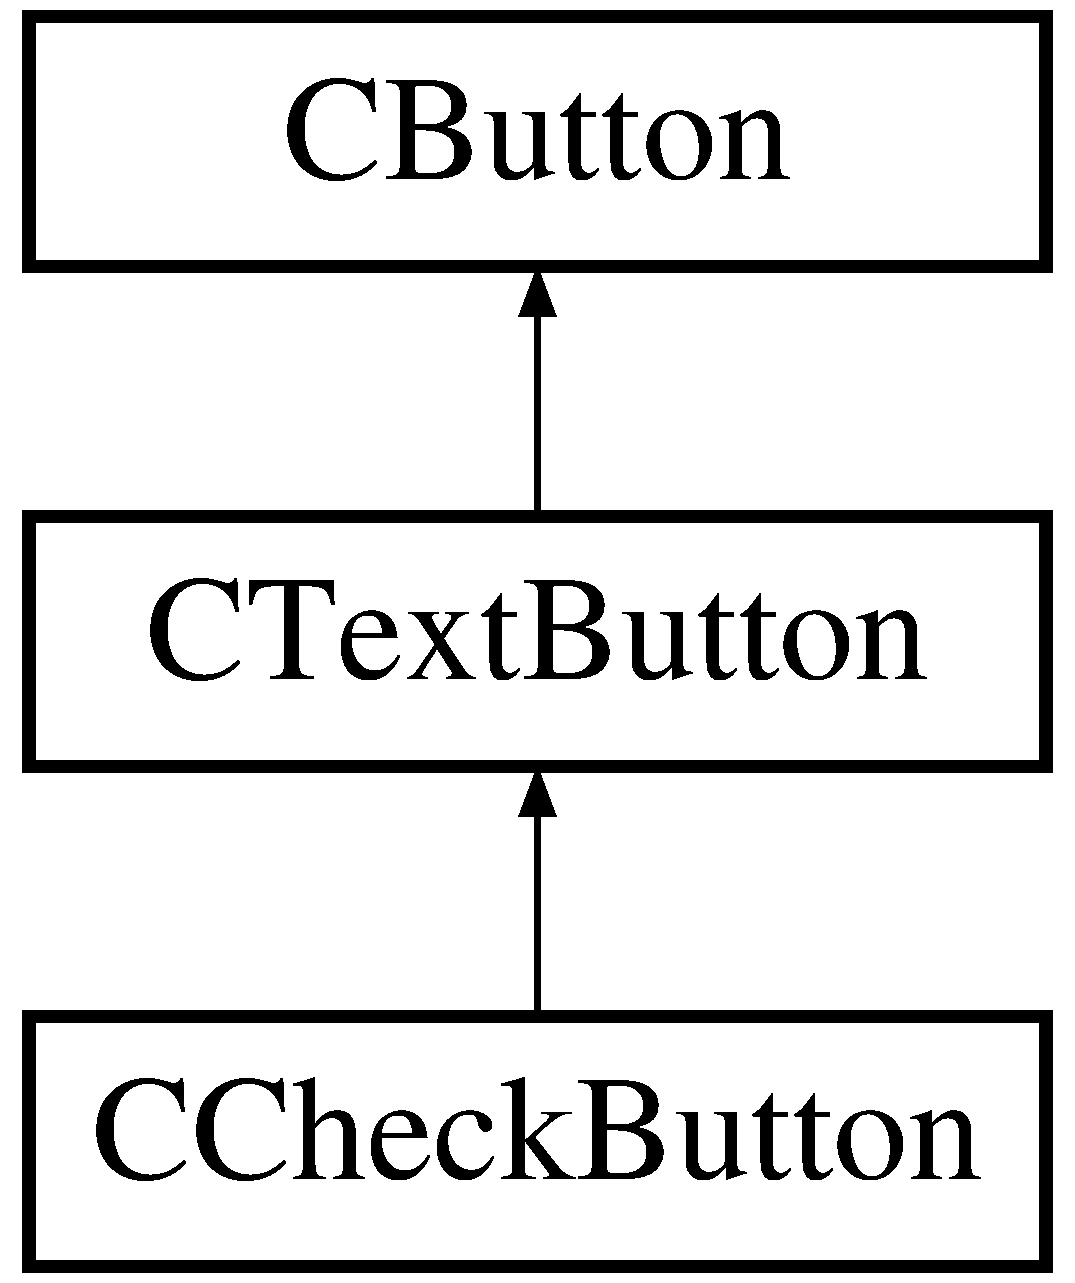
\includegraphics[height=3.000000cm]{classCCheckButton}
\end{center}
\end{figure}
\subsection*{Public Member Functions}
\begin{DoxyCompactItemize}
\item 
\hypertarget{classCCheckButton_a54c679603fea5cb3e04277f6099d2067}{{\bfseries C\-Check\-Button} (Bitu \-\_\-x, Bitu \-\_\-y, Bitu \-\_\-dx, Bitu \-\_\-dy, const char $\ast$\-\_\-text, B\-C\-\_\-\-Types \-\_\-type)}\label{classCCheckButton_a54c679603fea5cb3e04277f6099d2067}

\item 
\hypertarget{classCCheckButton_a1893209408d4822886cd6e39aab69db4}{void {\bfseries Draw} (void)}\label{classCCheckButton_a1893209408d4822886cd6e39aab69db4}

\item 
\hypertarget{classCCheckButton_a5d3d194c8eedc74fbb7862165737833e}{void {\bfseries Click} (void)}\label{classCCheckButton_a5d3d194c8eedc74fbb7862165737833e}

\end{DoxyCompactItemize}
\subsection*{Protected Attributes}
\begin{DoxyCompactItemize}
\item 
\hypertarget{classCCheckButton_a5351f20571c7ed787def47ae73a1820f}{B\-C\-\_\-\-Types {\bfseries type}}\label{classCCheckButton_a5351f20571c7ed787def47ae73a1820f}

\end{DoxyCompactItemize}


\subsection{Detailed Description}


Definition at line 1788 of file sdl\-\_\-mapper.\-cpp.



The documentation for this class was generated from the following file\-:\begin{DoxyCompactItemize}
\item 
src/gui/sdl\-\_\-mapper.\-cpp\end{DoxyCompactItemize}

\hypertarget{classCContinuousEvent}{\section{C\-Continuous\-Event Class Reference}
\label{classCContinuousEvent}\index{C\-Continuous\-Event@{C\-Continuous\-Event}}
}


class for events which have a non-\/boolean state\-: joystick axis movement  


Inheritance diagram for C\-Continuous\-Event\-:\begin{figure}[H]
\begin{center}
\leavevmode
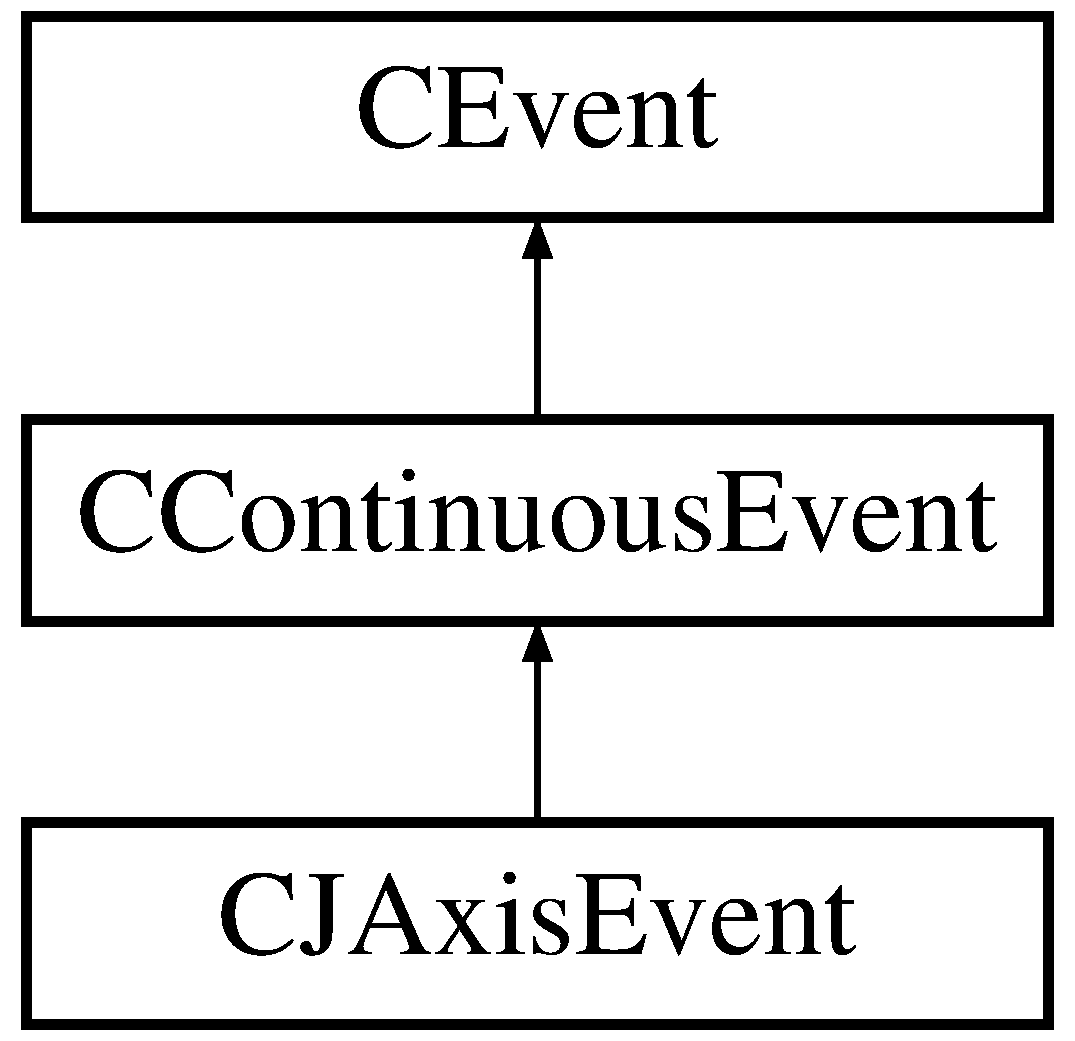
\includegraphics[height=3.000000cm]{classCContinuousEvent}
\end{center}
\end{figure}
\subsection*{Public Member Functions}
\begin{DoxyCompactItemize}
\item 
\hypertarget{classCContinuousEvent_ac998a6e07ae19db1bd6000b26f3b2a56}{\hyperlink{classCContinuousEvent_ac998a6e07ae19db1bd6000b26f3b2a56}{C\-Continuous\-Event} (char const $\ast$const \-\_\-entry)}\label{classCContinuousEvent_ac998a6e07ae19db1bd6000b26f3b2a56}

\begin{DoxyCompactList}\small\item\em Constructor, with event name. \end{DoxyCompactList}\item 
\hypertarget{classCContinuousEvent_a7d1e187b39ea746e8aabf70d7c176d4f}{virtual bool \hyperlink{classCContinuousEvent_a7d1e187b39ea746e8aabf70d7c176d4f}{Is\-Trigger} (void)}\label{classCContinuousEvent_a7d1e187b39ea746e8aabf70d7c176d4f}

\begin{DoxyCompactList}\small\item\em Indicate whether the event is a trigger or continuous input. \end{DoxyCompactList}\item 
\hypertarget{classCContinuousEvent_a3b2815847a046746c02c8a2841aa2bfb}{void \hyperlink{classCContinuousEvent_a3b2815847a046746c02c8a2841aa2bfb}{Activate\-Event} (bool ev\-\_\-trigger, bool skip\-\_\-action)}\label{classCContinuousEvent_a3b2815847a046746c02c8a2841aa2bfb}

\begin{DoxyCompactList}\small\item\em Activate the event, act on it. \end{DoxyCompactList}\item 
\hypertarget{classCContinuousEvent_a025ebb767d3d067f52fb342126627c6d}{void \hyperlink{classCContinuousEvent_a025ebb767d3d067f52fb342126627c6d}{De\-Activate\-Event} (bool ev\-\_\-trigger)}\label{classCContinuousEvent_a025ebb767d3d067f52fb342126627c6d}

\begin{DoxyCompactList}\small\item\em Deactivate the event. \end{DoxyCompactList}\item 
\hypertarget{classCContinuousEvent_a3185a87873f79aea8c23054b55c1ceac}{virtual Bitu \hyperlink{classCContinuousEvent_a3185a87873f79aea8c23054b55c1ceac}{Get\-Activity\-Count} (void)}\label{classCContinuousEvent_a3185a87873f79aea8c23054b55c1ceac}

\begin{DoxyCompactList}\small\item\em Retrieve activity counter. \end{DoxyCompactList}\item 
\hypertarget{classCContinuousEvent_a55ff5be014e082075eaeec0af43a51aa}{virtual void \hyperlink{classCContinuousEvent_a55ff5be014e082075eaeec0af43a51aa}{Repost\-Activity} (void)}\label{classCContinuousEvent_a55ff5be014e082075eaeec0af43a51aa}

\begin{DoxyCompactList}\small\item\em Re-\/post activity. \end{DoxyCompactList}\end{DoxyCompactItemize}


\subsection{Detailed Description}
class for events which have a non-\/boolean state\-: joystick axis movement 

Definition at line 339 of file sdl\-\_\-mapper.\-cpp.



The documentation for this class was generated from the following file\-:\begin{DoxyCompactItemize}
\item 
src/gui/sdl\-\_\-mapper.\-cpp\end{DoxyCompactItemize}

\hypertarget{classCDirect3D}{\section{C\-Direct3\-D Class Reference}
\label{classCDirect3D}\index{C\-Direct3\-D@{C\-Direct3\-D}}
}
\subsection*{Classes}
\begin{DoxyCompactItemize}
\item 
struct {\bfseries T\-L\-V\-E\-R\-T\-E\-X}
\end{DoxyCompactItemize}
\subsection*{Public Member Functions}
\begin{DoxyCompactItemize}
\item 
\hypertarget{classCDirect3D_af7252e1b4e62fad15bd0737efaf1020b}{H\-R\-E\-S\-U\-L\-T {\bfseries Initialize\-D\-X} (H\-W\-N\-D, bool)}\label{classCDirect3D_af7252e1b4e62fad15bd0737efaf1020b}

\item 
\hypertarget{classCDirect3D_aa150a4206bea62e1db00c9a578db92d2}{H\-R\-E\-S\-U\-L\-T {\bfseries Load\-Pixel\-Shader} (const char $\ast$, double, double, bool forced=false)}\label{classCDirect3D_aa150a4206bea62e1db00c9a578db92d2}

\item 
\hypertarget{classCDirect3D_ae478c1f051dac2d351bd1248ad9e7b6e}{H\-R\-E\-S\-U\-L\-T {\bfseries Resize3\-D\-Environment} (Bitu, Bitu, Bitu, Bitu, Bitu, Bitu, bool fullscreen=false)}\label{classCDirect3D_ae478c1f051dac2d351bd1248ad9e7b6e}

\item 
\hypertarget{classCDirect3D_a812efd841357b6eb503d4a98b59dc312}{bool {\bfseries Lock\-Texture} (Bit8u $\ast$\&pixels, Bitu \&pitch)}\label{classCDirect3D_a812efd841357b6eb503d4a98b59dc312}

\item 
\hypertarget{classCDirect3D_aa96cedde54fddd444ddcc594dc5bfb7c}{bool {\bfseries Unlock\-Texture} (const Bit16u $\ast$changed)}\label{classCDirect3D_aa96cedde54fddd444ddcc594dc5bfb7c}

\item 
\hypertarget{classCDirect3D_acf967be6a39166348509f49ef0773747}{{\bfseries C\-Direct3\-D} (Bitu width=640, Bitu height=400)}\label{classCDirect3D_acf967be6a39166348509f49ef0773747}

\item 
\hypertarget{classCDirect3D_aca465f14d712de242b06a743a7cdc37b}{bool {\bfseries get\-Force\-Update} (void)}\label{classCDirect3D_aca465f14d712de242b06a743a7cdc37b}

\end{DoxyCompactItemize}
\subsection*{Public Attributes}
\begin{DoxyCompactItemize}
\item 
\hypertarget{classCDirect3D_a9cc53e0233f977505e05ee041f0caa78}{D\-W\-O\-R\-D {\bfseries dw\-Tex\-Height}}\label{classCDirect3D_a9cc53e0233f977505e05ee041f0caa78}

\item 
\hypertarget{classCDirect3D_a496f302fa81d3b230c5f78be2535ffb2}{D\-W\-O\-R\-D {\bfseries dw\-Tex\-Width}}\label{classCDirect3D_a496f302fa81d3b230c5f78be2535ffb2}

\item 
\hypertarget{classCDirect3D_a761f1a50d5d3c161632325c76ad10ea9}{bool {\bfseries square}}\label{classCDirect3D_a761f1a50d5d3c161632325c76ad10ea9}

\item 
\hypertarget{classCDirect3D_a78a14a9db1e8e6a30586bc0e069ecbaf}{bool {\bfseries pow2}}\label{classCDirect3D_a78a14a9db1e8e6a30586bc0e069ecbaf}

\item 
\hypertarget{classCDirect3D_a49900dc75b6079841da7ef707397af35}{bool {\bfseries dynamic}}\label{classCDirect3D_a49900dc75b6079841da7ef707397af35}

\item 
\hypertarget{classCDirect3D_aa9f4499c1c73595ff5faa5472cb247cd}{bool {\bfseries bpp16}}\label{classCDirect3D_aa9f4499c1c73595ff5faa5472cb247cd}

\item 
\hypertarget{classCDirect3D_a667ec11060e1b35a393aed95c134b1c8}{Bit8s {\bfseries aspect}}\label{classCDirect3D_a667ec11060e1b35a393aed95c134b1c8}

\item 
\hypertarget{classCDirect3D_a181bdf0499756c0ca5a300a34477bbe0}{Bit8s {\bfseries autofit}}\label{classCDirect3D_a181bdf0499756c0ca5a300a34477bbe0}

\item 
\hypertarget{classCDirect3D_af269336b17645f85062a82c545cd460a}{bool {\bfseries ps\-Active}}\label{classCDirect3D_af269336b17645f85062a82c545cd460a}

\end{DoxyCompactItemize}


\subsection{Detailed Description}


Definition at line 75 of file direct3d.\-h.



The documentation for this class was generated from the following file\-:\begin{DoxyCompactItemize}
\item 
src/gui/direct3d.\-h\end{DoxyCompactItemize}

\hypertarget{classCDROM__Interface}{\section{C\-D\-R\-O\-M\-\_\-\-Interface Class Reference}
\label{classCDROM__Interface}\index{C\-D\-R\-O\-M\-\_\-\-Interface@{C\-D\-R\-O\-M\-\_\-\-Interface}}
}


Base C\-D-\/\-R\-O\-M interface class.  




{\ttfamily \#include $<$cdrom.\-h$>$}

Inheritance diagram for C\-D\-R\-O\-M\-\_\-\-Interface\-:\begin{figure}[H]
\begin{center}
\leavevmode
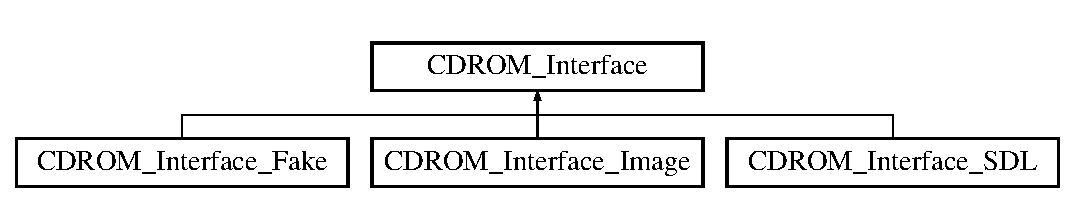
\includegraphics[height=2.000000cm]{classCDROM__Interface}
\end{center}
\end{figure}
\subsection*{Public Member Functions}
\begin{DoxyCompactItemize}
\item 
\hypertarget{classCDROM__Interface_a60081f8d721b4456172f0a0b0d3b3b5a}{virtual bool \hyperlink{classCDROM__Interface_a60081f8d721b4456172f0a0b0d3b3b5a}{Set\-Device} (char $\ast$path, int force\-C\-D)=0}\label{classCDROM__Interface_a60081f8d721b4456172f0a0b0d3b3b5a}

\begin{DoxyCompactList}\small\item\em Set the device associated with this interface, if supported by emulation. \end{DoxyCompactList}\item 
\hypertarget{classCDROM__Interface_a7f2eaeb90673c95fd018ce1ff4f1fdaa}{virtual bool \hyperlink{classCDROM__Interface_a7f2eaeb90673c95fd018ce1ff4f1fdaa}{Get\-U\-P\-C} (unsigned char \&attr, char $\ast$upc)=0}\label{classCDROM__Interface_a7f2eaeb90673c95fd018ce1ff4f1fdaa}

\begin{DoxyCompactList}\small\item\em Get U\-P\-C string from the C\-D-\/\-R\-O\-M. \end{DoxyCompactList}\item 
\hypertarget{classCDROM__Interface_a3d9e5cf2a5812edc31badb6e4a79d51c}{virtual bool \hyperlink{classCDROM__Interface_a3d9e5cf2a5812edc31badb6e4a79d51c}{Get\-Audio\-Tracks} (int \&st\-Track, int \&end, \hyperlink{structSMSF}{T\-M\-S\-F} \&lead\-Out)=0}\label{classCDROM__Interface_a3d9e5cf2a5812edc31badb6e4a79d51c}

\begin{DoxyCompactList}\small\item\em Retrieve start and end tracks and lead out position. \end{DoxyCompactList}\item 
\hypertarget{classCDROM__Interface_adda0f3d505f7cd4bdf762508fc1962fb}{virtual bool \hyperlink{classCDROM__Interface_adda0f3d505f7cd4bdf762508fc1962fb}{Get\-Audio\-Track\-Info} (int track, \hyperlink{structSMSF}{T\-M\-S\-F} \&start, unsigned char \&attr)=0}\label{classCDROM__Interface_adda0f3d505f7cd4bdf762508fc1962fb}

\begin{DoxyCompactList}\small\item\em Retrieve start and attributes for a specific track. \end{DoxyCompactList}\item 
\hypertarget{classCDROM__Interface_a2028b67399e88e5ce1ea1d18a1db75fb}{virtual bool \hyperlink{classCDROM__Interface_a2028b67399e88e5ce1ea1d18a1db75fb}{Get\-Audio\-Sub} (unsigned char \&attr, unsigned char \&track, unsigned char \&index, \hyperlink{structSMSF}{T\-M\-S\-F} \&rel\-Pos, \hyperlink{structSMSF}{T\-M\-S\-F} \&abs\-Pos)=0}\label{classCDROM__Interface_a2028b67399e88e5ce1ea1d18a1db75fb}

\begin{DoxyCompactList}\small\item\em Get subchannel data of the sectors at the current position, and retrieve current position. \end{DoxyCompactList}\item 
\hypertarget{classCDROM__Interface_a5f5e3fd21c495a0a4f55e79b18b69729}{virtual bool \hyperlink{classCDROM__Interface_a5f5e3fd21c495a0a4f55e79b18b69729}{Get\-Audio\-Status} (bool \&playing, bool \&pause)=0}\label{classCDROM__Interface_a5f5e3fd21c495a0a4f55e79b18b69729}

\begin{DoxyCompactList}\small\item\em Get audio playback status. \end{DoxyCompactList}\item 
\hypertarget{classCDROM__Interface_a3891396e99454752aafc695813e495e8}{virtual bool \hyperlink{classCDROM__Interface_a3891396e99454752aafc695813e495e8}{Get\-Media\-Tray\-Status} (bool \&media\-Present, bool \&media\-Changed, bool \&tray\-Open)=0}\label{classCDROM__Interface_a3891396e99454752aafc695813e495e8}

\begin{DoxyCompactList}\small\item\em Get media tray status. \end{DoxyCompactList}\item 
\hypertarget{classCDROM__Interface_a9a90d8036bb0fccc17b147dfab6ad26f}{virtual bool \hyperlink{classCDROM__Interface_a9a90d8036bb0fccc17b147dfab6ad26f}{Play\-Audio\-Sector} (unsigned long start, unsigned long len)=0}\label{classCDROM__Interface_a9a90d8036bb0fccc17b147dfab6ad26f}

\begin{DoxyCompactList}\small\item\em Initiate audio playback starting at sector and for how many. \end{DoxyCompactList}\item 
\hypertarget{classCDROM__Interface_a811af8ad77b46c975473abd8aaa48f48}{virtual bool \hyperlink{classCDROM__Interface_a811af8ad77b46c975473abd8aaa48f48}{Pause\-Audio} (bool resume)=0}\label{classCDROM__Interface_a811af8ad77b46c975473abd8aaa48f48}

\begin{DoxyCompactList}\small\item\em Pause audio playback. \end{DoxyCompactList}\item 
\hypertarget{classCDROM__Interface_ac16f2f2a5f081fbd1ace3ae6af34b7c3}{virtual bool \hyperlink{classCDROM__Interface_ac16f2f2a5f081fbd1ace3ae6af34b7c3}{Stop\-Audio} (void)=0}\label{classCDROM__Interface_ac16f2f2a5f081fbd1ace3ae6af34b7c3}

\begin{DoxyCompactList}\small\item\em Stop audio playback. \end{DoxyCompactList}\item 
\hypertarget{classCDROM__Interface_a7ad6149099c04af804e543613e69d9bd}{virtual void \hyperlink{classCDROM__Interface_a7ad6149099c04af804e543613e69d9bd}{Channel\-Control} (\hyperlink{structSCtrl}{T\-Ctrl} ctrl)=0}\label{classCDROM__Interface_a7ad6149099c04af804e543613e69d9bd}

\begin{DoxyCompactList}\small\item\em Set channel control data (T\-O\-D\-O\-: clarify) \end{DoxyCompactList}\item 
\hypertarget{classCDROM__Interface_afb4989b5b1881a03123442adddcfa6d7}{virtual bool \hyperlink{classCDROM__Interface_afb4989b5b1881a03123442adddcfa6d7}{Read\-Sectors} (Phys\-Pt buffer, bool raw, unsigned long sector, unsigned long num)=0}\label{classCDROM__Interface_afb4989b5b1881a03123442adddcfa6d7}

\begin{DoxyCompactList}\small\item\em Read sector data into guest memory. \end{DoxyCompactList}\item 
\hypertarget{classCDROM__Interface_ae056d63e7b104c7a05afc7c68ee34718}{virtual bool \hyperlink{classCDROM__Interface_ae056d63e7b104c7a05afc7c68ee34718}{Read\-Sectors\-Host} (void $\ast$buffer, bool raw, unsigned long sector, unsigned long num)=0}\label{classCDROM__Interface_ae056d63e7b104c7a05afc7c68ee34718}

\begin{DoxyCompactList}\small\item\em Read sector data into host memory (for I\-D\-E emulation) \end{DoxyCompactList}\item 
\hypertarget{classCDROM__Interface_a5d52a31065d3b87924c5d059266fd20e}{virtual bool \hyperlink{classCDROM__Interface_a5d52a31065d3b87924c5d059266fd20e}{Load\-Unload\-Media} (bool unload)=0}\label{classCDROM__Interface_a5d52a31065d3b87924c5d059266fd20e}

\begin{DoxyCompactList}\small\item\em Load (close/spin up) or unload (eject/spin down) media. \end{DoxyCompactList}\item 
\hypertarget{classCDROM__Interface_a688bdeb135e3238178883666c34aaa75}{virtual void \hyperlink{classCDROM__Interface_a688bdeb135e3238178883666c34aaa75}{Init\-New\-Media} (void)}\label{classCDROM__Interface_a688bdeb135e3238178883666c34aaa75}

\begin{DoxyCompactList}\small\item\em T\-O\-D\-O? \end{DoxyCompactList}\end{DoxyCompactItemize}


\subsection{Detailed Description}
Base C\-D-\/\-R\-O\-M interface class. 

This provides the base C++ class for a C\-D-\/\-R\-O\-M interface in C\-D-\/\-R\-O\-M emulation 

Definition at line 84 of file cdrom.\-h.



The documentation for this class was generated from the following file\-:\begin{DoxyCompactItemize}
\item 
src/dos/cdrom.\-h\end{DoxyCompactItemize}

\hypertarget{classCDROM__Interface__Fake}{\section{C\-D\-R\-O\-M\-\_\-\-Interface\-\_\-\-Fake Class Reference}
\label{classCDROM__Interface__Fake}\index{C\-D\-R\-O\-M\-\_\-\-Interface\-\_\-\-Fake@{C\-D\-R\-O\-M\-\_\-\-Interface\-\_\-\-Fake}}
}
Inheritance diagram for C\-D\-R\-O\-M\-\_\-\-Interface\-\_\-\-Fake\-:\begin{figure}[H]
\begin{center}
\leavevmode
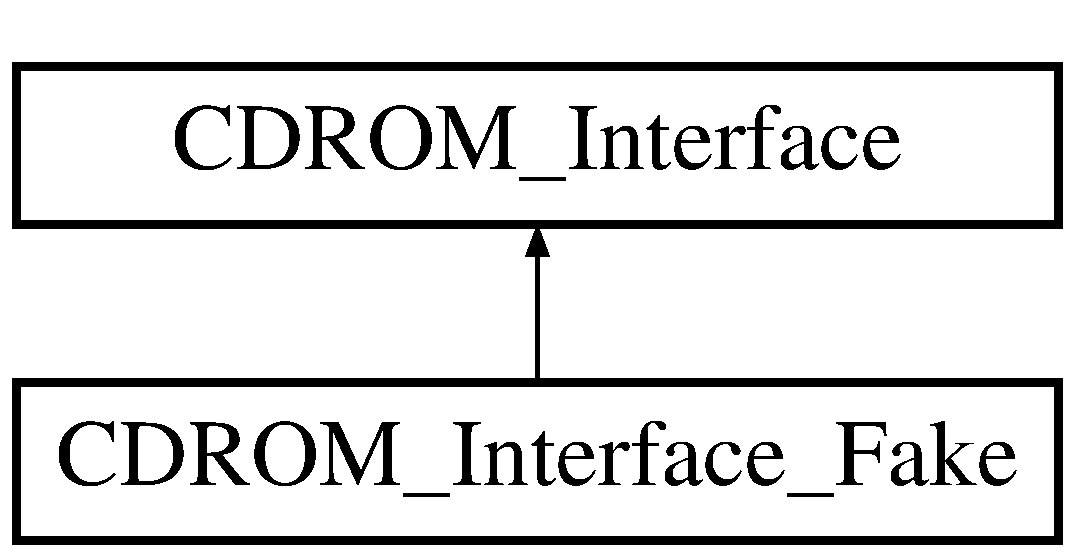
\includegraphics[height=2.000000cm]{classCDROM__Interface__Fake}
\end{center}
\end{figure}
\subsection*{Public Member Functions}
\begin{DoxyCompactItemize}
\item 
\hypertarget{classCDROM__Interface__Fake_a344218a4e5ac24ad7ea549a6440e9e19}{bool {\bfseries Set\-Device} (char $\ast$, int)}\label{classCDROM__Interface__Fake_a344218a4e5ac24ad7ea549a6440e9e19}

\item 
\hypertarget{classCDROM__Interface__Fake_a3304c3e7cd241800d4bcba5faf888f96}{bool {\bfseries Get\-U\-P\-C} (unsigned char \&attr, char $\ast$upc)}\label{classCDROM__Interface__Fake_a3304c3e7cd241800d4bcba5faf888f96}

\item 
\hypertarget{classCDROM__Interface__Fake_a14881cfccb40e1cd1e00293a43ede7cd}{bool {\bfseries Get\-Audio\-Tracks} (int \&st\-Track, int \&end, \hyperlink{structSMSF}{T\-M\-S\-F} \&lead\-Out)}\label{classCDROM__Interface__Fake_a14881cfccb40e1cd1e00293a43ede7cd}

\item 
\hypertarget{classCDROM__Interface__Fake_a13b02db8a3ee1fd99124d5dfd5508021}{bool {\bfseries Get\-Audio\-Track\-Info} (int track, \hyperlink{structSMSF}{T\-M\-S\-F} \&start, unsigned char \&attr)}\label{classCDROM__Interface__Fake_a13b02db8a3ee1fd99124d5dfd5508021}

\item 
\hypertarget{classCDROM__Interface__Fake_a28034819e3365729f6bdef40c4cf940a}{bool {\bfseries Get\-Audio\-Sub} (unsigned char \&attr, unsigned char \&track, unsigned char \&index, \hyperlink{structSMSF}{T\-M\-S\-F} \&rel\-Pos, \hyperlink{structSMSF}{T\-M\-S\-F} \&abs\-Pos)}\label{classCDROM__Interface__Fake_a28034819e3365729f6bdef40c4cf940a}

\item 
\hypertarget{classCDROM__Interface__Fake_a600834e869be578a320c719b26ab2e93}{bool {\bfseries Get\-Audio\-Status} (bool \&playing, bool \&pause)}\label{classCDROM__Interface__Fake_a600834e869be578a320c719b26ab2e93}

\item 
\hypertarget{classCDROM__Interface__Fake_a97677cbe31ed7fb3f777fcaa7307bcba}{bool {\bfseries Get\-Media\-Tray\-Status} (bool \&media\-Present, bool \&media\-Changed, bool \&tray\-Open)}\label{classCDROM__Interface__Fake_a97677cbe31ed7fb3f777fcaa7307bcba}

\item 
\hypertarget{classCDROM__Interface__Fake_a6b8236c5041698ebcf1c136aeebde117}{bool {\bfseries Play\-Audio\-Sector} (unsigned long, unsigned long)}\label{classCDROM__Interface__Fake_a6b8236c5041698ebcf1c136aeebde117}

\item 
\hypertarget{classCDROM__Interface__Fake_a9fa2dfc2b09b1a91ce607d54636a9ce5}{bool {\bfseries Pause\-Audio} (bool)}\label{classCDROM__Interface__Fake_a9fa2dfc2b09b1a91ce607d54636a9ce5}

\item 
\hypertarget{classCDROM__Interface__Fake_a2ef5025cac6123dc9abb7ac35797c7b1}{bool {\bfseries Stop\-Audio} (void)}\label{classCDROM__Interface__Fake_a2ef5025cac6123dc9abb7ac35797c7b1}

\item 
\hypertarget{classCDROM__Interface__Fake_ac967a7a0cb63fcff3756df64a70ab75d}{void {\bfseries Channel\-Control} (\hyperlink{structSCtrl}{T\-Ctrl} ctrl)}\label{classCDROM__Interface__Fake_ac967a7a0cb63fcff3756df64a70ab75d}

\item 
\hypertarget{classCDROM__Interface__Fake_a9370d0f056300f877bc0b4174e00015c}{bool {\bfseries Read\-Sectors} (Phys\-Pt, bool, unsigned long, unsigned long)}\label{classCDROM__Interface__Fake_a9370d0f056300f877bc0b4174e00015c}

\item 
\hypertarget{classCDROM__Interface__Fake_aafcfe3998571eeef207deb0cbe18e9ba}{bool {\bfseries Read\-Sectors\-Host} (void $\ast$buffer, bool raw, unsigned long sector, unsigned long num)}\label{classCDROM__Interface__Fake_aafcfe3998571eeef207deb0cbe18e9ba}

\item 
\hypertarget{classCDROM__Interface__Fake_ab0b585769fd626ad3af41bb8cf876fdb}{bool {\bfseries Load\-Unload\-Media} (bool)}\label{classCDROM__Interface__Fake_ab0b585769fd626ad3af41bb8cf876fdb}

\end{DoxyCompactItemize}


\subsection{Detailed Description}


Definition at line 136 of file cdrom.\-h.



The documentation for this class was generated from the following files\-:\begin{DoxyCompactItemize}
\item 
src/dos/cdrom.\-h\item 
src/dos/cdrom.\-cpp\end{DoxyCompactItemize}

\hypertarget{classCDROM__Interface__Image}{\section{C\-D\-R\-O\-M\-\_\-\-Interface\-\_\-\-Image Class Reference}
\label{classCDROM__Interface__Image}\index{C\-D\-R\-O\-M\-\_\-\-Interface\-\_\-\-Image@{C\-D\-R\-O\-M\-\_\-\-Interface\-\_\-\-Image}}
}


Image C\-D-\/\-R\-O\-M interface.  




{\ttfamily \#include $<$cdrom.\-h$>$}

Inheritance diagram for C\-D\-R\-O\-M\-\_\-\-Interface\-\_\-\-Image\-:\begin{figure}[H]
\begin{center}
\leavevmode
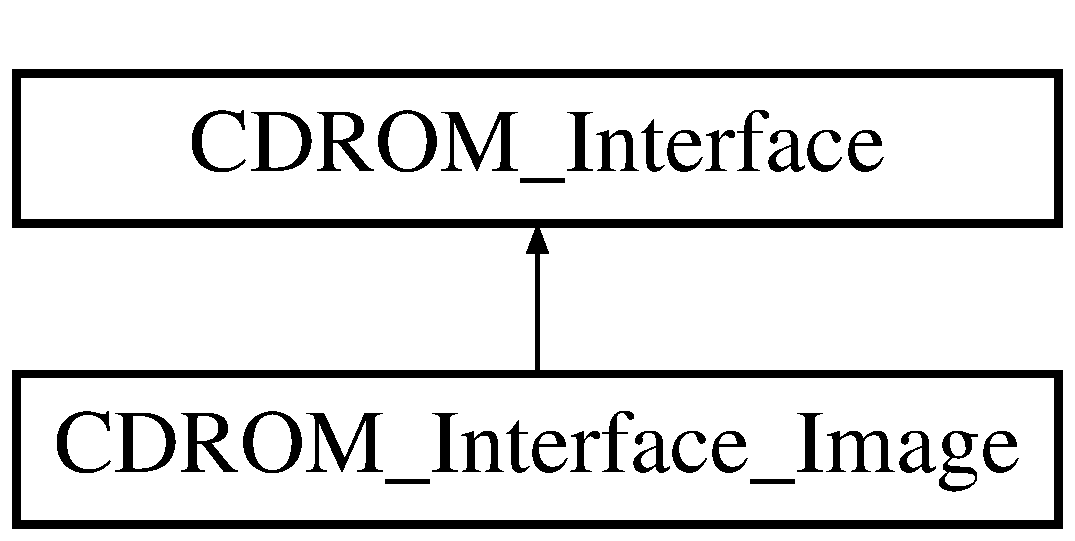
\includegraphics[height=2.000000cm]{classCDROM__Interface__Image}
\end{center}
\end{figure}
\subsection*{Classes}
\begin{DoxyCompactItemize}
\item 
class {\bfseries Binary\-File}
\begin{DoxyCompactList}\small\item\em Binary file reader for the image. \end{DoxyCompactList}\item 
struct {\bfseries image\-Player}
\begin{DoxyCompactList}\small\item\em Virtual C\-D audio \char`\"{}player\char`\"{}. \end{DoxyCompactList}\item 
struct {\bfseries Track}
\begin{DoxyCompactList}\small\item\em C\-D-\/\-R\-O\-M track definition. \end{DoxyCompactList}\item 
class {\bfseries Track\-File}
\begin{DoxyCompactList}\small\item\em Base C++ class for reading the image. \end{DoxyCompactList}\end{DoxyCompactItemize}
\subsection*{Public Member Functions}
\begin{DoxyCompactItemize}
\item 
\hypertarget{classCDROM__Interface__Image_acecb6b00f509aba4e203b7bb5c4653fb}{\hyperlink{classCDROM__Interface__Image_acecb6b00f509aba4e203b7bb5c4653fb}{C\-D\-R\-O\-M\-\_\-\-Interface\-\_\-\-Image} (Bit8u sub\-Unit)}\label{classCDROM__Interface__Image_acecb6b00f509aba4e203b7bb5c4653fb}

\begin{DoxyCompactList}\small\item\em Constructor, with parameter for subunit. \end{DoxyCompactList}\item 
\hypertarget{classCDROM__Interface__Image_a8b1323ddfae9e59fae8fa5d8f862c8c4}{void \hyperlink{classCDROM__Interface__Image_a8b1323ddfae9e59fae8fa5d8f862c8c4}{Init\-New\-Media} (void)}\label{classCDROM__Interface__Image_a8b1323ddfae9e59fae8fa5d8f862c8c4}

\begin{DoxyCompactList}\small\item\em T\-O\-D\-O? \end{DoxyCompactList}\item 
\hypertarget{classCDROM__Interface__Image_ae803cb47966de3b637c55c40aaf89e78}{bool \hyperlink{classCDROM__Interface__Image_ae803cb47966de3b637c55c40aaf89e78}{Set\-Device} (char $\ast$path, int force\-C\-D)}\label{classCDROM__Interface__Image_ae803cb47966de3b637c55c40aaf89e78}

\begin{DoxyCompactList}\small\item\em Set the device associated with this interface, if supported by emulation. \end{DoxyCompactList}\item 
\hypertarget{classCDROM__Interface__Image_a0f4704db65cd97e70da4ee7464e535b0}{bool \hyperlink{classCDROM__Interface__Image_a0f4704db65cd97e70da4ee7464e535b0}{Get\-U\-P\-C} (unsigned char \&attr, char $\ast$upc)}\label{classCDROM__Interface__Image_a0f4704db65cd97e70da4ee7464e535b0}

\begin{DoxyCompactList}\small\item\em Get U\-P\-C string from the C\-D-\/\-R\-O\-M. \end{DoxyCompactList}\item 
\hypertarget{classCDROM__Interface__Image_a4aae5ec2ba0011a4f2281bb312aa49c3}{bool \hyperlink{classCDROM__Interface__Image_a4aae5ec2ba0011a4f2281bb312aa49c3}{Get\-Audio\-Tracks} (int \&st\-Track, int \&end, \hyperlink{structSMSF}{T\-M\-S\-F} \&lead\-Out)}\label{classCDROM__Interface__Image_a4aae5ec2ba0011a4f2281bb312aa49c3}

\begin{DoxyCompactList}\small\item\em Retrieve start and end tracks and lead out position. \end{DoxyCompactList}\item 
\hypertarget{classCDROM__Interface__Image_a1a1c42c11d483e82f41c6012f5f7d602}{bool \hyperlink{classCDROM__Interface__Image_a1a1c42c11d483e82f41c6012f5f7d602}{Get\-Audio\-Track\-Info} (int track, \hyperlink{structSMSF}{T\-M\-S\-F} \&start, unsigned char \&attr)}\label{classCDROM__Interface__Image_a1a1c42c11d483e82f41c6012f5f7d602}

\begin{DoxyCompactList}\small\item\em Retrieve start and attributes for a specific track. \end{DoxyCompactList}\item 
\hypertarget{classCDROM__Interface__Image_a11ba4965b5dd42015aff3d9f4b607abc}{bool \hyperlink{classCDROM__Interface__Image_a11ba4965b5dd42015aff3d9f4b607abc}{Get\-Audio\-Sub} (unsigned char \&attr, unsigned char \&track, unsigned char \&index, \hyperlink{structSMSF}{T\-M\-S\-F} \&rel\-Pos, \hyperlink{structSMSF}{T\-M\-S\-F} \&abs\-Pos)}\label{classCDROM__Interface__Image_a11ba4965b5dd42015aff3d9f4b607abc}

\begin{DoxyCompactList}\small\item\em Get subchannel data of the sectors at the current position, and retrieve current position. \end{DoxyCompactList}\item 
\hypertarget{classCDROM__Interface__Image_a5151e50027294571fafb414d751ca332}{bool \hyperlink{classCDROM__Interface__Image_a5151e50027294571fafb414d751ca332}{Get\-Audio\-Status} (bool \&playing, bool \&pause)}\label{classCDROM__Interface__Image_a5151e50027294571fafb414d751ca332}

\begin{DoxyCompactList}\small\item\em Get audio playback status. \end{DoxyCompactList}\item 
\hypertarget{classCDROM__Interface__Image_a8c5afdabeea94743f487fae4623eacac}{bool \hyperlink{classCDROM__Interface__Image_a8c5afdabeea94743f487fae4623eacac}{Get\-Media\-Tray\-Status} (bool \&media\-Present, bool \&media\-Changed, bool \&tray\-Open)}\label{classCDROM__Interface__Image_a8c5afdabeea94743f487fae4623eacac}

\begin{DoxyCompactList}\small\item\em Get media tray status. \end{DoxyCompactList}\item 
\hypertarget{classCDROM__Interface__Image_afbb8b5443be56ba92b5a1287ba95f913}{bool \hyperlink{classCDROM__Interface__Image_afbb8b5443be56ba92b5a1287ba95f913}{Play\-Audio\-Sector} (unsigned long start, unsigned long len)}\label{classCDROM__Interface__Image_afbb8b5443be56ba92b5a1287ba95f913}

\begin{DoxyCompactList}\small\item\em Initiate audio playback starting at sector and for how many. \end{DoxyCompactList}\item 
\hypertarget{classCDROM__Interface__Image_ac74be8f64002ccf76b65c2fbd03077bd}{bool \hyperlink{classCDROM__Interface__Image_ac74be8f64002ccf76b65c2fbd03077bd}{Pause\-Audio} (bool resume)}\label{classCDROM__Interface__Image_ac74be8f64002ccf76b65c2fbd03077bd}

\begin{DoxyCompactList}\small\item\em Pause audio playback. \end{DoxyCompactList}\item 
\hypertarget{classCDROM__Interface__Image_a4a0af2e1be4fcb87e125b9d3e7aca327}{bool \hyperlink{classCDROM__Interface__Image_a4a0af2e1be4fcb87e125b9d3e7aca327}{Stop\-Audio} (void)}\label{classCDROM__Interface__Image_a4a0af2e1be4fcb87e125b9d3e7aca327}

\begin{DoxyCompactList}\small\item\em Stop audio playback. \end{DoxyCompactList}\item 
\hypertarget{classCDROM__Interface__Image_a6759cd7741be28cb61dd9903712edca1}{void \hyperlink{classCDROM__Interface__Image_a6759cd7741be28cb61dd9903712edca1}{Channel\-Control} (\hyperlink{structSCtrl}{T\-Ctrl} ctrl)}\label{classCDROM__Interface__Image_a6759cd7741be28cb61dd9903712edca1}

\begin{DoxyCompactList}\small\item\em Set channel control data (T\-O\-D\-O\-: clarify) \end{DoxyCompactList}\item 
\hypertarget{classCDROM__Interface__Image_a5121d2e82267d529bc462cecdac36791}{bool \hyperlink{classCDROM__Interface__Image_a5121d2e82267d529bc462cecdac36791}{Read\-Sectors} (Phys\-Pt buffer, bool raw, unsigned long sector, unsigned long num)}\label{classCDROM__Interface__Image_a5121d2e82267d529bc462cecdac36791}

\begin{DoxyCompactList}\small\item\em Read sector data into guest memory. \end{DoxyCompactList}\item 
\hypertarget{classCDROM__Interface__Image_ae686caa17e265089d6cd1a69ecc5b332}{bool \hyperlink{classCDROM__Interface__Image_ae686caa17e265089d6cd1a69ecc5b332}{Read\-Sectors\-Host} (void $\ast$buffer, bool raw, unsigned long sector, unsigned long num)}\label{classCDROM__Interface__Image_ae686caa17e265089d6cd1a69ecc5b332}

\begin{DoxyCompactList}\small\item\em Read sector data into host memory (for I\-D\-E emulation) \end{DoxyCompactList}\item 
\hypertarget{classCDROM__Interface__Image_af5aa7f94de1d7c77ff6b484b380c5351}{bool \hyperlink{classCDROM__Interface__Image_af5aa7f94de1d7c77ff6b484b380c5351}{Load\-Unload\-Media} (bool unload)}\label{classCDROM__Interface__Image_af5aa7f94de1d7c77ff6b484b380c5351}

\begin{DoxyCompactList}\small\item\em Load (close/spin up) or unload (eject/spin down) media. \end{DoxyCompactList}\item 
\hypertarget{classCDROM__Interface__Image_acbed60c6b06009b2a027d605190ee842}{bool \hyperlink{classCDROM__Interface__Image_acbed60c6b06009b2a027d605190ee842}{Read\-Sector} (Bit8u $\ast$buffer, bool raw, unsigned long sector)}\label{classCDROM__Interface__Image_acbed60c6b06009b2a027d605190ee842}

\begin{DoxyCompactList}\small\item\em Sector read (one sector), where the image decoding is done. \end{DoxyCompactList}\item 
\hypertarget{classCDROM__Interface__Image_a7348536d197510d1442419f2aa172ccc}{bool \hyperlink{classCDROM__Interface__Image_a7348536d197510d1442419f2aa172ccc}{Has\-Data\-Track} (void)}\label{classCDROM__Interface__Image_a7348536d197510d1442419f2aa172ccc}

\begin{DoxyCompactList}\small\item\em Indicate whether the image has a data track. \end{DoxyCompactList}\end{DoxyCompactItemize}
\subsection*{Static Public Attributes}
\begin{DoxyCompactItemize}
\item 
static bool \hyperlink{classCDROM__Interface__Image_a901be8d60520cf91bcabeb67a808c644}{images\-\_\-init} = false
\begin{DoxyCompactList}\small\item\em Flag to track if images have been initialized. \end{DoxyCompactList}\item 
static \hyperlink{classCDROM__Interface__Image}{C\-D\-R\-O\-M\-\_\-\-Interface\-\_\-\-Image} $\ast$ \hyperlink{classCDROM__Interface__Image_a547a33f528bf5f50063af1def199a7a3}{images} \mbox{[}26\mbox{]} = \{N\-U\-L\-L\}
\begin{DoxyCompactList}\small\item\em Array of C\-D-\/\-R\-O\-M images, one per drive letter. \end{DoxyCompactList}\end{DoxyCompactItemize}


\subsection{Detailed Description}
Image C\-D-\/\-R\-O\-M interface. 

This provides C\-D-\/\-R\-O\-M emulation from .I\-S\-O and .B\-I\-N/.C\-U\-E images on the host system 

Definition at line 204 of file cdrom.\-h.



\subsection{Member Data Documentation}
\hypertarget{classCDROM__Interface__Image_a547a33f528bf5f50063af1def199a7a3}{\index{C\-D\-R\-O\-M\-\_\-\-Interface\-\_\-\-Image@{C\-D\-R\-O\-M\-\_\-\-Interface\-\_\-\-Image}!images@{images}}
\index{images@{images}!CDROM_Interface_Image@{C\-D\-R\-O\-M\-\_\-\-Interface\-\_\-\-Image}}
\subsubsection[{images}]{\setlength{\rightskip}{0pt plus 5cm}{\bf C\-D\-R\-O\-M\-\_\-\-Interface\-\_\-\-Image} $\ast$ {\bf C\-D\-R\-O\-M\-\_\-\-Interface\-\_\-\-Image\-::images} = \{N\-U\-L\-L\}\hspace{0.3cm}{\ttfamily  \mbox{[}static\mbox{]}}}}\label{classCDROM__Interface__Image_a547a33f528bf5f50063af1def199a7a3}


Array of C\-D-\/\-R\-O\-M images, one per drive letter. 

images\mbox{[}\mbox{]} is static and not specific to any C++ class instance. 

Definition at line 276 of file cdrom.\-h.

\hypertarget{classCDROM__Interface__Image_a901be8d60520cf91bcabeb67a808c644}{\index{C\-D\-R\-O\-M\-\_\-\-Interface\-\_\-\-Image@{C\-D\-R\-O\-M\-\_\-\-Interface\-\_\-\-Image}!images\-\_\-init@{images\-\_\-init}}
\index{images\-\_\-init@{images\-\_\-init}!CDROM_Interface_Image@{C\-D\-R\-O\-M\-\_\-\-Interface\-\_\-\-Image}}
\subsubsection[{images\-\_\-init}]{\setlength{\rightskip}{0pt plus 5cm}bool {\bf C\-D\-R\-O\-M\-\_\-\-Interface\-\_\-\-Image\-::images\-\_\-init} = false\hspace{0.3cm}{\ttfamily  \mbox{[}static\mbox{]}}}}\label{classCDROM__Interface__Image_a901be8d60520cf91bcabeb67a808c644}


Flag to track if images have been initialized. 

Whether images\mbox{[}\mbox{]} has been initialized. Note that images\-\_\-init and images\mbox{[}\mbox{]} are static and they are not specific to any one C++ class instance. 

Definition at line 272 of file cdrom.\-h.



The documentation for this class was generated from the following files\-:\begin{DoxyCompactItemize}
\item 
src/dos/cdrom.\-h\item 
src/dos/cdrom\-\_\-image.\-cpp\item 
src/dos/drive\-\_\-iso.\-cpp\end{DoxyCompactItemize}

\hypertarget{classCDROM__Interface__SDL}{\section{C\-D\-R\-O\-M\-\_\-\-Interface\-\_\-\-S\-D\-L Class Reference}
\label{classCDROM__Interface__SDL}\index{C\-D\-R\-O\-M\-\_\-\-Interface\-\_\-\-S\-D\-L@{C\-D\-R\-O\-M\-\_\-\-Interface\-\_\-\-S\-D\-L}}
}


C\-D-\/\-R\-O\-M interface to S\-D\-L 1.\-x C\-D-\/\-R\-O\-M support.  




{\ttfamily \#include $<$cdrom.\-h$>$}

Inheritance diagram for C\-D\-R\-O\-M\-\_\-\-Interface\-\_\-\-S\-D\-L\-:\begin{figure}[H]
\begin{center}
\leavevmode
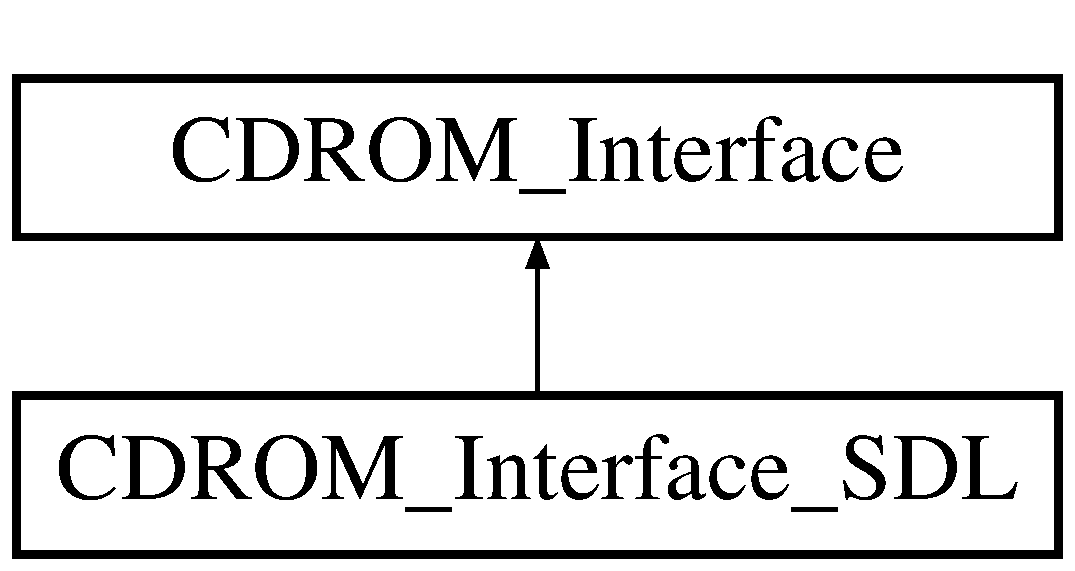
\includegraphics[height=2.000000cm]{classCDROM__Interface__SDL}
\end{center}
\end{figure}
\subsection*{Public Member Functions}
\begin{DoxyCompactItemize}
\item 
\hypertarget{classCDROM__Interface__SDL_ac2830ccd403b203edadd17f2b69525d3}{virtual bool \hyperlink{classCDROM__Interface__SDL_ac2830ccd403b203edadd17f2b69525d3}{Set\-Device} (char $\ast$path, int force\-C\-D)}\label{classCDROM__Interface__SDL_ac2830ccd403b203edadd17f2b69525d3}

\begin{DoxyCompactList}\small\item\em Set the device associated with this interface, if supported by emulation. \end{DoxyCompactList}\item 
\hypertarget{classCDROM__Interface__SDL_a71ac58fc052e29d96e79ef6234e6abbb}{virtual bool \hyperlink{classCDROM__Interface__SDL_a71ac58fc052e29d96e79ef6234e6abbb}{Get\-U\-P\-C} (unsigned char \&attr, char $\ast$upc)}\label{classCDROM__Interface__SDL_a71ac58fc052e29d96e79ef6234e6abbb}

\begin{DoxyCompactList}\small\item\em Get U\-P\-C string from the C\-D-\/\-R\-O\-M. \end{DoxyCompactList}\item 
\hypertarget{classCDROM__Interface__SDL_a80e68ad21338f4ccc44361cbc079e67d}{virtual bool \hyperlink{classCDROM__Interface__SDL_a80e68ad21338f4ccc44361cbc079e67d}{Get\-Audio\-Tracks} (int \&st\-Track, int \&end, \hyperlink{structSMSF}{T\-M\-S\-F} \&lead\-Out)}\label{classCDROM__Interface__SDL_a80e68ad21338f4ccc44361cbc079e67d}

\begin{DoxyCompactList}\small\item\em Retrieve start and end tracks and lead out position. \end{DoxyCompactList}\item 
\hypertarget{classCDROM__Interface__SDL_a8153067b1065412fc0c1b0de4afa58d8}{virtual bool \hyperlink{classCDROM__Interface__SDL_a8153067b1065412fc0c1b0de4afa58d8}{Get\-Audio\-Track\-Info} (int track, \hyperlink{structSMSF}{T\-M\-S\-F} \&start, unsigned char \&attr)}\label{classCDROM__Interface__SDL_a8153067b1065412fc0c1b0de4afa58d8}

\begin{DoxyCompactList}\small\item\em Retrieve start and attributes for a specific track. \end{DoxyCompactList}\item 
\hypertarget{classCDROM__Interface__SDL_a528bc5b106e883ab19a5b23d67f5b89a}{virtual bool \hyperlink{classCDROM__Interface__SDL_a528bc5b106e883ab19a5b23d67f5b89a}{Get\-Audio\-Sub} (unsigned char \&attr, unsigned char \&track, unsigned char \&index, \hyperlink{structSMSF}{T\-M\-S\-F} \&rel\-Pos, \hyperlink{structSMSF}{T\-M\-S\-F} \&abs\-Pos)}\label{classCDROM__Interface__SDL_a528bc5b106e883ab19a5b23d67f5b89a}

\begin{DoxyCompactList}\small\item\em Get subchannel data of the sectors at the current position, and retrieve current position. \end{DoxyCompactList}\item 
\hypertarget{classCDROM__Interface__SDL_aa26e937e9cb11094b9a75360462999c6}{virtual bool \hyperlink{classCDROM__Interface__SDL_aa26e937e9cb11094b9a75360462999c6}{Get\-Audio\-Status} (bool \&playing, bool \&pause)}\label{classCDROM__Interface__SDL_aa26e937e9cb11094b9a75360462999c6}

\begin{DoxyCompactList}\small\item\em Get audio playback status. \end{DoxyCompactList}\item 
\hypertarget{classCDROM__Interface__SDL_aff975ea549d6b3d650678c4d91b6ad22}{virtual bool \hyperlink{classCDROM__Interface__SDL_aff975ea549d6b3d650678c4d91b6ad22}{Get\-Media\-Tray\-Status} (bool \&media\-Present, bool \&media\-Changed, bool \&tray\-Open)}\label{classCDROM__Interface__SDL_aff975ea549d6b3d650678c4d91b6ad22}

\begin{DoxyCompactList}\small\item\em Get media tray status. \end{DoxyCompactList}\item 
\hypertarget{classCDROM__Interface__SDL_a1ab19753917b3fd97a28cec1191d84aa}{virtual bool \hyperlink{classCDROM__Interface__SDL_a1ab19753917b3fd97a28cec1191d84aa}{Play\-Audio\-Sector} (unsigned long start, unsigned long len)}\label{classCDROM__Interface__SDL_a1ab19753917b3fd97a28cec1191d84aa}

\begin{DoxyCompactList}\small\item\em Initiate audio playback starting at sector and for how many. \end{DoxyCompactList}\item 
\hypertarget{classCDROM__Interface__SDL_a05e05542290e98ba8dc41fb3fc75f363}{virtual bool \hyperlink{classCDROM__Interface__SDL_a05e05542290e98ba8dc41fb3fc75f363}{Pause\-Audio} (bool resume)}\label{classCDROM__Interface__SDL_a05e05542290e98ba8dc41fb3fc75f363}

\begin{DoxyCompactList}\small\item\em Pause audio playback. \end{DoxyCompactList}\item 
\hypertarget{classCDROM__Interface__SDL_ad6d548854bf1bac17204f67b8f1dbe40}{virtual bool \hyperlink{classCDROM__Interface__SDL_ad6d548854bf1bac17204f67b8f1dbe40}{Stop\-Audio} (void)}\label{classCDROM__Interface__SDL_ad6d548854bf1bac17204f67b8f1dbe40}

\begin{DoxyCompactList}\small\item\em Stop audio playback. \end{DoxyCompactList}\item 
\hypertarget{classCDROM__Interface__SDL_a36747451cf2e7d18400fd5716947bca4}{virtual void \hyperlink{classCDROM__Interface__SDL_a36747451cf2e7d18400fd5716947bca4}{Channel\-Control} (\hyperlink{structSCtrl}{T\-Ctrl} ctrl)}\label{classCDROM__Interface__SDL_a36747451cf2e7d18400fd5716947bca4}

\begin{DoxyCompactList}\small\item\em Set channel control data (T\-O\-D\-O\-: clarify) \end{DoxyCompactList}\item 
\hypertarget{classCDROM__Interface__SDL_ae7079bbd9e22a19d2983ff4689cb914b}{virtual bool \hyperlink{classCDROM__Interface__SDL_ae7079bbd9e22a19d2983ff4689cb914b}{Read\-Sectors} (Phys\-Pt, bool, unsigned long, unsigned long)}\label{classCDROM__Interface__SDL_ae7079bbd9e22a19d2983ff4689cb914b}

\begin{DoxyCompactList}\small\item\em Read sector data into guest memory. \end{DoxyCompactList}\item 
\hypertarget{classCDROM__Interface__SDL_abe1fa6a654007a16c3d6d5423c69bfbe}{virtual bool \hyperlink{classCDROM__Interface__SDL_abe1fa6a654007a16c3d6d5423c69bfbe}{Read\-Sectors\-Host} (void $\ast$buffer, bool raw, unsigned long sector, unsigned long num)}\label{classCDROM__Interface__SDL_abe1fa6a654007a16c3d6d5423c69bfbe}

\begin{DoxyCompactList}\small\item\em Read sector data into host memory (for I\-D\-E emulation) \end{DoxyCompactList}\item 
\hypertarget{classCDROM__Interface__SDL_ae018393018fac0937b375dce79e31d0e}{virtual bool \hyperlink{classCDROM__Interface__SDL_ae018393018fac0937b375dce79e31d0e}{Load\-Unload\-Media} (bool unload)}\label{classCDROM__Interface__SDL_ae018393018fac0937b375dce79e31d0e}

\begin{DoxyCompactList}\small\item\em Load (close/spin up) or unload (eject/spin down) media. \end{DoxyCompactList}\end{DoxyCompactItemize}


\subsection{Detailed Description}
C\-D-\/\-R\-O\-M interface to S\-D\-L 1.\-x C\-D-\/\-R\-O\-M support. 

This connects C\-D-\/\-R\-O\-M emulation to the C\-D-\/\-R\-O\-M functions provided by S\-D\-L 1.\-x 

Definition at line 183 of file cdrom.\-h.



The documentation for this class was generated from the following files\-:\begin{DoxyCompactItemize}
\item 
src/dos/cdrom.\-h\item 
src/dos/cdrom.\-cpp\end{DoxyCompactItemize}

\hypertarget{classcdromDrive}{\section{cdrom\-Drive Class Reference}
\label{classcdromDrive}\index{cdrom\-Drive@{cdrom\-Drive}}
}
Inheritance diagram for cdrom\-Drive\-:\begin{figure}[H]
\begin{center}
\leavevmode
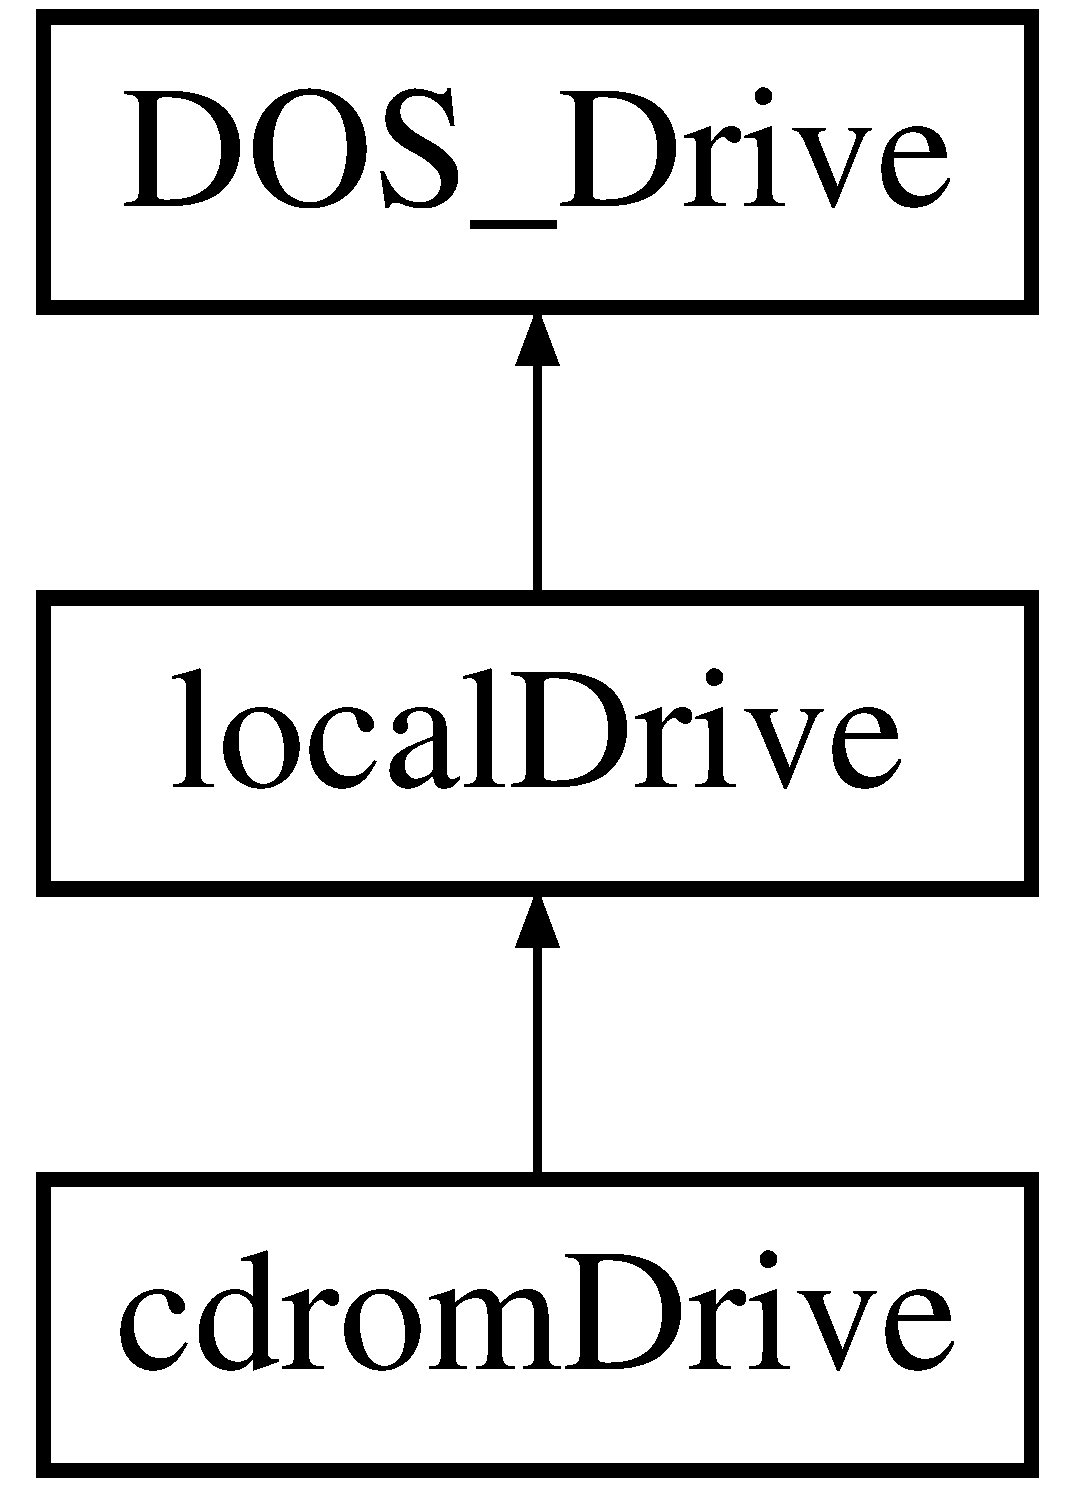
\includegraphics[height=3.000000cm]{classcdromDrive}
\end{center}
\end{figure}
\subsection*{Public Member Functions}
\begin{DoxyCompactItemize}
\item 
\hypertarget{classcdromDrive_a9bc77d75fc8e02d73586ad909cc4fd86}{{\bfseries cdrom\-Drive} (const char drive\-Letter, const char $\ast$startdir, Bit16u \-\_\-bytes\-\_\-sector, Bit8u \-\_\-sectors\-\_\-cluster, Bit16u \-\_\-total\-\_\-clusters, Bit16u \-\_\-free\-\_\-clusters, Bit8u \-\_\-mediaid, int \&error)}\label{classcdromDrive_a9bc77d75fc8e02d73586ad909cc4fd86}

\item 
\hypertarget{classcdromDrive_aa5ff41c5c9c045550b6f1a0974aa8d1d}{virtual bool {\bfseries File\-Open} (\hyperlink{classDOS__File}{D\-O\-S\-\_\-\-File} $\ast$$\ast$file, const char $\ast$name, Bit32u flags)}\label{classcdromDrive_aa5ff41c5c9c045550b6f1a0974aa8d1d}

\item 
\hypertarget{classcdromDrive_ac7c844b8ced8b687886f1fa5e6b9c5e4}{virtual bool {\bfseries File\-Create} (\hyperlink{classDOS__File}{D\-O\-S\-\_\-\-File} $\ast$$\ast$file, const char $\ast$name, Bit16u attributes)}\label{classcdromDrive_ac7c844b8ced8b687886f1fa5e6b9c5e4}

\item 
\hypertarget{classcdromDrive_a0e4ec60ab003c1cc1b687bc2ddef9d8a}{virtual bool {\bfseries File\-Unlink} (const char $\ast$name)}\label{classcdromDrive_a0e4ec60ab003c1cc1b687bc2ddef9d8a}

\item 
\hypertarget{classcdromDrive_ae5a43f4860af4338c8efe8102489ede2}{virtual bool {\bfseries Remove\-Dir} (const char $\ast$dir)}\label{classcdromDrive_ae5a43f4860af4338c8efe8102489ede2}

\item 
\hypertarget{classcdromDrive_a6a8f1604c680ab386f60d777f248eb78}{virtual bool {\bfseries Make\-Dir} (const char $\ast$dir)}\label{classcdromDrive_a6a8f1604c680ab386f60d777f248eb78}

\item 
\hypertarget{classcdromDrive_abf672051a5e5e3b4637f4f976ed0c6cb}{virtual bool {\bfseries Rename} (const char $\ast$oldname, const char $\ast$newname)}\label{classcdromDrive_abf672051a5e5e3b4637f4f976ed0c6cb}

\item 
\hypertarget{classcdromDrive_aba4f6b7a2df7be93c754232dff50c23c}{virtual bool {\bfseries Get\-File\-Attr} (const char $\ast$name, Bit16u $\ast$attr)}\label{classcdromDrive_aba4f6b7a2df7be93c754232dff50c23c}

\item 
\hypertarget{classcdromDrive_afd0347b272659c24f6f3cd9b7b05f89c}{virtual bool {\bfseries Find\-First} (const char $\ast$\-\_\-dir, \hyperlink{classDOS__DTA}{D\-O\-S\-\_\-\-D\-T\-A} \&dta, bool fcb\-\_\-findfirst=false)}\label{classcdromDrive_afd0347b272659c24f6f3cd9b7b05f89c}

\item 
\hypertarget{classcdromDrive_a3aeeb35dbd5100a4b973aa6341295521}{virtual void {\bfseries Set\-Dir} (const char $\ast$path)}\label{classcdromDrive_a3aeeb35dbd5100a4b973aa6341295521}

\item 
\hypertarget{classcdromDrive_a2186d681041aad9456c57cd4be5cc0bc}{virtual bool {\bfseries is\-Remote} (void)}\label{classcdromDrive_a2186d681041aad9456c57cd4be5cc0bc}

\item 
\hypertarget{classcdromDrive_ab96402d6d61617f26d545268e1127a07}{virtual bool {\bfseries is\-Removable} (void)}\label{classcdromDrive_ab96402d6d61617f26d545268e1127a07}

\item 
\hypertarget{classcdromDrive_a4e5d16dc2a6171b622ed815b464f1114}{virtual Bits {\bfseries Un\-Mount} (void)}\label{classcdromDrive_a4e5d16dc2a6171b622ed815b464f1114}

\end{DoxyCompactItemize}


\subsection{Detailed Description}


Definition at line 306 of file drives.\-h.



The documentation for this class was generated from the following files\-:\begin{DoxyCompactItemize}
\item 
src/dos/drives.\-h\item 
src/dos/drive\-\_\-local.\-cpp\end{DoxyCompactItemize}

\hypertarget{classCEvent}{\section{C\-Event Class Reference}
\label{classCEvent}\index{C\-Event@{C\-Event}}
}


Base \hyperlink{classCEvent}{C\-Event} class for mapper events.  


Inheritance diagram for C\-Event\-:\begin{figure}[H]
\begin{center}
\leavevmode
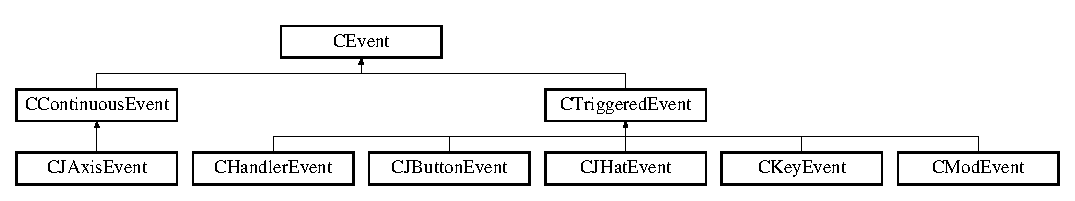
\includegraphics[height=2.258065cm]{classCEvent}
\end{center}
\end{figure}
\subsection*{Public Types}
\begin{DoxyCompactItemize}
\item 
enum \hyperlink{classCEvent_a93a65775636793dfcabe38d14739c2bd}{event\-\_\-type} \{ {\bfseries event\-\_\-t} = 0, 
{\bfseries handler\-\_\-event\-\_\-t}
 \}
\begin{DoxyCompactList}\small\item\em Type of \hyperlink{classCEvent}{C\-Event} class, if the code needs to use the specific type. \end{DoxyCompactList}\end{DoxyCompactItemize}
\subsection*{Public Member Functions}
\begin{DoxyCompactItemize}
\item 
\hyperlink{classCEvent_a1dccd12980b4a85ca70ca6d77d631b45}{C\-Event} (char const $\ast$const \-\_\-entry, const enum \hyperlink{classCEvent_a93a65775636793dfcabe38d14739c2bd}{event\-\_\-type} \-\_\-type=event\-\_\-t)
\begin{DoxyCompactList}\small\item\em \hyperlink{classCEvent}{C\-Event} constructor. \end{DoxyCompactList}\item 
virtual std\-::string \hyperlink{classCEvent_adcc4bad114bb2f135e354d018cbe1d8c}{Get\-Bind\-Menu\-Text} (void)
\begin{DoxyCompactList}\small\item\em Retrieve binding string for display in the menu. \end{DoxyCompactList}\item 
\hypertarget{classCEvent_a0ebaf9dbda3dc862fb61e21280dd987f}{void \hyperlink{classCEvent_a0ebaf9dbda3dc862fb61e21280dd987f}{update\-\_\-menu\-\_\-shortcut} (void)}\label{classCEvent_a0ebaf9dbda3dc862fb61e21280dd987f}

\begin{DoxyCompactList}\small\item\em Update the menu item for the mapper shortcut with the latest text and keyboard shortcut. \end{DoxyCompactList}\item 
\hypertarget{classCEvent_a2665ebd0551c2b437b02d521f1c7adda}{void \hyperlink{classCEvent_a2665ebd0551c2b437b02d521f1c7adda}{Add\-Bind} (\hyperlink{classCBind}{C\-Bind} $\ast$bind)}\label{classCEvent_a2665ebd0551c2b437b02d521f1c7adda}

\begin{DoxyCompactList}\small\item\em Add binding to the bindlist. \end{DoxyCompactList}\item 
\hypertarget{classCEvent_a8643a8541e23ed77a63869dd11780c83}{virtual void \hyperlink{classCEvent_a8643a8541e23ed77a63869dd11780c83}{Active} (bool yesno)}\label{classCEvent_a8643a8541e23ed77a63869dd11780c83}

\begin{DoxyCompactList}\small\item\em Change whether the event is activated or not. \end{DoxyCompactList}\item 
\hypertarget{classCEvent_a1b7abcd9c0ecedc29de42017e3cfef13}{virtual void \hyperlink{classCEvent_a1b7abcd9c0ecedc29de42017e3cfef13}{Activate\-Event} (bool ev\-\_\-trigger, bool skip\-\_\-action)=0}\label{classCEvent_a1b7abcd9c0ecedc29de42017e3cfef13}

\begin{DoxyCompactList}\small\item\em Activate the event, act on it. \end{DoxyCompactList}\item 
\hypertarget{classCEvent_a525574fb193f9e50402a8fd5028b9b06}{virtual void \hyperlink{classCEvent_a525574fb193f9e50402a8fd5028b9b06}{De\-Activate\-Event} (bool ev\-\_\-trigger)=0}\label{classCEvent_a525574fb193f9e50402a8fd5028b9b06}

\begin{DoxyCompactList}\small\item\em Deactivate the event. \end{DoxyCompactList}\item 
\hypertarget{classCEvent_a633d83fd6d210a7b6a517754548eee11}{void \hyperlink{classCEvent_a633d83fd6d210a7b6a517754548eee11}{De\-Activate\-All} (void)}\label{classCEvent_a633d83fd6d210a7b6a517754548eee11}

\begin{DoxyCompactList}\small\item\em Deactivate all bindings. \end{DoxyCompactList}\item 
\hypertarget{classCEvent_aaa253031798af461119b830d079e8225}{void \hyperlink{classCEvent_aaa253031798af461119b830d079e8225}{Set\-Value} (Bits value)}\label{classCEvent_aaa253031798af461119b830d079e8225}

\begin{DoxyCompactList}\small\item\em Set the value of the event (such as joystick position) \end{DoxyCompactList}\item 
\hypertarget{classCEvent_ad4e49c2aa32efecdc91c9439e858b940}{Bits \hyperlink{classCEvent_ad4e49c2aa32efecdc91c9439e858b940}{Get\-Value} (void)}\label{classCEvent_ad4e49c2aa32efecdc91c9439e858b940}

\begin{DoxyCompactList}\small\item\em Get the value of the event. \end{DoxyCompactList}\item 
\hypertarget{classCEvent_a4693b4e54c079cc97f0522eb15154953}{char $\ast$ \hyperlink{classCEvent_a4693b4e54c079cc97f0522eb15154953}{Get\-Name} (void)}\label{classCEvent_a4693b4e54c079cc97f0522eb15154953}

\begin{DoxyCompactList}\small\item\em Retrieve the name of the event. \end{DoxyCompactList}\item 
\hypertarget{classCEvent_affd064f43309b5fc4966edb36935723d}{virtual bool \hyperlink{classCEvent_affd064f43309b5fc4966edb36935723d}{Is\-Trigger} (void)=0}\label{classCEvent_affd064f43309b5fc4966edb36935723d}

\begin{DoxyCompactList}\small\item\em Indicate whether the event is a trigger or continuous input. \end{DoxyCompactList}\end{DoxyCompactItemize}
\subsection*{Public Attributes}
\begin{DoxyCompactItemize}
\item 
\hypertarget{classCEvent_a9543179cd76d08369201e992ca41728c}{std\-::string \hyperlink{classCEvent_a9543179cd76d08369201e992ca41728c}{eventname}}\label{classCEvent_a9543179cd76d08369201e992ca41728c}

\begin{DoxyCompactList}\small\item\em Event name. \end{DoxyCompactList}\item 
\hypertarget{classCEvent_a5612c4e4e1d0cfc08e1640fee8bacf85}{enum \hyperlink{classCEvent_a93a65775636793dfcabe38d14739c2bd}{event\-\_\-type} \hyperlink{classCEvent_a5612c4e4e1d0cfc08e1640fee8bacf85}{type}}\label{classCEvent_a5612c4e4e1d0cfc08e1640fee8bacf85}

\begin{DoxyCompactList}\small\item\em event type \end{DoxyCompactList}\item 
\hypertarget{classCEvent_a0c900c0aab7bf38d7ac8769d5e4f6a5a}{C\-Bind\-List \hyperlink{classCEvent_a0c900c0aab7bf38d7ac8769d5e4f6a5a}{bindlist}}\label{classCEvent_a0c900c0aab7bf38d7ac8769d5e4f6a5a}

\begin{DoxyCompactList}\small\item\em Bind list to trigger on activation/deactivation. \end{DoxyCompactList}\item 
\hypertarget{classCEvent_af1e4934eb75e5636f81918c13983e2e3}{bool \hyperlink{classCEvent_af1e4934eb75e5636f81918c13983e2e3}{active}}\label{classCEvent_af1e4934eb75e5636f81918c13983e2e3}

\begin{DoxyCompactList}\small\item\em Whether the event is active or not. \end{DoxyCompactList}\end{DoxyCompactItemize}
\subsection*{Protected Attributes}
\begin{DoxyCompactItemize}
\item 
\hypertarget{classCEvent_a487786e4e537594bf963e96aecae85cd}{Bitu \hyperlink{classCEvent_a487786e4e537594bf963e96aecae85cd}{activity}}\label{classCEvent_a487786e4e537594bf963e96aecae85cd}

\begin{DoxyCompactList}\small\item\em Activity counter. \end{DoxyCompactList}\item 
\hypertarget{classCEvent_a20cca21cb3c606f3161a2757c1ba466d}{char \hyperlink{classCEvent_a20cca21cb3c606f3161a2757c1ba466d}{entry} \mbox{[}16\mbox{]}}\label{classCEvent_a20cca21cb3c606f3161a2757c1ba466d}

\begin{DoxyCompactList}\small\item\em Mapper entry name. \end{DoxyCompactList}\item 
\hypertarget{classCEvent_a7bbacdb8e3c5ee41ce13af19dc21db2d}{Bits \hyperlink{classCEvent_a7bbacdb8e3c5ee41ce13af19dc21db2d}{current\-\_\-value}}\label{classCEvent_a7bbacdb8e3c5ee41ce13af19dc21db2d}

\begin{DoxyCompactList}\small\item\em Current value of the event (such as joystick position) \end{DoxyCompactList}\end{DoxyCompactItemize}


\subsection{Detailed Description}
Base \hyperlink{classCEvent}{C\-Event} class for mapper events. 

Definition at line 183 of file sdl\-\_\-mapper.\-cpp.



\subsection{Member Enumeration Documentation}
\hypertarget{classCEvent_a93a65775636793dfcabe38d14739c2bd}{\index{C\-Event@{C\-Event}!event\-\_\-type@{event\-\_\-type}}
\index{event\-\_\-type@{event\-\_\-type}!CEvent@{C\-Event}}
\subsubsection[{event\-\_\-type}]{\setlength{\rightskip}{0pt plus 5cm}enum {\bf C\-Event\-::event\-\_\-type}}}\label{classCEvent_a93a65775636793dfcabe38d14739c2bd}


Type of \hyperlink{classCEvent}{C\-Event} class, if the code needs to use the specific type. 

This is used by other parts of the mapper if it needs to retrieve additional information that is only provided by the handler event class 

Definition at line 189 of file sdl\-\_\-mapper.\-cpp.



\subsection{Constructor \& Destructor Documentation}
\hypertarget{classCEvent_a1dccd12980b4a85ca70ca6d77d631b45}{\index{C\-Event@{C\-Event}!C\-Event@{C\-Event}}
\index{C\-Event@{C\-Event}!CEvent@{C\-Event}}
\subsubsection[{C\-Event}]{\setlength{\rightskip}{0pt plus 5cm}{\bf C\-Event\-::\-C\-Event} (
\begin{DoxyParamCaption}
\item[{char const $\ast$const}]{\-\_\-entry, }
\item[{const enum {\bf event\-\_\-type}}]{\-\_\-type = {\ttfamily event\-\_\-t}}
\end{DoxyParamCaption}
)\hspace{0.3cm}{\ttfamily  \mbox{[}inline\mbox{]}}}}\label{classCEvent_a1dccd12980b4a85ca70ca6d77d631b45}


\hyperlink{classCEvent}{C\-Event} constructor. 

This constructor takes a mapper entry name and event type. Subclasses will call down to this constructor as well. The handler event class will fill in the \-\_\-type field to identify itself. 

Definition at line 200 of file sdl\-\_\-mapper.\-cpp.



References active, activity, bindlist, current\-\_\-value, entry, and type.



\subsection{Member Function Documentation}
\hypertarget{classCEvent_adcc4bad114bb2f135e354d018cbe1d8c}{\index{C\-Event@{C\-Event}!Get\-Bind\-Menu\-Text@{Get\-Bind\-Menu\-Text}}
\index{Get\-Bind\-Menu\-Text@{Get\-Bind\-Menu\-Text}!CEvent@{C\-Event}}
\subsubsection[{Get\-Bind\-Menu\-Text}]{\setlength{\rightskip}{0pt plus 5cm}std\-::string {\bf C\-Event\-::\-Get\-Bind\-Menu\-Text} (
\begin{DoxyParamCaption}
\item[{void}]{}
\end{DoxyParamCaption}
)\hspace{0.3cm}{\ttfamily  \mbox{[}virtual\mbox{]}}}}\label{classCEvent_adcc4bad114bb2f135e354d018cbe1d8c}


Retrieve binding string for display in the menu. 

Retrieve text string to show as the assigned mapper binding in a menu item's displayable area so that the user knows what keyboard input will trigger the shortcut. 

Definition at line 797 of file sdl\-\_\-mapper.\-cpp.



References bindlist, C\-Key\-Bind\-::\-Get\-Bind\-Menu\-Text(), and C\-Bind\-::type.



Referenced by C\-Bind\-::\-Get\-Modifier\-Text(), and update\-\_\-menu\-\_\-shortcut().



The documentation for this class was generated from the following file\-:\begin{DoxyCompactItemize}
\item 
src/gui/sdl\-\_\-mapper.\-cpp\end{DoxyCompactItemize}

\hypertarget{classCEventButton}{\section{C\-Event\-Button Class Reference}
\label{classCEventButton}\index{C\-Event\-Button@{C\-Event\-Button}}
}
Inheritance diagram for C\-Event\-Button\-:\begin{figure}[H]
\begin{center}
\leavevmode
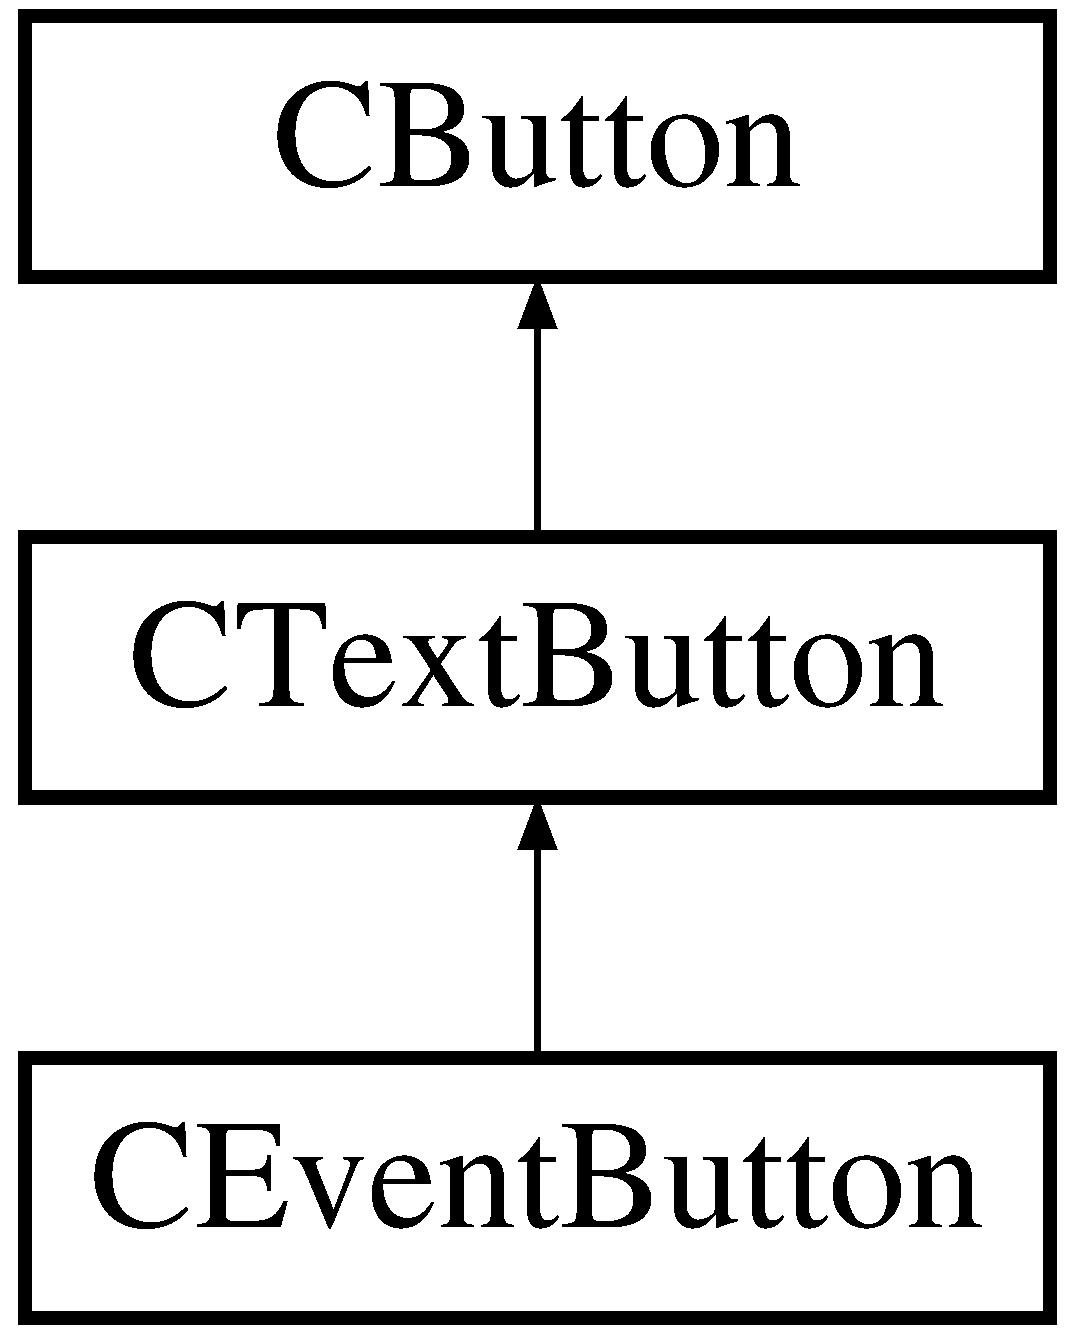
\includegraphics[height=3.000000cm]{classCEventButton}
\end{center}
\end{figure}
\subsection*{Public Member Functions}
\begin{DoxyCompactItemize}
\item 
\hypertarget{classCEventButton_a79fd3e96e7f7f1b3c4565f02535c3429}{{\bfseries C\-Event\-Button} (Bitu \-\_\-x, Bitu \-\_\-y, Bitu \-\_\-dx, Bitu \-\_\-dy, const char $\ast$\-\_\-text, \hyperlink{classCEvent}{C\-Event} $\ast$\-\_\-event)}\label{classCEventButton_a79fd3e96e7f7f1b3c4565f02535c3429}

\item 
\hypertarget{classCEventButton_ab88a51cd41e89b95cc7fbb7d78562fbe}{void {\bfseries Click} (void)}\label{classCEventButton_ab88a51cd41e89b95cc7fbb7d78562fbe}

\end{DoxyCompactItemize}
\subsection*{Protected Attributes}
\begin{DoxyCompactItemize}
\item 
\hypertarget{classCEventButton_a5f0d42f7b82112c4b144f84f308f1527}{\hyperlink{classCEvent}{C\-Event} $\ast$ {\bfseries event}}\label{classCEventButton_a5f0d42f7b82112c4b144f84f308f1527}

\end{DoxyCompactItemize}


\subsection{Detailed Description}


Definition at line 1992 of file sdl\-\_\-mapper.\-cpp.



The documentation for this class was generated from the following file\-:\begin{DoxyCompactItemize}
\item 
src/gui/sdl\-\_\-mapper.\-cpp\end{DoxyCompactItemize}

\hypertarget{classCFCSBindGroup}{\section{C\-F\-C\-S\-Bind\-Group Class Reference}
\label{classCFCSBindGroup}\index{C\-F\-C\-S\-Bind\-Group@{C\-F\-C\-S\-Bind\-Group}}
}
Inheritance diagram for C\-F\-C\-S\-Bind\-Group\-:\begin{figure}[H]
\begin{center}
\leavevmode
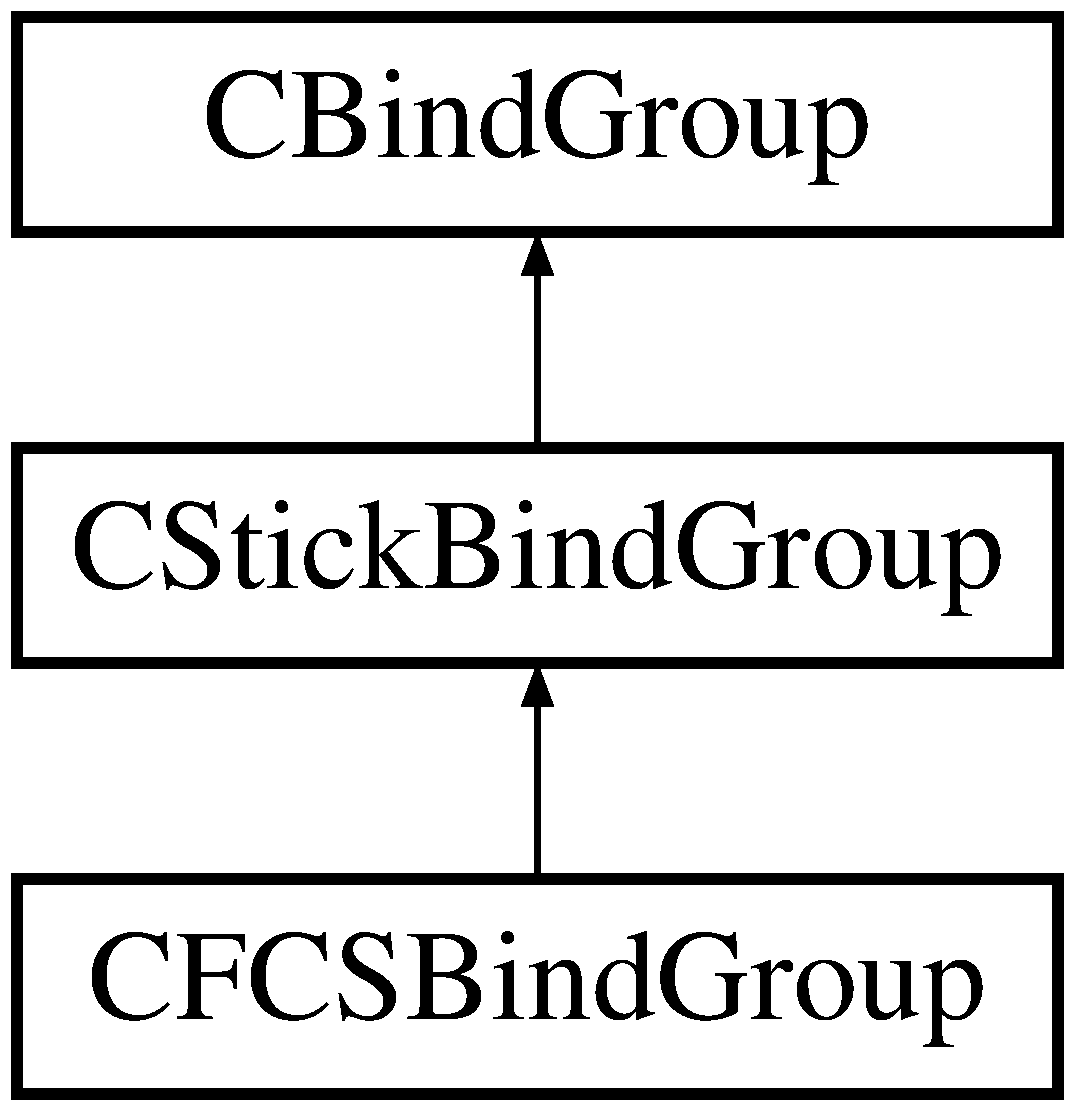
\includegraphics[height=3.000000cm]{classCFCSBindGroup}
\end{center}
\end{figure}
\subsection*{Public Member Functions}
\begin{DoxyCompactItemize}
\item 
\hypertarget{classCFCSBindGroup_a366a39efa7db658cfdec657580818264}{{\bfseries C\-F\-C\-S\-Bind\-Group} (Bitu \-\_\-stick, Bitu \-\_\-emustick)}\label{classCFCSBindGroup_a366a39efa7db658cfdec657580818264}

\item 
\hypertarget{classCFCSBindGroup_a25a662090cb26b626cac51449c94e3af}{bool {\bfseries Check\-Event} (S\-D\-L\-\_\-\-Event $\ast$event)}\label{classCFCSBindGroup_a25a662090cb26b626cac51449c94e3af}

\item 
\hypertarget{classCFCSBindGroup_a19be69d6c38cc544b2b4517eeab84fef}{virtual void {\bfseries Update\-Joystick} ()}\label{classCFCSBindGroup_a19be69d6c38cc544b2b4517eeab84fef}

\end{DoxyCompactItemize}


\subsection{Detailed Description}


Definition at line 1610 of file sdl\-\_\-mapper.\-cpp.



The documentation for this class was generated from the following file\-:\begin{DoxyCompactItemize}
\item 
src/gui/sdl\-\_\-mapper.\-cpp\end{DoxyCompactItemize}

\hypertarget{classDOS__Drive__Cache_1_1CFileInfo}{\section{D\-O\-S\-\_\-\-Drive\-\_\-\-Cache\-:\-:C\-File\-Info Class Reference}
\label{classDOS__Drive__Cache_1_1CFileInfo}\index{D\-O\-S\-\_\-\-Drive\-\_\-\-Cache\-::\-C\-File\-Info@{D\-O\-S\-\_\-\-Drive\-\_\-\-Cache\-::\-C\-File\-Info}}
}
\subsection*{Public Attributes}
\begin{DoxyCompactItemize}
\item 
\hypertarget{classDOS__Drive__Cache_1_1CFileInfo_a54e3d2f75fcbb74f75db034953e229a3}{char {\bfseries orgname} \mbox{[}C\-R\-O\-S\-S\-\_\-\-L\-E\-N\mbox{]}}\label{classDOS__Drive__Cache_1_1CFileInfo_a54e3d2f75fcbb74f75db034953e229a3}

\item 
\hypertarget{classDOS__Drive__Cache_1_1CFileInfo_a4bc96390314c8e5458bdb6fca24526e5}{char {\bfseries shortname} \mbox{[}D\-O\-S\-\_\-\-N\-A\-M\-E\-L\-E\-N\-G\-T\-H\-\_\-\-A\-S\-C\-I\-I\mbox{]}}\label{classDOS__Drive__Cache_1_1CFileInfo_a4bc96390314c8e5458bdb6fca24526e5}

\item 
\hypertarget{classDOS__Drive__Cache_1_1CFileInfo_a36a3b8a7c17f16893a6e38db7ab871e0}{bool {\bfseries is\-Overlay\-Dir}}\label{classDOS__Drive__Cache_1_1CFileInfo_a36a3b8a7c17f16893a6e38db7ab871e0}

\item 
\hypertarget{classDOS__Drive__Cache_1_1CFileInfo_a5fd697ccc70ceb461b00ac5e0a3b0a6a}{bool {\bfseries is\-Dir}}\label{classDOS__Drive__Cache_1_1CFileInfo_a5fd697ccc70ceb461b00ac5e0a3b0a6a}

\item 
\hypertarget{classDOS__Drive__Cache_1_1CFileInfo_a7431fc652afc211a9f5688d3dc6dac54}{Bit16u {\bfseries id}}\label{classDOS__Drive__Cache_1_1CFileInfo_a7431fc652afc211a9f5688d3dc6dac54}

\item 
\hypertarget{classDOS__Drive__Cache_1_1CFileInfo_a070341474c5331b61978b1fa4e397fba}{Bitu {\bfseries next\-Entry}}\label{classDOS__Drive__Cache_1_1CFileInfo_a070341474c5331b61978b1fa4e397fba}

\item 
\hypertarget{classDOS__Drive__Cache_1_1CFileInfo_aabcdb2db6a8c70ad16109e5662141f61}{Bitu {\bfseries short\-Nr}}\label{classDOS__Drive__Cache_1_1CFileInfo_aabcdb2db6a8c70ad16109e5662141f61}

\item 
\hypertarget{classDOS__Drive__Cache_1_1CFileInfo_a5470a346a90b401ea29fb40645aad237}{std\-::vector$<$ \hyperlink{classDOS__Drive__Cache_1_1CFileInfo}{C\-File\-Info} $\ast$ $>$ {\bfseries file\-List}}\label{classDOS__Drive__Cache_1_1CFileInfo_a5470a346a90b401ea29fb40645aad237}

\item 
\hypertarget{classDOS__Drive__Cache_1_1CFileInfo_a5cfea8ee640dc9b5f1808a52bc0781d9}{std\-::vector$<$ \hyperlink{classDOS__Drive__Cache_1_1CFileInfo}{C\-File\-Info} $\ast$ $>$ {\bfseries long\-Name\-List}}\label{classDOS__Drive__Cache_1_1CFileInfo_a5cfea8ee640dc9b5f1808a52bc0781d9}

\end{DoxyCompactItemize}


\subsection{Detailed Description}


Definition at line 203 of file dos\-\_\-system.\-h.



The documentation for this class was generated from the following file\-:\begin{DoxyCompactItemize}
\item 
include/dos\-\_\-system.\-h\end{DoxyCompactItemize}

\hypertarget{classCFileLPT}{\section{C\-File\-L\-P\-T Class Reference}
\label{classCFileLPT}\index{C\-File\-L\-P\-T@{C\-File\-L\-P\-T}}
}
Inheritance diagram for C\-File\-L\-P\-T\-:\begin{figure}[H]
\begin{center}
\leavevmode
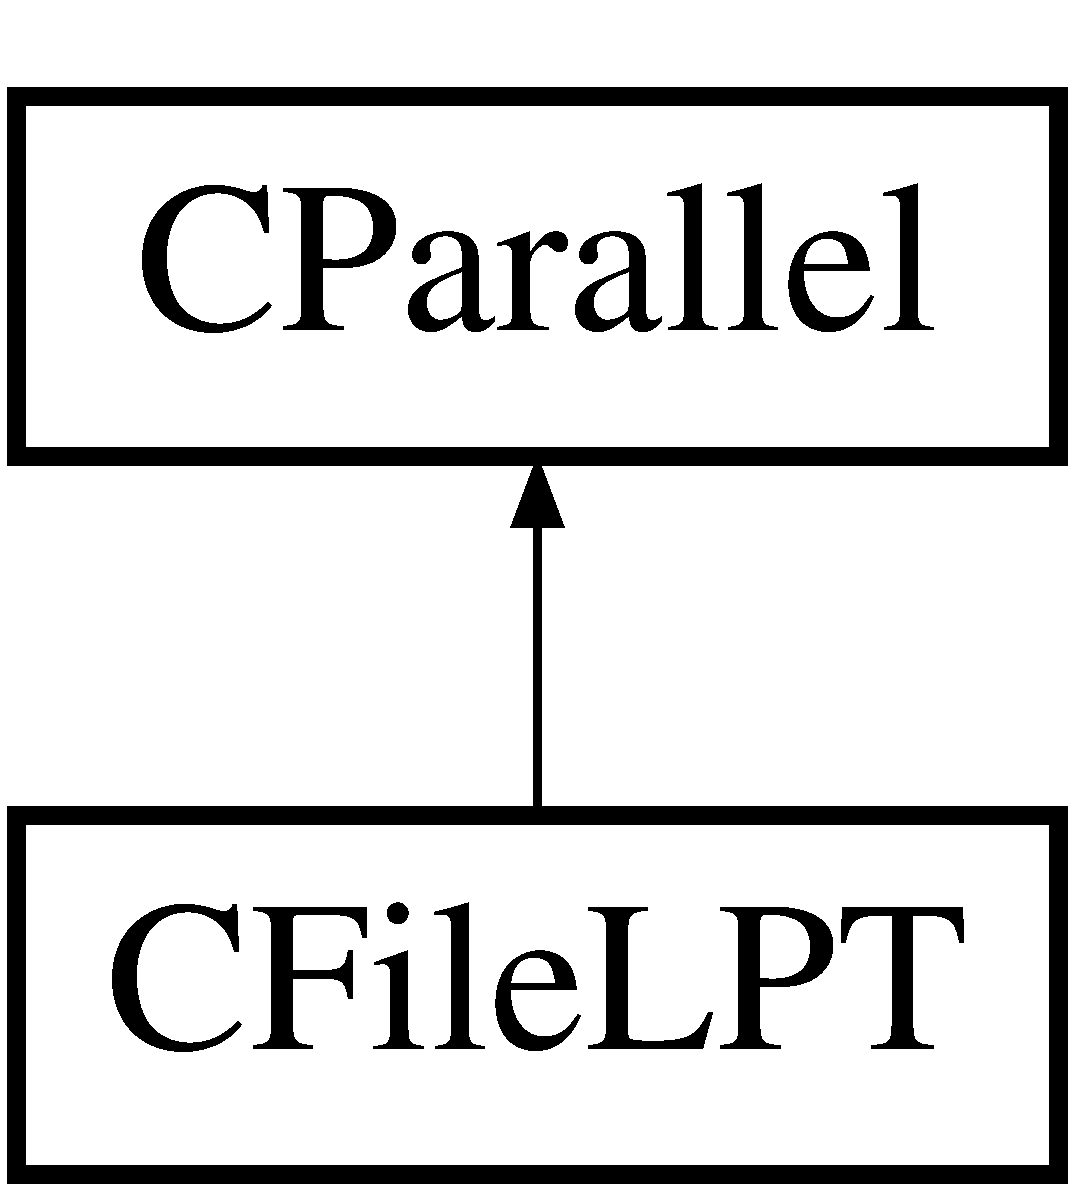
\includegraphics[height=2.000000cm]{classCFileLPT}
\end{center}
\end{figure}
\subsection*{Public Member Functions}
\begin{DoxyCompactItemize}
\item 
\hypertarget{classCFileLPT_a4283c6ee323ae064a1ec081487900bd0}{{\bfseries C\-File\-L\-P\-T} (Bitu nr, Bit8u init\-Irq, \hyperlink{classCommandLine}{Command\-Line} $\ast$cmd)}\label{classCFileLPT_a4283c6ee323ae064a1ec081487900bd0}

\item 
\hypertarget{classCFileLPT_a4d06c86f7311d6cf8fc6e11b420ad6ef}{bool {\bfseries Open\-File} ()}\label{classCFileLPT_a4d06c86f7311d6cf8fc6e11b420ad6ef}

\item 
\hypertarget{classCFileLPT_afc66bf11689e4aa9fa2206c5e147000c}{Bitu {\bfseries Read\-\_\-\-P\-R} ()}\label{classCFileLPT_afc66bf11689e4aa9fa2206c5e147000c}

\item 
\hypertarget{classCFileLPT_afcf8b593cc34eaafe8c93b0c3270804a}{Bitu {\bfseries Read\-\_\-\-C\-O\-M} ()}\label{classCFileLPT_afcf8b593cc34eaafe8c93b0c3270804a}

\item 
\hypertarget{classCFileLPT_adf5e9bcd0026bf2fab83a6bdd15f3330}{Bitu {\bfseries Read\-\_\-\-S\-R} ()}\label{classCFileLPT_adf5e9bcd0026bf2fab83a6bdd15f3330}

\item 
\hypertarget{classCFileLPT_a65b07a710e2d2f17c035bb93e9ae59e7}{void {\bfseries Write\-\_\-\-P\-R} (Bitu)}\label{classCFileLPT_a65b07a710e2d2f17c035bb93e9ae59e7}

\item 
\hypertarget{classCFileLPT_ac963dd0328b926c419f8cc8bc79f8177}{void {\bfseries Write\-\_\-\-C\-O\-N} (Bitu)}\label{classCFileLPT_ac963dd0328b926c419f8cc8bc79f8177}

\item 
\hypertarget{classCFileLPT_af12ad77ab97a96bdbe07a9566659673d}{void {\bfseries Write\-\_\-\-I\-O\-S\-E\-L} (Bitu)}\label{classCFileLPT_af12ad77ab97a96bdbe07a9566659673d}

\item 
\hypertarget{classCFileLPT_a09595c3a5a7bc8e9c0625cd951330172}{bool {\bfseries Putchar} (Bit8u)}\label{classCFileLPT_a09595c3a5a7bc8e9c0625cd951330172}

\item 
\hypertarget{classCFileLPT_ac3a5bf3dc1b7362fb909b153febf8b88}{virtual void {\bfseries handle\-Upper\-Event} (Bit16u type)}\label{classCFileLPT_ac3a5bf3dc1b7362fb909b153febf8b88}

\end{DoxyCompactItemize}
\subsection*{Public Attributes}
\begin{DoxyCompactItemize}
\item 
\hypertarget{classCFileLPT_a50011d4c71d93c858a22f2c76fee74a9}{bool {\bfseries Installation\-Successful}}\label{classCFileLPT_a50011d4c71d93c858a22f2c76fee74a9}

\item 
\hypertarget{classCFileLPT_ae1cefae0c35054232d464c238e7be32b}{bool {\bfseries file\-Open}}\label{classCFileLPT_ae1cefae0c35054232d464c238e7be32b}

\item 
\hypertarget{classCFileLPT_a9a234ae65d53bb0cd70965cf5b3311b3}{D\-F\-T\-Y\-P\-E {\bfseries filetype}}\label{classCFileLPT_a9a234ae65d53bb0cd70965cf5b3311b3}

\item 
\hypertarget{classCFileLPT_a913fb933edd793303b09f8cfda162d38}{F\-I\-L\-E $\ast$ {\bfseries file}}\label{classCFileLPT_a913fb933edd793303b09f8cfda162d38}

\item 
\hypertarget{classCFileLPT_ac10aaeb39fbc19ee51bf06e62715478e}{std\-::string {\bfseries name}}\label{classCFileLPT_ac10aaeb39fbc19ee51bf06e62715478e}

\item 
\hypertarget{classCFileLPT_a5a56af7c4b4073500a5bc432c6ef9f6f}{bool {\bfseries add\-F\-F}}\label{classCFileLPT_a5a56af7c4b4073500a5bc432c6ef9f6f}

\item 
\hypertarget{classCFileLPT_ae5562e8c41afa08c27270a36ae619f9d}{bool {\bfseries add\-L\-F}}\label{classCFileLPT_ae5562e8c41afa08c27270a36ae619f9d}

\item 
\hypertarget{classCFileLPT_a2151f7022055264e4c2e05cc8ba01c31}{Bit8u {\bfseries last\-Char}}\label{classCFileLPT_a2151f7022055264e4c2e05cc8ba01c31}

\item 
\hypertarget{classCFileLPT_a3f6974f3af052e2c549e721ebcd93b48}{const Bit16u $\ast$ {\bfseries codepage\-\_\-ptr}}\label{classCFileLPT_a3f6974f3af052e2c549e721ebcd93b48}

\item 
\hypertarget{classCFileLPT_ab9f0f22206641224aa6178ff900543e0}{bool {\bfseries ack\-\_\-polarity}}\label{classCFileLPT_ab9f0f22206641224aa6178ff900543e0}

\item 
\hypertarget{classCFileLPT_ad59a42373cdb6ae50b983b744b79451e}{Bit8u {\bfseries datareg}}\label{classCFileLPT_ad59a42373cdb6ae50b983b744b79451e}

\item 
\hypertarget{classCFileLPT_a9ad1361fb9df3fe768573f46206c248d}{Bit8u {\bfseries controlreg}}\label{classCFileLPT_a9ad1361fb9df3fe768573f46206c248d}

\item 
\hypertarget{classCFileLPT_ab146dfe78d718cee82c107ed8f1d68d1}{bool {\bfseries autofeed}}\label{classCFileLPT_ab146dfe78d718cee82c107ed8f1d68d1}

\item 
\hypertarget{classCFileLPT_a2342d7014c2898698d2d78c4a4021fa5}{bool {\bfseries ack}}\label{classCFileLPT_a2342d7014c2898698d2d78c4a4021fa5}

\item 
\hypertarget{classCFileLPT_a8575730cacb5d26414d99f944caa4f66}{unsigned int {\bfseries timeout}}\label{classCFileLPT_a8575730cacb5d26414d99f944caa4f66}

\item 
\hypertarget{classCFileLPT_a96dce00b435b57411c44492ed04d129a}{Bitu {\bfseries last\-Used\-Tick}}\label{classCFileLPT_a96dce00b435b57411c44492ed04d129a}

\end{DoxyCompactItemize}


\subsection{Detailed Description}


Definition at line 28 of file filelpt.\-h.



The documentation for this class was generated from the following files\-:\begin{DoxyCompactItemize}
\item 
src/hardware/parport/filelpt.\-h\item 
src/hardware/parport/filelpt.\-cpp\end{DoxyCompactItemize}

\hypertarget{unionCGA__Latch}{\section{C\-G\-A\-\_\-\-Latch Union Reference}
\label{unionCGA__Latch}\index{C\-G\-A\-\_\-\-Latch@{C\-G\-A\-\_\-\-Latch}}
}
\subsection*{Public Member Functions}
\begin{DoxyCompactItemize}
\item 
\hypertarget{unionCGA__Latch_af611e77568b12c799d54ed1308be9612}{{\bfseries C\-G\-A\-\_\-\-Latch} (const Bit16u raw)}\label{unionCGA__Latch_af611e77568b12c799d54ed1308be9612}

\end{DoxyCompactItemize}
\subsection*{Public Attributes}
\begin{DoxyCompactItemize}
\item 
\hypertarget{unionCGA__Latch_a926628ba2dc3d4e3dfb5302df9b33c0f}{Bit16u {\bfseries d}}\label{unionCGA__Latch_a926628ba2dc3d4e3dfb5302df9b33c0f}

\item 
\hypertarget{unionCGA__Latch_afccc1120de7efa91b9c700ec529f6d11}{Bit8u {\bfseries b} \mbox{[}2\mbox{]} = \{\}}\label{unionCGA__Latch_afccc1120de7efa91b9c700ec529f6d11}

\end{DoxyCompactItemize}


\subsection{Detailed Description}


Definition at line 718 of file vga.\-h.



The documentation for this union was generated from the following file\-:\begin{DoxyCompactItemize}
\item 
include/vga.\-h\end{DoxyCompactItemize}

\hypertarget{classCGASNOW}{\section{C\-G\-A\-S\-N\-O\-W Class Reference}
\label{classCGASNOW}\index{C\-G\-A\-S\-N\-O\-W@{C\-G\-A\-S\-N\-O\-W}}
}


C\-G\-A\-S\-N\-O\-W.\-C\-O\-M utility to control C\-G\-A snow emulation.  


Inheritance diagram for C\-G\-A\-S\-N\-O\-W\-:\begin{figure}[H]
\begin{center}
\leavevmode
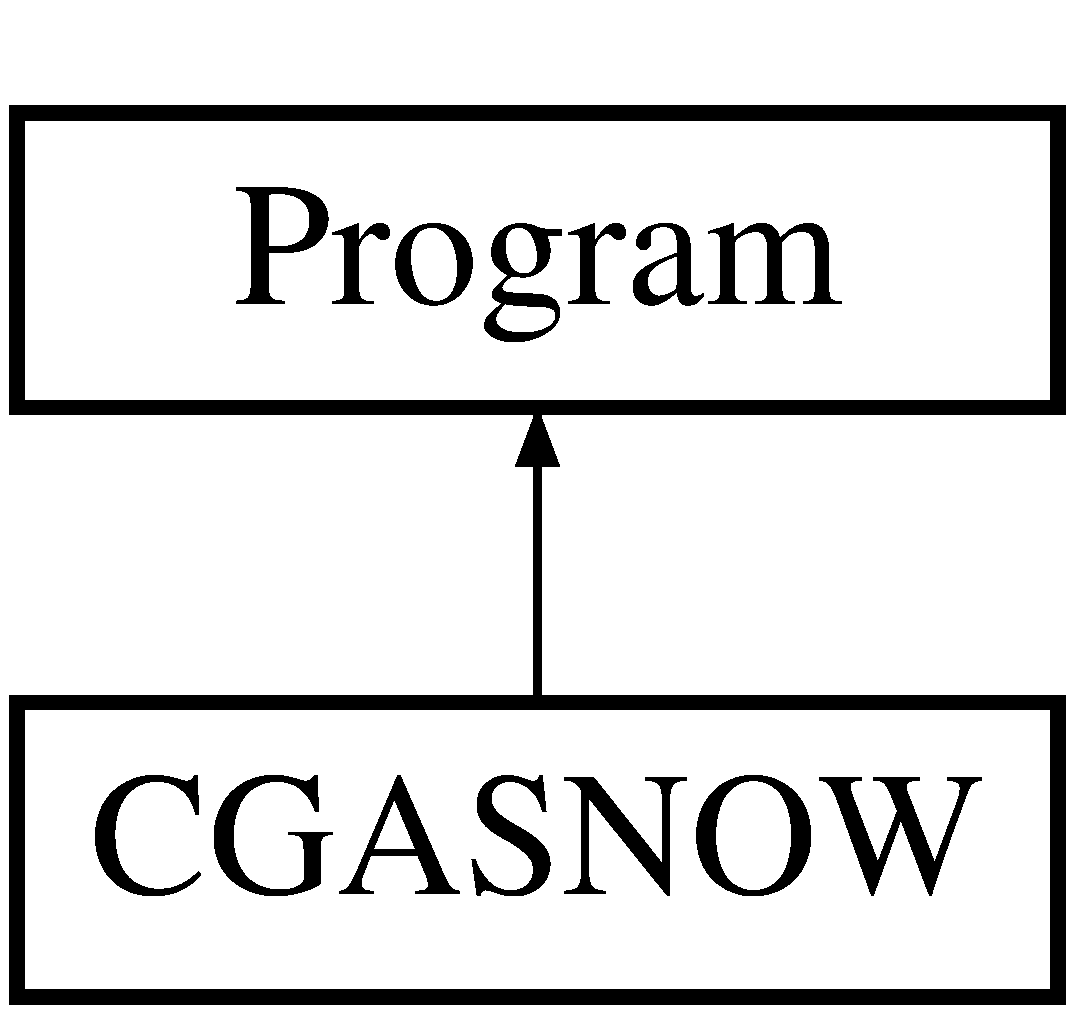
\includegraphics[height=2.000000cm]{classCGASNOW}
\end{center}
\end{figure}
\subsection*{Public Member Functions}
\begin{DoxyCompactItemize}
\item 
\hypertarget{classCGASNOW_a756619df2231c00d48df4bfec4a8965b}{void \hyperlink{classCGASNOW_a756619df2231c00d48df4bfec4a8965b}{Run} (void)}\label{classCGASNOW_a756619df2231c00d48df4bfec4a8965b}

\begin{DoxyCompactList}\small\item\em \hyperlink{classProgram}{Program} entry point, when the command is run. \end{DoxyCompactList}\end{DoxyCompactItemize}


\subsection{Detailed Description}
C\-G\-A\-S\-N\-O\-W.\-C\-O\-M utility to control C\-G\-A snow emulation. 

Utility to enable, disable, or query C\-G\-A snow emulation. This command is only available when machine=cga and the video mode is 80x25 text mode. 

Definition at line 458 of file vga.\-cpp.



The documentation for this class was generated from the following file\-:\begin{DoxyCompactItemize}
\item 
src/hardware/vga.\-cpp\end{DoxyCompactItemize}

\hypertarget{classCHandlerEvent}{\section{C\-Handler\-Event Class Reference}
\label{classCHandlerEvent}\index{C\-Handler\-Event@{C\-Handler\-Event}}
}


Mapper shortcut event. Keyboard triggerable only.  


Inheritance diagram for C\-Handler\-Event\-:\begin{figure}[H]
\begin{center}
\leavevmode
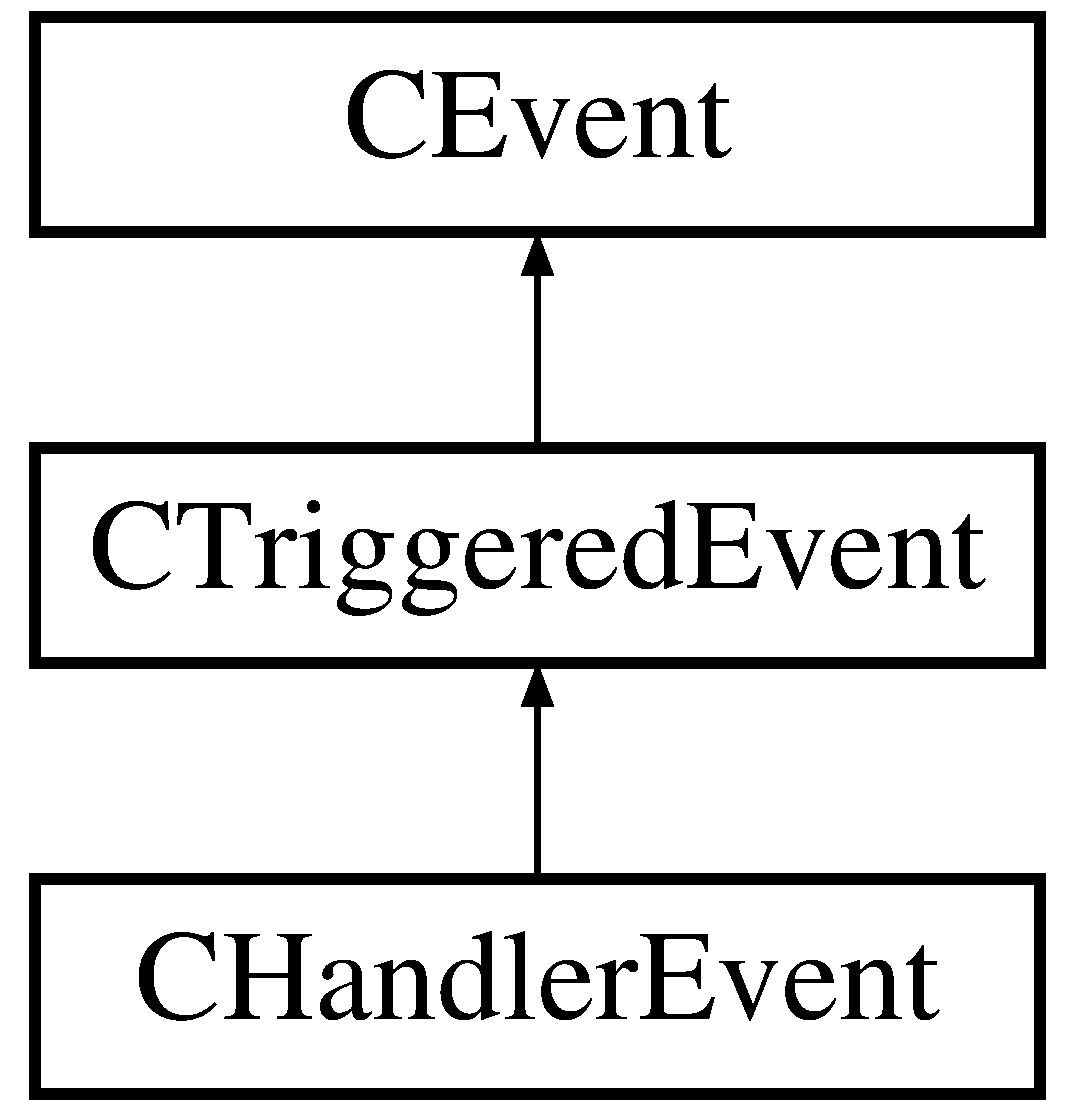
\includegraphics[height=3.000000cm]{classCHandlerEvent}
\end{center}
\end{figure}
\subsection*{Public Member Functions}
\begin{DoxyCompactItemize}
\item 
\hypertarget{classCHandlerEvent_aca304371826b35def368cb051ca7a625}{\hyperlink{classCHandlerEvent_aca304371826b35def368cb051ca7a625}{C\-Handler\-Event} (char const $\ast$const \-\_\-entry, M\-A\-P\-P\-E\-R\-\_\-\-Handler $\ast$\-\_\-handler, Map\-Keys \-\_\-key, Bitu \-\_\-mod, char const $\ast$const \-\_\-buttonname)}\label{classCHandlerEvent_aca304371826b35def368cb051ca7a625}

\begin{DoxyCompactList}\small\item\em Constructor, to specify the entry, handler (callback), key (according to Map\-Keys enumeration), and text to display for the shortcut in the mapper U\-O. \end{DoxyCompactList}\item 
\hypertarget{classCHandlerEvent_af4a0835bf174abb23ae9b88c0521e9c8}{virtual void \hyperlink{classCHandlerEvent_af4a0835bf174abb23ae9b88c0521e9c8}{Active} (bool yesno)}\label{classCHandlerEvent_af4a0835bf174abb23ae9b88c0521e9c8}

\begin{DoxyCompactList}\small\item\em Change whether the event is activated or not. \end{DoxyCompactList}\item 
\hypertarget{classCHandlerEvent_a58aafd6e482cff4b63507391d424477f}{const char $\ast$ \hyperlink{classCHandlerEvent_a58aafd6e482cff4b63507391d424477f}{Button\-Name} (void)}\label{classCHandlerEvent_a58aafd6e482cff4b63507391d424477f}

\begin{DoxyCompactList}\small\item\em Retrieve the button name (for display in the mapper U\-I) \end{DoxyCompactList}\item 
\hypertarget{classCHandlerEvent_a3062e41266603ad8918a7ca2bba8f095}{void \hyperlink{classCHandlerEvent_a3062e41266603ad8918a7ca2bba8f095}{Make\-Default\-Bind} (char $\ast$buf)}\label{classCHandlerEvent_a3062e41266603ad8918a7ca2bba8f095}

\begin{DoxyCompactList}\small\item\em Generate a default binding from the Map\-Keys enumeration. \end{DoxyCompactList}\item 
\hypertarget{classCHandlerEvent_a3bd14f3961c29799530602c8e2d5a6fe}{void \hyperlink{classCHandlerEvent_a3bd14f3961c29799530602c8e2d5a6fe}{notifybutton} (\hyperlink{classCTextButton}{C\-Text\-Button} $\ast$n)}\label{classCHandlerEvent_a3bd14f3961c29799530602c8e2d5a6fe}

\begin{DoxyCompactList}\small\item\em Associate this object with a text button in the mapper U\-I. \end{DoxyCompactList}\end{DoxyCompactItemize}
\subsection*{Public Attributes}
\begin{DoxyCompactItemize}
\item 
\hypertarget{classCHandlerEvent_ac636235e80032332d688fe888ebd5cf4}{\hyperlink{classCTextButton}{C\-Text\-Button} $\ast$ \hyperlink{classCHandlerEvent_ac636235e80032332d688fe888ebd5cf4}{notify\-\_\-button}}\label{classCHandlerEvent_ac636235e80032332d688fe888ebd5cf4}

\begin{DoxyCompactList}\small\item\em Text button in the mapper U\-I to indicate status by. \end{DoxyCompactList}\item 
\hypertarget{classCHandlerEvent_a9227a65125fadc33d775cc0de3b29393}{M\-A\-P\-P\-E\-R\-\_\-\-Handler $\ast$ \hyperlink{classCHandlerEvent_a9227a65125fadc33d775cc0de3b29393}{handler}}\label{classCHandlerEvent_a9227a65125fadc33d775cc0de3b29393}

\begin{DoxyCompactList}\small\item\em Mapper handler shortcut. \end{DoxyCompactList}\item 
\hypertarget{classCHandlerEvent_a935a8c622ac72d46512f5c88fefacda8}{const char $\ast$ \hyperlink{classCHandlerEvent_a935a8c622ac72d46512f5c88fefacda8}{buttonname}}\label{classCHandlerEvent_a935a8c622ac72d46512f5c88fefacda8}

\begin{DoxyCompactList}\small\item\em Button name. \end{DoxyCompactList}\end{DoxyCompactItemize}
\subsection*{Protected Attributes}
\begin{DoxyCompactItemize}
\item 
\hypertarget{classCHandlerEvent_a7d53624253497b7dcad4a281a790333d}{Map\-Keys \hyperlink{classCHandlerEvent_a7d53624253497b7dcad4a281a790333d}{defkey}}\label{classCHandlerEvent_a7d53624253497b7dcad4a281a790333d}

\begin{DoxyCompactList}\small\item\em Map\-Keys enumeration for keyboard shortcut. \end{DoxyCompactList}\item 
\hypertarget{classCHandlerEvent_a2ebc8142a6ef34d7c23349e86a0d4486}{Bitu \hyperlink{classCHandlerEvent_a2ebc8142a6ef34d7c23349e86a0d4486}{defmod}}\label{classCHandlerEvent_a2ebc8142a6ef34d7c23349e86a0d4486}

\begin{DoxyCompactList}\small\item\em Default modifiers. \end{DoxyCompactList}\end{DoxyCompactItemize}


\subsection{Detailed Description}
Mapper shortcut event. Keyboard triggerable only. 

Definition at line 2162 of file sdl\-\_\-mapper.\-cpp.



The documentation for this class was generated from the following file\-:\begin{DoxyCompactItemize}
\item 
src/gui/sdl\-\_\-mapper.\-cpp\end{DoxyCompactItemize}

\hypertarget{structProperty_1_1Changeable}{\section{Property\-:\-:Changeable Struct Reference}
\label{structProperty_1_1Changeable}\index{Property\-::\-Changeable@{Property\-::\-Changeable}}
}
\subsection*{Public Types}
\begin{DoxyCompactItemize}
\item 
enum {\bfseries Value} \{ {\bfseries Always}, 
{\bfseries When\-Idle}, 
{\bfseries Only\-At\-Start}
 \}
\end{DoxyCompactItemize}


\subsection{Detailed Description}


Definition at line 121 of file setup.\-h.



The documentation for this struct was generated from the following file\-:\begin{DoxyCompactItemize}
\item 
include/setup.\-h\end{DoxyCompactItemize}

\hypertarget{structDBOPL_1_1Channel}{\section{D\-B\-O\-P\-L\-:\-:Channel Struct Reference}
\label{structDBOPL_1_1Channel}\index{D\-B\-O\-P\-L\-::\-Channel@{D\-B\-O\-P\-L\-::\-Channel}}
}
\subsection*{Public Member Functions}
\begin{DoxyCompactItemize}
\item 
\hypertarget{structDBOPL_1_1Channel_a54d428b50eb682592bbd51f56a62a4f9}{\hyperlink{structDBOPL_1_1Operator}{Operator} $\ast$ {\bfseries Op} (Bitu index)}\label{structDBOPL_1_1Channel_a54d428b50eb682592bbd51f56a62a4f9}

\item 
\hypertarget{structDBOPL_1_1Channel_ae6e7eafa3ea682e7e5c7f4a50f197181}{void {\bfseries Set\-Chan\-Data} (const \hyperlink{structDBOPL_1_1Chip}{Chip} $\ast$chip, Bit32u data)}\label{structDBOPL_1_1Channel_ae6e7eafa3ea682e7e5c7f4a50f197181}

\item 
\hypertarget{structDBOPL_1_1Channel_a86f42e926233a28c6bc3448e54cfd546}{void {\bfseries Update\-Frequency} (const \hyperlink{structDBOPL_1_1Chip}{Chip} $\ast$chip, Bit8u four\-Op)}\label{structDBOPL_1_1Channel_a86f42e926233a28c6bc3448e54cfd546}

\item 
\hypertarget{structDBOPL_1_1Channel_a62ce41d757e5dc1f91013e12eff83fa7}{void {\bfseries Update\-Synth} (const \hyperlink{structDBOPL_1_1Chip}{Chip} $\ast$chip)}\label{structDBOPL_1_1Channel_a62ce41d757e5dc1f91013e12eff83fa7}

\item 
\hypertarget{structDBOPL_1_1Channel_a756b7c37c2137e336260c5afeabecd49}{void {\bfseries Write\-A0} (const \hyperlink{structDBOPL_1_1Chip}{Chip} $\ast$chip, Bit8u val)}\label{structDBOPL_1_1Channel_a756b7c37c2137e336260c5afeabecd49}

\item 
\hypertarget{structDBOPL_1_1Channel_aa9153eb97e4a16d9da0169eb65b92bcb}{void {\bfseries Write\-B0} (const \hyperlink{structDBOPL_1_1Chip}{Chip} $\ast$chip, Bit8u val)}\label{structDBOPL_1_1Channel_aa9153eb97e4a16d9da0169eb65b92bcb}

\item 
\hypertarget{structDBOPL_1_1Channel_ac49656ad221520c54e6d8f477a198449}{void {\bfseries Write\-C0} (const \hyperlink{structDBOPL_1_1Chip}{Chip} $\ast$chip, Bit8u val)}\label{structDBOPL_1_1Channel_ac49656ad221520c54e6d8f477a198449}

\item 
\hypertarget{structDBOPL_1_1Channel_abb3d1d632e223ac1dcee2e48e89b3c3b}{{\footnotesize template$<$bool opl3\-Mode$>$ }\\void {\bfseries Generate\-Percussion} (\hyperlink{structDBOPL_1_1Chip}{Chip} $\ast$chip, Bit32s $\ast$output)}\label{structDBOPL_1_1Channel_abb3d1d632e223ac1dcee2e48e89b3c3b}

\item 
\hypertarget{structDBOPL_1_1Channel_a731abbda797b2dacd75a92f443c82488}{{\footnotesize template$<$Synth\-Mode mode$>$ }\\\hyperlink{structDBOPL_1_1Channel}{Channel} $\ast$ {\bfseries Block\-Template} (\hyperlink{structDBOPL_1_1Chip}{Chip} $\ast$chip, Bit32u samples, Bit32s $\ast$output)}\label{structDBOPL_1_1Channel_a731abbda797b2dacd75a92f443c82488}

\end{DoxyCompactItemize}
\subsection*{Public Attributes}
\begin{DoxyCompactItemize}
\item 
\hypertarget{structDBOPL_1_1Channel_aa5bb1c90f84d9b8a04f4c4110bedb169}{\hyperlink{structDBOPL_1_1Operator}{Operator} {\bfseries op} \mbox{[}2\mbox{]}}\label{structDBOPL_1_1Channel_aa5bb1c90f84d9b8a04f4c4110bedb169}

\item 
\hypertarget{structDBOPL_1_1Channel_a266d0cc54c93cf0a8fb7d766adbdcb0a}{Synth\-Handler {\bfseries synth\-Handler}}\label{structDBOPL_1_1Channel_a266d0cc54c93cf0a8fb7d766adbdcb0a}

\item 
\hypertarget{structDBOPL_1_1Channel_ad91510284ef6e6b40a01d740ae005c26}{Bit32u {\bfseries chan\-Data}}\label{structDBOPL_1_1Channel_ad91510284ef6e6b40a01d740ae005c26}

\item 
\hypertarget{structDBOPL_1_1Channel_a19de035abb6b4208b4495db8748953b1}{Bit32s {\bfseries old} \mbox{[}2\mbox{]}}\label{structDBOPL_1_1Channel_a19de035abb6b4208b4495db8748953b1}

\item 
\hypertarget{structDBOPL_1_1Channel_a8f0785435bc4dc242e31ef7189c6c820}{Bit8u {\bfseries feedback}}\label{structDBOPL_1_1Channel_a8f0785435bc4dc242e31ef7189c6c820}

\item 
\hypertarget{structDBOPL_1_1Channel_ab3dc5ec924ed7f45eaec874a6b832b65}{Bit8u {\bfseries reg\-B0}}\label{structDBOPL_1_1Channel_ab3dc5ec924ed7f45eaec874a6b832b65}

\item 
\hypertarget{structDBOPL_1_1Channel_a8d7eb26618827a6f411b2eed17d47198}{Bit8u {\bfseries reg\-C0}}\label{structDBOPL_1_1Channel_a8d7eb26618827a6f411b2eed17d47198}

\item 
\hypertarget{structDBOPL_1_1Channel_a42935dfe22c169e87d2bc07d0735c70b}{Bit8u {\bfseries four\-Mask}}\label{structDBOPL_1_1Channel_a42935dfe22c169e87d2bc07d0735c70b}

\item 
\hypertarget{structDBOPL_1_1Channel_ab526018f8396bed2335abbdb2829e133}{Bit8s {\bfseries mask\-Left}}\label{structDBOPL_1_1Channel_ab526018f8396bed2335abbdb2829e133}

\item 
\hypertarget{structDBOPL_1_1Channel_a79e6d8a988d547a71ebd48097172f121}{Bit8s {\bfseries mask\-Right}}\label{structDBOPL_1_1Channel_a79e6d8a988d547a71ebd48097172f121}

\end{DoxyCompactItemize}


\subsection{Detailed Description}


Definition at line 158 of file dbopl.\-h.



The documentation for this struct was generated from the following files\-:\begin{DoxyCompactItemize}
\item 
src/hardware/dbopl.\-h\item 
src/hardware/dbopl.\-cpp\end{DoxyCompactItemize}

\hypertarget{structCHARMAP}{\section{C\-H\-A\-R\-M\-A\-P Struct Reference}
\label{structCHARMAP}\index{C\-H\-A\-R\-M\-A\-P@{C\-H\-A\-R\-M\-A\-P}}
}
\subsection*{Public Attributes}
\begin{DoxyCompactItemize}
\item 
\hypertarget{structCHARMAP_a4381a41290a5adbfb4944bdd72113c57}{Bitu {\bfseries codepage}}\label{structCHARMAP_a4381a41290a5adbfb4944bdd72113c57}

\item 
\hypertarget{structCHARMAP_ae6e1767d336d81fcc508fc7df8354e03}{const Bit16u $\ast$ {\bfseries map}}\label{structCHARMAP_ae6e1767d336d81fcc508fc7df8354e03}

\end{DoxyCompactItemize}


\subsection{Detailed Description}


Definition at line 19 of file printer\-\_\-charmaps.\-h.



The documentation for this struct was generated from the following file\-:\begin{DoxyCompactItemize}
\item 
src/hardware/parport/printer\-\_\-charmaps.\-h\end{DoxyCompactItemize}

\hypertarget{classGUI_1_1Checkbox}{\section{G\-U\-I\-:\-:Checkbox Class Reference}
\label{classGUI_1_1Checkbox}\index{G\-U\-I\-::\-Checkbox@{G\-U\-I\-::\-Checkbox}}
}


A checkbox.  




{\ttfamily \#include $<$gui\-\_\-tk.\-h$>$}

Inheritance diagram for G\-U\-I\-:\-:Checkbox\-:\begin{figure}[H]
\begin{center}
\leavevmode
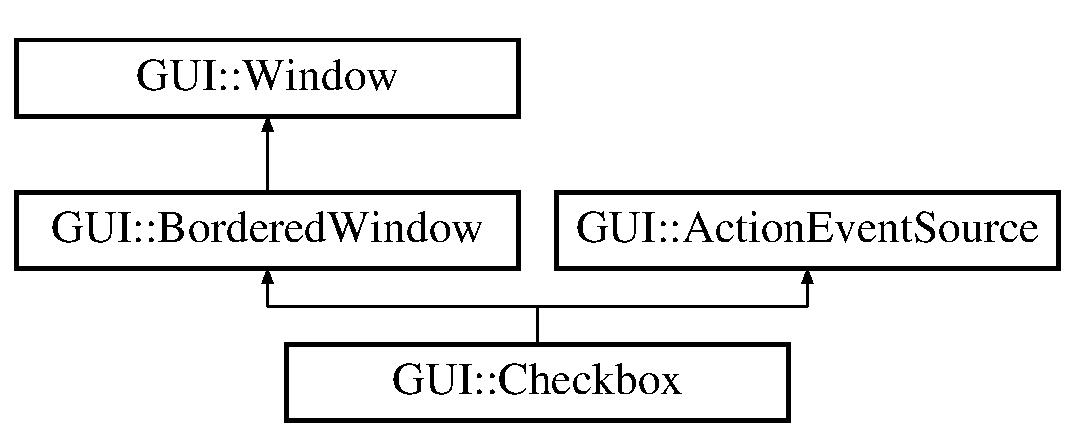
\includegraphics[height=4.000000cm]{classGUI_1_1Checkbox}
\end{center}
\end{figure}
\subsection*{Public Member Functions}
\begin{DoxyCompactItemize}
\item 
\hypertarget{classGUI_1_1Checkbox_a025ab90d6def02c0df24d46999b16198}{\hyperlink{classGUI_1_1Checkbox_a025ab90d6def02c0df24d46999b16198}{Checkbox} (\hyperlink{classGUI_1_1Window}{Window} $\ast$\hyperlink{classGUI_1_1Window_a2e593ff65e7702178d82fe9010a0b539}{parent}, int \hyperlink{classGUI_1_1Window_a6ca6a80ca00c9e1d8ceea8d3d99a657d}{x}, int \hyperlink{classGUI_1_1Window_a0ee8e923aff2c3661fc2e17656d37adf}{y}, int w, int h)}\label{classGUI_1_1Checkbox_a025ab90d6def02c0df24d46999b16198}

\begin{DoxyCompactList}\small\item\em Create a checkbox with given position and size. \end{DoxyCompactList}\item 
{\footnotesize template$<$typename T $>$ }\\\hyperlink{classGUI_1_1Checkbox_accc7c898b46063c9b7e21d7563c17189}{Checkbox} (\hyperlink{classGUI_1_1Window}{Window} $\ast$\hyperlink{classGUI_1_1Window_a2e593ff65e7702178d82fe9010a0b539}{parent}, int \hyperlink{classGUI_1_1Window_a6ca6a80ca00c9e1d8ceea8d3d99a657d}{x}, int \hyperlink{classGUI_1_1Window_a0ee8e923aff2c3661fc2e17656d37adf}{y}, const T text, int w=-\/1, int h=-\/1)
\begin{DoxyCompactList}\small\item\em Create a checkbox with text label. \end{DoxyCompactList}\item 
\hypertarget{classGUI_1_1Checkbox_ad37c8e5dcccb0a4023585ef272f0ca90}{virtual void \hyperlink{classGUI_1_1Checkbox_ad37c8e5dcccb0a4023585ef272f0ca90}{paint} (\hyperlink{classGUI_1_1Drawable}{Drawable} \&d) const }\label{classGUI_1_1Checkbox_ad37c8e5dcccb0a4023585ef272f0ca90}

\begin{DoxyCompactList}\small\item\em Paint checkbox. \end{DoxyCompactList}\item 
\hypertarget{classGUI_1_1Checkbox_a75d3775dfe7d66fbb57070144ab823b4}{virtual void \hyperlink{classGUI_1_1Checkbox_a75d3775dfe7d66fbb57070144ab823b4}{set\-Checked} (bool \hyperlink{classGUI_1_1Checkbox_ab9e40eb561978770aad1095906c4fb65}{checked})}\label{classGUI_1_1Checkbox_a75d3775dfe7d66fbb57070144ab823b4}

\begin{DoxyCompactList}\small\item\em Change checkbox state. \end{DoxyCompactList}\item 
\hypertarget{classGUI_1_1Checkbox_ae6c07622ee6c683df6f140f1e5f06dfe}{virtual bool \hyperlink{classGUI_1_1Checkbox_ae6c07622ee6c683df6f140f1e5f06dfe}{is\-Checked} ()}\label{classGUI_1_1Checkbox_ae6c07622ee6c683df6f140f1e5f06dfe}

\begin{DoxyCompactList}\small\item\em Get checkbox state. \end{DoxyCompactList}\item 
\hypertarget{classGUI_1_1Checkbox_a27484bdfecbfa9064e6484b9e572e20e}{virtual bool \hyperlink{classGUI_1_1Checkbox_a27484bdfecbfa9064e6484b9e572e20e}{mouse\-Down} (int \hyperlink{classGUI_1_1Window_a6ca6a80ca00c9e1d8ceea8d3d99a657d}{x}, int \hyperlink{classGUI_1_1Window_a0ee8e923aff2c3661fc2e17656d37adf}{y}, \hyperlink{namespaceGUI_ad06082a7b02aa73697f39eb8e0856de9}{Mouse\-Button} button)}\label{classGUI_1_1Checkbox_a27484bdfecbfa9064e6484b9e572e20e}

\begin{DoxyCompactList}\small\item\em Press checkbox. \end{DoxyCompactList}\item 
\hypertarget{classGUI_1_1Checkbox_a4f0122a87de58f0c1a899b5291959148}{virtual bool \hyperlink{classGUI_1_1Checkbox_a4f0122a87de58f0c1a899b5291959148}{mouse\-Up} (int \hyperlink{classGUI_1_1Window_a6ca6a80ca00c9e1d8ceea8d3d99a657d}{x}, int \hyperlink{classGUI_1_1Window_a0ee8e923aff2c3661fc2e17656d37adf}{y}, \hyperlink{namespaceGUI_ad06082a7b02aa73697f39eb8e0856de9}{Mouse\-Button} button)}\label{classGUI_1_1Checkbox_a4f0122a87de58f0c1a899b5291959148}

\begin{DoxyCompactList}\small\item\em Release checkbox. \end{DoxyCompactList}\item 
\hypertarget{classGUI_1_1Checkbox_a695bf64dfdd4086cd08f0cd1a7d4df4a}{virtual bool \hyperlink{classGUI_1_1Checkbox_a695bf64dfdd4086cd08f0cd1a7d4df4a}{key\-Down} (const \hyperlink{classGUI_1_1Key}{Key} \&key)}\label{classGUI_1_1Checkbox_a695bf64dfdd4086cd08f0cd1a7d4df4a}

\begin{DoxyCompactList}\small\item\em Handle keyboard input. \end{DoxyCompactList}\item 
\hypertarget{classGUI_1_1Checkbox_a90f6ed34b6aff02c7074637b1a2c3c2f}{virtual bool \hyperlink{classGUI_1_1Checkbox_a90f6ed34b6aff02c7074637b1a2c3c2f}{key\-Up} (const \hyperlink{classGUI_1_1Key}{Key} \&key)}\label{classGUI_1_1Checkbox_a90f6ed34b6aff02c7074637b1a2c3c2f}

\begin{DoxyCompactList}\small\item\em Handle keyboard input. \end{DoxyCompactList}\item 
\hypertarget{classGUI_1_1Checkbox_a578d66f5d9006c6bbedbffbfd769caef}{virtual void \hyperlink{classGUI_1_1Checkbox_a578d66f5d9006c6bbedbffbfd769caef}{execute} ()}\label{classGUI_1_1Checkbox_a578d66f5d9006c6bbedbffbfd769caef}

\begin{DoxyCompactList}\small\item\em Execute handlers. \end{DoxyCompactList}\item 
\hypertarget{classGUI_1_1Checkbox_a0bdc8dc98a056bd1d7164aa5e5fb3e82}{{\footnotesize template$<$typename S\-T\-R $>$ }\\{\bfseries Checkbox} (\hyperlink{classGUI_1_1Window}{Window} $\ast$\hyperlink{classGUI_1_1Window_a2e593ff65e7702178d82fe9010a0b539}{parent}, int \hyperlink{classGUI_1_1Window_a6ca6a80ca00c9e1d8ceea8d3d99a657d}{x}, int \hyperlink{classGUI_1_1Window_a0ee8e923aff2c3661fc2e17656d37adf}{y}, const S\-T\-R text, int w, int h)}\label{classGUI_1_1Checkbox_a0bdc8dc98a056bd1d7164aa5e5fb3e82}

\end{DoxyCompactItemize}
\subsection*{Protected Attributes}
\begin{DoxyCompactItemize}
\item 
\hypertarget{classGUI_1_1Checkbox_ab9e40eb561978770aad1095906c4fb65}{bool \hyperlink{classGUI_1_1Checkbox_ab9e40eb561978770aad1095906c4fb65}{checked}}\label{classGUI_1_1Checkbox_ab9e40eb561978770aad1095906c4fb65}

\begin{DoxyCompactList}\small\item\em {\ttfamily true}, if checkbox is currently selected. \end{DoxyCompactList}\end{DoxyCompactItemize}


\subsection{Detailed Description}
A checkbox. 

Checkboxes can have any child widget as content. There are convenience constructors for common forms of checkboxes. 

Definition at line 2403 of file gui\-\_\-tk.\-h.



\subsection{Constructor \& Destructor Documentation}
\hypertarget{classGUI_1_1Checkbox_accc7c898b46063c9b7e21d7563c17189}{\index{G\-U\-I\-::\-Checkbox@{G\-U\-I\-::\-Checkbox}!Checkbox@{Checkbox}}
\index{Checkbox@{Checkbox}!GUI::Checkbox@{G\-U\-I\-::\-Checkbox}}
\subsubsection[{Checkbox}]{\setlength{\rightskip}{0pt plus 5cm}template$<$typename T $>$ {\bf G\-U\-I\-::\-Checkbox\-::\-Checkbox} (
\begin{DoxyParamCaption}
\item[{{\bf Window} $\ast$}]{parent, }
\item[{int}]{x, }
\item[{int}]{y, }
\item[{const T}]{text, }
\item[{int}]{w = {\ttfamily -\/1}, }
\item[{int}]{h = {\ttfamily -\/1}}
\end{DoxyParamCaption}
)}}\label{classGUI_1_1Checkbox_accc7c898b46063c9b7e21d7563c17189}


Create a checkbox with text label. 

If a size is specified, text is centered. Otherwise, checkbox size is adjusted for the text. 

The documentation for this class was generated from the following files\-:\begin{DoxyCompactItemize}
\item 
src/libs/gui\-\_\-tk/\hyperlink{gui__tk_8h}{gui\-\_\-tk.\-h}\item 
src/libs/gui\-\_\-tk/\hyperlink{gui__tk_8cpp}{gui\-\_\-tk.\-cpp}\end{DoxyCompactItemize}

\hypertarget{structAdlib_1_1Chip}{\section{Adlib\-:\-:Chip Struct Reference}
\label{structAdlib_1_1Chip}\index{Adlib\-::\-Chip@{Adlib\-::\-Chip}}
}
\subsection*{Public Member Functions}
\begin{DoxyCompactItemize}
\item 
\hypertarget{structAdlib_1_1Chip_ad28b029cb4ec56ff900b160c00accad0}{bool {\bfseries Write} (Bit32u addr, Bit8u val)}\label{structAdlib_1_1Chip_ad28b029cb4ec56ff900b160c00accad0}

\item 
\hypertarget{structAdlib_1_1Chip_a472381a44ada102a7df220a9d16d002f}{Bit8u {\bfseries Read} ()}\label{structAdlib_1_1Chip_a472381a44ada102a7df220a9d16d002f}

\end{DoxyCompactItemize}
\subsection*{Public Attributes}
\begin{DoxyCompactItemize}
\item 
\hypertarget{structAdlib_1_1Chip_a98d53752542a19e358f02a3da4cf473e}{\hyperlink{structAdlib_1_1Timer}{Timer} {\bfseries timer} \mbox{[}2\mbox{]}}\label{structAdlib_1_1Chip_a98d53752542a19e358f02a3da4cf473e}

\item 
\hypertarget{structAdlib_1_1Chip_ac92c16633c6051b3b9721944a809925c}{double {\bfseries last\-\_\-poll}}\label{structAdlib_1_1Chip_ac92c16633c6051b3b9721944a809925c}

\item 
\hypertarget{structAdlib_1_1Chip_a0f964ac7fe648a9302e5c0ba219fb7da}{unsigned int {\bfseries poll\-\_\-counter}}\label{structAdlib_1_1Chip_a0f964ac7fe648a9302e5c0ba219fb7da}

\end{DoxyCompactItemize}


\subsection{Detailed Description}


Definition at line 81 of file adlib.\-h.



The documentation for this struct was generated from the following files\-:\begin{DoxyCompactItemize}
\item 
src/hardware/adlib.\-h\item 
src/hardware/adlib.\-cpp\end{DoxyCompactItemize}

\hypertarget{structDBOPL_1_1Chip}{\section{D\-B\-O\-P\-L\-:\-:Chip Struct Reference}
\label{structDBOPL_1_1Chip}\index{D\-B\-O\-P\-L\-::\-Chip@{D\-B\-O\-P\-L\-::\-Chip}}
}
\subsection*{Public Member Functions}
\begin{DoxyCompactItemize}
\item 
\hypertarget{structDBOPL_1_1Chip_aa6fa687111a426a5f78e167fa257ab3c}{Bit32u {\bfseries Forward\-L\-F\-O} (Bit32u samples)}\label{structDBOPL_1_1Chip_aa6fa687111a426a5f78e167fa257ab3c}

\item 
\hypertarget{structDBOPL_1_1Chip_a24786d7a165991bee7de4fcc0d771b51}{Bit32u {\bfseries Forward\-Noise} ()}\label{structDBOPL_1_1Chip_a24786d7a165991bee7de4fcc0d771b51}

\item 
\hypertarget{structDBOPL_1_1Chip_a2860097b5662864a601a5e88366d830e}{void {\bfseries Write\-B\-D} (Bit8u val)}\label{structDBOPL_1_1Chip_a2860097b5662864a601a5e88366d830e}

\item 
\hypertarget{structDBOPL_1_1Chip_a91898e7f05d8dffc30731970a554ef7e}{void {\bfseries Write\-Reg} (Bit32u reg, Bit8u val)}\label{structDBOPL_1_1Chip_a91898e7f05d8dffc30731970a554ef7e}

\item 
\hypertarget{structDBOPL_1_1Chip_ab7a01561768354f16b8851a0d21b7a2c}{Bit32u {\bfseries Write\-Addr} (Bit32u port, Bit8u val)}\label{structDBOPL_1_1Chip_ab7a01561768354f16b8851a0d21b7a2c}

\item 
\hypertarget{structDBOPL_1_1Chip_a638ee66303a2716dcbe88b16152a9c4c}{void {\bfseries Generate\-Block2} (Bitu total, Bit32s $\ast$output)}\label{structDBOPL_1_1Chip_a638ee66303a2716dcbe88b16152a9c4c}

\item 
\hypertarget{structDBOPL_1_1Chip_a57226206980412fd2e0b8e56aa4df36a}{void {\bfseries Generate\-Block3} (Bitu total, Bit32s $\ast$output)}\label{structDBOPL_1_1Chip_a57226206980412fd2e0b8e56aa4df36a}

\item 
\hypertarget{structDBOPL_1_1Chip_a2de016e86cff2a981f5f6595bf5c159e}{void {\bfseries Update\-Synths} ()}\label{structDBOPL_1_1Chip_a2de016e86cff2a981f5f6595bf5c159e}

\item 
\hypertarget{structDBOPL_1_1Chip_aa5e8f70f9b01aba04e5f0c78e96414e8}{void {\bfseries Generate} (Bit32u samples)}\label{structDBOPL_1_1Chip_aa5e8f70f9b01aba04e5f0c78e96414e8}

\item 
\hypertarget{structDBOPL_1_1Chip_a4f8f64b35ed6b37939048323796996c1}{void {\bfseries Setup} (Bit32u rate)}\label{structDBOPL_1_1Chip_a4f8f64b35ed6b37939048323796996c1}

\end{DoxyCompactItemize}
\subsection*{Public Attributes}
\begin{DoxyCompactItemize}
\item 
\hypertarget{structDBOPL_1_1Chip_a66b0973620b1f9a7cdf622779d94cfd8}{Bit32u {\bfseries lfo\-Counter} = 0}\label{structDBOPL_1_1Chip_a66b0973620b1f9a7cdf622779d94cfd8}

\item 
\hypertarget{structDBOPL_1_1Chip_ad4da7136cb32739922ec7ab39db7bb17}{Bit32u {\bfseries lfo\-Add} = 0}\label{structDBOPL_1_1Chip_ad4da7136cb32739922ec7ab39db7bb17}

\item 
\hypertarget{structDBOPL_1_1Chip_a404cab77d0078bc2d77c708fc40d6b59}{Bit32u {\bfseries noise\-Counter} = 0}\label{structDBOPL_1_1Chip_a404cab77d0078bc2d77c708fc40d6b59}

\item 
\hypertarget{structDBOPL_1_1Chip_ac79a160266752b013d0ca6656e28ef63}{Bit32u {\bfseries noise\-Add} = 0}\label{structDBOPL_1_1Chip_ac79a160266752b013d0ca6656e28ef63}

\item 
\hypertarget{structDBOPL_1_1Chip_af570acbdb634624278ff28cf4580b6b0}{Bit32u {\bfseries noise\-Value} = 0}\label{structDBOPL_1_1Chip_af570acbdb634624278ff28cf4580b6b0}

\item 
\hypertarget{structDBOPL_1_1Chip_a15109de386d644b49dc2864847a5eda9}{Bit32u {\bfseries freq\-Mul} \mbox{[}16\mbox{]} = \{\}}\label{structDBOPL_1_1Chip_a15109de386d644b49dc2864847a5eda9}

\item 
\hypertarget{structDBOPL_1_1Chip_aa8e0fd4b707ef682b66210a2820dda49}{Bit32u {\bfseries linear\-Rates} \mbox{[}76\mbox{]} = \{\}}\label{structDBOPL_1_1Chip_aa8e0fd4b707ef682b66210a2820dda49}

\item 
\hypertarget{structDBOPL_1_1Chip_ab92c0daba93e8bfce6cc2e52b8db6ee1}{Bit32u {\bfseries attack\-Rates} \mbox{[}76\mbox{]} = \{\}}\label{structDBOPL_1_1Chip_ab92c0daba93e8bfce6cc2e52b8db6ee1}

\item 
\hypertarget{structDBOPL_1_1Chip_ac85aae23657fde0285f563a134fabf03}{\hyperlink{structDBOPL_1_1Channel}{Channel} {\bfseries chan} \mbox{[}18\mbox{]}}\label{structDBOPL_1_1Chip_ac85aae23657fde0285f563a134fabf03}

\item 
\hypertarget{structDBOPL_1_1Chip_a55fc1b0db358bfa20ffae84f2aaf99be}{Bit8u {\bfseries reg104}}\label{structDBOPL_1_1Chip_a55fc1b0db358bfa20ffae84f2aaf99be}

\item 
\hypertarget{structDBOPL_1_1Chip_a342210c8b28260e8461b5278226c32ed}{Bit8u {\bfseries reg08}}\label{structDBOPL_1_1Chip_a342210c8b28260e8461b5278226c32ed}

\item 
\hypertarget{structDBOPL_1_1Chip_aafc35356ae0ac9a5dd966d296029aa57}{Bit8u {\bfseries reg04}}\label{structDBOPL_1_1Chip_aafc35356ae0ac9a5dd966d296029aa57}

\item 
\hypertarget{structDBOPL_1_1Chip_aee1cb30f6e56bcb2a9cf55de291dbc3b}{Bit8u {\bfseries reg\-B\-D}}\label{structDBOPL_1_1Chip_aee1cb30f6e56bcb2a9cf55de291dbc3b}

\item 
\hypertarget{structDBOPL_1_1Chip_ade088608ad9fc8eb5164db952ee0cfb0}{Bit8u {\bfseries vibrato\-Index} = 0}\label{structDBOPL_1_1Chip_ade088608ad9fc8eb5164db952ee0cfb0}

\item 
\hypertarget{structDBOPL_1_1Chip_a715127fbd970727b67170c4fd50920f7}{Bit8u {\bfseries tremolo\-Index} = 0}\label{structDBOPL_1_1Chip_a715127fbd970727b67170c4fd50920f7}

\item 
\hypertarget{structDBOPL_1_1Chip_a95d0a1d0025b1526c545160143870261}{Bit8s {\bfseries vibrato\-Sign} = 0}\label{structDBOPL_1_1Chip_a95d0a1d0025b1526c545160143870261}

\item 
\hypertarget{structDBOPL_1_1Chip_a020a0f86a13f5c621324d27633a7e000}{Bit8u {\bfseries vibrato\-Shift} = 0}\label{structDBOPL_1_1Chip_a020a0f86a13f5c621324d27633a7e000}

\item 
\hypertarget{structDBOPL_1_1Chip_a7915f11c9dc071855a835a9d1955bc52}{Bit8u {\bfseries tremolo\-Value} = 0}\label{structDBOPL_1_1Chip_a7915f11c9dc071855a835a9d1955bc52}

\item 
\hypertarget{structDBOPL_1_1Chip_a73605402418a92e9d405eb639d10309e}{Bit8u {\bfseries vibrato\-Strength} = 0}\label{structDBOPL_1_1Chip_a73605402418a92e9d405eb639d10309e}

\item 
\hypertarget{structDBOPL_1_1Chip_a1396767527e8811da6f18b5b2b3cab6e}{Bit8u {\bfseries tremolo\-Strength} = 0}\label{structDBOPL_1_1Chip_a1396767527e8811da6f18b5b2b3cab6e}

\item 
\hypertarget{structDBOPL_1_1Chip_a0aa21dbed40c6a7e01e014b841b8c6b0}{Bit8u {\bfseries wave\-Form\-Mask} = 0}\label{structDBOPL_1_1Chip_a0aa21dbed40c6a7e01e014b841b8c6b0}

\item 
\hypertarget{structDBOPL_1_1Chip_a0faef40e4f05cf2d8b789f6da637515d}{Bit8s {\bfseries opl3\-Active}}\label{structDBOPL_1_1Chip_a0faef40e4f05cf2d8b789f6da637515d}

\end{DoxyCompactItemize}


\subsection{Detailed Description}


Definition at line 194 of file dbopl.\-h.



The documentation for this struct was generated from the following files\-:\begin{DoxyCompactItemize}
\item 
src/hardware/dbopl.\-h\item 
src/hardware/dbopl.\-cpp\end{DoxyCompactItemize}

\hypertarget{classCJAxisBind}{\section{C\-J\-Axis\-Bind Class Reference}
\label{classCJAxisBind}\index{C\-J\-Axis\-Bind@{C\-J\-Axis\-Bind}}
}
Inheritance diagram for C\-J\-Axis\-Bind\-:\begin{figure}[H]
\begin{center}
\leavevmode
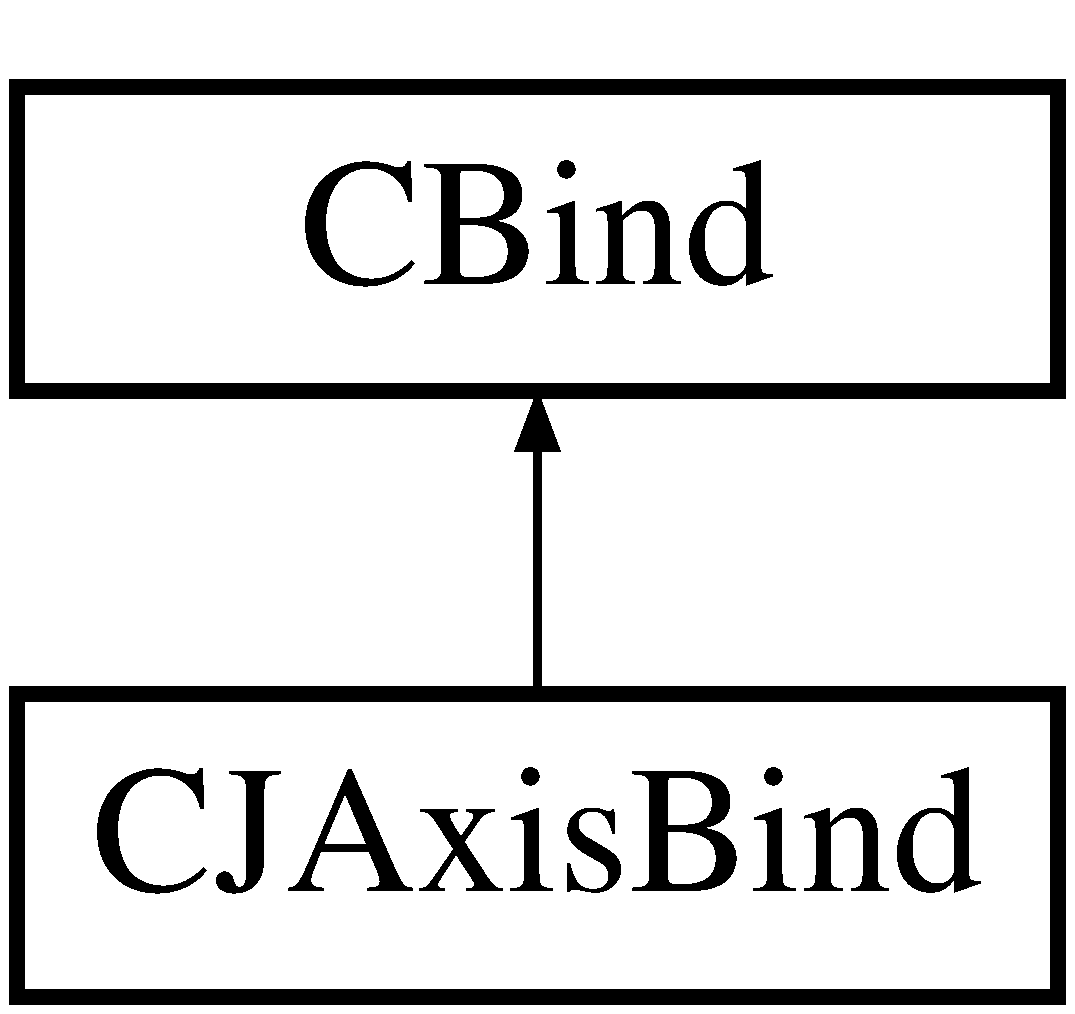
\includegraphics[height=2.000000cm]{classCJAxisBind}
\end{center}
\end{figure}
\subsection*{Public Member Functions}
\begin{DoxyCompactItemize}
\item 
\hypertarget{classCJAxisBind_a80b5b1ae676d9282c7ca3db9d54a9cd6}{{\bfseries C\-J\-Axis\-Bind} (C\-Bind\-List $\ast$\-\_\-list, \hyperlink{classCBindGroup}{C\-Bind\-Group} $\ast$\-\_\-group, Bitu \-\_\-joystick, Bitu \-\_\-axis, bool \-\_\-positive)}\label{classCJAxisBind_a80b5b1ae676d9282c7ca3db9d54a9cd6}

\item 
\hypertarget{classCJAxisBind_ad6469ca1df5b2e95f501cbf66df85ae0}{virtual void \hyperlink{classCJAxisBind_ad6469ca1df5b2e95f501cbf66df85ae0}{Config\-Name} (char $\ast$buf) override}\label{classCJAxisBind_ad6469ca1df5b2e95f501cbf66df85ae0}

\begin{DoxyCompactList}\small\item\em Get configuration name, for use in writing the mapper file. \end{DoxyCompactList}\item 
\hypertarget{classCJAxisBind_a975eada416c60a679dda6574cc4d5bd5}{virtual void \hyperlink{classCJAxisBind_a975eada416c60a679dda6574cc4d5bd5}{Bind\-Name} (char $\ast$buf) override}\label{classCJAxisBind_a975eada416c60a679dda6574cc4d5bd5}

\begin{DoxyCompactList}\small\item\em Get binding name, for display in the mapper U\-I. \end{DoxyCompactList}\item 
\hypertarget{classCJAxisBind_a033065f2f64ac52bfac7bf1d0aff17c3}{Bitu \hyperlink{classCJAxisBind_a033065f2f64ac52bfac7bf1d0aff17c3}{Get\-Joystick} () const }\label{classCJAxisBind_a033065f2f64ac52bfac7bf1d0aff17c3}

\begin{DoxyCompactList}\small\item\em Gets the joystick index for this instance. \end{DoxyCompactList}\item 
\hypertarget{classCJAxisBind_a6d9c9e742943700c75971a13bd827d42}{Bitu \hyperlink{classCJAxisBind_a6d9c9e742943700c75971a13bd827d42}{Get\-Axis} () const }\label{classCJAxisBind_a6d9c9e742943700c75971a13bd827d42}

\begin{DoxyCompactList}\small\item\em Gets the axis index for this instance. \end{DoxyCompactList}\item 
\hypertarget{classCJAxisBind_a8693e360c96fe5f86d2cd46eb1f9cf6e}{bool \hyperlink{classCJAxisBind_a8693e360c96fe5f86d2cd46eb1f9cf6e}{Get\-Positive} () const }\label{classCJAxisBind_a8693e360c96fe5f86d2cd46eb1f9cf6e}

\begin{DoxyCompactList}\small\item\em Gets the axis direction for this instance. \end{DoxyCompactList}\item 
\hypertarget{classCJAxisBind_a26d85b8903279b1948bcf9863d2a754b}{void \hyperlink{classCJAxisBind_a26d85b8903279b1948bcf9863d2a754b}{Activate\-Bind} (Bits \-\_\-value, bool ev\-\_\-trigger, bool skip\-\_\-action=false) override}\label{classCJAxisBind_a26d85b8903279b1948bcf9863d2a754b}

\begin{DoxyCompactList}\small\item\em Activate bindings. \end{DoxyCompactList}\end{DoxyCompactItemize}
\subsection*{Static Public Member Functions}
\begin{DoxyCompactItemize}
\item 
\hypertarget{classCJAxisBind_a43bdd7bf57954c208aea6e1a364d0a1e}{static int \hyperlink{classCJAxisBind_a43bdd7bf57954c208aea6e1a364d0a1e}{Get\-Joystick\-Deadzone} (int joystick, int axis, bool positive)}\label{classCJAxisBind_a43bdd7bf57954c208aea6e1a364d0a1e}

\begin{DoxyCompactList}\small\item\em Gets the deadzone for a joystick axis direction. \end{DoxyCompactList}\end{DoxyCompactItemize}
\subsection*{Protected Attributes}
\begin{DoxyCompactItemize}
\item 
\hypertarget{classCJAxisBind_a3aeea9f221c5a76fdf0658d5df006cac}{\hyperlink{classCBindGroup}{C\-Bind\-Group} $\ast$ {\bfseries group}}\label{classCJAxisBind_a3aeea9f221c5a76fdf0658d5df006cac}

\item 
\hypertarget{classCJAxisBind_a1845e3060cbcb2180e5a907dda6a7d4c}{Bitu {\bfseries axis}}\label{classCJAxisBind_a1845e3060cbcb2180e5a907dda6a7d4c}

\item 
\hypertarget{classCJAxisBind_a5c25cb696106b0959274368cd8dae0bd}{bool {\bfseries positive}}\label{classCJAxisBind_a5c25cb696106b0959274368cd8dae0bd}

\item 
\hypertarget{classCJAxisBind_ab47811ba5c358119d4e64855849f1a49}{Bitu {\bfseries joystick}}\label{classCJAxisBind_ab47811ba5c358119d4e64855849f1a49}

\end{DoxyCompactItemize}


\subsection{Detailed Description}


Definition at line 1175 of file sdl\-\_\-mapper.\-cpp.



The documentation for this class was generated from the following file\-:\begin{DoxyCompactItemize}
\item 
src/gui/sdl\-\_\-mapper.\-cpp\end{DoxyCompactItemize}

\hypertarget{classCJAxisEvent}{\section{C\-J\-Axis\-Event Class Reference}
\label{classCJAxisEvent}\index{C\-J\-Axis\-Event@{C\-J\-Axis\-Event}}
}
Inheritance diagram for C\-J\-Axis\-Event\-:\begin{figure}[H]
\begin{center}
\leavevmode
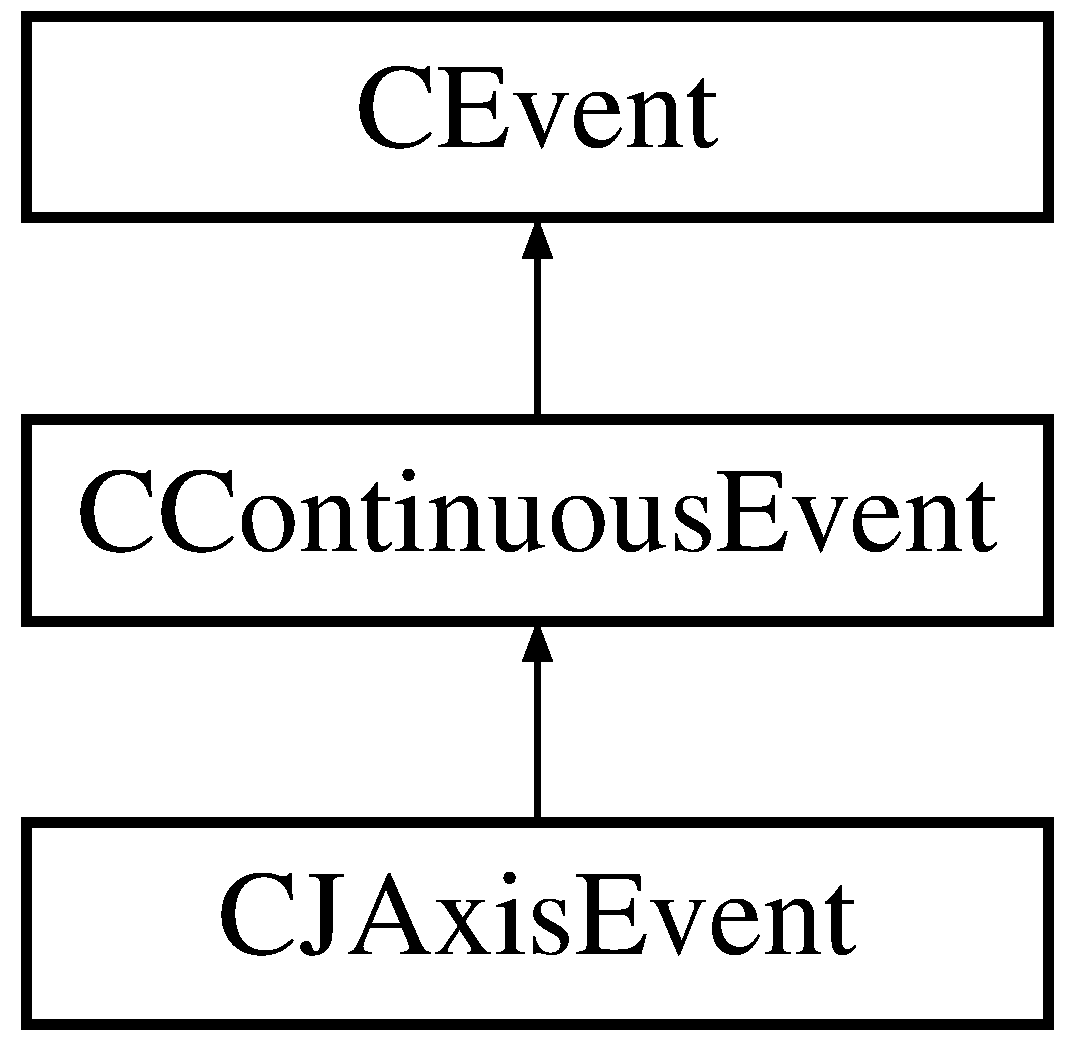
\includegraphics[height=3.000000cm]{classCJAxisEvent}
\end{center}
\end{figure}
\subsection*{Public Member Functions}
\begin{DoxyCompactItemize}
\item 
\hypertarget{classCJAxisEvent_a9cf7657ec986985dd15efcb92b20a380}{{\bfseries C\-J\-Axis\-Event} (char const $\ast$const \-\_\-entry, Bitu \-\_\-stick, Bitu \-\_\-axis, bool \-\_\-positive, \hyperlink{classCJAxisEvent}{C\-J\-Axis\-Event} $\ast$\-\_\-opposite\-\_\-axis)}\label{classCJAxisEvent_a9cf7657ec986985dd15efcb92b20a380}

\item 
\hypertarget{classCJAxisEvent_a1f0618c1d74612e06892430bdf7d8f92}{virtual void {\bfseries Active} (bool)}\label{classCJAxisEvent_a1f0618c1d74612e06892430bdf7d8f92}

\item 
\hypertarget{classCJAxisEvent_af6c1eaff5b1c3f1dc2b2715b76156ea4}{virtual Bitu {\bfseries Get\-Activity\-Count} (void)}\label{classCJAxisEvent_af6c1eaff5b1c3f1dc2b2715b76156ea4}

\item 
\hypertarget{classCJAxisEvent_abc322cf9dcf5488f49cb421f74574968}{virtual void {\bfseries Repost\-Activity} (void)}\label{classCJAxisEvent_abc322cf9dcf5488f49cb421f74574968}

\item 
\hypertarget{classCJAxisEvent_a523cca4f5afb972c28c5aa71ff3f408f}{void {\bfseries notifybutton} (\hyperlink{classCTextButton}{C\-Text\-Button} $\ast$n)}\label{classCJAxisEvent_a523cca4f5afb972c28c5aa71ff3f408f}

\end{DoxyCompactItemize}
\subsection*{Public Attributes}
\begin{DoxyCompactItemize}
\item 
\hypertarget{classCJAxisEvent_a44cbf08bc0468daffe05f967810851f0}{\hyperlink{classCTextButton}{C\-Text\-Button} $\ast$ {\bfseries notify\-\_\-button}}\label{classCJAxisEvent_a44cbf08bc0468daffe05f967810851f0}

\end{DoxyCompactItemize}
\subsection*{Protected Member Functions}
\begin{DoxyCompactItemize}
\item 
\hypertarget{classCJAxisEvent_afdb866161b2dc0dd1d8a5331f9d39117}{void {\bfseries Set\-Opposite\-Axis} (\hyperlink{classCJAxisEvent}{C\-J\-Axis\-Event} $\ast$\-\_\-opposite\-\_\-axis)}\label{classCJAxisEvent_afdb866161b2dc0dd1d8a5331f9d39117}

\end{DoxyCompactItemize}
\subsection*{Protected Attributes}
\begin{DoxyCompactItemize}
\item 
\hypertarget{classCJAxisEvent_a4445db17f0538358d815ab53d449beba}{Bitu {\bfseries stick}}\label{classCJAxisEvent_a4445db17f0538358d815ab53d449beba}

\item 
\hypertarget{classCJAxisEvent_aef7080ddb8c0a07235865f4f8f33bf90}{Bitu {\bfseries axis}}\label{classCJAxisEvent_aef7080ddb8c0a07235865f4f8f33bf90}

\item 
\hypertarget{classCJAxisEvent_a90367a0731415ea7dd7b3d01fa153367}{bool {\bfseries positive}}\label{classCJAxisEvent_a90367a0731415ea7dd7b3d01fa153367}

\item 
\hypertarget{classCJAxisEvent_aef506ec736efabf7a118af104921a998}{\hyperlink{classCJAxisEvent}{C\-J\-Axis\-Event} $\ast$ {\bfseries opposite\-\_\-axis}}\label{classCJAxisEvent_aef506ec736efabf7a118af104921a998}

\end{DoxyCompactItemize}


\subsection{Detailed Description}


Definition at line 1737 of file sdl\-\_\-mapper.\-cpp.



The documentation for this class was generated from the following file\-:\begin{DoxyCompactItemize}
\item 
src/gui/sdl\-\_\-mapper.\-cpp\end{DoxyCompactItemize}

\hypertarget{classCJButtonBind}{\section{C\-J\-Button\-Bind Class Reference}
\label{classCJButtonBind}\index{C\-J\-Button\-Bind@{C\-J\-Button\-Bind}}
}
Inheritance diagram for C\-J\-Button\-Bind\-:\begin{figure}[H]
\begin{center}
\leavevmode
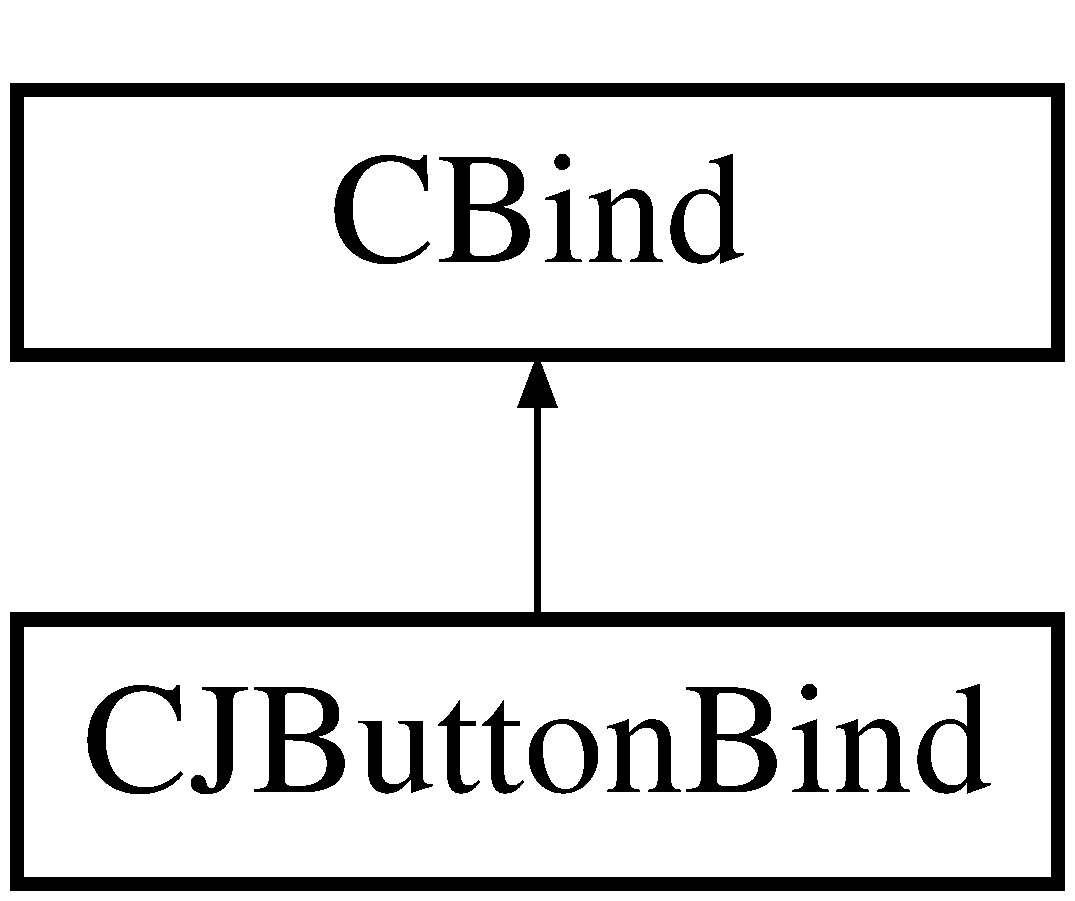
\includegraphics[height=2.000000cm]{classCJButtonBind}
\end{center}
\end{figure}
\subsection*{Public Member Functions}
\begin{DoxyCompactItemize}
\item 
\hypertarget{classCJButtonBind_a087e9681558df38907c7d57a373ec115}{{\bfseries C\-J\-Button\-Bind} (C\-Bind\-List $\ast$\-\_\-list, \hyperlink{classCBindGroup}{C\-Bind\-Group} $\ast$\-\_\-group, Bitu \-\_\-button)}\label{classCJButtonBind_a087e9681558df38907c7d57a373ec115}

\item 
\hypertarget{classCJButtonBind_a0aae6d69719dfb37dc2e1ed722663ec0}{void \hyperlink{classCJButtonBind_a0aae6d69719dfb37dc2e1ed722663ec0}{Config\-Name} (char $\ast$buf)}\label{classCJButtonBind_a0aae6d69719dfb37dc2e1ed722663ec0}

\begin{DoxyCompactList}\small\item\em Get configuration name, for use in writing the mapper file. \end{DoxyCompactList}\item 
\hypertarget{classCJButtonBind_a948fa272e3164f85522f7b1ece2ae49f}{void \hyperlink{classCJButtonBind_a948fa272e3164f85522f7b1ece2ae49f}{Bind\-Name} (char $\ast$buf)}\label{classCJButtonBind_a948fa272e3164f85522f7b1ece2ae49f}

\begin{DoxyCompactList}\small\item\em Get binding name, for display in the mapper U\-I. \end{DoxyCompactList}\end{DoxyCompactItemize}
\subsection*{Protected Attributes}
\begin{DoxyCompactItemize}
\item 
\hypertarget{classCJButtonBind_ade264023f83ad0202a6c5a2340d46833}{\hyperlink{classCBindGroup}{C\-Bind\-Group} $\ast$ {\bfseries group}}\label{classCJButtonBind_ade264023f83ad0202a6c5a2340d46833}

\item 
\hypertarget{classCJButtonBind_a6ef33ff006d574b8ea0df3ac18bf1a7a}{Bitu {\bfseries button}}\label{classCJButtonBind_a6ef33ff006d574b8ea0df3ac18bf1a7a}

\end{DoxyCompactItemize}


\subsection{Detailed Description}


Definition at line 915 of file sdl\-\_\-mapper.\-cpp.



The documentation for this class was generated from the following file\-:\begin{DoxyCompactItemize}
\item 
src/gui/sdl\-\_\-mapper.\-cpp\end{DoxyCompactItemize}

\hypertarget{classCJButtonEvent}{\section{C\-J\-Button\-Event Class Reference}
\label{classCJButtonEvent}\index{C\-J\-Button\-Event@{C\-J\-Button\-Event}}
}


Joystick button trigger.  


Inheritance diagram for C\-J\-Button\-Event\-:\begin{figure}[H]
\begin{center}
\leavevmode
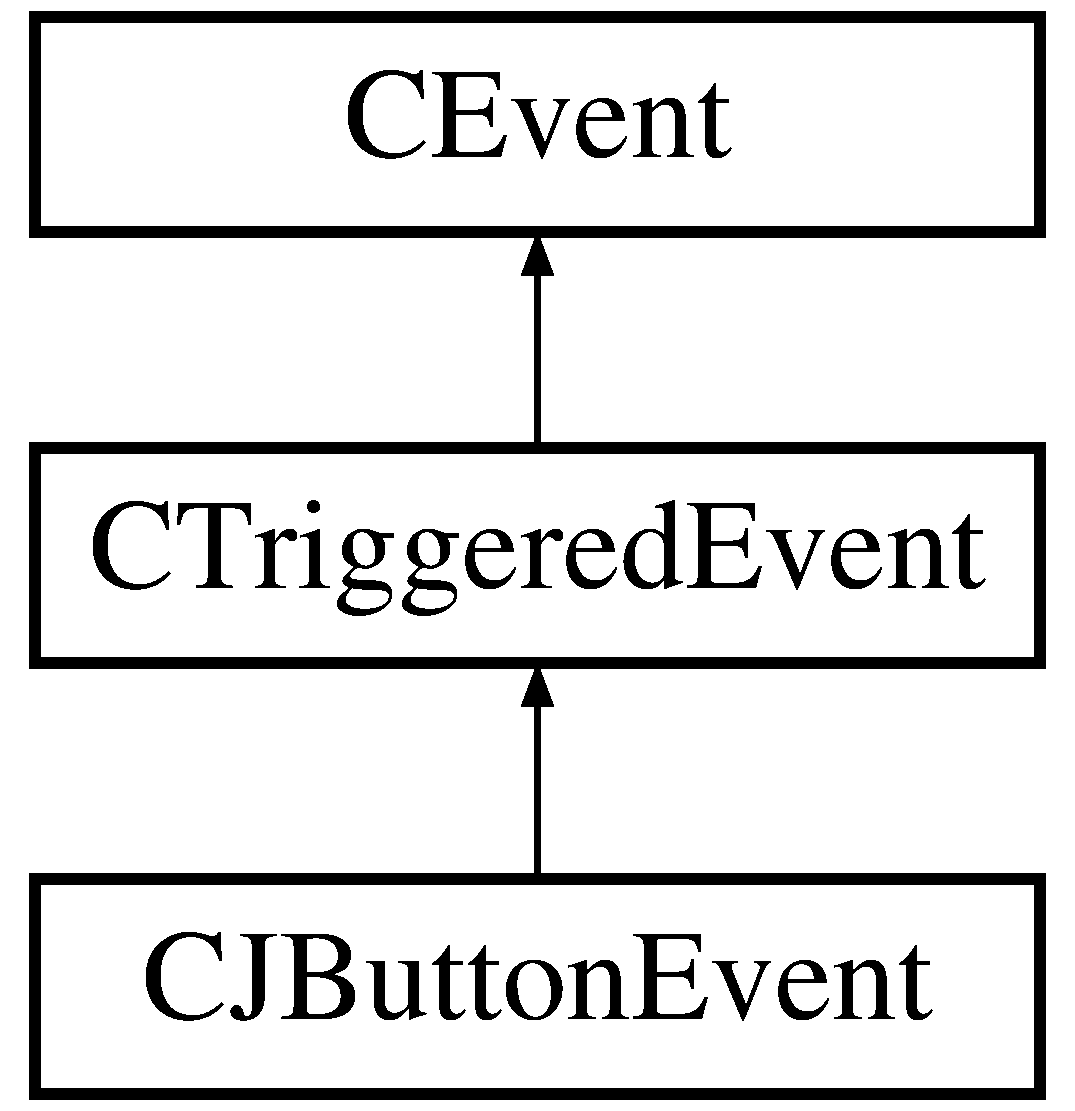
\includegraphics[height=3.000000cm]{classCJButtonEvent}
\end{center}
\end{figure}
\subsection*{Public Member Functions}
\begin{DoxyCompactItemize}
\item 
\hypertarget{classCJButtonEvent_a1e52758b5a23171097f00bae1acf028a}{\hyperlink{classCJButtonEvent_a1e52758b5a23171097f00bae1acf028a}{C\-J\-Button\-Event} (char const $\ast$const \-\_\-entry, Bitu \-\_\-stick, Bitu \-\_\-button)}\label{classCJButtonEvent_a1e52758b5a23171097f00bae1acf028a}

\begin{DoxyCompactList}\small\item\em Constructor, describing mapper event, joystick, and which button. \end{DoxyCompactList}\item 
\hypertarget{classCJButtonEvent_ad3be3de6af81cfbcf569e2d9bcee7e84}{virtual void \hyperlink{classCJButtonEvent_ad3be3de6af81cfbcf569e2d9bcee7e84}{Active} (bool pressed)}\label{classCJButtonEvent_ad3be3de6af81cfbcf569e2d9bcee7e84}

\begin{DoxyCompactList}\small\item\em Change whether the event is activated or not. \end{DoxyCompactList}\item 
\hypertarget{classCJButtonEvent_adc04a0aadec5744e0408c5e780d54d6b}{void \hyperlink{classCJButtonEvent_adc04a0aadec5744e0408c5e780d54d6b}{notifybutton} (\hyperlink{classCTextButton}{C\-Text\-Button} $\ast$n)}\label{classCJButtonEvent_adc04a0aadec5744e0408c5e780d54d6b}

\begin{DoxyCompactList}\small\item\em Associate this object with a text button in the mapper U\-I. \end{DoxyCompactList}\end{DoxyCompactItemize}
\subsection*{Public Attributes}
\begin{DoxyCompactItemize}
\item 
\hypertarget{classCJButtonEvent_ac8c89511fdc9a86b4c187eec432445d2}{\hyperlink{classCTextButton}{C\-Text\-Button} $\ast$ \hyperlink{classCJButtonEvent_ac8c89511fdc9a86b4c187eec432445d2}{notify\-\_\-button}}\label{classCJButtonEvent_ac8c89511fdc9a86b4c187eec432445d2}

\begin{DoxyCompactList}\small\item\em Text button in the mapper U\-I to indicate our status by. \end{DoxyCompactList}\end{DoxyCompactItemize}
\subsection*{Protected Attributes}
\begin{DoxyCompactItemize}
\item 
\hypertarget{classCJButtonEvent_aa87062af5d8bc5db801066e2eb4a74f8}{Bitu \hyperlink{classCJButtonEvent_aa87062af5d8bc5db801066e2eb4a74f8}{stick}}\label{classCJButtonEvent_aa87062af5d8bc5db801066e2eb4a74f8}

\begin{DoxyCompactList}\small\item\em Which joystick. \end{DoxyCompactList}\item 
\hypertarget{classCJButtonEvent_abdbfaa23915b89b1392129c9525dd58d}{Bitu \hyperlink{classCJButtonEvent_abdbfaa23915b89b1392129c9525dd58d}{button}}\label{classCJButtonEvent_abdbfaa23915b89b1392129c9525dd58d}

\begin{DoxyCompactList}\small\item\em Which button. \end{DoxyCompactList}\end{DoxyCompactItemize}


\subsection{Detailed Description}
Joystick button trigger. 

Definition at line 2249 of file sdl\-\_\-mapper.\-cpp.



The documentation for this class was generated from the following file\-:\begin{DoxyCompactItemize}
\item 
src/gui/sdl\-\_\-mapper.\-cpp\end{DoxyCompactItemize}

\hypertarget{classCJHatBind}{\section{C\-J\-Hat\-Bind Class Reference}
\label{classCJHatBind}\index{C\-J\-Hat\-Bind@{C\-J\-Hat\-Bind}}
}
Inheritance diagram for C\-J\-Hat\-Bind\-:\begin{figure}[H]
\begin{center}
\leavevmode
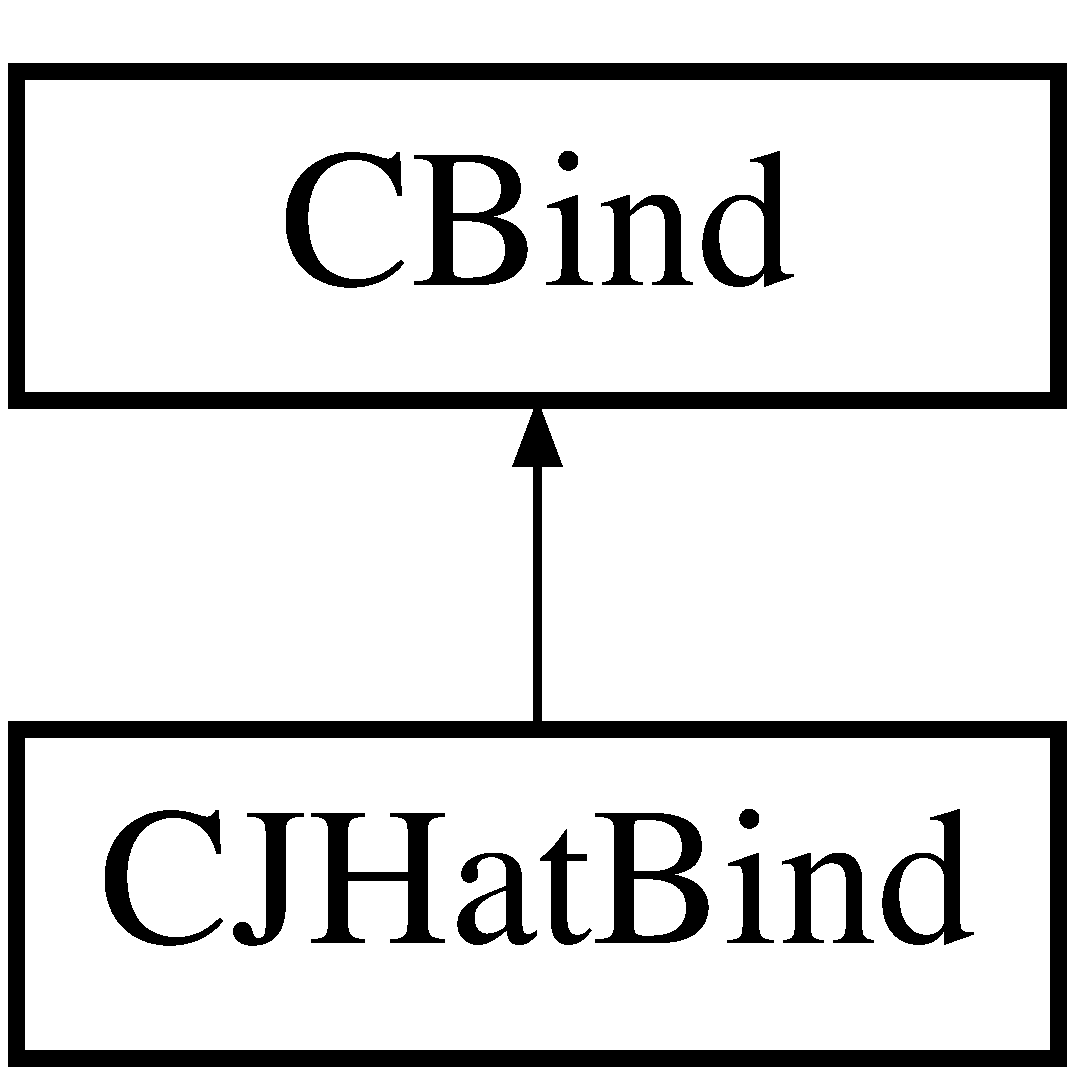
\includegraphics[height=2.000000cm]{classCJHatBind}
\end{center}
\end{figure}
\subsection*{Public Member Functions}
\begin{DoxyCompactItemize}
\item 
\hypertarget{classCJHatBind_af629c7834e53a8465c591e5547c5041e}{{\bfseries C\-J\-Hat\-Bind} (C\-Bind\-List $\ast$\-\_\-list, \hyperlink{classCBindGroup}{C\-Bind\-Group} $\ast$\-\_\-group, Bitu \-\_\-hat, Bit8u \-\_\-dir)}\label{classCJHatBind_af629c7834e53a8465c591e5547c5041e}

\item 
\hypertarget{classCJHatBind_a3380874d99f32a306b9253d5072ffd02}{virtual void \hyperlink{classCJHatBind_a3380874d99f32a306b9253d5072ffd02}{Config\-Name} (char $\ast$buf) override}\label{classCJHatBind_a3380874d99f32a306b9253d5072ffd02}

\begin{DoxyCompactList}\small\item\em Get configuration name, for use in writing the mapper file. \end{DoxyCompactList}\item 
\hypertarget{classCJHatBind_a560b88fbaed3fdff0c678262ac9963cf}{virtual void \hyperlink{classCJHatBind_a560b88fbaed3fdff0c678262ac9963cf}{Bind\-Name} (char $\ast$buf) override}\label{classCJHatBind_a560b88fbaed3fdff0c678262ac9963cf}

\begin{DoxyCompactList}\small\item\em Get binding name, for display in the mapper U\-I. \end{DoxyCompactList}\end{DoxyCompactItemize}
\subsection*{Protected Attributes}
\begin{DoxyCompactItemize}
\item 
\hypertarget{classCJHatBind_a29b7138a9094d140fad3bb6bef01b3e2}{\hyperlink{classCBindGroup}{C\-Bind\-Group} $\ast$ {\bfseries group}}\label{classCJHatBind_a29b7138a9094d140fad3bb6bef01b3e2}

\item 
\hypertarget{classCJHatBind_a652e1ca02ee3c415917d41bd557a25ba}{Bitu {\bfseries hat}}\label{classCJHatBind_a652e1ca02ee3c415917d41bd557a25ba}

\item 
\hypertarget{classCJHatBind_a2b02bbb8de4fc7bb9941f535254dad19}{Bit8u {\bfseries dir}}\label{classCJHatBind_a2b02bbb8de4fc7bb9941f535254dad19}

\end{DoxyCompactItemize}


\subsection{Detailed Description}


Definition at line 1252 of file sdl\-\_\-mapper.\-cpp.



The documentation for this class was generated from the following file\-:\begin{DoxyCompactItemize}
\item 
src/gui/sdl\-\_\-mapper.\-cpp\end{DoxyCompactItemize}

\hypertarget{classCJHatEvent}{\section{C\-J\-Hat\-Event Class Reference}
\label{classCJHatEvent}\index{C\-J\-Hat\-Event@{C\-J\-Hat\-Event}}
}


Joystick hat event.  


Inheritance diagram for C\-J\-Hat\-Event\-:\begin{figure}[H]
\begin{center}
\leavevmode
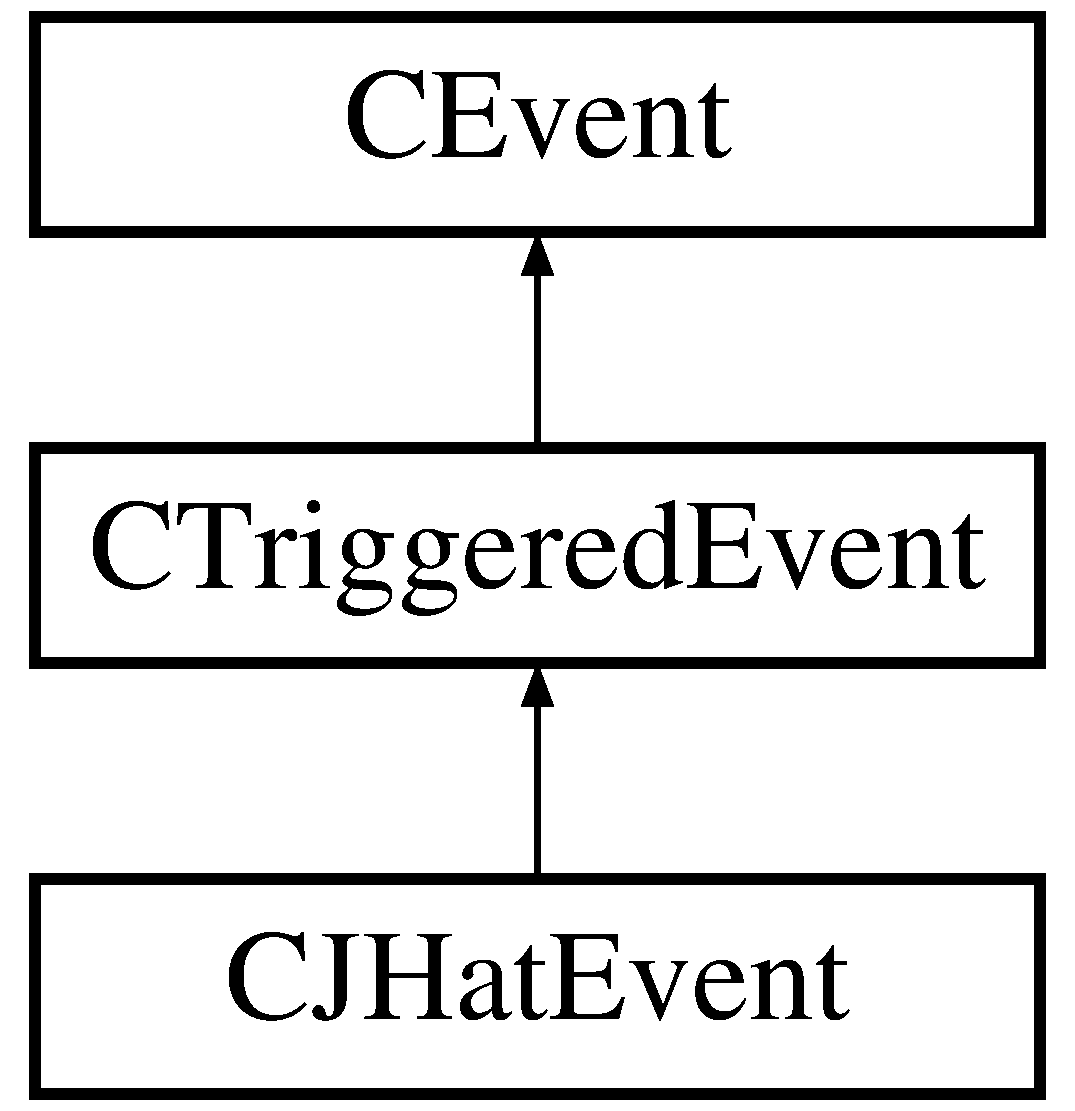
\includegraphics[height=3.000000cm]{classCJHatEvent}
\end{center}
\end{figure}
\subsection*{Public Member Functions}
\begin{DoxyCompactItemize}
\item 
\hypertarget{classCJHatEvent_a75c1276a13b233799993bb69bfbffedf}{\hyperlink{classCJHatEvent_a75c1276a13b233799993bb69bfbffedf}{C\-J\-Hat\-Event} (char const $\ast$const \-\_\-entry, Bitu \-\_\-stick, Bitu \-\_\-hat, Bitu \-\_\-dir)}\label{classCJHatEvent_a75c1276a13b233799993bb69bfbffedf}

\begin{DoxyCompactList}\small\item\em Constructor to describe mapper event, joystick, hat, and direction. \end{DoxyCompactList}\item 
\hypertarget{classCJHatEvent_ad4b66a30f706388e5568090963a22dee}{virtual void \hyperlink{classCJHatEvent_ad4b66a30f706388e5568090963a22dee}{Active} (bool pressed)}\label{classCJHatEvent_ad4b66a30f706388e5568090963a22dee}

\begin{DoxyCompactList}\small\item\em Change whether the event is activated or not. \end{DoxyCompactList}\end{DoxyCompactItemize}
\subsection*{Protected Attributes}
\begin{DoxyCompactItemize}
\item 
\hypertarget{classCJHatEvent_a53d2e407f823a8bd30a2c0d5613cb29b}{Bitu \hyperlink{classCJHatEvent_a53d2e407f823a8bd30a2c0d5613cb29b}{stick}}\label{classCJHatEvent_a53d2e407f823a8bd30a2c0d5613cb29b}

\begin{DoxyCompactList}\small\item\em Which joystick. \end{DoxyCompactList}\item 
\hypertarget{classCJHatEvent_a33cb6a20470c519958c6fd0929bcc7cd}{Bitu \hyperlink{classCJHatEvent_a33cb6a20470c519958c6fd0929bcc7cd}{hat}}\label{classCJHatEvent_a33cb6a20470c519958c6fd0929bcc7cd}

\begin{DoxyCompactList}\small\item\em Which hat. \end{DoxyCompactList}\item 
\hypertarget{classCJHatEvent_a8f7cc4b080b4f6054d6da118209683b7}{Bitu \hyperlink{classCJHatEvent_a8f7cc4b080b4f6054d6da118209683b7}{dir}}\label{classCJHatEvent_a8f7cc4b080b4f6054d6da118209683b7}

\begin{DoxyCompactList}\small\item\em Direction of hat. \end{DoxyCompactList}\end{DoxyCompactItemize}


\subsection{Detailed Description}
Joystick hat event. 

Definition at line 2090 of file sdl\-\_\-mapper.\-cpp.



The documentation for this class was generated from the following file\-:\begin{DoxyCompactItemize}
\item 
src/gui/sdl\-\_\-mapper.\-cpp\end{DoxyCompactItemize}

\hypertarget{classCKeyBind}{\section{C\-Key\-Bind Class Reference}
\label{classCKeyBind}\index{C\-Key\-Bind@{C\-Key\-Bind}}
}
Inheritance diagram for C\-Key\-Bind\-:\begin{figure}[H]
\begin{center}
\leavevmode
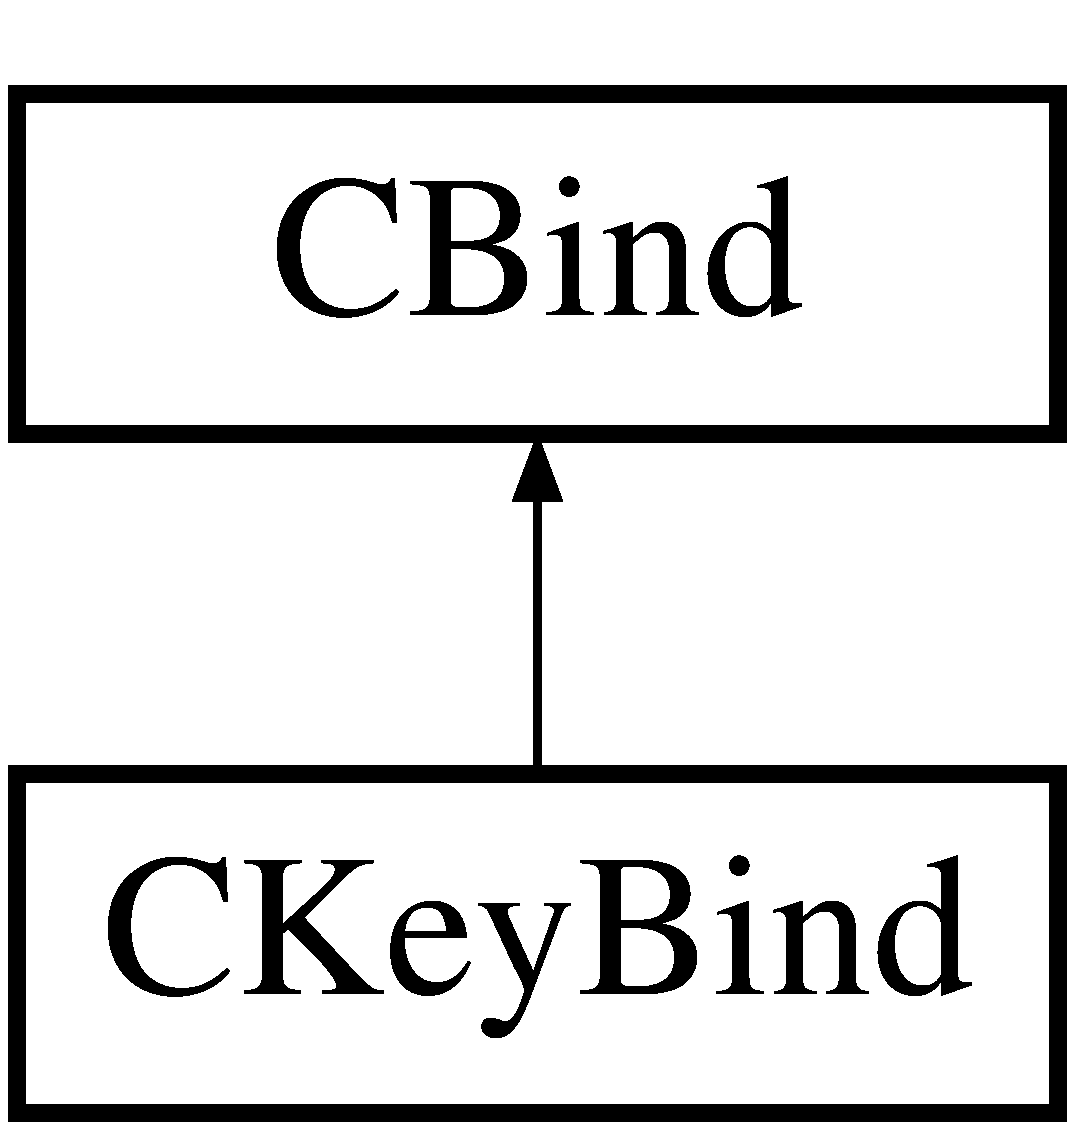
\includegraphics[height=2.000000cm]{classCKeyBind}
\end{center}
\end{figure}
\subsection*{Public Member Functions}
\begin{DoxyCompactItemize}
\item 
\hypertarget{classCKeyBind_ace188d08c2721d5f5074cdbd0e52b681}{{\bfseries C\-Key\-Bind} (C\-Bind\-List $\ast$\-\_\-list, S\-D\-L\-Key \-\_\-key)}\label{classCKeyBind_ace188d08c2721d5f5074cdbd0e52b681}

\item 
\hypertarget{classCKeyBind_a35652e64bf1da0c2477e6e235a4d8aec}{void {\bfseries Bind\-Name} (char $\ast$buf)}\label{classCKeyBind_a35652e64bf1da0c2477e6e235a4d8aec}

\item 
\hypertarget{classCKeyBind_a25c924a9b89ff14424899b1779bc70de}{void {\bfseries Config\-Name} (char $\ast$buf)}\label{classCKeyBind_a25c924a9b89ff14424899b1779bc70de}

\item 
\hypertarget{classCKeyBind_a8540f8318b4290091b67f026b07efe73}{virtual std\-::string {\bfseries Get\-Bind\-Menu\-Text} (void)}\label{classCKeyBind_a8540f8318b4290091b67f026b07efe73}

\end{DoxyCompactItemize}
\subsection*{Public Attributes}
\begin{DoxyCompactItemize}
\item 
\hypertarget{classCKeyBind_a5db2e06f00521cdcd4bdf961cb02c336}{S\-D\-L\-Key {\bfseries key}}\label{classCKeyBind_a5db2e06f00521cdcd4bdf961cb02c336}

\end{DoxyCompactItemize}


\subsection{Detailed Description}


Definition at line 590 of file sdl\-\_\-mapper.\-cpp.



The documentation for this class was generated from the following file\-:\begin{DoxyCompactItemize}
\item 
src/gui/sdl\-\_\-mapper.\-cpp\end{DoxyCompactItemize}

\hypertarget{classCKeyBindGroup}{\section{C\-Key\-Bind\-Group Class Reference}
\label{classCKeyBindGroup}\index{C\-Key\-Bind\-Group@{C\-Key\-Bind\-Group}}
}
Inheritance diagram for C\-Key\-Bind\-Group\-:\begin{figure}[H]
\begin{center}
\leavevmode
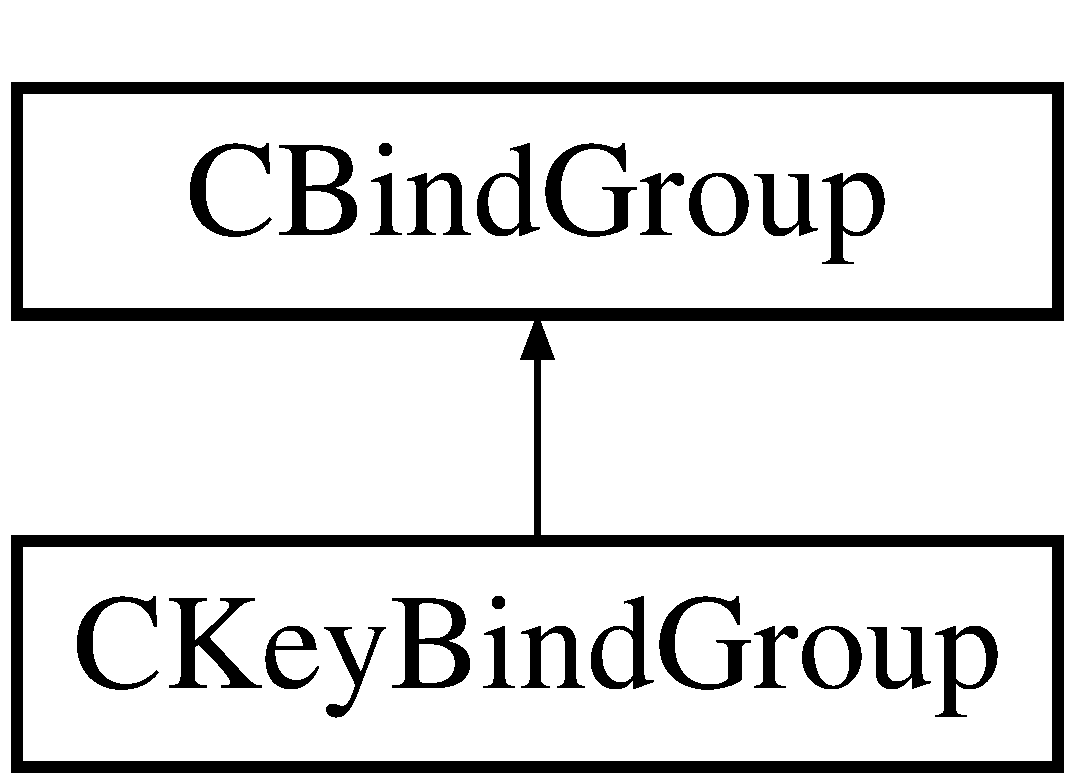
\includegraphics[height=2.000000cm]{classCKeyBindGroup}
\end{center}
\end{figure}
\subsection*{Public Member Functions}
\begin{DoxyCompactItemize}
\item 
\hypertarget{classCKeyBindGroup_a456c56896883ebe6012542fad2605ac8}{{\bfseries C\-Key\-Bind\-Group} (Bitu \-\_\-keys)}\label{classCKeyBindGroup_a456c56896883ebe6012542fad2605ac8}

\item 
\hypertarget{classCKeyBindGroup_a5bec329665a1a83ee69b539a72f5c20c}{\hyperlink{classCBind}{C\-Bind} $\ast$ {\bfseries Create\-Config\-Bind} (char $\ast$\&buf)}\label{classCKeyBindGroup_a5bec329665a1a83ee69b539a72f5c20c}

\item 
\hypertarget{classCKeyBindGroup_a7719fbf5afe7efc57e3e2ca3f8488949}{\hyperlink{classCBind}{C\-Bind} $\ast$ {\bfseries Create\-Event\-Bind} (S\-D\-L\-\_\-\-Event $\ast$event)}\label{classCKeyBindGroup_a7719fbf5afe7efc57e3e2ca3f8488949}

\item 
\hypertarget{classCKeyBindGroup_a52a9a394010f71d0fb2d2b9d64d9c7ef}{bool {\bfseries Check\-Event} (S\-D\-L\-\_\-\-Event $\ast$event)}\label{classCKeyBindGroup_a52a9a394010f71d0fb2d2b9d64d9c7ef}

\item 
\hypertarget{classCKeyBindGroup_a5ce59d68fbb6d0e79da2ea9c4ffa388a}{\hyperlink{classCBind}{C\-Bind} $\ast$ {\bfseries Create\-Key\-Bind} (S\-D\-L\-Key \-\_\-key)}\label{classCKeyBindGroup_a5ce59d68fbb6d0e79da2ea9c4ffa388a}

\end{DoxyCompactItemize}
\subsection*{Protected Attributes}
\begin{DoxyCompactItemize}
\item 
\hypertarget{classCKeyBindGroup_a7202ea1d9a5efdcda4f277d03e63ad63}{const char $\ast$ {\bfseries configname}}\label{classCKeyBindGroup_a7202ea1d9a5efdcda4f277d03e63ad63}

\item 
\hypertarget{classCKeyBindGroup_a915bc22f23540b1f8924adc831ba86ee}{C\-Bind\-List $\ast$ {\bfseries lists}}\label{classCKeyBindGroup_a915bc22f23540b1f8924adc831ba86ee}

\item 
\hypertarget{classCKeyBindGroup_a0d64ae014dfbdc463fea363dccd1bda6}{Bitu {\bfseries keys}}\label{classCKeyBindGroup_a0d64ae014dfbdc463fea363dccd1bda6}

\end{DoxyCompactItemize}


\subsection{Detailed Description}


Definition at line 1050 of file sdl\-\_\-mapper.\-cpp.



The documentation for this class was generated from the following file\-:\begin{DoxyCompactItemize}
\item 
src/gui/sdl\-\_\-mapper.\-cpp\end{DoxyCompactItemize}

\hypertarget{classCKeyEvent}{\section{C\-Key\-Event Class Reference}
\label{classCKeyEvent}\index{C\-Key\-Event@{C\-Key\-Event}}
}


Keyboard key trigger event.  


Inheritance diagram for C\-Key\-Event\-:\begin{figure}[H]
\begin{center}
\leavevmode
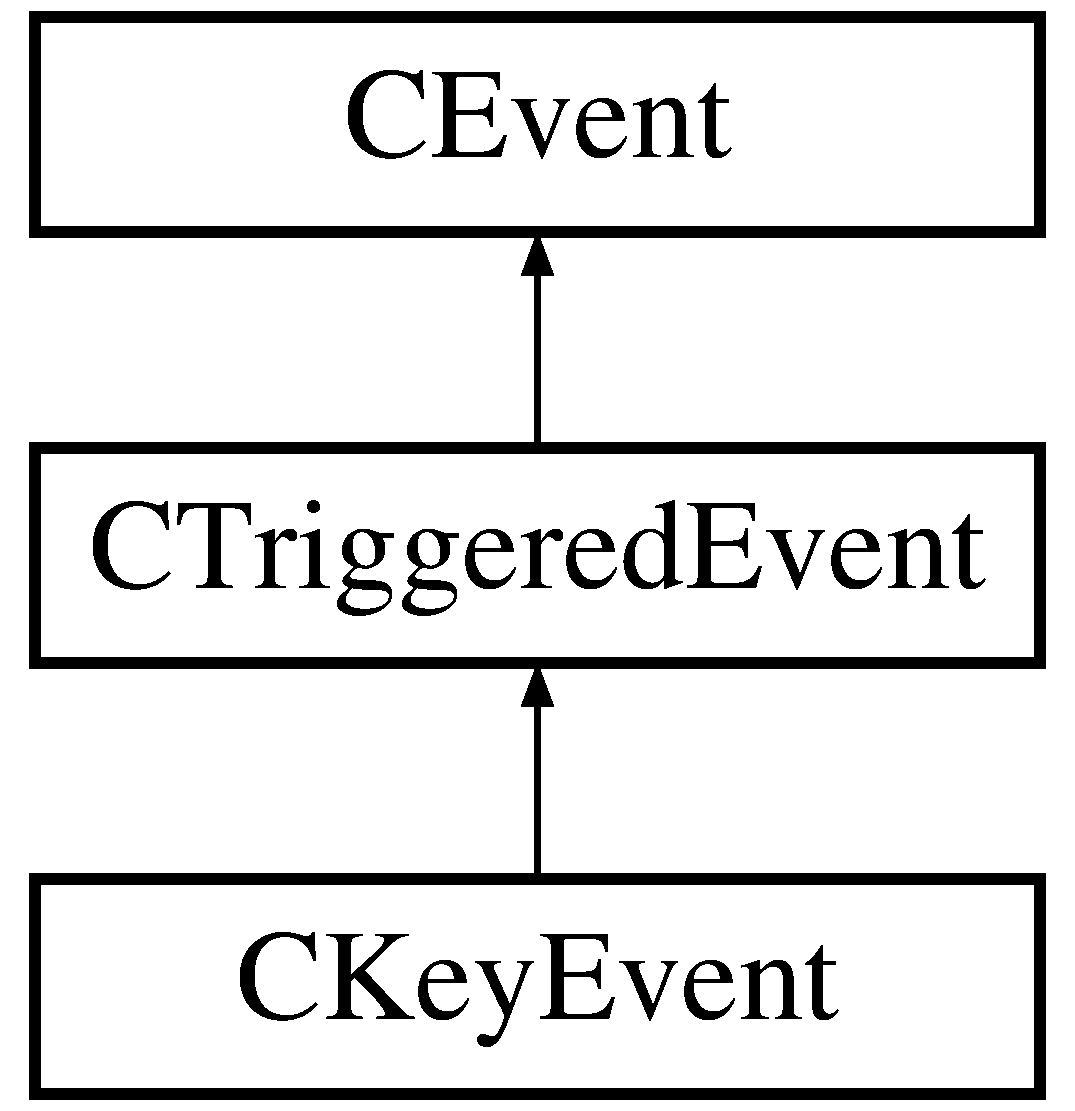
\includegraphics[height=3.000000cm]{classCKeyEvent}
\end{center}
\end{figure}
\subsection*{Public Member Functions}
\begin{DoxyCompactItemize}
\item 
\hypertarget{classCKeyEvent_a26db3746811c8498d0f7f4ca7e52d360}{\hyperlink{classCKeyEvent_a26db3746811c8498d0f7f4ca7e52d360}{C\-Key\-Event} (char const $\ast$const \-\_\-entry, K\-B\-D\-\_\-\-K\-E\-Y\-S \-\_\-key)}\label{classCKeyEvent_a26db3746811c8498d0f7f4ca7e52d360}

\begin{DoxyCompactList}\small\item\em Constructor to specify mapper event, and K\-B\-D\-\_\-$\ast$ key enumeration constant. \end{DoxyCompactList}\item 
\hypertarget{classCKeyEvent_a184277d7cd9c41090ae646a3b9887cf3}{virtual void \hyperlink{classCKeyEvent_a184277d7cd9c41090ae646a3b9887cf3}{Active} (bool yesno)}\label{classCKeyEvent_a184277d7cd9c41090ae646a3b9887cf3}

\begin{DoxyCompactList}\small\item\em Change whether the event is activated or not. \end{DoxyCompactList}\item 
\hypertarget{classCKeyEvent_ab05ca088ef648a08242be4f03adcbc00}{void \hyperlink{classCKeyEvent_ab05ca088ef648a08242be4f03adcbc00}{notifybutton} (\hyperlink{classCTextButton}{C\-Text\-Button} $\ast$n)}\label{classCKeyEvent_ab05ca088ef648a08242be4f03adcbc00}

\begin{DoxyCompactList}\small\item\em Associate this object with a text button in the mapper U\-I. \end{DoxyCompactList}\end{DoxyCompactItemize}
\subsection*{Public Attributes}
\begin{DoxyCompactItemize}
\item 
\hypertarget{classCKeyEvent_a93407353bb472fc93fa7962f1c2e7933}{\hyperlink{classCTextButton}{C\-Text\-Button} $\ast$ \hyperlink{classCKeyEvent_a93407353bb472fc93fa7962f1c2e7933}{notify\-\_\-button}}\label{classCKeyEvent_a93407353bb472fc93fa7962f1c2e7933}

\begin{DoxyCompactList}\small\item\em Text button in the mapper U\-I to indicate our status by. \end{DoxyCompactList}\item 
\hypertarget{classCKeyEvent_aa5d774b3b526c036d79dbf87ba437afd}{K\-B\-D\-\_\-\-K\-E\-Y\-S \hyperlink{classCKeyEvent_aa5d774b3b526c036d79dbf87ba437afd}{key}}\label{classCKeyEvent_aa5d774b3b526c036d79dbf87ba437afd}

\begin{DoxyCompactList}\small\item\em K\-B\-D\-\_\-$\ast$ key enumeration value to transmit to keyboard emulation. \end{DoxyCompactList}\end{DoxyCompactItemize}


\subsection{Detailed Description}
Keyboard key trigger event. 

Definition at line 1962 of file sdl\-\_\-mapper.\-cpp.



The documentation for this class was generated from the following file\-:\begin{DoxyCompactItemize}
\item 
src/gui/sdl\-\_\-mapper.\-cpp\end{DoxyCompactItemize}

\hypertarget{classClockDomain}{\section{Clock\-Domain Class Reference}
\label{classClockDomain}\index{Clock\-Domain@{Clock\-Domain}}
}
\subsection*{Public Member Functions}
\begin{DoxyCompactItemize}
\item 
\hypertarget{classClockDomain_af2b356eebbe8a39f26a433ffee57b86f}{{\bfseries Clock\-Domain} (unsigned long long freq\-\_\-new)}\label{classClockDomain_af2b356eebbe8a39f26a433ffee57b86f}

\item 
\hypertarget{classClockDomain_a6cc96fd5740134714c1bedc92af55ef0}{{\bfseries Clock\-Domain} (unsigned long long freq\-\_\-new, unsigned long long div)}\label{classClockDomain_a6cc96fd5740134714c1bedc92af55ef0}

\item 
\hypertarget{classClockDomain_a93065173b0e0b4f0551dee4f4bf58355}{void {\bfseries set\-\_\-name} (const char $\ast$s)}\label{classClockDomain_a93065173b0e0b4f0551dee4f4bf58355}

\item 
\hypertarget{classClockDomain_ab7dc80b22d2c1fe4ae72372cd03dddc5}{void {\bfseries set\-\_\-frequency} (unsigned long long freq\-\_\-new, unsigned long long div\-\_\-new=1)}\label{classClockDomain_ab7dc80b22d2c1fe4ae72372cd03dddc5}

\item 
\hypertarget{classClockDomain_a42b2b3e1745799744508ecc35d9d7e52}{const char $\ast$ {\bfseries get\-\_\-name} ()}\label{classClockDomain_a42b2b3e1745799744508ecc35d9d7e52}

\end{DoxyCompactItemize}
\subsection*{Public Attributes}
\begin{DoxyCompactItemize}
\item 
\hypertarget{classClockDomain_a0e9fba46cd0af9db7577f19b73fdf929}{unsigned long long {\bfseries freq}}\label{classClockDomain_a0e9fba46cd0af9db7577f19b73fdf929}

\item 
\hypertarget{classClockDomain_af7d2fbf024b15a81fa2c52e398c6e210}{unsigned long long {\bfseries freq\-\_\-div}}\label{classClockDomain_af7d2fbf024b15a81fa2c52e398c6e210}

\item 
\hypertarget{classClockDomain_ac253b451b7f686559b70d972f8612797}{unsigned long long {\bfseries counter}}\label{classClockDomain_ac253b451b7f686559b70d972f8612797}

\item 
\hypertarget{classClockDomain_af1a69ca31af27cf7453b08532d6c520a}{std\-::string {\bfseries name}}\label{classClockDomain_af1a69ca31af27cf7453b08532d6c520a}

\end{DoxyCompactItemize}


\subsection{Detailed Description}


Definition at line 25 of file clockdomain.\-h.



The documentation for this class was generated from the following file\-:\begin{DoxyCompactItemize}
\item 
include/clockdomain.\-h\end{DoxyCompactItemize}

\hypertarget{classCModEvent}{\section{C\-Mod\-Event Class Reference}
\label{classCModEvent}\index{C\-Mod\-Event@{C\-Mod\-Event}}
}


Modifier trigger event, for modifier keys. This permits the user to change modifier key bindings.  


Inheritance diagram for C\-Mod\-Event\-:\begin{figure}[H]
\begin{center}
\leavevmode
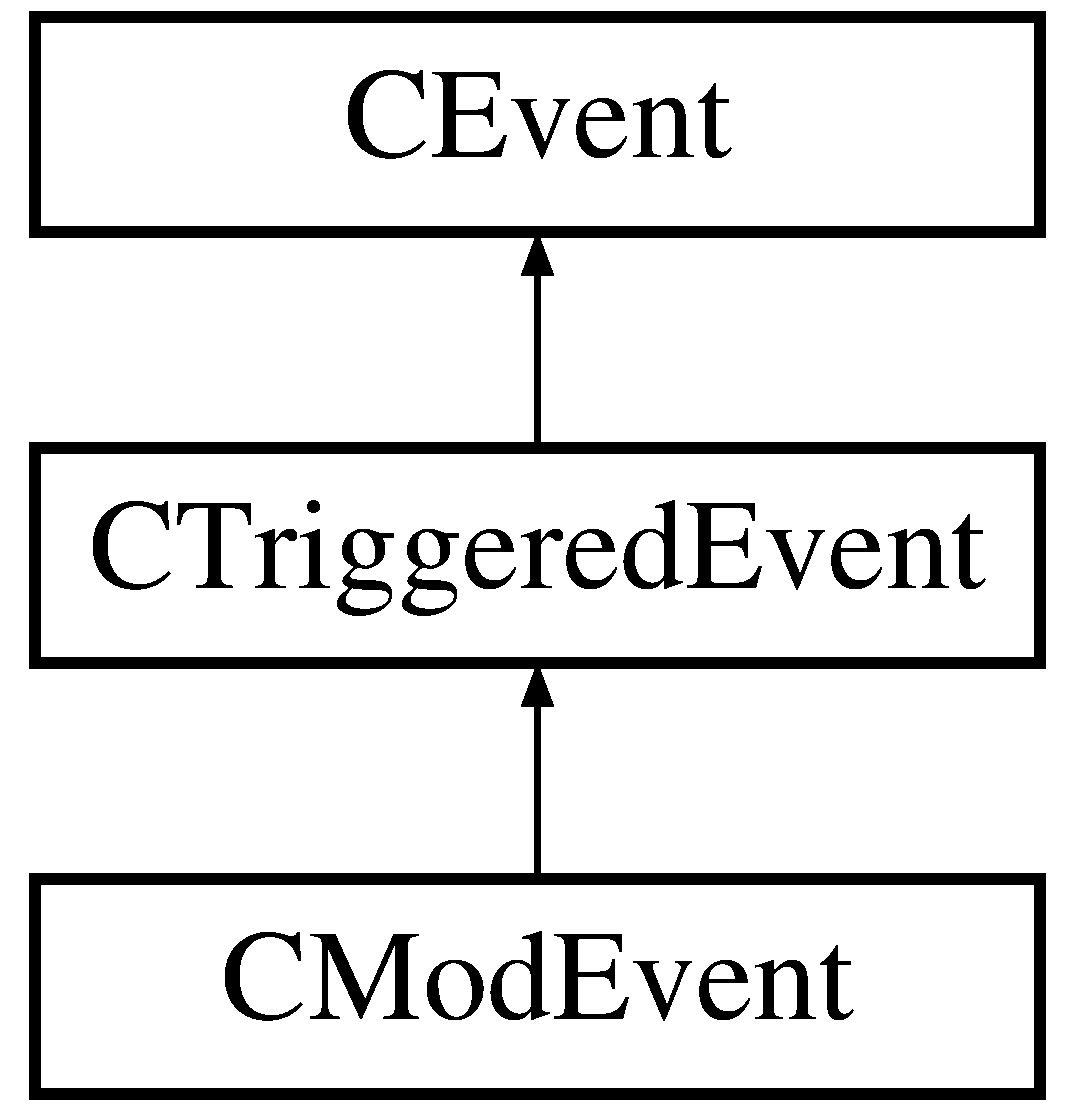
\includegraphics[height=3.000000cm]{classCModEvent}
\end{center}
\end{figure}
\subsection*{Public Member Functions}
\begin{DoxyCompactItemize}
\item 
\hypertarget{classCModEvent_a1bf7b8ec974c1944dbfa3737cac5e426}{\hyperlink{classCModEvent_a1bf7b8ec974c1944dbfa3737cac5e426}{C\-Mod\-Event} (char const $\ast$const \-\_\-entry, Bitu \-\_\-wmod)}\label{classCModEvent_a1bf7b8ec974c1944dbfa3737cac5e426}

\begin{DoxyCompactList}\small\item\em Constructor to provide entry name and the index of the modifier button. \end{DoxyCompactList}\item 
\hypertarget{classCModEvent_a682d2590a915ef555a9f2c2d6aa927c8}{virtual void \hyperlink{classCModEvent_a682d2590a915ef555a9f2c2d6aa927c8}{Active} (bool yesno)}\label{classCModEvent_a682d2590a915ef555a9f2c2d6aa927c8}

\begin{DoxyCompactList}\small\item\em Change whether the event is activated or not. \end{DoxyCompactList}\item 
\hypertarget{classCModEvent_a20aea0373f707e3c8f047f6e52bf5f77}{void \hyperlink{classCModEvent_a20aea0373f707e3c8f047f6e52bf5f77}{notifybutton} (\hyperlink{classCTextButton}{C\-Text\-Button} $\ast$n)}\label{classCModEvent_a20aea0373f707e3c8f047f6e52bf5f77}

\begin{DoxyCompactList}\small\item\em Associate this object with a text button in the mapper U\-I. \end{DoxyCompactList}\end{DoxyCompactItemize}
\subsection*{Public Attributes}
\begin{DoxyCompactItemize}
\item 
\hypertarget{classCModEvent_aa5dc746da9ec638e1959bfd1dddafc75}{\hyperlink{classCTextButton}{C\-Text\-Button} $\ast$ \hyperlink{classCModEvent_aa5dc746da9ec638e1959bfd1dddafc75}{notify\-\_\-button}}\label{classCModEvent_aa5dc746da9ec638e1959bfd1dddafc75}

\begin{DoxyCompactList}\small\item\em Mapper U\-I text button to indicate status by. \end{DoxyCompactList}\end{DoxyCompactItemize}
\subsection*{Protected Attributes}
\begin{DoxyCompactItemize}
\item 
\hypertarget{classCModEvent_a54a25228b8da694c33c44e4b161defd9}{Bitu \hyperlink{classCModEvent_a54a25228b8da694c33c44e4b161defd9}{wmod}}\label{classCModEvent_a54a25228b8da694c33c44e4b161defd9}

\begin{DoxyCompactList}\small\item\em Modifier button index. \end{DoxyCompactList}\end{DoxyCompactItemize}


\subsection{Detailed Description}
Modifier trigger event, for modifier keys. This permits the user to change modifier key bindings. 

Definition at line 2116 of file sdl\-\_\-mapper.\-cpp.



The documentation for this class was generated from the following file\-:\begin{DoxyCompactItemize}
\item 
src/gui/sdl\-\_\-mapper.\-cpp\end{DoxyCompactItemize}

\hypertarget{classCMS}{\section{C\-M\-S Class Reference}
\label{classCMS}\index{C\-M\-S@{C\-M\-S}}
}
Inheritance diagram for C\-M\-S\-:\begin{figure}[H]
\begin{center}
\leavevmode
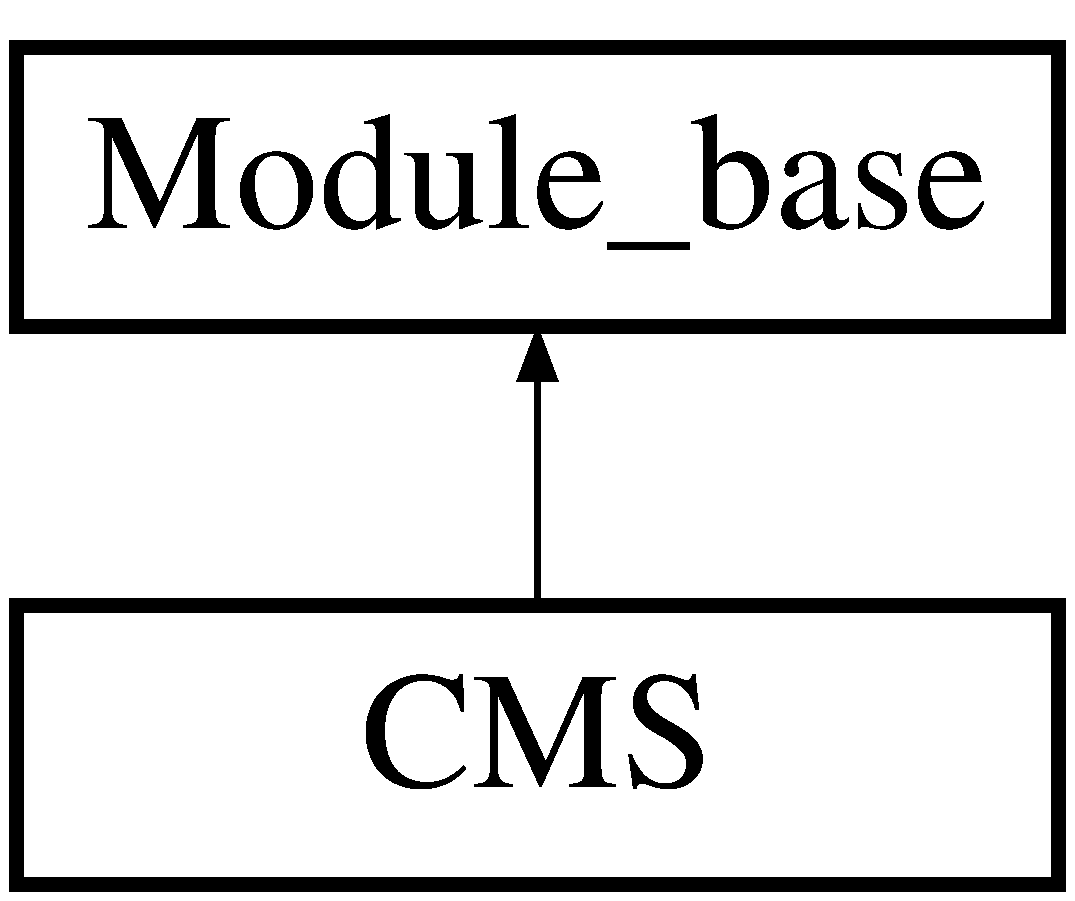
\includegraphics[height=2.000000cm]{classCMS}
\end{center}
\end{figure}
\subsection*{Public Member Functions}
\begin{DoxyCompactItemize}
\item 
\hypertarget{classCMS_afc0f43ea744137735477433ee764c729}{{\bfseries C\-M\-S} (\hyperlink{classSection}{Section} $\ast$configuration)}\label{classCMS_afc0f43ea744137735477433ee764c729}

\end{DoxyCompactItemize}


\subsection{Detailed Description}


Definition at line 121 of file gameblaster.\-cpp.



The documentation for this class was generated from the following file\-:\begin{DoxyCompactItemize}
\item 
src/hardware/gameblaster.\-cpp\end{DoxyCompactItemize}

\hypertarget{classCMscdex}{\section{C\-Mscdex Class Reference}
\label{classCMscdex}\index{C\-Mscdex@{C\-Mscdex}}
}
\subsection*{Classes}
\begin{DoxyCompactItemize}
\item 
struct \hyperlink{structCMscdex_1_1SDriveInfo}{S\-Drive\-Info}
\end{DoxyCompactItemize}
\subsection*{Public Types}
\begin{DoxyCompactItemize}
\item 
\hypertarget{classCMscdex_afadd6af7423df34d6ad4db7f72b9226e}{typedef struct \hyperlink{structCMscdex_1_1SDriveInfo}{C\-Mscdex\-::\-S\-Drive\-Info} {\bfseries T\-Drive\-Info}}\label{classCMscdex_afadd6af7423df34d6ad4db7f72b9226e}

\end{DoxyCompactItemize}
\subsection*{Public Member Functions}
\begin{DoxyCompactItemize}
\item 
\hypertarget{classCMscdex_aa0171ef3598f6247cbab681650f27c1a}{Bit16u {\bfseries Get\-Version} (void)}\label{classCMscdex_aa0171ef3598f6247cbab681650f27c1a}

\item 
\hypertarget{classCMscdex_a5a5347a5f62cc476ce4660bffa9c59ed}{Bit16u {\bfseries Get\-Num\-Drives} (void)}\label{classCMscdex_a5a5347a5f62cc476ce4660bffa9c59ed}

\item 
\hypertarget{classCMscdex_a83c6d7ce25d9c4453c42af88cd090566}{Bit16u {\bfseries Get\-First\-Drive} (void)}\label{classCMscdex_a83c6d7ce25d9c4453c42af88cd090566}

\item 
\hypertarget{classCMscdex_af464d504ec1b87e3bebe1a5881288b03}{Bit8u {\bfseries Get\-Sub\-Unit} (Bit16u \-\_\-drive)}\label{classCMscdex_af464d504ec1b87e3bebe1a5881288b03}

\item 
\hypertarget{classCMscdex_a935f2827a5e6483af5cde6aed832fef2}{bool {\bfseries Get\-U\-P\-C} (Bit8u sub\-Unit, Bit8u \&attr, char $\ast$upc)}\label{classCMscdex_a935f2827a5e6483af5cde6aed832fef2}

\item 
\hypertarget{classCMscdex_a912da85172868635b5054b03504f24ce}{void {\bfseries Init\-New\-Media} (Bit8u sub\-Unit)}\label{classCMscdex_a912da85172868635b5054b03504f24ce}

\item 
\hypertarget{classCMscdex_afb1e3cef49876914963b669987415ded}{bool {\bfseries Play\-Audio\-Sector} (Bit8u sub\-Unit, Bit32u sector, Bit32u length)}\label{classCMscdex_afb1e3cef49876914963b669987415ded}

\item 
\hypertarget{classCMscdex_ac38f29f8c5bad65c549b6e61e40a0f61}{bool {\bfseries Play\-Audio\-M\-S\-F} (Bit8u sub\-Unit, Bit32u start, Bit32u length)}\label{classCMscdex_ac38f29f8c5bad65c549b6e61e40a0f61}

\item 
\hypertarget{classCMscdex_ad0afd07bd4b3f61fec5dd7ff51fb1b01}{bool {\bfseries Stop\-Audio} (Bit8u sub\-Unit)}\label{classCMscdex_ad0afd07bd4b3f61fec5dd7ff51fb1b01}

\item 
\hypertarget{classCMscdex_a6d7888d1040575a0a0a42050349474fe}{bool {\bfseries Get\-Audio\-Status} (Bit8u sub\-Unit, bool \&playing, bool \&pause, \hyperlink{structSMSF}{T\-M\-S\-F} \&start, \hyperlink{structSMSF}{T\-M\-S\-F} \&end)}\label{classCMscdex_a6d7888d1040575a0a0a42050349474fe}

\item 
\hypertarget{classCMscdex_acc843b37e0b19afd37b166f765f7da44}{bool {\bfseries Get\-Sub\-Channel\-Data} (Bit8u sub\-Unit, Bit8u \&attr, Bit8u \&track, Bit8u \&index, \hyperlink{structSMSF}{T\-M\-S\-F} \&rel, \hyperlink{structSMSF}{T\-M\-S\-F} \&abs)}\label{classCMscdex_acc843b37e0b19afd37b166f765f7da44}

\item 
\hypertarget{classCMscdex_ac4ec6dc6be27ecfb68a5e1260dd9887b}{int {\bfseries Remove\-Drive} (Bit16u \-\_\-drive)}\label{classCMscdex_ac4ec6dc6be27ecfb68a5e1260dd9887b}

\item 
\hypertarget{classCMscdex_a7b9b06adbd55c99acd20a49d6ea67941}{int {\bfseries Add\-Drive} (Bit16u \-\_\-drive, char $\ast$physical\-Path, Bit8u \&sub\-Unit)}\label{classCMscdex_a7b9b06adbd55c99acd20a49d6ea67941}

\item 
\hypertarget{classCMscdex_af0edfe20ac94f225b50f78ce6b3ba7ac}{bool {\bfseries Has\-Drive} (Bit16u drive)}\label{classCMscdex_af0edfe20ac94f225b50f78ce6b3ba7ac}

\item 
\hypertarget{classCMscdex_af8e409575d47ef937b29cb448f4488d7}{void {\bfseries Replace\-Drive} (\hyperlink{classCDROM__Interface}{C\-D\-R\-O\-M\-\_\-\-Interface} $\ast$new\-Cdrom, Bit8u sub\-Unit)}\label{classCMscdex_af8e409575d47ef937b29cb448f4488d7}

\item 
\hypertarget{classCMscdex_af22f4c89b95a722c9b0f767724ce06dd}{void {\bfseries Get\-Drives} (Phys\-Pt data)}\label{classCMscdex_af22f4c89b95a722c9b0f767724ce06dd}

\item 
\hypertarget{classCMscdex_a330841e5a31e66bc7776306caedb6819}{void {\bfseries Get\-Driver\-Info} (Phys\-Pt data)}\label{classCMscdex_a330841e5a31e66bc7776306caedb6819}

\item 
\hypertarget{classCMscdex_a63eb50fe387c54c91ee7dac321836361}{bool {\bfseries Get\-Volume\-Name} (Bit8u sub\-Unit, char $\ast$data)}\label{classCMscdex_a63eb50fe387c54c91ee7dac321836361}

\item 
\hypertarget{classCMscdex_aa02670c6961dddbe44b9330d6422712b}{bool {\bfseries Get\-File\-Name} (Bit16u drive, Bit16u pos, Phys\-Pt data)}\label{classCMscdex_aa02670c6961dddbe44b9330d6422712b}

\item 
\hypertarget{classCMscdex_a7af859df94d70eea08c953571a54ed36}{bool {\bfseries Get\-Directory\-Entry} (Bit16u drive, bool copy\-Flag, Phys\-Pt pathname, Phys\-Pt buffer, Bit16u \&error)}\label{classCMscdex_a7af859df94d70eea08c953571a54ed36}

\item 
\hypertarget{classCMscdex_ad0746c59d6eaee8c20d5267bec58a09b}{bool {\bfseries Read\-V\-T\-O\-C} (Bit16u drive, Bit16u volume, Phys\-Pt data, Bit16u \&offset, Bit16u \&error)}\label{classCMscdex_ad0746c59d6eaee8c20d5267bec58a09b}

\item 
\hypertarget{classCMscdex_ac97e8044bbe54cd19c9b1ffd2dcdb23b}{bool {\bfseries Read\-Sectors} (Bit16u drive, Bit32u sector, Bit16u num, Phys\-Pt data)}\label{classCMscdex_ac97e8044bbe54cd19c9b1ffd2dcdb23b}

\item 
\hypertarget{classCMscdex_a41e035bc2ef5add4d2d5e4b3cdb01178}{bool {\bfseries Read\-Sectors} (Bit8u sub\-Unit, bool raw, Bit32u sector, Bit16u num, Phys\-Pt data)}\label{classCMscdex_a41e035bc2ef5add4d2d5e4b3cdb01178}

\item 
\hypertarget{classCMscdex_a8952511925ddd8c658dce7fd0824f2f6}{bool {\bfseries Read\-Sectors\-M\-S\-F} (Bit8u sub\-Unit, bool raw, Bit32u start, Bit16u num, Phys\-Pt data)}\label{classCMscdex_a8952511925ddd8c658dce7fd0824f2f6}

\item 
\hypertarget{classCMscdex_a2ab48935a7a8fd4292f3028243ab2b66}{bool {\bfseries Send\-Driver\-Request} (Bit16u drive, Phys\-Pt data)}\label{classCMscdex_a2ab48935a7a8fd4292f3028243ab2b66}

\item 
\hypertarget{classCMscdex_ad2c618001752751ad46861969ac08b01}{bool {\bfseries Is\-Valid\-Drive} (Bit16u \-\_\-drive)}\label{classCMscdex_ad2c618001752751ad46861969ac08b01}

\item 
\hypertarget{classCMscdex_ade59cf8040558852abb1dfbcec7189ad}{bool {\bfseries Get\-C\-D\-Info} (Bit8u sub\-Unit, Bit8u \&tr1, Bit8u \&tr2, \hyperlink{structSMSF}{T\-M\-S\-F} \&lead\-Out)}\label{classCMscdex_ade59cf8040558852abb1dfbcec7189ad}

\item 
\hypertarget{classCMscdex_a46265444d991ab7a43d8e1483b2fb600}{Bit32u {\bfseries Get\-Volume\-Size} (Bit8u sub\-Unit)}\label{classCMscdex_a46265444d991ab7a43d8e1483b2fb600}

\item 
\hypertarget{classCMscdex_ac484559d3ff51a0fc0ee0cf7df99c899}{bool {\bfseries Get\-Track\-Info} (Bit8u sub\-Unit, Bit8u track, Bit8u \&attr, \hyperlink{structSMSF}{T\-M\-S\-F} \&start)}\label{classCMscdex_ac484559d3ff51a0fc0ee0cf7df99c899}

\item 
\hypertarget{classCMscdex_a438afa22d295857d059828f6002ea2a2}{Bit16u {\bfseries Get\-Status\-Word} (Bit8u sub\-Unit, Bit16u status)}\label{classCMscdex_a438afa22d295857d059828f6002ea2a2}

\item 
\hypertarget{classCMscdex_a1be2e43a7cafc6fbf1f06a6dda72daec}{bool {\bfseries Get\-Current\-Pos} (Bit8u sub\-Unit, \hyperlink{structSMSF}{T\-M\-S\-F} \&pos)}\label{classCMscdex_a1be2e43a7cafc6fbf1f06a6dda72daec}

\item 
\hypertarget{classCMscdex_a2aa20d1b23551d9bf9e6b84a456a53dc}{Bit32u {\bfseries Get\-Device\-Status} (Bit8u sub\-Unit)}\label{classCMscdex_a2aa20d1b23551d9bf9e6b84a456a53dc}

\item 
\hypertarget{classCMscdex_a1367a3db25fb8dba65a59dd879409de5}{bool {\bfseries Get\-Media\-Status} (Bit8u sub\-Unit, Bit8u \&status)}\label{classCMscdex_a1367a3db25fb8dba65a59dd879409de5}

\item 
\hypertarget{classCMscdex_ab54c0b2f0cfc504fb70dc820d35404e2}{bool {\bfseries Load\-Unload\-Media} (Bit8u sub\-Unit, bool unload)}\label{classCMscdex_ab54c0b2f0cfc504fb70dc820d35404e2}

\item 
\hypertarget{classCMscdex_a2ccb8c103a5755b4594698dd155fd6d4}{bool {\bfseries Resume\-Audio} (Bit8u sub\-Unit)}\label{classCMscdex_a2ccb8c103a5755b4594698dd155fd6d4}

\item 
\hypertarget{classCMscdex_abdd75d8019cc9190c34975e1c6e84b47}{bool {\bfseries Get\-Media\-Status} (Bit8u sub\-Unit, bool \&media, bool \&changed, bool \&tray\-Open)}\label{classCMscdex_abdd75d8019cc9190c34975e1c6e84b47}

\item 
\hypertarget{classCMscdex_a7a887c5c48a967fa8c3f1f429478e28f}{Phys\-Pt {\bfseries Get\-Default\-Buffer} (void)}\label{classCMscdex_a7a887c5c48a967fa8c3f1f429478e28f}

\item 
\hypertarget{classCMscdex_af32260380b7e357a0d77baaecbda6aef}{Phys\-Pt {\bfseries Get\-Temp\-Buffer} (void)}\label{classCMscdex_af32260380b7e357a0d77baaecbda6aef}

\item 
\hypertarget{classCMscdex_a9267374dbbd4c82f082cbfeb07ec7317}{void {\bfseries Save\-State} (std\-::ostream \&stream)}\label{classCMscdex_a9267374dbbd4c82f082cbfeb07ec7317}

\item 
\hypertarget{classCMscdex_a0cf511573055dc6f2f8d9669cca861e6}{void {\bfseries Load\-State} (std\-::istream \&stream)}\label{classCMscdex_a0cf511573055dc6f2f8d9669cca861e6}

\item 
\hypertarget{classCMscdex_a4c8cd11142b468ce00f7dbfe2e96830e}{bool {\bfseries Channel\-Control} (Bit8u sub\-Unit, \hyperlink{structSCtrl}{T\-Ctrl} ctrl)}\label{classCMscdex_a4c8cd11142b468ce00f7dbfe2e96830e}

\item 
\hypertarget{classCMscdex_a6facd9da08f3c1ccfa55094165b5dce1}{bool {\bfseries Get\-Channel\-Control} (Bit8u sub\-Unit, \hyperlink{structSCtrl}{T\-Ctrl} \&ctrl)}\label{classCMscdex_a6facd9da08f3c1ccfa55094165b5dce1}

\end{DoxyCompactItemize}
\subsection*{Public Attributes}
\begin{DoxyCompactItemize}
\item 
\hypertarget{classCMscdex_a5b4d6334bdd6f14e75354d225c865abe}{Bit16u {\bfseries num\-Drives} = 0}\label{classCMscdex_a5b4d6334bdd6f14e75354d225c865abe}

\item 
\hypertarget{classCMscdex_a74017c503ae2c44e5c78bfd3190005f8}{Bit16u {\bfseries default\-Buf\-Seg} = 0}\label{classCMscdex_a74017c503ae2c44e5c78bfd3190005f8}

\item 
\hypertarget{classCMscdex_a1392c8b86d5976dafb60694eef28abfa}{\hyperlink{structCMscdex_1_1SDriveInfo}{T\-Drive\-Info} {\bfseries dinfo} \mbox{[}M\-S\-C\-D\-E\-X\-\_\-\-M\-A\-X\-\_\-\-D\-R\-I\-V\-E\-S\mbox{]}}\label{classCMscdex_a1392c8b86d5976dafb60694eef28abfa}

\item 
\hypertarget{classCMscdex_aaadae67160be26c0a1bf0646a8030803}{\hyperlink{classCDROM__Interface}{C\-D\-R\-O\-M\-\_\-\-Interface} $\ast$ {\bfseries cdrom} \mbox{[}M\-S\-C\-D\-E\-X\-\_\-\-M\-A\-X\-\_\-\-D\-R\-I\-V\-E\-S\mbox{]}}\label{classCMscdex_aaadae67160be26c0a1bf0646a8030803}

\item 
\hypertarget{classCMscdex_a9dcc1cbe3482842e279f49d816fa3aaf}{Bit16u {\bfseries root\-Driver\-Header\-Seg} = 0}\label{classCMscdex_a9dcc1cbe3482842e279f49d816fa3aaf}

\end{DoxyCompactItemize}


\subsection{Detailed Description}


Definition at line 89 of file dos\-\_\-mscdex.\-cpp.



The documentation for this class was generated from the following file\-:\begin{DoxyCompactItemize}
\item 
src/dos/dos\-\_\-mscdex.\-cpp\end{DoxyCompactItemize}

\hypertarget{classCodePageHandlerDynRec}{\section{Code\-Page\-Handler\-Dyn\-Rec Class Reference}
\label{classCodePageHandlerDynRec}\index{Code\-Page\-Handler\-Dyn\-Rec@{Code\-Page\-Handler\-Dyn\-Rec}}
}
Inheritance diagram for Code\-Page\-Handler\-Dyn\-Rec\-:\begin{figure}[H]
\begin{center}
\leavevmode
\includegraphics[height=2.000000cm]{classCodePageHandlerDynRec}
\end{center}
\end{figure}
\subsection*{Public Member Functions}
\begin{DoxyCompactItemize}
\item 
\hypertarget{classCodePageHandlerDynRec_abd4257a626a57d4a30b87e59f10b37a6}{void {\bfseries Setup\-At} (Bitu \-\_\-phys\-\_\-page, \hyperlink{classPageHandler}{Page\-Handler} $\ast$\-\_\-old\-\_\-pagehandler)}\label{classCodePageHandlerDynRec_abd4257a626a57d4a30b87e59f10b37a6}

\item 
\hypertarget{classCodePageHandlerDynRec_a0ca46d47e0197c04a36b666a5d934a97}{bool {\bfseries Invalidate\-Range} (Bitu start, Bitu end)}\label{classCodePageHandlerDynRec_a0ca46d47e0197c04a36b666a5d934a97}

\item 
\hypertarget{classCodePageHandlerDynRec_a3ca70263704a951b7d1f90cbc1eec6f4}{void {\bfseries writeb} (Phys\-Pt addr, Bit8u val)}\label{classCodePageHandlerDynRec_a3ca70263704a951b7d1f90cbc1eec6f4}

\item 
\hypertarget{classCodePageHandlerDynRec_a6669060de6e8b6f59c01e8f19999ddea}{void {\bfseries writew} (Phys\-Pt addr, Bit16u val)}\label{classCodePageHandlerDynRec_a6669060de6e8b6f59c01e8f19999ddea}

\item 
\hypertarget{classCodePageHandlerDynRec_ad8db785cabeecc8a5d18bb813ad14832}{void {\bfseries writed} (Phys\-Pt addr, Bit32u val)}\label{classCodePageHandlerDynRec_ad8db785cabeecc8a5d18bb813ad14832}

\item 
\hypertarget{classCodePageHandlerDynRec_adb9e54a93b35db3ec11b1a426dddd557}{bool {\bfseries writeb\-\_\-checked} (Phys\-Pt addr, Bit8u val)}\label{classCodePageHandlerDynRec_adb9e54a93b35db3ec11b1a426dddd557}

\item 
\hypertarget{classCodePageHandlerDynRec_ad2180f56734407f897c5a81e64f674ac}{bool {\bfseries writew\-\_\-checked} (Phys\-Pt addr, Bit16u val)}\label{classCodePageHandlerDynRec_ad2180f56734407f897c5a81e64f674ac}

\item 
\hypertarget{classCodePageHandlerDynRec_a5c3f15616c10dd2da9a19d3da1edb0d6}{bool {\bfseries writed\-\_\-checked} (Phys\-Pt addr, Bit32u val)}\label{classCodePageHandlerDynRec_a5c3f15616c10dd2da9a19d3da1edb0d6}

\item 
\hypertarget{classCodePageHandlerDynRec_a25c907e9457dfaa7adf0e912b11c0885}{void {\bfseries Add\-Cache\-Block} (\hyperlink{classCacheBlockDynRec}{Cache\-Block\-Dyn\-Rec} $\ast$block)}\label{classCodePageHandlerDynRec_a25c907e9457dfaa7adf0e912b11c0885}

\item 
\hypertarget{classCodePageHandlerDynRec_a0b72c0cd8ddef28f1ec4c5db21340784}{void {\bfseries Add\-Cross\-Block} (\hyperlink{classCacheBlockDynRec}{Cache\-Block\-Dyn\-Rec} $\ast$block)}\label{classCodePageHandlerDynRec_a0b72c0cd8ddef28f1ec4c5db21340784}

\item 
\hypertarget{classCodePageHandlerDynRec_ab905fe2cc879e65fe4d89eca8ff5e417}{void {\bfseries Del\-Cache\-Block} (\hyperlink{classCacheBlockDynRec}{Cache\-Block\-Dyn\-Rec} $\ast$block)}\label{classCodePageHandlerDynRec_ab905fe2cc879e65fe4d89eca8ff5e417}

\item 
\hypertarget{classCodePageHandlerDynRec_a92c489475cca5595031fa14e6ea673a7}{void {\bfseries Release} (void)}\label{classCodePageHandlerDynRec_a92c489475cca5595031fa14e6ea673a7}

\item 
\hypertarget{classCodePageHandlerDynRec_a0c278040559fd401ee49f3f94b29a7d7}{void {\bfseries Clear\-Release} (void)}\label{classCodePageHandlerDynRec_a0c278040559fd401ee49f3f94b29a7d7}

\item 
\hypertarget{classCodePageHandlerDynRec_a8473bf36137f678d3940fe9d1150b9e9}{\hyperlink{classCacheBlockDynRec}{Cache\-Block\-Dyn\-Rec} $\ast$ {\bfseries Find\-Cache\-Block} (Bitu start)}\label{classCodePageHandlerDynRec_a8473bf36137f678d3940fe9d1150b9e9}

\item 
\hypertarget{classCodePageHandlerDynRec_a1f040cb9dc0a1b33ef2aafa924cd3a0f}{Host\-Pt {\bfseries Get\-Host\-Read\-Pt} (Bitu phys\-\_\-page)}\label{classCodePageHandlerDynRec_a1f040cb9dc0a1b33ef2aafa924cd3a0f}

\item 
\hypertarget{classCodePageHandlerDynRec_a554f8edbfb6bd743140593503581a713}{Host\-Pt {\bfseries Get\-Host\-Write\-Pt} (Bitu phys\-\_\-page)}\label{classCodePageHandlerDynRec_a554f8edbfb6bd743140593503581a713}

\end{DoxyCompactItemize}
\subsection*{Public Attributes}
\begin{DoxyCompactItemize}
\item 
\hypertarget{classCodePageHandlerDynRec_ac1d8018e02bcd95e91d5b606dba136af}{Bit8u {\bfseries write\-\_\-map} \mbox{[}4096\mbox{]} = \{\}}\label{classCodePageHandlerDynRec_ac1d8018e02bcd95e91d5b606dba136af}

\item 
\hypertarget{classCodePageHandlerDynRec_a47aab5bb1199222974e7206325511bcb}{Bit8u $\ast$ {\bfseries invalidation\-\_\-map} = N\-U\-L\-L}\label{classCodePageHandlerDynRec_a47aab5bb1199222974e7206325511bcb}

\item 
\hypertarget{classCodePageHandlerDynRec_a0d8b79c4e241f8f2527da02bd9d572ff}{\hyperlink{classCodePageHandlerDynRec}{Code\-Page\-Handler\-Dyn\-Rec} $\ast$ {\bfseries next} = N\-U\-L\-L}\label{classCodePageHandlerDynRec_a0d8b79c4e241f8f2527da02bd9d572ff}

\item 
\hypertarget{classCodePageHandlerDynRec_a1c92c142da75e5094c1707288923023f}{\hyperlink{classCodePageHandlerDynRec}{Code\-Page\-Handler\-Dyn\-Rec} $\ast$ {\bfseries prev} = N\-U\-L\-L}\label{classCodePageHandlerDynRec_a1c92c142da75e5094c1707288923023f}

\end{DoxyCompactItemize}


\subsection{Detailed Description}


Definition at line 85 of file cache.\-h.



The documentation for this class was generated from the following file\-:\begin{DoxyCompactItemize}
\item 
src/cpu/core\-\_\-dynrec/cache.\-h\end{DoxyCompactItemize}

\hypertarget{classcomb}{\section{comb Class Reference}
\label{classcomb}\index{comb@{comb}}
}
\subsection*{Public Member Functions}
\begin{DoxyCompactItemize}
\item 
\hypertarget{classcomb_a000d3f031781c27ceaf487a1ec957fec}{void {\bfseries setbuffer} (float $\ast$buf, int size)}\label{classcomb_a000d3f031781c27ceaf487a1ec957fec}

\item 
\hypertarget{classcomb_a4dd1f6c7ae8cf781c26599d8e023d41d}{void {\bfseries deletebuffer} ()}\label{classcomb_a4dd1f6c7ae8cf781c26599d8e023d41d}

\item 
\hypertarget{classcomb_a49755386062cccd51ae9eb43ae00a317}{float {\bfseries process} (float input)}\label{classcomb_a49755386062cccd51ae9eb43ae00a317}

\item 
\hypertarget{classcomb_ae18d1b1ea26d1c18087d3d8feeb7145d}{void {\bfseries mute} ()}\label{classcomb_ae18d1b1ea26d1c18087d3d8feeb7145d}

\item 
\hypertarget{classcomb_abd0aa594882431e7f7eb4901fcc0ea5e}{void {\bfseries setdamp} (float val)}\label{classcomb_abd0aa594882431e7f7eb4901fcc0ea5e}

\item 
\hypertarget{classcomb_a99e2c5952a08d006902f5e20a05d37a7}{float {\bfseries getdamp} ()}\label{classcomb_a99e2c5952a08d006902f5e20a05d37a7}

\item 
\hypertarget{classcomb_ad8fac09822db8d944c13791112b5b6a2}{void {\bfseries setfeedback} (float val)}\label{classcomb_ad8fac09822db8d944c13791112b5b6a2}

\item 
\hypertarget{classcomb_a1df81e7e8f9310831e4e7929078f1d11}{float {\bfseries getfeedback} ()}\label{classcomb_a1df81e7e8f9310831e4e7929078f1d11}

\item 
\hypertarget{classcomb_ab6b7006d95b9b1d9397dbf9c22d8a981}{void {\bfseries save\-State} (std\-::ostream \&stream)}\label{classcomb_ab6b7006d95b9b1d9397dbf9c22d8a981}

\item 
\hypertarget{classcomb_a4accb964763281cf365e24fb2b1c70ec}{void {\bfseries load\-State} (std\-::istream \&stream)}\label{classcomb_a4accb964763281cf365e24fb2b1c70ec}

\end{DoxyCompactItemize}


\subsection{Detailed Description}


Definition at line 13 of file comb.\-h.



The documentation for this class was generated from the following files\-:\begin{DoxyCompactItemize}
\item 
src/mt32/freeverb/comb.\-h\item 
src/mt32/freeverb/comb.\-cpp\end{DoxyCompactItemize}

\hypertarget{classMT32Emu_1_1CombFilter}{\section{M\-T32\-Emu\-:\-:Comb\-Filter Class Reference}
\label{classMT32Emu_1_1CombFilter}\index{M\-T32\-Emu\-::\-Comb\-Filter@{M\-T32\-Emu\-::\-Comb\-Filter}}
}
Inheritance diagram for M\-T32\-Emu\-:\-:Comb\-Filter\-:\begin{figure}[H]
\begin{center}
\leavevmode
\includegraphics[height=3.000000cm]{classMT32Emu_1_1CombFilter}
\end{center}
\end{figure}
\subsection*{Public Member Functions}
\begin{DoxyCompactItemize}
\item 
\hypertarget{classMT32Emu_1_1CombFilter_a8a69987cd778815dd57b5fe39a061075}{{\bfseries Comb\-Filter} (const Bit32u use\-Size)}\label{classMT32Emu_1_1CombFilter_a8a69987cd778815dd57b5fe39a061075}

\item 
\hypertarget{classMT32Emu_1_1CombFilter_ace1d8df3fbf3f05e9cabbe32df7b1624}{void {\bfseries process} (const float in)}\label{classMT32Emu_1_1CombFilter_ace1d8df3fbf3f05e9cabbe32df7b1624}

\item 
\hypertarget{classMT32Emu_1_1CombFilter_a10ac24b24fc8228a4fc17e179299163f}{float {\bfseries get\-Output\-At} (const Bit32u out\-Index) const }\label{classMT32Emu_1_1CombFilter_a10ac24b24fc8228a4fc17e179299163f}

\item 
\hypertarget{classMT32Emu_1_1CombFilter_a1ca73514aa1a08ed52eae63c649a8848}{void {\bfseries set\-Feedback\-Factor} (const float use\-Feedback\-Factor)}\label{classMT32Emu_1_1CombFilter_a1ca73514aa1a08ed52eae63c649a8848}

\item 
\hypertarget{classMT32Emu_1_1CombFilter_aa167b306c4bfd7ae466bdfbffa2264a8}{void {\bfseries set\-Filter\-Factor} (const float use\-Filter\-Factor)}\label{classMT32Emu_1_1CombFilter_aa167b306c4bfd7ae466bdfbffa2264a8}

\item 
\hypertarget{classMT32Emu_1_1CombFilter_ab2f7553491cb2cca17daabe177544ae9}{{\bfseries Comb\-Filter} (const Bit32u size, const Bit32u use\-Filter\-Factor)}\label{classMT32Emu_1_1CombFilter_ab2f7553491cb2cca17daabe177544ae9}

\item 
\hypertarget{classMT32Emu_1_1CombFilter_ae1d1575e81a4585e6fc27f895fc2f8c4}{virtual void {\bfseries process} (const Bit32s in)}\label{classMT32Emu_1_1CombFilter_ae1d1575e81a4585e6fc27f895fc2f8c4}

\item 
\hypertarget{classMT32Emu_1_1CombFilter_ad33d09330d93a8daaa59be3c909e31a1}{Bit32s {\bfseries get\-Output\-At} (const Bit32u out\-Index) const }\label{classMT32Emu_1_1CombFilter_ad33d09330d93a8daaa59be3c909e31a1}

\item 
\hypertarget{classMT32Emu_1_1CombFilter_a7a5cd3f69e41e8ce0a06fe592102fbf3}{void {\bfseries set\-Feedback\-Factor} (const Bit32u use\-Feedback\-Factor)}\label{classMT32Emu_1_1CombFilter_a7a5cd3f69e41e8ce0a06fe592102fbf3}

\end{DoxyCompactItemize}
\subsection*{Protected Attributes}
\begin{DoxyCompactItemize}
\item 
\hypertarget{classMT32Emu_1_1CombFilter_a98aca19d1bb90fb974ff21283695a7e4}{const Bit32u {\bfseries filter\-Factor}}\label{classMT32Emu_1_1CombFilter_a98aca19d1bb90fb974ff21283695a7e4}

\item 
\hypertarget{classMT32Emu_1_1CombFilter_a1fd0fe383ca82d8b7f4091b323c17f24}{Bit32u {\bfseries feedback\-Factor}}\label{classMT32Emu_1_1CombFilter_a1fd0fe383ca82d8b7f4091b323c17f24}

\end{DoxyCompactItemize}


\subsection{Detailed Description}


Definition at line 54 of file A\-Reverb\-Model.\-h.



The documentation for this class was generated from the following files\-:\begin{DoxyCompactItemize}
\item 
src/mt32/A\-Reverb\-Model.\-h\item 
src/mt32/B\-Reverb\-Model.\-h\item 
src/mt32/A\-Reverb\-Model.\-cpp\end{DoxyCompactItemize}

\hypertarget{classCommandLine}{\section{Command\-Line Class Reference}
\label{classCommandLine}\index{Command\-Line@{Command\-Line}}
}
\subsection*{Public Types}
\begin{DoxyCompactItemize}
\item 
enum {\bfseries opt\-\_\-style} \{ \\*
{\bfseries dos} = 0, 
{\bfseries gnu}, 
{\bfseries gnu\-\_\-getopt}, 
{\bfseries either}, 
\\*
{\bfseries either\-\_\-except}
 \}
\end{DoxyCompactItemize}
\subsection*{Public Member Functions}
\begin{DoxyCompactItemize}
\item 
\hypertarget{classCommandLine_a564a8d1913e306decc89493674b3198e}{{\bfseries Command\-Line} (int argc, char const $\ast$const argv\mbox{[}$\,$\mbox{]}, enum opt\-\_\-style opt=Command\-Line\-::either)}\label{classCommandLine_a564a8d1913e306decc89493674b3198e}

\item 
\hypertarget{classCommandLine_a6f1b87cd2fd1823d0166c98a954872ae}{{\bfseries Command\-Line} (char const $\ast$const name, char const $\ast$const cmdline, enum opt\-\_\-style opt=Command\-Line\-::either)}\label{classCommandLine_a6f1b87cd2fd1823d0166c98a954872ae}

\item 
\hypertarget{classCommandLine_a1f45b4326873dbcd8e1f3a37293390e1}{const char $\ast$ {\bfseries Get\-File\-Name} ()}\label{classCommandLine_a1f45b4326873dbcd8e1f3a37293390e1}

\item 
\hypertarget{classCommandLine_afb34ecd52f6c897051767042bcca5918}{bool {\bfseries Find\-Exist} (char const $\ast$const name, bool remove=false)}\label{classCommandLine_afb34ecd52f6c897051767042bcca5918}

\item 
\hypertarget{classCommandLine_ac3fd4a68a14b29f1a23e9a828d6a0683}{bool {\bfseries Find\-Hex} (char const $\ast$const name, int \&value, bool remove=false)}\label{classCommandLine_ac3fd4a68a14b29f1a23e9a828d6a0683}

\item 
\hypertarget{classCommandLine_a8179a05544caa1ac6170f5a79f0a1d99}{bool {\bfseries Find\-Int} (char const $\ast$const name, int \&value, bool remove=false)}\label{classCommandLine_a8179a05544caa1ac6170f5a79f0a1d99}

\item 
\hypertarget{classCommandLine_a1fe7d738d6388a60e04c8479312743ef}{bool {\bfseries Find\-String} (char const $\ast$const name, std\-::string \&value, bool remove=false)}\label{classCommandLine_a1fe7d738d6388a60e04c8479312743ef}

\item 
\hypertarget{classCommandLine_a68fc2c8be26d62d89f29dafb7fba5799}{bool {\bfseries Find\-Command} (unsigned int which, std\-::string \&value)}\label{classCommandLine_a68fc2c8be26d62d89f29dafb7fba5799}

\item 
\hypertarget{classCommandLine_a372efd83a11653150c7e05be677dbcae}{bool {\bfseries Find\-String\-Begin} (char const $\ast$const begin, std\-::string \&value, bool remove=false)}\label{classCommandLine_a372efd83a11653150c7e05be677dbcae}

\item 
\hypertarget{classCommandLine_a8995713eff76c14e1d53ec0515d833d6}{bool {\bfseries Find\-String\-Remain} (char const $\ast$const name, std\-::string \&value)}\label{classCommandLine_a8995713eff76c14e1d53ec0515d833d6}

\item 
\hypertarget{classCommandLine_a791da6ab1876316f66f545a31cee69e5}{bool {\bfseries Find\-String\-Remain\-Begin} (char const $\ast$const name, std\-::string \&value)}\label{classCommandLine_a791da6ab1876316f66f545a31cee69e5}

\item 
\hypertarget{classCommandLine_abdba027c787d2b5a70dee1e842c699dd}{bool {\bfseries Get\-String\-Remain} (std\-::string \&value)}\label{classCommandLine_abdba027c787d2b5a70dee1e842c699dd}

\item 
\hypertarget{classCommandLine_ac5b6c005e5f124ab3a1a7de6db8a86d3}{int {\bfseries Get\-Parameter\-From\-List} (const char $\ast$const params\mbox{[}$\,$\mbox{]}, std\-::vector$<$ std\-::string $>$ \&output)}\label{classCommandLine_ac5b6c005e5f124ab3a1a7de6db8a86d3}

\item 
\hypertarget{classCommandLine_a694f00846c0832d8cd97fe0a652d5567}{void {\bfseries Fill\-Vector} (std\-::vector$<$ std\-::string $>$ \&vector)}\label{classCommandLine_a694f00846c0832d8cd97fe0a652d5567}

\item 
\hypertarget{classCommandLine_aec22173334fc0db4e350b3475a162f1a}{unsigned int {\bfseries Get\-Count} (void)}\label{classCommandLine_aec22173334fc0db4e350b3475a162f1a}

\item 
\hypertarget{classCommandLine_aea42d5fe141ba6c58ef7045eb3b92f3e}{void {\bfseries Shift} (unsigned int amount=1)}\label{classCommandLine_aea42d5fe141ba6c58ef7045eb3b92f3e}

\item 
\hypertarget{classCommandLine_ab4e8866df99dac127353b303b95014ee}{Bit16u {\bfseries Get\-\_\-arglength} ()}\label{classCommandLine_ab4e8866df99dac127353b303b95014ee}

\item 
\hypertarget{classCommandLine_ad1780afea11368a1e6fdd35276a8c678}{bool {\bfseries Begin\-Opt} (bool eat\-\_\-argv=true)}\label{classCommandLine_ad1780afea11368a1e6fdd35276a8c678}

\item 
\hypertarget{classCommandLine_a4440913abd4b9f06635b3df3fe0ee7d4}{bool {\bfseries Get\-Opt} (std\-::string \&name)}\label{classCommandLine_a4440913abd4b9f06635b3df3fe0ee7d4}

\item 
\hypertarget{classCommandLine_a090151cab04fbb6e886f2053e2ef56a3}{bool {\bfseries Next\-Opt\-Argv} (std\-::string \&argv)}\label{classCommandLine_a090151cab04fbb6e886f2053e2ef56a3}

\item 
\hypertarget{classCommandLine_ac94cc029aca101fb5e39189fca40ff91}{bool {\bfseries Get\-Opt\-G\-N\-U\-Single\-Char\-Check} (std\-::string \&name)}\label{classCommandLine_ac94cc029aca101fb5e39189fca40ff91}

\item 
\hypertarget{classCommandLine_ac0f91f63b77400b7266128dbc1445b1b}{void {\bfseries Change\-Opt\-Style} (enum opt\-\_\-style opt\-\_\-style)}\label{classCommandLine_ac0f91f63b77400b7266128dbc1445b1b}

\item 
\hypertarget{classCommandLine_a941c71120faefc5e3c0876d69ac78491}{void {\bfseries End\-Opt} ()}\label{classCommandLine_a941c71120faefc5e3c0876d69ac78491}

\item 
\hypertarget{classCommandLine_a331a3c1e87e6a2c0306cf1e9f7a67945}{bool {\bfseries Get\-Current\-Argv} (std\-::string \&argv)}\label{classCommandLine_a331a3c1e87e6a2c0306cf1e9f7a67945}

\item 
\hypertarget{classCommandLine_ad457fad3218a71163a058bc095cfe0ed}{bool {\bfseries Current\-Argv\-End} (void)}\label{classCommandLine_ad457fad3218a71163a058bc095cfe0ed}

\item 
\hypertarget{classCommandLine_ab34d4cf4cb665ecb694f90e5f9c524c3}{void {\bfseries Eat\-Current\-Argv} (void)}\label{classCommandLine_ab34d4cf4cb665ecb694f90e5f9c524c3}

\item 
\hypertarget{classCommandLine_a89dd608d9095a3321d48eb90ecf210ba}{void {\bfseries Next\-Argv} (void)}\label{classCommandLine_a89dd608d9095a3321d48eb90ecf210ba}

\item 
\hypertarget{classCommandLine_aee2a64d26ecb790666b084d79dd565b0}{const std\-::string \& {\bfseries Get\-Raw\-Cmdline} (void)}\label{classCommandLine_aee2a64d26ecb790666b084d79dd565b0}

\end{DoxyCompactItemize}


\subsection{Detailed Description}


Definition at line 40 of file programs.\-h.



The documentation for this class was generated from the following files\-:\begin{DoxyCompactItemize}
\item 
include/programs.\-h\item 
src/misc/setup.\-cpp\end{DoxyCompactItemize}

\hypertarget{structCommandTail}{\section{Command\-Tail Struct Reference}
\label{structCommandTail}\index{Command\-Tail@{Command\-Tail}}
}
\subsection*{Public Attributes}
\begin{DoxyCompactItemize}
\item 
\hypertarget{structCommandTail_a3d3bbe7fd2ae49bcea888d8156ababcd}{Bit8u {\bfseries count}}\label{structCommandTail_a3d3bbe7fd2ae49bcea888d8156ababcd}

\item 
\hypertarget{structCommandTail_ad44cf8eb402645e22f09cbbb998bf6db}{char {\bfseries buffer} \mbox{[}C\-T\-B\-U\-F\mbox{]}}\label{structCommandTail_ad44cf8eb402645e22f09cbbb998bf6db}

\end{DoxyCompactItemize}


\subsection{Detailed Description}


Definition at line 37 of file dos\-\_\-inc.\-h.



The documentation for this struct was generated from the following file\-:\begin{DoxyCompactItemize}
\item 
include/dos\-\_\-inc.\-h\end{DoxyCompactItemize}

\hypertarget{structMT32Emu_1_1TimbreParam_1_1CommonParam}{\section{M\-T32\-Emu\-:\-:Timbre\-Param\-:\-:Common\-Param Struct Reference}
\label{structMT32Emu_1_1TimbreParam_1_1CommonParam}\index{M\-T32\-Emu\-::\-Timbre\-Param\-::\-Common\-Param@{M\-T32\-Emu\-::\-Timbre\-Param\-::\-Common\-Param}}
}
\subsection*{Public Attributes}
\begin{DoxyCompactItemize}
\item 
\hypertarget{structMT32Emu_1_1TimbreParam_1_1CommonParam_ae71c824685f48d3a44d511997f6faef8}{char {\bfseries name} \mbox{[}10\mbox{]}}\label{structMT32Emu_1_1TimbreParam_1_1CommonParam_ae71c824685f48d3a44d511997f6faef8}

\item 
\hypertarget{structMT32Emu_1_1TimbreParam_1_1CommonParam_a0f87e5977009af45422c44b6ab29f0f5}{Bit8u {\bfseries partial\-Structure12}}\label{structMT32Emu_1_1TimbreParam_1_1CommonParam_a0f87e5977009af45422c44b6ab29f0f5}

\item 
\hypertarget{structMT32Emu_1_1TimbreParam_1_1CommonParam_a92b2cbee977dd45d1f93d9e465ea7506}{Bit8u {\bfseries partial\-Structure34}}\label{structMT32Emu_1_1TimbreParam_1_1CommonParam_a92b2cbee977dd45d1f93d9e465ea7506}

\item 
\hypertarget{structMT32Emu_1_1TimbreParam_1_1CommonParam_a1ddabe78571b65f7f29a2d9e9c00f31d}{Bit8u {\bfseries partial\-Mute}}\label{structMT32Emu_1_1TimbreParam_1_1CommonParam_a1ddabe78571b65f7f29a2d9e9c00f31d}

\item 
\hypertarget{structMT32Emu_1_1TimbreParam_1_1CommonParam_a3607e7956d1a3ffbdc8caacc097c0bb9}{Bit8u {\bfseries no\-Sustain}}\label{structMT32Emu_1_1TimbreParam_1_1CommonParam_a3607e7956d1a3ffbdc8caacc097c0bb9}

\end{DoxyCompactItemize}


\subsection{Detailed Description}


Definition at line 52 of file Structures.\-h.



The documentation for this struct was generated from the following file\-:\begin{DoxyCompactItemize}
\item 
src/mt32/Structures.\-h\end{DoxyCompactItemize}

\hypertarget{classConfig}{\section{Config Class Reference}
\label{classConfig}\index{Config@{Config}}
}
\subsection*{Public Member Functions}
\begin{DoxyCompactItemize}
\item 
\hypertarget{classConfig_a526e7d065ca0a508ff66e18d9efdeda1}{{\bfseries Config} (\hyperlink{classCommandLine}{Command\-Line} $\ast$cmd)}\label{classConfig_a526e7d065ca0a508ff66e18d9efdeda1}

\item 
\hypertarget{classConfig_ace2cc0065844f72d35fa7fffbf842980}{\hyperlink{classSection__line}{Section\-\_\-line} $\ast$ {\bfseries Add\-Section\-\_\-line} (char const $\ast$const \-\_\-name, void($\ast$\-\_\-initfunction)(\hyperlink{classSection}{Section} $\ast$))}\label{classConfig_ace2cc0065844f72d35fa7fffbf842980}

\item 
\hypertarget{classConfig_aaa6ac4037e69d8284fe1b4e6c4c682e5}{\hyperlink{classSection__prop}{Section\-\_\-prop} $\ast$ {\bfseries Add\-Section\-\_\-prop} (char const $\ast$const \-\_\-name, void($\ast$\-\_\-initfunction)(\hyperlink{classSection}{Section} $\ast$), bool canchange=false)}\label{classConfig_aaa6ac4037e69d8284fe1b4e6c4c682e5}

\item 
\hypertarget{classConfig_a91af5d9f5cf8c53581eaeb0cb104ff5f}{\hyperlink{classSection}{Section} $\ast$ {\bfseries Get\-Section} (int index)}\label{classConfig_a91af5d9f5cf8c53581eaeb0cb104ff5f}

\item 
\hypertarget{classConfig_a873c20a35c7320de62b6ad759b825302}{\hyperlink{classSection}{Section} $\ast$ {\bfseries Get\-Section} (std\-::string const \&\-\_\-sectionname) const }\label{classConfig_a873c20a35c7320de62b6ad759b825302}

\item 
\hypertarget{classConfig_abea967e8168d80ecb600891d62a2f534}{\hyperlink{classSection}{Section} $\ast$ {\bfseries Get\-Section\-From\-Property} (char const $\ast$const prop) const }\label{classConfig_abea967e8168d80ecb600891d62a2f534}

\item 
\hypertarget{classConfig_a5358d65e6687f76a7856aae7b5bf0c5c}{bool {\bfseries Print\-Config} (char const $\ast$const configfilename, bool everything=false) const }\label{classConfig_a5358d65e6687f76a7856aae7b5bf0c5c}

\item 
\hypertarget{classConfig_a0c8ebc50ad0d389f91fc27d31fe8e373}{bool {\bfseries Parse\-Config\-File} (char const $\ast$const configfilename)}\label{classConfig_a0c8ebc50ad0d389f91fc27d31fe8e373}

\item 
\hypertarget{classConfig_a14d2df1a5f41a8bbb85f8cceb0118b56}{void {\bfseries Parse\-Env} (char $\ast$$\ast$envp)}\label{classConfig_a14d2df1a5f41a8bbb85f8cceb0118b56}

\item 
\hypertarget{classConfig_a7a6e494acf2d756e931bd9cdd05da6f7}{bool {\bfseries Secure\-Mode} () const }\label{classConfig_a7a6e494acf2d756e931bd9cdd05da6f7}

\item 
\hypertarget{classConfig_adca6887755e8c1b169009845d11ca302}{void {\bfseries Switch\-To\-Secure\-Mode} ()}\label{classConfig_adca6887755e8c1b169009845d11ca302}

\end{DoxyCompactItemize}
\subsection*{Public Attributes}
\begin{DoxyCompactItemize}
\item 
\hypertarget{classConfig_a85c171fec7b0dca3394b0970d18b200b}{\hyperlink{classCommandLine}{Command\-Line} $\ast$ {\bfseries cmdline}}\label{classConfig_a85c171fec7b0dca3394b0970d18b200b}

\item 
\hypertarget{classConfig_a492c364942ee53ee9932ee76c4f16875}{bool {\bfseries initialised}}\label{classConfig_a492c364942ee53ee9932ee76c4f16875}

\item 
\hypertarget{classConfig_ae7246e0f40afb1afc997b402b850d09d}{std\-::vector$<$ std\-::string $>$ {\bfseries auto\-\_\-bat\-\_\-additional}}\label{classConfig_ae7246e0f40afb1afc997b402b850d09d}

\item 
\hypertarget{classConfig_a01b46fafa05ea47df307dffbea481b84}{std\-::vector$<$ std\-::string $>$ {\bfseries startup\-\_\-params}}\label{classConfig_a01b46fafa05ea47df307dffbea481b84}

\item 
\hypertarget{classConfig_a8f671b3c470a89df8117d8ba22226f2d}{std\-::vector$<$ std\-::string $>$ {\bfseries configfiles}}\label{classConfig_a8f671b3c470a89df8117d8ba22226f2d}

\item 
\hypertarget{classConfig_a2031057d31ac0e4696749731ebb97d51}{bool {\bfseries opt\-\_\-log\-\_\-con}}\label{classConfig_a2031057d31ac0e4696749731ebb97d51}

\item 
\hypertarget{classConfig_afb13d7b31833fa2ff011dae8ad248970}{double {\bfseries opt\-\_\-time\-\_\-limit}}\label{classConfig_afb13d7b31833fa2ff011dae8ad248970}

\item 
\hypertarget{classConfig_ae1af1b76c02ff9c5e8a3609fe741bd46}{std\-::string {\bfseries opt\-\_\-editconf}}\label{classConfig_ae1af1b76c02ff9c5e8a3609fe741bd46}

\item 
\hypertarget{classConfig_aaef446ee5dae8a296cbeeb0985f2f2bb}{std\-::string {\bfseries opt\-\_\-opensaves}}\label{classConfig_aaef446ee5dae8a296cbeeb0985f2f2bb}

\item 
\hypertarget{classConfig_a4a75343c067ac35055e4b44d07d13803}{std\-::string {\bfseries opt\-\_\-opencaptures}}\label{classConfig_a4a75343c067ac35055e4b44d07d13803}

\item 
\hypertarget{classConfig_a077860660ed77a40cf5ff1540873d9d6}{std\-::string {\bfseries opt\-\_\-lang}}\label{classConfig_a077860660ed77a40cf5ff1540873d9d6}

\item 
\hypertarget{classConfig_a4842020c7194c3b5c02980c2cd7c59d5}{std\-::vector$<$ std\-::string $>$ {\bfseries config\-\_\-file\-\_\-list}}\label{classConfig_a4842020c7194c3b5c02980c2cd7c59d5}

\item 
\hypertarget{classConfig_ace110896f67f0404622ef497e652ea3b}{std\-::vector$<$ std\-::string $>$ {\bfseries opt\-\_\-c}}\label{classConfig_ace110896f67f0404622ef497e652ea3b}

\item 
\hypertarget{classConfig_a64fd0847634fc174dbd521607116a0c7}{bool {\bfseries opt\-\_\-disable\-\_\-dpi\-\_\-awareness}}\label{classConfig_a64fd0847634fc174dbd521607116a0c7}

\item 
\hypertarget{classConfig_a9265412e49f5228d63c506ceab66a6c2}{bool {\bfseries opt\-\_\-disable\-\_\-numlock\-\_\-check}}\label{classConfig_a9265412e49f5228d63c506ceab66a6c2}

\item 
\hypertarget{classConfig_a84bdd8a5d672f1e15b2ac8f5eca497ff}{bool {\bfseries opt\-\_\-date\-\_\-host\-\_\-forced}}\label{classConfig_a84bdd8a5d672f1e15b2ac8f5eca497ff}

\item 
\hypertarget{classConfig_abbaadb9fcb5ab3065a8728cf271e4bc8}{bool {\bfseries opt\-\_\-break\-\_\-start}}\label{classConfig_abbaadb9fcb5ab3065a8728cf271e4bc8}

\item 
\hypertarget{classConfig_ae4e0136fb9b65400cb317f60e3c1b64d}{bool {\bfseries opt\-\_\-erasemapper}}\label{classConfig_ae4e0136fb9b65400cb317f60e3c1b64d}

\item 
\hypertarget{classConfig_af9f2964b9f782effb00e13a8c33af411}{bool {\bfseries opt\-\_\-resetmapper}}\label{classConfig_af9f2964b9f782effb00e13a8c33af411}

\item 
\hypertarget{classConfig_a20c5b48a8fb54c1ba41be07901dea768}{bool {\bfseries opt\-\_\-startmapper}}\label{classConfig_a20c5b48a8fb54c1ba41be07901dea768}

\item 
\hypertarget{classConfig_ad04bb376e7598e1eff5c4626956b700c}{bool {\bfseries opt\-\_\-noautoexec}}\label{classConfig_ad04bb376e7598e1eff5c4626956b700c}

\item 
\hypertarget{classConfig_aef03701c7418ffac8e006c33e4fd5f4c}{bool {\bfseries opt\-\_\-securemode}}\label{classConfig_aef03701c7418ffac8e006c33e4fd5f4c}

\item 
\hypertarget{classConfig_a3d087a4a744b93889e0fd5b8ec8e6a91}{bool {\bfseries opt\-\_\-fullscreen}}\label{classConfig_a3d087a4a744b93889e0fd5b8ec8e6a91}

\item 
\hypertarget{classConfig_a03ad70ec62e7a09510dd6a01b108ea53}{bool {\bfseries opt\-\_\-showcycles}}\label{classConfig_a03ad70ec62e7a09510dd6a01b108ea53}

\item 
\hypertarget{classConfig_ada6fd7cf895f86ef399bd5b1bd2a91e4}{bool {\bfseries opt\-\_\-earlydebug}}\label{classConfig_ada6fd7cf895f86ef399bd5b1bd2a91e4}

\item 
\hypertarget{classConfig_ab205ad01521b0985c0babef1e19b8995}{bool {\bfseries opt\-\_\-noconsole}}\label{classConfig_ab205ad01521b0985c0babef1e19b8995}

\item 
\hypertarget{classConfig_a9aec7c0aaa98b9d3ed26eff151f092e0}{bool {\bfseries opt\-\_\-eraseconf}}\label{classConfig_a9aec7c0aaa98b9d3ed26eff151f092e0}

\item 
\hypertarget{classConfig_addfaec8fa2da910be36e9da41e96724a}{bool {\bfseries opt\-\_\-resetconf}}\label{classConfig_addfaec8fa2da910be36e9da41e96724a}

\item 
\hypertarget{classConfig_a24565a6dde3cdee29932e4111159159f}{bool {\bfseries opt\-\_\-printconf}}\label{classConfig_a24565a6dde3cdee29932e4111159159f}

\item 
\hypertarget{classConfig_abc1d20b4e95a43c9665325d3223a6cca}{bool {\bfseries opt\-\_\-userconf}}\label{classConfig_abc1d20b4e95a43c9665325d3223a6cca}

\item 
\hypertarget{classConfig_ac60d20f3d6db383b0278989e78499371}{bool {\bfseries opt\-\_\-console}}\label{classConfig_ac60d20f3d6db383b0278989e78499371}

\item 
\hypertarget{classConfig_a60d72de7a98e1d1142a21103f3165196}{bool {\bfseries opt\-\_\-startui}}\label{classConfig_a60d72de7a98e1d1142a21103f3165196}

\item 
\hypertarget{classConfig_a0b78abf9471b6a2d04d228be7e6792f2}{bool {\bfseries opt\-\_\-showrt}}\label{classConfig_a0b78abf9471b6a2d04d228be7e6792f2}

\item 
\hypertarget{classConfig_ace74f2fb3b918cc45b2486a59281cafc}{bool {\bfseries opt\-\_\-nomenu}}\label{classConfig_ace74f2fb3b918cc45b2486a59281cafc}

\item 
\hypertarget{classConfig_a7d68ad804907496b417a951ed1eada22}{bool {\bfseries opt\-\_\-debug}}\label{classConfig_a7d68ad804907496b417a951ed1eada22}

\item 
\hypertarget{classConfig_ae904e5c4af1cac4af77feb7af250ad29}{bool {\bfseries opt\-\_\-nogui}}\label{classConfig_ae904e5c4af1cac4af77feb7af250ad29}

\item 
\hypertarget{classConfig_a9f68df279656da4abd730ffa83fbb38a}{bool {\bfseries opt\-\_\-exit}}\label{classConfig_a9f68df279656da4abd730ffa83fbb38a}

\end{DoxyCompactItemize}


\subsection{Detailed Description}


Definition at line 53 of file control.\-h.



The documentation for this class was generated from the following files\-:\begin{DoxyCompactItemize}
\item 
include/control.\-h\item 
src/misc/setup.\-cpp\end{DoxyCompactItemize}

\hypertarget{classCONFIG}{\section{C\-O\-N\-F\-I\-G Class Reference}
\label{classCONFIG}\index{C\-O\-N\-F\-I\-G@{C\-O\-N\-F\-I\-G}}
}
Inheritance diagram for C\-O\-N\-F\-I\-G\-:\begin{figure}[H]
\begin{center}
\leavevmode
\includegraphics[height=2.000000cm]{classCONFIG}
\end{center}
\end{figure}
\subsection*{Public Member Functions}
\begin{DoxyCompactItemize}
\item 
\hypertarget{classCONFIG_a70fa41a171a274d6f1ef63cbfd2928ef}{void {\bfseries Run} (void)}\label{classCONFIG_a70fa41a171a274d6f1ef63cbfd2928ef}

\end{DoxyCompactItemize}


\subsection{Detailed Description}


Definition at line 502 of file programs.\-cpp.



The documentation for this class was generated from the following file\-:\begin{DoxyCompactItemize}
\item 
src/misc/programs.\-cpp\end{DoxyCompactItemize}

\hypertarget{classConfigurationWindow}{\section{Configuration\-Window Class Reference}
\label{classConfigurationWindow}\index{Configuration\-Window@{Configuration\-Window}}
}
Inheritance diagram for Configuration\-Window\-:\begin{figure}[H]
\begin{center}
\leavevmode
\includegraphics[height=4.000000cm]{classConfigurationWindow}
\end{center}
\end{figure}
\subsection*{Public Member Functions}
\begin{DoxyCompactItemize}
\item 
\hypertarget{classConfigurationWindow_aa024579e615b177a61410dc04b70d124}{{\bfseries Configuration\-Window} (\hyperlink{classGUI_1_1Screen}{G\-U\-I\-::\-Screen} $\ast$\hyperlink{classGUI_1_1Window_a2e593ff65e7702178d82fe9010a0b539}{parent}, \hyperlink{namespaceGUI_a10b6232e08729baa0bd211a86a69ce36}{G\-U\-I\-::\-Size} \hyperlink{classGUI_1_1Window_a6ca6a80ca00c9e1d8ceea8d3d99a657d}{x}, \hyperlink{namespaceGUI_a10b6232e08729baa0bd211a86a69ce36}{G\-U\-I\-::\-Size} \hyperlink{classGUI_1_1Window_a0ee8e923aff2c3661fc2e17656d37adf}{y}, \hyperlink{classGUI_1_1String}{G\-U\-I\-::\-String} \hyperlink{classGUI_1_1ToplevelWindow_a04de191f9a57b5b584657866a4ac6843}{title})}\label{classConfigurationWindow_aa024579e615b177a61410dc04b70d124}

\item 
\hypertarget{classConfigurationWindow_a2dac96be9ab39e51f0eabec372406664}{void \hyperlink{classConfigurationWindow_a2dac96be9ab39e51f0eabec372406664}{action\-Executed} (\hyperlink{classGUI_1_1ActionEventSource}{G\-U\-I\-::\-Action\-Event\-Source} $\ast$b, const \hyperlink{classGUI_1_1String}{G\-U\-I\-::\-String} \&arg)}\label{classConfigurationWindow_a2dac96be9ab39e51f0eabec372406664}

\begin{DoxyCompactList}\small\item\em Menu callback function. \end{DoxyCompactList}\end{DoxyCompactItemize}


\subsection{Detailed Description}


Definition at line 749 of file sdl\-\_\-gui.\-cpp.



The documentation for this class was generated from the following file\-:\begin{DoxyCompactItemize}
\item 
src/gui/sdl\-\_\-gui.\-cpp\end{DoxyCompactItemize}

\hypertarget{structMT32Emu_1_1ControlROMMap}{\section{M\-T32\-Emu\-:\-:Control\-R\-O\-M\-Map Struct Reference}
\label{structMT32Emu_1_1ControlROMMap}\index{M\-T32\-Emu\-::\-Control\-R\-O\-M\-Map@{M\-T32\-Emu\-::\-Control\-R\-O\-M\-Map}}
}
\subsection*{Public Attributes}
\begin{DoxyCompactItemize}
\item 
\hypertarget{structMT32Emu_1_1ControlROMMap_ae1956d6d600d9ed3097c5c809c1a2d95}{Bit16u {\bfseries id\-Pos}}\label{structMT32Emu_1_1ControlROMMap_ae1956d6d600d9ed3097c5c809c1a2d95}

\item 
\hypertarget{structMT32Emu_1_1ControlROMMap_afa8ed35f7b76dd66cdcfeba604762ea6}{Bit16u {\bfseries id\-Len}}\label{structMT32Emu_1_1ControlROMMap_afa8ed35f7b76dd66cdcfeba604762ea6}

\item 
\hypertarget{structMT32Emu_1_1ControlROMMap_ab050f20b942135340043f1e646a4c3c7}{const char $\ast$ {\bfseries id\-Bytes}}\label{structMT32Emu_1_1ControlROMMap_ab050f20b942135340043f1e646a4c3c7}

\item 
\hypertarget{structMT32Emu_1_1ControlROMMap_a06013742d2a71e00cea320696b979622}{Bit16u {\bfseries pcm\-Table}}\label{structMT32Emu_1_1ControlROMMap_a06013742d2a71e00cea320696b979622}

\item 
\hypertarget{structMT32Emu_1_1ControlROMMap_a755f0151fb345356b13e027030327887}{Bit16u {\bfseries pcm\-Count}}\label{structMT32Emu_1_1ControlROMMap_a755f0151fb345356b13e027030327887}

\item 
\hypertarget{structMT32Emu_1_1ControlROMMap_acb8d35d81da2c147812fb23ae21fab59}{Bit16u {\bfseries timbre\-A\-Map}}\label{structMT32Emu_1_1ControlROMMap_acb8d35d81da2c147812fb23ae21fab59}

\item 
\hypertarget{structMT32Emu_1_1ControlROMMap_a360bfe509b76091a73db4de0b7f76582}{Bit16u {\bfseries timbre\-A\-Offset}}\label{structMT32Emu_1_1ControlROMMap_a360bfe509b76091a73db4de0b7f76582}

\item 
\hypertarget{structMT32Emu_1_1ControlROMMap_afbe7d0319d8044a37e076231f9772e66}{bool {\bfseries timbre\-A\-Compressed}}\label{structMT32Emu_1_1ControlROMMap_afbe7d0319d8044a37e076231f9772e66}

\item 
\hypertarget{structMT32Emu_1_1ControlROMMap_a4416a329c6dcda4c8ec020c78df235a0}{Bit16u {\bfseries timbre\-B\-Map}}\label{structMT32Emu_1_1ControlROMMap_a4416a329c6dcda4c8ec020c78df235a0}

\item 
\hypertarget{structMT32Emu_1_1ControlROMMap_ad318bd3d559d572ed99d4194cca874da}{Bit16u {\bfseries timbre\-B\-Offset}}\label{structMT32Emu_1_1ControlROMMap_ad318bd3d559d572ed99d4194cca874da}

\item 
\hypertarget{structMT32Emu_1_1ControlROMMap_a9e4b6d739103b52c7f3d4beedf99cd56}{bool {\bfseries timbre\-B\-Compressed}}\label{structMT32Emu_1_1ControlROMMap_a9e4b6d739103b52c7f3d4beedf99cd56}

\item 
\hypertarget{structMT32Emu_1_1ControlROMMap_ac9c140fe535f66ae44185b233baefaa2}{Bit16u {\bfseries timbre\-R\-Map}}\label{structMT32Emu_1_1ControlROMMap_ac9c140fe535f66ae44185b233baefaa2}

\item 
\hypertarget{structMT32Emu_1_1ControlROMMap_a00fe8c107f0d5cf014d31d36f222b8e5}{Bit16u {\bfseries timbre\-R\-Count}}\label{structMT32Emu_1_1ControlROMMap_a00fe8c107f0d5cf014d31d36f222b8e5}

\item 
\hypertarget{structMT32Emu_1_1ControlROMMap_ac5a657c566b61882dfddb938a15a44c7}{Bit16u {\bfseries rhythm\-Settings}}\label{structMT32Emu_1_1ControlROMMap_ac5a657c566b61882dfddb938a15a44c7}

\item 
\hypertarget{structMT32Emu_1_1ControlROMMap_af2c47e9c2edf4012a4faf0f7155840eb}{Bit16u {\bfseries rhythm\-Settings\-Count}}\label{structMT32Emu_1_1ControlROMMap_af2c47e9c2edf4012a4faf0f7155840eb}

\item 
\hypertarget{structMT32Emu_1_1ControlROMMap_a0391f09865873f06d66544b090c50d83}{Bit16u {\bfseries reserve\-Settings}}\label{structMT32Emu_1_1ControlROMMap_a0391f09865873f06d66544b090c50d83}

\item 
\hypertarget{structMT32Emu_1_1ControlROMMap_a22aff62b4e30926f517c50085f5d9e0d}{Bit16u {\bfseries pan\-Settings}}\label{structMT32Emu_1_1ControlROMMap_a22aff62b4e30926f517c50085f5d9e0d}

\item 
\hypertarget{structMT32Emu_1_1ControlROMMap_a1973b7c1f7e97e1f9e94d7bb2f08eadc}{Bit16u {\bfseries program\-Settings}}\label{structMT32Emu_1_1ControlROMMap_a1973b7c1f7e97e1f9e94d7bb2f08eadc}

\item 
\hypertarget{structMT32Emu_1_1ControlROMMap_afce44d07872e23dba9c9b9b8b6ffb81e}{Bit16u {\bfseries rhythm\-Max\-Table}}\label{structMT32Emu_1_1ControlROMMap_afce44d07872e23dba9c9b9b8b6ffb81e}

\item 
\hypertarget{structMT32Emu_1_1ControlROMMap_ad606ad99f5e7c4bfeccc25756e52a0cf}{Bit16u {\bfseries patch\-Max\-Table}}\label{structMT32Emu_1_1ControlROMMap_ad606ad99f5e7c4bfeccc25756e52a0cf}

\item 
\hypertarget{structMT32Emu_1_1ControlROMMap_afe5175efc836472a4f67cd4ace535801}{Bit16u {\bfseries system\-Max\-Table}}\label{structMT32Emu_1_1ControlROMMap_afe5175efc836472a4f67cd4ace535801}

\item 
\hypertarget{structMT32Emu_1_1ControlROMMap_a7268b10f6d33f608b5a3b3db6a96daa9}{Bit16u {\bfseries timbre\-Max\-Table}}\label{structMT32Emu_1_1ControlROMMap_a7268b10f6d33f608b5a3b3db6a96daa9}

\end{DoxyCompactItemize}


\subsection{Detailed Description}


Definition at line 90 of file Synth.\-h.



The documentation for this struct was generated from the following file\-:\begin{DoxyCompactItemize}
\item 
src/mt32/Synth.\-h\end{DoxyCompactItemize}

\hypertarget{structMT32Emu_1_1ControlROMPCMStruct}{\section{M\-T32\-Emu\-:\-:Control\-R\-O\-M\-P\-C\-M\-Struct Struct Reference}
\label{structMT32Emu_1_1ControlROMPCMStruct}\index{M\-T32\-Emu\-::\-Control\-R\-O\-M\-P\-C\-M\-Struct@{M\-T32\-Emu\-::\-Control\-R\-O\-M\-P\-C\-M\-Struct}}
}
\subsection*{Public Attributes}
\begin{DoxyCompactItemize}
\item 
\hypertarget{structMT32Emu_1_1ControlROMPCMStruct_acd7477fd6539e3a286f352b2e7a68e21}{Bit8u {\bfseries pos}}\label{structMT32Emu_1_1ControlROMPCMStruct_acd7477fd6539e3a286f352b2e7a68e21}

\item 
\hypertarget{structMT32Emu_1_1ControlROMPCMStruct_abff0ab71d17237aca7e419b71f02a7cf}{Bit8u {\bfseries len}}\label{structMT32Emu_1_1ControlROMPCMStruct_abff0ab71d17237aca7e419b71f02a7cf}

\item 
\hypertarget{structMT32Emu_1_1ControlROMPCMStruct_ace91211734ca86ce18c930b366143447}{Bit8u {\bfseries pitch\-L\-S\-B}}\label{structMT32Emu_1_1ControlROMPCMStruct_ace91211734ca86ce18c930b366143447}

\item 
\hypertarget{structMT32Emu_1_1ControlROMPCMStruct_ae1820c8af97b1636e53e9062949d2ac8}{Bit8u {\bfseries pitch\-M\-S\-B}}\label{structMT32Emu_1_1ControlROMPCMStruct_ae1820c8af97b1636e53e9062949d2ac8}

\end{DoxyCompactItemize}


\subsection{Detailed Description}


Definition at line 83 of file Synth.\-h.



The documentation for this struct was generated from the following file\-:\begin{DoxyCompactItemize}
\item 
src/mt32/Synth.\-h\end{DoxyCompactItemize}

\hypertarget{structcopysource}{\section{copysource Struct Reference}
\label{structcopysource}\index{copysource@{copysource}}
}
\subsection*{Public Member Functions}
\begin{DoxyCompactItemize}
\item 
\hypertarget{structcopysource_a11bd7293283f1138e02174a01bc01550}{{\bfseries copysource} (std\-::string \&filein, bool concatin)}\label{structcopysource_a11bd7293283f1138e02174a01bc01550}

\end{DoxyCompactItemize}
\subsection*{Public Attributes}
\begin{DoxyCompactItemize}
\item 
\hypertarget{structcopysource_a53465278c86308205dd85bcb4277773d}{std\-::string {\bfseries filename}}\label{structcopysource_a53465278c86308205dd85bcb4277773d}

\item 
\hypertarget{structcopysource_afc69446550cf7febabeeba26122b0e84}{bool {\bfseries concat}}\label{structcopysource_afc69446550cf7febabeeba26122b0e84}

\end{DoxyCompactItemize}


\subsection{Detailed Description}


Definition at line 1658 of file shell\-\_\-cmds.\-cpp.



The documentation for this struct was generated from the following file\-:\begin{DoxyCompactItemize}
\item 
src/shell/shell\-\_\-cmds.\-cpp\end{DoxyCompactItemize}

\hypertarget{classCParallel}{\section{C\-Parallel Class Reference}
\label{classCParallel}\index{C\-Parallel@{C\-Parallel}}
}
Inheritance diagram for C\-Parallel\-:\begin{figure}[H]
\begin{center}
\leavevmode
\includegraphics[height=2.000000cm]{classCParallel}
\end{center}
\end{figure}
\subsection*{Public Member Functions}
\begin{DoxyCompactItemize}
\item 
\hypertarget{classCParallel_acf40d6322cbb27b3dbdadb98f5b85d8a}{{\bfseries C\-Parallel} (\hyperlink{classCommandLine}{Command\-Line} $\ast$cmd, Bitu portnr, Bit8u initirq)}\label{classCParallel_acf40d6322cbb27b3dbdadb98f5b85d8a}

\item 
\hypertarget{classCParallel_abf2ac9e3a37c8c0d0e04c42b85353ff8}{void {\bfseries set\-Event} (Bit16u type, float duration)}\label{classCParallel_abf2ac9e3a37c8c0d0e04c42b85353ff8}

\item 
\hypertarget{classCParallel_ae8b1a2d75783b8910371658d2784e150}{void {\bfseries remove\-Event} (Bit16u type)}\label{classCParallel_ae8b1a2d75783b8910371658d2784e150}

\item 
\hypertarget{classCParallel_a2f7e311564f795b2b7e80f131e94df8a}{void {\bfseries handle\-Event} (Bit16u type)}\label{classCParallel_a2f7e311564f795b2b7e80f131e94df8a}

\item 
\hypertarget{classCParallel_a7b4408fa33daf8df3d4a8ef800966e03}{virtual void {\bfseries handle\-Upper\-Event} (Bit16u type)=0}\label{classCParallel_a7b4408fa33daf8df3d4a8ef800966e03}

\item 
\hypertarget{classCParallel_a423399d97f72d64a7dc428a34f89a8c6}{void {\bfseries register\-D\-O\-S\-Device} ()}\label{classCParallel_a423399d97f72d64a7dc428a34f89a8c6}

\item 
\hypertarget{classCParallel_a1f7db7d51592a4053ac68aacee0d57aa}{void {\bfseries unregister\-D\-O\-S\-Device} ()}\label{classCParallel_a1f7db7d51592a4053ac68aacee0d57aa}

\item 
\hypertarget{classCParallel_a0d3e8a0777483495a14153fadcab6544}{virtual Bitu {\bfseries Read\-\_\-\-P\-R} ()=0}\label{classCParallel_a0d3e8a0777483495a14153fadcab6544}

\item 
\hypertarget{classCParallel_ae29345363bf6142ff5279f0a5db34fe0}{virtual Bitu {\bfseries Read\-\_\-\-C\-O\-M} ()=0}\label{classCParallel_ae29345363bf6142ff5279f0a5db34fe0}

\item 
\hypertarget{classCParallel_a5ab6eb5ec5cff6ca661fa04cede7c6de}{virtual Bitu {\bfseries Read\-\_\-\-S\-R} ()=0}\label{classCParallel_a5ab6eb5ec5cff6ca661fa04cede7c6de}

\item 
\hypertarget{classCParallel_a4ae135be13ad44222c0cd789aa7effd7}{virtual void {\bfseries Write\-\_\-\-P\-R} (Bitu)=0}\label{classCParallel_a4ae135be13ad44222c0cd789aa7effd7}

\item 
\hypertarget{classCParallel_ac0825059ea487383352a4a2194bfe509}{virtual void {\bfseries Write\-\_\-\-C\-O\-N} (Bitu)=0}\label{classCParallel_ac0825059ea487383352a4a2194bfe509}

\item 
\hypertarget{classCParallel_a9cb37e39c63d01ca3eb7b79dbfa67687}{virtual void {\bfseries Write\-\_\-\-I\-O\-S\-E\-L} (Bitu)=0}\label{classCParallel_a9cb37e39c63d01ca3eb7b79dbfa67687}

\item 
\hypertarget{classCParallel_a8a8020faba1f51c4226185334a2a83e4}{virtual bool {\bfseries Putchar} (Bit8u)=0}\label{classCParallel_a8a8020faba1f51c4226185334a2a83e4}

\item 
\hypertarget{classCParallel_ac03346b2c112fe9db67acf2250023532}{Bit8u {\bfseries get\-Printer\-Status} ()}\label{classCParallel_ac03346b2c112fe9db67acf2250023532}

\item 
\hypertarget{classCParallel_a4de0462d0fcc42ac21570685b36c1138}{void {\bfseries initialize} ()}\label{classCParallel_a4de0462d0fcc42ac21570685b36c1138}

\end{DoxyCompactItemize}
\subsection*{Public Attributes}
\begin{DoxyCompactItemize}
\item 
\hypertarget{classCParallel_afb04319e90fc30254112b7552e2d45a3}{\hyperlink{classIO__ReadHandleObject}{I\-O\-\_\-\-Read\-Handle\-Object} {\bfseries Read\-Handler} \mbox{[}3\mbox{]}}\label{classCParallel_afb04319e90fc30254112b7552e2d45a3}

\item 
\hypertarget{classCParallel_acaf7de848aaf46f6b6b780264864cd9a}{\hyperlink{classIO__WriteHandleObject}{I\-O\-\_\-\-Write\-Handle\-Object} {\bfseries Write\-Handler} \mbox{[}3\mbox{]}}\label{classCParallel_acaf7de848aaf46f6b6b780264864cd9a}

\item 
\hypertarget{classCParallel_a5f04c351a88e683d6bb6f3e7185f7b36}{Bitu {\bfseries port\-\_\-nr}}\label{classCParallel_a5f04c351a88e683d6bb6f3e7185f7b36}

\item 
\hypertarget{classCParallel_a78326de3d93b2bf01aac0aa0d57b6b0f}{Bitu {\bfseries base}}\label{classCParallel_a78326de3d93b2bf01aac0aa0d57b6b0f}

\item 
\hypertarget{classCParallel_afebb5bfb64e0ec13cfb060ac02b8fb3c}{Bitu {\bfseries irq}}\label{classCParallel_afebb5bfb64e0ec13cfb060ac02b8fb3c}

\item 
\hypertarget{classCParallel_a4c49fe6eefcc72f5d47abdc2594e14f4}{\hyperlink{classDOS__Device}{D\-O\-S\-\_\-\-Device} $\ast$ {\bfseries mydosdevice}}\label{classCParallel_a4c49fe6eefcc72f5d47abdc2594e14f4}

\end{DoxyCompactItemize}


\subsection{Detailed Description}


Definition at line 51 of file parport.\-h.



The documentation for this class was generated from the following files\-:\begin{DoxyCompactItemize}
\item 
include/parport.\-h\item 
src/hardware/parport/parport.\-cpp\end{DoxyCompactItemize}

\hypertarget{classCPrinterRedir}{\section{C\-Printer\-Redir Class Reference}
\label{classCPrinterRedir}\index{C\-Printer\-Redir@{C\-Printer\-Redir}}
}
Inheritance diagram for C\-Printer\-Redir\-:\begin{figure}[H]
\begin{center}
\leavevmode
\includegraphics[height=2.000000cm]{classCPrinterRedir}
\end{center}
\end{figure}
\subsection*{Public Member Functions}
\begin{DoxyCompactItemize}
\item 
\hypertarget{classCPrinterRedir_ae9f806803fed7f32e35f95c838df5b56}{{\bfseries C\-Printer\-Redir} (Bitu nr, Bit8u init\-Irq, \hyperlink{classCommandLine}{Command\-Line} $\ast$cmd)}\label{classCPrinterRedir_ae9f806803fed7f32e35f95c838df5b56}

\item 
\hypertarget{classCPrinterRedir_a8a06bd07b0804ecdd0a1ab9da65459ea}{Bitu {\bfseries Read\-\_\-\-P\-R} ()}\label{classCPrinterRedir_a8a06bd07b0804ecdd0a1ab9da65459ea}

\item 
\hypertarget{classCPrinterRedir_a9b1455d1abffaf080bf4fd7c5078bf60}{Bitu {\bfseries Read\-\_\-\-C\-O\-M} ()}\label{classCPrinterRedir_a9b1455d1abffaf080bf4fd7c5078bf60}

\item 
\hypertarget{classCPrinterRedir_a5f7657440c808f56c96a0d3c8e8817cb}{Bitu {\bfseries Read\-\_\-\-S\-R} ()}\label{classCPrinterRedir_a5f7657440c808f56c96a0d3c8e8817cb}

\item 
\hypertarget{classCPrinterRedir_a4ca7900eada00de28639b832036ce295}{void {\bfseries Write\-\_\-\-P\-R} (Bitu)}\label{classCPrinterRedir_a4ca7900eada00de28639b832036ce295}

\item 
\hypertarget{classCPrinterRedir_a41ecc3906ab757642a506ac58020d163}{void {\bfseries Write\-\_\-\-C\-O\-N} (Bitu)}\label{classCPrinterRedir_a41ecc3906ab757642a506ac58020d163}

\item 
\hypertarget{classCPrinterRedir_a0aa428b7129540dd917bf61956e45024}{void {\bfseries Write\-\_\-\-I\-O\-S\-E\-L} (Bitu)}\label{classCPrinterRedir_a0aa428b7129540dd917bf61956e45024}

\item 
\hypertarget{classCPrinterRedir_aaf22e4458121305989ec4b4ea5208e63}{bool {\bfseries Putchar} (Bit8u)}\label{classCPrinterRedir_aaf22e4458121305989ec4b4ea5208e63}

\item 
\hypertarget{classCPrinterRedir_aea185c1c00dffb1f96896ff5a1f93ef8}{void {\bfseries handle\-Upper\-Event} (Bit16u type)}\label{classCPrinterRedir_aea185c1c00dffb1f96896ff5a1f93ef8}

\end{DoxyCompactItemize}
\subsection*{Public Attributes}
\begin{DoxyCompactItemize}
\item 
\hypertarget{classCPrinterRedir_af99ff7462e2f5411dc7d26edb7203a73}{bool {\bfseries Installation\-Successful}}\label{classCPrinterRedir_af99ff7462e2f5411dc7d26edb7203a73}

\end{DoxyCompactItemize}


\subsection{Detailed Description}


Definition at line 10 of file printer\-\_\-redir.\-h.



The documentation for this class was generated from the following file\-:\begin{DoxyCompactItemize}
\item 
src/hardware/parport/printer\-\_\-redir.\-h\end{DoxyCompactItemize}

\hypertarget{classCPU}{\section{C\-P\-U Class Reference}
\label{classCPU}\index{C\-P\-U@{C\-P\-U}}
}
Inheritance diagram for C\-P\-U\-:\begin{figure}[H]
\begin{center}
\leavevmode
\includegraphics[height=2.000000cm]{classCPU}
\end{center}
\end{figure}
\subsection*{Public Member Functions}
\begin{DoxyCompactItemize}
\item 
\hypertarget{classCPU_a7ff8bd1e2634ffa09329984eb00fb890}{{\bfseries C\-P\-U} (\hyperlink{classSection}{Section} $\ast$configuration)}\label{classCPU_a7ff8bd1e2634ffa09329984eb00fb890}

\item 
\hypertarget{classCPU_a84dcaf3dac834731a61c49cacc77f910}{bool {\bfseries Change\-\_\-\-Config} (\hyperlink{classSection}{Section} $\ast$newconfig)}\label{classCPU_a84dcaf3dac834731a61c49cacc77f910}

\end{DoxyCompactItemize}


\subsection{Detailed Description}


Definition at line 3113 of file cpu.\-cpp.



The documentation for this class was generated from the following file\-:\begin{DoxyCompactItemize}
\item 
src/cpu/cpu.\-cpp\end{DoxyCompactItemize}

\hypertarget{structCPU__Regs}{\section{C\-P\-U\-\_\-\-Regs Struct Reference}
\label{structCPU__Regs}\index{C\-P\-U\-\_\-\-Regs@{C\-P\-U\-\_\-\-Regs}}
}
\subsection*{Public Attributes}
\begin{DoxyCompactItemize}
\item 
\hypertarget{structCPU__Regs_a6f5b4be1534c1945b6a5151916c58f22}{\hyperlink{unionGenReg32}{Gen\-Reg32} {\bfseries regs} \mbox{[}8\mbox{]}}\label{structCPU__Regs_a6f5b4be1534c1945b6a5151916c58f22}

\item 
\hypertarget{structCPU__Regs_a5909e97c27b5e23c065f12d34c5ae884}{\hyperlink{unionGenReg32}{Gen\-Reg32} {\bfseries ip}}\label{structCPU__Regs_a5909e97c27b5e23c065f12d34c5ae884}

\item 
\hypertarget{structCPU__Regs_a1af5991d3f3a821f78c19e9a88a60bf7}{Bitu {\bfseries flags}}\label{structCPU__Regs_a1af5991d3f3a821f78c19e9a88a60bf7}

\end{DoxyCompactItemize}


\subsection{Detailed Description}


Definition at line 93 of file regs.\-h.



The documentation for this struct was generated from the following file\-:\begin{DoxyCompactItemize}
\item 
include/regs.\-h\end{DoxyCompactItemize}

\hypertarget{structCPUBlock}{\section{C\-P\-U\-Block Struct Reference}
\label{structCPUBlock}\index{C\-P\-U\-Block@{C\-P\-U\-Block}}
}
\subsection*{Public Attributes}
\begin{DoxyCompactItemize}
\item 
\hypertarget{structCPUBlock_a58dd5f1a1189f9cc394e54abf8622c76}{Bitu {\bfseries cpl}}\label{structCPUBlock_a58dd5f1a1189f9cc394e54abf8622c76}

\item 
\hypertarget{structCPUBlock_a2f0f437c2da5e436787de1b883c2a5f8}{Bitu {\bfseries mpl}}\label{structCPUBlock_a2f0f437c2da5e436787de1b883c2a5f8}

\item 
\hypertarget{structCPUBlock_a7d13a5e00225da2cc2a22be30ab36487}{Bitu {\bfseries cr0}}\label{structCPUBlock_a7d13a5e00225da2cc2a22be30ab36487}

\item 
\hypertarget{structCPUBlock_ae80284cc1754839e0ac7377026dc5e69}{bool {\bfseries pmode}}\label{structCPUBlock_ae80284cc1754839e0ac7377026dc5e69}

\item 
\hypertarget{structCPUBlock_ab63d54876e71a735e48de5b36ad0d8f9}{\hyperlink{classGDTDescriptorTable}{G\-D\-T\-Descriptor\-Table} {\bfseries gdt}}\label{structCPUBlock_ab63d54876e71a735e48de5b36ad0d8f9}

\item 
\hypertarget{structCPUBlock_a5e7a107f243fe72380ee4dcb205691a4}{\hyperlink{classDescriptorTable}{Descriptor\-Table} {\bfseries idt}}\label{structCPUBlock_a5e7a107f243fe72380ee4dcb205691a4}

\item 
\hypertarget{structCPUBlock_a78f8b8bb08922d3b642d2bf19135c066}{\begin{tabbing}
xx\=xx\=xx\=xx\=xx\=xx\=xx\=xx\=xx\=\kill
struct \{\\
\>Bitu {\bfseries cr0\_and}\\
\>Bitu {\bfseries cr0\_or}\\
\>Bitu {\bfseries eflags}\\
\} {\bfseries masks}}\label{structCPUBlock_a78f8b8bb08922d3b642d2bf19135c066}
\\

\end{tabbing}\item 
\hypertarget{structCPUBlock_a21e56519655573e77bb167115f04b47d}{\begin{tabbing}
xx\=xx\=xx\=xx\=xx\=xx\=xx\=xx\=xx\=\kill
struct \{\\
\>Bit32u {\bfseries mask}\\
\>Bit32u {\bfseries notmask}\\
\>bool {\bfseries big}\\
\} {\bfseries stack}}\label{structCPUBlock_a21e56519655573e77bb167115f04b47d}
\\

\end{tabbing}\item 
\hypertarget{structCPUBlock_aee3d4198e628b89fe62e0489da99283e}{\begin{tabbing}
xx\=xx\=xx\=xx\=xx\=xx\=xx\=xx\=xx\=\kill
struct \{\\
\>bool {\bfseries big}\\
\} {\bfseries code}}\label{structCPUBlock_aee3d4198e628b89fe62e0489da99283e}
\\

\end{tabbing}\item 
\hypertarget{structCPUBlock_abc68eaf1c7f5286b84753570bbe7d8df}{\begin{tabbing}
xx\=xx\=xx\=xx\=xx\=xx\=xx\=xx\=xx\=\kill
struct \{\\
\>Bitu {\bfseries cs}\\
\>Bitu {\bfseries eip}\\
\>CPU\_Decoder $\ast$ {\bfseries old\_decoder}\\
\} {\bfseries hlt}}\label{structCPUBlock_abc68eaf1c7f5286b84753570bbe7d8df}
\\

\end{tabbing}\item 
\hypertarget{structCPUBlock_a725cf60f33041dfd476f9c34dd972a70}{\begin{tabbing}
xx\=xx\=xx\=xx\=xx\=xx\=xx\=xx\=xx\=\kill
struct \{\\
\>Bitu {\bfseries which}\\
\>Bitu {\bfseries error}\\
\} {\bfseries exception}}\label{structCPUBlock_a725cf60f33041dfd476f9c34dd972a70}
\\

\end{tabbing}\item 
\hypertarget{structCPUBlock_a45e5d6c31e5a879413c01e5960632a94}{Bits {\bfseries direction}}\label{structCPUBlock_a45e5d6c31e5a879413c01e5960632a94}

\item 
\hypertarget{structCPUBlock_ad260beedb05a65ac8494b9d8f38010c2}{bool {\bfseries trap\-\_\-skip}}\label{structCPUBlock_ad260beedb05a65ac8494b9d8f38010c2}

\item 
\hypertarget{structCPUBlock_a58abd61bc639fbb9992d8715bb3ed6ac}{Bit32u {\bfseries drx} \mbox{[}8\mbox{]}}\label{structCPUBlock_a58abd61bc639fbb9992d8715bb3ed6ac}

\item 
\hypertarget{structCPUBlock_a8dacafb431cbcd0b7632b92f1999244a}{Bit32u {\bfseries trx} \mbox{[}8\mbox{]}}\label{structCPUBlock_a8dacafb431cbcd0b7632b92f1999244a}

\end{DoxyCompactItemize}


\subsection{Detailed Description}


Definition at line 521 of file cpu.\-h.



The documentation for this struct was generated from the following file\-:\begin{DoxyCompactItemize}
\item 
include/cpu.\-h\end{DoxyCompactItemize}

\hypertarget{structbx__ne2k__t_1_1CR__t}{\section{bx\-\_\-ne2k\-\_\-t\-:\-:C\-R\-\_\-t Struct Reference}
\label{structbx__ne2k__t_1_1CR__t}\index{bx\-\_\-ne2k\-\_\-t\-::\-C\-R\-\_\-t@{bx\-\_\-ne2k\-\_\-t\-::\-C\-R\-\_\-t}}
}
\subsection*{Public Attributes}
\begin{DoxyCompactItemize}
\item 
\hypertarget{structbx__ne2k__t_1_1CR__t_a45227030a2b00708acbd956671f101ac}{bx\-\_\-bool {\bfseries stop}}\label{structbx__ne2k__t_1_1CR__t_a45227030a2b00708acbd956671f101ac}

\item 
\hypertarget{structbx__ne2k__t_1_1CR__t_a72b679061e1da0d0eb6a5aef3d00334e}{bx\-\_\-bool {\bfseries start}}\label{structbx__ne2k__t_1_1CR__t_a72b679061e1da0d0eb6a5aef3d00334e}

\item 
\hypertarget{structbx__ne2k__t_1_1CR__t_a4edd1a506e5592dc3249a736d0b2e232}{bx\-\_\-bool {\bfseries tx\-\_\-packet}}\label{structbx__ne2k__t_1_1CR__t_a4edd1a506e5592dc3249a736d0b2e232}

\item 
\hypertarget{structbx__ne2k__t_1_1CR__t_a256ccfb84ee21ba1169a5b47ef9ad29c}{Bit8u {\bfseries rdma\-\_\-cmd}}\label{structbx__ne2k__t_1_1CR__t_a256ccfb84ee21ba1169a5b47ef9ad29c}

\item 
\hypertarget{structbx__ne2k__t_1_1CR__t_a5af14e5240a1e1c8629dca971ab372cf}{Bit8u {\bfseries pgsel}}\label{structbx__ne2k__t_1_1CR__t_a5af14e5240a1e1c8629dca971ab372cf}

\end{DoxyCompactItemize}


\subsection{Detailed Description}


Definition at line 62 of file ne2000.\-h.



The documentation for this struct was generated from the following file\-:\begin{DoxyCompactItemize}
\item 
include/ne2000.\-h\end{DoxyCompactItemize}

\hypertarget{classCross}{\section{Cross Class Reference}
\label{classCross}\index{Cross@{Cross}}
}
\subsection*{Static Public Member Functions}
\begin{DoxyCompactItemize}
\item 
\hypertarget{classCross_a73843b748a4bb6c2d4167407cd893676}{static void {\bfseries Get\-Platform\-Res\-Dir} (std\-::string \&in)}\label{classCross_a73843b748a4bb6c2d4167407cd893676}

\item 
\hypertarget{classCross_ae970b76d2aaead7f55e7b1a05574a880}{static void {\bfseries Get\-Platform\-Config\-Dir} (std\-::string \&in)}\label{classCross_ae970b76d2aaead7f55e7b1a05574a880}

\item 
\hypertarget{classCross_a76229c50352b8f4f44dbcd68a7fb4f7d}{static void {\bfseries Get\-Platform\-Config\-Name} (std\-::string \&in)}\label{classCross_a76229c50352b8f4f44dbcd68a7fb4f7d}

\item 
\hypertarget{classCross_ac95e21d0ca9ec1e467b680e9bdbbfc33}{static void {\bfseries Create\-Platform\-Config\-Dir} (std\-::string \&in)}\label{classCross_ac95e21d0ca9ec1e467b680e9bdbbfc33}

\item 
\hypertarget{classCross_ac79890893bb87e04d37f8d2935cc80a8}{static void {\bfseries Resolve\-Homedir} (std\-::string \&temp\-\_\-line)}\label{classCross_ac79890893bb87e04d37f8d2935cc80a8}

\item 
\hypertarget{classCross_a9674b6158cf06a616ba6f899f72693b2}{static void {\bfseries Create\-Dir} (std\-::string const \&temp)}\label{classCross_a9674b6158cf06a616ba6f899f72693b2}

\item 
\hypertarget{classCross_aed9b05e77ca4087abed9cfd0460c7408}{static bool {\bfseries Is\-Path\-Absolute} (std\-::string const \&in)}\label{classCross_aed9b05e77ca4087abed9cfd0460c7408}

\end{DoxyCompactItemize}


\subsection{Detailed Description}


Definition at line 73 of file cross.\-h.



The documentation for this class was generated from the following files\-:\begin{DoxyCompactItemize}
\item 
include/cross.\-h\item 
src/misc/cross.\-cpp\end{DoxyCompactItemize}

\hypertarget{classCSerial}{\section{C\-Serial Class Reference}
\label{classCSerial}\index{C\-Serial@{C\-Serial}}
}
Inheritance diagram for C\-Serial\-:\begin{figure}[H]
\begin{center}
\leavevmode
\includegraphics[height=2.000000cm]{classCSerial}
\end{center}
\end{figure}
\subsection*{Public Member Functions}
\begin{DoxyCompactItemize}
\item 
\hypertarget{classCSerial_a4594f795967edcfcc7dc6baf65e86471}{void {\bfseries log\-\_\-ser} (bool active, char const $\ast$format,...)}\label{classCSerial_a4594f795967edcfcc7dc6baf65e86471}

\item 
\hypertarget{classCSerial_a0d6645918fcd02f8ebee1e19b84502d3}{{\bfseries C\-Serial} (Bitu id, \hyperlink{classCommandLine}{Command\-Line} $\ast$cmd)}\label{classCSerial_a0d6645918fcd02f8ebee1e19b84502d3}

\item 
\hypertarget{classCSerial_a45792d7c305b1ebf2f77cc2a239425a5}{void {\bfseries change\-Line\-Properties} ()}\label{classCSerial_a45792d7c305b1ebf2f77cc2a239425a5}

\item 
\hypertarget{classCSerial_a67c9186270470250c91dcdcc3aaea11c}{void {\bfseries set\-Event} (Bit16u type, float duration)}\label{classCSerial_a67c9186270470250c91dcdcc3aaea11c}

\item 
\hypertarget{classCSerial_aca294ec9e6b8c101db31961682e8b611}{void {\bfseries remove\-Event} (Bit16u type)}\label{classCSerial_aca294ec9e6b8c101db31961682e8b611}

\item 
\hypertarget{classCSerial_ab14fff646607c1558e662be1807d310d}{void {\bfseries handle\-Event} (Bit16u type)}\label{classCSerial_ab14fff646607c1558e662be1807d310d}

\item 
\hypertarget{classCSerial_a9eb8589001331e808b9a66cc7858af35}{virtual void {\bfseries handle\-Upper\-Event} (Bit16u type)=0}\label{classCSerial_a9eb8589001331e808b9a66cc7858af35}

\item 
\hypertarget{classCSerial_adf592be677f4e36575fb3b807a371fb5}{virtual void {\bfseries update\-M\-S\-R} ()=0}\label{classCSerial_adf592be677f4e36575fb3b807a371fb5}

\item 
\hypertarget{classCSerial_a50dce09f07593bc4f45cd48571423750}{bool {\bfseries get\-D\-T\-R} ()}\label{classCSerial_a50dce09f07593bc4f45cd48571423750}

\item 
\hypertarget{classCSerial_a79eb1affc7b7f699dc7329c0c4566436}{bool {\bfseries get\-R\-T\-S} ()}\label{classCSerial_a79eb1affc7b7f699dc7329c0c4566436}

\item 
\hypertarget{classCSerial_afe27446d37079765f350746462c92c08}{bool {\bfseries get\-R\-I} ()}\label{classCSerial_afe27446d37079765f350746462c92c08}

\item 
\hypertarget{classCSerial_ad139515800d1af3e9dfb217b0e0fb4d2}{bool {\bfseries get\-C\-D} ()}\label{classCSerial_ad139515800d1af3e9dfb217b0e0fb4d2}

\item 
\hypertarget{classCSerial_a209004fedd6d31a4b7a7fca16ec8aca4}{bool {\bfseries get\-D\-S\-R} ()}\label{classCSerial_a209004fedd6d31a4b7a7fca16ec8aca4}

\item 
\hypertarget{classCSerial_a8a52a185b5f6db6c8ec8f09ff13c3fbb}{bool {\bfseries get\-C\-T\-S} ()}\label{classCSerial_a8a52a185b5f6db6c8ec8f09ff13c3fbb}

\item 
\hypertarget{classCSerial_a7a6232905a214c4eff81b3a6f72dfa72}{void {\bfseries set\-R\-I} (bool value)}\label{classCSerial_a7a6232905a214c4eff81b3a6f72dfa72}

\item 
\hypertarget{classCSerial_a4af51cec0821ca417a9f48e62faac6d8}{void {\bfseries set\-D\-S\-R} (bool value)}\label{classCSerial_a4af51cec0821ca417a9f48e62faac6d8}

\item 
\hypertarget{classCSerial_acd41d30ab6084029529b93141fbc31b2}{void {\bfseries set\-C\-D} (bool value)}\label{classCSerial_acd41d30ab6084029529b93141fbc31b2}

\item 
\hypertarget{classCSerial_a6caf533674711d97b7aed77f83aaa82a}{void {\bfseries set\-C\-T\-S} (bool value)}\label{classCSerial_a6caf533674711d97b7aed77f83aaa82a}

\item 
\hypertarget{classCSerial_ada8a1f2077454e088db6805b12e4616e}{virtual void {\bfseries set\-R\-T\-S\-D\-T\-R} (bool rts, bool dtr)=0}\label{classCSerial_ada8a1f2077454e088db6805b12e4616e}

\item 
\hypertarget{classCSerial_a3ad85c5e6fe53d4934eebff8234226f3}{virtual void {\bfseries set\-R\-T\-S} (bool val)=0}\label{classCSerial_a3ad85c5e6fe53d4934eebff8234226f3}

\item 
\hypertarget{classCSerial_ae633ef093a4cd8b82c373f2768896f78}{virtual void {\bfseries set\-D\-T\-R} (bool val)=0}\label{classCSerial_ae633ef093a4cd8b82c373f2768896f78}

\item 
\hypertarget{classCSerial_a8e7597eb951ddc04d0778765ae9fd05f}{void {\bfseries Write\-\_\-\-T\-H\-R} (Bit8u data)}\label{classCSerial_a8e7597eb951ddc04d0778765ae9fd05f}

\item 
\hypertarget{classCSerial_ade69b9fe0ccc79ab266b11ab32872dd8}{void {\bfseries Write\-\_\-\-I\-E\-R} (Bit8u data)}\label{classCSerial_ade69b9fe0ccc79ab266b11ab32872dd8}

\item 
\hypertarget{classCSerial_a9eb41bc2d20464ce68e22579b47f291d}{void {\bfseries Write\-\_\-\-F\-C\-R} (Bit8u data)}\label{classCSerial_a9eb41bc2d20464ce68e22579b47f291d}

\item 
\hypertarget{classCSerial_a28616544f272ab054298621561447924}{void {\bfseries Write\-\_\-\-L\-C\-R} (Bit8u data)}\label{classCSerial_a28616544f272ab054298621561447924}

\item 
\hypertarget{classCSerial_a4f95a3cccb9403edb4947e6de6101346}{void {\bfseries Write\-\_\-\-M\-C\-R} (Bit8u data)}\label{classCSerial_a4f95a3cccb9403edb4947e6de6101346}

\item 
\hypertarget{classCSerial_a332d706f5979eb07dfb8e4ada29e7dfa}{void {\bfseries Write\-\_\-\-M\-S\-R} (Bit8u data)}\label{classCSerial_a332d706f5979eb07dfb8e4ada29e7dfa}

\item 
\hypertarget{classCSerial_ae27c570b7bcd4c5ac6e0f4c4a5ff2045}{void {\bfseries Write\-\_\-\-S\-P\-R} (Bit8u data)}\label{classCSerial_ae27c570b7bcd4c5ac6e0f4c4a5ff2045}

\item 
\hypertarget{classCSerial_a28e4f958e7b7edc46a295d2fe5c7dbc8}{void {\bfseries Write\-\_\-reserved} (Bit8u data, Bit8u address)}\label{classCSerial_a28e4f958e7b7edc46a295d2fe5c7dbc8}

\item 
\hypertarget{classCSerial_ade498e8c549ed48e8001bcfce6771fe0}{Bitu {\bfseries Read\-\_\-\-R\-H\-R} ()}\label{classCSerial_ade498e8c549ed48e8001bcfce6771fe0}

\item 
\hypertarget{classCSerial_a35867fc7d933b6dfe45c566d6fea5619}{Bitu {\bfseries Read\-\_\-\-I\-E\-R} ()}\label{classCSerial_a35867fc7d933b6dfe45c566d6fea5619}

\item 
\hypertarget{classCSerial_a9ca17032de727b3288f09169bcdeee2f}{Bitu {\bfseries Read\-\_\-\-I\-S\-R} ()}\label{classCSerial_a9ca17032de727b3288f09169bcdeee2f}

\item 
\hypertarget{classCSerial_a9230f233f929e4f5b3154e662e3cb036}{Bitu {\bfseries Read\-\_\-\-L\-C\-R} ()}\label{classCSerial_a9230f233f929e4f5b3154e662e3cb036}

\item 
\hypertarget{classCSerial_aae3106549bad8f18adf37f1bacedbeff}{Bitu {\bfseries Read\-\_\-\-M\-C\-R} ()}\label{classCSerial_aae3106549bad8f18adf37f1bacedbeff}

\item 
\hypertarget{classCSerial_a2e52058acec7f6c4b85d6f0430abdae0}{Bitu {\bfseries Read\-\_\-\-L\-S\-R} ()}\label{classCSerial_a2e52058acec7f6c4b85d6f0430abdae0}

\item 
\hypertarget{classCSerial_a0e6ef678c9c62a8eb4ba407ad57a2d44}{Bitu {\bfseries Read\-\_\-\-M\-S\-R} ()}\label{classCSerial_a0e6ef678c9c62a8eb4ba407ad57a2d44}

\item 
\hypertarget{classCSerial_af1f36573bdc16f3510a75546f2d58a58}{Bitu {\bfseries Read\-\_\-\-S\-P\-R} ()}\label{classCSerial_af1f36573bdc16f3510a75546f2d58a58}

\item 
\hypertarget{classCSerial_a5a1977acc7ff580f49ac990783ed96b6}{void {\bfseries receive\-Byte} (Bit8u data)}\label{classCSerial_a5a1977acc7ff580f49ac990783ed96b6}

\item 
\hypertarget{classCSerial_afc7997bc5defdcb8c6c0a9ec094bf134}{void {\bfseries receive\-Byte\-Ex} (Bit8u data, Bit8u error)}\label{classCSerial_afc7997bc5defdcb8c6c0a9ec094bf134}

\item 
\hypertarget{classCSerial_a6005dc8c0bc391f28f32b73600da9877}{bool {\bfseries Can\-Receive\-Byte} ()}\label{classCSerial_a6005dc8c0bc391f28f32b73600da9877}

\item 
\hypertarget{classCSerial_a755578de0eeb57a61afee794d7cf6cab}{void {\bfseries Byte\-Transmitting} ()}\label{classCSerial_a755578de0eeb57a61afee794d7cf6cab}

\item 
\hypertarget{classCSerial_a1d24de2135b2cccc2733cf96f57203c7}{void {\bfseries Byte\-Transmitted} ()}\label{classCSerial_a1d24de2135b2cccc2733cf96f57203c7}

\item 
\hypertarget{classCSerial_a7a520bb7b440fb401858b04817911e40}{virtual void {\bfseries transmit\-Byte} (Bit8u val, bool first)=0}\label{classCSerial_a7a520bb7b440fb401858b04817911e40}

\item 
\hypertarget{classCSerial_addc5a34780ee353f12938e5a9e415e26}{virtual void {\bfseries set\-Break} (bool value)=0}\label{classCSerial_addc5a34780ee353f12938e5a9e415e26}

\item 
\hypertarget{classCSerial_a55aa5e9e9dc361068c5388fee1bb14e3}{virtual void {\bfseries update\-Port\-Config} (Bit16u divider, Bit8u lcr)=0}\label{classCSerial_a55aa5e9e9dc361068c5388fee1bb14e3}

\item 
\hypertarget{classCSerial_af5cb5a4a7736486967d4c4ffa65aa4b9}{void {\bfseries Init\-\_\-\-Registers} ()}\label{classCSerial_af5cb5a4a7736486967d4c4ffa65aa4b9}

\item 
\hypertarget{classCSerial_a08815d6c2f3e806df2a9c33130451402}{bool {\bfseries Putchar} (Bit8u data, bool wait\-\_\-dtr, bool wait\-\_\-rts, Bitu timeout)}\label{classCSerial_a08815d6c2f3e806df2a9c33130451402}

\item 
\hypertarget{classCSerial_a6b5cb502f087dd0dfcc167850fd862e9}{bool {\bfseries Getchar} (Bit8u $\ast$data, Bit8u $\ast$lsr, bool wait\-\_\-dsr, Bitu timeout)}\label{classCSerial_a6b5cb502f087dd0dfcc167850fd862e9}

\item 
\hypertarget{classCSerial_afe1ce6961b0ea41e443aa12b3cb2cf3e}{void {\bfseries register\-D\-O\-S\-Device} ()}\label{classCSerial_afe1ce6961b0ea41e443aa12b3cb2cf3e}

\item 
\hypertarget{classCSerial_ae27ec35dbb2623318271adb009077a76}{void {\bfseries unregister\-D\-O\-S\-Device} ()}\label{classCSerial_ae27ec35dbb2623318271adb009077a76}

\end{DoxyCompactItemize}
\subsection*{Static Public Member Functions}
\begin{DoxyCompactItemize}
\item 
\hypertarget{classCSerial_a82488f4091ff6dfa6b40c708642f3df4}{static bool {\bfseries get\-Bitu\-Substring} (const char $\ast$name, Bitu $\ast$data, \hyperlink{classCommandLine}{Command\-Line} $\ast$cmd)}\label{classCSerial_a82488f4091ff6dfa6b40c708642f3df4}

\end{DoxyCompactItemize}
\subsection*{Public Attributes}
\begin{DoxyCompactItemize}
\item 
\hypertarget{classCSerial_a67f37feb590d4f760e02194d97695ab1}{F\-I\-L\-E $\ast$ {\bfseries debugfp}}\label{classCSerial_a67f37feb590d4f760e02194d97695ab1}

\item 
\hypertarget{classCSerial_a3d950dbe5126390b733ce4a9480b2705}{bool {\bfseries dbg\-\_\-modemcontrol}}\label{classCSerial_a3d950dbe5126390b733ce4a9480b2705}

\item 
\hypertarget{classCSerial_af9e0c7fc953f326d6b9f03bb109fed68}{bool {\bfseries dbg\-\_\-serialtraffic}}\label{classCSerial_af9e0c7fc953f326d6b9f03bb109fed68}

\item 
\hypertarget{classCSerial_a84b4d02b7b4c5a55a7437fe23e5f5ca0}{bool {\bfseries dbg\-\_\-register}}\label{classCSerial_a84b4d02b7b4c5a55a7437fe23e5f5ca0}

\item 
\hypertarget{classCSerial_a81a9f2fd1073b8d3707d9eec242d7049}{bool {\bfseries dbg\-\_\-interrupt}}\label{classCSerial_a81a9f2fd1073b8d3707d9eec242d7049}

\item 
\hypertarget{classCSerial_a9e26d371839dcbcc62df76c4d0940327}{bool {\bfseries dbg\-\_\-aux}}\label{classCSerial_a9e26d371839dcbcc62df76c4d0940327}

\item 
\hypertarget{classCSerial_a997443b5fab411ef9300ff3414ea3049}{bool {\bfseries Installation\-Successful}}\label{classCSerial_a997443b5fab411ef9300ff3414ea3049}

\item 
\hypertarget{classCSerial_ae1a06ab3d086f8fc065817a43ab88b0f}{\hyperlink{classIO__ReadHandleObject}{I\-O\-\_\-\-Read\-Handle\-Object} {\bfseries Read\-Handler} \mbox{[}8\mbox{]}}\label{classCSerial_ae1a06ab3d086f8fc065817a43ab88b0f}

\item 
\hypertarget{classCSerial_a3b2f8bb32f40febb5052ad87d31e6f48}{\hyperlink{classIO__WriteHandleObject}{I\-O\-\_\-\-Write\-Handle\-Object} {\bfseries Write\-Handler} \mbox{[}8\mbox{]}}\label{classCSerial_a3b2f8bb32f40febb5052ad87d31e6f48}

\item 
\hypertarget{classCSerial_aa7cd20411697f85c5aeec90ae28677f9}{float {\bfseries bytetime}}\label{classCSerial_aa7cd20411697f85c5aeec90ae28677f9}

\item 
\hypertarget{classCSerial_a8c544ffae840bf00e8185eee2b176ccc}{Bitu {\bfseries idnumber}}\label{classCSerial_a8c544ffae840bf00e8185eee2b176ccc}

\item 
\hypertarget{classCSerial_ac7142618a6f82ffd683cc1a8936fb5eb}{Bitu {\bfseries irq}}\label{classCSerial_ac7142618a6f82ffd683cc1a8936fb5eb}

\item 
\hypertarget{classCSerial_a805edbbeb60acbbb3d06defa286bd8fb}{\hyperlink{classDOS__Device}{D\-O\-S\-\_\-\-Device} $\ast$ {\bfseries mydosdevice}}\label{classCSerial_a805edbbeb60acbbb3d06defa286bd8fb}

\item 
\hypertarget{classCSerial_a5eec4c91bdf04199a3eef2b9c5526762}{Bit8u {\bfseries L\-C\-R}}\label{classCSerial_a5eec4c91bdf04199a3eef2b9c5526762}

\item 
\hypertarget{classCSerial_ab3d298a5b33f7761db6a684fd8d4e941}{Bit8u {\bfseries L\-S\-R}}\label{classCSerial_ab3d298a5b33f7761db6a684fd8d4e941}

\item 
\hypertarget{classCSerial_a590948bc816f7502390abbb3e5c10bc7}{\hyperlink{classMyFifo}{My\-Fifo} $\ast$ {\bfseries rxfifo}}\label{classCSerial_a590948bc816f7502390abbb3e5c10bc7}

\end{DoxyCompactItemize}


\subsection{Detailed Description}


Definition at line 128 of file serialport.\-h.



The documentation for this class was generated from the following files\-:\begin{DoxyCompactItemize}
\item 
include/serialport.\-h\item 
src/hardware/serialport/serialport.\-cpp\end{DoxyCompactItemize}

\hypertarget{classCSerialDummy}{\section{C\-Serial\-Dummy Class Reference}
\label{classCSerialDummy}\index{C\-Serial\-Dummy@{C\-Serial\-Dummy}}
}
Inheritance diagram for C\-Serial\-Dummy\-:\begin{figure}[H]
\begin{center}
\leavevmode
\includegraphics[height=2.000000cm]{classCSerialDummy}
\end{center}
\end{figure}
\subsection*{Public Member Functions}
\begin{DoxyCompactItemize}
\item 
\hypertarget{classCSerialDummy_a05d909b4dc17f6e6014a805aac7c9f4a}{{\bfseries C\-Serial\-Dummy} (Bitu id, \hyperlink{classCommandLine}{Command\-Line} $\ast$cmd)}\label{classCSerialDummy_a05d909b4dc17f6e6014a805aac7c9f4a}

\item 
\hypertarget{classCSerialDummy_a6e064c483f43712d8f69f66d5b218319}{void {\bfseries set\-R\-T\-S\-D\-T\-R} (bool rts, bool dtr)}\label{classCSerialDummy_a6e064c483f43712d8f69f66d5b218319}

\item 
\hypertarget{classCSerialDummy_afadb9aae302c8af5d1ed154dc539ec4b}{void {\bfseries set\-R\-T\-S} (bool val)}\label{classCSerialDummy_afadb9aae302c8af5d1ed154dc539ec4b}

\item 
\hypertarget{classCSerialDummy_a9d53d1aa9b9687daa82400ad547f840b}{void {\bfseries set\-D\-T\-R} (bool val)}\label{classCSerialDummy_a9d53d1aa9b9687daa82400ad547f840b}

\item 
\hypertarget{classCSerialDummy_a88d1b286e5f1c15542695c6e46fdea1a}{void {\bfseries update\-Port\-Config} (Bit16u, Bit8u lcr)}\label{classCSerialDummy_a88d1b286e5f1c15542695c6e46fdea1a}

\item 
\hypertarget{classCSerialDummy_ad1028cc338b1953a5ff523d27612b7b7}{void {\bfseries update\-M\-S\-R} ()}\label{classCSerialDummy_ad1028cc338b1953a5ff523d27612b7b7}

\item 
\hypertarget{classCSerialDummy_a58c1bc29f5da43b7555f929f380c99be}{void {\bfseries transmit\-Byte} (Bit8u val, bool first)}\label{classCSerialDummy_a58c1bc29f5da43b7555f929f380c99be}

\item 
\hypertarget{classCSerialDummy_ab31dd7f543292b21ed7638633e42545f}{void {\bfseries set\-Break} (bool value)}\label{classCSerialDummy_ab31dd7f543292b21ed7638633e42545f}

\item 
\hypertarget{classCSerialDummy_add60c11dcf6b9e666797216ce40da736}{void {\bfseries handle\-Upper\-Event} (Bit16u type)}\label{classCSerialDummy_add60c11dcf6b9e666797216ce40da736}

\end{DoxyCompactItemize}


\subsection{Detailed Description}


Definition at line 27 of file serialdummy.\-h.



The documentation for this class was generated from the following files\-:\begin{DoxyCompactItemize}
\item 
src/hardware/serialport/serialdummy.\-h\item 
src/hardware/serialport/serialdummy.\-cpp\end{DoxyCompactItemize}

\hypertarget{classCSerialLog}{\section{C\-Serial\-Log Class Reference}
\label{classCSerialLog}\index{C\-Serial\-Log@{C\-Serial\-Log}}
}
Inheritance diagram for C\-Serial\-Log\-:\begin{figure}[H]
\begin{center}
\leavevmode
\includegraphics[height=2.000000cm]{classCSerialLog}
\end{center}
\end{figure}
\subsection*{Public Member Functions}
\begin{DoxyCompactItemize}
\item 
\hypertarget{classCSerialLog_ac85ad393523585308f37537e35d2a854}{{\bfseries C\-Serial\-Log} (Bitu id, \hyperlink{classCommandLine}{Command\-Line} $\ast$cmd)}\label{classCSerialLog_ac85ad393523585308f37537e35d2a854}

\item 
\hypertarget{classCSerialLog_a07b46d52193304ac68fc1d152cf03a8d}{void {\bfseries set\-R\-T\-S\-D\-T\-R} (bool rts, bool dtr)}\label{classCSerialLog_a07b46d52193304ac68fc1d152cf03a8d}

\item 
\hypertarget{classCSerialLog_a7bf3f7c3e616a54221f55ece39fa0296}{void {\bfseries set\-R\-T\-S} (bool val)}\label{classCSerialLog_a7bf3f7c3e616a54221f55ece39fa0296}

\item 
\hypertarget{classCSerialLog_a721015fc6ad91a2a168229a2a9ee8b2a}{void {\bfseries set\-D\-T\-R} (bool val)}\label{classCSerialLog_a721015fc6ad91a2a168229a2a9ee8b2a}

\item 
\hypertarget{classCSerialLog_ab6370173b4bc95c2c238221ff306d193}{void {\bfseries update\-Port\-Config} (Bit16u, Bit8u lcr)}\label{classCSerialLog_ab6370173b4bc95c2c238221ff306d193}

\item 
\hypertarget{classCSerialLog_a748338b322e45eb760536e276bb49953}{void {\bfseries update\-M\-S\-R} ()}\label{classCSerialLog_a748338b322e45eb760536e276bb49953}

\item 
\hypertarget{classCSerialLog_ae27998e3cc3dc200aedb7a6e9fff25bb}{void {\bfseries transmit\-Byte} (Bit8u val, bool first)}\label{classCSerialLog_ae27998e3cc3dc200aedb7a6e9fff25bb}

\item 
\hypertarget{classCSerialLog_a8b0065f974b55f40e4002e330d1470d9}{void {\bfseries set\-Break} (bool value)}\label{classCSerialLog_a8b0065f974b55f40e4002e330d1470d9}

\item 
\hypertarget{classCSerialLog_a5f6118a9068bb54bfc096156f315a056}{void {\bfseries handle\-Upper\-Event} (Bit16u type)}\label{classCSerialLog_a5f6118a9068bb54bfc096156f315a056}

\item 
\hypertarget{classCSerialLog_a33e78343606d93cc423e24bd21fdb7d3}{void {\bfseries log\-\_\-emit} ()}\label{classCSerialLog_a33e78343606d93cc423e24bd21fdb7d3}

\end{DoxyCompactItemize}
\subsection*{Public Attributes}
\begin{DoxyCompactItemize}
\item 
\hypertarget{classCSerialLog_a361e7f8181ab61f121ce0375299c3d1e}{std\-::string {\bfseries log\-\_\-line}}\label{classCSerialLog_a361e7f8181ab61f121ce0375299c3d1e}

\end{DoxyCompactItemize}


\subsection{Detailed Description}


Definition at line 29 of file seriallog.\-h.



The documentation for this class was generated from the following files\-:\begin{DoxyCompactItemize}
\item 
src/hardware/serialport/seriallog.\-h\item 
src/hardware/serialport/seriallog.\-cpp\end{DoxyCompactItemize}

\hypertarget{classCSerialMouse}{\section{C\-Serial\-Mouse Class Reference}
\label{classCSerialMouse}\index{C\-Serial\-Mouse@{C\-Serial\-Mouse}}
}
Inheritance diagram for C\-Serial\-Mouse\-:\begin{figure}[H]
\begin{center}
\leavevmode
\includegraphics[height=2.000000cm]{classCSerialMouse}
\end{center}
\end{figure}
\subsection*{Public Member Functions}
\begin{DoxyCompactItemize}
\item 
\hypertarget{classCSerialMouse_ad8ea74f5cd6916fc2fad0ab156fd25ec}{{\bfseries C\-Serial\-Mouse} (Bitu id, \hyperlink{classCommandLine}{Command\-Line} $\ast$cmd)}\label{classCSerialMouse_ad8ea74f5cd6916fc2fad0ab156fd25ec}

\item 
\hypertarget{classCSerialMouse_ad3c4bc01b47efa8b07e13cda6bad32a6}{void {\bfseries set\-R\-T\-S\-D\-T\-R} (bool rts, bool dtr)}\label{classCSerialMouse_ad3c4bc01b47efa8b07e13cda6bad32a6}

\item 
\hypertarget{classCSerialMouse_a9e1e2d4a7eb61767a04c6df69b21d102}{void {\bfseries set\-R\-T\-S} (bool val)}\label{classCSerialMouse_a9e1e2d4a7eb61767a04c6df69b21d102}

\item 
\hypertarget{classCSerialMouse_a6409e04e4c5c8d15706a72a5340f59be}{void {\bfseries set\-D\-T\-R} (bool val)}\label{classCSerialMouse_a6409e04e4c5c8d15706a72a5340f59be}

\item 
\hypertarget{classCSerialMouse_a6f4fe008180bd2bef5eac0a18ada3827}{void {\bfseries update\-Port\-Config} (Bit16u, Bit8u lcr)}\label{classCSerialMouse_a6f4fe008180bd2bef5eac0a18ada3827}

\item 
\hypertarget{classCSerialMouse_aecec2e372a2f5185119cb74f1b4bca93}{void {\bfseries update\-M\-S\-R} ()}\label{classCSerialMouse_aecec2e372a2f5185119cb74f1b4bca93}

\item 
\hypertarget{classCSerialMouse_ac5385cecbc9b750b30fd9ff8af026925}{void {\bfseries transmit\-Byte} (Bit8u val, bool first)}\label{classCSerialMouse_ac5385cecbc9b750b30fd9ff8af026925}

\item 
\hypertarget{classCSerialMouse_a7fecb5974e713f43cf6c663946dceb44}{void {\bfseries set\-Break} (bool value)}\label{classCSerialMouse_a7fecb5974e713f43cf6c663946dceb44}

\item 
\hypertarget{classCSerialMouse_a84300165413fad6e96fc3522ad32f37d}{void {\bfseries handle\-Upper\-Event} (Bit16u type)}\label{classCSerialMouse_a84300165413fad6e96fc3522ad32f37d}

\item 
\hypertarget{classCSerialMouse_ac33697aec9a1c937ea148d1a8d17ef66}{void {\bfseries on\-Mouse\-Reset} ()}\label{classCSerialMouse_ac33697aec9a1c937ea148d1a8d17ef66}

\item 
\hypertarget{classCSerialMouse_a602b3efff01fdee515d23b9025a146d6}{void {\bfseries on\-\_\-mouse\-\_\-event} (int delta\-\_\-x, int delta\-\_\-y, Bit8u buttonstate)}\label{classCSerialMouse_a602b3efff01fdee515d23b9025a146d6}

\item 
\hypertarget{classCSerialMouse_ae2878fe6cab53b6f2896a12de75364d6}{void {\bfseries start\-\_\-packet} ()}\label{classCSerialMouse_ae2878fe6cab53b6f2896a12de75364d6}

\end{DoxyCompactItemize}
\subsection*{Public Attributes}
\begin{DoxyCompactItemize}
\item 
\hypertarget{classCSerialMouse_ab0c90ed4c6767060ada8cfbe0246d1b8}{Bit8u {\bfseries send\-\_\-ack}}\label{classCSerialMouse_ab0c90ed4c6767060ada8cfbe0246d1b8}

\item 
\hypertarget{classCSerialMouse_a90daf42329ed126107dace05a34bf737}{Bit8u {\bfseries packet} \mbox{[}3\mbox{]} = \{\}}\label{classCSerialMouse_a90daf42329ed126107dace05a34bf737}

\item 
\hypertarget{classCSerialMouse_aadac1a4bed0949f61fe8b4542fd51794}{Bit8u {\bfseries packet\-\_\-xmit}}\label{classCSerialMouse_aadac1a4bed0949f61fe8b4542fd51794}

\item 
\hypertarget{classCSerialMouse_ae7c021aa53dc026703a7c2d5b0d43721}{Bit8u {\bfseries mouse\-\_\-buttons}}\label{classCSerialMouse_ae7c021aa53dc026703a7c2d5b0d43721}

\item 
\hypertarget{classCSerialMouse_ad30cc88a72d2735c5b3cf9a2f36af733}{Bit8u {\bfseries xmit\-\_\-another\-\_\-packet}}\label{classCSerialMouse_ad30cc88a72d2735c5b3cf9a2f36af733}

\item 
\hypertarget{classCSerialMouse_a14e865d07f45a13a6e7a7875f1c3c72a}{int {\bfseries mouse\-\_\-delta\-\_\-x}}\label{classCSerialMouse_a14e865d07f45a13a6e7a7875f1c3c72a}

\item 
\hypertarget{classCSerialMouse_a2aa1ffe757b4ce1c1915fec3146427ef}{int {\bfseries mouse\-\_\-delta\-\_\-y}}\label{classCSerialMouse_a2aa1ffe757b4ce1c1915fec3146427ef}

\end{DoxyCompactItemize}


\subsection{Detailed Description}


Definition at line 28 of file serialmouse.\-h.



The documentation for this class was generated from the following files\-:\begin{DoxyCompactItemize}
\item 
src/hardware/serialport/serialmouse.\-h\item 
src/hardware/serialport/serialmouse.\-cpp\end{DoxyCompactItemize}

\hypertarget{classCStickBindGroup}{\section{C\-Stick\-Bind\-Group Class Reference}
\label{classCStickBindGroup}\index{C\-Stick\-Bind\-Group@{C\-Stick\-Bind\-Group}}
}
Inheritance diagram for C\-Stick\-Bind\-Group\-:\begin{figure}[H]
\begin{center}
\leavevmode
\includegraphics[height=3.000000cm]{classCStickBindGroup}
\end{center}
\end{figure}
\subsection*{Public Member Functions}
\begin{DoxyCompactItemize}
\item 
\hypertarget{classCStickBindGroup_a9d3fcb845546413778f898901a15c5df}{{\bfseries C\-Stick\-Bind\-Group} (Bitu \-\_\-stick, Bitu \-\_\-emustick, bool \-\_\-dummy=false)}\label{classCStickBindGroup_a9d3fcb845546413778f898901a15c5df}

\item 
\hypertarget{classCStickBindGroup_ae2878c524823fd0cb37122da45ae863f}{\hyperlink{classCBind}{C\-Bind} $\ast$ {\bfseries Create\-Config\-Bind} (char $\ast$\&buf)}\label{classCStickBindGroup_ae2878c524823fd0cb37122da45ae863f}

\item 
\hypertarget{classCStickBindGroup_ad4f7165ae326ca17f1f2b408d06d47ae}{\hyperlink{classCBind}{C\-Bind} $\ast$ {\bfseries Create\-Event\-Bind} (S\-D\-L\-\_\-\-Event $\ast$event)}\label{classCStickBindGroup_ad4f7165ae326ca17f1f2b408d06d47ae}

\item 
\hypertarget{classCStickBindGroup_aa7aac5437224f7a369bb7388925728eb}{virtual bool {\bfseries Check\-Event} (S\-D\-L\-\_\-\-Event $\ast$event)}\label{classCStickBindGroup_aa7aac5437224f7a369bb7388925728eb}

\item 
\hypertarget{classCStickBindGroup_ab90c042b57e3b26c64a43ff47e61de99}{virtual void {\bfseries Update\-Joystick} ()}\label{classCStickBindGroup_ab90c042b57e3b26c64a43ff47e61de99}

\item 
\hypertarget{classCStickBindGroup_a7d53d30feb04029f104f45e9c741e565}{void {\bfseries Activate\-Joystick\-Bound\-Events} ()}\label{classCStickBindGroup_a7d53d30feb04029f104f45e9c741e565}

\end{DoxyCompactItemize}
\subsection*{Protected Member Functions}
\begin{DoxyCompactItemize}
\item 
\hypertarget{classCStickBindGroup_a8113fadfd2e268dc5a5e6f9bdf00fb8e}{\hyperlink{structDOSBox__Vector2}{D\-O\-S\-Box\-\_\-\-Vector2} {\bfseries Get\-Joystick\-Vector} (int joystick, int thumb\-Stick, int x\-Axis, int y\-Axis) const }\label{classCStickBindGroup_a8113fadfd2e268dc5a5e6f9bdf00fb8e}

\end{DoxyCompactItemize}
\subsection*{Protected Attributes}
\begin{DoxyCompactItemize}
\item 
\hypertarget{classCStickBindGroup_a34d5f58a87b1235c69f51ca76f346676}{C\-Bind\-List $\ast$ {\bfseries pos\-\_\-axis\-\_\-lists}}\label{classCStickBindGroup_a34d5f58a87b1235c69f51ca76f346676}

\item 
\hypertarget{classCStickBindGroup_a1c7e90ed1557908be9a4e1d491b6095c}{C\-Bind\-List $\ast$ {\bfseries neg\-\_\-axis\-\_\-lists}}\label{classCStickBindGroup_a1c7e90ed1557908be9a4e1d491b6095c}

\item 
\hypertarget{classCStickBindGroup_a5f6f9ea8a0be2cded05d4f1104b3e9c3}{C\-Bind\-List $\ast$ {\bfseries button\-\_\-lists}}\label{classCStickBindGroup_a5f6f9ea8a0be2cded05d4f1104b3e9c3}

\item 
\hypertarget{classCStickBindGroup_ae04996cbb5e87d86c4a2a01d2ef825a4}{C\-Bind\-List $\ast$ {\bfseries hat\-\_\-lists}}\label{classCStickBindGroup_ae04996cbb5e87d86c4a2a01d2ef825a4}

\item 
\hypertarget{classCStickBindGroup_a59410947c4d4d40be49360d9ce205463}{Bitu {\bfseries stick}}\label{classCStickBindGroup_a59410947c4d4d40be49360d9ce205463}

\item 
\hypertarget{classCStickBindGroup_a579a1ca5fa3c2788859d43fd1f8d2b42}{Bitu {\bfseries emustick}}\label{classCStickBindGroup_a579a1ca5fa3c2788859d43fd1f8d2b42}

\item 
\hypertarget{classCStickBindGroup_a0d9c435e09d15c7f91f8124b1bf52af7}{Bitu {\bfseries axes}}\label{classCStickBindGroup_a0d9c435e09d15c7f91f8124b1bf52af7}

\item 
\hypertarget{classCStickBindGroup_a0fab6ced8000698f569f31ade9b2ca1d}{Bitu {\bfseries buttons}}\label{classCStickBindGroup_a0fab6ced8000698f569f31ade9b2ca1d}

\item 
\hypertarget{classCStickBindGroup_a1d7dbbdddbeec896ab3ddc9244a53c47}{Bitu {\bfseries hats}}\label{classCStickBindGroup_a1d7dbbdddbeec896ab3ddc9244a53c47}

\item 
\hypertarget{classCStickBindGroup_aced2531f36843ef91e67dfe080419a00}{Bitu {\bfseries emulated\-\_\-axes}}\label{classCStickBindGroup_aced2531f36843ef91e67dfe080419a00}

\item 
\hypertarget{classCStickBindGroup_a51bea725a0cdafac1f0af7ce85241bea}{Bitu {\bfseries emulated\-\_\-buttons}}\label{classCStickBindGroup_a51bea725a0cdafac1f0af7ce85241bea}

\item 
\hypertarget{classCStickBindGroup_a0337c6069bcb3fd73597c33e33bf2451}{Bitu {\bfseries emulated\-\_\-hats}}\label{classCStickBindGroup_a0337c6069bcb3fd73597c33e33bf2451}

\item 
\hypertarget{classCStickBindGroup_a01f9966c343b6cc03a825dd7b6d3aa2f}{Bitu {\bfseries button\-\_\-wrap}}\label{classCStickBindGroup_a01f9966c343b6cc03a825dd7b6d3aa2f}

\item 
\hypertarget{classCStickBindGroup_afa2636c5e839bdfa507214390e88739a}{Bitu {\bfseries button\-\_\-cap}}\label{classCStickBindGroup_afa2636c5e839bdfa507214390e88739a}

\item 
\hypertarget{classCStickBindGroup_a902cd5277a0c67586acf999340852a8c}{Bitu {\bfseries axes\-\_\-cap}}\label{classCStickBindGroup_a902cd5277a0c67586acf999340852a8c}

\item 
\hypertarget{classCStickBindGroup_afc6609160872cd27fb78b984a28414ec}{Bitu {\bfseries hats\-\_\-cap}}\label{classCStickBindGroup_afc6609160872cd27fb78b984a28414ec}

\item 
\hypertarget{classCStickBindGroup_ab4a8851b19677cb8d894e0dfe99e60f9}{S\-D\-L\-\_\-\-Joystick $\ast$ {\bfseries sdl\-\_\-joystick}}\label{classCStickBindGroup_ab4a8851b19677cb8d894e0dfe99e60f9}

\item 
\hypertarget{classCStickBindGroup_ae12e74e64e04a46968d6f32469065ea9}{char {\bfseries configname} \mbox{[}10\mbox{]}}\label{classCStickBindGroup_ae12e74e64e04a46968d6f32469065ea9}

\item 
\hypertarget{classCStickBindGroup_a0389a0b42ba3f469fce030708ff507fc}{Bitu {\bfseries button\-\_\-autofire} \mbox{[}M\-A\-X\-B\-U\-T\-T\-O\-N\mbox{]}}\label{classCStickBindGroup_a0389a0b42ba3f469fce030708ff507fc}

\item 
\hypertarget{classCStickBindGroup_a96c43a605b492b037f18490fb75be8a1}{bool {\bfseries old\-\_\-button\-\_\-state} \mbox{[}M\-A\-X\-B\-U\-T\-T\-O\-N\mbox{]}}\label{classCStickBindGroup_a96c43a605b492b037f18490fb75be8a1}

\item 
\hypertarget{classCStickBindGroup_a283b8cbb49f54ad309ac461d31fcb8f3}{bool {\bfseries old\-\_\-pos\-\_\-axis\-\_\-state} \mbox{[}M\-A\-X\-A\-X\-I\-S\mbox{]}}\label{classCStickBindGroup_a283b8cbb49f54ad309ac461d31fcb8f3}

\item 
\hypertarget{classCStickBindGroup_abf4f7de4055e1e6a70016a6830a39128}{bool {\bfseries old\-\_\-neg\-\_\-axis\-\_\-state} \mbox{[}M\-A\-X\-A\-X\-I\-S\mbox{]}}\label{classCStickBindGroup_abf4f7de4055e1e6a70016a6830a39128}

\item 
\hypertarget{classCStickBindGroup_a19df3fcb72315b312752da5a66676dc3}{Uint8 {\bfseries old\-\_\-hat\-\_\-state} \mbox{[}16\mbox{]}}\label{classCStickBindGroup_a19df3fcb72315b312752da5a66676dc3}

\item 
\hypertarget{classCStickBindGroup_a23c7e557c5ce9b73c62321e8c1504abc}{bool {\bfseries is\-\_\-dummy}}\label{classCStickBindGroup_a23c7e557c5ce9b73c62321e8c1504abc}

\end{DoxyCompactItemize}


\subsection{Detailed Description}


Definition at line 1155 of file sdl\-\_\-mapper.\-cpp.



The documentation for this class was generated from the following file\-:\begin{DoxyCompactItemize}
\item 
src/gui/sdl\-\_\-mapper.\-cpp\end{DoxyCompactItemize}

\hypertarget{classCTextButton}{\section{C\-Text\-Button Class Reference}
\label{classCTextButton}\index{C\-Text\-Button@{C\-Text\-Button}}
}
Inheritance diagram for C\-Text\-Button\-:\begin{figure}[H]
\begin{center}
\leavevmode
\includegraphics[height=3.000000cm]{classCTextButton}
\end{center}
\end{figure}
\subsection*{Public Member Functions}
\begin{DoxyCompactItemize}
\item 
\hypertarget{classCTextButton_a150a72742d4babf2ac06dc010c154e9c}{{\bfseries C\-Text\-Button} (Bitu \-\_\-x, Bitu \-\_\-y, Bitu \-\_\-dx, Bitu \-\_\-dy, const char $\ast$\-\_\-text)}\label{classCTextButton_a150a72742d4babf2ac06dc010c154e9c}

\item 
\hypertarget{classCTextButton_a2d0a1e7ff590e3fc5862b163ae694e15}{void {\bfseries Draw} (void)}\label{classCTextButton_a2d0a1e7ff590e3fc5862b163ae694e15}

\item 
\hypertarget{classCTextButton_ada76ffbe1e1c4f4f00f91a4b9cc5fa08}{void {\bfseries Set\-Text} (const char $\ast$\-\_\-text)}\label{classCTextButton_ada76ffbe1e1c4f4f00f91a4b9cc5fa08}

\item 
\hypertarget{classCTextButton_a31e1521c3b64ad3d4439c841238ea73b}{void {\bfseries Set\-Partial\-Invert} (double a)}\label{classCTextButton_a31e1521c3b64ad3d4439c841238ea73b}

\end{DoxyCompactItemize}
\subsection*{Protected Attributes}
\begin{DoxyCompactItemize}
\item 
\hypertarget{classCTextButton_ad572feca242235783d9b3710c87c6eaf}{const char $\ast$ {\bfseries text}}\label{classCTextButton_ad572feca242235783d9b3710c87c6eaf}

\item 
\hypertarget{classCTextButton_a43d7518a60dbfe98814fd22fc20c916f}{Bitu {\bfseries invertw}}\label{classCTextButton_a43d7518a60dbfe98814fd22fc20c916f}

\end{DoxyCompactItemize}


\subsection{Detailed Description}


Definition at line 1742 of file sdl\-\_\-mapper.\-cpp.



The documentation for this class was generated from the following file\-:\begin{DoxyCompactItemize}
\item 
src/gui/sdl\-\_\-mapper.\-cpp\end{DoxyCompactItemize}

\hypertarget{classCTriggeredEvent}{\section{C\-Triggered\-Event Class Reference}
\label{classCTriggeredEvent}\index{C\-Triggered\-Event@{C\-Triggered\-Event}}
}


class for events which can be O\-N/\-O\-F\-F only\-: key presses, joystick buttons, joystick hat  


Inheritance diagram for C\-Triggered\-Event\-:\begin{figure}[H]
\begin{center}
\leavevmode
\includegraphics[height=2.896552cm]{classCTriggeredEvent}
\end{center}
\end{figure}
\subsection*{Public Member Functions}
\begin{DoxyCompactItemize}
\item 
\hypertarget{classCTriggeredEvent_ac9f3fc82121e3632950dfd89e37fc90d}{\hyperlink{classCTriggeredEvent_ac9f3fc82121e3632950dfd89e37fc90d}{C\-Triggered\-Event} (char const $\ast$const \-\_\-entry)}\label{classCTriggeredEvent_ac9f3fc82121e3632950dfd89e37fc90d}

\begin{DoxyCompactList}\small\item\em Constructor, with event name. \end{DoxyCompactList}\item 
\hypertarget{classCTriggeredEvent_a4ab6cb9bc929db0b4281218ff1205cb6}{virtual bool \hyperlink{classCTriggeredEvent_a4ab6cb9bc929db0b4281218ff1205cb6}{Is\-Trigger} (void)}\label{classCTriggeredEvent_a4ab6cb9bc929db0b4281218ff1205cb6}

\begin{DoxyCompactList}\small\item\em Indicate whether the event is a trigger or continuous input. \end{DoxyCompactList}\item 
\hypertarget{classCTriggeredEvent_ab438d4c740739216ae049088f887e6bb}{void \hyperlink{classCTriggeredEvent_ab438d4c740739216ae049088f887e6bb}{Activate\-Event} (bool ev\-\_\-trigger, bool skip\-\_\-action)}\label{classCTriggeredEvent_ab438d4c740739216ae049088f887e6bb}

\begin{DoxyCompactList}\small\item\em Activate the event, act on it. \end{DoxyCompactList}\item 
\hypertarget{classCTriggeredEvent_a14ad33e00067cce7d4a9266888e24192}{void \hyperlink{classCTriggeredEvent_a14ad33e00067cce7d4a9266888e24192}{De\-Activate\-Event} (bool)}\label{classCTriggeredEvent_a14ad33e00067cce7d4a9266888e24192}

\begin{DoxyCompactList}\small\item\em Deactivate the event. \end{DoxyCompactList}\end{DoxyCompactItemize}


\subsection{Detailed Description}
class for events which can be O\-N/\-O\-F\-F only\-: key presses, joystick buttons, joystick hat 

Definition at line 247 of file sdl\-\_\-mapper.\-cpp.



The documentation for this class was generated from the following file\-:\begin{DoxyCompactItemize}
\item 
src/gui/sdl\-\_\-mapper.\-cpp\end{DoxyCompactItemize}

\hypertarget{structD88HEAD}{\section{D88\-H\-E\-A\-D Struct Reference}
\label{structD88HEAD}\index{D88\-H\-E\-A\-D@{D88\-H\-E\-A\-D}}
}
\subsection*{Public Attributes}
\begin{DoxyCompactItemize}
\item 
\hypertarget{structD88HEAD_a2c0d333ef195411bba5037f50fd84851}{char {\bfseries fd\-\_\-name} \mbox{[}17\mbox{]}}\label{structD88HEAD_a2c0d333ef195411bba5037f50fd84851}

\item 
\hypertarget{structD88HEAD_a84361ff288bb15c2b0d6f0178ac92307}{unsigned char {\bfseries reserved1} \mbox{[}9\mbox{]}}\label{structD88HEAD_a84361ff288bb15c2b0d6f0178ac92307}

\item 
\hypertarget{structD88HEAD_ae3bd557d9f3ea266a37e5d8e35808169}{unsigned char {\bfseries protect}}\label{structD88HEAD_ae3bd557d9f3ea266a37e5d8e35808169}

\item 
\hypertarget{structD88HEAD_a1d70d36b2a1c7de70b2ea326c60bcbb0}{unsigned char {\bfseries fd\-\_\-type}}\label{structD88HEAD_a1d70d36b2a1c7de70b2ea326c60bcbb0}

\item 
\hypertarget{structD88HEAD_a482cd78a7bd79559ba4982fb5bdadf4e}{uint32\-\_\-t {\bfseries fd\-\_\-size}}\label{structD88HEAD_a482cd78a7bd79559ba4982fb5bdadf4e}

\item 
\hypertarget{structD88HEAD_a7cc91cbeb7f776053cb525dccc7c8abe}{uint32\-\_\-t {\bfseries trackp} \mbox{[}D88\-\_\-\-T\-R\-A\-C\-K\-M\-A\-X\mbox{]}}\label{structD88HEAD_a7cc91cbeb7f776053cb525dccc7c8abe}

\end{DoxyCompactItemize}


\subsection{Detailed Description}


Definition at line 1623 of file bios\-\_\-disk.\-cpp.



The documentation for this struct was generated from the following file\-:\begin{DoxyCompactItemize}
\item 
src/ints/bios\-\_\-disk.\-cpp\end{DoxyCompactItemize}

\hypertarget{structD88SEC}{\section{D88\-S\-E\-C Struct Reference}
\label{structD88SEC}\index{D88\-S\-E\-C@{D88\-S\-E\-C}}
}
\subsection*{Public Attributes}
\begin{DoxyCompactItemize}
\item 
\hypertarget{structD88SEC_ab8c83a63069d337acb541bab5dcfb1d4}{unsigned char {\bfseries c}}\label{structD88SEC_ab8c83a63069d337acb541bab5dcfb1d4}

\item 
\hypertarget{structD88SEC_a79b510cd60aa6c7f552553773516004e}{unsigned char {\bfseries h}}\label{structD88SEC_a79b510cd60aa6c7f552553773516004e}

\item 
\hypertarget{structD88SEC_a6ac9eb578b61a2ba0f5c5554442f0afb}{unsigned char {\bfseries r}}\label{structD88SEC_a6ac9eb578b61a2ba0f5c5554442f0afb}

\item 
\hypertarget{structD88SEC_a7993ade434d07e9f23c206ba1bcf7f4d}{unsigned char {\bfseries n}}\label{structD88SEC_a7993ade434d07e9f23c206ba1bcf7f4d}

\item 
\hypertarget{structD88SEC_a2b5c683f6c6cddc4c194968dfd128190}{uint16\-\_\-t {\bfseries sectors}}\label{structD88SEC_a2b5c683f6c6cddc4c194968dfd128190}

\item 
\hypertarget{structD88SEC_a50dc1bf38c85aea04c0e7f9d8d992b32}{unsigned char {\bfseries mfm\-\_\-flg}}\label{structD88SEC_a50dc1bf38c85aea04c0e7f9d8d992b32}

\item 
\hypertarget{structD88SEC_ac31ef13fe6ddd271f9b46e2544bd4af6}{unsigned char {\bfseries del\-\_\-flg}}\label{structD88SEC_ac31ef13fe6ddd271f9b46e2544bd4af6}

\item 
\hypertarget{structD88SEC_a45df4775a2d7cae336c334e2b08a4c4d}{unsigned char {\bfseries stat}}\label{structD88SEC_a45df4775a2d7cae336c334e2b08a4c4d}

\item 
\hypertarget{structD88SEC_a40a78584e64013a044008f2027f59e6a}{unsigned char {\bfseries seektime}}\label{structD88SEC_a40a78584e64013a044008f2027f59e6a}

\item 
\hypertarget{structD88SEC_ae71af3325f276f748b4966972fd3832c}{unsigned char {\bfseries reserved} \mbox{[}3\mbox{]}}\label{structD88SEC_ae71af3325f276f748b4966972fd3832c}

\item 
\hypertarget{structD88SEC_a2bfa52815aee40f7c5383a0a51175aa3}{unsigned char {\bfseries rpm\-\_\-flg}}\label{structD88SEC_a2bfa52815aee40f7c5383a0a51175aa3}

\item 
\hypertarget{structD88SEC_af830ea69e2aa174d018743dfbc12edce}{uint16\-\_\-t {\bfseries size}}\label{structD88SEC_af830ea69e2aa174d018743dfbc12edce}

\end{DoxyCompactItemize}


\subsection{Detailed Description}


Definition at line 1460 of file bios\-\_\-disk.\-cpp.



The documentation for this struct was generated from the following file\-:\begin{DoxyCompactItemize}
\item 
src/ints/bios\-\_\-disk.\-cpp\end{DoxyCompactItemize}

\hypertarget{structDB__Midi}{\section{D\-B\-\_\-\-Midi Struct Reference}
\label{structDB__Midi}\index{D\-B\-\_\-\-Midi@{D\-B\-\_\-\-Midi}}
}
\subsection*{Classes}
\begin{DoxyCompactItemize}
\item 
struct \hyperlink{structDB__Midi_1_1midi__state__sysex__t}{midi\-\_\-state\-\_\-sysex\-\_\-t}
\end{DoxyCompactItemize}
\subsection*{Public Attributes}
\begin{DoxyCompactItemize}
\item 
\hypertarget{structDB__Midi_a8e81c41e0c64273c33aa9236f30200a0}{Bitu {\bfseries status}}\label{structDB__Midi_a8e81c41e0c64273c33aa9236f30200a0}

\item 
\hypertarget{structDB__Midi_a79df460c7dd6bb70f90a37a9c7772740}{Bitu {\bfseries cmd\-\_\-len}}\label{structDB__Midi_a79df460c7dd6bb70f90a37a9c7772740}

\item 
\hypertarget{structDB__Midi_a4a1c527932714744a7b7fdc1ee3ce29f}{Bitu {\bfseries cmd\-\_\-pos}}\label{structDB__Midi_a4a1c527932714744a7b7fdc1ee3ce29f}

\item 
\hypertarget{structDB__Midi_aa26b12bb149741ced0728854d6416b04}{Bit8u {\bfseries cmd\-\_\-buf} \mbox{[}8\mbox{]} = \{\}}\label{structDB__Midi_aa26b12bb149741ced0728854d6416b04}

\item 
\hypertarget{structDB__Midi_a439dfa10ed85d22fd7e84e8efa27a1d0}{Bit8u {\bfseries rt\-\_\-buf} \mbox{[}8\mbox{]} = \{\}}\label{structDB__Midi_a439dfa10ed85d22fd7e84e8efa27a1d0}

\item 
\hypertarget{structDB__Midi_a25de631d81efc1dfecfb07cfb59d97b0}{struct \hyperlink{structDB__Midi_1_1midi__state__sysex__t}{D\-B\-\_\-\-Midi\-::midi\-\_\-state\-\_\-sysex\-\_\-t} {\bfseries sysex}}\label{structDB__Midi_a25de631d81efc1dfecfb07cfb59d97b0}

\item 
\hypertarget{structDB__Midi_a62f3f653f125456e3259bf641281c461}{bool {\bfseries available}}\label{structDB__Midi_a62f3f653f125456e3259bf641281c461}

\item 
\hypertarget{structDB__Midi_a40809c2b8633576c439935c250e4981b}{\hyperlink{classMidiHandler}{Midi\-Handler} $\ast$ {\bfseries handler}}\label{structDB__Midi_a40809c2b8633576c439935c250e4981b}

\end{DoxyCompactItemize}


\subsection{Detailed Description}


Definition at line 42 of file midi.\-h.



The documentation for this struct was generated from the following file\-:\begin{DoxyCompactItemize}
\item 
include/midi.\-h\end{DoxyCompactItemize}

\hypertarget{structbx__ne2k__t_1_1DCR__t}{\section{bx\-\_\-ne2k\-\_\-t\-:\-:D\-C\-R\-\_\-t Struct Reference}
\label{structbx__ne2k__t_1_1DCR__t}\index{bx\-\_\-ne2k\-\_\-t\-::\-D\-C\-R\-\_\-t@{bx\-\_\-ne2k\-\_\-t\-::\-D\-C\-R\-\_\-t}}
}
\subsection*{Public Attributes}
\begin{DoxyCompactItemize}
\item 
\hypertarget{structbx__ne2k__t_1_1DCR__t_a72783771790cb1a99eef08228cc3aec0}{bx\-\_\-bool {\bfseries wdsize}}\label{structbx__ne2k__t_1_1DCR__t_a72783771790cb1a99eef08228cc3aec0}

\item 
\hypertarget{structbx__ne2k__t_1_1DCR__t_a718642a32f683f26c086834abdd2914f}{bx\-\_\-bool {\bfseries endian}}\label{structbx__ne2k__t_1_1DCR__t_a718642a32f683f26c086834abdd2914f}

\item 
\hypertarget{structbx__ne2k__t_1_1DCR__t_a3d44458b1795d7e45f694c4ccfc68341}{bx\-\_\-bool {\bfseries longaddr}}\label{structbx__ne2k__t_1_1DCR__t_a3d44458b1795d7e45f694c4ccfc68341}

\item 
\hypertarget{structbx__ne2k__t_1_1DCR__t_a5d10466f811c568a06f8faa087f75c8b}{bx\-\_\-bool {\bfseries loop}}\label{structbx__ne2k__t_1_1DCR__t_a5d10466f811c568a06f8faa087f75c8b}

\item 
\hypertarget{structbx__ne2k__t_1_1DCR__t_ae1b42bf568b6d11ce908eede17683bb2}{bx\-\_\-bool {\bfseries auto\-\_\-rx}}\label{structbx__ne2k__t_1_1DCR__t_ae1b42bf568b6d11ce908eede17683bb2}

\item 
\hypertarget{structbx__ne2k__t_1_1DCR__t_a2a3d5dda84accf0b9a0c811db766de9b}{Bit8u {\bfseries fifo\-\_\-size}}\label{structbx__ne2k__t_1_1DCR__t_a2a3d5dda84accf0b9a0c811db766de9b}

\end{DoxyCompactItemize}


\subsection{Detailed Description}


Definition at line 92 of file ne2000.\-h.



The documentation for this struct was generated from the following file\-:\begin{DoxyCompactItemize}
\item 
include/ne2000.\-h\end{DoxyCompactItemize}

\hypertarget{structDelayEntry}{\section{Delay\-Entry Struct Reference}
\label{structDelayEntry}\index{Delay\-Entry@{Delay\-Entry}}
}
\subsection*{Public Attributes}
\begin{DoxyCompactItemize}
\item 
\hypertarget{structDelayEntry_a5fb632614c01015f4ed099ffb9d65668}{pic\-\_\-tickindex\-\_\-t {\bfseries index}}\label{structDelayEntry_a5fb632614c01015f4ed099ffb9d65668}

\item 
\hypertarget{structDelayEntry_aec0e84ff03d91c54149675eb9d765985}{bool {\bfseries output\-\_\-level}}\label{structDelayEntry_aec0e84ff03d91c54149675eb9d765985}

\end{DoxyCompactItemize}


\subsection{Detailed Description}


Definition at line 71 of file pcspeaker.\-cpp.



The documentation for this struct was generated from the following file\-:\begin{DoxyCompactItemize}
\item 
src/hardware/pcspeaker.\-cpp\end{DoxyCompactItemize}

\hypertarget{classMT32Emu_1_1DelayReverb}{\section{M\-T32\-Emu\-:\-:Delay\-Reverb Class Reference}
\label{classMT32Emu_1_1DelayReverb}\index{M\-T32\-Emu\-::\-Delay\-Reverb@{M\-T32\-Emu\-::\-Delay\-Reverb}}
}
Inheritance diagram for M\-T32\-Emu\-:\-:Delay\-Reverb\-:\begin{figure}[H]
\begin{center}
\leavevmode
\includegraphics[height=2.000000cm]{classMT32Emu_1_1DelayReverb}
\end{center}
\end{figure}
\subsection*{Public Member Functions}
\begin{DoxyCompactItemize}
\item 
\hypertarget{classMT32Emu_1_1DelayReverb_a92875ff0c0c80cf353fa6888528f4a24}{void {\bfseries open} ()}\label{classMT32Emu_1_1DelayReverb_a92875ff0c0c80cf353fa6888528f4a24}

\item 
\hypertarget{classMT32Emu_1_1DelayReverb_adafac25a05283bc227684b2ed14c21ff}{void {\bfseries close} ()}\label{classMT32Emu_1_1DelayReverb_adafac25a05283bc227684b2ed14c21ff}

\item 
\hypertarget{classMT32Emu_1_1DelayReverb_a6824c39a8874e1560ba6c50c6cd94a04}{void {\bfseries set\-Parameters} (Bit8u new\-Time, Bit8u new\-Level)}\label{classMT32Emu_1_1DelayReverb_a6824c39a8874e1560ba6c50c6cd94a04}

\item 
\hypertarget{classMT32Emu_1_1DelayReverb_ad5e1c9b99b54bcfc4d5d3b120ba9c4b2}{void {\bfseries process} (const float $\ast$in\-Left, const float $\ast$in\-Right, float $\ast$out\-Left, float $\ast$out\-Right, unsigned long num\-Samples)}\label{classMT32Emu_1_1DelayReverb_ad5e1c9b99b54bcfc4d5d3b120ba9c4b2}

\item 
\hypertarget{classMT32Emu_1_1DelayReverb_a16f54dfe045c7f14bd25b0ea5d83f318}{bool {\bfseries is\-Active} () const }\label{classMT32Emu_1_1DelayReverb_a16f54dfe045c7f14bd25b0ea5d83f318}

\item 
\hypertarget{classMT32Emu_1_1DelayReverb_a15744156c4731b89fea76c64f40e5e47}{void {\bfseries save\-State} (std\-::ostream \&stream)}\label{classMT32Emu_1_1DelayReverb_a15744156c4731b89fea76c64f40e5e47}

\item 
\hypertarget{classMT32Emu_1_1DelayReverb_a5dae7f886269ad072d570c0db204e2b0}{void {\bfseries load\-State} (std\-::istream \&stream)}\label{classMT32Emu_1_1DelayReverb_a5dae7f886269ad072d570c0db204e2b0}

\end{DoxyCompactItemize}


\subsection{Detailed Description}


Definition at line 23 of file Delay\-Reverb.\-h.



The documentation for this class was generated from the following files\-:\begin{DoxyCompactItemize}
\item 
src/mt32/Delay\-Reverb.\-h\item 
src/mt32/Delay\-Reverb.\-cpp\end{DoxyCompactItemize}

\hypertarget{classMT32Emu_1_1DelayWithLowPassFilter}{\section{M\-T32\-Emu\-:\-:Delay\-With\-Low\-Pass\-Filter Class Reference}
\label{classMT32Emu_1_1DelayWithLowPassFilter}\index{M\-T32\-Emu\-::\-Delay\-With\-Low\-Pass\-Filter@{M\-T32\-Emu\-::\-Delay\-With\-Low\-Pass\-Filter}}
}
Inheritance diagram for M\-T32\-Emu\-:\-:Delay\-With\-Low\-Pass\-Filter\-:\begin{figure}[H]
\begin{center}
\leavevmode
\includegraphics[height=3.000000cm]{classMT32Emu_1_1DelayWithLowPassFilter}
\end{center}
\end{figure}
\subsection*{Public Member Functions}
\begin{DoxyCompactItemize}
\item 
\hypertarget{classMT32Emu_1_1DelayWithLowPassFilter_a9266b201695c500a8f367e10c29be1cd}{{\bfseries Delay\-With\-Low\-Pass\-Filter} (const Bit32u use\-Size, const Bit32u use\-Filter\-Factor, const Bit32u use\-Amp)}\label{classMT32Emu_1_1DelayWithLowPassFilter_a9266b201695c500a8f367e10c29be1cd}

\item 
\hypertarget{classMT32Emu_1_1DelayWithLowPassFilter_ab5d2a2b2ecf812c0ad76b0376f1a88a7}{void {\bfseries process} (const Bit32s in)}\label{classMT32Emu_1_1DelayWithLowPassFilter_ab5d2a2b2ecf812c0ad76b0376f1a88a7}

\item 
\hypertarget{classMT32Emu_1_1DelayWithLowPassFilter_adaa4204fc2dfceda32a353f2821f095f}{void {\bfseries set\-Feedback\-Factor} (const Bit32u)}\label{classMT32Emu_1_1DelayWithLowPassFilter_adaa4204fc2dfceda32a353f2821f095f}

\end{DoxyCompactItemize}


\subsection{Detailed Description}


Definition at line 69 of file B\-Reverb\-Model.\-h.



The documentation for this class was generated from the following file\-:\begin{DoxyCompactItemize}
\item 
src/mt32/B\-Reverb\-Model.\-h\end{DoxyCompactItemize}

\hypertarget{structDentry}{\section{Dentry Struct Reference}
\label{structDentry}\index{Dentry@{Dentry}}
}
\subsection*{Public Attributes}
\begin{DoxyCompactItemize}
\item 
\hypertarget{structDentry_a53b01d28f6cd0941fcbc06ffe2a1d563}{char $\ast$ {\bfseries start}}\label{structDentry_a53b01d28f6cd0941fcbc06ffe2a1d563}

\item 
\hypertarget{structDentry_a08ce998885132971decf1bff17d204e1}{Bit8u {\bfseries info} \mbox{[}M\-A\-X\-\_\-\-I\-N\-F\-O\mbox{]}}\label{structDentry_a08ce998885132971decf1bff17d204e1}

\end{DoxyCompactItemize}


\subsection{Detailed Description}


Definition at line 53 of file disasm\-\_\-tables.\-h.



The documentation for this struct was generated from the following file\-:\begin{DoxyCompactItemize}
\item 
src/debug/disasm\-\_\-tables.\-h\end{DoxyCompactItemize}

\hypertarget{classDescriptor}{\section{Descriptor Class Reference}
\label{classDescriptor}\index{Descriptor@{Descriptor}}
}
Inheritance diagram for Descriptor\-:\begin{figure}[H]
\begin{center}
\leavevmode
\includegraphics[height=2.000000cm]{classDescriptor}
\end{center}
\end{figure}
\subsection*{Public Member Functions}
\begin{DoxyCompactItemize}
\item 
\hypertarget{classDescriptor_aabcbb01d880277170f2deedd0e3961ee}{void {\bfseries Load} (Phys\-Pt address)}\label{classDescriptor_aabcbb01d880277170f2deedd0e3961ee}

\item 
\hypertarget{classDescriptor_ae4c26f5d86cbb9d4c1ea7ebfd8a74483}{void {\bfseries Save} (Phys\-Pt address)}\label{classDescriptor_ae4c26f5d86cbb9d4c1ea7ebfd8a74483}

\item 
\hypertarget{classDescriptor_a339bcdd474893ff0ddc504db870108a9}{Phys\-Pt {\bfseries Get\-Base} (void) const }\label{classDescriptor_a339bcdd474893ff0ddc504db870108a9}

\item 
\hypertarget{classDescriptor_a0711a0339cd3c310f6d39cbbc53b4a48}{bool {\bfseries Get\-Expand\-Down} (void)}\label{classDescriptor_a0711a0339cd3c310f6d39cbbc53b4a48}

\item 
\hypertarget{classDescriptor_a731ad5da270196796c2f4416e4037969}{Bitu {\bfseries Get\-Limit} (void) const }\label{classDescriptor_a731ad5da270196796c2f4416e4037969}

\item 
\hypertarget{classDescriptor_ad51ba4c54b55be7e3293de816b8c21f6}{Bitu {\bfseries Get\-Offset} (void) const }\label{classDescriptor_ad51ba4c54b55be7e3293de816b8c21f6}

\item 
\hypertarget{classDescriptor_a1ca66889c3c0aeae501c02fdea60c333}{Bitu {\bfseries Get\-Selector} (void) const }\label{classDescriptor_a1ca66889c3c0aeae501c02fdea60c333}

\item 
\hypertarget{classDescriptor_a7c881ad7757005c45841a2d80d0ec368}{Bitu {\bfseries Type} (void) const }\label{classDescriptor_a7c881ad7757005c45841a2d80d0ec368}

\item 
\hypertarget{classDescriptor_afa0f36bc7446c8d1f861c74142ed5e78}{Bitu {\bfseries Conforming} (void) const }\label{classDescriptor_afa0f36bc7446c8d1f861c74142ed5e78}

\item 
\hypertarget{classDescriptor_a7b06a79d297d2632bd592f9464d3d2f6}{Bitu {\bfseries D\-P\-L} (void) const }\label{classDescriptor_a7b06a79d297d2632bd592f9464d3d2f6}

\item 
\hypertarget{classDescriptor_a13c26f622c45aaaedcfdbefe471b9e59}{Bitu {\bfseries Big} (void) const }\label{classDescriptor_a13c26f622c45aaaedcfdbefe471b9e59}

\end{DoxyCompactItemize}
\subsection*{Public Attributes}
\begin{DoxyCompactItemize}
\item 
\hypertarget{classDescriptor_aa0596aa635d386c10537efc0c76955c3}{\begin{tabbing}
xx\=xx\=xx\=xx\=xx\=xx\=xx\=xx\=xx\=\kill
union \{\\
\>\hyperlink{structS__Descriptor}{S\_Descriptor} {\bfseries seg}\\
\>\hyperlink{structG__Descriptor}{G\_Descriptor} {\bfseries gate}\\
\>Bit32u {\bfseries fill} \mbox{[}2\mbox{]}\\
\} {\bfseries saved}}\label{classDescriptor_aa0596aa635d386c10537efc0c76955c3}
\\

\end{tabbing}\end{DoxyCompactItemize}


\subsection{Detailed Description}


Definition at line 353 of file cpu.\-h.



The documentation for this class was generated from the following files\-:\begin{DoxyCompactItemize}
\item 
include/cpu.\-h\item 
src/cpu/cpu.\-cpp\end{DoxyCompactItemize}

\hypertarget{classDescriptorTable}{\section{Descriptor\-Table Class Reference}
\label{classDescriptorTable}\index{Descriptor\-Table@{Descriptor\-Table}}
}
Inheritance diagram for Descriptor\-Table\-:\begin{figure}[H]
\begin{center}
\leavevmode
\includegraphics[height=2.000000cm]{classDescriptorTable}
\end{center}
\end{figure}
\subsection*{Public Member Functions}
\begin{DoxyCompactItemize}
\item 
\hypertarget{classDescriptorTable_ae907889e12488e2a5d3e05cb773f521f}{Phys\-Pt {\bfseries Get\-Base} (void) const }\label{classDescriptorTable_ae907889e12488e2a5d3e05cb773f521f}

\item 
\hypertarget{classDescriptorTable_ac6d5e2e303f54d35204cd719a6293e3b}{Bitu {\bfseries Get\-Limit} (void) const }\label{classDescriptorTable_ac6d5e2e303f54d35204cd719a6293e3b}

\item 
\hypertarget{classDescriptorTable_a615d69b99e491d50023e9feca950583f}{void {\bfseries Set\-Base} (Phys\-Pt \-\_\-base)}\label{classDescriptorTable_a615d69b99e491d50023e9feca950583f}

\item 
\hypertarget{classDescriptorTable_a537ad64528d292f9c7c791d8a754da35}{void {\bfseries Set\-Limit} (Bitu \-\_\-limit)}\label{classDescriptorTable_a537ad64528d292f9c7c791d8a754da35}

\item 
\hypertarget{classDescriptorTable_a5b7215649b48adf865cb4ca21c5e2a1d}{bool {\bfseries Get\-Descriptor} (Bitu selector, \hyperlink{classDescriptor}{Descriptor} \&desc)}\label{classDescriptorTable_a5b7215649b48adf865cb4ca21c5e2a1d}

\item 
\hypertarget{classDescriptorTable_a80d87945ca28c37777962b09403c8a4c}{virtual void {\bfseries Save\-State} (std\-::ostream \&stream)}\label{classDescriptorTable_a80d87945ca28c37777962b09403c8a4c}

\item 
\hypertarget{classDescriptorTable_a811ceb84d4c1730ecd49bbaa329e7292}{virtual void {\bfseries Load\-State} (std\-::istream \&stream)}\label{classDescriptorTable_a811ceb84d4c1730ecd49bbaa329e7292}

\end{DoxyCompactItemize}
\subsection*{Protected Attributes}
\begin{DoxyCompactItemize}
\item 
\hypertarget{classDescriptorTable_a98077958af230be31af60525318ee702}{Phys\-Pt {\bfseries table\-\_\-base}}\label{classDescriptorTable_a98077958af230be31af60525318ee702}

\item 
\hypertarget{classDescriptorTable_aee4c9d381d9092de9af52396044bbd72}{Bitu {\bfseries table\-\_\-limit}}\label{classDescriptorTable_aee4c9d381d9092de9af52396044bbd72}

\end{DoxyCompactItemize}


\subsection{Detailed Description}


Definition at line 428 of file cpu.\-h.



The documentation for this class was generated from the following files\-:\begin{DoxyCompactItemize}
\item 
include/cpu.\-h\item 
src/cpu/cpu.\-cpp\end{DoxyCompactItemize}

\hypertarget{classdevice__COM}{\section{device\-\_\-\-C\-O\-M Class Reference}
\label{classdevice__COM}\index{device\-\_\-\-C\-O\-M@{device\-\_\-\-C\-O\-M}}
}
Inheritance diagram for device\-\_\-\-C\-O\-M\-:\begin{figure}[H]
\begin{center}
\leavevmode
\includegraphics[height=3.000000cm]{classdevice__COM}
\end{center}
\end{figure}
\subsection*{Public Member Functions}
\begin{DoxyCompactItemize}
\item 
\hypertarget{classdevice__COM_a27121b64d7af922b43f2a440845f5f30}{{\bfseries device\-\_\-\-C\-O\-M} (class \hyperlink{classCSerial}{C\-Serial} $\ast$sc)}\label{classdevice__COM_a27121b64d7af922b43f2a440845f5f30}

\item 
\hypertarget{classdevice__COM_a1c1ae4216213b38d8df250b8a620d11d}{bool {\bfseries Read} (Bit8u $\ast$data, Bit16u $\ast$size)}\label{classdevice__COM_a1c1ae4216213b38d8df250b8a620d11d}

\item 
\hypertarget{classdevice__COM_a16ddf3df022d68a34db573f8f11ea5a3}{bool {\bfseries Write} (Bit8u $\ast$data, Bit16u $\ast$size)}\label{classdevice__COM_a16ddf3df022d68a34db573f8f11ea5a3}

\item 
\hypertarget{classdevice__COM_a6532f789b0eb77a8d821b7ebc8923edc}{bool {\bfseries Seek} (Bit32u $\ast$pos, Bit32u type)}\label{classdevice__COM_a6532f789b0eb77a8d821b7ebc8923edc}

\item 
\hypertarget{classdevice__COM_a5d00c77725eba731dc7d766d2746ccd3}{bool {\bfseries Close} ()}\label{classdevice__COM_a5d00c77725eba731dc7d766d2746ccd3}

\item 
\hypertarget{classdevice__COM_a0f83ae83d1102e5191189983a18e8766}{Bit16u {\bfseries Get\-Information} (void)}\label{classdevice__COM_a0f83ae83d1102e5191189983a18e8766}

\end{DoxyCompactItemize}


\subsection{Detailed Description}


Definition at line 438 of file serialport.\-h.



The documentation for this class was generated from the following files\-:\begin{DoxyCompactItemize}
\item 
include/serialport.\-h\item 
src/hardware/serialport/serialport.\-cpp\end{DoxyCompactItemize}

\hypertarget{classdevice__CON}{\section{device\-\_\-\-C\-O\-N Class Reference}
\label{classdevice__CON}\index{device\-\_\-\-C\-O\-N@{device\-\_\-\-C\-O\-N}}
}
Inheritance diagram for device\-\_\-\-C\-O\-N\-:\begin{figure}[H]
\begin{center}
\leavevmode
\includegraphics[height=3.000000cm]{classdevice__CON}
\end{center}
\end{figure}
\subsection*{Classes}
\begin{DoxyCompactItemize}
\item 
struct {\bfseries ansi}
\end{DoxyCompactItemize}
\subsection*{Public Member Functions}
\begin{DoxyCompactItemize}
\item 
\hypertarget{classdevice__CON_a748000d06f15adcb17f329e32eda83fb}{bool {\bfseries Read} (Bit8u $\ast$data, Bit16u $\ast$size)}\label{classdevice__CON_a748000d06f15adcb17f329e32eda83fb}

\item 
\hypertarget{classdevice__CON_a46c071095c3de95fa316d90c5443fd5f}{bool {\bfseries Write} (const Bit8u $\ast$data, Bit16u $\ast$size)}\label{classdevice__CON_a46c071095c3de95fa316d90c5443fd5f}

\item 
\hypertarget{classdevice__CON_a6d744c09531d7691b538a7f13b3cef7a}{bool {\bfseries Seek} (Bit32u $\ast$pos, Bit32u type)}\label{classdevice__CON_a6d744c09531d7691b538a7f13b3cef7a}

\item 
\hypertarget{classdevice__CON_a69784b10d975098ba5fd46dc4cf33593}{bool {\bfseries Close} ()}\label{classdevice__CON_a69784b10d975098ba5fd46dc4cf33593}

\item 
\hypertarget{classdevice__CON_a8db295befbc8bf8ba25504e65241a4fe}{Bit16u {\bfseries Get\-Information} (void)}\label{classdevice__CON_a8db295befbc8bf8ba25504e65241a4fe}

\item 
\hypertarget{classdevice__CON_aed3d4935317137834c51fbba69221c8f}{bool {\bfseries Read\-From\-Control\-Channel} (Phys\-Pt bufptr, Bit16u size, Bit16u $\ast$retcode)}\label{classdevice__CON_aed3d4935317137834c51fbba69221c8f}

\item 
\hypertarget{classdevice__CON_a6b8675aaab24d4ceeed07a669b8bb512}{bool {\bfseries Write\-To\-Control\-Channel} (Phys\-Pt bufptr, Bit16u size, Bit16u $\ast$retcode)}\label{classdevice__CON_a6b8675aaab24d4ceeed07a669b8bb512}

\item 
\hypertarget{classdevice__CON_a96dfd24fded133a4628b675e30ac493c}{bool {\bfseries A\-N\-S\-I\-\_\-\-S\-Y\-S\-\_\-installed} ()}\label{classdevice__CON_a96dfd24fded133a4628b675e30ac493c}

\item 
\hypertarget{classdevice__CON_a3077748c2aa7cc77405d8a9f80cf89d1}{void {\bfseries I\-N\-T\-D\-C\-\_\-\-C\-L10h\-\_\-\-A\-H03h} (Bit16u raw)}\label{classdevice__CON_a3077748c2aa7cc77405d8a9f80cf89d1}

\item 
\hypertarget{classdevice__CON_a78473f2b01e9d884a462f3af0176677e}{void {\bfseries I\-N\-T\-D\-C\-\_\-\-C\-L10h\-\_\-\-A\-H04h} (void)}\label{classdevice__CON_a78473f2b01e9d884a462f3af0176677e}

\item 
\hypertarget{classdevice__CON_ab90d2371a9bc21b52843a5caf806318c}{void {\bfseries I\-N\-T\-D\-C\-\_\-\-C\-L10h\-\_\-\-A\-H05h} (void)}\label{classdevice__CON_ab90d2371a9bc21b52843a5caf806318c}

\item 
\hypertarget{classdevice__CON_a5617af033e544f08d5e890d87de00863}{void {\bfseries I\-N\-T\-D\-C\-\_\-\-C\-L10h\-\_\-\-A\-H06h} (Bit16u count)}\label{classdevice__CON_a5617af033e544f08d5e890d87de00863}

\item 
\hypertarget{classdevice__CON_a2e7c061e9163d43cbc4fe5f3856f721d}{void {\bfseries I\-N\-T\-D\-C\-\_\-\-C\-L10h\-\_\-\-A\-H07h} (Bit16u count)}\label{classdevice__CON_a2e7c061e9163d43cbc4fe5f3856f721d}

\item 
\hypertarget{classdevice__CON_a51ca1e968122673e3aad1d30677fa804}{void {\bfseries I\-N\-T\-D\-C\-\_\-\-C\-L10h\-\_\-\-A\-H08h} (Bit16u count)}\label{classdevice__CON_a51ca1e968122673e3aad1d30677fa804}

\item 
\hypertarget{classdevice__CON_aa21a9ea8d643ca136843a09c9429a07f}{void {\bfseries I\-N\-T\-D\-C\-\_\-\-C\-L10h\-\_\-\-A\-H09h} (Bit16u count)}\label{classdevice__CON_aa21a9ea8d643ca136843a09c9429a07f}

\end{DoxyCompactItemize}


\subsection{Detailed Description}


Definition at line 57 of file dev\-\_\-con.\-h.



The documentation for this class was generated from the following file\-:\begin{DoxyCompactItemize}
\item 
src/dos/dev\-\_\-con.\-h\end{DoxyCompactItemize}

\hypertarget{classdevice__EMM}{\section{device\-\_\-\-E\-M\-M Class Reference}
\label{classdevice__EMM}\index{device\-\_\-\-E\-M\-M@{device\-\_\-\-E\-M\-M}}
}
Inheritance diagram for device\-\_\-\-E\-M\-M\-:\begin{figure}[H]
\begin{center}
\leavevmode
\includegraphics[height=3.000000cm]{classdevice__EMM}
\end{center}
\end{figure}
\subsection*{Public Member Functions}
\begin{DoxyCompactItemize}
\item 
\hypertarget{classdevice__EMM_abe0c07b3c8989251c2c86b710ab83217}{{\bfseries device\-\_\-\-E\-M\-M} (bool is\-\_\-emm386\-\_\-avail)}\label{classdevice__EMM_abe0c07b3c8989251c2c86b710ab83217}

\item 
\hypertarget{classdevice__EMM_a6c62e1a0b8556bf0421d2c4de6eb0e25}{bool {\bfseries Read} (Bit8u $\ast$, Bit16u $\ast$)}\label{classdevice__EMM_a6c62e1a0b8556bf0421d2c4de6eb0e25}

\item 
\hypertarget{classdevice__EMM_a7c0ce70b4f8bc621a5569e30c2abd3d1}{bool {\bfseries Write} (const Bit8u $\ast$, Bit16u $\ast$)}\label{classdevice__EMM_a7c0ce70b4f8bc621a5569e30c2abd3d1}

\item 
\hypertarget{classdevice__EMM_adb3ac540c49174fb7fcc58dcd0d8d91e}{bool {\bfseries Seek} (Bit32u $\ast$, Bit32u)}\label{classdevice__EMM_adb3ac540c49174fb7fcc58dcd0d8d91e}

\item 
\hypertarget{classdevice__EMM_a86c23d668635587cda864ce3d6def05d}{bool {\bfseries Close} ()}\label{classdevice__EMM_a86c23d668635587cda864ce3d6def05d}

\item 
\hypertarget{classdevice__EMM_a08750d12358cc26010295c24066caaac}{Bit16u {\bfseries Get\-Information} (void)}\label{classdevice__EMM_a08750d12358cc26010295c24066caaac}

\item 
\hypertarget{classdevice__EMM_ae6da9c47ea49efe899b779f6ccff23d9}{bool {\bfseries Read\-From\-Control\-Channel} (Phys\-Pt bufptr, Bit16u size, Bit16u $\ast$retcode)}\label{classdevice__EMM_ae6da9c47ea49efe899b779f6ccff23d9}

\item 
\hypertarget{classdevice__EMM_a08952bf66d9a65a44dd399dac20e3895}{bool {\bfseries Write\-To\-Control\-Channel} (Phys\-Pt, Bit16u, Bit16u $\ast$)}\label{classdevice__EMM_a08952bf66d9a65a44dd399dac20e3895}

\end{DoxyCompactItemize}


\subsection{Detailed Description}


Definition at line 187 of file ems.\-cpp.



The documentation for this class was generated from the following file\-:\begin{DoxyCompactItemize}
\item 
src/ints/ems.\-cpp\end{DoxyCompactItemize}

\hypertarget{classdevice__LPT}{\section{device\-\_\-\-L\-P\-T Class Reference}
\label{classdevice__LPT}\index{device\-\_\-\-L\-P\-T@{device\-\_\-\-L\-P\-T}}
}
Inheritance diagram for device\-\_\-\-L\-P\-T\-:\begin{figure}[H]
\begin{center}
\leavevmode
\includegraphics[height=3.000000cm]{classdevice__LPT}
\end{center}
\end{figure}
\subsection*{Public Member Functions}
\begin{DoxyCompactItemize}
\item 
\hypertarget{classdevice__LPT_a0fe0f1dcd98ebcc2d1338989f6cd8ce2}{{\bfseries device\-\_\-\-L\-P\-T} (Bit8u num, class \hyperlink{classCParallel}{C\-Parallel} $\ast$pp)}\label{classdevice__LPT_a0fe0f1dcd98ebcc2d1338989f6cd8ce2}

\item 
\hypertarget{classdevice__LPT_accdd4209aa20091bac0e7421b8bede4a}{bool {\bfseries Read} (Bit8u $\ast$data, Bit16u $\ast$size)}\label{classdevice__LPT_accdd4209aa20091bac0e7421b8bede4a}

\item 
\hypertarget{classdevice__LPT_a71e6f560b6d2b9569a204adedf342bda}{bool {\bfseries Write} (Bit8u $\ast$data, Bit16u $\ast$size)}\label{classdevice__LPT_a71e6f560b6d2b9569a204adedf342bda}

\item 
\hypertarget{classdevice__LPT_abe09b700e40219a83df6970a4736646c}{bool {\bfseries Seek} (Bit32u $\ast$pos, Bit32u type)}\label{classdevice__LPT_abe09b700e40219a83df6970a4736646c}

\item 
\hypertarget{classdevice__LPT_a4b2fcab25e3e3b0a40e5ad7b4285147e}{bool {\bfseries Close} ()}\label{classdevice__LPT_a4b2fcab25e3e3b0a40e5ad7b4285147e}

\item 
\hypertarget{classdevice__LPT_a6ff3740aaab3006b025cc06bef4163fe}{Bit16u {\bfseries Get\-Information} (void)}\label{classdevice__LPT_a6ff3740aaab3006b025cc06bef4163fe}

\end{DoxyCompactItemize}


\subsection{Detailed Description}


Definition at line 35 of file parport.\-h.



The documentation for this class was generated from the following files\-:\begin{DoxyCompactItemize}
\item 
include/parport.\-h\item 
src/hardware/parport/parport.\-cpp\end{DoxyCompactItemize}

\hypertarget{classdevice__MSCDEX}{\section{device\-\_\-\-M\-S\-C\-D\-E\-X Class Reference}
\label{classdevice__MSCDEX}\index{device\-\_\-\-M\-S\-C\-D\-E\-X@{device\-\_\-\-M\-S\-C\-D\-E\-X}}
}
Inheritance diagram for device\-\_\-\-M\-S\-C\-D\-E\-X\-:\begin{figure}[H]
\begin{center}
\leavevmode
\includegraphics[height=3.000000cm]{classdevice__MSCDEX}
\end{center}
\end{figure}
\subsection*{Public Member Functions}
\begin{DoxyCompactItemize}
\item 
\hypertarget{classdevice__MSCDEX_a040e9958dfe8006f4db405f7054cbc80}{bool {\bfseries Read} (Bit8u $\ast$, Bit16u $\ast$)}\label{classdevice__MSCDEX_a040e9958dfe8006f4db405f7054cbc80}

\item 
\hypertarget{classdevice__MSCDEX_a5ba92cc217e36db4e3ec5ba6501b8351}{bool {\bfseries Write} (const Bit8u $\ast$, Bit16u $\ast$)}\label{classdevice__MSCDEX_a5ba92cc217e36db4e3ec5ba6501b8351}

\item 
\hypertarget{classdevice__MSCDEX_a5d079fd4f68950089005e9bd4baf4443}{bool {\bfseries Seek} (Bit32u $\ast$, Bit32u)}\label{classdevice__MSCDEX_a5d079fd4f68950089005e9bd4baf4443}

\item 
\hypertarget{classdevice__MSCDEX_a8cd5c384e7228e66c22096688fc32f9a}{bool {\bfseries Close} ()}\label{classdevice__MSCDEX_a8cd5c384e7228e66c22096688fc32f9a}

\item 
\hypertarget{classdevice__MSCDEX_afe06caa1a1cf0cd5d9ac729a01d8d15f}{Bit16u {\bfseries Get\-Information} (void)}\label{classdevice__MSCDEX_afe06caa1a1cf0cd5d9ac729a01d8d15f}

\item 
\hypertarget{classdevice__MSCDEX_ac43fd2bd4529e0c8040a5ee56a9a855b}{bool {\bfseries Read\-From\-Control\-Channel} (Phys\-Pt bufptr, Bit16u size, Bit16u $\ast$retcode)}\label{classdevice__MSCDEX_ac43fd2bd4529e0c8040a5ee56a9a855b}

\item 
\hypertarget{classdevice__MSCDEX_a6ce13a07ecc864730388a972a20e9d81}{bool {\bfseries Write\-To\-Control\-Channel} (Phys\-Pt bufptr, Bit16u size, Bit16u $\ast$retcode)}\label{classdevice__MSCDEX_a6ce13a07ecc864730388a972a20e9d81}

\end{DoxyCompactItemize}


\subsection{Detailed Description}


Definition at line 1266 of file dos\-\_\-mscdex.\-cpp.



The documentation for this class was generated from the following file\-:\begin{DoxyCompactItemize}
\item 
src/dos/dos\-\_\-mscdex.\-cpp\end{DoxyCompactItemize}

\hypertarget{classdevice__NUL}{\section{device\-\_\-\-N\-U\-L Class Reference}
\label{classdevice__NUL}\index{device\-\_\-\-N\-U\-L@{device\-\_\-\-N\-U\-L}}
}
Inheritance diagram for device\-\_\-\-N\-U\-L\-:\begin{figure}[H]
\begin{center}
\leavevmode
\includegraphics[height=3.000000cm]{classdevice__NUL}
\end{center}
\end{figure}
\subsection*{Public Member Functions}
\begin{DoxyCompactItemize}
\item 
\hypertarget{classdevice__NUL_aaf931d3a6dc16b812aa376b7ee186ce8}{virtual bool {\bfseries Read} (Bit8u $\ast$data, Bit16u $\ast$size)}\label{classdevice__NUL_aaf931d3a6dc16b812aa376b7ee186ce8}

\item 
\hypertarget{classdevice__NUL_ab9d74e886a921443564fd91a4c4f883d}{virtual bool {\bfseries Write} (const Bit8u $\ast$data, Bit16u $\ast$size)}\label{classdevice__NUL_ab9d74e886a921443564fd91a4c4f883d}

\item 
\hypertarget{classdevice__NUL_ad66c8e8c09d7ce0d448ad528c960fc23}{virtual bool {\bfseries Seek} (Bit32u $\ast$pos, Bit32u type)}\label{classdevice__NUL_ad66c8e8c09d7ce0d448ad528c960fc23}

\item 
\hypertarget{classdevice__NUL_aad4da7282f73d1966125caac162212bd}{virtual bool {\bfseries Close} ()}\label{classdevice__NUL_aad4da7282f73d1966125caac162212bd}

\item 
\hypertarget{classdevice__NUL_a96c2622ea2311a3421842a9d8ccaec6a}{virtual Bit16u {\bfseries Get\-Information} (void)}\label{classdevice__NUL_a96c2622ea2311a3421842a9d8ccaec6a}

\item 
\hypertarget{classdevice__NUL_a48106c51a36d8c53365856b92f01ceb2}{virtual bool {\bfseries Read\-From\-Control\-Channel} (Phys\-Pt bufptr, Bit16u size, Bit16u $\ast$retcode)}\label{classdevice__NUL_a48106c51a36d8c53365856b92f01ceb2}

\item 
\hypertarget{classdevice__NUL_af4643f37c69d61171299703844ed674b}{virtual bool {\bfseries Write\-To\-Control\-Channel} (Phys\-Pt bufptr, Bit16u size, Bit16u $\ast$retcode)}\label{classdevice__NUL_af4643f37c69d61171299703844ed674b}

\end{DoxyCompactItemize}


\subsection{Detailed Description}


Definition at line 37 of file dos\-\_\-devices.\-cpp.



The documentation for this class was generated from the following file\-:\begin{DoxyCompactItemize}
\item 
src/dos/dos\-\_\-devices.\-cpp\end{DoxyCompactItemize}

\hypertarget{classdevice__PRN}{\section{device\-\_\-\-P\-R\-N Class Reference}
\label{classdevice__PRN}\index{device\-\_\-\-P\-R\-N@{device\-\_\-\-P\-R\-N}}
}
Inheritance diagram for device\-\_\-\-P\-R\-N\-:\begin{figure}[H]
\begin{center}
\leavevmode
\includegraphics[height=3.000000cm]{classdevice__PRN}
\end{center}
\end{figure}
\subsection*{Public Member Functions}
\begin{DoxyCompactItemize}
\item 
\hypertarget{classdevice__PRN_ab2635625d0731e0733c11b2cd0732b27}{bool {\bfseries Read} (Bit8u $\ast$data, Bit16u $\ast$size)}\label{classdevice__PRN_ab2635625d0731e0733c11b2cd0732b27}

\item 
\hypertarget{classdevice__PRN_aaa2b70ef35d27fbec4ff1df9af4c6d66}{bool {\bfseries Write} (const Bit8u $\ast$data, Bit16u $\ast$size)}\label{classdevice__PRN_aaa2b70ef35d27fbec4ff1df9af4c6d66}

\item 
\hypertarget{classdevice__PRN_a587013dc3143e4832d6119effe656a61}{bool {\bfseries Seek} (Bit32u $\ast$pos, Bit32u type)}\label{classdevice__PRN_a587013dc3143e4832d6119effe656a61}

\item 
\hypertarget{classdevice__PRN_a65d97b1a638d41ac89e58a4f3a5c5d84}{Bit16u {\bfseries Get\-Information} (void)}\label{classdevice__PRN_a65d97b1a638d41ac89e58a4f3a5c5d84}

\item 
\hypertarget{classdevice__PRN_a92e246dc979d2faef8a0c48700f665ed}{bool {\bfseries Close} ()}\label{classdevice__PRN_a92e246dc979d2faef8a0c48700f665ed}

\end{DoxyCompactItemize}


\subsection{Detailed Description}


Definition at line 66 of file dos\-\_\-devices.\-cpp.



The documentation for this class was generated from the following file\-:\begin{DoxyCompactItemize}
\item 
src/dos/dos\-\_\-devices.\-cpp\end{DoxyCompactItemize}

\hypertarget{classdevice__sound__interface}{\section{device\-\_\-sound\-\_\-interface Class Reference}
\label{classdevice__sound__interface}\index{device\-\_\-sound\-\_\-interface@{device\-\_\-sound\-\_\-interface}}
}
Inheritance diagram for device\-\_\-sound\-\_\-interface\-:\begin{figure}[H]
\begin{center}
\leavevmode
\includegraphics[height=12.000000cm]{classdevice__sound__interface}
\end{center}
\end{figure}
\subsection*{Classes}
\begin{DoxyCompactItemize}
\item 
struct \hyperlink{structdevice__sound__interface_1_1sound__stream}{sound\-\_\-stream}
\end{DoxyCompactItemize}
\subsection*{Public Member Functions}
\begin{DoxyCompactItemize}
\item 
\hypertarget{classdevice__sound__interface_af22910e692172a847190242c43be0674}{\hyperlink{structdevice__sound__interface_1_1sound__stream}{sound\-\_\-stream} $\ast$ {\bfseries stream\-\_\-alloc} (int whatever, int channels, int size)}\label{classdevice__sound__interface_af22910e692172a847190242c43be0674}

\item 
\hypertarget{classdevice__sound__interface_a85526876f197bd5b88e68732911c3151}{virtual void {\bfseries sound\-\_\-stream\-\_\-update} (\hyperlink{structdevice__sound__interface_1_1sound__stream}{sound\-\_\-stream} \&stream, stream\-\_\-sample\-\_\-t $\ast$$\ast$inputs, stream\-\_\-sample\-\_\-t $\ast$$\ast$outputs, int samples)=0}\label{classdevice__sound__interface_a85526876f197bd5b88e68732911c3151}

\item 
\hypertarget{classdevice__sound__interface_a2d24133becedb2e9b2fde03ab5fd3357}{{\bfseries device\-\_\-sound\-\_\-interface} (const \hyperlink{structmachine__config}{machine\-\_\-config} \&mconfig, \hyperlink{classdevice__t}{device\-\_\-t} \&\-\_\-device)}\label{classdevice__sound__interface_a2d24133becedb2e9b2fde03ab5fd3357}

\end{DoxyCompactItemize}
\subsection*{Public Attributes}
\begin{DoxyCompactItemize}
\item 
\hypertarget{classdevice__sound__interface_ad2ec4d6bbaea00c83af32dc7201654a2}{\hyperlink{structdevice__sound__interface_1_1sound__stream}{sound\-\_\-stream} {\bfseries temp}}\label{classdevice__sound__interface_ad2ec4d6bbaea00c83af32dc7201654a2}

\end{DoxyCompactItemize}


\subsection{Detailed Description}


Definition at line 50 of file emu.\-h.



The documentation for this class was generated from the following file\-:\begin{DoxyCompactItemize}
\item 
src/hardware/mame/emu.\-h\end{DoxyCompactItemize}

\hypertarget{classdevice__t}{\section{device\-\_\-t Class Reference}
\label{classdevice__t}\index{device\-\_\-t@{device\-\_\-t}}
}
Inheritance diagram for device\-\_\-t\-:\begin{figure}[H]
\begin{center}
\leavevmode
\includegraphics[height=12.000000cm]{classdevice__t}
\end{center}
\end{figure}
\subsection*{Classes}
\begin{DoxyCompactItemize}
\item 
struct \hyperlink{structdevice__t_1_1machine__t}{machine\-\_\-t}
\end{DoxyCompactItemize}
\subsection*{Public Member Functions}
\begin{DoxyCompactItemize}
\item 
\hypertarget{classdevice__t_afe11f3dfed3f5952db60affa12ebece4}{\hyperlink{structdevice__t_1_1machine__t}{machine\-\_\-t} {\bfseries machine} () const }\label{classdevice__t_afe11f3dfed3f5952db60affa12ebece4}

\item 
\hypertarget{classdevice__t_a308991cb836a5d7733deb280d3c91d18}{u32 {\bfseries clock} () const }\label{classdevice__t_a308991cb836a5d7733deb280d3c91d18}

\item 
\hypertarget{classdevice__t_a13fbc9b8b779e8592e871c589ca1a6ad}{void {\bfseries logerror} (const char $\ast$format,...)}\label{classdevice__t_a13fbc9b8b779e8592e871c589ca1a6ad}

\item 
\hypertarget{classdevice__t_a230069bb9d64cc3dc2353e5069be1294}{virtual void {\bfseries device\-\_\-start} ()}\label{classdevice__t_a230069bb9d64cc3dc2353e5069be1294}

\item 
\hypertarget{classdevice__t_a6d4346c89ce538c096e6ae71308336ea}{void {\bfseries save\-\_\-item} (int wtf, int blah=0)}\label{classdevice__t_a6d4346c89ce538c096e6ae71308336ea}

\item 
\hypertarget{classdevice__t_a764a57dca49319a408af8c9f7f86017b}{{\bfseries device\-\_\-t} (const \hyperlink{structmachine__config}{machine\-\_\-config} \&mconfig, device\-\_\-type type, const char $\ast$tag, \hyperlink{classdevice__t}{device\-\_\-t} $\ast$owner, u32 \-\_\-clock)}\label{classdevice__t_a764a57dca49319a408af8c9f7f86017b}

\item 
\hypertarget{classdevice__t_a45488a0945d54e5f2b270bdd0ccb22bb}{void {\bfseries Save\-State} (std\-::ostream \&stream)}\label{classdevice__t_a45488a0945d54e5f2b270bdd0ccb22bb}

\item 
\hypertarget{classdevice__t_a4083c4a3e98b3f7638ceee896e8637fd}{void {\bfseries Load\-State} (std\-::istream \&stream)}\label{classdevice__t_a4083c4a3e98b3f7638ceee896e8637fd}

\end{DoxyCompactItemize}
\subsection*{Static Public Member Functions}
\begin{DoxyCompactItemize}
\item 
\hypertarget{classdevice__t_a77b587f03710c5d01fc1d572ed7ebd02}{static int {\bfseries tag} ()}\label{classdevice__t_a77b587f03710c5d01fc1d572ed7ebd02}

\end{DoxyCompactItemize}


\subsection{Detailed Description}


Definition at line 89 of file emu.\-h.



The documentation for this class was generated from the following file\-:\begin{DoxyCompactItemize}
\item 
src/hardware/mame/emu.\-h\end{DoxyCompactItemize}

\hypertarget{structVGA__Draw__2_1_1dimensions__t}{\section{V\-G\-A\-\_\-\-Draw\-\_\-2\-:\-:dimensions\-\_\-t Struct Reference}
\label{structVGA__Draw__2_1_1dimensions__t}\index{V\-G\-A\-\_\-\-Draw\-\_\-2\-::dimensions\-\_\-t@{V\-G\-A\-\_\-\-Draw\-\_\-2\-::dimensions\-\_\-t}}
}
\subsection*{Public Member Functions}
\begin{DoxyCompactItemize}
\item 
\hypertarget{structVGA__Draw__2_1_1dimensions__t_a73ae0460739cc13d2f4f1bc132625151}{{\bfseries dimensions\-\_\-t} (const unsigned int w, const unsigned int h)}\label{structVGA__Draw__2_1_1dimensions__t_a73ae0460739cc13d2f4f1bc132625151}

\end{DoxyCompactItemize}
\subsection*{Public Attributes}
\begin{DoxyCompactItemize}
\item 
\hypertarget{structVGA__Draw__2_1_1dimensions__t_aff4444153ceb521e31449cc4a37f37bd}{unsigned int {\bfseries width} = 0}\label{structVGA__Draw__2_1_1dimensions__t_aff4444153ceb521e31449cc4a37f37bd}

\item 
\hypertarget{structVGA__Draw__2_1_1dimensions__t_a00c16a9c3a0967a0f0663c7aa16b56f5}{unsigned int {\bfseries height} = 0}\label{structVGA__Draw__2_1_1dimensions__t_a00c16a9c3a0967a0f0663c7aa16b56f5}

\end{DoxyCompactItemize}


\subsection{Detailed Description}


Definition at line 469 of file vga.\-h.



The documentation for this struct was generated from the following file\-:\begin{DoxyCompactItemize}
\item 
include/vga.\-h\end{DoxyCompactItemize}

\hypertarget{structdir__struct}{\section{dir\-\_\-struct Struct Reference}
\label{structdir__struct}\index{dir\-\_\-struct@{dir\-\_\-struct}}
}
\subsection*{Public Attributes}
\begin{DoxyCompactItemize}
\item 
\hypertarget{structdir__struct_a972565488eed4eb755a2b2604e2fa9c5}{D\-I\-R $\ast$ {\bfseries dir}}\label{structdir__struct_a972565488eed4eb755a2b2604e2fa9c5}

\item 
\hypertarget{structdir__struct_a9cb3bc0a6f7312b318b93c25602ef196}{char {\bfseries base\-\_\-path} \mbox{[}C\-R\-O\-S\-S\-\_\-\-L\-E\-N\mbox{]}}\label{structdir__struct_a9cb3bc0a6f7312b318b93c25602ef196}

\end{DoxyCompactItemize}


\subsection{Detailed Description}


Definition at line 115 of file cross.\-h.



The documentation for this struct was generated from the following file\-:\begin{DoxyCompactItemize}
\item 
include/cross.\-h\end{DoxyCompactItemize}

\hypertarget{structdirentry}{\section{direntry Struct Reference}
\label{structdirentry}\index{direntry@{direntry}}
}
\subsection*{Public Member Functions}
\begin{DoxyCompactItemize}
\item 
\hypertarget{structdirentry_ad537e50bbb6352817f4fe85e4d9d4c1a}{Bit32u {\bfseries Cluster32} (void) const }\label{structdirentry_ad537e50bbb6352817f4fe85e4d9d4c1a}

\item 
\hypertarget{structdirentry_a980f26e9df8d8f42970b37b2be3a0065}{void {\bfseries Set\-Cluster32} (const Bit32u v)}\label{structdirentry_a980f26e9df8d8f42970b37b2be3a0065}

\end{DoxyCompactItemize}
\subsection*{Public Attributes}
\begin{DoxyCompactItemize}
\item 
\hypertarget{structdirentry_a33bd45852f447ffb9a58a15da21483f8}{Bit8u {\bfseries entryname} \mbox{[}11\mbox{]}}\label{structdirentry_a33bd45852f447ffb9a58a15da21483f8}

\item 
\hypertarget{structdirentry_a78f47908031fc710787c914f5602fcd3}{Bit8u {\bfseries attrib}}\label{structdirentry_a78f47908031fc710787c914f5602fcd3}

\item 
\hypertarget{structdirentry_ab5c43cb970c4b88317a129aad6d6a38a}{Bit8u {\bfseries N\-T\-Res}}\label{structdirentry_ab5c43cb970c4b88317a129aad6d6a38a}

\item 
\hypertarget{structdirentry_a4180419ffeaa8fcdf7030f19f1f6c625}{Bit8u {\bfseries milli\-Second\-Stamp}}\label{structdirentry_a4180419ffeaa8fcdf7030f19f1f6c625}

\item 
\hypertarget{structdirentry_a9491863f6f25e30b104564ef7c7c0c87}{Bit16u {\bfseries crt\-Time}}\label{structdirentry_a9491863f6f25e30b104564ef7c7c0c87}

\item 
\hypertarget{structdirentry_ab5d73d8a099f479210261f4a991e5916}{Bit16u {\bfseries crt\-Date}}\label{structdirentry_ab5d73d8a099f479210261f4a991e5916}

\item 
\hypertarget{structdirentry_ada6390a10e12d5c74a7e717fa60dc9d3}{Bit16u {\bfseries access\-Date}}\label{structdirentry_ada6390a10e12d5c74a7e717fa60dc9d3}

\item 
\hypertarget{structdirentry_ac1a9ffbefedeb657c70f154ed8b566fe}{Bit16u {\bfseries hi\-First\-Clust}}\label{structdirentry_ac1a9ffbefedeb657c70f154ed8b566fe}

\item 
\hypertarget{structdirentry_a43b5bf5eab5e80779681d680e3f06b65}{Bit16u {\bfseries mod\-Time}}\label{structdirentry_a43b5bf5eab5e80779681d680e3f06b65}

\item 
\hypertarget{structdirentry_af01ffd8f98a8a32a2c261715e210d17e}{Bit16u {\bfseries mod\-Date}}\label{structdirentry_af01ffd8f98a8a32a2c261715e210d17e}

\item 
\hypertarget{structdirentry_a944ec49c9135d06dea4f8cb2b1c04875}{Bit16u {\bfseries lo\-First\-Clust}}\label{structdirentry_a944ec49c9135d06dea4f8cb2b1c04875}

\item 
\hypertarget{structdirentry_ab5b8d6dd3afa5f72dbd04eeee2f2973b}{Bit32u {\bfseries entrysize}}\label{structdirentry_ab5b8d6dd3afa5f72dbd04eeee2f2973b}

\end{DoxyCompactItemize}


\subsection{Detailed Description}


Definition at line 304 of file drives.\-h.



The documentation for this struct was generated from the following file\-:\begin{DoxyCompactItemize}
\item 
src/dos/drives.\-h\end{DoxyCompactItemize}

\hypertarget{structdiskGeo}{\section{disk\-Geo Struct Reference}
\label{structdiskGeo}\index{disk\-Geo@{disk\-Geo}}
}
\subsection*{Public Attributes}
\begin{DoxyCompactItemize}
\item 
\hypertarget{structdiskGeo_abd4f3a12080100ef6625fee835a73f67}{Bit32u {\bfseries ksize}}\label{structdiskGeo_abd4f3a12080100ef6625fee835a73f67}

\item 
\hypertarget{structdiskGeo_a429b8096124fd210c60176218062bea7}{Bit16u {\bfseries secttrack}}\label{structdiskGeo_a429b8096124fd210c60176218062bea7}

\item 
\hypertarget{structdiskGeo_a80d15f791103e8609b0e4fd20b50a55c}{Bit16u {\bfseries headscyl}}\label{structdiskGeo_a80d15f791103e8609b0e4fd20b50a55c}

\item 
\hypertarget{structdiskGeo_a462ae47d0cdb78c1c504d5bd2a388b47}{Bit16u {\bfseries cylcount}}\label{structdiskGeo_a462ae47d0cdb78c1c504d5bd2a388b47}

\item 
\hypertarget{structdiskGeo_a6ebd77ebcb86a90902daa6d223de7b1b}{Bit16u {\bfseries biosval}}\label{structdiskGeo_a6ebd77ebcb86a90902daa6d223de7b1b}

\item 
\hypertarget{structdiskGeo_aab11beac3d73068f943f5bb613fa3b7d}{Bit16u {\bfseries bytespersect}}\label{structdiskGeo_aab11beac3d73068f943f5bb613fa3b7d}

\item 
\hypertarget{structdiskGeo_ab0c3a8d4109181b6907c44eaebedde85}{Bit16u {\bfseries rootentries}}\label{structdiskGeo_ab0c3a8d4109181b6907c44eaebedde85}

\item 
\hypertarget{structdiskGeo_a4bea3286e3153517df893665098a01b0}{Bit8u {\bfseries sectcluster}}\label{structdiskGeo_a4bea3286e3153517df893665098a01b0}

\item 
\hypertarget{structdiskGeo_aa6840d41ea4a20e8c7838399199797fa}{Bit8u {\bfseries mediaid}}\label{structdiskGeo_aa6840d41ea4a20e8c7838399199797fa}

\end{DoxyCompactItemize}


\subsection{Detailed Description}


Definition at line 37 of file bios\-\_\-disk.\-h.



The documentation for this struct was generated from the following file\-:\begin{DoxyCompactItemize}
\item 
include/bios\-\_\-disk.\-h\end{DoxyCompactItemize}

\hypertarget{classDISNEY}{\section{D\-I\-S\-N\-E\-Y Class Reference}
\label{classDISNEY}\index{D\-I\-S\-N\-E\-Y@{D\-I\-S\-N\-E\-Y}}
}
Inheritance diagram for D\-I\-S\-N\-E\-Y\-:\begin{figure}[H]
\begin{center}
\leavevmode
\includegraphics[height=2.000000cm]{classDISNEY}
\end{center}
\end{figure}
\subsection*{Public Member Functions}
\begin{DoxyCompactItemize}
\item 
\hypertarget{classDISNEY_ae72a1674896a0bd37efde143c97e90d5}{{\bfseries D\-I\-S\-N\-E\-Y} (\hyperlink{classSection}{Section} $\ast$configuration)}\label{classDISNEY_ae72a1674896a0bd37efde143c97e90d5}

\end{DoxyCompactItemize}


\subsection{Detailed Description}


Definition at line 377 of file disney.\-cpp.



The documentation for this class was generated from the following file\-:\begin{DoxyCompactItemize}
\item 
src/hardware/disney.\-cpp\end{DoxyCompactItemize}

\hypertarget{classDOSBoxMenu_1_1displaylist}{\section{D\-O\-S\-Box\-Menu\-:\-:displaylist Class Reference}
\label{classDOSBoxMenu_1_1displaylist}\index{D\-O\-S\-Box\-Menu\-::displaylist@{D\-O\-S\-Box\-Menu\-::displaylist}}
}
\subsection*{Public Member Functions}
\begin{DoxyCompactItemize}
\item 
\hypertarget{classDOSBoxMenu_1_1displaylist_a78e620ffe855309f03662b0fa5928b82}{void {\bfseries Draw\-Display\-List} (\hyperlink{classDOSBoxMenu}{D\-O\-S\-Box\-Menu} \&menu, bool update\-Screen=true)}\label{classDOSBoxMenu_1_1displaylist_a78e620ffe855309f03662b0fa5928b82}

\item 
\hypertarget{classDOSBoxMenu_1_1displaylist_aa9e417c7ac2666eb33f7be2140c2e097}{item\-\_\-handle\-\_\-t {\bfseries item\-From\-Point} (\hyperlink{classDOSBoxMenu}{D\-O\-S\-Box\-Menu} \&menu, int x, int y)}\label{classDOSBoxMenu_1_1displaylist_aa9e417c7ac2666eb33f7be2140c2e097}

\item 
\hypertarget{classDOSBoxMenu_1_1displaylist_ab307b6046290be712c67392f56d7b4a8}{const std\-::vector\\*
$<$ item\-\_\-handle\-\_\-t $>$ \& {\bfseries get\-\_\-disp\-\_\-list} (void) const }\label{classDOSBoxMenu_1_1displaylist_ab307b6046290be712c67392f56d7b4a8}

\end{DoxyCompactItemize}
\subsection*{Protected Attributes}
\begin{DoxyCompactItemize}
\item 
\hypertarget{classDOSBoxMenu_1_1displaylist_a4240da9c5cf10b58da152a4afc4fb902}{bool {\bfseries items\-\_\-changed} = false}\label{classDOSBoxMenu_1_1displaylist_a4240da9c5cf10b58da152a4afc4fb902}

\item 
\hypertarget{classDOSBoxMenu_1_1displaylist_a6fdd2d35a71741ea750f565b316d97d1}{bool {\bfseries order\-\_\-changed} = false}\label{classDOSBoxMenu_1_1displaylist_a6fdd2d35a71741ea750f565b316d97d1}

\item 
\hypertarget{classDOSBoxMenu_1_1displaylist_acdb39094a8d29f3d0fbd67e4efc741e7}{std\-::vector$<$ item\-\_\-handle\-\_\-t $>$ {\bfseries disp\-\_\-list}}\label{classDOSBoxMenu_1_1displaylist_acdb39094a8d29f3d0fbd67e4efc741e7}

\end{DoxyCompactItemize}


\subsection{Detailed Description}


Definition at line 155 of file menu.\-h.



The documentation for this class was generated from the following files\-:\begin{DoxyCompactItemize}
\item 
include/menu.\-h\item 
src/gui/menu.\-cpp\item 
src/gui/sdlmain.\-cpp\end{DoxyCompactItemize}

\hypertarget{classMT32Emu_1_1DisplayMemoryRegion}{\section{M\-T32\-Emu\-:\-:Display\-Memory\-Region Class Reference}
\label{classMT32Emu_1_1DisplayMemoryRegion}\index{M\-T32\-Emu\-::\-Display\-Memory\-Region@{M\-T32\-Emu\-::\-Display\-Memory\-Region}}
}
Inheritance diagram for M\-T32\-Emu\-:\-:Display\-Memory\-Region\-:\begin{figure}[H]
\begin{center}
\leavevmode
\includegraphics[height=2.000000cm]{classMT32Emu_1_1DisplayMemoryRegion}
\end{center}
\end{figure}
\subsection*{Public Member Functions}
\begin{DoxyCompactItemize}
\item 
\hypertarget{classMT32Emu_1_1DisplayMemoryRegion_a07119d8f9381630484314c9fe31b3a90}{{\bfseries Display\-Memory\-Region} (\hyperlink{classMT32Emu_1_1Synth}{Synth} $\ast$use\-Synth)}\label{classMT32Emu_1_1DisplayMemoryRegion_a07119d8f9381630484314c9fe31b3a90}

\end{DoxyCompactItemize}


\subsection{Detailed Description}


Definition at line 212 of file Synth.\-h.



The documentation for this class was generated from the following file\-:\begin{DoxyCompactItemize}
\item 
src/mt32/Synth.\-h\end{DoxyCompactItemize}

\hypertarget{classDmaChannel}{\section{Dma\-Channel Class Reference}
\label{classDmaChannel}\index{Dma\-Channel@{Dma\-Channel}}
}
\subsection*{Public Member Functions}
\begin{DoxyCompactItemize}
\item 
\hypertarget{classDmaChannel_a62aad1f9ded73ccca0777269ff9655d8}{void {\bfseries page\-\_\-bank\-\_\-increment} (void)}\label{classDmaChannel_a62aad1f9ded73ccca0777269ff9655d8}

\item 
\hypertarget{classDmaChannel_acbbb585f3c95c5c83073644a939b6e36}{{\bfseries Dma\-Channel} (Bit8u num, bool dma16)}\label{classDmaChannel_acbbb585f3c95c5c83073644a939b6e36}

\item 
\hypertarget{classDmaChannel_a21479bb39f01212ebf26954a6c8c261f}{void {\bfseries Do\-Call\-Back} (D\-M\-A\-Event event)}\label{classDmaChannel_a21479bb39f01212ebf26954a6c8c261f}

\item 
\hypertarget{classDmaChannel_a0741a67ee1cce33702c1d372d88d41ed}{void {\bfseries Set\-Mask} (bool \-\_\-mask)}\label{classDmaChannel_a0741a67ee1cce33702c1d372d88d41ed}

\item 
\hypertarget{classDmaChannel_a11b7eaae4166a03aaa88b359ee332127}{void {\bfseries Set128\-K\-Mode} (bool en)}\label{classDmaChannel_a11b7eaae4166a03aaa88b359ee332127}

\item 
\hypertarget{classDmaChannel_a01e21c2bf367fe83ceeebaffb62ddf1d}{void {\bfseries Register\-\_\-\-Callback} (D\-M\-A\-\_\-\-Call\-Back \-\_\-cb)}\label{classDmaChannel_a01e21c2bf367fe83ceeebaffb62ddf1d}

\item 
\hypertarget{classDmaChannel_aaaf6f979441b79aa54654a10c41dbb2f}{void {\bfseries Reached\-T\-C} (void)}\label{classDmaChannel_aaaf6f979441b79aa54654a10c41dbb2f}

\item 
\hypertarget{classDmaChannel_a0241d66f4aa3bb8984f5d67366400f66}{void {\bfseries Set\-Page} (Bit8u val)}\label{classDmaChannel_a0241d66f4aa3bb8984f5d67366400f66}

\item 
\hypertarget{classDmaChannel_ae9d0d61ec1aab2dfaa0c10180ba64ef3}{void {\bfseries Raise\-\_\-\-Request} (void)}\label{classDmaChannel_ae9d0d61ec1aab2dfaa0c10180ba64ef3}

\item 
\hypertarget{classDmaChannel_a10c5a2bfc90aa9ac0a519d118898c7dc}{void {\bfseries Clear\-\_\-\-Request} (void)}\label{classDmaChannel_a10c5a2bfc90aa9ac0a519d118898c7dc}

\item 
\hypertarget{classDmaChannel_afe4e7503e347f03c7d0bc4362fcf0cdf}{Bitu {\bfseries Read} (Bitu size, Bit8u $\ast$buffer)}\label{classDmaChannel_afe4e7503e347f03c7d0bc4362fcf0cdf}

\item 
\hypertarget{classDmaChannel_a647b6c2b8606a2734952eff78c942c08}{Bitu {\bfseries Write} (Bitu size, Bit8u $\ast$buffer)}\label{classDmaChannel_a647b6c2b8606a2734952eff78c942c08}

\end{DoxyCompactItemize}
\subsection*{Public Attributes}
\begin{DoxyCompactItemize}
\item 
\hypertarget{classDmaChannel_ab476f51a0e1647c534237be6d9107bb9}{Bit32u {\bfseries pagebase}}\label{classDmaChannel_ab476f51a0e1647c534237be6d9107bb9}

\item 
\hypertarget{classDmaChannel_adb8962b7638b278f5b54d3e66660b7eb}{Bit16u {\bfseries baseaddr}}\label{classDmaChannel_adb8962b7638b278f5b54d3e66660b7eb}

\item 
\hypertarget{classDmaChannel_a0f211edc1f671024dac378f34f7b2473}{Bit32u {\bfseries curraddr}}\label{classDmaChannel_a0f211edc1f671024dac378f34f7b2473}

\item 
\hypertarget{classDmaChannel_a5db1cbb8bec606d5ea4df09d21d20662}{Bit16u {\bfseries basecnt}}\label{classDmaChannel_a5db1cbb8bec606d5ea4df09d21d20662}

\item 
\hypertarget{classDmaChannel_a4b8df3d1f00fea6b76a9d9c7a25ba5b1}{Bit16u {\bfseries currcnt}}\label{classDmaChannel_a4b8df3d1f00fea6b76a9d9c7a25ba5b1}

\item 
\hypertarget{classDmaChannel_a65717e5eee75ff4c76038d5b2b0d5014}{Bit8u {\bfseries channum}}\label{classDmaChannel_a65717e5eee75ff4c76038d5b2b0d5014}

\item 
\hypertarget{classDmaChannel_ab1e9f674f8792cd964b67bb4242ca238}{Bit8u {\bfseries pagenum}}\label{classDmaChannel_ab1e9f674f8792cd964b67bb4242ca238}

\item 
\hypertarget{classDmaChannel_a38f9cfa502921c1ae0953aa5c00c44fe}{Bit8u {\bfseries D\-M\-A16\-\_\-\-P\-A\-G\-E\-S\-H\-I\-F\-T}}\label{classDmaChannel_a38f9cfa502921c1ae0953aa5c00c44fe}

\item 
\hypertarget{classDmaChannel_aa279a455a108f21791d84810db3c9d27}{Bit32u {\bfseries D\-M\-A16\-\_\-\-A\-D\-D\-R\-M\-A\-S\-K}}\label{classDmaChannel_aa279a455a108f21791d84810db3c9d27}

\item 
\hypertarget{classDmaChannel_ad662efc766a89ba91872c62d4b075a7c}{Bit8u {\bfseries D\-M\-A16}}\label{classDmaChannel_ad662efc766a89ba91872c62d4b075a7c}

\item 
\hypertarget{classDmaChannel_a1ff8f265195cc49d623bf3b4e1f9cc51}{Bit8u {\bfseries transfer\-\_\-mode}}\label{classDmaChannel_a1ff8f265195cc49d623bf3b4e1f9cc51}

\item 
\hypertarget{classDmaChannel_a462fde087b93bc0172eae96bfac4cb78}{bool {\bfseries increment}}\label{classDmaChannel_a462fde087b93bc0172eae96bfac4cb78}

\item 
\hypertarget{classDmaChannel_ad70005267377fb3829595928fc400f9a}{bool {\bfseries autoinit}}\label{classDmaChannel_ad70005267377fb3829595928fc400f9a}

\item 
\hypertarget{classDmaChannel_ad24be4e9ff88231234910ea3ee1eec2d}{bool {\bfseries masked}}\label{classDmaChannel_ad24be4e9ff88231234910ea3ee1eec2d}

\item 
\hypertarget{classDmaChannel_a2e4fad930477a7c01aa3fa99ab621cb9}{bool {\bfseries tcount}}\label{classDmaChannel_a2e4fad930477a7c01aa3fa99ab621cb9}

\item 
\hypertarget{classDmaChannel_a5c77231af669e0e07bbfe6312c19bcd5}{bool {\bfseries request}}\label{classDmaChannel_a5c77231af669e0e07bbfe6312c19bcd5}

\item 
\hypertarget{classDmaChannel_a41e670fcadb263b920f0a4bd86c044b2}{D\-M\-A\-\_\-\-Call\-Back {\bfseries callback}}\label{classDmaChannel_a41e670fcadb263b920f0a4bd86c044b2}

\item 
\hypertarget{classDmaChannel_ae139ade8199f7d7dce6f2031578cb59c}{Bit8u {\bfseries page\-\_\-bank\-\_\-increment\-\_\-wraparound} = 0u}\label{classDmaChannel_ae139ade8199f7d7dce6f2031578cb59c}

\end{DoxyCompactItemize}


\subsection{Detailed Description}


Definition at line 40 of file dma.\-h.



The documentation for this class was generated from the following files\-:\begin{DoxyCompactItemize}
\item 
include/dma.\-h\item 
src/hardware/dma.\-cpp\end{DoxyCompactItemize}

\hypertarget{classDmaController}{\section{Dma\-Controller Class Reference}
\label{classDmaController}\index{Dma\-Controller@{Dma\-Controller}}
}
\subsection*{Public Member Functions}
\begin{DoxyCompactItemize}
\item 
\hypertarget{classDmaController_a30d3a9f46dd43dd2135e48f03a47d2fd}{{\bfseries Dma\-Controller} (Bit8u num)}\label{classDmaController_a30d3a9f46dd43dd2135e48f03a47d2fd}

\item 
\hypertarget{classDmaController_a43703c996fcc2913b8a3e41fc472abcf}{\hyperlink{classDmaChannel}{Dma\-Channel} $\ast$ {\bfseries Get\-Channel} (Bit8u chan)}\label{classDmaController_a43703c996fcc2913b8a3e41fc472abcf}

\item 
\hypertarget{classDmaController_a9b1c5a36779958c5f41538fc14c7ab5c}{void {\bfseries Write\-Controller\-Reg} (Bitu reg, Bitu val, Bitu len)}\label{classDmaController_a9b1c5a36779958c5f41538fc14c7ab5c}

\item 
\hypertarget{classDmaController_a1941d446f787328736f8fe4652f5b1aa}{Bitu {\bfseries Read\-Controller\-Reg} (Bitu reg, Bitu len)}\label{classDmaController_a1941d446f787328736f8fe4652f5b1aa}

\item 
\hypertarget{classDmaController_a43ae45635a4bb1bcca49b6675a04f132}{void {\bfseries Save\-State} (std\-::ostream \&stream)}\label{classDmaController_a43ae45635a4bb1bcca49b6675a04f132}

\item 
\hypertarget{classDmaController_a692d89f0eeb164eca32fa293ffbffe0f}{void {\bfseries Load\-State} (std\-::istream \&stream)}\label{classDmaController_a692d89f0eeb164eca32fa293ffbffe0f}

\end{DoxyCompactItemize}
\subsection*{Public Attributes}
\begin{DoxyCompactItemize}
\item 
\hypertarget{classDmaController_a1d64f9d70ce684b377537ab47c68ed1e}{\hyperlink{classIO__ReadHandleObject}{I\-O\-\_\-\-Read\-Handle\-Object} {\bfseries D\-M\-A\-\_\-\-Read\-Handler} \mbox{[}0x11\mbox{]}}\label{classDmaController_a1d64f9d70ce684b377537ab47c68ed1e}

\item 
\hypertarget{classDmaController_aa16f89d7f6dcb699787256e0de7abbc2}{\hyperlink{classIO__WriteHandleObject}{I\-O\-\_\-\-Write\-Handle\-Object} {\bfseries D\-M\-A\-\_\-\-Write\-Handler} \mbox{[}0x11\mbox{]}}\label{classDmaController_aa16f89d7f6dcb699787256e0de7abbc2}

\end{DoxyCompactItemize}


\subsection{Detailed Description}


Definition at line 98 of file dma.\-h.



The documentation for this class was generated from the following files\-:\begin{DoxyCompactItemize}
\item 
include/dma.\-h\item 
src/hardware/dma.\-cpp\end{DoxyCompactItemize}

\hypertarget{classDONGLE}{\section{D\-O\-N\-G\-L\-E Class Reference}
\label{classDONGLE}\index{D\-O\-N\-G\-L\-E@{D\-O\-N\-G\-L\-E}}
}
Inheritance diagram for D\-O\-N\-G\-L\-E\-:\begin{figure}[H]
\begin{center}
\leavevmode
\includegraphics[height=2.000000cm]{classDONGLE}
\end{center}
\end{figure}
\subsection*{Public Member Functions}
\begin{DoxyCompactItemize}
\item 
\hypertarget{classDONGLE_afb3fbec00c866f3b468329b81f4c4c35}{{\bfseries D\-O\-N\-G\-L\-E} (\hyperlink{classSection}{Section} $\ast$configuration)}\label{classDONGLE_afb3fbec00c866f3b468329b81f4c4c35}

\end{DoxyCompactItemize}


\subsection{Detailed Description}


Definition at line 161 of file dongle.\-cpp.



The documentation for this class was generated from the following file\-:\begin{DoxyCompactItemize}
\item 
src/hardware/dongle.\-cpp\end{DoxyCompactItemize}

\hypertarget{classDOS}{\section{D\-O\-S Class Reference}
\label{classDOS}\index{D\-O\-S@{D\-O\-S}}
}
Inheritance diagram for D\-O\-S\-:\begin{figure}[H]
\begin{center}
\leavevmode
\includegraphics[height=2.000000cm]{classDOS}
\end{center}
\end{figure}
\subsection*{Public Member Functions}
\begin{DoxyCompactItemize}
\item 
\hypertarget{classDOS_a298dcab5e49ceecb15a2c1d9c4871866}{void {\bfseries D\-O\-S\-\_\-\-Write\-\_\-\-H\-M\-A\-\_\-\-C\-P\-M\-\_\-jmp} (void)}\label{classDOS_a298dcab5e49ceecb15a2c1d9c4871866}

\item 
\hypertarget{classDOS_aed995ebea1c96a560cecd4b2d9a6f90f}{Bit32u {\bfseries D\-O\-S\-\_\-\-Get\-\_\-\-C\-P\-M\-\_\-entry\-\_\-direct} (void)}\label{classDOS_aed995ebea1c96a560cecd4b2d9a6f90f}

\item 
\hypertarget{classDOS_ad9dde79e7c7a3940e8aec707edc6e4ac}{{\bfseries D\-O\-S} (\hyperlink{classSection}{Section} $\ast$configuration)}\label{classDOS_ad9dde79e7c7a3940e8aec707edc6e4ac}

\end{DoxyCompactItemize}


\subsection{Detailed Description}


Definition at line 2164 of file dos.\-cpp.



The documentation for this class was generated from the following file\-:\begin{DoxyCompactItemize}
\item 
src/dos/dos.\-cpp\end{DoxyCompactItemize}

\hypertarget{structDOS__Block}{\section{D\-O\-S\-\_\-\-Block Struct Reference}
\label{structDOS__Block}\index{D\-O\-S\-\_\-\-Block@{D\-O\-S\-\_\-\-Block}}
}
\subsection*{Public Member Functions}
\begin{DoxyCompactItemize}
\item 
\hypertarget{structDOS__Block_abf44247b3618e280c8a180fb9544b716}{Bit16u {\bfseries psp} ()}\label{structDOS__Block_abf44247b3618e280c8a180fb9544b716}

\item 
\hypertarget{structDOS__Block_a261a87e3a25bcffa1d66c99cb5252f35}{void {\bfseries psp} (Bit16u \-\_\-seg)}\label{structDOS__Block_a261a87e3a25bcffa1d66c99cb5252f35}

\item 
\hypertarget{structDOS__Block_a2d5663e3633c7d0c58f11cb34fe03c29}{Real\-Pt {\bfseries dta} ()}\label{structDOS__Block_a2d5663e3633c7d0c58f11cb34fe03c29}

\item 
\hypertarget{structDOS__Block_acf5538274b4457e75a06579593b60768}{void {\bfseries dta} (Real\-Pt \-\_\-dta)}\label{structDOS__Block_acf5538274b4457e75a06579593b60768}

\end{DoxyCompactItemize}
\subsection*{Public Attributes}
\begin{DoxyCompactItemize}
\item 
\hypertarget{structDOS__Block_aec8ce5096c2a38c5398e4ae457b78cc4}{\hyperlink{structDOS__Date}{D\-O\-S\-\_\-\-Date} {\bfseries date}}\label{structDOS__Block_aec8ce5096c2a38c5398e4ae457b78cc4}

\item 
\hypertarget{structDOS__Block_a93376ebd499a51767c50533a2d4606b0}{bool {\bfseries hostdate}}\label{structDOS__Block_a93376ebd499a51767c50533a2d4606b0}

\item 
\hypertarget{structDOS__Block_a3a4f1fe58286ab53723596bed7879dd6}{\hyperlink{structDOS__Version}{D\-O\-S\-\_\-\-Version} {\bfseries version}}\label{structDOS__Block_a3a4f1fe58286ab53723596bed7879dd6}

\item 
\hypertarget{structDOS__Block_a0f63edf6792b56bbe5e7e3eafc8b1e25}{Bit16u {\bfseries first\-M\-C\-B}}\label{structDOS__Block_a0f63edf6792b56bbe5e7e3eafc8b1e25}

\item 
\hypertarget{structDOS__Block_a4ab9cd903a565f5e54df7450e32b57fd}{Bit16u {\bfseries errorcode}}\label{structDOS__Block_a4ab9cd903a565f5e54df7450e32b57fd}

\item 
\hypertarget{structDOS__Block_a9ff022a7db382789ac85d53ff47f714f}{Bit16u {\bfseries env}}\label{structDOS__Block_a9ff022a7db382789ac85d53ff47f714f}

\item 
\hypertarget{structDOS__Block_a84f89937f5ee4dffa89e6c2d56e70fb0}{Real\-Pt {\bfseries cpmentry}}\label{structDOS__Block_a84f89937f5ee4dffa89e6c2d56e70fb0}

\item 
\hypertarget{structDOS__Block_a3cd880264388931120ca3a259200e963}{Bit8u {\bfseries return\-\_\-code}}\label{structDOS__Block_a3cd880264388931120ca3a259200e963}

\item 
\hypertarget{structDOS__Block_a0a85cef003a17dfbcdda8ca5b366f044}{Bit8u {\bfseries return\-\_\-mode}}\label{structDOS__Block_a0a85cef003a17dfbcdda8ca5b366f044}

\item 
\hypertarget{structDOS__Block_a81535deb89956c7acc2a7fd35e3e3ce0}{Bit8u {\bfseries current\-\_\-drive}}\label{structDOS__Block_a81535deb89956c7acc2a7fd35e3e3ce0}

\item 
\hypertarget{structDOS__Block_a08c78752a6bab1ed909407e60a966e9e}{bool {\bfseries verify}}\label{structDOS__Block_a08c78752a6bab1ed909407e60a966e9e}

\item 
\hypertarget{structDOS__Block_a168f10919aaf1cffe8ab0a1181cf8b90}{bool {\bfseries breakcheck}}\label{structDOS__Block_a168f10919aaf1cffe8ab0a1181cf8b90}

\item 
\hypertarget{structDOS__Block_aa781f3b11ae8d13b5af71ea9b959395c}{bool {\bfseries echo}}\label{structDOS__Block_aa781f3b11ae8d13b5af71ea9b959395c}

\item 
\hypertarget{structDOS__Block_a25e4c8fb24527c444a508c86c5abc852}{\begin{tabbing}
xx\=xx\=xx\=xx\=xx\=xx\=xx\=xx\=xx\=\kill
struct \{\\
\>RealPt {\bfseries mediaid}\\
\>RealPt {\bfseries tempdta}\\
\>RealPt {\bfseries tempdta\_fcbdelete}\\
\>RealPt {\bfseries dbcs}\\
\>RealPt {\bfseries filenamechar}\\
\>RealPt {\bfseries collatingseq}\\
\>RealPt {\bfseries upcase}\\
\>Bit8u $\ast$ {\bfseries country}\\
\>Bit16u {\bfseries dpb}\\
\} {\bfseries tables}}\label{structDOS__Block_a25e4c8fb24527c444a508c86c5abc852}
\\

\end{tabbing}\item 
\hypertarget{structDOS__Block_a92688e23197ccf00efe61e8bd0c85c22}{Bit16u {\bfseries loaded\-\_\-codepage}}\label{structDOS__Block_a92688e23197ccf00efe61e8bd0c85c22}

\end{DoxyCompactItemize}


\subsection{Detailed Description}


Definition at line 685 of file dos\-\_\-inc.\-h.



The documentation for this struct was generated from the following files\-:\begin{DoxyCompactItemize}
\item 
include/dos\-\_\-inc.\-h\item 
src/dos/dos.\-cpp\end{DoxyCompactItemize}

\hypertarget{structDOS__Date}{\section{D\-O\-S\-\_\-\-Date Struct Reference}
\label{structDOS__Date}\index{D\-O\-S\-\_\-\-Date@{D\-O\-S\-\_\-\-Date}}
}
\subsection*{Public Attributes}
\begin{DoxyCompactItemize}
\item 
\hypertarget{structDOS__Date_a480c5665aa7951b51918a0be3cf8d5a8}{Bit16u {\bfseries year}}\label{structDOS__Date_a480c5665aa7951b51918a0be3cf8d5a8}

\item 
\hypertarget{structDOS__Date_a996ff750d7000851801720e21873dbab}{Bit8u {\bfseries month}}\label{structDOS__Date_a996ff750d7000851801720e21873dbab}

\item 
\hypertarget{structDOS__Date_aec3df4c1f0d04287429364257f4ee82f}{Bit8u {\bfseries day}}\label{structDOS__Date_aec3df4c1f0d04287429364257f4ee82f}

\end{DoxyCompactItemize}


\subsection{Detailed Description}


Definition at line 57 of file dos\-\_\-inc.\-h.



The documentation for this struct was generated from the following file\-:\begin{DoxyCompactItemize}
\item 
include/dos\-\_\-inc.\-h\end{DoxyCompactItemize}

\hypertarget{classDOS__Device}{\section{D\-O\-S\-\_\-\-Device Class Reference}
\label{classDOS__Device}\index{D\-O\-S\-\_\-\-Device@{D\-O\-S\-\_\-\-Device}}
}
Inheritance diagram for D\-O\-S\-\_\-\-Device\-:\begin{figure}[H]
\begin{center}
\leavevmode
\includegraphics[height=2.016807cm]{classDOS__Device}
\end{center}
\end{figure}
\subsection*{Public Member Functions}
\begin{DoxyCompactItemize}
\item 
\hypertarget{classDOS__Device_ad955e1e07cfe5bb6c3aca63cbb897db3}{{\bfseries D\-O\-S\-\_\-\-Device} (const \hyperlink{classDOS__Device}{D\-O\-S\-\_\-\-Device} \&orig)}\label{classDOS__Device_ad955e1e07cfe5bb6c3aca63cbb897db3}

\item 
\hypertarget{classDOS__Device_aec249c3f09306a702e292a5f9f64c96b}{\hyperlink{classDOS__Device}{D\-O\-S\-\_\-\-Device} \& {\bfseries operator=} (const \hyperlink{classDOS__Device}{D\-O\-S\-\_\-\-Device} \&orig)}\label{classDOS__Device_aec249c3f09306a702e292a5f9f64c96b}

\item 
\hypertarget{classDOS__Device_a87e1322f373b3d9358ccd165c0bdb750}{virtual bool {\bfseries Read} (Bit8u $\ast$data, Bit16u $\ast$size)}\label{classDOS__Device_a87e1322f373b3d9358ccd165c0bdb750}

\item 
\hypertarget{classDOS__Device_a3b63dcb9947772b28fd67b695ecf7c49}{virtual bool {\bfseries Write} (const Bit8u $\ast$data, Bit16u $\ast$size)}\label{classDOS__Device_a3b63dcb9947772b28fd67b695ecf7c49}

\item 
\hypertarget{classDOS__Device_a8d5e83453557f33179f118808d4e3d5b}{virtual bool {\bfseries Seek} (Bit32u $\ast$pos, Bit32u type)}\label{classDOS__Device_a8d5e83453557f33179f118808d4e3d5b}

\item 
\hypertarget{classDOS__Device_a75ab586e87f58a6474f69064d417e8d7}{virtual bool {\bfseries Close} ()}\label{classDOS__Device_a75ab586e87f58a6474f69064d417e8d7}

\item 
\hypertarget{classDOS__Device_acd253fc52af9dca4c5aac3a471e59b00}{virtual Bit16u {\bfseries Get\-Information} (void)}\label{classDOS__Device_acd253fc52af9dca4c5aac3a471e59b00}

\item 
\hypertarget{classDOS__Device_ad64f103256041be936e917a6f9ffb863}{virtual bool {\bfseries Read\-From\-Control\-Channel} (Phys\-Pt bufptr, Bit16u size, Bit16u $\ast$retcode)}\label{classDOS__Device_ad64f103256041be936e917a6f9ffb863}

\item 
\hypertarget{classDOS__Device_afbf53e55c13effffa2168cc095eb906e}{virtual bool {\bfseries Write\-To\-Control\-Channel} (Phys\-Pt bufptr, Bit16u size, Bit16u $\ast$retcode)}\label{classDOS__Device_afbf53e55c13effffa2168cc095eb906e}

\item 
\hypertarget{classDOS__Device_adf2a68f874fd5bd4ef6160dc48ef3f9d}{void {\bfseries Set\-Device\-Number} (Bitu num)}\label{classDOS__Device_adf2a68f874fd5bd4ef6160dc48ef3f9d}

\end{DoxyCompactItemize}


\subsection{Detailed Description}


Definition at line 113 of file dos\-\_\-system.\-h.



The documentation for this class was generated from the following files\-:\begin{DoxyCompactItemize}
\item 
include/dos\-\_\-system.\-h\item 
src/dos/dos\-\_\-devices.\-cpp\end{DoxyCompactItemize}

\hypertarget{classDOS__DeviceHeader}{\section{D\-O\-S\-\_\-\-Device\-Header Class Reference}
\label{classDOS__DeviceHeader}\index{D\-O\-S\-\_\-\-Device\-Header@{D\-O\-S\-\_\-\-Device\-Header}}
}
Inheritance diagram for D\-O\-S\-\_\-\-Device\-Header\-:\begin{figure}[H]
\begin{center}
\leavevmode
\includegraphics[height=2.000000cm]{classDOS__DeviceHeader}
\end{center}
\end{figure}
\subsection*{Classes}
\begin{DoxyCompactItemize}
\item 
struct \hyperlink{structDOS__DeviceHeader_1_1sDeviceHeader}{s\-Device\-Header}
\end{DoxyCompactItemize}
\subsection*{Public Member Functions}
\begin{DoxyCompactItemize}
\item 
\hypertarget{classDOS__DeviceHeader_a32fdd1771db6f3d01ef479b119ea239b}{{\bfseries D\-O\-S\-\_\-\-Device\-Header} (Phys\-Pt ptr)}\label{classDOS__DeviceHeader_a32fdd1771db6f3d01ef479b119ea239b}

\item 
\hypertarget{classDOS__DeviceHeader_a5a747eb6d60ddd435c867fe76cd22a38}{void {\bfseries Set\-Next\-Device\-Header} (Real\-Pt ptr)}\label{classDOS__DeviceHeader_a5a747eb6d60ddd435c867fe76cd22a38}

\item 
\hypertarget{classDOS__DeviceHeader_a36397af20f9581d657d45e57bf2f519c}{Real\-Pt {\bfseries Get\-Next\-Device\-Header} (void)}\label{classDOS__DeviceHeader_a36397af20f9581d657d45e57bf2f519c}

\item 
\hypertarget{classDOS__DeviceHeader_a16bb1c870c0b1bee293ebe458c79ba78}{void {\bfseries Set\-Attribute} (Bit16u atr)}\label{classDOS__DeviceHeader_a16bb1c870c0b1bee293ebe458c79ba78}

\item 
\hypertarget{classDOS__DeviceHeader_a635a5fdb4363601e7f74c861235946fc}{void {\bfseries Set\-Drive\-Letter} (Bit8u letter)}\label{classDOS__DeviceHeader_a635a5fdb4363601e7f74c861235946fc}

\item 
\hypertarget{classDOS__DeviceHeader_a1168ac79423f779ced1a9f349c32d552}{void {\bfseries Set\-Num\-Sub\-Units} (Bit8u num)}\label{classDOS__DeviceHeader_a1168ac79423f779ced1a9f349c32d552}

\item 
\hypertarget{classDOS__DeviceHeader_a364a0f30b3103fbd689a1adab8d1dab0}{Bit8u {\bfseries Get\-Num\-Sub\-Units} (void)}\label{classDOS__DeviceHeader_a364a0f30b3103fbd689a1adab8d1dab0}

\item 
\hypertarget{classDOS__DeviceHeader_a8a98835c2df345dc4d56a911005a95bf}{void {\bfseries Set\-Name} (char const $\ast$\-\_\-name)}\label{classDOS__DeviceHeader_a8a98835c2df345dc4d56a911005a95bf}

\item 
\hypertarget{classDOS__DeviceHeader_a7c259b1a1063d663582c4111cc5e1f32}{void {\bfseries Set\-Interrupt} (Bit16u ofs)}\label{classDOS__DeviceHeader_a7c259b1a1063d663582c4111cc5e1f32}

\item 
\hypertarget{classDOS__DeviceHeader_aa107e28719ec8b2b02bfb5dea9683107}{void {\bfseries Set\-Strategy} (Bit16u ofs)}\label{classDOS__DeviceHeader_aa107e28719ec8b2b02bfb5dea9683107}

\item 
\hypertarget{classDOS__DeviceHeader_a4d78a74a1de44a090612c893030eca48}{struct \\*
\hyperlink{structDOS__DeviceHeader_1_1sDeviceHeader}{D\-O\-S\-\_\-\-Device\-Header\-::s\-Device\-Header} {\bfseries G\-C\-C\-\_\-\-A\-T\-T\-R\-I\-B\-U\-T\-E} (packed) T\-Device\-Header}\label{classDOS__DeviceHeader_a4d78a74a1de44a090612c893030eca48}

\end{DoxyCompactItemize}


\subsection{Detailed Description}


Definition at line 57 of file dos\-\_\-mscdex.\-cpp.



The documentation for this class was generated from the following file\-:\begin{DoxyCompactItemize}
\item 
src/dos/dos\-\_\-mscdex.\-cpp\end{DoxyCompactItemize}

\hypertarget{classDOS__Drive}{\section{D\-O\-S\-\_\-\-Drive Class Reference}
\label{classDOS__Drive}\index{D\-O\-S\-\_\-\-Drive@{D\-O\-S\-\_\-\-Drive}}
}
Inheritance diagram for D\-O\-S\-\_\-\-Drive\-:\begin{figure}[H]
\begin{center}
\leavevmode
\includegraphics[height=3.000000cm]{classDOS__Drive}
\end{center}
\end{figure}
\subsection*{Public Member Functions}
\begin{DoxyCompactItemize}
\item 
\hypertarget{classDOS__Drive_a89edfab101b6473ab2c78e6d0a60a664}{virtual bool {\bfseries File\-Open} (\hyperlink{classDOS__File}{D\-O\-S\-\_\-\-File} $\ast$$\ast$file, const char $\ast$name, Bit32u flags)=0}\label{classDOS__Drive_a89edfab101b6473ab2c78e6d0a60a664}

\item 
\hypertarget{classDOS__Drive_aadcc90a2e2c8227e245bdb226abdc1d2}{virtual bool {\bfseries File\-Create} (\hyperlink{classDOS__File}{D\-O\-S\-\_\-\-File} $\ast$$\ast$file, const char $\ast$name, Bit16u attributes)=0}\label{classDOS__Drive_aadcc90a2e2c8227e245bdb226abdc1d2}

\item 
\hypertarget{classDOS__Drive_ad82f3601ae44410db65241752bdb0d37}{virtual bool {\bfseries File\-Unlink} (const char $\ast$\-\_\-name)=0}\label{classDOS__Drive_ad82f3601ae44410db65241752bdb0d37}

\item 
\hypertarget{classDOS__Drive_ade3271a57f28cc1a18dc84714dc2611b}{virtual bool {\bfseries Remove\-Dir} (const char $\ast$\-\_\-dir)=0}\label{classDOS__Drive_ade3271a57f28cc1a18dc84714dc2611b}

\item 
\hypertarget{classDOS__Drive_aa16cb38b04fd09608c749d2cf786fd21}{virtual bool {\bfseries Make\-Dir} (const char $\ast$\-\_\-dir)=0}\label{classDOS__Drive_aa16cb38b04fd09608c749d2cf786fd21}

\item 
\hypertarget{classDOS__Drive_a55e8ba77ed5a74e6a27932c3177b0998}{virtual bool {\bfseries Test\-Dir} (const char $\ast$\-\_\-dir)=0}\label{classDOS__Drive_a55e8ba77ed5a74e6a27932c3177b0998}

\item 
\hypertarget{classDOS__Drive_a85a98cf83473db4fb4fd15a7e1d9b21f}{virtual bool {\bfseries Find\-First} (const char $\ast$\-\_\-dir, \hyperlink{classDOS__DTA}{D\-O\-S\-\_\-\-D\-T\-A} \&dta, bool fcb\-\_\-findfirst=false)=0}\label{classDOS__Drive_a85a98cf83473db4fb4fd15a7e1d9b21f}

\item 
\hypertarget{classDOS__Drive_aa2feef7be81869b683b6945159df5149}{virtual bool {\bfseries Find\-Next} (\hyperlink{classDOS__DTA}{D\-O\-S\-\_\-\-D\-T\-A} \&dta)=0}\label{classDOS__Drive_aa2feef7be81869b683b6945159df5149}

\item 
\hypertarget{classDOS__Drive_a9551484da430c2c151836568ce65a0ae}{virtual bool {\bfseries Set\-File\-Attr} (const char $\ast$name, Bit16u attr)=0}\label{classDOS__Drive_a9551484da430c2c151836568ce65a0ae}

\item 
\hypertarget{classDOS__Drive_aff8f34bd9601bceeeb587fd0e4cd51bf}{virtual bool {\bfseries Get\-File\-Attr} (const char $\ast$name, Bit16u $\ast$attr)=0}\label{classDOS__Drive_aff8f34bd9601bceeeb587fd0e4cd51bf}

\item 
\hypertarget{classDOS__Drive_a938a47bb4008e40e4c808b6c89bac56d}{virtual bool {\bfseries Get\-File\-Attr\-Ex} (char $\ast$name, struct stat $\ast$status)=0}\label{classDOS__Drive_a938a47bb4008e40e4c808b6c89bac56d}

\item 
\hypertarget{classDOS__Drive_adc4d2fc3fd13bef5fb78dfa3941b746a}{virtual unsigned long {\bfseries Get\-Compressed\-Size} (char $\ast$name)=0}\label{classDOS__Drive_adc4d2fc3fd13bef5fb78dfa3941b746a}

\item 
\hypertarget{classDOS__Drive_a1329723ca172ad17e932caeb052469e8}{virtual bool {\bfseries Rename} (const char $\ast$oldname, const char $\ast$newname)=0}\label{classDOS__Drive_a1329723ca172ad17e932caeb052469e8}

\item 
\hypertarget{classDOS__Drive_a5e15b725bcef2e78fd17fad8981b560d}{virtual bool {\bfseries Allocation\-Info} (Bit16u $\ast$\-\_\-bytes\-\_\-sector, Bit8u $\ast$\-\_\-sectors\-\_\-cluster, Bit16u $\ast$\-\_\-total\-\_\-clusters, Bit16u $\ast$\-\_\-free\-\_\-clusters)=0}\label{classDOS__Drive_a5e15b725bcef2e78fd17fad8981b560d}

\item 
\hypertarget{classDOS__Drive_aff3f7c4f24a63e0f832f1a9a2c8eab3e}{virtual bool {\bfseries Allocation\-Info32} (Bit32u $\ast$\-\_\-bytes\-\_\-sector, Bit32u $\ast$\-\_\-sectors\-\_\-cluster, Bit32u $\ast$\-\_\-total\-\_\-clusters, Bit32u $\ast$\-\_\-free\-\_\-clusters)}\label{classDOS__Drive_aff3f7c4f24a63e0f832f1a9a2c8eab3e}

\item 
\hypertarget{classDOS__Drive_ac40baf5634ab1e58e38d0dda0dff3afb}{virtual bool {\bfseries File\-Exists} (const char $\ast$name)=0}\label{classDOS__Drive_ac40baf5634ab1e58e38d0dda0dff3afb}

\item 
\hypertarget{classDOS__Drive_a9e38d58283c5e54845e81751e36b646e}{virtual bool {\bfseries File\-Stat} (const char $\ast$name, \hyperlink{structFileStat__Block}{File\-Stat\-\_\-\-Block} $\ast$const stat\-\_\-block)=0}\label{classDOS__Drive_a9e38d58283c5e54845e81751e36b646e}

\item 
\hypertarget{classDOS__Drive_a344fbf135d82e7330c309c9b7dfad7e8}{virtual Bit8u {\bfseries Get\-Media\-Byte} (void)=0}\label{classDOS__Drive_a344fbf135d82e7330c309c9b7dfad7e8}

\item 
\hypertarget{classDOS__Drive_a60dbe76d92bff85e197fc51cc433f0e3}{virtual void {\bfseries Set\-Dir} (const char $\ast$path)}\label{classDOS__Drive_a60dbe76d92bff85e197fc51cc433f0e3}

\item 
\hypertarget{classDOS__Drive_afe789aa0e61388914c4ab1d73ff591d9}{virtual bool {\bfseries is\-Remote} (void)=0}\label{classDOS__Drive_afe789aa0e61388914c4ab1d73ff591d9}

\item 
\hypertarget{classDOS__Drive_a6931988116a287679e700e30083ec9de}{virtual bool {\bfseries is\-Removable} (void)=0}\label{classDOS__Drive_a6931988116a287679e700e30083ec9de}

\item 
\hypertarget{classDOS__Drive_aef7bc7c1cbf09e4fe88ee8bc7435db07}{virtual Bits {\bfseries Un\-Mount} (void)=0}\label{classDOS__Drive_aef7bc7c1cbf09e4fe88ee8bc7435db07}

\item 
\hypertarget{classDOS__Drive_ae382ad86607e9926893e78af7231ec61}{virtual void $\ast$ {\bfseries opendir} (const char $\ast$dir)}\label{classDOS__Drive_ae382ad86607e9926893e78af7231ec61}

\item 
\hypertarget{classDOS__Drive_af52e4214f17f23c70751df925582ba12}{virtual void {\bfseries closedir} (void $\ast$handle)}\label{classDOS__Drive_af52e4214f17f23c70751df925582ba12}

\item 
\hypertarget{classDOS__Drive_ad55c8cdb5a525576f78e6908a3f60179}{virtual bool {\bfseries read\-\_\-directory\-\_\-first} (void $\ast$handle, char $\ast$entry\-\_\-name, char $\ast$entry\-\_\-sname, bool \&is\-\_\-directory)}\label{classDOS__Drive_ad55c8cdb5a525576f78e6908a3f60179}

\item 
\hypertarget{classDOS__Drive_a6e5f92849f612dfaa5c00ebfb2ecdf1c}{virtual bool {\bfseries read\-\_\-directory\-\_\-next} (void $\ast$handle, char $\ast$entry\-\_\-name, char $\ast$entry\-\_\-sname, bool \&is\-\_\-directory)}\label{classDOS__Drive_a6e5f92849f612dfaa5c00ebfb2ecdf1c}

\item 
\hypertarget{classDOS__Drive_a64bf9af6eca73f8071c109a2d4c25d02}{virtual const char $\ast$ {\bfseries Get\-Info} (void)}\label{classDOS__Drive_a64bf9af6eca73f8071c109a2d4c25d02}

\item 
\hypertarget{classDOS__Drive_abbaeec032c93d0f14760b12f39386eec}{char $\ast$ {\bfseries Get\-Base\-Dir} (void)}\label{classDOS__Drive_abbaeec032c93d0f14760b12f39386eec}

\item 
\hypertarget{classDOS__Drive_a8e239d9aa134597f38505b39b8ca8016}{virtual char const $\ast$ {\bfseries Get\-Label} ()}\label{classDOS__Drive_a8e239d9aa134597f38505b39b8ca8016}

\item 
\hypertarget{classDOS__Drive_a20d9aa48e274a59070f10d949802a4b2}{virtual void {\bfseries Set\-Label} (const char $\ast$label, bool iscdrom, bool updatable)}\label{classDOS__Drive_a20d9aa48e274a59070f10d949802a4b2}

\item 
\hypertarget{classDOS__Drive_a2ec8efe8d1b50b3c8a7b3bde52000e0e}{virtual void {\bfseries Empty\-Cache} ()}\label{classDOS__Drive_a2ec8efe8d1b50b3c8a7b3bde52000e0e}

\item 
\hypertarget{classDOS__Drive_aceabb46a487741d6c63241539811e80d}{virtual void {\bfseries Media\-Change} ()}\label{classDOS__Drive_aceabb46a487741d6c63241539811e80d}

\item 
\hypertarget{classDOS__Drive_a1007125b58463bbffb07d890fd6f1c61}{virtual void {\bfseries Activate} (void)}\label{classDOS__Drive_a1007125b58463bbffb07d890fd6f1c61}

\item 
\hypertarget{classDOS__Drive_a6efcbd5da595c208c9b3e803bb3377a8}{virtual void {\bfseries Save\-State} (std\-::ostream \&stream)}\label{classDOS__Drive_a6efcbd5da595c208c9b3e803bb3377a8}

\item 
\hypertarget{classDOS__Drive_ad78feb414f10958faefe4e7cfb489012}{virtual void {\bfseries Load\-State} (std\-::istream \&stream)}\label{classDOS__Drive_ad78feb414f10958faefe4e7cfb489012}

\item 
\hypertarget{classDOS__Drive_a706c444bff1a6155b5bdc15e8635ce73}{virtual void {\bfseries Update\-D\-P\-B} (unsigned char dos\-\_\-drive)}\label{classDOS__Drive_a706c444bff1a6155b5bdc15e8635ce73}

\item 
\hypertarget{classDOS__Drive_a6fd59860f0716da5035068104a68a2cf}{virtual Bit32u {\bfseries Get\-Sector\-Count} (void)}\label{classDOS__Drive_a6fd59860f0716da5035068104a68a2cf}

\item 
\hypertarget{classDOS__Drive_ae97299ed627e77a4c3339f1e2c510f83}{virtual Bit32u {\bfseries Get\-Sector\-Size} (void)}\label{classDOS__Drive_ae97299ed627e77a4c3339f1e2c510f83}

\item 
\hypertarget{classDOS__Drive_a94f542c8b7122ef5a7b653bad2e2f77d}{virtual Bit8u {\bfseries Read\-\_\-\-Absolute\-Sector\-\_\-\-I\-N\-T25} (Bit32u sectnum, void $\ast$data)}\label{classDOS__Drive_a94f542c8b7122ef5a7b653bad2e2f77d}

\item 
\hypertarget{classDOS__Drive_a66055f5dab842085d207b9ec796a2089}{virtual Bit8u {\bfseries Write\-\_\-\-Absolute\-Sector\-\_\-\-I\-N\-T25} (Bit32u sectnum, void $\ast$data)}\label{classDOS__Drive_a66055f5dab842085d207b9ec796a2089}

\end{DoxyCompactItemize}
\subsection*{Public Attributes}
\begin{DoxyCompactItemize}
\item 
\hypertarget{classDOS__Drive_aa7a3f21acf8787c1bad16d2c4fb5c53c}{bool {\bfseries readonly}}\label{classDOS__Drive_aa7a3f21acf8787c1bad16d2c4fb5c53c}

\item 
\hypertarget{classDOS__Drive_ab8a268c6350773fa0e8b8c000b691447}{bool {\bfseries nocachedir}}\label{classDOS__Drive_ab8a268c6350773fa0e8b8c000b691447}

\item 
\hypertarget{classDOS__Drive_a781fd315606de345f8eab325c2a17c2e}{char {\bfseries curdir} \mbox{[}D\-O\-S\-\_\-\-P\-A\-T\-H\-L\-E\-N\-G\-T\-H\mbox{]}}\label{classDOS__Drive_a781fd315606de345f8eab325c2a17c2e}

\item 
\hypertarget{classDOS__Drive_a3e2b1d7526c099ba38ba991b9d2623e1}{char {\bfseries info} \mbox{[}256\mbox{]}}\label{classDOS__Drive_a3e2b1d7526c099ba38ba991b9d2623e1}

\end{DoxyCompactItemize}


\subsection{Detailed Description}


Definition at line 267 of file dos\-\_\-system.\-h.



The documentation for this class was generated from the following files\-:\begin{DoxyCompactItemize}
\item 
include/dos\-\_\-system.\-h\item 
src/dos/drives.\-cpp\end{DoxyCompactItemize}

\hypertarget{classDOS__Drive__Cache}{\section{D\-O\-S\-\_\-\-Drive\-\_\-\-Cache Class Reference}
\label{classDOS__Drive__Cache}\index{D\-O\-S\-\_\-\-Drive\-\_\-\-Cache@{D\-O\-S\-\_\-\-Drive\-\_\-\-Cache}}
}
\subsection*{Classes}
\begin{DoxyCompactItemize}
\item 
class \hyperlink{classDOS__Drive__Cache_1_1CFileInfo}{C\-File\-Info}
\end{DoxyCompactItemize}
\subsection*{Public Types}
\begin{DoxyCompactItemize}
\item 
enum {\bfseries T\-Dir\-Sort} \{ \\*
{\bfseries N\-O\-S\-O\-R\-T}, 
{\bfseries A\-L\-P\-H\-A\-B\-E\-T\-I\-C\-A\-L}, 
{\bfseries D\-I\-R\-A\-L\-P\-H\-A\-B\-E\-T\-I\-C\-A\-L}, 
{\bfseries A\-L\-P\-H\-A\-B\-E\-T\-I\-C\-A\-L\-R\-E\-V}, 
\\*
{\bfseries D\-I\-R\-A\-L\-P\-H\-A\-B\-E\-T\-I\-C\-A\-L\-R\-E\-V}
 \}
\end{DoxyCompactItemize}
\subsection*{Public Member Functions}
\begin{DoxyCompactItemize}
\item 
\hypertarget{classDOS__Drive__Cache_a1d2b613312882771a0849446eff0e5f5}{{\bfseries D\-O\-S\-\_\-\-Drive\-\_\-\-Cache} (const char $\ast$path, \hyperlink{classDOS__Drive}{D\-O\-S\-\_\-\-Drive} $\ast$drive)}\label{classDOS__Drive__Cache_a1d2b613312882771a0849446eff0e5f5}

\item 
\hypertarget{classDOS__Drive__Cache_a8ed60a9683170b1c7eb36e31c31fa2bd}{void {\bfseries Set\-Base\-Dir} (const char $\ast$path, \hyperlink{classDOS__Drive}{D\-O\-S\-\_\-\-Drive} $\ast$drive)}\label{classDOS__Drive__Cache_a8ed60a9683170b1c7eb36e31c31fa2bd}

\item 
\hypertarget{classDOS__Drive__Cache_ac49b22a5b034eb6a9e029f2dce0f4773}{void {\bfseries Set\-Dir\-Sort} (T\-Dir\-Sort sort)}\label{classDOS__Drive__Cache_ac49b22a5b034eb6a9e029f2dce0f4773}

\item 
\hypertarget{classDOS__Drive__Cache_a85aec9a4d7d87913806fa98c96dd2b68}{bool {\bfseries Open\-Dir} (const char $\ast$path, Bit16u \&id)}\label{classDOS__Drive__Cache_a85aec9a4d7d87913806fa98c96dd2b68}

\item 
\hypertarget{classDOS__Drive__Cache_aa3d88abf30778f5cd2f50c17b461a9dc}{bool {\bfseries Read\-Dir} (Bit16u id, char $\ast$\&result)}\label{classDOS__Drive__Cache_aa3d88abf30778f5cd2f50c17b461a9dc}

\item 
\hypertarget{classDOS__Drive__Cache_a21a3d68ddb91cf0c8ef5aaa4dc088271}{void {\bfseries Expand\-Name} (char $\ast$path)}\label{classDOS__Drive__Cache_a21a3d68ddb91cf0c8ef5aaa4dc088271}

\item 
\hypertarget{classDOS__Drive__Cache_a35592522c14ab04cb0b4de854fc3dd0e}{char $\ast$ {\bfseries Get\-Expand\-Name} (const char $\ast$path)}\label{classDOS__Drive__Cache_a35592522c14ab04cb0b4de854fc3dd0e}

\item 
\hypertarget{classDOS__Drive__Cache_ae829119eadbb14de58f18339600e81ee}{bool {\bfseries Get\-Short\-Name} (const char $\ast$fullname, char $\ast$shortname)}\label{classDOS__Drive__Cache_ae829119eadbb14de58f18339600e81ee}

\item 
\hypertarget{classDOS__Drive__Cache_ae19e2c7e6730d76b492bbc62d0edb38f}{bool {\bfseries Find\-First} (char $\ast$path, Bit16u \&id)}\label{classDOS__Drive__Cache_ae19e2c7e6730d76b492bbc62d0edb38f}

\item 
\hypertarget{classDOS__Drive__Cache_a8c3297b5ea4a5b10ccf1e9bfd6e4b2c6}{bool {\bfseries Find\-Next} (Bit16u id, char $\ast$\&result)}\label{classDOS__Drive__Cache_a8c3297b5ea4a5b10ccf1e9bfd6e4b2c6}

\item 
\hypertarget{classDOS__Drive__Cache_ac1cf68069ab790fb1b3a35686b3625c6}{void {\bfseries Cache\-Out} (const char $\ast$path, bool ignore\-Last\-Dir=false)}\label{classDOS__Drive__Cache_ac1cf68069ab790fb1b3a35686b3625c6}

\item 
\hypertarget{classDOS__Drive__Cache_a88416281f2c92dbd802bf1cc77153bdb}{void {\bfseries Add\-Entry} (const char $\ast$path, bool check\-Exist=false)}\label{classDOS__Drive__Cache_a88416281f2c92dbd802bf1cc77153bdb}

\item 
\hypertarget{classDOS__Drive__Cache_a68d34280ef1d383e84f98f2df46de333}{void {\bfseries Delete\-Entry} (const char $\ast$path, bool ignore\-Last\-Dir=false)}\label{classDOS__Drive__Cache_a68d34280ef1d383e84f98f2df46de333}

\item 
\hypertarget{classDOS__Drive__Cache_a37fc4a803fa8ac753d3e084ee52e0daf}{void {\bfseries Empty\-Cache} (void)}\label{classDOS__Drive__Cache_a37fc4a803fa8ac753d3e084ee52e0daf}

\item 
\hypertarget{classDOS__Drive__Cache_a6015de7335a108069e32a1fdebfcd890}{void {\bfseries Media\-Change} (void)}\label{classDOS__Drive__Cache_a6015de7335a108069e32a1fdebfcd890}

\item 
\hypertarget{classDOS__Drive__Cache_af5f0e25edd0f18d6ccaeb7349ec412a3}{void {\bfseries Set\-Label} (const char $\ast$name, bool cdrom, bool allowupdate)}\label{classDOS__Drive__Cache_af5f0e25edd0f18d6ccaeb7349ec412a3}

\item 
\hypertarget{classDOS__Drive__Cache_a5226fd65de22dc1ed73103dce3b6d668}{char $\ast$ {\bfseries Get\-Label} (void)}\label{classDOS__Drive__Cache_a5226fd65de22dc1ed73103dce3b6d668}

\end{DoxyCompactItemize}


\subsection{Detailed Description}


Definition at line 167 of file dos\-\_\-system.\-h.



The documentation for this class was generated from the following files\-:\begin{DoxyCompactItemize}
\item 
include/dos\-\_\-system.\-h\item 
src/dos/drive\-\_\-cache.\-cpp\end{DoxyCompactItemize}

\hypertarget{classDOS__DTA}{\section{D\-O\-S\-\_\-\-D\-T\-A Class Reference}
\label{classDOS__DTA}\index{D\-O\-S\-\_\-\-D\-T\-A@{D\-O\-S\-\_\-\-D\-T\-A}}
}
Inheritance diagram for D\-O\-S\-\_\-\-D\-T\-A\-:\begin{figure}[H]
\begin{center}
\leavevmode
\includegraphics[height=2.000000cm]{classDOS__DTA}
\end{center}
\end{figure}
\subsection*{Classes}
\begin{DoxyCompactItemize}
\item 
struct {\bfseries s\-D\-T\-A}
\end{DoxyCompactItemize}
\subsection*{Public Member Functions}
\begin{DoxyCompactItemize}
\item 
\hypertarget{classDOS__DTA_a26b5d5147e35f2b65dd6ef0cae1734e5}{{\bfseries D\-O\-S\-\_\-\-D\-T\-A} (Real\-Pt addr)}\label{classDOS__DTA_a26b5d5147e35f2b65dd6ef0cae1734e5}

\item 
\hypertarget{classDOS__DTA_ae15099c285096d3c32ef7b0f947a338d}{void {\bfseries Setup\-Search} (Bit8u \-\_\-sdrive, Bit8u \-\_\-sattr, char $\ast$\-\_\-pattern)}\label{classDOS__DTA_ae15099c285096d3c32ef7b0f947a338d}

\item 
\hypertarget{classDOS__DTA_ae09318ca38b32bff0df8a0ee88ec2151}{void {\bfseries Set\-Result} (const char $\ast$\-\_\-name, Bit32u \-\_\-size, Bit16u \-\_\-date, Bit16u \-\_\-time, Bit8u \-\_\-attr)}\label{classDOS__DTA_ae09318ca38b32bff0df8a0ee88ec2151}

\item 
\hypertarget{classDOS__DTA_a055cb2b2f1fcf3fd76ee76bbd608da30}{Bit8u {\bfseries Get\-Search\-Drive} (void)}\label{classDOS__DTA_a055cb2b2f1fcf3fd76ee76bbd608da30}

\item 
\hypertarget{classDOS__DTA_a770f5e91477a855386972cc2d530a346}{void {\bfseries Get\-Search\-Params} (Bit8u \&\-\_\-sattr, char $\ast$\-\_\-spattern)}\label{classDOS__DTA_a770f5e91477a855386972cc2d530a346}

\item 
\hypertarget{classDOS__DTA_a42642ddf3f4fceb24592262dd3221cac}{void {\bfseries Get\-Result} (char $\ast$\-\_\-name, Bit32u \&\-\_\-size, Bit16u \&\-\_\-date, Bit16u \&\-\_\-time, Bit8u \&\-\_\-attr)}\label{classDOS__DTA_a42642ddf3f4fceb24592262dd3221cac}

\item 
\hypertarget{classDOS__DTA_ae695e3b2d7507351b4f68fd855f62942}{void {\bfseries Set\-Dir\-I\-D} (Bit16u entry)}\label{classDOS__DTA_ae695e3b2d7507351b4f68fd855f62942}

\item 
\hypertarget{classDOS__DTA_a9077446d68d8383d59a932d55ad4ddc4}{void {\bfseries Set\-Dir\-I\-D\-Cluster} (Bit16u entry)}\label{classDOS__DTA_a9077446d68d8383d59a932d55ad4ddc4}

\item 
\hypertarget{classDOS__DTA_ac6562d1dd41f1f2b0874647e82a62289}{Bit16u {\bfseries Get\-Dir\-I\-D} (void)}\label{classDOS__DTA_ac6562d1dd41f1f2b0874647e82a62289}

\item 
\hypertarget{classDOS__DTA_a1a098a058e4f8237ecc38ed147033f9b}{Bit16u {\bfseries Get\-Dir\-I\-D\-Cluster} (void)}\label{classDOS__DTA_a1a098a058e4f8237ecc38ed147033f9b}

\item 
\hypertarget{classDOS__DTA_a2a46e3772a422180a20895e706613ff5}{Bit8u {\bfseries Get\-Attr} (void)}\label{classDOS__DTA_a2a46e3772a422180a20895e706613ff5}

\end{DoxyCompactItemize}


\subsection{Detailed Description}


Definition at line 535 of file dos\-\_\-inc.\-h.



The documentation for this class was generated from the following files\-:\begin{DoxyCompactItemize}
\item 
include/dos\-\_\-inc.\-h\item 
src/dos/dos\-\_\-classes.\-cpp\end{DoxyCompactItemize}

\hypertarget{classDOS__FCB}{\section{D\-O\-S\-\_\-\-F\-C\-B Class Reference}
\label{classDOS__FCB}\index{D\-O\-S\-\_\-\-F\-C\-B@{D\-O\-S\-\_\-\-F\-C\-B}}
}
Inheritance diagram for D\-O\-S\-\_\-\-F\-C\-B\-:\begin{figure}[H]
\begin{center}
\leavevmode
\includegraphics[height=2.000000cm]{classDOS__FCB}
\end{center}
\end{figure}
\subsection*{Classes}
\begin{DoxyCompactItemize}
\item 
struct {\bfseries s\-F\-C\-B}
\end{DoxyCompactItemize}
\subsection*{Public Member Functions}
\begin{DoxyCompactItemize}
\item 
\hypertarget{classDOS__FCB_ab319f54fa348ba7ec8ec31f0be35ffd7}{{\bfseries D\-O\-S\-\_\-\-F\-C\-B} (Bit16u seg, Bit16u off, bool allow\-\_\-extended=true)}\label{classDOS__FCB_ab319f54fa348ba7ec8ec31f0be35ffd7}

\item 
\hypertarget{classDOS__FCB_af0cb47f3b62e13768e6e60f54da03cb4}{void {\bfseries Create} (bool \-\_\-extended)}\label{classDOS__FCB_af0cb47f3b62e13768e6e60f54da03cb4}

\item 
\hypertarget{classDOS__FCB_a1391992d0ed51c37dd6828c91c53f9b1}{void {\bfseries Set\-Name} (Bit8u \-\_\-drive, char $\ast$\-\_\-fname, char $\ast$\-\_\-ext)}\label{classDOS__FCB_a1391992d0ed51c37dd6828c91c53f9b1}

\item 
\hypertarget{classDOS__FCB_ac918ad0a449940524b2f81a56157a957}{void {\bfseries Set\-Size\-Date\-Time} (Bit32u \-\_\-size, Bit16u \-\_\-date, Bit16u \-\_\-time)}\label{classDOS__FCB_ac918ad0a449940524b2f81a56157a957}

\item 
\hypertarget{classDOS__FCB_a34bd6b8d681c90c1839edf5e11a45c5a}{void {\bfseries Get\-Size\-Date\-Time} (Bit32u \&\-\_\-size, Bit16u \&\-\_\-date, Bit16u \&\-\_\-time)}\label{classDOS__FCB_a34bd6b8d681c90c1839edf5e11a45c5a}

\item 
\hypertarget{classDOS__FCB_ad24635eedd0d40ea0b3307130164efa5}{void {\bfseries Get\-Volume\-Name} (char $\ast$fillname)}\label{classDOS__FCB_ad24635eedd0d40ea0b3307130164efa5}

\item 
\hypertarget{classDOS__FCB_ae0acbf219f3acd38ea345a9bd7d3d1d7}{void {\bfseries Get\-Name} (char $\ast$fillname)}\label{classDOS__FCB_ae0acbf219f3acd38ea345a9bd7d3d1d7}

\item 
\hypertarget{classDOS__FCB_a891b22e2889cdb34a3d1c9410328d17e}{void {\bfseries File\-Open} (Bit8u \-\_\-fhandle)}\label{classDOS__FCB_a891b22e2889cdb34a3d1c9410328d17e}

\item 
\hypertarget{classDOS__FCB_a538abc0ea3fee9715173dd1bc1d8951a}{void {\bfseries File\-Close} (Bit8u \&\-\_\-fhandle)}\label{classDOS__FCB_a538abc0ea3fee9715173dd1bc1d8951a}

\item 
\hypertarget{classDOS__FCB_ad7e60e5dae86e9ff4cedd4ec7e7e0172}{void {\bfseries Get\-Record} (Bit16u \&\-\_\-cur\-\_\-block, Bit8u \&\-\_\-cur\-\_\-rec)}\label{classDOS__FCB_ad7e60e5dae86e9ff4cedd4ec7e7e0172}

\item 
\hypertarget{classDOS__FCB_aa4f8785c2b5e67e613e38a2663cc08b2}{void {\bfseries Set\-Record} (Bit16u \-\_\-cur\-\_\-block, Bit8u \-\_\-cur\-\_\-rec)}\label{classDOS__FCB_aa4f8785c2b5e67e613e38a2663cc08b2}

\item 
\hypertarget{classDOS__FCB_a2e9b07c8a0a281e21f6151e4766cd741}{void {\bfseries Get\-Seq\-Data} (Bit8u \&\-\_\-fhandle, Bit16u \&\-\_\-rec\-\_\-size)}\label{classDOS__FCB_a2e9b07c8a0a281e21f6151e4766cd741}

\item 
\hypertarget{classDOS__FCB_abf271ce081ed4cd9e6ec5dd8b8b8aad0}{void {\bfseries Set\-Seq\-Data} (Bit8u \-\_\-fhandle, Bit16u \-\_\-rec\-\_\-size)}\label{classDOS__FCB_abf271ce081ed4cd9e6ec5dd8b8b8aad0}

\item 
\hypertarget{classDOS__FCB_ab49248721f42da4974744a8810027230}{void {\bfseries Get\-Random} (Bit32u \&\-\_\-random)}\label{classDOS__FCB_ab49248721f42da4974744a8810027230}

\item 
\hypertarget{classDOS__FCB_aa6d6128bfcca69f73790e0e07be677da}{void {\bfseries Set\-Random} (Bit32u \-\_\-random)}\label{classDOS__FCB_aa6d6128bfcca69f73790e0e07be677da}

\item 
\hypertarget{classDOS__FCB_a6da07c697a956f04f9df2fa0cb9249ab}{Bit8u {\bfseries Get\-Drive} (void)}\label{classDOS__FCB_a6da07c697a956f04f9df2fa0cb9249ab}

\item 
\hypertarget{classDOS__FCB_ad4a466929e2135cbbf36cce3f93c1009}{bool {\bfseries Extended} (void)}\label{classDOS__FCB_ad4a466929e2135cbbf36cce3f93c1009}

\item 
\hypertarget{classDOS__FCB_aead0618722ff1f674547679cd38451ad}{void {\bfseries Get\-Attr} (Bit8u \&attr)}\label{classDOS__FCB_aead0618722ff1f674547679cd38451ad}

\item 
\hypertarget{classDOS__FCB_ac0a82ec6f3d72a69d54579fa640c5669}{void {\bfseries Set\-Attr} (Bit8u attr)}\label{classDOS__FCB_ac0a82ec6f3d72a69d54579fa640c5669}

\item 
\hypertarget{classDOS__FCB_a8f79505e07fa52a67461932141d3e12f}{void {\bfseries Set\-Result} (Bit32u size, Bit16u date, Bit16u time, Bit8u attr)}\label{classDOS__FCB_a8f79505e07fa52a67461932141d3e12f}

\item 
\hypertarget{classDOS__FCB_ab247afb9301a93fb192cd8d60acf6219}{bool {\bfseries Valid} (void)}\label{classDOS__FCB_ab247afb9301a93fb192cd8d60acf6219}

\item 
\hypertarget{classDOS__FCB_a31e05f1f41a0b62d5988e828d960d9b5}{void {\bfseries Clear\-Block\-Recsize} (void)}\label{classDOS__FCB_a31e05f1f41a0b62d5988e828d960d9b5}

\end{DoxyCompactItemize}


\subsection{Detailed Description}


Definition at line 574 of file dos\-\_\-inc.\-h.



The documentation for this class was generated from the following files\-:\begin{DoxyCompactItemize}
\item 
include/dos\-\_\-inc.\-h\item 
src/dos/dos\-\_\-classes.\-cpp\end{DoxyCompactItemize}

\hypertarget{classDOS__File}{\section{D\-O\-S\-\_\-\-File Class Reference}
\label{classDOS__File}\index{D\-O\-S\-\_\-\-File@{D\-O\-S\-\_\-\-File}}
}
Inheritance diagram for D\-O\-S\-\_\-\-File\-:\begin{figure}[H]
\begin{center}
\leavevmode
\includegraphics[height=1.764706cm]{classDOS__File}
\end{center}
\end{figure}
\subsection*{Public Member Functions}
\begin{DoxyCompactItemize}
\item 
\hypertarget{classDOS__File_a1963c62fce9c71c29c5ce6596545a66f}{{\bfseries D\-O\-S\-\_\-\-File} (const \hyperlink{classDOS__File}{D\-O\-S\-\_\-\-File} \&orig)}\label{classDOS__File_a1963c62fce9c71c29c5ce6596545a66f}

\item 
\hypertarget{classDOS__File_a083eb382cd14b00d9145bfa4bd50cb67}{\hyperlink{classDOS__File}{D\-O\-S\-\_\-\-File} \& {\bfseries operator=} (const \hyperlink{classDOS__File}{D\-O\-S\-\_\-\-File} \&orig)}\label{classDOS__File_a083eb382cd14b00d9145bfa4bd50cb67}

\item 
\hypertarget{classDOS__File_aeebb41f3002ca630c8fb29575295a110}{virtual bool {\bfseries Read} (Bit8u $\ast$data, Bit16u $\ast$size)=0}\label{classDOS__File_aeebb41f3002ca630c8fb29575295a110}

\item 
\hypertarget{classDOS__File_aab7be6c45ed8e3be5eabf6b8f025e729}{virtual bool {\bfseries Write} (const Bit8u $\ast$data, Bit16u $\ast$size)=0}\label{classDOS__File_aab7be6c45ed8e3be5eabf6b8f025e729}

\item 
\hypertarget{classDOS__File_a1698a73219cb9addf47c62cd33c56d5b}{virtual bool {\bfseries Seek} (Bit32u $\ast$pos, Bit32u type)=0}\label{classDOS__File_a1698a73219cb9addf47c62cd33c56d5b}

\item 
\hypertarget{classDOS__File_a69cb82dd341a8a126478c2e6235c0805}{virtual bool {\bfseries Close} ()=0}\label{classDOS__File_a69cb82dd341a8a126478c2e6235c0805}

\item 
\hypertarget{classDOS__File_afd1adec0fa0e51a83d5f47b4be21d890}{virtual bool {\bfseries Lock\-File} (Bit8u mode, Bit32u pos, Bit16u size)}\label{classDOS__File_afd1adec0fa0e51a83d5f47b4be21d890}

\item 
\hypertarget{classDOS__File_a3956bfb846f17650612c7665f0226c9c}{virtual Bit16u {\bfseries Get\-Information} (void)=0}\label{classDOS__File_a3956bfb846f17650612c7665f0226c9c}

\item 
\hypertarget{classDOS__File_ac6844051553dcd169d68cb52a2b7da7d}{virtual void {\bfseries Set\-Name} (const char $\ast$\-\_\-name)}\label{classDOS__File_ac6844051553dcd169d68cb52a2b7da7d}

\item 
\hypertarget{classDOS__File_abb4d2689b5d03d77421389629db0e1fb}{virtual char $\ast$ {\bfseries Get\-Name} (void)}\label{classDOS__File_abb4d2689b5d03d77421389629db0e1fb}

\item 
\hypertarget{classDOS__File_aa69aac124647f1ee095f165ce2bbee5b}{virtual bool {\bfseries Is\-Open} ()}\label{classDOS__File_aa69aac124647f1ee095f165ce2bbee5b}

\item 
\hypertarget{classDOS__File_ac072a4f064cb40e53291e8b7ef65c628}{virtual bool {\bfseries Is\-Name} (const char $\ast$\-\_\-name)}\label{classDOS__File_ac072a4f064cb40e53291e8b7ef65c628}

\item 
\hypertarget{classDOS__File_af518157a13945e5c73e0152add3490c8}{virtual void {\bfseries Add\-Ref} ()}\label{classDOS__File_af518157a13945e5c73e0152add3490c8}

\item 
\hypertarget{classDOS__File_a435afa3450fd4c75665f8a13ff03fb9d}{virtual Bits {\bfseries Remove\-Ref} ()}\label{classDOS__File_a435afa3450fd4c75665f8a13ff03fb9d}

\item 
\hypertarget{classDOS__File_a3e45ea4f759d34abfb4f696ee9225fae}{virtual bool {\bfseries Update\-Date\-Time\-From\-Host} ()}\label{classDOS__File_a3e45ea4f759d34abfb4f696ee9225fae}

\item 
\hypertarget{classDOS__File_a9473cbf5f0b6b3fabeeaf4c7c98f9cec}{virtual Bit32u {\bfseries Get\-Seek\-Pos} ()}\label{classDOS__File_a9473cbf5f0b6b3fabeeaf4c7c98f9cec}

\item 
\hypertarget{classDOS__File_a1874a25ea3a55075fc87c324a0f4d9b9}{void {\bfseries Set\-Drive} (Bit8u drv)}\label{classDOS__File_a1874a25ea3a55075fc87c324a0f4d9b9}

\item 
\hypertarget{classDOS__File_af4d98d880115f37ba0b3ff6e95bbaf55}{Bit8u {\bfseries Get\-Drive} (void)}\label{classDOS__File_af4d98d880115f37ba0b3ff6e95bbaf55}

\item 
\hypertarget{classDOS__File_a3a3d4b0eff671faf6e30b6af65b2054c}{virtual void {\bfseries Flush} (void)}\label{classDOS__File_a3a3d4b0eff671faf6e30b6af65b2054c}

\end{DoxyCompactItemize}
\subsection*{Public Attributes}
\begin{DoxyCompactItemize}
\item 
\hypertarget{classDOS__File_a3e326c162b838b065ee83c27a112be65}{char $\ast$ {\bfseries name}}\label{classDOS__File_a3e326c162b838b065ee83c27a112be65}

\item 
\hypertarget{classDOS__File_a253253ed788a32410df6b9ecc638366f}{Bit8u {\bfseries drive}}\label{classDOS__File_a253253ed788a32410df6b9ecc638366f}

\item 
\hypertarget{classDOS__File_a2b1d061b180a8953a2e8a8ebc4021965}{Bit32u {\bfseries flags}}\label{classDOS__File_a2b1d061b180a8953a2e8a8ebc4021965}

\item 
\hypertarget{classDOS__File_a242898b780b6ca73db43631d1976caa6}{bool {\bfseries open}}\label{classDOS__File_a242898b780b6ca73db43631d1976caa6}

\item 
\hypertarget{classDOS__File_a8887614fa27d3180810eafb8c71f28fc}{Bit16u {\bfseries attr}}\label{classDOS__File_a8887614fa27d3180810eafb8c71f28fc}

\item 
\hypertarget{classDOS__File_aa15d5348eadb19dff76ce4b018504190}{Bit16u {\bfseries time}}\label{classDOS__File_aa15d5348eadb19dff76ce4b018504190}

\item 
\hypertarget{classDOS__File_aa1425a8936805dd77cfe74b353d39049}{Bit16u {\bfseries date}}\label{classDOS__File_aa1425a8936805dd77cfe74b353d39049}

\item 
\hypertarget{classDOS__File_ab3d966fce7a4b7f3b5c691a6d8a3249b}{Bits {\bfseries ref\-Ctr}}\label{classDOS__File_ab3d966fce7a4b7f3b5c691a6d8a3249b}

\item 
\hypertarget{classDOS__File_a9a1cf63a07117706b255cc89a1183d23}{bool {\bfseries newtime}}\label{classDOS__File_a9a1cf63a07117706b255cc89a1183d23}

\end{DoxyCompactItemize}


\subsection{Detailed Description}


Definition at line 74 of file dos\-\_\-system.\-h.



The documentation for this class was generated from the following files\-:\begin{DoxyCompactItemize}
\item 
include/dos\-\_\-system.\-h\item 
src/dos/dos\-\_\-devices.\-cpp\end{DoxyCompactItemize}

\hypertarget{structDOS__GetMemLog__Entry}{\section{D\-O\-S\-\_\-\-Get\-Mem\-Log\-\_\-\-Entry Struct Reference}
\label{structDOS__GetMemLog__Entry}\index{D\-O\-S\-\_\-\-Get\-Mem\-Log\-\_\-\-Entry@{D\-O\-S\-\_\-\-Get\-Mem\-Log\-\_\-\-Entry}}
}
\subsection*{Public Attributes}
\begin{DoxyCompactItemize}
\item 
\hypertarget{structDOS__GetMemLog__Entry_ae0b40132debcc642571b174128f14a0c}{Bit16u {\bfseries segbase} = 0}\label{structDOS__GetMemLog__Entry_ae0b40132debcc642571b174128f14a0c}

\item 
\hypertarget{structDOS__GetMemLog__Entry_a1687425bea21c2dba1d7dcf5137ac5e3}{Bit16u {\bfseries pages} = 0}\label{structDOS__GetMemLog__Entry_a1687425bea21c2dba1d7dcf5137ac5e3}

\item 
\hypertarget{structDOS__GetMemLog__Entry_ad8a1936e9a6a49aa924a0fc9e585d18f}{std\-::string {\bfseries who}}\label{structDOS__GetMemLog__Entry_ad8a1936e9a6a49aa924a0fc9e585d18f}

\end{DoxyCompactItemize}


\subsection{Detailed Description}


Definition at line 752 of file dos\-\_\-inc.\-h.



The documentation for this struct was generated from the following file\-:\begin{DoxyCompactItemize}
\item 
include/dos\-\_\-inc.\-h\end{DoxyCompactItemize}

\hypertarget{classDOS__InfoBlock}{\section{D\-O\-S\-\_\-\-Info\-Block Class Reference}
\label{classDOS__InfoBlock}\index{D\-O\-S\-\_\-\-Info\-Block@{D\-O\-S\-\_\-\-Info\-Block}}
}
Inheritance diagram for D\-O\-S\-\_\-\-Info\-Block\-:\begin{figure}[H]
\begin{center}
\leavevmode
\includegraphics[height=2.000000cm]{classDOS__InfoBlock}
\end{center}
\end{figure}
\subsection*{Classes}
\begin{DoxyCompactItemize}
\item 
struct \hyperlink{structDOS__InfoBlock_1_1sDIB}{s\-D\-I\-B}
\end{DoxyCompactItemize}
\subsection*{Public Member Functions}
\begin{DoxyCompactItemize}
\item 
\hypertarget{classDOS__InfoBlock_a417fc25936c4a52f2a99876547b2c147}{void {\bfseries Set\-Location} (Bit16u seg)}\label{classDOS__InfoBlock_a417fc25936c4a52f2a99876547b2c147}

\item 
\hypertarget{classDOS__InfoBlock_ab2bc8d56147b87e53299ae68649ff354}{void {\bfseries Set\-First\-D\-P\-B} (Bit32u \-\_\-first\-\_\-dpb)}\label{classDOS__InfoBlock_ab2bc8d56147b87e53299ae68649ff354}

\item 
\hypertarget{classDOS__InfoBlock_ae414c1cdad096ba6406fb3fc2c0c170c}{void {\bfseries Set\-First\-M\-C\-B} (Bit16u \-\_\-first\-\_\-mcb)}\label{classDOS__InfoBlock_ae414c1cdad096ba6406fb3fc2c0c170c}

\item 
\hypertarget{classDOS__InfoBlock_abc300d0727e3af5fdb36a10825563667}{void {\bfseries Set\-Buffers} (Bit16u x, Bit16u y)}\label{classDOS__InfoBlock_abc300d0727e3af5fdb36a10825563667}

\item 
\hypertarget{classDOS__InfoBlock_ad791de6c1f21c2b80c18e92b27d6c669}{void {\bfseries Set\-Cur\-Dir\-Struct} (Bit32u \-\_\-curdirstruct)}\label{classDOS__InfoBlock_ad791de6c1f21c2b80c18e92b27d6c669}

\item 
\hypertarget{classDOS__InfoBlock_aa071066b03d8296c56d2493897c1fffc}{void {\bfseries Set\-F\-C\-B\-Table} (Bit32u \-\_\-fcbtable)}\label{classDOS__InfoBlock_aa071066b03d8296c56d2493897c1fffc}

\item 
\hypertarget{classDOS__InfoBlock_a18c48672d245da38ab99dfc044a4ba6a}{void {\bfseries Set\-Device\-Chain\-Start} (Bit32u \-\_\-devchain)}\label{classDOS__InfoBlock_a18c48672d245da38ab99dfc044a4ba6a}

\item 
\hypertarget{classDOS__InfoBlock_aabe3e920de901f1a0ad5534dd28f9143}{void {\bfseries Set\-Disk\-Buffer\-Head\-Pt} (Bit32u \-\_\-dbheadpt)}\label{classDOS__InfoBlock_aabe3e920de901f1a0ad5534dd28f9143}

\item 
\hypertarget{classDOS__InfoBlock_a1970bbfbf1221532af106c9029850e39}{void {\bfseries Set\-Start\-Of\-U\-M\-B\-Chain} (Bit16u \-\_\-umbstartseg)}\label{classDOS__InfoBlock_a1970bbfbf1221532af106c9029850e39}

\item 
\hypertarget{classDOS__InfoBlock_a4cfe16a819771ebc45bcbf89cc3a3d06}{void {\bfseries Set\-U\-M\-B\-Chain\-State} (Bit8u \-\_\-umbchaining)}\label{classDOS__InfoBlock_a4cfe16a819771ebc45bcbf89cc3a3d06}

\item 
\hypertarget{classDOS__InfoBlock_a1a37f96ed7976f3ef518b065dafabbf9}{void {\bfseries Set\-Block\-Devices} (Bit8u \-\_\-count)}\label{classDOS__InfoBlock_a1a37f96ed7976f3ef518b065dafabbf9}

\item 
\hypertarget{classDOS__InfoBlock_adb819f949bb84a57ec47b3eadcf8394b}{Bit16u {\bfseries Get\-Start\-Of\-U\-M\-B\-Chain} (void)}\label{classDOS__InfoBlock_adb819f949bb84a57ec47b3eadcf8394b}

\item 
\hypertarget{classDOS__InfoBlock_a77f19be942b10a316e54464547cfb2e2}{Bit8u {\bfseries Get\-U\-M\-B\-Chain\-State} (void)}\label{classDOS__InfoBlock_a77f19be942b10a316e54464547cfb2e2}

\item 
\hypertarget{classDOS__InfoBlock_a872b7fd95a7af22e303971abffc41e86}{Real\-Pt {\bfseries Get\-Pointer} (void)}\label{classDOS__InfoBlock_a872b7fd95a7af22e303971abffc41e86}

\item 
\hypertarget{classDOS__InfoBlock_a79370f3f9f5a228c2b584b330b912dcc}{Bit32u {\bfseries Get\-Device\-Chain} (void)}\label{classDOS__InfoBlock_a79370f3f9f5a228c2b584b330b912dcc}

\item 
\hypertarget{classDOS__InfoBlock_a492f63514c4bc0a876008bd5dffbefb4}{struct \hyperlink{structDOS__InfoBlock_1_1sDIB}{D\-O\-S\-\_\-\-Info\-Block\-::s\-D\-I\-B} {\bfseries G\-C\-C\-\_\-\-A\-T\-T\-R\-I\-B\-U\-T\-E} (packed)}\label{classDOS__InfoBlock_a492f63514c4bc0a876008bd5dffbefb4}

\end{DoxyCompactItemize}
\subsection*{Public Attributes}
\begin{DoxyCompactItemize}
\item 
\hypertarget{classDOS__InfoBlock_ae1079089060526859c4394a55d3153ee}{Bit16u {\bfseries seg}}\label{classDOS__InfoBlock_ae1079089060526859c4394a55d3153ee}

\end{DoxyCompactItemize}


\subsection{Detailed Description}


Definition at line 456 of file dos\-\_\-inc.\-h.



The documentation for this class was generated from the following files\-:\begin{DoxyCompactItemize}
\item 
include/dos\-\_\-inc.\-h\item 
src/dos/dos\-\_\-classes.\-cpp\end{DoxyCompactItemize}

\hypertarget{classDOS__KeyboardLayout}{\section{D\-O\-S\-\_\-\-Keyboard\-Layout Class Reference}
\label{classDOS__KeyboardLayout}\index{D\-O\-S\-\_\-\-Keyboard\-Layout@{D\-O\-S\-\_\-\-Keyboard\-Layout}}
}
Inheritance diagram for D\-O\-S\-\_\-\-Keyboard\-Layout\-:\begin{figure}[H]
\begin{center}
\leavevmode
\includegraphics[height=2.000000cm]{classDOS__KeyboardLayout}
\end{center}
\end{figure}
\subsection*{Public Member Functions}
\begin{DoxyCompactItemize}
\item 
\hypertarget{classDOS__KeyboardLayout_a794faca95d191a599d107822832a037d}{{\bfseries D\-O\-S\-\_\-\-Keyboard\-Layout} (\hyperlink{classSection}{Section} $\ast$configuration)}\label{classDOS__KeyboardLayout_a794faca95d191a599d107822832a037d}

\end{DoxyCompactItemize}


\subsection{Detailed Description}


Definition at line 1132 of file dos\-\_\-keyboard\-\_\-layout.\-cpp.



The documentation for this class was generated from the following file\-:\begin{DoxyCompactItemize}
\item 
src/dos/dos\-\_\-keyboard\-\_\-layout.\-cpp\end{DoxyCompactItemize}

\hypertarget{classDOS__MCB}{\section{D\-O\-S\-\_\-\-M\-C\-B Class Reference}
\label{classDOS__MCB}\index{D\-O\-S\-\_\-\-M\-C\-B@{D\-O\-S\-\_\-\-M\-C\-B}}
}
Inheritance diagram for D\-O\-S\-\_\-\-M\-C\-B\-:\begin{figure}[H]
\begin{center}
\leavevmode
\includegraphics[height=2.000000cm]{classDOS__MCB}
\end{center}
\end{figure}
\subsection*{Classes}
\begin{DoxyCompactItemize}
\item 
struct {\bfseries s\-M\-C\-B}
\end{DoxyCompactItemize}
\subsection*{Public Member Functions}
\begin{DoxyCompactItemize}
\item 
\hypertarget{classDOS__MCB_a0b1bf404720604aafd755212f8d06ffc}{{\bfseries D\-O\-S\-\_\-\-M\-C\-B} (Bit16u seg)}\label{classDOS__MCB_a0b1bf404720604aafd755212f8d06ffc}

\item 
\hypertarget{classDOS__MCB_adb5a8fae4d7777501c48f6fc783da385}{void {\bfseries Set\-File\-Name} (const char $\ast$const \-\_\-name)}\label{classDOS__MCB_adb5a8fae4d7777501c48f6fc783da385}

\item 
\hypertarget{classDOS__MCB_a9b76d148117232e7c4dceb0a7a990d3d}{void {\bfseries Get\-File\-Name} (char $\ast$const \-\_\-name)}\label{classDOS__MCB_a9b76d148117232e7c4dceb0a7a990d3d}

\item 
\hypertarget{classDOS__MCB_ab9545960540afa53f5ead1d49a48890e}{void {\bfseries Set\-Type} (Bit8u \-\_\-type)}\label{classDOS__MCB_ab9545960540afa53f5ead1d49a48890e}

\item 
\hypertarget{classDOS__MCB_a524e972434b1f0b57435a95d6dddd4b5}{void {\bfseries Set\-Size} (Bit16u \-\_\-size)}\label{classDOS__MCB_a524e972434b1f0b57435a95d6dddd4b5}

\item 
\hypertarget{classDOS__MCB_a4a0d73cdef5da789a59a2e141d69b0b6}{void {\bfseries Set\-P\-S\-P\-Seg} (Bit16u \-\_\-pspseg)}\label{classDOS__MCB_a4a0d73cdef5da789a59a2e141d69b0b6}

\item 
\hypertarget{classDOS__MCB_ab5aca8f3fe000215dd7a563a17a990f9}{Bit8u {\bfseries Get\-Type} (void)}\label{classDOS__MCB_ab5aca8f3fe000215dd7a563a17a990f9}

\item 
\hypertarget{classDOS__MCB_a133271b66d178a643a8090c2b3a8784d}{Bit16u {\bfseries Get\-Size} (void)}\label{classDOS__MCB_a133271b66d178a643a8090c2b3a8784d}

\item 
\hypertarget{classDOS__MCB_a3e8986ea9546d0d914202a41bd774288}{Bit16u {\bfseries Get\-P\-S\-P\-Seg} (void)}\label{classDOS__MCB_a3e8986ea9546d0d914202a41bd774288}

\end{DoxyCompactItemize}


\subsection{Detailed Description}


Definition at line 619 of file dos\-\_\-inc.\-h.



The documentation for this class was generated from the following file\-:\begin{DoxyCompactItemize}
\item 
include/dos\-\_\-inc.\-h\end{DoxyCompactItemize}

\hypertarget{classDOS__ParamBlock}{\section{D\-O\-S\-\_\-\-Param\-Block Class Reference}
\label{classDOS__ParamBlock}\index{D\-O\-S\-\_\-\-Param\-Block@{D\-O\-S\-\_\-\-Param\-Block}}
}
Inheritance diagram for D\-O\-S\-\_\-\-Param\-Block\-:\begin{figure}[H]
\begin{center}
\leavevmode
\includegraphics[height=2.000000cm]{classDOS__ParamBlock}
\end{center}
\end{figure}
\subsection*{Classes}
\begin{DoxyCompactItemize}
\item 
struct \hyperlink{structDOS__ParamBlock_1_1sExec}{s\-Exec}
\item 
struct \hyperlink{structDOS__ParamBlock_1_1sOverlay}{s\-Overlay}
\end{DoxyCompactItemize}
\subsection*{Public Member Functions}
\begin{DoxyCompactItemize}
\item 
\hypertarget{classDOS__ParamBlock_af9c5e6e9379c3fcb24def7ba9c7af9de}{{\bfseries D\-O\-S\-\_\-\-Param\-Block} (Phys\-Pt addr)}\label{classDOS__ParamBlock_af9c5e6e9379c3fcb24def7ba9c7af9de}

\item 
\hypertarget{classDOS__ParamBlock_aa842f9a32d70301571b799a9da9f1b64}{void {\bfseries Clear} (void)}\label{classDOS__ParamBlock_aa842f9a32d70301571b799a9da9f1b64}

\item 
\hypertarget{classDOS__ParamBlock_a104d763715c0d58f6e94b088087f4f8b}{void {\bfseries Load\-Data} (void)}\label{classDOS__ParamBlock_a104d763715c0d58f6e94b088087f4f8b}

\item 
\hypertarget{classDOS__ParamBlock_a066b79588de8b72bad774b18912d4858}{void {\bfseries Save\-Data} (void)}\label{classDOS__ParamBlock_a066b79588de8b72bad774b18912d4858}

\item 
\hypertarget{classDOS__ParamBlock_afa64b22f01b5f982ce1782176b11bc22}{struct \hyperlink{structDOS__ParamBlock_1_1sOverlay}{D\-O\-S\-\_\-\-Param\-Block\-::s\-Overlay} {\bfseries G\-C\-C\-\_\-\-A\-T\-T\-R\-I\-B\-U\-T\-E} (packed)}\label{classDOS__ParamBlock_afa64b22f01b5f982ce1782176b11bc22}

\item 
\hypertarget{classDOS__ParamBlock_ab6a8cac7fa1aa818c069cf07e7857b44}{struct \hyperlink{structDOS__ParamBlock_1_1sExec}{D\-O\-S\-\_\-\-Param\-Block\-::s\-Exec} {\bfseries G\-C\-C\-\_\-\-A\-T\-T\-R\-I\-B\-U\-T\-E} (packed)}\label{classDOS__ParamBlock_ab6a8cac7fa1aa818c069cf07e7857b44}

\end{DoxyCompactItemize}
\subsection*{Public Attributes}
\begin{DoxyCompactItemize}
\item 
\hypertarget{classDOS__ParamBlock_a9ae3a22f1c1e051d73a4f312604975d0}{\hyperlink{structDOS__ParamBlock_1_1sExec}{s\-Exec} {\bfseries exec} = \{\}}\label{classDOS__ParamBlock_a9ae3a22f1c1e051d73a4f312604975d0}

\item 
\hypertarget{classDOS__ParamBlock_a51e2ef25f0ca8f9b9e8dc4bafce0a78b}{\hyperlink{structDOS__ParamBlock_1_1sOverlay}{s\-Overlay} {\bfseries overlay} = \{\}}\label{classDOS__ParamBlock_a51e2ef25f0ca8f9b9e8dc4bafce0a78b}

\end{DoxyCompactItemize}


\subsection{Detailed Description}


Definition at line 426 of file dos\-\_\-inc.\-h.



The documentation for this class was generated from the following files\-:\begin{DoxyCompactItemize}
\item 
include/dos\-\_\-inc.\-h\item 
src/dos/dos\-\_\-classes.\-cpp\end{DoxyCompactItemize}

\hypertarget{classDOS__PSP}{\section{D\-O\-S\-\_\-\-P\-S\-P Class Reference}
\label{classDOS__PSP}\index{D\-O\-S\-\_\-\-P\-S\-P@{D\-O\-S\-\_\-\-P\-S\-P}}
}
Inheritance diagram for D\-O\-S\-\_\-\-P\-S\-P\-:\begin{figure}[H]
\begin{center}
\leavevmode
\includegraphics[height=2.000000cm]{classDOS__PSP}
\end{center}
\end{figure}
\subsection*{Classes}
\begin{DoxyCompactItemize}
\item 
struct {\bfseries s\-P\-S\-P}
\end{DoxyCompactItemize}
\subsection*{Public Member Functions}
\begin{DoxyCompactItemize}
\item 
\hypertarget{classDOS__PSP_a63819aa4ad95757c911450add9c3e8d2}{{\bfseries D\-O\-S\-\_\-\-P\-S\-P} (Bit16u segment)}\label{classDOS__PSP_a63819aa4ad95757c911450add9c3e8d2}

\item 
\hypertarget{classDOS__PSP_affa0051f928a7722d8a3ed9428956125}{void {\bfseries Make\-New} (Bit16u mem\-\_\-size)}\label{classDOS__PSP_affa0051f928a7722d8a3ed9428956125}

\item 
\hypertarget{classDOS__PSP_ac9d915b8669d8ff2320f9f1761295c96}{void {\bfseries Copy\-File\-Table} (\hyperlink{classDOS__PSP}{D\-O\-S\-\_\-\-P\-S\-P} $\ast$srcpsp, bool createchildpsp)}\label{classDOS__PSP_ac9d915b8669d8ff2320f9f1761295c96}

\item 
\hypertarget{classDOS__PSP_afdeb504910e039b3c8d11e06d4ec5ff4}{Bit16u {\bfseries Find\-Free\-File\-Entry} (void)}\label{classDOS__PSP_afdeb504910e039b3c8d11e06d4ec5ff4}

\item 
\hypertarget{classDOS__PSP_af12c39db39710c714734d676a66bea39}{void {\bfseries Close\-Files} (void)}\label{classDOS__PSP_af12c39db39710c714734d676a66bea39}

\item 
\hypertarget{classDOS__PSP_ad5ed56e031815fb7881224c61fa0051f}{void {\bfseries Save\-Vectors} (void)}\label{classDOS__PSP_ad5ed56e031815fb7881224c61fa0051f}

\item 
\hypertarget{classDOS__PSP_afa00392a13950a65d3faaab37ff281b0}{void {\bfseries Restore\-Vectors} (void)}\label{classDOS__PSP_afa00392a13950a65d3faaab37ff281b0}

\item 
\hypertarget{classDOS__PSP_a43b18fe590a04ea160810c76d7009aba}{void {\bfseries Set\-Size} (Bit16u size)}\label{classDOS__PSP_a43b18fe590a04ea160810c76d7009aba}

\item 
\hypertarget{classDOS__PSP_ac8cb727be4728d84161af8b4ede8eea0}{Bit16u {\bfseries Get\-Size} (void)}\label{classDOS__PSP_ac8cb727be4728d84161af8b4ede8eea0}

\item 
\hypertarget{classDOS__PSP_a9d0530a763b3497f915e9e716f782fd0}{void {\bfseries Set\-Environment} (Bit16u envseg)}\label{classDOS__PSP_a9d0530a763b3497f915e9e716f782fd0}

\item 
\hypertarget{classDOS__PSP_abd9d560a66a8631d7fa22e8fb8fe66db}{Bit16u {\bfseries Get\-Environment} (void)}\label{classDOS__PSP_abd9d560a66a8631d7fa22e8fb8fe66db}

\item 
\hypertarget{classDOS__PSP_a9a05abd1bc11d1011d80469a410aefe2}{Bit16u {\bfseries Get\-Segment} (void)}\label{classDOS__PSP_a9a05abd1bc11d1011d80469a410aefe2}

\item 
\hypertarget{classDOS__PSP_a523f6a085c67df1128d3f9910b44c7a3}{void {\bfseries Set\-File\-Handle} (Bit16u index, Bit8u handle)}\label{classDOS__PSP_a523f6a085c67df1128d3f9910b44c7a3}

\item 
\hypertarget{classDOS__PSP_a66bb02bb96c344b216f59f0a057bdb03}{Bit8u {\bfseries Get\-File\-Handle} (Bit16u index)}\label{classDOS__PSP_a66bb02bb96c344b216f59f0a057bdb03}

\item 
\hypertarget{classDOS__PSP_a62625524bb6bf726f5aab083209336a7}{void {\bfseries Set\-Parent} (Bit16u parent)}\label{classDOS__PSP_a62625524bb6bf726f5aab083209336a7}

\item 
\hypertarget{classDOS__PSP_a37e529936a431707553c500a4f75743e}{Bit16u {\bfseries Get\-Parent} (void)}\label{classDOS__PSP_a37e529936a431707553c500a4f75743e}

\item 
\hypertarget{classDOS__PSP_a0e540bc56b998cc47d17409d0c7421d2}{void {\bfseries Set\-Stack} (Real\-Pt stackpt)}\label{classDOS__PSP_a0e540bc56b998cc47d17409d0c7421d2}

\item 
\hypertarget{classDOS__PSP_a21442c84912e132c932b6d1653a73378}{Real\-Pt {\bfseries Get\-Stack} (void)}\label{classDOS__PSP_a21442c84912e132c932b6d1653a73378}

\item 
\hypertarget{classDOS__PSP_a7336aae921571c5bf20747cb65e5ca22}{void {\bfseries Set\-Int22} (Real\-Pt int22pt)}\label{classDOS__PSP_a7336aae921571c5bf20747cb65e5ca22}

\item 
\hypertarget{classDOS__PSP_abbe00271da6ed42b385488e0dab068d8}{Real\-Pt {\bfseries Get\-Int22} (void)}\label{classDOS__PSP_abbe00271da6ed42b385488e0dab068d8}

\item 
\hypertarget{classDOS__PSP_a9cfecf70247f249b594ac90622094820}{void {\bfseries Set\-F\-C\-B1} (Real\-Pt src)}\label{classDOS__PSP_a9cfecf70247f249b594ac90622094820}

\item 
\hypertarget{classDOS__PSP_a4c0066046f23c2d51f36da5f31749299}{void {\bfseries Set\-F\-C\-B2} (Real\-Pt src)}\label{classDOS__PSP_a4c0066046f23c2d51f36da5f31749299}

\item 
\hypertarget{classDOS__PSP_a513c55126b7b22f3fa587f005cbade46}{void {\bfseries Set\-Command\-Tail} (Real\-Pt src)}\label{classDOS__PSP_a513c55126b7b22f3fa587f005cbade46}

\item 
\hypertarget{classDOS__PSP_a668f1449f7b9ca976e87d19f70f3e92d}{void {\bfseries Store\-Command\-Tail} (void)}\label{classDOS__PSP_a668f1449f7b9ca976e87d19f70f3e92d}

\item 
\hypertarget{classDOS__PSP_a8fb6c2a0b1af5e5898356e759119722d}{void {\bfseries Restore\-Command\-Tail} (void)}\label{classDOS__PSP_a8fb6c2a0b1af5e5898356e759119722d}

\item 
\hypertarget{classDOS__PSP_ac5a10428bbb82e178e67350935882c76}{bool {\bfseries Set\-Num\-Files} (Bit16u file\-Num)}\label{classDOS__PSP_ac5a10428bbb82e178e67350935882c76}

\item 
\hypertarget{classDOS__PSP_a94aa51f3b9eef379d2fbcaf025206a86}{Bit16u {\bfseries Find\-Entry\-By\-Handle} (Bit8u handle)}\label{classDOS__PSP_a94aa51f3b9eef379d2fbcaf025206a86}

\end{DoxyCompactItemize}
\subsection*{Static Public Attributes}
\begin{DoxyCompactItemize}
\item 
\hypertarget{classDOS__PSP_ad46b74f756dae06941329a205ab482fd}{static Bit16u {\bfseries rootpsp} = 0}\label{classDOS__PSP_ad46b74f756dae06941329a205ab482fd}

\end{DoxyCompactItemize}


\subsection{Detailed Description}


Definition at line 367 of file dos\-\_\-inc.\-h.



The documentation for this class was generated from the following files\-:\begin{DoxyCompactItemize}
\item 
include/dos\-\_\-inc.\-h\item 
src/dos/dos\-\_\-classes.\-cpp\end{DoxyCompactItemize}

\hypertarget{classDOS__SDA}{\section{D\-O\-S\-\_\-\-S\-D\-A Class Reference}
\label{classDOS__SDA}\index{D\-O\-S\-\_\-\-S\-D\-A@{D\-O\-S\-\_\-\-S\-D\-A}}
}
Inheritance diagram for D\-O\-S\-\_\-\-S\-D\-A\-:\begin{figure}[H]
\begin{center}
\leavevmode
\includegraphics[height=2.000000cm]{classDOS__SDA}
\end{center}
\end{figure}
\subsection*{Classes}
\begin{DoxyCompactItemize}
\item 
struct {\bfseries s\-S\-D\-A}
\end{DoxyCompactItemize}
\subsection*{Public Member Functions}
\begin{DoxyCompactItemize}
\item 
\hypertarget{classDOS__SDA_a6d3cdb7092bcf54e478ccf3f47ba5d5f}{{\bfseries D\-O\-S\-\_\-\-S\-D\-A} (Bit16u \-\_\-seg, Bit16u \-\_\-offs)}\label{classDOS__SDA_a6d3cdb7092bcf54e478ccf3f47ba5d5f}

\item 
\hypertarget{classDOS__SDA_ac7714f909bc845b995adc9d83a336dc7}{void {\bfseries Init} ()}\label{classDOS__SDA_ac7714f909bc845b995adc9d83a336dc7}

\item 
\hypertarget{classDOS__SDA_a26e7bcf4f9d9624cb400868ba2c92042}{void {\bfseries Set\-Drive} (Bit8u \-\_\-drive)}\label{classDOS__SDA_a26e7bcf4f9d9624cb400868ba2c92042}

\item 
\hypertarget{classDOS__SDA_a97cc9bf22c2fd0b3dfcdf9e7ed941b90}{void {\bfseries Set\-D\-T\-A} (Bit32u \-\_\-dta)}\label{classDOS__SDA_a97cc9bf22c2fd0b3dfcdf9e7ed941b90}

\item 
\hypertarget{classDOS__SDA_a01a00b99627b18c1b53112911554fb40}{void {\bfseries Set\-P\-S\-P} (Bit16u \-\_\-psp)}\label{classDOS__SDA_a01a00b99627b18c1b53112911554fb40}

\item 
\hypertarget{classDOS__SDA_a6191cfbb11aa6071c6900e3a42d3d4e8}{Bit8u {\bfseries Get\-Drive} (void)}\label{classDOS__SDA_a6191cfbb11aa6071c6900e3a42d3d4e8}

\item 
\hypertarget{classDOS__SDA_a7a777fd33ac1dcf09aeaa1e94e53eec5}{Bit16u {\bfseries Get\-P\-S\-P} (void)}\label{classDOS__SDA_a7a777fd33ac1dcf09aeaa1e94e53eec5}

\item 
\hypertarget{classDOS__SDA_a4a0b598523ac18da40e069ff37f43fe4}{Bit32u {\bfseries Get\-D\-T\-A} (void)}\label{classDOS__SDA_a4a0b598523ac18da40e069ff37f43fe4}

\end{DoxyCompactItemize}


\subsection{Detailed Description}


Definition at line 644 of file dos\-\_\-inc.\-h.



The documentation for this class was generated from the following files\-:\begin{DoxyCompactItemize}
\item 
include/dos\-\_\-inc.\-h\item 
src/dos/dos\-\_\-classes.\-cpp\end{DoxyCompactItemize}

\hypertarget{classDOS__Shell}{\section{D\-O\-S\-\_\-\-Shell Class Reference}
\label{classDOS__Shell}\index{D\-O\-S\-\_\-\-Shell@{D\-O\-S\-\_\-\-Shell}}
}


\hyperlink{classDOS}{D\-O\-S} shell program object.  




{\ttfamily \#include $<$shell.\-h$>$}

Inheritance diagram for D\-O\-S\-\_\-\-Shell\-:\begin{figure}[H]
\begin{center}
\leavevmode
\includegraphics[height=2.000000cm]{classDOS__Shell}
\end{center}
\end{figure}
\subsection*{Public Member Functions}
\begin{DoxyCompactItemize}
\item 
\hypertarget{classDOS__Shell_a37ec1896f94ab70c29368bd09fb71997}{void \hyperlink{classDOS__Shell_a37ec1896f94ab70c29368bd09fb71997}{Run} (void)}\label{classDOS__Shell_a37ec1896f94ab70c29368bd09fb71997}

\begin{DoxyCompactList}\small\item\em \hyperlink{classProgram}{Program} entry point, when the command is run. \end{DoxyCompactList}\item 
\hypertarget{classDOS__Shell_abba5a3bde7767e73ebbd1452de6ba3c0}{void \hyperlink{classDOS__Shell_abba5a3bde7767e73ebbd1452de6ba3c0}{Run\-Internal} (void)}\label{classDOS__Shell_abba5a3bde7767e73ebbd1452de6ba3c0}

\begin{DoxyCompactList}\small\item\em Alternate execution if /\-C switch is given. \end{DoxyCompactList}\item 
\hypertarget{classDOS__Shell_ad4280cf9e2c07d534b7e32f9c58749d3}{void \hyperlink{classDOS__Shell_ad4280cf9e2c07d534b7e32f9c58749d3}{Parse\-Line} (char $\ast$line)}\label{classDOS__Shell_ad4280cf9e2c07d534b7e32f9c58749d3}

\begin{DoxyCompactList}\small\item\em Line parsing function. \end{DoxyCompactList}\item 
\hypertarget{classDOS__Shell_a0b5e187d0f5a8a0230ea9e741079018d}{Bitu \hyperlink{classDOS__Shell_a0b5e187d0f5a8a0230ea9e741079018d}{Get\-Redirection} (char $\ast$s, char $\ast$$\ast$ifn, char $\ast$$\ast$ofn, bool $\ast$append)}\label{classDOS__Shell_a0b5e187d0f5a8a0230ea9e741079018d}

\begin{DoxyCompactList}\small\item\em Redirection handling. \end{DoxyCompactList}\item 
\hypertarget{classDOS__Shell_a3e2a3258d53dc6309adc9f1d3c8cde49}{void \hyperlink{classDOS__Shell_a3e2a3258d53dc6309adc9f1d3c8cde49}{Input\-Command} (char $\ast$line)}\label{classDOS__Shell_a3e2a3258d53dc6309adc9f1d3c8cde49}

\begin{DoxyCompactList}\small\item\em Command line input and keyboard handling. \end{DoxyCompactList}\item 
\hypertarget{classDOS__Shell_af64acad6a303bf9e0343dc5affb0642b}{void \hyperlink{classDOS__Shell_af64acad6a303bf9e0343dc5affb0642b}{Show\-Prompt} ()}\label{classDOS__Shell_af64acad6a303bf9e0343dc5affb0642b}

\begin{DoxyCompactList}\small\item\em Render and output command prompt. \end{DoxyCompactList}\item 
\hypertarget{classDOS__Shell_a35c1864ac6ee344e53e76dc2811653bc}{void \hyperlink{classDOS__Shell_a35c1864ac6ee344e53e76dc2811653bc}{Do\-Command} (char $\ast$\hyperlink{classProgram_af637f18e9637b148fbecbd3f0bc748fc}{cmd})}\label{classDOS__Shell_a35c1864ac6ee344e53e76dc2811653bc}

\begin{DoxyCompactList}\small\item\em Process and execute command (internal or external) \end{DoxyCompactList}\item 
\hypertarget{classDOS__Shell_afd2875b08f791d9100ef111800855f09}{bool \hyperlink{classDOS__Shell_afd2875b08f791d9100ef111800855f09}{Execute} (char $\ast$name, char $\ast$args)}\label{classDOS__Shell_afd2875b08f791d9100ef111800855f09}

\begin{DoxyCompactList}\small\item\em Execute a command. \end{DoxyCompactList}\item 
\hypertarget{classDOS__Shell_a76295a24e50b9f37bff152be05c8ea93}{bool \hyperlink{classDOS__Shell_a76295a24e50b9f37bff152be05c8ea93}{Check\-Config} (char $\ast$cmd\-\_\-in, char $\ast$line)}\label{classDOS__Shell_a76295a24e50b9f37bff152be05c8ea93}

\begin{DoxyCompactList}\small\item\em Checks if it matches a hardware-\/property. \end{DoxyCompactList}\item 
\hypertarget{classDOS__Shell_af11150e3f79f620378398abad5117222}{char $\ast$ \hyperlink{classDOS__Shell_af11150e3f79f620378398abad5117222}{Which} (char $\ast$name)}\label{classDOS__Shell_af11150e3f79f620378398abad5117222}

\begin{DoxyCompactList}\small\item\em Given a command, look up the path using default paths and the P\-A\-T\-H variable. \end{DoxyCompactList}\item 
\hypertarget{classDOS__Shell_afbae9c2b8f7002fe029296b381bb7903}{void \hyperlink{classDOS__Shell_afbae9c2b8f7002fe029296b381bb7903}{C\-M\-D\-\_\-\-I\-N\-T2\-F\-D\-B\-G} (char $\ast$args)}\label{classDOS__Shell_afbae9c2b8f7002fe029296b381bb7903}

\begin{DoxyCompactList}\small\item\em I\-N\-T 2\-Fh debugging tool. \end{DoxyCompactList}\item 
\hypertarget{classDOS__Shell_a5bd467ce4762cd07c612b39bf788968d}{void \hyperlink{classDOS__Shell_a5bd467ce4762cd07c612b39bf788968d}{C\-M\-D\-\_\-\-H\-E\-L\-P} (char $\ast$args)}\label{classDOS__Shell_a5bd467ce4762cd07c612b39bf788968d}

\begin{DoxyCompactList}\small\item\em Online H\-E\-L\-P for the shell. \end{DoxyCompactList}\item 
\hypertarget{classDOS__Shell_a6564e9090602f43c480e818692ef233a}{void \hyperlink{classDOS__Shell_a6564e9090602f43c480e818692ef233a}{C\-M\-D\-\_\-\-C\-L\-S} (char $\ast$args)}\label{classDOS__Shell_a6564e9090602f43c480e818692ef233a}

\begin{DoxyCompactList}\small\item\em Clear screen (C\-L\-S) \end{DoxyCompactList}\item 
\hypertarget{classDOS__Shell_a8469d25012d305a92072cb7ea4c83bf5}{void \hyperlink{classDOS__Shell_a8469d25012d305a92072cb7ea4c83bf5}{C\-M\-D\-\_\-\-C\-O\-P\-Y} (char $\ast$args)}\label{classDOS__Shell_a8469d25012d305a92072cb7ea4c83bf5}

\begin{DoxyCompactList}\small\item\em File copy command. \end{DoxyCompactList}\item 
\hypertarget{classDOS__Shell_a71bce062b4315aef9f424b6bf10eac43}{void \hyperlink{classDOS__Shell_a71bce062b4315aef9f424b6bf10eac43}{C\-M\-D\-\_\-\-D\-A\-T\-E} (char $\ast$args)}\label{classDOS__Shell_a71bce062b4315aef9f424b6bf10eac43}

\begin{DoxyCompactList}\small\item\em Command to set date (D\-A\-T\-E) \end{DoxyCompactList}\item 
\hypertarget{classDOS__Shell_ae09196969a104be192e657329a0c1617}{void \hyperlink{classDOS__Shell_ae09196969a104be192e657329a0c1617}{C\-M\-D\-\_\-\-T\-I\-M\-E} (char $\ast$args)}\label{classDOS__Shell_ae09196969a104be192e657329a0c1617}

\begin{DoxyCompactList}\small\item\em Command to set time (T\-I\-M\-E) \end{DoxyCompactList}\item 
\hypertarget{classDOS__Shell_a9644152e3eca0220d95e2c5ae554c987}{void \hyperlink{classDOS__Shell_a9644152e3eca0220d95e2c5ae554c987}{C\-M\-D\-\_\-\-D\-I\-R} (char $\ast$args)}\label{classDOS__Shell_a9644152e3eca0220d95e2c5ae554c987}

\begin{DoxyCompactList}\small\item\em Directory listing (D\-I\-R) \end{DoxyCompactList}\item 
\hypertarget{classDOS__Shell_a70104121e98a7ccf0639d48d6a4bc3d6}{void \hyperlink{classDOS__Shell_a70104121e98a7ccf0639d48d6a4bc3d6}{C\-M\-D\-\_\-\-D\-E\-L\-E\-T\-E} (char $\ast$args)}\label{classDOS__Shell_a70104121e98a7ccf0639d48d6a4bc3d6}

\begin{DoxyCompactList}\small\item\em Deletion command (D\-E\-L) \end{DoxyCompactList}\item 
\hypertarget{classDOS__Shell_a3ea9cb9a184c0350cabbee915386ad64}{void \hyperlink{classDOS__Shell_a3ea9cb9a184c0350cabbee915386ad64}{C\-M\-D\-\_\-\-E\-C\-H\-O} (char $\ast$args)}\label{classDOS__Shell_a3ea9cb9a184c0350cabbee915386ad64}

\begin{DoxyCompactList}\small\item\em Echo command (E\-C\-H\-O) \end{DoxyCompactList}\item 
\hypertarget{classDOS__Shell_ae552bec3418d3bee565f7f8a2bf9c8cf}{void \hyperlink{classDOS__Shell_ae552bec3418d3bee565f7f8a2bf9c8cf}{C\-M\-D\-\_\-\-E\-X\-I\-T} (char $\ast$args)}\label{classDOS__Shell_ae552bec3418d3bee565f7f8a2bf9c8cf}

\begin{DoxyCompactList}\small\item\em Exit command (E\-X\-I\-T) \end{DoxyCompactList}\item 
\hypertarget{classDOS__Shell_a585866333c2d3953164701b55c6e981b}{void \hyperlink{classDOS__Shell_a585866333c2d3953164701b55c6e981b}{C\-M\-D\-\_\-\-M\-K\-D\-I\-R} (char $\ast$args)}\label{classDOS__Shell_a585866333c2d3953164701b55c6e981b}

\begin{DoxyCompactList}\small\item\em Directory creation (M\-K\-D\-I\-R) \end{DoxyCompactList}\item 
\hypertarget{classDOS__Shell_a6edb8644f0d513d8704f3b6570d0530c}{void \hyperlink{classDOS__Shell_a6edb8644f0d513d8704f3b6570d0530c}{C\-M\-D\-\_\-\-C\-H\-D\-I\-R} (char $\ast$args)}\label{classDOS__Shell_a6edb8644f0d513d8704f3b6570d0530c}

\begin{DoxyCompactList}\small\item\em Change current directory (C\-D) \end{DoxyCompactList}\item 
\hypertarget{classDOS__Shell_a99cdab0015b968a2363091b073db69ea}{void \hyperlink{classDOS__Shell_a99cdab0015b968a2363091b073db69ea}{C\-M\-D\-\_\-\-R\-M\-D\-I\-R} (char $\ast$args)}\label{classDOS__Shell_a99cdab0015b968a2363091b073db69ea}

\begin{DoxyCompactList}\small\item\em Directory deletion (R\-M\-D\-I\-R) \end{DoxyCompactList}\item 
\hypertarget{classDOS__Shell_a5d80bed57ef834ce2b5069ca28491d1d}{void \hyperlink{classDOS__Shell_a5d80bed57ef834ce2b5069ca28491d1d}{C\-M\-D\-\_\-\-S\-E\-T} (char $\ast$args)}\label{classDOS__Shell_a5d80bed57ef834ce2b5069ca28491d1d}

\begin{DoxyCompactList}\small\item\em Environment variable setting/management (S\-E\-T) \end{DoxyCompactList}\item 
\hypertarget{classDOS__Shell_a9c7b48b6688fc5aeb0badb2833c5c476}{void \hyperlink{classDOS__Shell_a9c7b48b6688fc5aeb0badb2833c5c476}{C\-M\-D\-\_\-\-I\-F} (char $\ast$args)}\label{classDOS__Shell_a9c7b48b6688fc5aeb0badb2833c5c476}

\begin{DoxyCompactList}\small\item\em Conditional execution (I\-F) \end{DoxyCompactList}\item 
\hypertarget{classDOS__Shell_a2713ccf9b804d37188bd8690cfd87636}{void \hyperlink{classDOS__Shell_a2713ccf9b804d37188bd8690cfd87636}{C\-M\-D\-\_\-\-G\-O\-T\-O} (char $\ast$args)}\label{classDOS__Shell_a2713ccf9b804d37188bd8690cfd87636}

\begin{DoxyCompactList}\small\item\em Batch file branching (G\-O\-T\-O) \end{DoxyCompactList}\item 
\hypertarget{classDOS__Shell_affab86b93caa9facacbcc89dbc4bb4d9}{void \hyperlink{classDOS__Shell_affab86b93caa9facacbcc89dbc4bb4d9}{C\-M\-D\-\_\-\-T\-Y\-P\-E} (char $\ast$args)}\label{classDOS__Shell_affab86b93caa9facacbcc89dbc4bb4d9}

\begin{DoxyCompactList}\small\item\em Print file to console (T\-Y\-P\-E) \end{DoxyCompactList}\item 
\hypertarget{classDOS__Shell_a2ea0be510dfddf5a21dab337c8050deb}{void \hyperlink{classDOS__Shell_a2ea0be510dfddf5a21dab337c8050deb}{C\-M\-D\-\_\-\-R\-E\-M} (char $\ast$args)}\label{classDOS__Shell_a2ea0be510dfddf5a21dab337c8050deb}

\begin{DoxyCompactList}\small\item\em Human readable comment (R\-E\-M) \end{DoxyCompactList}\item 
\hypertarget{classDOS__Shell_aca327ef18fc0c45f5f526221c4691906}{void \hyperlink{classDOS__Shell_aca327ef18fc0c45f5f526221c4691906}{C\-M\-D\-\_\-\-R\-E\-N\-A\-M\-E} (char $\ast$args)}\label{classDOS__Shell_aca327ef18fc0c45f5f526221c4691906}

\begin{DoxyCompactList}\small\item\em File rename (R\-E\-N) \end{DoxyCompactList}\item 
\hypertarget{classDOS__Shell_ac8ddeb041aa1c57c5e97ac97e926357e}{void \hyperlink{classDOS__Shell_ac8ddeb041aa1c57c5e97ac97e926357e}{C\-M\-D\-\_\-\-C\-A\-L\-L} (char $\ast$args)}\label{classDOS__Shell_ac8ddeb041aa1c57c5e97ac97e926357e}

\begin{DoxyCompactList}\small\item\em Execute batch file as sub-\/program (C\-A\-L\-L) \end{DoxyCompactList}\item 
\hypertarget{classDOS__Shell_aac7d57d83c368abf38cd7fb16ae36807}{void \hyperlink{classDOS__Shell_aac7d57d83c368abf38cd7fb16ae36807}{Syntax\-Error} (void)}\label{classDOS__Shell_aac7d57d83c368abf38cd7fb16ae36807}

\begin{DoxyCompactList}\small\item\em Print generic Syntax Error message to console. \end{DoxyCompactList}\item 
\hypertarget{classDOS__Shell_a2734250cf37333fa861f38903742fab9}{void \hyperlink{classDOS__Shell_a2734250cf37333fa861f38903742fab9}{C\-M\-D\-\_\-\-P\-A\-U\-S\-E} (char $\ast$args)}\label{classDOS__Shell_a2734250cf37333fa861f38903742fab9}

\begin{DoxyCompactList}\small\item\em Pause and wait for user to hit Enter (P\-A\-U\-S\-E) \end{DoxyCompactList}\item 
\hypertarget{classDOS__Shell_a065ef1b041d6b1fd6e9c9df105d2d287}{void \hyperlink{classDOS__Shell_a065ef1b041d6b1fd6e9c9df105d2d287}{C\-M\-D\-\_\-\-S\-U\-B\-S\-T} (char $\ast$args)}\label{classDOS__Shell_a065ef1b041d6b1fd6e9c9df105d2d287}

\begin{DoxyCompactList}\small\item\em Map drive letter to folder (S\-U\-B\-S\-T) \end{DoxyCompactList}\item 
\hypertarget{classDOS__Shell_a579342df494d3257531fcabcc424b614}{void \hyperlink{classDOS__Shell_a579342df494d3257531fcabcc424b614}{C\-M\-D\-\_\-\-L\-O\-A\-D\-H\-I\-G\-H} (char $\ast$args)}\label{classDOS__Shell_a579342df494d3257531fcabcc424b614}

\begin{DoxyCompactList}\small\item\em Load a program into high memory if possible. \end{DoxyCompactList}\item 
\hypertarget{classDOS__Shell_a497ed2a6a4077d25f96bdd19a414287d}{void \hyperlink{classDOS__Shell_a497ed2a6a4077d25f96bdd19a414287d}{C\-M\-D\-\_\-\-C\-H\-O\-I\-C\-E} (char $\ast$args)}\label{classDOS__Shell_a497ed2a6a4077d25f96bdd19a414287d}

\begin{DoxyCompactList}\small\item\em Prompt for a choice (C\-H\-O\-I\-C\-E) \end{DoxyCompactList}\item 
\hypertarget{classDOS__Shell_a98658a3e13ac8476c4c2bdd8b481de13}{void \hyperlink{classDOS__Shell_a98658a3e13ac8476c4c2bdd8b481de13}{C\-M\-D\-\_\-\-A\-T\-T\-R\-I\-B} (char $\ast$args)}\label{classDOS__Shell_a98658a3e13ac8476c4c2bdd8b481de13}

\begin{DoxyCompactList}\small\item\em Set file attributes (A\-T\-T\-R\-I\-B) \end{DoxyCompactList}\item 
\hypertarget{classDOS__Shell_a53558bb0585808e6f894f33fbb582058}{void \hyperlink{classDOS__Shell_a53558bb0585808e6f894f33fbb582058}{C\-M\-D\-\_\-\-P\-A\-T\-H} (char $\ast$args)}\label{classDOS__Shell_a53558bb0585808e6f894f33fbb582058}

\begin{DoxyCompactList}\small\item\em Set P\-A\-T\-H variable (P\-A\-T\-H) \end{DoxyCompactList}\item 
\hypertarget{classDOS__Shell_a44cd9147b18559ae2377e0255c4784e9}{void \hyperlink{classDOS__Shell_a44cd9147b18559ae2377e0255c4784e9}{C\-M\-D\-\_\-\-S\-H\-I\-F\-T} (char $\ast$args)}\label{classDOS__Shell_a44cd9147b18559ae2377e0255c4784e9}

\begin{DoxyCompactList}\small\item\em Consume one command line argument (S\-H\-I\-F\-T) \end{DoxyCompactList}\item 
\hypertarget{classDOS__Shell_ac9dfaa8312e2a2df60ba39cb1c4bd46a}{void \hyperlink{classDOS__Shell_ac9dfaa8312e2a2df60ba39cb1c4bd46a}{C\-M\-D\-\_\-\-V\-E\-R} (char $\ast$args)}\label{classDOS__Shell_ac9dfaa8312e2a2df60ba39cb1c4bd46a}

\begin{DoxyCompactList}\small\item\em Print \hyperlink{classDOS}{D\-O\-S} version (V\-E\-R) \end{DoxyCompactList}\item 
\hypertarget{classDOS__Shell_a655bd9d7fd3f518861ed96332ef5b10c}{void \hyperlink{classDOS__Shell_a655bd9d7fd3f518861ed96332ef5b10c}{C\-M\-D\-\_\-\-A\-D\-D\-K\-E\-Y} (char $\ast$args)}\label{classDOS__Shell_a655bd9d7fd3f518861ed96332ef5b10c}

\begin{DoxyCompactList}\small\item\em T\-O\-D\-O? \end{DoxyCompactList}\item 
\hypertarget{classDOS__Shell_ad4529bb89fb7c10cc6e98cde3b84f876}{void \hyperlink{classDOS__Shell_ad4529bb89fb7c10cc6e98cde3b84f876}{C\-M\-D\-\_\-\-V\-O\-L} (char $\ast$args)}\label{classDOS__Shell_ad4529bb89fb7c10cc6e98cde3b84f876}

\begin{DoxyCompactList}\small\item\em T\-O\-D\-O? \end{DoxyCompactList}\item 
\hypertarget{classDOS__Shell_a11b29015ed77577516d699150068d3fe}{void \hyperlink{classDOS__Shell_a11b29015ed77577516d699150068d3fe}{C\-M\-D\-\_\-\-P\-R\-O\-M\-P\-T} (char $\ast$args)}\label{classDOS__Shell_a11b29015ed77577516d699150068d3fe}

\begin{DoxyCompactList}\small\item\em Change \hyperlink{classDOS}{D\-O\-S} prompt pattern (P\-R\-O\-M\-P\-T) \end{DoxyCompactList}\item 
\hypertarget{classDOS__Shell_adcca6e4501250456d1a04a9eac322be6}{void \hyperlink{classDOS__Shell_adcca6e4501250456d1a04a9eac322be6}{C\-M\-D\-\_\-\-L\-A\-B\-E\-L} (char $\ast$args)}\label{classDOS__Shell_adcca6e4501250456d1a04a9eac322be6}

\begin{DoxyCompactList}\small\item\em Change volume label (L\-A\-B\-E\-L) \end{DoxyCompactList}\item 
\hypertarget{classDOS__Shell_a31d3f8107e9fc6bf368b02f5b15c861e}{void \hyperlink{classDOS__Shell_a31d3f8107e9fc6bf368b02f5b15c861e}{C\-M\-D\-\_\-\-M\-O\-R\-E} (char $\ast$args)}\label{classDOS__Shell_a31d3f8107e9fc6bf368b02f5b15c861e}

\begin{DoxyCompactList}\small\item\em Text pager (M\-O\-R\-E) \end{DoxyCompactList}\item 
\hypertarget{classDOS__Shell_ab4e4f875c54408e1c040ee0aa65b5314}{void \hyperlink{classDOS__Shell_ab4e4f875c54408e1c040ee0aa65b5314}{C\-M\-D\-\_\-\-C\-T\-T\-Y} (char $\ast$args)}\label{classDOS__Shell_ab4e4f875c54408e1c040ee0aa65b5314}

\begin{DoxyCompactList}\small\item\em Change T\-T\-Y (console) device (C\-T\-T\-Y) \end{DoxyCompactList}\item 
\hypertarget{classDOS__Shell_af83074f3b9cbccf5265a95ad780311e5}{void {\bfseries C\-M\-D\-\_\-\-D\-X\-C\-A\-P\-T\-U\-R\-E} (char $\ast$args)}\label{classDOS__Shell_af83074f3b9cbccf5265a95ad780311e5}

\item 
\hypertarget{classDOS__Shell_a0d8acfd37eae2734a4a2cf623eafa536}{void \hyperlink{classDOS__Shell_a0d8acfd37eae2734a4a2cf623eafa536}{C\-M\-D\-\_\-\-F\-O\-R} (char $\ast$args)}\label{classDOS__Shell_a0d8acfd37eae2734a4a2cf623eafa536}

\begin{DoxyCompactList}\small\item\em Looping execution (F\-O\-R) \end{DoxyCompactList}\end{DoxyCompactItemize}
\subsection*{Public Attributes}
\begin{DoxyCompactItemize}
\item 
\hypertarget{classDOS__Shell_ae7e99ec60f0525ac0b2824e2ae020fa2}{Bit16u {\bfseries input\-\_\-handle}}\label{classDOS__Shell_ae7e99ec60f0525ac0b2824e2ae020fa2}

\item 
\hypertarget{classDOS__Shell_a812e2fbcc49d3523e5939235c1784a8f}{\hyperlink{classBatchFile}{Batch\-File} $\ast$ {\bfseries bf}}\label{classDOS__Shell_a812e2fbcc49d3523e5939235c1784a8f}

\item 
\hypertarget{classDOS__Shell_ab4ee052352ed1dedccf0854bcacadac2}{bool \hyperlink{classDOS__Shell_ab4ee052352ed1dedccf0854bcacadac2}{echo}}\label{classDOS__Shell_ab4ee052352ed1dedccf0854bcacadac2}

\begin{DoxyCompactList}\small\item\em Batch file to execute. \end{DoxyCompactList}\item 
\hypertarget{classDOS__Shell_ad687b7ce53d445c65c56891acd4aa660}{bool {\bfseries exit}}\label{classDOS__Shell_ad687b7ce53d445c65c56891acd4aa660}

\item 
\hypertarget{classDOS__Shell_a97d3128aca26624607d9e3acd183cfae}{bool {\bfseries call}}\label{classDOS__Shell_a97d3128aca26624607d9e3acd183cfae}

\item 
\hypertarget{classDOS__Shell_afe355c7cf53320fef3c696ee73d4de47}{bool {\bfseries input\-\_\-eof}}\label{classDOS__Shell_afe355c7cf53320fef3c696ee73d4de47}

\end{DoxyCompactItemize}
\subsection*{Friends}
\begin{DoxyCompactItemize}
\item 
\hypertarget{classDOS__Shell_abca6adc7a2081b5b03c267fdae1d0b8d}{class {\bfseries Autoexec\-Editor}}\label{classDOS__Shell_abca6adc7a2081b5b03c267fdae1d0b8d}

\end{DoxyCompactItemize}


\subsection{Detailed Description}
\hyperlink{classDOS}{D\-O\-S} shell program object. 

This is the \hyperlink{classDOS}{D\-O\-S} shell, including built-\/in commands 

Definition at line 66 of file shell.\-h.



The documentation for this class was generated from the following files\-:\begin{DoxyCompactItemize}
\item 
include/shell.\-h\item 
src/shell/shell.\-cpp\item 
src/shell/shell\-\_\-cmds.\-cpp\item 
src/shell/shell\-\_\-misc.\-cpp\end{DoxyCompactItemize}

\hypertarget{structDOS__TableCase}{\section{D\-O\-S\-\_\-\-Table\-Case Struct Reference}
\label{structDOS__TableCase}\index{D\-O\-S\-\_\-\-Table\-Case@{D\-O\-S\-\_\-\-Table\-Case}}
}
\subsection*{Public Attributes}
\begin{DoxyCompactItemize}
\item 
\hypertarget{structDOS__TableCase_aa37ae3c4e7b692b2d03feb6048acc20c}{Bit16u {\bfseries size}}\label{structDOS__TableCase_aa37ae3c4e7b692b2d03feb6048acc20c}

\item 
\hypertarget{structDOS__TableCase_ab2e496ce3c2d3bbdb820be16c0a4cd74}{Bit8u {\bfseries chars} \mbox{[}256\mbox{]}}\label{structDOS__TableCase_ab2e496ce3c2d3bbdb820be16c0a4cd74}

\end{DoxyCompactItemize}


\subsection{Detailed Description}


Definition at line 37 of file dos\-\_\-tables.\-cpp.



The documentation for this struct was generated from the following file\-:\begin{DoxyCompactItemize}
\item 
src/dos/dos\-\_\-tables.\-cpp\end{DoxyCompactItemize}

\hypertarget{structDOS__Version}{\section{D\-O\-S\-\_\-\-Version Struct Reference}
\label{structDOS__Version}\index{D\-O\-S\-\_\-\-Version@{D\-O\-S\-\_\-\-Version}}
}
\subsection*{Public Attributes}
\begin{DoxyCompactItemize}
\item 
\hypertarget{structDOS__Version_a4f4d937db09f1eb1c063524e9d1c7e7d}{Bit8u {\bfseries major}}\label{structDOS__Version_a4f4d937db09f1eb1c063524e9d1c7e7d}

\item 
\hypertarget{structDOS__Version_a2b1d5692b3534f25d253e342e3542334}{Bit8u {\bfseries minor}}\label{structDOS__Version_a2b1d5692b3534f25d253e342e3542334}

\item 
\hypertarget{structDOS__Version_a833c64ae97ff8a50ea326a9ef17f345a}{Bit8u {\bfseries revision}}\label{structDOS__Version_a833c64ae97ff8a50ea326a9ef17f345a}

\end{DoxyCompactItemize}


\subsection{Detailed Description}


Definition at line 63 of file dos\-\_\-inc.\-h.



The documentation for this struct was generated from the following file\-:\begin{DoxyCompactItemize}
\item 
include/dos\-\_\-inc.\-h\end{DoxyCompactItemize}

\hypertarget{structdosbox__int__saved__state}{\section{dosbox\-\_\-int\-\_\-saved\-\_\-state Struct Reference}
\label{structdosbox__int__saved__state}\index{dosbox\-\_\-int\-\_\-saved\-\_\-state@{dosbox\-\_\-int\-\_\-saved\-\_\-state}}
}
\subsection*{Public Attributes}
\begin{DoxyCompactItemize}
\item 
\hypertarget{structdosbox__int__saved__state_a3190dad41dc7ebdb7a5e478c37fba33e}{unsigned char {\bfseries dosbox\-\_\-int\-\_\-register\-\_\-shf}}\label{structdosbox__int__saved__state_a3190dad41dc7ebdb7a5e478c37fba33e}

\item 
\hypertarget{structdosbox__int__saved__state_a4cf4d84310e8ea530f67d12b6dd47aca}{uint32\-\_\-t {\bfseries dosbox\-\_\-int\-\_\-register}}\label{structdosbox__int__saved__state_a4cf4d84310e8ea530f67d12b6dd47aca}

\item 
\hypertarget{structdosbox__int__saved__state_a8baf767617af9ec07f8179944c14d327}{unsigned char {\bfseries dosbox\-\_\-int\-\_\-regsel\-\_\-shf}}\label{structdosbox__int__saved__state_a8baf767617af9ec07f8179944c14d327}

\item 
\hypertarget{structdosbox__int__saved__state_a22e6fa7e3be634cbbc53513c894a9612}{uint32\-\_\-t {\bfseries dosbox\-\_\-int\-\_\-regsel}}\label{structdosbox__int__saved__state_a22e6fa7e3be634cbbc53513c894a9612}

\item 
\hypertarget{structdosbox__int__saved__state_ad5b90f6e340dc6be7d0f6c1cd9c24056}{bool {\bfseries dosbox\-\_\-int\-\_\-error}}\label{structdosbox__int__saved__state_ad5b90f6e340dc6be7d0f6c1cd9c24056}

\item 
\hypertarget{structdosbox__int__saved__state_a61744b295bdc81881e4d05f2bd22f194}{bool {\bfseries dosbox\-\_\-int\-\_\-busy}}\label{structdosbox__int__saved__state_a61744b295bdc81881e4d05f2bd22f194}

\end{DoxyCompactItemize}


\subsection{Detailed Description}


Definition at line 180 of file bios.\-cpp.



The documentation for this struct was generated from the following file\-:\begin{DoxyCompactItemize}
\item 
src/ints/bios.\-cpp\end{DoxyCompactItemize}

\hypertarget{structDOSBox__Vector2}{\section{D\-O\-S\-Box\-\_\-\-Vector2 Struct Reference}
\label{structDOSBox__Vector2}\index{D\-O\-S\-Box\-\_\-\-Vector2@{D\-O\-S\-Box\-\_\-\-Vector2}}
}


Floating-\/point vector with 2 components.  




{\ttfamily \#include $<$util\-\_\-math.\-h$>$}

\subsection*{Public Member Functions}
\begin{DoxyCompactItemize}
\item 
\hypertarget{structDOSBox__Vector2_a650c590b45f06a66b82f8be166880cac}{{\bfseries D\-O\-S\-Box\-\_\-\-Vector2} (const float x, const float y)}\label{structDOSBox__Vector2_a650c590b45f06a66b82f8be166880cac}

\item 
\hypertarget{structDOSBox__Vector2_abe47e749b58a18ded23bff67e4cf0c60}{\hyperlink{structDOSBox__Vector2}{D\-O\-S\-Box\-\_\-\-Vector2} {\bfseries clamp} (const \hyperlink{structDOSBox__Vector2}{D\-O\-S\-Box\-\_\-\-Vector2} min, const \hyperlink{structDOSBox__Vector2}{D\-O\-S\-Box\-\_\-\-Vector2} max) const }\label{structDOSBox__Vector2_abe47e749b58a18ded23bff67e4cf0c60}

\item 
\hypertarget{structDOSBox__Vector2_a8e8afe064e5b29e6081ae7fbd40f1756}{float {\bfseries magnitude} (void) const }\label{structDOSBox__Vector2_a8e8afe064e5b29e6081ae7fbd40f1756}

\item 
\hypertarget{structDOSBox__Vector2_a8b07ee4fe5014f0a29425f62d5781c9f}{float {\bfseries sqr\-Magnitude} (void) const }\label{structDOSBox__Vector2_a8b07ee4fe5014f0a29425f62d5781c9f}

\item 
\hypertarget{structDOSBox__Vector2_a1c5017ba9164077f6bf4c47412206a14}{\hyperlink{structDOSBox__Vector2}{D\-O\-S\-Box\-\_\-\-Vector2} {\bfseries normalized} (void) const }\label{structDOSBox__Vector2_a1c5017ba9164077f6bf4c47412206a14}

\item 
\hypertarget{structDOSBox__Vector2_ad113991305d5ce6062720234d7b47616}{\hyperlink{structDOSBox__Vector2}{D\-O\-S\-Box\-\_\-\-Vector2} {\bfseries operator$\ast$} (const float f) const }\label{structDOSBox__Vector2_ad113991305d5ce6062720234d7b47616}

\end{DoxyCompactItemize}
\subsection*{Public Attributes}
\begin{DoxyCompactItemize}
\item 
\hypertarget{structDOSBox__Vector2_aef551f2de1cde15c12f5a03f0474db43}{float {\bfseries X}}\label{structDOSBox__Vector2_aef551f2de1cde15c12f5a03f0474db43}

\item 
\hypertarget{structDOSBox__Vector2_ab705a2c61d29dbf5c62cee6b83326613}{float {\bfseries Y}}\label{structDOSBox__Vector2_ab705a2c61d29dbf5c62cee6b83326613}

\end{DoxyCompactItemize}


\subsection{Detailed Description}
Floating-\/point vector with 2 components. 

Definition at line 9 of file util\-\_\-math.\-h.



The documentation for this struct was generated from the following file\-:\begin{DoxyCompactItemize}
\item 
include/util\-\_\-math.\-h\end{DoxyCompactItemize}

\hypertarget{classDOSBoxMenu}{\section{D\-O\-S\-Box\-Menu Class Reference}
\label{classDOSBoxMenu}\index{D\-O\-S\-Box\-Menu@{D\-O\-S\-Box\-Menu}}
}
\subsection*{Classes}
\begin{DoxyCompactItemize}
\item 
struct \hyperlink{structDOSBoxMenu_1_1accelerator}{accelerator}
\item 
class \hyperlink{classDOSBoxMenu_1_1displaylist}{displaylist}
\item 
class \hyperlink{classDOSBoxMenu_1_1item}{item}
\end{DoxyCompactItemize}
\subsection*{Public Types}
\begin{DoxyCompactItemize}
\item 
enum {\bfseries item\-\_\-type\-\_\-t} \{ \\*
{\bfseries item\-\_\-type\-\_\-id} = 0, 
{\bfseries submenu\-\_\-type\-\_\-id}, 
{\bfseries separator\-\_\-type\-\_\-id}, 
{\bfseries vseparator\-\_\-type\-\_\-id}, 
\\*
{\bfseries M\-A\-X\-\_\-id}
 \}
\item 
\hypertarget{classDOSBoxMenu_abaf17cb34e95d5c8e35801ca7b500436}{typedef uint16\-\_\-t {\bfseries item\-\_\-handle\-\_\-t}}\label{classDOSBoxMenu_abaf17cb34e95d5c8e35801ca7b500436}

\item 
\hypertarget{classDOSBoxMenu_a68296dd8ed73e192cde70e24b491543b}{typedef bool($\ast$ {\bfseries callback\-\_\-t} )(\hyperlink{classDOSBoxMenu}{D\-O\-S\-Box\-Menu} $\ast$const, \hyperlink{classDOSBoxMenu_1_1item}{item} $\ast$const)}\label{classDOSBoxMenu_a68296dd8ed73e192cde70e24b491543b}

\item 
\hypertarget{classDOSBoxMenu_a8892527321f636a88f1a371e8856e20d}{typedef std\-::string {\bfseries mapper\-\_\-event\-\_\-t}}\label{classDOSBoxMenu_a8892527321f636a88f1a371e8856e20d}

\end{DoxyCompactItemize}
\subsection*{Public Member Functions}
\begin{DoxyCompactItemize}
\item 
\hypertarget{classDOSBoxMenu_ad0238d54f1f7db26f7caaba7fd702661}{{\bfseries D\-O\-S\-Box\-Menu} (const \hyperlink{classDOSBoxMenu}{D\-O\-S\-Box\-Menu} \&src)}\label{classDOSBoxMenu_ad0238d54f1f7db26f7caaba7fd702661}

\item 
\hypertarget{classDOSBoxMenu_a1ddf10d9f4ac5dde69507caf2764b729}{{\bfseries D\-O\-S\-Box\-Menu} (const \hyperlink{classDOSBoxMenu}{D\-O\-S\-Box\-Menu} \&\&src)}\label{classDOSBoxMenu_a1ddf10d9f4ac5dde69507caf2764b729}

\item 
\hypertarget{classDOSBoxMenu_aceab2c5f4b643e71c94b859826c7041b}{bool {\bfseries item\-\_\-exists} (const item\-\_\-handle\-\_\-t i)}\label{classDOSBoxMenu_aceab2c5f4b643e71c94b859826c7041b}

\item 
\hypertarget{classDOSBoxMenu_a24face19b07b09b3e1aaa93fdc138088}{bool {\bfseries item\-\_\-exists} (const std\-::string \&name)}\label{classDOSBoxMenu_a24face19b07b09b3e1aaa93fdc138088}

\item 
\hypertarget{classDOSBoxMenu_a73f7f44e60921140d3fa55c6f3c77e98}{\hyperlink{classDOSBoxMenu_1_1item}{item} \& {\bfseries get\-\_\-item} (const item\-\_\-handle\-\_\-t i)}\label{classDOSBoxMenu_a73f7f44e60921140d3fa55c6f3c77e98}

\item 
\hypertarget{classDOSBoxMenu_a5d415da7c70d258bee33a446c44ecee9}{\hyperlink{classDOSBoxMenu_1_1item}{item} \& {\bfseries get\-\_\-item} (const std\-::string \&name)}\label{classDOSBoxMenu_a5d415da7c70d258bee33a446c44ecee9}

\item 
\hypertarget{classDOSBoxMenu_ad921e325ab78ab1547d39c0cd099e67a}{item\-\_\-handle\-\_\-t {\bfseries get\-\_\-item\-\_\-id\-\_\-by\-\_\-name} (const std\-::string \&name)}\label{classDOSBoxMenu_ad921e325ab78ab1547d39c0cd099e67a}

\item 
\hypertarget{classDOSBoxMenu_adc584053ea4949eb74ba987129b12967}{\hyperlink{classDOSBoxMenu_1_1item}{item} \& {\bfseries alloc\-\_\-item} (const enum item\-\_\-type\-\_\-t type, const std\-::string \&name)}\label{classDOSBoxMenu_adc584053ea4949eb74ba987129b12967}

\item 
\hypertarget{classDOSBoxMenu_a66810c47f6c38cad0065086346e5a942}{void {\bfseries delete\-\_\-item} (const item\-\_\-handle\-\_\-t i)}\label{classDOSBoxMenu_a66810c47f6c38cad0065086346e5a942}

\item 
\hypertarget{classDOSBoxMenu_a15a44769ffae60ad7bd668f5061c3762}{void {\bfseries clear\-\_\-all\-\_\-menu\-\_\-items} (void)}\label{classDOSBoxMenu_a15a44769ffae60ad7bd668f5061c3762}

\item 
\hypertarget{classDOSBoxMenu_a8f7a54b37f829da1fdbee1303a2e8eec}{void {\bfseries dump\-\_\-log\-\_\-debug} (void)}\label{classDOSBoxMenu_a8f7a54b37f829da1fdbee1303a2e8eec}

\item 
\hypertarget{classDOSBoxMenu_aacbca39765fa87eb1fafc23d0baee08a}{void {\bfseries dump\-\_\-log\-\_\-displaylist} (\hyperlink{classDOSBoxMenu_1_1displaylist}{D\-O\-S\-Box\-Menu\-::displaylist} \&ls, unsigned int indent)}\label{classDOSBoxMenu_aacbca39765fa87eb1fafc23d0baee08a}

\item 
\hypertarget{classDOSBoxMenu_aa1a69d38685375499edb2a216c0e4de3}{const char $\ast$ {\bfseries Type\-To\-String} (const enum item\-\_\-type\-\_\-t type)}\label{classDOSBoxMenu_aa1a69d38685375499edb2a216c0e4de3}

\item 
\hypertarget{classDOSBoxMenu_ab9470c7c4f3232879364506f12fb98d4}{void {\bfseries rebuild} (void)}\label{classDOSBoxMenu_ab9470c7c4f3232879364506f12fb98d4}

\item 
\hypertarget{classDOSBoxMenu_a347a11ce92b601705de7f3402986f76c}{void {\bfseries unbuild} (void)}\label{classDOSBoxMenu_a347a11ce92b601705de7f3402986f76c}

\item 
\hypertarget{classDOSBoxMenu_a5e1e04ef1fe9fe6366cc126e931827c2}{bool {\bfseries is\-Visible} (void) const }\label{classDOSBoxMenu_a5e1e04ef1fe9fe6366cc126e931827c2}

\item 
\hypertarget{classDOSBoxMenu_a5e8d3d67c1041ee5860bb50951e4b732}{bool {\bfseries needs\-Redraw} (void) const }\label{classDOSBoxMenu_a5e8d3d67c1041ee5860bb50951e4b732}

\item 
\hypertarget{classDOSBoxMenu_a3e1adc65b9e048ba62adbfeaf6bd6cec}{void {\bfseries set\-Redraw} (void)}\label{classDOSBoxMenu_a3e1adc65b9e048ba62adbfeaf6bd6cec}

\item 
\hypertarget{classDOSBoxMenu_a523f4580806beef23c781a7a742cb4bb}{void {\bfseries clear\-Redraw} (void)}\label{classDOSBoxMenu_a523f4580806beef23c781a7a742cb4bb}

\item 
\hypertarget{classDOSBoxMenu_ae1de1dfa61396b4ea509e9aa04800b4a}{void {\bfseries show\-Menu} (bool show=true)}\label{classDOSBoxMenu_ae1de1dfa61396b4ea509e9aa04800b4a}

\item 
\hypertarget{classDOSBoxMenu_ab5b131b67cee55c8b890a78325daf2fa}{void {\bfseries set\-Scale} (size\-\_\-t s)}\label{classDOSBoxMenu_ab5b131b67cee55c8b890a78325daf2fa}

\item 
\hypertarget{classDOSBoxMenu_a9e750725f407191d3c338bc251561dfb}{void {\bfseries remove\-Hover} (void)}\label{classDOSBoxMenu_a9e750725f407191d3c338bc251561dfb}

\item 
\hypertarget{classDOSBoxMenu_afd583cf1dcf43e2e511731bc3d86c9ee}{void {\bfseries remove\-Focus} (void)}\label{classDOSBoxMenu_afd583cf1dcf43e2e511731bc3d86c9ee}

\item 
\hypertarget{classDOSBoxMenu_a00b1bc5e0078c90ca86b24685408a491}{void {\bfseries update\-Rect} (void)}\label{classDOSBoxMenu_a00b1bc5e0078c90ca86b24685408a491}

\item 
\hypertarget{classDOSBoxMenu_aa0b26378db7f976e6bb246764532919a}{void {\bfseries layout\-Menu} (void)}\label{classDOSBoxMenu_aa0b26378db7f976e6bb246764532919a}

\item 
\hypertarget{classDOSBoxMenu_a6356f4e032dc84dc83ddc4824daf2f06}{void {\bfseries dispatch\-Item\-Command} (\hyperlink{classDOSBoxMenu_1_1item}{item} \&\hyperlink{classDOSBoxMenu_1_1item}{item})}\label{classDOSBoxMenu_a6356f4e032dc84dc83ddc4824daf2f06}

\item 
\hypertarget{classDOSBoxMenu_a6c86bcaa64f95f78bec82414b1ff1035}{void {\bfseries displaylist\-\_\-append} (\hyperlink{classDOSBoxMenu_1_1displaylist}{displaylist} \&ls, const D\-O\-S\-Box\-Menu\-::item\-\_\-handle\-\_\-t item\-\_\-id)}\label{classDOSBoxMenu_a6c86bcaa64f95f78bec82414b1ff1035}

\item 
\hypertarget{classDOSBoxMenu_a8dc82bacd220ba27145c0475cc274a74}{void {\bfseries displaylist\-\_\-clear} (\hyperlink{classDOSBoxMenu_1_1displaylist}{displaylist} \&ls)}\label{classDOSBoxMenu_a8dc82bacd220ba27145c0475cc274a74}

\end{DoxyCompactItemize}
\subsection*{Public Attributes}
\begin{DoxyCompactItemize}
\item 
\hypertarget{classDOSBoxMenu_ac2c38f4e2dffd87211dafa2d42a5230e}{\hyperlink{classDOSBoxMenu_1_1displaylist}{displaylist} {\bfseries display\-\_\-list}}\label{classDOSBoxMenu_ac2c38f4e2dffd87211dafa2d42a5230e}

\item 
\hypertarget{classDOSBoxMenu_ae649bc277ce09d96bda55f16bdf05fd8}{bool {\bfseries need\-Redraw} = false}\label{classDOSBoxMenu_ae649bc277ce09d96bda55f16bdf05fd8}

\item 
\hypertarget{classDOSBoxMenu_a3fde7a3e9bc708d1e53b6adbe3130c5c}{bool {\bfseries menu\-Visible} = false}\label{classDOSBoxMenu_a3fde7a3e9bc708d1e53b6adbe3130c5c}

\item 
\hypertarget{classDOSBoxMenu_adf17c446d1d90dd667a967c5a126ab87}{item\-\_\-handle\-\_\-t {\bfseries menu\-User\-Attention\-At} = unassigned\-\_\-item\-\_\-handle}\label{classDOSBoxMenu_adf17c446d1d90dd667a967c5a126ab87}

\item 
\hypertarget{classDOSBoxMenu_ad89744fd8a092b86226fa22a3159a5b3}{item\-\_\-handle\-\_\-t {\bfseries menu\-User\-Hover\-At} = unassigned\-\_\-item\-\_\-handle}\label{classDOSBoxMenu_ad89744fd8a092b86226fa22a3159a5b3}

\item 
\hypertarget{classDOSBoxMenu_ab42d2a5d630ccaf58e17eb2cb77c87d8}{S\-D\-L\-\_\-\-Rect {\bfseries menu\-Box} = \{0,0,0,0\}}\label{classDOSBoxMenu_ab42d2a5d630ccaf58e17eb2cb77c87d8}

\item 
\hypertarget{classDOSBoxMenu_a4355c3f8b8295d1c23ff3c69da8a3195}{size\-\_\-t {\bfseries menu\-Bar\-Height} = menu\-Bar\-Height\-Base}\label{classDOSBoxMenu_a4355c3f8b8295d1c23ff3c69da8a3195}

\item 
\hypertarget{classDOSBoxMenu_af582488f184003eb0536033e930f757c}{size\-\_\-t {\bfseries screen\-Width} = 320}\label{classDOSBoxMenu_af582488f184003eb0536033e930f757c}

\item 
\hypertarget{classDOSBoxMenu_a2bf601ce1453eac218d6232a314f9315}{size\-\_\-t {\bfseries font\-Char\-Scale} = 1}\label{classDOSBoxMenu_a2bf601ce1453eac218d6232a314f9315}

\item 
\hypertarget{classDOSBoxMenu_a91a5522a383f58b92ef70b1293cffbf1}{size\-\_\-t {\bfseries font\-Char\-Width} = font\-Char\-Width\-Base}\label{classDOSBoxMenu_a91a5522a383f58b92ef70b1293cffbf1}

\item 
\hypertarget{classDOSBoxMenu_ac88803de70c5f4a476af4da1899f79eb}{size\-\_\-t {\bfseries font\-Char\-Height} = font\-Char\-Height\-Base}\label{classDOSBoxMenu_ac88803de70c5f4a476af4da1899f79eb}

\end{DoxyCompactItemize}
\subsection*{Static Public Attributes}
\begin{DoxyCompactItemize}
\item 
\hypertarget{classDOSBoxMenu_aac3dd5a20a2f627ef4ccb5abc4d6786a}{static constexpr item\-\_\-handle\-\_\-t {\bfseries unassigned\-\_\-item\-\_\-handle} = ((item\-\_\-handle\-\_\-t)(0x\-F\-F\-F\-F\-U))}\label{classDOSBoxMenu_aac3dd5a20a2f627ef4ccb5abc4d6786a}

\item 
\hypertarget{classDOSBoxMenu_a87b7fc497c79c99d8de533e252eb1d24}{static constexpr callback\-\_\-t {\bfseries unassigned\-\_\-callback} = N\-U\-L\-L}\label{classDOSBoxMenu_a87b7fc497c79c99d8de533e252eb1d24}

\item 
\hypertarget{classDOSBoxMenu_a7b91ea386002b586802d90d4266b13b8}{static const mapper\-\_\-event\-\_\-t {\bfseries unassigned\-\_\-mapper\-\_\-event}}\label{classDOSBoxMenu_a7b91ea386002b586802d90d4266b13b8}

\item 
\hypertarget{classDOSBoxMenu_ad32710720711c5053a663ef511699c5c}{static constexpr size\-\_\-t {\bfseries menu\-Bar\-Height\-Base} = (16 + 1)}\label{classDOSBoxMenu_ad32710720711c5053a663ef511699c5c}

\item 
\hypertarget{classDOSBoxMenu_a438ad2de6f09064c6421e8a470784352}{static constexpr size\-\_\-t {\bfseries font\-Char\-Width\-Base} = 8}\label{classDOSBoxMenu_a438ad2de6f09064c6421e8a470784352}

\item 
\hypertarget{classDOSBoxMenu_a08004092ed1ce6be4923da14016aa757}{static constexpr size\-\_\-t {\bfseries font\-Char\-Height\-Base} = 16}\label{classDOSBoxMenu_a08004092ed1ce6be4923da14016aa757}

\item 
\hypertarget{classDOSBoxMenu_aab96067d80112d0faf7cf6a9cc9b3698}{static constexpr size\-\_\-t {\bfseries dropshadow\-X} = 8}\label{classDOSBoxMenu_aab96067d80112d0faf7cf6a9cc9b3698}

\item 
\hypertarget{classDOSBoxMenu_ac1467155c3d0f87aec34717db86a2dbe}{static constexpr size\-\_\-t {\bfseries dropshadow\-Y} = 8}\label{classDOSBoxMenu_ac1467155c3d0f87aec34717db86a2dbe}

\item 
\hypertarget{classDOSBoxMenu_a52ea4cad9f74803b12e100344b5e796b}{static constexpr size\-\_\-t {\bfseries master\-\_\-list\-\_\-limit} = 4096}\label{classDOSBoxMenu_a52ea4cad9f74803b12e100344b5e796b}

\end{DoxyCompactItemize}
\subsection*{Protected Attributes}
\begin{DoxyCompactItemize}
\item 
\hypertarget{classDOSBoxMenu_ad2a347d84ac94b3c021838429bf2e128}{std\-::vector$<$ \hyperlink{classDOSBoxMenu_1_1item}{item} $>$ {\bfseries master\-\_\-list}}\label{classDOSBoxMenu_ad2a347d84ac94b3c021838429bf2e128}

\item 
\hypertarget{classDOSBoxMenu_af85ccb33204bfee0d93cbd73b334443f}{std\-::map$<$ std\-::string, \\*
item\-\_\-handle\-\_\-t $>$ {\bfseries name\-\_\-map}}\label{classDOSBoxMenu_af85ccb33204bfee0d93cbd73b334443f}

\item 
\hypertarget{classDOSBoxMenu_a8dd5513e70a30740a14ca14dd93c384a}{item\-\_\-handle\-\_\-t {\bfseries master\-\_\-list\-\_\-alloc} = 0}\label{classDOSBoxMenu_a8dd5513e70a30740a14ca14dd93c384a}

\end{DoxyCompactItemize}


\subsection{Detailed Description}


Definition at line 134 of file menu.\-h.



The documentation for this class was generated from the following files\-:\begin{DoxyCompactItemize}
\item 
include/menu.\-h\item 
src/gui/menu.\-cpp\end{DoxyCompactItemize}

\hypertarget{structDOSDATE}{\section{D\-O\-S\-D\-A\-T\-E Struct Reference}
\label{structDOSDATE}\index{D\-O\-S\-D\-A\-T\-E@{D\-O\-S\-D\-A\-T\-E}}
}
\subsection*{Public Attributes}
\begin{DoxyCompactItemize}
\item 
\hypertarget{structDOSDATE_a2d21e0e617b98af76d3473a558d613d2}{U\-I\-N\-T16 {\bfseries year}}\label{structDOSDATE_a2d21e0e617b98af76d3473a558d613d2}

\item 
\hypertarget{structDOSDATE_a4b019062dff834cd7f3f7b0c9c88c90e}{B\-Y\-T\-E {\bfseries month}}\label{structDOSDATE_a4b019062dff834cd7f3f7b0c9c88c90e}

\item 
\hypertarget{structDOSDATE_a068af5c8e70cd66d5a1ef3e7fc8a9b86}{B\-Y\-T\-E {\bfseries day}}\label{structDOSDATE_a068af5c8e70cd66d5a1ef3e7fc8a9b86}

\end{DoxyCompactItemize}


\subsection{Detailed Description}


Definition at line 29 of file dosio.\-h.



The documentation for this struct was generated from the following file\-:\begin{DoxyCompactItemize}
\item 
src/hardware/snd\-\_\-pc98/x11/dosio.\-h\end{DoxyCompactItemize}

\hypertarget{structDOSTIME}{\section{D\-O\-S\-T\-I\-M\-E Struct Reference}
\label{structDOSTIME}\index{D\-O\-S\-T\-I\-M\-E@{D\-O\-S\-T\-I\-M\-E}}
}
\subsection*{Public Attributes}
\begin{DoxyCompactItemize}
\item 
\hypertarget{structDOSTIME_a9e1a723f3cb3c5349749f57f2ad1d297}{B\-Y\-T\-E {\bfseries hour}}\label{structDOSTIME_a9e1a723f3cb3c5349749f57f2ad1d297}

\item 
\hypertarget{structDOSTIME_a38886c32b3d5ea6c68ced9c28260ad89}{B\-Y\-T\-E {\bfseries minute}}\label{structDOSTIME_a38886c32b3d5ea6c68ced9c28260ad89}

\item 
\hypertarget{structDOSTIME_a21edb7a5a719279c22fd125f3aff6b91}{B\-Y\-T\-E {\bfseries second}}\label{structDOSTIME_a21edb7a5a719279c22fd125f3aff6b91}

\end{DoxyCompactItemize}


\subsection{Detailed Description}


Definition at line 35 of file dosio.\-h.



The documentation for this struct was generated from the following file\-:\begin{DoxyCompactItemize}
\item 
src/hardware/snd\-\_\-pc98/x11/dosio.\-h\end{DoxyCompactItemize}

\hypertarget{structVGA__Draw__2_1_1dotclock__t}{\section{V\-G\-A\-\_\-\-Draw\-\_\-2\-:\-:dotclock\-\_\-t Struct Reference}
\label{structVGA__Draw__2_1_1dotclock__t}\index{V\-G\-A\-\_\-\-Draw\-\_\-2\-::dotclock\-\_\-t@{V\-G\-A\-\_\-\-Draw\-\_\-2\-::dotclock\-\_\-t}}
}
\subsection*{Public Member Functions}
\begin{DoxyCompactItemize}
\item 
\hypertarget{structVGA__Draw__2_1_1dotclock__t_a8819f2a0fafa1186da9c225d241d050e}{void {\bfseries reset} (const pic\-\_\-tickindex\-\_\-t now)}\label{structVGA__Draw__2_1_1dotclock__t_a8819f2a0fafa1186da9c225d241d050e}

\item 
\hypertarget{structVGA__Draw__2_1_1dotclock__t_a6b0392a2da0abf74dd4313fbec8babff}{void {\bfseries set\-\_\-rate} (const double new\-\_\-rate, const pic\-\_\-tickindex\-\_\-t now)}\label{structVGA__Draw__2_1_1dotclock__t_a6b0392a2da0abf74dd4313fbec8babff}

\item 
\hypertarget{structVGA__Draw__2_1_1dotclock__t_a1a493a98a24c417a4ea0314445cc4dd6}{pic\-\_\-tickindex\-\_\-t {\bfseries ticks2pic\-\_\-relative} (const signed long long t, const pic\-\_\-tickindex\-\_\-t now) const }\label{structVGA__Draw__2_1_1dotclock__t_a1a493a98a24c417a4ea0314445cc4dd6}

\item 
\hypertarget{structVGA__Draw__2_1_1dotclock__t_a68a92c483f4c02bd1cf8cc6a9a40c271}{pic\-\_\-tickindex\-\_\-t {\bfseries ticks2pic} (const signed long long t) const }\label{structVGA__Draw__2_1_1dotclock__t_a68a92c483f4c02bd1cf8cc6a9a40c271}

\item 
\hypertarget{structVGA__Draw__2_1_1dotclock__t_afc683d2f4842d69549405c1636d2e6df}{signed long long {\bfseries pic2ticks} (const pic\-\_\-tickindex\-\_\-t now) const }\label{structVGA__Draw__2_1_1dotclock__t_afc683d2f4842d69549405c1636d2e6df}

\item 
\hypertarget{structVGA__Draw__2_1_1dotclock__t_aae002c924ba6d433b425fbd2e6ef0833}{void {\bfseries update} (const pic\-\_\-tickindex\-\_\-t now)}\label{structVGA__Draw__2_1_1dotclock__t_aae002c924ba6d433b425fbd2e6ef0833}

\item 
\hypertarget{structVGA__Draw__2_1_1dotclock__t_a3654bad857ec154e0010dbbba18a1bf7}{signed long long {\bfseries delta\-\_\-peek} (void) const }\label{structVGA__Draw__2_1_1dotclock__t_a3654bad857ec154e0010dbbba18a1bf7}

\item 
\hypertarget{structVGA__Draw__2_1_1dotclock__t_af9624be3a4e29cedb9eb82a5ace82942}{signed long long {\bfseries delta\-\_\-get} (void)}\label{structVGA__Draw__2_1_1dotclock__t_af9624be3a4e29cedb9eb82a5ace82942}

\item 
\hypertarget{structVGA__Draw__2_1_1dotclock__t_aaad14b95206787c107559ace17028acc}{void {\bfseries rebase} (void)}\label{structVGA__Draw__2_1_1dotclock__t_aaad14b95206787c107559ace17028acc}

\end{DoxyCompactItemize}
\subsection*{Public Attributes}
\begin{DoxyCompactItemize}
\item 
\hypertarget{structVGA__Draw__2_1_1dotclock__t_aa8ad54482ba1956324ca8fb79158ed6d}{double {\bfseries rate\-\_\-invmult} = 0}\label{structVGA__Draw__2_1_1dotclock__t_aa8ad54482ba1956324ca8fb79158ed6d}

\item 
\hypertarget{structVGA__Draw__2_1_1dotclock__t_a1dadb2e7598d9fab01804c977bd0c43c}{double {\bfseries rate\-\_\-mult} = 0}\label{structVGA__Draw__2_1_1dotclock__t_a1dadb2e7598d9fab01804c977bd0c43c}

\item 
\hypertarget{structVGA__Draw__2_1_1dotclock__t_ae086c689efa3b14d9df81278045787bf}{double {\bfseries rate} = 0}\label{structVGA__Draw__2_1_1dotclock__t_ae086c689efa3b14d9df81278045787bf}

\item 
\hypertarget{structVGA__Draw__2_1_1dotclock__t_a7086d9672082e7e153aa8875bc58eae0}{pic\-\_\-tickindex\-\_\-t {\bfseries base} = 0}\label{structVGA__Draw__2_1_1dotclock__t_a7086d9672082e7e153aa8875bc58eae0}

\item 
\hypertarget{structVGA__Draw__2_1_1dotclock__t_aeaf00e71c420bcbc117491354e8a00ce}{signed long long {\bfseries ticks} = 0}\label{structVGA__Draw__2_1_1dotclock__t_aeaf00e71c420bcbc117491354e8a00ce}

\item 
\hypertarget{structVGA__Draw__2_1_1dotclock__t_ace9041e7fa5dfd2fdc43e0815981611a}{signed long long {\bfseries ticks\-\_\-prev} = 0}\label{structVGA__Draw__2_1_1dotclock__t_ace9041e7fa5dfd2fdc43e0815981611a}

\end{DoxyCompactItemize}


\subsection{Detailed Description}


Definition at line 379 of file vga.\-h.



The documentation for this struct was generated from the following file\-:\begin{DoxyCompactItemize}
\item 
include/vga.\-h\end{DoxyCompactItemize}

\hypertarget{classGUI_1_1Drawable}{\section{G\-U\-I\-:\-:Drawable Class Reference}
\label{classGUI_1_1Drawable}\index{G\-U\-I\-::\-Drawable@{G\-U\-I\-::\-Drawable}}
}


A drawable represents a rectangular off-\/screen drawing area.  




{\ttfamily \#include $<$gui\-\_\-tk.\-h$>$}

Inheritance diagram for G\-U\-I\-:\-:Drawable\-:\begin{figure}[H]
\begin{center}
\leavevmode
\includegraphics[height=2.000000cm]{classGUI_1_1Drawable}
\end{center}
\end{figure}
\subsection*{Public Member Functions}
\begin{DoxyCompactItemize}
\item 
\hyperlink{classGUI_1_1Drawable_a0ae6adb7a236647e0a7f22d1402adb7b}{Drawable} (int w, int h, \hyperlink{namespaceGUI_aeafd135255365f3584da0e982fc79466}{R\-G\-B} \hyperlink{classGUI_1_1Drawable_a7cc6ef04bf37bed0be886b4376c8c173}{clear}=\hyperlink{namespaceGUI_1_1Color_a7ec3cc2d0178f404a31dac73d2048a10}{Color\-::\-Transparent})
\begin{DoxyCompactList}\small\item\em Create an empty drawable object with given dimensions. \end{DoxyCompactList}\item 
\hyperlink{classGUI_1_1Drawable_a093feedf8392b2a8ec9db583deb0f6c5}{Drawable} (\hyperlink{classGUI_1_1Drawable}{Drawable} \&src, \hyperlink{namespaceGUI_aeafd135255365f3584da0e982fc79466}{R\-G\-B} \hyperlink{classGUI_1_1Drawable_a7cc6ef04bf37bed0be886b4376c8c173}{clear}=0)
\begin{DoxyCompactList}\small\item\em Deep-\/copying copy constructor. \end{DoxyCompactList}\item 
\hypertarget{classGUI_1_1Drawable_af15d26cf8727db29888212c17d58c00d}{\hyperlink{classGUI_1_1Drawable_af15d26cf8727db29888212c17d58c00d}{Drawable} (\hyperlink{classGUI_1_1Drawable}{Drawable} \&src, int \hyperlink{classGUI_1_1Drawable_a098294925bd310aa41080a2441790b80}{x}, int \hyperlink{classGUI_1_1Drawable_a574c99954cc268937f2c66ebe1332316}{y}, int w, int h)}\label{classGUI_1_1Drawable_af15d26cf8727db29888212c17d58c00d}

\begin{DoxyCompactList}\small\item\em Shallow-\/copying copy constructor with clip \& translate. See set\-Clip\-Translate(int x, int y, int w, int h). \end{DoxyCompactList}\item 
\hypertarget{classGUI_1_1Drawable_a51981686e6cf38d904cdfaa40c5996e4}{virtual \hyperlink{classGUI_1_1Drawable_a51981686e6cf38d904cdfaa40c5996e4}{$\sim$\-Drawable} ()}\label{classGUI_1_1Drawable_a51981686e6cf38d904cdfaa40c5996e4}

\begin{DoxyCompactList}\small\item\em Destructor. \end{DoxyCompactList}\item 
\hypertarget{classGUI_1_1Drawable_a7cc6ef04bf37bed0be886b4376c8c173}{void \hyperlink{classGUI_1_1Drawable_a7cc6ef04bf37bed0be886b4376c8c173}{clear} (\hyperlink{namespaceGUI_aeafd135255365f3584da0e982fc79466}{R\-G\-B} \hyperlink{classGUI_1_1Drawable_a7cc6ef04bf37bed0be886b4376c8c173}{clear}=\hyperlink{namespaceGUI_1_1Color_a7ec3cc2d0178f404a31dac73d2048a10}{Color\-::\-Transparent})}\label{classGUI_1_1Drawable_a7cc6ef04bf37bed0be886b4376c8c173}

\begin{DoxyCompactList}\small\item\em Clears the surface. \end{DoxyCompactList}\item 
void \hyperlink{classGUI_1_1Drawable_a320fc166762d1109f833a1381a8b8b81}{set\-Color} (\hyperlink{namespaceGUI_aeafd135255365f3584da0e982fc79466}{R\-G\-B} c)
\begin{DoxyCompactList}\small\item\em Change current drawing color. \end{DoxyCompactList}\item 
\hypertarget{classGUI_1_1Drawable_afd993dfb98455b33503f41685f7d8262}{\hyperlink{namespaceGUI_aeafd135255365f3584da0e982fc79466}{R\-G\-B} \hyperlink{classGUI_1_1Drawable_afd993dfb98455b33503f41685f7d8262}{get\-Color} ()}\label{classGUI_1_1Drawable_afd993dfb98455b33503f41685f7d8262}

\begin{DoxyCompactList}\small\item\em Return the currently selected drawing color. \end{DoxyCompactList}\item 
\hypertarget{classGUI_1_1Drawable_a2dd6cf02efccfccd3c3c4184be74a587}{void \hyperlink{classGUI_1_1Drawable_a2dd6cf02efccfccd3c3c4184be74a587}{set\-Font} (const \hyperlink{classGUI_1_1Font}{Font} $\ast$f)}\label{classGUI_1_1Drawable_a2dd6cf02efccfccd3c3c4184be74a587}

\begin{DoxyCompactList}\small\item\em Change current drawing font. \end{DoxyCompactList}\item 
\hypertarget{classGUI_1_1Drawable_a106eb9b6d8d1c5d0f3f92d3c5a6f6ced}{const \hyperlink{classGUI_1_1Font}{Font} $\ast$ \hyperlink{classGUI_1_1Drawable_a106eb9b6d8d1c5d0f3f92d3c5a6f6ced}{get\-Font} ()}\label{classGUI_1_1Drawable_a106eb9b6d8d1c5d0f3f92d3c5a6f6ced}

\begin{DoxyCompactList}\small\item\em Return the currently selected drawing font. \end{DoxyCompactList}\item 
\hypertarget{classGUI_1_1Drawable_a4fe8d528c5a5b0e7bf146d74a2d517e6}{void \hyperlink{classGUI_1_1Drawable_a4fe8d528c5a5b0e7bf146d74a2d517e6}{set\-Line\-Width} (int w)}\label{classGUI_1_1Drawable_a4fe8d528c5a5b0e7bf146d74a2d517e6}

\begin{DoxyCompactList}\small\item\em Change current line width. \end{DoxyCompactList}\item 
\hypertarget{classGUI_1_1Drawable_a51983595f2264c5a58cde822c5b2e99a}{int \hyperlink{classGUI_1_1Drawable_a51983595f2264c5a58cde822c5b2e99a}{get\-Line\-Width} ()}\label{classGUI_1_1Drawable_a51983595f2264c5a58cde822c5b2e99a}

\begin{DoxyCompactList}\small\item\em Return the current line width. \end{DoxyCompactList}\item 
\hypertarget{classGUI_1_1Drawable_ab6f3428e79e905e81604d735e847ed2a}{void \hyperlink{classGUI_1_1Drawable_ab6f3428e79e905e81604d735e847ed2a}{goto\-X\-Y} (int \hyperlink{classGUI_1_1Drawable_a098294925bd310aa41080a2441790b80}{x}, int \hyperlink{classGUI_1_1Drawable_a574c99954cc268937f2c66ebe1332316}{y})}\label{classGUI_1_1Drawable_ab6f3428e79e905e81604d735e847ed2a}

\begin{DoxyCompactList}\small\item\em Move the current position to the given coordinates. \end{DoxyCompactList}\item 
\hypertarget{classGUI_1_1Drawable_a5a3f0f200d175a9ecbf52af9ab2d0545}{int \hyperlink{classGUI_1_1Drawable_a5a3f0f200d175a9ecbf52af9ab2d0545}{get\-X} ()}\label{classGUI_1_1Drawable_a5a3f0f200d175a9ecbf52af9ab2d0545}

\begin{DoxyCompactList}\small\item\em Return current position X. \end{DoxyCompactList}\item 
\hypertarget{classGUI_1_1Drawable_af3d4cc4db49ce4fb3d6228696309ea0e}{int \hyperlink{classGUI_1_1Drawable_af3d4cc4db49ce4fb3d6228696309ea0e}{get\-Y} ()}\label{classGUI_1_1Drawable_af3d4cc4db49ce4fb3d6228696309ea0e}

\begin{DoxyCompactList}\small\item\em Return current position Y. \end{DoxyCompactList}\item 
\hypertarget{classGUI_1_1Drawable_a94ed40bdbbc36ed75d76152c635c9e3f}{int \hyperlink{classGUI_1_1Drawable_a94ed40bdbbc36ed75d76152c635c9e3f}{get\-Clip\-X} ()}\label{classGUI_1_1Drawable_a94ed40bdbbc36ed75d76152c635c9e3f}

\begin{DoxyCompactList}\small\item\em Return clip width. \end{DoxyCompactList}\item 
\hypertarget{classGUI_1_1Drawable_a7a3482fe39959b477bb3fb5f8b401cd1}{int \hyperlink{classGUI_1_1Drawable_a7a3482fe39959b477bb3fb5f8b401cd1}{get\-Clip\-Y} ()}\label{classGUI_1_1Drawable_a7a3482fe39959b477bb3fb5f8b401cd1}

\begin{DoxyCompactList}\small\item\em Return clip height. \end{DoxyCompactList}\item 
\hypertarget{classGUI_1_1Drawable_aaf2367001376101556076c424b7bd181}{int \hyperlink{classGUI_1_1Drawable_aaf2367001376101556076c424b7bd181}{get\-Clip\-Width} ()}\label{classGUI_1_1Drawable_aaf2367001376101556076c424b7bd181}

\begin{DoxyCompactList}\small\item\em Return clip width. \end{DoxyCompactList}\item 
\hypertarget{classGUI_1_1Drawable_ac63bf6c4a6b3b6ea6a32cec0cd6182a2}{int \hyperlink{classGUI_1_1Drawable_ac63bf6c4a6b3b6ea6a32cec0cd6182a2}{get\-Clip\-Height} ()}\label{classGUI_1_1Drawable_ac63bf6c4a6b3b6ea6a32cec0cd6182a2}

\begin{DoxyCompactList}\small\item\em Return clip height. \end{DoxyCompactList}\item 
\hypertarget{classGUI_1_1Drawable_af1fa4e18fd41af9e5251d6371d8912b8}{void \hyperlink{classGUI_1_1Drawable_af1fa4e18fd41af9e5251d6371d8912b8}{draw\-Pixel} ()}\label{classGUI_1_1Drawable_af1fa4e18fd41af9e5251d6371d8912b8}

\begin{DoxyCompactList}\small\item\em Paint a single pixel at the current position. \end{DoxyCompactList}\item 
\hypertarget{classGUI_1_1Drawable_ae29880e7c96a41fdacef5a154f216c5d}{void \hyperlink{classGUI_1_1Drawable_ae29880e7c96a41fdacef5a154f216c5d}{draw\-Pixel} (int \hyperlink{classGUI_1_1Drawable_a098294925bd310aa41080a2441790b80}{x}, int \hyperlink{classGUI_1_1Drawable_a574c99954cc268937f2c66ebe1332316}{y})}\label{classGUI_1_1Drawable_ae29880e7c96a41fdacef5a154f216c5d}

\begin{DoxyCompactList}\small\item\em Paint a single pixel at the given coordinates. \end{DoxyCompactList}\item 
\hypertarget{classGUI_1_1Drawable_a1d74a05317ac725da786c76fe5788cb5}{\hyperlink{namespaceGUI_aeafd135255365f3584da0e982fc79466}{R\-G\-B} \hyperlink{classGUI_1_1Drawable_a1d74a05317ac725da786c76fe5788cb5}{get\-Pixel} ()}\label{classGUI_1_1Drawable_a1d74a05317ac725da786c76fe5788cb5}

\begin{DoxyCompactList}\small\item\em Return the pixel color at the current position. \end{DoxyCompactList}\item 
\hypertarget{classGUI_1_1Drawable_aa47df2365adb19c049cda5701b1baab9}{\hyperlink{namespaceGUI_aeafd135255365f3584da0e982fc79466}{R\-G\-B} \hyperlink{classGUI_1_1Drawable_aa47df2365adb19c049cda5701b1baab9}{get\-Pixel} (int \hyperlink{classGUI_1_1Drawable_a098294925bd310aa41080a2441790b80}{x}, int \hyperlink{classGUI_1_1Drawable_a574c99954cc268937f2c66ebe1332316}{y})}\label{classGUI_1_1Drawable_aa47df2365adb19c049cda5701b1baab9}

\begin{DoxyCompactList}\small\item\em Return the pixel color at the given coordinates. \end{DoxyCompactList}\item 
\hypertarget{classGUI_1_1Drawable_a24e229cffbe0f1763f096ce3d03016b8}{void \hyperlink{classGUI_1_1Drawable_a24e229cffbe0f1763f096ce3d03016b8}{draw\-Line} (int x2, int y2)}\label{classGUI_1_1Drawable_a24e229cffbe0f1763f096ce3d03016b8}

\begin{DoxyCompactList}\small\item\em Draw a straight line from the current position to the given coordinates. \end{DoxyCompactList}\item 
\hypertarget{classGUI_1_1Drawable_a580548bf9497c21e4591dcd12e99a8c2}{void \hyperlink{classGUI_1_1Drawable_a580548bf9497c21e4591dcd12e99a8c2}{draw\-Line} (int x1, int y1, int x2, int y2)}\label{classGUI_1_1Drawable_a580548bf9497c21e4591dcd12e99a8c2}

\begin{DoxyCompactList}\small\item\em Draw a straight line from ({\ttfamily x1},{\ttfamily y1}) to ({\ttfamily x2},{\ttfamily y2}). \end{DoxyCompactList}\item 
\hypertarget{classGUI_1_1Drawable_a763dd8e2a47afa301ae2471b0b858a0c}{void \hyperlink{classGUI_1_1Drawable_a763dd8e2a47afa301ae2471b0b858a0c}{draw\-Dot\-Line} (int x2, int y2)}\label{classGUI_1_1Drawable_a763dd8e2a47afa301ae2471b0b858a0c}

\begin{DoxyCompactList}\small\item\em Draw a straight line from the current position to the given coordinates. \end{DoxyCompactList}\item 
\hypertarget{classGUI_1_1Drawable_aeb00abd40b47c65ae78ec16166f3597f}{void \hyperlink{classGUI_1_1Drawable_aeb00abd40b47c65ae78ec16166f3597f}{draw\-Dot\-Line} (int x1, int y1, int x2, int y2)}\label{classGUI_1_1Drawable_aeb00abd40b47c65ae78ec16166f3597f}

\begin{DoxyCompactList}\small\item\em Draw a straight line from ({\ttfamily x1},{\ttfamily y1}) to ({\ttfamily x2},{\ttfamily y2}). \end{DoxyCompactList}\item 
void \hyperlink{classGUI_1_1Drawable_afcec69b9023bab1ea5267b5bfbc7a0ec}{draw\-Circle} (int d)
\begin{DoxyCompactList}\small\item\em Draw a circle centered at the current position with diameter {\ttfamily d}. \end{DoxyCompactList}\item 
void \hyperlink{classGUI_1_1Drawable_add0650ef9d31fa54a378856ceec2bb72}{draw\-Circle} (int \hyperlink{classGUI_1_1Drawable_a098294925bd310aa41080a2441790b80}{x}, int \hyperlink{classGUI_1_1Drawable_a574c99954cc268937f2c66ebe1332316}{y}, int d)
\begin{DoxyCompactList}\small\item\em Draw a circle centered at the given coordinates with diameter {\ttfamily d}. \end{DoxyCompactList}\item 
void \hyperlink{classGUI_1_1Drawable_a58a078deebc5a6dc55fd249268ea9f89}{draw\-Rect} (int w, int h)
\begin{DoxyCompactList}\small\item\em Draw a rectangle with top left at the current position and size {\ttfamily w}, {\ttfamily h}. \end{DoxyCompactList}\item 
void \hyperlink{classGUI_1_1Drawable_aeee95c349ff9948da7470458db11ee3c}{draw\-Rect} (int \hyperlink{classGUI_1_1Drawable_a098294925bd310aa41080a2441790b80}{x}, int \hyperlink{classGUI_1_1Drawable_a574c99954cc268937f2c66ebe1332316}{y}, int w, int h)
\begin{DoxyCompactList}\small\item\em Draw a rectangle with top left at the given coordinates and size {\ttfamily w}, {\ttfamily h}. \end{DoxyCompactList}\item 
void \hyperlink{classGUI_1_1Drawable_a82eda1e46a9c3bdbbfd29706960d2a0b}{draw\-Dot\-Rect} (int w, int h)
\begin{DoxyCompactList}\small\item\em Draw a rectangle with top left at the current position and size {\ttfamily w}, {\ttfamily h}. \end{DoxyCompactList}\item 
void \hyperlink{classGUI_1_1Drawable_a173860d00ff795adfd7eaca64bb06cda}{draw\-Dot\-Rect} (int \hyperlink{classGUI_1_1Drawable_a098294925bd310aa41080a2441790b80}{x}, int \hyperlink{classGUI_1_1Drawable_a574c99954cc268937f2c66ebe1332316}{y}, int w, int h)
\begin{DoxyCompactList}\small\item\em Draw a rectangle with top left at the given coordinates and size {\ttfamily w}, {\ttfamily h}. \end{DoxyCompactList}\item 
void \hyperlink{classGUI_1_1Drawable_acdff088e5bc17e7024353aac19c178c6}{fill} ()
\begin{DoxyCompactList}\small\item\em Flood-\/fill an area at the current position. \end{DoxyCompactList}\item 
void \hyperlink{classGUI_1_1Drawable_a87379f6a31eb6399616133d33d24cc11}{fill} (int \hyperlink{classGUI_1_1Drawable_a098294925bd310aa41080a2441790b80}{x}, int \hyperlink{classGUI_1_1Drawable_a574c99954cc268937f2c66ebe1332316}{y})
\begin{DoxyCompactList}\small\item\em Flood-\/fill an area at a given position. \end{DoxyCompactList}\item 
void \hyperlink{classGUI_1_1Drawable_a7c8bdd25268ee6b6fe28a8477d940273}{fill\-Circle} (int d)
\begin{DoxyCompactList}\small\item\em Draw a filled circle centered at the current position with diameter {\ttfamily d}. \end{DoxyCompactList}\item 
void \hyperlink{classGUI_1_1Drawable_aa6fbf7f2c20f1d7c5f37af4e5dc6e3f5}{fill\-Circle} (int \hyperlink{classGUI_1_1Drawable_a098294925bd310aa41080a2441790b80}{x}, int \hyperlink{classGUI_1_1Drawable_a574c99954cc268937f2c66ebe1332316}{y}, int d)
\begin{DoxyCompactList}\small\item\em Draw a filled circle centered at the given coordinates with diameter {\ttfamily d}. \end{DoxyCompactList}\item 
void \hyperlink{classGUI_1_1Drawable_af28c6abd372251f47f1c2748c2aea340}{fill\-Rect} (int w, int h)
\begin{DoxyCompactList}\small\item\em Draw a filled rectangle with top left at the current position and size {\ttfamily w}, {\ttfamily h}. \end{DoxyCompactList}\item 
void \hyperlink{classGUI_1_1Drawable_af31dc67b9230aa12a0988905643238c8}{fill\-Rect} (int \hyperlink{classGUI_1_1Drawable_a098294925bd310aa41080a2441790b80}{x}, int \hyperlink{classGUI_1_1Drawable_a574c99954cc268937f2c66ebe1332316}{y}, int w, int h)
\begin{DoxyCompactList}\small\item\em Draw a filled rectangle with top left at the given coordinates and size {\ttfamily w}, {\ttfamily h}. \end{DoxyCompactList}\item 
void \hyperlink{classGUI_1_1Drawable_ac88bcd93aad76b004ea2404fa0a37a69}{draw\-Text} (const \hyperlink{classGUI_1_1String}{String} \&text, bool interpret=true, \hyperlink{namespaceGUI_a10b6232e08729baa0bd211a86a69ce36}{Size} start=0, \hyperlink{namespaceGUI_a10b6232e08729baa0bd211a86a69ce36}{Size} len=(\hyperlink{namespaceGUI_a10b6232e08729baa0bd211a86a69ce36}{Size})-\/1)
\begin{DoxyCompactList}\small\item\em Draw a text string. \end{DoxyCompactList}\item 
{\footnotesize template$<$typename S\-T\-R $>$ }\\void \hyperlink{classGUI_1_1Drawable_ad4f33291af02b41b9e6accda249f935c}{draw\-Text} (int \hyperlink{classGUI_1_1Drawable_a098294925bd310aa41080a2441790b80}{x}, int \hyperlink{classGUI_1_1Drawable_a574c99954cc268937f2c66ebe1332316}{y}, const S\-T\-R text, bool interpret, \hyperlink{namespaceGUI_a10b6232e08729baa0bd211a86a69ce36}{Size} start, \hyperlink{namespaceGUI_a10b6232e08729baa0bd211a86a69ce36}{Size} len=(\hyperlink{namespaceGUI_a10b6232e08729baa0bd211a86a69ce36}{Size})-\/1)
\begin{DoxyCompactList}\small\item\em Draw a text string at a fixed position. \end{DoxyCompactList}\item 
void \hyperlink{classGUI_1_1Drawable_a7d0a7e8d1563edc7abcb8d89e8518b6f}{draw\-Text} (const \hyperlink{namespaceGUI_af6b04b46d40197b4f00e553d7d1a3e4c}{Char} c, bool interpret=false)
\begin{DoxyCompactList}\small\item\em Draw a single character. \end{DoxyCompactList}\item 
void \hyperlink{classGUI_1_1Drawable_a2f27520ec352423f6a164843e41e0365}{draw\-Text} (int \hyperlink{classGUI_1_1Drawable_a098294925bd310aa41080a2441790b80}{x}, int \hyperlink{classGUI_1_1Drawable_a574c99954cc268937f2c66ebe1332316}{y}, const \hyperlink{namespaceGUI_af6b04b46d40197b4f00e553d7d1a3e4c}{Char} c, bool interpret=false)
\begin{DoxyCompactList}\small\item\em Draw a single character at a fixed position. \end{DoxyCompactList}\item 
void \hyperlink{classGUI_1_1Drawable_a1ccc487035a97ccfb067f663d96ad798}{draw\-Drawable} (\hyperlink{classGUI_1_1Drawable}{Drawable} \&d, unsigned char alpha=1)
\begin{DoxyCompactList}\small\item\em Copy the contents of another \hyperlink{classGUI_1_1Drawable}{Drawable} to this one. \end{DoxyCompactList}\item 
void \hyperlink{classGUI_1_1Drawable_a6aaa69d3de9eaa1611c287c6030e232b}{draw\-Drawable} (int \hyperlink{classGUI_1_1Drawable_a098294925bd310aa41080a2441790b80}{x}, int \hyperlink{classGUI_1_1Drawable_a574c99954cc268937f2c66ebe1332316}{y}, \hyperlink{classGUI_1_1Drawable}{Drawable} \&d, unsigned char alpha=1)
\begin{DoxyCompactList}\small\item\em Copy the contents of another \hyperlink{classGUI_1_1Drawable}{Drawable} to this one at a given position. \end{DoxyCompactList}\end{DoxyCompactItemize}
\subsection*{Protected Attributes}
\begin{DoxyCompactItemize}
\item 
\hypertarget{classGUI_1_1Drawable_a727ae1037135abcd7aa0309b39215320}{\hyperlink{namespaceGUI_aeafd135255365f3584da0e982fc79466}{R\-G\-B} $\ast$const \hyperlink{classGUI_1_1Drawable_a727ae1037135abcd7aa0309b39215320}{buffer}}\label{classGUI_1_1Drawable_a727ae1037135abcd7aa0309b39215320}

\begin{DoxyCompactList}\small\item\em The actual pixel buffer. \end{DoxyCompactList}\item 
\hypertarget{classGUI_1_1Drawable_a494b6f1edafb1d03279b43b244883a1e}{const int \hyperlink{classGUI_1_1Drawable_a494b6f1edafb1d03279b43b244883a1e}{width}}\label{classGUI_1_1Drawable_a494b6f1edafb1d03279b43b244883a1e}

\begin{DoxyCompactList}\small\item\em Total width of buffer. \end{DoxyCompactList}\item 
\hypertarget{classGUI_1_1Drawable_a02b7ebcd21396c6de9ee229193540df7}{const int \hyperlink{classGUI_1_1Drawable_a02b7ebcd21396c6de9ee229193540df7}{height}}\label{classGUI_1_1Drawable_a02b7ebcd21396c6de9ee229193540df7}

\begin{DoxyCompactList}\small\item\em Total height of buffer. \end{DoxyCompactList}\item 
\hypertarget{classGUI_1_1Drawable_a2602c5a354a8aec3362a29272ff15367}{const bool \hyperlink{classGUI_1_1Drawable_a2602c5a354a8aec3362a29272ff15367}{owner}}\label{classGUI_1_1Drawable_a2602c5a354a8aec3362a29272ff15367}

\begin{DoxyCompactList}\small\item\em {\ttfamily true} if {\itshape buffer\/} must be freed by this instance. \end{DoxyCompactList}\item 
\hypertarget{classGUI_1_1Drawable_a4baae1e13505d45245c49244703217d7}{\hyperlink{namespaceGUI_aeafd135255365f3584da0e982fc79466}{R\-G\-B} \hyperlink{classGUI_1_1Drawable_a4baae1e13505d45245c49244703217d7}{color}}\label{classGUI_1_1Drawable_a4baae1e13505d45245c49244703217d7}

\begin{DoxyCompactList}\small\item\em Current color. \end{DoxyCompactList}\item 
\hypertarget{classGUI_1_1Drawable_a4abfb3277538fc4f75b21aa15af748a1}{const \hyperlink{classGUI_1_1Font}{Font} $\ast$ \hyperlink{classGUI_1_1Drawable_a4abfb3277538fc4f75b21aa15af748a1}{font}}\label{classGUI_1_1Drawable_a4abfb3277538fc4f75b21aa15af748a1}

\begin{DoxyCompactList}\small\item\em Current font. \end{DoxyCompactList}\item 
\hypertarget{classGUI_1_1Drawable_acfffd5cf21e8f5c80f36d944cc8ee1c6}{int \hyperlink{classGUI_1_1Drawable_acfffd5cf21e8f5c80f36d944cc8ee1c6}{line\-Width}}\label{classGUI_1_1Drawable_acfffd5cf21e8f5c80f36d944cc8ee1c6}

\begin{DoxyCompactList}\small\item\em Current line width. \end{DoxyCompactList}\item 
\hypertarget{classGUI_1_1Drawable_a3790664933274d9e31bbd0afc3f27331}{const int \hyperlink{classGUI_1_1Drawable_a3790664933274d9e31bbd0afc3f27331}{tx}}\label{classGUI_1_1Drawable_a3790664933274d9e31bbd0afc3f27331}

\begin{DoxyCompactList}\small\item\em X translation. \end{DoxyCompactList}\item 
\hypertarget{classGUI_1_1Drawable_a3c68b44e92447585bbb97afd356afdc2}{const int \hyperlink{classGUI_1_1Drawable_a3c68b44e92447585bbb97afd356afdc2}{ty}}\label{classGUI_1_1Drawable_a3c68b44e92447585bbb97afd356afdc2}

\begin{DoxyCompactList}\small\item\em Y translation. \end{DoxyCompactList}\item 
\hypertarget{classGUI_1_1Drawable_a240ea928c926f5839d09dc7230765542}{const int \hyperlink{classGUI_1_1Drawable_a240ea928c926f5839d09dc7230765542}{cx}}\label{classGUI_1_1Drawable_a240ea928c926f5839d09dc7230765542}

\begin{DoxyCompactList}\small\item\em clip x. \end{DoxyCompactList}\item 
\hypertarget{classGUI_1_1Drawable_a2ed945d1c4c5ce0ed7b3b1349070df9d}{const int \hyperlink{classGUI_1_1Drawable_a2ed945d1c4c5ce0ed7b3b1349070df9d}{cy}}\label{classGUI_1_1Drawable_a2ed945d1c4c5ce0ed7b3b1349070df9d}

\begin{DoxyCompactList}\small\item\em clip y. \end{DoxyCompactList}\item 
\hypertarget{classGUI_1_1Drawable_ab985de16e8c5543337da5911bcb554b8}{const int \hyperlink{classGUI_1_1Drawable_ab985de16e8c5543337da5911bcb554b8}{cw}}\label{classGUI_1_1Drawable_ab985de16e8c5543337da5911bcb554b8}

\begin{DoxyCompactList}\small\item\em clip width. \end{DoxyCompactList}\item 
\hypertarget{classGUI_1_1Drawable_a18e1efe0fc94c2a2a86d74d1121e9f72}{const int \hyperlink{classGUI_1_1Drawable_a18e1efe0fc94c2a2a86d74d1121e9f72}{ch}}\label{classGUI_1_1Drawable_a18e1efe0fc94c2a2a86d74d1121e9f72}

\begin{DoxyCompactList}\small\item\em clip height. \end{DoxyCompactList}\item 
\hypertarget{classGUI_1_1Drawable_a098294925bd310aa41080a2441790b80}{int \hyperlink{classGUI_1_1Drawable_a098294925bd310aa41080a2441790b80}{x}}\label{classGUI_1_1Drawable_a098294925bd310aa41080a2441790b80}

\begin{DoxyCompactList}\small\item\em Current position x coordinate. \end{DoxyCompactList}\item 
\hypertarget{classGUI_1_1Drawable_a574c99954cc268937f2c66ebe1332316}{int \hyperlink{classGUI_1_1Drawable_a574c99954cc268937f2c66ebe1332316}{y}}\label{classGUI_1_1Drawable_a574c99954cc268937f2c66ebe1332316}

\begin{DoxyCompactList}\small\item\em Current position y coordinate. \end{DoxyCompactList}\end{DoxyCompactItemize}
\subsection*{Friends}
\begin{DoxyCompactItemize}
\item 
\hypertarget{classGUI_1_1Drawable_a0b4c177802d4d44b64a5d2e72cf8cb9d}{\hyperlink{namespaceGUI_af396fee5d5c26b98218f5803f85e3b65}{Ticks} {\bfseries Screen\-::update} (void $\ast$, \hyperlink{namespaceGUI_af396fee5d5c26b98218f5803f85e3b65}{Ticks})}\label{classGUI_1_1Drawable_a0b4c177802d4d44b64a5d2e72cf8cb9d}

\end{DoxyCompactItemize}


\subsection{Detailed Description}
A drawable represents a rectangular off-\/screen drawing area. 

It is an off-\/screen buffer which can be copied to other drawables or to a \hyperlink{classGUI_1_1Screen}{Screen}'s framebuffer. The drawable's origin is at the top left. All operations are silently clipped to the available area. The alpha channel is honoured while copying one drawable to another, but not during other drawing operations.

Drawables have a current font, color and (x,y) position. Drawing takes place at the given point using the given font and color. The current position is then moved to the final point of the drawing primitive unless otherwise noted. Pixel width of all lines is selectable, but be aware that visual appearance of lines with width $>$ 1 is not as sophisticated as in well-\/known toolkits like Java or Qt.

Some drawing primitives are overloaded to take full coordinates. These ignore the current position, but update it just like their regular brethren. 

Definition at line 1003 of file gui\-\_\-tk.\-h.



\subsection{Constructor \& Destructor Documentation}
\hypertarget{classGUI_1_1Drawable_a0ae6adb7a236647e0a7f22d1402adb7b}{\index{G\-U\-I\-::\-Drawable@{G\-U\-I\-::\-Drawable}!Drawable@{Drawable}}
\index{Drawable@{Drawable}!GUI::Drawable@{G\-U\-I\-::\-Drawable}}
\subsubsection[{Drawable}]{\setlength{\rightskip}{0pt plus 5cm}{\bf G\-U\-I\-::\-Drawable\-::\-Drawable} (
\begin{DoxyParamCaption}
\item[{int}]{w, }
\item[{int}]{h, }
\item[{{\bf R\-G\-B}}]{clear = {\ttfamily {\bf Color\-::\-Transparent}}}
\end{DoxyParamCaption}
)}}\label{classGUI_1_1Drawable_a0ae6adb7a236647e0a7f22d1402adb7b}


Create an empty drawable object with given dimensions. 

Optionally, the area is cleared with a given color (default\-: fully transparent). 

Definition at line 196 of file gui\-\_\-tk.\-cpp.



References clear().

\hypertarget{classGUI_1_1Drawable_a093feedf8392b2a8ec9db583deb0f6c5}{\index{G\-U\-I\-::\-Drawable@{G\-U\-I\-::\-Drawable}!Drawable@{Drawable}}
\index{Drawable@{Drawable}!GUI::Drawable@{G\-U\-I\-::\-Drawable}}
\subsubsection[{Drawable}]{\setlength{\rightskip}{0pt plus 5cm}{\bf G\-U\-I\-::\-Drawable\-::\-Drawable} (
\begin{DoxyParamCaption}
\item[{{\bf Drawable} \&}]{src, }
\item[{{\bf R\-G\-B}}]{clear = {\ttfamily 0}}
\end{DoxyParamCaption}
)}}\label{classGUI_1_1Drawable_a093feedf8392b2a8ec9db583deb0f6c5}


Deep-\/copying copy constructor. 

It honours clip and translate so that the resulting drawable, if drawn to the source drawable at (0,0), yields the same result as drawing directly to the source surface. If {\ttfamily fill} is not explicitly set, will copy the original surface's contents 

Definition at line 211 of file gui\-\_\-tk.\-cpp.



References buffer, ch, clear(), cw, tx, ty, and width.



\subsection{Member Function Documentation}
\hypertarget{classGUI_1_1Drawable_afcec69b9023bab1ea5267b5bfbc7a0ec}{\index{G\-U\-I\-::\-Drawable@{G\-U\-I\-::\-Drawable}!draw\-Circle@{draw\-Circle}}
\index{draw\-Circle@{draw\-Circle}!GUI::Drawable@{G\-U\-I\-::\-Drawable}}
\subsubsection[{draw\-Circle}]{\setlength{\rightskip}{0pt plus 5cm}void {\bf G\-U\-I\-::\-Drawable\-::draw\-Circle} (
\begin{DoxyParamCaption}
\item[{int}]{d}
\end{DoxyParamCaption}
)}}\label{classGUI_1_1Drawable_afcec69b9023bab1ea5267b5bfbc7a0ec}


Draw a circle centered at the current position with diameter {\ttfamily d}. 

The current position is not changed. 

Definition at line 328 of file gui\-\_\-tk.\-cpp.



References draw\-Pixel(), goto\-X\-Y(), line\-Width, x, and y.

\hypertarget{classGUI_1_1Drawable_add0650ef9d31fa54a378856ceec2bb72}{\index{G\-U\-I\-::\-Drawable@{G\-U\-I\-::\-Drawable}!draw\-Circle@{draw\-Circle}}
\index{draw\-Circle@{draw\-Circle}!GUI::Drawable@{G\-U\-I\-::\-Drawable}}
\subsubsection[{draw\-Circle}]{\setlength{\rightskip}{0pt plus 5cm}void {\bf G\-U\-I\-::\-Drawable\-::draw\-Circle} (
\begin{DoxyParamCaption}
\item[{int}]{x, }
\item[{int}]{y, }
\item[{int}]{d}
\end{DoxyParamCaption}
)\hspace{0.3cm}{\ttfamily  \mbox{[}inline\mbox{]}}}}\label{classGUI_1_1Drawable_add0650ef9d31fa54a378856ceec2bb72}


Draw a circle centered at the given coordinates with diameter {\ttfamily d}. 

The current position is set to the center. 

Definition at line 1121 of file gui\-\_\-tk.\-h.



References draw\-Circle(), and goto\-X\-Y().



Referenced by draw\-Circle().

\hypertarget{classGUI_1_1Drawable_a82eda1e46a9c3bdbbfd29706960d2a0b}{\index{G\-U\-I\-::\-Drawable@{G\-U\-I\-::\-Drawable}!draw\-Dot\-Rect@{draw\-Dot\-Rect}}
\index{draw\-Dot\-Rect@{draw\-Dot\-Rect}!GUI::Drawable@{G\-U\-I\-::\-Drawable}}
\subsubsection[{draw\-Dot\-Rect}]{\setlength{\rightskip}{0pt plus 5cm}void {\bf G\-U\-I\-::\-Drawable\-::draw\-Dot\-Rect} (
\begin{DoxyParamCaption}
\item[{int}]{w, }
\item[{int}]{h}
\end{DoxyParamCaption}
)}}\label{classGUI_1_1Drawable_a82eda1e46a9c3bdbbfd29706960d2a0b}


Draw a rectangle with top left at the current position and size {\ttfamily w}, {\ttfamily h}. 

The current position is not changed. 

Definition at line 362 of file gui\-\_\-tk.\-cpp.



References draw\-Dot\-Line(), goto\-X\-Y(), line\-Width, x, and y.



Referenced by G\-U\-I\-::\-Label\-::paint().

\hypertarget{classGUI_1_1Drawable_a173860d00ff795adfd7eaca64bb06cda}{\index{G\-U\-I\-::\-Drawable@{G\-U\-I\-::\-Drawable}!draw\-Dot\-Rect@{draw\-Dot\-Rect}}
\index{draw\-Dot\-Rect@{draw\-Dot\-Rect}!GUI::Drawable@{G\-U\-I\-::\-Drawable}}
\subsubsection[{draw\-Dot\-Rect}]{\setlength{\rightskip}{0pt plus 5cm}void {\bf G\-U\-I\-::\-Drawable\-::draw\-Dot\-Rect} (
\begin{DoxyParamCaption}
\item[{int}]{x, }
\item[{int}]{y, }
\item[{int}]{w, }
\item[{int}]{h}
\end{DoxyParamCaption}
)\hspace{0.3cm}{\ttfamily  \mbox{[}inline\mbox{]}}}}\label{classGUI_1_1Drawable_a173860d00ff795adfd7eaca64bb06cda}


Draw a rectangle with top left at the given coordinates and size {\ttfamily w}, {\ttfamily h}. 

The current position is set to the top left corner. 

Definition at line 1135 of file gui\-\_\-tk.\-h.



References draw\-Dot\-Rect(), and goto\-X\-Y().



Referenced by draw\-Dot\-Rect().

\hypertarget{classGUI_1_1Drawable_a1ccc487035a97ccfb067f663d96ad798}{\index{G\-U\-I\-::\-Drawable@{G\-U\-I\-::\-Drawable}!draw\-Drawable@{draw\-Drawable}}
\index{draw\-Drawable@{draw\-Drawable}!GUI::Drawable@{G\-U\-I\-::\-Drawable}}
\subsubsection[{draw\-Drawable}]{\setlength{\rightskip}{0pt plus 5cm}void {\bf G\-U\-I\-::\-Drawable\-::draw\-Drawable} (
\begin{DoxyParamCaption}
\item[{{\bf Drawable} \&}]{d, }
\item[{unsigned char}]{alpha = {\ttfamily 1}}
\end{DoxyParamCaption}
)}}\label{classGUI_1_1Drawable_a1ccc487035a97ccfb067f663d96ad798}


Copy the contents of another \hyperlink{classGUI_1_1Drawable}{Drawable} to this one. 

The top left corner of the source \hyperlink{classGUI_1_1Drawable}{Drawable} is put at the current position. The alpha channel is fully honoured. Additionally, an extra {\ttfamily alpha} value may be given which is multiplied with the source alpha channel. The current position remains unchanged. 

Definition at line 427 of file gui\-\_\-tk.\-cpp.



References G\-U\-I\-::\-Color\-::\-Alpha\-Shift, G\-U\-I\-::\-Color\-::\-Blue\-Mask, buffer, ch, cw, cx, cy, G\-U\-I\-::\-Color\-::\-Green\-Mask, G\-U\-I\-::\-Color\-::\-Magenta\-Mask, G\-U\-I\-::\-Color\-::\-Red\-Mask, G\-U\-I\-::\-Color\-::\-Transparent, tx, ty, width, x, and y.

\hypertarget{classGUI_1_1Drawable_a6aaa69d3de9eaa1611c287c6030e232b}{\index{G\-U\-I\-::\-Drawable@{G\-U\-I\-::\-Drawable}!draw\-Drawable@{draw\-Drawable}}
\index{draw\-Drawable@{draw\-Drawable}!GUI::Drawable@{G\-U\-I\-::\-Drawable}}
\subsubsection[{draw\-Drawable}]{\setlength{\rightskip}{0pt plus 5cm}void {\bf G\-U\-I\-::\-Drawable\-::draw\-Drawable} (
\begin{DoxyParamCaption}
\item[{int}]{x, }
\item[{int}]{y, }
\item[{{\bf Drawable} \&}]{d, }
\item[{unsigned char}]{alpha = {\ttfamily 1}}
\end{DoxyParamCaption}
)\hspace{0.3cm}{\ttfamily  \mbox{[}inline\mbox{]}}}}\label{classGUI_1_1Drawable_a6aaa69d3de9eaa1611c287c6030e232b}


Copy the contents of another \hyperlink{classGUI_1_1Drawable}{Drawable} to this one at a given position. 

see \hyperlink{classGUI_1_1Drawable_a1ccc487035a97ccfb067f663d96ad798}{draw\-Drawable(\-Drawable \&d, unsigned char alpha)}. The current position is moved to the given coordinates. 

Definition at line 1188 of file gui\-\_\-tk.\-h.



References draw\-Drawable(), and goto\-X\-Y().



Referenced by draw\-Drawable().

\hypertarget{classGUI_1_1Drawable_a58a078deebc5a6dc55fd249268ea9f89}{\index{G\-U\-I\-::\-Drawable@{G\-U\-I\-::\-Drawable}!draw\-Rect@{draw\-Rect}}
\index{draw\-Rect@{draw\-Rect}!GUI::Drawable@{G\-U\-I\-::\-Drawable}}
\subsubsection[{draw\-Rect}]{\setlength{\rightskip}{0pt plus 5cm}void {\bf G\-U\-I\-::\-Drawable\-::draw\-Rect} (
\begin{DoxyParamCaption}
\item[{int}]{w, }
\item[{int}]{h}
\end{DoxyParamCaption}
)}}\label{classGUI_1_1Drawable_a58a078deebc5a6dc55fd249268ea9f89}


Draw a rectangle with top left at the current position and size {\ttfamily w}, {\ttfamily h}. 

The current position is not changed. 

Definition at line 350 of file gui\-\_\-tk.\-cpp.



References draw\-Line(), goto\-X\-Y(), line\-Width, x, and y.

\hypertarget{classGUI_1_1Drawable_aeee95c349ff9948da7470458db11ee3c}{\index{G\-U\-I\-::\-Drawable@{G\-U\-I\-::\-Drawable}!draw\-Rect@{draw\-Rect}}
\index{draw\-Rect@{draw\-Rect}!GUI::Drawable@{G\-U\-I\-::\-Drawable}}
\subsubsection[{draw\-Rect}]{\setlength{\rightskip}{0pt plus 5cm}void {\bf G\-U\-I\-::\-Drawable\-::draw\-Rect} (
\begin{DoxyParamCaption}
\item[{int}]{x, }
\item[{int}]{y, }
\item[{int}]{w, }
\item[{int}]{h}
\end{DoxyParamCaption}
)\hspace{0.3cm}{\ttfamily  \mbox{[}inline\mbox{]}}}}\label{classGUI_1_1Drawable_aeee95c349ff9948da7470458db11ee3c}


Draw a rectangle with top left at the given coordinates and size {\ttfamily w}, {\ttfamily h}. 

The current position is set to the top left corner. 

Definition at line 1128 of file gui\-\_\-tk.\-h.



References draw\-Rect(), and goto\-X\-Y().



Referenced by draw\-Rect().

\hypertarget{classGUI_1_1Drawable_ac88bcd93aad76b004ea2404fa0a37a69}{\index{G\-U\-I\-::\-Drawable@{G\-U\-I\-::\-Drawable}!draw\-Text@{draw\-Text}}
\index{draw\-Text@{draw\-Text}!GUI::Drawable@{G\-U\-I\-::\-Drawable}}
\subsubsection[{draw\-Text}]{\setlength{\rightskip}{0pt plus 5cm}void {\bf G\-U\-I\-::\-Drawable\-::draw\-Text} (
\begin{DoxyParamCaption}
\item[{const {\bf String} \&}]{text, }
\item[{bool}]{interpret = {\ttfamily true}, }
\item[{{\bf Size}}]{start = {\ttfamily 0}, }
\item[{{\bf Size}}]{len = {\ttfamily ({\bf Size})-\/1}}
\end{DoxyParamCaption}
)}}\label{classGUI_1_1Drawable_ac88bcd93aad76b004ea2404fa0a37a69}


Draw a text string. 

Current position is the leftmost pixel on the baseline of the character. The current position is moved to the next character. Background is not cleared. If {\ttfamily interpret} is {\ttfamily true}, some A\-S\-C\-I\-I control characters like backspace, line-\/feed, tab and A\-N\-S\-I colors are interpreted, and text is word-\/wrapped at the window borders. You can optionally pass start and length of a substring to print 

Definition at line 67 of file gui\-\_\-tk.\-cpp.



References G\-U\-I\-::\-Color\-::\-Black, G\-U\-I\-::\-Color\-::\-Blue, color, G\-U\-I\-::\-Color\-::\-Cyan, G\-U\-I\-::\-Font\-::draw\-String(), font, G\-U\-I\-::\-Font\-::get\-Height(), G\-U\-I\-::\-Font\-::get\-Width(), goto\-X\-Y(), G\-U\-I\-::\-Color\-::\-Green, G\-U\-I\-::\-Color\-::\-Magenta, G\-U\-I\-::\-Color\-::\-Red, set\-Color(), G\-U\-I\-::\-Font\-::to\-Special(), G\-U\-I\-::\-Color\-::\-White, width, x, y, and G\-U\-I\-::\-Color\-::\-Yellow.



Referenced by G\-U\-I\-::\-Input\-::check\-Offset(), G\-U\-I\-::\-Input\-::find\-Pos(), G\-U\-I\-::\-Label\-::paint(), G\-U\-I\-::\-Input\-::paint(), G\-U\-I\-::\-Toplevel\-Window\-::paint(), G\-U\-I\-::\-Menu\-::paint(), G\-U\-I\-::\-Menubar\-::paint(), G\-U\-I\-::\-Frame\-::paint(), and G\-U\-I\-::\-Label\-::resize().

\hypertarget{classGUI_1_1Drawable_ad4f33291af02b41b9e6accda249f935c}{\index{G\-U\-I\-::\-Drawable@{G\-U\-I\-::\-Drawable}!draw\-Text@{draw\-Text}}
\index{draw\-Text@{draw\-Text}!GUI::Drawable@{G\-U\-I\-::\-Drawable}}
\subsubsection[{draw\-Text}]{\setlength{\rightskip}{0pt plus 5cm}template$<$typename S\-T\-R $>$ void {\bf G\-U\-I\-::\-Drawable\-::draw\-Text} (
\begin{DoxyParamCaption}
\item[{int}]{x, }
\item[{int}]{y, }
\item[{const S\-T\-R}]{text, }
\item[{bool}]{interpret, }
\item[{{\bf Size}}]{start, }
\item[{{\bf Size}}]{len = {\ttfamily ({\bf Size})-\/1}}
\end{DoxyParamCaption}
)\hspace{0.3cm}{\ttfamily  \mbox{[}inline\mbox{]}}}}\label{classGUI_1_1Drawable_ad4f33291af02b41b9e6accda249f935c}


Draw a text string at a fixed position. 

see \hyperlink{classGUI_1_1Drawable_ac88bcd93aad76b004ea2404fa0a37a69}{draw\-Text(const String\& text, bool interpret, Size start, Size len)} 

Definition at line 1170 of file gui\-\_\-tk.\-h.



References draw\-Text(), and goto\-X\-Y().



Referenced by draw\-Text().

\hypertarget{classGUI_1_1Drawable_a7d0a7e8d1563edc7abcb8d89e8518b6f}{\index{G\-U\-I\-::\-Drawable@{G\-U\-I\-::\-Drawable}!draw\-Text@{draw\-Text}}
\index{draw\-Text@{draw\-Text}!GUI::Drawable@{G\-U\-I\-::\-Drawable}}
\subsubsection[{draw\-Text}]{\setlength{\rightskip}{0pt plus 5cm}void {\bf G\-U\-I\-::\-Drawable\-::draw\-Text} (
\begin{DoxyParamCaption}
\item[{const {\bf Char}}]{c, }
\item[{bool}]{interpret = {\ttfamily false}}
\end{DoxyParamCaption}
)}}\label{classGUI_1_1Drawable_a7d0a7e8d1563edc7abcb8d89e8518b6f}


Draw a single character. 

see draw\-Text(const S\-T\-R text, bool interpret), except wrapping is performed on this character only 

Definition at line 453 of file gui\-\_\-tk.\-cpp.



References G\-U\-I\-::\-Font\-::draw\-Char(), font, G\-U\-I\-::\-Font\-::get\-Height(), G\-U\-I\-::\-Font\-::get\-Width(), goto\-X\-Y(), G\-U\-I\-::\-Font\-::to\-Special(), width, x, and y.

\hypertarget{classGUI_1_1Drawable_a2f27520ec352423f6a164843e41e0365}{\index{G\-U\-I\-::\-Drawable@{G\-U\-I\-::\-Drawable}!draw\-Text@{draw\-Text}}
\index{draw\-Text@{draw\-Text}!GUI::Drawable@{G\-U\-I\-::\-Drawable}}
\subsubsection[{draw\-Text}]{\setlength{\rightskip}{0pt plus 5cm}void {\bf G\-U\-I\-::\-Drawable\-::draw\-Text} (
\begin{DoxyParamCaption}
\item[{int}]{x, }
\item[{int}]{y, }
\item[{const {\bf Char}}]{c, }
\item[{bool}]{interpret = {\ttfamily false}}
\end{DoxyParamCaption}
)\hspace{0.3cm}{\ttfamily  \mbox{[}inline\mbox{]}}}}\label{classGUI_1_1Drawable_a2f27520ec352423f6a164843e41e0365}


Draw a single character at a fixed position. 

see \hyperlink{classGUI_1_1Drawable_a7d0a7e8d1563edc7abcb8d89e8518b6f}{draw\-Text(const Char c, bool interpret)}. 

Definition at line 1177 of file gui\-\_\-tk.\-h.



References draw\-Text(), and goto\-X\-Y().



Referenced by draw\-Text().

\hypertarget{classGUI_1_1Drawable_acdff088e5bc17e7024353aac19c178c6}{\index{G\-U\-I\-::\-Drawable@{G\-U\-I\-::\-Drawable}!fill@{fill}}
\index{fill@{fill}!GUI::Drawable@{G\-U\-I\-::\-Drawable}}
\subsubsection[{fill}]{\setlength{\rightskip}{0pt plus 5cm}void {\bf G\-U\-I\-::\-Drawable\-::fill} (
\begin{DoxyParamCaption}
{}
\end{DoxyParamCaption}
)}}\label{classGUI_1_1Drawable_acdff088e5bc17e7024353aac19c178c6}


Flood-\/fill an area at the current position. 

A continuous area with the same R\-G\-B value as the selected pixel is changed to the current color. The current position is not changed. 

Definition at line 374 of file gui\-\_\-tk.\-cpp.



References color, cw, draw\-Pixel(), get\-Pixel(), x, and y.

\hypertarget{classGUI_1_1Drawable_a87379f6a31eb6399616133d33d24cc11}{\index{G\-U\-I\-::\-Drawable@{G\-U\-I\-::\-Drawable}!fill@{fill}}
\index{fill@{fill}!GUI::Drawable@{G\-U\-I\-::\-Drawable}}
\subsubsection[{fill}]{\setlength{\rightskip}{0pt plus 5cm}void {\bf G\-U\-I\-::\-Drawable\-::fill} (
\begin{DoxyParamCaption}
\item[{int}]{x, }
\item[{int}]{y}
\end{DoxyParamCaption}
)\hspace{0.3cm}{\ttfamily  \mbox{[}inline\mbox{]}}}}\label{classGUI_1_1Drawable_a87379f6a31eb6399616133d33d24cc11}


Flood-\/fill an area at a given position. 

see \hyperlink{classGUI_1_1Drawable_acdff088e5bc17e7024353aac19c178c6}{fill()}, but moves current position to the given coordinates 

Definition at line 1143 of file gui\-\_\-tk.\-h.



References fill(), and goto\-X\-Y().



Referenced by fill().

\hypertarget{classGUI_1_1Drawable_a7c8bdd25268ee6b6fe28a8477d940273}{\index{G\-U\-I\-::\-Drawable@{G\-U\-I\-::\-Drawable}!fill\-Circle@{fill\-Circle}}
\index{fill\-Circle@{fill\-Circle}!GUI::Drawable@{G\-U\-I\-::\-Drawable}}
\subsubsection[{fill\-Circle}]{\setlength{\rightskip}{0pt plus 5cm}void {\bf G\-U\-I\-::\-Drawable\-::fill\-Circle} (
\begin{DoxyParamCaption}
\item[{int}]{d}
\end{DoxyParamCaption}
)}}\label{classGUI_1_1Drawable_a7c8bdd25268ee6b6fe28a8477d940273}


Draw a filled circle centered at the current position with diameter {\ttfamily d}. 

The current position is not changed. 

Definition at line 395 of file gui\-\_\-tk.\-cpp.



References draw\-Pixel(), goto\-X\-Y(), x, and y.

\hypertarget{classGUI_1_1Drawable_aa6fbf7f2c20f1d7c5f37af4e5dc6e3f5}{\index{G\-U\-I\-::\-Drawable@{G\-U\-I\-::\-Drawable}!fill\-Circle@{fill\-Circle}}
\index{fill\-Circle@{fill\-Circle}!GUI::Drawable@{G\-U\-I\-::\-Drawable}}
\subsubsection[{fill\-Circle}]{\setlength{\rightskip}{0pt plus 5cm}void {\bf G\-U\-I\-::\-Drawable\-::fill\-Circle} (
\begin{DoxyParamCaption}
\item[{int}]{x, }
\item[{int}]{y, }
\item[{int}]{d}
\end{DoxyParamCaption}
)\hspace{0.3cm}{\ttfamily  \mbox{[}inline\mbox{]}}}}\label{classGUI_1_1Drawable_aa6fbf7f2c20f1d7c5f37af4e5dc6e3f5}


Draw a filled circle centered at the given coordinates with diameter {\ttfamily d}. 

The current position is set to the center. 

Definition at line 1150 of file gui\-\_\-tk.\-h.



References fill\-Circle(), and goto\-X\-Y().



Referenced by fill\-Circle().

\hypertarget{classGUI_1_1Drawable_af28c6abd372251f47f1c2748c2aea340}{\index{G\-U\-I\-::\-Drawable@{G\-U\-I\-::\-Drawable}!fill\-Rect@{fill\-Rect}}
\index{fill\-Rect@{fill\-Rect}!GUI::Drawable@{G\-U\-I\-::\-Drawable}}
\subsubsection[{fill\-Rect}]{\setlength{\rightskip}{0pt plus 5cm}void {\bf G\-U\-I\-::\-Drawable\-::fill\-Rect} (
\begin{DoxyParamCaption}
\item[{int}]{w, }
\item[{int}]{h}
\end{DoxyParamCaption}
)}}\label{classGUI_1_1Drawable_af28c6abd372251f47f1c2748c2aea340}


Draw a filled rectangle with top left at the current position and size {\ttfamily w}, {\ttfamily h}. 

The current position is not changed. 

Definition at line 416 of file gui\-\_\-tk.\-cpp.



References draw\-Pixel(), goto\-X\-Y(), x, and y.



Referenced by G\-U\-I\-::\-Input\-::paint(), G\-U\-I\-::\-Toplevel\-Window\-::paint(), G\-U\-I\-::\-Menu\-::paint(), G\-U\-I\-::\-Button\-::paint(), G\-U\-I\-::\-Menubar\-::paint(), G\-U\-I\-::\-Checkbox\-::paint(), and G\-U\-I\-::\-Radiobox\-::paint().

\hypertarget{classGUI_1_1Drawable_af31dc67b9230aa12a0988905643238c8}{\index{G\-U\-I\-::\-Drawable@{G\-U\-I\-::\-Drawable}!fill\-Rect@{fill\-Rect}}
\index{fill\-Rect@{fill\-Rect}!GUI::Drawable@{G\-U\-I\-::\-Drawable}}
\subsubsection[{fill\-Rect}]{\setlength{\rightskip}{0pt plus 5cm}void {\bf G\-U\-I\-::\-Drawable\-::fill\-Rect} (
\begin{DoxyParamCaption}
\item[{int}]{x, }
\item[{int}]{y, }
\item[{int}]{w, }
\item[{int}]{h}
\end{DoxyParamCaption}
)\hspace{0.3cm}{\ttfamily  \mbox{[}inline\mbox{]}}}}\label{classGUI_1_1Drawable_af31dc67b9230aa12a0988905643238c8}


Draw a filled rectangle with top left at the given coordinates and size {\ttfamily w}, {\ttfamily h}. 

The current position is set to the top left corner. 

Definition at line 1157 of file gui\-\_\-tk.\-h.



References fill\-Rect(), and goto\-X\-Y().



Referenced by fill\-Rect().

\hypertarget{classGUI_1_1Drawable_a320fc166762d1109f833a1381a8b8b81}{\index{G\-U\-I\-::\-Drawable@{G\-U\-I\-::\-Drawable}!set\-Color@{set\-Color}}
\index{set\-Color@{set\-Color}!GUI::Drawable@{G\-U\-I\-::\-Drawable}}
\subsubsection[{set\-Color}]{\setlength{\rightskip}{0pt plus 5cm}void {\bf G\-U\-I\-::\-Drawable\-::set\-Color} (
\begin{DoxyParamCaption}
\item[{{\bf R\-G\-B}}]{c}
\end{DoxyParamCaption}
)\hspace{0.3cm}{\ttfamily  \mbox{[}inline\mbox{]}}}}\label{classGUI_1_1Drawable_a320fc166762d1109f833a1381a8b8b81}


Change current drawing color. 

The alpha part is honoured in all drawing primitives like this\-: All drawing operations in this window will unconditionally overwrite earlier content of this window. Only when combining this window with it's parent, the alpha channel is fully honoured. 

Definition at line 1066 of file gui\-\_\-tk.\-h.



References color.



Referenced by draw\-Text(), G\-U\-I\-::\-Label\-::paint(), G\-U\-I\-::\-Input\-::paint(), G\-U\-I\-::\-Toplevel\-Window\-::paint(), G\-U\-I\-::\-Menu\-::paint(), G\-U\-I\-::\-Button\-::paint(), G\-U\-I\-::\-Menubar\-::paint(), G\-U\-I\-::\-Checkbox\-::paint(), G\-U\-I\-::\-Radiobox\-::paint(), and G\-U\-I\-::\-Frame\-::paint().



The documentation for this class was generated from the following files\-:\begin{DoxyCompactItemize}
\item 
src/libs/gui\-\_\-tk/\hyperlink{gui__tk_8h}{gui\-\_\-tk.\-h}\item 
src/libs/gui\-\_\-tk/\hyperlink{gui__tk_8cpp}{gui\-\_\-tk.\-cpp}\end{DoxyCompactItemize}

\hypertarget{classDriveManager}{\section{Drive\-Manager Class Reference}
\label{classDriveManager}\index{Drive\-Manager@{Drive\-Manager}}
}
\subsection*{Classes}
\begin{DoxyCompactItemize}
\item 
struct {\bfseries Drive\-Info}
\end{DoxyCompactItemize}
\subsection*{Static Public Member Functions}
\begin{DoxyCompactItemize}
\item 
\hypertarget{classDriveManager_a54920d4970b96e29957472859ad4bead}{static void {\bfseries Append\-Disk} (int drive, \hyperlink{classDOS__Drive}{D\-O\-S\-\_\-\-Drive} $\ast$disk)}\label{classDriveManager_a54920d4970b96e29957472859ad4bead}

\item 
\hypertarget{classDriveManager_a1d0f6529b0092f7b7a466743cbd2f99f}{static void {\bfseries Initialize\-Drive} (int drive)}\label{classDriveManager_a1d0f6529b0092f7b7a466743cbd2f99f}

\item 
\hypertarget{classDriveManager_af6bdeda1b4db20820d7b62a30b6e1b10}{static int {\bfseries Unmount\-Drive} (int drive)}\label{classDriveManager_af6bdeda1b4db20820d7b62a30b6e1b10}

\item 
\hypertarget{classDriveManager_a78a43ccb050064485d7a5ca7434b7e86}{static void {\bfseries Cycle\-Disks} (int drive, bool notify)}\label{classDriveManager_a78a43ccb050064485d7a5ca7434b7e86}

\item 
\hypertarget{classDriveManager_a8d9b7ba9258ddf571eaa1c5bf6c6dfc8}{static void {\bfseries Cycle\-All\-Disks} (void)}\label{classDriveManager_a8d9b7ba9258ddf571eaa1c5bf6c6dfc8}

\item 
\hypertarget{classDriveManager_a4fdec5341d5d213604abdc4d138ea93c}{static void {\bfseries Cycle\-All\-C\-Ds} (void)}\label{classDriveManager_a4fdec5341d5d213604abdc4d138ea93c}

\item 
\hypertarget{classDriveManager_a753a8663f424be58db0242d48f474ce2}{static void {\bfseries Init} (\hyperlink{classSection}{Section} $\ast$s)}\label{classDriveManager_a753a8663f424be58db0242d48f474ce2}

\item 
\hypertarget{classDriveManager_ac5d9fd45c60da68aecdba59b04af222c}{static void {\bfseries Save\-State} (std\-::ostream \&stream)}\label{classDriveManager_ac5d9fd45c60da68aecdba59b04af222c}

\item 
\hypertarget{classDriveManager_ac4e28941259a013f9d04fecd2198fd52}{static void {\bfseries Load\-State} (std\-::istream \&stream)}\label{classDriveManager_ac4e28941259a013f9d04fecd2198fd52}

\end{DoxyCompactItemize}


\subsection{Detailed Description}


Definition at line 36 of file drives.\-h.



The documentation for this class was generated from the following files\-:\begin{DoxyCompactItemize}
\item 
src/dos/drives.\-h\item 
src/dos/drives.\-cpp\end{DoxyCompactItemize}

\hypertarget{structDtaResult}{\section{Dta\-Result Struct Reference}
\label{structDtaResult}\index{Dta\-Result@{Dta\-Result}}
}
\subsection*{Public Member Functions}
\begin{DoxyCompactItemize}
\item 
\hypertarget{structDtaResult_a6f67f37832a4ad25e67913784dab84ef}{const char $\ast$ {\bfseries get\-Extension} () const }\label{structDtaResult_a6f67f37832a4ad25e67913784dab84ef}

\end{DoxyCompactItemize}
\subsection*{Static Public Member Functions}
\begin{DoxyCompactItemize}
\item 
\hypertarget{structDtaResult_a049b082be8ef1a735478fec0b39c9c71}{static bool {\bfseries compare\-Name} (const \hyperlink{structDtaResult}{Dta\-Result} \&lhs, const \hyperlink{structDtaResult}{Dta\-Result} \&rhs)}\label{structDtaResult_a049b082be8ef1a735478fec0b39c9c71}

\item 
\hypertarget{structDtaResult_af413af08afafef36ba90f36404587473}{static bool {\bfseries compare\-Ext} (const \hyperlink{structDtaResult}{Dta\-Result} \&lhs, const \hyperlink{structDtaResult}{Dta\-Result} \&rhs)}\label{structDtaResult_af413af08afafef36ba90f36404587473}

\item 
\hypertarget{structDtaResult_a149b47dfce52831f46edc89a46891095}{static bool {\bfseries compare\-Size} (const \hyperlink{structDtaResult}{Dta\-Result} \&lhs, const \hyperlink{structDtaResult}{Dta\-Result} \&rhs)}\label{structDtaResult_a149b47dfce52831f46edc89a46891095}

\item 
\hypertarget{structDtaResult_a7abe980d46eebd0509f34978778be3f9}{static bool {\bfseries compare\-Date} (const \hyperlink{structDtaResult}{Dta\-Result} \&lhs, const \hyperlink{structDtaResult}{Dta\-Result} \&rhs)}\label{structDtaResult_a7abe980d46eebd0509f34978778be3f9}

\end{DoxyCompactItemize}
\subsection*{Public Attributes}
\begin{DoxyCompactItemize}
\item 
\hypertarget{structDtaResult_a35acc0819ed5d484ae67b0a150702e65}{char {\bfseries name} \mbox{[}D\-O\-S\-\_\-\-N\-A\-M\-E\-L\-E\-N\-G\-T\-H\-\_\-\-A\-S\-C\-I\-I\mbox{]}}\label{structDtaResult_a35acc0819ed5d484ae67b0a150702e65}

\item 
\hypertarget{structDtaResult_ae204e54f6811d77f19876e6b7856ca58}{Bit32u {\bfseries size}}\label{structDtaResult_ae204e54f6811d77f19876e6b7856ca58}

\item 
\hypertarget{structDtaResult_ab6706554a1f9124eaf932dfff90dc962}{Bit16u {\bfseries date}}\label{structDtaResult_ab6706554a1f9124eaf932dfff90dc962}

\item 
\hypertarget{structDtaResult_a654e696728853f730e909750a2b35932}{Bit16u {\bfseries time}}\label{structDtaResult_a654e696728853f730e909750a2b35932}

\item 
\hypertarget{structDtaResult_a01eb3c4fe466f291e8ffd3d788ee9d6c}{Bit8u {\bfseries attr}}\label{structDtaResult_a01eb3c4fe466f291e8ffd3d788ee9d6c}

\end{DoxyCompactItemize}


\subsection{Detailed Description}


Definition at line 620 of file shell\-\_\-cmds.\-cpp.



The documentation for this struct was generated from the following file\-:\begin{DoxyCompactItemize}
\item 
src/shell/shell\-\_\-cmds.\-cpp\end{DoxyCompactItemize}

\hypertarget{structDynamic__Functionality}{\section{Dynamic\-\_\-\-Functionality Struct Reference}
\label{structDynamic__Functionality}\index{Dynamic\-\_\-\-Functionality@{Dynamic\-\_\-\-Functionality}}
}
\subsection*{Public Attributes}
\begin{DoxyCompactItemize}
\item 
\hypertarget{structDynamic__Functionality_a4c8ce693c881b561685527ee5db98f49}{Real\-Pt {\bfseries static\-\_\-table}}\label{structDynamic__Functionality_a4c8ce693c881b561685527ee5db98f49}

\item 
\hypertarget{structDynamic__Functionality_ac0e8c7c0393df365363dbeed38584e38}{Bit8u {\bfseries cur\-\_\-mode}}\label{structDynamic__Functionality_ac0e8c7c0393df365363dbeed38584e38}

\item 
\hypertarget{structDynamic__Functionality_a3d911cb6b9a6c09010bac5723bc7d63c}{Bit16u {\bfseries num\-\_\-cols}}\label{structDynamic__Functionality_a3d911cb6b9a6c09010bac5723bc7d63c}

\item 
\hypertarget{structDynamic__Functionality_ac8d55e4a96036267e2fde22016aee8c5}{Bit16u {\bfseries regen\-\_\-size}}\label{structDynamic__Functionality_ac8d55e4a96036267e2fde22016aee8c5}

\item 
\hypertarget{structDynamic__Functionality_a8c9f4e86d174660799d3b4fee86be58c}{Bit16u {\bfseries regen\-\_\-start}}\label{structDynamic__Functionality_a8c9f4e86d174660799d3b4fee86be58c}

\item 
\hypertarget{structDynamic__Functionality_a4159895be22dd38f3b62c12bb8f26965}{Bit16u {\bfseries cursor\-\_\-pos} \mbox{[}8\mbox{]}}\label{structDynamic__Functionality_a4159895be22dd38f3b62c12bb8f26965}

\item 
\hypertarget{structDynamic__Functionality_a808a0ba984d4dbbeec041d71fae9672a}{Bit16u {\bfseries cursor\-\_\-type}}\label{structDynamic__Functionality_a808a0ba984d4dbbeec041d71fae9672a}

\item 
\hypertarget{structDynamic__Functionality_a7b3d2f303bf72066cf732253774c2b5c}{Bit8u {\bfseries active\-\_\-page}}\label{structDynamic__Functionality_a7b3d2f303bf72066cf732253774c2b5c}

\item 
\hypertarget{structDynamic__Functionality_a1c1a58ecff88a7a2c59856e230f95c2a}{Bit16u {\bfseries crtc\-\_\-address}}\label{structDynamic__Functionality_a1c1a58ecff88a7a2c59856e230f95c2a}

\item 
\hypertarget{structDynamic__Functionality_ac7726b0d75876c86d5128d2d7be8075a}{Bit8u {\bfseries reg\-\_\-3x8}}\label{structDynamic__Functionality_ac7726b0d75876c86d5128d2d7be8075a}

\item 
\hypertarget{structDynamic__Functionality_ac3efe242d13ad8000c6d2c8c36abfbf3}{Bit8u {\bfseries reg\-\_\-3x9}}\label{structDynamic__Functionality_ac3efe242d13ad8000c6d2c8c36abfbf3}

\item 
\hypertarget{structDynamic__Functionality_ad207205e45d2a00b8f6c49d4a7305ab3}{Bit8u {\bfseries num\-\_\-rows}}\label{structDynamic__Functionality_ad207205e45d2a00b8f6c49d4a7305ab3}

\item 
\hypertarget{structDynamic__Functionality_a6815049e24a1fdb65d5f8256a4867c6a}{Bit16u {\bfseries bytes\-\_\-per\-\_\-char}}\label{structDynamic__Functionality_a6815049e24a1fdb65d5f8256a4867c6a}

\item 
\hypertarget{structDynamic__Functionality_a0721ae31b1c293d4c9fd2b16037ed396}{Bit8u {\bfseries dcc}}\label{structDynamic__Functionality_a0721ae31b1c293d4c9fd2b16037ed396}

\item 
\hypertarget{structDynamic__Functionality_ad5ccaaf4584f0ef530b389a70551a55f}{Bit8u {\bfseries dcc\-\_\-alternate}}\label{structDynamic__Functionality_ad5ccaaf4584f0ef530b389a70551a55f}

\item 
\hypertarget{structDynamic__Functionality_adc5bfb7ca358188fd16586fff805d8e2}{Bit16u {\bfseries num\-\_\-colors}}\label{structDynamic__Functionality_adc5bfb7ca358188fd16586fff805d8e2}

\item 
\hypertarget{structDynamic__Functionality_a115965347c18c0743dd484fd7d16af6b}{Bit8u {\bfseries num\-\_\-pages}}\label{structDynamic__Functionality_a115965347c18c0743dd484fd7d16af6b}

\item 
\hypertarget{structDynamic__Functionality_a89b9e331a59f9f096de3c0dc1fd2e224}{Bit8u {\bfseries num\-\_\-scanlines}}\label{structDynamic__Functionality_a89b9e331a59f9f096de3c0dc1fd2e224}

\item 
\hypertarget{structDynamic__Functionality_a1b8deb7bd07f706dc0d6321605cd1fa0}{Bit8u {\bfseries pri\-\_\-char\-\_\-block}}\label{structDynamic__Functionality_a1b8deb7bd07f706dc0d6321605cd1fa0}

\item 
\hypertarget{structDynamic__Functionality_a17d68d4c6c4a844b467ec2127c3872d6}{Bit8u {\bfseries sec\-\_\-char\-\_\-block}}\label{structDynamic__Functionality_a17d68d4c6c4a844b467ec2127c3872d6}

\item 
\hypertarget{structDynamic__Functionality_ac0fbd9caf24c6be49e9916974ec0db78}{Bit8u {\bfseries misc\-\_\-flags}}\label{structDynamic__Functionality_ac0fbd9caf24c6be49e9916974ec0db78}

\item 
\hypertarget{structDynamic__Functionality_a9944fcad0c67928d5a2cee2951bb6df0}{Bit8u {\bfseries reserved1} \mbox{[}3\mbox{]}}\label{structDynamic__Functionality_a9944fcad0c67928d5a2cee2951bb6df0}

\item 
\hypertarget{structDynamic__Functionality_a7845b1a37a5ac168e857681127555aab}{Bit8u {\bfseries vid\-\_\-mem}}\label{structDynamic__Functionality_a7845b1a37a5ac168e857681127555aab}

\item 
\hypertarget{structDynamic__Functionality_a5b2a1c1efbf2488edfe34a88a61d72b7}{Bit8u {\bfseries savep\-\_\-state\-\_\-flag}}\label{structDynamic__Functionality_a5b2a1c1efbf2488edfe34a88a61d72b7}

\item 
\hypertarget{structDynamic__Functionality_a5e4552894829ff9469a2fd2572f77774}{Bit8u {\bfseries reserved2} \mbox{[}13\mbox{]}}\label{structDynamic__Functionality_a5e4552894829ff9469a2fd2572f77774}

\end{DoxyCompactItemize}


\subsection{Detailed Description}


Definition at line 28 of file int10\-\_\-misc.\-cpp.



The documentation for this struct was generated from the following file\-:\begin{DoxyCompactItemize}
\item 
src/ints/int10\-\_\-misc.\-cpp\end{DoxyCompactItemize}

\hypertarget{classECBClass}{\section{E\-C\-B\-Class Class Reference}
\label{classECBClass}\index{E\-C\-B\-Class@{E\-C\-B\-Class}}
}
\subsection*{Public Member Functions}
\begin{DoxyCompactItemize}
\item 
\hypertarget{classECBClass_ae387da241c2158e1aa0d5bcaf4cbd5dd}{{\bfseries E\-C\-B\-Class} (Bit16u segment, Bit16u offset)}\label{classECBClass_ae387da241c2158e1aa0d5bcaf4cbd5dd}

\item 
\hypertarget{classECBClass_a1bbca148187be009ee5afb8361dc1a83}{Bit16u {\bfseries get\-Socket} (void)}\label{classECBClass_a1bbca148187be009ee5afb8361dc1a83}

\item 
\hypertarget{classECBClass_a16c98cca787eadd52d6bd9cdf2df7601}{Bit8u {\bfseries get\-In\-Use\-Flag} (void)}\label{classECBClass_a16c98cca787eadd52d6bd9cdf2df7601}

\item 
\hypertarget{classECBClass_a162bd583fec443406be6316f6a2c6de2}{void {\bfseries set\-In\-Use\-Flag} (Bit8u flagval)}\label{classECBClass_a162bd583fec443406be6316f6a2c6de2}

\item 
\hypertarget{classECBClass_a700f3b59267179faafd9fd1b05ef17e3}{void {\bfseries set\-Completion\-Flag} (Bit8u flagval)}\label{classECBClass_a700f3b59267179faafd9fd1b05ef17e3}

\item 
\hypertarget{classECBClass_a973aa03e534476d98a09fd7323844440}{Bit16u {\bfseries get\-Frag\-Count} (void)}\label{classECBClass_a973aa03e534476d98a09fd7323844440}

\item 
\hypertarget{classECBClass_a140ea86ae46cb000b172f931549ab11e}{bool {\bfseries write\-Data} ()}\label{classECBClass_a140ea86ae46cb000b172f931549ab11e}

\item 
\hypertarget{classECBClass_a976b6696fae7933dcf50e836ba966180}{void {\bfseries write\-Data\-Buffer} (Bit8u $\ast$buffer, Bit16u length)}\label{classECBClass_a976b6696fae7933dcf50e836ba966180}

\item 
\hypertarget{classECBClass_aff055b6bdb6038acccec8a249811e30b}{void {\bfseries get\-Frag\-Desc} (Bit16u desc\-Num, \hyperlink{structfragmentDescriptor}{fragment\-Descriptor} $\ast$frag\-Desc)}\label{classECBClass_aff055b6bdb6038acccec8a249811e30b}

\item 
\hypertarget{classECBClass_a92f4b8f3a62fa68bc7b305be59b6f53a}{Real\-Pt {\bfseries get\-E\-S\-R\-Addr} (void)}\label{classECBClass_a92f4b8f3a62fa68bc7b305be59b6f53a}

\item 
\hypertarget{classECBClass_ab5e8c7b7a81c49105b720140e569e00a}{void {\bfseries Notify\-E\-S\-R} (void)}\label{classECBClass_ab5e8c7b7a81c49105b720140e569e00a}

\item 
\hypertarget{classECBClass_afd976490a75b50898f011a4ffc0e4d06}{void {\bfseries set\-Imm\-Address} (Bit8u $\ast$imm\-Addr)}\label{classECBClass_afd976490a75b50898f011a4ffc0e4d06}

\item 
\hypertarget{classECBClass_a025bcbf405fb2f13a1caba265f95bc17}{void {\bfseries get\-Imm\-Address} (Bit8u $\ast$imm\-Addr)}\label{classECBClass_a025bcbf405fb2f13a1caba265f95bc17}

\end{DoxyCompactItemize}
\subsection*{Public Attributes}
\begin{DoxyCompactItemize}
\item 
\hypertarget{classECBClass_a70385dccbb3fd048601274c64460679f}{Real\-Pt {\bfseries E\-C\-B\-Addr}}\label{classECBClass_a70385dccbb3fd048601274c64460679f}

\item 
\hypertarget{classECBClass_a950f8206fccc04b8039bb3217247a7a5}{bool {\bfseries is\-In\-E\-S\-R\-List}}\label{classECBClass_a950f8206fccc04b8039bb3217247a7a5}

\item 
\hypertarget{classECBClass_ac6cb3c4097f80da79902c7ba547a5cc2}{\hyperlink{classECBClass}{E\-C\-B\-Class} $\ast$ {\bfseries prev\-E\-C\-B}}\label{classECBClass_ac6cb3c4097f80da79902c7ba547a5cc2}

\item 
\hypertarget{classECBClass_ae3c90d3d2805e94acffec8c13aeb499b}{\hyperlink{classECBClass}{E\-C\-B\-Class} $\ast$ {\bfseries next\-E\-C\-B}}\label{classECBClass_ae3c90d3d2805e94acffec8c13aeb499b}

\item 
\hypertarget{classECBClass_ab91358cad096e429d36698b319e33729}{Bit8u {\bfseries iuflag}}\label{classECBClass_ab91358cad096e429d36698b319e33729}

\item 
\hypertarget{classECBClass_aecebb3e5370ea301b175672b75355c4b}{Bit16u {\bfseries mysocket}}\label{classECBClass_aecebb3e5370ea301b175672b75355c4b}

\item 
\hypertarget{classECBClass_a0545910c02ae80af6944a3eca0411446}{Bit8u $\ast$ {\bfseries databuffer}}\label{classECBClass_a0545910c02ae80af6944a3eca0411446}

\item 
\hypertarget{classECBClass_ab77c3b64dce1be8a8a9b7332122322c9}{Bitu {\bfseries buflen}}\label{classECBClass_ab77c3b64dce1be8a8a9b7332122322c9}

\end{DoxyCompactItemize}


\subsection{Detailed Description}


Definition at line 108 of file ipx.\-h.



The documentation for this class was generated from the following file\-:\begin{DoxyCompactItemize}
\item 
include/ipx.\-h\end{DoxyCompactItemize}

\hypertarget{structEMM__Handle}{\section{E\-M\-M\-\_\-\-Handle Struct Reference}
\label{structEMM__Handle}\index{E\-M\-M\-\_\-\-Handle@{E\-M\-M\-\_\-\-Handle}}
}
\subsection*{Public Attributes}
\begin{DoxyCompactItemize}
\item 
\hypertarget{structEMM__Handle_a8f6b6fdbb368b46a9092bf67ec268242}{Bit16u {\bfseries pages}}\label{structEMM__Handle_a8f6b6fdbb368b46a9092bf67ec268242}

\item 
\hypertarget{structEMM__Handle_ae2407285855af18647948ec831899e7b}{Mem\-Handle {\bfseries mem}}\label{structEMM__Handle_ae2407285855af18647948ec831899e7b}

\item 
\hypertarget{structEMM__Handle_a6fccb18b941ef48ded9a711b1c024103}{char {\bfseries name} \mbox{[}8\mbox{]}}\label{structEMM__Handle_a6fccb18b941ef48ded9a711b1c024103}

\item 
\hypertarget{structEMM__Handle_ae97a30d809922b3849311dc9ffe4d660}{bool {\bfseries saved\-\_\-page\-\_\-map}}\label{structEMM__Handle_ae97a30d809922b3849311dc9ffe4d660}

\item 
\hypertarget{structEMM__Handle_a1c900f12c39791084d9890233b8f10f3}{\hyperlink{structEMM__Mapping}{E\-M\-M\-\_\-\-Mapping} {\bfseries page\-\_\-map} \mbox{[}E\-M\-M\-\_\-\-M\-A\-X\-\_\-\-P\-H\-Y\-S\mbox{]}}\label{structEMM__Handle_a1c900f12c39791084d9890233b8f10f3}

\end{DoxyCompactItemize}


\subsection{Detailed Description}


Definition at line 117 of file ems.\-cpp.



The documentation for this struct was generated from the following file\-:\begin{DoxyCompactItemize}
\item 
src/ints/ems.\-cpp\end{DoxyCompactItemize}

\hypertarget{structEMM__Mapping}{\section{E\-M\-M\-\_\-\-Mapping Struct Reference}
\label{structEMM__Mapping}\index{E\-M\-M\-\_\-\-Mapping@{E\-M\-M\-\_\-\-Mapping}}
}
\subsection*{Public Attributes}
\begin{DoxyCompactItemize}
\item 
\hypertarget{structEMM__Mapping_ad13a2505af53bc579fa4c22f16662352}{Bit16u {\bfseries handle}}\label{structEMM__Mapping_ad13a2505af53bc579fa4c22f16662352}

\item 
\hypertarget{structEMM__Mapping_a6baabf698f20e90db2a2c5ec18505237}{Bit16u {\bfseries page}}\label{structEMM__Mapping_a6baabf698f20e90db2a2c5ec18505237}

\end{DoxyCompactItemize}


\subsection{Detailed Description}


Definition at line 112 of file ems.\-cpp.



The documentation for this struct was generated from the following file\-:\begin{DoxyCompactItemize}
\item 
src/ints/ems.\-cpp\end{DoxyCompactItemize}

\hypertarget{classEMS}{\section{E\-M\-S Class Reference}
\label{classEMS}\index{E\-M\-S@{E\-M\-S}}
}
Inheritance diagram for E\-M\-S\-:\begin{figure}[H]
\begin{center}
\leavevmode
\includegraphics[height=2.000000cm]{classEMS}
\end{center}
\end{figure}
\subsection*{Public Member Functions}
\begin{DoxyCompactItemize}
\item 
\hypertarget{classEMS_a580595567b3555bb47ee6d0eb1187815}{{\bfseries E\-M\-S} (\hyperlink{classSection}{Section} $\ast$configuration)}\label{classEMS_a580595567b3555bb47ee6d0eb1187815}

\end{DoxyCompactItemize}


\subsection{Detailed Description}


Definition at line 1520 of file ems.\-cpp.



The documentation for this class was generated from the following file\-:\begin{DoxyCompactItemize}
\item 
src/ints/ems.\-cpp\end{DoxyCompactItemize}

\hypertarget{structbootSector_1_1entries}{\section{boot\-Sector\-:\-:entries Struct Reference}
\label{structbootSector_1_1entries}\index{boot\-Sector\-::entries@{boot\-Sector\-::entries}}
}
\subsection*{Public Attributes}
\begin{DoxyCompactItemize}
\item 
\hypertarget{structbootSector_1_1entries_aede37d701d01c1d81d92bb687f947c3e}{Bit8u {\bfseries jump} \mbox{[}3\mbox{]}}\label{structbootSector_1_1entries_aede37d701d01c1d81d92bb687f947c3e}

\item 
\hypertarget{structbootSector_1_1entries_af9df20d54c938ddbc6fbbe7a191c31a0}{Bit8u {\bfseries oem\-\_\-name} \mbox{[}8\mbox{]}}\label{structbootSector_1_1entries_af9df20d54c938ddbc6fbbe7a191c31a0}

\item 
\hypertarget{structbootSector_1_1entries_ae511cf16c76c77a116b23ded1ce03bb2}{Bit16u {\bfseries bytesect}}\label{structbootSector_1_1entries_ae511cf16c76c77a116b23ded1ce03bb2}

\item 
\hypertarget{structbootSector_1_1entries_ad2141369a7ebe03d4d180cf7419a8318}{Bit8u {\bfseries sectclust}}\label{structbootSector_1_1entries_ad2141369a7ebe03d4d180cf7419a8318}

\item 
\hypertarget{structbootSector_1_1entries_adee951b436d21c211acf15c75e0b2126}{Bit16u {\bfseries reserve\-\_\-sect}}\label{structbootSector_1_1entries_adee951b436d21c211acf15c75e0b2126}

\end{DoxyCompactItemize}


\subsection{Detailed Description}


Definition at line 95 of file dos\-\_\-inc.\-h.



The documentation for this struct was generated from the following file\-:\begin{DoxyCompactItemize}
\item 
include/dos\-\_\-inc.\-h\end{DoxyCompactItemize}

\hypertarget{structentries}{\section{entries Struct Reference}
\label{structentries}\index{entries@{entries}}
}
\subsection*{Public Attributes}
\begin{DoxyCompactItemize}
\item 
\hypertarget{structentries_ad7cc12525a8a245a37db3000ca8a064e}{Bit8u {\bfseries jump} \mbox{[}3\mbox{]}}\label{structentries_ad7cc12525a8a245a37db3000ca8a064e}

\item 
\hypertarget{structentries_a256c84126697f0da3f024e646d176b8b}{Bit8u {\bfseries oem\-\_\-name} \mbox{[}8\mbox{]}}\label{structentries_a256c84126697f0da3f024e646d176b8b}

\item 
\hypertarget{structentries_a24cb66b7f6666e293a05432f0cd7f402}{Bit16u {\bfseries bytesect}}\label{structentries_a24cb66b7f6666e293a05432f0cd7f402}

\item 
\hypertarget{structentries_ae87e1ef64d86649668bf20363560f615}{Bit8u {\bfseries sectclust}}\label{structentries_ae87e1ef64d86649668bf20363560f615}

\item 
\hypertarget{structentries_abe4df1af1aaa7523b5f10974d27a6bb1}{Bit16u {\bfseries reserve\-\_\-sect}}\label{structentries_abe4df1af1aaa7523b5f10974d27a6bb1}

\end{DoxyCompactItemize}


\subsection{Detailed Description}


Definition at line 104 of file dos\-\_\-inc.\-h.



The documentation for this struct was generated from the following file\-:\begin{DoxyCompactItemize}
\item 
include/dos\-\_\-inc.\-h\end{DoxyCompactItemize}

\hypertarget{classEnvelopeGenerator}{\section{Envelope\-Generator Class Reference}
\label{classEnvelopeGenerator}\index{Envelope\-Generator@{Envelope\-Generator}}
}
\subsection*{Public Types}
\begin{DoxyCompactItemize}
\item 
enum {\bfseries State} \{ {\bfseries A\-T\-T\-A\-C\-K}, 
{\bfseries D\-E\-C\-A\-Y\-\_\-\-S\-U\-S\-T\-A\-I\-N}, 
{\bfseries R\-E\-L\-E\-A\-S\-E}
 \}
\end{DoxyCompactItemize}
\subsection*{Public Member Functions}
\begin{DoxyCompactItemize}
\item 
\hypertarget{classEnvelopeGenerator_a5ecc39fc11bc972f8648734f4cc0cf89}{R\-E\-S\-I\-D\-\_\-\-I\-N\-L\-I\-N\-E void {\bfseries clock} ()}\label{classEnvelopeGenerator_a5ecc39fc11bc972f8648734f4cc0cf89}

\item 
\hypertarget{classEnvelopeGenerator_ad5946858b8f732804c1d030c1af5359e}{R\-E\-S\-I\-D\-\_\-\-I\-N\-L\-I\-N\-E void {\bfseries clock} (cycle\-\_\-count delta\-\_\-t)}\label{classEnvelopeGenerator_ad5946858b8f732804c1d030c1af5359e}

\item 
\hypertarget{classEnvelopeGenerator_a64179e4784e307cf16f4933f225dbcbc}{void {\bfseries reset} ()}\label{classEnvelopeGenerator_a64179e4784e307cf16f4933f225dbcbc}

\item 
\hypertarget{classEnvelopeGenerator_a4b15ac369e854d24f544680629b1729d}{void {\bfseries write\-C\-O\-N\-T\-R\-O\-L\-\_\-\-R\-E\-G} (reg8)}\label{classEnvelopeGenerator_a4b15ac369e854d24f544680629b1729d}

\item 
\hypertarget{classEnvelopeGenerator_afee0b414ba85d6ecdb367b988db866b7}{void {\bfseries write\-A\-T\-T\-A\-C\-K\-\_\-\-D\-E\-C\-A\-Y} (reg8)}\label{classEnvelopeGenerator_afee0b414ba85d6ecdb367b988db866b7}

\item 
\hypertarget{classEnvelopeGenerator_abf45adc8d4e07dfaed8829159946724a}{void {\bfseries write\-S\-U\-S\-T\-A\-I\-N\-\_\-\-R\-E\-L\-E\-A\-S\-E} (reg8)}\label{classEnvelopeGenerator_abf45adc8d4e07dfaed8829159946724a}

\item 
\hypertarget{classEnvelopeGenerator_a895dcd9c29340fb397a649ea07be6bef}{reg8 {\bfseries read\-E\-N\-V} ()}\label{classEnvelopeGenerator_a895dcd9c29340fb397a649ea07be6bef}

\item 
\hypertarget{classEnvelopeGenerator_af9bedd480853675e129dd08d67f79689}{R\-E\-S\-I\-D\-\_\-\-I\-N\-L\-I\-N\-E reg8 {\bfseries output} ()}\label{classEnvelopeGenerator_af9bedd480853675e129dd08d67f79689}

\item 
\hypertarget{classEnvelopeGenerator_a19a08268e0949a509d0cf1140da463dc}{void {\bfseries Save\-State} (std\-::ostream \&stream)}\label{classEnvelopeGenerator_a19a08268e0949a509d0cf1140da463dc}

\item 
\hypertarget{classEnvelopeGenerator_a6bc5fa20ee5623cf435820ed892c022c}{void {\bfseries Load\-State} (std\-::istream \&stream)}\label{classEnvelopeGenerator_a6bc5fa20ee5623cf435820ed892c022c}

\end{DoxyCompactItemize}
\subsection*{Protected Attributes}
\begin{DoxyCompactItemize}
\item 
\hypertarget{classEnvelopeGenerator_a1174e571e81e932651a4d8879e3d4c06}{reg16 {\bfseries rate\-\_\-counter}}\label{classEnvelopeGenerator_a1174e571e81e932651a4d8879e3d4c06}

\item 
\hypertarget{classEnvelopeGenerator_a808f2c86e6190a92d185ec92ba3082bb}{reg16 {\bfseries rate\-\_\-period}}\label{classEnvelopeGenerator_a808f2c86e6190a92d185ec92ba3082bb}

\item 
\hypertarget{classEnvelopeGenerator_af80f10348405747edc02ac9fa98ca0c6}{reg8 {\bfseries exponential\-\_\-counter}}\label{classEnvelopeGenerator_af80f10348405747edc02ac9fa98ca0c6}

\item 
\hypertarget{classEnvelopeGenerator_a3b69fccd0060cf276d292e8146fce477}{reg8 {\bfseries exponential\-\_\-counter\-\_\-period}}\label{classEnvelopeGenerator_a3b69fccd0060cf276d292e8146fce477}

\item 
\hypertarget{classEnvelopeGenerator_a464e4a37977dc1cba2ac2c2e0ab08dc5}{reg8 {\bfseries envelope\-\_\-counter}}\label{classEnvelopeGenerator_a464e4a37977dc1cba2ac2c2e0ab08dc5}

\item 
\hypertarget{classEnvelopeGenerator_aa0d69acef90f7b774ff310867abf303a}{bool {\bfseries hold\-\_\-zero}}\label{classEnvelopeGenerator_aa0d69acef90f7b774ff310867abf303a}

\item 
\hypertarget{classEnvelopeGenerator_ac9f0841261fbaebc81bec8c44d620efc}{reg4 {\bfseries attack}}\label{classEnvelopeGenerator_ac9f0841261fbaebc81bec8c44d620efc}

\item 
\hypertarget{classEnvelopeGenerator_a2358e25140510b053be819b7e30fe7c9}{reg4 {\bfseries decay}}\label{classEnvelopeGenerator_a2358e25140510b053be819b7e30fe7c9}

\item 
\hypertarget{classEnvelopeGenerator_ad20c416194325779cb19e6793d292bc3}{reg4 {\bfseries sustain}}\label{classEnvelopeGenerator_ad20c416194325779cb19e6793d292bc3}

\item 
\hypertarget{classEnvelopeGenerator_affb4071ce3cb5641d06789770e813c66}{reg4 {\bfseries release}}\label{classEnvelopeGenerator_affb4071ce3cb5641d06789770e813c66}

\item 
\hypertarget{classEnvelopeGenerator_a6d846838ae52984fbad4f5dacf1edee8}{reg8 {\bfseries gate}}\label{classEnvelopeGenerator_a6d846838ae52984fbad4f5dacf1edee8}

\item 
\hypertarget{classEnvelopeGenerator_a1330b888e7db119e687761699b460f69}{State {\bfseries state}}\label{classEnvelopeGenerator_a1330b888e7db119e687761699b460f69}

\end{DoxyCompactItemize}
\subsection*{Static Protected Attributes}
\begin{DoxyCompactItemize}
\item 
static reg16 {\bfseries rate\-\_\-counter\-\_\-period} \mbox{[}$\,$\mbox{]}
\item 
static reg8 {\bfseries sustain\-\_\-level} \mbox{[}$\,$\mbox{]}
\end{DoxyCompactItemize}
\subsection*{Friends}
\begin{DoxyCompactItemize}
\item 
\hypertarget{classEnvelopeGenerator_a906a1c7f73b30e819416802226bba3ff}{class {\bfseries S\-I\-D2}}\label{classEnvelopeGenerator_a906a1c7f73b30e819416802226bba3ff}

\end{DoxyCompactItemize}


\subsection{Detailed Description}


Definition at line 36 of file envelope.\-h.



\subsection{Member Data Documentation}
\hypertarget{classEnvelopeGenerator_a90bd81667686130fc52d8de368e26c8a}{\index{Envelope\-Generator@{Envelope\-Generator}!rate\-\_\-counter\-\_\-period@{rate\-\_\-counter\-\_\-period}}
\index{rate\-\_\-counter\-\_\-period@{rate\-\_\-counter\-\_\-period}!EnvelopeGenerator@{Envelope\-Generator}}
\subsubsection[{rate\-\_\-counter\-\_\-period}]{\setlength{\rightskip}{0pt plus 5cm}reg16 Envelope\-Generator\-::rate\-\_\-counter\-\_\-period\hspace{0.3cm}{\ttfamily  \mbox{[}static, protected\mbox{]}}}}\label{classEnvelopeGenerator_a90bd81667686130fc52d8de368e26c8a}
{\bfseries Initial value\-:}
\begin{DoxyCode}
 {
      9,  
     32,  
     63,  
     95,  
    149,  
    220,  
    267,  
    313,  
    392,  
    977,  
   1954,  
   3126,  
   3907,  
  11720,  
  19532,  
  31251   
}
\end{DoxyCode}


Definition at line 77 of file envelope.\-h.

\hypertarget{classEnvelopeGenerator_abdb40ef8874340921d6c6fa034aa1f2c}{\index{Envelope\-Generator@{Envelope\-Generator}!sustain\-\_\-level@{sustain\-\_\-level}}
\index{sustain\-\_\-level@{sustain\-\_\-level}!EnvelopeGenerator@{Envelope\-Generator}}
\subsubsection[{sustain\-\_\-level}]{\setlength{\rightskip}{0pt plus 5cm}reg8 Envelope\-Generator\-::sustain\-\_\-level\hspace{0.3cm}{\ttfamily  \mbox{[}static, protected\mbox{]}}}}\label{classEnvelopeGenerator_abdb40ef8874340921d6c6fa034aa1f2c}
{\bfseries Initial value\-:}
\begin{DoxyCode}
 {
  0x00,
  0x11,
  0x22,
  0x33,
  0x44,
  0x55,
  0x66,
  0x77,
  0x88,
  0x99,
  0xaa,
  0xbb,
  0xcc,
  0xdd,
  0xee,
  0xff,
}
\end{DoxyCode}


Definition at line 80 of file envelope.\-h.



The documentation for this class was generated from the following files\-:\begin{DoxyCompactItemize}
\item 
src/hardware/re\-S\-I\-D/envelope.\-h\item 
src/hardware/re\-S\-I\-D/envelope.\-cpp\end{DoxyCompactItemize}

\hypertarget{classExceptionPageHandler}{\section{Exception\-Page\-Handler Class Reference}
\label{classExceptionPageHandler}\index{Exception\-Page\-Handler@{Exception\-Page\-Handler}}
}
Inheritance diagram for Exception\-Page\-Handler\-:\begin{figure}[H]
\begin{center}
\leavevmode
\includegraphics[height=2.000000cm]{classExceptionPageHandler}
\end{center}
\end{figure}
\subsection*{Public Member Functions}
\begin{DoxyCompactItemize}
\item 
\hypertarget{classExceptionPageHandler_a9ff81f0942834a02fd46d3c44f33fba3}{Bitu {\bfseries readb} (Phys\-Pt addr)}\label{classExceptionPageHandler_a9ff81f0942834a02fd46d3c44f33fba3}

\item 
\hypertarget{classExceptionPageHandler_abfc0bdf708db6f06729b17c3ab2babe2}{Bitu {\bfseries readw} (Phys\-Pt addr)}\label{classExceptionPageHandler_abfc0bdf708db6f06729b17c3ab2babe2}

\item 
\hypertarget{classExceptionPageHandler_a884686ec50d20b5d7348eee2d99ff946}{Bitu {\bfseries readd} (Phys\-Pt addr)}\label{classExceptionPageHandler_a884686ec50d20b5d7348eee2d99ff946}

\item 
\hypertarget{classExceptionPageHandler_a0e655758d556a895671a76e11a609365}{void {\bfseries writeb} (Phys\-Pt addr, Bitu val)}\label{classExceptionPageHandler_a0e655758d556a895671a76e11a609365}

\item 
\hypertarget{classExceptionPageHandler_a375e0c10e1e39f46525585e7469d0bc8}{void {\bfseries writew} (Phys\-Pt addr, Bitu val)}\label{classExceptionPageHandler_a375e0c10e1e39f46525585e7469d0bc8}

\item 
\hypertarget{classExceptionPageHandler_a42f5c344889ae0b5b7df65a1ea6658f7}{void {\bfseries writed} (Phys\-Pt addr, Bitu val)}\label{classExceptionPageHandler_a42f5c344889ae0b5b7df65a1ea6658f7}

\item 
\hypertarget{classExceptionPageHandler_a67d356f24c068bd61a328489231fc1ad}{bool {\bfseries readb\-\_\-checked} (Phys\-Pt addr, Bit8u $\ast$val)}\label{classExceptionPageHandler_a67d356f24c068bd61a328489231fc1ad}

\item 
\hypertarget{classExceptionPageHandler_accfe7a994fee31c9956bf3e48267d2ca}{bool {\bfseries readw\-\_\-checked} (Phys\-Pt addr, Bit16u $\ast$val)}\label{classExceptionPageHandler_accfe7a994fee31c9956bf3e48267d2ca}

\item 
\hypertarget{classExceptionPageHandler_a1ded72dc5f53a0e7f40122c71a6e3c0d}{bool {\bfseries readd\-\_\-checked} (Phys\-Pt addr, Bit32u $\ast$val)}\label{classExceptionPageHandler_a1ded72dc5f53a0e7f40122c71a6e3c0d}

\item 
\hypertarget{classExceptionPageHandler_adbf235a475734e4409d64221caeb42e0}{bool {\bfseries writeb\-\_\-checked} (Phys\-Pt addr, Bitu val)}\label{classExceptionPageHandler_adbf235a475734e4409d64221caeb42e0}

\item 
\hypertarget{classExceptionPageHandler_a13741eb7ada1e7c769e9395f827a5646}{bool {\bfseries writew\-\_\-checked} (Phys\-Pt addr, Bitu val)}\label{classExceptionPageHandler_a13741eb7ada1e7c769e9395f827a5646}

\item 
\hypertarget{classExceptionPageHandler_ae2f1819a31546b4bf7338faee9a645c4}{bool {\bfseries writed\-\_\-checked} (Phys\-Pt addr, Bitu val)}\label{classExceptionPageHandler_ae2f1819a31546b4bf7338faee9a645c4}

\end{DoxyCompactItemize}


\subsection{Detailed Description}


Definition at line 405 of file paging.\-cpp.



The documentation for this class was generated from the following file\-:\begin{DoxyCompactItemize}
\item 
src/cpu/paging.\-cpp\end{DoxyCompactItemize}

\hypertarget{structEXE__Header}{\section{E\-X\-E\-\_\-\-Header Struct Reference}
\label{structEXE__Header}\index{E\-X\-E\-\_\-\-Header@{E\-X\-E\-\_\-\-Header}}
}
\subsection*{Public Attributes}
\begin{DoxyCompactItemize}
\item 
\hypertarget{structEXE__Header_a6fbe1208e51eb423f774401df5d48aa3}{Bit16u {\bfseries signature}}\label{structEXE__Header_a6fbe1208e51eb423f774401df5d48aa3}

\item 
\hypertarget{structEXE__Header_a794f1adc9a899368c3c683fffd4e3610}{Bit16u {\bfseries extrabytes}}\label{structEXE__Header_a794f1adc9a899368c3c683fffd4e3610}

\item 
\hypertarget{structEXE__Header_a31d064b586d87b07d58c34e7704a7185}{Bit16u {\bfseries pages}}\label{structEXE__Header_a31d064b586d87b07d58c34e7704a7185}

\item 
\hypertarget{structEXE__Header_ab12a5a364c94c44344051f01cd3a6677}{Bit16u {\bfseries relocations}}\label{structEXE__Header_ab12a5a364c94c44344051f01cd3a6677}

\item 
\hypertarget{structEXE__Header_a9626009f3882760a55fdaa205913474b}{Bit16u {\bfseries headersize}}\label{structEXE__Header_a9626009f3882760a55fdaa205913474b}

\item 
\hypertarget{structEXE__Header_a27fd40a19e40fc7fc938f6ceff6c519f}{Bit16u {\bfseries minmemory}}\label{structEXE__Header_a27fd40a19e40fc7fc938f6ceff6c519f}

\item 
\hypertarget{structEXE__Header_af62647195b44f17feb7c120351f66ad6}{Bit16u {\bfseries maxmemory}}\label{structEXE__Header_af62647195b44f17feb7c120351f66ad6}

\item 
\hypertarget{structEXE__Header_acc8ece6c5db41a70c9a2df04c2932e60}{Bit16u {\bfseries init\-S\-S}}\label{structEXE__Header_acc8ece6c5db41a70c9a2df04c2932e60}

\item 
\hypertarget{structEXE__Header_a178371343a85309837ac203bd4ad1351}{Bit16u {\bfseries init\-S\-P}}\label{structEXE__Header_a178371343a85309837ac203bd4ad1351}

\item 
\hypertarget{structEXE__Header_ac92fd91422490280ce5258f62faaab76}{Bit16u {\bfseries checksum}}\label{structEXE__Header_ac92fd91422490280ce5258f62faaab76}

\item 
\hypertarget{structEXE__Header_a5c3ed3060b5b9b052ba06b107dfff623}{Bit16u {\bfseries init\-I\-P}}\label{structEXE__Header_a5c3ed3060b5b9b052ba06b107dfff623}

\item 
\hypertarget{structEXE__Header_a8c7901f16c770425502568aa53e88b9f}{Bit16u {\bfseries init\-C\-S}}\label{structEXE__Header_a8c7901f16c770425502568aa53e88b9f}

\item 
\hypertarget{structEXE__Header_ac6cb2866806c535ec7629304594bfb19}{Bit16u {\bfseries reloctable}}\label{structEXE__Header_ac6cb2866806c535ec7629304594bfb19}

\item 
\hypertarget{structEXE__Header_a967bc5ab38661de13db00c705f40aa95}{Bit16u {\bfseries overlay}}\label{structEXE__Header_a967bc5ab38661de13db00c705f40aa95}

\end{DoxyCompactItemize}


\subsection{Detailed Description}


Definition at line 35 of file dos\-\_\-execute.\-cpp.



The documentation for this struct was generated from the following file\-:\begin{DoxyCompactItemize}
\item 
src/dos/dos\-\_\-execute.\-cpp\end{DoxyCompactItemize}

\hypertarget{classExternalFilter}{\section{External\-Filter Class Reference}
\label{classExternalFilter}\index{External\-Filter@{External\-Filter}}
}
\subsection*{Public Member Functions}
\begin{DoxyCompactItemize}
\item 
\hypertarget{classExternalFilter_a979e8c177fb5708d61a6d100deaa5520}{void {\bfseries enable\-\_\-filter} (bool enable)}\label{classExternalFilter_a979e8c177fb5708d61a6d100deaa5520}

\item 
\hypertarget{classExternalFilter_a54272a6415dedf7debc8679f747cbac4}{void {\bfseries set\-\_\-chip\-\_\-model} (chip\-\_\-model model)}\label{classExternalFilter_a54272a6415dedf7debc8679f747cbac4}

\item 
\hypertarget{classExternalFilter_ab4a9583fcdb8a388358d2260815e58af}{R\-E\-S\-I\-D\-\_\-\-I\-N\-L\-I\-N\-E void {\bfseries clock} (sound\-\_\-sample Vi)}\label{classExternalFilter_ab4a9583fcdb8a388358d2260815e58af}

\item 
\hypertarget{classExternalFilter_a76580de533494765339fbfce3f94386b}{R\-E\-S\-I\-D\-\_\-\-I\-N\-L\-I\-N\-E void {\bfseries clock} (cycle\-\_\-count delta\-\_\-t, sound\-\_\-sample Vi)}\label{classExternalFilter_a76580de533494765339fbfce3f94386b}

\item 
\hypertarget{classExternalFilter_afbc947336b5483e26a77f853d64994cb}{void {\bfseries reset} ()}\label{classExternalFilter_afbc947336b5483e26a77f853d64994cb}

\item 
\hypertarget{classExternalFilter_a2e13796ab51c1ad3feeaf1ffb380ff35}{R\-E\-S\-I\-D\-\_\-\-I\-N\-L\-I\-N\-E sound\-\_\-sample {\bfseries output} ()}\label{classExternalFilter_a2e13796ab51c1ad3feeaf1ffb380ff35}

\item 
\hypertarget{classExternalFilter_a0ddfa115089b95bb178843e4a0b8848f}{void {\bfseries Save\-State} (std\-::ostream \&stream)}\label{classExternalFilter_a0ddfa115089b95bb178843e4a0b8848f}

\item 
\hypertarget{classExternalFilter_ae168285599dd91aa463fc25c44b58b21}{void {\bfseries Load\-State} (std\-::istream \&stream)}\label{classExternalFilter_ae168285599dd91aa463fc25c44b58b21}

\end{DoxyCompactItemize}
\subsection*{Protected Attributes}
\begin{DoxyCompactItemize}
\item 
\hypertarget{classExternalFilter_ab7b67b4c81943ab2f2af2f0f3096be4d}{bool {\bfseries enabled}}\label{classExternalFilter_ab7b67b4c81943ab2f2af2f0f3096be4d}

\item 
\hypertarget{classExternalFilter_ac9d6f496a015d907b6810104f4156931}{sound\-\_\-sample {\bfseries mixer\-\_\-\-D\-C}}\label{classExternalFilter_ac9d6f496a015d907b6810104f4156931}

\item 
\hypertarget{classExternalFilter_afd2a212e05685a31bd38155461f40966}{sound\-\_\-sample {\bfseries Vlp}}\label{classExternalFilter_afd2a212e05685a31bd38155461f40966}

\item 
\hypertarget{classExternalFilter_adb2d046b8cb92ff14843d7de5636b963}{sound\-\_\-sample {\bfseries Vhp}}\label{classExternalFilter_adb2d046b8cb92ff14843d7de5636b963}

\item 
\hypertarget{classExternalFilter_a5da6ca8f408db655048a188cb3ec6f34}{sound\-\_\-sample {\bfseries Vo}}\label{classExternalFilter_a5da6ca8f408db655048a188cb3ec6f34}

\item 
\hypertarget{classExternalFilter_ae1de834c95a9db30c2508c3a77178c0b}{sound\-\_\-sample {\bfseries w0lp}}\label{classExternalFilter_ae1de834c95a9db30c2508c3a77178c0b}

\item 
\hypertarget{classExternalFilter_a20cc34857e4724f75391c21fb589dc1e}{sound\-\_\-sample {\bfseries w0hp}}\label{classExternalFilter_a20cc34857e4724f75391c21fb589dc1e}

\end{DoxyCompactItemize}
\subsection*{Friends}
\begin{DoxyCompactItemize}
\item 
\hypertarget{classExternalFilter_a906a1c7f73b30e819416802226bba3ff}{class {\bfseries S\-I\-D2}}\label{classExternalFilter_a906a1c7f73b30e819416802226bba3ff}

\end{DoxyCompactItemize}


\subsection{Detailed Description}


Definition at line 39 of file extfilt.\-h.



The documentation for this class was generated from the following files\-:\begin{DoxyCompactItemize}
\item 
src/hardware/re\-S\-I\-D/extfilt.\-h\item 
src/hardware/re\-S\-I\-D/extfilt.\-cpp\end{DoxyCompactItemize}

\hypertarget{classfatDrive}{\section{fat\-Drive Class Reference}
\label{classfatDrive}\index{fat\-Drive@{fat\-Drive}}
}
Inheritance diagram for fat\-Drive\-:\begin{figure}[H]
\begin{center}
\leavevmode
\includegraphics[height=2.000000cm]{classfatDrive}
\end{center}
\end{figure}
\subsection*{Public Member Functions}
\begin{DoxyCompactItemize}
\item 
\hypertarget{classfatDrive_a914f62f083ce6eddfad1b5134b1126c6}{{\bfseries fat\-Drive} (const char $\ast$sys\-Filename, Bit32u bytesector, Bit32u cylsector, Bit32u headscyl, Bit32u cylinders)}\label{classfatDrive_a914f62f083ce6eddfad1b5134b1126c6}

\item 
\hypertarget{classfatDrive_a91d1fe4018933b8e2127a71c38c1a711}{{\bfseries fat\-Drive} (\hyperlink{classimageDisk}{image\-Disk} $\ast$source\-Loaded\-Disk)}\label{classfatDrive_a91d1fe4018933b8e2127a71c38c1a711}

\item 
\hypertarget{classfatDrive_a25cf0753ba037255c228dec274b096db}{void {\bfseries fat\-Drive\-Init} (const char $\ast$sys\-Filename, Bit32u bytesector, Bit32u cylsector, Bit32u headscyl, Bit32u cylinders, Bit32u filesize)}\label{classfatDrive_a25cf0753ba037255c228dec274b096db}

\item 
\hypertarget{classfatDrive_a2b7f5898cbfdf595b07b0c0c7da86c10}{virtual bool {\bfseries File\-Open} (\hyperlink{classDOS__File}{D\-O\-S\-\_\-\-File} $\ast$$\ast$file, const char $\ast$name, Bit32u flags)}\label{classfatDrive_a2b7f5898cbfdf595b07b0c0c7da86c10}

\item 
\hypertarget{classfatDrive_ac070fec3dd29d777417aae60bd7c6081}{virtual bool {\bfseries File\-Create} (\hyperlink{classDOS__File}{D\-O\-S\-\_\-\-File} $\ast$$\ast$file, const char $\ast$name, Bit16u attributes)}\label{classfatDrive_ac070fec3dd29d777417aae60bd7c6081}

\item 
\hypertarget{classfatDrive_a2269b9f78159262ff4432e83ad3eaad3}{virtual bool {\bfseries File\-Unlink} (const char $\ast$name)}\label{classfatDrive_a2269b9f78159262ff4432e83ad3eaad3}

\item 
\hypertarget{classfatDrive_a63690cccb8a79e395174725f3f178773}{virtual bool {\bfseries Remove\-Dir} (const char $\ast$dir)}\label{classfatDrive_a63690cccb8a79e395174725f3f178773}

\item 
\hypertarget{classfatDrive_a3529c8adc85f6c6a1d8c2fd4156bcbae}{virtual bool {\bfseries Make\-Dir} (const char $\ast$dir)}\label{classfatDrive_a3529c8adc85f6c6a1d8c2fd4156bcbae}

\item 
\hypertarget{classfatDrive_a3be370f09c1c3a5c88381b86d180c627}{virtual bool {\bfseries Test\-Dir} (const char $\ast$dir)}\label{classfatDrive_a3be370f09c1c3a5c88381b86d180c627}

\item 
\hypertarget{classfatDrive_ae6a1a651216a72b1aa23172aca4793db}{virtual bool {\bfseries Find\-First} (const char $\ast$\-\_\-dir, \hyperlink{classDOS__DTA}{D\-O\-S\-\_\-\-D\-T\-A} \&dta, bool fcb\-\_\-findfirst=false)}\label{classfatDrive_ae6a1a651216a72b1aa23172aca4793db}

\item 
\hypertarget{classfatDrive_aa42a5640691796f7d1fef063b92dc418}{virtual bool {\bfseries Find\-Next} (\hyperlink{classDOS__DTA}{D\-O\-S\-\_\-\-D\-T\-A} \&dta)}\label{classfatDrive_aa42a5640691796f7d1fef063b92dc418}

\item 
\hypertarget{classfatDrive_a5849a5af82e7d7a273e6096aa08d220b}{virtual bool {\bfseries Get\-File\-Attr} (const char $\ast$name, Bit16u $\ast$attr)}\label{classfatDrive_a5849a5af82e7d7a273e6096aa08d220b}

\item 
\hypertarget{classfatDrive_a280a53447052bc89d35e281e3180c281}{virtual bool {\bfseries Rename} (const char $\ast$oldname, const char $\ast$newname)}\label{classfatDrive_a280a53447052bc89d35e281e3180c281}

\item 
\hypertarget{classfatDrive_a89089651094073f2d5257e187fe10403}{virtual bool {\bfseries Allocation\-Info} (Bit16u $\ast$\-\_\-bytes\-\_\-sector, Bit8u $\ast$\-\_\-sectors\-\_\-cluster, Bit16u $\ast$\-\_\-total\-\_\-clusters, Bit16u $\ast$\-\_\-free\-\_\-clusters)}\label{classfatDrive_a89089651094073f2d5257e187fe10403}

\item 
\hypertarget{classfatDrive_a87594730a6f5c10a579a9e236ada21e9}{virtual bool {\bfseries File\-Exists} (const char $\ast$name)}\label{classfatDrive_a87594730a6f5c10a579a9e236ada21e9}

\item 
\hypertarget{classfatDrive_a10053899bc9ca84a4c99ca5ee5c0716e}{virtual bool {\bfseries File\-Stat} (const char $\ast$name, \hyperlink{structFileStat__Block}{File\-Stat\-\_\-\-Block} $\ast$const stat\-\_\-block)}\label{classfatDrive_a10053899bc9ca84a4c99ca5ee5c0716e}

\item 
\hypertarget{classfatDrive_ad9980844fab3303927f2118d02d55147}{virtual Bit8u {\bfseries Get\-Media\-Byte} (void)}\label{classfatDrive_ad9980844fab3303927f2118d02d55147}

\item 
\hypertarget{classfatDrive_a99edbe351256de3a70e3260fd9bf8df1}{virtual bool {\bfseries is\-Remote} (void)}\label{classfatDrive_a99edbe351256de3a70e3260fd9bf8df1}

\item 
\hypertarget{classfatDrive_a82f0f54ae1d64d62156b03c2f61f347f}{virtual bool {\bfseries is\-Removable} (void)}\label{classfatDrive_a82f0f54ae1d64d62156b03c2f61f347f}

\item 
\hypertarget{classfatDrive_ae4f1277e3b57d312737f2ece5785b2a9}{virtual Bits {\bfseries Un\-Mount} (void)}\label{classfatDrive_ae4f1277e3b57d312737f2ece5785b2a9}

\item 
\hypertarget{classfatDrive_ac865cd5b15f0a72a122783abdb9decbb}{Bit32u {\bfseries get\-Absolute\-Sect\-From\-Byte\-Pos} (Bit32u start\-Clust\-Num, Bit32u byte\-Pos)}\label{classfatDrive_ac865cd5b15f0a72a122783abdb9decbb}

\item 
\hypertarget{classfatDrive_ad2affae0064e689be43f4b081e8ae86b}{Bit32u {\bfseries get\-Sector\-Size} (void)}\label{classfatDrive_ad2affae0064e689be43f4b081e8ae86b}

\item 
\hypertarget{classfatDrive_ab31954a5996df17bbd27e17f4fbc26d6}{Bit32u {\bfseries get\-Absolute\-Sect\-From\-Chain} (Bit32u start\-Clust\-Num, Bit32u logical\-Sector)}\label{classfatDrive_ab31954a5996df17bbd27e17f4fbc26d6}

\item 
\hypertarget{classfatDrive_a77ee4b8cfb4e4fa3f3f63315c827c5aa}{bool {\bfseries allocate\-Cluster} (Bit32u use\-Cluster, Bit32u prev\-Cluster)}\label{classfatDrive_a77ee4b8cfb4e4fa3f3f63315c827c5aa}

\item 
\hypertarget{classfatDrive_a06109e670f9aea5c4dd11d07c50ae240}{Bit32u {\bfseries append\-Cluster} (Bit32u start\-Cluster)}\label{classfatDrive_a06109e670f9aea5c4dd11d07c50ae240}

\item 
\hypertarget{classfatDrive_a87019330262253fb796f8eec8ecccf5e}{void {\bfseries delete\-Clust\-Chain} (Bit32u start\-Cluster)}\label{classfatDrive_a87019330262253fb796f8eec8ecccf5e}

\item 
\hypertarget{classfatDrive_a629d48445667f2662cc360ccaef4b43e}{Bit32u {\bfseries get\-First\-Free\-Clust} (void)}\label{classfatDrive_a629d48445667f2662cc360ccaef4b43e}

\item 
\hypertarget{classfatDrive_accabf68f45861dba60d9c93981c816c4}{bool {\bfseries directory\-Browse} (Bit32u dir\-Clust\-Number, \hyperlink{structdirentry}{direntry} $\ast$use\-Entry, Bit32s ent\-Num, Bit32s start=0)}\label{classfatDrive_accabf68f45861dba60d9c93981c816c4}

\item 
\hypertarget{classfatDrive_a33bfa188995f1f5bf813af5a5b8e24ba}{bool {\bfseries directory\-Change} (Bit32u dir\-Clust\-Number, \hyperlink{structdirentry}{direntry} $\ast$use\-Entry, Bit32s ent\-Num)}\label{classfatDrive_a33bfa188995f1f5bf813af5a5b8e24ba}

\item 
\hypertarget{classfatDrive_a0347726faa951ece86554389c1582365}{virtual Bit8u {\bfseries Read\-\_\-\-Absolute\-Sector} (Bit32u sectnum, void $\ast$data)}\label{classfatDrive_a0347726faa951ece86554389c1582365}

\item 
\hypertarget{classfatDrive_a0a2171e173e8718bc73b2a4ce7493aa6}{virtual Bit8u {\bfseries Write\-\_\-\-Absolute\-Sector} (Bit32u sectnum, void $\ast$data)}\label{classfatDrive_a0a2171e173e8718bc73b2a4ce7493aa6}

\item 
\hypertarget{classfatDrive_a8eec794d6977defe23a899c4ced8344d}{virtual Bit32u {\bfseries get\-Sect\-Size} (void)}\label{classfatDrive_a8eec794d6977defe23a899c4ced8344d}

\end{DoxyCompactItemize}
\subsection*{Public Attributes}
\begin{DoxyCompactItemize}
\item 
\hypertarget{classfatDrive_a3a263d1b8a02f7aff910fe9ab2347b4f}{\hyperlink{classimageDisk}{image\-Disk} $\ast$ {\bfseries loaded\-Disk}}\label{classfatDrive_a3a263d1b8a02f7aff910fe9ab2347b4f}

\item 
\hypertarget{classfatDrive_ae3927936196f98009856fc9f46f1065a}{bool {\bfseries created\-\_\-successfully}}\label{classfatDrive_ae3927936196f98009856fc9f46f1065a}

\item 
\hypertarget{classfatDrive_ac8107e7154b762ea45805c3eec97b3dd}{Bit32u {\bfseries sector\-\_\-size}}\label{classfatDrive_ac8107e7154b762ea45805c3eec97b3dd}

\item 
\hypertarget{classfatDrive_a87c406b52e2ede2b0d6d19df26e66184}{char {\bfseries srch\-\_\-dir} \mbox{[}C\-R\-O\-S\-S\-\_\-\-L\-E\-N\mbox{]}}\label{classfatDrive_a87c406b52e2ede2b0d6d19df26e66184}

\item 
\hypertarget{classfatDrive_a342b82338d182099e1de415a2296ee53}{Bit16u {\bfseries bytes\-\_\-sector}}\label{classfatDrive_a342b82338d182099e1de415a2296ee53}

\item 
\hypertarget{classfatDrive_aaba7c7638ee28c29d91ef7cf656f4e5c}{Bit8u {\bfseries sectors\-\_\-cluster}}\label{classfatDrive_aaba7c7638ee28c29d91ef7cf656f4e5c}

\item 
\hypertarget{classfatDrive_a85eca1f2d4a5e13fc25435b01eea3b64}{Bit16u {\bfseries total\-\_\-clusters}}\label{classfatDrive_a85eca1f2d4a5e13fc25435b01eea3b64}

\item 
\hypertarget{classfatDrive_a3da9f308f747d9e0682c032474594de9}{Bit16u {\bfseries free\-\_\-clusters}}\label{classfatDrive_a3da9f308f747d9e0682c032474594de9}

\item 
\hypertarget{classfatDrive_a44fa7ae4eff20a4f7391c131ef713746}{Bit8u {\bfseries mediaid}}\label{classfatDrive_a44fa7ae4eff20a4f7391c131ef713746}

\end{DoxyCompactItemize}
\subsection*{Friends}
\begin{DoxyCompactItemize}
\item 
\hypertarget{classfatDrive_a0d22a35db1d3ebd10c7ef057a1f89fec}{void {\bfseries D\-O\-S\-\_\-\-Shell\-::\-C\-M\-D\-\_\-\-S\-U\-B\-S\-T} (char $\ast$args)}\label{classfatDrive_a0d22a35db1d3ebd10c7ef057a1f89fec}

\end{DoxyCompactItemize}


\subsection{Detailed Description}


Definition at line 205 of file drives.\-h.



The documentation for this class was generated from the following files\-:\begin{DoxyCompactItemize}
\item 
src/dos/drives.\-h\item 
src/dos/drive\-\_\-fat.\-cpp\end{DoxyCompactItemize}

\hypertarget{classfatFile}{\section{fat\-File Class Reference}
\label{classfatFile}\index{fat\-File@{fat\-File}}
}
Inheritance diagram for fat\-File\-:\begin{figure}[H]
\begin{center}
\leavevmode
\includegraphics[height=2.000000cm]{classfatFile}
\end{center}
\end{figure}
\subsection*{Public Member Functions}
\begin{DoxyCompactItemize}
\item 
\hypertarget{classfatFile_a707d8a2cc98be6e70f191eeca63b12bc}{{\bfseries fat\-File} (const char $\ast$name, Bit32u start\-Cluster, Bit32u file\-Len, \hyperlink{classfatDrive}{fat\-Drive} $\ast$use\-Drive)}\label{classfatFile_a707d8a2cc98be6e70f191eeca63b12bc}

\item 
\hypertarget{classfatFile_a17397bf2de02a0f9dec751d705f2003e}{bool {\bfseries Read} (Bit8u $\ast$data, Bit16u $\ast$size)}\label{classfatFile_a17397bf2de02a0f9dec751d705f2003e}

\item 
\hypertarget{classfatFile_a1138e4bf6269fdfe38b620fdf40616c2}{bool {\bfseries Write} (Bit8u $\ast$data, Bit16u $\ast$size)}\label{classfatFile_a1138e4bf6269fdfe38b620fdf40616c2}

\item 
\hypertarget{classfatFile_a9c778000be1ecb549b792d46acd70aae}{bool {\bfseries Seek} (Bit32u $\ast$pos, Bit32u type)}\label{classfatFile_a9c778000be1ecb549b792d46acd70aae}

\item 
\hypertarget{classfatFile_a19fc793fd59386b935bdb92b27419089}{bool {\bfseries Close} ()}\label{classfatFile_a19fc793fd59386b935bdb92b27419089}

\item 
\hypertarget{classfatFile_a6fe1adbe5bc4c82a888fd96aa719c4de}{Bit16u {\bfseries Get\-Information} (void)}\label{classfatFile_a6fe1adbe5bc4c82a888fd96aa719c4de}

\item 
\hypertarget{classfatFile_a8bec49bbadaf2ee88e2a5cf65499f2e8}{bool {\bfseries Update\-Date\-Time\-From\-Host} (void)}\label{classfatFile_a8bec49bbadaf2ee88e2a5cf65499f2e8}

\item 
\hypertarget{classfatFile_a071f47d13150ce99c7a14aee01808322}{Bit32u {\bfseries Get\-Seek\-Pos} (void)}\label{classfatFile_a071f47d13150ce99c7a14aee01808322}

\end{DoxyCompactItemize}
\subsection*{Public Attributes}
\begin{DoxyCompactItemize}
\item 
\hypertarget{classfatFile_a0ab23d013d75299668159f7b5acfc20f}{Bit32u {\bfseries first\-Cluster}}\label{classfatFile_a0ab23d013d75299668159f7b5acfc20f}

\item 
\hypertarget{classfatFile_a5dfa3257680a81dc52f63616739d3b7b}{Bit32u {\bfseries seekpos}}\label{classfatFile_a5dfa3257680a81dc52f63616739d3b7b}

\item 
\hypertarget{classfatFile_ae14c4b0d1d3ba4940fd097128b8c9717}{Bit32u {\bfseries filelength}}\label{classfatFile_ae14c4b0d1d3ba4940fd097128b8c9717}

\item 
\hypertarget{classfatFile_a10d126dd6ea8e86ba96691e70f4d3795}{Bit32u {\bfseries current\-Sector}}\label{classfatFile_a10d126dd6ea8e86ba96691e70f4d3795}

\item 
\hypertarget{classfatFile_a310779605ffff594badf8dfb72738d36}{Bit32u {\bfseries cur\-Sect\-Off}}\label{classfatFile_a310779605ffff594badf8dfb72738d36}

\item 
\hypertarget{classfatFile_abdc7747a29ed56ef531c69e9a11ab6b1}{Bit8u {\bfseries sector\-Buffer} \mbox{[}S\-E\-C\-T\-O\-R\-\_\-\-S\-I\-Z\-E\-\_\-\-M\-A\-X\mbox{]}}\label{classfatFile_abdc7747a29ed56ef531c69e9a11ab6b1}

\item 
\hypertarget{classfatFile_a1496430cf7bc1f1d681fd66d08e12b5e}{Bit32u {\bfseries dir\-Cluster}}\label{classfatFile_a1496430cf7bc1f1d681fd66d08e12b5e}

\item 
\hypertarget{classfatFile_a0747fdfbf56e3cf6e6b91e9bb1b8a866}{Bit32u {\bfseries dir\-Index}}\label{classfatFile_a0747fdfbf56e3cf6e6b91e9bb1b8a866}

\item 
\hypertarget{classfatFile_ab7a7ff61e54c4ffa6c303924cd685c29}{bool {\bfseries loaded\-Sector}}\label{classfatFile_ab7a7ff61e54c4ffa6c303924cd685c29}

\item 
\hypertarget{classfatFile_ac3d9bcecc8822018478fa69b54e0367f}{\hyperlink{classfatDrive}{fat\-Drive} $\ast$ {\bfseries my\-Drive}}\label{classfatFile_ac3d9bcecc8822018478fa69b54e0367f}

\end{DoxyCompactItemize}


\subsection{Detailed Description}


Definition at line 43 of file drive\-\_\-fat.\-cpp.



The documentation for this class was generated from the following file\-:\begin{DoxyCompactItemize}
\item 
src/dos/drive\-\_\-fat.\-cpp\end{DoxyCompactItemize}

\hypertarget{structFDIHDR}{\section{F\-D\-I\-H\-D\-R Struct Reference}
\label{structFDIHDR}\index{F\-D\-I\-H\-D\-R@{F\-D\-I\-H\-D\-R}}
}
\subsection*{Public Attributes}
\begin{DoxyCompactItemize}
\item 
\hypertarget{structFDIHDR_a1c884cddb02c6661d8fc9f192b3fc22f}{uint8\-\_\-t {\bfseries dummy} \mbox{[}4\mbox{]}}\label{structFDIHDR_a1c884cddb02c6661d8fc9f192b3fc22f}

\item 
\hypertarget{structFDIHDR_a47545c8404b2ae2f8377e1bcc02fc8f0}{uint8\-\_\-t {\bfseries fddtype} \mbox{[}4\mbox{]}}\label{structFDIHDR_a47545c8404b2ae2f8377e1bcc02fc8f0}

\item 
\hypertarget{structFDIHDR_a09132fda6189c6cec4e4aa2d05868174}{uint8\-\_\-t {\bfseries headersize} \mbox{[}4\mbox{]}}\label{structFDIHDR_a09132fda6189c6cec4e4aa2d05868174}

\item 
\hypertarget{structFDIHDR_a0bc19446daf786a86e01fdfd0f396438}{uint8\-\_\-t {\bfseries fddsize} \mbox{[}4\mbox{]}}\label{structFDIHDR_a0bc19446daf786a86e01fdfd0f396438}

\item 
\hypertarget{structFDIHDR_ac0d70ea816470f23818e513aec16187a}{uint8\-\_\-t {\bfseries sectorsize} \mbox{[}4\mbox{]}}\label{structFDIHDR_ac0d70ea816470f23818e513aec16187a}

\item 
\hypertarget{structFDIHDR_a8df34ba3a180f2c436938eef65b1dd83}{uint8\-\_\-t {\bfseries sectors} \mbox{[}4\mbox{]}}\label{structFDIHDR_a8df34ba3a180f2c436938eef65b1dd83}

\item 
\hypertarget{structFDIHDR_a0075a0f7719ce25a93642b9db90d5000}{uint8\-\_\-t {\bfseries surfaces} \mbox{[}4\mbox{]}}\label{structFDIHDR_a0075a0f7719ce25a93642b9db90d5000}

\item 
\hypertarget{structFDIHDR_aed3de62f3b389214c84acec24434a0ee}{uint8\-\_\-t {\bfseries cylinders} \mbox{[}4\mbox{]}}\label{structFDIHDR_aed3de62f3b389214c84acec24434a0ee}

\end{DoxyCompactItemize}


\subsection{Detailed Description}


Definition at line 362 of file bios\-\_\-disk.\-cpp.



The documentation for this struct was generated from the following file\-:\begin{DoxyCompactItemize}
\item 
src/ints/bios\-\_\-disk.\-cpp\end{DoxyCompactItemize}

\hypertarget{classMT32Emu_1_1File}{\section{M\-T32\-Emu\-:\-:File Class Reference}
\label{classMT32Emu_1_1File}\index{M\-T32\-Emu\-::\-File@{M\-T32\-Emu\-::\-File}}
}
Inheritance diagram for M\-T32\-Emu\-:\-:File\-:\begin{figure}[H]
\begin{center}
\leavevmode
\includegraphics[height=2.000000cm]{classMT32Emu_1_1File}
\end{center}
\end{figure}
\subsection*{Public Member Functions}
\begin{DoxyCompactItemize}
\item 
\hypertarget{classMT32Emu_1_1File_aaa146c0d19d329b4ff9c06ee6d0dbd73}{virtual size\-\_\-t {\bfseries get\-Size} ()=0}\label{classMT32Emu_1_1File_aaa146c0d19d329b4ff9c06ee6d0dbd73}

\item 
\hypertarget{classMT32Emu_1_1File_a5091363b8a5a5a53e68b977755a87be0}{virtual const unsigned char $\ast$ {\bfseries get\-Data} ()=0}\label{classMT32Emu_1_1File_a5091363b8a5a5a53e68b977755a87be0}

\item 
\hypertarget{classMT32Emu_1_1File_a5318649105e361559051433549bf948e}{virtual const char $\ast$ {\bfseries get\-S\-H\-A1} ()}\label{classMT32Emu_1_1File_a5318649105e361559051433549bf948e}

\item 
\hypertarget{classMT32Emu_1_1File_a367444fa6dd030d3c554d0243c3abcce}{virtual void {\bfseries close} ()=0}\label{classMT32Emu_1_1File_a367444fa6dd030d3c554d0243c3abcce}

\end{DoxyCompactItemize}
\subsection*{Protected Attributes}
\begin{DoxyCompactItemize}
\item 
\hypertarget{classMT32Emu_1_1File_a105dccc7c2a015996253f9e33bc45784}{size\-\_\-t {\bfseries file\-Size}}\label{classMT32Emu_1_1File_a105dccc7c2a015996253f9e33bc45784}

\item 
\hypertarget{classMT32Emu_1_1File_a88a9612463756d7eadf09bb25301d860}{unsigned char $\ast$ {\bfseries data}}\label{classMT32Emu_1_1File_a88a9612463756d7eadf09bb25301d860}

\end{DoxyCompactItemize}


\subsection{Detailed Description}


Definition at line 25 of file File.\-h.



The documentation for this class was generated from the following files\-:\begin{DoxyCompactItemize}
\item 
src/mt32/File.\-h\item 
src/mt32/File.\-cpp\end{DoxyCompactItemize}

\hypertarget{structFileStat__Block}{\section{File\-Stat\-\_\-\-Block Struct Reference}
\label{structFileStat__Block}\index{File\-Stat\-\_\-\-Block@{File\-Stat\-\_\-\-Block}}
}
\subsection*{Public Attributes}
\begin{DoxyCompactItemize}
\item 
\hypertarget{structFileStat__Block_a2a5d3c6eb19aa8c2a9cb6f490c5401c4}{Bit32u {\bfseries size}}\label{structFileStat__Block_a2a5d3c6eb19aa8c2a9cb6f490c5401c4}

\item 
\hypertarget{structFileStat__Block_a6c1eab1a66932b922bb569b0322ec31c}{Bit16u {\bfseries time}}\label{structFileStat__Block_a6c1eab1a66932b922bb569b0322ec31c}

\item 
\hypertarget{structFileStat__Block_aa1b125d12e215d896e585f117d0de3a3}{Bit16u {\bfseries date}}\label{structFileStat__Block_aa1b125d12e215d896e585f117d0de3a3}

\item 
\hypertarget{structFileStat__Block_a53c660e26cd1bf70780c95cc8c605c33}{Bit16u {\bfseries attr}}\label{structFileStat__Block_a53c660e26cd1bf70780c95cc8c605c33}

\end{DoxyCompactItemize}


\subsection{Detailed Description}


Definition at line 63 of file dos\-\_\-system.\-h.



The documentation for this struct was generated from the following file\-:\begin{DoxyCompactItemize}
\item 
include/dos\-\_\-system.\-h\end{DoxyCompactItemize}

\hypertarget{classMT32Emu_1_1FileStream}{\section{M\-T32\-Emu\-:\-:File\-Stream Class Reference}
\label{classMT32Emu_1_1FileStream}\index{M\-T32\-Emu\-::\-File\-Stream@{M\-T32\-Emu\-::\-File\-Stream}}
}
Inheritance diagram for M\-T32\-Emu\-:\-:File\-Stream\-:\begin{figure}[H]
\begin{center}
\leavevmode
\includegraphics[height=2.000000cm]{classMT32Emu_1_1FileStream}
\end{center}
\end{figure}
\subsection*{Public Member Functions}
\begin{DoxyCompactItemize}
\item 
\hypertarget{classMT32Emu_1_1FileStream_a6bacd63c95f095bdbde4c149ba858eaf}{virtual size\-\_\-t {\bfseries get\-Size} ()}\label{classMT32Emu_1_1FileStream_a6bacd63c95f095bdbde4c149ba858eaf}

\item 
\hypertarget{classMT32Emu_1_1FileStream_a606a18a74ec26610ac90687f91177109}{virtual const unsigned char $\ast$ {\bfseries get\-Data} ()}\label{classMT32Emu_1_1FileStream_a606a18a74ec26610ac90687f91177109}

\item 
\hypertarget{classMT32Emu_1_1FileStream_a930e13a460bf02adf92456e360be70c0}{bool {\bfseries open} (const char $\ast$filename)}\label{classMT32Emu_1_1FileStream_a930e13a460bf02adf92456e360be70c0}

\item 
\hypertarget{classMT32Emu_1_1FileStream_a8ff7b10d1234b8d30abc6e3cff69e44a}{void {\bfseries close} ()}\label{classMT32Emu_1_1FileStream_a8ff7b10d1234b8d30abc6e3cff69e44a}

\end{DoxyCompactItemize}


\subsection{Detailed Description}


Definition at line 29 of file File\-Stream.\-h.



The documentation for this class was generated from the following files\-:\begin{DoxyCompactItemize}
\item 
src/mt32/File\-Stream.\-h\item 
src/mt32/File\-Stream.\-cpp\end{DoxyCompactItemize}

\hypertarget{classFilter}{\section{Filter Class Reference}
\label{classFilter}\index{Filter@{Filter}}
}
\subsection*{Public Member Functions}
\begin{DoxyCompactItemize}
\item 
\hypertarget{classFilter_a7c6a4d19630094c500bf3e608fcc5beb}{void {\bfseries enable\-\_\-filter} (bool enable)}\label{classFilter_a7c6a4d19630094c500bf3e608fcc5beb}

\item 
\hypertarget{classFilter_a0bf566ec400ff7cfa85ccf1de9eabf62}{void {\bfseries set\-\_\-chip\-\_\-model} (chip\-\_\-model model)}\label{classFilter_a0bf566ec400ff7cfa85ccf1de9eabf62}

\item 
\hypertarget{classFilter_a3f7aa2edff0ae796a080bb7db0e24645}{R\-E\-S\-I\-D\-\_\-\-I\-N\-L\-I\-N\-E void {\bfseries clock} (sound\-\_\-sample voice1, sound\-\_\-sample voice2, sound\-\_\-sample voice3, sound\-\_\-sample ext\-\_\-in)}\label{classFilter_a3f7aa2edff0ae796a080bb7db0e24645}

\item 
\hypertarget{classFilter_ad4364548104157f6344fd24943ed00d2}{R\-E\-S\-I\-D\-\_\-\-I\-N\-L\-I\-N\-E void {\bfseries clock} (cycle\-\_\-count delta\-\_\-t, sound\-\_\-sample voice1, sound\-\_\-sample voice2, sound\-\_\-sample voice3, sound\-\_\-sample ext\-\_\-in)}\label{classFilter_ad4364548104157f6344fd24943ed00d2}

\item 
\hypertarget{classFilter_aea4a28f5eaf6264a5732ed0d6730fa20}{void {\bfseries reset} ()}\label{classFilter_aea4a28f5eaf6264a5732ed0d6730fa20}

\item 
\hypertarget{classFilter_aaa4c0c01db2af9cbb958a85548fbbd48}{void {\bfseries write\-F\-C\-\_\-\-L\-O} (reg8)}\label{classFilter_aaa4c0c01db2af9cbb958a85548fbbd48}

\item 
\hypertarget{classFilter_a90104a8568ee833c71da28ceae3eae00}{void {\bfseries write\-F\-C\-\_\-\-H\-I} (reg8)}\label{classFilter_a90104a8568ee833c71da28ceae3eae00}

\item 
\hypertarget{classFilter_ab243fc0e89c94b36654a78ac63a68711}{void {\bfseries write\-R\-E\-S\-\_\-\-F\-I\-L\-T} (reg8)}\label{classFilter_ab243fc0e89c94b36654a78ac63a68711}

\item 
\hypertarget{classFilter_a240e596f9987391e6d8e8220956fec09}{void {\bfseries write\-M\-O\-D\-E\-\_\-\-V\-O\-L} (reg8)}\label{classFilter_a240e596f9987391e6d8e8220956fec09}

\item 
\hypertarget{classFilter_aae9a9e87d5ad4124532706e9c9faace7}{sound\-\_\-sample {\bfseries output} ()}\label{classFilter_aae9a9e87d5ad4124532706e9c9faace7}

\item 
\hypertarget{classFilter_a5d60310354f0e32114fdb117e31dc511}{void {\bfseries fc\-\_\-default} (const fc\-\_\-point $\ast$\&points, int \&count)}\label{classFilter_a5d60310354f0e32114fdb117e31dc511}

\item 
\hypertarget{classFilter_a6ed669f719600578e747fe8629193132}{\hyperlink{classPointPlotter}{Point\-Plotter}$<$ sound\-\_\-sample $>$ {\bfseries fc\-\_\-plotter} ()}\label{classFilter_a6ed669f719600578e747fe8629193132}

\item 
\hypertarget{classFilter_ad3ece5f1bf0acd6fcb8369cb7294b2b9}{void {\bfseries Save\-State} (std\-::ostream \&stream)}\label{classFilter_ad3ece5f1bf0acd6fcb8369cb7294b2b9}

\item 
\hypertarget{classFilter_ad718ebe3373ed265baba5556c2fcdeb4}{void {\bfseries Load\-State} (std\-::istream \&stream)}\label{classFilter_ad718ebe3373ed265baba5556c2fcdeb4}

\end{DoxyCompactItemize}
\subsection*{Protected Member Functions}
\begin{DoxyCompactItemize}
\item 
\hypertarget{classFilter_acc3b74c7fb4999da2c7ae46e996cc8ca}{void {\bfseries set\-\_\-w0} ()}\label{classFilter_acc3b74c7fb4999da2c7ae46e996cc8ca}

\item 
\hypertarget{classFilter_a1b9e6714d4adc4c24ab45e23fd4b84db}{void {\bfseries set\-\_\-\-Q} ()}\label{classFilter_a1b9e6714d4adc4c24ab45e23fd4b84db}

\end{DoxyCompactItemize}
\subsection*{Protected Attributes}
\begin{DoxyCompactItemize}
\item 
\hypertarget{classFilter_ac302af9c43536b908fe375f29536f1ae}{bool {\bfseries enabled}}\label{classFilter_ac302af9c43536b908fe375f29536f1ae}

\item 
\hypertarget{classFilter_ac1fcb28efe5df0697f4b60059db202ab}{reg12 {\bfseries fc}}\label{classFilter_ac1fcb28efe5df0697f4b60059db202ab}

\item 
\hypertarget{classFilter_ad3e139ed5b2a43436f144b82b9fc1427}{reg8 {\bfseries res}}\label{classFilter_ad3e139ed5b2a43436f144b82b9fc1427}

\item 
\hypertarget{classFilter_a2dc4070ef02930fdb1b4e1b188b08777}{reg8 {\bfseries filt}}\label{classFilter_a2dc4070ef02930fdb1b4e1b188b08777}

\item 
\hypertarget{classFilter_a6e528a158d5540cbaaab7a58a14315e2}{reg8 {\bfseries voice3off}}\label{classFilter_a6e528a158d5540cbaaab7a58a14315e2}

\item 
\hypertarget{classFilter_a14b6a5feb645ffa5af4d54808c107188}{reg8 {\bfseries hp\-\_\-bp\-\_\-lp}}\label{classFilter_a14b6a5feb645ffa5af4d54808c107188}

\item 
\hypertarget{classFilter_a7d41a2ee76135d6b9cb5976704a20e8f}{reg4 {\bfseries vol}}\label{classFilter_a7d41a2ee76135d6b9cb5976704a20e8f}

\item 
\hypertarget{classFilter_ae4beac687c9a1710e593f05202b4a5fa}{sound\-\_\-sample {\bfseries mixer\-\_\-\-D\-C}}\label{classFilter_ae4beac687c9a1710e593f05202b4a5fa}

\item 
\hypertarget{classFilter_ac669454631d798c739308156e05352b0}{sound\-\_\-sample {\bfseries Vhp}}\label{classFilter_ac669454631d798c739308156e05352b0}

\item 
\hypertarget{classFilter_a11af103f0f8969ccd17259ea61d390f6}{sound\-\_\-sample {\bfseries Vbp}}\label{classFilter_a11af103f0f8969ccd17259ea61d390f6}

\item 
\hypertarget{classFilter_aea8f68359fa8d881b4c2472e824fe8a9}{sound\-\_\-sample {\bfseries Vlp}}\label{classFilter_aea8f68359fa8d881b4c2472e824fe8a9}

\item 
\hypertarget{classFilter_a5305e38fe8ba3b0f115b457552caec47}{sound\-\_\-sample {\bfseries Vnf}}\label{classFilter_a5305e38fe8ba3b0f115b457552caec47}

\item 
\hypertarget{classFilter_a5d93198345488ad9c4684abbba0f2b6a}{sound\-\_\-sample {\bfseries w0}}\label{classFilter_a5d93198345488ad9c4684abbba0f2b6a}

\item 
\hypertarget{classFilter_a0b09f9ec92b51794d0558a45a6dba3fc}{sound\-\_\-sample {\bfseries w0\-\_\-ceil\-\_\-1}}\label{classFilter_a0b09f9ec92b51794d0558a45a6dba3fc}

\item 
\hypertarget{classFilter_a792be6606e75f11a8c04f8d3d7c026af}{sound\-\_\-sample {\bfseries w0\-\_\-ceil\-\_\-dt}}\label{classFilter_a792be6606e75f11a8c04f8d3d7c026af}

\item 
\hypertarget{classFilter_a88f13197f5ba68364d1ad3a8dc3577f4}{sound\-\_\-sample {\bfseries \-\_\-1024\-\_\-div\-\_\-\-Q}}\label{classFilter_a88f13197f5ba68364d1ad3a8dc3577f4}

\item 
\hypertarget{classFilter_af1a1bac1bfb213b8824ac767bd414790}{sound\-\_\-sample {\bfseries f0\-\_\-6581} \mbox{[}2048\mbox{]}}\label{classFilter_af1a1bac1bfb213b8824ac767bd414790}

\item 
\hypertarget{classFilter_afec6fc369aadecb0e334d4f1822e1507}{sound\-\_\-sample {\bfseries f0\-\_\-8580} \mbox{[}2048\mbox{]}}\label{classFilter_afec6fc369aadecb0e334d4f1822e1507}

\item 
\hypertarget{classFilter_acc2af2c35f3802d5e42555e78097f271}{sound\-\_\-sample $\ast$ {\bfseries f0}}\label{classFilter_acc2af2c35f3802d5e42555e78097f271}

\item 
\hypertarget{classFilter_aced1ee678f7e980046560d55dfd2cf0e}{fc\-\_\-point $\ast$ {\bfseries f0\-\_\-points}}\label{classFilter_aced1ee678f7e980046560d55dfd2cf0e}

\item 
\hypertarget{classFilter_a11c0f3e32c4e658e36bb911152970907}{int {\bfseries f0\-\_\-count}}\label{classFilter_a11c0f3e32c4e658e36bb911152970907}

\end{DoxyCompactItemize}
\subsection*{Static Protected Attributes}
\begin{DoxyCompactItemize}
\item 
\hypertarget{classFilter_aa3bbe6a692d8f6f58c0246bb1a1a743c}{static fc\-\_\-point {\bfseries f0\-\_\-points\-\_\-6581} \mbox{[}$\,$\mbox{]}}\label{classFilter_aa3bbe6a692d8f6f58c0246bb1a1a743c}

\item 
static fc\-\_\-point {\bfseries f0\-\_\-points\-\_\-8580} \mbox{[}$\,$\mbox{]}
\end{DoxyCompactItemize}
\subsection*{Friends}
\begin{DoxyCompactItemize}
\item 
\hypertarget{classFilter_a906a1c7f73b30e819416802226bba3ff}{class {\bfseries S\-I\-D2}}\label{classFilter_a906a1c7f73b30e819416802226bba3ff}

\end{DoxyCompactItemize}


\subsection{Detailed Description}


Definition at line 122 of file filter.\-h.



\subsection{Member Data Documentation}
\hypertarget{classFilter_a0d209754d2a633fab6521cdd3c48ed28}{\index{Filter@{Filter}!f0\-\_\-points\-\_\-8580@{f0\-\_\-points\-\_\-8580}}
\index{f0\-\_\-points\-\_\-8580@{f0\-\_\-points\-\_\-8580}!Filter@{Filter}}
\subsubsection[{f0\-\_\-points\-\_\-8580}]{\setlength{\rightskip}{0pt plus 5cm}fc\-\_\-point Filter\-::f0\-\_\-points\-\_\-8580\hspace{0.3cm}{\ttfamily  \mbox{[}static, protected\mbox{]}}}}\label{classFilter_a0d209754d2a633fab6521cdd3c48ed28}
{\bfseries Initial value\-:}
\begin{DoxyCode}

{
  
  
  {    0,     0 },   
  {    0,     0 },   
  {  128,   800 },   
  {  256,  1600 },   
  {  384,  2500 },   
  {  512,  3300 },   
  {  640,  4100 },   
  {  768,  4800 },   
  {  896,  5600 },   
  { 1024,  6500 },   
  { 1152,  7500 },   
  { 1280,  8400 },   
  { 1408,  9200 },   
  { 1536,  9800 },   
  { 1664, 10500 },   
  { 1792, 11000 },   
  { 1920, 11700 },   
  { 2047, 12500 },   
  { 2047, 12500 }    
}
\end{DoxyCode}


Definition at line 199 of file filter.\-h.



The documentation for this class was generated from the following files\-:\begin{DoxyCompactItemize}
\item 
src/hardware/re\-S\-I\-D/filter.\-h\item 
src/hardware/re\-S\-I\-D/filter.\-cpp\end{DoxyCompactItemize}

\hypertarget{structFLINFO}{\section{F\-L\-I\-N\-F\-O Struct Reference}
\label{structFLINFO}\index{F\-L\-I\-N\-F\-O@{F\-L\-I\-N\-F\-O}}
}
\subsection*{Public Attributes}
\begin{DoxyCompactItemize}
\item 
\hypertarget{structFLINFO_a22b1f86529d724b717035edba8cfe271}{U\-I\-N\-T {\bfseries caps}}\label{structFLINFO_a22b1f86529d724b717035edba8cfe271}

\item 
\hypertarget{structFLINFO_a703310344a0ceae5a0274025f4438b8e}{U\-I\-N\-T32 {\bfseries size}}\label{structFLINFO_a703310344a0ceae5a0274025f4438b8e}

\item 
\hypertarget{structFLINFO_ac63faed2594644e2cdee6617a869c138}{U\-I\-N\-T32 {\bfseries attr}}\label{structFLINFO_ac63faed2594644e2cdee6617a869c138}

\item 
\hypertarget{structFLINFO_a65214b31063f4ec847a0d17f6d65f2c2}{\hyperlink{structDOSDATE}{D\-O\-S\-D\-A\-T\-E} {\bfseries date}}\label{structFLINFO_a65214b31063f4ec847a0d17f6d65f2c2}

\item 
\hypertarget{structFLINFO_ae9e4a4b13cd8df917985b547c0c23906}{\hyperlink{structDOSTIME}{D\-O\-S\-T\-I\-M\-E} {\bfseries time}}\label{structFLINFO_ae9e4a4b13cd8df917985b547c0c23906}

\item 
\hypertarget{structFLINFO_a3cd40b902de9973dfbb498cafdeaff4e}{char {\bfseries path} \mbox{[}M\-A\-X\-\_\-\-P\-A\-T\-H\mbox{]}}\label{structFLINFO_a3cd40b902de9973dfbb498cafdeaff4e}

\end{DoxyCompactItemize}


\subsection{Detailed Description}


Definition at line 41 of file dosio.\-h.



The documentation for this struct was generated from the following file\-:\begin{DoxyCompactItemize}
\item 
src/hardware/snd\-\_\-pc98/x11/dosio.\-h\end{DoxyCompactItemize}

\hypertarget{classFloppyController}{\section{Floppy\-Controller Class Reference}
\label{classFloppyController}\index{Floppy\-Controller@{Floppy\-Controller}}
}
Inheritance diagram for Floppy\-Controller\-:\begin{figure}[H]
\begin{center}
\leavevmode
\includegraphics[height=2.000000cm]{classFloppyController}
\end{center}
\end{figure}
\subsection*{Public Member Functions}
\begin{DoxyCompactItemize}
\item 
\hypertarget{classFloppyController_ae1ec5aecdbb6827820d71c1aa3c8c6ea}{void {\bfseries register\-\_\-isapnp} ()}\label{classFloppyController_ae1ec5aecdbb6827820d71c1aa3c8c6ea}

\item 
\hypertarget{classFloppyController_adfd8db7dad682bb4c22450c8fa4ad519}{bool {\bfseries dma\-\_\-enabled} ()}\label{classFloppyController_adfd8db7dad682bb4c22450c8fa4ad519}

\item 
\hypertarget{classFloppyController_a6df8fcbafb605ef8763d7a6c5e98b586}{bool {\bfseries irq\-\_\-enabled} ()}\label{classFloppyController_a6df8fcbafb605ef8763d7a6c5e98b586}

\item 
\hypertarget{classFloppyController_abf1dea8401d35c4bb492e6e5fe6b8de8}{bool {\bfseries drive\-\_\-motor\-\_\-on} (unsigned char index)}\label{classFloppyController_abf1dea8401d35c4bb492e6e5fe6b8de8}

\item 
\hypertarget{classFloppyController_a060c236b8fc3646559fbaec26138f7d2}{int {\bfseries drive\-\_\-selected} ()}\label{classFloppyController_a060c236b8fc3646559fbaec26138f7d2}

\item 
\hypertarget{classFloppyController_a77a9c2f03d6f823258dc21425be2bbf0}{void {\bfseries reset\-\_\-cmd} ()}\label{classFloppyController_a77a9c2f03d6f823258dc21425be2bbf0}

\item 
\hypertarget{classFloppyController_a86d00f09b49a11f32b659893f29ec4bf}{void {\bfseries reset\-\_\-res} ()}\label{classFloppyController_a86d00f09b49a11f32b659893f29ec4bf}

\item 
\hypertarget{classFloppyController_a1a8b406643b99f91479993963c65efd2}{void {\bfseries reset\-\_\-io} ()}\label{classFloppyController_a1a8b406643b99f91479993963c65efd2}

\item 
\hypertarget{classFloppyController_a72b59cb487b088ab236701a74e3f223e}{void {\bfseries update\-\_\-\-S\-T3} ()}\label{classFloppyController_a72b59cb487b088ab236701a74e3f223e}

\item 
\hypertarget{classFloppyController_af66f11dac96a180777cb40119170558a}{uint8\-\_\-t {\bfseries fdc\-\_\-data\-\_\-read} ()}\label{classFloppyController_af66f11dac96a180777cb40119170558a}

\item 
\hypertarget{classFloppyController_a286e6697307521d2359f8f17ae53b30b}{void {\bfseries fdc\-\_\-data\-\_\-write} (uint8\-\_\-t b)}\label{classFloppyController_a286e6697307521d2359f8f17ae53b30b}

\item 
\hypertarget{classFloppyController_af6109e74b547dba1cc2c7f999ec1dae0}{void {\bfseries prepare\-\_\-res\-\_\-phase} (uint8\-\_\-t len)}\label{classFloppyController_af6109e74b547dba1cc2c7f999ec1dae0}

\item 
\hypertarget{classFloppyController_af3a14c5fbbbeba2e99d93a82bb4d68a8}{void {\bfseries on\-\_\-dor\-\_\-change} (unsigned char b)}\label{classFloppyController_af3a14c5fbbbeba2e99d93a82bb4d68a8}

\item 
\hypertarget{classFloppyController_a09582cc4d601a0f9d10de755cd45536f}{void {\bfseries invalid\-\_\-command\-\_\-code} ()}\label{classFloppyController_a09582cc4d601a0f9d10de755cd45536f}

\item 
\hypertarget{classFloppyController_a85985bfd263e73e410be50a6fe9d0cd3}{void {\bfseries on\-\_\-fdc\-\_\-in\-\_\-command} ()}\label{classFloppyController_a85985bfd263e73e410be50a6fe9d0cd3}

\item 
\hypertarget{classFloppyController_a2d17aad1dbcd65d815cdbad1463b9d8e}{void {\bfseries on\-\_\-reset} ()}\label{classFloppyController_a2d17aad1dbcd65d815cdbad1463b9d8e}

\item 
\hypertarget{classFloppyController_a94198f8d6635bbbad16c54bb8837717c}{{\bfseries Floppy\-Controller} (\hyperlink{classSection}{Section} $\ast$configuration, unsigned char index)}\label{classFloppyController_a94198f8d6635bbbad16c54bb8837717c}

\item 
\hypertarget{classFloppyController_a94fdb6876c90cb26c8df44dff3074a13}{void {\bfseries install\-\_\-io\-\_\-port} ()}\label{classFloppyController_a94fdb6876c90cb26c8df44dff3074a13}

\item 
\hypertarget{classFloppyController_a3a78477511b7fdbb8400f3ce5b931e74}{void {\bfseries raise\-\_\-irq} ()}\label{classFloppyController_a3a78477511b7fdbb8400f3ce5b931e74}

\item 
\hypertarget{classFloppyController_a4a16e8af2ed357fc837709a88673dfe3}{void {\bfseries lower\-\_\-irq} ()}\label{classFloppyController_a4a16e8af2ed357fc837709a88673dfe3}

\end{DoxyCompactItemize}
\subsection*{Public Attributes}
\begin{DoxyCompactItemize}
\item 
\hypertarget{classFloppyController_abb12e3b2751a5355d29e8e5b7119460a}{int {\bfseries I\-R\-Q}}\label{classFloppyController_abb12e3b2751a5355d29e8e5b7119460a}

\item 
\hypertarget{classFloppyController_a409410010aa9128f53c6012d43a73d21}{int {\bfseries D\-M\-A}}\label{classFloppyController_a409410010aa9128f53c6012d43a73d21}

\item 
\hypertarget{classFloppyController_a5e87e5f206beb1d022487c72fe31d653}{unsigned short {\bfseries base\-\_\-io}}\label{classFloppyController_a5e87e5f206beb1d022487c72fe31d653}

\item 
\hypertarget{classFloppyController_a0ffe23370e6073c3ac357382ed00c2a5}{unsigned char {\bfseries interface\-\_\-index}}\label{classFloppyController_a0ffe23370e6073c3ac357382ed00c2a5}

\item 
\hypertarget{classFloppyController_a5d27968ea27a204b7d8dfc933cffad21}{\hyperlink{classIO__ReadHandleObject}{I\-O\-\_\-\-Read\-Handle\-Object} {\bfseries Read\-Handler} \mbox{[}8\mbox{]}}\label{classFloppyController_a5d27968ea27a204b7d8dfc933cffad21}

\item 
\hypertarget{classFloppyController_a4a7039f98831ba672e33a5aae3023c4b}{\hyperlink{classIO__WriteHandleObject}{I\-O\-\_\-\-Write\-Handle\-Object} {\bfseries Write\-Handler} \mbox{[}8\mbox{]}}\label{classFloppyController_a4a7039f98831ba672e33a5aae3023c4b}

\item 
\hypertarget{classFloppyController_a5ea31c6fb6134b42dd2c4a8b4efce7f6}{uint8\-\_\-t {\bfseries digital\-\_\-output\-\_\-register}}\label{classFloppyController_a5ea31c6fb6134b42dd2c4a8b4efce7f6}

\item 
\hypertarget{classFloppyController_a9d92e2786c273c302437cffdc636788e}{bool {\bfseries int13fakev86io}}\label{classFloppyController_a9d92e2786c273c302437cffdc636788e}

\item 
\hypertarget{classFloppyController_a80344884f3a66608cd0ad21220502012}{bool {\bfseries instant\-\_\-mode}}\label{classFloppyController_a80344884f3a66608cd0ad21220502012}

\item 
\hypertarget{classFloppyController_a5675d61d51a3a55c9d89ce459cb4333d}{bool {\bfseries data\-\_\-register\-\_\-ready}}\label{classFloppyController_a5675d61d51a3a55c9d89ce459cb4333d}

\item 
\hypertarget{classFloppyController_a55175ab5aac31fc338df06718aa7060a}{bool {\bfseries data\-\_\-read\-\_\-expected}}\label{classFloppyController_a55175ab5aac31fc338df06718aa7060a}

\item 
\hypertarget{classFloppyController_ae8f041a324d22475a7f83100ac7d5e0c}{bool {\bfseries non\-\_\-dma\-\_\-mode}}\label{classFloppyController_ae8f041a324d22475a7f83100ac7d5e0c}

\item 
\hypertarget{classFloppyController_a701a5b609c19035d1c755aa8a95ac138}{bool {\bfseries busy\-\_\-status}}\label{classFloppyController_a701a5b609c19035d1c755aa8a95ac138}

\item 
\hypertarget{classFloppyController_a6afaffc3ea22af8ad967d1fcee40d26b}{bool {\bfseries positioning} \mbox{[}4\mbox{]}}\label{classFloppyController_a6afaffc3ea22af8ad967d1fcee40d26b}

\item 
\hypertarget{classFloppyController_ae6c6da52a1adb5584b7c923a23fef8de}{bool {\bfseries irq\-\_\-pending}}\label{classFloppyController_ae6c6da52a1adb5584b7c923a23fef8de}

\item 
\hypertarget{classFloppyController_ac714bb6c1561a42a69eabec5d03a70d7}{bool {\bfseries register\-\_\-pnp}}\label{classFloppyController_ac714bb6c1561a42a69eabec5d03a70d7}

\item 
\hypertarget{classFloppyController_aa4e6b3d91254a0a72972e996d2a1c75d}{uint8\-\_\-t {\bfseries S\-T} \mbox{[}4\mbox{]}}\label{classFloppyController_aa4e6b3d91254a0a72972e996d2a1c75d}

\item 
\hypertarget{classFloppyController_aaaba1e542f95e8c7657e6061f94acd93}{uint8\-\_\-t {\bfseries current\-\_\-cylinder} \mbox{[}4\mbox{]}}\label{classFloppyController_aaaba1e542f95e8c7657e6061f94acd93}

\item 
\hypertarget{classFloppyController_ae86b2f8a5f31240a613592c935d798af}{uint8\-\_\-t {\bfseries in\-\_\-cmd} \mbox{[}16\mbox{]}}\label{classFloppyController_ae86b2f8a5f31240a613592c935d798af}

\item 
\hypertarget{classFloppyController_a23cb1f2f38349969f445fcc7538e13c8}{uint8\-\_\-t {\bfseries in\-\_\-cmd\-\_\-len}}\label{classFloppyController_a23cb1f2f38349969f445fcc7538e13c8}

\item 
\hypertarget{classFloppyController_a6139630a17fb66fb20a501e9cac6d312}{uint8\-\_\-t {\bfseries in\-\_\-cmd\-\_\-pos}}\label{classFloppyController_a6139630a17fb66fb20a501e9cac6d312}

\item 
\hypertarget{classFloppyController_aca749a7d5e0e8243c16998b822cc3b10}{uint8\-\_\-t {\bfseries out\-\_\-res} \mbox{[}16\mbox{]}}\label{classFloppyController_aca749a7d5e0e8243c16998b822cc3b10}

\item 
\hypertarget{classFloppyController_a271df0063792bf2a66d0c37b2194f56e}{uint8\-\_\-t {\bfseries out\-\_\-res\-\_\-len}}\label{classFloppyController_a271df0063792bf2a66d0c37b2194f56e}

\item 
\hypertarget{classFloppyController_a77ed27fe24abd716198feb82842563b2}{uint8\-\_\-t {\bfseries out\-\_\-res\-\_\-pos}}\label{classFloppyController_a77ed27fe24abd716198feb82842563b2}

\item 
\hypertarget{classFloppyController_a407d69f843477ac91903236b659309fb}{unsigned int {\bfseries motor\-\_\-steps}}\label{classFloppyController_a407d69f843477ac91903236b659309fb}

\item 
\hypertarget{classFloppyController_a1caac52cb27ce197a54e0f86203e5e9a}{int {\bfseries motor\-\_\-dir}}\label{classFloppyController_a1caac52cb27ce197a54e0f86203e5e9a}

\item 
\hypertarget{classFloppyController_ab46a2831fe287fb3dcd0613270edb965}{float {\bfseries fdc\-\_\-motor\-\_\-step\-\_\-delay}}\label{classFloppyController_ab46a2831fe287fb3dcd0613270edb965}

\item 
\hypertarget{classFloppyController_aea8dfbadd53385800c0d32ee31cc30ac}{bool {\bfseries in\-\_\-cmd\-\_\-state}}\label{classFloppyController_aea8dfbadd53385800c0d32ee31cc30ac}

\item 
\hypertarget{classFloppyController_ac6108943bd8e1f25c9f392553fc752cd}{bool {\bfseries out\-\_\-res\-\_\-state}}\label{classFloppyController_ac6108943bd8e1f25c9f392553fc752cd}

\item 
\hypertarget{classFloppyController_a03a815344538d3ffe9b796369e87b86e}{\hyperlink{classDmaChannel}{Dma\-Channel} $\ast$ {\bfseries dma}}\label{classFloppyController_a03a815344538d3ffe9b796369e87b86e}

\item 
\hypertarget{classFloppyController_a37fba88fd67d407f6f42c8af12818d2a}{\hyperlink{classFloppyDevice}{Floppy\-Device} $\ast$ {\bfseries device} \mbox{[}4\mbox{]}}\label{classFloppyController_a37fba88fd67d407f6f42c8af12818d2a}

\end{DoxyCompactItemize}


\subsection{Detailed Description}


Definition at line 63 of file floppy.\-cpp.



The documentation for this class was generated from the following file\-:\begin{DoxyCompactItemize}
\item 
src/hardware/floppy.\-cpp\end{DoxyCompactItemize}

\hypertarget{classFloppyDevice}{\section{Floppy\-Device Class Reference}
\label{classFloppyDevice}\index{Floppy\-Device@{Floppy\-Device}}
}
\subsection*{Public Member Functions}
\begin{DoxyCompactItemize}
\item 
\hypertarget{classFloppyDevice_ad23a46d5d86a6b21f757dac7e61db974}{{\bfseries Floppy\-Device} (\hyperlink{classFloppyController}{Floppy\-Controller} $\ast$c)}\label{classFloppyDevice_ad23a46d5d86a6b21f757dac7e61db974}

\item 
\hypertarget{classFloppyDevice_a3006d0a368c9a1e2827f5e7ba1365be7}{void {\bfseries set\-\_\-select} (bool enable)}\label{classFloppyDevice_a3006d0a368c9a1e2827f5e7ba1365be7}

\item 
\hypertarget{classFloppyDevice_a1cd0c3ae8942dfab4225e595b337044a}{void {\bfseries set\-\_\-motor} (bool enable)}\label{classFloppyDevice_a1cd0c3ae8942dfab4225e595b337044a}

\item 
\hypertarget{classFloppyDevice_a20b7e6aeb7f7963425ac8d47d7142605}{void {\bfseries motor\-\_\-step} (int dir)}\label{classFloppyDevice_a20b7e6aeb7f7963425ac8d47d7142605}

\item 
\hypertarget{classFloppyDevice_a0ddca9be7548e5b0aa7b6154e6dd2493}{\hyperlink{classimageDisk}{image\-Disk} $\ast$ {\bfseries get\-Image} ()}\label{classFloppyDevice_a0ddca9be7548e5b0aa7b6154e6dd2493}

\item 
\hypertarget{classFloppyDevice_a0d036cff509d8f132cccb04013d44baa}{double {\bfseries floppy\-\_\-image\-\_\-motor\-\_\-position} ()}\label{classFloppyDevice_a0d036cff509d8f132cccb04013d44baa}

\end{DoxyCompactItemize}
\subsection*{Public Attributes}
\begin{DoxyCompactItemize}
\item 
\hypertarget{classFloppyDevice_a8ffa0135f4b836426a32b96680dc51a0}{\hyperlink{classFloppyController}{Floppy\-Controller} $\ast$ {\bfseries controller}}\label{classFloppyDevice_a8ffa0135f4b836426a32b96680dc51a0}

\item 
\hypertarget{classFloppyDevice_a34366d0b663e4c660875c22b1f7efa8b}{unsigned char {\bfseries current\-\_\-track}}\label{classFloppyDevice_a34366d0b663e4c660875c22b1f7efa8b}

\item 
\hypertarget{classFloppyDevice_a7af7286e2e7558074b0853a10a37d80f}{bool {\bfseries select}}\label{classFloppyDevice_a7af7286e2e7558074b0853a10a37d80f}

\item 
\hypertarget{classFloppyDevice_a00f5510f11e8fad3b0233c9d3b293fd7}{bool {\bfseries motor}}\label{classFloppyDevice_a00f5510f11e8fad3b0233c9d3b293fd7}

\item 
\hypertarget{classFloppyDevice_a81025c10fec2b1d3f39cba566c89d796}{bool {\bfseries track0}}\label{classFloppyDevice_a81025c10fec2b1d3f39cba566c89d796}

\item 
\hypertarget{classFloppyDevice_aea6d0c8cb2f60c2cc106b0c722d2f8de}{int {\bfseries int13\-\_\-disk}}\label{classFloppyDevice_aea6d0c8cb2f60c2cc106b0c722d2f8de}

\end{DoxyCompactItemize}


\subsection{Detailed Description}


Definition at line 36 of file floppy.\-cpp.



The documentation for this class was generated from the following file\-:\begin{DoxyCompactItemize}
\item 
src/hardware/floppy.\-cpp\end{DoxyCompactItemize}

\hypertarget{classGUI_1_1Font}{\section{G\-U\-I\-:\-:Font Class Reference}
\label{classGUI_1_1Font}\index{G\-U\-I\-::\-Font@{G\-U\-I\-::\-Font}}
}


A variable-\/ or fixed-\/width fixed-\/size \hyperlink{classGUI_1_1Font}{Font}.  




{\ttfamily \#include $<$gui\-\_\-tk.\-h$>$}

Inheritance diagram for G\-U\-I\-:\-:Font\-:\begin{figure}[H]
\begin{center}
\leavevmode
\includegraphics[height=2.000000cm]{classGUI_1_1Font}
\end{center}
\end{figure}
\subsection*{Classes}
\begin{DoxyCompactItemize}
\item 
struct \hyperlink{structGUI_1_1Font_1_1ltstr}{ltstr}
\begin{DoxyCompactList}\small\item\em Compare two strings for 'less-\/than'. \end{DoxyCompactList}\end{DoxyCompactItemize}
\subsection*{Public Types}
\begin{DoxyCompactItemize}
\item 
enum \hyperlink{classGUI_1_1Font_af3c234cd3febe27dbe9c76e6cc5cad3a}{Special\-Char} \{ \\*
{\bfseries C\-R} =  '$\backslash$r', 
{\bfseries L\-F} =  '$\backslash$n', 
{\bfseries B\-S} =  '$\backslash$b', 
{\bfseries Tab} =  '$\backslash$t', 
\\*
{\bfseries Space} =  ' ', 
{\bfseries E\-S\-C} =  27
 \}
\begin{DoxyCompactList}\small\item\em Characters with special appearance or meaning. \end{DoxyCompactList}\end{DoxyCompactItemize}
\subsection*{Public Member Functions}
\begin{DoxyCompactItemize}
\item 
\hypertarget{classGUI_1_1Font_aec0adb678fe3f162c6e9070144744fd4}{virtual int \hyperlink{classGUI_1_1Font_aec0adb678fe3f162c6e9070144744fd4}{get\-Height} () const =0}\label{classGUI_1_1Font_aec0adb678fe3f162c6e9070144744fd4}

\begin{DoxyCompactList}\small\item\em Retrieve total height of font in pixels. \end{DoxyCompactList}\item 
\hypertarget{classGUI_1_1Font_a713bc722be581c91bba817bb212c14cc}{virtual int \hyperlink{classGUI_1_1Font_a713bc722be581c91bba817bb212c14cc}{get\-Ascent} () const =0}\label{classGUI_1_1Font_a713bc722be581c91bba817bb212c14cc}

\begin{DoxyCompactList}\small\item\em Retrieve the ascent, i.\-e. the number of pixels above the base line. \end{DoxyCompactList}\item 
\hypertarget{classGUI_1_1Font_a89bd19d8ed02ad2894746b0de465950f}{{\footnotesize template$<$typename S\-T\-R $>$ }\\int \hyperlink{classGUI_1_1Font_a89bd19d8ed02ad2894746b0de465950f}{get\-Width} (const S\-T\-R s, \hyperlink{namespaceGUI_a10b6232e08729baa0bd211a86a69ce36}{Size} start=0, \hyperlink{namespaceGUI_a10b6232e08729baa0bd211a86a69ce36}{Size} len=(\hyperlink{namespaceGUI_a10b6232e08729baa0bd211a86a69ce36}{Size})-\/1) const }\label{classGUI_1_1Font_a89bd19d8ed02ad2894746b0de465950f}

\begin{DoxyCompactList}\small\item\em Return width of a string. \end{DoxyCompactList}\item 
\hypertarget{classGUI_1_1Font_aa99bd086d2f5c84a5560d23b9f9ad0ae}{virtual int \hyperlink{classGUI_1_1Font_aa99bd086d2f5c84a5560d23b9f9ad0ae}{get\-Width} (\hyperlink{namespaceGUI_af6b04b46d40197b4f00e553d7d1a3e4c}{Char} c= 'M') const =0}\label{classGUI_1_1Font_aa99bd086d2f5c84a5560d23b9f9ad0ae}

\begin{DoxyCompactList}\small\item\em Retrieve width of a character. \end{DoxyCompactList}\item 
virtual int \hyperlink{classGUI_1_1Font_ac75c6c35f9ad90779e346c0d3bbb0db2}{get\-Width} (const \hyperlink{classGUI_1_1String}{String} \&s, \hyperlink{namespaceGUI_a10b6232e08729baa0bd211a86a69ce36}{Size} start=0, \hyperlink{namespaceGUI_a10b6232e08729baa0bd211a86a69ce36}{Size} len=(\hyperlink{namespaceGUI_a10b6232e08729baa0bd211a86a69ce36}{Size})-\/1) const 
\begin{DoxyCompactList}\small\item\em Retrieve width of a string of characters. \end{DoxyCompactList}\item 
\hypertarget{classGUI_1_1Font_ab574797e06559b8c69b1cf02878eee80}{virtual \hyperlink{classGUI_1_1Font_af3c234cd3febe27dbe9c76e6cc5cad3a}{Special\-Char} \hyperlink{classGUI_1_1Font_ab574797e06559b8c69b1cf02878eee80}{to\-Special} (\hyperlink{namespaceGUI_af6b04b46d40197b4f00e553d7d1a3e4c}{Char} c) const }\label{classGUI_1_1Font_ab574797e06559b8c69b1cf02878eee80}

\begin{DoxyCompactList}\small\item\em Convert a character to an equivalent Special\-Char. May return values not in Special\-Char. \end{DoxyCompactList}\item 
\hypertarget{classGUI_1_1Font_a202180fd7d82ab4ada066526776432d7}{virtual \hyperlink{namespaceGUI_af6b04b46d40197b4f00e553d7d1a3e4c}{Char} \hyperlink{classGUI_1_1Font_a202180fd7d82ab4ada066526776432d7}{from\-Special} (\hyperlink{classGUI_1_1Font_af3c234cd3febe27dbe9c76e6cc5cad3a}{Special\-Char} c) const }\label{classGUI_1_1Font_a202180fd7d82ab4ada066526776432d7}

\begin{DoxyCompactList}\small\item\em Convert a Special\-Char to an equivalent character. \end{DoxyCompactList}\end{DoxyCompactItemize}
\subsection*{Static Public Member Functions}
\begin{DoxyCompactItemize}
\item 
static const \hyperlink{classGUI_1_1Font}{Font} $\ast$ \hyperlink{classGUI_1_1Font_a19c023d747809a4cfa6142d33bdff53a}{get\-Font} (const char $\ast$name)
\begin{DoxyCompactList}\small\item\em Return a font with the given name (case-\/sensitive). \end{DoxyCompactList}\item 
\hypertarget{classGUI_1_1Font_a35420e48c05e7e803704fe3b53ed7592}{static void {\bfseries registry\-\_\-freeall} ()}\label{classGUI_1_1Font_a35420e48c05e7e803704fe3b53ed7592}

\item 
static void \hyperlink{classGUI_1_1Font_adf1307fcdb0008a32de8b09f5dfbe71e}{add\-Font} (const char $\ast$name, \hyperlink{classGUI_1_1Font}{Font} $\ast$font)
\begin{DoxyCompactList}\small\item\em Add a font with a given name. \end{DoxyCompactList}\end{DoxyCompactItemize}
\subsection*{Protected Member Functions}
\begin{DoxyCompactItemize}
\item 
\hypertarget{classGUI_1_1Font_a34f6148432a4a9aae6861d7dc15e4322}{\hyperlink{classGUI_1_1Font_a34f6148432a4a9aae6861d7dc15e4322}{Font} ()}\label{classGUI_1_1Font_a34f6148432a4a9aae6861d7dc15e4322}

\begin{DoxyCompactList}\small\item\em Default constructor. \end{DoxyCompactList}\item 
virtual void \hyperlink{classGUI_1_1Font_af7fc4fc46ef57e722d6025cdb481da18}{draw\-Char} (\hyperlink{classGUI_1_1Drawable}{Drawable} $\ast$d, const \hyperlink{namespaceGUI_af6b04b46d40197b4f00e553d7d1a3e4c}{Char} c) const =0
\begin{DoxyCompactList}\small\item\em Draw character to a drawable at the current position. \end{DoxyCompactList}\item 
virtual void \hyperlink{classGUI_1_1Font_a24b29b7c1ae28bc5cdd48f03b8ac32dc}{draw\-String} (\hyperlink{classGUI_1_1Drawable}{Drawable} $\ast$d, const \hyperlink{classGUI_1_1String}{String} \&s, \hyperlink{namespaceGUI_a10b6232e08729baa0bd211a86a69ce36}{Size} start, \hyperlink{namespaceGUI_a10b6232e08729baa0bd211a86a69ce36}{Size} len) const 
\begin{DoxyCompactList}\small\item\em Draw {\ttfamily len} characters to a drawable at the current position, starting at string position {\ttfamily start}. \end{DoxyCompactList}\end{DoxyCompactItemize}
\subsection*{Static Protected Attributes}
\begin{DoxyCompactItemize}
\item 
\hypertarget{classGUI_1_1Font_a1b293f118228367955df0b3379d3a524}{static std\-::map$<$ const char \\*
$\ast$, \hyperlink{classGUI_1_1Font}{Font} $\ast$, \hyperlink{structGUI_1_1Font_1_1ltstr}{ltstr} $>$ \hyperlink{classGUI_1_1Font_a1b293f118228367955df0b3379d3a524}{registry}}\label{classGUI_1_1Font_a1b293f118228367955df0b3379d3a524}

\begin{DoxyCompactList}\small\item\em \hyperlink{classGUI_1_1Font}{Font} registry. Contains all known font objects indexed by name. \end{DoxyCompactList}\end{DoxyCompactItemize}
\subsection*{Friends}
\begin{DoxyCompactItemize}
\item 
\hypertarget{classGUI_1_1Font_a6bf8da18a30063bef1fa6a2b126b090d}{void {\bfseries Drawable\-::draw\-Text} (const \hyperlink{namespaceGUI_af6b04b46d40197b4f00e553d7d1a3e4c}{Char} c, bool interpret)}\label{classGUI_1_1Font_a6bf8da18a30063bef1fa6a2b126b090d}

\item 
\hypertarget{classGUI_1_1Font_aa979e0a4c03e5f475ebf93556e35f8e9}{void {\bfseries Drawable\-::draw\-Text} (const \hyperlink{classGUI_1_1String}{String} \&s, bool interpret, \hyperlink{namespaceGUI_a10b6232e08729baa0bd211a86a69ce36}{Size} start, \hyperlink{namespaceGUI_a10b6232e08729baa0bd211a86a69ce36}{Size} len)}\label{classGUI_1_1Font_aa979e0a4c03e5f475ebf93556e35f8e9}

\end{DoxyCompactItemize}


\subsection{Detailed Description}
A variable-\/ or fixed-\/width fixed-\/size \hyperlink{classGUI_1_1Font}{Font}. 

These Fonts can't be scaled once instantiated, but it is possible to subclass this abstract font class to encapsulate scalable fonts. Fonts can be anti-\/aliasing and multi-\/coloured, depending on subclass. There is no encoding enforced. The font object implicitly knows about it's encoding. Because of that, there is a utility function for string examination as well.

You can't instantiate objects of this class directly, use one of the subclasses like \hyperlink{classGUI_1_1BitmapFont}{Bitmap\-Font}.

This class provides a font registry which allows you to register and retrieve font objects using a name of your choice. It is recommended to use a naming scheme like \char`\"{}\-Font\-Name-\/variant-\/pixelsize-\/encoding\char`\"{} where variant is \char`\"{}normal\char`\"{}, \char`\"{}bold\char`\"{}, \char`\"{}italic\char`\"{} or \char`\"{}bolditalic\char`\"{}. No one enforces this, however.

The \hyperlink{namespaceGUI}{G\-U\-I} uses some special font names. You must add them before creating the relevant \hyperlink{namespaceGUI}{G\-U\-I} item. \begin{DoxyItemize}
\item {\ttfamily default} -\/ used if a requested font was not found \item {\ttfamily title} -\/ \hyperlink{classGUI_1_1ToplevelWindow}{G\-U\-I\-::\-Toplevel\-Window} title \item {\ttfamily input} -\/ \hyperlink{classGUI_1_1Input}{G\-U\-I\-::\-Input} \end{DoxyItemize}


Definition at line 1217 of file gui\-\_\-tk.\-h.



\subsection{Member Function Documentation}
\hypertarget{classGUI_1_1Font_adf1307fcdb0008a32de8b09f5dfbe71e}{\index{G\-U\-I\-::\-Font@{G\-U\-I\-::\-Font}!add\-Font@{add\-Font}}
\index{add\-Font@{add\-Font}!GUI::Font@{G\-U\-I\-::\-Font}}
\subsubsection[{add\-Font}]{\setlength{\rightskip}{0pt plus 5cm}static void {\bf G\-U\-I\-::\-Font\-::add\-Font} (
\begin{DoxyParamCaption}
\item[{const char $\ast$}]{name, }
\item[{{\bf Font} $\ast$}]{font}
\end{DoxyParamCaption}
)\hspace{0.3cm}{\ttfamily  \mbox{[}inline, static\mbox{]}}}}\label{classGUI_1_1Font_adf1307fcdb0008a32de8b09f5dfbe71e}


Add a font with a given name. 

Don't delete this font once added. This class will do that for you. If a font with that name already exists, it will be replaced. 

Definition at line 1267 of file gui\-\_\-tk.\-h.



References registry.

\hypertarget{classGUI_1_1Font_af7fc4fc46ef57e722d6025cdb481da18}{\index{G\-U\-I\-::\-Font@{G\-U\-I\-::\-Font}!draw\-Char@{draw\-Char}}
\index{draw\-Char@{draw\-Char}!GUI::Font@{G\-U\-I\-::\-Font}}
\subsubsection[{draw\-Char}]{\setlength{\rightskip}{0pt plus 5cm}virtual void {\bf G\-U\-I\-::\-Font\-::draw\-Char} (
\begin{DoxyParamCaption}
\item[{{\bf Drawable} $\ast$}]{d, }
\item[{const {\bf Char}}]{c}
\end{DoxyParamCaption}
) const\hspace{0.3cm}{\ttfamily  \mbox{[}protected, pure virtual\mbox{]}}}}\label{classGUI_1_1Font_af7fc4fc46ef57e722d6025cdb481da18}


Draw character to a drawable at the current position. 

{\ttfamily d's} current position is advanced to the position of the next character. The y coordinate is located at the baseline before and after the call. 

Implemented in \hyperlink{classGUI_1_1BitmapFont_a46ad991d5469877c111726f535095017}{G\-U\-I\-::\-Bitmap\-Font}.



Referenced by draw\-String(), and G\-U\-I\-::\-Drawable\-::draw\-Text().

\hypertarget{classGUI_1_1Font_a24b29b7c1ae28bc5cdd48f03b8ac32dc}{\index{G\-U\-I\-::\-Font@{G\-U\-I\-::\-Font}!draw\-String@{draw\-String}}
\index{draw\-String@{draw\-String}!GUI::Font@{G\-U\-I\-::\-Font}}
\subsubsection[{draw\-String}]{\setlength{\rightskip}{0pt plus 5cm}virtual void {\bf G\-U\-I\-::\-Font\-::draw\-String} (
\begin{DoxyParamCaption}
\item[{{\bf Drawable} $\ast$}]{d, }
\item[{const {\bf String} \&}]{s, }
\item[{{\bf Size}}]{start, }
\item[{{\bf Size}}]{len}
\end{DoxyParamCaption}
) const\hspace{0.3cm}{\ttfamily  \mbox{[}inline, protected, virtual\mbox{]}}}}\label{classGUI_1_1Font_a24b29b7c1ae28bc5cdd48f03b8ac32dc}


Draw {\ttfamily len} characters to a drawable at the current position, starting at string position {\ttfamily start}. 

This can be used to provide kerning. 

Definition at line 1239 of file gui\-\_\-tk.\-h.



References draw\-Char().



Referenced by G\-U\-I\-::\-Drawable\-::draw\-Text().

\hypertarget{classGUI_1_1Font_a19c023d747809a4cfa6142d33bdff53a}{\index{G\-U\-I\-::\-Font@{G\-U\-I\-::\-Font}!get\-Font@{get\-Font}}
\index{get\-Font@{get\-Font}!GUI::Font@{G\-U\-I\-::\-Font}}
\subsubsection[{get\-Font}]{\setlength{\rightskip}{0pt plus 5cm}static const {\bf Font}$\ast$ {\bf G\-U\-I\-::\-Font\-::get\-Font} (
\begin{DoxyParamCaption}
\item[{const char $\ast$}]{name}
\end{DoxyParamCaption}
)\hspace{0.3cm}{\ttfamily  \mbox{[}inline, static\mbox{]}}}}\label{classGUI_1_1Font_a19c023d747809a4cfa6142d33bdff53a}


Return a font with the given name (case-\/sensitive). 

If no font was registered with that name, returns N\-U\-L\-L. 

Definition at line 1248 of file gui\-\_\-tk.\-h.



References registry.



Referenced by G\-U\-I\-::\-Menubar\-::add\-Menu(), G\-U\-I\-::\-Input\-::check\-Offset(), G\-U\-I\-::\-Input\-::find\-Pos(), G\-U\-I\-::\-Input\-::key\-Down(), G\-U\-I\-::\-Input\-::paint(), G\-U\-I\-::\-Toplevel\-Window\-::paint(), G\-U\-I\-::\-Menu\-::paint(), G\-U\-I\-::\-Menubar\-::paint(), G\-U\-I\-::\-Frame\-::paint(), and G\-U\-I\-::\-Menu\-::select\-Item().

\hypertarget{classGUI_1_1Font_ac75c6c35f9ad90779e346c0d3bbb0db2}{\index{G\-U\-I\-::\-Font@{G\-U\-I\-::\-Font}!get\-Width@{get\-Width}}
\index{get\-Width@{get\-Width}!GUI::Font@{G\-U\-I\-::\-Font}}
\subsubsection[{get\-Width}]{\setlength{\rightskip}{0pt plus 5cm}virtual int {\bf G\-U\-I\-::\-Font\-::get\-Width} (
\begin{DoxyParamCaption}
\item[{const {\bf String} \&}]{s, }
\item[{{\bf Size}}]{start = {\ttfamily 0}, }
\item[{{\bf Size}}]{len = {\ttfamily ({\bf Size})-\/1}}
\end{DoxyParamCaption}
) const\hspace{0.3cm}{\ttfamily  \mbox{[}inline, virtual\mbox{]}}}}\label{classGUI_1_1Font_ac75c6c35f9ad90779e346c0d3bbb0db2}


Retrieve width of a string of characters. 

Can be used to provide kerning. 

Definition at line 1291 of file gui\-\_\-tk.\-h.



References get\-Width().



The documentation for this class was generated from the following files\-:\begin{DoxyCompactItemize}
\item 
src/libs/gui\-\_\-tk/\hyperlink{gui__tk_8h}{gui\-\_\-tk.\-h}\item 
src/libs/gui\-\_\-tk/\hyperlink{gui__tk_8cpp}{gui\-\_\-tk.\-cpp}\end{DoxyCompactItemize}

\hypertarget{structFPU__P__Reg}{\section{F\-P\-U\-\_\-\-P\-\_\-\-Reg Struct Reference}
\label{structFPU__P__Reg}\index{F\-P\-U\-\_\-\-P\-\_\-\-Reg@{F\-P\-U\-\_\-\-P\-\_\-\-Reg}}
}
\subsection*{Public Attributes}
\begin{DoxyCompactItemize}
\item 
\hypertarget{structFPU__P__Reg_a6891fdbb0f3fd7a10055ecfc0404014f}{Bit32u {\bfseries m1}}\label{structFPU__P__Reg_a6891fdbb0f3fd7a10055ecfc0404014f}

\item 
\hypertarget{structFPU__P__Reg_a279a18d4e87be85c345144eb59d972d6}{Bit32u {\bfseries m2}}\label{structFPU__P__Reg_a279a18d4e87be85c345144eb59d972d6}

\item 
\hypertarget{structFPU__P__Reg_a388e65500cd3d7e74fe1a2ce5b16c406}{Bit16u {\bfseries m3}}\label{structFPU__P__Reg_a388e65500cd3d7e74fe1a2ce5b16c406}

\item 
\hypertarget{structFPU__P__Reg_abce65930a4465a5a3e3429e0e66b80e7}{Bit16u {\bfseries d1}}\label{structFPU__P__Reg_abce65930a4465a5a3e3429e0e66b80e7}

\item 
\hypertarget{structFPU__P__Reg_a956b25eccf4a855e1fc9b80f06872775}{Bit32u {\bfseries d2}}\label{structFPU__P__Reg_a956b25eccf4a855e1fc9b80f06872775}

\end{DoxyCompactItemize}


\subsection{Detailed Description}


Definition at line 70 of file fpu.\-h.



The documentation for this struct was generated from the following file\-:\begin{DoxyCompactItemize}
\item 
include/fpu.\-h\end{DoxyCompactItemize}

\hypertarget{structFPU__rec}{\section{F\-P\-U\-\_\-rec Struct Reference}
\label{structFPU__rec}\index{F\-P\-U\-\_\-rec@{F\-P\-U\-\_\-rec}}
}
\subsection*{Public Attributes}
\begin{DoxyCompactItemize}
\item 
\hypertarget{structFPU__rec_aff91340488ae11369f5f67d414cfcd3f}{\hyperlink{unionFPU__Reg}{F\-P\-U\-\_\-\-Reg} {\bfseries regs} \mbox{[}9\mbox{]}}\label{structFPU__rec_aff91340488ae11369f5f67d414cfcd3f}

\item 
\hypertarget{structFPU__rec_a4cc16cfe7ad0e6573f20468e0dfc2cb2}{\hyperlink{unionFPU__Reg__80}{F\-P\-U\-\_\-\-Reg\-\_\-80} {\bfseries regs\-\_\-80} \mbox{[}9\mbox{]}}\label{structFPU__rec_a4cc16cfe7ad0e6573f20468e0dfc2cb2}

\item 
\hypertarget{structFPU__rec_a974aaaae541689997b1abc150447a381}{bool {\bfseries use80} \mbox{[}9\mbox{]}}\label{structFPU__rec_a974aaaae541689997b1abc150447a381}

\item 
\hypertarget{structFPU__rec_a5c968eb9b019de7d023d7a04eeba543a}{F\-P\-U\-\_\-\-Tag {\bfseries tags} \mbox{[}9\mbox{]}}\label{structFPU__rec_a5c968eb9b019de7d023d7a04eeba543a}

\item 
\hypertarget{structFPU__rec_a2e577292d3ea233f39af491ae84dce91}{Bit16u {\bfseries cw}}\label{structFPU__rec_a2e577292d3ea233f39af491ae84dce91}

\item 
\hypertarget{structFPU__rec_a79bb0307ec0aff5444c09d24220de9d7}{Bit16u {\bfseries cw\-\_\-mask\-\_\-all}}\label{structFPU__rec_a79bb0307ec0aff5444c09d24220de9d7}

\item 
\hypertarget{structFPU__rec_a2c55462f6b2e5cffdd65018b8d705897}{Bit16u {\bfseries sw}}\label{structFPU__rec_a2c55462f6b2e5cffdd65018b8d705897}

\item 
\hypertarget{structFPU__rec_af259b7d483635771144a43ed0e381214}{Bitu {\bfseries top}}\label{structFPU__rec_af259b7d483635771144a43ed0e381214}

\item 
\hypertarget{structFPU__rec_a624978ca4690aebef50e4ae884e77b86}{F\-P\-U\-\_\-\-Round {\bfseries round}}\label{structFPU__rec_a624978ca4690aebef50e4ae884e77b86}

\end{DoxyCompactItemize}


\subsection{Detailed Description}


Definition at line 155 of file fpu.\-h.



The documentation for this struct was generated from the following file\-:\begin{DoxyCompactItemize}
\item 
include/fpu.\-h\end{DoxyCompactItemize}

\hypertarget{unionFPU__Reg}{\section{F\-P\-U\-\_\-\-Reg Union Reference}
\label{unionFPU__Reg}\index{F\-P\-U\-\_\-\-Reg@{F\-P\-U\-\_\-\-Reg}}
}
\subsection*{Public Attributes}
\begin{DoxyCompactItemize}
\item 
\hypertarget{unionFPU__Reg_ac865e4aabf634be99ea485ea5d646df8}{double {\bfseries d}}\label{unionFPU__Reg_ac865e4aabf634be99ea485ea5d646df8}

\item 
\hypertarget{unionFPU__Reg_aa2dbcbed27177c314ed70b2e76f4413b}{\begin{tabbing}
xx\=xx\=xx\=xx\=xx\=xx\=xx\=xx\=xx\=\kill
struct \{\\
\>Bit32u {\bfseries lower}\\
\>Bit32s {\bfseries upper}\\
\} {\bfseries l}}\label{unionFPU__Reg_aa2dbcbed27177c314ed70b2e76f4413b}
\\

\end{tabbing}\item 
\hypertarget{unionFPU__Reg_aa318dbeecb254fdaebe11e9b686cadcb}{Bit64s {\bfseries ll}}\label{unionFPU__Reg_aa318dbeecb254fdaebe11e9b686cadcb}

\end{DoxyCompactItemize}


\subsection{Detailed Description}


Definition at line 50 of file fpu.\-h.



The documentation for this union was generated from the following file\-:\begin{DoxyCompactItemize}
\item 
include/fpu.\-h\end{DoxyCompactItemize}

\hypertarget{unionFPU__Reg__32}{\section{F\-P\-U\-\_\-\-Reg\-\_\-32 Union Reference}
\label{unionFPU__Reg__32}\index{F\-P\-U\-\_\-\-Reg\-\_\-32@{F\-P\-U\-\_\-\-Reg\-\_\-32}}
}
\subsection*{Public Attributes}
\begin{DoxyCompactItemize}
\item 
\hypertarget{unionFPU__Reg__32_a7f222935e922034ce8a5f543fc021ed0}{\begin{tabbing}
xx\=xx\=xx\=xx\=xx\=xx\=xx\=xx\=xx\=\kill
struct \{\\
\>uint32\_t {\bfseries mantissa}:23\\
\>uint32\_t {\bfseries exponent}:8\\
\>uint32\_t {\bfseries sign}:1\\
\} {\bfseries f}}\label{unionFPU__Reg__32_a7f222935e922034ce8a5f543fc021ed0}
\\

\end{tabbing}\item 
\hypertarget{unionFPU__Reg__32_a275f4b660c8e53fd5aaf2df4bfef2729}{float {\bfseries v}}\label{unionFPU__Reg__32_a275f4b660c8e53fd5aaf2df4bfef2729}

\item 
\hypertarget{unionFPU__Reg__32_a22fdc30f088287093989dccdbb4cf010}{uint32\-\_\-t {\bfseries raw}}\label{unionFPU__Reg__32_a22fdc30f088287093989dccdbb4cf010}

\end{DoxyCompactItemize}


\subsection{Detailed Description}


Definition at line 127 of file fpu.\-h.



The documentation for this union was generated from the following file\-:\begin{DoxyCompactItemize}
\item 
include/fpu.\-h\end{DoxyCompactItemize}

\hypertarget{unionFPU__Reg__64}{\section{F\-P\-U\-\_\-\-Reg\-\_\-64 Union Reference}
\label{unionFPU__Reg__64}\index{F\-P\-U\-\_\-\-Reg\-\_\-64@{F\-P\-U\-\_\-\-Reg\-\_\-64}}
}
\subsection*{Public Attributes}
\begin{DoxyCompactItemize}
\item 
\hypertarget{unionFPU__Reg__64_af36d100a752d97a8ede76c4d8147f882}{\begin{tabbing}
xx\=xx\=xx\=xx\=xx\=xx\=xx\=xx\=xx\=\kill
struct \{\\
\>uint64\_t {\bfseries mantissa}:52\\
\>uint64\_t {\bfseries exponent}:11\\
\>uint64\_t {\bfseries sign}:1\\
\} {\bfseries f}}\label{unionFPU__Reg__64_af36d100a752d97a8ede76c4d8147f882}
\\

\end{tabbing}\item 
\hypertarget{unionFPU__Reg__64_a7e31a699eca2c59691298434269df2a8}{double {\bfseries v}}\label{unionFPU__Reg__64_a7e31a699eca2c59691298434269df2a8}

\item 
\hypertarget{unionFPU__Reg__64_ace78cfcb4ff2a7679a226d85f350ddb5}{uint64\-\_\-t {\bfseries raw}}\label{unionFPU__Reg__64_ace78cfcb4ff2a7679a226d85f350ddb5}

\end{DoxyCompactItemize}


\subsection{Detailed Description}


Definition at line 115 of file fpu.\-h.



The documentation for this union was generated from the following file\-:\begin{DoxyCompactItemize}
\item 
include/fpu.\-h\end{DoxyCompactItemize}

\hypertarget{unionFPU__Reg__80}{\section{F\-P\-U\-\_\-\-Reg\-\_\-80 Union Reference}
\label{unionFPU__Reg__80}\index{F\-P\-U\-\_\-\-Reg\-\_\-80@{F\-P\-U\-\_\-\-Reg\-\_\-80}}
}
\subsection*{Public Attributes}
\begin{DoxyCompactItemize}
\item 
\hypertarget{unionFPU__Reg__80_a1a7b5c740d50efbf8c11520407ebc569}{\begin{tabbing}
xx\=xx\=xx\=xx\=xx\=xx\=xx\=xx\=xx\=\kill
struct \{\\
\>uint64\_t {\bfseries mantissa}\\
\>unsigned int {\bfseries exponent}:15\\
\>unsigned int {\bfseries sign}:1\\
\} {\bfseries f}}\label{unionFPU__Reg__80_a1a7b5c740d50efbf8c11520407ebc569}
\\

\end{tabbing}\item 
\hypertarget{unionFPU__Reg__80_a3a5e44e8611a5efe41490402a146ac32}{long double {\bfseries v}}\label{unionFPU__Reg__80_a3a5e44e8611a5efe41490402a146ac32}

\item 
\hypertarget{unionFPU__Reg__80_a3b3fd895fc9f742e0d9e9b151b53abe4}{\begin{tabbing}
xx\=xx\=xx\=xx\=xx\=xx\=xx\=xx\=xx\=\kill
struct \{\\
\>uint64\_t {\bfseries l}\\
\>uint16\_t {\bfseries h}\\
\} {\bfseries raw}}\label{unionFPU__Reg__80_a3b3fd895fc9f742e0d9e9b151b53abe4}
\\

\end{tabbing}\end{DoxyCompactItemize}


\subsection{Detailed Description}


Definition at line 88 of file fpu.\-h.



The documentation for this union was generated from the following file\-:\begin{DoxyCompactItemize}
\item 
include/fpu.\-h\end{DoxyCompactItemize}

\hypertarget{structfragmentDescriptor}{\section{fragment\-Descriptor Struct Reference}
\label{structfragmentDescriptor}\index{fragment\-Descriptor@{fragment\-Descriptor}}
}
\subsection*{Public Attributes}
\begin{DoxyCompactItemize}
\item 
\hypertarget{structfragmentDescriptor_ad65e1fb3c85e303d38cffef433f9c8a2}{Bit16u {\bfseries offset}}\label{structfragmentDescriptor_ad65e1fb3c85e303d38cffef433f9c8a2}

\item 
\hypertarget{structfragmentDescriptor_a56dfaf138517395e4cd365a42973d61b}{Bit16u {\bfseries segment}}\label{structfragmentDescriptor_a56dfaf138517395e4cd365a42973d61b}

\item 
\hypertarget{structfragmentDescriptor_a8a4293b6b7ac1b99b07ee64698463c12}{Bit16u {\bfseries size}}\label{structfragmentDescriptor_a8a4293b6b7ac1b99b07ee64698463c12}

\end{DoxyCompactItemize}


\subsection{Detailed Description}


Definition at line 100 of file ipx.\-h.



The documentation for this struct was generated from the following file\-:\begin{DoxyCompactItemize}
\item 
include/ipx.\-h\end{DoxyCompactItemize}

\hypertarget{classGUI_1_1Frame}{\section{G\-U\-I\-:\-:Frame Class Reference}
\label{classGUI_1_1Frame}\index{G\-U\-I\-::\-Frame@{G\-U\-I\-::\-Frame}}
}


A rectangular 3\-D sunken frame.  




{\ttfamily \#include $<$gui\-\_\-tk.\-h$>$}

Inheritance diagram for G\-U\-I\-:\-:Frame\-:\begin{figure}[H]
\begin{center}
\leavevmode
\includegraphics[height=2.654028cm]{classGUI_1_1Frame}
\end{center}
\end{figure}
\subsection*{Public Member Functions}
\begin{DoxyCompactItemize}
\item 
\hypertarget{classGUI_1_1Frame_a6e6473b283cab944efdbcdf9b4c88957}{\hyperlink{classGUI_1_1Frame_a6e6473b283cab944efdbcdf9b4c88957}{Frame} (\hyperlink{classGUI_1_1Window}{Window} $\ast$\hyperlink{classGUI_1_1Window_a2e593ff65e7702178d82fe9010a0b539}{parent}, int \hyperlink{classGUI_1_1Window_a6ca6a80ca00c9e1d8ceea8d3d99a657d}{x}, int \hyperlink{classGUI_1_1Window_a0ee8e923aff2c3661fc2e17656d37adf}{y}, int w, int h)}\label{classGUI_1_1Frame_a6e6473b283cab944efdbcdf9b4c88957}

\begin{DoxyCompactList}\small\item\em Create a non-\/labeled frame with given position and size. \end{DoxyCompactList}\item 
\hypertarget{classGUI_1_1Frame_a7d181489b0aa94eda947cd0600a17980}{{\footnotesize template$<$typename T $>$ }\\\hyperlink{classGUI_1_1Frame_a7d181489b0aa94eda947cd0600a17980}{Frame} (\hyperlink{classGUI_1_1Window}{Window} $\ast$\hyperlink{classGUI_1_1Window_a2e593ff65e7702178d82fe9010a0b539}{parent}, int \hyperlink{classGUI_1_1Window_a6ca6a80ca00c9e1d8ceea8d3d99a657d}{x}, int \hyperlink{classGUI_1_1Window_a0ee8e923aff2c3661fc2e17656d37adf}{y}, int w, int h, const T text)}\label{classGUI_1_1Frame_a7d181489b0aa94eda947cd0600a17980}

\begin{DoxyCompactList}\small\item\em Create a frame with text label. \end{DoxyCompactList}\item 
\hypertarget{classGUI_1_1Frame_ad817026ad35127e47828a5d4ce0f7626}{virtual void \hyperlink{classGUI_1_1Frame_ad817026ad35127e47828a5d4ce0f7626}{paint} (\hyperlink{classGUI_1_1Drawable}{Drawable} \&d) const }\label{classGUI_1_1Frame_ad817026ad35127e47828a5d4ce0f7626}

\begin{DoxyCompactList}\small\item\em Paint frame. \end{DoxyCompactList}\end{DoxyCompactItemize}
\subsection*{Protected Member Functions}
\begin{DoxyCompactItemize}
\item 
\hypertarget{classGUI_1_1Frame_ad1e2d887bb7c22a47ca447fd5c6baaaf}{virtual void \hyperlink{classGUI_1_1Frame_ad1e2d887bb7c22a47ca447fd5c6baaaf}{action\-Executed} (\hyperlink{classGUI_1_1ActionEventSource}{Action\-Event\-Source} $\ast$src, const \hyperlink{classGUI_1_1String}{String} \&arg)}\label{classGUI_1_1Frame_ad1e2d887bb7c22a47ca447fd5c6baaaf}

\begin{DoxyCompactList}\small\item\em Execute handlers. \end{DoxyCompactList}\end{DoxyCompactItemize}
\subsection*{Protected Attributes}
\begin{DoxyCompactItemize}
\item 
\hypertarget{classGUI_1_1Frame_a2bbfb470946e024917df144aacbff5d6}{int \hyperlink{classGUI_1_1Frame_a2bbfb470946e024917df144aacbff5d6}{selected}}\label{classGUI_1_1Frame_a2bbfb470946e024917df144aacbff5d6}

\begin{DoxyCompactList}\small\item\em Currently selected radio box. \end{DoxyCompactList}\item 
\hypertarget{classGUI_1_1Frame_ac00ab97e44e2a591ad115e21503d5a48}{\hyperlink{classGUI_1_1String}{String} \hyperlink{classGUI_1_1Frame_ac00ab97e44e2a591ad115e21503d5a48}{label}}\label{classGUI_1_1Frame_ac00ab97e44e2a591ad115e21503d5a48}

\begin{DoxyCompactList}\small\item\em \hyperlink{classGUI_1_1Label}{Label} of frame. \end{DoxyCompactList}\end{DoxyCompactItemize}
\subsection*{Friends}
\begin{DoxyCompactItemize}
\item 
\hypertarget{classGUI_1_1Frame_a07daf9742e9ba144c14f92c739727196}{class {\bfseries Radiobox}}\label{classGUI_1_1Frame_a07daf9742e9ba144c14f92c739727196}

\end{DoxyCompactItemize}


\subsection{Detailed Description}
A rectangular 3\-D sunken frame. 

These can be used as generic grouping elements and also serve as aggregators for Radio\-Boxes. 

Definition at line 2171 of file gui\-\_\-tk.\-h.



The documentation for this class was generated from the following files\-:\begin{DoxyCompactItemize}
\item 
src/libs/gui\-\_\-tk/\hyperlink{gui__tk_8h}{gui\-\_\-tk.\-h}\item 
src/libs/gui\-\_\-tk/\hyperlink{gui__tk_8cpp}{gui\-\_\-tk.\-cpp}\end{DoxyCompactItemize}

\hypertarget{classMT32Emu_1_1FreeverbModel}{\section{M\-T32\-Emu\-:\-:Freeverb\-Model Class Reference}
\label{classMT32Emu_1_1FreeverbModel}\index{M\-T32\-Emu\-::\-Freeverb\-Model@{M\-T32\-Emu\-::\-Freeverb\-Model}}
}
Inheritance diagram for M\-T32\-Emu\-:\-:Freeverb\-Model\-:\begin{figure}[H]
\begin{center}
\leavevmode
\includegraphics[height=2.000000cm]{classMT32Emu_1_1FreeverbModel}
\end{center}
\end{figure}
\subsection*{Public Member Functions}
\begin{DoxyCompactItemize}
\item 
\hypertarget{classMT32Emu_1_1FreeverbModel_a94856214a7012134c104f08f52c12959}{{\bfseries Freeverb\-Model} (float use\-Scale\-Tuning, float use\-Filt\-Val, float use\-Wet, Bit8u use\-Room, float use\-Damp)}\label{classMT32Emu_1_1FreeverbModel_a94856214a7012134c104f08f52c12959}

\item 
\hypertarget{classMT32Emu_1_1FreeverbModel_a5ea3f0f227e0a0f1980956970dcb3723}{void {\bfseries open} ()}\label{classMT32Emu_1_1FreeverbModel_a5ea3f0f227e0a0f1980956970dcb3723}

\item 
\hypertarget{classMT32Emu_1_1FreeverbModel_ade83202e6f2813e3f6716efb3157fe48}{void {\bfseries close} ()}\label{classMT32Emu_1_1FreeverbModel_ade83202e6f2813e3f6716efb3157fe48}

\item 
\hypertarget{classMT32Emu_1_1FreeverbModel_aa0317896fca69f935ca6e474da593d07}{void {\bfseries set\-Parameters} (Bit8u time, Bit8u level)}\label{classMT32Emu_1_1FreeverbModel_aa0317896fca69f935ca6e474da593d07}

\item 
\hypertarget{classMT32Emu_1_1FreeverbModel_a4cc4d819d73801abdd6a18d252fe20f7}{void {\bfseries process} (const float $\ast$in\-Left, const float $\ast$in\-Right, float $\ast$out\-Left, float $\ast$out\-Right, unsigned long num\-Samples)}\label{classMT32Emu_1_1FreeverbModel_a4cc4d819d73801abdd6a18d252fe20f7}

\item 
\hypertarget{classMT32Emu_1_1FreeverbModel_a15c933a5ffe0fea16f00fc1ec28a60de}{bool {\bfseries is\-Active} () const }\label{classMT32Emu_1_1FreeverbModel_a15c933a5ffe0fea16f00fc1ec28a60de}

\item 
\hypertarget{classMT32Emu_1_1FreeverbModel_ae1fe99886f3e7faf507fe72a0f3adc8c}{void {\bfseries save\-State} (std\-::ostream \&stream)}\label{classMT32Emu_1_1FreeverbModel_ae1fe99886f3e7faf507fe72a0f3adc8c}

\item 
\hypertarget{classMT32Emu_1_1FreeverbModel_a29107d2c5b015a0f962f077eb3a15a35}{void {\bfseries load\-State} (std\-::istream \&stream)}\label{classMT32Emu_1_1FreeverbModel_a29107d2c5b015a0f962f077eb3a15a35}

\end{DoxyCompactItemize}


\subsection{Detailed Description}


Definition at line 25 of file Freeverb\-Model.\-h.



The documentation for this class was generated from the following files\-:\begin{DoxyCompactItemize}
\item 
src/mt32/Freeverb\-Model.\-h\item 
src/mt32/Freeverb\-Model.\-cpp\end{DoxyCompactItemize}

\hypertarget{structFullData}{\section{Full\-Data Struct Reference}
\label{structFullData}\index{Full\-Data@{Full\-Data}}
}
\subsection*{Public Attributes}
\begin{DoxyCompactItemize}
\item 
\hypertarget{structFullData_ae845e6bcb2d15f3da57ab4f1b6b52204}{Bitu {\bfseries entry}}\label{structFullData_ae845e6bcb2d15f3da57ab4f1b6b52204}

\item 
\hypertarget{structFullData_ab68f5d25de81055ff6b4caabab04b542}{Bitu {\bfseries rm}}\label{structFullData_ab68f5d25de81055ff6b4caabab04b542}

\item 
\hypertarget{structFullData_ad2b350d9c74c3d4898c0416f7314a0ad}{E\-A\-Point {\bfseries rm\-\_\-eaa}}\label{structFullData_ad2b350d9c74c3d4898c0416f7314a0ad}

\item 
\hypertarget{structFullData_ace2658b40a633e40622ef1b045884941}{Bit32u {\bfseries rm\-\_\-off}}\label{structFullData_ace2658b40a633e40622ef1b045884941}

\item 
\hypertarget{structFullData_a29d625bc4467f56d1f2ccba8d2e5061d}{Bitu {\bfseries rm\-\_\-eai}}\label{structFullData_a29d625bc4467f56d1f2ccba8d2e5061d}

\item 
\hypertarget{structFullData_a7db0d74b897cbee1196238817a04f027}{Bitu {\bfseries rm\-\_\-index}}\label{structFullData_a7db0d74b897cbee1196238817a04f027}

\item 
\hypertarget{structFullData_a61aa9e11cea8bfd2e43b8f30fe697e07}{Bitu {\bfseries rm\-\_\-mod}}\label{structFullData_a61aa9e11cea8bfd2e43b8f30fe697e07}

\item 
\hypertarget{structFullData_a614d118d26554f400d3db7881b979acf}{\hyperlink{structOpCode}{Op\-Code} {\bfseries code}}\label{structFullData_a614d118d26554f400d3db7881b979acf}

\item 
\hypertarget{structFullData_adfdcabe226cca882391d45f069414b1e}{E\-A\-Point {\bfseries cseip}}\label{structFullData_adfdcabe226cca882391d45f069414b1e}

\item 
\hypertarget{structFullData_ad1600680e12effb25e3e2048177b53d2}{\begin{tabbing}
xx\=xx\=xx\=xx\=xx\=xx\=xx\=xx\=xx\=\kill
union \{\\
\>Bit8u {\bfseries b}\\
\>Bit8s {\bfseries bs}\\
\>Bit16u {\bfseries w}\\
\>Bit16s {\bfseries ws}\\
\>Bit32u {\bfseries d}\\
\>Bit32s {\bfseries ds}\\
\} {\bfseries op1}}\label{structFullData_ad1600680e12effb25e3e2048177b53d2}
\\

\end{tabbing}\item 
\hypertarget{structFullData_af4e34c45b1c1cca2c2ca2d529432c7af}{\begin{tabbing}
xx\=xx\=xx\=xx\=xx\=xx\=xx\=xx\=xx\=\kill
union \{\\
\>Bit8u {\bfseries b}\\
\>Bit8s {\bfseries bs}\\
\>Bit16u {\bfseries w}\\
\>Bit16s {\bfseries ws}\\
\>Bit32u {\bfseries d}\\
\>Bit32s {\bfseries ds}\\
\} {\bfseries op2}}\label{structFullData_af4e34c45b1c1cca2c2ca2d529432c7af}
\\

\end{tabbing}\item 
\hypertarget{structFullData_a8407d7c966301c8c87d5d4e0cfa6f03f}{\begin{tabbing}
xx\=xx\=xx\=xx\=xx\=xx\=xx\=xx\=xx\=\kill
union \{\\
\>Bit8u {\bfseries b}\\
\>Bit8s {\bfseries bs}\\
\>Bit16u {\bfseries w}\\
\>Bit16s {\bfseries ws}\\
\>Bit32u {\bfseries d}\\
\>Bit32s {\bfseries ds}\\
\} {\bfseries imm}}\label{structFullData_a8407d7c966301c8c87d5d4e0cfa6f03f}
\\

\end{tabbing}\item 
\hypertarget{structFullData_a856b1a58f945fb960fbd5e99cdf5d80f}{Bitu {\bfseries new\-\_\-flags}}\label{structFullData_a856b1a58f945fb960fbd5e99cdf5d80f}

\item 
\hypertarget{structFullData_a74e0159b184f15f609b4513f16782849}{\begin{tabbing}
xx\=xx\=xx\=xx\=xx\=xx\=xx\=xx\=xx\=\kill
struct \{\\
\>EAPoint {\bfseries base}\\
\} {\bfseries seg}}\label{structFullData_a74e0159b184f15f609b4513f16782849}
\\

\end{tabbing}\item 
\hypertarget{structFullData_a003eede70f2bdd729239fed82cc3f48b}{Bitu {\bfseries cond}}\label{structFullData_a003eede70f2bdd729239fed82cc3f48b}

\item 
\hypertarget{structFullData_a2c868b1809b398a639204eb915767504}{bool {\bfseries repz}}\label{structFullData_a2c868b1809b398a639204eb915767504}

\item 
\hypertarget{structFullData_ae07597f0e5de83f1bce8962d440e5fd3}{Bitu {\bfseries prefix}}\label{structFullData_ae07597f0e5de83f1bce8962d440e5fd3}

\end{DoxyCompactItemize}


\subsection{Detailed Description}


Definition at line 180 of file support.\-h.



The documentation for this struct was generated from the following file\-:\begin{DoxyCompactItemize}
\item 
src/cpu/core\-\_\-full/support.\-h\end{DoxyCompactItemize}

\hypertarget{structFunction__wrapper}{\section{Function\-\_\-wrapper Struct Reference}
\label{structFunction__wrapper}\index{Function\-\_\-wrapper@{Function\-\_\-wrapper}}
}
\subsection*{Public Member Functions}
\begin{DoxyCompactItemize}
\item 
\hypertarget{structFunction__wrapper_a42e855bf8f4ff2cdb3b3fc61982a0e2a}{{\bfseries Function\-\_\-wrapper} (Section\-Function const \-\_\-fun, bool \-\_\-ch, const char $\ast$\-\_\-name)}\label{structFunction__wrapper_a42e855bf8f4ff2cdb3b3fc61982a0e2a}

\end{DoxyCompactItemize}
\subsection*{Public Attributes}
\begin{DoxyCompactItemize}
\item 
\hypertarget{structFunction__wrapper_a37c15a5a48deb464bfbcf0ac2aeed1f4}{Section\-Function {\bfseries function}}\label{structFunction__wrapper_a37c15a5a48deb464bfbcf0ac2aeed1f4}

\item 
\hypertarget{structFunction__wrapper_a07ef638dcc9ab91a2649aeebf09685a6}{bool {\bfseries canchange}}\label{structFunction__wrapper_a07ef638dcc9ab91a2649aeebf09685a6}

\item 
\hypertarget{structFunction__wrapper_a5272f1f398f64bf611d1b6d3fd8848cb}{std\-::string {\bfseries name}}\label{structFunction__wrapper_a5272f1f398f64bf611d1b6d3fd8848cb}

\end{DoxyCompactItemize}


\subsection{Detailed Description}


Definition at line 251 of file setup.\-h.



The documentation for this struct was generated from the following file\-:\begin{DoxyCompactItemize}
\item 
include/setup.\-h\end{DoxyCompactItemize}

\hypertarget{structG__Descriptor}{\section{G\-\_\-\-Descriptor Struct Reference}
\label{structG__Descriptor}\index{G\-\_\-\-Descriptor@{G\-\_\-\-Descriptor}}
}
\subsection*{Public Attributes}
\begin{DoxyCompactItemize}
\item 
\hypertarget{structG__Descriptor_ae7eac20d4a45102dbdb5ff442af9360e}{Bit32u {\bfseries offset\-\_\-0\-\_\-15}\-:16}\label{structG__Descriptor_ae7eac20d4a45102dbdb5ff442af9360e}

\item 
\hypertarget{structG__Descriptor_a66f4c899b74dad2fab890f0fc7321f24}{Bit32u {\bfseries selector}\-:16}\label{structG__Descriptor_a66f4c899b74dad2fab890f0fc7321f24}

\item 
\hypertarget{structG__Descriptor_a5db5a0455afaf116c09459b3084909c0}{Bit32u {\bfseries paramcount}\-:5}\label{structG__Descriptor_a5db5a0455afaf116c09459b3084909c0}

\item 
\hypertarget{structG__Descriptor_aba2e9e4b05526b04e3af1eb955a9e54c}{Bit32u {\bfseries reserved}\-:3}\label{structG__Descriptor_aba2e9e4b05526b04e3af1eb955a9e54c}

\item 
\hypertarget{structG__Descriptor_abf15e89abb33521d5f7f73a6e0aba787}{Bit32u {\bfseries type}\-:5}\label{structG__Descriptor_abf15e89abb33521d5f7f73a6e0aba787}

\item 
\hypertarget{structG__Descriptor_a8d226fa69f85928cbec3302f4013eec0}{Bit32u {\bfseries dpl}\-:2}\label{structG__Descriptor_a8d226fa69f85928cbec3302f4013eec0}

\item 
\hypertarget{structG__Descriptor_a2119158ac5abf18fe9bad195df2a4513}{Bit32u {\bfseries p}\-:1}\label{structG__Descriptor_a2119158ac5abf18fe9bad195df2a4513}

\item 
\hypertarget{structG__Descriptor_a3361c144843af13dc5141a6759d98606}{Bit32u {\bfseries offset\-\_\-16\-\_\-31}\-:16}\label{structG__Descriptor_a3361c144843af13dc5141a6759d98606}

\end{DoxyCompactItemize}


\subsection{Detailed Description}


Definition at line 287 of file cpu.\-h.



The documentation for this struct was generated from the following file\-:\begin{DoxyCompactItemize}
\item 
include/cpu.\-h\end{DoxyCompactItemize}

\hypertarget{classgamegear__device}{\section{gamegear\-\_\-device Class Reference}
\label{classgamegear__device}\index{gamegear\-\_\-device@{gamegear\-\_\-device}}
}
Inheritance diagram for gamegear\-\_\-device\-:\begin{figure}[H]
\begin{center}
\leavevmode
\includegraphics[height=3.000000cm]{classgamegear__device}
\end{center}
\end{figure}
\subsection*{Public Member Functions}
\begin{DoxyCompactItemize}
\item 
\hypertarget{classgamegear__device_a90e2e7ae5bbdc7e6a0ffc56300447b78}{{\bfseries gamegear\-\_\-device} (const \hyperlink{structmachine__config}{machine\-\_\-config} \&mconfig, const char $\ast$tag, \hyperlink{classdevice__t}{device\-\_\-t} $\ast$owner, uint32\-\_\-t clock)}\label{classgamegear__device_a90e2e7ae5bbdc7e6a0ffc56300447b78}

\end{DoxyCompactItemize}


\subsection{Detailed Description}


Definition at line 170 of file sn76496.\-h.



The documentation for this class was generated from the following files\-:\begin{DoxyCompactItemize}
\item 
src/hardware/mame/sn76496.\-h\item 
src/hardware/mame/sn76496.\-cpp\end{DoxyCompactItemize}

\hypertarget{structGCC__ATTRIBUTE}{\section{G\-C\-C\-\_\-\-A\-T\-T\-R\-I\-B\-U\-T\-E Struct Reference}
\label{structGCC__ATTRIBUTE}\index{G\-C\-C\-\_\-\-A\-T\-T\-R\-I\-B\-U\-T\-E@{G\-C\-C\-\_\-\-A\-T\-T\-R\-I\-B\-U\-T\-E}}
}
\subsection*{Public Member Functions}
\begin{DoxyCompactItemize}
\item 
\hypertarget{structGCC__ATTRIBUTE_a5b7890012555a3c0fe381f76e4d9fecf}{\begin{tabbing}
xx\=xx\=xx\=xx\=xx\=xx\=xx\=xx\=xx\=\kill
struct \{\\
\>int16\_t \_Little\_Endian\_ {\bfseries left}\\
\>int16\_t \_Little\_Endian\_ {\bfseries top}\\
\>int16\_t \_Little\_Endian\_ {\bfseries right}\\
\>int16\_t \_Little\_Endian\_ {\bfseries bottom}\\
\} {\bfseries GCC\_ATTRIBUTE} (packed) rcFrame}\label{structGCC__ATTRIBUTE_a5b7890012555a3c0fe381f76e4d9fecf}
\\

\end{tabbing}\end{DoxyCompactItemize}
\subsection*{Public Attributes}
\begin{DoxyCompactItemize}
\item 
\hypertarget{structGCC__ATTRIBUTE_a8a270d203f46aebc5c2b79b281314acd}{uint16\-\_\-t \-\_\-\-Little\-\_\-\-Endian\-\_\- {\bfseries bf\-Type}}\label{structGCC__ATTRIBUTE_a8a270d203f46aebc5c2b79b281314acd}

\item 
\hypertarget{structGCC__ATTRIBUTE_ab8a10012c8006abdbccbcae083ca0e32}{uint32\-\_\-t \-\_\-\-Little\-\_\-\-Endian\-\_\- {\bfseries bf\-Size}}\label{structGCC__ATTRIBUTE_ab8a10012c8006abdbccbcae083ca0e32}

\item 
\hypertarget{structGCC__ATTRIBUTE_ad932e4420b9108bc4265413808764454}{uint16\-\_\-t \-\_\-\-Little\-\_\-\-Endian\-\_\- {\bfseries bf\-Reserved1}}\label{structGCC__ATTRIBUTE_ad932e4420b9108bc4265413808764454}

\item 
\hypertarget{structGCC__ATTRIBUTE_a2fb1e71a93a8fb44182c71343197cc01}{uint16\-\_\-t \-\_\-\-Little\-\_\-\-Endian\-\_\- {\bfseries bf\-Reserved2}}\label{structGCC__ATTRIBUTE_a2fb1e71a93a8fb44182c71343197cc01}

\item 
\hypertarget{structGCC__ATTRIBUTE_a9355688d4f6bb1a73baa02e1a02d38f1}{uint32\-\_\-t \-\_\-\-Little\-\_\-\-Endian\-\_\- {\bfseries bf\-Off\-Bits}}\label{structGCC__ATTRIBUTE_a9355688d4f6bb1a73baa02e1a02d38f1}

\item 
\hypertarget{structGCC__ATTRIBUTE_ac4897f001fded3194cb3db2d4415682a}{uint32\-\_\-t \-\_\-\-Little\-\_\-\-Endian\-\_\- {\bfseries bi\-Size}}\label{structGCC__ATTRIBUTE_ac4897f001fded3194cb3db2d4415682a}

\item 
\hypertarget{structGCC__ATTRIBUTE_a924faf6ab6cd24df094984077fc2fe62}{int32\-\_\-t \-\_\-\-Little\-\_\-\-Endian\-\_\- {\bfseries bi\-Width}}\label{structGCC__ATTRIBUTE_a924faf6ab6cd24df094984077fc2fe62}

\item 
\hypertarget{structGCC__ATTRIBUTE_aea9ede67a8381b14151e61fd6356d58c}{int32\-\_\-t \-\_\-\-Little\-\_\-\-Endian\-\_\- {\bfseries bi\-Height}}\label{structGCC__ATTRIBUTE_aea9ede67a8381b14151e61fd6356d58c}

\item 
\hypertarget{structGCC__ATTRIBUTE_a197f6feb6b6926015af257166350ca32}{uint16\-\_\-t \-\_\-\-Little\-\_\-\-Endian\-\_\- {\bfseries bi\-Planes}}\label{structGCC__ATTRIBUTE_a197f6feb6b6926015af257166350ca32}

\item 
\hypertarget{structGCC__ATTRIBUTE_aa9a86868df6b9dbc24b28993d8f8a7b9}{uint16\-\_\-t \-\_\-\-Little\-\_\-\-Endian\-\_\- {\bfseries bi\-Bit\-Count}}\label{structGCC__ATTRIBUTE_aa9a86868df6b9dbc24b28993d8f8a7b9}

\item 
\hypertarget{structGCC__ATTRIBUTE_ad27734196e48fd24378e91dc03b5a808}{uint32\-\_\-t \-\_\-\-Little\-\_\-\-Endian\-\_\- {\bfseries bi\-Compression}}\label{structGCC__ATTRIBUTE_ad27734196e48fd24378e91dc03b5a808}

\item 
\hypertarget{structGCC__ATTRIBUTE_ab26537c7ec9c7b6cdb78b96657c7fd44}{uint32\-\_\-t \-\_\-\-Little\-\_\-\-Endian\-\_\- {\bfseries bi\-Size\-Image}}\label{structGCC__ATTRIBUTE_ab26537c7ec9c7b6cdb78b96657c7fd44}

\item 
\hypertarget{structGCC__ATTRIBUTE_a7c5de295855a40811e7dc7a2e1a8f0b4}{int32\-\_\-t \-\_\-\-Little\-\_\-\-Endian\-\_\- {\bfseries bi\-X\-Pels\-Per\-Meter}}\label{structGCC__ATTRIBUTE_a7c5de295855a40811e7dc7a2e1a8f0b4}

\item 
\hypertarget{structGCC__ATTRIBUTE_a884c637ddfd5bf6da65937109e14b81d}{int32\-\_\-t \-\_\-\-Little\-\_\-\-Endian\-\_\- {\bfseries bi\-Y\-Pels\-Per\-Meter}}\label{structGCC__ATTRIBUTE_a884c637ddfd5bf6da65937109e14b81d}

\item 
\hypertarget{structGCC__ATTRIBUTE_a69a0ad03fbbb1c8b3d7a248dbee9c1ff}{uint32\-\_\-t \-\_\-\-Little\-\_\-\-Endian\-\_\- {\bfseries bi\-Clr\-Used}}\label{structGCC__ATTRIBUTE_a69a0ad03fbbb1c8b3d7a248dbee9c1ff}

\item 
\hypertarget{structGCC__ATTRIBUTE_acce1b32c1edee71986dc769f75e76ce0}{uint32\-\_\-t \-\_\-\-Little\-\_\-\-Endian\-\_\- {\bfseries bi\-Clr\-Important}}\label{structGCC__ATTRIBUTE_acce1b32c1edee71986dc769f75e76ce0}

\item 
\hypertarget{structGCC__ATTRIBUTE_a35aa1ff04fee398f77c5f1c708531206}{uint32\-\_\-t \-\_\-\-Little\-\_\-\-Endian\-\_\- {\bfseries ciexyz\-X}}\label{structGCC__ATTRIBUTE_a35aa1ff04fee398f77c5f1c708531206}

\item 
\hypertarget{structGCC__ATTRIBUTE_a441e7a318ed3ee9ee5fbfb08c2f3d131}{uint32\-\_\-t \-\_\-\-Little\-\_\-\-Endian\-\_\- {\bfseries ciexyz\-Y}}\label{structGCC__ATTRIBUTE_a441e7a318ed3ee9ee5fbfb08c2f3d131}

\item 
\hypertarget{structGCC__ATTRIBUTE_aeba1e4b7ca3bc23548dbdf287c79590b}{uint32\-\_\-t \-\_\-\-Little\-\_\-\-Endian\-\_\- {\bfseries ciexyz\-Z}}\label{structGCC__ATTRIBUTE_aeba1e4b7ca3bc23548dbdf287c79590b}

\item 
\hypertarget{structGCC__ATTRIBUTE_a04a38414e8f4080700a43e6640b597c6}{windows\-\_\-\-C\-I\-E\-X\-Y\-Z {\bfseries ciexyz\-Red}}\label{structGCC__ATTRIBUTE_a04a38414e8f4080700a43e6640b597c6}

\item 
\hypertarget{structGCC__ATTRIBUTE_a22efeb12469b78ad2f51cf98755eaa0a}{windows\-\_\-\-C\-I\-E\-X\-Y\-Z {\bfseries ciexyz\-Green}}\label{structGCC__ATTRIBUTE_a22efeb12469b78ad2f51cf98755eaa0a}

\item 
\hypertarget{structGCC__ATTRIBUTE_a72349936079047b86b519c5afc19bcc5}{windows\-\_\-\-C\-I\-E\-X\-Y\-Z {\bfseries ciexyz\-Blue}}\label{structGCC__ATTRIBUTE_a72349936079047b86b519c5afc19bcc5}

\item 
\hypertarget{structGCC__ATTRIBUTE_a5c34946220d940ddef4f9b29f1c5cca0}{uint32\-\_\-t \-\_\-\-Little\-\_\-\-Endian\-\_\- {\bfseries b\-V4\-Size}}\label{structGCC__ATTRIBUTE_a5c34946220d940ddef4f9b29f1c5cca0}

\item 
\hypertarget{structGCC__ATTRIBUTE_a0eb1b2607cd988dcffbd954d790c482b}{int32\-\_\-t \-\_\-\-Little\-\_\-\-Endian\-\_\- {\bfseries b\-V4\-Width}}\label{structGCC__ATTRIBUTE_a0eb1b2607cd988dcffbd954d790c482b}

\item 
\hypertarget{structGCC__ATTRIBUTE_aac0bceceda091a56c190a7ee2a95b556}{int32\-\_\-t \-\_\-\-Little\-\_\-\-Endian\-\_\- {\bfseries b\-V4\-Height}}\label{structGCC__ATTRIBUTE_aac0bceceda091a56c190a7ee2a95b556}

\item 
\hypertarget{structGCC__ATTRIBUTE_a229bfc8502fdc9f4c35dfa6ac8b4d2de}{uint16\-\_\-t \-\_\-\-Little\-\_\-\-Endian\-\_\- {\bfseries b\-V4\-Planes}}\label{structGCC__ATTRIBUTE_a229bfc8502fdc9f4c35dfa6ac8b4d2de}

\item 
\hypertarget{structGCC__ATTRIBUTE_ac5d534ed26a936f4d92ddff87858a733}{uint16\-\_\-t \-\_\-\-Little\-\_\-\-Endian\-\_\- {\bfseries b\-V4\-Bit\-Count}}\label{structGCC__ATTRIBUTE_ac5d534ed26a936f4d92ddff87858a733}

\item 
\hypertarget{structGCC__ATTRIBUTE_ad5b6bbe933be97bf3872de5c5b0daf4a}{uint32\-\_\-t \-\_\-\-Little\-\_\-\-Endian\-\_\- {\bfseries b\-V4\-V4\-Compression}}\label{structGCC__ATTRIBUTE_ad5b6bbe933be97bf3872de5c5b0daf4a}

\item 
\hypertarget{structGCC__ATTRIBUTE_abc54f30bd4fba2004707c2b1d9f76273}{uint32\-\_\-t \-\_\-\-Little\-\_\-\-Endian\-\_\- {\bfseries b\-V4\-Size\-Image}}\label{structGCC__ATTRIBUTE_abc54f30bd4fba2004707c2b1d9f76273}

\item 
\hypertarget{structGCC__ATTRIBUTE_ab1b07ec82804cf1caac609db1baa4af3}{int32\-\_\-t \-\_\-\-Little\-\_\-\-Endian\-\_\- {\bfseries b\-V4\-X\-Pels\-Per\-Meter}}\label{structGCC__ATTRIBUTE_ab1b07ec82804cf1caac609db1baa4af3}

\item 
\hypertarget{structGCC__ATTRIBUTE_a0d95c956b3286135bba98985a67ae213}{int32\-\_\-t \-\_\-\-Little\-\_\-\-Endian\-\_\- {\bfseries b\-V4\-Y\-Pels\-Per\-Meter}}\label{structGCC__ATTRIBUTE_a0d95c956b3286135bba98985a67ae213}

\item 
\hypertarget{structGCC__ATTRIBUTE_a836235e5c9e89421d728b3699d15a75b}{uint32\-\_\-t \-\_\-\-Little\-\_\-\-Endian\-\_\- {\bfseries b\-V4\-Clr\-Used}}\label{structGCC__ATTRIBUTE_a836235e5c9e89421d728b3699d15a75b}

\item 
\hypertarget{structGCC__ATTRIBUTE_a0b519968162746ea16f9e52dcc545946}{uint32\-\_\-t \-\_\-\-Little\-\_\-\-Endian\-\_\- {\bfseries b\-V4\-Clr\-Important}}\label{structGCC__ATTRIBUTE_a0b519968162746ea16f9e52dcc545946}

\item 
\hypertarget{structGCC__ATTRIBUTE_a45c815171643594a0cfcf7b8bc694eff}{uint32\-\_\-t \-\_\-\-Little\-\_\-\-Endian\-\_\- {\bfseries b\-V4\-Red\-Mask}}\label{structGCC__ATTRIBUTE_a45c815171643594a0cfcf7b8bc694eff}

\item 
\hypertarget{structGCC__ATTRIBUTE_a732d3b2e85315d3c292e44bc5a5fd643}{uint32\-\_\-t \-\_\-\-Little\-\_\-\-Endian\-\_\- {\bfseries b\-V4\-Green\-Mask}}\label{structGCC__ATTRIBUTE_a732d3b2e85315d3c292e44bc5a5fd643}

\item 
\hypertarget{structGCC__ATTRIBUTE_a348e5994d04a3fd8b19001ef156075cd}{uint32\-\_\-t \-\_\-\-Little\-\_\-\-Endian\-\_\- {\bfseries b\-V4\-Blue\-Mask}}\label{structGCC__ATTRIBUTE_a348e5994d04a3fd8b19001ef156075cd}

\item 
\hypertarget{structGCC__ATTRIBUTE_a7d0a7fd6a6b61d47907375220809aa25}{uint32\-\_\-t \-\_\-\-Little\-\_\-\-Endian\-\_\- {\bfseries b\-V4\-Alpha\-Mask}}\label{structGCC__ATTRIBUTE_a7d0a7fd6a6b61d47907375220809aa25}

\item 
\hypertarget{structGCC__ATTRIBUTE_aa912a03732087a660f776c7608a524c3}{uint32\-\_\-t \-\_\-\-Little\-\_\-\-Endian\-\_\- {\bfseries b\-V4\-C\-S\-Type}}\label{structGCC__ATTRIBUTE_aa912a03732087a660f776c7608a524c3}

\item 
\hypertarget{structGCC__ATTRIBUTE_a4f1cff005a84e4513364418353ca7fae}{windows\-\_\-\-C\-I\-E\-X\-Y\-Z\-T\-R\-I\-P\-L\-E {\bfseries b\-V4\-Endpoints}}\label{structGCC__ATTRIBUTE_a4f1cff005a84e4513364418353ca7fae}

\item 
\hypertarget{structGCC__ATTRIBUTE_a5b833edc9187987fead30bce386e323d}{uint32\-\_\-t \-\_\-\-Little\-\_\-\-Endian\-\_\- {\bfseries b\-V4\-Gamma\-Red}}\label{structGCC__ATTRIBUTE_a5b833edc9187987fead30bce386e323d}

\item 
\hypertarget{structGCC__ATTRIBUTE_a2ef4451640769ca5af225b9966fb0c3a}{uint32\-\_\-t \-\_\-\-Little\-\_\-\-Endian\-\_\- {\bfseries b\-V4\-Gamma\-Green}}\label{structGCC__ATTRIBUTE_a2ef4451640769ca5af225b9966fb0c3a}

\item 
\hypertarget{structGCC__ATTRIBUTE_af14ff260e75e6e3a2684649b49c9ba5d}{uint32\-\_\-t \-\_\-\-Little\-\_\-\-Endian\-\_\- {\bfseries b\-V4\-Gamma\-Blue}}\label{structGCC__ATTRIBUTE_af14ff260e75e6e3a2684649b49c9ba5d}

\item 
\hypertarget{structGCC__ATTRIBUTE_a0177e9bd99dfaf231aa40bb75eae995d}{uint32\-\_\-t \-\_\-\-Little\-\_\-\-Endian\-\_\- {\bfseries b\-V5\-Size}}\label{structGCC__ATTRIBUTE_a0177e9bd99dfaf231aa40bb75eae995d}

\item 
\hypertarget{structGCC__ATTRIBUTE_af36fdbd6567b26e9d6faa578a42ebe3c}{int32\-\_\-t \-\_\-\-Little\-\_\-\-Endian\-\_\- {\bfseries b\-V5\-Width}}\label{structGCC__ATTRIBUTE_af36fdbd6567b26e9d6faa578a42ebe3c}

\item 
\hypertarget{structGCC__ATTRIBUTE_af6341c7a55fa6b486499f581093ee119}{int32\-\_\-t \-\_\-\-Little\-\_\-\-Endian\-\_\- {\bfseries b\-V5\-Height}}\label{structGCC__ATTRIBUTE_af6341c7a55fa6b486499f581093ee119}

\item 
\hypertarget{structGCC__ATTRIBUTE_a17977888d8db36faaf50b75a8c267da4}{uint16\-\_\-t \-\_\-\-Little\-\_\-\-Endian\-\_\- {\bfseries b\-V5\-Planes}}\label{structGCC__ATTRIBUTE_a17977888d8db36faaf50b75a8c267da4}

\item 
\hypertarget{structGCC__ATTRIBUTE_ad7f9ab88dc0321803b2c90c842f4cc41}{uint16\-\_\-t \-\_\-\-Little\-\_\-\-Endian\-\_\- {\bfseries b\-V5\-Bit\-Count}}\label{structGCC__ATTRIBUTE_ad7f9ab88dc0321803b2c90c842f4cc41}

\item 
\hypertarget{structGCC__ATTRIBUTE_a08a4dee91346dadfe433d02d851f8455}{uint32\-\_\-t \-\_\-\-Little\-\_\-\-Endian\-\_\- {\bfseries b\-V5\-Compression}}\label{structGCC__ATTRIBUTE_a08a4dee91346dadfe433d02d851f8455}

\item 
\hypertarget{structGCC__ATTRIBUTE_abd622c168d1a2d4a0b01c3ebad41dabb}{uint32\-\_\-t \-\_\-\-Little\-\_\-\-Endian\-\_\- {\bfseries b\-V5\-Size\-Image}}\label{structGCC__ATTRIBUTE_abd622c168d1a2d4a0b01c3ebad41dabb}

\item 
\hypertarget{structGCC__ATTRIBUTE_aa90b07507b038fd9f6b033b0c2fa8af7}{int32\-\_\-t \-\_\-\-Little\-\_\-\-Endian\-\_\- {\bfseries b\-V5\-X\-Pels\-Per\-Meter}}\label{structGCC__ATTRIBUTE_aa90b07507b038fd9f6b033b0c2fa8af7}

\item 
\hypertarget{structGCC__ATTRIBUTE_ac4bdd65323fdb2500242e3c082926078}{int32\-\_\-t \-\_\-\-Little\-\_\-\-Endian\-\_\- {\bfseries b\-V5\-Y\-Pels\-Per\-Meter}}\label{structGCC__ATTRIBUTE_ac4bdd65323fdb2500242e3c082926078}

\item 
\hypertarget{structGCC__ATTRIBUTE_a99b6b36532e9e38fdf827517e7027c72}{uint32\-\_\-t \-\_\-\-Little\-\_\-\-Endian\-\_\- {\bfseries b\-V5\-Clr\-Used}}\label{structGCC__ATTRIBUTE_a99b6b36532e9e38fdf827517e7027c72}

\item 
\hypertarget{structGCC__ATTRIBUTE_a8e0e8f0a81bdb144c6a959297d51b963}{uint32\-\_\-t \-\_\-\-Little\-\_\-\-Endian\-\_\- {\bfseries b\-V5\-Clr\-Important}}\label{structGCC__ATTRIBUTE_a8e0e8f0a81bdb144c6a959297d51b963}

\item 
\hypertarget{structGCC__ATTRIBUTE_a138bd097f695f7549a2b2f70b4c8171a}{uint32\-\_\-t \-\_\-\-Little\-\_\-\-Endian\-\_\- {\bfseries b\-V5\-Red\-Mask}}\label{structGCC__ATTRIBUTE_a138bd097f695f7549a2b2f70b4c8171a}

\item 
\hypertarget{structGCC__ATTRIBUTE_a999313be0343319296e6a845db7b86b9}{uint32\-\_\-t \-\_\-\-Little\-\_\-\-Endian\-\_\- {\bfseries b\-V5\-Green\-Mask}}\label{structGCC__ATTRIBUTE_a999313be0343319296e6a845db7b86b9}

\item 
\hypertarget{structGCC__ATTRIBUTE_af530685967b654d11917e9e214429151}{uint32\-\_\-t \-\_\-\-Little\-\_\-\-Endian\-\_\- {\bfseries b\-V5\-Blue\-Mask}}\label{structGCC__ATTRIBUTE_af530685967b654d11917e9e214429151}

\item 
\hypertarget{structGCC__ATTRIBUTE_a9b6d28ef8941f52d7c6940d6352f95a5}{uint32\-\_\-t \-\_\-\-Little\-\_\-\-Endian\-\_\- {\bfseries b\-V5\-Alpha\-Mask}}\label{structGCC__ATTRIBUTE_a9b6d28ef8941f52d7c6940d6352f95a5}

\item 
\hypertarget{structGCC__ATTRIBUTE_ad04adbbb1066206df6799f61e2e69cc6}{uint32\-\_\-t \-\_\-\-Little\-\_\-\-Endian\-\_\- {\bfseries b\-V5\-C\-S\-Type}}\label{structGCC__ATTRIBUTE_ad04adbbb1066206df6799f61e2e69cc6}

\item 
\hypertarget{structGCC__ATTRIBUTE_ac92a731df57814227d397bd40576dcd9}{windows\-\_\-\-C\-I\-E\-X\-Y\-Z\-T\-R\-I\-P\-L\-E {\bfseries b\-V5\-Endpoints}}\label{structGCC__ATTRIBUTE_ac92a731df57814227d397bd40576dcd9}

\item 
\hypertarget{structGCC__ATTRIBUTE_abf73fd62203727cfe33336a4ade9bbd1}{uint32\-\_\-t \-\_\-\-Little\-\_\-\-Endian\-\_\- {\bfseries b\-V5\-Gamma\-Red}}\label{structGCC__ATTRIBUTE_abf73fd62203727cfe33336a4ade9bbd1}

\item 
\hypertarget{structGCC__ATTRIBUTE_ae168cb35265e6246283a1368c161cfb3}{uint32\-\_\-t \-\_\-\-Little\-\_\-\-Endian\-\_\- {\bfseries b\-V5\-Gamma\-Green}}\label{structGCC__ATTRIBUTE_ae168cb35265e6246283a1368c161cfb3}

\item 
\hypertarget{structGCC__ATTRIBUTE_a1c81081aad7292fd9f632ca3efe9465a}{uint32\-\_\-t \-\_\-\-Little\-\_\-\-Endian\-\_\- {\bfseries b\-V5\-Gamma\-Blue}}\label{structGCC__ATTRIBUTE_a1c81081aad7292fd9f632ca3efe9465a}

\item 
\hypertarget{structGCC__ATTRIBUTE_a38802e9081a136ce385c7d2cc1756952}{uint32\-\_\-t \-\_\-\-Little\-\_\-\-Endian\-\_\- {\bfseries b\-V5\-Intent}}\label{structGCC__ATTRIBUTE_a38802e9081a136ce385c7d2cc1756952}

\item 
\hypertarget{structGCC__ATTRIBUTE_a983f45658f3bfa41b64c377692bd795c}{uint32\-\_\-t \-\_\-\-Little\-\_\-\-Endian\-\_\- {\bfseries b\-V5\-Profile\-Data}}\label{structGCC__ATTRIBUTE_a983f45658f3bfa41b64c377692bd795c}

\item 
\hypertarget{structGCC__ATTRIBUTE_aca4ec097c7d5537849283b44380f2a33}{uint32\-\_\-t \-\_\-\-Little\-\_\-\-Endian\-\_\- {\bfseries b\-V5\-Profile\-Size}}\label{structGCC__ATTRIBUTE_aca4ec097c7d5537849283b44380f2a33}

\item 
\hypertarget{structGCC__ATTRIBUTE_ab2f9c49e20f8df5cee71559c094d8491}{uint32\-\_\-t \-\_\-\-Little\-\_\-\-Endian\-\_\- {\bfseries b\-V5\-Reserved}}\label{structGCC__ATTRIBUTE_ab2f9c49e20f8df5cee71559c094d8491}

\item 
\hypertarget{structGCC__ATTRIBUTE_a06baccfc921db90e360457c165adc41f}{uint16\-\_\-t \-\_\-\-Little\-\_\-\-Endian\-\_\- {\bfseries w\-Format\-Tag}}\label{structGCC__ATTRIBUTE_a06baccfc921db90e360457c165adc41f}

\item 
\hypertarget{structGCC__ATTRIBUTE_ac69402611c1dc4bc1702b6cbe2eea2a7}{uint16\-\_\-t \-\_\-\-Little\-\_\-\-Endian\-\_\- {\bfseries n\-Channels}}\label{structGCC__ATTRIBUTE_ac69402611c1dc4bc1702b6cbe2eea2a7}

\item 
\hypertarget{structGCC__ATTRIBUTE_a8ba8181e719487dd5e2d5aa03d5a5399}{uint32\-\_\-t \-\_\-\-Little\-\_\-\-Endian\-\_\- {\bfseries n\-Samples\-Per\-Sec}}\label{structGCC__ATTRIBUTE_a8ba8181e719487dd5e2d5aa03d5a5399}

\item 
\hypertarget{structGCC__ATTRIBUTE_a380defe9514803e6bc66a75608e9dd0d}{uint32\-\_\-t \-\_\-\-Little\-\_\-\-Endian\-\_\- {\bfseries n\-Avg\-Bytes\-Per\-Sec}}\label{structGCC__ATTRIBUTE_a380defe9514803e6bc66a75608e9dd0d}

\item 
\hypertarget{structGCC__ATTRIBUTE_a6c8ba27eb70f491790fed54d95c05ba0}{uint16\-\_\-t \-\_\-\-Little\-\_\-\-Endian\-\_\- {\bfseries n\-Block\-Align}}\label{structGCC__ATTRIBUTE_a6c8ba27eb70f491790fed54d95c05ba0}

\item 
\hypertarget{structGCC__ATTRIBUTE_a42c919e594f7e3ad8845984370a564d5}{uint16\-\_\-t \-\_\-\-Little\-\_\-\-Endian\-\_\- {\bfseries w\-Bits\-Per\-Sample}}\label{structGCC__ATTRIBUTE_a42c919e594f7e3ad8845984370a564d5}

\item 
\hypertarget{structGCC__ATTRIBUTE_a393d7a2567a2af6fa3cda3dac7f31351}{uint16\-\_\-t \-\_\-\-Little\-\_\-\-Endian\-\_\- {\bfseries cb\-Size}}\label{structGCC__ATTRIBUTE_a393d7a2567a2af6fa3cda3dac7f31351}

\item 
\hypertarget{structGCC__ATTRIBUTE_a92bd637eb4e6b881386badb31f16e317}{windows\-\_\-\-W\-A\-V\-E\-F\-O\-R\-M\-A\-T\-E\-X {\bfseries wfx}}\label{structGCC__ATTRIBUTE_a92bd637eb4e6b881386badb31f16e317}

\item 
\hypertarget{structGCC__ATTRIBUTE_a0dd32a33978c1eb25c0f9b97e7308ba2}{uint16\-\_\-t \-\_\-\-Little\-\_\-\-Endian\-\_\- {\bfseries w\-Samples\-Per\-Block}}\label{structGCC__ATTRIBUTE_a0dd32a33978c1eb25c0f9b97e7308ba2}

\item 
\hypertarget{structGCC__ATTRIBUTE_a9917bc82a3cce94a9af16898476259cc}{uint16\-\_\-t \-\_\-\-Little\-\_\-\-Endian\-\_\- {\bfseries w\-Num\-Coef}}\label{structGCC__ATTRIBUTE_a9917bc82a3cce94a9af16898476259cc}

\item 
\hypertarget{structGCC__ATTRIBUTE_a3ff753f4dc8fc5b9519e4be849f24338}{uint16\-\_\-t \-\_\-\-Little\-\_\-\-Endian\-\_\- {\bfseries a\-Coef} \mbox{[}7 $\ast$2\mbox{]}}\label{structGCC__ATTRIBUTE_a3ff753f4dc8fc5b9519e4be849f24338}

\item 
\hypertarget{structGCC__ATTRIBUTE_aba34d7ca4aa41260223179e4d8bd8529}{windows\-\_\-\-W\-A\-V\-E\-F\-O\-R\-M\-A\-T\-E\-X {\bfseries Format}}\label{structGCC__ATTRIBUTE_aba34d7ca4aa41260223179e4d8bd8529}

\item 
\hypertarget{structGCC__ATTRIBUTE_a618632fb46b32ee5bc549e35f5e33399}{\begin{tabbing}
xx\=xx\=xx\=xx\=xx\=xx\=xx\=xx\=xx\=\kill
union \{\\
\>uint16\_t \_Little\_Endian\_ {\bfseries wValidBitsPerSample}\\
\>uint16\_t \_Little\_Endian\_ {\bfseries wSamplesPerBlock}\\
\>uint16\_t \_Little\_Endian\_ {\bfseries wReserved}\\
\} {\bfseries Samples}}\label{structGCC__ATTRIBUTE_a618632fb46b32ee5bc549e35f5e33399}
\\

\end{tabbing}\item 
\hypertarget{structGCC__ATTRIBUTE_a368922cc361e1d9b2026a11e6432b41b}{uint32\-\_\-t \-\_\-\-Little\-\_\-\-Endian\-\_\- {\bfseries dw\-Channel\-Mask}}\label{structGCC__ATTRIBUTE_a368922cc361e1d9b2026a11e6432b41b}

\item 
\hypertarget{structGCC__ATTRIBUTE_a657767635443328eb2d7276b28521a08}{windows\-\_\-\-G\-U\-I\-D {\bfseries Sub\-Format}}\label{structGCC__ATTRIBUTE_a657767635443328eb2d7276b28521a08}

\item 
\hypertarget{structGCC__ATTRIBUTE_a754886950001fe79fa06ef55733d0905}{uint32\-\_\-t \-\_\-\-Little\-\_\-\-Endian\-\_\- {\bfseries dw\-Micro\-Sec\-Per\-Frame}}\label{structGCC__ATTRIBUTE_a754886950001fe79fa06ef55733d0905}

\item 
\hypertarget{structGCC__ATTRIBUTE_ad4a986aade472bc9972fcca6affbb69d}{uint32\-\_\-t \-\_\-\-Little\-\_\-\-Endian\-\_\- {\bfseries dw\-Max\-Bytes\-Per\-Sec}}\label{structGCC__ATTRIBUTE_ad4a986aade472bc9972fcca6affbb69d}

\item 
\hypertarget{structGCC__ATTRIBUTE_a1d32a3f30638fdc9958573b0613d8242}{uint32\-\_\-t \-\_\-\-Little\-\_\-\-Endian\-\_\- {\bfseries dw\-Padding\-Granularity}}\label{structGCC__ATTRIBUTE_a1d32a3f30638fdc9958573b0613d8242}

\item 
\hypertarget{structGCC__ATTRIBUTE_ae21793ea014d0d72e4cbd6a685856674}{uint32\-\_\-t \-\_\-\-Little\-\_\-\-Endian\-\_\- {\bfseries dw\-Flags}}\label{structGCC__ATTRIBUTE_ae21793ea014d0d72e4cbd6a685856674}

\item 
\hypertarget{structGCC__ATTRIBUTE_ad2e5f7dc18588ee5a06a54187d834146}{uint32\-\_\-t \-\_\-\-Little\-\_\-\-Endian\-\_\- {\bfseries dw\-Total\-Frames}}\label{structGCC__ATTRIBUTE_ad2e5f7dc18588ee5a06a54187d834146}

\item 
\hypertarget{structGCC__ATTRIBUTE_aefd607967fd519a3bac0b637c7e4ba5e}{uint32\-\_\-t \-\_\-\-Little\-\_\-\-Endian\-\_\- {\bfseries dw\-Initial\-Frames}}\label{structGCC__ATTRIBUTE_aefd607967fd519a3bac0b637c7e4ba5e}

\item 
\hypertarget{structGCC__ATTRIBUTE_adcc4e37b154b4abab6ab84671bfe62bd}{uint32\-\_\-t \-\_\-\-Little\-\_\-\-Endian\-\_\- {\bfseries dw\-Streams}}\label{structGCC__ATTRIBUTE_adcc4e37b154b4abab6ab84671bfe62bd}

\item 
\hypertarget{structGCC__ATTRIBUTE_ab34db2bdfd65aa01f5f5dffb5bdf20fd}{uint32\-\_\-t \-\_\-\-Little\-\_\-\-Endian\-\_\- {\bfseries dw\-Suggested\-Buffer\-Size}}\label{structGCC__ATTRIBUTE_ab34db2bdfd65aa01f5f5dffb5bdf20fd}

\item 
\hypertarget{structGCC__ATTRIBUTE_a7cb46d41e5a1acde2572c1df93d493cf}{uint32\-\_\-t \-\_\-\-Little\-\_\-\-Endian\-\_\- {\bfseries dw\-Width}}\label{structGCC__ATTRIBUTE_a7cb46d41e5a1acde2572c1df93d493cf}

\item 
\hypertarget{structGCC__ATTRIBUTE_a0777964b7652f8f87f8ced432fb19a46}{uint32\-\_\-t \-\_\-\-Little\-\_\-\-Endian\-\_\- {\bfseries dw\-Height}}\label{structGCC__ATTRIBUTE_a0777964b7652f8f87f8ced432fb19a46}

\item 
\hypertarget{structGCC__ATTRIBUTE_a908b865f6e7c3c446cb64abb31da87b6}{uint32\-\_\-t \-\_\-\-Little\-\_\-\-Endian\-\_\- {\bfseries dw\-Reserved} \mbox{[}4\mbox{]}}\label{structGCC__ATTRIBUTE_a908b865f6e7c3c446cb64abb31da87b6}

\item 
\hypertarget{structGCC__ATTRIBUTE_a6657f9f773ff0308424f71a2c2637b9f}{avi\-\_\-fourcc\-\_\-t \-\_\-\-Little\-\_\-\-Endian\-\_\- {\bfseries fcc\-Type}}\label{structGCC__ATTRIBUTE_a6657f9f773ff0308424f71a2c2637b9f}

\item 
\hypertarget{structGCC__ATTRIBUTE_aa7d35e26f58c5a03ac1e0fa2bf440fcf}{avi\-\_\-fourcc\-\_\-t \-\_\-\-Little\-\_\-\-Endian\-\_\- {\bfseries fcc\-Handler}}\label{structGCC__ATTRIBUTE_aa7d35e26f58c5a03ac1e0fa2bf440fcf}

\item 
\hypertarget{structGCC__ATTRIBUTE_a328882250ef555ca06b8d0a221fa2a2c}{uint16\-\_\-t \-\_\-\-Little\-\_\-\-Endian\-\_\- {\bfseries w\-Priority}}\label{structGCC__ATTRIBUTE_a328882250ef555ca06b8d0a221fa2a2c}

\item 
\hypertarget{structGCC__ATTRIBUTE_ad2a0b728ca24129dadc20ffe8e35ab6b}{uint16\-\_\-t \-\_\-\-Little\-\_\-\-Endian\-\_\- {\bfseries w\-Language}}\label{structGCC__ATTRIBUTE_ad2a0b728ca24129dadc20ffe8e35ab6b}

\item 
\hypertarget{structGCC__ATTRIBUTE_ae46c4641107a8cc8cf7b88a4f12e6c17}{uint32\-\_\-t \-\_\-\-Little\-\_\-\-Endian\-\_\- {\bfseries dw\-Scale}}\label{structGCC__ATTRIBUTE_ae46c4641107a8cc8cf7b88a4f12e6c17}

\item 
\hypertarget{structGCC__ATTRIBUTE_a0303fc86a5b1ecc749f7915c9de8a99f}{uint32\-\_\-t \-\_\-\-Little\-\_\-\-Endian\-\_\- {\bfseries dw\-Rate}}\label{structGCC__ATTRIBUTE_a0303fc86a5b1ecc749f7915c9de8a99f}

\item 
\hypertarget{structGCC__ATTRIBUTE_ac0ddb16ce90059200d86951979d2a24f}{uint32\-\_\-t \-\_\-\-Little\-\_\-\-Endian\-\_\- {\bfseries dw\-Start}}\label{structGCC__ATTRIBUTE_ac0ddb16ce90059200d86951979d2a24f}

\item 
\hypertarget{structGCC__ATTRIBUTE_aabd09d393d0ec256c4d083abc39ba638}{uint32\-\_\-t \-\_\-\-Little\-\_\-\-Endian\-\_\- {\bfseries dw\-Length}}\label{structGCC__ATTRIBUTE_aabd09d393d0ec256c4d083abc39ba638}

\item 
\hypertarget{structGCC__ATTRIBUTE_ae74300be9da65b35a1e5b052b6beb21e}{uint32\-\_\-t \-\_\-\-Little\-\_\-\-Endian\-\_\- {\bfseries dw\-Quality}}\label{structGCC__ATTRIBUTE_ae74300be9da65b35a1e5b052b6beb21e}

\item 
\hypertarget{structGCC__ATTRIBUTE_aa6eeaa606b4696ba73e60fecea519ee0}{uint32\-\_\-t \-\_\-\-Little\-\_\-\-Endian\-\_\- {\bfseries dw\-Sample\-Size}}\label{structGCC__ATTRIBUTE_aa6eeaa606b4696ba73e60fecea519ee0}

\item 
\hypertarget{structGCC__ATTRIBUTE_a945faa9ae40aa514926cdfbfc485b024}{uint8\-\_\-t {\bfseries b\-First\-Entry}}\label{structGCC__ATTRIBUTE_a945faa9ae40aa514926cdfbfc485b024}

\item 
\hypertarget{structGCC__ATTRIBUTE_a4041650446337dcdd670c1cc371a2db0}{uint8\-\_\-t {\bfseries b\-Num\-Entries}}\label{structGCC__ATTRIBUTE_a4041650446337dcdd670c1cc371a2db0}

\item 
\hypertarget{structGCC__ATTRIBUTE_aacd0770b45a2810313ca604758bcb7e5}{uint16\-\_\-t {\bfseries w\-Flags}}\label{structGCC__ATTRIBUTE_aacd0770b45a2810313ca604758bcb7e5}

\item 
\hypertarget{structGCC__ATTRIBUTE_a19b5ebf3379bac01ecd7ec545ea0fd50}{uint8\-\_\-t {\bfseries pe\-Red}}\label{structGCC__ATTRIBUTE_a19b5ebf3379bac01ecd7ec545ea0fd50}

\item 
\hypertarget{structGCC__ATTRIBUTE_a752b03730e640f90e8741b50caaf4865}{uint8\-\_\-t {\bfseries pe\-Green}}\label{structGCC__ATTRIBUTE_a752b03730e640f90e8741b50caaf4865}

\item 
\hypertarget{structGCC__ATTRIBUTE_a1f0a7f899f4b902287d3e59ba6fec358}{uint8\-\_\-t {\bfseries pe\-Blue}}\label{structGCC__ATTRIBUTE_a1f0a7f899f4b902287d3e59ba6fec358}

\item 
\hypertarget{structGCC__ATTRIBUTE_a6b03abfd8246258ce50c0af70390ad70}{uint8\-\_\-t {\bfseries pe\-Flags}}\label{structGCC__ATTRIBUTE_a6b03abfd8246258ce50c0af70390ad70}

\item 
\hypertarget{structGCC__ATTRIBUTE_a71bb23b918130a91dc44fee3a65e6811}{uint32\-\_\-t {\bfseries dw\-Chunk\-Id}}\label{structGCC__ATTRIBUTE_a71bb23b918130a91dc44fee3a65e6811}

\item 
\hypertarget{structGCC__ATTRIBUTE_a21d4f4710d4f8e2e932b9a9a0343ab02}{uint32\-\_\-t {\bfseries dw\-Flags}}\label{structGCC__ATTRIBUTE_a21d4f4710d4f8e2e932b9a9a0343ab02}

\item 
\hypertarget{structGCC__ATTRIBUTE_a795bf0edbefdfd70c2d34efa2df898bc}{uint32\-\_\-t {\bfseries dw\-Offset}}\label{structGCC__ATTRIBUTE_a795bf0edbefdfd70c2d34efa2df898bc}

\item 
\hypertarget{structGCC__ATTRIBUTE_abadf89ed99ecb9dab4d16df1bc396510}{uint32\-\_\-t {\bfseries dw\-Size}}\label{structGCC__ATTRIBUTE_abadf89ed99ecb9dab4d16df1bc396510}

\item 
\hypertarget{structGCC__ATTRIBUTE_a15114965cb219da50302b30b8caf08fc}{uint16\-\_\-t {\bfseries w\-Longs\-Per\-Entry}}\label{structGCC__ATTRIBUTE_a15114965cb219da50302b30b8caf08fc}

\item 
\hypertarget{structGCC__ATTRIBUTE_ae789204f11688b9a5652beff4965e1bf}{uint8\-\_\-t {\bfseries b\-Index\-Sub\-Type}}\label{structGCC__ATTRIBUTE_ae789204f11688b9a5652beff4965e1bf}

\item 
\hypertarget{structGCC__ATTRIBUTE_a743be2d0bb7f4d92e4f501703aef6871}{uint8\-\_\-t {\bfseries b\-Index\-Type}}\label{structGCC__ATTRIBUTE_a743be2d0bb7f4d92e4f501703aef6871}

\item 
\hypertarget{structGCC__ATTRIBUTE_ac557e085dbabff4a6210e9a849f0115b}{uint32\-\_\-t {\bfseries n\-Entries\-In\-Use}}\label{structGCC__ATTRIBUTE_ac557e085dbabff4a6210e9a849f0115b}

\item 
\hypertarget{structGCC__ATTRIBUTE_a0116ac787d75a480eebe7761d8b8c1c0}{uint32\-\_\-t {\bfseries dw\-Reserved} \mbox{[}3\mbox{]}}\label{structGCC__ATTRIBUTE_a0116ac787d75a480eebe7761d8b8c1c0}

\item 
\hypertarget{structGCC__ATTRIBUTE_a3727b5304a255d76729156c7289a74e2}{uint64\-\_\-t {\bfseries qw\-Offset}}\label{structGCC__ATTRIBUTE_a3727b5304a255d76729156c7289a74e2}

\item 
\hypertarget{structGCC__ATTRIBUTE_af6773e60525e3afeaaabf9d750cbc75b}{uint32\-\_\-t {\bfseries dw\-Duration}}\label{structGCC__ATTRIBUTE_af6773e60525e3afeaaabf9d750cbc75b}

\item 
\hypertarget{structGCC__ATTRIBUTE_a606afb891119d1ad630a6ae73263f9ac}{uint64\-\_\-t {\bfseries qw\-Base\-Offset}}\label{structGCC__ATTRIBUTE_a606afb891119d1ad630a6ae73263f9ac}

\item 
\hypertarget{structGCC__ATTRIBUTE_a3dc9bd1e602dd49824f850c1dd7a03ed}{uint32\-\_\-t {\bfseries dw\-Reserved\-\_\-3}}\label{structGCC__ATTRIBUTE_a3dc9bd1e602dd49824f850c1dd7a03ed}

\item 
\hypertarget{structGCC__ATTRIBUTE_a097698111eb5defacc4abe8f334399ca}{uint32\-\_\-t {\bfseries Compressed\-B\-M\-Height}}\label{structGCC__ATTRIBUTE_a097698111eb5defacc4abe8f334399ca}

\item 
\hypertarget{structGCC__ATTRIBUTE_a8bd08ac5b59c9fcffe087a183589e01a}{uint32\-\_\-t {\bfseries Compressed\-B\-M\-Width}}\label{structGCC__ATTRIBUTE_a8bd08ac5b59c9fcffe087a183589e01a}

\item 
\hypertarget{structGCC__ATTRIBUTE_a5e6ab9c6104e75714f9582d2346bdec6}{uint32\-\_\-t {\bfseries Valid\-B\-M\-Height}}\label{structGCC__ATTRIBUTE_a5e6ab9c6104e75714f9582d2346bdec6}

\item 
\hypertarget{structGCC__ATTRIBUTE_acbd868a4bd5b90cfb508776162c2479e}{uint32\-\_\-t {\bfseries Valid\-B\-M\-Width}}\label{structGCC__ATTRIBUTE_acbd868a4bd5b90cfb508776162c2479e}

\item 
\hypertarget{structGCC__ATTRIBUTE_a212bbe79a33b3e9c38ddb3340000a7a8}{uint32\-\_\-t {\bfseries Valid\-B\-M\-X\-Offset}}\label{structGCC__ATTRIBUTE_a212bbe79a33b3e9c38ddb3340000a7a8}

\item 
\hypertarget{structGCC__ATTRIBUTE_afa42796d9070ba27f5cfd099d3b8fb2d}{uint32\-\_\-t {\bfseries Valid\-B\-M\-Y\-Offset}}\label{structGCC__ATTRIBUTE_afa42796d9070ba27f5cfd099d3b8fb2d}

\item 
\hypertarget{structGCC__ATTRIBUTE_ac43f989bfaa99caa699502b148886f6a}{uint32\-\_\-t {\bfseries Video\-X\-Offset\-In\-T}}\label{structGCC__ATTRIBUTE_ac43f989bfaa99caa699502b148886f6a}

\item 
\hypertarget{structGCC__ATTRIBUTE_aba884d21376b2ed35baf1f8d8175683e}{uint32\-\_\-t {\bfseries Video\-Y\-Valid\-Start\-Line}}\label{structGCC__ATTRIBUTE_aba884d21376b2ed35baf1f8d8175683e}

\item 
\hypertarget{structGCC__ATTRIBUTE_aa6900482a031ce6f4f80a046669e4e94}{uint32\-\_\-t {\bfseries Video\-Format\-Token}}\label{structGCC__ATTRIBUTE_aa6900482a031ce6f4f80a046669e4e94}

\item 
\hypertarget{structGCC__ATTRIBUTE_af6cdecfc13d1c72cb16c97f0a9d2a215}{uint32\-\_\-t {\bfseries Video\-Standard}}\label{structGCC__ATTRIBUTE_af6cdecfc13d1c72cb16c97f0a9d2a215}

\item 
\hypertarget{structGCC__ATTRIBUTE_a326fad9006346c60b96f3e386903bae2}{uint32\-\_\-t {\bfseries dw\-Vertical\-Refresh\-Rate}}\label{structGCC__ATTRIBUTE_a326fad9006346c60b96f3e386903bae2}

\item 
\hypertarget{structGCC__ATTRIBUTE_abf565c48ce76d62df135cffbf337d0a6}{uint32\-\_\-t {\bfseries dw\-H\-Total\-In\-T}}\label{structGCC__ATTRIBUTE_abf565c48ce76d62df135cffbf337d0a6}

\item 
\hypertarget{structGCC__ATTRIBUTE_a32a1acc71b08ec250c7257961758daba}{uint32\-\_\-t {\bfseries dw\-V\-Total\-In\-Lines}}\label{structGCC__ATTRIBUTE_a32a1acc71b08ec250c7257961758daba}

\item 
\hypertarget{structGCC__ATTRIBUTE_a234439f41f8cc308b5f5d2f02d3d6fc3}{uint32\-\_\-t {\bfseries dw\-Frame\-Aspect\-Ratio}}\label{structGCC__ATTRIBUTE_a234439f41f8cc308b5f5d2f02d3d6fc3}

\item 
\hypertarget{structGCC__ATTRIBUTE_a94c90a1fcba8aef0f1892003f660147d}{uint32\-\_\-t {\bfseries dw\-Frame\-Width\-In\-Pixels}}\label{structGCC__ATTRIBUTE_a94c90a1fcba8aef0f1892003f660147d}

\item 
\hypertarget{structGCC__ATTRIBUTE_ab8a1f2b197597cbc98fea299adb2aa95}{uint32\-\_\-t {\bfseries dw\-Frame\-Height\-In\-Lines}}\label{structGCC__ATTRIBUTE_ab8a1f2b197597cbc98fea299adb2aa95}

\item 
\hypertarget{structGCC__ATTRIBUTE_ad9d58d32034eed88890215656c1bb622}{uint32\-\_\-t {\bfseries nb\-Field\-Per\-Frame}}\label{structGCC__ATTRIBUTE_ad9d58d32034eed88890215656c1bb622}

\item 
\hypertarget{structGCC__ATTRIBUTE_a0fbe4be54a1e27c17cca3dd74160e93a}{uint32\-\_\-t {\bfseries dw\-Total\-Frames}}\label{structGCC__ATTRIBUTE_a0fbe4be54a1e27c17cca3dd74160e93a}

\item 
\hypertarget{structGCC__ATTRIBUTE_a8016ff5dc7cf21b1a2c4ca68373aafbc}{uint32\-\_\-t \-\_\-\-Little\-\_\-\-Endian\-\_\- {\bfseries a}}\label{structGCC__ATTRIBUTE_a8016ff5dc7cf21b1a2c4ca68373aafbc}

\item 
\hypertarget{structGCC__ATTRIBUTE_aa038ab5ca9ae281b73ea9021dbdff70d}{uint16\-\_\-t \-\_\-\-Little\-\_\-\-Endian\-\_\- {\bfseries b}}\label{structGCC__ATTRIBUTE_aa038ab5ca9ae281b73ea9021dbdff70d}

\item 
\hypertarget{structGCC__ATTRIBUTE_aa3cb6850a0dfa5d9e55b2383d6d95920}{uint16\-\_\-t \-\_\-\-Little\-\_\-\-Endian\-\_\- {\bfseries c}}\label{structGCC__ATTRIBUTE_aa3cb6850a0dfa5d9e55b2383d6d95920}

\item 
\hypertarget{structGCC__ATTRIBUTE_a1a818851c423fab571998ba36c866595}{uint8\-\_\-t \-\_\-\-Little\-\_\-\-Endian\-\_\- {\bfseries d} \mbox{[}2\mbox{]}}\label{structGCC__ATTRIBUTE_a1a818851c423fab571998ba36c866595}

\item 
\hypertarget{structGCC__ATTRIBUTE_a43634af701dc5aec9586f72438f8e859}{uint8\-\_\-t \-\_\-\-Little\-\_\-\-Endian\-\_\- {\bfseries e} \mbox{[}6\mbox{]}}\label{structGCC__ATTRIBUTE_a43634af701dc5aec9586f72438f8e859}

\end{DoxyCompactItemize}


\subsection{Detailed Description}


Definition at line 13 of file bitmapinfoheader.\-h.



The documentation for this struct was generated from the following files\-:\begin{DoxyCompactItemize}
\item 
include/bitmapinfoheader.\-h\item 
include/waveformatex.\-h\item 
src/aviwriter/avi.\-h\item 
src/aviwriter/guid.\-h\end{DoxyCompactItemize}

\hypertarget{classGDTDescriptorTable}{\section{G\-D\-T\-Descriptor\-Table Class Reference}
\label{classGDTDescriptorTable}\index{G\-D\-T\-Descriptor\-Table@{G\-D\-T\-Descriptor\-Table}}
}
Inheritance diagram for G\-D\-T\-Descriptor\-Table\-:\begin{figure}[H]
\begin{center}
\leavevmode
\includegraphics[height=2.000000cm]{classGDTDescriptorTable}
\end{center}
\end{figure}
\subsection*{Public Member Functions}
\begin{DoxyCompactItemize}
\item 
\hypertarget{classGDTDescriptorTable_ac76fa58e1a03cd52a1a8e180ac42c52a}{bool {\bfseries Get\-Descriptor} (Bitu selector, \hyperlink{classDescriptor}{Descriptor} \&desc)}\label{classGDTDescriptorTable_ac76fa58e1a03cd52a1a8e180ac42c52a}

\item 
\hypertarget{classGDTDescriptorTable_a6f67ad7a7d505aec8a23dc42bc078cbc}{bool {\bfseries Set\-Descriptor} (Bitu selector, \hyperlink{classDescriptor}{Descriptor} \&desc)}\label{classGDTDescriptorTable_a6f67ad7a7d505aec8a23dc42bc078cbc}

\item 
\hypertarget{classGDTDescriptorTable_ad4541f8edd71d3669157d54a75a4e01b}{Bitu {\bfseries S\-L\-D\-T} (void) const }\label{classGDTDescriptorTable_ad4541f8edd71d3669157d54a75a4e01b}

\item 
\hypertarget{classGDTDescriptorTable_aa6ef4a40eaec4d675ce8e4d06f26f0db}{bool {\bfseries L\-L\-D\-T} (Bitu value)}\label{classGDTDescriptorTable_aa6ef4a40eaec4d675ce8e4d06f26f0db}

\end{DoxyCompactItemize}


\subsection{Detailed Description}


Definition at line 447 of file cpu.\-h.



The documentation for this class was generated from the following file\-:\begin{DoxyCompactItemize}
\item 
include/cpu.\-h\end{DoxyCompactItemize}

\hypertarget{structVGA__Draw__2_1_1general__dim}{\section{V\-G\-A\-\_\-\-Draw\-\_\-2\-:\-:general\-\_\-dim Struct Reference}
\label{structVGA__Draw__2_1_1general__dim}\index{V\-G\-A\-\_\-\-Draw\-\_\-2\-::general\-\_\-dim@{V\-G\-A\-\_\-\-Draw\-\_\-2\-::general\-\_\-dim}}
}
\subsection*{Public Attributes}
\begin{DoxyCompactItemize}
\item 
\hypertarget{structVGA__Draw__2_1_1general__dim_ae59d71bff2050b005e5dd38a54363344}{unsigned int {\bfseries crtc\-\_\-addr} = 0}\label{structVGA__Draw__2_1_1general__dim_ae59d71bff2050b005e5dd38a54363344}

\item 
\hypertarget{structVGA__Draw__2_1_1general__dim_ad0e9fc90a4a4bf759cb8bb69dc81ec8d}{unsigned int {\bfseries crtc\-\_\-addr\-\_\-add} = 0}\label{structVGA__Draw__2_1_1general__dim_ad0e9fc90a4a4bf759cb8bb69dc81ec8d}

\item 
\hypertarget{structVGA__Draw__2_1_1general__dim_a958ab6a296afac1be649350e0320d836}{\hyperlink{structVGA__Draw__2_1_1pix__char__t}{pix\-\_\-char\-\_\-t}$<$ unsigned int $>$ {\bfseries current} = 0}\label{structVGA__Draw__2_1_1general__dim_a958ab6a296afac1be649350e0320d836}

\item 
\hypertarget{structVGA__Draw__2_1_1general__dim_a993a9b3a64894eab994789e5ffbe37d0}{\hyperlink{structVGA__Draw__2_1_1pix__char__t}{pix\-\_\-char\-\_\-t}$<$ unsigned int $>$ {\bfseries total} = 0}\label{structVGA__Draw__2_1_1general__dim_a993a9b3a64894eab994789e5ffbe37d0}

\item 
\hypertarget{structVGA__Draw__2_1_1general__dim_a41a82280943a048088ea2d1d52f63448}{\hyperlink{structVGA__Draw__2_1_1start__end__t}{start\-\_\-end\-\_\-t}$<$ \hyperlink{structVGA__Draw__2_1_1pix__char__t}{pix\-\_\-char\-\_\-t}\\*
$<$ unsigned int $>$ $>$ {\bfseries active} = 0}\label{structVGA__Draw__2_1_1general__dim_a41a82280943a048088ea2d1d52f63448}

\item 
\hypertarget{structVGA__Draw__2_1_1general__dim_a0769bd7feb04918eed94758c3122b03b}{\hyperlink{structVGA__Draw__2_1_1start__end__t}{start\-\_\-end\-\_\-t}$<$ \hyperlink{structVGA__Draw__2_1_1pix__char__t}{pix\-\_\-char\-\_\-t}\\*
$<$ unsigned int $>$ $>$ {\bfseries blank} = 0}\label{structVGA__Draw__2_1_1general__dim_a0769bd7feb04918eed94758c3122b03b}

\item 
\hypertarget{structVGA__Draw__2_1_1general__dim_ad7c018df71b33a16b487d52099a208f3}{\hyperlink{structVGA__Draw__2_1_1start__end__t}{start\-\_\-end\-\_\-t}$<$ \hyperlink{structVGA__Draw__2_1_1pix__char__t}{pix\-\_\-char\-\_\-t}\\*
$<$ unsigned int $>$ $>$ {\bfseries retrace} = 0}\label{structVGA__Draw__2_1_1general__dim_ad7c018df71b33a16b487d52099a208f3}

\item 
\hypertarget{structVGA__Draw__2_1_1general__dim_a3108e5152f48393f5b440668c5ca6297}{\hyperlink{structVGA__Draw__2_1_1pix__char__t}{pix\-\_\-char\-\_\-t}$<$ unsigned int $>$ {\bfseries active\-\_\-max} = 0}\label{structVGA__Draw__2_1_1general__dim_a3108e5152f48393f5b440668c5ca6297}

\item 
\hypertarget{structVGA__Draw__2_1_1general__dim_a8ab5ba04cc255a0e4f43643be322d5c4}{pic\-\_\-tickindex\-\_\-t {\bfseries time\-\_\-begin} = 0}\label{structVGA__Draw__2_1_1general__dim_a8ab5ba04cc255a0e4f43643be322d5c4}

\item 
\hypertarget{structVGA__Draw__2_1_1general__dim_ae925ac69e628dc50d41d872c09f1f87b}{pic\-\_\-tickindex\-\_\-t {\bfseries time\-\_\-duration} = 0}\label{structVGA__Draw__2_1_1general__dim_ae925ac69e628dc50d41d872c09f1f87b}

\item 
\hypertarget{structVGA__Draw__2_1_1general__dim_a31255d4a51d1c035a9cac05c57cdcd11}{unsigned char {\bfseries current\-\_\-char\-\_\-pixel} = 0}\label{structVGA__Draw__2_1_1general__dim_a31255d4a51d1c035a9cac05c57cdcd11}

\item 
\hypertarget{structVGA__Draw__2_1_1general__dim_af849806d14a0c7626eb2d2395b239334}{unsigned char {\bfseries char\-\_\-pixels} = 0}\label{structVGA__Draw__2_1_1general__dim_af849806d14a0c7626eb2d2395b239334}

\item 
\hypertarget{structVGA__Draw__2_1_1general__dim_a67d6766354bda523f7021f95ce8f14ac}{unsigned char {\bfseries char\-\_\-pixel\-\_\-mask} = 0}\label{structVGA__Draw__2_1_1general__dim_a67d6766354bda523f7021f95ce8f14ac}

\item 
\hypertarget{structVGA__Draw__2_1_1general__dim_a86a4e783b96799c063ecd3e53d6f4e90}{bool {\bfseries blank\-\_\-enable} = false}\label{structVGA__Draw__2_1_1general__dim_a86a4e783b96799c063ecd3e53d6f4e90}

\item 
\hypertarget{structVGA__Draw__2_1_1general__dim_a3ed401111a1b2c603d693ed0cb552fbd}{bool {\bfseries display\-\_\-enable} = false}\label{structVGA__Draw__2_1_1general__dim_a3ed401111a1b2c603d693ed0cb552fbd}

\item 
\hypertarget{structVGA__Draw__2_1_1general__dim_a6f01dbc103336d9095333f728b258cec}{bool {\bfseries retrace\-\_\-enable} = false}\label{structVGA__Draw__2_1_1general__dim_a6f01dbc103336d9095333f728b258cec}

\end{DoxyCompactItemize}


\subsection{Detailed Description}


Definition at line 285 of file vga.\-h.



The documentation for this struct was generated from the following file\-:\begin{DoxyCompactItemize}
\item 
include/vga.\-h\end{DoxyCompactItemize}

\hypertarget{unionGenReg32}{\section{Gen\-Reg32 Union Reference}
\label{unionGenReg32}\index{Gen\-Reg32@{Gen\-Reg32}}
}
\subsection*{Public Attributes}
\begin{DoxyCompactItemize}
\item 
\hypertarget{unionGenReg32_a7f3490b3da7af3a42fd6cd99c0a74df3}{Bit32u {\bfseries dword} \mbox{[}1\mbox{]}}\label{unionGenReg32_a7f3490b3da7af3a42fd6cd99c0a74df3}

\item 
\hypertarget{unionGenReg32_adae8961aecfa03ff7a7013a897fdbd25}{Bit16u {\bfseries word} \mbox{[}2\mbox{]}}\label{unionGenReg32_adae8961aecfa03ff7a7013a897fdbd25}

\item 
\hypertarget{unionGenReg32_a9ea9740d7dbdc7c825d6c88ae4dd8d46}{Bit8u {\bfseries byte} \mbox{[}4\mbox{]}}\label{unionGenReg32_a9ea9740d7dbdc7c825d6c88ae4dd8d46}

\end{DoxyCompactItemize}


\subsection{Detailed Description}


Definition at line 71 of file regs.\-h.



The documentation for this union was generated from the following file\-:\begin{DoxyCompactItemize}
\item 
include/regs.\-h\end{DoxyCompactItemize}

\hypertarget{structGFGus}{\section{G\-F\-Gus Struct Reference}
\label{structGFGus}\index{G\-F\-Gus@{G\-F\-Gus}}
}
\subsection*{Classes}
\begin{DoxyCompactItemize}
\item 
struct \hyperlink{structGFGus_1_1GusTimer}{Gus\-Timer}
\end{DoxyCompactItemize}
\subsection*{Public Attributes}
\begin{DoxyCompactItemize}
\item 
\hypertarget{structGFGus_ada4baa55274772325fc430f602f3ac59}{Bit8u {\bfseries g\-Reg\-Select\-Data}}\label{structGFGus_ada4baa55274772325fc430f602f3ac59}

\item 
\hypertarget{structGFGus_af9d73574ea1b43d7f3349c65fe629d9c}{Bit8u {\bfseries g\-Reg\-Select}}\label{structGFGus_af9d73574ea1b43d7f3349c65fe629d9c}

\item 
\hypertarget{structGFGus_a5cc729dfd03cf38cfce4df631cf357be}{Bit16u {\bfseries g\-Reg\-Data}}\label{structGFGus_a5cc729dfd03cf38cfce4df631cf357be}

\item 
\hypertarget{structGFGus_ad99c4ad27d175c5f14c61ff3b305c9d1}{Bit32u {\bfseries g\-Dram\-Addr}}\label{structGFGus_ad99c4ad27d175c5f14c61ff3b305c9d1}

\item 
\hypertarget{structGFGus_a448cceb4e4b12ac5d8862d15fced936e}{Bit32u {\bfseries g\-Dram\-Addr\-Mask}}\label{structGFGus_a448cceb4e4b12ac5d8862d15fced936e}

\item 
\hypertarget{structGFGus_ad52bb4b76ad1b54ecbc18c9057ef3e8b}{Bit16u {\bfseries g\-Cur\-Channel}}\label{structGFGus_ad52bb4b76ad1b54ecbc18c9057ef3e8b}

\item 
\hypertarget{structGFGus_a5a73a24e5b5b52b31297b234e849a93c}{Bit8u {\bfseries g\-Ultra\-M\-A\-X\-Control}}\label{structGFGus_a5a73a24e5b5b52b31297b234e849a93c}

\item 
\hypertarget{structGFGus_a4407dc4fd542452adfd6cce2b441563b}{Bit8u {\bfseries D\-M\-A\-Control}}\label{structGFGus_a4407dc4fd542452adfd6cce2b441563b}

\item 
\hypertarget{structGFGus_af8bab9f2263bf7c39057d1b4ec857bd8}{Bit16u {\bfseries dma\-Addr}}\label{structGFGus_af8bab9f2263bf7c39057d1b4ec857bd8}

\item 
\hypertarget{structGFGus_ab2584cb2ebfa485984d21fcd8aca6893}{Bit8u {\bfseries dma\-Addr\-Offset}}\label{structGFGus_ab2584cb2ebfa485984d21fcd8aca6893}

\item 
\hypertarget{structGFGus_acc1de67a32cda00d530b1a1213db6a53}{Bit8u {\bfseries Timer\-Control}}\label{structGFGus_acc1de67a32cda00d530b1a1213db6a53}

\item 
\hypertarget{structGFGus_a7c8531d5c690cd07351c51cd396b6cfd}{Bit8u {\bfseries Samp\-Control}}\label{structGFGus_a7c8531d5c690cd07351c51cd396b6cfd}

\item 
\hypertarget{structGFGus_a426b7aa4b22584a270efc3b9f7dd6fab}{Bit8u {\bfseries mix\-Control}}\label{structGFGus_a426b7aa4b22584a270efc3b9f7dd6fab}

\item 
\hypertarget{structGFGus_ae8d8e079f6f84bb7a8873468eaea97d7}{Bit8u {\bfseries Active\-Channels}}\label{structGFGus_ae8d8e079f6f84bb7a8873468eaea97d7}

\item 
\hypertarget{structGFGus_a37b1ebcbe19c5eb7703d689933158850}{Bit8u {\bfseries Active\-Channels\-User}}\label{structGFGus_a37b1ebcbe19c5eb7703d689933158850}

\item 
\hypertarget{structGFGus_ad696f706f977946e998a072f2618f897}{Bit8u {\bfseries g\-Reg\-Control}}\label{structGFGus_ad696f706f977946e998a072f2618f897}

\item 
\hypertarget{structGFGus_af0844468a58782bb624bd5348aad9fe1}{Bit32u {\bfseries basefreq}}\label{structGFGus_af0844468a58782bb624bd5348aad9fe1}

\item 
\hypertarget{structGFGus_a4126dd0c0afae7f1b4c2c4809028962c}{struct \hyperlink{structGFGus_1_1GusTimer}{G\-F\-Gus\-::\-Gus\-Timer} {\bfseries timers} \mbox{[}2\mbox{]}}\label{structGFGus_a4126dd0c0afae7f1b4c2c4809028962c}

\item 
\hypertarget{structGFGus_ab7c58ef593b76322e9b4ff7a4032886d}{Bit32u {\bfseries rate}}\label{structGFGus_ab7c58ef593b76322e9b4ff7a4032886d}

\item 
\hypertarget{structGFGus_af1524523012bf8b71742d3e5b8a9f45e}{Bitu {\bfseries portbase}}\label{structGFGus_af1524523012bf8b71742d3e5b8a9f45e}

\item 
\hypertarget{structGFGus_aefc3bdb890dc452e3cc8a338822f3953}{Bit32u {\bfseries memsize}}\label{structGFGus_aefc3bdb890dc452e3cc8a338822f3953}

\item 
\hypertarget{structGFGus_a8f85bbf75654bc07c18c99ace603abfa}{Bit8u {\bfseries dma1}}\label{structGFGus_a8f85bbf75654bc07c18c99ace603abfa}

\item 
\hypertarget{structGFGus_a2c5b80f3d718d473666275ca05426004}{Bit8u {\bfseries dma2}}\label{structGFGus_a2c5b80f3d718d473666275ca05426004}

\item 
\hypertarget{structGFGus_a77dbee069455b135eb03cb0506ca7183}{Bit8u {\bfseries irq1}}\label{structGFGus_a77dbee069455b135eb03cb0506ca7183}

\item 
\hypertarget{structGFGus_aee8e865cfc001eee4b684a9f0aaf13c2}{Bit8u {\bfseries irq2}}\label{structGFGus_aee8e865cfc001eee4b684a9f0aaf13c2}

\item 
\hypertarget{structGFGus_a880603316b40656dcd6a0a66b31de0e1}{bool {\bfseries irqenabled}}\label{structGFGus_a880603316b40656dcd6a0a66b31de0e1}

\item 
\hypertarget{structGFGus_a886bb283bcdd3fed729cc9d0a227e215}{bool {\bfseries Change\-I\-R\-Q\-D\-M\-A}}\label{structGFGus_a886bb283bcdd3fed729cc9d0a227e215}

\item 
\hypertarget{structGFGus_addf5f696942ccec4aaee7c90fad1666f}{bool {\bfseries init\-Unmask\-D\-M\-A}}\label{structGFGus_addf5f696942ccec4aaee7c90fad1666f}

\item 
\hypertarget{structGFGus_a6f0abbfeda3210c8815df893b4050932}{bool {\bfseries force\-\_\-master\-\_\-irq\-\_\-enable}}\label{structGFGus_a6f0abbfeda3210c8815df893b4050932}

\item 
\hypertarget{structGFGus_ad2d7df4869b08f0d511c27c825f875c3}{bool {\bfseries fixed\-\_\-sample\-\_\-rate\-\_\-output}}\label{structGFGus_ad2d7df4869b08f0d511c27c825f875c3}

\item 
\hypertarget{structGFGus_a7f5277e4f45d370accfe2d3bead2bc4e}{bool {\bfseries clear\-T\-C\-If\-Polling\-I\-R\-Q\-Status}}\label{structGFGus_a7f5277e4f45d370accfe2d3bead2bc4e}

\item 
\hypertarget{structGFGus_af0b298312f809cdbee6142fde65bbe1c}{double {\bfseries last\-I\-R\-Q\-Status\-Poll\-At}}\label{structGFGus_af0b298312f809cdbee6142fde65bbe1c}

\item 
\hypertarget{structGFGus_a7cf53be90ec9d8dfb4b22b3e004fd9cd}{int {\bfseries last\-I\-R\-Q\-Status\-Poll\-Rapid\-Count}}\label{structGFGus_a7cf53be90ec9d8dfb4b22b3e004fd9cd}

\item 
\hypertarget{structGFGus_af238c9e873d19d61f046063d83f111d1}{Bit8u {\bfseries I\-R\-Q\-Status}}\label{structGFGus_af238c9e873d19d61f046063d83f111d1}

\item 
\hypertarget{structGFGus_a2d78af798c38826042b4c8ef23ebe32f}{Bit32u {\bfseries Active\-Mask}}\label{structGFGus_a2d78af798c38826042b4c8ef23ebe32f}

\item 
\hypertarget{structGFGus_a4dcb3649a667a97aede4f09ded0ace2a}{Bit8u {\bfseries I\-R\-Q\-Chan}}\label{structGFGus_a4dcb3649a667a97aede4f09ded0ace2a}

\item 
\hypertarget{structGFGus_a6020128163cdd56bbb231a5c07630e24}{Bit32u {\bfseries Ramp\-I\-R\-Q}}\label{structGFGus_a6020128163cdd56bbb231a5c07630e24}

\item 
\hypertarget{structGFGus_aa5d5f4fadf04254e2d7d4c1e5b3ccffc}{Bit32u {\bfseries Wave\-I\-R\-Q}}\label{structGFGus_aa5d5f4fadf04254e2d7d4c1e5b3ccffc}

\end{DoxyCompactItemize}


\subsection{Detailed Description}


Definition at line 84 of file gus.\-cpp.



The documentation for this struct was generated from the following file\-:\begin{DoxyCompactItemize}
\item 
src/hardware/gus.\-cpp\end{DoxyCompactItemize}

\hypertarget{structGFX__PalEntry}{\section{G\-F\-X\-\_\-\-Pal\-Entry Struct Reference}
\label{structGFX__PalEntry}\index{G\-F\-X\-\_\-\-Pal\-Entry@{G\-F\-X\-\_\-\-Pal\-Entry}}
}
\subsection*{Public Attributes}
\begin{DoxyCompactItemize}
\item 
\hypertarget{structGFX__PalEntry_a168e60d92d83d6f5574121a8abdc1d24}{Bit8u {\bfseries r}}\label{structGFX__PalEntry_a168e60d92d83d6f5574121a8abdc1d24}

\item 
\hypertarget{structGFX__PalEntry_aa54c26152cce6d8c780dddd5867824fd}{Bit8u {\bfseries g}}\label{structGFX__PalEntry_aa54c26152cce6d8c780dddd5867824fd}

\item 
\hypertarget{structGFX__PalEntry_af2fdb589046a5af2c5cd20e7e3b4b14e}{Bit8u {\bfseries b}}\label{structGFX__PalEntry_af2fdb589046a5af2c5cd20e7e3b4b14e}

\item 
\hypertarget{structGFX__PalEntry_a216b8a91ed27ccfdd77604b7f5099edf}{Bit8u {\bfseries unused}}\label{structGFX__PalEntry_a216b8a91ed27ccfdd77604b7f5099edf}

\end{DoxyCompactItemize}


\subsection{Detailed Description}


Definition at line 33 of file video.\-h.



The documentation for this struct was generated from the following file\-:\begin{DoxyCompactItemize}
\item 
include/video.\-h\end{DoxyCompactItemize}

\hypertarget{structgsm610waveformat__tag}{\section{gsm610waveformat\-\_\-tag Struct Reference}
\label{structgsm610waveformat__tag}\index{gsm610waveformat\-\_\-tag@{gsm610waveformat\-\_\-tag}}
}
\subsection*{Public Attributes}
\begin{DoxyCompactItemize}
\item 
\hypertarget{structgsm610waveformat__tag_ace3d7670cf838aa8e437696975db04f1}{windows\-\_\-\-W\-A\-V\-E\-F\-O\-R\-M\-A\-T\-E\-X {\bfseries wfx}}\label{structgsm610waveformat__tag_ace3d7670cf838aa8e437696975db04f1}

\item 
\hypertarget{structgsm610waveformat__tag_a4506732f74a8a1aee06d0337cd672265}{uint16\-\_\-t \-\_\-\-Little\-\_\-\-Endian\-\_\- {\bfseries w\-Samples\-Per\-Block}}\label{structgsm610waveformat__tag_a4506732f74a8a1aee06d0337cd672265}

\end{DoxyCompactItemize}


\subsection{Detailed Description}


Definition at line 123 of file waveformatex.\-h.



The documentation for this struct was generated from the following file\-:\begin{DoxyCompactItemize}
\item 
include/waveformatex.\-h\end{DoxyCompactItemize}

\hypertarget{classGuestPageFaultException}{\section{Guest\-Page\-Fault\-Exception Class Reference}
\label{classGuestPageFaultException}\index{Guest\-Page\-Fault\-Exception@{Guest\-Page\-Fault\-Exception}}
}
\subsection*{Public Member Functions}
\begin{DoxyCompactItemize}
\item 
\hypertarget{classGuestPageFaultException_a1bebaa50f525dd7556d947e96936b3b9}{virtual const char $\ast$ {\bfseries what} () const   throw ()}\label{classGuestPageFaultException_a1bebaa50f525dd7556d947e96936b3b9}

\item 
\hypertarget{classGuestPageFaultException_a2e8fc056edd06f2f4d466a2f2a09af5f}{{\bfseries Guest\-Page\-Fault\-Exception} (Phys\-Pt n\-\_\-lin\-\_\-addr, Bitu n\-\_\-page\-\_\-addr, Bitu n\-\_\-faultcode)}\label{classGuestPageFaultException_a2e8fc056edd06f2f4d466a2f2a09af5f}

\end{DoxyCompactItemize}
\subsection*{Public Attributes}
\begin{DoxyCompactItemize}
\item 
\hypertarget{classGuestPageFaultException_ab1a92143880433da862396ee81c28328}{Phys\-Pt {\bfseries lin\-\_\-addr}}\label{classGuestPageFaultException_ab1a92143880433da862396ee81c28328}

\item 
\hypertarget{classGuestPageFaultException_ab38013309d0af12e5c9def2b0c8ff77a}{Bitu {\bfseries page\-\_\-addr}}\label{classGuestPageFaultException_ab38013309d0af12e5c9def2b0c8ff77a}

\item 
\hypertarget{classGuestPageFaultException_a49906c9d52468c91f0b6218de7f21cc1}{Bitu {\bfseries faultcode}}\label{classGuestPageFaultException_a49906c9d52468c91f0b6218de7f21cc1}

\end{DoxyCompactItemize}


\subsection{Detailed Description}


Definition at line 495 of file paging.\-h.



The documentation for this class was generated from the following file\-:\begin{DoxyCompactItemize}
\item 
include/paging.\-h\end{DoxyCompactItemize}

\hypertarget{classGUS}{\section{G\-U\-S Class Reference}
\label{classGUS}\index{G\-U\-S@{G\-U\-S}}
}
Inheritance diagram for G\-U\-S\-:\begin{figure}[H]
\begin{center}
\leavevmode
\includegraphics[height=2.000000cm]{classGUS}
\end{center}
\end{figure}
\subsection*{Public Member Functions}
\begin{DoxyCompactItemize}
\item 
\hypertarget{classGUS_a4ee14e2fc1aae1aef9cc6306d227dbf2}{{\bfseries G\-U\-S} (\hyperlink{classSection}{Section} $\ast$configuration)}\label{classGUS_a4ee14e2fc1aae1aef9cc6306d227dbf2}

\item 
\hypertarget{classGUS_aeb099ead25e3d56aeb70ecf72a85f14f}{void {\bfseries D\-O\-S\-\_\-\-Startup} ()}\label{classGUS_aeb099ead25e3d56aeb70ecf72a85f14f}

\item 
\hypertarget{classGUS_a36434682ec12dc37bd71575231bf287d}{void {\bfseries D\-O\-S\-\_\-\-Shutdown} ()}\label{classGUS_a36434682ec12dc37bd71575231bf287d}

\end{DoxyCompactItemize}
\subsection*{Public Attributes}
\begin{DoxyCompactItemize}
\item 
\hypertarget{classGUS_a3f1bfc9fabf97294cd24f1631368729a}{std\-::string {\bfseries ultradir}}\label{classGUS_a3f1bfc9fabf97294cd24f1631368729a}

\end{DoxyCompactItemize}


\subsection{Detailed Description}


Definition at line 2050 of file gus.\-cpp.



The documentation for this class was generated from the following file\-:\begin{DoxyCompactItemize}
\item 
src/hardware/gus.\-cpp\end{DoxyCompactItemize}

\hypertarget{structgus__cs4231}{\section{gus\-\_\-cs4231 Struct Reference}
\label{structgus__cs4231}\index{gus\-\_\-cs4231@{gus\-\_\-cs4231}}
}
\subsection*{Public Member Functions}
\begin{DoxyCompactItemize}
\item 
\hypertarget{structgus__cs4231_a76c0ed23623c342d2c185e5932736525}{void {\bfseries data\-\_\-write} (uint8\-\_\-t addr, uint8\-\_\-t val)}\label{structgus__cs4231_a76c0ed23623c342d2c185e5932736525}

\item 
\hypertarget{structgus__cs4231_aa1c18342e68fa66968c186cf5ad77153}{uint8\-\_\-t {\bfseries data\-\_\-read} (uint8\-\_\-t addr)}\label{structgus__cs4231_aa1c18342e68fa66968c186cf5ad77153}

\item 
\hypertarget{structgus__cs4231_a7d08e5066fcfc3d8f465364ee18691e6}{void {\bfseries playio\-\_\-data\-\_\-write} (uint8\-\_\-t val)}\label{structgus__cs4231_a7d08e5066fcfc3d8f465364ee18691e6}

\item 
\hypertarget{structgus__cs4231_af1904b9ecd718ce83f081d9da0a49fc1}{uint8\-\_\-t {\bfseries capio\-\_\-data\-\_\-read} (void)}\label{structgus__cs4231_af1904b9ecd718ce83f081d9da0a49fc1}

\item 
\hypertarget{structgus__cs4231_ab513494ae30be83bd6e077c45162cadf}{uint8\-\_\-t {\bfseries status\-\_\-read} (void)}\label{structgus__cs4231_ab513494ae30be83bd6e077c45162cadf}

\item 
\hypertarget{structgus__cs4231_aa700efbf697dde5b22cb2b1b6bc1e7f9}{void {\bfseries iowrite} (uint8\-\_\-t reg, uint8\-\_\-t val)}\label{structgus__cs4231_aa700efbf697dde5b22cb2b1b6bc1e7f9}

\item 
\hypertarget{structgus__cs4231_a73eea7bc05e804f29870bf21528ee3ec}{uint8\-\_\-t {\bfseries ioread} (uint8\-\_\-t reg)}\label{structgus__cs4231_a73eea7bc05e804f29870bf21528ee3ec}

\end{DoxyCompactItemize}
\subsection*{Public Attributes}
\begin{DoxyCompactItemize}
\item 
\hypertarget{structgus__cs4231_a854196e166728ab338bd4dc1825e5376}{uint8\-\_\-t {\bfseries address}}\label{structgus__cs4231_a854196e166728ab338bd4dc1825e5376}

\item 
\hypertarget{structgus__cs4231_a1a0f1c8241e22df8912de936d6dd36a2}{bool {\bfseries mode2}}\label{structgus__cs4231_a1a0f1c8241e22df8912de936d6dd36a2}

\item 
\hypertarget{structgus__cs4231_ac856e0ff138f97283412af3a660ae48f}{bool {\bfseries ia4}}\label{structgus__cs4231_ac856e0ff138f97283412af3a660ae48f}

\item 
\hypertarget{structgus__cs4231_a98abeed198155481a7acbf4816affc16}{bool {\bfseries trd}}\label{structgus__cs4231_a98abeed198155481a7acbf4816affc16}

\item 
\hypertarget{structgus__cs4231_a6fc11df0fe6de72eaac011a4eaeb506e}{bool {\bfseries mce}}\label{structgus__cs4231_a6fc11df0fe6de72eaac011a4eaeb506e}

\item 
\hypertarget{structgus__cs4231_a1e1427d7fdd2d24972074cd552ea1e1f}{bool {\bfseries init}}\label{structgus__cs4231_a1e1427d7fdd2d24972074cd552ea1e1f}

\item 
\hypertarget{structgus__cs4231_a555b8f8e51d7a01912a32d399e50e264}{uint8\-\_\-t {\bfseries A\-D\-C\-Input\-Control} \mbox{[}2\mbox{]}}\label{structgus__cs4231_a555b8f8e51d7a01912a32d399e50e264}

\item 
\hypertarget{structgus__cs4231_ac5339efcc287958ad556d9fc7a590876}{uint8\-\_\-t {\bfseries Aux1\-Input\-Control} \mbox{[}2\mbox{]}}\label{structgus__cs4231_ac5339efcc287958ad556d9fc7a590876}

\item 
\hypertarget{structgus__cs4231_aecf705a077583ef50851864d5dd7ef53}{uint8\-\_\-t {\bfseries D\-A\-C\-Output\-Control} \mbox{[}2\mbox{]}}\label{structgus__cs4231_aecf705a077583ef50851864d5dd7ef53}

\end{DoxyCompactItemize}


\subsection{Detailed Description}


Definition at line 1161 of file gus.\-cpp.



The documentation for this struct was generated from the following file\-:\begin{DoxyCompactItemize}
\item 
src/hardware/gus.\-cpp\end{DoxyCompactItemize}

\hypertarget{structgus__ICS2101}{\section{gus\-\_\-\-I\-C\-S2101 Struct Reference}
\label{structgus__ICS2101}\index{gus\-\_\-\-I\-C\-S2101@{gus\-\_\-\-I\-C\-S2101}}
}
\subsection*{Classes}
\begin{DoxyCompactItemize}
\item 
struct \hyperlink{structgus__ICS2101_1_1mixcontrol}{mixcontrol}
\item 
struct \hyperlink{structgus__ICS2101_1_1volpair}{volpair}
\end{DoxyCompactItemize}
\subsection*{Public Types}
\begin{DoxyCompactItemize}
\item 
enum \{ \\*
{\bfseries M\-I\-C\-\_\-\-I\-N\-\_\-\-P\-O\-R\-T} = 0, 
{\bfseries L\-I\-N\-E\-\_\-\-I\-N\-\_\-\-P\-O\-R\-T} = 1, 
{\bfseries C\-D\-\_\-\-I\-N\-\_\-\-P\-O\-R\-T} = 2, 
{\bfseries G\-F1\-\_\-\-O\-U\-T\-\_\-\-P\-O\-R\-T} = 3, 
\\*
{\bfseries U\-N\-U\-S\-E\-D\-\_\-\-P\-O\-R\-T} = 4, 
{\bfseries M\-A\-S\-T\-E\-R\-\_\-\-O\-U\-T\-P\-U\-T\-\_\-\-P\-O\-R\-T} = 5
 \}
\end{DoxyCompactItemize}
\subsection*{Public Member Functions}
\begin{DoxyCompactItemize}
\item 
\hypertarget{structgus__ICS2101_ae5cfaef33cf7a8a4ffde98217bf7978d}{void {\bfseries address\-Write} (uint8\-\_\-t addr)}\label{structgus__ICS2101_ae5cfaef33cf7a8a4ffde98217bf7978d}

\item 
\hypertarget{structgus__ICS2101_a07952773d1a58c0c32b32c973a1c9c9d}{void {\bfseries data\-Write} (uint8\-\_\-t val)}\label{structgus__ICS2101_a07952773d1a58c0c32b32c973a1c9c9d}

\item 
\hypertarget{structgus__ICS2101_a77532cf29af270ea68cbfb6214eca00d}{const char $\ast$ {\bfseries attenuator\-Name} (const uint8\-\_\-t c) const }\label{structgus__ICS2101_a77532cf29af270ea68cbfb6214eca00d}

\item 
\hypertarget{structgus__ICS2101_a4cbc42ec597d3c3ec564b210cb41d0d2}{const char $\ast$ {\bfseries control\-Name} (const uint8\-\_\-t c) const }\label{structgus__ICS2101_a4cbc42ec597d3c3ec564b210cb41d0d2}

\item 
\hypertarget{structgus__ICS2101_ab5f3c20eb5677d4e1ea2c78953087c95}{void {\bfseries update\-Vol\-Pair} (unsigned int pair)}\label{structgus__ICS2101_ab5f3c20eb5677d4e1ea2c78953087c95}

\end{DoxyCompactItemize}
\subsection*{Public Attributes}
\begin{DoxyCompactItemize}
\item 
\hypertarget{structgus__ICS2101_a7e5b7610442c6f3de38ae67487d9ccfa}{struct \hyperlink{structgus__ICS2101_1_1mixcontrol}{mixcontrol} {\bfseries mixpair} \mbox{[}8\mbox{]}}\label{structgus__ICS2101_a7e5b7610442c6f3de38ae67487d9ccfa}

\item 
\hypertarget{structgus__ICS2101_af99b01cfc9793b759b5c309fd605b563}{struct \hyperlink{structgus__ICS2101_1_1volpair}{volpair} {\bfseries volpair} \mbox{[}5\mbox{]} = \{\}}\label{structgus__ICS2101_af99b01cfc9793b759b5c309fd605b563}

\item 
\hypertarget{structgus__ICS2101_a259bb6122df1b8689fdf2c5445f23623}{uint8\-\_\-t {\bfseries addr\-\_\-attenuator} = 0}\label{structgus__ICS2101_a259bb6122df1b8689fdf2c5445f23623}

\item 
\hypertarget{structgus__ICS2101_ab1b4294e06737b43bd2fba7eeaee46ee}{uint8\-\_\-t {\bfseries addr\-\_\-control} = 0}\label{structgus__ICS2101_ab1b4294e06737b43bd2fba7eeaee46ee}

\end{DoxyCompactItemize}


\subsection{Detailed Description}


Definition at line 991 of file gus.\-cpp.



The documentation for this struct was generated from the following file\-:\begin{DoxyCompactItemize}
\item 
src/hardware/gus.\-cpp\end{DoxyCompactItemize}

\hypertarget{classGUSChannels}{\section{G\-U\-S\-Channels Class Reference}
\label{classGUSChannels}\index{G\-U\-S\-Channels@{G\-U\-S\-Channels}}
}
\subsection*{Public Member Functions}
\begin{DoxyCompactItemize}
\item 
\hypertarget{classGUSChannels_aaa10e07b1ed3872ddb5e2db6e558e432}{{\bfseries G\-U\-S\-Channels} (Bit8u num)}\label{classGUSChannels_aaa10e07b1ed3872ddb5e2db6e558e432}

\item 
\hypertarget{classGUSChannels_a9b670af5e318bfd7578b5799c4c3dbaf}{I\-N\-L\-I\-N\-E Bit32s {\bfseries Load\-Sample8} (const Bit32u addr) const }\label{classGUSChannels_a9b670af5e318bfd7578b5799c4c3dbaf}

\item 
\hypertarget{classGUSChannels_ad213eb7324179e14c78ca08cffac5882}{I\-N\-L\-I\-N\-E Bit32s {\bfseries Load\-Sample16} (const Bit32u addr) const }\label{classGUSChannels_ad213eb7324179e14c78ca08cffac5882}

\item 
\hypertarget{classGUSChannels_a6e29dfcf0a0bfc2efe6a719a0c30bfb5}{I\-N\-L\-I\-N\-E Bit32s {\bfseries Get\-Sample8} () const }\label{classGUSChannels_a6e29dfcf0a0bfc2efe6a719a0c30bfb5}

\item 
\hypertarget{classGUSChannels_ad206f3f66b387bb11b5a238279f7a6a2}{I\-N\-L\-I\-N\-E Bit32s {\bfseries Get\-Sample16} () const }\label{classGUSChannels_ad206f3f66b387bb11b5a238279f7a6a2}

\item 
\hypertarget{classGUSChannels_a2e83b5fc88f260c2504b6e9011144e34}{void {\bfseries Write\-Wave\-Freq} (Bit16u val)}\label{classGUSChannels_a2e83b5fc88f260c2504b6e9011144e34}

\item 
\hypertarget{classGUSChannels_a1d1ae0ebc77e3958ce5e37b3cf2468dc}{void {\bfseries Write\-Wave\-Ctrl} (Bit8u val)}\label{classGUSChannels_a1d1ae0ebc77e3958ce5e37b3cf2468dc}

\item 
\hypertarget{classGUSChannels_a45ca712a5e0e1964e39f64da757f7421}{I\-N\-L\-I\-N\-E Bit8u {\bfseries Read\-Wave\-Ctrl} (void)}\label{classGUSChannels_a45ca712a5e0e1964e39f64da757f7421}

\item 
\hypertarget{classGUSChannels_a991170f0ee90862e983266eb368d32b7}{void {\bfseries Update\-Wave\-Ramp} (void)}\label{classGUSChannels_a991170f0ee90862e983266eb368d32b7}

\item 
\hypertarget{classGUSChannels_ad5ef507b7016d955efd1482ca40bea80}{void {\bfseries Write\-Pan\-Pot} (Bit8u val)}\label{classGUSChannels_ad5ef507b7016d955efd1482ca40bea80}

\item 
\hypertarget{classGUSChannels_a95be72c2edb80f462e55fa34d5bbfb0c}{Bit8u {\bfseries Read\-Pan\-Pot} (void)}\label{classGUSChannels_a95be72c2edb80f462e55fa34d5bbfb0c}

\item 
\hypertarget{classGUSChannels_a51d38575b34383d7775f10cb48b8d1dc}{void {\bfseries Write\-Ramp\-Ctrl} (Bit8u val)}\label{classGUSChannels_a51d38575b34383d7775f10cb48b8d1dc}

\item 
\hypertarget{classGUSChannels_a67542e94a74547308f3cebe839dff17e}{I\-N\-L\-I\-N\-E Bit8u {\bfseries Read\-Ramp\-Ctrl} (void)}\label{classGUSChannels_a67542e94a74547308f3cebe839dff17e}

\item 
\hypertarget{classGUSChannels_a81dca3a9a68b6e1bb466d5ded2a0a6d4}{void {\bfseries Write\-Ramp\-Rate} (Bit8u val)}\label{classGUSChannels_a81dca3a9a68b6e1bb466d5ded2a0a6d4}

\item 
\hypertarget{classGUSChannels_a53df82759ffc2b824cfa3a50d76f265b}{I\-N\-L\-I\-N\-E void {\bfseries Wave\-Update} (void)}\label{classGUSChannels_a53df82759ffc2b824cfa3a50d76f265b}

\item 
\hypertarget{classGUSChannels_add1d0b84f2f784afae363fa360ee414e}{I\-N\-L\-I\-N\-E void {\bfseries Update\-Volumes} (void)}\label{classGUSChannels_add1d0b84f2f784afae363fa360ee414e}

\item 
\hypertarget{classGUSChannels_a97d0c92f732774254834ddd0e23b6281}{I\-N\-L\-I\-N\-E void {\bfseries Ramp\-Update} (void)}\label{classGUSChannels_a97d0c92f732774254834ddd0e23b6281}

\item 
\hypertarget{classGUSChannels_a2ca162860f106821202ca051cf6c75f2}{void {\bfseries generate\-Samples} (Bit32s $\ast$stream, Bit32u len)}\label{classGUSChannels_a2ca162860f106821202ca051cf6c75f2}

\end{DoxyCompactItemize}
\subsection*{Public Attributes}
\begin{DoxyCompactItemize}
\item 
\hypertarget{classGUSChannels_aa1f6b6c5a65fe5e749f39610269d5472}{Bit32u {\bfseries Wave\-Start}}\label{classGUSChannels_aa1f6b6c5a65fe5e749f39610269d5472}

\item 
\hypertarget{classGUSChannels_aa8ec569c5b55db39af40c229cd19e01c}{Bit32u {\bfseries Wave\-End}}\label{classGUSChannels_aa8ec569c5b55db39af40c229cd19e01c}

\item 
\hypertarget{classGUSChannels_a0df0d6fe95b8d0cbf11141482633d5aa}{Bit32u {\bfseries Wave\-Addr}}\label{classGUSChannels_a0df0d6fe95b8d0cbf11141482633d5aa}

\item 
\hypertarget{classGUSChannels_aac80980f222ccbebdb38ab39d8923548}{Bit32u {\bfseries Wave\-Add}}\label{classGUSChannels_aac80980f222ccbebdb38ab39d8923548}

\item 
\hypertarget{classGUSChannels_a718472d179dd813948d8c6f3a013f4b5}{Bit8u {\bfseries Wave\-Ctrl}}\label{classGUSChannels_a718472d179dd813948d8c6f3a013f4b5}

\item 
\hypertarget{classGUSChannels_a81e5b0265ad7167c5f4754eff386c541}{Bit16u {\bfseries Wave\-Freq}}\label{classGUSChannels_a81e5b0265ad7167c5f4754eff386c541}

\item 
\hypertarget{classGUSChannels_acd3a8b022725c54e839c2a2ee0fe402f}{Bit32u {\bfseries Ramp\-Start}}\label{classGUSChannels_acd3a8b022725c54e839c2a2ee0fe402f}

\item 
\hypertarget{classGUSChannels_a253086865758472f8d7e5c1d51bfe7c9}{Bit32u {\bfseries Ramp\-End}}\label{classGUSChannels_a253086865758472f8d7e5c1d51bfe7c9}

\item 
\hypertarget{classGUSChannels_ac11c6d9c3214880abdb1b6fb6b5b544c}{Bit32u {\bfseries Ramp\-Vol}}\label{classGUSChannels_ac11c6d9c3214880abdb1b6fb6b5b544c}

\item 
\hypertarget{classGUSChannels_a59c2108cefe776d298f27a9e4d09a87a}{Bit32u {\bfseries Ramp\-Add}}\label{classGUSChannels_a59c2108cefe776d298f27a9e4d09a87a}

\item 
\hypertarget{classGUSChannels_a795f8eff74ef91bcd3f2e56786b2ae7f}{Bit8u {\bfseries Ramp\-Rate}}\label{classGUSChannels_a795f8eff74ef91bcd3f2e56786b2ae7f}

\item 
\hypertarget{classGUSChannels_a5e53c3d380059e69241d4c2228d6b963}{Bit8u {\bfseries Ramp\-Ctrl}}\label{classGUSChannels_a5e53c3d380059e69241d4c2228d6b963}

\item 
\hypertarget{classGUSChannels_adfc57391f631967a421c68151bc8d406}{Bit8u {\bfseries Pan\-Pot}}\label{classGUSChannels_adfc57391f631967a421c68151bc8d406}

\item 
\hypertarget{classGUSChannels_ac4025f25e64fc8c0f235cdd513faf16b}{Bit8u {\bfseries channum}}\label{classGUSChannels_ac4025f25e64fc8c0f235cdd513faf16b}

\item 
\hypertarget{classGUSChannels_ab2ef78abf686814c7473539bcc197bb5}{Bit32u {\bfseries irqmask}}\label{classGUSChannels_ab2ef78abf686814c7473539bcc197bb5}

\item 
\hypertarget{classGUSChannels_a4285b8115475dff18dea76784d83ba7c}{Bit32u {\bfseries Pan\-Left}}\label{classGUSChannels_a4285b8115475dff18dea76784d83ba7c}

\item 
\hypertarget{classGUSChannels_a09b3ccc1cf8099c083e3c238ad1d8778}{Bit32u {\bfseries Pan\-Right}}\label{classGUSChannels_a09b3ccc1cf8099c083e3c238ad1d8778}

\item 
\hypertarget{classGUSChannels_a0aeb797744c172611694b90b15d50e56}{Bit32s {\bfseries Vol\-Left}}\label{classGUSChannels_a0aeb797744c172611694b90b15d50e56}

\item 
\hypertarget{classGUSChannels_a65730a7c7a5b4b64ca4519604a44b56c}{Bit32s {\bfseries Vol\-Right}}\label{classGUSChannels_a65730a7c7a5b4b64ca4519604a44b56c}

\end{DoxyCompactItemize}


\subsection{Detailed Description}


Definition at line 168 of file gus.\-cpp.



The documentation for this class was generated from the following file\-:\begin{DoxyCompactItemize}
\item 
src/hardware/gus.\-cpp\end{DoxyCompactItemize}

\hypertarget{structGFGus_1_1GusTimer}{\section{G\-F\-Gus\-:\-:Gus\-Timer Struct Reference}
\label{structGFGus_1_1GusTimer}\index{G\-F\-Gus\-::\-Gus\-Timer@{G\-F\-Gus\-::\-Gus\-Timer}}
}
\subsection*{Public Attributes}
\begin{DoxyCompactItemize}
\item 
\hypertarget{structGFGus_1_1GusTimer_aee952ea33d779a230a2652b5b7a0cac8}{float {\bfseries delay}}\label{structGFGus_1_1GusTimer_aee952ea33d779a230a2652b5b7a0cac8}

\item 
\hypertarget{structGFGus_1_1GusTimer_a31a1f93f014d45aef3fd61d0d5667481}{Bit8u {\bfseries value}}\label{structGFGus_1_1GusTimer_a31a1f93f014d45aef3fd61d0d5667481}

\item 
\hypertarget{structGFGus_1_1GusTimer_aef9e1ea5deb2d585b7f15eb62a89de85}{bool {\bfseries reached}}\label{structGFGus_1_1GusTimer_aef9e1ea5deb2d585b7f15eb62a89de85}

\item 
\hypertarget{structGFGus_1_1GusTimer_a4425a248a4b43b178b279f5a3e8a169c}{bool {\bfseries raiseirq}}\label{structGFGus_1_1GusTimer_a4425a248a4b43b178b279f5a3e8a169c}

\item 
\hypertarget{structGFGus_1_1GusTimer_ac033ff5008998588554e9319437e68a0}{bool {\bfseries masked}}\label{structGFGus_1_1GusTimer_ac033ff5008998588554e9319437e68a0}

\item 
\hypertarget{structGFGus_1_1GusTimer_a0cb384d64010c79f0a588b0ec81968e6}{bool {\bfseries running}}\label{structGFGus_1_1GusTimer_a0cb384d64010c79f0a588b0ec81968e6}

\end{DoxyCompactItemize}


\subsection{Detailed Description}


Definition at line 106 of file gus.\-cpp.



The documentation for this struct was generated from the following file\-:\begin{DoxyCompactItemize}
\item 
src/hardware/gus.\-cpp\end{DoxyCompactItemize}

\hypertarget{structOPL2_1_1Handler}{\section{O\-P\-L2\-:\-:Handler Struct Reference}
\label{structOPL2_1_1Handler}\index{O\-P\-L2\-::\-Handler@{O\-P\-L2\-::\-Handler}}
}
Inheritance diagram for O\-P\-L2\-:\-:Handler\-:\begin{figure}[H]
\begin{center}
\leavevmode
\includegraphics[height=2.000000cm]{structOPL2_1_1Handler}
\end{center}
\end{figure}
\subsection*{Public Member Functions}
\begin{DoxyCompactItemize}
\item 
\hypertarget{structOPL2_1_1Handler_abb646d55a924a8f63f8886aa2424011c}{virtual void {\bfseries Write\-Reg} (Bit32u reg, Bit8u val)}\label{structOPL2_1_1Handler_abb646d55a924a8f63f8886aa2424011c}

\item 
\hypertarget{structOPL2_1_1Handler_a4ce8eb3de6766097896a65d6a0add8eb}{virtual Bit32u {\bfseries Write\-Addr} (Bit32u port, Bit8u val)}\label{structOPL2_1_1Handler_a4ce8eb3de6766097896a65d6a0add8eb}

\item 
\hypertarget{structOPL2_1_1Handler_a6e5217a83415a24708e245e86c27180d}{virtual void {\bfseries Generate} (\hyperlink{classMixerChannel}{Mixer\-Channel} $\ast$chan, Bitu samples)}\label{structOPL2_1_1Handler_a6e5217a83415a24708e245e86c27180d}

\item 
\hypertarget{structOPL2_1_1Handler_aaaf822d10e0b19c29aa6a2bc5ad2a9df}{virtual void {\bfseries Init} (Bitu rate)}\label{structOPL2_1_1Handler_aaaf822d10e0b19c29aa6a2bc5ad2a9df}

\item 
\hypertarget{structOPL2_1_1Handler_a153729bb4839aa38573b3d6d67548fcf}{virtual void {\bfseries Save\-State} (std\-::ostream \&stream)}\label{structOPL2_1_1Handler_a153729bb4839aa38573b3d6d67548fcf}

\item 
\hypertarget{structOPL2_1_1Handler_a3cdd8c246a52a6a93826ce106c023c21}{virtual void {\bfseries Load\-State} (std\-::istream \&stream)}\label{structOPL2_1_1Handler_a3cdd8c246a52a6a93826ce106c023c21}

\end{DoxyCompactItemize}


\subsection{Detailed Description}


Definition at line 44 of file adlib.\-cpp.



The documentation for this struct was generated from the following file\-:\begin{DoxyCompactItemize}
\item 
src/hardware/adlib.\-cpp\end{DoxyCompactItemize}

\hypertarget{structOPL3_1_1Handler}{\section{O\-P\-L3\-:\-:Handler Struct Reference}
\label{structOPL3_1_1Handler}\index{O\-P\-L3\-::\-Handler@{O\-P\-L3\-::\-Handler}}
}
Inheritance diagram for O\-P\-L3\-:\-:Handler\-:\begin{figure}[H]
\begin{center}
\leavevmode
\includegraphics[height=2.000000cm]{structOPL3_1_1Handler}
\end{center}
\end{figure}
\subsection*{Public Member Functions}
\begin{DoxyCompactItemize}
\item 
\hypertarget{structOPL3_1_1Handler_abd58ad3a3a13fcc8ef3e19bf1fd76bd1}{virtual void {\bfseries Write\-Reg} (Bit32u reg, Bit8u val)}\label{structOPL3_1_1Handler_abd58ad3a3a13fcc8ef3e19bf1fd76bd1}

\item 
\hypertarget{structOPL3_1_1Handler_aeb1af51c1839cc20712d4434077a7dcb}{virtual Bit32u {\bfseries Write\-Addr} (Bit32u port, Bit8u val)}\label{structOPL3_1_1Handler_aeb1af51c1839cc20712d4434077a7dcb}

\item 
\hypertarget{structOPL3_1_1Handler_ae5db8d97daf264ca7c1d4efd9a967323}{virtual void {\bfseries Generate} (\hyperlink{classMixerChannel}{Mixer\-Channel} $\ast$chan, Bitu samples)}\label{structOPL3_1_1Handler_ae5db8d97daf264ca7c1d4efd9a967323}

\item 
\hypertarget{structOPL3_1_1Handler_ac1b6b29e04d2c9bd45abad402a44e380}{virtual void {\bfseries Init} (Bitu rate)}\label{structOPL3_1_1Handler_ac1b6b29e04d2c9bd45abad402a44e380}

\item 
\hypertarget{structOPL3_1_1Handler_a549161214cb61687a7dde421854f4ab7}{virtual void {\bfseries Save\-State} (std\-::ostream \&stream)}\label{structOPL3_1_1Handler_a549161214cb61687a7dde421854f4ab7}

\item 
\hypertarget{structOPL3_1_1Handler_ab5c2123d2e005b15734ec9641d74ce62}{virtual void {\bfseries Load\-State} (std\-::istream \&stream)}\label{structOPL3_1_1Handler_ab5c2123d2e005b15734ec9641d74ce62}

\end{DoxyCompactItemize}


\subsection{Detailed Description}


Definition at line 111 of file adlib.\-cpp.



The documentation for this struct was generated from the following file\-:\begin{DoxyCompactItemize}
\item 
src/hardware/adlib.\-cpp\end{DoxyCompactItemize}

\hypertarget{structNukedOPL_1_1Handler}{\section{Nuked\-O\-P\-L\-:\-:Handler Struct Reference}
\label{structNukedOPL_1_1Handler}\index{Nuked\-O\-P\-L\-::\-Handler@{Nuked\-O\-P\-L\-::\-Handler}}
}
Inheritance diagram for Nuked\-O\-P\-L\-:\-:Handler\-:\begin{figure}[H]
\begin{center}
\leavevmode
\includegraphics[height=2.000000cm]{structNukedOPL_1_1Handler}
\end{center}
\end{figure}
\subsection*{Public Member Functions}
\begin{DoxyCompactItemize}
\item 
\hypertarget{structNukedOPL_1_1Handler_a3eb56c73d0d686f94d3dde610d076701}{virtual void {\bfseries Write\-Reg} (Bit32u reg, Bit8u val)}\label{structNukedOPL_1_1Handler_a3eb56c73d0d686f94d3dde610d076701}

\item 
\hypertarget{structNukedOPL_1_1Handler_a547e26ed696b27870c7c6785d90dfde7}{virtual Bit32u {\bfseries Write\-Addr} (Bit32u port, Bit8u val)}\label{structNukedOPL_1_1Handler_a547e26ed696b27870c7c6785d90dfde7}

\item 
\hypertarget{structNukedOPL_1_1Handler_aa328e6f2071bcb5f65173f3fbe3e2e05}{virtual void {\bfseries Generate} (\hyperlink{classMixerChannel}{Mixer\-Channel} $\ast$chan, Bitu samples)}\label{structNukedOPL_1_1Handler_aa328e6f2071bcb5f65173f3fbe3e2e05}

\item 
\hypertarget{structNukedOPL_1_1Handler_a8d93a0fcd4d17c7f85f5d8a65c0411d0}{virtual void {\bfseries Init} (Bitu rate)}\label{structNukedOPL_1_1Handler_a8d93a0fcd4d17c7f85f5d8a65c0411d0}

\end{DoxyCompactItemize}
\subsection*{Public Attributes}
\begin{DoxyCompactItemize}
\item 
\hypertarget{structNukedOPL_1_1Handler_a9c5310036580811bf25b820f4cc6f5d4}{\hyperlink{structopl3__chip}{opl3\-\_\-chip} {\bfseries chip}}\label{structNukedOPL_1_1Handler_a9c5310036580811bf25b820f4cc6f5d4}

\end{DoxyCompactItemize}


\subsection{Detailed Description}


Definition at line 96 of file adlib.\-cpp.



The documentation for this struct was generated from the following file\-:\begin{DoxyCompactItemize}
\item 
src/hardware/adlib.\-cpp\end{DoxyCompactItemize}

\hypertarget{structMAMEOPL2_1_1Handler}{\section{M\-A\-M\-E\-O\-P\-L2\-:\-:Handler Struct Reference}
\label{structMAMEOPL2_1_1Handler}\index{M\-A\-M\-E\-O\-P\-L2\-::\-Handler@{M\-A\-M\-E\-O\-P\-L2\-::\-Handler}}
}
Inheritance diagram for M\-A\-M\-E\-O\-P\-L2\-:\-:Handler\-:\begin{figure}[H]
\begin{center}
\leavevmode
\includegraphics[height=2.000000cm]{structMAMEOPL2_1_1Handler}
\end{center}
\end{figure}
\subsection*{Public Member Functions}
\begin{DoxyCompactItemize}
\item 
\hypertarget{structMAMEOPL2_1_1Handler_a9432a798ae5818d012a865b4ec05efbb}{virtual void {\bfseries Write\-Reg} (Bit32u reg, Bit8u val)}\label{structMAMEOPL2_1_1Handler_a9432a798ae5818d012a865b4ec05efbb}

\item 
\hypertarget{structMAMEOPL2_1_1Handler_a697cf8d3aaa763a99ca01c51b193a152}{virtual Bit32u {\bfseries Write\-Addr} (Bit32u, Bit8u val)}\label{structMAMEOPL2_1_1Handler_a697cf8d3aaa763a99ca01c51b193a152}

\item 
\hypertarget{structMAMEOPL2_1_1Handler_a825d60c8d94af76fb466f980725ebe79}{virtual void {\bfseries Generate} (\hyperlink{classMixerChannel}{Mixer\-Channel} $\ast$chan, Bitu samples)}\label{structMAMEOPL2_1_1Handler_a825d60c8d94af76fb466f980725ebe79}

\item 
\hypertarget{structMAMEOPL2_1_1Handler_ae1ae4dd98b7022333e50505a8b36d78f}{virtual void {\bfseries Init} (Bitu rate)}\label{structMAMEOPL2_1_1Handler_ae1ae4dd98b7022333e50505a8b36d78f}

\end{DoxyCompactItemize}
\subsection*{Public Attributes}
\begin{DoxyCompactItemize}
\item 
\hypertarget{structMAMEOPL2_1_1Handler_aaeb8b2c151dadaf5968466398c0baacb}{void $\ast$ {\bfseries chip}}\label{structMAMEOPL2_1_1Handler_aaeb8b2c151dadaf5968466398c0baacb}

\end{DoxyCompactItemize}


\subsection{Detailed Description}


Definition at line 136 of file adlib.\-cpp.



The documentation for this struct was generated from the following file\-:\begin{DoxyCompactItemize}
\item 
src/hardware/adlib.\-cpp\end{DoxyCompactItemize}

\hypertarget{structMAMEOPL3_1_1Handler}{\section{M\-A\-M\-E\-O\-P\-L3\-:\-:Handler Struct Reference}
\label{structMAMEOPL3_1_1Handler}\index{M\-A\-M\-E\-O\-P\-L3\-::\-Handler@{M\-A\-M\-E\-O\-P\-L3\-::\-Handler}}
}
Inheritance diagram for M\-A\-M\-E\-O\-P\-L3\-:\-:Handler\-:\begin{figure}[H]
\begin{center}
\leavevmode
\includegraphics[height=2.000000cm]{structMAMEOPL3_1_1Handler}
\end{center}
\end{figure}
\subsection*{Public Member Functions}
\begin{DoxyCompactItemize}
\item 
\hypertarget{structMAMEOPL3_1_1Handler_a903af88fdc2e8d43f6ac1f6da3645641}{virtual void {\bfseries Write\-Reg} (Bit32u reg, Bit8u val)}\label{structMAMEOPL3_1_1Handler_a903af88fdc2e8d43f6ac1f6da3645641}

\item 
\hypertarget{structMAMEOPL3_1_1Handler_a86658776086c980510f7d684ac71fc1d}{virtual Bit32u {\bfseries Write\-Addr} (Bit32u, Bit8u val)}\label{structMAMEOPL3_1_1Handler_a86658776086c980510f7d684ac71fc1d}

\item 
\hypertarget{structMAMEOPL3_1_1Handler_a6cee2abd16dd077eceb58117fad9bcd7}{virtual void {\bfseries Generate} (\hyperlink{classMixerChannel}{Mixer\-Channel} $\ast$chan, Bitu samples)}\label{structMAMEOPL3_1_1Handler_a6cee2abd16dd077eceb58117fad9bcd7}

\item 
\hypertarget{structMAMEOPL3_1_1Handler_a89c2dcd0b41d1da12ef7a98dc51d2f9f}{virtual void {\bfseries Init} (Bitu rate)}\label{structMAMEOPL3_1_1Handler_a89c2dcd0b41d1da12ef7a98dc51d2f9f}

\item 
\hypertarget{structMAMEOPL3_1_1Handler_a5e88a89eb36236f0f0463f3e8052dce1}{virtual void {\bfseries Save\-State} (std\-::ostream \&stream)}\label{structMAMEOPL3_1_1Handler_a5e88a89eb36236f0f0463f3e8052dce1}

\item 
\hypertarget{structMAMEOPL3_1_1Handler_a34e4e0d2632d27727589c94fca4eb60c}{virtual void {\bfseries Load\-State} (std\-::istream \&stream)}\label{structMAMEOPL3_1_1Handler_a34e4e0d2632d27727589c94fca4eb60c}

\end{DoxyCompactItemize}
\subsection*{Public Attributes}
\begin{DoxyCompactItemize}
\item 
\hypertarget{structMAMEOPL3_1_1Handler_a77812ce708e65a61b562062ecfb52ce2}{void $\ast$ {\bfseries chip} = N\-U\-L\-L}\label{structMAMEOPL3_1_1Handler_a77812ce708e65a61b562062ecfb52ce2}

\end{DoxyCompactItemize}


\subsection{Detailed Description}


Definition at line 283 of file adlib.\-cpp.



The documentation for this struct was generated from the following file\-:\begin{DoxyCompactItemize}
\item 
src/hardware/adlib.\-cpp\end{DoxyCompactItemize}

\hypertarget{classAdlib_1_1Handler}{\section{Adlib\-:\-:Handler Class Reference}
\label{classAdlib_1_1Handler}\index{Adlib\-::\-Handler@{Adlib\-::\-Handler}}
}
Inheritance diagram for Adlib\-:\-:Handler\-:\begin{figure}[H]
\begin{center}
\leavevmode
\includegraphics[height=2.000000cm]{classAdlib_1_1Handler}
\end{center}
\end{figure}
\subsection*{Public Member Functions}
\begin{DoxyCompactItemize}
\item 
\hypertarget{classAdlib_1_1Handler_aecfd94a9fc9c688bdb4029610f12cc8f}{virtual Bit32u {\bfseries Write\-Addr} (Bit32u port, Bit8u val)=0}\label{classAdlib_1_1Handler_aecfd94a9fc9c688bdb4029610f12cc8f}

\item 
\hypertarget{classAdlib_1_1Handler_a002f7eb216a517e9e1afa258fd9646fc}{virtual void {\bfseries Write\-Reg} (Bit32u addr, Bit8u val)=0}\label{classAdlib_1_1Handler_a002f7eb216a517e9e1afa258fd9646fc}

\item 
\hypertarget{classAdlib_1_1Handler_a1bde8d54a3e567e256b969c5ae1c3e3c}{virtual void {\bfseries Generate} (\hyperlink{classMixerChannel}{Mixer\-Channel} $\ast$chan, Bitu samples)=0}\label{classAdlib_1_1Handler_a1bde8d54a3e567e256b969c5ae1c3e3c}

\item 
\hypertarget{classAdlib_1_1Handler_acfb5d8e5e01a30b2ffb6efe99be71844}{virtual void {\bfseries Init} (Bitu rate)=0}\label{classAdlib_1_1Handler_acfb5d8e5e01a30b2ffb6efe99be71844}

\end{DoxyCompactItemize}


\subsection{Detailed Description}


Definition at line 103 of file adlib.\-h.



The documentation for this class was generated from the following file\-:\begin{DoxyCompactItemize}
\item 
src/hardware/adlib.\-h\end{DoxyCompactItemize}

\hypertarget{structDBOPL_1_1Handler}{\section{D\-B\-O\-P\-L\-:\-:Handler Struct Reference}
\label{structDBOPL_1_1Handler}\index{D\-B\-O\-P\-L\-::\-Handler@{D\-B\-O\-P\-L\-::\-Handler}}
}
Inheritance diagram for D\-B\-O\-P\-L\-:\-:Handler\-:\begin{figure}[H]
\begin{center}
\leavevmode
\includegraphics[height=2.000000cm]{structDBOPL_1_1Handler}
\end{center}
\end{figure}
\subsection*{Public Member Functions}
\begin{DoxyCompactItemize}
\item 
\hypertarget{structDBOPL_1_1Handler_aac8e64336d3c16e778a429855c190a34}{virtual Bit32u {\bfseries Write\-Addr} (Bit32u port, Bit8u val)}\label{structDBOPL_1_1Handler_aac8e64336d3c16e778a429855c190a34}

\item 
\hypertarget{structDBOPL_1_1Handler_a64375f69fc5a044cdd06d39bb1194a1c}{virtual void {\bfseries Write\-Reg} (Bit32u addr, Bit8u val)}\label{structDBOPL_1_1Handler_a64375f69fc5a044cdd06d39bb1194a1c}

\item 
\hypertarget{structDBOPL_1_1Handler_a920b1f34a74cae5b0347275de5ecdaea}{virtual void {\bfseries Generate} (\hyperlink{classMixerChannel}{Mixer\-Channel} $\ast$chan, Bitu samples)}\label{structDBOPL_1_1Handler_a920b1f34a74cae5b0347275de5ecdaea}

\item 
\hypertarget{structDBOPL_1_1Handler_ad7bb128c4f9b7100bf26e8bd4aaec029}{virtual void {\bfseries Init} (Bitu rate)}\label{structDBOPL_1_1Handler_ad7bb128c4f9b7100bf26e8bd4aaec029}

\item 
\hypertarget{structDBOPL_1_1Handler_a4e501e803cdfae7ea5acd3a089f61a66}{virtual void {\bfseries Save\-State} (std\-::ostream \&stream)}\label{structDBOPL_1_1Handler_a4e501e803cdfae7ea5acd3a089f61a66}

\item 
\hypertarget{structDBOPL_1_1Handler_a5271b033ec734ecf5935058e610c3e08}{virtual void {\bfseries Load\-State} (std\-::istream \&stream)}\label{structDBOPL_1_1Handler_a5271b033ec734ecf5935058e610c3e08}

\end{DoxyCompactItemize}
\subsection*{Public Attributes}
\begin{DoxyCompactItemize}
\item 
\hypertarget{structDBOPL_1_1Handler_a5706eaa478a73368d63b806cea0d8e34}{\hyperlink{structDBOPL_1_1Chip}{D\-B\-O\-P\-L\-::\-Chip} {\bfseries chip}}\label{structDBOPL_1_1Handler_a5706eaa478a73368d63b806cea0d8e34}

\end{DoxyCompactItemize}


\subsection{Detailed Description}


Definition at line 250 of file dbopl.\-h.



The documentation for this struct was generated from the following files\-:\begin{DoxyCompactItemize}
\item 
src/hardware/dbopl.\-h\item 
src/hardware/dbopl.\-cpp\end{DoxyCompactItemize}

\hypertarget{structHDIHDR}{\section{H\-D\-I\-H\-D\-R Struct Reference}
\label{structHDIHDR}\index{H\-D\-I\-H\-D\-R@{H\-D\-I\-H\-D\-R}}
}
\subsection*{Public Attributes}
\begin{DoxyCompactItemize}
\item 
\hypertarget{structHDIHDR_ae41c262463f3201e383a1c9390ae901c}{uint8\-\_\-t {\bfseries dummy} \mbox{[}4\mbox{]}}\label{structHDIHDR_ae41c262463f3201e383a1c9390ae901c}

\item 
\hypertarget{structHDIHDR_ab51b532bb68c10726d57f635bb77dc4d}{uint8\-\_\-t {\bfseries hddtype} \mbox{[}4\mbox{]}}\label{structHDIHDR_ab51b532bb68c10726d57f635bb77dc4d}

\item 
\hypertarget{structHDIHDR_ab03e0699debea645f1ba0571ddedf82a}{uint8\-\_\-t {\bfseries headersize} \mbox{[}4\mbox{]}}\label{structHDIHDR_ab03e0699debea645f1ba0571ddedf82a}

\item 
\hypertarget{structHDIHDR_a552e396437dfc751af75133fc9abd875}{uint8\-\_\-t {\bfseries hddsize} \mbox{[}4\mbox{]}}\label{structHDIHDR_a552e396437dfc751af75133fc9abd875}

\item 
\hypertarget{structHDIHDR_a2dc5f3e10810fa24566f03f8b26dab4f}{uint8\-\_\-t {\bfseries sectorsize} \mbox{[}4\mbox{]}}\label{structHDIHDR_a2dc5f3e10810fa24566f03f8b26dab4f}

\item 
\hypertarget{structHDIHDR_aa8388e85e4ef3007467293eea28e0082}{uint8\-\_\-t {\bfseries sectors} \mbox{[}4\mbox{]}}\label{structHDIHDR_aa8388e85e4ef3007467293eea28e0082}

\item 
\hypertarget{structHDIHDR_a74ee482205337db4273020bef91f3056}{uint8\-\_\-t {\bfseries surfaces} \mbox{[}4\mbox{]}}\label{structHDIHDR_a74ee482205337db4273020bef91f3056}

\item 
\hypertarget{structHDIHDR_a61459f45085bcacd0325cc64862fc396}{uint8\-\_\-t {\bfseries cylinders} \mbox{[}4\mbox{]}}\label{structHDIHDR_a61459f45085bcacd0325cc64862fc396}

\end{DoxyCompactItemize}


\subsection{Detailed Description}


Definition at line 354 of file bios\-\_\-disk.\-cpp.



The documentation for this struct was generated from the following file\-:\begin{DoxyCompactItemize}
\item 
src/ints/bios\-\_\-disk.\-cpp\end{DoxyCompactItemize}

\hypertarget{classHelpWindow}{\section{Help\-Window Class Reference}
\label{classHelpWindow}\index{Help\-Window@{Help\-Window}}
}
Inheritance diagram for Help\-Window\-:\begin{figure}[H]
\begin{center}
\leavevmode
\includegraphics[height=6.000000cm]{classHelpWindow}
\end{center}
\end{figure}
\subsection*{Public Member Functions}
\begin{DoxyCompactItemize}
\item 
\hypertarget{classHelpWindow_a187ef189ba63c6c5ecf56aea58890d91}{{\bfseries Help\-Window} (\hyperlink{classGUI_1_1Screen}{G\-U\-I\-::\-Screen} $\ast$\hyperlink{classGUI_1_1Window_a2e593ff65e7702178d82fe9010a0b539}{parent}, int \hyperlink{classGUI_1_1Window_a6ca6a80ca00c9e1d8ceea8d3d99a657d}{x}, int \hyperlink{classGUI_1_1Window_a0ee8e923aff2c3661fc2e17656d37adf}{y}, \hyperlink{classSection}{Section} $\ast$section)}\label{classHelpWindow_a187ef189ba63c6c5ecf56aea58890d91}

\end{DoxyCompactItemize}
\subsection*{Public Attributes}
\begin{DoxyCompactItemize}
\item 
\hypertarget{classHelpWindow_ab055ab815415faa5398c696f0947ae33}{std\-::vector$<$ \hyperlink{namespaceGUI_af6b04b46d40197b4f00e553d7d1a3e4c}{G\-U\-I\-::\-Char} $>$ {\bfseries cfg\-\_\-sname}}\label{classHelpWindow_ab055ab815415faa5398c696f0947ae33}

\end{DoxyCompactItemize}


\subsection{Detailed Description}


Definition at line 636 of file sdl\-\_\-gui.\-cpp.



The documentation for this class was generated from the following file\-:\begin{DoxyCompactItemize}
\item 
src/gui/sdl\-\_\-gui.\-cpp\end{DoxyCompactItemize}

\hypertarget{classHex}{\section{Hex Class Reference}
\label{classHex}\index{Hex@{Hex}}
}
\subsection*{Public Member Functions}
\begin{DoxyCompactItemize}
\item 
\hypertarget{classHex_a965f0c9a560e141ef72e48fd62063f00}{{\bfseries Hex} (int in)}\label{classHex_a965f0c9a560e141ef72e48fd62063f00}

\item 
\hypertarget{classHex_a2f87c76d8bc64c0e2a49649d5bd5bcdb}{bool {\bfseries operator==} (\hyperlink{classHex}{Hex} const \&other)}\label{classHex_a2f87c76d8bc64c0e2a49649d5bd5bcdb}

\item 
\hypertarget{classHex_aba946c1cee6961c383f4bd0e5f6a2c81}{{\bfseries operator int} () const }\label{classHex_aba946c1cee6961c383f4bd0e5f6a2c81}

\end{DoxyCompactItemize}


\subsection{Detailed Description}


Definition at line 52 of file setup.\-h.



The documentation for this class was generated from the following file\-:\begin{DoxyCompactItemize}
\item 
include/setup.\-h\end{DoxyCompactItemize}

\hypertarget{classIDEATADevice}{\section{I\-D\-E\-A\-T\-A\-Device Class Reference}
\label{classIDEATADevice}\index{I\-D\-E\-A\-T\-A\-Device@{I\-D\-E\-A\-T\-A\-Device}}
}
Inheritance diagram for I\-D\-E\-A\-T\-A\-Device\-:\begin{figure}[H]
\begin{center}
\leavevmode
\includegraphics[height=2.000000cm]{classIDEATADevice}
\end{center}
\end{figure}
\subsection*{Public Member Functions}
\begin{DoxyCompactItemize}
\item 
\hypertarget{classIDEATADevice_a25958c65c635e0ffe5829a6aef21263d}{{\bfseries I\-D\-E\-A\-T\-A\-Device} (\hyperlink{classIDEController}{I\-D\-E\-Controller} $\ast$c, unsigned char bios\-\_\-disk\-\_\-index)}\label{classIDEATADevice_a25958c65c635e0ffe5829a6aef21263d}

\item 
\hypertarget{classIDEATADevice_ae4122c663d2f3ccf138be4e3935f3958}{virtual void {\bfseries writecommand} (uint8\-\_\-t cmd)}\label{classIDEATADevice_ae4122c663d2f3ccf138be4e3935f3958}

\item 
\hypertarget{classIDEATADevice_a0156b7decf71ca4f5aff7bd71330bc89}{\hyperlink{classimageDisk}{image\-Disk} $\ast$ {\bfseries get\-B\-I\-O\-Sdisk} ()}\label{classIDEATADevice_a0156b7decf71ca4f5aff7bd71330bc89}

\item 
\hypertarget{classIDEATADevice_ade8754c3910543f79022ebbc7feaceb2}{void {\bfseries update\-\_\-from\-\_\-biosdisk} ()}\label{classIDEATADevice_ade8754c3910543f79022ebbc7feaceb2}

\item 
\hypertarget{classIDEATADevice_a4eba5d300ebb60afa9e4b2281d17046f}{virtual Bitu {\bfseries data\-\_\-read} (Bitu iolen)}\label{classIDEATADevice_a4eba5d300ebb60afa9e4b2281d17046f}

\item 
\hypertarget{classIDEATADevice_ab18ccdb74b1656aedbd5ae5c4ee6d99f}{virtual void {\bfseries data\-\_\-write} (Bitu v, Bitu iolen)}\label{classIDEATADevice_ab18ccdb74b1656aedbd5ae5c4ee6d99f}

\item 
\hypertarget{classIDEATADevice_add93ce0c1dfe93a0f69b33a901f798dd}{virtual void {\bfseries generate\-\_\-identify\-\_\-device} ()}\label{classIDEATADevice_add93ce0c1dfe93a0f69b33a901f798dd}

\item 
\hypertarget{classIDEATADevice_a99929bd6d6cc8f1dda50d16ff350443c}{virtual void {\bfseries prepare\-\_\-read} (Bitu offset, Bitu size)}\label{classIDEATADevice_a99929bd6d6cc8f1dda50d16ff350443c}

\item 
\hypertarget{classIDEATADevice_a56f2ed829312bfc5cb14b48be3c2d3f1}{virtual void {\bfseries prepare\-\_\-write} (Bitu offset, Bitu size)}\label{classIDEATADevice_a56f2ed829312bfc5cb14b48be3c2d3f1}

\item 
\hypertarget{classIDEATADevice_a32967272c300dddcecf5e1bdeb96d739}{virtual void {\bfseries io\-\_\-completion} ()}\label{classIDEATADevice_a32967272c300dddcecf5e1bdeb96d739}

\item 
\hypertarget{classIDEATADevice_a09a7ab04eb358de7a1b1028bf42b1001}{virtual bool {\bfseries increment\-\_\-current\-\_\-address} (Bitu count=1)}\label{classIDEATADevice_a09a7ab04eb358de7a1b1028bf42b1001}

\end{DoxyCompactItemize}
\subsection*{Public Attributes}
\begin{DoxyCompactItemize}
\item 
\hypertarget{classIDEATADevice_a76139ad92fd559d38b75ff2e22ad5d5e}{std\-::string {\bfseries id\-\_\-serial}}\label{classIDEATADevice_a76139ad92fd559d38b75ff2e22ad5d5e}

\item 
\hypertarget{classIDEATADevice_a209f60a9af47898a7fcb17340ca1991b}{std\-::string {\bfseries id\-\_\-firmware\-\_\-rev}}\label{classIDEATADevice_a209f60a9af47898a7fcb17340ca1991b}

\item 
\hypertarget{classIDEATADevice_ac9be6883d9b4bc55a9d48c9f137a8e9f}{std\-::string {\bfseries id\-\_\-model}}\label{classIDEATADevice_ac9be6883d9b4bc55a9d48c9f137a8e9f}

\item 
\hypertarget{classIDEATADevice_aa23a2040e556f5c98cab8e84db39c1f1}{unsigned char {\bfseries bios\-\_\-disk\-\_\-index}}\label{classIDEATADevice_aa23a2040e556f5c98cab8e84db39c1f1}

\item 
\hypertarget{classIDEATADevice_a480bc444ca209552f9e0d443d194c3fe}{Bitu {\bfseries multiple\-\_\-sector\-\_\-max}}\label{classIDEATADevice_a480bc444ca209552f9e0d443d194c3fe}

\item 
\hypertarget{classIDEATADevice_ac20e7089458483abe506f76d2dc75cd8}{Bitu {\bfseries multiple\-\_\-sector\-\_\-count}}\label{classIDEATADevice_ac20e7089458483abe506f76d2dc75cd8}

\item 
\hypertarget{classIDEATADevice_a6fb1883b12c1451c09b83ae1c855057f}{Bitu {\bfseries heads}}\label{classIDEATADevice_a6fb1883b12c1451c09b83ae1c855057f}

\item 
\hypertarget{classIDEATADevice_a77463c48bf871a84d61a8b9bd1e95ffa}{Bitu {\bfseries sects}}\label{classIDEATADevice_a77463c48bf871a84d61a8b9bd1e95ffa}

\item 
\hypertarget{classIDEATADevice_a17435363559ff62f0d240f17f62c21cc}{Bitu {\bfseries cyls}}\label{classIDEATADevice_a17435363559ff62f0d240f17f62c21cc}

\item 
\hypertarget{classIDEATADevice_a907dbc2d9356cb6f98668573faf71242}{Bitu {\bfseries headshr}}\label{classIDEATADevice_a907dbc2d9356cb6f98668573faf71242}

\item 
\hypertarget{classIDEATADevice_a255e5d56bc9bf73d1cfdd542fd30126c}{Bitu {\bfseries progress\-\_\-count}}\label{classIDEATADevice_a255e5d56bc9bf73d1cfdd542fd30126c}

\item 
\hypertarget{classIDEATADevice_a917ccd0ef8076957499b62dd55a73377}{Bitu {\bfseries phys\-\_\-heads}}\label{classIDEATADevice_a917ccd0ef8076957499b62dd55a73377}

\item 
\hypertarget{classIDEATADevice_a15d352c5e1d3dcc12fc98b21c4ee3e40}{Bitu {\bfseries phys\-\_\-sects}}\label{classIDEATADevice_a15d352c5e1d3dcc12fc98b21c4ee3e40}

\item 
\hypertarget{classIDEATADevice_a99762c7f195dfffc524e3078b4a1e2bc}{Bitu {\bfseries phys\-\_\-cyls}}\label{classIDEATADevice_a99762c7f195dfffc524e3078b4a1e2bc}

\item 
\hypertarget{classIDEATADevice_aaf448a547054c85529e233d5381267d0}{unsigned char {\bfseries sector} \mbox{[}512 $\ast$128\mbox{]}}\label{classIDEATADevice_aaf448a547054c85529e233d5381267d0}

\item 
\hypertarget{classIDEATADevice_a28e1aaa1f0f87336ee5fe12212bdfdf1}{Bitu {\bfseries sector\-\_\-i}}\label{classIDEATADevice_a28e1aaa1f0f87336ee5fe12212bdfdf1}

\item 
\hypertarget{classIDEATADevice_a1eda9b2179b67dca4f5c850bff4a2c4c}{Bitu {\bfseries sector\-\_\-total}}\label{classIDEATADevice_a1eda9b2179b67dca4f5c850bff4a2c4c}

\end{DoxyCompactItemize}


\subsection{Detailed Description}


Definition at line 155 of file ide.\-cpp.



The documentation for this class was generated from the following file\-:\begin{DoxyCompactItemize}
\item 
src/hardware/ide.\-cpp\end{DoxyCompactItemize}

\hypertarget{classIDEATAPICDROMDevice}{\section{I\-D\-E\-A\-T\-A\-P\-I\-C\-D\-R\-O\-M\-Device Class Reference}
\label{classIDEATAPICDROMDevice}\index{I\-D\-E\-A\-T\-A\-P\-I\-C\-D\-R\-O\-M\-Device@{I\-D\-E\-A\-T\-A\-P\-I\-C\-D\-R\-O\-M\-Device}}
}
Inheritance diagram for I\-D\-E\-A\-T\-A\-P\-I\-C\-D\-R\-O\-M\-Device\-:\begin{figure}[H]
\begin{center}
\leavevmode
\includegraphics[height=2.000000cm]{classIDEATAPICDROMDevice}
\end{center}
\end{figure}
\subsection*{Public Member Functions}
\begin{DoxyCompactItemize}
\item 
\hypertarget{classIDEATAPICDROMDevice_a39ac7bc2a7fae2783047b35ef977d517}{{\bfseries I\-D\-E\-A\-T\-A\-P\-I\-C\-D\-R\-O\-M\-Device} (\hyperlink{classIDEController}{I\-D\-E\-Controller} $\ast$c, unsigned char drive\-\_\-index)}\label{classIDEATAPICDROMDevice_a39ac7bc2a7fae2783047b35ef977d517}

\item 
\hypertarget{classIDEATAPICDROMDevice_a51df8590bd667e361f4af5c699f3b06e}{virtual void {\bfseries writecommand} (uint8\-\_\-t cmd)}\label{classIDEATAPICDROMDevice_a51df8590bd667e361f4af5c699f3b06e}

\item 
\hypertarget{classIDEATAPICDROMDevice_a9370dcd464a37c206ac4104d76125d83}{\hyperlink{classCDROM__Interface}{C\-D\-R\-O\-M\-\_\-\-Interface} $\ast$ {\bfseries get\-M\-S\-C\-D\-E\-X\-Drive} ()}\label{classIDEATAPICDROMDevice_a9370dcd464a37c206ac4104d76125d83}

\item 
\hypertarget{classIDEATAPICDROMDevice_aaf0363b5130f74e33dc7f8454d537980}{void {\bfseries update\-\_\-from\-\_\-cdrom} ()}\label{classIDEATAPICDROMDevice_aaf0363b5130f74e33dc7f8454d537980}

\item 
\hypertarget{classIDEATAPICDROMDevice_a058887aaf3444d5672590439ad454a34}{virtual Bitu {\bfseries data\-\_\-read} (Bitu iolen)}\label{classIDEATAPICDROMDevice_a058887aaf3444d5672590439ad454a34}

\item 
\hypertarget{classIDEATAPICDROMDevice_af03a9d36704d216f7f5ec1e02c71fb87}{virtual void {\bfseries data\-\_\-write} (Bitu v, Bitu iolen)}\label{classIDEATAPICDROMDevice_af03a9d36704d216f7f5ec1e02c71fb87}

\item 
\hypertarget{classIDEATAPICDROMDevice_ac90ac17eaf24d2339da72f344dc5a692}{virtual void {\bfseries generate\-\_\-identify\-\_\-device} ()}\label{classIDEATAPICDROMDevice_ac90ac17eaf24d2339da72f344dc5a692}

\item 
\hypertarget{classIDEATAPICDROMDevice_a47dac9860692eb7d9b0f115563d483f2}{virtual void {\bfseries generate\-\_\-mmc\-\_\-inquiry} ()}\label{classIDEATAPICDROMDevice_a47dac9860692eb7d9b0f115563d483f2}

\item 
\hypertarget{classIDEATAPICDROMDevice_a5ad63645768cdaaacdb32b133d357768}{virtual void {\bfseries prepare\-\_\-read} (Bitu offset, Bitu size)}\label{classIDEATAPICDROMDevice_a5ad63645768cdaaacdb32b133d357768}

\item 
\hypertarget{classIDEATAPICDROMDevice_abb361d1191a9e673e5ae2e26215e5e86}{virtual void {\bfseries prepare\-\_\-write} (Bitu offset, Bitu size)}\label{classIDEATAPICDROMDevice_abb361d1191a9e673e5ae2e26215e5e86}

\item 
\hypertarget{classIDEATAPICDROMDevice_aa9c9e1b85c8e4715dc22a2e97171c163}{virtual void {\bfseries set\-\_\-sense} (unsigned char S\-K, unsigned char A\-S\-C=0, unsigned char A\-S\-C\-Q=0, unsigned int len=0)}\label{classIDEATAPICDROMDevice_aa9c9e1b85c8e4715dc22a2e97171c163}

\item 
\hypertarget{classIDEATAPICDROMDevice_aa2cd10dadb8a407c6576bddece23a45d}{virtual bool {\bfseries common\-\_\-spinup\-\_\-response} (bool trigger, bool wait)}\label{classIDEATAPICDROMDevice_aa2cd10dadb8a407c6576bddece23a45d}

\item 
\hypertarget{classIDEATAPICDROMDevice_aef7969279bffa8b4513076ddcb25a3cc}{virtual void {\bfseries on\-\_\-mode\-\_\-select\-\_\-io\-\_\-complete} ()}\label{classIDEATAPICDROMDevice_aef7969279bffa8b4513076ddcb25a3cc}

\item 
\hypertarget{classIDEATAPICDROMDevice_ac028d999d90f21f20df61c8b5df19baf}{virtual void {\bfseries atapi\-\_\-io\-\_\-completion} ()}\label{classIDEATAPICDROMDevice_ac028d999d90f21f20df61c8b5df19baf}

\item 
\hypertarget{classIDEATAPICDROMDevice_a2c96f54764050498601b600fec041b80}{virtual void {\bfseries io\-\_\-completion} ()}\label{classIDEATAPICDROMDevice_a2c96f54764050498601b600fec041b80}

\item 
\hypertarget{classIDEATAPICDROMDevice_a629eca83d8028b44506aed8ab35d58d2}{virtual void {\bfseries atapi\-\_\-cmd\-\_\-completion} ()}\label{classIDEATAPICDROMDevice_a629eca83d8028b44506aed8ab35d58d2}

\item 
\hypertarget{classIDEATAPICDROMDevice_a4baf9f71c10e70fcd1b0c7a32dc668a8}{virtual void {\bfseries on\-\_\-atapi\-\_\-busy\-\_\-time} ()}\label{classIDEATAPICDROMDevice_a4baf9f71c10e70fcd1b0c7a32dc668a8}

\item 
\hypertarget{classIDEATAPICDROMDevice_add89c886d645df3a11e8a27d4ca282ad}{virtual void {\bfseries read\-\_\-subchannel} ()}\label{classIDEATAPICDROMDevice_add89c886d645df3a11e8a27d4ca282ad}

\item 
\hypertarget{classIDEATAPICDROMDevice_a6a80abfd96f4f7996db4a588b6aa3797}{virtual void {\bfseries play\-\_\-audio\-\_\-msf} ()}\label{classIDEATAPICDROMDevice_a6a80abfd96f4f7996db4a588b6aa3797}

\item 
\hypertarget{classIDEATAPICDROMDevice_a5f92a70b58c25bd26c5e94da41f581a9}{virtual void {\bfseries pause\-\_\-resume} ()}\label{classIDEATAPICDROMDevice_a5f92a70b58c25bd26c5e94da41f581a9}

\item 
\hypertarget{classIDEATAPICDROMDevice_a62238d4ab08e7e4cf184a47fb6ff1278}{virtual void {\bfseries play\-\_\-audio10} ()}\label{classIDEATAPICDROMDevice_a62238d4ab08e7e4cf184a47fb6ff1278}

\item 
\hypertarget{classIDEATAPICDROMDevice_afd830e641963373b1e0678712aa9bc0c}{virtual void {\bfseries mode\-\_\-sense} ()}\label{classIDEATAPICDROMDevice_afd830e641963373b1e0678712aa9bc0c}

\item 
\hypertarget{classIDEATAPICDROMDevice_a35bf04c5c92186db0acfbaff2fb81d2e}{virtual void {\bfseries read\-\_\-toc} ()}\label{classIDEATAPICDROMDevice_a35bf04c5c92186db0acfbaff2fb81d2e}

\end{DoxyCompactItemize}
\subsection*{Public Attributes}
\begin{DoxyCompactItemize}
\item 
\hypertarget{classIDEATAPICDROMDevice_afa084f920035dfe8836ce6e087d66223}{std\-::string {\bfseries id\-\_\-serial}}\label{classIDEATAPICDROMDevice_afa084f920035dfe8836ce6e087d66223}

\item 
\hypertarget{classIDEATAPICDROMDevice_a71ff5970c155993ac2e54d8cdfa08a85}{std\-::string {\bfseries id\-\_\-firmware\-\_\-rev}}\label{classIDEATAPICDROMDevice_a71ff5970c155993ac2e54d8cdfa08a85}

\item 
\hypertarget{classIDEATAPICDROMDevice_a14ae39069fa2ce9c4dad3e917087140e}{std\-::string {\bfseries id\-\_\-model}}\label{classIDEATAPICDROMDevice_a14ae39069fa2ce9c4dad3e917087140e}

\item 
\hypertarget{classIDEATAPICDROMDevice_af3a3f4faaa5ee42f32ba9016cdc206a5}{unsigned char {\bfseries drive\-\_\-index}}\label{classIDEATAPICDROMDevice_af3a3f4faaa5ee42f32ba9016cdc206a5}

\item 
\hypertarget{classIDEATAPICDROMDevice_a258565786796f78e2b5236eb2dbef027}{bool {\bfseries atapi\-\_\-to\-\_\-host}}\label{classIDEATAPICDROMDevice_a258565786796f78e2b5236eb2dbef027}

\item 
\hypertarget{classIDEATAPICDROMDevice_a37eb8abfd7fb8effd57c5a84cccdc074}{double {\bfseries spinup\-\_\-time}}\label{classIDEATAPICDROMDevice_a37eb8abfd7fb8effd57c5a84cccdc074}

\item 
\hypertarget{classIDEATAPICDROMDevice_a5113462f7febfa9efb377c237a855ade}{double {\bfseries spindown\-\_\-timeout}}\label{classIDEATAPICDROMDevice_a5113462f7febfa9efb377c237a855ade}

\item 
\hypertarget{classIDEATAPICDROMDevice_ac0c8f4bb8138d3d84a4c00fed584e4ec}{double {\bfseries cd\-\_\-insertion\-\_\-time}}\label{classIDEATAPICDROMDevice_ac0c8f4bb8138d3d84a4c00fed584e4ec}

\item 
\hypertarget{classIDEATAPICDROMDevice_af19045dbf2e7df4a79c1fc901444d6f4}{Bitu {\bfseries host\-\_\-maximum\-\_\-byte\-\_\-count}}\label{classIDEATAPICDROMDevice_af19045dbf2e7df4a79c1fc901444d6f4}

\item 
\hypertarget{classIDEATAPICDROMDevice_acd95ffa86cff3ad75b7cc30d2d61a7be}{std\-::string {\bfseries id\-\_\-mmc\-\_\-vendor\-\_\-id}}\label{classIDEATAPICDROMDevice_acd95ffa86cff3ad75b7cc30d2d61a7be}

\item 
\hypertarget{classIDEATAPICDROMDevice_a61d61c9cd3dacec7a245e9428999967a}{std\-::string {\bfseries id\-\_\-mmc\-\_\-product\-\_\-id}}\label{classIDEATAPICDROMDevice_a61d61c9cd3dacec7a245e9428999967a}

\item 
\hypertarget{classIDEATAPICDROMDevice_ac11b6566e4c5abfd30d3de65dbcae488}{std\-::string {\bfseries id\-\_\-mmc\-\_\-product\-\_\-rev}}\label{classIDEATAPICDROMDevice_ac11b6566e4c5abfd30d3de65dbcae488}

\item 
\hypertarget{classIDEATAPICDROMDevice_a7702d8772fa8e7ad70f5ea093f101401}{Bitu {\bfseries L\-B\-A}}\label{classIDEATAPICDROMDevice_a7702d8772fa8e7ad70f5ea093f101401}

\item 
\hypertarget{classIDEATAPICDROMDevice_a866918ad9167ffdf065b642c17f520cc}{Bitu {\bfseries Transfer\-Length}}\label{classIDEATAPICDROMDevice_a866918ad9167ffdf065b642c17f520cc}

\item 
\hypertarget{classIDEATAPICDROMDevice_a6ffbcd5117a3ed38f50ab96a861e05dc}{int {\bfseries loading\-\_\-mode}}\label{classIDEATAPICDROMDevice_a6ffbcd5117a3ed38f50ab96a861e05dc}

\item 
\hypertarget{classIDEATAPICDROMDevice_ae2067a28a5c7d97837119a28c82b49ca}{bool {\bfseries has\-\_\-changed}}\label{classIDEATAPICDROMDevice_ae2067a28a5c7d97837119a28c82b49ca}

\item 
\hypertarget{classIDEATAPICDROMDevice_abb4e26c00fc1c7d174ea13577063ee35}{unsigned char {\bfseries sense} \mbox{[}256\mbox{]}}\label{classIDEATAPICDROMDevice_abb4e26c00fc1c7d174ea13577063ee35}

\item 
\hypertarget{classIDEATAPICDROMDevice_aced94c5161537098d4b273671061a0d5}{Bitu {\bfseries sense\-\_\-length}}\label{classIDEATAPICDROMDevice_aced94c5161537098d4b273671061a0d5}

\item 
\hypertarget{classIDEATAPICDROMDevice_a236aa760de63d7a54382b089fc91d672}{unsigned char {\bfseries atapi\-\_\-cmd} \mbox{[}12\mbox{]}}\label{classIDEATAPICDROMDevice_a236aa760de63d7a54382b089fc91d672}

\item 
\hypertarget{classIDEATAPICDROMDevice_a1e62a465becd556da27b8a060d8695fb}{unsigned char {\bfseries atapi\-\_\-cmd\-\_\-i}}\label{classIDEATAPICDROMDevice_a1e62a465becd556da27b8a060d8695fb}

\item 
\hypertarget{classIDEATAPICDROMDevice_a8cc1c7681f8c8c8e5ed93ef86995dd5a}{unsigned char {\bfseries atapi\-\_\-cmd\-\_\-total}}\label{classIDEATAPICDROMDevice_a8cc1c7681f8c8c8e5ed93ef86995dd5a}

\item 
\hypertarget{classIDEATAPICDROMDevice_a123cdf624128f5c142fc1f480e5ff91f}{unsigned char {\bfseries sector} \mbox{[}512 $\ast$128\mbox{]}}\label{classIDEATAPICDROMDevice_a123cdf624128f5c142fc1f480e5ff91f}

\item 
\hypertarget{classIDEATAPICDROMDevice_ad6b3e3413c5d7739939ca14eb1dff4b7}{Bitu {\bfseries sector\-\_\-i}}\label{classIDEATAPICDROMDevice_ad6b3e3413c5d7739939ca14eb1dff4b7}

\item 
\hypertarget{classIDEATAPICDROMDevice_a4a7e9b2a06f401201b6187679e2bbae5}{Bitu {\bfseries sector\-\_\-total}}\label{classIDEATAPICDROMDevice_a4a7e9b2a06f401201b6187679e2bbae5}

\end{DoxyCompactItemize}


\subsection{Detailed Description}


Definition at line 191 of file ide.\-cpp.



The documentation for this class was generated from the following file\-:\begin{DoxyCompactItemize}
\item 
src/hardware/ide.\-cpp\end{DoxyCompactItemize}

\hypertarget{classIDEController}{\section{I\-D\-E\-Controller Class Reference}
\label{classIDEController}\index{I\-D\-E\-Controller@{I\-D\-E\-Controller}}
}
Inheritance diagram for I\-D\-E\-Controller\-:\begin{figure}[H]
\begin{center}
\leavevmode
\includegraphics[height=2.000000cm]{classIDEController}
\end{center}
\end{figure}
\subsection*{Public Member Functions}
\begin{DoxyCompactItemize}
\item 
\hypertarget{classIDEController_ac212220319dbe0384698e058854e4912}{{\bfseries I\-D\-E\-Controller} (\hyperlink{classSection}{Section} $\ast$configuration, unsigned char index)}\label{classIDEController_ac212220319dbe0384698e058854e4912}

\item 
\hypertarget{classIDEController_a7056ec2ed4d9c6c402b2f4e79f1c28c4}{void {\bfseries register\-\_\-isapnp} ()}\label{classIDEController_a7056ec2ed4d9c6c402b2f4e79f1c28c4}

\item 
\hypertarget{classIDEController_a6f388892e5565470829bb14e7f81acc8}{void {\bfseries install\-\_\-io\-\_\-port} ()}\label{classIDEController_a6f388892e5565470829bb14e7f81acc8}

\item 
\hypertarget{classIDEController_aab3392695b65aa87d9fbb592a830609d}{void {\bfseries raise\-\_\-irq} ()}\label{classIDEController_aab3392695b65aa87d9fbb592a830609d}

\item 
\hypertarget{classIDEController_af6d328472df95c4379ec37de893c3fcb}{void {\bfseries lower\-\_\-irq} ()}\label{classIDEController_af6d328472df95c4379ec37de893c3fcb}

\end{DoxyCompactItemize}
\subsection*{Public Attributes}
\begin{DoxyCompactItemize}
\item 
\hypertarget{classIDEController_a7e828c4f3b6fcfd4d20aded039e94a49}{int {\bfseries I\-R\-Q}}\label{classIDEController_a7e828c4f3b6fcfd4d20aded039e94a49}

\item 
\hypertarget{classIDEController_a3b5affb9f98f08f2426d56e72732a65c}{bool {\bfseries int13fakeio}}\label{classIDEController_a3b5affb9f98f08f2426d56e72732a65c}

\item 
\hypertarget{classIDEController_a36d71f3249f63828a83a0af0f0f92956}{bool {\bfseries int13fakev86io}}\label{classIDEController_a36d71f3249f63828a83a0af0f0f92956}

\item 
\hypertarget{classIDEController_aa39a6a41daf4dbbf3d266cddd4e7c7e2}{bool {\bfseries enable\-\_\-pio32}}\label{classIDEController_aa39a6a41daf4dbbf3d266cddd4e7c7e2}

\item 
\hypertarget{classIDEController_a331c284417e9c19f1f93ceec979b780d}{bool {\bfseries ignore\-\_\-pio32}}\label{classIDEController_a331c284417e9c19f1f93ceec979b780d}

\item 
\hypertarget{classIDEController_a4d7493988b0bbb0162fdae1dd51d2a53}{bool {\bfseries register\-\_\-pnp}}\label{classIDEController_a4d7493988b0bbb0162fdae1dd51d2a53}

\item 
\hypertarget{classIDEController_a50d5d185c8c14e49f65592f892ad6a4f}{unsigned short {\bfseries alt\-\_\-io}}\label{classIDEController_a50d5d185c8c14e49f65592f892ad6a4f}

\item 
\hypertarget{classIDEController_acc4815a819613ea23dbcdc82af89dfaf}{unsigned short {\bfseries base\-\_\-io}}\label{classIDEController_acc4815a819613ea23dbcdc82af89dfaf}

\item 
\hypertarget{classIDEController_accc26cb09f9b368964460465ed3d84b8}{unsigned char {\bfseries interface\-\_\-index}}\label{classIDEController_accc26cb09f9b368964460465ed3d84b8}

\item 
\hypertarget{classIDEController_ad42828f82252166a49c5c3400910320c}{\hyperlink{classIO__ReadHandleObject}{I\-O\-\_\-\-Read\-Handle\-Object} {\bfseries Read\-Handler} \mbox{[}8\mbox{]}}\label{classIDEController_ad42828f82252166a49c5c3400910320c}

\item 
\hypertarget{classIDEController_a41a8d5ac984d7dae6521737ca8d10728}{\hyperlink{classIO__ReadHandleObject}{I\-O\-\_\-\-Read\-Handle\-Object} {\bfseries Read\-Handler\-Alt} \mbox{[}2\mbox{]}}\label{classIDEController_a41a8d5ac984d7dae6521737ca8d10728}

\item 
\hypertarget{classIDEController_a0448c2ca37a3e1fd83ae37a0a18a30a7}{\hyperlink{classIO__WriteHandleObject}{I\-O\-\_\-\-Write\-Handle\-Object} {\bfseries Write\-Handler} \mbox{[}8\mbox{]}}\label{classIDEController_a0448c2ca37a3e1fd83ae37a0a18a30a7}

\item 
\hypertarget{classIDEController_aa158d0cc8c724cee3e3a54500f9c0b82}{\hyperlink{classIO__WriteHandleObject}{I\-O\-\_\-\-Write\-Handle\-Object} {\bfseries Write\-Handler\-Alt} \mbox{[}2\mbox{]}}\label{classIDEController_aa158d0cc8c724cee3e3a54500f9c0b82}

\item 
\hypertarget{classIDEController_a2db6e57639dc48a4149f89328b917e53}{\hyperlink{classIDEDevice}{I\-D\-E\-Device} $\ast$ {\bfseries device} \mbox{[}2\mbox{]}}\label{classIDEController_a2db6e57639dc48a4149f89328b917e53}

\item 
\hypertarget{classIDEController_a6c3e12d1ad54253b4a730a4ddd60a60a}{Bitu {\bfseries select}}\label{classIDEController_a6c3e12d1ad54253b4a730a4ddd60a60a}

\item 
\hypertarget{classIDEController_ae3300fc01672b71d86035886488b8cbf}{Bitu {\bfseries status}}\label{classIDEController_ae3300fc01672b71d86035886488b8cbf}

\item 
\hypertarget{classIDEController_a9b217c53798bf8880379685a5004daf9}{Bitu {\bfseries drivehead}}\label{classIDEController_a9b217c53798bf8880379685a5004daf9}

\item 
\hypertarget{classIDEController_a2a949cdebfae82511cb5ece769ed5459}{bool {\bfseries interrupt\-\_\-enable}}\label{classIDEController_a2a949cdebfae82511cb5ece769ed5459}

\item 
\hypertarget{classIDEController_a64a317bc7665107d88685f9ea831b408}{bool {\bfseries host\-\_\-reset}}\label{classIDEController_a64a317bc7665107d88685f9ea831b408}

\item 
\hypertarget{classIDEController_a64d0eeca7e46035b49d66a62e894bff6}{bool {\bfseries irq\-\_\-pending}}\label{classIDEController_a64d0eeca7e46035b49d66a62e894bff6}

\item 
\hypertarget{classIDEController_a8fdce66e9764893c0d4bc4df2d03d80e}{double {\bfseries spinup\-\_\-time}}\label{classIDEController_a8fdce66e9764893c0d4bc4df2d03d80e}

\item 
\hypertarget{classIDEController_a88ffb339927b63d3bf7acdfa4055bb7a}{double {\bfseries spindown\-\_\-timeout}}\label{classIDEController_a88ffb339927b63d3bf7acdfa4055bb7a}

\item 
\hypertarget{classIDEController_a783a444006b92bb95370f2976cd1239f}{double {\bfseries cd\-\_\-insertion\-\_\-time}}\label{classIDEController_a783a444006b92bb95370f2976cd1239f}

\end{DoxyCompactItemize}


\subsection{Detailed Description}


Definition at line 243 of file ide.\-cpp.



The documentation for this class was generated from the following file\-:\begin{DoxyCompactItemize}
\item 
src/hardware/ide.\-cpp\end{DoxyCompactItemize}

\hypertarget{classIDEDevice}{\section{I\-D\-E\-Device Class Reference}
\label{classIDEDevice}\index{I\-D\-E\-Device@{I\-D\-E\-Device}}
}
Inheritance diagram for I\-D\-E\-Device\-:\begin{figure}[H]
\begin{center}
\leavevmode
\includegraphics[height=2.000000cm]{classIDEDevice}
\end{center}
\end{figure}
\subsection*{Public Member Functions}
\begin{DoxyCompactItemize}
\item 
\hypertarget{classIDEDevice_a8ec60d235286dcee68bb501be40db957}{{\bfseries I\-D\-E\-Device} (\hyperlink{classIDEController}{I\-D\-E\-Controller} $\ast$c)}\label{classIDEDevice_a8ec60d235286dcee68bb501be40db957}

\item 
\hypertarget{classIDEDevice_aedf3e1b226a8667638cc38d5a016e455}{virtual void {\bfseries host\-\_\-reset\-\_\-begin} ()}\label{classIDEDevice_aedf3e1b226a8667638cc38d5a016e455}

\item 
\hypertarget{classIDEDevice_aab6f8a2b30a35f9fab803473dfc3858c}{virtual void {\bfseries host\-\_\-reset\-\_\-complete} ()}\label{classIDEDevice_aab6f8a2b30a35f9fab803473dfc3858c}

\item 
\hypertarget{classIDEDevice_a598223ec9b78d7348468a04c6ed3c1fe}{virtual void {\bfseries select} (uint8\-\_\-t ndh, bool switched\-\_\-to)}\label{classIDEDevice_a598223ec9b78d7348468a04c6ed3c1fe}

\item 
\hypertarget{classIDEDevice_ac71d2e0b0d9a05e8b67848693e45b435}{virtual void {\bfseries deselect} ()}\label{classIDEDevice_ac71d2e0b0d9a05e8b67848693e45b435}

\item 
\hypertarget{classIDEDevice_a07ae0cbf525483cf90db95b108c6cc3b}{virtual void {\bfseries abort\-\_\-error} ()}\label{classIDEDevice_a07ae0cbf525483cf90db95b108c6cc3b}

\item 
\hypertarget{classIDEDevice_a090c375b2dda68b077e2bc7070d38348}{virtual void {\bfseries abort\-\_\-normal} ()}\label{classIDEDevice_a090c375b2dda68b077e2bc7070d38348}

\item 
\hypertarget{classIDEDevice_ae1d168e093d8c2482d9b6fdb957d2018}{virtual void {\bfseries interface\-\_\-wakeup} ()}\label{classIDEDevice_ae1d168e093d8c2482d9b6fdb957d2018}

\item 
\hypertarget{classIDEDevice_a552f00a479cad1e423dc789f50d89faf}{virtual void {\bfseries writecommand} (uint8\-\_\-t cmd)}\label{classIDEDevice_a552f00a479cad1e423dc789f50d89faf}

\item 
\hypertarget{classIDEDevice_a9f147d38ce4c8aabe599a8824e7255cf}{virtual Bitu {\bfseries data\-\_\-read} (Bitu iolen)}\label{classIDEDevice_a9f147d38ce4c8aabe599a8824e7255cf}

\item 
\hypertarget{classIDEDevice_a640b4f061398634fb3586b2517024d98}{virtual void {\bfseries data\-\_\-write} (Bitu v, Bitu iolen)}\label{classIDEDevice_a640b4f061398634fb3586b2517024d98}

\item 
\hypertarget{classIDEDevice_ada3a9a93b6475e35a5be4ef089fd403e}{virtual bool {\bfseries command\-\_\-interruption\-\_\-ok} (uint8\-\_\-t cmd)}\label{classIDEDevice_ada3a9a93b6475e35a5be4ef089fd403e}

\item 
\hypertarget{classIDEDevice_ad0c44b8192299266c03668a35dde9126}{virtual void {\bfseries abort\-\_\-silent} ()}\label{classIDEDevice_ad0c44b8192299266c03668a35dde9126}

\end{DoxyCompactItemize}
\subsection*{Public Attributes}
\begin{DoxyCompactItemize}
\item 
\hypertarget{classIDEDevice_a1048f97c2402e12c73c81240735692ad}{\hyperlink{classIDEController}{I\-D\-E\-Controller} $\ast$ {\bfseries controller}}\label{classIDEDevice_a1048f97c2402e12c73c81240735692ad}

\item 
\hypertarget{classIDEDevice_a80c128ed02321e6ec1fde29bd049ea97}{uint16\-\_\-t {\bfseries feature}}\label{classIDEDevice_a80c128ed02321e6ec1fde29bd049ea97}

\item 
\hypertarget{classIDEDevice_a6ee332a24ca0db8bf24a2f31d97f8483}{uint16\-\_\-t {\bfseries count}}\label{classIDEDevice_a6ee332a24ca0db8bf24a2f31d97f8483}

\item 
\hypertarget{classIDEDevice_aeef6b9f50f5a8ed6cd19d82c0e50cae5}{uint16\-\_\-t {\bfseries lba} \mbox{[}3\mbox{]}}\label{classIDEDevice_aeef6b9f50f5a8ed6cd19d82c0e50cae5}

\item 
\hypertarget{classIDEDevice_a21c95faa45bbf8fa0abfba1df6f3ab86}{uint8\-\_\-t {\bfseries command}}\label{classIDEDevice_a21c95faa45bbf8fa0abfba1df6f3ab86}

\item 
\hypertarget{classIDEDevice_a2f84b69ea37b985d5509d710961fa151}{uint8\-\_\-t {\bfseries drivehead}}\label{classIDEDevice_a2f84b69ea37b985d5509d710961fa151}

\item 
\hypertarget{classIDEDevice_a2b3dce1544f6d551753bc2ff9d4671d5}{uint8\-\_\-t {\bfseries status}}\label{classIDEDevice_a2b3dce1544f6d551753bc2ff9d4671d5}

\item 
\hypertarget{classIDEDevice_a9b17135524995d3691cc14087d161684}{enum I\-D\-E\-Device\-Type {\bfseries type}}\label{classIDEDevice_a9b17135524995d3691cc14087d161684}

\item 
\hypertarget{classIDEDevice_a3dec67c766c1673d59b4f27c2819b1fd}{bool {\bfseries faked\-\_\-command}}\label{classIDEDevice_a3dec67c766c1673d59b4f27c2819b1fd}

\item 
\hypertarget{classIDEDevice_af07e2b4c56df45611b53c5a20c2888ff}{bool {\bfseries allow\-\_\-writing}}\label{classIDEDevice_af07e2b4c56df45611b53c5a20c2888ff}

\item 
\hypertarget{classIDEDevice_a89769c3383a7fc337a9c90f74d68b3d9}{bool {\bfseries motor\-\_\-on}}\label{classIDEDevice_a89769c3383a7fc337a9c90f74d68b3d9}

\item 
\hypertarget{classIDEDevice_a426ded1b443ad557e17936a460672383}{bool {\bfseries asleep}}\label{classIDEDevice_a426ded1b443ad557e17936a460672383}

\item 
\hypertarget{classIDEDevice_a36a20a48ec09fbbb26444ee4af9113b8}{I\-D\-E\-Device\-State {\bfseries state}}\label{classIDEDevice_a36a20a48ec09fbbb26444ee4af9113b8}

\item 
\hypertarget{classIDEDevice_aae577afca50523abdbf8aacc7317335d}{double {\bfseries ide\-\_\-select\-\_\-delay}}\label{classIDEDevice_aae577afca50523abdbf8aacc7317335d}

\item 
\hypertarget{classIDEDevice_aca59bb2197b37cf31821ca98e6cd1ed8}{double {\bfseries ide\-\_\-spinup\-\_\-delay}}\label{classIDEDevice_aca59bb2197b37cf31821ca98e6cd1ed8}

\item 
\hypertarget{classIDEDevice_ac1d7d6ca00bff8d765f0db43ad26297b}{double {\bfseries ide\-\_\-spindown\-\_\-delay}}\label{classIDEDevice_ac1d7d6ca00bff8d765f0db43ad26297b}

\item 
\hypertarget{classIDEDevice_aadf3fd25ff624d301e8a0ed6b92fc2c7}{double {\bfseries ide\-\_\-identify\-\_\-command\-\_\-delay}}\label{classIDEDevice_aadf3fd25ff624d301e8a0ed6b92fc2c7}

\end{DoxyCompactItemize}


\subsection{Detailed Description}


Definition at line 115 of file ide.\-cpp.



The documentation for this class was generated from the following file\-:\begin{DoxyCompactItemize}
\item 
src/hardware/ide.\-cpp\end{DoxyCompactItemize}

\hypertarget{classIllegalPageHandler}{\section{Illegal\-Page\-Handler Class Reference}
\label{classIllegalPageHandler}\index{Illegal\-Page\-Handler@{Illegal\-Page\-Handler}}
}
Inheritance diagram for Illegal\-Page\-Handler\-:\begin{figure}[H]
\begin{center}
\leavevmode
\includegraphics[height=2.000000cm]{classIllegalPageHandler}
\end{center}
\end{figure}
\subsection*{Public Member Functions}
\begin{DoxyCompactItemize}
\item 
\hypertarget{classIllegalPageHandler_a76f1d0cf8cacaa7a54d9cd87dcd77aa3}{Bitu {\bfseries readb} (Phys\-Pt addr)}\label{classIllegalPageHandler_a76f1d0cf8cacaa7a54d9cd87dcd77aa3}

\item 
\hypertarget{classIllegalPageHandler_a061eb7abdb84d8bc85d8c83fecbe371e}{void {\bfseries writeb} (Phys\-Pt addr, Bitu val)}\label{classIllegalPageHandler_a061eb7abdb84d8bc85d8c83fecbe371e}

\end{DoxyCompactItemize}


\subsection{Detailed Description}


Definition at line 119 of file memory.\-cpp.



The documentation for this class was generated from the following file\-:\begin{DoxyCompactItemize}
\item 
src/hardware/memory.\-cpp\end{DoxyCompactItemize}

\hypertarget{structima__adpcmwaveformat__tag}{\section{ima\-\_\-adpcmwaveformat\-\_\-tag Struct Reference}
\label{structima__adpcmwaveformat__tag}\index{ima\-\_\-adpcmwaveformat\-\_\-tag@{ima\-\_\-adpcmwaveformat\-\_\-tag}}
}
\subsection*{Public Attributes}
\begin{DoxyCompactItemize}
\item 
\hypertarget{structima__adpcmwaveformat__tag_af1ed157f8c606087e750f6848bb89a07}{windows\-\_\-\-W\-A\-V\-E\-F\-O\-R\-M\-A\-T\-E\-X {\bfseries wfx}}\label{structima__adpcmwaveformat__tag_af1ed157f8c606087e750f6848bb89a07}

\item 
\hypertarget{structima__adpcmwaveformat__tag_a7013475127c8eae66ab5d1cd9faf61b1}{uint16\-\_\-t \-\_\-\-Little\-\_\-\-Endian\-\_\- {\bfseries w\-Samples\-Per\-Block}}\label{structima__adpcmwaveformat__tag_a7013475127c8eae66ab5d1cd9faf61b1}

\end{DoxyCompactItemize}


\subsection{Detailed Description}


Definition at line 103 of file waveformatex.\-h.



The documentation for this struct was generated from the following file\-:\begin{DoxyCompactItemize}
\item 
include/waveformatex.\-h\end{DoxyCompactItemize}

\hypertarget{classimageDisk}{\section{image\-Disk Class Reference}
\label{classimageDisk}\index{image\-Disk@{image\-Disk}}
}
Inheritance diagram for image\-Disk\-:\begin{figure}[H]
\begin{center}
\leavevmode
\includegraphics[height=1.006289cm]{classimageDisk}
\end{center}
\end{figure}
\subsection*{Public Types}
\begin{DoxyCompactItemize}
\item 
enum {\bfseries I\-M\-A\-G\-E\-\_\-\-T\-Y\-P\-E} \{ \\*
{\bfseries I\-D\-\_\-\-B\-A\-S\-E} = 0, 
{\bfseries I\-D\-\_\-\-E\-L\-\_\-\-T\-O\-R\-I\-T\-O\-\_\-\-F\-L\-O\-P\-P\-Y}, 
{\bfseries I\-D\-\_\-\-V\-F\-D}, 
{\bfseries I\-D\-\_\-\-M\-E\-M\-O\-R\-Y}, 
\\*
{\bfseries I\-D\-\_\-\-V\-H\-D}, 
{\bfseries I\-D\-\_\-\-D88}, 
{\bfseries I\-D\-\_\-\-N\-F\-D}
 \}
\end{DoxyCompactItemize}
\subsection*{Public Member Functions}
\begin{DoxyCompactItemize}
\item 
\hypertarget{classimageDisk_ad4933bb3260424d36ebe4b28c12eb803}{virtual Bit8u {\bfseries Read\-\_\-\-Sector} (Bit32u head, Bit32u cylinder, Bit32u sector, void $\ast$data, unsigned int req\-\_\-sector\-\_\-size=0)}\label{classimageDisk_ad4933bb3260424d36ebe4b28c12eb803}

\item 
\hypertarget{classimageDisk_a0a111a8f6bd1f2c85bcec61ae45fe5c6}{virtual Bit8u {\bfseries Write\-\_\-\-Sector} (Bit32u head, Bit32u cylinder, Bit32u sector, const void $\ast$data, unsigned int req\-\_\-sector\-\_\-size=0)}\label{classimageDisk_a0a111a8f6bd1f2c85bcec61ae45fe5c6}

\item 
\hypertarget{classimageDisk_ae9120b70c021262b85e3db96f7100113}{virtual Bit8u {\bfseries Read\-\_\-\-Absolute\-Sector} (Bit32u sectnum, void $\ast$data)}\label{classimageDisk_ae9120b70c021262b85e3db96f7100113}

\item 
\hypertarget{classimageDisk_a12ba56c45b2a21e74a96c5c111e7a848}{virtual Bit8u {\bfseries Write\-\_\-\-Absolute\-Sector} (Bit32u sectnum, const void $\ast$data)}\label{classimageDisk_a12ba56c45b2a21e74a96c5c111e7a848}

\item 
\hypertarget{classimageDisk_a3aadaa8e63427e74072b9af40f1c1976}{virtual void {\bfseries Set\-\_\-\-Reserved\-\_\-\-Cylinders} (Bitu res\-Cyl)}\label{classimageDisk_a3aadaa8e63427e74072b9af40f1c1976}

\item 
\hypertarget{classimageDisk_a725dcaa170dba2b9895fa0c3c56df363}{virtual Bit32u {\bfseries Get\-\_\-\-Reserved\-\_\-\-Cylinders} ()}\label{classimageDisk_a725dcaa170dba2b9895fa0c3c56df363}

\item 
\hypertarget{classimageDisk_a042237c8931cc681960e5eb19e6dc45f}{virtual void {\bfseries Set\-\_\-\-Geometry} (Bit32u set\-Heads, Bit32u set\-Cyl, Bit32u set\-Sect, Bit32u set\-Sect\-Size)}\label{classimageDisk_a042237c8931cc681960e5eb19e6dc45f}

\item 
\hypertarget{classimageDisk_a0af6f2540953debaf43c20d5a597562b}{virtual void {\bfseries Get\-\_\-\-Geometry} (Bit32u $\ast$get\-Heads, Bit32u $\ast$get\-Cyl, Bit32u $\ast$get\-Sect, Bit32u $\ast$get\-Sect\-Size)}\label{classimageDisk_a0af6f2540953debaf43c20d5a597562b}

\item 
\hypertarget{classimageDisk_a2ed19ea20ecd334122a6bee309a37918}{virtual Bit8u {\bfseries Get\-Bios\-Type} (void)}\label{classimageDisk_a2ed19ea20ecd334122a6bee309a37918}

\item 
\hypertarget{classimageDisk_ab408b88ad0133108ba8469638be88cc5}{virtual Bit32u {\bfseries get\-Sect\-Size} (void)}\label{classimageDisk_ab408b88ad0133108ba8469638be88cc5}

\item 
\hypertarget{classimageDisk_ad1149bdea114f2c61df5252f20638155}{{\bfseries image\-Disk} (F\-I\-L\-E $\ast$img\-File, Bit8u $\ast$img\-Name, Bit32u img\-Size\-K, bool is\-Hard\-Disk)}\label{classimageDisk_ad1149bdea114f2c61df5252f20638155}

\item 
\hypertarget{classimageDisk_ac9bf6a607b2164fe630ec0ad4c4feb72}{{\bfseries image\-Disk} (F\-I\-L\-E $\ast$diskimg, const char $\ast$disk\-Name, Bit32u cylinders, Bit32u heads, Bit32u sectors, Bit32u sector\-\_\-size, bool hard\-Drive)}\label{classimageDisk_ac9bf6a607b2164fe630ec0ad4c4feb72}

\item 
\hypertarget{classimageDisk_a5291cb5aee8b109f4934fc1c24293e91}{int {\bfseries Addref} ()}\label{classimageDisk_a5291cb5aee8b109f4934fc1c24293e91}

\item 
\hypertarget{classimageDisk_a256b0cf2238f1364e3d9675242d69700}{int {\bfseries Release} ()}\label{classimageDisk_a256b0cf2238f1364e3d9675242d69700}

\end{DoxyCompactItemize}
\subsection*{Public Attributes}
\begin{DoxyCompactItemize}
\item 
\hypertarget{classimageDisk_a594ee035ea6bf97cf39808c128b02623}{I\-M\-A\-G\-E\-\_\-\-T\-Y\-P\-E {\bfseries class\-\_\-id}}\label{classimageDisk_a594ee035ea6bf97cf39808c128b02623}

\item 
\hypertarget{classimageDisk_a05e629958277f26ed5a65cbf5e6fd193}{std\-::string {\bfseries diskname}}\label{classimageDisk_a05e629958277f26ed5a65cbf5e6fd193}

\item 
\hypertarget{classimageDisk_a58c8bf6765666eee5924a0df9b02a8b8}{bool {\bfseries active}}\label{classimageDisk_a58c8bf6765666eee5924a0df9b02a8b8}

\item 
\hypertarget{classimageDisk_a7550e00e3553d110ba1b0851178d8157}{Bit32u {\bfseries sector\-\_\-size}}\label{classimageDisk_a7550e00e3553d110ba1b0851178d8157}

\item 
\hypertarget{classimageDisk_a725ce0c18709434c03d913f12418605f}{Bit32u {\bfseries heads}}\label{classimageDisk_a725ce0c18709434c03d913f12418605f}

\item 
\hypertarget{classimageDisk_a408e3710449fc535836dea5deb51342a}{Bit32u {\bfseries cylinders}}\label{classimageDisk_a408e3710449fc535836dea5deb51342a}

\item 
\hypertarget{classimageDisk_aa301426df1ed93f8804890500ae137ce}{Bit32u {\bfseries sectors}}\label{classimageDisk_aa301426df1ed93f8804890500ae137ce}

\item 
\hypertarget{classimageDisk_a24521e7464982eb8b0cf93c104981a78}{bool {\bfseries hard\-Drive}}\label{classimageDisk_a24521e7464982eb8b0cf93c104981a78}

\item 
\hypertarget{classimageDisk_a5d19bf7107726cbe58f2d2d9b4b71a12}{Bit64u {\bfseries disk\-Size\-K}}\label{classimageDisk_a5d19bf7107726cbe58f2d2d9b4b71a12}

\end{DoxyCompactItemize}
\subsection*{Protected Member Functions}
\begin{DoxyCompactItemize}
\item 
\hypertarget{classimageDisk_ac50b5252fd284058a8fa500b905853d1}{{\bfseries image\-Disk} (I\-M\-A\-G\-E\-\_\-\-T\-Y\-P\-E class\-\_\-id)}\label{classimageDisk_ac50b5252fd284058a8fa500b905853d1}

\end{DoxyCompactItemize}
\subsection*{Protected Attributes}
\begin{DoxyCompactItemize}
\item 
\hypertarget{classimageDisk_a97c3a05f12f94a92cf6ddac3f2a5dc5b}{F\-I\-L\-E $\ast$ {\bfseries diskimg}}\label{classimageDisk_a97c3a05f12f94a92cf6ddac3f2a5dc5b}

\item 
\hypertarget{classimageDisk_a6e6e4381d5627cb1516a6ced5e1a0b67}{Bit8u {\bfseries floppytype}}\label{classimageDisk_a6e6e4381d5627cb1516a6ced5e1a0b67}

\item 
\hypertarget{classimageDisk_a6588490a427230feac862942f34e401b}{Bit32u {\bfseries reserved\-\_\-cylinders}}\label{classimageDisk_a6588490a427230feac862942f34e401b}

\item 
\hypertarget{classimageDisk_aa12b7c8c8b8bc9745dd93a10d13d89b9}{Bit64u {\bfseries image\-\_\-base}}\label{classimageDisk_aa12b7c8c8b8bc9745dd93a10d13d89b9}

\item 
\hypertarget{classimageDisk_a97b1733c20d7a8e9a7479b268f75f074}{Bit64u {\bfseries image\-\_\-length}}\label{classimageDisk_a97b1733c20d7a8e9a7479b268f75f074}

\end{DoxyCompactItemize}


\subsection{Detailed Description}


Definition at line 53 of file bios\-\_\-disk.\-h.



The documentation for this class was generated from the following files\-:\begin{DoxyCompactItemize}
\item 
include/bios\-\_\-disk.\-h\item 
src/ints/bios\-\_\-disk.\-cpp\end{DoxyCompactItemize}

\hypertarget{classimageDiskD88}{\section{image\-Disk\-D88 Class Reference}
\label{classimageDiskD88}\index{image\-Disk\-D88@{image\-Disk\-D88}}
}
Inheritance diagram for image\-Disk\-D88\-:\begin{figure}[H]
\begin{center}
\leavevmode
\includegraphics[height=2.000000cm]{classimageDiskD88}
\end{center}
\end{figure}
\subsection*{Classes}
\begin{DoxyCompactItemize}
\item 
struct \hyperlink{structimageDiskD88_1_1vfdentry}{vfdentry}
\end{DoxyCompactItemize}
\subsection*{Public Types}
\begin{DoxyCompactItemize}
\item 
enum \{ {\bfseries D\-I\-S\-K\-T\-Y\-P\-E\-\_\-2\-D} =  0, 
{\bfseries D\-I\-S\-K\-T\-Y\-P\-E\-\_\-2\-D\-D}, 
{\bfseries D\-I\-S\-K\-T\-Y\-P\-E\-\_\-2\-H\-D}
 \}
\end{DoxyCompactItemize}
\subsection*{Public Member Functions}
\begin{DoxyCompactItemize}
\item 
\hypertarget{classimageDiskD88_aa1a95a6d5c642449ac9c1320179cdd09}{virtual Bit8u {\bfseries Read\-\_\-\-Sector} (Bit32u head, Bit32u cylinder, Bit32u sector, void $\ast$data, unsigned int req\-\_\-sector\-\_\-size=0)}\label{classimageDiskD88_aa1a95a6d5c642449ac9c1320179cdd09}

\item 
\hypertarget{classimageDiskD88_af605b0f5a289b0f3d948dba8faa7b3a8}{virtual Bit8u {\bfseries Write\-\_\-\-Sector} (Bit32u head, Bit32u cylinder, Bit32u sector, const void $\ast$data, unsigned int req\-\_\-sector\-\_\-size=0)}\label{classimageDiskD88_af605b0f5a289b0f3d948dba8faa7b3a8}

\item 
\hypertarget{classimageDiskD88_af8230d40be03c62463dd66215c36ea5b}{virtual Bit8u {\bfseries Read\-\_\-\-Absolute\-Sector} (Bit32u sectnum, void $\ast$data)}\label{classimageDiskD88_af8230d40be03c62463dd66215c36ea5b}

\item 
\hypertarget{classimageDiskD88_a4114b99fafdf67358d319debb334783c}{virtual Bit8u {\bfseries Write\-\_\-\-Absolute\-Sector} (Bit32u sectnum, const void $\ast$data)}\label{classimageDiskD88_a4114b99fafdf67358d319debb334783c}

\item 
\hypertarget{classimageDiskD88_a29f144a6d350edb34f8d642f1abefa10}{{\bfseries image\-Disk\-D88} (F\-I\-L\-E $\ast$img\-File, Bit8u $\ast$img\-Name, Bit32u img\-Size\-K, bool is\-Hard\-Disk)}\label{classimageDiskD88_a29f144a6d350edb34f8d642f1abefa10}

\item 
\hypertarget{classimageDiskD88_adc006857303fbac973404270ee15b056}{\hyperlink{structimageDiskD88_1_1vfdentry}{vfdentry} $\ast$ {\bfseries find\-Sector} (Bit8u head, Bit8u track, Bit8u sector, unsigned int req\-\_\-sector\-\_\-size=0)}\label{classimageDiskD88_adc006857303fbac973404270ee15b056}

\end{DoxyCompactItemize}
\subsection*{Public Attributes}
\begin{DoxyCompactItemize}
\item 
\hypertarget{classimageDiskD88_ac78893683ee0ae39a20c484f66f4b93c}{unsigned char {\bfseries fd\-\_\-type\-\_\-major}}\label{classimageDiskD88_ac78893683ee0ae39a20c484f66f4b93c}

\item 
\hypertarget{classimageDiskD88_adee44970e1d1ef3ddb7c59074121afb6}{unsigned char {\bfseries fd\-\_\-type\-\_\-minor}}\label{classimageDiskD88_adee44970e1d1ef3ddb7c59074121afb6}

\item 
\hypertarget{classimageDiskD88_a9bff60346c5b14b0728d958cdcd4053a}{std\-::vector$<$ \hyperlink{structimageDiskD88_1_1vfdentry}{vfdentry} $>$ {\bfseries dents}}\label{classimageDiskD88_a9bff60346c5b14b0728d958cdcd4053a}

\end{DoxyCompactItemize}


\subsection{Detailed Description}


Definition at line 115 of file bios\-\_\-disk.\-h.



The documentation for this class was generated from the following files\-:\begin{DoxyCompactItemize}
\item 
include/bios\-\_\-disk.\-h\item 
src/ints/bios\-\_\-disk.\-cpp\end{DoxyCompactItemize}

\hypertarget{classimageDiskElToritoFloppy}{\section{image\-Disk\-El\-Torito\-Floppy Class Reference}
\label{classimageDiskElToritoFloppy}\index{image\-Disk\-El\-Torito\-Floppy@{image\-Disk\-El\-Torito\-Floppy}}
}
Inheritance diagram for image\-Disk\-El\-Torito\-Floppy\-:\begin{figure}[H]
\begin{center}
\leavevmode
\includegraphics[height=2.000000cm]{classimageDiskElToritoFloppy}
\end{center}
\end{figure}
\subsection*{Public Member Functions}
\begin{DoxyCompactItemize}
\item 
\hypertarget{classimageDiskElToritoFloppy_ade907456a3ce92d9c0404318c8b35101}{virtual Bit8u {\bfseries Read\-\_\-\-Absolute\-Sector} (Bit32u sectnum, void $\ast$data)}\label{classimageDiskElToritoFloppy_ade907456a3ce92d9c0404318c8b35101}

\item 
\hypertarget{classimageDiskElToritoFloppy_a0fbacff607a52cbc3623dcc43efacb77}{virtual Bit8u {\bfseries Write\-\_\-\-Absolute\-Sector} (Bit32u sectnum, const void $\ast$data)}\label{classimageDiskElToritoFloppy_a0fbacff607a52cbc3623dcc43efacb77}

\item 
\hypertarget{classimageDiskElToritoFloppy_a325a3fe334dc15dbf973da1c878bfa60}{{\bfseries image\-Disk\-El\-Torito\-Floppy} (unsigned char new\-\_\-\-C\-D\-R\-O\-M\-\_\-drive, unsigned long new\-\_\-cdrom\-\_\-sector\-\_\-offset, unsigned char floppy\-\_\-emu\-\_\-type)}\label{classimageDiskElToritoFloppy_a325a3fe334dc15dbf973da1c878bfa60}

\end{DoxyCompactItemize}
\subsection*{Public Attributes}
\begin{DoxyCompactItemize}
\item 
\hypertarget{classimageDiskElToritoFloppy_a547663fbe00597d9e53372a59e1fb508}{unsigned long {\bfseries cdrom\-\_\-sector\-\_\-offset}}\label{classimageDiskElToritoFloppy_a547663fbe00597d9e53372a59e1fb508}

\item 
\hypertarget{classimageDiskElToritoFloppy_af7bff4119ea850b3181ce7af0b47a879}{unsigned char {\bfseries C\-D\-R\-O\-M\-\_\-drive}}\label{classimageDiskElToritoFloppy_af7bff4119ea850b3181ce7af0b47a879}

\end{DoxyCompactItemize}


\subsection{Detailed Description}


Definition at line 2364 of file dos\-\_\-programs.\-cpp.



The documentation for this class was generated from the following file\-:\begin{DoxyCompactItemize}
\item 
src/dos/dos\-\_\-programs.\-cpp\end{DoxyCompactItemize}

\hypertarget{classimageDiskMemory}{\section{image\-Disk\-Memory Class Reference}
\label{classimageDiskMemory}\index{image\-Disk\-Memory@{image\-Disk\-Memory}}
}
Inheritance diagram for image\-Disk\-Memory\-:\begin{figure}[H]
\begin{center}
\leavevmode
\includegraphics[height=2.000000cm]{classimageDiskMemory}
\end{center}
\end{figure}
\subsection*{Public Member Functions}
\begin{DoxyCompactItemize}
\item 
\hypertarget{classimageDiskMemory_a67a4fdb7bfea226898ca6c9801350708}{virtual Bit8u {\bfseries Read\-\_\-\-Absolute\-Sector} (Bit32u sectnum, void $\ast$data)}\label{classimageDiskMemory_a67a4fdb7bfea226898ca6c9801350708}

\item 
\hypertarget{classimageDiskMemory_a5baed0452656feaad2c7a9157af0b2b5}{virtual Bit8u {\bfseries Write\-\_\-\-Absolute\-Sector} (Bit32u sectnum, void $\ast$data)}\label{classimageDiskMemory_a5baed0452656feaad2c7a9157af0b2b5}

\item 
\hypertarget{classimageDiskMemory_a608088213822277c5fa95c90929d4ec2}{virtual Bit8u {\bfseries Get\-Bios\-Type} (void)}\label{classimageDiskMemory_a608088213822277c5fa95c90929d4ec2}

\item 
\hypertarget{classimageDiskMemory_a72accc9b21eae2c51f9960803501e221}{virtual void {\bfseries Set\-\_\-\-Geometry} (Bit32u set\-Heads, Bit32u set\-Cyl, Bit32u set\-Sect, Bit32u set\-Sect\-Size)}\label{classimageDiskMemory_a72accc9b21eae2c51f9960803501e221}

\item 
\hypertarget{classimageDiskMemory_a23db6ca32da16437703d513ad9500138}{virtual Bit8u {\bfseries Format} ()}\label{classimageDiskMemory_a23db6ca32da16437703d513ad9500138}

\item 
\hypertarget{classimageDiskMemory_ae32d8a89882a15795e0199b0c0f08df3}{{\bfseries image\-Disk\-Memory} (Bit32u img\-Size\-K)}\label{classimageDiskMemory_ae32d8a89882a15795e0199b0c0f08df3}

\item 
\hypertarget{classimageDiskMemory_a24a38d78040f47ba1e405c04abc3a05c}{{\bfseries image\-Disk\-Memory} (Bit32u cylinders, Bit32u heads, Bit32u sectors, Bit32u sector\-Size)}\label{classimageDiskMemory_a24a38d78040f47ba1e405c04abc3a05c}

\item 
\hypertarget{classimageDiskMemory_a381a4894bb6e5931f75877728d40f0e8}{{\bfseries image\-Disk\-Memory} (\hyperlink{structdiskGeo}{disk\-Geo} floppy\-Geometry)}\label{classimageDiskMemory_a381a4894bb6e5931f75877728d40f0e8}

\item 
\hypertarget{classimageDiskMemory_a45479f6fe646d2e184809cd5c37dc1d8}{{\bfseries image\-Disk\-Memory} (\hyperlink{classimageDisk}{image\-Disk} $\ast$underlying\-Image)}\label{classimageDiskMemory_a45479f6fe646d2e184809cd5c37dc1d8}

\end{DoxyCompactItemize}


\subsection{Detailed Description}


Definition at line 145 of file bios\-\_\-disk.\-h.



The documentation for this class was generated from the following files\-:\begin{DoxyCompactItemize}
\item 
include/bios\-\_\-disk.\-h\item 
src/ints/bios\-\_\-memdisk.\-cpp\end{DoxyCompactItemize}

\hypertarget{classimageDiskNFD}{\section{image\-Disk\-N\-F\-D Class Reference}
\label{classimageDiskNFD}\index{image\-Disk\-N\-F\-D@{image\-Disk\-N\-F\-D}}
}
Inheritance diagram for image\-Disk\-N\-F\-D\-:\begin{figure}[H]
\begin{center}
\leavevmode
\includegraphics[height=2.000000cm]{classimageDiskNFD}
\end{center}
\end{figure}
\subsection*{Classes}
\begin{DoxyCompactItemize}
\item 
struct \hyperlink{structimageDiskNFD_1_1vfdentry}{vfdentry}
\end{DoxyCompactItemize}
\subsection*{Public Member Functions}
\begin{DoxyCompactItemize}
\item 
\hypertarget{classimageDiskNFD_a68592ca82b6289dac88f11496b1786d1}{virtual Bit8u {\bfseries Read\-\_\-\-Sector} (Bit32u head, Bit32u cylinder, Bit32u sector, void $\ast$data, unsigned int req\-\_\-sector\-\_\-size=0)}\label{classimageDiskNFD_a68592ca82b6289dac88f11496b1786d1}

\item 
\hypertarget{classimageDiskNFD_a29a3ca3ba569ad27e53736b4bdbdf6a7}{virtual Bit8u {\bfseries Write\-\_\-\-Sector} (Bit32u head, Bit32u cylinder, Bit32u sector, const void $\ast$data, unsigned int req\-\_\-sector\-\_\-size=0)}\label{classimageDiskNFD_a29a3ca3ba569ad27e53736b4bdbdf6a7}

\item 
\hypertarget{classimageDiskNFD_a3ff96b9c95f7e612a8defb028ea7d926}{virtual Bit8u {\bfseries Read\-\_\-\-Absolute\-Sector} (Bit32u sectnum, void $\ast$data)}\label{classimageDiskNFD_a3ff96b9c95f7e612a8defb028ea7d926}

\item 
\hypertarget{classimageDiskNFD_ac5a037cce6076f95d27a1b8c25f3695b}{virtual Bit8u {\bfseries Write\-\_\-\-Absolute\-Sector} (Bit32u sectnum, const void $\ast$data)}\label{classimageDiskNFD_ac5a037cce6076f95d27a1b8c25f3695b}

\item 
\hypertarget{classimageDiskNFD_ab1affe8de7578d8e5a0699b4029b4b33}{{\bfseries image\-Disk\-N\-F\-D} (F\-I\-L\-E $\ast$img\-File, Bit8u $\ast$img\-Name, Bit32u img\-Size\-K, bool is\-Hard\-Disk, unsigned int revision)}\label{classimageDiskNFD_ab1affe8de7578d8e5a0699b4029b4b33}

\item 
\hypertarget{classimageDiskNFD_aa4e6f7762a0c622d8c829a7bdf179f66}{\hyperlink{structimageDiskNFD_1_1vfdentry}{vfdentry} $\ast$ {\bfseries find\-Sector} (Bit8u head, Bit8u track, Bit8u sector, unsigned int req\-\_\-sector\-\_\-size=0)}\label{classimageDiskNFD_aa4e6f7762a0c622d8c829a7bdf179f66}

\end{DoxyCompactItemize}
\subsection*{Public Attributes}
\begin{DoxyCompactItemize}
\item 
\hypertarget{classimageDiskNFD_a5a8485ee6b315c4d0a77e5443d9d1e2f}{std\-::vector$<$ \hyperlink{structimageDiskNFD_1_1vfdentry}{vfdentry} $>$ {\bfseries dents}}\label{classimageDiskNFD_a5a8485ee6b315c4d0a77e5443d9d1e2f}

\end{DoxyCompactItemize}


\subsection{Detailed Description}


Definition at line 156 of file bios\-\_\-disk.\-h.



The documentation for this class was generated from the following files\-:\begin{DoxyCompactItemize}
\item 
include/bios\-\_\-disk.\-h\item 
src/ints/bios\-\_\-disk.\-cpp\end{DoxyCompactItemize}

\hypertarget{classimageDiskVFD}{\section{image\-Disk\-V\-F\-D Class Reference}
\label{classimageDiskVFD}\index{image\-Disk\-V\-F\-D@{image\-Disk\-V\-F\-D}}
}
Inheritance diagram for image\-Disk\-V\-F\-D\-:\begin{figure}[H]
\begin{center}
\leavevmode
\includegraphics[height=2.000000cm]{classimageDiskVFD}
\end{center}
\end{figure}
\subsection*{Classes}
\begin{DoxyCompactItemize}
\item 
struct \hyperlink{structimageDiskVFD_1_1vfdentry}{vfdentry}
\end{DoxyCompactItemize}
\subsection*{Public Member Functions}
\begin{DoxyCompactItemize}
\item 
\hypertarget{classimageDiskVFD_a1ef305c459f06f598f2926e1dde9d89e}{virtual Bit8u {\bfseries Read\-\_\-\-Sector} (Bit32u head, Bit32u cylinder, Bit32u sector, void $\ast$data, unsigned int req\-\_\-sector\-\_\-size=0)}\label{classimageDiskVFD_a1ef305c459f06f598f2926e1dde9d89e}

\item 
\hypertarget{classimageDiskVFD_a6586ed26ebdf6047e7f38d0ee60cf013}{virtual Bit8u {\bfseries Write\-\_\-\-Sector} (Bit32u head, Bit32u cylinder, Bit32u sector, const void $\ast$data, unsigned int req\-\_\-sector\-\_\-size=0)}\label{classimageDiskVFD_a6586ed26ebdf6047e7f38d0ee60cf013}

\item 
\hypertarget{classimageDiskVFD_a1bac8eb8cf34c0445b71d3966913f9cf}{virtual Bit8u {\bfseries Read\-\_\-\-Absolute\-Sector} (Bit32u sectnum, void $\ast$data)}\label{classimageDiskVFD_a1bac8eb8cf34c0445b71d3966913f9cf}

\item 
\hypertarget{classimageDiskVFD_a05002b54d3dced2bd68f386811e7d4bc}{virtual Bit8u {\bfseries Write\-\_\-\-Absolute\-Sector} (Bit32u sectnum, const void $\ast$data)}\label{classimageDiskVFD_a05002b54d3dced2bd68f386811e7d4bc}

\item 
\hypertarget{classimageDiskVFD_a3d6b992a66cfce052569551fca9e137c}{{\bfseries image\-Disk\-V\-F\-D} (F\-I\-L\-E $\ast$img\-File, Bit8u $\ast$img\-Name, Bit32u img\-Size\-K, bool is\-Hard\-Disk)}\label{classimageDiskVFD_a3d6b992a66cfce052569551fca9e137c}

\item 
\hypertarget{classimageDiskVFD_a0e61e48ac744071eff28326e6d987227}{\hyperlink{structimageDiskVFD_1_1vfdentry}{vfdentry} $\ast$ {\bfseries find\-Sector} (Bit8u head, Bit8u track, Bit8u sector, unsigned int req\-\_\-sector\-\_\-size=0)}\label{classimageDiskVFD_a0e61e48ac744071eff28326e6d987227}

\end{DoxyCompactItemize}
\subsection*{Public Attributes}
\begin{DoxyCompactItemize}
\item 
\hypertarget{classimageDiskVFD_a9c11050c08b54c30cdb65f9c4250c856}{std\-::vector$<$ \hyperlink{structimageDiskVFD_1_1vfdentry}{vfdentry} $>$ {\bfseries dents}}\label{classimageDiskVFD_a9c11050c08b54c30cdb65f9c4250c856}

\end{DoxyCompactItemize}


\subsection{Detailed Description}


Definition at line 152 of file bios\-\_\-disk.\-h.



The documentation for this class was generated from the following files\-:\begin{DoxyCompactItemize}
\item 
include/bios\-\_\-disk.\-h\item 
src/ints/bios\-\_\-disk.\-cpp\end{DoxyCompactItemize}

\hypertarget{classimageDiskVHD}{\section{image\-Disk\-V\-H\-D Class Reference}
\label{classimageDiskVHD}\index{image\-Disk\-V\-H\-D@{image\-Disk\-V\-H\-D}}
}
Inheritance diagram for image\-Disk\-V\-H\-D\-:\begin{figure}[H]
\begin{center}
\leavevmode
\includegraphics[height=2.000000cm]{classimageDiskVHD}
\end{center}
\end{figure}
\subsection*{Classes}
\begin{DoxyCompactItemize}
\item 
struct {\bfseries Dynamic\-Header}
\item 
struct {\bfseries Geometry}
\item 
struct {\bfseries Parent\-Locator\-Entry}
\item 
struct {\bfseries V\-H\-D\-Footer}
\end{DoxyCompactItemize}
\subsection*{Public Types}
\begin{DoxyCompactItemize}
\item 
enum {\bfseries Error\-Codes} \{ \\*
{\bfseries O\-P\-E\-N\-\_\-\-S\-U\-C\-C\-E\-S\-S} =  0, 
{\bfseries E\-R\-R\-O\-R\-\_\-\-O\-P\-E\-N\-I\-N\-G} =  1, 
{\bfseries I\-N\-V\-A\-L\-I\-D\-\_\-\-D\-A\-T\-A} =  2, 
{\bfseries U\-N\-S\-U\-P\-P\-O\-R\-T\-E\-D\-\_\-\-T\-Y\-P\-E} =  3, 
\\*
{\bfseries I\-N\-V\-A\-L\-I\-D\-\_\-\-M\-A\-T\-C\-H} =  4, 
{\bfseries I\-N\-V\-A\-L\-I\-D\-\_\-\-D\-A\-T\-E} =  5, 
{\bfseries P\-A\-R\-E\-N\-T\-\_\-\-E\-R\-R\-O\-R} =  0x10, 
{\bfseries E\-R\-R\-O\-R\-\_\-\-O\-P\-E\-N\-I\-N\-G\-\_\-\-P\-A\-R\-E\-N\-T} =  0x11, 
\\*
{\bfseries P\-A\-R\-E\-N\-T\-\_\-\-I\-N\-V\-A\-L\-I\-D\-\_\-\-D\-A\-T\-A} =  0x12, 
{\bfseries P\-A\-R\-E\-N\-T\-\_\-\-U\-N\-S\-U\-P\-P\-O\-R\-T\-E\-D\-\_\-\-T\-Y\-P\-E} =  0x13, 
{\bfseries P\-A\-R\-E\-N\-T\-\_\-\-I\-N\-V\-A\-L\-I\-D\-\_\-\-M\-A\-T\-C\-H} =  0x14, 
{\bfseries P\-A\-R\-E\-N\-T\-\_\-\-I\-N\-V\-A\-L\-I\-D\-\_\-\-D\-A\-T\-E} =  0x15
 \}
\item 
enum {\bfseries V\-H\-D\-Types} \{ {\bfseries V\-H\-D\-\_\-\-T\-Y\-P\-E\-\_\-\-N\-O\-N\-E} =  0, 
{\bfseries V\-H\-D\-\_\-\-T\-Y\-P\-E\-\_\-\-F\-I\-X\-E\-D} =  2, 
{\bfseries V\-H\-D\-\_\-\-T\-Y\-P\-E\-\_\-\-D\-Y\-N\-A\-M\-I\-C} =  3, 
{\bfseries V\-H\-D\-\_\-\-T\-Y\-P\-E\-\_\-\-D\-I\-F\-F\-E\-R\-E\-N\-C\-I\-N\-G} =  4
 \}
\end{DoxyCompactItemize}
\subsection*{Public Member Functions}
\begin{DoxyCompactItemize}
\item 
\hypertarget{classimageDiskVHD_a928117145e7f5abd8ff0f151d3d27186}{virtual Bit8u {\bfseries Read\-\_\-\-Absolute\-Sector} (Bit32u sectnum, void $\ast$data)}\label{classimageDiskVHD_a928117145e7f5abd8ff0f151d3d27186}

\item 
\hypertarget{classimageDiskVHD_a86534727d81baae796b45b6a795b73df}{virtual Bit8u {\bfseries Write\-\_\-\-Absolute\-Sector} (Bit32u sectnum, const void $\ast$data)}\label{classimageDiskVHD_a86534727d81baae796b45b6a795b73df}

\end{DoxyCompactItemize}
\subsection*{Static Public Member Functions}
\begin{DoxyCompactItemize}
\item 
\hypertarget{classimageDiskVHD_ad39b474e8066f0de5436fd40a8743f85}{static Error\-Codes {\bfseries Open} (const char $\ast$file\-Name, const bool read\-Only, \hyperlink{classimageDisk}{image\-Disk} $\ast$$\ast$disk)}\label{classimageDiskVHD_ad39b474e8066f0de5436fd40a8743f85}

\item 
\hypertarget{classimageDiskVHD_ac493a1534615d6aa2c3a0cda6dbc9a31}{static V\-H\-D\-Types {\bfseries Get\-V\-H\-D\-Type} (const char $\ast$file\-Name)}\label{classimageDiskVHD_ac493a1534615d6aa2c3a0cda6dbc9a31}

\end{DoxyCompactItemize}
\subsection*{Public Attributes}
\begin{DoxyCompactItemize}
\item 
\hypertarget{classimageDiskVHD_a39c97d47ff1d52756d8cf86fc53e352d}{V\-H\-D\-Types {\bfseries vhd\-Type} = V\-H\-D\-\_\-\-T\-Y\-P\-E\-\_\-\-N\-O\-N\-E}\label{classimageDiskVHD_a39c97d47ff1d52756d8cf86fc53e352d}

\end{DoxyCompactItemize}


\subsection{Detailed Description}


Definition at line 257 of file bios\-\_\-disk.\-h.



The documentation for this class was generated from the following files\-:\begin{DoxyCompactItemize}
\item 
include/bios\-\_\-disk.\-h\item 
src/ints/bios\-\_\-vhd.\-cpp\end{DoxyCompactItemize}

\hypertarget{classIMGMAKE}{\section{I\-M\-G\-M\-A\-K\-E Class Reference}
\label{classIMGMAKE}\index{I\-M\-G\-M\-A\-K\-E@{I\-M\-G\-M\-A\-K\-E}}
}
Inheritance diagram for I\-M\-G\-M\-A\-K\-E\-:\begin{figure}[H]
\begin{center}
\leavevmode
\includegraphics[height=2.000000cm]{classIMGMAKE}
\end{center}
\end{figure}
\subsection*{Public Member Functions}
\begin{DoxyCompactItemize}
\item 
\hypertarget{classIMGMAKE_afbd2116356dab83d08b978c72ee74340}{void {\bfseries Run} (void)}\label{classIMGMAKE_afbd2116356dab83d08b978c72ee74340}

\item 
\hypertarget{classIMGMAKE_aed2e86f96068d3380ddc72eb78377938}{void {\bfseries print\-Help} ()}\label{classIMGMAKE_aed2e86f96068d3380ddc72eb78377938}

\end{DoxyCompactItemize}


\subsection{Detailed Description}


Definition at line 1246 of file dos\-\_\-programs.\-cpp.



The documentation for this class was generated from the following file\-:\begin{DoxyCompactItemize}
\item 
src/dos/dos\-\_\-programs.\-cpp\end{DoxyCompactItemize}

\hypertarget{classIMGMOUNT}{\section{I\-M\-G\-M\-O\-U\-N\-T Class Reference}
\label{classIMGMOUNT}\index{I\-M\-G\-M\-O\-U\-N\-T@{I\-M\-G\-M\-O\-U\-N\-T}}
}
Inheritance diagram for I\-M\-G\-M\-O\-U\-N\-T\-:\begin{figure}[H]
\begin{center}
\leavevmode
\includegraphics[height=2.000000cm]{classIMGMOUNT}
\end{center}
\end{figure}
\subsection*{Public Member Functions}
\begin{DoxyCompactItemize}
\item 
\hypertarget{classIMGMOUNT_abd99efa1dffda2e6f5640ebcd4781852}{void {\bfseries Run} (void)}\label{classIMGMOUNT_abd99efa1dffda2e6f5640ebcd4781852}

\end{DoxyCompactItemize}


\subsection{Detailed Description}


Definition at line 2269 of file dos\-\_\-programs.\-cpp.



The documentation for this class was generated from the following file\-:\begin{DoxyCompactItemize}
\item 
src/dos/dos\-\_\-programs.\-cpp\end{DoxyCompactItemize}

\hypertarget{structbx__ne2k__t_1_1IMR__t}{\section{bx\-\_\-ne2k\-\_\-t\-:\-:I\-M\-R\-\_\-t Struct Reference}
\label{structbx__ne2k__t_1_1IMR__t}\index{bx\-\_\-ne2k\-\_\-t\-::\-I\-M\-R\-\_\-t@{bx\-\_\-ne2k\-\_\-t\-::\-I\-M\-R\-\_\-t}}
}
\subsection*{Public Attributes}
\begin{DoxyCompactItemize}
\item 
\hypertarget{structbx__ne2k__t_1_1IMR__t_a892713a6f0ea04fe2410221d5408acee}{bx\-\_\-bool {\bfseries rx\-\_\-inte}}\label{structbx__ne2k__t_1_1IMR__t_a892713a6f0ea04fe2410221d5408acee}

\item 
\hypertarget{structbx__ne2k__t_1_1IMR__t_a2e928648589f614f22b4bd37c1eda559}{bx\-\_\-bool {\bfseries tx\-\_\-inte}}\label{structbx__ne2k__t_1_1IMR__t_a2e928648589f614f22b4bd37c1eda559}

\item 
\hypertarget{structbx__ne2k__t_1_1IMR__t_ad1e11fac8a4bf007db94404d8da3ea3c}{bx\-\_\-bool {\bfseries rxerr\-\_\-inte}}\label{structbx__ne2k__t_1_1IMR__t_ad1e11fac8a4bf007db94404d8da3ea3c}

\item 
\hypertarget{structbx__ne2k__t_1_1IMR__t_abd9b44f7a3432b4a85374f95016b1ccf}{bx\-\_\-bool {\bfseries txerr\-\_\-inte}}\label{structbx__ne2k__t_1_1IMR__t_abd9b44f7a3432b4a85374f95016b1ccf}

\item 
\hypertarget{structbx__ne2k__t_1_1IMR__t_a47521259541f6ac1cfe9cc2f021ad03b}{bx\-\_\-bool {\bfseries overw\-\_\-inte}}\label{structbx__ne2k__t_1_1IMR__t_a47521259541f6ac1cfe9cc2f021ad03b}

\item 
\hypertarget{structbx__ne2k__t_1_1IMR__t_a7869be2cbd85da2247412090d8cc50b3}{bx\-\_\-bool {\bfseries cofl\-\_\-inte}}\label{structbx__ne2k__t_1_1IMR__t_a7869be2cbd85da2247412090d8cc50b3}

\item 
\hypertarget{structbx__ne2k__t_1_1IMR__t_acd250cdfad7020863c7d495640be11c8}{bx\-\_\-bool {\bfseries rdma\-\_\-inte}}\label{structbx__ne2k__t_1_1IMR__t_acd250cdfad7020863c7d495640be11c8}

\item 
\hypertarget{structbx__ne2k__t_1_1IMR__t_ab4911bd32a7449d0079712b0d1533bf6}{bx\-\_\-bool {\bfseries reserved}}\label{structbx__ne2k__t_1_1IMR__t_ab4911bd32a7449d0079712b0d1533bf6}

\end{DoxyCompactItemize}


\subsection{Detailed Description}


Definition at line 81 of file ne2000.\-h.



The documentation for this struct was generated from the following file\-:\begin{DoxyCompactItemize}
\item 
include/ne2000.\-h\end{DoxyCompactItemize}

\hypertarget{classINNOVA}{\section{I\-N\-N\-O\-V\-A Class Reference}
\label{classINNOVA}\index{I\-N\-N\-O\-V\-A@{I\-N\-N\-O\-V\-A}}
}
Inheritance diagram for I\-N\-N\-O\-V\-A\-:\begin{figure}[H]
\begin{center}
\leavevmode
\includegraphics[height=2.000000cm]{classINNOVA}
\end{center}
\end{figure}
\subsection*{Public Member Functions}
\begin{DoxyCompactItemize}
\item 
\hypertarget{classINNOVA_a9ce1407a469660a8e791653bec22ad29}{{\bfseries I\-N\-N\-O\-V\-A} (\hyperlink{classSection}{Section} $\ast$configuration)}\label{classINNOVA_a9ce1407a469660a8e791653bec22ad29}

\end{DoxyCompactItemize}


\subsection{Detailed Description}


Definition at line 73 of file innova.\-cpp.



The documentation for this class was generated from the following file\-:\begin{DoxyCompactItemize}
\item 
src/hardware/innova.\-cpp\end{DoxyCompactItemize}

\hypertarget{classGUI_1_1Input}{\section{G\-U\-I\-:\-:Input Class Reference}
\label{classGUI_1_1Input}\index{G\-U\-I\-::\-Input@{G\-U\-I\-::\-Input}}
}


A single-\/line text input.  




{\ttfamily \#include $<$gui\-\_\-tk.\-h$>$}

Inheritance diagram for G\-U\-I\-:\-:Input\-:\begin{figure}[H]
\begin{center}
\leavevmode
\includegraphics[height=4.000000cm]{classGUI_1_1Input}
\end{center}
\end{figure}
\subsection*{Public Member Functions}
\begin{DoxyCompactItemize}
\item 
\hypertarget{classGUI_1_1Input_acf596747bc99bee86e0ad0cd4f0b3a7e}{\hyperlink{classGUI_1_1Input_acf596747bc99bee86e0ad0cd4f0b3a7e}{Input} (\hyperlink{classGUI_1_1Window}{Window} $\ast$\hyperlink{classGUI_1_1Window_a2e593ff65e7702178d82fe9010a0b539}{parent}, int \hyperlink{classGUI_1_1Window_a6ca6a80ca00c9e1d8ceea8d3d99a657d}{x}, int \hyperlink{classGUI_1_1Window_a0ee8e923aff2c3661fc2e17656d37adf}{y}, int w, int h=0)}\label{classGUI_1_1Input_acf596747bc99bee86e0ad0cd4f0b3a7e}

\begin{DoxyCompactList}\small\item\em Create an input with given position and width. If not set, height is calculated from the font and input is single-\/line. \end{DoxyCompactList}\item 
\hypertarget{classGUI_1_1Input_ae4b2d3f5c51b4403c115424810fb0c27}{virtual void \hyperlink{classGUI_1_1Input_ae4b2d3f5c51b4403c115424810fb0c27}{paint} (\hyperlink{classGUI_1_1Drawable}{Drawable} \&d) const }\label{classGUI_1_1Input_ae4b2d3f5c51b4403c115424810fb0c27}

\begin{DoxyCompactList}\small\item\em Paint input. \end{DoxyCompactList}\item 
\hypertarget{classGUI_1_1Input_a448b6c9fba78ca6408d64e534d2f3162}{void \hyperlink{classGUI_1_1Input_a448b6c9fba78ca6408d64e534d2f3162}{clear\-Selection} ()}\label{classGUI_1_1Input_a448b6c9fba78ca6408d64e534d2f3162}

\begin{DoxyCompactList}\small\item\em Clear selected area. \end{DoxyCompactList}\item 
\hypertarget{classGUI_1_1Input_ad00afd73ff9f569e3b577e2edd7d545d}{void \hyperlink{classGUI_1_1Input_ad00afd73ff9f569e3b577e2edd7d545d}{copy\-Selection} ()}\label{classGUI_1_1Input_ad00afd73ff9f569e3b577e2edd7d545d}

\begin{DoxyCompactList}\small\item\em Copy selection to clipboard. \end{DoxyCompactList}\item 
\hypertarget{classGUI_1_1Input_a56bc63e85caef450a3401578657907cc}{void \hyperlink{classGUI_1_1Input_a56bc63e85caef450a3401578657907cc}{cut\-Selection} ()}\label{classGUI_1_1Input_a56bc63e85caef450a3401578657907cc}

\begin{DoxyCompactList}\small\item\em Cut selection to clipboard. \end{DoxyCompactList}\item 
\hypertarget{classGUI_1_1Input_a0730779bd0ce071231ccc394e0d26dfc}{void \hyperlink{classGUI_1_1Input_a0730779bd0ce071231ccc394e0d26dfc}{paste\-Selection} ()}\label{classGUI_1_1Input_a0730779bd0ce071231ccc394e0d26dfc}

\begin{DoxyCompactList}\small\item\em Paste from clipboard. \end{DoxyCompactList}\item 
\hypertarget{classGUI_1_1Input_a15a82cf692ac53c7fb91c4fd9394ad36}{\hyperlink{namespaceGUI_a10b6232e08729baa0bd211a86a69ce36}{Size} \hyperlink{classGUI_1_1Input_a15a82cf692ac53c7fb91c4fd9394ad36}{find\-Pos} (int \hyperlink{classGUI_1_1Window_a6ca6a80ca00c9e1d8ceea8d3d99a657d}{x}, int \hyperlink{classGUI_1_1Window_a0ee8e923aff2c3661fc2e17656d37adf}{y})}\label{classGUI_1_1Input_a15a82cf692ac53c7fb91c4fd9394ad36}

\begin{DoxyCompactList}\small\item\em get character position corresponding to coordinates \end{DoxyCompactList}\item 
\hypertarget{classGUI_1_1Input_adb6864a1c00db39cfe508825be97cdb1}{{\footnotesize template$<$typename S\-T\-R $>$ }\\void \hyperlink{classGUI_1_1Input_adb6864a1c00db39cfe508825be97cdb1}{set\-Text} (const S\-T\-R \hyperlink{classGUI_1_1Input_af00a3f739e0695bfbdeeb4962b4b3b65}{text})}\label{classGUI_1_1Input_adb6864a1c00db39cfe508825be97cdb1}

\begin{DoxyCompactList}\small\item\em Set text to be edited. \end{DoxyCompactList}\item 
\hypertarget{classGUI_1_1Input_a137d08ba44ae0d669d859aa3f2f0cc0b}{const \hyperlink{classGUI_1_1String}{String} \& \hyperlink{classGUI_1_1Input_a137d08ba44ae0d669d859aa3f2f0cc0b}{get\-Text} ()}\label{classGUI_1_1Input_a137d08ba44ae0d669d859aa3f2f0cc0b}

\begin{DoxyCompactList}\small\item\em Get the entered text. If you need it longer, copy it immediately. \end{DoxyCompactList}\item 
\hypertarget{classGUI_1_1Input_a5aed22f1c1783dcad253c3b1ac5a1ef8}{virtual bool \hyperlink{classGUI_1_1Input_a5aed22f1c1783dcad253c3b1ac5a1ef8}{key\-Down} (const \hyperlink{classGUI_1_1Key}{Key} \&key)}\label{classGUI_1_1Input_a5aed22f1c1783dcad253c3b1ac5a1ef8}

\begin{DoxyCompactList}\small\item\em Handle text input. \end{DoxyCompactList}\item 
\hypertarget{classGUI_1_1Input_a19a657d7f5526764acab71891fad0f17}{virtual bool \hyperlink{classGUI_1_1Input_a19a657d7f5526764acab71891fad0f17}{mouse\-Down} (int \hyperlink{classGUI_1_1Window_a6ca6a80ca00c9e1d8ceea8d3d99a657d}{x}, int \hyperlink{classGUI_1_1Window_a0ee8e923aff2c3661fc2e17656d37adf}{y}, \hyperlink{namespaceGUI_ad06082a7b02aa73697f39eb8e0856de9}{Mouse\-Button} button)}\label{classGUI_1_1Input_a19a657d7f5526764acab71891fad0f17}

\begin{DoxyCompactList}\small\item\em Handle mouse input. \end{DoxyCompactList}\item 
\hypertarget{classGUI_1_1Input_acb06c8cc98dad0e5ffec6e0fd4b4801d}{virtual bool \hyperlink{classGUI_1_1Input_acb06c8cc98dad0e5ffec6e0fd4b4801d}{mouse\-Dragged} (int \hyperlink{classGUI_1_1Window_a6ca6a80ca00c9e1d8ceea8d3d99a657d}{x}, int \hyperlink{classGUI_1_1Window_a0ee8e923aff2c3661fc2e17656d37adf}{y}, \hyperlink{namespaceGUI_ad06082a7b02aa73697f39eb8e0856de9}{Mouse\-Button} button)}\label{classGUI_1_1Input_acb06c8cc98dad0e5ffec6e0fd4b4801d}

\begin{DoxyCompactList}\small\item\em Handle mouse input. \end{DoxyCompactList}\item 
\hypertarget{classGUI_1_1Input_a71fe106bc0e16593414b5b94cfe2893c}{virtual \hyperlink{namespaceGUI_af396fee5d5c26b98218f5803f85e3b65}{Ticks} \hyperlink{classGUI_1_1Input_a71fe106bc0e16593414b5b94cfe2893c}{timer\-Expired} (\hyperlink{namespaceGUI_af396fee5d5c26b98218f5803f85e3b65}{Ticks} time)}\label{classGUI_1_1Input_a71fe106bc0e16593414b5b94cfe2893c}

\begin{DoxyCompactList}\small\item\em \hyperlink{classGUI_1_1Timer}{Timer} callback function. \end{DoxyCompactList}\item 
\hypertarget{classGUI_1_1Input_a98bf8ee0e5ccb2e6a387fd1a463b60cd}{virtual void \hyperlink{classGUI_1_1Input_a98bf8ee0e5ccb2e6a387fd1a463b60cd}{pos\-To\-End} (void)}\label{classGUI_1_1Input_a98bf8ee0e5ccb2e6a387fd1a463b60cd}

\begin{DoxyCompactList}\small\item\em Move the cursor to the end of the text field. \end{DoxyCompactList}\end{DoxyCompactItemize}
\subsection*{Protected Member Functions}
\begin{DoxyCompactItemize}
\item 
\hypertarget{classGUI_1_1Input_ab081f47beee40c4872ac7728623b3e82}{void \hyperlink{classGUI_1_1Input_ab081f47beee40c4872ac7728623b3e82}{check\-Offset} ()}\label{classGUI_1_1Input_ab081f47beee40c4872ac7728623b3e82}

\begin{DoxyCompactList}\small\item\em Ensure that pos is visible. \end{DoxyCompactList}\end{DoxyCompactItemize}
\subsection*{Protected Attributes}
\begin{DoxyCompactItemize}
\item 
\hypertarget{classGUI_1_1Input_af00a3f739e0695bfbdeeb4962b4b3b65}{\hyperlink{classGUI_1_1String}{String} \hyperlink{classGUI_1_1Input_af00a3f739e0695bfbdeeb4962b4b3b65}{text}}\label{classGUI_1_1Input_af00a3f739e0695bfbdeeb4962b4b3b65}

\begin{DoxyCompactList}\small\item\em The text entered. \end{DoxyCompactList}\item 
\hypertarget{classGUI_1_1Input_a2196b6b2b47846639191c9664d338446}{\hyperlink{namespaceGUI_a10b6232e08729baa0bd211a86a69ce36}{Size} \hyperlink{classGUI_1_1Input_a2196b6b2b47846639191c9664d338446}{pos}}\label{classGUI_1_1Input_a2196b6b2b47846639191c9664d338446}

\begin{DoxyCompactList}\small\item\em Current position in {\itshape text\/}. \end{DoxyCompactList}\item 
\hypertarget{classGUI_1_1Input_a1072ce4e75ed8ca4a2b96af63f43a0cd}{\hyperlink{namespaceGUI_a10b6232e08729baa0bd211a86a69ce36}{Size} \hyperlink{classGUI_1_1Input_a1072ce4e75ed8ca4a2b96af63f43a0cd}{lastpos}}\label{classGUI_1_1Input_a1072ce4e75ed8ca4a2b96af63f43a0cd}

\begin{DoxyCompactList}\small\item\em Last updated position in {\itshape text\/}. \end{DoxyCompactList}\item 
\hypertarget{classGUI_1_1Input_a7ff39d7ca64139b43df694d63196deca}{int \hyperlink{classGUI_1_1Input_a7ff39d7ca64139b43df694d63196deca}{posx}}\label{classGUI_1_1Input_a7ff39d7ca64139b43df694d63196deca}

\begin{DoxyCompactList}\small\item\em Coordinates according to pos. \end{DoxyCompactList}\item 
\hypertarget{classGUI_1_1Input_aa3713bd1a58efc45f87c99c401b4144a}{int {\bfseries posy}}\label{classGUI_1_1Input_aa3713bd1a58efc45f87c99c401b4144a}

\item 
\hypertarget{classGUI_1_1Input_abfec3d3635656e025d61654a31ab98b5}{\hyperlink{namespaceGUI_a10b6232e08729baa0bd211a86a69ce36}{Size} \hyperlink{classGUI_1_1Input_abfec3d3635656e025d61654a31ab98b5}{start\-\_\-sel}}\label{classGUI_1_1Input_abfec3d3635656e025d61654a31ab98b5}

\begin{DoxyCompactList}\small\item\em Selection in {\itshape text\/}. \end{DoxyCompactList}\item 
\hypertarget{classGUI_1_1Input_a0aacf882a9a705d09c03e46c3e998ecc}{\hyperlink{namespaceGUI_a10b6232e08729baa0bd211a86a69ce36}{Size} {\bfseries end\-\_\-sel}}\label{classGUI_1_1Input_a0aacf882a9a705d09c03e46c3e998ecc}

\item 
\hypertarget{classGUI_1_1Input_a311ee1e868abf69ca6ba892a6794b68b}{bool \hyperlink{classGUI_1_1Input_a311ee1e868abf69ca6ba892a6794b68b}{blink}}\label{classGUI_1_1Input_a311ee1e868abf69ca6ba892a6794b68b}

\begin{DoxyCompactList}\small\item\em Is cursor visible at the moment? \end{DoxyCompactList}\item 
\hypertarget{classGUI_1_1Input_af399004f35a82c4ef01e392ec17f30d5}{bool \hyperlink{classGUI_1_1Input_af399004f35a82c4ef01e392ec17f30d5}{insert}}\label{classGUI_1_1Input_af399004f35a82c4ef01e392ec17f30d5}

\begin{DoxyCompactList}\small\item\em Insert mode? \end{DoxyCompactList}\item 
\hypertarget{classGUI_1_1Input_adefcd920ff52c2078363d11ce336b7e4}{bool \hyperlink{classGUI_1_1Input_adefcd920ff52c2078363d11ce336b7e4}{multi}}\label{classGUI_1_1Input_adefcd920ff52c2078363d11ce336b7e4}

\begin{DoxyCompactList}\small\item\em Multiline? \end{DoxyCompactList}\item 
\hypertarget{classGUI_1_1Input_ad3725c78fcdbe131c8f209a41f520150}{int \hyperlink{classGUI_1_1Input_ad3725c78fcdbe131c8f209a41f520150}{offset}}\label{classGUI_1_1Input_ad3725c78fcdbe131c8f209a41f520150}

\begin{DoxyCompactList}\small\item\em Horizontal scrolling offset. \end{DoxyCompactList}\item 
\hypertarget{classGUI_1_1Input_a379257828d778eed79d3ef4646bac7d3}{bool \hyperlink{classGUI_1_1Input_a379257828d778eed79d3ef4646bac7d3}{enable\-\_\-tab\-\_\-input}}\label{classGUI_1_1Input_a379257828d778eed79d3ef4646bac7d3}

\begin{DoxyCompactList}\small\item\em Allow user to type Tab into multiline. \end{DoxyCompactList}\end{DoxyCompactItemize}


\subsection{Detailed Description}
A single-\/line text input. 

It uses \hyperlink{classGUI_1_1Font_a19c023d747809a4cfa6142d33bdff53a}{Font\-::get\-Font}(\char`\"{}input\char`\"{}) to display content. It supports selection, the clipboard and all well-\/known key bindings (except undo). 

Definition at line 1604 of file gui\-\_\-tk.\-h.



The documentation for this class was generated from the following files\-:\begin{DoxyCompactItemize}
\item 
src/libs/gui\-\_\-tk/\hyperlink{gui__tk_8h}{gui\-\_\-tk.\-h}\item 
src/libs/gui\-\_\-tk/\hyperlink{gui__tk_8cpp}{gui\-\_\-tk.\-cpp}\end{DoxyCompactItemize}

\hypertarget{classInputWithEnterKey}{\section{Input\-With\-Enter\-Key Class Reference}
\label{classInputWithEnterKey}\index{Input\-With\-Enter\-Key@{Input\-With\-Enter\-Key}}
}
Inheritance diagram for Input\-With\-Enter\-Key\-:\begin{figure}[H]
\begin{center}
\leavevmode
\includegraphics[height=4.000000cm]{classInputWithEnterKey}
\end{center}
\end{figure}
\subsection*{Public Member Functions}
\begin{DoxyCompactItemize}
\item 
\hypertarget{classInputWithEnterKey_a73f3a1afbbc586e9612b5930f9b6a21e}{{\bfseries Input\-With\-Enter\-Key} (\hyperlink{classGUI_1_1Window_ae828e9daa964dfc65a3550fb03117d30}{Window} $\ast$\hyperlink{classGUI_1_1Window_a2e593ff65e7702178d82fe9010a0b539}{parent}, int \hyperlink{classGUI_1_1Window_a6ca6a80ca00c9e1d8ceea8d3d99a657d}{x}, int \hyperlink{classGUI_1_1Window_a0ee8e923aff2c3661fc2e17656d37adf}{y}, int w, int h=0)}\label{classInputWithEnterKey_a73f3a1afbbc586e9612b5930f9b6a21e}

\item 
\hypertarget{classInputWithEnterKey_a6dfe84e2d82786b2b9d3530704bf4130}{void {\bfseries set\-\_\-trigger\-\_\-target} (\hyperlink{classGUI_1_1ToplevelWindow}{G\-U\-I\-::\-Toplevel\-Window} $\ast$\-\_\-who)}\label{classInputWithEnterKey_a6dfe84e2d82786b2b9d3530704bf4130}

\item 
\hypertarget{classInputWithEnterKey_af2cf7e73ba6a0ee935d3782d987d62c2}{virtual bool \hyperlink{classInputWithEnterKey_af2cf7e73ba6a0ee935d3782d987d62c2}{key\-Down} (const \hyperlink{classGUI_1_1Key}{G\-U\-I\-::\-Key} \&key)}\label{classInputWithEnterKey_af2cf7e73ba6a0ee935d3782d987d62c2}

\begin{DoxyCompactList}\small\item\em Handle text input. \end{DoxyCompactList}\end{DoxyCompactItemize}
\subsection*{Public Attributes}
\begin{DoxyCompactItemize}
\item 
\hypertarget{classInputWithEnterKey_ab1f039aa213cc2c6d189a712c456958e}{std\-::string {\bfseries trigger\-\_\-enter} = \char`\"{}O\-K\char`\"{}}\label{classInputWithEnterKey_ab1f039aa213cc2c6d189a712c456958e}

\item 
\hypertarget{classInputWithEnterKey_ad0f1644bc2918baa46e8c63d3193b3fe}{std\-::string {\bfseries trigger\-\_\-esc} = \char`\"{}Cancel\char`\"{}}\label{classInputWithEnterKey_ad0f1644bc2918baa46e8c63d3193b3fe}

\end{DoxyCompactItemize}
\subsection*{Protected Attributes}
\begin{DoxyCompactItemize}
\item 
\hypertarget{classInputWithEnterKey_a28afbaf196623f3534601338135fb6ea}{\hyperlink{classGUI_1_1ToplevelWindow}{G\-U\-I\-::\-Toplevel\-Window} $\ast$ {\bfseries trigger\-\_\-who} = N\-U\-L\-L}\label{classInputWithEnterKey_a28afbaf196623f3534601338135fb6ea}

\end{DoxyCompactItemize}


\subsection{Detailed Description}


Definition at line 1022 of file sdl\-\_\-gui.\-cpp.



The documentation for this class was generated from the following file\-:\begin{DoxyCompactItemize}
\item 
src/gui/sdl\-\_\-gui.\-cpp\end{DoxyCompactItemize}

\hypertarget{structInt10Data}{\section{Int10\-Data Struct Reference}
\label{structInt10Data}\index{Int10\-Data@{Int10\-Data}}
}
\subsection*{Public Attributes}
\begin{DoxyCompactItemize}
\item 
\hypertarget{structInt10Data_a9008124428753a14b0fcac20fa796ebc}{\begin{tabbing}
xx\=xx\=xx\=xx\=xx\=xx\=xx\=xx\=xx\=\kill
struct \{\\
\>RealPt {\bfseries font\_8\_first}\\
\>RealPt {\bfseries font\_8\_second}\\
\>RealPt {\bfseries font\_14}\\
\>RealPt {\bfseries font\_16}\\
\>RealPt {\bfseries font\_14\_alternate}\\
\>RealPt {\bfseries font\_16\_alternate}\\
\>RealPt {\bfseries static\_state}\\
\>RealPt {\bfseries video\_save\_pointers}\\
\>RealPt {\bfseries video\_parameter\_table}\\
\>RealPt {\bfseries video\_save\_pointer\_table}\\
\>RealPt {\bfseries video\_dcc\_table}\\
\>RealPt {\bfseries oemstring}\\
\>RealPt {\bfseries vesa\_modes}\\
\>RealPt {\bfseries pmode\_interface}\\
\>Bit16u {\bfseries pmode\_interface\_size}\\
\>Bit16u {\bfseries pmode\_interface\_start}\\
\>Bit16u {\bfseries pmode\_interface\_window}\\
\>Bit16u {\bfseries pmode\_interface\_palette}\\
\>Bit16u {\bfseries vesa\_alloc\_modes}\\
\>Bit16u {\bfseries used}\\
\} {\bfseries rom}}\label{structInt10Data_a9008124428753a14b0fcac20fa796ebc}
\\

\end{tabbing}\item 
\hypertarget{structInt10Data_a2750cd5e7ef51bef8ad2484f0595ea53}{Bit16u {\bfseries vesa\-\_\-setmode}}\label{structInt10Data_a2750cd5e7ef51bef8ad2484f0595ea53}

\item 
\hypertarget{structInt10Data_a25015b165dce6ad2ac4ec7ba6507f3f2}{bool {\bfseries vesa\-\_\-nolfb}}\label{structInt10Data_a25015b165dce6ad2ac4ec7ba6507f3f2}

\item 
\hypertarget{structInt10Data_a42477f5021cd4868b95435077f26e641}{bool {\bfseries vesa\-\_\-oldvbe}}\label{structInt10Data_a42477f5021cd4868b95435077f26e641}

\end{DoxyCompactItemize}


\subsection{Detailed Description}


Definition at line 121 of file int10.\-h.



The documentation for this struct was generated from the following file\-:\begin{DoxyCompactItemize}
\item 
src/ints/int10.\-h\end{DoxyCompactItemize}

\hypertarget{structVGA__Draw__2_1_1int__fraction__t}{\section{V\-G\-A\-\_\-\-Draw\-\_\-2\-:\-:int\-\_\-fraction\-\_\-t Struct Reference}
\label{structVGA__Draw__2_1_1int__fraction__t}\index{V\-G\-A\-\_\-\-Draw\-\_\-2\-::int\-\_\-fraction\-\_\-t@{V\-G\-A\-\_\-\-Draw\-\_\-2\-::int\-\_\-fraction\-\_\-t}}
}
\subsection*{Public Member Functions}
\begin{DoxyCompactItemize}
\item 
\hypertarget{structVGA__Draw__2_1_1int__fraction__t_a7225e2ad118e772718bea721ec9ab624}{{\bfseries int\-\_\-fraction\-\_\-t} (const unsigned int n, const unsigned int d)}\label{structVGA__Draw__2_1_1int__fraction__t_a7225e2ad118e772718bea721ec9ab624}

\end{DoxyCompactItemize}
\subsection*{Public Attributes}
\begin{DoxyCompactItemize}
\item 
\hypertarget{structVGA__Draw__2_1_1int__fraction__t_acf6283aa0d964da94db35bf42f261fed}{unsigned int {\bfseries numerator} = 0}\label{structVGA__Draw__2_1_1int__fraction__t_acf6283aa0d964da94db35bf42f261fed}

\item 
\hypertarget{structVGA__Draw__2_1_1int__fraction__t_a5ff147e3096a0b920624aef5281d1c69}{unsigned int {\bfseries denominator} = 0}\label{structVGA__Draw__2_1_1int__fraction__t_a5ff147e3096a0b920624aef5281d1c69}

\end{DoxyCompactItemize}


\subsection{Detailed Description}


Definition at line 460 of file vga.\-h.



The documentation for this struct was generated from the following file\-:\begin{DoxyCompactItemize}
\item 
include/vga.\-h\end{DoxyCompactItemize}

\hypertarget{structVGA__Draw__2_1_1int__point2d__t}{\section{V\-G\-A\-\_\-\-Draw\-\_\-2\-:\-:int\-\_\-point2d\-\_\-t Struct Reference}
\label{structVGA__Draw__2_1_1int__point2d__t}\index{V\-G\-A\-\_\-\-Draw\-\_\-2\-::int\-\_\-point2d\-\_\-t@{V\-G\-A\-\_\-\-Draw\-\_\-2\-::int\-\_\-point2d\-\_\-t}}
}
\subsection*{Public Member Functions}
\begin{DoxyCompactItemize}
\item 
\hypertarget{structVGA__Draw__2_1_1int__point2d__t_ab2e0689ac14210bfb6914ff202083d9f}{{\bfseries int\-\_\-point2d\-\_\-t} (const int nx, const int ny)}\label{structVGA__Draw__2_1_1int__point2d__t_ab2e0689ac14210bfb6914ff202083d9f}

\end{DoxyCompactItemize}
\subsection*{Public Attributes}
\begin{DoxyCompactItemize}
\item 
\hypertarget{structVGA__Draw__2_1_1int__point2d__t_a11b5ee4697f997b4530956c211d22291}{int {\bfseries x} = 0}\label{structVGA__Draw__2_1_1int__point2d__t_a11b5ee4697f997b4530956c211d22291}

\item 
\hypertarget{structVGA__Draw__2_1_1int__point2d__t_a19ef0e4503e6a975770adbf2e39d9300}{int {\bfseries y} = 0}\label{structVGA__Draw__2_1_1int__point2d__t_a19ef0e4503e6a975770adbf2e39d9300}

\end{DoxyCompactItemize}


\subsection{Detailed Description}


Definition at line 478 of file vga.\-h.



The documentation for this struct was generated from the following file\-:\begin{DoxyCompactItemize}
\item 
include/vga.\-h\end{DoxyCompactItemize}

\hypertarget{classIntel8255}{\section{Intel8255 Class Reference}
\label{classIntel8255}\index{Intel8255@{Intel8255}}
}
Inheritance diagram for Intel8255\-:\begin{figure}[H]
\begin{center}
\leavevmode
\includegraphics[height=2.000000cm]{classIntel8255}
\end{center}
\end{figure}
\subsection*{Public Types}
\begin{DoxyCompactItemize}
\item 
enum \{ {\bfseries Port\-A} = 0, 
{\bfseries Port\-B} = 1, 
{\bfseries Port\-C} = 2
 \}
\end{DoxyCompactItemize}
\subsection*{Public Member Functions}
\begin{DoxyCompactItemize}
\item 
\hypertarget{classIntel8255_ad140a9c3a8dda8fc954a8f25c4d1bfca}{void {\bfseries reset} (void)}\label{classIntel8255_ad140a9c3a8dda8fc954a8f25c4d1bfca}

\item 
\hypertarget{classIntel8255_a1a94705b45a2560e8a81cc2bd5a4275a}{void {\bfseries ack\-Port\-A} (void)}\label{classIntel8255_a1a94705b45a2560e8a81cc2bd5a4275a}

\item 
\hypertarget{classIntel8255_af08c9c489604d0eb1340f41e71a7bdc5}{void {\bfseries ack\-Port\-B} (void)}\label{classIntel8255_af08c9c489604d0eb1340f41e71a7bdc5}

\item 
\hypertarget{classIntel8255_a7794eec4462ed1d6b3888b9af91445c6}{virtual void {\bfseries strobe\-Port\-A} (void)}\label{classIntel8255_a7794eec4462ed1d6b3888b9af91445c6}

\item 
\hypertarget{classIntel8255_aa3fece75effbbf7eeb60a2a44976f1d3}{virtual void {\bfseries strobe\-Port\-B} (void)}\label{classIntel8255_aa3fece75effbbf7eeb60a2a44976f1d3}

\item 
\hypertarget{classIntel8255_a751260da953e9f51d5537664cc6e0173}{uint8\-\_\-t {\bfseries read\-Port\-A} (void)}\label{classIntel8255_a751260da953e9f51d5537664cc6e0173}

\item 
\hypertarget{classIntel8255_a0b4e956de16abf229c6599e8eedbe887}{uint8\-\_\-t {\bfseries read\-Port\-B} (void)}\label{classIntel8255_a0b4e956de16abf229c6599e8eedbe887}

\item 
\hypertarget{classIntel8255_a8d19749a800aa3250004d744d0fa6da8}{uint8\-\_\-t {\bfseries read\-Port\-C} (void)}\label{classIntel8255_a8d19749a800aa3250004d744d0fa6da8}

\item 
\hypertarget{classIntel8255_ab997e7e58d497ed718396817a786892a}{uint8\-\_\-t {\bfseries read\-Control} (void)}\label{classIntel8255_ab997e7e58d497ed718396817a786892a}

\item 
\hypertarget{classIntel8255_a248d0ab5644eca500f58c73c6dbbdbf9}{uint8\-\_\-t {\bfseries read\-By\-Port} (uint8\-\_\-t p03)}\label{classIntel8255_a248d0ab5644eca500f58c73c6dbbdbf9}

\item 
\hypertarget{classIntel8255_aba502bfd8176cd843afb53ed8249b02e}{void {\bfseries write\-Port\-A} (uint8\-\_\-t data, uint8\-\_\-t mask=0x\-F\-F\-U)}\label{classIntel8255_aba502bfd8176cd843afb53ed8249b02e}

\item 
\hypertarget{classIntel8255_ac0713f4c2044142742a5749802be95c6}{void {\bfseries write\-Port\-B} (uint8\-\_\-t data, uint8\-\_\-t mask=0x\-F\-F\-U)}\label{classIntel8255_ac0713f4c2044142742a5749802be95c6}

\item 
\hypertarget{classIntel8255_ad2698cf223a87e741bac7c1d30b10423}{void {\bfseries write\-Port\-C} (uint8\-\_\-t data, uint8\-\_\-t mask=0x\-F\-F\-U)}\label{classIntel8255_ad2698cf223a87e741bac7c1d30b10423}

\item 
\hypertarget{classIntel8255_a65938641a443329e477299bd6a7afda5}{void {\bfseries write\-Control} (uint8\-\_\-t data)}\label{classIntel8255_a65938641a443329e477299bd6a7afda5}

\item 
\hypertarget{classIntel8255_aa6679f39867668adf330fd5dce0ee19d}{void {\bfseries write\-By\-Port} (uint8\-\_\-t p03, uint8\-\_\-t data)}\label{classIntel8255_aa6679f39867668adf330fd5dce0ee19d}

\item 
\hypertarget{classIntel8255_a387e1edf0b09feea29362f1854398237}{virtual uint8\-\_\-t {\bfseries in\-Port\-A} (void) const }\label{classIntel8255_a387e1edf0b09feea29362f1854398237}

\item 
\hypertarget{classIntel8255_a5e4a8c34778bef66b5d2ddcf7b372be1}{virtual uint8\-\_\-t {\bfseries in\-Port\-B} (void) const }\label{classIntel8255_a5e4a8c34778bef66b5d2ddcf7b372be1}

\item 
\hypertarget{classIntel8255_ac02d52c1bf5c0fb0478dfb0ffb1b8ec8}{virtual uint8\-\_\-t {\bfseries in\-Port\-C} (void) const }\label{classIntel8255_ac02d52c1bf5c0fb0478dfb0ffb1b8ec8}

\item 
\hypertarget{classIntel8255_a15b8c1a78f8f1ca7ac90b92cc329f7d0}{virtual void {\bfseries out\-Port\-A} (const uint8\-\_\-t mask)}\label{classIntel8255_a15b8c1a78f8f1ca7ac90b92cc329f7d0}

\item 
\hypertarget{classIntel8255_a3004cbfc1a1eade447d2e312bc1faa29}{virtual void {\bfseries out\-Port\-B} (const uint8\-\_\-t mask)}\label{classIntel8255_a3004cbfc1a1eade447d2e312bc1faa29}

\item 
\hypertarget{classIntel8255_afaff12790fc1b0cf538c7b1a4f27d804}{virtual void {\bfseries out\-Port\-C} (const uint8\-\_\-t mask)}\label{classIntel8255_afaff12790fc1b0cf538c7b1a4f27d804}

\item 
\hypertarget{classIntel8255_a862582a9f1779bb8af99365361b63c03}{void {\bfseries update\-I\-N\-T\-R\-\_\-\-A} (void)}\label{classIntel8255_a862582a9f1779bb8af99365361b63c03}

\item 
\hypertarget{classIntel8255_ad2adbe70f430d36a9f4f27124de3335d}{void {\bfseries update\-I\-N\-T\-R\-\_\-\-B} (void)}\label{classIntel8255_ad2adbe70f430d36a9f4f27124de3335d}

\item 
\hypertarget{classIntel8255_a5a0199f3c744cd05b81936aaf58dc394}{void {\bfseries check\-I\-N\-T\-R\-\_\-\-A} (void)}\label{classIntel8255_a5a0199f3c744cd05b81936aaf58dc394}

\item 
\hypertarget{classIntel8255_aa1fb90bb0a5ecf6121e8f79eb7b757d8}{void {\bfseries check\-I\-N\-T\-R\-\_\-\-B} (void)}\label{classIntel8255_aa1fb90bb0a5ecf6121e8f79eb7b757d8}

\item 
\hypertarget{classIntel8255_a2338b0324884d4362c516631dd838466}{virtual void {\bfseries sig\-I\-N\-T\-R\-\_\-\-A} (void)}\label{classIntel8255_a2338b0324884d4362c516631dd838466}

\item 
\hypertarget{classIntel8255_a6d81c4a61f0cc7033e1da1a16cc2275e}{virtual void {\bfseries sig\-I\-N\-T\-R\-\_\-\-B} (void)}\label{classIntel8255_a6d81c4a61f0cc7033e1da1a16cc2275e}

\item 
\hypertarget{classIntel8255_a74f2c86ed0256d9d51ee468bc156b004}{const char $\ast$ {\bfseries get\-Name} (void) const }\label{classIntel8255_a74f2c86ed0256d9d51ee468bc156b004}

\item 
\hypertarget{classIntel8255_ab229c3b40dbb7fdf4304b82cd40696fa}{const char $\ast$ {\bfseries pin\-Name} (const unsigned int port, const unsigned int i) const }\label{classIntel8255_ab229c3b40dbb7fdf4304b82cd40696fa}

\item 
\hypertarget{classIntel8255_a3f2f6c30bb6cb840cac73d4a83414481}{const char $\ast$ {\bfseries port\-Name} (const unsigned int port) const }\label{classIntel8255_a3f2f6c30bb6cb840cac73d4a83414481}

\end{DoxyCompactItemize}
\subsection*{Public Attributes}
\begin{DoxyCompactItemize}
\item 
\hypertarget{classIntel8255_a2b5cdceaa86b03a1d19c5c3f749f6d38}{uint8\-\_\-t {\bfseries port\-A\-Write\-Mask}}\label{classIntel8255_a2b5cdceaa86b03a1d19c5c3f749f6d38}

\item 
\hypertarget{classIntel8255_a0cba5817d6d2b0017b8e71d1d5fca1d8}{uint8\-\_\-t {\bfseries port\-B\-Write\-Mask}}\label{classIntel8255_a0cba5817d6d2b0017b8e71d1d5fca1d8}

\item 
\hypertarget{classIntel8255_aea9eef42c705822317af5fb69b6f5c35}{uint8\-\_\-t {\bfseries port\-C\-Write\-Mask}}\label{classIntel8255_aea9eef42c705822317af5fb69b6f5c35}

\item 
\hypertarget{classIntel8255_a4eb95c6f23bf4192324853afe9fe2178}{const char $\ast$ {\bfseries ppi\-Name}}\label{classIntel8255_a4eb95c6f23bf4192324853afe9fe2178}

\item 
\hypertarget{classIntel8255_a9b4ea7714e1b9df34052e269e7f06dfa}{const char $\ast$ {\bfseries pin\-Names} \mbox{[}3\mbox{]}\mbox{[}8\mbox{]}}\label{classIntel8255_a9b4ea7714e1b9df34052e269e7f06dfa}

\item 
\hypertarget{classIntel8255_a2439197a04df0425206d5d23328de77d}{const char $\ast$ {\bfseries port\-Names} \mbox{[}3\mbox{]}}\label{classIntel8255_a2439197a04df0425206d5d23328de77d}

\item 
\hypertarget{classIntel8255_a789e21fa7684972852c58e484fc8fa05}{uint8\-\_\-t {\bfseries latch\-Out\-Port\-A}}\label{classIntel8255_a789e21fa7684972852c58e484fc8fa05}

\item 
\hypertarget{classIntel8255_a6cab7d5af4469ef233e2b86734d0a002}{uint8\-\_\-t {\bfseries latch\-Out\-Port\-B}}\label{classIntel8255_a6cab7d5af4469ef233e2b86734d0a002}

\item 
\hypertarget{classIntel8255_ae7a6fa5ef9a676a043c28fe17fccd5cf}{uint8\-\_\-t {\bfseries latch\-Out\-Port\-C}}\label{classIntel8255_ae7a6fa5ef9a676a043c28fe17fccd5cf}

\item 
\hypertarget{classIntel8255_a9585630ec3ff22e97c26524931dab693}{uint8\-\_\-t {\bfseries mode}}\label{classIntel8255_a9585630ec3ff22e97c26524931dab693}

\item 
\hypertarget{classIntel8255_aab8c8fd1a89d777816aecbcd3b27eea8}{bool {\bfseries I\-B\-F\-\_\-\-A}}\label{classIntel8255_aab8c8fd1a89d777816aecbcd3b27eea8}

\item 
\hypertarget{classIntel8255_a5576bb32d1d14c809954c95b1e140b00}{bool {\bfseries I\-B\-F\-\_\-\-B}}\label{classIntel8255_a5576bb32d1d14c809954c95b1e140b00}

\item 
\hypertarget{classIntel8255_ad6207273407dcfb3ed9785613838baf7}{bool {\bfseries O\-B\-F\-\_\-\-A}}\label{classIntel8255_ad6207273407dcfb3ed9785613838baf7}

\item 
\hypertarget{classIntel8255_a5d84e8f433d4aeaf15d5f79cbadd878e}{bool {\bfseries O\-B\-F\-\_\-\-B}}\label{classIntel8255_a5d84e8f433d4aeaf15d5f79cbadd878e}

\item 
\hypertarget{classIntel8255_a1b037b991428a40a2c4437723fc26b63}{bool {\bfseries I\-N\-T\-R\-\_\-\-A}}\label{classIntel8255_a1b037b991428a40a2c4437723fc26b63}

\item 
\hypertarget{classIntel8255_af60b776612a4b393fb3ceb0fcb273750}{bool {\bfseries I\-N\-T\-R\-\_\-\-B}}\label{classIntel8255_af60b776612a4b393fb3ceb0fcb273750}

\item 
\hypertarget{classIntel8255_a3f0b361bdd3b3e17f2e4155a562e97f6}{bool {\bfseries p\-I\-N\-T\-R\-\_\-\-A}}\label{classIntel8255_a3f0b361bdd3b3e17f2e4155a562e97f6}

\item 
\hypertarget{classIntel8255_a20fdff00b2ce0c6ff6853a812cb4bd9d}{bool {\bfseries p\-I\-N\-T\-R\-\_\-\-B}}\label{classIntel8255_a20fdff00b2ce0c6ff6853a812cb4bd9d}

\item 
\hypertarget{classIntel8255_a86ff75a1d1c588498770aef868af1646}{bool {\bfseries I\-N\-T\-E\-\_\-1}}\label{classIntel8255_a86ff75a1d1c588498770aef868af1646}

\item 
\hypertarget{classIntel8255_a3c4ae09573e23e4d7ebe5fd5974e7237}{bool {\bfseries I\-N\-T\-E\-\_\-2}}\label{classIntel8255_a3c4ae09573e23e4d7ebe5fd5974e7237}

\item 
\hypertarget{classIntel8255_acb70507c44eaf7feb0e9d27a6a4546e8}{bool {\bfseries I\-N\-T\-E\-\_\-\-A}}\label{classIntel8255_acb70507c44eaf7feb0e9d27a6a4546e8}

\item 
\hypertarget{classIntel8255_a8417a1099c39abfa19d027e6d341bb7b}{bool {\bfseries I\-N\-T\-E\-\_\-\-B}}\label{classIntel8255_a8417a1099c39abfa19d027e6d341bb7b}

\end{DoxyCompactItemize}
\subsection*{Static Protected Member Functions}
\begin{DoxyCompactItemize}
\item 
\hypertarget{classIntel8255_a4d14f0770973a9e416acc5ac04857eb1}{static const char $\ast$ {\bfseries nil\-\_\-if\-\_\-null} (const char $\ast$str)}\label{classIntel8255_a4d14f0770973a9e416acc5ac04857eb1}

\end{DoxyCompactItemize}


\subsection{Detailed Description}


Definition at line 5 of file 8255.\-h.



The documentation for this class was generated from the following files\-:\begin{DoxyCompactItemize}
\item 
include/8255.\-h\item 
src/hardware/8255.\-cpp\end{DoxyCompactItemize}

\hypertarget{classInternalProgramEntry}{\section{Internal\-Program\-Entry Class Reference}
\label{classInternalProgramEntry}\index{Internal\-Program\-Entry@{Internal\-Program\-Entry}}
}
\subsection*{Public Attributes}
\begin{DoxyCompactItemize}
\item 
\hypertarget{classInternalProgramEntry_ab03a0bab76bdea1d059d506329c3a263}{std\-::string {\bfseries name}}\label{classInternalProgramEntry_ab03a0bab76bdea1d059d506329c3a263}

\item 
\hypertarget{classInternalProgramEntry_abbd78db3ca9c4c8b882fc1a81d7227d1}{Bit8u $\ast$ {\bfseries comdata}}\label{classInternalProgramEntry_abbd78db3ca9c4c8b882fc1a81d7227d1}

\item 
\hypertarget{classInternalProgramEntry_ab361154b83327f64e5abc0d0ac1bfac5}{Bit32u {\bfseries comsize}}\label{classInternalProgramEntry_ab361154b83327f64e5abc0d0ac1bfac5}

\item 
\hypertarget{classInternalProgramEntry_ae8ad5361e417892dbd0b2284937f448a}{P\-R\-O\-G\-R\-A\-M\-S\-\_\-\-Main $\ast$ {\bfseries main}}\label{classInternalProgramEntry_ae8ad5361e417892dbd0b2284937f448a}

\end{DoxyCompactItemize}


\subsection{Detailed Description}


Definition at line 56 of file programs.\-cpp.



The documentation for this class was generated from the following file\-:\begin{DoxyCompactItemize}
\item 
src/misc/programs.\-cpp\end{DoxyCompactItemize}

\hypertarget{classINTRO}{\section{I\-N\-T\-R\-O Class Reference}
\label{classINTRO}\index{I\-N\-T\-R\-O@{I\-N\-T\-R\-O}}
}
Inheritance diagram for I\-N\-T\-R\-O\-:\begin{figure}[H]
\begin{center}
\leavevmode
\includegraphics[height=2.000000cm]{classINTRO}
\end{center}
\end{figure}
\subsection*{Public Member Functions}
\begin{DoxyCompactItemize}
\item 
\hypertarget{classINTRO_a5c6e294e686b9c667e58bd2ca8e13bb4}{void {\bfseries Display\-Mount} (void)}\label{classINTRO_a5c6e294e686b9c667e58bd2ca8e13bb4}

\item 
\hypertarget{classINTRO_a4857619c9d351417a9a8c87b29bed52c}{void {\bfseries Display\-Usage} (void)}\label{classINTRO_a4857619c9d351417a9a8c87b29bed52c}

\item 
\hypertarget{classINTRO_a3e68c8cde2fce914c656154f273f7149}{void {\bfseries Display\-Intro} (void)}\label{classINTRO_a3e68c8cde2fce914c656154f273f7149}

\item 
\hypertarget{classINTRO_a0c242eac779e67c6168613e6b2a81290}{void {\bfseries Display\-Menu\-Before} (void)}\label{classINTRO_a0c242eac779e67c6168613e6b2a81290}

\item 
\hypertarget{classINTRO_a53f19e5f292278bcd847a8a44b0bdc5d}{void {\bfseries Display\-Menu\-Cursor\-Start} (void)}\label{classINTRO_a53f19e5f292278bcd847a8a44b0bdc5d}

\item 
\hypertarget{classINTRO_a3ed7b89911f2fbd3f0b5a8412d9d91c5}{void {\bfseries Display\-Menu\-Cursor\-End} (void)}\label{classINTRO_a3ed7b89911f2fbd3f0b5a8412d9d91c5}

\item 
\hypertarget{classINTRO_a83e703c1fe7702783fbd1ce1320235a6}{void {\bfseries Display\-Menu\-None} (void)}\label{classINTRO_a83e703c1fe7702783fbd1ce1320235a6}

\item 
\hypertarget{classINTRO_ab717779f33410fb437dfb3b82fcf8e65}{bool {\bfseries C\-O\-N\-\_\-\-I\-N} (Bit8u $\ast$data)}\label{classINTRO_ab717779f33410fb437dfb3b82fcf8e65}

\item 
\hypertarget{classINTRO_a7fe083b2cab4fe79e280b030cc542fd3}{void \hyperlink{classINTRO_a7fe083b2cab4fe79e280b030cc542fd3}{Run} (void)}\label{classINTRO_a7fe083b2cab4fe79e280b030cc542fd3}

\begin{DoxyCompactList}\small\item\em \hyperlink{classDOS}{D\-O\-S} kernel \hyperlink{classProgram}{Program} \hyperlink{structSegment}{Segment} Prefix associated with this program at runtime. \end{DoxyCompactList}\end{DoxyCompactItemize}


\subsection{Detailed Description}


Definition at line 2300 of file dos\-\_\-programs.\-cpp.



The documentation for this class was generated from the following file\-:\begin{DoxyCompactItemize}
\item 
src/dos/dos\-\_\-programs.\-cpp\end{DoxyCompactItemize}

\hypertarget{classIO__Base}{\section{I\-O\-\_\-\-Base Class Reference}
\label{classIO__Base}\index{I\-O\-\_\-\-Base@{I\-O\-\_\-\-Base}}
}
Inheritance diagram for I\-O\-\_\-\-Base\-:\begin{figure}[H]
\begin{center}
\leavevmode
\includegraphics[height=2.000000cm]{classIO__Base}
\end{center}
\end{figure}
\subsection*{Protected Attributes}
\begin{DoxyCompactItemize}
\item 
\hypertarget{classIO__Base_a026551908b398abc537a5513b9b29d09}{bool {\bfseries installed}}\label{classIO__Base_a026551908b398abc537a5513b9b29d09}

\item 
\hypertarget{classIO__Base_ad9f634f91ce7bb7f3f171dacd34dd8a1}{Bitu {\bfseries m\-\_\-port}}\label{classIO__Base_ad9f634f91ce7bb7f3f171dacd34dd8a1}

\item 
\hypertarget{classIO__Base_ae1a76b7b795767e67e5508067531b9b6}{Bitu {\bfseries m\-\_\-mask}}\label{classIO__Base_ae1a76b7b795767e67e5508067531b9b6}

\item 
\hypertarget{classIO__Base_a6c0218caa340f7308334379a69b0a7f7}{Bitu {\bfseries m\-\_\-range}}\label{classIO__Base_a6c0218caa340f7308334379a69b0a7f7}

\end{DoxyCompactItemize}


\subsection{Detailed Description}


Definition at line 93 of file inout.\-h.



The documentation for this class was generated from the following file\-:\begin{DoxyCompactItemize}
\item 
include/inout.\-h\end{DoxyCompactItemize}

\hypertarget{classIO__callout__vector}{\section{I\-O\-\_\-callout\-\_\-vector Class Reference}
\label{classIO__callout__vector}\index{I\-O\-\_\-callout\-\_\-vector@{I\-O\-\_\-callout\-\_\-vector}}
}
\subsection*{Public Attributes}
\begin{DoxyCompactItemize}
\item 
\hypertarget{classIO__callout__vector_a74d7b16f743af27458e41ee1e79d0373}{unsigned int {\bfseries getcounter}}\label{classIO__callout__vector_a74d7b16f743af27458e41ee1e79d0373}

\item 
\hypertarget{classIO__callout__vector_a243f5d6a635e92afbe95c4738efc8a7b}{unsigned int {\bfseries alloc\-\_\-from}}\label{classIO__callout__vector_a243f5d6a635e92afbe95c4738efc8a7b}

\end{DoxyCompactItemize}


\subsection{Detailed Description}


Definition at line 38 of file iohandler.\-cpp.



The documentation for this class was generated from the following file\-:\begin{DoxyCompactItemize}
\item 
src/hardware/iohandler.\-cpp\end{DoxyCompactItemize}

\hypertarget{classIO__CalloutObject}{\section{I\-O\-\_\-\-Callout\-Object Class Reference}
\label{classIO__CalloutObject}\index{I\-O\-\_\-\-Callout\-Object@{I\-O\-\_\-\-Callout\-Object}}
}
Inheritance diagram for I\-O\-\_\-\-Callout\-Object\-:\begin{figure}[H]
\begin{center}
\leavevmode
\includegraphics[height=2.000000cm]{classIO__CalloutObject}
\end{center}
\end{figure}
\subsection*{Public Member Functions}
\begin{DoxyCompactItemize}
\item 
\hypertarget{classIO__CalloutObject_a8de59c69976d87f15ceb49fbc4f7f5a2}{void {\bfseries Invalidate\-Cached\-Handlers} (void)}\label{classIO__CalloutObject_a8de59c69976d87f15ceb49fbc4f7f5a2}

\item 
\hypertarget{classIO__CalloutObject_abdefd68f6a3ec22b241b403ba56bbd38}{void {\bfseries Install} (Bitu port, Bitu portmask, I\-O\-\_\-\-Read\-Callout\-Handler $\ast$r\-\_\-handler, I\-O\-\_\-\-Write\-Callout\-Handler $\ast$w\-\_\-handler)}\label{classIO__CalloutObject_abdefd68f6a3ec22b241b403ba56bbd38}

\item 
\hypertarget{classIO__CalloutObject_a60da5d205541dd1cac03348b7ae1b48a}{void {\bfseries Uninstall} ()}\label{classIO__CalloutObject_a60da5d205541dd1cac03348b7ae1b48a}

\item 
\hypertarget{classIO__CalloutObject_afe0c0d7d82a33b67320a69a95adca097}{bool {\bfseries Match\-Port} (const Bit16u p)}\label{classIO__CalloutObject_afe0c0d7d82a33b67320a69a95adca097}

\item 
\hypertarget{classIO__CalloutObject_a85a2442019672fb65af84ecd680918c8}{bool {\bfseries is\-Installed} (void)}\label{classIO__CalloutObject_a85a2442019672fb65af84ecd680918c8}

\end{DoxyCompactItemize}
\subsection*{Public Attributes}
\begin{DoxyCompactItemize}
\item 
\hypertarget{classIO__CalloutObject_a5ae148d6c5bc87e8923b556d38530eb4}{Bit16u {\bfseries io\-\_\-mask}}\label{classIO__CalloutObject_a5ae148d6c5bc87e8923b556d38530eb4}

\item 
\hypertarget{classIO__CalloutObject_a8b820c98cb5ad379c2d6dd856cf219d8}{Bit16u {\bfseries range\-\_\-mask}}\label{classIO__CalloutObject_a8b820c98cb5ad379c2d6dd856cf219d8}

\item 
\hypertarget{classIO__CalloutObject_a65b61522259efdf57e0cd64f3624647c}{Bit16u {\bfseries alias\-\_\-mask}}\label{classIO__CalloutObject_a65b61522259efdf57e0cd64f3624647c}

\item 
\hypertarget{classIO__CalloutObject_a95f1864767f4afa68249ed9dbf5b8585}{unsigned int {\bfseries getcounter}}\label{classIO__CalloutObject_a95f1864767f4afa68249ed9dbf5b8585}

\item 
\hypertarget{classIO__CalloutObject_a630150d967b794733d134236e3cb4adf}{I\-O\-\_\-\-Read\-Callout\-Handler $\ast$ {\bfseries m\-\_\-r\-\_\-handler}}\label{classIO__CalloutObject_a630150d967b794733d134236e3cb4adf}

\item 
\hypertarget{classIO__CalloutObject_a99b204ed0c61306168713e862e64d779}{I\-O\-\_\-\-Write\-Callout\-Handler $\ast$ {\bfseries m\-\_\-w\-\_\-handler}}\label{classIO__CalloutObject_a99b204ed0c61306168713e862e64d779}

\item 
\hypertarget{classIO__CalloutObject_ac5829f78cf89ab96657e3fcc8b4b6da0}{bool {\bfseries alloc}}\label{classIO__CalloutObject_ac5829f78cf89ab96657e3fcc8b4b6da0}

\end{DoxyCompactItemize}


\subsection{Detailed Description}


Definition at line 109 of file inout.\-h.



The documentation for this class was generated from the following files\-:\begin{DoxyCompactItemize}
\item 
include/inout.\-h\item 
src/hardware/iohandler.\-cpp\end{DoxyCompactItemize}

\hypertarget{classIO__ReadHandleObject}{\section{I\-O\-\_\-\-Read\-Handle\-Object Class Reference}
\label{classIO__ReadHandleObject}\index{I\-O\-\_\-\-Read\-Handle\-Object@{I\-O\-\_\-\-Read\-Handle\-Object}}
}
Inheritance diagram for I\-O\-\_\-\-Read\-Handle\-Object\-:\begin{figure}[H]
\begin{center}
\leavevmode
\includegraphics[height=2.000000cm]{classIO__ReadHandleObject}
\end{center}
\end{figure}
\subsection*{Public Member Functions}
\begin{DoxyCompactItemize}
\item 
\hypertarget{classIO__ReadHandleObject_ad4e71cb8937ca40c6371653d24333e32}{void {\bfseries Install} (Bitu port, I\-O\-\_\-\-Read\-Handler $\ast$handler, Bitu mask, Bitu range=1)}\label{classIO__ReadHandleObject_ad4e71cb8937ca40c6371653d24333e32}

\item 
\hypertarget{classIO__ReadHandleObject_ad7e8dfdd84ef0e41dcbd1b29d6c02df0}{void {\bfseries Uninstall} ()}\label{classIO__ReadHandleObject_ad7e8dfdd84ef0e41dcbd1b29d6c02df0}

\end{DoxyCompactItemize}


\subsection{Detailed Description}


Definition at line 135 of file inout.\-h.



The documentation for this class was generated from the following files\-:\begin{DoxyCompactItemize}
\item 
include/inout.\-h\item 
src/hardware/iohandler.\-cpp\end{DoxyCompactItemize}

\hypertarget{classIO__WriteHandleObject}{\section{I\-O\-\_\-\-Write\-Handle\-Object Class Reference}
\label{classIO__WriteHandleObject}\index{I\-O\-\_\-\-Write\-Handle\-Object@{I\-O\-\_\-\-Write\-Handle\-Object}}
}
Inheritance diagram for I\-O\-\_\-\-Write\-Handle\-Object\-:\begin{figure}[H]
\begin{center}
\leavevmode
\includegraphics[height=2.000000cm]{classIO__WriteHandleObject}
\end{center}
\end{figure}
\subsection*{Public Member Functions}
\begin{DoxyCompactItemize}
\item 
\hypertarget{classIO__WriteHandleObject_a6c095de12fb7ea25bced97029044c6b7}{void {\bfseries Install} (Bitu port, I\-O\-\_\-\-Write\-Handler $\ast$handler, Bitu mask, Bitu range=1)}\label{classIO__WriteHandleObject_a6c095de12fb7ea25bced97029044c6b7}

\item 
\hypertarget{classIO__WriteHandleObject_a52ac1839f892f2e2267a5a97a14c7385}{void {\bfseries Uninstall} ()}\label{classIO__WriteHandleObject_a52ac1839f892f2e2267a5a97a14c7385}

\end{DoxyCompactItemize}


\subsection{Detailed Description}


Definition at line 142 of file inout.\-h.



The documentation for this class was generated from the following files\-:\begin{DoxyCompactItemize}
\item 
include/inout.\-h\item 
src/hardware/iohandler.\-cpp\end{DoxyCompactItemize}

\hypertarget{structIPXHeader}{\section{I\-P\-X\-Header Struct Reference}
\label{structIPXHeader}\index{I\-P\-X\-Header@{I\-P\-X\-Header}}
}
\subsection*{Classes}
\begin{DoxyCompactItemize}
\item 
struct \hyperlink{structIPXHeader_1_1transport}{transport}
\end{DoxyCompactItemize}
\subsection*{Public Attributes}
\begin{DoxyCompactItemize}
\item 
\hypertarget{structIPXHeader_ab2691faf0b56a10c2b76dcce0ce68129}{Uint8 {\bfseries check\-Sum} \mbox{[}2\mbox{]}}\label{structIPXHeader_ab2691faf0b56a10c2b76dcce0ce68129}

\item 
\hypertarget{structIPXHeader_a1b34bf353f97dc61fae447368300d274}{Uint8 {\bfseries length} \mbox{[}2\mbox{]}}\label{structIPXHeader_a1b34bf353f97dc61fae447368300d274}

\item 
\hypertarget{structIPXHeader_a2005eb59288b9c6b980fafe4622e89d9}{Uint8 {\bfseries trans\-Control}}\label{structIPXHeader_a2005eb59288b9c6b980fafe4622e89d9}

\item 
\hypertarget{structIPXHeader_af7e56ca4fc14136df6e6646c3d9ec3d1}{Uint8 {\bfseries p\-Type}}\label{structIPXHeader_af7e56ca4fc14136df6e6646c3d9ec3d1}

\item 
\hypertarget{structIPXHeader_ac25512dfed9828df3cd40ed47d0b933e}{struct \hyperlink{structIPXHeader_1_1transport}{I\-P\-X\-Header\-::transport} {\bfseries dest}}\label{structIPXHeader_ac25512dfed9828df3cd40ed47d0b933e}

\item 
\hypertarget{structIPXHeader_acd0033d79208388bdc116679e1d87544}{struct \hyperlink{structIPXHeader_1_1transport}{I\-P\-X\-Header\-::transport} {\bfseries src}}\label{structIPXHeader_acd0033d79208388bdc116679e1d87544}

\end{DoxyCompactItemize}


\subsection{Detailed Description}


Definition at line 84 of file ipx.\-h.



The documentation for this struct was generated from the following file\-:\begin{DoxyCompactItemize}
\item 
include/ipx.\-h\end{DoxyCompactItemize}

\hypertarget{classISAPNP__SysDevNode}{\section{I\-S\-A\-P\-N\-P\-\_\-\-Sys\-Dev\-Node Class Reference}
\label{classISAPNP__SysDevNode}\index{I\-S\-A\-P\-N\-P\-\_\-\-Sys\-Dev\-Node@{I\-S\-A\-P\-N\-P\-\_\-\-Sys\-Dev\-Node}}
}
\subsection*{Public Member Functions}
\begin{DoxyCompactItemize}
\item 
\hypertarget{classISAPNP__SysDevNode_a47c785303972c311bc4c4c4d2cbd1775}{{\bfseries I\-S\-A\-P\-N\-P\-\_\-\-Sys\-Dev\-Node} (const unsigned char $\ast$ir, int len, bool already\-\_\-alloc=false)}\label{classISAPNP__SysDevNode_a47c785303972c311bc4c4c4d2cbd1775}

\end{DoxyCompactItemize}
\subsection*{Public Attributes}
\begin{DoxyCompactItemize}
\item 
\hypertarget{classISAPNP__SysDevNode_a88b23d674e4b48999a46d838dff47b7b}{unsigned char $\ast$ {\bfseries raw}}\label{classISAPNP__SysDevNode_a88b23d674e4b48999a46d838dff47b7b}

\item 
\hypertarget{classISAPNP__SysDevNode_a54a974b2d45d1c820976e572eafb3dc4}{int {\bfseries raw\-\_\-len}}\label{classISAPNP__SysDevNode_a54a974b2d45d1c820976e572eafb3dc4}

\item 
\hypertarget{classISAPNP__SysDevNode_a0a342171b0ed0789f665868c14e9e6cc}{bool {\bfseries own}}\label{classISAPNP__SysDevNode_a0a342171b0ed0789f665868c14e9e6cc}

\end{DoxyCompactItemize}


\subsection{Detailed Description}


Definition at line 901 of file bios.\-cpp.



The documentation for this class was generated from the following file\-:\begin{DoxyCompactItemize}
\item 
src/ints/bios.\-cpp\end{DoxyCompactItemize}

\hypertarget{classISAPnPDevice}{\section{I\-S\-A\-Pn\-P\-Device Class Reference}
\label{classISAPnPDevice}\index{I\-S\-A\-Pn\-P\-Device@{I\-S\-A\-Pn\-P\-Device}}
}
Inheritance diagram for I\-S\-A\-Pn\-P\-Device\-:\begin{figure}[H]
\begin{center}
\leavevmode
\includegraphics[height=2.000000cm]{classISAPnPDevice}
\end{center}
\end{figure}
\subsection*{Public Types}
\begin{DoxyCompactItemize}
\item 
enum {\bfseries Small\-Tags} \{ \\*
{\bfseries Plug\-And\-Play\-Version\-Number} =  0x1, 
{\bfseries Logical\-Device\-I\-D} =  0x2, 
{\bfseries Compatible\-Device\-I\-D} =  0x3, 
{\bfseries I\-R\-Q\-Format} =  0x4, 
\\*
{\bfseries D\-M\-A\-Format} =  0x5, 
{\bfseries Start\-Dependent\-Functions} =  0x6, 
{\bfseries End\-Dependent\-Functions} =  0x7, 
{\bfseries I\-O\-Port\-Descriptor} =  0x8, 
\\*
{\bfseries Fixed\-Location\-I\-O\-Port\-Descriptor} =  0x9, 
{\bfseries Small\-Vendor\-Defined} =  0x\-E, 
{\bfseries End\-Tag} =  0x\-F
 \}
\item 
enum {\bfseries Large\-Tags} \{ \\*
{\bfseries Memory\-Range\-Descriptor} =  0x1, 
{\bfseries Identifier\-String\-A\-N\-S\-I} =  0x2, 
{\bfseries Identifier\-String\-U\-N\-I\-C\-O\-D\-E} =  0x3, 
{\bfseries Large\-Vendor\-Defined} =  0x4, 
\\*
{\bfseries Memory\-Range32\-Descriptor} =  0x5, 
{\bfseries Fixed\-Location\-Memory\-Range\-Descriptor} =  0x6
 \}
\item 
enum {\bfseries Dependent\-Function\-Config} \{ {\bfseries Preferred\-Dependent\-Configuration} =  0x0, 
{\bfseries Acceptable\-Dependent\-Configuration} =  0x1, 
{\bfseries Sub\-Optimal\-Dependent\-Configuration} =  0x2
 \}
\item 
enum \{ {\bfseries I\-R\-Q\-Format\-Info\-\_\-\-High\-True\-Edge\-Sensitive} =  0x1, 
{\bfseries I\-R\-Q\-Format\-Info\-\_\-\-Low\-True\-Edge\-Sensitive} =  0x2, 
{\bfseries I\-R\-Q\-Format\-Info\-\_\-\-High\-True\-Level\-Sensitive} =  0x4, 
{\bfseries I\-R\-Q\-Format\-Info\-\_\-\-Low\-True\-Level\-Sensitive} =  0x8
 \}
\item 
enum \{ {\bfseries D\-M\-A\-Transfer\-Type\-\_\-8bit\-Only} = 0, 
{\bfseries D\-M\-A\-Transfer\-Type\-\_\-8\-\_\-and\-\_\-16bit} = 1, 
{\bfseries D\-M\-A\-Transfer\-Type\-\_\-16bit\-Only} = 2
 \}
\item 
enum \{ {\bfseries D\-M\-A\-Speed\-Supported\-\_\-\-Compat} = 0, 
{\bfseries D\-M\-A\-Speed\-Supported\-\_\-\-Type\-A} = 1, 
{\bfseries D\-M\-A\-Speed\-Supported\-\_\-\-Type\-B} = 2, 
{\bfseries D\-M\-A\-Speed\-Supported\-\_\-\-Type\-F} = 3
 \}
\end{DoxyCompactItemize}
\subsection*{Public Member Functions}
\begin{DoxyCompactItemize}
\item 
\hypertarget{classISAPnPDevice_a948afe92ba459a86c0fbc57812b139d5}{void {\bfseries checksum\-\_\-ident} ()}\label{classISAPnPDevice_a948afe92ba459a86c0fbc57812b139d5}

\item 
\hypertarget{classISAPnPDevice_a3d83390d27f0382f7a7f9aeae8d36e89}{virtual void {\bfseries config} (Bitu val)}\label{classISAPnPDevice_a3d83390d27f0382f7a7f9aeae8d36e89}

\item 
\hypertarget{classISAPnPDevice_a596ca247bdc0c23ad01ab84abfdfee03}{virtual void {\bfseries wakecsn} (Bitu val)}\label{classISAPnPDevice_a596ca247bdc0c23ad01ab84abfdfee03}

\item 
\hypertarget{classISAPnPDevice_a1eff8e26d19e549854832caffe881544}{virtual void {\bfseries select\-\_\-logical\-\_\-device} (Bitu val)}\label{classISAPnPDevice_a1eff8e26d19e549854832caffe881544}

\item 
\hypertarget{classISAPnPDevice_a7ef60a94b9a22392cc26be2b85fec047}{virtual void {\bfseries on\-\_\-pnp\-\_\-key} ()}\label{classISAPnPDevice_a7ef60a94b9a22392cc26be2b85fec047}

\item 
\hypertarget{classISAPnPDevice_ac08ba398c7845074a80602a60b5d64ec}{virtual uint8\-\_\-t {\bfseries read} (Bitu addr)}\label{classISAPnPDevice_ac08ba398c7845074a80602a60b5d64ec}

\item 
\hypertarget{classISAPnPDevice_adb4e289227c64c9be96933dddf92e904}{virtual void {\bfseries write} (Bitu addr, Bitu val)}\label{classISAPnPDevice_adb4e289227c64c9be96933dddf92e904}

\item 
\hypertarget{classISAPnPDevice_ac73f006fe93881e217713ba0a2fc3c73}{virtual bool {\bfseries alloc} (size\-\_\-t sz)}\label{classISAPnPDevice_ac73f006fe93881e217713ba0a2fc3c73}

\item 
\hypertarget{classISAPnPDevice_aa9773b4ff25b7177fd1cd4fd2fa25a6b}{void {\bfseries write\-\_\-begin\-\_\-\-S\-M\-A\-L\-L\-T\-A\-G} (const I\-S\-A\-Pn\-P\-Device\-::\-Small\-Tags stag, unsigned char len)}\label{classISAPnPDevice_aa9773b4ff25b7177fd1cd4fd2fa25a6b}

\item 
\hypertarget{classISAPnPDevice_a05bed908a96cd203c1b8b391f33884a2}{void {\bfseries write\-\_\-begin\-\_\-\-L\-A\-R\-G\-E\-T\-A\-G} (const I\-S\-A\-Pn\-P\-Device\-::\-Large\-Tags stag, unsigned int len)}\label{classISAPnPDevice_a05bed908a96cd203c1b8b391f33884a2}

\item 
\hypertarget{classISAPnPDevice_a5819167c3d0e8e62831ef58fd28c1b21}{void {\bfseries write\-\_\-nstring} (const char $\ast$str, const size\-\_\-t l)}\label{classISAPnPDevice_a5819167c3d0e8e62831ef58fd28c1b21}

\item 
\hypertarget{classISAPnPDevice_aa0b89495be34f6c654d1177c6883789b}{void {\bfseries write\-\_\-byte} (const unsigned char c)}\label{classISAPnPDevice_aa0b89495be34f6c654d1177c6883789b}

\item 
\hypertarget{classISAPnPDevice_a97bb310a59a7fdf185b26776fc04bc4f}{void {\bfseries begin\-\_\-write\-\_\-res} ()}\label{classISAPnPDevice_a97bb310a59a7fdf185b26776fc04bc4f}

\item 
\hypertarget{classISAPnPDevice_a2117ff5e139941025c99dfe41538fbef}{void {\bfseries end\-\_\-write\-\_\-res} ()}\label{classISAPnPDevice_a2117ff5e139941025c99dfe41538fbef}

\item 
\hypertarget{classISAPnPDevice_a1d3dc3e65ec7a81b75366f9947d62804}{void {\bfseries write\-\_\-\-E\-N\-D} ()}\label{classISAPnPDevice_a1d3dc3e65ec7a81b75366f9947d62804}

\item 
\hypertarget{classISAPnPDevice_a731c79a2942bd32de7a92531c378da49}{void {\bfseries write\-\_\-\-I\-S\-A\-Pn\-P\-\_\-version} (unsigned char major, unsigned char minor, unsigned char vendor)}\label{classISAPnPDevice_a731c79a2942bd32de7a92531c378da49}

\item 
\hypertarget{classISAPnPDevice_a11b04e87db92c1ec88f12b880560d598}{void {\bfseries write\-\_\-\-Identifier\-\_\-\-String} (const char $\ast$str)}\label{classISAPnPDevice_a11b04e87db92c1ec88f12b880560d598}

\item 
\hypertarget{classISAPnPDevice_ab75df5a9d1778b9f72a7a4c41590e03e}{void {\bfseries write\-\_\-\-Logical\-\_\-\-Device\-\_\-\-I\-D} (const char c1, const char c2, const char c3, const char c4, const char c5, const char c6, const char c7)}\label{classISAPnPDevice_ab75df5a9d1778b9f72a7a4c41590e03e}

\item 
\hypertarget{classISAPnPDevice_a82333984e29355de6aa136cbf42650f2}{void {\bfseries write\-\_\-\-Compatible\-\_\-\-Device\-\_\-\-I\-D} (const char c1, const char c2, const char c3, const char c4, const char c5, const char c6, const char c7)}\label{classISAPnPDevice_a82333984e29355de6aa136cbf42650f2}

\item 
\hypertarget{classISAPnPDevice_a78ce0d3cb8d04542b75360fdd5fdbe50}{void {\bfseries write\-\_\-\-Device\-\_\-\-I\-D} (const char c1, const char c2, const char c3, const char c4, const char c5, const char c6, const char c7)}\label{classISAPnPDevice_a78ce0d3cb8d04542b75360fdd5fdbe50}

\item 
\hypertarget{classISAPnPDevice_ab4252c5d2c75204386a1e5f16b0e0055}{void {\bfseries write\-\_\-\-Dependent\-\_\-\-Function\-\_\-\-Start} (const I\-S\-A\-Pn\-P\-Device\-::\-Dependent\-Function\-Config cfg, const bool force=false)}\label{classISAPnPDevice_ab4252c5d2c75204386a1e5f16b0e0055}

\item 
\hypertarget{classISAPnPDevice_a4b9d92daa7f3303e08504d731bba5b97}{void {\bfseries write\-\_\-\-I\-R\-Q\-\_\-\-Format} (const uint16\-\_\-t I\-R\-Q\-\_\-mask, const unsigned char I\-R\-Q\-\_\-signal\-\_\-type=0)}\label{classISAPnPDevice_a4b9d92daa7f3303e08504d731bba5b97}

\item 
\hypertarget{classISAPnPDevice_aa37664f583dfa6bbffe21b1efae1088f}{void {\bfseries write\-\_\-\-D\-M\-A\-\_\-\-Format} (const uint8\-\_\-t D\-M\-A\-\_\-mask, const unsigned char transfer\-\_\-type\-\_\-preference, const bool is\-\_\-bus\-\_\-master, const bool byte\-\_\-mode, const bool word\-\_\-mode, const unsigned char speed\-\_\-supported)}\label{classISAPnPDevice_aa37664f583dfa6bbffe21b1efae1088f}

\item 
\hypertarget{classISAPnPDevice_a5370ef1d69bd8bb5dd32b929763af73c}{void {\bfseries write\-\_\-\-I\-O\-\_\-\-Port} (const uint16\-\_\-t min\-\_\-port, const uint16\-\_\-t max\-\_\-port, const uint8\-\_\-t count, const uint8\-\_\-t alignment=1, const bool full16bitdecode=true)}\label{classISAPnPDevice_a5370ef1d69bd8bb5dd32b929763af73c}

\item 
\hypertarget{classISAPnPDevice_a2547f7a84bfc336a39fb0c0daeecde18}{void {\bfseries write\-\_\-\-End\-\_\-\-Dependent\-\_\-\-Functions} ()}\label{classISAPnPDevice_a2547f7a84bfc336a39fb0c0daeecde18}

\end{DoxyCompactItemize}
\subsection*{Static Public Member Functions}
\begin{DoxyCompactItemize}
\item 
\hypertarget{classISAPnPDevice_a9b4802d3c716b3b4feb93794b40e764e}{static uint16\-\_\-t {\bfseries irq2mask} (const int I\-R\-Q)}\label{classISAPnPDevice_a9b4802d3c716b3b4feb93794b40e764e}

\item 
\hypertarget{classISAPnPDevice_a21b88cff8bc7228ce6e10531191c0760}{static uint16\-\_\-t {\bfseries irq2mask} (const int a, const int b)}\label{classISAPnPDevice_a21b88cff8bc7228ce6e10531191c0760}

\item 
\hypertarget{classISAPnPDevice_a60d190dd19c6f23eaaaf84a2158dbfdf}{static uint16\-\_\-t {\bfseries irq2mask} (const int a, const int b, const int c)}\label{classISAPnPDevice_a60d190dd19c6f23eaaaf84a2158dbfdf}

\item 
\hypertarget{classISAPnPDevice_a25a884a366ba921386ac6e6046f36464}{static uint16\-\_\-t {\bfseries irq2mask} (const int a, const int b, const int c, const int d)}\label{classISAPnPDevice_a25a884a366ba921386ac6e6046f36464}

\item 
\hypertarget{classISAPnPDevice_a0a4724182451944a2633623bad5b2e55}{static uint16\-\_\-t {\bfseries irq2mask} (const int a, const int b, const int c, const int d, const int e)}\label{classISAPnPDevice_a0a4724182451944a2633623bad5b2e55}

\item 
\hypertarget{classISAPnPDevice_a4d861db3b14dc9a02fdd1b82c9938e95}{static uint16\-\_\-t {\bfseries dma2mask} (const int D\-M\-A)}\label{classISAPnPDevice_a4d861db3b14dc9a02fdd1b82c9938e95}

\item 
\hypertarget{classISAPnPDevice_a35279503ac439495c169df4aa47858aa}{static uint16\-\_\-t {\bfseries dma2mask} (const int a, const int b)}\label{classISAPnPDevice_a35279503ac439495c169df4aa47858aa}

\item 
\hypertarget{classISAPnPDevice_a729b731c72134ca11fd602f2a1d34ccf}{static uint16\-\_\-t {\bfseries dma2mask} (const int a, const int b, const int c)}\label{classISAPnPDevice_a729b731c72134ca11fd602f2a1d34ccf}

\item 
\hypertarget{classISAPnPDevice_aa9924d275ddbe6748a6001ae774c15d0}{static uint16\-\_\-t {\bfseries dma2mask} (const int a, const int b, const int c, const int d)}\label{classISAPnPDevice_aa9924d275ddbe6748a6001ae774c15d0}

\item 
\hypertarget{classISAPnPDevice_a2eaa62bfc96b953b6d2d31aeb1d5ec2d}{static uint16\-\_\-t {\bfseries dma2mask} (const int a, const int b, const int c, const int d, const int e)}\label{classISAPnPDevice_a2eaa62bfc96b953b6d2d31aeb1d5ec2d}

\end{DoxyCompactItemize}
\subsection*{Public Attributes}
\begin{DoxyCompactItemize}
\item 
\hypertarget{classISAPnPDevice_a3ef534419f26e56b1ca30e83b33587ef}{unsigned char {\bfseries C\-S\-N}}\label{classISAPnPDevice_a3ef534419f26e56b1ca30e83b33587ef}

\item 
\hypertarget{classISAPnPDevice_a64c6b4881d94ee36ffbd5902f35618f5}{unsigned char {\bfseries logical\-\_\-device}}\label{classISAPnPDevice_a64c6b4881d94ee36ffbd5902f35618f5}

\item 
\hypertarget{classISAPnPDevice_a64378b5635e71f680d7606e553802acc}{unsigned char {\bfseries ident} \mbox{[}9\mbox{]}}\label{classISAPnPDevice_a64378b5635e71f680d7606e553802acc}

\item 
\hypertarget{classISAPnPDevice_a679950e054d8888d78eff2b2c6a190ce}{unsigned char {\bfseries ident\-\_\-bp}}\label{classISAPnPDevice_a679950e054d8888d78eff2b2c6a190ce}

\item 
\hypertarget{classISAPnPDevice_a1a7e961359d21f4c9ac98ed9ed3b0064}{unsigned char {\bfseries ident\-\_\-2nd}}\label{classISAPnPDevice_a1a7e961359d21f4c9ac98ed9ed3b0064}

\item 
\hypertarget{classISAPnPDevice_ac4fcd7dcfc7bbf19f1289ed422be136a}{unsigned char {\bfseries resource\-\_\-ident}}\label{classISAPnPDevice_ac4fcd7dcfc7bbf19f1289ed422be136a}

\item 
\hypertarget{classISAPnPDevice_a3ab868b1c70dd0bcf10a1d69074d09c3}{unsigned char $\ast$ {\bfseries resource\-\_\-data}}\label{classISAPnPDevice_a3ab868b1c70dd0bcf10a1d69074d09c3}

\item 
\hypertarget{classISAPnPDevice_ac60d20aa084ba430d431810fd57e5318}{size\-\_\-t {\bfseries resource\-\_\-data\-\_\-len}}\label{classISAPnPDevice_ac60d20aa084ba430d431810fd57e5318}

\item 
\hypertarget{classISAPnPDevice_acb56f8c68573a4a5bf3483de48dacb76}{unsigned int {\bfseries resource\-\_\-data\-\_\-pos}}\label{classISAPnPDevice_acb56f8c68573a4a5bf3483de48dacb76}

\item 
\hypertarget{classISAPnPDevice_a0b6ff0bb3c342833d4eecf55b87e82ff}{size\-\_\-t {\bfseries alloc\-\_\-write}}\label{classISAPnPDevice_a0b6ff0bb3c342833d4eecf55b87e82ff}

\item 
\hypertarget{classISAPnPDevice_ab7645d92be95729a5f745d0735342296}{unsigned char $\ast$ {\bfseries alloc\-\_\-res}}\label{classISAPnPDevice_ab7645d92be95729a5f745d0735342296}

\item 
\hypertarget{classISAPnPDevice_ae872e27861732e57001057215332f53f}{size\-\_\-t {\bfseries alloc\-\_\-sz}}\label{classISAPnPDevice_ae872e27861732e57001057215332f53f}

\end{DoxyCompactItemize}


\subsection{Detailed Description}


Definition at line 203 of file bios.\-h.



The documentation for this class was generated from the following files\-:\begin{DoxyCompactItemize}
\item 
include/bios.\-h\item 
src/ints/bios.\-cpp\end{DoxyCompactItemize}

\hypertarget{classISAPnPIntegrationDevice}{\section{I\-S\-A\-Pn\-P\-Integration\-Device Class Reference}
\label{classISAPnPIntegrationDevice}\index{I\-S\-A\-Pn\-P\-Integration\-Device@{I\-S\-A\-Pn\-P\-Integration\-Device}}
}
Inheritance diagram for I\-S\-A\-Pn\-P\-Integration\-Device\-:\begin{figure}[H]
\begin{center}
\leavevmode
\includegraphics[height=2.000000cm]{classISAPnPIntegrationDevice}
\end{center}
\end{figure}


\subsection{Detailed Description}


Definition at line 1202 of file bios.\-cpp.



The documentation for this class was generated from the following file\-:\begin{DoxyCompactItemize}
\item 
src/ints/bios.\-cpp\end{DoxyCompactItemize}

\hypertarget{structisoDirEntry}{\section{iso\-Dir\-Entry Struct Reference}
\label{structisoDirEntry}\index{iso\-Dir\-Entry@{iso\-Dir\-Entry}}
}
\subsection*{Public Attributes}
\begin{DoxyCompactItemize}
\item 
\hypertarget{structisoDirEntry_a606ed0c5cde9bf62c77d12e781efc957}{Bit8u {\bfseries length}}\label{structisoDirEntry_a606ed0c5cde9bf62c77d12e781efc957}

\item 
\hypertarget{structisoDirEntry_a3e7041fc692049235f55218b34183716}{Bit8u {\bfseries ext\-Attr\-Length}}\label{structisoDirEntry_a3e7041fc692049235f55218b34183716}

\item 
\hypertarget{structisoDirEntry_a96bae5ab3ff4270c3cc7523b7c6a6938}{Bit32u {\bfseries extent\-Location\-L}}\label{structisoDirEntry_a96bae5ab3ff4270c3cc7523b7c6a6938}

\item 
\hypertarget{structisoDirEntry_ac26c9599db918d0ae821eccb126791d0}{Bit32u {\bfseries extent\-Location\-M}}\label{structisoDirEntry_ac26c9599db918d0ae821eccb126791d0}

\item 
\hypertarget{structisoDirEntry_aedcd90ff64e83cb9ecba053b297036ef}{Bit32u {\bfseries data\-Length\-L}}\label{structisoDirEntry_aedcd90ff64e83cb9ecba053b297036ef}

\item 
\hypertarget{structisoDirEntry_a2708090ee2e8a5b9e353bb34d7ab0139}{Bit32u {\bfseries data\-Length\-M}}\label{structisoDirEntry_a2708090ee2e8a5b9e353bb34d7ab0139}

\item 
\hypertarget{structisoDirEntry_a317758d7ba2e6c75ad0f241a1b191f6d}{Bit8u {\bfseries date\-Year}}\label{structisoDirEntry_a317758d7ba2e6c75ad0f241a1b191f6d}

\item 
\hypertarget{structisoDirEntry_a2d9adb6b5e23ca7b33f3f0120f3e3ce0}{Bit8u {\bfseries date\-Month}}\label{structisoDirEntry_a2d9adb6b5e23ca7b33f3f0120f3e3ce0}

\item 
\hypertarget{structisoDirEntry_a354aef5ab8e20a6eeffec9cdc8460fa8}{Bit8u {\bfseries date\-Day}}\label{structisoDirEntry_a354aef5ab8e20a6eeffec9cdc8460fa8}

\item 
\hypertarget{structisoDirEntry_ad5f7d5ba46e893d19ef699d39a44b875}{Bit8u {\bfseries time\-Hour}}\label{structisoDirEntry_ad5f7d5ba46e893d19ef699d39a44b875}

\item 
\hypertarget{structisoDirEntry_a8babe3c17f3931ffbe6cbba20cfb18b8}{Bit8u {\bfseries time\-Min}}\label{structisoDirEntry_a8babe3c17f3931ffbe6cbba20cfb18b8}

\item 
\hypertarget{structisoDirEntry_aeeda5230d96dd1fc08463136d84f673b}{Bit8u {\bfseries time\-Sec}}\label{structisoDirEntry_aeeda5230d96dd1fc08463136d84f673b}

\item 
\hypertarget{structisoDirEntry_a989029e709520fd23b8dbe878b66e729}{Bit8u {\bfseries time\-Zone}}\label{structisoDirEntry_a989029e709520fd23b8dbe878b66e729}

\item 
\hypertarget{structisoDirEntry_a6c73c88e3eb3329d826091048233e783}{Bit8u {\bfseries file\-Flags}}\label{structisoDirEntry_a6c73c88e3eb3329d826091048233e783}

\item 
\hypertarget{structisoDirEntry_a079492a83780a0316e44bc79b53102e1}{Bit8u {\bfseries file\-Unit\-Size}}\label{structisoDirEntry_a079492a83780a0316e44bc79b53102e1}

\item 
\hypertarget{structisoDirEntry_a6075892ffd1990542c8e68deb4621ddb}{Bit8u {\bfseries interleave\-Gap\-Size}}\label{structisoDirEntry_a6075892ffd1990542c8e68deb4621ddb}

\item 
\hypertarget{structisoDirEntry_ac4632844fa457e6a3efe05744db8e08e}{Bit16u {\bfseries Volume\-Seq\-Number\-L}}\label{structisoDirEntry_ac4632844fa457e6a3efe05744db8e08e}

\item 
\hypertarget{structisoDirEntry_a993c6f1d2836d163140d7c447da856ee}{Bit16u {\bfseries Volume\-Seq\-Number\-M}}\label{structisoDirEntry_a993c6f1d2836d163140d7c447da856ee}

\item 
\hypertarget{structisoDirEntry_a80c4c5121bb984a0d310d897f1cfaecb}{Bit8u {\bfseries file\-Ident\-Length}}\label{structisoDirEntry_a80c4c5121bb984a0d310d897f1cfaecb}

\item 
\hypertarget{structisoDirEntry_adcd0165ef3a6a392c001c2c3d0326b98}{Bit8u {\bfseries ident} \mbox{[}222\mbox{]}}\label{structisoDirEntry_adcd0165ef3a6a392c001c2c3d0326b98}

\end{DoxyCompactItemize}


\subsection{Detailed Description}


Definition at line 359 of file drives.\-h.



The documentation for this struct was generated from the following file\-:\begin{DoxyCompactItemize}
\item 
src/dos/drives.\-h\end{DoxyCompactItemize}

\hypertarget{classisoDrive}{\section{iso\-Drive Class Reference}
\label{classisoDrive}\index{iso\-Drive@{iso\-Drive}}
}
Inheritance diagram for iso\-Drive\-:\begin{figure}[H]
\begin{center}
\leavevmode
\includegraphics[height=2.000000cm]{classisoDrive}
\end{center}
\end{figure}
\subsection*{Classes}
\begin{DoxyCompactItemize}
\item 
struct {\bfseries Dir\-Iterator}
\item 
struct {\bfseries Sector\-Hash\-Entry}
\end{DoxyCompactItemize}
\subsection*{Public Member Functions}
\begin{DoxyCompactItemize}
\item 
\hypertarget{classisoDrive_a20439a5153dde920714e63d31d5d5cca}{{\bfseries iso\-Drive} (char drive\-Letter, const char $\ast$device\-\_\-name, Bit8u mediaid, int \&error)}\label{classisoDrive_a20439a5153dde920714e63d31d5d5cca}

\item 
\hypertarget{classisoDrive_adee4a9f8024d338c0edb2273e9847d15}{virtual bool {\bfseries File\-Open} (\hyperlink{classDOS__File}{D\-O\-S\-\_\-\-File} $\ast$$\ast$file, const char $\ast$name, Bit32u flags)}\label{classisoDrive_adee4a9f8024d338c0edb2273e9847d15}

\item 
\hypertarget{classisoDrive_ae5ffb49ab032de84f6b76b56caac59f6}{virtual bool {\bfseries File\-Create} (\hyperlink{classDOS__File}{D\-O\-S\-\_\-\-File} $\ast$$\ast$file, const char $\ast$name, Bit16u attributes)}\label{classisoDrive_ae5ffb49ab032de84f6b76b56caac59f6}

\item 
\hypertarget{classisoDrive_aa97512db7a6a47362a274bfe1fb3e04b}{virtual bool {\bfseries File\-Unlink} (const char $\ast$name)}\label{classisoDrive_aa97512db7a6a47362a274bfe1fb3e04b}

\item 
\hypertarget{classisoDrive_a2e45d1a03e04d47ffc06af59cad20075}{virtual bool {\bfseries Remove\-Dir} (const char $\ast$dir)}\label{classisoDrive_a2e45d1a03e04d47ffc06af59cad20075}

\item 
\hypertarget{classisoDrive_a65564ef88771889a90341d50185b3b63}{virtual bool {\bfseries Make\-Dir} (const char $\ast$dir)}\label{classisoDrive_a65564ef88771889a90341d50185b3b63}

\item 
\hypertarget{classisoDrive_a7eaff803896a019a60e3956ffdf4ccf7}{virtual bool {\bfseries Test\-Dir} (const char $\ast$dir)}\label{classisoDrive_a7eaff803896a019a60e3956ffdf4ccf7}

\item 
\hypertarget{classisoDrive_a3eafe6819c2584d87e9dcdc65ff436b7}{virtual bool {\bfseries Find\-First} (const char $\ast$\-\_\-dir, \hyperlink{classDOS__DTA}{D\-O\-S\-\_\-\-D\-T\-A} \&dta, bool fcb\-\_\-findfirst)}\label{classisoDrive_a3eafe6819c2584d87e9dcdc65ff436b7}

\item 
\hypertarget{classisoDrive_ae425a68d6332c3f1fc1a463c42cc2d0d}{virtual bool {\bfseries Find\-Next} (\hyperlink{classDOS__DTA}{D\-O\-S\-\_\-\-D\-T\-A} \&dta)}\label{classisoDrive_ae425a68d6332c3f1fc1a463c42cc2d0d}

\item 
\hypertarget{classisoDrive_ace6b70797ab4d3950d5587f5539d5691}{virtual bool {\bfseries Get\-File\-Attr} (const char $\ast$name, Bit16u $\ast$attr)}\label{classisoDrive_ace6b70797ab4d3950d5587f5539d5691}

\item 
\hypertarget{classisoDrive_aa5f2e9221e3a3b6640c4473cf576121f}{virtual bool {\bfseries Rename} (const char $\ast$oldname, const char $\ast$newname)}\label{classisoDrive_aa5f2e9221e3a3b6640c4473cf576121f}

\item 
\hypertarget{classisoDrive_aaf6eb6eab4a4efb021a207f99d14c3e2}{virtual bool {\bfseries Allocation\-Info} (Bit16u $\ast$bytes\-\_\-sector, Bit8u $\ast$sectors\-\_\-cluster, Bit16u $\ast$total\-\_\-clusters, Bit16u $\ast$free\-\_\-clusters)}\label{classisoDrive_aaf6eb6eab4a4efb021a207f99d14c3e2}

\item 
\hypertarget{classisoDrive_a7b7b691f5e6d00978aaf23e50531094c}{virtual bool {\bfseries File\-Exists} (const char $\ast$name)}\label{classisoDrive_a7b7b691f5e6d00978aaf23e50531094c}

\item 
\hypertarget{classisoDrive_a8f1b1e00cc89546093bcc04fa52ae40c}{virtual bool {\bfseries File\-Stat} (const char $\ast$name, \hyperlink{structFileStat__Block}{File\-Stat\-\_\-\-Block} $\ast$const stat\-\_\-block)}\label{classisoDrive_a8f1b1e00cc89546093bcc04fa52ae40c}

\item 
\hypertarget{classisoDrive_aa6e11d3d3ef9179c7dde97199c03049a}{virtual Bit8u {\bfseries Get\-Media\-Byte} (void)}\label{classisoDrive_aa6e11d3d3ef9179c7dde97199c03049a}

\item 
\hypertarget{classisoDrive_a902191bc7beb70ecc14473dba805d409}{virtual void {\bfseries Empty\-Cache} (void)}\label{classisoDrive_a902191bc7beb70ecc14473dba805d409}

\item 
\hypertarget{classisoDrive_af2b985ba7bad0cb65c4fe0871a3d1b99}{virtual void {\bfseries Media\-Change} ()}\label{classisoDrive_af2b985ba7bad0cb65c4fe0871a3d1b99}

\item 
\hypertarget{classisoDrive_a3bf3c53009a3bd8ca3fe822d9ff2487d}{virtual bool {\bfseries is\-Remote} (void)}\label{classisoDrive_a3bf3c53009a3bd8ca3fe822d9ff2487d}

\item 
\hypertarget{classisoDrive_ab3a5c7695c171b7132ee2b8d08ebcd64}{virtual bool {\bfseries is\-Removable} (void)}\label{classisoDrive_ab3a5c7695c171b7132ee2b8d08ebcd64}

\item 
\hypertarget{classisoDrive_ad58ab0d475eec136f5738b4ac8d33136}{virtual Bits {\bfseries Un\-Mount} (void)}\label{classisoDrive_ad58ab0d475eec136f5738b4ac8d33136}

\item 
\hypertarget{classisoDrive_a4e6ef7d78f8bc93437a216f1b88b3d43}{bool {\bfseries read\-Sector} (Bit8u $\ast$buffer, Bit32u sector)}\label{classisoDrive_a4e6ef7d78f8bc93437a216f1b88b3d43}

\item 
\hypertarget{classisoDrive_acf1acbf5887b1d557589ea6eb1301a07}{virtual char const $\ast$ {\bfseries Get\-Label} (void)}\label{classisoDrive_acf1acbf5887b1d557589ea6eb1301a07}

\item 
\hypertarget{classisoDrive_a13b831240141955fb769a1d7b3dca700}{virtual void {\bfseries Activate} (void)}\label{classisoDrive_a13b831240141955fb769a1d7b3dca700}

\end{DoxyCompactItemize}


\subsection{Detailed Description}


Definition at line 411 of file drives.\-h.



The documentation for this class was generated from the following files\-:\begin{DoxyCompactItemize}
\item 
src/dos/drives.\-h\item 
src/dos/drive\-\_\-iso.\-cpp\end{DoxyCompactItemize}

\hypertarget{classisoFile}{\section{iso\-File Class Reference}
\label{classisoFile}\index{iso\-File@{iso\-File}}
}
Inheritance diagram for iso\-File\-:\begin{figure}[H]
\begin{center}
\leavevmode
\includegraphics[height=2.000000cm]{classisoFile}
\end{center}
\end{figure}
\subsection*{Public Member Functions}
\begin{DoxyCompactItemize}
\item 
\hypertarget{classisoFile_a67bf2750ca70939ed41e6ecb53c5f355}{{\bfseries iso\-File} (\hyperlink{classisoDrive}{iso\-Drive} $\ast$drive, const char $\ast$name, \hyperlink{structFileStat__Block}{File\-Stat\-\_\-\-Block} $\ast$stat, Bit32u offset)}\label{classisoFile_a67bf2750ca70939ed41e6ecb53c5f355}

\item 
\hypertarget{classisoFile_ab0640960de5d525449c71bb2258622ee}{bool {\bfseries Read} (Bit8u $\ast$data, Bit16u $\ast$size)}\label{classisoFile_ab0640960de5d525449c71bb2258622ee}

\item 
\hypertarget{classisoFile_a53c35969a1743aa25b4b658e7842ba29}{bool {\bfseries Write} (Bit8u $\ast$data, Bit16u $\ast$size)}\label{classisoFile_a53c35969a1743aa25b4b658e7842ba29}

\item 
\hypertarget{classisoFile_a0540cf01d0e167584638b5ee5c116cd3}{bool {\bfseries Seek} (Bit32u $\ast$pos, Bit32u type)}\label{classisoFile_a0540cf01d0e167584638b5ee5c116cd3}

\item 
\hypertarget{classisoFile_a06749457b292297b7830776d113ad886}{bool {\bfseries Close} ()}\label{classisoFile_a06749457b292297b7830776d113ad886}

\item 
\hypertarget{classisoFile_a6e3255593ac75149fac3ab29ddc2a32d}{Bit16u {\bfseries Get\-Information} (void)}\label{classisoFile_a6e3255593ac75149fac3ab29ddc2a32d}

\item 
\hypertarget{classisoFile_a7b78a353cbde35194b15f869d547a763}{Bit32u {\bfseries Get\-Seek\-Pos} (void)}\label{classisoFile_a7b78a353cbde35194b15f869d547a763}

\end{DoxyCompactItemize}


\subsection{Detailed Description}


Definition at line 33 of file drive\-\_\-iso.\-cpp.



The documentation for this class was generated from the following file\-:\begin{DoxyCompactItemize}
\item 
src/dos/drive\-\_\-iso.\-cpp\end{DoxyCompactItemize}

\hypertarget{structisoPVD}{\section{iso\-P\-V\-D Struct Reference}
\label{structisoPVD}\index{iso\-P\-V\-D@{iso\-P\-V\-D}}
}
\subsection*{Public Attributes}
\begin{DoxyCompactItemize}
\item 
\hypertarget{structisoPVD_a295254728ccd6fe21b046efe920476d9}{Bit8u {\bfseries type}}\label{structisoPVD_a295254728ccd6fe21b046efe920476d9}

\item 
\hypertarget{structisoPVD_ad1293f92da665904ccd074783ebf7fb0}{Bit8u {\bfseries standard\-Ident} \mbox{[}5\mbox{]}}\label{structisoPVD_ad1293f92da665904ccd074783ebf7fb0}

\item 
\hypertarget{structisoPVD_a8f037505259c3fa1ce32788356e279bd}{Bit8u {\bfseries version}}\label{structisoPVD_a8f037505259c3fa1ce32788356e279bd}

\item 
\hypertarget{structisoPVD_adb8cc5a7f7b245b82950463658102350}{Bit8u {\bfseries unused1}}\label{structisoPVD_adb8cc5a7f7b245b82950463658102350}

\item 
\hypertarget{structisoPVD_acc5bc0619ebcf069ff0220049583f640}{Bit8u {\bfseries system\-Ident} \mbox{[}32\mbox{]}}\label{structisoPVD_acc5bc0619ebcf069ff0220049583f640}

\item 
\hypertarget{structisoPVD_acc84160710b158bc4e566e0f293ca017}{Bit8u {\bfseries volume\-Ident} \mbox{[}32\mbox{]}}\label{structisoPVD_acc84160710b158bc4e566e0f293ca017}

\item 
\hypertarget{structisoPVD_aaf24c148674c337884fff2e66aa49316}{Bit8u {\bfseries unused2} \mbox{[}8\mbox{]}}\label{structisoPVD_aaf24c148674c337884fff2e66aa49316}

\item 
\hypertarget{structisoPVD_aacc06543c0a2d1bd33712f84e509cb24}{Bit32u {\bfseries volume\-Space\-Size\-L}}\label{structisoPVD_aacc06543c0a2d1bd33712f84e509cb24}

\item 
\hypertarget{structisoPVD_a053700914c4293a2ec00e0ded1a48dda}{Bit32u {\bfseries volume\-Space\-Size\-M}}\label{structisoPVD_a053700914c4293a2ec00e0ded1a48dda}

\item 
\hypertarget{structisoPVD_a70ef28a59ae5e9778c0afbe6c8962ab7}{Bit8u {\bfseries unused3} \mbox{[}32\mbox{]}}\label{structisoPVD_a70ef28a59ae5e9778c0afbe6c8962ab7}

\item 
\hypertarget{structisoPVD_aabf4a34032498a175409b173fdef1061}{Bit16u {\bfseries volume\-Set\-Size\-L}}\label{structisoPVD_aabf4a34032498a175409b173fdef1061}

\item 
\hypertarget{structisoPVD_adf6d4fac7ffce398a498dd4c10b134a3}{Bit16u {\bfseries volume\-Set\-Size\-M}}\label{structisoPVD_adf6d4fac7ffce398a498dd4c10b134a3}

\item 
\hypertarget{structisoPVD_a97fb16c8539046a25833403b4aa2bbbb}{Bit16u {\bfseries volume\-Seq\-Number\-L}}\label{structisoPVD_a97fb16c8539046a25833403b4aa2bbbb}

\item 
\hypertarget{structisoPVD_a09e7f64349d3bffbfc5dcb4b0ef136f8}{Bit16u {\bfseries volume\-Seq\-Number\-M}}\label{structisoPVD_a09e7f64349d3bffbfc5dcb4b0ef136f8}

\item 
\hypertarget{structisoPVD_afdaba115277baee35023e66ee5326fd9}{Bit16u {\bfseries logic\-Block\-Size\-L}}\label{structisoPVD_afdaba115277baee35023e66ee5326fd9}

\item 
\hypertarget{structisoPVD_a627044aa79b7a323374f7cc31e74b55d}{Bit16u {\bfseries logic\-Block\-Size\-M}}\label{structisoPVD_a627044aa79b7a323374f7cc31e74b55d}

\item 
\hypertarget{structisoPVD_ae1810a8b71c15f702408d7ca8463b160}{Bit32u {\bfseries path\-Table\-Size\-L}}\label{structisoPVD_ae1810a8b71c15f702408d7ca8463b160}

\item 
\hypertarget{structisoPVD_a0d23a91f8eedd1c62aa2ab723e684180}{Bit32u {\bfseries path\-Table\-Size\-M}}\label{structisoPVD_a0d23a91f8eedd1c62aa2ab723e684180}

\item 
\hypertarget{structisoPVD_ab05186e0fe12a6a1af75a6004bf1f16e}{Bit32u {\bfseries location\-Path\-Table\-L}}\label{structisoPVD_ab05186e0fe12a6a1af75a6004bf1f16e}

\item 
\hypertarget{structisoPVD_a226b1c8d1967deefcc2fc8224079a02b}{Bit32u {\bfseries location\-Opt\-Path\-Table\-L}}\label{structisoPVD_a226b1c8d1967deefcc2fc8224079a02b}

\item 
\hypertarget{structisoPVD_ac7c7394e29ebb216df4029953ab6b337}{Bit32u {\bfseries location\-Path\-Table\-M}}\label{structisoPVD_ac7c7394e29ebb216df4029953ab6b337}

\item 
\hypertarget{structisoPVD_a69bb36d8476c0029f6a33b38d1fceb21}{Bit32u {\bfseries location\-Opt\-Path\-Table\-M}}\label{structisoPVD_a69bb36d8476c0029f6a33b38d1fceb21}

\item 
\hypertarget{structisoPVD_ac597b7476c7b1e6573c8ea621c423df8}{Bit8u {\bfseries root\-Entry} \mbox{[}34\mbox{]}}\label{structisoPVD_ac597b7476c7b1e6573c8ea621c423df8}

\item 
\hypertarget{structisoPVD_a78b65797080943af3276b8f142544450}{Bit32u {\bfseries unused4} \mbox{[}1858\mbox{]}}\label{structisoPVD_a78b65797080943af3276b8f142544450}

\end{DoxyCompactItemize}


\subsection{Detailed Description}


Definition at line 337 of file drives.\-h.



The documentation for this struct was generated from the following file\-:\begin{DoxyCompactItemize}
\item 
src/dos/drives.\-h\end{DoxyCompactItemize}

\hypertarget{structbx__ne2k__t_1_1ISR__t}{\section{bx\-\_\-ne2k\-\_\-t\-:\-:I\-S\-R\-\_\-t Struct Reference}
\label{structbx__ne2k__t_1_1ISR__t}\index{bx\-\_\-ne2k\-\_\-t\-::\-I\-S\-R\-\_\-t@{bx\-\_\-ne2k\-\_\-t\-::\-I\-S\-R\-\_\-t}}
}
\subsection*{Public Attributes}
\begin{DoxyCompactItemize}
\item 
\hypertarget{structbx__ne2k__t_1_1ISR__t_a9142b75942a83c787f33c13a29254911}{bx\-\_\-bool {\bfseries pkt\-\_\-rx}}\label{structbx__ne2k__t_1_1ISR__t_a9142b75942a83c787f33c13a29254911}

\item 
\hypertarget{structbx__ne2k__t_1_1ISR__t_adc282cfe4bbb8c09bc0bd061fd85bd4a}{bx\-\_\-bool {\bfseries pkt\-\_\-tx}}\label{structbx__ne2k__t_1_1ISR__t_adc282cfe4bbb8c09bc0bd061fd85bd4a}

\item 
\hypertarget{structbx__ne2k__t_1_1ISR__t_aa01381a83cadfb17b8055ace0088ae62}{bx\-\_\-bool {\bfseries rx\-\_\-err}}\label{structbx__ne2k__t_1_1ISR__t_aa01381a83cadfb17b8055ace0088ae62}

\item 
\hypertarget{structbx__ne2k__t_1_1ISR__t_a686ff4c1096fc8a7f054ad3baa3244cb}{bx\-\_\-bool {\bfseries tx\-\_\-err}}\label{structbx__ne2k__t_1_1ISR__t_a686ff4c1096fc8a7f054ad3baa3244cb}

\item 
\hypertarget{structbx__ne2k__t_1_1ISR__t_aa7044dc93ea9692c8ee73126584579f2}{bx\-\_\-bool {\bfseries overwrite}}\label{structbx__ne2k__t_1_1ISR__t_aa7044dc93ea9692c8ee73126584579f2}

\item 
\hypertarget{structbx__ne2k__t_1_1ISR__t_a82e8d1404286b3db13ddc691e20090a0}{bx\-\_\-bool {\bfseries cnt\-\_\-oflow}}\label{structbx__ne2k__t_1_1ISR__t_a82e8d1404286b3db13ddc691e20090a0}

\item 
\hypertarget{structbx__ne2k__t_1_1ISR__t_a6027e4e72aa6106be45efd8b49bc632c}{bx\-\_\-bool {\bfseries rdma\-\_\-done}}\label{structbx__ne2k__t_1_1ISR__t_a6027e4e72aa6106be45efd8b49bc632c}

\item 
\hypertarget{structbx__ne2k__t_1_1ISR__t_ae8f7f38d5a9bdaf3d8c5ac02dacf40eb}{bx\-\_\-bool {\bfseries reset}}\label{structbx__ne2k__t_1_1ISR__t_ae8f7f38d5a9bdaf3d8c5ac02dacf40eb}

\end{DoxyCompactItemize}


\subsection{Detailed Description}


Definition at line 70 of file ne2000.\-h.



The documentation for this struct was generated from the following file\-:\begin{DoxyCompactItemize}
\item 
include/ne2000.\-h\end{DoxyCompactItemize}

\hypertarget{classDOSBoxMenu_1_1item}{\section{D\-O\-S\-Box\-Menu\-:\-:item Class Reference}
\label{classDOSBoxMenu_1_1item}\index{D\-O\-S\-Box\-Menu\-::item@{D\-O\-S\-Box\-Menu\-::item}}
}
\subsection*{Classes}
\begin{DoxyCompactItemize}
\item 
struct \hyperlink{structDOSBoxMenu_1_1item_1_1status}{status}
\end{DoxyCompactItemize}
\subsection*{Public Member Functions}
\begin{DoxyCompactItemize}
\item 
\hypertarget{classDOSBoxMenu_1_1item_acf113ce470d96ee0f12aff8649057d63}{void {\bfseries remove\-Focus} (\hyperlink{classDOSBoxMenu}{D\-O\-S\-Box\-Menu} \&menu)}\label{classDOSBoxMenu_1_1item_acf113ce470d96ee0f12aff8649057d63}

\item 
\hypertarget{classDOSBoxMenu_1_1item_a8e061c47fb38142eef8151d50b0c747d}{void {\bfseries remove\-Hover} (\hyperlink{classDOSBoxMenu}{D\-O\-S\-Box\-Menu} \&menu)}\label{classDOSBoxMenu_1_1item_a8e061c47fb38142eef8151d50b0c747d}

\item 
\hypertarget{classDOSBoxMenu_1_1item_a9560e3719d6f6e0df9cf245765d95090}{void {\bfseries draw\-Menu\-Item} (\hyperlink{classDOSBoxMenu}{D\-O\-S\-Box\-Menu} \&menu)}\label{classDOSBoxMenu_1_1item_a9560e3719d6f6e0df9cf245765d95090}

\item 
\hypertarget{classDOSBoxMenu_1_1item_a2d6c4795f447360fccfc417d72808197}{void {\bfseries show\-Item} (\hyperlink{classDOSBoxMenu}{D\-O\-S\-Box\-Menu} \&menu, bool show=true)}\label{classDOSBoxMenu_1_1item_a2d6c4795f447360fccfc417d72808197}

\item 
\hypertarget{classDOSBoxMenu_1_1item_aa5899f1ccf15bf719729c0f9ebe4fe9d}{\hyperlink{classDOSBoxMenu_1_1item}{item} \& {\bfseries set\-Hover} (\hyperlink{classDOSBoxMenu}{D\-O\-S\-Box\-Menu} \&menu, bool ho=true)}\label{classDOSBoxMenu_1_1item_aa5899f1ccf15bf719729c0f9ebe4fe9d}

\item 
\hypertarget{classDOSBoxMenu_1_1item_acbff5968b026285dd3609cad329b677a}{\hyperlink{classDOSBoxMenu_1_1item}{item} \& {\bfseries set\-Hilight} (\hyperlink{classDOSBoxMenu}{D\-O\-S\-Box\-Menu} \&menu, bool hi=true)}\label{classDOSBoxMenu_1_1item_acbff5968b026285dd3609cad329b677a}

\item 
\hypertarget{classDOSBoxMenu_1_1item_a023f25316ebd1208dae6cfca964dc1f3}{void {\bfseries place\-Item} (\hyperlink{classDOSBoxMenu}{D\-O\-S\-Box\-Menu} \&menu, int x, int y, bool is\-Top\-Level=false)}\label{classDOSBoxMenu_1_1item_a023f25316ebd1208dae6cfca964dc1f3}

\item 
\hypertarget{classDOSBoxMenu_1_1item_af82823304bd3abd5e54b7797e76e34d8}{void {\bfseries place\-Item\-Final} (\hyperlink{classDOSBoxMenu}{D\-O\-S\-Box\-Menu} \&menu, int finalwidth, bool is\-Top\-Level=false)}\label{classDOSBoxMenu_1_1item_af82823304bd3abd5e54b7797e76e34d8}

\item 
\hypertarget{classDOSBoxMenu_1_1item_a6330cf4dd410ef39dc5602f7447ea426}{void {\bfseries layout\-Submenu} (\hyperlink{classDOSBoxMenu}{D\-O\-S\-Box\-Menu} \&menu, bool is\-Top\-Level=false)}\label{classDOSBoxMenu_1_1item_a6330cf4dd410ef39dc5602f7447ea426}

\item 
\hypertarget{classDOSBoxMenu_1_1item_acc1242431dd41cf9da8409f4be61a943}{void {\bfseries update\-Screen\-From\-Popup} (\hyperlink{classDOSBoxMenu}{D\-O\-S\-Box\-Menu} \&menu)}\label{classDOSBoxMenu_1_1item_acc1242431dd41cf9da8409f4be61a943}

\item 
\hypertarget{classDOSBoxMenu_1_1item_aa311ba352716fbb574348bf3a1d9e991}{void {\bfseries update\-Screen\-From\-Item} (\hyperlink{classDOSBoxMenu}{D\-O\-S\-Box\-Menu} \&menu)}\label{classDOSBoxMenu_1_1item_aa311ba352716fbb574348bf3a1d9e991}

\item 
\hypertarget{classDOSBoxMenu_1_1item_a3d942d105ccbcd133a8297fdb47491cc}{void {\bfseries draw\-Background} (\hyperlink{classDOSBoxMenu}{D\-O\-S\-Box\-Menu} \&menu)}\label{classDOSBoxMenu_1_1item_a3d942d105ccbcd133a8297fdb47491cc}

\item 
\hypertarget{classDOSBoxMenu_1_1item_a11c3aad43382e49cdb7fbab229238e40}{bool {\bfseries is\-Hilight} (void) const }\label{classDOSBoxMenu_1_1item_a11c3aad43382e49cdb7fbab229238e40}

\item 
\hypertarget{classDOSBoxMenu_1_1item_a5cacc470924b408e08ab14c8aa47cad9}{bool {\bfseries check\-Reset\-Redraw} (void)}\label{classDOSBoxMenu_1_1item_a5cacc470924b408e08ab14c8aa47cad9}

\item 
\hypertarget{classDOSBoxMenu_1_1item_a5c68739e7dd55f0d588c67335f12de8e}{const std\-::string \& {\bfseries get\-\_\-name} (void) const }\label{classDOSBoxMenu_1_1item_a5c68739e7dd55f0d588c67335f12de8e}

\item 
\hypertarget{classDOSBoxMenu_1_1item_a37d50a0c9dc86f5598c721baefd48a1d}{item\-\_\-handle\-\_\-t {\bfseries get\-\_\-master\-\_\-id} (void) const }\label{classDOSBoxMenu_1_1item_a37d50a0c9dc86f5598c721baefd48a1d}

\item 
\hypertarget{classDOSBoxMenu_1_1item_ab04213d3b518863d43a4436d75171919}{bool {\bfseries is\-\_\-allocated} (void) const }\label{classDOSBoxMenu_1_1item_ab04213d3b518863d43a4436d75171919}

\item 
\hypertarget{classDOSBoxMenu_1_1item_a937c1e492fcd09c5e0bf0c6ce0a16191}{bool {\bfseries has\-\_\-vis\-\_\-text} (void) const }\label{classDOSBoxMenu_1_1item_a937c1e492fcd09c5e0bf0c6ce0a16191}

\item 
\hypertarget{classDOSBoxMenu_1_1item_a80bf5eb232a22723322ff180d7120250}{bool {\bfseries has\-\_\-vis\-\_\-shortcut\-\_\-text} (void) const }\label{classDOSBoxMenu_1_1item_a80bf5eb232a22723322ff180d7120250}

\item 
\hypertarget{classDOSBoxMenu_1_1item_a26fa2d3f64a678d264a3592e4fc0caa8}{bool {\bfseries has\-\_\-vis\-\_\-description} (void) const }\label{classDOSBoxMenu_1_1item_a26fa2d3f64a678d264a3592e4fc0caa8}

\item 
\hypertarget{classDOSBoxMenu_1_1item_ae30e647156c73c7d03e2e9543c5111fc}{bool {\bfseries has\-\_\-vis\-\_\-accelerator} (void) const }\label{classDOSBoxMenu_1_1item_ae30e647156c73c7d03e2e9543c5111fc}

\item 
\hypertarget{classDOSBoxMenu_1_1item_a4d4070a901d4974e5c05e77672641024}{bool {\bfseries has\-\_\-vis\-\_\-enabled} (void) const }\label{classDOSBoxMenu_1_1item_a4d4070a901d4974e5c05e77672641024}

\item 
\hypertarget{classDOSBoxMenu_1_1item_a54ab0a42530e69da856fd0a5d623dedd}{bool {\bfseries can\-\_\-enable} (void) const }\label{classDOSBoxMenu_1_1item_a54ab0a42530e69da856fd0a5d623dedd}

\item 
\hypertarget{classDOSBoxMenu_1_1item_a7c147bafaa4260bb032c31db605300c3}{bool {\bfseries has\-\_\-vis\-\_\-checked} (void) const }\label{classDOSBoxMenu_1_1item_a7c147bafaa4260bb032c31db605300c3}

\item 
\hypertarget{classDOSBoxMenu_1_1item_ad548c23fd6b465995e422850eb5217b8}{bool {\bfseries can\-\_\-check} (void) const }\label{classDOSBoxMenu_1_1item_ad548c23fd6b465995e422850eb5217b8}

\item 
\hypertarget{classDOSBoxMenu_1_1item_a914d8cf15604d7b47fa118260553dc65}{void {\bfseries refresh\-\_\-item} (\hyperlink{classDOSBoxMenu}{D\-O\-S\-Box\-Menu} \&menu)}\label{classDOSBoxMenu_1_1item_a914d8cf15604d7b47fa118260553dc65}

\item 
\hypertarget{classDOSBoxMenu_1_1item_ab1305b7ed7cf158ac777f55e0edbcf1b}{bool {\bfseries has\-\_\-changed} (void) const }\label{classDOSBoxMenu_1_1item_ab1305b7ed7cf158ac777f55e0edbcf1b}

\item 
\hypertarget{classDOSBoxMenu_1_1item_a8a64f42af1145ca07b0db0a34b7f9407}{void {\bfseries clear\-\_\-changed} (void)}\label{classDOSBoxMenu_1_1item_a8a64f42af1145ca07b0db0a34b7f9407}

\item 
\hypertarget{classDOSBoxMenu_1_1item_a4d13cddddf7ab8a1c311ddc781898196}{\hyperlink{classDOSBoxMenu_1_1item}{item} \& {\bfseries check} (const bool f=true)}\label{classDOSBoxMenu_1_1item_a4d13cddddf7ab8a1c311ddc781898196}

\item 
\hypertarget{classDOSBoxMenu_1_1item_a8cdc4a5a9fe40d71d7b84dff7b2e3299}{bool {\bfseries is\-\_\-checked} (void) const }\label{classDOSBoxMenu_1_1item_a8cdc4a5a9fe40d71d7b84dff7b2e3299}

\item 
\hypertarget{classDOSBoxMenu_1_1item_af9f552a7693aae84873ef6ec79106b54}{\hyperlink{classDOSBoxMenu_1_1item}{item} \& {\bfseries enable} (const bool f=true)}\label{classDOSBoxMenu_1_1item_af9f552a7693aae84873ef6ec79106b54}

\item 
\hypertarget{classDOSBoxMenu_1_1item_ad6f188960e397cd0e020e6fb30e03b6f}{bool {\bfseries is\-\_\-enabled} (void) const }\label{classDOSBoxMenu_1_1item_ad6f188960e397cd0e020e6fb30e03b6f}

\item 
\hypertarget{classDOSBoxMenu_1_1item_ae488d92ba6ce8eb27bdf45808fa44707}{item\-\_\-type\-\_\-t {\bfseries get\-\_\-type} (void) const }\label{classDOSBoxMenu_1_1item_ae488d92ba6ce8eb27bdf45808fa44707}

\item 
\hypertarget{classDOSBoxMenu_1_1item_a44dd314f3318fb7816240f0549da35e8}{void {\bfseries set\-\_\-type} (const item\-\_\-type\-\_\-t t)}\label{classDOSBoxMenu_1_1item_a44dd314f3318fb7816240f0549da35e8}

\item 
\hypertarget{classDOSBoxMenu_1_1item_ae67fa2fe59c0a6de98ec56a987b0c478}{callback\-\_\-t {\bfseries get\-\_\-callback\-\_\-function} (void) const }\label{classDOSBoxMenu_1_1item_ae67fa2fe59c0a6de98ec56a987b0c478}

\item 
\hypertarget{classDOSBoxMenu_1_1item_ad2edb25317c12221e63c8a48892f45b5}{\hyperlink{classDOSBoxMenu_1_1item}{item} \& {\bfseries set\-\_\-callback\-\_\-function} (const callback\-\_\-t f)}\label{classDOSBoxMenu_1_1item_ad2edb25317c12221e63c8a48892f45b5}

\item 
\hypertarget{classDOSBoxMenu_1_1item_ab5ef30cda33f909b453af3504bb11626}{mapper\-\_\-event\-\_\-t {\bfseries get\-\_\-mapper\-\_\-event} (void) const }\label{classDOSBoxMenu_1_1item_ab5ef30cda33f909b453af3504bb11626}

\item 
\hypertarget{classDOSBoxMenu_1_1item_aaae2639d3390fddfa6bb5240648fb196}{\hyperlink{classDOSBoxMenu_1_1item}{item} \& {\bfseries set\-\_\-mapper\-\_\-event} (const mapper\-\_\-event\-\_\-t \&e)}\label{classDOSBoxMenu_1_1item_aaae2639d3390fddfa6bb5240648fb196}

\item 
\hypertarget{classDOSBoxMenu_1_1item_a62a2a5320dbc27ecf25f6c312c94b126}{const std\-::string \& {\bfseries get\-\_\-text} (void) const }\label{classDOSBoxMenu_1_1item_a62a2a5320dbc27ecf25f6c312c94b126}

\item 
\hypertarget{classDOSBoxMenu_1_1item_a4870fb50faa8813a904047e662342648}{\hyperlink{classDOSBoxMenu_1_1item}{item} \& {\bfseries set\-\_\-text} (const std\-::string \&str)}\label{classDOSBoxMenu_1_1item_a4870fb50faa8813a904047e662342648}

\item 
\hypertarget{classDOSBoxMenu_1_1item_a14793d145351e0276b9f8c5f658b3fa1}{const std\-::string \& {\bfseries get\-\_\-shortcut\-\_\-text} (void) const }\label{classDOSBoxMenu_1_1item_a14793d145351e0276b9f8c5f658b3fa1}

\item 
\hypertarget{classDOSBoxMenu_1_1item_ac09a31f5ff1dda13461ec33659a99ae2}{\hyperlink{classDOSBoxMenu_1_1item}{item} \& {\bfseries set\-\_\-shortcut\-\_\-text} (const std\-::string \&str)}\label{classDOSBoxMenu_1_1item_ac09a31f5ff1dda13461ec33659a99ae2}

\item 
\hypertarget{classDOSBoxMenu_1_1item_ad60d14014f01e368e725b50a0d84111a}{const std\-::string \& {\bfseries get\-\_\-description} (void) const }\label{classDOSBoxMenu_1_1item_ad60d14014f01e368e725b50a0d84111a}

\item 
\hypertarget{classDOSBoxMenu_1_1item_a242b22d322474d1cc3b072d6e792567b}{\hyperlink{classDOSBoxMenu_1_1item}{item} \& {\bfseries set\-\_\-description} (const std\-::string \&str)}\label{classDOSBoxMenu_1_1item_a242b22d322474d1cc3b072d6e792567b}

\item 
\hypertarget{classDOSBoxMenu_1_1item_a4b5a7a26cace108685ec5a6f942c4a95}{struct \hyperlink{structDOSBoxMenu_1_1accelerator}{accelerator} \& {\bfseries get\-\_\-accelerator} (void) const }\label{classDOSBoxMenu_1_1item_a4b5a7a26cace108685ec5a6f942c4a95}

\item 
\hypertarget{classDOSBoxMenu_1_1item_a7ddab92764d6691e549dd0dd0dcdac9f}{\hyperlink{classDOSBoxMenu_1_1item}{item} \& {\bfseries set\-\_\-accelerator} (const struct \hyperlink{structDOSBoxMenu_1_1accelerator}{accelerator} \&str)}\label{classDOSBoxMenu_1_1item_a7ddab92764d6691e549dd0dd0dcdac9f}

\end{DoxyCompactItemize}
\subsection*{Public Attributes}
\begin{DoxyCompactItemize}
\item 
\hypertarget{classDOSBoxMenu_1_1item_a22a843c9d2a6a27d0a77c079a7e59d79}{\hyperlink{classDOSBoxMenu_1_1displaylist}{displaylist} {\bfseries display\-\_\-list}}\label{classDOSBoxMenu_1_1item_a22a843c9d2a6a27d0a77c079a7e59d79}

\item 
\hypertarget{classDOSBoxMenu_1_1item_a4b00500eb6e5297c61f7afb5ba4526ff}{uint64\-\_\-t {\bfseries user\-\_\-defined} = 0}\label{classDOSBoxMenu_1_1item_a4b00500eb6e5297c61f7afb5ba4526ff}

\end{DoxyCompactItemize}
\subsection*{Protected Member Functions}
\begin{DoxyCompactItemize}
\item 
\hypertarget{classDOSBoxMenu_1_1item_af0466fa387fe6de1adb0d6a807414c97}{\hyperlink{classDOSBoxMenu_1_1item}{item} \& {\bfseries allocate} (const D\-O\-S\-Box\-Menu\-::item\-\_\-handle\-\_\-t id, const enum item\-\_\-type\-\_\-t new\-\_\-type, const std\-::string \&new\-\_\-name)}\label{classDOSBoxMenu_1_1item_af0466fa387fe6de1adb0d6a807414c97}

\item 
\hypertarget{classDOSBoxMenu_1_1item_aedd2ca7c35a1a8e4bd3ede9c9dcc7213}{void {\bfseries deallocate} (void)}\label{classDOSBoxMenu_1_1item_aedd2ca7c35a1a8e4bd3ede9c9dcc7213}

\end{DoxyCompactItemize}
\subsection*{Protected Attributes}
\begin{DoxyCompactItemize}
\item 
\hypertarget{classDOSBoxMenu_1_1item_a76c46a5f098c23eecaf5f8aa4957c7a2}{std\-::string {\bfseries name}}\label{classDOSBoxMenu_1_1item_a76c46a5f098c23eecaf5f8aa4957c7a2}

\item 
\hypertarget{classDOSBoxMenu_1_1item_a49c5f181a2bce2b9cecb80ca30f15753}{std\-::string {\bfseries text}}\label{classDOSBoxMenu_1_1item_a49c5f181a2bce2b9cecb80ca30f15753}

\item 
\hypertarget{classDOSBoxMenu_1_1item_a5d68f98bd5eb61e8d726f94b17c23f4a}{std\-::string {\bfseries shortcut\-\_\-text}}\label{classDOSBoxMenu_1_1item_a5d68f98bd5eb61e8d726f94b17c23f4a}

\item 
\hypertarget{classDOSBoxMenu_1_1item_acde7fca1de7577364be5fef182daa2cd}{std\-::string {\bfseries description}}\label{classDOSBoxMenu_1_1item_acde7fca1de7577364be5fef182daa2cd}

\item 
\hypertarget{classDOSBoxMenu_1_1item_a30530009bc347992555241596761f53a}{struct \hyperlink{structDOSBoxMenu_1_1accelerator}{accelerator} {\bfseries accelerator}}\label{classDOSBoxMenu_1_1item_a30530009bc347992555241596761f53a}

\item 
\hypertarget{classDOSBoxMenu_1_1item_afa5c8429fc1efd29d96d015dedf548ab}{item\-\_\-handle\-\_\-t {\bfseries parent\-\_\-id} = unassigned\-\_\-item\-\_\-handle}\label{classDOSBoxMenu_1_1item_afa5c8429fc1efd29d96d015dedf548ab}

\item 
\hypertarget{classDOSBoxMenu_1_1item_ad14a367fb9747ad1d9113ddb423aafdd}{item\-\_\-handle\-\_\-t {\bfseries master\-\_\-id} = unassigned\-\_\-item\-\_\-handle}\label{classDOSBoxMenu_1_1item_ad14a367fb9747ad1d9113ddb423aafdd}

\item 
\hypertarget{classDOSBoxMenu_1_1item_a51ae39e7c7c9c7948f52d05aa885ad01}{enum item\-\_\-type\-\_\-t {\bfseries type} = item\-\_\-type\-\_\-id}\label{classDOSBoxMenu_1_1item_a51ae39e7c7c9c7948f52d05aa885ad01}

\item 
\hypertarget{classDOSBoxMenu_1_1item_a248dad7740513a938438677c2e89d978}{struct \hyperlink{structDOSBoxMenu_1_1item_1_1status}{D\-O\-S\-Box\-Menu\-::item\-::status} {\bfseries status}}\label{classDOSBoxMenu_1_1item_a248dad7740513a938438677c2e89d978}

\item 
\hypertarget{classDOSBoxMenu_1_1item_acbe948d23faaa4e00ba21c06bb112f50}{callback\-\_\-t {\bfseries callback\-\_\-func} = unassigned\-\_\-callback}\label{classDOSBoxMenu_1_1item_acbe948d23faaa4e00ba21c06bb112f50}

\item 
\hypertarget{classDOSBoxMenu_1_1item_a12d9b26e85b6f238d691f62f2de75af2}{mapper\-\_\-event\-\_\-t {\bfseries mapper\-\_\-event} = unassigned\-\_\-mapper\-\_\-event}\label{classDOSBoxMenu_1_1item_a12d9b26e85b6f238d691f62f2de75af2}

\item 
\hypertarget{classDOSBoxMenu_1_1item_aabfb3be655f5d9e5ba4e50714a460246}{S\-D\-L\-\_\-\-Rect {\bfseries screen\-Box} = \{0,0,0,0\}}\label{classDOSBoxMenu_1_1item_aabfb3be655f5d9e5ba4e50714a460246}

\item 
\hypertarget{classDOSBoxMenu_1_1item_ae363d39e11d0e9d29eca44bce7ef9cca}{S\-D\-L\-\_\-\-Rect {\bfseries check\-Box} = \{0,0,0,0\}}\label{classDOSBoxMenu_1_1item_ae363d39e11d0e9d29eca44bce7ef9cca}

\item 
\hypertarget{classDOSBoxMenu_1_1item_ae0cc11c7b5c300d27818dbc6d8ca9cc8}{S\-D\-L\-\_\-\-Rect {\bfseries text\-Box} = \{0,0,0,0\}}\label{classDOSBoxMenu_1_1item_ae0cc11c7b5c300d27818dbc6d8ca9cc8}

\item 
\hypertarget{classDOSBoxMenu_1_1item_a84ae8b2ea5c27f37e60d802046483d88}{S\-D\-L\-\_\-\-Rect {\bfseries short\-Box} = \{0,0,0,0\}}\label{classDOSBoxMenu_1_1item_a84ae8b2ea5c27f37e60d802046483d88}

\item 
\hypertarget{classDOSBoxMenu_1_1item_a0fe23ec47d985fd0cd4544ab79e872da}{S\-D\-L\-\_\-\-Rect {\bfseries popup\-Box} = \{0,0,0,0\}}\label{classDOSBoxMenu_1_1item_a0fe23ec47d985fd0cd4544ab79e872da}

\item 
\hypertarget{classDOSBoxMenu_1_1item_a002f9b9849fb96cd967c17b2676e26e2}{bool {\bfseries box\-Init} = false}\label{classDOSBoxMenu_1_1item_a002f9b9849fb96cd967c17b2676e26e2}

\item 
\hypertarget{classDOSBoxMenu_1_1item_ae9c0aab04c064252ac2aecd5080a5337}{bool {\bfseries item\-Hover} = false}\label{classDOSBoxMenu_1_1item_ae9c0aab04c064252ac2aecd5080a5337}

\item 
\hypertarget{classDOSBoxMenu_1_1item_ad8c40c0e6dedeea5350664fc2d6b97bf}{bool {\bfseries need\-Redraw} = false}\label{classDOSBoxMenu_1_1item_ad8c40c0e6dedeea5350664fc2d6b97bf}

\item 
\hypertarget{classDOSBoxMenu_1_1item_a2b8eab8d5482b72838f3282c902ebfe2}{bool {\bfseries item\-Hilight} = false}\label{classDOSBoxMenu_1_1item_a2b8eab8d5482b72838f3282c902ebfe2}

\item 
\hypertarget{classDOSBoxMenu_1_1item_a2c014c3c82d5539dcb01c81adac12bee}{bool {\bfseries item\-Visible} = false}\label{classDOSBoxMenu_1_1item_a2c014c3c82d5539dcb01c81adac12bee}

\item 
\hypertarget{classDOSBoxMenu_1_1item_ad9fe38869405c7ca5e31a5198e8fbeee}{bool {\bfseries item\-Hover\-Drawn} = false}\label{classDOSBoxMenu_1_1item_ad9fe38869405c7ca5e31a5198e8fbeee}

\item 
\hypertarget{classDOSBoxMenu_1_1item_a76e2a9b158c97e92b4e381b03b961c8b}{bool {\bfseries item\-Hilight\-Drawn} = false}\label{classDOSBoxMenu_1_1item_a76e2a9b158c97e92b4e381b03b961c8b}

\item 
\hypertarget{classDOSBoxMenu_1_1item_a67eac7d4b03df9509fd907343577c6c5}{bool {\bfseries border\-Top} = false}\label{classDOSBoxMenu_1_1item_a67eac7d4b03df9509fd907343577c6c5}

\end{DoxyCompactItemize}


\subsection{Detailed Description}


Definition at line 188 of file menu.\-h.



The documentation for this class was generated from the following files\-:\begin{DoxyCompactItemize}
\item 
include/menu.\-h\item 
src/gui/menu.\-cpp\item 
src/gui/sdlmain.\-cpp\end{DoxyCompactItemize}

\hypertarget{structJoyStick}{\section{Joy\-Stick Struct Reference}
\label{structJoyStick}\index{Joy\-Stick@{Joy\-Stick}}
}
\subsection*{Public Attributes}
\begin{DoxyCompactItemize}
\item 
\hypertarget{structJoyStick_ad00ef5c4460bdfa8a56361947f52fc82}{bool {\bfseries enabled}}\label{structJoyStick_ad00ef5c4460bdfa8a56361947f52fc82}

\item 
\hypertarget{structJoyStick_a6bb3911286d340f8b6374349fe22c7bc}{float {\bfseries xpos}}\label{structJoyStick_a6bb3911286d340f8b6374349fe22c7bc}

\item 
\hypertarget{structJoyStick_a73773b118b8a449518e3e7e95086df86}{float {\bfseries ypos}}\label{structJoyStick_a73773b118b8a449518e3e7e95086df86}

\item 
\hypertarget{structJoyStick_acaf5615f3fd13d5a6a4373475e3f2ceb}{double {\bfseries xtick}}\label{structJoyStick_acaf5615f3fd13d5a6a4373475e3f2ceb}

\item 
\hypertarget{structJoyStick_a422bb54e6c70bba317c47b5836a92f74}{double {\bfseries ytick}}\label{structJoyStick_a422bb54e6c70bba317c47b5836a92f74}

\item 
\hypertarget{structJoyStick_a7d9ee7817800fc4da0dd297471b5c52e}{Bitu {\bfseries xcount}}\label{structJoyStick_a7d9ee7817800fc4da0dd297471b5c52e}

\item 
\hypertarget{structJoyStick_a11efb9cede12e8f632ac47fa27cb53d4}{Bitu {\bfseries ycount}}\label{structJoyStick_a11efb9cede12e8f632ac47fa27cb53d4}

\item 
\hypertarget{structJoyStick_a13281e72e655e40520a4f0e6518bdbb4}{bool {\bfseries button} \mbox{[}2\mbox{]}}\label{structJoyStick_a13281e72e655e40520a4f0e6518bdbb4}

\end{DoxyCompactItemize}


\subsection{Detailed Description}


Definition at line 36 of file joystick.\-cpp.



The documentation for this struct was generated from the following file\-:\begin{DoxyCompactItemize}
\item 
src/hardware/joystick.\-cpp\end{DoxyCompactItemize}

\hypertarget{classJOYSTICK}{\section{J\-O\-Y\-S\-T\-I\-C\-K Class Reference}
\label{classJOYSTICK}\index{J\-O\-Y\-S\-T\-I\-C\-K@{J\-O\-Y\-S\-T\-I\-C\-K}}
}
Inheritance diagram for J\-O\-Y\-S\-T\-I\-C\-K\-:\begin{figure}[H]
\begin{center}
\leavevmode
\includegraphics[height=2.000000cm]{classJOYSTICK}
\end{center}
\end{figure}
\subsection*{Public Member Functions}
\begin{DoxyCompactItemize}
\item 
\hypertarget{classJOYSTICK_a0514bda9906877426a42ab28f36154c1}{{\bfseries J\-O\-Y\-S\-T\-I\-C\-K} (\hyperlink{classSection}{Section} $\ast$configuration)}\label{classJOYSTICK_a0514bda9906877426a42ab28f36154c1}

\end{DoxyCompactItemize}


\subsection{Detailed Description}


Definition at line 188 of file joystick.\-cpp.



The documentation for this class was generated from the following file\-:\begin{DoxyCompactItemize}
\item 
src/hardware/joystick.\-cpp\end{DoxyCompactItemize}

\hypertarget{classGUI_1_1Key}{\section{G\-U\-I\-:\-:Key Class Reference}
\label{classGUI_1_1Key}\index{G\-U\-I\-::\-Key@{G\-U\-I\-::\-Key}}
}


Identifies a keyboard key.  




{\ttfamily \#include $<$gui\-\_\-tk.\-h$>$}

\subsection*{Public Types}
\begin{DoxyCompactItemize}
\item 
enum \hyperlink{classGUI_1_1Key_a9d3f8dbfc08f0189dbb8aa5a20b9ea99}{Special} \{ \\*
{\bfseries None}, 
{\bfseries F1}, 
{\bfseries F2}, 
{\bfseries F3}, 
\\*
{\bfseries F4}, 
{\bfseries F5}, 
{\bfseries F6}, 
{\bfseries F7}, 
\\*
{\bfseries F8}, 
{\bfseries F9}, 
{\bfseries F10}, 
{\bfseries F11}, 
\\*
{\bfseries F12}, 
{\bfseries Up}, 
{\bfseries Down}, 
{\bfseries Left}, 
\\*
{\bfseries Right}, 
{\bfseries Backspace}, 
{\bfseries Tab}, 
{\bfseries Backtab}, 
\\*
{\bfseries Enter}, 
{\bfseries Escape}, 
{\bfseries Home}, 
{\bfseries End}, 
\\*
{\bfseries Page\-Up}, 
{\bfseries Page\-Down}, 
{\bfseries Insert}, 
{\bfseries Delete}, 
\\*
{\bfseries Menu}, 
{\bfseries Print}, 
{\bfseries Pause}, 
{\bfseries Break}, 
\\*
{\bfseries Caps\-Lock}, 
{\bfseries Num\-Lock}, 
{\bfseries Scroll\-Lock}, 
{\bfseries Alt}, 
\\*
{\bfseries Ctrl}, 
{\bfseries Shift}, 
{\bfseries Windows}
 \}
\begin{DoxyCompactList}\small\item\em Special keyboard keys. \end{DoxyCompactList}\end{DoxyCompactItemize}
\subsection*{Public Member Functions}
\begin{DoxyCompactItemize}
\item 
\hypertarget{classGUI_1_1Key_aeb3c2b270052f5a4ebbe229af93a721d}{\hyperlink{classGUI_1_1Key_aeb3c2b270052f5a4ebbe229af93a721d}{Key} (int \hyperlink{classGUI_1_1Key_a08e3432cc2bc3ceded36c3405fca4353}{character}, \hyperlink{classGUI_1_1Key_a9d3f8dbfc08f0189dbb8aa5a20b9ea99}{Special} special, bool \hyperlink{classGUI_1_1Key_a1d5e7cc9901d4a4de7bb735da176aef1}{shift}, bool \hyperlink{classGUI_1_1Key_a1f76abf9d09f4058ab21fde120958ee3}{ctrl}, bool \hyperlink{classGUI_1_1Key_a717d049af03dea6f7fafd58dd3160ebe}{alt}, bool \hyperlink{classGUI_1_1Key_abc017c8f165f2b4c857c757ef413da3c}{windows})}\label{classGUI_1_1Key_aeb3c2b270052f5a4ebbe229af93a721d}

\begin{DoxyCompactList}\small\item\em Constructor. \end{DoxyCompactList}\end{DoxyCompactItemize}
\subsection*{Public Attributes}
\begin{DoxyCompactItemize}
\item 
\hyperlink{namespaceGUI_af6b04b46d40197b4f00e553d7d1a3e4c}{Char} \hyperlink{classGUI_1_1Key_a08e3432cc2bc3ceded36c3405fca4353}{character}
\begin{DoxyCompactList}\small\item\em Translated character value. \end{DoxyCompactList}\item 
\hypertarget{classGUI_1_1Key_a2f8ffc230acb42ec872ac86ae3751288}{enum \hyperlink{classGUI_1_1Key_a9d3f8dbfc08f0189dbb8aa5a20b9ea99}{G\-U\-I\-::\-Key\-::\-Special} {\bfseries special}}\label{classGUI_1_1Key_a2f8ffc230acb42ec872ac86ae3751288}

\item 
\hypertarget{classGUI_1_1Key_a1d5e7cc9901d4a4de7bb735da176aef1}{bool \hyperlink{classGUI_1_1Key_a1d5e7cc9901d4a4de7bb735da176aef1}{shift}}\label{classGUI_1_1Key_a1d5e7cc9901d4a4de7bb735da176aef1}

\begin{DoxyCompactList}\small\item\em Set if the Shift key is currently down. \end{DoxyCompactList}\item 
\hypertarget{classGUI_1_1Key_a1f76abf9d09f4058ab21fde120958ee3}{bool \hyperlink{classGUI_1_1Key_a1f76abf9d09f4058ab21fde120958ee3}{ctrl}}\label{classGUI_1_1Key_a1f76abf9d09f4058ab21fde120958ee3}

\begin{DoxyCompactList}\small\item\em Set if the Ctrl key is currently down. \end{DoxyCompactList}\item 
\hypertarget{classGUI_1_1Key_a717d049af03dea6f7fafd58dd3160ebe}{bool \hyperlink{classGUI_1_1Key_a717d049af03dea6f7fafd58dd3160ebe}{alt}}\label{classGUI_1_1Key_a717d049af03dea6f7fafd58dd3160ebe}

\begin{DoxyCompactList}\small\item\em Set if the Alt (P\-C) or Meta (classic Unix) key is currently down. \end{DoxyCompactList}\item 
bool \hyperlink{classGUI_1_1Key_abc017c8f165f2b4c857c757ef413da3c}{windows}
\begin{DoxyCompactList}\small\item\em Set if the \char`\"{}\-Windows\char`\"{}/\-Meta (P\-C) or Super (classic Unix) key is currently down. \end{DoxyCompactList}\end{DoxyCompactItemize}


\subsection{Detailed Description}
Identifies a keyboard key. 

Definition at line 270 of file gui\-\_\-tk.\-h.



\subsection{Member Enumeration Documentation}
\hypertarget{classGUI_1_1Key_a9d3f8dbfc08f0189dbb8aa5a20b9ea99}{\index{G\-U\-I\-::\-Key@{G\-U\-I\-::\-Key}!Special@{Special}}
\index{Special@{Special}!GUI::Key@{G\-U\-I\-::\-Key}}
\subsubsection[{Special}]{\setlength{\rightskip}{0pt plus 5cm}enum {\bf G\-U\-I\-::\-Key\-::\-Special}}}\label{classGUI_1_1Key_a9d3f8dbfc08f0189dbb8aa5a20b9ea99}


Special keyboard keys. 

It is modeled after P\-C keyboards. When you feed keyboard events to a \hyperlink{classGUI_1_1Screen}{G\-U\-I\-::\-Screen}, try to map native keys to this set. Some special keys have a character value. Set to {\ttfamily None} if the key has no special meaning. 

Definition at line 280 of file gui\-\_\-tk.\-h.



\subsection{Member Data Documentation}
\hypertarget{classGUI_1_1Key_a08e3432cc2bc3ceded36c3405fca4353}{\index{G\-U\-I\-::\-Key@{G\-U\-I\-::\-Key}!character@{character}}
\index{character@{character}!GUI::Key@{G\-U\-I\-::\-Key}}
\subsubsection[{character}]{\setlength{\rightskip}{0pt plus 5cm}{\bf Char} {\bf G\-U\-I\-::\-Key\-::character}}}\label{classGUI_1_1Key_a08e3432cc2bc3ceded36c3405fca4353}


Translated character value. 

No encoding is implied. The \hyperlink{classGUI_1_1Font}{Font} that is used to display this character determines the appearance. 

Definition at line 275 of file gui\-\_\-tk.\-h.



Referenced by G\-U\-I\-::\-Input\-::key\-Down(), G\-U\-I\-::\-Button\-::key\-Down(), G\-U\-I\-::\-Checkbox\-::key\-Down(), G\-U\-I\-::\-Radiobox\-::key\-Down(), G\-U\-I\-::\-Button\-::key\-Up(), G\-U\-I\-::\-Checkbox\-::key\-Up(), and G\-U\-I\-::\-Radiobox\-::key\-Up().

\hypertarget{classGUI_1_1Key_abc017c8f165f2b4c857c757ef413da3c}{\index{G\-U\-I\-::\-Key@{G\-U\-I\-::\-Key}!windows@{windows}}
\index{windows@{windows}!GUI::Key@{G\-U\-I\-::\-Key}}
\subsubsection[{windows}]{\setlength{\rightskip}{0pt plus 5cm}bool {\bf G\-U\-I\-::\-Key\-::windows}}}\label{classGUI_1_1Key_abc017c8f165f2b4c857c757ef413da3c}


Set if the \char`\"{}\-Windows\char`\"{}/\-Meta (P\-C) or Super (classic Unix) key is currently down. 

Do not depend too heavily on this, as many keyboards and systems do not have such a key. 

Definition at line 296 of file gui\-\_\-tk.\-h.



Referenced by G\-U\-I\-::\-Window\-::key\-Down(), G\-U\-I\-::\-Button\-::key\-Up(), G\-U\-I\-::\-Checkbox\-::key\-Up(), and G\-U\-I\-::\-Radiobox\-::key\-Up().



The documentation for this class was generated from the following file\-:\begin{DoxyCompactItemize}
\item 
src/libs/gui\-\_\-tk/\hyperlink{gui__tk_8h}{gui\-\_\-tk.\-h}\end{DoxyCompactItemize}

\hypertarget{classKEYB}{\section{K\-E\-Y\-B Class Reference}
\label{classKEYB}\index{K\-E\-Y\-B@{K\-E\-Y\-B}}
}
Inheritance diagram for K\-E\-Y\-B\-:\begin{figure}[H]
\begin{center}
\leavevmode
\includegraphics[height=2.000000cm]{classKEYB}
\end{center}
\end{figure}
\subsection*{Public Member Functions}
\begin{DoxyCompactItemize}
\item 
\hypertarget{classKEYB_a0ddb778460bbba0ce194908d8a405d24}{void \hyperlink{classKEYB_a0ddb778460bbba0ce194908d8a405d24}{Run} (void)}\label{classKEYB_a0ddb778460bbba0ce194908d8a405d24}

\begin{DoxyCompactList}\small\item\em \hyperlink{classDOS}{D\-O\-S} kernel \hyperlink{classProgram}{Program} \hyperlink{structSegment}{Segment} Prefix associated with this program at runtime. \end{DoxyCompactList}\end{DoxyCompactItemize}


\subsection{Detailed Description}


Definition at line 4067 of file dos\-\_\-programs.\-cpp.



The documentation for this class was generated from the following file\-:\begin{DoxyCompactItemize}
\item 
src/dos/dos\-\_\-programs.\-cpp\end{DoxyCompactItemize}

\hypertarget{structKeyBlock}{\section{Key\-Block Struct Reference}
\label{structKeyBlock}\index{Key\-Block@{Key\-Block}}
}
\subsection*{Public Attributes}
\begin{DoxyCompactItemize}
\item 
\hypertarget{structKeyBlock_aa8f0583008d486e791f4712f7206c256}{const char $\ast$ {\bfseries title}}\label{structKeyBlock_aa8f0583008d486e791f4712f7206c256}

\item 
\hypertarget{structKeyBlock_a025404788705e95fb7d9484ee068dd50}{const char $\ast$ {\bfseries entry}}\label{structKeyBlock_a025404788705e95fb7d9484ee068dd50}

\item 
\hypertarget{structKeyBlock_ad7f402307cea47b73666058183ded837}{K\-B\-D\-\_\-\-K\-E\-Y\-S {\bfseries key}}\label{structKeyBlock_ad7f402307cea47b73666058183ded837}

\end{DoxyCompactItemize}


\subsection{Detailed Description}


Definition at line 169 of file sdl\-\_\-mapper.\-cpp.



The documentation for this struct was generated from the following file\-:\begin{DoxyCompactItemize}
\item 
src/gui/sdl\-\_\-mapper.\-cpp\end{DoxyCompactItemize}

\hypertarget{classkeyboard__layout}{\section{keyboard\-\_\-layout Class Reference}
\label{classkeyboard__layout}\index{keyboard\-\_\-layout@{keyboard\-\_\-layout}}
}
\subsection*{Public Member Functions}
\begin{DoxyCompactItemize}
\item 
\hypertarget{classkeyboard__layout_a1ef168e080ac2809f4518b450de3cfd0}{Bitu {\bfseries read\-\_\-codepage\-\_\-file} (const char $\ast$codepage\-\_\-file\-\_\-name, Bit32s codepage\-\_\-id)}\label{classkeyboard__layout_a1ef168e080ac2809f4518b450de3cfd0}

\item 
\hypertarget{classkeyboard__layout_a66d367d813246bdf3452698ab01e17a8}{Bit16u {\bfseries extract\-\_\-codepage} (const char $\ast$keyboard\-\_\-file\-\_\-name)}\label{classkeyboard__layout_a66d367d813246bdf3452698ab01e17a8}

\item 
\hypertarget{classkeyboard__layout_a138c8e70f685bbdcd50d144a639a76e4}{Bitu {\bfseries read\-\_\-keyboard\-\_\-file} (const char $\ast$keyboard\-\_\-file\-\_\-name, Bit32s req\-\_\-cp)}\label{classkeyboard__layout_a138c8e70f685bbdcd50d144a639a76e4}

\item 
\hypertarget{classkeyboard__layout_a818cfe1c3b3f466ff58f90e8cff73727}{bool {\bfseries layout\-\_\-key} (Bitu key, Bit8u flags1, Bit8u flags2, Bit8u flags3)}\label{classkeyboard__layout_a818cfe1c3b3f466ff58f90e8cff73727}

\item 
\hypertarget{classkeyboard__layout_a4fdfc083c4f6fd545916cce8ccb5272b}{Bitu {\bfseries switch\-\_\-keyboard\-\_\-layout} (const char $\ast$new\-\_\-layout, \hyperlink{classkeyboard__layout}{keyboard\-\_\-layout} $\ast$\&created\-\_\-layout, Bit32s \&tried\-\_\-cp)}\label{classkeyboard__layout_a4fdfc083c4f6fd545916cce8ccb5272b}

\item 
\hypertarget{classkeyboard__layout_ada8b99ec33ab6051ba3a77d1c06979e5}{void {\bfseries switch\-\_\-foreign\-\_\-layout} ()}\label{classkeyboard__layout_ada8b99ec33ab6051ba3a77d1c06979e5}

\item 
\hypertarget{classkeyboard__layout_a763933f10894bfe8f3d187195919737b}{const char $\ast$ {\bfseries get\-\_\-layout\-\_\-name} ()}\label{classkeyboard__layout_a763933f10894bfe8f3d187195919737b}

\item 
\hypertarget{classkeyboard__layout_a4db7a069a2128d504a4ca1412af53ed0}{const char $\ast$ {\bfseries main\-\_\-language\-\_\-code} ()}\label{classkeyboard__layout_a4db7a069a2128d504a4ca1412af53ed0}

\end{DoxyCompactItemize}


\subsection{Detailed Description}


Definition at line 63 of file dos\-\_\-keyboard\-\_\-layout.\-cpp.



The documentation for this class was generated from the following file\-:\begin{DoxyCompactItemize}
\item 
src/dos/dos\-\_\-keyboard\-\_\-layout.\-cpp\end{DoxyCompactItemize}

\hypertarget{classMT32Emu_1_1LA32PartialPair}{\section{M\-T32\-Emu\-:\-:L\-A32\-Partial\-Pair Class Reference}
\label{classMT32Emu_1_1LA32PartialPair}\index{M\-T32\-Emu\-::\-L\-A32\-Partial\-Pair@{M\-T32\-Emu\-::\-L\-A32\-Partial\-Pair}}
}
\subsection*{Public Types}
\begin{DoxyCompactItemize}
\item 
enum {\bfseries Pair\-Type} \{ {\bfseries M\-A\-S\-T\-E\-R}, 
{\bfseries S\-L\-A\-V\-E}
 \}
\end{DoxyCompactItemize}
\subsection*{Public Member Functions}
\begin{DoxyCompactItemize}
\item 
\hypertarget{classMT32Emu_1_1LA32PartialPair_ab819928850e210a487c771c4de3846fc}{void {\bfseries init} (const bool use\-Ring\-Modulated, const bool use\-Mixed)}\label{classMT32Emu_1_1LA32PartialPair_ab819928850e210a487c771c4de3846fc}

\item 
\hypertarget{classMT32Emu_1_1LA32PartialPair_af7cf61267244636428e1a0fb5dd195c4}{void {\bfseries init\-Synth} (const Pair\-Type use\-Master, const bool sawtooth\-Waveform, const Bit8u pulse\-Width, const Bit8u resonance)}\label{classMT32Emu_1_1LA32PartialPair_af7cf61267244636428e1a0fb5dd195c4}

\item 
\hypertarget{classMT32Emu_1_1LA32PartialPair_a7581724a39d513483567a19d27b68114}{void {\bfseries init\-P\-C\-M} (const Pair\-Type master, const Bit16s $\ast$const pcm\-Wave\-Address, const Bit32u pcm\-Wave\-Length, const bool pcm\-Wave\-Looped)}\label{classMT32Emu_1_1LA32PartialPair_a7581724a39d513483567a19d27b68114}

\item 
\hypertarget{classMT32Emu_1_1LA32PartialPair_ab5c606b0397946c7af23c03de62f3ebd}{void {\bfseries generate\-Next\-Sample} (const Pair\-Type use\-Master, const Bit32u amp, const Bit16u pitch, const Bit32u cutoff)}\label{classMT32Emu_1_1LA32PartialPair_ab5c606b0397946c7af23c03de62f3ebd}

\item 
\hypertarget{classMT32Emu_1_1LA32PartialPair_af8e6766879624354d1a298b1f5f76a1c}{Bit16s {\bfseries next\-Out\-Sample} ()}\label{classMT32Emu_1_1LA32PartialPair_af8e6766879624354d1a298b1f5f76a1c}

\item 
\hypertarget{classMT32Emu_1_1LA32PartialPair_a97a0fb142d92c0812986c8b345cdc823}{void {\bfseries deactivate} (const Pair\-Type use\-Master)}\label{classMT32Emu_1_1LA32PartialPair_a97a0fb142d92c0812986c8b345cdc823}

\item 
\hypertarget{classMT32Emu_1_1LA32PartialPair_aa4e228838df605a6cc694cd257393d9e}{bool {\bfseries is\-Active} (const Pair\-Type use\-Master) const }\label{classMT32Emu_1_1LA32PartialPair_aa4e228838df605a6cc694cd257393d9e}

\end{DoxyCompactItemize}


\subsection{Detailed Description}


Definition at line 204 of file L\-A32\-Wave\-Generator.\-h.



The documentation for this class was generated from the following files\-:\begin{DoxyCompactItemize}
\item 
src/mt32/L\-A32\-Wave\-Generator.\-h\item 
src/mt32/L\-A32\-Wave\-Generator.\-cpp\end{DoxyCompactItemize}

\hypertarget{classMT32Emu_1_1LA32Ramp}{\section{M\-T32\-Emu\-:\-:L\-A32\-Ramp Class Reference}
\label{classMT32Emu_1_1LA32Ramp}\index{M\-T32\-Emu\-::\-L\-A32\-Ramp@{M\-T32\-Emu\-::\-L\-A32\-Ramp}}
}
\subsection*{Public Member Functions}
\begin{DoxyCompactItemize}
\item 
\hypertarget{classMT32Emu_1_1LA32Ramp_a946a358a001ac84d7a0c2b2c53d142d9}{void {\bfseries start\-Ramp} (Bit8u target, Bit8u increment)}\label{classMT32Emu_1_1LA32Ramp_a946a358a001ac84d7a0c2b2c53d142d9}

\item 
\hypertarget{classMT32Emu_1_1LA32Ramp_a19b2e86b1fed581c657231f6122927e4}{Bit32u {\bfseries next\-Value} ()}\label{classMT32Emu_1_1LA32Ramp_a19b2e86b1fed581c657231f6122927e4}

\item 
\hypertarget{classMT32Emu_1_1LA32Ramp_aad79287bb5156ee0c76f71e15d58cfbd}{bool {\bfseries check\-Interrupt} ()}\label{classMT32Emu_1_1LA32Ramp_aad79287bb5156ee0c76f71e15d58cfbd}

\item 
\hypertarget{classMT32Emu_1_1LA32Ramp_ad753157784445249126d82a2875429a9}{void {\bfseries reset} ()}\label{classMT32Emu_1_1LA32Ramp_ad753157784445249126d82a2875429a9}

\item 
\hypertarget{classMT32Emu_1_1LA32Ramp_ab7f9ac8e17f7e18f9c5c52bb69c557b9}{void {\bfseries save\-State} (std\-::ostream \&stream)}\label{classMT32Emu_1_1LA32Ramp_ab7f9ac8e17f7e18f9c5c52bb69c557b9}

\item 
\hypertarget{classMT32Emu_1_1LA32Ramp_ae62855aa5abbf5cf06aa9c8010d157de}{void {\bfseries load\-State} (std\-::istream \&stream)}\label{classMT32Emu_1_1LA32Ramp_ae62855aa5abbf5cf06aa9c8010d157de}

\end{DoxyCompactItemize}


\subsection{Detailed Description}


Definition at line 23 of file L\-A32\-Ramp.\-h.



The documentation for this class was generated from the following files\-:\begin{DoxyCompactItemize}
\item 
src/mt32/L\-A32\-Ramp.\-h\item 
src/mt32/L\-A32\-Ramp.\-cpp\end{DoxyCompactItemize}

\hypertarget{classMT32Emu_1_1LA32Utilites}{\section{M\-T32\-Emu\-:\-:L\-A32\-Utilites Class Reference}
\label{classMT32Emu_1_1LA32Utilites}\index{M\-T32\-Emu\-::\-L\-A32\-Utilites@{M\-T32\-Emu\-::\-L\-A32\-Utilites}}
}
\subsection*{Static Public Member Functions}
\begin{DoxyCompactItemize}
\item 
\hypertarget{classMT32Emu_1_1LA32Utilites_ac3c96d79dc858dc402d129a1cdd0b5e7}{static Bit16u {\bfseries interpolate\-Exp} (const Bit16u fract)}\label{classMT32Emu_1_1LA32Utilites_ac3c96d79dc858dc402d129a1cdd0b5e7}

\item 
\hypertarget{classMT32Emu_1_1LA32Utilites_a24070363260d5205d78b3a2fbc7cbaa7}{static Bit16s {\bfseries unlog} (const \hyperlink{structMT32Emu_1_1LogSample}{Log\-Sample} \&log\-Sample)}\label{classMT32Emu_1_1LA32Utilites_a24070363260d5205d78b3a2fbc7cbaa7}

\item 
\hypertarget{classMT32Emu_1_1LA32Utilites_a97b09fe25cd0705cf811ae4203355713}{static void {\bfseries add\-Log\-Samples} (\hyperlink{structMT32Emu_1_1LogSample}{Log\-Sample} \&log\-Sample1, const \hyperlink{structMT32Emu_1_1LogSample}{Log\-Sample} \&log\-Sample2)}\label{classMT32Emu_1_1LA32Utilites_a97b09fe25cd0705cf811ae4203355713}

\end{DoxyCompactItemize}


\subsection{Detailed Description}


Definition at line 46 of file L\-A32\-Wave\-Generator.\-h.



The documentation for this class was generated from the following files\-:\begin{DoxyCompactItemize}
\item 
src/mt32/L\-A32\-Wave\-Generator.\-h\item 
src/mt32/L\-A32\-Wave\-Generator.\-cpp\end{DoxyCompactItemize}

\hypertarget{classMT32Emu_1_1LA32WaveGenerator}{\section{M\-T32\-Emu\-:\-:L\-A32\-Wave\-Generator Class Reference}
\label{classMT32Emu_1_1LA32WaveGenerator}\index{M\-T32\-Emu\-::\-L\-A32\-Wave\-Generator@{M\-T32\-Emu\-::\-L\-A32\-Wave\-Generator}}
}


{\ttfamily \#include $<$L\-A32\-Wave\-Generator.\-h$>$}

\subsection*{Public Member Functions}
\begin{DoxyCompactItemize}
\item 
\hypertarget{classMT32Emu_1_1LA32WaveGenerator_ae44cd58efdf0337f2fd3c425ae777c68}{void {\bfseries init\-Synth} (const bool sawtooth\-Waveform, const Bit8u pulse\-Width, const Bit8u resonance)}\label{classMT32Emu_1_1LA32WaveGenerator_ae44cd58efdf0337f2fd3c425ae777c68}

\item 
\hypertarget{classMT32Emu_1_1LA32WaveGenerator_a6cb6c79f0bc20c4856cd20b73d9c3043}{void {\bfseries init\-P\-C\-M} (const Bit16s $\ast$const pcm\-Wave\-Address, const Bit32u pcm\-Wave\-Length, const bool pcm\-Wave\-Looped, const bool pcm\-Wave\-Interpolated)}\label{classMT32Emu_1_1LA32WaveGenerator_a6cb6c79f0bc20c4856cd20b73d9c3043}

\item 
\hypertarget{classMT32Emu_1_1LA32WaveGenerator_a1094d09fbdeff263b8cc8be77eb00b36}{void {\bfseries generate\-Next\-Sample} (const Bit32u amp, const Bit16u pitch, const Bit32u cutoff)}\label{classMT32Emu_1_1LA32WaveGenerator_a1094d09fbdeff263b8cc8be77eb00b36}

\item 
\hypertarget{classMT32Emu_1_1LA32WaveGenerator_a44ccf3c2f8a5365c2778cfd025c8305c}{\hyperlink{structMT32Emu_1_1LogSample}{Log\-Sample} {\bfseries get\-Output\-Log\-Sample} (const bool first) const }\label{classMT32Emu_1_1LA32WaveGenerator_a44ccf3c2f8a5365c2778cfd025c8305c}

\item 
\hypertarget{classMT32Emu_1_1LA32WaveGenerator_a640be9d68680fb1fcfc3ba2cb2cb39c8}{void {\bfseries deactivate} ()}\label{classMT32Emu_1_1LA32WaveGenerator_a640be9d68680fb1fcfc3ba2cb2cb39c8}

\item 
\hypertarget{classMT32Emu_1_1LA32WaveGenerator_a894e66835e2e21a4be5a1db888c7db5c}{bool {\bfseries is\-Active} () const }\label{classMT32Emu_1_1LA32WaveGenerator_a894e66835e2e21a4be5a1db888c7db5c}

\item 
\hypertarget{classMT32Emu_1_1LA32WaveGenerator_a1540c5bd4f3d5658ff3551a1ab89dcec}{bool {\bfseries is\-P\-C\-M\-Wave} () const }\label{classMT32Emu_1_1LA32WaveGenerator_a1540c5bd4f3d5658ff3551a1ab89dcec}

\item 
\hypertarget{classMT32Emu_1_1LA32WaveGenerator_af37e29295fa788c5905b749889812c7a}{Bit32u {\bfseries get\-P\-C\-M\-Interpolation\-Factor} () const }\label{classMT32Emu_1_1LA32WaveGenerator_af37e29295fa788c5905b749889812c7a}

\end{DoxyCompactItemize}


\subsection{Detailed Description}
\hyperlink{classMT32Emu_1_1LA32WaveGenerator}{L\-A32\-Wave\-Generator} is aimed to represent the exact model of L\-A32 wave generator. The output square wave is created by adding high / low linear segments in-\/between the rising and falling cosine segments. Basically, it�s very similar to the phase distortion synthesis. Behaviour of a true resonance filter is emulated by adding decaying sine wave. The beginning and the ending of the resonant sine is multiplied by a cosine window. To synthesise sawtooth waves, the resulting square wave is multiplied by synchronous cosine wave. 

Definition at line 61 of file L\-A32\-Wave\-Generator.\-h.



The documentation for this class was generated from the following files\-:\begin{DoxyCompactItemize}
\item 
src/mt32/L\-A32\-Wave\-Generator.\-h\item 
src/mt32/L\-A32\-Wave\-Generator.\-cpp\end{DoxyCompactItemize}

\hypertarget{classLABEL}{\section{L\-A\-B\-E\-L Class Reference}
\label{classLABEL}\index{L\-A\-B\-E\-L@{L\-A\-B\-E\-L}}
}
Inheritance diagram for L\-A\-B\-E\-L\-:\begin{figure}[H]
\begin{center}
\leavevmode
\includegraphics[height=2.000000cm]{classLABEL}
\end{center}
\end{figure}
\subsection*{Public Member Functions}
\begin{DoxyCompactItemize}
\item 
\hypertarget{classLABEL_ad6b2eb925e023fcbac597f6cf00d447f}{void {\bfseries Help} ()}\label{classLABEL_ad6b2eb925e023fcbac597f6cf00d447f}

\item 
\hypertarget{classLABEL_ac6fdf7e1b56f01f8e98cd7db4084f46c}{void \hyperlink{classLABEL_ac6fdf7e1b56f01f8e98cd7db4084f46c}{Run} () override}\label{classLABEL_ac6fdf7e1b56f01f8e98cd7db4084f46c}

\begin{DoxyCompactList}\small\item\em \hyperlink{classDOS}{D\-O\-S} kernel \hyperlink{classProgram}{Program} \hyperlink{structSegment}{Segment} Prefix associated with this program at runtime. \end{DoxyCompactList}\end{DoxyCompactItemize}


\subsection{Detailed Description}


Definition at line 4348 of file dos\-\_\-programs.\-cpp.



The documentation for this class was generated from the following file\-:\begin{DoxyCompactItemize}
\item 
src/dos/dos\-\_\-programs.\-cpp\end{DoxyCompactItemize}

\hypertarget{classGUI_1_1Label}{\section{G\-U\-I\-:\-:Label Class Reference}
\label{classGUI_1_1Label}\index{G\-U\-I\-::\-Label@{G\-U\-I\-::\-Label}}
}


A text label.  




{\ttfamily \#include $<$gui\-\_\-tk.\-h$>$}

Inheritance diagram for G\-U\-I\-:\-:Label\-:\begin{figure}[H]
\begin{center}
\leavevmode
\includegraphics[height=2.000000cm]{classGUI_1_1Label}
\end{center}
\end{figure}
\subsection*{Public Member Functions}
\begin{DoxyCompactItemize}
\item 
{\footnotesize template$<$typename S\-T\-R $>$ }\\\hyperlink{classGUI_1_1Label_af2c6be489755244854911c2c5d3b2ee2}{Label} (\hyperlink{classGUI_1_1Window}{Window} $\ast$\hyperlink{classGUI_1_1Window_a2e593ff65e7702178d82fe9010a0b539}{parent}, int \hyperlink{classGUI_1_1Window_a6ca6a80ca00c9e1d8ceea8d3d99a657d}{x}, int \hyperlink{classGUI_1_1Window_a0ee8e923aff2c3661fc2e17656d37adf}{y}, const S\-T\-R text, int \hyperlink{classGUI_1_1Window_a6cd42974c2b9239d05dac79d284f427d}{width}=0, const \hyperlink{classGUI_1_1Font}{Font} $\ast$font=\hyperlink{classGUI_1_1Font_a19c023d747809a4cfa6142d33bdff53a}{Font\-::get\-Font}(\char`\"{}default\char`\"{}), R\-G\-B color=\hyperlink{namespaceGUI_1_1Color_a03dba52f1c021d6f5a95ffee044dd839}{Color\-::\-Text})
\begin{DoxyCompactList}\small\item\em Create a text label with given position, {\ttfamily text}, {\ttfamily font} and {\ttfamily color}. \end{DoxyCompactList}\item 
\hypertarget{classGUI_1_1Label_ad1bb58bbc311c6f5b6b7097420ebb26f}{{\footnotesize template$<$typename S\-T\-R $>$ }\\void \hyperlink{classGUI_1_1Label_ad1bb58bbc311c6f5b6b7097420ebb26f}{set\-Text} (const S\-T\-R text)}\label{classGUI_1_1Label_ad1bb58bbc311c6f5b6b7097420ebb26f}

\begin{DoxyCompactList}\small\item\em Set a new text. Size of the label is adjusted accordingly. \end{DoxyCompactList}\item 
\hypertarget{classGUI_1_1Label_afe0e2c57031f0f097d5d0858566496bd}{const \hyperlink{classGUI_1_1String}{String} \& \hyperlink{classGUI_1_1Label_afe0e2c57031f0f097d5d0858566496bd}{get\-Text} ()}\label{classGUI_1_1Label_afe0e2c57031f0f097d5d0858566496bd}

\begin{DoxyCompactList}\small\item\em Retrieve current text. \end{DoxyCompactList}\item 
\hypertarget{classGUI_1_1Label_af2b43f2ac3476dd270f2d15845d75d0c}{void \hyperlink{classGUI_1_1Label_af2b43f2ac3476dd270f2d15845d75d0c}{set\-Font} (const \hyperlink{classGUI_1_1Font}{Font} $\ast$font)}\label{classGUI_1_1Label_af2b43f2ac3476dd270f2d15845d75d0c}

\begin{DoxyCompactList}\small\item\em Set a new font. Size of the label is adjusted accordingly. \end{DoxyCompactList}\item 
\hypertarget{classGUI_1_1Label_a396846f4fb4728816c37d43985ca95dc}{const \hyperlink{classGUI_1_1Font}{Font} $\ast$ \hyperlink{classGUI_1_1Label_a396846f4fb4728816c37d43985ca95dc}{get\-Font} ()}\label{classGUI_1_1Label_a396846f4fb4728816c37d43985ca95dc}

\begin{DoxyCompactList}\small\item\em Retrieve current font. \end{DoxyCompactList}\item 
\hypertarget{classGUI_1_1Label_a777ec1e46d719b55d5ca04e0b92203d2}{void \hyperlink{classGUI_1_1Label_a777ec1e46d719b55d5ca04e0b92203d2}{set\-Color} (const \hyperlink{namespaceGUI_aeafd135255365f3584da0e982fc79466}{R\-G\-B} color)}\label{classGUI_1_1Label_a777ec1e46d719b55d5ca04e0b92203d2}

\begin{DoxyCompactList}\small\item\em Set a new text color. \end{DoxyCompactList}\item 
\hypertarget{classGUI_1_1Label_aae93d1b80ef6ccc6dbcad1d3e01d0e49}{\hyperlink{namespaceGUI_aeafd135255365f3584da0e982fc79466}{R\-G\-B} \hyperlink{classGUI_1_1Label_aae93d1b80ef6ccc6dbcad1d3e01d0e49}{get\-Color} ()}\label{classGUI_1_1Label_aae93d1b80ef6ccc6dbcad1d3e01d0e49}

\begin{DoxyCompactList}\small\item\em Retrieve current color. \end{DoxyCompactList}\item 
\hypertarget{classGUI_1_1Label_a0a19005bc37fac28c857036e8dc48b2e}{virtual void \hyperlink{classGUI_1_1Label_a0a19005bc37fac28c857036e8dc48b2e}{resize} (int w=-\/1, int h=-\/1)}\label{classGUI_1_1Label_a0a19005bc37fac28c857036e8dc48b2e}

\begin{DoxyCompactList}\small\item\em Calculate label size. Parameters are ignored. \end{DoxyCompactList}\item 
\hypertarget{classGUI_1_1Label_a797c2ce94314014b2775114a046c67b7}{virtual void \hyperlink{classGUI_1_1Label_a797c2ce94314014b2775114a046c67b7}{paint} (\hyperlink{classGUI_1_1Drawable}{Drawable} \&d) const }\label{classGUI_1_1Label_a797c2ce94314014b2775114a046c67b7}

\begin{DoxyCompactList}\small\item\em Paint label. \end{DoxyCompactList}\item 
virtual bool \hyperlink{classGUI_1_1Label_ae974cb75928cf5fcb0574d59d3b41a43}{raise} ()
\begin{DoxyCompactList}\small\item\em Put this window on top of all it's siblings. Preserves relative order. \end{DoxyCompactList}\end{DoxyCompactItemize}


\subsection{Detailed Description}
A text label. 

Text labels are positioned relative to the top left corner of their bounding box. They size themselves automatically and display their text in non-\/interpreted mode. 

Definition at line 1382 of file gui\-\_\-tk.\-h.



\subsection{Constructor \& Destructor Documentation}
\hypertarget{classGUI_1_1Label_af2c6be489755244854911c2c5d3b2ee2}{\index{G\-U\-I\-::\-Label@{G\-U\-I\-::\-Label}!Label@{Label}}
\index{Label@{Label}!GUI::Label@{G\-U\-I\-::\-Label}}
\subsubsection[{Label}]{\setlength{\rightskip}{0pt plus 5cm}template$<$typename S\-T\-R $>$ {\bf G\-U\-I\-::\-Label\-::\-Label} (
\begin{DoxyParamCaption}
\item[{{\bf Window} $\ast$}]{parent, }
\item[{int}]{x, }
\item[{int}]{y, }
\item[{const S\-T\-R}]{text, }
\item[{int}]{width = {\ttfamily 0}, }
\item[{const {\bf Font} $\ast$}]{font = {\ttfamily {\bf Font\-::get\-Font}(\char`\"{}default\char`\"{})}, }
\item[{{\bf R\-G\-B}}]{color = {\ttfamily {\bf Color\-::\-Text}}}
\end{DoxyParamCaption}
)\hspace{0.3cm}{\ttfamily  \mbox{[}inline\mbox{]}}}}\label{classGUI_1_1Label_af2c6be489755244854911c2c5d3b2ee2}


Create a text label with given position, {\ttfamily text}, {\ttfamily font} and {\ttfamily color}. 

If {\ttfamily width} is given, the resulting label is a word-\/wrapped multiline label 

Definition at line 1398 of file gui\-\_\-tk.\-h.



References resize().



\subsection{Member Function Documentation}
\hypertarget{classGUI_1_1Label_ae974cb75928cf5fcb0574d59d3b41a43}{\index{G\-U\-I\-::\-Label@{G\-U\-I\-::\-Label}!raise@{raise}}
\index{raise@{raise}!GUI::Label@{G\-U\-I\-::\-Label}}
\subsubsection[{raise}]{\setlength{\rightskip}{0pt plus 5cm}virtual bool {\bf G\-U\-I\-::\-Label\-::raise} (
\begin{DoxyParamCaption}
{}
\end{DoxyParamCaption}
)\hspace{0.3cm}{\ttfamily  \mbox{[}inline, virtual\mbox{]}}}}\label{classGUI_1_1Label_ae974cb75928cf5fcb0574d59d3b41a43}


Put this window on top of all it's siblings. Preserves relative order. 

Returns true if the window accepts the raise request. 

Reimplemented from \hyperlink{classGUI_1_1Window_a90890951f6ce5f043657756b2691e754}{G\-U\-I\-::\-Window}.



Definition at line 1432 of file gui\-\_\-tk.\-h.



The documentation for this class was generated from the following file\-:\begin{DoxyCompactItemize}
\item 
src/libs/gui\-\_\-tk/\hyperlink{gui__tk_8h}{gui\-\_\-tk.\-h}\end{DoxyCompactItemize}

\hypertarget{structLazyFlags}{\section{Lazy\-Flags Struct Reference}
\label{structLazyFlags}\index{Lazy\-Flags@{Lazy\-Flags}}
}
\subsection*{Public Attributes}
\begin{DoxyCompactItemize}
\item 
\hypertarget{structLazyFlags_ac541610d4f91b5d819ceb362c03890f9}{\hyperlink{unionGenReg32}{Gen\-Reg32} {\bfseries var1}}\label{structLazyFlags_ac541610d4f91b5d819ceb362c03890f9}

\item 
\hypertarget{structLazyFlags_a89e15787926574e8e19a139d34f0fd5c}{\hyperlink{unionGenReg32}{Gen\-Reg32} {\bfseries var2}}\label{structLazyFlags_a89e15787926574e8e19a139d34f0fd5c}

\item 
\hypertarget{structLazyFlags_af45822403f24e53a96b97b37ba57a634}{\hyperlink{unionGenReg32}{Gen\-Reg32} {\bfseries res}}\label{structLazyFlags_af45822403f24e53a96b97b37ba57a634}

\item 
\hypertarget{structLazyFlags_a38008372e61ad21ee5eb5c4feb83f249}{Bitu {\bfseries type}}\label{structLazyFlags_a38008372e61ad21ee5eb5c4feb83f249}

\item 
\hypertarget{structLazyFlags_a5c19c6e73d0cd511747fc6fe2e265751}{Bitu {\bfseries prev\-\_\-type}}\label{structLazyFlags_a5c19c6e73d0cd511747fc6fe2e265751}

\item 
\hypertarget{structLazyFlags_a2fdb2bb4cecb6f916a7a998c667a0b67}{Bit8u {\bfseries oldcf}}\label{structLazyFlags_a2fdb2bb4cecb6f916a7a998c667a0b67}

\end{DoxyCompactItemize}


\subsection{Detailed Description}


Definition at line 38 of file lazyflags.\-h.



The documentation for this struct was generated from the following file\-:\begin{DoxyCompactItemize}
\item 
src/cpu/lazyflags.\-h\end{DoxyCompactItemize}

\hypertarget{classLOADFIX}{\section{L\-O\-A\-D\-F\-I\-X Class Reference}
\label{classLOADFIX}\index{L\-O\-A\-D\-F\-I\-X@{L\-O\-A\-D\-F\-I\-X}}
}
Inheritance diagram for L\-O\-A\-D\-F\-I\-X\-:\begin{figure}[H]
\begin{center}
\leavevmode
\includegraphics[height=2.000000cm]{classLOADFIX}
\end{center}
\end{figure}
\subsection*{Public Member Functions}
\begin{DoxyCompactItemize}
\item 
\hypertarget{classLOADFIX_a2edbc9814c14ed39a0410473df0bcc36}{void {\bfseries Run} (void)}\label{classLOADFIX_a2edbc9814c14ed39a0410473df0bcc36}

\end{DoxyCompactItemize}


\subsection{Detailed Description}


Definition at line 1820 of file dos\-\_\-programs.\-cpp.



The documentation for this class was generated from the following file\-:\begin{DoxyCompactItemize}
\item 
src/dos/dos\-\_\-programs.\-cpp\end{DoxyCompactItemize}

\hypertarget{classLOADROM}{\section{L\-O\-A\-D\-R\-O\-M Class Reference}
\label{classLOADROM}\index{L\-O\-A\-D\-R\-O\-M@{L\-O\-A\-D\-R\-O\-M}}
}
Inheritance diagram for L\-O\-A\-D\-R\-O\-M\-:\begin{figure}[H]
\begin{center}
\leavevmode
\includegraphics[height=2.000000cm]{classLOADROM}
\end{center}
\end{figure}
\subsection*{Public Member Functions}
\begin{DoxyCompactItemize}
\item 
\hypertarget{classLOADROM_a0d95e173ed8a5de685f6161ade6068f6}{void \hyperlink{classLOADROM_a0d95e173ed8a5de685f6161ade6068f6}{Run} (void)}\label{classLOADROM_a0d95e173ed8a5de685f6161ade6068f6}

\begin{DoxyCompactList}\small\item\em \hyperlink{classDOS}{D\-O\-S} kernel \hyperlink{classProgram}{Program} \hyperlink{structSegment}{Segment} Prefix associated with this program at runtime. \end{DoxyCompactList}\end{DoxyCompactItemize}


\subsection{Detailed Description}


Definition at line 1582 of file dos\-\_\-programs.\-cpp.



The documentation for this class was generated from the following file\-:\begin{DoxyCompactItemize}
\item 
src/dos/dos\-\_\-programs.\-cpp\end{DoxyCompactItemize}

\hypertarget{classlocalDrive}{\section{local\-Drive Class Reference}
\label{classlocalDrive}\index{local\-Drive@{local\-Drive}}
}
Inheritance diagram for local\-Drive\-:\begin{figure}[H]
\begin{center}
\leavevmode
\includegraphics[height=4.000000cm]{classlocalDrive}
\end{center}
\end{figure}
\subsection*{Public Member Functions}
\begin{DoxyCompactItemize}
\item 
\hypertarget{classlocalDrive_aa68b58d5b5f7783f979bc948c1acf5d6}{{\bfseries local\-Drive} (const char $\ast$startdir, Bit16u \-\_\-bytes\-\_\-sector, Bit8u \-\_\-sectors\-\_\-cluster, Bit16u \-\_\-total\-\_\-clusters, Bit16u \-\_\-free\-\_\-clusters, Bit8u \-\_\-mediaid)}\label{classlocalDrive_aa68b58d5b5f7783f979bc948c1acf5d6}

\item 
\hypertarget{classlocalDrive_ad995ca152b5317564349a83c1b71147c}{virtual bool {\bfseries File\-Open} (\hyperlink{classDOS__File}{D\-O\-S\-\_\-\-File} $\ast$$\ast$file, const char $\ast$name, Bit32u flags)}\label{classlocalDrive_ad995ca152b5317564349a83c1b71147c}

\item 
\hypertarget{classlocalDrive_acc272d364d252ecb9823d4391487aa9a}{virtual F\-I\-L\-E $\ast$ {\bfseries Get\-System\-File\-Ptr} (char const $\ast$const name, char const $\ast$const type)}\label{classlocalDrive_acc272d364d252ecb9823d4391487aa9a}

\item 
\hypertarget{classlocalDrive_adde1e1e3bfcb6fc872b95811afcbd912}{virtual bool {\bfseries Get\-System\-Filename} (char $\ast$sys\-Name, char const $\ast$const dos\-Name)}\label{classlocalDrive_adde1e1e3bfcb6fc872b95811afcbd912}

\item 
\hypertarget{classlocalDrive_aebbef4c6ec78533bb0a5d9fd3d516926}{virtual bool {\bfseries File\-Create} (\hyperlink{classDOS__File}{D\-O\-S\-\_\-\-File} $\ast$$\ast$file, const char $\ast$name, Bit16u attributes)}\label{classlocalDrive_aebbef4c6ec78533bb0a5d9fd3d516926}

\item 
\hypertarget{classlocalDrive_a52db5697876d2dead4bb414f773c78db}{virtual bool {\bfseries File\-Unlink} (const char $\ast$name)}\label{classlocalDrive_a52db5697876d2dead4bb414f773c78db}

\item 
\hypertarget{classlocalDrive_a5cd7f73b33837c8578c0446b9f3af3ba}{virtual bool {\bfseries Remove\-Dir} (const char $\ast$dir)}\label{classlocalDrive_a5cd7f73b33837c8578c0446b9f3af3ba}

\item 
\hypertarget{classlocalDrive_a06d94c67a748bda15000dd9fc86f9e38}{virtual bool {\bfseries Make\-Dir} (const char $\ast$dir)}\label{classlocalDrive_a06d94c67a748bda15000dd9fc86f9e38}

\item 
\hypertarget{classlocalDrive_acb08978e0c5cfa975033f33738ac1ed0}{virtual bool {\bfseries Test\-Dir} (const char $\ast$dir)}\label{classlocalDrive_acb08978e0c5cfa975033f33738ac1ed0}

\item 
\hypertarget{classlocalDrive_aa458c60b026b79e8e6e0c9247c4eb1ff}{virtual bool {\bfseries Find\-First} (const char $\ast$\-\_\-dir, \hyperlink{classDOS__DTA}{D\-O\-S\-\_\-\-D\-T\-A} \&dta, bool fcb\-\_\-findfirst=false)}\label{classlocalDrive_aa458c60b026b79e8e6e0c9247c4eb1ff}

\item 
\hypertarget{classlocalDrive_ad76629b03e06dd8f2fe5bde5458a81fb}{virtual bool {\bfseries Find\-Next} (\hyperlink{classDOS__DTA}{D\-O\-S\-\_\-\-D\-T\-A} \&dta)}\label{classlocalDrive_ad76629b03e06dd8f2fe5bde5458a81fb}

\item 
\hypertarget{classlocalDrive_a60a489b8d435065127281ed28f5d74cc}{virtual bool {\bfseries Get\-File\-Attr} (const char $\ast$name, Bit16u $\ast$attr)}\label{classlocalDrive_a60a489b8d435065127281ed28f5d74cc}

\item 
\hypertarget{classlocalDrive_ac734204b365b747fc90a50a00c8540ae}{virtual bool {\bfseries Rename} (const char $\ast$oldname, const char $\ast$newname)}\label{classlocalDrive_ac734204b365b747fc90a50a00c8540ae}

\item 
\hypertarget{classlocalDrive_abc95b6539cb6e9e1d59362af64fc0426}{virtual bool {\bfseries Allocation\-Info} (Bit16u $\ast$\-\_\-bytes\-\_\-sector, Bit8u $\ast$\-\_\-sectors\-\_\-cluster, Bit16u $\ast$\-\_\-total\-\_\-clusters, Bit16u $\ast$\-\_\-free\-\_\-clusters)}\label{classlocalDrive_abc95b6539cb6e9e1d59362af64fc0426}

\item 
\hypertarget{classlocalDrive_a0ef1536b3b43bdc29c1aa8054109e9bf}{virtual bool {\bfseries File\-Exists} (const char $\ast$name)}\label{classlocalDrive_a0ef1536b3b43bdc29c1aa8054109e9bf}

\item 
\hypertarget{classlocalDrive_a3345badc73c852a8265093936960b16d}{virtual bool {\bfseries File\-Stat} (const char $\ast$name, \hyperlink{structFileStat__Block}{File\-Stat\-\_\-\-Block} $\ast$const stat\-\_\-block)}\label{classlocalDrive_a3345badc73c852a8265093936960b16d}

\item 
\hypertarget{classlocalDrive_abe537418d01f04b3f3568a13d8a2c792}{virtual Bit8u {\bfseries Get\-Media\-Byte} (void)}\label{classlocalDrive_abe537418d01f04b3f3568a13d8a2c792}

\item 
\hypertarget{classlocalDrive_aaa7ae4a2b1c824634b8fb4dc4beea186}{virtual bool {\bfseries is\-Remote} (void)}\label{classlocalDrive_aaa7ae4a2b1c824634b8fb4dc4beea186}

\item 
\hypertarget{classlocalDrive_acf4bb430328064549e1ae307c7d9da5f}{virtual bool {\bfseries is\-Removable} (void)}\label{classlocalDrive_acf4bb430328064549e1ae307c7d9da5f}

\item 
\hypertarget{classlocalDrive_a78fa4db10eac30c4bbb012a91bae2358}{virtual Bits {\bfseries Un\-Mount} (void)}\label{classlocalDrive_a78fa4db10eac30c4bbb012a91bae2358}

\item 
\hypertarget{classlocalDrive_a77e69f2aabe420f7d47afbd6d882727d}{virtual char const $\ast$ {\bfseries Get\-Label} ()}\label{classlocalDrive_a77e69f2aabe420f7d47afbd6d882727d}

\item 
\hypertarget{classlocalDrive_a1a133bdf134c07e73ae69798a6dc286a}{virtual void {\bfseries Set\-Label} (const char $\ast$label, bool iscdrom, bool updatable)}\label{classlocalDrive_a1a133bdf134c07e73ae69798a6dc286a}

\item 
\hypertarget{classlocalDrive_a6ad02364f6c2be9452538e8882136f1b}{virtual void $\ast$ {\bfseries opendir} (const char $\ast$dir)}\label{classlocalDrive_a6ad02364f6c2be9452538e8882136f1b}

\item 
\hypertarget{classlocalDrive_a62a8cc9aaae8084654a192f597673938}{virtual void {\bfseries closedir} (void $\ast$handle)}\label{classlocalDrive_a62a8cc9aaae8084654a192f597673938}

\item 
\hypertarget{classlocalDrive_a0d7c55c38d73ae6720bef188036aae2c}{virtual bool {\bfseries read\-\_\-directory\-\_\-first} (void $\ast$handle, char $\ast$entry\-\_\-name, bool \&is\-\_\-directory)}\label{classlocalDrive_a0d7c55c38d73ae6720bef188036aae2c}

\item 
\hypertarget{classlocalDrive_a4346b5c16c777289484f5617d43a3083}{virtual bool {\bfseries read\-\_\-directory\-\_\-next} (void $\ast$handle, char $\ast$entry\-\_\-name, bool \&is\-\_\-directory)}\label{classlocalDrive_a4346b5c16c777289484f5617d43a3083}

\item 
\hypertarget{classlocalDrive_a9fff98a140e946d23d9f8b2bbedb2649}{virtual void {\bfseries Empty\-Cache} (void)}\label{classlocalDrive_a9fff98a140e946d23d9f8b2bbedb2649}

\item 
\hypertarget{classlocalDrive_afaa833624d219a745861ab746e9cea77}{virtual void {\bfseries Media\-Change} ()}\label{classlocalDrive_afaa833624d219a745861ab746e9cea77}

\end{DoxyCompactItemize}
\subsection*{Protected Attributes}
\begin{DoxyCompactItemize}
\item 
\hypertarget{classlocalDrive_a20dc2a3273de243c469b9f804e14e29a}{\hyperlink{classDOS__Drive__Cache}{D\-O\-S\-\_\-\-Drive\-\_\-\-Cache} {\bfseries dir\-Cache}}\label{classlocalDrive_a20dc2a3273de243c469b9f804e14e29a}

\item 
\hypertarget{classlocalDrive_a33a547786dab6669db3440dc8e42283e}{char {\bfseries basedir} \mbox{[}C\-R\-O\-S\-S\-\_\-\-L\-E\-N\mbox{]}}\label{classlocalDrive_a33a547786dab6669db3440dc8e42283e}

\item 
\hypertarget{classlocalDrive_a746509505b6f1c8af47c89668228130d}{\begin{tabbing}
xx\=xx\=xx\=xx\=xx\=xx\=xx\=xx\=xx\=\kill
struct \{\\
\>char {\bfseries srch\_dir} \mbox{[}CROSS\_LEN\mbox{]}\\
\} {\bfseries srchInfo} \mbox{[}MAX\_OPENDIRS\mbox{]}}\label{classlocalDrive_a746509505b6f1c8af47c89668228130d}
\\

\end{tabbing}\item 
\hypertarget{classlocalDrive_aff75c32aeb07a9cafa3e79df03bd3af5}{\begin{tabbing}
xx\=xx\=xx\=xx\=xx\=xx\=xx\=xx\=xx\=\kill
struct \{\\
\>Bit16u {\bfseries bytes\_sector}\\
\>Bit8u {\bfseries sectors\_cluster}\\
\>Bit16u {\bfseries total\_clusters}\\
\>Bit16u {\bfseries free\_clusters}\\
\>Bit8u {\bfseries mediaid}\\
\} {\bfseries allocation}}\label{classlocalDrive_aff75c32aeb07a9cafa3e79df03bd3af5}
\\

\end{tabbing}\end{DoxyCompactItemize}
\subsection*{Friends}
\begin{DoxyCompactItemize}
\item 
\hypertarget{classlocalDrive_a0d22a35db1d3ebd10c7ef057a1f89fec}{void {\bfseries D\-O\-S\-\_\-\-Shell\-::\-C\-M\-D\-\_\-\-S\-U\-B\-S\-T} (char $\ast$args)}\label{classlocalDrive_a0d22a35db1d3ebd10c7ef057a1f89fec}

\end{DoxyCompactItemize}


\subsection{Detailed Description}


Definition at line 54 of file drives.\-h.



The documentation for this class was generated from the following files\-:\begin{DoxyCompactItemize}
\item 
src/dos/drives.\-h\item 
src/dos/drive\-\_\-local.\-cpp\end{DoxyCompactItemize}

\hypertarget{classlocalFile}{\section{local\-File Class Reference}
\label{classlocalFile}\index{local\-File@{local\-File}}
}
Inheritance diagram for local\-File\-:\begin{figure}[H]
\begin{center}
\leavevmode
\includegraphics[height=2.000000cm]{classlocalFile}
\end{center}
\end{figure}
\subsection*{Public Member Functions}
\begin{DoxyCompactItemize}
\item 
\hypertarget{classlocalFile_ab28a6808847aceacff4d4405cb618bab}{{\bfseries local\-File} (const char $\ast$name, F\-I\-L\-E $\ast$handle)}\label{classlocalFile_ab28a6808847aceacff4d4405cb618bab}

\item 
\hypertarget{classlocalFile_a558f7d758b8818237b26722c466f0f49}{bool {\bfseries Read} (Bit8u $\ast$data, Bit16u $\ast$size)}\label{classlocalFile_a558f7d758b8818237b26722c466f0f49}

\item 
\hypertarget{classlocalFile_ac42aeb5a13b0db5f228ed529d793f435}{bool {\bfseries Write} (Bit8u $\ast$data, Bit16u $\ast$size)}\label{classlocalFile_ac42aeb5a13b0db5f228ed529d793f435}

\item 
\hypertarget{classlocalFile_ab661b8383ca8cf945056571ca982912a}{bool {\bfseries Seek} (Bit32u $\ast$pos, Bit32u type)}\label{classlocalFile_ab661b8383ca8cf945056571ca982912a}

\item 
\hypertarget{classlocalFile_a29a72ec4be5c9f3b0196f2f4d47f5f54}{bool {\bfseries Close} ()}\label{classlocalFile_a29a72ec4be5c9f3b0196f2f4d47f5f54}

\item 
\hypertarget{classlocalFile_a970064b86d4966929fae874542104cba}{Bit16u {\bfseries Get\-Information} (void)}\label{classlocalFile_a970064b86d4966929fae874542104cba}

\item 
\hypertarget{classlocalFile_a6ddb9040bcee2bfb3673228b47042e89}{bool {\bfseries Update\-Date\-Time\-From\-Host} (void)}\label{classlocalFile_a6ddb9040bcee2bfb3673228b47042e89}

\item 
\hypertarget{classlocalFile_a48ed18aa11972f7236cc34928387ff32}{void {\bfseries Flag\-Read\-Only\-Medium} (void)}\label{classlocalFile_a48ed18aa11972f7236cc34928387ff32}

\item 
\hypertarget{classlocalFile_a6fc67afa9e37a05b353d4376a714d495}{void {\bfseries Flush} (void)}\label{classlocalFile_a6fc67afa9e37a05b353d4376a714d495}

\item 
\hypertarget{classlocalFile_ac0b74c929048947e12d164a0430d32e2}{Bit32u {\bfseries Get\-Seek\-Pos} (void)}\label{classlocalFile_ac0b74c929048947e12d164a0430d32e2}

\end{DoxyCompactItemize}


\subsection{Detailed Description}


Definition at line 39 of file drive\-\_\-local.\-cpp.



The documentation for this class was generated from the following file\-:\begin{DoxyCompactItemize}
\item 
src/dos/drive\-\_\-local.\-cpp\end{DoxyCompactItemize}

\hypertarget{classLOG}{\section{L\-O\-G Class Reference}
\label{classLOG}\index{L\-O\-G@{L\-O\-G}}
}
Inheritance diagram for L\-O\-G\-:\begin{figure}[H]
\begin{center}
\leavevmode
\includegraphics[height=2.000000cm]{classLOG}
\end{center}
\end{figure}
\subsection*{Public Member Functions}
\begin{DoxyCompactItemize}
\item 
\hypertarget{classLOG_a9e4ca0c6852f35edaa02ea890affc566}{{\bfseries L\-O\-G} (L\-O\-G\-\_\-\-T\-Y\-P\-E\-S type, L\-O\-G\-\_\-\-S\-E\-V\-E\-R\-I\-T\-I\-E\-S severity)}\label{classLOG_a9e4ca0c6852f35edaa02ea890affc566}

\item 
\hypertarget{classLOG_a170c2295486fb35227d7bec55e825b96}{void {\bfseries operator()} (char const $\ast$format,...) \hyperlink{structGCC__ATTRIBUTE}{G\-C\-C\-\_\-\-A\-T\-T\-R\-I\-B\-U\-T\-E}(\-\_\-\-\_\-format\-\_\-\-\_\-(\-\_\-\-\_\-printf\-\_\-\-\_\-}\label{classLOG_a170c2295486fb35227d7bec55e825b96}

\end{DoxyCompactItemize}
\subsection*{Static Public Member Functions}
\begin{DoxyCompactItemize}
\item 
\hypertarget{classLOG_a0b59409f78773976e66e69f16573993f}{static void {\bfseries Parse\-Enable\-Setting} (\hyperlink{struct__LogGroup}{\-\_\-\-Log\-Group} \&group, const char $\ast$setting)}\label{classLOG_a0b59409f78773976e66e69f16573993f}

\item 
\hypertarget{classLOG_a1e8af0f7428258c7e2c09956ae839755}{static void {\bfseries Setup\-Config\-Section} (void)}\label{classLOG_a1e8af0f7428258c7e2c09956ae839755}

\item 
\hypertarget{classLOG_af9ac43bd4010a457a34a36d3740d8080}{static void {\bfseries Early\-Init} ()}\label{classLOG_af9ac43bd4010a457a34a36d3740d8080}

\item 
\hypertarget{classLOG_a9ff0b5f893a739f45fe3a4cb5cebe2ec}{static void {\bfseries Init} ()}\label{classLOG_a9ff0b5f893a739f45fe3a4cb5cebe2ec}

\item 
\hypertarget{classLOG_acb0baa890b37cb7e285b92dbdbebba82}{static void {\bfseries Exit} ()}\label{classLOG_acb0baa890b37cb7e285b92dbdbebba82}

\end{DoxyCompactItemize}


\subsection{Detailed Description}


Definition at line 56 of file logging.\-h.



The documentation for this class was generated from the following files\-:\begin{DoxyCompactItemize}
\item 
include/logging.\-h\item 
src/debug/debug\-\_\-gui.\-cpp\end{DoxyCompactItemize}

\hypertarget{structMT32Emu_1_1LogSample}{\section{M\-T32\-Emu\-:\-:Log\-Sample Struct Reference}
\label{structMT32Emu_1_1LogSample}\index{M\-T32\-Emu\-::\-Log\-Sample@{M\-T32\-Emu\-::\-Log\-Sample}}
}


{\ttfamily \#include $<$L\-A32\-Wave\-Generator.\-h$>$}

\subsection*{Public Types}
\begin{DoxyCompactItemize}
\item 
enum \{ {\bfseries P\-O\-S\-I\-T\-I\-V\-E}, 
{\bfseries N\-E\-G\-A\-T\-I\-V\-E}
 \}
\end{DoxyCompactItemize}
\subsection*{Public Attributes}
\begin{DoxyCompactItemize}
\item 
\hypertarget{structMT32Emu_1_1LogSample_a241039faa33e631e7b84f8f84de4fae9}{Bit16u {\bfseries log\-Value}}\label{structMT32Emu_1_1LogSample_a241039faa33e631e7b84f8f84de4fae9}

\item 
\hypertarget{structMT32Emu_1_1LogSample_a72efc474174577302890c75610150905}{enum M\-T32\-Emu\-::\-Log\-Sample\-:: \{ ... \}  {\bfseries sign}}\label{structMT32Emu_1_1LogSample_a72efc474174577302890c75610150905}

\end{DoxyCompactItemize}


\subsection{Detailed Description}
L\-A32 performs wave generation in the log-\/space that allows replacing multiplications by cheap additions It's assumed that only low-\/bit multiplications occur in a few places which are unavoidable like these\-:
\begin{DoxyItemize}
\item interpolation of exponent table (obvious, a delta value has 4 bits)
\item computation of resonance amp decay envelope (the table contains values with 1-\/2 \char`\"{}1\char`\"{} bits except the very first value 31 but this case can be found using inversion)
\item interpolation of P\-C\-M samples (obvious, the wave position counter is in the linear space, there is no log() table in the chip) and it seems to be implemented in the same way as in the Boss chip, i.\-e. right shifted additions which involved noticeable precision loss Subtraction is supposed to be replaced by simple inversion As the logarithmic sine is always negative, all the logarithmic values are treated as decrements 
\end{DoxyItemize}

Definition at line 35 of file L\-A32\-Wave\-Generator.\-h.



The documentation for this struct was generated from the following file\-:\begin{DoxyCompactItemize}
\item 
src/mt32/L\-A32\-Wave\-Generator.\-h\end{DoxyCompactItemize}

\hypertarget{structGUI_1_1Font_1_1ltstr}{\section{G\-U\-I\-:\-:Font\-:\-:ltstr Struct Reference}
\label{structGUI_1_1Font_1_1ltstr}\index{G\-U\-I\-::\-Font\-::ltstr@{G\-U\-I\-::\-Font\-::ltstr}}
}


Compare two strings for 'less-\/than'.  




{\ttfamily \#include $<$gui\-\_\-tk.\-h$>$}

\subsection*{Public Member Functions}
\begin{DoxyCompactItemize}
\item 
\hypertarget{structGUI_1_1Font_1_1ltstr_ac7c504afcbc1bb5c7d14c84b6fecedc2}{bool {\bfseries operator()} (const char $\ast$s1, const char $\ast$s2) const }\label{structGUI_1_1Font_1_1ltstr_ac7c504afcbc1bb5c7d14c84b6fecedc2}

\end{DoxyCompactItemize}


\subsection{Detailed Description}
Compare two strings for 'less-\/than'. 

Definition at line 1223 of file gui\-\_\-tk.\-h.



The documentation for this struct was generated from the following file\-:\begin{DoxyCompactItemize}
\item 
src/libs/gui\-\_\-tk/\hyperlink{gui__tk_8h}{gui\-\_\-tk.\-h}\end{DoxyCompactItemize}

\hypertarget{structGUI_1_1Timer_1_1ltuint}{\section{G\-U\-I\-:\-:Timer\-:\-:ltuint Struct Reference}
\label{structGUI_1_1Timer_1_1ltuint}\index{G\-U\-I\-::\-Timer\-::ltuint@{G\-U\-I\-::\-Timer\-::ltuint}}
}


Compare two integers for 'less-\/than'.  




{\ttfamily \#include $<$gui\-\_\-tk.\-h$>$}

\subsection*{Public Member Functions}
\begin{DoxyCompactItemize}
\item 
\hypertarget{structGUI_1_1Timer_1_1ltuint_ac812e7336225709928959fdd35632405}{bool {\bfseries operator()} (\hyperlink{namespaceGUI_af396fee5d5c26b98218f5803f85e3b65}{Ticks} i1, \hyperlink{namespaceGUI_af396fee5d5c26b98218f5803f85e3b65}{Ticks} i2) const }\label{structGUI_1_1Timer_1_1ltuint_ac812e7336225709928959fdd35632405}

\end{DoxyCompactItemize}


\subsection{Detailed Description}
Compare two integers for 'less-\/than'. 

Definition at line 867 of file gui\-\_\-tk.\-h.



The documentation for this struct was generated from the following file\-:\begin{DoxyCompactItemize}
\item 
src/libs/gui\-\_\-tk/\hyperlink{gui__tk_8h}{gui\-\_\-tk.\-h}\end{DoxyCompactItemize}

\hypertarget{structGUI_1_1ltvoid}{\section{G\-U\-I\-:\-:ltvoid Struct Reference}
\label{structGUI_1_1ltvoid}\index{G\-U\-I\-::ltvoid@{G\-U\-I\-::ltvoid}}
}


'less-\/than' comparison between pointer addresses  




{\ttfamily \#include $<$gui\-\_\-tk.\-h$>$}

\subsection*{Public Member Functions}
\begin{DoxyCompactItemize}
\item 
\hypertarget{structGUI_1_1ltvoid_a706be252c47c846981c7f1c47f2ea186}{bool {\bfseries operator()} (const void $\ast$s1, const void $\ast$s2) const }\label{structGUI_1_1ltvoid_a706be252c47c846981c7f1c47f2ea186}

\end{DoxyCompactItemize}


\subsection{Detailed Description}
'less-\/than' comparison between pointer addresses 

Definition at line 357 of file gui\-\_\-tk.\-h.



The documentation for this struct was generated from the following file\-:\begin{DoxyCompactItemize}
\item 
src/libs/gui\-\_\-tk/\hyperlink{gui__tk_8h}{gui\-\_\-tk.\-h}\end{DoxyCompactItemize}

\hypertarget{structmachine__config}{\section{machine\-\_\-config Struct Reference}
\label{structmachine__config}\index{machine\-\_\-config@{machine\-\_\-config}}
}


\subsection{Detailed Description}


Definition at line 84 of file emu.\-h.



The documentation for this struct was generated from the following file\-:\begin{DoxyCompactItemize}
\item 
src/hardware/mame/emu.\-h\end{DoxyCompactItemize}

\hypertarget{structdevice__t_1_1machine__t}{\section{device\-\_\-t\-:\-:machine\-\_\-t Struct Reference}
\label{structdevice__t_1_1machine__t}\index{device\-\_\-t\-::machine\-\_\-t@{device\-\_\-t\-::machine\-\_\-t}}
}
\subsection*{Public Member Functions}
\begin{DoxyCompactItemize}
\item 
\hypertarget{structdevice__t_1_1machine__t_a138ab4d9d326c42b2dfb7042c218b8ab}{int {\bfseries describe\-\_\-context} () const }\label{structdevice__t_1_1machine__t_a138ab4d9d326c42b2dfb7042c218b8ab}

\end{DoxyCompactItemize}


\subsection{Detailed Description}


Definition at line 92 of file emu.\-h.



The documentation for this struct was generated from the following file\-:\begin{DoxyCompactItemize}
\item 
src/hardware/mame/emu.\-h\end{DoxyCompactItemize}

\hypertarget{classMEM__callout__vector}{\section{M\-E\-M\-\_\-callout\-\_\-vector Class Reference}
\label{classMEM__callout__vector}\index{M\-E\-M\-\_\-callout\-\_\-vector@{M\-E\-M\-\_\-callout\-\_\-vector}}
}
\subsection*{Public Attributes}
\begin{DoxyCompactItemize}
\item 
\hypertarget{classMEM__callout__vector_ae09b32d7854ef9163df3aa5cd4957956}{unsigned int {\bfseries getcounter}}\label{classMEM__callout__vector_ae09b32d7854ef9163df3aa5cd4957956}

\item 
\hypertarget{classMEM__callout__vector_a92ff2702b55bb31d7d9dc3f9e6ae4dc0}{unsigned int {\bfseries alloc\-\_\-from}}\label{classMEM__callout__vector_a92ff2702b55bb31d7d9dc3f9e6ae4dc0}

\end{DoxyCompactItemize}


\subsection{Detailed Description}


Definition at line 47 of file memory.\-cpp.



The documentation for this class was generated from the following file\-:\begin{DoxyCompactItemize}
\item 
src/hardware/memory.\-cpp\end{DoxyCompactItemize}

\hypertarget{classMEM__CalloutObject}{\section{M\-E\-M\-\_\-\-Callout\-Object Class Reference}
\label{classMEM__CalloutObject}\index{M\-E\-M\-\_\-\-Callout\-Object@{M\-E\-M\-\_\-\-Callout\-Object}}
}
\subsection*{Public Member Functions}
\begin{DoxyCompactItemize}
\item 
\hypertarget{classMEM__CalloutObject_aec2629c0c8e37f437ff88b811b72f4aa}{void {\bfseries Invalidate\-Cached\-Handlers} (void)}\label{classMEM__CalloutObject_aec2629c0c8e37f437ff88b811b72f4aa}

\item 
\hypertarget{classMEM__CalloutObject_abfc4ec4ff30364d9eee602bd0bc0258e}{void {\bfseries Install} (Bitu page, Bitu pagemask, M\-E\-M\-\_\-\-Callout\-Handler $\ast$handler)}\label{classMEM__CalloutObject_abfc4ec4ff30364d9eee602bd0bc0258e}

\item 
\hypertarget{classMEM__CalloutObject_ae18addfdccf0102276d0f8feac83cae9}{void {\bfseries Uninstall} ()}\label{classMEM__CalloutObject_ae18addfdccf0102276d0f8feac83cae9}

\item 
\hypertarget{classMEM__CalloutObject_a23fd9d61bb269101263cb95bb2f73e2d}{bool {\bfseries Match\-Page} (const Bitu p)}\label{classMEM__CalloutObject_a23fd9d61bb269101263cb95bb2f73e2d}

\item 
\hypertarget{classMEM__CalloutObject_a3edab31b384d02f28abcf1923e85190d}{bool {\bfseries is\-Installed} (void)}\label{classMEM__CalloutObject_a3edab31b384d02f28abcf1923e85190d}

\end{DoxyCompactItemize}
\subsection*{Public Attributes}
\begin{DoxyCompactItemize}
\item 
\hypertarget{classMEM__CalloutObject_a7b541b8ebca7dc3f4d270ed3b452e728}{bool {\bfseries installed}}\label{classMEM__CalloutObject_a7b541b8ebca7dc3f4d270ed3b452e728}

\item 
\hypertarget{classMEM__CalloutObject_a4e9e808b42695910067942ba96910a4a}{Bitu {\bfseries mem\-\_\-mask}}\label{classMEM__CalloutObject_a4e9e808b42695910067942ba96910a4a}

\item 
\hypertarget{classMEM__CalloutObject_abf0675214f67f07ed55398b4f3134c52}{Bitu {\bfseries range\-\_\-mask}}\label{classMEM__CalloutObject_abf0675214f67f07ed55398b4f3134c52}

\item 
\hypertarget{classMEM__CalloutObject_a9943a9b012fbe4062165212e82eb9a40}{Bitu {\bfseries alias\-\_\-mask}}\label{classMEM__CalloutObject_a9943a9b012fbe4062165212e82eb9a40}

\item 
\hypertarget{classMEM__CalloutObject_a7c878c0fd1220ff368d99f711ddfc72b}{unsigned int {\bfseries getcounter}}\label{classMEM__CalloutObject_a7c878c0fd1220ff368d99f711ddfc72b}

\item 
\hypertarget{classMEM__CalloutObject_a3c74b9fe23f7c0c1f2509af29527fc02}{M\-E\-M\-\_\-\-Callout\-Handler $\ast$ {\bfseries m\-\_\-handler}}\label{classMEM__CalloutObject_a3c74b9fe23f7c0c1f2509af29527fc02}

\item 
\hypertarget{classMEM__CalloutObject_ac31010e57ee064b986e747a978bdb093}{Bitu {\bfseries m\-\_\-base}}\label{classMEM__CalloutObject_ac31010e57ee064b986e747a978bdb093}

\item 
\hypertarget{classMEM__CalloutObject_ab0bd7d892bbbe4ae49e5a0e40812fc61}{bool {\bfseries alloc}}\label{classMEM__CalloutObject_ab0bd7d892bbbe4ae49e5a0e40812fc61}

\end{DoxyCompactItemize}


\subsection{Detailed Description}


Definition at line 131 of file paging.\-h.



The documentation for this class was generated from the following files\-:\begin{DoxyCompactItemize}
\item 
include/paging.\-h\item 
src/hardware/memory.\-cpp\end{DoxyCompactItemize}

\hypertarget{classMT32Emu_1_1MemoryRegion}{\section{M\-T32\-Emu\-:\-:Memory\-Region Class Reference}
\label{classMT32Emu_1_1MemoryRegion}\index{M\-T32\-Emu\-::\-Memory\-Region@{M\-T32\-Emu\-::\-Memory\-Region}}
}
Inheritance diagram for M\-T32\-Emu\-:\-:Memory\-Region\-:\begin{figure}[H]
\begin{center}
\leavevmode
\includegraphics[height=9.000000cm]{classMT32Emu_1_1MemoryRegion}
\end{center}
\end{figure}
\subsection*{Public Member Functions}
\begin{DoxyCompactItemize}
\item 
\hypertarget{classMT32Emu_1_1MemoryRegion_ab9d94dabb77766dc9126f4567bf44130}{{\bfseries Memory\-Region} (\hyperlink{classMT32Emu_1_1Synth}{Synth} $\ast$use\-Synth, Bit8u $\ast$use\-Real\-Memory, Bit8u $\ast$use\-Max\-Table, Memory\-Region\-Type use\-Type, Bit32u use\-Start\-Addr, Bit32u use\-Entry\-Size, Bit32u use\-Entries)}\label{classMT32Emu_1_1MemoryRegion_ab9d94dabb77766dc9126f4567bf44130}

\item 
\hypertarget{classMT32Emu_1_1MemoryRegion_aad99637a4ee3c4ad14f13d38890c09b0}{int {\bfseries last\-Touched} (Bit32u addr, Bit32u len) const }\label{classMT32Emu_1_1MemoryRegion_aad99637a4ee3c4ad14f13d38890c09b0}

\item 
\hypertarget{classMT32Emu_1_1MemoryRegion_a3b4a755ae0b307f8e46c09261f5a759c}{int {\bfseries first\-Touched\-Offset} (Bit32u addr) const }\label{classMT32Emu_1_1MemoryRegion_a3b4a755ae0b307f8e46c09261f5a759c}

\item 
\hypertarget{classMT32Emu_1_1MemoryRegion_ae377f2deba32b8eef139463022707c7a}{int {\bfseries first\-Touched} (Bit32u addr) const }\label{classMT32Emu_1_1MemoryRegion_ae377f2deba32b8eef139463022707c7a}

\item 
\hypertarget{classMT32Emu_1_1MemoryRegion_a5c9fc9aef203220152274565ddda9bd7}{Bit32u {\bfseries region\-End} () const }\label{classMT32Emu_1_1MemoryRegion_a5c9fc9aef203220152274565ddda9bd7}

\item 
\hypertarget{classMT32Emu_1_1MemoryRegion_a1d18633b9eb088867edc6f3efc98f449}{bool {\bfseries contains} (Bit32u addr) const }\label{classMT32Emu_1_1MemoryRegion_a1d18633b9eb088867edc6f3efc98f449}

\item 
\hypertarget{classMT32Emu_1_1MemoryRegion_a48b937ad591019b218a03691a35d56ca}{int {\bfseries offset} (Bit32u addr) const }\label{classMT32Emu_1_1MemoryRegion_a48b937ad591019b218a03691a35d56ca}

\item 
\hypertarget{classMT32Emu_1_1MemoryRegion_a5eb31fc058f3acaaf2736c563a908d08}{Bit32u {\bfseries get\-Clamped\-Len} (Bit32u addr, Bit32u len) const }\label{classMT32Emu_1_1MemoryRegion_a5eb31fc058f3acaaf2736c563a908d08}

\item 
\hypertarget{classMT32Emu_1_1MemoryRegion_a181eb20b187160e5f48f635c5d4392ff}{Bit32u {\bfseries next} (Bit32u addr, Bit32u len) const }\label{classMT32Emu_1_1MemoryRegion_a181eb20b187160e5f48f635c5d4392ff}

\item 
\hypertarget{classMT32Emu_1_1MemoryRegion_a766ae7e2f41b0e0ed3ae833906eb67f2}{Bit8u {\bfseries get\-Max\-Value} (int off) const }\label{classMT32Emu_1_1MemoryRegion_a766ae7e2f41b0e0ed3ae833906eb67f2}

\item 
\hypertarget{classMT32Emu_1_1MemoryRegion_a0f5fa61a82fbc7ec6afb683765e12fcb}{Bit8u $\ast$ {\bfseries get\-Real\-Memory} () const }\label{classMT32Emu_1_1MemoryRegion_a0f5fa61a82fbc7ec6afb683765e12fcb}

\item 
\hypertarget{classMT32Emu_1_1MemoryRegion_a48b143665c41792a58250bfeeb598144}{bool {\bfseries is\-Readable} () const }\label{classMT32Emu_1_1MemoryRegion_a48b143665c41792a58250bfeeb598144}

\item 
\hypertarget{classMT32Emu_1_1MemoryRegion_a6d35bbd59c7289ea32d99ed4c73cf8d2}{void {\bfseries read} (unsigned int entry, unsigned int off, Bit8u $\ast$dst, unsigned int len) const }\label{classMT32Emu_1_1MemoryRegion_a6d35bbd59c7289ea32d99ed4c73cf8d2}

\item 
\hypertarget{classMT32Emu_1_1MemoryRegion_a7ca35d02703155ca6a78cfdb3b17b3ad}{void {\bfseries write} (unsigned int entry, unsigned int off, const Bit8u $\ast$src, unsigned int len, bool init=false) const }\label{classMT32Emu_1_1MemoryRegion_a7ca35d02703155ca6a78cfdb3b17b3ad}

\end{DoxyCompactItemize}
\subsection*{Public Attributes}
\begin{DoxyCompactItemize}
\item 
\hypertarget{classMT32Emu_1_1MemoryRegion_a8f581fd41666ac78640ab29b2f84a342}{Memory\-Region\-Type {\bfseries type}}\label{classMT32Emu_1_1MemoryRegion_a8f581fd41666ac78640ab29b2f84a342}

\item 
\hypertarget{classMT32Emu_1_1MemoryRegion_add0a2fa21c5c53a2924a0d78cdc5c1a2}{Bit32u {\bfseries start\-Addr}}\label{classMT32Emu_1_1MemoryRegion_add0a2fa21c5c53a2924a0d78cdc5c1a2}

\item 
\hypertarget{classMT32Emu_1_1MemoryRegion_afb5de9e948dfcb938177cd78b9f192f8}{Bit32u {\bfseries entry\-Size}}\label{classMT32Emu_1_1MemoryRegion_afb5de9e948dfcb938177cd78b9f192f8}

\item 
\hypertarget{classMT32Emu_1_1MemoryRegion_ab41fff9f33adec9e3e7c3733076618de}{Bit32u {\bfseries entries}}\label{classMT32Emu_1_1MemoryRegion_ab41fff9f33adec9e3e7c3733076618de}

\end{DoxyCompactItemize}


\subsection{Detailed Description}


Definition at line 126 of file Synth.\-h.



The documentation for this class was generated from the following files\-:\begin{DoxyCompactItemize}
\item 
src/mt32/Synth.\-h\item 
src/mt32/Synth.\-cpp\end{DoxyCompactItemize}

\hypertarget{structMT32Emu_1_1MemParams}{\section{M\-T32\-Emu\-:\-:Mem\-Params Struct Reference}
\label{structMT32Emu_1_1MemParams}\index{M\-T32\-Emu\-::\-Mem\-Params@{M\-T32\-Emu\-::\-Mem\-Params}}
}
\subsection*{Classes}
\begin{DoxyCompactItemize}
\item 
struct \hyperlink{structMT32Emu_1_1MemParams_1_1PaddedTimbre}{Padded\-Timbre}
\item 
struct \hyperlink{structMT32Emu_1_1MemParams_1_1PatchTemp}{Patch\-Temp}
\item 
struct \hyperlink{structMT32Emu_1_1MemParams_1_1RhythmTemp}{Rhythm\-Temp}
\item 
struct \hyperlink{structMT32Emu_1_1MemParams_1_1System}{System}
\end{DoxyCompactItemize}
\subsection*{Public Attributes}
\begin{DoxyCompactItemize}
\item 
\hypertarget{structMT32Emu_1_1MemParams_ada68fa42abd6b49b4865f7907570960f}{struct \\*
\hyperlink{structMT32Emu_1_1MemParams_1_1PatchTemp}{M\-T32\-Emu\-::\-Mem\-Params\-::\-Patch\-Temp} {\bfseries patch\-Temp} \mbox{[}9\mbox{]}}\label{structMT32Emu_1_1MemParams_ada68fa42abd6b49b4865f7907570960f}

\item 
\hypertarget{structMT32Emu_1_1MemParams_ac76b6c15cff64e3a23becb197760844c}{struct \\*
\hyperlink{structMT32Emu_1_1MemParams_1_1RhythmTemp}{M\-T32\-Emu\-::\-Mem\-Params\-::\-Rhythm\-Temp} {\bfseries rhythm\-Temp} \mbox{[}85\mbox{]}}\label{structMT32Emu_1_1MemParams_ac76b6c15cff64e3a23becb197760844c}

\item 
\hypertarget{structMT32Emu_1_1MemParams_a6e3e03d13060862d0605c51ffcdac760}{\hyperlink{structMT32Emu_1_1TimbreParam}{Timbre\-Param} {\bfseries timbre\-Temp} \mbox{[}8\mbox{]}}\label{structMT32Emu_1_1MemParams_a6e3e03d13060862d0605c51ffcdac760}

\item 
\hypertarget{structMT32Emu_1_1MemParams_a654f007dabf27a0b1515449e6753f34b}{\hyperlink{structMT32Emu_1_1PatchParam}{Patch\-Param} {\bfseries patches} \mbox{[}128\mbox{]}}\label{structMT32Emu_1_1MemParams_a654f007dabf27a0b1515449e6753f34b}

\item 
\hypertarget{structMT32Emu_1_1MemParams_a4e1da1751bf9fd7cb610fa05e99f14c4}{struct \\*
\hyperlink{structMT32Emu_1_1MemParams_1_1PaddedTimbre}{M\-T32\-Emu\-::\-Mem\-Params\-::\-Padded\-Timbre} {\bfseries timbres} \mbox{[}64+64+64+64\mbox{]}}\label{structMT32Emu_1_1MemParams_a4e1da1751bf9fd7cb610fa05e99f14c4}

\item 
\hypertarget{structMT32Emu_1_1MemParams_aeb4cd46a57f860cf8cfd355f320b002e}{struct \hyperlink{structMT32Emu_1_1MemParams_1_1System}{M\-T32\-Emu\-::\-Mem\-Params\-::\-System} {\bfseries system}}\label{structMT32Emu_1_1MemParams_aeb4cd46a57f860cf8cfd355f320b002e}

\end{DoxyCompactItemize}


\subsection{Detailed Description}


Definition at line 136 of file Structures.\-h.



The documentation for this struct was generated from the following file\-:\begin{DoxyCompactItemize}
\item 
src/mt32/Structures.\-h\end{DoxyCompactItemize}

\hypertarget{classMemStruct}{\section{Mem\-Struct Class Reference}
\label{classMemStruct}\index{Mem\-Struct@{Mem\-Struct}}
}
Inheritance diagram for Mem\-Struct\-:\begin{figure}[H]
\begin{center}
\leavevmode
\includegraphics[height=9.000000cm]{classMemStruct}
\end{center}
\end{figure}
\subsection*{Public Member Functions}
\begin{DoxyCompactItemize}
\item 
\hypertarget{classMemStruct_afa4f8877310aae5a757f4a30849a8f2d}{Bit32u {\bfseries Get\-It} (const Bit32u size, const Phys\-Pt addr)}\label{classMemStruct_afa4f8877310aae5a757f4a30849a8f2d}

\item 
\hypertarget{classMemStruct_a08aec3ad8437348b1f0c10c75c0e2e88}{void {\bfseries Save\-It} (const Bit32u size, const Phys\-Pt addr, const Bit32u val)}\label{classMemStruct_a08aec3ad8437348b1f0c10c75c0e2e88}

\item 
\hypertarget{classMemStruct_ae25851c2bd89342f26deba24e6e4fb5a}{void {\bfseries Set\-Pt} (const Bit16u seg)}\label{classMemStruct_ae25851c2bd89342f26deba24e6e4fb5a}

\item 
\hypertarget{classMemStruct_a67b18fbe231d442bd3b1ea904790ff14}{void {\bfseries Set\-Pt} (const Bit16u seg, const Bit16u off)}\label{classMemStruct_a67b18fbe231d442bd3b1ea904790ff14}

\item 
\hypertarget{classMemStruct_a56f200b767f2093bc73c55ca1e3a1e91}{void {\bfseries Set\-Pt} (const Real\-Pt addr)}\label{classMemStruct_a56f200b767f2093bc73c55ca1e3a1e91}

\item 
\hypertarget{classMemStruct_ac95ec2acc379f1f7ce1e46683e8109b2}{Phys\-Pt {\bfseries Get\-Pt\-Phys} (void) const }\label{classMemStruct_ac95ec2acc379f1f7ce1e46683e8109b2}

\item 
\hypertarget{classMemStruct_a89dcb5f72ec074234fd8045b0ccd05f0}{void {\bfseries Set\-Pt\-Phys} (const Phys\-Pt \-\_\-pt)}\label{classMemStruct_a89dcb5f72ec074234fd8045b0ccd05f0}

\end{DoxyCompactItemize}
\subsection*{Protected Attributes}
\begin{DoxyCompactItemize}
\item 
\hypertarget{classMemStruct_acac6123c566805e45fb8ff9e7744d3e2}{Phys\-Pt {\bfseries pt}}\label{classMemStruct_acac6123c566805e45fb8ff9e7744d3e2}

\end{DoxyCompactItemize}


\subsection{Detailed Description}


Definition at line 333 of file dos\-\_\-inc.\-h.



The documentation for this class was generated from the following file\-:\begin{DoxyCompactItemize}
\item 
include/dos\-\_\-inc.\-h\end{DoxyCompactItemize}

\hypertarget{classGUI_1_1Menu}{\section{G\-U\-I\-:\-:Menu Class Reference}
\label{classGUI_1_1Menu}\index{G\-U\-I\-::\-Menu@{G\-U\-I\-::\-Menu}}
}


A popup menu.  




{\ttfamily \#include $<$gui\-\_\-tk.\-h$>$}

Inheritance diagram for G\-U\-I\-:\-:Menu\-:\begin{figure}[H]
\begin{center}
\leavevmode
\includegraphics[height=2.886598cm]{classGUI_1_1Menu}
\end{center}
\end{figure}
\subsection*{Public Member Functions}
\begin{DoxyCompactItemize}
\item 
{\footnotesize template$<$typename S\-T\-R $>$ }\\\hyperlink{classGUI_1_1Menu_a3ad4f5a1fbc5aaf57a269a464a42c885}{Menu} (\hyperlink{classGUI_1_1Window}{Window} $\ast$\hyperlink{classGUI_1_1Window_a2e593ff65e7702178d82fe9010a0b539}{parent}, int \hyperlink{classGUI_1_1Window_a6ca6a80ca00c9e1d8ceea8d3d99a657d}{x}, int \hyperlink{classGUI_1_1Window_a0ee8e923aff2c3661fc2e17656d37adf}{y}, const S\-T\-R \hyperlink{classGUI_1_1ActionEventSource_ab494e66ccff6518e1cabe747df2173f8}{name})
\begin{DoxyCompactList}\small\item\em Create a menu with given position. \end{DoxyCompactList}\item 
\hypertarget{classGUI_1_1Menu_a731ee3b42950cc9210c4c017823c8b0c}{virtual void \hyperlink{classGUI_1_1Menu_a731ee3b42950cc9210c4c017823c8b0c}{paint} (\hyperlink{classGUI_1_1Drawable}{Drawable} \&d) const }\label{classGUI_1_1Menu_a731ee3b42950cc9210c4c017823c8b0c}

\begin{DoxyCompactList}\small\item\em Paint button. \end{DoxyCompactList}\item 
\hypertarget{classGUI_1_1Menu_a8c82c2e98eeaf6a9c232551504908ee8}{virtual bool \hyperlink{classGUI_1_1Menu_a8c82c2e98eeaf6a9c232551504908ee8}{mouse\-Moved} (int \hyperlink{classGUI_1_1Window_a6ca6a80ca00c9e1d8ceea8d3d99a657d}{x}, int \hyperlink{classGUI_1_1Window_a0ee8e923aff2c3661fc2e17656d37adf}{y})}\label{classGUI_1_1Menu_a8c82c2e98eeaf6a9c232551504908ee8}

\begin{DoxyCompactList}\small\item\em Highlight current item. \end{DoxyCompactList}\item 
\hypertarget{classGUI_1_1Menu_a35f30966e6bd112bb0e22dc157621a16}{virtual bool \hyperlink{classGUI_1_1Menu_a35f30966e6bd112bb0e22dc157621a16}{mouse\-Dragged} (int \hyperlink{classGUI_1_1Window_a6ca6a80ca00c9e1d8ceea8d3d99a657d}{x}, int \hyperlink{classGUI_1_1Window_a0ee8e923aff2c3661fc2e17656d37adf}{y}, \hyperlink{namespaceGUI_ad06082a7b02aa73697f39eb8e0856de9}{Mouse\-Button} b)}\label{classGUI_1_1Menu_a35f30966e6bd112bb0e22dc157621a16}

\begin{DoxyCompactList}\small\item\em Highlight current item. \end{DoxyCompactList}\item 
\hypertarget{classGUI_1_1Menu_a8a8b70584666a921cdb7f8b73bc281c4}{virtual bool \hyperlink{classGUI_1_1Menu_a8a8b70584666a921cdb7f8b73bc281c4}{mouse\-Down} (int \hyperlink{classGUI_1_1Window_a6ca6a80ca00c9e1d8ceea8d3d99a657d}{x}, int \hyperlink{classGUI_1_1Window_a0ee8e923aff2c3661fc2e17656d37adf}{y}, \hyperlink{namespaceGUI_ad06082a7b02aa73697f39eb8e0856de9}{Mouse\-Button} button)}\label{classGUI_1_1Menu_a8a8b70584666a921cdb7f8b73bc281c4}

\begin{DoxyCompactList}\small\item\em Mouse was pressed. Returns true if event was handled. \end{DoxyCompactList}\item 
\hypertarget{classGUI_1_1Menu_a4bb3124249e2092d1f8ec90ae698a66f}{virtual bool \hyperlink{classGUI_1_1Menu_a4bb3124249e2092d1f8ec90ae698a66f}{mouse\-Up} (int \hyperlink{classGUI_1_1Window_a6ca6a80ca00c9e1d8ceea8d3d99a657d}{x}, int \hyperlink{classGUI_1_1Window_a0ee8e923aff2c3661fc2e17656d37adf}{y}, \hyperlink{namespaceGUI_ad06082a7b02aa73697f39eb8e0856de9}{Mouse\-Button} button)}\label{classGUI_1_1Menu_a4bb3124249e2092d1f8ec90ae698a66f}

\begin{DoxyCompactList}\small\item\em Possibly select item. \end{DoxyCompactList}\item 
\hypertarget{classGUI_1_1Menu_aa9e05f820c1edeb1c884e75bd71b2b6b}{virtual bool \hyperlink{classGUI_1_1Menu_aa9e05f820c1edeb1c884e75bd71b2b6b}{key\-Down} (const \hyperlink{classGUI_1_1Key}{Key} \&key)}\label{classGUI_1_1Menu_aa9e05f820c1edeb1c884e75bd71b2b6b}

\begin{DoxyCompactList}\small\item\em Handle keyboard input. \end{DoxyCompactList}\item 
\hypertarget{classGUI_1_1Menu_af1f513668dcbc8e912c65e2fd7e03b24}{{\footnotesize template$<$typename T $>$ }\\void \hyperlink{classGUI_1_1Menu_af1f513668dcbc8e912c65e2fd7e03b24}{add\-Item} (const T item)}\label{classGUI_1_1Menu_af1f513668dcbc8e912c65e2fd7e03b24}

\begin{DoxyCompactList}\small\item\em Add a menu item at end. An empty string denotes a separator. \end{DoxyCompactList}\item 
\hypertarget{classGUI_1_1Menu_ae6cd62f5e369c6278dd0d4cdb5228b18}{{\footnotesize template$<$typename T $>$ }\\void \hyperlink{classGUI_1_1Menu_ae6cd62f5e369c6278dd0d4cdb5228b18}{remove\-Item} (const T item)}\label{classGUI_1_1Menu_ae6cd62f5e369c6278dd0d4cdb5228b18}

\begin{DoxyCompactList}\small\item\em Remove an existing menu item. \end{DoxyCompactList}\item 
virtual void \hyperlink{classGUI_1_1Menu_aa98bb7305b74088dd875ead6747cfa52}{set\-Visible} (bool v)
\begin{DoxyCompactList}\small\item\em Show or hide this window. \end{DoxyCompactList}\item 
\hypertarget{classGUI_1_1Menu_a667536e40b0f50577d6c2ed0c655f24d}{void \hyperlink{classGUI_1_1Menu_a667536e40b0f50577d6c2ed0c655f24d}{execute} ()}\label{classGUI_1_1Menu_a667536e40b0f50577d6c2ed0c655f24d}

\begin{DoxyCompactList}\small\item\em Execute menu item. \end{DoxyCompactList}\end{DoxyCompactItemize}
\subsection*{Protected Member Functions}
\begin{DoxyCompactItemize}
\item 
virtual void \hyperlink{classGUI_1_1Menu_a57297fc9ebe558143299d57417c77169}{select\-Item} (int \hyperlink{classGUI_1_1Window_a6ca6a80ca00c9e1d8ceea8d3d99a657d}{x}, int \hyperlink{classGUI_1_1Window_a0ee8e923aff2c3661fc2e17656d37adf}{y})
\begin{DoxyCompactList}\small\item\em Selects menu item at position (x,y). \end{DoxyCompactList}\item 
\hypertarget{classGUI_1_1Menu_a4ac59a2d2ba412a7da05dd8d7dbb488d}{virtual \hyperlink{namespaceGUI_a10b6232e08729baa0bd211a86a69ce36}{Size} {\bfseries get\-Preferred\-Width} ()}\label{classGUI_1_1Menu_a4ac59a2d2ba412a7da05dd8d7dbb488d}

\item 
\hypertarget{classGUI_1_1Menu_a0f2554a3f47b7b7f3ba9c2b874a7b250}{virtual \hyperlink{namespaceGUI_a10b6232e08729baa0bd211a86a69ce36}{Size} {\bfseries get\-Preferred\-Height} ()}\label{classGUI_1_1Menu_a0f2554a3f47b7b7f3ba9c2b874a7b250}

\end{DoxyCompactItemize}
\subsection*{Protected Attributes}
\begin{DoxyCompactItemize}
\item 
\hypertarget{classGUI_1_1Menu_a79489d4aad9217752d8ca11e5153071a}{std\-::vector$<$ \hyperlink{classGUI_1_1String}{String} $>$ \hyperlink{classGUI_1_1Menu_a79489d4aad9217752d8ca11e5153071a}{items}}\label{classGUI_1_1Menu_a79489d4aad9217752d8ca11e5153071a}

\begin{DoxyCompactList}\small\item\em List of menu items (displayed text) \end{DoxyCompactList}\item 
int \hyperlink{classGUI_1_1Menu_a6934c1ce59c87dc59630390e8fb37e1a}{selected}
\begin{DoxyCompactList}\small\item\em Currently selected menu item. \end{DoxyCompactList}\item 
\hypertarget{classGUI_1_1Menu_a9e895284ef822bb4ddc892a33055ec0f}{bool \hyperlink{classGUI_1_1Menu_a9e895284ef822bb4ddc892a33055ec0f}{first\-Mouse\-Up}}\label{classGUI_1_1Menu_a9e895284ef822bb4ddc892a33055ec0f}

\begin{DoxyCompactList}\small\item\em Flag to skip the first mouse\-Up-\/event. \end{DoxyCompactList}\item 
\hypertarget{classGUI_1_1Menu_a14a3a5fc17c803026ffe5ceded5047b5}{\hyperlink{classGUI_1_1Window}{Window} $\ast$ \hyperlink{classGUI_1_1Menu_a14a3a5fc17c803026ffe5ceded5047b5}{mouse\-Taken\-From}}\label{classGUI_1_1Menu_a14a3a5fc17c803026ffe5ceded5047b5}

\begin{DoxyCompactList}\small\item\em Where we grabbed the mouse from. \end{DoxyCompactList}\end{DoxyCompactItemize}


\subsection{Detailed Description}
A popup menu. 

Popup menus are used as context menus or as part of a menu bar. Menus are not visible when created. Menus have a name which can be used in event handlers to identify it, and it is used in Menubars as well.

Currently, menu entries are not interpreted in any way. This may change in the future. To ensure upwards compatibility, avoid the {\ttfamily '\&'} character in menu entries, since it may have a special meaning in future versions. Menus use the \hyperlink{classGUI_1_1Font}{Font} named \char`\"{}menu\char`\"{}.

Please note the general remarks in \hyperlink{classGUI_1_1TransientWindow}{G\-U\-I\-::\-Transient\-Window} 

Definition at line 1768 of file gui\-\_\-tk.\-h.



\subsection{Constructor \& Destructor Documentation}
\hypertarget{classGUI_1_1Menu_a3ad4f5a1fbc5aaf57a269a464a42c885}{\index{G\-U\-I\-::\-Menu@{G\-U\-I\-::\-Menu}!Menu@{Menu}}
\index{Menu@{Menu}!GUI::Menu@{G\-U\-I\-::\-Menu}}
\subsubsection[{Menu}]{\setlength{\rightskip}{0pt plus 5cm}template$<$typename S\-T\-R $>$ {\bf G\-U\-I\-::\-Menu\-::\-Menu} (
\begin{DoxyParamCaption}
\item[{{\bf Window} $\ast$}]{parent, }
\item[{int}]{x, }
\item[{int}]{y, }
\item[{const S\-T\-R}]{name}
\end{DoxyParamCaption}
)\hspace{0.3cm}{\ttfamily  \mbox{[}inline\mbox{]}}}}\label{classGUI_1_1Menu_a3ad4f5a1fbc5aaf57a269a464a42c885}


Create a menu with given position. 

Size is determined dynamically. {\itshape parent\/} is the logical parent. The true parent object is always the screen the logical parent resides on. 

Definition at line 1823 of file gui\-\_\-tk.\-h.



References set\-Visible().



\subsection{Member Function Documentation}
\hypertarget{classGUI_1_1Menu_a57297fc9ebe558143299d57417c77169}{\index{G\-U\-I\-::\-Menu@{G\-U\-I\-::\-Menu}!select\-Item@{select\-Item}}
\index{select\-Item@{select\-Item}!GUI::Menu@{G\-U\-I\-::\-Menu}}
\subsubsection[{select\-Item}]{\setlength{\rightskip}{0pt plus 5cm}virtual void {\bf G\-U\-I\-::\-Menu\-::select\-Item} (
\begin{DoxyParamCaption}
\item[{int}]{x, }
\item[{int}]{y}
\end{DoxyParamCaption}
)\hspace{0.3cm}{\ttfamily  \mbox{[}inline, protected, virtual\mbox{]}}}}\label{classGUI_1_1Menu_a57297fc9ebe558143299d57417c77169}


Selects menu item at position (x,y). 

{\itshape selected\/} is set to -\/1 if there is no active item at that location. 

Definition at line 1785 of file gui\-\_\-tk.\-h.



References G\-U\-I\-::\-Font\-::get\-Font(), G\-U\-I\-::\-Font\-::get\-Height(), G\-U\-I\-::\-Window\-::height, items, and selected.



Referenced by mouse\-Dragged(), mouse\-Moved(), and mouse\-Up().

\hypertarget{classGUI_1_1Menu_aa98bb7305b74088dd875ead6747cfa52}{\index{G\-U\-I\-::\-Menu@{G\-U\-I\-::\-Menu}!set\-Visible@{set\-Visible}}
\index{set\-Visible@{set\-Visible}!GUI::Menu@{G\-U\-I\-::\-Menu}}
\subsubsection[{set\-Visible}]{\setlength{\rightskip}{0pt plus 5cm}virtual void {\bf G\-U\-I\-::\-Menu\-::set\-Visible} (
\begin{DoxyParamCaption}
\item[{bool}]{v}
\end{DoxyParamCaption}
)\hspace{0.3cm}{\ttfamily  \mbox{[}inline, virtual\mbox{]}}}}\label{classGUI_1_1Menu_aa98bb7305b74088dd875ead6747cfa52}


Show or hide this window. 

By default, most windows are shown when created. Hidden windows do not receive any events. 

Reimplemented from \hyperlink{classGUI_1_1TransientWindow_a5581ee490ae2ce490ca45e234f6712a2}{G\-U\-I\-::\-Transient\-Window}.



Definition at line 1886 of file gui\-\_\-tk.\-h.



References first\-Mouse\-Up, G\-U\-I\-::\-Window\-::mouse\-Child, and G\-U\-I\-::\-Window\-::parent.



Referenced by execute(), key\-Down(), Menu(), G\-U\-I\-::\-Toplevel\-Window\-::mouse\-Down(), and mouse\-Up().



\subsection{Member Data Documentation}
\hypertarget{classGUI_1_1Menu_a6934c1ce59c87dc59630390e8fb37e1a}{\index{G\-U\-I\-::\-Menu@{G\-U\-I\-::\-Menu}!selected@{selected}}
\index{selected@{selected}!GUI::Menu@{G\-U\-I\-::\-Menu}}
\subsubsection[{selected}]{\setlength{\rightskip}{0pt plus 5cm}int {\bf G\-U\-I\-::\-Menu\-::selected}\hspace{0.3cm}{\ttfamily  \mbox{[}protected\mbox{]}}}}\label{classGUI_1_1Menu_a6934c1ce59c87dc59630390e8fb37e1a}


Currently selected menu item. 

Can be -\/1 if no item is currently active. 

Definition at line 1775 of file gui\-\_\-tk.\-h.



Referenced by execute(), key\-Down(), paint(), and select\-Item().



The documentation for this class was generated from the following files\-:\begin{DoxyCompactItemize}
\item 
src/libs/gui\-\_\-tk/\hyperlink{gui__tk_8h}{gui\-\_\-tk.\-h}\item 
src/libs/gui\-\_\-tk/\hyperlink{gui__tk_8cpp}{gui\-\_\-tk.\-cpp}\end{DoxyCompactItemize}

\hypertarget{structMENU__Block}{\section{M\-E\-N\-U\-\_\-\-Block Struct Reference}
\label{structMENU__Block}\index{M\-E\-N\-U\-\_\-\-Block@{M\-E\-N\-U\-\_\-\-Block}}
}
\subsection*{Public Attributes}
\begin{DoxyCompactItemize}
\item 
\hypertarget{structMENU__Block_a6c5f21b6b9199f65d85f05dbc68b7199}{bool {\bfseries toggle}}\label{structMENU__Block_a6c5f21b6b9199f65d85f05dbc68b7199}

\item 
\hypertarget{structMENU__Block_a7ff5fa9dcabef88ab98f39632a63eb59}{bool {\bfseries startup}}\label{structMENU__Block_a7ff5fa9dcabef88ab98f39632a63eb59}

\item 
\hypertarget{structMENU__Block_a3b0f7f16ac00b51acb0234ef629b0afa}{bool {\bfseries hidecycles}}\label{structMENU__Block_a3b0f7f16ac00b51acb0234ef629b0afa}

\item 
\hypertarget{structMENU__Block_a25fb23cddb1193d8938ef54ba843734a}{bool {\bfseries showrt}}\label{structMENU__Block_a25fb23cddb1193d8938ef54ba843734a}

\item 
\hypertarget{structMENU__Block_a605bed0d4d6ba34e5df039ba02bc3c19}{bool {\bfseries boot}}\label{structMENU__Block_a605bed0d4d6ba34e5df039ba02bc3c19}

\item 
\hypertarget{structMENU__Block_ab2b8594073b588217b5034212a4f2f8d}{bool {\bfseries gui}}\label{structMENU__Block_ab2b8594073b588217b5034212a4f2f8d}

\item 
\hypertarget{structMENU__Block_affa4ec1ef935e6f41ea105a6e006e525}{bool {\bfseries resizeusing}}\label{structMENU__Block_affa4ec1ef935e6f41ea105a6e006e525}

\item 
\hypertarget{structMENU__Block_a010c299923bbffd7cd8cc5d4bbcd665b}{bool {\bfseries compatible}}\label{structMENU__Block_a010c299923bbffd7cd8cc5d4bbcd665b}

\item 
\hypertarget{structMENU__Block_a3da72084c5a81c8d383e467e3c51a39c}{bool {\bfseries maxwindow}}\label{structMENU__Block_a3da72084c5a81c8d383e467e3c51a39c}

\end{DoxyCompactItemize}


\subsection{Detailed Description}


Definition at line 36 of file menudef.\-h.



The documentation for this struct was generated from the following file\-:\begin{DoxyCompactItemize}
\item 
include/menudef.\-h\end{DoxyCompactItemize}

\hypertarget{classGUI_1_1Menubar}{\section{G\-U\-I\-:\-:Menubar Class Reference}
\label{classGUI_1_1Menubar}\index{G\-U\-I\-::\-Menubar@{G\-U\-I\-::\-Menubar}}
}


A menu bar at the top of a \hyperlink{classGUI_1_1ToplevelWindow}{Toplevel\-Window}.  




{\ttfamily \#include $<$gui\-\_\-tk.\-h$>$}

Inheritance diagram for G\-U\-I\-:\-:Menubar\-:\begin{figure}[H]
\begin{center}
\leavevmode
\includegraphics[height=1.769352cm]{classGUI_1_1Menubar}
\end{center}
\end{figure}
\subsection*{Public Member Functions}
\begin{DoxyCompactItemize}
\item 
\hyperlink{classGUI_1_1Menubar_aa7725739cae57cf805cd2db7060da701}{Menubar} (\hyperlink{classGUI_1_1Window}{Window} $\ast$\hyperlink{classGUI_1_1Window_a2e593ff65e7702178d82fe9010a0b539}{parent}, int \hyperlink{classGUI_1_1Window_a6ca6a80ca00c9e1d8ceea8d3d99a657d}{x}, int \hyperlink{classGUI_1_1Window_a0ee8e923aff2c3661fc2e17656d37adf}{y}, int w)
\begin{DoxyCompactList}\small\item\em Create a menubar with given position and size. \end{DoxyCompactList}\item 
\hypertarget{classGUI_1_1Menubar_a036a629ef29cbfc16d07ab8f19a3af49}{{\footnotesize template$<$typename S\-T\-R $>$ }\\void \hyperlink{classGUI_1_1Menubar_a036a629ef29cbfc16d07ab8f19a3af49}{add\-Menu} (const S\-T\-R \hyperlink{classGUI_1_1ActionEventSource_ab494e66ccff6518e1cabe747df2173f8}{name})}\label{classGUI_1_1Menubar_a036a629ef29cbfc16d07ab8f19a3af49}

\begin{DoxyCompactList}\small\item\em Add a \hyperlink{classGUI_1_1Menu}{Menu}. \end{DoxyCompactList}\item 
\hypertarget{classGUI_1_1Menubar_a4158b1ea17964f5705ef70b67af42475}{{\footnotesize template$<$typename S\-T\-R $>$ }\\void \hyperlink{classGUI_1_1Menubar_a4158b1ea17964f5705ef70b67af42475}{add\-Item} (int index, const S\-T\-R \hyperlink{classGUI_1_1ActionEventSource_ab494e66ccff6518e1cabe747df2173f8}{name})}\label{classGUI_1_1Menubar_a4158b1ea17964f5705ef70b67af42475}

\begin{DoxyCompactList}\small\item\em Add a Menuitem. \end{DoxyCompactList}\item 
\hypertarget{classGUI_1_1Menubar_a7ac91480baf9db26ce786ec16f36e90a}{{\footnotesize template$<$typename S\-T\-R $>$ }\\void \hyperlink{classGUI_1_1Menubar_a7ac91480baf9db26ce786ec16f36e90a}{remove\-Item} (int index, const S\-T\-R \hyperlink{classGUI_1_1ActionEventSource_ab494e66ccff6518e1cabe747df2173f8}{name})}\label{classGUI_1_1Menubar_a7ac91480baf9db26ce786ec16f36e90a}

\begin{DoxyCompactList}\small\item\em Remove a Menuitem. \end{DoxyCompactList}\item 
\hypertarget{classGUI_1_1Menubar_a3be8a96a403edb1290c4191d24ee5c2f}{virtual void \hyperlink{classGUI_1_1Menubar_a3be8a96a403edb1290c4191d24ee5c2f}{paint} (\hyperlink{classGUI_1_1Drawable}{Drawable} \&d) const }\label{classGUI_1_1Menubar_a3be8a96a403edb1290c4191d24ee5c2f}

\begin{DoxyCompactList}\small\item\em Paint menubar. \end{DoxyCompactList}\item 
\hypertarget{classGUI_1_1Menubar_a00513768b10b8d834e1ae04fde493663}{virtual bool \hyperlink{classGUI_1_1Menubar_a00513768b10b8d834e1ae04fde493663}{mouse\-Down} (int \hyperlink{classGUI_1_1Window_a6ca6a80ca00c9e1d8ceea8d3d99a657d}{x}, int \hyperlink{classGUI_1_1Window_a0ee8e923aff2c3661fc2e17656d37adf}{y}, \hyperlink{namespaceGUI_ad06082a7b02aa73697f39eb8e0856de9}{Mouse\-Button} button)}\label{classGUI_1_1Menubar_a00513768b10b8d834e1ae04fde493663}

\begin{DoxyCompactList}\small\item\em Open menu. \end{DoxyCompactList}\item 
\hypertarget{classGUI_1_1Menubar_a5521d59d85e4ebfe9fe83f186fa11c14}{virtual bool \hyperlink{classGUI_1_1Menubar_a5521d59d85e4ebfe9fe83f186fa11c14}{key\-Down} (const \hyperlink{classGUI_1_1Key}{Key} \&key)}\label{classGUI_1_1Menubar_a5521d59d85e4ebfe9fe83f186fa11c14}

\begin{DoxyCompactList}\small\item\em Handle keyboard input. \end{DoxyCompactList}\item 
\hypertarget{classGUI_1_1Menubar_a9126ca3688a30232b4adaf589f094b21}{virtual bool \hyperlink{classGUI_1_1Menubar_a9126ca3688a30232b4adaf589f094b21}{key\-Up} (const \hyperlink{classGUI_1_1Key}{Key} \&key)}\label{classGUI_1_1Menubar_a9126ca3688a30232b4adaf589f094b21}

\begin{DoxyCompactList}\small\item\em Handle keyboard input. \end{DoxyCompactList}\item 
virtual void \hyperlink{classGUI_1_1Menubar_af4c7d2663455b31660110c53c3d604e5}{action\-Executed} (\hyperlink{classGUI_1_1ActionEventSource}{Action\-Event\-Source} $\ast$src, const \hyperlink{classGUI_1_1String}{String} \&arg)
\begin{DoxyCompactList}\small\item\em Handler with optional \hyperlink{classGUI_1_1String}{String} argument. \end{DoxyCompactList}\end{DoxyCompactItemize}
\subsection*{Protected Attributes}
\begin{DoxyCompactItemize}
\item 
\hypertarget{classGUI_1_1Menubar_a7ba2bbc755e9fbe3b584b02256b3b2c0}{int \hyperlink{classGUI_1_1Menubar_a7ba2bbc755e9fbe3b584b02256b3b2c0}{selected}}\label{classGUI_1_1Menubar_a7ba2bbc755e9fbe3b584b02256b3b2c0}

\begin{DoxyCompactList}\small\item\em Currently activated menu index. \end{DoxyCompactList}\item 
\hypertarget{classGUI_1_1Menubar_a84f8ff67ee746256b723141753963945}{int \hyperlink{classGUI_1_1Menubar_a84f8ff67ee746256b723141753963945}{lastx}}\label{classGUI_1_1Menubar_a84f8ff67ee746256b723141753963945}

\begin{DoxyCompactList}\small\item\em Horizontal position of next menu. \end{DoxyCompactList}\item 
\hypertarget{classGUI_1_1Menubar_a64e2ac8f37055d1af4d186982acd8945}{std\-::vector$<$ \hyperlink{classGUI_1_1Menu}{Menu} $\ast$ $>$ \hyperlink{classGUI_1_1Menubar_a64e2ac8f37055d1af4d186982acd8945}{menus}}\label{classGUI_1_1Menubar_a64e2ac8f37055d1af4d186982acd8945}

\begin{DoxyCompactList}\small\item\em List of Menus. \end{DoxyCompactList}\end{DoxyCompactItemize}


\subsection{Detailed Description}
A menu bar at the top of a \hyperlink{classGUI_1_1ToplevelWindow}{Toplevel\-Window}. 

\hyperlink{classGUI_1_1Menu}{Menu} bars aggregate several Menus. They have a simple border at the bottom. If your application has a work area with 3\-D sunken look, place it so that it overlaps the menu by one row.

As with Menus, avoid the character {\ttfamily '\&'} in \hyperlink{classGUI_1_1Menu}{Menu} names as it may have a special meaning in future versions. Menubars use the \hyperlink{classGUI_1_1Font}{Font} named \char`\"{}menu\char`\"{}. 

Definition at line 1992 of file gui\-\_\-tk.\-h.



\subsection{Constructor \& Destructor Documentation}
\hypertarget{classGUI_1_1Menubar_aa7725739cae57cf805cd2db7060da701}{\index{G\-U\-I\-::\-Menubar@{G\-U\-I\-::\-Menubar}!Menubar@{Menubar}}
\index{Menubar@{Menubar}!GUI::Menubar@{G\-U\-I\-::\-Menubar}}
\subsubsection[{Menubar}]{\setlength{\rightskip}{0pt plus 5cm}{\bf G\-U\-I\-::\-Menubar\-::\-Menubar} (
\begin{DoxyParamCaption}
\item[{{\bf Window} $\ast$}]{parent, }
\item[{int}]{x, }
\item[{int}]{y, }
\item[{int}]{w}
\end{DoxyParamCaption}
)\hspace{0.3cm}{\ttfamily  \mbox{[}inline\mbox{]}}}}\label{classGUI_1_1Menubar_aa7725739cae57cf805cd2db7060da701}


Create a menubar with given position and size. 

Height is autocalculated from font size 

Definition at line 2006 of file gui\-\_\-tk.\-h.



\subsection{Member Function Documentation}
\hypertarget{classGUI_1_1Menubar_af4c7d2663455b31660110c53c3d604e5}{\index{G\-U\-I\-::\-Menubar@{G\-U\-I\-::\-Menubar}!action\-Executed@{action\-Executed}}
\index{action\-Executed@{action\-Executed}!GUI::Menubar@{G\-U\-I\-::\-Menubar}}
\subsubsection[{action\-Executed}]{\setlength{\rightskip}{0pt plus 5cm}virtual void {\bf G\-U\-I\-::\-Menubar\-::action\-Executed} (
\begin{DoxyParamCaption}
\item[{{\bf Action\-Event\-Source} $\ast$}]{source, }
\item[{const {\bf String} \&}]{arg}
\end{DoxyParamCaption}
)\hspace{0.3cm}{\ttfamily  \mbox{[}inline, virtual\mbox{]}}}}\label{classGUI_1_1Menubar_af4c7d2663455b31660110c53c3d604e5}


Handler with optional \hyperlink{classGUI_1_1String}{String} argument. 

If the event source doesn't provide an additional argument, the name will be used. 

Implements \hyperlink{structGUI_1_1ActionEventSource__Callback_a36df23a424558a83b45e3e3d5c175cf2}{G\-U\-I\-::\-Action\-Event\-Source\-\_\-\-Callback}.



Definition at line 2045 of file gui\-\_\-tk.\-h.



References G\-U\-I\-::\-Action\-Event\-Source\-\_\-\-Callback\-::action\-Executed(), and G\-U\-I\-::\-Action\-Event\-Source\-::action\-Handlers.



The documentation for this class was generated from the following files\-:\begin{DoxyCompactItemize}
\item 
src/libs/gui\-\_\-tk/\hyperlink{gui__tk_8h}{gui\-\_\-tk.\-h}\item 
src/libs/gui\-\_\-tk/\hyperlink{gui__tk_8cpp}{gui\-\_\-tk.\-cpp}\end{DoxyCompactItemize}

\hypertarget{structMessageBlock}{\section{Message\-Block Struct Reference}
\label{structMessageBlock}\index{Message\-Block@{Message\-Block}}
}
\subsection*{Public Member Functions}
\begin{DoxyCompactItemize}
\item 
\hypertarget{structMessageBlock_ab63c103393dc616700f200ea944f735b}{{\bfseries Message\-Block} (const char $\ast$\-\_\-name, const char $\ast$\-\_\-val)}\label{structMessageBlock_ab63c103393dc616700f200ea944f735b}

\end{DoxyCompactItemize}
\subsection*{Public Attributes}
\begin{DoxyCompactItemize}
\item 
\hypertarget{structMessageBlock_a76df1480350acb8bb8f039fa62e6358a}{string {\bfseries name}}\label{structMessageBlock_a76df1480350acb8bb8f039fa62e6358a}

\item 
\hypertarget{structMessageBlock_aa878ba9c76b4cb8cadc438d206f94ca2}{string {\bfseries val}}\label{structMessageBlock_aa878ba9c76b4cb8cadc438d206f94ca2}

\end{DoxyCompactItemize}


\subsection{Detailed Description}


Definition at line 36 of file messages.\-cpp.



The documentation for this struct was generated from the following file\-:\begin{DoxyCompactItemize}
\item 
src/misc/messages.\-cpp\end{DoxyCompactItemize}

\hypertarget{classGUI_1_1MessageBox2}{\section{G\-U\-I\-:\-:Message\-Box2 Class Reference}
\label{classGUI_1_1MessageBox2}\index{G\-U\-I\-::\-Message\-Box2@{G\-U\-I\-::\-Message\-Box2}}
}


A message box with a single \char`\"{}\-Close\char`\"{} button.  




{\ttfamily \#include $<$gui\-\_\-tk.\-h$>$}

Inheritance diagram for G\-U\-I\-:\-:Message\-Box2\-:\begin{figure}[H]
\begin{center}
\leavevmode
\includegraphics[height=6.000000cm]{classGUI_1_1MessageBox2}
\end{center}
\end{figure}
\subsection*{Public Member Functions}
\begin{DoxyCompactItemize}
\item 
\hypertarget{classGUI_1_1MessageBox2_a106f58b4e83d3a9ecd2d07d5d9ab82d6}{{\footnotesize template$<$typename S\-T\-R $>$ }\\\hyperlink{classGUI_1_1MessageBox2_a106f58b4e83d3a9ecd2d07d5d9ab82d6}{Message\-Box2} (\hyperlink{classGUI_1_1Screen}{Screen} $\ast$\hyperlink{classGUI_1_1Window_a2e593ff65e7702178d82fe9010a0b539}{parent}, int \hyperlink{classGUI_1_1Window_a6ca6a80ca00c9e1d8ceea8d3d99a657d}{x}, int \hyperlink{classGUI_1_1Window_a0ee8e923aff2c3661fc2e17656d37adf}{y}, int \hyperlink{classGUI_1_1Window_a6cd42974c2b9239d05dac79d284f427d}{width}, const S\-T\-R \hyperlink{classGUI_1_1ToplevelWindow_a04de191f9a57b5b584657866a4ac6843}{title}, const S\-T\-R text)}\label{classGUI_1_1MessageBox2_a106f58b4e83d3a9ecd2d07d5d9ab82d6}

\begin{DoxyCompactList}\small\item\em Create a new message box. \end{DoxyCompactList}\item 
\hypertarget{classGUI_1_1MessageBox2_a00218125eac06f18b1c4c4c2447315bf}{{\footnotesize template$<$typename S\-T\-R $>$ }\\void \hyperlink{classGUI_1_1MessageBox2_a00218125eac06f18b1c4c4c2447315bf}{set\-Text} (const S\-T\-R text)}\label{classGUI_1_1MessageBox2_a00218125eac06f18b1c4c4c2447315bf}

\begin{DoxyCompactList}\small\item\em Set a new text. Size of the box is adjusted accordingly. \end{DoxyCompactList}\item 
\hypertarget{classGUI_1_1MessageBox2_a63da40bb97bf52f8c8fa9d26fccd99fb}{virtual bool \hyperlink{classGUI_1_1MessageBox2_a63da40bb97bf52f8c8fa9d26fccd99fb}{key\-Down} (const \hyperlink{classGUI_1_1Key}{G\-U\-I\-::\-Key} \&key)}\label{classGUI_1_1MessageBox2_a63da40bb97bf52f8c8fa9d26fccd99fb}

\begin{DoxyCompactList}\small\item\em \hyperlink{classGUI_1_1Key}{Key} was pressed. Returns true if event was handled. \end{DoxyCompactList}\item 
\hypertarget{classGUI_1_1MessageBox2_a940ae400a85727bad23aee962a5ee31c}{virtual bool \hyperlink{classGUI_1_1MessageBox2_a940ae400a85727bad23aee962a5ee31c}{key\-Up} (const \hyperlink{classGUI_1_1Key}{G\-U\-I\-::\-Key} \&key)}\label{classGUI_1_1MessageBox2_a940ae400a85727bad23aee962a5ee31c}

\begin{DoxyCompactList}\small\item\em \hyperlink{classGUI_1_1Key}{Key} was released. Returns true if event was handled. \end{DoxyCompactList}\end{DoxyCompactItemize}
\subsection*{Protected Attributes}
\begin{DoxyCompactItemize}
\item 
\hypertarget{classGUI_1_1MessageBox2_ad92a769376304d84d69e90614b2b64d8}{\hyperlink{classGUI_1_1Label}{Label} $\ast$ {\bfseries message}}\label{classGUI_1_1MessageBox2_ad92a769376304d84d69e90614b2b64d8}

\item 
\hypertarget{classGUI_1_1MessageBox2_ab17891fbe30f8b0f2f51038c9b1e2dbe}{\hyperlink{classGUI_1_1Button}{Button} $\ast$ {\bfseries close}}\label{classGUI_1_1MessageBox2_ab17891fbe30f8b0f2f51038c9b1e2dbe}

\item 
\hypertarget{classGUI_1_1MessageBox2_a065b16755f7b624cdf5e23b2ad4daeac}{\hyperlink{classGUI_1_1WindowInWindow}{Window\-In\-Window} $\ast$ {\bfseries wiw}}\label{classGUI_1_1MessageBox2_a065b16755f7b624cdf5e23b2ad4daeac}

\end{DoxyCompactItemize}


\subsection{Detailed Description}
A message box with a single \char`\"{}\-Close\char`\"{} button. 

Definition at line 2473 of file gui\-\_\-tk.\-h.



The documentation for this class was generated from the following file\-:\begin{DoxyCompactItemize}
\item 
src/libs/gui\-\_\-tk/\hyperlink{gui__tk_8h}{gui\-\_\-tk.\-h}\end{DoxyCompactItemize}

\hypertarget{classMIDI}{\section{M\-I\-D\-I Class Reference}
\label{classMIDI}\index{M\-I\-D\-I@{M\-I\-D\-I}}
}
Inheritance diagram for M\-I\-D\-I\-:\begin{figure}[H]
\begin{center}
\leavevmode
\includegraphics[height=2.000000cm]{classMIDI}
\end{center}
\end{figure}
\subsection*{Public Member Functions}
\begin{DoxyCompactItemize}
\item 
\hypertarget{classMIDI_a0391b055740242a2cb9fb8d45d85411f}{{\bfseries M\-I\-D\-I} (\hyperlink{classSection}{Section} $\ast$configuration)}\label{classMIDI_a0391b055740242a2cb9fb8d45d85411f}

\end{DoxyCompactItemize}


\subsection{Detailed Description}


Definition at line 614 of file midi.\-cpp.



The documentation for this class was generated from the following file\-:\begin{DoxyCompactItemize}
\item 
src/gui/midi.\-cpp\end{DoxyCompactItemize}

\hypertarget{structDB__Midi_1_1midi__state__sysex__t}{\section{D\-B\-\_\-\-Midi\-:\-:midi\-\_\-state\-\_\-sysex\-\_\-t Struct Reference}
\label{structDB__Midi_1_1midi__state__sysex__t}\index{D\-B\-\_\-\-Midi\-::midi\-\_\-state\-\_\-sysex\-\_\-t@{D\-B\-\_\-\-Midi\-::midi\-\_\-state\-\_\-sysex\-\_\-t}}
}
\subsection*{Public Attributes}
\begin{DoxyCompactItemize}
\item 
\hypertarget{structDB__Midi_1_1midi__state__sysex__t_a9f87cdda81ada19bc18d5e83a8768b2a}{Bit8u {\bfseries buf} \mbox{[}S\-Y\-S\-E\-X\-\_\-\-S\-I\-Z\-E\mbox{]} = \{\}}\label{structDB__Midi_1_1midi__state__sysex__t_a9f87cdda81ada19bc18d5e83a8768b2a}

\item 
\hypertarget{structDB__Midi_1_1midi__state__sysex__t_a1b895da86b2e61159281acd3f1ed41b7}{Bitu {\bfseries used}}\label{structDB__Midi_1_1midi__state__sysex__t_a1b895da86b2e61159281acd3f1ed41b7}

\item 
\hypertarget{structDB__Midi_1_1midi__state__sysex__t_a23caa80261d7baa75a052b43056ba5bd}{Bitu {\bfseries delay}}\label{structDB__Midi_1_1midi__state__sysex__t_a23caa80261d7baa75a052b43056ba5bd}

\item 
\hypertarget{structDB__Midi_1_1midi__state__sysex__t_ac462dbe13c82e7833144579230a037d0}{Bit32u {\bfseries start}}\label{structDB__Midi_1_1midi__state__sysex__t_ac462dbe13c82e7833144579230a037d0}

\end{DoxyCompactItemize}


\subsection{Detailed Description}


Definition at line 48 of file midi.\-h.



The documentation for this struct was generated from the following file\-:\begin{DoxyCompactItemize}
\item 
include/midi.\-h\end{DoxyCompactItemize}

\hypertarget{classMidiHandler}{\section{Midi\-Handler Class Reference}
\label{classMidiHandler}\index{Midi\-Handler@{Midi\-Handler}}
}
Inheritance diagram for Midi\-Handler\-:\begin{figure}[H]
\begin{center}
\leavevmode
\includegraphics[height=1.220044cm]{classMidiHandler}
\end{center}
\end{figure}
\subsection*{Public Member Functions}
\begin{DoxyCompactItemize}
\item 
\hypertarget{classMidiHandler_aaac23e165375be912b77ab5d354ff8c1}{virtual bool {\bfseries Open} (const char $\ast$)}\label{classMidiHandler_aaac23e165375be912b77ab5d354ff8c1}

\item 
\hypertarget{classMidiHandler_a452affdc7cbccf4fbe60a574fb615575}{virtual void {\bfseries Close} (void)}\label{classMidiHandler_a452affdc7cbccf4fbe60a574fb615575}

\item 
\hypertarget{classMidiHandler_acd62ebefbe21ef89185897f571e39504}{virtual void {\bfseries Play\-Msg} (Bit8u $\ast$)}\label{classMidiHandler_acd62ebefbe21ef89185897f571e39504}

\item 
\hypertarget{classMidiHandler_aed229d871437ff05ff4e0b4ef12ff4a1}{virtual void {\bfseries Play\-Sysex} (Bit8u $\ast$, Bitu)}\label{classMidiHandler_aed229d871437ff05ff4e0b4ef12ff4a1}

\item 
\hypertarget{classMidiHandler_ac19f542b9af06067b69a2e518a86c443}{virtual const char $\ast$ {\bfseries Get\-Name} (void)}\label{classMidiHandler_ac19f542b9af06067b69a2e518a86c443}

\item 
\hypertarget{classMidiHandler_a1fe34188babb948021542d9b2693df29}{virtual void {\bfseries Reset} ()}\label{classMidiHandler_a1fe34188babb948021542d9b2693df29}

\end{DoxyCompactItemize}
\subsection*{Public Attributes}
\begin{DoxyCompactItemize}
\item 
\hypertarget{classMidiHandler_a32f0f5cac10b1b566ffa969826b6cf99}{\hyperlink{classMidiHandler}{Midi\-Handler} $\ast$ {\bfseries next}}\label{classMidiHandler_a32f0f5cac10b1b566ffa969826b6cf99}

\end{DoxyCompactItemize}


\subsection{Detailed Description}


Definition at line 67 of file midi.\-cpp.



The documentation for this class was generated from the following file\-:\begin{DoxyCompactItemize}
\item 
src/gui/midi.\-cpp\end{DoxyCompactItemize}

\hypertarget{classMidiHandler__alsa}{\section{Midi\-Handler\-\_\-alsa Class Reference}
\label{classMidiHandler__alsa}\index{Midi\-Handler\-\_\-alsa@{Midi\-Handler\-\_\-alsa}}
}
Inheritance diagram for Midi\-Handler\-\_\-alsa\-:\begin{figure}[H]
\begin{center}
\leavevmode
\includegraphics[height=2.000000cm]{classMidiHandler__alsa}
\end{center}
\end{figure}
\subsection*{Public Member Functions}
\begin{DoxyCompactItemize}
\item 
\hypertarget{classMidiHandler__alsa_a68373fbabe94daae4ced68ef06dcdc66}{const char $\ast$ {\bfseries Get\-Name} (void)}\label{classMidiHandler__alsa_a68373fbabe94daae4ced68ef06dcdc66}

\item 
\hypertarget{classMidiHandler__alsa_a2e9fd1cabc9c2a83f9e7fadf6a836161}{void {\bfseries Play\-Sysex} (Bit8u $\ast$sysex, Bitu len)}\label{classMidiHandler__alsa_a2e9fd1cabc9c2a83f9e7fadf6a836161}

\item 
\hypertarget{classMidiHandler__alsa_a94872228154db675146cf881f5b8a1ee}{void {\bfseries Play\-Msg} (Bit8u $\ast$msg)}\label{classMidiHandler__alsa_a94872228154db675146cf881f5b8a1ee}

\item 
\hypertarget{classMidiHandler__alsa_a829657883e978481c44a8b2e6d3402a9}{void {\bfseries Close} (void)}\label{classMidiHandler__alsa_a829657883e978481c44a8b2e6d3402a9}

\item 
\hypertarget{classMidiHandler__alsa_a278d08cb4cecd3d5b874006261ce9aec}{bool {\bfseries Open} (const char $\ast$conf)}\label{classMidiHandler__alsa_a278d08cb4cecd3d5b874006261ce9aec}

\end{DoxyCompactItemize}


\subsection{Detailed Description}


Definition at line 37 of file midi\-\_\-alsa.\-h.



The documentation for this class was generated from the following file\-:\begin{DoxyCompactItemize}
\item 
src/gui/midi\-\_\-alsa.\-h\end{DoxyCompactItemize}

\hypertarget{classMidiHandler__coreaudio}{\section{Midi\-Handler\-\_\-coreaudio Class Reference}
\label{classMidiHandler__coreaudio}\index{Midi\-Handler\-\_\-coreaudio@{Midi\-Handler\-\_\-coreaudio}}
}
Inheritance diagram for Midi\-Handler\-\_\-coreaudio\-:\begin{figure}[H]
\begin{center}
\leavevmode
\includegraphics[height=2.000000cm]{classMidiHandler__coreaudio}
\end{center}
\end{figure}
\subsection*{Public Member Functions}
\begin{DoxyCompactItemize}
\item 
\hypertarget{classMidiHandler__coreaudio_a9b23b25b48ccc4731518bc80e7aea47b}{const char $\ast$ {\bfseries Get\-Name} (void)}\label{classMidiHandler__coreaudio_a9b23b25b48ccc4731518bc80e7aea47b}

\item 
\hypertarget{classMidiHandler__coreaudio_af829f7f514638c6aa7ff8177071ec66b}{bool {\bfseries Open} (const char $\ast$conf)}\label{classMidiHandler__coreaudio_af829f7f514638c6aa7ff8177071ec66b}

\item 
\hypertarget{classMidiHandler__coreaudio_aea1001d40f3aae55e3265086c8461bfa}{void {\bfseries Close} (void)}\label{classMidiHandler__coreaudio_aea1001d40f3aae55e3265086c8461bfa}

\item 
\hypertarget{classMidiHandler__coreaudio_a414def0cab06f4205c3d1affab2d94b3}{void {\bfseries Play\-Msg} (Bit8u $\ast$msg)}\label{classMidiHandler__coreaudio_a414def0cab06f4205c3d1affab2d94b3}

\item 
\hypertarget{classMidiHandler__coreaudio_a201c3fd877b130d6fa5c01c9a123a2e6}{void {\bfseries Play\-Sysex} (Bit8u $\ast$sysex, Bitu len)}\label{classMidiHandler__coreaudio_a201c3fd877b130d6fa5c01c9a123a2e6}

\end{DoxyCompactItemize}


\subsection{Detailed Description}


Definition at line 56 of file midi\-\_\-coreaudio.\-h.



The documentation for this class was generated from the following file\-:\begin{DoxyCompactItemize}
\item 
src/gui/midi\-\_\-coreaudio.\-h\end{DoxyCompactItemize}

\hypertarget{classMidiHandler__coremidi}{\section{Midi\-Handler\-\_\-coremidi Class Reference}
\label{classMidiHandler__coremidi}\index{Midi\-Handler\-\_\-coremidi@{Midi\-Handler\-\_\-coremidi}}
}
Inheritance diagram for Midi\-Handler\-\_\-coremidi\-:\begin{figure}[H]
\begin{center}
\leavevmode
\includegraphics[height=2.000000cm]{classMidiHandler__coremidi}
\end{center}
\end{figure}
\subsection*{Public Member Functions}
\begin{DoxyCompactItemize}
\item 
\hypertarget{classMidiHandler__coremidi_a12a752957ce570d615f9df36004a62d4}{const char $\ast$ {\bfseries Get\-Name} (void)}\label{classMidiHandler__coremidi_a12a752957ce570d615f9df36004a62d4}

\item 
\hypertarget{classMidiHandler__coremidi_a5be85c4448a39ac81517aa9d2f5bc40a}{bool {\bfseries Open} (const char $\ast$conf)}\label{classMidiHandler__coremidi_a5be85c4448a39ac81517aa9d2f5bc40a}

\item 
\hypertarget{classMidiHandler__coremidi_a2b77595d41ee029730f899ef600cc954}{void {\bfseries Close} (void)}\label{classMidiHandler__coremidi_a2b77595d41ee029730f899ef600cc954}

\item 
\hypertarget{classMidiHandler__coremidi_aa8800f78e52ead18fbff1809cccaafa2}{void {\bfseries Play\-Msg} (Bit8u $\ast$msg)}\label{classMidiHandler__coremidi_aa8800f78e52ead18fbff1809cccaafa2}

\item 
\hypertarget{classMidiHandler__coremidi_a3da6325a06d609d99a5eb1586ecf4318}{void {\bfseries Play\-Sysex} (Bit8u $\ast$sysex, Bitu len)}\label{classMidiHandler__coremidi_a3da6325a06d609d99a5eb1586ecf4318}

\end{DoxyCompactItemize}


\subsection{Detailed Description}


Definition at line 19 of file midi\-\_\-coremidi.\-h.



The documentation for this class was generated from the following file\-:\begin{DoxyCompactItemize}
\item 
src/gui/midi\-\_\-coremidi.\-h\end{DoxyCompactItemize}

\hypertarget{classMidiHandler__oss}{\section{Midi\-Handler\-\_\-oss Class Reference}
\label{classMidiHandler__oss}\index{Midi\-Handler\-\_\-oss@{Midi\-Handler\-\_\-oss}}
}
Inheritance diagram for Midi\-Handler\-\_\-oss\-:\begin{figure}[H]
\begin{center}
\leavevmode
\includegraphics[height=2.000000cm]{classMidiHandler__oss}
\end{center}
\end{figure}
\subsection*{Public Member Functions}
\begin{DoxyCompactItemize}
\item 
\hypertarget{classMidiHandler__oss_ad1e1ee55c47486466ae13493100898b7}{const char $\ast$ {\bfseries Get\-Name} (void)}\label{classMidiHandler__oss_ad1e1ee55c47486466ae13493100898b7}

\item 
\hypertarget{classMidiHandler__oss_aa0af8d2c1bead6d276e2bbede0572179}{bool {\bfseries Open} (const char $\ast$conf)}\label{classMidiHandler__oss_aa0af8d2c1bead6d276e2bbede0572179}

\item 
\hypertarget{classMidiHandler__oss_ae49cbe405654c8b7daede4f9fd930e1b}{void {\bfseries Close} (void)}\label{classMidiHandler__oss_ae49cbe405654c8b7daede4f9fd930e1b}

\item 
\hypertarget{classMidiHandler__oss_a9be30e848f737d7f80a19b77d9101c14}{void {\bfseries Play\-Msg} (Bit8u $\ast$msg)}\label{classMidiHandler__oss_a9be30e848f737d7f80a19b77d9101c14}

\item 
\hypertarget{classMidiHandler__oss_a45bf1b2770d24800c34fe4f92f9e4010}{void {\bfseries Play\-Sysex} (Bit8u $\ast$sysex, Bitu len)}\label{classMidiHandler__oss_a45bf1b2770d24800c34fe4f92f9e4010}

\end{DoxyCompactItemize}


\subsection{Detailed Description}


Definition at line 22 of file midi\-\_\-oss.\-h.



The documentation for this class was generated from the following file\-:\begin{DoxyCompactItemize}
\item 
src/gui/midi\-\_\-oss.\-h\end{DoxyCompactItemize}

\hypertarget{classMidiHandler__synth}{\section{Midi\-Handler\-\_\-synth Class Reference}
\label{classMidiHandler__synth}\index{Midi\-Handler\-\_\-synth@{Midi\-Handler\-\_\-synth}}
}
Inheritance diagram for Midi\-Handler\-\_\-synth\-:\begin{figure}[H]
\begin{center}
\leavevmode
\includegraphics[height=2.000000cm]{classMidiHandler__synth}
\end{center}
\end{figure}
\subsection*{Public Member Functions}
\begin{DoxyCompactItemize}
\item 
\hypertarget{classMidiHandler__synth_a454a33652eaf4a99349caf378de56de0}{const char $\ast$ {\bfseries Get\-Name} (void)}\label{classMidiHandler__synth_a454a33652eaf4a99349caf378de56de0}

\item 
\hypertarget{classMidiHandler__synth_a026ce32cbfcb35586e6e6319a375f9ae}{bool {\bfseries Open} (const char $\ast$conf)}\label{classMidiHandler__synth_a026ce32cbfcb35586e6e6319a375f9ae}

\item 
\hypertarget{classMidiHandler__synth_ab73be86b44941f696b08a8eb2a4528e8}{void {\bfseries Close} (void)}\label{classMidiHandler__synth_ab73be86b44941f696b08a8eb2a4528e8}

\item 
\hypertarget{classMidiHandler__synth_afd4de648ae2becfbda22248e30856634}{void {\bfseries Play\-Msg} (Bit8u $\ast$msg)}\label{classMidiHandler__synth_afd4de648ae2becfbda22248e30856634}

\item 
\hypertarget{classMidiHandler__synth_a9f912eb5d21109f9b42c8a4b70d0544f}{void {\bfseries Play\-Sysex} (Bit8u $\ast$sysex, Bitu len)}\label{classMidiHandler__synth_a9f912eb5d21109f9b42c8a4b70d0544f}

\end{DoxyCompactItemize}


\subsection{Detailed Description}


Definition at line 70 of file midi\-\_\-synth.\-h.



The documentation for this class was generated from the following file\-:\begin{DoxyCompactItemize}
\item 
src/gui/midi\-\_\-synth.\-h\end{DoxyCompactItemize}

\hypertarget{classMidiHandler__win32}{\section{Midi\-Handler\-\_\-win32 Class Reference}
\label{classMidiHandler__win32}\index{Midi\-Handler\-\_\-win32@{Midi\-Handler\-\_\-win32}}
}
Inheritance diagram for Midi\-Handler\-\_\-win32\-:\begin{figure}[H]
\begin{center}
\leavevmode
\includegraphics[height=2.000000cm]{classMidiHandler__win32}
\end{center}
\end{figure}
\subsection*{Public Member Functions}
\begin{DoxyCompactItemize}
\item 
\hypertarget{classMidiHandler__win32_a5b4af7f36d2638509e870f5b72b3b190}{const char $\ast$ {\bfseries Get\-Name} (void)}\label{classMidiHandler__win32_a5b4af7f36d2638509e870f5b72b3b190}

\item 
\hypertarget{classMidiHandler__win32_a90f21afb6eda39990ffecdc90e31570f}{bool {\bfseries Open} (const char $\ast$conf)}\label{classMidiHandler__win32_a90f21afb6eda39990ffecdc90e31570f}

\item 
\hypertarget{classMidiHandler__win32_a37dd3a1fa0f368e13f2d8c4bb4721073}{void {\bfseries Close} (void)}\label{classMidiHandler__win32_a37dd3a1fa0f368e13f2d8c4bb4721073}

\item 
\hypertarget{classMidiHandler__win32_ac678ddce9e90e90c440f98183e2700fc}{void {\bfseries Play\-Msg} (Bit8u $\ast$msg)}\label{classMidiHandler__win32_ac678ddce9e90e90c440f98183e2700fc}

\item 
\hypertarget{classMidiHandler__win32_ad6f9427698e97a9c25067025bd664744}{void {\bfseries Play\-Sysex} (Bit8u $\ast$sysex, Bitu len)}\label{classMidiHandler__win32_ad6f9427698e97a9c25067025bd664744}

\item 
\hypertarget{classMidiHandler__win32_ace0402a06a0429298f09cc5bbc24225c}{void {\bfseries List\-All} (\hyperlink{classProgram}{Program} $\ast$base)}\label{classMidiHandler__win32_ace0402a06a0429298f09cc5bbc24225c}

\item 
\hypertarget{classMidiHandler__win32_ae1bd698612dfc220b2cb6dd36acd51fa}{void {\bfseries Reset} ()}\label{classMidiHandler__win32_ae1bd698612dfc220b2cb6dd36acd51fa}

\end{DoxyCompactItemize}


\subsection{Detailed Description}


Definition at line 30 of file midi\-\_\-win32.\-h.



The documentation for this class was generated from the following file\-:\begin{DoxyCompactItemize}
\item 
src/gui/midi\-\_\-win32.\-h\end{DoxyCompactItemize}

\hypertarget{structgus__ICS2101_1_1mixcontrol}{\section{gus\-\_\-\-I\-C\-S2101\-:\-:mixcontrol Struct Reference}
\label{structgus__ICS2101_1_1mixcontrol}\index{gus\-\_\-\-I\-C\-S2101\-::mixcontrol@{gus\-\_\-\-I\-C\-S2101\-::mixcontrol}}
}
\subsection*{Public Member Functions}
\begin{DoxyCompactItemize}
\item 
\hypertarget{structgus__ICS2101_1_1mixcontrol_a6165b82089b0331b01e0a10672511e78}{float {\bfseries gain} (Bit8u val)}\label{structgus__ICS2101_1_1mixcontrol_a6165b82089b0331b01e0a10672511e78}

\item 
\hypertarget{structgus__ICS2101_1_1mixcontrol_af0c1beff7697a0c2abb8b4dea0be0241}{void {\bfseries set\-Control} (const unsigned int channel, const Bit8u val)}\label{structgus__ICS2101_1_1mixcontrol_af0c1beff7697a0c2abb8b4dea0be0241}

\item 
\hypertarget{structgus__ICS2101_1_1mixcontrol_ab488ed435410b7e67c5b85876a7814c9}{void {\bfseries update\-Map\-Control} ()}\label{structgus__ICS2101_1_1mixcontrol_ab488ed435410b7e67c5b85876a7814c9}

\item 
\hypertarget{structgus__ICS2101_1_1mixcontrol_a54a63f53f8f1c4f3923b37a947dd176c}{void {\bfseries set\-Attenuation} (const unsigned int channel, const Bit8u val)}\label{structgus__ICS2101_1_1mixcontrol_a54a63f53f8f1c4f3923b37a947dd176c}

\item 
\hypertarget{structgus__ICS2101_1_1mixcontrol_a236c393f0e05478563c648427e7c0a34}{void {\bfseries debug\-Print\-Mixer} (const char $\ast$name)}\label{structgus__ICS2101_1_1mixcontrol_a236c393f0e05478563c648427e7c0a34}

\end{DoxyCompactItemize}
\subsection*{Public Attributes}
\begin{DoxyCompactItemize}
\item 
\hypertarget{structgus__ICS2101_1_1mixcontrol_a51061e6484c9e123414be0af811b714f}{uint8\-\_\-t {\bfseries Panning}}\label{structgus__ICS2101_1_1mixcontrol_a51061e6484c9e123414be0af811b714f}

\item 
\hypertarget{structgus__ICS2101_1_1mixcontrol_abc998b7038d01a551dbc659027d54f66}{uint8\-\_\-t {\bfseries Control} \mbox{[}2\mbox{]}}\label{structgus__ICS2101_1_1mixcontrol_abc998b7038d01a551dbc659027d54f66}

\item 
\hypertarget{structgus__ICS2101_1_1mixcontrol_a916268f834849e724a87c1f6510bb964}{uint8\-\_\-t {\bfseries Map\-Control} \mbox{[}2\mbox{]}}\label{structgus__ICS2101_1_1mixcontrol_a916268f834849e724a87c1f6510bb964}

\item 
\hypertarget{structgus__ICS2101_1_1mixcontrol_afb5439928a40cd9679b7128298f92702}{uint8\-\_\-t {\bfseries Attenuation} \mbox{[}2\mbox{]}}\label{structgus__ICS2101_1_1mixcontrol_afb5439928a40cd9679b7128298f92702}

\item 
\hypertarget{structgus__ICS2101_1_1mixcontrol_afc8504acb2e1fb3afcc045e255023605}{float {\bfseries Atten\-Db} \mbox{[}2\mbox{]}}\label{structgus__ICS2101_1_1mixcontrol_afc8504acb2e1fb3afcc045e255023605}

\end{DoxyCompactItemize}


\subsection{Detailed Description}


Definition at line 1063 of file gus.\-cpp.



The documentation for this struct was generated from the following file\-:\begin{DoxyCompactItemize}
\item 
src/hardware/gus.\-cpp\end{DoxyCompactItemize}

\hypertarget{structmixedFraction}{\section{mixed\-Fraction Struct Reference}
\label{structmixedFraction}\index{mixed\-Fraction@{mixed\-Fraction}}
}
\subsection*{Public Attributes}
\begin{DoxyCompactItemize}
\item 
\hypertarget{structmixedFraction_a484432dffd5bcac1bc2d4e69414bd978}{unsigned int {\bfseries w}}\label{structmixedFraction_a484432dffd5bcac1bc2d4e69414bd978}

\item 
\hypertarget{structmixedFraction_a85d8f9ad58da3ceaf9770e9adf9e7209}{unsigned int {\bfseries fn}}\label{structmixedFraction_a85d8f9ad58da3ceaf9770e9adf9e7209}

\item 
\hypertarget{structmixedFraction_a0e436d4cd7ec6f822b1ba73921cd922f}{unsigned int {\bfseries fd}}\label{structmixedFraction_a0e436d4cd7ec6f822b1ba73921cd922f}

\end{DoxyCompactItemize}


\subsection{Detailed Description}


Definition at line 75 of file mixer.\-cpp.



The documentation for this struct was generated from the following file\-:\begin{DoxyCompactItemize}
\item 
src/hardware/mixer.\-cpp\end{DoxyCompactItemize}

\hypertarget{classMIXER}{\section{M\-I\-X\-E\-R Class Reference}
\label{classMIXER}\index{M\-I\-X\-E\-R@{M\-I\-X\-E\-R}}
}
Inheritance diagram for M\-I\-X\-E\-R\-:\begin{figure}[H]
\begin{center}
\leavevmode
\includegraphics[height=2.000000cm]{classMIXER}
\end{center}
\end{figure}
\subsection*{Public Member Functions}
\begin{DoxyCompactItemize}
\item 
\hypertarget{classMIXER_a85b8e090dc7b9a2c6d3fdf0935e7f824}{void {\bfseries Make\-Volume} (char $\ast$scan, float \&vol0, float \&vol1)}\label{classMIXER_a85b8e090dc7b9a2c6d3fdf0935e7f824}

\item 
\hypertarget{classMIXER_a5043b553511d83536361a96111c17a31}{void \hyperlink{classMIXER_a5043b553511d83536361a96111c17a31}{Run} (void)}\label{classMIXER_a5043b553511d83536361a96111c17a31}

\begin{DoxyCompactList}\small\item\em \hyperlink{classDOS}{D\-O\-S} kernel \hyperlink{classProgram}{Program} \hyperlink{structSegment}{Segment} Prefix associated with this program at runtime. \end{DoxyCompactList}\end{DoxyCompactItemize}


\subsection{Detailed Description}


Definition at line 947 of file mixer.\-cpp.



The documentation for this class was generated from the following file\-:\begin{DoxyCompactItemize}
\item 
src/hardware/mixer.\-cpp\end{DoxyCompactItemize}

\hypertarget{classMixerChannel}{\section{Mixer\-Channel Class Reference}
\label{classMixerChannel}\index{Mixer\-Channel@{Mixer\-Channel}}
}
\subsection*{Public Member Functions}
\begin{DoxyCompactItemize}
\item 
\hypertarget{classMixerChannel_a547da19129e9690e9af67178189562cf}{void {\bfseries Set\-Volume} (float \-\_\-left, float \-\_\-right)}\label{classMixerChannel_a547da19129e9690e9af67178189562cf}

\item 
\hypertarget{classMixerChannel_ab36f75e5005f67da923efc8ba8b7f2e2}{void {\bfseries Set\-Scale} (float f)}\label{classMixerChannel_ab36f75e5005f67da923efc8ba8b7f2e2}

\item 
\hypertarget{classMixerChannel_ac33a5acf44812b9ba4706960b2067552}{void {\bfseries Update\-Volume} (void)}\label{classMixerChannel_ac33a5acf44812b9ba4706960b2067552}

\item 
\hypertarget{classMixerChannel_a7d752500c09917c50e87f30ce76f19ba}{void {\bfseries Set\-Lowpass\-Freq} (Bitu \-\_\-freq, unsigned int order=2)}\label{classMixerChannel_a7d752500c09917c50e87f30ce76f19ba}

\item 
\hypertarget{classMixerChannel_a3de9c959c7e9d68838ef69f44602ffb8}{void {\bfseries Set\-Slew\-Freq} (Bitu \-\_\-freq)}\label{classMixerChannel_a3de9c959c7e9d68838ef69f44602ffb8}

\item 
\hypertarget{classMixerChannel_ac9960e9c8e3bde4d0c77ccce9a6de331}{void {\bfseries Set\-Freq} (Bitu \-\_\-freq, Bitu \-\_\-den=1\-U)}\label{classMixerChannel_ac9960e9c8e3bde4d0c77ccce9a6de331}

\item 
\hypertarget{classMixerChannel_aada1c5055048850708366adb5fe925aa}{void {\bfseries Mix} (Bitu whole, Bitu frac)}\label{classMixerChannel_aada1c5055048850708366adb5fe925aa}

\item 
\hypertarget{classMixerChannel_afa28eba1c36e5bc5bcea638d13908ae1}{void {\bfseries Add\-Silence} (void)}\label{classMixerChannel_afa28eba1c36e5bc5bcea638d13908ae1}

\item 
\hypertarget{classMixerChannel_ac4912fcd7fdb31df56fc9f65ff517265}{void {\bfseries End\-Frame} (Bitu samples)}\label{classMixerChannel_ac4912fcd7fdb31df56fc9f65ff517265}

\item 
\hypertarget{classMixerChannel_a701ff1e9c1e386b040bc43f09b6efa20}{void {\bfseries lowpass\-Update} ()}\label{classMixerChannel_a701ff1e9c1e386b040bc43f09b6efa20}

\item 
\hypertarget{classMixerChannel_aaf27dd44013a941fcb2e2f8ff529d2a8}{Bit32s {\bfseries lowpass\-Step} (Bit32s in, const unsigned int iteration, const unsigned int channel)}\label{classMixerChannel_aaf27dd44013a941fcb2e2f8ff529d2a8}

\item 
\hypertarget{classMixerChannel_abe3d32baaf2d7a1e158691b66c3cd263}{void {\bfseries lowpass\-Proc} (Bit32s ch\mbox{[}2\mbox{]})}\label{classMixerChannel_abe3d32baaf2d7a1e158691b66c3cd263}

\item 
\hypertarget{classMixerChannel_ad8f9238e83e1806b369d0d0aa15e6ea9}{{\footnotesize template$<$class Type , bool stereo, bool signeddata, bool nativeorder, bool lowpass$>$ }\\void {\bfseries load\-Current\-Sample} (Bitu \&len, const Type $\ast$\&data)}\label{classMixerChannel_ad8f9238e83e1806b369d0d0aa15e6ea9}

\item 
\hypertarget{classMixerChannel_a4bfb1a6ad50d4c9a04a212b731cba7b4}{{\footnotesize template$<$class Type , bool stereo, bool signeddata, bool nativeorder$>$ }\\void {\bfseries Add\-Samples} (Bitu len, const Type $\ast$data)}\label{classMixerChannel_a4bfb1a6ad50d4c9a04a212b731cba7b4}

\item 
\hypertarget{classMixerChannel_acb6fa64394aefc3ae210c5716c25cfe2}{double {\bfseries time\-Since\-Last\-Sample} (void)}\label{classMixerChannel_acb6fa64394aefc3ae210c5716c25cfe2}

\item 
\hypertarget{classMixerChannel_a6a89abb0d5dafa7cb26b1278ea2ab1ee}{bool {\bfseries run\-Sample\-Interpolation} (const Bitu upto)}\label{classMixerChannel_a6a89abb0d5dafa7cb26b1278ea2ab1ee}

\item 
\hypertarget{classMixerChannel_a7940762a2e8a321658d49b2cf6b43301}{void {\bfseries update\-Slew} (void)}\label{classMixerChannel_a7940762a2e8a321658d49b2cf6b43301}

\item 
\hypertarget{classMixerChannel_a40c11ec088fcd9268daaf652e4dcbdd1}{void {\bfseries pad\-Fill\-Sample\-Interpolation} (const Bitu upto)}\label{classMixerChannel_a40c11ec088fcd9268daaf652e4dcbdd1}

\item 
\hypertarget{classMixerChannel_a4c21cbd1be358d5704e64b6d38e1a0b7}{void {\bfseries finish\-Sample\-Interpolation} (const Bitu upto)}\label{classMixerChannel_a4c21cbd1be358d5704e64b6d38e1a0b7}

\item 
\hypertarget{classMixerChannel_af59a84741e0431cb88f4a7a1f9dc6bfc}{void {\bfseries Add\-Samples\-\_\-m8} (Bitu len, const Bit8u $\ast$data)}\label{classMixerChannel_af59a84741e0431cb88f4a7a1f9dc6bfc}

\item 
\hypertarget{classMixerChannel_a796d37eb57ceaf1b6bb08dffe397e7e9}{void {\bfseries Add\-Samples\-\_\-s8} (Bitu len, const Bit8u $\ast$data)}\label{classMixerChannel_a796d37eb57ceaf1b6bb08dffe397e7e9}

\item 
\hypertarget{classMixerChannel_ae6b5bc9c8265624bf8260320a72a991f}{void {\bfseries Add\-Samples\-\_\-m8s} (Bitu len, const Bit8s $\ast$data)}\label{classMixerChannel_ae6b5bc9c8265624bf8260320a72a991f}

\item 
\hypertarget{classMixerChannel_aea019d49b51a568eda0ae2d75fa94726}{void {\bfseries Add\-Samples\-\_\-s8s} (Bitu len, const Bit8s $\ast$data)}\label{classMixerChannel_aea019d49b51a568eda0ae2d75fa94726}

\item 
\hypertarget{classMixerChannel_ae5ccd98af78bb46f0b3c497ffc31747d}{void {\bfseries Add\-Samples\-\_\-m16} (Bitu len, const Bit16s $\ast$data)}\label{classMixerChannel_ae5ccd98af78bb46f0b3c497ffc31747d}

\item 
\hypertarget{classMixerChannel_a6f1d783dae6d1e462fcbae8405fc7809}{void {\bfseries Add\-Samples\-\_\-s16} (Bitu len, const Bit16s $\ast$data)}\label{classMixerChannel_a6f1d783dae6d1e462fcbae8405fc7809}

\item 
\hypertarget{classMixerChannel_ad636fa361ea10259a586aad5f2e140cc}{void {\bfseries Add\-Samples\-\_\-m16u} (Bitu len, const Bit16u $\ast$data)}\label{classMixerChannel_ad636fa361ea10259a586aad5f2e140cc}

\item 
\hypertarget{classMixerChannel_aea2887c8acf1c257aebac084292ddfbd}{void {\bfseries Add\-Samples\-\_\-s16u} (Bitu len, const Bit16u $\ast$data)}\label{classMixerChannel_aea2887c8acf1c257aebac084292ddfbd}

\item 
\hypertarget{classMixerChannel_a8f6f70528e13e637403e8fc368867c97}{void {\bfseries Add\-Samples\-\_\-m32} (Bitu len, const Bit32s $\ast$data)}\label{classMixerChannel_a8f6f70528e13e637403e8fc368867c97}

\item 
\hypertarget{classMixerChannel_a2eec58265bd8e3f3996468a73e80e19f}{void {\bfseries Add\-Samples\-\_\-s32} (Bitu len, const Bit32s $\ast$data)}\label{classMixerChannel_a2eec58265bd8e3f3996468a73e80e19f}

\item 
\hypertarget{classMixerChannel_a10a0164e8e238c967190e9536c2b71cc}{void {\bfseries Add\-Samples\-\_\-m16\-\_\-nonnative} (Bitu len, const Bit16s $\ast$data)}\label{classMixerChannel_a10a0164e8e238c967190e9536c2b71cc}

\item 
\hypertarget{classMixerChannel_a1ce7497712bc86d40a16865993636bd8}{void {\bfseries Add\-Samples\-\_\-s16\-\_\-nonnative} (Bitu len, const Bit16s $\ast$data)}\label{classMixerChannel_a1ce7497712bc86d40a16865993636bd8}

\item 
\hypertarget{classMixerChannel_ab7074c96bd7c25d9ca33509c944faa61}{void {\bfseries Add\-Samples\-\_\-m16u\-\_\-nonnative} (Bitu len, const Bit16u $\ast$data)}\label{classMixerChannel_ab7074c96bd7c25d9ca33509c944faa61}

\item 
\hypertarget{classMixerChannel_ab638e9ff862c19e43b82218879854cb0}{void {\bfseries Add\-Samples\-\_\-s16u\-\_\-nonnative} (Bitu len, const Bit16u $\ast$data)}\label{classMixerChannel_ab638e9ff862c19e43b82218879854cb0}

\item 
\hypertarget{classMixerChannel_ab590ebd5d99f20882b4e013932f46284}{void {\bfseries Add\-Samples\-\_\-m32\-\_\-nonnative} (Bitu len, const Bit32s $\ast$data)}\label{classMixerChannel_ab590ebd5d99f20882b4e013932f46284}

\item 
\hypertarget{classMixerChannel_a9283464a784a81c0548c45d9c5375b32}{void {\bfseries Add\-Samples\-\_\-s32\-\_\-nonnative} (Bitu len, const Bit32s $\ast$data)}\label{classMixerChannel_a9283464a784a81c0548c45d9c5375b32}

\item 
\hypertarget{classMixerChannel_ade749a4f846a0f69c223f541e761cefe}{void {\bfseries Fill\-Up} (void)}\label{classMixerChannel_ade749a4f846a0f69c223f541e761cefe}

\item 
\hypertarget{classMixerChannel_a3c9dfb6c96a54fbcbd420a5e94071b00}{void {\bfseries Enable} (bool \-\_\-yesno)}\label{classMixerChannel_a3c9dfb6c96a54fbcbd420a5e94071b00}

\item 
\hypertarget{classMixerChannel_abb599beb2f871559791e5cca33b4584f}{void {\bfseries Save\-State} (std\-::ostream \&stream)}\label{classMixerChannel_abb599beb2f871559791e5cca33b4584f}

\item 
\hypertarget{classMixerChannel_a50d622047c015fe4132ce210f83dbd6a}{void {\bfseries Load\-State} (std\-::istream \&stream)}\label{classMixerChannel_a50d622047c015fe4132ce210f83dbd6a}

\end{DoxyCompactItemize}
\subsection*{Public Attributes}
\begin{DoxyCompactItemize}
\item 
\hypertarget{classMixerChannel_af892cf680b396c0e93a54e3da905ad04}{M\-I\-X\-E\-R\-\_\-\-Handler {\bfseries handler}}\label{classMixerChannel_af892cf680b396c0e93a54e3da905ad04}

\item 
\hypertarget{classMixerChannel_a5dd50a86b6a77a81a6e809ca0aa1e20b}{float {\bfseries volmain} \mbox{[}2\mbox{]}}\label{classMixerChannel_a5dd50a86b6a77a81a6e809ca0aa1e20b}

\item 
\hypertarget{classMixerChannel_aa8dad87dcc79454e5918b3a7eebaed6b}{float {\bfseries scale}}\label{classMixerChannel_aa8dad87dcc79454e5918b3a7eebaed6b}

\item 
\hypertarget{classMixerChannel_a00091530e71a29cbde320013e15390cd}{Bit32s {\bfseries volmul} \mbox{[}2\mbox{]}}\label{classMixerChannel_a00091530e71a29cbde320013e15390cd}

\item 
\hypertarget{classMixerChannel_a53983eb8a65bfb327a2a13608d506093}{Bit32s {\bfseries lowpass} \mbox{[}L\-O\-W\-P\-A\-S\-S\-\_\-\-O\-R\-D\-E\-R\mbox{]}\mbox{[}2\mbox{]}}\label{classMixerChannel_a53983eb8a65bfb327a2a13608d506093}

\item 
\hypertarget{classMixerChannel_aec25b33e66a92276790fd5007bef05b8}{Bit32s {\bfseries lowpass\-\_\-alpha}}\label{classMixerChannel_aec25b33e66a92276790fd5007bef05b8}

\item 
\hypertarget{classMixerChannel_a5acf5f4237c343cceda3e4b168713bf2}{Bitu {\bfseries lowpass\-\_\-freq}}\label{classMixerChannel_a5acf5f4237c343cceda3e4b168713bf2}

\item 
\hypertarget{classMixerChannel_ad883c95fc5dee02d0e5f375cfb4f9d05}{unsigned int {\bfseries lowpass\-\_\-order}}\label{classMixerChannel_ad883c95fc5dee02d0e5f375cfb4f9d05}

\item 
\hypertarget{classMixerChannel_ac0b87191c55d5626b8287edff81011dd}{bool {\bfseries lowpass\-\_\-on\-\_\-load}}\label{classMixerChannel_ac0b87191c55d5626b8287edff81011dd}

\item 
\hypertarget{classMixerChannel_a07578b703ff8cc91767cde3d48d2bd04}{bool {\bfseries lowpass\-\_\-on\-\_\-out}}\label{classMixerChannel_a07578b703ff8cc91767cde3d48d2bd04}

\item 
\hypertarget{classMixerChannel_af374b2b0f049f71b96a514246c8c8989}{unsigned int {\bfseries freq\-\_\-f}}\label{classMixerChannel_af374b2b0f049f71b96a514246c8c8989}

\item 
\hypertarget{classMixerChannel_ad218b99c8cc001692fb5ca194f2ff943}{unsigned int {\bfseries freq\-\_\-fslew}}\label{classMixerChannel_ad218b99c8cc001692fb5ca194f2ff943}

\item 
\hypertarget{classMixerChannel_a03fe28105fd50800870c7079d0124b21}{unsigned int {\bfseries freq\-\_\-nslew}}\label{classMixerChannel_a03fe28105fd50800870c7079d0124b21}

\item 
\hypertarget{classMixerChannel_ad27bf1162ae922ee6caebe9f0b5c7dd7}{unsigned int {\bfseries freq\-\_\-nslew\-\_\-want}}\label{classMixerChannel_ad27bf1162ae922ee6caebe9f0b5c7dd7}

\item 
\hypertarget{classMixerChannel_a6eaa844a635f77b2c224514929941f8d}{unsigned int {\bfseries rendering\-\_\-to\-\_\-n}}\label{classMixerChannel_a6eaa844a635f77b2c224514929941f8d}

\item 
\hypertarget{classMixerChannel_a7a37eacaa6930be15712eda1602931c0}{unsigned int {\bfseries rendering\-\_\-to\-\_\-d}}\label{classMixerChannel_a7a37eacaa6930be15712eda1602931c0}

\item 
\hypertarget{classMixerChannel_a388feba196380f956992f6c85124d456}{unsigned int {\bfseries rend\-\_\-n}}\label{classMixerChannel_a388feba196380f956992f6c85124d456}

\item 
\hypertarget{classMixerChannel_a8961488b5e744b9b11230c1257495950}{unsigned int {\bfseries rend\-\_\-d}}\label{classMixerChannel_a8961488b5e744b9b11230c1257495950}

\item 
\hypertarget{classMixerChannel_a7a8d8393dee7f73a9db5398385cacef1}{unsigned int {\bfseries freq\-\_\-n}}\label{classMixerChannel_a7a8d8393dee7f73a9db5398385cacef1}

\item 
\hypertarget{classMixerChannel_aec8dbd114e1d93c55351b5e345329ef4}{unsigned int {\bfseries freq\-\_\-d}}\label{classMixerChannel_aec8dbd114e1d93c55351b5e345329ef4}

\item 
\hypertarget{classMixerChannel_ae20a3b2824d644b366ad5c732b750442}{unsigned int {\bfseries freq\-\_\-d\-\_\-orig}}\label{classMixerChannel_ae20a3b2824d644b366ad5c732b750442}

\item 
\hypertarget{classMixerChannel_a2fdbd9d39fcf09a8adb2155552878cad}{bool {\bfseries current\-\_\-loaded}}\label{classMixerChannel_a2fdbd9d39fcf09a8adb2155552878cad}

\item 
\hypertarget{classMixerChannel_aff089532718372677b23d459b93862f1}{Bit32s {\bfseries current} \mbox{[}2\mbox{]}}\label{classMixerChannel_aff089532718372677b23d459b93862f1}

\item 
\hypertarget{classMixerChannel_a270dff7a4646a08812c4ff4ea8751d01}{Bit32s {\bfseries last} \mbox{[}2\mbox{]}}\label{classMixerChannel_a270dff7a4646a08812c4ff4ea8751d01}

\item 
\hypertarget{classMixerChannel_a1022b44d6d4b609e42661200a660cc2f}{Bit32s {\bfseries delta} \mbox{[}2\mbox{]}}\label{classMixerChannel_a1022b44d6d4b609e42661200a660cc2f}

\item 
\hypertarget{classMixerChannel_aa1c4e349243ff4a7dfb03d7a08afcbb9}{Bit32s {\bfseries max\-\_\-change}}\label{classMixerChannel_aa1c4e349243ff4a7dfb03d7a08afcbb9}

\item 
\hypertarget{classMixerChannel_a89f145a80a1b7f5c40529958de24ab49}{Bit32s {\bfseries msbuffer} \mbox{[}2048\mbox{]}\mbox{[}2\mbox{]}}\label{classMixerChannel_a89f145a80a1b7f5c40529958de24ab49}

\item 
\hypertarget{classMixerChannel_a04dbe25de8930b94c71ddfcfe1ab8d95}{Bits {\bfseries last\-\_\-sample\-\_\-write}}\label{classMixerChannel_a04dbe25de8930b94c71ddfcfe1ab8d95}

\item 
\hypertarget{classMixerChannel_a3a6a316e3390a2126a88f4e55dd37628}{Bitu {\bfseries msbuffer\-\_\-o}}\label{classMixerChannel_a3a6a316e3390a2126a88f4e55dd37628}

\item 
\hypertarget{classMixerChannel_a5b50910db3fb72054780e1bbc4ba0fa8}{Bitu {\bfseries msbuffer\-\_\-i}}\label{classMixerChannel_a5b50910db3fb72054780e1bbc4ba0fa8}

\item 
\hypertarget{classMixerChannel_a4f06d91913ef4902a27805e8e15def9a}{const char $\ast$ {\bfseries name}}\label{classMixerChannel_a4f06d91913ef4902a27805e8e15def9a}

\item 
\hypertarget{classMixerChannel_a6965dc347d972ecf8c16bd3c887ea4e5}{bool {\bfseries enabled}}\label{classMixerChannel_a6965dc347d972ecf8c16bd3c887ea4e5}

\item 
\hypertarget{classMixerChannel_aca4b0ddbd84d2e415970c205fdd00e07}{\hyperlink{classMixerChannel}{Mixer\-Channel} $\ast$ {\bfseries next}}\label{classMixerChannel_aca4b0ddbd84d2e415970c205fdd00e07}

\end{DoxyCompactItemize}


\subsection{Detailed Description}


Definition at line 41 of file mixer.\-h.



The documentation for this class was generated from the following files\-:\begin{DoxyCompactItemize}
\item 
include/mixer.\-h\item 
src/hardware/mixer.\-cpp\end{DoxyCompactItemize}

\hypertarget{classMixerObject}{\section{Mixer\-Object Class Reference}
\label{classMixerObject}\index{Mixer\-Object@{Mixer\-Object}}
}
\subsection*{Public Member Functions}
\begin{DoxyCompactItemize}
\item 
\hypertarget{classMixerObject_a69627e7e471b0afbc613a8d2b2b9221c}{\hyperlink{classMixerChannel}{Mixer\-Channel} $\ast$ {\bfseries Install} (M\-I\-X\-E\-R\-\_\-\-Handler handler, Bitu freq, const char $\ast$name)}\label{classMixerObject_a69627e7e471b0afbc613a8d2b2b9221c}

\end{DoxyCompactItemize}


\subsection{Detailed Description}


Definition at line 135 of file mixer.\-h.



The documentation for this class was generated from the following files\-:\begin{DoxyCompactItemize}
\item 
include/mixer.\-h\item 
src/hardware/mixer.\-cpp\end{DoxyCompactItemize}

\hypertarget{unionMMX__reg}{\section{M\-M\-X\-\_\-reg Union Reference}
\label{unionMMX__reg}\index{M\-M\-X\-\_\-reg@{M\-M\-X\-\_\-reg}}
}
\subsection*{Public Attributes}
\begin{DoxyCompactItemize}
\item 
\hypertarget{unionMMX__reg_a3f34a6eb869ee100883a1f20c78a3c7b}{Bit64u {\bfseries q}}\label{unionMMX__reg_a3f34a6eb869ee100883a1f20c78a3c7b}

\item 
\hypertarget{unionMMX__reg_ac6c732ea320960e154362f81d25a047f}{\begin{tabbing}
xx\=xx\=xx\=xx\=xx\=xx\=xx\=xx\=xx\=\kill
struct \{\\
\>Bit32u {\bfseries d0}\\
\>Bit32u {\bfseries d1}\\
\} {\bfseries ud}}\label{unionMMX__reg_ac6c732ea320960e154362f81d25a047f}
\\

\end{tabbing}\item 
\hypertarget{unionMMX__reg_a5538393e7ebf2d493fa07240443b1c54}{\begin{tabbing}
xx\=xx\=xx\=xx\=xx\=xx\=xx\=xx\=xx\=\kill
struct \{\\
\>Bit32s {\bfseries d0}\\
\>Bit32s {\bfseries d1}\\
\} {\bfseries sd}}\label{unionMMX__reg_a5538393e7ebf2d493fa07240443b1c54}
\\

\end{tabbing}\item 
\hypertarget{unionMMX__reg_ad1bd8eaabf734273f13744586a3cb439}{\begin{tabbing}
xx\=xx\=xx\=xx\=xx\=xx\=xx\=xx\=xx\=\kill
struct \{\\
\>Bit16u {\bfseries w0}\\
\>Bit16u {\bfseries w1}\\
\>Bit16u {\bfseries w2}\\
\>Bit16u {\bfseries w3}\\
\} {\bfseries uw}}\label{unionMMX__reg_ad1bd8eaabf734273f13744586a3cb439}
\\

\end{tabbing}\item 
\hypertarget{unionMMX__reg_a358368cf97def5116e697cfdec625c8a}{\begin{tabbing}
xx\=xx\=xx\=xx\=xx\=xx\=xx\=xx\=xx\=\kill
struct \{\\
\>Bit16s {\bfseries w0}\\
\>Bit16s {\bfseries w1}\\
\>Bit16s {\bfseries w2}\\
\>Bit16s {\bfseries w3}\\
\} {\bfseries sw}}\label{unionMMX__reg_a358368cf97def5116e697cfdec625c8a}
\\

\end{tabbing}\item 
\hypertarget{unionMMX__reg_aa7db4ebec37fc58bd48bda9e4088f5be}{\begin{tabbing}
xx\=xx\=xx\=xx\=xx\=xx\=xx\=xx\=xx\=\kill
struct \{\\
\>Bit8u {\bfseries b0}\\
\>Bit8u {\bfseries b1}\\
\>Bit8u {\bfseries b2}\\
\>Bit8u {\bfseries b3}\\
\>Bit8u {\bfseries b4}\\
\>Bit8u {\bfseries b5}\\
\>Bit8u {\bfseries b6}\\
\>Bit8u {\bfseries b7}\\
\} {\bfseries ub}}\label{unionMMX__reg_aa7db4ebec37fc58bd48bda9e4088f5be}
\\

\end{tabbing}\item 
\hypertarget{unionMMX__reg_a224a2ee7629a76d2429fc88c1b448518}{\begin{tabbing}
xx\=xx\=xx\=xx\=xx\=xx\=xx\=xx\=xx\=\kill
struct \{\\
\>Bit8s {\bfseries b0}\\
\>Bit8s {\bfseries b1}\\
\>Bit8s {\bfseries b2}\\
\>Bit8s {\bfseries b3}\\
\>Bit8s {\bfseries b4}\\
\>Bit8s {\bfseries b5}\\
\>Bit8s {\bfseries b6}\\
\>Bit8s {\bfseries b7}\\
\} {\bfseries sb}}\label{unionMMX__reg_a224a2ee7629a76d2429fc88c1b448518}
\\

\end{tabbing}\end{DoxyCompactItemize}


\subsection{Detailed Description}


Definition at line 22 of file mmx.\-h.



The documentation for this union was generated from the following file\-:\begin{DoxyCompactItemize}
\item 
include/mmx.\-h\end{DoxyCompactItemize}

\hypertarget{classMODE}{\section{M\-O\-D\-E Class Reference}
\label{classMODE}\index{M\-O\-D\-E@{M\-O\-D\-E}}
}
Inheritance diagram for M\-O\-D\-E\-:\begin{figure}[H]
\begin{center}
\leavevmode
\includegraphics[height=2.000000cm]{classMODE}
\end{center}
\end{figure}
\subsection*{Public Member Functions}
\begin{DoxyCompactItemize}
\item 
\hypertarget{classMODE_ae1eafc4abaabb5f647bff778f0e78215}{void \hyperlink{classMODE_ae1eafc4abaabb5f647bff778f0e78215}{Run} (void)}\label{classMODE_ae1eafc4abaabb5f647bff778f0e78215}

\begin{DoxyCompactList}\small\item\em \hyperlink{classDOS}{D\-O\-S} kernel \hyperlink{classProgram}{Program} \hyperlink{structSegment}{Segment} Prefix associated with this program at runtime. \end{DoxyCompactList}\end{DoxyCompactItemize}


\subsection{Detailed Description}


Definition at line 4147 of file dos\-\_\-programs.\-cpp.



The documentation for this class was generated from the following file\-:\begin{DoxyCompactItemize}
\item 
src/dos/dos\-\_\-programs.\-cpp\end{DoxyCompactItemize}

\hypertarget{structMODE__INFO}{\section{M\-O\-D\-E\-\_\-\-I\-N\-F\-O Struct Reference}
\label{structMODE__INFO}\index{M\-O\-D\-E\-\_\-\-I\-N\-F\-O@{M\-O\-D\-E\-\_\-\-I\-N\-F\-O}}
}
\subsection*{Public Attributes}
\begin{DoxyCompactItemize}
\item 
\hypertarget{structMODE__INFO_a790441499101e753e690fcbfcd8b0b68}{Bit16u {\bfseries Mode\-Attributes}}\label{structMODE__INFO_a790441499101e753e690fcbfcd8b0b68}

\item 
\hypertarget{structMODE__INFO_a9e5e8f64d10610af4f8db7b002f6ca5b}{Bit8u {\bfseries Win\-A\-Attributes}}\label{structMODE__INFO_a9e5e8f64d10610af4f8db7b002f6ca5b}

\item 
\hypertarget{structMODE__INFO_adc6e6d1278846816cf2bb928b3f49e8a}{Bit8u {\bfseries Win\-B\-Attributes}}\label{structMODE__INFO_adc6e6d1278846816cf2bb928b3f49e8a}

\item 
\hypertarget{structMODE__INFO_abde2f0dfa7ae53a81904797d80258680}{Bit16u {\bfseries Win\-Granularity}}\label{structMODE__INFO_abde2f0dfa7ae53a81904797d80258680}

\item 
\hypertarget{structMODE__INFO_ace9e0d7747d0f0e4b9144af30b928681}{Bit16u {\bfseries Win\-Size}}\label{structMODE__INFO_ace9e0d7747d0f0e4b9144af30b928681}

\item 
\hypertarget{structMODE__INFO_aae3bdd58243b1f71603973c8b4dc6da5}{Bit16u {\bfseries Win\-A\-Segment}}\label{structMODE__INFO_aae3bdd58243b1f71603973c8b4dc6da5}

\item 
\hypertarget{structMODE__INFO_a432ca8ddda41d5ac2a2a0aa2181269ea}{Bit16u {\bfseries Win\-B\-Segment}}\label{structMODE__INFO_a432ca8ddda41d5ac2a2a0aa2181269ea}

\item 
\hypertarget{structMODE__INFO_aa10faf9bf7a077a1ebbb76a1dc21159f}{Bit32u {\bfseries Win\-Func\-Ptr}}\label{structMODE__INFO_aa10faf9bf7a077a1ebbb76a1dc21159f}

\item 
\hypertarget{structMODE__INFO_a1234ba353c2dff811c8a3798de683260}{Bit16u {\bfseries Bytes\-Per\-Scan\-Line}}\label{structMODE__INFO_a1234ba353c2dff811c8a3798de683260}

\item 
\hypertarget{structMODE__INFO_aa13d822f01860e89ad4036f732eb7e94}{Bit16u {\bfseries X\-Resolution}}\label{structMODE__INFO_aa13d822f01860e89ad4036f732eb7e94}

\item 
\hypertarget{structMODE__INFO_a954d1df170d0b16503d83d680d4fe3a1}{Bit16u {\bfseries Y\-Resolution}}\label{structMODE__INFO_a954d1df170d0b16503d83d680d4fe3a1}

\item 
\hypertarget{structMODE__INFO_af4d91c8fee6e7c17b62d8c4758105312}{Bit8u {\bfseries X\-Char\-Size}}\label{structMODE__INFO_af4d91c8fee6e7c17b62d8c4758105312}

\item 
\hypertarget{structMODE__INFO_a17abbef825a94c0fb440110105f1681c}{Bit8u {\bfseries Y\-Char\-Size}}\label{structMODE__INFO_a17abbef825a94c0fb440110105f1681c}

\item 
\hypertarget{structMODE__INFO_a703c1e9c4094cc88b518faef710d7a68}{Bit8u {\bfseries Number\-Of\-Planes}}\label{structMODE__INFO_a703c1e9c4094cc88b518faef710d7a68}

\item 
\hypertarget{structMODE__INFO_a4f26a537c4174015481e1ed3754b1b53}{Bit8u {\bfseries Bits\-Per\-Pixel}}\label{structMODE__INFO_a4f26a537c4174015481e1ed3754b1b53}

\item 
\hypertarget{structMODE__INFO_af1ad3d8c577b2154ee1ce479ad5f41fb}{Bit8u {\bfseries Number\-Of\-Banks}}\label{structMODE__INFO_af1ad3d8c577b2154ee1ce479ad5f41fb}

\item 
\hypertarget{structMODE__INFO_a02f0e11fc9e776a6191376cfac06da9f}{Bit8u {\bfseries Memory\-Model}}\label{structMODE__INFO_a02f0e11fc9e776a6191376cfac06da9f}

\item 
\hypertarget{structMODE__INFO_a8f1adfaa0d041407f5bb7dbb9b0eacd7}{Bit8u {\bfseries Bank\-Size}}\label{structMODE__INFO_a8f1adfaa0d041407f5bb7dbb9b0eacd7}

\item 
\hypertarget{structMODE__INFO_ab7fb4a907c4129f67c3b4c1f7835d951}{Bit8u {\bfseries Number\-Of\-Image\-Pages}}\label{structMODE__INFO_ab7fb4a907c4129f67c3b4c1f7835d951}

\item 
\hypertarget{structMODE__INFO_ac6f18130e49e78237995ad8e5a9675da}{Bit8u {\bfseries Reserved\-\_\-page}}\label{structMODE__INFO_ac6f18130e49e78237995ad8e5a9675da}

\item 
\hypertarget{structMODE__INFO_a707c9014b4463ce20a034e23b53f2036}{Bit8u {\bfseries Red\-Mask\-Size}}\label{structMODE__INFO_a707c9014b4463ce20a034e23b53f2036}

\item 
\hypertarget{structMODE__INFO_a40f82b3f4bc4f14c27ef0408d4994438}{Bit8u {\bfseries Red\-Mask\-Pos}}\label{structMODE__INFO_a40f82b3f4bc4f14c27ef0408d4994438}

\item 
\hypertarget{structMODE__INFO_afd6e75cc138b9fe5c226e67c74490526}{Bit8u {\bfseries Green\-Mask\-Size}}\label{structMODE__INFO_afd6e75cc138b9fe5c226e67c74490526}

\item 
\hypertarget{structMODE__INFO_a53dc6da44e95d39deed3f60df56f8d5f}{Bit8u {\bfseries Green\-Mask\-Pos}}\label{structMODE__INFO_a53dc6da44e95d39deed3f60df56f8d5f}

\item 
\hypertarget{structMODE__INFO_a03a5341e75097ea8b9a7a8b13080c97e}{Bit8u {\bfseries Blue\-Mask\-Size}}\label{structMODE__INFO_a03a5341e75097ea8b9a7a8b13080c97e}

\item 
\hypertarget{structMODE__INFO_a7dc40d89e1504a4e0131032a1bcd237a}{Bit8u {\bfseries Blue\-Mask\-Pos}}\label{structMODE__INFO_a7dc40d89e1504a4e0131032a1bcd237a}

\item 
\hypertarget{structMODE__INFO_a239603a868e105b77bb1bbccb6b824a7}{Bit8u {\bfseries Reserved\-Mask\-Size}}\label{structMODE__INFO_a239603a868e105b77bb1bbccb6b824a7}

\item 
\hypertarget{structMODE__INFO_a2d703d4f49e47ef1f81b2ebe84ad0f2b}{Bit8u {\bfseries Reserved\-Mask\-Pos}}\label{structMODE__INFO_a2d703d4f49e47ef1f81b2ebe84ad0f2b}

\item 
\hypertarget{structMODE__INFO_a3f5fdc37514a5db5dca7b637977d0b87}{Bit8u {\bfseries Direct\-Color\-Mode\-Info}}\label{structMODE__INFO_a3f5fdc37514a5db5dca7b637977d0b87}

\item 
\hypertarget{structMODE__INFO_a7e6c60bd3ecf7188c34deae9cecf44d0}{Bit32u {\bfseries Phys\-Base\-Ptr}}\label{structMODE__INFO_a7e6c60bd3ecf7188c34deae9cecf44d0}

\item 
\hypertarget{structMODE__INFO_a60f6a55f6dca8e21df590d0ea4f6c280}{Bit32u {\bfseries Off\-Screen\-Mem\-Offset}}\label{structMODE__INFO_a60f6a55f6dca8e21df590d0ea4f6c280}

\item 
\hypertarget{structMODE__INFO_ae01b0815afe131b648b76b18256c5171}{Bit16u {\bfseries Off\-Screen\-Mem\-Size}}\label{structMODE__INFO_ae01b0815afe131b648b76b18256c5171}

\item 
\hypertarget{structMODE__INFO_ae8b966bf79e442a32dce9a20f78ac3c2}{Bit8u {\bfseries Reserved} \mbox{[}206\mbox{]}}\label{structMODE__INFO_ae8b966bf79e442a32dce9a20f78ac3c2}

\end{DoxyCompactItemize}


\subsection{Detailed Description}


Definition at line 78 of file int10\-\_\-vesa.\-cpp.



The documentation for this struct was generated from the following file\-:\begin{DoxyCompactItemize}
\item 
src/ints/int10\-\_\-vesa.\-cpp\end{DoxyCompactItemize}

\hypertarget{classAdlib_1_1Module}{\section{Adlib\-:\-:Module Class Reference}
\label{classAdlib_1_1Module}\index{Adlib\-::\-Module@{Adlib\-::\-Module}}
}
Inheritance diagram for Adlib\-:\-:Module\-:\begin{figure}[H]
\begin{center}
\leavevmode
\includegraphics[height=2.000000cm]{classAdlib_1_1Module}
\end{center}
\end{figure}
\subsection*{Public Member Functions}
\begin{DoxyCompactItemize}
\item 
\hypertarget{classAdlib_1_1Module_a5c9cf02d284320239eae4e38984b521b}{void {\bfseries Port\-Write} (Bitu port, Bitu val, Bitu iolen)}\label{classAdlib_1_1Module_a5c9cf02d284320239eae4e38984b521b}

\item 
\hypertarget{classAdlib_1_1Module_a31c1330e9e59f170193d8b69e4d6f7a2}{Bitu {\bfseries Port\-Read} (Bitu port, Bitu iolen)}\label{classAdlib_1_1Module_a31c1330e9e59f170193d8b69e4d6f7a2}

\item 
\hypertarget{classAdlib_1_1Module_a525ffe536a1279048d36e154e45f61e8}{void {\bfseries Init} (Mode m)}\label{classAdlib_1_1Module_a525ffe536a1279048d36e154e45f61e8}

\item 
\hypertarget{classAdlib_1_1Module_a692eca3a38c9ced03c0881bb4cc1ef6f}{virtual void {\bfseries Save\-State} (std\-::ostream \&stream)}\label{classAdlib_1_1Module_a692eca3a38c9ced03c0881bb4cc1ef6f}

\item 
\hypertarget{classAdlib_1_1Module_af188cc02f46973d754b7c2fd65ea11a6}{virtual void {\bfseries Load\-State} (std\-::istream \&stream)}\label{classAdlib_1_1Module_af188cc02f46973d754b7c2fd65ea11a6}

\item 
\hypertarget{classAdlib_1_1Module_a85409fe391b5ff9ad9854e244490f01c}{{\bfseries Module} (\hyperlink{classSection}{Section} $\ast$configuration)}\label{classAdlib_1_1Module_a85409fe391b5ff9ad9854e244490f01c}

\end{DoxyCompactItemize}
\subsection*{Public Attributes}
\begin{DoxyCompactItemize}
\item 
\hypertarget{classAdlib_1_1Module_ab2735ec71d71c2fed106414a28e7b3dd}{\hyperlink{classMixerChannel}{Mixer\-Channel} $\ast$ {\bfseries mixer\-Chan}}\label{classAdlib_1_1Module_ab2735ec71d71c2fed106414a28e7b3dd}

\item 
\hypertarget{classAdlib_1_1Module_aa64bb4f4e8df792923ec600adab23e95}{Bit32u {\bfseries last\-Used}}\label{classAdlib_1_1Module_aa64bb4f4e8df792923ec600adab23e95}

\item 
\hypertarget{classAdlib_1_1Module_a98fd9c9fc228158d14470aba74c11d3d}{\hyperlink{classAdlib_1_1Handler}{Handler} $\ast$ {\bfseries handler}}\label{classAdlib_1_1Module_a98fd9c9fc228158d14470aba74c11d3d}

\item 
\hypertarget{classAdlib_1_1Module_a6ff7a7de674ccd20e3cba84c24cb34bb}{Register\-Cache {\bfseries cache} = \{\}}\label{classAdlib_1_1Module_a6ff7a7de674ccd20e3cba84c24cb34bb}

\item 
\hypertarget{classAdlib_1_1Module_a3c27ce4b0419c604ef9aa97f6284ab2e}{\hyperlink{classAdlib_1_1Capture}{Capture} $\ast$ {\bfseries capture}}\label{classAdlib_1_1Module_a3c27ce4b0419c604ef9aa97f6284ab2e}

\item 
\hypertarget{classAdlib_1_1Module_a8ab68b7993489a693b615103690e0c42}{\hyperlink{structAdlib_1_1Chip}{Chip} {\bfseries chip} \mbox{[}2\mbox{]}}\label{classAdlib_1_1Module_a8ab68b7993489a693b615103690e0c42}

\item 
\hypertarget{classAdlib_1_1Module_a638786de2224cff8d9fa5645d2b56e5d}{Bit32u {\bfseries normal}}\label{classAdlib_1_1Module_a638786de2224cff8d9fa5645d2b56e5d}

\item 
\hypertarget{classAdlib_1_1Module_a6b785b34bef809064f0a2574cfa4228a}{Bit8u {\bfseries dual} \mbox{[}2\mbox{]}}\label{classAdlib_1_1Module_a6b785b34bef809064f0a2574cfa4228a}

\item 
\hypertarget{classAdlib_1_1Module_a8478898ffbc7696aeaac6de0cb715cec}{bool {\bfseries active}}\label{classAdlib_1_1Module_a8478898ffbc7696aeaac6de0cb715cec}

\item 
\hypertarget{classAdlib_1_1Module_a3cf5b48a356e922f13ff3fff91867cc5}{Bit8u {\bfseries index}}\label{classAdlib_1_1Module_a3cf5b48a356e922f13ff3fff91867cc5}

\item 
\hypertarget{classAdlib_1_1Module_ac5f795bd406e34f70cd30986e173aa58}{Bit8u {\bfseries lvol}}\label{classAdlib_1_1Module_ac5f795bd406e34f70cd30986e173aa58}

\item 
\hypertarget{classAdlib_1_1Module_ab69d004a0e0df215c99cd9aae6b25448}{Bit8u {\bfseries rvol}}\label{classAdlib_1_1Module_ab69d004a0e0df215c99cd9aae6b25448}

\item 
\hypertarget{classAdlib_1_1Module_ad6fb6e1c8fc28811c3848c754ec5d250}{bool {\bfseries mixer}}\label{classAdlib_1_1Module_ad6fb6e1c8fc28811c3848c754ec5d250}

\end{DoxyCompactItemize}
\subsection*{Static Public Attributes}
\begin{DoxyCompactItemize}
\item 
\hypertarget{classAdlib_1_1Module_a4b15a75a7fed20aa923ee1ad44a0e6c2}{static O\-P\-L\-\_\-\-Mode {\bfseries oplmode} = O\-P\-L\-\_\-none}\label{classAdlib_1_1Module_a4b15a75a7fed20aa923ee1ad44a0e6c2}

\end{DoxyCompactItemize}


\subsection{Detailed Description}


Definition at line 151 of file adlib.\-h.



The documentation for this class was generated from the following files\-:\begin{DoxyCompactItemize}
\item 
src/hardware/adlib.\-h\item 
src/hardware/adlib.\-cpp\end{DoxyCompactItemize}

\hypertarget{classModule__base}{\section{Module\-\_\-base Class Reference}
\label{classModule__base}\index{Module\-\_\-base@{Module\-\_\-base}}
}
Inheritance diagram for Module\-\_\-base\-:\begin{figure}[H]
\begin{center}
\leavevmode
\includegraphics[height=12.000000cm]{classModule__base}
\end{center}
\end{figure}
\subsection*{Public Member Functions}
\begin{DoxyCompactItemize}
\item 
\hypertarget{classModule__base_adb09c0f382c0a6fad5e74732967c23b5}{{\bfseries Module\-\_\-base} (\hyperlink{classSection}{Section} $\ast$configuration)}\label{classModule__base_adb09c0f382c0a6fad5e74732967c23b5}

\item 
\hypertarget{classModule__base_ab948d0418d642d256c5987f335ded21f}{virtual bool {\bfseries Change\-\_\-\-Config} (\hyperlink{classSection}{Section} $\ast$)}\label{classModule__base_ab948d0418d642d256c5987f335ded21f}

\end{DoxyCompactItemize}
\subsection*{Protected Attributes}
\begin{DoxyCompactItemize}
\item 
\hypertarget{classModule__base_aceab15faaa79b216f6d417b0c80fdce6}{\hyperlink{classSection}{Section} $\ast$ {\bfseries m\-\_\-configuration}}\label{classModule__base_aceab15faaa79b216f6d417b0c80fdce6}

\end{DoxyCompactItemize}


\subsection{Detailed Description}


Definition at line 418 of file setup.\-h.



The documentation for this class was generated from the following file\-:\begin{DoxyCompactItemize}
\item 
include/setup.\-h\end{DoxyCompactItemize}

\hypertarget{classMOUNT}{\section{M\-O\-U\-N\-T Class Reference}
\label{classMOUNT}\index{M\-O\-U\-N\-T@{M\-O\-U\-N\-T}}
}
Inheritance diagram for M\-O\-U\-N\-T\-:\begin{figure}[H]
\begin{center}
\leavevmode
\includegraphics[height=2.000000cm]{classMOUNT}
\end{center}
\end{figure}
\subsection*{Public Member Functions}
\begin{DoxyCompactItemize}
\item 
\hypertarget{classMOUNT_a162c6c15860f047f90e4a632cd80f769}{void {\bfseries List\-Mounts} (void)}\label{classMOUNT_a162c6c15860f047f90e4a632cd80f769}

\item 
\hypertarget{classMOUNT_aecbba89c92ac2fbd78a929ed04818d58}{void {\bfseries Run} (void)}\label{classMOUNT_aecbba89c92ac2fbd78a929ed04818d58}

\end{DoxyCompactItemize}


\subsection{Detailed Description}


Definition at line 112 of file dos\-\_\-programs.\-cpp.



The documentation for this class was generated from the following file\-:\begin{DoxyCompactItemize}
\item 
src/dos/dos\-\_\-programs.\-cpp\end{DoxyCompactItemize}

\hypertarget{classMOUSE}{\section{M\-O\-U\-S\-E Class Reference}
\label{classMOUSE}\index{M\-O\-U\-S\-E@{M\-O\-U\-S\-E}}
}
Inheritance diagram for M\-O\-U\-S\-E\-:\begin{figure}[H]
\begin{center}
\leavevmode
\includegraphics[height=2.000000cm]{classMOUSE}
\end{center}
\end{figure}
\subsection*{Public Member Functions}
\begin{DoxyCompactItemize}
\item 
\hypertarget{classMOUSE_a534674c1b95232e1fa0a0ec93bcbd698}{void \hyperlink{classMOUSE_a534674c1b95232e1fa0a0ec93bcbd698}{Run} (void)}\label{classMOUSE_a534674c1b95232e1fa0a0ec93bcbd698}

\begin{DoxyCompactList}\small\item\em \hyperlink{classDOS}{D\-O\-S} kernel \hyperlink{classProgram}{Program} \hyperlink{structSegment}{Segment} Prefix associated with this program at runtime. \end{DoxyCompactList}\end{DoxyCompactItemize}


\subsection{Detailed Description}


Definition at line 62 of file dos\-\_\-programs.\-cpp.



The documentation for this class was generated from the following file\-:\begin{DoxyCompactItemize}
\item 
src/dos/dos\-\_\-programs.\-cpp\end{DoxyCompactItemize}

\hypertarget{structmouse__pos}{\section{mouse\-\_\-pos Struct Reference}
\label{structmouse__pos}\index{mouse\-\_\-pos@{mouse\-\_\-pos}}
}
\subsection*{Public Attributes}
\begin{DoxyCompactItemize}
\item 
\hypertarget{structmouse__pos_a87e6dd58ae6e8c7d1aabb6892b9d6f01}{long {\bfseries x} = 0}\label{structmouse__pos_a87e6dd58ae6e8c7d1aabb6892b9d6f01}

\item 
\hypertarget{structmouse__pos_a5c8305dffdd8ece94010679489de824d}{long {\bfseries y} = 0}\label{structmouse__pos_a5c8305dffdd8ece94010679489de824d}

\end{DoxyCompactItemize}


\subsection{Detailed Description}


Definition at line 4647 of file sdlmain.\-cpp.



The documentation for this struct was generated from the following file\-:\begin{DoxyCompactItemize}
\item 
src/gui/sdlmain.\-cpp\end{DoxyCompactItemize}

\hypertarget{structMoveRegion}{\section{Move\-Region Struct Reference}
\label{structMoveRegion}\index{Move\-Region@{Move\-Region}}
}
\subsection*{Public Attributes}
\begin{DoxyCompactItemize}
\item 
\hypertarget{structMoveRegion_ada38b05b3446e335d841d650849f9d5d}{Bit32u {\bfseries bytes}}\label{structMoveRegion_ada38b05b3446e335d841d650849f9d5d}

\item 
\hypertarget{structMoveRegion_a58be32d3a89f3d138f8e5f9b2f6ac045}{Bit8u {\bfseries src\-\_\-type}}\label{structMoveRegion_a58be32d3a89f3d138f8e5f9b2f6ac045}

\item 
\hypertarget{structMoveRegion_a63311208059116f9fe35ab840928bdf1}{Bit16u {\bfseries src\-\_\-handle}}\label{structMoveRegion_a63311208059116f9fe35ab840928bdf1}

\item 
\hypertarget{structMoveRegion_a342eb6b4ff673d978a2b532458fa74a6}{Bit16u {\bfseries src\-\_\-offset}}\label{structMoveRegion_a342eb6b4ff673d978a2b532458fa74a6}

\item 
\hypertarget{structMoveRegion_a69313d022b4712a2e78f6e34458ed10c}{Bit16u {\bfseries src\-\_\-page\-\_\-seg}}\label{structMoveRegion_a69313d022b4712a2e78f6e34458ed10c}

\item 
\hypertarget{structMoveRegion_a4475c59b94e5a93417ef80e4af630926}{Bit8u {\bfseries dest\-\_\-type}}\label{structMoveRegion_a4475c59b94e5a93417ef80e4af630926}

\item 
\hypertarget{structMoveRegion_a0f2a0c0e9a72bf10b5098fcd5f6a6379}{Bit16u {\bfseries dest\-\_\-handle}}\label{structMoveRegion_a0f2a0c0e9a72bf10b5098fcd5f6a6379}

\item 
\hypertarget{structMoveRegion_a992589a76ab78cf0708ab6adcda44348}{Bit16u {\bfseries dest\-\_\-offset}}\label{structMoveRegion_a992589a76ab78cf0708ab6adcda44348}

\item 
\hypertarget{structMoveRegion_aadb6e580104ef5f4668505b860d01f3f}{Bit16u {\bfseries dest\-\_\-page\-\_\-seg}}\label{structMoveRegion_aadb6e580104ef5f4668505b860d01f3f}

\end{DoxyCompactItemize}


\subsection{Detailed Description}


Definition at line 302 of file ems.\-cpp.



The documentation for this struct was generated from the following file\-:\begin{DoxyCompactItemize}
\item 
src/ints/ems.\-cpp\end{DoxyCompactItemize}

\hypertarget{classMPU401}{\section{M\-P\-U401 Class Reference}
\label{classMPU401}\index{M\-P\-U401@{M\-P\-U401}}
}
Inheritance diagram for M\-P\-U401\-:\begin{figure}[H]
\begin{center}
\leavevmode
\includegraphics[height=2.000000cm]{classMPU401}
\end{center}
\end{figure}
\subsection*{Public Member Functions}
\begin{DoxyCompactItemize}
\item 
\hypertarget{classMPU401_a7df40b93d9eb674d176f26e368af32f2}{{\bfseries M\-P\-U401} (\hyperlink{classSection}{Section} $\ast$configuration)}\label{classMPU401_a7df40b93d9eb674d176f26e368af32f2}

\end{DoxyCompactItemize}


\subsection{Detailed Description}


Definition at line 650 of file mpu401.\-cpp.



The documentation for this class was generated from the following file\-:\begin{DoxyCompactItemize}
\item 
src/hardware/mpu401.\-cpp\end{DoxyCompactItemize}

\hypertarget{structMUSICGEN}{\section{M\-U\-S\-I\-C\-G\-E\-N Struct Reference}
\label{structMUSICGEN}\index{M\-U\-S\-I\-C\-G\-E\-N@{M\-U\-S\-I\-C\-G\-E\-N}}
}
\subsection*{Public Attributes}
\begin{DoxyCompactItemize}
\item 
\hypertarget{structMUSICGEN_a45cbe06bbf8bee9accacd0d6353ddb75}{U\-I\-N\-T8 {\bfseries porta}}\label{structMUSICGEN_a45cbe06bbf8bee9accacd0d6353ddb75}

\item 
\hypertarget{structMUSICGEN_a0be44e727db0f7ef542a687f1da11723}{U\-I\-N\-T8 {\bfseries portb}}\label{structMUSICGEN_a0be44e727db0f7ef542a687f1da11723}

\item 
\hypertarget{structMUSICGEN_ab38422f8a3c45b5d46a76c8e037b9bc0}{U\-I\-N\-T8 {\bfseries portc}}\label{structMUSICGEN_ab38422f8a3c45b5d46a76c8e037b9bc0}

\item 
\hypertarget{structMUSICGEN_a4f02a14a7381ada1b95bd4b3244b3ad4}{U\-I\-N\-T8 {\bfseries mask}}\label{structMUSICGEN_a4f02a14a7381ada1b95bd4b3244b3ad4}

\item 
\hypertarget{structMUSICGEN_a3df727b0c0beef206260f4183b6db860}{U\-I\-N\-T8 {\bfseries key} \mbox{[}8\mbox{]}}\label{structMUSICGEN_a3df727b0c0beef206260f4183b6db860}

\item 
\hypertarget{structMUSICGEN_abb85b74785f78d37859623906462e149}{int {\bfseries sync}}\label{structMUSICGEN_abb85b74785f78d37859623906462e149}

\item 
\hypertarget{structMUSICGEN_a57ef6298d06733c64cdfc9bdf3f44d53}{int {\bfseries ch}}\label{structMUSICGEN_a57ef6298d06733c64cdfc9bdf3f44d53}

\end{DoxyCompactItemize}


\subsection{Detailed Description}


Definition at line 34 of file fmboard.\-h.



The documentation for this struct was generated from the following file\-:\begin{DoxyCompactItemize}
\item 
src/hardware/snd\-\_\-pc98/sound/fmboard.\-h\end{DoxyCompactItemize}

\hypertarget{classMyFifo}{\section{My\-Fifo Class Reference}
\label{classMyFifo}\index{My\-Fifo@{My\-Fifo}}
}
\subsection*{Public Member Functions}
\begin{DoxyCompactItemize}
\item 
\hypertarget{classMyFifo_a56c9852726dcb15bda8af192ab484026}{{\bfseries My\-Fifo} (Bitu maxsize\-\_\-)}\label{classMyFifo_a56c9852726dcb15bda8af192ab484026}

\item 
\hypertarget{classMyFifo_a13b2b958cd843ed56ac522498e61139e}{I\-N\-L\-I\-N\-E Bitu {\bfseries get\-Free} (void)}\label{classMyFifo_a13b2b958cd843ed56ac522498e61139e}

\item 
\hypertarget{classMyFifo_a3d2b2f067edcb23fa441775453d51307}{bool {\bfseries is\-Empty} ()}\label{classMyFifo_a3d2b2f067edcb23fa441775453d51307}

\item 
\hypertarget{classMyFifo_a41715a9de8da3fc5e6f7c77b03fc4871}{bool {\bfseries is\-Full} ()}\label{classMyFifo_a41715a9de8da3fc5e6f7c77b03fc4871}

\item 
\hypertarget{classMyFifo_a519f67c49e64dbf4550e42e64effea9f}{I\-N\-L\-I\-N\-E Bitu {\bfseries get\-Usage} (void)}\label{classMyFifo_a519f67c49e64dbf4550e42e64effea9f}

\item 
\hypertarget{classMyFifo_a8e0bf6c7f6ef3ae8ac3620ce7f1cdea7}{void {\bfseries set\-Size} (Bitu newsize)}\label{classMyFifo_a8e0bf6c7f6ef3ae8ac3620ce7f1cdea7}

\item 
\hypertarget{classMyFifo_a4c8289260ab42d82249e93fa24a604e3}{void {\bfseries clear} (void)}\label{classMyFifo_a4c8289260ab42d82249e93fa24a604e3}

\item 
\hypertarget{classMyFifo_a245f70563e188cc4e7bc6a239322d636}{bool {\bfseries addb} (Bit8u \-\_\-val)}\label{classMyFifo_a245f70563e188cc4e7bc6a239322d636}

\item 
\hypertarget{classMyFifo_a1622e9cdf807d0d9e2e1fa3e16489bd7}{Bit8u {\bfseries getb} ()}\label{classMyFifo_a1622e9cdf807d0d9e2e1fa3e16489bd7}

\item 
\hypertarget{classMyFifo_ac36472c79f9ecd70a5665bbf48b536ca}{Bit8u {\bfseries get\-Top} ()}\label{classMyFifo_ac36472c79f9ecd70a5665bbf48b536ca}

\item 
\hypertarget{classMyFifo_a71b1df5930bc8bfeb325b2d388b130a4}{Bit8u {\bfseries probe\-Byte} ()}\label{classMyFifo_a71b1df5930bc8bfeb325b2d388b130a4}

\end{DoxyCompactItemize}


\subsection{Detailed Description}


Definition at line 52 of file serialport.\-h.



The documentation for this class was generated from the following file\-:\begin{DoxyCompactItemize}
\item 
include/serialport.\-h\end{DoxyCompactItemize}

\hypertarget{classGUI_1_1String_1_1Native}{\section{G\-U\-I\-:\-:String\-:\-:Native Class Reference}
\label{classGUI_1_1String_1_1Native}\index{G\-U\-I\-::\-String\-::\-Native@{G\-U\-I\-::\-String\-::\-Native}}
}


Simple pointer encapsulation class for memory management.  




{\ttfamily \#include $<$gui\-\_\-tk.\-h$>$}

Inheritance diagram for G\-U\-I\-:\-:String\-:\-:Native\-:\begin{figure}[H]
\begin{center}
\leavevmode
\includegraphics[height=2.000000cm]{classGUI_1_1String_1_1Native}
\end{center}
\end{figure}


\subsection{Detailed Description}
Simple pointer encapsulation class for memory management. 

Definition at line 436 of file gui\-\_\-tk.\-h.



The documentation for this class was generated from the following file\-:\begin{DoxyCompactItemize}
\item 
src/libs/gui\-\_\-tk/\hyperlink{gui__tk_8h}{gui\-\_\-tk.\-h}\end{DoxyCompactItemize}

\hypertarget{classGUI_1_1String_1_1NativeArray}{\section{G\-U\-I\-:\-:String\-:\-:Native\-Array$<$ S\-T\-R $>$ Class Template Reference}
\label{classGUI_1_1String_1_1NativeArray}\index{G\-U\-I\-::\-String\-::\-Native\-Array$<$ S\-T\-R $>$@{G\-U\-I\-::\-String\-::\-Native\-Array$<$ S\-T\-R $>$}}
}


Simple pointer encapsulation class for memory management.  




{\ttfamily \#include $<$gui\-\_\-tk.\-h$>$}

Inheritance diagram for G\-U\-I\-:\-:String\-:\-:Native\-Array$<$ S\-T\-R $>$\-:\begin{figure}[H]
\begin{center}
\leavevmode
\includegraphics[height=2.000000cm]{classGUI_1_1String_1_1NativeArray}
\end{center}
\end{figure}
\subsection*{Public Member Functions}
\begin{DoxyCompactItemize}
\item 
\hypertarget{classGUI_1_1String_1_1NativeArray_ab2d403d8dcd599e11aeb76ded3106b7a}{{\bfseries Native\-Array} (S\-T\-R $\ast$data)}\label{classGUI_1_1String_1_1NativeArray_ab2d403d8dcd599e11aeb76ded3106b7a}

\end{DoxyCompactItemize}


\subsection{Detailed Description}
\subsubsection*{template$<$typename S\-T\-R$>$class G\-U\-I\-::\-String\-::\-Native\-Array$<$ S\-T\-R $>$}

Simple pointer encapsulation class for memory management. 

Definition at line 438 of file gui\-\_\-tk.\-h.



The documentation for this class was generated from the following file\-:\begin{DoxyCompactItemize}
\item 
src/libs/gui\-\_\-tk/\hyperlink{gui__tk_8h}{gui\-\_\-tk.\-h}\end{DoxyCompactItemize}

\hypertarget{classGUI_1_1String_1_1NativeObject}{\section{G\-U\-I\-:\-:String\-:\-:Native\-Object$<$ S\-T\-R $>$ Class Template Reference}
\label{classGUI_1_1String_1_1NativeObject}\index{G\-U\-I\-::\-String\-::\-Native\-Object$<$ S\-T\-R $>$@{G\-U\-I\-::\-String\-::\-Native\-Object$<$ S\-T\-R $>$}}
}
Inheritance diagram for G\-U\-I\-:\-:String\-:\-:Native\-Object$<$ S\-T\-R $>$\-:\begin{figure}[H]
\begin{center}
\leavevmode
\includegraphics[height=2.000000cm]{classGUI_1_1String_1_1NativeObject}
\end{center}
\end{figure}
\subsection*{Public Member Functions}
\begin{DoxyCompactItemize}
\item 
\hypertarget{classGUI_1_1String_1_1NativeObject_ae2603760ef4c500fc55113eb75faae22}{{\bfseries Native\-Object} (S\-T\-R $\ast$data)}\label{classGUI_1_1String_1_1NativeObject_ae2603760ef4c500fc55113eb75faae22}

\end{DoxyCompactItemize}


\subsection{Detailed Description}
\subsubsection*{template$<$typename S\-T\-R$>$class G\-U\-I\-::\-String\-::\-Native\-Object$<$ S\-T\-R $>$}



Definition at line 375 of file gui\-\_\-tk.\-h.



The documentation for this class was generated from the following file\-:\begin{DoxyCompactItemize}
\item 
src/libs/gui\-\_\-tk/\hyperlink{gui__tk_8h}{gui\-\_\-tk.\-h}\end{DoxyCompactItemize}

\hypertarget{classGUI_1_1NativeString}{\section{G\-U\-I\-:\-:Native\-String$<$ S\-T\-R $>$ Class Template Reference}
\label{classGUI_1_1NativeString}\index{G\-U\-I\-::\-Native\-String$<$ S\-T\-R $>$@{G\-U\-I\-::\-Native\-String$<$ S\-T\-R $>$}}
}


Converts between strings of various types and \hyperlink{classGUI_1_1String}{String} objects.  




{\ttfamily \#include $<$gui\-\_\-tk.\-h$>$}

\subsection*{Static Protected Member Functions}
\begin{DoxyCompactItemize}
\item 
\hypertarget{classGUI_1_1NativeString_a935e38aa7a2a11f821d1569059a74f3f}{static void \hyperlink{classGUI_1_1NativeString_a935e38aa7a2a11f821d1569059a74f3f}{get\-String} (\hyperlink{classGUI_1_1String}{String} \&dest, const S\-T\-R \&src)}\label{classGUI_1_1NativeString_a935e38aa7a2a11f821d1569059a74f3f}

\begin{DoxyCompactList}\small\item\em Converts a native string into a \hyperlink{classGUI_1_1String}{String} object. \end{DoxyCompactList}\item 
static S\-T\-R \& \hyperlink{classGUI_1_1NativeString_aebb6e74db39675d8f7348ecd882e0ef3}{get\-Native} (const \hyperlink{classGUI_1_1String}{String} \&src)
\begin{DoxyCompactList}\small\item\em Converts a string object to native representation. \end{DoxyCompactList}\end{DoxyCompactItemize}
\subsection*{Friends}
\begin{DoxyCompactItemize}
\item 
\hypertarget{classGUI_1_1NativeString_a7fb804f7dc96dd9f705c84095f37f1ca}{class {\bfseries String}}\label{classGUI_1_1NativeString_a7fb804f7dc96dd9f705c84095f37f1ca}

\end{DoxyCompactItemize}


\subsection{Detailed Description}
\subsubsection*{template$<$typename S\-T\-R$>$class G\-U\-I\-::\-Native\-String$<$ S\-T\-R $>$}

Converts between strings of various types and \hyperlink{classGUI_1_1String}{String} objects. 

It is used to deal with string encoding. It is intended to be used with template specializations. Having such a specialization means you can feed the corresponding type to all functions that expect a string -\/-\/ without any conversion. You can add specializations yourself in your program's code to deal with unsupported types.

As an example, see the std\-::string version.

Encodings, as opposed to character sets, define how bytes map to character values. A\-S\-C\-I\-I, for example, has an {\itshape encoding\/} where each byte is one character, while the A\-S\-C\-I\-I {\itshape character\/} {\itshape set\/} says that values 0-\/127 are valid and 65 is the upper case letter 'A'. U\-T\-F-\/8 has 1-\/6 bytes per character, and the character set is unicode.

\hyperlink{classGUI_1_1Font}{G\-U\-I\-::\-Font} deals with the character set, and this class encapsulates encodings. 

Definition at line 330 of file gui\-\_\-tk.\-h.



\subsection{Member Function Documentation}
\hypertarget{classGUI_1_1NativeString_aebb6e74db39675d8f7348ecd882e0ef3}{\index{G\-U\-I\-::\-Native\-String@{G\-U\-I\-::\-Native\-String}!get\-Native@{get\-Native}}
\index{get\-Native@{get\-Native}!GUI::NativeString@{G\-U\-I\-::\-Native\-String}}
\subsubsection[{get\-Native}]{\setlength{\rightskip}{0pt plus 5cm}template$<$typename S\-T\-R $>$ static S\-T\-R\& {\bf G\-U\-I\-::\-Native\-String}$<$ S\-T\-R $>$\-::{\bf get\-Native} (
\begin{DoxyParamCaption}
\item[{const {\bf String} \&}]{src}
\end{DoxyParamCaption}
)\hspace{0.3cm}{\ttfamily  \mbox{[}inline, static, protected\mbox{]}}}}\label{classGUI_1_1NativeString_aebb6e74db39675d8f7348ecd882e0ef3}


Converts a string object to native representation. 

If some characters cannot be converted, they should silently be skipped. Apart from that, {\ttfamily native\-String}(string\-Native(String(),X)) should be value-\/equal to {\ttfamily X}. 

Definition at line 342 of file gui\-\_\-tk.\-h.



The documentation for this class was generated from the following file\-:\begin{DoxyCompactItemize}
\item 
src/libs/gui\-\_\-tk/\hyperlink{gui__tk_8h}{gui\-\_\-tk.\-h}\end{DoxyCompactItemize}

\hypertarget{classGUI_1_1NativeString_3_01const_01std_1_1string_01_5_01_4}{\section{G\-U\-I\-:\-:Native\-String$<$ const std\-:\-:string $\ast$ $>$ Class Template Reference}
\label{classGUI_1_1NativeString_3_01const_01std_1_1string_01_5_01_4}\index{G\-U\-I\-::\-Native\-String$<$ const std\-::string $\ast$ $>$@{G\-U\-I\-::\-Native\-String$<$ const std\-::string $\ast$ $>$}}
}
Inheritance diagram for G\-U\-I\-:\-:Native\-String$<$ const std\-:\-:string $\ast$ $>$\-:\begin{figure}[H]
\begin{center}
\leavevmode
\includegraphics[height=2.000000cm]{classGUI_1_1NativeString_3_01const_01std_1_1string_01_5_01_4}
\end{center}
\end{figure}


\subsection{Detailed Description}
\subsubsection*{template$<$$>$class G\-U\-I\-::\-Native\-String$<$ const std\-::string $\ast$ $>$}



Definition at line 462 of file gui\-\_\-tk.\-h.



The documentation for this class was generated from the following file\-:\begin{DoxyCompactItemize}
\item 
src/libs/gui\-\_\-tk/\hyperlink{gui__tk_8h}{gui\-\_\-tk.\-h}\end{DoxyCompactItemize}

\hypertarget{classGUI_1_1NativeString_3_01const_01std_1_1string_01_4}{\section{G\-U\-I\-:\-:Native\-String$<$ const std\-:\-:string $>$ Class Template Reference}
\label{classGUI_1_1NativeString_3_01const_01std_1_1string_01_4}\index{G\-U\-I\-::\-Native\-String$<$ const std\-::string $>$@{G\-U\-I\-::\-Native\-String$<$ const std\-::string $>$}}
}
Inheritance diagram for G\-U\-I\-:\-:Native\-String$<$ const std\-:\-:string $>$\-:\begin{figure}[H]
\begin{center}
\leavevmode
\includegraphics[height=2.000000cm]{classGUI_1_1NativeString_3_01const_01std_1_1string_01_4}
\end{center}
\end{figure}


\subsection{Detailed Description}
\subsubsection*{template$<$$>$class G\-U\-I\-::\-Native\-String$<$ const std\-::string $>$}



Definition at line 550 of file gui\-\_\-tk.\-h.



The documentation for this class was generated from the following file\-:\begin{DoxyCompactItemize}
\item 
src/libs/gui\-\_\-tk/\hyperlink{gui__tk_8h}{gui\-\_\-tk.\-h}\end{DoxyCompactItemize}

\hypertarget{classGUI_1_1NativeString_3_01const_01STR_01_5_01_4}{\section{G\-U\-I\-:\-:Native\-String$<$ const S\-T\-R $\ast$ $>$ Class Template Reference}
\label{classGUI_1_1NativeString_3_01const_01STR_01_5_01_4}\index{G\-U\-I\-::\-Native\-String$<$ const S\-T\-R $\ast$ $>$@{G\-U\-I\-::\-Native\-String$<$ const S\-T\-R $\ast$ $>$}}
}
Inheritance diagram for G\-U\-I\-:\-:Native\-String$<$ const S\-T\-R $\ast$ $>$\-:\begin{figure}[H]
\begin{center}
\leavevmode
\includegraphics[height=2.000000cm]{classGUI_1_1NativeString_3_01const_01STR_01_5_01_4}
\end{center}
\end{figure}


\subsection{Detailed Description}
\subsubsection*{template$<$typename S\-T\-R$>$class G\-U\-I\-::\-Native\-String$<$ const S\-T\-R $\ast$ $>$}



Definition at line 348 of file gui\-\_\-tk.\-h.



The documentation for this class was generated from the following file\-:\begin{DoxyCompactItemize}
\item 
src/libs/gui\-\_\-tk/\hyperlink{gui__tk_8h}{gui\-\_\-tk.\-h}\end{DoxyCompactItemize}

\hypertarget{classGUI_1_1NativeString_3_01const_01STR[N]_4}{\section{G\-U\-I\-:\-:Native\-String$<$ const S\-T\-R\mbox{[}N\mbox{]}$>$ Class Template Reference}
\label{classGUI_1_1NativeString_3_01const_01STR[N]_4}\index{G\-U\-I\-::\-Native\-String$<$ const S\-T\-R\mbox{[}\-N\mbox{]}$>$@{G\-U\-I\-::\-Native\-String$<$ const S\-T\-R[N]$>$}}
}
Inheritance diagram for G\-U\-I\-:\-:Native\-String$<$ const S\-T\-R\mbox{[}N\mbox{]}$>$\-:\begin{figure}[H]
\begin{center}
\leavevmode
\includegraphics[height=2.000000cm]{classGUI_1_1NativeString_3_01const_01STR[N]_4}
\end{center}
\end{figure}


\subsection{Detailed Description}
\subsubsection*{template$<$typename S\-T\-R, Size N$>$class G\-U\-I\-::\-Native\-String$<$ const S\-T\-R\mbox{[}\-N\mbox{]}$>$}



Definition at line 347 of file gui\-\_\-tk.\-h.



The documentation for this class was generated from the following file\-:\begin{DoxyCompactItemize}
\item 
src/libs/gui\-\_\-tk/\hyperlink{gui__tk_8h}{gui\-\_\-tk.\-h}\end{DoxyCompactItemize}

\hypertarget{classGUI_1_1NativeString_3_01std_1_1string_01_5_01_4}{\section{G\-U\-I\-:\-:Native\-String$<$ std\-:\-:string $\ast$ $>$ Class Template Reference}
\label{classGUI_1_1NativeString_3_01std_1_1string_01_5_01_4}\index{G\-U\-I\-::\-Native\-String$<$ std\-::string $\ast$ $>$@{G\-U\-I\-::\-Native\-String$<$ std\-::string $\ast$ $>$}}
}
Inheritance diagram for G\-U\-I\-:\-:Native\-String$<$ std\-:\-:string $\ast$ $>$\-:\begin{figure}[H]
\begin{center}
\leavevmode
\includegraphics[height=2.000000cm]{classGUI_1_1NativeString_3_01std_1_1string_01_5_01_4}
\end{center}
\end{figure}
\subsection*{Static Protected Member Functions}
\begin{DoxyCompactItemize}
\item 
\hypertarget{classGUI_1_1NativeString_3_01std_1_1string_01_5_01_4_a25bbea9b2cb5cea20dc06ae85e4c13ab}{static void {\bfseries get\-String} (\hyperlink{classGUI_1_1String}{String} \&dest, const std\-::string $\ast$src)}\label{classGUI_1_1NativeString_3_01std_1_1string_01_5_01_4_a25bbea9b2cb5cea20dc06ae85e4c13ab}

\item 
\hypertarget{classGUI_1_1NativeString_3_01std_1_1string_01_5_01_4_a085456220b679ab06e02ac69625f3b79}{static std\-::string $\ast$ {\bfseries get\-Native} (const \hyperlink{classGUI_1_1String}{String} \&src)}\label{classGUI_1_1NativeString_3_01std_1_1string_01_5_01_4_a085456220b679ab06e02ac69625f3b79}

\end{DoxyCompactItemize}
\subsection*{Friends}
\begin{DoxyCompactItemize}
\item 
\hypertarget{classGUI_1_1NativeString_3_01std_1_1string_01_5_01_4_a7fb804f7dc96dd9f705c84095f37f1ca}{class {\bfseries String}}\label{classGUI_1_1NativeString_3_01std_1_1string_01_5_01_4_a7fb804f7dc96dd9f705c84095f37f1ca}

\end{DoxyCompactItemize}


\subsection{Detailed Description}
\subsubsection*{template$<$$>$class G\-U\-I\-::\-Native\-String$<$ std\-::string $\ast$ $>$}



Definition at line 445 of file gui\-\_\-tk.\-h.



The documentation for this class was generated from the following file\-:\begin{DoxyCompactItemize}
\item 
src/libs/gui\-\_\-tk/\hyperlink{gui__tk_8h}{gui\-\_\-tk.\-h}\end{DoxyCompactItemize}

\hypertarget{classGUI_1_1NativeString_3_01std_1_1string_01_4}{\section{G\-U\-I\-:\-:Native\-String$<$ std\-:\-:string $>$ Class Template Reference}
\label{classGUI_1_1NativeString_3_01std_1_1string_01_4}\index{G\-U\-I\-::\-Native\-String$<$ std\-::string $>$@{G\-U\-I\-::\-Native\-String$<$ std\-::string $>$}}
}
Inheritance diagram for G\-U\-I\-:\-:Native\-String$<$ std\-:\-:string $>$\-:\begin{figure}[H]
\begin{center}
\leavevmode
\includegraphics[height=2.000000cm]{classGUI_1_1NativeString_3_01std_1_1string_01_4}
\end{center}
\end{figure}
\subsection*{Static Protected Member Functions}
\begin{DoxyCompactItemize}
\item 
\hypertarget{classGUI_1_1NativeString_3_01std_1_1string_01_4_a8dcd7b32962c95d0816c369465f6f334}{static void {\bfseries get\-String} (\hyperlink{classGUI_1_1String}{String} \&dest, const std\-::string \&src)}\label{classGUI_1_1NativeString_3_01std_1_1string_01_4_a8dcd7b32962c95d0816c369465f6f334}

\item 
\hypertarget{classGUI_1_1NativeString_3_01std_1_1string_01_4_a904de56468ae495168802087f996894e}{static std\-::string \& {\bfseries get\-Native} (const \hyperlink{classGUI_1_1String}{String} \&src)}\label{classGUI_1_1NativeString_3_01std_1_1string_01_4_a904de56468ae495168802087f996894e}

\end{DoxyCompactItemize}
\subsection*{Friends}
\begin{DoxyCompactItemize}
\item 
\hypertarget{classGUI_1_1NativeString_3_01std_1_1string_01_4_a7fb804f7dc96dd9f705c84095f37f1ca}{class {\bfseries String}}\label{classGUI_1_1NativeString_3_01std_1_1string_01_4_a7fb804f7dc96dd9f705c84095f37f1ca}

\end{DoxyCompactItemize}


\subsection{Detailed Description}
\subsubsection*{template$<$$>$class G\-U\-I\-::\-Native\-String$<$ std\-::string $>$}



Definition at line 536 of file gui\-\_\-tk.\-h.



The documentation for this class was generated from the following file\-:\begin{DoxyCompactItemize}
\item 
src/libs/gui\-\_\-tk/\hyperlink{gui__tk_8h}{gui\-\_\-tk.\-h}\end{DoxyCompactItemize}

\hypertarget{classGUI_1_1NativeString_3_01STR_01_5_01_4}{\section{G\-U\-I\-:\-:Native\-String$<$ S\-T\-R $\ast$ $>$ Class Template Reference}
\label{classGUI_1_1NativeString_3_01STR_01_5_01_4}\index{G\-U\-I\-::\-Native\-String$<$ S\-T\-R $\ast$ $>$@{G\-U\-I\-::\-Native\-String$<$ S\-T\-R $\ast$ $>$}}
}
Inheritance diagram for G\-U\-I\-:\-:Native\-String$<$ S\-T\-R $\ast$ $>$\-:\begin{figure}[H]
\begin{center}
\leavevmode
\includegraphics[height=1.786284cm]{classGUI_1_1NativeString_3_01STR_01_5_01_4}
\end{center}
\end{figure}
\subsection*{Static Protected Member Functions}
\begin{DoxyCompactItemize}
\item 
\hypertarget{classGUI_1_1NativeString_3_01STR_01_5_01_4_a9df8f587a554e692fae6dc7aa54a1e45}{static void {\bfseries get\-String} (\hyperlink{classGUI_1_1String}{String} \&dest, const S\-T\-R $\ast$src)}\label{classGUI_1_1NativeString_3_01STR_01_5_01_4_a9df8f587a554e692fae6dc7aa54a1e45}

\item 
\hypertarget{classGUI_1_1NativeString_3_01STR_01_5_01_4_ab20ab6f81cc8b4110e42fada79b3149f}{static S\-T\-R $\ast$ {\bfseries get\-Native} (const \hyperlink{classGUI_1_1String}{String} \&src)}\label{classGUI_1_1NativeString_3_01STR_01_5_01_4_ab20ab6f81cc8b4110e42fada79b3149f}

\end{DoxyCompactItemize}
\subsection*{Friends}
\begin{DoxyCompactItemize}
\item 
\hypertarget{classGUI_1_1NativeString_3_01STR_01_5_01_4_a7fb804f7dc96dd9f705c84095f37f1ca}{class {\bfseries String}}\label{classGUI_1_1NativeString_3_01STR_01_5_01_4_a7fb804f7dc96dd9f705c84095f37f1ca}

\end{DoxyCompactItemize}


\subsection{Detailed Description}
\subsubsection*{template$<$typename S\-T\-R$>$class G\-U\-I\-::\-Native\-String$<$ S\-T\-R $\ast$ $>$}



Definition at line 345 of file gui\-\_\-tk.\-h.



The documentation for this class was generated from the following file\-:\begin{DoxyCompactItemize}
\item 
src/libs/gui\-\_\-tk/\hyperlink{gui__tk_8h}{gui\-\_\-tk.\-h}\end{DoxyCompactItemize}

\hypertarget{classGUI_1_1NativeString_3_01STR[N]_4}{\section{G\-U\-I\-:\-:Native\-String$<$ S\-T\-R\mbox{[}N\mbox{]}$>$ Class Template Reference}
\label{classGUI_1_1NativeString_3_01STR[N]_4}\index{G\-U\-I\-::\-Native\-String$<$ S\-T\-R\mbox{[}\-N\mbox{]}$>$@{G\-U\-I\-::\-Native\-String$<$ S\-T\-R[N]$>$}}
}
Inheritance diagram for G\-U\-I\-:\-:Native\-String$<$ S\-T\-R\mbox{[}N\mbox{]}$>$\-:\begin{figure}[H]
\begin{center}
\leavevmode
\includegraphics[height=2.000000cm]{classGUI_1_1NativeString_3_01STR[N]_4}
\end{center}
\end{figure}


\subsection{Detailed Description}
\subsubsection*{template$<$typename S\-T\-R, Size N$>$class G\-U\-I\-::\-Native\-String$<$ S\-T\-R\mbox{[}\-N\mbox{]}$>$}



Definition at line 346 of file gui\-\_\-tk.\-h.



The documentation for this class was generated from the following file\-:\begin{DoxyCompactItemize}
\item 
src/libs/gui\-\_\-tk/\hyperlink{gui__tk_8h}{gui\-\_\-tk.\-h}\end{DoxyCompactItemize}

\hypertarget{classncr8496__device}{\section{ncr8496\-\_\-device Class Reference}
\label{classncr8496__device}\index{ncr8496\-\_\-device@{ncr8496\-\_\-device}}
}
Inheritance diagram for ncr8496\-\_\-device\-:\begin{figure}[H]
\begin{center}
\leavevmode
\includegraphics[height=3.000000cm]{classncr8496__device}
\end{center}
\end{figure}
\subsection*{Public Member Functions}
\begin{DoxyCompactItemize}
\item 
\hypertarget{classncr8496__device_a39aeaf1c1703749ebae17fb5e3736a71}{{\bfseries ncr8496\-\_\-device} (const \hyperlink{structmachine__config}{machine\-\_\-config} \&mconfig, const char $\ast$tag, \hyperlink{classdevice__t}{device\-\_\-t} $\ast$owner, uint32\-\_\-t clock)}\label{classncr8496__device_a39aeaf1c1703749ebae17fb5e3736a71}

\end{DoxyCompactItemize}


\subsection{Detailed Description}


Definition at line 163 of file sn76496.\-h.



The documentation for this class was generated from the following files\-:\begin{DoxyCompactItemize}
\item 
src/hardware/mame/sn76496.\-h\item 
src/hardware/mame/sn76496.\-cpp\end{DoxyCompactItemize}

\hypertarget{classNewInitPageHandler}{\section{New\-Init\-Page\-Handler Class Reference}
\label{classNewInitPageHandler}\index{New\-Init\-Page\-Handler@{New\-Init\-Page\-Handler}}
}
Inheritance diagram for New\-Init\-Page\-Handler\-:\begin{figure}[H]
\begin{center}
\leavevmode
\includegraphics[height=2.000000cm]{classNewInitPageHandler}
\end{center}
\end{figure}
\subsection*{Public Member Functions}
\begin{DoxyCompactItemize}
\item 
\hypertarget{classNewInitPageHandler_a6e773519481c0fdd79c19773fa3cddb8}{Bitu {\bfseries readb} (Phys\-Pt addr)}\label{classNewInitPageHandler_a6e773519481c0fdd79c19773fa3cddb8}

\item 
\hypertarget{classNewInitPageHandler_aa4dd7c920fb3ce95d778a8424461d21b}{Bitu {\bfseries readw} (Phys\-Pt addr)}\label{classNewInitPageHandler_aa4dd7c920fb3ce95d778a8424461d21b}

\item 
\hypertarget{classNewInitPageHandler_a8a0b9e77bd186b328768c659774456a3}{Bitu {\bfseries readd} (Phys\-Pt addr)}\label{classNewInitPageHandler_a8a0b9e77bd186b328768c659774456a3}

\item 
\hypertarget{classNewInitPageHandler_a663269425f73e02e149f92c3de7235f4}{void {\bfseries writeb} (Phys\-Pt addr, Bitu val)}\label{classNewInitPageHandler_a663269425f73e02e149f92c3de7235f4}

\item 
\hypertarget{classNewInitPageHandler_a6a9a9e3d9d9d17ec92c72ef6c639dc04}{void {\bfseries writew} (Phys\-Pt addr, Bitu val)}\label{classNewInitPageHandler_a6a9a9e3d9d9d17ec92c72ef6c639dc04}

\item 
\hypertarget{classNewInitPageHandler_a88b7fcdb09fad2cacddafbee68e4ee82}{void {\bfseries writed} (Phys\-Pt addr, Bitu val)}\label{classNewInitPageHandler_a88b7fcdb09fad2cacddafbee68e4ee82}

\item 
\hypertarget{classNewInitPageHandler_a6b67aaaba3bab21ef86b3660a4a6cefb}{bool {\bfseries readb\-\_\-checked} (Phys\-Pt addr, Bit8u $\ast$val)}\label{classNewInitPageHandler_a6b67aaaba3bab21ef86b3660a4a6cefb}

\item 
\hypertarget{classNewInitPageHandler_a24174b43d493ca88a960a54cf07d386d}{bool {\bfseries readw\-\_\-checked} (Phys\-Pt addr, Bit16u $\ast$val)}\label{classNewInitPageHandler_a24174b43d493ca88a960a54cf07d386d}

\item 
\hypertarget{classNewInitPageHandler_aa0578b6f18244d231677723fd927068d}{bool {\bfseries readd\-\_\-checked} (Phys\-Pt addr, Bit32u $\ast$val)}\label{classNewInitPageHandler_aa0578b6f18244d231677723fd927068d}

\item 
\hypertarget{classNewInitPageHandler_a342ecdf4f9a89943a737464c4f86012e}{bool {\bfseries writeb\-\_\-checked} (Phys\-Pt addr, Bitu val)}\label{classNewInitPageHandler_a342ecdf4f9a89943a737464c4f86012e}

\item 
\hypertarget{classNewInitPageHandler_a03301e03d6dc87b05c36b29685b30d92}{bool {\bfseries writew\-\_\-checked} (Phys\-Pt addr, Bitu val)}\label{classNewInitPageHandler_a03301e03d6dc87b05c36b29685b30d92}

\item 
\hypertarget{classNewInitPageHandler_a192d6438cfe0114d22a2fb7f3329600a}{bool {\bfseries writed\-\_\-checked} (Phys\-Pt addr, Bitu val)}\label{classNewInitPageHandler_a192d6438cfe0114d22a2fb7f3329600a}

\item 
\hypertarget{classNewInitPageHandler_a1ed4fb6bc908d2a5b4a8c0b486be0852}{bool {\bfseries Init\-Page} (Phys\-Pt lin\-\_\-addr, bool writing, bool prepare\-\_\-only)}\label{classNewInitPageHandler_a1ed4fb6bc908d2a5b4a8c0b486be0852}

\end{DoxyCompactItemize}


\subsection{Detailed Description}


Definition at line 603 of file paging.\-cpp.



The documentation for this class was generated from the following file\-:\begin{DoxyCompactItemize}
\item 
src/cpu/paging.\-cpp\end{DoxyCompactItemize}

\hypertarget{structNFDHDR}{\section{N\-F\-D\-H\-D\-R Struct Reference}
\label{structNFDHDR}\index{N\-F\-D\-H\-D\-R@{N\-F\-D\-H\-D\-R}}
}
\subsection*{Public Attributes}
\begin{DoxyCompactItemize}
\item 
\hypertarget{structNFDHDR_a287510a3fba986d88360a51b86662a47}{char {\bfseries sig} \mbox{[}16\mbox{]}}\label{structNFDHDR_a287510a3fba986d88360a51b86662a47}

\item 
\hypertarget{structNFDHDR_a350778cea68716b43c76ae565493e0b7}{char {\bfseries comment} \mbox{[}0x100\mbox{]}}\label{structNFDHDR_a350778cea68716b43c76ae565493e0b7}

\item 
\hypertarget{structNFDHDR_a723cd4bc047e73bed07a4d73194b6f66}{U\-I\-N\-T8 {\bfseries headersize} \mbox{[}4\mbox{]}}\label{structNFDHDR_a723cd4bc047e73bed07a4d73194b6f66}

\item 
\hypertarget{structNFDHDR_a21bbc9bc51e0c4d60f4a346d3200a711}{uint8\-\_\-t {\bfseries prot}}\label{structNFDHDR_a21bbc9bc51e0c4d60f4a346d3200a711}

\item 
\hypertarget{structNFDHDR_aaa6f51d022023940a082286c901d5d48}{uint8\-\_\-t {\bfseries nhead}}\label{structNFDHDR_aaa6f51d022023940a082286c901d5d48}

\item 
\hypertarget{structNFDHDR_a00502b1eed3b27288390871c82277f7d}{uint8\-\_\-t {\bfseries \-\_\-unknown\-\_\-} \mbox{[}10\mbox{]}}\label{structNFDHDR_a00502b1eed3b27288390871c82277f7d}

\end{DoxyCompactItemize}


\subsection{Detailed Description}


Definition at line 362 of file bios\-\_\-disk.\-cpp.



The documentation for this struct was generated from the following file\-:\begin{DoxyCompactItemize}
\item 
src/ints/bios\-\_\-disk.\-cpp\end{DoxyCompactItemize}

\hypertarget{structNFDHDR__ENTRY}{\section{N\-F\-D\-H\-D\-R\-\_\-\-E\-N\-T\-R\-Y Struct Reference}
\label{structNFDHDR__ENTRY}\index{N\-F\-D\-H\-D\-R\-\_\-\-E\-N\-T\-R\-Y@{N\-F\-D\-H\-D\-R\-\_\-\-E\-N\-T\-R\-Y}}
}
\subsection*{Public Attributes}
\begin{DoxyCompactItemize}
\item 
\hypertarget{structNFDHDR__ENTRY_ae8523f97410fceb29ed1e9e77da734fe}{uint8\-\_\-t {\bfseries log\-\_\-cyl}}\label{structNFDHDR__ENTRY_ae8523f97410fceb29ed1e9e77da734fe}

\item 
\hypertarget{structNFDHDR__ENTRY_a645482a87d18d9608411a31d1be81563}{uint8\-\_\-t {\bfseries log\-\_\-head}}\label{structNFDHDR__ENTRY_a645482a87d18d9608411a31d1be81563}

\item 
\hypertarget{structNFDHDR__ENTRY_a9dda4fb9e8157f373ccadc7477f943e1}{uint8\-\_\-t {\bfseries log\-\_\-rec}}\label{structNFDHDR__ENTRY_a9dda4fb9e8157f373ccadc7477f943e1}

\item 
\hypertarget{structNFDHDR__ENTRY_af8e66d7a81c5d458586ad0d4641ab21e}{uint8\-\_\-t {\bfseries sec\-\_\-len\-\_\-pow2}}\label{structNFDHDR__ENTRY_af8e66d7a81c5d458586ad0d4641ab21e}

\item 
\hypertarget{structNFDHDR__ENTRY_a2d28f97e845cdbea08e086a7f9b65b55}{uint8\-\_\-t {\bfseries \-\_\-unknown\-\_\-} \mbox{[}12\mbox{]}}\label{structNFDHDR__ENTRY_a2d28f97e845cdbea08e086a7f9b65b55}

\end{DoxyCompactItemize}


\subsection{Detailed Description}


Definition at line 379 of file bios\-\_\-disk.\-cpp.



The documentation for this struct was generated from the following file\-:\begin{DoxyCompactItemize}
\item 
src/ints/bios\-\_\-disk.\-cpp\end{DoxyCompactItemize}

\hypertarget{structNFDHDRR1}{\section{N\-F\-D\-H\-D\-R\-R1 Struct Reference}
\label{structNFDHDRR1}\index{N\-F\-D\-H\-D\-R\-R1@{N\-F\-D\-H\-D\-R\-R1}}
}
\subsection*{Public Attributes}
\begin{DoxyCompactItemize}
\item 
\hypertarget{structNFDHDRR1_a88c7b4320bd3b63517da741c8acbdd26}{char {\bfseries sig} \mbox{[}16\mbox{]}}\label{structNFDHDRR1_a88c7b4320bd3b63517da741c8acbdd26}

\item 
\hypertarget{structNFDHDRR1_aac2dabcaf3225121f4ac747b638184e6}{char {\bfseries comment} \mbox{[}0x100\mbox{]}}\label{structNFDHDRR1_aac2dabcaf3225121f4ac747b638184e6}

\item 
\hypertarget{structNFDHDRR1_abe4da2c967610d416a133a6873827358}{U\-I\-N\-T8 {\bfseries headersize} \mbox{[}4\mbox{]}}\label{structNFDHDRR1_abe4da2c967610d416a133a6873827358}

\item 
\hypertarget{structNFDHDRR1_a25243b1e51b29f3d3b6d84f456b5ffd5}{uint8\-\_\-t {\bfseries prot}}\label{structNFDHDRR1_a25243b1e51b29f3d3b6d84f456b5ffd5}

\item 
\hypertarget{structNFDHDRR1_a7a989484ceb7866b317a05db688d8ad8}{uint8\-\_\-t {\bfseries nhead}}\label{structNFDHDRR1_a7a989484ceb7866b317a05db688d8ad8}

\item 
\hypertarget{structNFDHDRR1_a824fa111f184422b485041fa29d2775d}{uint8\-\_\-t {\bfseries \-\_\-unknown\-\_\-} \mbox{[}10\mbox{]}}\label{structNFDHDRR1_a824fa111f184422b485041fa29d2775d}

\item 
\hypertarget{structNFDHDRR1_aa033251a32e455d71aa6602d92c0aed1}{uint32\-\_\-t {\bfseries trackheads} \mbox{[}164\mbox{]}}\label{structNFDHDRR1_aa033251a32e455d71aa6602d92c0aed1}

\item 
\hypertarget{structNFDHDRR1_a6842fd4156f843a938c03367460b93ee}{uint32\-\_\-t {\bfseries addinfo}}\label{structNFDHDRR1_a6842fd4156f843a938c03367460b93ee}

\item 
\hypertarget{structNFDHDRR1_aa17d043d75862352c19ffb2667ea647b}{uint8\-\_\-t {\bfseries \-\_\-unknown2\-\_\-} \mbox{[}12\mbox{]}}\label{structNFDHDRR1_aa17d043d75862352c19ffb2667ea647b}

\end{DoxyCompactItemize}


\subsection{Detailed Description}


Definition at line 382 of file bios\-\_\-disk.\-cpp.



The documentation for this struct was generated from the following file\-:\begin{DoxyCompactItemize}
\item 
src/ints/bios\-\_\-disk.\-cpp\end{DoxyCompactItemize}

\hypertarget{structNHD__FILE__HEAD}{\section{N\-H\-D\-\_\-\-F\-I\-L\-E\-\_\-\-H\-E\-A\-D Struct Reference}
\label{structNHD__FILE__HEAD}\index{N\-H\-D\-\_\-\-F\-I\-L\-E\-\_\-\-H\-E\-A\-D@{N\-H\-D\-\_\-\-F\-I\-L\-E\-\_\-\-H\-E\-A\-D}}
}
\subsection*{Public Attributes}
\begin{DoxyCompactItemize}
\item 
\hypertarget{structNHD__FILE__HEAD_a11b52198fbd50d979e45f02dc2d73001}{char {\bfseries sz\-File\-I\-D} \mbox{[}15\mbox{]}}\label{structNHD__FILE__HEAD_a11b52198fbd50d979e45f02dc2d73001}

\item 
\hypertarget{structNHD__FILE__HEAD_ae040018591c9e565dcd15fbb5e500935}{char {\bfseries Reserve1} \mbox{[}1\mbox{]}}\label{structNHD__FILE__HEAD_ae040018591c9e565dcd15fbb5e500935}

\item 
\hypertarget{structNHD__FILE__HEAD_ad2b1018c617795160d20c4795883fb1f}{char {\bfseries sz\-Comment} \mbox{[}0x100\mbox{]}}\label{structNHD__FILE__HEAD_ad2b1018c617795160d20c4795883fb1f}

\item 
\hypertarget{structNHD__FILE__HEAD_a07015cb4f74620e92a1e5386c784ee6c}{uint32\-\_\-t {\bfseries dw\-Head\-Size}}\label{structNHD__FILE__HEAD_a07015cb4f74620e92a1e5386c784ee6c}

\item 
\hypertarget{structNHD__FILE__HEAD_adf0ce27d6fcb6fbb2486bac9cb60efd2}{uint32\-\_\-t {\bfseries dw\-Cylinder}}\label{structNHD__FILE__HEAD_adf0ce27d6fcb6fbb2486bac9cb60efd2}

\item 
\hypertarget{structNHD__FILE__HEAD_ae27c7576c01baabfc25f8a8b4510ffaf}{uint16\-\_\-t {\bfseries w\-Head}}\label{structNHD__FILE__HEAD_ae27c7576c01baabfc25f8a8b4510ffaf}

\item 
\hypertarget{structNHD__FILE__HEAD_ab9260449a29edf25468f55c0fb850d54}{uint16\-\_\-t {\bfseries w\-Sect}}\label{structNHD__FILE__HEAD_ab9260449a29edf25468f55c0fb850d54}

\item 
\hypertarget{structNHD__FILE__HEAD_aa5fb14b5198284f3f0f472d8b4bea4ef}{uint16\-\_\-t {\bfseries w\-Sect\-Len}}\label{structNHD__FILE__HEAD_aa5fb14b5198284f3f0f472d8b4bea4ef}

\item 
\hypertarget{structNHD__FILE__HEAD_a52453e263173df250e050ed0d5934601}{char {\bfseries Reserve2} \mbox{[}2\mbox{]}}\label{structNHD__FILE__HEAD_a52453e263173df250e050ed0d5934601}

\item 
\hypertarget{structNHD__FILE__HEAD_a18b155dc7152421bb887c3ccc51b9a41}{char {\bfseries Reserve3} \mbox{[}0xe0\mbox{]}}\label{structNHD__FILE__HEAD_a18b155dc7152421bb887c3ccc51b9a41}

\end{DoxyCompactItemize}


\subsection{Detailed Description}


Definition at line 399 of file bios\-\_\-disk.\-cpp.



The documentation for this struct was generated from the following file\-:\begin{DoxyCompactItemize}
\item 
src/ints/bios\-\_\-disk.\-cpp\end{DoxyCompactItemize}

\hypertarget{classNMITEST}{\section{N\-M\-I\-T\-E\-S\-T Class Reference}
\label{classNMITEST}\index{N\-M\-I\-T\-E\-S\-T@{N\-M\-I\-T\-E\-S\-T}}
}
Inheritance diagram for N\-M\-I\-T\-E\-S\-T\-:\begin{figure}[H]
\begin{center}
\leavevmode
\includegraphics[height=2.000000cm]{classNMITEST}
\end{center}
\end{figure}
\subsection*{Public Member Functions}
\begin{DoxyCompactItemize}
\item 
\hypertarget{classNMITEST_a5ce5aded9d44d5eacd3c640455207076}{void \hyperlink{classNMITEST_a5ce5aded9d44d5eacd3c640455207076}{Run} (void)}\label{classNMITEST_a5ce5aded9d44d5eacd3c640455207076}

\begin{DoxyCompactList}\small\item\em \hyperlink{classDOS}{D\-O\-S} kernel \hyperlink{classProgram}{Program} \hyperlink{structSegment}{Segment} Prefix associated with this program at runtime. \end{DoxyCompactList}\end{DoxyCompactItemize}


\subsection{Detailed Description}


Definition at line 3992 of file dos\-\_\-programs.\-cpp.



The documentation for this class was generated from the following file\-:\begin{DoxyCompactItemize}
\item 
src/dos/dos\-\_\-programs.\-cpp\end{DoxyCompactItemize}

\hypertarget{structnodeType}{\section{node\-Type Struct Reference}
\label{structnodeType}\index{node\-Type@{node\-Type}}
}
\subsection*{Public Attributes}
\begin{DoxyCompactItemize}
\item 
\hypertarget{structnodeType_a7649f1152803d93e5029064e074fc0ca}{Uint8 {\bfseries node} \mbox{[}6\mbox{]}}\label{structnodeType_a7649f1152803d93e5029064e074fc0ca}

\end{DoxyCompactItemize}


\subsection{Detailed Description}


Definition at line 80 of file ipx.\-h.



The documentation for this struct was generated from the following file\-:\begin{DoxyCompactItemize}
\item 
include/ipx.\-h\end{DoxyCompactItemize}

\hypertarget{structNP2CFG}{\section{N\-P2\-C\-F\-G Struct Reference}
\label{structNP2CFG}\index{N\-P2\-C\-F\-G@{N\-P2\-C\-F\-G}}
}
\subsection*{Public Attributes}
\begin{DoxyCompactItemize}
\item 
\hypertarget{structNP2CFG_afbc4660f716fc9b65a11ac7650f7a0f2}{U\-I\-N\-T8 {\bfseries u\-P\-D72020}}\label{structNP2CFG_afbc4660f716fc9b65a11ac7650f7a0f2}

\item 
\hypertarget{structNP2CFG_a37b2a0fa5e5775dc0e3ed127e1844c66}{U\-I\-N\-T8 {\bfseries D\-I\-S\-P\-S\-Y\-N\-C}}\label{structNP2CFG_a37b2a0fa5e5775dc0e3ed127e1844c66}

\item 
\hypertarget{structNP2CFG_a7633123ab7e14c1ff2b859aa9b92ce47}{U\-I\-N\-T8 {\bfseries R\-A\-S\-T\-E\-R}}\label{structNP2CFG_a7633123ab7e14c1ff2b859aa9b92ce47}

\item 
\hypertarget{structNP2CFG_aae2ceaeac33b5bed6f86b8de9e01f167}{U\-I\-N\-T8 {\bfseries realpal}}\label{structNP2CFG_aae2ceaeac33b5bed6f86b8de9e01f167}

\item 
\hypertarget{structNP2CFG_a3aac4d244e426320bb0688a49e750ebe}{U\-I\-N\-T8 {\bfseries L\-C\-D\-\_\-\-M\-O\-D\-E}}\label{structNP2CFG_a3aac4d244e426320bb0688a49e750ebe}

\item 
\hypertarget{structNP2CFG_af2d3df585466bcb8b6e2b4cfea0d4847}{U\-I\-N\-T8 {\bfseries skipline}}\label{structNP2CFG_af2d3df585466bcb8b6e2b4cfea0d4847}

\item 
\hypertarget{structNP2CFG_a2b2c188a36505b9f6364dd0047788469}{U\-I\-N\-T16 {\bfseries skiplight}}\label{structNP2CFG_a2b2c188a36505b9f6364dd0047788469}

\item 
\hypertarget{structNP2CFG_a8fb34dfc3f634912d2bd8664abaeeb7f}{U\-I\-N\-T8 {\bfseries K\-E\-Y\-\_\-\-M\-O\-D\-E}}\label{structNP2CFG_a8fb34dfc3f634912d2bd8664abaeeb7f}

\item 
\hypertarget{structNP2CFG_ac96dcb958d212595cd814ab9db2b94b3}{U\-I\-N\-T8 {\bfseries X\-S\-H\-I\-F\-T}}\label{structNP2CFG_ac96dcb958d212595cd814ab9db2b94b3}

\item 
\hypertarget{structNP2CFG_a16fc633e7a0b31b9968b4f47cd1ba0b3}{U\-I\-N\-T8 {\bfseries B\-T\-N\-\_\-\-R\-A\-P\-I\-D}}\label{structNP2CFG_a16fc633e7a0b31b9968b4f47cd1ba0b3}

\item 
\hypertarget{structNP2CFG_ad5dc4f06c7bcd2afad586b506d681481}{U\-I\-N\-T8 {\bfseries B\-T\-N\-\_\-\-M\-O\-D\-E}}\label{structNP2CFG_ad5dc4f06c7bcd2afad586b506d681481}

\item 
\hypertarget{structNP2CFG_a968befe2496641c9f12a05b9ef5be29f}{U\-I\-N\-T8 {\bfseries dipsw} \mbox{[}3\mbox{]}}\label{structNP2CFG_a968befe2496641c9f12a05b9ef5be29f}

\item 
\hypertarget{structNP2CFG_adeb7513d4a21148b4bdc52c11b680071}{U\-I\-N\-T8 {\bfseries M\-O\-U\-S\-E\-R\-A\-P\-I\-D}}\label{structNP2CFG_adeb7513d4a21148b4bdc52c11b680071}

\item 
\hypertarget{structNP2CFG_a1ef455cbdf3c279ac1912d882745192d}{U\-I\-N\-T8 {\bfseries calendar}}\label{structNP2CFG_a1ef455cbdf3c279ac1912d882745192d}

\item 
\hypertarget{structNP2CFG_a4717635f761a4432b8652a2bd7774413}{U\-I\-N\-T8 {\bfseries usefd144}}\label{structNP2CFG_a4717635f761a4432b8652a2bd7774413}

\item 
\hypertarget{structNP2CFG_a800c7ebb61667630e3a834a071948172}{U\-I\-N\-T8 {\bfseries wait} \mbox{[}6\mbox{]}}\label{structNP2CFG_a800c7ebb61667630e3a834a071948172}

\item 
\hypertarget{structNP2CFG_a836b5fa8b818108be7e7ad3ce84ed461}{O\-E\-M\-C\-H\-A\-R {\bfseries model} \mbox{[}8\mbox{]}}\label{structNP2CFG_a836b5fa8b818108be7e7ad3ce84ed461}

\item 
\hypertarget{structNP2CFG_a4833177ba4f9d31c0008d8245685f65d}{U\-I\-N\-T {\bfseries baseclock}}\label{structNP2CFG_a4833177ba4f9d31c0008d8245685f65d}

\item 
\hypertarget{structNP2CFG_a4a070dab46f93d4efe7e65f4ee3e8333}{U\-I\-N\-T {\bfseries multiple}}\label{structNP2CFG_a4a070dab46f93d4efe7e65f4ee3e8333}

\item 
\hypertarget{structNP2CFG_a281ace73003329374faf4bb8b3ebbe98}{U\-I\-N\-T8 {\bfseries memsw} \mbox{[}8\mbox{]}}\label{structNP2CFG_a281ace73003329374faf4bb8b3ebbe98}

\item 
\hypertarget{structNP2CFG_a93535b9b688bdf0c6058fe52d06a9387}{U\-I\-N\-T8 {\bfseries I\-T\-F\-\_\-\-W\-O\-R\-K}}\label{structNP2CFG_a93535b9b688bdf0c6058fe52d06a9387}

\item 
\hypertarget{structNP2CFG_aea985295f6fec26befdd13c5fdcb198e}{U\-I\-N\-T8 {\bfseries E\-X\-T\-M\-E\-M}}\label{structNP2CFG_aea985295f6fec26befdd13c5fdcb198e}

\item 
\hypertarget{structNP2CFG_aa0bb8f18f93b1d52377c2d74d1d6aa1f}{U\-I\-N\-T8 {\bfseries grcg}}\label{structNP2CFG_aa0bb8f18f93b1d52377c2d74d1d6aa1f}

\item 
\hypertarget{structNP2CFG_a37c2c9224689fc1a9dccd2d91576fb7e}{U\-I\-N\-T8 {\bfseries color16}}\label{structNP2CFG_a37c2c9224689fc1a9dccd2d91576fb7e}

\item 
\hypertarget{structNP2CFG_ab5f6fd29808b90f6077279b729c8b1e7}{U\-I\-N\-T32 {\bfseries B\-G\-\_\-\-C\-O\-L\-O\-R}}\label{structNP2CFG_ab5f6fd29808b90f6077279b729c8b1e7}

\item 
\hypertarget{structNP2CFG_a236fa897b7b79e0f71289eba159f9148}{U\-I\-N\-T32 {\bfseries F\-G\-\_\-\-C\-O\-L\-O\-R}}\label{structNP2CFG_a236fa897b7b79e0f71289eba159f9148}

\item 
\hypertarget{structNP2CFG_a3b727d3f71a9e6173dcf0519f53fec40}{U\-I\-N\-T16 {\bfseries samplingrate}}\label{structNP2CFG_a3b727d3f71a9e6173dcf0519f53fec40}

\item 
\hypertarget{structNP2CFG_a68ca96019760053513a60f64970e41bc}{U\-I\-N\-T16 {\bfseries delayms}}\label{structNP2CFG_a68ca96019760053513a60f64970e41bc}

\item 
\hypertarget{structNP2CFG_aee46b74206e0d402c6c5a22868cde072}{U\-I\-N\-T8 {\bfseries S\-O\-U\-N\-D\-\_\-\-S\-W}}\label{structNP2CFG_aee46b74206e0d402c6c5a22868cde072}

\item 
\hypertarget{structNP2CFG_ab8b8669ecf95431548a68a45ec462478}{U\-I\-N\-T8 {\bfseries snd\-\_\-x}}\label{structNP2CFG_ab8b8669ecf95431548a68a45ec462478}

\item 
\hypertarget{structNP2CFG_a34b7cc52b52aa19837b4726a2aaee2f4}{U\-I\-N\-T8 {\bfseries snd14opt} \mbox{[}3\mbox{]}}\label{structNP2CFG_a34b7cc52b52aa19837b4726a2aaee2f4}

\item 
\hypertarget{structNP2CFG_aa7f8e8d02ee89cf12ccf2409a9501696}{U\-I\-N\-T8 {\bfseries snd26opt}}\label{structNP2CFG_aa7f8e8d02ee89cf12ccf2409a9501696}

\item 
\hypertarget{structNP2CFG_a048273ef0027f9ad13c76bbc25c070c4}{U\-I\-N\-T8 {\bfseries snd86opt}}\label{structNP2CFG_a048273ef0027f9ad13c76bbc25c070c4}

\item 
\hypertarget{structNP2CFG_a69489137ed55fe7582c8079b43ed131c}{U\-I\-N\-T8 {\bfseries spbopt}}\label{structNP2CFG_a69489137ed55fe7582c8079b43ed131c}

\item 
\hypertarget{structNP2CFG_ad413f81f15ac3bfcb8a48c5306277c7e}{U\-I\-N\-T8 {\bfseries spb\-\_\-vrc}}\label{structNP2CFG_ad413f81f15ac3bfcb8a48c5306277c7e}

\item 
\hypertarget{structNP2CFG_a68a68150dcc9811a3a965d5aeac26d53}{U\-I\-N\-T8 {\bfseries spb\-\_\-vrl}}\label{structNP2CFG_a68a68150dcc9811a3a965d5aeac26d53}

\item 
\hypertarget{structNP2CFG_ac9ea3cadecfbacdb00cce5689d9f53f6}{U\-I\-N\-T8 {\bfseries spb\-\_\-x}}\label{structNP2CFG_ac9ea3cadecfbacdb00cce5689d9f53f6}

\item 
\hypertarget{structNP2CFG_ae809dfe27c4f16193f7de66215f962cb}{U\-I\-N\-T8 {\bfseries B\-E\-E\-P\-\_\-\-V\-O\-L}}\label{structNP2CFG_ae809dfe27c4f16193f7de66215f962cb}

\item 
\hypertarget{structNP2CFG_a57c85821df506fb0cb287b5f6c3e456f}{U\-I\-N\-T8 {\bfseries vol14} \mbox{[}6\mbox{]}}\label{structNP2CFG_a57c85821df506fb0cb287b5f6c3e456f}

\item 
\hypertarget{structNP2CFG_aa9523d7a9e1417b5ae8e68f88ab19ecb}{U\-I\-N\-T8 {\bfseries vol\-\_\-fm}}\label{structNP2CFG_aa9523d7a9e1417b5ae8e68f88ab19ecb}

\item 
\hypertarget{structNP2CFG_a43a968b117263bc26ee5e2c409b5e512}{U\-I\-N\-T8 {\bfseries vol\-\_\-ssg}}\label{structNP2CFG_a43a968b117263bc26ee5e2c409b5e512}

\item 
\hypertarget{structNP2CFG_acacf232c9eacab35120da910ee28f968}{U\-I\-N\-T8 {\bfseries vol\-\_\-adpcm}}\label{structNP2CFG_acacf232c9eacab35120da910ee28f968}

\item 
\hypertarget{structNP2CFG_a3c947702135712d6efa54665796d9a46}{U\-I\-N\-T8 {\bfseries vol\-\_\-pcm}}\label{structNP2CFG_a3c947702135712d6efa54665796d9a46}

\item 
\hypertarget{structNP2CFG_afb8e6ec9a2bd787bc22ec9221bdead3a}{U\-I\-N\-T8 {\bfseries vol\-\_\-rhythm}}\label{structNP2CFG_afb8e6ec9a2bd787bc22ec9221bdead3a}

\item 
\hypertarget{structNP2CFG_a47e5501c81a61429662f73fce2234e07}{U\-I\-N\-T8 {\bfseries mpuenable}}\label{structNP2CFG_a47e5501c81a61429662f73fce2234e07}

\item 
\hypertarget{structNP2CFG_a80ae1a1f0b80e830760bced1478514f6}{U\-I\-N\-T8 {\bfseries mpuopt}}\label{structNP2CFG_a80ae1a1f0b80e830760bced1478514f6}

\item 
\hypertarget{structNP2CFG_acc7cb0c4b9199fb42dc688e585e1b354}{U\-I\-N\-T8 {\bfseries pc9861enable}}\label{structNP2CFG_acc7cb0c4b9199fb42dc688e585e1b354}

\item 
\hypertarget{structNP2CFG_a778a39cd44849516d0fc5bf989f03f51}{U\-I\-N\-T8 {\bfseries pc9861sw} \mbox{[}3\mbox{]}}\label{structNP2CFG_a778a39cd44849516d0fc5bf989f03f51}

\item 
\hypertarget{structNP2CFG_a0e440aa1116c3abcfa84d81350e48f0d}{U\-I\-N\-T8 {\bfseries pc9861jmp} \mbox{[}6\mbox{]}}\label{structNP2CFG_a0e440aa1116c3abcfa84d81350e48f0d}

\item 
\hypertarget{structNP2CFG_a11a93e39cacbc161654f5f0d9f9af661}{U\-I\-N\-T8 {\bfseries fddequip}}\label{structNP2CFG_a11a93e39cacbc161654f5f0d9f9af661}

\item 
\hypertarget{structNP2CFG_a8850a0f04e1c44ab6a348a3d2c0d0aee}{U\-I\-N\-T8 {\bfseries M\-O\-T\-O\-R}}\label{structNP2CFG_a8850a0f04e1c44ab6a348a3d2c0d0aee}

\item 
\hypertarget{structNP2CFG_a23dfdbab16e7b61935aacdefce8ff01f}{U\-I\-N\-T8 {\bfseries M\-O\-T\-O\-R\-V\-O\-L}}\label{structNP2CFG_a23dfdbab16e7b61935aacdefce8ff01f}

\item 
\hypertarget{structNP2CFG_a13f9b13f2474d3e19bfcbf137ac4da85}{U\-I\-N\-T8 {\bfseries P\-R\-O\-T\-E\-C\-T\-M\-E\-M}}\label{structNP2CFG_a13f9b13f2474d3e19bfcbf137ac4da85}

\item 
\hypertarget{structNP2CFG_a3fcb7abdb9a79824af6d08d619939bfd}{U\-I\-N\-T8 {\bfseries hdrvacc}}\label{structNP2CFG_a3fcb7abdb9a79824af6d08d619939bfd}

\item 
\hypertarget{structNP2CFG_a10760e7864ee87a272f11d69b443bd9a}{O\-E\-M\-C\-H\-A\-R {\bfseries sasihdd} \mbox{[}2\mbox{]}\mbox{[}M\-A\-X\-\_\-\-P\-A\-T\-H\mbox{]}}\label{structNP2CFG_a10760e7864ee87a272f11d69b443bd9a}

\item 
\hypertarget{structNP2CFG_aad32a36f7c3efd58e91ac63364217251}{O\-E\-M\-C\-H\-A\-R {\bfseries fontfile} \mbox{[}M\-A\-X\-\_\-\-P\-A\-T\-H\mbox{]}}\label{structNP2CFG_aad32a36f7c3efd58e91ac63364217251}

\item 
\hypertarget{structNP2CFG_aa7824b99760945ec89ab24bd58a02f54}{O\-E\-M\-C\-H\-A\-R {\bfseries biospath} \mbox{[}M\-A\-X\-\_\-\-P\-A\-T\-H\mbox{]}}\label{structNP2CFG_aa7824b99760945ec89ab24bd58a02f54}

\item 
\hypertarget{structNP2CFG_a384ccba7ed9a3a5ac5834f2188762322}{O\-E\-M\-C\-H\-A\-R {\bfseries hdrvroot} \mbox{[}M\-A\-X\-\_\-\-P\-A\-T\-H\mbox{]}}\label{structNP2CFG_a384ccba7ed9a3a5ac5834f2188762322}

\end{DoxyCompactItemize}


\subsection{Detailed Description}


Definition at line 182 of file np2glue.\-h.



The documentation for this struct was generated from the following file\-:\begin{DoxyCompactItemize}
\item 
include/np2glue.\-h\end{DoxyCompactItemize}

\hypertarget{classNSApplication}{\section{N\-S\-Application Class Reference}
\label{classNSApplication}\index{N\-S\-Application@{N\-S\-Application}}
}


\subsection{Detailed Description}


Definition at line 149 of file menu\-\_\-osx.\-mm.



The documentation for this class was generated from the following file\-:\begin{DoxyCompactItemize}
\item 
src/gui/menu\-\_\-osx.\-mm\end{DoxyCompactItemize}

\hypertarget{interfaceNSApplication_07DOSBoxX_08}{\section{N\-S\-Application(D\-O\-S\-Box\-X) Class Reference}
\label{interfaceNSApplication_07DOSBoxX_08}\index{N\-S\-Application(\-D\-O\-S\-Box\-X)@{N\-S\-Application(\-D\-O\-S\-Box\-X)}}
}


\subsection{Detailed Description}


Definition at line 11 of file menu\-\_\-osx.\-mm.



The documentation for this class was generated from the following file\-:\begin{DoxyCompactItemize}
\item 
src/gui/menu\-\_\-osx.\-mm\end{DoxyCompactItemize}

\hypertarget{classNullInt}{\section{Null\-Int Class Reference}
\label{classNullInt}\index{Null\-Int@{Null\-Int}}
}
\subsection*{Public Member Functions}
\begin{DoxyCompactItemize}
\item 
\hypertarget{classNullInt_a71b067e744dc2f2df20e27ef70514b25}{{\bfseries operator int \&} ()}\label{classNullInt_a71b067e744dc2f2df20e27ef70514b25}

\item 
\hypertarget{classNullInt_ae42b40560b4775a9420d36d317671ae2}{int \& {\bfseries operator=} (int set)}\label{classNullInt_ae42b40560b4775a9420d36d317671ae2}

\item 
\hypertarget{classNullInt_ac5d04173da652c1a23e8cd3a46cf9f49}{{\bfseries Null\-Int} (int set=0)}\label{classNullInt_ac5d04173da652c1a23e8cd3a46cf9f49}

\end{DoxyCompactItemize}


\subsection{Detailed Description}


Definition at line 27 of file saa1099.\-h.



The documentation for this class was generated from the following file\-:\begin{DoxyCompactItemize}
\item 
src/hardware/mame/saa1099.\-h\end{DoxyCompactItemize}

\hypertarget{structOpCode}{\section{Op\-Code Struct Reference}
\label{structOpCode}\index{Op\-Code@{Op\-Code}}
}
\subsection*{Public Attributes}
\begin{DoxyCompactItemize}
\item 
\hypertarget{structOpCode_a2a15f0dec79883cdebf4f5eb78ca5a15}{Bit8u {\bfseries load}}\label{structOpCode_a2a15f0dec79883cdebf4f5eb78ca5a15}

\item 
\hypertarget{structOpCode_a19e02ccfa033e6c6e7ccb67dd22517ef}{Bit8u {\bfseries op}}\label{structOpCode_a19e02ccfa033e6c6e7ccb67dd22517ef}

\item 
\hypertarget{structOpCode_af3430bdc0151ab95a10e9fa221256284}{Bit8u {\bfseries save}}\label{structOpCode_af3430bdc0151ab95a10e9fa221256284}

\item 
\hypertarget{structOpCode_ad626ad5c7c0e628d008384e6ab871d36}{Bit8u {\bfseries extra}}\label{structOpCode_ad626ad5c7c0e628d008384e6ab871d36}

\end{DoxyCompactItemize}


\subsection{Detailed Description}


Definition at line 176 of file support.\-h.



The documentation for this struct was generated from the following file\-:\begin{DoxyCompactItemize}
\item 
src/cpu/core\-\_\-full/support.\-h\end{DoxyCompactItemize}

\hypertarget{structDBOPL_1_1Operator}{\section{D\-B\-O\-P\-L\-:\-:Operator Struct Reference}
\label{structDBOPL_1_1Operator}\index{D\-B\-O\-P\-L\-::\-Operator@{D\-B\-O\-P\-L\-::\-Operator}}
}
\subsection*{Public Types}
\begin{DoxyCompactItemize}
\item 
enum \{ {\bfseries M\-A\-S\-K\-\_\-\-K\-S\-R} =  0x10, 
{\bfseries M\-A\-S\-K\-\_\-\-S\-U\-S\-T\-A\-I\-N} =  0x20, 
{\bfseries M\-A\-S\-K\-\_\-\-V\-I\-B\-R\-A\-T\-O} =  0x40, 
{\bfseries M\-A\-S\-K\-\_\-\-T\-R\-E\-M\-O\-L\-O} =  0x80
 \}
\item 
enum {\bfseries State} \{ \\*
{\bfseries O\-F\-F}, 
{\bfseries R\-E\-L\-E\-A\-S\-E}, 
{\bfseries S\-U\-S\-T\-A\-I\-N}, 
{\bfseries D\-E\-C\-A\-Y}, 
\\*
{\bfseries A\-T\-T\-A\-C\-K}
 \}
\end{DoxyCompactItemize}
\subsection*{Public Member Functions}
\begin{DoxyCompactItemize}
\item 
\hypertarget{structDBOPL_1_1Operator_a6da3d7866b08763948d7191458f0c89b}{void {\bfseries Update\-Attenuation} ()}\label{structDBOPL_1_1Operator_a6da3d7866b08763948d7191458f0c89b}

\item 
\hypertarget{structDBOPL_1_1Operator_a163abc32021dc6395a3f11a4741c0ba4}{void {\bfseries Update\-Rates} (const \hyperlink{structDBOPL_1_1Chip}{Chip} $\ast$chip)}\label{structDBOPL_1_1Operator_a163abc32021dc6395a3f11a4741c0ba4}

\item 
\hypertarget{structDBOPL_1_1Operator_a94ad7757e779779db52919104d3673d6}{void {\bfseries Update\-Frequency} ()}\label{structDBOPL_1_1Operator_a94ad7757e779779db52919104d3673d6}

\item 
\hypertarget{structDBOPL_1_1Operator_a1b0a1ff3fbd0853a2ac214e687755364}{void {\bfseries Write20} (const \hyperlink{structDBOPL_1_1Chip}{Chip} $\ast$chip, Bit8u val)}\label{structDBOPL_1_1Operator_a1b0a1ff3fbd0853a2ac214e687755364}

\item 
\hypertarget{structDBOPL_1_1Operator_a11dceab979b8f0c13b9c1280fddc8c23}{void {\bfseries Write40} (const \hyperlink{structDBOPL_1_1Chip}{Chip} $\ast$chip, Bit8u val)}\label{structDBOPL_1_1Operator_a11dceab979b8f0c13b9c1280fddc8c23}

\item 
\hypertarget{structDBOPL_1_1Operator_aa25155a72f9a5ffaf798589011cb0293}{void {\bfseries Write60} (const \hyperlink{structDBOPL_1_1Chip}{Chip} $\ast$chip, Bit8u val)}\label{structDBOPL_1_1Operator_aa25155a72f9a5ffaf798589011cb0293}

\item 
\hypertarget{structDBOPL_1_1Operator_a69e2c229fb9b1eefbf121cdd16c0ffc1}{void {\bfseries Write80} (const \hyperlink{structDBOPL_1_1Chip}{Chip} $\ast$chip, Bit8u val)}\label{structDBOPL_1_1Operator_a69e2c229fb9b1eefbf121cdd16c0ffc1}

\item 
\hypertarget{structDBOPL_1_1Operator_a1e23d065ebc15cc4a0e8705630be0979}{void {\bfseries Write\-E0} (const \hyperlink{structDBOPL_1_1Chip}{Chip} $\ast$chip, Bit8u val)}\label{structDBOPL_1_1Operator_a1e23d065ebc15cc4a0e8705630be0979}

\item 
\hypertarget{structDBOPL_1_1Operator_a070f13148fa02cd11d4e65214ca359c2}{bool {\bfseries Silent} () const }\label{structDBOPL_1_1Operator_a070f13148fa02cd11d4e65214ca359c2}

\item 
\hypertarget{structDBOPL_1_1Operator_a0751ee0951619a9c18a4d66f9185d9d4}{void {\bfseries Prepare} (const \hyperlink{structDBOPL_1_1Chip}{Chip} $\ast$chip)}\label{structDBOPL_1_1Operator_a0751ee0951619a9c18a4d66f9185d9d4}

\item 
\hypertarget{structDBOPL_1_1Operator_a3fa2372e6a03ff7097bb25b0031fc3c5}{void {\bfseries Key\-On} (Bit8u mask)}\label{structDBOPL_1_1Operator_a3fa2372e6a03ff7097bb25b0031fc3c5}

\item 
\hypertarget{structDBOPL_1_1Operator_a4bc779548a0e83022f77716f9a6ca134}{void {\bfseries Key\-Off} (Bit8u mask)}\label{structDBOPL_1_1Operator_a4bc779548a0e83022f77716f9a6ca134}

\item 
\hypertarget{structDBOPL_1_1Operator_a602abeeeb4b2ade5f581f4bcd792c382}{{\footnotesize template$<$State state$>$ }\\Bits {\bfseries Template\-Volume} ()}\label{structDBOPL_1_1Operator_a602abeeeb4b2ade5f581f4bcd792c382}

\item 
\hypertarget{structDBOPL_1_1Operator_a3614071c1dce38f5973a6a20da121558}{Bit32s {\bfseries Rate\-Forward} (Bit32u add)}\label{structDBOPL_1_1Operator_a3614071c1dce38f5973a6a20da121558}

\item 
\hypertarget{structDBOPL_1_1Operator_a82a62717508de2a57ed4cce1ecc35a5f}{Bitu {\bfseries Forward\-Wave} ()}\label{structDBOPL_1_1Operator_a82a62717508de2a57ed4cce1ecc35a5f}

\item 
\hypertarget{structDBOPL_1_1Operator_aa58dfbf79453ee6f5ea58c3f96e3cf7e}{Bitu {\bfseries Forward\-Volume} ()}\label{structDBOPL_1_1Operator_aa58dfbf79453ee6f5ea58c3f96e3cf7e}

\item 
\hypertarget{structDBOPL_1_1Operator_a1c3f25f356f685144c0ae3b95ee7b97e}{Bits {\bfseries Get\-Sample} (Bits modulation)}\label{structDBOPL_1_1Operator_a1c3f25f356f685144c0ae3b95ee7b97e}

\item 
\hypertarget{structDBOPL_1_1Operator_ac85af8a69fac69b46dd02da2c1f4896e}{Bits {\bfseries Get\-Wave} (Bitu index, Bitu vol)}\label{structDBOPL_1_1Operator_ac85af8a69fac69b46dd02da2c1f4896e}

\end{DoxyCompactItemize}
\subsection*{Public Attributes}
\begin{DoxyCompactItemize}
\item 
\hypertarget{structDBOPL_1_1Operator_a243455afc0859939be13ba5da19b760f}{Volume\-Handler {\bfseries vol\-Handler}}\label{structDBOPL_1_1Operator_a243455afc0859939be13ba5da19b760f}

\item 
\hypertarget{structDBOPL_1_1Operator_a267ab453bc30511bd1fd28884947bf8f}{Bit16s $\ast$ {\bfseries wave\-Base}}\label{structDBOPL_1_1Operator_a267ab453bc30511bd1fd28884947bf8f}

\item 
\hypertarget{structDBOPL_1_1Operator_a0dbe2aa75d986a492bc0514306e6b714}{Bit32u {\bfseries wave\-Mask}}\label{structDBOPL_1_1Operator_a0dbe2aa75d986a492bc0514306e6b714}

\item 
\hypertarget{structDBOPL_1_1Operator_a24771cd5e0f2f5e0252452aa0c72e477}{Bit32u {\bfseries wave\-Start}}\label{structDBOPL_1_1Operator_a24771cd5e0f2f5e0252452aa0c72e477}

\item 
\hypertarget{structDBOPL_1_1Operator_a92aa731e2b2028f2166d8e64c0a8b127}{Bit32u {\bfseries wave\-Index}}\label{structDBOPL_1_1Operator_a92aa731e2b2028f2166d8e64c0a8b127}

\item 
\hypertarget{structDBOPL_1_1Operator_a3698acf59bb557c2324bd4eccb71f56d}{Bit32u {\bfseries wave\-Add}}\label{structDBOPL_1_1Operator_a3698acf59bb557c2324bd4eccb71f56d}

\item 
\hypertarget{structDBOPL_1_1Operator_ae5fcce3c063b35c2bcbfab41d55a3d41}{Bit32u {\bfseries wave\-Current}}\label{structDBOPL_1_1Operator_ae5fcce3c063b35c2bcbfab41d55a3d41}

\item 
\hypertarget{structDBOPL_1_1Operator_aac586ba8bcf5b1ee03137ff41ab253f8}{Bit32u {\bfseries chan\-Data}}\label{structDBOPL_1_1Operator_aac586ba8bcf5b1ee03137ff41ab253f8}

\item 
\hypertarget{structDBOPL_1_1Operator_ad5215622e06cf36d9718be2b0b84923c}{Bit32u {\bfseries freq\-Mul}}\label{structDBOPL_1_1Operator_ad5215622e06cf36d9718be2b0b84923c}

\item 
\hypertarget{structDBOPL_1_1Operator_a994dca41be088a7542da44073819235b}{Bit32u {\bfseries vibrato}}\label{structDBOPL_1_1Operator_a994dca41be088a7542da44073819235b}

\item 
\hypertarget{structDBOPL_1_1Operator_a3a30e19555e18b3cdbdcc043e64fb30c}{Bit32s {\bfseries sustain\-Level}}\label{structDBOPL_1_1Operator_a3a30e19555e18b3cdbdcc043e64fb30c}

\item 
\hypertarget{structDBOPL_1_1Operator_a421fdc63e88323d74073fe555eb869cd}{Bit32s {\bfseries total\-Level}}\label{structDBOPL_1_1Operator_a421fdc63e88323d74073fe555eb869cd}

\item 
\hypertarget{structDBOPL_1_1Operator_a8237864ac0382702becf3074a3a91b14}{Bit32u {\bfseries current\-Level}}\label{structDBOPL_1_1Operator_a8237864ac0382702becf3074a3a91b14}

\item 
\hypertarget{structDBOPL_1_1Operator_a6fd5bc8e9d394176cee3e0c9cc0ee4e7}{Bit32s {\bfseries volume}}\label{structDBOPL_1_1Operator_a6fd5bc8e9d394176cee3e0c9cc0ee4e7}

\item 
\hypertarget{structDBOPL_1_1Operator_af42fed4d514329cdcf460813e77c1247}{Bit32u {\bfseries attack\-Add}}\label{structDBOPL_1_1Operator_af42fed4d514329cdcf460813e77c1247}

\item 
\hypertarget{structDBOPL_1_1Operator_ab9cf97c565467713751e719f73d5a9f8}{Bit32u {\bfseries decay\-Add}}\label{structDBOPL_1_1Operator_ab9cf97c565467713751e719f73d5a9f8}

\item 
\hypertarget{structDBOPL_1_1Operator_a78ce0338ea3c3b720ed0e955e0cd0baa}{Bit32u {\bfseries release\-Add}}\label{structDBOPL_1_1Operator_a78ce0338ea3c3b720ed0e955e0cd0baa}

\item 
\hypertarget{structDBOPL_1_1Operator_ace08ce009e1d47a818136ac057f7b656}{Bit32u {\bfseries rate\-Index}}\label{structDBOPL_1_1Operator_ace08ce009e1d47a818136ac057f7b656}

\item 
\hypertarget{structDBOPL_1_1Operator_a8610b57b3c82ba75b6c5bcfac10637e8}{Bit8u {\bfseries rate\-Zero}}\label{structDBOPL_1_1Operator_a8610b57b3c82ba75b6c5bcfac10637e8}

\item 
\hypertarget{structDBOPL_1_1Operator_a4ca3ca289908ee0038ee24d931e3beef}{Bit8u {\bfseries key\-On}}\label{structDBOPL_1_1Operator_a4ca3ca289908ee0038ee24d931e3beef}

\item 
\hypertarget{structDBOPL_1_1Operator_ab37f867ade3ae859f682f9c2b1ef4104}{Bit8u {\bfseries reg20}}\label{structDBOPL_1_1Operator_ab37f867ade3ae859f682f9c2b1ef4104}

\item 
\hypertarget{structDBOPL_1_1Operator_a8f6cc392076415c349c663c085052c50}{Bit8u {\bfseries reg40}}\label{structDBOPL_1_1Operator_a8f6cc392076415c349c663c085052c50}

\item 
\hypertarget{structDBOPL_1_1Operator_a2b16c74f782a7c668c36b564ac328eb4}{Bit8u {\bfseries reg60}}\label{structDBOPL_1_1Operator_a2b16c74f782a7c668c36b564ac328eb4}

\item 
\hypertarget{structDBOPL_1_1Operator_a98238d9e6b0be684c4c8390637e7455f}{Bit8u {\bfseries reg80}}\label{structDBOPL_1_1Operator_a98238d9e6b0be684c4c8390637e7455f}

\item 
\hypertarget{structDBOPL_1_1Operator_a9eb080350f9a698ab445da8d0406b218}{Bit8u {\bfseries reg\-E0}}\label{structDBOPL_1_1Operator_a9eb080350f9a698ab445da8d0406b218}

\item 
\hypertarget{structDBOPL_1_1Operator_adbbe3dbf88283d010b74c437f719c021}{Bit8u {\bfseries state}}\label{structDBOPL_1_1Operator_adbbe3dbf88283d010b74c437f719c021}

\item 
\hypertarget{structDBOPL_1_1Operator_a0e99d5276ab4b8e0bd6c9af4817aed13}{Bit8u {\bfseries tremolo\-Mask}}\label{structDBOPL_1_1Operator_a0e99d5276ab4b8e0bd6c9af4817aed13}

\item 
\hypertarget{structDBOPL_1_1Operator_a3a4bac8b61bc9468e1b4eb5cda553d33}{Bit8u {\bfseries vib\-Strength}}\label{structDBOPL_1_1Operator_a3a4bac8b61bc9468e1b4eb5cda553d33}

\item 
\hypertarget{structDBOPL_1_1Operator_a203eb83fad8fb4e4862f3b7d5ab5f548}{Bit8u {\bfseries ksr}}\label{structDBOPL_1_1Operator_a203eb83fad8fb4e4862f3b7d5ab5f548}

\end{DoxyCompactItemize}


\subsection{Detailed Description}


Definition at line 67 of file dbopl.\-h.



The documentation for this struct was generated from the following files\-:\begin{DoxyCompactItemize}
\item 
src/hardware/dbopl.\-h\item 
src/hardware/dbopl.\-cpp\end{DoxyCompactItemize}

\hypertarget{structoperator__struct}{\section{operator\-\_\-struct Struct Reference}
\label{structoperator__struct}\index{operator\-\_\-struct@{operator\-\_\-struct}}
}
\subsection*{Public Attributes}
\begin{DoxyCompactItemize}
\item 
\hypertarget{structoperator__struct_a0c08bca216e6885ac706901d54cae7a8}{Bit32s {\bfseries cval}}\label{structoperator__struct_a0c08bca216e6885ac706901d54cae7a8}

\item 
\hypertarget{structoperator__struct_a06b00d4bda4186e0141064c04f35ff20}{Bit32s {\bfseries lastcval}}\label{structoperator__struct_a06b00d4bda4186e0141064c04f35ff20}

\item 
\hypertarget{structoperator__struct_adc017bf6c91d404433f48b286db544cc}{Bit32u {\bfseries tcount}}\label{structoperator__struct_adc017bf6c91d404433f48b286db544cc}

\item 
\hypertarget{structoperator__struct_a780a6e836f3f1a4672902a6eae265836}{Bit32u {\bfseries wfpos}}\label{structoperator__struct_a780a6e836f3f1a4672902a6eae265836}

\item 
\hypertarget{structoperator__struct_a7dad6587d798a8dada15cfe577957253}{Bit32u {\bfseries tinc}}\label{structoperator__struct_a7dad6587d798a8dada15cfe577957253}

\item 
\hypertarget{structoperator__struct_a4b89759371bed63d20ba9a7dd6439e44}{fltype {\bfseries amp}}\label{structoperator__struct_a4b89759371bed63d20ba9a7dd6439e44}

\item 
\hypertarget{structoperator__struct_af3e31c9622cfd31e2ee1dffb3db393f3}{fltype {\bfseries step\-\_\-amp}}\label{structoperator__struct_af3e31c9622cfd31e2ee1dffb3db393f3}

\item 
\hypertarget{structoperator__struct_aedf842922a5371822e643d7533d557e3}{fltype {\bfseries vol}}\label{structoperator__struct_aedf842922a5371822e643d7533d557e3}

\item 
\hypertarget{structoperator__struct_a3310acf676d3df01c8a6705797e07648}{fltype {\bfseries sustain\-\_\-level}}\label{structoperator__struct_a3310acf676d3df01c8a6705797e07648}

\item 
\hypertarget{structoperator__struct_a33478d07a62f4987dfb33a0bae38f060}{Bit32s {\bfseries mfbi}}\label{structoperator__struct_a33478d07a62f4987dfb33a0bae38f060}

\item 
\hypertarget{structoperator__struct_a3883bef71acd803757c292a2dc7df35f}{fltype {\bfseries a0}}\label{structoperator__struct_a3883bef71acd803757c292a2dc7df35f}

\item 
\hypertarget{structoperator__struct_a48960de3c38f13f7f23090fa854d7b6f}{fltype {\bfseries a1}}\label{structoperator__struct_a48960de3c38f13f7f23090fa854d7b6f}

\item 
\hypertarget{structoperator__struct_adb428e783aa083bb41c428b1489c339e}{fltype {\bfseries a2}}\label{structoperator__struct_adb428e783aa083bb41c428b1489c339e}

\item 
\hypertarget{structoperator__struct_a91a0f02e506ef6b12f1f0b8d9088e458}{fltype {\bfseries a3}}\label{structoperator__struct_a91a0f02e506ef6b12f1f0b8d9088e458}

\item 
\hypertarget{structoperator__struct_ac41f2695b1821fe4352cfb01c58fa4ac}{fltype {\bfseries decaymul}}\label{structoperator__struct_ac41f2695b1821fe4352cfb01c58fa4ac}

\item 
\hypertarget{structoperator__struct_abbee42c7c1f579a8c82fe05bbd789796}{fltype {\bfseries releasemul}}\label{structoperator__struct_abbee42c7c1f579a8c82fe05bbd789796}

\item 
\hypertarget{structoperator__struct_a7094f20528e0ca30c0013b3a415ffe82}{Bit32u {\bfseries op\-\_\-state}}\label{structoperator__struct_a7094f20528e0ca30c0013b3a415ffe82}

\item 
\hypertarget{structoperator__struct_a26cc528922d4ebefaa6ca83035854183}{Bit32u {\bfseries toff}}\label{structoperator__struct_a26cc528922d4ebefaa6ca83035854183}

\item 
\hypertarget{structoperator__struct_a6cc2c36b46e0a980b4b44400fad2f701}{Bit32s {\bfseries freq\-\_\-high}}\label{structoperator__struct_a6cc2c36b46e0a980b4b44400fad2f701}

\item 
\hypertarget{structoperator__struct_afd1bd483d8e11520c97007e9782e5fe6}{Bit16s $\ast$ {\bfseries cur\-\_\-wform}}\label{structoperator__struct_afd1bd483d8e11520c97007e9782e5fe6}

\item 
\hypertarget{structoperator__struct_a7d041e370baff4b1b4ff29651dbe53cf}{Bit32u {\bfseries cur\-\_\-wmask}}\label{structoperator__struct_a7d041e370baff4b1b4ff29651dbe53cf}

\item 
\hypertarget{structoperator__struct_af2980b2627e1e99f1fea8ac12d0929ca}{Bit32u {\bfseries act\-\_\-state}}\label{structoperator__struct_af2980b2627e1e99f1fea8ac12d0929ca}

\item 
\hypertarget{structoperator__struct_a9bf02b846fd182d6090e10dd05170a63}{bool {\bfseries sus\-\_\-keep}}\label{structoperator__struct_a9bf02b846fd182d6090e10dd05170a63}

\item 
\hypertarget{structoperator__struct_a712865832483b278d9355f0c5c66795c}{bool {\bfseries vibrato}}\label{structoperator__struct_a712865832483b278d9355f0c5c66795c}

\item 
\hypertarget{structoperator__struct_a134f1b289ce2775bb60f6169f506ec12}{bool {\bfseries tremolo}}\label{structoperator__struct_a134f1b289ce2775bb60f6169f506ec12}

\item 
\hypertarget{structoperator__struct_a187ef0f583440ba182809186e2c559de}{Bit32u {\bfseries generator\-\_\-pos}}\label{structoperator__struct_a187ef0f583440ba182809186e2c559de}

\item 
\hypertarget{structoperator__struct_a3f8b5cf2d3773c73e868a167c9c0c820}{Bits {\bfseries cur\-\_\-env\-\_\-step}}\label{structoperator__struct_a3f8b5cf2d3773c73e868a167c9c0c820}

\item 
\hypertarget{structoperator__struct_a71154ff794841357a3da44e417d24324}{Bits {\bfseries env\-\_\-step\-\_\-a}}\label{structoperator__struct_a71154ff794841357a3da44e417d24324}

\item 
\hypertarget{structoperator__struct_aefd386f41d838f3983f68775d8a8c44c}{Bits {\bfseries env\-\_\-step\-\_\-d}}\label{structoperator__struct_aefd386f41d838f3983f68775d8a8c44c}

\item 
\hypertarget{structoperator__struct_a6c238ef52be37925c3b179221f92eee4}{Bits {\bfseries env\-\_\-step\-\_\-r}}\label{structoperator__struct_a6c238ef52be37925c3b179221f92eee4}

\item 
\hypertarget{structoperator__struct_a6ddf8fd78a2c01283f52a7de27878047}{Bit8u {\bfseries step\-\_\-skip\-\_\-pos\-\_\-a}}\label{structoperator__struct_a6ddf8fd78a2c01283f52a7de27878047}

\item 
\hypertarget{structoperator__struct_abe2fbb952bf9a321eae6741a4173c4df}{Bits {\bfseries env\-\_\-step\-\_\-skip\-\_\-a}}\label{structoperator__struct_abe2fbb952bf9a321eae6741a4173c4df}

\end{DoxyCompactItemize}


\subsection{Detailed Description}


Definition at line 123 of file opl.\-h.



The documentation for this struct was generated from the following file\-:\begin{DoxyCompactItemize}
\item 
src/hardware/opl.\-h\end{DoxyCompactItemize}

\hypertarget{structOPL2_1_1operator__struct}{\section{O\-P\-L2\-:\-:operator\-\_\-struct Struct Reference}
\label{structOPL2_1_1operator__struct}\index{O\-P\-L2\-::operator\-\_\-struct@{O\-P\-L2\-::operator\-\_\-struct}}
}
\subsection*{Public Attributes}
\begin{DoxyCompactItemize}
\item 
\hypertarget{structOPL2_1_1operator__struct_abc91b7102f609e3af25cd2b09f797d61}{Bit32s {\bfseries cval}}\label{structOPL2_1_1operator__struct_abc91b7102f609e3af25cd2b09f797d61}

\item 
\hypertarget{structOPL2_1_1operator__struct_a9de2bf1c6381264fade36021e44aa228}{Bit32s {\bfseries lastcval}}\label{structOPL2_1_1operator__struct_a9de2bf1c6381264fade36021e44aa228}

\item 
\hypertarget{structOPL2_1_1operator__struct_a6cf578fdd7cddb13788d42a9b980a40c}{Bit32u {\bfseries tcount}}\label{structOPL2_1_1operator__struct_a6cf578fdd7cddb13788d42a9b980a40c}

\item 
\hypertarget{structOPL2_1_1operator__struct_a5ac3352149c361f9f03301daf65e2e43}{Bit32u {\bfseries wfpos}}\label{structOPL2_1_1operator__struct_a5ac3352149c361f9f03301daf65e2e43}

\item 
\hypertarget{structOPL2_1_1operator__struct_a7e7e2c73aab0d570061470760913e2d7}{Bit32u {\bfseries tinc}}\label{structOPL2_1_1operator__struct_a7e7e2c73aab0d570061470760913e2d7}

\item 
\hypertarget{structOPL2_1_1operator__struct_a4a17dc8faa8d90516ca9fbea80299cde}{fltype {\bfseries amp}}\label{structOPL2_1_1operator__struct_a4a17dc8faa8d90516ca9fbea80299cde}

\item 
\hypertarget{structOPL2_1_1operator__struct_a100ab7526371bad9dd64511d75a64661}{fltype {\bfseries step\-\_\-amp}}\label{structOPL2_1_1operator__struct_a100ab7526371bad9dd64511d75a64661}

\item 
\hypertarget{structOPL2_1_1operator__struct_a59c344b9e27ece6c35e41ee86c0c0637}{fltype {\bfseries vol}}\label{structOPL2_1_1operator__struct_a59c344b9e27ece6c35e41ee86c0c0637}

\item 
\hypertarget{structOPL2_1_1operator__struct_abece6429283082426bd4fab6135e906c}{fltype {\bfseries sustain\-\_\-level}}\label{structOPL2_1_1operator__struct_abece6429283082426bd4fab6135e906c}

\item 
\hypertarget{structOPL2_1_1operator__struct_ade311d669cba3ae3520f393202f72af7}{Bit32s {\bfseries mfbi}}\label{structOPL2_1_1operator__struct_ade311d669cba3ae3520f393202f72af7}

\item 
\hypertarget{structOPL2_1_1operator__struct_ad05ff272d905e9f7361e385291c617e3}{fltype {\bfseries a0}}\label{structOPL2_1_1operator__struct_ad05ff272d905e9f7361e385291c617e3}

\item 
\hypertarget{structOPL2_1_1operator__struct_ab5d0cd554f87f7fde3b307c4da60f190}{fltype {\bfseries a1}}\label{structOPL2_1_1operator__struct_ab5d0cd554f87f7fde3b307c4da60f190}

\item 
\hypertarget{structOPL2_1_1operator__struct_a3f9e8335ea18c18628e1660f23b16eb2}{fltype {\bfseries a2}}\label{structOPL2_1_1operator__struct_a3f9e8335ea18c18628e1660f23b16eb2}

\item 
\hypertarget{structOPL2_1_1operator__struct_ad10c5848dcd68c34a46e9170c7c2b7dd}{fltype {\bfseries a3}}\label{structOPL2_1_1operator__struct_ad10c5848dcd68c34a46e9170c7c2b7dd}

\item 
\hypertarget{structOPL2_1_1operator__struct_ac60058c97f58d8cc9ac189dd961100d6}{fltype {\bfseries decaymul}}\label{structOPL2_1_1operator__struct_ac60058c97f58d8cc9ac189dd961100d6}

\item 
\hypertarget{structOPL2_1_1operator__struct_a5c2e3e66890fc75955e94a03ba078731}{fltype {\bfseries releasemul}}\label{structOPL2_1_1operator__struct_a5c2e3e66890fc75955e94a03ba078731}

\item 
\hypertarget{structOPL2_1_1operator__struct_a8e9992d7ca4c8de2265adb4ff7f52e3f}{Bit32u {\bfseries op\-\_\-state}}\label{structOPL2_1_1operator__struct_a8e9992d7ca4c8de2265adb4ff7f52e3f}

\item 
\hypertarget{structOPL2_1_1operator__struct_a921d1bc821bb794be68f46021ee37f9b}{Bit32u {\bfseries toff}}\label{structOPL2_1_1operator__struct_a921d1bc821bb794be68f46021ee37f9b}

\item 
\hypertarget{structOPL2_1_1operator__struct_adfc35136c890503c8695e286afa998f7}{Bit32s {\bfseries freq\-\_\-high}}\label{structOPL2_1_1operator__struct_adfc35136c890503c8695e286afa998f7}

\item 
\hypertarget{structOPL2_1_1operator__struct_acdd7676059fa24a96ba530ddf6202cb4}{Bit16s $\ast$ {\bfseries cur\-\_\-wform}}\label{structOPL2_1_1operator__struct_acdd7676059fa24a96ba530ddf6202cb4}

\item 
\hypertarget{structOPL2_1_1operator__struct_a6073006a6cf2aefa769aa4eae5f86269}{Bit32u {\bfseries cur\-\_\-wmask}}\label{structOPL2_1_1operator__struct_a6073006a6cf2aefa769aa4eae5f86269}

\item 
\hypertarget{structOPL2_1_1operator__struct_abfac71395825cc9c2454b073e06fc16e}{Bit32u {\bfseries act\-\_\-state}}\label{structOPL2_1_1operator__struct_abfac71395825cc9c2454b073e06fc16e}

\item 
\hypertarget{structOPL2_1_1operator__struct_a514a882a9ba0c1b5ec25091ecd37a0aa}{bool {\bfseries sus\-\_\-keep}}\label{structOPL2_1_1operator__struct_a514a882a9ba0c1b5ec25091ecd37a0aa}

\item 
\hypertarget{structOPL2_1_1operator__struct_a0f0a8921b5d2e54007dbdea1ad4e00ab}{bool {\bfseries vibrato}}\label{structOPL2_1_1operator__struct_a0f0a8921b5d2e54007dbdea1ad4e00ab}

\item 
\hypertarget{structOPL2_1_1operator__struct_a86132b0ced9277d81e104e17d7aabbd0}{bool {\bfseries tremolo}}\label{structOPL2_1_1operator__struct_a86132b0ced9277d81e104e17d7aabbd0}

\item 
\hypertarget{structOPL2_1_1operator__struct_abe06bb78b836dab5c9c14650363bc167}{Bit32u {\bfseries generator\-\_\-pos}}\label{structOPL2_1_1operator__struct_abe06bb78b836dab5c9c14650363bc167}

\item 
\hypertarget{structOPL2_1_1operator__struct_af1cda07e124a2777ea0c4a84e9819f70}{Bits {\bfseries cur\-\_\-env\-\_\-step}}\label{structOPL2_1_1operator__struct_af1cda07e124a2777ea0c4a84e9819f70}

\item 
\hypertarget{structOPL2_1_1operator__struct_a7fdf5a82bd1bd981111a738848c966c3}{Bits {\bfseries env\-\_\-step\-\_\-a}}\label{structOPL2_1_1operator__struct_a7fdf5a82bd1bd981111a738848c966c3}

\item 
\hypertarget{structOPL2_1_1operator__struct_a1eafc33fe9230a83a3de9a068ebd811f}{Bits {\bfseries env\-\_\-step\-\_\-d}}\label{structOPL2_1_1operator__struct_a1eafc33fe9230a83a3de9a068ebd811f}

\item 
\hypertarget{structOPL2_1_1operator__struct_a39943690f5b7452d5001deda6e629402}{Bits {\bfseries env\-\_\-step\-\_\-r}}\label{structOPL2_1_1operator__struct_a39943690f5b7452d5001deda6e629402}

\item 
\hypertarget{structOPL2_1_1operator__struct_abd4b47331b7433925b9247d0f7e62420}{Bit8u {\bfseries step\-\_\-skip\-\_\-pos\-\_\-a}}\label{structOPL2_1_1operator__struct_abd4b47331b7433925b9247d0f7e62420}

\item 
\hypertarget{structOPL2_1_1operator__struct_ad5f26117bea2737d9c1bc3f99f44b3a8}{Bits {\bfseries env\-\_\-step\-\_\-skip\-\_\-a}}\label{structOPL2_1_1operator__struct_ad5f26117bea2737d9c1bc3f99f44b3a8}

\end{DoxyCompactItemize}


\subsection{Detailed Description}


Definition at line 124 of file adlib.\-cpp.



The documentation for this struct was generated from the following file\-:\begin{DoxyCompactItemize}
\item 
src/hardware/opl.\-h\end{DoxyCompactItemize}

\hypertarget{structOPL3_1_1operator__struct}{\section{O\-P\-L3\-:\-:operator\-\_\-struct Struct Reference}
\label{structOPL3_1_1operator__struct}\index{O\-P\-L3\-::operator\-\_\-struct@{O\-P\-L3\-::operator\-\_\-struct}}
}
\subsection*{Public Attributes}
\begin{DoxyCompactItemize}
\item 
\hypertarget{structOPL3_1_1operator__struct_a8766b110ff8e1753895ad50258f5acc3}{Bit32s {\bfseries cval}}\label{structOPL3_1_1operator__struct_a8766b110ff8e1753895ad50258f5acc3}

\item 
\hypertarget{structOPL3_1_1operator__struct_af64685ee5ad08a7425da2f2d9f31d35f}{Bit32s {\bfseries lastcval}}\label{structOPL3_1_1operator__struct_af64685ee5ad08a7425da2f2d9f31d35f}

\item 
\hypertarget{structOPL3_1_1operator__struct_a4f118cbe631b6c978460be1f7640a928}{Bit32u {\bfseries tcount}}\label{structOPL3_1_1operator__struct_a4f118cbe631b6c978460be1f7640a928}

\item 
\hypertarget{structOPL3_1_1operator__struct_a8939243f75bb43a1a53a2f16511f741d}{Bit32u {\bfseries wfpos}}\label{structOPL3_1_1operator__struct_a8939243f75bb43a1a53a2f16511f741d}

\item 
\hypertarget{structOPL3_1_1operator__struct_a837ab8f0fbb1f0fe10b41d155d4053b1}{Bit32u {\bfseries tinc}}\label{structOPL3_1_1operator__struct_a837ab8f0fbb1f0fe10b41d155d4053b1}

\item 
\hypertarget{structOPL3_1_1operator__struct_ad12c80506bd768bce83e9898f16036cb}{fltype {\bfseries amp}}\label{structOPL3_1_1operator__struct_ad12c80506bd768bce83e9898f16036cb}

\item 
\hypertarget{structOPL3_1_1operator__struct_aac34e3a9bcbc30c33256503985495641}{fltype {\bfseries step\-\_\-amp}}\label{structOPL3_1_1operator__struct_aac34e3a9bcbc30c33256503985495641}

\item 
\hypertarget{structOPL3_1_1operator__struct_a7757216c8521a59770c9b093d8587705}{fltype {\bfseries vol}}\label{structOPL3_1_1operator__struct_a7757216c8521a59770c9b093d8587705}

\item 
\hypertarget{structOPL3_1_1operator__struct_ac259c7036cae5901344a3ac6684ba656}{fltype {\bfseries sustain\-\_\-level}}\label{structOPL3_1_1operator__struct_ac259c7036cae5901344a3ac6684ba656}

\item 
\hypertarget{structOPL3_1_1operator__struct_a6164a67eea094fa3f4d79ba1ff795876}{Bit32s {\bfseries mfbi}}\label{structOPL3_1_1operator__struct_a6164a67eea094fa3f4d79ba1ff795876}

\item 
\hypertarget{structOPL3_1_1operator__struct_aa396bce2ec2dbe8705d0b094760fed4f}{fltype {\bfseries a0}}\label{structOPL3_1_1operator__struct_aa396bce2ec2dbe8705d0b094760fed4f}

\item 
\hypertarget{structOPL3_1_1operator__struct_a8e615199482570e0bdc542859de7a1cf}{fltype {\bfseries a1}}\label{structOPL3_1_1operator__struct_a8e615199482570e0bdc542859de7a1cf}

\item 
\hypertarget{structOPL3_1_1operator__struct_ac54c5dc19b84440dfea82c32e7e48715}{fltype {\bfseries a2}}\label{structOPL3_1_1operator__struct_ac54c5dc19b84440dfea82c32e7e48715}

\item 
\hypertarget{structOPL3_1_1operator__struct_adcc5cf96034cd404a832b521187e4d38}{fltype {\bfseries a3}}\label{structOPL3_1_1operator__struct_adcc5cf96034cd404a832b521187e4d38}

\item 
\hypertarget{structOPL3_1_1operator__struct_a09751f20979ace4e73eb97fed0f970f2}{fltype {\bfseries decaymul}}\label{structOPL3_1_1operator__struct_a09751f20979ace4e73eb97fed0f970f2}

\item 
\hypertarget{structOPL3_1_1operator__struct_a9808c2fe20a4360ac2e3b2a7b956df86}{fltype {\bfseries releasemul}}\label{structOPL3_1_1operator__struct_a9808c2fe20a4360ac2e3b2a7b956df86}

\item 
\hypertarget{structOPL3_1_1operator__struct_a4efee168218ea22bdb66bfabc744f16a}{Bit32u {\bfseries op\-\_\-state}}\label{structOPL3_1_1operator__struct_a4efee168218ea22bdb66bfabc744f16a}

\item 
\hypertarget{structOPL3_1_1operator__struct_a697b3aefb22a2101d3415e23e489b4c1}{Bit32u {\bfseries toff}}\label{structOPL3_1_1operator__struct_a697b3aefb22a2101d3415e23e489b4c1}

\item 
\hypertarget{structOPL3_1_1operator__struct_a157f2550d1e3ff692eb40b8ab0c29635}{Bit32s {\bfseries freq\-\_\-high}}\label{structOPL3_1_1operator__struct_a157f2550d1e3ff692eb40b8ab0c29635}

\item 
\hypertarget{structOPL3_1_1operator__struct_a02f404ed94c042decc5aa943da0a474f}{Bit16s $\ast$ {\bfseries cur\-\_\-wform}}\label{structOPL3_1_1operator__struct_a02f404ed94c042decc5aa943da0a474f}

\item 
\hypertarget{structOPL3_1_1operator__struct_ad55cb956f7601b172561514fc15ff50e}{Bit32u {\bfseries cur\-\_\-wmask}}\label{structOPL3_1_1operator__struct_ad55cb956f7601b172561514fc15ff50e}

\item 
\hypertarget{structOPL3_1_1operator__struct_a1c3a859b0f49c34d5a2584a6d0ada511}{Bit32u {\bfseries act\-\_\-state}}\label{structOPL3_1_1operator__struct_a1c3a859b0f49c34d5a2584a6d0ada511}

\item 
\hypertarget{structOPL3_1_1operator__struct_a6d30973eec1085797c2c1935411f7a10}{bool {\bfseries sus\-\_\-keep}}\label{structOPL3_1_1operator__struct_a6d30973eec1085797c2c1935411f7a10}

\item 
\hypertarget{structOPL3_1_1operator__struct_a4f6f5e1dd15b266b5b2c11e9755264a2}{bool {\bfseries vibrato}}\label{structOPL3_1_1operator__struct_a4f6f5e1dd15b266b5b2c11e9755264a2}

\item 
\hypertarget{structOPL3_1_1operator__struct_a18321cb40ca24c2909fd1742de708efd}{bool {\bfseries tremolo}}\label{structOPL3_1_1operator__struct_a18321cb40ca24c2909fd1742de708efd}

\item 
\hypertarget{structOPL3_1_1operator__struct_a08e2884c12840250566c1a4662c5d5d2}{Bit32u {\bfseries generator\-\_\-pos}}\label{structOPL3_1_1operator__struct_a08e2884c12840250566c1a4662c5d5d2}

\item 
\hypertarget{structOPL3_1_1operator__struct_a00b3b3cb9da48784faa96f7f1ce5b654}{Bits {\bfseries cur\-\_\-env\-\_\-step}}\label{structOPL3_1_1operator__struct_a00b3b3cb9da48784faa96f7f1ce5b654}

\item 
\hypertarget{structOPL3_1_1operator__struct_accef316fe7fa69c2f2c34d3d990f087b}{Bits {\bfseries env\-\_\-step\-\_\-a}}\label{structOPL3_1_1operator__struct_accef316fe7fa69c2f2c34d3d990f087b}

\item 
\hypertarget{structOPL3_1_1operator__struct_a9050a9e15f23f346b9abaa247142e748}{Bits {\bfseries env\-\_\-step\-\_\-d}}\label{structOPL3_1_1operator__struct_a9050a9e15f23f346b9abaa247142e748}

\item 
\hypertarget{structOPL3_1_1operator__struct_a585aed25438db91f5896c576607b4418}{Bits {\bfseries env\-\_\-step\-\_\-r}}\label{structOPL3_1_1operator__struct_a585aed25438db91f5896c576607b4418}

\item 
\hypertarget{structOPL3_1_1operator__struct_a49df735521f89c182d93d48ba7c244ba}{Bit8u {\bfseries step\-\_\-skip\-\_\-pos\-\_\-a}}\label{structOPL3_1_1operator__struct_a49df735521f89c182d93d48ba7c244ba}

\item 
\hypertarget{structOPL3_1_1operator__struct_a8a73550dedecbf91e2ec0408c5692046}{Bits {\bfseries env\-\_\-step\-\_\-skip\-\_\-a}}\label{structOPL3_1_1operator__struct_a8a73550dedecbf91e2ec0408c5692046}

\item 
\hypertarget{structOPL3_1_1operator__struct_a573b44bf581bc7b3935c5ae8b11c53d3}{bool {\bfseries is\-\_\-4op}}\label{structOPL3_1_1operator__struct_a573b44bf581bc7b3935c5ae8b11c53d3}

\item 
\hypertarget{structOPL3_1_1operator__struct_a7f5b5ee4f517a1beeeda95132e0d8d53}{bool {\bfseries is\-\_\-4op\-\_\-attached}}\label{structOPL3_1_1operator__struct_a7f5b5ee4f517a1beeeda95132e0d8d53}

\item 
\hypertarget{structOPL3_1_1operator__struct_a7472c8e4e2387cd3913216e31572101d}{Bit32s {\bfseries left\-\_\-pan}}\label{structOPL3_1_1operator__struct_a7472c8e4e2387cd3913216e31572101d}

\item 
\hypertarget{structOPL3_1_1operator__struct_a9e6dbb028fc9dfe3a6be2d0b2ec27fb4}{Bit32s {\bfseries right\-\_\-pan}}\label{structOPL3_1_1operator__struct_a9e6dbb028fc9dfe3a6be2d0b2ec27fb4}

\end{DoxyCompactItemize}


\subsection{Detailed Description}


Definition at line 124 of file adlib.\-cpp.



The documentation for this struct was generated from the following file\-:\begin{DoxyCompactItemize}
\item 
src/hardware/opl.\-h\end{DoxyCompactItemize}

\hypertarget{structopl3__channel}{\section{opl3\-\_\-channel Struct Reference}
\label{structopl3__channel}\index{opl3\-\_\-channel@{opl3\-\_\-channel}}
}
\subsection*{Public Attributes}
\begin{DoxyCompactItemize}
\item 
\hypertarget{structopl3__channel_a1a6afe91e5977ae593d680159b65080d}{\hyperlink{structopl3__slot}{opl3\-\_\-slot} $\ast$ {\bfseries slots} \mbox{[}2\mbox{]}}\label{structopl3__channel_a1a6afe91e5977ae593d680159b65080d}

\item 
\hypertarget{structopl3__channel_a7f335b0a5ec1081c20623ccf09dd8d62}{\hyperlink{structopl3__channel}{opl3\-\_\-channel} $\ast$ {\bfseries pair}}\label{structopl3__channel_a7f335b0a5ec1081c20623ccf09dd8d62}

\item 
\hypertarget{structopl3__channel_a9c1e8d9aaeaad91b0e7436e770f42f63}{\hyperlink{structopl3__chip}{opl3\-\_\-chip} $\ast$ {\bfseries chip}}\label{structopl3__channel_a9c1e8d9aaeaad91b0e7436e770f42f63}

\item 
\hypertarget{structopl3__channel_a7e55c6be567c8248f77e8bc5adb48542}{Bit16s $\ast$ {\bfseries out} \mbox{[}4\mbox{]}}\label{structopl3__channel_a7e55c6be567c8248f77e8bc5adb48542}

\item 
\hypertarget{structopl3__channel_aee5bca4833566cb88370c0bd0d01841f}{Bit8u {\bfseries chtype}}\label{structopl3__channel_aee5bca4833566cb88370c0bd0d01841f}

\item 
\hypertarget{structopl3__channel_ad7a623acb4941fb77e3991c6ffe55067}{Bit16u {\bfseries f\-\_\-num}}\label{structopl3__channel_ad7a623acb4941fb77e3991c6ffe55067}

\item 
\hypertarget{structopl3__channel_a89782385e0242b4ce01f66d89210ca1f}{Bit8u {\bfseries block}}\label{structopl3__channel_a89782385e0242b4ce01f66d89210ca1f}

\item 
\hypertarget{structopl3__channel_a573adbf6f392748c0910c826868f4bce}{Bit8u {\bfseries fb}}\label{structopl3__channel_a573adbf6f392748c0910c826868f4bce}

\item 
\hypertarget{structopl3__channel_a02107cc9e88cfec2ec02e2eec53b7d6d}{Bit8u {\bfseries con}}\label{structopl3__channel_a02107cc9e88cfec2ec02e2eec53b7d6d}

\item 
\hypertarget{structopl3__channel_a12e650c38f5460c3359cce2cd0a5243e}{Bit8u {\bfseries alg}}\label{structopl3__channel_a12e650c38f5460c3359cce2cd0a5243e}

\item 
\hypertarget{structopl3__channel_a95ac142c912e1319f7c3d82d36161e91}{Bit8u {\bfseries ksv}}\label{structopl3__channel_a95ac142c912e1319f7c3d82d36161e91}

\item 
\hypertarget{structopl3__channel_a0b5743c5d7713e7c12c5d269d897ca3d}{Bit16u {\bfseries cha}}\label{structopl3__channel_a0b5743c5d7713e7c12c5d269d897ca3d}

\item 
\hypertarget{structopl3__channel_afe09c6d6a1791d8471fd1828b0490014}{Bit16u {\bfseries chb}}\label{structopl3__channel_afe09c6d6a1791d8471fd1828b0490014}

\end{DoxyCompactItemize}


\subsection{Detailed Description}


Definition at line 64 of file nukedopl.\-h.



The documentation for this struct was generated from the following file\-:\begin{DoxyCompactItemize}
\item 
src/hardware/nukedopl.\-h\end{DoxyCompactItemize}

\hypertarget{structopl3__chip}{\section{opl3\-\_\-chip Struct Reference}
\label{structopl3__chip}\index{opl3\-\_\-chip@{opl3\-\_\-chip}}
}
\subsection*{Public Attributes}
\begin{DoxyCompactItemize}
\item 
\hypertarget{structopl3__chip_abe94607246756ea383728fa5aca941c2}{\hyperlink{structopl3__channel}{opl3\-\_\-channel} {\bfseries channel} \mbox{[}18\mbox{]}}\label{structopl3__chip_abe94607246756ea383728fa5aca941c2}

\item 
\hypertarget{structopl3__chip_aa3dbcdd7aa27414899f0fce035c07463}{\hyperlink{structopl3__slot}{opl3\-\_\-slot} {\bfseries slot} \mbox{[}36\mbox{]}}\label{structopl3__chip_aa3dbcdd7aa27414899f0fce035c07463}

\item 
\hypertarget{structopl3__chip_a6997c4268c2aafe264ddc5b0868acd68}{Bit16u {\bfseries timer}}\label{structopl3__chip_a6997c4268c2aafe264ddc5b0868acd68}

\item 
\hypertarget{structopl3__chip_a3acd569b8f55a2d475c2bfca8d1f631e}{Bit8u {\bfseries newm}}\label{structopl3__chip_a3acd569b8f55a2d475c2bfca8d1f631e}

\item 
\hypertarget{structopl3__chip_a2692676b1d7d1ffe84150caf9e8e5582}{Bit8u {\bfseries nts}}\label{structopl3__chip_a2692676b1d7d1ffe84150caf9e8e5582}

\item 
\hypertarget{structopl3__chip_af96fb63e6a316ac768403efb67ec3301}{Bit8u {\bfseries rhy}}\label{structopl3__chip_af96fb63e6a316ac768403efb67ec3301}

\item 
\hypertarget{structopl3__chip_a15aef3cf587fa5bd1e4057d2279b308a}{Bit8u {\bfseries vibpos}}\label{structopl3__chip_a15aef3cf587fa5bd1e4057d2279b308a}

\item 
\hypertarget{structopl3__chip_a7bdd0c37556dbd6142e95df6355566b3}{Bit8u {\bfseries vibshift}}\label{structopl3__chip_a7bdd0c37556dbd6142e95df6355566b3}

\item 
\hypertarget{structopl3__chip_a221e1f9fd142b2c73668d98adf6ee5a2}{Bit8u {\bfseries tremolo}}\label{structopl3__chip_a221e1f9fd142b2c73668d98adf6ee5a2}

\item 
\hypertarget{structopl3__chip_a66f313e04732df44830f6c87195fbfa1}{Bit8u {\bfseries tremolopos}}\label{structopl3__chip_a66f313e04732df44830f6c87195fbfa1}

\item 
\hypertarget{structopl3__chip_a0a69b026989a80b2906e860290df62e3}{Bit8u {\bfseries tremoloshift}}\label{structopl3__chip_a0a69b026989a80b2906e860290df62e3}

\item 
\hypertarget{structopl3__chip_ad502e27d10bbd5005d755e626ac43271}{Bit32u {\bfseries noise}}\label{structopl3__chip_ad502e27d10bbd5005d755e626ac43271}

\item 
\hypertarget{structopl3__chip_a7f82ed833f597f079bbc6daee147d2cc}{Bit16s {\bfseries zeromod}}\label{structopl3__chip_a7f82ed833f597f079bbc6daee147d2cc}

\item 
\hypertarget{structopl3__chip_afabb5f4f857f7ec8d385a6c12358d56d}{Bit32s {\bfseries mixbuff} \mbox{[}2\mbox{]}}\label{structopl3__chip_afabb5f4f857f7ec8d385a6c12358d56d}

\item 
\hypertarget{structopl3__chip_a77091d89b7e5819fe9b88ecda9dd8370}{Bit32s {\bfseries rateratio}}\label{structopl3__chip_a77091d89b7e5819fe9b88ecda9dd8370}

\item 
\hypertarget{structopl3__chip_a67a1edd090124d3a3b9a045973f57e38}{Bit32s {\bfseries samplecnt}}\label{structopl3__chip_a67a1edd090124d3a3b9a045973f57e38}

\item 
\hypertarget{structopl3__chip_ad103df56116f34999e06ad02260901ce}{Bit16s {\bfseries oldsamples} \mbox{[}2\mbox{]}}\label{structopl3__chip_ad103df56116f34999e06ad02260901ce}

\item 
\hypertarget{structopl3__chip_a8fb4fb634261b18528a2cf0331a00aa0}{Bit16s {\bfseries samples} \mbox{[}2\mbox{]}}\label{structopl3__chip_a8fb4fb634261b18528a2cf0331a00aa0}

\end{DoxyCompactItemize}


\subsection{Detailed Description}


Definition at line 79 of file nukedopl.\-h.



The documentation for this struct was generated from the following file\-:\begin{DoxyCompactItemize}
\item 
src/hardware/nukedopl.\-h\end{DoxyCompactItemize}

\hypertarget{structopl3__slot}{\section{opl3\-\_\-slot Struct Reference}
\label{structopl3__slot}\index{opl3\-\_\-slot@{opl3\-\_\-slot}}
}
\subsection*{Public Attributes}
\begin{DoxyCompactItemize}
\item 
\hypertarget{structopl3__slot_aa7ebab592cdbebcc77b32aa61fbef77b}{\hyperlink{structopl3__channel}{opl3\-\_\-channel} $\ast$ {\bfseries channel}}\label{structopl3__slot_aa7ebab592cdbebcc77b32aa61fbef77b}

\item 
\hypertarget{structopl3__slot_a54e27937487e752acc66193e02383afb}{\hyperlink{structopl3__chip}{opl3\-\_\-chip} $\ast$ {\bfseries chip}}\label{structopl3__slot_a54e27937487e752acc66193e02383afb}

\item 
\hypertarget{structopl3__slot_ac07b5fc1c5170983c77ddbc40d1593ac}{Bit16s {\bfseries out}}\label{structopl3__slot_ac07b5fc1c5170983c77ddbc40d1593ac}

\item 
\hypertarget{structopl3__slot_a70845640b68d51e483e784990ab9ffd1}{Bit16s {\bfseries fbmod}}\label{structopl3__slot_a70845640b68d51e483e784990ab9ffd1}

\item 
\hypertarget{structopl3__slot_a70973c215a6681d4b12448f670ddfca8}{Bit16s $\ast$ {\bfseries mod}}\label{structopl3__slot_a70973c215a6681d4b12448f670ddfca8}

\item 
\hypertarget{structopl3__slot_a1a0045ead51a3ba02544b681be9351eb}{Bit16s {\bfseries prout}}\label{structopl3__slot_a1a0045ead51a3ba02544b681be9351eb}

\item 
\hypertarget{structopl3__slot_a4e79dd82c0747376d5a4406be09eb63b}{Bit16s {\bfseries eg\-\_\-rout}}\label{structopl3__slot_a4e79dd82c0747376d5a4406be09eb63b}

\item 
\hypertarget{structopl3__slot_ac42d83a30ffed2cd5d3672300e123531}{Bit16s {\bfseries eg\-\_\-out}}\label{structopl3__slot_ac42d83a30ffed2cd5d3672300e123531}

\item 
\hypertarget{structopl3__slot_a9326930a79cbe3dee54b23d9decfe57d}{Bit8u {\bfseries eg\-\_\-inc}}\label{structopl3__slot_a9326930a79cbe3dee54b23d9decfe57d}

\item 
\hypertarget{structopl3__slot_ae00e0a7a28bab978bda78d8e7d34e57f}{Bit8u {\bfseries eg\-\_\-gen}}\label{structopl3__slot_ae00e0a7a28bab978bda78d8e7d34e57f}

\item 
\hypertarget{structopl3__slot_a7009f985bf2063418b558d31cd0967e0}{Bit8u {\bfseries eg\-\_\-rate}}\label{structopl3__slot_a7009f985bf2063418b558d31cd0967e0}

\item 
\hypertarget{structopl3__slot_a303997d783fac74fc6994ddb8dc9b46d}{Bit8u {\bfseries eg\-\_\-ksl}}\label{structopl3__slot_a303997d783fac74fc6994ddb8dc9b46d}

\item 
\hypertarget{structopl3__slot_ae0805ebc26902b011002496571578a25}{Bit8u $\ast$ {\bfseries trem}}\label{structopl3__slot_ae0805ebc26902b011002496571578a25}

\item 
\hypertarget{structopl3__slot_a9f8cf3f46299e47e511b326eb7faf3c2}{Bit8u {\bfseries reg\-\_\-vib}}\label{structopl3__slot_a9f8cf3f46299e47e511b326eb7faf3c2}

\item 
\hypertarget{structopl3__slot_a981ad809624879300fd9118efb021f57}{Bit8u {\bfseries reg\-\_\-type}}\label{structopl3__slot_a981ad809624879300fd9118efb021f57}

\item 
\hypertarget{structopl3__slot_a949aa2d753ef5b8fa24d7b98913b1716}{Bit8u {\bfseries reg\-\_\-ksr}}\label{structopl3__slot_a949aa2d753ef5b8fa24d7b98913b1716}

\item 
\hypertarget{structopl3__slot_a78d42c5aaef2b5497b33d2a40fc78a6d}{Bit8u {\bfseries reg\-\_\-mult}}\label{structopl3__slot_a78d42c5aaef2b5497b33d2a40fc78a6d}

\item 
\hypertarget{structopl3__slot_af146d7225a49ebb5d3b3e0653d46e9a5}{Bit8u {\bfseries reg\-\_\-ksl}}\label{structopl3__slot_af146d7225a49ebb5d3b3e0653d46e9a5}

\item 
\hypertarget{structopl3__slot_a3c35312d07922422d5784e100a2c8427}{Bit8u {\bfseries reg\-\_\-tl}}\label{structopl3__slot_a3c35312d07922422d5784e100a2c8427}

\item 
\hypertarget{structopl3__slot_a2c524d0fa79c8e533719e0df18739a49}{Bit8u {\bfseries reg\-\_\-ar}}\label{structopl3__slot_a2c524d0fa79c8e533719e0df18739a49}

\item 
\hypertarget{structopl3__slot_a9dc5bd76e66d2df7c31cb67e601242d8}{Bit8u {\bfseries reg\-\_\-dr}}\label{structopl3__slot_a9dc5bd76e66d2df7c31cb67e601242d8}

\item 
\hypertarget{structopl3__slot_a666c2dc9706218928ca8b445b9eddeac}{Bit8u {\bfseries reg\-\_\-sl}}\label{structopl3__slot_a666c2dc9706218928ca8b445b9eddeac}

\item 
\hypertarget{structopl3__slot_a314d42a1c89718e1f101f38a54c80fb4}{Bit8u {\bfseries reg\-\_\-rr}}\label{structopl3__slot_a314d42a1c89718e1f101f38a54c80fb4}

\item 
\hypertarget{structopl3__slot_afa7d2294b55c0aa91462e2b774f7596a}{Bit8u {\bfseries reg\-\_\-wf}}\label{structopl3__slot_afa7d2294b55c0aa91462e2b774f7596a}

\item 
\hypertarget{structopl3__slot_a62e303b80fbaacd8e1b3f3cb14f269c8}{Bit8u {\bfseries key}}\label{structopl3__slot_a62e303b80fbaacd8e1b3f3cb14f269c8}

\item 
\hypertarget{structopl3__slot_ac214c1dd3b5a8ff3efc180e067ef7758}{Bit32u {\bfseries pg\-\_\-phase}}\label{structopl3__slot_ac214c1dd3b5a8ff3efc180e067ef7758}

\item 
\hypertarget{structopl3__slot_a5ea90255fb079917d8bbb8bea8a9a3f0}{Bit32u {\bfseries timer}}\label{structopl3__slot_a5ea90255fb079917d8bbb8bea8a9a3f0}

\end{DoxyCompactItemize}


\subsection{Detailed Description}


Definition at line 34 of file nukedopl.\-h.



The documentation for this struct was generated from the following file\-:\begin{DoxyCompactItemize}
\item 
src/hardware/nukedopl.\-h\end{DoxyCompactItemize}

\hypertarget{structOPN__T}{\section{O\-P\-N\-\_\-\-T Struct Reference}
\label{structOPN__T}\index{O\-P\-N\-\_\-\-T@{O\-P\-N\-\_\-\-T}}
}
\subsection*{Public Attributes}
\begin{DoxyCompactItemize}
\item 
\hypertarget{structOPN__T_a2e26e681086d76234c3d767aa5ddcc81}{U\-I\-N\-T {\bfseries addr}}\label{structOPN__T_a2e26e681086d76234c3d767aa5ddcc81}

\item 
\hypertarget{structOPN__T_a68ebd23270b0316d3deaeff1f475f18d}{U\-I\-N\-T {\bfseries addr2}}\label{structOPN__T_a68ebd23270b0316d3deaeff1f475f18d}

\item 
\hypertarget{structOPN__T_a51808fdc1219c35eb50768af69d58a5a}{U\-I\-N\-T8 {\bfseries data}}\label{structOPN__T_a51808fdc1219c35eb50768af69d58a5a}

\item 
\hypertarget{structOPN__T_aa7a4e8031684a6ece86dad5bc157261c}{U\-I\-N\-T8 {\bfseries data2}}\label{structOPN__T_aa7a4e8031684a6ece86dad5bc157261c}

\item 
\hypertarget{structOPN__T_a683ebf6446569ff3cc87ac7af94f23a0}{U\-I\-N\-T16 {\bfseries base}}\label{structOPN__T_a683ebf6446569ff3cc87ac7af94f23a0}

\item 
\hypertarget{structOPN__T_a92961361a1559733606367de3556c2cb}{U\-I\-N\-T8 {\bfseries adpcmmask}}\label{structOPN__T_a92961361a1559733606367de3556c2cb}

\item 
\hypertarget{structOPN__T_a672f02296b40cfc44e6f375cca61df1c}{U\-I\-N\-T8 {\bfseries channels}}\label{structOPN__T_a672f02296b40cfc44e6f375cca61df1c}

\item 
\hypertarget{structOPN__T_a864776cfec0400a76190d0074a6bbf8d}{U\-I\-N\-T8 {\bfseries extend}}\label{structOPN__T_a864776cfec0400a76190d0074a6bbf8d}

\item 
\hypertarget{structOPN__T_a8da5d4f654c81ef9690d7cc135c3e96f}{U\-I\-N\-T8 {\bfseries \-\_\-padding}}\label{structOPN__T_a8da5d4f654c81ef9690d7cc135c3e96f}

\item 
\hypertarget{structOPN__T_ab07b2d95631e26c81ba6a1145b9fd7f1}{U\-I\-N\-T8 {\bfseries reg} \mbox{[}0x400\mbox{]}}\label{structOPN__T_ab07b2d95631e26c81ba6a1145b9fd7f1}

\end{DoxyCompactItemize}


\subsection{Detailed Description}


Definition at line 15 of file fmboard.\-h.



The documentation for this struct was generated from the following file\-:\begin{DoxyCompactItemize}
\item 
src/hardware/snd\-\_\-pc98/sound/fmboard.\-h\end{DoxyCompactItemize}

\hypertarget{structOPNCFG}{\section{O\-P\-N\-C\-F\-G Struct Reference}
\label{structOPNCFG}\index{O\-P\-N\-C\-F\-G@{O\-P\-N\-C\-F\-G}}
}
\subsection*{Public Attributes}
\begin{DoxyCompactItemize}
\item 
\hypertarget{structOPNCFG_a9d1031cf2cfa09bb3c5246a6c021bc70}{S\-I\-N\-T32 {\bfseries calc1024}}\label{structOPNCFG_a9d1031cf2cfa09bb3c5246a6c021bc70}

\item 
\hypertarget{structOPNCFG_ae10a40a4d7e215bfbccc98969f5939bc}{S\-I\-N\-T32 {\bfseries fmvol}}\label{structOPNCFG_ae10a40a4d7e215bfbccc98969f5939bc}

\item 
\hypertarget{structOPNCFG_aff6e543fcaa19b567b2a0d6891e09b04}{U\-I\-N\-T {\bfseries ratebit}}\label{structOPNCFG_aff6e543fcaa19b567b2a0d6891e09b04}

\item 
\hypertarget{structOPNCFG_a101c604625f805b6eadf552894d13647}{U\-I\-N\-T {\bfseries vr\-\_\-en}}\label{structOPNCFG_a101c604625f805b6eadf552894d13647}

\item 
\hypertarget{structOPNCFG_a9fc61289b9db8f5762837877d15527d2}{S\-I\-N\-T32 {\bfseries vr\-\_\-l}}\label{structOPNCFG_a9fc61289b9db8f5762837877d15527d2}

\item 
\hypertarget{structOPNCFG_af555682bb638496adeee8de37f2eb6e0}{S\-I\-N\-T32 {\bfseries vr\-\_\-r}}\label{structOPNCFG_af555682bb638496adeee8de37f2eb6e0}

\item 
\hypertarget{structOPNCFG_ab30803907a3b8c1b818e281414500f98}{S\-I\-N\-T32 {\bfseries sintable} \mbox{[}S\-I\-N\-\_\-\-E\-N\-T\mbox{]}}\label{structOPNCFG_ab30803907a3b8c1b818e281414500f98}

\item 
\hypertarget{structOPNCFG_a6dcc2259f7e86a28f99080edb44c6ccd}{S\-I\-N\-T32 {\bfseries envtable} \mbox{[}E\-V\-C\-\_\-\-E\-N\-T\mbox{]}}\label{structOPNCFG_a6dcc2259f7e86a28f99080edb44c6ccd}

\item 
\hypertarget{structOPNCFG_afe99ed66b1fcd13e3a9fb73ae3ba1f68}{S\-I\-N\-T32 {\bfseries envcurve} \mbox{[}E\-V\-C\-\_\-\-E\-N\-T $\ast$2+1\mbox{]}}\label{structOPNCFG_afe99ed66b1fcd13e3a9fb73ae3ba1f68}

\end{DoxyCompactItemize}


\subsection{Detailed Description}


Definition at line 150 of file opngen.\-h.



The documentation for this struct was generated from the following file\-:\begin{DoxyCompactItemize}
\item 
src/hardware/snd\-\_\-pc98/sound/opngen.\-h\end{DoxyCompactItemize}

\hypertarget{structOPNCH}{\section{O\-P\-N\-C\-H Struct Reference}
\label{structOPNCH}\index{O\-P\-N\-C\-H@{O\-P\-N\-C\-H}}
}
\subsection*{Public Attributes}
\begin{DoxyCompactItemize}
\item 
\hypertarget{structOPNCH_ad32d002d7c98cb1ba210dbd69df9d849}{\hyperlink{structOPNSLOT}{O\-P\-N\-S\-L\-O\-T} {\bfseries slot} \mbox{[}4\mbox{]}}\label{structOPNCH_ad32d002d7c98cb1ba210dbd69df9d849}

\item 
\hypertarget{structOPNCH_ad8bd7ca60f82d70dbc3d54f318f3992d}{U\-I\-N\-T8 {\bfseries algorithm}}\label{structOPNCH_ad8bd7ca60f82d70dbc3d54f318f3992d}

\item 
\hypertarget{structOPNCH_a08ea0687a2c4e60ea778b9fb0a380c53}{U\-I\-N\-T8 {\bfseries feedback}}\label{structOPNCH_a08ea0687a2c4e60ea778b9fb0a380c53}

\item 
\hypertarget{structOPNCH_a1fefaaa1788f9b13ed1a559cbd1db829}{U\-I\-N\-T8 {\bfseries playing}}\label{structOPNCH_a1fefaaa1788f9b13ed1a559cbd1db829}

\item 
\hypertarget{structOPNCH_a568ab902c5b5d61a903bd4e96dcfdca5}{U\-I\-N\-T8 {\bfseries outslot}}\label{structOPNCH_a568ab902c5b5d61a903bd4e96dcfdca5}

\item 
\hypertarget{structOPNCH_adee43fe566ff7157648273ffad778a5c}{S\-I\-N\-T32 {\bfseries op1fb}}\label{structOPNCH_adee43fe566ff7157648273ffad778a5c}

\item 
\hypertarget{structOPNCH_a53abf18b8a0c1aba168579cd39c23d8c}{S\-I\-N\-T32 $\ast$ {\bfseries connect1}}\label{structOPNCH_a53abf18b8a0c1aba168579cd39c23d8c}

\item 
\hypertarget{structOPNCH_aaff979b913bb243ff5447957f87f2fc9}{S\-I\-N\-T32 $\ast$ {\bfseries connect3}}\label{structOPNCH_aaff979b913bb243ff5447957f87f2fc9}

\item 
\hypertarget{structOPNCH_a629c3224d8583b79c0fe03948f518dcd}{S\-I\-N\-T32 $\ast$ {\bfseries connect2}}\label{structOPNCH_a629c3224d8583b79c0fe03948f518dcd}

\item 
\hypertarget{structOPNCH_a6799b34728d3d03db8d060648478c7d8}{S\-I\-N\-T32 $\ast$ {\bfseries connect4}}\label{structOPNCH_a6799b34728d3d03db8d060648478c7d8}

\item 
\hypertarget{structOPNCH_a3a8c0a83a5b8a840ad587ffacc822ee4}{U\-I\-N\-T32 {\bfseries keynote} \mbox{[}4\mbox{]}}\label{structOPNCH_a3a8c0a83a5b8a840ad587ffacc822ee4}

\item 
\hypertarget{structOPNCH_a06193c0869aa5105301ae33763bae070}{U\-I\-N\-T8 {\bfseries keyfunc} \mbox{[}4\mbox{]}}\label{structOPNCH_a06193c0869aa5105301ae33763bae070}

\item 
\hypertarget{structOPNCH_a0b3b1220494b8f9e1b5fb136efb238e1}{U\-I\-N\-T8 {\bfseries kcode} \mbox{[}4\mbox{]}}\label{structOPNCH_a0b3b1220494b8f9e1b5fb136efb238e1}

\item 
\hypertarget{structOPNCH_a00eacd912f533905d00e033160d88b16}{U\-I\-N\-T8 {\bfseries pan}}\label{structOPNCH_a00eacd912f533905d00e033160d88b16}

\item 
\hypertarget{structOPNCH_a6e40b8422c6867f4dc5d85816e317f5b}{U\-I\-N\-T8 {\bfseries extop}}\label{structOPNCH_a6e40b8422c6867f4dc5d85816e317f5b}

\item 
\hypertarget{structOPNCH_a8581a9cc9479b6e7dbc9e4163522252e}{U\-I\-N\-T8 {\bfseries stereo}}\label{structOPNCH_a8581a9cc9479b6e7dbc9e4163522252e}

\item 
\hypertarget{structOPNCH_aa9c335f958d4ed5d2172eddc7d2d0a6f}{U\-I\-N\-T8 {\bfseries padding2}}\label{structOPNCH_aa9c335f958d4ed5d2172eddc7d2d0a6f}

\end{DoxyCompactItemize}


\subsection{Detailed Description}


Definition at line 116 of file opngen.\-h.



The documentation for this struct was generated from the following file\-:\begin{DoxyCompactItemize}
\item 
src/hardware/snd\-\_\-pc98/sound/opngen.\-h\end{DoxyCompactItemize}

\hypertarget{structOPNSLOT}{\section{O\-P\-N\-S\-L\-O\-T Struct Reference}
\label{structOPNSLOT}\index{O\-P\-N\-S\-L\-O\-T@{O\-P\-N\-S\-L\-O\-T}}
}
\subsection*{Public Attributes}
\begin{DoxyCompactItemize}
\item 
\hypertarget{structOPNSLOT_ae0e5959a2c4ba5349a83a88f6e609986}{S\-I\-N\-T32 $\ast$ {\bfseries detune1}}\label{structOPNSLOT_ae0e5959a2c4ba5349a83a88f6e609986}

\item 
\hypertarget{structOPNSLOT_aa63343bbc5a771674fc3f7993dfb5f2e}{S\-I\-N\-T32 {\bfseries totallevel}}\label{structOPNSLOT_aa63343bbc5a771674fc3f7993dfb5f2e}

\item 
\hypertarget{structOPNSLOT_a1658cbb2b0aef0a733d1989ccdcc4443}{S\-I\-N\-T32 {\bfseries decaylevel}}\label{structOPNSLOT_a1658cbb2b0aef0a733d1989ccdcc4443}

\item 
\hypertarget{structOPNSLOT_ab03710fe833681abc0e1e87350031539}{const S\-I\-N\-T32 $\ast$ {\bfseries attack}}\label{structOPNSLOT_ab03710fe833681abc0e1e87350031539}

\item 
\hypertarget{structOPNSLOT_a6b087de68f30d2fe3b836ee798e42df9}{const S\-I\-N\-T32 $\ast$ {\bfseries decay1}}\label{structOPNSLOT_a6b087de68f30d2fe3b836ee798e42df9}

\item 
\hypertarget{structOPNSLOT_a668980926f6a15af4f9683b17b9b2865}{const S\-I\-N\-T32 $\ast$ {\bfseries decay2}}\label{structOPNSLOT_a668980926f6a15af4f9683b17b9b2865}

\item 
\hypertarget{structOPNSLOT_a3a32c19e17fa53b64b220807a8a05ce6}{const S\-I\-N\-T32 $\ast$ {\bfseries release}}\label{structOPNSLOT_a3a32c19e17fa53b64b220807a8a05ce6}

\item 
\hypertarget{structOPNSLOT_a7326a27bc9ba926ed1171c2da4cf90ae}{S\-I\-N\-T32 {\bfseries freq\-\_\-cnt}}\label{structOPNSLOT_a7326a27bc9ba926ed1171c2da4cf90ae}

\item 
\hypertarget{structOPNSLOT_abcb246747e65f1a5e5406ef89bf67d6b}{S\-I\-N\-T32 {\bfseries freq\-\_\-inc}}\label{structOPNSLOT_abcb246747e65f1a5e5406ef89bf67d6b}

\item 
\hypertarget{structOPNSLOT_a52f44b8ba9b4e0e4372bf78b34b74b61}{S\-I\-N\-T32 {\bfseries multiple}}\label{structOPNSLOT_a52f44b8ba9b4e0e4372bf78b34b74b61}

\item 
\hypertarget{structOPNSLOT_a81623ee3ed825d69be85f0260c694e3b}{U\-I\-N\-T8 {\bfseries keyscale}}\label{structOPNSLOT_a81623ee3ed825d69be85f0260c694e3b}

\item 
\hypertarget{structOPNSLOT_a579c380c97eb9ba88d34f403176e74eb}{U\-I\-N\-T8 {\bfseries env\-\_\-mode}}\label{structOPNSLOT_a579c380c97eb9ba88d34f403176e74eb}

\item 
\hypertarget{structOPNSLOT_adee4c57a5de9e38c682c9910a173c409}{U\-I\-N\-T8 {\bfseries envratio}}\label{structOPNSLOT_adee4c57a5de9e38c682c9910a173c409}

\item 
\hypertarget{structOPNSLOT_ab1e9bf42510648204184970113e8ed7f}{U\-I\-N\-T8 {\bfseries ssgeg1}}\label{structOPNSLOT_ab1e9bf42510648204184970113e8ed7f}

\item 
\hypertarget{structOPNSLOT_a797540fc087b54677903476847c4c3a4}{S\-I\-N\-T32 {\bfseries env\-\_\-cnt}}\label{structOPNSLOT_a797540fc087b54677903476847c4c3a4}

\item 
\hypertarget{structOPNSLOT_a12ce270e51b1c39fdc3636116876e42e}{S\-I\-N\-T32 {\bfseries env\-\_\-end}}\label{structOPNSLOT_a12ce270e51b1c39fdc3636116876e42e}

\item 
\hypertarget{structOPNSLOT_a9980b3c3b4cd13d179fbe28ab82c0114}{S\-I\-N\-T32 {\bfseries env\-\_\-inc}}\label{structOPNSLOT_a9980b3c3b4cd13d179fbe28ab82c0114}

\item 
\hypertarget{structOPNSLOT_a70ac6ff57f79c03ac5d7e190132aadab}{S\-I\-N\-T32 {\bfseries env\-\_\-inc\-\_\-attack}}\label{structOPNSLOT_a70ac6ff57f79c03ac5d7e190132aadab}

\item 
\hypertarget{structOPNSLOT_a30bc0010b4bddd10205db11cd8a13653}{S\-I\-N\-T32 {\bfseries env\-\_\-inc\-\_\-decay1}}\label{structOPNSLOT_a30bc0010b4bddd10205db11cd8a13653}

\item 
\hypertarget{structOPNSLOT_a5bc2e690506d0444d8121fe35bf22d00}{S\-I\-N\-T32 {\bfseries env\-\_\-inc\-\_\-decay2}}\label{structOPNSLOT_a5bc2e690506d0444d8121fe35bf22d00}

\item 
\hypertarget{structOPNSLOT_ac0451289a0daa129cb1931e4633b3b0c}{S\-I\-N\-T32 {\bfseries env\-\_\-inc\-\_\-release}}\label{structOPNSLOT_ac0451289a0daa129cb1931e4633b3b0c}

\end{DoxyCompactItemize}


\subsection{Detailed Description}


Definition at line 90 of file opngen.\-h.



The documentation for this struct was generated from the following file\-:\begin{DoxyCompactItemize}
\item 
src/hardware/snd\-\_\-pc98/sound/opngen.\-h\end{DoxyCompactItemize}

\hypertarget{structPackedIP}{\section{Packed\-I\-P Struct Reference}
\label{structPackedIP}\index{Packed\-I\-P@{Packed\-I\-P}}
}
\subsection*{Public Attributes}
\begin{DoxyCompactItemize}
\item 
\hypertarget{structPackedIP_a9138788c30e9f64d99b4d48fc00a0825}{Uint32 {\bfseries host}}\label{structPackedIP_a9138788c30e9f64d99b4d48fc00a0825}

\item 
\hypertarget{structPackedIP_a316bdab1b9b65998a6750814029f5e0e}{Uint16 {\bfseries port}}\label{structPackedIP_a316bdab1b9b65998a6750814029f5e0e}

\end{DoxyCompactItemize}


\subsection{Detailed Description}


Definition at line 75 of file ipx.\-h.



The documentation for this struct was generated from the following file\-:\begin{DoxyCompactItemize}
\item 
include/ipx.\-h\end{DoxyCompactItemize}

\hypertarget{structMT32Emu_1_1MemParams_1_1PaddedTimbre}{\section{M\-T32\-Emu\-:\-:Mem\-Params\-:\-:Padded\-Timbre Struct Reference}
\label{structMT32Emu_1_1MemParams_1_1PaddedTimbre}\index{M\-T32\-Emu\-::\-Mem\-Params\-::\-Padded\-Timbre@{M\-T32\-Emu\-::\-Mem\-Params\-::\-Padded\-Timbre}}
}
\subsection*{Public Attributes}
\begin{DoxyCompactItemize}
\item 
\hypertarget{structMT32Emu_1_1MemParams_1_1PaddedTimbre_a87390a11addc8d89eef23326ad049d96}{\hyperlink{structMT32Emu_1_1TimbreParam}{Timbre\-Param} {\bfseries timbre}}\label{structMT32Emu_1_1MemParams_1_1PaddedTimbre_a87390a11addc8d89eef23326ad049d96}

\item 
\hypertarget{structMT32Emu_1_1MemParams_1_1PaddedTimbre_aca8b264ad49593ee03c329b58b4bd830}{Bit8u {\bfseries padding} \mbox{[}10\mbox{]}}\label{structMT32Emu_1_1MemParams_1_1PaddedTimbre_aca8b264ad49593ee03c329b58b4bd830}

\end{DoxyCompactItemize}


\subsection{Detailed Description}


Definition at line 159 of file Structures.\-h.



The documentation for this struct was generated from the following file\-:\begin{DoxyCompactItemize}
\item 
src/mt32/Structures.\-h\end{DoxyCompactItemize}

\hypertarget{classPageFoilHandler}{\section{Page\-Foil\-Handler Class Reference}
\label{classPageFoilHandler}\index{Page\-Foil\-Handler@{Page\-Foil\-Handler}}
}
Inheritance diagram for Page\-Foil\-Handler\-:\begin{figure}[H]
\begin{center}
\leavevmode
\includegraphics[height=2.000000cm]{classPageFoilHandler}
\end{center}
\end{figure}
\subsection*{Public Member Functions}
\begin{DoxyCompactItemize}
\item 
\hypertarget{classPageFoilHandler_a1ce837427d0d3f43603c310d4359724c}{Bitu {\bfseries readb} (Phys\-Pt addr)}\label{classPageFoilHandler_a1ce837427d0d3f43603c310d4359724c}

\item 
\hypertarget{classPageFoilHandler_a087172bc71b1a9d0280f8cabed86f1ba}{Bitu {\bfseries readw} (Phys\-Pt addr)}\label{classPageFoilHandler_a087172bc71b1a9d0280f8cabed86f1ba}

\item 
\hypertarget{classPageFoilHandler_a0741d18af6308d10b47e7dd631f16c0e}{Bitu {\bfseries readd} (Phys\-Pt addr)}\label{classPageFoilHandler_a0741d18af6308d10b47e7dd631f16c0e}

\item 
\hypertarget{classPageFoilHandler_a5436c13d7e34cbea4d7b21783e1b62ca}{void {\bfseries writeb} (Phys\-Pt addr, Bitu val)}\label{classPageFoilHandler_a5436c13d7e34cbea4d7b21783e1b62ca}

\item 
\hypertarget{classPageFoilHandler_ae6f9fa64829a806a342c7510a668bbb9}{void {\bfseries writew} (Phys\-Pt addr, Bitu val)}\label{classPageFoilHandler_ae6f9fa64829a806a342c7510a668bbb9}

\item 
\hypertarget{classPageFoilHandler_ac4c4efa6febabec69c1a0e78feceafe5}{void {\bfseries writed} (Phys\-Pt addr, Bitu val)}\label{classPageFoilHandler_ac4c4efa6febabec69c1a0e78feceafe5}

\item 
\hypertarget{classPageFoilHandler_ab5e1149b83a84be5002d28e1e676341a}{bool {\bfseries readb\-\_\-checked} (Phys\-Pt addr, Bit8u $\ast$val)}\label{classPageFoilHandler_ab5e1149b83a84be5002d28e1e676341a}

\item 
\hypertarget{classPageFoilHandler_aa2fdb3e6f468cae3169fc890b71056f8}{bool {\bfseries readw\-\_\-checked} (Phys\-Pt addr, Bit16u $\ast$val)}\label{classPageFoilHandler_aa2fdb3e6f468cae3169fc890b71056f8}

\item 
\hypertarget{classPageFoilHandler_a7dabe2ce665483a54b9b370822be5be9}{bool {\bfseries readd\-\_\-checked} (Phys\-Pt addr, Bit32u $\ast$val)}\label{classPageFoilHandler_a7dabe2ce665483a54b9b370822be5be9}

\item 
\hypertarget{classPageFoilHandler_a6da0b95977688171ce76cdd7e1f9e92e}{bool {\bfseries writeb\-\_\-checked} (Phys\-Pt addr, Bitu val)}\label{classPageFoilHandler_a6da0b95977688171ce76cdd7e1f9e92e}

\item 
\hypertarget{classPageFoilHandler_a73568f447018da5957bad2ff90adbb5d}{bool {\bfseries writew\-\_\-checked} (Phys\-Pt addr, Bitu val)}\label{classPageFoilHandler_a73568f447018da5957bad2ff90adbb5d}

\item 
\hypertarget{classPageFoilHandler_ac8ea0331f5b106050c7d3ff801c4bdf3}{bool {\bfseries writed\-\_\-checked} (Phys\-Pt addr, Bitu val)}\label{classPageFoilHandler_ac8ea0331f5b106050c7d3ff801c4bdf3}

\end{DoxyCompactItemize}


\subsection{Detailed Description}


Definition at line 310 of file paging.\-cpp.



The documentation for this class was generated from the following file\-:\begin{DoxyCompactItemize}
\item 
src/cpu/paging.\-cpp\end{DoxyCompactItemize}

\hypertarget{classPageHandler}{\section{Page\-Handler Class Reference}
\label{classPageHandler}\index{Page\-Handler@{Page\-Handler}}
}
Inheritance diagram for Page\-Handler\-:\begin{figure}[H]
\begin{center}
\leavevmode
\includegraphics[height=12.000000cm]{classPageHandler}
\end{center}
\end{figure}
\subsection*{Public Member Functions}
\begin{DoxyCompactItemize}
\item 
\hypertarget{classPageHandler_a009efc4a2c49e562c8a0e0dca2bb91eb}{{\bfseries Page\-Handler} (Bitu flg)}\label{classPageHandler_a009efc4a2c49e562c8a0e0dca2bb91eb}

\item 
\hypertarget{classPageHandler_a741d1800da3de891f7e7d1ef921f92f5}{virtual Bitu {\bfseries readb} (Phys\-Pt addr)}\label{classPageHandler_a741d1800da3de891f7e7d1ef921f92f5}

\item 
\hypertarget{classPageHandler_a220266243629d1c0d4e1222be817471b}{virtual Bitu {\bfseries readw} (Phys\-Pt addr)}\label{classPageHandler_a220266243629d1c0d4e1222be817471b}

\item 
\hypertarget{classPageHandler_a0a0ee09fb7fface5af93f25d110d6661}{virtual Bitu {\bfseries readd} (Phys\-Pt addr)}\label{classPageHandler_a0a0ee09fb7fface5af93f25d110d6661}

\item 
\hypertarget{classPageHandler_aa848d57a4a20808815f179c9af8a44dc}{virtual void {\bfseries writeb} (Phys\-Pt addr, Bitu val)}\label{classPageHandler_aa848d57a4a20808815f179c9af8a44dc}

\item 
\hypertarget{classPageHandler_a297027c1a4430d5afe642a4ffaf04473}{virtual void {\bfseries writew} (Phys\-Pt addr, Bitu val)}\label{classPageHandler_a297027c1a4430d5afe642a4ffaf04473}

\item 
\hypertarget{classPageHandler_aebd9846b268b5844113039e60b564539}{virtual void {\bfseries writed} (Phys\-Pt addr, Bitu val)}\label{classPageHandler_aebd9846b268b5844113039e60b564539}

\item 
\hypertarget{classPageHandler_aec146fc4be69c0f37707c97aa1d9d7a2}{virtual Host\-Pt {\bfseries Get\-Host\-Read\-Pt} (Bitu phys\-\_\-page)}\label{classPageHandler_aec146fc4be69c0f37707c97aa1d9d7a2}

\item 
\hypertarget{classPageHandler_a9be437d29e87536d012d4520cb3ec52d}{virtual Host\-Pt {\bfseries Get\-Host\-Write\-Pt} (Bitu phys\-\_\-page)}\label{classPageHandler_a9be437d29e87536d012d4520cb3ec52d}

\item 
\hypertarget{classPageHandler_ae3dcf8d33fef258d08637cb0baf51a3d}{virtual bool {\bfseries readb\-\_\-checked} (Phys\-Pt addr, Bit8u $\ast$val)}\label{classPageHandler_ae3dcf8d33fef258d08637cb0baf51a3d}

\item 
\hypertarget{classPageHandler_a69bd6b5dd4e6c86211129df23045711a}{virtual bool {\bfseries readw\-\_\-checked} (Phys\-Pt addr, Bit16u $\ast$val)}\label{classPageHandler_a69bd6b5dd4e6c86211129df23045711a}

\item 
\hypertarget{classPageHandler_a8f2c1c323c5159348031ae6d7ca11718}{virtual bool {\bfseries readd\-\_\-checked} (Phys\-Pt addr, Bit32u $\ast$val)}\label{classPageHandler_a8f2c1c323c5159348031ae6d7ca11718}

\item 
\hypertarget{classPageHandler_a2e43caf55e0f752d080ef1e723533e8e}{virtual bool {\bfseries writeb\-\_\-checked} (Phys\-Pt addr, Bitu val)}\label{classPageHandler_a2e43caf55e0f752d080ef1e723533e8e}

\item 
\hypertarget{classPageHandler_a62c89d9498bbaa9e962d02f3ebdbbf64}{virtual bool {\bfseries writew\-\_\-checked} (Phys\-Pt addr, Bitu val)}\label{classPageHandler_a62c89d9498bbaa9e962d02f3ebdbbf64}

\item 
\hypertarget{classPageHandler_aab88a929a0647d9923ab75aaf62ce633}{virtual bool {\bfseries writed\-\_\-checked} (Phys\-Pt addr, Bitu val)}\label{classPageHandler_aab88a929a0647d9923ab75aaf62ce633}

\item 
\hypertarget{classPageHandler_a352d52997241c574d4ef7f12d842f697}{const Bitu {\bfseries get\-Flags} () const }\label{classPageHandler_a352d52997241c574d4ef7f12d842f697}

\item 
\hypertarget{classPageHandler_a14611a8cfa950d5305d074252189139a}{void {\bfseries set\-Flags} (Bitu flags\-New)}\label{classPageHandler_a14611a8cfa950d5305d074252189139a}

\end{DoxyCompactItemize}
\subsection*{Public Attributes}
\begin{DoxyCompactItemize}
\item 
\hypertarget{classPageHandler_afdba8b3717029016c4b530339a2440d3}{Bitu {\bfseries flags}}\label{classPageHandler_afdba8b3717029016c4b530339a2440d3}

\end{DoxyCompactItemize}


\subsection{Detailed Description}


Definition at line 89 of file paging.\-h.



The documentation for this class was generated from the following files\-:\begin{DoxyCompactItemize}
\item 
include/paging.\-h\item 
src/cpu/paging.\-cpp\end{DoxyCompactItemize}

\hypertarget{structPagingBlock}{\section{Paging\-Block Struct Reference}
\label{structPagingBlock}\index{Paging\-Block@{Paging\-Block}}
}
\subsection*{Public Attributes}
\begin{DoxyCompactItemize}
\item 
\hypertarget{structPagingBlock_a110f3f713ace59834f2f31983c1639cd}{Bitu {\bfseries cr3}}\label{structPagingBlock_a110f3f713ace59834f2f31983c1639cd}

\item 
\hypertarget{structPagingBlock_a9feb5924c8bb574637d86206e8a8f4b3}{Bitu {\bfseries cr2}}\label{structPagingBlock_a9feb5924c8bb574637d86206e8a8f4b3}

\item 
\hypertarget{structPagingBlock_a98edb6275607c408dc2078213632bf4e}{bool {\bfseries wp}}\label{structPagingBlock_a98edb6275607c408dc2078213632bf4e}

\item 
\hypertarget{structPagingBlock_a1f6b583ddee4eae4fa67d3f1f43fc8fb}{\begin{tabbing}
xx\=xx\=xx\=xx\=xx\=xx\=xx\=xx\=xx\=\kill
struct \{\\
\>Bitu {\bfseries page}\\
\>PhysPt {\bfseries addr}\\
\} {\bfseries base}}\label{structPagingBlock_a1f6b583ddee4eae4fa67d3f1f43fc8fb}
\\

\end{tabbing}\item 
\hypertarget{structPagingBlock_a7b6f0d9c9d4c6400a8c1fe3634cb76d0}{\begin{tabbing}
xx\=xx\=xx\=xx\=xx\=xx\=xx\=xx\=xx\=\kill
struct \{\\
\>HostPt {\bfseries read} \mbox{[}TLB\_SIZE\mbox{]}\\
\>HostPt {\bfseries write} \mbox{[}TLB\_SIZE\mbox{]}\\
\>\hyperlink{classPageHandler}{PageHandler} $\ast$ {\bfseries readhandler} \mbox{[}TLB\_SIZE\mbox{]}\\
\>\hyperlink{classPageHandler}{PageHandler} $\ast$ {\bfseries writehandler} \mbox{[}TLB\_SIZE\mbox{]}\\
\>Bit32u {\bfseries phys\_page} \mbox{[}TLB\_SIZE\mbox{]}\\
\} {\bfseries tlb}}\label{structPagingBlock_a7b6f0d9c9d4c6400a8c1fe3634cb76d0}
\\

\end{tabbing}\item 
\hypertarget{structPagingBlock_aedbc8b91f5139949b6dd686fec25de38}{\begin{tabbing}
xx\=xx\=xx\=xx\=xx\=xx\=xx\=xx\=xx\=\kill
struct \{\\
\>Bitu {\bfseries used}\\
\>Bit32u {\bfseries entries} \mbox{[}PAGING\_LINKS\mbox{]}\\
\} {\bfseries links}}\label{structPagingBlock_aedbc8b91f5139949b6dd686fec25de38}
\\

\end{tabbing}\item 
\hypertarget{structPagingBlock_a72bf31bea395dc0fdca697a5a38218cc}{\begin{tabbing}
xx\=xx\=xx\=xx\=xx\=xx\=xx\=xx\=xx\=\kill
struct \{\\
\>Bitu {\bfseries used}\\
\>Bit32u {\bfseries entries} \mbox{[}PAGING\_LINKS\mbox{]}\\
\} {\bfseries ur\_links}}\label{structPagingBlock_a72bf31bea395dc0fdca697a5a38218cc}
\\

\end{tabbing}\item 
\hypertarget{structPagingBlock_ad6303c4d68a994c98b1eb8dea39c4fce}{\begin{tabbing}
xx\=xx\=xx\=xx\=xx\=xx\=xx\=xx\=xx\=\kill
struct \{\\
\>Bitu {\bfseries used}\\
\>Bit32u {\bfseries entries} \mbox{[}PAGING\_LINKS\mbox{]}\\
\} {\bfseries krw\_links}}\label{structPagingBlock_ad6303c4d68a994c98b1eb8dea39c4fce}
\\

\end{tabbing}\item 
\hypertarget{structPagingBlock_a65658fbf7d16d070b7b7c0e64c18c2c3}{\begin{tabbing}
xx\=xx\=xx\=xx\=xx\=xx\=xx\=xx\=xx\=\kill
struct \{\\
\>Bitu {\bfseries used}\\
\>Bit32u {\bfseries entries} \mbox{[}PAGING\_LINKS\mbox{]}\\
\} {\bfseries kr\_links}}\label{structPagingBlock_a65658fbf7d16d070b7b7c0e64c18c2c3}
\\

\end{tabbing}\item 
\hypertarget{structPagingBlock_a0f959a5a804ec18582f09350156f3e4f}{Bit32u {\bfseries firstmb} \mbox{[}L\-I\-N\-K\-\_\-\-S\-T\-A\-R\-T\mbox{]}}\label{structPagingBlock_a0f959a5a804ec18582f09350156f3e4f}

\item 
\hypertarget{structPagingBlock_a24a172f80cdcd97ec729fc564873831f}{bool {\bfseries enabled}}\label{structPagingBlock_a24a172f80cdcd97ec729fc564873831f}

\end{DoxyCompactItemize}


\subsection{Detailed Description}


Definition at line 266 of file paging.\-h.



The documentation for this struct was generated from the following file\-:\begin{DoxyCompactItemize}
\item 
include/paging.\-h\end{DoxyCompactItemize}

\hypertarget{classPARPORTS}{\section{P\-A\-R\-P\-O\-R\-T\-S Class Reference}
\label{classPARPORTS}\index{P\-A\-R\-P\-O\-R\-T\-S@{P\-A\-R\-P\-O\-R\-T\-S}}
}
Inheritance diagram for P\-A\-R\-P\-O\-R\-T\-S\-:\begin{figure}[H]
\begin{center}
\leavevmode
\includegraphics[height=2.000000cm]{classPARPORTS}
\end{center}
\end{figure}
\subsection*{Public Member Functions}
\begin{DoxyCompactItemize}
\item 
\hypertarget{classPARPORTS_ae31b01031b124375887e40c08d13351e}{{\bfseries P\-A\-R\-P\-O\-R\-T\-S} (\hyperlink{classSection}{Section} $\ast$configuration)}\label{classPARPORTS_ae31b01031b124375887e40c08d13351e}

\end{DoxyCompactItemize}


\subsection{Detailed Description}


Definition at line 322 of file parport.\-cpp.



The documentation for this class was generated from the following file\-:\begin{DoxyCompactItemize}
\item 
src/hardware/parport/parport.\-cpp\end{DoxyCompactItemize}

\hypertarget{classMT32Emu_1_1Part}{\section{M\-T32\-Emu\-:\-:Part Class Reference}
\label{classMT32Emu_1_1Part}\index{M\-T32\-Emu\-::\-Part@{M\-T32\-Emu\-::\-Part}}
}
Inheritance diagram for M\-T32\-Emu\-:\-:Part\-:\begin{figure}[H]
\begin{center}
\leavevmode
\includegraphics[height=2.000000cm]{classMT32Emu_1_1Part}
\end{center}
\end{figure}
\subsection*{Public Member Functions}
\begin{DoxyCompactItemize}
\item 
\hypertarget{classMT32Emu_1_1Part_aca0bfd7eef42795b209f56166f280941}{{\bfseries Part} (\hyperlink{classMT32Emu_1_1Synth}{Synth} $\ast$use\-Synth, unsigned int use\-Part\-Num)}\label{classMT32Emu_1_1Part_aca0bfd7eef42795b209f56166f280941}

\item 
\hypertarget{classMT32Emu_1_1Part_a173808f6ad5a9791b0364dc0cbede8ec}{void {\bfseries reset} ()}\label{classMT32Emu_1_1Part_a173808f6ad5a9791b0364dc0cbede8ec}

\item 
\hypertarget{classMT32Emu_1_1Part_aebe9c656c99f0b981516744bdd45053e}{void {\bfseries set\-Data\-Entry\-M\-S\-B} (unsigned char midi\-Data\-Entry\-M\-S\-B)}\label{classMT32Emu_1_1Part_aebe9c656c99f0b981516744bdd45053e}

\item 
\hypertarget{classMT32Emu_1_1Part_a79d2c0a6c953ec1c6a3713a2e3c89b63}{void {\bfseries set\-N\-R\-P\-N} ()}\label{classMT32Emu_1_1Part_a79d2c0a6c953ec1c6a3713a2e3c89b63}

\item 
\hypertarget{classMT32Emu_1_1Part_a06f0226c13f18d72dc14c90bac20e802}{void {\bfseries set\-R\-P\-N\-L\-S\-B} (unsigned char midi\-R\-P\-N\-L\-S\-B)}\label{classMT32Emu_1_1Part_a06f0226c13f18d72dc14c90bac20e802}

\item 
\hypertarget{classMT32Emu_1_1Part_a0e39602d144211cc71b797f84a56231d}{void {\bfseries set\-R\-P\-N\-M\-S\-B} (unsigned char midi\-R\-P\-N\-M\-S\-B)}\label{classMT32Emu_1_1Part_a0e39602d144211cc71b797f84a56231d}

\item 
\hypertarget{classMT32Emu_1_1Part_a35b766410586cc74764b6038f0247ddc}{void {\bfseries reset\-All\-Controllers} ()}\label{classMT32Emu_1_1Part_a35b766410586cc74764b6038f0247ddc}

\item 
\hypertarget{classMT32Emu_1_1Part_ae11a0ff355dea8b233b16dfb9764442d}{virtual void {\bfseries note\-On} (unsigned int midi\-Key, unsigned int velocity)}\label{classMT32Emu_1_1Part_ae11a0ff355dea8b233b16dfb9764442d}

\item 
\hypertarget{classMT32Emu_1_1Part_a26a452268b1a98a054e5ad2908dba2f0}{virtual void {\bfseries note\-Off} (unsigned int midi\-Key)}\label{classMT32Emu_1_1Part_a26a452268b1a98a054e5ad2908dba2f0}

\item 
\hypertarget{classMT32Emu_1_1Part_aedf53300721293483116b6347190bc76}{void {\bfseries all\-Notes\-Off} ()}\label{classMT32Emu_1_1Part_aedf53300721293483116b6347190bc76}

\item 
\hypertarget{classMT32Emu_1_1Part_acced18fc0702e94e40b87a875e40bd8a}{void {\bfseries all\-Sound\-Off} ()}\label{classMT32Emu_1_1Part_acced18fc0702e94e40b87a875e40bd8a}

\item 
\hypertarget{classMT32Emu_1_1Part_aa24b22f5a6cab001bdc42686c7e84569}{Bit8u {\bfseries get\-Volume} () const }\label{classMT32Emu_1_1Part_aa24b22f5a6cab001bdc42686c7e84569}

\item 
\hypertarget{classMT32Emu_1_1Part_a0c10c3ecc510b01a7d8891cfd4298c4a}{void {\bfseries set\-Volume} (unsigned int midi\-Volume)}\label{classMT32Emu_1_1Part_a0c10c3ecc510b01a7d8891cfd4298c4a}

\item 
\hypertarget{classMT32Emu_1_1Part_ac38e8436ad15f7e122d10f11d5a34cd8}{Bit8u {\bfseries get\-Modulation} () const }\label{classMT32Emu_1_1Part_ac38e8436ad15f7e122d10f11d5a34cd8}

\item 
\hypertarget{classMT32Emu_1_1Part_ae16d38381d86527835d97370e9e3ad66}{void {\bfseries set\-Modulation} (unsigned int midi\-Modulation)}\label{classMT32Emu_1_1Part_ae16d38381d86527835d97370e9e3ad66}

\item 
\hypertarget{classMT32Emu_1_1Part_a490686d7caa49f27eb5d57eca3f6c093}{Bit8u {\bfseries get\-Expression} () const }\label{classMT32Emu_1_1Part_a490686d7caa49f27eb5d57eca3f6c093}

\item 
\hypertarget{classMT32Emu_1_1Part_a54877659f1eed6a4f5edcbb861cdc270}{void {\bfseries set\-Expression} (unsigned int midi\-Expression)}\label{classMT32Emu_1_1Part_a54877659f1eed6a4f5edcbb861cdc270}

\item 
\hypertarget{classMT32Emu_1_1Part_ab78513b236541c168e0d6f545242c149}{virtual void {\bfseries set\-Pan} (unsigned int midi\-Pan)}\label{classMT32Emu_1_1Part_ab78513b236541c168e0d6f545242c149}

\item 
\hypertarget{classMT32Emu_1_1Part_abb22f1177392aa836d4b70922a10e128}{Bit32s {\bfseries get\-Pitch\-Bend} () const }\label{classMT32Emu_1_1Part_abb22f1177392aa836d4b70922a10e128}

\item 
\hypertarget{classMT32Emu_1_1Part_a6cb98addec3e2fd600d7e8c6266e23ab}{void {\bfseries set\-Bend} (unsigned int midi\-Bend)}\label{classMT32Emu_1_1Part_a6cb98addec3e2fd600d7e8c6266e23ab}

\item 
\hypertarget{classMT32Emu_1_1Part_a47a373cdb17b7a7e5dc6bcd234eaf0a1}{virtual void {\bfseries set\-Program} (unsigned int patch\-Num)}\label{classMT32Emu_1_1Part_a47a373cdb17b7a7e5dc6bcd234eaf0a1}

\item 
\hypertarget{classMT32Emu_1_1Part_ab13a8707c411696ca41666d84d42c173}{void {\bfseries set\-Hold\-Pedal} (bool pressed)}\label{classMT32Emu_1_1Part_ab13a8707c411696ca41666d84d42c173}

\item 
\hypertarget{classMT32Emu_1_1Part_aa94b4fcccbfc1f9effa025ea977df5f5}{void {\bfseries stop\-Pedal\-Hold} ()}\label{classMT32Emu_1_1Part_aa94b4fcccbfc1f9effa025ea977df5f5}

\item 
\hypertarget{classMT32Emu_1_1Part_a04be83433139bbe7077236c1afea5ca1}{void {\bfseries update\-Pitch\-Bender\-Range} ()}\label{classMT32Emu_1_1Part_a04be83433139bbe7077236c1afea5ca1}

\item 
\hypertarget{classMT32Emu_1_1Part_a8d67fa2ca27ba524c60e1f85ae72ca89}{virtual void {\bfseries refresh} ()}\label{classMT32Emu_1_1Part_a8d67fa2ca27ba524c60e1f85ae72ca89}

\item 
\hypertarget{classMT32Emu_1_1Part_a5e77f7cd7fa307b1aec5859eb5a008c2}{virtual void {\bfseries refresh\-Timbre} (unsigned int abs\-Timbre\-Num)}\label{classMT32Emu_1_1Part_a5e77f7cd7fa307b1aec5859eb5a008c2}

\item 
\hypertarget{classMT32Emu_1_1Part_a8455bea938f39c33e0ee782aba15c351}{virtual void {\bfseries set\-Timbre} (\hyperlink{structMT32Emu_1_1TimbreParam}{Timbre\-Param} $\ast$timbre)}\label{classMT32Emu_1_1Part_a8455bea938f39c33e0ee782aba15c351}

\item 
\hypertarget{classMT32Emu_1_1Part_aa666ae05d59af098a7062c0afe6b5568}{virtual unsigned int {\bfseries get\-Abs\-Timbre\-Num} () const }\label{classMT32Emu_1_1Part_aa666ae05d59af098a7062c0afe6b5568}

\item 
\hypertarget{classMT32Emu_1_1Part_a145fa6020b942a51c3c9e2aaa94835d6}{const char $\ast$ {\bfseries get\-Current\-Instr} () const }\label{classMT32Emu_1_1Part_a145fa6020b942a51c3c9e2aaa94835d6}

\item 
\hypertarget{classMT32Emu_1_1Part_a44a24d2b7a23d6b66b46291197b77b0d}{unsigned int {\bfseries get\-Active\-Partial\-Count} () const }\label{classMT32Emu_1_1Part_a44a24d2b7a23d6b66b46291197b77b0d}

\item 
\hypertarget{classMT32Emu_1_1Part_a5b1b1eba8593a89b204ebed18989c93f}{unsigned int {\bfseries get\-Active\-Non\-Releasing\-Partial\-Count} () const }\label{classMT32Emu_1_1Part_a5b1b1eba8593a89b204ebed18989c93f}

\item 
\hypertarget{classMT32Emu_1_1Part_a4ae4179079ec9076d7fef9d1eb242f8a}{const \hyperlink{structMT32Emu_1_1MemParams_1_1PatchTemp}{Mem\-Params\-::\-Patch\-Temp} $\ast$ {\bfseries get\-Patch\-Temp} () const }\label{classMT32Emu_1_1Part_a4ae4179079ec9076d7fef9d1eb242f8a}

\item 
\hypertarget{classMT32Emu_1_1Part_ae3c840544450fb8d693d9ee9948efb39}{void {\bfseries partial\-Deactivated} (\hyperlink{classMT32Emu_1_1Poly}{Poly} $\ast$poly)}\label{classMT32Emu_1_1Part_ae3c840544450fb8d693d9ee9948efb39}

\item 
\hypertarget{classMT32Emu_1_1Part_a5589abbdcdcba5d514c62c803217fcb4}{bool {\bfseries abort\-First\-Poly} (Poly\-State poly\-State)}\label{classMT32Emu_1_1Part_a5589abbdcdcba5d514c62c803217fcb4}

\item 
\hypertarget{classMT32Emu_1_1Part_a6f70563a2a6a209b448758c23a766513}{bool {\bfseries abort\-First\-Poly\-Prefer\-Held} ()}\label{classMT32Emu_1_1Part_a6f70563a2a6a209b448758c23a766513}

\item 
\hypertarget{classMT32Emu_1_1Part_a126d4aef97c0309bd0ac55768dd4747e}{bool {\bfseries abort\-First\-Poly} ()}\label{classMT32Emu_1_1Part_a126d4aef97c0309bd0ac55768dd4747e}

\item 
\hypertarget{classMT32Emu_1_1Part_a161f3e0000008ff145115d5812b2b891}{const \hyperlink{classMT32Emu_1_1Poly}{Poly} $\ast$ {\bfseries get\-Active\-Poly} (int num)}\label{classMT32Emu_1_1Part_a161f3e0000008ff145115d5812b2b891}

\item 
\hypertarget{classMT32Emu_1_1Part_ab5a4215da2a3834beb619c7c48850bb0}{int {\bfseries get\-Active\-Poly\-Count} ()}\label{classMT32Emu_1_1Part_ab5a4215da2a3834beb619c7c48850bb0}

\item 
\hypertarget{classMT32Emu_1_1Part_a83e32df4e4125b22d970d1f830122d11}{const \hyperlink{structMT32Emu_1_1PatchCache}{Patch\-Cache} $\ast$ {\bfseries get\-Patch\-Cache} (int num)}\label{classMT32Emu_1_1Part_a83e32df4e4125b22d970d1f830122d11}

\end{DoxyCompactItemize}
\subsection*{Protected Member Functions}
\begin{DoxyCompactItemize}
\item 
\hypertarget{classMT32Emu_1_1Part_a05640c2c188b9513972c9a4625a33057}{void {\bfseries backup\-Cache\-To\-Partials} (\hyperlink{structMT32Emu_1_1PatchCache}{Patch\-Cache} cache\mbox{[}4\mbox{]})}\label{classMT32Emu_1_1Part_a05640c2c188b9513972c9a4625a33057}

\item 
\hypertarget{classMT32Emu_1_1Part_a021cac28939327fdc9042268dd457ecb}{void {\bfseries cache\-Timbre} (\hyperlink{structMT32Emu_1_1PatchCache}{Patch\-Cache} cache\mbox{[}4\mbox{]}, const \hyperlink{structMT32Emu_1_1TimbreParam}{Timbre\-Param} $\ast$timbre)}\label{classMT32Emu_1_1Part_a021cac28939327fdc9042268dd457ecb}

\item 
\hypertarget{classMT32Emu_1_1Part_a82799d0b4098649ad260f7a40a517cf3}{void {\bfseries play\-Poly} (const \hyperlink{structMT32Emu_1_1PatchCache}{Patch\-Cache} cache\mbox{[}4\mbox{]}, const \hyperlink{structMT32Emu_1_1MemParams_1_1RhythmTemp}{Mem\-Params\-::\-Rhythm\-Temp} $\ast$rhythm\-Temp, unsigned int midi\-Key, unsigned int key, unsigned int velocity)}\label{classMT32Emu_1_1Part_a82799d0b4098649ad260f7a40a517cf3}

\item 
\hypertarget{classMT32Emu_1_1Part_ade360ad50edafb4371ac983ed5b3865a}{void {\bfseries stop\-Note} (unsigned int key)}\label{classMT32Emu_1_1Part_ade360ad50edafb4371ac983ed5b3865a}

\item 
\hypertarget{classMT32Emu_1_1Part_a4f9b828ec9cacbdcf535d674b344dfb2}{const char $\ast$ {\bfseries get\-Name} () const }\label{classMT32Emu_1_1Part_a4f9b828ec9cacbdcf535d674b344dfb2}

\end{DoxyCompactItemize}
\subsection*{Protected Attributes}
\begin{DoxyCompactItemize}
\item 
\hypertarget{classMT32Emu_1_1Part_a3a600e264002307fb276d6768ad1257b}{\hyperlink{classMT32Emu_1_1Synth}{Synth} $\ast$ {\bfseries synth}}\label{classMT32Emu_1_1Part_a3a600e264002307fb276d6768ad1257b}

\item 
\hypertarget{classMT32Emu_1_1Part_a1b0f60646c63d3b11efc23c81cb51326}{\hyperlink{structMT32Emu_1_1MemParams_1_1PatchTemp}{Mem\-Params\-::\-Patch\-Temp} $\ast$ {\bfseries patch\-Temp}}\label{classMT32Emu_1_1Part_a1b0f60646c63d3b11efc23c81cb51326}

\item 
\hypertarget{classMT32Emu_1_1Part_abd5c73cdc70d79c2bc26b7f8ef9715e7}{char {\bfseries name} \mbox{[}8\mbox{]}}\label{classMT32Emu_1_1Part_abd5c73cdc70d79c2bc26b7f8ef9715e7}

\item 
\hypertarget{classMT32Emu_1_1Part_a6a197f4bc47088aa0835ef7b961ebcab}{char {\bfseries current\-Instr} \mbox{[}11\mbox{]}}\label{classMT32Emu_1_1Part_a6a197f4bc47088aa0835ef7b961ebcab}

\item 
\hypertarget{classMT32Emu_1_1Part_aaaf239c80508ac942712d2f895680218}{Bit8u {\bfseries modulation}}\label{classMT32Emu_1_1Part_aaaf239c80508ac942712d2f895680218}

\item 
\hypertarget{classMT32Emu_1_1Part_a625dfcb287d63b6ba1f34b24c49f8dad}{Bit8u {\bfseries expression}}\label{classMT32Emu_1_1Part_a625dfcb287d63b6ba1f34b24c49f8dad}

\item 
\hypertarget{classMT32Emu_1_1Part_ac5f853de11e459665cc718836a59b0a0}{Bit32s {\bfseries pitch\-Bend}}\label{classMT32Emu_1_1Part_ac5f853de11e459665cc718836a59b0a0}

\item 
\hypertarget{classMT32Emu_1_1Part_aced93ff98f0883f7d694768a3ad7e201}{bool {\bfseries nrpn}}\label{classMT32Emu_1_1Part_aced93ff98f0883f7d694768a3ad7e201}

\item 
\hypertarget{classMT32Emu_1_1Part_a2891292e0c8fc97d393d9d4bc94a82e6}{Bit16u {\bfseries rpn}}\label{classMT32Emu_1_1Part_a2891292e0c8fc97d393d9d4bc94a82e6}

\item 
\hypertarget{classMT32Emu_1_1Part_ac78d84acadf25b0482052ee07dbd6732}{Bit16u {\bfseries pitch\-Bender\-Range}}\label{classMT32Emu_1_1Part_ac78d84acadf25b0482052ee07dbd6732}

\end{DoxyCompactItemize}


\subsection{Detailed Description}


Definition at line 42 of file Part.\-h.



The documentation for this class was generated from the following files\-:\begin{DoxyCompactItemize}
\item 
src/mt32/Part.\-h\item 
src/mt32/Part.\-cpp\end{DoxyCompactItemize}

\hypertarget{classMT32Emu_1_1Partial}{\section{M\-T32\-Emu\-:\-:Partial Class Reference}
\label{classMT32Emu_1_1Partial}\index{M\-T32\-Emu\-::\-Partial@{M\-T32\-Emu\-::\-Partial}}
}
\subsection*{Public Member Functions}
\begin{DoxyCompactItemize}
\item 
\hypertarget{classMT32Emu_1_1Partial_a59ea8f71def382202fd53c7a920788ac}{{\bfseries Partial} (\hyperlink{classMT32Emu_1_1Synth}{Synth} $\ast$use\-Synth, int use\-Debug\-Partial\-Num)}\label{classMT32Emu_1_1Partial_a59ea8f71def382202fd53c7a920788ac}

\item 
\hypertarget{classMT32Emu_1_1Partial_a7410808cbcf8c65a1268703189640460}{int {\bfseries debug\-Get\-Partial\-Num} () const }\label{classMT32Emu_1_1Partial_a7410808cbcf8c65a1268703189640460}

\item 
\hypertarget{classMT32Emu_1_1Partial_a2a454c4d62e1979be362162ae53a4da3}{unsigned long {\bfseries debug\-Get\-Sample\-Num} () const }\label{classMT32Emu_1_1Partial_a2a454c4d62e1979be362162ae53a4da3}

\item 
\hypertarget{classMT32Emu_1_1Partial_a28ce4e6644a1f7640ff7ffc24af067c3}{int {\bfseries get\-Owner\-Part} () const }\label{classMT32Emu_1_1Partial_a28ce4e6644a1f7640ff7ffc24af067c3}

\item 
\hypertarget{classMT32Emu_1_1Partial_a4294bd6009907d251e7a6ef09f4b8058}{const \hyperlink{classMT32Emu_1_1Poly}{Poly} $\ast$ {\bfseries get\-Poly} () const }\label{classMT32Emu_1_1Partial_a4294bd6009907d251e7a6ef09f4b8058}

\item 
\hypertarget{classMT32Emu_1_1Partial_ac82540b14ea21f893c6d7ea3756aa0e1}{bool {\bfseries is\-Active} () const }\label{classMT32Emu_1_1Partial_ac82540b14ea21f893c6d7ea3756aa0e1}

\item 
\hypertarget{classMT32Emu_1_1Partial_a23ec51bcd762a298592dc81976fe7d6c}{void {\bfseries activate} (int part)}\label{classMT32Emu_1_1Partial_a23ec51bcd762a298592dc81976fe7d6c}

\item 
\hypertarget{classMT32Emu_1_1Partial_a3b24766d3398da3da9cec2d27df43b59}{void {\bfseries deactivate} (void)}\label{classMT32Emu_1_1Partial_a3b24766d3398da3da9cec2d27df43b59}

\item 
\hypertarget{classMT32Emu_1_1Partial_ad8e4f9db791ac1931ca0d79806e93bbc}{void {\bfseries start\-Partial} (const \hyperlink{classMT32Emu_1_1Part}{Part} $\ast$part, \hyperlink{classMT32Emu_1_1Poly}{Poly} $\ast$use\-Poly, const \hyperlink{structMT32Emu_1_1PatchCache}{Patch\-Cache} $\ast$use\-Patch\-Cache, const \hyperlink{structMT32Emu_1_1MemParams_1_1RhythmTemp}{Mem\-Params\-::\-Rhythm\-Temp} $\ast$rhythm\-Temp, \hyperlink{classMT32Emu_1_1Partial}{Partial} $\ast$pair\-Partial)}\label{classMT32Emu_1_1Partial_ad8e4f9db791ac1931ca0d79806e93bbc}

\item 
\hypertarget{classMT32Emu_1_1Partial_afccccff50693629ef1f7cbb6c123a3ea}{void {\bfseries start\-Abort} ()}\label{classMT32Emu_1_1Partial_afccccff50693629ef1f7cbb6c123a3ea}

\item 
\hypertarget{classMT32Emu_1_1Partial_a87f7fa76409f8119f6295514877d056a}{void {\bfseries start\-Decay\-All} ()}\label{classMT32Emu_1_1Partial_a87f7fa76409f8119f6295514877d056a}

\item 
\hypertarget{classMT32Emu_1_1Partial_a0c620050630ff24d90e8316ecbfa1d0e}{bool {\bfseries should\-Reverb} ()}\label{classMT32Emu_1_1Partial_a0c620050630ff24d90e8316ecbfa1d0e}

\item 
\hypertarget{classMT32Emu_1_1Partial_a81348785ad53a4324e295529909d30a1}{bool {\bfseries has\-Ring\-Modulating\-Slave} () const }\label{classMT32Emu_1_1Partial_a81348785ad53a4324e295529909d30a1}

\item 
\hypertarget{classMT32Emu_1_1Partial_a71243503ea655f8c0924e450d112743f}{bool {\bfseries is\-Ring\-Modulating\-Slave} () const }\label{classMT32Emu_1_1Partial_a71243503ea655f8c0924e450d112743f}

\item 
\hypertarget{classMT32Emu_1_1Partial_a65b9dd46e0fb9876aa91f3020410905f}{bool {\bfseries is\-P\-C\-M} () const }\label{classMT32Emu_1_1Partial_a65b9dd46e0fb9876aa91f3020410905f}

\item 
\hypertarget{classMT32Emu_1_1Partial_a4c9c6f517ca1b7b2550463e88dc45016}{const \hyperlink{structMT32Emu_1_1ControlROMPCMStruct}{Control\-R\-O\-M\-P\-C\-M\-Struct} $\ast$ {\bfseries get\-Control\-R\-O\-M\-P\-C\-M\-Struct} () const }\label{classMT32Emu_1_1Partial_a4c9c6f517ca1b7b2550463e88dc45016}

\item 
\hypertarget{classMT32Emu_1_1Partial_a3ecaca82ad7f292f31a04d510f334097}{\hyperlink{classMT32Emu_1_1Synth}{Synth} $\ast$ {\bfseries get\-Synth} () const }\label{classMT32Emu_1_1Partial_a3ecaca82ad7f292f31a04d510f334097}

\item 
\hypertarget{classMT32Emu_1_1Partial_a8a68bec71205f9d2c10896c16170752a}{bool {\bfseries produce\-Output} (float $\ast$left\-Buf, float $\ast$right\-Buf, unsigned long length)}\label{classMT32Emu_1_1Partial_a8a68bec71205f9d2c10896c16170752a}

\item 
\hypertarget{classMT32Emu_1_1Partial_a726f17f558ed11f6bb1be132a8e5d1e6}{unsigned long {\bfseries generate\-Samples} (Bit16s $\ast$partial\-Buf, unsigned long length)}\label{classMT32Emu_1_1Partial_a726f17f558ed11f6bb1be132a8e5d1e6}

\end{DoxyCompactItemize}
\subsection*{Public Attributes}
\begin{DoxyCompactItemize}
\item 
\hypertarget{classMT32Emu_1_1Partial_a08f0b9690aa5cb80a69b45c9eb9fef45}{const \hyperlink{structMT32Emu_1_1PatchCache}{Patch\-Cache} $\ast$ {\bfseries patch\-Cache}}\label{classMT32Emu_1_1Partial_a08f0b9690aa5cb80a69b45c9eb9fef45}

\item 
\hypertarget{classMT32Emu_1_1Partial_a77861c7710293d7f2e07793e1abc7612}{\hyperlink{classMT32Emu_1_1TVA}{T\-V\-A} $\ast$ {\bfseries tva}}\label{classMT32Emu_1_1Partial_a77861c7710293d7f2e07793e1abc7612}

\item 
\hypertarget{classMT32Emu_1_1Partial_acb800e6656bc33d86db28937d42695ee}{\hyperlink{classMT32Emu_1_1TVP}{T\-V\-P} $\ast$ {\bfseries tvp}}\label{classMT32Emu_1_1Partial_acb800e6656bc33d86db28937d42695ee}

\item 
\hypertarget{classMT32Emu_1_1Partial_aa5bad3e2d2ccce57b595fc304d7e8382}{\hyperlink{classMT32Emu_1_1TVF}{T\-V\-F} $\ast$ {\bfseries tvf}}\label{classMT32Emu_1_1Partial_aa5bad3e2d2ccce57b595fc304d7e8382}

\item 
\hypertarget{classMT32Emu_1_1Partial_a6455991dddfe4281fc2deb8fc676bfe4}{\hyperlink{structMT32Emu_1_1PatchCache}{Patch\-Cache} {\bfseries cachebackup}}\label{classMT32Emu_1_1Partial_a6455991dddfe4281fc2deb8fc676bfe4}

\item 
\hypertarget{classMT32Emu_1_1Partial_aa784f5e14132bf8f9471c6e968db5f5e}{\hyperlink{classMT32Emu_1_1Partial}{Partial} $\ast$ {\bfseries pair}}\label{classMT32Emu_1_1Partial_aa784f5e14132bf8f9471c6e968db5f5e}

\item 
\hypertarget{classMT32Emu_1_1Partial_a3c99c40c88aa9b33aa86a3752fc1977e}{bool {\bfseries already\-Outputed} = false}\label{classMT32Emu_1_1Partial_a3c99c40c88aa9b33aa86a3752fc1977e}

\end{DoxyCompactItemize}


\subsection{Detailed Description}


Definition at line 36 of file Partial.\-h.



The documentation for this class was generated from the following files\-:\begin{DoxyCompactItemize}
\item 
src/mt32/Partial.\-h\item 
src/mt32/Partial.\-cpp\end{DoxyCompactItemize}

\hypertarget{classMT32Emu_1_1PartialManager}{\section{M\-T32\-Emu\-:\-:Partial\-Manager Class Reference}
\label{classMT32Emu_1_1PartialManager}\index{M\-T32\-Emu\-::\-Partial\-Manager@{M\-T32\-Emu\-::\-Partial\-Manager}}
}
\subsection*{Public Member Functions}
\begin{DoxyCompactItemize}
\item 
\hypertarget{classMT32Emu_1_1PartialManager_a879834192d9932cb907dec0bd87c7382}{{\bfseries Partial\-Manager} (\hyperlink{classMT32Emu_1_1Synth}{Synth} $\ast$use\-Synth, \hyperlink{classMT32Emu_1_1Part}{Part} $\ast$$\ast$use\-Parts)}\label{classMT32Emu_1_1PartialManager_a879834192d9932cb907dec0bd87c7382}

\item 
\hypertarget{classMT32Emu_1_1PartialManager_a0b5eedfd5d38c462bb9da43984644b8a}{\hyperlink{classMT32Emu_1_1Partial}{Partial} $\ast$ {\bfseries alloc\-Partial} (int part\-Num)}\label{classMT32Emu_1_1PartialManager_a0b5eedfd5d38c462bb9da43984644b8a}

\item 
\hypertarget{classMT32Emu_1_1PartialManager_a0cc93f84577d59bf7a47456bfbf17863}{unsigned int {\bfseries get\-Free\-Partial\-Count} (void)}\label{classMT32Emu_1_1PartialManager_a0cc93f84577d59bf7a47456bfbf17863}

\item 
\hypertarget{classMT32Emu_1_1PartialManager_a0e91738af9fa8513ef30257755399ea1}{void {\bfseries get\-Per\-Part\-Partial\-Usage} (unsigned int per\-Part\-Partial\-Usage\mbox{[}9\mbox{]})}\label{classMT32Emu_1_1PartialManager_a0e91738af9fa8513ef30257755399ea1}

\item 
\hypertarget{classMT32Emu_1_1PartialManager_a7fa1cc60f54e1a23e6e8797d1d91ce8a}{bool {\bfseries free\-Partials} (unsigned int needed, int part\-Num)}\label{classMT32Emu_1_1PartialManager_a7fa1cc60f54e1a23e6e8797d1d91ce8a}

\item 
\hypertarget{classMT32Emu_1_1PartialManager_ae7ab34361f1734a467e9740dfe9dd9e3}{unsigned int {\bfseries set\-Reserve} (Bit8u $\ast$rset)}\label{classMT32Emu_1_1PartialManager_ae7ab34361f1734a467e9740dfe9dd9e3}

\item 
\hypertarget{classMT32Emu_1_1PartialManager_a76d3f3b2267d10040a686e21aab1f75e}{void {\bfseries deactivate\-All} ()}\label{classMT32Emu_1_1PartialManager_a76d3f3b2267d10040a686e21aab1f75e}

\item 
\hypertarget{classMT32Emu_1_1PartialManager_a47a7d555ddc720bbfb79c7a60ce3c5a4}{bool {\bfseries produce\-Output} (int i, float $\ast$left\-Buf, float $\ast$right\-Buf, Bit32u buffer\-Length)}\label{classMT32Emu_1_1PartialManager_a47a7d555ddc720bbfb79c7a60ce3c5a4}

\item 
\hypertarget{classMT32Emu_1_1PartialManager_a0121369661069537aa3d5ca2f0b4a6fe}{bool {\bfseries should\-Reverb} (int i)}\label{classMT32Emu_1_1PartialManager_a0121369661069537aa3d5ca2f0b4a6fe}

\item 
\hypertarget{classMT32Emu_1_1PartialManager_abefaf5b8b7d5e36eee3c8cd84fbaa5d0}{void {\bfseries clear\-Already\-Outputed} ()}\label{classMT32Emu_1_1PartialManager_abefaf5b8b7d5e36eee3c8cd84fbaa5d0}

\item 
\hypertarget{classMT32Emu_1_1PartialManager_a43e079113ba5478eee9a9206cf34e733}{const \hyperlink{classMT32Emu_1_1Partial}{Partial} $\ast$ {\bfseries get\-Partial} (unsigned int partial\-Num) const }\label{classMT32Emu_1_1PartialManager_a43e079113ba5478eee9a9206cf34e733}

\end{DoxyCompactItemize}


\subsection{Detailed Description}


Definition at line 25 of file Partial\-Manager.\-h.



The documentation for this class was generated from the following files\-:\begin{DoxyCompactItemize}
\item 
src/mt32/Partial\-Manager.\-h\item 
src/mt32/Partial\-Manager.\-cpp\end{DoxyCompactItemize}

\hypertarget{structMT32Emu_1_1TimbreParam_1_1PartialParam}{\section{M\-T32\-Emu\-:\-:Timbre\-Param\-:\-:Partial\-Param Struct Reference}
\label{structMT32Emu_1_1TimbreParam_1_1PartialParam}\index{M\-T32\-Emu\-::\-Timbre\-Param\-::\-Partial\-Param@{M\-T32\-Emu\-::\-Timbre\-Param\-::\-Partial\-Param}}
}
\subsection*{Classes}
\begin{DoxyCompactItemize}
\item 
struct \hyperlink{structMT32Emu_1_1TimbreParam_1_1PartialParam_1_1PitchEnvParam}{Pitch\-Env\-Param}
\item 
struct \hyperlink{structMT32Emu_1_1TimbreParam_1_1PartialParam_1_1PitchLFOParam}{Pitch\-L\-F\-O\-Param}
\item 
struct \hyperlink{structMT32Emu_1_1TimbreParam_1_1PartialParam_1_1TVAParam}{T\-V\-A\-Param}
\item 
struct \hyperlink{structMT32Emu_1_1TimbreParam_1_1PartialParam_1_1TVFParam}{T\-V\-F\-Param}
\item 
struct \hyperlink{structMT32Emu_1_1TimbreParam_1_1PartialParam_1_1WGParam}{W\-G\-Param}
\end{DoxyCompactItemize}
\subsection*{Public Attributes}
\begin{DoxyCompactItemize}
\item 
\hypertarget{structMT32Emu_1_1TimbreParam_1_1PartialParam_ab94e1fab497d42111991a1cc4d3d5f88}{struct \\*
\hyperlink{structMT32Emu_1_1TimbreParam_1_1PartialParam_1_1WGParam}{M\-T32\-Emu\-::\-Timbre\-Param\-::\-Partial\-Param\-::\-W\-G\-Param} {\bfseries wg}}\label{structMT32Emu_1_1TimbreParam_1_1PartialParam_ab94e1fab497d42111991a1cc4d3d5f88}

\item 
\hypertarget{structMT32Emu_1_1TimbreParam_1_1PartialParam_adc30c4940d60f687411dc52b57787710}{struct \\*
\hyperlink{structMT32Emu_1_1TimbreParam_1_1PartialParam_1_1PitchEnvParam}{M\-T32\-Emu\-::\-Timbre\-Param\-::\-Partial\-Param\-::\-Pitch\-Env\-Param} {\bfseries pitch\-Env}}\label{structMT32Emu_1_1TimbreParam_1_1PartialParam_adc30c4940d60f687411dc52b57787710}

\item 
\hypertarget{structMT32Emu_1_1TimbreParam_1_1PartialParam_aa6e6c450d6ce19409dc649e31f8b45dd}{struct \\*
\hyperlink{structMT32Emu_1_1TimbreParam_1_1PartialParam_1_1PitchLFOParam}{M\-T32\-Emu\-::\-Timbre\-Param\-::\-Partial\-Param\-::\-Pitch\-L\-F\-O\-Param} {\bfseries pitch\-L\-F\-O}}\label{structMT32Emu_1_1TimbreParam_1_1PartialParam_aa6e6c450d6ce19409dc649e31f8b45dd}

\item 
\hypertarget{structMT32Emu_1_1TimbreParam_1_1PartialParam_a088c7bfa3252fecba6848b18b8cf7294}{struct \\*
\hyperlink{structMT32Emu_1_1TimbreParam_1_1PartialParam_1_1TVFParam}{M\-T32\-Emu\-::\-Timbre\-Param\-::\-Partial\-Param\-::\-T\-V\-F\-Param} {\bfseries tvf}}\label{structMT32Emu_1_1TimbreParam_1_1PartialParam_a088c7bfa3252fecba6848b18b8cf7294}

\item 
\hypertarget{structMT32Emu_1_1TimbreParam_1_1PartialParam_ac817d06db507bdb4bc5f8a503a75a746}{struct \\*
\hyperlink{structMT32Emu_1_1TimbreParam_1_1PartialParam_1_1TVAParam}{M\-T32\-Emu\-::\-Timbre\-Param\-::\-Partial\-Param\-::\-T\-V\-A\-Param} {\bfseries tva}}\label{structMT32Emu_1_1TimbreParam_1_1PartialParam_ac817d06db507bdb4bc5f8a503a75a746}

\end{DoxyCompactItemize}


\subsection{Detailed Description}


Definition at line 60 of file Structures.\-h.



The documentation for this struct was generated from the following file\-:\begin{DoxyCompactItemize}
\item 
src/mt32/Structures.\-h\end{DoxyCompactItemize}

\hypertarget{structpartTable}{\section{part\-Table Struct Reference}
\label{structpartTable}\index{part\-Table@{part\-Table}}
}
\subsection*{Public Attributes}
\begin{DoxyCompactItemize}
\item 
\hypertarget{structpartTable_a0b8c9b181a2e934821da379ea3361440}{Bit8u {\bfseries booter} \mbox{[}446\mbox{]}}\label{structpartTable_a0b8c9b181a2e934821da379ea3361440}

\item 
\hypertarget{structpartTable_a70a9ce17c9354763408655bc22ca344d}{\begin{tabbing}
xx\=xx\=xx\=xx\=xx\=xx\=xx\=xx\=xx\=\kill
struct \{\\
\>Bit8u {\bfseries bootflag}\\
\>Bit8u {\bfseries beginchs} \mbox{[}3\mbox{]}\\
\>Bit8u {\bfseries parttype}\\
\>Bit8u {\bfseries endchs} \mbox{[}3\mbox{]}\\
\>Bit32u {\bfseries absSectStart}\\
\>Bit32u {\bfseries partSize}\\
\} {\bfseries pentry} \mbox{[}4\mbox{]}}\label{structpartTable_a70a9ce17c9354763408655bc22ca344d}
\\

\end{tabbing}\item 
\hypertarget{structpartTable_ac5992e3a5988122ba4172b2ce20c53ef}{Bit8u {\bfseries magic1}}\label{structpartTable_ac5992e3a5988122ba4172b2ce20c53ef}

\item 
\hypertarget{structpartTable_a70c15b83f2c2e1cff01927a27493fea1}{Bit8u {\bfseries magic2}}\label{structpartTable_a70c15b83f2c2e1cff01927a27493fea1}

\end{DoxyCompactItemize}


\subsection{Detailed Description}


Definition at line 180 of file drives.\-h.



The documentation for this struct was generated from the following file\-:\begin{DoxyCompactItemize}
\item 
src/dos/drives.\-h\end{DoxyCompactItemize}

\hypertarget{structMT32Emu_1_1PatchCache}{\section{M\-T32\-Emu\-:\-:Patch\-Cache Struct Reference}
\label{structMT32Emu_1_1PatchCache}\index{M\-T32\-Emu\-::\-Patch\-Cache@{M\-T32\-Emu\-::\-Patch\-Cache}}
}
\subsection*{Public Attributes}
\begin{DoxyCompactItemize}
\item 
\hypertarget{structMT32Emu_1_1PatchCache_af750a9b44e9a2d3139004fdaf833f98d}{bool {\bfseries play\-Partial}}\label{structMT32Emu_1_1PatchCache_af750a9b44e9a2d3139004fdaf833f98d}

\item 
\hypertarget{structMT32Emu_1_1PatchCache_a7d13ebd3b4682dc804bb87e34cc2507e}{bool {\bfseries P\-C\-M\-Partial}}\label{structMT32Emu_1_1PatchCache_a7d13ebd3b4682dc804bb87e34cc2507e}

\item 
\hypertarget{structMT32Emu_1_1PatchCache_ab1f508ae1e7afa6920e6eaa227a0bec1}{int {\bfseries pcm}}\label{structMT32Emu_1_1PatchCache_ab1f508ae1e7afa6920e6eaa227a0bec1}

\item 
\hypertarget{structMT32Emu_1_1PatchCache_a4a628f8fe49ea5e995b962fb49347293}{char {\bfseries waveform}}\label{structMT32Emu_1_1PatchCache_a4a628f8fe49ea5e995b962fb49347293}

\item 
\hypertarget{structMT32Emu_1_1PatchCache_a6e55bd1ef71356a23ffc358c35b87f75}{Bit32u {\bfseries structure\-Mix}}\label{structMT32Emu_1_1PatchCache_a6e55bd1ef71356a23ffc358c35b87f75}

\item 
\hypertarget{structMT32Emu_1_1PatchCache_a2580df2c55d215335541acef5cd5fd86}{int {\bfseries structure\-Position}}\label{structMT32Emu_1_1PatchCache_a2580df2c55d215335541acef5cd5fd86}

\item 
\hypertarget{structMT32Emu_1_1PatchCache_a5f66c5a4385612bf86682721f91f7a37}{int {\bfseries structure\-Pair}}\label{structMT32Emu_1_1PatchCache_a5f66c5a4385612bf86682721f91f7a37}

\item 
\hypertarget{structMT32Emu_1_1PatchCache_a2d20ddced98132e8d3689832a2b2501f}{bool {\bfseries dirty}}\label{structMT32Emu_1_1PatchCache_a2d20ddced98132e8d3689832a2b2501f}

\item 
\hypertarget{structMT32Emu_1_1PatchCache_aa83cf8ca1028028f494ca24dc445e293}{Bit32u {\bfseries partial\-Count}}\label{structMT32Emu_1_1PatchCache_aa83cf8ca1028028f494ca24dc445e293}

\item 
\hypertarget{structMT32Emu_1_1PatchCache_a30bd40a180bb0ac2b89d4c1c9e12c69e}{bool {\bfseries sustain}}\label{structMT32Emu_1_1PatchCache_a30bd40a180bb0ac2b89d4c1c9e12c69e}

\item 
\hypertarget{structMT32Emu_1_1PatchCache_ad45b5fe3d3559f75c72ab43895f95fdb}{bool {\bfseries reverb}}\label{structMT32Emu_1_1PatchCache_ad45b5fe3d3559f75c72ab43895f95fdb}

\item 
\hypertarget{structMT32Emu_1_1PatchCache_a89fe48c4fec7f5f369853a8463c7bed8}{\hyperlink{structMT32Emu_1_1TimbreParam_1_1PartialParam}{Timbre\-Param\-::\-Partial\-Param} {\bfseries src\-Partial}}\label{structMT32Emu_1_1PatchCache_a89fe48c4fec7f5f369853a8463c7bed8}

\item 
\hypertarget{structMT32Emu_1_1PatchCache_a5652e36cb5d4a39d619b38e8624f7989}{const \hyperlink{structMT32Emu_1_1TimbreParam_1_1PartialParam}{Timbre\-Param\-::\-Partial\-Param} $\ast$ {\bfseries partial\-Param}}\label{structMT32Emu_1_1PatchCache_a5652e36cb5d4a39d619b38e8624f7989}

\end{DoxyCompactItemize}


\subsection{Detailed Description}


Definition at line 191 of file Structures.\-h.



The documentation for this struct was generated from the following file\-:\begin{DoxyCompactItemize}
\item 
src/mt32/Structures.\-h\end{DoxyCompactItemize}

\hypertarget{classMT32Emu_1_1PatchesMemoryRegion}{\section{M\-T32\-Emu\-:\-:Patches\-Memory\-Region Class Reference}
\label{classMT32Emu_1_1PatchesMemoryRegion}\index{M\-T32\-Emu\-::\-Patches\-Memory\-Region@{M\-T32\-Emu\-::\-Patches\-Memory\-Region}}
}
Inheritance diagram for M\-T32\-Emu\-:\-:Patches\-Memory\-Region\-:\begin{figure}[H]
\begin{center}
\leavevmode
\includegraphics[height=2.000000cm]{classMT32Emu_1_1PatchesMemoryRegion}
\end{center}
\end{figure}
\subsection*{Public Member Functions}
\begin{DoxyCompactItemize}
\item 
\hypertarget{classMT32Emu_1_1PatchesMemoryRegion_a804b7edf3f1e2a7ed9b7e42a41e9714b}{{\bfseries Patches\-Memory\-Region} (\hyperlink{classMT32Emu_1_1Synth}{Synth} $\ast$use\-Synth, Bit8u $\ast$use\-Real\-Memory, Bit8u $\ast$use\-Max\-Table)}\label{classMT32Emu_1_1PatchesMemoryRegion_a804b7edf3f1e2a7ed9b7e42a41e9714b}

\end{DoxyCompactItemize}


\subsection{Detailed Description}


Definition at line 200 of file Synth.\-h.



The documentation for this class was generated from the following file\-:\begin{DoxyCompactItemize}
\item 
src/mt32/Synth.\-h\end{DoxyCompactItemize}

\hypertarget{structMT32Emu_1_1PatchParam}{\section{M\-T32\-Emu\-:\-:Patch\-Param Struct Reference}
\label{structMT32Emu_1_1PatchParam}\index{M\-T32\-Emu\-::\-Patch\-Param@{M\-T32\-Emu\-::\-Patch\-Param}}
}
\subsection*{Public Attributes}
\begin{DoxyCompactItemize}
\item 
\hypertarget{structMT32Emu_1_1PatchParam_ac6ed7944cc09b397b0cbf537d2b4e2a9}{Bit8u {\bfseries timbre\-Group}}\label{structMT32Emu_1_1PatchParam_ac6ed7944cc09b397b0cbf537d2b4e2a9}

\item 
\hypertarget{structMT32Emu_1_1PatchParam_ae6d7c6a5abe1b2eaac2230a0d9552d85}{Bit8u {\bfseries timbre\-Num}}\label{structMT32Emu_1_1PatchParam_ae6d7c6a5abe1b2eaac2230a0d9552d85}

\item 
\hypertarget{structMT32Emu_1_1PatchParam_ab3ddbc605c9c095add252212268e53b4}{Bit8u {\bfseries key\-Shift}}\label{structMT32Emu_1_1PatchParam_ab3ddbc605c9c095add252212268e53b4}

\item 
\hypertarget{structMT32Emu_1_1PatchParam_a39b67b8ac7532297a794f2dd308a9c80}{Bit8u {\bfseries fine\-Tune}}\label{structMT32Emu_1_1PatchParam_a39b67b8ac7532297a794f2dd308a9c80}

\item 
\hypertarget{structMT32Emu_1_1PatchParam_acff4a10cfdaf676ebcfa8b3be417e9d8}{Bit8u {\bfseries bender\-Range}}\label{structMT32Emu_1_1PatchParam_acff4a10cfdaf676ebcfa8b3be417e9d8}

\item 
\hypertarget{structMT32Emu_1_1PatchParam_afd7d2a011ada4af729eb8a0708fd3ed3}{Bit8u {\bfseries assign\-Mode}}\label{structMT32Emu_1_1PatchParam_afd7d2a011ada4af729eb8a0708fd3ed3}

\item 
\hypertarget{structMT32Emu_1_1PatchParam_a7a3dfa3809a4db2f11f6dcb3e007e21b}{Bit8u {\bfseries reverb\-Switch}}\label{structMT32Emu_1_1PatchParam_a7a3dfa3809a4db2f11f6dcb3e007e21b}

\item 
\hypertarget{structMT32Emu_1_1PatchParam_a7770a5adc3632b698dfb3b180a4d5499}{Bit8u {\bfseries dummy}}\label{structMT32Emu_1_1PatchParam_a7770a5adc3632b698dfb3b180a4d5499}

\end{DoxyCompactItemize}


\subsection{Detailed Description}


Definition at line 115 of file Structures.\-h.



The documentation for this struct was generated from the following file\-:\begin{DoxyCompactItemize}
\item 
src/mt32/Structures.\-h\end{DoxyCompactItemize}

\hypertarget{structMT32Emu_1_1MemParams_1_1PatchTemp}{\section{M\-T32\-Emu\-:\-:Mem\-Params\-:\-:Patch\-Temp Struct Reference}
\label{structMT32Emu_1_1MemParams_1_1PatchTemp}\index{M\-T32\-Emu\-::\-Mem\-Params\-::\-Patch\-Temp@{M\-T32\-Emu\-::\-Mem\-Params\-::\-Patch\-Temp}}
}
\subsection*{Public Attributes}
\begin{DoxyCompactItemize}
\item 
\hypertarget{structMT32Emu_1_1MemParams_1_1PatchTemp_aeaf6396d346503a91190bd057cf9cfd1}{\hyperlink{structMT32Emu_1_1PatchParam}{Patch\-Param} {\bfseries patch}}\label{structMT32Emu_1_1MemParams_1_1PatchTemp_aeaf6396d346503a91190bd057cf9cfd1}

\item 
\hypertarget{structMT32Emu_1_1MemParams_1_1PatchTemp_ad09064679bbeb121b85aaa99497a958c}{Bit8u {\bfseries output\-Level}}\label{structMT32Emu_1_1MemParams_1_1PatchTemp_ad09064679bbeb121b85aaa99497a958c}

\item 
\hypertarget{structMT32Emu_1_1MemParams_1_1PatchTemp_ae30c42e4c1020ab1b68991900fefa9dd}{Bit8u {\bfseries panpot}}\label{structMT32Emu_1_1MemParams_1_1PatchTemp_ae30c42e4c1020ab1b68991900fefa9dd}

\item 
\hypertarget{structMT32Emu_1_1MemParams_1_1PatchTemp_ab8e0616b862d7b4d47f199a40cb4b0a1}{Bit8u {\bfseries dummyv} \mbox{[}6\mbox{]}}\label{structMT32Emu_1_1MemParams_1_1PatchTemp_ab8e0616b862d7b4d47f199a40cb4b0a1}

\end{DoxyCompactItemize}


\subsection{Detailed Description}


Definition at line 140 of file Structures.\-h.



The documentation for this struct was generated from the following file\-:\begin{DoxyCompactItemize}
\item 
src/mt32/Structures.\-h\end{DoxyCompactItemize}

\hypertarget{classMT32Emu_1_1PatchTempMemoryRegion}{\section{M\-T32\-Emu\-:\-:Patch\-Temp\-Memory\-Region Class Reference}
\label{classMT32Emu_1_1PatchTempMemoryRegion}\index{M\-T32\-Emu\-::\-Patch\-Temp\-Memory\-Region@{M\-T32\-Emu\-::\-Patch\-Temp\-Memory\-Region}}
}
Inheritance diagram for M\-T32\-Emu\-:\-:Patch\-Temp\-Memory\-Region\-:\begin{figure}[H]
\begin{center}
\leavevmode
\includegraphics[height=2.000000cm]{classMT32Emu_1_1PatchTempMemoryRegion}
\end{center}
\end{figure}
\subsection*{Public Member Functions}
\begin{DoxyCompactItemize}
\item 
\hypertarget{classMT32Emu_1_1PatchTempMemoryRegion_af755be6eddf48833ea8de3db2f8493da}{{\bfseries Patch\-Temp\-Memory\-Region} (\hyperlink{classMT32Emu_1_1Synth}{Synth} $\ast$use\-Synth, Bit8u $\ast$use\-Real\-Memory, Bit8u $\ast$use\-Max\-Table)}\label{classMT32Emu_1_1PatchTempMemoryRegion_af755be6eddf48833ea8de3db2f8493da}

\end{DoxyCompactItemize}


\subsection{Detailed Description}


Definition at line 188 of file Synth.\-h.



The documentation for this class was generated from the following file\-:\begin{DoxyCompactItemize}
\item 
src/mt32/Synth.\-h\end{DoxyCompactItemize}

\hypertarget{structpc98__egc__shifter}{\section{pc98\-\_\-egc\-\_\-shifter Struct Reference}
\label{structpc98__egc__shifter}\index{pc98\-\_\-egc\-\_\-shifter@{pc98\-\_\-egc\-\_\-shifter}}
}
\subsection*{Public Member Functions}
\begin{DoxyCompactItemize}
\item 
\hypertarget{structpc98__egc__shifter_a821d8576bb5d2d28ac9694aaac4f8e6d}{void {\bfseries reinit} (void)}\label{structpc98__egc__shifter_a821d8576bb5d2d28ac9694aaac4f8e6d}

\item 
\hypertarget{structpc98__egc__shifter_a0bfb40dd8fc0ea6f3e906706fb3758f5}{{\footnotesize template$<$class A\-W\-T $>$ }\\void {\bfseries bi} (const uint16\-\_\-t ofs, const A\-W\-T val)}\label{structpc98__egc__shifter_a0bfb40dd8fc0ea6f3e906706fb3758f5}

\item 
\hypertarget{structpc98__egc__shifter_a19e46dc37dd6c9ebd635cc16abd25ace}{{\footnotesize template$<$class A\-W\-T $>$ }\\void {\bfseries bi\-\_\-adv} (void)}\label{structpc98__egc__shifter_a19e46dc37dd6c9ebd635cc16abd25ace}

\item 
\hypertarget{structpc98__egc__shifter_a59e687c965915258b8ef15388207295a}{{\footnotesize template$<$class A\-W\-T $>$ }\\A\-W\-T {\bfseries bo} (const uint16\-\_\-t ofs)}\label{structpc98__egc__shifter_a59e687c965915258b8ef15388207295a}

\item 
\hypertarget{structpc98__egc__shifter_a3566495d2e7d09e82a181487dc668a02}{{\footnotesize template$<$class A\-W\-T $>$ }\\void {\bfseries bo\-\_\-adv} (void)}\label{structpc98__egc__shifter_a3566495d2e7d09e82a181487dc668a02}

\item 
\hypertarget{structpc98__egc__shifter_a772c342a70772797895d5ee88db8ed45}{{\footnotesize template$<$class A\-W\-T $>$ }\\void {\bfseries input} (const A\-W\-T a, const A\-W\-T b, const A\-W\-T c, const A\-W\-T d, uint8\-\_\-t odd)}\label{structpc98__egc__shifter_a772c342a70772797895d5ee88db8ed45}

\item 
\hypertarget{structpc98__egc__shifter_a6d79f5e565263844efd0f70cd8cc8761}{uint8\-\_\-t {\bfseries dstbit\-\_\-mask} (void)}\label{structpc98__egc__shifter_a6d79f5e565263844efd0f70cd8cc8761}

\item 
\hypertarget{structpc98__egc__shifter_a4b4c6a8e53b15237e1f0e9c39c7fed7a}{{\footnotesize template$<$class A\-W\-T $>$ }\\void {\bfseries output} (A\-W\-T \&a, A\-W\-T \&b, A\-W\-T \&c, A\-W\-T \&d, uint8\-\_\-t odd, bool recursive=false)}\label{structpc98__egc__shifter_a4b4c6a8e53b15237e1f0e9c39c7fed7a}

\end{DoxyCompactItemize}
\subsection*{Public Attributes}
\begin{DoxyCompactItemize}
\item 
\hypertarget{structpc98__egc__shifter_aae77677bdfc064536bf69d6ee414f692}{bool {\bfseries decrement}}\label{structpc98__egc__shifter_aae77677bdfc064536bf69d6ee414f692}

\item 
\hypertarget{structpc98__egc__shifter_a9fd89065142ef40c0227700017b85ffe}{uint16\-\_\-t {\bfseries remain}}\label{structpc98__egc__shifter_a9fd89065142ef40c0227700017b85ffe}

\item 
\hypertarget{structpc98__egc__shifter_ac50f21946d63c5f483790e896b68bd77}{uint16\-\_\-t {\bfseries srcbit}}\label{structpc98__egc__shifter_ac50f21946d63c5f483790e896b68bd77}

\item 
\hypertarget{structpc98__egc__shifter_aace504e45c1ade34e409f619797c2bd5}{uint16\-\_\-t {\bfseries dstbit}}\label{structpc98__egc__shifter_aace504e45c1ade34e409f619797c2bd5}

\item 
\hypertarget{structpc98__egc__shifter_a98016155586f76c7e803f09385c5f0a5}{uint16\-\_\-t {\bfseries o\-\_\-srcbit}}\label{structpc98__egc__shifter_a98016155586f76c7e803f09385c5f0a5}

\item 
\hypertarget{structpc98__egc__shifter_a60cfaae9bfba5f3eade3f06503fd552e}{uint16\-\_\-t {\bfseries o\-\_\-dstbit}}\label{structpc98__egc__shifter_a60cfaae9bfba5f3eade3f06503fd552e}

\item 
\hypertarget{structpc98__egc__shifter_a799e1620854c4805bd110bd6be63be9d}{uint8\-\_\-t {\bfseries buffer} \mbox{[}512\mbox{]}}\label{structpc98__egc__shifter_a799e1620854c4805bd110bd6be63be9d}

\item 
\hypertarget{structpc98__egc__shifter_a036316fede024c15b522686d5866ddca}{uint16\-\_\-t {\bfseries bufi}}\label{structpc98__egc__shifter_a036316fede024c15b522686d5866ddca}

\item 
\hypertarget{structpc98__egc__shifter_a1064feedac13599596867f100daafe45}{uint16\-\_\-t {\bfseries bufo}}\label{structpc98__egc__shifter_a1064feedac13599596867f100daafe45}

\item 
\hypertarget{structpc98__egc__shifter_a44b7ff1080cebfaa856018070a19a98e}{uint8\-\_\-t {\bfseries shft8load}}\label{structpc98__egc__shifter_a44b7ff1080cebfaa856018070a19a98e}

\item 
\hypertarget{structpc98__egc__shifter_a968d6e511309e3289ce34f8311a99173}{uint8\-\_\-t {\bfseries shft8bitr}}\label{structpc98__egc__shifter_a968d6e511309e3289ce34f8311a99173}

\item 
\hypertarget{structpc98__egc__shifter_a0e66557cbae4552f7d391a22e507fd16}{uint8\-\_\-t {\bfseries shft8bitl}}\label{structpc98__egc__shifter_a0e66557cbae4552f7d391a22e507fd16}

\end{DoxyCompactItemize}


\subsection{Detailed Description}


Definition at line 555 of file vga\-\_\-memory.\-cpp.



The documentation for this struct was generated from the following file\-:\begin{DoxyCompactItemize}
\item 
src/hardware/vga\-\_\-memory.\-cpp\end{DoxyCompactItemize}

\hypertarget{structpc98__func__key__shortcut__def}{\section{pc98\-\_\-func\-\_\-key\-\_\-shortcut\-\_\-def Struct Reference}
\label{structpc98__func__key__shortcut__def}\index{pc98\-\_\-func\-\_\-key\-\_\-shortcut\-\_\-def@{pc98\-\_\-func\-\_\-key\-\_\-shortcut\-\_\-def}}
}
\subsection*{Public Member Functions}
\begin{DoxyCompactItemize}
\item 
\hypertarget{structpc98__func__key__shortcut__def_ae5a4e01ba1c90197b29856d631f4ab84}{std\-::string {\bfseries get\-Shortcut\-Text} (void) const }\label{structpc98__func__key__shortcut__def_ae5a4e01ba1c90197b29856d631f4ab84}

\item 
\hypertarget{structpc98__func__key__shortcut__def_ad00ad91972ec1f075e8d53506d542c30}{std\-::string {\bfseries get\-Display\-Text} (void) const }\label{structpc98__func__key__shortcut__def_ad00ad91972ec1f075e8d53506d542c30}

\item 
\hypertarget{structpc98__func__key__shortcut__def_a2f36e8be7bfa1d5522a635d69f3cf246}{std\-::string {\bfseries debug\-To\-String} (void) const }\label{structpc98__func__key__shortcut__def_a2f36e8be7bfa1d5522a635d69f3cf246}

\item 
\hypertarget{structpc98__func__key__shortcut__def_adf68542890dc90d0dc8578d3ecfd1d63}{void {\bfseries set\-\_\-shortcut} (const char $\ast$str)}\label{structpc98__func__key__shortcut__def_adf68542890dc90d0dc8578d3ecfd1d63}

\item 
\hypertarget{structpc98__func__key__shortcut__def_aa00a8dea7639a97f0cc8375f2c0da546}{void {\bfseries set\-\_\-text\-\_\-and\-\_\-escape} (const char $\ast$text, const char $\ast$escape)}\label{structpc98__func__key__shortcut__def_aa00a8dea7639a97f0cc8375f2c0da546}

\end{DoxyCompactItemize}
\subsection*{Public Attributes}
\begin{DoxyCompactItemize}
\item 
\hypertarget{structpc98__func__key__shortcut__def_abaceed1a1548b1e78e9f5efce59e52db}{unsigned char {\bfseries length}}\label{structpc98__func__key__shortcut__def_abaceed1a1548b1e78e9f5efce59e52db}

\item 
\hypertarget{structpc98__func__key__shortcut__def_a073430a78271a50b611f35bd105253ab}{unsigned char {\bfseries shortcut} \mbox{[}0x0\-E\mbox{]}}\label{structpc98__func__key__shortcut__def_a073430a78271a50b611f35bd105253ab}

\item 
\hypertarget{structpc98__func__key__shortcut__def_a990a1f47feb6015883e885481702bd07}{unsigned char {\bfseries pad}}\label{structpc98__func__key__shortcut__def_a990a1f47feb6015883e885481702bd07}

\end{DoxyCompactItemize}


\subsection{Detailed Description}


Definition at line 2648 of file bios.\-cpp.



The documentation for this struct was generated from the following file\-:\begin{DoxyCompactItemize}
\item 
src/ints/bios.\-cpp\end{DoxyCompactItemize}

\hypertarget{structPC98__GDC__state}{\section{P\-C98\-\_\-\-G\-D\-C\-\_\-state Struct Reference}
\label{structPC98__GDC__state}\index{P\-C98\-\_\-\-G\-D\-C\-\_\-state@{P\-C98\-\_\-\-G\-D\-C\-\_\-state}}
}
\subsection*{Public Member Functions}
\begin{DoxyCompactItemize}
\item 
\hypertarget{structPC98__GDC__state_a7973469db8c58471cd105cc5f2513bb1}{void {\bfseries reset\-\_\-fifo} (void)}\label{structPC98__GDC__state_a7973469db8c58471cd105cc5f2513bb1}

\item 
\hypertarget{structPC98__GDC__state_a4836b9d30ad97c0d491c628c493a31a3}{void {\bfseries reset\-\_\-rfifo} (void)}\label{structPC98__GDC__state_a4836b9d30ad97c0d491c628c493a31a3}

\item 
\hypertarget{structPC98__GDC__state_a0eab727dd82dfad6c340daaa337f442d}{void {\bfseries flush\-\_\-fifo\-\_\-old} (void)}\label{structPC98__GDC__state_a0eab727dd82dfad6c340daaa337f442d}

\item 
\hypertarget{structPC98__GDC__state_af404e360236ebfe30003bd00761e7eb1}{bool {\bfseries write\-\_\-fifo} (const uint16\-\_\-t c)}\label{structPC98__GDC__state_af404e360236ebfe30003bd00761e7eb1}

\item 
\hypertarget{structPC98__GDC__state_acf3c8fd9e5eab6ff8e7a69cacf5c7189}{bool {\bfseries write\-\_\-rfifo} (const uint16\-\_\-t c)}\label{structPC98__GDC__state_acf3c8fd9e5eab6ff8e7a69cacf5c7189}

\item 
\hypertarget{structPC98__GDC__state_a19867db16d1d33edb3cec74c9c8596cd}{bool {\bfseries write\-\_\-fifo\-\_\-command} (const unsigned char c)}\label{structPC98__GDC__state_a19867db16d1d33edb3cec74c9c8596cd}

\item 
\hypertarget{structPC98__GDC__state_aedfc62f64c943388975adedbc30458bf}{bool {\bfseries write\-\_\-fifo\-\_\-param} (const unsigned char c)}\label{structPC98__GDC__state_aedfc62f64c943388975adedbc30458bf}

\item 
\hypertarget{structPC98__GDC__state_ad34b46692e4fe7b2bc059509a5b465af}{bool {\bfseries rfifo\-\_\-has\-\_\-content} (void)}\label{structPC98__GDC__state_ad34b46692e4fe7b2bc059509a5b465af}

\item 
\hypertarget{structPC98__GDC__state_af5efa59d1f87f1a172c4fd86e0367ab0}{uint8\-\_\-t {\bfseries read\-\_\-status} (void)}\label{structPC98__GDC__state_af5efa59d1f87f1a172c4fd86e0367ab0}

\item 
\hypertarget{structPC98__GDC__state_a7d6b362a6b895d3a1e7636de691e0e00}{uint8\-\_\-t {\bfseries rfifo\-\_\-read\-\_\-data} (void)}\label{structPC98__GDC__state_a7d6b362a6b895d3a1e7636de691e0e00}

\item 
\hypertarget{structPC98__GDC__state_a0ccae08dcb56ec0101cc2d4cfd157eb1}{void {\bfseries idle\-\_\-proc} (void)}\label{structPC98__GDC__state_a0ccae08dcb56ec0101cc2d4cfd157eb1}

\item 
\hypertarget{structPC98__GDC__state_ae84ccc228e028cda626d6daf99f87838}{void {\bfseries force\-\_\-fifo\-\_\-complete} (void)}\label{structPC98__GDC__state_ae84ccc228e028cda626d6daf99f87838}

\item 
\hypertarget{structPC98__GDC__state_a6ba4e40ce3639a48cfbadba1872df0d0}{void {\bfseries take\-\_\-cursor\-\_\-char\-\_\-setup} (unsigned char bi)}\label{structPC98__GDC__state_a6ba4e40ce3639a48cfbadba1872df0d0}

\item 
\hypertarget{structPC98__GDC__state_a80e0ea7ab57f9fc28dd8bd1f50d71be1}{void {\bfseries take\-\_\-cursor\-\_\-pos} (unsigned char bi)}\label{structPC98__GDC__state_a80e0ea7ab57f9fc28dd8bd1f50d71be1}

\item 
\hypertarget{structPC98__GDC__state_af2b09ec20b24e73d7db449705d1f2ec8}{void {\bfseries take\-\_\-reset\-\_\-sync\-\_\-parameters} (void)}\label{structPC98__GDC__state_af2b09ec20b24e73d7db449705d1f2ec8}

\item 
\hypertarget{structPC98__GDC__state_a391cd10c2a662e20d413727c48000af3}{void {\bfseries cursor\-\_\-advance} (void)}\label{structPC98__GDC__state_a391cd10c2a662e20d413727c48000af3}

\item 
\hypertarget{structPC98__GDC__state_ac85b9bb3a3bbd0b4f66de944483d8424}{void {\bfseries begin\-\_\-frame} (void)}\label{structPC98__GDC__state_ac85b9bb3a3bbd0b4f66de944483d8424}

\item 
\hypertarget{structPC98__GDC__state_ab65b859c51a1a67e418519493d965cf2}{void {\bfseries next\-\_\-line} (void)}\label{structPC98__GDC__state_ab65b859c51a1a67e418519493d965cf2}

\item 
\hypertarget{structPC98__GDC__state_abda2457b69d686010fc4f31761c06a67}{void {\bfseries load\-\_\-display\-\_\-partition} (void)}\label{structPC98__GDC__state_abda2457b69d686010fc4f31761c06a67}

\item 
\hypertarget{structPC98__GDC__state_a06ff5284e20626e39d26f2aa35e9b5a0}{void {\bfseries next\-\_\-display\-\_\-partition} (void)}\label{structPC98__GDC__state_a06ff5284e20626e39d26f2aa35e9b5a0}

\item 
\hypertarget{structPC98__GDC__state_ad618c0a11e12648f00e355b1b2f35242}{size\-\_\-t {\bfseries fifo\-\_\-can\-\_\-read} (void)}\label{structPC98__GDC__state_ad618c0a11e12648f00e355b1b2f35242}

\item 
\hypertarget{structPC98__GDC__state_ac796dca290c0a392dee75bae6c5baf97}{bool {\bfseries fifo\-\_\-empty} (void)}\label{structPC98__GDC__state_ac796dca290c0a392dee75bae6c5baf97}

\item 
\hypertarget{structPC98__GDC__state_abeb2e59a5f11da4c37419d7cbdde7d4f}{Bit16u {\bfseries read\-\_\-fifo} (void)}\label{structPC98__GDC__state_abeb2e59a5f11da4c37419d7cbdde7d4f}

\end{DoxyCompactItemize}
\subsection*{Public Attributes}
\begin{DoxyCompactItemize}
\item 
\hypertarget{structPC98__GDC__state_ad53f1416505372b98977b8648c0b343b}{uint8\-\_\-t {\bfseries cmd\-\_\-parm\-\_\-tmp} \mbox{[}8\mbox{]}}\label{structPC98__GDC__state_ad53f1416505372b98977b8648c0b343b}

\item 
\hypertarget{structPC98__GDC__state_ad75c87326eb9d59df669ce4b7ea1100f}{uint8\-\_\-t {\bfseries rfifo} \mbox{[}P\-C98\-\_\-\-G\-D\-C\-\_\-\-F\-I\-F\-O\-\_\-\-S\-I\-Z\-E\mbox{]}}\label{structPC98__GDC__state_ad75c87326eb9d59df669ce4b7ea1100f}

\item 
\hypertarget{structPC98__GDC__state_aaa41b9c1f0b095f406aa564819aff26e}{uint8\-\_\-t {\bfseries rfifo\-\_\-read}}\label{structPC98__GDC__state_aaa41b9c1f0b095f406aa564819aff26e}

\item 
\hypertarget{structPC98__GDC__state_abfd13e784549ab4f9c859e1034ee41be}{uint8\-\_\-t {\bfseries rfifo\-\_\-write}}\label{structPC98__GDC__state_abfd13e784549ab4f9c859e1034ee41be}

\item 
\hypertarget{structPC98__GDC__state_ad64a8fd6f8d03081289691c29f96ded2}{uint16\-\_\-t {\bfseries fifo} \mbox{[}P\-C98\-\_\-\-G\-D\-C\-\_\-\-F\-I\-F\-O\-\_\-\-S\-I\-Z\-E\mbox{]}}\label{structPC98__GDC__state_ad64a8fd6f8d03081289691c29f96ded2}

\item 
\hypertarget{structPC98__GDC__state_a0829cda4d6f604233d94412231b1278c}{uint8\-\_\-t {\bfseries fifo\-\_\-read}}\label{structPC98__GDC__state_a0829cda4d6f604233d94412231b1278c}

\item 
\hypertarget{structPC98__GDC__state_a7d5646ae4fd268954e381dba35ac65d8}{uint8\-\_\-t {\bfseries fifo\-\_\-write}}\label{structPC98__GDC__state_a7d5646ae4fd268954e381dba35ac65d8}

\item 
\hypertarget{structPC98__GDC__state_a751d643e886af813597e85c821d9f8fd}{uint8\-\_\-t {\bfseries param\-\_\-ram} \mbox{[}16\mbox{]}}\label{structPC98__GDC__state_a751d643e886af813597e85c821d9f8fd}

\item 
\hypertarget{structPC98__GDC__state_ad0af657355ec1875c72313f3e24841d4}{uint8\-\_\-t {\bfseries param\-\_\-ram\-\_\-wptr}}\label{structPC98__GDC__state_ad0af657355ec1875c72313f3e24841d4}

\item 
\hypertarget{structPC98__GDC__state_a654e9a32973bd64bf883d497bc2a8431}{uint16\-\_\-t {\bfseries scan\-\_\-address}}\label{structPC98__GDC__state_a654e9a32973bd64bf883d497bc2a8431}

\item 
\hypertarget{structPC98__GDC__state_adbba69a00d55ac29528a9656aeae90c5}{uint8\-\_\-t {\bfseries row\-\_\-height}}\label{structPC98__GDC__state_adbba69a00d55ac29528a9656aeae90c5}

\item 
\hypertarget{structPC98__GDC__state_a3ab8bbf49d9e8efca947afa03cd77bc9}{uint8\-\_\-t {\bfseries row\-\_\-line}}\label{structPC98__GDC__state_a3ab8bbf49d9e8efca947afa03cd77bc9}

\item 
\hypertarget{structPC98__GDC__state_a9ef7dbeccbb9a9c915b0c020d6e3290e}{uint8\-\_\-t {\bfseries display\-\_\-partition}}\label{structPC98__GDC__state_a9ef7dbeccbb9a9c915b0c020d6e3290e}

\item 
\hypertarget{structPC98__GDC__state_ad71b8aec898372d6913ad66e3ce17f19}{uint16\-\_\-t {\bfseries display\-\_\-partition\-\_\-rem\-\_\-lines}}\label{structPC98__GDC__state_ad71b8aec898372d6913ad66e3ce17f19}

\item 
\hypertarget{structPC98__GDC__state_a57cc8033233ce0efec486e96b3c9e52b}{uint8\-\_\-t {\bfseries display\-\_\-partition\-\_\-mask}}\label{structPC98__GDC__state_a57cc8033233ce0efec486e96b3c9e52b}

\item 
\hypertarget{structPC98__GDC__state_a5d8da8d74cac150e8fc674d006c894cf}{uint16\-\_\-t {\bfseries active\-\_\-display\-\_\-lines}}\label{structPC98__GDC__state_a5d8da8d74cac150e8fc674d006c894cf}

\item 
\hypertarget{structPC98__GDC__state_a37d15232d351276cbf58d1db56699e2c}{uint16\-\_\-t {\bfseries active\-\_\-display\-\_\-words\-\_\-per\-\_\-line}}\label{structPC98__GDC__state_a37d15232d351276cbf58d1db56699e2c}

\item 
\hypertarget{structPC98__GDC__state_a0546c8864db0e1b4565e983409dadcd7}{uint16\-\_\-t {\bfseries display\-\_\-pitch}}\label{structPC98__GDC__state_a0546c8864db0e1b4565e983409dadcd7}

\item 
\hypertarget{structPC98__GDC__state_a42abdf51ea59faac4bb55e86500d627f}{uint8\-\_\-t {\bfseries horizontal\-\_\-sync\-\_\-width}}\label{structPC98__GDC__state_a42abdf51ea59faac4bb55e86500d627f}

\item 
\hypertarget{structPC98__GDC__state_a528d52a66abb61859d8d866463b0ddba}{uint8\-\_\-t {\bfseries vertical\-\_\-sync\-\_\-width}}\label{structPC98__GDC__state_a528d52a66abb61859d8d866463b0ddba}

\item 
\hypertarget{structPC98__GDC__state_a8a30c42b0ec0187669fd62bb8e5ee1fd}{uint8\-\_\-t {\bfseries horizontal\-\_\-front\-\_\-porch\-\_\-width}}\label{structPC98__GDC__state_a8a30c42b0ec0187669fd62bb8e5ee1fd}

\item 
\hypertarget{structPC98__GDC__state_afed5fbe810687a114231165d2035320f}{uint8\-\_\-t {\bfseries horizontal\-\_\-back\-\_\-porch\-\_\-width}}\label{structPC98__GDC__state_afed5fbe810687a114231165d2035320f}

\item 
\hypertarget{structPC98__GDC__state_a09d208aa4df7a0aa802695c76e55e84d}{uint8\-\_\-t {\bfseries vertical\-\_\-front\-\_\-porch\-\_\-width}}\label{structPC98__GDC__state_a09d208aa4df7a0aa802695c76e55e84d}

\item 
\hypertarget{structPC98__GDC__state_ae2979bda1db66e6cd96a9374f50c8460}{uint8\-\_\-t {\bfseries vertical\-\_\-back\-\_\-porch\-\_\-width}}\label{structPC98__GDC__state_ae2979bda1db66e6cd96a9374f50c8460}

\item 
\hypertarget{structPC98__GDC__state_afeee708ec68e7b11dfb018eef6112a4a}{uint8\-\_\-t {\bfseries display\-\_\-mode}}\label{structPC98__GDC__state_afeee708ec68e7b11dfb018eef6112a4a}

\item 
\hypertarget{structPC98__GDC__state_a58177cd0a41ec852d53db1d668420089}{uint8\-\_\-t {\bfseries video\-\_\-framing}}\label{structPC98__GDC__state_a58177cd0a41ec852d53db1d668420089}

\item 
\hypertarget{structPC98__GDC__state_aff0017111dc87de5612eb90cc4f60e78}{uint8\-\_\-t {\bfseries current\-\_\-command}}\label{structPC98__GDC__state_aff0017111dc87de5612eb90cc4f60e78}

\item 
\hypertarget{structPC98__GDC__state_a510fb5f8bab0480ad0862a28bcbaa38b}{uint8\-\_\-t {\bfseries proc\-\_\-step}}\label{structPC98__GDC__state_a510fb5f8bab0480ad0862a28bcbaa38b}

\item 
\hypertarget{structPC98__GDC__state_aac0268546867b0e7cac68aa263afdace}{uint8\-\_\-t {\bfseries cursor\-\_\-blink\-\_\-state}}\label{structPC98__GDC__state_aac0268546867b0e7cac68aa263afdace}

\item 
\hypertarget{structPC98__GDC__state_aebd7aff24bf501c09a83521de8bc756b}{uint8\-\_\-t {\bfseries cursor\-\_\-blink\-\_\-count}}\label{structPC98__GDC__state_aebd7aff24bf501c09a83521de8bc756b}

\item 
\hypertarget{structPC98__GDC__state_a1da10b2642246d1e4315b301f91b816f}{uint8\-\_\-t {\bfseries cursor\-\_\-blink\-\_\-rate}}\label{structPC98__GDC__state_a1da10b2642246d1e4315b301f91b816f}

\item 
\hypertarget{structPC98__GDC__state_a30fc555b9d29ee7b94597c134903fa1a}{bool {\bfseries draw\-\_\-only\-\_\-during\-\_\-retrace}}\label{structPC98__GDC__state_a30fc555b9d29ee7b94597c134903fa1a}

\item 
\hypertarget{structPC98__GDC__state_ab2e743dbada1318967bd10505bcfae33}{bool {\bfseries dynamic\-\_\-ram\-\_\-refresh}}\label{structPC98__GDC__state_ab2e743dbada1318967bd10505bcfae33}

\item 
\hypertarget{structPC98__GDC__state_a2f82a64dee33666f051f2358b39b36e1}{bool {\bfseries master\-\_\-sync}}\label{structPC98__GDC__state_a2f82a64dee33666f051f2358b39b36e1}

\item 
\hypertarget{structPC98__GDC__state_a6d8c34e7786906c0bf3a71a8223b47c7}{bool {\bfseries display\-\_\-enable}}\label{structPC98__GDC__state_a6d8c34e7786906c0bf3a71a8223b47c7}

\item 
\hypertarget{structPC98__GDC__state_a2d974909bf478b470db46d7a391d45be}{bool {\bfseries cursor\-\_\-enable}}\label{structPC98__GDC__state_a2d974909bf478b470db46d7a391d45be}

\item 
\hypertarget{structPC98__GDC__state_a052103fb7ab862c6087ca893f42b1889}{bool {\bfseries cursor\-\_\-blink}}\label{structPC98__GDC__state_a052103fb7ab862c6087ca893f42b1889}

\item 
\hypertarget{structPC98__GDC__state_ace0fcb3c221beebe98c51e49be38bb2f}{bool {\bfseries idle}}\label{structPC98__GDC__state_ace0fcb3c221beebe98c51e49be38bb2f}

\item 
\hypertarget{structPC98__GDC__state_a38abe8d027dbbe87e2abeda97a7b1ebb}{bool {\bfseries doublescan}}\label{structPC98__GDC__state_a38abe8d027dbbe87e2abeda97a7b1ebb}

\end{DoxyCompactItemize}


\subsection{Detailed Description}


Definition at line 32 of file pc98\-\_\-gdc.\-h.



The documentation for this struct was generated from the following files\-:\begin{DoxyCompactItemize}
\item 
include/pc98\-\_\-gdc.\-h\item 
src/hardware/vga\-\_\-pc98\-\_\-gdc.\-cpp\end{DoxyCompactItemize}

\hypertarget{classPC98__Mouse__8255}{\section{P\-C98\-\_\-\-Mouse\-\_\-8255 Class Reference}
\label{classPC98__Mouse__8255}\index{P\-C98\-\_\-\-Mouse\-\_\-8255@{P\-C98\-\_\-\-Mouse\-\_\-8255}}
}


P\-C-\/98 System Bus Mouse P\-P\-I emulation (Intel 8255\-A device)  


Inheritance diagram for P\-C98\-\_\-\-Mouse\-\_\-8255\-:\begin{figure}[H]
\begin{center}
\leavevmode
\includegraphics[height=2.000000cm]{classPC98__Mouse__8255}
\end{center}
\end{figure}
\subsection*{Public Member Functions}
\begin{DoxyCompactItemize}
\item 
\hypertarget{classPC98__Mouse__8255_ae7643f0d9646d6aac477f26fbf6132a4}{virtual uint8\-\_\-t \hyperlink{classPC98__Mouse__8255_ae7643f0d9646d6aac477f26fbf6132a4}{in\-Port\-A} (void) const }\label{classPC98__Mouse__8255_ae7643f0d9646d6aac477f26fbf6132a4}

\begin{DoxyCompactList}\small\item\em Called by 8255 emulation to latch from port A pins. \end{DoxyCompactList}\item 
\hypertarget{classPC98__Mouse__8255_a62483e81d5fad011aaaca35aeee59308}{virtual uint8\-\_\-t \hyperlink{classPC98__Mouse__8255_a62483e81d5fad011aaaca35aeee59308}{in\-Port\-B} (void) const }\label{classPC98__Mouse__8255_a62483e81d5fad011aaaca35aeee59308}

\begin{DoxyCompactList}\small\item\em Called by 8255 emulation to latch from port B pins. \end{DoxyCompactList}\item 
\hypertarget{classPC98__Mouse__8255_aa65cf202bb7b8c59cd7911aeddf9f2bd}{virtual uint8\-\_\-t \hyperlink{classPC98__Mouse__8255_aa65cf202bb7b8c59cd7911aeddf9f2bd}{in\-Port\-C} (void) const }\label{classPC98__Mouse__8255_aa65cf202bb7b8c59cd7911aeddf9f2bd}

\begin{DoxyCompactList}\small\item\em Called by 8255 emulation to latch from port C pins. \end{DoxyCompactList}\item 
\hypertarget{classPC98__Mouse__8255_af64ccdbfb0d8eff0711088b3de6b4949}{virtual void \hyperlink{classPC98__Mouse__8255_af64ccdbfb0d8eff0711088b3de6b4949}{out\-Port\-C} (const uint8\-\_\-t mask)}\label{classPC98__Mouse__8255_af64ccdbfb0d8eff0711088b3de6b4949}

\begin{DoxyCompactList}\small\item\em Called by 8255 emulation when latching to port C pins. \end{DoxyCompactList}\end{DoxyCompactItemize}


\subsection{Detailed Description}
P\-C-\/98 System Bus Mouse P\-P\-I emulation (Intel 8255\-A device) 

N\-E\-C P\-C-\/98 systems use a 8255 to interface a bus mouse to the system.

This P\-P\-I is connected to I/\-O ports 0x7\-F\-D9-\/0x7\-F\-D\-F odd.
\begin{DoxyItemize}
\item 0x7\-F\-D9 is Port A (input)
\item 0x7\-F\-D\-B is Port B (input)
\item 0x7\-F\-D\-D is Port C (bits\mbox{[}7\-:4\mbox{]} output, bits\mbox{[}3\-:0\mbox{]} input)
\item 0x7\-F\-D\-F is control/mode
\end{DoxyItemize}

Button state is read directly as 3 bits (left, right, middle).

Mouse movement is latched on command and read 4 bits (one nibble at a time) to obtain two signed 8-\/bit x and y mickey counts (to detect movement).

Mouse data is read from port A.

Interrupt inhibit, selection of the nibble, and the command to latch mouse movement is done by writing to port C.

According to some documentation found online, port B is attached to various unrelated signals and/or status.

The interrupt line is connected to I\-R\-Q 13 of the interrupt controller on P\-C-\/98 systems.

There is at least one P\-C-\/98 game \char`\"{}\-Metal Force\char`\"{} known to abuse this interface as a periodic interrupt source instead of using it as an interface for mouse input. 

Definition at line 2254 of file keyboard.\-cpp.



The documentation for this class was generated from the following file\-:\begin{DoxyCompactItemize}
\item 
src/hardware/keyboard.\-cpp\end{DoxyCompactItemize}

\hypertarget{classPC98__Printer__8255}{\section{P\-C98\-\_\-\-Printer\-\_\-8255 Class Reference}
\label{classPC98__Printer__8255}\index{P\-C98\-\_\-\-Printer\-\_\-8255@{P\-C98\-\_\-\-Printer\-\_\-8255}}
}


P\-C-\/98 Printer 8255 P\-P\-I emulation (Intel 8255\-A device)  


Inheritance diagram for P\-C98\-\_\-\-Printer\-\_\-8255\-:\begin{figure}[H]
\begin{center}
\leavevmode
\includegraphics[height=2.000000cm]{classPC98__Printer__8255}
\end{center}
\end{figure}
\subsection*{Public Member Functions}
\begin{DoxyCompactItemize}
\item 
\hypertarget{classPC98__Printer__8255_a0c5fd663ef9c3b1392da2255aa0ba888}{virtual uint8\-\_\-t \hyperlink{classPC98__Printer__8255_a0c5fd663ef9c3b1392da2255aa0ba888}{in\-Port\-B} (void) const }\label{classPC98__Printer__8255_a0c5fd663ef9c3b1392da2255aa0ba888}

\begin{DoxyCompactList}\small\item\em Called by 8255 emulation to latch from port B pins. \end{DoxyCompactList}\end{DoxyCompactItemize}


\subsection{Detailed Description}
P\-C-\/98 Printer 8255 P\-P\-I emulation (Intel 8255\-A device) 

T\-O\-D\-O... \begin{DoxyVerb}         This PPI is connected to I/O ports 0x40-0x46 even.
         - 0x40 Port A
         - 0x42 Port B
         - 0x44 Port C
         - 0x46 control/mode

         Except on super high resolution
         display units, Port B is also used to
         return some dip switches and system configuration,
         with only one bit to indicate printer status.

         This PPI is connected to:
         - Port A (out): Output to printer
         - Port B (in):  PC-98 model, system clock (8 or 5/10MHz),
                         HGC graphics extension, printer busy,
                         V30/V33 vs Intel x86 CPU, CPU HA/LT sys type,
                         VF flag (?)
         - Port C (out): Strobe, IR8 interrupt enable, 287/387 reset(?)  \end{DoxyVerb}
 

Definition at line 1697 of file keyboard.\-cpp.



The documentation for this class was generated from the following file\-:\begin{DoxyCompactItemize}
\item 
src/hardware/keyboard.\-cpp\end{DoxyCompactItemize}

\hypertarget{classPC98__System__8255}{\section{P\-C98\-\_\-\-System\-\_\-8255 Class Reference}
\label{classPC98__System__8255}\index{P\-C98\-\_\-\-System\-\_\-8255@{P\-C98\-\_\-\-System\-\_\-8255}}
}


P\-C-\/98 System 8255 P\-P\-I emulation (Intel 8255\-A device)  


Inheritance diagram for P\-C98\-\_\-\-System\-\_\-8255\-:\begin{figure}[H]
\begin{center}
\leavevmode
\includegraphics[height=2.000000cm]{classPC98__System__8255}
\end{center}
\end{figure}
\subsection*{Public Member Functions}
\begin{DoxyCompactItemize}
\item 
\hypertarget{classPC98__System__8255_a75fbaf4c6f1de6a5a4680f6e9ddfef48}{virtual uint8\-\_\-t \hyperlink{classPC98__System__8255_a75fbaf4c6f1de6a5a4680f6e9ddfef48}{in\-Port\-A} (void) const }\label{classPC98__System__8255_a75fbaf4c6f1de6a5a4680f6e9ddfef48}

\begin{DoxyCompactList}\small\item\em Called by 8255 emulation to latch from port A pins. \end{DoxyCompactList}\item 
\hypertarget{classPC98__System__8255_ac40439f86eb00db1563e9c8fedab3dd3}{virtual uint8\-\_\-t \hyperlink{classPC98__System__8255_ac40439f86eb00db1563e9c8fedab3dd3}{in\-Port\-B} (void) const }\label{classPC98__System__8255_ac40439f86eb00db1563e9c8fedab3dd3}

\begin{DoxyCompactList}\small\item\em Called by 8255 emulation to latch from port B pins. \end{DoxyCompactList}\item 
\hypertarget{classPC98__System__8255_a273039abe8a3f459c2fe5937cc145f39}{virtual void \hyperlink{classPC98__System__8255_a273039abe8a3f459c2fe5937cc145f39}{out\-Port\-C} (const uint8\-\_\-t mask)}\label{classPC98__System__8255_a273039abe8a3f459c2fe5937cc145f39}

\begin{DoxyCompactList}\small\item\em Called by 8255 emulation when latching to port C pins. \end{DoxyCompactList}\end{DoxyCompactItemize}


\subsection{Detailed Description}
P\-C-\/98 System 8255 P\-P\-I emulation (Intel 8255\-A device) 

N\-E\-C P\-C-\/98 systems use a 8255 to enable reading the D\-I\-P switches on the front (port A), some hardware state (Port B), and to control some hardware and signal the \hyperlink{classBIOS}{B\-I\-O\-S} for shutdown/reset (Port C).

This P\-P\-I is connected to I/\-O ports 0x31-\/0x37 odd.
\begin{DoxyItemize}
\item 0x31 Port A
\item 0x33 Port B
\item 0x35 Port C
\item 0x37 control/mode
\end{DoxyItemize}

Note that on real hardware, P\-C-\/9801 systems had physical D\-I\-P switches until sometime around the early nineties when the D\-I\-P switches became virtual, and were set by the \hyperlink{classBIOS}{B\-I\-O\-S} according to configuration stored elsewhere.

This P\-P\-I is connected to\-:
\begin{DoxyItemize}
\item Port A (in)\-: D\-I\-P switches 2-\/1 through 2-\/8
\item Port B (in)\-: Parity error, expansion bus I\-N\-T 3, and R\-S-\/232\-C (8251) status
\item Port C (out)\-: R\-S-\/232\-C interrupt enable, speaker (buzzer) inhibit, parity check enable, and shutdown flags.
\end{DoxyItemize}

The two \char`\"{}shutdown\char`\"{} bit flags serve to instruct the \hyperlink{classBIOS}{B\-I\-O\-S} on what to do after a soft \hyperlink{classCPU}{C\-P\-U} reset. One particular setting allows 286-\/class systems to reset to real mode through a F\-A\-R return stack, for the same reasons that I\-B\-M P\-C/\-A\-T systems enable reset to real mode through a reset byte written to R\-T\-C C\-M\-O\-S and a far pointer to jump to. A well known P\-C-\/9821 expanded memory emulator, V\-E\-M\-M486.\-E\-X\-E, relies on the shutdown bits in that manner when it initializes. 

Definition at line 1789 of file keyboard.\-cpp.



The documentation for this class was generated from the following file\-:\begin{DoxyCompactItemize}
\item 
src/hardware/keyboard.\-cpp\end{DoxyCompactItemize}

\hypertarget{unionpc98__tile}{\section{pc98\-\_\-tile Union Reference}
\label{unionpc98__tile}\index{pc98\-\_\-tile@{pc98\-\_\-tile}}
}
\subsection*{Public Attributes}
\begin{DoxyCompactItemize}
\item 
\hypertarget{unionpc98__tile_a1d4e5b3d3509eefc0a5f4a11d8bdea5b}{uint8\-\_\-t {\bfseries b} \mbox{[}2\mbox{]}}\label{unionpc98__tile_a1d4e5b3d3509eefc0a5f4a11d8bdea5b}

\item 
\hypertarget{unionpc98__tile_aeb46ba0689f1df876b1c4ccd8f77a022}{uint16\-\_\-t {\bfseries w}}\label{unionpc98__tile_aeb46ba0689f1df876b1c4ccd8f77a022}

\end{DoxyCompactItemize}


\subsection{Detailed Description}


Definition at line 27 of file pc98\-\_\-gdc.\-h.



The documentation for this union was generated from the following file\-:\begin{DoxyCompactItemize}
\item 
include/pc98\-\_\-gdc.\-h\end{DoxyCompactItemize}

\hypertarget{classPC98ITFPageHandler}{\section{P\-C98\-I\-T\-F\-Page\-Handler Class Reference}
\label{classPC98ITFPageHandler}\index{P\-C98\-I\-T\-F\-Page\-Handler@{P\-C98\-I\-T\-F\-Page\-Handler}}
}
Inheritance diagram for P\-C98\-I\-T\-F\-Page\-Handler\-:\begin{figure}[H]
\begin{center}
\leavevmode
\includegraphics[height=2.000000cm]{classPC98ITFPageHandler}
\end{center}
\end{figure}
\subsection*{Public Member Functions}
\begin{DoxyCompactItemize}
\item 
\hypertarget{classPC98ITFPageHandler_a04944f2dfee9ee653ca0bfd4da327d72}{{\bfseries P\-C98\-I\-T\-F\-Page\-Handler} (Bitu flags)}\label{classPC98ITFPageHandler_a04944f2dfee9ee653ca0bfd4da327d72}

\item 
\hypertarget{classPC98ITFPageHandler_abc27a522e5012fb74276d27cc5d11c82}{Host\-Pt {\bfseries Get\-Host\-Read\-Pt} (Bitu phys\-\_\-page)}\label{classPC98ITFPageHandler_abc27a522e5012fb74276d27cc5d11c82}

\item 
\hypertarget{classPC98ITFPageHandler_a06c34515bcd91a529b3154bfc07204e7}{Host\-Pt {\bfseries Get\-Host\-Write\-Pt} (Bitu phys\-\_\-page)}\label{classPC98ITFPageHandler_a06c34515bcd91a529b3154bfc07204e7}

\item 
\hypertarget{classPC98ITFPageHandler_ae2282ea79d18dabcbc9f1ab7189dbdd2}{void {\bfseries writeb} (Phys\-Pt addr, Bit8u val)}\label{classPC98ITFPageHandler_ae2282ea79d18dabcbc9f1ab7189dbdd2}

\item 
\hypertarget{classPC98ITFPageHandler_a63aa204dc91f52298a4a0134488c80e0}{void {\bfseries writew} (Phys\-Pt addr, Bit16u val)}\label{classPC98ITFPageHandler_a63aa204dc91f52298a4a0134488c80e0}

\item 
\hypertarget{classPC98ITFPageHandler_a9d5683f0ea20ff690135bf269a627ba9}{void {\bfseries writed} (Phys\-Pt addr, Bit32u val)}\label{classPC98ITFPageHandler_a9d5683f0ea20ff690135bf269a627ba9}

\end{DoxyCompactItemize}


\subsection{Detailed Description}


Definition at line 622 of file dos\-\_\-programs.\-cpp.



The documentation for this class was generated from the following file\-:\begin{DoxyCompactItemize}
\item 
src/dos/dos\-\_\-programs.\-cpp\end{DoxyCompactItemize}

\hypertarget{classPC98UTIL}{\section{P\-C98\-U\-T\-I\-L Class Reference}
\label{classPC98UTIL}\index{P\-C98\-U\-T\-I\-L@{P\-C98\-U\-T\-I\-L}}
}
Inheritance diagram for P\-C98\-U\-T\-I\-L\-:\begin{figure}[H]
\begin{center}
\leavevmode
\includegraphics[height=2.000000cm]{classPC98UTIL}
\end{center}
\end{figure}
\subsection*{Public Member Functions}
\begin{DoxyCompactItemize}
\item 
\hypertarget{classPC98UTIL_a707ed1ec88edc877739dc492b9b2d752}{void \hyperlink{classPC98UTIL_a707ed1ec88edc877739dc492b9b2d752}{Run} (void)}\label{classPC98UTIL_a707ed1ec88edc877739dc492b9b2d752}

\begin{DoxyCompactList}\small\item\em \hyperlink{classDOS}{D\-O\-S} kernel \hyperlink{classProgram}{Program} \hyperlink{structSegment}{Segment} Prefix associated with this program at runtime. \end{DoxyCompactList}\item 
\hypertarget{classPC98UTIL_acfb7033342820a8d47b88310b7c4a27d}{void {\bfseries do\-Help} (void)}\label{classPC98UTIL_acfb7033342820a8d47b88310b7c4a27d}

\end{DoxyCompactItemize}


\subsection{Detailed Description}


Definition at line 32 of file pc98.\-cpp.



The documentation for this class was generated from the following file\-:\begin{DoxyCompactItemize}
\item 
src/hardware/pc98.\-cpp\end{DoxyCompactItemize}

\hypertarget{classPCI__Device}{\section{P\-C\-I\-\_\-\-Device Class Reference}
\label{classPCI__Device}\index{P\-C\-I\-\_\-\-Device@{P\-C\-I\-\_\-\-Device}}
}
Inheritance diagram for P\-C\-I\-\_\-\-Device\-:\begin{figure}[H]
\begin{center}
\leavevmode
\includegraphics[height=2.000000cm]{classPCI__Device}
\end{center}
\end{figure}
\subsection*{Public Member Functions}
\begin{DoxyCompactItemize}
\item 
\hypertarget{classPCI__Device_a3e88023ba031fe2137b1b83307d10139}{{\bfseries P\-C\-I\-\_\-\-Device} (Bit16u vendor, Bit16u device)}\label{classPCI__Device_a3e88023ba031fe2137b1b83307d10139}

\item 
\hypertarget{classPCI__Device_aeffcee3f3604817e13621fd0af3c116c}{Bit16u {\bfseries get\-Device\-I\-D} ()}\label{classPCI__Device_aeffcee3f3604817e13621fd0af3c116c}

\item 
\hypertarget{classPCI__Device_ae301eac6564171b8ebd631f1f5a5b010}{void {\bfseries set\-Device\-I\-D} (const Bit16u device)}\label{classPCI__Device_ae301eac6564171b8ebd631f1f5a5b010}

\item 
\hypertarget{classPCI__Device_a250d9180675cc1d1b95c9c3bbb98cbc6}{Bit16u {\bfseries get\-Vendor\-I\-D} ()}\label{classPCI__Device_a250d9180675cc1d1b95c9c3bbb98cbc6}

\item 
\hypertarget{classPCI__Device_a77e5dc350044cbcf1d4282bd0960e29f}{void {\bfseries set\-Vendor\-I\-D} (const Bit16u vendor)}\label{classPCI__Device_a77e5dc350044cbcf1d4282bd0960e29f}

\item 
\hypertarget{classPCI__Device_a61dff5e6d0d2a159eb85c7fdbab85544}{virtual void {\bfseries config\-\_\-write} (Bit8u regnum, Bitu iolen, Bit32u value)}\label{classPCI__Device_a61dff5e6d0d2a159eb85c7fdbab85544}

\item 
\hypertarget{classPCI__Device_aa3b02b458e4c1907f654e34166f0cb81}{virtual Bit32u {\bfseries config\-\_\-read} (Bit8u regnum, Bitu iolen)}\label{classPCI__Device_aa3b02b458e4c1907f654e34166f0cb81}

\end{DoxyCompactItemize}
\subsection*{Public Attributes}
\begin{DoxyCompactItemize}
\item 
\hypertarget{classPCI__Device_a96714f926af98bbc3ae6030b918e4371}{unsigned char {\bfseries config} \mbox{[}256\mbox{]}}\label{classPCI__Device_a96714f926af98bbc3ae6030b918e4371}

\item 
\hypertarget{classPCI__Device_a0dc5ffb8e062148eb946488cfdf9b2fc}{unsigned char {\bfseries config\-\_\-writemask} \mbox{[}256\mbox{]}}\label{classPCI__Device_a0dc5ffb8e062148eb946488cfdf9b2fc}

\end{DoxyCompactItemize}


\subsection{Detailed Description}


Definition at line 26 of file pci\-\_\-bus.\-h.



The documentation for this class was generated from the following files\-:\begin{DoxyCompactItemize}
\item 
include/pci\-\_\-bus.\-h\item 
src/hardware/pci\-\_\-bus.\-cpp\end{DoxyCompactItemize}

\hypertarget{classPCI__SSTDevice}{\section{P\-C\-I\-\_\-\-S\-S\-T\-Device Class Reference}
\label{classPCI__SSTDevice}\index{P\-C\-I\-\_\-\-S\-S\-T\-Device@{P\-C\-I\-\_\-\-S\-S\-T\-Device}}
}
Inheritance diagram for P\-C\-I\-\_\-\-S\-S\-T\-Device\-:\begin{figure}[H]
\begin{center}
\leavevmode
\includegraphics[height=2.000000cm]{classPCI__SSTDevice}
\end{center}
\end{figure}
\subsection*{Public Member Functions}
\begin{DoxyCompactItemize}
\item 
\hypertarget{classPCI__SSTDevice_a54b4296972afb04dbae524134bd15ddd}{{\bfseries P\-C\-I\-\_\-\-S\-S\-T\-Device} (Bitu type)}\label{classPCI__SSTDevice_a54b4296972afb04dbae524134bd15ddd}

\item 
\hypertarget{classPCI__SSTDevice_a10b8507ff365b24457f76327b9a66cc8}{virtual void {\bfseries config\-\_\-write} (Bit8u regnum, Bitu iolen, Bit32u value)}\label{classPCI__SSTDevice_a10b8507ff365b24457f76327b9a66cc8}

\item 
\hypertarget{classPCI__SSTDevice_a6f5475387ebdf2f3baa4db69b8ccd992}{virtual Bit32u {\bfseries config\-\_\-read} (Bit8u regnum, Bitu iolen)}\label{classPCI__SSTDevice_a6f5475387ebdf2f3baa4db69b8ccd992}

\end{DoxyCompactItemize}


\subsection{Detailed Description}


Definition at line 162 of file pci\-\_\-bus.\-cpp.



The documentation for this class was generated from the following file\-:\begin{DoxyCompactItemize}
\item 
src/hardware/pci\-\_\-bus.\-cpp\end{DoxyCompactItemize}

\hypertarget{classPCI__VGADevice}{\section{P\-C\-I\-\_\-\-V\-G\-A\-Device Class Reference}
\label{classPCI__VGADevice}\index{P\-C\-I\-\_\-\-V\-G\-A\-Device@{P\-C\-I\-\_\-\-V\-G\-A\-Device}}
}
Inheritance diagram for P\-C\-I\-\_\-\-V\-G\-A\-Device\-:\begin{figure}[H]
\begin{center}
\leavevmode
\includegraphics[height=2.000000cm]{classPCI__VGADevice}
\end{center}
\end{figure}


\subsection{Detailed Description}


Definition at line 123 of file pci\-\_\-bus.\-cpp.



The documentation for this class was generated from the following file\-:\begin{DoxyCompactItemize}
\item 
src/hardware/pci\-\_\-bus.\-cpp\end{DoxyCompactItemize}

\hypertarget{structPCM86CFG}{\section{P\-C\-M86\-C\-F\-G Struct Reference}
\label{structPCM86CFG}\index{P\-C\-M86\-C\-F\-G@{P\-C\-M86\-C\-F\-G}}
}
\subsection*{Public Attributes}
\begin{DoxyCompactItemize}
\item 
\hypertarget{structPCM86CFG_a88ad6d9c960399bde230d41d4e896729}{U\-I\-N\-T {\bfseries rate}}\label{structPCM86CFG_a88ad6d9c960399bde230d41d4e896729}

\item 
\hypertarget{structPCM86CFG_af05e8efb682e5cb8c575f4670756f5a2}{U\-I\-N\-T {\bfseries vol}}\label{structPCM86CFG_af05e8efb682e5cb8c575f4670756f5a2}

\end{DoxyCompactItemize}


\subsection{Detailed Description}


Definition at line 60 of file pcm86.\-h.



The documentation for this struct was generated from the following file\-:\begin{DoxyCompactItemize}
\item 
src/hardware/snd\-\_\-pc98/sound/pcm86.\-h\end{DoxyCompactItemize}

\hypertarget{structMT32Emu_1_1PCMWaveEntry}{\section{M\-T32\-Emu\-:\-:P\-C\-M\-Wave\-Entry Struct Reference}
\label{structMT32Emu_1_1PCMWaveEntry}\index{M\-T32\-Emu\-::\-P\-C\-M\-Wave\-Entry@{M\-T32\-Emu\-::\-P\-C\-M\-Wave\-Entry}}
}
\subsection*{Public Attributes}
\begin{DoxyCompactItemize}
\item 
\hypertarget{structMT32Emu_1_1PCMWaveEntry_a0d3df0278d2638db78c44d86a5d2697b}{Bit32u {\bfseries addr}}\label{structMT32Emu_1_1PCMWaveEntry_a0d3df0278d2638db78c44d86a5d2697b}

\item 
\hypertarget{structMT32Emu_1_1PCMWaveEntry_a2130305c04dbaf7fcbec5e04dff5d727}{Bit32u {\bfseries len}}\label{structMT32Emu_1_1PCMWaveEntry_a2130305c04dbaf7fcbec5e04dff5d727}

\item 
\hypertarget{structMT32Emu_1_1PCMWaveEntry_aec278bb723cf6d4871d2eb54ee6b0fc1}{bool {\bfseries loop}}\label{structMT32Emu_1_1PCMWaveEntry_aec278bb723cf6d4871d2eb54ee6b0fc1}

\item 
\hypertarget{structMT32Emu_1_1PCMWaveEntry_a0452e967a6621f0ea4f60fa0ef1f49a7}{\hyperlink{structMT32Emu_1_1ControlROMPCMStruct}{Control\-R\-O\-M\-P\-C\-M\-Struct} $\ast$ {\bfseries control\-R\-O\-M\-P\-C\-M\-Struct}}\label{structMT32Emu_1_1PCMWaveEntry_a0452e967a6621f0ea4f60fa0ef1f49a7}

\end{DoxyCompactItemize}


\subsection{Detailed Description}


Definition at line 183 of file Structures.\-h.



The documentation for this struct was generated from the following file\-:\begin{DoxyCompactItemize}
\item 
src/mt32/Structures.\-h\end{DoxyCompactItemize}

\hypertarget{classPCSPEAKER}{\section{P\-C\-S\-P\-E\-A\-K\-E\-R Class Reference}
\label{classPCSPEAKER}\index{P\-C\-S\-P\-E\-A\-K\-E\-R@{P\-C\-S\-P\-E\-A\-K\-E\-R}}
}
Inheritance diagram for P\-C\-S\-P\-E\-A\-K\-E\-R\-:\begin{figure}[H]
\begin{center}
\leavevmode
\includegraphics[height=2.000000cm]{classPCSPEAKER}
\end{center}
\end{figure}
\subsection*{Public Member Functions}
\begin{DoxyCompactItemize}
\item 
\hypertarget{classPCSPEAKER_a7c610f8af87ac405537da150878488aa}{{\bfseries P\-C\-S\-P\-E\-A\-K\-E\-R} (\hyperlink{classSection}{Section} $\ast$configuration)}\label{classPCSPEAKER_a7c610f8af87ac405537da150878488aa}

\end{DoxyCompactItemize}


\subsection{Detailed Description}


Definition at line 572 of file pcspeaker.\-cpp.



The documentation for this class was generated from the following file\-:\begin{DoxyCompactItemize}
\item 
src/hardware/pcspeaker.\-cpp\end{DoxyCompactItemize}

\hypertarget{structPF__Entry}{\section{P\-F\-\_\-\-Entry Struct Reference}
\label{structPF__Entry}\index{P\-F\-\_\-\-Entry@{P\-F\-\_\-\-Entry}}
}
\subsection*{Public Attributes}
\begin{DoxyCompactItemize}
\item 
\hypertarget{structPF__Entry_a672785d3e995d1c6cf6ebcd15831bef4}{Bitu {\bfseries cs}}\label{structPF__Entry_a672785d3e995d1c6cf6ebcd15831bef4}

\item 
\hypertarget{structPF__Entry_aeb74cf66f0b6f1a98cf0a68cd907fd86}{Bitu {\bfseries eip}}\label{structPF__Entry_aeb74cf66f0b6f1a98cf0a68cd907fd86}

\item 
\hypertarget{structPF__Entry_a915cb9baa86765995e0ad5e26de97b69}{Bitu {\bfseries page\-\_\-addr}}\label{structPF__Entry_a915cb9baa86765995e0ad5e26de97b69}

\item 
\hypertarget{structPF__Entry_a4ad6c19d3d479c81d988e15edd9e595c}{Bitu {\bfseries mpl}}\label{structPF__Entry_a4ad6c19d3d479c81d988e15edd9e595c}

\end{DoxyCompactItemize}


\subsection{Detailed Description}


Definition at line 97 of file paging.\-cpp.



The documentation for this struct was generated from the following file\-:\begin{DoxyCompactItemize}
\item 
src/cpu/paging.\-cpp\end{DoxyCompactItemize}

\hypertarget{structPFTBL}{\section{P\-F\-T\-B\-L Struct Reference}
\label{structPFTBL}\index{P\-F\-T\-B\-L@{P\-F\-T\-B\-L}}
}
\subsection*{Public Attributes}
\begin{DoxyCompactItemize}
\item 
\hypertarget{structPFTBL_ac7820c746bf3ce5b7f37463654d3cb50}{O\-E\-M\-C\-H\-A\-R {\bfseries item} \mbox{[}12\mbox{]}}\label{structPFTBL_ac7820c746bf3ce5b7f37463654d3cb50}

\item 
\hypertarget{structPFTBL_ac5fbb3a1ef0424895da77033bc9f67ff}{U\-I\-N\-T {\bfseries itemtype}}\label{structPFTBL_ac5fbb3a1ef0424895da77033bc9f67ff}

\item 
\hypertarget{structPFTBL_a4e516a4a75121700de00c9b3228b3892}{void $\ast$ {\bfseries value}}\label{structPFTBL_a4e516a4a75121700de00c9b3228b3892}

\item 
\hypertarget{structPFTBL_aa176fa5e756c8abc6bf5712cbbcf6e2a}{U\-I\-N\-T32 {\bfseries arg}}\label{structPFTBL_aa176fa5e756c8abc6bf5712cbbcf6e2a}

\end{DoxyCompactItemize}


\subsection{Detailed Description}


Definition at line 64 of file profile.\-h.



The documentation for this struct was generated from the following file\-:\begin{DoxyCompactItemize}
\item 
src/hardware/snd\-\_\-pc98/common/profile.\-h\end{DoxyCompactItemize}

\hypertarget{classphysfscdromDrive}{\section{physfscdrom\-Drive Class Reference}
\label{classphysfscdromDrive}\index{physfscdrom\-Drive@{physfscdrom\-Drive}}
}
Inheritance diagram for physfscdrom\-Drive\-:\begin{figure}[H]
\begin{center}
\leavevmode
\includegraphics[height=4.000000cm]{classphysfscdromDrive}
\end{center}
\end{figure}
\subsection*{Public Member Functions}
\begin{DoxyCompactItemize}
\item 
\hypertarget{classphysfscdromDrive_a7c14f3179c62694f413b6214ba030891}{{\bfseries physfscdrom\-Drive} (const char drive\-Letter, const char $\ast$startdir, Bit16u \-\_\-bytes\-\_\-sector, Bit8u \-\_\-sectors\-\_\-cluster, Bit16u \-\_\-total\-\_\-clusters, Bit16u \-\_\-free\-\_\-clusters, Bit8u \-\_\-mediaid, int \&error)}\label{classphysfscdromDrive_a7c14f3179c62694f413b6214ba030891}

\item 
\hypertarget{classphysfscdromDrive_a61f1d0f470cb2965f711373a305eb647}{virtual bool {\bfseries File\-Open} (\hyperlink{classDOS__File}{D\-O\-S\-\_\-\-File} $\ast$$\ast$file, const char $\ast$name, Bit32u flags)}\label{classphysfscdromDrive_a61f1d0f470cb2965f711373a305eb647}

\item 
\hypertarget{classphysfscdromDrive_aca5f8e76f50962735d5d2f6d8a0b04c5}{virtual bool {\bfseries File\-Create} (\hyperlink{classDOS__File}{D\-O\-S\-\_\-\-File} $\ast$$\ast$file, const char $\ast$name, Bit16u attributes)}\label{classphysfscdromDrive_aca5f8e76f50962735d5d2f6d8a0b04c5}

\item 
\hypertarget{classphysfscdromDrive_ae9c8c3ef8a45c7657809d26c0a338c6c}{virtual bool {\bfseries File\-Unlink} (const char $\ast$name)}\label{classphysfscdromDrive_ae9c8c3ef8a45c7657809d26c0a338c6c}

\item 
\hypertarget{classphysfscdromDrive_a39276f5246bbf020dff77982a18e786e}{virtual bool {\bfseries Remove\-Dir} (const char $\ast$dir)}\label{classphysfscdromDrive_a39276f5246bbf020dff77982a18e786e}

\item 
\hypertarget{classphysfscdromDrive_a40da3c72e6957f94ca3377104ccbfae9}{virtual bool {\bfseries Make\-Dir} (const char $\ast$dir)}\label{classphysfscdromDrive_a40da3c72e6957f94ca3377104ccbfae9}

\item 
\hypertarget{classphysfscdromDrive_a83630223d8b47c3908e9ff9040974dd1}{virtual bool {\bfseries Rename} (const char $\ast$oldname, const char $\ast$newname)}\label{classphysfscdromDrive_a83630223d8b47c3908e9ff9040974dd1}

\item 
\hypertarget{classphysfscdromDrive_ab912fc3e100db700805d05cd06716630}{virtual bool {\bfseries Get\-File\-Attr} (const char $\ast$name, Bit16u $\ast$attr)}\label{classphysfscdromDrive_ab912fc3e100db700805d05cd06716630}

\item 
\hypertarget{classphysfscdromDrive_ae13118f6b51622e933dc536ecea57258}{virtual bool {\bfseries Find\-First} (const char $\ast$\-\_\-dir, \hyperlink{classDOS__DTA}{D\-O\-S\-\_\-\-D\-T\-A} \&dta, bool fcb\-\_\-findfirst=false)}\label{classphysfscdromDrive_ae13118f6b51622e933dc536ecea57258}

\item 
\hypertarget{classphysfscdromDrive_ac73dc48b4346379edcdc2c42c502380a}{virtual void {\bfseries Set\-Dir} (const char $\ast$path)}\label{classphysfscdromDrive_ac73dc48b4346379edcdc2c42c502380a}

\item 
\hypertarget{classphysfscdromDrive_a39c3bc30452a8ecea465111831e5e7a6}{virtual bool {\bfseries is\-Remote} (void)}\label{classphysfscdromDrive_a39c3bc30452a8ecea465111831e5e7a6}

\item 
\hypertarget{classphysfscdromDrive_a2fd25800d56f447a0ec1550ec90a24ff}{virtual bool {\bfseries is\-Removable} (void)}\label{classphysfscdromDrive_a2fd25800d56f447a0ec1550ec90a24ff}

\item 
\hypertarget{classphysfscdromDrive_a99c7363ec5b3a0ca597c10e4f6dc2ecc}{virtual Bits {\bfseries Un\-Mount} (void)}\label{classphysfscdromDrive_a99c7363ec5b3a0ca597c10e4f6dc2ecc}

\item 
\hypertarget{classphysfscdromDrive_ad222bd4e5f133f63e2dd3713384298b8}{virtual const char $\ast$ {\bfseries Get\-Info} (void)}\label{classphysfscdromDrive_ad222bd4e5f133f63e2dd3713384298b8}

\end{DoxyCompactItemize}


\subsection{Detailed Description}


Definition at line 291 of file drives.\-h.



The documentation for this class was generated from the following file\-:\begin{DoxyCompactItemize}
\item 
src/dos/drives.\-h\end{DoxyCompactItemize}

\hypertarget{classphysfsDrive}{\section{physfs\-Drive Class Reference}
\label{classphysfsDrive}\index{physfs\-Drive@{physfs\-Drive}}
}
Inheritance diagram for physfs\-Drive\-:\begin{figure}[H]
\begin{center}
\leavevmode
\includegraphics[height=4.000000cm]{classphysfsDrive}
\end{center}
\end{figure}
\subsection*{Public Member Functions}
\begin{DoxyCompactItemize}
\item 
\hypertarget{classphysfsDrive_a468b2710941b0de9f63ec433838b36d1}{{\bfseries physfs\-Drive} (const char $\ast$startdir, Bit16u \-\_\-bytes\-\_\-sector, Bit8u \-\_\-sectors\-\_\-cluster, Bit16u \-\_\-total\-\_\-clusters, Bit16u \-\_\-free\-\_\-clusters, Bit8u \-\_\-mediaid)}\label{classphysfsDrive_a468b2710941b0de9f63ec433838b36d1}

\item 
\hypertarget{classphysfsDrive_ab832ca7bf416300cc77568a6f86f4b5b}{virtual bool {\bfseries File\-Open} (\hyperlink{classDOS__File}{D\-O\-S\-\_\-\-File} $\ast$$\ast$file, const char $\ast$name, Bit32u flags)}\label{classphysfsDrive_ab832ca7bf416300cc77568a6f86f4b5b}

\item 
\hypertarget{classphysfsDrive_a7ef261c6dd183fdfe2c318194284d8d4}{virtual bool {\bfseries File\-Create} (\hyperlink{classDOS__File}{D\-O\-S\-\_\-\-File} $\ast$$\ast$file, const char $\ast$name, Bit16u attributes)}\label{classphysfsDrive_a7ef261c6dd183fdfe2c318194284d8d4}

\item 
\hypertarget{classphysfsDrive_aff155b1009a3282cee8a42536446925b}{virtual bool {\bfseries File\-Unlink} (const char $\ast$name)}\label{classphysfsDrive_aff155b1009a3282cee8a42536446925b}

\item 
\hypertarget{classphysfsDrive_aa1cf8e94c148e5b412331020a2dfe14c}{virtual bool {\bfseries Remove\-Dir} (const char $\ast$dir)}\label{classphysfsDrive_aa1cf8e94c148e5b412331020a2dfe14c}

\item 
\hypertarget{classphysfsDrive_a5c1939cec2cf1408a48b3489fbbaac1e}{virtual bool {\bfseries Make\-Dir} (const char $\ast$dir)}\label{classphysfsDrive_a5c1939cec2cf1408a48b3489fbbaac1e}

\item 
\hypertarget{classphysfsDrive_a4ce2544c59d3485ada9f48af384c3e6c}{virtual bool {\bfseries Test\-Dir} (const char $\ast$dir)}\label{classphysfsDrive_a4ce2544c59d3485ada9f48af384c3e6c}

\item 
\hypertarget{classphysfsDrive_a42d823afcc5fc0c3eefd09846f79dfe8}{virtual bool {\bfseries Find\-First} (const char $\ast$\-\_\-dir, \hyperlink{classDOS__DTA}{D\-O\-S\-\_\-\-D\-T\-A} \&dta, bool fcb\-\_\-findfirst=false)}\label{classphysfsDrive_a42d823afcc5fc0c3eefd09846f79dfe8}

\item 
\hypertarget{classphysfsDrive_a0905316e3250c100ac855db7fb793cca}{virtual bool {\bfseries Find\-Next} (\hyperlink{classDOS__DTA}{D\-O\-S\-\_\-\-D\-T\-A} \&dta)}\label{classphysfsDrive_a0905316e3250c100ac855db7fb793cca}

\item 
\hypertarget{classphysfsDrive_a512707a320b5735596ec3e8db67285b9}{virtual bool {\bfseries Get\-File\-Attr} (const char $\ast$name, Bit16u $\ast$attr)}\label{classphysfsDrive_a512707a320b5735596ec3e8db67285b9}

\item 
\hypertarget{classphysfsDrive_a588618aa32343f761ecc8bc8cabc0f90}{virtual bool {\bfseries Rename} (const char $\ast$oldname, const char $\ast$newname)}\label{classphysfsDrive_a588618aa32343f761ecc8bc8cabc0f90}

\item 
\hypertarget{classphysfsDrive_a4095121f44607260117dabc726785d78}{virtual bool {\bfseries Allocation\-Info} (Bit16u $\ast$\-\_\-bytes\-\_\-sector, Bit8u $\ast$\-\_\-sectors\-\_\-cluster, Bit16u $\ast$\-\_\-total\-\_\-clusters, Bit16u $\ast$\-\_\-free\-\_\-clusters)}\label{classphysfsDrive_a4095121f44607260117dabc726785d78}

\item 
\hypertarget{classphysfsDrive_a6334291bdcf9f86331aaf9bef3cad028}{virtual bool {\bfseries File\-Exists} (const char $\ast$name)}\label{classphysfsDrive_a6334291bdcf9f86331aaf9bef3cad028}

\item 
\hypertarget{classphysfsDrive_a6009c900fedfb1b6e57d1c315079e8c8}{virtual bool {\bfseries File\-Stat} (const char $\ast$name, \hyperlink{structFileStat__Block}{File\-Stat\-\_\-\-Block} $\ast$const stat\-\_\-block)}\label{classphysfsDrive_a6009c900fedfb1b6e57d1c315079e8c8}

\item 
\hypertarget{classphysfsDrive_afd28d9e4cbf83ae961c729f6898be8dc}{virtual Bit8u {\bfseries Get\-Media\-Byte} (void)}\label{classphysfsDrive_afd28d9e4cbf83ae961c729f6898be8dc}

\item 
\hypertarget{classphysfsDrive_a34ede4147c785008ce45962ed66a4816}{virtual bool {\bfseries is\-Remote} (void)}\label{classphysfsDrive_a34ede4147c785008ce45962ed66a4816}

\item 
\hypertarget{classphysfsDrive_ab58f923d17fbef915a0ee27b092b542d}{virtual bool {\bfseries is\-Removable} (void)}\label{classphysfsDrive_ab58f923d17fbef915a0ee27b092b542d}

\item 
\hypertarget{classphysfsDrive_a756307aafafedac089329c0e3b7505a6}{virtual void $\ast$ {\bfseries opendir} (const char $\ast$dir)}\label{classphysfsDrive_a756307aafafedac089329c0e3b7505a6}

\item 
\hypertarget{classphysfsDrive_ac84586904d9a42b12269ccbf544bc9c9}{virtual void {\bfseries closedir} (void $\ast$handle)}\label{classphysfsDrive_ac84586904d9a42b12269ccbf544bc9c9}

\item 
\hypertarget{classphysfsDrive_a4bf2acd16cce99b4dcb8c3dade56ff59}{virtual bool {\bfseries read\-\_\-directory\-\_\-first} (void $\ast$handle, char $\ast$entry\-\_\-name, bool \&is\-\_\-directory)}\label{classphysfsDrive_a4bf2acd16cce99b4dcb8c3dade56ff59}

\item 
\hypertarget{classphysfsDrive_aa238b0a78e9f4fec38032b52c09d4f3f}{virtual bool {\bfseries read\-\_\-directory\-\_\-next} (void $\ast$handle, char $\ast$entry\-\_\-name, bool \&is\-\_\-directory)}\label{classphysfsDrive_aa238b0a78e9f4fec38032b52c09d4f3f}

\item 
\hypertarget{classphysfsDrive_a072fae9f05ddcd030b6c20997b4a6a21}{virtual const char $\ast$ {\bfseries Get\-Info} (void)}\label{classphysfsDrive_a072fae9f05ddcd030b6c20997b4a6a21}

\end{DoxyCompactItemize}


\subsection{Detailed Description}


Definition at line 104 of file drives.\-h.



The documentation for this class was generated from the following file\-:\begin{DoxyCompactItemize}
\item 
src/dos/drives.\-h\end{DoxyCompactItemize}

\hypertarget{structPIC__Controller}{\section{P\-I\-C\-\_\-\-Controller Struct Reference}
\label{structPIC__Controller}\index{P\-I\-C\-\_\-\-Controller@{P\-I\-C\-\_\-\-Controller}}
}
\subsection*{Public Member Functions}
\begin{DoxyCompactItemize}
\item 
\hypertarget{structPIC__Controller_a89930176a24e380c8f89aea96c51ef46}{void {\bfseries set\-\_\-imr} (Bit8u val)}\label{structPIC__Controller_a89930176a24e380c8f89aea96c51ef46}

\item 
\hypertarget{structPIC__Controller_a2cf56d38884e736e8a5ea3175ac0f55c}{void {\bfseries check\-\_\-after\-\_\-\-E\-O\-I} ()}\label{structPIC__Controller_a2cf56d38884e736e8a5ea3175ac0f55c}

\item 
\hypertarget{structPIC__Controller_ab10e18062827a16d6d85e0f3e5c48124}{void {\bfseries update\-\_\-active\-\_\-irq} ()}\label{structPIC__Controller_ab10e18062827a16d6d85e0f3e5c48124}

\item 
\hypertarget{structPIC__Controller_ae06a3991c287870754f1e071244727bb}{void {\bfseries check\-\_\-for\-\_\-irq} ()}\label{structPIC__Controller_ae06a3991c287870754f1e071244727bb}

\item 
\hypertarget{structPIC__Controller_a349ba0ea260e58353a4291e023e65f10}{void {\bfseries activate} ()}\label{structPIC__Controller_a349ba0ea260e58353a4291e023e65f10}

\item 
\hypertarget{structPIC__Controller_a4c1f93b670d2e8320344c6d800d46943}{void {\bfseries deactivate} ()}\label{structPIC__Controller_a4c1f93b670d2e8320344c6d800d46943}

\item 
\hypertarget{structPIC__Controller_a92928e2075384995b4bba13c76d10839}{void {\bfseries raise\-\_\-irq} (Bit8u val)}\label{structPIC__Controller_a92928e2075384995b4bba13c76d10839}

\item 
\hypertarget{structPIC__Controller_a4cf5804af1cf315621d8be3d2f5a21c1}{void {\bfseries lower\-\_\-irq} (Bit8u val)}\label{structPIC__Controller_a4cf5804af1cf315621d8be3d2f5a21c1}

\item 
\hypertarget{structPIC__Controller_af3e3d35547e29c3a42a9510fc73cd734}{void {\bfseries start\-\_\-irq} (Bit8u val)}\label{structPIC__Controller_af3e3d35547e29c3a42a9510fc73cd734}

\end{DoxyCompactItemize}
\subsection*{Public Attributes}
\begin{DoxyCompactItemize}
\item 
\hypertarget{structPIC__Controller_ac6cb053d922cb9bdedccd26cf86c6f3f}{Bitu {\bfseries icw\-\_\-words}}\label{structPIC__Controller_ac6cb053d922cb9bdedccd26cf86c6f3f}

\item 
\hypertarget{structPIC__Controller_a54d17f9cad25a10feeb153e266a8f282}{Bitu {\bfseries icw\-\_\-index}}\label{structPIC__Controller_a54d17f9cad25a10feeb153e266a8f282}

\item 
\hypertarget{structPIC__Controller_ad02b195971806ad579e1931e7279a02e}{bool {\bfseries special}}\label{structPIC__Controller_ad02b195971806ad579e1931e7279a02e}

\item 
\hypertarget{structPIC__Controller_aeed5ec699d5a27ce4f7f169815e54866}{bool {\bfseries auto\-\_\-eoi}}\label{structPIC__Controller_aeed5ec699d5a27ce4f7f169815e54866}

\item 
\hypertarget{structPIC__Controller_a5ec1fb38cb2f90446fa9e96e5d67f7c0}{bool {\bfseries rotate\-\_\-on\-\_\-auto\-\_\-eoi}}\label{structPIC__Controller_a5ec1fb38cb2f90446fa9e96e5d67f7c0}

\item 
\hypertarget{structPIC__Controller_a78289de9167b10d3d45cfcf376ea188b}{bool {\bfseries single}}\label{structPIC__Controller_a78289de9167b10d3d45cfcf376ea188b}

\item 
\hypertarget{structPIC__Controller_adb7ad2404b380e7e26811d28f91fe704}{bool {\bfseries request\-\_\-issr}}\label{structPIC__Controller_adb7ad2404b380e7e26811d28f91fe704}

\item 
\hypertarget{structPIC__Controller_ad45614aaf003d72a53cdd9fbba52c6b3}{Bit8u {\bfseries vector\-\_\-base}}\label{structPIC__Controller_ad45614aaf003d72a53cdd9fbba52c6b3}

\item 
\hypertarget{structPIC__Controller_af00ca22c6ae13d2ff826dbff1c410881}{Bit8u {\bfseries irr}}\label{structPIC__Controller_af00ca22c6ae13d2ff826dbff1c410881}

\item 
\hypertarget{structPIC__Controller_a8950459469d82f33ba37cbe521a82649}{Bit8u {\bfseries imr}}\label{structPIC__Controller_a8950459469d82f33ba37cbe521a82649}

\item 
\hypertarget{structPIC__Controller_a138308d81e33e95b85c37931a67427d0}{Bit8u {\bfseries imrr}}\label{structPIC__Controller_a138308d81e33e95b85c37931a67427d0}

\item 
\hypertarget{structPIC__Controller_a659d63dbd7cba92eed18a49421d94bec}{Bit8u {\bfseries isr}}\label{structPIC__Controller_a659d63dbd7cba92eed18a49421d94bec}

\item 
\hypertarget{structPIC__Controller_ae3d8234bf6bc4cb37b27e961fee92f72}{Bit8u {\bfseries isrr}}\label{structPIC__Controller_ae3d8234bf6bc4cb37b27e961fee92f72}

\item 
\hypertarget{structPIC__Controller_abbe151d9c4816820e6e8e2fb3f5c2b8f}{Bit8u {\bfseries active\-\_\-irq}}\label{structPIC__Controller_abbe151d9c4816820e6e8e2fb3f5c2b8f}

\end{DoxyCompactItemize}


\subsection{Detailed Description}


Definition at line 38 of file pic.\-cpp.



The documentation for this struct was generated from the following file\-:\begin{DoxyCompactItemize}
\item 
src/hardware/pic.\-cpp\end{DoxyCompactItemize}

\hypertarget{structPICEntry}{\section{P\-I\-C\-Entry Struct Reference}
\label{structPICEntry}\index{P\-I\-C\-Entry@{P\-I\-C\-Entry}}
}
\subsection*{Public Attributes}
\begin{DoxyCompactItemize}
\item 
\hypertarget{structPICEntry_a6253dbeb4602fe1c76213bc9dcfc6f82}{pic\-\_\-tickindex\-\_\-t {\bfseries index}}\label{structPICEntry_a6253dbeb4602fe1c76213bc9dcfc6f82}

\item 
\hypertarget{structPICEntry_aa24da36d5183c48d36d262f9861b1371}{Bitu {\bfseries value}}\label{structPICEntry_aa24da36d5183c48d36d262f9861b1371}

\item 
\hypertarget{structPICEntry_a1d7e2902f11b356f977faaf6e8f9a5c3}{P\-I\-C\-\_\-\-Event\-Handler {\bfseries pic\-\_\-event}}\label{structPICEntry_a1d7e2902f11b356f977faaf6e8f9a5c3}

\item 
\hypertarget{structPICEntry_a45ff9b7aee4f5401e5d79b0595d818e4}{\hyperlink{structPICEntry}{P\-I\-C\-Entry} $\ast$ {\bfseries next}}\label{structPICEntry_a45ff9b7aee4f5401e5d79b0595d818e4}

\end{DoxyCompactItemize}


\subsection{Detailed Description}


Definition at line 195 of file pic.\-cpp.



The documentation for this struct was generated from the following file\-:\begin{DoxyCompactItemize}
\item 
src/hardware/pic.\-cpp\end{DoxyCompactItemize}

\hypertarget{structPIT__Block}{\section{P\-I\-T\-\_\-\-Block Struct Reference}
\label{structPIT__Block}\index{P\-I\-T\-\_\-\-Block@{P\-I\-T\-\_\-\-Block}}
}
\subsection*{Public Attributes}
\begin{DoxyCompactItemize}
\item 
\hypertarget{structPIT__Block_a1ea94b199c88ea7452f8070380eb128a}{Bitu {\bfseries cntr}}\label{structPIT__Block_a1ea94b199c88ea7452f8070380eb128a}

\item 
\hypertarget{structPIT__Block_af79a7a51e83279cd33fbea3930d2c5bf}{float {\bfseries delay}}\label{structPIT__Block_af79a7a51e83279cd33fbea3930d2c5bf}

\item 
\hypertarget{structPIT__Block_a93d19f60a1048bef358d12186638cd9f}{double {\bfseries start}}\label{structPIT__Block_a93d19f60a1048bef358d12186638cd9f}

\item 
\hypertarget{structPIT__Block_a2abd4ed2d9e059cc3b1e2cecc91c08cb}{Bit16u {\bfseries read\-\_\-latch}}\label{structPIT__Block_a2abd4ed2d9e059cc3b1e2cecc91c08cb}

\item 
\hypertarget{structPIT__Block_a0455eb677f1e6cb4181ffb0b6f996ddd}{Bit16u {\bfseries write\-\_\-latch}}\label{structPIT__Block_a0455eb677f1e6cb4181ffb0b6f996ddd}

\item 
\hypertarget{structPIT__Block_a0b50f48a41754f0dd9c749b8dcf94e5b}{Bit8u {\bfseries mode}}\label{structPIT__Block_a0b50f48a41754f0dd9c749b8dcf94e5b}

\item 
\hypertarget{structPIT__Block_ae4000451e3f1ebf7d30f4bf013464fc6}{Bit8u {\bfseries latch\-\_\-mode}}\label{structPIT__Block_ae4000451e3f1ebf7d30f4bf013464fc6}

\item 
\hypertarget{structPIT__Block_a4405786e185a16e63189f3ef4dde33a2}{Bit8u {\bfseries read\-\_\-state}}\label{structPIT__Block_a4405786e185a16e63189f3ef4dde33a2}

\item 
\hypertarget{structPIT__Block_a894dfe5c8eba5286ecb0bbbcaf9d2059}{Bit8u {\bfseries write\-\_\-state}}\label{structPIT__Block_a894dfe5c8eba5286ecb0bbbcaf9d2059}

\item 
\hypertarget{structPIT__Block_a8ddc522280bb994ea634aa855470836e}{bool {\bfseries bcd}}\label{structPIT__Block_a8ddc522280bb994ea634aa855470836e}

\item 
\hypertarget{structPIT__Block_a7a715f03e1acc563935446865c6ff565}{bool {\bfseries go\-\_\-read\-\_\-latch}}\label{structPIT__Block_a7a715f03e1acc563935446865c6ff565}

\item 
\hypertarget{structPIT__Block_acf24bddaa36c23e46f27c9b7127707a3}{bool {\bfseries new\-\_\-mode}}\label{structPIT__Block_acf24bddaa36c23e46f27c9b7127707a3}

\item 
\hypertarget{structPIT__Block_a048abc116ac6c60acfc407a6274a69ae}{bool {\bfseries counterstatus\-\_\-set}}\label{structPIT__Block_a048abc116ac6c60acfc407a6274a69ae}

\item 
\hypertarget{structPIT__Block_a22b10292f287bf33a2c5b456dce9bddc}{bool {\bfseries counting}}\label{structPIT__Block_a22b10292f287bf33a2c5b456dce9bddc}

\item 
\hypertarget{structPIT__Block_a81813382e0d2d0d1c79cf97713ae68df}{bool {\bfseries update\-\_\-count}}\label{structPIT__Block_a81813382e0d2d0d1c79cf97713ae68df}

\end{DoxyCompactItemize}


\subsection{Detailed Description}


Definition at line 41 of file timer.\-cpp.



The documentation for this struct was generated from the following file\-:\begin{DoxyCompactItemize}
\item 
src/hardware/timer.\-cpp\end{DoxyCompactItemize}

\hypertarget{structMT32Emu_1_1TimbreParam_1_1PartialParam_1_1PitchEnvParam}{\section{M\-T32\-Emu\-:\-:Timbre\-Param\-:\-:Partial\-Param\-:\-:Pitch\-Env\-Param Struct Reference}
\label{structMT32Emu_1_1TimbreParam_1_1PartialParam_1_1PitchEnvParam}\index{M\-T32\-Emu\-::\-Timbre\-Param\-::\-Partial\-Param\-::\-Pitch\-Env\-Param@{M\-T32\-Emu\-::\-Timbre\-Param\-::\-Partial\-Param\-::\-Pitch\-Env\-Param}}
}
\subsection*{Public Attributes}
\begin{DoxyCompactItemize}
\item 
\hypertarget{structMT32Emu_1_1TimbreParam_1_1PartialParam_1_1PitchEnvParam_a7ce3f4718bfca49695df0a5a9536fdad}{Bit8u {\bfseries depth}}\label{structMT32Emu_1_1TimbreParam_1_1PartialParam_1_1PitchEnvParam_a7ce3f4718bfca49695df0a5a9536fdad}

\item 
\hypertarget{structMT32Emu_1_1TimbreParam_1_1PartialParam_1_1PitchEnvParam_a0d0939a83324b8997e57d391fc3813bc}{Bit8u {\bfseries velo\-Sensitivity}}\label{structMT32Emu_1_1TimbreParam_1_1PartialParam_1_1PitchEnvParam_a0d0939a83324b8997e57d391fc3813bc}

\item 
\hypertarget{structMT32Emu_1_1TimbreParam_1_1PartialParam_1_1PitchEnvParam_a9f1cb35bb86a4d86a03dc1f541a07d4c}{Bit8u {\bfseries time\-Keyfollow}}\label{structMT32Emu_1_1TimbreParam_1_1PartialParam_1_1PitchEnvParam_a9f1cb35bb86a4d86a03dc1f541a07d4c}

\item 
\hypertarget{structMT32Emu_1_1TimbreParam_1_1PartialParam_1_1PitchEnvParam_a2a83e7923ead6a976a146238a973bde3}{Bit8u {\bfseries time} \mbox{[}4\mbox{]}}\label{structMT32Emu_1_1TimbreParam_1_1PartialParam_1_1PitchEnvParam_a2a83e7923ead6a976a146238a973bde3}

\item 
\hypertarget{structMT32Emu_1_1TimbreParam_1_1PartialParam_1_1PitchEnvParam_a6564e6fb6a0a2ac350940d86dda0c23c}{Bit8u {\bfseries level} \mbox{[}5\mbox{]}}\label{structMT32Emu_1_1TimbreParam_1_1PartialParam_1_1PitchEnvParam_a6564e6fb6a0a2ac350940d86dda0c23c}

\end{DoxyCompactItemize}


\subsection{Detailed Description}


Definition at line 72 of file Structures.\-h.



The documentation for this struct was generated from the following file\-:\begin{DoxyCompactItemize}
\item 
src/mt32/Structures.\-h\end{DoxyCompactItemize}

\hypertarget{structMT32Emu_1_1TimbreParam_1_1PartialParam_1_1PitchLFOParam}{\section{M\-T32\-Emu\-:\-:Timbre\-Param\-:\-:Partial\-Param\-:\-:Pitch\-L\-F\-O\-Param Struct Reference}
\label{structMT32Emu_1_1TimbreParam_1_1PartialParam_1_1PitchLFOParam}\index{M\-T32\-Emu\-::\-Timbre\-Param\-::\-Partial\-Param\-::\-Pitch\-L\-F\-O\-Param@{M\-T32\-Emu\-::\-Timbre\-Param\-::\-Partial\-Param\-::\-Pitch\-L\-F\-O\-Param}}
}
\subsection*{Public Attributes}
\begin{DoxyCompactItemize}
\item 
\hypertarget{structMT32Emu_1_1TimbreParam_1_1PartialParam_1_1PitchLFOParam_a8c1afe72bc19a6b98139e96b1ef3a3d9}{Bit8u {\bfseries rate}}\label{structMT32Emu_1_1TimbreParam_1_1PartialParam_1_1PitchLFOParam_a8c1afe72bc19a6b98139e96b1ef3a3d9}

\item 
\hypertarget{structMT32Emu_1_1TimbreParam_1_1PartialParam_1_1PitchLFOParam_a52ad6dcbcac76b7509eba8d164ef5f6d}{Bit8u {\bfseries depth}}\label{structMT32Emu_1_1TimbreParam_1_1PartialParam_1_1PitchLFOParam_a52ad6dcbcac76b7509eba8d164ef5f6d}

\item 
\hypertarget{structMT32Emu_1_1TimbreParam_1_1PartialParam_1_1PitchLFOParam_abc605bfed7545bb6ffbdc48bb3dad97d}{Bit8u {\bfseries mod\-Sensitivity}}\label{structMT32Emu_1_1TimbreParam_1_1PartialParam_1_1PitchLFOParam_abc605bfed7545bb6ffbdc48bb3dad97d}

\end{DoxyCompactItemize}


\subsection{Detailed Description}


Definition at line 80 of file Structures.\-h.



The documentation for this struct was generated from the following file\-:\begin{DoxyCompactItemize}
\item 
src/mt32/Structures.\-h\end{DoxyCompactItemize}

\hypertarget{structVGA__Draw__2_1_1pix__char__t}{\section{V\-G\-A\-\_\-\-Draw\-\_\-2\-:\-:pix\-\_\-char\-\_\-t$<$ T $>$ Struct Template Reference}
\label{structVGA__Draw__2_1_1pix__char__t}\index{V\-G\-A\-\_\-\-Draw\-\_\-2\-::pix\-\_\-char\-\_\-t$<$ T $>$@{V\-G\-A\-\_\-\-Draw\-\_\-2\-::pix\-\_\-char\-\_\-t$<$ T $>$}}
}
\subsection*{Public Member Functions}
\begin{DoxyCompactItemize}
\item 
\hypertarget{structVGA__Draw__2_1_1pix__char__t_ad7915d637ad651d51365acad00dda7b8}{{\bfseries pix\-\_\-char\-\_\-t} (const T val)}\label{structVGA__Draw__2_1_1pix__char__t_ad7915d637ad651d51365acad00dda7b8}

\end{DoxyCompactItemize}
\subsection*{Public Attributes}
\begin{DoxyCompactItemize}
\item 
\hypertarget{structVGA__Draw__2_1_1pix__char__t_af1d998ad1364f3ca2f30fbf58710c543}{T {\bfseries pixels}}\label{structVGA__Draw__2_1_1pix__char__t_af1d998ad1364f3ca2f30fbf58710c543}

\item 
\hypertarget{structVGA__Draw__2_1_1pix__char__t_adadece47feef5e31efb823d569aa451b}{T {\bfseries chars}}\label{structVGA__Draw__2_1_1pix__char__t_adadece47feef5e31efb823d569aa451b}

\end{DoxyCompactItemize}


\subsection{Detailed Description}
\subsubsection*{template$<$typename T$>$struct V\-G\-A\-\_\-\-Draw\-\_\-2\-::pix\-\_\-char\-\_\-t$<$ T $>$}



Definition at line 265 of file vga.\-h.



The documentation for this struct was generated from the following file\-:\begin{DoxyCompactItemize}
\item 
include/vga.\-h\end{DoxyCompactItemize}

\hypertarget{structpkzip__central__directory__header__end}{\section{pkzip\-\_\-central\-\_\-directory\-\_\-header\-\_\-end Struct Reference}
\label{structpkzip__central__directory__header__end}\index{pkzip\-\_\-central\-\_\-directory\-\_\-header\-\_\-end@{pkzip\-\_\-central\-\_\-directory\-\_\-header\-\_\-end}}
}
\subsection*{Public Attributes}
\begin{DoxyCompactItemize}
\item 
\hypertarget{structpkzip__central__directory__header__end_ad361f15e10bfbfa61571a07fc1ade8ce}{uint32\-\_\-t {\bfseries sig}}\label{structpkzip__central__directory__header__end_ad361f15e10bfbfa61571a07fc1ade8ce}

\item 
\hypertarget{structpkzip__central__directory__header__end_ae4270bca91f2c152f83f0dc6c42d29da}{uint16\-\_\-t {\bfseries number\-\_\-of\-\_\-this\-\_\-disk}}\label{structpkzip__central__directory__header__end_ae4270bca91f2c152f83f0dc6c42d29da}

\item 
\hypertarget{structpkzip__central__directory__header__end_a9e3d62d98cd027f467ddc195deb091b3}{uint16\-\_\-t {\bfseries number\-\_\-of\-\_\-disk\-\_\-with\-\_\-start\-\_\-of\-\_\-central\-\_\-directory}}\label{structpkzip__central__directory__header__end_a9e3d62d98cd027f467ddc195deb091b3}

\item 
\hypertarget{structpkzip__central__directory__header__end_abc91469276c73a96df30bc7f2a7f7615}{uint16\-\_\-t {\bfseries total\-\_\-number\-\_\-of\-\_\-entries\-\_\-of\-\_\-central\-\_\-dir\-\_\-on\-\_\-this\-\_\-disk}}\label{structpkzip__central__directory__header__end_abc91469276c73a96df30bc7f2a7f7615}

\item 
\hypertarget{structpkzip__central__directory__header__end_ac7cfe1c3aa5415dd498b524a4f200839}{uint16\-\_\-t {\bfseries total\-\_\-number\-\_\-of\-\_\-entries\-\_\-of\-\_\-central\-\_\-dir}}\label{structpkzip__central__directory__header__end_ac7cfe1c3aa5415dd498b524a4f200839}

\item 
\hypertarget{structpkzip__central__directory__header__end_a6e4d85127b1ce17f4302f83fd9de8bac}{uint32\-\_\-t {\bfseries size\-\_\-of\-\_\-central\-\_\-directory}}\label{structpkzip__central__directory__header__end_a6e4d85127b1ce17f4302f83fd9de8bac}

\item 
\hypertarget{structpkzip__central__directory__header__end_aa11a9b7bfe4d09a708d29b41652950ff}{uint32\-\_\-t {\bfseries offset\-\_\-of\-\_\-central\-\_\-directory\-\_\-from\-\_\-start\-\_\-disk}}\label{structpkzip__central__directory__header__end_aa11a9b7bfe4d09a708d29b41652950ff}

\item 
\hypertarget{structpkzip__central__directory__header__end_ab6833dfb4b1fcd94689a0499d2a6365b}{uint16\-\_\-t {\bfseries zipfile\-\_\-comment\-\_\-length}}\label{structpkzip__central__directory__header__end_ab6833dfb4b1fcd94689a0499d2a6365b}

\end{DoxyCompactItemize}


\subsection{Detailed Description}


Definition at line 57 of file zipfile.\-h.



The documentation for this struct was generated from the following file\-:\begin{DoxyCompactItemize}
\item 
include/zipfile.\-h\end{DoxyCompactItemize}

\hypertarget{structpkzip__central__directory__header__main}{\section{pkzip\-\_\-central\-\_\-directory\-\_\-header\-\_\-main Struct Reference}
\label{structpkzip__central__directory__header__main}\index{pkzip\-\_\-central\-\_\-directory\-\_\-header\-\_\-main@{pkzip\-\_\-central\-\_\-directory\-\_\-header\-\_\-main}}
}
\subsection*{Public Attributes}
\begin{DoxyCompactItemize}
\item 
\hypertarget{structpkzip__central__directory__header__main_a1a2fc1174af2d49a26dba61546b457f7}{uint32\-\_\-t {\bfseries sig}}\label{structpkzip__central__directory__header__main_a1a2fc1174af2d49a26dba61546b457f7}

\item 
\hypertarget{structpkzip__central__directory__header__main_af15874451c42897386d6814d91dc8863}{uint16\-\_\-t {\bfseries version\-\_\-made\-\_\-by}}\label{structpkzip__central__directory__header__main_af15874451c42897386d6814d91dc8863}

\item 
\hypertarget{structpkzip__central__directory__header__main_a6993270b96b1bfbb3f9afa3d8b125088}{uint16\-\_\-t {\bfseries version\-\_\-needed\-\_\-to\-\_\-extract}}\label{structpkzip__central__directory__header__main_a6993270b96b1bfbb3f9afa3d8b125088}

\item 
\hypertarget{structpkzip__central__directory__header__main_ad5f19376e33ca8d1f58487be8a6642da}{uint16\-\_\-t {\bfseries general\-\_\-purpose\-\_\-bit\-\_\-flag}}\label{structpkzip__central__directory__header__main_ad5f19376e33ca8d1f58487be8a6642da}

\item 
\hypertarget{structpkzip__central__directory__header__main_a6c1afd97561baacecea1d3e18ecf7a94}{uint16\-\_\-t {\bfseries compression\-\_\-method}}\label{structpkzip__central__directory__header__main_a6c1afd97561baacecea1d3e18ecf7a94}

\item 
\hypertarget{structpkzip__central__directory__header__main_a8ee67f87558633fe6dfc43c6ec5862e9}{uint16\-\_\-t {\bfseries last\-\_\-mod\-\_\-file\-\_\-time}}\label{structpkzip__central__directory__header__main_a8ee67f87558633fe6dfc43c6ec5862e9}

\item 
\hypertarget{structpkzip__central__directory__header__main_a9482b916a20fa2d8ab61d5bdb69f0e3a}{uint16\-\_\-t {\bfseries last\-\_\-mod\-\_\-file\-\_\-date}}\label{structpkzip__central__directory__header__main_a9482b916a20fa2d8ab61d5bdb69f0e3a}

\item 
\hypertarget{structpkzip__central__directory__header__main_a07310c5b59c299c3f9df5018a1195a2e}{uint32\-\_\-t {\bfseries crc32}}\label{structpkzip__central__directory__header__main_a07310c5b59c299c3f9df5018a1195a2e}

\item 
\hypertarget{structpkzip__central__directory__header__main_a55d17cb625e3e58b9029b87fcc7b87e1}{uint32\-\_\-t {\bfseries compressed\-\_\-size}}\label{structpkzip__central__directory__header__main_a55d17cb625e3e58b9029b87fcc7b87e1}

\item 
\hypertarget{structpkzip__central__directory__header__main_a4de33ad3e919268bebd9d22553ce608e}{uint32\-\_\-t {\bfseries uncompressed\-\_\-size}}\label{structpkzip__central__directory__header__main_a4de33ad3e919268bebd9d22553ce608e}

\item 
\hypertarget{structpkzip__central__directory__header__main_a7b4ac3adf54f92ae9ece4fe0b671b5bf}{uint16\-\_\-t {\bfseries filename\-\_\-length}}\label{structpkzip__central__directory__header__main_a7b4ac3adf54f92ae9ece4fe0b671b5bf}

\item 
\hypertarget{structpkzip__central__directory__header__main_a361d26bd50ba9a0df22f3b19dffff638}{uint16\-\_\-t {\bfseries extra\-\_\-field\-\_\-length}}\label{structpkzip__central__directory__header__main_a361d26bd50ba9a0df22f3b19dffff638}

\item 
\hypertarget{structpkzip__central__directory__header__main_aadbc8cb52b622e8c72dd2222463d0a3f}{uint16\-\_\-t {\bfseries file\-\_\-comment\-\_\-length}}\label{structpkzip__central__directory__header__main_aadbc8cb52b622e8c72dd2222463d0a3f}

\item 
\hypertarget{structpkzip__central__directory__header__main_a8de45c4f7083cac755c3da1f5dc67f9f}{uint16\-\_\-t {\bfseries disk\-\_\-number\-\_\-start}}\label{structpkzip__central__directory__header__main_a8de45c4f7083cac755c3da1f5dc67f9f}

\item 
\hypertarget{structpkzip__central__directory__header__main_aaa83e39e7a80a4153278e33c099eed21}{uint16\-\_\-t {\bfseries internal\-\_\-file\-\_\-attributes}}\label{structpkzip__central__directory__header__main_aaa83e39e7a80a4153278e33c099eed21}

\item 
\hypertarget{structpkzip__central__directory__header__main_af8525627c07fb36b9c151c50d23a1844}{uint32\-\_\-t {\bfseries external\-\_\-file\-\_\-attributes}}\label{structpkzip__central__directory__header__main_af8525627c07fb36b9c151c50d23a1844}

\item 
\hypertarget{structpkzip__central__directory__header__main_a204a5c86f6c94890c8ad0b6b73f967b6}{uint32\-\_\-t {\bfseries relative\-\_\-offset\-\_\-of\-\_\-local\-\_\-header}}\label{structpkzip__central__directory__header__main_a204a5c86f6c94890c8ad0b6b73f967b6}

\end{DoxyCompactItemize}


\subsection{Detailed Description}


Definition at line 32 of file zipfile.\-h.



The documentation for this struct was generated from the following file\-:\begin{DoxyCompactItemize}
\item 
include/zipfile.\-h\end{DoxyCompactItemize}

\hypertarget{structPMIXDAT}{\section{P\-M\-I\-X\-D\-A\-T Struct Reference}
\label{structPMIXDAT}\index{P\-M\-I\-X\-D\-A\-T@{P\-M\-I\-X\-D\-A\-T}}
}
\subsection*{Public Attributes}
\begin{DoxyCompactItemize}
\item 
\hypertarget{structPMIXDAT_a69d0097c649c791ba337a3ce56c463cd}{S\-I\-N\-T16 $\ast$ {\bfseries sample}}\label{structPMIXDAT_a69d0097c649c791ba337a3ce56c463cd}

\item 
\hypertarget{structPMIXDAT_a0ab0ae1ef1fd7b614624e2ec70bf0923}{U\-I\-N\-T {\bfseries samples}}\label{structPMIXDAT_a0ab0ae1ef1fd7b614624e2ec70bf0923}

\end{DoxyCompactItemize}


\subsection{Detailed Description}


Definition at line 62 of file sound.\-h.



The documentation for this struct was generated from the following file\-:\begin{DoxyCompactItemize}
\item 
src/hardware/snd\-\_\-pc98/sound/sound.\-h\end{DoxyCompactItemize}

\hypertarget{structPMIXHDR}{\section{P\-M\-I\-X\-H\-D\-R Struct Reference}
\label{structPMIXHDR}\index{P\-M\-I\-X\-H\-D\-R@{P\-M\-I\-X\-H\-D\-R}}
}
\subsection*{Public Attributes}
\begin{DoxyCompactItemize}
\item 
\hypertarget{structPMIXHDR_a9b1407b1f2909aac63d186571fedb0fa}{U\-I\-N\-T32 {\bfseries playing}}\label{structPMIXHDR_a9b1407b1f2909aac63d186571fedb0fa}

\item 
\hypertarget{structPMIXHDR_a17f9fb6e78450992721e82f1521f579b}{U\-I\-N\-T32 {\bfseries enable}}\label{structPMIXHDR_a17f9fb6e78450992721e82f1521f579b}

\end{DoxyCompactItemize}


\subsection{Detailed Description}


Definition at line 57 of file sound.\-h.



The documentation for this struct was generated from the following file\-:\begin{DoxyCompactItemize}
\item 
src/hardware/snd\-\_\-pc98/sound/sound.\-h\end{DoxyCompactItemize}

\hypertarget{structPMIXTRK}{\section{P\-M\-I\-X\-T\-R\-K Struct Reference}
\label{structPMIXTRK}\index{P\-M\-I\-X\-T\-R\-K@{P\-M\-I\-X\-T\-R\-K}}
}
\subsection*{Public Attributes}
\begin{DoxyCompactItemize}
\item 
\hypertarget{structPMIXTRK_ae29ceed2553724436af3fe929d4c6afd}{const S\-I\-N\-T16 $\ast$ {\bfseries pcm}}\label{structPMIXTRK_ae29ceed2553724436af3fe929d4c6afd}

\item 
\hypertarget{structPMIXTRK_a2186f8b72a1caefaab86f42f21b0c8fd}{U\-I\-N\-T {\bfseries remain}}\label{structPMIXTRK_a2186f8b72a1caefaab86f42f21b0c8fd}

\item 
\hypertarget{structPMIXTRK_aa440fd1313e8cfd451c150e40ee438c7}{\hyperlink{structPMIXDAT}{P\-M\-I\-X\-D\-A\-T} {\bfseries data}}\label{structPMIXTRK_aa440fd1313e8cfd451c150e40ee438c7}

\item 
\hypertarget{structPMIXTRK_ac6820c6e38a3581b12f7475a8c3470e9}{U\-I\-N\-T {\bfseries flag}}\label{structPMIXTRK_ac6820c6e38a3581b12f7475a8c3470e9}

\item 
\hypertarget{structPMIXTRK_aaa0b065bc7db6db426fcae3d4c5ee327}{S\-I\-N\-T32 {\bfseries volume}}\label{structPMIXTRK_aaa0b065bc7db6db426fcae3d4c5ee327}

\end{DoxyCompactItemize}


\subsection{Detailed Description}


Definition at line 67 of file sound.\-h.



The documentation for this struct was generated from the following file\-:\begin{DoxyCompactItemize}
\item 
src/hardware/snd\-\_\-pc98/sound/sound.\-h\end{DoxyCompactItemize}

\hypertarget{classPointPlotter}{\section{Point\-Plotter$<$ F $>$ Class Template Reference}
\label{classPointPlotter}\index{Point\-Plotter$<$ F $>$@{Point\-Plotter$<$ F $>$}}
}
\subsection*{Public Member Functions}
\begin{DoxyCompactItemize}
\item 
\hypertarget{classPointPlotter_a377312e8bcf738a5a5df867c9549c262}{{\bfseries Point\-Plotter} (F $\ast$arr)}\label{classPointPlotter_a377312e8bcf738a5a5df867c9549c262}

\item 
\hypertarget{classPointPlotter_aa5cc3e7313cb4fe6af8bb194956e3aa0}{void {\bfseries operator()} (double x, double y)}\label{classPointPlotter_aa5cc3e7313cb4fe6af8bb194956e3aa0}

\end{DoxyCompactItemize}
\subsection*{Protected Attributes}
\begin{DoxyCompactItemize}
\item 
\hypertarget{classPointPlotter_af7177b104a28ad43bc47d42845b8bd25}{F $\ast$ {\bfseries f}}\label{classPointPlotter_af7177b104a28ad43bc47d42845b8bd25}

\end{DoxyCompactItemize}


\subsection{Detailed Description}
\subsubsection*{template$<$class F$>$class Point\-Plotter$<$ F $>$}



Definition at line 250 of file spline.\-h.



The documentation for this class was generated from the following file\-:\begin{DoxyCompactItemize}
\item 
src/hardware/re\-S\-I\-D/spline.\-h\end{DoxyCompactItemize}

\hypertarget{classMT32Emu_1_1Poly}{\section{M\-T32\-Emu\-:\-:Poly Class Reference}
\label{classMT32Emu_1_1Poly}\index{M\-T32\-Emu\-::\-Poly@{M\-T32\-Emu\-::\-Poly}}
}
\subsection*{Public Member Functions}
\begin{DoxyCompactItemize}
\item 
\hypertarget{classMT32Emu_1_1Poly_afb848e178236dff686db60b5a682abae}{{\bfseries Poly} (\hyperlink{classMT32Emu_1_1Synth}{Synth} $\ast$use\-Synth, \hyperlink{classMT32Emu_1_1Part}{Part} $\ast$use\-Part)}\label{classMT32Emu_1_1Poly_afb848e178236dff686db60b5a682abae}

\item 
\hypertarget{classMT32Emu_1_1Poly_a7f7c87a568ab33db4e20b2d8c803501c}{void {\bfseries reset} (unsigned int new\-Key, unsigned int new\-Velocity, bool new\-Sustain, \hyperlink{classMT32Emu_1_1Partial}{Partial} $\ast$$\ast$new\-Partials)}\label{classMT32Emu_1_1Poly_a7f7c87a568ab33db4e20b2d8c803501c}

\item 
\hypertarget{classMT32Emu_1_1Poly_a0ad7f5d7e7f95769c47610355149513a}{bool {\bfseries note\-Off} (bool pedal\-Held)}\label{classMT32Emu_1_1Poly_a0ad7f5d7e7f95769c47610355149513a}

\item 
\hypertarget{classMT32Emu_1_1Poly_a3b839a952541e8bc964947cb3fc6a107}{bool {\bfseries stop\-Pedal\-Hold} ()}\label{classMT32Emu_1_1Poly_a3b839a952541e8bc964947cb3fc6a107}

\item 
\hypertarget{classMT32Emu_1_1Poly_a01582ab16b2130191ba05200ff653796}{bool {\bfseries start\-Decay} ()}\label{classMT32Emu_1_1Poly_a01582ab16b2130191ba05200ff653796}

\item 
\hypertarget{classMT32Emu_1_1Poly_a131eef106138ff8091cbbefce42ee3a1}{bool {\bfseries start\-Abort} ()}\label{classMT32Emu_1_1Poly_a131eef106138ff8091cbbefce42ee3a1}

\item 
\hypertarget{classMT32Emu_1_1Poly_a2c710523168e79cdee9c8c92b5211f33}{void {\bfseries terminate} ()}\label{classMT32Emu_1_1Poly_a2c710523168e79cdee9c8c92b5211f33}

\item 
\hypertarget{classMT32Emu_1_1Poly_adc439acb3fb8e91479f8c01e13c9953d}{void {\bfseries backup\-Cache\-To\-Partials} (\hyperlink{structMT32Emu_1_1PatchCache}{Patch\-Cache} cache\mbox{[}4\mbox{]})}\label{classMT32Emu_1_1Poly_adc439acb3fb8e91479f8c01e13c9953d}

\item 
unsigned int \hyperlink{classMT32Emu_1_1Poly_a6a79e77e725588976ee0b991011fb48a}{get\-Key} () const 
\item 
\hypertarget{classMT32Emu_1_1Poly_a2e3e5d52155b05a1f3f952b836da4dde}{unsigned int {\bfseries get\-Velocity} () const }\label{classMT32Emu_1_1Poly_a2e3e5d52155b05a1f3f952b836da4dde}

\item 
\hypertarget{classMT32Emu_1_1Poly_a75e3fad372218b249adba9a7ace0b21f}{bool {\bfseries can\-Sustain} () const }\label{classMT32Emu_1_1Poly_a75e3fad372218b249adba9a7ace0b21f}

\item 
\hypertarget{classMT32Emu_1_1Poly_a5c23313334953f2179b34161e2c2803f}{Poly\-State {\bfseries get\-State} () const }\label{classMT32Emu_1_1Poly_a5c23313334953f2179b34161e2c2803f}

\item 
\hypertarget{classMT32Emu_1_1Poly_a88b46902e05e80ec3deb45ae18e96a45}{unsigned int {\bfseries get\-Active\-Partial\-Count} () const }\label{classMT32Emu_1_1Poly_a88b46902e05e80ec3deb45ae18e96a45}

\item 
\hypertarget{classMT32Emu_1_1Poly_a4f3817b3cb69604ef43ce7b7170cbdec}{bool {\bfseries is\-Active} () const }\label{classMT32Emu_1_1Poly_a4f3817b3cb69604ef43ce7b7170cbdec}

\item 
\hypertarget{classMT32Emu_1_1Poly_a7db1ab26e8e34a2dd53e617fb7b711d9}{void {\bfseries partial\-Deactivated} (\hyperlink{classMT32Emu_1_1Partial}{Partial} $\ast$partial)}\label{classMT32Emu_1_1Poly_a7db1ab26e8e34a2dd53e617fb7b711d9}

\item 
\hypertarget{classMT32Emu_1_1Poly_a009d498367758effdf892a48e5f21ba7}{\hyperlink{classMT32Emu_1_1Poly}{Poly} $\ast$ {\bfseries get\-Next} ()}\label{classMT32Emu_1_1Poly_a009d498367758effdf892a48e5f21ba7}

\item 
\hypertarget{classMT32Emu_1_1Poly_a51c5bc70209de01f2d00e7ee3fe72dc3}{void {\bfseries set\-Next} (\hyperlink{classMT32Emu_1_1Poly}{Poly} $\ast$poly)}\label{classMT32Emu_1_1Poly_a51c5bc70209de01f2d00e7ee3fe72dc3}

\item 
\hypertarget{classMT32Emu_1_1Poly_a3b31dec32c6e8a08d5fb291039d671b7}{void {\bfseries save\-State} (std\-::ostream \&stream)}\label{classMT32Emu_1_1Poly_a3b31dec32c6e8a08d5fb291039d671b7}

\item 
\hypertarget{classMT32Emu_1_1Poly_a7f58be95f6ba1c9401ce1fc9f8132349}{void {\bfseries load\-State} (std\-::istream \&stream)}\label{classMT32Emu_1_1Poly_a7f58be95f6ba1c9401ce1fc9f8132349}

\item 
\hypertarget{classMT32Emu_1_1Poly_af4db4ba1ed6dfee425dd6c50f40d1844}{void {\bfseries raw\-Verify\-State} (char $\ast$name, \hyperlink{classMT32Emu_1_1Synth}{Synth} $\ast$synth)}\label{classMT32Emu_1_1Poly_af4db4ba1ed6dfee425dd6c50f40d1844}

\end{DoxyCompactItemize}


\subsection{Detailed Description}


Definition at line 35 of file Poly.\-h.



\subsection{Member Function Documentation}
\hypertarget{classMT32Emu_1_1Poly_a6a79e77e725588976ee0b991011fb48a}{\index{M\-T32\-Emu\-::\-Poly@{M\-T32\-Emu\-::\-Poly}!get\-Key@{get\-Key}}
\index{get\-Key@{get\-Key}!MT32Emu::Poly@{M\-T32\-Emu\-::\-Poly}}
\subsubsection[{get\-Key}]{\setlength{\rightskip}{0pt plus 5cm}unsigned int {\bf M\-T32\-Emu\-::\-Poly\-::get\-Key} (
\begin{DoxyParamCaption}
{}
\end{DoxyParamCaption}
) const}}\label{classMT32Emu_1_1Poly_a6a79e77e725588976ee0b991011fb48a}
Returns the internal key identifier. For non-\/rhythm, this is within the range 12 to 108. For rhythm on M\-T-\/32, this is 0 or 1 (special cases) or within the range 24 to 87. For rhythm on devices with extended P\-C\-M sounds (e.\-g. C\-M-\/32\-L), this is 0, 1 or 24 to 108 

Definition at line 140 of file Poly.\-cpp.



The documentation for this class was generated from the following files\-:\begin{DoxyCompactItemize}
\item 
src/mt32/Poly.\-h\item 
src/mt32/Poly.\-cpp\end{DoxyCompactItemize}

\hypertarget{classMT32Emu_1_1PolyList}{\section{M\-T32\-Emu\-:\-:Poly\-List Class Reference}
\label{classMT32Emu_1_1PolyList}\index{M\-T32\-Emu\-::\-Poly\-List@{M\-T32\-Emu\-::\-Poly\-List}}
}
\subsection*{Public Member Functions}
\begin{DoxyCompactItemize}
\item 
\hypertarget{classMT32Emu_1_1PolyList_a7fc92d093c4700846b65d0877779fb84}{bool {\bfseries is\-Empty} () const }\label{classMT32Emu_1_1PolyList_a7fc92d093c4700846b65d0877779fb84}

\item 
\hypertarget{classMT32Emu_1_1PolyList_a95f9ea79fdaa4fb59b2b5f488d5473eb}{\hyperlink{classMT32Emu_1_1Poly}{Poly} $\ast$ {\bfseries get\-First} () const }\label{classMT32Emu_1_1PolyList_a95f9ea79fdaa4fb59b2b5f488d5473eb}

\item 
\hypertarget{classMT32Emu_1_1PolyList_a701f2c15d53f9d6736f1213dbbab9224}{\hyperlink{classMT32Emu_1_1Poly}{Poly} $\ast$ {\bfseries get\-Last} () const }\label{classMT32Emu_1_1PolyList_a701f2c15d53f9d6736f1213dbbab9224}

\item 
\hypertarget{classMT32Emu_1_1PolyList_a0f6407a487b79dc1dcc0b810f0f32b31}{void {\bfseries prepend} (\hyperlink{classMT32Emu_1_1Poly}{Poly} $\ast$poly)}\label{classMT32Emu_1_1PolyList_a0f6407a487b79dc1dcc0b810f0f32b31}

\item 
\hypertarget{classMT32Emu_1_1PolyList_a6cb33bdab9d0146a3baff5a6feae9e5a}{void {\bfseries append} (\hyperlink{classMT32Emu_1_1Poly}{Poly} $\ast$poly)}\label{classMT32Emu_1_1PolyList_a6cb33bdab9d0146a3baff5a6feae9e5a}

\item 
\hypertarget{classMT32Emu_1_1PolyList_a05b7549d097f22041dff5213589ee49d}{\hyperlink{classMT32Emu_1_1Poly}{Poly} $\ast$ {\bfseries take\-First} ()}\label{classMT32Emu_1_1PolyList_a05b7549d097f22041dff5213589ee49d}

\item 
\hypertarget{classMT32Emu_1_1PolyList_acf0fe25e3a4a97b4a0cf4d481f51299a}{void {\bfseries remove} (\hyperlink{classMT32Emu_1_1Poly}{Poly} $\ast$const poly)}\label{classMT32Emu_1_1PolyList_acf0fe25e3a4a97b4a0cf4d481f51299a}

\end{DoxyCompactItemize}
\subsection*{Public Attributes}
\begin{DoxyCompactItemize}
\item 
\hypertarget{classMT32Emu_1_1PolyList_a25b48afe3e5f2908762430b17cda8982}{\hyperlink{classMT32Emu_1_1Poly}{Poly} $\ast$ {\bfseries first\-Poly}}\label{classMT32Emu_1_1PolyList_a25b48afe3e5f2908762430b17cda8982}

\item 
\hypertarget{classMT32Emu_1_1PolyList_ac7844e4272cdb6ee719315880a4a79ff}{\hyperlink{classMT32Emu_1_1Poly}{Poly} $\ast$ {\bfseries last\-Poly}}\label{classMT32Emu_1_1PolyList_ac7844e4272cdb6ee719315880a4a79ff}

\end{DoxyCompactItemize}


\subsection{Detailed Description}


Definition at line 26 of file Part.\-h.



The documentation for this class was generated from the following files\-:\begin{DoxyCompactItemize}
\item 
src/mt32/Part.\-h\item 
src/mt32/Part.\-cpp\end{DoxyCompactItemize}

\hypertarget{classPotentiometer}{\section{Potentiometer Class Reference}
\label{classPotentiometer}\index{Potentiometer@{Potentiometer}}
}
\subsection*{Public Member Functions}
\begin{DoxyCompactItemize}
\item 
\hypertarget{classPotentiometer_a1be0a90a64b61137e3e42b916e876339}{reg8 {\bfseries read\-P\-O\-T} ()}\label{classPotentiometer_a1be0a90a64b61137e3e42b916e876339}

\end{DoxyCompactItemize}


\subsection{Detailed Description}


Definition at line 25 of file pot.\-h.



The documentation for this class was generated from the following files\-:\begin{DoxyCompactItemize}
\item 
src/hardware/re\-S\-I\-D/pot.\-h\item 
src/hardware/re\-S\-I\-D/pot.\-cpp\end{DoxyCompactItemize}

\hypertarget{classProgram}{\section{Program Class Reference}
\label{classProgram}\index{Program@{Program}}
}


Base \hyperlink{classProgram}{Program} class for built-\/in programs on drive Z\-:  




{\ttfamily \#include $<$programs.\-h$>$}

Inheritance diagram for Program\-:\begin{figure}[H]
\begin{center}
\leavevmode
\includegraphics[height=12.000000cm]{classProgram}
\end{center}
\end{figure}
\subsection*{Public Member Functions}
\begin{DoxyCompactItemize}
\item 
virtual \hyperlink{classProgram_a2df844d46504a414498c2140de94bfef}{$\sim$\-Program} ()
\begin{DoxyCompactList}\small\item\em Constructor. \end{DoxyCompactList}\item 
\hypertarget{classProgram_acd37c94c3c12a55650a05ee1449aa176}{virtual void \hyperlink{classProgram_acd37c94c3c12a55650a05ee1449aa176}{Run} (void)=0}\label{classProgram_acd37c94c3c12a55650a05ee1449aa176}

\begin{DoxyCompactList}\small\item\em \hyperlink{classDOS}{D\-O\-S} kernel \hyperlink{classProgram}{Program} \hyperlink{structSegment}{Segment} Prefix associated with this program at runtime. \end{DoxyCompactList}\item 
\hypertarget{classProgram_a0012adb877f24b04d836a37ab48f2c60}{bool \hyperlink{classProgram_a0012adb877f24b04d836a37ab48f2c60}{Get\-Env\-Str} (const char $\ast$entry, std\-::string \&result)}\label{classProgram_a0012adb877f24b04d836a37ab48f2c60}

\begin{DoxyCompactList}\small\item\em \hyperlink{classProgram_acd37c94c3c12a55650a05ee1449aa176}{Run()} method, called when the program is run. Subclass must override this. \end{DoxyCompactList}\item 
\hypertarget{classProgram_a58d316ec88ff44eff5188f46ef7eefd8}{bool \hyperlink{classProgram_a58d316ec88ff44eff5188f46ef7eefd8}{Get\-Env\-Num} (Bitu num, std\-::string \&result)}\label{classProgram_a58d316ec88ff44eff5188f46ef7eefd8}

\begin{DoxyCompactList}\small\item\em Return an environment variable by name. \end{DoxyCompactList}\item 
\hypertarget{classProgram_a67b647d573493de3f7237fe075a8532d}{Bitu \hyperlink{classProgram_a67b647d573493de3f7237fe075a8532d}{Get\-Env\-Count} (void)}\label{classProgram_a67b647d573493de3f7237fe075a8532d}

\begin{DoxyCompactList}\small\item\em Return an environment variable by index. \end{DoxyCompactList}\item 
\hypertarget{classProgram_a8a7d72f5c08f644fb19e5f36dc1c3d46}{bool \hyperlink{classProgram_a8a7d72f5c08f644fb19e5f36dc1c3d46}{Set\-Env} (const char $\ast$entry, const char $\ast$new\-\_\-string)}\label{classProgram_a8a7d72f5c08f644fb19e5f36dc1c3d46}

\begin{DoxyCompactList}\small\item\em Return the number of enviormental variables. \end{DoxyCompactList}\item 
\hypertarget{classProgram_af3326c2431db683c8cbfcf1a4eb06f71}{void \hyperlink{classProgram_af3326c2431db683c8cbfcf1a4eb06f71}{Write\-Out} (const char $\ast$format,...)}\label{classProgram_af3326c2431db683c8cbfcf1a4eb06f71}

\begin{DoxyCompactList}\small\item\em Set environment variable. \end{DoxyCompactList}\item 
\hypertarget{classProgram_aa45498c7e07ec784b72ed166ab69a847}{void \hyperlink{classProgram_aa45498c7e07ec784b72ed166ab69a847}{Write\-Out\-\_\-\-No\-Parsing} (const char $\ast$format)}\label{classProgram_aa45498c7e07ec784b72ed166ab69a847}

\begin{DoxyCompactList}\small\item\em Write to standard output. \end{DoxyCompactList}\item 
\hypertarget{classProgram_a3b124865b50f681fa1d5ae05d71107f8}{void \hyperlink{classProgram_a3b124865b50f681fa1d5ae05d71107f8}{Change\-To\-Long\-Cmd} ()}\label{classProgram_a3b124865b50f681fa1d5ae05d71107f8}

\begin{DoxyCompactList}\small\item\em Write to standard output, no parsing. \end{DoxyCompactList}\item 
\hypertarget{classProgram_a7a253f9ce31472b4b5c38791524f3ba8}{void \hyperlink{classProgram_a7a253f9ce31472b4b5c38791524f3ba8}{Debug\-Dump\-Env} ()}\label{classProgram_a7a253f9ce31472b4b5c38791524f3ba8}

\begin{DoxyCompactList}\small\item\em Get command line from shell instead of P\-S\-P. \end{DoxyCompactList}\item 
\hypertarget{classProgram_ab1fa236943ef14b02c59bc4225d216a1}{void \hyperlink{classProgram_ab1fa236943ef14b02c59bc4225d216a1}{Write\-Exit\-Status} ()}\label{classProgram_ab1fa236943ef14b02c59bc4225d216a1}

\begin{DoxyCompactList}\small\item\em Dump environment block to log. \end{DoxyCompactList}\end{DoxyCompactItemize}
\subsection*{Public Attributes}
\begin{DoxyCompactItemize}
\item 
\hypertarget{classProgram_a9e1bb1fc1b315bf697fb1872d6defe12}{unsigned char \hyperlink{classProgram_a9e1bb1fc1b315bf697fb1872d6defe12}{exit\-\_\-status}}\label{classProgram_a9e1bb1fc1b315bf697fb1872d6defe12}

\begin{DoxyCompactList}\small\item\em Exit status of the program. \end{DoxyCompactList}\item 
\hypertarget{classProgram_ade1241ef2184833339588494094f7d4f}{std\-::string \hyperlink{classProgram_ade1241ef2184833339588494094f7d4f}{temp\-\_\-line}}\label{classProgram_ade1241ef2184833339588494094f7d4f}

\begin{DoxyCompactList}\small\item\em Exit status, returned to the parent \hyperlink{classDOS}{D\-O\-S} process. \end{DoxyCompactList}\item 
\hypertarget{classProgram_af637f18e9637b148fbecbd3f0bc748fc}{\hyperlink{classCommandLine}{Command\-Line} $\ast$ \hyperlink{classProgram_af637f18e9637b148fbecbd3f0bc748fc}{cmd}}\label{classProgram_af637f18e9637b148fbecbd3f0bc748fc}

\begin{DoxyCompactList}\small\item\em Temporary string object for parsing. \end{DoxyCompactList}\item 
\hypertarget{classProgram_af2f99e812360b3748ec790f4e4023fc4}{\hyperlink{classDOS__PSP}{D\-O\-S\-\_\-\-P\-S\-P} $\ast$ \hyperlink{classProgram_af2f99e812360b3748ec790f4e4023fc4}{psp}}\label{classProgram_af2f99e812360b3748ec790f4e4023fc4}

\begin{DoxyCompactList}\small\item\em Command line object. \end{DoxyCompactList}\end{DoxyCompactItemize}


\subsection{Detailed Description}
Base \hyperlink{classProgram}{Program} class for built-\/in programs on drive Z\-: 

This provides the base class for built-\/in programs registered on drive Z\-:. In most cases, the class will override just the \hyperlink{classProgram_acd37c94c3c12a55650a05ee1449aa176}{Run()} method. 

Definition at line 98 of file programs.\-h.



\subsection{Constructor \& Destructor Documentation}
\hypertarget{classProgram_a2df844d46504a414498c2140de94bfef}{\index{Program@{Program}!$\sim$\-Program@{$\sim$\-Program}}
\index{$\sim$\-Program@{$\sim$\-Program}!Program@{Program}}
\subsubsection[{$\sim$\-Program}]{\setlength{\rightskip}{0pt plus 5cm}virtual {\bf Program\-::$\sim$\-Program} (
\begin{DoxyParamCaption}
{}
\end{DoxyParamCaption}
)\hspace{0.3cm}{\ttfamily  \mbox{[}inline, virtual\mbox{]}}}}\label{classProgram_a2df844d46504a414498c2140de94bfef}


Constructor. 

Default destructor 

Definition at line 101 of file programs.\-h.



References cmd, and psp.



The documentation for this class was generated from the following files\-:\begin{DoxyCompactItemize}
\item 
include/programs.\-h\item 
src/misc/programs.\-cpp\end{DoxyCompactItemize}

\hypertarget{classProp__bool}{\section{Prop\-\_\-bool Class Reference}
\label{classProp__bool}\index{Prop\-\_\-bool@{Prop\-\_\-bool}}
}
Inheritance diagram for Prop\-\_\-bool\-:\begin{figure}[H]
\begin{center}
\leavevmode
\includegraphics[height=2.000000cm]{classProp__bool}
\end{center}
\end{figure}
\subsection*{Public Member Functions}
\begin{DoxyCompactItemize}
\item 
\hypertarget{classProp__bool_ab70b5efc7550776962b20ecc1fd329ca}{{\bfseries Prop\-\_\-bool} (std\-::string const \&\-\_\-propname, Changeable\-::\-Value when, bool \-\_\-value)}\label{classProp__bool_ab70b5efc7550776962b20ecc1fd329ca}

\item 
\hypertarget{classProp__bool_aed3bf08dc9a6f2973d7e24cc6407796a}{bool {\bfseries Set\-Value} (std\-::string const \&in)}\label{classProp__bool_aed3bf08dc9a6f2973d7e24cc6407796a}

\end{DoxyCompactItemize}


\subsection{Detailed Description}


Definition at line 203 of file setup.\-h.



The documentation for this class was generated from the following files\-:\begin{DoxyCompactItemize}
\item 
include/setup.\-h\item 
src/misc/setup.\-cpp\end{DoxyCompactItemize}

\hypertarget{classProp__double}{\section{Prop\-\_\-double Class Reference}
\label{classProp__double}\index{Prop\-\_\-double@{Prop\-\_\-double}}
}
Inheritance diagram for Prop\-\_\-double\-:\begin{figure}[H]
\begin{center}
\leavevmode
\includegraphics[height=2.000000cm]{classProp__double}
\end{center}
\end{figure}
\subsection*{Public Member Functions}
\begin{DoxyCompactItemize}
\item 
\hypertarget{classProp__double_aa0facf6624ff88ee5d29fd70c5245ae9}{{\bfseries Prop\-\_\-double} (std\-::string const \&\-\_\-propname, Changeable\-::\-Value when, double \-\_\-value)}\label{classProp__double_aa0facf6624ff88ee5d29fd70c5245ae9}

\item 
\hypertarget{classProp__double_a97dda899f560863650267fe2591a2b33}{{\bfseries Prop\-\_\-double} (std\-::string const \&propname, Changeable\-::\-Value when, double \-\_\-value, double \-\_\-min, double \-\_\-max)}\label{classProp__double_a97dda899f560863650267fe2591a2b33}

\item 
\hypertarget{classProp__double_a718452077b18fc6764fb563117f5eae9}{double {\bfseries get\-Min} () const }\label{classProp__double_a718452077b18fc6764fb563117f5eae9}

\item 
\hypertarget{classProp__double_a2b8bf573e6be927830b78333b2fe5c40}{double {\bfseries get\-Max} () const }\label{classProp__double_a2b8bf573e6be927830b78333b2fe5c40}

\item 
\hypertarget{classProp__double_ac09c1c4686d723fe9bb19e78f72de790}{void {\bfseries Set\-Min\-Max} (\hyperlink{classValue}{Value} const \&min, \hyperlink{classValue}{Value} const \&max)}\label{classProp__double_ac09c1c4686d723fe9bb19e78f72de790}

\item 
\hypertarget{classProp__double_a29d1175964f35a4aa6b5e482e3dfdf00}{bool {\bfseries Set\-Value} (std\-::string const \&input)}\label{classProp__double_a29d1175964f35a4aa6b5e482e3dfdf00}

\item 
\hypertarget{classProp__double_a8db0d2798e637b0e5ad38b5ed3fd4abf}{virtual bool {\bfseries Check\-Value} (\hyperlink{classValue}{Value} const \&in, bool warn)}\label{classProp__double_a8db0d2798e637b0e5ad38b5ed3fd4abf}

\end{DoxyCompactItemize}


\subsection{Detailed Description}


Definition at line 187 of file setup.\-h.



The documentation for this class was generated from the following files\-:\begin{DoxyCompactItemize}
\item 
include/setup.\-h\item 
src/misc/setup.\-cpp\end{DoxyCompactItemize}

\hypertarget{classProp__hex}{\section{Prop\-\_\-hex Class Reference}
\label{classProp__hex}\index{Prop\-\_\-hex@{Prop\-\_\-hex}}
}
Inheritance diagram for Prop\-\_\-hex\-:\begin{figure}[H]
\begin{center}
\leavevmode
\includegraphics[height=2.000000cm]{classProp__hex}
\end{center}
\end{figure}
\subsection*{Public Member Functions}
\begin{DoxyCompactItemize}
\item 
\hypertarget{classProp__hex_a5a9df57c5efae0c495056cda181ccf40}{{\bfseries Prop\-\_\-hex} (std\-::string const \&\-\_\-propname, Changeable\-::\-Value when, \hyperlink{classHex}{Hex} \-\_\-value)}\label{classProp__hex_a5a9df57c5efae0c495056cda181ccf40}

\item 
\hypertarget{classProp__hex_ab1461b9f682fa0aac1e45d544905aaed}{bool {\bfseries Set\-Value} (std\-::string const \&in)}\label{classProp__hex_ab1461b9f682fa0aac1e45d544905aaed}

\end{DoxyCompactItemize}


\subsection{Detailed Description}


Definition at line 243 of file setup.\-h.



The documentation for this class was generated from the following files\-:\begin{DoxyCompactItemize}
\item 
include/setup.\-h\item 
src/misc/setup.\-cpp\end{DoxyCompactItemize}

\hypertarget{classProp__int}{\section{Prop\-\_\-int Class Reference}
\label{classProp__int}\index{Prop\-\_\-int@{Prop\-\_\-int}}
}
Inheritance diagram for Prop\-\_\-int\-:\begin{figure}[H]
\begin{center}
\leavevmode
\includegraphics[height=2.000000cm]{classProp__int}
\end{center}
\end{figure}
\subsection*{Public Member Functions}
\begin{DoxyCompactItemize}
\item 
\hypertarget{classProp__int_ab8c1f3f50ceaf2e36e3aab48253d2250}{{\bfseries Prop\-\_\-int} (std\-::string const \&\-\_\-propname, Changeable\-::\-Value when, int \-\_\-value)}\label{classProp__int_ab8c1f3f50ceaf2e36e3aab48253d2250}

\item 
\hypertarget{classProp__int_ac60562cfca6336553db06cf561819bb7}{{\bfseries Prop\-\_\-int} (std\-::string const \&\-\_\-propname, Changeable\-::\-Value when, int \-\_\-min, int \-\_\-max, int \-\_\-value)}\label{classProp__int_ac60562cfca6336553db06cf561819bb7}

\item 
\hypertarget{classProp__int_aad26bd6a145d1ca391951ae4b15e625d}{int {\bfseries get\-Min} ()}\label{classProp__int_aad26bd6a145d1ca391951ae4b15e625d}

\item 
\hypertarget{classProp__int_ac2c53ae3bfb50553e3dc518c19df83db}{int {\bfseries get\-Max} ()}\label{classProp__int_ac2c53ae3bfb50553e3dc518c19df83db}

\item 
\hypertarget{classProp__int_a5ddfd86051b921d5102fa76649bc145a}{void {\bfseries Set\-Min\-Max} (\hyperlink{classValue}{Value} const \&min, \hyperlink{classValue}{Value} const \&max)}\label{classProp__int_a5ddfd86051b921d5102fa76649bc145a}

\item 
\hypertarget{classProp__int_ad4aa382f6c4d02d5fd465e592ca50fdc}{bool {\bfseries Set\-Value} (std\-::string const \&in)}\label{classProp__int_ad4aa382f6c4d02d5fd465e592ca50fdc}

\item 
\hypertarget{classProp__int_a083e5487ae2544d805324fe8b0d3bc7d}{virtual bool {\bfseries Check\-Value} (\hyperlink{classValue}{Value} const \&in, bool warn)}\label{classProp__int_a083e5487ae2544d805324fe8b0d3bc7d}

\item 
\hypertarget{classProp__int_abd27dc79ac34b59f121f98214f613fb2}{virtual bool {\bfseries Set\-Val} (\hyperlink{classValue}{Value} const \&in, bool forced, bool warn=true, bool init=false)}\label{classProp__int_abd27dc79ac34b59f121f98214f613fb2}

\end{DoxyCompactItemize}


\subsection{Detailed Description}


Definition at line 161 of file setup.\-h.



The documentation for this class was generated from the following files\-:\begin{DoxyCompactItemize}
\item 
include/setup.\-h\item 
src/misc/setup.\-cpp\end{DoxyCompactItemize}

\hypertarget{classProp__multival}{\section{Prop\-\_\-multival Class Reference}
\label{classProp__multival}\index{Prop\-\_\-multival@{Prop\-\_\-multival}}
}
Inheritance diagram for Prop\-\_\-multival\-:\begin{figure}[H]
\begin{center}
\leavevmode
\includegraphics[height=3.000000cm]{classProp__multival}
\end{center}
\end{figure}
\subsection*{Public Member Functions}
\begin{DoxyCompactItemize}
\item 
\hypertarget{classProp__multival_aa579fe534016bb823422f77b42159f15}{{\bfseries Prop\-\_\-multival} (std\-::string const \&\-\_\-propname, Changeable\-::\-Value when, std\-::string const \&sep)}\label{classProp__multival_aa579fe534016bb823422f77b42159f15}

\item 
\hypertarget{classProp__multival_a1856ec3db2ba38e9a36564e5857ea905}{\hyperlink{classSection__prop}{Section\-\_\-prop} $\ast$ {\bfseries Get\-Section} ()}\label{classProp__multival_a1856ec3db2ba38e9a36564e5857ea905}

\item 
\hypertarget{classProp__multival_a3fbc56edc9f80a60ddb42f1e583a4449}{const \hyperlink{classSection__prop}{Section\-\_\-prop} $\ast$ {\bfseries Get\-Section} () const }\label{classProp__multival_a3fbc56edc9f80a60ddb42f1e583a4449}

\item 
\hypertarget{classProp__multival_a0bd9f14f80843923d080c5761250c453}{virtual bool {\bfseries Set\-Value} (std\-::string const \&input, bool init)}\label{classProp__multival_a0bd9f14f80843923d080c5761250c453}

\item 
\hypertarget{classProp__multival_a9aab89f6735b3c055d991fed7b622b91}{virtual bool {\bfseries Set\-Value} (std\-::string const \&input)}\label{classProp__multival_a9aab89f6735b3c055d991fed7b622b91}

\item 
\hypertarget{classProp__multival_a43e392ad0991abeae9a08fd330b95da7}{virtual const std\-::vector\\*
$<$ \hyperlink{classValue}{Value} $>$ \& {\bfseries Get\-Values} () const }\label{classProp__multival_a43e392ad0991abeae9a08fd330b95da7}

\end{DoxyCompactItemize}
\subsection*{Protected Member Functions}
\begin{DoxyCompactItemize}
\item 
\hypertarget{classProp__multival_a0a894a156a00f00d82f119a415619498}{void {\bfseries make\-\_\-default\-\_\-value} ()}\label{classProp__multival_a0a894a156a00f00d82f119a415619498}

\end{DoxyCompactItemize}
\subsection*{Protected Attributes}
\begin{DoxyCompactItemize}
\item 
\hypertarget{classProp__multival_a81ace37ba9062aea3513ddb30ccba50d}{\hyperlink{classSection__prop}{Section\-\_\-prop} $\ast$ {\bfseries section}}\label{classProp__multival_a81ace37ba9062aea3513ddb30ccba50d}

\item 
\hypertarget{classProp__multival_a507b96adb6fb9aafdec560cacff2d2ad}{std\-::string {\bfseries seperator}}\label{classProp__multival_a507b96adb6fb9aafdec560cacff2d2ad}

\end{DoxyCompactItemize}


\subsection{Detailed Description}


Definition at line 382 of file setup.\-h.



The documentation for this class was generated from the following files\-:\begin{DoxyCompactItemize}
\item 
include/setup.\-h\item 
src/misc/setup.\-cpp\end{DoxyCompactItemize}

\hypertarget{classProp__multival__remain}{\section{Prop\-\_\-multival\-\_\-remain Class Reference}
\label{classProp__multival__remain}\index{Prop\-\_\-multival\-\_\-remain@{Prop\-\_\-multival\-\_\-remain}}
}
Inheritance diagram for Prop\-\_\-multival\-\_\-remain\-:\begin{figure}[H]
\begin{center}
\leavevmode
\includegraphics[height=3.000000cm]{classProp__multival__remain}
\end{center}
\end{figure}
\subsection*{Public Member Functions}
\begin{DoxyCompactItemize}
\item 
\hypertarget{classProp__multival__remain_a59450ef7be09d83d29831c5c378d79ad}{{\bfseries Prop\-\_\-multival\-\_\-remain} (std\-::string const \&\-\_\-propname, Changeable\-::\-Value when, std\-::string const \&sep)}\label{classProp__multival__remain_a59450ef7be09d83d29831c5c378d79ad}

\item 
\hypertarget{classProp__multival__remain_a73ff08a986693c879b330654de3152cc}{virtual bool {\bfseries Set\-Value} (std\-::string const \&input, bool init)}\label{classProp__multival__remain_a73ff08a986693c879b330654de3152cc}

\item 
\hypertarget{classProp__multival__remain_ac6f943a59a58acf45efe4c0ee51f3948}{virtual bool {\bfseries Set\-Value} (std\-::string const \&input)}\label{classProp__multival__remain_ac6f943a59a58acf45efe4c0ee51f3948}

\end{DoxyCompactItemize}


\subsection{Detailed Description}


Definition at line 397 of file setup.\-h.



The documentation for this class was generated from the following files\-:\begin{DoxyCompactItemize}
\item 
include/setup.\-h\item 
src/misc/setup.\-cpp\end{DoxyCompactItemize}

\hypertarget{classProp__path}{\section{Prop\-\_\-path Class Reference}
\label{classProp__path}\index{Prop\-\_\-path@{Prop\-\_\-path}}
}
Inheritance diagram for Prop\-\_\-path\-:\begin{figure}[H]
\begin{center}
\leavevmode
\includegraphics[height=3.000000cm]{classProp__path}
\end{center}
\end{figure}
\subsection*{Public Member Functions}
\begin{DoxyCompactItemize}
\item 
\hypertarget{classProp__path_a913eabbbfd399fed38f39381946e2eba}{{\bfseries Prop\-\_\-path} (std\-::string const \&\-\_\-propname, Changeable\-::\-Value when, char const $\ast$const \-\_\-value)}\label{classProp__path_a913eabbbfd399fed38f39381946e2eba}

\item 
\hypertarget{classProp__path_a0ba43ea1b4d1be0feb1ee6aa13428ed4}{bool {\bfseries Set\-Value} (std\-::string const \&in)}\label{classProp__path_a0ba43ea1b4d1be0feb1ee6aa13428ed4}

\end{DoxyCompactItemize}
\subsection*{Public Attributes}
\begin{DoxyCompactItemize}
\item 
\hypertarget{classProp__path_aa4281b80a9ba382027add3a82eecd7c3}{std\-::string {\bfseries realpath}}\label{classProp__path_aa4281b80a9ba382027add3a82eecd7c3}

\end{DoxyCompactItemize}


\subsection{Detailed Description}


Definition at line 231 of file setup.\-h.



The documentation for this class was generated from the following files\-:\begin{DoxyCompactItemize}
\item 
include/setup.\-h\item 
src/misc/setup.\-cpp\end{DoxyCompactItemize}

\hypertarget{classProp__string}{\section{Prop\-\_\-string Class Reference}
\label{classProp__string}\index{Prop\-\_\-string@{Prop\-\_\-string}}
}
Inheritance diagram for Prop\-\_\-string\-:\begin{figure}[H]
\begin{center}
\leavevmode
\includegraphics[height=3.000000cm]{classProp__string}
\end{center}
\end{figure}
\subsection*{Public Member Functions}
\begin{DoxyCompactItemize}
\item 
\hypertarget{classProp__string_ad7cfeff160dad431615b378934fd409f}{{\bfseries Prop\-\_\-string} (std\-::string const \&\-\_\-propname, Changeable\-::\-Value when, char const $\ast$const \-\_\-value)}\label{classProp__string_ad7cfeff160dad431615b378934fd409f}

\item 
\hypertarget{classProp__string_a5282cc0546eed955bcd8846aff969cd0}{bool {\bfseries Set\-Value} (std\-::string const \&input)}\label{classProp__string_a5282cc0546eed955bcd8846aff969cd0}

\item 
\hypertarget{classProp__string_ad1fceed071e39d195d2369e1c836ff9a}{virtual bool {\bfseries Check\-Value} (\hyperlink{classValue}{Value} const \&in, bool warn)}\label{classProp__string_ad1fceed071e39d195d2369e1c836ff9a}

\end{DoxyCompactItemize}


\subsection{Detailed Description}


Definition at line 217 of file setup.\-h.



The documentation for this class was generated from the following files\-:\begin{DoxyCompactItemize}
\item 
include/setup.\-h\item 
src/misc/setup.\-cpp\end{DoxyCompactItemize}

\hypertarget{classProperty}{\section{Property Class Reference}
\label{classProperty}\index{Property@{Property}}
}
Inheritance diagram for Property\-:\begin{figure}[H]
\begin{center}
\leavevmode
\includegraphics[height=1.985816cm]{classProperty}
\end{center}
\end{figure}
\subsection*{Classes}
\begin{DoxyCompactItemize}
\item 
struct \hyperlink{structProperty_1_1Changeable}{Changeable}
\end{DoxyCompactItemize}
\subsection*{Public Member Functions}
\begin{DoxyCompactItemize}
\item 
\hypertarget{classProperty_ab65733010b8ea50392b4ea43536c0008}{{\bfseries Property} (std\-::string const \&\-\_\-propname, Changeable\-::\-Value when)}\label{classProperty_ab65733010b8ea50392b4ea43536c0008}

\item 
\hypertarget{classProperty_ae192c83aeb5086ca074c4daa85007de2}{void {\bfseries Set\-\_\-values} (const char $\ast$const $\ast$in)}\label{classProperty_ae192c83aeb5086ca074c4daa85007de2}

\item 
\hypertarget{classProperty_a023caf411f40d81346633b68cf83693d}{void {\bfseries Set\-\_\-help} (std\-::string const \&str)}\label{classProperty_a023caf411f40d81346633b68cf83693d}

\item 
\hypertarget{classProperty_a83a01588ef9bc4b9e3cd5faf57649013}{char const $\ast$ {\bfseries Get\-\_\-help} ()}\label{classProperty_a83a01588ef9bc4b9e3cd5faf57649013}

\item 
\hypertarget{classProperty_ab36313503e43bc6c1294c23d5dba323f}{virtual bool {\bfseries Set\-Value} (std\-::string const \&str)=0}\label{classProperty_ab36313503e43bc6c1294c23d5dba323f}

\item 
\hypertarget{classProperty_a8972c72f3a4d10e20782cb7dc7800bea}{\hyperlink{classValue}{Value} const \& {\bfseries Get\-Value} () const }\label{classProperty_a8972c72f3a4d10e20782cb7dc7800bea}

\item 
\hypertarget{classProperty_a665dc0efff99aa4e29162bf87b287f9b}{\hyperlink{classValue}{Value} const \& {\bfseries Get\-\_\-\-Default\-\_\-\-Value} () const }\label{classProperty_a665dc0efff99aa4e29162bf87b287f9b}

\item 
\hypertarget{classProperty_a916d05a8fb70701e54d391d737d19209}{virtual bool {\bfseries Check\-Value} (\hyperlink{classValue}{Value} const \&in, bool warn)}\label{classProperty_a916d05a8fb70701e54d391d737d19209}

\item 
\hypertarget{classProperty_a075dc0610fe9aba50a50ce8f099c0751}{virtual const std\-::vector\\*
$<$ \hyperlink{classValue}{Value} $>$ \& {\bfseries Get\-Values} () const }\label{classProperty_a075dc0610fe9aba50a50ce8f099c0751}

\item 
\hypertarget{classProperty_ad4dfa2bc05c8f80dc4e554fde59538a4}{Value\-::\-Etype {\bfseries Get\-\_\-type} ()}\label{classProperty_ad4dfa2bc05c8f80dc4e554fde59538a4}

\item 
\hypertarget{classProperty_af38f129e65933845e4114835b5abdcd4}{Changeable\-::\-Value {\bfseries get\-Change} ()}\label{classProperty_af38f129e65933845e4114835b5abdcd4}

\item 
\hypertarget{classProperty_a6eb065e2efbbacb73c840001ac69c056}{bool {\bfseries modified} () const }\label{classProperty_a6eb065e2efbbacb73c840001ac69c056}

\end{DoxyCompactItemize}
\subsection*{Public Attributes}
\begin{DoxyCompactItemize}
\item 
\hypertarget{classProperty_a9b1096a84a64a0595ab8d79e836d3266}{const std\-::string {\bfseries propname}}\label{classProperty_a9b1096a84a64a0595ab8d79e836d3266}

\end{DoxyCompactItemize}
\subsection*{Protected Types}
\begin{DoxyCompactItemize}
\item 
\hypertarget{classProperty_a916e46cc6991261d59af94cd70b23953}{typedef std\-::vector$<$ \hyperlink{classValue}{Value} $>$\\*
\-::iterator {\bfseries iter}}\label{classProperty_a916e46cc6991261d59af94cd70b23953}

\end{DoxyCompactItemize}
\subsection*{Protected Member Functions}
\begin{DoxyCompactItemize}
\item 
\hypertarget{classProperty_ad2f4c65227ac4eec705847ecc662feef}{virtual bool {\bfseries Set\-Val} (\hyperlink{classValue}{Value} const \&in, bool forced, bool warn=true, bool init=false)}\label{classProperty_ad2f4c65227ac4eec705847ecc662feef}

\end{DoxyCompactItemize}
\subsection*{Protected Attributes}
\begin{DoxyCompactItemize}
\item 
\hypertarget{classProperty_ab9f796553f3beee1cc6a4c4a9d352f28}{\hyperlink{classValue}{Value} {\bfseries value}}\label{classProperty_ab9f796553f3beee1cc6a4c4a9d352f28}

\item 
\hypertarget{classProperty_a478478c72fd7da282d03c652f567bc68}{bool {\bfseries is\-\_\-modified}}\label{classProperty_a478478c72fd7da282d03c652f567bc68}

\item 
\hypertarget{classProperty_a358f5bbc412ec7db0f8ae400eb419d9a}{std\-::vector$<$ \hyperlink{classValue}{Value} $>$ {\bfseries suggested\-\_\-values}}\label{classProperty_a358f5bbc412ec7db0f8ae400eb419d9a}

\item 
\hypertarget{classProperty_adafc47b2053f75c1bb1811bcf7ffdd1a}{\hyperlink{classValue}{Value} {\bfseries default\-\_\-value}}\label{classProperty_adafc47b2053f75c1bb1811bcf7ffdd1a}

\item 
\hypertarget{classProperty_a8a01484c2e7a8cfcf98f01ed3a0fa293}{const Changeable\-::\-Value {\bfseries change}}\label{classProperty_a8a01484c2e7a8cfcf98f01ed3a0fa293}

\item 
\hypertarget{classProperty_abd3b538752e5d6d649dc323ce46591be}{bool {\bfseries use\-\_\-global\-\_\-config\-\_\-str}}\label{classProperty_abd3b538752e5d6d649dc323ce46591be}

\item 
\hypertarget{classProperty_a9a0f13a48b56868da27ec1e33fd0414c}{std\-::string {\bfseries help\-\_\-string}}\label{classProperty_a9a0f13a48b56868da27ec1e33fd0414c}

\end{DoxyCompactItemize}


\subsection{Detailed Description}


Definition at line 119 of file setup.\-h.



The documentation for this class was generated from the following files\-:\begin{DoxyCompactItemize}
\item 
include/setup.\-h\item 
src/misc/setup.\-cpp\end{DoxyCompactItemize}

\hypertarget{classPropertyEditor}{\section{Property\-Editor Class Reference}
\label{classPropertyEditor}\index{Property\-Editor@{Property\-Editor}}
}
Inheritance diagram for Property\-Editor\-:\begin{figure}[H]
\begin{center}
\leavevmode
\includegraphics[height=2.123223cm]{classPropertyEditor}
\end{center}
\end{figure}
\subsection*{Public Member Functions}
\begin{DoxyCompactItemize}
\item 
\hypertarget{classPropertyEditor_a151b57c1268c0fe242efda58fba05423}{{\bfseries Property\-Editor} (\hyperlink{classGUI_1_1Window_ae828e9daa964dfc65a3550fb03117d30}{Window} $\ast$\hyperlink{classGUI_1_1Window_a2e593ff65e7702178d82fe9010a0b539}{parent}, int \hyperlink{classGUI_1_1Window_a6ca6a80ca00c9e1d8ceea8d3d99a657d}{x}, int \hyperlink{classGUI_1_1Window_a0ee8e923aff2c3661fc2e17656d37adf}{y}, \hyperlink{classSection__prop}{Section\-\_\-prop} $\ast$section, \hyperlink{classProperty}{Property} $\ast$prop)}\label{classPropertyEditor_a151b57c1268c0fe242efda58fba05423}

\item 
\hypertarget{classPropertyEditor_a5d97100d9b706468b73897870843a7ae}{virtual bool {\bfseries prepare} (std\-::string \&buffer)=0}\label{classPropertyEditor_a5d97100d9b706468b73897870843a7ae}

\item 
void \hyperlink{classPropertyEditor_a216c28dd01d93a55fbd7523c1924d4c7}{action\-Executed} (\hyperlink{classGUI_1_1ActionEventSource}{G\-U\-I\-::\-Action\-Event\-Source} $\ast$b, const \hyperlink{classGUI_1_1String}{G\-U\-I\-::\-String} \&arg)
\begin{DoxyCompactList}\small\item\em Handler with optional String argument. \end{DoxyCompactList}\item 
\hypertarget{classPropertyEditor_a0fadccab8539af31acf24d2aa204e950}{void {\bfseries paint\-Vis\-Guide\-Line\-Between} (\hyperlink{classGUI_1_1Drawable}{G\-U\-I\-::\-Drawable} \&d, const \hyperlink{classGUI_1_1Window}{G\-U\-I\-::\-Window} $\ast$lm, const \hyperlink{classGUI_1_1Window}{G\-U\-I\-::\-Window} $\ast$rm, const \hyperlink{classGUI_1_1Window}{G\-U\-I\-::\-Window} $\ast$pm) const }\label{classPropertyEditor_a0fadccab8539af31acf24d2aa204e950}

\end{DoxyCompactItemize}
\subsection*{Protected Attributes}
\begin{DoxyCompactItemize}
\item 
\hypertarget{classPropertyEditor_a045c407e628e191e3b0dac9b26a85669}{\hyperlink{classSection__prop}{Section\-\_\-prop} $\ast$ {\bfseries section}}\label{classPropertyEditor_a045c407e628e191e3b0dac9b26a85669}

\item 
\hypertarget{classPropertyEditor_a10503d9568f114513fe21c022409354d}{\hyperlink{classProperty}{Property} $\ast$ {\bfseries prop}}\label{classPropertyEditor_a10503d9568f114513fe21c022409354d}

\end{DoxyCompactItemize}


\subsection{Detailed Description}


Definition at line 515 of file sdl\-\_\-gui.\-cpp.



\subsection{Member Function Documentation}
\hypertarget{classPropertyEditor_a216c28dd01d93a55fbd7523c1924d4c7}{\index{Property\-Editor@{Property\-Editor}!action\-Executed@{action\-Executed}}
\index{action\-Executed@{action\-Executed}!PropertyEditor@{Property\-Editor}}
\subsubsection[{action\-Executed}]{\setlength{\rightskip}{0pt plus 5cm}void {\bf Property\-Editor\-::action\-Executed} (
\begin{DoxyParamCaption}
\item[{{\bf G\-U\-I\-::\-Action\-Event\-Source} $\ast$}]{source, }
\item[{const {\bf G\-U\-I\-::\-String} \&}]{arg}
\end{DoxyParamCaption}
)\hspace{0.3cm}{\ttfamily  \mbox{[}inline, virtual\mbox{]}}}}\label{classPropertyEditor_a216c28dd01d93a55fbd7523c1924d4c7}


Handler with optional String argument. 

If the event source doesn't provide an additional argument, the name will be used. 

Implements \hyperlink{structGUI_1_1ActionEventSource__Callback_a36df23a424558a83b45e3e3d5c175cf2}{G\-U\-I\-::\-Action\-Event\-Source\-\_\-\-Callback}.



Definition at line 525 of file sdl\-\_\-gui.\-cpp.



The documentation for this class was generated from the following file\-:\begin{DoxyCompactItemize}
\item 
src/gui/sdl\-\_\-gui.\-cpp\end{DoxyCompactItemize}

\hypertarget{classPropertyEditorBool}{\section{Property\-Editor\-Bool Class Reference}
\label{classPropertyEditorBool}\index{Property\-Editor\-Bool@{Property\-Editor\-Bool}}
}
Inheritance diagram for Property\-Editor\-Bool\-:\begin{figure}[H]
\begin{center}
\leavevmode
\includegraphics[height=4.000000cm]{classPropertyEditorBool}
\end{center}
\end{figure}
\subsection*{Public Member Functions}
\begin{DoxyCompactItemize}
\item 
\hypertarget{classPropertyEditorBool_a428b59bceb9e5d0c7fae949eb43511da}{{\bfseries Property\-Editor\-Bool} (\hyperlink{classGUI_1_1Window_ae828e9daa964dfc65a3550fb03117d30}{Window} $\ast$\hyperlink{classGUI_1_1Window_a2e593ff65e7702178d82fe9010a0b539}{parent}, int \hyperlink{classGUI_1_1Window_a6ca6a80ca00c9e1d8ceea8d3d99a657d}{x}, int \hyperlink{classGUI_1_1Window_a0ee8e923aff2c3661fc2e17656d37adf}{y}, \hyperlink{classSection__prop}{Section\-\_\-prop} $\ast$section, \hyperlink{classProperty}{Property} $\ast$prop)}\label{classPropertyEditorBool_a428b59bceb9e5d0c7fae949eb43511da}

\item 
\hypertarget{classPropertyEditorBool_a44c917ecde4468be2873d8580d5072ce}{bool {\bfseries prepare} (std\-::string \&buffer)}\label{classPropertyEditorBool_a44c917ecde4468be2873d8580d5072ce}

\end{DoxyCompactItemize}


\subsection{Detailed Description}


Definition at line 536 of file sdl\-\_\-gui.\-cpp.



The documentation for this class was generated from the following file\-:\begin{DoxyCompactItemize}
\item 
src/gui/sdl\-\_\-gui.\-cpp\end{DoxyCompactItemize}

\hypertarget{classPropertyEditorFloat}{\section{Property\-Editor\-Float Class Reference}
\label{classPropertyEditorFloat}\index{Property\-Editor\-Float@{Property\-Editor\-Float}}
}
Inheritance diagram for Property\-Editor\-Float\-:\begin{figure}[H]
\begin{center}
\leavevmode
\includegraphics[height=3.000000cm]{classPropertyEditorFloat}
\end{center}
\end{figure}
\subsection*{Public Member Functions}
\begin{DoxyCompactItemize}
\item 
\hypertarget{classPropertyEditorFloat_a802ab5b49e83b39a3bafd825f7423f6f}{{\bfseries Property\-Editor\-Float} (\hyperlink{classGUI_1_1Window_ae828e9daa964dfc65a3550fb03117d30}{Window} $\ast$\hyperlink{classGUI_1_1Window_a2e593ff65e7702178d82fe9010a0b539}{parent}, int \hyperlink{classGUI_1_1Window_a6ca6a80ca00c9e1d8ceea8d3d99a657d}{x}, int \hyperlink{classGUI_1_1Window_a0ee8e923aff2c3661fc2e17656d37adf}{y}, \hyperlink{classSection__prop}{Section\-\_\-prop} $\ast$section, \hyperlink{classProperty}{Property} $\ast$prop)}\label{classPropertyEditorFloat_a802ab5b49e83b39a3bafd825f7423f6f}

\item 
\hypertarget{classPropertyEditorFloat_adbc9db52bdfd97df5ec2f62d3a59db87}{bool {\bfseries prepare} (std\-::string \&buffer)}\label{classPropertyEditorFloat_adbc9db52bdfd97df5ec2f62d3a59db87}

\end{DoxyCompactItemize}
\subsection*{Protected Attributes}
\begin{DoxyCompactItemize}
\item 
\hypertarget{classPropertyEditorFloat_a84a33b96ef3bd08106b7ab4aa8ef7039}{\hyperlink{classGUI_1_1Input}{G\-U\-I\-::\-Input} $\ast$ {\bfseries input}}\label{classPropertyEditorFloat_a84a33b96ef3bd08106b7ab4aa8ef7039}

\end{DoxyCompactItemize}


\subsection{Detailed Description}


Definition at line 364 of file sdl\-\_\-gui.\-cpp.



The documentation for this class was generated from the following file\-:\begin{DoxyCompactItemize}
\item 
src/gui/sdl\-\_\-gui.\-cpp\end{DoxyCompactItemize}

\hypertarget{classPropertyEditorHex}{\section{Property\-Editor\-Hex Class Reference}
\label{classPropertyEditorHex}\index{Property\-Editor\-Hex@{Property\-Editor\-Hex}}
}
Inheritance diagram for Property\-Editor\-Hex\-:\begin{figure}[H]
\begin{center}
\leavevmode
\includegraphics[height=3.000000cm]{classPropertyEditorHex}
\end{center}
\end{figure}
\subsection*{Public Member Functions}
\begin{DoxyCompactItemize}
\item 
\hypertarget{classPropertyEditorHex_a7a21b5b6314a5dcdc29d255ff231e84c}{{\bfseries Property\-Editor\-Hex} (\hyperlink{classGUI_1_1Window_ae828e9daa964dfc65a3550fb03117d30}{Window} $\ast$\hyperlink{classGUI_1_1Window_a2e593ff65e7702178d82fe9010a0b539}{parent}, int \hyperlink{classGUI_1_1Window_a6ca6a80ca00c9e1d8ceea8d3d99a657d}{x}, int \hyperlink{classGUI_1_1Window_a0ee8e923aff2c3661fc2e17656d37adf}{y}, \hyperlink{classSection__prop}{Section\-\_\-prop} $\ast$section, \hyperlink{classProperty}{Property} $\ast$prop)}\label{classPropertyEditorHex_a7a21b5b6314a5dcdc29d255ff231e84c}

\item 
\hypertarget{classPropertyEditorHex_aae67d8ec3c95b536a6fc01c40e5541e9}{bool {\bfseries prepare} (std\-::string \&buffer)}\label{classPropertyEditorHex_aae67d8ec3c95b536a6fc01c40e5541e9}

\end{DoxyCompactItemize}
\subsection*{Protected Attributes}
\begin{DoxyCompactItemize}
\item 
\hypertarget{classPropertyEditorHex_ae4aaff687f15bb4ca498899dcd1d1812}{\hyperlink{classGUI_1_1Input}{G\-U\-I\-::\-Input} $\ast$ {\bfseries input}}\label{classPropertyEditorHex_ae4aaff687f15bb4ca498899dcd1d1812}

\end{DoxyCompactItemize}


\subsection{Detailed Description}


Definition at line 388 of file sdl\-\_\-gui.\-cpp.



The documentation for this class was generated from the following file\-:\begin{DoxyCompactItemize}
\item 
src/gui/sdl\-\_\-gui.\-cpp\end{DoxyCompactItemize}

\hypertarget{classPropertyEditorInt}{\section{Property\-Editor\-Int Class Reference}
\label{classPropertyEditorInt}\index{Property\-Editor\-Int@{Property\-Editor\-Int}}
}
Inheritance diagram for Property\-Editor\-Int\-:\begin{figure}[H]
\begin{center}
\leavevmode
\includegraphics[height=3.000000cm]{classPropertyEditorInt}
\end{center}
\end{figure}
\subsection*{Public Member Functions}
\begin{DoxyCompactItemize}
\item 
\hypertarget{classPropertyEditorInt_a0f41557774e65f1aa6a57313f3ebf824}{{\bfseries Property\-Editor\-Int} (\hyperlink{classGUI_1_1Window_ae828e9daa964dfc65a3550fb03117d30}{Window} $\ast$\hyperlink{classGUI_1_1Window_a2e593ff65e7702178d82fe9010a0b539}{parent}, int \hyperlink{classGUI_1_1Window_a6ca6a80ca00c9e1d8ceea8d3d99a657d}{x}, int \hyperlink{classGUI_1_1Window_a0ee8e923aff2c3661fc2e17656d37adf}{y}, \hyperlink{classSection__prop}{Section\-\_\-prop} $\ast$section, \hyperlink{classProperty}{Property} $\ast$prop)}\label{classPropertyEditorInt_a0f41557774e65f1aa6a57313f3ebf824}

\item 
\hypertarget{classPropertyEditorInt_a5905c05b04394d9c0f9ee1c332df339e}{bool {\bfseries prepare} (std\-::string \&buffer)}\label{classPropertyEditorInt_a5905c05b04394d9c0f9ee1c332df339e}

\end{DoxyCompactItemize}
\subsection*{Protected Attributes}
\begin{DoxyCompactItemize}
\item 
\hypertarget{classPropertyEditorInt_a9723b1ce18a08a85bbef9edec6b9fa06}{\hyperlink{classGUI_1_1Input}{G\-U\-I\-::\-Input} $\ast$ {\bfseries input}}\label{classPropertyEditorInt_a9723b1ce18a08a85bbef9edec6b9fa06}

\end{DoxyCompactItemize}


\subsection{Detailed Description}


Definition at line 416 of file sdl\-\_\-gui.\-cpp.



The documentation for this class was generated from the following file\-:\begin{DoxyCompactItemize}
\item 
src/gui/sdl\-\_\-gui.\-cpp\end{DoxyCompactItemize}

\hypertarget{classPropertyEditorString}{\section{Property\-Editor\-String Class Reference}
\label{classPropertyEditorString}\index{Property\-Editor\-String@{Property\-Editor\-String}}
}
Inheritance diagram for Property\-Editor\-String\-:\begin{figure}[H]
\begin{center}
\leavevmode
\includegraphics[height=4.000000cm]{classPropertyEditorString}
\end{center}
\end{figure}
\subsection*{Public Member Functions}
\begin{DoxyCompactItemize}
\item 
\hypertarget{classPropertyEditorString_a31b0d946bf3f3266c7c99db8c74e72c2}{{\bfseries Property\-Editor\-String} (\hyperlink{classGUI_1_1Window_ae828e9daa964dfc65a3550fb03117d30}{Window} $\ast$\hyperlink{classGUI_1_1Window_a2e593ff65e7702178d82fe9010a0b539}{parent}, int \hyperlink{classGUI_1_1Window_a6ca6a80ca00c9e1d8ceea8d3d99a657d}{x}, int \hyperlink{classGUI_1_1Window_a0ee8e923aff2c3661fc2e17656d37adf}{y}, \hyperlink{classSection__prop}{Section\-\_\-prop} $\ast$section, \hyperlink{classProperty}{Property} $\ast$prop)}\label{classPropertyEditorString_a31b0d946bf3f3266c7c99db8c74e72c2}

\item 
\hypertarget{classPropertyEditorString_a4653327f5d42f8b8146ecad5d1c9a53e}{bool {\bfseries prepare} (std\-::string \&buffer)}\label{classPropertyEditorString_a4653327f5d42f8b8146ecad5d1c9a53e}

\item 
\hypertarget{classPropertyEditorString_a0028ea9754fc3698d84531ae0fd042fd}{virtual void \hyperlink{classPropertyEditorString_a0028ea9754fc3698d84531ae0fd042fd}{paint} (\hyperlink{classGUI_1_1Drawable}{G\-U\-I\-::\-Drawable} \&d) const }\label{classPropertyEditorString_a0028ea9754fc3698d84531ae0fd042fd}

\begin{DoxyCompactList}\small\item\em Paint label. \end{DoxyCompactList}\end{DoxyCompactItemize}
\subsection*{Protected Attributes}
\begin{DoxyCompactItemize}
\item 
\hypertarget{classPropertyEditorString_a01df4231c719d774740cc9dcb24682d5}{\hyperlink{classGUI_1_1Input}{G\-U\-I\-::\-Input} $\ast$ {\bfseries input}}\label{classPropertyEditorString_a01df4231c719d774740cc9dcb24682d5}

\item 
\hypertarget{classPropertyEditorString_aed882563f5dadc31f75d3facaf0df144}{\hyperlink{classGUI_1_1Label}{G\-U\-I\-::\-Label} $\ast$ {\bfseries label}}\label{classPropertyEditorString_aed882563f5dadc31f75d3facaf0df144}

\end{DoxyCompactItemize}


\subsection{Detailed Description}


Definition at line 571 of file sdl\-\_\-gui.\-cpp.



The documentation for this class was generated from the following file\-:\begin{DoxyCompactItemize}
\item 
src/gui/sdl\-\_\-gui.\-cpp\end{DoxyCompactItemize}

\hypertarget{structPS1AUDIO}{\section{P\-S1\-A\-U\-D\-I\-O Struct Reference}
\label{structPS1AUDIO}\index{P\-S1\-A\-U\-D\-I\-O@{P\-S1\-A\-U\-D\-I\-O}}
}
\subsection*{Public Attributes}
\begin{DoxyCompactItemize}
\item 
\hypertarget{structPS1AUDIO_a7287232a0cfd2c6891d053684ffae477}{\hyperlink{classMixerChannel}{Mixer\-Channel} $\ast$ {\bfseries chan\-D\-A\-C}}\label{structPS1AUDIO_a7287232a0cfd2c6891d053684ffae477}

\item 
\hypertarget{structPS1AUDIO_a396c28c237bd5862b0db07f43d81e980}{\hyperlink{classMixerChannel}{Mixer\-Channel} $\ast$ {\bfseries chan\-S\-N}}\label{structPS1AUDIO_a396c28c237bd5862b0db07f43d81e980}

\item 
\hypertarget{structPS1AUDIO_a520295e0b096d5645df68c07ec94315a}{bool {\bfseries enabled\-D\-A\-C}}\label{structPS1AUDIO_a520295e0b096d5645df68c07ec94315a}

\item 
\hypertarget{structPS1AUDIO_a7b0781147e241d9c9c76381bb5dc8401}{bool {\bfseries enabled\-S\-N}}\label{structPS1AUDIO_a7b0781147e241d9c9c76381bb5dc8401}

\item 
\hypertarget{structPS1AUDIO_af3993fa0a7c45e5d3368974fc64ef23a}{Bitu {\bfseries last\-\_\-write\-D\-A\-C}}\label{structPS1AUDIO_af3993fa0a7c45e5d3368974fc64ef23a}

\item 
\hypertarget{structPS1AUDIO_a3a5a96e25c3a5b41d019a11257746a5e}{Bitu {\bfseries last\-\_\-write\-S\-N}}\label{structPS1AUDIO_a3a5a96e25c3a5b41d019a11257746a5e}

\item 
\hypertarget{structPS1AUDIO_a877541fed8ba288473ec7abd62fdb667}{int {\bfseries Sample\-Rate}}\label{structPS1AUDIO_a877541fed8ba288473ec7abd62fdb667}

\item 
\hypertarget{structPS1AUDIO_a6e99cc3f43f7dfbe3a7036928bcc9a19}{Bit8u {\bfseries F\-I\-F\-O} \mbox{[}F\-I\-F\-O\-S\-I\-Z\-E\mbox{]}}\label{structPS1AUDIO_a6e99cc3f43f7dfbe3a7036928bcc9a19}

\item 
\hypertarget{structPS1AUDIO_afc17dea9ea258aeea0073faa6a3d69ac}{Bit16u {\bfseries F\-I\-F\-O\-\_\-\-R\-D\-Index}}\label{structPS1AUDIO_afc17dea9ea258aeea0073faa6a3d69ac}

\item 
\hypertarget{structPS1AUDIO_a0bf7122dd609bbbd0f84db202b739749}{Bit16u {\bfseries F\-I\-F\-O\-\_\-\-W\-R\-Index}}\label{structPS1AUDIO_a0bf7122dd609bbbd0f84db202b739749}

\item 
\hypertarget{structPS1AUDIO_a2837227a2c61bb7d765ac107f7d426f8}{bool {\bfseries Playing}}\label{structPS1AUDIO_a2837227a2c61bb7d765ac107f7d426f8}

\item 
\hypertarget{structPS1AUDIO_ae494948847a22ef56dc22ee63f872b66}{bool {\bfseries Can\-Trigger\-I\-R\-Q}}\label{structPS1AUDIO_ae494948847a22ef56dc22ee63f872b66}

\item 
\hypertarget{structPS1AUDIO_a4cb38d5fbb7debedd3391f4f4f14fee0}{Bit32u {\bfseries Rate}}\label{structPS1AUDIO_a4cb38d5fbb7debedd3391f4f4f14fee0}

\item 
\hypertarget{structPS1AUDIO_ad63cb8ec0f81dfc2461691c1caf654c7}{Bitu {\bfseries R\-D\-Index\-Hi}}\label{structPS1AUDIO_ad63cb8ec0f81dfc2461691c1caf654c7}

\item 
\hypertarget{structPS1AUDIO_aa8a235a748e6ddf8b993d8b1c7b552cd}{Bitu {\bfseries Adder}}\label{structPS1AUDIO_aa8a235a748e6ddf8b993d8b1c7b552cd}

\item 
\hypertarget{structPS1AUDIO_afea29438755c4fbb77ae5eb6a250b5cd}{Bitu {\bfseries Pending}}\label{structPS1AUDIO_afea29438755c4fbb77ae5eb6a250b5cd}

\item 
\hypertarget{structPS1AUDIO_aa0ac1daa903e029a6ee27fd67f717800}{Bit8u {\bfseries Status}}\label{structPS1AUDIO_aa0ac1daa903e029a6ee27fd67f717800}

\item 
\hypertarget{structPS1AUDIO_ab0842278a8b4c9e40058d3436e313859}{Bit8u {\bfseries Command}}\label{structPS1AUDIO_ab0842278a8b4c9e40058d3436e313859}

\item 
\hypertarget{structPS1AUDIO_ad2adbdad413d1a2835dafc6a6c55a415}{Bit8u {\bfseries Data}}\label{structPS1AUDIO_ad2adbdad413d1a2835dafc6a6c55a415}

\item 
\hypertarget{structPS1AUDIO_a43fcbb7d2e0273c97ad8707146058cee}{Bit8u {\bfseries Divisor}}\label{structPS1AUDIO_a43fcbb7d2e0273c97ad8707146058cee}

\item 
\hypertarget{structPS1AUDIO_aaabafc6215d1483957642e97841058e3}{Bit8u {\bfseries Unknown}}\label{structPS1AUDIO_aaabafc6215d1483957642e97841058e3}

\end{DoxyCompactItemize}


\subsection{Detailed Description}


Definition at line 59 of file ps1\-\_\-sound.\-cpp.



The documentation for this struct was generated from the following file\-:\begin{DoxyCompactItemize}
\item 
src/hardware/ps1\-\_\-sound.\-cpp\end{DoxyCompactItemize}

\hypertarget{classPS1SOUND}{\section{P\-S1\-S\-O\-U\-N\-D Class Reference}
\label{classPS1SOUND}\index{P\-S1\-S\-O\-U\-N\-D@{P\-S1\-S\-O\-U\-N\-D}}
}
Inheritance diagram for P\-S1\-S\-O\-U\-N\-D\-:\begin{figure}[H]
\begin{center}
\leavevmode
\includegraphics[height=2.000000cm]{classPS1SOUND}
\end{center}
\end{figure}
\subsection*{Public Member Functions}
\begin{DoxyCompactItemize}
\item 
\hypertarget{classPS1SOUND_a0f344bb539a95ca1f5036ba76cc6a5eb}{{\bfseries P\-S1\-S\-O\-U\-N\-D} (\hyperlink{classSection}{Section} $\ast$configuration)}\label{classPS1SOUND_a0f344bb539a95ca1f5036ba76cc6a5eb}

\end{DoxyCompactItemize}


\subsection{Detailed Description}


Definition at line 337 of file ps1\-\_\-sound.\-cpp.



The documentation for this class was generated from the following file\-:\begin{DoxyCompactItemize}
\item 
src/hardware/ps1\-\_\-sound.\-cpp\end{DoxyCompactItemize}

\hypertarget{structps2mouse}{\section{ps2mouse Struct Reference}
\label{structps2mouse}\index{ps2mouse@{ps2mouse}}
}
\subsection*{Public Attributes}
\begin{DoxyCompactItemize}
\item 
\hypertarget{structps2mouse_a7fe3750b0edc8c419f63b4d69d2e4a61}{Mouse\-Type {\bfseries type}}\label{structps2mouse_a7fe3750b0edc8c419f63b4d69d2e4a61}

\item 
\hypertarget{structps2mouse_adc3cc77c0d71cd3de66efaa0cf69c1ef}{Mouse\-Mode {\bfseries mode}}\label{structps2mouse_adc3cc77c0d71cd3de66efaa0cf69c1ef}

\item 
\hypertarget{structps2mouse_ab070e212ddc67bcafb6acc76266b4911}{Mouse\-Mode {\bfseries reset\-\_\-mode}}\label{structps2mouse_ab070e212ddc67bcafb6acc76266b4911}

\item 
\hypertarget{structps2mouse_ad52629cc22e4fd3ea10b8b0aff9a8846}{Bit8u {\bfseries samplerate}}\label{structps2mouse_ad52629cc22e4fd3ea10b8b0aff9a8846}

\item 
\hypertarget{structps2mouse_aa2a475d5fb109bd61e58188d5e26e7d5}{Bit8u {\bfseries resolution}}\label{structps2mouse_aa2a475d5fb109bd61e58188d5e26e7d5}

\item 
\hypertarget{structps2mouse_a3bc7004906bf9b4dbb23f81f4a639a34}{Bit8u {\bfseries last\-\_\-srate} \mbox{[}3\mbox{]}}\label{structps2mouse_a3bc7004906bf9b4dbb23f81f4a639a34}

\item 
\hypertarget{structps2mouse_ae5facc7007c3afdf5d5e157ffbbe2c5d}{float {\bfseries acx}}\label{structps2mouse_ae5facc7007c3afdf5d5e157ffbbe2c5d}

\item 
\hypertarget{structps2mouse_ac3941a40e4b709c586ba9fb5d868b8a3}{float {\bfseries acy}}\label{structps2mouse_ac3941a40e4b709c586ba9fb5d868b8a3}

\item 
\hypertarget{structps2mouse_a76a01124e6b24e5437e82db564863ac3}{bool {\bfseries reporting}}\label{structps2mouse_a76a01124e6b24e5437e82db564863ac3}

\item 
\hypertarget{structps2mouse_ab6d41806329d94ccd788853e8b6f36f3}{bool {\bfseries scale21}}\label{structps2mouse_ab6d41806329d94ccd788853e8b6f36f3}

\item 
\hypertarget{structps2mouse_afbc6ac0efb4991a79f66e5e5e2a89b19}{bool {\bfseries intellimouse\-\_\-mode}}\label{structps2mouse_afbc6ac0efb4991a79f66e5e5e2a89b19}

\item 
\hypertarget{structps2mouse_aa2d43c441bced55d4aa4bf18f42a3fb9}{bool {\bfseries intellimouse\-\_\-btn45}}\label{structps2mouse_aa2d43c441bced55d4aa4bf18f42a3fb9}

\item 
\hypertarget{structps2mouse_a24804c088c3b53b0e5425819a844cffc}{bool {\bfseries int33\-\_\-taken}}\label{structps2mouse_a24804c088c3b53b0e5425819a844cffc}

\item 
\hypertarget{structps2mouse_ad012940ddb2e6e826edc420d5cdc9871}{bool {\bfseries l}}\label{structps2mouse_ad012940ddb2e6e826edc420d5cdc9871}

\item 
\hypertarget{structps2mouse_ad94f7a068aab0cef083a02033d8c2671}{bool {\bfseries m}}\label{structps2mouse_ad94f7a068aab0cef083a02033d8c2671}

\item 
\hypertarget{structps2mouse_a38da8cabd941a1a374da3b35ef90ff35}{bool {\bfseries r}}\label{structps2mouse_a38da8cabd941a1a374da3b35ef90ff35}

\end{DoxyCompactItemize}


\subsection{Detailed Description}


Definition at line 85 of file keyboard.\-cpp.



The documentation for this struct was generated from the following file\-:\begin{DoxyCompactItemize}
\item 
src/hardware/keyboard.\-cpp\end{DoxyCompactItemize}

\hypertarget{structPSGGENCFG}{\section{P\-S\-G\-G\-E\-N\-C\-F\-G Struct Reference}
\label{structPSGGENCFG}\index{P\-S\-G\-G\-E\-N\-C\-F\-G@{P\-S\-G\-G\-E\-N\-C\-F\-G}}
}
\subsection*{Public Attributes}
\begin{DoxyCompactItemize}
\item 
\hypertarget{structPSGGENCFG_ade9c4e2a47cd2f15d6f7c2ed9eb2a361}{S\-I\-N\-T32 {\bfseries volume} \mbox{[}16\mbox{]}}\label{structPSGGENCFG_ade9c4e2a47cd2f15d6f7c2ed9eb2a361}

\item 
\hypertarget{structPSGGENCFG_a483cebf588dc10d6743f5a6ba1c09c05}{S\-I\-N\-T32 {\bfseries voltbl} \mbox{[}16\mbox{]}}\label{structPSGGENCFG_a483cebf588dc10d6743f5a6ba1c09c05}

\item 
\hypertarget{structPSGGENCFG_a4b963f54846cf18f5abf38082f9f8875}{U\-I\-N\-T {\bfseries rate}}\label{structPSGGENCFG_a4b963f54846cf18f5abf38082f9f8875}

\item 
\hypertarget{structPSGGENCFG_a830f36f61ca4eb60191c96f7ed26a71a}{U\-I\-N\-T32 {\bfseries base}}\label{structPSGGENCFG_a830f36f61ca4eb60191c96f7ed26a71a}

\item 
\hypertarget{structPSGGENCFG_a11c2d47fdb854a8aac7e03c404dfd1d4}{U\-I\-N\-T16 {\bfseries puchidec}}\label{structPSGGENCFG_a11c2d47fdb854a8aac7e03c404dfd1d4}

\end{DoxyCompactItemize}


\subsection{Detailed Description}


Definition at line 54 of file psggen.\-h.



The documentation for this struct was generated from the following file\-:\begin{DoxyCompactItemize}
\item 
src/hardware/snd\-\_\-pc98/sound/psggen.\-h\end{DoxyCompactItemize}

\hypertarget{structPSGNOISE}{\section{P\-S\-G\-N\-O\-I\-S\-E Struct Reference}
\label{structPSGNOISE}\index{P\-S\-G\-N\-O\-I\-S\-E@{P\-S\-G\-N\-O\-I\-S\-E}}
}
\subsection*{Public Attributes}
\begin{DoxyCompactItemize}
\item 
\hypertarget{structPSGNOISE_ae2771329116b22dccb88026421c357cc}{S\-I\-N\-T32 {\bfseries freq}}\label{structPSGNOISE_ae2771329116b22dccb88026421c357cc}

\item 
\hypertarget{structPSGNOISE_ad2ce813c45c227b49cb89ae010dc1726}{S\-I\-N\-T32 {\bfseries count}}\label{structPSGNOISE_ad2ce813c45c227b49cb89ae010dc1726}

\item 
\hypertarget{structPSGNOISE_a5ac7745cafc825c6b6e0a97b08ed3a3c}{U\-I\-N\-T {\bfseries base}}\label{structPSGNOISE_a5ac7745cafc825c6b6e0a97b08ed3a3c}

\end{DoxyCompactItemize}


\subsection{Detailed Description}


Definition at line 23 of file psggen.\-h.



The documentation for this struct was generated from the following file\-:\begin{DoxyCompactItemize}
\item 
src/hardware/snd\-\_\-pc98/sound/psggen.\-h\end{DoxyCompactItemize}

\hypertarget{structPSGREG}{\section{P\-S\-G\-R\-E\-G Struct Reference}
\label{structPSGREG}\index{P\-S\-G\-R\-E\-G@{P\-S\-G\-R\-E\-G}}
}
\subsection*{Public Attributes}
\begin{DoxyCompactItemize}
\item 
\hypertarget{structPSGREG_a51872225c6741efb96fb65222fd7881c}{U\-I\-N\-T8 {\bfseries tune} \mbox{[}3\mbox{]}\mbox{[}2\mbox{]}}\label{structPSGREG_a51872225c6741efb96fb65222fd7881c}

\item 
\hypertarget{structPSGREG_a74886b54206b64e6fc9b266aa925e479}{U\-I\-N\-T8 {\bfseries noise}}\label{structPSGREG_a74886b54206b64e6fc9b266aa925e479}

\item 
\hypertarget{structPSGREG_a7eae6c649f3ae79d06f894857c4a9e50}{U\-I\-N\-T8 {\bfseries mixer}}\label{structPSGREG_a7eae6c649f3ae79d06f894857c4a9e50}

\item 
\hypertarget{structPSGREG_abd4cfb01fbfdf4dc53e930a36d094c52}{U\-I\-N\-T8 {\bfseries vol} \mbox{[}3\mbox{]}}\label{structPSGREG_abd4cfb01fbfdf4dc53e930a36d094c52}

\item 
\hypertarget{structPSGREG_ab82c75a350893f30b2fc4671fb5ec5db}{U\-I\-N\-T8 {\bfseries envtime} \mbox{[}2\mbox{]}}\label{structPSGREG_ab82c75a350893f30b2fc4671fb5ec5db}

\item 
\hypertarget{structPSGREG_aa63ce1bc1e609c059775de0e50c6444d}{U\-I\-N\-T8 {\bfseries env}}\label{structPSGREG_aa63ce1bc1e609c059775de0e50c6444d}

\item 
\hypertarget{structPSGREG_a9bd68ff3026a98e46fb74943a4df322a}{U\-I\-N\-T8 {\bfseries io1}}\label{structPSGREG_a9bd68ff3026a98e46fb74943a4df322a}

\item 
\hypertarget{structPSGREG_afe65d57b321c67dc76b1635414d2556e}{U\-I\-N\-T8 {\bfseries io2}}\label{structPSGREG_afe65d57b321c67dc76b1635414d2556e}

\end{DoxyCompactItemize}


\subsection{Detailed Description}


Definition at line 29 of file psggen.\-h.



The documentation for this struct was generated from the following file\-:\begin{DoxyCompactItemize}
\item 
src/hardware/snd\-\_\-pc98/sound/psggen.\-h\end{DoxyCompactItemize}

\hypertarget{structPSGTONE}{\section{P\-S\-G\-T\-O\-N\-E Struct Reference}
\label{structPSGTONE}\index{P\-S\-G\-T\-O\-N\-E@{P\-S\-G\-T\-O\-N\-E}}
}
\subsection*{Public Attributes}
\begin{DoxyCompactItemize}
\item 
\hypertarget{structPSGTONE_a5a0c0b7c389439f7377421ef4e1564b0}{S\-I\-N\-T32 {\bfseries freq}}\label{structPSGTONE_a5a0c0b7c389439f7377421ef4e1564b0}

\item 
\hypertarget{structPSGTONE_a788a0b34b9c067bfde949d81409c8d76}{S\-I\-N\-T32 {\bfseries count}}\label{structPSGTONE_a788a0b34b9c067bfde949d81409c8d76}

\item 
\hypertarget{structPSGTONE_af894d439a43368680af93dab2d0b6a46}{S\-I\-N\-T32 $\ast$ {\bfseries pvol}}\label{structPSGTONE_af894d439a43368680af93dab2d0b6a46}

\item 
\hypertarget{structPSGTONE_a0778821c351c747cfaf87f1e65679d70}{U\-I\-N\-T16 {\bfseries puchi}}\label{structPSGTONE_a0778821c351c747cfaf87f1e65679d70}

\item 
\hypertarget{structPSGTONE_a2aaea78d90331fbbad4742d861eba73a}{U\-I\-N\-T8 {\bfseries pan}}\label{structPSGTONE_a2aaea78d90331fbbad4742d861eba73a}

\item 
\hypertarget{structPSGTONE_aeb8b2210fec8a081119d792eeb45c661}{U\-I\-N\-T8 {\bfseries padding}}\label{structPSGTONE_aeb8b2210fec8a081119d792eeb45c661}

\end{DoxyCompactItemize}


\subsection{Detailed Description}


Definition at line 14 of file psggen.\-h.



The documentation for this struct was generated from the following file\-:\begin{DoxyCompactItemize}
\item 
src/hardware/snd\-\_\-pc98/sound/psggen.\-h\end{DoxyCompactItemize}

\hypertarget{classpssj3__device}{\section{pssj3\-\_\-device Class Reference}
\label{classpssj3__device}\index{pssj3\-\_\-device@{pssj3\-\_\-device}}
}
Inheritance diagram for pssj3\-\_\-device\-:\begin{figure}[H]
\begin{center}
\leavevmode
\includegraphics[height=3.000000cm]{classpssj3__device}
\end{center}
\end{figure}
\subsection*{Public Member Functions}
\begin{DoxyCompactItemize}
\item 
\hypertarget{classpssj3__device_a20f70489ac2610e12c81f29d75887c36}{{\bfseries pssj3\-\_\-device} (const \hyperlink{structmachine__config}{machine\-\_\-config} \&mconfig, const char $\ast$tag, \hyperlink{classdevice__t}{device\-\_\-t} $\ast$owner, uint32\-\_\-t clock)}\label{classpssj3__device_a20f70489ac2610e12c81f29d75887c36}

\end{DoxyCompactItemize}


\subsection{Detailed Description}


Definition at line 132 of file sn76496.\-h.



The documentation for this class was generated from the following files\-:\begin{DoxyCompactItemize}
\item 
src/hardware/mame/sn76496.\-h\item 
src/hardware/mame/sn76496.\-cpp\end{DoxyCompactItemize}

\hypertarget{classQCow2Disk}{\section{Q\-Cow2\-Disk Class Reference}
\label{classQCow2Disk}\index{Q\-Cow2\-Disk@{Q\-Cow2\-Disk}}
}
Inheritance diagram for Q\-Cow2\-Disk\-:\begin{figure}[H]
\begin{center}
\leavevmode
\includegraphics[height=2.000000cm]{classQCow2Disk}
\end{center}
\end{figure}
\subsection*{Public Member Functions}
\begin{DoxyCompactItemize}
\item 
\hypertarget{classQCow2Disk_a62cd3e9dfea214a39e2e565917d1fa4c}{{\bfseries Q\-Cow2\-Disk} (\hyperlink{structQCow2Image_1_1QCow2Header}{Q\-Cow2\-Image\-::\-Q\-Cow2\-Header} \&qcow2\-Header, F\-I\-L\-E $\ast$qcow2\-File, Bit8u $\ast$img\-Name, Bit32u img\-Size\-K, Bit32u sector\-Size\-Bytes, bool is\-Hard\-Disk)}\label{classQCow2Disk_a62cd3e9dfea214a39e2e565917d1fa4c}

\item 
\hypertarget{classQCow2Disk_add204620c64ed072d1325c5ea074af69}{virtual Bit8u {\bfseries Read\-\_\-\-Absolute\-Sector} (Bit32u sectnum, void $\ast$data)}\label{classQCow2Disk_add204620c64ed072d1325c5ea074af69}

\item 
\hypertarget{classQCow2Disk_a80e67fbee4b7d429907ad43bc1f54fa5}{virtual Bit8u {\bfseries Write\-\_\-\-Absolute\-Sector} (Bit32u sectnum, const void $\ast$data)}\label{classQCow2Disk_a80e67fbee4b7d429907ad43bc1f54fa5}

\end{DoxyCompactItemize}


\subsection{Detailed Description}


Definition at line 122 of file qcow2\-\_\-disk.\-h.



The documentation for this class was generated from the following files\-:\begin{DoxyCompactItemize}
\item 
include/qcow2\-\_\-disk.\-h\item 
src/ints/qcow2\-\_\-disk.\-cpp\end{DoxyCompactItemize}

\hypertarget{structQCow2Image_1_1QCow2Header}{\section{Q\-Cow2\-Image\-:\-:Q\-Cow2\-Header Struct Reference}
\label{structQCow2Image_1_1QCow2Header}\index{Q\-Cow2\-Image\-::\-Q\-Cow2\-Header@{Q\-Cow2\-Image\-::\-Q\-Cow2\-Header}}
}
\subsection*{Public Attributes}
\begin{DoxyCompactItemize}
\item 
\hypertarget{structQCow2Image_1_1QCow2Header_a61d35e535769d39fa64061fde88620b4}{Bit32u {\bfseries magic}}\label{structQCow2Image_1_1QCow2Header_a61d35e535769d39fa64061fde88620b4}

\item 
\hypertarget{structQCow2Image_1_1QCow2Header_ad8eb08c849013ba96958fc44212ef974}{Bit32u {\bfseries version}}\label{structQCow2Image_1_1QCow2Header_ad8eb08c849013ba96958fc44212ef974}

\item 
\hypertarget{structQCow2Image_1_1QCow2Header_a0b96e7d46f8817cc74047646fd3901ea}{Bit64u {\bfseries backing\-\_\-file\-\_\-offset}}\label{structQCow2Image_1_1QCow2Header_a0b96e7d46f8817cc74047646fd3901ea}

\item 
\hypertarget{structQCow2Image_1_1QCow2Header_aeb07deee33469d0fe3e988a614326d75}{Bit32u {\bfseries backing\-\_\-file\-\_\-size}}\label{structQCow2Image_1_1QCow2Header_aeb07deee33469d0fe3e988a614326d75}

\item 
\hypertarget{structQCow2Image_1_1QCow2Header_a83136a83bba2358640f89048ff21aa76}{Bit32u {\bfseries cluster\-\_\-bits}}\label{structQCow2Image_1_1QCow2Header_a83136a83bba2358640f89048ff21aa76}

\item 
\hypertarget{structQCow2Image_1_1QCow2Header_a9be76c48541ae0fe6f28541e5b285e42}{Bit64u {\bfseries size}}\label{structQCow2Image_1_1QCow2Header_a9be76c48541ae0fe6f28541e5b285e42}

\item 
\hypertarget{structQCow2Image_1_1QCow2Header_a7c7ab92e31413496b36e7958bde0f60c}{Bit32u {\bfseries crypt\-\_\-method}}\label{structQCow2Image_1_1QCow2Header_a7c7ab92e31413496b36e7958bde0f60c}

\item 
\hypertarget{structQCow2Image_1_1QCow2Header_ac96b055f238ef56339f9f71ec2eb9086}{Bit32u {\bfseries l1\-\_\-size}}\label{structQCow2Image_1_1QCow2Header_ac96b055f238ef56339f9f71ec2eb9086}

\item 
\hypertarget{structQCow2Image_1_1QCow2Header_ad9af65b6779543b3fbb7b0582a4706f3}{Bit64u {\bfseries l1\-\_\-table\-\_\-offset}}\label{structQCow2Image_1_1QCow2Header_ad9af65b6779543b3fbb7b0582a4706f3}

\item 
\hypertarget{structQCow2Image_1_1QCow2Header_aa3f4919642667cfdbe5c12d4666e70b2}{Bit64u {\bfseries refcount\-\_\-table\-\_\-offset}}\label{structQCow2Image_1_1QCow2Header_aa3f4919642667cfdbe5c12d4666e70b2}

\item 
\hypertarget{structQCow2Image_1_1QCow2Header_a701d525e82dfc85043eab142e6b8596b}{Bit32u {\bfseries refcount\-\_\-table\-\_\-clusters}}\label{structQCow2Image_1_1QCow2Header_a701d525e82dfc85043eab142e6b8596b}

\item 
\hypertarget{structQCow2Image_1_1QCow2Header_a372bb1060c2be8f5b12030074c4d73dd}{Bit32u {\bfseries nb\-\_\-snapshots}}\label{structQCow2Image_1_1QCow2Header_a372bb1060c2be8f5b12030074c4d73dd}

\item 
\hypertarget{structQCow2Image_1_1QCow2Header_af9cfe897025574c06c05b9d763a4f9de}{Bit64u {\bfseries snapshots\-\_\-offset}}\label{structQCow2Image_1_1QCow2Header_af9cfe897025574c06c05b9d763a4f9de}

\end{DoxyCompactItemize}


\subsection{Detailed Description}


Definition at line 37 of file qcow2\-\_\-disk.\-h.



The documentation for this struct was generated from the following file\-:\begin{DoxyCompactItemize}
\item 
include/qcow2\-\_\-disk.\-h\end{DoxyCompactItemize}

\hypertarget{classQCow2Image}{\section{Q\-Cow2\-Image Class Reference}
\label{classQCow2Image}\index{Q\-Cow2\-Image@{Q\-Cow2\-Image}}
}
\subsection*{Classes}
\begin{DoxyCompactItemize}
\item 
struct \hyperlink{structQCow2Image_1_1QCow2Header}{Q\-Cow2\-Header}
\end{DoxyCompactItemize}
\subsection*{Public Types}
\begin{DoxyCompactItemize}
\item 
\hypertarget{classQCow2Image_a91ffff9040ea06b3ead51fc720534e0c}{typedef struct \\*
\hyperlink{structQCow2Image_1_1QCow2Header}{Q\-Cow2\-Image\-::\-Q\-Cow2\-Header} {\bfseries Q\-Cow2\-Header}}\label{classQCow2Image_a91ffff9040ea06b3ead51fc720534e0c}

\end{DoxyCompactItemize}
\subsection*{Public Member Functions}
\begin{DoxyCompactItemize}
\item 
\hypertarget{classQCow2Image_a36c1d3968eb728e4fed1b188a2f96b3d}{{\bfseries Q\-Cow2\-Image} (\hyperlink{structQCow2Image_1_1QCow2Header}{Q\-Cow2\-Header} \&qcow2\-Header, F\-I\-L\-E $\ast$qcow2\-File, const char $\ast$image\-Name, Bit32u sector\-Size\-Bytes)}\label{classQCow2Image_a36c1d3968eb728e4fed1b188a2f96b3d}

\item 
\hypertarget{classQCow2Image_a3611df48057795bd0dc7283e5c16489d}{Bit8u {\bfseries read\-\_\-sector} (Bit32u sectnum, Bit8u $\ast$data)}\label{classQCow2Image_a3611df48057795bd0dc7283e5c16489d}

\item 
\hypertarget{classQCow2Image_abff01750b375bf45c3437e0af94b69c7}{Bit8u {\bfseries write\-\_\-sector} (Bit32u sectnum, Bit8u $\ast$data)}\label{classQCow2Image_abff01750b375bf45c3437e0af94b69c7}

\end{DoxyCompactItemize}
\subsection*{Static Public Member Functions}
\begin{DoxyCompactItemize}
\item 
\hypertarget{classQCow2Image_aee76130ce0d74f53d39ec09450ee7efd}{static \hyperlink{structQCow2Image_1_1QCow2Header}{Q\-Cow2\-Header} {\bfseries read\-\_\-header} (F\-I\-L\-E $\ast$qcow2\-File)}\label{classQCow2Image_aee76130ce0d74f53d39ec09450ee7efd}

\end{DoxyCompactItemize}
\subsection*{Static Public Attributes}
\begin{DoxyCompactItemize}
\item 
\hypertarget{classQCow2Image_ab13614f8e9a644877a2424665cfea9de}{static const Bit32u {\bfseries magic} = 0x514649\-F\-B}\label{classQCow2Image_ab13614f8e9a644877a2424665cfea9de}

\end{DoxyCompactItemize}


\subsection{Detailed Description}


Definition at line 31 of file qcow2\-\_\-disk.\-h.



The documentation for this class was generated from the following files\-:\begin{DoxyCompactItemize}
\item 
include/qcow2\-\_\-disk.\-h\item 
src/ints/qcow2\-\_\-disk.\-cpp\end{DoxyCompactItemize}

\hypertarget{classGUI_1_1Radiobox}{\section{G\-U\-I\-:\-:Radiobox Class Reference}
\label{classGUI_1_1Radiobox}\index{G\-U\-I\-::\-Radiobox@{G\-U\-I\-::\-Radiobox}}
}


A radio box.  




{\ttfamily \#include $<$gui\-\_\-tk.\-h$>$}

Inheritance diagram for G\-U\-I\-:\-:Radiobox\-:\begin{figure}[H]
\begin{center}
\leavevmode
\includegraphics[height=3.000000cm]{classGUI_1_1Radiobox}
\end{center}
\end{figure}
\subsection*{Public Member Functions}
\begin{DoxyCompactItemize}
\item 
\hypertarget{classGUI_1_1Radiobox_aec6c642cf758d665fc82c4c88ca2924d}{\hyperlink{classGUI_1_1Radiobox_aec6c642cf758d665fc82c4c88ca2924d}{Radiobox} (\hyperlink{classGUI_1_1Frame}{Frame} $\ast$\hyperlink{classGUI_1_1Window_a2e593ff65e7702178d82fe9010a0b539}{parent}, int \hyperlink{classGUI_1_1Window_a6ca6a80ca00c9e1d8ceea8d3d99a657d}{x}, int \hyperlink{classGUI_1_1Window_a0ee8e923aff2c3661fc2e17656d37adf}{y}, int w, int h)}\label{classGUI_1_1Radiobox_aec6c642cf758d665fc82c4c88ca2924d}

\begin{DoxyCompactList}\small\item\em Create a radio box with given position and size. \end{DoxyCompactList}\item 
{\footnotesize template$<$typename T $>$ }\\\hyperlink{classGUI_1_1Radiobox_a88917257a3f3f7f5cc7b89c6646d4c33}{Radiobox} (\hyperlink{classGUI_1_1Frame}{Frame} $\ast$\hyperlink{classGUI_1_1Window_a2e593ff65e7702178d82fe9010a0b539}{parent}, int \hyperlink{classGUI_1_1Window_a6ca6a80ca00c9e1d8ceea8d3d99a657d}{x}, int \hyperlink{classGUI_1_1Window_a0ee8e923aff2c3661fc2e17656d37adf}{y}, const T text, int w=-\/1, int h=-\/1)
\begin{DoxyCompactList}\small\item\em Create a radio box with text label. \end{DoxyCompactList}\item 
\hypertarget{classGUI_1_1Radiobox_a3520cab8e0b2e191d7bb802bd410dada}{virtual void \hyperlink{classGUI_1_1Radiobox_a3520cab8e0b2e191d7bb802bd410dada}{paint} (\hyperlink{classGUI_1_1Drawable}{Drawable} \&d) const }\label{classGUI_1_1Radiobox_a3520cab8e0b2e191d7bb802bd410dada}

\begin{DoxyCompactList}\small\item\em Paint radio box. \end{DoxyCompactList}\item 
\hypertarget{classGUI_1_1Radiobox_a80e0369114c6111f264b54c070d1a280}{virtual void \hyperlink{classGUI_1_1Radiobox_a80e0369114c6111f264b54c070d1a280}{set\-Checked} (bool \hyperlink{classGUI_1_1Radiobox_ace7ecfe96f9746040c020362d13d7046}{checked})}\label{classGUI_1_1Radiobox_a80e0369114c6111f264b54c070d1a280}

\begin{DoxyCompactList}\small\item\em Change radio box state. \end{DoxyCompactList}\item 
\hypertarget{classGUI_1_1Radiobox_aee831b43f8b86aba286af0f190047103}{virtual bool \hyperlink{classGUI_1_1Radiobox_aee831b43f8b86aba286af0f190047103}{is\-Checked} ()}\label{classGUI_1_1Radiobox_aee831b43f8b86aba286af0f190047103}

\begin{DoxyCompactList}\small\item\em Get radio box state. \end{DoxyCompactList}\item 
\hypertarget{classGUI_1_1Radiobox_a0ba2bb717836766e3784db43ebd333f5}{virtual bool \hyperlink{classGUI_1_1Radiobox_a0ba2bb717836766e3784db43ebd333f5}{mouse\-Down} (int \hyperlink{classGUI_1_1Window_a6ca6a80ca00c9e1d8ceea8d3d99a657d}{x}, int \hyperlink{classGUI_1_1Window_a0ee8e923aff2c3661fc2e17656d37adf}{y}, \hyperlink{namespaceGUI_ad06082a7b02aa73697f39eb8e0856de9}{Mouse\-Button} button)}\label{classGUI_1_1Radiobox_a0ba2bb717836766e3784db43ebd333f5}

\begin{DoxyCompactList}\small\item\em Press radio box. \end{DoxyCompactList}\item 
\hypertarget{classGUI_1_1Radiobox_a3fc160611eafdfd4f8467dea4bd27c86}{virtual bool \hyperlink{classGUI_1_1Radiobox_a3fc160611eafdfd4f8467dea4bd27c86}{mouse\-Up} (int \hyperlink{classGUI_1_1Window_a6ca6a80ca00c9e1d8ceea8d3d99a657d}{x}, int \hyperlink{classGUI_1_1Window_a0ee8e923aff2c3661fc2e17656d37adf}{y}, \hyperlink{namespaceGUI_ad06082a7b02aa73697f39eb8e0856de9}{Mouse\-Button} button)}\label{classGUI_1_1Radiobox_a3fc160611eafdfd4f8467dea4bd27c86}

\begin{DoxyCompactList}\small\item\em Release checkbox. \end{DoxyCompactList}\item 
\hypertarget{classGUI_1_1Radiobox_a0fe98fbdab7fd261eabc6ecd877691e1}{virtual bool \hyperlink{classGUI_1_1Radiobox_a0fe98fbdab7fd261eabc6ecd877691e1}{key\-Down} (const \hyperlink{classGUI_1_1Key}{Key} \&key)}\label{classGUI_1_1Radiobox_a0fe98fbdab7fd261eabc6ecd877691e1}

\begin{DoxyCompactList}\small\item\em Handle keyboard input. \end{DoxyCompactList}\item 
\hypertarget{classGUI_1_1Radiobox_a44803d6eed12bba50dbe22153ccdd541}{virtual bool \hyperlink{classGUI_1_1Radiobox_a44803d6eed12bba50dbe22153ccdd541}{key\-Up} (const \hyperlink{classGUI_1_1Key}{Key} \&key)}\label{classGUI_1_1Radiobox_a44803d6eed12bba50dbe22153ccdd541}

\begin{DoxyCompactList}\small\item\em Handle keyboard input. \end{DoxyCompactList}\item 
\hypertarget{classGUI_1_1Radiobox_a1043df1e70f217de9e5e61563f5d8ef1}{{\footnotesize template$<$typename S\-T\-R $>$ }\\{\bfseries Radiobox} (\hyperlink{classGUI_1_1Frame}{Frame} $\ast$\hyperlink{classGUI_1_1Window_a2e593ff65e7702178d82fe9010a0b539}{parent}, int \hyperlink{classGUI_1_1Window_a6ca6a80ca00c9e1d8ceea8d3d99a657d}{x}, int \hyperlink{classGUI_1_1Window_a0ee8e923aff2c3661fc2e17656d37adf}{y}, const S\-T\-R text, int w, int h)}\label{classGUI_1_1Radiobox_a1043df1e70f217de9e5e61563f5d8ef1}

\end{DoxyCompactItemize}
\subsection*{Protected Attributes}
\begin{DoxyCompactItemize}
\item 
\hypertarget{classGUI_1_1Radiobox_ace7ecfe96f9746040c020362d13d7046}{bool \hyperlink{classGUI_1_1Radiobox_ace7ecfe96f9746040c020362d13d7046}{checked}}\label{classGUI_1_1Radiobox_ace7ecfe96f9746040c020362d13d7046}

\begin{DoxyCompactList}\small\item\em {\ttfamily true}, if radio box is currently selected. \end{DoxyCompactList}\end{DoxyCompactItemize}


\subsection{Detailed Description}
A radio box. 

Radio boxes can have any child widget as content. There are convenience constructors for common forms of radio boxes. 

Definition at line 2087 of file gui\-\_\-tk.\-h.



\subsection{Constructor \& Destructor Documentation}
\hypertarget{classGUI_1_1Radiobox_a88917257a3f3f7f5cc7b89c6646d4c33}{\index{G\-U\-I\-::\-Radiobox@{G\-U\-I\-::\-Radiobox}!Radiobox@{Radiobox}}
\index{Radiobox@{Radiobox}!GUI::Radiobox@{G\-U\-I\-::\-Radiobox}}
\subsubsection[{Radiobox}]{\setlength{\rightskip}{0pt plus 5cm}template$<$typename T $>$ {\bf G\-U\-I\-::\-Radiobox\-::\-Radiobox} (
\begin{DoxyParamCaption}
\item[{{\bf Frame} $\ast$}]{parent, }
\item[{int}]{x, }
\item[{int}]{y, }
\item[{const T}]{text, }
\item[{int}]{w = {\ttfamily -\/1}, }
\item[{int}]{h = {\ttfamily -\/1}}
\end{DoxyParamCaption}
)}}\label{classGUI_1_1Radiobox_a88917257a3f3f7f5cc7b89c6646d4c33}


Create a radio box with text label. 

If a size is specified, text is centered. Otherwise, checkbox size is adjusted for the text. 

The documentation for this class was generated from the following files\-:\begin{DoxyCompactItemize}
\item 
src/libs/gui\-\_\-tk/\hyperlink{gui__tk_8h}{gui\-\_\-tk.\-h}\item 
src/libs/gui\-\_\-tk/\hyperlink{gui__tk_8cpp}{gui\-\_\-tk.\-cpp}\end{DoxyCompactItemize}

\hypertarget{classRAMPageHandler}{\section{R\-A\-M\-Page\-Handler Class Reference}
\label{classRAMPageHandler}\index{R\-A\-M\-Page\-Handler@{R\-A\-M\-Page\-Handler}}
}
Inheritance diagram for R\-A\-M\-Page\-Handler\-:\begin{figure}[H]
\begin{center}
\leavevmode
\includegraphics[height=3.000000cm]{classRAMPageHandler}
\end{center}
\end{figure}
\subsection*{Public Member Functions}
\begin{DoxyCompactItemize}
\item 
\hypertarget{classRAMPageHandler_a1a9d31214da07316be390b315bd48344}{{\bfseries R\-A\-M\-Page\-Handler} (Bitu flags)}\label{classRAMPageHandler_a1a9d31214da07316be390b315bd48344}

\item 
\hypertarget{classRAMPageHandler_aa96438cf48e183202b6d9bdef1ff858a}{Host\-Pt {\bfseries Get\-Host\-Read\-Pt} (Bitu phys\-\_\-page)}\label{classRAMPageHandler_aa96438cf48e183202b6d9bdef1ff858a}

\item 
\hypertarget{classRAMPageHandler_a08d7b2d963c5afb626c6aea199bc3a1b}{Host\-Pt {\bfseries Get\-Host\-Write\-Pt} (Bitu phys\-\_\-page)}\label{classRAMPageHandler_a08d7b2d963c5afb626c6aea199bc3a1b}

\end{DoxyCompactItemize}


\subsection{Detailed Description}


Definition at line 149 of file memory.\-cpp.



The documentation for this class was generated from the following file\-:\begin{DoxyCompactItemize}
\item 
src/hardware/memory.\-cpp\end{DoxyCompactItemize}

\hypertarget{structAdlib_1_1RawHeader}{\section{Adlib\-:\-:Raw\-Header Struct Reference}
\label{structAdlib_1_1RawHeader}\index{Adlib\-::\-Raw\-Header@{Adlib\-::\-Raw\-Header}}
}
\subsection*{Public Attributes}
\begin{DoxyCompactItemize}
\item 
\hypertarget{structAdlib_1_1RawHeader_ad9b9a35aa8fa691f2b2b70b535bad23b}{Bit8u {\bfseries id} \mbox{[}8\mbox{]}}\label{structAdlib_1_1RawHeader_ad9b9a35aa8fa691f2b2b70b535bad23b}

\item 
\hypertarget{structAdlib_1_1RawHeader_a536f6b6c59f8ed19f8249fd312e6e9bb}{Bit16u {\bfseries version\-High}}\label{structAdlib_1_1RawHeader_a536f6b6c59f8ed19f8249fd312e6e9bb}

\item 
\hypertarget{structAdlib_1_1RawHeader_ab957fd1198a6aa6272ae6b91e10a24f4}{Bit16u {\bfseries version\-Low}}\label{structAdlib_1_1RawHeader_ab957fd1198a6aa6272ae6b91e10a24f4}

\item 
\hypertarget{structAdlib_1_1RawHeader_a4be20c023ef2a097904e450924b45ee0}{Bit32u {\bfseries commands}}\label{structAdlib_1_1RawHeader_a4be20c023ef2a097904e450924b45ee0}

\item 
\hypertarget{structAdlib_1_1RawHeader_addd6e031f08c9d85d69641497789de3b}{Bit32u {\bfseries milliseconds}}\label{structAdlib_1_1RawHeader_addd6e031f08c9d85d69641497789de3b}

\item 
\hypertarget{structAdlib_1_1RawHeader_a2f4f47dcc7569bb1c969ca31b1695fc8}{Bit8u {\bfseries hardware}}\label{structAdlib_1_1RawHeader_a2f4f47dcc7569bb1c969ca31b1695fc8}

\item 
\hypertarget{structAdlib_1_1RawHeader_a4b308b0c18386d5a545e952b13a94898}{Bit8u {\bfseries format}}\label{structAdlib_1_1RawHeader_a4b308b0c18386d5a545e952b13a94898}

\item 
\hypertarget{structAdlib_1_1RawHeader_a26957b8fefe22149989d4188aeb732c0}{Bit8u {\bfseries compression}}\label{structAdlib_1_1RawHeader_a26957b8fefe22149989d4188aeb732c0}

\item 
\hypertarget{structAdlib_1_1RawHeader_a1fd40a8fe5a9771c58e969db0a9e0386}{Bit8u {\bfseries delay256}}\label{structAdlib_1_1RawHeader_a1fd40a8fe5a9771c58e969db0a9e0386}

\item 
\hypertarget{structAdlib_1_1RawHeader_a73598973dbc467633ad076135d19223a}{Bit8u {\bfseries delay\-Shift8}}\label{structAdlib_1_1RawHeader_a73598973dbc467633ad076135d19223a}

\item 
\hypertarget{structAdlib_1_1RawHeader_a11b787b47fad2e30661ff1846811c823}{Bit8u {\bfseries conversion\-Table\-Size}}\label{structAdlib_1_1RawHeader_a11b787b47fad2e30661ff1846811c823}

\end{DoxyCompactItemize}


\subsection{Detailed Description}


Definition at line 149 of file adlib.\-cpp.



The documentation for this struct was generated from the following file\-:\begin{DoxyCompactItemize}
\item 
src/hardware/adlib.\-cpp\end{DoxyCompactItemize}

\hypertarget{structbx__ne2k__t_1_1RCR__t}{\section{bx\-\_\-ne2k\-\_\-t\-:\-:R\-C\-R\-\_\-t Struct Reference}
\label{structbx__ne2k__t_1_1RCR__t}\index{bx\-\_\-ne2k\-\_\-t\-::\-R\-C\-R\-\_\-t@{bx\-\_\-ne2k\-\_\-t\-::\-R\-C\-R\-\_\-t}}
}
\subsection*{Public Attributes}
\begin{DoxyCompactItemize}
\item 
\hypertarget{structbx__ne2k__t_1_1RCR__t_ae68499bda74dc5304345d81e47138eb1}{bx\-\_\-bool {\bfseries errors\-\_\-ok}}\label{structbx__ne2k__t_1_1RCR__t_ae68499bda74dc5304345d81e47138eb1}

\item 
\hypertarget{structbx__ne2k__t_1_1RCR__t_aa1c91619f3ddc9999a23e1f09dfd2d14}{bx\-\_\-bool {\bfseries runts\-\_\-ok}}\label{structbx__ne2k__t_1_1RCR__t_aa1c91619f3ddc9999a23e1f09dfd2d14}

\item 
\hypertarget{structbx__ne2k__t_1_1RCR__t_a1d2c2f4fde63f64c7d0b4bf5e3e6d0cc}{bx\-\_\-bool {\bfseries broadcast}}\label{structbx__ne2k__t_1_1RCR__t_a1d2c2f4fde63f64c7d0b4bf5e3e6d0cc}

\item 
\hypertarget{structbx__ne2k__t_1_1RCR__t_ab248e123cb2450c9474793c2ef89bca8}{bx\-\_\-bool {\bfseries multicast}}\label{structbx__ne2k__t_1_1RCR__t_ab248e123cb2450c9474793c2ef89bca8}

\item 
\hypertarget{structbx__ne2k__t_1_1RCR__t_a7c2ad9c644e7d98b26c1281b497bfd7e}{bx\-\_\-bool {\bfseries promisc}}\label{structbx__ne2k__t_1_1RCR__t_a7c2ad9c644e7d98b26c1281b497bfd7e}

\item 
\hypertarget{structbx__ne2k__t_1_1RCR__t_a4faa7664ee89c082cb66cb1a093eb726}{bx\-\_\-bool {\bfseries monitor}}\label{structbx__ne2k__t_1_1RCR__t_a4faa7664ee89c082cb66cb1a093eb726}

\item 
\hypertarget{structbx__ne2k__t_1_1RCR__t_af0ab6eb47360accf47dbf690c90e76bc}{Bit8u {\bfseries reserved}}\label{structbx__ne2k__t_1_1RCR__t_af0ab6eb47360accf47dbf690c90e76bc}

\end{DoxyCompactItemize}


\subsection{Detailed Description}


Definition at line 120 of file ne2000.\-h.



The documentation for this struct was generated from the following file\-:\begin{DoxyCompactItemize}
\item 
include/ne2000.\-h\end{DoxyCompactItemize}

\hypertarget{structPIT__Block_1_1read__counter__result}{\section{P\-I\-T\-\_\-\-Block\-:\-:read\-\_\-counter\-\_\-result Struct Reference}
\label{structPIT__Block_1_1read__counter__result}\index{P\-I\-T\-\_\-\-Block\-::read\-\_\-counter\-\_\-result@{P\-I\-T\-\_\-\-Block\-::read\-\_\-counter\-\_\-result}}
}
\subsection*{Public Attributes}
\begin{DoxyCompactItemize}
\item 
\hypertarget{structPIT__Block_1_1read__counter__result_aea711100b018a3062712a4ecb0b3958c}{Bit16u {\bfseries counter} = 0x\-F\-F\-F\-Fu}\label{structPIT__Block_1_1read__counter__result_aea711100b018a3062712a4ecb0b3958c}

\item 
\hypertarget{structPIT__Block_1_1read__counter__result_ac00df8c322b271dd724e149614a1c7ab}{Bit16u {\bfseries cycle} = 0}\label{structPIT__Block_1_1read__counter__result_ac00df8c322b271dd724e149614a1c7ab}

\end{DoxyCompactItemize}


\subsection{Detailed Description}


Definition at line 49 of file timer.\-cpp.



The documentation for this struct was generated from the following file\-:\begin{DoxyCompactItemize}
\item 
src/hardware/timer.\-cpp\end{DoxyCompactItemize}

\hypertarget{classREDOS}{\section{R\-E\-D\-O\-S Class Reference}
\label{classREDOS}\index{R\-E\-D\-O\-S@{R\-E\-D\-O\-S}}
}


R\-E\-D\-O\-S.\-C\-O\-M utility command on drive Z\-: to trigger restart of the \hyperlink{classDOS}{D\-O\-S} kernel.  


Inheritance diagram for R\-E\-D\-O\-S\-:\begin{figure}[H]
\begin{center}
\leavevmode
\includegraphics[height=2.000000cm]{classREDOS}
\end{center}
\end{figure}
\subsection*{Public Member Functions}
\begin{DoxyCompactItemize}
\item 
\hypertarget{classREDOS_aa2d659599de1058d1b59069bfad7da76}{void \hyperlink{classREDOS_aa2d659599de1058d1b59069bfad7da76}{Run} (void)}\label{classREDOS_aa2d659599de1058d1b59069bfad7da76}

\begin{DoxyCompactList}\small\item\em \hyperlink{classProgram}{Program} entry point, when the command is run. \end{DoxyCompactList}\end{DoxyCompactItemize}


\subsection{Detailed Description}
R\-E\-D\-O\-S.\-C\-O\-M utility command on drive Z\-: to trigger restart of the \hyperlink{classDOS}{D\-O\-S} kernel. 

Definition at line 1587 of file memory.\-cpp.



The documentation for this class was generated from the following file\-:\begin{DoxyCompactItemize}
\item 
src/hardware/memory.\-cpp\end{DoxyCompactItemize}

\hypertarget{classGUI_1_1Refcount}{\section{G\-U\-I\-:\-:Refcount Class Reference}
\label{classGUI_1_1Refcount}\index{G\-U\-I\-::\-Refcount@{G\-U\-I\-::\-Refcount}}
}
Inheritance diagram for G\-U\-I\-:\-:Refcount\-:\begin{figure}[H]
\begin{center}
\leavevmode
\includegraphics[height=3.211470cm]{classGUI_1_1Refcount}
\end{center}
\end{figure}
\subsection*{Public Member Functions}
\begin{DoxyCompactItemize}
\item 
\hypertarget{classGUI_1_1Refcount_a679cf0f465f267772de73fcdc9048fbd}{int {\bfseries addref} (void)}\label{classGUI_1_1Refcount_a679cf0f465f267772de73fcdc9048fbd}

\item 
\hypertarget{classGUI_1_1Refcount_a77d1468fa14a5e5e9515f7498d69c15e}{int {\bfseries release} (void)}\label{classGUI_1_1Refcount_a77d1468fa14a5e5e9515f7498d69c15e}

\end{DoxyCompactItemize}


\subsection{Detailed Description}


Definition at line 359 of file gui\-\_\-tk.\-h.



The documentation for this class was generated from the following file\-:\begin{DoxyCompactItemize}
\item 
src/libs/gui\-\_\-tk/\hyperlink{gui__tk_8h}{gui\-\_\-tk.\-h}\end{DoxyCompactItemize}

\hypertarget{classGUI_1_1RefcountAuto}{\section{G\-U\-I\-:\-:Refcount\-Auto$<$ C $>$ Class Template Reference}
\label{classGUI_1_1RefcountAuto}\index{G\-U\-I\-::\-Refcount\-Auto$<$ C $>$@{G\-U\-I\-::\-Refcount\-Auto$<$ C $>$}}
}
Inheritance diagram for G\-U\-I\-:\-:Refcount\-Auto$<$ C $>$\-:\begin{figure}[H]
\begin{center}
\leavevmode
\includegraphics[height=2.000000cm]{classGUI_1_1RefcountAuto}
\end{center}
\end{figure}
\subsection*{Public Member Functions}
\begin{DoxyCompactItemize}
\item 
\hypertarget{classGUI_1_1RefcountAuto_af3e2afa0a05bc1710706bdd6939fefa5}{{\bfseries Refcount\-Auto} (C $\ast$const np)}\label{classGUI_1_1RefcountAuto_af3e2afa0a05bc1710706bdd6939fefa5}

\item 
\hypertarget{classGUI_1_1RefcountAuto_ae10fcc09b8b36b0a96db27de50b4357a}{C $\ast$ {\bfseries operator=} (C $\ast$const np)}\label{classGUI_1_1RefcountAuto_ae10fcc09b8b36b0a96db27de50b4357a}

\item 
\hypertarget{classGUI_1_1RefcountAuto_a98532a2b66ecb5381fee570b5079bdd8}{bool {\bfseries operator==} (const C $\ast$const np) const }\label{classGUI_1_1RefcountAuto_a98532a2b66ecb5381fee570b5079bdd8}

\item 
\hypertarget{classGUI_1_1RefcountAuto_a9b7ab837311f70e14154cda5a2f030c9}{bool {\bfseries operator!=} (const C $\ast$const np) const }\label{classGUI_1_1RefcountAuto_a9b7ab837311f70e14154cda5a2f030c9}

\item 
\hypertarget{classGUI_1_1RefcountAuto_a6c2781d6f439139bfc3003f21c4ce04e}{bool {\bfseries operator!} () const }\label{classGUI_1_1RefcountAuto_a6c2781d6f439139bfc3003f21c4ce04e}

\item 
\hypertarget{classGUI_1_1RefcountAuto_a0510239385eaa4ea06410f37f6fbaad4}{C $\ast$ {\bfseries getptr} (void) const }\label{classGUI_1_1RefcountAuto_a0510239385eaa4ea06410f37f6fbaad4}

\item 
\hypertarget{classGUI_1_1RefcountAuto_a02358504117de25d63101b865f98c391}{C \& {\bfseries operator$\ast$} (void) const }\label{classGUI_1_1RefcountAuto_a02358504117de25d63101b865f98c391}

\item 
\hypertarget{classGUI_1_1RefcountAuto_a8728efd920b3b4fd5a4209505643464f}{C $\ast$ {\bfseries operator-\/$>$} (void) const }\label{classGUI_1_1RefcountAuto_a8728efd920b3b4fd5a4209505643464f}

\end{DoxyCompactItemize}


\subsection{Detailed Description}
\subsubsection*{template$<$class C$>$class G\-U\-I\-::\-Refcount\-Auto$<$ C $>$}



Definition at line 384 of file gui\-\_\-tk.\-h.



The documentation for this class was generated from the following file\-:\begin{DoxyCompactItemize}
\item 
src/libs/gui\-\_\-tk/\hyperlink{gui__tk_8h}{gui\-\_\-tk.\-h}\end{DoxyCompactItemize}

\hypertarget{classRegionAllocTracking}{\section{Region\-Alloc\-Tracking Class Reference}
\label{classRegionAllocTracking}\index{Region\-Alloc\-Tracking@{Region\-Alloc\-Tracking}}
}
\subsection*{Classes}
\begin{DoxyCompactItemize}
\item 
class \hyperlink{classRegionAllocTracking_1_1Block}{Block}
\end{DoxyCompactItemize}
\subsection*{Public Member Functions}
\begin{DoxyCompactItemize}
\item 
\hypertarget{classRegionAllocTracking_a8316dd0bc8bdccbba7dc2e2fa1bdddf9}{Bitu {\bfseries get\-Memory} (Bitu bytes, const char $\ast$who, Bitu alignment, Bitu must\-\_\-be\-\_\-at)}\label{classRegionAllocTracking_a8316dd0bc8bdccbba7dc2e2fa1bdddf9}

\item 
\hypertarget{classRegionAllocTracking_adf0ba1caebd75092d0ac8d1ed8e0ffba}{void {\bfseries init\-Set\-Range} (Bitu start, Bitu end)}\label{classRegionAllocTracking_adf0ba1caebd75092d0ac8d1ed8e0ffba}

\item 
\hypertarget{classRegionAllocTracking_a378d5977d818d2ed7092c221b5fe545f}{Bitu {\bfseries free\-Unused\-Min\-To\-Loc} (Bitu phys)}\label{classRegionAllocTracking_a378d5977d818d2ed7092c221b5fe545f}

\item 
\hypertarget{classRegionAllocTracking_a1ec60e95f84bace72cd288650e86898f}{bool {\bfseries free\-Memory} (Bitu offset)}\label{classRegionAllocTracking_a1ec60e95f84bace72cd288650e86898f}

\item 
\hypertarget{classRegionAllocTracking_abdf8796d9c948134250394b1e92ae7cc}{Bitu {\bfseries get\-Min\-Address} ()}\label{classRegionAllocTracking_abdf8796d9c948134250394b1e92ae7cc}

\item 
\hypertarget{classRegionAllocTracking_a9c06917d051db2d1234f3f05ed8ded87}{void {\bfseries compact\-Free} ()}\label{classRegionAllocTracking_a9c06917d051db2d1234f3f05ed8ded87}

\item 
\hypertarget{classRegionAllocTracking_a18edf90722613111a2f7aadc3f3d3dd2}{void {\bfseries sanity\-Check} ()}\label{classRegionAllocTracking_a18edf90722613111a2f7aadc3f3d3dd2}

\item 
\hypertarget{classRegionAllocTracking_a6530697233edb71c6059395f6a903c47}{void {\bfseries log\-Dump} ()}\label{classRegionAllocTracking_a6530697233edb71c6059395f6a903c47}

\end{DoxyCompactItemize}
\subsection*{Public Attributes}
\begin{DoxyCompactItemize}
\item 
\hypertarget{classRegionAllocTracking_a1fcd5cfce8e215f77331e90e220da0f5}{std\-::string {\bfseries name}}\label{classRegionAllocTracking_a1fcd5cfce8e215f77331e90e220da0f5}

\item 
\hypertarget{classRegionAllocTracking_ac06d694e674c27bb3272f56401075d6e}{std\-::vector$<$ \hyperlink{classRegionAllocTracking_1_1Block}{Block} $>$ {\bfseries alist}}\label{classRegionAllocTracking_ac06d694e674c27bb3272f56401075d6e}

\item 
\hypertarget{classRegionAllocTracking_adf0b9d0fc7b2ed4b80fb3084b3b17739}{Bitu {\bfseries \-\_\-min}}\label{classRegionAllocTracking_adf0b9d0fc7b2ed4b80fb3084b3b17739}

\item 
\hypertarget{classRegionAllocTracking_aaf5ecc163636a2c3fa6fdd84358e0df4}{Bitu {\bfseries \-\_\-max}}\label{classRegionAllocTracking_aaf5ecc163636a2c3fa6fdd84358e0df4}

\item 
\hypertarget{classRegionAllocTracking_ae9c6f713758966d53bb1e2dcc5a4aab2}{bool {\bfseries top\-Down\-Alloc}}\label{classRegionAllocTracking_ae9c6f713758966d53bb1e2dcc5a4aab2}

\end{DoxyCompactItemize}
\subsection*{Static Public Attributes}
\begin{DoxyCompactItemize}
\item 
\hypertarget{classRegionAllocTracking_a4763aa8e3a86fab24189802bbe87824d}{static const Bitu {\bfseries alloc\-\_\-failed} = $\sim$((Bitu)0)}\label{classRegionAllocTracking_a4763aa8e3a86fab24189802bbe87824d}

\end{DoxyCompactItemize}


\subsection{Detailed Description}


Definition at line 11 of file regionalloctracking.\-h.



The documentation for this class was generated from the following files\-:\begin{DoxyCompactItemize}
\item 
include/regionalloctracking.\-h\item 
src/misc/regionalloctracking.\-cpp\end{DoxyCompactItemize}

\hypertarget{structRender__t}{\section{Render\-\_\-t Struct Reference}
\label{structRender__t}\index{Render\-\_\-t@{Render\-\_\-t}}
}
\subsection*{Public Attributes}
\begin{DoxyCompactItemize}
\item 
\hypertarget{structRender__t_aa2fe6f193340d1e3a3b02a6a4746a039}{\begin{tabbing}
xx\=xx\=xx\=xx\=xx\=xx\=xx\=xx\=xx\=\kill
struct \{\\
\>Bitu {\bfseries width}\\
\>Bitu {\bfseries start}\\
\>Bitu {\bfseries height}\\
\>Bitu {\bfseries bpp}\\
\>bool {\bfseries dblw}\\
\>bool {\bfseries dblh}\\
\>double {\bfseries ratio}\\
\>float {\bfseries fps}\\
\>double {\bfseries scrn\_ratio}\\
\} {\bfseries src}}\label{structRender__t_aa2fe6f193340d1e3a3b02a6a4746a039}
\\

\end{tabbing}\item 
\hypertarget{structRender__t_afa4b62054486926e481bc6f3861a6b74}{\begin{tabbing}
xx\=xx\=xx\=xx\=xx\=xx\=xx\=xx\=xx\=\kill
struct \{\\
\>Bitu {\bfseries count}\\
\>Bitu {\bfseries max}\\
\>Bitu {\bfseries index}\\
\>Bit8u {\bfseries hadSkip} \mbox{[}RENDER\_SKIP\_CACHE\mbox{]}\\
\} {\bfseries frameskip}}\label{structRender__t_afa4b62054486926e481bc6f3861a6b74}
\\

\end{tabbing}\item 
\hypertarget{structRender__t_a04facc2e7125b960b387507ac12a02e0}{\begin{tabbing}
xx\=xx\=xx\=xx\=xx\=xx\=xx\=xx\=xx\=\kill
struct \{\\
\>Bitu {\bfseries size}\\
\>scalerMode\_t {\bfseries inMode}\\
\>scalerMode\_t {\bfseries outMode}\\
\>scalerOperation\_t {\bfseries op}\\
\>bool {\bfseries clearCache}\\
\>bool {\bfseries forced}\\
\>bool {\bfseries hardware}\\
\>ScalerLineHandler\_t {\bfseries lineHandler}\\
\>ScalerLineHandler\_t {\bfseries linePalHandler}\\
\>ScalerComplexHandler\_t {\bfseries complexHandler}\\
\>Bitu {\bfseries blocks}\\
\>Bitu {\bfseries lastBlock}\\
\>Bitu {\bfseries outPitch}\\
\>Bit8u $\ast$ {\bfseries outWrite}\\
\>Bitu {\bfseries cachePitch}\\
\>Bit8u $\ast$ {\bfseries cacheRead}\\
\>Bitu {\bfseries inHeight}\\
\>Bitu {\bfseries inLine}\\
\>Bitu {\bfseries outLine}\\
\} {\bfseries scale}}\label{structRender__t_a04facc2e7125b960b387507ac12a02e0}
\\

\end{tabbing}\item 
\hypertarget{structRender__t_aed40bd3499f5b94b9d1f250dc4c7dd30}{\hyperlink{structRenderPal__t}{Render\-Pal\-\_\-t} {\bfseries pal}}\label{structRender__t_aed40bd3499f5b94b9d1f250dc4c7dd30}

\item 
\hypertarget{structRender__t_a489b1a1fbfa62e0c02a1c3aba92ca224}{bool {\bfseries updating}}\label{structRender__t_a489b1a1fbfa62e0c02a1c3aba92ca224}

\item 
\hypertarget{structRender__t_a2b67a11deb53b082347ad94cb04c648f}{bool {\bfseries active}}\label{structRender__t_a2b67a11deb53b082347ad94cb04c648f}

\item 
\hypertarget{structRender__t_a896eec7e1b3369b17765448defd22074}{int {\bfseries aspect}}\label{structRender__t_a896eec7e1b3369b17765448defd22074}

\item 
\hypertarget{structRender__t_a090418c2fdbf5a62642535803821634d}{bool {\bfseries aspect\-Offload}}\label{structRender__t_a090418c2fdbf5a62642535803821634d}

\item 
\hypertarget{structRender__t_af06a3a37584a24e9a95379755d8a30b9}{bool {\bfseries full\-Frame}}\label{structRender__t_af06a3a37584a24e9a95379755d8a30b9}

\item 
\hypertarget{structRender__t_ac75e0229bc44b396f7149a1543f0da64}{bool {\bfseries force\-Update}}\label{structRender__t_ac75e0229bc44b396f7149a1543f0da64}

\item 
\hypertarget{structRender__t_a2f43bddf2516241377aead39566d0f5f}{bool {\bfseries autofit}}\label{structRender__t_a2f43bddf2516241377aead39566d0f5f}

\end{DoxyCompactItemize}


\subsection{Detailed Description}


Definition at line 60 of file render.\-h.



The documentation for this struct was generated from the following file\-:\begin{DoxyCompactItemize}
\item 
include/render.\-h\end{DoxyCompactItemize}

\hypertarget{structRenderPal__t}{\section{Render\-Pal\-\_\-t Struct Reference}
\label{structRenderPal__t}\index{Render\-Pal\-\_\-t@{Render\-Pal\-\_\-t}}
}
\subsection*{Public Attributes}
\begin{DoxyCompactItemize}
\item 
\hypertarget{structRenderPal__t_ab828415efe986b85216baca1dfee46c3}{\begin{tabbing}
xx\=xx\=xx\=xx\=xx\=xx\=xx\=xx\=xx\=\kill
struct \{\\
\>Bit8u {\bfseries red}\\
\>Bit8u {\bfseries green}\\
\>Bit8u {\bfseries blue}\\
\>Bit8u {\bfseries unused}\\
\} {\bfseries rgb} \mbox{[}256\mbox{]}}\label{structRenderPal__t_ab828415efe986b85216baca1dfee46c3}
\\

\end{tabbing}\item 
\hypertarget{structRenderPal__t_a18f0a6fb3c902fff8163ad14c0201b36}{\begin{tabbing}
xx\=xx\=xx\=xx\=xx\=xx\=xx\=xx\=xx\=\kill
union \{\\
\>Bit16u {\bfseries b16} \mbox{[}256\mbox{]}\\
\>Bit32u {\bfseries b32} \mbox{[}256\mbox{]}\\
\} {\bfseries lut}}\label{structRenderPal__t_a18f0a6fb3c902fff8163ad14c0201b36}
\\

\end{tabbing}\item 
\hypertarget{structRenderPal__t_ab63520537dd20df2653b3ca185079dd8}{bool {\bfseries changed}}\label{structRenderPal__t_ab63520537dd20df2653b3ca185079dd8}

\item 
\hypertarget{structRenderPal__t_a1e03e3323dbbab9a81c72e0f32749d10}{Bit8u {\bfseries modified} \mbox{[}256\mbox{]}}\label{structRenderPal__t_a1e03e3323dbbab9a81c72e0f32749d10}

\item 
\hypertarget{structRenderPal__t_a78d4b3321b649741a99ef0cd67e78311}{Bitu {\bfseries first}}\label{structRenderPal__t_a78d4b3321b649741a99ef0cd67e78311}

\item 
\hypertarget{structRenderPal__t_a1074a3174c7221f6f643f4e476fb6828}{Bitu {\bfseries last}}\label{structRenderPal__t_a1074a3174c7221f6f643f4e476fb6828}

\end{DoxyCompactItemize}


\subsection{Detailed Description}


Definition at line 43 of file render.\-h.



The documentation for this struct was generated from the following file\-:\begin{DoxyCompactItemize}
\item 
include/render.\-h\end{DoxyCompactItemize}

\hypertarget{classMT32Emu_1_1ReportHandler}{\section{M\-T32\-Emu\-:\-:Report\-Handler Class Reference}
\label{classMT32Emu_1_1ReportHandler}\index{M\-T32\-Emu\-::\-Report\-Handler@{M\-T32\-Emu\-::\-Report\-Handler}}
}


Inherited by Midi\-Handler\-\_\-mt32\-::\-M\-T32\-Report\-Handler.

\subsection*{Protected Member Functions}
\begin{DoxyCompactItemize}
\item 
\hypertarget{classMT32Emu_1_1ReportHandler_a47c45aec4115b841d949b591cf6a2059}{virtual void {\bfseries print\-Debug} (const char $\ast$fmt, va\-\_\-list list)}\label{classMT32Emu_1_1ReportHandler_a47c45aec4115b841d949b591cf6a2059}

\item 
\hypertarget{classMT32Emu_1_1ReportHandler_a736f02f360ccba761eb99e5c6962e29d}{virtual void {\bfseries on\-Error\-Control\-R\-O\-M} ()}\label{classMT32Emu_1_1ReportHandler_a736f02f360ccba761eb99e5c6962e29d}

\item 
\hypertarget{classMT32Emu_1_1ReportHandler_ad1585bd9e1c794d5457364f102c5e969}{virtual void {\bfseries on\-Error\-P\-C\-M\-R\-O\-M} ()}\label{classMT32Emu_1_1ReportHandler_ad1585bd9e1c794d5457364f102c5e969}

\item 
\hypertarget{classMT32Emu_1_1ReportHandler_a797800b213700f64a22e9821e83ecc91}{virtual void {\bfseries show\-L\-C\-D\-Message} (const char $\ast$data)}\label{classMT32Emu_1_1ReportHandler_a797800b213700f64a22e9821e83ecc91}

\item 
\hypertarget{classMT32Emu_1_1ReportHandler_a7aee81bc2b33ddd0c008fbe6d86a43fe}{virtual void {\bfseries on\-Device\-Reset} ()}\label{classMT32Emu_1_1ReportHandler_a7aee81bc2b33ddd0c008fbe6d86a43fe}

\item 
\hypertarget{classMT32Emu_1_1ReportHandler_ac3628ae75ffbd2b30156422484817cd9}{virtual void {\bfseries on\-Device\-Reconfig} ()}\label{classMT32Emu_1_1ReportHandler_ac3628ae75ffbd2b30156422484817cd9}

\item 
\hypertarget{classMT32Emu_1_1ReportHandler_a89577c12c798625fc281fb7d9e28ac56}{virtual void {\bfseries on\-New\-Reverb\-Mode} (Bit8u)}\label{classMT32Emu_1_1ReportHandler_a89577c12c798625fc281fb7d9e28ac56}

\item 
\hypertarget{classMT32Emu_1_1ReportHandler_a3b6b99ff146e37bb6b6436fff81bfe59}{virtual void {\bfseries on\-New\-Reverb\-Time} (Bit8u)}\label{classMT32Emu_1_1ReportHandler_a3b6b99ff146e37bb6b6436fff81bfe59}

\item 
\hypertarget{classMT32Emu_1_1ReportHandler_aeb675c75dd450735331fca72eed32cfc}{virtual void {\bfseries on\-New\-Reverb\-Level} (Bit8u)}\label{classMT32Emu_1_1ReportHandler_aeb675c75dd450735331fca72eed32cfc}

\item 
\hypertarget{classMT32Emu_1_1ReportHandler_a99183fb5d4f5137e9ae8e27bf56791a9}{virtual void {\bfseries on\-Part\-State\-Changed} (int, bool)}\label{classMT32Emu_1_1ReportHandler_a99183fb5d4f5137e9ae8e27bf56791a9}

\item 
\hypertarget{classMT32Emu_1_1ReportHandler_a8cb0a7e7b3e2e0c9c72227fcf9b08fd9}{virtual void {\bfseries on\-Poly\-State\-Changed} (int)}\label{classMT32Emu_1_1ReportHandler_a8cb0a7e7b3e2e0c9c72227fcf9b08fd9}

\item 
\hypertarget{classMT32Emu_1_1ReportHandler_a81da978e4545b951309586a71bad4a60}{virtual void {\bfseries on\-Partial\-State\-Changed} (int, int, int)}\label{classMT32Emu_1_1ReportHandler_a81da978e4545b951309586a71bad4a60}

\item 
\hypertarget{classMT32Emu_1_1ReportHandler_a956ab5f36a4c5c578369fc8b170f1976}{virtual void {\bfseries on\-Program\-Changed} (int, char $\ast$)}\label{classMT32Emu_1_1ReportHandler_a956ab5f36a4c5c578369fc8b170f1976}

\end{DoxyCompactItemize}
\subsection*{Friends}
\begin{DoxyCompactItemize}
\item 
\hypertarget{classMT32Emu_1_1ReportHandler_a2876499cfb5ad14c8db5307316656627}{class {\bfseries Synth}}\label{classMT32Emu_1_1ReportHandler_a2876499cfb5ad14c8db5307316656627}

\end{DoxyCompactItemize}


\subsection{Detailed Description}


Definition at line 236 of file Synth.\-h.



The documentation for this class was generated from the following files\-:\begin{DoxyCompactItemize}
\item 
src/mt32/Synth.\-h\item 
src/mt32/Synth.\-cpp\end{DoxyCompactItemize}

\hypertarget{classRESCAN}{\section{R\-E\-S\-C\-A\-N Class Reference}
\label{classRESCAN}\index{R\-E\-S\-C\-A\-N@{R\-E\-S\-C\-A\-N}}
}
Inheritance diagram for R\-E\-S\-C\-A\-N\-:\begin{figure}[H]
\begin{center}
\leavevmode
\includegraphics[height=2.000000cm]{classRESCAN}
\end{center}
\end{figure}
\subsection*{Public Member Functions}
\begin{DoxyCompactItemize}
\item 
\hypertarget{classRESCAN_af3bea53bb1105100a4703c239c701df6}{void \hyperlink{classRESCAN_af3bea53bb1105100a4703c239c701df6}{Run} (void)}\label{classRESCAN_af3bea53bb1105100a4703c239c701df6}

\begin{DoxyCompactList}\small\item\em \hyperlink{classDOS}{D\-O\-S} kernel \hyperlink{classProgram}{Program} \hyperlink{structSegment}{Segment} Prefix associated with this program at runtime. \end{DoxyCompactList}\end{DoxyCompactItemize}


\subsection{Detailed Description}


Definition at line 2262 of file dos\-\_\-programs.\-cpp.



The documentation for this class was generated from the following file\-:\begin{DoxyCompactItemize}
\item 
src/dos/dos\-\_\-programs.\-cpp\end{DoxyCompactItemize}

\hypertarget{classMT32Emu_1_1ResetMemoryRegion}{\section{M\-T32\-Emu\-:\-:Reset\-Memory\-Region Class Reference}
\label{classMT32Emu_1_1ResetMemoryRegion}\index{M\-T32\-Emu\-::\-Reset\-Memory\-Region@{M\-T32\-Emu\-::\-Reset\-Memory\-Region}}
}
Inheritance diagram for M\-T32\-Emu\-:\-:Reset\-Memory\-Region\-:\begin{figure}[H]
\begin{center}
\leavevmode
\includegraphics[height=2.000000cm]{classMT32Emu_1_1ResetMemoryRegion}
\end{center}
\end{figure}
\subsection*{Public Member Functions}
\begin{DoxyCompactItemize}
\item 
\hypertarget{classMT32Emu_1_1ResetMemoryRegion_ae9d4e560e36b6ff696076a62c9cb0fc6}{{\bfseries Reset\-Memory\-Region} (\hyperlink{classMT32Emu_1_1Synth}{Synth} $\ast$use\-Synth)}\label{classMT32Emu_1_1ResetMemoryRegion_ae9d4e560e36b6ff696076a62c9cb0fc6}

\end{DoxyCompactItemize}


\subsection{Detailed Description}


Definition at line 216 of file Synth.\-h.



The documentation for this class was generated from the following file\-:\begin{DoxyCompactItemize}
\item 
src/mt32/Synth.\-h\end{DoxyCompactItemize}

\hypertarget{classMT32Emu_1_1ReverbModel}{\section{M\-T32\-Emu\-:\-:Reverb\-Model Class Reference}
\label{classMT32Emu_1_1ReverbModel}\index{M\-T32\-Emu\-::\-Reverb\-Model@{M\-T32\-Emu\-::\-Reverb\-Model}}
}
Inheritance diagram for M\-T32\-Emu\-:\-:Reverb\-Model\-:\begin{figure}[H]
\begin{center}
\leavevmode
\includegraphics[height=1.647059cm]{classMT32Emu_1_1ReverbModel}
\end{center}
\end{figure}
\subsection*{Public Member Functions}
\begin{DoxyCompactItemize}
\item 
\hypertarget{classMT32Emu_1_1ReverbModel_aaa148cc0e88fc6bff6711e0f7d88f53f}{virtual void {\bfseries open} ()=0}\label{classMT32Emu_1_1ReverbModel_aaa148cc0e88fc6bff6711e0f7d88f53f}

\item 
\hypertarget{classMT32Emu_1_1ReverbModel_ac28466ba2693e477199460f4e8284a18}{virtual void {\bfseries close} ()=0}\label{classMT32Emu_1_1ReverbModel_ac28466ba2693e477199460f4e8284a18}

\item 
\hypertarget{classMT32Emu_1_1ReverbModel_a93c9359642d5af0d12919a9c401cd45b}{virtual void {\bfseries set\-Parameters} (Bit8u time, Bit8u level)=0}\label{classMT32Emu_1_1ReverbModel_a93c9359642d5af0d12919a9c401cd45b}

\item 
\hypertarget{classMT32Emu_1_1ReverbModel_ac60ff1ce2509fe736e1ec16ce0ffd680}{virtual void {\bfseries process} (const float $\ast$in\-Left, const float $\ast$in\-Right, float $\ast$out\-Left, float $\ast$out\-Right, unsigned long num\-Samples)=0}\label{classMT32Emu_1_1ReverbModel_ac60ff1ce2509fe736e1ec16ce0ffd680}

\item 
\hypertarget{classMT32Emu_1_1ReverbModel_ad6c595a6e30a9110cb3584339f734bec}{virtual bool {\bfseries is\-Active} () const =0}\label{classMT32Emu_1_1ReverbModel_ad6c595a6e30a9110cb3584339f734bec}

\item 
\hypertarget{classMT32Emu_1_1ReverbModel_ad8de8fb0e2084e478e6ee186dd4f74fb}{virtual void {\bfseries save\-State} (std\-::ostream \&stream)}\label{classMT32Emu_1_1ReverbModel_ad8de8fb0e2084e478e6ee186dd4f74fb}

\item 
\hypertarget{classMT32Emu_1_1ReverbModel_a51a50525962c7dc1687f11b40d268df4}{virtual void {\bfseries load\-State} (std\-::istream \&stream)}\label{classMT32Emu_1_1ReverbModel_a51a50525962c7dc1687f11b40d268df4}

\end{DoxyCompactItemize}


\subsection{Detailed Description}


Definition at line 221 of file Synth.\-h.



The documentation for this class was generated from the following file\-:\begin{DoxyCompactItemize}
\item 
src/mt32/Synth.\-h\end{DoxyCompactItemize}

\hypertarget{classrevmodel}{\section{revmodel Class Reference}
\label{classrevmodel}\index{revmodel@{revmodel}}
}
\subsection*{Public Member Functions}
\begin{DoxyCompactItemize}
\item 
\hypertarget{classrevmodel_a5099c37cdf640c94ea87d1205396b230}{{\bfseries revmodel} (float scaletuning)}\label{classrevmodel_a5099c37cdf640c94ea87d1205396b230}

\item 
\hypertarget{classrevmodel_a57c4aad6531c32e11691dfbe013bdad9}{void {\bfseries mute} ()}\label{classrevmodel_a57c4aad6531c32e11691dfbe013bdad9}

\item 
\hypertarget{classrevmodel_ab4a1cbe3c48b99170b3a745be87e3c2a}{void {\bfseries process} (const float $\ast$input\-L, const float $\ast$input\-R, float $\ast$output\-L, float $\ast$output\-R, long numsamples)}\label{classrevmodel_ab4a1cbe3c48b99170b3a745be87e3c2a}

\item 
\hypertarget{classrevmodel_ad71a81765b983ac99a30dbdfa4778659}{void {\bfseries setroomsize} (float value)}\label{classrevmodel_ad71a81765b983ac99a30dbdfa4778659}

\item 
\hypertarget{classrevmodel_a196043f0bd588a738a8065d186f48a74}{float {\bfseries getroomsize} ()}\label{classrevmodel_a196043f0bd588a738a8065d186f48a74}

\item 
\hypertarget{classrevmodel_ada99d1c19685dfe7178281c8c65d4598}{void {\bfseries setdamp} (float value)}\label{classrevmodel_ada99d1c19685dfe7178281c8c65d4598}

\item 
\hypertarget{classrevmodel_aac6ef7e868803b080337728be8180566}{float {\bfseries getdamp} ()}\label{classrevmodel_aac6ef7e868803b080337728be8180566}

\item 
\hypertarget{classrevmodel_a544c0619d72af6d21f6f244cc89cfc6e}{void {\bfseries setwet} (float value)}\label{classrevmodel_a544c0619d72af6d21f6f244cc89cfc6e}

\item 
\hypertarget{classrevmodel_ae9033d82fb3a58529b35110160b1f4e8}{float {\bfseries getwet} ()}\label{classrevmodel_ae9033d82fb3a58529b35110160b1f4e8}

\item 
\hypertarget{classrevmodel_a260e661feb337cbb034c7888bb70dfd0}{void {\bfseries setdry} (float value)}\label{classrevmodel_a260e661feb337cbb034c7888bb70dfd0}

\item 
\hypertarget{classrevmodel_a45e7883001a56414dfe9ec787e3f1529}{float {\bfseries getdry} ()}\label{classrevmodel_a45e7883001a56414dfe9ec787e3f1529}

\item 
\hypertarget{classrevmodel_a87672a6d05d30977633562f909e3c259}{void {\bfseries setwidth} (float value)}\label{classrevmodel_a87672a6d05d30977633562f909e3c259}

\item 
\hypertarget{classrevmodel_ac98d26e165bde52c0bb962e4bca4f950}{float {\bfseries getwidth} ()}\label{classrevmodel_ac98d26e165bde52c0bb962e4bca4f950}

\item 
\hypertarget{classrevmodel_a294243594f4802f4f98edfd3cd106e0b}{void {\bfseries setmode} (float value)}\label{classrevmodel_a294243594f4802f4f98edfd3cd106e0b}

\item 
\hypertarget{classrevmodel_a680df826bb6a1aea3d0e8a4259a2cc83}{float {\bfseries getmode} ()}\label{classrevmodel_a680df826bb6a1aea3d0e8a4259a2cc83}

\item 
\hypertarget{classrevmodel_a2b675bb2a078e0ff3dd0de092c8f55c0}{void {\bfseries setfiltval} (float value)}\label{classrevmodel_a2b675bb2a078e0ff3dd0de092c8f55c0}

\item 
\hypertarget{classrevmodel_a03a498c241965b7853d0a837265876de}{void {\bfseries save\-State} (std\-::ostream \&stream)}\label{classrevmodel_a03a498c241965b7853d0a837265876de}

\item 
\hypertarget{classrevmodel_a467404424454cf08ac5b611e70fceadd}{void {\bfseries load\-State} (std\-::istream \&stream)}\label{classrevmodel_a467404424454cf08ac5b611e70fceadd}

\end{DoxyCompactItemize}


\subsection{Detailed Description}


Definition at line 16 of file revmodel.\-h.



The documentation for this class was generated from the following files\-:\begin{DoxyCompactItemize}
\item 
src/mt32/freeverb/revmodel.\-h\item 
src/mt32/freeverb/revmodel.\-cpp\end{DoxyCompactItemize}

\hypertarget{structRGBEntry}{\section{R\-G\-B\-Entry Struct Reference}
\label{structRGBEntry}\index{R\-G\-B\-Entry@{R\-G\-B\-Entry}}
}
\subsection*{Public Attributes}
\begin{DoxyCompactItemize}
\item 
\hypertarget{structRGBEntry_a51c517e90d0d1bab872e5fdee34a60bc}{Bit8u {\bfseries red}}\label{structRGBEntry_a51c517e90d0d1bab872e5fdee34a60bc}

\item 
\hypertarget{structRGBEntry_adc6713003c2ad77cc873d56e74135362}{Bit8u {\bfseries green}}\label{structRGBEntry_adc6713003c2ad77cc873d56e74135362}

\item 
\hypertarget{structRGBEntry_a96944c8a46f4ae70ec99e8e33d117627}{Bit8u {\bfseries blue}}\label{structRGBEntry_a96944c8a46f4ae70ec99e8e33d117627}

\end{DoxyCompactItemize}


\subsection{Detailed Description}


Definition at line 356 of file vga.\-h.



The documentation for this struct was generated from the following file\-:\begin{DoxyCompactItemize}
\item 
include/vga.\-h\end{DoxyCompactItemize}

\hypertarget{structRHYTHMCFG}{\section{R\-H\-Y\-T\-H\-M\-C\-F\-G Struct Reference}
\label{structRHYTHMCFG}\index{R\-H\-Y\-T\-H\-M\-C\-F\-G@{R\-H\-Y\-T\-H\-M\-C\-F\-G}}
}
\subsection*{Public Attributes}
\begin{DoxyCompactItemize}
\item 
\hypertarget{structRHYTHMCFG_a173fea07210e806b646e7f1318c91d51}{U\-I\-N\-T {\bfseries rate}}\label{structRHYTHMCFG_a173fea07210e806b646e7f1318c91d51}

\item 
\hypertarget{structRHYTHMCFG_a23dd73fa87f2bd7d07e499ca9a8ff3b7}{U\-I\-N\-T {\bfseries pcmexist}}\label{structRHYTHMCFG_a23dd73fa87f2bd7d07e499ca9a8ff3b7}

\item 
\hypertarget{structRHYTHMCFG_aa24a75f34ffda309dd2b9d668b1d8455}{\hyperlink{structPMIXDAT}{P\-M\-I\-X\-D\-A\-T} {\bfseries pcm} \mbox{[}6\mbox{]}}\label{structRHYTHMCFG_aa24a75f34ffda309dd2b9d668b1d8455}

\item 
\hypertarget{structRHYTHMCFG_a12d7c746e36f7a9e878bf0e006650e88}{U\-I\-N\-T {\bfseries vol}}\label{structRHYTHMCFG_a12d7c746e36f7a9e878bf0e006650e88}

\item 
\hypertarget{structRHYTHMCFG_a2acd84d09fdfa60d61856e024d473017}{U\-I\-N\-T {\bfseries voltbl} \mbox{[}96\mbox{]}}\label{structRHYTHMCFG_a2acd84d09fdfa60d61856e024d473017}

\end{DoxyCompactItemize}


\subsection{Detailed Description}


Definition at line 20 of file rhythmc.\-c.



The documentation for this struct was generated from the following file\-:\begin{DoxyCompactItemize}
\item 
src/hardware/snd\-\_\-pc98/sound/rhythmc.\-c\end{DoxyCompactItemize}

\hypertarget{classMT32Emu_1_1RhythmPart}{\section{M\-T32\-Emu\-:\-:Rhythm\-Part Class Reference}
\label{classMT32Emu_1_1RhythmPart}\index{M\-T32\-Emu\-::\-Rhythm\-Part@{M\-T32\-Emu\-::\-Rhythm\-Part}}
}
Inheritance diagram for M\-T32\-Emu\-:\-:Rhythm\-Part\-:\begin{figure}[H]
\begin{center}
\leavevmode
\includegraphics[height=2.000000cm]{classMT32Emu_1_1RhythmPart}
\end{center}
\end{figure}
\subsection*{Public Member Functions}
\begin{DoxyCompactItemize}
\item 
\hypertarget{classMT32Emu_1_1RhythmPart_a1d9bdf53d4f09775a20c2d32581e8956}{{\bfseries Rhythm\-Part} (\hyperlink{classMT32Emu_1_1Synth}{Synth} $\ast$use\-Synth, unsigned int use\-Part\-Num)}\label{classMT32Emu_1_1RhythmPart_a1d9bdf53d4f09775a20c2d32581e8956}

\item 
\hypertarget{classMT32Emu_1_1RhythmPart_aba2aae08b0cd79f37768ecf5c6ff1e6d}{void {\bfseries refresh} ()}\label{classMT32Emu_1_1RhythmPart_aba2aae08b0cd79f37768ecf5c6ff1e6d}

\item 
\hypertarget{classMT32Emu_1_1RhythmPart_ad0d9962371a2c402910ca2159da21a63}{void {\bfseries refresh\-Timbre} (unsigned int abs\-Timbre\-Num)}\label{classMT32Emu_1_1RhythmPart_ad0d9962371a2c402910ca2159da21a63}

\item 
\hypertarget{classMT32Emu_1_1RhythmPart_aa3a3607c4a3236a05956fdfecd8f11b2}{void {\bfseries set\-Timbre} (\hyperlink{structMT32Emu_1_1TimbreParam}{Timbre\-Param} $\ast$timbre)}\label{classMT32Emu_1_1RhythmPart_aa3a3607c4a3236a05956fdfecd8f11b2}

\item 
\hypertarget{classMT32Emu_1_1RhythmPart_a013de31dbdc1bd23c1d096bb9c667b79}{void {\bfseries note\-On} (unsigned int midi\-Key, unsigned int velocity)}\label{classMT32Emu_1_1RhythmPart_a013de31dbdc1bd23c1d096bb9c667b79}

\item 
\hypertarget{classMT32Emu_1_1RhythmPart_ae5f8498d78b51a3267d4ea39776721a8}{void {\bfseries note\-Off} (unsigned int midi\-Key)}\label{classMT32Emu_1_1RhythmPart_ae5f8498d78b51a3267d4ea39776721a8}

\item 
\hypertarget{classMT32Emu_1_1RhythmPart_af0c0f93043db3b546a32e0e8ea4a3f68}{unsigned int {\bfseries get\-Abs\-Timbre\-Num} () const }\label{classMT32Emu_1_1RhythmPart_af0c0f93043db3b546a32e0e8ea4a3f68}

\item 
\hypertarget{classMT32Emu_1_1RhythmPart_af8279e3faad0bd2bd1182caa3b07628b}{void {\bfseries set\-Pan} (unsigned int midi\-Pan)}\label{classMT32Emu_1_1RhythmPart_af8279e3faad0bd2bd1182caa3b07628b}

\item 
\hypertarget{classMT32Emu_1_1RhythmPart_aa5af09d4067a238145b647bf60aacdcc}{void {\bfseries set\-Program} (unsigned int patch\-Num)}\label{classMT32Emu_1_1RhythmPart_aa5af09d4067a238145b647bf60aacdcc}

\item 
\hypertarget{classMT32Emu_1_1RhythmPart_ad0e23c5ba67594919eb05b80fd13f482}{const \hyperlink{structMT32Emu_1_1PatchCache}{Patch\-Cache} $\ast$ {\bfseries get\-Drum\-Cache} (int num1, int num2)}\label{classMT32Emu_1_1RhythmPart_ad0e23c5ba67594919eb05b80fd13f482}

\end{DoxyCompactItemize}


\subsection{Detailed Description}


Definition at line 132 of file Part.\-h.



The documentation for this class was generated from the following files\-:\begin{DoxyCompactItemize}
\item 
src/mt32/Part.\-h\item 
src/mt32/Part.\-cpp\end{DoxyCompactItemize}

\hypertarget{structMT32Emu_1_1MemParams_1_1RhythmTemp}{\section{M\-T32\-Emu\-:\-:Mem\-Params\-:\-:Rhythm\-Temp Struct Reference}
\label{structMT32Emu_1_1MemParams_1_1RhythmTemp}\index{M\-T32\-Emu\-::\-Mem\-Params\-::\-Rhythm\-Temp@{M\-T32\-Emu\-::\-Mem\-Params\-::\-Rhythm\-Temp}}
}
\subsection*{Public Attributes}
\begin{DoxyCompactItemize}
\item 
\hypertarget{structMT32Emu_1_1MemParams_1_1RhythmTemp_a1d6682278e1898484f312e6cb344ff4e}{Bit8u {\bfseries timbre}}\label{structMT32Emu_1_1MemParams_1_1RhythmTemp_a1d6682278e1898484f312e6cb344ff4e}

\item 
\hypertarget{structMT32Emu_1_1MemParams_1_1RhythmTemp_a3de3d2e5815a1b5e9d6df7c5e9507e77}{Bit8u {\bfseries output\-Level}}\label{structMT32Emu_1_1MemParams_1_1RhythmTemp_a3de3d2e5815a1b5e9d6df7c5e9507e77}

\item 
\hypertarget{structMT32Emu_1_1MemParams_1_1RhythmTemp_a072e84a99573cf0424987dfe2a30472c}{Bit8u {\bfseries panpot}}\label{structMT32Emu_1_1MemParams_1_1RhythmTemp_a072e84a99573cf0424987dfe2a30472c}

\item 
\hypertarget{structMT32Emu_1_1MemParams_1_1RhythmTemp_a38627a50fdcd93757cabfce89732fe2a}{Bit8u {\bfseries reverb\-Switch}}\label{structMT32Emu_1_1MemParams_1_1RhythmTemp_a38627a50fdcd93757cabfce89732fe2a}

\end{DoxyCompactItemize}


\subsection{Detailed Description}


Definition at line 147 of file Structures.\-h.



The documentation for this struct was generated from the following file\-:\begin{DoxyCompactItemize}
\item 
src/mt32/Structures.\-h\end{DoxyCompactItemize}

\hypertarget{classMT32Emu_1_1RhythmTempMemoryRegion}{\section{M\-T32\-Emu\-:\-:Rhythm\-Temp\-Memory\-Region Class Reference}
\label{classMT32Emu_1_1RhythmTempMemoryRegion}\index{M\-T32\-Emu\-::\-Rhythm\-Temp\-Memory\-Region@{M\-T32\-Emu\-::\-Rhythm\-Temp\-Memory\-Region}}
}
Inheritance diagram for M\-T32\-Emu\-:\-:Rhythm\-Temp\-Memory\-Region\-:\begin{figure}[H]
\begin{center}
\leavevmode
\includegraphics[height=2.000000cm]{classMT32Emu_1_1RhythmTempMemoryRegion}
\end{center}
\end{figure}
\subsection*{Public Member Functions}
\begin{DoxyCompactItemize}
\item 
\hypertarget{classMT32Emu_1_1RhythmTempMemoryRegion_a4eb205a9a08b571096f70b6f1a47df6c}{{\bfseries Rhythm\-Temp\-Memory\-Region} (\hyperlink{classMT32Emu_1_1Synth}{Synth} $\ast$use\-Synth, Bit8u $\ast$use\-Real\-Memory, Bit8u $\ast$use\-Max\-Table)}\label{classMT32Emu_1_1RhythmTempMemoryRegion_a4eb205a9a08b571096f70b6f1a47df6c}

\end{DoxyCompactItemize}


\subsection{Detailed Description}


Definition at line 192 of file Synth.\-h.



The documentation for this class was generated from the following file\-:\begin{DoxyCompactItemize}
\item 
src/mt32/Synth.\-h\end{DoxyCompactItemize}

\hypertarget{structriff__chunk}{\section{riff\-\_\-chunk Struct Reference}
\label{structriff__chunk}\index{riff\-\_\-chunk@{riff\-\_\-chunk}}
}
\subsection*{Public Attributes}
\begin{DoxyCompactItemize}
\item 
\hypertarget{structriff__chunk_a9672c9b38c22656f73de7901defb6616}{int64\-\_\-t {\bfseries absolute\-\_\-header\-\_\-offset}}\label{structriff__chunk_a9672c9b38c22656f73de7901defb6616}

\item 
\hypertarget{structriff__chunk_a3802a1256349aeec179dce24954824ae}{int64\-\_\-t {\bfseries absolute\-\_\-data\-\_\-offset}}\label{structriff__chunk_a3802a1256349aeec179dce24954824ae}

\item 
\hypertarget{structriff__chunk_abe0cef88abf3dbd02ba3311023655c64}{int64\-\_\-t {\bfseries absolute\-\_\-offset\-\_\-next\-\_\-chunk}}\label{structriff__chunk_abe0cef88abf3dbd02ba3311023655c64}

\item 
\hypertarget{structriff__chunk_add227a7f6ae472ad518b8bf7d7bab5ad}{riff\-\_\-fourcc\-\_\-t {\bfseries fourcc}}\label{structriff__chunk_add227a7f6ae472ad518b8bf7d7bab5ad}

\item 
\hypertarget{structriff__chunk_ae8a674065a5c0233397c51e0a713035a}{uint32\-\_\-t {\bfseries data\-\_\-length}}\label{structriff__chunk_ae8a674065a5c0233397c51e0a713035a}

\item 
\hypertarget{structriff__chunk_acaacdd6a95a715f0091f3833d0423c2b}{uint32\-\_\-t {\bfseries absolute\-\_\-data\-\_\-length}}\label{structriff__chunk_acaacdd6a95a715f0091f3833d0423c2b}

\item 
\hypertarget{structriff__chunk_a180f70c9681bf0eab690e5ddb665645b}{riff\-\_\-fourcc\-\_\-t {\bfseries list\-\_\-fourcc}}\label{structriff__chunk_a180f70c9681bf0eab690e5ddb665645b}

\item 
\hypertarget{structriff__chunk_a4da2e927daa313439cc40bf4417237c8}{int64\-\_\-t {\bfseries read\-\_\-offset}}\label{structriff__chunk_a4da2e927daa313439cc40bf4417237c8}

\item 
\hypertarget{structriff__chunk_a200cb872802fb92593dcefc54462d40d}{int64\-\_\-t {\bfseries write\-\_\-offset}}\label{structriff__chunk_a200cb872802fb92593dcefc54462d40d}

\item 
\hypertarget{structriff__chunk_ab0dd241e6b8a042eca1210562e76fa95}{int {\bfseries wmode}}\label{structriff__chunk_ab0dd241e6b8a042eca1210562e76fa95}

\item 
\hypertarget{structriff__chunk_a96086dacbe6865ea8947b79bb8d1b85f}{unsigned char {\bfseries disable\-\_\-sync}}\label{structriff__chunk_a96086dacbe6865ea8947b79bb8d1b85f}

\item 
\hypertarget{structriff__chunk_a8b8ed824444ca63292ca77fdb91a5576}{unsigned char {\bfseries placeholder}}\label{structriff__chunk_a8b8ed824444ca63292ca77fdb91a5576}

\end{DoxyCompactItemize}


\subsection{Detailed Description}


Definition at line 37 of file riff.\-h.



The documentation for this struct was generated from the following file\-:\begin{DoxyCompactItemize}
\item 
src/aviwriter/riff.\-h\end{DoxyCompactItemize}

\hypertarget{structRIFF__HEADER}{\section{R\-I\-F\-F\-\_\-\-H\-E\-A\-D\-E\-R Struct Reference}
\label{structRIFF__HEADER}\index{R\-I\-F\-F\-\_\-\-H\-E\-A\-D\-E\-R@{R\-I\-F\-F\-\_\-\-H\-E\-A\-D\-E\-R}}
}
\subsection*{Public Attributes}
\begin{DoxyCompactItemize}
\item 
\hypertarget{structRIFF__HEADER_a5d927bd340f710b97daf71e3b2fef7cf}{U\-I\-N\-T32 {\bfseries sig}}\label{structRIFF__HEADER_a5d927bd340f710b97daf71e3b2fef7cf}

\item 
\hypertarget{structRIFF__HEADER_a1a1874b61c6247042efff14359e9d7f8}{U\-I\-N\-T8 {\bfseries size} \mbox{[}4\mbox{]}}\label{structRIFF__HEADER_a1a1874b61c6247042efff14359e9d7f8}

\item 
\hypertarget{structRIFF__HEADER_a1b84b82216222c4f2a4b746fd8f1208f}{U\-I\-N\-T32 {\bfseries fmt}}\label{structRIFF__HEADER_a1b84b82216222c4f2a4b746fd8f1208f}

\item 
\hypertarget{structRIFF__HEADER_ab0aaf70062ed7e99be1f1bf20963ad21}{char {\bfseries head} \mbox{[}4\mbox{]}}\label{structRIFF__HEADER_ab0aaf70062ed7e99be1f1bf20963ad21}

\item 
\hypertarget{structRIFF__HEADER_a775a147c0419803b2fadf93db9755530}{char {\bfseries fmt} \mbox{[}4\mbox{]}}\label{structRIFF__HEADER_a775a147c0419803b2fadf93db9755530}

\end{DoxyCompactItemize}


\subsection{Detailed Description}


Definition at line 12 of file wavefile.\-h.



The documentation for this struct was generated from the following files\-:\begin{DoxyCompactItemize}
\item 
src/hardware/snd\-\_\-pc98/common/wavefile.\-h\item 
src/hardware/snd\-\_\-pc98/sound/getsnd/getwave.\-c\end{DoxyCompactItemize}

\hypertarget{structriff__stack}{\section{riff\-\_\-stack Struct Reference}
\label{structriff__stack}\index{riff\-\_\-stack@{riff\-\_\-stack}}
}
\subsection*{Public Attributes}
\begin{DoxyCompactItemize}
\item 
\hypertarget{structriff__stack_a40651781baad6c543c4b37de65fb99be}{int {\bfseries current}}\label{structriff__stack_a40651781baad6c543c4b37de65fb99be}

\item 
\hypertarget{structriff__stack_aed3b95609efb819a3b6c3c621fb1c894}{int {\bfseries depth}}\label{structriff__stack_aed3b95609efb819a3b6c3c621fb1c894}

\item 
\hypertarget{structriff__stack_a42de4c125b40b5940df3cf6526cd0e54}{\hyperlink{structriff__chunk}{riff\-\_\-chunk} $\ast$ {\bfseries stack}}\label{structriff__stack_a42de4c125b40b5940df3cf6526cd0e54}

\item 
\hypertarget{structriff__stack_acb7103748721a4d4bbc86d7b73a3619d}{\hyperlink{structriff__chunk}{riff\-\_\-chunk} $\ast$ {\bfseries top}}\label{structriff__stack_acb7103748721a4d4bbc86d7b73a3619d}

\item 
\hypertarget{structriff__stack_a55140429933e0a862df81d4c50365f1b}{int {\bfseries fd}}\label{structriff__stack_a55140429933e0a862df81d4c50365f1b}

\item 
\hypertarget{structriff__stack_a55c28a4b72905aebe02d947c2297b38d}{int {\bfseries eof}}\label{structriff__stack_a55c28a4b72905aebe02d947c2297b38d}

\item 
\hypertarget{structriff__stack_abfaa3b384885bd02d2d8abc787841752}{void $\ast$ {\bfseries user}}\label{structriff__stack_abfaa3b384885bd02d2d8abc787841752}

\item 
\hypertarget{structriff__stack_affe8344f682e9088cf6f96f174137cec}{int {\bfseries wmode}}\label{structriff__stack_affe8344f682e9088cf6f96f174137cec}

\item 
\hypertarget{structriff__stack_ab557fe9b6e358e0c2cec9b5917e1f8ca}{int64\-\_\-t {\bfseries next\-\_\-read}}\label{structriff__stack_ab557fe9b6e358e0c2cec9b5917e1f8ca}

\item 
\hypertarget{structriff__stack_aeb351e2d1abec8d76487a7b04178c481}{int64\-\_\-t {\bfseries next\-\_\-write}}\label{structriff__stack_aeb351e2d1abec8d76487a7b04178c481}

\item 
\hypertarget{structriff__stack_a3d76dbd435b2472ab2c427dff25657d5}{void $\ast$ {\bfseries buffer}}\label{structriff__stack_a3d76dbd435b2472ab2c427dff25657d5}

\item 
\hypertarget{structriff__stack_a5b545033ec9d27482e37d5f81aca9669}{size\-\_\-t {\bfseries buflen}}\label{structriff__stack_a5b545033ec9d27482e37d5f81aca9669}

\item 
\hypertarget{structriff__stack_aa9ed713c7d4248f6117652e2b5d586b4}{size\-\_\-t {\bfseries bufofs}}\label{structriff__stack_aa9ed713c7d4248f6117652e2b5d586b4}

\item 
\hypertarget{structriff__stack_ab417c7c63df02daf38b0a34ae975bd91}{int($\ast$ {\bfseries read} )(void $\ast$a, void $\ast$b, size\-\_\-t c)}\label{structriff__stack_ab417c7c63df02daf38b0a34ae975bd91}

\item 
\hypertarget{structriff__stack_ada0ab6f698c21aa7857496550ea3301a}{int64\-\_\-t($\ast$ {\bfseries seek} )(void $\ast$a, int64\-\_\-t offset)}\label{structriff__stack_ada0ab6f698c21aa7857496550ea3301a}

\item 
\hypertarget{structriff__stack_aecb3e7a418616fe49e0548e739ef3df2}{int($\ast$ {\bfseries write} )(void $\ast$a, const void $\ast$b, size\-\_\-t c)}\label{structriff__stack_aecb3e7a418616fe49e0548e739ef3df2}

\item 
\hypertarget{structriff__stack_a1ba565b046269521df39f654ccc5f9e1}{unsigned char {\bfseries always\-\_\-lseek}}\label{structriff__stack_a1ba565b046269521df39f654ccc5f9e1}

\item 
\hypertarget{structriff__stack_a26bcc6f531b66d77b9372426d22ec115}{int64\-\_\-t {\bfseries trk\-\_\-file\-\_\-pointer}}\label{structriff__stack_a26bcc6f531b66d77b9372426d22ec115}

\item 
\hypertarget{structriff__stack_a463025a03886a7f8b844c60025f33ec4}{unsigned int {\bfseries fd\-\_\-owner}\-:1}\label{structriff__stack_a463025a03886a7f8b844c60025f33ec4}

\end{DoxyCompactItemize}


\subsection{Detailed Description}


Definition at line 73 of file riff.\-h.



The documentation for this struct was generated from the following file\-:\begin{DoxyCompactItemize}
\item 
src/aviwriter/riff.\-h\end{DoxyCompactItemize}

\hypertarget{structriff__wav__writer}{\section{riff\-\_\-wav\-\_\-writer Struct Reference}
\label{structriff__wav__writer}\index{riff\-\_\-wav\-\_\-writer@{riff\-\_\-wav\-\_\-writer}}
}
\subsection*{Public Attributes}
\begin{DoxyCompactItemize}
\item 
\hypertarget{structriff__wav__writer_a820068b8cd4942fbc99ed05303a8f08c}{\hyperlink{structriff__stack}{riff\-\_\-stack} $\ast$ {\bfseries riff}}\label{structriff__wav__writer_a820068b8cd4942fbc99ed05303a8f08c}

\item 
\hypertarget{structriff__wav__writer_a514674d25d32b68eccee91b83300bad3}{int {\bfseries state}}\label{structriff__wav__writer_a514674d25d32b68eccee91b83300bad3}

\item 
\hypertarget{structriff__wav__writer_a83bb301b9bdc426fd349e8e93475fd28}{int {\bfseries fd}}\label{structriff__wav__writer_a83bb301b9bdc426fd349e8e93475fd28}

\item 
\hypertarget{structriff__wav__writer_a6dbc633af04eaf3aee37fff12849d627}{int {\bfseries own\-\_\-fd}}\label{structriff__wav__writer_a6dbc633af04eaf3aee37fff12849d627}

\item 
\hypertarget{structriff__wav__writer_affde4eb7611f320ba31bd17cfed6dbda}{void $\ast$ {\bfseries fmt}}\label{structriff__wav__writer_affde4eb7611f320ba31bd17cfed6dbda}

\item 
\hypertarget{structriff__wav__writer_af2575e325102077b150f8998121fd074}{size\-\_\-t {\bfseries fmt\-\_\-len}}\label{structriff__wav__writer_af2575e325102077b150f8998121fd074}

\end{DoxyCompactItemize}


\subsection{Detailed Description}


Definition at line 27 of file riff\-\_\-wav\-\_\-writer.\-h.



The documentation for this struct was generated from the following file\-:\begin{DoxyCompactItemize}
\item 
src/aviwriter/riff\-\_\-wav\-\_\-writer.\-h\end{DoxyCompactItemize}

\hypertarget{classRingBuffer}{\section{Ring\-Buffer Class Reference}
\label{classRingBuffer}\index{Ring\-Buffer@{Ring\-Buffer}}
}
\subsection*{Public Member Functions}
\begin{DoxyCompactItemize}
\item 
\hypertarget{classRingBuffer_aacde8f228ca6de47df005a01709747e6}{bool {\bfseries put} (Bit32u data)}\label{classRingBuffer_aacde8f228ca6de47df005a01709747e6}

\item 
\hypertarget{classRingBuffer_af71400b4f58bfdb07bf211fcd4fc9890}{Bit32u {\bfseries get} ()}\label{classRingBuffer_af71400b4f58bfdb07bf211fcd4fc9890}

\item 
\hypertarget{classRingBuffer_a49f9bf7beeefbcdd4469dfa2d111e7dd}{void {\bfseries reset} ()}\label{classRingBuffer_a49f9bf7beeefbcdd4469dfa2d111e7dd}

\end{DoxyCompactItemize}


\subsection{Detailed Description}


Definition at line 7 of file midi\-\_\-mt32.\-h.



The documentation for this class was generated from the following file\-:\begin{DoxyCompactItemize}
\item 
src/gui/midi\-\_\-mt32.\-h\end{DoxyCompactItemize}

\hypertarget{classMT32Emu_1_1RingBuffer}{\section{M\-T32\-Emu\-:\-:Ring\-Buffer Class Reference}
\label{classMT32Emu_1_1RingBuffer}\index{M\-T32\-Emu\-::\-Ring\-Buffer@{M\-T32\-Emu\-::\-Ring\-Buffer}}
}
Inheritance diagram for M\-T32\-Emu\-:\-:Ring\-Buffer\-:\begin{figure}[H]
\begin{center}
\leavevmode
\includegraphics[height=1.284404cm]{classMT32Emu_1_1RingBuffer}
\end{center}
\end{figure}
\subsection*{Public Member Functions}
\begin{DoxyCompactItemize}
\item 
\hypertarget{classMT32Emu_1_1RingBuffer_ac94a5d50e7128073c9248a41c96172bc}{{\bfseries Ring\-Buffer} (const Bit32u newsize)}\label{classMT32Emu_1_1RingBuffer_ac94a5d50e7128073c9248a41c96172bc}

\item 
\hypertarget{classMT32Emu_1_1RingBuffer_aea169845998bbea598fd1c67f9fe0841}{float {\bfseries next} ()}\label{classMT32Emu_1_1RingBuffer_aea169845998bbea598fd1c67f9fe0841}

\item 
\hypertarget{classMT32Emu_1_1RingBuffer_a33f099538049316cf9ce3a95f14d7139}{bool {\bfseries is\-Empty} () const }\label{classMT32Emu_1_1RingBuffer_a33f099538049316cf9ce3a95f14d7139}

\item 
\hypertarget{classMT32Emu_1_1RingBuffer_a4ce06b7b7de09e48fc1a4f73a01c7763}{void {\bfseries mute} ()}\label{classMT32Emu_1_1RingBuffer_a4ce06b7b7de09e48fc1a4f73a01c7763}

\item 
\hypertarget{classMT32Emu_1_1RingBuffer_a107170c1ec49b44412b997159e54db23}{{\bfseries Ring\-Buffer} (const Bit32u size)}\label{classMT32Emu_1_1RingBuffer_a107170c1ec49b44412b997159e54db23}

\item 
\hypertarget{classMT32Emu_1_1RingBuffer_a91048eb3e56ce9c9c39787f56dfe8e66}{Bit32s {\bfseries next} ()}\label{classMT32Emu_1_1RingBuffer_a91048eb3e56ce9c9c39787f56dfe8e66}

\item 
\hypertarget{classMT32Emu_1_1RingBuffer_a3824f928f4733052daeb441ab079adb1}{bool {\bfseries is\-Empty} () const }\label{classMT32Emu_1_1RingBuffer_a3824f928f4733052daeb441ab079adb1}

\item 
\hypertarget{classMT32Emu_1_1RingBuffer_aacc45a48c069545f473967ea39a8e862}{void {\bfseries mute} ()}\label{classMT32Emu_1_1RingBuffer_aacc45a48c069545f473967ea39a8e862}

\end{DoxyCompactItemize}
\subsection*{Protected Attributes}
\begin{DoxyCompactItemize}
\item 
\hypertarget{classMT32Emu_1_1RingBuffer_a8b72fb8ed4ed89e8d1b73530e3d120b7}{float $\ast$ {\bfseries buffer}}\label{classMT32Emu_1_1RingBuffer_a8b72fb8ed4ed89e8d1b73530e3d120b7}

\item 
\hypertarget{classMT32Emu_1_1RingBuffer_a6e646e859e623dab2baea272402fbeda}{const Bit32u {\bfseries size}}\label{classMT32Emu_1_1RingBuffer_a6e646e859e623dab2baea272402fbeda}

\item 
\hypertarget{classMT32Emu_1_1RingBuffer_a1d5fa4cc1464c949f7534f4ef39e826f}{Bit32u {\bfseries index}}\label{classMT32Emu_1_1RingBuffer_a1d5fa4cc1464c949f7534f4ef39e826f}

\item 
\hypertarget{classMT32Emu_1_1RingBuffer_a38359605daa5bc1eec745e091e9d9436}{Bit16s $\ast$ {\bfseries buffer}}\label{classMT32Emu_1_1RingBuffer_a38359605daa5bc1eec745e091e9d9436}

\end{DoxyCompactItemize}


\subsection{Detailed Description}


Definition at line 34 of file A\-Reverb\-Model.\-h.



The documentation for this class was generated from the following files\-:\begin{DoxyCompactItemize}
\item 
src/mt32/A\-Reverb\-Model.\-h\item 
src/mt32/B\-Reverb\-Model.\-h\item 
src/mt32/A\-Reverb\-Model.\-cpp\end{DoxyCompactItemize}

\hypertarget{classROMAliasPageHandler}{\section{R\-O\-M\-Alias\-Page\-Handler Class Reference}
\label{classROMAliasPageHandler}\index{R\-O\-M\-Alias\-Page\-Handler@{R\-O\-M\-Alias\-Page\-Handler}}
}
Inheritance diagram for R\-O\-M\-Alias\-Page\-Handler\-:\begin{figure}[H]
\begin{center}
\leavevmode
\includegraphics[height=2.000000cm]{classROMAliasPageHandler}
\end{center}
\end{figure}
\subsection*{Public Member Functions}
\begin{DoxyCompactItemize}
\item 
\hypertarget{classROMAliasPageHandler_ac9bc56f51008279f62a74204500ec4b3}{Host\-Pt {\bfseries Get\-Host\-Read\-Pt} (Bitu phys\-\_\-page)}\label{classROMAliasPageHandler_ac9bc56f51008279f62a74204500ec4b3}

\item 
\hypertarget{classROMAliasPageHandler_a305a02dd4698bb465b46e96268f2b375}{Host\-Pt {\bfseries Get\-Host\-Write\-Pt} (Bitu phys\-\_\-page)}\label{classROMAliasPageHandler_a305a02dd4698bb465b46e96268f2b375}

\end{DoxyCompactItemize}


\subsection{Detailed Description}


Definition at line 161 of file memory.\-cpp.



The documentation for this class was generated from the following file\-:\begin{DoxyCompactItemize}
\item 
src/hardware/memory.\-cpp\end{DoxyCompactItemize}

\hypertarget{classMT32Emu_1_1ROMImage}{\section{M\-T32\-Emu\-:\-:R\-O\-M\-Image Class Reference}
\label{classMT32Emu_1_1ROMImage}\index{M\-T32\-Emu\-::\-R\-O\-M\-Image@{M\-T32\-Emu\-::\-R\-O\-M\-Image}}
}
\subsection*{Public Member Functions}
\begin{DoxyCompactItemize}
\item 
\hypertarget{classMT32Emu_1_1ROMImage_aeb3c7f9c67337f6161f652debae61e61}{\hyperlink{classMT32Emu_1_1File}{File} $\ast$ {\bfseries get\-File} () const }\label{classMT32Emu_1_1ROMImage_aeb3c7f9c67337f6161f652debae61e61}

\item 
\hypertarget{classMT32Emu_1_1ROMImage_a0c315a725759a1cdc7219e6991788050}{const \hyperlink{structMT32Emu_1_1ROMInfo}{R\-O\-M\-Info} $\ast$ {\bfseries get\-R\-O\-M\-Info} () const }\label{classMT32Emu_1_1ROMImage_a0c315a725759a1cdc7219e6991788050}

\end{DoxyCompactItemize}
\subsection*{Static Public Member Functions}
\begin{DoxyCompactItemize}
\item 
\hypertarget{classMT32Emu_1_1ROMImage_a2ba11453ee0029079b427e4286bea827}{static const \hyperlink{classMT32Emu_1_1ROMImage}{R\-O\-M\-Image} $\ast$ {\bfseries make\-R\-O\-M\-Image} (\hyperlink{classMT32Emu_1_1File}{File} $\ast$file)}\label{classMT32Emu_1_1ROMImage_a2ba11453ee0029079b427e4286bea827}

\item 
\hypertarget{classMT32Emu_1_1ROMImage_a94da301e90f41a739f1390c98b92e56f}{static void {\bfseries free\-R\-O\-M\-Image} (const \hyperlink{classMT32Emu_1_1ROMImage}{R\-O\-M\-Image} $\ast$rom\-Image)}\label{classMT32Emu_1_1ROMImage_a94da301e90f41a739f1390c98b92e56f}

\end{DoxyCompactItemize}


\subsection{Detailed Description}


Definition at line 56 of file R\-O\-M\-Info.\-h.



The documentation for this class was generated from the following files\-:\begin{DoxyCompactItemize}
\item 
src/mt32/R\-O\-M\-Info.\-h\item 
src/mt32/R\-O\-M\-Info.\-cpp\end{DoxyCompactItemize}

\hypertarget{structMT32Emu_1_1ROMInfo}{\section{M\-T32\-Emu\-:\-:R\-O\-M\-Info Struct Reference}
\label{structMT32Emu_1_1ROMInfo}\index{M\-T32\-Emu\-::\-R\-O\-M\-Info@{M\-T32\-Emu\-::\-R\-O\-M\-Info}}
}
\subsection*{Public Types}
\begin{DoxyCompactItemize}
\item 
enum {\bfseries Type} \{ {\bfseries P\-C\-M}, 
{\bfseries Control}, 
{\bfseries Reverb}
 \}
\item 
enum {\bfseries Pair\-Type} \{ \\*
{\bfseries Full}, 
{\bfseries First\-Half}, 
{\bfseries Second\-Half}, 
{\bfseries Mux0}, 
\\*
{\bfseries Mux1}
 \}
\end{DoxyCompactItemize}
\subsection*{Static Public Member Functions}
\begin{DoxyCompactItemize}
\item 
\hypertarget{structMT32Emu_1_1ROMInfo_acb8619ce4d802d67bc61f02408c5d8a4}{static const \hyperlink{structMT32Emu_1_1ROMInfo}{R\-O\-M\-Info} $\ast$ {\bfseries get\-R\-O\-M\-Info} (\hyperlink{classMT32Emu_1_1File}{File} $\ast$file)}\label{structMT32Emu_1_1ROMInfo_acb8619ce4d802d67bc61f02408c5d8a4}

\item 
\hypertarget{structMT32Emu_1_1ROMInfo_a3c34dce0e2b5c61a77dc49ec853ffc50}{static void {\bfseries free\-R\-O\-M\-Info} (const \hyperlink{structMT32Emu_1_1ROMInfo}{R\-O\-M\-Info} $\ast$rom\-Info)}\label{structMT32Emu_1_1ROMInfo_a3c34dce0e2b5c61a77dc49ec853ffc50}

\item 
\hypertarget{structMT32Emu_1_1ROMInfo_a1b4d06f04f8cf611adb86545bf46a7e5}{static const \hyperlink{structMT32Emu_1_1ROMInfo}{R\-O\-M\-Info} $\ast$$\ast$ {\bfseries get\-R\-O\-M\-Info\-List} (unsigned int types, unsigned int pair\-Types)}\label{structMT32Emu_1_1ROMInfo_a1b4d06f04f8cf611adb86545bf46a7e5}

\item 
\hypertarget{structMT32Emu_1_1ROMInfo_ae05ce501d54b17ac302128e371fd8187}{static void {\bfseries free\-R\-O\-M\-Info\-List} (const \hyperlink{structMT32Emu_1_1ROMInfo}{R\-O\-M\-Info} $\ast$$\ast$rom\-Infos)}\label{structMT32Emu_1_1ROMInfo_ae05ce501d54b17ac302128e371fd8187}

\end{DoxyCompactItemize}
\subsection*{Public Attributes}
\begin{DoxyCompactItemize}
\item 
\hypertarget{structMT32Emu_1_1ROMInfo_ae75b95115f90b2f076bddffc7ce5e6db}{size\-\_\-t {\bfseries file\-Size}}\label{structMT32Emu_1_1ROMInfo_ae75b95115f90b2f076bddffc7ce5e6db}

\item 
\hypertarget{structMT32Emu_1_1ROMInfo_a68a94f213d6a686aabf101697a210327}{const char $\ast$ {\bfseries sha1\-Digest}}\label{structMT32Emu_1_1ROMInfo_a68a94f213d6a686aabf101697a210327}

\item 
\hypertarget{structMT32Emu_1_1ROMInfo_aba1f53577e7e026633e92a841bd4780a}{enum M\-T32\-Emu\-::\-R\-O\-M\-Info\-::\-Type {\bfseries type}}\label{structMT32Emu_1_1ROMInfo_aba1f53577e7e026633e92a841bd4780a}

\item 
\hypertarget{structMT32Emu_1_1ROMInfo_a4543efb32ea76776590be4d5b128d6b8}{const char $\ast$ {\bfseries short\-Name}}\label{structMT32Emu_1_1ROMInfo_a4543efb32ea76776590be4d5b128d6b8}

\item 
\hypertarget{structMT32Emu_1_1ROMInfo_a5215fb42a51af2871973281b08b4df6c}{const char $\ast$ {\bfseries description}}\label{structMT32Emu_1_1ROMInfo_a5215fb42a51af2871973281b08b4df6c}

\item 
\hypertarget{structMT32Emu_1_1ROMInfo_a8429659d8862d7edb826def7ca49e435}{enum M\-T32\-Emu\-::\-R\-O\-M\-Info\-::\-Pair\-Type {\bfseries pair\-Type}}\label{structMT32Emu_1_1ROMInfo_a8429659d8862d7edb826def7ca49e435}

\item 
\hypertarget{structMT32Emu_1_1ROMInfo_aeba6031d67d40b7c941a8149a6b3cb34}{\hyperlink{structMT32Emu_1_1ROMInfo}{R\-O\-M\-Info} $\ast$ {\bfseries pair\-R\-O\-M\-Info}}\label{structMT32Emu_1_1ROMInfo_aeba6031d67d40b7c941a8149a6b3cb34}

\item 
\hypertarget{structMT32Emu_1_1ROMInfo_aa993647bfc5d5f82d9679adf5038ae61}{void $\ast$ {\bfseries control\-R\-O\-M\-Info}}\label{structMT32Emu_1_1ROMInfo_aa993647bfc5d5f82d9679adf5038ae61}

\end{DoxyCompactItemize}


\subsection{Detailed Description}


Definition at line 28 of file R\-O\-M\-Info.\-h.



The documentation for this struct was generated from the following files\-:\begin{DoxyCompactItemize}
\item 
src/mt32/R\-O\-M\-Info.\-h\item 
src/mt32/R\-O\-M\-Info.\-cpp\end{DoxyCompactItemize}

\hypertarget{classROMPageHandler}{\section{R\-O\-M\-Page\-Handler Class Reference}
\label{classROMPageHandler}\index{R\-O\-M\-Page\-Handler@{R\-O\-M\-Page\-Handler}}
}
Inheritance diagram for R\-O\-M\-Page\-Handler\-:\begin{figure}[H]
\begin{center}
\leavevmode
\includegraphics[height=3.000000cm]{classROMPageHandler}
\end{center}
\end{figure}
\subsection*{Public Member Functions}
\begin{DoxyCompactItemize}
\item 
\hypertarget{classROMPageHandler_aa90d31661b26c6a867783e3b8d299a43}{void {\bfseries writeb} (Phys\-Pt addr, Bitu val)}\label{classROMPageHandler_aa90d31661b26c6a867783e3b8d299a43}

\item 
\hypertarget{classROMPageHandler_a244bd425de97ffb60a1dbe3dfc513190}{void {\bfseries writew} (Phys\-Pt addr, Bitu val)}\label{classROMPageHandler_a244bd425de97ffb60a1dbe3dfc513190}

\item 
\hypertarget{classROMPageHandler_a47071afe3d028a424094077efe3356e5}{void {\bfseries writed} (Phys\-Pt addr, Bitu val)}\label{classROMPageHandler_a47071afe3d028a424094077efe3356e5}

\end{DoxyCompactItemize}


\subsection{Detailed Description}


Definition at line 172 of file memory.\-cpp.



The documentation for this class was generated from the following file\-:\begin{DoxyCompactItemize}
\item 
src/hardware/memory.\-cpp\end{DoxyCompactItemize}

\hypertarget{structbx__ne2k__t_1_1RSR__t}{\section{bx\-\_\-ne2k\-\_\-t\-:\-:R\-S\-R\-\_\-t Struct Reference}
\label{structbx__ne2k__t_1_1RSR__t}\index{bx\-\_\-ne2k\-\_\-t\-::\-R\-S\-R\-\_\-t@{bx\-\_\-ne2k\-\_\-t\-::\-R\-S\-R\-\_\-t}}
}
\subsection*{Public Attributes}
\begin{DoxyCompactItemize}
\item 
\hypertarget{structbx__ne2k__t_1_1RSR__t_aafa28e5d6056426a6daeb5d3490be9fb}{bx\-\_\-bool {\bfseries rx\-\_\-ok}}\label{structbx__ne2k__t_1_1RSR__t_aafa28e5d6056426a6daeb5d3490be9fb}

\item 
\hypertarget{structbx__ne2k__t_1_1RSR__t_ae12259848d2ef4b148bb56676647f4de}{bx\-\_\-bool {\bfseries bad\-\_\-crc}}\label{structbx__ne2k__t_1_1RSR__t_ae12259848d2ef4b148bb56676647f4de}

\item 
\hypertarget{structbx__ne2k__t_1_1RSR__t_a10e038db3365fe7348d9c03f69cdcf5d}{bx\-\_\-bool {\bfseries bad\-\_\-falign}}\label{structbx__ne2k__t_1_1RSR__t_a10e038db3365fe7348d9c03f69cdcf5d}

\item 
\hypertarget{structbx__ne2k__t_1_1RSR__t_a9a97b740657a75e56ccdbab3143fbe7c}{bx\-\_\-bool {\bfseries fifo\-\_\-or}}\label{structbx__ne2k__t_1_1RSR__t_a9a97b740657a75e56ccdbab3143fbe7c}

\item 
\hypertarget{structbx__ne2k__t_1_1RSR__t_aaa24c779be42438212f2bfbc09f14e6b}{bx\-\_\-bool {\bfseries rx\-\_\-missed}}\label{structbx__ne2k__t_1_1RSR__t_aaa24c779be42438212f2bfbc09f14e6b}

\item 
\hypertarget{structbx__ne2k__t_1_1RSR__t_a1f9946a77f58b66c427685fbc5f5a968}{bx\-\_\-bool {\bfseries rx\-\_\-mbit}}\label{structbx__ne2k__t_1_1RSR__t_a1f9946a77f58b66c427685fbc5f5a968}

\item 
\hypertarget{structbx__ne2k__t_1_1RSR__t_a48a37f894e93c9ada6faeef294a1601b}{bx\-\_\-bool {\bfseries rx\-\_\-disabled}}\label{structbx__ne2k__t_1_1RSR__t_a48a37f894e93c9ada6faeef294a1601b}

\item 
\hypertarget{structbx__ne2k__t_1_1RSR__t_a308793b62c36c1ed2d380981753ca346}{bx\-\_\-bool {\bfseries deferred}}\label{structbx__ne2k__t_1_1RSR__t_a308793b62c36c1ed2d380981753ca346}

\end{DoxyCompactItemize}


\subsection{Detailed Description}


Definition at line 130 of file ne2000.\-h.



The documentation for this struct was generated from the following file\-:\begin{DoxyCompactItemize}
\item 
include/ne2000.\-h\end{DoxyCompactItemize}

\hypertarget{structS__Descriptor}{\section{S\-\_\-\-Descriptor Struct Reference}
\label{structS__Descriptor}\index{S\-\_\-\-Descriptor@{S\-\_\-\-Descriptor}}
}
\subsection*{Public Attributes}
\begin{DoxyCompactItemize}
\item 
\hypertarget{structS__Descriptor_a77620422e4949b1adb45e25a197cdc39}{Bit32u {\bfseries limit\-\_\-0\-\_\-15}\-:16}\label{structS__Descriptor_a77620422e4949b1adb45e25a197cdc39}

\item 
\hypertarget{structS__Descriptor_a7bc82a64f3e5a71596f40b55fc1a5d4d}{Bit32u {\bfseries base\-\_\-0\-\_\-15}\-:16}\label{structS__Descriptor_a7bc82a64f3e5a71596f40b55fc1a5d4d}

\item 
\hypertarget{structS__Descriptor_a752dc56ba06fa3278e138d56a2580ba4}{Bit32u {\bfseries base\-\_\-16\-\_\-23}\-:8}\label{structS__Descriptor_a752dc56ba06fa3278e138d56a2580ba4}

\item 
\hypertarget{structS__Descriptor_a1041d68b4882ed6b8e3f8b774025c79f}{Bit32u {\bfseries type}\-:5}\label{structS__Descriptor_a1041d68b4882ed6b8e3f8b774025c79f}

\item 
\hypertarget{structS__Descriptor_af65969bbcfc3f0bcb84e2eac5dc028f1}{Bit32u {\bfseries dpl}\-:2}\label{structS__Descriptor_af65969bbcfc3f0bcb84e2eac5dc028f1}

\item 
\hypertarget{structS__Descriptor_a58cebe9c909c2a9d740030451b2004ea}{Bit32u {\bfseries p}\-:1}\label{structS__Descriptor_a58cebe9c909c2a9d740030451b2004ea}

\item 
\hypertarget{structS__Descriptor_a17164937c8b15ac46e37b4fef4c5f136}{Bit32u {\bfseries limit\-\_\-16\-\_\-19}\-:4}\label{structS__Descriptor_a17164937c8b15ac46e37b4fef4c5f136}

\item 
\hypertarget{structS__Descriptor_a81fb09780cc2234e0a0086e97ee975c9}{Bit32u {\bfseries avl}\-:1}\label{structS__Descriptor_a81fb09780cc2234e0a0086e97ee975c9}

\item 
\hypertarget{structS__Descriptor_ab85713407b929b2057bd5d270dd42c3b}{Bit32u {\bfseries r}\-:1}\label{structS__Descriptor_ab85713407b929b2057bd5d270dd42c3b}

\item 
\hypertarget{structS__Descriptor_a40a0bb2a57f2dee9120b8403e6f47a34}{Bit32u {\bfseries big}\-:1}\label{structS__Descriptor_a40a0bb2a57f2dee9120b8403e6f47a34}

\item 
\hypertarget{structS__Descriptor_a96e1d950804c1ae5592890f340a1fe97}{Bit32u {\bfseries g}\-:1}\label{structS__Descriptor_a96e1d950804c1ae5592890f340a1fe97}

\item 
\hypertarget{structS__Descriptor_a4056275d6cc2af40cd58a1cf0da07c1d}{Bit32u {\bfseries base\-\_\-24\-\_\-31}\-:8}\label{structS__Descriptor_a4056275d6cc2af40cd58a1cf0da07c1d}

\end{DoxyCompactItemize}


\subsection{Detailed Description}


Definition at line 261 of file cpu.\-h.



The documentation for this struct was generated from the following file\-:\begin{DoxyCompactItemize}
\item 
include/cpu.\-h\end{DoxyCompactItemize}

\hypertarget{classsaa1099__device}{\section{saa1099\-\_\-device Class Reference}
\label{classsaa1099__device}\index{saa1099\-\_\-device@{saa1099\-\_\-device}}
}
Inheritance diagram for saa1099\-\_\-device\-:\begin{figure}[H]
\begin{center}
\leavevmode
\includegraphics[height=2.000000cm]{classsaa1099__device}
\end{center}
\end{figure}
\subsection*{Classes}
\begin{DoxyCompactItemize}
\item 
struct {\bfseries saa1099\-\_\-channel}
\item 
struct {\bfseries saa1099\-\_\-noise}
\end{DoxyCompactItemize}
\subsection*{Public Member Functions}
\begin{DoxyCompactItemize}
\item 
\hypertarget{classsaa1099__device_a3fdd05697cef7dc0c55be1b728122f73}{{\bfseries saa1099\-\_\-device} (const \hyperlink{structmachine__config}{machine\-\_\-config} \&mconfig, const char $\ast$tag, \hyperlink{classdevice__t}{device\-\_\-t} $\ast$owner, uint32\-\_\-t clock)}\label{classsaa1099__device_a3fdd05697cef7dc0c55be1b728122f73}

\item 
\hypertarget{classsaa1099__device_aaf9c2cd63f3d241eade87b89a3b0ac93}{{\bfseries D\-E\-C\-L\-A\-R\-E\-\_\-\-W\-R\-I\-T\-E8\-\_\-\-M\-E\-M\-B\-E\-R} (control\-\_\-w)}\label{classsaa1099__device_aaf9c2cd63f3d241eade87b89a3b0ac93}

\item 
\hypertarget{classsaa1099__device_ac335014d54e7dfacbc72eadaadc6d4a9}{{\bfseries D\-E\-C\-L\-A\-R\-E\-\_\-\-W\-R\-I\-T\-E8\-\_\-\-M\-E\-M\-B\-E\-R} (data\-\_\-w)}\label{classsaa1099__device_ac335014d54e7dfacbc72eadaadc6d4a9}

\item 
\hypertarget{classsaa1099__device_a6d0ea25b9c3c12c422ce74987db0e385}{{\bfseries D\-E\-C\-L\-A\-R\-E\-\_\-\-W\-R\-I\-T\-E8\-\_\-\-M\-E\-M\-B\-E\-R} (write)}\label{classsaa1099__device_a6d0ea25b9c3c12c422ce74987db0e385}

\item 
\hypertarget{classsaa1099__device_af447e52803dbde64ff660759ad8ea839}{virtual void {\bfseries device\-\_\-start} ()}\label{classsaa1099__device_af447e52803dbde64ff660759ad8ea839}

\item 
\hypertarget{classsaa1099__device_a79e82e83fa9574f62daaf081d5a28959}{virtual void {\bfseries sound\-\_\-stream\-\_\-update} (\hyperlink{structdevice__sound__interface_1_1sound__stream}{sound\-\_\-stream} \&stream, stream\-\_\-sample\-\_\-t $\ast$$\ast$inputs, stream\-\_\-sample\-\_\-t $\ast$$\ast$outputs, int samples)}\label{classsaa1099__device_a79e82e83fa9574f62daaf081d5a28959}

\end{DoxyCompactItemize}


\subsection{Detailed Description}


Definition at line 45 of file saa1099.\-h.



The documentation for this class was generated from the following files\-:\begin{DoxyCompactItemize}
\item 
src/hardware/mame/saa1099.\-h\item 
src/hardware/mame/saa1099.\-cpp\end{DoxyCompactItemize}

\hypertarget{classSaveDialog}{\section{Save\-Dialog Class Reference}
\label{classSaveDialog}\index{Save\-Dialog@{Save\-Dialog}}
}
Inheritance diagram for Save\-Dialog\-:\begin{figure}[H]
\begin{center}
\leavevmode
\includegraphics[height=5.000000cm]{classSaveDialog}
\end{center}
\end{figure}
\subsection*{Public Member Functions}
\begin{DoxyCompactItemize}
\item 
\hypertarget{classSaveDialog_a0b63b5fc1b451512ccf0f208406fca3a}{{\bfseries Save\-Dialog} (\hyperlink{classGUI_1_1Screen}{G\-U\-I\-::\-Screen} $\ast$\hyperlink{classGUI_1_1Window_a2e593ff65e7702178d82fe9010a0b539}{parent}, int \hyperlink{classGUI_1_1Window_a6ca6a80ca00c9e1d8ceea8d3d99a657d}{x}, int \hyperlink{classGUI_1_1Window_a0ee8e923aff2c3661fc2e17656d37adf}{y}, const char $\ast$\hyperlink{classGUI_1_1ToplevelWindow_a04de191f9a57b5b584657866a4ac6843}{title})}\label{classSaveDialog_a0b63b5fc1b451512ccf0f208406fca3a}

\item 
\hypertarget{classSaveDialog_af7dc3bd044aa8a69ae430faf64430058}{void \hyperlink{classSaveDialog_af7dc3bd044aa8a69ae430faf64430058}{action\-Executed} (\hyperlink{classGUI_1_1ActionEventSource}{G\-U\-I\-::\-Action\-Event\-Source} $\ast$b, const \hyperlink{classGUI_1_1String}{G\-U\-I\-::\-String} \&arg)}\label{classSaveDialog_af7dc3bd044aa8a69ae430faf64430058}

\begin{DoxyCompactList}\small\item\em Menu callback function. \end{DoxyCompactList}\end{DoxyCompactItemize}
\subsection*{Protected Attributes}
\begin{DoxyCompactItemize}
\item 
\hypertarget{classSaveDialog_a112cebb10bd8304b2eaf491beded0abb}{\hyperlink{classGUI_1_1Input}{G\-U\-I\-::\-Input} $\ast$ {\bfseries name}}\label{classSaveDialog_a112cebb10bd8304b2eaf491beded0abb}

\end{DoxyCompactItemize}


\subsection{Detailed Description}


Definition at line 939 of file sdl\-\_\-gui.\-cpp.



The documentation for this class was generated from the following file\-:\begin{DoxyCompactItemize}
\item 
src/gui/sdl\-\_\-gui.\-cpp\end{DoxyCompactItemize}

\hypertarget{classSaveLangDialog}{\section{Save\-Lang\-Dialog Class Reference}
\label{classSaveLangDialog}\index{Save\-Lang\-Dialog@{Save\-Lang\-Dialog}}
}
Inheritance diagram for Save\-Lang\-Dialog\-:\begin{figure}[H]
\begin{center}
\leavevmode
\includegraphics[height=5.000000cm]{classSaveLangDialog}
\end{center}
\end{figure}
\subsection*{Public Member Functions}
\begin{DoxyCompactItemize}
\item 
\hypertarget{classSaveLangDialog_ac2c69e59a4076f106f0d1aeb375e1dd4}{{\bfseries Save\-Lang\-Dialog} (\hyperlink{classGUI_1_1Screen}{G\-U\-I\-::\-Screen} $\ast$\hyperlink{classGUI_1_1Window_a2e593ff65e7702178d82fe9010a0b539}{parent}, int \hyperlink{classGUI_1_1Window_a6ca6a80ca00c9e1d8ceea8d3d99a657d}{x}, int \hyperlink{classGUI_1_1Window_a0ee8e923aff2c3661fc2e17656d37adf}{y}, const char $\ast$\hyperlink{classGUI_1_1ToplevelWindow_a04de191f9a57b5b584657866a4ac6843}{title})}\label{classSaveLangDialog_ac2c69e59a4076f106f0d1aeb375e1dd4}

\item 
\hypertarget{classSaveLangDialog_aebf160f57b67dce3f0dc2ebac87e9f27}{void \hyperlink{classSaveLangDialog_aebf160f57b67dce3f0dc2ebac87e9f27}{action\-Executed} (\hyperlink{classGUI_1_1ActionEventSource}{G\-U\-I\-::\-Action\-Event\-Source} $\ast$b, const \hyperlink{classGUI_1_1String}{G\-U\-I\-::\-String} \&arg)}\label{classSaveLangDialog_aebf160f57b67dce3f0dc2ebac87e9f27}

\begin{DoxyCompactList}\small\item\em Menu callback function. \end{DoxyCompactList}\end{DoxyCompactItemize}
\subsection*{Protected Attributes}
\begin{DoxyCompactItemize}
\item 
\hypertarget{classSaveLangDialog_aac396e13fdd8c3784b2c85e1d23adcd3}{\hyperlink{classGUI_1_1Input}{G\-U\-I\-::\-Input} $\ast$ {\bfseries name}}\label{classSaveLangDialog_aac396e13fdd8c3784b2c85e1d23adcd3}

\end{DoxyCompactItemize}


\subsection{Detailed Description}


Definition at line 936 of file sdl\-\_\-gui.\-cpp.



The documentation for this class was generated from the following file\-:\begin{DoxyCompactItemize}
\item 
src/gui/sdl\-\_\-gui.\-cpp\end{DoxyCompactItemize}

\hypertarget{structSB__INFO}{\section{S\-B\-\_\-\-I\-N\-F\-O Struct Reference}
\label{structSB__INFO}\index{S\-B\-\_\-\-I\-N\-F\-O@{S\-B\-\_\-\-I\-N\-F\-O}}
}
\subsection*{Public Attributes}
\begin{DoxyCompactItemize}
\item 
\hypertarget{structSB__INFO_a20beb97fe594ba42b96380438952c771}{Bitu {\bfseries freq}}\label{structSB__INFO_a20beb97fe594ba42b96380438952c771}

\item 
\hypertarget{structSB__INFO_ab35f99e0f7c179b9666f902bf02799a3}{Bit8u {\bfseries timeconst}}\label{structSB__INFO_ab35f99e0f7c179b9666f902bf02799a3}

\item 
\hypertarget{structSB__INFO_a0046faec00ed311c9aac6b0bda6467ed}{Bitu {\bfseries dma\-\_\-dac\-\_\-srcrate}}\label{structSB__INFO_a0046faec00ed311c9aac6b0bda6467ed}

\item 
\hypertarget{structSB__INFO_aee25994cbb9dc92af4986064fba77b2f}{\begin{tabbing}
xx\=xx\=xx\=xx\=xx\=xx\=xx\=xx\=xx\=\kill
struct \{\\
\>bool {\bfseries stereo}\\
\>bool {\bfseries sign}\\
\>bool {\bfseries autoinit}\\
\>bool {\bfseries force\_autoinit}\\
\>DMA\_MODES {\bfseries mode\_assigned}\\
\>DMA\_MODES {\bfseries mode}\\
\>Bitu {\bfseries rate}\\
\>Bitu {\bfseries mul}\\
\>Bitu {\bfseries total}\\
\>Bitu {\bfseries left}\\
\>Bitu {\bfseries min}\\
\>Bit64u {\bfseries start}\\
\>union \{\\
\>\>Bit8u {\bfseries b8} \mbox{[}DMA\_BUFSIZE\mbox{]}\\
\>\>Bit16s {\bfseries b16} \mbox{[}DMA\_BUFSIZE\mbox{]}\\
\>\} {\bfseries buf}\\
\>Bitu {\bfseries bits}\\
\>\hyperlink{classDmaChannel}{DmaChannel} $\ast$ {\bfseries chan}\\
\>Bitu {\bfseries remain\_size}\\
\} {\bfseries dma}}\label{structSB__INFO_aee25994cbb9dc92af4986064fba77b2f}
\\

\end{tabbing}\item 
\hypertarget{structSB__INFO_a8feac3663e71df6a75bb11044f2c54c8}{bool {\bfseries freq\-\_\-derived\-\_\-from\-\_\-tc}}\label{structSB__INFO_a8feac3663e71df6a75bb11044f2c54c8}

\item 
\hypertarget{structSB__INFO_a27bc79a8700ec366937f1de1dc7063dc}{bool {\bfseries def\-\_\-enable\-\_\-speaker}}\label{structSB__INFO_a27bc79a8700ec366937f1de1dc7063dc}

\item 
\hypertarget{structSB__INFO_aa4582dfa387ee18c3b32f62e0f43c666}{bool {\bfseries enable\-\_\-asp}}\label{structSB__INFO_aa4582dfa387ee18c3b32f62e0f43c666}

\item 
\hypertarget{structSB__INFO_aca8bc035d820953e635e22c32ac78d90}{bool {\bfseries speaker}}\label{structSB__INFO_aca8bc035d820953e635e22c32ac78d90}

\item 
\hypertarget{structSB__INFO_a452176cf1c28b726d5f9f7666f197672}{bool {\bfseries midi}}\label{structSB__INFO_a452176cf1c28b726d5f9f7666f197672}

\item 
\hypertarget{structSB__INFO_a8827ea7400820ef7d27710187e3e1c34}{bool {\bfseries vibra}}\label{structSB__INFO_a8827ea7400820ef7d27710187e3e1c34}

\item 
\hypertarget{structSB__INFO_ade09178d19f04b9dfa69d61d5659d71c}{bool {\bfseries emit\-\_\-blaster\-\_\-var}}\label{structSB__INFO_ade09178d19f04b9dfa69d61d5659d71c}

\item 
\hypertarget{structSB__INFO_ae00a0d9a3a06c1fd3dfda352746135f3}{bool {\bfseries sbpro\-\_\-stereo\-\_\-bit\-\_\-strict\-\_\-mode}}\label{structSB__INFO_ae00a0d9a3a06c1fd3dfda352746135f3}

\item 
\hypertarget{structSB__INFO_af2435758d2de515b42635b1c2ad19464}{bool {\bfseries sample\-\_\-rate\-\_\-limits}}\label{structSB__INFO_af2435758d2de515b42635b1c2ad19464}

\item 
\hypertarget{structSB__INFO_a4c735bde40c53508775db3ed2ebf3346}{bool {\bfseries single\-\_\-sample\-\_\-dma}}\label{structSB__INFO_a4c735bde40c53508775db3ed2ebf3346}

\item 
\hypertarget{structSB__INFO_a26653234bcb7c4962313b0894e6d7b69}{bool {\bfseries directdac\-\_\-warn\-\_\-speaker\-\_\-off}}\label{structSB__INFO_a26653234bcb7c4962313b0894e6d7b69}

\item 
\hypertarget{structSB__INFO_aed1dfb3b027b7a79b88d753502b2da4b}{bool {\bfseries dma\-\_\-dac\-\_\-mode}}\label{structSB__INFO_aed1dfb3b027b7a79b88d753502b2da4b}

\item 
\hypertarget{structSB__INFO_adc91aadc460dbdfe303d61c7058fc72d}{bool {\bfseries goldplay}}\label{structSB__INFO_adc91aadc460dbdfe303d61c7058fc72d}

\item 
\hypertarget{structSB__INFO_ab4c2f886b10eeda8114e0ce3ce9e25be}{bool {\bfseries goldplay\-\_\-stereo}}\label{structSB__INFO_ab4c2f886b10eeda8114e0ce3ce9e25be}

\item 
\hypertarget{structSB__INFO_a2edc8d6fce1563c9f156c45b9c6b2ed9}{bool {\bfseries write\-\_\-status\-\_\-must\-\_\-return\-\_\-7f}}\label{structSB__INFO_a2edc8d6fce1563c9f156c45b9c6b2ed9}

\item 
\hypertarget{structSB__INFO_a60379dc9b0c9952000cfb0c5aef82dbc}{bool {\bfseries busy\-\_\-cycle\-\_\-always}}\label{structSB__INFO_a60379dc9b0c9952000cfb0c5aef82dbc}

\item 
\hypertarget{structSB__INFO_a92085802b58cdfa3b6c8a508f62d979b}{bool {\bfseries ess\-\_\-playback\-\_\-mode}}\label{structSB__INFO_a92085802b58cdfa3b6c8a508f62d979b}

\item 
\hypertarget{structSB__INFO_a17987cf1ab74b0cbac659e7d954621db}{bool {\bfseries no\-\_\-filtering}}\label{structSB__INFO_a17987cf1ab74b0cbac659e7d954621db}

\item 
\hypertarget{structSB__INFO_a11647adf58cef8eee7e3ac88018a5f33}{Bit8u {\bfseries sc400\-\_\-cfg}}\label{structSB__INFO_a11647adf58cef8eee7e3ac88018a5f33}

\item 
\hypertarget{structSB__INFO_afd4fbdf9ce6a801a959f05e8cc8e0291}{Bit8u {\bfseries time\-\_\-constant}}\label{structSB__INFO_afd4fbdf9ce6a801a959f05e8cc8e0291}

\item 
\hypertarget{structSB__INFO_ac540ef5e4826d09eb4108723dc8e222f}{Bit8u {\bfseries sc400\-\_\-dsp\-\_\-major}}\label{structSB__INFO_ac540ef5e4826d09eb4108723dc8e222f}

\item 
\hypertarget{structSB__INFO_accb2b941c63c67f65dd759c373907c03}{Bit8u {\bfseries sc400\-\_\-dsp\-\_\-minor}}\label{structSB__INFO_accb2b941c63c67f65dd759c373907c03}

\item 
\hypertarget{structSB__INFO_aae0179c1f3b20ac340f4544ba4ea6560}{Bit8u {\bfseries sc400\-\_\-jumper\-\_\-status\-\_\-1}}\label{structSB__INFO_aae0179c1f3b20ac340f4544ba4ea6560}

\item 
\hypertarget{structSB__INFO_a980ba41cb099a6747b318a991315296d}{Bit8u {\bfseries sc400\-\_\-jumper\-\_\-status\-\_\-2}}\label{structSB__INFO_a980ba41cb099a6747b318a991315296d}

\item 
\hypertarget{structSB__INFO_a4d22bc8f6c24a3814c4661a49784f255}{D\-S\-P\-\_\-\-M\-O\-D\-E\-S {\bfseries mode}}\label{structSB__INFO_a4d22bc8f6c24a3814c4661a49784f255}

\item 
\hypertarget{structSB__INFO_a6f0cde17cf6ee98babdd4ea5ee039dba}{S\-B\-\_\-\-T\-Y\-P\-E\-S {\bfseries type}}\label{structSB__INFO_a6f0cde17cf6ee98babdd4ea5ee039dba}

\item 
\hypertarget{structSB__INFO_a2a34ca27331c49d79d31ca312c0b8c75}{R\-E\-V\-E\-A\-L\-\_\-\-S\-C\-\_\-\-T\-Y\-P\-E\-S {\bfseries reveal\-\_\-sc\-\_\-type}}\label{structSB__INFO_a2a34ca27331c49d79d31ca312c0b8c75}

\item 
\hypertarget{structSB__INFO_af16b072132123751a9a129202885e444}{E\-S\-S\-\_\-\-T\-Y\-P\-E\-S {\bfseries ess\-\_\-type}}\label{structSB__INFO_af16b072132123751a9a129202885e444}

\item 
\hypertarget{structSB__INFO_ae251dd3ee3617ec16606f42677f89e02}{bool {\bfseries ess\-\_\-extended\-\_\-mode}}\label{structSB__INFO_ae251dd3ee3617ec16606f42677f89e02}

\item 
\hypertarget{structSB__INFO_a4ed6c9e09bcaba006aefd7a1e35091f4}{int {\bfseries min\-\_\-dma\-\_\-user}}\label{structSB__INFO_a4ed6c9e09bcaba006aefd7a1e35091f4}

\item 
\hypertarget{structSB__INFO_a207522f8868849bed7f3c9895ade55e0}{int {\bfseries busy\-\_\-cycle\-\_\-hz}}\label{structSB__INFO_a207522f8868849bed7f3c9895ade55e0}

\item 
\hypertarget{structSB__INFO_a7bf942f873acf2277c2ccd8c48586b03}{int {\bfseries busy\-\_\-cycle\-\_\-duty\-\_\-percent}}\label{structSB__INFO_a7bf942f873acf2277c2ccd8c48586b03}

\item 
\hypertarget{structSB__INFO_ac3e5c6e7fc4dc20ca8f4252023e106e9}{int {\bfseries busy\-\_\-cycle\-\_\-io\-\_\-hack}}\label{structSB__INFO_ac3e5c6e7fc4dc20ca8f4252023e106e9}

\item 
\hypertarget{structSB__INFO_afbef4d203d933acf109f1e69dc1c57b9}{double {\bfseries busy\-\_\-cycle\-\_\-last\-\_\-check}}\label{structSB__INFO_afbef4d203d933acf109f1e69dc1c57b9}

\item 
\hypertarget{structSB__INFO_a4849d7bc5dee8548270f5f73f39a1719}{double {\bfseries busy\-\_\-cycle\-\_\-last\-\_\-poll}}\label{structSB__INFO_a4849d7bc5dee8548270f5f73f39a1719}

\item 
\hypertarget{structSB__INFO_a01f9b96b6e9915b46bd680c84c9203d5}{\begin{tabbing}
xx\=xx\=xx\=xx\=xx\=xx\=xx\=xx\=xx\=\kill
struct \{\\
\>bool {\bfseries pending\_8bit}\\
\>bool {\bfseries pending\_16bit}\\
\} {\bfseries irq}}\label{structSB__INFO_a01f9b96b6e9915b46bd680c84c9203d5}
\\

\end{tabbing}\item 
\hypertarget{structSB__INFO_a406c69cc8d99e02fcb45ef917ac12e0b}{\begin{tabbing}
xx\=xx\=xx\=xx\=xx\=xx\=xx\=xx\=xx\=\kill
struct \{\\
\>Bit8u {\bfseries state}\\
\>Bit8u {\bfseries last\_cmd}\\
\>Bit8u {\bfseries cmd}\\
\>Bit8u {\bfseries cmd\_len}\\
\>Bit8u {\bfseries cmd\_in\_pos}\\
\>Bit8u {\bfseries cmd\_in} \mbox{[}DSP\_BUFSIZE\mbox{]}\\
\>struct \{\\
\>\>Bit8u {\bfseries lastval}\\
\>\>Bit8u {\bfseries data} \mbox{[}DSP\_BUFSIZE\mbox{]}\\
\>\>Bitu {\bfseries pos}\\
\>\>Bitu {\bfseries used}\\
\>\} {\bfseries in}\\
\>struct \{\\
\>\>Bit8u {\bfseries lastval}\\
\>\>Bit8u {\bfseries data} \mbox{[}DSP\_BUFSIZE\mbox{]}\\
\>\>Bitu {\bfseries pos}\\
\>\>Bitu {\bfseries used}\\
\>\} {\bfseries out}\\
\>Bit8u {\bfseries test\_register}\\
\>Bitu {\bfseries write\_busy}\\
\>bool {\bfseries highspeed}\\
\>bool {\bfseries require\_irq\_ack}\\
\>bool {\bfseries instant\_direct\_dac}\\
\>bool {\bfseries force\_goldplay}\\
\>bool {\bfseries midi\_rwpoll\_mode}\\
\>bool {\bfseries midi\_read\_interrupt}\\
\>bool {\bfseries midi\_read\_with\_timestamps}\\
\>unsigned int {\bfseries dsp\_write\_busy\_time}\\
\} {\bfseries dsp}}\label{structSB__INFO_a406c69cc8d99e02fcb45ef917ac12e0b}
\\

\end{tabbing}\item 
\hypertarget{structSB__INFO_a47c6426bb7255ebbaa55c66479afaebf}{\begin{tabbing}
xx\=xx\=xx\=xx\=xx\=xx\=xx\=xx\=xx\=\kill
struct \{\\
\>Bit16s {\bfseries last}\\
\>double {\bfseries dac\_t}\\
\>double {\bfseries dac\_pt}\\
\} {\bfseries dac}}\label{structSB__INFO_a47c6426bb7255ebbaa55c66479afaebf}
\\

\end{tabbing}\item 
\hypertarget{structSB__INFO_a90d5cb28e5c75d5a6e171b7382da2971}{\begin{tabbing}
xx\=xx\=xx\=xx\=xx\=xx\=xx\=xx\=xx\=\kill
struct \{\\
\>Bit8u {\bfseries index}\\
\>Bit8u {\bfseries dac} \mbox{[}2\mbox{]}\\
\>Bit8u {\bfseries fm} \mbox{[}2\mbox{]}\\
\>Bit8u {\bfseries cda} \mbox{[}2\mbox{]}\\
\>Bit8u {\bfseries master} \mbox{[}2\mbox{]}\\
\>Bit8u {\bfseries lin} \mbox{[}2\mbox{]}\\
\>Bit8u {\bfseries mic}\\
\>bool {\bfseries stereo}\\
\>bool {\bfseries enabled}\\
\>bool {\bfseries filtered}\\
\>bool {\bfseries sbpro\_stereo}\\
\>Bit8u {\bfseries unhandled} \mbox{[}0x48\mbox{]}\\
\} {\bfseries mixer}}\label{structSB__INFO_a90d5cb28e5c75d5a6e171b7382da2971}
\\

\end{tabbing}\item 
\hypertarget{structSB__INFO_a917969f6348815eb70e9f3603c730c26}{\begin{tabbing}
xx\=xx\=xx\=xx\=xx\=xx\=xx\=xx\=xx\=\kill
struct \{\\
\>Bit8u {\bfseries reference}\\
\>Bits {\bfseries stepsize}\\
\>bool {\bfseries haveref}\\
\} {\bfseries adpcm}}\label{structSB__INFO_a917969f6348815eb70e9f3603c730c26}
\\

\end{tabbing}\item 
\hypertarget{structSB__INFO_ac2d1aa1bb367bbae5d200bcedf62eb2a}{\begin{tabbing}
xx\=xx\=xx\=xx\=xx\=xx\=xx\=xx\=xx\=\kill
struct \{\\
\>Bitu {\bfseries base}\\
\>Bitu {\bfseries irq}\\
\>Bit8u {\bfseries dma8}\\
\>Bit8u {\bfseries dma16}\\
\>bool {\bfseries sb\_io\_alias}\\
\} {\bfseries hw}}\label{structSB__INFO_ac2d1aa1bb367bbae5d200bcedf62eb2a}
\\

\end{tabbing}\item 
\hypertarget{structSB__INFO_af45eb57febb0bc120a0c6d97d87ee580}{\begin{tabbing}
xx\=xx\=xx\=xx\=xx\=xx\=xx\=xx\=xx\=\kill
struct \{\\
\>Bit8u {\bfseries valadd}\\
\>Bit8u {\bfseries valxor}\\
\} {\bfseries e2}}\label{structSB__INFO_af45eb57febb0bc120a0c6d97d87ee580}
\\

\end{tabbing}\item 
\hypertarget{structSB__INFO_ae5d3a72c502b77572787c7732a2e59ee}{\hyperlink{classMixerChannel}{Mixer\-Channel} $\ast$ {\bfseries chan}}\label{structSB__INFO_ae5d3a72c502b77572787c7732a2e59ee}

\end{DoxyCompactItemize}


\subsection{Detailed Description}


Definition at line 120 of file sblaster.\-cpp.



The documentation for this struct was generated from the following file\-:\begin{DoxyCompactItemize}
\item 
src/hardware/sblaster.\-cpp\end{DoxyCompactItemize}

\hypertarget{classSBLASTER}{\section{S\-B\-L\-A\-S\-T\-E\-R Class Reference}
\label{classSBLASTER}\index{S\-B\-L\-A\-S\-T\-E\-R@{S\-B\-L\-A\-S\-T\-E\-R}}
}
Inheritance diagram for S\-B\-L\-A\-S\-T\-E\-R\-:\begin{figure}[H]
\begin{center}
\leavevmode
\includegraphics[height=2.000000cm]{classSBLASTER}
\end{center}
\end{figure}
\subsection*{Public Member Functions}
\begin{DoxyCompactItemize}
\item 
\hypertarget{classSBLASTER_a2e4295f253cbfbfaf7a09f6958ab884c}{{\bfseries S\-B\-L\-A\-S\-T\-E\-R} (\hyperlink{classSection}{Section} $\ast$configuration)}\label{classSBLASTER_a2e4295f253cbfbfaf7a09f6958ab884c}

\item 
\hypertarget{classSBLASTER_a5914aae53429ba3178b2e88015cffd23}{void {\bfseries D\-O\-S\-\_\-\-Shutdown} ()}\label{classSBLASTER_a5914aae53429ba3178b2e88015cffd23}

\item 
\hypertarget{classSBLASTER_a13b1b3922dde7975afc8da6b0967c569}{void {\bfseries D\-O\-S\-\_\-\-Startup} ()}\label{classSBLASTER_a13b1b3922dde7975afc8da6b0967c569}

\end{DoxyCompactItemize}


\subsection{Detailed Description}


Definition at line 3259 of file sblaster.\-cpp.



The documentation for this class was generated from the following file\-:\begin{DoxyCompactItemize}
\item 
src/hardware/sblaster.\-cpp\end{DoxyCompactItemize}

\hypertarget{structxbrz_1_1ScalerCfg}{\section{xbrz\-:\-:Scaler\-Cfg Struct Reference}
\label{structxbrz_1_1ScalerCfg}\index{xbrz\-::\-Scaler\-Cfg@{xbrz\-::\-Scaler\-Cfg}}
}
\subsection*{Public Attributes}
\begin{DoxyCompactItemize}
\item 
\hypertarget{structxbrz_1_1ScalerCfg_a9bd4e2d43e7b84dd1f14ff3db8e5e354}{double {\bfseries luminance\-Weight} = 1}\label{structxbrz_1_1ScalerCfg_a9bd4e2d43e7b84dd1f14ff3db8e5e354}

\item 
\hypertarget{structxbrz_1_1ScalerCfg_ae066a39571eac3d5befef5756920c4af}{double {\bfseries equal\-Color\-Tolerance} = 30}\label{structxbrz_1_1ScalerCfg_ae066a39571eac3d5befef5756920c4af}

\item 
\hypertarget{structxbrz_1_1ScalerCfg_ab2e0cc75c27bde5e2bda52aa180e7e0e}{double {\bfseries dominant\-Direction\-Threshold} = 3.\-6}\label{structxbrz_1_1ScalerCfg_ab2e0cc75c27bde5e2bda52aa180e7e0e}

\item 
\hypertarget{structxbrz_1_1ScalerCfg_aa51d4ae4ca38c4b5b9bb5db3e2f9656c}{double {\bfseries steep\-Direction\-Threshold} = 2.\-2}\label{structxbrz_1_1ScalerCfg_aa51d4ae4ca38c4b5b9bb5db3e2f9656c}

\item 
\hypertarget{structxbrz_1_1ScalerCfg_a1eb275489edc083c312fd20783a2a81a}{double {\bfseries new\-Test\-Attribute} = 0}\label{structxbrz_1_1ScalerCfg_a1eb275489edc083c312fd20783a2a81a}

\end{DoxyCompactItemize}


\subsection{Detailed Description}


Definition at line 24 of file xbrz\-\_\-config.\-h.



The documentation for this struct was generated from the following file\-:\begin{DoxyCompactItemize}
\item 
src/x\-B\-R\-Z/xbrz\-\_\-config.\-h\end{DoxyCompactItemize}

\hypertarget{structScalerComplexBlock__t}{\section{Scaler\-Complex\-Block\-\_\-t Struct Reference}
\label{structScalerComplexBlock__t}\index{Scaler\-Complex\-Block\-\_\-t@{Scaler\-Complex\-Block\-\_\-t}}
}
\subsection*{Public Attributes}
\begin{DoxyCompactItemize}
\item 
\hypertarget{structScalerComplexBlock__t_af8c81fab48a4d87ce960686d6625da87}{const char $\ast$ {\bfseries name}}\label{structScalerComplexBlock__t_af8c81fab48a4d87ce960686d6625da87}

\item 
\hypertarget{structScalerComplexBlock__t_a86e085556ec683daec62f5f911ae5284}{Bitu {\bfseries gfx\-Flags}}\label{structScalerComplexBlock__t_a86e085556ec683daec62f5f911ae5284}

\item 
\hypertarget{structScalerComplexBlock__t_a167ae943d3d005007812ebbd9def1e0f}{Bitu {\bfseries xscale}}\label{structScalerComplexBlock__t_a167ae943d3d005007812ebbd9def1e0f}

\item 
\hypertarget{structScalerComplexBlock__t_a0c97b9521ff1cbd39784a5fd8fe4b613}{Bitu {\bfseries yscale}}\label{structScalerComplexBlock__t_a0c97b9521ff1cbd39784a5fd8fe4b613}

\item 
\hypertarget{structScalerComplexBlock__t_a752b0a7f66e14e8878766ced311678c3}{Scaler\-Complex\-Handler\-\_\-t {\bfseries Linear} \mbox{[}4\mbox{]}}\label{structScalerComplexBlock__t_a752b0a7f66e14e8878766ced311678c3}

\item 
\hypertarget{structScalerComplexBlock__t_a96d139ee942cff244bd45d16f6201e90}{Scaler\-Complex\-Handler\-\_\-t {\bfseries Random} \mbox{[}4\mbox{]}}\label{structScalerComplexBlock__t_a96d139ee942cff244bd45d16f6201e90}

\end{DoxyCompactItemize}


\subsection{Detailed Description}


Definition at line 89 of file render\-\_\-scalers.\-h.



The documentation for this struct was generated from the following file\-:\begin{DoxyCompactItemize}
\item 
src/gui/render\-\_\-scalers.\-h\end{DoxyCompactItemize}

\hypertarget{structScalerSimpleBlock__t}{\section{Scaler\-Simple\-Block\-\_\-t Struct Reference}
\label{structScalerSimpleBlock__t}\index{Scaler\-Simple\-Block\-\_\-t@{Scaler\-Simple\-Block\-\_\-t}}
}
\subsection*{Public Attributes}
\begin{DoxyCompactItemize}
\item 
\hypertarget{structScalerSimpleBlock__t_a0fdaf375ec143cae7f7b11465ae975ff}{const char $\ast$ {\bfseries name}}\label{structScalerSimpleBlock__t_a0fdaf375ec143cae7f7b11465ae975ff}

\item 
\hypertarget{structScalerSimpleBlock__t_a30bee53c824a6dd88f08b62d88937db3}{Bitu {\bfseries gfx\-Flags}}\label{structScalerSimpleBlock__t_a30bee53c824a6dd88f08b62d88937db3}

\item 
\hypertarget{structScalerSimpleBlock__t_a67eb762fbf4729bc36309adfc1fd3cee}{Bitu {\bfseries xscale}}\label{structScalerSimpleBlock__t_a67eb762fbf4729bc36309adfc1fd3cee}

\item 
\hypertarget{structScalerSimpleBlock__t_a49bc7ebaf5253a00b3c2d457d4eebb4a}{Bitu {\bfseries yscale}}\label{structScalerSimpleBlock__t_a49bc7ebaf5253a00b3c2d457d4eebb4a}

\item 
\hypertarget{structScalerSimpleBlock__t_a0a19750c23eb47b47e7ce6fad76878e2}{Scaler\-Line\-Block\-\_\-t {\bfseries Linear}}\label{structScalerSimpleBlock__t_a0a19750c23eb47b47e7ce6fad76878e2}

\item 
\hypertarget{structScalerSimpleBlock__t_a94844f24c473599f6628b2cc10cdd38b}{Scaler\-Line\-Block\-\_\-t {\bfseries Random}}\label{structScalerSimpleBlock__t_a94844f24c473599f6628b2cc10cdd38b}

\end{DoxyCompactItemize}


\subsection{Detailed Description}


Definition at line 98 of file render\-\_\-scalers.\-h.



The documentation for this struct was generated from the following file\-:\begin{DoxyCompactItemize}
\item 
src/gui/render\-\_\-scalers.\-h\end{DoxyCompactItemize}

\hypertarget{unionscalerSourceCache__t}{\section{scaler\-Source\-Cache\-\_\-t Union Reference}
\label{unionscalerSourceCache__t}\index{scaler\-Source\-Cache\-\_\-t@{scaler\-Source\-Cache\-\_\-t}}
}
\subsection*{Public Attributes}
\begin{DoxyCompactItemize}
\item 
\hypertarget{unionscalerSourceCache__t_afd49a820312dea0cf5e2e5ab05994154}{Bit32u {\bfseries b32} \mbox{[}S\-C\-A\-L\-E\-R\-\_\-\-M\-A\-X\-H\-E\-I\-G\-H\-T\mbox{]}\mbox{[}S\-C\-A\-L\-E\-R\-\_\-\-M\-A\-X\-W\-I\-D\-T\-H\mbox{]}}\label{unionscalerSourceCache__t_afd49a820312dea0cf5e2e5ab05994154}

\item 
\hypertarget{unionscalerSourceCache__t_a53d012723435059dfaff1354d7e15dd5}{Bit16u {\bfseries b16} \mbox{[}S\-C\-A\-L\-E\-R\-\_\-\-M\-A\-X\-H\-E\-I\-G\-H\-T\mbox{]}\mbox{[}S\-C\-A\-L\-E\-R\-\_\-\-M\-A\-X\-W\-I\-D\-T\-H\mbox{]}}\label{unionscalerSourceCache__t_a53d012723435059dfaff1354d7e15dd5}

\item 
\hypertarget{unionscalerSourceCache__t_a4d913980d175a8c341b7bc957a9e2938}{Bit8u {\bfseries b8} \mbox{[}S\-C\-A\-L\-E\-R\-\_\-\-M\-A\-X\-H\-E\-I\-G\-H\-T\mbox{]}\mbox{[}S\-C\-A\-L\-E\-R\-\_\-\-M\-A\-X\-W\-I\-D\-T\-H\mbox{]}}\label{unionscalerSourceCache__t_a4d913980d175a8c341b7bc957a9e2938}

\end{DoxyCompactItemize}


\subsection{Detailed Description}


Definition at line 78 of file render\-\_\-scalers.\-h.



The documentation for this union was generated from the following file\-:\begin{DoxyCompactItemize}
\item 
src/gui/render\-\_\-scalers.\-h\end{DoxyCompactItemize}

\hypertarget{classScalingEffect}{\section{Scaling\-Effect Class Reference}
\label{classScalingEffect}\index{Scaling\-Effect@{Scaling\-Effect}}
}
\subsection*{Public Types}
\begin{DoxyCompactItemize}
\item 
enum {\bfseries Pass} \{ {\bfseries Preprocess1}, 
{\bfseries Preprocess2}, 
{\bfseries Combine}
 \}
\end{DoxyCompactItemize}
\subsection*{Public Member Functions}
\begin{DoxyCompactItemize}
\item 
\hypertarget{classScalingEffect_a5b9fb804cea43684c9ee59b400cdb198}{{\bfseries Scaling\-Effect} (L\-P\-D\-I\-R\-E\-C\-T3\-D\-D\-E\-V\-I\-C\-E9 pd3d\-Device)}\label{classScalingEffect_a5b9fb804cea43684c9ee59b400cdb198}

\item 
\hypertarget{classScalingEffect_ab0410f4b67129d1f9b1283fc9220a514}{void {\bfseries Kill\-This} ()}\label{classScalingEffect_ab0410f4b67129d1f9b1283fc9220a514}

\item 
\hypertarget{classScalingEffect_a384d9c1ef17cea2e52060019ab357d23}{H\-R\-E\-S\-U\-L\-T {\bfseries Load\-Effect} (const T\-C\-H\-A\-R $\ast$filename)}\label{classScalingEffect_a384d9c1ef17cea2e52060019ab357d23}

\item 
\hypertarget{classScalingEffect_a043e2ea7ac7ff4c2378d3ad4969ca001}{const char $\ast$ {\bfseries get\-Errors} ()}\label{classScalingEffect_a043e2ea7ac7ff4c2378d3ad4969ca001}

\item 
\hypertarget{classScalingEffect_a4aa74511385cc87ae3ca3f4e843207a7}{L\-P\-C\-S\-T\-R {\bfseries get\-Name} ()}\label{classScalingEffect_a4aa74511385cc87ae3ca3f4e843207a7}

\item 
\hypertarget{classScalingEffect_a81626be50b958c1635880735f7c13073}{float {\bfseries get\-Scale} ()}\label{classScalingEffect_a81626be50b958c1635880735f7c13073}

\item 
\hypertarget{classScalingEffect_a678a8722d7fa055a0803c69612ae69b5}{bool {\bfseries get\-Force\-Update} ()}\label{classScalingEffect_a678a8722d7fa055a0803c69612ae69b5}

\item 
\hypertarget{classScalingEffect_aab819fa60ad0e7256de7626b4dba98c9}{void {\bfseries setinput\-Dim} (float w, float h)}\label{classScalingEffect_aab819fa60ad0e7256de7626b4dba98c9}

\item 
\hypertarget{classScalingEffect_a77feeed9aa1989008a3e7006d98ae64f}{B\-O\-O\-L {\bfseries has\-Preprocess} ()}\label{classScalingEffect_a77feeed9aa1989008a3e7006d98ae64f}

\item 
\hypertarget{classScalingEffect_a6a3ff1ecff8d3a379e603066d0c2b9ad}{B\-O\-O\-L {\bfseries has\-Preprocess2} ()}\label{classScalingEffect_a6a3ff1ecff8d3a379e603066d0c2b9ad}

\item 
\hypertarget{classScalingEffect_a8fc22e965dca8a951139bbfa0b11d916}{H\-R\-E\-S\-U\-L\-T {\bfseries Set\-Textures} (L\-P\-D\-I\-R\-E\-C\-T3\-D\-T\-E\-X\-T\-U\-R\-E9 lp\-Source, L\-P\-D\-I\-R\-E\-C\-T3\-D\-T\-E\-X\-T\-U\-R\-E9 lp\-Working1, L\-P\-D\-I\-R\-E\-C\-T3\-D\-T\-E\-X\-T\-U\-R\-E9 lp\-Working2, L\-P\-D\-I\-R\-E\-C\-T3\-D\-V\-O\-L\-U\-M\-E\-T\-E\-X\-T\-U\-R\-E9 lp\-Hq2x\-Lookup\-Texture)}\label{classScalingEffect_a8fc22e965dca8a951139bbfa0b11d916}

\item 
\hypertarget{classScalingEffect_a58e49c69fe364474ba44a4cd02feb4a5}{H\-R\-E\-S\-U\-L\-T {\bfseries Set\-Matrices} (D3\-D\-X\-M\-A\-T\-R\-I\-X \&mat\-Proj, D3\-D\-X\-M\-A\-T\-R\-I\-X \&mat\-View, D3\-D\-X\-M\-A\-T\-R\-I\-X \&mat\-World)}\label{classScalingEffect_a58e49c69fe364474ba44a4cd02feb4a5}

\item 
\hypertarget{classScalingEffect_a5bd1b4333487b834a56df0bb9e48e52d}{H\-R\-E\-S\-U\-L\-T {\bfseries Begin} (Pass pass, U\-I\-N\-T $\ast$p\-Passes)}\label{classScalingEffect_a5bd1b4333487b834a56df0bb9e48e52d}

\item 
\hypertarget{classScalingEffect_a05551a3f64c97941857564dfe79a76fd}{H\-R\-E\-S\-U\-L\-T {\bfseries Begin\-Pass} (U\-I\-N\-T Pass)}\label{classScalingEffect_a05551a3f64c97941857564dfe79a76fd}

\item 
\hypertarget{classScalingEffect_ae527ffe8a7d40e896b15826bf9e15cb3}{H\-R\-E\-S\-U\-L\-T {\bfseries End\-Pass} ()}\label{classScalingEffect_ae527ffe8a7d40e896b15826bf9e15cb3}

\item 
\hypertarget{classScalingEffect_a3a5913238563aa5b08f675578f63a11d}{H\-R\-E\-S\-U\-L\-T {\bfseries End} ()}\label{classScalingEffect_a3a5913238563aa5b08f675578f63a11d}

\item 
\hypertarget{classScalingEffect_a8177702bdcb050162a52c45c4feab52d}{H\-R\-E\-S\-U\-L\-T {\bfseries Validate} ()}\label{classScalingEffect_a8177702bdcb050162a52c45c4feab52d}

\end{DoxyCompactItemize}


\subsection{Detailed Description}


Definition at line 27 of file Scaling\-Effect.\-h.



The documentation for this class was generated from the following file\-:\begin{DoxyCompactItemize}
\item 
src/output/direct3d/Scaling\-Effect.\-h\end{DoxyCompactItemize}

\hypertarget{structXGAStatus_1_1scissorreg}{\section{X\-G\-A\-Status\-:\-:scissorreg Struct Reference}
\label{structXGAStatus_1_1scissorreg}\index{X\-G\-A\-Status\-::scissorreg@{X\-G\-A\-Status\-::scissorreg}}
}
\subsection*{Public Attributes}
\begin{DoxyCompactItemize}
\item 
\hypertarget{structXGAStatus_1_1scissorreg_ad3e4ad28d22c2e077e8b3bacc98ebdb1}{Bit16u {\bfseries x1}}\label{structXGAStatus_1_1scissorreg_ad3e4ad28d22c2e077e8b3bacc98ebdb1}

\item 
\hypertarget{structXGAStatus_1_1scissorreg_a29e8108de5985b61a3f34f7222eb9036}{Bit16u {\bfseries y1}}\label{structXGAStatus_1_1scissorreg_a29e8108de5985b61a3f34f7222eb9036}

\item 
\hypertarget{structXGAStatus_1_1scissorreg_abf4e56ed7f20e1519d9845746061df2a}{Bit16u {\bfseries x2}}\label{structXGAStatus_1_1scissorreg_abf4e56ed7f20e1519d9845746061df2a}

\item 
\hypertarget{structXGAStatus_1_1scissorreg_a15dc194bb6bcecede56a3bd7c6ebf1c3}{Bit16u {\bfseries y2}}\label{structXGAStatus_1_1scissorreg_a15dc194bb6bcecede56a3bd7c6ebf1c3}

\end{DoxyCompactItemize}


\subsection{Detailed Description}


Definition at line 35 of file vga\-\_\-xga.\-cpp.



The documentation for this struct was generated from the following file\-:\begin{DoxyCompactItemize}
\item 
src/hardware/vga\-\_\-xga.\-cpp\end{DoxyCompactItemize}

\hypertarget{classGUI_1_1Screen}{\section{G\-U\-I\-:\-:Screen Class Reference}
\label{classGUI_1_1Screen}\index{G\-U\-I\-::\-Screen@{G\-U\-I\-::\-Screen}}
}


A \hyperlink{classGUI_1_1Screen}{Screen} represents the framebuffer that is the final destination of the \hyperlink{namespaceGUI}{G\-U\-I}.  




{\ttfamily \#include $<$gui\-\_\-tk.\-h$>$}

Inheritance diagram for G\-U\-I\-:\-:Screen\-:\begin{figure}[H]
\begin{center}
\leavevmode
\includegraphics[height=4.000000cm]{classGUI_1_1Screen}
\end{center}
\end{figure}
\subsection*{Public Member Functions}
\begin{DoxyCompactItemize}
\item 
\hypertarget{classGUI_1_1Screen_a28790d016f26b151f43bac29a08bea12}{virtual \hyperlink{classGUI_1_1Screen_a28790d016f26b151f43bac29a08bea12}{$\sim$\-Screen} ()}\label{classGUI_1_1Screen_a28790d016f26b151f43bac29a08bea12}

\begin{DoxyCompactList}\small\item\em Destructor. \end{DoxyCompactList}\item 
\hypertarget{classGUI_1_1Screen_ab2f5439bc43c1738495bc4f8431989ae}{{\footnotesize template$<$typename S\-T\-R $>$ }\\void \hyperlink{classGUI_1_1Screen_ab2f5439bc43c1738495bc4f8431989ae}{set\-Clipboard} (const S\-T\-R s)}\label{classGUI_1_1Screen_ab2f5439bc43c1738495bc4f8431989ae}

\begin{DoxyCompactList}\small\item\em Set clipboard content. \end{DoxyCompactList}\item 
\hypertarget{classGUI_1_1Screen_a1fff320ba670a6bb14f4a0953e8e0b4b}{virtual void \hyperlink{classGUI_1_1Screen_a1fff320ba670a6bb14f4a0953e8e0b4b}{set\-Clipboard} (const \hyperlink{classGUI_1_1String}{String} \&s)}\label{classGUI_1_1Screen_a1fff320ba670a6bb14f4a0953e8e0b4b}

\begin{DoxyCompactList}\small\item\em Set clipboard content. \end{DoxyCompactList}\item 
\hypertarget{classGUI_1_1Screen_abf7520d6b898a331ea8114a197306f84}{virtual const \hyperlink{classGUI_1_1String}{String} \& \hyperlink{classGUI_1_1Screen_abf7520d6b898a331ea8114a197306f84}{get\-Clipboard} ()}\label{classGUI_1_1Screen_abf7520d6b898a331ea8114a197306f84}

\begin{DoxyCompactList}\small\item\em Get clipboard content. \end{DoxyCompactList}\item 
\hypertarget{classGUI_1_1Screen_a01265259b3322e72d9e6a1707eb0bb51}{virtual void \hyperlink{classGUI_1_1Screen_a01265259b3322e72d9e6a1707eb0bb51}{resize} (int w, int h)}\label{classGUI_1_1Screen_a01265259b3322e72d9e6a1707eb0bb51}

\begin{DoxyCompactList}\small\item\em Do nothing. \end{DoxyCompactList}\item 
\hypertarget{classGUI_1_1Screen_a48a3586ad675d415de2baa45a5cf382d}{virtual void \hyperlink{classGUI_1_1Screen_a48a3586ad675d415de2baa45a5cf382d}{move} (int \hyperlink{classGUI_1_1Window_a6ca6a80ca00c9e1d8ceea8d3d99a657d}{x}, int \hyperlink{classGUI_1_1Window_a0ee8e923aff2c3661fc2e17656d37adf}{y})}\label{classGUI_1_1Screen_a48a3586ad675d415de2baa45a5cf382d}

\begin{DoxyCompactList}\small\item\em Do nothing. \end{DoxyCompactList}\item 
\hypertarget{classGUI_1_1Screen_a9bcce98285a1d8e359c2f81099697184}{virtual bool \hyperlink{classGUI_1_1Screen_a9bcce98285a1d8e359c2f81099697184}{has\-Focus} () const }\label{classGUI_1_1Screen_a9bcce98285a1d8e359c2f81099697184}

\begin{DoxyCompactList}\small\item\em \hyperlink{classGUI_1_1Screen}{Screen} has always focus. \end{DoxyCompactList}\item 
\hyperlink{namespaceGUI_af396fee5d5c26b98218f5803f85e3b65}{Ticks} \hyperlink{classGUI_1_1Screen_a921cee1496805709968c4e016a5af4e6}{update} (void $\ast$surface, \hyperlink{namespaceGUI_af396fee5d5c26b98218f5803f85e3b65}{Ticks} ticks=1)
\begin{DoxyCompactList}\small\item\em Update the given surface with this screen's content, fully honouring the alpha channel. \end{DoxyCompactList}\item 
\hypertarget{classGUI_1_1Screen_afa59a38d4f1fa75565c2bbfb699639be}{virtual void \hyperlink{classGUI_1_1Screen_afa59a38d4f1fa75565c2bbfb699639be}{paint} (\hyperlink{classGUI_1_1Drawable}{Drawable} \&d) const }\label{classGUI_1_1Screen_afa59a38d4f1fa75565c2bbfb699639be}

\begin{DoxyCompactList}\small\item\em Default\-: clear screen. \end{DoxyCompactList}\end{DoxyCompactItemize}
\subsection*{Protected Member Functions}
\begin{DoxyCompactItemize}
\item 
\hypertarget{classGUI_1_1Screen_a58999d2d77eb53b064b893e1c096c1c0}{virtual void \hyperlink{classGUI_1_1Screen_a58999d2d77eb53b064b893e1c096c1c0}{rgb\-To\-Surface} (\hyperlink{namespaceGUI_aeafd135255365f3584da0e982fc79466}{R\-G\-B} color, void $\ast$$\ast$pixel)=0}\label{classGUI_1_1Screen_a58999d2d77eb53b064b893e1c096c1c0}

\begin{DoxyCompactList}\small\item\em Store a single R\-G\-B triple (8 bit each) as a native pixel value and advance pointer. \end{DoxyCompactList}\item 
\hypertarget{classGUI_1_1Screen_a0512d1dfadc6e7800b3c9c97fd6c733e}{virtual \hyperlink{namespaceGUI_aeafd135255365f3584da0e982fc79466}{R\-G\-B} \hyperlink{classGUI_1_1Screen_a0512d1dfadc6e7800b3c9c97fd6c733e}{surface\-To\-R\-G\-B} (void $\ast$pixel)=0}\label{classGUI_1_1Screen_a0512d1dfadc6e7800b3c9c97fd6c733e}

\begin{DoxyCompactList}\small\item\em Map a single framebuffer pixel to an R\-G\-B value. \end{DoxyCompactList}\item 
\hypertarget{classGUI_1_1Screen_a04241cd66c7f02485574dac750164b16}{\hyperlink{classGUI_1_1Screen_a04241cd66c7f02485574dac750164b16}{Screen} (\hyperlink{namespaceGUI_a10b6232e08729baa0bd211a86a69ce36}{Size} \hyperlink{classGUI_1_1Window_a6cd42974c2b9239d05dac79d284f427d}{width}, \hyperlink{namespaceGUI_a10b6232e08729baa0bd211a86a69ce36}{Size} \hyperlink{classGUI_1_1Window_a5bbb3975f91e7572fc1a91c44e59d212}{height})}\label{classGUI_1_1Screen_a04241cd66c7f02485574dac750164b16}

\begin{DoxyCompactList}\small\item\em Create a new screen with the given characteristics. \end{DoxyCompactList}\item 
\hypertarget{classGUI_1_1Screen_a240e1fb5ac8772cf01b9627792d544b3}{\hyperlink{classGUI_1_1Screen_a240e1fb5ac8772cf01b9627792d544b3}{Screen} (\hyperlink{classGUI_1_1Drawable}{Drawable} $\ast$d)}\label{classGUI_1_1Screen_a240e1fb5ac8772cf01b9627792d544b3}

\begin{DoxyCompactList}\small\item\em Create a new screen from the given \hyperlink{classGUI_1_1Drawable}{G\-U\-I\-::\-Drawable}. \end{DoxyCompactList}\end{DoxyCompactItemize}
\subsection*{Protected Attributes}
\begin{DoxyCompactItemize}
\item 
\hypertarget{classGUI_1_1Screen_a30b34167fe1aad767a0f7fcfd617ddfa}{\hyperlink{classGUI_1_1Drawable}{Drawable} $\ast$const \hyperlink{classGUI_1_1Screen_a30b34167fe1aad767a0f7fcfd617ddfa}{buffer}}\label{classGUI_1_1Screen_a30b34167fe1aad767a0f7fcfd617ddfa}

\begin{DoxyCompactList}\small\item\em \hyperlink{classGUI_1_1Screen}{Screen} buffer. \end{DoxyCompactList}\item 
\hypertarget{classGUI_1_1Screen_aea9148e41c5bd314d068f879ed3e199f}{bool {\bfseries buffer\-\_\-i\-\_\-alloc}}\label{classGUI_1_1Screen_aea9148e41c5bd314d068f879ed3e199f}

\item 
\hypertarget{classGUI_1_1Screen_ae1bac72316cf4d07b19c2e4ae497e272}{\hyperlink{classGUI_1_1String}{String} \hyperlink{classGUI_1_1Screen_ae1bac72316cf4d07b19c2e4ae497e272}{clipboard}}\label{classGUI_1_1Screen_ae1bac72316cf4d07b19c2e4ae497e272}

\begin{DoxyCompactList}\small\item\em Clipboard. \end{DoxyCompactList}\item 
\hypertarget{classGUI_1_1Screen_a76597fbd366faf61d3a26f698e82e1f7}{\hyperlink{namespaceGUI_ad06082a7b02aa73697f39eb8e0856de9}{Mouse\-Button} \hyperlink{classGUI_1_1Screen_a76597fbd366faf61d3a26f698e82e1f7}{button}}\label{classGUI_1_1Screen_a76597fbd366faf61d3a26f698e82e1f7}

\begin{DoxyCompactList}\small\item\em Currently pressed mouse button. \end{DoxyCompactList}\end{DoxyCompactItemize}


\subsection{Detailed Description}
A \hyperlink{classGUI_1_1Screen}{Screen} represents the framebuffer that is the final destination of the \hyperlink{namespaceGUI}{G\-U\-I}. 

It's main purpose is to manage the current contents of the surface and to combine it with all \hyperlink{namespaceGUI}{G\-U\-I} elements. You can't resize and move the screen. Requests to do so will be ignored.

This is an abstract base class. You need to use a subclass which implements rgb\-To\-Surface and surface\-To\-R\-G\-B.

To make things work, \hyperlink{classGUI_1_1Screen}{Screen} needs events. Call the mouse and key event functions (see \hyperlink{classGUI_1_1Window}{Window}) whenever such an event occurs. Call update(void $\ast$surface, int ticks) regularly, if possible about every 40msec (25 fps). If nothing has changed, screen updates are quite fast. 

Definition at line 833 of file gui\-\_\-tk.\-h.



\subsection{Member Function Documentation}
\hypertarget{classGUI_1_1Screen_a921cee1496805709968c4e016a5af4e6}{\index{G\-U\-I\-::\-Screen@{G\-U\-I\-::\-Screen}!update@{update}}
\index{update@{update}!GUI::Screen@{G\-U\-I\-::\-Screen}}
\subsubsection[{update}]{\setlength{\rightskip}{0pt plus 5cm}unsigned int {\bf G\-U\-I\-::\-Screen\-::update} (
\begin{DoxyParamCaption}
\item[{void $\ast$}]{surface, }
\item[{{\bf Ticks}}]{ticks = {\ttfamily 1}}
\end{DoxyParamCaption}
)}}\label{classGUI_1_1Screen_a921cee1496805709968c4e016a5af4e6}


Update the given surface with this screen's content, fully honouring the alpha channel. 

{\ttfamily ticks} can be set to a different value depending on how much time has passed. Timing doesn't need to be perfect, but try to call this at least every 40 msec. Each tick amounts to about 10 msec. Returns the number of ticks until the next event is scheduled, or 0 if none. 

Definition at line 1456 of file gui\-\_\-tk.\-cpp.



References buffer, G\-U\-I\-::\-Drawable\-::buffer, G\-U\-I\-::\-Color\-::\-Green\-Mask, G\-U\-I\-::\-Window\-::height, G\-U\-I\-::\-Color\-::\-Magenta\-Mask, G\-U\-I\-::\-Timer\-::next(), G\-U\-I\-::\-Window\-::paint\-All(), rgb\-To\-Surface(), surface\-To\-R\-G\-B(), G\-U\-I\-::\-Window\-::width, G\-U\-I\-::\-Window\-::x, and G\-U\-I\-::\-Window\-::y.



The documentation for this class was generated from the following files\-:\begin{DoxyCompactItemize}
\item 
src/libs/gui\-\_\-tk/\hyperlink{gui__tk_8h}{gui\-\_\-tk.\-h}\item 
src/libs/gui\-\_\-tk/\hyperlink{gui__tk_8cpp}{gui\-\_\-tk.\-cpp}\end{DoxyCompactItemize}

\hypertarget{classGUI_1_1ScreenRGB32le}{\section{G\-U\-I\-:\-:Screen\-R\-G\-B32le Class Reference}
\label{classGUI_1_1ScreenRGB32le}\index{G\-U\-I\-::\-Screen\-R\-G\-B32le@{G\-U\-I\-::\-Screen\-R\-G\-B32le}}
}


A 24 bit per pixel R\-G\-B framebuffer aligned to 32 bit per pixel.  




{\ttfamily \#include $<$gui\-\_\-tk.\-h$>$}

Inheritance diagram for G\-U\-I\-:\-:Screen\-R\-G\-B32le\-:\begin{figure}[H]
\begin{center}
\leavevmode
\includegraphics[height=4.000000cm]{classGUI_1_1ScreenRGB32le}
\end{center}
\end{figure}
\subsection*{Public Member Functions}
\begin{DoxyCompactItemize}
\item 
\hypertarget{classGUI_1_1ScreenRGB32le_a99133fcf62ee39b426d28be3c5b798b6}{{\bfseries Screen\-R\-G\-B32le} (\hyperlink{namespaceGUI_a10b6232e08729baa0bd211a86a69ce36}{Size} \hyperlink{classGUI_1_1Window_a6cd42974c2b9239d05dac79d284f427d}{width}, \hyperlink{namespaceGUI_a10b6232e08729baa0bd211a86a69ce36}{Size} \hyperlink{classGUI_1_1Window_a5bbb3975f91e7572fc1a91c44e59d212}{height})}\label{classGUI_1_1ScreenRGB32le_a99133fcf62ee39b426d28be3c5b798b6}

\item 
\hypertarget{classGUI_1_1ScreenRGB32le_af40307f3d0a37645b9ce73d9f95ba557}{virtual void \hyperlink{classGUI_1_1ScreenRGB32le_af40307f3d0a37645b9ce73d9f95ba557}{paint} (\hyperlink{classGUI_1_1Drawable}{Drawable} \&d) const }\label{classGUI_1_1ScreenRGB32le_af40307f3d0a37645b9ce73d9f95ba557}

\begin{DoxyCompactList}\small\item\em Default\-: clear screen. \end{DoxyCompactList}\end{DoxyCompactItemize}
\subsection*{Protected Member Functions}
\begin{DoxyCompactItemize}
\item 
\hypertarget{classGUI_1_1ScreenRGB32le_ab7657b6a960ab081be4c9adecdaa0750}{virtual void \hyperlink{classGUI_1_1ScreenRGB32le_ab7657b6a960ab081be4c9adecdaa0750}{rgb\-To\-Surface} (\hyperlink{namespaceGUI_aeafd135255365f3584da0e982fc79466}{R\-G\-B} color, void $\ast$$\ast$pixel)}\label{classGUI_1_1ScreenRGB32le_ab7657b6a960ab081be4c9adecdaa0750}

\begin{DoxyCompactList}\small\item\em Map a single R\-G\-B triple (8 bit each) to a native pixel value. \end{DoxyCompactList}\item 
\hypertarget{classGUI_1_1ScreenRGB32le_ad6fbb227845ecca03bf04d344a40dce9}{virtual \hyperlink{namespaceGUI_aeafd135255365f3584da0e982fc79466}{R\-G\-B} \hyperlink{classGUI_1_1ScreenRGB32le_ad6fbb227845ecca03bf04d344a40dce9}{surface\-To\-R\-G\-B} (void $\ast$pixel)}\label{classGUI_1_1ScreenRGB32le_ad6fbb227845ecca03bf04d344a40dce9}

\begin{DoxyCompactList}\small\item\em Map a single surface pixel to an R\-G\-B value. \end{DoxyCompactList}\end{DoxyCompactItemize}


\subsection{Detailed Description}
A 24 bit per pixel R\-G\-B framebuffer aligned to 32 bit per pixel. 

Warning\-: This framebuffer type varies with \hyperlink{classCPU}{C\-P\-U} endiannes. It is meant as a testing/debugging tool. 

Definition at line 951 of file gui\-\_\-tk.\-h.



The documentation for this class was generated from the following files\-:\begin{DoxyCompactItemize}
\item 
src/libs/gui\-\_\-tk/\hyperlink{gui__tk_8h}{gui\-\_\-tk.\-h}\item 
src/libs/gui\-\_\-tk/\hyperlink{gui__tk_8cpp}{gui\-\_\-tk.\-cpp}\end{DoxyCompactItemize}

\hypertarget{classScreenSizeInfo}{\section{Screen\-Size\-Info Class Reference}
\label{classScreenSizeInfo}\index{Screen\-Size\-Info@{Screen\-Size\-Info}}
}
\subsection*{Classes}
\begin{DoxyCompactItemize}
\item 
struct \hyperlink{structScreenSizeInfo_1_1wxh}{wxh}
\item 
struct \hyperlink{structScreenSizeInfo_1_1xvy}{xvy}
\end{DoxyCompactItemize}
\subsection*{Public Member Functions}
\begin{DoxyCompactItemize}
\item 
\hypertarget{classScreenSizeInfo_aa0eff309e043f47a819db7f357007a74}{void {\bfseries clear} (void)}\label{classScreenSizeInfo_aa0eff309e043f47a819db7f357007a74}

\end{DoxyCompactItemize}
\subsection*{Public Attributes}
\begin{DoxyCompactItemize}
\item 
\hypertarget{classScreenSizeInfo_a5cef747ac327220c235345c52c9cba05}{\hyperlink{structScreenSizeInfo_1_1xvy}{xvy} {\bfseries screen\-\_\-position\-\_\-pixels}}\label{classScreenSizeInfo_a5cef747ac327220c235345c52c9cba05}

\item 
\hypertarget{classScreenSizeInfo_ac42ff4475e23dbf92bca2c0ea9d2603b}{\hyperlink{structScreenSizeInfo_1_1wxh}{wxh} {\bfseries screen\-\_\-dimensions\-\_\-pixels}}\label{classScreenSizeInfo_ac42ff4475e23dbf92bca2c0ea9d2603b}

\item 
\hypertarget{classScreenSizeInfo_afe19e45bf6dd0785c5b4bd7db2f57570}{\hyperlink{structScreenSizeInfo_1_1wxh}{wxh} {\bfseries screen\-\_\-dimensions\-\_\-mm}}\label{classScreenSizeInfo_afe19e45bf6dd0785c5b4bd7db2f57570}

\item 
\hypertarget{classScreenSizeInfo_a5e130e26e512ad843178a620246efcde}{\hyperlink{structScreenSizeInfo_1_1wxh}{wxh} {\bfseries screen\-\_\-dpi}}\label{classScreenSizeInfo_a5e130e26e512ad843178a620246efcde}

\item 
\hypertarget{classScreenSizeInfo_a727dd1a26961b8cc5dd3856604c8fa35}{enum method {\bfseries method} = M\-E\-T\-H\-O\-D\-\_\-\-N\-O\-N\-E}\label{classScreenSizeInfo_a727dd1a26961b8cc5dd3856604c8fa35}

\end{DoxyCompactItemize}


\subsection{Detailed Description}


Definition at line 53 of file sdlmain.\-h.



The documentation for this class was generated from the following file\-:\begin{DoxyCompactItemize}
\item 
include/sdlmain.\-h\end{DoxyCompactItemize}

\hypertarget{structSCtrl}{\section{S\-Ctrl Struct Reference}
\label{structSCtrl}\index{S\-Ctrl@{S\-Ctrl}}
}
\subsection*{Public Attributes}
\begin{DoxyCompactItemize}
\item 
\hypertarget{structSCtrl_a5b5415593005d9a11a35d11e8bbdd8b3}{Bit8u {\bfseries out} \mbox{[}4\mbox{]}}\label{structSCtrl_a5b5415593005d9a11a35d11e8bbdd8b3}

\item 
\hypertarget{structSCtrl_ad029c2b75bd84b09cfe3f893ba6a5004}{Bit8u {\bfseries vol} \mbox{[}4\mbox{]}}\label{structSCtrl_ad029c2b75bd84b09cfe3f893ba6a5004}

\end{DoxyCompactItemize}


\subsection{Detailed Description}


Definition at line 65 of file cdrom.\-h.



The documentation for this struct was generated from the following file\-:\begin{DoxyCompactItemize}
\item 
src/dos/cdrom.\-h\end{DoxyCompactItemize}

\hypertarget{structDOS__DeviceHeader_1_1sDeviceHeader}{\section{D\-O\-S\-\_\-\-Device\-Header\-:\-:s\-Device\-Header Struct Reference}
\label{structDOS__DeviceHeader_1_1sDeviceHeader}\index{D\-O\-S\-\_\-\-Device\-Header\-::s\-Device\-Header@{D\-O\-S\-\_\-\-Device\-Header\-::s\-Device\-Header}}
}
\subsection*{Public Attributes}
\begin{DoxyCompactItemize}
\item 
\hypertarget{structDOS__DeviceHeader_1_1sDeviceHeader_abbb1fd69a6bbf72fdd9170e20e544d00}{Real\-Pt {\bfseries next\-Device\-Header}}\label{structDOS__DeviceHeader_1_1sDeviceHeader_abbb1fd69a6bbf72fdd9170e20e544d00}

\item 
\hypertarget{structDOS__DeviceHeader_1_1sDeviceHeader_a187ecd57a69d00f0ebec64b78fceefd6}{Bit16u {\bfseries dev\-Attributes}}\label{structDOS__DeviceHeader_1_1sDeviceHeader_a187ecd57a69d00f0ebec64b78fceefd6}

\item 
\hypertarget{structDOS__DeviceHeader_1_1sDeviceHeader_a320bfd0269e4f232b33af700de25583c}{Bit16u {\bfseries strategy}}\label{structDOS__DeviceHeader_1_1sDeviceHeader_a320bfd0269e4f232b33af700de25583c}

\item 
\hypertarget{structDOS__DeviceHeader_1_1sDeviceHeader_a3d2565495471871ce4a400308e2eefc9}{Bit16u {\bfseries interrupt}}\label{structDOS__DeviceHeader_1_1sDeviceHeader_a3d2565495471871ce4a400308e2eefc9}

\item 
\hypertarget{structDOS__DeviceHeader_1_1sDeviceHeader_ad678f6c38caa5b031d2c24334e8a3f7e}{Bit8u {\bfseries name} \mbox{[}8\mbox{]}}\label{structDOS__DeviceHeader_1_1sDeviceHeader_ad678f6c38caa5b031d2c24334e8a3f7e}

\item 
\hypertarget{structDOS__DeviceHeader_1_1sDeviceHeader_a5bb6421199e0a54e762a80bb46e97be4}{Bit16u {\bfseries w\-Reserved}}\label{structDOS__DeviceHeader_1_1sDeviceHeader_a5bb6421199e0a54e762a80bb46e97be4}

\item 
\hypertarget{structDOS__DeviceHeader_1_1sDeviceHeader_abbcac594be2d7fb8ef17e9fbc945b326}{Bit8u {\bfseries drive\-Letter}}\label{structDOS__DeviceHeader_1_1sDeviceHeader_abbcac594be2d7fb8ef17e9fbc945b326}

\item 
\hypertarget{structDOS__DeviceHeader_1_1sDeviceHeader_a7493b77d5dfdae6057ba632deda22773}{Bit8u {\bfseries num\-Sub\-Units}}\label{structDOS__DeviceHeader_1_1sDeviceHeader_a7493b77d5dfdae6057ba632deda22773}

\end{DoxyCompactItemize}


\subsection{Detailed Description}


Definition at line 74 of file dos\-\_\-mscdex.\-cpp.



The documentation for this struct was generated from the following file\-:\begin{DoxyCompactItemize}
\item 
src/dos/dos\-\_\-mscdex.\-cpp\end{DoxyCompactItemize}

\hypertarget{structDOS__InfoBlock_1_1sDIB}{\section{D\-O\-S\-\_\-\-Info\-Block\-:\-:s\-D\-I\-B Struct Reference}
\label{structDOS__InfoBlock_1_1sDIB}\index{D\-O\-S\-\_\-\-Info\-Block\-::s\-D\-I\-B@{D\-O\-S\-\_\-\-Info\-Block\-::s\-D\-I\-B}}
}
\subsection*{Public Attributes}
\begin{DoxyCompactItemize}
\item 
\hypertarget{structDOS__InfoBlock_1_1sDIB_a68172daf1d309dc95ab0f92313d2fb2d}{Bit8u {\bfseries unknown1} \mbox{[}4\mbox{]}}\label{structDOS__InfoBlock_1_1sDIB_a68172daf1d309dc95ab0f92313d2fb2d}

\item 
\hypertarget{structDOS__InfoBlock_1_1sDIB_a62ed4a2b3fd93be1f51b192dadcef3da}{Bit16u {\bfseries magic\-Word}}\label{structDOS__InfoBlock_1_1sDIB_a62ed4a2b3fd93be1f51b192dadcef3da}

\item 
\hypertarget{structDOS__InfoBlock_1_1sDIB_a3b029c9afea8bae376c0c11162addc26}{Bit8u {\bfseries unknown2} \mbox{[}8\mbox{]}}\label{structDOS__InfoBlock_1_1sDIB_a3b029c9afea8bae376c0c11162addc26}

\item 
\hypertarget{structDOS__InfoBlock_1_1sDIB_a6ce47cefa7395e2d77fc4b6d8bc75cbc}{Bit16u {\bfseries reg\-C\-Xfrom5e}}\label{structDOS__InfoBlock_1_1sDIB_a6ce47cefa7395e2d77fc4b6d8bc75cbc}

\item 
\hypertarget{structDOS__InfoBlock_1_1sDIB_ae4f29c6f2d41c3d4080d51aa83f82279}{Bit16u {\bfseries count\-L\-R\-Ucache}}\label{structDOS__InfoBlock_1_1sDIB_ae4f29c6f2d41c3d4080d51aa83f82279}

\item 
\hypertarget{structDOS__InfoBlock_1_1sDIB_ace849192ab7971cfc2003b37f54d5430}{Bit16u {\bfseries count\-L\-R\-Uopens}}\label{structDOS__InfoBlock_1_1sDIB_ace849192ab7971cfc2003b37f54d5430}

\item 
\hypertarget{structDOS__InfoBlock_1_1sDIB_aca535e7353a415242df2e48c08afbdc5}{Bit8u {\bfseries stuff} \mbox{[}6\mbox{]}}\label{structDOS__InfoBlock_1_1sDIB_aca535e7353a415242df2e48c08afbdc5}

\item 
\hypertarget{structDOS__InfoBlock_1_1sDIB_a3333a10971605a6ded168dceff746d37}{Bit16u {\bfseries sharing\-Count}}\label{structDOS__InfoBlock_1_1sDIB_a3333a10971605a6ded168dceff746d37}

\item 
\hypertarget{structDOS__InfoBlock_1_1sDIB_a20b1858d161bae0d5038fe2f1fef5781}{Bit16u {\bfseries sharing\-Delay}}\label{structDOS__InfoBlock_1_1sDIB_a20b1858d161bae0d5038fe2f1fef5781}

\item 
\hypertarget{structDOS__InfoBlock_1_1sDIB_acd456be172beba1537b4e94cdb2edf9b}{Real\-Pt {\bfseries disk\-Buf\-Ptr}}\label{structDOS__InfoBlock_1_1sDIB_acd456be172beba1537b4e94cdb2edf9b}

\item 
\hypertarget{structDOS__InfoBlock_1_1sDIB_a30cff389a353047041bc03b54b5d0e2f}{Bit16u {\bfseries ptr\-C\-O\-Ninput}}\label{structDOS__InfoBlock_1_1sDIB_a30cff389a353047041bc03b54b5d0e2f}

\item 
\hypertarget{structDOS__InfoBlock_1_1sDIB_abf381260ed793acf9284e0525fb63006}{Bit16u {\bfseries first\-M\-C\-B}}\label{structDOS__InfoBlock_1_1sDIB_abf381260ed793acf9284e0525fb63006}

\item 
\hypertarget{structDOS__InfoBlock_1_1sDIB_a75c14dd88f3e86413ac49f53f0d53c0d}{Real\-Pt {\bfseries first\-D\-P\-B}}\label{structDOS__InfoBlock_1_1sDIB_a75c14dd88f3e86413ac49f53f0d53c0d}

\item 
\hypertarget{structDOS__InfoBlock_1_1sDIB_a9dbb04f71974fd0b54b8b54224c5a3aa}{Real\-Pt {\bfseries first\-File\-Table}}\label{structDOS__InfoBlock_1_1sDIB_a9dbb04f71974fd0b54b8b54224c5a3aa}

\item 
\hypertarget{structDOS__InfoBlock_1_1sDIB_a9a8d3ea6ac15c7aa15624d7dd866b6e1}{Real\-Pt {\bfseries active\-Clock}}\label{structDOS__InfoBlock_1_1sDIB_a9a8d3ea6ac15c7aa15624d7dd866b6e1}

\item 
\hypertarget{structDOS__InfoBlock_1_1sDIB_afc98bc4e475fe1262a52a1f5aeffc89f}{Real\-Pt {\bfseries active\-Con}}\label{structDOS__InfoBlock_1_1sDIB_afc98bc4e475fe1262a52a1f5aeffc89f}

\item 
\hypertarget{structDOS__InfoBlock_1_1sDIB_a9ecf567423fef029cd37486d51265bb6}{Bit16u {\bfseries max\-Sector\-Length}}\label{structDOS__InfoBlock_1_1sDIB_a9ecf567423fef029cd37486d51265bb6}

\item 
\hypertarget{structDOS__InfoBlock_1_1sDIB_a087829feffc4c10234e15f75e7f871bc}{Real\-Pt {\bfseries disk\-Info\-Buffer}}\label{structDOS__InfoBlock_1_1sDIB_a087829feffc4c10234e15f75e7f871bc}

\item 
\hypertarget{structDOS__InfoBlock_1_1sDIB_a367e469472f3f6d002d8f0eae709966a}{Real\-Pt {\bfseries cur\-Dir\-Structure}}\label{structDOS__InfoBlock_1_1sDIB_a367e469472f3f6d002d8f0eae709966a}

\item 
\hypertarget{structDOS__InfoBlock_1_1sDIB_afa769f47e4fab06278675d11d0060fcc}{Real\-Pt {\bfseries fcb\-Table}}\label{structDOS__InfoBlock_1_1sDIB_afa769f47e4fab06278675d11d0060fcc}

\item 
\hypertarget{structDOS__InfoBlock_1_1sDIB_af52ba02fcd9847749960319aeb7a1f99}{Bit16u {\bfseries prot\-F\-C\-Bs}}\label{structDOS__InfoBlock_1_1sDIB_af52ba02fcd9847749960319aeb7a1f99}

\item 
\hypertarget{structDOS__InfoBlock_1_1sDIB_a114736e73ad254d25d2395bad84949d6}{Bit8u {\bfseries block\-Devices}}\label{structDOS__InfoBlock_1_1sDIB_a114736e73ad254d25d2395bad84949d6}

\item 
\hypertarget{structDOS__InfoBlock_1_1sDIB_aa6de08117ea1c0dc0ddde68e96ca2a65}{Bit8u {\bfseries lastdrive}}\label{structDOS__InfoBlock_1_1sDIB_aa6de08117ea1c0dc0ddde68e96ca2a65}

\item 
\hypertarget{structDOS__InfoBlock_1_1sDIB_a483e7b278bd767fc04def8f3dbb7c8d2}{Bit32u {\bfseries nul\-Next\-Driver}}\label{structDOS__InfoBlock_1_1sDIB_a483e7b278bd767fc04def8f3dbb7c8d2}

\item 
\hypertarget{structDOS__InfoBlock_1_1sDIB_a443fe658fa2003945490267eac12e39c}{Bit16u {\bfseries nul\-Attributes}}\label{structDOS__InfoBlock_1_1sDIB_a443fe658fa2003945490267eac12e39c}

\item 
\hypertarget{structDOS__InfoBlock_1_1sDIB_ac65083c411f73c24b4754a0b4a3fde04}{Bit16u {\bfseries nul\-Strategy}}\label{structDOS__InfoBlock_1_1sDIB_ac65083c411f73c24b4754a0b4a3fde04}

\item 
\hypertarget{structDOS__InfoBlock_1_1sDIB_a50ce46c94c4340196f9b90f2c9f7b2fb}{Bit16u {\bfseries nul\-Interrupt}}\label{structDOS__InfoBlock_1_1sDIB_a50ce46c94c4340196f9b90f2c9f7b2fb}

\item 
\hypertarget{structDOS__InfoBlock_1_1sDIB_af97785ae2f3329d2bdbd26ea8b409baf}{Bit8u {\bfseries nul\-String} \mbox{[}8\mbox{]}}\label{structDOS__InfoBlock_1_1sDIB_af97785ae2f3329d2bdbd26ea8b409baf}

\item 
\hypertarget{structDOS__InfoBlock_1_1sDIB_a17a5034db6f493fbbe2884c9b4d8da4e}{Bit8u {\bfseries joinded\-Drives}}\label{structDOS__InfoBlock_1_1sDIB_a17a5034db6f493fbbe2884c9b4d8da4e}

\item 
\hypertarget{structDOS__InfoBlock_1_1sDIB_a575010a5505e7eeaf9f3bea9b44785e6}{Bit16u {\bfseries special\-Code\-Seg}}\label{structDOS__InfoBlock_1_1sDIB_a575010a5505e7eeaf9f3bea9b44785e6}

\item 
\hypertarget{structDOS__InfoBlock_1_1sDIB_ac793c07eaf2ec66fa15da2c08dfa8ee8}{Real\-Pt {\bfseries setver\-Ptr}}\label{structDOS__InfoBlock_1_1sDIB_ac793c07eaf2ec66fa15da2c08dfa8ee8}

\item 
\hypertarget{structDOS__InfoBlock_1_1sDIB_a2249a2b5329a7cc2b77f094b314c8063}{Bit16u {\bfseries a20\-Fix\-Ofs}}\label{structDOS__InfoBlock_1_1sDIB_a2249a2b5329a7cc2b77f094b314c8063}

\item 
\hypertarget{structDOS__InfoBlock_1_1sDIB_a6769a2d2dd2e483b92f908128e936dfc}{Bit16u {\bfseries psp\-Last\-If\-H\-M\-A}}\label{structDOS__InfoBlock_1_1sDIB_a6769a2d2dd2e483b92f908128e936dfc}

\item 
\hypertarget{structDOS__InfoBlock_1_1sDIB_aa61712712ceaa1932d8927d76b0cf8cb}{Bit16u {\bfseries buffers\-\_\-x}}\label{structDOS__InfoBlock_1_1sDIB_aa61712712ceaa1932d8927d76b0cf8cb}

\item 
\hypertarget{structDOS__InfoBlock_1_1sDIB_a355a089d066f78216119af627f90d6e5}{Bit16u {\bfseries buffers\-\_\-y}}\label{structDOS__InfoBlock_1_1sDIB_a355a089d066f78216119af627f90d6e5}

\item 
\hypertarget{structDOS__InfoBlock_1_1sDIB_a1876b069beac908ea14a322fe6525458}{Bit8u {\bfseries boot\-Drive}}\label{structDOS__InfoBlock_1_1sDIB_a1876b069beac908ea14a322fe6525458}

\item 
\hypertarget{structDOS__InfoBlock_1_1sDIB_aecf7f786e17950c9ec3eba96ae2a2e30}{Bit8u {\bfseries use\-Dword\-Mov}}\label{structDOS__InfoBlock_1_1sDIB_aecf7f786e17950c9ec3eba96ae2a2e30}

\item 
\hypertarget{structDOS__InfoBlock_1_1sDIB_a9deaf9d5875c66e66cb3bbacdd17efd0}{Bit16u {\bfseries extended\-Size}}\label{structDOS__InfoBlock_1_1sDIB_a9deaf9d5875c66e66cb3bbacdd17efd0}

\item 
\hypertarget{structDOS__InfoBlock_1_1sDIB_ab090a2c7c2d12600fb3e51a7afe3f90c}{Bit32u {\bfseries disk\-Buffer\-Head\-Pt}}\label{structDOS__InfoBlock_1_1sDIB_ab090a2c7c2d12600fb3e51a7afe3f90c}

\item 
\hypertarget{structDOS__InfoBlock_1_1sDIB_a5cdf04a92cea04e7daaaebdfc0de7057}{Bit16u {\bfseries dirty\-Disk\-Buffers}}\label{structDOS__InfoBlock_1_1sDIB_a5cdf04a92cea04e7daaaebdfc0de7057}

\item 
\hypertarget{structDOS__InfoBlock_1_1sDIB_a013115ca6c6e0e23cda9794d30778eed}{Bit32u {\bfseries lookahead\-Buf\-Pt}}\label{structDOS__InfoBlock_1_1sDIB_a013115ca6c6e0e23cda9794d30778eed}

\item 
\hypertarget{structDOS__InfoBlock_1_1sDIB_af00acb04205b8e55a85790d4dcadca6c}{Bit16u {\bfseries lookahead\-Buf\-Number}}\label{structDOS__InfoBlock_1_1sDIB_af00acb04205b8e55a85790d4dcadca6c}

\item 
\hypertarget{structDOS__InfoBlock_1_1sDIB_a15c826385b48ae5f4e6144021d5f6750}{Bit8u {\bfseries buffer\-Location}}\label{structDOS__InfoBlock_1_1sDIB_a15c826385b48ae5f4e6144021d5f6750}

\item 
\hypertarget{structDOS__InfoBlock_1_1sDIB_a593cff9065bc7c78ec378451c589e971}{Bit32u {\bfseries workspace\-Buffer}}\label{structDOS__InfoBlock_1_1sDIB_a593cff9065bc7c78ec378451c589e971}

\item 
\hypertarget{structDOS__InfoBlock_1_1sDIB_a6434b0badd6aa940e29deb8370b32665}{Bit8u {\bfseries unknown3} \mbox{[}11\mbox{]}}\label{structDOS__InfoBlock_1_1sDIB_a6434b0badd6aa940e29deb8370b32665}

\item 
\hypertarget{structDOS__InfoBlock_1_1sDIB_a5576507ab289f48e99382ce46c572f57}{Bit8u {\bfseries chaining\-U\-M\-B}}\label{structDOS__InfoBlock_1_1sDIB_a5576507ab289f48e99382ce46c572f57}

\item 
\hypertarget{structDOS__InfoBlock_1_1sDIB_aa49ffc6a794c399f7b2fd37b209146c0}{Bit16u {\bfseries min\-Mem\-For\-Exec}}\label{structDOS__InfoBlock_1_1sDIB_aa49ffc6a794c399f7b2fd37b209146c0}

\item 
\hypertarget{structDOS__InfoBlock_1_1sDIB_a3af1a80ecbd934d5c914f6127853b4a1}{Bit16u {\bfseries start\-Of\-U\-M\-B\-Chain}}\label{structDOS__InfoBlock_1_1sDIB_a3af1a80ecbd934d5c914f6127853b4a1}

\item 
\hypertarget{structDOS__InfoBlock_1_1sDIB_ad178f63e036a123cda7196ee98d95856}{Bit16u {\bfseries mem\-Alloc\-Scan\-Start}}\label{structDOS__InfoBlock_1_1sDIB_ad178f63e036a123cda7196ee98d95856}

\end{DoxyCompactItemize}


\subsection{Detailed Description}


Definition at line 475 of file dos\-\_\-inc.\-h.



The documentation for this struct was generated from the following file\-:\begin{DoxyCompactItemize}
\item 
include/dos\-\_\-inc.\-h\end{DoxyCompactItemize}

\hypertarget{structSDL__Block}{\section{S\-D\-L\-\_\-\-Block Struct Reference}
\label{structSDL__Block}\index{S\-D\-L\-\_\-\-Block@{S\-D\-L\-\_\-\-Block}}
}
\subsection*{Public Attributes}
\begin{DoxyCompactItemize}
\item 
\hypertarget{structSDL__Block_a6813905311a67572d8420f982d2b16dd}{bool {\bfseries inited}}\label{structSDL__Block_a6813905311a67572d8420f982d2b16dd}

\item 
\hypertarget{structSDL__Block_a5c79e80a00194bac829cc73ad6dc2db3}{bool {\bfseries active}}\label{structSDL__Block_a5c79e80a00194bac829cc73ad6dc2db3}

\item 
\hypertarget{structSDL__Block_a5c76fba75714586ddc1194843d97ab76}{bool {\bfseries updating}}\label{structSDL__Block_a5c76fba75714586ddc1194843d97ab76}

\item 
\hypertarget{structSDL__Block_a94473d79a90570b0f56ac3bed41c7dd6}{\begin{tabbing}
xx\=xx\=xx\=xx\=xx\=xx\=xx\=xx\=xx\=\kill
struct \{\\
\>Bit32u {\bfseries width}\\
\>Bit32u {\bfseries height}\\
\>Bit32u {\bfseries bpp}\\
\>Bitu {\bfseries flags}\\
\>double {\bfseries scalex}\\
\>double {\bfseries scaley}\\
\>GFX\_CallBack\_t {\bfseries callback}\\
\} {\bfseries draw}}\label{structSDL__Block_a94473d79a90570b0f56ac3bed41c7dd6}
\\

\end{tabbing}\item 
\hypertarget{structSDL__Block_a7db6cc965c85d2d783d28665b02c758c}{bool {\bfseries wait\-\_\-on\-\_\-error}}\label{structSDL__Block_a7db6cc965c85d2d783d28665b02c758c}

\item 
\hypertarget{structSDL__Block_ac9ae5bb283369c8d8292ef94467e4487}{\begin{tabbing}
xx\=xx\=xx\=xx\=xx\=xx\=xx\=xx\=xx\=\kill
struct \{\\
\>struct \{\\
\>\>Bit16u {\bfseries width}\\
\>\>Bit16u {\bfseries height}\\
\>\>bool {\bfseries fixed}\\
\>\>bool {\bfseries display\_res}\\
\>\} {\bfseries full}\\
\>struct \{\\
\>\>Bit16u {\bfseries width}\\
\>\>Bit16u {\bfseries height}\\
\>\} {\bfseries window}\\
\>Bit8u {\bfseries bpp}\\
\>bool {\bfseries fullscreen}\\
\>bool {\bfseries lazy\_fullscreen}\\
\>bool {\bfseries prevent\_fullscreen}\\
\>bool {\bfseries lazy\_fullscreen\_req}\\
\>bool {\bfseries doublebuf}\\
\>SCREEN\_TYPES {\bfseries type}\\
\>SCREEN\_TYPES {\bfseries want\_type}\\
\} {\bfseries desktop}}\label{structSDL__Block_ac9ae5bb283369c8d8292ef94467e4487}
\\

\end{tabbing}\item 
\hypertarget{structSDL__Block_adf789bfeb371ae12e3a3caf1ea108037}{\begin{tabbing}
xx\=xx\=xx\=xx\=xx\=xx\=xx\=xx\=xx\=\kill
struct \{\\
\>SDL\_Surface $\ast$ {\bfseries surface}\\
\} {\bfseries blit}}\label{structSDL__Block_adf789bfeb371ae12e3a3caf1ea108037}
\\

\end{tabbing}\item 
\hypertarget{structSDL__Block_a23f24eba4038aa8e1d6f9b6cadab4143}{\begin{tabbing}
xx\=xx\=xx\=xx\=xx\=xx\=xx\=xx\=xx\=\kill
struct \{\\
\>PRIORITY\_LEVELS {\bfseries focus}\\
\>PRIORITY\_LEVELS {\bfseries nofocus}\\
\} {\bfseries priority}}\label{structSDL__Block_a23f24eba4038aa8e1d6f9b6cadab4143}
\\

\end{tabbing}\item 
\hypertarget{structSDL__Block_a4c05ff11d99500b58fa3b5963cf46418}{S\-D\-L\-\_\-\-Rect {\bfseries clip}}\label{structSDL__Block_a4c05ff11d99500b58fa3b5963cf46418}

\item 
\hypertarget{structSDL__Block_a5497deca0eb1924b2157535633be3196}{S\-D\-L\-\_\-cond $\ast$ {\bfseries cond}}\label{structSDL__Block_a5497deca0eb1924b2157535633be3196}

\item 
\hypertarget{structSDL__Block_a567166f345e695e621bbcfb18a23d023}{\begin{tabbing}
xx\=xx\=xx\=xx\=xx\=xx\=xx\=xx\=xx\=\kill
struct \{\\
\>bool {\bfseries autolock}\\
\>bool {\bfseries autoenable}\\
\>bool {\bfseries requestlock}\\
\>bool {\bfseries locked}\\
\>Bitu {\bfseries sensitivity}\\
\} {\bfseries mouse}}\label{structSDL__Block_a567166f345e695e621bbcfb18a23d023}
\\

\end{tabbing}\item 
\hypertarget{structSDL__Block_a468f2cd47236ae716bdb078ac103b072}{S\-D\-L\-\_\-\-Rect {\bfseries update\-Rects} \mbox{[}1024\mbox{]}}\label{structSDL__Block_a468f2cd47236ae716bdb078ac103b072}

\item 
\hypertarget{structSDL__Block_acc5dc0667518a33fa4977b7fc5811e33}{Bitu {\bfseries overscan\-\_\-color}}\label{structSDL__Block_acc5dc0667518a33fa4977b7fc5811e33}

\item 
\hypertarget{structSDL__Block_af21acc091a56fa972775f4b898cf5b7b}{Bitu {\bfseries overscan\-\_\-width}}\label{structSDL__Block_af21acc091a56fa972775f4b898cf5b7b}

\item 
\hypertarget{structSDL__Block_adc1f7f3650d873e22dee91ad252ef777}{Bitu {\bfseries num\-\_\-joysticks}}\label{structSDL__Block_adc1f7f3650d873e22dee91ad252ef777}

\item 
\hypertarget{structSDL__Block_ab0128d96c628639a89f09e4c704d04b1}{Bit16u {\bfseries laltstate}}\label{structSDL__Block_ab0128d96c628639a89f09e4c704d04b1}

\item 
\hypertarget{structSDL__Block_af7879512344af9287ab4b81097e0c726}{Bit16u {\bfseries raltstate}}\label{structSDL__Block_af7879512344af9287ab4b81097e0c726}

\item 
\hypertarget{structSDL__Block_aa0cb013ccdf7ee39c26ec18115431b1c}{bool {\bfseries must\-\_\-redraw\-\_\-all}}\label{structSDL__Block_aa0cb013ccdf7ee39c26ec18115431b1c}

\item 
\hypertarget{structSDL__Block_a079d996afce9d74628a5709b2f37bd2b}{bool {\bfseries deferred\-\_\-resize}}\label{structSDL__Block_a079d996afce9d74628a5709b2f37bd2b}

\item 
\hypertarget{structSDL__Block_af2f09abf4659afabea0f94eb03dfc63a}{bool {\bfseries init\-\_\-ignore}}\label{structSDL__Block_af2f09abf4659afabea0f94eb03dfc63a}

\item 
\hypertarget{structSDL__Block_aed666077a9de44d16a80bf423744c591}{unsigned int {\bfseries gfx\-\_\-force\-\_\-redraw\-\_\-count} = 0}\label{structSDL__Block_aed666077a9de44d16a80bf423744c591}

\end{DoxyCompactItemize}


\subsection{Detailed Description}


Definition at line 469 of file sdlmain.\-cpp.



The documentation for this struct was generated from the following file\-:\begin{DoxyCompactItemize}
\item 
src/gui/sdlmain.\-cpp\end{DoxyCompactItemize}

\hypertarget{classGUI_1_1SDL__Drawable}{\section{G\-U\-I\-:\-:S\-D\-L\-\_\-\-Drawable Class Reference}
\label{classGUI_1_1SDL__Drawable}\index{G\-U\-I\-::\-S\-D\-L\-\_\-\-Drawable@{G\-U\-I\-::\-S\-D\-L\-\_\-\-Drawable}}
}


Internal class that handles different screen bit depths and layouts the S\-D\-L way.  


Inheritance diagram for G\-U\-I\-:\-:S\-D\-L\-\_\-\-Drawable\-:\begin{figure}[H]
\begin{center}
\leavevmode
\includegraphics[height=2.000000cm]{classGUI_1_1SDL__Drawable}
\end{center}
\end{figure}
\subsection*{Public Member Functions}
\begin{DoxyCompactItemize}
\item 
\hypertarget{classGUI_1_1SDL__Drawable_a05cbc3048aa3a0de446f0e71399e9601}{{\bfseries S\-D\-L\-\_\-\-Drawable} (int \hyperlink{classGUI_1_1Drawable_a494b6f1edafb1d03279b43b244883a1e}{width}, int \hyperlink{classGUI_1_1Drawable_a02b7ebcd21396c6de9ee229193540df7}{height}, \hyperlink{namespaceGUI_aeafd135255365f3584da0e982fc79466}{R\-G\-B} \hyperlink{classGUI_1_1Drawable_a7cc6ef04bf37bed0be886b4376c8c173}{clear}=\hyperlink{namespaceGUI_1_1Color_a7ec3cc2d0178f404a31dac73d2048a10}{Color\-::\-Transparent})}\label{classGUI_1_1SDL__Drawable_a05cbc3048aa3a0de446f0e71399e9601}

\item 
\hypertarget{classGUI_1_1SDL__Drawable_a945a91dd1d582db9b49bf63b49cfba3b}{void {\bfseries update} (S\-D\-L\-\_\-\-Surface $\ast$dest) const }\label{classGUI_1_1SDL__Drawable_a945a91dd1d582db9b49bf63b49cfba3b}

\end{DoxyCompactItemize}
\subsection*{Protected Attributes}
\begin{DoxyCompactItemize}
\item 
\hypertarget{classGUI_1_1SDL__Drawable_ab2ec94e55d266125075335197daa376d}{S\-D\-L\-\_\-\-Surface $\ast$const {\bfseries surface}}\label{classGUI_1_1SDL__Drawable_ab2ec94e55d266125075335197daa376d}

\end{DoxyCompactItemize}


\subsection{Detailed Description}
Internal class that handles different screen bit depths and layouts the S\-D\-L way. 

Definition at line 1906 of file gui\-\_\-tk.\-cpp.



The documentation for this class was generated from the following file\-:\begin{DoxyCompactItemize}
\item 
src/libs/gui\-\_\-tk/\hyperlink{gui__tk_8cpp}{gui\-\_\-tk.\-cpp}\end{DoxyCompactItemize}

\hypertarget{structCMscdex_1_1SDriveInfo}{\section{C\-Mscdex\-:\-:S\-Drive\-Info Struct Reference}
\label{structCMscdex_1_1SDriveInfo}\index{C\-Mscdex\-::\-S\-Drive\-Info@{C\-Mscdex\-::\-S\-Drive\-Info}}
}
\subsection*{Public Attributes}
\begin{DoxyCompactItemize}
\item 
\hypertarget{structCMscdex_1_1SDriveInfo_af931ff198936575b9bdaf8dfa7e6e341}{Bit8u {\bfseries drive}}\label{structCMscdex_1_1SDriveInfo_af931ff198936575b9bdaf8dfa7e6e341}

\item 
\hypertarget{structCMscdex_1_1SDriveInfo_a43149fb7905287e789eb6c458d52024a}{Bit8u {\bfseries phys\-Drive}}\label{structCMscdex_1_1SDriveInfo_a43149fb7905287e789eb6c458d52024a}

\item 
\hypertarget{structCMscdex_1_1SDriveInfo_a630a907f5f71c8e2ce94149f01b83d9c}{bool {\bfseries audio\-Play}}\label{structCMscdex_1_1SDriveInfo_a630a907f5f71c8e2ce94149f01b83d9c}

\item 
\hypertarget{structCMscdex_1_1SDriveInfo_acdc53a1a9549d177e59eb837297c0873}{bool {\bfseries audio\-Paused}}\label{structCMscdex_1_1SDriveInfo_acdc53a1a9549d177e59eb837297c0873}

\item 
\hypertarget{structCMscdex_1_1SDriveInfo_a7c2a67903c9b3c21776cec40732141c2}{Bit32u {\bfseries audio\-Start}}\label{structCMscdex_1_1SDriveInfo_a7c2a67903c9b3c21776cec40732141c2}

\item 
\hypertarget{structCMscdex_1_1SDriveInfo_a7dc4b0f3b9d276b1166ba917a4bf5442}{Bit32u {\bfseries audio\-End}}\label{structCMscdex_1_1SDriveInfo_a7dc4b0f3b9d276b1166ba917a4bf5442}

\item 
\hypertarget{structCMscdex_1_1SDriveInfo_a22ca08609a2775e6ad620a6b91db9a55}{bool {\bfseries locked}}\label{structCMscdex_1_1SDriveInfo_a22ca08609a2775e6ad620a6b91db9a55}

\item 
\hypertarget{structCMscdex_1_1SDriveInfo_a4ba7b9c45d12da484fc0bb6a546f50b6}{bool {\bfseries last\-Result}}\label{structCMscdex_1_1SDriveInfo_a4ba7b9c45d12da484fc0bb6a546f50b6}

\item 
\hypertarget{structCMscdex_1_1SDriveInfo_a922f65110f03b02584229c42e4199e1a}{Bit32u {\bfseries volume\-Size}}\label{structCMscdex_1_1SDriveInfo_a922f65110f03b02584229c42e4199e1a}

\item 
\hypertarget{structCMscdex_1_1SDriveInfo_a48a46b985c5c4303215d09ca59af0813}{\hyperlink{structSCtrl}{T\-Ctrl} {\bfseries audio\-Ctrl}}\label{structCMscdex_1_1SDriveInfo_a48a46b985c5c4303215d09ca59af0813}

\end{DoxyCompactItemize}


\subsection{Detailed Description}


Definition at line 145 of file dos\-\_\-mscdex.\-cpp.



The documentation for this struct was generated from the following file\-:\begin{DoxyCompactItemize}
\item 
src/dos/dos\-\_\-mscdex.\-cpp\end{DoxyCompactItemize}

\hypertarget{classSection}{\section{Section Class Reference}
\label{classSection}\index{Section@{Section}}
}
Inheritance diagram for Section\-:\begin{figure}[H]
\begin{center}
\leavevmode
\includegraphics[height=2.000000cm]{classSection}
\end{center}
\end{figure}
\subsection*{Public Member Functions}
\begin{DoxyCompactItemize}
\item 
\hypertarget{classSection_a4a98d2cb9e2a235f3513011a0f7f66c5}{{\bfseries Section} (std\-::string const \&\-\_\-sectionname)}\label{classSection_a4a98d2cb9e2a235f3513011a0f7f66c5}

\item 
\hypertarget{classSection_a644c049c74ed2f656b0a2eb65c598b8a}{const char $\ast$ {\bfseries Get\-Name} () const }\label{classSection_a644c049c74ed2f656b0a2eb65c598b8a}

\item 
\hypertarget{classSection_a78709bab9ef9f49a0262ca0db2e2beea}{virtual std\-::string {\bfseries Get\-Prop\-Value} (std\-::string const \&\-\_\-property) const =0}\label{classSection_a78709bab9ef9f49a0262ca0db2e2beea}

\item 
\hypertarget{classSection_a99812ba56e563c00efe7103c3e064801}{virtual bool {\bfseries Handle\-Inputline} (std\-::string const \&\-\_\-line)=0}\label{classSection_a99812ba56e563c00efe7103c3e064801}

\item 
\hypertarget{classSection_a55435e0ee08a27505e9bf81e2abc276e}{virtual void {\bfseries Print\-Data} (F\-I\-L\-E $\ast$outfile, bool everything=false)=0}\label{classSection_a55435e0ee08a27505e9bf81e2abc276e}

\end{DoxyCompactItemize}
\subsection*{Public Attributes}
\begin{DoxyCompactItemize}
\item 
\hypertarget{classSection_a1e89b579d0b265c81bae5bb6a9a814ce}{std\-::list$<$ Section\-Function $>$ {\bfseries onpropchange}}\label{classSection_a1e89b579d0b265c81bae5bb6a9a814ce}

\end{DoxyCompactItemize}


\subsection{Detailed Description}


Definition at line 263 of file setup.\-h.



The documentation for this class was generated from the following file\-:\begin{DoxyCompactItemize}
\item 
include/setup.\-h\end{DoxyCompactItemize}

\hypertarget{classSection__line}{\section{Section\-\_\-line Class Reference}
\label{classSection__line}\index{Section\-\_\-line@{Section\-\_\-line}}
}
Inheritance diagram for Section\-\_\-line\-:\begin{figure}[H]
\begin{center}
\leavevmode
\includegraphics[height=2.000000cm]{classSection__line}
\end{center}
\end{figure}
\subsection*{Public Member Functions}
\begin{DoxyCompactItemize}
\item 
\hypertarget{classSection__line_ab79823a6ed5b8580e8f197d0c546de55}{{\bfseries Section\-\_\-line} (std\-::string const \&\-\_\-sectionname)}\label{classSection__line_ab79823a6ed5b8580e8f197d0c546de55}

\item 
\hypertarget{classSection__line_aacd8a65021f353eb6fc65c643937da9a}{virtual bool {\bfseries Handle\-Inputline} (std\-::string const \&line)}\label{classSection__line_aacd8a65021f353eb6fc65c643937da9a}

\item 
\hypertarget{classSection__line_abd95883a3bedd227be1d83abf8b17c4f}{virtual void {\bfseries Print\-Data} (F\-I\-L\-E $\ast$outfile, bool everything=false)}\label{classSection__line_abd95883a3bedd227be1d83abf8b17c4f}

\item 
\hypertarget{classSection__line_a774ec5244efc9541ab913762af8c9cf3}{virtual std\-::string {\bfseries Get\-Prop\-Value} (std\-::string const \&\-\_\-property) const }\label{classSection__line_a774ec5244efc9541ab913762af8c9cf3}

\end{DoxyCompactItemize}
\subsection*{Public Attributes}
\begin{DoxyCompactItemize}
\item 
\hypertarget{classSection__line_a9a389941bb8990829a82fb8b41a06b70}{std\-::string {\bfseries data}}\label{classSection__line_a9a389941bb8990829a82fb8b41a06b70}

\end{DoxyCompactItemize}


\subsection{Detailed Description}


Definition at line 411 of file setup.\-h.



The documentation for this class was generated from the following files\-:\begin{DoxyCompactItemize}
\item 
include/setup.\-h\item 
src/misc/setup.\-cpp\end{DoxyCompactItemize}

\hypertarget{classSection__prop}{\section{Section\-\_\-prop Class Reference}
\label{classSection__prop}\index{Section\-\_\-prop@{Section\-\_\-prop}}
}
Inheritance diagram for Section\-\_\-prop\-:\begin{figure}[H]
\begin{center}
\leavevmode
\includegraphics[height=2.000000cm]{classSection__prop}
\end{center}
\end{figure}
\subsection*{Public Member Functions}
\begin{DoxyCompactItemize}
\item 
\hypertarget{classSection__prop_ac93eb81df5418886b5e8c9c19add8a7a}{{\bfseries Section\-\_\-prop} (std\-::string const \&\-\_\-sectionname)}\label{classSection__prop_ac93eb81df5418886b5e8c9c19add8a7a}

\item 
\hypertarget{classSection__prop_a094a4bcbb16e3b99bf1daf0ceef0c3ba}{\hyperlink{classProp__int}{Prop\-\_\-int} $\ast$ {\bfseries Add\-\_\-int} (std\-::string const \&\-\_\-propname, Property\-::\-Changeable\-::\-Value when, int \-\_\-value=0)}\label{classSection__prop_a094a4bcbb16e3b99bf1daf0ceef0c3ba}

\item 
\hypertarget{classSection__prop_a7d056104027208c73c2362ff2a654270}{\hyperlink{classProp__string}{Prop\-\_\-string} $\ast$ {\bfseries Add\-\_\-string} (std\-::string const \&\-\_\-propname, Property\-::\-Changeable\-::\-Value when, char const $\ast$const \-\_\-value=N\-U\-L\-L)}\label{classSection__prop_a7d056104027208c73c2362ff2a654270}

\item 
\hypertarget{classSection__prop_a0622d2d71f11206c9f19fca06ed36431}{\hyperlink{classProp__path}{Prop\-\_\-path} $\ast$ {\bfseries Add\-\_\-path} (std\-::string const \&\-\_\-propname, Property\-::\-Changeable\-::\-Value when, char const $\ast$const \-\_\-value=N\-U\-L\-L)}\label{classSection__prop_a0622d2d71f11206c9f19fca06ed36431}

\item 
\hypertarget{classSection__prop_a8390e8dd58a0e34f7680963ca815e774}{\hyperlink{classProp__bool}{Prop\-\_\-bool} $\ast$ {\bfseries Add\-\_\-bool} (std\-::string const \&\-\_\-propname, Property\-::\-Changeable\-::\-Value when, bool \-\_\-value=false)}\label{classSection__prop_a8390e8dd58a0e34f7680963ca815e774}

\item 
\hypertarget{classSection__prop_a2be9597abd3ca80cf113061e286857fa}{\hyperlink{classProp__hex}{Prop\-\_\-hex} $\ast$ {\bfseries Add\-\_\-hex} (std\-::string const \&\-\_\-propname, Property\-::\-Changeable\-::\-Value when, \hyperlink{classHex}{Hex} \-\_\-value=0)}\label{classSection__prop_a2be9597abd3ca80cf113061e286857fa}

\item 
\hypertarget{classSection__prop_a4bf7d7f3f55b561d75e17a051506f1e4}{\hyperlink{classProp__double}{Prop\-\_\-double} $\ast$ {\bfseries Add\-\_\-double} (std\-::string const \&\-\_\-propname, Property\-::\-Changeable\-::\-Value when, double \-\_\-value=0.\-0)}\label{classSection__prop_a4bf7d7f3f55b561d75e17a051506f1e4}

\item 
\hypertarget{classSection__prop_a5e13d1fd48e06f1422b453ddb8295cce}{\hyperlink{classProp__multival}{Prop\-\_\-multival} $\ast$ {\bfseries Add\-\_\-multi} (std\-::string const \&\-\_\-propname, Property\-::\-Changeable\-::\-Value when, std\-::string const \&sep)}\label{classSection__prop_a5e13d1fd48e06f1422b453ddb8295cce}

\item 
\hypertarget{classSection__prop_a28af543dfeec843e42c4d727c1fcc872}{\hyperlink{classProp__multival__remain}{Prop\-\_\-multival\-\_\-remain} $\ast$ {\bfseries Add\-\_\-multiremain} (std\-::string const \&\-\_\-propname, Property\-::\-Changeable\-::\-Value when, std\-::string const \&sep)}\label{classSection__prop_a28af543dfeec843e42c4d727c1fcc872}

\item 
\hypertarget{classSection__prop_a0c5c7660c469b8182a35e538a061d32e}{\hyperlink{classProperty}{Property} $\ast$ {\bfseries Get\-\_\-prop} (int index)}\label{classSection__prop_a0c5c7660c469b8182a35e538a061d32e}

\item 
\hypertarget{classSection__prop_aa915bd1cd5f1026fa050fee618cb2d02}{\hyperlink{classProperty}{Property} $\ast$ {\bfseries Get\-\_\-prop} (std\-::string const \&\-\_\-propname)}\label{classSection__prop_aa915bd1cd5f1026fa050fee618cb2d02}

\item 
\hypertarget{classSection__prop_ab2f0390255ebba00eabae922b10666c0}{int {\bfseries Get\-\_\-int} (std\-::string const \&\-\_\-propname) const }\label{classSection__prop_ab2f0390255ebba00eabae922b10666c0}

\item 
\hypertarget{classSection__prop_a4fff92d2ce913ece6db7267acb32cbd2}{const char $\ast$ {\bfseries Get\-\_\-string} (std\-::string const \&\-\_\-propname) const }\label{classSection__prop_a4fff92d2ce913ece6db7267acb32cbd2}

\item 
\hypertarget{classSection__prop_aaeba2edf839ba6d0a3514865170c1c67}{bool {\bfseries Get\-\_\-bool} (std\-::string const \&\-\_\-propname) const }\label{classSection__prop_aaeba2edf839ba6d0a3514865170c1c67}

\item 
\hypertarget{classSection__prop_a27ea3faaa366883d57485239eca1fc48}{\hyperlink{classHex}{Hex} {\bfseries Get\-\_\-hex} (std\-::string const \&\-\_\-propname) const }\label{classSection__prop_a27ea3faaa366883d57485239eca1fc48}

\item 
\hypertarget{classSection__prop_ac7dd360e460d869bdcaa531693249a22}{double {\bfseries Get\-\_\-double} (std\-::string const \&\-\_\-propname) const }\label{classSection__prop_ac7dd360e460d869bdcaa531693249a22}

\item 
\hypertarget{classSection__prop_a8522e241de9dfcf71331b6f1dbc16841}{\hyperlink{classProp__path}{Prop\-\_\-path} $\ast$ {\bfseries Get\-\_\-path} (std\-::string const \&\-\_\-propname) const }\label{classSection__prop_a8522e241de9dfcf71331b6f1dbc16841}

\item 
\hypertarget{classSection__prop_a4471da0d01d645126b419f3698b2975c}{\hyperlink{classProp__multival}{Prop\-\_\-multival} $\ast$ {\bfseries Get\-\_\-multival} (std\-::string const \&\-\_\-propname) const }\label{classSection__prop_a4471da0d01d645126b419f3698b2975c}

\item 
\hypertarget{classSection__prop_abbb6160985f12a56526911ab1de6f8ed}{\hyperlink{classProp__multival__remain}{Prop\-\_\-multival\-\_\-remain} $\ast$ {\bfseries Get\-\_\-multivalremain} (std\-::string const \&\-\_\-propname) const }\label{classSection__prop_abbb6160985f12a56526911ab1de6f8ed}

\item 
\hypertarget{classSection__prop_aa18fa3fb45cdc41e54a15f1416a43914}{virtual bool {\bfseries Handle\-Inputline} (std\-::string const \&gegevens)}\label{classSection__prop_aa18fa3fb45cdc41e54a15f1416a43914}

\item 
\hypertarget{classSection__prop_aa49bc0d729b288d862e1db9cfc6e107c}{virtual void {\bfseries Print\-Data} (F\-I\-L\-E $\ast$outfile, bool everything=false)}\label{classSection__prop_aa49bc0d729b288d862e1db9cfc6e107c}

\item 
\hypertarget{classSection__prop_a6b6444bff385109361d271103aafdd4e}{virtual std\-::string {\bfseries Get\-Prop\-Value} (std\-::string const \&\-\_\-property) const }\label{classSection__prop_a6b6444bff385109361d271103aafdd4e}

\end{DoxyCompactItemize}
\subsection*{Public Attributes}
\begin{DoxyCompactItemize}
\item 
\hypertarget{classSection__prop_ae7bf54358e7533b1d3eae4dc433c0892}{std\-::string {\bfseries data}}\label{classSection__prop_ae7bf54358e7533b1d3eae4dc433c0892}

\end{DoxyCompactItemize}


\subsection{Detailed Description}


Definition at line 351 of file setup.\-h.



The documentation for this class was generated from the following files\-:\begin{DoxyCompactItemize}
\item 
include/setup.\-h\item 
src/misc/setup.\-cpp\end{DoxyCompactItemize}

\hypertarget{classSectionEditor}{\section{Section\-Editor Class Reference}
\label{classSectionEditor}\index{Section\-Editor@{Section\-Editor}}
}
Inheritance diagram for Section\-Editor\-:\begin{figure}[H]
\begin{center}
\leavevmode
\includegraphics[height=5.000000cm]{classSectionEditor}
\end{center}
\end{figure}
\subsection*{Public Member Functions}
\begin{DoxyCompactItemize}
\item 
\hypertarget{classSectionEditor_a5b4b01aaafcd5cb87b20e5aa7cab7f87}{{\bfseries Section\-Editor} (\hyperlink{classGUI_1_1Screen}{G\-U\-I\-::\-Screen} $\ast$\hyperlink{classGUI_1_1Window_a2e593ff65e7702178d82fe9010a0b539}{parent}, int \hyperlink{classGUI_1_1Window_a6ca6a80ca00c9e1d8ceea8d3d99a657d}{x}, int \hyperlink{classGUI_1_1Window_a0ee8e923aff2c3661fc2e17656d37adf}{y}, \hyperlink{classSection__prop}{Section\-\_\-prop} $\ast$section)}\label{classSectionEditor_a5b4b01aaafcd5cb87b20e5aa7cab7f87}

\item 
\hypertarget{classSectionEditor_affef3df8632e3d7cef272a5cbcd4728f}{void \hyperlink{classSectionEditor_affef3df8632e3d7cef272a5cbcd4728f}{action\-Executed} (\hyperlink{classGUI_1_1ActionEventSource}{G\-U\-I\-::\-Action\-Event\-Source} $\ast$b, const \hyperlink{classGUI_1_1String}{G\-U\-I\-::\-String} \&arg)}\label{classSectionEditor_affef3df8632e3d7cef272a5cbcd4728f}

\begin{DoxyCompactList}\small\item\em Menu callback function. \end{DoxyCompactList}\item 
\hypertarget{classSectionEditor_a388717da370a6b61c5500d7ec776ed11}{virtual bool \hyperlink{classSectionEditor_a388717da370a6b61c5500d7ec776ed11}{key\-Down} (const \hyperlink{classGUI_1_1Key}{G\-U\-I\-::\-Key} \&key)}\label{classSectionEditor_a388717da370a6b61c5500d7ec776ed11}

\begin{DoxyCompactList}\small\item\em Key was pressed. Returns true if event was handled. \end{DoxyCompactList}\item 
\hypertarget{classSectionEditor_a6e29953b0bc66bb98a6ab8f254000720}{virtual bool \hyperlink{classSectionEditor_a6e29953b0bc66bb98a6ab8f254000720}{key\-Up} (const \hyperlink{classGUI_1_1Key}{G\-U\-I\-::\-Key} \&key)}\label{classSectionEditor_a6e29953b0bc66bb98a6ab8f254000720}

\begin{DoxyCompactList}\small\item\em Key was released. Returns true if event was handled. \end{DoxyCompactList}\end{DoxyCompactItemize}
\subsection*{Public Attributes}
\begin{DoxyCompactItemize}
\item 
\hypertarget{classSectionEditor_a4c40dec1763778f36a54ccbb5f0b264b}{std\-::vector$<$ \hyperlink{namespaceGUI_af6b04b46d40197b4f00e553d7d1a3e4c}{G\-U\-I\-::\-Char} $>$ {\bfseries cfg\-\_\-sname}}\label{classSectionEditor_a4c40dec1763778f36a54ccbb5f0b264b}

\end{DoxyCompactItemize}


\subsection{Detailed Description}


Definition at line 720 of file sdl\-\_\-gui.\-cpp.



The documentation for this class was generated from the following file\-:\begin{DoxyCompactItemize}
\item 
src/gui/sdl\-\_\-gui.\-cpp\end{DoxyCompactItemize}

\hypertarget{classsegapsg__device}{\section{segapsg\-\_\-device Class Reference}
\label{classsegapsg__device}\index{segapsg\-\_\-device@{segapsg\-\_\-device}}
}
Inheritance diagram for segapsg\-\_\-device\-:\begin{figure}[H]
\begin{center}
\leavevmode
\includegraphics[height=3.000000cm]{classsegapsg__device}
\end{center}
\end{figure}
\subsection*{Public Member Functions}
\begin{DoxyCompactItemize}
\item 
\hypertarget{classsegapsg__device_a5cced95a11acdb89f8d9fd624feb93e3}{{\bfseries segapsg\-\_\-device} (const \hyperlink{structmachine__config}{machine\-\_\-config} \&mconfig, const char $\ast$tag, \hyperlink{classdevice__t}{device\-\_\-t} $\ast$owner, uint32\-\_\-t clock)}\label{classsegapsg__device_a5cced95a11acdb89f8d9fd624feb93e3}

\end{DoxyCompactItemize}


\subsection{Detailed Description}


Definition at line 175 of file sn76496.\-h.



The documentation for this class was generated from the following files\-:\begin{DoxyCompactItemize}
\item 
src/hardware/mame/sn76496.\-h\item 
src/hardware/mame/sn76496.\-cpp\end{DoxyCompactItemize}

\hypertarget{structSegment}{\section{Segment Struct Reference}
\label{structSegment}\index{Segment@{Segment}}
}
\subsection*{Public Attributes}
\begin{DoxyCompactItemize}
\item 
\hypertarget{structSegment_aaa4a0158b7e42e1d2b550eeafebb6d70}{Bit16u {\bfseries val}}\label{structSegment_aaa4a0158b7e42e1d2b550eeafebb6d70}

\item 
\hypertarget{structSegment_a1203b1d600617ac5afdd6106e0844343}{Phys\-Pt {\bfseries phys}}\label{structSegment_a1203b1d600617ac5afdd6106e0844343}

\item 
\hypertarget{structSegment_a2c9089f9ee657e1c892fb601b68e1615}{Phys\-Pt {\bfseries limit}}\label{structSegment_a2c9089f9ee657e1c892fb601b68e1615}

\end{DoxyCompactItemize}


\subsection{Detailed Description}


Definition at line 56 of file regs.\-h.



The documentation for this struct was generated from the following file\-:\begin{DoxyCompactItemize}
\item 
include/regs.\-h\end{DoxyCompactItemize}

\hypertarget{structSegments}{\section{Segments Struct Reference}
\label{structSegments}\index{Segments@{Segments}}
}
\subsection*{Public Attributes}
\begin{DoxyCompactItemize}
\item 
\hypertarget{structSegments_ab09329dfeada62a00b45de6c73fbc6b9}{Bitu {\bfseries val} \mbox{[}8\mbox{]}}\label{structSegments_ab09329dfeada62a00b45de6c73fbc6b9}

\item 
\hypertarget{structSegments_a4f46d33e4b39db4d90dc08f60977827f}{Phys\-Pt {\bfseries phys} \mbox{[}8\mbox{]}}\label{structSegments_a4f46d33e4b39db4d90dc08f60977827f}

\item 
\hypertarget{structSegments_ade01cae0e4924f3e935edf9b85e5871c}{Phys\-Pt {\bfseries limit} \mbox{[}8\mbox{]}}\label{structSegments_ade01cae0e4924f3e935edf9b85e5871c}

\item 
\hypertarget{structSegments_ab1911ac9e65d10c97daebad5e709a6d2}{bool {\bfseries expanddown} \mbox{[}8\mbox{]}}\label{structSegments_ab1911ac9e65d10c97daebad5e709a6d2}

\end{DoxyCompactItemize}


\subsection{Detailed Description}


Definition at line 64 of file regs.\-h.



The documentation for this struct was generated from the following file\-:\begin{DoxyCompactItemize}
\item 
include/regs.\-h\end{DoxyCompactItemize}

\hypertarget{structSENSE__DATA__FMT}{\section{S\-E\-N\-S\-E\-\_\-\-D\-A\-T\-A\-\_\-\-F\-M\-T Struct Reference}
\label{structSENSE__DATA__FMT}\index{S\-E\-N\-S\-E\-\_\-\-D\-A\-T\-A\-\_\-\-F\-M\-T@{S\-E\-N\-S\-E\-\_\-\-D\-A\-T\-A\-\_\-\-F\-M\-T}}
}


$\backslash$/$\backslash$/$\backslash$/$\backslash$/$\backslash$/$\backslash$/$\backslash$/$\backslash$/$\backslash$/$\backslash$/$\backslash$/$\backslash$/$\backslash$/$\backslash$/$\backslash$/$\backslash$/$\backslash$/$\backslash$/$\backslash$/$\backslash$/$\backslash$/$\backslash$/$\backslash$/$\backslash$/$\backslash$/$\backslash$/$\backslash$/$\backslash$/$\backslash$/$\backslash$/$\backslash$/$\backslash$/$\backslash$/$\backslash$/$\backslash$/$\backslash$/$\backslash$/  




{\ttfamily \#include $<$scsidefs.\-h$>$}

\subsection*{Public Attributes}
\begin{DoxyCompactItemize}
\item 
\hypertarget{structSENSE__DATA__FMT_a8239148a860877029fc307f159958f82}{B\-Y\-T\-E {\bfseries Error\-Code}}\label{structSENSE__DATA__FMT_a8239148a860877029fc307f159958f82}

\item 
\hypertarget{structSENSE__DATA__FMT_ae9ed57c8d81229a02ad77d19dcb6c76c}{B\-Y\-T\-E {\bfseries Segment\-Num}}\label{structSENSE__DATA__FMT_ae9ed57c8d81229a02ad77d19dcb6c76c}

\item 
\hypertarget{structSENSE__DATA__FMT_ac9a498c86c9a891ea99a35d98a253284}{B\-Y\-T\-E {\bfseries Sense\-Key}}\label{structSENSE__DATA__FMT_ac9a498c86c9a891ea99a35d98a253284}

\item 
\hypertarget{structSENSE__DATA__FMT_a585d6d8dbb178a6fa395d1d21a5adf7d}{B\-Y\-T\-E {\bfseries Info\-Byte0}}\label{structSENSE__DATA__FMT_a585d6d8dbb178a6fa395d1d21a5adf7d}

\item 
\hypertarget{structSENSE__DATA__FMT_af2e77f80c826c945e39b9537ed0ad009}{B\-Y\-T\-E {\bfseries Info\-Byte1}}\label{structSENSE__DATA__FMT_af2e77f80c826c945e39b9537ed0ad009}

\item 
\hypertarget{structSENSE__DATA__FMT_a6f89db3af9a599905562e6e15ef0d169}{B\-Y\-T\-E {\bfseries Info\-Byte2}}\label{structSENSE__DATA__FMT_a6f89db3af9a599905562e6e15ef0d169}

\item 
\hypertarget{structSENSE__DATA__FMT_aabf9e254ca4f44e9ca726895909a20c0}{B\-Y\-T\-E {\bfseries Info\-Byte3}}\label{structSENSE__DATA__FMT_aabf9e254ca4f44e9ca726895909a20c0}

\item 
\hypertarget{structSENSE__DATA__FMT_af6636cf8b911620282db8ea25bee894f}{B\-Y\-T\-E {\bfseries Add\-Sen\-Len}}\label{structSENSE__DATA__FMT_af6636cf8b911620282db8ea25bee894f}

\item 
\hypertarget{structSENSE__DATA__FMT_abca52d09f4aadeb32570d32283e3a8ab}{B\-Y\-T\-E {\bfseries Com\-Spec\-Inf0}}\label{structSENSE__DATA__FMT_abca52d09f4aadeb32570d32283e3a8ab}

\item 
\hypertarget{structSENSE__DATA__FMT_ac3ca18bcf31a999dbe867dfa348313bd}{B\-Y\-T\-E {\bfseries Com\-Spec\-Inf1}}\label{structSENSE__DATA__FMT_ac3ca18bcf31a999dbe867dfa348313bd}

\item 
\hypertarget{structSENSE__DATA__FMT_a23e29da4db0aa36222572d43babf3efd}{B\-Y\-T\-E {\bfseries Com\-Spec\-Inf2}}\label{structSENSE__DATA__FMT_a23e29da4db0aa36222572d43babf3efd}

\item 
\hypertarget{structSENSE__DATA__FMT_acf35d0eba7e52c249064d985c4e2a55f}{B\-Y\-T\-E {\bfseries Com\-Spec\-Inf3}}\label{structSENSE__DATA__FMT_acf35d0eba7e52c249064d985c4e2a55f}

\item 
\hypertarget{structSENSE__DATA__FMT_a488ce31ec8ba4f143b97123093c92375}{B\-Y\-T\-E {\bfseries Add\-Sense\-Code}}\label{structSENSE__DATA__FMT_a488ce31ec8ba4f143b97123093c92375}

\item 
\hypertarget{structSENSE__DATA__FMT_a0524bde9c8a5df1248537f9b0445bb13}{B\-Y\-T\-E {\bfseries Add\-Sen\-Qual}}\label{structSENSE__DATA__FMT_a0524bde9c8a5df1248537f9b0445bb13}

\item 
\hypertarget{structSENSE__DATA__FMT_a814dc6c92204caeef507f2b83f4207a6}{B\-Y\-T\-E {\bfseries Field\-Rep\-U\-Code}}\label{structSENSE__DATA__FMT_a814dc6c92204caeef507f2b83f4207a6}

\item 
\hypertarget{structSENSE__DATA__FMT_a769037dd4a43d5b6623f67fa418419cb}{B\-Y\-T\-E {\bfseries Sen\-Key\-Spec15}}\label{structSENSE__DATA__FMT_a769037dd4a43d5b6623f67fa418419cb}

\item 
\hypertarget{structSENSE__DATA__FMT_ab521623bbeb90b9f5841e20dd84693dd}{B\-Y\-T\-E {\bfseries Sen\-Key\-Spec16}}\label{structSENSE__DATA__FMT_ab521623bbeb90b9f5841e20dd84693dd}

\item 
\hypertarget{structSENSE__DATA__FMT_a9843c79186441877c4a8b1a4aa66ad85}{B\-Y\-T\-E {\bfseries Sen\-Key\-Spec17}}\label{structSENSE__DATA__FMT_a9843c79186441877c4a8b1a4aa66ad85}

\item 
\hypertarget{structSENSE__DATA__FMT_a552949d72fc7c30bb72cf57c9b727548}{B\-Y\-T\-E {\bfseries Add\-Sense\-Bytes}}\label{structSENSE__DATA__FMT_a552949d72fc7c30bb72cf57c9b727548}

\end{DoxyCompactItemize}


\subsection{Detailed Description}
$\backslash$/$\backslash$/$\backslash$/$\backslash$/$\backslash$/$\backslash$/$\backslash$/$\backslash$/$\backslash$/$\backslash$/$\backslash$/$\backslash$/$\backslash$/$\backslash$/$\backslash$/$\backslash$/$\backslash$/$\backslash$/$\backslash$/$\backslash$/$\backslash$/$\backslash$/$\backslash$/$\backslash$/$\backslash$/$\backslash$/$\backslash$/$\backslash$/$\backslash$/$\backslash$/$\backslash$/$\backslash$/$\backslash$/$\backslash$/$\backslash$/$\backslash$/$\backslash$/ 

Definition at line 201 of file scsidefs.\-h.



The documentation for this struct was generated from the following file\-:\begin{DoxyCompactItemize}
\item 
src/dos/scsidefs.\-h\end{DoxyCompactItemize}

\hypertarget{classSERIALPORTS}{\section{S\-E\-R\-I\-A\-L\-P\-O\-R\-T\-S Class Reference}
\label{classSERIALPORTS}\index{S\-E\-R\-I\-A\-L\-P\-O\-R\-T\-S@{S\-E\-R\-I\-A\-L\-P\-O\-R\-T\-S}}
}
Inheritance diagram for S\-E\-R\-I\-A\-L\-P\-O\-R\-T\-S\-:\begin{figure}[H]
\begin{center}
\leavevmode
\includegraphics[height=2.000000cm]{classSERIALPORTS}
\end{center}
\end{figure}
\subsection*{Public Member Functions}
\begin{DoxyCompactItemize}
\item 
\hypertarget{classSERIALPORTS_a36570726a1e10f60d8d7be830141f465}{{\bfseries S\-E\-R\-I\-A\-L\-P\-O\-R\-T\-S} (\hyperlink{classSection}{Section} $\ast$configuration)}\label{classSERIALPORTS_a36570726a1e10f60d8d7be830141f465}

\end{DoxyCompactItemize}


\subsection{Detailed Description}


Definition at line 1310 of file serialport.\-cpp.



The documentation for this class was generated from the following file\-:\begin{DoxyCompactItemize}
\item 
src/hardware/serialport/serialport.\-cpp\end{DoxyCompactItemize}

\hypertarget{classSetCycles}{\section{Set\-Cycles Class Reference}
\label{classSetCycles}\index{Set\-Cycles@{Set\-Cycles}}
}
Inheritance diagram for Set\-Cycles\-:\begin{figure}[H]
\begin{center}
\leavevmode
\includegraphics[height=4.000000cm]{classSetCycles}
\end{center}
\end{figure}
\subsection*{Public Member Functions}
\begin{DoxyCompactItemize}
\item 
\hypertarget{classSetCycles_a4eb745761f106c300a53f371b78c5254}{{\bfseries Set\-Cycles} (\hyperlink{classGUI_1_1Screen}{G\-U\-I\-::\-Screen} $\ast$\hyperlink{classGUI_1_1Window_a2e593ff65e7702178d82fe9010a0b539}{parent}, int \hyperlink{classGUI_1_1Window_a6ca6a80ca00c9e1d8ceea8d3d99a657d}{x}, int \hyperlink{classGUI_1_1Window_a0ee8e923aff2c3661fc2e17656d37adf}{y}, const char $\ast$\hyperlink{classGUI_1_1ToplevelWindow_a04de191f9a57b5b584657866a4ac6843}{title})}\label{classSetCycles_a4eb745761f106c300a53f371b78c5254}

\item 
\hypertarget{classSetCycles_af44270f3268432309501b4918facf28a}{void \hyperlink{classSetCycles_af44270f3268432309501b4918facf28a}{action\-Executed} (\hyperlink{classGUI_1_1ActionEventSource}{G\-U\-I\-::\-Action\-Event\-Source} $\ast$b, const \hyperlink{classGUI_1_1String}{G\-U\-I\-::\-String} \&arg)}\label{classSetCycles_af44270f3268432309501b4918facf28a}

\begin{DoxyCompactList}\small\item\em Menu callback function. \end{DoxyCompactList}\end{DoxyCompactItemize}
\subsection*{Protected Attributes}
\begin{DoxyCompactItemize}
\item 
\hypertarget{classSetCycles_ad75bca3a041f5aa2d66ede78b1f563c9}{\hyperlink{classInputWithEnterKey}{Input\-With\-Enter\-Key} $\ast$ {\bfseries name}}\label{classSetCycles_ad75bca3a041f5aa2d66ede78b1f563c9}

\end{DoxyCompactItemize}


\subsection{Detailed Description}


Definition at line 639 of file sdl\-\_\-gui.\-cpp.



The documentation for this class was generated from the following file\-:\begin{DoxyCompactItemize}
\item 
src/gui/sdl\-\_\-gui.\-cpp\end{DoxyCompactItemize}

\hypertarget{classSetLocalSize}{\section{Set\-Local\-Size Class Reference}
\label{classSetLocalSize}\index{Set\-Local\-Size@{Set\-Local\-Size}}
}
Inheritance diagram for Set\-Local\-Size\-:\begin{figure}[H]
\begin{center}
\leavevmode
\includegraphics[height=5.000000cm]{classSetLocalSize}
\end{center}
\end{figure}
\subsection*{Public Member Functions}
\begin{DoxyCompactItemize}
\item 
\hypertarget{classSetLocalSize_ad879d8b7630efd7dae269f86b2f48167}{{\bfseries Set\-Local\-Size} (\hyperlink{classGUI_1_1Screen}{G\-U\-I\-::\-Screen} $\ast$\hyperlink{classGUI_1_1Window_a2e593ff65e7702178d82fe9010a0b539}{parent}, int \hyperlink{classGUI_1_1Window_a6ca6a80ca00c9e1d8ceea8d3d99a657d}{x}, int \hyperlink{classGUI_1_1Window_a0ee8e923aff2c3661fc2e17656d37adf}{y}, const char $\ast$\hyperlink{classGUI_1_1ToplevelWindow_a04de191f9a57b5b584657866a4ac6843}{title})}\label{classSetLocalSize_ad879d8b7630efd7dae269f86b2f48167}

\item 
\hypertarget{classSetLocalSize_ab71c2d90d683ddc1fdd31ee3fe972fa0}{void \hyperlink{classSetLocalSize_ab71c2d90d683ddc1fdd31ee3fe972fa0}{action\-Executed} (\hyperlink{classGUI_1_1ActionEventSource}{G\-U\-I\-::\-Action\-Event\-Source} $\ast$b, const \hyperlink{classGUI_1_1String}{G\-U\-I\-::\-String} \&arg)}\label{classSetLocalSize_ab71c2d90d683ddc1fdd31ee3fe972fa0}

\begin{DoxyCompactList}\small\item\em Menu callback function. \end{DoxyCompactList}\end{DoxyCompactItemize}
\subsection*{Protected Attributes}
\begin{DoxyCompactItemize}
\item 
\hypertarget{classSetLocalSize_a04b30f6369fc83b25a0047080f78fa2c}{\hyperlink{classGUI_1_1Input}{G\-U\-I\-::\-Input} $\ast$ {\bfseries name}}\label{classSetLocalSize_a04b30f6369fc83b25a0047080f78fa2c}

\end{DoxyCompactItemize}


\subsection{Detailed Description}


Definition at line 1125 of file sdl\-\_\-gui.\-cpp.



The documentation for this class was generated from the following file\-:\begin{DoxyCompactItemize}
\item 
src/gui/sdl\-\_\-gui.\-cpp\end{DoxyCompactItemize}

\hypertarget{classSetVsyncrate}{\section{Set\-Vsyncrate Class Reference}
\label{classSetVsyncrate}\index{Set\-Vsyncrate@{Set\-Vsyncrate}}
}
Inheritance diagram for Set\-Vsyncrate\-:\begin{figure}[H]
\begin{center}
\leavevmode
\includegraphics[height=4.000000cm]{classSetVsyncrate}
\end{center}
\end{figure}
\subsection*{Public Member Functions}
\begin{DoxyCompactItemize}
\item 
\hypertarget{classSetVsyncrate_a027bc635d352fdd95dfbcd6c8a6b6774}{{\bfseries Set\-Vsyncrate} (\hyperlink{classGUI_1_1Screen}{G\-U\-I\-::\-Screen} $\ast$\hyperlink{classGUI_1_1Window_a2e593ff65e7702178d82fe9010a0b539}{parent}, int \hyperlink{classGUI_1_1Window_a6ca6a80ca00c9e1d8ceea8d3d99a657d}{x}, int \hyperlink{classGUI_1_1Window_a0ee8e923aff2c3661fc2e17656d37adf}{y}, const char $\ast$\hyperlink{classGUI_1_1ToplevelWindow_a04de191f9a57b5b584657866a4ac6843}{title})}\label{classSetVsyncrate_a027bc635d352fdd95dfbcd6c8a6b6774}

\item 
\hypertarget{classSetVsyncrate_a7cb5a521b9e9c28bfc78d0820a2901a3}{void \hyperlink{classSetVsyncrate_a7cb5a521b9e9c28bfc78d0820a2901a3}{action\-Executed} (\hyperlink{classGUI_1_1ActionEventSource}{G\-U\-I\-::\-Action\-Event\-Source} $\ast$b, const \hyperlink{classGUI_1_1String}{G\-U\-I\-::\-String} \&arg)}\label{classSetVsyncrate_a7cb5a521b9e9c28bfc78d0820a2901a3}

\begin{DoxyCompactList}\small\item\em Menu callback function. \end{DoxyCompactList}\end{DoxyCompactItemize}
\subsection*{Protected Attributes}
\begin{DoxyCompactItemize}
\item 
\hypertarget{classSetVsyncrate_a7c739c3ee8c8f232c6f753c531f88c59}{\hyperlink{classGUI_1_1Input}{G\-U\-I\-::\-Input} $\ast$ {\bfseries name}}\label{classSetVsyncrate_a7c739c3ee8c8f232c6f753c531f88c59}

\end{DoxyCompactItemize}


\subsection{Detailed Description}


Definition at line 678 of file sdl\-\_\-gui.\-cpp.



The documentation for this class was generated from the following file\-:\begin{DoxyCompactItemize}
\item 
src/gui/sdl\-\_\-gui.\-cpp\end{DoxyCompactItemize}

\hypertarget{structDOS__ParamBlock_1_1sExec}{\section{D\-O\-S\-\_\-\-Param\-Block\-:\-:s\-Exec Struct Reference}
\label{structDOS__ParamBlock_1_1sExec}\index{D\-O\-S\-\_\-\-Param\-Block\-::s\-Exec@{D\-O\-S\-\_\-\-Param\-Block\-::s\-Exec}}
}
\subsection*{Public Attributes}
\begin{DoxyCompactItemize}
\item 
\hypertarget{structDOS__ParamBlock_1_1sExec_ab687ac3ee3f86582a88216f428b86770}{Bit16u {\bfseries envseg}}\label{structDOS__ParamBlock_1_1sExec_ab687ac3ee3f86582a88216f428b86770}

\item 
\hypertarget{structDOS__ParamBlock_1_1sExec_ab6b6951382774b8c938f9428192c529d}{Real\-Pt {\bfseries cmdtail}}\label{structDOS__ParamBlock_1_1sExec_ab6b6951382774b8c938f9428192c529d}

\item 
\hypertarget{structDOS__ParamBlock_1_1sExec_a90a2f5095e246afb9c22e59625d47637}{Real\-Pt {\bfseries fcb1}}\label{structDOS__ParamBlock_1_1sExec_a90a2f5095e246afb9c22e59625d47637}

\item 
\hypertarget{structDOS__ParamBlock_1_1sExec_a07ee173102f3e88504b4c76674174243}{Real\-Pt {\bfseries fcb2}}\label{structDOS__ParamBlock_1_1sExec_a07ee173102f3e88504b4c76674174243}

\item 
\hypertarget{structDOS__ParamBlock_1_1sExec_a0541b0ed955144e206155d01815ab077}{Real\-Pt {\bfseries initsssp}}\label{structDOS__ParamBlock_1_1sExec_a0541b0ed955144e206155d01815ab077}

\item 
\hypertarget{structDOS__ParamBlock_1_1sExec_a9fd385a207f3887bc6e26973d2b11e8f}{Real\-Pt {\bfseries initcsip}}\label{structDOS__ParamBlock_1_1sExec_a9fd385a207f3887bc6e26973d2b11e8f}

\end{DoxyCompactItemize}


\subsection{Detailed Description}


Definition at line 438 of file dos\-\_\-inc.\-h.



The documentation for this struct was generated from the following file\-:\begin{DoxyCompactItemize}
\item 
include/dos\-\_\-inc.\-h\end{DoxyCompactItemize}

\hypertarget{classSHA1}{\section{S\-H\-A1 Class Reference}
\label{classSHA1}\index{S\-H\-A1@{S\-H\-A1}}
}
\subsection*{Public Member Functions}
\begin{DoxyCompactItemize}
\item 
\hypertarget{classSHA1_accec3092d91c84d7e71d32c681357119}{void {\bfseries Reset} ()}\label{classSHA1_accec3092d91c84d7e71d32c681357119}

\item 
\hypertarget{classSHA1_ab374ecf64d54cc133805322370f3b0f1}{bool {\bfseries Result} (unsigned $\ast$message\-\_\-digest\-\_\-array)}\label{classSHA1_ab374ecf64d54cc133805322370f3b0f1}

\item 
\hypertarget{classSHA1_a5612d5feb8202a4930aa271df8cbf102}{void {\bfseries Input} (const unsigned char $\ast$message\-\_\-array, unsigned length)}\label{classSHA1_a5612d5feb8202a4930aa271df8cbf102}

\item 
\hypertarget{classSHA1_a0c7555ddc781f3834c0a6218d1edc98e}{void {\bfseries Input} (const char $\ast$message\-\_\-array, unsigned length)}\label{classSHA1_a0c7555ddc781f3834c0a6218d1edc98e}

\item 
\hypertarget{classSHA1_af4d21901eb9ed48d8f8a16d0ec166829}{void {\bfseries Input} (unsigned char message\-\_\-element)}\label{classSHA1_af4d21901eb9ed48d8f8a16d0ec166829}

\item 
\hypertarget{classSHA1_a0fb5a35d1bc54e568d8774f966441c41}{void {\bfseries Input} (char message\-\_\-element)}\label{classSHA1_a0fb5a35d1bc54e568d8774f966441c41}

\item 
\hypertarget{classSHA1_a5d334b9a7847596c51e671ae8fded37b}{\hyperlink{classSHA1}{S\-H\-A1} \& {\bfseries operator$<$$<$} (const char $\ast$message\-\_\-array)}\label{classSHA1_a5d334b9a7847596c51e671ae8fded37b}

\item 
\hypertarget{classSHA1_a4debec5cf6b08eb019c5fddb2f2ec68f}{\hyperlink{classSHA1}{S\-H\-A1} \& {\bfseries operator$<$$<$} (const unsigned char $\ast$message\-\_\-array)}\label{classSHA1_a4debec5cf6b08eb019c5fddb2f2ec68f}

\item 
\hypertarget{classSHA1_adfbd48831872d9b54bde3cd3963cfed2}{\hyperlink{classSHA1}{S\-H\-A1} \& {\bfseries operator$<$$<$} (const char message\-\_\-element)}\label{classSHA1_adfbd48831872d9b54bde3cd3963cfed2}

\item 
\hypertarget{classSHA1_a52d73d41b7fc85895aadb8cea3b822ab}{\hyperlink{classSHA1}{S\-H\-A1} \& {\bfseries operator$<$$<$} (const unsigned char message\-\_\-element)}\label{classSHA1_a52d73d41b7fc85895aadb8cea3b822ab}

\end{DoxyCompactItemize}


\subsection{Detailed Description}


Definition at line 27 of file sha1.\-h.



The documentation for this class was generated from the following files\-:\begin{DoxyCompactItemize}
\item 
src/mt32/sha1/sha1.\-h\item 
src/mt32/sha1/sha1.\-cpp\end{DoxyCompactItemize}

\hypertarget{structSHELL__Cmd}{\section{S\-H\-E\-L\-L\-\_\-\-Cmd Struct Reference}
\label{structSHELL__Cmd}\index{S\-H\-E\-L\-L\-\_\-\-Cmd@{S\-H\-E\-L\-L\-\_\-\-Cmd}}
}
\subsection*{Public Attributes}
\begin{DoxyCompactItemize}
\item 
\hypertarget{structSHELL__Cmd_a6c2bf878ebb62d9d05eed4e6228ff04b}{const char $\ast$ {\bfseries name}}\label{structSHELL__Cmd_a6c2bf878ebb62d9d05eed4e6228ff04b}

\item 
\hypertarget{structSHELL__Cmd_ae3518365a82721ce9f0b88ba409a36aa}{Bit32u {\bfseries flags}}\label{structSHELL__Cmd_ae3518365a82721ce9f0b88ba409a36aa}

\item 
\hypertarget{structSHELL__Cmd_a8ab69bb42cfd5dd8ca2cf15ce980ebf4}{void(D\-O\-S\-\_\-\-Shell\-::$\ast$ {\bfseries handler} )(char $\ast$args)}\label{structSHELL__Cmd_a8ab69bb42cfd5dd8ca2cf15ce980ebf4}

\item 
\hypertarget{structSHELL__Cmd_a3712fa3ab7cdfbbb384eee27e23b07f2}{const char $\ast$ {\bfseries help}}\label{structSHELL__Cmd_a3712fa3ab7cdfbbb384eee27e23b07f2}

\end{DoxyCompactItemize}


\subsection{Detailed Description}


Definition at line 139 of file shell.\-h.



The documentation for this struct was generated from the following file\-:\begin{DoxyCompactItemize}
\item 
include/shell.\-h\end{DoxyCompactItemize}

\hypertarget{structShiftJISDecoder}{\section{Shift\-J\-I\-S\-Decoder Struct Reference}
\label{structShiftJISDecoder}\index{Shift\-J\-I\-S\-Decoder@{Shift\-J\-I\-S\-Decoder}}
}
\subsection*{Public Member Functions}
\begin{DoxyCompactItemize}
\item 
\hypertarget{structShiftJISDecoder_a5644a78a4d924ebb88e6c3cc03c81bfa}{void {\bfseries reset} (void)}\label{structShiftJISDecoder_a5644a78a4d924ebb88e6c3cc03c81bfa}

\item 
\hypertarget{structShiftJISDecoder_a7bcbb2220af2a5e822e67eac60dcac7c}{bool {\bfseries take} (unsigned char c)}\label{structShiftJISDecoder_a7bcbb2220af2a5e822e67eac60dcac7c}

\item 
\hypertarget{structShiftJISDecoder_af34a5dbc6ef7afa9a2eb481edc6eff42}{bool {\bfseries lead\-Byte\-Waiting\-For\-Second\-Byte} (void)}\label{structShiftJISDecoder_af34a5dbc6ef7afa9a2eb481edc6eff42}

\end{DoxyCompactItemize}
\subsection*{Public Attributes}
\begin{DoxyCompactItemize}
\item 
\hypertarget{structShiftJISDecoder_aaea1264d43f49a9466f638e097dce19d}{unsigned char {\bfseries b1}}\label{structShiftJISDecoder_aaea1264d43f49a9466f638e097dce19d}

\item 
\hypertarget{structShiftJISDecoder_abf6d4dece1d6b87d206f27d15a3217d0}{unsigned char {\bfseries b2}}\label{structShiftJISDecoder_abf6d4dece1d6b87d206f27d15a3217d0}

\item 
\hypertarget{structShiftJISDecoder_ad913a308dbb1f9c79602f479daa6185b}{bool {\bfseries fullwidth}}\label{structShiftJISDecoder_ad913a308dbb1f9c79602f479daa6185b}

\item 
\hypertarget{structShiftJISDecoder_ae12636daf9c132f8b8efc974a66a95d8}{bool {\bfseries doublewide}}\label{structShiftJISDecoder_ae12636daf9c132f8b8efc974a66a95d8}

\end{DoxyCompactItemize}


\subsection{Detailed Description}


Definition at line 2 of file shiftjis.\-h.



The documentation for this struct was generated from the following files\-:\begin{DoxyCompactItemize}
\item 
include/shiftjis.\-h\item 
src/misc/shiftjis.\-cpp\end{DoxyCompactItemize}

\hypertarget{classSHOWGUI}{\section{S\-H\-O\-W\-G\-U\-I Class Reference}
\label{classSHOWGUI}\index{S\-H\-O\-W\-G\-U\-I@{S\-H\-O\-W\-G\-U\-I}}
}
Inheritance diagram for S\-H\-O\-W\-G\-U\-I\-:\begin{figure}[H]
\begin{center}
\leavevmode
\includegraphics[height=2.000000cm]{classSHOWGUI}
\end{center}
\end{figure}
\subsection*{Public Member Functions}
\begin{DoxyCompactItemize}
\item 
\hypertarget{classSHOWGUI_a6aa41914fca5264f9c63856c9578dd29}{void {\bfseries Run} (void)}\label{classSHOWGUI_a6aa41914fca5264f9c63856c9578dd29}

\end{DoxyCompactItemize}


\subsection{Detailed Description}


Definition at line 531 of file dos\-\_\-programs.\-cpp.



The documentation for this class was generated from the following file\-:\begin{DoxyCompactItemize}
\item 
src/dos/dos\-\_\-programs.\-cpp\end{DoxyCompactItemize}

\hypertarget{classSID2}{\section{S\-I\-D2 Class Reference}
\label{classSID2}\index{S\-I\-D2@{S\-I\-D2}}
}
\subsection*{Classes}
\begin{DoxyCompactItemize}
\item 
class \hyperlink{classSID2_1_1State}{State}
\end{DoxyCompactItemize}
\subsection*{Public Member Functions}
\begin{DoxyCompactItemize}
\item 
\hypertarget{classSID2_af9be91b50562ba3ff09f4bfbc2df24f6}{void {\bfseries set\-\_\-chip\-\_\-model} (chip\-\_\-model model)}\label{classSID2_af9be91b50562ba3ff09f4bfbc2df24f6}

\item 
\hypertarget{classSID2_afd966ae731791f08df2e5d3dccdc13cf}{void {\bfseries enable\-\_\-filter} (bool enable)}\label{classSID2_afd966ae731791f08df2e5d3dccdc13cf}

\item 
\hypertarget{classSID2_ad212c6dc62ff6afe29b7c067d95e6688}{void {\bfseries enable\-\_\-external\-\_\-filter} (bool enable)}\label{classSID2_ad212c6dc62ff6afe29b7c067d95e6688}

\item 
\hypertarget{classSID2_a2584664d78bf0fe9711d3a22c5dcb857}{bool {\bfseries set\-\_\-sampling\-\_\-parameters} (double clock\-\_\-freq, sampling\-\_\-method method, double sample\-\_\-freq, double pass\-\_\-freq, double filter\-\_\-scale)}\label{classSID2_a2584664d78bf0fe9711d3a22c5dcb857}

\item 
\hypertarget{classSID2_a630fb3015d92e07e449952650a26f3f8}{void {\bfseries adjust\-\_\-sampling\-\_\-frequency} (double sample\-\_\-freq)}\label{classSID2_a630fb3015d92e07e449952650a26f3f8}

\item 
\hypertarget{classSID2_a8fb2b81b924a752cb24f3f2a400f3f88}{void {\bfseries fc\-\_\-default} (const fc\-\_\-point $\ast$\&points, int \&count)}\label{classSID2_a8fb2b81b924a752cb24f3f2a400f3f88}

\item 
\hypertarget{classSID2_a555a6efd2e92f701b8f0dbc9be1461ad}{\hyperlink{classPointPlotter}{Point\-Plotter}$<$ sound\-\_\-sample $>$ {\bfseries fc\-\_\-plotter} ()}\label{classSID2_a555a6efd2e92f701b8f0dbc9be1461ad}

\item 
\hypertarget{classSID2_a9e7ccac331b59e2947dc2500db72cdc4}{void {\bfseries clock} ()}\label{classSID2_a9e7ccac331b59e2947dc2500db72cdc4}

\item 
\hypertarget{classSID2_ad1d4fcca570d79b87e8c6d7ace9c6c49}{void {\bfseries clock} (cycle\-\_\-count delta\-\_\-t)}\label{classSID2_ad1d4fcca570d79b87e8c6d7ace9c6c49}

\item 
\hypertarget{classSID2_aa4b34c2667b41b18e3aa40dac4e832a7}{int {\bfseries clock} (cycle\-\_\-count \&delta\-\_\-t, short $\ast$buf, int n, int interleave=1)}\label{classSID2_aa4b34c2667b41b18e3aa40dac4e832a7}

\item 
\hypertarget{classSID2_ab117692438cbce246c00a16d442b4034}{void {\bfseries reset} ()}\label{classSID2_ab117692438cbce246c00a16d442b4034}

\item 
\hypertarget{classSID2_a246f62642e7d98ab8b70aacc3b377716}{reg8 {\bfseries read} (reg8 offset)}\label{classSID2_a246f62642e7d98ab8b70aacc3b377716}

\item 
\hypertarget{classSID2_ae50ffb2ed0bd1437e693a52ba901099e}{void {\bfseries write} (reg8 offset, reg8 value)}\label{classSID2_ae50ffb2ed0bd1437e693a52ba901099e}

\item 
\hypertarget{classSID2_a924bebc4cacf67e42188435976e32592}{\hyperlink{classSID2_1_1State}{State} {\bfseries read\-\_\-state} ()}\label{classSID2_a924bebc4cacf67e42188435976e32592}

\item 
\hypertarget{classSID2_a178c18f3261d3e0019e03501dcd278b0}{void {\bfseries write\-\_\-state} (const \hyperlink{classSID2_1_1State}{State} \&state)}\label{classSID2_a178c18f3261d3e0019e03501dcd278b0}

\item 
\hypertarget{classSID2_a92acca57f01c2678ffe62b51086465e5}{void {\bfseries input} (int sample)}\label{classSID2_a92acca57f01c2678ffe62b51086465e5}

\item 
\hypertarget{classSID2_a5be670b4625eb23008c7c99a226133ec}{int {\bfseries output} ()}\label{classSID2_a5be670b4625eb23008c7c99a226133ec}

\item 
\hypertarget{classSID2_ad5fe944c45f31fe3ddb3be7e51289cf2}{int {\bfseries output} (int bits)}\label{classSID2_ad5fe944c45f31fe3ddb3be7e51289cf2}

\item 
\hypertarget{classSID2_a8d2b905ac386e38d3918476e05e385e9}{void {\bfseries Save\-State} (std\-::ostream \&stream)}\label{classSID2_a8d2b905ac386e38d3918476e05e385e9}

\item 
\hypertarget{classSID2_ad3f780bac38fa98828e33cf786827122}{void {\bfseries Load\-State} (std\-::istream \&stream)}\label{classSID2_ad3f780bac38fa98828e33cf786827122}

\end{DoxyCompactItemize}
\subsection*{Protected Member Functions}
\begin{DoxyCompactItemize}
\item 
\hypertarget{classSID2_a5a0eaedd9f2e9341d47389ae13237859}{R\-E\-S\-I\-D\-\_\-\-I\-N\-L\-I\-N\-E int {\bfseries clock\-\_\-fast} (cycle\-\_\-count \&delta\-\_\-t, short $\ast$buf, int n, int interleave)}\label{classSID2_a5a0eaedd9f2e9341d47389ae13237859}

\item 
\hypertarget{classSID2_a58345353f8177ef53e3a2effa91ca23d}{R\-E\-S\-I\-D\-\_\-\-I\-N\-L\-I\-N\-E int {\bfseries clock\-\_\-interpolate} (cycle\-\_\-count \&delta\-\_\-t, short $\ast$buf, int n, int interleave)}\label{classSID2_a58345353f8177ef53e3a2effa91ca23d}

\item 
\hypertarget{classSID2_a3b9bdc49ca63800ac2a90bf9b04f40c1}{R\-E\-S\-I\-D\-\_\-\-I\-N\-L\-I\-N\-E int {\bfseries clock\-\_\-resample\-\_\-interpolate} (cycle\-\_\-count \&delta\-\_\-t, short $\ast$buf, int n, int interleave)}\label{classSID2_a3b9bdc49ca63800ac2a90bf9b04f40c1}

\item 
\hypertarget{classSID2_a75b0395b7534dc9deb842f22656a4d54}{R\-E\-S\-I\-D\-\_\-\-I\-N\-L\-I\-N\-E int {\bfseries clock\-\_\-resample\-\_\-fast} (cycle\-\_\-count \&delta\-\_\-t, short $\ast$buf, int n, int interleave)}\label{classSID2_a75b0395b7534dc9deb842f22656a4d54}

\end{DoxyCompactItemize}
\subsection*{Static Protected Member Functions}
\begin{DoxyCompactItemize}
\item 
\hypertarget{classSID2_abf51da160e43f5a8169be4f2284ae5d6}{static double {\bfseries I0} (double x)}\label{classSID2_abf51da160e43f5a8169be4f2284ae5d6}

\end{DoxyCompactItemize}
\subsection*{Protected Attributes}
\begin{DoxyCompactItemize}
\item 
\hypertarget{classSID2_af2e79cbdc28a218607ae2314a6374e20}{\hyperlink{classVoice}{Voice} {\bfseries voice} \mbox{[}3\mbox{]}}\label{classSID2_af2e79cbdc28a218607ae2314a6374e20}

\item 
\hypertarget{classSID2_aff27fc25fb56b4933df4c63c19cfcb7b}{\hyperlink{classFilter}{Filter} {\bfseries filter}}\label{classSID2_aff27fc25fb56b4933df4c63c19cfcb7b}

\item 
\hypertarget{classSID2_a03e83979c2aa4388eb59e326d7c68f15}{\hyperlink{classExternalFilter}{External\-Filter} {\bfseries extfilt}}\label{classSID2_a03e83979c2aa4388eb59e326d7c68f15}

\item 
\hypertarget{classSID2_a9d5bd8956c413530fa6901bceafc8ea9}{\hyperlink{classPotentiometer}{Potentiometer} {\bfseries potx}}\label{classSID2_a9d5bd8956c413530fa6901bceafc8ea9}

\item 
\hypertarget{classSID2_acf195f83ce7fa17a7990713d25ab6184}{\hyperlink{classPotentiometer}{Potentiometer} {\bfseries poty}}\label{classSID2_acf195f83ce7fa17a7990713d25ab6184}

\item 
\hypertarget{classSID2_a07c7368b00895229b48dfd2f4354e342}{reg8 {\bfseries bus\-\_\-value}}\label{classSID2_a07c7368b00895229b48dfd2f4354e342}

\item 
\hypertarget{classSID2_abb7d92ebdf46ba04e253e43ba98bfd6f}{cycle\-\_\-count {\bfseries bus\-\_\-value\-\_\-ttl}}\label{classSID2_abb7d92ebdf46ba04e253e43ba98bfd6f}

\item 
\hypertarget{classSID2_a231c68cc8e5b40d12222c96d1fababc6}{double {\bfseries clock\-\_\-frequency}}\label{classSID2_a231c68cc8e5b40d12222c96d1fababc6}

\item 
\hypertarget{classSID2_a0b16345497af5432aeffdb27a2500558}{int {\bfseries ext\-\_\-in}}\label{classSID2_a0b16345497af5432aeffdb27a2500558}

\item 
\hypertarget{classSID2_a78243cc20b0c21a22b0231f82dde5274}{sampling\-\_\-method {\bfseries sampling}}\label{classSID2_a78243cc20b0c21a22b0231f82dde5274}

\item 
\hypertarget{classSID2_adaee08f12a02ae0a4d6a73d5514b7edd}{cycle\-\_\-count {\bfseries cycles\-\_\-per\-\_\-sample}}\label{classSID2_adaee08f12a02ae0a4d6a73d5514b7edd}

\item 
\hypertarget{classSID2_ad4252ff863e533bb16512378fbef70e4}{cycle\-\_\-count {\bfseries sample\-\_\-offset}}\label{classSID2_ad4252ff863e533bb16512378fbef70e4}

\item 
\hypertarget{classSID2_af8364ec64e1628ef6f71678a5583b7a7}{int {\bfseries sample\-\_\-index}}\label{classSID2_af8364ec64e1628ef6f71678a5583b7a7}

\item 
\hypertarget{classSID2_acd8dbee876383f51664d18c5b6d411dd}{short {\bfseries sample\-\_\-prev}}\label{classSID2_acd8dbee876383f51664d18c5b6d411dd}

\item 
\hypertarget{classSID2_aa1209422391b4edad1396a9dff8cf0c3}{int {\bfseries fir\-\_\-\-N}}\label{classSID2_aa1209422391b4edad1396a9dff8cf0c3}

\item 
\hypertarget{classSID2_a1378d91adf9ee83a02462acc117f0d3a}{int {\bfseries fir\-\_\-\-R\-E\-S}}\label{classSID2_a1378d91adf9ee83a02462acc117f0d3a}

\item 
\hypertarget{classSID2_ab80ee788b3cfb79156fe629dff3cd1e8}{short $\ast$ {\bfseries sample}}\label{classSID2_ab80ee788b3cfb79156fe629dff3cd1e8}

\item 
\hypertarget{classSID2_a84d4ea8c045c7760f1798009fa835163}{short $\ast$ {\bfseries fir}}\label{classSID2_a84d4ea8c045c7760f1798009fa835163}

\end{DoxyCompactItemize}
\subsection*{Static Protected Attributes}
\begin{DoxyCompactItemize}
\item 
\hypertarget{classSID2_ac48aa6877a1a3ee928397ebe685c2f50}{static const int {\bfseries F\-I\-R\-\_\-\-N} = 125}\label{classSID2_ac48aa6877a1a3ee928397ebe685c2f50}

\item 
\hypertarget{classSID2_a0c3c971513ed0b33436e0adaed32b54f}{static const int {\bfseries F\-I\-R\-\_\-\-R\-E\-S\-\_\-\-I\-N\-T\-E\-R\-P\-O\-L\-A\-T\-E} = 285}\label{classSID2_a0c3c971513ed0b33436e0adaed32b54f}

\item 
\hypertarget{classSID2_a248bb86b9487a738687e90c55091f715}{static const int {\bfseries F\-I\-R\-\_\-\-R\-E\-S\-\_\-\-F\-A\-S\-T} = 51473}\label{classSID2_a248bb86b9487a738687e90c55091f715}

\item 
\hypertarget{classSID2_a8b579162b34951b5654ea56e590a22e1}{static const int {\bfseries F\-I\-R\-\_\-\-S\-H\-I\-F\-T} = 15}\label{classSID2_a8b579162b34951b5654ea56e590a22e1}

\item 
\hypertarget{classSID2_a89682f202022f4ec66aaac706cbe3be0}{static const int {\bfseries R\-I\-N\-G\-S\-I\-Z\-E} = 16384}\label{classSID2_a89682f202022f4ec66aaac706cbe3be0}

\item 
\hypertarget{classSID2_a54d2eef9f97aa439c23fbb5a3c32bc13}{static const int {\bfseries F\-I\-X\-P\-\_\-\-S\-H\-I\-F\-T} = 16}\label{classSID2_a54d2eef9f97aa439c23fbb5a3c32bc13}

\item 
\hypertarget{classSID2_ab91d7f038344e7905476f70c607f02e2}{static const int {\bfseries F\-I\-X\-P\-\_\-\-M\-A\-S\-K} = 0xffff}\label{classSID2_ab91d7f038344e7905476f70c607f02e2}

\end{DoxyCompactItemize}


\subsection{Detailed Description}


Definition at line 29 of file sid.\-h.



The documentation for this class was generated from the following files\-:\begin{DoxyCompactItemize}
\item 
src/hardware/re\-S\-I\-D/sid.\-h\item 
src/hardware/re\-S\-I\-D/sid.\-cpp\end{DoxyCompactItemize}

\hypertarget{structSMSF}{\section{S\-M\-S\-F Struct Reference}
\label{structSMSF}\index{S\-M\-S\-F@{S\-M\-S\-F}}
}


C\-D-\/\-R\-O\-M time stamp.  




{\ttfamily \#include $<$cdrom.\-h$>$}

\subsection*{Public Attributes}
\begin{DoxyCompactItemize}
\item 
\hypertarget{structSMSF_a255d0543dd1a6ed1ef98d1554a305b1c}{unsigned char \hyperlink{structSMSF_a255d0543dd1a6ed1ef98d1554a305b1c}{min}}\label{structSMSF_a255d0543dd1a6ed1ef98d1554a305b1c}

\begin{DoxyCompactList}\small\item\em Time, minutes field. \end{DoxyCompactList}\item 
\hypertarget{structSMSF_a03726b294328a234ca219fdcdcf59b41}{unsigned char \hyperlink{structSMSF_a03726b294328a234ca219fdcdcf59b41}{sec}}\label{structSMSF_a03726b294328a234ca219fdcdcf59b41}

\begin{DoxyCompactList}\small\item\em Time, seconds field. \end{DoxyCompactList}\item 
\hypertarget{structSMSF_a7e7a172427d5827e25ed35c3f62a2ce5}{unsigned char \hyperlink{structSMSF_a7e7a172427d5827e25ed35c3f62a2ce5}{fr}}\label{structSMSF_a7e7a172427d5827e25ed35c3f62a2ce5}

\begin{DoxyCompactList}\small\item\em Time, frame field. \end{DoxyCompactList}\end{DoxyCompactItemize}


\subsection{Detailed Description}
C\-D-\/\-R\-O\-M time stamp. 

C\-D-\/\-R\-O\-M time is represented as minutes, seconds, and frames (75 per second) 

Definition at line 88 of file cdrom.\-h.



The documentation for this struct was generated from the following file\-:\begin{DoxyCompactItemize}
\item 
src/dos/cdrom.\-h\end{DoxyCompactItemize}

\hypertarget{classsn76489__device}{\section{sn76489\-\_\-device Class Reference}
\label{classsn76489__device}\index{sn76489\-\_\-device@{sn76489\-\_\-device}}
}
Inheritance diagram for sn76489\-\_\-device\-:\begin{figure}[H]
\begin{center}
\leavevmode
\includegraphics[height=3.000000cm]{classsn76489__device}
\end{center}
\end{figure}
\subsection*{Public Member Functions}
\begin{DoxyCompactItemize}
\item 
\hypertarget{classsn76489__device_a1af1b677c2d095615c05fa03d4c3d55b}{{\bfseries sn76489\-\_\-device} (const \hyperlink{structmachine__config}{machine\-\_\-config} \&mconfig, const char $\ast$tag, \hyperlink{classdevice__t}{device\-\_\-t} $\ast$owner, uint32\-\_\-t clock)}\label{classsn76489__device_a1af1b677c2d095615c05fa03d4c3d55b}

\end{DoxyCompactItemize}


\subsection{Detailed Description}


Definition at line 127 of file sn76496.\-h.



The documentation for this class was generated from the following files\-:\begin{DoxyCompactItemize}
\item 
src/hardware/mame/sn76496.\-h\item 
src/hardware/mame/sn76496.\-cpp\end{DoxyCompactItemize}

\hypertarget{classsn76489a__device}{\section{sn76489a\-\_\-device Class Reference}
\label{classsn76489a__device}\index{sn76489a\-\_\-device@{sn76489a\-\_\-device}}
}
Inheritance diagram for sn76489a\-\_\-device\-:\begin{figure}[H]
\begin{center}
\leavevmode
\includegraphics[height=3.000000cm]{classsn76489a__device}
\end{center}
\end{figure}
\subsection*{Public Member Functions}
\begin{DoxyCompactItemize}
\item 
\hypertarget{classsn76489a__device_a5a8ba5c28290d010c6e12fc04727103d}{{\bfseries sn76489a\-\_\-device} (const \hyperlink{structmachine__config}{machine\-\_\-config} \&mconfig, const char $\ast$tag, \hyperlink{classdevice__t}{device\-\_\-t} $\ast$owner, uint32\-\_\-t clock)}\label{classsn76489a__device_a5a8ba5c28290d010c6e12fc04727103d}

\end{DoxyCompactItemize}


\subsection{Detailed Description}


Definition at line 142 of file sn76496.\-h.



The documentation for this class was generated from the following files\-:\begin{DoxyCompactItemize}
\item 
src/hardware/mame/sn76496.\-h\item 
src/hardware/mame/sn76496.\-cpp\end{DoxyCompactItemize}

\hypertarget{classsn76494__device}{\section{sn76494\-\_\-device Class Reference}
\label{classsn76494__device}\index{sn76494\-\_\-device@{sn76494\-\_\-device}}
}
Inheritance diagram for sn76494\-\_\-device\-:\begin{figure}[H]
\begin{center}
\leavevmode
\includegraphics[height=3.000000cm]{classsn76494__device}
\end{center}
\end{figure}
\subsection*{Public Member Functions}
\begin{DoxyCompactItemize}
\item 
\hypertarget{classsn76494__device_a49c5faf1092ead28db777cf845ae60f7}{{\bfseries sn76494\-\_\-device} (const \hyperlink{structmachine__config}{machine\-\_\-config} \&mconfig, const char $\ast$tag, \hyperlink{classdevice__t}{device\-\_\-t} $\ast$owner, uint32\-\_\-t clock)}\label{classsn76494__device_a49c5faf1092ead28db777cf845ae60f7}

\end{DoxyCompactItemize}


\subsection{Detailed Description}


Definition at line 149 of file sn76496.\-h.



The documentation for this class was generated from the following files\-:\begin{DoxyCompactItemize}
\item 
src/hardware/mame/sn76496.\-h\item 
src/hardware/mame/sn76496.\-cpp\end{DoxyCompactItemize}

\hypertarget{structSN76496}{\section{S\-N76496 Struct Reference}
\label{structSN76496}\index{S\-N76496@{S\-N76496}}
}
\subsection*{Public Attributes}
\begin{DoxyCompactItemize}
\item 
\hypertarget{structSN76496_a73627ecbcdcfb2c85fb0522ef608923b}{int {\bfseries Sample\-Rate}}\label{structSN76496_a73627ecbcdcfb2c85fb0522ef608923b}

\item 
\hypertarget{structSN76496_ae7d15e228eae2bd1f38db690f7591498}{unsigned int {\bfseries Update\-Step}}\label{structSN76496_ae7d15e228eae2bd1f38db690f7591498}

\item 
\hypertarget{structSN76496_adbb024b32b013f3100fb81ec554985db}{int {\bfseries Vol\-Table} \mbox{[}16\mbox{]}}\label{structSN76496_adbb024b32b013f3100fb81ec554985db}

\item 
\hypertarget{structSN76496_a3e270755d4294259c471ba9186e7d880}{int {\bfseries Register} \mbox{[}8\mbox{]}}\label{structSN76496_a3e270755d4294259c471ba9186e7d880}

\item 
\hypertarget{structSN76496_a2b1d481e0ea53beb3dd2a3b045908e40}{int {\bfseries Last\-Register}}\label{structSN76496_a2b1d481e0ea53beb3dd2a3b045908e40}

\item 
\hypertarget{structSN76496_ac892182470a988f6fbb380b5b3c0d098}{int {\bfseries Volume} \mbox{[}4\mbox{]}}\label{structSN76496_ac892182470a988f6fbb380b5b3c0d098}

\item 
\hypertarget{structSN76496_abaa2332961dbb4b9b0561cf2bc966fb2}{unsigned int {\bfseries R\-N\-G}}\label{structSN76496_abaa2332961dbb4b9b0561cf2bc966fb2}

\item 
\hypertarget{structSN76496_a7acb47379747a2c48a0e5e3a8dd425dd}{int {\bfseries Noise\-F\-B}}\label{structSN76496_a7acb47379747a2c48a0e5e3a8dd425dd}

\item 
\hypertarget{structSN76496_ac490ccbb7211c54a75da7bfabf328916}{int {\bfseries Period} \mbox{[}4\mbox{]}}\label{structSN76496_ac490ccbb7211c54a75da7bfabf328916}

\item 
\hypertarget{structSN76496_ab5240e859d6582f960fb38fb8fe549d9}{int {\bfseries Count} \mbox{[}4\mbox{]}}\label{structSN76496_ab5240e859d6582f960fb38fb8fe549d9}

\item 
\hypertarget{structSN76496_ae04e820551d31bc2253c9424d9bca4e5}{int {\bfseries Output} \mbox{[}4\mbox{]}}\label{structSN76496_ae04e820551d31bc2253c9424d9bca4e5}

\end{DoxyCompactItemize}


\subsection{Detailed Description}


Definition at line 32 of file sn76496.\-h.



The documentation for this struct was generated from the following file\-:\begin{DoxyCompactItemize}
\item 
src/hardware/sn76496.\-h\end{DoxyCompactItemize}

\hypertarget{classsn76496__base__device}{\section{sn76496\-\_\-base\-\_\-device Class Reference}
\label{classsn76496__base__device}\index{sn76496\-\_\-base\-\_\-device@{sn76496\-\_\-base\-\_\-device}}
}
Inheritance diagram for sn76496\-\_\-base\-\_\-device\-:\begin{figure}[H]
\begin{center}
\leavevmode
\includegraphics[height=12.000000cm]{classsn76496__base__device}
\end{center}
\end{figure}
\subsection*{Public Member Functions}
\begin{DoxyCompactItemize}
\item 
\hypertarget{classsn76496__base__device_a9995cec5d0bbba38a61ee8ea2052c6ca}{{\bfseries D\-E\-C\-L\-A\-R\-E\-\_\-\-W\-R\-I\-T\-E8\-\_\-\-M\-E\-M\-B\-E\-R} (stereo\-\_\-w)}\label{classsn76496__base__device_a9995cec5d0bbba38a61ee8ea2052c6ca}

\item 
\hypertarget{classsn76496__base__device_a985ce1f5b9f10c590a77c4a780ee4a56}{void {\bfseries write} (uint8\-\_\-t data)}\label{classsn76496__base__device_a985ce1f5b9f10c590a77c4a780ee4a56}

\item 
\hypertarget{classsn76496__base__device_a07176d7f7d97414f4ade5961fc510274}{{\bfseries D\-E\-C\-L\-A\-R\-E\-\_\-\-W\-R\-I\-T\-E8\-\_\-\-M\-E\-M\-B\-E\-R} (write)}\label{classsn76496__base__device_a07176d7f7d97414f4ade5961fc510274}

\item 
\hypertarget{classsn76496__base__device_ab023c6361d344a21bb4bd7e0bd9616e8}{void {\bfseries convert\-\_\-samplerate} (int32\-\_\-t target\-\_\-rate)}\label{classsn76496__base__device_ab023c6361d344a21bb4bd7e0bd9616e8}

\item 
\hypertarget{classsn76496__base__device_a7fdf319e54b7e18edbb2ec8cea19e958}{void {\bfseries Save\-State} (std\-::ostream \&stream)}\label{classsn76496__base__device_a7fdf319e54b7e18edbb2ec8cea19e958}

\item 
\hypertarget{classsn76496__base__device_a5d755d791693db133395694a0d8cc340}{void {\bfseries Load\-State} (std\-::istream \&stream)}\label{classsn76496__base__device_a5d755d791693db133395694a0d8cc340}

\end{DoxyCompactItemize}
\subsection*{Protected Member Functions}
\begin{DoxyCompactItemize}
\item 
\hypertarget{classsn76496__base__device_ac6ecab6b2757c53c3846ccdcf5a5c2e8}{{\bfseries sn76496\-\_\-base\-\_\-device} (const \hyperlink{structmachine__config}{machine\-\_\-config} \&mconfig, device\-\_\-type type, const char $\ast$tag, int feedbackmask, int noisetap1, int noisetap2, bool negate, bool stereo, int clockdivider, bool ncr, bool sega, \hyperlink{classdevice__t}{device\-\_\-t} $\ast$owner, uint32\-\_\-t clock)}\label{classsn76496__base__device_ac6ecab6b2757c53c3846ccdcf5a5c2e8}

\item 
\hypertarget{classsn76496__base__device_a02fb042d01988f8248071f7adc22db72}{virtual void {\bfseries device\-\_\-start} ()}\label{classsn76496__base__device_a02fb042d01988f8248071f7adc22db72}

\item 
\hypertarget{classsn76496__base__device_af223f2b3268c7fbaa1ecc521710785be}{virtual void {\bfseries device\-\_\-clock\-\_\-changed} ()}\label{classsn76496__base__device_af223f2b3268c7fbaa1ecc521710785be}

\item 
\hypertarget{classsn76496__base__device_a6c1beb61338df5c901d36b478d1c3945}{virtual void {\bfseries sound\-\_\-stream\-\_\-update} (\hyperlink{structdevice__sound__interface_1_1sound__stream}{sound\-\_\-stream} \&stream, stream\-\_\-sample\-\_\-t $\ast$$\ast$inputs, stream\-\_\-sample\-\_\-t $\ast$$\ast$outputs, int samples)}\label{classsn76496__base__device_a6c1beb61338df5c901d36b478d1c3945}

\end{DoxyCompactItemize}


\subsection{Detailed Description}


Definition at line 29 of file sn76496.\-h.



The documentation for this class was generated from the following files\-:\begin{DoxyCompactItemize}
\item 
src/hardware/mame/sn76496.\-h\item 
src/hardware/mame/sn76496.\-cpp\end{DoxyCompactItemize}

\hypertarget{classsn76496__device}{\section{sn76496\-\_\-device Class Reference}
\label{classsn76496__device}\index{sn76496\-\_\-device@{sn76496\-\_\-device}}
}
Inheritance diagram for sn76496\-\_\-device\-:\begin{figure}[H]
\begin{center}
\leavevmode
\includegraphics[height=3.000000cm]{classsn76496__device}
\end{center}
\end{figure}
\subsection*{Public Member Functions}
\begin{DoxyCompactItemize}
\item 
\hypertarget{classsn76496__device_adc168109c27e065d683800243c49f739}{{\bfseries sn76496\-\_\-device} (const \hyperlink{structmachine__config}{machine\-\_\-config} \&mconfig, const char $\ast$tag, \hyperlink{classdevice__t}{device\-\_\-t} $\ast$owner, uint32\-\_\-t clock)}\label{classsn76496__device_adc168109c27e065d683800243c49f739}

\end{DoxyCompactItemize}


\subsection{Detailed Description}


Definition at line 106 of file sn76496.\-h.



The documentation for this class was generated from the following files\-:\begin{DoxyCompactItemize}
\item 
src/hardware/mame/sn76496.\-h\item 
src/hardware/mame/sn76496.\-cpp\end{DoxyCompactItemize}

\hypertarget{classsn94624__device}{\section{sn94624\-\_\-device Class Reference}
\label{classsn94624__device}\index{sn94624\-\_\-device@{sn94624\-\_\-device}}
}
Inheritance diagram for sn94624\-\_\-device\-:\begin{figure}[H]
\begin{center}
\leavevmode
\includegraphics[height=3.000000cm]{classsn94624__device}
\end{center}
\end{figure}
\subsection*{Public Member Functions}
\begin{DoxyCompactItemize}
\item 
\hypertarget{classsn94624__device_a31fc340720a04c0e0400e088239c431a}{{\bfseries sn94624\-\_\-device} (const \hyperlink{structmachine__config}{machine\-\_\-config} \&mconfig, const char $\ast$tag, \hyperlink{classdevice__t}{device\-\_\-t} $\ast$owner, uint32\-\_\-t clock)}\label{classsn94624__device_a31fc340720a04c0e0400e088239c431a}

\end{DoxyCompactItemize}


\subsection{Detailed Description}


Definition at line 156 of file sn76496.\-h.



The documentation for this class was generated from the following files\-:\begin{DoxyCompactItemize}
\item 
src/hardware/mame/sn76496.\-h\item 
src/hardware/mame/sn76496.\-cpp\end{DoxyCompactItemize}

\hypertarget{structdevice__sound__interface_1_1sound__stream}{\section{device\-\_\-sound\-\_\-interface\-:\-:sound\-\_\-stream Struct Reference}
\label{structdevice__sound__interface_1_1sound__stream}\index{device\-\_\-sound\-\_\-interface\-::sound\-\_\-stream@{device\-\_\-sound\-\_\-interface\-::sound\-\_\-stream}}
}
\subsection*{Public Member Functions}
\begin{DoxyCompactItemize}
\item 
\hypertarget{structdevice__sound__interface_1_1sound__stream_af6c3cd236ad76a9458e21a5c2b579c6e}{void {\bfseries update} ()}\label{structdevice__sound__interface_1_1sound__stream_af6c3cd236ad76a9458e21a5c2b579c6e}

\end{DoxyCompactItemize}


\subsection{Detailed Description}


Definition at line 52 of file emu.\-h.



The documentation for this struct was generated from the following file\-:\begin{DoxyCompactItemize}
\item 
src/hardware/mame/emu.\-h\end{DoxyCompactItemize}

\hypertarget{structSOUNDCFG}{\section{S\-O\-U\-N\-D\-C\-F\-G Struct Reference}
\label{structSOUNDCFG}\index{S\-O\-U\-N\-D\-C\-F\-G@{S\-O\-U\-N\-D\-C\-F\-G}}
}
\subsection*{Public Attributes}
\begin{DoxyCompactItemize}
\item 
\hypertarget{structSOUNDCFG_af66c7a9b5eb983effa37d4615ea8c1fa}{U\-I\-N\-T {\bfseries rate}}\label{structSOUNDCFG_af66c7a9b5eb983effa37d4615ea8c1fa}

\item 
\hypertarget{structSOUNDCFG_ac03f877657c6cd9c65fcf1332b0105d6}{U\-I\-N\-T32 {\bfseries hzbase}}\label{structSOUNDCFG_ac03f877657c6cd9c65fcf1332b0105d6}

\item 
\hypertarget{structSOUNDCFG_ac00ee13d05ef4c6eb9eac2b8b7242533}{U\-I\-N\-T32 {\bfseries clockbase}}\label{structSOUNDCFG_ac00ee13d05ef4c6eb9eac2b8b7242533}

\item 
\hypertarget{structSOUNDCFG_a9225de0edf888f65fc41cf32717a836f}{U\-I\-N\-T32 {\bfseries minclock}}\label{structSOUNDCFG_a9225de0edf888f65fc41cf32717a836f}

\item 
\hypertarget{structSOUNDCFG_a2734d22adc5e34a930c972fff058255c}{U\-I\-N\-T32 {\bfseries lastclock}}\label{structSOUNDCFG_a2734d22adc5e34a930c972fff058255c}

\item 
\hypertarget{structSOUNDCFG_afac6cf4736349d08ce3ae3917514c381}{U\-I\-N\-T {\bfseries writecount}}\label{structSOUNDCFG_afac6cf4736349d08ce3ae3917514c381}

\end{DoxyCompactItemize}


\subsection{Detailed Description}


Definition at line 10 of file sound.\-h.



The documentation for this struct was generated from the following file\-:\begin{DoxyCompactItemize}
\item 
src/hardware/snd\-\_\-pc98/sound/sound.\-h\end{DoxyCompactItemize}

\hypertarget{structSOUNDROM}{\section{S\-O\-U\-N\-D\-R\-O\-M Struct Reference}
\label{structSOUNDROM}\index{S\-O\-U\-N\-D\-R\-O\-M@{S\-O\-U\-N\-D\-R\-O\-M}}
}
\subsection*{Public Attributes}
\begin{DoxyCompactItemize}
\item 
\hypertarget{structSOUNDROM_ac83eff0bb28762a6cf0d5c9774bd300c}{O\-E\-M\-C\-H\-A\-R {\bfseries name} \mbox{[}24\mbox{]}}\label{structSOUNDROM_ac83eff0bb28762a6cf0d5c9774bd300c}

\item 
\hypertarget{structSOUNDROM_a24847aa6e1d39fa3bcf5136e82a1481f}{U\-I\-N\-T32 {\bfseries address}}\label{structSOUNDROM_a24847aa6e1d39fa3bcf5136e82a1481f}

\end{DoxyCompactItemize}


\subsection{Detailed Description}


Definition at line 2 of file soundrom.\-h.



The documentation for this struct was generated from the following file\-:\begin{DoxyCompactItemize}
\item 
src/hardware/snd\-\_\-pc98/sound/soundrom.\-h\end{DoxyCompactItemize}

\hypertarget{structDOS__ParamBlock_1_1sOverlay}{\section{D\-O\-S\-\_\-\-Param\-Block\-:\-:s\-Overlay Struct Reference}
\label{structDOS__ParamBlock_1_1sOverlay}\index{D\-O\-S\-\_\-\-Param\-Block\-::s\-Overlay@{D\-O\-S\-\_\-\-Param\-Block\-::s\-Overlay}}
}
\subsection*{Public Attributes}
\begin{DoxyCompactItemize}
\item 
\hypertarget{structDOS__ParamBlock_1_1sOverlay_a6aa3b07fbae37d952b116773e87712cc}{Bit16u {\bfseries loadseg}}\label{structDOS__ParamBlock_1_1sOverlay_a6aa3b07fbae37d952b116773e87712cc}

\item 
\hypertarget{structDOS__ParamBlock_1_1sOverlay_a1fec335c736328ce8eb8096a2df9ccc6}{Bit16u {\bfseries relocation}}\label{structDOS__ParamBlock_1_1sOverlay_a1fec335c736328ce8eb8096a2df9ccc6}

\end{DoxyCompactItemize}


\subsection{Detailed Description}


Definition at line 434 of file dos\-\_\-inc.\-h.



The documentation for this struct was generated from the following file\-:\begin{DoxyCompactItemize}
\item 
include/dos\-\_\-inc.\-h\end{DoxyCompactItemize}

\hypertarget{structSRB}{\section{S\-R\-B Struct Reference}
\label{structSRB}\index{S\-R\-B@{S\-R\-B}}
}
\subsection*{Public Attributes}
\begin{DoxyCompactItemize}
\item 
\hypertarget{structSRB_aa5e6250cefd1502a007f880571cf2864}{B\-Y\-T\-E {\bfseries S\-R\-B\-\_\-\-Cmd}}\label{structSRB_aa5e6250cefd1502a007f880571cf2864}

\item 
\hypertarget{structSRB_abbec3e23bb3a9c3412568b0685d6b905}{B\-Y\-T\-E {\bfseries S\-R\-B\-\_\-\-Status}}\label{structSRB_abbec3e23bb3a9c3412568b0685d6b905}

\item 
\hypertarget{structSRB_a4c36cb455dfc63138893eb3829d1b05e}{B\-Y\-T\-E {\bfseries S\-R\-B\-\_\-\-Ha\-Id}}\label{structSRB_a4c36cb455dfc63138893eb3829d1b05e}

\item 
\hypertarget{structSRB_aa54dce5432771541bccca41b1c1915f8}{B\-Y\-T\-E {\bfseries S\-R\-B\-\_\-\-Flags}}\label{structSRB_aa54dce5432771541bccca41b1c1915f8}

\item 
\hypertarget{structSRB_a5faab7fe74283e92923a1ce4f954b43e}{D\-W\-O\-R\-D {\bfseries S\-R\-B\-\_\-\-Hdr\-\_\-\-Rsvd}}\label{structSRB_a5faab7fe74283e92923a1ce4f954b43e}

\end{DoxyCompactItemize}


\subsection{Detailed Description}


Definition at line 302 of file wnaspi32.\-h.



The documentation for this struct was generated from the following file\-:\begin{DoxyCompactItemize}
\item 
src/dos/wnaspi32.\-h\end{DoxyCompactItemize}

\hypertarget{structSRB__Abort}{\section{S\-R\-B\-\_\-\-Abort Struct Reference}
\label{structSRB__Abort}\index{S\-R\-B\-\_\-\-Abort@{S\-R\-B\-\_\-\-Abort}}
}
\subsection*{Public Attributes}
\begin{DoxyCompactItemize}
\item 
\hypertarget{structSRB__Abort_ab60c0885cfbcee701ae4d0e4a8527a67}{B\-Y\-T\-E {\bfseries S\-R\-B\-\_\-\-Cmd}}\label{structSRB__Abort_ab60c0885cfbcee701ae4d0e4a8527a67}

\item 
\hypertarget{structSRB__Abort_a931f79f06d136eb32b0d5cd487e54d80}{B\-Y\-T\-E {\bfseries S\-R\-B\-\_\-\-Status}}\label{structSRB__Abort_a931f79f06d136eb32b0d5cd487e54d80}

\item 
\hypertarget{structSRB__Abort_a456ad39a7777e7e2056bd29092ed9f84}{B\-Y\-T\-E {\bfseries S\-R\-B\-\_\-\-Ha\-Id}}\label{structSRB__Abort_a456ad39a7777e7e2056bd29092ed9f84}

\item 
\hypertarget{structSRB__Abort_a96e11bea815b549d65033db27398fe87}{B\-Y\-T\-E {\bfseries S\-R\-B\-\_\-\-Flags}}\label{structSRB__Abort_a96e11bea815b549d65033db27398fe87}

\item 
\hypertarget{structSRB__Abort_abe86cedb9ad2ea3aab99f5acc152edcc}{D\-W\-O\-R\-D {\bfseries S\-R\-B\-\_\-\-Hdr\-\_\-\-Rsvd}}\label{structSRB__Abort_abe86cedb9ad2ea3aab99f5acc152edcc}

\item 
\hypertarget{structSRB__Abort_a36be77fe272c20ada3f3efda91b14e48}{V\-O\-I\-D F\-A\-R $\ast$ {\bfseries S\-R\-B\-\_\-\-To\-Abort}}\label{structSRB__Abort_a36be77fe272c20ada3f3efda91b14e48}

\end{DoxyCompactItemize}


\subsection{Detailed Description}


Definition at line 180 of file wnaspi32.\-h.



The documentation for this struct was generated from the following file\-:\begin{DoxyCompactItemize}
\item 
src/dos/wnaspi32.\-h\end{DoxyCompactItemize}

\hypertarget{structSRB__BusDeviceReset}{\section{S\-R\-B\-\_\-\-Bus\-Device\-Reset Struct Reference}
\label{structSRB__BusDeviceReset}\index{S\-R\-B\-\_\-\-Bus\-Device\-Reset@{S\-R\-B\-\_\-\-Bus\-Device\-Reset}}
}
\subsection*{Public Attributes}
\begin{DoxyCompactItemize}
\item 
\hypertarget{structSRB__BusDeviceReset_adfe86b5752c8291ac2df07d0566730ac}{B\-Y\-T\-E {\bfseries S\-R\-B\-\_\-\-Cmd}}\label{structSRB__BusDeviceReset_adfe86b5752c8291ac2df07d0566730ac}

\item 
\hypertarget{structSRB__BusDeviceReset_ad4469f1f497caf6276645f27bb386ada}{B\-Y\-T\-E {\bfseries S\-R\-B\-\_\-\-Status}}\label{structSRB__BusDeviceReset_ad4469f1f497caf6276645f27bb386ada}

\item 
\hypertarget{structSRB__BusDeviceReset_a139b678421b5f50e82e1fc43e349f3c3}{B\-Y\-T\-E {\bfseries S\-R\-B\-\_\-\-Ha\-Id}}\label{structSRB__BusDeviceReset_a139b678421b5f50e82e1fc43e349f3c3}

\item 
\hypertarget{structSRB__BusDeviceReset_a500656c217006ae403bc0235f4a32567}{B\-Y\-T\-E {\bfseries S\-R\-B\-\_\-\-Flags}}\label{structSRB__BusDeviceReset_a500656c217006ae403bc0235f4a32567}

\item 
\hypertarget{structSRB__BusDeviceReset_a0ce7c88515e5aa1f81dbf49ce59bbdef}{D\-W\-O\-R\-D {\bfseries S\-R\-B\-\_\-\-Hdr\-\_\-\-Rsvd}}\label{structSRB__BusDeviceReset_a0ce7c88515e5aa1f81dbf49ce59bbdef}

\item 
\hypertarget{structSRB__BusDeviceReset_a0683f39322a0b450993d0a1ae535f494}{B\-Y\-T\-E {\bfseries S\-R\-B\-\_\-\-Target}}\label{structSRB__BusDeviceReset_a0683f39322a0b450993d0a1ae535f494}

\item 
\hypertarget{structSRB__BusDeviceReset_a95f98f988bac208fefdccbd910931895}{B\-Y\-T\-E {\bfseries S\-R\-B\-\_\-\-Lun}}\label{structSRB__BusDeviceReset_a95f98f988bac208fefdccbd910931895}

\item 
\hypertarget{structSRB__BusDeviceReset_a0a96f54924e32dca9d2838251f88a504}{B\-Y\-T\-E {\bfseries S\-R\-B\-\_\-\-Rsvd1} \mbox{[}12\mbox{]}}\label{structSRB__BusDeviceReset_a0a96f54924e32dca9d2838251f88a504}

\item 
\hypertarget{structSRB__BusDeviceReset_a3ed45ada909b380376e7cc9366f6edfd}{B\-Y\-T\-E {\bfseries S\-R\-B\-\_\-\-Ha\-Stat}}\label{structSRB__BusDeviceReset_a3ed45ada909b380376e7cc9366f6edfd}

\item 
\hypertarget{structSRB__BusDeviceReset_aaa48a8f3c5a1a9e9fa602f93dbf77691}{B\-Y\-T\-E {\bfseries S\-R\-B\-\_\-\-Targ\-Stat}}\label{structSRB__BusDeviceReset_aaa48a8f3c5a1a9e9fa602f93dbf77691}

\item 
\hypertarget{structSRB__BusDeviceReset_a37be9be7ea17a0538a3234b75cb966c6}{V\-O\-I\-D F\-A\-R $\ast$ {\bfseries S\-R\-B\-\_\-\-Post\-Proc}}\label{structSRB__BusDeviceReset_a37be9be7ea17a0538a3234b75cb966c6}

\item 
\hypertarget{structSRB__BusDeviceReset_a822a552e5e976e37174495c69bf30b3f}{B\-Y\-T\-E {\bfseries S\-R\-B\-\_\-\-Rsvd2} \mbox{[}36\mbox{]}}\label{structSRB__BusDeviceReset_a822a552e5e976e37174495c69bf30b3f}

\end{DoxyCompactItemize}


\subsection{Detailed Description}


Definition at line 195 of file wnaspi32.\-h.



The documentation for this struct was generated from the following file\-:\begin{DoxyCompactItemize}
\item 
src/dos/wnaspi32.\-h\end{DoxyCompactItemize}

\hypertarget{structSRB__ExecSCSICmd}{\section{S\-R\-B\-\_\-\-Exec\-S\-C\-S\-I\-Cmd Struct Reference}
\label{structSRB__ExecSCSICmd}\index{S\-R\-B\-\_\-\-Exec\-S\-C\-S\-I\-Cmd@{S\-R\-B\-\_\-\-Exec\-S\-C\-S\-I\-Cmd}}
}
\subsection*{Public Attributes}
\begin{DoxyCompactItemize}
\item 
\hypertarget{structSRB__ExecSCSICmd_a5f40ff26b7542b2fef84baf546bc09c4}{B\-Y\-T\-E {\bfseries S\-R\-B\-\_\-\-Cmd}}\label{structSRB__ExecSCSICmd_a5f40ff26b7542b2fef84baf546bc09c4}

\item 
\hypertarget{structSRB__ExecSCSICmd_a3e46bacd1aa14a843e483362ce3102a2}{B\-Y\-T\-E {\bfseries S\-R\-B\-\_\-\-Status}}\label{structSRB__ExecSCSICmd_a3e46bacd1aa14a843e483362ce3102a2}

\item 
\hypertarget{structSRB__ExecSCSICmd_abb1e1d60695700781f7c2c565ade4aa1}{B\-Y\-T\-E {\bfseries S\-R\-B\-\_\-\-Ha\-Id}}\label{structSRB__ExecSCSICmd_abb1e1d60695700781f7c2c565ade4aa1}

\item 
\hypertarget{structSRB__ExecSCSICmd_a9f29e52749015a12f110d2bfaf0463ec}{B\-Y\-T\-E {\bfseries S\-R\-B\-\_\-\-Flags}}\label{structSRB__ExecSCSICmd_a9f29e52749015a12f110d2bfaf0463ec}

\item 
\hypertarget{structSRB__ExecSCSICmd_a15942b0450e76bc54c8b254b588fd4e3}{D\-W\-O\-R\-D {\bfseries S\-R\-B\-\_\-\-Hdr\-\_\-\-Rsvd}}\label{structSRB__ExecSCSICmd_a15942b0450e76bc54c8b254b588fd4e3}

\item 
\hypertarget{structSRB__ExecSCSICmd_ad34d9abb00d8dc8ca63078eb143c578b}{B\-Y\-T\-E {\bfseries S\-R\-B\-\_\-\-Target}}\label{structSRB__ExecSCSICmd_ad34d9abb00d8dc8ca63078eb143c578b}

\item 
\hypertarget{structSRB__ExecSCSICmd_a9a4503e0941be0b79dfcd2f7af467337}{B\-Y\-T\-E {\bfseries S\-R\-B\-\_\-\-Lun}}\label{structSRB__ExecSCSICmd_a9a4503e0941be0b79dfcd2f7af467337}

\item 
\hypertarget{structSRB__ExecSCSICmd_a02f84686f6bf9f3534db1fdee21c9c13}{W\-O\-R\-D {\bfseries S\-R\-B\-\_\-\-Rsvd1}}\label{structSRB__ExecSCSICmd_a02f84686f6bf9f3534db1fdee21c9c13}

\item 
\hypertarget{structSRB__ExecSCSICmd_a10d1f17035d0f8de9057847df6818f26}{D\-W\-O\-R\-D {\bfseries S\-R\-B\-\_\-\-Buf\-Len}}\label{structSRB__ExecSCSICmd_a10d1f17035d0f8de9057847df6818f26}

\item 
\hypertarget{structSRB__ExecSCSICmd_afcd8f817c54290bc2b150d3371190dae}{B\-Y\-T\-E F\-A\-R $\ast$ {\bfseries S\-R\-B\-\_\-\-Buf\-Pointer}}\label{structSRB__ExecSCSICmd_afcd8f817c54290bc2b150d3371190dae}

\item 
\hypertarget{structSRB__ExecSCSICmd_a194700583a157a333baf46f9c1035b7e}{B\-Y\-T\-E {\bfseries S\-R\-B\-\_\-\-Sense\-Len}}\label{structSRB__ExecSCSICmd_a194700583a157a333baf46f9c1035b7e}

\item 
\hypertarget{structSRB__ExecSCSICmd_a551f03b323695a57a14b281099bf6436}{B\-Y\-T\-E {\bfseries S\-R\-B\-\_\-\-C\-D\-B\-Len}}\label{structSRB__ExecSCSICmd_a551f03b323695a57a14b281099bf6436}

\item 
\hypertarget{structSRB__ExecSCSICmd_aa16d85f788d52c35f7751efab0801815}{B\-Y\-T\-E {\bfseries S\-R\-B\-\_\-\-Ha\-Stat}}\label{structSRB__ExecSCSICmd_aa16d85f788d52c35f7751efab0801815}

\item 
\hypertarget{structSRB__ExecSCSICmd_a2984a38f624deeede32516ab28e07844}{B\-Y\-T\-E {\bfseries S\-R\-B\-\_\-\-Targ\-Stat}}\label{structSRB__ExecSCSICmd_a2984a38f624deeede32516ab28e07844}

\item 
\hypertarget{structSRB__ExecSCSICmd_aa6b114860e006c2a07f1e1c6d555c8ca}{V\-O\-I\-D F\-A\-R $\ast$ {\bfseries S\-R\-B\-\_\-\-Post\-Proc}}\label{structSRB__ExecSCSICmd_aa6b114860e006c2a07f1e1c6d555c8ca}

\item 
\hypertarget{structSRB__ExecSCSICmd_ab57d232652be93e509a2d19154f9f917}{B\-Y\-T\-E {\bfseries S\-R\-B\-\_\-\-Rsvd2} \mbox{[}20\mbox{]}}\label{structSRB__ExecSCSICmd_ab57d232652be93e509a2d19154f9f917}

\item 
\hypertarget{structSRB__ExecSCSICmd_a810351a495ba0e68621d21d0324bcd41}{B\-Y\-T\-E {\bfseries C\-D\-B\-Byte} \mbox{[}16\mbox{]}}\label{structSRB__ExecSCSICmd_a810351a495ba0e68621d21d0324bcd41}

\item 
\hypertarget{structSRB__ExecSCSICmd_a5467fa6486a10780cc603e90ebf79e22}{B\-Y\-T\-E {\bfseries Sense\-Area} \mbox{[}S\-E\-N\-S\-E\-\_\-\-L\-E\-N+2\mbox{]}}\label{structSRB__ExecSCSICmd_a5467fa6486a10780cc603e90ebf79e22}

\end{DoxyCompactItemize}


\subsection{Detailed Description}


Definition at line 153 of file wnaspi32.\-h.



The documentation for this struct was generated from the following file\-:\begin{DoxyCompactItemize}
\item 
src/dos/wnaspi32.\-h\end{DoxyCompactItemize}

\hypertarget{structSRB__GDEVBlock}{\section{S\-R\-B\-\_\-\-G\-D\-E\-V\-Block Struct Reference}
\label{structSRB__GDEVBlock}\index{S\-R\-B\-\_\-\-G\-D\-E\-V\-Block@{S\-R\-B\-\_\-\-G\-D\-E\-V\-Block}}
}
\subsection*{Public Attributes}
\begin{DoxyCompactItemize}
\item 
\hypertarget{structSRB__GDEVBlock_a92713da2cddbaaac198664525ce7cc3c}{B\-Y\-T\-E {\bfseries S\-R\-B\-\_\-\-Cmd}}\label{structSRB__GDEVBlock_a92713da2cddbaaac198664525ce7cc3c}

\item 
\hypertarget{structSRB__GDEVBlock_a911029b7e712c1aa0b4deb477d4c1130}{B\-Y\-T\-E {\bfseries S\-R\-B\-\_\-\-Status}}\label{structSRB__GDEVBlock_a911029b7e712c1aa0b4deb477d4c1130}

\item 
\hypertarget{structSRB__GDEVBlock_ad9873bc374d833ea678a0a80d4f35bfd}{B\-Y\-T\-E {\bfseries S\-R\-B\-\_\-\-Ha\-Id}}\label{structSRB__GDEVBlock_ad9873bc374d833ea678a0a80d4f35bfd}

\item 
\hypertarget{structSRB__GDEVBlock_a46a06742b1977bdc5957f03397b7be9c}{B\-Y\-T\-E {\bfseries S\-R\-B\-\_\-\-Flags}}\label{structSRB__GDEVBlock_a46a06742b1977bdc5957f03397b7be9c}

\item 
\hypertarget{structSRB__GDEVBlock_aae0cf820e31e06754df82cbc1fc713d5}{D\-W\-O\-R\-D {\bfseries S\-R\-B\-\_\-\-Hdr\-\_\-\-Rsvd}}\label{structSRB__GDEVBlock_aae0cf820e31e06754df82cbc1fc713d5}

\item 
\hypertarget{structSRB__GDEVBlock_ae23b3a996bb79c3072e14049dfb08f60}{B\-Y\-T\-E {\bfseries S\-R\-B\-\_\-\-Target}}\label{structSRB__GDEVBlock_ae23b3a996bb79c3072e14049dfb08f60}

\item 
\hypertarget{structSRB__GDEVBlock_af4410e362f31e26ba5600ed7ae07c36e}{B\-Y\-T\-E {\bfseries S\-R\-B\-\_\-\-Lun}}\label{structSRB__GDEVBlock_af4410e362f31e26ba5600ed7ae07c36e}

\item 
\hypertarget{structSRB__GDEVBlock_afdab78be9d1be5d76c5aec3d733a77de}{B\-Y\-T\-E {\bfseries S\-R\-B\-\_\-\-Device\-Type}}\label{structSRB__GDEVBlock_afdab78be9d1be5d76c5aec3d733a77de}

\item 
\hypertarget{structSRB__GDEVBlock_a0eecc75af6aad8e3398726a1f283c1a4}{B\-Y\-T\-E {\bfseries S\-R\-B\-\_\-\-Rsvd1}}\label{structSRB__GDEVBlock_a0eecc75af6aad8e3398726a1f283c1a4}

\end{DoxyCompactItemize}


\subsection{Detailed Description}


Definition at line 135 of file wnaspi32.\-h.



The documentation for this struct was generated from the following file\-:\begin{DoxyCompactItemize}
\item 
src/dos/wnaspi32.\-h\end{DoxyCompactItemize}

\hypertarget{structSRB__GetDiskInfo}{\section{S\-R\-B\-\_\-\-Get\-Disk\-Info Struct Reference}
\label{structSRB__GetDiskInfo}\index{S\-R\-B\-\_\-\-Get\-Disk\-Info@{S\-R\-B\-\_\-\-Get\-Disk\-Info}}
}
\subsection*{Public Attributes}
\begin{DoxyCompactItemize}
\item 
\hypertarget{structSRB__GetDiskInfo_a3c00a972a63d515a1b1d197f029043f2}{B\-Y\-T\-E {\bfseries S\-R\-B\-\_\-\-Cmd}}\label{structSRB__GetDiskInfo_a3c00a972a63d515a1b1d197f029043f2}

\item 
\hypertarget{structSRB__GetDiskInfo_a824af1e5c212898bf10ba514de733012}{B\-Y\-T\-E {\bfseries S\-R\-B\-\_\-\-Status}}\label{structSRB__GetDiskInfo_a824af1e5c212898bf10ba514de733012}

\item 
\hypertarget{structSRB__GetDiskInfo_afe4a2ec357715175f23b5401daffd91a}{B\-Y\-T\-E {\bfseries S\-R\-B\-\_\-\-Ha\-Id}}\label{structSRB__GetDiskInfo_afe4a2ec357715175f23b5401daffd91a}

\item 
\hypertarget{structSRB__GetDiskInfo_ab925b527182ea42c2083cb0c668cb78a}{B\-Y\-T\-E {\bfseries S\-R\-B\-\_\-\-Flags}}\label{structSRB__GetDiskInfo_ab925b527182ea42c2083cb0c668cb78a}

\item 
\hypertarget{structSRB__GetDiskInfo_a2b0311d4e5ca0177be189afecdfde335}{D\-W\-O\-R\-D {\bfseries S\-R\-B\-\_\-\-Hdr\-\_\-\-Rsvd}}\label{structSRB__GetDiskInfo_a2b0311d4e5ca0177be189afecdfde335}

\item 
\hypertarget{structSRB__GetDiskInfo_a0a307f420928ecacea5b49f2991b9196}{B\-Y\-T\-E {\bfseries S\-R\-B\-\_\-\-Target}}\label{structSRB__GetDiskInfo_a0a307f420928ecacea5b49f2991b9196}

\item 
\hypertarget{structSRB__GetDiskInfo_a40031f3bda423e41241818f14c29f7d6}{B\-Y\-T\-E {\bfseries S\-R\-B\-\_\-\-Lun}}\label{structSRB__GetDiskInfo_a40031f3bda423e41241818f14c29f7d6}

\item 
\hypertarget{structSRB__GetDiskInfo_a2eeafeadef21d97b42aad1af6e8b8926}{B\-Y\-T\-E {\bfseries S\-R\-B\-\_\-\-Drive\-Flags}}\label{structSRB__GetDiskInfo_a2eeafeadef21d97b42aad1af6e8b8926}

\item 
\hypertarget{structSRB__GetDiskInfo_af5071404323564038aa531a4c8649c6b}{B\-Y\-T\-E {\bfseries S\-R\-B\-\_\-\-Int13\-H\-Drive\-Info}}\label{structSRB__GetDiskInfo_af5071404323564038aa531a4c8649c6b}

\item 
\hypertarget{structSRB__GetDiskInfo_a2be62e2845599c6f737fc04dba70ad2a}{B\-Y\-T\-E {\bfseries S\-R\-B\-\_\-\-Heads}}\label{structSRB__GetDiskInfo_a2be62e2845599c6f737fc04dba70ad2a}

\item 
\hypertarget{structSRB__GetDiskInfo_a6e9840eebcefd8acdc964d8c7a1c331d}{B\-Y\-T\-E {\bfseries S\-R\-B\-\_\-\-Sectors}}\label{structSRB__GetDiskInfo_a6e9840eebcefd8acdc964d8c7a1c331d}

\item 
\hypertarget{structSRB__GetDiskInfo_a20b6bfd35b4bb99e5e64ff174c9b9016}{B\-Y\-T\-E {\bfseries S\-R\-B\-\_\-\-Rsvd1} \mbox{[}10\mbox{]}}\label{structSRB__GetDiskInfo_a20b6bfd35b4bb99e5e64ff174c9b9016}

\end{DoxyCompactItemize}


\subsection{Detailed Description}


Definition at line 216 of file wnaspi32.\-h.



The documentation for this struct was generated from the following file\-:\begin{DoxyCompactItemize}
\item 
src/dos/wnaspi32.\-h\end{DoxyCompactItemize}

\hypertarget{structSRB__GetSetTimeouts}{\section{S\-R\-B\-\_\-\-Get\-Set\-Timeouts Struct Reference}
\label{structSRB__GetSetTimeouts}\index{S\-R\-B\-\_\-\-Get\-Set\-Timeouts@{S\-R\-B\-\_\-\-Get\-Set\-Timeouts}}
}
\subsection*{Public Attributes}
\begin{DoxyCompactItemize}
\item 
\hypertarget{structSRB__GetSetTimeouts_ae9908c75eea0618eaefe2553a0a1a9c6}{B\-Y\-T\-E {\bfseries S\-R\-B\-\_\-\-Cmd}}\label{structSRB__GetSetTimeouts_ae9908c75eea0618eaefe2553a0a1a9c6}

\item 
\hypertarget{structSRB__GetSetTimeouts_a14fd1061f99c7b80ba84c7262897c9fb}{B\-Y\-T\-E {\bfseries S\-R\-B\-\_\-\-Status}}\label{structSRB__GetSetTimeouts_a14fd1061f99c7b80ba84c7262897c9fb}

\item 
\hypertarget{structSRB__GetSetTimeouts_acb9e283214ce6c21e9e1f0f45cabbd01}{B\-Y\-T\-E {\bfseries S\-R\-B\-\_\-\-Ha\-Id}}\label{structSRB__GetSetTimeouts_acb9e283214ce6c21e9e1f0f45cabbd01}

\item 
\hypertarget{structSRB__GetSetTimeouts_a77e7761589cc310e1e1b44530af155f4}{B\-Y\-T\-E {\bfseries S\-R\-B\-\_\-\-Flags}}\label{structSRB__GetSetTimeouts_a77e7761589cc310e1e1b44530af155f4}

\item 
\hypertarget{structSRB__GetSetTimeouts_a0a5acecd6ca2fb8e823d8cf8feaca58d}{D\-W\-O\-R\-D {\bfseries S\-R\-B\-\_\-\-Hdr\-\_\-\-Rsvd}}\label{structSRB__GetSetTimeouts_a0a5acecd6ca2fb8e823d8cf8feaca58d}

\item 
\hypertarget{structSRB__GetSetTimeouts_a0f5a7a44513f55b7b3a37e52aef74daa}{B\-Y\-T\-E {\bfseries S\-R\-B\-\_\-\-Target}}\label{structSRB__GetSetTimeouts_a0f5a7a44513f55b7b3a37e52aef74daa}

\item 
\hypertarget{structSRB__GetSetTimeouts_a118e2f7653c5de85fd0b4c36ad7bfc5e}{B\-Y\-T\-E {\bfseries S\-R\-B\-\_\-\-Lun}}\label{structSRB__GetSetTimeouts_a118e2f7653c5de85fd0b4c36ad7bfc5e}

\item 
\hypertarget{structSRB__GetSetTimeouts_af6578e7529abdebb2335e8a5eef63b6b}{D\-W\-O\-R\-D {\bfseries S\-R\-B\-\_\-\-Timeout}}\label{structSRB__GetSetTimeouts_af6578e7529abdebb2335e8a5eef63b6b}

\end{DoxyCompactItemize}


\subsection{Detailed Description}


Definition at line 251 of file wnaspi32.\-h.



The documentation for this struct was generated from the following file\-:\begin{DoxyCompactItemize}
\item 
src/dos/wnaspi32.\-h\end{DoxyCompactItemize}

\hypertarget{structSRB__HAInquiry}{\section{S\-R\-B\-\_\-\-H\-A\-Inquiry Struct Reference}
\label{structSRB__HAInquiry}\index{S\-R\-B\-\_\-\-H\-A\-Inquiry@{S\-R\-B\-\_\-\-H\-A\-Inquiry}}
}
\subsection*{Public Attributes}
\begin{DoxyCompactItemize}
\item 
\hypertarget{structSRB__HAInquiry_ae078cd5703319e90e5f0069f7e0a4d67}{B\-Y\-T\-E {\bfseries S\-R\-B\-\_\-\-Cmd}}\label{structSRB__HAInquiry_ae078cd5703319e90e5f0069f7e0a4d67}

\item 
\hypertarget{structSRB__HAInquiry_adba683ec9b5fd4adc72515e21c3d0cf7}{B\-Y\-T\-E {\bfseries S\-R\-B\-\_\-\-Status}}\label{structSRB__HAInquiry_adba683ec9b5fd4adc72515e21c3d0cf7}

\item 
\hypertarget{structSRB__HAInquiry_a1f4aa281c7b85a6628b423b5ab20e7bf}{B\-Y\-T\-E {\bfseries S\-R\-B\-\_\-\-Ha\-Id}}\label{structSRB__HAInquiry_a1f4aa281c7b85a6628b423b5ab20e7bf}

\item 
\hypertarget{structSRB__HAInquiry_aba89de4e7b52d0357b91b22783884884}{B\-Y\-T\-E {\bfseries S\-R\-B\-\_\-\-Flags}}\label{structSRB__HAInquiry_aba89de4e7b52d0357b91b22783884884}

\item 
\hypertarget{structSRB__HAInquiry_ae84983c082a5afcfb81b641637d18cf2}{D\-W\-O\-R\-D {\bfseries S\-R\-B\-\_\-\-Hdr\-\_\-\-Rsvd}}\label{structSRB__HAInquiry_ae84983c082a5afcfb81b641637d18cf2}

\item 
\hypertarget{structSRB__HAInquiry_a34d2462a2948db044486c1c0d0604669}{B\-Y\-T\-E {\bfseries H\-A\-\_\-\-Count}}\label{structSRB__HAInquiry_a34d2462a2948db044486c1c0d0604669}

\item 
\hypertarget{structSRB__HAInquiry_a54b27fb16b505b7427f74a1d76db52cf}{B\-Y\-T\-E {\bfseries H\-A\-\_\-\-S\-C\-S\-I\-\_\-\-I\-D}}\label{structSRB__HAInquiry_a54b27fb16b505b7427f74a1d76db52cf}

\item 
\hypertarget{structSRB__HAInquiry_a6d5bc0b4ae77b34f82071c34e4e08e97}{B\-Y\-T\-E {\bfseries H\-A\-\_\-\-Manager\-Id} \mbox{[}16\mbox{]}}\label{structSRB__HAInquiry_a6d5bc0b4ae77b34f82071c34e4e08e97}

\item 
\hypertarget{structSRB__HAInquiry_a62ede40526f2f54f23bbc297a3220383}{B\-Y\-T\-E {\bfseries H\-A\-\_\-\-Identifier} \mbox{[}16\mbox{]}}\label{structSRB__HAInquiry_a62ede40526f2f54f23bbc297a3220383}

\item 
\hypertarget{structSRB__HAInquiry_aedfe956eb5b7dd48e0c433c5e7cc138b}{B\-Y\-T\-E {\bfseries H\-A\-\_\-\-Unique} \mbox{[}16\mbox{]}}\label{structSRB__HAInquiry_aedfe956eb5b7dd48e0c433c5e7cc138b}

\item 
\hypertarget{structSRB__HAInquiry_a0e9f05a4de45c86d8aaad845499b531e}{W\-O\-R\-D {\bfseries H\-A\-\_\-\-Rsvd1}}\label{structSRB__HAInquiry_a0e9f05a4de45c86d8aaad845499b531e}

\end{DoxyCompactItemize}


\subsection{Detailed Description}


Definition at line 115 of file wnaspi32.\-h.



The documentation for this struct was generated from the following file\-:\begin{DoxyCompactItemize}
\item 
src/dos/wnaspi32.\-h\end{DoxyCompactItemize}

\hypertarget{structSRB__RescanPort}{\section{S\-R\-B\-\_\-\-Rescan\-Port Struct Reference}
\label{structSRB__RescanPort}\index{S\-R\-B\-\_\-\-Rescan\-Port@{S\-R\-B\-\_\-\-Rescan\-Port}}
}
\subsection*{Public Attributes}
\begin{DoxyCompactItemize}
\item 
\hypertarget{structSRB__RescanPort_aac7878a99264d6cadff3a7f4c15affbd}{B\-Y\-T\-E {\bfseries S\-R\-B\-\_\-\-Cmd}}\label{structSRB__RescanPort_aac7878a99264d6cadff3a7f4c15affbd}

\item 
\hypertarget{structSRB__RescanPort_aa64943f55b77d43470b5cf1ab2f38285}{B\-Y\-T\-E {\bfseries S\-R\-B\-\_\-\-Status}}\label{structSRB__RescanPort_aa64943f55b77d43470b5cf1ab2f38285}

\item 
\hypertarget{structSRB__RescanPort_aef324611bef1c4344e245a31230d9451}{B\-Y\-T\-E {\bfseries S\-R\-B\-\_\-\-Ha\-Id}}\label{structSRB__RescanPort_aef324611bef1c4344e245a31230d9451}

\item 
\hypertarget{structSRB__RescanPort_a1dde32894d2c6867243ebf289d85f9d4}{B\-Y\-T\-E {\bfseries S\-R\-B\-\_\-\-Flags}}\label{structSRB__RescanPort_a1dde32894d2c6867243ebf289d85f9d4}

\item 
\hypertarget{structSRB__RescanPort_a5c10eef59ef9e00d78a2ee036bd94556}{D\-W\-O\-R\-D {\bfseries S\-R\-B\-\_\-\-Hdr\-\_\-\-Rsvd}}\label{structSRB__RescanPort_a5c10eef59ef9e00d78a2ee036bd94556}

\end{DoxyCompactItemize}


\subsection{Detailed Description}


Definition at line 237 of file wnaspi32.\-h.



The documentation for this struct was generated from the following file\-:\begin{DoxyCompactItemize}
\item 
src/dos/wnaspi32.\-h\end{DoxyCompactItemize}

\hypertarget{structVGA__Draw__2_1_1start__end__t}{\section{V\-G\-A\-\_\-\-Draw\-\_\-2\-:\-:start\-\_\-end\-\_\-t$<$ T $>$ Struct Template Reference}
\label{structVGA__Draw__2_1_1start__end__t}\index{V\-G\-A\-\_\-\-Draw\-\_\-2\-::start\-\_\-end\-\_\-t$<$ T $>$@{V\-G\-A\-\_\-\-Draw\-\_\-2\-::start\-\_\-end\-\_\-t$<$ T $>$}}
}
\subsection*{Public Member Functions}
\begin{DoxyCompactItemize}
\item 
\hypertarget{structVGA__Draw__2_1_1start__end__t_a6d9a56c9757f03722c83c26bd63fe110}{{\bfseries start\-\_\-end\-\_\-t} (const T val)}\label{structVGA__Draw__2_1_1start__end__t_a6d9a56c9757f03722c83c26bd63fe110}

\item 
\hypertarget{structVGA__Draw__2_1_1start__end__t_af80453473cb5f421307a76bbe4b2421e}{{\bfseries start\-\_\-end\-\_\-t} (const unsigned int val)}\label{structVGA__Draw__2_1_1start__end__t_af80453473cb5f421307a76bbe4b2421e}

\end{DoxyCompactItemize}
\subsection*{Public Attributes}
\begin{DoxyCompactItemize}
\item 
\hypertarget{structVGA__Draw__2_1_1start__end__t_a585ddb518c0b713ba51c33d9b467d7a0}{T {\bfseries start}}\label{structVGA__Draw__2_1_1start__end__t_a585ddb518c0b713ba51c33d9b467d7a0}

\item 
\hypertarget{structVGA__Draw__2_1_1start__end__t_a2fa806eece1417942f00fa327cbae88e}{T {\bfseries end}}\label{structVGA__Draw__2_1_1start__end__t_a2fa806eece1417942f00fa327cbae88e}

\end{DoxyCompactItemize}


\subsection{Detailed Description}
\subsubsection*{template$<$typename T$>$struct V\-G\-A\-\_\-\-Draw\-\_\-2\-::start\-\_\-end\-\_\-t$<$ T $>$}



Definition at line 273 of file vga.\-h.



The documentation for this struct was generated from the following file\-:\begin{DoxyCompactItemize}
\item 
include/vga.\-h\end{DoxyCompactItemize}

\hypertarget{classSID2_1_1State}{\section{S\-I\-D2\-:\-:State Class Reference}
\label{classSID2_1_1State}\index{S\-I\-D2\-::\-State@{S\-I\-D2\-::\-State}}
}
\subsection*{Public Attributes}
\begin{DoxyCompactItemize}
\item 
\hypertarget{classSID2_1_1State_a9d74292782b3c77fef620bb6a516754f}{char {\bfseries sid\-\_\-register} \mbox{[}0x20\mbox{]} = \{\}}\label{classSID2_1_1State_a9d74292782b3c77fef620bb6a516754f}

\item 
\hypertarget{classSID2_1_1State_a54f17008e06f0004c79c23e0c25eb8d4}{reg8 {\bfseries bus\-\_\-value}}\label{classSID2_1_1State_a54f17008e06f0004c79c23e0c25eb8d4}

\item 
\hypertarget{classSID2_1_1State_a981a0880d1004bd3bcb79166e7d9336d}{cycle\-\_\-count {\bfseries bus\-\_\-value\-\_\-ttl}}\label{classSID2_1_1State_a981a0880d1004bd3bcb79166e7d9336d}

\item 
\hypertarget{classSID2_1_1State_afc82c3b5ad86d681f357919b6324ffcc}{reg24 {\bfseries accumulator} \mbox{[}3\mbox{]} = \{\}}\label{classSID2_1_1State_afc82c3b5ad86d681f357919b6324ffcc}

\item 
\hypertarget{classSID2_1_1State_a2edbc2cfc8a7e8a6e4cf0c5983dbb0c5}{reg24 {\bfseries shift\-\_\-register} \mbox{[}3\mbox{]} = \{\}}\label{classSID2_1_1State_a2edbc2cfc8a7e8a6e4cf0c5983dbb0c5}

\item 
\hypertarget{classSID2_1_1State_afd9bdbaf82891f232647ef9e4a08701a}{reg16 {\bfseries rate\-\_\-counter} \mbox{[}3\mbox{]} = \{\}}\label{classSID2_1_1State_afd9bdbaf82891f232647ef9e4a08701a}

\item 
\hypertarget{classSID2_1_1State_a194d00426ddb6f14c2750610bef3f42e}{reg16 {\bfseries rate\-\_\-counter\-\_\-period} \mbox{[}3\mbox{]} = \{\}}\label{classSID2_1_1State_a194d00426ddb6f14c2750610bef3f42e}

\item 
\hypertarget{classSID2_1_1State_a306e1a37cc7eaf948fcfa23ca4ee374e}{reg16 {\bfseries exponential\-\_\-counter} \mbox{[}3\mbox{]} = \{\}}\label{classSID2_1_1State_a306e1a37cc7eaf948fcfa23ca4ee374e}

\item 
\hypertarget{classSID2_1_1State_a20c37f3ceb79d9273b98ba0248137575}{reg16 {\bfseries exponential\-\_\-counter\-\_\-period} \mbox{[}3\mbox{]} = \{\}}\label{classSID2_1_1State_a20c37f3ceb79d9273b98ba0248137575}

\item 
\hypertarget{classSID2_1_1State_a6bf1b64e2cbb3e65e01f72c4313e16e3}{reg8 {\bfseries envelope\-\_\-counter} \mbox{[}3\mbox{]} = \{\}}\label{classSID2_1_1State_a6bf1b64e2cbb3e65e01f72c4313e16e3}

\item 
\hypertarget{classSID2_1_1State_ade48093e96aa20c8bb11593c09c91122}{Envelope\-Generator\-::\-State {\bfseries envelope\-\_\-state} \mbox{[}3\mbox{]} = \{\}}\label{classSID2_1_1State_ade48093e96aa20c8bb11593c09c91122}

\item 
\hypertarget{classSID2_1_1State_a1ce50784ed0368dac32b5db9d35cd21c}{bool {\bfseries hold\-\_\-zero} \mbox{[}3\mbox{]} = \{\}}\label{classSID2_1_1State_a1ce50784ed0368dac32b5db9d35cd21c}

\end{DoxyCompactItemize}


\subsection{Detailed Description}


Definition at line 56 of file sid.\-h.



The documentation for this class was generated from the following files\-:\begin{DoxyCompactItemize}
\item 
src/hardware/re\-S\-I\-D/sid.\-h\item 
src/hardware/re\-S\-I\-D/sid.\-cpp\end{DoxyCompactItemize}

\hypertarget{structDOSBoxMenu_1_1item_1_1status}{\section{D\-O\-S\-Box\-Menu\-:\-:item\-:\-:status Struct Reference}
\label{structDOSBoxMenu_1_1item_1_1status}\index{D\-O\-S\-Box\-Menu\-::item\-::status@{D\-O\-S\-Box\-Menu\-::item\-::status}}
}
\subsection*{Public Attributes}
\begin{DoxyCompactItemize}
\item 
\hypertarget{structDOSBoxMenu_1_1item_1_1status_aa4f8abd7e72a494212a6082f7f599c11}{unsigned int {\bfseries changed}\-:1}\label{structDOSBoxMenu_1_1item_1_1status_aa4f8abd7e72a494212a6082f7f599c11}

\item 
\hypertarget{structDOSBoxMenu_1_1item_1_1status_a187af4bc1b360547841fd771c4d415e1}{unsigned int {\bfseries allocated}\-:1}\label{structDOSBoxMenu_1_1item_1_1status_a187af4bc1b360547841fd771c4d415e1}

\item 
\hypertarget{structDOSBoxMenu_1_1item_1_1status_aec8684a6d58444febc1db66aa604c299}{unsigned int {\bfseries enabled}\-:1}\label{structDOSBoxMenu_1_1item_1_1status_aec8684a6d58444febc1db66aa604c299}

\item 
\hypertarget{structDOSBoxMenu_1_1item_1_1status_a10170b369becf69be194bac19c92d58b}{unsigned int {\bfseries checked}\-:1}\label{structDOSBoxMenu_1_1item_1_1status_a10170b369becf69be194bac19c92d58b}

\item 
\hypertarget{structDOSBoxMenu_1_1item_1_1status_a2bc81ac9e76ce71e691d123618377194}{unsigned int {\bfseries in\-\_\-use}\-:1}\label{structDOSBoxMenu_1_1item_1_1status_a2bc81ac9e76ce71e691d123618377194}

\end{DoxyCompactItemize}


\subsection{Detailed Description}


Definition at line 205 of file menu.\-h.



The documentation for this struct was generated from the following file\-:\begin{DoxyCompactItemize}
\item 
include/menu.\-h\end{DoxyCompactItemize}

\hypertarget{structMT32Emu_1_1StereoVolume}{\section{M\-T32\-Emu\-:\-:Stereo\-Volume Struct Reference}
\label{structMT32Emu_1_1StereoVolume}\index{M\-T32\-Emu\-::\-Stereo\-Volume@{M\-T32\-Emu\-::\-Stereo\-Volume}}
}
\subsection*{Public Attributes}
\begin{DoxyCompactItemize}
\item 
\hypertarget{structMT32Emu_1_1StereoVolume_acd9da3d9c02de568db4f2081bdb3879b}{float {\bfseries left\-Vol}}\label{structMT32Emu_1_1StereoVolume_acd9da3d9c02de568db4f2081bdb3879b}

\item 
\hypertarget{structMT32Emu_1_1StereoVolume_af2c5a9555eae2294054761651570e264}{float {\bfseries right\-Vol}}\label{structMT32Emu_1_1StereoVolume_af2c5a9555eae2294054761651570e264}

\end{DoxyCompactItemize}


\subsection{Detailed Description}


Definition at line 30 of file Partial.\-h.



The documentation for this struct was generated from the following file\-:\begin{DoxyCompactItemize}
\item 
src/mt32/Partial.\-h\end{DoxyCompactItemize}

\hypertarget{classGUI_1_1String}{\section{G\-U\-I\-:\-:String Class Reference}
\label{classGUI_1_1String}\index{G\-U\-I\-::\-String@{G\-U\-I\-::\-String}}
}


Simple S\-T\-L-\/based string class.  




{\ttfamily \#include $<$gui\-\_\-tk.\-h$>$}

\subsection*{Classes}
\begin{DoxyCompactItemize}
\item 
class \hyperlink{classGUI_1_1String_1_1Native}{Native}
\begin{DoxyCompactList}\small\item\em Simple pointer encapsulation class for memory management. \end{DoxyCompactList}\item 
class \hyperlink{classGUI_1_1String_1_1NativeArray}{Native\-Array}
\begin{DoxyCompactList}\small\item\em Simple pointer encapsulation class for memory management. \end{DoxyCompactList}\item 
class \hyperlink{classGUI_1_1String_1_1NativeObject}{Native\-Object}
\end{DoxyCompactItemize}
\subsection*{Public Member Functions}
\begin{DoxyCompactItemize}
\item 
\hypertarget{classGUI_1_1String_a285d02b044048af63eb12dc5a5536de2}{{\footnotesize template$<$typename S\-T\-R $>$ }\\\hyperlink{classGUI_1_1String_a285d02b044048af63eb12dc5a5536de2}{String} (const S\-T\-R \&src)}\label{classGUI_1_1String_a285d02b044048af63eb12dc5a5536de2}

\begin{DoxyCompactList}\small\item\em Allocate a new \hyperlink{classGUI_1_1String}{String} initialized from native string. \end{DoxyCompactList}\item 
\hypertarget{classGUI_1_1String_a39784c812f1b9d98ccb8a70debe5beda}{{\footnotesize template$<$class Input\-Iterator $>$ }\\\hyperlink{classGUI_1_1String_a39784c812f1b9d98ccb8a70debe5beda}{String} (Input\-Iterator a, Input\-Iterator b)}\label{classGUI_1_1String_a39784c812f1b9d98ccb8a70debe5beda}

\begin{DoxyCompactList}\small\item\em Taken from S\-T\-L. \end{DoxyCompactList}\item 
\hypertarget{classGUI_1_1String_a86c043d474eb2c6f8c3e80eaffe0cd77}{\hyperlink{classGUI_1_1String_a86c043d474eb2c6f8c3e80eaffe0cd77}{String} (const \hyperlink{classGUI_1_1String}{String} \&src)}\label{classGUI_1_1String_a86c043d474eb2c6f8c3e80eaffe0cd77}

\begin{DoxyCompactList}\small\item\em Copy-\/constructor. \end{DoxyCompactList}\item 
\hypertarget{classGUI_1_1String_a6249da83463f6309f949a5aab46c4206}{\hyperlink{classGUI_1_1String_a6249da83463f6309f949a5aab46c4206}{String} ()}\label{classGUI_1_1String_a6249da83463f6309f949a5aab46c4206}

\begin{DoxyCompactList}\small\item\em Allocate a new \hyperlink{classGUI_1_1String}{String}. \end{DoxyCompactList}\item 
\hypertarget{classGUI_1_1String_a97ca542a3777d076617434bd3de76356}{\hyperlink{classGUI_1_1String_a97ca542a3777d076617434bd3de76356}{$\sim$\-String} ()}\label{classGUI_1_1String_a97ca542a3777d076617434bd3de76356}

\begin{DoxyCompactList}\small\item\em Deallocate a \hyperlink{classGUI_1_1String}{String}. \end{DoxyCompactList}\item 
{\footnotesize template$<$typename T $>$ }\\\hyperlink{classGUI_1_1String_a779a14fba54f0c4c75353581ce6fe6fd}{operator T} () const 
\begin{DoxyCompactList}\small\item\em Convert to native representation. \end{DoxyCompactList}\item 
\hypertarget{classGUI_1_1String_af3161a9deb32267e1e7906ffcf9e6b18}{{\footnotesize template$<$typename T $>$ }\\bool \hyperlink{classGUI_1_1String_af3161a9deb32267e1e7906ffcf9e6b18}{operator==} (const T \&src) const }\label{classGUI_1_1String_af3161a9deb32267e1e7906ffcf9e6b18}

\begin{DoxyCompactList}\small\item\em Compare with native representation. \end{DoxyCompactList}\item 
\hypertarget{classGUI_1_1String_a36fc4528094c80b4375f11f27581d830}{bool \hyperlink{classGUI_1_1String_a36fc4528094c80b4375f11f27581d830}{operator==} (const \hyperlink{classGUI_1_1String}{String} \&src) const }\label{classGUI_1_1String_a36fc4528094c80b4375f11f27581d830}

\begin{DoxyCompactList}\small\item\em Compare with other Strings. \end{DoxyCompactList}\item 
\hypertarget{classGUI_1_1String_ae9a9ed83e3a3bfc89a4503e3d1433b77}{{\footnotesize template$<$typename T $>$ }\\bool \hyperlink{classGUI_1_1String_ae9a9ed83e3a3bfc89a4503e3d1433b77}{operator!=} (const T \&src) const }\label{classGUI_1_1String_ae9a9ed83e3a3bfc89a4503e3d1433b77}

\begin{DoxyCompactList}\small\item\em Compare with native representation. \end{DoxyCompactList}\item 
\hypertarget{classGUI_1_1String_ae9fc4a45b2353174c7f78343a591b81a}{bool \hyperlink{classGUI_1_1String_ae9fc4a45b2353174c7f78343a591b81a}{operator!=} (const \hyperlink{classGUI_1_1String}{String} \&src) const }\label{classGUI_1_1String_ae9fc4a45b2353174c7f78343a591b81a}

\begin{DoxyCompactList}\small\item\em Compare with other Strings. \end{DoxyCompactList}\end{DoxyCompactItemize}
\subsection*{Protected Member Functions}
\begin{DoxyCompactItemize}
\item 
\hypertarget{classGUI_1_1String_aee056eca155c99dcda0c4f65899e7b1f}{void \hyperlink{classGUI_1_1String_aee056eca155c99dcda0c4f65899e7b1f}{add\-Native} (\hyperlink{classGUI_1_1String_1_1Native}{Native} $\ast$dest) const }\label{classGUI_1_1String_aee056eca155c99dcda0c4f65899e7b1f}

\begin{DoxyCompactList}\small\item\em Manage a native string's memory. \end{DoxyCompactList}\end{DoxyCompactItemize}
\subsection*{Friends}
\begin{DoxyCompactItemize}
\item 
\hypertarget{classGUI_1_1String_adf0ad3438dafc3424870951a9f75f05e}{class {\bfseries Native\-String}}\label{classGUI_1_1String_adf0ad3438dafc3424870951a9f75f05e}

\end{DoxyCompactItemize}


\subsection{Detailed Description}
Simple S\-T\-L-\/based string class. 

This is intended as internal helper class to allow gui\-::tk to work with any kind of string objects. While you can use this in normal application code, you should better use the string class of your application framework (like Qt). If you don't have any, use std\-::string.

It supports arbitrary characters, no character set is implied. Conversion from/to usual string types like {\ttfamily char$\ast$} is automatic but not thread-\/safe for non-\/class types. 

Definition at line 432 of file gui\-\_\-tk.\-h.



\subsection{Member Function Documentation}
\hypertarget{classGUI_1_1String_a779a14fba54f0c4c75353581ce6fe6fd}{\index{G\-U\-I\-::\-String@{G\-U\-I\-::\-String}!operator T@{operator T}}
\index{operator T@{operator T}!GUI::String@{G\-U\-I\-::\-String}}
\subsubsection[{operator T}]{\setlength{\rightskip}{0pt plus 5cm}template$<$typename T $>$ G\-U\-I\-::\-String\-::operator T (
\begin{DoxyParamCaption}
{}
\end{DoxyParamCaption}
) const\hspace{0.3cm}{\ttfamily  \mbox{[}inline\mbox{]}}}}\label{classGUI_1_1String_a779a14fba54f0c4c75353581ce6fe6fd}


Convert to native representation. 

For pointer types like {\ttfamily char$\ast$}, the returned pointer is usually only valid as long as this object exists, or until it is modified and cast to the same type again. 

Definition at line 485 of file gui\-\_\-tk.\-h.



The documentation for this class was generated from the following file\-:\begin{DoxyCompactItemize}
\item 
src/libs/gui\-\_\-tk/\hyperlink{gui__tk_8h}{gui\-\_\-tk.\-h}\end{DoxyCompactItemize}

\hypertarget{structSVGA__Driver}{\section{S\-V\-G\-A\-\_\-\-Driver Struct Reference}
\label{structSVGA__Driver}\index{S\-V\-G\-A\-\_\-\-Driver@{S\-V\-G\-A\-\_\-\-Driver}}
}
\subsection*{Public Attributes}
\begin{DoxyCompactItemize}
\item 
\hypertarget{structSVGA__Driver_ae9e3017aac31365bf3b16c950ac359c5}{t\-Write\-Port {\bfseries write\-\_\-p3d5}}\label{structSVGA__Driver_ae9e3017aac31365bf3b16c950ac359c5}

\item 
\hypertarget{structSVGA__Driver_ad0407b76b762af8da760d50f6ee3f4ae}{t\-Read\-Port {\bfseries read\-\_\-p3d5}}\label{structSVGA__Driver_ad0407b76b762af8da760d50f6ee3f4ae}

\item 
\hypertarget{structSVGA__Driver_a11d878ccb121c146a3a7e9839f65ca3c}{t\-Write\-Port {\bfseries write\-\_\-p3c5}}\label{structSVGA__Driver_a11d878ccb121c146a3a7e9839f65ca3c}

\item 
\hypertarget{structSVGA__Driver_a09e94a61efd317a259bcfab28d60964d}{t\-Read\-Port {\bfseries read\-\_\-p3c5}}\label{structSVGA__Driver_a09e94a61efd317a259bcfab28d60964d}

\item 
\hypertarget{structSVGA__Driver_a59cb991bae1b548974fa503511ec14cd}{t\-Write\-Port {\bfseries write\-\_\-p3c0}}\label{structSVGA__Driver_a59cb991bae1b548974fa503511ec14cd}

\item 
\hypertarget{structSVGA__Driver_abd54c023121ffd89958496deea626b3e}{t\-Read\-Port {\bfseries read\-\_\-p3c1}}\label{structSVGA__Driver_abd54c023121ffd89958496deea626b3e}

\item 
\hypertarget{structSVGA__Driver_ab25318630d9193fb863c79db9db9b3f3}{t\-Write\-Port {\bfseries write\-\_\-p3cf}}\label{structSVGA__Driver_ab25318630d9193fb863c79db9db9b3f3}

\item 
\hypertarget{structSVGA__Driver_a0b9b1a8bad1962cce68f8f6365ab5ead}{t\-Read\-Port {\bfseries read\-\_\-p3cf}}\label{structSVGA__Driver_a0b9b1a8bad1962cce68f8f6365ab5ead}

\item 
\hypertarget{structSVGA__Driver_afad168056782b84b2eec03c3e0b6f132}{t\-Finish\-Set\-Mode {\bfseries set\-\_\-video\-\_\-mode}}\label{structSVGA__Driver_afad168056782b84b2eec03c3e0b6f132}

\item 
\hypertarget{structSVGA__Driver_a2d72eb682afc752821c0f1ec4e3d0ce3}{t\-Determine\-Mode {\bfseries determine\-\_\-mode}}\label{structSVGA__Driver_a2d72eb682afc752821c0f1ec4e3d0ce3}

\item 
\hypertarget{structSVGA__Driver_a59225904a80dbe9f92d9ba2ee227e1f8}{t\-Set\-Clock {\bfseries set\-\_\-clock}}\label{structSVGA__Driver_a59225904a80dbe9f92d9ba2ee227e1f8}

\item 
\hypertarget{structSVGA__Driver_a209ef280bb27f00d2226050998cd5cb0}{t\-Get\-Clock {\bfseries get\-\_\-clock}}\label{structSVGA__Driver_a209ef280bb27f00d2226050998cd5cb0}

\item 
\hypertarget{structSVGA__Driver_a3936aa6067ba314fe1aa38fbc89933cd}{t\-H\-W\-Cursor\-Active {\bfseries hardware\-\_\-cursor\-\_\-active}}\label{structSVGA__Driver_a3936aa6067ba314fe1aa38fbc89933cd}

\item 
\hypertarget{structSVGA__Driver_a80ae597edcf43eeb150550b23752729c}{t\-Accepts\-Mode {\bfseries accepts\-\_\-mode}}\label{structSVGA__Driver_a80ae597edcf43eeb150550b23752729c}

\item 
\hypertarget{structSVGA__Driver_a5968c7cd8b28c97aea5860fbe6433e02}{t\-Setup\-D\-A\-C {\bfseries setup\-\_\-dac}}\label{structSVGA__Driver_a5968c7cd8b28c97aea5860fbe6433e02}

\item 
\hypertarget{structSVGA__Driver_aff7ace887c47e1f700375eb6324b1d91}{t\-I\-N\-T10\-Extensions {\bfseries int10\-\_\-extensions}}\label{structSVGA__Driver_aff7ace887c47e1f700375eb6324b1d91}

\end{DoxyCompactItemize}


\subsection{Detailed Description}


Definition at line 525 of file vga.\-h.



The documentation for this struct was generated from the following file\-:\begin{DoxyCompactItemize}
\item 
include/vga.\-h\end{DoxyCompactItemize}

\hypertarget{structSVGA__ET3K__DATA}{\section{S\-V\-G\-A\-\_\-\-E\-T3\-K\-\_\-\-D\-A\-T\-A Struct Reference}
\label{structSVGA__ET3K__DATA}\index{S\-V\-G\-A\-\_\-\-E\-T3\-K\-\_\-\-D\-A\-T\-A@{S\-V\-G\-A\-\_\-\-E\-T3\-K\-\_\-\-D\-A\-T\-A}}
}
\subsection*{Public Attributes}
\begin{DoxyCompactItemize}
\item 
\hypertarget{structSVGA__ET3K__DATA_a50644520ad6edc81175028a180a86cf7}{Bitu {\bfseries store\-\_\-3d4\-\_\-1b}}\label{structSVGA__ET3K__DATA_a50644520ad6edc81175028a180a86cf7}

\item 
\hypertarget{structSVGA__ET3K__DATA_a59fcaf6374bf2acdbfb472f0cac7882d}{Bitu {\bfseries store\-\_\-3d4\-\_\-1c}}\label{structSVGA__ET3K__DATA_a59fcaf6374bf2acdbfb472f0cac7882d}

\item 
\hypertarget{structSVGA__ET3K__DATA_aa8e8bc3bdb3c72eb16c876e544a7a5ac}{Bitu {\bfseries store\-\_\-3d4\-\_\-1d}}\label{structSVGA__ET3K__DATA_aa8e8bc3bdb3c72eb16c876e544a7a5ac}

\item 
\hypertarget{structSVGA__ET3K__DATA_a5fbc114a6a63242dfe1b1d15b6ddd193}{Bitu {\bfseries store\-\_\-3d4\-\_\-1e}}\label{structSVGA__ET3K__DATA_a5fbc114a6a63242dfe1b1d15b6ddd193}

\item 
\hypertarget{structSVGA__ET3K__DATA_a577658d7ab36c245dc4910cb02332757}{Bitu {\bfseries store\-\_\-3d4\-\_\-1f}}\label{structSVGA__ET3K__DATA_a577658d7ab36c245dc4910cb02332757}

\item 
\hypertarget{structSVGA__ET3K__DATA_adef19ad2ebd450311b33c38fb7c575a6}{Bitu {\bfseries store\-\_\-3d4\-\_\-20}}\label{structSVGA__ET3K__DATA_adef19ad2ebd450311b33c38fb7c575a6}

\item 
\hypertarget{structSVGA__ET3K__DATA_a6b8de66d1d4930e8ca2d9b94106ca26c}{Bitu {\bfseries store\-\_\-3d4\-\_\-21}}\label{structSVGA__ET3K__DATA_a6b8de66d1d4930e8ca2d9b94106ca26c}

\item 
\hypertarget{structSVGA__ET3K__DATA_aead1bfb6166a223d950c4e3229f01adc}{Bitu {\bfseries store\-\_\-3d4\-\_\-23}}\label{structSVGA__ET3K__DATA_aead1bfb6166a223d950c4e3229f01adc}

\item 
\hypertarget{structSVGA__ET3K__DATA_a3d6626384c671feeede9375bb45ad6cf}{Bitu {\bfseries store\-\_\-3d4\-\_\-24}}\label{structSVGA__ET3K__DATA_a3d6626384c671feeede9375bb45ad6cf}

\item 
\hypertarget{structSVGA__ET3K__DATA_ab1dd50235ef39aa09c4ded3eb832e5fa}{Bitu {\bfseries store\-\_\-3d4\-\_\-25}}\label{structSVGA__ET3K__DATA_ab1dd50235ef39aa09c4ded3eb832e5fa}

\item 
\hypertarget{structSVGA__ET3K__DATA_a97cf442e5e9b0b90e03575d81a3aae79}{Bitu {\bfseries store\-\_\-3c0\-\_\-16}}\label{structSVGA__ET3K__DATA_a97cf442e5e9b0b90e03575d81a3aae79}

\item 
\hypertarget{structSVGA__ET3K__DATA_a9fa835747953f5e4e902633b73bc3e85}{Bitu {\bfseries store\-\_\-3c0\-\_\-17}}\label{structSVGA__ET3K__DATA_a9fa835747953f5e4e902633b73bc3e85}

\item 
\hypertarget{structSVGA__ET3K__DATA_aeaedb6e1c9092b279657d5f91fea47b1}{Bitu {\bfseries store\-\_\-3c4\-\_\-06}}\label{structSVGA__ET3K__DATA_aeaedb6e1c9092b279657d5f91fea47b1}

\item 
\hypertarget{structSVGA__ET3K__DATA_ac500854ef142ca0216542d6d763f75b8}{Bitu {\bfseries store\-\_\-3c4\-\_\-07}}\label{structSVGA__ET3K__DATA_ac500854ef142ca0216542d6d763f75b8}

\item 
\hypertarget{structSVGA__ET3K__DATA_a91bf3ec1d0b94b359a2465076a604bfc}{Bitu {\bfseries clock\-Freq} \mbox{[}8\mbox{]}}\label{structSVGA__ET3K__DATA_a91bf3ec1d0b94b359a2465076a604bfc}

\item 
\hypertarget{structSVGA__ET3K__DATA_ac51787ec5154f04d1d84e714f262d284}{Bitu {\bfseries bios\-Mode}}\label{structSVGA__ET3K__DATA_ac51787ec5154f04d1d84e714f262d284}

\end{DoxyCompactItemize}


\subsection{Detailed Description}


Definition at line 639 of file vga\-\_\-tseng.\-cpp.



The documentation for this struct was generated from the following file\-:\begin{DoxyCompactItemize}
\item 
src/hardware/vga\-\_\-tseng.\-cpp\end{DoxyCompactItemize}

\hypertarget{structSVGA__ET4K__DATA}{\section{S\-V\-G\-A\-\_\-\-E\-T4\-K\-\_\-\-D\-A\-T\-A Struct Reference}
\label{structSVGA__ET4K__DATA}\index{S\-V\-G\-A\-\_\-\-E\-T4\-K\-\_\-\-D\-A\-T\-A@{S\-V\-G\-A\-\_\-\-E\-T4\-K\-\_\-\-D\-A\-T\-A}}
}
\subsection*{Public Attributes}
\begin{DoxyCompactItemize}
\item 
\hypertarget{structSVGA__ET4K__DATA_ae1720aeffde9b733747df1086283ec89}{Bit8u {\bfseries extensions\-Enabled}}\label{structSVGA__ET4K__DATA_ae1720aeffde9b733747df1086283ec89}

\item 
\hypertarget{structSVGA__ET4K__DATA_a5d85e5c956896ab7df3a72c6a117b3b3}{Bit8u {\bfseries hicolor\-D\-A\-Ccmdmode}}\label{structSVGA__ET4K__DATA_a5d85e5c956896ab7df3a72c6a117b3b3}

\item 
\hypertarget{structSVGA__ET4K__DATA_ad9210d3724e5fbbf0314c08af89f4c4c}{Bit8u {\bfseries hicolor\-D\-A\-Ccommand}}\label{structSVGA__ET4K__DATA_ad9210d3724e5fbbf0314c08af89f4c4c}

\item 
\hypertarget{structSVGA__ET4K__DATA_a12114f3daaf900079293ceaf172e9ea9}{Bitu {\bfseries store\-\_\-3d4\-\_\-31}}\label{structSVGA__ET4K__DATA_a12114f3daaf900079293ceaf172e9ea9}

\item 
\hypertarget{structSVGA__ET4K__DATA_ad2d28b5b63548b5d036f147edbb3e12a}{Bitu {\bfseries store\-\_\-3d4\-\_\-32}}\label{structSVGA__ET4K__DATA_ad2d28b5b63548b5d036f147edbb3e12a}

\item 
\hypertarget{structSVGA__ET4K__DATA_a078d0585acd467886a8da2df63cba8f3}{Bitu {\bfseries store\-\_\-3d4\-\_\-33}}\label{structSVGA__ET4K__DATA_a078d0585acd467886a8da2df63cba8f3}

\item 
\hypertarget{structSVGA__ET4K__DATA_a119b6dd64ba791d229285cacda49e861}{Bitu {\bfseries store\-\_\-3d4\-\_\-34}}\label{structSVGA__ET4K__DATA_a119b6dd64ba791d229285cacda49e861}

\item 
\hypertarget{structSVGA__ET4K__DATA_a9dfebb3387b7af8021f95c145cf6edcd}{Bitu {\bfseries store\-\_\-3d4\-\_\-35}}\label{structSVGA__ET4K__DATA_a9dfebb3387b7af8021f95c145cf6edcd}

\item 
\hypertarget{structSVGA__ET4K__DATA_ac2f37789cc11d0f05eca2405c5ecfeef}{Bitu {\bfseries store\-\_\-3d4\-\_\-36}}\label{structSVGA__ET4K__DATA_ac2f37789cc11d0f05eca2405c5ecfeef}

\item 
\hypertarget{structSVGA__ET4K__DATA_a54c31aecb3874934ea98d9b7a34e5d7d}{Bitu {\bfseries store\-\_\-3d4\-\_\-37}}\label{structSVGA__ET4K__DATA_a54c31aecb3874934ea98d9b7a34e5d7d}

\item 
\hypertarget{structSVGA__ET4K__DATA_aeae2883343db7b4091e4be965d8c6994}{Bitu {\bfseries store\-\_\-3d4\-\_\-3f}}\label{structSVGA__ET4K__DATA_aeae2883343db7b4091e4be965d8c6994}

\item 
\hypertarget{structSVGA__ET4K__DATA_a4552f591ad9789ff48b0468b78cacf25}{Bitu {\bfseries store\-\_\-3c0\-\_\-16}}\label{structSVGA__ET4K__DATA_a4552f591ad9789ff48b0468b78cacf25}

\item 
\hypertarget{structSVGA__ET4K__DATA_a2c87e9738273fb95c3798a8c606c6080}{Bitu {\bfseries store\-\_\-3c0\-\_\-17}}\label{structSVGA__ET4K__DATA_a2c87e9738273fb95c3798a8c606c6080}

\item 
\hypertarget{structSVGA__ET4K__DATA_af503b310e8174711431ad0a048789b3e}{Bitu {\bfseries store\-\_\-3c4\-\_\-06}}\label{structSVGA__ET4K__DATA_af503b310e8174711431ad0a048789b3e}

\item 
\hypertarget{structSVGA__ET4K__DATA_a8744b13458d800ff67526becef7cc1db}{Bitu {\bfseries store\-\_\-3c4\-\_\-07}}\label{structSVGA__ET4K__DATA_a8744b13458d800ff67526becef7cc1db}

\item 
\hypertarget{structSVGA__ET4K__DATA_a48c8bfb845bbdb81a38b90732c058ca9}{Bitu {\bfseries clock\-Freq} \mbox{[}16\mbox{]}}\label{structSVGA__ET4K__DATA_a48c8bfb845bbdb81a38b90732c058ca9}

\item 
\hypertarget{structSVGA__ET4K__DATA_a21a1d84ea5f560d5eb9928a45ed8f8e2}{Bitu {\bfseries bios\-Mode}}\label{structSVGA__ET4K__DATA_a21a1d84ea5f560d5eb9928a45ed8f8e2}

\end{DoxyCompactItemize}


\subsection{Detailed Description}


Definition at line 33 of file vga\-\_\-tseng.\-cpp.



The documentation for this struct was generated from the following file\-:\begin{DoxyCompactItemize}
\item 
src/hardware/vga\-\_\-tseng.\-cpp\end{DoxyCompactItemize}

\hypertarget{structSVGA__PVGA1A__DATA}{\section{S\-V\-G\-A\-\_\-\-P\-V\-G\-A1\-A\-\_\-\-D\-A\-T\-A Struct Reference}
\label{structSVGA__PVGA1A__DATA}\index{S\-V\-G\-A\-\_\-\-P\-V\-G\-A1\-A\-\_\-\-D\-A\-T\-A@{S\-V\-G\-A\-\_\-\-P\-V\-G\-A1\-A\-\_\-\-D\-A\-T\-A}}
}
\subsection*{Public Member Functions}
\begin{DoxyCompactItemize}
\item 
\hypertarget{structSVGA__PVGA1A__DATA_a7dc12b4154d7e0d684645df7ac2c2395}{bool {\bfseries locked} ()}\label{structSVGA__PVGA1A__DATA_a7dc12b4154d7e0d684645df7ac2c2395}

\end{DoxyCompactItemize}
\subsection*{Public Attributes}
\begin{DoxyCompactItemize}
\item 
\hypertarget{structSVGA__PVGA1A__DATA_a8ef7f27e409d76b2abf935961370d13b}{Bitu {\bfseries P\-R0\-A}}\label{structSVGA__PVGA1A__DATA_a8ef7f27e409d76b2abf935961370d13b}

\item 
\hypertarget{structSVGA__PVGA1A__DATA_a37c1495fe2b96b3e0ee3f22878b30aee}{Bitu {\bfseries P\-R0\-B}}\label{structSVGA__PVGA1A__DATA_a37c1495fe2b96b3e0ee3f22878b30aee}

\item 
\hypertarget{structSVGA__PVGA1A__DATA_aa7a26c60c2ff9aa714b28e5c9821519d}{Bitu {\bfseries P\-R1}}\label{structSVGA__PVGA1A__DATA_aa7a26c60c2ff9aa714b28e5c9821519d}

\item 
\hypertarget{structSVGA__PVGA1A__DATA_acbbcae9e5156735d741465f4a735bb66}{Bitu {\bfseries P\-R2}}\label{structSVGA__PVGA1A__DATA_acbbcae9e5156735d741465f4a735bb66}

\item 
\hypertarget{structSVGA__PVGA1A__DATA_a3cc150e78e21bde55742db1a38ac7310}{Bitu {\bfseries P\-R3}}\label{structSVGA__PVGA1A__DATA_a3cc150e78e21bde55742db1a38ac7310}

\item 
\hypertarget{structSVGA__PVGA1A__DATA_acd30e9d9480a518bb30f405f58bf12c1}{Bitu {\bfseries P\-R4}}\label{structSVGA__PVGA1A__DATA_acd30e9d9480a518bb30f405f58bf12c1}

\item 
\hypertarget{structSVGA__PVGA1A__DATA_aa118bde7e9692782048f17775ae1e111}{Bitu {\bfseries P\-R5}}\label{structSVGA__PVGA1A__DATA_aa118bde7e9692782048f17775ae1e111}

\item 
\hypertarget{structSVGA__PVGA1A__DATA_ab8cc8ae76d1dacf1e6e716aa9e06706c}{Bitu {\bfseries clock\-Freq} \mbox{[}4\mbox{]}}\label{structSVGA__PVGA1A__DATA_ab8cc8ae76d1dacf1e6e716aa9e06706c}

\item 
\hypertarget{structSVGA__PVGA1A__DATA_ad3ea17ec11267820afdfb927e65b645d}{Bitu {\bfseries bios\-Mode}}\label{structSVGA__PVGA1A__DATA_ad3ea17ec11267820afdfb927e65b645d}

\end{DoxyCompactItemize}


\subsection{Detailed Description}


Definition at line 26 of file vga\-\_\-paradise.\-cpp.



The documentation for this struct was generated from the following file\-:\begin{DoxyCompactItemize}
\item 
src/hardware/vga\-\_\-paradise.\-cpp\end{DoxyCompactItemize}

\hypertarget{classMT32Emu_1_1Synth}{\section{M\-T32\-Emu\-:\-:Synth Class Reference}
\label{classMT32Emu_1_1Synth}\index{M\-T32\-Emu\-::\-Synth@{M\-T32\-Emu\-::\-Synth}}
}
\subsection*{Public Member Functions}
\begin{DoxyCompactItemize}
\item 
\hypertarget{classMT32Emu_1_1Synth_a49b86faee20290f548817c01296a8da7}{{\bfseries Synth} (\hyperlink{classMT32Emu_1_1ReportHandler}{Report\-Handler} $\ast$use\-Report\-Handler=N\-U\-L\-L)}\label{classMT32Emu_1_1Synth_a49b86faee20290f548817c01296a8da7}

\item 
\hypertarget{classMT32Emu_1_1Synth_a876e3526f6066cc8c9ddc3869cc88441}{bool {\bfseries open} (const \hyperlink{classMT32Emu_1_1ROMImage}{R\-O\-M\-Image} \&control\-R\-O\-M\-Image, const \hyperlink{classMT32Emu_1_1ROMImage}{R\-O\-M\-Image} \&pcm\-R\-O\-M\-Image)}\label{classMT32Emu_1_1Synth_a876e3526f6066cc8c9ddc3869cc88441}

\item 
\hypertarget{classMT32Emu_1_1Synth_a4d92a84640ea1686bec23ecb040585b5}{void {\bfseries close} (void)}\label{classMT32Emu_1_1Synth_a4d92a84640ea1686bec23ecb040585b5}

\item 
\hypertarget{classMT32Emu_1_1Synth_ab7a7cbb0ea189316dc2a9a939e11c0e7}{void {\bfseries play\-Msg} (Bit32u msg)}\label{classMT32Emu_1_1Synth_ab7a7cbb0ea189316dc2a9a939e11c0e7}

\item 
\hypertarget{classMT32Emu_1_1Synth_a18fc2d79d2fd20b5546dff38be2c22a9}{void {\bfseries play\-Msg\-On\-Part} (unsigned char part, unsigned char code, unsigned char note, unsigned char velocity)}\label{classMT32Emu_1_1Synth_a18fc2d79d2fd20b5546dff38be2c22a9}

\item 
\hypertarget{classMT32Emu_1_1Synth_ae222a78e7569ffa14518dd3a8c908fb2}{void {\bfseries play\-Sysex} (const Bit8u $\ast$sysex, Bit32u len)}\label{classMT32Emu_1_1Synth_ae222a78e7569ffa14518dd3a8c908fb2}

\item 
\hypertarget{classMT32Emu_1_1Synth_ae9b3ad93c45389d7baca9a3838575fd3}{void {\bfseries play\-Sysex\-Without\-Framing} (const Bit8u $\ast$sysex, Bit32u len)}\label{classMT32Emu_1_1Synth_ae9b3ad93c45389d7baca9a3838575fd3}

\item 
\hypertarget{classMT32Emu_1_1Synth_a0051b2cae56632c6430aa94129a139dd}{void {\bfseries play\-Sysex\-Without\-Header} (unsigned char device, unsigned char command, const Bit8u $\ast$sysex, Bit32u len)}\label{classMT32Emu_1_1Synth_a0051b2cae56632c6430aa94129a139dd}

\item 
\hypertarget{classMT32Emu_1_1Synth_a47f910821894b65f296abac5f1adc29e}{void {\bfseries write\-Sysex} (unsigned char channel, const Bit8u $\ast$sysex, Bit32u len)}\label{classMT32Emu_1_1Synth_a47f910821894b65f296abac5f1adc29e}

\item 
\hypertarget{classMT32Emu_1_1Synth_a534e5fa45e6eabc353cdee7e1b4509fc}{void {\bfseries set\-Reverb\-Enabled} (bool reverb\-Enabled)}\label{classMT32Emu_1_1Synth_a534e5fa45e6eabc353cdee7e1b4509fc}

\item 
\hypertarget{classMT32Emu_1_1Synth_a08b156882071c660f292652ff59aa1d4}{bool {\bfseries is\-Reverb\-Enabled} () const }\label{classMT32Emu_1_1Synth_a08b156882071c660f292652ff59aa1d4}

\item 
\hypertarget{classMT32Emu_1_1Synth_a330ccf63aa11f6a21977a2bba8ae5407}{void {\bfseries set\-Reverb\-Overridden} (bool reverb\-Overridden)}\label{classMT32Emu_1_1Synth_a330ccf63aa11f6a21977a2bba8ae5407}

\item 
\hypertarget{classMT32Emu_1_1Synth_a9230bbed2e0993d813949bee11cf91e0}{bool {\bfseries is\-Reverb\-Overridden} () const }\label{classMT32Emu_1_1Synth_a9230bbed2e0993d813949bee11cf91e0}

\item 
\hypertarget{classMT32Emu_1_1Synth_a9f65e4b6cae1fcb89c6285b110ffea9b}{void {\bfseries set\-D\-A\-C\-Input\-Mode} (D\-A\-C\-Input\-Mode mode)}\label{classMT32Emu_1_1Synth_a9f65e4b6cae1fcb89c6285b110ffea9b}

\item 
\hypertarget{classMT32Emu_1_1Synth_a049b41fa822acdad81de06eac1a2388b}{void {\bfseries set\-Output\-Gain} (float)}\label{classMT32Emu_1_1Synth_a049b41fa822acdad81de06eac1a2388b}

\item 
\hypertarget{classMT32Emu_1_1Synth_ab01cd850ae9870060da1fb8ded620ed1}{void {\bfseries set\-Reverb\-Output\-Gain} (float)}\label{classMT32Emu_1_1Synth_ab01cd850ae9870060da1fb8ded620ed1}

\item 
\hypertarget{classMT32Emu_1_1Synth_aacfb514fc017b0345fda64604e789ee3}{void {\bfseries render} (Bit16s $\ast$stream, Bit32u len)}\label{classMT32Emu_1_1Synth_aacfb514fc017b0345fda64604e789ee3}

\item 
\hypertarget{classMT32Emu_1_1Synth_a7fb364b4ed786c936ed1f32d5b288686}{void {\bfseries render\-Streams} (Bit16s $\ast$non\-Reverb\-Left, Bit16s $\ast$non\-Reverb\-Right, Bit16s $\ast$reverb\-Dry\-Left, Bit16s $\ast$reverb\-Dry\-Right, Bit16s $\ast$reverb\-Wet\-Left, Bit16s $\ast$reverb\-Wet\-Right, Bit32u len)}\label{classMT32Emu_1_1Synth_a7fb364b4ed786c936ed1f32d5b288686}

\item 
\hypertarget{classMT32Emu_1_1Synth_aa15be06933c2f0cdc5cbe024cd4ac103}{bool {\bfseries has\-Active\-Partials} () const }\label{classMT32Emu_1_1Synth_aa15be06933c2f0cdc5cbe024cd4ac103}

\item 
\hypertarget{classMT32Emu_1_1Synth_a64e851964873f6563c4f72b392de18c2}{bool {\bfseries is\-Active} () const }\label{classMT32Emu_1_1Synth_a64e851964873f6563c4f72b392de18c2}

\item 
\hypertarget{classMT32Emu_1_1Synth_a3918ce533d2b22381daa3fce0e533e67}{const \hyperlink{classMT32Emu_1_1Partial}{Partial} $\ast$ {\bfseries get\-Partial} (unsigned int partial\-Num) const }\label{classMT32Emu_1_1Synth_a3918ce533d2b22381daa3fce0e533e67}

\item 
\hypertarget{classMT32Emu_1_1Synth_a2f629ad08ed00fdc79f113142932152a}{void {\bfseries set\-Partial\-Limit} (unsigned int partial\-Limit)}\label{classMT32Emu_1_1Synth_a2f629ad08ed00fdc79f113142932152a}

\item 
\hypertarget{classMT32Emu_1_1Synth_a8310ea4dcb18c3b2961589f245ad5e5c}{const unsigned int {\bfseries get\-Partial\-Limit} () const }\label{classMT32Emu_1_1Synth_a8310ea4dcb18c3b2961589f245ad5e5c}

\item 
\hypertarget{classMT32Emu_1_1Synth_a05967518ce744420fa83491a630007c8}{void {\bfseries read\-Memory} (Bit32u addr, Bit32u len, Bit8u $\ast$data)}\label{classMT32Emu_1_1Synth_a05967518ce744420fa83491a630007c8}

\item 
\hypertarget{classMT32Emu_1_1Synth_a0eb07100db7746a7eb2393e12147db98}{const \hyperlink{classMT32Emu_1_1Part}{Part} $\ast$ {\bfseries get\-Part} (unsigned int part\-Num) const }\label{classMT32Emu_1_1Synth_a0eb07100db7746a7eb2393e12147db98}

\item 
\hypertarget{classMT32Emu_1_1Synth_a71b4cde1ea2e0e7c5c7803d7ccb6816c}{void $\ast$ {\bfseries dump\-Ram} ()}\label{classMT32Emu_1_1Synth_a71b4cde1ea2e0e7c5c7803d7ccb6816c}

\item 
\hypertarget{classMT32Emu_1_1Synth_a371fcf92d1ec7bb3849501c982b4b464}{void {\bfseries load\-Ram} (void $\ast$buf)}\label{classMT32Emu_1_1Synth_a371fcf92d1ec7bb3849501c982b4b464}

\item 
\hypertarget{classMT32Emu_1_1Synth_a949eeff126001f7806dee4a4fc9250e8}{void {\bfseries find\-Part} (const \hyperlink{classMT32Emu_1_1Part}{Part} $\ast$src, Bit8u $\ast$index\-\_\-out)}\label{classMT32Emu_1_1Synth_a949eeff126001f7806dee4a4fc9250e8}

\item 
\hypertarget{classMT32Emu_1_1Synth_afb46323f5cd4751c84f1a290f573ea61}{void {\bfseries find\-Partial} (const \hyperlink{classMT32Emu_1_1Partial}{Partial} $\ast$src, Bit8u $\ast$index\-\_\-out)}\label{classMT32Emu_1_1Synth_afb46323f5cd4751c84f1a290f573ea61}

\item 
\hypertarget{classMT32Emu_1_1Synth_a01faecf3e80e82ab5e275fbcd500dedd}{void {\bfseries find\-Partial\-Param} (const \hyperlink{structMT32Emu_1_1TimbreParam_1_1PartialParam}{Timbre\-Param\-::\-Partial\-Param} $\ast$src, Bit16u $\ast$index\-\_\-out1, Bit16u $\ast$index\-\_\-out2)}\label{classMT32Emu_1_1Synth_a01faecf3e80e82ab5e275fbcd500dedd}

\item 
\hypertarget{classMT32Emu_1_1Synth_ab9a5d872465d18d90ba6f065d521e350}{void {\bfseries find\-Patch\-Cache} (const \hyperlink{structMT32Emu_1_1PatchCache}{Patch\-Cache} $\ast$src, Bit16u $\ast$index\-\_\-out1, Bit16u $\ast$index\-\_\-out2)}\label{classMT32Emu_1_1Synth_ab9a5d872465d18d90ba6f065d521e350}

\item 
\hypertarget{classMT32Emu_1_1Synth_ad953978b694ddddd4a2aa159aa5c1133}{void {\bfseries find\-Patch\-Temp} (const \hyperlink{structMT32Emu_1_1MemParams_1_1PatchTemp}{Mem\-Params\-::\-Patch\-Temp} $\ast$src, Bit8u $\ast$index\-\_\-out)}\label{classMT32Emu_1_1Synth_ad953978b694ddddd4a2aa159aa5c1133}

\item 
\hypertarget{classMT32Emu_1_1Synth_a229b056682288562ec83eea9409839c3}{void {\bfseries find\-P\-C\-M\-Wave\-Entry} (const \hyperlink{structMT32Emu_1_1PCMWaveEntry}{P\-C\-M\-Wave\-Entry} $\ast$src, Bit16u $\ast$index\-\_\-out)}\label{classMT32Emu_1_1Synth_a229b056682288562ec83eea9409839c3}

\item 
\hypertarget{classMT32Emu_1_1Synth_ad5457420ef9b86360b7d9fbc46620e55}{void {\bfseries find\-Poly} (const \hyperlink{classMT32Emu_1_1Poly}{Poly} $\ast$src, Bit16u $\ast$index\-\_\-out1, Bit16u $\ast$index\-\_\-out2)}\label{classMT32Emu_1_1Synth_ad5457420ef9b86360b7d9fbc46620e55}

\item 
\hypertarget{classMT32Emu_1_1Synth_a7012a428675883dd76761fa6411ee171}{void {\bfseries find\-Rhythm\-Temp} (const \hyperlink{structMT32Emu_1_1MemParams_1_1RhythmTemp}{Mem\-Params\-::\-Rhythm\-Temp} $\ast$src, Bit8u $\ast$index\-\_\-out)}\label{classMT32Emu_1_1Synth_a7012a428675883dd76761fa6411ee171}

\item 
\hypertarget{classMT32Emu_1_1Synth_adc35df44bff7a892e28892ede3272568}{void {\bfseries find\-Timbre\-Param} (const \hyperlink{structMT32Emu_1_1TimbreParam}{Timbre\-Param} $\ast$src, Bit8u $\ast$index\-\_\-out)}\label{classMT32Emu_1_1Synth_adc35df44bff7a892e28892ede3272568}

\item 
\hypertarget{classMT32Emu_1_1Synth_adc6f45157624a0102aaa84b7d6be2d25}{\hyperlink{classMT32Emu_1_1Part}{Part} $\ast$ {\bfseries index\-Part} (Bit8u index)}\label{classMT32Emu_1_1Synth_adc6f45157624a0102aaa84b7d6be2d25}

\item 
\hypertarget{classMT32Emu_1_1Synth_a2b752a13956443972e4fb6c5df840523}{\hyperlink{classMT32Emu_1_1Partial}{Partial} $\ast$ {\bfseries index\-Partial} (Bit8u index)}\label{classMT32Emu_1_1Synth_a2b752a13956443972e4fb6c5df840523}

\item 
\hypertarget{classMT32Emu_1_1Synth_a48a40f20a3a62fed3822231d3e3b6368}{\hyperlink{structMT32Emu_1_1TimbreParam_1_1PartialParam}{Timbre\-Param\-::\-Partial\-Param} $\ast$ {\bfseries index\-Partial\-Param} (Bit16u index1, Bit16u index2)}\label{classMT32Emu_1_1Synth_a48a40f20a3a62fed3822231d3e3b6368}

\item 
\hypertarget{classMT32Emu_1_1Synth_a00db5c06ea4ba8246563a9b669396099}{\hyperlink{structMT32Emu_1_1PatchCache}{Patch\-Cache} $\ast$ {\bfseries index\-Patch\-Cache} (Bit16u index1, Bit16u index2)}\label{classMT32Emu_1_1Synth_a00db5c06ea4ba8246563a9b669396099}

\item 
\hypertarget{classMT32Emu_1_1Synth_a417d47df248a16ed618df6c3ec259f1d}{\hyperlink{structMT32Emu_1_1MemParams_1_1PatchTemp}{Mem\-Params\-::\-Patch\-Temp} $\ast$ {\bfseries index\-Patch\-Temp} (Bit8u index)}\label{classMT32Emu_1_1Synth_a417d47df248a16ed618df6c3ec259f1d}

\item 
\hypertarget{classMT32Emu_1_1Synth_a278ab6810627a2aad099fa1fc81a7f8b}{\hyperlink{structMT32Emu_1_1PCMWaveEntry}{P\-C\-M\-Wave\-Entry} $\ast$ {\bfseries index\-P\-C\-M\-Wave\-Entry} (Bit16u index)}\label{classMT32Emu_1_1Synth_a278ab6810627a2aad099fa1fc81a7f8b}

\item 
\hypertarget{classMT32Emu_1_1Synth_a047139a7f562cc78738aff3db7f43811}{\hyperlink{classMT32Emu_1_1Poly}{Poly} $\ast$ {\bfseries index\-Poly} (Bit16u index1, Bit16u index2)}\label{classMT32Emu_1_1Synth_a047139a7f562cc78738aff3db7f43811}

\item 
\hypertarget{classMT32Emu_1_1Synth_a5a7be8835453bbfe9f3f0cf1516b5dca}{\hyperlink{structMT32Emu_1_1MemParams_1_1RhythmTemp}{Mem\-Params\-::\-Rhythm\-Temp} $\ast$ {\bfseries index\-Rhythm\-Temp} (Bit8u index)}\label{classMT32Emu_1_1Synth_a5a7be8835453bbfe9f3f0cf1516b5dca}

\item 
\hypertarget{classMT32Emu_1_1Synth_a5d243a1c40e32c4d742676780027b625}{\hyperlink{structMT32Emu_1_1TimbreParam}{Timbre\-Param} $\ast$ {\bfseries index\-Timbre\-Param} (Bit8u index)}\label{classMT32Emu_1_1Synth_a5d243a1c40e32c4d742676780027b625}

\end{DoxyCompactItemize}
\subsection*{Static Public Member Functions}
\begin{DoxyCompactItemize}
\item 
\hypertarget{classMT32Emu_1_1Synth_ade0bb87fe277dcb6a5faba8c731c8573}{static Bit8u {\bfseries calc\-Sysex\-Checksum} (const Bit8u $\ast$data, Bit32u len, Bit8u checksum)}\label{classMT32Emu_1_1Synth_ade0bb87fe277dcb6a5faba8c731c8573}

\end{DoxyCompactItemize}
\subsection*{Friends}
\begin{DoxyCompactItemize}
\item 
\hypertarget{classMT32Emu_1_1Synth_a3c08ef6549488d91ef16ce97b307238f}{class {\bfseries Part}}\label{classMT32Emu_1_1Synth_a3c08ef6549488d91ef16ce97b307238f}

\item 
\hypertarget{classMT32Emu_1_1Synth_a23353a30973b82c223f80761cc22fb8a}{class {\bfseries Rhythm\-Part}}\label{classMT32Emu_1_1Synth_a23353a30973b82c223f80761cc22fb8a}

\item 
\hypertarget{classMT32Emu_1_1Synth_acbff96b7e40de6274dbed4443807678e}{class {\bfseries Poly}}\label{classMT32Emu_1_1Synth_acbff96b7e40de6274dbed4443807678e}

\item 
\hypertarget{classMT32Emu_1_1Synth_a8d43001f303ba9bd15b2f7ea3a0a6322}{class {\bfseries Partial}}\label{classMT32Emu_1_1Synth_a8d43001f303ba9bd15b2f7ea3a0a6322}

\item 
\hypertarget{classMT32Emu_1_1Synth_a30b22fcce1938bbfd9ec78261a9b5452}{class {\bfseries Tables}}\label{classMT32Emu_1_1Synth_a30b22fcce1938bbfd9ec78261a9b5452}

\item 
\hypertarget{classMT32Emu_1_1Synth_a5477c599a40386bf47fa8c23fe790284}{class {\bfseries Memory\-Region}}\label{classMT32Emu_1_1Synth_a5477c599a40386bf47fa8c23fe790284}

\item 
\hypertarget{classMT32Emu_1_1Synth_ae7836856441dbac858fae902616f81c2}{class {\bfseries T\-V\-A}}\label{classMT32Emu_1_1Synth_ae7836856441dbac858fae902616f81c2}

\item 
\hypertarget{classMT32Emu_1_1Synth_ab037537bedc6716f0d1257edc0c0a1fd}{class {\bfseries T\-V\-F}}\label{classMT32Emu_1_1Synth_ab037537bedc6716f0d1257edc0c0a1fd}

\item 
\hypertarget{classMT32Emu_1_1Synth_a313d6fcb4b7fa7ceab71cea030cc2aaf}{class {\bfseries T\-V\-P}}\label{classMT32Emu_1_1Synth_a313d6fcb4b7fa7ceab71cea030cc2aaf}

\end{DoxyCompactItemize}


\subsection{Detailed Description}


Definition at line 262 of file Synth.\-h.



The documentation for this class was generated from the following files\-:\begin{DoxyCompactItemize}
\item 
src/mt32/Synth.\-h\item 
src/mt32/Synth.\-cpp\end{DoxyCompactItemize}

\hypertarget{structMT32Emu_1_1MemParams_1_1System}{\section{M\-T32\-Emu\-:\-:Mem\-Params\-:\-:System Struct Reference}
\label{structMT32Emu_1_1MemParams_1_1System}\index{M\-T32\-Emu\-::\-Mem\-Params\-::\-System@{M\-T32\-Emu\-::\-Mem\-Params\-::\-System}}
}
\subsection*{Public Attributes}
\begin{DoxyCompactItemize}
\item 
\hypertarget{structMT32Emu_1_1MemParams_1_1System_a507f42d9f5e23e79c03f8a8a0dc2f26f}{Bit8u {\bfseries master\-Tune}}\label{structMT32Emu_1_1MemParams_1_1System_a507f42d9f5e23e79c03f8a8a0dc2f26f}

\item 
\hypertarget{structMT32Emu_1_1MemParams_1_1System_a35ad428f19ad2445ac2a4fe03f98231f}{Bit8u {\bfseries reverb\-Mode}}\label{structMT32Emu_1_1MemParams_1_1System_a35ad428f19ad2445ac2a4fe03f98231f}

\item 
\hypertarget{structMT32Emu_1_1MemParams_1_1System_aa3322bf50fa8add6bd2effb525a38fa3}{Bit8u {\bfseries reverb\-Time}}\label{structMT32Emu_1_1MemParams_1_1System_aa3322bf50fa8add6bd2effb525a38fa3}

\item 
\hypertarget{structMT32Emu_1_1MemParams_1_1System_a27c6dec097af391fe808d5503d20fef3}{Bit8u {\bfseries reverb\-Level}}\label{structMT32Emu_1_1MemParams_1_1System_a27c6dec097af391fe808d5503d20fef3}

\item 
\hypertarget{structMT32Emu_1_1MemParams_1_1System_a7690a8fb1e781d61c7ea45bea8a1e51a}{Bit8u {\bfseries reserve\-Settings} \mbox{[}9\mbox{]}}\label{structMT32Emu_1_1MemParams_1_1System_a7690a8fb1e781d61c7ea45bea8a1e51a}

\item 
\hypertarget{structMT32Emu_1_1MemParams_1_1System_a99cc225784ecbe48b300bf461496a30e}{Bit8u {\bfseries chan\-Assign} \mbox{[}9\mbox{]}}\label{structMT32Emu_1_1MemParams_1_1System_a99cc225784ecbe48b300bf461496a30e}

\item 
\hypertarget{structMT32Emu_1_1MemParams_1_1System_ac3e47533ed014f7225b37ffa1a00f79f}{Bit8u {\bfseries master\-Vol}}\label{structMT32Emu_1_1MemParams_1_1System_ac3e47533ed014f7225b37ffa1a00f79f}

\end{DoxyCompactItemize}


\subsection{Detailed Description}


Definition at line 164 of file Structures.\-h.



The documentation for this struct was generated from the following file\-:\begin{DoxyCompactItemize}
\item 
src/mt32/Structures.\-h\end{DoxyCompactItemize}

\hypertarget{classMT32Emu_1_1SystemMemoryRegion}{\section{M\-T32\-Emu\-:\-:System\-Memory\-Region Class Reference}
\label{classMT32Emu_1_1SystemMemoryRegion}\index{M\-T32\-Emu\-::\-System\-Memory\-Region@{M\-T32\-Emu\-::\-System\-Memory\-Region}}
}
Inheritance diagram for M\-T32\-Emu\-:\-:System\-Memory\-Region\-:\begin{figure}[H]
\begin{center}
\leavevmode
\includegraphics[height=2.000000cm]{classMT32Emu_1_1SystemMemoryRegion}
\end{center}
\end{figure}
\subsection*{Public Member Functions}
\begin{DoxyCompactItemize}
\item 
\hypertarget{classMT32Emu_1_1SystemMemoryRegion_a3cc18e1a5a6617a14222ae165bbfa826}{{\bfseries System\-Memory\-Region} (\hyperlink{classMT32Emu_1_1Synth}{Synth} $\ast$use\-Synth, Bit8u $\ast$use\-Real\-Memory, Bit8u $\ast$use\-Max\-Table)}\label{classMT32Emu_1_1SystemMemoryRegion_a3cc18e1a5a6617a14222ae165bbfa826}

\end{DoxyCompactItemize}


\subsection{Detailed Description}


Definition at line 208 of file Synth.\-h.



The documentation for this class was generated from the following file\-:\begin{DoxyCompactItemize}
\item 
src/mt32/Synth.\-h\end{DoxyCompactItemize}

\hypertarget{classMT32Emu_1_1Tables}{\section{M\-T32\-Emu\-:\-:Tables Class Reference}
\label{classMT32Emu_1_1Tables}\index{M\-T32\-Emu\-::\-Tables@{M\-T32\-Emu\-::\-Tables}}
}
\subsection*{Static Public Member Functions}
\begin{DoxyCompactItemize}
\item 
\hypertarget{classMT32Emu_1_1Tables_a92557d129127ce714b333dce71c74cb9}{static const \hyperlink{classMT32Emu_1_1Tables}{Tables} \& {\bfseries get\-Instance} ()}\label{classMT32Emu_1_1Tables_a92557d129127ce714b333dce71c74cb9}

\end{DoxyCompactItemize}
\subsection*{Public Attributes}
\begin{DoxyCompactItemize}
\item 
\hypertarget{classMT32Emu_1_1Tables_a4a7167e3c556703bead810994b032688}{Bit8u {\bfseries level\-To\-Amp\-Subtraction} \mbox{[}101\mbox{]}}\label{classMT32Emu_1_1Tables_a4a7167e3c556703bead810994b032688}

\item 
\hypertarget{classMT32Emu_1_1Tables_a48bd2926c8d20384abedb4592204bd2c}{Bit8u {\bfseries env\-Logarithmic\-Time} \mbox{[}256\mbox{]}}\label{classMT32Emu_1_1Tables_a48bd2926c8d20384abedb4592204bd2c}

\item 
\hypertarget{classMT32Emu_1_1Tables_a3052d321c8366975b674bf4b45f36787}{Bit8u {\bfseries master\-Vol\-To\-Amp\-Subtraction} \mbox{[}101\mbox{]}}\label{classMT32Emu_1_1Tables_a3052d321c8366975b674bf4b45f36787}

\item 
\hypertarget{classMT32Emu_1_1Tables_acd94250bdab13fb6e62ec3dbb092902a}{Bit8u {\bfseries pulse\-Width100\-To255} \mbox{[}101\mbox{]}}\label{classMT32Emu_1_1Tables_acd94250bdab13fb6e62ec3dbb092902a}

\item 
\hypertarget{classMT32Emu_1_1Tables_ab9a55daaf9d1d665fb15b79277cfaa3b}{Bit16u {\bfseries exp9} \mbox{[}512\mbox{]}}\label{classMT32Emu_1_1Tables_ab9a55daaf9d1d665fb15b79277cfaa3b}

\item 
\hypertarget{classMT32Emu_1_1Tables_a0c005314e0c77a3b66bab69806d7746b}{Bit16u {\bfseries logsin9} \mbox{[}512\mbox{]}}\label{classMT32Emu_1_1Tables_a0c005314e0c77a3b66bab69806d7746b}

\item 
\hypertarget{classMT32Emu_1_1Tables_aa932cb17342df3a0e106368f8d8b715c}{const Bit8u $\ast$ {\bfseries res\-Amp\-Decay\-Factor}}\label{classMT32Emu_1_1Tables_aa932cb17342df3a0e106368f8d8b715c}

\end{DoxyCompactItemize}


\subsection{Detailed Description}


Definition at line 32 of file Tables.\-h.



The documentation for this class was generated from the following files\-:\begin{DoxyCompactItemize}
\item 
src/mt32/Tables.\-h\item 
src/mt32/Tables.\-cpp\end{DoxyCompactItemize}

\hypertarget{structtag__ASPI32BUFF}{\section{tag\-\_\-\-A\-S\-P\-I32\-B\-U\-F\-F Struct Reference}
\label{structtag__ASPI32BUFF}\index{tag\-\_\-\-A\-S\-P\-I32\-B\-U\-F\-F@{tag\-\_\-\-A\-S\-P\-I32\-B\-U\-F\-F}}
}
\subsection*{Public Attributes}
\begin{DoxyCompactItemize}
\item 
\hypertarget{structtag__ASPI32BUFF_a3aee8cca054eb6172c5bbe2b923b0acc}{P\-B\-Y\-T\-E {\bfseries A\-B\-\_\-\-Buf\-Pointer}}\label{structtag__ASPI32BUFF_a3aee8cca054eb6172c5bbe2b923b0acc}

\item 
\hypertarget{structtag__ASPI32BUFF_a0f013043506ff69c5929e924861401b6}{D\-W\-O\-R\-D {\bfseries A\-B\-\_\-\-Buf\-Len}}\label{structtag__ASPI32BUFF_a0f013043506ff69c5929e924861401b6}

\item 
\hypertarget{structtag__ASPI32BUFF_aea6d98b201512f6e62edd11064e4bc65}{D\-W\-O\-R\-D {\bfseries A\-B\-\_\-\-Zero\-Fill}}\label{structtag__ASPI32BUFF_aea6d98b201512f6e62edd11064e4bc65}

\item 
\hypertarget{structtag__ASPI32BUFF_a139b9bbbd606f99bbf4c19ce09df07b9}{D\-W\-O\-R\-D {\bfseries A\-B\-\_\-\-Reserved}}\label{structtag__ASPI32BUFF_a139b9bbbd606f99bbf4c19ce09df07b9}

\end{DoxyCompactItemize}


\subsection{Detailed Description}


Definition at line 268 of file wnaspi32.\-h.



The documentation for this struct was generated from the following file\-:\begin{DoxyCompactItemize}
\item 
src/dos/wnaspi32.\-h\end{DoxyCompactItemize}

\hypertarget{classTANDYSOUND}{\section{T\-A\-N\-D\-Y\-S\-O\-U\-N\-D Class Reference}
\label{classTANDYSOUND}\index{T\-A\-N\-D\-Y\-S\-O\-U\-N\-D@{T\-A\-N\-D\-Y\-S\-O\-U\-N\-D}}
}
Inheritance diagram for T\-A\-N\-D\-Y\-S\-O\-U\-N\-D\-:\begin{figure}[H]
\begin{center}
\leavevmode
\includegraphics[height=2.000000cm]{classTANDYSOUND}
\end{center}
\end{figure}
\subsection*{Public Member Functions}
\begin{DoxyCompactItemize}
\item 
\hypertarget{classTANDYSOUND_a3595cf4fd040eb563c9ffb1dc69944b8}{{\bfseries T\-A\-N\-D\-Y\-S\-O\-U\-N\-D} (\hyperlink{classSection}{Section} $\ast$configuration)}\label{classTANDYSOUND_a3595cf4fd040eb563c9ffb1dc69944b8}

\end{DoxyCompactItemize}


\subsection{Detailed Description}


Definition at line 439 of file tandy\-\_\-sound.\-cpp.



The documentation for this class was generated from the following file\-:\begin{DoxyCompactItemize}
\item 
src/hardware/tandy\-\_\-sound.\-cpp\end{DoxyCompactItemize}

\hypertarget{classMT32Emu_1_1TapDelayCombFilter}{\section{M\-T32\-Emu\-:\-:Tap\-Delay\-Comb\-Filter Class Reference}
\label{classMT32Emu_1_1TapDelayCombFilter}\index{M\-T32\-Emu\-::\-Tap\-Delay\-Comb\-Filter@{M\-T32\-Emu\-::\-Tap\-Delay\-Comb\-Filter}}
}
Inheritance diagram for M\-T32\-Emu\-:\-:Tap\-Delay\-Comb\-Filter\-:\begin{figure}[H]
\begin{center}
\leavevmode
\includegraphics[height=3.000000cm]{classMT32Emu_1_1TapDelayCombFilter}
\end{center}
\end{figure}
\subsection*{Public Member Functions}
\begin{DoxyCompactItemize}
\item 
\hypertarget{classMT32Emu_1_1TapDelayCombFilter_a06244d9c2ddcd2e2a7beae0b03de49d6}{{\bfseries Tap\-Delay\-Comb\-Filter} (const Bit32u use\-Size, const Bit32u use\-Filter\-Factor)}\label{classMT32Emu_1_1TapDelayCombFilter_a06244d9c2ddcd2e2a7beae0b03de49d6}

\item 
\hypertarget{classMT32Emu_1_1TapDelayCombFilter_ac92f2b5c2c5d5f0d430f5303b56897d3}{void {\bfseries process} (const Bit32s in)}\label{classMT32Emu_1_1TapDelayCombFilter_ac92f2b5c2c5d5f0d430f5303b56897d3}

\item 
\hypertarget{classMT32Emu_1_1TapDelayCombFilter_aa1435eb840308eb5f9296e839a53fd55}{Bit32s {\bfseries get\-Left\-Output} () const }\label{classMT32Emu_1_1TapDelayCombFilter_aa1435eb840308eb5f9296e839a53fd55}

\item 
\hypertarget{classMT32Emu_1_1TapDelayCombFilter_a0aa54932b66ca263e1b91cc02f0d64e3}{Bit32s {\bfseries get\-Right\-Output} () const }\label{classMT32Emu_1_1TapDelayCombFilter_a0aa54932b66ca263e1b91cc02f0d64e3}

\item 
\hypertarget{classMT32Emu_1_1TapDelayCombFilter_a9eaa857aba7b38aa62b43cdc1faff070}{void {\bfseries set\-Output\-Positions} (const Bit32u use\-Out\-L, const Bit32u use\-Out\-R)}\label{classMT32Emu_1_1TapDelayCombFilter_a9eaa857aba7b38aa62b43cdc1faff070}

\end{DoxyCompactItemize}


\subsection{Detailed Description}


Definition at line 78 of file B\-Reverb\-Model.\-h.



The documentation for this class was generated from the following file\-:\begin{DoxyCompactItemize}
\item 
src/mt32/B\-Reverb\-Model.\-h\end{DoxyCompactItemize}

\hypertarget{classTaskStateSegment}{\section{Task\-State\-Segment Class Reference}
\label{classTaskStateSegment}\index{Task\-State\-Segment@{Task\-State\-Segment}}
}
\subsection*{Public Member Functions}
\begin{DoxyCompactItemize}
\item 
\hypertarget{classTaskStateSegment_a480f0d578b5cad917f264fab837fc42b}{bool {\bfseries Is\-Valid} (void)}\label{classTaskStateSegment_a480f0d578b5cad917f264fab837fc42b}

\item 
\hypertarget{classTaskStateSegment_abab719b79044e21fe8d0e97db0e08ac8}{Bitu {\bfseries Get\-\_\-back} (void)}\label{classTaskStateSegment_abab719b79044e21fe8d0e97db0e08ac8}

\item 
\hypertarget{classTaskStateSegment_a30b6e12cc5d6e7238bb3bedb524070d9}{void {\bfseries Save\-Selector} (void)}\label{classTaskStateSegment_a30b6e12cc5d6e7238bb3bedb524070d9}

\item 
\hypertarget{classTaskStateSegment_a586fbc301e4ed043ff95a7bcb4d07542}{void {\bfseries Get\-\_\-\-S\-Sx\-\_\-\-E\-S\-Px} (Bitu level, Bitu \&\-\_\-ss, Bitu \&\-\_\-esp)}\label{classTaskStateSegment_a586fbc301e4ed043ff95a7bcb4d07542}

\item 
\hypertarget{classTaskStateSegment_a1388c346bdd42dbe83aa62e510c80239}{bool {\bfseries Set\-Selector} (Bitu new\-\_\-sel)}\label{classTaskStateSegment_a1388c346bdd42dbe83aa62e510c80239}

\item 
\hypertarget{classTaskStateSegment_a78a9cd7287ed676e972c120286d8873e}{void {\bfseries Save\-State} (std\-::ostream \&stream)}\label{classTaskStateSegment_a78a9cd7287ed676e972c120286d8873e}

\item 
\hypertarget{classTaskStateSegment_a56f5dafd7c0509706bc989be48179d41}{void {\bfseries Load\-State} (std\-::istream \&stream)}\label{classTaskStateSegment_a56f5dafd7c0509706bc989be48179d41}

\end{DoxyCompactItemize}
\subsection*{Public Attributes}
\begin{DoxyCompactItemize}
\item 
\hypertarget{classTaskStateSegment_a46267346746acbf867d029fd39f902e3}{\hyperlink{classTSS__Descriptor}{T\-S\-S\-\_\-\-Descriptor} {\bfseries desc}}\label{classTaskStateSegment_a46267346746acbf867d029fd39f902e3}

\item 
\hypertarget{classTaskStateSegment_a0875f365d4c5477c70ed057924991bd5}{Bitu {\bfseries selector}}\label{classTaskStateSegment_a0875f365d4c5477c70ed057924991bd5}

\item 
\hypertarget{classTaskStateSegment_a95148a6c625f7821ad346627e7fe7829}{Phys\-Pt {\bfseries base}}\label{classTaskStateSegment_a95148a6c625f7821ad346627e7fe7829}

\item 
\hypertarget{classTaskStateSegment_a4dce1fe9bc4bd459bd908140219759f6}{Bitu {\bfseries limit}}\label{classTaskStateSegment_a4dce1fe9bc4bd459bd908140219759f6}

\item 
\hypertarget{classTaskStateSegment_ab002072334f2f1b417358b87e03a01e7}{Bitu {\bfseries is386}}\label{classTaskStateSegment_ab002072334f2f1b417358b87e03a01e7}

\item 
\hypertarget{classTaskStateSegment_a952e7e2635dd1b3074779a0498d74775}{bool {\bfseries valid}}\label{classTaskStateSegment_a952e7e2635dd1b3074779a0498d74775}

\end{DoxyCompactItemize}


\subsection{Detailed Description}


Definition at line 580 of file cpu.\-cpp.



The documentation for this class was generated from the following file\-:\begin{DoxyCompactItemize}
\item 
src/cpu/cpu.\-cpp\end{DoxyCompactItemize}

\hypertarget{structbx__ne2k__t_1_1TCR__t}{\section{bx\-\_\-ne2k\-\_\-t\-:\-:T\-C\-R\-\_\-t Struct Reference}
\label{structbx__ne2k__t_1_1TCR__t}\index{bx\-\_\-ne2k\-\_\-t\-::\-T\-C\-R\-\_\-t@{bx\-\_\-ne2k\-\_\-t\-::\-T\-C\-R\-\_\-t}}
}
\subsection*{Public Attributes}
\begin{DoxyCompactItemize}
\item 
\hypertarget{structbx__ne2k__t_1_1TCR__t_aaf2fa82df9bdbef37c5b71f5f3c50393}{bx\-\_\-bool {\bfseries crc\-\_\-disable}}\label{structbx__ne2k__t_1_1TCR__t_aaf2fa82df9bdbef37c5b71f5f3c50393}

\item 
\hypertarget{structbx__ne2k__t_1_1TCR__t_acb6a70ae259fb54724467e0beff02c65}{Bit8u {\bfseries loop\-\_\-cntl}}\label{structbx__ne2k__t_1_1TCR__t_acb6a70ae259fb54724467e0beff02c65}

\item 
\hypertarget{structbx__ne2k__t_1_1TCR__t_a97248142eac1ef02c30902d382ab378d}{bx\-\_\-bool {\bfseries ext\-\_\-stoptx}}\label{structbx__ne2k__t_1_1TCR__t_a97248142eac1ef02c30902d382ab378d}

\item 
\hypertarget{structbx__ne2k__t_1_1TCR__t_abe5f1b030777bbd025dfbda7da590c6e}{bx\-\_\-bool {\bfseries coll\-\_\-prio}}\label{structbx__ne2k__t_1_1TCR__t_abe5f1b030777bbd025dfbda7da590c6e}

\item 
\hypertarget{structbx__ne2k__t_1_1TCR__t_abb8459cc10ae6e29259ca08712bc4075}{Bit8u {\bfseries reserved}}\label{structbx__ne2k__t_1_1TCR__t_abb8459cc10ae6e29259ca08712bc4075}

\end{DoxyCompactItemize}


\subsection{Detailed Description}


Definition at line 101 of file ne2000.\-h.



The documentation for this struct was generated from the following file\-:\begin{DoxyCompactItemize}
\item 
include/ne2000.\-h\end{DoxyCompactItemize}

\hypertarget{structText__Draw__State}{\section{Text\-\_\-\-Draw\-\_\-\-State Struct Reference}
\label{structText__Draw__State}\index{Text\-\_\-\-Draw\-\_\-\-State@{Text\-\_\-\-Draw\-\_\-\-State}}
}
\subsection*{Public Member Functions}
\begin{DoxyCompactItemize}
\item 
\hypertarget{structText__Draw__State_a54adf8463fa677e8d6234b2800ef3af0}{void {\bfseries begin\-\_\-frame} (void)}\label{structText__Draw__State_a54adf8463fa677e8d6234b2800ef3af0}

\item 
\hypertarget{structText__Draw__State_aff8fb34fdb4fa86e12710e8adeae092b}{void {\bfseries next\-\_\-line} (void)}\label{structText__Draw__State_aff8fb34fdb4fa86e12710e8adeae092b}

\item 
\hypertarget{structText__Draw__State_afc956ba2b1ee8db01d58bd77f01332e9}{void {\bfseries update\-\_\-scroll\-\_\-line} (void)}\label{structText__Draw__State_afc956ba2b1ee8db01d58bd77f01332e9}

\item 
\hypertarget{structText__Draw__State_aca345fd5bd862a2cdec7dafa0f681fce}{void {\bfseries next\-\_\-character\-\_\-row} (void)}\label{structText__Draw__State_aca345fd5bd862a2cdec7dafa0f681fce}

\item 
\hypertarget{structText__Draw__State_aeabe66bebab873779e39a1e1ea4b99b9}{void {\bfseries check\-\_\-scroll\-\_\-region} (void)}\label{structText__Draw__State_aeabe66bebab873779e39a1e1ea4b99b9}

\item 
\hypertarget{structText__Draw__State_ab69ab6136d64ccc8af0b28a7e2b25aff}{bool {\bfseries in\-\_\-scroll\-\_\-region} (void) const }\label{structText__Draw__State_ab69ab6136d64ccc8af0b28a7e2b25aff}

\end{DoxyCompactItemize}
\subsection*{Public Attributes}
\begin{DoxyCompactItemize}
\item 
\hypertarget{structText__Draw__State_a72dcde92c1d0b0338acc888a51f30914}{unsigned int {\bfseries scroll\-\_\-vmem}}\label{structText__Draw__State_a72dcde92c1d0b0338acc888a51f30914}

\item 
\hypertarget{structText__Draw__State_ad34090de4ca22fb0777f5eb7056cf5e9}{unsigned char {\bfseries scroll\-\_\-scanline\-\_\-cg}}\label{structText__Draw__State_ad34090de4ca22fb0777f5eb7056cf5e9}

\item 
\hypertarget{structText__Draw__State_a699f693c31130b23e9ba2380e8c80f20}{unsigned char {\bfseries row\-\_\-scanline\-\_\-cg}}\label{structText__Draw__State_a699f693c31130b23e9ba2380e8c80f20}

\item 
\hypertarget{structText__Draw__State_a806bd82f87fd54eb3186dabad62f5771}{unsigned char {\bfseries row\-\_\-char}}\label{structText__Draw__State_a806bd82f87fd54eb3186dabad62f5771}

\item 
\hypertarget{structText__Draw__State_a013c45ffb9b60f0dc579952522746518}{unsigned char {\bfseries row\-\_\-scroll\-\_\-countdown}}\label{structText__Draw__State_a013c45ffb9b60f0dc579952522746518}

\end{DoxyCompactItemize}


\subsection{Detailed Description}


Definition at line 1740 of file vga\-\_\-draw.\-cpp.



The documentation for this struct was generated from the following file\-:\begin{DoxyCompactItemize}
\item 
src/hardware/vga\-\_\-draw.\-cpp\end{DoxyCompactItemize}

\hypertarget{structTickerBlock}{\section{Ticker\-Block Struct Reference}
\label{structTickerBlock}\index{Ticker\-Block@{Ticker\-Block}}
}
\subsection*{Public Attributes}
\begin{DoxyCompactItemize}
\item 
\hypertarget{structTickerBlock_a988263e8ab525b52670e556aece5f427}{T\-I\-M\-E\-R\-\_\-\-Tick\-Handler {\bfseries handler}}\label{structTickerBlock_a988263e8ab525b52670e556aece5f427}

\item 
\hypertarget{structTickerBlock_a291819bf28ca00f5d7c0a26d1f771e8b}{\hyperlink{structTickerBlock}{Ticker\-Block} $\ast$ {\bfseries next}}\label{structTickerBlock_a291819bf28ca00f5d7c0a26d1f771e8b}

\end{DoxyCompactItemize}


\subsection{Detailed Description}


Definition at line 775 of file pic.\-cpp.



The documentation for this struct was generated from the following file\-:\begin{DoxyCompactItemize}
\item 
src/hardware/pic.\-cpp\end{DoxyCompactItemize}

\hypertarget{structMT32Emu_1_1TimbreParam}{\section{M\-T32\-Emu\-:\-:Timbre\-Param Struct Reference}
\label{structMT32Emu_1_1TimbreParam}\index{M\-T32\-Emu\-::\-Timbre\-Param@{M\-T32\-Emu\-::\-Timbre\-Param}}
}
\subsection*{Classes}
\begin{DoxyCompactItemize}
\item 
struct \hyperlink{structMT32Emu_1_1TimbreParam_1_1CommonParam}{Common\-Param}
\item 
struct \hyperlink{structMT32Emu_1_1TimbreParam_1_1PartialParam}{Partial\-Param}
\end{DoxyCompactItemize}
\subsection*{Public Attributes}
\begin{DoxyCompactItemize}
\item 
\hypertarget{structMT32Emu_1_1TimbreParam_a348652f7798349c4ba9ef509c556dabc}{struct \\*
\hyperlink{structMT32Emu_1_1TimbreParam_1_1CommonParam}{M\-T32\-Emu\-::\-Timbre\-Param\-::\-Common\-Param} {\bfseries common}}\label{structMT32Emu_1_1TimbreParam_a348652f7798349c4ba9ef509c556dabc}

\item 
\hypertarget{structMT32Emu_1_1TimbreParam_a71d3f521c2c0e2bd72bf3a2201a3ebc4}{struct \\*
\hyperlink{structMT32Emu_1_1TimbreParam_1_1PartialParam}{M\-T32\-Emu\-::\-Timbre\-Param\-::\-Partial\-Param} {\bfseries partial} \mbox{[}4\mbox{]}}\label{structMT32Emu_1_1TimbreParam_a71d3f521c2c0e2bd72bf3a2201a3ebc4}

\end{DoxyCompactItemize}


\subsection{Detailed Description}


Definition at line 51 of file Structures.\-h.



The documentation for this struct was generated from the following file\-:\begin{DoxyCompactItemize}
\item 
src/mt32/Structures.\-h\end{DoxyCompactItemize}

\hypertarget{classMT32Emu_1_1TimbresMemoryRegion}{\section{M\-T32\-Emu\-:\-:Timbres\-Memory\-Region Class Reference}
\label{classMT32Emu_1_1TimbresMemoryRegion}\index{M\-T32\-Emu\-::\-Timbres\-Memory\-Region@{M\-T32\-Emu\-::\-Timbres\-Memory\-Region}}
}
Inheritance diagram for M\-T32\-Emu\-:\-:Timbres\-Memory\-Region\-:\begin{figure}[H]
\begin{center}
\leavevmode
\includegraphics[height=2.000000cm]{classMT32Emu_1_1TimbresMemoryRegion}
\end{center}
\end{figure}
\subsection*{Public Member Functions}
\begin{DoxyCompactItemize}
\item 
\hypertarget{classMT32Emu_1_1TimbresMemoryRegion_ab466732e8a8dc2700408f3949cfe7642}{{\bfseries Timbres\-Memory\-Region} (\hyperlink{classMT32Emu_1_1Synth}{Synth} $\ast$use\-Synth, Bit8u $\ast$use\-Real\-Memory, Bit8u $\ast$use\-Max\-Table)}\label{classMT32Emu_1_1TimbresMemoryRegion_ab466732e8a8dc2700408f3949cfe7642}

\end{DoxyCompactItemize}


\subsection{Detailed Description}


Definition at line 204 of file Synth.\-h.



The documentation for this class was generated from the following file\-:\begin{DoxyCompactItemize}
\item 
src/mt32/Synth.\-h\end{DoxyCompactItemize}

\hypertarget{classMT32Emu_1_1TimbreTempMemoryRegion}{\section{M\-T32\-Emu\-:\-:Timbre\-Temp\-Memory\-Region Class Reference}
\label{classMT32Emu_1_1TimbreTempMemoryRegion}\index{M\-T32\-Emu\-::\-Timbre\-Temp\-Memory\-Region@{M\-T32\-Emu\-::\-Timbre\-Temp\-Memory\-Region}}
}
Inheritance diagram for M\-T32\-Emu\-:\-:Timbre\-Temp\-Memory\-Region\-:\begin{figure}[H]
\begin{center}
\leavevmode
\includegraphics[height=2.000000cm]{classMT32Emu_1_1TimbreTempMemoryRegion}
\end{center}
\end{figure}
\subsection*{Public Member Functions}
\begin{DoxyCompactItemize}
\item 
\hypertarget{classMT32Emu_1_1TimbreTempMemoryRegion_a75e871b43a9a41a47e2ca3ce93edcc87}{{\bfseries Timbre\-Temp\-Memory\-Region} (\hyperlink{classMT32Emu_1_1Synth}{Synth} $\ast$use\-Synth, Bit8u $\ast$use\-Real\-Memory, Bit8u $\ast$use\-Max\-Table)}\label{classMT32Emu_1_1TimbreTempMemoryRegion_a75e871b43a9a41a47e2ca3ce93edcc87}

\end{DoxyCompactItemize}


\subsection{Detailed Description}


Definition at line 196 of file Synth.\-h.



The documentation for this class was generated from the following file\-:\begin{DoxyCompactItemize}
\item 
src/mt32/Synth.\-h\end{DoxyCompactItemize}

\hypertarget{classGUI_1_1Timer}{\section{G\-U\-I\-:\-:Timer Class Reference}
\label{classGUI_1_1Timer}\index{G\-U\-I\-::\-Timer@{G\-U\-I\-::\-Timer}}
}


Timing service. Time is measured in ticks. A tick is about 10 msec.  




{\ttfamily \#include $<$gui\-\_\-tk.\-h$>$}

\subsection*{Classes}
\begin{DoxyCompactItemize}
\item 
struct \hyperlink{structGUI_1_1Timer_1_1ltuint}{ltuint}
\begin{DoxyCompactList}\small\item\em Compare two integers for 'less-\/than'. \end{DoxyCompactList}\end{DoxyCompactItemize}
\subsection*{Static Public Member Functions}
\begin{DoxyCompactItemize}
\item 
\hypertarget{classGUI_1_1Timer_aca48b51e64a4b4e4fdcc83f0edb06f0a}{static void \hyperlink{classGUI_1_1Timer_aca48b51e64a4b4e4fdcc83f0edb06f0a}{check} (\hyperlink{namespaceGUI_af396fee5d5c26b98218f5803f85e3b65}{Ticks} \hyperlink{classGUI_1_1Timer_a619f8c17a217a4524de5ba0e2562870e}{ticks})}\label{classGUI_1_1Timer_aca48b51e64a4b4e4fdcc83f0edb06f0a}

\begin{DoxyCompactList}\small\item\em Advance time and check for expired timers. \end{DoxyCompactList}\item 
\hypertarget{classGUI_1_1Timer_a2616b1e281ffe597d0f542f990a696d6}{static void {\bfseries check\-\_\-to} (\hyperlink{namespaceGUI_af396fee5d5c26b98218f5803f85e3b65}{Ticks} \hyperlink{classGUI_1_1Timer_a619f8c17a217a4524de5ba0e2562870e}{ticks})}\label{classGUI_1_1Timer_a2616b1e281ffe597d0f542f990a696d6}

\item 
static void \hyperlink{classGUI_1_1Timer_a98c2196c1df33283c26777acf9aeffee}{add} (\hyperlink{structGUI_1_1Timer__Callback}{Timer\-\_\-\-Callback} $\ast$cb, const \hyperlink{namespaceGUI_af396fee5d5c26b98218f5803f85e3b65}{Ticks} \hyperlink{classGUI_1_1Timer_a619f8c17a217a4524de5ba0e2562870e}{ticks})
\begin{DoxyCompactList}\small\item\em Add a timed callback. {\ttfamily ticks} is a value relative to \hyperlink{classGUI_1_1Timer_aeaf90bbc6251a55bb4f8c839813592bf}{now()}. \end{DoxyCompactList}\item 
\hypertarget{classGUI_1_1Timer_a6897be47e69947908ca681bcc04c949d}{static void {\bfseries remove} (const \hyperlink{structGUI_1_1Timer__Callback}{Timer\-\_\-\-Callback} $\ast$const cb)}\label{classGUI_1_1Timer_a6897be47e69947908ca681bcc04c949d}

\item 
\hypertarget{classGUI_1_1Timer_aeaf90bbc6251a55bb4f8c839813592bf}{static \hyperlink{namespaceGUI_af396fee5d5c26b98218f5803f85e3b65}{Ticks} \hyperlink{classGUI_1_1Timer_aeaf90bbc6251a55bb4f8c839813592bf}{now} ()}\label{classGUI_1_1Timer_aeaf90bbc6251a55bb4f8c839813592bf}

\begin{DoxyCompactList}\small\item\em Return current time (ticks since application start) \end{DoxyCompactList}\item 
\hypertarget{classGUI_1_1Timer_a44e2f3e6123c9513b87b81f244ef9311}{static \hyperlink{namespaceGUI_af396fee5d5c26b98218f5803f85e3b65}{Ticks} \hyperlink{classGUI_1_1Timer_a44e2f3e6123c9513b87b81f244ef9311}{next} ()}\label{classGUI_1_1Timer_a44e2f3e6123c9513b87b81f244ef9311}

\begin{DoxyCompactList}\small\item\em Return number of ticks until next scheduled timer or 0 if no timers. \end{DoxyCompactList}\end{DoxyCompactItemize}
\subsection*{Static Protected Attributes}
\begin{DoxyCompactItemize}
\item 
\hypertarget{classGUI_1_1Timer_a619f8c17a217a4524de5ba0e2562870e}{static \hyperlink{namespaceGUI_af396fee5d5c26b98218f5803f85e3b65}{Ticks} \hyperlink{classGUI_1_1Timer_a619f8c17a217a4524de5ba0e2562870e}{ticks} = 0}\label{classGUI_1_1Timer_a619f8c17a217a4524de5ba0e2562870e}

\begin{DoxyCompactList}\small\item\em Number of ticks since application start. \end{DoxyCompactList}\item 
\hypertarget{classGUI_1_1Timer_a09c091f0975773995b0a62228d734c21}{static std\-::multimap$<$ \hyperlink{namespaceGUI_af396fee5d5c26b98218f5803f85e3b65}{Ticks}, \\*
\hyperlink{structGUI_1_1Timer__Callback}{Timer\-\_\-\-Callback} $\ast$, \hyperlink{structGUI_1_1Timer_1_1ltuint}{ltuint} $>$ \hyperlink{classGUI_1_1Timer_a09c091f0975773995b0a62228d734c21}{timers}}\label{classGUI_1_1Timer_a09c091f0975773995b0a62228d734c21}

\begin{DoxyCompactList}\small\item\em Active timers. \end{DoxyCompactList}\end{DoxyCompactItemize}


\subsection{Detailed Description}
Timing service. Time is measured in ticks. A tick is about 10 msec. 

Note that this is not suitable as a high-\/accuracy timing service. \hyperlink{classGUI_1_1Timer}{Timer} events can be off by many ticks, and a tick may be slightly more or slightly less than 10 msec. Because of that, Timers are only intended for simple animation effects, input timeouts and similar things. 

Definition at line 861 of file gui\-\_\-tk.\-h.



\subsection{Member Function Documentation}
\hypertarget{classGUI_1_1Timer_a98c2196c1df33283c26777acf9aeffee}{\index{G\-U\-I\-::\-Timer@{G\-U\-I\-::\-Timer}!add@{add}}
\index{add@{add}!GUI::Timer@{G\-U\-I\-::\-Timer}}
\subsubsection[{add}]{\setlength{\rightskip}{0pt plus 5cm}static void {\bf G\-U\-I\-::\-Timer\-::add} (
\begin{DoxyParamCaption}
\item[{{\bf Timer\-\_\-\-Callback} $\ast$}]{cb, }
\item[{const {\bf Ticks}}]{ticks}
\end{DoxyParamCaption}
)\hspace{0.3cm}{\ttfamily  \mbox{[}inline, static\mbox{]}}}}\label{classGUI_1_1Timer_a98c2196c1df33283c26777acf9aeffee}


Add a timed callback. {\ttfamily ticks} is a value relative to \hyperlink{classGUI_1_1Timer_aeaf90bbc6251a55bb4f8c839813592bf}{now()}. 

{\ttfamily cb} is not copied. 

Definition at line 881 of file gui\-\_\-tk.\-h.



References ticks, and timers.



Referenced by check(), and G\-U\-I\-::\-Input\-::\-Input().



The documentation for this class was generated from the following files\-:\begin{DoxyCompactItemize}
\item 
src/libs/gui\-\_\-tk/\hyperlink{gui__tk_8h}{gui\-\_\-tk.\-h}\item 
src/libs/gui\-\_\-tk/\hyperlink{gui__tk_8cpp}{gui\-\_\-tk.\-cpp}\end{DoxyCompactItemize}

\hypertarget{structAdlib_1_1Timer}{\section{Adlib\-:\-:Timer Struct Reference}
\label{structAdlib_1_1Timer}\index{Adlib\-::\-Timer@{Adlib\-::\-Timer}}
}
\subsection*{Public Member Functions}
\begin{DoxyCompactItemize}
\item 
\hypertarget{structAdlib_1_1Timer_aa0f05e7b2b102f1f9e8a9fb6571d0d14}{void {\bfseries Update} (double time)}\label{structAdlib_1_1Timer_aa0f05e7b2b102f1f9e8a9fb6571d0d14}

\item 
\hypertarget{structAdlib_1_1Timer_afcf7700454498af7004a09165696f07d}{void {\bfseries Reset} (const double \&time)}\label{structAdlib_1_1Timer_afcf7700454498af7004a09165696f07d}

\item 
\hypertarget{structAdlib_1_1Timer_abaa9e04459e2e7a380f603b5ae33a466}{void {\bfseries Stop} ()}\label{structAdlib_1_1Timer_abaa9e04459e2e7a380f603b5ae33a466}

\item 
\hypertarget{structAdlib_1_1Timer_a4b212bfd359c59b4f79645b32894828d}{void {\bfseries Start} (const double \&time, Bits scale)}\label{structAdlib_1_1Timer_a4b212bfd359c59b4f79645b32894828d}

\end{DoxyCompactItemize}
\subsection*{Public Attributes}
\begin{DoxyCompactItemize}
\item 
\hypertarget{structAdlib_1_1Timer_a0c309a7bc077038d41328a824a0de28c}{double {\bfseries start}}\label{structAdlib_1_1Timer_a0c309a7bc077038d41328a824a0de28c}

\item 
\hypertarget{structAdlib_1_1Timer_a213749144ea458829f948ec4527541dc}{double {\bfseries delay}}\label{structAdlib_1_1Timer_a213749144ea458829f948ec4527541dc}

\item 
\hypertarget{structAdlib_1_1Timer_a2f108491d0950e7efb94e414683bd754}{bool {\bfseries enabled}}\label{structAdlib_1_1Timer_a2f108491d0950e7efb94e414683bd754}

\item 
\hypertarget{structAdlib_1_1Timer_addc01cad0bac2f3b3d8759626c806c6a}{bool {\bfseries overflow}}\label{structAdlib_1_1Timer_addc01cad0bac2f3b3d8759626c806c6a}

\item 
\hypertarget{structAdlib_1_1Timer_a7c2c34943910681f9a3280bf0edb853e}{bool {\bfseries masked}}\label{structAdlib_1_1Timer_a7c2c34943910681f9a3280bf0edb853e}

\item 
\hypertarget{structAdlib_1_1Timer_ae9dd32a432302f5a8a142b737cb13f89}{Bit8u {\bfseries counter}}\label{structAdlib_1_1Timer_ae9dd32a432302f5a8a142b737cb13f89}

\end{DoxyCompactItemize}


\subsection{Detailed Description}


Definition at line 33 of file adlib.\-h.



The documentation for this struct was generated from the following file\-:\begin{DoxyCompactItemize}
\item 
src/hardware/adlib.\-h\end{DoxyCompactItemize}

\hypertarget{structGUI_1_1Timer__Callback}{\section{G\-U\-I\-:\-:Timer\-\_\-\-Callback Struct Reference}
\label{structGUI_1_1Timer__Callback}\index{G\-U\-I\-::\-Timer\-\_\-\-Callback@{G\-U\-I\-::\-Timer\-\_\-\-Callback}}
}


\hyperlink{classGUI_1_1Timer}{Timer} callback type.  




{\ttfamily \#include $<$gui\-\_\-tk.\-h$>$}

Inheritance diagram for G\-U\-I\-:\-:Timer\-\_\-\-Callback\-:\begin{figure}[H]
\begin{center}
\leavevmode
\includegraphics[height=2.000000cm]{structGUI_1_1Timer__Callback}
\end{center}
\end{figure}
\subsection*{Public Member Functions}
\begin{DoxyCompactItemize}
\item 
virtual \hyperlink{namespaceGUI_af396fee5d5c26b98218f5803f85e3b65}{Ticks} \hyperlink{structGUI_1_1Timer__Callback_a4b5a610f3c4da4acd0bacda97b24e049}{timer\-Expired} (\hyperlink{namespaceGUI_af396fee5d5c26b98218f5803f85e3b65}{Ticks} time)=0
\begin{DoxyCompactList}\small\item\em The timer has expired. \end{DoxyCompactList}\end{DoxyCompactItemize}


\subsection{Detailed Description}
\hyperlink{classGUI_1_1Timer}{Timer} callback type. 

Definition at line 753 of file gui\-\_\-tk.\-h.



\subsection{Member Function Documentation}
\hypertarget{structGUI_1_1Timer__Callback_a4b5a610f3c4da4acd0bacda97b24e049}{\index{G\-U\-I\-::\-Timer\-\_\-\-Callback@{G\-U\-I\-::\-Timer\-\_\-\-Callback}!timer\-Expired@{timer\-Expired}}
\index{timer\-Expired@{timer\-Expired}!GUI::Timer_Callback@{G\-U\-I\-::\-Timer\-\_\-\-Callback}}
\subsubsection[{timer\-Expired}]{\setlength{\rightskip}{0pt plus 5cm}virtual {\bf Ticks} {\bf G\-U\-I\-::\-Timer\-\_\-\-Callback\-::timer\-Expired} (
\begin{DoxyParamCaption}
\item[{{\bf Ticks}}]{time}
\end{DoxyParamCaption}
)\hspace{0.3cm}{\ttfamily  \mbox{[}pure virtual\mbox{]}}}}\label{structGUI_1_1Timer__Callback_a4b5a610f3c4da4acd0bacda97b24e049}


The timer has expired. 

Callbacks for timers take one parameter, the number of ticks since application start. Note that this value may wrap after a little less than 500 days. If you want callbacks to be called again, return the delay in ticks relative to the scheduled time of this callback (which may be earlier than now() ). Otherwise return 0. 

Implemented in \hyperlink{classGUI_1_1Input_a71fe106bc0e16593414b5b94cfe2893c}{G\-U\-I\-::\-Input}.



Referenced by G\-U\-I\-::\-Timer\-::check().



The documentation for this struct was generated from the following file\-:\begin{DoxyCompactItemize}
\item 
src/libs/gui\-\_\-tk/\hyperlink{gui__tk_8h}{gui\-\_\-tk.\-h}\end{DoxyCompactItemize}

\hypertarget{structtm__unz__s}{\section{tm\-\_\-unz\-\_\-s Struct Reference}
\label{structtm__unz__s}\index{tm\-\_\-unz\-\_\-s@{tm\-\_\-unz\-\_\-s}}
}
\subsection*{Public Attributes}
\begin{DoxyCompactItemize}
\item 
\hypertarget{structtm__unz__s_ab91e69a9869e5db5be51b1aebaa5ea0d}{u\-Int {\bfseries tm\-\_\-sec}}\label{structtm__unz__s_ab91e69a9869e5db5be51b1aebaa5ea0d}

\item 
\hypertarget{structtm__unz__s_ac5a6bf08a4c5db8ae2243d4f0c35b192}{u\-Int {\bfseries tm\-\_\-min}}\label{structtm__unz__s_ac5a6bf08a4c5db8ae2243d4f0c35b192}

\item 
\hypertarget{structtm__unz__s_ada09255f794d6c2db07ef73b77266b9c}{u\-Int {\bfseries tm\-\_\-hour}}\label{structtm__unz__s_ada09255f794d6c2db07ef73b77266b9c}

\item 
\hypertarget{structtm__unz__s_a51ed1873e1dcabf08ff0f85caf8aefee}{u\-Int {\bfseries tm\-\_\-mday}}\label{structtm__unz__s_a51ed1873e1dcabf08ff0f85caf8aefee}

\item 
\hypertarget{structtm__unz__s_a4f5e461d8cad18d1aff7ec012168111d}{u\-Int {\bfseries tm\-\_\-mon}}\label{structtm__unz__s_a4f5e461d8cad18d1aff7ec012168111d}

\item 
\hypertarget{structtm__unz__s_a5f17147e3cfbbfdbeb2e29cbc1df8136}{u\-Int {\bfseries tm\-\_\-year}}\label{structtm__unz__s_a5f17147e3cfbbfdbeb2e29cbc1df8136}

\end{DoxyCompactItemize}


\subsection{Detailed Description}


Definition at line 84 of file unzip.\-h.



The documentation for this struct was generated from the following file\-:\begin{DoxyCompactItemize}
\item 
include/unzip.\-h\end{DoxyCompactItemize}

\hypertarget{structtm__zip__s}{\section{tm\-\_\-zip\-\_\-s Struct Reference}
\label{structtm__zip__s}\index{tm\-\_\-zip\-\_\-s@{tm\-\_\-zip\-\_\-s}}
}
\subsection*{Public Attributes}
\begin{DoxyCompactItemize}
\item 
\hypertarget{structtm__zip__s_adf073cb37484b209d7f7f0e23275a52d}{u\-Int {\bfseries tm\-\_\-sec}}\label{structtm__zip__s_adf073cb37484b209d7f7f0e23275a52d}

\item 
\hypertarget{structtm__zip__s_ad539676c1522e9f2cb77cb9e65795e2a}{u\-Int {\bfseries tm\-\_\-min}}\label{structtm__zip__s_ad539676c1522e9f2cb77cb9e65795e2a}

\item 
\hypertarget{structtm__zip__s_abfde1cc7378be65b4b23e1488e9bd279}{u\-Int {\bfseries tm\-\_\-hour}}\label{structtm__zip__s_abfde1cc7378be65b4b23e1488e9bd279}

\item 
\hypertarget{structtm__zip__s_aebc461dd0a4a7b7ebd4e00de5fbf594d}{u\-Int {\bfseries tm\-\_\-mday}}\label{structtm__zip__s_aebc461dd0a4a7b7ebd4e00de5fbf594d}

\item 
\hypertarget{structtm__zip__s_ae98d11f7e2b2330b3a83efe97ffef574}{u\-Int {\bfseries tm\-\_\-mon}}\label{structtm__zip__s_ae98d11f7e2b2330b3a83efe97ffef574}

\item 
\hypertarget{structtm__zip__s_ad58d60c6a536a0861dec11c6ef270753}{u\-Int {\bfseries tm\-\_\-year}}\label{structtm__zip__s_ad58d60c6a536a0861dec11c6ef270753}

\end{DoxyCompactItemize}


\subsection{Detailed Description}


Definition at line 89 of file zip.\-h.



The documentation for this struct was generated from the following file\-:\begin{DoxyCompactItemize}
\item 
include/zip.\-h\end{DoxyCompactItemize}

\hypertarget{structTMS3631CFG}{\section{T\-M\-S3631\-C\-F\-G Struct Reference}
\label{structTMS3631CFG}\index{T\-M\-S3631\-C\-F\-G@{T\-M\-S3631\-C\-F\-G}}
}
\subsection*{Public Attributes}
\begin{DoxyCompactItemize}
\item 
\hypertarget{structTMS3631CFG_a0bdf36e352d0b57d2e6607d73e0a28a1}{U\-I\-N\-T {\bfseries ratesft}}\label{structTMS3631CFG_a0bdf36e352d0b57d2e6607d73e0a28a1}

\item 
\hypertarget{structTMS3631CFG_a64e4b146f7c7ef56b395003fddc96c9d}{S\-I\-N\-T32 {\bfseries left}}\label{structTMS3631CFG_a64e4b146f7c7ef56b395003fddc96c9d}

\item 
\hypertarget{structTMS3631CFG_afa1d0a70ebf891063567d21f44fda581}{S\-I\-N\-T32 {\bfseries right}}\label{structTMS3631CFG_afa1d0a70ebf891063567d21f44fda581}

\item 
\hypertarget{structTMS3631CFG_a32194f3ac3cf7ac991e0ef7ac821e161}{S\-I\-N\-T32 {\bfseries feet} \mbox{[}16\mbox{]}}\label{structTMS3631CFG_a32194f3ac3cf7ac991e0ef7ac821e161}

\end{DoxyCompactItemize}


\subsection{Detailed Description}


Definition at line 12 of file tms3631.\-h.



The documentation for this struct was generated from the following file\-:\begin{DoxyCompactItemize}
\item 
src/hardware/snd\-\_\-pc98/sound/tms3631.\-h\end{DoxyCompactItemize}

\hypertarget{structTMSCH}{\section{T\-M\-S\-C\-H Struct Reference}
\label{structTMSCH}\index{T\-M\-S\-C\-H@{T\-M\-S\-C\-H}}
}
\subsection*{Public Attributes}
\begin{DoxyCompactItemize}
\item 
\hypertarget{structTMSCH_af1ac9275e54940f9b307800c92ccd61f}{U\-I\-N\-T32 {\bfseries freq}}\label{structTMSCH_af1ac9275e54940f9b307800c92ccd61f}

\item 
\hypertarget{structTMSCH_ab6b89640b925b808f80329a89fdddd49}{U\-I\-N\-T32 {\bfseries count}}\label{structTMSCH_ab6b89640b925b808f80329a89fdddd49}

\end{DoxyCompactItemize}


\subsection{Detailed Description}


Definition at line 2 of file tms3631.\-h.



The documentation for this struct was generated from the following file\-:\begin{DoxyCompactItemize}
\item 
src/hardware/snd\-\_\-pc98/sound/tms3631.\-h\end{DoxyCompactItemize}

\hypertarget{structTOC}{\section{T\-O\-C Struct Reference}
\label{structTOC}\index{T\-O\-C@{T\-O\-C}}
}
\subsection*{Public Attributes}
\begin{DoxyCompactItemize}
\item 
\hypertarget{structTOC_a67a808b5082029dcefd399a51f92c415}{unsigned short {\bfseries us\-Toc\-Data\-Len}}\label{structTOC_a67a808b5082029dcefd399a51f92c415}

\item 
\hypertarget{structTOC_a86ac62efde8208c82603c667716d9dbd}{unsigned char {\bfseries c\-First\-Track}}\label{structTOC_a86ac62efde8208c82603c667716d9dbd}

\item 
\hypertarget{structTOC_a768ea984bdbc10b962c40748bea43c48}{unsigned char {\bfseries c\-Last\-Track}}\label{structTOC_a768ea984bdbc10b962c40748bea43c48}

\item 
\hypertarget{structTOC_abe7ed7736fded60b79d9d79f5662d69f}{\hyperlink{structTOC__TRACK}{T\-O\-C\-\_\-\-T\-R\-A\-C\-K} {\bfseries tracks} \mbox{[}100\mbox{]}}\label{structTOC_abe7ed7736fded60b79d9d79f5662d69f}

\end{DoxyCompactItemize}


\subsection{Detailed Description}


Definition at line 290 of file wnaspi32.\-h.



The documentation for this struct was generated from the following file\-:\begin{DoxyCompactItemize}
\item 
src/dos/wnaspi32.\-h\end{DoxyCompactItemize}

\hypertarget{structTOC__TRACK}{\section{T\-O\-C\-\_\-\-T\-R\-A\-C\-K Struct Reference}
\label{structTOC__TRACK}\index{T\-O\-C\-\_\-\-T\-R\-A\-C\-K@{T\-O\-C\-\_\-\-T\-R\-A\-C\-K}}
}
\subsection*{Public Attributes}
\begin{DoxyCompactItemize}
\item 
\hypertarget{structTOC__TRACK_a1929a0e282e9dbb689c3221ee2505487}{unsigned char {\bfseries reserved1}}\label{structTOC__TRACK_a1929a0e282e9dbb689c3221ee2505487}

\item 
\hypertarget{structTOC__TRACK_adf0c0d7777cd70c8be91b4136dfeb017}{unsigned char {\bfseries c\-Adr\-Ctrl}}\label{structTOC__TRACK_adf0c0d7777cd70c8be91b4136dfeb017}

\item 
\hypertarget{structTOC__TRACK_a80ec135f98ccc0ccbffdcca92d059409}{unsigned char {\bfseries c\-Track\-Num}}\label{structTOC__TRACK_a80ec135f98ccc0ccbffdcca92d059409}

\item 
\hypertarget{structTOC__TRACK_a78658e06d4c314054cabf7bb3b915c2b}{unsigned char {\bfseries reserved2}}\label{structTOC__TRACK_a78658e06d4c314054cabf7bb3b915c2b}

\item 
\hypertarget{structTOC__TRACK_a092cb0004e8dd36f278c7c7769581acc}{unsigned long {\bfseries l\-Addr}}\label{structTOC__TRACK_a092cb0004e8dd36f278c7c7769581acc}

\end{DoxyCompactItemize}


\subsection{Detailed Description}


Definition at line 281 of file wnaspi32.\-h.



The documentation for this struct was generated from the following file\-:\begin{DoxyCompactItemize}
\item 
src/dos/wnaspi32.\-h\end{DoxyCompactItemize}

\hypertarget{classGUI_1_1ToplevelWindow}{\section{G\-U\-I\-:\-:Toplevel\-Window Class Reference}
\label{classGUI_1_1ToplevelWindow}\index{G\-U\-I\-::\-Toplevel\-Window@{G\-U\-I\-::\-Toplevel\-Window}}
}


An actual decorated window.  




{\ttfamily \#include $<$gui\-\_\-tk.\-h$>$}

Inheritance diagram for G\-U\-I\-:\-:Toplevel\-Window\-:\begin{figure}[H]
\begin{center}
\leavevmode
\includegraphics[height=11.500790cm]{classGUI_1_1ToplevelWindow}
\end{center}
\end{figure}
\subsection*{Public Member Functions}
\begin{DoxyCompactItemize}
\item 
\hypertarget{classGUI_1_1ToplevelWindow_ab159db2520c5188bfd2fdde905d6fc84}{{\footnotesize template$<$typename S\-T\-R $>$ }\\\hyperlink{classGUI_1_1ToplevelWindow_ab159db2520c5188bfd2fdde905d6fc84}{Toplevel\-Window} (\hyperlink{classGUI_1_1Screen}{Screen} $\ast$\hyperlink{classGUI_1_1Window_a2e593ff65e7702178d82fe9010a0b539}{parent}, int \hyperlink{classGUI_1_1Window_a6ca6a80ca00c9e1d8ceea8d3d99a657d}{x}, int \hyperlink{classGUI_1_1Window_a0ee8e923aff2c3661fc2e17656d37adf}{y}, int w, int h, const S\-T\-R \hyperlink{classGUI_1_1ToplevelWindow_a04de191f9a57b5b584657866a4ac6843}{title})}\label{classGUI_1_1ToplevelWindow_ab159db2520c5188bfd2fdde905d6fc84}

\begin{DoxyCompactList}\small\item\em Create a new \hyperlink{namespaceGUI}{G\-U\-I} \hyperlink{classGUI_1_1Frame}{Frame} with title bar, border and close button. \end{DoxyCompactList}\item 
\hypertarget{classGUI_1_1ToplevelWindow_aec4409c59239252910ab01f8f910b925}{\hyperlink{classGUI_1_1ToplevelWindow_aec4409c59239252910ab01f8f910b925}{$\sim$\-Toplevel\-Window} ()}\label{classGUI_1_1ToplevelWindow_aec4409c59239252910ab01f8f910b925}

\begin{DoxyCompactList}\small\item\em Call cleanup handlers. \end{DoxyCompactList}\item 
\hypertarget{classGUI_1_1ToplevelWindow_a6b87e7cc4f8d21d661d29250d6899434}{virtual void \hyperlink{classGUI_1_1ToplevelWindow_a6b87e7cc4f8d21d661d29250d6899434}{action\-Executed} (\hyperlink{classGUI_1_1ActionEventSource}{Action\-Event\-Source} $\ast$src, const \hyperlink{classGUI_1_1String}{String} \&item)}\label{classGUI_1_1ToplevelWindow_a6b87e7cc4f8d21d661d29250d6899434}

\begin{DoxyCompactList}\small\item\em \hyperlink{classGUI_1_1Menu}{Menu} callback function. \end{DoxyCompactList}\item 
\hypertarget{classGUI_1_1ToplevelWindow_a3a046c191d210dbf47ac587be343e642}{void \hyperlink{classGUI_1_1ToplevelWindow_a3a046c191d210dbf47ac587be343e642}{add\-Close\-Handler} (\hyperlink{structGUI_1_1ToplevelWindow__Callback}{Toplevel\-Window\-\_\-\-Callback} $\ast$handler)}\label{classGUI_1_1ToplevelWindow_a3a046c191d210dbf47ac587be343e642}

\begin{DoxyCompactList}\small\item\em Add a window event handler. \end{DoxyCompactList}\item 
\hypertarget{classGUI_1_1ToplevelWindow_a378d60dec37b6321b97cdd971e9a7b50}{void \hyperlink{classGUI_1_1ToplevelWindow_a378d60dec37b6321b97cdd971e9a7b50}{remove\-Close\-Handler} (\hyperlink{structGUI_1_1ToplevelWindow__Callback}{Toplevel\-Window\-\_\-\-Callback} $\ast$handler)}\label{classGUI_1_1ToplevelWindow_a378d60dec37b6321b97cdd971e9a7b50}

\begin{DoxyCompactList}\small\item\em Remove a window event handler. \end{DoxyCompactList}\item 
\hypertarget{classGUI_1_1ToplevelWindow_afa0a4bb06257a13ba1a36857b86d1c04}{virtual void \hyperlink{classGUI_1_1ToplevelWindow_afa0a4bb06257a13ba1a36857b86d1c04}{paint} (\hyperlink{classGUI_1_1Drawable}{Drawable} \&d) const }\label{classGUI_1_1ToplevelWindow_afa0a4bb06257a13ba1a36857b86d1c04}

\begin{DoxyCompactList}\small\item\em Draw this window's content. \end{DoxyCompactList}\item 
\hypertarget{classGUI_1_1ToplevelWindow_aac0ee5b192f8f8c19d16e9326105cd89}{virtual bool \hyperlink{classGUI_1_1ToplevelWindow_aac0ee5b192f8f8c19d16e9326105cd89}{mouse\-Down} (int \hyperlink{classGUI_1_1Window_a6ca6a80ca00c9e1d8ceea8d3d99a657d}{x}, int \hyperlink{classGUI_1_1Window_a0ee8e923aff2c3661fc2e17656d37adf}{y}, \hyperlink{namespaceGUI_ad06082a7b02aa73697f39eb8e0856de9}{Mouse\-Button} button)}\label{classGUI_1_1ToplevelWindow_aac0ee5b192f8f8c19d16e9326105cd89}

\begin{DoxyCompactList}\small\item\em Mouse was pressed. Returns true if event was handled. \end{DoxyCompactList}\item 
\hypertarget{classGUI_1_1ToplevelWindow_a48816a1de37aeceea49ef4db9e47a3cc}{virtual bool \hyperlink{classGUI_1_1ToplevelWindow_a48816a1de37aeceea49ef4db9e47a3cc}{mouse\-Double\-Clicked} (int \hyperlink{classGUI_1_1Window_a6ca6a80ca00c9e1d8ceea8d3d99a657d}{x}, int \hyperlink{classGUI_1_1Window_a0ee8e923aff2c3661fc2e17656d37adf}{y}, \hyperlink{namespaceGUI_ad06082a7b02aa73697f39eb8e0856de9}{Mouse\-Button} button)}\label{classGUI_1_1ToplevelWindow_a48816a1de37aeceea49ef4db9e47a3cc}

\begin{DoxyCompactList}\small\item\em Mouse was double-\/clicked. Returns true if event was handled. \end{DoxyCompactList}\item 
\hypertarget{classGUI_1_1ToplevelWindow_ac6bba97e704f4a04ca37828ccf4b7061}{virtual bool \hyperlink{classGUI_1_1ToplevelWindow_ac6bba97e704f4a04ca37828ccf4b7061}{mouse\-Up} (int \hyperlink{classGUI_1_1Window_a6ca6a80ca00c9e1d8ceea8d3d99a657d}{x}, int \hyperlink{classGUI_1_1Window_a0ee8e923aff2c3661fc2e17656d37adf}{y}, \hyperlink{namespaceGUI_ad06082a7b02aa73697f39eb8e0856de9}{Mouse\-Button} button)}\label{classGUI_1_1ToplevelWindow_ac6bba97e704f4a04ca37828ccf4b7061}

\begin{DoxyCompactList}\small\item\em Mouse was released. Returns true if event was handled. \end{DoxyCompactList}\item 
\hypertarget{classGUI_1_1ToplevelWindow_ac75b6a6c8533ac9e8d0787a15fef9f2e}{virtual bool \hyperlink{classGUI_1_1ToplevelWindow_ac75b6a6c8533ac9e8d0787a15fef9f2e}{mouse\-Dragged} (int \hyperlink{classGUI_1_1Window_a6ca6a80ca00c9e1d8ceea8d3d99a657d}{x}, int \hyperlink{classGUI_1_1Window_a0ee8e923aff2c3661fc2e17656d37adf}{y}, \hyperlink{namespaceGUI_ad06082a7b02aa73697f39eb8e0856de9}{Mouse\-Button} button)}\label{classGUI_1_1ToplevelWindow_ac75b6a6c8533ac9e8d0787a15fef9f2e}

\begin{DoxyCompactList}\small\item\em Mouse was moved while a button was pressed. Returns true if event was handled. \end{DoxyCompactList}\item 
\hypertarget{classGUI_1_1ToplevelWindow_a0e4d1dbf1c44f8ac667eac8c35d24caa}{virtual bool \hyperlink{classGUI_1_1ToplevelWindow_a0e4d1dbf1c44f8ac667eac8c35d24caa}{mouse\-Moved} (int \hyperlink{classGUI_1_1Window_a6ca6a80ca00c9e1d8ceea8d3d99a657d}{x}, int \hyperlink{classGUI_1_1Window_a0ee8e923aff2c3661fc2e17656d37adf}{y})}\label{classGUI_1_1ToplevelWindow_a0e4d1dbf1c44f8ac667eac8c35d24caa}

\begin{DoxyCompactList}\small\item\em Mouse was moved. Returns true if event was handled. \end{DoxyCompactList}\item 
\hypertarget{classGUI_1_1ToplevelWindow_a630814c3f68da3b8e10cc9f257fef8e2}{virtual bool \hyperlink{classGUI_1_1ToplevelWindow_a630814c3f68da3b8e10cc9f257fef8e2}{raise} ()}\label{classGUI_1_1ToplevelWindow_a630814c3f68da3b8e10cc9f257fef8e2}

\begin{DoxyCompactList}\small\item\em Put window on top of all other windows without changing their relative order. \end{DoxyCompactList}\item 
\hypertarget{classGUI_1_1ToplevelWindow_a4d93f63b50e5096fd914fedd942c02de}{{\footnotesize template$<$typename S\-T\-R $>$ }\\void \hyperlink{classGUI_1_1ToplevelWindow_a4d93f63b50e5096fd914fedd942c02de}{set\-Title} (const S\-T\-R \hyperlink{classGUI_1_1ToplevelWindow_a04de191f9a57b5b584657866a4ac6843}{title})}\label{classGUI_1_1ToplevelWindow_a4d93f63b50e5096fd914fedd942c02de}

\begin{DoxyCompactList}\small\item\em Set a new title. \end{DoxyCompactList}\item 
\hypertarget{classGUI_1_1ToplevelWindow_af55cdeb0526c4fb69427582b83716cb0}{const \hyperlink{classGUI_1_1String}{String} \& \hyperlink{classGUI_1_1ToplevelWindow_af55cdeb0526c4fb69427582b83716cb0}{get\-Title} ()}\label{classGUI_1_1ToplevelWindow_af55cdeb0526c4fb69427582b83716cb0}

\begin{DoxyCompactList}\small\item\em Retrieve current title. \end{DoxyCompactList}\item 
\hypertarget{classGUI_1_1ToplevelWindow_a9216f525296f9fd4a4c7a0663ee4d1c5}{void \hyperlink{classGUI_1_1ToplevelWindow_a9216f525296f9fd4a4c7a0663ee4d1c5}{close} ()}\label{classGUI_1_1ToplevelWindow_a9216f525296f9fd4a4c7a0663ee4d1c5}

\begin{DoxyCompactList}\small\item\em Close window. \end{DoxyCompactList}\end{DoxyCompactItemize}
\subsection*{Protected Attributes}
\begin{DoxyCompactItemize}
\item 
\hypertarget{classGUI_1_1ToplevelWindow_a04de191f9a57b5b584657866a4ac6843}{\hyperlink{classGUI_1_1String}{String} \hyperlink{classGUI_1_1ToplevelWindow_a04de191f9a57b5b584657866a4ac6843}{title}}\label{classGUI_1_1ToplevelWindow_a04de191f9a57b5b584657866a4ac6843}

\begin{DoxyCompactList}\small\item\em Title text. \end{DoxyCompactList}\item 
\hypertarget{classGUI_1_1ToplevelWindow_a5145cfb40dd82796956c89db53d84050}{int \hyperlink{classGUI_1_1ToplevelWindow_a5145cfb40dd82796956c89db53d84050}{dragx}}\label{classGUI_1_1ToplevelWindow_a5145cfb40dd82796956c89db53d84050}

\begin{DoxyCompactList}\small\item\em Drag base. \end{DoxyCompactList}\item 
\hypertarget{classGUI_1_1ToplevelWindow_a7582eb3db489f5ad6779f3cdff189077}{int {\bfseries dragy}}\label{classGUI_1_1ToplevelWindow_a7582eb3db489f5ad6779f3cdff189077}

\item 
\hypertarget{classGUI_1_1ToplevelWindow_a7417468e8e1869cd460e5e83753b34f4}{std\-::list\\*
$<$ \hyperlink{structGUI_1_1ToplevelWindow__Callback}{Toplevel\-Window\-\_\-\-Callback} $\ast$ $>$ \hyperlink{classGUI_1_1ToplevelWindow_a7417468e8e1869cd460e5e83753b34f4}{closehandlers}}\label{classGUI_1_1ToplevelWindow_a7417468e8e1869cd460e5e83753b34f4}

\begin{DoxyCompactList}\small\item\em List of registered event handlers. \end{DoxyCompactList}\item 
\hypertarget{classGUI_1_1ToplevelWindow_a40a88173ca1842f810d2093a43bacbc5}{\hyperlink{classGUI_1_1Menu}{Menu} $\ast$ \hyperlink{classGUI_1_1ToplevelWindow_a40a88173ca1842f810d2093a43bacbc5}{system\-Menu}}\label{classGUI_1_1ToplevelWindow_a40a88173ca1842f810d2093a43bacbc5}

\begin{DoxyCompactList}\small\item\em System menu (top left) \end{DoxyCompactList}\end{DoxyCompactItemize}


\subsection{Detailed Description}
An actual decorated window. 

Definition at line 1742 of file gui\-\_\-tk.\-h.



The documentation for this class was generated from the following files\-:\begin{DoxyCompactItemize}
\item 
src/libs/gui\-\_\-tk/\hyperlink{gui__tk_8h}{gui\-\_\-tk.\-h}\item 
src/libs/gui\-\_\-tk/\hyperlink{gui__tk_8cpp}{gui\-\_\-tk.\-cpp}\end{DoxyCompactItemize}

\hypertarget{structGUI_1_1ToplevelWindow__Callback}{\section{G\-U\-I\-:\-:Toplevel\-Window\-\_\-\-Callback Struct Reference}
\label{structGUI_1_1ToplevelWindow__Callback}\index{G\-U\-I\-::\-Toplevel\-Window\-\_\-\-Callback@{G\-U\-I\-::\-Toplevel\-Window\-\_\-\-Callback}}
}


Callbacks for window events.  




{\ttfamily \#include $<$gui\-\_\-tk.\-h$>$}

Inheritance diagram for G\-U\-I\-:\-:Toplevel\-Window\-\_\-\-Callback\-:\begin{figure}[H]
\begin{center}
\leavevmode
\includegraphics[height=3.000000cm]{structGUI_1_1ToplevelWindow__Callback}
\end{center}
\end{figure}
\subsection*{Public Member Functions}
\begin{DoxyCompactItemize}
\item 
virtual bool \hyperlink{structGUI_1_1ToplevelWindow__Callback_a3f556e220592d267a7f4d4b79a8f311b}{window\-Closing} (\hyperlink{classGUI_1_1ToplevelWindow}{Toplevel\-Window} $\ast$win)=0
\begin{DoxyCompactList}\small\item\em The window has been asked to be closed. \end{DoxyCompactList}\item 
virtual void \hyperlink{structGUI_1_1ToplevelWindow__Callback_ad02e7827ad3b68f4ea3d0c66fa2a7717}{window\-Closed} (\hyperlink{classGUI_1_1ToplevelWindow}{Toplevel\-Window} $\ast$win)=0
\begin{DoxyCompactList}\small\item\em The window will been closed. \end{DoxyCompactList}\end{DoxyCompactItemize}


\subsection{Detailed Description}
Callbacks for window events. 

Definition at line 1554 of file gui\-\_\-tk.\-h.



\subsection{Member Function Documentation}
\hypertarget{structGUI_1_1ToplevelWindow__Callback_ad02e7827ad3b68f4ea3d0c66fa2a7717}{\index{G\-U\-I\-::\-Toplevel\-Window\-\_\-\-Callback@{G\-U\-I\-::\-Toplevel\-Window\-\_\-\-Callback}!window\-Closed@{window\-Closed}}
\index{window\-Closed@{window\-Closed}!GUI::ToplevelWindow_Callback@{G\-U\-I\-::\-Toplevel\-Window\-\_\-\-Callback}}
\subsubsection[{window\-Closed}]{\setlength{\rightskip}{0pt plus 5cm}virtual void {\bf G\-U\-I\-::\-Toplevel\-Window\-\_\-\-Callback\-::window\-Closed} (
\begin{DoxyParamCaption}
\item[{{\bf Toplevel\-Window} $\ast$}]{win}
\end{DoxyParamCaption}
)\hspace{0.3cm}{\ttfamily  \mbox{[}pure virtual\mbox{]}}}}\label{structGUI_1_1ToplevelWindow__Callback_ad02e7827ad3b68f4ea3d0c66fa2a7717}


The window will been closed. 

Now it is safe to deallocate all external resources that applications may have associated with this window, like registering this window with external callbacks. 

Implemented in \hyperlink{classGUI_1_1TransientWindow_af9215fcb2e62b8d472bbd5457054f3bc}{G\-U\-I\-::\-Transient\-Window}.



Referenced by G\-U\-I\-::\-Toplevel\-Window\-::$\sim$\-Toplevel\-Window().

\hypertarget{structGUI_1_1ToplevelWindow__Callback_a3f556e220592d267a7f4d4b79a8f311b}{\index{G\-U\-I\-::\-Toplevel\-Window\-\_\-\-Callback@{G\-U\-I\-::\-Toplevel\-Window\-\_\-\-Callback}!window\-Closing@{window\-Closing}}
\index{window\-Closing@{window\-Closing}!GUI::ToplevelWindow_Callback@{G\-U\-I\-::\-Toplevel\-Window\-\_\-\-Callback}}
\subsubsection[{window\-Closing}]{\setlength{\rightskip}{0pt plus 5cm}virtual bool {\bf G\-U\-I\-::\-Toplevel\-Window\-\_\-\-Callback\-::window\-Closing} (
\begin{DoxyParamCaption}
\item[{{\bf Toplevel\-Window} $\ast$}]{win}
\end{DoxyParamCaption}
)\hspace{0.3cm}{\ttfamily  \mbox{[}pure virtual\mbox{]}}}}\label{structGUI_1_1ToplevelWindow__Callback_a3f556e220592d267a7f4d4b79a8f311b}


The window has been asked to be closed. 

Return {\ttfamily false} in order to block the requested action. Do not do any deallocation here, as other callbacks may abort the close process. 

Implemented in \hyperlink{classGUI_1_1TransientWindow_afd212cef088556c0c11b89020bfa64dd}{G\-U\-I\-::\-Transient\-Window}.



Referenced by G\-U\-I\-::\-Toplevel\-Window\-::close().



The documentation for this struct was generated from the following file\-:\begin{DoxyCompactItemize}
\item 
src/libs/gui\-\_\-tk/\hyperlink{gui__tk_8h}{gui\-\_\-tk.\-h}\end{DoxyCompactItemize}

\hypertarget{classGUI_1_1TransientWindow}{\section{G\-U\-I\-:\-:Transient\-Window Class Reference}
\label{classGUI_1_1TransientWindow}\index{G\-U\-I\-::\-Transient\-Window@{G\-U\-I\-::\-Transient\-Window}}
}


A floating temporary window that is not restricted by it's parent's area.  




{\ttfamily \#include $<$gui\-\_\-tk.\-h$>$}

Inheritance diagram for G\-U\-I\-:\-:Transient\-Window\-:\begin{figure}[H]
\begin{center}
\leavevmode
\includegraphics[height=2.886598cm]{classGUI_1_1TransientWindow}
\end{center}
\end{figure}
\subsection*{Public Member Functions}
\begin{DoxyCompactItemize}
\item 
\hypertarget{classGUI_1_1TransientWindow_a233608f207df9a452281145e1086d31c}{virtual void \hyperlink{classGUI_1_1TransientWindow_a233608f207df9a452281145e1086d31c}{focus\-Changed} (bool gained)}\label{classGUI_1_1TransientWindow_a233608f207df9a452281145e1086d31c}

\begin{DoxyCompactList}\small\item\em Handle automatic hiding. \end{DoxyCompactList}\item 
\hypertarget{classGUI_1_1TransientWindow_af9215fcb2e62b8d472bbd5457054f3bc}{void \hyperlink{classGUI_1_1TransientWindow_af9215fcb2e62b8d472bbd5457054f3bc}{window\-Closed} (\hyperlink{classGUI_1_1ToplevelWindow}{Toplevel\-Window} $\ast$win)}\label{classGUI_1_1TransientWindow_af9215fcb2e62b8d472bbd5457054f3bc}

\begin{DoxyCompactList}\small\item\em Handle automatic delete. \end{DoxyCompactList}\item 
\hypertarget{classGUI_1_1TransientWindow_afd212cef088556c0c11b89020bfa64dd}{bool \hyperlink{classGUI_1_1TransientWindow_afd212cef088556c0c11b89020bfa64dd}{window\-Closing} (\hyperlink{classGUI_1_1ToplevelWindow}{Toplevel\-Window} $\ast$win)}\label{classGUI_1_1TransientWindow_afd212cef088556c0c11b89020bfa64dd}

\begin{DoxyCompactList}\small\item\em No-\/op. \end{DoxyCompactList}\item 
\hyperlink{classGUI_1_1TransientWindow_a9d3c071b550810d79451acb5959026fd}{Transient\-Window} (\hyperlink{classGUI_1_1Window}{Window} $\ast$\hyperlink{classGUI_1_1Window_a2e593ff65e7702178d82fe9010a0b539}{parent}, int \hyperlink{classGUI_1_1Window_a6ca6a80ca00c9e1d8ceea8d3d99a657d}{x}, int \hyperlink{classGUI_1_1Window_a0ee8e923aff2c3661fc2e17656d37adf}{y}, int w, int h)
\begin{DoxyCompactList}\small\item\em Create a transient window with given position and size. \end{DoxyCompactList}\item 
virtual void \hyperlink{classGUI_1_1TransientWindow_aec97d27a3f4ece3138c58d9fb40fbccc}{move} (int \hyperlink{classGUI_1_1Window_a6ca6a80ca00c9e1d8ceea8d3d99a657d}{x}, int \hyperlink{classGUI_1_1Window_a0ee8e923aff2c3661fc2e17656d37adf}{y})
\begin{DoxyCompactList}\small\item\em Move this window to the given position relative to the parent window's origin. \end{DoxyCompactList}\item 
\hypertarget{classGUI_1_1TransientWindow_a86352691dc46f2aa44234be025efc944}{virtual int \hyperlink{classGUI_1_1TransientWindow_a86352691dc46f2aa44234be025efc944}{get\-X} () const }\label{classGUI_1_1TransientWindow_a86352691dc46f2aa44234be025efc944}

\begin{DoxyCompactList}\small\item\em Return this window's X position relative to the parent's top left corner. \end{DoxyCompactList}\item 
\hypertarget{classGUI_1_1TransientWindow_af9b5c0937927c046fc4ea7d59b9ddf7a}{virtual int \hyperlink{classGUI_1_1TransientWindow_af9b5c0937927c046fc4ea7d59b9ddf7a}{get\-Y} () const }\label{classGUI_1_1TransientWindow_af9b5c0937927c046fc4ea7d59b9ddf7a}

\begin{DoxyCompactList}\small\item\em Return this window's Y position relative to the parent's top left corner. \end{DoxyCompactList}\item 
virtual void \hyperlink{classGUI_1_1TransientWindow_a5581ee490ae2ce490ca45e234f6712a2}{set\-Visible} (bool v)
\begin{DoxyCompactList}\small\item\em Show or hide this window. \end{DoxyCompactList}\item 
\hypertarget{classGUI_1_1TransientWindow_a7d6a4d5dbcc98148e501734d8abb85b0}{virtual void \hyperlink{classGUI_1_1TransientWindow_a7d6a4d5dbcc98148e501734d8abb85b0}{window\-Moved} (\hyperlink{classGUI_1_1Window}{Window} $\ast$src, int \hyperlink{classGUI_1_1Window_a6ca6a80ca00c9e1d8ceea8d3d99a657d}{x}, int \hyperlink{classGUI_1_1Window_a0ee8e923aff2c3661fc2e17656d37adf}{y})}\label{classGUI_1_1TransientWindow_a7d6a4d5dbcc98148e501734d8abb85b0}

\begin{DoxyCompactList}\small\item\em Called whenever this window changes position. \end{DoxyCompactList}\item 
\hypertarget{classGUI_1_1TransientWindow_a970674e955de6a1d5a0966953e56c587}{virtual bool \hyperlink{classGUI_1_1TransientWindow_a970674e955de6a1d5a0966953e56c587}{raise} ()}\label{classGUI_1_1TransientWindow_a970674e955de6a1d5a0966953e56c587}

\begin{DoxyCompactList}\small\item\em Put window on top of all other windows without changing their relative order. \end{DoxyCompactList}\end{DoxyCompactItemize}
\subsection*{Protected Attributes}
\begin{DoxyCompactItemize}
\item 
\hypertarget{classGUI_1_1TransientWindow_a60cf2fbbe9a995a518426c436ae671d7}{\hyperlink{classGUI_1_1Window}{Window} $\ast$ \hyperlink{classGUI_1_1TransientWindow_a60cf2fbbe9a995a518426c436ae671d7}{realparent}}\label{classGUI_1_1TransientWindow_a60cf2fbbe9a995a518426c436ae671d7}

\begin{DoxyCompactList}\small\item\em The true parent window. \end{DoxyCompactList}\item 
\hypertarget{classGUI_1_1TransientWindow_ad4dd88c6ac5e34b4bc0032cd685fe1bf}{int \hyperlink{classGUI_1_1TransientWindow_ad4dd88c6ac5e34b4bc0032cd685fe1bf}{relx}}\label{classGUI_1_1TransientWindow_ad4dd88c6ac5e34b4bc0032cd685fe1bf}

\begin{DoxyCompactList}\small\item\em User selected position relative to logical parent. \end{DoxyCompactList}\item 
\hypertarget{classGUI_1_1TransientWindow_ae74be94cedae9e1277010b45f4f6248a}{int {\bfseries rely}}\label{classGUI_1_1TransientWindow_ae74be94cedae9e1277010b45f4f6248a}

\end{DoxyCompactItemize}


\subsection{Detailed Description}
A floating temporary window that is not restricted by it's parent's area. 

They have a parent which displays them, but that parent is not their real parent in the window hierarchy\-: They are always top-\/level elements, thus they are not clipped to their logical parent's area, they can freely overlay any part of the screen. As another consequence, they are not automatically deleted when their logical parent is deleted.

You should observe the following points\-: \begin{DoxyItemize}
\item Transient\-Windows behave mostly as if their logical parent was their true parent, but are not restricted to it's area \item Transient\-Windows are deleted automatically when the \hyperlink{classGUI_1_1ToplevelWindow}{Toplevel\-Window} is deleted in which their logical parent resides; do N\-O\-T delete them in your destructor or bad things will happen \item only the logical parent object can show/hide a \hyperlink{classGUI_1_1TransientWindow}{Transient\-Window} at will \item it will close automatically upon clicking other \hyperlink{namespaceGUI}{G\-U\-I} elements, {\itshape except\/} for the logical parent and it's children \end{DoxyItemize}


Definition at line 1684 of file gui\-\_\-tk.\-h.



\subsection{Constructor \& Destructor Documentation}
\hypertarget{classGUI_1_1TransientWindow_a9d3c071b550810d79451acb5959026fd}{\index{G\-U\-I\-::\-Transient\-Window@{G\-U\-I\-::\-Transient\-Window}!Transient\-Window@{Transient\-Window}}
\index{Transient\-Window@{Transient\-Window}!GUI::TransientWindow@{G\-U\-I\-::\-Transient\-Window}}
\subsubsection[{Transient\-Window}]{\setlength{\rightskip}{0pt plus 5cm}{\bf G\-U\-I\-::\-Transient\-Window\-::\-Transient\-Window} (
\begin{DoxyParamCaption}
\item[{{\bf Window} $\ast$}]{parent, }
\item[{int}]{x, }
\item[{int}]{y, }
\item[{int}]{w, }
\item[{int}]{h}
\end{DoxyParamCaption}
)\hspace{0.3cm}{\ttfamily  \mbox{[}inline\mbox{]}}}}\label{classGUI_1_1TransientWindow_a9d3c071b550810d79451acb5959026fd}


Create a transient window with given position and size. 

{\itshape parent\/} is the logical parent. The true parent object is always the screen the logical parent resides on. 

Definition at line 1713 of file gui\-\_\-tk.\-h.



References G\-U\-I\-::\-Window\-::add\-Window\-Handler(), G\-U\-I\-::\-Window\-::get\-Parent(), and realparent.



\subsection{Member Function Documentation}
\hypertarget{classGUI_1_1TransientWindow_aec97d27a3f4ece3138c58d9fb40fbccc}{\index{G\-U\-I\-::\-Transient\-Window@{G\-U\-I\-::\-Transient\-Window}!move@{move}}
\index{move@{move}!GUI::TransientWindow@{G\-U\-I\-::\-Transient\-Window}}
\subsubsection[{move}]{\setlength{\rightskip}{0pt plus 5cm}virtual void {\bf G\-U\-I\-::\-Transient\-Window\-::move} (
\begin{DoxyParamCaption}
\item[{int}]{x, }
\item[{int}]{y}
\end{DoxyParamCaption}
)\hspace{0.3cm}{\ttfamily  \mbox{[}inline, virtual\mbox{]}}}}\label{classGUI_1_1TransientWindow_aec97d27a3f4ece3138c58d9fb40fbccc}


Move this window to the given position relative to the parent window's origin. 

If that would move part of the window outside of this window's area, the outside area will silently be clipped while drawing. 

Reimplemented from \hyperlink{classGUI_1_1Window_a426af83d31a4c42b4e8f011fc3aa9555}{G\-U\-I\-::\-Window}.



Definition at line 1737 of file gui\-\_\-tk.\-h.



References G\-U\-I\-::\-Window\-::get\-Screen\-X(), G\-U\-I\-::\-Window\-::get\-Screen\-Y(), realparent, relx, G\-U\-I\-::\-Window\-::x, and G\-U\-I\-::\-Window\-::y.



Referenced by window\-Moved().

\hypertarget{classGUI_1_1TransientWindow_a5581ee490ae2ce490ca45e234f6712a2}{\index{G\-U\-I\-::\-Transient\-Window@{G\-U\-I\-::\-Transient\-Window}!set\-Visible@{set\-Visible}}
\index{set\-Visible@{set\-Visible}!GUI::TransientWindow@{G\-U\-I\-::\-Transient\-Window}}
\subsubsection[{set\-Visible}]{\setlength{\rightskip}{0pt plus 5cm}virtual void {\bf G\-U\-I\-::\-Transient\-Window\-::set\-Visible} (
\begin{DoxyParamCaption}
\item[{bool}]{v}
\end{DoxyParamCaption}
)\hspace{0.3cm}{\ttfamily  \mbox{[}inline, virtual\mbox{]}}}}\label{classGUI_1_1TransientWindow_a5581ee490ae2ce490ca45e234f6712a2}


Show or hide this window. 

By default, most windows are shown when created. Hidden windows do not receive any events. 

Reimplemented from \hyperlink{classGUI_1_1Window_a7cd474e3c89ff37a4295da00f3624cc7}{G\-U\-I\-::\-Window}.



Reimplemented in \hyperlink{classGUI_1_1Menu_aa98bb7305b74088dd875ead6747cfa52}{G\-U\-I\-::\-Menu}.



Definition at line 1741 of file gui\-\_\-tk.\-h.



Referenced by focus\-Changed().



The documentation for this class was generated from the following file\-:\begin{DoxyCompactItemize}
\item 
src/libs/gui\-\_\-tk/\hyperlink{gui__tk_8h}{gui\-\_\-tk.\-h}\end{DoxyCompactItemize}

\hypertarget{structIPXHeader_1_1transport}{\section{I\-P\-X\-Header\-:\-:transport Struct Reference}
\label{structIPXHeader_1_1transport}\index{I\-P\-X\-Header\-::transport@{I\-P\-X\-Header\-::transport}}
}
\subsection*{Classes}
\begin{DoxyCompactItemize}
\item 
union \hyperlink{unionIPXHeader_1_1transport_1_1addrtype}{addrtype}
\end{DoxyCompactItemize}
\subsection*{Public Member Functions}
\begin{DoxyCompactItemize}
\item 
\hypertarget{structIPXHeader_1_1transport_a9e79bcd7a3e7a392fdee9ebdff74457b}{union \\*
\hyperlink{unionIPXHeader_1_1transport_1_1addrtype}{I\-P\-X\-Header\-::transport\-::addrtype} {\bfseries G\-C\-C\-\_\-\-A\-T\-T\-R\-I\-B\-U\-T\-E} (packed) addr}\label{structIPXHeader_1_1transport_a9e79bcd7a3e7a392fdee9ebdff74457b}

\end{DoxyCompactItemize}
\subsection*{Public Attributes}
\begin{DoxyCompactItemize}
\item 
\hypertarget{structIPXHeader_1_1transport_a4b35b2e0abeab77984dcb3a9f817b0ba}{Uint8 {\bfseries network} \mbox{[}4\mbox{]}}\label{structIPXHeader_1_1transport_a4b35b2e0abeab77984dcb3a9f817b0ba}

\item 
\hypertarget{structIPXHeader_1_1transport_abf9c4f8fd0a573254c914359a6c06691}{Uint8 {\bfseries socket} \mbox{[}2\mbox{]}}\label{structIPXHeader_1_1transport_abf9c4f8fd0a573254c914359a6c06691}

\end{DoxyCompactItemize}


\subsection{Detailed Description}


Definition at line 90 of file ipx.\-h.



The documentation for this struct was generated from the following file\-:\begin{DoxyCompactItemize}
\item 
include/ipx.\-h\end{DoxyCompactItemize}

\hypertarget{structtransport}{\section{transport Struct Reference}
\label{structtransport}\index{transport@{transport}}
}
\subsection*{Classes}
\begin{DoxyCompactItemize}
\item 
union \hyperlink{uniontransport_1_1addrtype}{addrtype}
\end{DoxyCompactItemize}
\subsection*{Public Member Functions}
\begin{DoxyCompactItemize}
\item 
\hypertarget{structtransport_ada10cf957e08a08da9d493f9c789b1c2}{union \hyperlink{uniontransport_1_1addrtype}{transport\-::addrtype} {\bfseries G\-C\-C\-\_\-\-A\-T\-T\-R\-I\-B\-U\-T\-E} (packed) addr}\label{structtransport_ada10cf957e08a08da9d493f9c789b1c2}

\end{DoxyCompactItemize}
\subsection*{Public Attributes}
\begin{DoxyCompactItemize}
\item 
\hypertarget{structtransport_a5c39627b6ac9ccefbbc0c8c28f1419cf}{Uint8 {\bfseries network} \mbox{[}4\mbox{]}}\label{structtransport_a5c39627b6ac9ccefbbc0c8c28f1419cf}

\item 
\hypertarget{structtransport_a8f586eacafea0e55e7a17b2a29b23e9b}{Uint8 {\bfseries socket} \mbox{[}2\mbox{]}}\label{structtransport_a8f586eacafea0e55e7a17b2a29b23e9b}

\end{DoxyCompactItemize}


\subsection{Detailed Description}


Definition at line 104 of file ipx.\-h.



The documentation for this struct was generated from the following file\-:\begin{DoxyCompactItemize}
\item 
include/ipx.\-h\end{DoxyCompactItemize}

\hypertarget{structtruespeechwaveformat__tag}{\section{truespeechwaveformat\-\_\-tag Struct Reference}
\label{structtruespeechwaveformat__tag}\index{truespeechwaveformat\-\_\-tag@{truespeechwaveformat\-\_\-tag}}
}
\subsection*{Public Attributes}
\begin{DoxyCompactItemize}
\item 
\hypertarget{structtruespeechwaveformat__tag_a613dbff8211b0c80ea6ba16bc5930d5c}{windows\-\_\-\-W\-A\-V\-E\-F\-O\-R\-M\-A\-T\-E\-X {\bfseries wfx}}\label{structtruespeechwaveformat__tag_a613dbff8211b0c80ea6ba16bc5930d5c}

\item 
\hypertarget{structtruespeechwaveformat__tag_a9ce078aa12eb0d2df35b17963bd795e1}{uint16\-\_\-t \-\_\-\-Little\-\_\-\-Endian\-\_\- {\bfseries w\-Revision}}\label{structtruespeechwaveformat__tag_a9ce078aa12eb0d2df35b17963bd795e1}

\item 
\hypertarget{structtruespeechwaveformat__tag_af9639422309357777e4340ee84eecd46}{uint16\-\_\-t \-\_\-\-Little\-\_\-\-Endian\-\_\- {\bfseries n\-Samples\-Per\-Block}}\label{structtruespeechwaveformat__tag_af9639422309357777e4340ee84eecd46}

\item 
\hypertarget{structtruespeechwaveformat__tag_a580ca392bf525c46cff6c094ec8f9671}{uint8\-\_\-t {\bfseries ab\-Reserved} \mbox{[}28\mbox{]}}\label{structtruespeechwaveformat__tag_a580ca392bf525c46cff6c094ec8f9671}

\end{DoxyCompactItemize}


\subsection{Detailed Description}


Definition at line 112 of file waveformatex.\-h.



The documentation for this struct was generated from the following file\-:\begin{DoxyCompactItemize}
\item 
include/waveformatex.\-h\end{DoxyCompactItemize}

\hypertarget{structbx__ne2k__t_1_1TSR__t}{\section{bx\-\_\-ne2k\-\_\-t\-:\-:T\-S\-R\-\_\-t Struct Reference}
\label{structbx__ne2k__t_1_1TSR__t}\index{bx\-\_\-ne2k\-\_\-t\-::\-T\-S\-R\-\_\-t@{bx\-\_\-ne2k\-\_\-t\-::\-T\-S\-R\-\_\-t}}
}
\subsection*{Public Attributes}
\begin{DoxyCompactItemize}
\item 
\hypertarget{structbx__ne2k__t_1_1TSR__t_a2e9d0a6d9e58b109b7ce8e4ac98a0332}{bx\-\_\-bool {\bfseries tx\-\_\-ok}}\label{structbx__ne2k__t_1_1TSR__t_a2e9d0a6d9e58b109b7ce8e4ac98a0332}

\item 
\hypertarget{structbx__ne2k__t_1_1TSR__t_a7282f687e26ad6b7889f8bbd848a5589}{bx\-\_\-bool {\bfseries reserved}}\label{structbx__ne2k__t_1_1TSR__t_a7282f687e26ad6b7889f8bbd848a5589}

\item 
\hypertarget{structbx__ne2k__t_1_1TSR__t_a68fbe9e6fc76c091e34daa61ca85a3e0}{bx\-\_\-bool {\bfseries collided}}\label{structbx__ne2k__t_1_1TSR__t_a68fbe9e6fc76c091e34daa61ca85a3e0}

\item 
\hypertarget{structbx__ne2k__t_1_1TSR__t_ad319ec27cf874c35ed847b01df20fee1}{bx\-\_\-bool {\bfseries aborted}}\label{structbx__ne2k__t_1_1TSR__t_ad319ec27cf874c35ed847b01df20fee1}

\item 
\hypertarget{structbx__ne2k__t_1_1TSR__t_a2885308119725d215d2969288bb7c6b3}{bx\-\_\-bool {\bfseries no\-\_\-carrier}}\label{structbx__ne2k__t_1_1TSR__t_a2885308119725d215d2969288bb7c6b3}

\item 
\hypertarget{structbx__ne2k__t_1_1TSR__t_a5970d4ac3e34691870eabc5dc9d4bf93}{bx\-\_\-bool {\bfseries fifo\-\_\-ur}}\label{structbx__ne2k__t_1_1TSR__t_a5970d4ac3e34691870eabc5dc9d4bf93}

\item 
\hypertarget{structbx__ne2k__t_1_1TSR__t_ac7a760fc2bff7a1889100c0ee7ba5701}{bx\-\_\-bool {\bfseries cd\-\_\-hbeat}}\label{structbx__ne2k__t_1_1TSR__t_ac7a760fc2bff7a1889100c0ee7ba5701}

\item 
\hypertarget{structbx__ne2k__t_1_1TSR__t_a989dfbc323a5c1c9679aba0db22d95d1}{bx\-\_\-bool {\bfseries ow\-\_\-coll}}\label{structbx__ne2k__t_1_1TSR__t_a989dfbc323a5c1c9679aba0db22d95d1}

\end{DoxyCompactItemize}


\subsection{Detailed Description}


Definition at line 109 of file ne2000.\-h.



The documentation for this struct was generated from the following file\-:\begin{DoxyCompactItemize}
\item 
include/ne2000.\-h\end{DoxyCompactItemize}

\hypertarget{structTSS__16}{\section{T\-S\-S\-\_\-16 Struct Reference}
\label{structTSS__16}\index{T\-S\-S\-\_\-16@{T\-S\-S\-\_\-16}}
}
\subsection*{Public Attributes}
\begin{DoxyCompactItemize}
\item 
\hypertarget{structTSS__16_aacd96257bd7574efaef087ce9ecd9008}{Bit16u {\bfseries back}}\label{structTSS__16_aacd96257bd7574efaef087ce9ecd9008}

\item 
\hypertarget{structTSS__16_ae5cd384c1cca7ea2adb6d991f88c0aa7}{Bit16u {\bfseries sp0}}\label{structTSS__16_ae5cd384c1cca7ea2adb6d991f88c0aa7}

\item 
\hypertarget{structTSS__16_ad2fdf570ff05fe758fbb4746499dbc8d}{Bit16u {\bfseries ss0}}\label{structTSS__16_ad2fdf570ff05fe758fbb4746499dbc8d}

\item 
\hypertarget{structTSS__16_a1116981ae4a4ea6e16e99dfef3b97443}{Bit16u {\bfseries sp1}}\label{structTSS__16_a1116981ae4a4ea6e16e99dfef3b97443}

\item 
\hypertarget{structTSS__16_ae7197dc1d7325d5a6fd67bf9904b850d}{Bit16u {\bfseries ss1}}\label{structTSS__16_ae7197dc1d7325d5a6fd67bf9904b850d}

\item 
\hypertarget{structTSS__16_af04fb34c813ffd77e5e920210432d751}{Bit16u {\bfseries sp2}}\label{structTSS__16_af04fb34c813ffd77e5e920210432d751}

\item 
\hypertarget{structTSS__16_ae96123b6f268f921412eeab9c38db699}{Bit16u {\bfseries ss2}}\label{structTSS__16_ae96123b6f268f921412eeab9c38db699}

\item 
\hypertarget{structTSS__16_a8241584d439cd1bb42607bf4a5e3caa7}{Bit16u {\bfseries ip}}\label{structTSS__16_a8241584d439cd1bb42607bf4a5e3caa7}

\item 
\hypertarget{structTSS__16_a6b667b1aaf4c614ba572e4a8a4a50553}{Bit16u {\bfseries flags}}\label{structTSS__16_a6b667b1aaf4c614ba572e4a8a4a50553}

\item 
\hypertarget{structTSS__16_a6f80db34bd1e98be5443e2e75b97d849}{Bit16u {\bfseries ax}}\label{structTSS__16_a6f80db34bd1e98be5443e2e75b97d849}

\item 
\hypertarget{structTSS__16_a62756584f995e7efb9ba2acdd3f550bf}{Bit16u {\bfseries cx}}\label{structTSS__16_a62756584f995e7efb9ba2acdd3f550bf}

\item 
\hypertarget{structTSS__16_a92f93445045da684120afb2fbd6a86a0}{Bit16u {\bfseries dx}}\label{structTSS__16_a92f93445045da684120afb2fbd6a86a0}

\item 
\hypertarget{structTSS__16_a5c56f7fb059260172ca9a67dd00521b8}{Bit16u {\bfseries bx}}\label{structTSS__16_a5c56f7fb059260172ca9a67dd00521b8}

\item 
\hypertarget{structTSS__16_a66aa1760eff0f4ad4006d027a725995e}{Bit16u {\bfseries sp}}\label{structTSS__16_a66aa1760eff0f4ad4006d027a725995e}

\item 
\hypertarget{structTSS__16_acc9491fcc9f863ee139990c027ce635d}{Bit16u {\bfseries bp}}\label{structTSS__16_acc9491fcc9f863ee139990c027ce635d}

\item 
\hypertarget{structTSS__16_a65bb6149f5eb7c6b4d21014816fc6a6e}{Bit16u {\bfseries si}}\label{structTSS__16_a65bb6149f5eb7c6b4d21014816fc6a6e}

\item 
\hypertarget{structTSS__16_a08b15abe77023553779d00e04ad231b0}{Bit16u {\bfseries di}}\label{structTSS__16_a08b15abe77023553779d00e04ad231b0}

\item 
\hypertarget{structTSS__16_acd3340b7a74248b79a873fb7d54f07b6}{Bit16u {\bfseries es}}\label{structTSS__16_acd3340b7a74248b79a873fb7d54f07b6}

\item 
\hypertarget{structTSS__16_a25221ab50f2259d0fe82e6512c21b39a}{Bit16u {\bfseries cs}}\label{structTSS__16_a25221ab50f2259d0fe82e6512c21b39a}

\item 
\hypertarget{structTSS__16_a967c39d8948f0a1c4e3a1802a9bff5ba}{Bit16u {\bfseries ss}}\label{structTSS__16_a967c39d8948f0a1c4e3a1802a9bff5ba}

\item 
\hypertarget{structTSS__16_ae35846ddc29c4fe3e5efbb3f64165452}{Bit16u {\bfseries ds}}\label{structTSS__16_ae35846ddc29c4fe3e5efbb3f64165452}

\item 
\hypertarget{structTSS__16_ae7f258e161c8b12982f34ac6c9a48a6a}{Bit16u {\bfseries ldt}}\label{structTSS__16_ae7f258e161c8b12982f34ac6c9a48a6a}

\end{DoxyCompactItemize}


\subsection{Detailed Description}


Definition at line 309 of file cpu.\-h.



The documentation for this struct was generated from the following file\-:\begin{DoxyCompactItemize}
\item 
include/cpu.\-h\end{DoxyCompactItemize}

\hypertarget{structTSS__32}{\section{T\-S\-S\-\_\-32 Struct Reference}
\label{structTSS__32}\index{T\-S\-S\-\_\-32@{T\-S\-S\-\_\-32}}
}
\subsection*{Public Attributes}
\begin{DoxyCompactItemize}
\item 
\hypertarget{structTSS__32_a98741664727863a833cb787e3b681dd4}{Bit32u {\bfseries back}}\label{structTSS__32_a98741664727863a833cb787e3b681dd4}

\item 
\hypertarget{structTSS__32_aa9dc54798a454f2f40f3e4f7fc3820b0}{Bit32u {\bfseries esp0}}\label{structTSS__32_aa9dc54798a454f2f40f3e4f7fc3820b0}

\item 
\hypertarget{structTSS__32_ac7f8cf0ec209f734f1cf22e22c44d53d}{Bit32u {\bfseries ss0}}\label{structTSS__32_ac7f8cf0ec209f734f1cf22e22c44d53d}

\item 
\hypertarget{structTSS__32_ab938b2e4f69fae46803341f05caf9431}{Bit32u {\bfseries esp1}}\label{structTSS__32_ab938b2e4f69fae46803341f05caf9431}

\item 
\hypertarget{structTSS__32_aee5f41c630f14ae1be0fa5c5550c1202}{Bit32u {\bfseries ss1}}\label{structTSS__32_aee5f41c630f14ae1be0fa5c5550c1202}

\item 
\hypertarget{structTSS__32_aef5dbfbe53940ca1f7fe8e57b04b320f}{Bit32u {\bfseries esp2}}\label{structTSS__32_aef5dbfbe53940ca1f7fe8e57b04b320f}

\item 
\hypertarget{structTSS__32_ac3e54f2043b777ad21d5e8aa50e5213b}{Bit32u {\bfseries ss2}}\label{structTSS__32_ac3e54f2043b777ad21d5e8aa50e5213b}

\item 
\hypertarget{structTSS__32_aad262841bd71d90d44e77e4d366dee48}{Bit32u {\bfseries cr3}}\label{structTSS__32_aad262841bd71d90d44e77e4d366dee48}

\item 
\hypertarget{structTSS__32_a85601e5dc99da4f5bf9b6d5e12eae2b2}{Bit32u {\bfseries eip}}\label{structTSS__32_a85601e5dc99da4f5bf9b6d5e12eae2b2}

\item 
\hypertarget{structTSS__32_acf6b6eb7007694a9581e48fc2fbf2a99}{Bit32u {\bfseries eflags}}\label{structTSS__32_acf6b6eb7007694a9581e48fc2fbf2a99}

\item 
\hypertarget{structTSS__32_aec51427978915f4cc50c8269a68d4c24}{Bit32u {\bfseries eax}}\label{structTSS__32_aec51427978915f4cc50c8269a68d4c24}

\item 
\hypertarget{structTSS__32_a44a733bedadb149e74c37bd1eb81786d}{Bit32u {\bfseries ecx}}\label{structTSS__32_a44a733bedadb149e74c37bd1eb81786d}

\item 
\hypertarget{structTSS__32_a7a2468f89d5f393f6f65b1799c159579}{Bit32u {\bfseries edx}}\label{structTSS__32_a7a2468f89d5f393f6f65b1799c159579}

\item 
\hypertarget{structTSS__32_ae783a083d6ac34510355761dccef1ce7}{Bit32u {\bfseries ebx}}\label{structTSS__32_ae783a083d6ac34510355761dccef1ce7}

\item 
\hypertarget{structTSS__32_ae26d2f6eb12225b2448e24a823fdfb1c}{Bit32u {\bfseries esp}}\label{structTSS__32_ae26d2f6eb12225b2448e24a823fdfb1c}

\item 
\hypertarget{structTSS__32_ae85b1ca2f15bc4459a59b7b5decce9e2}{Bit32u {\bfseries ebp}}\label{structTSS__32_ae85b1ca2f15bc4459a59b7b5decce9e2}

\item 
\hypertarget{structTSS__32_abb2d1321f9e4ef8b3a0a1ba693804e26}{Bit32u {\bfseries esi}}\label{structTSS__32_abb2d1321f9e4ef8b3a0a1ba693804e26}

\item 
\hypertarget{structTSS__32_ac6f58fcbb0ca2cdea88f3f58f974d3ab}{Bit32u {\bfseries edi}}\label{structTSS__32_ac6f58fcbb0ca2cdea88f3f58f974d3ab}

\item 
\hypertarget{structTSS__32_a03026f5029b5e3e3e12d7c00e4201f23}{Bit32u {\bfseries es}}\label{structTSS__32_a03026f5029b5e3e3e12d7c00e4201f23}

\item 
\hypertarget{structTSS__32_a7817772bd4546923fba63d1e133815ee}{Bit32u {\bfseries cs}}\label{structTSS__32_a7817772bd4546923fba63d1e133815ee}

\item 
\hypertarget{structTSS__32_a4e5bb0f7820c83c747a394365d63d410}{Bit32u {\bfseries ss}}\label{structTSS__32_a4e5bb0f7820c83c747a394365d63d410}

\item 
\hypertarget{structTSS__32_a452bc114831435c75d740cf957f6f414}{Bit32u {\bfseries ds}}\label{structTSS__32_a452bc114831435c75d740cf957f6f414}

\item 
\hypertarget{structTSS__32_af8a7c7471dbd45b1d291387c506e8db9}{Bit32u {\bfseries fs}}\label{structTSS__32_af8a7c7471dbd45b1d291387c506e8db9}

\item 
\hypertarget{structTSS__32_a21cf303db8e7995ca443fd56b5a038d0}{Bit32u {\bfseries gs}}\label{structTSS__32_a21cf303db8e7995ca443fd56b5a038d0}

\item 
\hypertarget{structTSS__32_aaf2af37d72363e9b53627ad856942e39}{Bit32u {\bfseries ldt}}\label{structTSS__32_aaf2af37d72363e9b53627ad856942e39}

\end{DoxyCompactItemize}


\subsection{Detailed Description}


Definition at line 328 of file cpu.\-h.



The documentation for this struct was generated from the following file\-:\begin{DoxyCompactItemize}
\item 
include/cpu.\-h\end{DoxyCompactItemize}

\hypertarget{classTSS__Descriptor}{\section{T\-S\-S\-\_\-\-Descriptor Class Reference}
\label{classTSS__Descriptor}\index{T\-S\-S\-\_\-\-Descriptor@{T\-S\-S\-\_\-\-Descriptor}}
}
Inheritance diagram for T\-S\-S\-\_\-\-Descriptor\-:\begin{figure}[H]
\begin{center}
\leavevmode
\includegraphics[height=2.000000cm]{classTSS__Descriptor}
\end{center}
\end{figure}
\subsection*{Public Member Functions}
\begin{DoxyCompactItemize}
\item 
\hypertarget{classTSS__Descriptor_a26dd9532a72d55eb59015058c4ee7dc2}{Bitu {\bfseries Is\-Busy} (void) const }\label{classTSS__Descriptor_a26dd9532a72d55eb59015058c4ee7dc2}

\item 
\hypertarget{classTSS__Descriptor_a3b41b696577f19ee21c4130256158ec9}{Bitu {\bfseries Is386} (void) const }\label{classTSS__Descriptor_a3b41b696577f19ee21c4130256158ec9}

\item 
\hypertarget{classTSS__Descriptor_a1fd4b23896821543c3bd7ba8ef17669f}{void {\bfseries Set\-Busy} (const bool busy)}\label{classTSS__Descriptor_a1fd4b23896821543c3bd7ba8ef17669f}

\end{DoxyCompactItemize}


\subsection{Detailed Description}


Definition at line 506 of file cpu.\-h.



The documentation for this class was generated from the following file\-:\begin{DoxyCompactItemize}
\item 
include/cpu.\-h\end{DoxyCompactItemize}

\hypertarget{classMT32Emu_1_1TVA}{\section{M\-T32\-Emu\-:\-:T\-V\-A Class Reference}
\label{classMT32Emu_1_1TVA}\index{M\-T32\-Emu\-::\-T\-V\-A@{M\-T32\-Emu\-::\-T\-V\-A}}
}
\subsection*{Public Member Functions}
\begin{DoxyCompactItemize}
\item 
\hypertarget{classMT32Emu_1_1TVA_a7e2427ea92fa249286b2b2dab38afc0e}{{\bfseries T\-V\-A} (const \hyperlink{classMT32Emu_1_1Partial}{Partial} $\ast$use\-Partial, \hyperlink{classMT32Emu_1_1LA32Ramp}{L\-A32\-Ramp} $\ast$use\-Amp\-Ramp)}\label{classMT32Emu_1_1TVA_a7e2427ea92fa249286b2b2dab38afc0e}

\item 
\hypertarget{classMT32Emu_1_1TVA_a30715ac3e077738ca131ff2de576d93b}{void {\bfseries reset} (const \hyperlink{classMT32Emu_1_1Part}{Part} $\ast$new\-Part, const \hyperlink{structMT32Emu_1_1TimbreParam_1_1PartialParam}{Timbre\-Param\-::\-Partial\-Param} $\ast$new\-Partial\-Param, const \hyperlink{structMT32Emu_1_1MemParams_1_1RhythmTemp}{Mem\-Params\-::\-Rhythm\-Temp} $\ast$new\-Rhythm\-Temp)}\label{classMT32Emu_1_1TVA_a30715ac3e077738ca131ff2de576d93b}

\item 
\hypertarget{classMT32Emu_1_1TVA_a43aadcdec12c477472206698da20b73b}{void {\bfseries handle\-Interrupt} ()}\label{classMT32Emu_1_1TVA_a43aadcdec12c477472206698da20b73b}

\item 
\hypertarget{classMT32Emu_1_1TVA_a882afffe8cd1962dc5780c3a8e9e6f90}{void {\bfseries recalc\-Sustain} ()}\label{classMT32Emu_1_1TVA_a882afffe8cd1962dc5780c3a8e9e6f90}

\item 
\hypertarget{classMT32Emu_1_1TVA_adeca59bbd23c5895071e1b9ed8b5adfd}{void {\bfseries start\-Decay} ()}\label{classMT32Emu_1_1TVA_adeca59bbd23c5895071e1b9ed8b5adfd}

\item 
\hypertarget{classMT32Emu_1_1TVA_a57b87f68c0afa488392c7e6835dcc845}{void {\bfseries start\-Abort} ()}\label{classMT32Emu_1_1TVA_a57b87f68c0afa488392c7e6835dcc845}

\item 
\hypertarget{classMT32Emu_1_1TVA_a07824c2ce5bbe74bc13e2ed488c82939}{bool {\bfseries is\-Playing} () const }\label{classMT32Emu_1_1TVA_a07824c2ce5bbe74bc13e2ed488c82939}

\item 
\hypertarget{classMT32Emu_1_1TVA_a273d3a2a8000f47c4e9ee43832e8316a}{int {\bfseries get\-Phase} () const }\label{classMT32Emu_1_1TVA_a273d3a2a8000f47c4e9ee43832e8316a}

\item 
\hypertarget{classMT32Emu_1_1TVA_ad59092d645a1d22ce4d4d4860639a346}{void {\bfseries save\-State} (std\-::ostream \&stream)}\label{classMT32Emu_1_1TVA_ad59092d645a1d22ce4d4d4860639a346}

\item 
\hypertarget{classMT32Emu_1_1TVA_a0329b35f232a3517a1702e88b8c3c696}{void {\bfseries load\-State} (std\-::istream \&stream)}\label{classMT32Emu_1_1TVA_a0329b35f232a3517a1702e88b8c3c696}

\item 
\hypertarget{classMT32Emu_1_1TVA_ab4d75087deb81f3aa794b1709eb107d5}{void {\bfseries raw\-Verify\-State} (char $\ast$name, \hyperlink{classMT32Emu_1_1Synth}{Synth} $\ast$synth)}\label{classMT32Emu_1_1TVA_ab4d75087deb81f3aa794b1709eb107d5}

\end{DoxyCompactItemize}


\subsection{Detailed Description}


Definition at line 56 of file T\-V\-A.\-h.



The documentation for this class was generated from the following files\-:\begin{DoxyCompactItemize}
\item 
src/mt32/T\-V\-A.\-h\item 
src/mt32/T\-V\-A.\-cpp\end{DoxyCompactItemize}

\hypertarget{structMT32Emu_1_1TimbreParam_1_1PartialParam_1_1TVAParam}{\section{M\-T32\-Emu\-:\-:Timbre\-Param\-:\-:Partial\-Param\-:\-:T\-V\-A\-Param Struct Reference}
\label{structMT32Emu_1_1TimbreParam_1_1PartialParam_1_1TVAParam}\index{M\-T32\-Emu\-::\-Timbre\-Param\-::\-Partial\-Param\-::\-T\-V\-A\-Param@{M\-T32\-Emu\-::\-Timbre\-Param\-::\-Partial\-Param\-::\-T\-V\-A\-Param}}
}
\subsection*{Public Attributes}
\begin{DoxyCompactItemize}
\item 
\hypertarget{structMT32Emu_1_1TimbreParam_1_1PartialParam_1_1TVAParam_ab0da07e58139ab6f75da28397e38aa72}{Bit8u {\bfseries level}}\label{structMT32Emu_1_1TimbreParam_1_1PartialParam_1_1TVAParam_ab0da07e58139ab6f75da28397e38aa72}

\item 
\hypertarget{structMT32Emu_1_1TimbreParam_1_1PartialParam_1_1TVAParam_a0ef8ecab8b6de7b32905e028b202a2fa}{Bit8u {\bfseries velo\-Sensitivity}}\label{structMT32Emu_1_1TimbreParam_1_1PartialParam_1_1TVAParam_a0ef8ecab8b6de7b32905e028b202a2fa}

\item 
\hypertarget{structMT32Emu_1_1TimbreParam_1_1PartialParam_1_1TVAParam_a9357b4943adaf4f8427211e1eeb981c9}{Bit8u {\bfseries bias\-Point1}}\label{structMT32Emu_1_1TimbreParam_1_1PartialParam_1_1TVAParam_a9357b4943adaf4f8427211e1eeb981c9}

\item 
\hypertarget{structMT32Emu_1_1TimbreParam_1_1PartialParam_1_1TVAParam_a3a67032ef6e896fbf34d8c4c30c65932}{Bit8u {\bfseries bias\-Level1}}\label{structMT32Emu_1_1TimbreParam_1_1PartialParam_1_1TVAParam_a3a67032ef6e896fbf34d8c4c30c65932}

\item 
\hypertarget{structMT32Emu_1_1TimbreParam_1_1PartialParam_1_1TVAParam_a29c97b83f3b6b0ecc32387edd09817ca}{Bit8u {\bfseries bias\-Point2}}\label{structMT32Emu_1_1TimbreParam_1_1PartialParam_1_1TVAParam_a29c97b83f3b6b0ecc32387edd09817ca}

\item 
\hypertarget{structMT32Emu_1_1TimbreParam_1_1PartialParam_1_1TVAParam_a3165e5ca54ac3251030cceaf0ac7ad39}{Bit8u {\bfseries bias\-Level2}}\label{structMT32Emu_1_1TimbreParam_1_1PartialParam_1_1TVAParam_a3165e5ca54ac3251030cceaf0ac7ad39}

\item 
\hypertarget{structMT32Emu_1_1TimbreParam_1_1PartialParam_1_1TVAParam_a40330e83712a04cc3245cf56c92d871f}{Bit8u {\bfseries env\-Time\-Keyfollow}}\label{structMT32Emu_1_1TimbreParam_1_1PartialParam_1_1TVAParam_a40330e83712a04cc3245cf56c92d871f}

\item 
\hypertarget{structMT32Emu_1_1TimbreParam_1_1PartialParam_1_1TVAParam_afb252a944aa4143ab9bd8a6bdfe909b3}{Bit8u {\bfseries env\-Time\-Velo\-Sensitivity}}\label{structMT32Emu_1_1TimbreParam_1_1PartialParam_1_1TVAParam_afb252a944aa4143ab9bd8a6bdfe909b3}

\item 
\hypertarget{structMT32Emu_1_1TimbreParam_1_1PartialParam_1_1TVAParam_a2c68bf97cc816c213ed0a6289f5d435a}{Bit8u {\bfseries env\-Time} \mbox{[}5\mbox{]}}\label{structMT32Emu_1_1TimbreParam_1_1PartialParam_1_1TVAParam_a2c68bf97cc816c213ed0a6289f5d435a}

\item 
\hypertarget{structMT32Emu_1_1TimbreParam_1_1PartialParam_1_1TVAParam_a9ea01baf6739d9dc3863e55620e8fe77}{Bit8u {\bfseries env\-Level} \mbox{[}4\mbox{]}}\label{structMT32Emu_1_1TimbreParam_1_1PartialParam_1_1TVAParam_a9ea01baf6739d9dc3863e55620e8fe77}

\end{DoxyCompactItemize}


\subsection{Detailed Description}


Definition at line 100 of file Structures.\-h.



The documentation for this struct was generated from the following file\-:\begin{DoxyCompactItemize}
\item 
src/mt32/Structures.\-h\end{DoxyCompactItemize}

\hypertarget{classMT32Emu_1_1TVF}{\section{M\-T32\-Emu\-:\-:T\-V\-F Class Reference}
\label{classMT32Emu_1_1TVF}\index{M\-T32\-Emu\-::\-T\-V\-F@{M\-T32\-Emu\-::\-T\-V\-F}}
}
\subsection*{Public Member Functions}
\begin{DoxyCompactItemize}
\item 
\hypertarget{classMT32Emu_1_1TVF_a70cd38718f87429f9ef6ba2938e166a6}{{\bfseries T\-V\-F} (const \hyperlink{classMT32Emu_1_1Partial}{Partial} $\ast$partial, \hyperlink{classMT32Emu_1_1LA32Ramp}{L\-A32\-Ramp} $\ast$cutoff\-Modifier\-Ramp)}\label{classMT32Emu_1_1TVF_a70cd38718f87429f9ef6ba2938e166a6}

\item 
\hypertarget{classMT32Emu_1_1TVF_af5a3a3c17283fcc13495901bc9bc2992}{void {\bfseries reset} (const \hyperlink{structMT32Emu_1_1TimbreParam_1_1PartialParam}{Timbre\-Param\-::\-Partial\-Param} $\ast$partial\-Param, Bit32u base\-Pitch)}\label{classMT32Emu_1_1TVF_af5a3a3c17283fcc13495901bc9bc2992}

\item 
\hypertarget{classMT32Emu_1_1TVF_a87bd8d43b8c5a68bc615f98d223ac04d}{Bit8u {\bfseries get\-Base\-Cutoff} () const }\label{classMT32Emu_1_1TVF_a87bd8d43b8c5a68bc615f98d223ac04d}

\item 
\hypertarget{classMT32Emu_1_1TVF_a49cc8c8c2c35935a2f4e7eca3fe39def}{void {\bfseries handle\-Interrupt} ()}\label{classMT32Emu_1_1TVF_a49cc8c8c2c35935a2f4e7eca3fe39def}

\item 
\hypertarget{classMT32Emu_1_1TVF_a1e9c37d4d1d9ce3caf71762ceb8a11db}{void {\bfseries start\-Decay} ()}\label{classMT32Emu_1_1TVF_a1e9c37d4d1d9ce3caf71762ceb8a11db}

\item 
\hypertarget{classMT32Emu_1_1TVF_a77f243afef36245ad479b238427117cf}{void {\bfseries save\-State} (std\-::ostream \&stream)}\label{classMT32Emu_1_1TVF_a77f243afef36245ad479b238427117cf}

\item 
\hypertarget{classMT32Emu_1_1TVF_ad015eb1308dd4cba77ad61fd1af6806f}{void {\bfseries load\-State} (std\-::istream \&stream)}\label{classMT32Emu_1_1TVF_ad015eb1308dd4cba77ad61fd1af6806f}

\item 
\hypertarget{classMT32Emu_1_1TVF_a55a05d98d16a9542112c92ea3747d994}{void {\bfseries raw\-Verify\-State} (char $\ast$name, \hyperlink{classMT32Emu_1_1Synth}{Synth} $\ast$synth)}\label{classMT32Emu_1_1TVF_a55a05d98d16a9542112c92ea3747d994}

\end{DoxyCompactItemize}


\subsection{Detailed Description}


Definition at line 23 of file T\-V\-F.\-h.



The documentation for this class was generated from the following files\-:\begin{DoxyCompactItemize}
\item 
src/mt32/T\-V\-F.\-h\item 
src/mt32/T\-V\-F.\-cpp\end{DoxyCompactItemize}

\hypertarget{structMT32Emu_1_1TimbreParam_1_1PartialParam_1_1TVFParam}{\section{M\-T32\-Emu\-:\-:Timbre\-Param\-:\-:Partial\-Param\-:\-:T\-V\-F\-Param Struct Reference}
\label{structMT32Emu_1_1TimbreParam_1_1PartialParam_1_1TVFParam}\index{M\-T32\-Emu\-::\-Timbre\-Param\-::\-Partial\-Param\-::\-T\-V\-F\-Param@{M\-T32\-Emu\-::\-Timbre\-Param\-::\-Partial\-Param\-::\-T\-V\-F\-Param}}
}
\subsection*{Public Attributes}
\begin{DoxyCompactItemize}
\item 
\hypertarget{structMT32Emu_1_1TimbreParam_1_1PartialParam_1_1TVFParam_ab9308d3e4453f2ff80f9acb7e61e74c3}{Bit8u {\bfseries cutoff}}\label{structMT32Emu_1_1TimbreParam_1_1PartialParam_1_1TVFParam_ab9308d3e4453f2ff80f9acb7e61e74c3}

\item 
\hypertarget{structMT32Emu_1_1TimbreParam_1_1PartialParam_1_1TVFParam_a535bd18c0570f0629dd1362f6339f4df}{Bit8u {\bfseries resonance}}\label{structMT32Emu_1_1TimbreParam_1_1PartialParam_1_1TVFParam_a535bd18c0570f0629dd1362f6339f4df}

\item 
\hypertarget{structMT32Emu_1_1TimbreParam_1_1PartialParam_1_1TVFParam_a228d2d86d5a306f796a939a23ad06dd4}{Bit8u {\bfseries keyfollow}}\label{structMT32Emu_1_1TimbreParam_1_1PartialParam_1_1TVFParam_a228d2d86d5a306f796a939a23ad06dd4}

\item 
\hypertarget{structMT32Emu_1_1TimbreParam_1_1PartialParam_1_1TVFParam_a3c5397f3560ef7968dd24912aaeb44e4}{Bit8u {\bfseries bias\-Point}}\label{structMT32Emu_1_1TimbreParam_1_1PartialParam_1_1TVFParam_a3c5397f3560ef7968dd24912aaeb44e4}

\item 
\hypertarget{structMT32Emu_1_1TimbreParam_1_1PartialParam_1_1TVFParam_a805daee97a438d8a16ab6b0561f4bd80}{Bit8u {\bfseries bias\-Level}}\label{structMT32Emu_1_1TimbreParam_1_1PartialParam_1_1TVFParam_a805daee97a438d8a16ab6b0561f4bd80}

\item 
\hypertarget{structMT32Emu_1_1TimbreParam_1_1PartialParam_1_1TVFParam_a603437d53bee7202ab8b1a217e60f9e2}{Bit8u {\bfseries env\-Depth}}\label{structMT32Emu_1_1TimbreParam_1_1PartialParam_1_1TVFParam_a603437d53bee7202ab8b1a217e60f9e2}

\item 
\hypertarget{structMT32Emu_1_1TimbreParam_1_1PartialParam_1_1TVFParam_a524560f176b5bb134edab1cb5ae326c7}{Bit8u {\bfseries env\-Velo\-Sensitivity}}\label{structMT32Emu_1_1TimbreParam_1_1PartialParam_1_1TVFParam_a524560f176b5bb134edab1cb5ae326c7}

\item 
\hypertarget{structMT32Emu_1_1TimbreParam_1_1PartialParam_1_1TVFParam_a35c1c6952927b921eab9e6c10a60963b}{Bit8u {\bfseries env\-Depth\-Keyfollow}}\label{structMT32Emu_1_1TimbreParam_1_1PartialParam_1_1TVFParam_a35c1c6952927b921eab9e6c10a60963b}

\item 
\hypertarget{structMT32Emu_1_1TimbreParam_1_1PartialParam_1_1TVFParam_a2d0c5e93d3be3c6c29fff00948a374ad}{Bit8u {\bfseries env\-Time\-Keyfollow}}\label{structMT32Emu_1_1TimbreParam_1_1PartialParam_1_1TVFParam_a2d0c5e93d3be3c6c29fff00948a374ad}

\item 
\hypertarget{structMT32Emu_1_1TimbreParam_1_1PartialParam_1_1TVFParam_a1453a266f05a1fd55ba8a2dc269da02b}{Bit8u {\bfseries env\-Time} \mbox{[}5\mbox{]}}\label{structMT32Emu_1_1TimbreParam_1_1PartialParam_1_1TVFParam_a1453a266f05a1fd55ba8a2dc269da02b}

\item 
\hypertarget{structMT32Emu_1_1TimbreParam_1_1PartialParam_1_1TVFParam_a75d8258963e17124ab52bf3db0b9a341}{Bit8u {\bfseries env\-Level} \mbox{[}4\mbox{]}}\label{structMT32Emu_1_1TimbreParam_1_1PartialParam_1_1TVFParam_a75d8258963e17124ab52bf3db0b9a341}

\end{DoxyCompactItemize}


\subsection{Detailed Description}


Definition at line 86 of file Structures.\-h.



The documentation for this struct was generated from the following file\-:\begin{DoxyCompactItemize}
\item 
src/mt32/Structures.\-h\end{DoxyCompactItemize}

\hypertarget{classMT32Emu_1_1TVP}{\section{M\-T32\-Emu\-:\-:T\-V\-P Class Reference}
\label{classMT32Emu_1_1TVP}\index{M\-T32\-Emu\-::\-T\-V\-P@{M\-T32\-Emu\-::\-T\-V\-P}}
}
\subsection*{Public Member Functions}
\begin{DoxyCompactItemize}
\item 
\hypertarget{classMT32Emu_1_1TVP_a4dfe9bc8fc331b50c393bdadb9e9694c}{{\bfseries T\-V\-P} (const \hyperlink{classMT32Emu_1_1Partial}{Partial} $\ast$partial)}\label{classMT32Emu_1_1TVP_a4dfe9bc8fc331b50c393bdadb9e9694c}

\item 
\hypertarget{classMT32Emu_1_1TVP_acf6d3eda26992a171644fbb75f9385c4}{void {\bfseries reset} (const \hyperlink{classMT32Emu_1_1Part}{Part} $\ast$part, const \hyperlink{structMT32Emu_1_1TimbreParam_1_1PartialParam}{Timbre\-Param\-::\-Partial\-Param} $\ast$partial\-Param)}\label{classMT32Emu_1_1TVP_acf6d3eda26992a171644fbb75f9385c4}

\item 
\hypertarget{classMT32Emu_1_1TVP_af349ddf87e05b471ad973a7c47413607}{Bit32u {\bfseries get\-Base\-Pitch} () const }\label{classMT32Emu_1_1TVP_af349ddf87e05b471ad973a7c47413607}

\item 
\hypertarget{classMT32Emu_1_1TVP_a312b2971f2fb7ee753df1866fa332594}{Bit16u {\bfseries next\-Pitch} ()}\label{classMT32Emu_1_1TVP_a312b2971f2fb7ee753df1866fa332594}

\item 
\hypertarget{classMT32Emu_1_1TVP_a6dc67707b7ce67f2bb14cf7b4ee3479d}{void {\bfseries start\-Decay} ()}\label{classMT32Emu_1_1TVP_a6dc67707b7ce67f2bb14cf7b4ee3479d}

\item 
\hypertarget{classMT32Emu_1_1TVP_a7389cd7a8146ac51c1c245e76bdcb57c}{void {\bfseries save\-State} (std\-::ostream \&stream)}\label{classMT32Emu_1_1TVP_a7389cd7a8146ac51c1c245e76bdcb57c}

\item 
\hypertarget{classMT32Emu_1_1TVP_add92fd27670377df57ac6793f597ec59}{void {\bfseries load\-State} (std\-::istream \&stream)}\label{classMT32Emu_1_1TVP_add92fd27670377df57ac6793f597ec59}

\item 
\hypertarget{classMT32Emu_1_1TVP_a3e2fd3c6c8aacaa51334cab01de49d9a}{void {\bfseries raw\-Verify\-State} (char $\ast$name, \hyperlink{classMT32Emu_1_1Synth}{Synth} $\ast$synth)}\label{classMT32Emu_1_1TVP_a3e2fd3c6c8aacaa51334cab01de49d9a}

\end{DoxyCompactItemize}


\subsection{Detailed Description}


Definition at line 23 of file T\-V\-P.\-h.



The documentation for this class was generated from the following files\-:\begin{DoxyCompactItemize}
\item 
src/mt32/T\-V\-P.\-h\item 
src/mt32/T\-V\-P.\-cpp\end{DoxyCompactItemize}

\hypertarget{classu8106__device}{\section{u8106\-\_\-device Class Reference}
\label{classu8106__device}\index{u8106\-\_\-device@{u8106\-\_\-device}}
}
Inheritance diagram for u8106\-\_\-device\-:\begin{figure}[H]
\begin{center}
\leavevmode
\includegraphics[height=3.000000cm]{classu8106__device}
\end{center}
\end{figure}
\subsection*{Public Member Functions}
\begin{DoxyCompactItemize}
\item 
\hypertarget{classu8106__device_a27e308267bd1877a226a24ecc479d08f}{{\bfseries u8106\-\_\-device} (const \hyperlink{structmachine__config}{machine\-\_\-config} \&mconfig, const char $\ast$tag, \hyperlink{classdevice__t}{device\-\_\-t} $\ast$owner, uint32\-\_\-t clock)}\label{classu8106__device_a27e308267bd1877a226a24ecc479d08f}

\end{DoxyCompactItemize}


\subsection{Detailed Description}


Definition at line 113 of file sn76496.\-h.



The documentation for this class was generated from the following files\-:\begin{DoxyCompactItemize}
\item 
src/hardware/mame/sn76496.\-h\item 
src/hardware/mame/sn76496.\-cpp\end{DoxyCompactItemize}

\hypertarget{classUnmappedPageHandler}{\section{Unmapped\-Page\-Handler Class Reference}
\label{classUnmappedPageHandler}\index{Unmapped\-Page\-Handler@{Unmapped\-Page\-Handler}}
}
Inheritance diagram for Unmapped\-Page\-Handler\-:\begin{figure}[H]
\begin{center}
\leavevmode
\includegraphics[height=2.000000cm]{classUnmappedPageHandler}
\end{center}
\end{figure}
\subsection*{Public Member Functions}
\begin{DoxyCompactItemize}
\item 
\hypertarget{classUnmappedPageHandler_ae907b93df3e6a3de14944c0226017e03}{Bitu {\bfseries readb} (Phys\-Pt addr)}\label{classUnmappedPageHandler_ae907b93df3e6a3de14944c0226017e03}

\item 
\hypertarget{classUnmappedPageHandler_a9158fb668304825dc4f78adb47666a74}{void {\bfseries writeb} (Phys\-Pt addr, Bitu val)}\label{classUnmappedPageHandler_a9158fb668304825dc4f78adb47666a74}

\end{DoxyCompactItemize}


\subsection{Detailed Description}


Definition at line 103 of file memory.\-cpp.



The documentation for this class was generated from the following file\-:\begin{DoxyCompactItemize}
\item 
src/hardware/memory.\-cpp\end{DoxyCompactItemize}

\hypertarget{structunz64__file__pos__s}{\section{unz64\-\_\-file\-\_\-pos\-\_\-s Struct Reference}
\label{structunz64__file__pos__s}\index{unz64\-\_\-file\-\_\-pos\-\_\-s@{unz64\-\_\-file\-\_\-pos\-\_\-s}}
}
\subsection*{Public Attributes}
\begin{DoxyCompactItemize}
\item 
\hypertarget{structunz64__file__pos__s_a56b202151059b18903fe46dacbfbf12d}{Z\-P\-O\-S64\-\_\-\-T {\bfseries pos\-\_\-in\-\_\-zip\-\_\-directory}}\label{structunz64__file__pos__s_a56b202151059b18903fe46dacbfbf12d}

\item 
\hypertarget{structunz64__file__pos__s_a3750057b6e72229a7acfb12b23bcb2fb}{Z\-P\-O\-S64\-\_\-\-T {\bfseries num\-\_\-of\-\_\-file}}\label{structunz64__file__pos__s_a3750057b6e72229a7acfb12b23bcb2fb}

\end{DoxyCompactItemize}


\subsection{Detailed Description}


Definition at line 272 of file unzip.\-h.



The documentation for this struct was generated from the following file\-:\begin{DoxyCompactItemize}
\item 
include/unzip.\-h\end{DoxyCompactItemize}

\hypertarget{structunz__file__info64__s}{\section{unz\-\_\-file\-\_\-info64\-\_\-s Struct Reference}
\label{structunz__file__info64__s}\index{unz\-\_\-file\-\_\-info64\-\_\-s@{unz\-\_\-file\-\_\-info64\-\_\-s}}
}
\subsection*{Public Attributes}
\begin{DoxyCompactItemize}
\item 
\hypertarget{structunz__file__info64__s_a4262e51be02716b887447e68c231006b}{u\-Long {\bfseries version}}\label{structunz__file__info64__s_a4262e51be02716b887447e68c231006b}

\item 
\hypertarget{structunz__file__info64__s_ad0041eacba37cb431242d9bd9c86d264}{u\-Long {\bfseries version\-\_\-needed}}\label{structunz__file__info64__s_ad0041eacba37cb431242d9bd9c86d264}

\item 
\hypertarget{structunz__file__info64__s_a9432647db394dbfd2a415d6c1184db92}{u\-Long {\bfseries flag}}\label{structunz__file__info64__s_a9432647db394dbfd2a415d6c1184db92}

\item 
\hypertarget{structunz__file__info64__s_ac25e6f99bc51d046b8871ddbb4b5f9f7}{u\-Long {\bfseries compression\-\_\-method}}\label{structunz__file__info64__s_ac25e6f99bc51d046b8871ddbb4b5f9f7}

\item 
\hypertarget{structunz__file__info64__s_a96e084f75d7f08f546789a0a4525470f}{u\-Long {\bfseries dos\-Date}}\label{structunz__file__info64__s_a96e084f75d7f08f546789a0a4525470f}

\item 
\hypertarget{structunz__file__info64__s_a3026bf850e727543d9304c8deaf9eb27}{u\-Long {\bfseries crc}}\label{structunz__file__info64__s_a3026bf850e727543d9304c8deaf9eb27}

\item 
\hypertarget{structunz__file__info64__s_afefa321d4008a52a609d437ed4b4e03f}{Z\-P\-O\-S64\-\_\-\-T {\bfseries compressed\-\_\-size}}\label{structunz__file__info64__s_afefa321d4008a52a609d437ed4b4e03f}

\item 
\hypertarget{structunz__file__info64__s_a8cf74465a9d0641cdf1bb22c33f09b42}{Z\-P\-O\-S64\-\_\-\-T {\bfseries uncompressed\-\_\-size}}\label{structunz__file__info64__s_a8cf74465a9d0641cdf1bb22c33f09b42}

\item 
\hypertarget{structunz__file__info64__s_ac09e3b96910b5f98ec73688116b6b3fd}{u\-Long {\bfseries size\-\_\-filename}}\label{structunz__file__info64__s_ac09e3b96910b5f98ec73688116b6b3fd}

\item 
\hypertarget{structunz__file__info64__s_a12af3fa77dc4f7f28448d68703eb8c18}{u\-Long {\bfseries size\-\_\-file\-\_\-extra}}\label{structunz__file__info64__s_a12af3fa77dc4f7f28448d68703eb8c18}

\item 
\hypertarget{structunz__file__info64__s_aff23e3bb5b9a3a8a26aa4f4cfcca7c9c}{u\-Long {\bfseries size\-\_\-file\-\_\-comment}}\label{structunz__file__info64__s_aff23e3bb5b9a3a8a26aa4f4cfcca7c9c}

\item 
\hypertarget{structunz__file__info64__s_ad6ed48daf96d59f810a1ef5167ad39db}{u\-Long {\bfseries disk\-\_\-num\-\_\-start}}\label{structunz__file__info64__s_ad6ed48daf96d59f810a1ef5167ad39db}

\item 
\hypertarget{structunz__file__info64__s_a408c5cd87b4894359e91dcab506212cc}{u\-Long {\bfseries internal\-\_\-fa}}\label{structunz__file__info64__s_a408c5cd87b4894359e91dcab506212cc}

\item 
\hypertarget{structunz__file__info64__s_ac9e0fa204fc992beb62b86163f4736ac}{u\-Long {\bfseries external\-\_\-fa}}\label{structunz__file__info64__s_ac9e0fa204fc992beb62b86163f4736ac}

\item 
\hypertarget{structunz__file__info64__s_a9bf3787641ee4345df714293ee31c51e}{\hyperlink{structtm__unz__s}{tm\-\_\-unz} {\bfseries tmu\-\_\-date}}\label{structunz__file__info64__s_a9bf3787641ee4345df714293ee31c51e}

\end{DoxyCompactItemize}


\subsection{Detailed Description}


Definition at line 111 of file unzip.\-h.



The documentation for this struct was generated from the following file\-:\begin{DoxyCompactItemize}
\item 
include/unzip.\-h\end{DoxyCompactItemize}

\hypertarget{structunz__file__info__s}{\section{unz\-\_\-file\-\_\-info\-\_\-s Struct Reference}
\label{structunz__file__info__s}\index{unz\-\_\-file\-\_\-info\-\_\-s@{unz\-\_\-file\-\_\-info\-\_\-s}}
}
\subsection*{Public Attributes}
\begin{DoxyCompactItemize}
\item 
\hypertarget{structunz__file__info__s_a635f933b26b636d8314cef61af62fcef}{u\-Long {\bfseries version}}\label{structunz__file__info__s_a635f933b26b636d8314cef61af62fcef}

\item 
\hypertarget{structunz__file__info__s_a1578aca2bb7fed658f9f94c78d00288e}{u\-Long {\bfseries version\-\_\-needed}}\label{structunz__file__info__s_a1578aca2bb7fed658f9f94c78d00288e}

\item 
\hypertarget{structunz__file__info__s_adff7171a3114d55e5532c593b1779ecc}{u\-Long {\bfseries flag}}\label{structunz__file__info__s_adff7171a3114d55e5532c593b1779ecc}

\item 
\hypertarget{structunz__file__info__s_aaaca88f0ebec5c1cfebb436b8e70a774}{u\-Long {\bfseries compression\-\_\-method}}\label{structunz__file__info__s_aaaca88f0ebec5c1cfebb436b8e70a774}

\item 
\hypertarget{structunz__file__info__s_a14bd7da84cada0f4b1455d60274eef91}{u\-Long {\bfseries dos\-Date}}\label{structunz__file__info__s_a14bd7da84cada0f4b1455d60274eef91}

\item 
\hypertarget{structunz__file__info__s_a6d741cb2df07794d7a4794841148893b}{u\-Long {\bfseries crc}}\label{structunz__file__info__s_a6d741cb2df07794d7a4794841148893b}

\item 
\hypertarget{structunz__file__info__s_a35ee9d733879c87565e40a545fe46fb6}{u\-Long {\bfseries compressed\-\_\-size}}\label{structunz__file__info__s_a35ee9d733879c87565e40a545fe46fb6}

\item 
\hypertarget{structunz__file__info__s_a7696a98511bc57e389485e5313a9c2bf}{u\-Long {\bfseries uncompressed\-\_\-size}}\label{structunz__file__info__s_a7696a98511bc57e389485e5313a9c2bf}

\item 
\hypertarget{structunz__file__info__s_ae4f2f81a5301f7df9014838a56a496c6}{u\-Long {\bfseries size\-\_\-filename}}\label{structunz__file__info__s_ae4f2f81a5301f7df9014838a56a496c6}

\item 
\hypertarget{structunz__file__info__s_a479402dcb3555c922e3ce87c8f967990}{u\-Long {\bfseries size\-\_\-file\-\_\-extra}}\label{structunz__file__info__s_a479402dcb3555c922e3ce87c8f967990}

\item 
\hypertarget{structunz__file__info__s_afa9feffb3b9c9c03e02599118d5f548e}{u\-Long {\bfseries size\-\_\-file\-\_\-comment}}\label{structunz__file__info__s_afa9feffb3b9c9c03e02599118d5f548e}

\item 
\hypertarget{structunz__file__info__s_ab7bfba2b7d0cdb7260a7cd9f9ccd00ff}{u\-Long {\bfseries disk\-\_\-num\-\_\-start}}\label{structunz__file__info__s_ab7bfba2b7d0cdb7260a7cd9f9ccd00ff}

\item 
\hypertarget{structunz__file__info__s_aa20738bf82bca71cc950b9475b5d8c3c}{u\-Long {\bfseries internal\-\_\-fa}}\label{structunz__file__info__s_aa20738bf82bca71cc950b9475b5d8c3c}

\item 
\hypertarget{structunz__file__info__s_ae3365fdb260668fca60bfb975b1513aa}{u\-Long {\bfseries external\-\_\-fa}}\label{structunz__file__info__s_ae3365fdb260668fca60bfb975b1513aa}

\item 
\hypertarget{structunz__file__info__s_ad52c08c65349f674b00244d81cdb1736}{\hyperlink{structtm__unz__s}{tm\-\_\-unz} {\bfseries tmu\-\_\-date}}\label{structunz__file__info__s_ad52c08c65349f674b00244d81cdb1736}

\end{DoxyCompactItemize}


\subsection{Detailed Description}


Definition at line 132 of file unzip.\-h.



The documentation for this struct was generated from the following file\-:\begin{DoxyCompactItemize}
\item 
include/unzip.\-h\end{DoxyCompactItemize}

\hypertarget{structunz__file__pos__s}{\section{unz\-\_\-file\-\_\-pos\-\_\-s Struct Reference}
\label{structunz__file__pos__s}\index{unz\-\_\-file\-\_\-pos\-\_\-s@{unz\-\_\-file\-\_\-pos\-\_\-s}}
}
\subsection*{Public Attributes}
\begin{DoxyCompactItemize}
\item 
\hypertarget{structunz__file__pos__s_a87d193346d3825363f899f574a2f3cb2}{u\-Long {\bfseries pos\-\_\-in\-\_\-zip\-\_\-directory}}\label{structunz__file__pos__s_a87d193346d3825363f899f574a2f3cb2}

\item 
\hypertarget{structunz__file__pos__s_a771dc0b7dba811b6174382f87f6800fc}{u\-Long {\bfseries num\-\_\-of\-\_\-file}}\label{structunz__file__pos__s_a771dc0b7dba811b6174382f87f6800fc}

\end{DoxyCompactItemize}


\subsection{Detailed Description}


Definition at line 258 of file unzip.\-h.



The documentation for this struct was generated from the following file\-:\begin{DoxyCompactItemize}
\item 
include/unzip.\-h\end{DoxyCompactItemize}

\hypertarget{structunz__global__info64__s}{\section{unz\-\_\-global\-\_\-info64\-\_\-s Struct Reference}
\label{structunz__global__info64__s}\index{unz\-\_\-global\-\_\-info64\-\_\-s@{unz\-\_\-global\-\_\-info64\-\_\-s}}
}
\subsection*{Public Attributes}
\begin{DoxyCompactItemize}
\item 
\hypertarget{structunz__global__info64__s_a628f94ac445f2a6cd64c9e82d481e738}{Z\-P\-O\-S64\-\_\-\-T {\bfseries number\-\_\-entry}}\label{structunz__global__info64__s_a628f94ac445f2a6cd64c9e82d481e738}

\item 
\hypertarget{structunz__global__info64__s_ad9440fb3b019cfdac9ba8b8d83026ffc}{u\-Long {\bfseries size\-\_\-comment}}\label{structunz__global__info64__s_ad9440fb3b019cfdac9ba8b8d83026ffc}

\end{DoxyCompactItemize}


\subsection{Detailed Description}


Definition at line 96 of file unzip.\-h.



The documentation for this struct was generated from the following file\-:\begin{DoxyCompactItemize}
\item 
include/unzip.\-h\end{DoxyCompactItemize}

\hypertarget{structunz__global__info__s}{\section{unz\-\_\-global\-\_\-info\-\_\-s Struct Reference}
\label{structunz__global__info__s}\index{unz\-\_\-global\-\_\-info\-\_\-s@{unz\-\_\-global\-\_\-info\-\_\-s}}
}
\subsection*{Public Attributes}
\begin{DoxyCompactItemize}
\item 
\hypertarget{structunz__global__info__s_a827d1cd1d09f12acd6c2ee12494cb320}{u\-Long {\bfseries number\-\_\-entry}}\label{structunz__global__info__s_a827d1cd1d09f12acd6c2ee12494cb320}

\item 
\hypertarget{structunz__global__info__s_a10b58ab57b62301de813ecac0e974363}{u\-Long {\bfseries size\-\_\-comment}}\label{structunz__global__info__s_a10b58ab57b62301de813ecac0e974363}

\end{DoxyCompactItemize}


\subsection{Detailed Description}


Definition at line 103 of file unzip.\-h.



The documentation for this struct was generated from the following file\-:\begin{DoxyCompactItemize}
\item 
include/unzip.\-h\end{DoxyCompactItemize}

\hypertarget{classValue}{\section{Value Class Reference}
\label{classValue}\index{Value@{Value}}
}
\subsection*{Classes}
\begin{DoxyCompactItemize}
\item 
class \hyperlink{classValue_1_1WrongType}{Wrong\-Type}
\end{DoxyCompactItemize}
\subsection*{Public Types}
\begin{DoxyCompactItemize}
\item 
enum {\bfseries Etype} \{ \\*
{\bfseries V\-\_\-\-N\-O\-N\-E}, 
{\bfseries V\-\_\-\-H\-E\-X}, 
{\bfseries V\-\_\-\-B\-O\-O\-L}, 
{\bfseries V\-\_\-\-I\-N\-T}, 
\\*
{\bfseries V\-\_\-\-S\-T\-R\-I\-N\-G}, 
{\bfseries V\-\_\-\-D\-O\-U\-B\-L\-E}, 
{\bfseries V\-\_\-\-C\-U\-R\-R\-E\-N\-T}
 \}
\end{DoxyCompactItemize}
\subsection*{Public Member Functions}
\begin{DoxyCompactItemize}
\item 
\hypertarget{classValue_ae571dc87a1b3aa28b77ad1c71806fac3}{{\bfseries Value} (\hyperlink{classHex}{Hex} in)}\label{classValue_ae571dc87a1b3aa28b77ad1c71806fac3}

\item 
\hypertarget{classValue_a51dc47b1234df29a55e5b9464197f92a}{{\bfseries Value} (int in)}\label{classValue_a51dc47b1234df29a55e5b9464197f92a}

\item 
\hypertarget{classValue_ade711e44b478c4642e0c67740fbeb0d1}{{\bfseries Value} (bool in)}\label{classValue_ade711e44b478c4642e0c67740fbeb0d1}

\item 
\hypertarget{classValue_a9bff44d96e7c5338429836a88e17523e}{{\bfseries Value} (double in)}\label{classValue_a9bff44d96e7c5338429836a88e17523e}

\item 
\hypertarget{classValue_aea5dab0eef83bbb3e5b0389bbeddaa49}{{\bfseries Value} (std\-::string const \&in)}\label{classValue_aea5dab0eef83bbb3e5b0389bbeddaa49}

\item 
\hypertarget{classValue_a325758ee5a8490e7998707e69c9dbf1c}{{\bfseries Value} (char const $\ast$const in)}\label{classValue_a325758ee5a8490e7998707e69c9dbf1c}

\item 
\hypertarget{classValue_a84847a7572266a87736adfd9593889a8}{{\bfseries Value} (\hyperlink{classValue}{Value} const \&in)}\label{classValue_a84847a7572266a87736adfd9593889a8}

\item 
\hypertarget{classValue_aa1d9738269561a6222d62bf93dffff4f}{{\bfseries Value} (std\-::string const \&in, Etype \-\_\-t)}\label{classValue_aa1d9738269561a6222d62bf93dffff4f}

\item 
\hypertarget{classValue_aa5cfc92aa1824df25992ca212c105b9d}{\hyperlink{classValue}{Value} \& {\bfseries operator=} (\hyperlink{classHex}{Hex} in)}\label{classValue_aa5cfc92aa1824df25992ca212c105b9d}

\item 
\hypertarget{classValue_aa0c9cfd5e17ac6df6763cf00f83c695c}{\hyperlink{classValue}{Value} \& {\bfseries operator=} (int in)}\label{classValue_aa0c9cfd5e17ac6df6763cf00f83c695c}

\item 
\hypertarget{classValue_a1b8503ac06f2d38d4397563d8938c38d}{\hyperlink{classValue}{Value} \& {\bfseries operator=} (bool in)}\label{classValue_a1b8503ac06f2d38d4397563d8938c38d}

\item 
\hypertarget{classValue_a80b1b8f5ffdb388b1bb05503496001fe}{\hyperlink{classValue}{Value} \& {\bfseries operator=} (double in)}\label{classValue_a80b1b8f5ffdb388b1bb05503496001fe}

\item 
\hypertarget{classValue_aa02130c8e6757fd4bce9935d625734d6}{\hyperlink{classValue}{Value} \& {\bfseries operator=} (std\-::string const \&in)}\label{classValue_aa02130c8e6757fd4bce9935d625734d6}

\item 
\hypertarget{classValue_a4a5b2bc2b05611099604be886c4a7ab2}{\hyperlink{classValue}{Value} \& {\bfseries operator=} (char const $\ast$const in)}\label{classValue_a4a5b2bc2b05611099604be886c4a7ab2}

\item 
\hypertarget{classValue_af798e816bde30926938ff0b4d419f473}{\hyperlink{classValue}{Value} \& {\bfseries operator=} (\hyperlink{classValue}{Value} const \&in)}\label{classValue_af798e816bde30926938ff0b4d419f473}

\item 
\hypertarget{classValue_a83dd7dced02d472f52c180483af4e786}{bool {\bfseries operator==} (\hyperlink{classValue}{Value} const \&other)}\label{classValue_a83dd7dced02d472f52c180483af4e786}

\item 
\hypertarget{classValue_a4a45513291b4b3b43af850e6eb7c6cfc}{{\bfseries operator bool} () const }\label{classValue_a4a45513291b4b3b43af850e6eb7c6cfc}

\item 
\hypertarget{classValue_ab24957cb5a186101cc31b11726c225e2}{{\bfseries operator Hex} () const }\label{classValue_ab24957cb5a186101cc31b11726c225e2}

\item 
\hypertarget{classValue_a5ae69fac4832ec792d82f95643ca3c2f}{{\bfseries operator int} () const }\label{classValue_a5ae69fac4832ec792d82f95643ca3c2f}

\item 
\hypertarget{classValue_af47eaea9ca690c4d84047361446b4b33}{{\bfseries operator double} () const }\label{classValue_af47eaea9ca690c4d84047361446b4b33}

\item 
\hypertarget{classValue_a34c3d3e97da4667b1ac6932b3a16fb92}{{\bfseries operator char const $\ast$} () const }\label{classValue_a34c3d3e97da4667b1ac6932b3a16fb92}

\item 
\hypertarget{classValue_a7c785d7517533757bf9b3f7a15cc4e6a}{bool {\bfseries Set\-Value} (std\-::string const \&in, Etype \-\_\-type=V\-\_\-\-C\-U\-R\-R\-E\-N\-T)}\label{classValue_a7c785d7517533757bf9b3f7a15cc4e6a}

\item 
\hypertarget{classValue_a31428e493a421f64254f84cf5fe114f1}{std\-::string {\bfseries To\-String} () const }\label{classValue_a31428e493a421f64254f84cf5fe114f1}

\end{DoxyCompactItemize}
\subsection*{Public Attributes}
\begin{DoxyCompactItemize}
\item 
\hypertarget{classValue_aa8611755fd5d52ca0e16f5cd8caed48f}{enum Value\-::\-Etype {\bfseries type}}\label{classValue_aa8611755fd5d52ca0e16f5cd8caed48f}

\end{DoxyCompactItemize}


\subsection{Detailed Description}


Definition at line 62 of file setup.\-h.



The documentation for this class was generated from the following files\-:\begin{DoxyCompactItemize}
\item 
include/setup.\-h\item 
src/misc/setup.\-cpp\end{DoxyCompactItemize}

\hypertarget{structvdraw}{\section{vdraw Struct Reference}
\label{structvdraw}\index{vdraw@{vdraw}}
}
\subsection*{Public Attributes}
\begin{DoxyCompactItemize}
\item 
\hypertarget{structvdraw_a9fc7007c4a5dcda55736946aa1a1ed68}{Bitu {\bfseries width}}\label{structvdraw_a9fc7007c4a5dcda55736946aa1a1ed68}

\item 
\hypertarget{structvdraw_afcd77730605e17837fa71714639945d6}{Bitu {\bfseries height}}\label{structvdraw_afcd77730605e17837fa71714639945d6}

\item 
\hypertarget{structvdraw_a4bd8365a6abe4078c5bc1ea5fb084317}{Bitu {\bfseries bpp}}\label{structvdraw_a4bd8365a6abe4078c5bc1ea5fb084317}

\item 
\hypertarget{structvdraw_a4d31eecfb79b8b39f1e557b6ebf05975}{float {\bfseries vfreq}}\label{structvdraw_a4d31eecfb79b8b39f1e557b6ebf05975}

\item 
\hypertarget{structvdraw_a751136577a0ec2e179c1929345d7313b}{double {\bfseries frame\-\_\-start}}\label{structvdraw_a751136577a0ec2e179c1929345d7313b}

\item 
\hypertarget{structvdraw_a40416b6960dcbe54cd218fce209db112}{bool {\bfseries doublewidth}}\label{structvdraw_a40416b6960dcbe54cd218fce209db112}

\item 
\hypertarget{structvdraw_add72d01fef666db105d0771bed21f7d8}{bool {\bfseries doubleheight}}\label{structvdraw_add72d01fef666db105d0771bed21f7d8}

\item 
\hypertarget{structvdraw_ae0d26bfb602dac880344e6a7f14ca1d9}{bool {\bfseries override\-\_\-on}}\label{structvdraw_ae0d26bfb602dac880344e6a7f14ca1d9}

\item 
\hypertarget{structvdraw_a139dd22e21582c1a3f2eed0cc2fea409}{bool {\bfseries screen\-\_\-update\-\_\-requested}}\label{structvdraw_a139dd22e21582c1a3f2eed0cc2fea409}

\item 
\hypertarget{structvdraw_ab33e5f7163ed407e87846aa5717c5a56}{bool {\bfseries screen\-\_\-update\-\_\-pending}}\label{structvdraw_ab33e5f7163ed407e87846aa5717c5a56}

\end{DoxyCompactItemize}


\subsection{Detailed Description}


Definition at line 23 of file voodoo\-\_\-interface.\-h.



The documentation for this struct was generated from the following file\-:\begin{DoxyCompactItemize}
\item 
src/hardware/voodoo\-\_\-interface.\-h\end{DoxyCompactItemize}

\hypertarget{structvec2f}{\section{vec2f Struct Reference}
\label{structvec2f}\index{vec2f@{vec2f}}
}
\subsection*{Public Member Functions}
\begin{DoxyCompactItemize}
\item 
\hypertarget{structvec2f_a915600f7812e74f6836f2d563a785084}{{\bfseries vec2f} (float vx, float vy)}\label{structvec2f_a915600f7812e74f6836f2d563a785084}

\end{DoxyCompactItemize}
\subsection*{Public Attributes}
\begin{DoxyCompactItemize}
\item 
\hypertarget{structvec2f_a6b17e4442fdc15a98727c8002a9a1bac}{float {\bfseries x}}\label{structvec2f_a6b17e4442fdc15a98727c8002a9a1bac}

\item 
\hypertarget{structvec2f_ab10800546a1f4186877e2fe9a7488e74}{float {\bfseries y}}\label{structvec2f_ab10800546a1f4186877e2fe9a7488e74}

\end{DoxyCompactItemize}


\subsection{Detailed Description}


Definition at line 66 of file direct3d.\-h.



The documentation for this struct was generated from the following file\-:\begin{DoxyCompactItemize}
\item 
src/output/direct3d/direct3d.\-h\end{DoxyCompactItemize}

\hypertarget{structvec3f}{\section{vec3f Struct Reference}
\label{structvec3f}\index{vec3f@{vec3f}}
}
\subsection*{Public Member Functions}
\begin{DoxyCompactItemize}
\item 
\hypertarget{structvec3f_a308cf3b4bb1d3472c9f7e484d04393e0}{{\bfseries vec3f} (float vx, float vy, float vz)}\label{structvec3f_a308cf3b4bb1d3472c9f7e484d04393e0}

\end{DoxyCompactItemize}
\subsection*{Public Attributes}
\begin{DoxyCompactItemize}
\item 
\hypertarget{structvec3f_a1417f8559817da7ea82a53f83f671552}{float {\bfseries x}}\label{structvec3f_a1417f8559817da7ea82a53f83f671552}

\item 
\hypertarget{structvec3f_a9d9bd6e586efc6b2fdba9302e9414099}{float {\bfseries y}}\label{structvec3f_a9d9bd6e586efc6b2fdba9302e9414099}

\item 
\hypertarget{structvec3f_a6294514a5a4322c1c957a1f09972c756}{float {\bfseries z}}\label{structvec3f_a6294514a5a4322c1c957a1f09972c756}

\end{DoxyCompactItemize}


\subsection{Detailed Description}


Definition at line 59 of file direct3d.\-h.



The documentation for this struct was generated from the following file\-:\begin{DoxyCompactItemize}
\item 
src/output/direct3d/direct3d.\-h\end{DoxyCompactItemize}

\hypertarget{classVESAMOED}{\section{V\-E\-S\-A\-M\-O\-E\-D Class Reference}
\label{classVESAMOED}\index{V\-E\-S\-A\-M\-O\-E\-D@{V\-E\-S\-A\-M\-O\-E\-D}}
}
Inheritance diagram for V\-E\-S\-A\-M\-O\-E\-D\-:\begin{figure}[H]
\begin{center}
\leavevmode
\includegraphics[height=2.000000cm]{classVESAMOED}
\end{center}
\end{figure}
\subsection*{Public Member Functions}
\begin{DoxyCompactItemize}
\item 
\hypertarget{classVESAMOED_a28a85c525cde20cbffbfbed307b1747e}{void \hyperlink{classVESAMOED_a28a85c525cde20cbffbfbed307b1747e}{Run} (void)}\label{classVESAMOED_a28a85c525cde20cbffbfbed307b1747e}

\begin{DoxyCompactList}\small\item\em \hyperlink{classDOS}{D\-O\-S} kernel \hyperlink{classProgram}{Program} \hyperlink{structSegment}{Segment} Prefix associated with this program at runtime. \end{DoxyCompactList}\item 
\hypertarget{classVESAMOED_a2c8bf90a08d8a67761958333dcbf298b}{void {\bfseries do\-Help} (void)}\label{classVESAMOED_a2c8bf90a08d8a67761958333dcbf298b}

\end{DoxyCompactItemize}


\subsection{Detailed Description}


Definition at line 1987 of file int10\-\_\-modes.\-cpp.



The documentation for this class was generated from the following file\-:\begin{DoxyCompactItemize}
\item 
src/ints/int10\-\_\-modes.\-cpp\end{DoxyCompactItemize}

\hypertarget{structimageDiskD88_1_1vfdentry}{\section{image\-Disk\-D88\-:\-:vfdentry Struct Reference}
\label{structimageDiskD88_1_1vfdentry}\index{image\-Disk\-D88\-::vfdentry@{image\-Disk\-D88\-::vfdentry}}
}
\subsection*{Public Member Functions}
\begin{DoxyCompactItemize}
\item 
\hypertarget{structimageDiskD88_1_1vfdentry_a308243cc68ff88697a893f66c99243e5}{uint16\-\_\-t {\bfseries get\-Sector\-Size} (void) const }\label{structimageDiskD88_1_1vfdentry_a308243cc68ff88697a893f66c99243e5}

\end{DoxyCompactItemize}
\subsection*{Public Attributes}
\begin{DoxyCompactItemize}
\item 
\hypertarget{structimageDiskD88_1_1vfdentry_ab6be8861bab810343858d2b3eb2c80cd}{uint8\-\_\-t {\bfseries track}}\label{structimageDiskD88_1_1vfdentry_ab6be8861bab810343858d2b3eb2c80cd}

\item 
\hypertarget{structimageDiskD88_1_1vfdentry_a9d77966ce846181817e786de4c17f005}{uint8\-\_\-t {\bfseries head}}\label{structimageDiskD88_1_1vfdentry_a9d77966ce846181817e786de4c17f005}

\item 
\hypertarget{structimageDiskD88_1_1vfdentry_acca39005f709d218d88f31f7f4622cb4}{uint8\-\_\-t {\bfseries sector}}\label{structimageDiskD88_1_1vfdentry_acca39005f709d218d88f31f7f4622cb4}

\item 
\hypertarget{structimageDiskD88_1_1vfdentry_a38d94595d696210f20897f239fa39e44}{uint16\-\_\-t {\bfseries sector\-\_\-size}}\label{structimageDiskD88_1_1vfdentry_a38d94595d696210f20897f239fa39e44}

\item 
\hypertarget{structimageDiskD88_1_1vfdentry_a39b1b5ef8922b2b16a63d207b155d49c}{uint32\-\_\-t {\bfseries data\-\_\-offset}}\label{structimageDiskD88_1_1vfdentry_a39b1b5ef8922b2b16a63d207b155d49c}

\item 
\hypertarget{structimageDiskD88_1_1vfdentry_aa58f7c17c694ab100aa242aa90b45868}{uint32\-\_\-t {\bfseries entry\-\_\-offset}}\label{structimageDiskD88_1_1vfdentry_aa58f7c17c694ab100aa242aa90b45868}

\end{DoxyCompactItemize}


\subsection{Detailed Description}


Definition at line 132 of file bios\-\_\-disk.\-h.



The documentation for this struct was generated from the following file\-:\begin{DoxyCompactItemize}
\item 
include/bios\-\_\-disk.\-h\end{DoxyCompactItemize}

\hypertarget{structimageDiskNFD_1_1vfdentry}{\section{image\-Disk\-N\-F\-D\-:\-:vfdentry Struct Reference}
\label{structimageDiskNFD_1_1vfdentry}\index{image\-Disk\-N\-F\-D\-::vfdentry@{image\-Disk\-N\-F\-D\-::vfdentry}}
}
\subsection*{Public Member Functions}
\begin{DoxyCompactItemize}
\item 
\hypertarget{structimageDiskNFD_1_1vfdentry_a12bf8e217dd12b933e9e508d3d1d2115}{uint16\-\_\-t {\bfseries get\-Sector\-Size} (void) const }\label{structimageDiskNFD_1_1vfdentry_a12bf8e217dd12b933e9e508d3d1d2115}

\end{DoxyCompactItemize}
\subsection*{Public Attributes}
\begin{DoxyCompactItemize}
\item 
\hypertarget{structimageDiskNFD_1_1vfdentry_aead7c9ba94160f13dcf012c7adf5b8ef}{uint8\-\_\-t {\bfseries track}}\label{structimageDiskNFD_1_1vfdentry_aead7c9ba94160f13dcf012c7adf5b8ef}

\item 
\hypertarget{structimageDiskNFD_1_1vfdentry_a132e27d1df33c47c37235e7958e3301d}{uint8\-\_\-t {\bfseries head}}\label{structimageDiskNFD_1_1vfdentry_a132e27d1df33c47c37235e7958e3301d}

\item 
\hypertarget{structimageDiskNFD_1_1vfdentry_affe7d792cd3b0d3cf2ec1578a0858541}{uint8\-\_\-t {\bfseries sector}}\label{structimageDiskNFD_1_1vfdentry_affe7d792cd3b0d3cf2ec1578a0858541}

\item 
\hypertarget{structimageDiskNFD_1_1vfdentry_a6e26dac70e9c36939eede2b5540e120a}{uint16\-\_\-t {\bfseries sector\-\_\-size}}\label{structimageDiskNFD_1_1vfdentry_a6e26dac70e9c36939eede2b5540e120a}

\item 
\hypertarget{structimageDiskNFD_1_1vfdentry_a47065ee2a3e3c590c6617e5855d054f8}{uint32\-\_\-t {\bfseries data\-\_\-offset}}\label{structimageDiskNFD_1_1vfdentry_a47065ee2a3e3c590c6617e5855d054f8}

\item 
\hypertarget{structimageDiskNFD_1_1vfdentry_a17429a540fce1558b87fcc735f56c88f}{uint32\-\_\-t {\bfseries entry\-\_\-offset}}\label{structimageDiskNFD_1_1vfdentry_a17429a540fce1558b87fcc735f56c88f}

\end{DoxyCompactItemize}


\subsection{Detailed Description}


Definition at line 166 of file bios\-\_\-disk.\-h.



The documentation for this struct was generated from the following file\-:\begin{DoxyCompactItemize}
\item 
include/bios\-\_\-disk.\-h\end{DoxyCompactItemize}

\hypertarget{structimageDiskVFD_1_1vfdentry}{\section{image\-Disk\-V\-F\-D\-:\-:vfdentry Struct Reference}
\label{structimageDiskVFD_1_1vfdentry}\index{image\-Disk\-V\-F\-D\-::vfdentry@{image\-Disk\-V\-F\-D\-::vfdentry}}
}
\subsection*{Public Member Functions}
\begin{DoxyCompactItemize}
\item 
\hypertarget{structimageDiskVFD_1_1vfdentry_a1b7549dd4a8b0dcaa57eebdbec79f6a0}{bool {\bfseries has\-Sector\-Data} (void) const }\label{structimageDiskVFD_1_1vfdentry_a1b7549dd4a8b0dcaa57eebdbec79f6a0}

\item 
\hypertarget{structimageDiskVFD_1_1vfdentry_a3d42ff868a2de629a44f663492ecd184}{bool {\bfseries has\-Fill} (void) const }\label{structimageDiskVFD_1_1vfdentry_a3d42ff868a2de629a44f663492ecd184}

\item 
\hypertarget{structimageDiskVFD_1_1vfdentry_a0f1aa26605501815c28d81e62395c93d}{uint16\-\_\-t {\bfseries get\-Sector\-Size} (void) const }\label{structimageDiskVFD_1_1vfdentry_a0f1aa26605501815c28d81e62395c93d}

\end{DoxyCompactItemize}
\subsection*{Public Attributes}
\begin{DoxyCompactItemize}
\item 
\hypertarget{structimageDiskVFD_1_1vfdentry_a584716a3b21efbb6fb92e6d4a9fd30bf}{uint8\-\_\-t {\bfseries track}}\label{structimageDiskVFD_1_1vfdentry_a584716a3b21efbb6fb92e6d4a9fd30bf}

\item 
\hypertarget{structimageDiskVFD_1_1vfdentry_a4a98505e2f0be19cf7a7a6df5e5ea4a8}{uint8\-\_\-t {\bfseries head}}\label{structimageDiskVFD_1_1vfdentry_a4a98505e2f0be19cf7a7a6df5e5ea4a8}

\item 
\hypertarget{structimageDiskVFD_1_1vfdentry_ab2db645ccdbcbc76267db774f486b972}{uint8\-\_\-t {\bfseries sector}}\label{structimageDiskVFD_1_1vfdentry_ab2db645ccdbcbc76267db774f486b972}

\item 
\hypertarget{structimageDiskVFD_1_1vfdentry_a1f299aea35eccb67232f2f72eb3472b1}{uint8\-\_\-t {\bfseries sizebyte}}\label{structimageDiskVFD_1_1vfdentry_a1f299aea35eccb67232f2f72eb3472b1}

\item 
\hypertarget{structimageDiskVFD_1_1vfdentry_a7bb993c2cfaef8d5b06749015f821986}{uint8\-\_\-t {\bfseries fillbyte}}\label{structimageDiskVFD_1_1vfdentry_a7bb993c2cfaef8d5b06749015f821986}

\item 
\hypertarget{structimageDiskVFD_1_1vfdentry_ae3f61135f4078782c64c798ca905b9df}{uint32\-\_\-t {\bfseries data\-\_\-offset}}\label{structimageDiskVFD_1_1vfdentry_ae3f61135f4078782c64c798ca905b9df}

\item 
\hypertarget{structimageDiskVFD_1_1vfdentry_ac9240537467abe687506ac21be081991}{uint32\-\_\-t {\bfseries entry\-\_\-offset}}\label{structimageDiskVFD_1_1vfdentry_ac9240537467abe687506ac21be081991}

\end{DoxyCompactItemize}


\subsection{Detailed Description}


Definition at line 196 of file bios\-\_\-disk.\-h.



The documentation for this struct was generated from the following file\-:\begin{DoxyCompactItemize}
\item 
include/bios\-\_\-disk.\-h\end{DoxyCompactItemize}

\hypertarget{structVFILE__Block}{\section{V\-F\-I\-L\-E\-\_\-\-Block Struct Reference}
\label{structVFILE__Block}\index{V\-F\-I\-L\-E\-\_\-\-Block@{V\-F\-I\-L\-E\-\_\-\-Block}}
}
\subsection*{Public Attributes}
\begin{DoxyCompactItemize}
\item 
\hypertarget{structVFILE__Block_aa3a1a3b8db84962a6d2d7d284fb72ff6}{const char $\ast$ {\bfseries name}}\label{structVFILE__Block_aa3a1a3b8db84962a6d2d7d284fb72ff6}

\item 
\hypertarget{structVFILE__Block_a0caac66d7a0d7d6640ff9f143736a85d}{const char $\ast$ {\bfseries lname}}\label{structVFILE__Block_a0caac66d7a0d7d6640ff9f143736a85d}

\item 
\hypertarget{structVFILE__Block_aa6f72136b271fa17b0ec1877ad722921}{Bit8u $\ast$ {\bfseries data}}\label{structVFILE__Block_aa6f72136b271fa17b0ec1877ad722921}

\item 
\hypertarget{structVFILE__Block_a754dce82621341bcf36deba925ff0297}{Bit32u {\bfseries size}}\label{structVFILE__Block_a754dce82621341bcf36deba925ff0297}

\item 
\hypertarget{structVFILE__Block_ad865066cfbe7f8192ced881edbd1fc83}{Bit16u {\bfseries date}}\label{structVFILE__Block_ad865066cfbe7f8192ced881edbd1fc83}

\item 
\hypertarget{structVFILE__Block_adbdd82b26937b970cace6d89e327cb40}{Bit16u {\bfseries time}}\label{structVFILE__Block_adbdd82b26937b970cace6d89e327cb40}

\item 
\hypertarget{structVFILE__Block_a9b503da2b5dd066df75aadc4794b201e}{\hyperlink{structVFILE__Block}{V\-F\-I\-L\-E\-\_\-\-Block} $\ast$ {\bfseries next}}\label{structVFILE__Block_a9b503da2b5dd066df75aadc4794b201e}

\end{DoxyCompactItemize}


\subsection{Detailed Description}


Definition at line 31 of file drive\-\_\-virtual.\-cpp.



The documentation for this struct was generated from the following file\-:\begin{DoxyCompactItemize}
\item 
src/dos/drive\-\_\-virtual.\-cpp\end{DoxyCompactItemize}

\hypertarget{classVFRCRATE}{\section{V\-F\-R\-C\-R\-A\-T\-E Class Reference}
\label{classVFRCRATE}\index{V\-F\-R\-C\-R\-A\-T\-E@{V\-F\-R\-C\-R\-A\-T\-E}}
}
Inheritance diagram for V\-F\-R\-C\-R\-A\-T\-E\-:\begin{figure}[H]
\begin{center}
\leavevmode
\includegraphics[height=2.000000cm]{classVFRCRATE}
\end{center}
\end{figure}
\subsection*{Public Member Functions}
\begin{DoxyCompactItemize}
\item 
\hypertarget{classVFRCRATE_ac9e54d65547f248ce6f97a91ebd73db2}{void \hyperlink{classVFRCRATE_ac9e54d65547f248ce6f97a91ebd73db2}{Run} (void)}\label{classVFRCRATE_ac9e54d65547f248ce6f97a91ebd73db2}

\begin{DoxyCompactList}\small\item\em \hyperlink{classDOS}{D\-O\-S} kernel \hyperlink{classProgram}{Program} \hyperlink{structSegment}{Segment} Prefix associated with this program at runtime. \end{DoxyCompactList}\end{DoxyCompactItemize}


\subsection{Detailed Description}


Definition at line 483 of file vga.\-cpp.



The documentation for this class was generated from the following file\-:\begin{DoxyCompactItemize}
\item 
src/hardware/vga.\-cpp\end{DoxyCompactItemize}

\hypertarget{classVGA__AMS__Handler}{\section{V\-G\-A\-\_\-\-A\-M\-S\-\_\-\-Handler Class Reference}
\label{classVGA__AMS__Handler}\index{V\-G\-A\-\_\-\-A\-M\-S\-\_\-\-Handler@{V\-G\-A\-\_\-\-A\-M\-S\-\_\-\-Handler}}
}
Inheritance diagram for V\-G\-A\-\_\-\-A\-M\-S\-\_\-\-Handler\-:\begin{figure}[H]
\begin{center}
\leavevmode
\includegraphics[height=2.000000cm]{classVGA__AMS__Handler}
\end{center}
\end{figure}
\subsection*{Public Member Functions}
\begin{DoxyCompactItemize}
\item 
\hypertarget{classVGA__AMS__Handler_aeb0a1c400b9162e4e5e48bf0905d4865}{{\footnotesize template$<$bool wrapping$>$ }\\void {\bfseries write\-Handler} (Phys\-Pt start, Bit8u val)}\label{classVGA__AMS__Handler_aeb0a1c400b9162e4e5e48bf0905d4865}

\item 
\hypertarget{classVGA__AMS__Handler_a5661278164e2d7259ee9c8fe4c35d6df}{Bit8u {\bfseries read\-Handler} (Phys\-Pt start)}\label{classVGA__AMS__Handler_a5661278164e2d7259ee9c8fe4c35d6df}

\item 
\hypertarget{classVGA__AMS__Handler_a63b72ffd104220eb928c683bae72def3}{Phys\-Pt {\bfseries wr\-Addr} (Phys\-Pt addr)}\label{classVGA__AMS__Handler_a63b72ffd104220eb928c683bae72def3}

\item 
\hypertarget{classVGA__AMS__Handler_a59765d00055305e3d5d9cae3eda1a135}{void {\bfseries writeb} (Phys\-Pt addr, Bitu val)}\label{classVGA__AMS__Handler_a59765d00055305e3d5d9cae3eda1a135}

\item 
\hypertarget{classVGA__AMS__Handler_a2ca35cd2132c57ab9a6cd145ca686efd}{void {\bfseries writew} (Phys\-Pt addr, Bitu val)}\label{classVGA__AMS__Handler_a2ca35cd2132c57ab9a6cd145ca686efd}

\item 
\hypertarget{classVGA__AMS__Handler_a3a628a09de5d72345c7b602f162de07b}{void {\bfseries writed} (Phys\-Pt addr, Bitu val)}\label{classVGA__AMS__Handler_a3a628a09de5d72345c7b602f162de07b}

\item 
\hypertarget{classVGA__AMS__Handler_aa0a91b3133a6f53ab71af097705e5576}{Bitu {\bfseries readb} (Phys\-Pt addr)}\label{classVGA__AMS__Handler_aa0a91b3133a6f53ab71af097705e5576}

\item 
\hypertarget{classVGA__AMS__Handler_a91ae2471698b76066cff1f58dac6708c}{Bitu {\bfseries readw} (Phys\-Pt addr)}\label{classVGA__AMS__Handler_a91ae2471698b76066cff1f58dac6708c}

\item 
\hypertarget{classVGA__AMS__Handler_a98c3e7090b6a26e69c4afc84dc092415}{Bitu {\bfseries readd} (Phys\-Pt addr)}\label{classVGA__AMS__Handler_a98c3e7090b6a26e69c4afc84dc092415}

\end{DoxyCompactItemize}


\subsection{Detailed Description}


Definition at line 1699 of file vga\-\_\-memory.\-cpp.



The documentation for this class was generated from the following file\-:\begin{DoxyCompactItemize}
\item 
src/hardware/vga\-\_\-memory.\-cpp\end{DoxyCompactItemize}

\hypertarget{structVGA__AMSTRAD}{\section{V\-G\-A\-\_\-\-A\-M\-S\-T\-R\-A\-D Struct Reference}
\label{structVGA__AMSTRAD}\index{V\-G\-A\-\_\-\-A\-M\-S\-T\-R\-A\-D@{V\-G\-A\-\_\-\-A\-M\-S\-T\-R\-A\-D}}
}
\subsection*{Public Attributes}
\begin{DoxyCompactItemize}
\item 
\hypertarget{structVGA__AMSTRAD_a3579c14ec7babb41e253a8310b9a71ed}{Bit32u {\bfseries mask\-\_\-plane}}\label{structVGA__AMSTRAD_a3579c14ec7babb41e253a8310b9a71ed}

\item 
\hypertarget{structVGA__AMSTRAD_a175865e5ad51119933b86b1a81f071dc}{Bit8u {\bfseries write\-\_\-plane}}\label{structVGA__AMSTRAD_a175865e5ad51119933b86b1a81f071dc}

\item 
\hypertarget{structVGA__AMSTRAD_adb93b9bfc436df9b90f1a7bc9d1dcfbe}{Bit8u {\bfseries read\-\_\-plane}}\label{structVGA__AMSTRAD_adb93b9bfc436df9b90f1a7bc9d1dcfbe}

\item 
\hypertarget{structVGA__AMSTRAD_ac7630605b97b058a383b751285e5de6e}{Bit8u {\bfseries border\-\_\-color}}\label{structVGA__AMSTRAD_ac7630605b97b058a383b751285e5de6e}

\end{DoxyCompactItemize}


\subsection{Detailed Description}


Definition at line 264 of file vga.\-h.



The documentation for this struct was generated from the following file\-:\begin{DoxyCompactItemize}
\item 
include/vga.\-h\end{DoxyCompactItemize}

\hypertarget{structVGA__Attr}{\section{V\-G\-A\-\_\-\-Attr Struct Reference}
\label{structVGA__Attr}\index{V\-G\-A\-\_\-\-Attr@{V\-G\-A\-\_\-\-Attr}}
}
\subsection*{Public Attributes}
\begin{DoxyCompactItemize}
\item 
\hypertarget{structVGA__Attr_ad99b88df8836cef9a71a302eef58c6bc}{Bit8u {\bfseries palette} \mbox{[}16\mbox{]}}\label{structVGA__Attr_ad99b88df8836cef9a71a302eef58c6bc}

\item 
\hypertarget{structVGA__Attr_a1b1f9b873cb25af5b2258157ec294b67}{Bit8u {\bfseries mode\-\_\-control}}\label{structVGA__Attr_a1b1f9b873cb25af5b2258157ec294b67}

\item 
\hypertarget{structVGA__Attr_a57f5441e85ade86c8ac8a47db2eee8a6}{Bit8u {\bfseries horizontal\-\_\-pel\-\_\-panning}}\label{structVGA__Attr_a57f5441e85ade86c8ac8a47db2eee8a6}

\item 
\hypertarget{structVGA__Attr_a8728e17ec288d51e4b915af094916daa}{Bit8u {\bfseries overscan\-\_\-color}}\label{structVGA__Attr_a8728e17ec288d51e4b915af094916daa}

\item 
\hypertarget{structVGA__Attr_a87dc770222aa6ab0f30f1dd2288be390}{Bit8u {\bfseries color\-\_\-plane\-\_\-enable}}\label{structVGA__Attr_a87dc770222aa6ab0f30f1dd2288be390}

\item 
\hypertarget{structVGA__Attr_abf6a172f77c5af11b8fe91047af55b98}{Bit8u {\bfseries color\-\_\-select}}\label{structVGA__Attr_abf6a172f77c5af11b8fe91047af55b98}

\item 
\hypertarget{structVGA__Attr_a068d49ae844631d0e0863fbaa6c82df4}{Bit8u {\bfseries index}}\label{structVGA__Attr_a068d49ae844631d0e0863fbaa6c82df4}

\item 
\hypertarget{structVGA__Attr_a6c14506b028f7cdc1b0b57bd2bbf57e2}{Bit8u {\bfseries disabled}}\label{structVGA__Attr_a6c14506b028f7cdc1b0b57bd2bbf57e2}

\end{DoxyCompactItemize}


\subsection{Detailed Description}


Definition at line 315 of file vga.\-h.



The documentation for this struct was generated from the following file\-:\begin{DoxyCompactItemize}
\item 
include/vga.\-h\end{DoxyCompactItemize}

\hypertarget{classVGA__CGATEXT__PageHandler}{\section{V\-G\-A\-\_\-\-C\-G\-A\-T\-E\-X\-T\-\_\-\-Page\-Handler Class Reference}
\label{classVGA__CGATEXT__PageHandler}\index{V\-G\-A\-\_\-\-C\-G\-A\-T\-E\-X\-T\-\_\-\-Page\-Handler@{V\-G\-A\-\_\-\-C\-G\-A\-T\-E\-X\-T\-\_\-\-Page\-Handler}}
}
Inheritance diagram for V\-G\-A\-\_\-\-C\-G\-A\-T\-E\-X\-T\-\_\-\-Page\-Handler\-:\begin{figure}[H]
\begin{center}
\leavevmode
\includegraphics[height=2.000000cm]{classVGA__CGATEXT__PageHandler}
\end{center}
\end{figure}
\subsection*{Public Member Functions}
\begin{DoxyCompactItemize}
\item 
\hypertarget{classVGA__CGATEXT__PageHandler_a37c43a069f9246f5fbc64d9328ab1d9f}{Bitu {\bfseries readb} (Phys\-Pt addr)}\label{classVGA__CGATEXT__PageHandler_a37c43a069f9246f5fbc64d9328ab1d9f}

\item 
\hypertarget{classVGA__CGATEXT__PageHandler_a3115b616f5ce1a32ff1b9b39aa6ec41a}{void {\bfseries writeb} (Phys\-Pt addr, Bitu val)}\label{classVGA__CGATEXT__PageHandler_a3115b616f5ce1a32ff1b9b39aa6ec41a}

\end{DoxyCompactItemize}


\subsection{Detailed Description}


Definition at line 481 of file vga\-\_\-memory.\-cpp.



The documentation for this class was generated from the following file\-:\begin{DoxyCompactItemize}
\item 
src/hardware/vga\-\_\-memory.\-cpp\end{DoxyCompactItemize}

\hypertarget{classVGA__ChainedVGA__Slow__Handler}{\section{V\-G\-A\-\_\-\-Chained\-V\-G\-A\-\_\-\-Slow\-\_\-\-Handler Class Reference}
\label{classVGA__ChainedVGA__Slow__Handler}\index{V\-G\-A\-\_\-\-Chained\-V\-G\-A\-\_\-\-Slow\-\_\-\-Handler@{V\-G\-A\-\_\-\-Chained\-V\-G\-A\-\_\-\-Slow\-\_\-\-Handler}}
}
Inheritance diagram for V\-G\-A\-\_\-\-Chained\-V\-G\-A\-\_\-\-Slow\-\_\-\-Handler\-:\begin{figure}[H]
\begin{center}
\leavevmode
\includegraphics[height=2.000000cm]{classVGA__ChainedVGA__Slow__Handler}
\end{center}
\end{figure}
\subsection*{Public Member Functions}
\begin{DoxyCompactItemize}
\item 
\hypertarget{classVGA__ChainedVGA__Slow__Handler_a0c3683e3ab5bf6c7ab97b73b73f1aaae}{Bitu {\bfseries readb} (Phys\-Pt addr)}\label{classVGA__ChainedVGA__Slow__Handler_a0c3683e3ab5bf6c7ab97b73b73f1aaae}

\item 
\hypertarget{classVGA__ChainedVGA__Slow__Handler_aadb680f77f971de742107e99434347d2}{Bitu {\bfseries readw} (Phys\-Pt addr)}\label{classVGA__ChainedVGA__Slow__Handler_aadb680f77f971de742107e99434347d2}

\item 
\hypertarget{classVGA__ChainedVGA__Slow__Handler_a5b43792d46b7f601fbaf0680fcb0e4e7}{Bitu {\bfseries readd} (Phys\-Pt addr)}\label{classVGA__ChainedVGA__Slow__Handler_a5b43792d46b7f601fbaf0680fcb0e4e7}

\item 
\hypertarget{classVGA__ChainedVGA__Slow__Handler_a398c6b7f09ad8a9fb0e4c6cb60dfed8e}{void {\bfseries writeb} (Phys\-Pt addr, Bitu val)}\label{classVGA__ChainedVGA__Slow__Handler_a398c6b7f09ad8a9fb0e4c6cb60dfed8e}

\item 
\hypertarget{classVGA__ChainedVGA__Slow__Handler_ac1387b24edc0d41bdc96a939d3c15917}{void {\bfseries writew} (Phys\-Pt addr, Bitu val)}\label{classVGA__ChainedVGA__Slow__Handler_ac1387b24edc0d41bdc96a939d3c15917}

\item 
\hypertarget{classVGA__ChainedVGA__Slow__Handler_af81e472fcf33126d77905180f87cbc69}{void {\bfseries writed} (Phys\-Pt addr, Bitu val)}\label{classVGA__ChainedVGA__Slow__Handler_af81e472fcf33126d77905180f87cbc69}

\end{DoxyCompactItemize}
\subsection*{Static Public Member Functions}
\begin{DoxyCompactItemize}
\item 
\hypertarget{classVGA__ChainedVGA__Slow__Handler_a2c5d68cdb3b70c99d265eea42d938fce}{static I\-N\-L\-I\-N\-E Bitu {\bfseries read\-Handler8} (Phys\-Pt addr)}\label{classVGA__ChainedVGA__Slow__Handler_a2c5d68cdb3b70c99d265eea42d938fce}

\item 
\hypertarget{classVGA__ChainedVGA__Slow__Handler_a26b66b53a5e61455ae92a9c394a6d6b7}{static I\-N\-L\-I\-N\-E void {\bfseries write\-Handler8} (Phys\-Pt addr, Bitu val)}\label{classVGA__ChainedVGA__Slow__Handler_a26b66b53a5e61455ae92a9c394a6d6b7}

\end{DoxyCompactItemize}


\subsection{Detailed Description}


Definition at line 281 of file vga\-\_\-memory.\-cpp.



The documentation for this class was generated from the following file\-:\begin{DoxyCompactItemize}
\item 
src/hardware/vga\-\_\-memory.\-cpp\end{DoxyCompactItemize}

\hypertarget{structVGA__Config}{\section{V\-G\-A\-\_\-\-Config Struct Reference}
\label{structVGA__Config}\index{V\-G\-A\-\_\-\-Config@{V\-G\-A\-\_\-\-Config}}
}
\subsection*{Public Attributes}
\begin{DoxyCompactItemize}
\item 
\hypertarget{structVGA__Config_a8c1d5a345efbf1edd4264f217d567113}{Bitu {\bfseries mh\-\_\-mask}}\label{structVGA__Config_a8c1d5a345efbf1edd4264f217d567113}

\item 
\hypertarget{structVGA__Config_a5293b44774bd31cda5e0b044c3e2b126}{Bitu {\bfseries display\-\_\-start}}\label{structVGA__Config_a5293b44774bd31cda5e0b044c3e2b126}

\item 
\hypertarget{structVGA__Config_abe32bdd778f0100c25133a156c68ba08}{Bitu {\bfseries real\-\_\-start}}\label{structVGA__Config_abe32bdd778f0100c25133a156c68ba08}

\item 
\hypertarget{structVGA__Config_af50f74923e0bc8f7e29a6c131a1e835c}{bool {\bfseries retrace}}\label{structVGA__Config_af50f74923e0bc8f7e29a6c131a1e835c}

\item 
\hypertarget{structVGA__Config_a0475ac4a2401fb3aced4cd3fdf306dde}{Bitu {\bfseries scan\-\_\-len}}\label{structVGA__Config_a0475ac4a2401fb3aced4cd3fdf306dde}

\item 
\hypertarget{structVGA__Config_a366ba6eba7835ee30d873b7ae38efedc}{Bitu {\bfseries cursor\-\_\-start}}\label{structVGA__Config_a366ba6eba7835ee30d873b7ae38efedc}

\item 
\hypertarget{structVGA__Config_a3160fcf767aaf3fc1a40a1a9b0b9789e}{Bitu {\bfseries line\-\_\-compare}}\label{structVGA__Config_a3160fcf767aaf3fc1a40a1a9b0b9789e}

\item 
\hypertarget{structVGA__Config_a8507c0d700555dc741fbfd9e330cd535}{bool {\bfseries chained}}\label{structVGA__Config_a8507c0d700555dc741fbfd9e330cd535}

\item 
\hypertarget{structVGA__Config_a61326cde4796a75756cf9304f13d7835}{bool {\bfseries compatible\-\_\-chain4}}\label{structVGA__Config_a61326cde4796a75756cf9304f13d7835}

\item 
\hypertarget{structVGA__Config_adaea7a9c92bb41b338c037fb264a6d38}{Bit8u {\bfseries pel\-\_\-panning}}\label{structVGA__Config_adaea7a9c92bb41b338c037fb264a6d38}

\item 
\hypertarget{structVGA__Config_a01d4dd958818b3da4aa27d4a3f90cb83}{Bit8u {\bfseries hlines\-\_\-skip}}\label{structVGA__Config_a01d4dd958818b3da4aa27d4a3f90cb83}

\item 
\hypertarget{structVGA__Config_a45baf3cdfff21c8742c93c51eb885e55}{Bit8u {\bfseries bytes\-\_\-skip}}\label{structVGA__Config_a45baf3cdfff21c8742c93c51eb885e55}

\item 
\hypertarget{structVGA__Config_aa6061bd3c247f409e276bf152d23e5a7}{Bit8u {\bfseries addr\-\_\-shift}}\label{structVGA__Config_aa6061bd3c247f409e276bf152d23e5a7}

\item 
\hypertarget{structVGA__Config_a3613239e25091c321a1a81643d99f926}{Bit8u {\bfseries read\-\_\-mode}}\label{structVGA__Config_a3613239e25091c321a1a81643d99f926}

\item 
\hypertarget{structVGA__Config_aa821d94ba74b4c6ff18fa26b370570f6}{Bit8u {\bfseries write\-\_\-mode}}\label{structVGA__Config_aa821d94ba74b4c6ff18fa26b370570f6}

\item 
\hypertarget{structVGA__Config_a78ca375a8032bea92a450e9bf0886ceb}{Bit8u {\bfseries read\-\_\-map\-\_\-select}}\label{structVGA__Config_a78ca375a8032bea92a450e9bf0886ceb}

\item 
\hypertarget{structVGA__Config_a7f79c5dcfa2fa071574c20970839cf17}{Bit8u {\bfseries color\-\_\-dont\-\_\-care}}\label{structVGA__Config_a7f79c5dcfa2fa071574c20970839cf17}

\item 
\hypertarget{structVGA__Config_a7d3f02c64ec4763d1c0afe0c8dfef397}{Bit8u {\bfseries color\-\_\-compare}}\label{structVGA__Config_a7d3f02c64ec4763d1c0afe0c8dfef397}

\item 
\hypertarget{structVGA__Config_a9e8d0db2e678afae93653325dcfc5676}{Bit8u {\bfseries data\-\_\-rotate}}\label{structVGA__Config_a9e8d0db2e678afae93653325dcfc5676}

\item 
\hypertarget{structVGA__Config_ac4b20fc790ef692ad2c10470f19a3549}{Bit8u {\bfseries raster\-\_\-op}}\label{structVGA__Config_ac4b20fc790ef692ad2c10470f19a3549}

\item 
\hypertarget{structVGA__Config_aeafb31cb767815375d30a6f0ba48e319}{Bit32u {\bfseries full\-\_\-bit\-\_\-mask}}\label{structVGA__Config_aeafb31cb767815375d30a6f0ba48e319}

\item 
\hypertarget{structVGA__Config_a4b6aad5a5153cac8c62619fec4fe15b4}{Bit32u {\bfseries full\-\_\-map\-\_\-mask}}\label{structVGA__Config_a4b6aad5a5153cac8c62619fec4fe15b4}

\item 
\hypertarget{structVGA__Config_a9621b79f2d85534101795b9a38e6c165}{Bit32u {\bfseries full\-\_\-not\-\_\-map\-\_\-mask}}\label{structVGA__Config_a9621b79f2d85534101795b9a38e6c165}

\item 
\hypertarget{structVGA__Config_ac7477048acf903ad2b40036fd7e17f8e}{Bit32u {\bfseries full\-\_\-set\-\_\-reset}}\label{structVGA__Config_ac7477048acf903ad2b40036fd7e17f8e}

\item 
\hypertarget{structVGA__Config_a7317f0353f9262ed950c47779ead4a45}{Bit32u {\bfseries full\-\_\-not\-\_\-enable\-\_\-set\-\_\-reset}}\label{structVGA__Config_a7317f0353f9262ed950c47779ead4a45}

\item 
\hypertarget{structVGA__Config_a045f0b43adea277828837e3cc956000e}{Bit32u {\bfseries full\-\_\-enable\-\_\-set\-\_\-reset}}\label{structVGA__Config_a045f0b43adea277828837e3cc956000e}

\item 
\hypertarget{structVGA__Config_ac1a974050a7c80f93935ad23fc5ba1f5}{Bit32u {\bfseries full\-\_\-enable\-\_\-and\-\_\-set\-\_\-reset}}\label{structVGA__Config_ac1a974050a7c80f93935ad23fc5ba1f5}

\end{DoxyCompactItemize}


\subsection{Detailed Description}


Definition at line 108 of file vga.\-h.



The documentation for this struct was generated from the following file\-:\begin{DoxyCompactItemize}
\item 
include/vga.\-h\end{DoxyCompactItemize}

\hypertarget{structVGA__Crtc}{\section{V\-G\-A\-\_\-\-Crtc Struct Reference}
\label{structVGA__Crtc}\index{V\-G\-A\-\_\-\-Crtc@{V\-G\-A\-\_\-\-Crtc}}
}
\subsection*{Public Attributes}
\begin{DoxyCompactItemize}
\item 
\hypertarget{structVGA__Crtc_a5b3d46767dc0e490977eb62333f3c001}{Bit8u {\bfseries horizontal\-\_\-total}}\label{structVGA__Crtc_a5b3d46767dc0e490977eb62333f3c001}

\item 
\hypertarget{structVGA__Crtc_a55ad8143f3ff3da393de270a47755e77}{Bit8u {\bfseries horizontal\-\_\-display\-\_\-end}}\label{structVGA__Crtc_a55ad8143f3ff3da393de270a47755e77}

\item 
\hypertarget{structVGA__Crtc_a2aa981966466b30d1e1a0547b592f928}{Bit8u {\bfseries start\-\_\-horizontal\-\_\-blanking}}\label{structVGA__Crtc_a2aa981966466b30d1e1a0547b592f928}

\item 
\hypertarget{structVGA__Crtc_ac0eb7b18fdad5c65d0f343ea0e10511c}{Bit8u {\bfseries end\-\_\-horizontal\-\_\-blanking}}\label{structVGA__Crtc_ac0eb7b18fdad5c65d0f343ea0e10511c}

\item 
\hypertarget{structVGA__Crtc_af5538e5f7eb677d91c249f199dae38e2}{Bit8u {\bfseries start\-\_\-horizontal\-\_\-retrace}}\label{structVGA__Crtc_af5538e5f7eb677d91c249f199dae38e2}

\item 
\hypertarget{structVGA__Crtc_a3c59fbeeb6e623b54de0955819e5290d}{Bit8u {\bfseries end\-\_\-horizontal\-\_\-retrace}}\label{structVGA__Crtc_a3c59fbeeb6e623b54de0955819e5290d}

\item 
\hypertarget{structVGA__Crtc_a339e23aec4157675d20dde7d5252fdb1}{Bit8u {\bfseries vertical\-\_\-total}}\label{structVGA__Crtc_a339e23aec4157675d20dde7d5252fdb1}

\item 
\hypertarget{structVGA__Crtc_a1b966028732d9faab48cbe495b7a1bee}{Bit8u {\bfseries overflow}}\label{structVGA__Crtc_a1b966028732d9faab48cbe495b7a1bee}

\item 
\hypertarget{structVGA__Crtc_a16a8d838aea98fc578e7a38f8ddba87c}{Bit8u {\bfseries preset\-\_\-row\-\_\-scan}}\label{structVGA__Crtc_a16a8d838aea98fc578e7a38f8ddba87c}

\item 
\hypertarget{structVGA__Crtc_a5cecf9080bf2794ff76003f48c744c60}{Bit8u {\bfseries maximum\-\_\-scan\-\_\-line}}\label{structVGA__Crtc_a5cecf9080bf2794ff76003f48c744c60}

\item 
\hypertarget{structVGA__Crtc_a38f6909bddd02c359616660fdc21486c}{Bit8u {\bfseries cursor\-\_\-start}}\label{structVGA__Crtc_a38f6909bddd02c359616660fdc21486c}

\item 
\hypertarget{structVGA__Crtc_a8e18c419394b3ff93e2aa98f9c82b3dd}{Bit8u {\bfseries cursor\-\_\-end}}\label{structVGA__Crtc_a8e18c419394b3ff93e2aa98f9c82b3dd}

\item 
\hypertarget{structVGA__Crtc_aba79208d7efb9c46ed5501de396581ae}{Bit8u {\bfseries start\-\_\-address\-\_\-high}}\label{structVGA__Crtc_aba79208d7efb9c46ed5501de396581ae}

\item 
\hypertarget{structVGA__Crtc_a8c93a1ee0002372abb8fd8a9eaf0b4d1}{Bit8u {\bfseries start\-\_\-address\-\_\-low}}\label{structVGA__Crtc_a8c93a1ee0002372abb8fd8a9eaf0b4d1}

\item 
\hypertarget{structVGA__Crtc_a4940d2f21959fab123a23bcbb6003570}{Bit8u {\bfseries cursor\-\_\-location\-\_\-high}}\label{structVGA__Crtc_a4940d2f21959fab123a23bcbb6003570}

\item 
\hypertarget{structVGA__Crtc_a38b90610ca4bc025c831ea58092dbc1b}{Bit8u {\bfseries cursor\-\_\-location\-\_\-low}}\label{structVGA__Crtc_a38b90610ca4bc025c831ea58092dbc1b}

\item 
\hypertarget{structVGA__Crtc_aef2edba352a189b86974b999dd821214}{Bit8u {\bfseries vertical\-\_\-retrace\-\_\-start}}\label{structVGA__Crtc_aef2edba352a189b86974b999dd821214}

\item 
\hypertarget{structVGA__Crtc_aeee3a64db0286a4c7c1dbbbe5da9f6b0}{Bit8u {\bfseries vertical\-\_\-retrace\-\_\-end}}\label{structVGA__Crtc_aeee3a64db0286a4c7c1dbbbe5da9f6b0}

\item 
\hypertarget{structVGA__Crtc_a969031df1b5f60cc6ef1bdd08bbb8b6b}{Bit8u {\bfseries vertical\-\_\-display\-\_\-end}}\label{structVGA__Crtc_a969031df1b5f60cc6ef1bdd08bbb8b6b}

\item 
\hypertarget{structVGA__Crtc_a4924ee33276c5db26c158fdf870a6dd8}{Bit8u {\bfseries offset}}\label{structVGA__Crtc_a4924ee33276c5db26c158fdf870a6dd8}

\item 
\hypertarget{structVGA__Crtc_a2219c487b03bb85f3ee0588f98d1d6a6}{Bit8u {\bfseries underline\-\_\-location}}\label{structVGA__Crtc_a2219c487b03bb85f3ee0588f98d1d6a6}

\item 
\hypertarget{structVGA__Crtc_a05e8dd8080f625dceb9b0f4b3306a346}{Bit8u {\bfseries start\-\_\-vertical\-\_\-blanking}}\label{structVGA__Crtc_a05e8dd8080f625dceb9b0f4b3306a346}

\item 
\hypertarget{structVGA__Crtc_a85198ae7825925a3350637af0e91ddc9}{Bit8u {\bfseries end\-\_\-vertical\-\_\-blanking}}\label{structVGA__Crtc_a85198ae7825925a3350637af0e91ddc9}

\item 
\hypertarget{structVGA__Crtc_a4786b1dec0548282000ee6842cdc818f}{Bit8u {\bfseries mode\-\_\-control}}\label{structVGA__Crtc_a4786b1dec0548282000ee6842cdc818f}

\item 
\hypertarget{structVGA__Crtc_a5a1744696d3efa6453e94c7283df9cb6}{Bit8u {\bfseries line\-\_\-compare}}\label{structVGA__Crtc_a5a1744696d3efa6453e94c7283df9cb6}

\item 
\hypertarget{structVGA__Crtc_a25c4b8626ae66354a428340e0cfbc231}{Bit8u {\bfseries index}}\label{structVGA__Crtc_a25c4b8626ae66354a428340e0cfbc231}

\item 
\hypertarget{structVGA__Crtc_a4775a262d32dd75cede031b15845a1eb}{bool {\bfseries read\-\_\-only}}\label{structVGA__Crtc_a4775a262d32dd75cede031b15845a1eb}

\end{DoxyCompactItemize}


\subsection{Detailed Description}


Definition at line 642 of file vga.\-h.



The documentation for this struct was generated from the following file\-:\begin{DoxyCompactItemize}
\item 
include/vga.\-h\end{DoxyCompactItemize}

\hypertarget{structVGA__Dac}{\section{V\-G\-A\-\_\-\-Dac Struct Reference}
\label{structVGA__Dac}\index{V\-G\-A\-\_\-\-Dac@{V\-G\-A\-\_\-\-Dac}}
}
\subsection*{Public Attributes}
\begin{DoxyCompactItemize}
\item 
\hypertarget{structVGA__Dac_a9c7b903b2ac45b26fa69585a467f90c4}{Bit8u {\bfseries bits}}\label{structVGA__Dac_a9c7b903b2ac45b26fa69585a467f90c4}

\item 
\hypertarget{structVGA__Dac_a0c1f0148e0c0168f99b9905c1d20e4fb}{Bit8u {\bfseries pel\-\_\-mask}}\label{structVGA__Dac_a0c1f0148e0c0168f99b9905c1d20e4fb}

\item 
\hypertarget{structVGA__Dac_aef96743c7903bd4c2068d29f3a628af0}{Bit8u {\bfseries pel\-\_\-index}}\label{structVGA__Dac_aef96743c7903bd4c2068d29f3a628af0}

\item 
\hypertarget{structVGA__Dac_a1171170967dad1ce34cb32794ac568e0}{Bit8u {\bfseries state}}\label{structVGA__Dac_a1171170967dad1ce34cb32794ac568e0}

\item 
\hypertarget{structVGA__Dac_ae13f3282fae336ab51c0302dd2288203}{Bit8u {\bfseries write\-\_\-index}}\label{structVGA__Dac_ae13f3282fae336ab51c0302dd2288203}

\item 
\hypertarget{structVGA__Dac_a72109e3946f7e0fc5be695a647eebc2c}{Bit8u {\bfseries read\-\_\-index}}\label{structVGA__Dac_a72109e3946f7e0fc5be695a647eebc2c}

\item 
\hypertarget{structVGA__Dac_a9c1452bee2039414f48393f6aceeb7e3}{Bitu {\bfseries first\-\_\-changed}}\label{structVGA__Dac_a9c1452bee2039414f48393f6aceeb7e3}

\item 
\hypertarget{structVGA__Dac_a9f40eda322d438d152e82a9416646bd3}{Bit8u {\bfseries combine} \mbox{[}16\mbox{]}}\label{structVGA__Dac_a9f40eda322d438d152e82a9416646bd3}

\item 
\hypertarget{structVGA__Dac_a400ca1f054244f958dd9faa57d206f42}{\hyperlink{structRGBEntry}{R\-G\-B\-Entry} {\bfseries rgb} \mbox{[}0x100\mbox{]}}\label{structVGA__Dac_a400ca1f054244f958dd9faa57d206f42}

\item 
\hypertarget{structVGA__Dac_a0ecbd2205771f2bd6eeda1e799f17597}{Bit16u {\bfseries xlat16} \mbox{[}256\mbox{]}}\label{structVGA__Dac_a0ecbd2205771f2bd6eeda1e799f17597}

\item 
\hypertarget{structVGA__Dac_a9bd0942c9ea49acc3d4055ffd6115901}{Bit32u {\bfseries xlat32} \mbox{[}256\mbox{]}}\label{structVGA__Dac_a9bd0942c9ea49acc3d4055ffd6115901}

\item 
\hypertarget{structVGA__Dac_acb8aaed4d1da7f09f5875bc6d4907721}{Bit8u {\bfseries hidac\-\_\-counter}}\label{structVGA__Dac_acb8aaed4d1da7f09f5875bc6d4907721}

\item 
\hypertarget{structVGA__Dac_a5d62487fbce7e19eaeb97eb8685dd301}{Bit8u {\bfseries reg02}}\label{structVGA__Dac_a5d62487fbce7e19eaeb97eb8685dd301}

\end{DoxyCompactItemize}


\subsection{Detailed Description}


Definition at line 377 of file vga.\-h.



The documentation for this struct was generated from the following file\-:\begin{DoxyCompactItemize}
\item 
include/vga.\-h\end{DoxyCompactItemize}

\hypertarget{structVGA__Draw}{\section{V\-G\-A\-\_\-\-Draw Struct Reference}
\label{structVGA__Draw}\index{V\-G\-A\-\_\-\-Draw@{V\-G\-A\-\_\-\-Draw}}
}
\subsection*{Public Attributes}
\begin{DoxyCompactItemize}
\item 
\hypertarget{structVGA__Draw_a381501871266cfba1c72decba4a2f7c7}{bool {\bfseries resizing}}\label{structVGA__Draw_a381501871266cfba1c72decba4a2f7c7}

\item 
\hypertarget{structVGA__Draw_a36a82d8c915ad24c39eae9153ef2dcda}{Bitu {\bfseries width}}\label{structVGA__Draw_a36a82d8c915ad24c39eae9153ef2dcda}

\item 
\hypertarget{structVGA__Draw_a5411400a75d154cd1e19ad1b59ac2b1a}{Bitu {\bfseries height}}\label{structVGA__Draw_a5411400a75d154cd1e19ad1b59ac2b1a}

\item 
\hypertarget{structVGA__Draw_a501bdf42aa08ffb4692f4d2ca595d3f4}{Bitu {\bfseries blocks}}\label{structVGA__Draw_a501bdf42aa08ffb4692f4d2ca595d3f4}

\item 
\hypertarget{structVGA__Draw_ad40a98ea7bc7584db6cf70d0e476e923}{Bitu {\bfseries address}}\label{structVGA__Draw_ad40a98ea7bc7584db6cf70d0e476e923}

\item 
\hypertarget{structVGA__Draw_a45fdfaa1b6c42c7e8ed6f8077e0a1c6f}{Bitu {\bfseries panning}}\label{structVGA__Draw_a45fdfaa1b6c42c7e8ed6f8077e0a1c6f}

\item 
\hypertarget{structVGA__Draw_a4930b20b3cdbcf4d8dc08cbc33108521}{Bitu {\bfseries bytes\-\_\-skip}}\label{structVGA__Draw_a4930b20b3cdbcf4d8dc08cbc33108521}

\item 
\hypertarget{structVGA__Draw_aa4f9d17b90451c4ca08fb86ddf004208}{Bit8u $\ast$ {\bfseries linear\-\_\-base}}\label{structVGA__Draw_aa4f9d17b90451c4ca08fb86ddf004208}

\item 
\hypertarget{structVGA__Draw_a6b4f0288166c814bbc70e794f641f507}{Bitu {\bfseries linear\-\_\-mask}}\label{structVGA__Draw_a6b4f0288166c814bbc70e794f641f507}

\item 
\hypertarget{structVGA__Draw_a515d20fdc63868411efb05803f06c312}{Bitu {\bfseries planar\-\_\-mask}}\label{structVGA__Draw_a515d20fdc63868411efb05803f06c312}

\item 
\hypertarget{structVGA__Draw_a8eb4f4cab8cdb00abc1351f32beb599e}{Bitu {\bfseries address\-\_\-add}}\label{structVGA__Draw_a8eb4f4cab8cdb00abc1351f32beb599e}

\item 
\hypertarget{structVGA__Draw_a229b1d2c616b895c7e3cb906a1a962ed}{Bitu {\bfseries line\-\_\-length}}\label{structVGA__Draw_a229b1d2c616b895c7e3cb906a1a962ed}

\item 
\hypertarget{structVGA__Draw_a220018e7152807d8de87c4fa3bf0a598}{Bitu {\bfseries address\-\_\-line\-\_\-total}}\label{structVGA__Draw_a220018e7152807d8de87c4fa3bf0a598}

\item 
\hypertarget{structVGA__Draw_a136a7e47fe3e5915aff951c80e5bd658}{Bitu {\bfseries address\-\_\-line}}\label{structVGA__Draw_a136a7e47fe3e5915aff951c80e5bd658}

\item 
\hypertarget{structVGA__Draw_a16e576ea716900cf6454a3fb1b079290}{Bitu {\bfseries lines\-\_\-total}}\label{structVGA__Draw_a16e576ea716900cf6454a3fb1b079290}

\item 
\hypertarget{structVGA__Draw_ad5f1e0bfd26513f2c296959fadc17326}{Bitu {\bfseries vblank\-\_\-skip}}\label{structVGA__Draw_ad5f1e0bfd26513f2c296959fadc17326}

\item 
\hypertarget{structVGA__Draw_a335e01ed670008d5caaa7312c1cc77ef}{Bitu {\bfseries lines\-\_\-done}}\label{structVGA__Draw_a335e01ed670008d5caaa7312c1cc77ef}

\item 
\hypertarget{structVGA__Draw_a24998e88707a63afca8d81c816665824}{Bitu {\bfseries split\-\_\-line}}\label{structVGA__Draw_a24998e88707a63afca8d81c816665824}

\item 
\hypertarget{structVGA__Draw_aa93627d20e8f7ef0aabd0a6199ef32dd}{Bitu {\bfseries byte\-\_\-panning\-\_\-shift}}\label{structVGA__Draw_aa93627d20e8f7ef0aabd0a6199ef32dd}

\item 
\hypertarget{structVGA__Draw_a7a7eeaff47865dd455cad7f59d280148}{Bitu {\bfseries render\-\_\-step}}\label{structVGA__Draw_a7a7eeaff47865dd455cad7f59d280148}

\item 
\hypertarget{structVGA__Draw_ae616484cd61f2c98b5e87005a60badb8}{Bitu {\bfseries render\-\_\-max}}\label{structVGA__Draw_ae616484cd61f2c98b5e87005a60badb8}

\item 
\hypertarget{structVGA__Draw_ac3ad23db5a4cc475bc6ab028b1cda4c5}{\begin{tabbing}
xx\=xx\=xx\=xx\=xx\=xx\=xx\=xx\=xx\=\kill
struct \{\\
\>double {\bfseries framestart}\\
\>double {\bfseries vrstart}\\
\>double {\bfseries vrend}\\
\>double {\bfseries hrstart}\\
\>double {\bfseries hrend}\\
\>double {\bfseries hblkstart}\\
\>double {\bfseries hblkend}\\
\>double {\bfseries vblkstart}\\
\>double {\bfseries vblkend}\\
\>double {\bfseries vdend}\\
\>double {\bfseries vtotal}\\
\>double {\bfseries hdend}\\
\>double {\bfseries htotal}\\
\>float {\bfseries singleline\_delay}\\
\} {\bfseries delay}}\label{structVGA__Draw_ac3ad23db5a4cc475bc6ab028b1cda4c5}
\\

\end{tabbing}\item 
\hypertarget{structVGA__Draw_a9ba5d3bfc69ad5961029e8cd1b07197e}{double {\bfseries screen\-\_\-ratio}}\label{structVGA__Draw_a9ba5d3bfc69ad5961029e8cd1b07197e}

\item 
\hypertarget{structVGA__Draw_a41693a42755c52f564ecdde7e613625c}{double {\bfseries refresh}}\label{structVGA__Draw_a41693a42755c52f564ecdde7e613625c}

\item 
\hypertarget{structVGA__Draw_aded85cc8db58feff73bb63dc6e174642}{Bit8u {\bfseries font} \mbox{[}516 $\ast$1024\mbox{]}}\label{structVGA__Draw_aded85cc8db58feff73bb63dc6e174642}

\item 
\hypertarget{structVGA__Draw_ae19dd88c57cd94c223ff6003d0fdf9b2}{Bit8u $\ast$ {\bfseries font\-\_\-tables} \mbox{[}2\mbox{]}}\label{structVGA__Draw_ae19dd88c57cd94c223ff6003d0fdf9b2}

\item 
\hypertarget{structVGA__Draw_a5a0aaf247089415acd76483b677991db}{Bitu {\bfseries blinking}}\label{structVGA__Draw_a5a0aaf247089415acd76483b677991db}

\item 
\hypertarget{structVGA__Draw_a172401b924ee1686a82f5522ccd6a013}{bool {\bfseries blink}}\label{structVGA__Draw_a172401b924ee1686a82f5522ccd6a013}

\item 
\hypertarget{structVGA__Draw_ab245f06214bc03bb261aa454d549d16d}{bool {\bfseries char9dot}}\label{structVGA__Draw_ab245f06214bc03bb261aa454d549d16d}

\item 
\hypertarget{structVGA__Draw_ac0d8d9fb62ddc0d649c0a89a80da0a2c}{\begin{tabbing}
xx\=xx\=xx\=xx\=xx\=xx\=xx\=xx\=xx\=\kill
struct \{\\
\>Bitu {\bfseries address}\\
\>Bit8u {\bfseries sline}\\
\>Bit8u {\bfseries eline}\\
\>Bit8u {\bfseries count}\\
\>Bit8u {\bfseries delay}\\
\>Bit8u {\bfseries enabled}\\
\} {\bfseries cursor}}\label{structVGA__Draw_ac0d8d9fb62ddc0d649c0a89a80da0a2c}
\\

\end{tabbing}\item 
\hypertarget{structVGA__Draw_af267bb67c519b2f8ffb9f36b40d5f46a}{Drawmode {\bfseries mode}}\label{structVGA__Draw_af267bb67c519b2f8ffb9f36b40d5f46a}

\item 
\hypertarget{structVGA__Draw_aad42aa4b17c0d3edf7274017ddb5975b}{bool {\bfseries has\-\_\-split}}\label{structVGA__Draw_aad42aa4b17c0d3edf7274017ddb5975b}

\item 
\hypertarget{structVGA__Draw_a7f4b6e389872b5fa63968eb5e5c5307a}{bool {\bfseries vret\-\_\-triggered}}\label{structVGA__Draw_a7f4b6e389872b5fa63968eb5e5c5307a}

\item 
\hypertarget{structVGA__Draw_adf35f3bd64982dc6207faaf85e3acb5d}{bool {\bfseries vga\-\_\-override}}\label{structVGA__Draw_adf35f3bd64982dc6207faaf85e3acb5d}

\item 
\hypertarget{structVGA__Draw_ae7a4446e1dc42221929e28db1333cd99}{bool {\bfseries doublescan\-\_\-set}}\label{structVGA__Draw_ae7a4446e1dc42221929e28db1333cd99}

\item 
\hypertarget{structVGA__Draw_a46e63c6f7ed6b2b659a472116adfc9a1}{bool {\bfseries doublescan\-\_\-effect}}\label{structVGA__Draw_a46e63c6f7ed6b2b659a472116adfc9a1}

\item 
\hypertarget{structVGA__Draw_abaa2681be86bf5437d6a0923e35eb105}{bool {\bfseries char9\-\_\-set}}\label{structVGA__Draw_abaa2681be86bf5437d6a0923e35eb105}

\item 
\hypertarget{structVGA__Draw_a6e0453a000b7fa89a66becfd79a9901c}{Bitu {\bfseries bpp}}\label{structVGA__Draw_a6e0453a000b7fa89a66becfd79a9901c}

\item 
\hypertarget{structVGA__Draw_a6025d548974fd43c733ffd89f080d9e5}{double {\bfseries clock}}\label{structVGA__Draw_a6025d548974fd43c733ffd89f080d9e5}

\item 
\hypertarget{structVGA__Draw_a427d28481b72ec7e7c0a8c8b79d62bf2}{Bit8u {\bfseries cga\-\_\-snow} \mbox{[}80\mbox{]}}\label{structVGA__Draw_a427d28481b72ec7e7c0a8c8b79d62bf2}

\end{DoxyCompactItemize}


\subsection{Detailed Description}


Definition at line 136 of file vga.\-h.



The documentation for this struct was generated from the following file\-:\begin{DoxyCompactItemize}
\item 
include/vga.\-h\end{DoxyCompactItemize}

\hypertarget{structVGA__Draw__2}{\section{V\-G\-A\-\_\-\-Draw\-\_\-2 Struct Reference}
\label{structVGA__Draw__2}\index{V\-G\-A\-\_\-\-Draw\-\_\-2@{V\-G\-A\-\_\-\-Draw\-\_\-2}}
}
\subsection*{Classes}
\begin{DoxyCompactItemize}
\item 
struct \hyperlink{structVGA__Draw__2_1_1dimensions__t}{dimensions\-\_\-t}
\item 
struct \hyperlink{structVGA__Draw__2_1_1dotclock__t}{dotclock\-\_\-t}
\item 
struct \hyperlink{structVGA__Draw__2_1_1general__dim}{general\-\_\-dim}
\item 
struct \hyperlink{structVGA__Draw__2_1_1int__fraction__t}{int\-\_\-fraction\-\_\-t}
\item 
struct \hyperlink{structVGA__Draw__2_1_1int__point2d__t}{int\-\_\-point2d\-\_\-t}
\item 
struct \hyperlink{structVGA__Draw__2_1_1pix__char__t}{pix\-\_\-char\-\_\-t}
\item 
struct \hyperlink{structVGA__Draw__2_1_1start__end__t}{start\-\_\-end\-\_\-t}
\end{DoxyCompactItemize}
\subsection*{Public Member Functions}
\begin{DoxyCompactItemize}
\item 
\hypertarget{structVGA__Draw__2_a2f033d7e2d7fff596bf9cc073e541050}{unsigned int {\bfseries crtc\-\_\-addr\-\_\-fetch} (void) const }\label{structVGA__Draw__2_a2f033d7e2d7fff596bf9cc073e541050}

\item 
\hypertarget{structVGA__Draw__2_a19586aafc913ed5f5861c3ed26550b53}{unsigned int {\bfseries crtc\-\_\-addr\-\_\-fetch\-\_\-and\-\_\-advance} (void)}\label{structVGA__Draw__2_a19586aafc913ed5f5861c3ed26550b53}

\item 
\hypertarget{structVGA__Draw__2_afe2ced5a197bbbddf894f964ab39742b}{{\footnotesize template$<$typename T $>$ }\\const T $\ast$ {\bfseries drawptr} (const size\-\_\-t offset) const }\label{structVGA__Draw__2_afe2ced5a197bbbddf894f964ab39742b}

\item 
\hypertarget{structVGA__Draw__2_a6b2bb438c612944e529d7bd1fd2983ad}{{\footnotesize template$<$typename T $>$ }\\T $\ast$ {\bfseries drawptr\-\_\-rw} (const size\-\_\-t offset) const }\label{structVGA__Draw__2_a6b2bb438c612944e529d7bd1fd2983ad}

\end{DoxyCompactItemize}
\subsection*{Public Attributes}
\begin{DoxyCompactItemize}
\item 
\hypertarget{structVGA__Draw__2_a3e2c87bff30885799ed1868f71be87f4}{bool {\bfseries cursor\-\_\-enable} = false}\label{structVGA__Draw__2_a3e2c87bff30885799ed1868f71be87f4}

\item 
\hypertarget{structVGA__Draw__2_a008229132fd76b46b818d2f7c63a14b2}{unsigned char {\bfseries cursor\-\_\-start} = 0}\label{structVGA__Draw__2_a008229132fd76b46b818d2f7c63a14b2}

\item 
\hypertarget{structVGA__Draw__2_a0d7f5ef31e93d671bad46887d3eb5cf8}{unsigned char {\bfseries cursor\-\_\-end} = 0}\label{structVGA__Draw__2_a0d7f5ef31e93d671bad46887d3eb5cf8}

\item 
\hypertarget{structVGA__Draw__2_ad5afc0b5466dade122158793e1ffc4ec}{unsigned int {\bfseries crtc\-\_\-cursor\-\_\-addr} = 0}\label{structVGA__Draw__2_ad5afc0b5466dade122158793e1ffc4ec}

\item 
\hypertarget{structVGA__Draw__2_a3e2542b14747ec53ebd28a9caf76b2b3}{unsigned int {\bfseries crtc\-\_\-mask} = 0}\label{structVGA__Draw__2_a3e2542b14747ec53ebd28a9caf76b2b3}

\item 
\hypertarget{structVGA__Draw__2_a5441c067efdbc052ba541e184fb9e07c}{unsigned int {\bfseries crtc\-\_\-add} = 0}\label{structVGA__Draw__2_a5441c067efdbc052ba541e184fb9e07c}

\item 
\hypertarget{structVGA__Draw__2_a3229636d7d9eb8e1b97d0e2cd2069ba1}{unsigned int {\bfseries raster\-\_\-scanline} = 0}\label{structVGA__Draw__2_a3229636d7d9eb8e1b97d0e2cd2069ba1}

\item 
\hypertarget{structVGA__Draw__2_a4bc02b20a23fce2945b4d27103bb7f13}{unsigned char {\bfseries doublescan\-\_\-count} = 0}\label{structVGA__Draw__2_a4bc02b20a23fce2945b4d27103bb7f13}

\item 
\hypertarget{structVGA__Draw__2_a6cbd228e9408e82f35bf0d7e0afe56f6}{unsigned char {\bfseries doublescan\-\_\-max} = 0}\label{structVGA__Draw__2_a6cbd228e9408e82f35bf0d7e0afe56f6}

\item 
\hypertarget{structVGA__Draw__2_a28eb448b7f4d4efcd06721d127e53e9b}{\hyperlink{structVGA__Draw__2_1_1dotclock__t}{dotclock\-\_\-t} {\bfseries dotclock}}\label{structVGA__Draw__2_a28eb448b7f4d4efcd06721d127e53e9b}

\item 
\hypertarget{structVGA__Draw__2_aa8fb38e7d26078d8f2987467317475ae}{\hyperlink{structVGA__Draw__2_1_1general__dim}{general\-\_\-dim} {\bfseries horz}}\label{structVGA__Draw__2_aa8fb38e7d26078d8f2987467317475ae}

\item 
\hypertarget{structVGA__Draw__2_a03774775c634f55aeb9bb0599b938c46}{\hyperlink{structVGA__Draw__2_1_1general__dim}{general\-\_\-dim} {\bfseries vert}}\label{structVGA__Draw__2_a03774775c634f55aeb9bb0599b938c46}

\item 
\hypertarget{structVGA__Draw__2_a670714961afff08825b9864193f9d171}{\hyperlink{structVGA__Draw__2_1_1dimensions__t}{dimensions\-\_\-t} {\bfseries monitor\-\_\-display}}\label{structVGA__Draw__2_a670714961afff08825b9864193f9d171}

\item 
\hypertarget{structVGA__Draw__2_a6d68981d4b40e63401c1e340ef3d4ef2}{\hyperlink{structVGA__Draw__2_1_1int__point2d__t}{int\-\_\-point2d\-\_\-t} {\bfseries monitor\-\_\-start\-\_\-point}}\label{structVGA__Draw__2_a6d68981d4b40e63401c1e340ef3d4ef2}

\item 
\hypertarget{structVGA__Draw__2_a0911645c69d4f4719159256b146b6a84}{\hyperlink{structVGA__Draw__2_1_1int__fraction__t}{int\-\_\-fraction\-\_\-t} {\bfseries monitor\-\_\-aspect\-\_\-ratio} = \{4,3\}}\label{structVGA__Draw__2_a0911645c69d4f4719159256b146b6a84}

\item 
\hypertarget{structVGA__Draw__2_a8f503d1e1c9c0a4cff112c306f5a9e9f}{Bit8u $\ast$ {\bfseries draw\-\_\-base} = N\-U\-L\-L}\label{structVGA__Draw__2_a8f503d1e1c9c0a4cff112c306f5a9e9f}

\end{DoxyCompactItemize}


\subsection{Detailed Description}


Definition at line 264 of file vga.\-h.



The documentation for this struct was generated from the following file\-:\begin{DoxyCompactItemize}
\item 
include/vga.\-h\end{DoxyCompactItemize}

\hypertarget{classVGA__Empty__Handler}{\section{V\-G\-A\-\_\-\-Empty\-\_\-\-Handler Class Reference}
\label{classVGA__Empty__Handler}\index{V\-G\-A\-\_\-\-Empty\-\_\-\-Handler@{V\-G\-A\-\_\-\-Empty\-\_\-\-Handler}}
}
Inheritance diagram for V\-G\-A\-\_\-\-Empty\-\_\-\-Handler\-:\begin{figure}[H]
\begin{center}
\leavevmode
\includegraphics[height=2.000000cm]{classVGA__Empty__Handler}
\end{center}
\end{figure}
\subsection*{Public Member Functions}
\begin{DoxyCompactItemize}
\item 
\hypertarget{classVGA__Empty__Handler_ae84a276c3421d6db0f08b48d81692905}{Bitu {\bfseries readb} (Phys\-Pt)}\label{classVGA__Empty__Handler_ae84a276c3421d6db0f08b48d81692905}

\item 
\hypertarget{classVGA__Empty__Handler_a291f19e5b04518175d51cb6089424004}{void {\bfseries writeb} (Phys\-Pt, Bitu)}\label{classVGA__Empty__Handler_a291f19e5b04518175d51cb6089424004}

\end{DoxyCompactItemize}


\subsection{Detailed Description}


Definition at line 1810 of file vga\-\_\-memory.\-cpp.



The documentation for this class was generated from the following file\-:\begin{DoxyCompactItemize}
\item 
src/hardware/vga\-\_\-memory.\-cpp\end{DoxyCompactItemize}

\hypertarget{classVGA__ET4000__ChainedVGA__Slow__Handler}{\section{V\-G\-A\-\_\-\-E\-T4000\-\_\-\-Chained\-V\-G\-A\-\_\-\-Slow\-\_\-\-Handler Class Reference}
\label{classVGA__ET4000__ChainedVGA__Slow__Handler}\index{V\-G\-A\-\_\-\-E\-T4000\-\_\-\-Chained\-V\-G\-A\-\_\-\-Slow\-\_\-\-Handler@{V\-G\-A\-\_\-\-E\-T4000\-\_\-\-Chained\-V\-G\-A\-\_\-\-Slow\-\_\-\-Handler}}
}
Inheritance diagram for V\-G\-A\-\_\-\-E\-T4000\-\_\-\-Chained\-V\-G\-A\-\_\-\-Slow\-\_\-\-Handler\-:\begin{figure}[H]
\begin{center}
\leavevmode
\includegraphics[height=2.000000cm]{classVGA__ET4000__ChainedVGA__Slow__Handler}
\end{center}
\end{figure}
\subsection*{Public Member Functions}
\begin{DoxyCompactItemize}
\item 
\hypertarget{classVGA__ET4000__ChainedVGA__Slow__Handler_a8539165a8112a08e6072704e2020d647}{Bitu {\bfseries readb} (Phys\-Pt addr)}\label{classVGA__ET4000__ChainedVGA__Slow__Handler_a8539165a8112a08e6072704e2020d647}

\item 
\hypertarget{classVGA__ET4000__ChainedVGA__Slow__Handler_accc80a7ac60e95e79a5c69018283cd1d}{Bitu {\bfseries readw} (Phys\-Pt addr)}\label{classVGA__ET4000__ChainedVGA__Slow__Handler_accc80a7ac60e95e79a5c69018283cd1d}

\item 
\hypertarget{classVGA__ET4000__ChainedVGA__Slow__Handler_abed35aa17e8522f2daf28a8901f1e8df}{Bitu {\bfseries readd} (Phys\-Pt addr)}\label{classVGA__ET4000__ChainedVGA__Slow__Handler_abed35aa17e8522f2daf28a8901f1e8df}

\item 
\hypertarget{classVGA__ET4000__ChainedVGA__Slow__Handler_a284da74a4dc51fa624a528329930e40a}{void {\bfseries writeb} (Phys\-Pt addr, Bitu val)}\label{classVGA__ET4000__ChainedVGA__Slow__Handler_a284da74a4dc51fa624a528329930e40a}

\item 
\hypertarget{classVGA__ET4000__ChainedVGA__Slow__Handler_a03a0a2f1bda2b7461d6b5f3c244e1535}{void {\bfseries writew} (Phys\-Pt addr, Bitu val)}\label{classVGA__ET4000__ChainedVGA__Slow__Handler_a03a0a2f1bda2b7461d6b5f3c244e1535}

\item 
\hypertarget{classVGA__ET4000__ChainedVGA__Slow__Handler_a6c6d931c871886971cb0c88252185134}{void {\bfseries writed} (Phys\-Pt addr, Bitu val)}\label{classVGA__ET4000__ChainedVGA__Slow__Handler_a6c6d931c871886971cb0c88252185134}

\end{DoxyCompactItemize}
\subsection*{Static Public Member Functions}
\begin{DoxyCompactItemize}
\item 
\hypertarget{classVGA__ET4000__ChainedVGA__Slow__Handler_aaaf88b1fe358e7af3b0411aa2a176fee}{static I\-N\-L\-I\-N\-E Bitu {\bfseries read\-Handler8} (Phys\-Pt addr)}\label{classVGA__ET4000__ChainedVGA__Slow__Handler_aaaf88b1fe358e7af3b0411aa2a176fee}

\item 
\hypertarget{classVGA__ET4000__ChainedVGA__Slow__Handler_ae2f914cb52258b4126058bfa4344198f}{static I\-N\-L\-I\-N\-E void {\bfseries write\-Handler8} (Phys\-Pt addr, Bitu val)}\label{classVGA__ET4000__ChainedVGA__Slow__Handler_ae2f914cb52258b4126058bfa4344198f}

\end{DoxyCompactItemize}


\subsection{Detailed Description}


Definition at line 565 of file vga\-\_\-memory.\-cpp.



The documentation for this class was generated from the following file\-:\begin{DoxyCompactItemize}
\item 
src/hardware/vga\-\_\-memory.\-cpp\end{DoxyCompactItemize}

\hypertarget{structVGA__Gfx}{\section{V\-G\-A\-\_\-\-Gfx Struct Reference}
\label{structVGA__Gfx}\index{V\-G\-A\-\_\-\-Gfx@{V\-G\-A\-\_\-\-Gfx}}
}
\subsection*{Public Attributes}
\begin{DoxyCompactItemize}
\item 
\hypertarget{structVGA__Gfx_ac6ba1e8f874cbd01c1b8dd1ced17ab73}{Bit8u {\bfseries index}}\label{structVGA__Gfx_ac6ba1e8f874cbd01c1b8dd1ced17ab73}

\item 
\hypertarget{structVGA__Gfx_a86ab8c32603041da1fc669f12ae6a23a}{Bit8u {\bfseries set\-\_\-reset}}\label{structVGA__Gfx_a86ab8c32603041da1fc669f12ae6a23a}

\item 
\hypertarget{structVGA__Gfx_a0eddea9bf08f03f63d1523effe804318}{Bit8u {\bfseries enable\-\_\-set\-\_\-reset}}\label{structVGA__Gfx_a0eddea9bf08f03f63d1523effe804318}

\item 
\hypertarget{structVGA__Gfx_ab35967402394035b178af04bfd91be47}{Bit8u {\bfseries color\-\_\-compare}}\label{structVGA__Gfx_ab35967402394035b178af04bfd91be47}

\item 
\hypertarget{structVGA__Gfx_a573f1079591efc5f2a1ff2211d1a2eab}{Bit8u {\bfseries data\-\_\-rotate}}\label{structVGA__Gfx_a573f1079591efc5f2a1ff2211d1a2eab}

\item 
\hypertarget{structVGA__Gfx_ac7df0cc12ab290e2f033eb4102d5d032}{Bit8u {\bfseries read\-\_\-map\-\_\-select}}\label{structVGA__Gfx_ac7df0cc12ab290e2f033eb4102d5d032}

\item 
\hypertarget{structVGA__Gfx_ad51d267a6f609c179dc4546f96d9c23a}{Bit8u {\bfseries mode}}\label{structVGA__Gfx_ad51d267a6f609c179dc4546f96d9c23a}

\item 
\hypertarget{structVGA__Gfx_a89a2945ca8a6f88cf3dd6945edeb3756}{Bit8u {\bfseries miscellaneous}}\label{structVGA__Gfx_a89a2945ca8a6f88cf3dd6945edeb3756}

\item 
\hypertarget{structVGA__Gfx_af688514a9164017eba7ab86dc4a823f4}{Bit8u {\bfseries color\-\_\-dont\-\_\-care}}\label{structVGA__Gfx_af688514a9164017eba7ab86dc4a823f4}

\item 
\hypertarget{structVGA__Gfx_ac7eef63b68d6ec3ee37f72698323c212}{Bit8u {\bfseries bit\-\_\-mask}}\label{structVGA__Gfx_ac7eef63b68d6ec3ee37f72698323c212}

\end{DoxyCompactItemize}


\subsection{Detailed Description}


Definition at line 360 of file vga.\-h.



The documentation for this struct was generated from the following file\-:\begin{DoxyCompactItemize}
\item 
include/vga.\-h\end{DoxyCompactItemize}

\hypertarget{structVGA__HERC}{\section{V\-G\-A\-\_\-\-H\-E\-R\-C Struct Reference}
\label{structVGA__HERC}\index{V\-G\-A\-\_\-\-H\-E\-R\-C@{V\-G\-A\-\_\-\-H\-E\-R\-C}}
}
\subsection*{Public Attributes}
\begin{DoxyCompactItemize}
\item 
\hypertarget{structVGA__HERC_ab6ac3f557c940847cfadec99c7f71c74}{Bit8u {\bfseries mode\-\_\-control}}\label{structVGA__HERC_ab6ac3f557c940847cfadec99c7f71c74}

\item 
\hypertarget{structVGA__HERC_a3583e1934895677bfdf4cd907b81c479}{Bit8u {\bfseries enable\-\_\-bits}}\label{structVGA__HERC_a3583e1934895677bfdf4cd907b81c479}

\item 
\hypertarget{structVGA__HERC_af5435dbc6b4458a9565c18d05741f979}{bool {\bfseries blend}}\label{structVGA__HERC_af5435dbc6b4458a9565c18d05741f979}

\end{DoxyCompactItemize}


\subsection{Detailed Description}


Definition at line 258 of file vga.\-h.



The documentation for this struct was generated from the following file\-:\begin{DoxyCompactItemize}
\item 
include/vga.\-h\end{DoxyCompactItemize}

\hypertarget{classVGA__HERC__Handler}{\section{V\-G\-A\-\_\-\-H\-E\-R\-C\-\_\-\-Handler Class Reference}
\label{classVGA__HERC__Handler}\index{V\-G\-A\-\_\-\-H\-E\-R\-C\-\_\-\-Handler@{V\-G\-A\-\_\-\-H\-E\-R\-C\-\_\-\-Handler}}
}
Inheritance diagram for V\-G\-A\-\_\-\-H\-E\-R\-C\-\_\-\-Handler\-:\begin{figure}[H]
\begin{center}
\leavevmode
\includegraphics[height=2.000000cm]{classVGA__HERC__Handler}
\end{center}
\end{figure}
\subsection*{Public Member Functions}
\begin{DoxyCompactItemize}
\item 
\hypertarget{classVGA__HERC__Handler_ae520d92ecc21ac737cfc8039316e6e5c}{Host\-Pt {\bfseries Get\-Host\-Read\-Pt} (Bitu phys\-\_\-page)}\label{classVGA__HERC__Handler_ae520d92ecc21ac737cfc8039316e6e5c}

\item 
\hypertarget{classVGA__HERC__Handler_a25f8f05f6c70a3170445cf0ae346718e}{Host\-Pt {\bfseries Get\-Host\-Write\-Pt} (Bitu phys\-\_\-page)}\label{classVGA__HERC__Handler_a25f8f05f6c70a3170445cf0ae346718e}

\end{DoxyCompactItemize}


\subsection{Detailed Description}


Definition at line 1881 of file vga\-\_\-memory.\-cpp.



The documentation for this class was generated from the following file\-:\begin{DoxyCompactItemize}
\item 
src/hardware/vga\-\_\-memory.\-cpp\end{DoxyCompactItemize}

\hypertarget{structVGA__HWCURSOR}{\section{V\-G\-A\-\_\-\-H\-W\-C\-U\-R\-S\-O\-R Struct Reference}
\label{structVGA__HWCURSOR}\index{V\-G\-A\-\_\-\-H\-W\-C\-U\-R\-S\-O\-R@{V\-G\-A\-\_\-\-H\-W\-C\-U\-R\-S\-O\-R}}
}
\subsection*{Public Attributes}
\begin{DoxyCompactItemize}
\item 
\hypertarget{structVGA__HWCURSOR_a9db35a70aca91b32cccb3782b161bd0d}{Bit8u {\bfseries curmode}}\label{structVGA__HWCURSOR_a9db35a70aca91b32cccb3782b161bd0d}

\item 
\hypertarget{structVGA__HWCURSOR_a953a596025aa74fd50d32a55703a5fdd}{Bit16u {\bfseries originx}}\label{structVGA__HWCURSOR_a953a596025aa74fd50d32a55703a5fdd}

\item 
\hypertarget{structVGA__HWCURSOR_a2206322fbe6da1bc9a1a373c635c1a4b}{Bit16u {\bfseries originy}}\label{structVGA__HWCURSOR_a2206322fbe6da1bc9a1a373c635c1a4b}

\item 
\hypertarget{structVGA__HWCURSOR_aadb22639b1c37c27e40a39d7170df78a}{Bit8u {\bfseries fstackpos}}\label{structVGA__HWCURSOR_aadb22639b1c37c27e40a39d7170df78a}

\item 
\hypertarget{structVGA__HWCURSOR_ab49677f0de28b9a71ef6c8488c1d2abd}{Bit8u {\bfseries bstackpos}}\label{structVGA__HWCURSOR_ab49677f0de28b9a71ef6c8488c1d2abd}

\item 
\hypertarget{structVGA__HWCURSOR_acc4854b2283d384c22bb8e16496ddc53}{Bit8u {\bfseries forestack} \mbox{[}4\mbox{]}}\label{structVGA__HWCURSOR_acc4854b2283d384c22bb8e16496ddc53}

\item 
\hypertarget{structVGA__HWCURSOR_a4006852ba1583ae68b0052056c24e024}{Bit8u {\bfseries backstack} \mbox{[}4\mbox{]}}\label{structVGA__HWCURSOR_a4006852ba1583ae68b0052056c24e024}

\item 
\hypertarget{structVGA__HWCURSOR_ad5862e40111a1bb7b7a30b08f4760c1c}{Bit16u {\bfseries startaddr}}\label{structVGA__HWCURSOR_ad5862e40111a1bb7b7a30b08f4760c1c}

\item 
\hypertarget{structVGA__HWCURSOR_abf50682342447c46dd13676cd0596281}{Bit8u {\bfseries posx}}\label{structVGA__HWCURSOR_abf50682342447c46dd13676cd0596281}

\item 
\hypertarget{structVGA__HWCURSOR_a436c666c0e7ef856d7ca98a6e5f30bd0}{Bit8u {\bfseries posy}}\label{structVGA__HWCURSOR_a436c666c0e7ef856d7ca98a6e5f30bd0}

\item 
\hypertarget{structVGA__HWCURSOR_a8c67327cfdedc8e3cb9a1a1d4d1d0e20}{Bit8u {\bfseries mc} \mbox{[}64\mbox{]}\mbox{[}64\mbox{]}}\label{structVGA__HWCURSOR_a8c67327cfdedc8e3cb9a1a1d4d1d0e20}

\end{DoxyCompactItemize}


\subsection{Detailed Description}


Definition at line 209 of file vga.\-h.



The documentation for this struct was generated from the following file\-:\begin{DoxyCompactItemize}
\item 
include/vga.\-h\end{DoxyCompactItemize}

\hypertarget{structVGA__Internal}{\section{V\-G\-A\-\_\-\-Internal Struct Reference}
\label{structVGA__Internal}\index{V\-G\-A\-\_\-\-Internal@{V\-G\-A\-\_\-\-Internal}}
}
\subsection*{Public Attributes}
\begin{DoxyCompactItemize}
\item 
\hypertarget{structVGA__Internal_a36feb3e3abbf2c0f50f3fbe45ad763aa}{bool {\bfseries attrindex}}\label{structVGA__Internal_a36feb3e3abbf2c0f50f3fbe45ad763aa}

\end{DoxyCompactItemize}


\subsection{Detailed Description}


Definition at line 83 of file vga.\-h.



The documentation for this struct was generated from the following file\-:\begin{DoxyCompactItemize}
\item 
include/vga.\-h\end{DoxyCompactItemize}

\hypertarget{unionVGA__Latch}{\section{V\-G\-A\-\_\-\-Latch Union Reference}
\label{unionVGA__Latch}\index{V\-G\-A\-\_\-\-Latch@{V\-G\-A\-\_\-\-Latch}}
}
\subsection*{Public Attributes}
\begin{DoxyCompactItemize}
\item 
\hypertarget{unionVGA__Latch_a68ae346aa35c3835ad2b7c988e9b53e6}{Bit32u {\bfseries d}}\label{unionVGA__Latch_a68ae346aa35c3835ad2b7c988e9b53e6}

\item 
\hypertarget{unionVGA__Latch_a2c3c0ab6db68a5db80e2f71639b089e1}{Bit8u {\bfseries b} \mbox{[}4\mbox{]}}\label{unionVGA__Latch_a2c3c0ab6db68a5db80e2f71639b089e1}

\end{DoxyCompactItemize}


\subsection{Detailed Description}


Definition at line 407 of file vga.\-h.



The documentation for this union was generated from the following file\-:\begin{DoxyCompactItemize}
\item 
include/vga.\-h\end{DoxyCompactItemize}

\hypertarget{structVGA__LFB}{\section{V\-G\-A\-\_\-\-L\-F\-B Struct Reference}
\label{structVGA__LFB}\index{V\-G\-A\-\_\-\-L\-F\-B@{V\-G\-A\-\_\-\-L\-F\-B}}
}
\subsection*{Public Attributes}
\begin{DoxyCompactItemize}
\item 
\hypertarget{structVGA__LFB_ac33c6c75c1e64552c88293115b1c1196}{Bit32u {\bfseries page}}\label{structVGA__LFB_ac33c6c75c1e64552c88293115b1c1196}

\item 
\hypertarget{structVGA__LFB_ad82dd223ea49e44ed0958ff21ae15f1d}{Bit32u {\bfseries addr}}\label{structVGA__LFB_ad82dd223ea49e44ed0958ff21ae15f1d}

\item 
\hypertarget{structVGA__LFB_aaf0a31db50d61b55ed20a81fb94de57c}{Bit32u {\bfseries mask}}\label{structVGA__LFB_aaf0a31db50d61b55ed20a81fb94de57c}

\item 
\hypertarget{structVGA__LFB_ac84a223414c76edc5fbd6742bfd8c720}{\hyperlink{classPageHandler}{Page\-Handler} $\ast$ {\bfseries handler}}\label{structVGA__LFB_ac84a223414c76edc5fbd6742bfd8c720}

\end{DoxyCompactItemize}


\subsection{Detailed Description}


Definition at line 427 of file vga.\-h.



The documentation for this struct was generated from the following file\-:\begin{DoxyCompactItemize}
\item 
include/vga.\-h\end{DoxyCompactItemize}

\hypertarget{classVGA__LFB__Handler}{\section{V\-G\-A\-\_\-\-L\-F\-B\-\_\-\-Handler Class Reference}
\label{classVGA__LFB__Handler}\index{V\-G\-A\-\_\-\-L\-F\-B\-\_\-\-Handler@{V\-G\-A\-\_\-\-L\-F\-B\-\_\-\-Handler}}
}
Inheritance diagram for V\-G\-A\-\_\-\-L\-F\-B\-\_\-\-Handler\-:\begin{figure}[H]
\begin{center}
\leavevmode
\includegraphics[height=2.000000cm]{classVGA__LFB__Handler}
\end{center}
\end{figure}
\subsection*{Public Member Functions}
\begin{DoxyCompactItemize}
\item 
\hypertarget{classVGA__LFB__Handler_ad4cf94e4a3b186e307f54fc0ca5f8a33}{Host\-Pt {\bfseries Get\-Host\-Read\-Pt} (Bitu phys\-\_\-page)}\label{classVGA__LFB__Handler_ad4cf94e4a3b186e307f54fc0ca5f8a33}

\item 
\hypertarget{classVGA__LFB__Handler_abc42ff47ee5307b3de27bed8594a1354}{Host\-Pt {\bfseries Get\-Host\-Write\-Pt} (Bitu phys\-\_\-page)}\label{classVGA__LFB__Handler_abc42ff47ee5307b3de27bed8594a1354}

\end{DoxyCompactItemize}


\subsection{Detailed Description}


Definition at line 1532 of file vga\-\_\-memory.\-cpp.



The documentation for this class was generated from the following file\-:\begin{DoxyCompactItemize}
\item 
src/hardware/vga\-\_\-memory.\-cpp\end{DoxyCompactItemize}

\hypertarget{classVGA__Map__Handler}{\section{V\-G\-A\-\_\-\-Map\-\_\-\-Handler Class Reference}
\label{classVGA__Map__Handler}\index{V\-G\-A\-\_\-\-Map\-\_\-\-Handler@{V\-G\-A\-\_\-\-Map\-\_\-\-Handler}}
}
Inheritance diagram for V\-G\-A\-\_\-\-Map\-\_\-\-Handler\-:\begin{figure}[H]
\begin{center}
\leavevmode
\includegraphics[height=2.000000cm]{classVGA__Map__Handler}
\end{center}
\end{figure}
\subsection*{Public Member Functions}
\begin{DoxyCompactItemize}
\item 
\hypertarget{classVGA__Map__Handler_a23bc58413fad28c04578297037382551}{Host\-Pt {\bfseries Get\-Host\-Read\-Pt} (Bitu phys\-\_\-page)}\label{classVGA__Map__Handler_a23bc58413fad28c04578297037382551}

\item 
\hypertarget{classVGA__Map__Handler_aaad4aea2654a2d31733a7213894d90a4}{Host\-Pt {\bfseries Get\-Host\-Write\-Pt} (Bitu phys\-\_\-page)}\label{classVGA__Map__Handler_aaad4aea2654a2d31733a7213894d90a4}

\end{DoxyCompactItemize}


\subsection{Detailed Description}


Definition at line 1581 of file vga\-\_\-memory.\-cpp.



The documentation for this class was generated from the following file\-:\begin{DoxyCompactItemize}
\item 
src/hardware/vga\-\_\-memory.\-cpp\end{DoxyCompactItemize}

\hypertarget{classVGA__MCGATEXT__PageHandler}{\section{V\-G\-A\-\_\-\-M\-C\-G\-A\-T\-E\-X\-T\-\_\-\-Page\-Handler Class Reference}
\label{classVGA__MCGATEXT__PageHandler}\index{V\-G\-A\-\_\-\-M\-C\-G\-A\-T\-E\-X\-T\-\_\-\-Page\-Handler@{V\-G\-A\-\_\-\-M\-C\-G\-A\-T\-E\-X\-T\-\_\-\-Page\-Handler}}
}
Inheritance diagram for V\-G\-A\-\_\-\-M\-C\-G\-A\-T\-E\-X\-T\-\_\-\-Page\-Handler\-:\begin{figure}[H]
\begin{center}
\leavevmode
\includegraphics[height=2.000000cm]{classVGA__MCGATEXT__PageHandler}
\end{center}
\end{figure}
\subsection*{Public Member Functions}
\begin{DoxyCompactItemize}
\item 
\hypertarget{classVGA__MCGATEXT__PageHandler_af89d10f79b96e8172aa46a273bad0407}{Bit8u {\bfseries readb} (Phys\-Pt addr)}\label{classVGA__MCGATEXT__PageHandler_af89d10f79b96e8172aa46a273bad0407}

\item 
\hypertarget{classVGA__MCGATEXT__PageHandler_a16752b37caf2a5687dd70f7d92533b55}{void {\bfseries writeb} (Phys\-Pt addr, Bit8u val)}\label{classVGA__MCGATEXT__PageHandler_a16752b37caf2a5687dd70f7d92533b55}

\end{DoxyCompactItemize}


\subsection{Detailed Description}


Definition at line 591 of file vga\-\_\-memory.\-cpp.



The documentation for this class was generated from the following file\-:\begin{DoxyCompactItemize}
\item 
src/hardware/vga\-\_\-memory.\-cpp\end{DoxyCompactItemize}

\hypertarget{structVGA__Memory}{\section{V\-G\-A\-\_\-\-Memory Struct Reference}
\label{structVGA__Memory}\index{V\-G\-A\-\_\-\-Memory@{V\-G\-A\-\_\-\-Memory}}
}
\subsection*{Public Attributes}
\begin{DoxyCompactItemize}
\item 
\hypertarget{structVGA__Memory_ad97ba657c0183be121936eeb11436171}{Bit8u $\ast$ {\bfseries linear} = N\-U\-L\-L}\label{structVGA__Memory_ad97ba657c0183be121936eeb11436171}

\item 
\hypertarget{structVGA__Memory_a8b4dbdb74bb5fe961f686c16cae8a11c}{Bit8u $\ast$ {\bfseries linear\-\_\-orgptr} = N\-U\-L\-L}\label{structVGA__Memory_a8b4dbdb74bb5fe961f686c16cae8a11c}

\item 
\hypertarget{structVGA__Memory_aa7ab72d06d3ddb3a945f307865b8d902}{uint32\-\_\-t {\bfseries memsize} = 0}\label{structVGA__Memory_aa7ab72d06d3ddb3a945f307865b8d902}

\item 
\hypertarget{structVGA__Memory_abdbc1c51a3263d179ee67dc7482bf339}{uint32\-\_\-t {\bfseries memmask} = 0}\label{structVGA__Memory_abdbc1c51a3263d179ee67dc7482bf339}

\item 
\hypertarget{structVGA__Memory_ac09f53aaff79d38b002bcf28d04009de}{uint32\-\_\-t {\bfseries memmask\-\_\-crtc} = 0}\label{structVGA__Memory_ac09f53aaff79d38b002bcf28d04009de}

\end{DoxyCompactItemize}


\subsection{Detailed Description}


Definition at line 408 of file vga.\-h.



The documentation for this struct was generated from the following file\-:\begin{DoxyCompactItemize}
\item 
include/vga.\-h\end{DoxyCompactItemize}

\hypertarget{classVGA__MMIO__Handler}{\section{V\-G\-A\-\_\-\-M\-M\-I\-O\-\_\-\-Handler Class Reference}
\label{classVGA__MMIO__Handler}\index{V\-G\-A\-\_\-\-M\-M\-I\-O\-\_\-\-Handler@{V\-G\-A\-\_\-\-M\-M\-I\-O\-\_\-\-Handler}}
}
Inheritance diagram for V\-G\-A\-\_\-\-M\-M\-I\-O\-\_\-\-Handler\-:\begin{figure}[H]
\begin{center}
\leavevmode
\includegraphics[height=2.000000cm]{classVGA__MMIO__Handler}
\end{center}
\end{figure}
\subsection*{Public Member Functions}
\begin{DoxyCompactItemize}
\item 
\hypertarget{classVGA__MMIO__Handler_ad50b71d3404bc469af03ff56d745e3a8}{void {\bfseries writeb} (Phys\-Pt addr, Bit8u val)}\label{classVGA__MMIO__Handler_ad50b71d3404bc469af03ff56d745e3a8}

\item 
\hypertarget{classVGA__MMIO__Handler_aa3e3785653f2764c24b7a815c0d2bd7d}{void {\bfseries writew} (Phys\-Pt addr, Bit16u val)}\label{classVGA__MMIO__Handler_aa3e3785653f2764c24b7a815c0d2bd7d}

\item 
\hypertarget{classVGA__MMIO__Handler_ac4bf7b683128264f52162cd970422707}{void {\bfseries writed} (Phys\-Pt addr, Bit32u val)}\label{classVGA__MMIO__Handler_ac4bf7b683128264f52162cd970422707}

\item 
\hypertarget{classVGA__MMIO__Handler_a84f44545ceb3036c10c93774b96364d7}{Bit8u {\bfseries readb} (Phys\-Pt addr)}\label{classVGA__MMIO__Handler_a84f44545ceb3036c10c93774b96364d7}

\item 
\hypertarget{classVGA__MMIO__Handler_a6946b527e6a8a6bb0971c7c8ea6f0cb4}{Bit16u {\bfseries readw} (Phys\-Pt addr)}\label{classVGA__MMIO__Handler_a6946b527e6a8a6bb0971c7c8ea6f0cb4}

\item 
\hypertarget{classVGA__MMIO__Handler_a8bc6f029559b7684a76741335d10d1f6}{Bit32u {\bfseries readd} (Phys\-Pt addr)}\label{classVGA__MMIO__Handler_a8bc6f029559b7684a76741335d10d1f6}

\end{DoxyCompactItemize}


\subsection{Detailed Description}


Definition at line 1864 of file vga\-\_\-memory.\-cpp.



The documentation for this class was generated from the following file\-:\begin{DoxyCompactItemize}
\item 
src/hardware/vga\-\_\-memory.\-cpp\end{DoxyCompactItemize}

\hypertarget{structVGA__ModeExtraData}{\section{V\-G\-A\-\_\-\-Mode\-Extra\-Data Struct Reference}
\label{structVGA__ModeExtraData}\index{V\-G\-A\-\_\-\-Mode\-Extra\-Data@{V\-G\-A\-\_\-\-Mode\-Extra\-Data}}
}
\subsection*{Public Attributes}
\begin{DoxyCompactItemize}
\item 
\hypertarget{structVGA__ModeExtraData_a020b5a995f7d52935b5e4fb5899fe72d}{Bit8u {\bfseries ver\-\_\-overflow}}\label{structVGA__ModeExtraData_a020b5a995f7d52935b5e4fb5899fe72d}

\item 
\hypertarget{structVGA__ModeExtraData_a60204db357ea608c5f03a8d59c80d3ff}{Bit8u {\bfseries hor\-\_\-overflow}}\label{structVGA__ModeExtraData_a60204db357ea608c5f03a8d59c80d3ff}

\item 
\hypertarget{structVGA__ModeExtraData_a11bba06bf4bcd5cb9aca1442e5d9b368}{Bitu {\bfseries offset}}\label{structVGA__ModeExtraData_a11bba06bf4bcd5cb9aca1442e5d9b368}

\item 
\hypertarget{structVGA__ModeExtraData_a4af1e6bf83f95024c09802255715702a}{Bitu {\bfseries mode\-No}}\label{structVGA__ModeExtraData_a4af1e6bf83f95024c09802255715702a}

\item 
\hypertarget{structVGA__ModeExtraData_a21c6015134a307927a2ab9915c2dfb41}{Bitu {\bfseries htotal}}\label{structVGA__ModeExtraData_a21c6015134a307927a2ab9915c2dfb41}

\item 
\hypertarget{structVGA__ModeExtraData_a9410324359daa0b31e4026d9e70aeae0}{Bitu {\bfseries vtotal}}\label{structVGA__ModeExtraData_a9410324359daa0b31e4026d9e70aeae0}

\end{DoxyCompactItemize}


\subsection{Detailed Description}


Definition at line 520 of file vga.\-h.



The documentation for this struct was generated from the following file\-:\begin{DoxyCompactItemize}
\item 
include/vga.\-h\end{DoxyCompactItemize}

\hypertarget{structVGA__OTHER}{\section{V\-G\-A\-\_\-\-O\-T\-H\-E\-R Struct Reference}
\label{structVGA__OTHER}\index{V\-G\-A\-\_\-\-O\-T\-H\-E\-R@{V\-G\-A\-\_\-\-O\-T\-H\-E\-R}}
}
\subsection*{Public Attributes}
\begin{DoxyCompactItemize}
\item 
\hypertarget{structVGA__OTHER_af9906e66024f362beaaba1eaed462bb5}{Bit8u {\bfseries index}}\label{structVGA__OTHER_af9906e66024f362beaaba1eaed462bb5}

\item 
\hypertarget{structVGA__OTHER_a2c5100721208e43369c6376d3077346a}{Bit8u {\bfseries htotal}}\label{structVGA__OTHER_a2c5100721208e43369c6376d3077346a}

\item 
\hypertarget{structVGA__OTHER_a2991d5ca277ea72d1a871bc8d5e8f4df}{Bit8u {\bfseries hdend}}\label{structVGA__OTHER_a2991d5ca277ea72d1a871bc8d5e8f4df}

\item 
\hypertarget{structVGA__OTHER_a1a9ce6847a066667209331b850c8f695}{Bit8u {\bfseries hsyncp}}\label{structVGA__OTHER_a1a9ce6847a066667209331b850c8f695}

\item 
\hypertarget{structVGA__OTHER_a2fdf50ad356b6ac8e421d7cd13c5a040}{Bit8u {\bfseries hsyncw}}\label{structVGA__OTHER_a2fdf50ad356b6ac8e421d7cd13c5a040}

\item 
\hypertarget{structVGA__OTHER_a29a099d2a253df8f8d9df3d303066578}{Bit8u {\bfseries vtotal}}\label{structVGA__OTHER_a29a099d2a253df8f8d9df3d303066578}

\item 
\hypertarget{structVGA__OTHER_afc1a703b90bbe1a5b93dda37e2322a96}{Bit8u {\bfseries vdend}}\label{structVGA__OTHER_afc1a703b90bbe1a5b93dda37e2322a96}

\item 
\hypertarget{structVGA__OTHER_a7ebb8dc7b7d001b034e5cf3c2dcbf2a1}{Bit8u {\bfseries vadjust}}\label{structVGA__OTHER_a7ebb8dc7b7d001b034e5cf3c2dcbf2a1}

\item 
\hypertarget{structVGA__OTHER_a854a0e3d2189bb8860f7a1dd01f7575c}{Bit8u {\bfseries vsyncp}}\label{structVGA__OTHER_a854a0e3d2189bb8860f7a1dd01f7575c}

\item 
\hypertarget{structVGA__OTHER_a6214860b81fc58e6a2b6712438cfdf87}{Bit8u {\bfseries vsyncw}}\label{structVGA__OTHER_a6214860b81fc58e6a2b6712438cfdf87}

\item 
\hypertarget{structVGA__OTHER_a5cda2fe9d1bbdb240fed75fbd4ebd54c}{Bit8u {\bfseries max\-\_\-scanline}}\label{structVGA__OTHER_a5cda2fe9d1bbdb240fed75fbd4ebd54c}

\item 
\hypertarget{structVGA__OTHER_aad2e4a57fdf43dd565398a1133880fe7}{Bit16u {\bfseries lightpen}}\label{structVGA__OTHER_aad2e4a57fdf43dd565398a1133880fe7}

\item 
\hypertarget{structVGA__OTHER_afdc8e6fe00dceb5d216a683d60e5c60d}{bool {\bfseries lightpen\-\_\-triggered}}\label{structVGA__OTHER_afdc8e6fe00dceb5d216a683d60e5c60d}

\item 
\hypertarget{structVGA__OTHER_ac1e5b1a383040b106970a2e96ffe7ba9}{Bit8u {\bfseries cursor\-\_\-start}}\label{structVGA__OTHER_ac1e5b1a383040b106970a2e96ffe7ba9}

\item 
\hypertarget{structVGA__OTHER_a15dd5380b25f09d7bd0e6eb8b8380cbe}{Bit8u {\bfseries cursor\-\_\-end}}\label{structVGA__OTHER_a15dd5380b25f09d7bd0e6eb8b8380cbe}

\end{DoxyCompactItemize}


\subsection{Detailed Description}


Definition at line 270 of file vga.\-h.



The documentation for this struct was generated from the following file\-:\begin{DoxyCompactItemize}
\item 
include/vga.\-h\end{DoxyCompactItemize}

\hypertarget{classVGA__PC98__256BANK__PageHandler}{\section{V\-G\-A\-\_\-\-P\-C98\-\_\-256\-B\-A\-N\-K\-\_\-\-Page\-Handler$<$ bank $>$ Class Template Reference}
\label{classVGA__PC98__256BANK__PageHandler}\index{V\-G\-A\-\_\-\-P\-C98\-\_\-256\-B\-A\-N\-K\-\_\-\-Page\-Handler$<$ bank $>$@{V\-G\-A\-\_\-\-P\-C98\-\_\-256\-B\-A\-N\-K\-\_\-\-Page\-Handler$<$ bank $>$}}
}
Inheritance diagram for V\-G\-A\-\_\-\-P\-C98\-\_\-256\-B\-A\-N\-K\-\_\-\-Page\-Handler$<$ bank $>$\-:\begin{figure}[H]
\begin{center}
\leavevmode
\includegraphics[height=2.000000cm]{classVGA__PC98__256BANK__PageHandler}
\end{center}
\end{figure}
\subsection*{Public Member Functions}
\begin{DoxyCompactItemize}
\item 
\hypertarget{classVGA__PC98__256BANK__PageHandler_adbacfa3281ce5bb5c96cfeb433b58ff8}{Bit8u {\bfseries readb} (Phys\-Pt addr)}\label{classVGA__PC98__256BANK__PageHandler_adbacfa3281ce5bb5c96cfeb433b58ff8}

\item 
\hypertarget{classVGA__PC98__256BANK__PageHandler_ad86422e0c5069c8aa68c1c4ece4c5a13}{void {\bfseries writeb} (Phys\-Pt addr, Bit8u val)}\label{classVGA__PC98__256BANK__PageHandler_ad86422e0c5069c8aa68c1c4ece4c5a13}

\end{DoxyCompactItemize}


\subsection{Detailed Description}
\subsubsection*{template$<$const unsigned int bank$>$class V\-G\-A\-\_\-\-P\-C98\-\_\-256\-B\-A\-N\-K\-\_\-\-Page\-Handler$<$ bank $>$}



Definition at line 1465 of file vga\-\_\-memory.\-cpp.



The documentation for this class was generated from the following file\-:\begin{DoxyCompactItemize}
\item 
src/hardware/vga\-\_\-memory.\-cpp\end{DoxyCompactItemize}

\hypertarget{classVGA__PC98__256MMIO__PageHandler}{\section{V\-G\-A\-\_\-\-P\-C98\-\_\-256\-M\-M\-I\-O\-\_\-\-Page\-Handler Class Reference}
\label{classVGA__PC98__256MMIO__PageHandler}\index{V\-G\-A\-\_\-\-P\-C98\-\_\-256\-M\-M\-I\-O\-\_\-\-Page\-Handler@{V\-G\-A\-\_\-\-P\-C98\-\_\-256\-M\-M\-I\-O\-\_\-\-Page\-Handler}}
}
Inheritance diagram for V\-G\-A\-\_\-\-P\-C98\-\_\-256\-M\-M\-I\-O\-\_\-\-Page\-Handler\-:\begin{figure}[H]
\begin{center}
\leavevmode
\includegraphics[height=2.000000cm]{classVGA__PC98__256MMIO__PageHandler}
\end{center}
\end{figure}
\subsection*{Public Member Functions}
\begin{DoxyCompactItemize}
\item 
\hypertarget{classVGA__PC98__256MMIO__PageHandler_a0d6629ec98ffef50737ec4209c81c579}{Bit8u {\bfseries readb} (Phys\-Pt addr)}\label{classVGA__PC98__256MMIO__PageHandler_a0d6629ec98ffef50737ec4209c81c579}

\item 
\hypertarget{classVGA__PC98__256MMIO__PageHandler_a18842c943f5e5f8edd481e1e6a1d8939}{void {\bfseries writeb} (Phys\-Pt addr, Bit8u val)}\label{classVGA__PC98__256MMIO__PageHandler_a18842c943f5e5f8edd481e1e6a1d8939}

\end{DoxyCompactItemize}


\subsection{Detailed Description}


Definition at line 1416 of file vga\-\_\-memory.\-cpp.



The documentation for this class was generated from the following file\-:\begin{DoxyCompactItemize}
\item 
src/hardware/vga\-\_\-memory.\-cpp\end{DoxyCompactItemize}

\hypertarget{classVGA__PC98__256Planar__PageHandler}{\section{V\-G\-A\-\_\-\-P\-C98\-\_\-256\-Planar\-\_\-\-Page\-Handler Class Reference}
\label{classVGA__PC98__256Planar__PageHandler}\index{V\-G\-A\-\_\-\-P\-C98\-\_\-256\-Planar\-\_\-\-Page\-Handler@{V\-G\-A\-\_\-\-P\-C98\-\_\-256\-Planar\-\_\-\-Page\-Handler}}
}
Inheritance diagram for V\-G\-A\-\_\-\-P\-C98\-\_\-256\-Planar\-\_\-\-Page\-Handler\-:\begin{figure}[H]
\begin{center}
\leavevmode
\includegraphics[height=2.000000cm]{classVGA__PC98__256Planar__PageHandler}
\end{center}
\end{figure}
\subsection*{Public Member Functions}
\begin{DoxyCompactItemize}
\item 
\hypertarget{classVGA__PC98__256Planar__PageHandler_a29dc2143b0322e3e1f4f35db0c1d74b9}{Bit8u {\bfseries readb} (Phys\-Pt addr)}\label{classVGA__PC98__256Planar__PageHandler_a29dc2143b0322e3e1f4f35db0c1d74b9}

\item 
\hypertarget{classVGA__PC98__256Planar__PageHandler_aa105562f74f5ce9b5eaa9f63bdde58cf}{void {\bfseries writeb} (Phys\-Pt addr, Bit8u val)}\label{classVGA__PC98__256Planar__PageHandler_aa105562f74f5ce9b5eaa9f63bdde58cf}

\item 
\hypertarget{classVGA__PC98__256Planar__PageHandler_ab0ea5a0e50cf5475b255be9817509adf}{Bit16u {\bfseries readw} (Phys\-Pt addr)}\label{classVGA__PC98__256Planar__PageHandler_ab0ea5a0e50cf5475b255be9817509adf}

\item 
\hypertarget{classVGA__PC98__256Planar__PageHandler_a2e95c91ae5e4a008bd9a0ba5a1b536ec}{void {\bfseries writew} (Phys\-Pt addr, Bit16u val)}\label{classVGA__PC98__256Planar__PageHandler_a2e95c91ae5e4a008bd9a0ba5a1b536ec}

\end{DoxyCompactItemize}


\subsection{Detailed Description}


Definition at line 1432 of file vga\-\_\-memory.\-cpp.



The documentation for this class was generated from the following file\-:\begin{DoxyCompactItemize}
\item 
src/hardware/vga\-\_\-memory.\-cpp\end{DoxyCompactItemize}

\hypertarget{classVGA__PC98__CG__PageHandler}{\section{V\-G\-A\-\_\-\-P\-C98\-\_\-\-C\-G\-\_\-\-Page\-Handler Class Reference}
\label{classVGA__PC98__CG__PageHandler}\index{V\-G\-A\-\_\-\-P\-C98\-\_\-\-C\-G\-\_\-\-Page\-Handler@{V\-G\-A\-\_\-\-P\-C98\-\_\-\-C\-G\-\_\-\-Page\-Handler}}
}
Inheritance diagram for V\-G\-A\-\_\-\-P\-C98\-\_\-\-C\-G\-\_\-\-Page\-Handler\-:\begin{figure}[H]
\begin{center}
\leavevmode
\includegraphics[height=2.000000cm]{classVGA__PC98__CG__PageHandler}
\end{center}
\end{figure}
\subsection*{Public Member Functions}
\begin{DoxyCompactItemize}
\item 
\hypertarget{classVGA__PC98__CG__PageHandler_aaabd662340e0d3602ab7c52643884547}{Bit8u {\bfseries readb} (Phys\-Pt addr)}\label{classVGA__PC98__CG__PageHandler_aaabd662340e0d3602ab7c52643884547}

\item 
\hypertarget{classVGA__PC98__CG__PageHandler_a87860fd23f7204a7f567477dc25d2f6f}{void {\bfseries writeb} (Phys\-Pt addr, Bit8u val)}\label{classVGA__PC98__CG__PageHandler_a87860fd23f7204a7f567477dc25d2f6f}

\end{DoxyCompactItemize}


\subsection{Detailed Description}


Definition at line 1406 of file vga\-\_\-memory.\-cpp.



The documentation for this class was generated from the following file\-:\begin{DoxyCompactItemize}
\item 
src/hardware/vga\-\_\-memory.\-cpp\end{DoxyCompactItemize}

\hypertarget{classVGA__PC98__LFB__Handler}{\section{V\-G\-A\-\_\-\-P\-C98\-\_\-\-L\-F\-B\-\_\-\-Handler Class Reference}
\label{classVGA__PC98__LFB__Handler}\index{V\-G\-A\-\_\-\-P\-C98\-\_\-\-L\-F\-B\-\_\-\-Handler@{V\-G\-A\-\_\-\-P\-C98\-\_\-\-L\-F\-B\-\_\-\-Handler}}
}
Inheritance diagram for V\-G\-A\-\_\-\-P\-C98\-\_\-\-L\-F\-B\-\_\-\-Handler\-:\begin{figure}[H]
\begin{center}
\leavevmode
\includegraphics[height=2.000000cm]{classVGA__PC98__LFB__Handler}
\end{center}
\end{figure}
\subsection*{Public Member Functions}
\begin{DoxyCompactItemize}
\item 
\hypertarget{classVGA__PC98__LFB__Handler_a4adcd67e79fa7efac624f0cb029a6e58}{Host\-Pt {\bfseries Get\-Host\-Read\-Pt} (Bitu phys\-\_\-page)}\label{classVGA__PC98__LFB__Handler_a4adcd67e79fa7efac624f0cb029a6e58}

\item 
\hypertarget{classVGA__PC98__LFB__Handler_a552bc6064954666ef812ae02e62fb039}{Host\-Pt {\bfseries Get\-Host\-Write\-Pt} (Bitu phys\-\_\-page)}\label{classVGA__PC98__LFB__Handler_a552bc6064954666ef812ae02e62fb039}

\end{DoxyCompactItemize}


\subsection{Detailed Description}


Definition at line 1805 of file vga\-\_\-memory.\-cpp.



The documentation for this class was generated from the following file\-:\begin{DoxyCompactItemize}
\item 
src/hardware/vga\-\_\-memory.\-cpp\end{DoxyCompactItemize}

\hypertarget{classVGA__PC98__PageHandler}{\section{V\-G\-A\-\_\-\-P\-C98\-\_\-\-Page\-Handler Class Reference}
\label{classVGA__PC98__PageHandler}\index{V\-G\-A\-\_\-\-P\-C98\-\_\-\-Page\-Handler@{V\-G\-A\-\_\-\-P\-C98\-\_\-\-Page\-Handler}}
}
Inheritance diagram for V\-G\-A\-\_\-\-P\-C98\-\_\-\-Page\-Handler\-:\begin{figure}[H]
\begin{center}
\leavevmode
\includegraphics[height=2.000000cm]{classVGA__PC98__PageHandler}
\end{center}
\end{figure}
\subsection*{Public Member Functions}
\begin{DoxyCompactItemize}
\item 
\hypertarget{classVGA__PC98__PageHandler_aeb70f364aa5ef8ea40607625b7786e9f}{{\footnotesize template$<$class A\-W\-T $>$ }\\A\-W\-T {\bfseries readc} (Phys\-Pt addr)}\label{classVGA__PC98__PageHandler_aeb70f364aa5ef8ea40607625b7786e9f}

\item 
\hypertarget{classVGA__PC98__PageHandler_a4e6b6c2642bd7e3167898f6202428929}{{\footnotesize template$<$class A\-W\-T $>$ }\\void {\bfseries writec} (Phys\-Pt addr, A\-W\-T val)}\label{classVGA__PC98__PageHandler_a4e6b6c2642bd7e3167898f6202428929}

\item 
\hypertarget{classVGA__PC98__PageHandler_aa1c636ed24e234e6f2e0a572f22398f3}{Bitu {\bfseries readb} (Phys\-Pt addr)}\label{classVGA__PC98__PageHandler_aa1c636ed24e234e6f2e0a572f22398f3}

\item 
\hypertarget{classVGA__PC98__PageHandler_a3f5d246269852181567478c7fcc28ad4}{void {\bfseries writeb} (Phys\-Pt addr, Bitu val)}\label{classVGA__PC98__PageHandler_a3f5d246269852181567478c7fcc28ad4}

\item 
\hypertarget{classVGA__PC98__PageHandler_a8aeb975c81dbdeb7cabc51f0a6ba3824}{Bitu {\bfseries readw} (Phys\-Pt addr)}\label{classVGA__PC98__PageHandler_a8aeb975c81dbdeb7cabc51f0a6ba3824}

\item 
\hypertarget{classVGA__PC98__PageHandler_a43994b81eda37033f18a44fc8e5efa4f}{void {\bfseries writew} (Phys\-Pt addr, Bitu val)}\label{classVGA__PC98__PageHandler_a43994b81eda37033f18a44fc8e5efa4f}

\end{DoxyCompactItemize}
\subsection*{Static Public Member Functions}
\begin{DoxyCompactItemize}
\item 
\hypertarget{classVGA__PC98__PageHandler_ad0cab17b7f08ec55aea9fa00c6154ef5}{{\footnotesize template$<$class A\-W\-T $>$ }\\static void {\bfseries check\-\_\-align} (const Phys\-Pt addr)}\label{classVGA__PC98__PageHandler_ad0cab17b7f08ec55aea9fa00c6154ef5}

\item 
\hypertarget{classVGA__PC98__PageHandler_a258b7ab8e0bf52a16e15c16ab0811670}{{\footnotesize template$<$class A\-W\-T $>$ }\\static A\-W\-T {\bfseries mode8\-\_\-r} (const unsigned int plane, const Phys\-Pt vramoff)}\label{classVGA__PC98__PageHandler_a258b7ab8e0bf52a16e15c16ab0811670}

\item 
\hypertarget{classVGA__PC98__PageHandler_a64b218e643644a33e0c298622dbe72b9}{{\footnotesize template$<$class A\-W\-T $>$ }\\static void {\bfseries mode8\-\_\-w} (const unsigned int plane, const Phys\-Pt vramoff)}\label{classVGA__PC98__PageHandler_a64b218e643644a33e0c298622dbe72b9}

\item 
\hypertarget{classVGA__PC98__PageHandler_ad50a2f65155811c9398c8c17ccf65fb1}{{\footnotesize template$<$class A\-W\-T $>$ }\\static void {\bfseries mode\-C\-\_\-w} (const unsigned int plane, const Phys\-Pt vramoff, const A\-W\-T mask, const A\-W\-T val)}\label{classVGA__PC98__PageHandler_ad50a2f65155811c9398c8c17ccf65fb1}

\item 
\hypertarget{classVGA__PC98__PageHandler_a12e4eba4a8b70a108fa7623c3333043e}{{\footnotesize template$<$class A\-W\-T $>$ }\\static A\-W\-T {\bfseries mode\-E\-G\-C\-\_\-r} (const Phys\-Pt vramoff, const Phys\-Pt fulloff)}\label{classVGA__PC98__PageHandler_a12e4eba4a8b70a108fa7623c3333043e}

\item 
\hypertarget{classVGA__PC98__PageHandler_aea2664bee908ecf657cb3d114303d867}{{\footnotesize template$<$class A\-W\-T $>$ }\\static void {\bfseries mode\-E\-G\-C\-\_\-w} (const Phys\-Pt vramoff, const Phys\-Pt fulloff, const A\-W\-T val)}\label{classVGA__PC98__PageHandler_aea2664bee908ecf657cb3d114303d867}

\end{DoxyCompactItemize}


\subsection{Detailed Description}


Definition at line 1360 of file vga\-\_\-memory.\-cpp.



The documentation for this class was generated from the following file\-:\begin{DoxyCompactItemize}
\item 
src/hardware/vga\-\_\-memory.\-cpp\end{DoxyCompactItemize}

\hypertarget{classVGA__PC98__TEXT__PageHandler}{\section{V\-G\-A\-\_\-\-P\-C98\-\_\-\-T\-E\-X\-T\-\_\-\-Page\-Handler Class Reference}
\label{classVGA__PC98__TEXT__PageHandler}\index{V\-G\-A\-\_\-\-P\-C98\-\_\-\-T\-E\-X\-T\-\_\-\-Page\-Handler@{V\-G\-A\-\_\-\-P\-C98\-\_\-\-T\-E\-X\-T\-\_\-\-Page\-Handler}}
}
Inheritance diagram for V\-G\-A\-\_\-\-P\-C98\-\_\-\-T\-E\-X\-T\-\_\-\-Page\-Handler\-:\begin{figure}[H]
\begin{center}
\leavevmode
\includegraphics[height=2.000000cm]{classVGA__PC98__TEXT__PageHandler}
\end{center}
\end{figure}
\subsection*{Public Member Functions}
\begin{DoxyCompactItemize}
\item 
\hypertarget{classVGA__PC98__TEXT__PageHandler_a7313ad38bf12ab8ffd3707a513d7ff5d}{Bit8u {\bfseries readb} (Phys\-Pt addr)}\label{classVGA__PC98__TEXT__PageHandler_a7313ad38bf12ab8ffd3707a513d7ff5d}

\item 
\hypertarget{classVGA__PC98__TEXT__PageHandler_a1cd02680b1dd4c33aa48ac21a0476fbd}{void {\bfseries writeb} (Phys\-Pt addr, Bit8u val)}\label{classVGA__PC98__TEXT__PageHandler_a1cd02680b1dd4c33aa48ac21a0476fbd}

\end{DoxyCompactItemize}


\subsection{Detailed Description}


Definition at line 1360 of file vga\-\_\-memory.\-cpp.



The documentation for this class was generated from the following file\-:\begin{DoxyCompactItemize}
\item 
src/hardware/vga\-\_\-memory.\-cpp\end{DoxyCompactItemize}

\hypertarget{classVGA__PCJR__Handler}{\section{V\-G\-A\-\_\-\-P\-C\-J\-R\-\_\-\-Handler Class Reference}
\label{classVGA__PCJR__Handler}\index{V\-G\-A\-\_\-\-P\-C\-J\-R\-\_\-\-Handler@{V\-G\-A\-\_\-\-P\-C\-J\-R\-\_\-\-Handler}}
}
Inheritance diagram for V\-G\-A\-\_\-\-P\-C\-J\-R\-\_\-\-Handler\-:\begin{figure}[H]
\begin{center}
\leavevmode
\includegraphics[height=2.000000cm]{classVGA__PCJR__Handler}
\end{center}
\end{figure}
\subsection*{Public Member Functions}
\begin{DoxyCompactItemize}
\item 
\hypertarget{classVGA__PCJR__Handler_a7af2542f4c4e96999dbda7fff177d521}{Host\-Pt {\bfseries Get\-Host\-Read\-Pt} (Bitu phys\-\_\-page)}\label{classVGA__PCJR__Handler_a7af2542f4c4e96999dbda7fff177d521}

\item 
\hypertarget{classVGA__PCJR__Handler_aed69d78cd3e5880a41aa82b1a99d93b3}{Host\-Pt {\bfseries Get\-Host\-Write\-Pt} (Bitu phys\-\_\-page)}\label{classVGA__PCJR__Handler_aed69d78cd3e5880a41aa82b1a99d93b3}

\end{DoxyCompactItemize}


\subsection{Detailed Description}


Definition at line 1598 of file vga\-\_\-memory.\-cpp.



The documentation for this class was generated from the following file\-:\begin{DoxyCompactItemize}
\item 
src/hardware/vga\-\_\-memory.\-cpp\end{DoxyCompactItemize}

\hypertarget{structVGA__S3}{\section{V\-G\-A\-\_\-\-S3 Struct Reference}
\label{structVGA__S3}\index{V\-G\-A\-\_\-\-S3@{V\-G\-A\-\_\-\-S3}}
}
\subsection*{Public Attributes}
\begin{DoxyCompactItemize}
\item 
\hypertarget{structVGA__S3_a17f9a5b1fda5c5ef1b8dc1b0ebbd5f51}{Bit8u {\bfseries reg\-\_\-lock1}}\label{structVGA__S3_a17f9a5b1fda5c5ef1b8dc1b0ebbd5f51}

\item 
\hypertarget{structVGA__S3_a22683bbf0dba9b7817d00d14a34ffd92}{Bit8u {\bfseries reg\-\_\-lock2}}\label{structVGA__S3_a22683bbf0dba9b7817d00d14a34ffd92}

\item 
\hypertarget{structVGA__S3_aa16e17d244fa94fdad87edb17f62c929}{Bit8u {\bfseries reg\-\_\-31}}\label{structVGA__S3_aa16e17d244fa94fdad87edb17f62c929}

\item 
\hypertarget{structVGA__S3_a5bee8377d9775286972b2ddfc91a034d}{Bit8u {\bfseries reg\-\_\-35}}\label{structVGA__S3_a5bee8377d9775286972b2ddfc91a034d}

\item 
\hypertarget{structVGA__S3_aac98187990508ee0aba08f5229eef67d}{Bit8u {\bfseries reg\-\_\-36}}\label{structVGA__S3_aac98187990508ee0aba08f5229eef67d}

\item 
\hypertarget{structVGA__S3_a03a73b32588aa45a25de06e403f0cc0b}{Bit8u {\bfseries reg\-\_\-3a}}\label{structVGA__S3_a03a73b32588aa45a25de06e403f0cc0b}

\item 
\hypertarget{structVGA__S3_ab5b147aa380677058ecb72176a8b8c68}{Bit8u {\bfseries reg\-\_\-40}}\label{structVGA__S3_ab5b147aa380677058ecb72176a8b8c68}

\item 
\hypertarget{structVGA__S3_a36780fcb9f4ae99a9b0ab23192e8cbcd}{Bit8u {\bfseries reg\-\_\-41}}\label{structVGA__S3_a36780fcb9f4ae99a9b0ab23192e8cbcd}

\item 
\hypertarget{structVGA__S3_a1086dc8f32c841868c766327f136b95a}{Bit8u {\bfseries reg\-\_\-42}}\label{structVGA__S3_a1086dc8f32c841868c766327f136b95a}

\item 
\hypertarget{structVGA__S3_a54304946a10b65a2c5f01c6b45c4fc66}{Bit8u {\bfseries reg\-\_\-43}}\label{structVGA__S3_a54304946a10b65a2c5f01c6b45c4fc66}

\item 
\hypertarget{structVGA__S3_a97c287325481a32217e0a6c9c86bfec6}{Bit8u {\bfseries reg\-\_\-45}}\label{structVGA__S3_a97c287325481a32217e0a6c9c86bfec6}

\item 
\hypertarget{structVGA__S3_a2c1458266b0102c56bf7be21d321f865}{Bit8u {\bfseries reg\-\_\-50}}\label{structVGA__S3_a2c1458266b0102c56bf7be21d321f865}

\item 
\hypertarget{structVGA__S3_aa94e220d1ba2a73ba13a6a526d46b7f7}{Bit8u {\bfseries reg\-\_\-51}}\label{structVGA__S3_aa94e220d1ba2a73ba13a6a526d46b7f7}

\item 
\hypertarget{structVGA__S3_a8a1061f7f2c739b2fc3e5e46bb15cac1}{Bit8u {\bfseries reg\-\_\-52}}\label{structVGA__S3_a8a1061f7f2c739b2fc3e5e46bb15cac1}

\item 
\hypertarget{structVGA__S3_a11c3d0b99f374cf78964731ab2212498}{Bit8u {\bfseries reg\-\_\-55}}\label{structVGA__S3_a11c3d0b99f374cf78964731ab2212498}

\item 
\hypertarget{structVGA__S3_a119cfc3e3a0df20fba3392d1505647dc}{Bit8u {\bfseries reg\-\_\-58}}\label{structVGA__S3_a119cfc3e3a0df20fba3392d1505647dc}

\item 
\hypertarget{structVGA__S3_a3f35a9838bf376ef21f953e06fb4e9ca}{Bit8u {\bfseries reg\-\_\-6b}}\label{structVGA__S3_a3f35a9838bf376ef21f953e06fb4e9ca}

\item 
\hypertarget{structVGA__S3_adb8eff3bf209773d77b525933116dced}{Bit8u {\bfseries ex\-\_\-hor\-\_\-overflow}}\label{structVGA__S3_adb8eff3bf209773d77b525933116dced}

\item 
\hypertarget{structVGA__S3_a1f152f8084f138a012dcdd10bd155b41}{Bit8u {\bfseries ex\-\_\-ver\-\_\-overflow}}\label{structVGA__S3_a1f152f8084f138a012dcdd10bd155b41}

\item 
\hypertarget{structVGA__S3_ada9a6fddbb0c54c9413e18098803ff15}{Bit16u {\bfseries la\-\_\-window}}\label{structVGA__S3_ada9a6fddbb0c54c9413e18098803ff15}

\item 
\hypertarget{structVGA__S3_ab9f48b790693964f75b68f0e0f076e08}{Bit8u {\bfseries misc\-\_\-control\-\_\-2}}\label{structVGA__S3_ab9f48b790693964f75b68f0e0f076e08}

\item 
\hypertarget{structVGA__S3_afb80e9359bce1e7923e0509cf47b891a}{Bit8u {\bfseries ext\-\_\-mem\-\_\-ctrl}}\label{structVGA__S3_afb80e9359bce1e7923e0509cf47b891a}

\item 
\hypertarget{structVGA__S3_ac77cc21ad6e24e440d99b51a023bb670}{Bitu {\bfseries xga\-\_\-screen\-\_\-width}}\label{structVGA__S3_ac77cc21ad6e24e440d99b51a023bb670}

\item 
\hypertarget{structVGA__S3_aadebb331d103855ab9c7b9a220932b28}{V\-G\-A\-Modes {\bfseries xga\-\_\-color\-\_\-mode}}\label{structVGA__S3_aadebb331d103855ab9c7b9a220932b28}

\item 
\hypertarget{structVGA__S3_a96b3ded3d0cd07202c093c50631625a6}{\begin{tabbing}
xx\=xx\=xx\=xx\=xx\=xx\=xx\=xx\=xx\=\kill
struct \{\\
\>Bit8u {\bfseries r}\\
\>Bit8u {\bfseries n}\\
\>Bit8u {\bfseries m}\\
\} {\bfseries clk} \mbox{[}4\mbox{]}}\label{structVGA__S3_a96b3ded3d0cd07202c093c50631625a6}
\\

\end{tabbing}\item 
\hypertarget{structVGA__S3_a4e86e26adabfedf41a321c4cd2081f68}{\begin{tabbing}
xx\=xx\=xx\=xx\=xx\=xx\=xx\=xx\=xx\=\kill
struct \{\\
\>Bit8u {\bfseries r}\\
\>Bit8u {\bfseries n}\\
\>Bit8u {\bfseries m}\\
\} {\bfseries mclk} \mbox{[}4\mbox{]}}\label{structVGA__S3_a4e86e26adabfedf41a321c4cd2081f68}
\\

\end{tabbing}\item 
\hypertarget{structVGA__S3_a18943670350c6c562f98f759a52e85cc}{\begin{tabbing}
xx\=xx\=xx\=xx\=xx\=xx\=xx\=xx\=xx\=\kill
struct \{\\
\>Bit8u {\bfseries lock}\\
\>Bit8u {\bfseries cmd}\\
\} {\bfseries pll}}\label{structVGA__S3_a18943670350c6c562f98f759a52e85cc}
\\

\end{tabbing}\item 
\hypertarget{structVGA__S3_a89ad838610d4dc04eaf47edcf79bc07d}{\hyperlink{structVGA__HWCURSOR}{V\-G\-A\-\_\-\-H\-W\-C\-U\-R\-S\-O\-R} {\bfseries hgc}}\label{structVGA__S3_a89ad838610d4dc04eaf47edcf79bc07d}

\end{DoxyCompactItemize}


\subsection{Detailed Description}


Definition at line 220 of file vga.\-h.



The documentation for this struct was generated from the following file\-:\begin{DoxyCompactItemize}
\item 
include/vga.\-h\end{DoxyCompactItemize}

\hypertarget{structVGA__Seq}{\section{V\-G\-A\-\_\-\-Seq Struct Reference}
\label{structVGA__Seq}\index{V\-G\-A\-\_\-\-Seq@{V\-G\-A\-\_\-\-Seq}}
}
\subsection*{Public Attributes}
\begin{DoxyCompactItemize}
\item 
\hypertarget{structVGA__Seq_a00643c92e5873dcf83d17a3135b2d693}{Bit8u {\bfseries index}}\label{structVGA__Seq_a00643c92e5873dcf83d17a3135b2d693}

\item 
\hypertarget{structVGA__Seq_a3425fe4beaea31df04abd4a6b4dc34ce}{Bit8u {\bfseries reset}}\label{structVGA__Seq_a3425fe4beaea31df04abd4a6b4dc34ce}

\item 
\hypertarget{structVGA__Seq_a86024bda4c152b6e0bee83581155233e}{Bit8u {\bfseries clocking\-\_\-mode}}\label{structVGA__Seq_a86024bda4c152b6e0bee83581155233e}

\item 
\hypertarget{structVGA__Seq_a318a641c4a0ca18dd7de0de41e475bdc}{Bit8u {\bfseries map\-\_\-mask}}\label{structVGA__Seq_a318a641c4a0ca18dd7de0de41e475bdc}

\item 
\hypertarget{structVGA__Seq_a259ad5c028390b8e3f2247913c493044}{Bit8u {\bfseries character\-\_\-map\-\_\-select}}\label{structVGA__Seq_a259ad5c028390b8e3f2247913c493044}

\item 
\hypertarget{structVGA__Seq_a73f957b3431c728ff5908dfb58ed1e75}{Bit8u {\bfseries memory\-\_\-mode}}\label{structVGA__Seq_a73f957b3431c728ff5908dfb58ed1e75}

\end{DoxyCompactItemize}


\subsection{Detailed Description}


Definition at line 617 of file vga.\-h.



The documentation for this struct was generated from the following file\-:\begin{DoxyCompactItemize}
\item 
include/vga.\-h\end{DoxyCompactItemize}

\hypertarget{classVGA__Slow__CGA__Handler}{\section{V\-G\-A\-\_\-\-Slow\-\_\-\-C\-G\-A\-\_\-\-Handler Class Reference}
\label{classVGA__Slow__CGA__Handler}\index{V\-G\-A\-\_\-\-Slow\-\_\-\-C\-G\-A\-\_\-\-Handler@{V\-G\-A\-\_\-\-Slow\-\_\-\-C\-G\-A\-\_\-\-Handler}}
}
Inheritance diagram for V\-G\-A\-\_\-\-Slow\-\_\-\-C\-G\-A\-\_\-\-Handler\-:\begin{figure}[H]
\begin{center}
\leavevmode
\includegraphics[height=2.000000cm]{classVGA__Slow__CGA__Handler}
\end{center}
\end{figure}
\subsection*{Public Member Functions}
\begin{DoxyCompactItemize}
\item 
\hypertarget{classVGA__Slow__CGA__Handler_af8dd584b1fbb765acffe039b47f21181}{void {\bfseries delay} ()}\label{classVGA__Slow__CGA__Handler_af8dd584b1fbb765acffe039b47f21181}

\item 
\hypertarget{classVGA__Slow__CGA__Handler_a0724a16ab5641b5436d5505a81438d47}{Bitu {\bfseries readb} (Phys\-Pt addr)}\label{classVGA__Slow__CGA__Handler_a0724a16ab5641b5436d5505a81438d47}

\item 
\hypertarget{classVGA__Slow__CGA__Handler_a26591aafbb6125366d6e5607ae330077}{void {\bfseries writeb} (Phys\-Pt addr, Bitu val)}\label{classVGA__Slow__CGA__Handler_a26591aafbb6125366d6e5607ae330077}

\end{DoxyCompactItemize}


\subsection{Detailed Description}


Definition at line 1594 of file vga\-\_\-memory.\-cpp.



The documentation for this class was generated from the following file\-:\begin{DoxyCompactItemize}
\item 
src/hardware/vga\-\_\-memory.\-cpp\end{DoxyCompactItemize}

\hypertarget{structVGA__SVGA}{\section{V\-G\-A\-\_\-\-S\-V\-G\-A Struct Reference}
\label{structVGA__SVGA}\index{V\-G\-A\-\_\-\-S\-V\-G\-A@{V\-G\-A\-\_\-\-S\-V\-G\-A}}
}
\subsection*{Public Attributes}
\begin{DoxyCompactItemize}
\item 
\hypertarget{structVGA__SVGA_a12feba28b67c048513e66e201fac71dc}{Bitu {\bfseries read\-Start}}\label{structVGA__SVGA_a12feba28b67c048513e66e201fac71dc}

\item 
\hypertarget{structVGA__SVGA_a6dd88ed646507e88dec8ea6f36168810}{Bitu {\bfseries write\-Start}}\label{structVGA__SVGA_a6dd88ed646507e88dec8ea6f36168810}

\item 
\hypertarget{structVGA__SVGA_ac754dc12435255d72973c78b3130f611}{Bitu {\bfseries bank\-Mask}}\label{structVGA__SVGA_ac754dc12435255d72973c78b3130f611}

\item 
\hypertarget{structVGA__SVGA_a709b930e64d2c6a7f97f2a707a8c6baa}{Bitu {\bfseries bank\-\_\-read\-\_\-full}}\label{structVGA__SVGA_a709b930e64d2c6a7f97f2a707a8c6baa}

\item 
\hypertarget{structVGA__SVGA_ab222686ed91393c5f22fcbc2683a9afb}{Bitu {\bfseries bank\-\_\-write\-\_\-full}}\label{structVGA__SVGA_ab222686ed91393c5f22fcbc2683a9afb}

\item 
\hypertarget{structVGA__SVGA_a97458414e7c3e11d66fe7a04442ee044}{Bit8u {\bfseries bank\-\_\-read}}\label{structVGA__SVGA_a97458414e7c3e11d66fe7a04442ee044}

\item 
\hypertarget{structVGA__SVGA_ad9e4750a5b4addc6f5b5bd332cec147f}{Bit8u {\bfseries bank\-\_\-write}}\label{structVGA__SVGA_ad9e4750a5b4addc6f5b5bd332cec147f}

\item 
\hypertarget{structVGA__SVGA_a3182c5e72fb68b0c125e9f350de5a2e3}{Bitu {\bfseries bank\-\_\-size}}\label{structVGA__SVGA_a3182c5e72fb68b0c125e9f350de5a2e3}

\end{DoxyCompactItemize}


\subsection{Detailed Description}


Definition at line 397 of file vga.\-h.



The documentation for this struct was generated from the following file\-:\begin{DoxyCompactItemize}
\item 
include/vga.\-h\end{DoxyCompactItemize}

\hypertarget{structVGA__TANDY}{\section{V\-G\-A\-\_\-\-T\-A\-N\-D\-Y Struct Reference}
\label{structVGA__TANDY}\index{V\-G\-A\-\_\-\-T\-A\-N\-D\-Y@{V\-G\-A\-\_\-\-T\-A\-N\-D\-Y}}
}
\subsection*{Public Attributes}
\begin{DoxyCompactItemize}
\item 
\hypertarget{structVGA__TANDY_a9b2874b4edce969b535894a3cfcb1151}{Bit8u {\bfseries pcjr\-\_\-flipflop}}\label{structVGA__TANDY_a9b2874b4edce969b535894a3cfcb1151}

\item 
\hypertarget{structVGA__TANDY_a4360a01849c607610d48db921f202e88}{Bit8u {\bfseries mode\-\_\-control}}\label{structVGA__TANDY_a4360a01849c607610d48db921f202e88}

\item 
\hypertarget{structVGA__TANDY_a8e0fc58e4aa2ce550c216514a2305b39}{Bit8u {\bfseries color\-\_\-select}}\label{structVGA__TANDY_a8e0fc58e4aa2ce550c216514a2305b39}

\item 
\hypertarget{structVGA__TANDY_a919bf651a4a7d4275805fbfe0ea05605}{Bit8u {\bfseries disp\-\_\-bank}}\label{structVGA__TANDY_a919bf651a4a7d4275805fbfe0ea05605}

\item 
\hypertarget{structVGA__TANDY_a056ddb85595350efe2fd37ca785303b7}{Bit8u {\bfseries reg\-\_\-index}}\label{structVGA__TANDY_a056ddb85595350efe2fd37ca785303b7}

\item 
\hypertarget{structVGA__TANDY_a78532a81565050b8962a40fa07683b42}{Bit8u {\bfseries gfx\-\_\-control}}\label{structVGA__TANDY_a78532a81565050b8962a40fa07683b42}

\item 
\hypertarget{structVGA__TANDY_a6f40bc19949a29d913843d403190a5a3}{Bit8u {\bfseries palette\-\_\-mask}}\label{structVGA__TANDY_a6f40bc19949a29d913843d403190a5a3}

\item 
\hypertarget{structVGA__TANDY_a75cda7d595546ecc8d56047c3930e2f0}{Bit8u {\bfseries extended\-\_\-ram}}\label{structVGA__TANDY_a75cda7d595546ecc8d56047c3930e2f0}

\item 
\hypertarget{structVGA__TANDY_a0ce55f8e821c78f6e6bbb840829799a1}{Bit8u {\bfseries border\-\_\-color}}\label{structVGA__TANDY_a0ce55f8e821c78f6e6bbb840829799a1}

\item 
\hypertarget{structVGA__TANDY_ac11ab0eacb74d36a4a3dd6aaf37a686f}{Bit8u {\bfseries line\-\_\-mask}}\label{structVGA__TANDY_ac11ab0eacb74d36a4a3dd6aaf37a686f}

\item 
\hypertarget{structVGA__TANDY_ae12c0fcf6c249e111c6234f01b8cf248}{Bit8u {\bfseries line\-\_\-shift}}\label{structVGA__TANDY_ae12c0fcf6c249e111c6234f01b8cf248}

\item 
\hypertarget{structVGA__TANDY_a5b6d47ade55349d0a33eb63e54395287}{Bit8u {\bfseries draw\-\_\-bank}}\label{structVGA__TANDY_a5b6d47ade55349d0a33eb63e54395287}

\item 
\hypertarget{structVGA__TANDY_a7387ac0d3b061d599ce1afe53910beef}{Bit8u {\bfseries mem\-\_\-bank}}\label{structVGA__TANDY_a7387ac0d3b061d599ce1afe53910beef}

\item 
\hypertarget{structVGA__TANDY_a3e2211caf88d83cc8288bed2fa5fa0af}{Bit8u $\ast$ {\bfseries draw\-\_\-base}}\label{structVGA__TANDY_a3e2211caf88d83cc8288bed2fa5fa0af}

\item 
\hypertarget{structVGA__TANDY_a5e9ff0bd5345f4fb3e7e9e6e5bd2ccad}{Bit8u $\ast$ {\bfseries mem\-\_\-base}}\label{structVGA__TANDY_a5e9ff0bd5345f4fb3e7e9e6e5bd2ccad}

\item 
\hypertarget{structVGA__TANDY_a844355a014b601bccd7728ccc140935e}{Bitu {\bfseries addr\-\_\-mask}}\label{structVGA__TANDY_a844355a014b601bccd7728ccc140935e}

\end{DoxyCompactItemize}


\subsection{Detailed Description}


Definition at line 288 of file vga.\-h.



The documentation for this struct was generated from the following file\-:\begin{DoxyCompactItemize}
\item 
include/vga.\-h\end{DoxyCompactItemize}

\hypertarget{classVGA__TANDY__PageHandler}{\section{V\-G\-A\-\_\-\-T\-A\-N\-D\-Y\-\_\-\-Page\-Handler Class Reference}
\label{classVGA__TANDY__PageHandler}\index{V\-G\-A\-\_\-\-T\-A\-N\-D\-Y\-\_\-\-Page\-Handler@{V\-G\-A\-\_\-\-T\-A\-N\-D\-Y\-\_\-\-Page\-Handler}}
}
Inheritance diagram for V\-G\-A\-\_\-\-T\-A\-N\-D\-Y\-\_\-\-Page\-Handler\-:\begin{figure}[H]
\begin{center}
\leavevmode
\includegraphics[height=2.000000cm]{classVGA__TANDY__PageHandler}
\end{center}
\end{figure}
\subsection*{Public Member Functions}
\begin{DoxyCompactItemize}
\item 
\hypertarget{classVGA__TANDY__PageHandler_a8c39c6f07a7c47fa66839f49dbac7585}{Host\-Pt {\bfseries Get\-Host\-Read\-Pt} (Bitu phys\-\_\-page)}\label{classVGA__TANDY__PageHandler_a8c39c6f07a7c47fa66839f49dbac7585}

\item 
\hypertarget{classVGA__TANDY__PageHandler_aa7f32d214017a07179bc6b8187028e69}{Host\-Pt {\bfseries Get\-Host\-Write\-Pt} (Bitu phys\-\_\-page)}\label{classVGA__TANDY__PageHandler_aa7f32d214017a07179bc6b8187028e69}

\end{DoxyCompactItemize}


\subsection{Detailed Description}


Definition at line 1902 of file vga\-\_\-memory.\-cpp.



The documentation for this class was generated from the following file\-:\begin{DoxyCompactItemize}
\item 
src/hardware/vga\-\_\-memory.\-cpp\end{DoxyCompactItemize}

\hypertarget{structVGA__Type}{\section{V\-G\-A\-\_\-\-Type Struct Reference}
\label{structVGA__Type}\index{V\-G\-A\-\_\-\-Type@{V\-G\-A\-\_\-\-Type}}
}
\subsection*{Public Attributes}
\begin{DoxyCompactItemize}
\item 
\hypertarget{structVGA__Type_a44fe81559bf3a4c349f8a9759b527a35}{V\-G\-A\-Modes {\bfseries mode}}\label{structVGA__Type_a44fe81559bf3a4c349f8a9759b527a35}

\item 
\hypertarget{structVGA__Type_aa49e9fe907d3d3772a4045c03a442e27}{V\-G\-A\-Modes {\bfseries lastmode}}\label{structVGA__Type_aa49e9fe907d3d3772a4045c03a442e27}

\item 
\hypertarget{structVGA__Type_a1d41608f9c718ba6b7214280a1ef5f42}{Bit8u {\bfseries misc\-\_\-output}}\label{structVGA__Type_a1d41608f9c718ba6b7214280a1ef5f42}

\item 
\hypertarget{structVGA__Type_a51e755f98349a94a27d8908efd8b9965}{\hyperlink{structVGA__Draw__2}{V\-G\-A\-\_\-\-Draw\-\_\-2} {\bfseries draw\-\_\-2} \mbox{[}V\-G\-A\-\_\-\-Draw\-\_\-2\-\_\-elem\mbox{]}}\label{structVGA__Type_a51e755f98349a94a27d8908efd8b9965}

\item 
\hypertarget{structVGA__Type_ae457a2c4a9d5c9f6f44446fb3f55821e}{\hyperlink{structVGA__Draw}{V\-G\-A\-\_\-\-Draw} {\bfseries draw}}\label{structVGA__Type_ae457a2c4a9d5c9f6f44446fb3f55821e}

\item 
\hypertarget{structVGA__Type_a0038dc10fed9d08aa6bfae50ecf37ff1}{\hyperlink{structVGA__Config}{V\-G\-A\-\_\-\-Config} {\bfseries config}}\label{structVGA__Type_a0038dc10fed9d08aa6bfae50ecf37ff1}

\item 
\hypertarget{structVGA__Type_a24ba9a206ab7c173bf2efb041f96dde7}{\hyperlink{structVGA__Internal}{V\-G\-A\-\_\-\-Internal} {\bfseries internal}}\label{structVGA__Type_a24ba9a206ab7c173bf2efb041f96dde7}

\item 
\hypertarget{structVGA__Type_ad27712fc3d8783827ec3a4a546175f7a}{\hyperlink{structVGA__Seq}{V\-G\-A\-\_\-\-Seq} {\bfseries seq}}\label{structVGA__Type_ad27712fc3d8783827ec3a4a546175f7a}

\item 
\hypertarget{structVGA__Type_a9529f45fad1c31a2ee8b140f42c0d3ca}{\hyperlink{structVGA__Attr}{V\-G\-A\-\_\-\-Attr} {\bfseries attr}}\label{structVGA__Type_a9529f45fad1c31a2ee8b140f42c0d3ca}

\item 
\hypertarget{structVGA__Type_a01fb605c656e60c0781bb487db11fb9a}{\hyperlink{structVGA__Crtc}{V\-G\-A\-\_\-\-Crtc} {\bfseries crtc}}\label{structVGA__Type_a01fb605c656e60c0781bb487db11fb9a}

\item 
\hypertarget{structVGA__Type_aba453147e2183165bb26fb700863b5e8}{\hyperlink{structVGA__Gfx}{V\-G\-A\-\_\-\-Gfx} {\bfseries gfx}}\label{structVGA__Type_aba453147e2183165bb26fb700863b5e8}

\item 
\hypertarget{structVGA__Type_a36538b851330d7ac7bc339dd742ec472}{\hyperlink{structVGA__Dac}{V\-G\-A\-\_\-\-Dac} {\bfseries dac}}\label{structVGA__Type_a36538b851330d7ac7bc339dd742ec472}

\item 
\hypertarget{structVGA__Type_acc76f06c3d53795ef1ee10d0a7fc5ad1}{\hyperlink{unionVGA__Latch}{V\-G\-A\-\_\-\-Latch} {\bfseries latch}}\label{structVGA__Type_acc76f06c3d53795ef1ee10d0a7fc5ad1}

\item 
\hypertarget{structVGA__Type_a3abdfdbee910361ebb91e291abbbd536}{\hyperlink{structVGA__S3}{V\-G\-A\-\_\-\-S3} {\bfseries s3}}\label{structVGA__Type_a3abdfdbee910361ebb91e291abbbd536}

\item 
\hypertarget{structVGA__Type_a210c7eeff6c77f2b8d7df354f732023d}{\hyperlink{structVGA__SVGA}{V\-G\-A\-\_\-\-S\-V\-G\-A} {\bfseries svga}}\label{structVGA__Type_a210c7eeff6c77f2b8d7df354f732023d}

\item 
\hypertarget{structVGA__Type_a85929a5fb1e7dc65a62c6e76f9280661}{\hyperlink{structVGA__HERC}{V\-G\-A\-\_\-\-H\-E\-R\-C} {\bfseries herc}}\label{structVGA__Type_a85929a5fb1e7dc65a62c6e76f9280661}

\item 
\hypertarget{structVGA__Type_a67f3f7e787ed68214266fb15e7487d71}{\hyperlink{structVGA__TANDY}{V\-G\-A\-\_\-\-T\-A\-N\-D\-Y} {\bfseries tandy}}\label{structVGA__Type_a67f3f7e787ed68214266fb15e7487d71}

\item 
\hypertarget{structVGA__Type_a5321140addf238e089e2e6aa6cb644bb}{\hyperlink{structVGA__AMSTRAD}{V\-G\-A\-\_\-\-A\-M\-S\-T\-R\-A\-D} {\bfseries amstrad}}\label{structVGA__Type_a5321140addf238e089e2e6aa6cb644bb}

\item 
\hypertarget{structVGA__Type_ad29e73b7156cc43a315457215219e351}{\hyperlink{structVGA__OTHER}{V\-G\-A\-\_\-\-O\-T\-H\-E\-R} {\bfseries other}}\label{structVGA__Type_ad29e73b7156cc43a315457215219e351}

\item 
\hypertarget{structVGA__Type_ade860ae7b9935ad2fd4613758b998c1b}{\hyperlink{structVGA__Memory}{V\-G\-A\-\_\-\-Memory} {\bfseries mem}}\label{structVGA__Type_ade860ae7b9935ad2fd4613758b998c1b}

\item 
\hypertarget{structVGA__Type_ab46a6c5770cc6e5a528e6456e998af78}{\hyperlink{structVGA__LFB}{V\-G\-A\-\_\-\-L\-F\-B} {\bfseries lfb}}\label{structVGA__Type_ab46a6c5770cc6e5a528e6456e998af78}

\end{DoxyCompactItemize}


\subsection{Detailed Description}


Definition at line 752 of file vga.\-h.



The documentation for this struct was generated from the following file\-:\begin{DoxyCompactItemize}
\item 
include/vga.\-h\end{DoxyCompactItemize}

\hypertarget{classVGA__UnchainedVGA__Handler}{\section{V\-G\-A\-\_\-\-Unchained\-V\-G\-A\-\_\-\-Handler Class Reference}
\label{classVGA__UnchainedVGA__Handler}\index{V\-G\-A\-\_\-\-Unchained\-V\-G\-A\-\_\-\-Handler@{V\-G\-A\-\_\-\-Unchained\-V\-G\-A\-\_\-\-Handler}}
}
Inheritance diagram for V\-G\-A\-\_\-\-Unchained\-V\-G\-A\-\_\-\-Handler\-:\begin{figure}[H]
\begin{center}
\leavevmode
\includegraphics[height=2.000000cm]{classVGA__UnchainedVGA__Handler}
\end{center}
\end{figure}
\subsection*{Public Member Functions}
\begin{DoxyCompactItemize}
\item 
\hypertarget{classVGA__UnchainedVGA__Handler_a5de9a4081506d1b355ee928fa4e31201}{Bitu {\bfseries read\-Handler} (Phys\-Pt start)}\label{classVGA__UnchainedVGA__Handler_a5de9a4081506d1b355ee928fa4e31201}

\item 
\hypertarget{classVGA__UnchainedVGA__Handler_a1b0dc799e980e96f118df760279842ff}{Bitu {\bfseries readb} (Phys\-Pt addr)}\label{classVGA__UnchainedVGA__Handler_a1b0dc799e980e96f118df760279842ff}

\item 
\hypertarget{classVGA__UnchainedVGA__Handler_af4b4ff984ede83769e0b935164b1c682}{Bitu {\bfseries readw} (Phys\-Pt addr)}\label{classVGA__UnchainedVGA__Handler_af4b4ff984ede83769e0b935164b1c682}

\item 
\hypertarget{classVGA__UnchainedVGA__Handler_a6192137facf30fdbdf1a967c540c9431}{Bitu {\bfseries readd} (Phys\-Pt addr)}\label{classVGA__UnchainedVGA__Handler_a6192137facf30fdbdf1a967c540c9431}

\item 
\hypertarget{classVGA__UnchainedVGA__Handler_a2ff44c0c054b1aa0697374ae2fca666a}{void {\bfseries write\-Handler} (Phys\-Pt start, Bit8u val)}\label{classVGA__UnchainedVGA__Handler_a2ff44c0c054b1aa0697374ae2fca666a}

\item 
\hypertarget{classVGA__UnchainedVGA__Handler_a5c1bc86d9e0874e6b738440ab1a46cab}{void {\bfseries writeb} (Phys\-Pt addr, Bitu val)}\label{classVGA__UnchainedVGA__Handler_a5c1bc86d9e0874e6b738440ab1a46cab}

\item 
\hypertarget{classVGA__UnchainedVGA__Handler_a52dbbef8deba1e3f29ec5ff924742dff}{void {\bfseries writew} (Phys\-Pt addr, Bitu val)}\label{classVGA__UnchainedVGA__Handler_a52dbbef8deba1e3f29ec5ff924742dff}

\item 
\hypertarget{classVGA__UnchainedVGA__Handler_aad4069e3c9c64274ae4ccd03851b2ca6}{void {\bfseries writed} (Phys\-Pt addr, Bitu val)}\label{classVGA__UnchainedVGA__Handler_aad4069e3c9c64274ae4ccd03851b2ca6}

\end{DoxyCompactItemize}


\subsection{Detailed Description}


Definition at line 413 of file vga\-\_\-memory.\-cpp.



The documentation for this class was generated from the following file\-:\begin{DoxyCompactItemize}
\item 
src/hardware/vga\-\_\-memory.\-cpp\end{DoxyCompactItemize}

\hypertarget{classViBRA__PnP}{\section{Vi\-B\-R\-A\-\_\-\-Pn\-P Class Reference}
\label{classViBRA__PnP}\index{Vi\-B\-R\-A\-\_\-\-Pn\-P@{Vi\-B\-R\-A\-\_\-\-Pn\-P}}
}
Inheritance diagram for Vi\-B\-R\-A\-\_\-\-Pn\-P\-:\begin{figure}[H]
\begin{center}
\leavevmode
\includegraphics[height=2.000000cm]{classViBRA__PnP}
\end{center}
\end{figure}
\subsection*{Public Member Functions}
\begin{DoxyCompactItemize}
\item 
\hypertarget{classViBRA__PnP_ad5d0a168bbb86f72c44255c0b065ec1a}{void {\bfseries select\-\_\-logical\-\_\-device} (Bitu val)}\label{classViBRA__PnP_ad5d0a168bbb86f72c44255c0b065ec1a}

\item 
\hypertarget{classViBRA__PnP_ac467093f48f75b421715ebd10a676f05}{uint8\-\_\-t {\bfseries read} (Bitu addr)}\label{classViBRA__PnP_ac467093f48f75b421715ebd10a676f05}

\item 
\hypertarget{classViBRA__PnP_a9d6d3c3ad0a64c68a222f93ee3a30f31}{void {\bfseries write} (Bitu addr, Bitu val)}\label{classViBRA__PnP_a9d6d3c3ad0a64c68a222f93ee3a30f31}

\end{DoxyCompactItemize}


\subsection{Detailed Description}


Definition at line 2870 of file sblaster.\-cpp.



The documentation for this class was generated from the following file\-:\begin{DoxyCompactItemize}
\item 
src/hardware/sblaster.\-cpp\end{DoxyCompactItemize}

\hypertarget{classVideoCodec}{\section{Video\-Codec Class Reference}
\label{classVideoCodec}\index{Video\-Codec@{Video\-Codec}}
}
\subsection*{Classes}
\begin{DoxyCompactItemize}
\item 
struct {\bfseries Codec\-Vector}
\item 
struct {\bfseries Frame\-Block}
\item 
struct {\bfseries Keyframe\-Header}
\end{DoxyCompactItemize}
\subsection*{Public Member Functions}
\begin{DoxyCompactItemize}
\item 
\hypertarget{classVideoCodec_aea87b8fb5fb035c778638d88216831f9}{bool {\bfseries Setup\-Compress} (int \-\_\-width, int \-\_\-height)}\label{classVideoCodec_aea87b8fb5fb035c778638d88216831f9}

\item 
\hypertarget{classVideoCodec_abf15ef56d08da5ae564aff193e0b2c65}{bool {\bfseries Setup\-Decompress} (int \-\_\-width, int \-\_\-height)}\label{classVideoCodec_abf15ef56d08da5ae564aff193e0b2c65}

\item 
\hypertarget{classVideoCodec_aab1d0e5cf95793ebc9c8af205c07e63c}{zmbv\-\_\-format\-\_\-t {\bfseries B\-P\-P\-Format} (int bpp)}\label{classVideoCodec_aab1d0e5cf95793ebc9c8af205c07e63c}

\item 
\hypertarget{classVideoCodec_a893b6f9eb36852d594fad4e1cb2bc811}{int {\bfseries Needed\-Size} (int \-\_\-width, int \-\_\-height, zmbv\-\_\-format\-\_\-t \-\_\-format)}\label{classVideoCodec_a893b6f9eb36852d594fad4e1cb2bc811}

\item 
\hypertarget{classVideoCodec_ae3dedde4914fab6db8fede1e8178db0d}{void {\bfseries Compress\-Lines} (int line\-Count, void $\ast$line\-Data\mbox{[}$\,$\mbox{]})}\label{classVideoCodec_ae3dedde4914fab6db8fede1e8178db0d}

\item 
\hypertarget{classVideoCodec_a5336800755372baf360017edf4d68548}{bool {\bfseries Prepare\-Compress\-Frame} (int flags, zmbv\-\_\-format\-\_\-t \-\_\-format, char $\ast$pal, void $\ast$write\-Buf, int write\-Size)}\label{classVideoCodec_a5336800755372baf360017edf4d68548}

\item 
\hypertarget{classVideoCodec_a7c82b7a80b527a623468da05f07b6873}{int {\bfseries Finish\-Compress\-Frame} (void)}\label{classVideoCodec_a7c82b7a80b527a623468da05f07b6873}

\item 
\hypertarget{classVideoCodec_a38561ab71d5dff2189073e3747319733}{bool {\bfseries Decompress\-Frame} (void $\ast$framedata, int size)}\label{classVideoCodec_a38561ab71d5dff2189073e3747319733}

\item 
\hypertarget{classVideoCodec_a3f29d31386be5442834b08de67454669}{void {\bfseries Output\-\_\-\-Upside\-Down\-\_\-24} (void $\ast$output)}\label{classVideoCodec_a3f29d31386be5442834b08de67454669}

\end{DoxyCompactItemize}


\subsection{Detailed Description}


Definition at line 42 of file zmbv.\-h.



The documentation for this class was generated from the following files\-:\begin{DoxyCompactItemize}
\item 
src/libs/zmbv/zmbv.\-h\item 
src/libs/zmbv/zmbv.\-cpp\end{DoxyCompactItemize}

\hypertarget{structVideoModeBlock}{\section{Video\-Mode\-Block Struct Reference}
\label{structVideoModeBlock}\index{Video\-Mode\-Block@{Video\-Mode\-Block}}
}
\subsection*{Public Attributes}
\begin{DoxyCompactItemize}
\item 
\hypertarget{structVideoModeBlock_a11d610c28bc75df3fc18c0ca531d16a2}{Bit16u {\bfseries mode}}\label{structVideoModeBlock_a11d610c28bc75df3fc18c0ca531d16a2}

\item 
\hypertarget{structVideoModeBlock_a659844f92c6f4094578497e8a3329d58}{V\-G\-A\-Modes {\bfseries type}}\label{structVideoModeBlock_a659844f92c6f4094578497e8a3329d58}

\item 
\hypertarget{structVideoModeBlock_ab43c5695189c13ae6d4d5e3d5b49d67e}{Bitu {\bfseries swidth}}\label{structVideoModeBlock_ab43c5695189c13ae6d4d5e3d5b49d67e}

\item 
\hypertarget{structVideoModeBlock_a8056861c71b2c3b0711b3d7d5513e7e6}{Bitu {\bfseries sheight}}\label{structVideoModeBlock_a8056861c71b2c3b0711b3d7d5513e7e6}

\item 
\hypertarget{structVideoModeBlock_a5417ad96289adf35f663bd8dd254de95}{Bitu {\bfseries twidth}}\label{structVideoModeBlock_a5417ad96289adf35f663bd8dd254de95}

\item 
\hypertarget{structVideoModeBlock_aa29fd0266515830a755132edd43f570b}{Bitu {\bfseries theight}}\label{structVideoModeBlock_aa29fd0266515830a755132edd43f570b}

\item 
\hypertarget{structVideoModeBlock_a940bf20968121ce63e454bfe95314070}{Bitu {\bfseries cwidth}}\label{structVideoModeBlock_a940bf20968121ce63e454bfe95314070}

\item 
\hypertarget{structVideoModeBlock_a83f300881649858a9dfc77c9646fde46}{Bitu {\bfseries cheight}}\label{structVideoModeBlock_a83f300881649858a9dfc77c9646fde46}

\item 
\hypertarget{structVideoModeBlock_a6558e1defaaf1a070b19eb1e471caf84}{Bitu {\bfseries ptotal}}\label{structVideoModeBlock_a6558e1defaaf1a070b19eb1e471caf84}

\item 
\hypertarget{structVideoModeBlock_ae53459e4e4978f0262a8008199fd1837}{Bitu {\bfseries pstart}}\label{structVideoModeBlock_ae53459e4e4978f0262a8008199fd1837}

\item 
\hypertarget{structVideoModeBlock_ac61dd9ff708f53231ca143d564133e29}{Bitu {\bfseries plength}}\label{structVideoModeBlock_ac61dd9ff708f53231ca143d564133e29}

\item 
\hypertarget{structVideoModeBlock_acb39e7559e59d3d9527c0a46499a423e}{Bitu {\bfseries htotal}}\label{structVideoModeBlock_acb39e7559e59d3d9527c0a46499a423e}

\item 
\hypertarget{structVideoModeBlock_a8f86cecb0e1da8e4092ba9a8b8c7eaaa}{Bitu {\bfseries vtotal}}\label{structVideoModeBlock_a8f86cecb0e1da8e4092ba9a8b8c7eaaa}

\item 
\hypertarget{structVideoModeBlock_a7d7c7b224dfdb93cfb1af7fed4a5c9cf}{Bitu {\bfseries hdispend}}\label{structVideoModeBlock_a7d7c7b224dfdb93cfb1af7fed4a5c9cf}

\item 
\hypertarget{structVideoModeBlock_a4b3b1f96351ad6e6c435ff27953b7526}{Bitu {\bfseries vdispend}}\label{structVideoModeBlock_a4b3b1f96351ad6e6c435ff27953b7526}

\item 
\hypertarget{structVideoModeBlock_abcb9b2b01871da775e89519c4dcb8d0c}{Bitu {\bfseries special}}\label{structVideoModeBlock_abcb9b2b01871da775e89519c4dcb8d0c}

\end{DoxyCompactItemize}


\subsection{Detailed Description}


Definition at line 104 of file int10.\-h.



The documentation for this struct was generated from the following file\-:\begin{DoxyCompactItemize}
\item 
src/ints/int10.\-h\end{DoxyCompactItemize}

\hypertarget{classVirtual__Drive}{\section{Virtual\-\_\-\-Drive Class Reference}
\label{classVirtual__Drive}\index{Virtual\-\_\-\-Drive@{Virtual\-\_\-\-Drive}}
}
Inheritance diagram for Virtual\-\_\-\-Drive\-:\begin{figure}[H]
\begin{center}
\leavevmode
\includegraphics[height=2.000000cm]{classVirtual__Drive}
\end{center}
\end{figure}
\subsection*{Public Member Functions}
\begin{DoxyCompactItemize}
\item 
\hypertarget{classVirtual__Drive_acb64173c858c8f3f5f19f367fe77b2a2}{bool {\bfseries File\-Open} (\hyperlink{classDOS__File}{D\-O\-S\-\_\-\-File} $\ast$$\ast$file, const char $\ast$name, Bit32u flags)}\label{classVirtual__Drive_acb64173c858c8f3f5f19f367fe77b2a2}

\item 
\hypertarget{classVirtual__Drive_aa6806dfc623501cde76647cf5196abc7}{bool {\bfseries File\-Create} (\hyperlink{classDOS__File}{D\-O\-S\-\_\-\-File} $\ast$$\ast$file, const char $\ast$name, Bit16u attributes)}\label{classVirtual__Drive_aa6806dfc623501cde76647cf5196abc7}

\item 
\hypertarget{classVirtual__Drive_ada1d71f49420d099757daf52e34fe889}{bool {\bfseries File\-Unlink} (const char $\ast$name)}\label{classVirtual__Drive_ada1d71f49420d099757daf52e34fe889}

\item 
\hypertarget{classVirtual__Drive_a2b89cbb3fe22858a020006a400934ea2}{bool {\bfseries Remove\-Dir} (const char $\ast$dir)}\label{classVirtual__Drive_a2b89cbb3fe22858a020006a400934ea2}

\item 
\hypertarget{classVirtual__Drive_aa32a60de14c7f7f5e03e6475ff1bffd2}{bool {\bfseries Make\-Dir} (const char $\ast$dir)}\label{classVirtual__Drive_aa32a60de14c7f7f5e03e6475ff1bffd2}

\item 
\hypertarget{classVirtual__Drive_a9d3619273e5abe0a84299f082d79485b}{bool {\bfseries Test\-Dir} (const char $\ast$dir)}\label{classVirtual__Drive_a9d3619273e5abe0a84299f082d79485b}

\item 
\hypertarget{classVirtual__Drive_a5b524fed7a4992e9773911b4c3ce6aee}{bool {\bfseries Find\-First} (const char $\ast$\-\_\-dir, \hyperlink{classDOS__DTA}{D\-O\-S\-\_\-\-D\-T\-A} \&dta, bool fcb\-\_\-findfirst)}\label{classVirtual__Drive_a5b524fed7a4992e9773911b4c3ce6aee}

\item 
\hypertarget{classVirtual__Drive_a75726c924866070227a14ab677cab954}{bool {\bfseries Find\-Next} (\hyperlink{classDOS__DTA}{D\-O\-S\-\_\-\-D\-T\-A} \&dta)}\label{classVirtual__Drive_a75726c924866070227a14ab677cab954}

\item 
\hypertarget{classVirtual__Drive_a63c8c76dd34dcdfff947733c1bb86cbc}{bool {\bfseries Set\-File\-Attr} (const char $\ast$name, Bit16u attr)}\label{classVirtual__Drive_a63c8c76dd34dcdfff947733c1bb86cbc}

\item 
\hypertarget{classVirtual__Drive_ac5a26ae326fe4ef86c3aeeab030640db}{bool {\bfseries Get\-File\-Attr} (const char $\ast$name, Bit16u $\ast$attr)}\label{classVirtual__Drive_ac5a26ae326fe4ef86c3aeeab030640db}

\item 
\hypertarget{classVirtual__Drive_a91e224f4fec14674c025306c827de9a7}{bool {\bfseries Get\-File\-Attr\-Ex} (char $\ast$name, struct stat $\ast$status)}\label{classVirtual__Drive_a91e224f4fec14674c025306c827de9a7}

\item 
\hypertarget{classVirtual__Drive_ae0ca733d5fbf25f8c6c9b616ff621924}{unsigned long {\bfseries Get\-Compressed\-Size} (char $\ast$name)}\label{classVirtual__Drive_ae0ca733d5fbf25f8c6c9b616ff621924}

\item 
\hypertarget{classVirtual__Drive_a5bafd492b22e85790ab37c94a1dd3d6b}{bool {\bfseries Rename} (const char $\ast$oldname, const char $\ast$newname)}\label{classVirtual__Drive_a5bafd492b22e85790ab37c94a1dd3d6b}

\item 
\hypertarget{classVirtual__Drive_afc40a6c58322450b7926af869f8552b5}{bool {\bfseries Allocation\-Info} (Bit16u $\ast$\-\_\-bytes\-\_\-sector, Bit8u $\ast$\-\_\-sectors\-\_\-cluster, Bit16u $\ast$\-\_\-total\-\_\-clusters, Bit16u $\ast$\-\_\-free\-\_\-clusters)}\label{classVirtual__Drive_afc40a6c58322450b7926af869f8552b5}

\item 
\hypertarget{classVirtual__Drive_a042c9df503a6929b8be4eb5c4ccb9d34}{bool {\bfseries File\-Exists} (const char $\ast$name)}\label{classVirtual__Drive_a042c9df503a6929b8be4eb5c4ccb9d34}

\item 
\hypertarget{classVirtual__Drive_ac1b5aa7a3e96c789a357eacacdbafee9}{bool {\bfseries File\-Stat} (const char $\ast$name, \hyperlink{structFileStat__Block}{File\-Stat\-\_\-\-Block} $\ast$const stat\-\_\-block)}\label{classVirtual__Drive_ac1b5aa7a3e96c789a357eacacdbafee9}

\item 
\hypertarget{classVirtual__Drive_a60c747bf84748c41f6489a85e354ce53}{virtual void {\bfseries Media\-Change} ()}\label{classVirtual__Drive_a60c747bf84748c41f6489a85e354ce53}

\item 
\hypertarget{classVirtual__Drive_a204a007b01b36835353da1cfe602f347}{Bit8u {\bfseries Get\-Media\-Byte} (void)}\label{classVirtual__Drive_a204a007b01b36835353da1cfe602f347}

\item 
\hypertarget{classVirtual__Drive_a07c23b86ce90e36cf6bfe57e700ef24f}{void {\bfseries Empty\-Cache} (void)}\label{classVirtual__Drive_a07c23b86ce90e36cf6bfe57e700ef24f}

\item 
\hypertarget{classVirtual__Drive_adaf2f6f0157674dc2dc1a27f190d6413}{bool {\bfseries is\-Remote} (void)}\label{classVirtual__Drive_adaf2f6f0157674dc2dc1a27f190d6413}

\item 
\hypertarget{classVirtual__Drive_a0be0807a2cc522a60baed239a2c420fb}{virtual bool {\bfseries is\-Removable} (void)}\label{classVirtual__Drive_a0be0807a2cc522a60baed239a2c420fb}

\item 
\hypertarget{classVirtual__Drive_acc65a1146b71de3da99281217bacbb65}{virtual Bits {\bfseries Un\-Mount} (void)}\label{classVirtual__Drive_acc65a1146b71de3da99281217bacbb65}

\item 
\hypertarget{classVirtual__Drive_af75083c9925f93c99fab3c424d10f212}{virtual char const $\ast$ {\bfseries Get\-Label} (void)}\label{classVirtual__Drive_af75083c9925f93c99fab3c424d10f212}

\end{DoxyCompactItemize}


\subsection{Detailed Description}


Definition at line 700 of file drives.\-h.



The documentation for this class was generated from the following files\-:\begin{DoxyCompactItemize}
\item 
src/dos/drives.\-h\item 
src/dos/drive\-\_\-virtual.\-cpp\end{DoxyCompactItemize}

\hypertarget{classVirtual__File}{\section{Virtual\-\_\-\-File Class Reference}
\label{classVirtual__File}\index{Virtual\-\_\-\-File@{Virtual\-\_\-\-File}}
}
Inheritance diagram for Virtual\-\_\-\-File\-:\begin{figure}[H]
\begin{center}
\leavevmode
\includegraphics[height=2.000000cm]{classVirtual__File}
\end{center}
\end{figure}
\subsection*{Public Member Functions}
\begin{DoxyCompactItemize}
\item 
\hypertarget{classVirtual__File_a2cf61d572fa71337faaeb7df7392f317}{{\bfseries Virtual\-\_\-\-File} (Bit8u $\ast$in\-\_\-data, Bit32u in\-\_\-size)}\label{classVirtual__File_a2cf61d572fa71337faaeb7df7392f317}

\item 
\hypertarget{classVirtual__File_a1f0a1653d27e085f08eb73d6be4e1613}{bool {\bfseries Read} (Bit8u $\ast$data, Bit16u $\ast$size)}\label{classVirtual__File_a1f0a1653d27e085f08eb73d6be4e1613}

\item 
\hypertarget{classVirtual__File_a22399c468ba3dc00cec903a6620db56e}{bool {\bfseries Write} (const Bit8u $\ast$data, Bit16u $\ast$size)}\label{classVirtual__File_a22399c468ba3dc00cec903a6620db56e}

\item 
\hypertarget{classVirtual__File_ac9de7c9ede790bf1ef9ddbe722844c03}{bool {\bfseries Seek} (Bit32u $\ast$new\-\_\-pos, Bit32u type)}\label{classVirtual__File_ac9de7c9ede790bf1ef9ddbe722844c03}

\item 
\hypertarget{classVirtual__File_a75f40f36a91d8ba716cf9d9b60bd4454}{bool {\bfseries Close} ()}\label{classVirtual__File_a75f40f36a91d8ba716cf9d9b60bd4454}

\item 
\hypertarget{classVirtual__File_a32799e96fbb1e161825303ad7ffb2a16}{Bit16u {\bfseries Get\-Information} (void)}\label{classVirtual__File_a32799e96fbb1e161825303ad7ffb2a16}

\end{DoxyCompactItemize}


\subsection{Detailed Description}


Definition at line 85 of file drive\-\_\-virtual.\-cpp.



The documentation for this class was generated from the following file\-:\begin{DoxyCompactItemize}
\item 
src/dos/drive\-\_\-virtual.\-cpp\end{DoxyCompactItemize}

\hypertarget{classVirtualBatch}{\section{Virtual\-Batch Class Reference}
\label{classVirtualBatch}\index{Virtual\-Batch@{Virtual\-Batch}}
}
Inheritance diagram for Virtual\-Batch\-:\begin{figure}[H]
\begin{center}
\leavevmode
\includegraphics[height=2.000000cm]{classVirtualBatch}
\end{center}
\end{figure}
\subsection*{Public Member Functions}
\begin{DoxyCompactItemize}
\item 
\hypertarget{classVirtualBatch_ae7d064d0fd0b8ef53b344eb8239ec41f}{{\bfseries Virtual\-Batch} (\hyperlink{classDOS__Shell}{D\-O\-S\-\_\-\-Shell} $\ast$host, const std\-::string \&cmds)}\label{classVirtualBatch_ae7d064d0fd0b8ef53b344eb8239ec41f}

\item 
\hypertarget{classVirtualBatch_a2d5e383678a9a43bd5d0ac5753279fba}{bool {\bfseries Read\-Line} (char $\ast$line)}\label{classVirtualBatch_a2d5e383678a9a43bd5d0ac5753279fba}

\end{DoxyCompactItemize}
\subsection*{Protected Attributes}
\begin{DoxyCompactItemize}
\item 
\hypertarget{classVirtualBatch_ad920a5d596d8cc0372e8eb1e6512448e}{std\-::istringstream {\bfseries lines}}\label{classVirtualBatch_ad920a5d596d8cc0372e8eb1e6512448e}

\end{DoxyCompactItemize}


\subsection{Detailed Description}


Definition at line 54 of file sdl\-\_\-gui.\-cpp.



The documentation for this class was generated from the following file\-:\begin{DoxyCompactItemize}
\item 
src/gui/sdl\-\_\-gui.\-cpp\end{DoxyCompactItemize}

\hypertarget{classVMDispatchState}{\section{V\-M\-Dispatch\-State Class Reference}
\label{classVMDispatchState}\index{V\-M\-Dispatch\-State@{V\-M\-Dispatch\-State}}
}
\subsection*{Public Member Functions}
\begin{DoxyCompactItemize}
\item 
\hypertarget{classVMDispatchState_a3a0362f365280487cf9d34390ed0b2dc}{void {\bfseries begin\-\_\-event} (enum vm\-\_\-event event)}\label{classVMDispatchState_a3a0362f365280487cf9d34390ed0b2dc}

\item 
\hypertarget{classVMDispatchState_ac8a6709d68dbc4bf1a460292d52beab0}{void {\bfseries end\-\_\-event} ()}\label{classVMDispatchState_ac8a6709d68dbc4bf1a460292d52beab0}

\end{DoxyCompactItemize}
\subsection*{Public Attributes}
\begin{DoxyCompactItemize}
\item 
\hypertarget{classVMDispatchState_a0a92ac377b1d3e68d8dd3af2c8c433ba}{enum vm\-\_\-event {\bfseries current\-\_\-event}}\label{classVMDispatchState_a0a92ac377b1d3e68d8dd3af2c8c433ba}

\item 
\hypertarget{classVMDispatchState_a46c3a4522f352e7da32a6553fd27a471}{bool {\bfseries event\-\_\-in\-\_\-progress}}\label{classVMDispatchState_a46c3a4522f352e7da32a6553fd27a471}

\end{DoxyCompactItemize}


\subsection{Detailed Description}


Definition at line 322 of file setup.\-h.



The documentation for this class was generated from the following file\-:\begin{DoxyCompactItemize}
\item 
include/setup.\-h\end{DoxyCompactItemize}

\hypertarget{classVoice}{\section{Voice Class Reference}
\label{classVoice}\index{Voice@{Voice}}
}
\subsection*{Public Member Functions}
\begin{DoxyCompactItemize}
\item 
\hypertarget{classVoice_a75442c46ec1942613b6a3d07df63bbfa}{void {\bfseries set\-\_\-chip\-\_\-model} (chip\-\_\-model model)}\label{classVoice_a75442c46ec1942613b6a3d07df63bbfa}

\item 
\hypertarget{classVoice_a555c1d72f38403b6d544a0973b092344}{void {\bfseries set\-\_\-sync\-\_\-source} (\hyperlink{classVoice}{Voice} $\ast$)}\label{classVoice_a555c1d72f38403b6d544a0973b092344}

\item 
\hypertarget{classVoice_a2f2a45003d0c54aa53cb80278037a3ad}{void {\bfseries reset} ()}\label{classVoice_a2f2a45003d0c54aa53cb80278037a3ad}

\item 
\hypertarget{classVoice_a042c69ee93c6b53298f23d3b19a4c260}{void {\bfseries write\-C\-O\-N\-T\-R\-O\-L\-\_\-\-R\-E\-G} (reg8)}\label{classVoice_a042c69ee93c6b53298f23d3b19a4c260}

\item 
\hypertarget{classVoice_ac1c1acb69165879fc7e903c2468fa1d7}{R\-E\-S\-I\-D\-\_\-\-I\-N\-L\-I\-N\-E sound\-\_\-sample {\bfseries output} ()}\label{classVoice_ac1c1acb69165879fc7e903c2468fa1d7}

\item 
\hypertarget{classVoice_aee59f9bf1d4173907cbdf596c69d547e}{void {\bfseries Save\-State} (std\-::ostream \&stream)}\label{classVoice_aee59f9bf1d4173907cbdf596c69d547e}

\item 
\hypertarget{classVoice_a7aa426dcc675117fd10e01f6f22b3ee5}{void {\bfseries Load\-State} (std\-::istream \&stream)}\label{classVoice_a7aa426dcc675117fd10e01f6f22b3ee5}

\end{DoxyCompactItemize}
\subsection*{Protected Attributes}
\begin{DoxyCompactItemize}
\item 
\hypertarget{classVoice_a02f6bab907e521aaad704cfc1ed8d57a}{\hyperlink{classWaveformGenerator}{Waveform\-Generator} {\bfseries wave}}\label{classVoice_a02f6bab907e521aaad704cfc1ed8d57a}

\item 
\hypertarget{classVoice_a27b15cd974227c33c944c52e1579cb0e}{\hyperlink{classEnvelopeGenerator}{Envelope\-Generator} {\bfseries envelope}}\label{classVoice_a27b15cd974227c33c944c52e1579cb0e}

\item 
\hypertarget{classVoice_a9abac6af13c012181b5daf582a5847f4}{sound\-\_\-sample {\bfseries wave\-\_\-zero}}\label{classVoice_a9abac6af13c012181b5daf582a5847f4}

\item 
\hypertarget{classVoice_a1b0f969d64f7acf92126ffd323eb6fe0}{sound\-\_\-sample {\bfseries voice\-\_\-\-D\-C}}\label{classVoice_a1b0f969d64f7acf92126ffd323eb6fe0}

\end{DoxyCompactItemize}
\subsection*{Friends}
\begin{DoxyCompactItemize}
\item 
\hypertarget{classVoice_a906a1c7f73b30e819416802226bba3ff}{class {\bfseries S\-I\-D2}}\label{classVoice_a906a1c7f73b30e819416802226bba3ff}

\end{DoxyCompactItemize}


\subsection{Detailed Description}


Definition at line 27 of file voice.\-h.



The documentation for this class was generated from the following files\-:\begin{DoxyCompactItemize}
\item 
src/hardware/re\-S\-I\-D/voice.\-h\item 
src/hardware/re\-S\-I\-D/voice.\-cpp\end{DoxyCompactItemize}

\hypertarget{structgus__ICS2101_1_1volpair}{\section{gus\-\_\-\-I\-C\-S2101\-:\-:volpair Struct Reference}
\label{structgus__ICS2101_1_1volpair}\index{gus\-\_\-\-I\-C\-S2101\-::volpair@{gus\-\_\-\-I\-C\-S2101\-::volpair}}
}
\subsection*{Public Attributes}
\begin{DoxyCompactItemize}
\item 
\hypertarget{structgus__ICS2101_1_1volpair_a02314a3a3ad17a789bc194f027a55728}{float {\bfseries Atten\-Db} \mbox{[}2\mbox{]}}\label{structgus__ICS2101_1_1volpair_a02314a3a3ad17a789bc194f027a55728}

\item 
\hypertarget{structgus__ICS2101_1_1volpair_a46cbc4d1df89d680f55e3bc2ab41baca}{uint32\-\_\-t {\bfseries Fix1616\-Mult} \mbox{[}2\mbox{]}}\label{structgus__ICS2101_1_1volpair_a46cbc4d1df89d680f55e3bc2ab41baca}

\end{DoxyCompactItemize}


\subsection{Detailed Description}


Definition at line 1149 of file gus.\-cpp.



The documentation for this struct was generated from the following file\-:\begin{DoxyCompactItemize}
\item 
src/hardware/gus.\-cpp\end{DoxyCompactItemize}

\hypertarget{classVOODOO}{\section{V\-O\-O\-D\-O\-O Class Reference}
\label{classVOODOO}\index{V\-O\-O\-D\-O\-O@{V\-O\-O\-D\-O\-O}}
}
Inheritance diagram for V\-O\-O\-D\-O\-O\-:\begin{figure}[H]
\begin{center}
\leavevmode
\includegraphics[height=2.000000cm]{classVOODOO}
\end{center}
\end{figure}
\subsection*{Public Member Functions}
\begin{DoxyCompactItemize}
\item 
\hypertarget{classVOODOO_af87e97c8e7fede9c630ae0d27c99f3fb}{{\bfseries V\-O\-O\-D\-O\-O} (\hyperlink{classSection}{Section} $\ast$configuration)}\label{classVOODOO_af87e97c8e7fede9c630ae0d27c99f3fb}

\item 
\hypertarget{classVOODOO_a62a9a30d2ff3ae6afcd34602db0efc91}{void {\bfseries P\-C\-I\-\_\-\-Init\-Enable} (Bitu val)}\label{classVOODOO_a62a9a30d2ff3ae6afcd34602db0efc91}

\item 
\hypertarget{classVOODOO_a84607f3bebd1929e1d75c5c73b0a4c02}{void {\bfseries P\-C\-I\-\_\-\-Enable} (bool enable)}\label{classVOODOO_a84607f3bebd1929e1d75c5c73b0a4c02}

\item 
\hypertarget{classVOODOO_aae743d2b96dea4751ed89e288a4228bf}{\hyperlink{classPageHandler}{Page\-Handler} $\ast$ {\bfseries Get\-Page\-Handler} ()}\label{classVOODOO_aae743d2b96dea4751ed89e288a4228bf}

\end{DoxyCompactItemize}


\subsection{Detailed Description}


Definition at line 84 of file voodoo.\-cpp.



The documentation for this class was generated from the following file\-:\begin{DoxyCompactItemize}
\item 
src/hardware/voodoo.\-cpp\end{DoxyCompactItemize}

\hypertarget{classVoodoo__PageHandler}{\section{Voodoo\-\_\-\-Page\-Handler Class Reference}
\label{classVoodoo__PageHandler}\index{Voodoo\-\_\-\-Page\-Handler@{Voodoo\-\_\-\-Page\-Handler}}
}
Inheritance diagram for Voodoo\-\_\-\-Page\-Handler\-:\begin{figure}[H]
\begin{center}
\leavevmode
\includegraphics[height=2.000000cm]{classVoodoo__PageHandler}
\end{center}
\end{figure}
\subsection*{Public Member Functions}
\begin{DoxyCompactItemize}
\item 
\hypertarget{classVoodoo__PageHandler_a716fc1c10feb37ca8b1a5ae1646a195e}{{\bfseries Voodoo\-\_\-\-Page\-Handler} (Host\-Pt)}\label{classVoodoo__PageHandler_a716fc1c10feb37ca8b1a5ae1646a195e}

\item 
\hypertarget{classVoodoo__PageHandler_a8d67cb247f6c9fd4c2bc107d029feb6a}{Bitu {\bfseries readb} (Phys\-Pt addr)}\label{classVoodoo__PageHandler_a8d67cb247f6c9fd4c2bc107d029feb6a}

\item 
\hypertarget{classVoodoo__PageHandler_a23a27d5a0f37f80c7cbb826f0593a2ee}{void {\bfseries writeb} (Phys\-Pt addr, Bitu val)}\label{classVoodoo__PageHandler_a23a27d5a0f37f80c7cbb826f0593a2ee}

\item 
\hypertarget{classVoodoo__PageHandler_ac6523ad27f087eba8929688924e4e7ae}{Bitu {\bfseries readw} (Phys\-Pt addr)}\label{classVoodoo__PageHandler_ac6523ad27f087eba8929688924e4e7ae}

\item 
\hypertarget{classVoodoo__PageHandler_a6d910dbbd6925a5755c27ed47f8e1866}{void {\bfseries writew} (Phys\-Pt addr, Bitu val)}\label{classVoodoo__PageHandler_a6d910dbbd6925a5755c27ed47f8e1866}

\item 
\hypertarget{classVoodoo__PageHandler_a12b54aea2bbe150bebe71ef135ab6fec}{Bitu {\bfseries readd} (Phys\-Pt addr)}\label{classVoodoo__PageHandler_a12b54aea2bbe150bebe71ef135ab6fec}

\item 
\hypertarget{classVoodoo__PageHandler_a6d5e274b25c96268d2fde89c33d5ac13}{void {\bfseries writed} (Phys\-Pt addr, Bitu val)}\label{classVoodoo__PageHandler_a6d5e274b25c96268d2fde89c33d5ac13}

\end{DoxyCompactItemize}


\subsection{Detailed Description}


Definition at line 39 of file voodoo\-\_\-interface.\-h.



The documentation for this class was generated from the following files\-:\begin{DoxyCompactItemize}
\item 
src/hardware/voodoo\-\_\-interface.\-h\item 
src/hardware/voodoo\-\_\-interface.\-cpp\end{DoxyCompactItemize}

\hypertarget{structvsync__state}{\section{vsync\-\_\-state Struct Reference}
\label{structvsync__state}\index{vsync\-\_\-state@{vsync\-\_\-state}}
}
\subsection*{Public Attributes}
\begin{DoxyCompactItemize}
\item 
\hypertarget{structvsync__state_ab31e356f8dda57db35c1424304ac5f44}{double {\bfseries period}}\label{structvsync__state_ab31e356f8dda57db35c1424304ac5f44}

\item 
\hypertarget{structvsync__state_a464f94268847e463a0ec9b7657661a86}{bool {\bfseries manual}}\label{structvsync__state_a464f94268847e463a0ec9b7657661a86}

\item 
\hypertarget{structvsync__state_a43ed386d0d457124256caad15f108bac}{bool {\bfseries persistent}}\label{structvsync__state_a43ed386d0d457124256caad15f108bac}

\item 
\hypertarget{structvsync__state_a23b2944857c4a4191aa0c73a7fc1929b}{bool {\bfseries faithful}}\label{structvsync__state_a23b2944857c4a4191aa0c73a7fc1929b}

\end{DoxyCompactItemize}


\subsection{Detailed Description}


Definition at line 50 of file vga.\-h.



The documentation for this struct was generated from the following file\-:\begin{DoxyCompactItemize}
\item 
include/vga.\-h\end{DoxyCompactItemize}

\hypertarget{structWAVE__HEADER}{\section{W\-A\-V\-E\-\_\-\-H\-E\-A\-D\-E\-R Struct Reference}
\label{structWAVE__HEADER}\index{W\-A\-V\-E\-\_\-\-H\-E\-A\-D\-E\-R@{W\-A\-V\-E\-\_\-\-H\-E\-A\-D\-E\-R}}
}
\subsection*{Public Attributes}
\begin{DoxyCompactItemize}
\item 
\hypertarget{structWAVE__HEADER_ac27573e0b3d48cfbae1f3169ce614dda}{U\-I\-N\-T {\bfseries sig}}\label{structWAVE__HEADER_ac27573e0b3d48cfbae1f3169ce614dda}

\item 
\hypertarget{structWAVE__HEADER_a95460fadd509e17b62525cc924baa31b}{U\-I\-N\-T8 {\bfseries size} \mbox{[}4\mbox{]}}\label{structWAVE__HEADER_a95460fadd509e17b62525cc924baa31b}

\item 
\hypertarget{structWAVE__HEADER_a9c3edee15ea0016e8d89b2762e9e48e1}{char {\bfseries head} \mbox{[}4\mbox{]}}\label{structWAVE__HEADER_a9c3edee15ea0016e8d89b2762e9e48e1}

\end{DoxyCompactItemize}


\subsection{Detailed Description}


Definition at line 18 of file wavefile.\-h.



The documentation for this struct was generated from the following files\-:\begin{DoxyCompactItemize}
\item 
src/hardware/snd\-\_\-pc98/common/wavefile.\-h\item 
src/hardware/snd\-\_\-pc98/sound/getsnd/getwave.\-c\end{DoxyCompactItemize}

\hypertarget{structWAVE__INFOS}{\section{W\-A\-V\-E\-\_\-\-I\-N\-F\-O\-S Struct Reference}
\label{structWAVE__INFOS}\index{W\-A\-V\-E\-\_\-\-I\-N\-F\-O\-S@{W\-A\-V\-E\-\_\-\-I\-N\-F\-O\-S}}
}
\subsection*{Public Attributes}
\begin{DoxyCompactItemize}
\item 
\hypertarget{structWAVE__INFOS_a136dd9592594aebd993cfd4b0ba24b45}{U\-I\-N\-T8 {\bfseries format} \mbox{[}2\mbox{]}}\label{structWAVE__INFOS_a136dd9592594aebd993cfd4b0ba24b45}

\item 
\hypertarget{structWAVE__INFOS_a28887c7a5ba863bd48595425d737506d}{U\-I\-N\-T8 {\bfseries channel} \mbox{[}2\mbox{]}}\label{structWAVE__INFOS_a28887c7a5ba863bd48595425d737506d}

\item 
\hypertarget{structWAVE__INFOS_a92b7bdf5f3cc0d756caef4707279c7d7}{U\-I\-N\-T8 {\bfseries rate} \mbox{[}4\mbox{]}}\label{structWAVE__INFOS_a92b7bdf5f3cc0d756caef4707279c7d7}

\item 
\hypertarget{structWAVE__INFOS_a93d293ea8ba7f589489f7a745862025d}{U\-I\-N\-T8 {\bfseries rps} \mbox{[}4\mbox{]}}\label{structWAVE__INFOS_a93d293ea8ba7f589489f7a745862025d}

\item 
\hypertarget{structWAVE__INFOS_a8284433072472971a056c9867563950e}{U\-I\-N\-T8 {\bfseries block} \mbox{[}2\mbox{]}}\label{structWAVE__INFOS_a8284433072472971a056c9867563950e}

\item 
\hypertarget{structWAVE__INFOS_abb8362727f073fa703f1b6948a8aad69}{U\-I\-N\-T8 {\bfseries bit} \mbox{[}2\mbox{]}}\label{structWAVE__INFOS_abb8362727f073fa703f1b6948a8aad69}

\end{DoxyCompactItemize}


\subsection{Detailed Description}


Definition at line 23 of file wavefile.\-h.



The documentation for this struct was generated from the following files\-:\begin{DoxyCompactItemize}
\item 
src/hardware/snd\-\_\-pc98/common/wavefile.\-h\item 
src/hardware/snd\-\_\-pc98/sound/getsnd/getwave.\-c\end{DoxyCompactItemize}

\hypertarget{structWAVE__MSA__INFO}{\section{W\-A\-V\-E\-\_\-\-M\-S\-A\-\_\-\-I\-N\-F\-O Struct Reference}
\label{structWAVE__MSA__INFO}\index{W\-A\-V\-E\-\_\-\-M\-S\-A\-\_\-\-I\-N\-F\-O@{W\-A\-V\-E\-\_\-\-M\-S\-A\-\_\-\-I\-N\-F\-O}}
}
\subsection*{Public Attributes}
\begin{DoxyCompactItemize}
\item 
\hypertarget{structWAVE__MSA__INFO_ad91a502238d00046458f8ec70db9dcc0}{U\-I\-N\-T8 {\bfseries exsize} \mbox{[}2\mbox{]}}\label{structWAVE__MSA__INFO_ad91a502238d00046458f8ec70db9dcc0}

\item 
\hypertarget{structWAVE__MSA__INFO_a1446580627499b51f87f1a14c172b453}{U\-I\-N\-T8 {\bfseries spb} \mbox{[}2\mbox{]}}\label{structWAVE__MSA__INFO_a1446580627499b51f87f1a14c172b453}

\item 
\hypertarget{structWAVE__MSA__INFO_ad6d32777bba1342defc1b6b9047660ea}{U\-I\-N\-T8 {\bfseries numcoef} \mbox{[}2\mbox{]}}\label{structWAVE__MSA__INFO_ad6d32777bba1342defc1b6b9047660ea}

\end{DoxyCompactItemize}


\subsection{Detailed Description}


Definition at line 56 of file getwave.\-c.



The documentation for this struct was generated from the following file\-:\begin{DoxyCompactItemize}
\item 
src/hardware/snd\-\_\-pc98/sound/getsnd/getwave.\-c\end{DoxyCompactItemize}

\hypertarget{classWaveformGenerator}{\section{Waveform\-Generator Class Reference}
\label{classWaveformGenerator}\index{Waveform\-Generator@{Waveform\-Generator}}
}
\subsection*{Public Member Functions}
\begin{DoxyCompactItemize}
\item 
\hypertarget{classWaveformGenerator_a31234c031d93a16b6b87e97ccd5e7f88}{void {\bfseries set\-\_\-sync\-\_\-source} (\hyperlink{classWaveformGenerator}{Waveform\-Generator} $\ast$)}\label{classWaveformGenerator_a31234c031d93a16b6b87e97ccd5e7f88}

\item 
\hypertarget{classWaveformGenerator_a6d5cfeb65192a605e2dd14b292634685}{void {\bfseries set\-\_\-chip\-\_\-model} (chip\-\_\-model model)}\label{classWaveformGenerator_a6d5cfeb65192a605e2dd14b292634685}

\item 
\hypertarget{classWaveformGenerator_a3d507fb2d9898eb1bb977d65d300de79}{R\-E\-S\-I\-D\-\_\-\-I\-N\-L\-I\-N\-E void {\bfseries clock} ()}\label{classWaveformGenerator_a3d507fb2d9898eb1bb977d65d300de79}

\item 
\hypertarget{classWaveformGenerator_a9a6fba84b6748d7551b8d8ea06cc1c54}{R\-E\-S\-I\-D\-\_\-\-I\-N\-L\-I\-N\-E void {\bfseries clock} (cycle\-\_\-count delta\-\_\-t)}\label{classWaveformGenerator_a9a6fba84b6748d7551b8d8ea06cc1c54}

\item 
\hypertarget{classWaveformGenerator_a5ac654b0bac4711dbe90e76d78b27bd6}{R\-E\-S\-I\-D\-\_\-\-I\-N\-L\-I\-N\-E void {\bfseries synchronize} ()}\label{classWaveformGenerator_a5ac654b0bac4711dbe90e76d78b27bd6}

\item 
\hypertarget{classWaveformGenerator_ad27e46458a63aa1ac1b6992c4f016994}{void {\bfseries reset} ()}\label{classWaveformGenerator_ad27e46458a63aa1ac1b6992c4f016994}

\item 
\hypertarget{classWaveformGenerator_a380c9c6e9a8d37efe2413ab08acb2379}{void {\bfseries write\-F\-R\-E\-Q\-\_\-\-L\-O} (reg8)}\label{classWaveformGenerator_a380c9c6e9a8d37efe2413ab08acb2379}

\item 
\hypertarget{classWaveformGenerator_a589e65af9aa8847ce33547078135da9f}{void {\bfseries write\-F\-R\-E\-Q\-\_\-\-H\-I} (reg8)}\label{classWaveformGenerator_a589e65af9aa8847ce33547078135da9f}

\item 
\hypertarget{classWaveformGenerator_a6346dabd7c82e036d5701244ea537cc0}{void {\bfseries write\-P\-W\-\_\-\-L\-O} (reg8)}\label{classWaveformGenerator_a6346dabd7c82e036d5701244ea537cc0}

\item 
\hypertarget{classWaveformGenerator_abf2612462e0ee69e1520bf3954f40ebb}{void {\bfseries write\-P\-W\-\_\-\-H\-I} (reg8)}\label{classWaveformGenerator_abf2612462e0ee69e1520bf3954f40ebb}

\item 
\hypertarget{classWaveformGenerator_a657287a662d214e603d5f67d8a0e3008}{void {\bfseries write\-C\-O\-N\-T\-R\-O\-L\-\_\-\-R\-E\-G} (reg8)}\label{classWaveformGenerator_a657287a662d214e603d5f67d8a0e3008}

\item 
\hypertarget{classWaveformGenerator_a0de8887865ba751339d73f8557659316}{reg8 {\bfseries read\-O\-S\-C} ()}\label{classWaveformGenerator_a0de8887865ba751339d73f8557659316}

\item 
\hypertarget{classWaveformGenerator_ad441f0fe4350bf832b02c2911783df19}{R\-E\-S\-I\-D\-\_\-\-I\-N\-L\-I\-N\-E reg12 {\bfseries output} ()}\label{classWaveformGenerator_ad441f0fe4350bf832b02c2911783df19}

\item 
\hypertarget{classWaveformGenerator_a597e39b8013aa1ee35ba0fce526d65a7}{void {\bfseries Save\-State} (std\-::ostream \&stream)}\label{classWaveformGenerator_a597e39b8013aa1ee35ba0fce526d65a7}

\item 
\hypertarget{classWaveformGenerator_ac5df17a75f68c59d368f806186b95842}{void {\bfseries Load\-State} (std\-::istream \&stream)}\label{classWaveformGenerator_ac5df17a75f68c59d368f806186b95842}

\end{DoxyCompactItemize}
\subsection*{Protected Member Functions}
\begin{DoxyCompactItemize}
\item 
\hypertarget{classWaveformGenerator_a41faf401110f9314634bff69802ca8c1}{R\-E\-S\-I\-D\-\_\-\-I\-N\-L\-I\-N\-E reg12 {\bfseries output\-\_\-\-\_\-\-\_\-\-\_\-} ()}\label{classWaveformGenerator_a41faf401110f9314634bff69802ca8c1}

\item 
\hypertarget{classWaveformGenerator_a3ce5908b0707900a41eda01c17c63314}{R\-E\-S\-I\-D\-\_\-\-I\-N\-L\-I\-N\-E reg12 {\bfseries output\-\_\-\-\_\-\-\_\-\-T} ()}\label{classWaveformGenerator_a3ce5908b0707900a41eda01c17c63314}

\item 
\hypertarget{classWaveformGenerator_aee428e2db0d63e6032a2e8b4612c5f65}{R\-E\-S\-I\-D\-\_\-\-I\-N\-L\-I\-N\-E reg12 {\bfseries output\-\_\-\-\_\-\-S\-\_\-} ()}\label{classWaveformGenerator_aee428e2db0d63e6032a2e8b4612c5f65}

\item 
\hypertarget{classWaveformGenerator_ab4d505a2bb294528a8bbba171f5d3176}{R\-E\-S\-I\-D\-\_\-\-I\-N\-L\-I\-N\-E reg12 {\bfseries output\-\_\-\-\_\-\-S\-T} ()}\label{classWaveformGenerator_ab4d505a2bb294528a8bbba171f5d3176}

\item 
\hypertarget{classWaveformGenerator_a27e7394a682eafbbb444a7c8f76a961d}{R\-E\-S\-I\-D\-\_\-\-I\-N\-L\-I\-N\-E reg12 {\bfseries output\-\_\-\-P\-\_\-\-\_\-} ()}\label{classWaveformGenerator_a27e7394a682eafbbb444a7c8f76a961d}

\item 
\hypertarget{classWaveformGenerator_ae11a04314b6ffcf56e67186a0f618e32}{R\-E\-S\-I\-D\-\_\-\-I\-N\-L\-I\-N\-E reg12 {\bfseries output\-\_\-\-P\-\_\-\-T} ()}\label{classWaveformGenerator_ae11a04314b6ffcf56e67186a0f618e32}

\item 
\hypertarget{classWaveformGenerator_a9f5b2fcef1c619b4664b454c73c1697b}{R\-E\-S\-I\-D\-\_\-\-I\-N\-L\-I\-N\-E reg12 {\bfseries output\-\_\-\-P\-S\-\_\-} ()}\label{classWaveformGenerator_a9f5b2fcef1c619b4664b454c73c1697b}

\item 
\hypertarget{classWaveformGenerator_a6cbeb24bb632ecd46a67ff696468dd4c}{R\-E\-S\-I\-D\-\_\-\-I\-N\-L\-I\-N\-E reg12 {\bfseries output\-\_\-\-P\-S\-T} ()}\label{classWaveformGenerator_a6cbeb24bb632ecd46a67ff696468dd4c}

\item 
\hypertarget{classWaveformGenerator_a9053c7281fe4fa63f983aa4258ac85da}{R\-E\-S\-I\-D\-\_\-\-I\-N\-L\-I\-N\-E reg12 {\bfseries output\-N\-\_\-\-\_\-\-\_\-} ()}\label{classWaveformGenerator_a9053c7281fe4fa63f983aa4258ac85da}

\item 
\hypertarget{classWaveformGenerator_a71e566567c7c50674504958a74b2bc95}{R\-E\-S\-I\-D\-\_\-\-I\-N\-L\-I\-N\-E reg12 {\bfseries output\-N\-\_\-\-\_\-\-T} ()}\label{classWaveformGenerator_a71e566567c7c50674504958a74b2bc95}

\item 
\hypertarget{classWaveformGenerator_adee2e30008b86532dfb1e8cae5985165}{R\-E\-S\-I\-D\-\_\-\-I\-N\-L\-I\-N\-E reg12 {\bfseries output\-N\-\_\-\-S\-\_\-} ()}\label{classWaveformGenerator_adee2e30008b86532dfb1e8cae5985165}

\item 
\hypertarget{classWaveformGenerator_a7ea4bfb049176aada50d554b3d7cf461}{R\-E\-S\-I\-D\-\_\-\-I\-N\-L\-I\-N\-E reg12 {\bfseries output\-N\-\_\-\-S\-T} ()}\label{classWaveformGenerator_a7ea4bfb049176aada50d554b3d7cf461}

\item 
\hypertarget{classWaveformGenerator_a6603fb12ffc09752db0217e977051bba}{R\-E\-S\-I\-D\-\_\-\-I\-N\-L\-I\-N\-E reg12 {\bfseries output\-N\-P\-\_\-\-\_\-} ()}\label{classWaveformGenerator_a6603fb12ffc09752db0217e977051bba}

\item 
\hypertarget{classWaveformGenerator_af4815fa00c610428498f6ac4d277a91b}{R\-E\-S\-I\-D\-\_\-\-I\-N\-L\-I\-N\-E reg12 {\bfseries output\-N\-P\-\_\-\-T} ()}\label{classWaveformGenerator_af4815fa00c610428498f6ac4d277a91b}

\item 
\hypertarget{classWaveformGenerator_a0ab66d68c04889ae845f4e624302fb13}{R\-E\-S\-I\-D\-\_\-\-I\-N\-L\-I\-N\-E reg12 {\bfseries output\-N\-P\-S\-\_\-} ()}\label{classWaveformGenerator_a0ab66d68c04889ae845f4e624302fb13}

\item 
\hypertarget{classWaveformGenerator_a24bde79198118123d1e2a2ed56657fb7}{R\-E\-S\-I\-D\-\_\-\-I\-N\-L\-I\-N\-E reg12 {\bfseries output\-N\-P\-S\-T} ()}\label{classWaveformGenerator_a24bde79198118123d1e2a2ed56657fb7}

\end{DoxyCompactItemize}
\subsection*{Protected Attributes}
\begin{DoxyCompactItemize}
\item 
\hypertarget{classWaveformGenerator_ad35f46138d48031ca05de2bad4298f91}{const \hyperlink{classWaveformGenerator}{Waveform\-Generator} $\ast$ {\bfseries sync\-\_\-source}}\label{classWaveformGenerator_ad35f46138d48031ca05de2bad4298f91}

\item 
\hypertarget{classWaveformGenerator_ac432b9e37cfd277b56865be6f3e2092f}{\hyperlink{classWaveformGenerator}{Waveform\-Generator} $\ast$ {\bfseries sync\-\_\-dest}}\label{classWaveformGenerator_ac432b9e37cfd277b56865be6f3e2092f}

\item 
\hypertarget{classWaveformGenerator_ab6aceff4bebe9fb1eaf0bc8b64d7bacd}{bool {\bfseries msb\-\_\-rising}}\label{classWaveformGenerator_ab6aceff4bebe9fb1eaf0bc8b64d7bacd}

\item 
\hypertarget{classWaveformGenerator_ac7ace4ac7f500d509c6c452f1fef32c0}{reg24 {\bfseries accumulator}}\label{classWaveformGenerator_ac7ace4ac7f500d509c6c452f1fef32c0}

\item 
\hypertarget{classWaveformGenerator_a72fcff70c53e4ccf80322c1dd0f404d8}{reg24 {\bfseries shift\-\_\-register}}\label{classWaveformGenerator_a72fcff70c53e4ccf80322c1dd0f404d8}

\item 
\hypertarget{classWaveformGenerator_a98db8a7647cf831d21fd51197761b48f}{reg16 {\bfseries freq}}\label{classWaveformGenerator_a98db8a7647cf831d21fd51197761b48f}

\item 
\hypertarget{classWaveformGenerator_ac2633ade5781b5b4a714866c8e4c7028}{reg12 {\bfseries pw}}\label{classWaveformGenerator_ac2633ade5781b5b4a714866c8e4c7028}

\item 
\hypertarget{classWaveformGenerator_ad57778dcb14199a5b8fd4719ffbb9aab}{reg8 {\bfseries waveform}}\label{classWaveformGenerator_ad57778dcb14199a5b8fd4719ffbb9aab}

\item 
\hypertarget{classWaveformGenerator_aa9a2bf2b348808814890b4f55c7b3588}{reg8 {\bfseries test}}\label{classWaveformGenerator_aa9a2bf2b348808814890b4f55c7b3588}

\item 
\hypertarget{classWaveformGenerator_a4c63542971ff188c3ef1b0af4cac471b}{reg8 {\bfseries ring\-\_\-mod}}\label{classWaveformGenerator_a4c63542971ff188c3ef1b0af4cac471b}

\item 
\hypertarget{classWaveformGenerator_ac9e0bcc5832715d381e1e7ac8676fec7}{reg8 {\bfseries sync}}\label{classWaveformGenerator_ac9e0bcc5832715d381e1e7ac8676fec7}

\item 
\hypertarget{classWaveformGenerator_ae667d766572072c164af1207c686a7e0}{reg8 $\ast$ {\bfseries wave\-\_\-\-\_\-\-S\-T}}\label{classWaveformGenerator_ae667d766572072c164af1207c686a7e0}

\item 
\hypertarget{classWaveformGenerator_abad2dee4712b0bd1e43c7948a387974a}{reg8 $\ast$ {\bfseries wave\-\_\-\-P\-\_\-\-T}}\label{classWaveformGenerator_abad2dee4712b0bd1e43c7948a387974a}

\item 
\hypertarget{classWaveformGenerator_aaf7556227d13c087a1748091e0254782}{reg8 $\ast$ {\bfseries wave\-\_\-\-P\-S\-\_\-}}\label{classWaveformGenerator_aaf7556227d13c087a1748091e0254782}

\item 
\hypertarget{classWaveformGenerator_a1512d889a5659522420899fdccc4850f}{reg8 $\ast$ {\bfseries wave\-\_\-\-P\-S\-T}}\label{classWaveformGenerator_a1512d889a5659522420899fdccc4850f}

\end{DoxyCompactItemize}
\subsection*{Static Protected Attributes}
\begin{DoxyCompactItemize}
\item 
\hypertarget{classWaveformGenerator_a43ca09ef756a10d411294dec36ad39f6}{static reg8 {\bfseries wave6581\-\_\-\-\_\-\-S\-T} \mbox{[}$\,$\mbox{]}}\label{classWaveformGenerator_a43ca09ef756a10d411294dec36ad39f6}

\item 
\hypertarget{classWaveformGenerator_a4b372e396cd8ffae8b381e9f0886857b}{static reg8 {\bfseries wave6581\-\_\-\-P\-\_\-\-T} \mbox{[}$\,$\mbox{]}}\label{classWaveformGenerator_a4b372e396cd8ffae8b381e9f0886857b}

\item 
\hypertarget{classWaveformGenerator_a4858821c66411b09abe710e958aa2d72}{static reg8 {\bfseries wave6581\-\_\-\-P\-S\-\_\-} \mbox{[}$\,$\mbox{]}}\label{classWaveformGenerator_a4858821c66411b09abe710e958aa2d72}

\item 
\hypertarget{classWaveformGenerator_a992ae2d2994993f239224a13cc4368f9}{static reg8 {\bfseries wave6581\-\_\-\-P\-S\-T} \mbox{[}$\,$\mbox{]}}\label{classWaveformGenerator_a992ae2d2994993f239224a13cc4368f9}

\item 
\hypertarget{classWaveformGenerator_a6102666406144624d65afb2f5f07026b}{static reg8 {\bfseries wave8580\-\_\-\-\_\-\-S\-T} \mbox{[}$\,$\mbox{]}}\label{classWaveformGenerator_a6102666406144624d65afb2f5f07026b}

\item 
\hypertarget{classWaveformGenerator_a9ed10018f235d826431223096ae66b40}{static reg8 {\bfseries wave8580\-\_\-\-P\-\_\-\-T} \mbox{[}$\,$\mbox{]}}\label{classWaveformGenerator_a9ed10018f235d826431223096ae66b40}

\item 
\hypertarget{classWaveformGenerator_a6d0b6e9ea2d8c9fa39d30e541ff2dc21}{static reg8 {\bfseries wave8580\-\_\-\-P\-S\-\_\-} \mbox{[}$\,$\mbox{]}}\label{classWaveformGenerator_a6d0b6e9ea2d8c9fa39d30e541ff2dc21}

\item 
\hypertarget{classWaveformGenerator_ac051f58302302820a482c3e57a43f129}{static reg8 {\bfseries wave8580\-\_\-\-P\-S\-T} \mbox{[}$\,$\mbox{]}}\label{classWaveformGenerator_ac051f58302302820a482c3e57a43f129}

\end{DoxyCompactItemize}
\subsection*{Friends}
\begin{DoxyCompactItemize}
\item 
\hypertarget{classWaveformGenerator_a24657954e9f1d12330a031c549e6e850}{class {\bfseries Voice}}\label{classWaveformGenerator_a24657954e9f1d12330a031c549e6e850}

\item 
\hypertarget{classWaveformGenerator_a906a1c7f73b30e819416802226bba3ff}{class {\bfseries S\-I\-D2}}\label{classWaveformGenerator_a906a1c7f73b30e819416802226bba3ff}

\end{DoxyCompactItemize}


\subsection{Detailed Description}


Definition at line 34 of file wave.\-h.



The documentation for this class was generated from the following files\-:\begin{DoxyCompactItemize}
\item 
src/hardware/re\-S\-I\-D/wave.\-h\item 
src/hardware/re\-S\-I\-D/wave.\-cpp\item 
src/hardware/re\-S\-I\-D/wave6581\-\_\-\-\_\-\-S\-T.\-cpp\item 
src/hardware/re\-S\-I\-D/wave6581\-\_\-\-P\-\_\-\-T.\-cpp\item 
src/hardware/re\-S\-I\-D/wave6581\-\_\-\-P\-S\-\_\-.\-cpp\item 
src/hardware/re\-S\-I\-D/wave6581\-\_\-\-P\-S\-T.\-cpp\item 
src/hardware/re\-S\-I\-D/wave8580\-\_\-\-\_\-\-S\-T.\-cpp\item 
src/hardware/re\-S\-I\-D/wave8580\-\_\-\-P\-\_\-\-T.\-cpp\item 
src/hardware/re\-S\-I\-D/wave8580\-\_\-\-P\-S\-\_\-.\-cpp\item 
src/hardware/re\-S\-I\-D/wave8580\-\_\-\-P\-S\-T.\-cpp\end{DoxyCompactItemize}

\hypertarget{classWeitek__PageHandler}{\section{Weitek\-\_\-\-Page\-Handler Class Reference}
\label{classWeitek__PageHandler}\index{Weitek\-\_\-\-Page\-Handler@{Weitek\-\_\-\-Page\-Handler}}
}
Inheritance diagram for Weitek\-\_\-\-Page\-Handler\-:\begin{figure}[H]
\begin{center}
\leavevmode
\includegraphics[height=2.000000cm]{classWeitek__PageHandler}
\end{center}
\end{figure}
\subsection*{Public Member Functions}
\begin{DoxyCompactItemize}
\item 
\hypertarget{classWeitek__PageHandler_a6f9d1ac5f330e31e71912b235a62ae4d}{{\bfseries Weitek\-\_\-\-Page\-Handler} (Host\-Pt)}\label{classWeitek__PageHandler_a6f9d1ac5f330e31e71912b235a62ae4d}

\item 
\hypertarget{classWeitek__PageHandler_a00d66577dacd125785e9357a214fbb5d}{Bitu {\bfseries readb} (Phys\-Pt addr)}\label{classWeitek__PageHandler_a00d66577dacd125785e9357a214fbb5d}

\item 
\hypertarget{classWeitek__PageHandler_a563b1807cab521e05bbb54f0cf700eb3}{void {\bfseries writeb} (Phys\-Pt addr, Bitu val)}\label{classWeitek__PageHandler_a563b1807cab521e05bbb54f0cf700eb3}

\item 
\hypertarget{classWeitek__PageHandler_a34e58ee02c7beeac4605e6d7002255a9}{Bitu {\bfseries readw} (Phys\-Pt addr)}\label{classWeitek__PageHandler_a34e58ee02c7beeac4605e6d7002255a9}

\item 
\hypertarget{classWeitek__PageHandler_a9bb3c410818ba66813c8247fea603ed3}{void {\bfseries writew} (Phys\-Pt addr, Bitu val)}\label{classWeitek__PageHandler_a9bb3c410818ba66813c8247fea603ed3}

\item 
\hypertarget{classWeitek__PageHandler_a530fad048336c11be9ef296b357bd31a}{Bitu {\bfseries readd} (Phys\-Pt addr)}\label{classWeitek__PageHandler_a530fad048336c11be9ef296b357bd31a}

\item 
\hypertarget{classWeitek__PageHandler_a3a3377a7fe0b24712d716eddc5d31260}{void {\bfseries writed} (Phys\-Pt addr, Bitu val)}\label{classWeitek__PageHandler_a3a3377a7fe0b24712d716eddc5d31260}

\end{DoxyCompactItemize}


\subsection{Detailed Description}


Definition at line 2866 of file cpu.\-cpp.



The documentation for this class was generated from the following file\-:\begin{DoxyCompactItemize}
\item 
src/cpu/cpu.\-cpp\end{DoxyCompactItemize}

\hypertarget{structMT32Emu_1_1TimbreParam_1_1PartialParam_1_1WGParam}{\section{M\-T32\-Emu\-:\-:Timbre\-Param\-:\-:Partial\-Param\-:\-:W\-G\-Param Struct Reference}
\label{structMT32Emu_1_1TimbreParam_1_1PartialParam_1_1WGParam}\index{M\-T32\-Emu\-::\-Timbre\-Param\-::\-Partial\-Param\-::\-W\-G\-Param@{M\-T32\-Emu\-::\-Timbre\-Param\-::\-Partial\-Param\-::\-W\-G\-Param}}
}
\subsection*{Public Attributes}
\begin{DoxyCompactItemize}
\item 
\hypertarget{structMT32Emu_1_1TimbreParam_1_1PartialParam_1_1WGParam_a670123f4a8c6e55ff3bcc281181985f9}{Bit8u {\bfseries pitch\-Coarse}}\label{structMT32Emu_1_1TimbreParam_1_1PartialParam_1_1WGParam_a670123f4a8c6e55ff3bcc281181985f9}

\item 
\hypertarget{structMT32Emu_1_1TimbreParam_1_1PartialParam_1_1WGParam_a352230d9f51ba303106f79c54897b5b0}{Bit8u {\bfseries pitch\-Fine}}\label{structMT32Emu_1_1TimbreParam_1_1PartialParam_1_1WGParam_a352230d9f51ba303106f79c54897b5b0}

\item 
\hypertarget{structMT32Emu_1_1TimbreParam_1_1PartialParam_1_1WGParam_a76c9c52f2d71852f8f95864b1d0bcd4e}{Bit8u {\bfseries pitch\-Keyfollow}}\label{structMT32Emu_1_1TimbreParam_1_1PartialParam_1_1WGParam_a76c9c52f2d71852f8f95864b1d0bcd4e}

\item 
\hypertarget{structMT32Emu_1_1TimbreParam_1_1PartialParam_1_1WGParam_ae54b0d26c0bcf6a35c7c90986039df6a}{Bit8u {\bfseries pitch\-Bender\-Enabled}}\label{structMT32Emu_1_1TimbreParam_1_1PartialParam_1_1WGParam_ae54b0d26c0bcf6a35c7c90986039df6a}

\item 
\hypertarget{structMT32Emu_1_1TimbreParam_1_1PartialParam_1_1WGParam_a53c0add0f1dc1d82dbc4093308cb8fc9}{Bit8u {\bfseries waveform}}\label{structMT32Emu_1_1TimbreParam_1_1PartialParam_1_1WGParam_a53c0add0f1dc1d82dbc4093308cb8fc9}

\item 
\hypertarget{structMT32Emu_1_1TimbreParam_1_1PartialParam_1_1WGParam_afc6ce420c202bc79a0701de8f6c79711}{Bit8u {\bfseries pcm\-Wave}}\label{structMT32Emu_1_1TimbreParam_1_1PartialParam_1_1WGParam_afc6ce420c202bc79a0701de8f6c79711}

\item 
\hypertarget{structMT32Emu_1_1TimbreParam_1_1PartialParam_1_1WGParam_ad7a3aa0c7fad0c6f27b4c54f43bdb095}{Bit8u {\bfseries pulse\-Width}}\label{structMT32Emu_1_1TimbreParam_1_1PartialParam_1_1WGParam_ad7a3aa0c7fad0c6f27b4c54f43bdb095}

\item 
\hypertarget{structMT32Emu_1_1TimbreParam_1_1PartialParam_1_1WGParam_a16c01ea1b1c3846a2af64f485b35b806}{Bit8u {\bfseries pulse\-Width\-Velo\-Sensitivity}}\label{structMT32Emu_1_1TimbreParam_1_1PartialParam_1_1WGParam_a16c01ea1b1c3846a2af64f485b35b806}

\end{DoxyCompactItemize}


\subsection{Detailed Description}


Definition at line 61 of file Structures.\-h.



The documentation for this struct was generated from the following file\-:\begin{DoxyCompactItemize}
\item 
src/mt32/Structures.\-h\end{DoxyCompactItemize}

\hypertarget{classGUI_1_1Window}{\section{G\-U\-I\-:\-:Window Class Reference}
\label{classGUI_1_1Window}\index{G\-U\-I\-::\-Window@{G\-U\-I\-::\-Window}}
}


A \hyperlink{classGUI_1_1Window}{Window} is a rectangular sub-\/area of another window.  




{\ttfamily \#include $<$gui\-\_\-tk.\-h$>$}

Inheritance diagram for G\-U\-I\-:\-:Window\-:\begin{figure}[H]
\begin{center}
\leavevmode
\includegraphics[height=3.480963cm]{classGUI_1_1Window}
\end{center}
\end{figure}
\subsection*{Public Member Functions}
\begin{DoxyCompactItemize}
\item 
\hypertarget{classGUI_1_1Window_abcae02f41f2d8309efcf741f788b571f}{void \hyperlink{classGUI_1_1Window_abcae02f41f2d8309efcf741f788b571f}{add\-Window\-Handler} (\hyperlink{structGUI_1_1Window__Callback}{Window\-\_\-\-Callback} $\ast$handler)}\label{classGUI_1_1Window_abcae02f41f2d8309efcf741f788b571f}

\begin{DoxyCompactList}\small\item\em Add an event handler. \end{DoxyCompactList}\item 
\hypertarget{classGUI_1_1Window_a1b0d04de52442a6c8a6b14152f8eed25}{void \hyperlink{classGUI_1_1Window_a1b0d04de52442a6c8a6b14152f8eed25}{remove\-Window\-Handler} (\hyperlink{structGUI_1_1Window__Callback}{Window\-\_\-\-Callback} $\ast$handler)}\label{classGUI_1_1Window_a1b0d04de52442a6c8a6b14152f8eed25}

\begin{DoxyCompactList}\small\item\em Remove an event handler. \end{DoxyCompactList}\item 
\hypertarget{classGUI_1_1Window_a0d5c7ab96f4347c33c50b47de9c18914}{\hyperlink{classGUI_1_1Window_a0d5c7ab96f4347c33c50b47de9c18914}{Window} (\hyperlink{classGUI_1_1Window}{Window} $\ast$\hyperlink{classGUI_1_1Window_a2e593ff65e7702178d82fe9010a0b539}{parent}, int \hyperlink{classGUI_1_1Window_a6ca6a80ca00c9e1d8ceea8d3d99a657d}{x}, int \hyperlink{classGUI_1_1Window_a0ee8e923aff2c3661fc2e17656d37adf}{y}, int w, int h)}\label{classGUI_1_1Window_a0d5c7ab96f4347c33c50b47de9c18914}

\begin{DoxyCompactList}\small\item\em Create a subwindow of the given parent window. \end{DoxyCompactList}\item 
\hypertarget{classGUI_1_1Window_a57330526ba666a5b67ccc269d11dd742}{virtual \hyperlink{classGUI_1_1Window_a57330526ba666a5b67ccc269d11dd742}{$\sim$\-Window} ()}\label{classGUI_1_1Window_a57330526ba666a5b67ccc269d11dd742}

\begin{DoxyCompactList}\small\item\em Destructor. \end{DoxyCompactList}\item 
virtual void \hyperlink{classGUI_1_1Window_a274ad6d6e68c94b165aa58700759f418}{resize} (int w, int h)
\begin{DoxyCompactList}\small\item\em Resize this window to the given dimensions. \end{DoxyCompactList}\item 
\hypertarget{classGUI_1_1Window_a6b1f6016050ed470f34fe50833cd94e9}{virtual int \hyperlink{classGUI_1_1Window_a6b1f6016050ed470f34fe50833cd94e9}{get\-Width} () const }\label{classGUI_1_1Window_a6b1f6016050ed470f34fe50833cd94e9}

\begin{DoxyCompactList}\small\item\em Return this window's width. \end{DoxyCompactList}\item 
\hypertarget{classGUI_1_1Window_a373b4ac56a16274c34d0e133b000a151}{virtual int \hyperlink{classGUI_1_1Window_a373b4ac56a16274c34d0e133b000a151}{get\-Height} () const }\label{classGUI_1_1Window_a373b4ac56a16274c34d0e133b000a151}

\begin{DoxyCompactList}\small\item\em Return this window's height. \end{DoxyCompactList}\item 
virtual void \hyperlink{classGUI_1_1Window_a426af83d31a4c42b4e8f011fc3aa9555}{move} (int \hyperlink{classGUI_1_1Window_a6ca6a80ca00c9e1d8ceea8d3d99a657d}{x}, int \hyperlink{classGUI_1_1Window_a0ee8e923aff2c3661fc2e17656d37adf}{y})
\begin{DoxyCompactList}\small\item\em Move this window to the given position relative to the parent window's origin. \end{DoxyCompactList}\item 
\hypertarget{classGUI_1_1Window_aca57a4ba1680e74d25f628ab9505e058}{virtual int \hyperlink{classGUI_1_1Window_aca57a4ba1680e74d25f628ab9505e058}{get\-X} () const }\label{classGUI_1_1Window_aca57a4ba1680e74d25f628ab9505e058}

\begin{DoxyCompactList}\small\item\em Return this window's X position relative to the parent's top left corner. \end{DoxyCompactList}\item 
\hypertarget{classGUI_1_1Window_a61f8ac63ed3eaba052a5ed1534eccdb3}{virtual int \hyperlink{classGUI_1_1Window_a61f8ac63ed3eaba052a5ed1534eccdb3}{get\-Y} () const }\label{classGUI_1_1Window_a61f8ac63ed3eaba052a5ed1534eccdb3}

\begin{DoxyCompactList}\small\item\em Return this window's Y position relative to the parent's top left corner. \end{DoxyCompactList}\item 
\hypertarget{classGUI_1_1Window_a5e12e8944224868643de71b2d535f618}{virtual int \hyperlink{classGUI_1_1Window_a5e12e8944224868643de71b2d535f618}{get\-Screen\-X} () const }\label{classGUI_1_1Window_a5e12e8944224868643de71b2d535f618}

\begin{DoxyCompactList}\small\item\em Return this window's contents' X position relative to the screen's top left corner. \end{DoxyCompactList}\item 
\hypertarget{classGUI_1_1Window_a2ed5c9da92cfa82e48c95573765bf24b}{virtual int \hyperlink{classGUI_1_1Window_a2ed5c9da92cfa82e48c95573765bf24b}{get\-Screen\-Y} () const }\label{classGUI_1_1Window_a2ed5c9da92cfa82e48c95573765bf24b}

\begin{DoxyCompactList}\small\item\em Return this window's contents' Y position relative to the screen's top left corner. \end{DoxyCompactList}\item 
\hypertarget{classGUI_1_1Window_af06e8ead7714b1ed22512cb976b5f70b}{virtual void \hyperlink{classGUI_1_1Window_af06e8ead7714b1ed22512cb976b5f70b}{paint\-All} (\hyperlink{classGUI_1_1Drawable}{Drawable} \&d) const }\label{classGUI_1_1Window_af06e8ead7714b1ed22512cb976b5f70b}

\begin{DoxyCompactList}\small\item\em Draw this window's content including all children. \end{DoxyCompactList}\item 
\hypertarget{classGUI_1_1Window_af68ac9e0bdf2891e62800a90fa5e8ea4}{virtual void \hyperlink{classGUI_1_1Window_af68ac9e0bdf2891e62800a90fa5e8ea4}{paint} (\hyperlink{classGUI_1_1Drawable}{Drawable} \&d) const }\label{classGUI_1_1Window_af68ac9e0bdf2891e62800a90fa5e8ea4}

\begin{DoxyCompactList}\small\item\em Draw this window's content. \end{DoxyCompactList}\item 
virtual void \hyperlink{classGUI_1_1Window_a7cd474e3c89ff37a4295da00f3624cc7}{set\-Visible} (bool v)
\begin{DoxyCompactList}\small\item\em Show or hide this window. \end{DoxyCompactList}\item 
\hypertarget{classGUI_1_1Window_a2e8f1ec9d2487a885444bb14bbfddc0b}{virtual bool \hyperlink{classGUI_1_1Window_a2e8f1ec9d2487a885444bb14bbfddc0b}{is\-Visible} () const }\label{classGUI_1_1Window_a2e8f1ec9d2487a885444bb14bbfddc0b}

\begin{DoxyCompactList}\small\item\em Returns {\ttfamily true} if this window is visible. \end{DoxyCompactList}\item 
\hyperlink{classGUI_1_1Window}{Window} $\ast$ \hyperlink{classGUI_1_1Window_a6b22ed4bc9325ba95e406f2dd3a152a2}{get\-Parent} () const 
\begin{DoxyCompactList}\small\item\em Return parent window. \end{DoxyCompactList}\item 
\hypertarget{classGUI_1_1Window_ae44c4f740234c5b69a7edf1824101957}{\hyperlink{classGUI_1_1Screen}{Screen} $\ast$ \hyperlink{classGUI_1_1Window_ae44c4f740234c5b69a7edf1824101957}{get\-Screen} ()}\label{classGUI_1_1Window_ae44c4f740234c5b69a7edf1824101957}

\begin{DoxyCompactList}\small\item\em Get the topmost window (the \hyperlink{classGUI_1_1Screen}{Screen}) \end{DoxyCompactList}\item 
\hypertarget{classGUI_1_1Window_a8f18763df9af7f1f4b7ce119a966866d}{virtual bool \hyperlink{classGUI_1_1Window_a8f18763df9af7f1f4b7ce119a966866d}{has\-Focus} () const }\label{classGUI_1_1Window_a8f18763df9af7f1f4b7ce119a966866d}

\begin{DoxyCompactList}\small\item\em Returns {\ttfamily true} if this window has currently the keyboard focus. \end{DoxyCompactList}\item 
\hypertarget{classGUI_1_1Window_a7ac4ce83561f33c1f0f91798068bab6c}{virtual bool \hyperlink{classGUI_1_1Window_a7ac4ce83561f33c1f0f91798068bab6c}{mouse\-Moved} (int \hyperlink{classGUI_1_1Window_a6ca6a80ca00c9e1d8ceea8d3d99a657d}{x}, int \hyperlink{classGUI_1_1Window_a0ee8e923aff2c3661fc2e17656d37adf}{y})}\label{classGUI_1_1Window_a7ac4ce83561f33c1f0f91798068bab6c}

\begin{DoxyCompactList}\small\item\em Mouse was moved. Returns true if event was handled. \end{DoxyCompactList}\item 
\hypertarget{classGUI_1_1Window_a27219144cd775914db872cdd40d1cf97}{virtual void \hyperlink{classGUI_1_1Window_a27219144cd775914db872cdd40d1cf97}{mouse\-Moved\-Outside} (void)}\label{classGUI_1_1Window_a27219144cd775914db872cdd40d1cf97}

\begin{DoxyCompactList}\small\item\em Mouse was moved outside the window (when it was once inside the window) \end{DoxyCompactList}\item 
\hypertarget{classGUI_1_1Window_aabcaf5fde42d86523e2526ce54c50065}{virtual bool \hyperlink{classGUI_1_1Window_aabcaf5fde42d86523e2526ce54c50065}{mouse\-Dragged} (int \hyperlink{classGUI_1_1Window_a6ca6a80ca00c9e1d8ceea8d3d99a657d}{x}, int \hyperlink{classGUI_1_1Window_a0ee8e923aff2c3661fc2e17656d37adf}{y}, \hyperlink{namespaceGUI_ad06082a7b02aa73697f39eb8e0856de9}{Mouse\-Button} button)}\label{classGUI_1_1Window_aabcaf5fde42d86523e2526ce54c50065}

\begin{DoxyCompactList}\small\item\em Mouse was moved while a button was pressed. Returns true if event was handled. \end{DoxyCompactList}\item 
\hypertarget{classGUI_1_1Window_ad31c6dfb6d075046890a46b79b1b4ca1}{virtual bool \hyperlink{classGUI_1_1Window_ad31c6dfb6d075046890a46b79b1b4ca1}{mouse\-Down} (int \hyperlink{classGUI_1_1Window_a6ca6a80ca00c9e1d8ceea8d3d99a657d}{x}, int \hyperlink{classGUI_1_1Window_a0ee8e923aff2c3661fc2e17656d37adf}{y}, \hyperlink{namespaceGUI_ad06082a7b02aa73697f39eb8e0856de9}{Mouse\-Button} button)}\label{classGUI_1_1Window_ad31c6dfb6d075046890a46b79b1b4ca1}

\begin{DoxyCompactList}\small\item\em Mouse was pressed. Returns true if event was handled. \end{DoxyCompactList}\item 
\hypertarget{classGUI_1_1Window_a96c8b224c081a58dc4cd53192da1332b}{virtual bool \hyperlink{classGUI_1_1Window_a96c8b224c081a58dc4cd53192da1332b}{mouse\-Up} (int \hyperlink{classGUI_1_1Window_a6ca6a80ca00c9e1d8ceea8d3d99a657d}{x}, int \hyperlink{classGUI_1_1Window_a0ee8e923aff2c3661fc2e17656d37adf}{y}, \hyperlink{namespaceGUI_ad06082a7b02aa73697f39eb8e0856de9}{Mouse\-Button} button)}\label{classGUI_1_1Window_a96c8b224c081a58dc4cd53192da1332b}

\begin{DoxyCompactList}\small\item\em Mouse was released. Returns true if event was handled. \end{DoxyCompactList}\item 
virtual bool \hyperlink{classGUI_1_1Window_a9519fe8a8f08b5b70524d2230d209107}{mouse\-Clicked} (int \hyperlink{classGUI_1_1Window_a6ca6a80ca00c9e1d8ceea8d3d99a657d}{x}, int \hyperlink{classGUI_1_1Window_a0ee8e923aff2c3661fc2e17656d37adf}{y}, \hyperlink{namespaceGUI_ad06082a7b02aa73697f39eb8e0856de9}{Mouse\-Button} button)
\begin{DoxyCompactList}\small\item\em Mouse was clicked. Returns true if event was handled. \end{DoxyCompactList}\item 
\hypertarget{classGUI_1_1Window_a42d1c5fd68792cc1bfe551c9fcf76248}{virtual bool \hyperlink{classGUI_1_1Window_a42d1c5fd68792cc1bfe551c9fcf76248}{mouse\-Double\-Clicked} (int \hyperlink{classGUI_1_1Window_a6ca6a80ca00c9e1d8ceea8d3d99a657d}{x}, int \hyperlink{classGUI_1_1Window_a0ee8e923aff2c3661fc2e17656d37adf}{y}, \hyperlink{namespaceGUI_ad06082a7b02aa73697f39eb8e0856de9}{Mouse\-Button} button)}\label{classGUI_1_1Window_a42d1c5fd68792cc1bfe551c9fcf76248}

\begin{DoxyCompactList}\small\item\em Mouse was double-\/clicked. Returns true if event was handled. \end{DoxyCompactList}\item 
virtual bool \hyperlink{classGUI_1_1Window_a7f661001795d601ecf3f4af66ac19e0f}{mouse\-Down\-Outside} (\hyperlink{namespaceGUI_ad06082a7b02aa73697f39eb8e0856de9}{Mouse\-Button} button)
\begin{DoxyCompactList}\small\item\em Transient windows by default should disappear. \end{DoxyCompactList}\item 
\hypertarget{classGUI_1_1Window_a9d058fb85cb7d5a616e292cc02e01959}{virtual bool \hyperlink{classGUI_1_1Window_a9d058fb85cb7d5a616e292cc02e01959}{key\-Down} (const \hyperlink{classGUI_1_1Key}{Key} \&key)}\label{classGUI_1_1Window_a9d058fb85cb7d5a616e292cc02e01959}

\begin{DoxyCompactList}\small\item\em \hyperlink{classGUI_1_1Key}{Key} was pressed. Returns true if event was handled. \end{DoxyCompactList}\item 
\hypertarget{classGUI_1_1Window_a038bb9134a90795205fdb604977a1520}{virtual bool \hyperlink{classGUI_1_1Window_a038bb9134a90795205fdb604977a1520}{key\-Up} (const \hyperlink{classGUI_1_1Key}{Key} \&key)}\label{classGUI_1_1Window_a038bb9134a90795205fdb604977a1520}

\begin{DoxyCompactList}\small\item\em \hyperlink{classGUI_1_1Key}{Key} was released. Returns true if event was handled. \end{DoxyCompactList}\item 
virtual bool \hyperlink{classGUI_1_1Window_a90890951f6ce5f043657756b2691e754}{raise} ()
\begin{DoxyCompactList}\small\item\em Put this window on top of all it's siblings. Preserves relative order. \end{DoxyCompactList}\item 
\hypertarget{classGUI_1_1Window_a56f2e317a40e65fe867084e5531b19bd}{virtual void \hyperlink{classGUI_1_1Window_a56f2e317a40e65fe867084e5531b19bd}{lower} ()}\label{classGUI_1_1Window_a56f2e317a40e65fe867084e5531b19bd}

\begin{DoxyCompactList}\small\item\em Put this window below all of it's siblings. Does not preserve relative order. \end{DoxyCompactList}\item 
\hypertarget{classGUI_1_1Window_a546dab2fb4ebde2b393465a0962eda8f}{\hyperlink{classGUI_1_1Window}{Window} $\ast$ \hyperlink{classGUI_1_1Window_a546dab2fb4ebde2b393465a0962eda8f}{get\-Child} (int n)}\label{classGUI_1_1Window_a546dab2fb4ebde2b393465a0962eda8f}

\begin{DoxyCompactList}\small\item\em Return the {\ttfamily n} th child. \end{DoxyCompactList}\end{DoxyCompactItemize}
\subsection*{Protected Member Functions}
\begin{DoxyCompactItemize}
\item 
\hypertarget{classGUI_1_1Window_a861322fa034eb21b9cf7f0ed59413ed5}{virtual void \hyperlink{classGUI_1_1Window_a861322fa034eb21b9cf7f0ed59413ed5}{add\-Child} (\hyperlink{classGUI_1_1Window}{Window} $\ast$child)}\label{classGUI_1_1Window_a861322fa034eb21b9cf7f0ed59413ed5}

\begin{DoxyCompactList}\small\item\em Register child window. \end{DoxyCompactList}\item 
\hypertarget{classGUI_1_1Window_ab851b8d9becc893409eb9faf31c2317d}{virtual void \hyperlink{classGUI_1_1Window_ab851b8d9becc893409eb9faf31c2317d}{remove\-Child} (\hyperlink{classGUI_1_1Window}{Window} $\ast$child)}\label{classGUI_1_1Window_ab851b8d9becc893409eb9faf31c2317d}

\begin{DoxyCompactList}\small\item\em Remove child window. \end{DoxyCompactList}\item 
\hypertarget{classGUI_1_1Window_abc34c384fe864d8515f540b427f36dd2}{void \hyperlink{classGUI_1_1Window_abc34c384fe864d8515f540b427f36dd2}{set\-Dirty} ()}\label{classGUI_1_1Window_abc34c384fe864d8515f540b427f36dd2}

\begin{DoxyCompactList}\small\item\em Mark this window and all parents as dirty. \end{DoxyCompactList}\item 
\hypertarget{classGUI_1_1Window_a443e9dc8d2ba7bcf337cea030ccd06f7}{virtual void \hyperlink{classGUI_1_1Window_a443e9dc8d2ba7bcf337cea030ccd06f7}{set\-Clipboard} (const \hyperlink{classGUI_1_1String}{String} \&s)}\label{classGUI_1_1Window_a443e9dc8d2ba7bcf337cea030ccd06f7}

\begin{DoxyCompactList}\small\item\em Replace clipboard content. \end{DoxyCompactList}\item 
\hypertarget{classGUI_1_1Window_a56e15176c8d69eff86b7d2479ff52c26}{virtual const \hyperlink{classGUI_1_1String}{String} \& \hyperlink{classGUI_1_1Window_a56e15176c8d69eff86b7d2479ff52c26}{get\-Clipboard} ()}\label{classGUI_1_1Window_a56e15176c8d69eff86b7d2479ff52c26}

\begin{DoxyCompactList}\small\item\em Get clipboard content. \end{DoxyCompactList}\item 
\hypertarget{classGUI_1_1Window_ae828e9daa964dfc65a3550fb03117d30}{\hyperlink{classGUI_1_1Window_ae828e9daa964dfc65a3550fb03117d30}{Window} ()}\label{classGUI_1_1Window_ae828e9daa964dfc65a3550fb03117d30}

\begin{DoxyCompactList}\small\item\em Default constructor. Only used in class \hyperlink{classGUI_1_1Screen}{Screen}. Do not use. \end{DoxyCompactList}\item 
\hypertarget{classGUI_1_1Window_a3b22f685994ee18bdbf3b2b5ff6cc27c}{virtual void \hyperlink{classGUI_1_1Window_a3b22f685994ee18bdbf3b2b5ff6cc27c}{focus\-Changed} (bool gained)}\label{classGUI_1_1Window_a3b22f685994ee18bdbf3b2b5ff6cc27c}

\begin{DoxyCompactList}\small\item\em Called whenever the focus changes. \end{DoxyCompactList}\end{DoxyCompactItemize}
\subsection*{Protected Attributes}
\begin{DoxyCompactItemize}
\item 
\hypertarget{classGUI_1_1Window_a6cd42974c2b9239d05dac79d284f427d}{int \hyperlink{classGUI_1_1Window_a6cd42974c2b9239d05dac79d284f427d}{width}}\label{classGUI_1_1Window_a6cd42974c2b9239d05dac79d284f427d}

\begin{DoxyCompactList}\small\item\em Width of the window. \end{DoxyCompactList}\item 
\hypertarget{classGUI_1_1Window_a5bbb3975f91e7572fc1a91c44e59d212}{int \hyperlink{classGUI_1_1Window_a5bbb3975f91e7572fc1a91c44e59d212}{height}}\label{classGUI_1_1Window_a5bbb3975f91e7572fc1a91c44e59d212}

\begin{DoxyCompactList}\small\item\em Height of the window. \end{DoxyCompactList}\item 
\hypertarget{classGUI_1_1Window_a6ca6a80ca00c9e1d8ceea8d3d99a657d}{int \hyperlink{classGUI_1_1Window_a6ca6a80ca00c9e1d8ceea8d3d99a657d}{x}}\label{classGUI_1_1Window_a6ca6a80ca00c9e1d8ceea8d3d99a657d}

\begin{DoxyCompactList}\small\item\em X position relative to parent. \end{DoxyCompactList}\item 
\hypertarget{classGUI_1_1Window_a0ee8e923aff2c3661fc2e17656d37adf}{int \hyperlink{classGUI_1_1Window_a0ee8e923aff2c3661fc2e17656d37adf}{y}}\label{classGUI_1_1Window_a0ee8e923aff2c3661fc2e17656d37adf}

\begin{DoxyCompactList}\small\item\em Y position relative to parent. \end{DoxyCompactList}\item 
\hypertarget{classGUI_1_1Window_a8ac8edf3298db718e7b83cffda2c10e5}{bool \hyperlink{classGUI_1_1Window_a8ac8edf3298db718e7b83cffda2c10e5}{dirty}}\label{classGUI_1_1Window_a8ac8edf3298db718e7b83cffda2c10e5}

\begin{DoxyCompactList}\small\item\em {\ttfamily true} if anything changed in this window or one of it's children \end{DoxyCompactList}\item 
\hypertarget{classGUI_1_1Window_a49e31f7879bf287c02f29d67414ec37d}{bool \hyperlink{classGUI_1_1Window_a49e31f7879bf287c02f29d67414ec37d}{visible}}\label{classGUI_1_1Window_a49e31f7879bf287c02f29d67414ec37d}

\begin{DoxyCompactList}\small\item\em {\ttfamily true} if this window should be visible on screen. \end{DoxyCompactList}\item 
\hypertarget{classGUI_1_1Window_a0377219c50452c34ea1cd4e96d2574f8}{bool \hyperlink{classGUI_1_1Window_a0377219c50452c34ea1cd4e96d2574f8}{tabbable}}\label{classGUI_1_1Window_a0377219c50452c34ea1cd4e96d2574f8}

\begin{DoxyCompactList}\small\item\em {\ttfamily true} if the user should be allowed to T\-A\-B to this window. \end{DoxyCompactList}\item 
\hypertarget{classGUI_1_1Window_a2e593ff65e7702178d82fe9010a0b539}{\hyperlink{classGUI_1_1Window}{Window} $\ast$const \hyperlink{classGUI_1_1Window_a2e593ff65e7702178d82fe9010a0b539}{parent}}\label{classGUI_1_1Window_a2e593ff65e7702178d82fe9010a0b539}

\begin{DoxyCompactList}\small\item\em Parent window. \end{DoxyCompactList}\item 
\hyperlink{classGUI_1_1Window}{Window} $\ast$ \hyperlink{classGUI_1_1Window_addd401dab430594e678366e7ff73ef2d}{mouse\-Child}
\begin{DoxyCompactList}\small\item\em Child window of last button-\/down event. \end{DoxyCompactList}\item 
\hypertarget{classGUI_1_1Window_a5bfe42b831d9d036ac85062e97eb99f0}{bool \hyperlink{classGUI_1_1Window_a5bfe42b831d9d036ac85062e97eb99f0}{transient}}\label{classGUI_1_1Window_a5bfe42b831d9d036ac85062e97eb99f0}

\begin{DoxyCompactList}\small\item\em {\ttfamily true} if this window is transient (such as menu popus) \end{DoxyCompactList}\item 
\hypertarget{classGUI_1_1Window_a3bccd3f871c42d8905b316a272399a6e}{bool \hyperlink{classGUI_1_1Window_a3bccd3f871c42d8905b316a272399a6e}{toplevel}}\label{classGUI_1_1Window_a3bccd3f871c42d8905b316a272399a6e}

\begin{DoxyCompactList}\small\item\em {\ttfamily toplevel} window \end{DoxyCompactList}\item 
\hypertarget{classGUI_1_1Window_a785347b0afa1f9ce56e004e5941f0ebe}{bool \hyperlink{classGUI_1_1Window_a785347b0afa1f9ce56e004e5941f0ebe}{mouse\-\_\-in\-\_\-window}}\label{classGUI_1_1Window_a785347b0afa1f9ce56e004e5941f0ebe}

\begin{DoxyCompactList}\small\item\em {\ttfamily mouse} is within the boundaries of the window \end{DoxyCompactList}\item 
std\-::list$<$ \hyperlink{classGUI_1_1Window}{Window} $\ast$ $>$ \hyperlink{classGUI_1_1Window_ac10e617306be4367ed164ea97f5d3132}{children}
\begin{DoxyCompactList}\small\item\em Child windows. \end{DoxyCompactList}\item 
\hypertarget{classGUI_1_1Window_a5dc78efd55a14098437cc25597c21bef}{std\-::list$<$ \hyperlink{structGUI_1_1Window__Callback}{Window\-\_\-\-Callback} $\ast$ $>$ \hyperlink{classGUI_1_1Window_a5dc78efd55a14098437cc25597c21bef}{movehandlers}}\label{classGUI_1_1Window_a5dc78efd55a14098437cc25597c21bef}

\begin{DoxyCompactList}\small\item\em List of registered event handlers. \end{DoxyCompactList}\end{DoxyCompactItemize}
\subsection*{Friends}
\begin{DoxyCompactItemize}
\item 
\hypertarget{classGUI_1_1Window_a47359b01fb4f622a9770ab8b22d75a63}{class {\bfseries Toplevel\-Window}}\label{classGUI_1_1Window_a47359b01fb4f622a9770ab8b22d75a63}

\item 
\hypertarget{classGUI_1_1Window_ac4d9da9cc48d502966fd1039d5ea85fa}{class {\bfseries Transient\-Window}}\label{classGUI_1_1Window_ac4d9da9cc48d502966fd1039d5ea85fa}

\item 
\hypertarget{classGUI_1_1Window_a834cec0fab7efabab3cd53540e4d466d}{class {\bfseries Menu}}\label{classGUI_1_1Window_a834cec0fab7efabab3cd53540e4d466d}

\end{DoxyCompactItemize}


\subsection{Detailed Description}
A \hyperlink{classGUI_1_1Window}{Window} is a rectangular sub-\/area of another window. 

Windows are arranged hierarchically. A \hyperlink{classGUI_1_1Window}{Window} cannot leave its parent's area. They may contain their own buffer or share it with their parent.

Usually, every \hyperlink{namespaceGUI}{G\-U\-I} element is a subclass of \hyperlink{classGUI_1_1Window}{Window}. Note that this is {\itshape not\/} a \hyperlink{namespaceGUI}{G\-U\-I} window with decorations like border and title bar. See \hyperlink{classGUI_1_1ToplevelWindow}{Toplevel\-Window} for that. 

Definition at line 576 of file gui\-\_\-tk.\-h.



\subsection{Member Function Documentation}
\hypertarget{classGUI_1_1Window_a6b22ed4bc9325ba95e406f2dd3a152a2}{\index{G\-U\-I\-::\-Window@{G\-U\-I\-::\-Window}!get\-Parent@{get\-Parent}}
\index{get\-Parent@{get\-Parent}!GUI::Window@{G\-U\-I\-::\-Window}}
\subsubsection[{get\-Parent}]{\setlength{\rightskip}{0pt plus 5cm}{\bf Window}$\ast$ {\bf G\-U\-I\-::\-Window\-::get\-Parent} (
\begin{DoxyParamCaption}
{}
\end{DoxyParamCaption}
) const\hspace{0.3cm}{\ttfamily  \mbox{[}inline\mbox{]}}}}\label{classGUI_1_1Window_a6b22ed4bc9325ba95e406f2dd3a152a2}


Return parent window. 

May return N\-U\-L\-L if this is the topmost window (the \hyperlink{classGUI_1_1Screen}{Screen}). 

Definition at line 698 of file gui\-\_\-tk.\-h.



References parent.



Referenced by G\-U\-I\-::\-Transient\-Window\-::\-Transient\-Window().

\hypertarget{classGUI_1_1Window_a9519fe8a8f08b5b70524d2230d209107}{\index{G\-U\-I\-::\-Window@{G\-U\-I\-::\-Window}!mouse\-Clicked@{mouse\-Clicked}}
\index{mouse\-Clicked@{mouse\-Clicked}!GUI::Window@{G\-U\-I\-::\-Window}}
\subsubsection[{mouse\-Clicked}]{\setlength{\rightskip}{0pt plus 5cm}bool {\bf G\-U\-I\-::\-Window\-::mouse\-Clicked} (
\begin{DoxyParamCaption}
\item[{int}]{x, }
\item[{int}]{y, }
\item[{{\bf Mouse\-Button}}]{button}
\end{DoxyParamCaption}
)\hspace{0.3cm}{\ttfamily  \mbox{[}virtual\mbox{]}}}}\label{classGUI_1_1Window_a9519fe8a8f08b5b70524d2230d209107}


Mouse was clicked. Returns true if event was handled. 

Clicking means pressing and releasing the mouse button while not moving it. 

Reimplemented in \hyperlink{classGUI_1_1Button_a88a1ed778b528d75a55351f2e3a00cf1}{G\-U\-I\-::\-Button}.



Definition at line 802 of file gui\-\_\-tk.\-cpp.



References mouse\-Child, mouse\-Clicked(), x, and y.



Referenced by G\-U\-I\-::\-Checkbox\-::key\-Up(), G\-U\-I\-::\-Radiobox\-::key\-Up(), mouse\-Clicked(), and G\-U\-I\-::\-Toplevel\-Window\-::mouse\-Double\-Clicked().

\hypertarget{classGUI_1_1Window_a7f661001795d601ecf3f4af66ac19e0f}{\index{G\-U\-I\-::\-Window@{G\-U\-I\-::\-Window}!mouse\-Down\-Outside@{mouse\-Down\-Outside}}
\index{mouse\-Down\-Outside@{mouse\-Down\-Outside}!GUI::Window@{G\-U\-I\-::\-Window}}
\subsubsection[{mouse\-Down\-Outside}]{\setlength{\rightskip}{0pt plus 5cm}bool {\bf G\-U\-I\-::\-Window\-::mouse\-Down\-Outside} (
\begin{DoxyParamCaption}
\item[{{\bf Mouse\-Button}}]{button}
\end{DoxyParamCaption}
)\hspace{0.3cm}{\ttfamily  \mbox{[}virtual\mbox{]}}}}\label{classGUI_1_1Window_a7f661001795d601ecf3f4af66ac19e0f}


Transient windows by default should disappear. 

Mouse was pressed outside the bounds of the window, if this window has focus (for transient windows). Returns true if event was handled. 

Reimplemented in \hyperlink{classGUI_1_1Menu_afccc45f348b1ff9cd2668f8e29731589}{G\-U\-I\-::\-Menu}, and \hyperlink{classGUI_1_1TransientWindow_aa66cecd7ddcd0f8cf7a63cc5cc897acf}{G\-U\-I\-::\-Transient\-Window}.



Definition at line 747 of file gui\-\_\-tk.\-cpp.



References children, has\-Focus(), and mouse\-Down\-Outside().



Referenced by mouse\-Down(), and mouse\-Down\-Outside().

\hypertarget{classGUI_1_1Window_a426af83d31a4c42b4e8f011fc3aa9555}{\index{G\-U\-I\-::\-Window@{G\-U\-I\-::\-Window}!move@{move}}
\index{move@{move}!GUI::Window@{G\-U\-I\-::\-Window}}
\subsubsection[{move}]{\setlength{\rightskip}{0pt plus 5cm}void {\bf G\-U\-I\-::\-Window\-::move} (
\begin{DoxyParamCaption}
\item[{int}]{x, }
\item[{int}]{y}
\end{DoxyParamCaption}
)\hspace{0.3cm}{\ttfamily  \mbox{[}virtual\mbox{]}}}}\label{classGUI_1_1Window_a426af83d31a4c42b4e8f011fc3aa9555}


Move this window to the given position relative to the parent window's origin. 

If that would move part of the window outside of this window's area, the outside area will silently be clipped while drawing. 

Reimplemented in \hyperlink{classGUI_1_1TransientWindow_aec97d27a3f4ece3138c58d9fb40fbccc}{G\-U\-I\-::\-Transient\-Window}, and \hyperlink{classGUI_1_1Screen_a48a3586ad675d415de2baa45a5cf382d}{G\-U\-I\-::\-Screen}.



Definition at line 639 of file gui\-\_\-tk.\-cpp.



References movehandlers, parent, set\-Dirty(), G\-U\-I\-::\-Window\-\_\-\-Callback\-::window\-Moved(), x, and y.



Referenced by G\-U\-I\-::\-Toplevel\-Window\-::mouse\-Dragged().

\hypertarget{classGUI_1_1Window_a90890951f6ce5f043657756b2691e754}{\index{G\-U\-I\-::\-Window@{G\-U\-I\-::\-Window}!raise@{raise}}
\index{raise@{raise}!GUI::Window@{G\-U\-I\-::\-Window}}
\subsubsection[{raise}]{\setlength{\rightskip}{0pt plus 5cm}virtual bool {\bf G\-U\-I\-::\-Window\-::raise} (
\begin{DoxyParamCaption}
{}
\end{DoxyParamCaption}
)\hspace{0.3cm}{\ttfamily  \mbox{[}inline, virtual\mbox{]}}}}\label{classGUI_1_1Window_a90890951f6ce5f043657756b2691e754}


Put this window on top of all it's siblings. Preserves relative order. 

Returns true if the window accepts the raise request. 

Reimplemented in \hyperlink{classGUI_1_1TransientWindow_a970674e955de6a1d5a0966953e56c587}{G\-U\-I\-::\-Transient\-Window}, \hyperlink{classGUI_1_1ToplevelWindow_a630814c3f68da3b8e10cc9f257fef8e2}{G\-U\-I\-::\-Toplevel\-Window}, and \hyperlink{classGUI_1_1Label_ae974cb75928cf5fcb0574d59d3b41a43}{G\-U\-I\-::\-Label}.



Definition at line 732 of file gui\-\_\-tk.\-h.



References children, focus\-Changed(), parent, and set\-Dirty().



Referenced by mouse\-Down().

\hypertarget{classGUI_1_1Window_a274ad6d6e68c94b165aa58700759f418}{\index{G\-U\-I\-::\-Window@{G\-U\-I\-::\-Window}!resize@{resize}}
\index{resize@{resize}!GUI::Window@{G\-U\-I\-::\-Window}}
\subsubsection[{resize}]{\setlength{\rightskip}{0pt plus 5cm}void {\bf G\-U\-I\-::\-Window\-::resize} (
\begin{DoxyParamCaption}
\item[{int}]{w, }
\item[{int}]{h}
\end{DoxyParamCaption}
)\hspace{0.3cm}{\ttfamily  \mbox{[}virtual\mbox{]}}}}\label{classGUI_1_1Window_a274ad6d6e68c94b165aa58700759f418}


Resize this window to the given dimensions. 

If that would move part of the window outside of this window's area, the outside area will silently be clipped while drawing. 

Reimplemented in \hyperlink{classGUI_1_1Label_a0a19005bc37fac28c857036e8dc48b2e}{G\-U\-I\-::\-Label}, and \hyperlink{classGUI_1_1Screen_a01265259b3322e72d9e6a1707eb0bb51}{G\-U\-I\-::\-Screen}.



Definition at line 654 of file gui\-\_\-tk.\-cpp.



References height, set\-Dirty(), and width.



Referenced by G\-U\-I\-::\-Menu\-::add\-Item(), G\-U\-I\-::\-Menu\-::remove\-Item(), and G\-U\-I\-::\-Message\-Box2\-::set\-Text().

\hypertarget{classGUI_1_1Window_a7cd474e3c89ff37a4295da00f3624cc7}{\index{G\-U\-I\-::\-Window@{G\-U\-I\-::\-Window}!set\-Visible@{set\-Visible}}
\index{set\-Visible@{set\-Visible}!GUI::Window@{G\-U\-I\-::\-Window}}
\subsubsection[{set\-Visible}]{\setlength{\rightskip}{0pt plus 5cm}virtual void {\bf G\-U\-I\-::\-Window\-::set\-Visible} (
\begin{DoxyParamCaption}
\item[{bool}]{v}
\end{DoxyParamCaption}
)\hspace{0.3cm}{\ttfamily  \mbox{[}inline, virtual\mbox{]}}}}\label{classGUI_1_1Window_a7cd474e3c89ff37a4295da00f3624cc7}


Show or hide this window. 

By default, most windows are shown when created. Hidden windows do not receive any events. 

Reimplemented in \hyperlink{classGUI_1_1Menu_aa98bb7305b74088dd875ead6747cfa52}{G\-U\-I\-::\-Menu}, and \hyperlink{classGUI_1_1TransientWindow_a5581ee490ae2ce490ca45e234f6712a2}{G\-U\-I\-::\-Transient\-Window}.



Definition at line 691 of file gui\-\_\-tk.\-h.



References mouse\-\_\-in\-\_\-window, parent, set\-Dirty(), and visible.



Referenced by G\-U\-I\-::\-Menubar\-::mouse\-Down().



\subsection{Member Data Documentation}
\hypertarget{classGUI_1_1Window_ac10e617306be4367ed164ea97f5d3132}{\index{G\-U\-I\-::\-Window@{G\-U\-I\-::\-Window}!children@{children}}
\index{children@{children}!GUI::Window@{G\-U\-I\-::\-Window}}
\subsubsection[{children}]{\setlength{\rightskip}{0pt plus 5cm}std\-::list$<${\bf Window} $\ast$$>$ {\bf G\-U\-I\-::\-Window\-::children}\hspace{0.3cm}{\ttfamily  \mbox{[}protected\mbox{]}}}}\label{classGUI_1_1Window_ac10e617306be4367ed164ea97f5d3132}


Child windows. 

Z ordering is done in list order. The first element is the lowermost window. This window's content is below all children. 

Definition at line 619 of file gui\-\_\-tk.\-h.



Referenced by G\-U\-I\-::\-Frame\-::action\-Executed(), add\-Child(), focus\-Changed(), get\-Child(), has\-Focus(), key\-Down(), key\-Up(), lower(), mouse\-Down(), mouse\-Down\-Outside(), mouse\-Moved(), G\-U\-I\-::\-Toplevel\-Window\-::paint(), paint\-All(), G\-U\-I\-::\-Bordered\-Window\-::paint\-All(), raise(), G\-U\-I\-::\-Toplevel\-Window\-::raise(), G\-U\-I\-::\-Transient\-Window\-::raise(), remove\-Child(), and $\sim$\-Window().

\hypertarget{classGUI_1_1Window_addd401dab430594e678366e7ff73ef2d}{\index{G\-U\-I\-::\-Window@{G\-U\-I\-::\-Window}!mouse\-Child@{mouse\-Child}}
\index{mouse\-Child@{mouse\-Child}!GUI::Window@{G\-U\-I\-::\-Window}}
\subsubsection[{mouse\-Child}]{\setlength{\rightskip}{0pt plus 5cm}{\bf Window}$\ast$ {\bf G\-U\-I\-::\-Window\-::mouse\-Child}\hspace{0.3cm}{\ttfamily  \mbox{[}protected\mbox{]}}}}\label{classGUI_1_1Window_addd401dab430594e678366e7ff73ef2d}


Child window of last button-\/down event. 

It receives all drag/up/click/doubleclick events until an up event is received 

Definition at line 605 of file gui\-\_\-tk.\-h.



Referenced by mouse\-Clicked(), mouse\-Double\-Clicked(), mouse\-Down(), G\-U\-I\-::\-Bordered\-Window\-::mouse\-Down(), G\-U\-I\-::\-Toplevel\-Window\-::mouse\-Down(), mouse\-Dragged(), mouse\-Up(), G\-U\-I\-::\-Menu\-::set\-Visible(), and $\sim$\-Window().



The documentation for this class was generated from the following files\-:\begin{DoxyCompactItemize}
\item 
src/libs/gui\-\_\-tk/\hyperlink{gui__tk_8h}{gui\-\_\-tk.\-h}\item 
src/libs/gui\-\_\-tk/\hyperlink{gui__tk_8cpp}{gui\-\_\-tk.\-cpp}\end{DoxyCompactItemize}

\hypertarget{structGUI_1_1Window__Callback}{\section{G\-U\-I\-:\-:Window\-\_\-\-Callback Struct Reference}
\label{structGUI_1_1Window__Callback}\index{G\-U\-I\-::\-Window\-\_\-\-Callback@{G\-U\-I\-::\-Window\-\_\-\-Callback}}
}


Callback for window events.  




{\ttfamily \#include $<$gui\-\_\-tk.\-h$>$}

Inheritance diagram for G\-U\-I\-:\-:Window\-\_\-\-Callback\-:\begin{figure}[H]
\begin{center}
\leavevmode
\includegraphics[height=3.000000cm]{structGUI_1_1Window__Callback}
\end{center}
\end{figure}
\subsection*{Public Member Functions}
\begin{DoxyCompactItemize}
\item 
\hypertarget{structGUI_1_1Window__Callback_a65e7bae539620c03486613128701b96f}{virtual void \hyperlink{structGUI_1_1Window__Callback_a65e7bae539620c03486613128701b96f}{window\-Moved} (\hyperlink{classGUI_1_1Window}{Window} $\ast$win, int x, int y)=0}\label{structGUI_1_1Window__Callback_a65e7bae539620c03486613128701b96f}

\begin{DoxyCompactList}\small\item\em Called whenever this window changes position. \end{DoxyCompactList}\end{DoxyCompactItemize}


\subsection{Detailed Description}
Callback for window events. 

Definition at line 490 of file gui\-\_\-tk.\-h.



The documentation for this struct was generated from the following file\-:\begin{DoxyCompactItemize}
\item 
src/libs/gui\-\_\-tk/\hyperlink{gui__tk_8h}{gui\-\_\-tk.\-h}\end{DoxyCompactItemize}

\hypertarget{classGUI_1_1WindowInWindow}{\section{G\-U\-I\-:\-:Window\-In\-Window Class Reference}
\label{classGUI_1_1WindowInWindow}\index{G\-U\-I\-::\-Window\-In\-Window@{G\-U\-I\-::\-Window\-In\-Window}}
}
Inheritance diagram for G\-U\-I\-:\-:Window\-In\-Window\-:\begin{figure}[H]
\begin{center}
\leavevmode
\includegraphics[height=3.000000cm]{classGUI_1_1WindowInWindow}
\end{center}
\end{figure}
\subsection*{Public Member Functions}
\begin{DoxyCompactItemize}
\item 
\hypertarget{classGUI_1_1WindowInWindow_ad104bdfd46a945b903786867f10b30f4}{{\bfseries Window\-In\-Window} (\hyperlink{classGUI_1_1Window}{Window} $\ast$\hyperlink{classGUI_1_1Window_a2e593ff65e7702178d82fe9010a0b539}{parent}, int \hyperlink{classGUI_1_1Window_a6ca6a80ca00c9e1d8ceea8d3d99a657d}{x}, int \hyperlink{classGUI_1_1Window_a0ee8e923aff2c3661fc2e17656d37adf}{y}, int w, int h)}\label{classGUI_1_1WindowInWindow_ad104bdfd46a945b903786867f10b30f4}

\item 
\hypertarget{classGUI_1_1WindowInWindow_aae1c727d831a2fa15b5fd195815b9797}{virtual bool \hyperlink{classGUI_1_1WindowInWindow_aae1c727d831a2fa15b5fd195815b9797}{mouse\-Dragged} (int \hyperlink{classGUI_1_1Window_a6ca6a80ca00c9e1d8ceea8d3d99a657d}{x}, int \hyperlink{classGUI_1_1Window_a0ee8e923aff2c3661fc2e17656d37adf}{y}, \hyperlink{namespaceGUI_ad06082a7b02aa73697f39eb8e0856de9}{Mouse\-Button} button)}\label{classGUI_1_1WindowInWindow_aae1c727d831a2fa15b5fd195815b9797}

\begin{DoxyCompactList}\small\item\em Mouse was moved while a button was pressed. Returns true if event was handled. \end{DoxyCompactList}\item 
\hypertarget{classGUI_1_1WindowInWindow_a6212dcd5e9bd80fa075e5f6447e3270c}{virtual bool \hyperlink{classGUI_1_1WindowInWindow_a6212dcd5e9bd80fa075e5f6447e3270c}{mouse\-Down} (int \hyperlink{classGUI_1_1Window_a6ca6a80ca00c9e1d8ceea8d3d99a657d}{x}, int \hyperlink{classGUI_1_1Window_a0ee8e923aff2c3661fc2e17656d37adf}{y}, \hyperlink{namespaceGUI_ad06082a7b02aa73697f39eb8e0856de9}{Mouse\-Button} button)}\label{classGUI_1_1WindowInWindow_a6212dcd5e9bd80fa075e5f6447e3270c}

\begin{DoxyCompactList}\small\item\em Mouse was pressed. Returns true if event was handled. \end{DoxyCompactList}\item 
\hypertarget{classGUI_1_1WindowInWindow_ae430cc6d85b2e1495f5a64c3642396e1}{virtual bool \hyperlink{classGUI_1_1WindowInWindow_ae430cc6d85b2e1495f5a64c3642396e1}{mouse\-Up} (int \hyperlink{classGUI_1_1Window_a6ca6a80ca00c9e1d8ceea8d3d99a657d}{x}, int \hyperlink{classGUI_1_1Window_a0ee8e923aff2c3661fc2e17656d37adf}{y}, \hyperlink{namespaceGUI_ad06082a7b02aa73697f39eb8e0856de9}{Mouse\-Button} button)}\label{classGUI_1_1WindowInWindow_ae430cc6d85b2e1495f5a64c3642396e1}

\begin{DoxyCompactList}\small\item\em Mouse was released. Returns true if event was handled. \end{DoxyCompactList}\item 
\hypertarget{classGUI_1_1WindowInWindow_af278696e6a9012213d67112aaf1dcfe8}{virtual bool \hyperlink{classGUI_1_1WindowInWindow_af278696e6a9012213d67112aaf1dcfe8}{mouse\-Moved} (int \hyperlink{classGUI_1_1Window_a6ca6a80ca00c9e1d8ceea8d3d99a657d}{x}, int \hyperlink{classGUI_1_1Window_a0ee8e923aff2c3661fc2e17656d37adf}{y})}\label{classGUI_1_1WindowInWindow_af278696e6a9012213d67112aaf1dcfe8}

\begin{DoxyCompactList}\small\item\em Mouse was moved. Returns true if event was handled. \end{DoxyCompactList}\item 
virtual bool \hyperlink{classGUI_1_1WindowInWindow_a2ed086150348b1fcf9564997185b76a4}{mouse\-Clicked} (int \hyperlink{classGUI_1_1Window_a6ca6a80ca00c9e1d8ceea8d3d99a657d}{x}, int \hyperlink{classGUI_1_1Window_a0ee8e923aff2c3661fc2e17656d37adf}{y}, \hyperlink{namespaceGUI_ad06082a7b02aa73697f39eb8e0856de9}{Mouse\-Button} button)
\begin{DoxyCompactList}\small\item\em Mouse was clicked. Returns true if event was handled. \end{DoxyCompactList}\item 
\hypertarget{classGUI_1_1WindowInWindow_ac2c184d3cad01f199019a72963db36c0}{virtual bool \hyperlink{classGUI_1_1WindowInWindow_ac2c184d3cad01f199019a72963db36c0}{mouse\-Double\-Clicked} (int \hyperlink{classGUI_1_1Window_a6ca6a80ca00c9e1d8ceea8d3d99a657d}{x}, int \hyperlink{classGUI_1_1Window_a0ee8e923aff2c3661fc2e17656d37adf}{y}, \hyperlink{namespaceGUI_ad06082a7b02aa73697f39eb8e0856de9}{Mouse\-Button} button)}\label{classGUI_1_1WindowInWindow_ac2c184d3cad01f199019a72963db36c0}

\begin{DoxyCompactList}\small\item\em Mouse was double-\/clicked. Returns true if event was handled. \end{DoxyCompactList}\item 
\hypertarget{classGUI_1_1WindowInWindow_a997195eb95899394daa7c8806dfa6cf7}{virtual void \hyperlink{classGUI_1_1WindowInWindow_a997195eb95899394daa7c8806dfa6cf7}{paint\-All} (\hyperlink{classGUI_1_1Drawable}{Drawable} \&d) const }\label{classGUI_1_1WindowInWindow_a997195eb95899394daa7c8806dfa6cf7}

\begin{DoxyCompactList}\small\item\em Draw this window's content including all children. \end{DoxyCompactList}\item 
virtual void \hyperlink{classGUI_1_1WindowInWindow_a6ee682fe17ece1500d4b150b627efe48}{resize} (int w, int h)
\begin{DoxyCompactList}\small\item\em Resize this window to the given dimensions. \end{DoxyCompactList}\item 
\hypertarget{classGUI_1_1WindowInWindow_ae577d55445b2570da3755ae6912c66e0}{virtual void {\bfseries enable\-Scroll\-Bars} (bool hs, bool vs)}\label{classGUI_1_1WindowInWindow_ae577d55445b2570da3755ae6912c66e0}

\item 
\hypertarget{classGUI_1_1WindowInWindow_ae001aea9ade5258b7ac0d4df8c5b380c}{virtual void {\bfseries enable\-Border} (bool en)}\label{classGUI_1_1WindowInWindow_ae001aea9ade5258b7ac0d4df8c5b380c}

\end{DoxyCompactItemize}
\subsection*{Public Attributes}
\begin{DoxyCompactItemize}
\item 
\hypertarget{classGUI_1_1WindowInWindow_ac9403dfa47ca94a4381fd8724150bdc9}{bool {\bfseries hscroll\-\_\-dragging} = false}\label{classGUI_1_1WindowInWindow_ac9403dfa47ca94a4381fd8724150bdc9}

\item 
\hypertarget{classGUI_1_1WindowInWindow_aed8700cd5448d661ea3e450d0430b163}{bool {\bfseries vscroll\-\_\-dragging} = false}\label{classGUI_1_1WindowInWindow_aed8700cd5448d661ea3e450d0430b163}

\item 
\hypertarget{classGUI_1_1WindowInWindow_a1c945785e82712babccfbf188da62930}{bool {\bfseries dragging} = false}\label{classGUI_1_1WindowInWindow_a1c945785e82712babccfbf188da62930}

\item 
\hypertarget{classGUI_1_1WindowInWindow_a9ab1330fc8a4065919719bb968c25fdd}{int {\bfseries drag\-\_\-x}}\label{classGUI_1_1WindowInWindow_a9ab1330fc8a4065919719bb968c25fdd}

\item 
\hypertarget{classGUI_1_1WindowInWindow_abed1ad96cf7af3763a77ef424c114499}{int {\bfseries drag\-\_\-y}}\label{classGUI_1_1WindowInWindow_abed1ad96cf7af3763a77ef424c114499}

\item 
\hypertarget{classGUI_1_1WindowInWindow_ae74d558d43f42a2787b8a5471986e53b}{int {\bfseries scroll\-\_\-pos\-\_\-x} = 0}\label{classGUI_1_1WindowInWindow_ae74d558d43f42a2787b8a5471986e53b}

\item 
\hypertarget{classGUI_1_1WindowInWindow_ae551f45095ba7c05d9e8bb020482619d}{int {\bfseries scroll\-\_\-pos\-\_\-y} = 0}\label{classGUI_1_1WindowInWindow_ae551f45095ba7c05d9e8bb020482619d}

\item 
\hypertarget{classGUI_1_1WindowInWindow_a0c2e248fd2b116166b5faeecd7b1aba6}{int {\bfseries scroll\-\_\-pos\-\_\-w} = 0}\label{classGUI_1_1WindowInWindow_a0c2e248fd2b116166b5faeecd7b1aba6}

\item 
\hypertarget{classGUI_1_1WindowInWindow_aa3daa518221e1a1098c8ea9b2adde4a9}{int {\bfseries scroll\-\_\-pos\-\_\-h} = 0}\label{classGUI_1_1WindowInWindow_aa3daa518221e1a1098c8ea9b2adde4a9}

\item 
\hypertarget{classGUI_1_1WindowInWindow_a8fe7d1fe8422f6b38887b23aabe5a930}{bool {\bfseries hscroll} = false}\label{classGUI_1_1WindowInWindow_a8fe7d1fe8422f6b38887b23aabe5a930}

\item 
\hypertarget{classGUI_1_1WindowInWindow_a2b5b70f225ba09dc33ca635422414f55}{bool {\bfseries vscroll} = false}\label{classGUI_1_1WindowInWindow_a2b5b70f225ba09dc33ca635422414f55}

\item 
\hypertarget{classGUI_1_1WindowInWindow_a5efdc3a1f8c40a26ba9474a9eec147a2}{int {\bfseries hscroll\-\_\-display\-\_\-width} = 16}\label{classGUI_1_1WindowInWindow_a5efdc3a1f8c40a26ba9474a9eec147a2}

\item 
\hypertarget{classGUI_1_1WindowInWindow_a1f319647b649a31fd64f6a7c7a7ed8e7}{int {\bfseries vscroll\-\_\-display\-\_\-width} = 16}\label{classGUI_1_1WindowInWindow_a1f319647b649a31fd64f6a7c7a7ed8e7}

\item 
\hypertarget{classGUI_1_1WindowInWindow_a02ab75b97521afbbbe7e65c79f5ce47c}{bool {\bfseries border} = false}\label{classGUI_1_1WindowInWindow_a02ab75b97521afbbbe7e65c79f5ce47c}

\end{DoxyCompactItemize}


\subsection{Detailed Description}


Definition at line 771 of file gui\-\_\-tk.\-h.



\subsection{Member Function Documentation}
\hypertarget{classGUI_1_1WindowInWindow_a2ed086150348b1fcf9564997185b76a4}{\index{G\-U\-I\-::\-Window\-In\-Window@{G\-U\-I\-::\-Window\-In\-Window}!mouse\-Clicked@{mouse\-Clicked}}
\index{mouse\-Clicked@{mouse\-Clicked}!GUI::WindowInWindow@{G\-U\-I\-::\-Window\-In\-Window}}
\subsubsection[{mouse\-Clicked}]{\setlength{\rightskip}{0pt plus 5cm}bool {\bf G\-U\-I\-::\-Window\-In\-Window\-::mouse\-Clicked} (
\begin{DoxyParamCaption}
\item[{int}]{x, }
\item[{int}]{y, }
\item[{{\bf Mouse\-Button}}]{button}
\end{DoxyParamCaption}
)\hspace{0.3cm}{\ttfamily  \mbox{[}virtual\mbox{]}}}}\label{classGUI_1_1WindowInWindow_a2ed086150348b1fcf9564997185b76a4}


Mouse was clicked. Returns true if event was handled. 

Clicking means pressing and releasing the mouse button while not moving it. 

Reimplemented from \hyperlink{classGUI_1_1Window_a9519fe8a8f08b5b70524d2230d209107}{G\-U\-I\-::\-Window}.



Definition at line 2143 of file gui\-\_\-tk.\-cpp.

\hypertarget{classGUI_1_1WindowInWindow_a6ee682fe17ece1500d4b150b627efe48}{\index{G\-U\-I\-::\-Window\-In\-Window@{G\-U\-I\-::\-Window\-In\-Window}!resize@{resize}}
\index{resize@{resize}!GUI::WindowInWindow@{G\-U\-I\-::\-Window\-In\-Window}}
\subsubsection[{resize}]{\setlength{\rightskip}{0pt plus 5cm}void {\bf G\-U\-I\-::\-Window\-In\-Window\-::resize} (
\begin{DoxyParamCaption}
\item[{int}]{w, }
\item[{int}]{h}
\end{DoxyParamCaption}
)\hspace{0.3cm}{\ttfamily  \mbox{[}virtual\mbox{]}}}}\label{classGUI_1_1WindowInWindow_a6ee682fe17ece1500d4b150b627efe48}


Resize this window to the given dimensions. 

If that would move part of the window outside of this window's area, the outside area will silently be clipped while drawing. 

Reimplemented from \hyperlink{classGUI_1_1Window_a274ad6d6e68c94b165aa58700759f418}{G\-U\-I\-::\-Window}.



Definition at line 2171 of file gui\-\_\-tk.\-cpp.



References G\-U\-I\-::\-Window\-::children, G\-U\-I\-::\-Window\-::get\-Height(), G\-U\-I\-::\-Window\-::get\-Width(), G\-U\-I\-::\-Window\-::get\-X(), and G\-U\-I\-::\-Window\-::get\-Y().



Referenced by G\-U\-I\-::\-Message\-Box2\-::set\-Text().



The documentation for this class was generated from the following files\-:\begin{DoxyCompactItemize}
\item 
src/libs/gui\-\_\-tk/\hyperlink{gui__tk_8h}{gui\-\_\-tk.\-h}\item 
src/libs/gui\-\_\-tk/\hyperlink{gui__tk_8cpp}{gui\-\_\-tk.\-cpp}\end{DoxyCompactItemize}

\hypertarget{structwindows__DVINFO}{\section{windows\-\_\-\-D\-V\-I\-N\-F\-O Struct Reference}
\label{structwindows__DVINFO}\index{windows\-\_\-\-D\-V\-I\-N\-F\-O@{windows\-\_\-\-D\-V\-I\-N\-F\-O}}
}
\subsection*{Public Attributes}
\begin{DoxyCompactItemize}
\item 
\hypertarget{structwindows__DVINFO_af9c99d343d9d098d07879ca20ac9487f}{uint32\-\_\-t {\bfseries dw\-D\-V\-A\-Aux\-Src}}\label{structwindows__DVINFO_af9c99d343d9d098d07879ca20ac9487f}

\item 
\hypertarget{structwindows__DVINFO_a0d099a096f4f1d1b686d22f54068febf}{uint32\-\_\-t {\bfseries dw\-D\-V\-A\-Aux\-Ctl}}\label{structwindows__DVINFO_a0d099a096f4f1d1b686d22f54068febf}

\item 
\hypertarget{structwindows__DVINFO_aeb2553b1821fb6070f457affbd30193b}{uint32\-\_\-t {\bfseries dw\-D\-V\-A\-Aux\-Src1}}\label{structwindows__DVINFO_aeb2553b1821fb6070f457affbd30193b}

\item 
\hypertarget{structwindows__DVINFO_ac1655c3c121d1dfdcf36cd156ee66f7b}{uint32\-\_\-t {\bfseries dw\-D\-V\-A\-Aux\-Ctl1}}\label{structwindows__DVINFO_ac1655c3c121d1dfdcf36cd156ee66f7b}

\item 
\hypertarget{structwindows__DVINFO_ad544d9e61f992f7c3ca1f0578ba07545}{uint32\-\_\-t {\bfseries dw\-D\-V\-V\-Aux\-Src}}\label{structwindows__DVINFO_ad544d9e61f992f7c3ca1f0578ba07545}

\item 
\hypertarget{structwindows__DVINFO_a275cd557f972b4b74f9637cd68d18092}{uint32\-\_\-t {\bfseries dw\-D\-V\-V\-Aux\-Ctl}}\label{structwindows__DVINFO_a275cd557f972b4b74f9637cd68d18092}

\item 
\hypertarget{structwindows__DVINFO_aab36802ccf4764ffe33d818a3fafce10}{uint32\-\_\-t {\bfseries dw\-D\-V\-Reserved} \mbox{[}2\mbox{]}}\label{structwindows__DVINFO_aab36802ccf4764ffe33d818a3fafce10}

\end{DoxyCompactItemize}


\subsection{Detailed Description}


Definition at line 266 of file avi.\-h.



The documentation for this struct was generated from the following file\-:\begin{DoxyCompactItemize}
\item 
src/aviwriter/avi.\-h\end{DoxyCompactItemize}

\hypertarget{classValue_1_1WrongType}{\section{Value\-:\-:Wrong\-Type Class Reference}
\label{classValue_1_1WrongType}\index{Value\-::\-Wrong\-Type@{Value\-::\-Wrong\-Type}}
}


\subsection{Detailed Description}


Definition at line 75 of file setup.\-h.



The documentation for this class was generated from the following file\-:\begin{DoxyCompactItemize}
\item 
include/setup.\-h\end{DoxyCompactItemize}

\hypertarget{structScreenSizeInfo_1_1wxh}{\section{Screen\-Size\-Info\-:\-:wxh Struct Reference}
\label{structScreenSizeInfo_1_1wxh}\index{Screen\-Size\-Info\-::wxh@{Screen\-Size\-Info\-::wxh}}
}
\subsection*{Public Member Functions}
\begin{DoxyCompactItemize}
\item 
\hypertarget{structScreenSizeInfo_1_1wxh_a1ddd72bce5ea48b234990d88be4e3ce1}{void {\bfseries clear} (void)}\label{structScreenSizeInfo_1_1wxh_a1ddd72bce5ea48b234990d88be4e3ce1}

\end{DoxyCompactItemize}
\subsection*{Public Attributes}
\begin{DoxyCompactItemize}
\item 
\hypertarget{structScreenSizeInfo_1_1wxh_a15263d1927c2d919edcf9cf3f3b60038}{double {\bfseries width} = -\/1}\label{structScreenSizeInfo_1_1wxh_a15263d1927c2d919edcf9cf3f3b60038}

\item 
\hypertarget{structScreenSizeInfo_1_1wxh_a615a741428eee20e8e9e07595354ce61}{double {\bfseries height} = -\/1}\label{structScreenSizeInfo_1_1wxh_a615a741428eee20e8e9e07595354ce61}

\end{DoxyCompactItemize}


\subsection{Detailed Description}


Definition at line 53 of file sdlmain.\-h.



The documentation for this struct was generated from the following file\-:\begin{DoxyCompactItemize}
\item 
include/sdlmain.\-h\end{DoxyCompactItemize}

\hypertarget{structX86__PageEntryBlock}{\section{X86\-\_\-\-Page\-Entry\-Block Struct Reference}
\label{structX86__PageEntryBlock}\index{X86\-\_\-\-Page\-Entry\-Block@{X86\-\_\-\-Page\-Entry\-Block}}
}
\subsection*{Public Attributes}
\begin{DoxyCompactItemize}
\item 
\hypertarget{structX86__PageEntryBlock_aabad94046eba1e359bff2b7b7d895e1f}{Bit32u {\bfseries p}\-:1}\label{structX86__PageEntryBlock_aabad94046eba1e359bff2b7b7d895e1f}

\item 
\hypertarget{structX86__PageEntryBlock_a2f463c76da193e2df0658522324bc012}{Bit32u {\bfseries wr}\-:1}\label{structX86__PageEntryBlock_a2f463c76da193e2df0658522324bc012}

\item 
\hypertarget{structX86__PageEntryBlock_ad6957f0c3fc0b2cbf633defaf9b8282e}{Bit32u {\bfseries us}\-:1}\label{structX86__PageEntryBlock_ad6957f0c3fc0b2cbf633defaf9b8282e}

\item 
\hypertarget{structX86__PageEntryBlock_ad38b6010e669c76ccd81656e85360961}{Bit32u {\bfseries pwt}\-:1}\label{structX86__PageEntryBlock_ad38b6010e669c76ccd81656e85360961}

\item 
\hypertarget{structX86__PageEntryBlock_a80fbf277450c5d385b4b82b946d17646}{Bit32u {\bfseries pcd}\-:1}\label{structX86__PageEntryBlock_a80fbf277450c5d385b4b82b946d17646}

\item 
\hypertarget{structX86__PageEntryBlock_add5f72fb07204d76ae9214eb1ed4f7c5}{Bit32u {\bfseries a}\-:1}\label{structX86__PageEntryBlock_add5f72fb07204d76ae9214eb1ed4f7c5}

\item 
\hypertarget{structX86__PageEntryBlock_a44568d7b8c1ae2c961812f3e04e6ea57}{Bit32u {\bfseries d}\-:1}\label{structX86__PageEntryBlock_a44568d7b8c1ae2c961812f3e04e6ea57}

\item 
\hypertarget{structX86__PageEntryBlock_aa85f39f369e8e88bd05f7d6693db8342}{Bit32u {\bfseries pat}\-:1}\label{structX86__PageEntryBlock_aa85f39f369e8e88bd05f7d6693db8342}

\item 
\hypertarget{structX86__PageEntryBlock_a282678ef5c0a3146c4f1dede36b39184}{Bit32u {\bfseries g}\-:1}\label{structX86__PageEntryBlock_a282678ef5c0a3146c4f1dede36b39184}

\item 
\hypertarget{structX86__PageEntryBlock_a3a3c575ff0e58b07ea6184eb35bb214d}{Bit32u {\bfseries avl}\-:3}\label{structX86__PageEntryBlock_a3a3c575ff0e58b07ea6184eb35bb214d}

\item 
\hypertarget{structX86__PageEntryBlock_ae2b92de4c563ce709fee89077e9fc262}{Bit32u {\bfseries base}\-:20}\label{structX86__PageEntryBlock_ae2b92de4c563ce709fee89077e9fc262}

\end{DoxyCompactItemize}


\subsection{Detailed Description}


Definition at line 228 of file paging.\-h.



The documentation for this struct was generated from the following file\-:\begin{DoxyCompactItemize}
\item 
include/paging.\-h\end{DoxyCompactItemize}

\hypertarget{unionX86PageEntry}{\section{X86\-Page\-Entry Union Reference}
\label{unionX86PageEntry}\index{X86\-Page\-Entry@{X86\-Page\-Entry}}
}
\subsection*{Public Attributes}
\begin{DoxyCompactItemize}
\item 
\hypertarget{unionX86PageEntry_aa152f3141962481fe4bf26569e38a6ba}{Bit32u {\bfseries load}}\label{unionX86PageEntry_aa152f3141962481fe4bf26569e38a6ba}

\item 
\hypertarget{unionX86PageEntry_ae559f83e44673e73569cd20584ee609c}{\hyperlink{structX86__PageEntryBlock}{X86\-\_\-\-Page\-Entry\-Block} {\bfseries block}}\label{unionX86PageEntry_ae559f83e44673e73569cd20584ee609c}

\end{DoxyCompactItemize}


\subsection{Detailed Description}


Definition at line 260 of file paging.\-h.



The documentation for this union was generated from the following file\-:\begin{DoxyCompactItemize}
\item 
include/paging.\-h\end{DoxyCompactItemize}

\hypertarget{structXGAStatus_1_1XGA__WaitCmd}{\section{X\-G\-A\-Status\-:\-:X\-G\-A\-\_\-\-Wait\-Cmd Struct Reference}
\label{structXGAStatus_1_1XGA__WaitCmd}\index{X\-G\-A\-Status\-::\-X\-G\-A\-\_\-\-Wait\-Cmd@{X\-G\-A\-Status\-::\-X\-G\-A\-\_\-\-Wait\-Cmd}}
}
\subsection*{Public Attributes}
\begin{DoxyCompactItemize}
\item 
\hypertarget{structXGAStatus_1_1XGA__WaitCmd_a63d6f451dd4d88b4cb6d128f5e0acc2f}{bool {\bfseries newline}}\label{structXGAStatus_1_1XGA__WaitCmd_a63d6f451dd4d88b4cb6d128f5e0acc2f}

\item 
\hypertarget{structXGAStatus_1_1XGA__WaitCmd_aebb5a2107d507ce29407639622f0eff2}{bool {\bfseries wait}}\label{structXGAStatus_1_1XGA__WaitCmd_aebb5a2107d507ce29407639622f0eff2}

\item 
\hypertarget{structXGAStatus_1_1XGA__WaitCmd_af75876d380fdc091f3931c90e5425b33}{Bit16u {\bfseries cmd}}\label{structXGAStatus_1_1XGA__WaitCmd_af75876d380fdc091f3931c90e5425b33}

\item 
\hypertarget{structXGAStatus_1_1XGA__WaitCmd_aaf89271d9687c8c9e595069205a8c5de}{Bit16u {\bfseries curx}}\label{structXGAStatus_1_1XGA__WaitCmd_aaf89271d9687c8c9e595069205a8c5de}

\item 
\hypertarget{structXGAStatus_1_1XGA__WaitCmd_afbf370accfc2d55e4cd9a5945eb48748}{Bit16u {\bfseries cury}}\label{structXGAStatus_1_1XGA__WaitCmd_afbf370accfc2d55e4cd9a5945eb48748}

\item 
\hypertarget{structXGAStatus_1_1XGA__WaitCmd_ae4b5ad4b1fc4b641709ddeb114034bc0}{Bit16u {\bfseries x1}}\label{structXGAStatus_1_1XGA__WaitCmd_ae4b5ad4b1fc4b641709ddeb114034bc0}

\item 
\hypertarget{structXGAStatus_1_1XGA__WaitCmd_a2ab9f584a011422de2b83b70e481628f}{Bit16u {\bfseries y1}}\label{structXGAStatus_1_1XGA__WaitCmd_a2ab9f584a011422de2b83b70e481628f}

\item 
\hypertarget{structXGAStatus_1_1XGA__WaitCmd_a05563800f79b2e901f97a313e974ef8a}{Bit16u {\bfseries x2}}\label{structXGAStatus_1_1XGA__WaitCmd_a05563800f79b2e901f97a313e974ef8a}

\item 
\hypertarget{structXGAStatus_1_1XGA__WaitCmd_ab9bcc545ecc01bb494716738168089ff}{Bit16u {\bfseries y2}}\label{structXGAStatus_1_1XGA__WaitCmd_ab9bcc545ecc01bb494716738168089ff}

\item 
\hypertarget{structXGAStatus_1_1XGA__WaitCmd_a0334f34bd13e0ef7198428612462b1fc}{Bit16u {\bfseries sizex}}\label{structXGAStatus_1_1XGA__WaitCmd_a0334f34bd13e0ef7198428612462b1fc}

\item 
\hypertarget{structXGAStatus_1_1XGA__WaitCmd_a27dadd7afe9c6d45fea96ef375054706}{Bit16u {\bfseries sizey}}\label{structXGAStatus_1_1XGA__WaitCmd_a27dadd7afe9c6d45fea96ef375054706}

\item 
\hypertarget{structXGAStatus_1_1XGA__WaitCmd_a1366d1faf2b1cd431633ea69592d0d41}{Bit32u {\bfseries data}}\label{structXGAStatus_1_1XGA__WaitCmd_a1366d1faf2b1cd431633ea69592d0d41}

\item 
\hypertarget{structXGAStatus_1_1XGA__WaitCmd_ad3d9d7d24214284ce548b5f9545907f2}{Bitu {\bfseries datasize}}\label{structXGAStatus_1_1XGA__WaitCmd_ad3d9d7d24214284ce548b5f9545907f2}

\item 
\hypertarget{structXGAStatus_1_1XGA__WaitCmd_a435cd3a1e0268480bf38007fbfc8a018}{Bitu {\bfseries buswidth}}\label{structXGAStatus_1_1XGA__WaitCmd_a435cd3a1e0268480bf38007fbfc8a018}

\end{DoxyCompactItemize}


\subsection{Detailed Description}


Definition at line 62 of file vga\-\_\-xga.\-cpp.



The documentation for this struct was generated from the following file\-:\begin{DoxyCompactItemize}
\item 
src/hardware/vga\-\_\-xga.\-cpp\end{DoxyCompactItemize}

\hypertarget{structXGAStatus}{\section{X\-G\-A\-Status Struct Reference}
\label{structXGAStatus}\index{X\-G\-A\-Status@{X\-G\-A\-Status}}
}
\subsection*{Classes}
\begin{DoxyCompactItemize}
\item 
struct \hyperlink{structXGAStatus_1_1scissorreg}{scissorreg}
\item 
struct \hyperlink{structXGAStatus_1_1XGA__WaitCmd}{X\-G\-A\-\_\-\-Wait\-Cmd}
\end{DoxyCompactItemize}
\subsection*{Public Attributes}
\begin{DoxyCompactItemize}
\item 
\hypertarget{structXGAStatus_a663526b04947379778c637f99de64936}{struct \hyperlink{structXGAStatus_1_1scissorreg}{X\-G\-A\-Status\-::scissorreg} {\bfseries scissors}}\label{structXGAStatus_a663526b04947379778c637f99de64936}

\item 
\hypertarget{structXGAStatus_a87f8d11ec9389bc8df23ed1e56ed47a2}{Bit32u {\bfseries readmask}}\label{structXGAStatus_a87f8d11ec9389bc8df23ed1e56ed47a2}

\item 
\hypertarget{structXGAStatus_a92dce6d89df4a062fb45abbfa5bb48fa}{Bit32u {\bfseries writemask}}\label{structXGAStatus_a92dce6d89df4a062fb45abbfa5bb48fa}

\item 
\hypertarget{structXGAStatus_a7be3cd96deff96e5c4c9cbe9827a43ed}{Bit32u {\bfseries forecolor}}\label{structXGAStatus_a7be3cd96deff96e5c4c9cbe9827a43ed}

\item 
\hypertarget{structXGAStatus_ac5331068d425973a4592484c0ad528da}{Bit32u {\bfseries backcolor}}\label{structXGAStatus_ac5331068d425973a4592484c0ad528da}

\item 
\hypertarget{structXGAStatus_a53b4eef6cf2caaad52b3dfb000c8b2d6}{Bitu {\bfseries curcommand}}\label{structXGAStatus_a53b4eef6cf2caaad52b3dfb000c8b2d6}

\item 
\hypertarget{structXGAStatus_ac3e2effa7b2648462bc6aa93a41325e2}{Bit16u {\bfseries foremix}}\label{structXGAStatus_ac3e2effa7b2648462bc6aa93a41325e2}

\item 
\hypertarget{structXGAStatus_a42f922b764a729a12103056b6e1ff9f3}{Bit16u {\bfseries backmix}}\label{structXGAStatus_a42f922b764a729a12103056b6e1ff9f3}

\item 
\hypertarget{structXGAStatus_a067fadd3d570c6eae644decb7dae27d9}{Bit16u {\bfseries curx}}\label{structXGAStatus_a067fadd3d570c6eae644decb7dae27d9}

\item 
\hypertarget{structXGAStatus_a0d46f4cad3f6b4ac6955e7364599a47a}{Bit16u {\bfseries cury}}\label{structXGAStatus_a0d46f4cad3f6b4ac6955e7364599a47a}

\item 
\hypertarget{structXGAStatus_a71df61ec3c4718ffe31f2ff4f1caa384}{Bit16u {\bfseries destx}}\label{structXGAStatus_a71df61ec3c4718ffe31f2ff4f1caa384}

\item 
\hypertarget{structXGAStatus_ac5dc4dad194ca137721de8f2ec998840}{Bit16u {\bfseries desty}}\label{structXGAStatus_ac5dc4dad194ca137721de8f2ec998840}

\item 
\hypertarget{structXGAStatus_a4b5b806287287688ab79d541f8577c76}{Bit16u {\bfseries Err\-Term}}\label{structXGAStatus_a4b5b806287287688ab79d541f8577c76}

\item 
\hypertarget{structXGAStatus_a04b27bf7c00e3233dbfe12be21c10f62}{Bit16u {\bfseries M\-I\-Pcount}}\label{structXGAStatus_a04b27bf7c00e3233dbfe12be21c10f62}

\item 
\hypertarget{structXGAStatus_ad51043d7d66c0cad52cf00f7c7aef478}{Bit16u {\bfseries M\-A\-Pcount}}\label{structXGAStatus_ad51043d7d66c0cad52cf00f7c7aef478}

\item 
\hypertarget{structXGAStatus_aa51ddb6d77b1ad209fc334f4928bf7ff}{Bit16u {\bfseries pix\-\_\-cntl}}\label{structXGAStatus_aa51ddb6d77b1ad209fc334f4928bf7ff}

\item 
\hypertarget{structXGAStatus_a7402792967e3bfd08f4ffbe9d6b762ac}{Bit16u {\bfseries control1}}\label{structXGAStatus_a7402792967e3bfd08f4ffbe9d6b762ac}

\item 
\hypertarget{structXGAStatus_a9fd2ea5886ec9ecca525a903e6d90d99}{Bit16u {\bfseries control2}}\label{structXGAStatus_a9fd2ea5886ec9ecca525a903e6d90d99}

\item 
\hypertarget{structXGAStatus_aa5976c76ba8b623fe11a9c49883fc924}{Bit16u {\bfseries read\-\_\-sel}}\label{structXGAStatus_aa5976c76ba8b623fe11a9c49883fc924}

\item 
\hypertarget{structXGAStatus_af0d5c752c4dbe107d20febdda4983a21}{struct \hyperlink{structXGAStatus_1_1XGA__WaitCmd}{X\-G\-A\-Status\-::\-X\-G\-A\-\_\-\-Wait\-Cmd} {\bfseries waitcmd}}\label{structXGAStatus_af0d5c752c4dbe107d20febdda4983a21}

\end{DoxyCompactItemize}


\subsection{Detailed Description}


Definition at line 34 of file vga\-\_\-xga.\-cpp.



The documentation for this struct was generated from the following file\-:\begin{DoxyCompactItemize}
\item 
src/hardware/vga\-\_\-xga.\-cpp\end{DoxyCompactItemize}

\hypertarget{classXMS}{\section{X\-M\-S Class Reference}
\label{classXMS}\index{X\-M\-S@{X\-M\-S}}
}
Inheritance diagram for X\-M\-S\-:\begin{figure}[H]
\begin{center}
\leavevmode
\includegraphics[height=2.000000cm]{classXMS}
\end{center}
\end{figure}
\subsection*{Public Member Functions}
\begin{DoxyCompactItemize}
\item 
\hypertarget{classXMS_a09c1f705bac7231151e025c1444f8c2c}{{\bfseries X\-M\-S} (\hyperlink{classSection}{Section} $\ast$configuration)}\label{classXMS_a09c1f705bac7231151e025c1444f8c2c}

\end{DoxyCompactItemize}


\subsection{Detailed Description}


Definition at line 622 of file xms.\-cpp.



The documentation for this class was generated from the following file\-:\begin{DoxyCompactItemize}
\item 
src/ints/xms.\-cpp\end{DoxyCompactItemize}

\hypertarget{structXMS__Block}{\section{X\-M\-S\-\_\-\-Block Struct Reference}
\label{structXMS__Block}\index{X\-M\-S\-\_\-\-Block@{X\-M\-S\-\_\-\-Block}}
}
\subsection*{Public Attributes}
\begin{DoxyCompactItemize}
\item 
\hypertarget{structXMS__Block_ac64ef7bd634fd3b0e71b2f712ce9ad74}{Bitu {\bfseries size}}\label{structXMS__Block_ac64ef7bd634fd3b0e71b2f712ce9ad74}

\item 
\hypertarget{structXMS__Block_a40362265a08f53dde89854249f3e4b2d}{Mem\-Handle {\bfseries mem}}\label{structXMS__Block_a40362265a08f53dde89854249f3e4b2d}

\item 
\hypertarget{structXMS__Block_aeca5b88beebe3eaa694386c0b04405bf}{Bit8u {\bfseries locked}}\label{structXMS__Block_aeca5b88beebe3eaa694386c0b04405bf}

\item 
\hypertarget{structXMS__Block_a362599c2a44039cd152780f6f46a9023}{bool {\bfseries free}}\label{structXMS__Block_a362599c2a44039cd152780f6f46a9023}

\end{DoxyCompactItemize}


\subsection{Detailed Description}


Definition at line 96 of file xms.\-cpp.



The documentation for this struct was generated from the following file\-:\begin{DoxyCompactItemize}
\item 
src/ints/xms.\-cpp\end{DoxyCompactItemize}

\hypertarget{structXMS__MemMove}{\section{X\-M\-S\-\_\-\-Mem\-Move Struct Reference}
\label{structXMS__MemMove}\index{X\-M\-S\-\_\-\-Mem\-Move@{X\-M\-S\-\_\-\-Mem\-Move}}
}
\subsection*{Public Attributes}
\begin{DoxyCompactItemize}
\item 
\hypertarget{structXMS__MemMove_a2c5fbd077eedc5adf7b50d5da3b6818a}{Bit32u {\bfseries length}}\label{structXMS__MemMove_a2c5fbd077eedc5adf7b50d5da3b6818a}

\item 
\hypertarget{structXMS__MemMove_a8aba732e98d5b2b40b2b0871825ff2c6}{Bit16u {\bfseries src\-\_\-handle}}\label{structXMS__MemMove_a8aba732e98d5b2b40b2b0871825ff2c6}

\item 
\hypertarget{structXMS__MemMove_a918787126a5939ba2d7dbc019ace3e85}{\begin{tabbing}
xx\=xx\=xx\=xx\=xx\=xx\=xx\=xx\=xx\=\kill
union \{\\
\>RealPt {\bfseries realpt}\\
\>Bit32u {\bfseries offset}\\
\} {\bfseries src}}\label{structXMS__MemMove_a918787126a5939ba2d7dbc019ace3e85}
\\

\end{tabbing}\item 
\hypertarget{structXMS__MemMove_a323dc30a42dbf6463afb8b4f7c961502}{Bit16u {\bfseries dest\-\_\-handle}}\label{structXMS__MemMove_a323dc30a42dbf6463afb8b4f7c961502}

\item 
\hypertarget{structXMS__MemMove_adc87f488d22fc055ee3789f7fc9bf163}{\begin{tabbing}
xx\=xx\=xx\=xx\=xx\=xx\=xx\=xx\=xx\=\kill
union \{\\
\>RealPt {\bfseries realpt}\\
\>Bit32u {\bfseries offset}\\
\} {\bfseries dest}}\label{structXMS__MemMove_adc87f488d22fc055ee3789f7fc9bf163}
\\

\end{tabbing}\end{DoxyCompactItemize}


\subsection{Detailed Description}


Definition at line 101 of file xms.\-cpp.



The documentation for this struct was generated from the following file\-:\begin{DoxyCompactItemize}
\item 
src/ints/xms.\-cpp\end{DoxyCompactItemize}

\hypertarget{structScreenSizeInfo_1_1xvy}{\section{Screen\-Size\-Info\-:\-:xvy Struct Reference}
\label{structScreenSizeInfo_1_1xvy}\index{Screen\-Size\-Info\-::xvy@{Screen\-Size\-Info\-::xvy}}
}
\subsection*{Public Member Functions}
\begin{DoxyCompactItemize}
\item 
\hypertarget{structScreenSizeInfo_1_1xvy_ad0274a5dd8c0767c8e2786d0bb88eb94}{void {\bfseries clear} (void)}\label{structScreenSizeInfo_1_1xvy_ad0274a5dd8c0767c8e2786d0bb88eb94}

\end{DoxyCompactItemize}
\subsection*{Public Attributes}
\begin{DoxyCompactItemize}
\item 
\hypertarget{structScreenSizeInfo_1_1xvy_aaee511199653156a96af74abeb8d6c0b}{double {\bfseries x} = 0}\label{structScreenSizeInfo_1_1xvy_aaee511199653156a96af74abeb8d6c0b}

\item 
\hypertarget{structScreenSizeInfo_1_1xvy_ac9af3e3b9aec89855687d4484732adbe}{double {\bfseries y} = 0}\label{structScreenSizeInfo_1_1xvy_ac9af3e3b9aec89855687d4484732adbe}

\end{DoxyCompactItemize}


\subsection{Detailed Description}


Definition at line 63 of file sdlmain.\-h.



The documentation for this struct was generated from the following file\-:\begin{DoxyCompactItemize}
\item 
include/sdlmain.\-h\end{DoxyCompactItemize}

\hypertarget{classy2404__device}{\section{y2404\-\_\-device Class Reference}
\label{classy2404__device}\index{y2404\-\_\-device@{y2404\-\_\-device}}
}
Inheritance diagram for y2404\-\_\-device\-:\begin{figure}[H]
\begin{center}
\leavevmode
\includegraphics[height=3.000000cm]{classy2404__device}
\end{center}
\end{figure}
\subsection*{Public Member Functions}
\begin{DoxyCompactItemize}
\item 
\hypertarget{classy2404__device_aede28d65bdd93c93806cb3ea99222352}{{\bfseries y2404\-\_\-device} (const \hyperlink{structmachine__config}{machine\-\_\-config} \&mconfig, const char $\ast$tag, \hyperlink{classdevice__t}{device\-\_\-t} $\ast$owner, uint32\-\_\-t clock)}\label{classy2404__device_aede28d65bdd93c93806cb3ea99222352}

\end{DoxyCompactItemize}


\subsection{Detailed Description}


Definition at line 118 of file sn76496.\-h.



The documentation for this class was generated from the following files\-:\begin{DoxyCompactItemize}
\item 
src/hardware/mame/sn76496.\-h\item 
src/hardware/mame/sn76496.\-cpp\end{DoxyCompactItemize}

\hypertarget{structYM__DELTAT}{\section{Y\-M\-\_\-\-D\-E\-L\-T\-A\-T Struct Reference}
\label{structYM__DELTAT}\index{Y\-M\-\_\-\-D\-E\-L\-T\-A\-T@{Y\-M\-\_\-\-D\-E\-L\-T\-A\-T}}
}
\subsection*{Public Types}
\begin{DoxyCompactItemize}
\item 
enum \{ {\bfseries E\-M\-U\-L\-A\-T\-I\-O\-N\-\_\-\-M\-O\-D\-E\-\_\-\-N\-O\-R\-M\-A\-L} =  0, 
{\bfseries E\-M\-U\-L\-A\-T\-I\-O\-N\-\_\-\-M\-O\-D\-E\-\_\-\-Y\-M2610} =  1
 \}
\end{DoxyCompactItemize}
\subsection*{Public Member Functions}
\begin{DoxyCompactItemize}
\item 
\hypertarget{structYM__DELTAT_a1f1df3a36258b6539a0c226f93042b8c}{uint8\-\_\-t {\bfseries A\-D\-P\-C\-M\-\_\-\-Read} ()}\label{structYM__DELTAT_a1f1df3a36258b6539a0c226f93042b8c}

\item 
\hypertarget{structYM__DELTAT_abc478f2b19b3be1d5b6630c069039b07}{void {\bfseries A\-D\-P\-C\-M\-\_\-\-Write} (int r, int v)}\label{structYM__DELTAT_abc478f2b19b3be1d5b6630c069039b07}

\item 
\hypertarget{structYM__DELTAT_a2ef69bc743f2b813d6772cb429318c49}{void {\bfseries A\-D\-P\-C\-M\-\_\-\-Reset} (int panidx, int mode, \hyperlink{classdevice__t}{device\-\_\-t} $\ast$dev)}\label{structYM__DELTAT_a2ef69bc743f2b813d6772cb429318c49}

\item 
\hypertarget{structYM__DELTAT_ae2d5340ecafcac5918b419ba171760b5}{void {\bfseries A\-D\-P\-C\-M\-\_\-\-C\-A\-L\-C} ()}\label{structYM__DELTAT_ae2d5340ecafcac5918b419ba171760b5}

\item 
\hypertarget{structYM__DELTAT_a9aa21b79dcadea64c1db145eb84c392f}{void {\bfseries postload} (uint8\-\_\-t $\ast$regs)}\label{structYM__DELTAT_a9aa21b79dcadea64c1db145eb84c392f}

\item 
\hypertarget{structYM__DELTAT_a19318f67a54dc1e3f7fc81d8f108f8be}{void {\bfseries savestate} (\hyperlink{classdevice__t}{device\-\_\-t} $\ast$device)}\label{structYM__DELTAT_a19318f67a54dc1e3f7fc81d8f108f8be}

\end{DoxyCompactItemize}
\subsection*{Public Attributes}
\begin{DoxyCompactItemize}
\item 
\hypertarget{structYM__DELTAT_a3dfb1a8f89c39ce3d468880ebeecd039}{uint8\-\_\-t $\ast$ {\bfseries memory}}\label{structYM__DELTAT_a3dfb1a8f89c39ce3d468880ebeecd039}

\item 
\hypertarget{structYM__DELTAT_a27f28d935538cdba8da61657ef9f71c1}{int32\-\_\-t $\ast$ {\bfseries output\-\_\-pointer}}\label{structYM__DELTAT_a27f28d935538cdba8da61657ef9f71c1}

\item 
\hypertarget{structYM__DELTAT_ae9dd47de0ec77e0ced94d5fb92914363}{int32\-\_\-t $\ast$ {\bfseries pan}}\label{structYM__DELTAT_ae9dd47de0ec77e0ced94d5fb92914363}

\item 
\hypertarget{structYM__DELTAT_aff459a24d44487f0f49e47b93945d28f}{double {\bfseries freqbase}}\label{structYM__DELTAT_aff459a24d44487f0f49e47b93945d28f}

\item 
\hypertarget{structYM__DELTAT_aa1f6e02f43988416aa9376c01d26ba19}{uint32\-\_\-t {\bfseries memory\-\_\-size}}\label{structYM__DELTAT_aa1f6e02f43988416aa9376c01d26ba19}

\item 
\hypertarget{structYM__DELTAT_ad44017bfcb9dab65812160463166c4c0}{int {\bfseries output\-\_\-range}}\label{structYM__DELTAT_ad44017bfcb9dab65812160463166c4c0}

\item 
\hypertarget{structYM__DELTAT_afa1835808802ad5d4cc057d553b324e1}{uint32\-\_\-t {\bfseries now\-\_\-addr}}\label{structYM__DELTAT_afa1835808802ad5d4cc057d553b324e1}

\item 
\hypertarget{structYM__DELTAT_a3526689913e49a877e456031dbc5fbe9}{uint32\-\_\-t {\bfseries now\-\_\-step}}\label{structYM__DELTAT_a3526689913e49a877e456031dbc5fbe9}

\item 
\hypertarget{structYM__DELTAT_a6e563088b79f55973446dff65dc49df3}{uint32\-\_\-t {\bfseries step}}\label{structYM__DELTAT_a6e563088b79f55973446dff65dc49df3}

\item 
\hypertarget{structYM__DELTAT_ae411c48eb758260cb8a308b43ed37a1e}{uint32\-\_\-t {\bfseries start}}\label{structYM__DELTAT_ae411c48eb758260cb8a308b43ed37a1e}

\item 
\hypertarget{structYM__DELTAT_a358ca0990bcc25c2549f7afb0b7bcec7}{uint32\-\_\-t {\bfseries limit}}\label{structYM__DELTAT_a358ca0990bcc25c2549f7afb0b7bcec7}

\item 
\hypertarget{structYM__DELTAT_ab8db3aa08de78f8b8344096e646ea02c}{uint32\-\_\-t {\bfseries end}}\label{structYM__DELTAT_ab8db3aa08de78f8b8344096e646ea02c}

\item 
\hypertarget{structYM__DELTAT_ad89902be914c13f39294b515dd67be9b}{uint32\-\_\-t {\bfseries delta}}\label{structYM__DELTAT_ad89902be914c13f39294b515dd67be9b}

\item 
\hypertarget{structYM__DELTAT_a384833bace41d7546e029f863dd739cf}{int32\-\_\-t {\bfseries volume}}\label{structYM__DELTAT_a384833bace41d7546e029f863dd739cf}

\item 
\hypertarget{structYM__DELTAT_a4a953fb1c3e5fb07ce84bf872d681a9b}{int32\-\_\-t {\bfseries acc}}\label{structYM__DELTAT_a4a953fb1c3e5fb07ce84bf872d681a9b}

\item 
\hypertarget{structYM__DELTAT_aa046a5b9dead6e858be8859b76ca1351}{int32\-\_\-t {\bfseries adpcmd}}\label{structYM__DELTAT_aa046a5b9dead6e858be8859b76ca1351}

\item 
\hypertarget{structYM__DELTAT_a8b9208b6aa9f90cfd083ac028b30f344}{int32\-\_\-t {\bfseries adpcml}}\label{structYM__DELTAT_a8b9208b6aa9f90cfd083ac028b30f344}

\item 
\hypertarget{structYM__DELTAT_a9813aa998ec00e2639c96642a799a014}{int32\-\_\-t {\bfseries prev\-\_\-acc}}\label{structYM__DELTAT_a9813aa998ec00e2639c96642a799a014}

\item 
\hypertarget{structYM__DELTAT_ab679017f1140304024b826ba57d16e7c}{uint8\-\_\-t {\bfseries now\-\_\-data}}\label{structYM__DELTAT_ab679017f1140304024b826ba57d16e7c}

\item 
\hypertarget{structYM__DELTAT_a3894cbe61b681cb1ac6f1f63d1ed4290}{uint8\-\_\-t {\bfseries C\-P\-U\-\_\-data}}\label{structYM__DELTAT_a3894cbe61b681cb1ac6f1f63d1ed4290}

\item 
\hypertarget{structYM__DELTAT_a0e1b2747480aa3d48f349fc70a6a5c95}{uint8\-\_\-t {\bfseries portstate}}\label{structYM__DELTAT_a0e1b2747480aa3d48f349fc70a6a5c95}

\item 
\hypertarget{structYM__DELTAT_ad52ce845bfe38b39be4cf65514177a62}{uint8\-\_\-t {\bfseries control2}}\label{structYM__DELTAT_ad52ce845bfe38b39be4cf65514177a62}

\item 
\hypertarget{structYM__DELTAT_aaf5058a0c5ffc68df5d6883cec0cc20b}{uint8\-\_\-t {\bfseries portshift}}\label{structYM__DELTAT_aaf5058a0c5ffc68df5d6883cec0cc20b}

\item 
\hypertarget{structYM__DELTAT_ade85234a18ceec57cbba09600f3adafc}{uint8\-\_\-t {\bfseries D\-R\-A\-Mportshift}}\label{structYM__DELTAT_ade85234a18ceec57cbba09600f3adafc}

\item 
\hypertarget{structYM__DELTAT_a712141e1a4e471e77fbe16298993b25f}{uint8\-\_\-t {\bfseries memread}}\label{structYM__DELTAT_a712141e1a4e471e77fbe16298993b25f}

\item 
\hypertarget{structYM__DELTAT_a6d2b781b7706d1b152c94a1497e402f1}{S\-T\-A\-T\-U\-S\-\_\-\-C\-H\-A\-N\-G\-E\-\_\-\-H\-A\-N\-D\-L\-E\-R {\bfseries status\-\_\-set\-\_\-handler}}\label{structYM__DELTAT_a6d2b781b7706d1b152c94a1497e402f1}

\item 
\hypertarget{structYM__DELTAT_a746551932689550900a8ce5ebb4a40f7}{S\-T\-A\-T\-U\-S\-\_\-\-C\-H\-A\-N\-G\-E\-\_\-\-H\-A\-N\-D\-L\-E\-R {\bfseries status\-\_\-reset\-\_\-handler}}\label{structYM__DELTAT_a746551932689550900a8ce5ebb4a40f7}

\item 
\hypertarget{structYM__DELTAT_aa1b7a874de4b081c7107129450e71ed3}{void $\ast$ {\bfseries status\-\_\-change\-\_\-which\-\_\-chip}}\label{structYM__DELTAT_aa1b7a874de4b081c7107129450e71ed3}

\item 
\hypertarget{structYM__DELTAT_a574c22041b12145bc35029126432f52d}{uint8\-\_\-t {\bfseries status\-\_\-change\-\_\-\-E\-O\-S\-\_\-bit}}\label{structYM__DELTAT_a574c22041b12145bc35029126432f52d}

\item 
\hypertarget{structYM__DELTAT_ac8ecdb75a9ccf14fa61579f2499308f4}{uint8\-\_\-t {\bfseries status\-\_\-change\-\_\-\-B\-R\-D\-Y\-\_\-bit}}\label{structYM__DELTAT_ac8ecdb75a9ccf14fa61579f2499308f4}

\item 
\hypertarget{structYM__DELTAT_a48495a2912028ad81da78416f313315e}{uint8\-\_\-t {\bfseries status\-\_\-change\-\_\-\-Z\-E\-R\-O\-\_\-bit}}\label{structYM__DELTAT_a48495a2912028ad81da78416f313315e}

\item 
\hypertarget{structYM__DELTAT_af36b18fde064586b42e8af6d04a06029}{uint8\-\_\-t {\bfseries P\-C\-M\-\_\-\-B\-S\-Y}}\label{structYM__DELTAT_af36b18fde064586b42e8af6d04a06029}

\item 
\hypertarget{structYM__DELTAT_ab06202098c67173da9a65c674c41dd7d}{uint8\-\_\-t {\bfseries reg} \mbox{[}16\mbox{]}}\label{structYM__DELTAT_ab06202098c67173da9a65c674c41dd7d}

\item 
\hypertarget{structYM__DELTAT_ae83d8cc22dda851d8f1297dcc9251cfb}{uint8\-\_\-t {\bfseries emulation\-\_\-mode}}\label{structYM__DELTAT_ae83d8cc22dda851d8f1297dcc9251cfb}

\item 
\hypertarget{structYM__DELTAT_a7ff3083a2d919a3787e7a29d57e55d38}{\hyperlink{classdevice__t}{device\-\_\-t} $\ast$ {\bfseries device}}\label{structYM__DELTAT_a7ff3083a2d919a3787e7a29d57e55d38}

\end{DoxyCompactItemize}


\subsection{Detailed Description}


Definition at line 13 of file ymdeltat.\-h.



The documentation for this struct was generated from the following files\-:\begin{DoxyCompactItemize}
\item 
src/hardware/mame/ymdeltat.\-h\item 
src/hardware/mame/ymdeltat.\-cpp\end{DoxyCompactItemize}

\hypertarget{structzip__fileinfo}{\section{zip\-\_\-fileinfo Struct Reference}
\label{structzip__fileinfo}\index{zip\-\_\-fileinfo@{zip\-\_\-fileinfo}}
}
\subsection*{Public Attributes}
\begin{DoxyCompactItemize}
\item 
\hypertarget{structzip__fileinfo_ae09a694a598b7507d23705764c9e46fb}{\hyperlink{structtm__zip__s}{tm\-\_\-zip} {\bfseries tmz\-\_\-date}}\label{structzip__fileinfo_ae09a694a598b7507d23705764c9e46fb}

\item 
\hypertarget{structzip__fileinfo_a0541c57e59450fbc17b2f898ca4bc9e8}{u\-Long {\bfseries dos\-Date}}\label{structzip__fileinfo_a0541c57e59450fbc17b2f898ca4bc9e8}

\item 
\hypertarget{structzip__fileinfo_a396175a434b86115ce5600ab1dbb1644}{u\-Long {\bfseries internal\-\_\-fa}}\label{structzip__fileinfo_a396175a434b86115ce5600ab1dbb1644}

\item 
\hypertarget{structzip__fileinfo_ac0be78ded330ffd46815bafc5b6b37bb}{u\-Long {\bfseries external\-\_\-fa}}\label{structzip__fileinfo_ac0be78ded330ffd46815bafc5b6b37bb}

\end{DoxyCompactItemize}


\subsection{Detailed Description}


Definition at line 99 of file zip.\-h.



The documentation for this struct was generated from the following file\-:\begin{DoxyCompactItemize}
\item 
include/zip.\-h\end{DoxyCompactItemize}

\hypertarget{classzip__nv__pair__map}{\section{zip\-\_\-nv\-\_\-pair\-\_\-map Class Reference}
\label{classzip__nv__pair__map}\index{zip\-\_\-nv\-\_\-pair\-\_\-map@{zip\-\_\-nv\-\_\-pair\-\_\-map}}
}
\subsection*{Public Member Functions}
\begin{DoxyCompactItemize}
\item 
\hypertarget{classzip__nv__pair__map_a39ee7d9da9d46f2da253810badc531b2}{{\bfseries zip\-\_\-nv\-\_\-pair\-\_\-map} (\hyperlink{classZIPFileEntry}{Z\-I\-P\-File\-Entry} \&ent)}\label{classzip__nv__pair__map_a39ee7d9da9d46f2da253810badc531b2}

\item 
\hypertarget{classzip__nv__pair__map_a562f0aa12b7e3e3012853961bc2a4f07}{std\-::string \& {\bfseries get} (const char $\ast$name)}\label{classzip__nv__pair__map_a562f0aa12b7e3e3012853961bc2a4f07}

\item 
\hypertarget{classzip__nv__pair__map_a2e3e2f3fd7cd8445354c7b8f49e59b49}{bool {\bfseries get\-\_\-bool} (const char $\ast$name)}\label{classzip__nv__pair__map_a2e3e2f3fd7cd8445354c7b8f49e59b49}

\item 
\hypertarget{classzip__nv__pair__map_a69ca193f09e134e946abdeaea6441783}{long {\bfseries get\-\_\-long} (const char $\ast$name)}\label{classzip__nv__pair__map_a69ca193f09e134e946abdeaea6441783}

\item 
\hypertarget{classzip__nv__pair__map_a8c52b6342d8991b6878f839e4d091941}{unsigned long {\bfseries get\-\_\-ulong} (const char $\ast$name)}\label{classzip__nv__pair__map_a8c52b6342d8991b6878f839e4d091941}

\item 
\hypertarget{classzip__nv__pair__map_a243bf0d6cd6997c7abdce7ada4d35b8f}{void {\bfseries process\-\_\-line} (char $\ast$line)}\label{classzip__nv__pair__map_a243bf0d6cd6997c7abdce7ada4d35b8f}

\item 
\hypertarget{classzip__nv__pair__map_a7ef7e761115a6e02a6bfb88e1cb8fc73}{void {\bfseries read\-\_\-nv\-\_\-pairs} (\hyperlink{classZIPFileEntry}{Z\-I\-P\-File\-Entry} \&ent)}\label{classzip__nv__pair__map_a7ef7e761115a6e02a6bfb88e1cb8fc73}

\end{DoxyCompactItemize}


\subsection{Detailed Description}


Definition at line 120 of file zipfile.\-h.



The documentation for this class was generated from the following files\-:\begin{DoxyCompactItemize}
\item 
include/zipfile.\-h\item 
src/gui/zipfile.\-cpp\end{DoxyCompactItemize}

\hypertarget{classZIPFile}{\section{Z\-I\-P\-File Class Reference}
\label{classZIPFile}\index{Z\-I\-P\-File@{Z\-I\-P\-File}}
}
\subsection*{Public Member Functions}
\begin{DoxyCompactItemize}
\item 
\hypertarget{classZIPFile_a5dab97f1925d0430fd755d3108dd9775}{void {\bfseries close} (void)}\label{classZIPFile_a5dab97f1925d0430fd755d3108dd9775}

\item 
\hypertarget{classZIPFile_aee2fb355b52c3f18fd07f09cd1d5d37b}{\hyperlink{classZIPFileEntry}{Z\-I\-P\-File\-Entry} $\ast$ {\bfseries get\-\_\-entry} (const char $\ast$name)}\label{classZIPFile_aee2fb355b52c3f18fd07f09cd1d5d37b}

\item 
\hypertarget{classZIPFile_adec5779281e89ca57cd0bace3b6c72ec}{\hyperlink{classZIPFileEntry}{Z\-I\-P\-File\-Entry} $\ast$ {\bfseries new\-\_\-entry} (const char $\ast$name)}\label{classZIPFile_adec5779281e89ca57cd0bace3b6c72ec}

\item 
\hypertarget{classZIPFile_a78174bf80e9d5e4dbccb4c43a50f449e}{off\-\_\-t {\bfseries end\-\_\-of\-\_\-file} (void)}\label{classZIPFile_a78174bf80e9d5e4dbccb4c43a50f449e}

\item 
\hypertarget{classZIPFile_a4d68407ce80cfbeca880891c32590329}{void {\bfseries close\-\_\-current} (void)}\label{classZIPFile_a4d68407ce80cfbeca880891c32590329}

\item 
\hypertarget{classZIPFile_ad84b8424f7f346fcc3c43ce74b2fca1d}{int {\bfseries open} (const char $\ast$path, int mode)}\label{classZIPFile_ad84b8424f7f346fcc3c43ce74b2fca1d}

\item 
\hypertarget{classZIPFile_a50c6828eef0bca1e58a8fbb82b340dbc}{off\-\_\-t {\bfseries seek\-\_\-file} (off\-\_\-t pos)}\label{classZIPFile_a50c6828eef0bca1e58a8fbb82b340dbc}

\item 
\hypertarget{classZIPFile_a2ddcf108292da6ee711d4ee2c3483255}{int {\bfseries read} (void $\ast$buffer, size\-\_\-t count)}\label{classZIPFile_a2ddcf108292da6ee711d4ee2c3483255}

\item 
\hypertarget{classZIPFile_a2295b9685002b73131cc798a9ab9c8dd}{int {\bfseries write} (const void $\ast$buffer, size\-\_\-t count)}\label{classZIPFile_a2295b9685002b73131cc798a9ab9c8dd}

\item 
\hypertarget{classZIPFile_a042b249163cd49163aa9ba9e672c836a}{void {\bfseries write\-Z\-I\-P\-Footer} (void)}\label{classZIPFile_a042b249163cd49163aa9ba9e672c836a}

\end{DoxyCompactItemize}
\subsection*{Public Attributes}
\begin{DoxyCompactItemize}
\item 
\hypertarget{classZIPFile_ae581a37afec038d41a680b6b3afdad03}{int {\bfseries file\-\_\-fd} = -\/1}\label{classZIPFile_ae581a37afec038d41a680b6b3afdad03}

\item 
\hypertarget{classZIPFile_ac3dba77addfc3d489d323a87ca41e44f}{std\-::string {\bfseries filename}}\label{classZIPFile_ac3dba77addfc3d489d323a87ca41e44f}

\item 
\hypertarget{classZIPFile_a4eeeee852916775da8751c71264b08ef}{std\-::map$<$ std\-::string, \\*
\hyperlink{classZIPFileEntry}{Z\-I\-P\-File\-Entry} $>$ {\bfseries entries}}\label{classZIPFile_a4eeeee852916775da8751c71264b08ef}

\item 
\hypertarget{classZIPFile_addf0ecfef3c567c854263a41141c6e4f}{off\-\_\-t {\bfseries write\-\_\-pos} = 0}\label{classZIPFile_addf0ecfef3c567c854263a41141c6e4f}

\item 
\hypertarget{classZIPFile_a00441bb7cbff51d7a5caf5a3bb4c0461}{bool {\bfseries can\-\_\-write} = false}\label{classZIPFile_a00441bb7cbff51d7a5caf5a3bb4c0461}

\item 
\hypertarget{classZIPFile_a6bc04a1c4fb2ddbd52ef7ab0a96f2667}{bool {\bfseries wrote\-\_\-trailer} = false}\label{classZIPFile_a6bc04a1c4fb2ddbd52ef7ab0a96f2667}

\item 
\hypertarget{classZIPFile_abd2413b5dc4a72367ce0f424ed245369}{std\-::string {\bfseries current\-\_\-entry}}\label{classZIPFile_abd2413b5dc4a72367ce0f424ed245369}

\end{DoxyCompactItemize}


\subsection{Detailed Description}


Definition at line 95 of file zipfile.\-h.



The documentation for this class was generated from the following files\-:\begin{DoxyCompactItemize}
\item 
include/zipfile.\-h\item 
src/gui/zipfile.\-cpp\end{DoxyCompactItemize}

\hypertarget{classZIPFileEntry}{\section{Z\-I\-P\-File\-Entry Class Reference}
\label{classZIPFileEntry}\index{Z\-I\-P\-File\-Entry@{Z\-I\-P\-File\-Entry}}
}
\subsection*{Public Member Functions}
\begin{DoxyCompactItemize}
\item 
\hypertarget{classZIPFileEntry_afa5f1292d196a9c881195bfec56e383b}{bool {\bfseries rewind} (void)}\label{classZIPFileEntry_afa5f1292d196a9c881195bfec56e383b}

\item 
\hypertarget{classZIPFileEntry_a3fdbeb4dc4e5d0a67218afe5c3660aa0}{int {\bfseries read} (void $\ast$buffer, size\-\_\-t count)}\label{classZIPFileEntry_a3fdbeb4dc4e5d0a67218afe5c3660aa0}

\item 
\hypertarget{classZIPFileEntry_a194c3a97bb6af13d5918e46788a25f0c}{int {\bfseries write} (const void $\ast$buffer, size\-\_\-t count)}\label{classZIPFileEntry_a194c3a97bb6af13d5918e46788a25f0c}

\end{DoxyCompactItemize}
\subsection*{Public Attributes}
\begin{DoxyCompactItemize}
\item 
\hypertarget{classZIPFileEntry_a52fd68513314bc21f3e35c2ed3435ec2}{bool {\bfseries can\-\_\-write} = false}\label{classZIPFileEntry_a52fd68513314bc21f3e35c2ed3435ec2}

\item 
\hypertarget{classZIPFileEntry_aebe510451a50dcf2e3a67743d9e3cea1}{off\-\_\-t {\bfseries file\-\_\-length} = 0}\label{classZIPFileEntry_aebe510451a50dcf2e3a67743d9e3cea1}

\item 
\hypertarget{classZIPFileEntry_aea599886a93e8ba6407f3db88789f4a8}{off\-\_\-t {\bfseries file\-\_\-offset} = 0}\label{classZIPFileEntry_aea599886a93e8ba6407f3db88789f4a8}

\item 
\hypertarget{classZIPFileEntry_aa8a46c861bcf91f87718b0c4189fb93b}{off\-\_\-t {\bfseries file\-\_\-header\-\_\-offset} = 0}\label{classZIPFileEntry_aa8a46c861bcf91f87718b0c4189fb93b}

\item 
\hypertarget{classZIPFileEntry_a55efcd3210cb7cfc56ed1635a1922533}{off\-\_\-t {\bfseries position} = 0}\label{classZIPFileEntry_a55efcd3210cb7cfc56ed1635a1922533}

\item 
\hypertarget{classZIPFileEntry_a3e1eb491fb357c54d540886c04f2da0a}{std\-::string {\bfseries name}}\label{classZIPFileEntry_a3e1eb491fb357c54d540886c04f2da0a}

\item 
\hypertarget{classZIPFileEntry_a4426facc60c48fceaca769eec0683bc5}{\hyperlink{classZIPFile}{Z\-I\-P\-File} $\ast$ {\bfseries file} = N\-U\-L\-L}\label{classZIPFileEntry_a4426facc60c48fceaca769eec0683bc5}

\item 
\hypertarget{classZIPFileEntry_a0b517f16131794105e0fa13673f46295}{\hyperlink{zipcrc_8h_ab36f4248ec4261fdd5522ac238daed66}{zipcrc\-\_\-t} {\bfseries write\-\_\-crc} = 0}\label{classZIPFileEntry_a0b517f16131794105e0fa13673f46295}

\end{DoxyCompactItemize}


\subsection{Detailed Description}


Definition at line 76 of file zipfile.\-h.



The documentation for this class was generated from the following files\-:\begin{DoxyCompactItemize}
\item 
include/zipfile.\-h\item 
src/gui/zipfile.\-cpp\end{DoxyCompactItemize}

\hypertarget{structZIPLocalFileHeader}{\section{Z\-I\-P\-Local\-File\-Header Struct Reference}
\label{structZIPLocalFileHeader}\index{Z\-I\-P\-Local\-File\-Header@{Z\-I\-P\-Local\-File\-Header}}
}
\subsection*{Public Attributes}
\begin{DoxyCompactItemize}
\item 
\hypertarget{structZIPLocalFileHeader_a009e2235a7d706f6629e2aad14bd1e33}{uint32\-\_\-t {\bfseries local\-\_\-file\-\_\-header\-\_\-signature}}\label{structZIPLocalFileHeader_a009e2235a7d706f6629e2aad14bd1e33}

\item 
\hypertarget{structZIPLocalFileHeader_a85f01009a062fbc74e2f0e6a5308cefc}{uint16\-\_\-t {\bfseries version\-\_\-needed\-\_\-to\-\_\-extract}}\label{structZIPLocalFileHeader_a85f01009a062fbc74e2f0e6a5308cefc}

\item 
\hypertarget{structZIPLocalFileHeader_ac8e0ae7ac951aabd6dd0fdb2ced54cc1}{uint16\-\_\-t {\bfseries general\-\_\-purpose\-\_\-bit\-\_\-flag}}\label{structZIPLocalFileHeader_ac8e0ae7ac951aabd6dd0fdb2ced54cc1}

\item 
\hypertarget{structZIPLocalFileHeader_a5ea57585773dc8212a522bdeb4888710}{uint16\-\_\-t {\bfseries compression\-\_\-method}}\label{structZIPLocalFileHeader_a5ea57585773dc8212a522bdeb4888710}

\item 
\hypertarget{structZIPLocalFileHeader_a14eec0f2566ec1f933e2c76135987703}{uint16\-\_\-t {\bfseries last\-\_\-mod\-\_\-file\-\_\-time}}\label{structZIPLocalFileHeader_a14eec0f2566ec1f933e2c76135987703}

\item 
\hypertarget{structZIPLocalFileHeader_a3ff3537a43ab7c06a4f8eea89234c262}{uint16\-\_\-t {\bfseries last\-\_\-mod\-\_\-file\-\_\-date}}\label{structZIPLocalFileHeader_a3ff3537a43ab7c06a4f8eea89234c262}

\item 
\hypertarget{structZIPLocalFileHeader_a23ced3896e9e53cfecf9e48b2c1eca2a}{uint32\-\_\-t {\bfseries crc\-\_\-32}}\label{structZIPLocalFileHeader_a23ced3896e9e53cfecf9e48b2c1eca2a}

\item 
\hypertarget{structZIPLocalFileHeader_a8587a429449ac7278400297de217b061}{uint32\-\_\-t {\bfseries compressed\-\_\-size}}\label{structZIPLocalFileHeader_a8587a429449ac7278400297de217b061}

\item 
\hypertarget{structZIPLocalFileHeader_a5e75763be2b5edd0c05794c7f639569f}{uint32\-\_\-t {\bfseries uncompressed\-\_\-size}}\label{structZIPLocalFileHeader_a5e75763be2b5edd0c05794c7f639569f}

\item 
\hypertarget{structZIPLocalFileHeader_ab765e8548e1950eec7267050a77da396}{uint16\-\_\-t {\bfseries file\-\_\-name\-\_\-length}}\label{structZIPLocalFileHeader_ab765e8548e1950eec7267050a77da396}

\item 
\hypertarget{structZIPLocalFileHeader_a7f3da781d758b61b2e2d9c50fd207a07}{uint16\-\_\-t {\bfseries extra\-\_\-field\-\_\-length}}\label{structZIPLocalFileHeader_a7f3da781d758b61b2e2d9c50fd207a07}

\end{DoxyCompactItemize}


\subsection{Detailed Description}


Definition at line 14 of file zipfile.\-h.



The documentation for this struct was generated from the following file\-:\begin{DoxyCompactItemize}
\item 
include/zipfile.\-h\end{DoxyCompactItemize}

\hypertarget{structzlib__filefunc64__32__def__s}{\section{zlib\-\_\-filefunc64\-\_\-32\-\_\-def\-\_\-s Struct Reference}
\label{structzlib__filefunc64__32__def__s}\index{zlib\-\_\-filefunc64\-\_\-32\-\_\-def\-\_\-s@{zlib\-\_\-filefunc64\-\_\-32\-\_\-def\-\_\-s}}
}
\subsection*{Public Attributes}
\begin{DoxyCompactItemize}
\item 
\hypertarget{structzlib__filefunc64__32__def__s_a5b05687723a1a8cd310a73ab62fc31f5}{\hyperlink{structzlib__filefunc64__def__s}{zlib\-\_\-filefunc64\-\_\-def} {\bfseries zfile\-\_\-func64}}\label{structzlib__filefunc64__32__def__s_a5b05687723a1a8cd310a73ab62fc31f5}

\item 
\hypertarget{structzlib__filefunc64__32__def__s_a784a1cead2df16b1ce5881f32236308a}{open\-\_\-file\-\_\-func {\bfseries zopen32\-\_\-file}}\label{structzlib__filefunc64__32__def__s_a784a1cead2df16b1ce5881f32236308a}

\item 
\hypertarget{structzlib__filefunc64__32__def__s_a8ef46da9e69697b4f13cd611523761a8}{tell\-\_\-file\-\_\-func {\bfseries ztell32\-\_\-file}}\label{structzlib__filefunc64__32__def__s_a8ef46da9e69697b4f13cd611523761a8}

\item 
\hypertarget{structzlib__filefunc64__32__def__s_a2c6e18405ec9c8b2d482055e9bf06766}{seek\-\_\-file\-\_\-func {\bfseries zseek32\-\_\-file}}\label{structzlib__filefunc64__32__def__s_a2c6e18405ec9c8b2d482055e9bf06766}

\end{DoxyCompactItemize}


\subsection{Detailed Description}


Definition at line 170 of file ioapi.\-h.



The documentation for this struct was generated from the following file\-:\begin{DoxyCompactItemize}
\item 
include/ioapi.\-h\end{DoxyCompactItemize}

\hypertarget{structzlib__filefunc64__def__s}{\section{zlib\-\_\-filefunc64\-\_\-def\-\_\-s Struct Reference}
\label{structzlib__filefunc64__def__s}\index{zlib\-\_\-filefunc64\-\_\-def\-\_\-s@{zlib\-\_\-filefunc64\-\_\-def\-\_\-s}}
}
\subsection*{Public Attributes}
\begin{DoxyCompactItemize}
\item 
\hypertarget{structzlib__filefunc64__def__s_a53df1c67f9b44a61e607b9cfb9c409c0}{open64\-\_\-file\-\_\-func {\bfseries zopen64\-\_\-file}}\label{structzlib__filefunc64__def__s_a53df1c67f9b44a61e607b9cfb9c409c0}

\item 
\hypertarget{structzlib__filefunc64__def__s_a5fd1cd36c741000649328d0db54523c5}{read\-\_\-file\-\_\-func {\bfseries zread\-\_\-file}}\label{structzlib__filefunc64__def__s_a5fd1cd36c741000649328d0db54523c5}

\item 
\hypertarget{structzlib__filefunc64__def__s_a04f5366c9e7e48343357bb88b46998f9}{write\-\_\-file\-\_\-func {\bfseries zwrite\-\_\-file}}\label{structzlib__filefunc64__def__s_a04f5366c9e7e48343357bb88b46998f9}

\item 
\hypertarget{structzlib__filefunc64__def__s_a88b8bd0d697c49e384915fcab765b5b3}{tell64\-\_\-file\-\_\-func {\bfseries ztell64\-\_\-file}}\label{structzlib__filefunc64__def__s_a88b8bd0d697c49e384915fcab765b5b3}

\item 
\hypertarget{structzlib__filefunc64__def__s_ab03b3242d363b748ea6e60b7b9e5e6d1}{seek64\-\_\-file\-\_\-func {\bfseries zseek64\-\_\-file}}\label{structzlib__filefunc64__def__s_ab03b3242d363b748ea6e60b7b9e5e6d1}

\item 
\hypertarget{structzlib__filefunc64__def__s_aaf7d9825e2afc16c93cec9956c4f1a10}{close\-\_\-file\-\_\-func {\bfseries zclose\-\_\-file}}\label{structzlib__filefunc64__def__s_aaf7d9825e2afc16c93cec9956c4f1a10}

\item 
\hypertarget{structzlib__filefunc64__def__s_abdac5e81672673ef1f4242d6fdc49d2d}{testerror\-\_\-file\-\_\-func {\bfseries zerror\-\_\-file}}\label{structzlib__filefunc64__def__s_abdac5e81672673ef1f4242d6fdc49d2d}

\item 
\hypertarget{structzlib__filefunc64__def__s_a5f6d2267b03488a9edc3fdd9a2da0c2f}{voidpf {\bfseries opaque}}\label{structzlib__filefunc64__def__s_a5f6d2267b03488a9edc3fdd9a2da0c2f}

\end{DoxyCompactItemize}


\subsection{Detailed Description}


Definition at line 159 of file ioapi.\-h.



The documentation for this struct was generated from the following file\-:\begin{DoxyCompactItemize}
\item 
include/ioapi.\-h\end{DoxyCompactItemize}

\hypertarget{structzlib__filefunc__def__s}{\section{zlib\-\_\-filefunc\-\_\-def\-\_\-s Struct Reference}
\label{structzlib__filefunc__def__s}\index{zlib\-\_\-filefunc\-\_\-def\-\_\-s@{zlib\-\_\-filefunc\-\_\-def\-\_\-s}}
}
\subsection*{Public Attributes}
\begin{DoxyCompactItemize}
\item 
\hypertarget{structzlib__filefunc__def__s_a49b78a559140e495b94af4d9dfe5c4e9}{open\-\_\-file\-\_\-func {\bfseries zopen\-\_\-file}}\label{structzlib__filefunc__def__s_a49b78a559140e495b94af4d9dfe5c4e9}

\item 
\hypertarget{structzlib__filefunc__def__s_ab14f748de7516525e5d2b78c47aca92e}{read\-\_\-file\-\_\-func {\bfseries zread\-\_\-file}}\label{structzlib__filefunc__def__s_ab14f748de7516525e5d2b78c47aca92e}

\item 
\hypertarget{structzlib__filefunc__def__s_a710b490fec793486ef5bedd9f2e1136d}{write\-\_\-file\-\_\-func {\bfseries zwrite\-\_\-file}}\label{structzlib__filefunc__def__s_a710b490fec793486ef5bedd9f2e1136d}

\item 
\hypertarget{structzlib__filefunc__def__s_ac8b933601443cdd83f8cc02004c77d0d}{tell\-\_\-file\-\_\-func {\bfseries ztell\-\_\-file}}\label{structzlib__filefunc__def__s_ac8b933601443cdd83f8cc02004c77d0d}

\item 
\hypertarget{structzlib__filefunc__def__s_a4747bdf97a3f44fe4b958114c11e1dcf}{seek\-\_\-file\-\_\-func {\bfseries zseek\-\_\-file}}\label{structzlib__filefunc__def__s_a4747bdf97a3f44fe4b958114c11e1dcf}

\item 
\hypertarget{structzlib__filefunc__def__s_ac46ac7ec0540dce117dab3f210d26763}{close\-\_\-file\-\_\-func {\bfseries zclose\-\_\-file}}\label{structzlib__filefunc__def__s_ac46ac7ec0540dce117dab3f210d26763}

\item 
\hypertarget{structzlib__filefunc__def__s_a61182b5b3ff83fb509b57ab4d2d9816d}{testerror\-\_\-file\-\_\-func {\bfseries zerror\-\_\-file}}\label{structzlib__filefunc__def__s_a61182b5b3ff83fb509b57ab4d2d9816d}

\item 
\hypertarget{structzlib__filefunc__def__s_a494b6d634b61bdc7fc7caed8e4fbe3f4}{voidpf {\bfseries opaque}}\label{structzlib__filefunc__def__s_a494b6d634b61bdc7fc7caed8e4fbe3f4}

\end{DoxyCompactItemize}


\subsection{Detailed Description}


Definition at line 143 of file ioapi.\-h.



The documentation for this struct was generated from the following file\-:\begin{DoxyCompactItemize}
\item 
include/ioapi.\-h\end{DoxyCompactItemize}

\chapter{File Documentation}
\hypertarget{zipcrc_8h}{\section{include/zipcrc.h File Reference}
\label{zipcrc_8h}\index{include/zipcrc.\-h@{include/zipcrc.\-h}}
}
{\ttfamily \#include $<$stdlib.\-h$>$}\\*
{\ttfamily \#include $<$stdint.\-h$>$}\\*
\subsection*{Defines}
\begin{DoxyCompactItemize}
\item 
\#define \hyperlink{zipcrc_8h_acdc2d3a1020afb271c12a747a03935a2}{C\-R\-C\-\_\-\-A\-L\-G\-O\-\_\-\-T\-A\-B\-L\-E\-\_\-\-D\-R\-I\-V\-E\-N}~1
\end{DoxyCompactItemize}
\subsection*{Typedefs}
\begin{DoxyCompactItemize}
\item 
typedef uint\-\_\-fast32\-\_\-t \hyperlink{zipcrc_8h_ab36f4248ec4261fdd5522ac238daed66}{zipcrc\-\_\-t}
\end{DoxyCompactItemize}
\subsection*{Functions}
\begin{DoxyCompactItemize}
\item 
\hyperlink{zipcrc_8h_ab36f4248ec4261fdd5522ac238daed66}{zipcrc\-\_\-t} \hyperlink{zipcrc_8h_a39339fcca9a5ee4e16357b85772af009}{zipcrc\-\_\-update} (\hyperlink{zipcrc_8h_ab36f4248ec4261fdd5522ac238daed66}{zipcrc\-\_\-t} crc, const void $\ast$data, size\-\_\-t data\-\_\-len)
\end{DoxyCompactItemize}


\subsection{Detailed Description}
Functions and types for C\-R\-C checks.

Generated on Sat Jul 29 13\-:31\-:06 2017, by pycrc v0.\-9, \href{https://pycrc.org}{\tt https\-://pycrc.\-org} using the configuration\-: Width = 32 Poly = 0x04c11db7 Xor\-\_\-\-In = 0xffffffff Reflect\-In = True Xor\-\_\-\-Out = 0xffffffff Reflect\-Out = True Algorithm = table-\/driven 

Definition in file \hyperlink{zipcrc_8h_source}{zipcrc.\-h}.



\subsection{Define Documentation}
\hypertarget{zipcrc_8h_acdc2d3a1020afb271c12a747a03935a2}{\index{zipcrc.\-h@{zipcrc.\-h}!C\-R\-C\-\_\-\-A\-L\-G\-O\-\_\-\-T\-A\-B\-L\-E\-\_\-\-D\-R\-I\-V\-E\-N@{C\-R\-C\-\_\-\-A\-L\-G\-O\-\_\-\-T\-A\-B\-L\-E\-\_\-\-D\-R\-I\-V\-E\-N}}
\index{C\-R\-C\-\_\-\-A\-L\-G\-O\-\_\-\-T\-A\-B\-L\-E\-\_\-\-D\-R\-I\-V\-E\-N@{C\-R\-C\-\_\-\-A\-L\-G\-O\-\_\-\-T\-A\-B\-L\-E\-\_\-\-D\-R\-I\-V\-E\-N}!zipcrc.h@{zipcrc.\-h}}
\subsubsection[{C\-R\-C\-\_\-\-A\-L\-G\-O\-\_\-\-T\-A\-B\-L\-E\-\_\-\-D\-R\-I\-V\-E\-N}]{\setlength{\rightskip}{0pt plus 5cm}\#define {\bf C\-R\-C\-\_\-\-A\-L\-G\-O\-\_\-\-T\-A\-B\-L\-E\-\_\-\-D\-R\-I\-V\-E\-N}~1}}\label{zipcrc_8h_acdc2d3a1020afb271c12a747a03935a2}
The definition of the used algorithm.

This is not used anywhere in the generated code, but it may be used by the application code to call algoritm-\/specific code, is desired. 

Definition at line 33 of file zipcrc.\-h.



\subsection{Typedef Documentation}
\hypertarget{zipcrc_8h_ab36f4248ec4261fdd5522ac238daed66}{\index{zipcrc.\-h@{zipcrc.\-h}!zipcrc\-\_\-t@{zipcrc\-\_\-t}}
\index{zipcrc\-\_\-t@{zipcrc\-\_\-t}!zipcrc.h@{zipcrc.\-h}}
\subsubsection[{zipcrc\-\_\-t}]{\setlength{\rightskip}{0pt plus 5cm}typedef uint\-\_\-fast32\-\_\-t {\bf zipcrc\-\_\-t}}}\label{zipcrc_8h_ab36f4248ec4261fdd5522ac238daed66}
The type of the C\-R\-C values.

This type must be big enough to contain at least 32 bits. 

Definition at line 41 of file zipcrc.\-h.



\subsection{Function Documentation}
\hypertarget{zipcrc_8h_a39339fcca9a5ee4e16357b85772af009}{\index{zipcrc.\-h@{zipcrc.\-h}!zipcrc\-\_\-update@{zipcrc\-\_\-update}}
\index{zipcrc\-\_\-update@{zipcrc\-\_\-update}!zipcrc.h@{zipcrc.\-h}}
\subsubsection[{zipcrc\-\_\-update}]{\setlength{\rightskip}{0pt plus 5cm}{\bf zipcrc\-\_\-t} {\bf zipcrc\-\_\-update} (
\begin{DoxyParamCaption}
\item[{{\bf zipcrc\-\_\-t}}]{crc, }
\item[{const void $\ast$}]{data, }
\item[{size\-\_\-t}]{data\-\_\-len}
\end{DoxyParamCaption}
)}}\label{zipcrc_8h_a39339fcca9a5ee4e16357b85772af009}
Update the crc value with new data.


\begin{DoxyParams}{Parameters}
{\em crc} & The current crc value. \\
\hline
{\em data} & Pointer to a buffer of {\itshape data\-\_\-len\/} bytes. \\
\hline
{\em data\-\_\-len} & Number of bytes in the {\itshape data\/} buffer. \\
\hline
\end{DoxyParams}
\begin{DoxyReturn}{Returns}
The updated crc value. 
\end{DoxyReturn}


Definition at line 66 of file zipcrc.\-c.


\hypertarget{zipcrc_8c}{\section{src/gui/zipcrc.c File Reference}
\label{zipcrc_8c}\index{src/gui/zipcrc.\-c@{src/gui/zipcrc.\-c}}
}
{\ttfamily \#include \char`\"{}zipcrc.\-h\char`\"{}}\\*
{\ttfamily \#include $<$stdlib.\-h$>$}\\*
{\ttfamily \#include $<$stdint.\-h$>$}\\*
\subsection*{Functions}
\begin{DoxyCompactItemize}
\item 
\hyperlink{zipcrc_8h_ab36f4248ec4261fdd5522ac238daed66}{zipcrc\-\_\-t} \hyperlink{zipcrc_8c_a39339fcca9a5ee4e16357b85772af009}{zipcrc\-\_\-update} (\hyperlink{zipcrc_8h_ab36f4248ec4261fdd5522ac238daed66}{zipcrc\-\_\-t} crc, const void $\ast$data, size\-\_\-t data\-\_\-len)
\end{DoxyCompactItemize}


\subsection{Detailed Description}
Functions and types for C\-R\-C checks.

Generated on Sat Jul 29 13\-:31\-:13 2017, by pycrc v0.\-9, \href{https://pycrc.org}{\tt https\-://pycrc.\-org} using the configuration\-: Width = 32 Poly = 0x04c11db7 Xor\-\_\-\-In = 0xffffffff Reflect\-In = True Xor\-\_\-\-Out = 0xffffffff Reflect\-Out = True Algorithm = table-\/driven 

Definition in file \hyperlink{zipcrc_8c_source}{zipcrc.\-c}.



\subsection{Function Documentation}
\hypertarget{zipcrc_8c_a39339fcca9a5ee4e16357b85772af009}{\index{zipcrc.\-c@{zipcrc.\-c}!zipcrc\-\_\-update@{zipcrc\-\_\-update}}
\index{zipcrc\-\_\-update@{zipcrc\-\_\-update}!zipcrc.c@{zipcrc.\-c}}
\subsubsection[{zipcrc\-\_\-update}]{\setlength{\rightskip}{0pt plus 5cm}{\bf zipcrc\-\_\-t} {\bf zipcrc\-\_\-update} (
\begin{DoxyParamCaption}
\item[{{\bf zipcrc\-\_\-t}}]{crc, }
\item[{const void $\ast$}]{data, }
\item[{size\-\_\-t}]{data\-\_\-len}
\end{DoxyParamCaption}
)}}\label{zipcrc_8c_a39339fcca9a5ee4e16357b85772af009}
Update the crc value with new data.


\begin{DoxyParams}{Parameters}
{\em crc} & The current crc value. \\
\hline
{\em data} & Pointer to a buffer of {\itshape data\-\_\-len\/} bytes. \\
\hline
{\em data\-\_\-len} & Number of bytes in the {\itshape data\/} buffer. \\
\hline
\end{DoxyParams}
\begin{DoxyReturn}{Returns}
The updated crc value. 
\end{DoxyReturn}


Definition at line 66 of file zipcrc.\-c.


\hypertarget{gui__tk_8cpp}{\section{src/libs/gui\-\_\-tk/gui\-\_\-tk.cpp File Reference}
\label{gui__tk_8cpp}\index{src/libs/gui\-\_\-tk/gui\-\_\-tk.\-cpp@{src/libs/gui\-\_\-tk/gui\-\_\-tk.\-cpp}}
}


Implementation file for gui\-\_\-tk.  


{\ttfamily \#include \char`\"{}config.\-h\char`\"{}}\\*
{\ttfamily \#include \char`\"{}dosbox.\-h\char`\"{}}\\*
{\ttfamily \#include $<$S\-D\-L.\-h$>$}\\*
{\ttfamily \#include \char`\"{}gui\-\_\-tk.\-h\char`\"{}}\\*
\subsection*{Classes}
\begin{DoxyCompactItemize}
\item 
class \hyperlink{classGUI_1_1SDL__Drawable}{G\-U\-I\-::\-S\-D\-L\-\_\-\-Drawable}
\begin{DoxyCompactList}\small\item\em Internal class that handles different screen bit depths and layouts the S\-D\-L way. \end{DoxyCompactList}\end{DoxyCompactItemize}
\subsection*{Namespaces}
\begin{DoxyCompactItemize}
\item 
namespace \hyperlink{namespaceGUI}{G\-U\-I}
\begin{DoxyCompactList}\small\item\em This namespace contains all \hyperlink{namespaceGUI}{G\-U\-I} toolkit classes, types and functions. \end{DoxyCompactList}\item 
namespace \hyperlink{namespaceGUI_1_1Color}{G\-U\-I\-::\-Color}
\begin{DoxyCompactList}\small\item\em Collection of all color-\/related constants and functions. \end{DoxyCompactList}\end{DoxyCompactItemize}
\subsection*{Defines}
\begin{DoxyCompactItemize}
\item 
\hypertarget{gui__tk_8cpp_a150d34ad784243e9465e543fcb18e0ee}{\#define {\bfseries move}(x)~(ptr += ((x)+bit)/8-\/(((x)+bit)$<$0), bit = ((x)+bit+(((x)+bit)$<$0?8\-:0))\%8)}\label{gui__tk_8cpp_a150d34ad784243e9465e543fcb18e0ee}

\end{DoxyCompactItemize}
\subsection*{Variables}
\begin{DoxyCompactItemize}
\item 
\hypertarget{namespaceGUI_a2a11cfb00daf21018459455b666a9860}{int {\bfseries G\-U\-I\-::titlebar\-\_\-y\-\_\-start} = 5}\label{namespaceGUI_a2a11cfb00daf21018459455b666a9860}

\item 
\hypertarget{namespaceGUI_a67eec2f124138c75a1bced294d980f11}{int {\bfseries G\-U\-I\-::titlebar\-\_\-y\-\_\-stop} = 25}\label{namespaceGUI_a67eec2f124138c75a1bced294d980f11}

\item 
\hypertarget{namespaceGUI_af819c5feb6b1a75c80ac73419f27ec4a}{int {\bfseries G\-U\-I\-::titlebox\-\_\-y\-\_\-start} = 4}\label{namespaceGUI_af819c5feb6b1a75c80ac73419f27ec4a}

\item 
\hypertarget{namespaceGUI_ae7484593cc058e07181e1ec64ad662db}{int {\bfseries G\-U\-I\-::titlebox\-\_\-y\-\_\-height} = 20}\label{namespaceGUI_ae7484593cc058e07181e1ec64ad662db}

\item 
\hypertarget{namespaceGUI_a96719314808b7d5acf86a305d62b10c2}{int {\bfseries G\-U\-I\-::titlebox\-\_\-sysmenu\-\_\-width} = 20}\label{namespaceGUI_a96719314808b7d5acf86a305d62b10c2}

\item 
\hypertarget{namespaceGUI_1_1Color_a9411bb6ede072fe74ca0814196fa4285}{R\-G\-B \hyperlink{namespaceGUI_1_1Color_a9411bb6ede072fe74ca0814196fa4285}{G\-U\-I\-::\-Color\-::\-Background3\-D} = 0xffc0c0c0}\label{namespaceGUI_1_1Color_a9411bb6ede072fe74ca0814196fa4285}

\begin{DoxyCompactList}\small\item\em Background color for 3\-D effects. May be customized. \end{DoxyCompactList}\item 
\hypertarget{namespaceGUI_1_1Color_ab04c614b1d207805cc3c42993c1d595d}{R\-G\-B \hyperlink{namespaceGUI_1_1Color_ab04c614b1d207805cc3c42993c1d595d}{G\-U\-I\-::\-Color\-::\-Light3\-D} = 0xfffcfcfc}\label{namespaceGUI_1_1Color_ab04c614b1d207805cc3c42993c1d595d}

\begin{DoxyCompactList}\small\item\em Light highlight color for 3\-D effects. May be customized. \end{DoxyCompactList}\item 
\hypertarget{namespaceGUI_1_1Color_a7869e5355c31f7a2e140c68bb8f8c478}{R\-G\-B \hyperlink{namespaceGUI_1_1Color_a7869e5355c31f7a2e140c68bb8f8c478}{G\-U\-I\-::\-Color\-::\-Shadow3\-D} = 0xff808080}\label{namespaceGUI_1_1Color_a7869e5355c31f7a2e140c68bb8f8c478}

\begin{DoxyCompactList}\small\item\em Dark highlight color (shadow) for 3\-D effects. May be customized. \end{DoxyCompactList}\item 
\hypertarget{namespaceGUI_1_1Color_a0b26ea3c319efb85bedea9981b333db1}{R\-G\-B \hyperlink{namespaceGUI_1_1Color_a0b26ea3c319efb85bedea9981b333db1}{G\-U\-I\-::\-Color\-::\-Border} = 0xff000000}\label{namespaceGUI_1_1Color_a0b26ea3c319efb85bedea9981b333db1}

\begin{DoxyCompactList}\small\item\em Generic border color for highlights or similar. May be customized. \end{DoxyCompactList}\item 
\hypertarget{namespaceGUI_1_1Color_a03dba52f1c021d6f5a95ffee044dd839}{R\-G\-B \hyperlink{namespaceGUI_1_1Color_a03dba52f1c021d6f5a95ffee044dd839}{G\-U\-I\-::\-Color\-::\-Text} = 0xff000000}\label{namespaceGUI_1_1Color_a03dba52f1c021d6f5a95ffee044dd839}

\begin{DoxyCompactList}\small\item\em Foreground color for regular content (mainly text). May be customized. \end{DoxyCompactList}\item 
\hypertarget{namespaceGUI_1_1Color_ade933a9bcf40d19ecca6c9e3aa14d568}{R\-G\-B \hyperlink{namespaceGUI_1_1Color_ade933a9bcf40d19ecca6c9e3aa14d568}{G\-U\-I\-::\-Color\-::\-Background} = 0xffc0c0c0}\label{namespaceGUI_1_1Color_ade933a9bcf40d19ecca6c9e3aa14d568}

\begin{DoxyCompactList}\small\item\em Background color for inactive areas. May be customized. \end{DoxyCompactList}\item 
\hypertarget{namespaceGUI_1_1Color_acd1c45ebe6ed223b5483e6417bc2f807}{R\-G\-B \hyperlink{namespaceGUI_1_1Color_acd1c45ebe6ed223b5483e6417bc2f807}{G\-U\-I\-::\-Color\-::\-Selection\-Background} = 0xff000080}\label{namespaceGUI_1_1Color_acd1c45ebe6ed223b5483e6417bc2f807}

\begin{DoxyCompactList}\small\item\em Background color for selected areas. May be customized. \end{DoxyCompactList}\item 
\hypertarget{namespaceGUI_1_1Color_a013ebd992ca4dc356806cb3976ed388b}{R\-G\-B \hyperlink{namespaceGUI_1_1Color_a013ebd992ca4dc356806cb3976ed388b}{G\-U\-I\-::\-Color\-::\-Selection\-Foreground} = 0xffffffff}\label{namespaceGUI_1_1Color_a013ebd992ca4dc356806cb3976ed388b}

\begin{DoxyCompactList}\small\item\em Foreground color for selected areas. May be customized. \end{DoxyCompactList}\item 
\hypertarget{namespaceGUI_1_1Color_a23978d94f571c0cd450447099f05b740}{R\-G\-B \hyperlink{namespaceGUI_1_1Color_a23978d94f571c0cd450447099f05b740}{G\-U\-I\-::\-Color\-::\-Editable\-Background} = 0xffffffff}\label{namespaceGUI_1_1Color_a23978d94f571c0cd450447099f05b740}

\begin{DoxyCompactList}\small\item\em Background color for inputs / application area. May be customized. \end{DoxyCompactList}\item 
\hypertarget{namespaceGUI_1_1Color_ad920563eb1961c9b846af6daa8e5f8c7}{R\-G\-B \hyperlink{namespaceGUI_1_1Color_ad920563eb1961c9b846af6daa8e5f8c7}{G\-U\-I\-::\-Color\-::\-Titlebar} = 0xffa4c8f0}\label{namespaceGUI_1_1Color_ad920563eb1961c9b846af6daa8e5f8c7}

\begin{DoxyCompactList}\small\item\em Title bar color for windows. May be customized. \end{DoxyCompactList}\item 
\hypertarget{namespaceGUI_1_1Color_abae1054f06525ac5741b40bffe83fdbf}{R\-G\-B \hyperlink{namespaceGUI_1_1Color_abae1054f06525ac5741b40bffe83fdbf}{G\-U\-I\-::\-Color\-::\-Titlebar\-Text} = 0xff000000}\label{namespaceGUI_1_1Color_abae1054f06525ac5741b40bffe83fdbf}

\begin{DoxyCompactList}\small\item\em Title bar text color for windows. May be customized. \end{DoxyCompactList}\item 
\hypertarget{namespaceGUI_1_1Color_a73892e5f611b394cf296220a48154093}{R\-G\-B \hyperlink{namespaceGUI_1_1Color_a73892e5f611b394cf296220a48154093}{G\-U\-I\-::\-Color\-::\-Titlebar\-Inactive} = 0xffffffff}\label{namespaceGUI_1_1Color_a73892e5f611b394cf296220a48154093}

\begin{DoxyCompactList}\small\item\em Title bar color for windows. May be customized. \end{DoxyCompactList}\item 
\hypertarget{namespaceGUI_1_1Color_a9ea5ec7a1ac3f8a8deefc8de7d45a5bf}{R\-G\-B \hyperlink{namespaceGUI_1_1Color_a9ea5ec7a1ac3f8a8deefc8de7d45a5bf}{G\-U\-I\-::\-Color\-::\-Titlebar\-Inactive\-Text} = 0xff000000}\label{namespaceGUI_1_1Color_a9ea5ec7a1ac3f8a8deefc8de7d45a5bf}

\begin{DoxyCompactList}\small\item\em Title bar text color for windows. May be customized. \end{DoxyCompactList}\end{DoxyCompactItemize}


\subsection{Detailed Description}
Implementation file for gui\-\_\-tk. It contains implementations for all non-\/inlined class methods.

Also contained is a small test program that demonstrates all features of gui\-\_\-tk. It is enabled by defining the preprocessor macro T\-E\-S\-T\-I\-N\-G. 

Definition in file \hyperlink{gui__tk_8cpp_source}{gui\-\_\-tk.\-cpp}.


\hypertarget{gui__tk_8h}{\section{src/libs/gui\-\_\-tk/gui\-\_\-tk.h File Reference}
\label{gui__tk_8h}\index{src/libs/gui\-\_\-tk/gui\-\_\-tk.\-h@{src/libs/gui\-\_\-tk/gui\-\_\-tk.\-h}}
}


Header file for gui\-::tk.  


{\ttfamily \#include $<$stdint.\-h$>$}\\*
{\ttfamily \#include $<$list$>$}\\*
{\ttfamily \#include $<$map$>$}\\*
{\ttfamily \#include $<$vector$>$}\\*
{\ttfamily \#include $<$typeinfo$>$}\\*
{\ttfamily \#include $<$string$>$}\\*
{\ttfamily \#include $<$iostream$>$}\\*
\subsection*{Classes}
\begin{DoxyCompactItemize}
\item 
class \hyperlink{classGUI_1_1Key}{G\-U\-I\-::\-Key}
\begin{DoxyCompactList}\small\item\em Identifies a keyboard key. \end{DoxyCompactList}\item 
class \hyperlink{classGUI_1_1NativeString}{G\-U\-I\-::\-Native\-String$<$ S\-T\-R $>$}
\begin{DoxyCompactList}\small\item\em Converts between strings of various types and \hyperlink{classGUI_1_1String}{String} objects. \end{DoxyCompactList}\item 
class \hyperlink{classGUI_1_1NativeString_3_01STR_01_5_01_4}{G\-U\-I\-::\-Native\-String$<$ S\-T\-R $\ast$ $>$}
\item 
class \hyperlink{classGUI_1_1NativeString_3_01STR[N]_4}{G\-U\-I\-::\-Native\-String$<$ S\-T\-R\mbox{[}\-N\mbox{]}$>$}
\item 
class \hyperlink{classGUI_1_1NativeString_3_01const_01STR[N]_4}{G\-U\-I\-::\-Native\-String$<$ const S\-T\-R\mbox{[}\-N\mbox{]}$>$}
\item 
class \hyperlink{classGUI_1_1NativeString_3_01const_01STR_01_5_01_4}{G\-U\-I\-::\-Native\-String$<$ const S\-T\-R $\ast$ $>$}
\item 
struct \hyperlink{structGUI_1_1ltvoid}{G\-U\-I\-::ltvoid}
\begin{DoxyCompactList}\small\item\em 'less-\/than' comparison between pointer addresses \end{DoxyCompactList}\item 
class \hyperlink{classGUI_1_1Refcount}{G\-U\-I\-::\-Refcount}
\item 
class \hyperlink{classGUI_1_1RefcountAuto}{G\-U\-I\-::\-Refcount\-Auto$<$ C $>$}
\item 
class \hyperlink{classGUI_1_1String}{G\-U\-I\-::\-String}
\begin{DoxyCompactList}\small\item\em Simple S\-T\-L-\/based string class. \end{DoxyCompactList}\item 
class \hyperlink{classGUI_1_1String_1_1Native}{G\-U\-I\-::\-String\-::\-Native}
\begin{DoxyCompactList}\small\item\em Simple pointer encapsulation class for memory management. \end{DoxyCompactList}\item 
class \hyperlink{classGUI_1_1String_1_1NativeArray}{G\-U\-I\-::\-String\-::\-Native\-Array$<$ S\-T\-R $>$}
\begin{DoxyCompactList}\small\item\em Simple pointer encapsulation class for memory management. \end{DoxyCompactList}\item 
class \hyperlink{classGUI_1_1String_1_1NativeObject}{G\-U\-I\-::\-String\-::\-Native\-Object$<$ S\-T\-R $>$}
\item 
class \hyperlink{classGUI_1_1NativeString_3_01std_1_1string_01_5_01_4}{G\-U\-I\-::\-Native\-String$<$ std\-::string $\ast$ $>$}
\item 
class \hyperlink{classGUI_1_1NativeString_3_01const_01std_1_1string_01_5_01_4}{G\-U\-I\-::\-Native\-String$<$ const std\-::string $\ast$ $>$}
\item 
class \hyperlink{classGUI_1_1NativeString_3_01std_1_1string_01_4}{G\-U\-I\-::\-Native\-String$<$ std\-::string $>$}
\item 
class \hyperlink{classGUI_1_1NativeString_3_01const_01std_1_1string_01_4}{G\-U\-I\-::\-Native\-String$<$ const std\-::string $>$}
\item 
struct \hyperlink{structGUI_1_1Window__Callback}{G\-U\-I\-::\-Window\-\_\-\-Callback}
\begin{DoxyCompactList}\small\item\em Callback for window events. \end{DoxyCompactList}\item 
class \hyperlink{classGUI_1_1Window}{G\-U\-I\-::\-Window}
\begin{DoxyCompactList}\small\item\em A \hyperlink{classGUI_1_1Window}{Window} is a rectangular sub-\/area of another window. \end{DoxyCompactList}\item 
class \hyperlink{classGUI_1_1WindowInWindow}{G\-U\-I\-::\-Window\-In\-Window}
\item 
class \hyperlink{classGUI_1_1Screen}{G\-U\-I\-::\-Screen}
\begin{DoxyCompactList}\small\item\em A \hyperlink{classGUI_1_1Screen}{Screen} represents the framebuffer that is the final destination of the \hyperlink{namespaceGUI}{G\-U\-I}. \end{DoxyCompactList}\item 
struct \hyperlink{structGUI_1_1Timer__Callback}{G\-U\-I\-::\-Timer\-\_\-\-Callback}
\begin{DoxyCompactList}\small\item\em \hyperlink{classGUI_1_1Timer}{Timer} callback type. \end{DoxyCompactList}\item 
class \hyperlink{classGUI_1_1Timer}{G\-U\-I\-::\-Timer}
\begin{DoxyCompactList}\small\item\em Timing service. Time is measured in ticks. A tick is about 10 msec. \end{DoxyCompactList}\item 
struct \hyperlink{structGUI_1_1Timer_1_1ltuint}{G\-U\-I\-::\-Timer\-::ltuint}
\begin{DoxyCompactList}\small\item\em Compare two integers for 'less-\/than'. \end{DoxyCompactList}\item 
class \hyperlink{classGUI_1_1ScreenRGB32le}{G\-U\-I\-::\-Screen\-R\-G\-B32le}
\begin{DoxyCompactList}\small\item\em A 24 bit per pixel R\-G\-B framebuffer aligned to 32 bit per pixel. \end{DoxyCompactList}\item 
class \hyperlink{classGUI_1_1Drawable}{G\-U\-I\-::\-Drawable}
\begin{DoxyCompactList}\small\item\em A drawable represents a rectangular off-\/screen drawing area. \end{DoxyCompactList}\item 
class \hyperlink{classGUI_1_1Font}{G\-U\-I\-::\-Font}
\begin{DoxyCompactList}\small\item\em A variable-\/ or fixed-\/width fixed-\/size \hyperlink{classGUI_1_1Font}{Font}. \end{DoxyCompactList}\item 
struct \hyperlink{structGUI_1_1Font_1_1ltstr}{G\-U\-I\-::\-Font\-::ltstr}
\begin{DoxyCompactList}\small\item\em Compare two strings for 'less-\/than'. \end{DoxyCompactList}\item 
class \hyperlink{classGUI_1_1BitmapFont}{G\-U\-I\-::\-Bitmap\-Font}
\begin{DoxyCompactList}\small\item\em A bitmap font. This is a font which is defined by a binary bit map. Each bit in the bitmap defines one pixel. Bits may be arranged in various common patterns. \end{DoxyCompactList}\item 
struct \hyperlink{structGUI_1_1ActionEventSource__Callback}{G\-U\-I\-::\-Action\-Event\-Source\-\_\-\-Callback}
\begin{DoxyCompactList}\small\item\em Callback for action events. \end{DoxyCompactList}\item 
class \hyperlink{classGUI_1_1ActionEventSource}{G\-U\-I\-::\-Action\-Event\-Source}
\begin{DoxyCompactList}\small\item\em Event class for action events. \end{DoxyCompactList}\item 
class \hyperlink{classGUI_1_1BorderedWindow}{G\-U\-I\-::\-Bordered\-Window}
\begin{DoxyCompactList}\small\item\em Internal class for windows whose child content should not span the entire area. \end{DoxyCompactList}\item 
class \hyperlink{classGUI_1_1Label}{G\-U\-I\-::\-Label}
\begin{DoxyCompactList}\small\item\em A text label. \end{DoxyCompactList}\item 
class \hyperlink{classGUI_1_1Input}{G\-U\-I\-::\-Input}
\begin{DoxyCompactList}\small\item\em A single-\/line text input. \end{DoxyCompactList}\item 
struct \hyperlink{structGUI_1_1ToplevelWindow__Callback}{G\-U\-I\-::\-Toplevel\-Window\-\_\-\-Callback}
\begin{DoxyCompactList}\small\item\em Callbacks for window events. \end{DoxyCompactList}\item 
class \hyperlink{classGUI_1_1ToplevelWindow}{G\-U\-I\-::\-Toplevel\-Window}
\begin{DoxyCompactList}\small\item\em An actual decorated window. \end{DoxyCompactList}\item 
class \hyperlink{classGUI_1_1TransientWindow}{G\-U\-I\-::\-Transient\-Window}
\begin{DoxyCompactList}\small\item\em A floating temporary window that is not restricted by it's parent's area. \end{DoxyCompactList}\item 
class \hyperlink{classGUI_1_1Menu}{G\-U\-I\-::\-Menu}
\begin{DoxyCompactList}\small\item\em A popup menu. \end{DoxyCompactList}\item 
class \hyperlink{classGUI_1_1Button}{G\-U\-I\-::\-Button}
\begin{DoxyCompactList}\small\item\em A push button. \end{DoxyCompactList}\item 
class \hyperlink{classGUI_1_1Menubar}{G\-U\-I\-::\-Menubar}
\begin{DoxyCompactList}\small\item\em A menu bar at the top of a \hyperlink{classGUI_1_1ToplevelWindow}{Toplevel\-Window}. \end{DoxyCompactList}\item 
class \hyperlink{classGUI_1_1Checkbox}{G\-U\-I\-::\-Checkbox}
\begin{DoxyCompactList}\small\item\em A checkbox. \end{DoxyCompactList}\item 
class \hyperlink{classGUI_1_1Radiobox}{G\-U\-I\-::\-Radiobox}
\begin{DoxyCompactList}\small\item\em A radio box. \end{DoxyCompactList}\item 
class \hyperlink{classGUI_1_1Frame}{G\-U\-I\-::\-Frame}
\begin{DoxyCompactList}\small\item\em A rectangular 3\-D sunken frame. \end{DoxyCompactList}\item 
class \hyperlink{classGUI_1_1MessageBox2}{G\-U\-I\-::\-Message\-Box2}
\begin{DoxyCompactList}\small\item\em A message box with a single \char`\"{}\-Close\char`\"{} button. \end{DoxyCompactList}\end{DoxyCompactItemize}
\subsection*{Namespaces}
\begin{DoxyCompactItemize}
\item 
namespace \hyperlink{namespaceGUI}{G\-U\-I}
\begin{DoxyCompactList}\small\item\em This namespace contains all \hyperlink{namespaceGUI}{G\-U\-I} toolkit classes, types and functions. \end{DoxyCompactList}\item 
namespace \hyperlink{namespaceGUI_1_1Color}{G\-U\-I\-::\-Color}
\begin{DoxyCompactList}\small\item\em Collection of all color-\/related constants and functions. \end{DoxyCompactList}\end{DoxyCompactItemize}
\subsection*{Defines}
\begin{DoxyCompactItemize}
\item 
\hypertarget{gui__tk_8h_af9a6f3bad186441b80985f2fa0d0a70a}{\#define {\bfseries imin}(x, y)~((x)$<$(y)?(x)\-:(y))}\label{gui__tk_8h_af9a6f3bad186441b80985f2fa0d0a70a}

\item 
\hypertarget{gui__tk_8h_a6814262ed470a9a31e609b2449090183}{\#define {\bfseries imax}(x, y)~((x)$>$(y)?(x)\-:(y))}\label{gui__tk_8h_a6814262ed470a9a31e609b2449090183}

\item 
\hypertarget{gui__tk_8h_a31216b3de0e4302a835c08b21e21c4b4}{\#define {\bfseries isign}(x)~(((x)$<$0?-\/1\-:1))}\label{gui__tk_8h_a31216b3de0e4302a835c08b21e21c4b4}

\end{DoxyCompactItemize}
\subsection*{Typedefs}
\begin{DoxyCompactItemize}
\item 
\hypertarget{namespaceGUI_aeafd135255365f3584da0e982fc79466}{typedef uint32\-\_\-t \hyperlink{namespaceGUI_aeafd135255365f3584da0e982fc79466}{G\-U\-I\-::\-R\-G\-B}}\label{namespaceGUI_aeafd135255365f3584da0e982fc79466}

\begin{DoxyCompactList}\small\item\em A\-R\-G\-B 24-\/bit color value\-: (a$<$$<$24)$|$(r$<$$<$16)$|$(g$<$$<$8)$|$(b) \end{DoxyCompactList}\item 
\hypertarget{namespaceGUI_a10b6232e08729baa0bd211a86a69ce36}{typedef unsigned int \hyperlink{namespaceGUI_a10b6232e08729baa0bd211a86a69ce36}{G\-U\-I\-::\-Size}}\label{namespaceGUI_a10b6232e08729baa0bd211a86a69ce36}

\begin{DoxyCompactList}\small\item\em A type which holds size values that can be very large. \end{DoxyCompactList}\item 
\hypertarget{namespaceGUI_af6b04b46d40197b4f00e553d7d1a3e4c}{typedef uint32\-\_\-t \hyperlink{namespaceGUI_af6b04b46d40197b4f00e553d7d1a3e4c}{G\-U\-I\-::\-Char}}\label{namespaceGUI_af6b04b46d40197b4f00e553d7d1a3e4c}

\begin{DoxyCompactList}\small\item\em A type which holds a single character. Large enough for Unicode. \end{DoxyCompactList}\item 
\hypertarget{namespaceGUI_af396fee5d5c26b98218f5803f85e3b65}{typedef unsigned int \hyperlink{namespaceGUI_af396fee5d5c26b98218f5803f85e3b65}{G\-U\-I\-::\-Ticks}}\label{namespaceGUI_af396fee5d5c26b98218f5803f85e3b65}

\begin{DoxyCompactList}\small\item\em A type which holds a number of timer ticks. \end{DoxyCompactList}\end{DoxyCompactItemize}
\subsection*{Enumerations}
\begin{DoxyCompactItemize}
\item 
enum \hyperlink{namespaceGUI_ad06082a7b02aa73697f39eb8e0856de9}{G\-U\-I\-::\-Mouse\-Button} \{ \\*
{\bfseries No\-Button}, 
{\bfseries Left}, 
{\bfseries Right}, 
{\bfseries Middle}, 
\\*
{\bfseries Wheel\-Up}, 
{\bfseries Wheel\-Down}, 
{\bfseries Wheel\-Left}, 
{\bfseries Wheel\-Right}
 \}
\begin{DoxyCompactList}\small\item\em Identifies a mouse button. \end{DoxyCompactList}\end{DoxyCompactItemize}
\subsection*{Variables}
\begin{DoxyCompactItemize}
\item 
\hypertarget{namespaceGUI_1_1Color_a7ec3cc2d0178f404a31dac73d2048a10}{const R\-G\-B \hyperlink{namespaceGUI_1_1Color_a7ec3cc2d0178f404a31dac73d2048a10}{G\-U\-I\-::\-Color\-::\-Transparent} = 0x00ffffff}\label{namespaceGUI_1_1Color_a7ec3cc2d0178f404a31dac73d2048a10}

\begin{DoxyCompactList}\small\item\em A fully transparent pixel. \end{DoxyCompactList}\item 
\hypertarget{namespaceGUI_1_1Color_acd1c748baf35a0185c7afec4c6103485}{const R\-G\-B \hyperlink{namespaceGUI_1_1Color_acd1c748baf35a0185c7afec4c6103485}{G\-U\-I\-::\-Color\-::\-Black} = 0xff000000}\label{namespaceGUI_1_1Color_acd1c748baf35a0185c7afec4c6103485}

\begin{DoxyCompactList}\small\item\em A fully opaque black pixel. \end{DoxyCompactList}\item 
\hypertarget{namespaceGUI_1_1Color_a829219859d7031df61c849c3369c30b7}{const R\-G\-B \hyperlink{namespaceGUI_1_1Color_a829219859d7031df61c849c3369c30b7}{G\-U\-I\-::\-Color\-::\-White} = 0xffffffff}\label{namespaceGUI_1_1Color_a829219859d7031df61c849c3369c30b7}

\begin{DoxyCompactList}\small\item\em A fully opaque white pixel. \end{DoxyCompactList}\item 
\hypertarget{namespaceGUI_1_1Color_ad2e772cc50a52cf43d541d300e03beef}{const R\-G\-B \hyperlink{namespaceGUI_1_1Color_ad2e772cc50a52cf43d541d300e03beef}{G\-U\-I\-::\-Color\-::\-Alpha\-Mask} = 0xff000000}\label{namespaceGUI_1_1Color_ad2e772cc50a52cf43d541d300e03beef}

\begin{DoxyCompactList}\small\item\em Alpha mask. \end{DoxyCompactList}\item 
\hypertarget{namespaceGUI_1_1Color_a559580c60a210ffb89b29b90fc7021a0}{const int \hyperlink{namespaceGUI_1_1Color_a559580c60a210ffb89b29b90fc7021a0}{G\-U\-I\-::\-Color\-::\-Alpha\-Shift} = 24}\label{namespaceGUI_1_1Color_a559580c60a210ffb89b29b90fc7021a0}

\begin{DoxyCompactList}\small\item\em Offset of alpha value. \end{DoxyCompactList}\item 
\hypertarget{namespaceGUI_1_1Color_a956f63d5af7b9da4fabc98dd25739097}{const R\-G\-B \hyperlink{namespaceGUI_1_1Color_a956f63d5af7b9da4fabc98dd25739097}{G\-U\-I\-::\-Color\-::\-Red\-Mask} = 0x00ff0000}\label{namespaceGUI_1_1Color_a956f63d5af7b9da4fabc98dd25739097}

\begin{DoxyCompactList}\small\item\em Red mask. \end{DoxyCompactList}\item 
\hypertarget{namespaceGUI_1_1Color_afd75fd1adfed0ee6c8a9d0b6dae17067}{const R\-G\-B \hyperlink{namespaceGUI_1_1Color_afd75fd1adfed0ee6c8a9d0b6dae17067}{G\-U\-I\-::\-Color\-::\-Red} = Black$|$Red\-Mask}\label{namespaceGUI_1_1Color_afd75fd1adfed0ee6c8a9d0b6dae17067}

\begin{DoxyCompactList}\small\item\em Full-\/intensity red. \end{DoxyCompactList}\item 
\hypertarget{namespaceGUI_1_1Color_a22677cf9623a8332338fa472b7962096}{const int \hyperlink{namespaceGUI_1_1Color_a22677cf9623a8332338fa472b7962096}{G\-U\-I\-::\-Color\-::\-Red\-Shift} = 16}\label{namespaceGUI_1_1Color_a22677cf9623a8332338fa472b7962096}

\begin{DoxyCompactList}\small\item\em Offset of red value. \end{DoxyCompactList}\item 
\hypertarget{namespaceGUI_1_1Color_a37d5ca764bcbe72a6ed40e1da616ed14}{const R\-G\-B \hyperlink{namespaceGUI_1_1Color_a37d5ca764bcbe72a6ed40e1da616ed14}{G\-U\-I\-::\-Color\-::\-Green\-Mask} = 0x0000ff00}\label{namespaceGUI_1_1Color_a37d5ca764bcbe72a6ed40e1da616ed14}

\begin{DoxyCompactList}\small\item\em Green mask. \end{DoxyCompactList}\item 
\hypertarget{namespaceGUI_1_1Color_abd1f60be48e0a52e65f77405e024ecf0}{const R\-G\-B \hyperlink{namespaceGUI_1_1Color_abd1f60be48e0a52e65f77405e024ecf0}{G\-U\-I\-::\-Color\-::\-Green} = Black$|$Green\-Mask}\label{namespaceGUI_1_1Color_abd1f60be48e0a52e65f77405e024ecf0}

\begin{DoxyCompactList}\small\item\em Full-\/intensity green. \end{DoxyCompactList}\item 
\hypertarget{namespaceGUI_1_1Color_a973e690384cb47da7641f0084558f084}{const int \hyperlink{namespaceGUI_1_1Color_a973e690384cb47da7641f0084558f084}{G\-U\-I\-::\-Color\-::\-Green\-Shift} = 8}\label{namespaceGUI_1_1Color_a973e690384cb47da7641f0084558f084}

\begin{DoxyCompactList}\small\item\em Offset of green value. \end{DoxyCompactList}\item 
\hypertarget{namespaceGUI_1_1Color_a1a7b369a341d09a8169b0cee7dd84133}{const R\-G\-B \hyperlink{namespaceGUI_1_1Color_a1a7b369a341d09a8169b0cee7dd84133}{G\-U\-I\-::\-Color\-::\-Blue\-Mask} = 0x000000ff}\label{namespaceGUI_1_1Color_a1a7b369a341d09a8169b0cee7dd84133}

\begin{DoxyCompactList}\small\item\em Blue mask. \end{DoxyCompactList}\item 
\hypertarget{namespaceGUI_1_1Color_a2962590709a4f8b8723e6933a23170aa}{const R\-G\-B \hyperlink{namespaceGUI_1_1Color_a2962590709a4f8b8723e6933a23170aa}{G\-U\-I\-::\-Color\-::\-Blue} = Black$|$Blue\-Mask}\label{namespaceGUI_1_1Color_a2962590709a4f8b8723e6933a23170aa}

\begin{DoxyCompactList}\small\item\em Full-\/intensity blue. \end{DoxyCompactList}\item 
\hypertarget{namespaceGUI_1_1Color_a526c57bd78f8511202a52ba2b96d8699}{const int \hyperlink{namespaceGUI_1_1Color_a526c57bd78f8511202a52ba2b96d8699}{G\-U\-I\-::\-Color\-::\-Blue\-Shift} = 0}\label{namespaceGUI_1_1Color_a526c57bd78f8511202a52ba2b96d8699}

\begin{DoxyCompactList}\small\item\em Offset of blue value. \end{DoxyCompactList}\item 
\hypertarget{namespaceGUI_1_1Color_aedc6779fc4b4b18e32761a6b150e1164}{const R\-G\-B \hyperlink{namespaceGUI_1_1Color_aedc6779fc4b4b18e32761a6b150e1164}{G\-U\-I\-::\-Color\-::\-Magenta} = Red$|$Blue}\label{namespaceGUI_1_1Color_aedc6779fc4b4b18e32761a6b150e1164}

\begin{DoxyCompactList}\small\item\em Full-\/intensity Magenta. \end{DoxyCompactList}\item 
\hypertarget{namespaceGUI_1_1Color_a1fab3ae9fd6de826b83c73d73e999ff4}{const R\-G\-B \hyperlink{namespaceGUI_1_1Color_a1fab3ae9fd6de826b83c73d73e999ff4}{G\-U\-I\-::\-Color\-::\-Magenta\-Mask} = Red\-Mask$|$Blue\-Mask}\label{namespaceGUI_1_1Color_a1fab3ae9fd6de826b83c73d73e999ff4}

\begin{DoxyCompactList}\small\item\em Magenta mask. \end{DoxyCompactList}\item 
\hypertarget{namespaceGUI_1_1Color_a5d5e01a014f3c2c89bcfcb693e92996e}{const R\-G\-B \hyperlink{namespaceGUI_1_1Color_a5d5e01a014f3c2c89bcfcb693e92996e}{G\-U\-I\-::\-Color\-::\-Cyan} = Green$|$Blue}\label{namespaceGUI_1_1Color_a5d5e01a014f3c2c89bcfcb693e92996e}

\begin{DoxyCompactList}\small\item\em Full-\/intensity Cyan. \end{DoxyCompactList}\item 
\hypertarget{namespaceGUI_1_1Color_ad233d44685af13a03c83b1961c34faac}{const R\-G\-B \hyperlink{namespaceGUI_1_1Color_ad233d44685af13a03c83b1961c34faac}{G\-U\-I\-::\-Color\-::\-Cyan\-Mask} = Green\-Mask$|$Blue\-Mask}\label{namespaceGUI_1_1Color_ad233d44685af13a03c83b1961c34faac}

\begin{DoxyCompactList}\small\item\em Cyan mask. \end{DoxyCompactList}\item 
\hypertarget{namespaceGUI_1_1Color_a815c879bb314db89c874f7f83a019dea}{const R\-G\-B \hyperlink{namespaceGUI_1_1Color_a815c879bb314db89c874f7f83a019dea}{G\-U\-I\-::\-Color\-::\-Yellow} = Red$|$Green}\label{namespaceGUI_1_1Color_a815c879bb314db89c874f7f83a019dea}

\begin{DoxyCompactList}\small\item\em Full-\/intensity Yellow. \end{DoxyCompactList}\item 
\hypertarget{namespaceGUI_1_1Color_a6736b5c88370e3e99dd48702bb1ee90d}{const R\-G\-B \hyperlink{namespaceGUI_1_1Color_a6736b5c88370e3e99dd48702bb1ee90d}{G\-U\-I\-::\-Color\-::\-Yellow\-Mask} = Red\-Mask$|$Green\-Mask}\label{namespaceGUI_1_1Color_a6736b5c88370e3e99dd48702bb1ee90d}

\begin{DoxyCompactList}\small\item\em Yellow mask. \end{DoxyCompactList}\item 
\hypertarget{namespaceGUI_1_1Color_a58c34a779d4e96011115e6715156700e}{const R\-G\-B \hyperlink{namespaceGUI_1_1Color_a58c34a779d4e96011115e6715156700e}{G\-U\-I\-::\-Color\-::\-Grey50} = 0xff808080}\label{namespaceGUI_1_1Color_a58c34a779d4e96011115e6715156700e}

\begin{DoxyCompactList}\small\item\em 50\% grey \end{DoxyCompactList}\end{DoxyCompactItemize}


\subsection{Detailed Description}
Header file for gui\-::tk. All you need to do is to include \char`\"{}gui\-\_\-tk.\-h\char`\"{}. If you want S\-D\-L support, then include {\ttfamily S\-D\-L.\-h} first. 

Definition in file \hyperlink{gui__tk_8h_source}{gui\-\_\-tk.\-h}.


\printindex
\end{document}
